%%%%%%%%%%%%%%%%%
%               %
%   SETUP       %
%               %
%%%%%%%%%%%%%%%%%
\documentclass[english, version-2019-07]{uzl-thesis}
\UzLStyle{computer modern oldschool design}
\UzLThesisSetup{
  Masterarbeit,
  Titel auf Deutsch     = {Identification genetischer Risikovarianten für Artheriosklerose via oxidativem Stress Assay in glatten Muskulaturzellen und bioinformatische Ansätze},
  Titel auf Englisch    = {Identification of genetic risk variants for atherosclerosis using oxidative stress assays in vascular smooth muscle cells and bioinformatic approaches
},
  Logo-Dateiname        = {Logo-Institut-fuer-Kardiogenetik.pdf},
  Verfasst              = {am}{Institut für Kardiogenetik},
  Autor                 = {Torben Falk},
  Betreuerin            = {Prof. Dr. Jeanette Erdmann},
  Mit Unterstützung von = {Dr. Tobias Reinberger},
  Studiengang           = {Molecular Life Science},
  Datum                 = {21. Juli 2022},
  Zusammenfassung       = {
    Nach Angaben der Weltgesundheitsorganisation (WHO), sind „Herz-Kreislauf-Erkrankungen (KHK) [...] die weltweit häufigste Todesursache und fordern jedes Jahr schätzungsweise 17,9 Millionen Todesopfer.“ \cite{whoCardiovascularDiseases2022}. Ein entscheidender Schritt für die Entwicklung erfolgreicher Therapieansätze ist die Aufklärung der zugrunde liegenden molekularen Prozesse.\\
Glatten Gefäßmuskelzellen (gGMZ) spielen eine wichtige \cite{doranRoleSmoothMuscle2008}, aber nur unvollständig verstandene Rolle in der Entstehung und dem Erhalt von atherosklerotischen Plaques \cite{liuSmoothMuscleCell2019, grootaertVascularSmoothMuscle2021, yapSixShadesVascular2021}. Wir stellen die Hypothese auf, dass die anhaltende Stimulation von gGMZ mit proinflammatorischen Zytokinen, wie z. B. PDGF-BB, oxidativen Stress verursacht und so zur Pathogenese beiträgt.\\
Wir kommen zu dem Schluss, dass das von uns genutzte CellROX\texttrademark~Assay eine geeignete Methode zur Evaluation dieser Hypothese ist und bereiten Vorschläge für weitere Optimierungen des Assays. Zusätzlich zeigen wir, dass die Inkubation von \textit{in vitro} dedifferenzierten HAoSMCs mit hohen Konzentrationen an PDGF-BB die Produktion von reaktiven Sauerstoffspezies (ROS) induziert.\\
Ergänzt zu diesem Hypothesen-getriebenen Ansatz konsultieren wir Daten aus Hochdurchsatz-Verfahren in Form von Genomweite Assoziationsstudien (GWAS). GWAS sind ein Kernstück der modernen Genetik und eröffnen grandiose Möglichkeiten zur Identifikation krankheitsassoziierter Loci \cite{uffelmannGenomewideAssociationStudies2021}. Für ein besseres Verständnis des genomischen Kontexts von KHK Risikovarianten präsentieren wir den GWAS Navigator - eine web basierte, interaktive Anwendung, die GWAS Daten des CARDIoGRAMplusC4D Konsortiums \cite{aragamDiscoverySystematicCharacterization2021} in Verbindung mit kurierten regulatorischen Elementen visualisiert. \\
Abschließend nutzen wir die gesammelten Daten für eine Anreicherungsanalyse, in der wir für die Überschneidung von KHK Risikovarianten mit gewebe- oder zellspezifischen regulatorischen Elementen testen. Wir beobachten eine signifikante Überrepräsentation solcher Überschneidungen vor allem in Proben des Herzens, der Lunge und von arteriellem Gewebe. Ein Ergebnis, das die oft beschriebene Assoziation von Herz- mit Lungenerkrankungen unterstreicht \cite{carterAssociationCardiovascularDisease2019, nowakLungFunctionCoronary2018, hanPulmonaryDiseasesHeart2007}.

  },
  Abstract              = {
    Placeholder, this is more or less what I am doing:

I am currently writing my Master thesis at the university of Lübeck at the \href{https://www.cardiogenetics-luebeck.de/}{\color{myblue}Institute for Cardiogenetics} on the topic of “Identification of genetic risk variants for atherosclerosis using oxidative stress assays in vascular smooth muscle cells and bioinformatic approaches”:

Coronary artery disease (CAD) describes the arterial build-up of fatty deposits to a point where the blood supply to the heart gets interrupted. It is one of the major causes of death worldwide. Risk factors for CAD are typical lifestyle factors like smoking or physical inactivity, but also include hereditary factors \cite{cdcCoronaryArteryDisease2021, CoronaryHeartDisease2018}. These can provide access to the molecular pathology of the disease. One amazing resource for studying these interactions are genome wide association studies (GWAS). Unfortunately, GWAS are just the first step in a longer journey of establishing causal loci to gene links, uncovering the molecular basis of disease, and implementing tools for clinical risk prediction. A plethora of follow-up analyses (postGWAS) can and need to be performed \cite{lichouFunctionalStudiesGWAS2020a}.

We hypothesize that oxidative stress in smooth muscle cells plays a role in stability of atherosclerotic plaques. For this reason, I am cultivating and differentiating primary human smooth muscle cells and characterizing them using oxidative stress assay, qPCR, seahorse assay \& immunofluorescence (IF).

Additionally, I am working with GWAS data on CAD \cite{aragamDiscoverySystematicCharacterization2021a}. Curating further publicly available data that can be used for bioinformatic follow-up analyses like the enrichment for involved tissues. Further, I am using the data to build a web application that allows co-visualization and visual exploration.

  },
  % Alphabetische Bibliographie,
  % Numerische Bibliographie,
  Acknowledgements = {
Daaanke an alle!
  }
}

\usepackage[
style=authoryear,
dashed=false,
uniquename=init,
backend=bibtex,
sorting=none,
url=false,
doi=true,
isbn=false,
date=year
]{biblatex}

%
% Till Tantau's code for reproducing the Cell bibliography style
% in biblatex:
%
\DeclareNameAlias{sortname}{last-first}
\setlength{\bibhang}{0pt}
\setlength{\bibitemsep}{1em}
\renewcommand*{\bibinitdelim}{}
\renewbibmacro*{in:}{%
  \iffieldequalstr{entrytype}{inproceedings}{%
    \printtext{\bibstring{in}\addspace}%
  }{}%
}
\DeclareFieldFormat[book]{title}{##1\isdot}
\DeclareFieldFormat[inproceedings]{title}{##1\isdot}
\DeclareFieldFormat{booktitle}{##1\addcomma}
\renewbibmacro*{byeditor+others}{%
  \ifnameundef{editor}
  {}
  {\printtext[parens]{%
      \printnames[paren]{editor}%
      \addcomma\addspace
      \usebibmacro{editorstrg}%
    }
    \setunit{\addspace}
    \newunit}%
  \usebibmacro{byeditorx}%
  \usebibmacro{bytranslator+others}}
%
\DeclareFieldFormat[article,inbook,incollection,inproceedings,patent,thesis,unpublished]{title}{##1}
\DeclareFieldFormat[article]{journaltitle}{##1\isdot}
\DeclareFieldFormat[article]{volume}{\textit{##1}}
\DeclareFieldFormat[article]{pages}{##1}
\renewbibmacro*{volume+number+eid}{\printfield{volume}}
\renewcommand*{\nameyeardelim}{\addcomma\addspace}
\DeclareCiteCommand{\cite}[\mkbibparens]
  {\usebibmacro{prenote}}
  {\usebibmacro{citeindex}%
    \usebibmacro{cite}}
  {\multicitedelim}
  {\usebibmacro{postnote}}
\DeclareCiteCommand*{\cite}[\mkbibparens]
  {\usebibmacro{prenote}}
  {\usebibmacro{citeindex}%
    \usebibmacro{citeyear}}
  {\multicitedelim}
  {\usebibmacro{postnote}}


% Changes in Article
\DeclareFieldFormat[article]{title}{#1}
\DeclareFieldFormat[article]{journaltitle}{#1\isdot}
\DeclareFieldFormat[article]{volume}{\textit{#1}}
\DeclareFieldFormat[article]{pages}{#1}
\addbibresource{Literatur/literatur.bib}

\AtEveryBibitem{\clearfield{note}}
\AtEveryCitekey{\clearfield{note}}

\AtEveryBibitem{\clearfield{abstract}}
\AtEveryCitekey{\clearfield{abstract}}

\AtEveryBibitem{\clearfield{eprint}}
\AtEveryCitekey{\clearfield{eprint}}

\AtEveryBibitem{\clearfield{eprinttype}}
\AtEveryCitekey{\clearfield{eprinttype}}

%Packages
\usepackage{tabularx}
\usepackage{tabularray}
\usepackage{textgreek}
\usepackage{siunitx}
\usepackage{multirow}
\usepackage{enumerate}
\usepackage[nohyperlinks, withpage]{acronym}
\usepackage[flushleft]{threeparttable}
\usepackage{layouts}
\usepackage{hypcap}

%Grafiken
\graphicspath{{C:/Users/torbe/OneDrive/Dokumente/Uni/Masterarbeit/Thesis/Abbildung/}}

%Hersteller:

\newcommand{\Roth}{Carl Roth GmbH + Co. KG}
\newcommand{\SigmaA}{Sigma-Aldrich Co. LLC.}
\newcommand{\Merck}{Merck KGaA}
\newcommand{\Thermo}{Thermo Fisher Scientific Inc.}
\newcommand{\Sarstedt}{Sarstedt AG \& Co.}
\newcommand{\Eppendorf}{Eppendorf AG}
\newcommand{\Brand}{BRAND GMBH \& Co. KG}
\newcommand{\PeproTech}{Pepro Tech -> look this up}
\newcommand{\Invitrogen}{Invitrogen\texttrademark~(Marke von Thermo Fisher Scientific Inc.)}
\newcommand{\NEB}{New England Biolabs GmbH}
\newcommand{\Baker}{J.T. Baker -> look up}
\newcommand{\Keyence}{Keyence Corporation}
\newcommand{\Agilent}{Agilent Technologies, Inc.}
\newcommand{\LifeTech}{Life Technologies Limited}
\newcommand{\AB}{AB -> look this up}
\newcommand{\Lonza}{Lonza Group AG}
\newcommand{\Ibidi}{Ibidi -> loo this up}
\newcommand{\Biosell}{Biosell -> look this up}
\newcommand{\Assistent}{Assistent - look this up}
\newcommand{\Kisker}{Kisker Biotech GmbH \& Co. KG}
\newcommand{\chemometec}{ChemoMetec A/S}
\newcommand{\Pechiney}{Pechiney Plastic Packaging, Inc.}
\newcommand{\Sartorius}{Sartorius ?!}
\newcommand{\Heidolph}{Heidolph Instruments Labortechnik}
\newcommand{\SensoQuest}{SensoQuest GmbH}
\newcommand{\Hettich}{Andreas Hettich GmbH \& Co. KG}
\newcommand{\Heraeus}{Heraeus Holding GmbH}
\newcommand{\Gibco}{Gibco BRL}
\newcommand{\Nikon}{Nikon Corporation}

%Farben
\definecolor{mygray}{gray}{0.5}
\definecolor{myblue}{RGB}{74,134,232}
\definecolor{mygreen}{RGB}{0,0,0}
\definecolor{myred}{RGB}{152,0,0}
\definecolor{myyellow}{RGB}{255,153,0}
\definecolor{external_link}{RGB}{51,102,187}
\definecolor{internal_link}{RGB}{6,69,173}

\hypersetup{
	colorlinks   = true,
	urlcolor  = external_link,
  	citecolor = internal_link
}

%commands
\newcommand\TILDE{\char`\~}
\newlength{\captionwidth}
\setlength{\captionwidth}{0.9\textwidth}
\newcommand{\MYhref}[2]{\href{#1}{\color{myblue}{#2}}}

%%%%%%%%%%%%%%%%%
%               %
%  START OF DOC %
%               %
%%%%%%%%%%%%%%%%%

\begin{document}
\fontdimen16\textfont2=3pt
\fontdimen17\textfont2=3pt

\DefTblrTemplate{caption-tag}{default}{}
\DefTblrTemplate{caption-sep}{default}{}
\DefTblrTemplate{caption-text}{default}{}

%%%%%%%%%%%%%%%%%
%               %
%   Grundlagen  %
%               %
%%%%%%%%%%%%%%%%%

\chapter{Introduction}
\section{Coronary artery disease}
\label{sec:cad}
\Ac{cad} is among the leading causes of death in the (western) worldwide, being prevalent in about 6.7 \% of American adults and killing more than 350'000 people in the USA in 2019 alone \cite{centersfordiseasecontrolandpreventionHeartDiseaseFacts2022, fryarPrevalenceUncontrolledRisk2012}. \Ac{cad} is characterized by the build up of fatty plaques in the arteries leading to the heart. This process, also called atherosclerosis, can interrupt the blood supply to the heart \cite{nationalhealthserviceHeartAttack2017}. Its most common complication is \ac{mi}, which usually manifests as chest pain (angina) and can cause serious damage to the heart muscle.  Next to common and well known life-style factors like tobacco use or physical inactivity, \ac{cad} risk additionally has a hereditary component \cite{taskforcemembers2013ESCGuidelines2013}.


\section{Muscle Cells in CAD}
\label{sec:haosms}
The lumen of a typical blood vessel is surrounded by three distinct layers. The outer adventitia is rich in connective tissue, shapes the vessel and wraps the media. The media contains \acp{vsmc}. \Acp{vsmc} of the media are required to mediate vasodilation and vasoconstriction according to signaled requirements. The inner layer consists of endothelial cells that define the lumen of the vessel. \cite{tuckerAnatomyBloodVessels2022a, yapSixShadesVascular2021}

For the longest time, the role of \acp{vsmc} in the development and progression of atherosclerosis has been underestimated and over simplified. They have simply been considered to be either promoting of arteriosclerosis or beneficial for plaque stability. Only with the emergence of novel and exciting technologies like single cell transcriptomics and lineage tracking, this view is changing to a more differentiated one. \cite{grootaertVascularSmoothMuscle2021, yapSixShadesVascular2021} The study of \acp{vsmc} in arteriosclerosis is rapidly evolving, and the underlying models being adjusted accordingly. The black and white idea of \acp{vsmc} in arteriosclerosis existing either as a differentiated (contractile) phenotype or as a dedifferentiated (synthetic) phenotype, is making place for a model that considers a diverse set of dedifferentiated phenotypes \cite{grootaertVascularSmoothMuscle2021, yapSixShadesVascular2021}. The phenotypic switch describes the down regulation of contractile markers and can give rise to a diverse bouquet of different phenotypes which can be found in the fibrous cap and plaque core \cite{grootaertVascularSmoothMuscle2021}. Thier number as well as their impact on disease progression are still the subject of intensive research.

Two external stimuli that seem to play central roles as cytokines determining the fate of \acp{vsmc} in artherogenesis are \ac{tgf} \& \ac{pdgf}.


\section{\ac{tgf} Signaling}
\label{sec:tgf}

    \subsection{\ac{tgf} Signaling in General}
    \label{subsec:tgf_the_cytokine}
    \ac{tgf} is a summarizing term for a super family of cytokines, the most prominent of which is \ac{tgf}1. After secretion and activation, the active \ac{tgf} dimer binds to a heteromeric receptor complex. The intracellular signaling is mainly implemented via Smad transcription factors. The effects of \ac{tgf} is highly dependent on the cell type and can even be pleiotropic for cells of the same type. The most prominent function of \ac{tgf} is its role in anti-inflammatory regulation of immune cells. \cite{goumansTGFvSignalingControl2018, batlleTransformingGrowthFactorv2019}

    \subsection{\ac{tgf} Signaling in VSMCs \& atherosclerosis}
    \label{subsec:pdf_signaling}
    In the context of \acp{vsmc}, \ac{tgf} promotes proliferation and hypertrophy. Further, it promotes \ac{vsmc} differentiation, via elevation of contractile gene expression as well as the down regulation of \ac{klf4} \cite{davis-dusenberyDownregulationKruppellikeFactor42011}, a \ac{tf} prominent for its application in inducing pluripotency \cite{takahashiInductionPluripotentStem2007} that is also required for phenotype switching. This way hindering \cite{davis-dusenberyDownregulationKruppellikeFactor42011} or potentially reversing phenotype switching \cite{panSingleCellGenomicsReveals2020}.

\section{PDGF Signaling}
\label{sec:pdgf}
    \subsection{PDGF Signaling in General}
    \label{subsec:pdgf_the_cytokine}
    Five different PDGF isoforms have been identified that form as dimeric combination of four distinct polypeptide chains (PDGF-AA, PDGF-AB, PDGF-BB, PDGF-CC \& PDGF-DD). All five isoforms bind to tyrosine kinase receptors (\ac{pdgfr}\alpha \& \ac{pdgfr}\beta). Upon activation, the receptor dimerizes, allowing autophosphorylation which activates the kinase domain and creates binding sites for signaling molecules. The active receptor is involved in a plethora of prominent messaging pathways like the \ac{map}-kinase pathway, \ac{PI3K}-signaling or \ac{stat}-signaling. All these pathways are ultimately involved in the promotion of cellular proliferation, survival and migration \cite{chenPlateletderivedGrowthFactors2013, heldinTargetingPDGFSignaling2013, huTargetingPlateletderivedGrowth2015}.

    The predominantly expressed by endothelial cells seems to be \ac{pdgf} \cite{andraeRolePlateletderivedGrowth2008, heldinTargetingPDGFSignaling2013} which acts as a paracrine activator for \acp{vsmc} and other mesenchymal cells \cite{heldinTargetingPDGFSignaling2013}. Signaling via \ac{pdgf} and the \ac{pdgfr}\beta plays an important role in development of multiple tissues, e.g. in the development of the cardio vascular system \cite{leveenMiceDeficientPDGF1994}. After completed development, \ac{pdgf} picks up an important role in wound healing processes \cite{robsonPlateletderivedGrowthFactor1992}. The role of \ac{pdgfr}\beta signaling in pathologic processes like cancer or cardio vascular disease has been a subject of extensive study for decades \cite{heldinTargetingPDGFSignaling2013, rainesPDGFCardiovascularDisease2004}.

    \subsection{PDGF Signaling in VSMCs \& atherosclerosis}
    \label{subsec:pdgf_in_disease}
    In the context of \acp{vsmc}, \ac{pdgf} was shown to increase \ac{klf4} levels, which results in up-regulation of mesenchymal markers as well as the loss of contractile markers. Ultimately, serving as an external stimulus for proliferation and phenotype switching \cite{yapSixShadesVascular2021}.

    Similarly to the overall role of \acp{vsmc} in arteriosclerosis, the role of \ac{pdgf} is still the subject of extensive study. All PDGF isoforms are abundantly found in arteriosclerotic cell walls, and further \ac{pdgfr} expression is elevated in affected vessels \cite{huTargetingPlateletderivedGrowth2015}. For a long time PDGF signaling and inflammation has been assumed to be disease promoting \cite{andraeRolePlateletderivedGrowth2008, chenPlateletderivedGrowthFactors2013, hePDGFRvSignallingRegulates2015, huTargetingPlateletderivedGrowth2015} and in 2015 \textcite{hePDGFRvSignallingRegulates2015} showed that \ac{pdgfr}\beta signaling in mouse model leads to inflammation and increased plaque formation. In contrast to this consensus, \textcite{newmanMultipleCellTypes2021} were recently able to demonstrate, that sustained signaling via \ac{pdgfr}\beta is required for \ac{vsmc} involvement. They Further observed, again in mouse model, that lack of \ac{vsmc} involvement during plaque formation, can be temporarily compensated by non-\ac{vsmc}-derived cells, but long-term leads to instability of arteriosclerotic lesions.

    \subsection{ROS in PDGF Signaling}
    \label{subsec:ROS_signaling}
    \ac{ros} is a broad term for a class of highly reactive molecules derived from \ac{o2}. They are traditionally infamous for the damage they can do to proteins and nucleic acids when not kept in check, potentially causing irreparable damage leading to cell death. Recently, this perception has been shifting, and specially \ac{h2o2} and \ac{o2-}, are being recognized for their role in cellular signaling. \cite{siesReactiveOxygenSpecies2020}

    Human cells contain dozens of enzymes, which are capable of generating \ac{ros} and enzymatically maintain a steady redox state \cite{siesReactiveOxygenSpecies2020}. \ac{h2o2} and \ac{o2-} serve as important second messengers in the central nervous system \cite{nayerniaNewInsightsNOX2014} or in the reapir of vascular lesions \cite{andraeRolePlateletderivedGrowth2008}. Interestingly, the generation of \ac{ros} as a second messenger gets triggered by stimulation with\ac{pdgf} \cite{sundaresanRequirementGenerationH2O21995, bouziguesRegulationROSResponse2014a}.


    \section{GWAS}
    \label{sec:gwas}
    The hereditary components of disease onset and progression can provide access to its pathology on a molecular level.

    \subsection{GWAS}
    \label{subsec:gwas_general}
    An amazing resource for getting a first glance into these interactions are \ac{gwas}, a method that allows for the identification of genetic variants associated with a phenotype.

    While \ac{gwas} were initially an extraordinary endeavor, requiring the evaluation of hundreds or thousands of participants, they have gotten a lot more accessible with the availability of genetic data from public biobanks. After profiling the cohort on a genomic level (usually via microarrays but \ac{wgs} is probably the future) and phenotypically, the collected data needs to pass through several steps of quality control, e.g. for the removal of rare variants, miss matched phenotypes, etc. Afterwards, variants which were not directly analyzed are inferred from a reference. The final step of the initial analysis is the statistical mode, where a regression model is used to test for association of all variants with the phenotype in question. It is crucial to be completely aware of potential biases, that might have introduced in this process, some of which (like  age, sex or ancestry) can and need to be included as covariant in the used model. \cite{uffelmannGenomewideAssociationStudies2021, flintGWAS2013} The model will output a list of p-values, effect sizes (and their direction) for all tested variants. A \ac{gwas} is the first important step in determining causal variants for disease and therefore a first glimpse into the molecular biology of the observed phenotype \cite{uffelmannGenomewideAssociationStudies2021}.

    \subsection{postGWAS}
    \label{subsec:gwas_limit}
    Unfortunately, \ac{gwas} are just the first step in a longer journey of establishing causal loci to gene links, uncovering the molecular basis of disease, and implementing tools for clinical risk prediction. A plethora of follow-up analyses (postGWAS) can and need to be performed to determine a set of credible variants and to assess their molecular mechanism.

    The first important follow-up, that is usually done immediately, is fine-mapping. Due to the complex \ac{ld} of variants in the human genome (see sec. \ref{subsec:ld}), identified loci in \ac{gwas} unusually do not contain a single significant variant, but are made up of a potentially large set of linked variants. Fine-mapping describes the process of identifying the actually causal variant in this mess. Multiple very sophisticated statistical methods have been developed, the most popular of which is Bayesian modelling, which yields variant specific \acp{pip} that form a credible set of potentially causal variants. It is important to remember, that fine-mapping is not a solved problem, available methods are continuously improving and will most likely keep getting more complex with increasing complexity of the studied phenotypes. Further fine-mapping is a statistical approach which will never be able to determine causality! \cite{schaidGenomewideAssociationsCandidate2018, uffelmannGenomewideAssociationStudies2021}

    After the identification of likely causal variants, the next steps aim to gain information on their effect in determining the analyzed phenotype. Variants still require mapping to impacted genes, associated pathways and relevant tissues to get a glance of the complete image. For these steps no standard protocols exists and the procedure highly depends on the genomic context of the variant. Coding variants are and offer themselves to be immediately studied on a protein level, while non-coding variants are greatly benefit from the consultation of more high throughput data in the form of e.g. \acp{eqtl} \cite{uffelmannGenomewideAssociationStudies2021}.

    Finally, all the previous results can and need to be taken back to the wet lab, to verify and extend the ideas derived from statistical models. Utilizing all the recent great advances in molecular and cellular biology, such as the development of increasingly comprehensive \textit{in vitro} models as well and their manipulation via methods like \ac{crispr}-Cas gene-editing \cite{lichouFunctionalStudiesGWAS2020}.


    \section{Complementary High Through Put Methods}
    \label{sec:bioinformatics}
    The development of high trough put methods as well as the great increase in computing power over the last few years have spawned a plethora of incredible datasets that already have been and can be further utilized for post\ac{gwas} analyses. A short overview of some definitions and methods mentioned in this thesis can be found in the following paragraphs:

    \subsection{Linkage Disequilibrium}
    \label{subsec:ld}
    \Ac{ld} is a parameter from populations genetics that describes the non-random association of two or more alleles. The \ac{ld} is often quantified using the correlation coefficient $r^2$ \cite{slatkinLinkageDisequilibriumUnderstanding2008}.

        $$ D_{AB} = p_{AB} − p_A p_B $$
        $$ r^2 = \frac{D_{AB}^2}{p_A (1-p_A) \times p_B (1-p_B)} $$

    Where $p_A$ and $p_B$ is the frequency of the alleles A and B respectively. $p_{AB}$ is the frequency of the AB haplotype.

    The \ac{ld} becomes important in the context of \ac{gwas} because identified SNPs often do not occur in isolation, but a network of linked and significant variants can span large haplotype blocks in the genome \cite{slatkinLinkageDisequilibriumUnderstanding2008}.

    \subsection{Locus To Gene Scores}
    Problems of interpretation of \ac{gwas} data are already described in section \ref{sec:gwas}. \ac{l2g} scores are an attempt at overcoming the challenges of establishing causal relationships between variants and genes. The authors employed a machine learning-model to integrate fine-mapping with functional genomics data and \textit{in silico} predictions to link \ac{gwas} loci to their target genes. The output \ac{l2g} scores are calibrated to represent the probability (0, 1). \cite{mountjoyOpenApproachSystematically2021}

    \subsection{Regulatory Build}
    The ensembl regulatory build compiles a summary of putative regulatory regions found in the human genome. It is constructed from publically available data on epigenetic marks and \ac{tf} binding sides. It contains promotors, proximal enhancers, distal enhancers and \ac{ctcf} binding sites. \cite{zerbinoEnsemblRegulatoryBuild2015}

    \subsection{ENCODE \acp{cCRE}}
    Very similarly, the \ac{encode} project summarizes \ac{dna} accessibility and chromatin modification data into \acp{cCRE}. Regions showing high DNase signal are further annotated to be \ac{pELS} or \ac{dELS}, \ac{PLS}, other regions with high \ac{H3K4me3} signal (which might represent poised or non-canonical promotors), or \ac{ctcf}-only elements based on the existence of \ac{H3K4me3}, \ac{H3K27ac} and \ac{ctcf} signals.
    \cite{mooreExpandedEncyclopaediasDNA2020}

    \subsection{\acs{atac}}
    \acf{atac} is a method to access chromatin accessibility in the genome. \Ac{atac} utilizes the hyperactive Tn5 transponase to insert sequencing adapters into accessible regions of chromosome. \ac{dna} is purified and amplified via \ac{pcr} and then sequenced. Mapping sites with insertions to the genome allows for the identification of highly accessible genomic regions. \cite{buenrostroTranspositionNativeChromatin2013, buenrostroATACseqMethodAssaying2015}

    \ac{pcr} amplification of the \ac{dna} makes this method extremely sensitive. Pushing the requirement of biomaterial to the minimum, \ac{atac} is applicable on a single cell level. For sc\ac{atac}, individual cells are isolated and their \ac{dna} tagged with barcoded primers during the \ac{pcr}. These barcodes allow mapping of \ac{atac} data to the isolated cells. \cite{buenrostroSinglecellChromatinAccessibility2015}

    \subsection{\acs{abc} Model}
    The \acf{abc} model grants insights into potential cell specific enhancer-gene interactions based on chromatin state, outperforming previously used methods \cite{fulcoActivitybycontactModelEnhancer2019a, nasserGenomewideEnhancerMaps2021a}.

        $$ ABC\,score_{E, G} = \frac{A_E \times C_{E,G}}{\sum\limits_{all\,elements\,e\,within\,5\,Mb\,of\,G} A_e \times C_{e, G}} $$

    Generally speaking, the model incorporates the activity of an enhancer $A_E$ as well as contacts with the gene of interest $C_{E,G}$, normalized by the total effect of all elements in the area \cite{fulcoActivitybycontactModelEnhancer2019a, nasserGenomewideEnhancerMaps2021a}.

    \subsection{Hi-C \& \acsp{tad}}
    Hi-C is a method for mapping chromosomal conformation. For achieve this, genome associated proteins are cross-linked with formaldehyde, \ac{dna} is digested with restriction enzymes and generated overhangs are filled in with biotinylated nucleotides. The resulting fragments are ligated to covalently link \ac{dna} fragments, which were originally in close spatial proximity. The \ac{dna} is purified and fragmented, allowing the pulldown of fragments containing junctions sites via the filled in biotin tags. After sequencing of the enriched fragments, their sequences are mapped to the genome, identifying interacting DNA regions. \cite{lieberman-aidenComprehensiveMappingLongRange2009, witDecade3CTechnologies2012}

    Looking at Hi-C data, \acp{tad} were identified to be a basic feature of genome organization with an average size of 880 kb \cite{dixonTopologicalDomainsMammalian2012, wang3DGenomeBrowser2018}. What makes \acp{tad} of such high interest is the fact that interactions of \ac{dna} sequences are usually confined within \acp{tad}. Tissue-specific genes and their enhancers are usually found in the middle of \acp{tad}, while the edges enrich for housekeeping genes and \ac{ctcf} binding sides which might serves as insulators between different domains \cite{pomboThreedimensionalGenomeArchitecture2015}.


\section{Aim of the thesis}
\label{sec:Aim}
The aims of this thesis are split into two quite distinct projects that both ultimately aim to contribute to a better understanding of artheriosclerosis and \ac{cad}:

\begin{itemize}
    \item The split role of \ac{pdgf} during progression of artheriosclerosis (see section \ref{subsec:pdgf_in_disease}), indicates that \ac{pdgf} signaling is neither completely benefitial nor disadvantageous to diseases but there is an optimal dose. Combining this theory with the fact that \ac{ROS} are involved in \ac{pdgf} signaling and also highly associated with artheriosclerosis \cite{burtenshawReactiveOxygenSpecies2019}, we hypothesized, that \ac{pdgf} signaling may cause oxidative stress, this way contributing to disease progression. The first part of this thesis will deal with the \textit{in vitro} characterization of \ac{pdgf} stimulated \acp{vsmc} and the establishment of a robust assay for oxidative stress in \acp{vsmc}.
    \item The summary statistics from \textcite{aragamDiscoverySystematicCharacterization2021} are a great resource. To make this data more accessible we are building an interactive web-based visualization tool, co-visualizing the data with different kinds of annotations like gene products, associated phenotypes from other \ac{gwas} or putative regulatory elements.
    \item Finally, we'll use the data curated for the visualization tool for postGWAS studies.
\end{itemize}

Have fun with my thesis, this still is a mess...


%%%%%%%%%%%%%%%%%
%               %
%   Material    %
%               %
%%%%%%%%%%%%%%%%%

\chapter{Material}

\section{Manufactors}
\label{sec:manufactors}
Just get me the list. lol -> first I need to write the methods part.

\section{Antibodies}
\label{sec:ab}
fibronektion
8oxoG
primary ones

\section{Celllines}
\label{sec:cells}
HAoSMCs

\section{Primer}
\label{sec:primer}
GAPDH
CNN1
MMP9

\section{Chemicals}
\label{sec:chemicals}
NAC, stuff for IF, ...

\section{Media, Supplements \& Cytokines}
\label{sec:chemicals}

\section{Kits}
\label{sec:kits}
Jena RNA Extraction

\section{Consumables}
\label{sec:kits}
tubes and stuff

\section{Devises}
\label{sec:devices}
microscope, zentrifuge cellculture, centrifuge RNA iso, centrifuge  plate, taqman, seahorse,

\section{Programs \& Modules}
\label{sec:packages}

- python 3.9 conda
- software on the keyence
- lualatex and template of Till Tantau

- python packages: get a list


%%%%%%%%%%%%%%%%%
%               %
%   Methods     %
%               %
%%%%%%%%%%%%%%%%%

\chapter{Methods}
\section{Cultivation and differentiation of HAoSMCs}
\label{sec:cultivation}
For the following experiments, \acfp{haosmc} were used. A cell type commonly used for the study of cardiovascular function and disease \cite{[Reference for this claim]}. Cells were kept at 37°C and 5\%\,CO2 whenever possible. For differentiation, cells were at first treated with \ac{tgf} to induce a contractile phenotype and then further stimulated with \ac{il1} \& \ac{pdgf} to induce a synthetic phenotype. For more information, please check the section \ref{sec:tgf} \&  \ref{sec:pdgf} as well as the referenced literature.

    \subsection{Thawing \& Cultivation}
    For longtime storage, cells were stored in liquid nitrogen. When required, new cells (\nth{6} passage) were thawed at 37°C in the water bath and transferred to a 15\,mL tube. After centrifugation for 2\,min at 300xg the supernatant was removed and the cell pellet was taken up in 14\,mL of \ac{M231} + \ac{smgs} for cultivation in a TC Flask T75. Every other day, 2/3 of the medium was removed and replaced by fresh. Cells were cultivated to a maximum passage of 10.

    \subsection{Passaging}
    When reaching a maximum of ~80\,\% confluency (approx. once a week) the medium was removed completely and cells were washed once with 5\,mL of \ac{pbs}. The washed cells were incubated with 3\,mL trypsin for 4\,min at 37°C before 7\,mL \ac{M231} were added to the detached cells. Further, the cell suspension was transferred to a 15\,mL tube and pelleted for 4\,min at 300xg. Finally, supernatant was removed and the pellet resuspended in \ac{M231} + \ac{smgs}, seeding ~$\num{500e3}$ cells per TC Flask T75.

    \subsection{Preparation of Collagen I matrix}
    \label{subsec:matrix}
    For preparation of the \ac{col1} matrix (1.8\,mg/mL) all the components were mixed, adding the \ac{col1} last. All components were stored at 4°C and all pipetting steps were carried out on ice:

    \begin{table}[h]
    \capstart
	\centering
	\begin{minipage}{\captionwidth}
	   	\caption[Col I matrix]{\uzlemph{\ac{col1} Matrix Composition}}
	   	\label{tab:qPCR_samples}
	\end{minipage}
    \begin{tabular}{|c|c|c|}
        \hline
        component & concentration & volume (µL) \\ \hline
        H20       & -             & 38.9        \\
        M231      & -             & 53.3        \\
        SMGS      & 20x           & 5,3         \\
        NaOH      & 1 M           & 2,7         \\
        NaHCO3    & 7.5 \%        & 2.1         \\
        Col I     & 5 mg/mL       & 57.6        \\ \hline
        total     & -             & 160         \\ \hline
    \end{tabular}
    \end{table}

    160\,µL of matrix mix were transferred in each used well of a \ac{24 well}, fully coating the bottom of the wells. For polymerization, the matrix was incubated at 37°C for at least 60\,min.

    \subsection{Differentitation of HAoSMCs}
    \label{subsec:differentiation}
    Differentiation was carried out over a total of 7\,d in the \ac{24 well}. 1\,mL M231 was used as the medium, supplemented with 1\,\% \ac{fbs} and different cytokines:
    \begin{itemize}
        \item \textbf{Day 0:} Matrix and cells were prepared as described in the previous section. Seeding of $\num{40e3}$ in M231 + \ac{smgs} on 160\,µL \ac{col1} matrix or the Nunclon\texttrademark~Delta treated surface of the \ac{24 well}.
        \item \textbf{Day 1:} After ~24 h the medium was replaced with 1\,mL M231 + 1\,\% \ac{fbs} + 5\,ng/mL \ac{tgf} (or 1 mL M231 + 1\% \ac{fbs}).
        \item \textbf{Day 5:} The medium was replaced with 1 mL M231 + 1\,\% \ac{fbs} + 10\,ng/mL \ac{il1} + 10\,ng/mL \ac{pdgf} (or just 1\,mL M231 + 1\% \ac{fbs}).
        \item \textbf{Day 7:} Potentially further stimulation is described in the section of the corresponding assay.
    \end{itemize}

\section{mRNA Quantification}
\label{sec:qpcr}
SYBR\textregistered~Green is an intercalating \ac{dna} dye that allows for the monitoring of \ac{dna} amplification. Fluorescence is measured after every amplification cycle of the \ac{pcr} yielding a crossing point when signal reaches a certain threshold. A lower \ac{Cq} corresponds to a higher initial \ac{dna} concentration. \cite{huggettStandardisationReportingNucleic2011}\\
\Ac{qpcr} was utilized to assess the m\ac{rna} concentration of the two reporter genes \ac{cnn1} and \ac{mmp9} in \acp{haosmc} differentiated as described in section \ref{subsec:differentiation}. Using the housekeeping gene \ac{gapdh} as a reference.


    \subsection{\ac{rna} Isolation}
    \ac{rna} was isolated using the Total RNA Purification Kit. The extraction was performed according to the corresponding protocol, using the extra washing step with 700\,µL 80\,\% ethanol and eluting with 30\,µL of RNase-free water.

    \subsection{Reverse Transcription}
    For \ac{RT}, \ac{rna} samples were diluted to yield 10\,µL of \~\,10\,ng/µL \ac{rna}. The samples were heated for 5\,min at 68°C before adding 10\,µL of the \ac{RT} reaction mix:

    \begin{table}[h]
    \capstart
	\centering
	\begin{minipage}{\captionwidth}
	   	\caption[RT mastermix]{\uzlemph{Master Mix for RT}}
	   	\label{tab:RT Mastr Mix}
	\end{minipage}
    \begin{tabular}{|c|c|c|}
        \hline
        component               & concentration & volume (µL) \\ \hline
        First Strand Buffer     & 5x            & 4           \\
        \acs{DTT}               &\textbf{\color{red} ?!?}               & 2           \\
        \acs{dNTP}              &\textbf{\color{red} ?!?}               & 1           \\
        Oligos                  &\textbf{\color{red} ?!?}               & 1           \\
        RiboLock                &\textbf{\color{red} ?!?}               & 1           \\
        M-MLVRT                 &\textbf{\color{red} ?!?}               & 1           \\ \hline
    \end{tabular}
    \end{table}

    The reverse transcription was carried out for 60\,min at 37°C, before inactivating the enzyme for 5\,min at 95°C. cDNA was used for \ac{qpcr} or stored at -20°C.

    \subsection{qPCR}
    \begin{table}[h]
    \capstart
	\centering
	\begin{minipage}{\captionwidth}
	   	\caption[qPCR samples]{\uzlemph{Sample Composition for qPCR}}
	   	\label{tab:qPCR_samples}
	\end{minipage}
    \begin{tabular}{|c|c|c|}
        \hline
        component                  & conentration & volume (µL) \\ \hline
        SYBR GREEN Master Mix      & 1:2          & 3.75        \\
        Primer (forward + reverse) & 5 pM (each)  & 1.125       \\
        H20                        & -            & 1.125       \\
        cDNA                       & -            & 1.5           \\ \hline
    \end{tabular}
    \end{table}
    Samples were prepared in a 384-well Multiply PCR plate, the wells were sealed, thoroughly mixed by invertation of the plate and the assay performed with 7900HT Fast Real-Time PCR System:

    \begin{table}[h]
    \capstart
    \centering
    \begin{minipage}{\captionwidth}
        \caption[qPCR programme]{\uzlemph{qPCR Cycle}}
        \label{tab:qPCR_programme}
    \end{minipage}
    \begin{tabular}{|c|c|c|c|c|}
    \hline
        step & time (s) & temperature (°C) & loop to & passes \\ \hline
        1    & 120      & 50               &         & 1      \\
        2    & 600      & 95               &         & 1      \\
        3    & 15       & 60               &         & 40     \\
        4    & 60       & 60               & 3       & 40     \\
        5    & 600      & 95               &         & 1      \\
        6    & -        & 16               &         & 1      \\ \hline
    \end{tabular}
    \end{table}

    \subsection{Processing of Data}
    The \ac{Cq} was automatically calculated by the software SDS2.2.2 and exported for further analysis. The arithmetic mean of three 3 technical was calculated for each sample, disregarding values that are obvious outliers. For normalization, the mean \ac{Cq} of the reference gene \ac{gapdh} was subtracted from the mean \ac{Cq} of the gene of interest:

    $$\Delta ct = ct(\mathrm{gene of interest}) - ct(\mathrm{GAPDH})$$

    Taking into account the exponential amplification of \ac{dna} in \ac{pcr}, the $\Delta ct$ can then be transformed into a relative expression level. Where $\num{10e6}$ is just a constant to yield values that are easier to work with:

    $$\mathrm{rel. expr.} = 2^{-\Delta ct\num{10e6}}$$

    In total, four biological replicates were done. Data visualization and statistical analysis were done in python. Assuming a normal distribution, a student's t-test was used, and a p-value of 0.05 is considered significant. For detailed information, please refer to the script.

\section{Energy Profiling}
\label{sec:seahorse}
The Seahorse XF Analyzer allows real-time measurement of dissolved oxygen and protons in a confined small volume by using solid-state sensor probes. These are used to calculate the \ac{ocr} and \ac{ecar} of a cell monolayer. The \ac{ocr} and \ac{ecar} are indicators for mitochondrial respiration and glycolysis respectively and can be used to assess the metabolic function of cells. \cite{agilenttechnologiesHowAgilentSeahorse2022}\\
Seahorse Assay was utilized to assess the energy profile of \acp{haosmc} differentiated as described in section \ref{subsec:differentiation}. For this assay, cells were not differentiated in a \ac{24 well} but an XF24 Cell Culture Microplates. Since the confined volume required for the assay would not fit the matrix, cells were cultivated without!

    \subsection{Seahorse Assay}
    On the day before the assay, the Seahorse XF Analyzer was turned set up to calibrate. The XF24 Extracellular Flux Assay Kit cartridge was left to equilibrate in Seahorse XF calibrant overnight at 37°C (in a non-CO2 environment).\\
    On the day of the assay, cells were washed with 500\,µL PBS each and afterward incubated with 500\,µL XF BASE medium, supplemented with 1\,mM sodium pyruvate, 10\,mM glucose, 2\,mM glutamine \& 90\,µM NaOH. The cells were left to incubate for 1\,h at 37°C in a non-CO2 environment. During this time toxins for disruption of the respiratory chain were prepared and loaded into the XF24 Extracellular Flux Assay cartridge:

    \begin{table}[h]
    \capstart
    \centering
    \begin{minipage}{\captionwidth}
        \caption[toxins for seahorse]{\uzlemph{Toxin Concentrations for XF24 Extracellular Flux Assay}}
        \label{tab:seahorse_toxins}
    \end{minipage}
    \begin{tabular}{|c|c|c|c|}
        \hline
        component  & concentration in cartridge (µM) & volume in cartridge (µL) & concentration in well (µM) \\ \hline
        Oligomycin & 14                             & 55                      & 1.4                        \\
        FCCP       & 10                             & 60                      & 2.0                        \\
        Antimycin  & 50                             & 65                      & 5.0                        \\ \hline
    \end{tabular}
    \end{table}

    The cartridge was loaded into the XF Analyzer for calibration, after successful calibration, the hydration cartridge was replaced with the cell plate. The measurement was programmed as the following:

    \begin{itemize}
        \item Calibration of the probes.
        \item Equilibration
        \item 3 Repeats of:
        \begin{itemize}
            \item Mixing (1\,min)
            \item Pause (2\,min)
            \item Detection of OCR and \ac{ecar} (4\,min)
        \end{itemize}
        \item Pause (2\,min)
        \item Injection of 55\,µL Oligomycin
        \item 3 Repeats of:
        \begin{itemize}
            \item Mixing (1\,min)
            \item Pause (2\,min)
            \item Detection of OCR and \ac{ecar} (4\,min)
        \end{itemize}
        \item Pause (2\,min)
        \item Injection of 60\,µL FCCP
        \begin{itemize}
            \item Mixing (1\,min)
            \item Pause (2\,min)
            \item Detection of OCR and \ac{ecar} (4\,min)
        \end{itemize}
        \item Pause (2\,min)
        \item Injection of 55\,µL Antimycin
        \item 3 Repeats of:
        \begin{itemize}
            \item Mixing (1\,min)
            \item Pause (2\,min)
            \item Detection of OCR and \ac{ecar} (4\,min)
        \end{itemize}
    \end{itemize}

    Finally, the medium was removed and cells were stained for 15\,min with 1\,µg/mL Hoechst 33342 in \ac{pbs} and photographed to determine cell count for normalization.

    \subsection{Processing of Data}
    \begin{figure}[h]
    \capstart
        \centering
        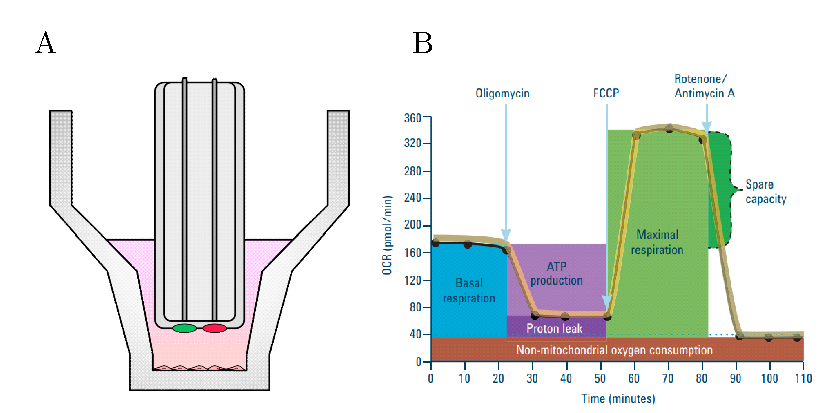
\includegraphics{Abbildung/seahorse_basics_placeholder.pdf}

        \begin{minipage}{\captionwidth}
            \caption[enrichment]{\uzlemph{Basics of Seahorse Assay (a placeholder)}\\
            \textbf{(A)} Schematic of a well-used for Seahorse Assay. For the measurement, the piston in the middle lowers to the bottom, this way defining a restricted space at the bottom. \ac{ocr} and \ac{eacr} in this volume are measured via two probes (red and green). \textbf{(B)} Exemplary curve for \ac{ocr} recorded over time and extractable properties of the respiratory chain.}
            \label{fig:seahorse_basics}
        \end{minipage}
    \end{figure}

    Cells were quantified using a python script provided by Dr. Tobias Reinberger. \ac{ocr} and \ac{ecar} were calculated by the XF Analyzer and normalized using the cell count and the signal in the control wells. In total, three biological repeats were recorded. One of which was excluded because no changes in \ac{ocr} and \ac{ecar} could be detected and cells detached from the bottom of the wells during staining. For the remaining two replicates, the least fitting of the 5 technical repeats for each condition was manually excluded. Further, initial \ac{ocr} and \ac{ecar}, as well as the characteristics of the respiratory chain displayed in figure \ref{fig:seahorse_basics} B, were calculated, using a modified python script provided by Dr. Tobias Reinberger. Assuming a normal distribution, a student's t-test was used, and a p-value of 0.05 is considered significant. For detailed information, please refer to the script.

\section{Oxidative Stress Assay}
\label{sec:cellrox}
CellROX\texttrademark~Green is a fluorescent dye that gets oxidized in an environment of oxidative stress and then binds to DNA, showing bright-green fluorescence \cite{thermofisherscientificinc.CellROXGreenReagent2022}.
CellROX\texttrademark~Green assay was used to assess generation of \ac{ros} in \acp{haosmc} differentiated as described in section \ref{subsec:differentiation}. After differentiation, further stimulation (from here on referred to as \textit{boost}) with \ac{pdgf} was carried put. Finally, a recovery experiment was performed using \ac{nac}, a potent antioxidant, to quench generation of \ac{ros}.

    \subsection{CellROX\texttrademark~Assay}
    For the assay, cells were washed with \ac{pbs}, then the boost was performed using variable concentrations of \ac{pdgf} in 300\,µL \ac{hbss}. For \ac{ros} quenching with \ac{nac}, 0.25\,M \ac{nac} solution was added to the wells 2\,h prior to the experiment and also added to \ac{hbss} during the experiment.

    \begin{table}[h]
    \capstart
    \centering
    \begin{minipage}{\captionwidth}
        \caption[Seahorse Assay]{\uzlemph{Composition for Seahorse Assay Boost}}
        \label{tab:cellrox_table}
    \end{minipage}
    \begin{tabular}{|c|c|c|c|}
        \hline
        component         & concentration & final concentration      & volume (µL) \\ \hline
        HBSS              & -             & -                        & 300         \\
        PDGF              & 100\,µg/mL             & variable (0\,-\,400\,ng/mL) & variable    \\
        Hoechst           & 1\,mg/mL       & 1\,µg/mL                  & 0.3         \\
        CellROX\texttrademark~Green (1:500) & 2.5\,mM        & 5\,µM                     & 0.6         \\
        NAC               & 0.25\,M        & variable (0\,-\,8\,mM)      & variable    \\ \hline
        total             & -             & -                        & $\sim$300   \\ \hline
    \end{tabular}
    \end{table}

    Cells were kept at 37°C in a 5\,\% CO2 environment during the boost, the incubation time is indicated with the results of the respective experiment. Imaging was done with the BZ-X810 All-in-One Fluorescence Microscope, using standard sensitivity. Images for the \ac{nac} quench were recorded as a z-stack and merged into one image using [KEYENCE SOFTWARE].

    \subsection{Processing of Data}
    \label{subsec:cellrox_data_processing}
    For \ac{pdgf}-boost titration, 7 biological repeats were performed, of which one was excluded because of a high signal in the negative control. For \ac{nac} quench, 4 biological repeats were performed, of which one has been excluded because no signal in the positive control.
    For quantification of signal intensity, pixels with a green value higher than 90 were counted. Differences in cell count were adjusted by division through the number of pixels with a blue value bigger than 80. To adjust for the large variance in total signal intensity between biological repeats, values were adjusted by division through the total signal of all recorded conditions.
    For statistical testing, the Mann-Whitney U test was used, and a p-value of 0.05 is considered significant. For detailed information, please refer to the scripts.


\section{Curation of Data for postGWAS Analyses}
\label{sec:database}
Data for postGWAS analyses and co-visualization with the \ac{gwas} data, were downloaded from public resources. Processing of the data and further annotation is briefly described in the following listing. The generated tables are summarized in figure \ref{fig:db_er} and table \ref{tab:db_tables}. For a complete view, please refer to the download scripts.

\begin{itemize}
    \item \uzlemph{GWAS Summary Statistics:} The \ac{cad} \ac{gwas} summary statistics from \textcite{aragamDiscoverySystematicCharacterization2021} as well as a list of identified proxy \acp{snp} from the study were annotated via the Ensembl \ac{rest} \ac{api} by Dr. Tobias Reinberger.

    \item \uzlemph{HGNC Gene List} The newest quarterly update to the complete \ac{hgnc} dataset was downloaded via the \MYhref{http://ftp.ebi.ac.uk/pub/databases/genenames/hgnc/archive/}{\ac{hgnc} \ac{ftp} server}. The dataset was used to generate a list of all 43135 approved symbols, mapping to their \ac{hgnc} ID as well as a list of all 98723 symbols (approved, alias, and previous), mapping to their \ac{hgnc} ID.

    \item \uzlemph{Linked SNPs} \ac{ld} $r^2$ values for variants in a 500 kb window around all variants in the list of \ac{cad} \ac{gwas} proxy variants, were computed and downloaded via the \MYhref{https://rest.ensembl.org/documentation/info/ld_id_get}{ensembl \ac{rest} \ac{api}}. For humans, ensembl calculates the \ac{ld} with data from the 1000 Genomes project (see table \ref{tab:populations}). In the same process, linked \acp{snp} were annotated with their most severe consequence from the ensembl \ac{vep}. In total information for 449770 relationships were downloaded.

    \begin{table}[h]
    \capstart
    \centering
    \begin{minipage}{\captionwidth}
        \caption[1000 Genomes Populations]{\uzlemph{1000 Genomes Populations}}
        \label{tab:populations}
    \end{minipage}
    \begin{tabular}{|c|c|c|}
        \hline
        Name                   & Size (individuals)   & Description      \\ \hline
        1000GENOMES:phase3:ALL & 2504                 & All phase 3 individuals  \\
        1000GENOMES:phase3:AMR & 347                  & Americans  \\
        1000GENOMES:phase3:EAS & 504                  & East Asians  \\
        1000GENOMES:phase3:EUR & 503                  & European \\
        1000GENOMES:phase3:SAS & 489                  & South Asian  \\ \hline
    \end{tabular}
    \end{table}

    \item \uzlemph{Ensembl Genome Annotatation} The newest Ensembl build (Ensembl release 106) was downloaded via the \MYhref{http://ftp.ensembl.org/pub/current_gtf/homo_sapiens/}{ensembl \ac{ftp} server}. Features annotated as genes of the type protein-coding (19994), lncRNA (17734), or miRNA (1877) were extracted. Further gene symbols were mapped to their \ac{hgnc} ID if possible.

    \item \uzlemph{Ensembl Regulatory Build} The newest ensembl regulatory build (Ensembl release 106) was downloaded via the \MYhref{http://ftp.ensembl.org/pub/current_regulation/homo_sapiens/}{ensembl \ac{ftp} server}, containing 110623 open chromatin regions, 30873 \ac{tf} binding sites, 175885 \ac{ctcf} bindsing sites, 127935 enhancers, 36597 promotors \& 140548 promotor flanking regions.

    \item \uzlemph{Open Target Genetics l2g Scores} The latest list of Open Target Genetics \ac{l2g} Scores was downloaded via the \MYhref{http://ftp.ebi.ac.uk/pub/databases/opentargets/genetics/latest/l2g/}{open target genetics \ac{ftp} server}. Entries were annotated with their \ac{hgnc} ID whenever possible, 655 entries that do not map to a gene that is approved by the \ac{hgnc} were dropped, yielding a total of 3580206 database entries.

    \item \uzlemph{TSS} 35160 \ac{tss} for protein-coding genes were extracted from a \MYhref{https://ccg.epfl.ch/mga/hg38/gencode/}{\ac{USCS} Genome Browser dump}.

    \item \uzlemph{Associated traits from GWAS catalog} The \ac{snp} trait associations from the latest release of the GWAS catalog as well as the accompanying list of studies were downloaded via the \MYhref{http://ftp.ebi.ac.uk/'}{GWAS catalog FTP server}. 14892 \ac{snp}-trait correlations missing a position on the human reference genome or the p-value for the association were dropped from the data set. Further, the column for Odds Ration or beta was separated into two columns. In total, 370002 associations from 5831 distinct studies were collected.

    \item \uzlemph{TADs} \acp{tad} predicted by software adapted from \textcite{dixonTopologicalDomainsMammalian2012} were downloaded via the \MYhref{http://3dgenome.fsm.northwestern.edu/publications.html}{3D genome browser}. In total, \acp{tad} in 40 distinct biosamples were downloaded.

    \item \uzlemph{scATAC-seq from \textcite{newmanMultipleCellTypes2021a}} Processed sc\ac{atac} data for 8 celltypes [SOME MORE INFO] were scraped from the \MYhref{https://github.com/MillerLab-CPHG/Coronary_snATAC/tree/main/3_SVMpipeline/celltype_peaks}{Miller Lab GitHub repository}.

    \item \uzlemph{scATAC-seq from CATlas} Processed sc\ac{atac} data was scraped from the \MYhref{http://renlab.sdsc.edu/kai/Key_Processed_Data/Peaks/}{Ren Labs website} for 222 biosamples.

    \item \uzlemph{ABC model} The \ac{abc} model data for 131 biosamples was downloaded from the \MYhref{http://ftp.broadinstitute.org/outgoing/lincRNA/ABC/}{Engreitz Lab \ac{ftp} server}. The data was further translated from \ac{hg19} to \ac{hg38} using pyliftover.

    \item \uzlemph{ENCODE cCREs} \acp{cCRE} in distinct biosamples were downloaded by Dr. Tobias Reinberger, filtering out elements that were annotated as \textit{unclassified}.
\end{itemize}

\section{Visualization of GWAS data}
\label{sec:gwas_vis}
For visualization of the data, a bokeh application was built, that fetches the data from the database and renders it to a web browser.\\
Bokeh is a python module that allows easy and interactive visualization of data. It combines the powerful data processing tools of python with the interactivity of JavaScript running in the browser. The python side of bokeh creates python objects which are serialized into \ac{json} data and handed over to bokehJS which deserializes them into JavaScript objects that are rendered to the browser. The integrated bokeh server additionally offers the possibility to synchronize data between the underlying python environment and browser-side JavaScript library, allowing real-time updates to the displayed data.

    \begin{figure}[h]
    \capstart
        \centering
    	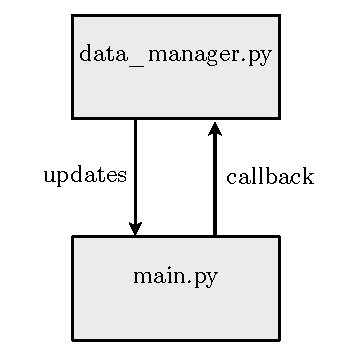
\includegraphics{Abbildung/vis_architecture.pdf}

    	\begin{minipage}{\captionwidth}
    		\caption[vis archi]{\uzlemph{Architecture of the GWAS Navigator}}
    		\label{fig:plot_architecture}
    	\end{minipage}
    \end{figure}

According to good design principles, the concerns of the application are split into two sections, as shown in fig. \ref{fig:plot_architecture}. Reading of data from the database and further processing steps are managed by a data provider and enclosed in one class. In contrast to the model-controller-view architecture, a popular architectural pattern for the design of user interfaces, there is no partition between a view and a controller. Since data visualization, as well as the control widgets, are created by bokeh, it is convenient to use the built-in event listeners of the library to handle the required callbacks. Therefore, the main file is responsible for the creation of all plots and widgets as well as listening for inputs.

\section{Enrichment analysis}
\label{sec:enrichment}
Based on the data in the database, initial postGWAS studies were run. Annotation enrichment analyses are a popular tool for the identification of terms that are over-represented in a list of interest. The most prominent application is their application as \ac{gsea}. \Acp{gsea} are used to check for the overrepresentation of a candidate gene list in a predefined set of genes \cite{tipneyIntroductionEffectiveUse2010}. In this case, the method is used to determine if \acp{cCRE} overlaps with \ac{cad} associated \acp{snp} is enriched in certain biosamples, using Fisher's exact test.\\
For the analysis, \acp{cCRE} annotated as unclassified were excluded. As a list of \ac{cad} associated \acp{snp} the list of 241 proxy variants from the database was used, as well as all linked variants ($r^2\geq0.6$) in the 1000 Genomes European Population. The following parameters were calculated for all biosamples:

\begin{itemize}
    \item The number of distinct cCREs among all biosamples (m)
    \item The number of distinct cCREs that are annotated in the biosample of interest (mt)
    \item The Number of distinct cCREs that overlap with an SNP in the SNP list in any biosample (n)
    \item The Number of distinct cCREs that overlap with an SNP in the SNP list in the biosample of interest (nt)
\end{itemize}

The p-value for the number of overlaps to be greater than or equal to the observation can be calculated as the cumulative distribution function of the hypergeometric distribution.

$$ P(\sigma_t\geq n_t) = \sum_{k=n_t}^{min(m_t, n)} \frac{\binom{n}{k}\binom{m-n}{m_t-k}}{\binom{m}{m_t}} $$

To account for the multiple comparisons problem, p-values were adjusted with Bonferroni correction where n is the number of tests ($\equiv$ number of biosamples):

$$ p_{ajd.} = p*n$$

The analysis and visualization were done in python. An adjusted p-value of 0.05 is considered significant. Finally, the identified biosamples were annotated via the \MYhref{https://web.expasy.org/cellosaurus/}{cell line database Cellosaurus}. For detailed information, please refer to the analysis scripts.

\begin{figure}[h]
\capstart
    \centering
    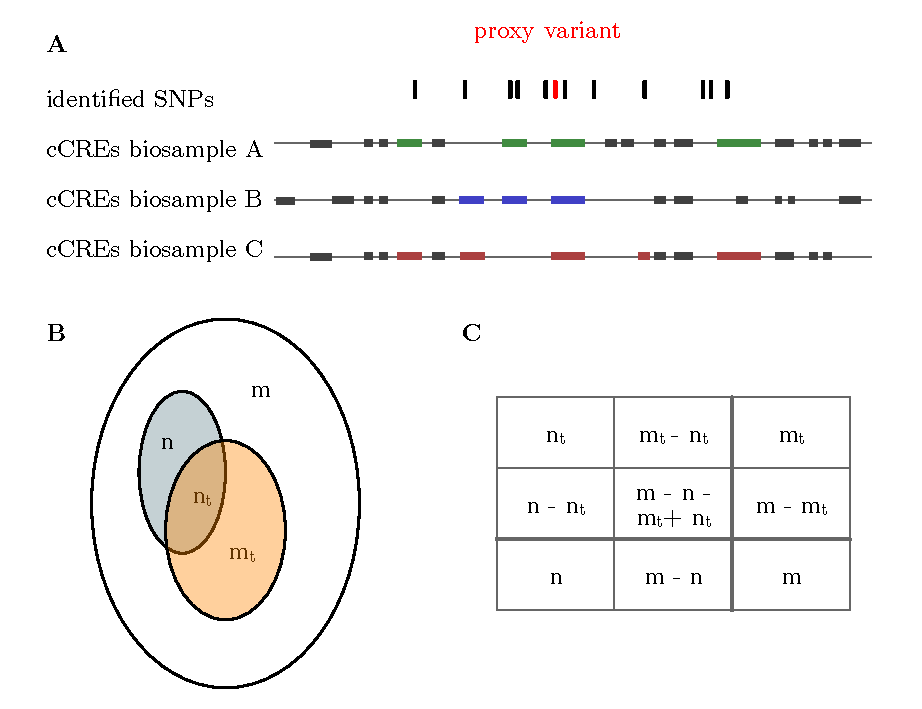
\includegraphics{Abbildung/enrichment.pdf}

    \begin{minipage}{\captionwidth}
        \caption[enrichment]{\uzlemph{Enrichment analysis for \acp{cCREs} overlapping with \ac{cad} risk \acp{snp}}\\
        \textbf{(A)} Visual representation of the overlap calculation for enrichment calculation. The proxy variant is indicated as a red line, variants in \ac{ld} are indicated as black lines. \ac{cCRE} are shown as boxes, those that are overlapping with an \ac{snp} were colored according to the biosample they were annotated in. \textbf{(B)} Venn diagram of these values for a biosample. \textbf{(C)} Schematic contingency table for a biosample. \\
        (m) is the number of distinct \acp{cCRE} found among all biosamples (23 in this example); (mt) the number of distinct \acp{cCRE} annotated in the biosample of interest (16 for biosample A, 14 for biosample b, 14 for biosample C); (n) the number of distinct \acp{cCRE} overlapping with an \ac{snp} (6 in this example);  the number of distinct \acp{cCRE} overlapping with an \ac{snp} in the biosample of interest (4 for biosample A (green), 3 for biosample B (blue), 5 for biosample C (red))}
        \label{fig:enrichment}
    \end{minipage}
\end{figure}


%%%%%%%%%%%%%%%%%
%               %
%   Ergebnisse  %
%               %
%%%%%%%%%%%%%%%%%

\chapter{Results}
\section{Differentitaion}
\label{sec:differentiation}
To generate a controlable phenotype, that is representive for the synthetic phenotype in vivo, HAoSMCs were first treated for two days with TGFb to induce a phenotype that ressambles the contrat phenotype. Using this contractile phenotype as a precursors, cells were further treated for five days with IL-1b and PDGF-BB which should induce differentiation into the synthetic phenotype.

    \subsection{Expression of CNN1 \& MMP9}
    To track the differentiation and confirm the protocoll, the HAoSMCs were characterized using qPCR, assessing mRNA levels of CNN1 as a contractivle marker and MMP9 as a synthetic marker. For better compariability mRNA levels are considered in realtion to the house keeping gene GAPDH.

    \label{subsec:qPCR}
    \begin{figure}[h]
    \capstart
        \centering
    	%% Creator: Matplotlib, PGF backend
%%
%% To include the figure in your LaTeX document, write
%%   \input{<filename>.pgf}
%%
%% Make sure the required packages are loaded in your preamble
%%   \usepackage{pgf}
%%
%% Figures using additional raster images can only be included by \input if
%% they are in the same directory as the main LaTeX file. For loading figures
%% from other directories you can use the `import` package
%%   \usepackage{import}
%%
%% and then include the figures with
%%   \import{<path to file>}{<filename>.pgf}
%%
%% Matplotlib used the following preamble
%%   \usepackage{fontspec}
%%   \setmainfont{DejaVuSans.ttf}[Path=\detokenize{C:/Users/torbe/AppData/Local/Programs/Python/Python39/Lib/site-packages/matplotlib/mpl-data/fonts/ttf/}]
%%   \setsansfont{DejaVuSans.ttf}[Path=\detokenize{C:/Users/torbe/AppData/Local/Programs/Python/Python39/Lib/site-packages/matplotlib/mpl-data/fonts/ttf/}]
%%   \setmonofont{DejaVuSansMono.ttf}[Path=\detokenize{C:/Users/torbe/AppData/Local/Programs/Python/Python39/Lib/site-packages/matplotlib/mpl-data/fonts/ttf/}]
%%
\begingroup%
\makeatletter%
\begin{pgfpicture}%
\pgfpathrectangle{\pgfpointorigin}{\pgfqpoint{5.510000in}{6.290000in}}%
\pgfusepath{use as bounding box, clip}%
\begin{pgfscope}%
\pgfsetbuttcap%
\pgfsetmiterjoin%
\definecolor{currentfill}{rgb}{1.000000,1.000000,1.000000}%
\pgfsetfillcolor{currentfill}%
\pgfsetlinewidth{0.000000pt}%
\definecolor{currentstroke}{rgb}{1.000000,1.000000,1.000000}%
\pgfsetstrokecolor{currentstroke}%
\pgfsetdash{}{0pt}%
\pgfpathmoveto{\pgfqpoint{0.000000in}{0.000000in}}%
\pgfpathlineto{\pgfqpoint{5.510000in}{0.000000in}}%
\pgfpathlineto{\pgfqpoint{5.510000in}{6.290000in}}%
\pgfpathlineto{\pgfqpoint{0.000000in}{6.290000in}}%
\pgfpathclose%
\pgfusepath{fill}%
\end{pgfscope}%
\begin{pgfscope}%
\pgfsetbuttcap%
\pgfsetmiterjoin%
\definecolor{currentfill}{rgb}{1.000000,1.000000,1.000000}%
\pgfsetfillcolor{currentfill}%
\pgfsetlinewidth{0.000000pt}%
\definecolor{currentstroke}{rgb}{0.000000,0.000000,0.000000}%
\pgfsetstrokecolor{currentstroke}%
\pgfsetstrokeopacity{0.000000}%
\pgfsetdash{}{0pt}%
\pgfpathmoveto{\pgfqpoint{1.102000in}{4.011085in}}%
\pgfpathlineto{\pgfqpoint{4.959000in}{4.011085in}}%
\pgfpathlineto{\pgfqpoint{4.959000in}{5.535200in}}%
\pgfpathlineto{\pgfqpoint{1.102000in}{5.535200in}}%
\pgfpathclose%
\pgfusepath{fill}%
\end{pgfscope}%
\begin{pgfscope}%
\pgfpathrectangle{\pgfqpoint{1.102000in}{4.011085in}}{\pgfqpoint{3.857000in}{1.524115in}}%
\pgfusepath{clip}%
\pgfsetbuttcap%
\pgfsetmiterjoin%
\definecolor{currentfill}{rgb}{0.238725,0.497549,0.659314}%
\pgfsetfillcolor{currentfill}%
\pgfsetfillopacity{0.990000}%
\pgfsetlinewidth{0.000000pt}%
\definecolor{currentstroke}{rgb}{0.000000,0.000000,0.000000}%
\pgfsetstrokecolor{currentstroke}%
\pgfsetstrokeopacity{0.990000}%
\pgfsetdash{}{0pt}%
\pgfpathmoveto{\pgfqpoint{1.150213in}{4.011085in}}%
\pgfpathlineto{\pgfqpoint{1.535913in}{4.011085in}}%
\pgfpathlineto{\pgfqpoint{1.535913in}{4.155143in}}%
\pgfpathlineto{\pgfqpoint{1.150213in}{4.155143in}}%
\pgfpathclose%
\pgfusepath{fill}%
\end{pgfscope}%
\begin{pgfscope}%
\pgfpathrectangle{\pgfqpoint{1.102000in}{4.011085in}}{\pgfqpoint{3.857000in}{1.524115in}}%
\pgfusepath{clip}%
\pgfsetbuttcap%
\pgfsetmiterjoin%
\definecolor{currentfill}{rgb}{0.691667,0.838725,0.671078}%
\pgfsetfillcolor{currentfill}%
\pgfsetfillopacity{0.990000}%
\pgfsetlinewidth{0.000000pt}%
\definecolor{currentstroke}{rgb}{0.000000,0.000000,0.000000}%
\pgfsetstrokecolor{currentstroke}%
\pgfsetstrokeopacity{0.990000}%
\pgfsetdash{}{0pt}%
\pgfpathmoveto{\pgfqpoint{1.632338in}{4.011085in}}%
\pgfpathlineto{\pgfqpoint{2.018038in}{4.011085in}}%
\pgfpathlineto{\pgfqpoint{2.018038in}{4.464432in}}%
\pgfpathlineto{\pgfqpoint{1.632338in}{4.464432in}}%
\pgfpathclose%
\pgfusepath{fill}%
\end{pgfscope}%
\begin{pgfscope}%
\pgfpathrectangle{\pgfqpoint{1.102000in}{4.011085in}}{\pgfqpoint{3.857000in}{1.524115in}}%
\pgfusepath{clip}%
\pgfsetbuttcap%
\pgfsetmiterjoin%
\definecolor{currentfill}{rgb}{0.915686,0.683333,0.456863}%
\pgfsetfillcolor{currentfill}%
\pgfsetfillopacity{0.990000}%
\pgfsetlinewidth{0.000000pt}%
\definecolor{currentstroke}{rgb}{0.000000,0.000000,0.000000}%
\pgfsetstrokecolor{currentstroke}%
\pgfsetstrokeopacity{0.990000}%
\pgfsetdash{}{0pt}%
\pgfpathmoveto{\pgfqpoint{2.114463in}{4.011085in}}%
\pgfpathlineto{\pgfqpoint{2.500163in}{4.011085in}}%
\pgfpathlineto{\pgfqpoint{2.500163in}{4.122300in}}%
\pgfpathlineto{\pgfqpoint{2.114463in}{4.122300in}}%
\pgfpathclose%
\pgfusepath{fill}%
\end{pgfscope}%
\begin{pgfscope}%
\pgfpathrectangle{\pgfqpoint{1.102000in}{4.011085in}}{\pgfqpoint{3.857000in}{1.524115in}}%
\pgfusepath{clip}%
\pgfsetbuttcap%
\pgfsetmiterjoin%
\definecolor{currentfill}{rgb}{0.750000,0.191176,0.200000}%
\pgfsetfillcolor{currentfill}%
\pgfsetfillopacity{0.990000}%
\pgfsetlinewidth{0.000000pt}%
\definecolor{currentstroke}{rgb}{0.000000,0.000000,0.000000}%
\pgfsetstrokecolor{currentstroke}%
\pgfsetstrokeopacity{0.990000}%
\pgfsetdash{}{0pt}%
\pgfpathmoveto{\pgfqpoint{2.596588in}{4.011085in}}%
\pgfpathlineto{\pgfqpoint{2.982287in}{4.011085in}}%
\pgfpathlineto{\pgfqpoint{2.982287in}{4.075350in}}%
\pgfpathlineto{\pgfqpoint{2.596588in}{4.075350in}}%
\pgfpathclose%
\pgfusepath{fill}%
\end{pgfscope}%
\begin{pgfscope}%
\pgfpathrectangle{\pgfqpoint{1.102000in}{4.011085in}}{\pgfqpoint{3.857000in}{1.524115in}}%
\pgfusepath{clip}%
\pgfsetbuttcap%
\pgfsetmiterjoin%
\definecolor{currentfill}{rgb}{0.238725,0.497549,0.659314}%
\pgfsetfillcolor{currentfill}%
\pgfsetfillopacity{0.990000}%
\pgfsetlinewidth{0.000000pt}%
\definecolor{currentstroke}{rgb}{0.000000,0.000000,0.000000}%
\pgfsetstrokecolor{currentstroke}%
\pgfsetstrokeopacity{0.990000}%
\pgfsetdash{}{0pt}%
\pgfpathmoveto{\pgfqpoint{3.078713in}{4.011085in}}%
\pgfpathlineto{\pgfqpoint{3.464413in}{4.011085in}}%
\pgfpathlineto{\pgfqpoint{3.464413in}{4.082315in}}%
\pgfpathlineto{\pgfqpoint{3.078713in}{4.082315in}}%
\pgfpathclose%
\pgfusepath{fill}%
\end{pgfscope}%
\begin{pgfscope}%
\pgfsetbuttcap%
\pgfsetmiterjoin%
\definecolor{currentfill}{rgb}{0.238725,0.497549,0.659314}%
\pgfsetfillcolor{currentfill}%
\pgfsetfillopacity{0.990000}%
\pgfsetlinewidth{0.000000pt}%
\definecolor{currentstroke}{rgb}{0.000000,0.000000,0.000000}%
\pgfsetstrokecolor{currentstroke}%
\pgfsetstrokeopacity{0.990000}%
\pgfsetdash{}{0pt}%
\pgfpathrectangle{\pgfqpoint{1.102000in}{4.011085in}}{\pgfqpoint{3.857000in}{1.524115in}}%
\pgfusepath{clip}%
\pgfpathmoveto{\pgfqpoint{3.078713in}{4.011085in}}%
\pgfpathlineto{\pgfqpoint{3.464413in}{4.011085in}}%
\pgfpathlineto{\pgfqpoint{3.464413in}{4.082315in}}%
\pgfpathlineto{\pgfqpoint{3.078713in}{4.082315in}}%
\pgfpathclose%
\pgfusepath{clip}%
\pgfsys@defobject{currentpattern}{\pgfqpoint{0in}{0in}}{\pgfqpoint{1in}{1in}}{%
\begin{pgfscope}%
\pgfpathrectangle{\pgfqpoint{0in}{0in}}{\pgfqpoint{1in}{1in}}%
\pgfusepath{clip}%
\pgfpathmoveto{\pgfqpoint{-0.500000in}{0.500000in}}%
\pgfpathlineto{\pgfqpoint{0.500000in}{1.500000in}}%
\pgfpathmoveto{\pgfqpoint{-0.416667in}{0.416667in}}%
\pgfpathlineto{\pgfqpoint{0.583333in}{1.416667in}}%
\pgfpathmoveto{\pgfqpoint{-0.333333in}{0.333333in}}%
\pgfpathlineto{\pgfqpoint{0.666667in}{1.333333in}}%
\pgfpathmoveto{\pgfqpoint{-0.250000in}{0.250000in}}%
\pgfpathlineto{\pgfqpoint{0.750000in}{1.250000in}}%
\pgfpathmoveto{\pgfqpoint{-0.166667in}{0.166667in}}%
\pgfpathlineto{\pgfqpoint{0.833333in}{1.166667in}}%
\pgfpathmoveto{\pgfqpoint{-0.083333in}{0.083333in}}%
\pgfpathlineto{\pgfqpoint{0.916667in}{1.083333in}}%
\pgfpathmoveto{\pgfqpoint{0.000000in}{0.000000in}}%
\pgfpathlineto{\pgfqpoint{1.000000in}{1.000000in}}%
\pgfpathmoveto{\pgfqpoint{0.083333in}{-0.083333in}}%
\pgfpathlineto{\pgfqpoint{1.083333in}{0.916667in}}%
\pgfpathmoveto{\pgfqpoint{0.166667in}{-0.166667in}}%
\pgfpathlineto{\pgfqpoint{1.166667in}{0.833333in}}%
\pgfpathmoveto{\pgfqpoint{0.250000in}{-0.250000in}}%
\pgfpathlineto{\pgfqpoint{1.250000in}{0.750000in}}%
\pgfpathmoveto{\pgfqpoint{0.333333in}{-0.333333in}}%
\pgfpathlineto{\pgfqpoint{1.333333in}{0.666667in}}%
\pgfpathmoveto{\pgfqpoint{0.416667in}{-0.416667in}}%
\pgfpathlineto{\pgfqpoint{1.416667in}{0.583333in}}%
\pgfpathmoveto{\pgfqpoint{0.500000in}{-0.500000in}}%
\pgfpathlineto{\pgfqpoint{1.500000in}{0.500000in}}%
\pgfusepath{stroke}%
\end{pgfscope}%
}%
\pgfsys@transformshift{3.078713in}{4.011085in}%
\pgfsys@useobject{currentpattern}{}%
\pgfsys@transformshift{1in}{0in}%
\pgfsys@transformshift{-1in}{0in}%
\pgfsys@transformshift{0in}{1in}%
\end{pgfscope}%
\begin{pgfscope}%
\pgfpathrectangle{\pgfqpoint{1.102000in}{4.011085in}}{\pgfqpoint{3.857000in}{1.524115in}}%
\pgfusepath{clip}%
\pgfsetbuttcap%
\pgfsetmiterjoin%
\definecolor{currentfill}{rgb}{0.691667,0.838725,0.671078}%
\pgfsetfillcolor{currentfill}%
\pgfsetfillopacity{0.990000}%
\pgfsetlinewidth{0.000000pt}%
\definecolor{currentstroke}{rgb}{0.000000,0.000000,0.000000}%
\pgfsetstrokecolor{currentstroke}%
\pgfsetstrokeopacity{0.990000}%
\pgfsetdash{}{0pt}%
\pgfpathmoveto{\pgfqpoint{3.560838in}{4.011085in}}%
\pgfpathlineto{\pgfqpoint{3.946538in}{4.011085in}}%
\pgfpathlineto{\pgfqpoint{3.946538in}{4.399793in}}%
\pgfpathlineto{\pgfqpoint{3.560838in}{4.399793in}}%
\pgfpathclose%
\pgfusepath{fill}%
\end{pgfscope}%
\begin{pgfscope}%
\pgfsetbuttcap%
\pgfsetmiterjoin%
\definecolor{currentfill}{rgb}{0.691667,0.838725,0.671078}%
\pgfsetfillcolor{currentfill}%
\pgfsetfillopacity{0.990000}%
\pgfsetlinewidth{0.000000pt}%
\definecolor{currentstroke}{rgb}{0.000000,0.000000,0.000000}%
\pgfsetstrokecolor{currentstroke}%
\pgfsetstrokeopacity{0.990000}%
\pgfsetdash{}{0pt}%
\pgfpathrectangle{\pgfqpoint{1.102000in}{4.011085in}}{\pgfqpoint{3.857000in}{1.524115in}}%
\pgfusepath{clip}%
\pgfpathmoveto{\pgfqpoint{3.560838in}{4.011085in}}%
\pgfpathlineto{\pgfqpoint{3.946538in}{4.011085in}}%
\pgfpathlineto{\pgfqpoint{3.946538in}{4.399793in}}%
\pgfpathlineto{\pgfqpoint{3.560838in}{4.399793in}}%
\pgfpathclose%
\pgfusepath{clip}%
\pgfsys@defobject{currentpattern}{\pgfqpoint{0in}{0in}}{\pgfqpoint{1in}{1in}}{%
\begin{pgfscope}%
\pgfpathrectangle{\pgfqpoint{0in}{0in}}{\pgfqpoint{1in}{1in}}%
\pgfusepath{clip}%
\pgfpathmoveto{\pgfqpoint{-0.500000in}{0.500000in}}%
\pgfpathlineto{\pgfqpoint{0.500000in}{1.500000in}}%
\pgfpathmoveto{\pgfqpoint{-0.416667in}{0.416667in}}%
\pgfpathlineto{\pgfqpoint{0.583333in}{1.416667in}}%
\pgfpathmoveto{\pgfqpoint{-0.333333in}{0.333333in}}%
\pgfpathlineto{\pgfqpoint{0.666667in}{1.333333in}}%
\pgfpathmoveto{\pgfqpoint{-0.250000in}{0.250000in}}%
\pgfpathlineto{\pgfqpoint{0.750000in}{1.250000in}}%
\pgfpathmoveto{\pgfqpoint{-0.166667in}{0.166667in}}%
\pgfpathlineto{\pgfqpoint{0.833333in}{1.166667in}}%
\pgfpathmoveto{\pgfqpoint{-0.083333in}{0.083333in}}%
\pgfpathlineto{\pgfqpoint{0.916667in}{1.083333in}}%
\pgfpathmoveto{\pgfqpoint{0.000000in}{0.000000in}}%
\pgfpathlineto{\pgfqpoint{1.000000in}{1.000000in}}%
\pgfpathmoveto{\pgfqpoint{0.083333in}{-0.083333in}}%
\pgfpathlineto{\pgfqpoint{1.083333in}{0.916667in}}%
\pgfpathmoveto{\pgfqpoint{0.166667in}{-0.166667in}}%
\pgfpathlineto{\pgfqpoint{1.166667in}{0.833333in}}%
\pgfpathmoveto{\pgfqpoint{0.250000in}{-0.250000in}}%
\pgfpathlineto{\pgfqpoint{1.250000in}{0.750000in}}%
\pgfpathmoveto{\pgfqpoint{0.333333in}{-0.333333in}}%
\pgfpathlineto{\pgfqpoint{1.333333in}{0.666667in}}%
\pgfpathmoveto{\pgfqpoint{0.416667in}{-0.416667in}}%
\pgfpathlineto{\pgfqpoint{1.416667in}{0.583333in}}%
\pgfpathmoveto{\pgfqpoint{0.500000in}{-0.500000in}}%
\pgfpathlineto{\pgfqpoint{1.500000in}{0.500000in}}%
\pgfusepath{stroke}%
\end{pgfscope}%
}%
\pgfsys@transformshift{3.560838in}{4.011085in}%
\pgfsys@useobject{currentpattern}{}%
\pgfsys@transformshift{1in}{0in}%
\pgfsys@transformshift{-1in}{0in}%
\pgfsys@transformshift{0in}{1in}%
\end{pgfscope}%
\begin{pgfscope}%
\pgfpathrectangle{\pgfqpoint{1.102000in}{4.011085in}}{\pgfqpoint{3.857000in}{1.524115in}}%
\pgfusepath{clip}%
\pgfsetbuttcap%
\pgfsetmiterjoin%
\definecolor{currentfill}{rgb}{0.915686,0.683333,0.456863}%
\pgfsetfillcolor{currentfill}%
\pgfsetfillopacity{0.990000}%
\pgfsetlinewidth{0.000000pt}%
\definecolor{currentstroke}{rgb}{0.000000,0.000000,0.000000}%
\pgfsetstrokecolor{currentstroke}%
\pgfsetstrokeopacity{0.990000}%
\pgfsetdash{}{0pt}%
\pgfpathmoveto{\pgfqpoint{4.042962in}{4.011085in}}%
\pgfpathlineto{\pgfqpoint{4.428662in}{4.011085in}}%
\pgfpathlineto{\pgfqpoint{4.428662in}{4.051857in}}%
\pgfpathlineto{\pgfqpoint{4.042962in}{4.051857in}}%
\pgfpathclose%
\pgfusepath{fill}%
\end{pgfscope}%
\begin{pgfscope}%
\pgfsetbuttcap%
\pgfsetmiterjoin%
\definecolor{currentfill}{rgb}{0.915686,0.683333,0.456863}%
\pgfsetfillcolor{currentfill}%
\pgfsetfillopacity{0.990000}%
\pgfsetlinewidth{0.000000pt}%
\definecolor{currentstroke}{rgb}{0.000000,0.000000,0.000000}%
\pgfsetstrokecolor{currentstroke}%
\pgfsetstrokeopacity{0.990000}%
\pgfsetdash{}{0pt}%
\pgfpathrectangle{\pgfqpoint{1.102000in}{4.011085in}}{\pgfqpoint{3.857000in}{1.524115in}}%
\pgfusepath{clip}%
\pgfpathmoveto{\pgfqpoint{4.042962in}{4.011085in}}%
\pgfpathlineto{\pgfqpoint{4.428662in}{4.011085in}}%
\pgfpathlineto{\pgfqpoint{4.428662in}{4.051857in}}%
\pgfpathlineto{\pgfqpoint{4.042962in}{4.051857in}}%
\pgfpathclose%
\pgfusepath{clip}%
\pgfsys@defobject{currentpattern}{\pgfqpoint{0in}{0in}}{\pgfqpoint{1in}{1in}}{%
\begin{pgfscope}%
\pgfpathrectangle{\pgfqpoint{0in}{0in}}{\pgfqpoint{1in}{1in}}%
\pgfusepath{clip}%
\pgfpathmoveto{\pgfqpoint{-0.500000in}{0.500000in}}%
\pgfpathlineto{\pgfqpoint{0.500000in}{1.500000in}}%
\pgfpathmoveto{\pgfqpoint{-0.416667in}{0.416667in}}%
\pgfpathlineto{\pgfqpoint{0.583333in}{1.416667in}}%
\pgfpathmoveto{\pgfqpoint{-0.333333in}{0.333333in}}%
\pgfpathlineto{\pgfqpoint{0.666667in}{1.333333in}}%
\pgfpathmoveto{\pgfqpoint{-0.250000in}{0.250000in}}%
\pgfpathlineto{\pgfqpoint{0.750000in}{1.250000in}}%
\pgfpathmoveto{\pgfqpoint{-0.166667in}{0.166667in}}%
\pgfpathlineto{\pgfqpoint{0.833333in}{1.166667in}}%
\pgfpathmoveto{\pgfqpoint{-0.083333in}{0.083333in}}%
\pgfpathlineto{\pgfqpoint{0.916667in}{1.083333in}}%
\pgfpathmoveto{\pgfqpoint{0.000000in}{0.000000in}}%
\pgfpathlineto{\pgfqpoint{1.000000in}{1.000000in}}%
\pgfpathmoveto{\pgfqpoint{0.083333in}{-0.083333in}}%
\pgfpathlineto{\pgfqpoint{1.083333in}{0.916667in}}%
\pgfpathmoveto{\pgfqpoint{0.166667in}{-0.166667in}}%
\pgfpathlineto{\pgfqpoint{1.166667in}{0.833333in}}%
\pgfpathmoveto{\pgfqpoint{0.250000in}{-0.250000in}}%
\pgfpathlineto{\pgfqpoint{1.250000in}{0.750000in}}%
\pgfpathmoveto{\pgfqpoint{0.333333in}{-0.333333in}}%
\pgfpathlineto{\pgfqpoint{1.333333in}{0.666667in}}%
\pgfpathmoveto{\pgfqpoint{0.416667in}{-0.416667in}}%
\pgfpathlineto{\pgfqpoint{1.416667in}{0.583333in}}%
\pgfpathmoveto{\pgfqpoint{0.500000in}{-0.500000in}}%
\pgfpathlineto{\pgfqpoint{1.500000in}{0.500000in}}%
\pgfusepath{stroke}%
\end{pgfscope}%
}%
\pgfsys@transformshift{4.042962in}{4.011085in}%
\pgfsys@useobject{currentpattern}{}%
\pgfsys@transformshift{1in}{0in}%
\pgfsys@transformshift{-1in}{0in}%
\pgfsys@transformshift{0in}{1in}%
\end{pgfscope}%
\begin{pgfscope}%
\pgfpathrectangle{\pgfqpoint{1.102000in}{4.011085in}}{\pgfqpoint{3.857000in}{1.524115in}}%
\pgfusepath{clip}%
\pgfsetbuttcap%
\pgfsetmiterjoin%
\definecolor{currentfill}{rgb}{0.750000,0.191176,0.200000}%
\pgfsetfillcolor{currentfill}%
\pgfsetfillopacity{0.990000}%
\pgfsetlinewidth{0.000000pt}%
\definecolor{currentstroke}{rgb}{0.000000,0.000000,0.000000}%
\pgfsetstrokecolor{currentstroke}%
\pgfsetstrokeopacity{0.990000}%
\pgfsetdash{}{0pt}%
\pgfpathmoveto{\pgfqpoint{4.525087in}{4.011085in}}%
\pgfpathlineto{\pgfqpoint{4.910787in}{4.011085in}}%
\pgfpathlineto{\pgfqpoint{4.910787in}{4.069776in}}%
\pgfpathlineto{\pgfqpoint{4.525087in}{4.069776in}}%
\pgfpathclose%
\pgfusepath{fill}%
\end{pgfscope}%
\begin{pgfscope}%
\pgfsetbuttcap%
\pgfsetmiterjoin%
\definecolor{currentfill}{rgb}{0.750000,0.191176,0.200000}%
\pgfsetfillcolor{currentfill}%
\pgfsetfillopacity{0.990000}%
\pgfsetlinewidth{0.000000pt}%
\definecolor{currentstroke}{rgb}{0.000000,0.000000,0.000000}%
\pgfsetstrokecolor{currentstroke}%
\pgfsetstrokeopacity{0.990000}%
\pgfsetdash{}{0pt}%
\pgfpathrectangle{\pgfqpoint{1.102000in}{4.011085in}}{\pgfqpoint{3.857000in}{1.524115in}}%
\pgfusepath{clip}%
\pgfpathmoveto{\pgfqpoint{4.525087in}{4.011085in}}%
\pgfpathlineto{\pgfqpoint{4.910787in}{4.011085in}}%
\pgfpathlineto{\pgfqpoint{4.910787in}{4.069776in}}%
\pgfpathlineto{\pgfqpoint{4.525087in}{4.069776in}}%
\pgfpathclose%
\pgfusepath{clip}%
\pgfsys@defobject{currentpattern}{\pgfqpoint{0in}{0in}}{\pgfqpoint{1in}{1in}}{%
\begin{pgfscope}%
\pgfpathrectangle{\pgfqpoint{0in}{0in}}{\pgfqpoint{1in}{1in}}%
\pgfusepath{clip}%
\pgfpathmoveto{\pgfqpoint{-0.500000in}{0.500000in}}%
\pgfpathlineto{\pgfqpoint{0.500000in}{1.500000in}}%
\pgfpathmoveto{\pgfqpoint{-0.416667in}{0.416667in}}%
\pgfpathlineto{\pgfqpoint{0.583333in}{1.416667in}}%
\pgfpathmoveto{\pgfqpoint{-0.333333in}{0.333333in}}%
\pgfpathlineto{\pgfqpoint{0.666667in}{1.333333in}}%
\pgfpathmoveto{\pgfqpoint{-0.250000in}{0.250000in}}%
\pgfpathlineto{\pgfqpoint{0.750000in}{1.250000in}}%
\pgfpathmoveto{\pgfqpoint{-0.166667in}{0.166667in}}%
\pgfpathlineto{\pgfqpoint{0.833333in}{1.166667in}}%
\pgfpathmoveto{\pgfqpoint{-0.083333in}{0.083333in}}%
\pgfpathlineto{\pgfqpoint{0.916667in}{1.083333in}}%
\pgfpathmoveto{\pgfqpoint{0.000000in}{0.000000in}}%
\pgfpathlineto{\pgfqpoint{1.000000in}{1.000000in}}%
\pgfpathmoveto{\pgfqpoint{0.083333in}{-0.083333in}}%
\pgfpathlineto{\pgfqpoint{1.083333in}{0.916667in}}%
\pgfpathmoveto{\pgfqpoint{0.166667in}{-0.166667in}}%
\pgfpathlineto{\pgfqpoint{1.166667in}{0.833333in}}%
\pgfpathmoveto{\pgfqpoint{0.250000in}{-0.250000in}}%
\pgfpathlineto{\pgfqpoint{1.250000in}{0.750000in}}%
\pgfpathmoveto{\pgfqpoint{0.333333in}{-0.333333in}}%
\pgfpathlineto{\pgfqpoint{1.333333in}{0.666667in}}%
\pgfpathmoveto{\pgfqpoint{0.416667in}{-0.416667in}}%
\pgfpathlineto{\pgfqpoint{1.416667in}{0.583333in}}%
\pgfpathmoveto{\pgfqpoint{0.500000in}{-0.500000in}}%
\pgfpathlineto{\pgfqpoint{1.500000in}{0.500000in}}%
\pgfusepath{stroke}%
\end{pgfscope}%
}%
\pgfsys@transformshift{4.525087in}{4.011085in}%
\pgfsys@useobject{currentpattern}{}%
\pgfsys@transformshift{1in}{0in}%
\pgfsys@transformshift{-1in}{0in}%
\pgfsys@transformshift{0in}{1in}%
\end{pgfscope}%
\begin{pgfscope}%
\pgfsetbuttcap%
\pgfsetroundjoin%
\definecolor{currentfill}{rgb}{0.000000,0.000000,0.000000}%
\pgfsetfillcolor{currentfill}%
\pgfsetlinewidth{0.803000pt}%
\definecolor{currentstroke}{rgb}{0.000000,0.000000,0.000000}%
\pgfsetstrokecolor{currentstroke}%
\pgfsetdash{}{0pt}%
\pgfsys@defobject{currentmarker}{\pgfqpoint{0.000000in}{-0.048611in}}{\pgfqpoint{0.000000in}{0.000000in}}{%
\pgfpathmoveto{\pgfqpoint{0.000000in}{0.000000in}}%
\pgfpathlineto{\pgfqpoint{0.000000in}{-0.048611in}}%
\pgfusepath{stroke,fill}%
}%
\begin{pgfscope}%
\pgfsys@transformshift{1.343063in}{4.011085in}%
\pgfsys@useobject{currentmarker}{}%
\end{pgfscope}%
\end{pgfscope}%
\begin{pgfscope}%
\definecolor{textcolor}{rgb}{0.000000,0.000000,0.000000}%
\pgfsetstrokecolor{textcolor}%
\pgfsetfillcolor{textcolor}%
\pgftext[x=1.226689in, y=3.808339in, left, base]{\color{textcolor}\rmfamily\fontsize{10.000000}{12.000000}\selectfont ++}%
\end{pgfscope}%
\begin{pgfscope}%
\definecolor{textcolor}{rgb}{0.000000,0.000000,0.000000}%
\pgfsetstrokecolor{textcolor}%
\pgfsetfillcolor{textcolor}%
\pgftext[x=1.124421in, y=3.652822in, left, base]{\color{textcolor}\rmfamily\fontsize{10.000000}{12.000000}\selectfont Matrix}%
\end{pgfscope}%
\begin{pgfscope}%
\pgfsetbuttcap%
\pgfsetroundjoin%
\definecolor{currentfill}{rgb}{0.000000,0.000000,0.000000}%
\pgfsetfillcolor{currentfill}%
\pgfsetlinewidth{0.803000pt}%
\definecolor{currentstroke}{rgb}{0.000000,0.000000,0.000000}%
\pgfsetstrokecolor{currentstroke}%
\pgfsetdash{}{0pt}%
\pgfsys@defobject{currentmarker}{\pgfqpoint{0.000000in}{-0.048611in}}{\pgfqpoint{0.000000in}{0.000000in}}{%
\pgfpathmoveto{\pgfqpoint{0.000000in}{0.000000in}}%
\pgfpathlineto{\pgfqpoint{0.000000in}{-0.048611in}}%
\pgfusepath{stroke,fill}%
}%
\begin{pgfscope}%
\pgfsys@transformshift{1.825188in}{4.011085in}%
\pgfsys@useobject{currentmarker}{}%
\end{pgfscope}%
\end{pgfscope}%
\begin{pgfscope}%
\definecolor{textcolor}{rgb}{0.000000,0.000000,0.000000}%
\pgfsetstrokecolor{textcolor}%
\pgfsetfillcolor{textcolor}%
\pgftext[x=1.741942in, y=3.808339in, left, base]{\color{textcolor}\rmfamily\fontsize{10.000000}{12.000000}\selectfont +-}%
\end{pgfscope}%
\begin{pgfscope}%
\definecolor{textcolor}{rgb}{0.000000,0.000000,0.000000}%
\pgfsetstrokecolor{textcolor}%
\pgfsetfillcolor{textcolor}%
\pgftext[x=1.606546in, y=3.652822in, left, base]{\color{textcolor}\rmfamily\fontsize{10.000000}{12.000000}\selectfont Matrix}%
\end{pgfscope}%
\begin{pgfscope}%
\pgfsetbuttcap%
\pgfsetroundjoin%
\definecolor{currentfill}{rgb}{0.000000,0.000000,0.000000}%
\pgfsetfillcolor{currentfill}%
\pgfsetlinewidth{0.803000pt}%
\definecolor{currentstroke}{rgb}{0.000000,0.000000,0.000000}%
\pgfsetstrokecolor{currentstroke}%
\pgfsetdash{}{0pt}%
\pgfsys@defobject{currentmarker}{\pgfqpoint{0.000000in}{-0.048611in}}{\pgfqpoint{0.000000in}{0.000000in}}{%
\pgfpathmoveto{\pgfqpoint{0.000000in}{0.000000in}}%
\pgfpathlineto{\pgfqpoint{0.000000in}{-0.048611in}}%
\pgfusepath{stroke,fill}%
}%
\begin{pgfscope}%
\pgfsys@transformshift{2.307313in}{4.011085in}%
\pgfsys@useobject{currentmarker}{}%
\end{pgfscope}%
\end{pgfscope}%
\begin{pgfscope}%
\definecolor{textcolor}{rgb}{0.000000,0.000000,0.000000}%
\pgfsetstrokecolor{textcolor}%
\pgfsetfillcolor{textcolor}%
\pgftext[x=2.224067in, y=3.808339in, left, base]{\color{textcolor}\rmfamily\fontsize{10.000000}{12.000000}\selectfont -+}%
\end{pgfscope}%
\begin{pgfscope}%
\definecolor{textcolor}{rgb}{0.000000,0.000000,0.000000}%
\pgfsetstrokecolor{textcolor}%
\pgfsetfillcolor{textcolor}%
\pgftext[x=2.088671in, y=3.652822in, left, base]{\color{textcolor}\rmfamily\fontsize{10.000000}{12.000000}\selectfont Matrix}%
\end{pgfscope}%
\begin{pgfscope}%
\pgfsetbuttcap%
\pgfsetroundjoin%
\definecolor{currentfill}{rgb}{0.000000,0.000000,0.000000}%
\pgfsetfillcolor{currentfill}%
\pgfsetlinewidth{0.803000pt}%
\definecolor{currentstroke}{rgb}{0.000000,0.000000,0.000000}%
\pgfsetstrokecolor{currentstroke}%
\pgfsetdash{}{0pt}%
\pgfsys@defobject{currentmarker}{\pgfqpoint{0.000000in}{-0.048611in}}{\pgfqpoint{0.000000in}{0.000000in}}{%
\pgfpathmoveto{\pgfqpoint{0.000000in}{0.000000in}}%
\pgfpathlineto{\pgfqpoint{0.000000in}{-0.048611in}}%
\pgfusepath{stroke,fill}%
}%
\begin{pgfscope}%
\pgfsys@transformshift{2.789438in}{4.011085in}%
\pgfsys@useobject{currentmarker}{}%
\end{pgfscope}%
\end{pgfscope}%
\begin{pgfscope}%
\definecolor{textcolor}{rgb}{0.000000,0.000000,0.000000}%
\pgfsetstrokecolor{textcolor}%
\pgfsetfillcolor{textcolor}%
\pgftext[x=2.754715in, y=3.808339in, left, base]{\color{textcolor}\rmfamily\fontsize{10.000000}{12.000000}\selectfont --}%
\end{pgfscope}%
\begin{pgfscope}%
\definecolor{textcolor}{rgb}{0.000000,0.000000,0.000000}%
\pgfsetstrokecolor{textcolor}%
\pgfsetfillcolor{textcolor}%
\pgftext[x=2.570796in, y=3.652822in, left, base]{\color{textcolor}\rmfamily\fontsize{10.000000}{12.000000}\selectfont Matrix}%
\end{pgfscope}%
\begin{pgfscope}%
\pgfsetbuttcap%
\pgfsetroundjoin%
\definecolor{currentfill}{rgb}{0.000000,0.000000,0.000000}%
\pgfsetfillcolor{currentfill}%
\pgfsetlinewidth{0.803000pt}%
\definecolor{currentstroke}{rgb}{0.000000,0.000000,0.000000}%
\pgfsetstrokecolor{currentstroke}%
\pgfsetdash{}{0pt}%
\pgfsys@defobject{currentmarker}{\pgfqpoint{0.000000in}{-0.048611in}}{\pgfqpoint{0.000000in}{0.000000in}}{%
\pgfpathmoveto{\pgfqpoint{0.000000in}{0.000000in}}%
\pgfpathlineto{\pgfqpoint{0.000000in}{-0.048611in}}%
\pgfusepath{stroke,fill}%
}%
\begin{pgfscope}%
\pgfsys@transformshift{3.271562in}{4.011085in}%
\pgfsys@useobject{currentmarker}{}%
\end{pgfscope}%
\end{pgfscope}%
\begin{pgfscope}%
\definecolor{textcolor}{rgb}{0.000000,0.000000,0.000000}%
\pgfsetstrokecolor{textcolor}%
\pgfsetfillcolor{textcolor}%
\pgftext[x=3.155189in, y=3.808339in, left, base]{\color{textcolor}\rmfamily\fontsize{10.000000}{12.000000}\selectfont ++}%
\end{pgfscope}%
\begin{pgfscope}%
\definecolor{textcolor}{rgb}{0.000000,0.000000,0.000000}%
\pgfsetstrokecolor{textcolor}%
\pgfsetfillcolor{textcolor}%
\pgftext[x=3.044919in, y=3.652822in, left, base]{\color{textcolor}\rmfamily\fontsize{10.000000}{12.000000}\selectfont Plastik}%
\end{pgfscope}%
\begin{pgfscope}%
\pgfsetbuttcap%
\pgfsetroundjoin%
\definecolor{currentfill}{rgb}{0.000000,0.000000,0.000000}%
\pgfsetfillcolor{currentfill}%
\pgfsetlinewidth{0.803000pt}%
\definecolor{currentstroke}{rgb}{0.000000,0.000000,0.000000}%
\pgfsetstrokecolor{currentstroke}%
\pgfsetdash{}{0pt}%
\pgfsys@defobject{currentmarker}{\pgfqpoint{0.000000in}{-0.048611in}}{\pgfqpoint{0.000000in}{0.000000in}}{%
\pgfpathmoveto{\pgfqpoint{0.000000in}{0.000000in}}%
\pgfpathlineto{\pgfqpoint{0.000000in}{-0.048611in}}%
\pgfusepath{stroke,fill}%
}%
\begin{pgfscope}%
\pgfsys@transformshift{3.753687in}{4.011085in}%
\pgfsys@useobject{currentmarker}{}%
\end{pgfscope}%
\end{pgfscope}%
\begin{pgfscope}%
\definecolor{textcolor}{rgb}{0.000000,0.000000,0.000000}%
\pgfsetstrokecolor{textcolor}%
\pgfsetfillcolor{textcolor}%
\pgftext[x=3.670442in, y=3.808339in, left, base]{\color{textcolor}\rmfamily\fontsize{10.000000}{12.000000}\selectfont +-}%
\end{pgfscope}%
\begin{pgfscope}%
\definecolor{textcolor}{rgb}{0.000000,0.000000,0.000000}%
\pgfsetstrokecolor{textcolor}%
\pgfsetfillcolor{textcolor}%
\pgftext[x=3.527044in, y=3.652822in, left, base]{\color{textcolor}\rmfamily\fontsize{10.000000}{12.000000}\selectfont Plastik}%
\end{pgfscope}%
\begin{pgfscope}%
\pgfsetbuttcap%
\pgfsetroundjoin%
\definecolor{currentfill}{rgb}{0.000000,0.000000,0.000000}%
\pgfsetfillcolor{currentfill}%
\pgfsetlinewidth{0.803000pt}%
\definecolor{currentstroke}{rgb}{0.000000,0.000000,0.000000}%
\pgfsetstrokecolor{currentstroke}%
\pgfsetdash{}{0pt}%
\pgfsys@defobject{currentmarker}{\pgfqpoint{0.000000in}{-0.048611in}}{\pgfqpoint{0.000000in}{0.000000in}}{%
\pgfpathmoveto{\pgfqpoint{0.000000in}{0.000000in}}%
\pgfpathlineto{\pgfqpoint{0.000000in}{-0.048611in}}%
\pgfusepath{stroke,fill}%
}%
\begin{pgfscope}%
\pgfsys@transformshift{4.235812in}{4.011085in}%
\pgfsys@useobject{currentmarker}{}%
\end{pgfscope}%
\end{pgfscope}%
\begin{pgfscope}%
\definecolor{textcolor}{rgb}{0.000000,0.000000,0.000000}%
\pgfsetstrokecolor{textcolor}%
\pgfsetfillcolor{textcolor}%
\pgftext[x=4.152567in, y=3.808339in, left, base]{\color{textcolor}\rmfamily\fontsize{10.000000}{12.000000}\selectfont -+}%
\end{pgfscope}%
\begin{pgfscope}%
\definecolor{textcolor}{rgb}{0.000000,0.000000,0.000000}%
\pgfsetstrokecolor{textcolor}%
\pgfsetfillcolor{textcolor}%
\pgftext[x=4.009169in, y=3.652822in, left, base]{\color{textcolor}\rmfamily\fontsize{10.000000}{12.000000}\selectfont Plastik}%
\end{pgfscope}%
\begin{pgfscope}%
\pgfsetbuttcap%
\pgfsetroundjoin%
\definecolor{currentfill}{rgb}{0.000000,0.000000,0.000000}%
\pgfsetfillcolor{currentfill}%
\pgfsetlinewidth{0.803000pt}%
\definecolor{currentstroke}{rgb}{0.000000,0.000000,0.000000}%
\pgfsetstrokecolor{currentstroke}%
\pgfsetdash{}{0pt}%
\pgfsys@defobject{currentmarker}{\pgfqpoint{0.000000in}{-0.048611in}}{\pgfqpoint{0.000000in}{0.000000in}}{%
\pgfpathmoveto{\pgfqpoint{0.000000in}{0.000000in}}%
\pgfpathlineto{\pgfqpoint{0.000000in}{-0.048611in}}%
\pgfusepath{stroke,fill}%
}%
\begin{pgfscope}%
\pgfsys@transformshift{4.717938in}{4.011085in}%
\pgfsys@useobject{currentmarker}{}%
\end{pgfscope}%
\end{pgfscope}%
\begin{pgfscope}%
\definecolor{textcolor}{rgb}{0.000000,0.000000,0.000000}%
\pgfsetstrokecolor{textcolor}%
\pgfsetfillcolor{textcolor}%
\pgftext[x=4.683215in, y=3.808339in, left, base]{\color{textcolor}\rmfamily\fontsize{10.000000}{12.000000}\selectfont --}%
\end{pgfscope}%
\begin{pgfscope}%
\definecolor{textcolor}{rgb}{0.000000,0.000000,0.000000}%
\pgfsetstrokecolor{textcolor}%
\pgfsetfillcolor{textcolor}%
\pgftext[x=4.491294in, y=3.652822in, left, base]{\color{textcolor}\rmfamily\fontsize{10.000000}{12.000000}\selectfont Plastik}%
\end{pgfscope}%
\begin{pgfscope}%
\pgfsetbuttcap%
\pgfsetroundjoin%
\definecolor{currentfill}{rgb}{0.000000,0.000000,0.000000}%
\pgfsetfillcolor{currentfill}%
\pgfsetlinewidth{0.803000pt}%
\definecolor{currentstroke}{rgb}{0.000000,0.000000,0.000000}%
\pgfsetstrokecolor{currentstroke}%
\pgfsetdash{}{0pt}%
\pgfsys@defobject{currentmarker}{\pgfqpoint{-0.048611in}{0.000000in}}{\pgfqpoint{-0.000000in}{0.000000in}}{%
\pgfpathmoveto{\pgfqpoint{-0.000000in}{0.000000in}}%
\pgfpathlineto{\pgfqpoint{-0.048611in}{0.000000in}}%
\pgfusepath{stroke,fill}%
}%
\begin{pgfscope}%
\pgfsys@transformshift{1.102000in}{4.011085in}%
\pgfsys@useobject{currentmarker}{}%
\end{pgfscope}%
\end{pgfscope}%
\begin{pgfscope}%
\pgfsetbuttcap%
\pgfsetroundjoin%
\definecolor{currentfill}{rgb}{0.000000,0.000000,0.000000}%
\pgfsetfillcolor{currentfill}%
\pgfsetlinewidth{0.803000pt}%
\definecolor{currentstroke}{rgb}{0.000000,0.000000,0.000000}%
\pgfsetstrokecolor{currentstroke}%
\pgfsetdash{}{0pt}%
\pgfsys@defobject{currentmarker}{\pgfqpoint{-0.048611in}{0.000000in}}{\pgfqpoint{-0.000000in}{0.000000in}}{%
\pgfpathmoveto{\pgfqpoint{-0.000000in}{0.000000in}}%
\pgfpathlineto{\pgfqpoint{-0.048611in}{0.000000in}}%
\pgfusepath{stroke,fill}%
}%
\begin{pgfscope}%
\pgfsys@transformshift{1.102000in}{4.371231in}%
\pgfsys@useobject{currentmarker}{}%
\end{pgfscope}%
\end{pgfscope}%
\begin{pgfscope}%
\definecolor{textcolor}{rgb}{0.000000,0.000000,0.000000}%
\pgfsetstrokecolor{textcolor}%
\pgfsetfillcolor{textcolor}%
\pgftext[x=0.827308in, y=4.318470in, left, base]{\color{textcolor}\rmfamily\fontsize{10.000000}{12.000000}\selectfont \(\displaystyle {2.5}\)}%
\end{pgfscope}%
\begin{pgfscope}%
\pgfsetbuttcap%
\pgfsetroundjoin%
\definecolor{currentfill}{rgb}{0.000000,0.000000,0.000000}%
\pgfsetfillcolor{currentfill}%
\pgfsetlinewidth{0.803000pt}%
\definecolor{currentstroke}{rgb}{0.000000,0.000000,0.000000}%
\pgfsetstrokecolor{currentstroke}%
\pgfsetdash{}{0pt}%
\pgfsys@defobject{currentmarker}{\pgfqpoint{-0.048611in}{0.000000in}}{\pgfqpoint{-0.000000in}{0.000000in}}{%
\pgfpathmoveto{\pgfqpoint{-0.000000in}{0.000000in}}%
\pgfpathlineto{\pgfqpoint{-0.048611in}{0.000000in}}%
\pgfusepath{stroke,fill}%
}%
\begin{pgfscope}%
\pgfsys@transformshift{1.102000in}{4.731378in}%
\pgfsys@useobject{currentmarker}{}%
\end{pgfscope}%
\end{pgfscope}%
\begin{pgfscope}%
\definecolor{textcolor}{rgb}{0.000000,0.000000,0.000000}%
\pgfsetstrokecolor{textcolor}%
\pgfsetfillcolor{textcolor}%
\pgftext[x=0.827308in, y=4.678616in, left, base]{\color{textcolor}\rmfamily\fontsize{10.000000}{12.000000}\selectfont \(\displaystyle {5.0}\)}%
\end{pgfscope}%
\begin{pgfscope}%
\pgfsetbuttcap%
\pgfsetroundjoin%
\definecolor{currentfill}{rgb}{0.000000,0.000000,0.000000}%
\pgfsetfillcolor{currentfill}%
\pgfsetlinewidth{0.803000pt}%
\definecolor{currentstroke}{rgb}{0.000000,0.000000,0.000000}%
\pgfsetstrokecolor{currentstroke}%
\pgfsetdash{}{0pt}%
\pgfsys@defobject{currentmarker}{\pgfqpoint{-0.048611in}{0.000000in}}{\pgfqpoint{-0.000000in}{0.000000in}}{%
\pgfpathmoveto{\pgfqpoint{-0.000000in}{0.000000in}}%
\pgfpathlineto{\pgfqpoint{-0.048611in}{0.000000in}}%
\pgfusepath{stroke,fill}%
}%
\begin{pgfscope}%
\pgfsys@transformshift{1.102000in}{5.091524in}%
\pgfsys@useobject{currentmarker}{}%
\end{pgfscope}%
\end{pgfscope}%
\begin{pgfscope}%
\definecolor{textcolor}{rgb}{0.000000,0.000000,0.000000}%
\pgfsetstrokecolor{textcolor}%
\pgfsetfillcolor{textcolor}%
\pgftext[x=0.827308in, y=5.038763in, left, base]{\color{textcolor}\rmfamily\fontsize{10.000000}{12.000000}\selectfont \(\displaystyle {7.5}\)}%
\end{pgfscope}%
\begin{pgfscope}%
\pgfsetbuttcap%
\pgfsetroundjoin%
\definecolor{currentfill}{rgb}{0.000000,0.000000,0.000000}%
\pgfsetfillcolor{currentfill}%
\pgfsetlinewidth{0.803000pt}%
\definecolor{currentstroke}{rgb}{0.000000,0.000000,0.000000}%
\pgfsetstrokecolor{currentstroke}%
\pgfsetdash{}{0pt}%
\pgfsys@defobject{currentmarker}{\pgfqpoint{-0.048611in}{0.000000in}}{\pgfqpoint{-0.000000in}{0.000000in}}{%
\pgfpathmoveto{\pgfqpoint{-0.000000in}{0.000000in}}%
\pgfpathlineto{\pgfqpoint{-0.048611in}{0.000000in}}%
\pgfusepath{stroke,fill}%
}%
\begin{pgfscope}%
\pgfsys@transformshift{1.102000in}{5.451671in}%
\pgfsys@useobject{currentmarker}{}%
\end{pgfscope}%
\end{pgfscope}%
\begin{pgfscope}%
\definecolor{textcolor}{rgb}{0.000000,0.000000,0.000000}%
\pgfsetstrokecolor{textcolor}%
\pgfsetfillcolor{textcolor}%
\pgftext[x=0.757863in, y=5.398909in, left, base]{\color{textcolor}\rmfamily\fontsize{10.000000}{12.000000}\selectfont \(\displaystyle {10.0}\)}%
\end{pgfscope}%
\begin{pgfscope}%
\definecolor{textcolor}{rgb}{0.000000,0.000000,0.000000}%
\pgfsetstrokecolor{textcolor}%
\pgfsetfillcolor{textcolor}%
\pgftext[x=0.702308in,y=4.773142in,,bottom,rotate=90.000000]{\color{textcolor}\rmfamily\fontsize{10.000000}{12.000000}\selectfont Rel. gene expression}%
\end{pgfscope}%
\begin{pgfscope}%
\pgfpathrectangle{\pgfqpoint{1.102000in}{4.011085in}}{\pgfqpoint{3.857000in}{1.524115in}}%
\pgfusepath{clip}%
\pgfsetbuttcap%
\pgfsetroundjoin%
\pgfsetlinewidth{1.003750pt}%
\definecolor{currentstroke}{rgb}{0.000000,0.000000,0.000000}%
\pgfsetstrokecolor{currentstroke}%
\pgfsetdash{}{0pt}%
\pgfpathmoveto{\pgfqpoint{1.921612in}{5.131758in}}%
\pgfpathlineto{\pgfqpoint{2.693013in}{5.131758in}}%
\pgfusepath{stroke}%
\end{pgfscope}%
\begin{pgfscope}%
\pgfpathrectangle{\pgfqpoint{1.102000in}{4.011085in}}{\pgfqpoint{3.857000in}{1.524115in}}%
\pgfusepath{clip}%
\pgfsetbuttcap%
\pgfsetroundjoin%
\pgfsetlinewidth{1.003750pt}%
\definecolor{currentstroke}{rgb}{0.000000,0.000000,0.000000}%
\pgfsetstrokecolor{currentstroke}%
\pgfsetdash{}{0pt}%
\pgfpathmoveto{\pgfqpoint{1.439488in}{5.131758in}}%
\pgfpathlineto{\pgfqpoint{1.728762in}{5.131758in}}%
\pgfusepath{stroke}%
\end{pgfscope}%
\begin{pgfscope}%
\pgfpathrectangle{\pgfqpoint{1.102000in}{4.011085in}}{\pgfqpoint{3.857000in}{1.524115in}}%
\pgfusepath{clip}%
\pgfsetbuttcap%
\pgfsetroundjoin%
\pgfsetlinewidth{1.003750pt}%
\definecolor{currentstroke}{rgb}{0.000000,0.000000,0.000000}%
\pgfsetstrokecolor{currentstroke}%
\pgfsetdash{}{0pt}%
\pgfpathmoveto{\pgfqpoint{1.439488in}{5.266238in}}%
\pgfpathlineto{\pgfqpoint{2.693013in}{5.266238in}}%
\pgfusepath{stroke}%
\end{pgfscope}%
\begin{pgfscope}%
\pgfpathrectangle{\pgfqpoint{1.102000in}{4.011085in}}{\pgfqpoint{3.857000in}{1.524115in}}%
\pgfusepath{clip}%
\pgfsetbuttcap%
\pgfsetroundjoin%
\pgfsetlinewidth{1.003750pt}%
\definecolor{currentstroke}{rgb}{0.000000,0.000000,0.000000}%
\pgfsetstrokecolor{currentstroke}%
\pgfsetdash{}{0pt}%
\pgfpathmoveto{\pgfqpoint{3.850113in}{5.131758in}}%
\pgfpathlineto{\pgfqpoint{4.621513in}{5.131758in}}%
\pgfusepath{stroke}%
\end{pgfscope}%
\begin{pgfscope}%
\pgfpathrectangle{\pgfqpoint{1.102000in}{4.011085in}}{\pgfqpoint{3.857000in}{1.524115in}}%
\pgfusepath{clip}%
\pgfsetbuttcap%
\pgfsetroundjoin%
\pgfsetlinewidth{1.003750pt}%
\definecolor{currentstroke}{rgb}{0.000000,0.000000,0.000000}%
\pgfsetstrokecolor{currentstroke}%
\pgfsetdash{}{0pt}%
\pgfpathmoveto{\pgfqpoint{3.367988in}{5.131758in}}%
\pgfpathlineto{\pgfqpoint{3.657262in}{5.131758in}}%
\pgfusepath{stroke}%
\end{pgfscope}%
\begin{pgfscope}%
\pgfpathrectangle{\pgfqpoint{1.102000in}{4.011085in}}{\pgfqpoint{3.857000in}{1.524115in}}%
\pgfusepath{clip}%
\pgfsetbuttcap%
\pgfsetroundjoin%
\pgfsetlinewidth{1.003750pt}%
\definecolor{currentstroke}{rgb}{0.000000,0.000000,0.000000}%
\pgfsetstrokecolor{currentstroke}%
\pgfsetdash{}{0pt}%
\pgfpathmoveto{\pgfqpoint{3.367988in}{5.266238in}}%
\pgfpathlineto{\pgfqpoint{4.621513in}{5.266238in}}%
\pgfusepath{stroke}%
\end{pgfscope}%
\begin{pgfscope}%
\pgfpathrectangle{\pgfqpoint{1.102000in}{4.011085in}}{\pgfqpoint{3.857000in}{1.524115in}}%
\pgfusepath{clip}%
\pgfsetbuttcap%
\pgfsetroundjoin%
\pgfsetlinewidth{1.003750pt}%
\definecolor{currentstroke}{rgb}{0.000000,0.000000,0.000000}%
\pgfsetstrokecolor{currentstroke}%
\pgfsetdash{}{0pt}%
\pgfpathmoveto{\pgfqpoint{1.439488in}{5.400719in}}%
\pgfpathlineto{\pgfqpoint{3.175137in}{5.400719in}}%
\pgfusepath{stroke}%
\end{pgfscope}%
\begin{pgfscope}%
\pgfpathrectangle{\pgfqpoint{1.102000in}{4.011085in}}{\pgfqpoint{3.857000in}{1.524115in}}%
\pgfusepath{clip}%
\pgfsetrectcap%
\pgfsetroundjoin%
\pgfsetlinewidth{2.710125pt}%
\definecolor{currentstroke}{rgb}{0.260000,0.260000,0.260000}%
\pgfsetstrokecolor{currentstroke}%
\pgfsetdash{}{0pt}%
\pgfpathmoveto{\pgfqpoint{1.343063in}{4.126058in}}%
\pgfpathlineto{\pgfqpoint{1.343063in}{4.184229in}}%
\pgfusepath{stroke}%
\end{pgfscope}%
\begin{pgfscope}%
\pgfpathrectangle{\pgfqpoint{1.102000in}{4.011085in}}{\pgfqpoint{3.857000in}{1.524115in}}%
\pgfusepath{clip}%
\pgfsetrectcap%
\pgfsetroundjoin%
\pgfsetlinewidth{2.710125pt}%
\definecolor{currentstroke}{rgb}{0.260000,0.260000,0.260000}%
\pgfsetstrokecolor{currentstroke}%
\pgfsetdash{}{0pt}%
\pgfpathmoveto{\pgfqpoint{1.825188in}{4.269391in}}%
\pgfpathlineto{\pgfqpoint{1.825188in}{4.767867in}}%
\pgfusepath{stroke}%
\end{pgfscope}%
\begin{pgfscope}%
\pgfpathrectangle{\pgfqpoint{1.102000in}{4.011085in}}{\pgfqpoint{3.857000in}{1.524115in}}%
\pgfusepath{clip}%
\pgfsetrectcap%
\pgfsetroundjoin%
\pgfsetlinewidth{2.710125pt}%
\definecolor{currentstroke}{rgb}{0.260000,0.260000,0.260000}%
\pgfsetstrokecolor{currentstroke}%
\pgfsetdash{}{0pt}%
\pgfpathmoveto{\pgfqpoint{2.307313in}{4.057580in}}%
\pgfpathlineto{\pgfqpoint{2.307313in}{4.236936in}}%
\pgfusepath{stroke}%
\end{pgfscope}%
\begin{pgfscope}%
\pgfpathrectangle{\pgfqpoint{1.102000in}{4.011085in}}{\pgfqpoint{3.857000in}{1.524115in}}%
\pgfusepath{clip}%
\pgfsetrectcap%
\pgfsetroundjoin%
\pgfsetlinewidth{2.710125pt}%
\definecolor{currentstroke}{rgb}{0.260000,0.260000,0.260000}%
\pgfsetstrokecolor{currentstroke}%
\pgfsetdash{}{0pt}%
\pgfpathmoveto{\pgfqpoint{2.789438in}{4.045650in}}%
\pgfpathlineto{\pgfqpoint{2.789438in}{4.095536in}}%
\pgfusepath{stroke}%
\end{pgfscope}%
\begin{pgfscope}%
\pgfpathrectangle{\pgfqpoint{1.102000in}{4.011085in}}{\pgfqpoint{3.857000in}{1.524115in}}%
\pgfusepath{clip}%
\pgfsetrectcap%
\pgfsetroundjoin%
\pgfsetlinewidth{2.710125pt}%
\definecolor{currentstroke}{rgb}{0.260000,0.260000,0.260000}%
\pgfsetstrokecolor{currentstroke}%
\pgfsetdash{}{0pt}%
\pgfpathmoveto{\pgfqpoint{3.271562in}{4.071991in}}%
\pgfpathlineto{\pgfqpoint{3.271562in}{4.091273in}}%
\pgfusepath{stroke}%
\end{pgfscope}%
\begin{pgfscope}%
\pgfpathrectangle{\pgfqpoint{1.102000in}{4.011085in}}{\pgfqpoint{3.857000in}{1.524115in}}%
\pgfusepath{clip}%
\pgfsetrectcap%
\pgfsetroundjoin%
\pgfsetlinewidth{2.710125pt}%
\definecolor{currentstroke}{rgb}{0.260000,0.260000,0.260000}%
\pgfsetstrokecolor{currentstroke}%
\pgfsetdash{}{0pt}%
\pgfpathmoveto{\pgfqpoint{3.753687in}{4.149613in}}%
\pgfpathlineto{\pgfqpoint{3.753687in}{4.701400in}}%
\pgfusepath{stroke}%
\end{pgfscope}%
\begin{pgfscope}%
\pgfpathrectangle{\pgfqpoint{1.102000in}{4.011085in}}{\pgfqpoint{3.857000in}{1.524115in}}%
\pgfusepath{clip}%
\pgfsetrectcap%
\pgfsetroundjoin%
\pgfsetlinewidth{2.710125pt}%
\definecolor{currentstroke}{rgb}{0.260000,0.260000,0.260000}%
\pgfsetstrokecolor{currentstroke}%
\pgfsetdash{}{0pt}%
\pgfpathmoveto{\pgfqpoint{4.235812in}{4.019926in}}%
\pgfpathlineto{\pgfqpoint{4.235812in}{4.090579in}}%
\pgfusepath{stroke}%
\end{pgfscope}%
\begin{pgfscope}%
\pgfpathrectangle{\pgfqpoint{1.102000in}{4.011085in}}{\pgfqpoint{3.857000in}{1.524115in}}%
\pgfusepath{clip}%
\pgfsetrectcap%
\pgfsetroundjoin%
\pgfsetlinewidth{2.710125pt}%
\definecolor{currentstroke}{rgb}{0.260000,0.260000,0.260000}%
\pgfsetstrokecolor{currentstroke}%
\pgfsetdash{}{0pt}%
\pgfpathmoveto{\pgfqpoint{4.717938in}{4.028660in}}%
\pgfpathlineto{\pgfqpoint{4.717938in}{4.137502in}}%
\pgfusepath{stroke}%
\end{pgfscope}%
\begin{pgfscope}%
\pgfsetrectcap%
\pgfsetmiterjoin%
\pgfsetlinewidth{0.803000pt}%
\definecolor{currentstroke}{rgb}{0.000000,0.000000,0.000000}%
\pgfsetstrokecolor{currentstroke}%
\pgfsetdash{}{0pt}%
\pgfpathmoveto{\pgfqpoint{1.102000in}{4.011085in}}%
\pgfpathlineto{\pgfqpoint{1.102000in}{5.535200in}}%
\pgfusepath{stroke}%
\end{pgfscope}%
\begin{pgfscope}%
\pgfsetrectcap%
\pgfsetmiterjoin%
\pgfsetlinewidth{0.803000pt}%
\definecolor{currentstroke}{rgb}{0.000000,0.000000,0.000000}%
\pgfsetstrokecolor{currentstroke}%
\pgfsetdash{}{0pt}%
\pgfpathmoveto{\pgfqpoint{4.959000in}{4.011085in}}%
\pgfpathlineto{\pgfqpoint{4.959000in}{5.535200in}}%
\pgfusepath{stroke}%
\end{pgfscope}%
\begin{pgfscope}%
\pgfsetrectcap%
\pgfsetmiterjoin%
\pgfsetlinewidth{0.803000pt}%
\definecolor{currentstroke}{rgb}{0.000000,0.000000,0.000000}%
\pgfsetstrokecolor{currentstroke}%
\pgfsetdash{}{0pt}%
\pgfpathmoveto{\pgfqpoint{1.102000in}{4.011085in}}%
\pgfpathlineto{\pgfqpoint{4.959000in}{4.011085in}}%
\pgfusepath{stroke}%
\end{pgfscope}%
\begin{pgfscope}%
\pgfsetrectcap%
\pgfsetmiterjoin%
\pgfsetlinewidth{0.803000pt}%
\definecolor{currentstroke}{rgb}{0.000000,0.000000,0.000000}%
\pgfsetstrokecolor{currentstroke}%
\pgfsetdash{}{0pt}%
\pgfpathmoveto{\pgfqpoint{1.102000in}{5.535200in}}%
\pgfpathlineto{\pgfqpoint{4.959000in}{5.535200in}}%
\pgfusepath{stroke}%
\end{pgfscope}%
\begin{pgfscope}%
\pgfpathrectangle{\pgfqpoint{1.102000in}{4.011085in}}{\pgfqpoint{3.857000in}{1.524115in}}%
\pgfusepath{clip}%
\pgfsetbuttcap%
\pgfsetroundjoin%
\definecolor{currentfill}{rgb}{0.168627,0.513725,0.729412}%
\pgfsetfillcolor{currentfill}%
\pgfsetlinewidth{0.301125pt}%
\definecolor{currentstroke}{rgb}{0.270588,0.270588,0.270588}%
\pgfsetstrokecolor{currentstroke}%
\pgfsetdash{}{0pt}%
\pgfpathmoveto{\pgfqpoint{1.343063in}{4.082805in}}%
\pgfpathcurveto{\pgfqpoint{1.354113in}{4.082805in}}{\pgfqpoint{1.364712in}{4.087195in}}{\pgfqpoint{1.372525in}{4.095009in}}%
\pgfpathcurveto{\pgfqpoint{1.380339in}{4.102822in}}{\pgfqpoint{1.384729in}{4.113421in}}{\pgfqpoint{1.384729in}{4.124471in}}%
\pgfpathcurveto{\pgfqpoint{1.384729in}{4.135522in}}{\pgfqpoint{1.380339in}{4.146121in}}{\pgfqpoint{1.372525in}{4.153934in}}%
\pgfpathcurveto{\pgfqpoint{1.364712in}{4.161748in}}{\pgfqpoint{1.354113in}{4.166138in}}{\pgfqpoint{1.343063in}{4.166138in}}%
\pgfpathcurveto{\pgfqpoint{1.332012in}{4.166138in}}{\pgfqpoint{1.321413in}{4.161748in}}{\pgfqpoint{1.313600in}{4.153934in}}%
\pgfpathcurveto{\pgfqpoint{1.305786in}{4.146121in}}{\pgfqpoint{1.301396in}{4.135522in}}{\pgfqpoint{1.301396in}{4.124471in}}%
\pgfpathcurveto{\pgfqpoint{1.301396in}{4.113421in}}{\pgfqpoint{1.305786in}{4.102822in}}{\pgfqpoint{1.313600in}{4.095009in}}%
\pgfpathcurveto{\pgfqpoint{1.321413in}{4.087195in}}{\pgfqpoint{1.332012in}{4.082805in}}{\pgfqpoint{1.343063in}{4.082805in}}%
\pgfpathclose%
\pgfusepath{stroke,fill}%
\end{pgfscope}%
\begin{pgfscope}%
\pgfpathrectangle{\pgfqpoint{1.102000in}{4.011085in}}{\pgfqpoint{3.857000in}{1.524115in}}%
\pgfusepath{clip}%
\pgfsetbuttcap%
\pgfsetroundjoin%
\definecolor{currentfill}{rgb}{0.168627,0.513725,0.729412}%
\pgfsetfillcolor{currentfill}%
\pgfsetlinewidth{0.301125pt}%
\definecolor{currentstroke}{rgb}{0.270588,0.270588,0.270588}%
\pgfsetstrokecolor{currentstroke}%
\pgfsetdash{}{0pt}%
\pgfpathmoveto{\pgfqpoint{1.251377in}{4.085978in}}%
\pgfpathcurveto{\pgfqpoint{1.262427in}{4.085978in}}{\pgfqpoint{1.273026in}{4.090368in}}{\pgfqpoint{1.280839in}{4.098182in}}%
\pgfpathcurveto{\pgfqpoint{1.288653in}{4.105995in}}{\pgfqpoint{1.293043in}{4.116594in}}{\pgfqpoint{1.293043in}{4.127644in}}%
\pgfpathcurveto{\pgfqpoint{1.293043in}{4.138695in}}{\pgfqpoint{1.288653in}{4.149294in}}{\pgfqpoint{1.280839in}{4.157107in}}%
\pgfpathcurveto{\pgfqpoint{1.273026in}{4.164921in}}{\pgfqpoint{1.262427in}{4.169311in}}{\pgfqpoint{1.251377in}{4.169311in}}%
\pgfpathcurveto{\pgfqpoint{1.240326in}{4.169311in}}{\pgfqpoint{1.229727in}{4.164921in}}{\pgfqpoint{1.221914in}{4.157107in}}%
\pgfpathcurveto{\pgfqpoint{1.214100in}{4.149294in}}{\pgfqpoint{1.209710in}{4.138695in}}{\pgfqpoint{1.209710in}{4.127644in}}%
\pgfpathcurveto{\pgfqpoint{1.209710in}{4.116594in}}{\pgfqpoint{1.214100in}{4.105995in}}{\pgfqpoint{1.221914in}{4.098182in}}%
\pgfpathcurveto{\pgfqpoint{1.229727in}{4.090368in}}{\pgfqpoint{1.240326in}{4.085978in}}{\pgfqpoint{1.251377in}{4.085978in}}%
\pgfpathclose%
\pgfusepath{stroke,fill}%
\end{pgfscope}%
\begin{pgfscope}%
\pgfpathrectangle{\pgfqpoint{1.102000in}{4.011085in}}{\pgfqpoint{3.857000in}{1.524115in}}%
\pgfusepath{clip}%
\pgfsetbuttcap%
\pgfsetroundjoin%
\definecolor{currentfill}{rgb}{0.168627,0.513725,0.729412}%
\pgfsetfillcolor{currentfill}%
\pgfsetlinewidth{0.301125pt}%
\definecolor{currentstroke}{rgb}{0.270588,0.270588,0.270588}%
\pgfsetstrokecolor{currentstroke}%
\pgfsetdash{}{0pt}%
\pgfpathmoveto{\pgfqpoint{1.389423in}{4.129390in}}%
\pgfpathcurveto{\pgfqpoint{1.400473in}{4.129390in}}{\pgfqpoint{1.411072in}{4.133781in}}{\pgfqpoint{1.418885in}{4.141594in}}%
\pgfpathcurveto{\pgfqpoint{1.426699in}{4.149408in}}{\pgfqpoint{1.431089in}{4.160007in}}{\pgfqpoint{1.431089in}{4.171057in}}%
\pgfpathcurveto{\pgfqpoint{1.431089in}{4.182107in}}{\pgfqpoint{1.426699in}{4.192706in}}{\pgfqpoint{1.418885in}{4.200520in}}%
\pgfpathcurveto{\pgfqpoint{1.411072in}{4.208334in}}{\pgfqpoint{1.400473in}{4.212724in}}{\pgfqpoint{1.389423in}{4.212724in}}%
\pgfpathcurveto{\pgfqpoint{1.378373in}{4.212724in}}{\pgfqpoint{1.367774in}{4.208334in}}{\pgfqpoint{1.359960in}{4.200520in}}%
\pgfpathcurveto{\pgfqpoint{1.352146in}{4.192706in}}{\pgfqpoint{1.347756in}{4.182107in}}{\pgfqpoint{1.347756in}{4.171057in}}%
\pgfpathcurveto{\pgfqpoint{1.347756in}{4.160007in}}{\pgfqpoint{1.352146in}{4.149408in}}{\pgfqpoint{1.359960in}{4.141594in}}%
\pgfpathcurveto{\pgfqpoint{1.367774in}{4.133781in}}{\pgfqpoint{1.378373in}{4.129390in}}{\pgfqpoint{1.389423in}{4.129390in}}%
\pgfpathclose%
\pgfusepath{stroke,fill}%
\end{pgfscope}%
\begin{pgfscope}%
\pgfpathrectangle{\pgfqpoint{1.102000in}{4.011085in}}{\pgfqpoint{3.857000in}{1.524115in}}%
\pgfusepath{clip}%
\pgfsetbuttcap%
\pgfsetroundjoin%
\definecolor{currentfill}{rgb}{0.168627,0.513725,0.729412}%
\pgfsetfillcolor{currentfill}%
\pgfsetlinewidth{0.301125pt}%
\definecolor{currentstroke}{rgb}{0.270588,0.270588,0.270588}%
\pgfsetstrokecolor{currentstroke}%
\pgfsetdash{}{0pt}%
\pgfpathmoveto{\pgfqpoint{1.309264in}{4.155733in}}%
\pgfpathcurveto{\pgfqpoint{1.320314in}{4.155733in}}{\pgfqpoint{1.330913in}{4.160124in}}{\pgfqpoint{1.338727in}{4.167937in}}%
\pgfpathcurveto{\pgfqpoint{1.346540in}{4.175751in}}{\pgfqpoint{1.350931in}{4.186350in}}{\pgfqpoint{1.350931in}{4.197400in}}%
\pgfpathcurveto{\pgfqpoint{1.350931in}{4.208450in}}{\pgfqpoint{1.346540in}{4.219049in}}{\pgfqpoint{1.338727in}{4.226863in}}%
\pgfpathcurveto{\pgfqpoint{1.330913in}{4.234676in}}{\pgfqpoint{1.320314in}{4.239067in}}{\pgfqpoint{1.309264in}{4.239067in}}%
\pgfpathcurveto{\pgfqpoint{1.298214in}{4.239067in}}{\pgfqpoint{1.287615in}{4.234676in}}{\pgfqpoint{1.279801in}{4.226863in}}%
\pgfpathcurveto{\pgfqpoint{1.271988in}{4.219049in}}{\pgfqpoint{1.267597in}{4.208450in}}{\pgfqpoint{1.267597in}{4.197400in}}%
\pgfpathcurveto{\pgfqpoint{1.267597in}{4.186350in}}{\pgfqpoint{1.271988in}{4.175751in}}{\pgfqpoint{1.279801in}{4.167937in}}%
\pgfpathcurveto{\pgfqpoint{1.287615in}{4.160124in}}{\pgfqpoint{1.298214in}{4.155733in}}{\pgfqpoint{1.309264in}{4.155733in}}%
\pgfpathclose%
\pgfusepath{stroke,fill}%
\end{pgfscope}%
\begin{pgfscope}%
\pgfpathrectangle{\pgfqpoint{1.102000in}{4.011085in}}{\pgfqpoint{3.857000in}{1.524115in}}%
\pgfusepath{clip}%
\pgfsetbuttcap%
\pgfsetroundjoin%
\definecolor{currentfill}{rgb}{0.670588,0.866667,0.643137}%
\pgfsetfillcolor{currentfill}%
\pgfsetlinewidth{0.301125pt}%
\definecolor{currentstroke}{rgb}{0.270588,0.270588,0.270588}%
\pgfsetstrokecolor{currentstroke}%
\pgfsetdash{}{0pt}%
\pgfpathmoveto{\pgfqpoint{1.825188in}{4.196362in}}%
\pgfpathcurveto{\pgfqpoint{1.836238in}{4.196362in}}{\pgfqpoint{1.846837in}{4.200752in}}{\pgfqpoint{1.854650in}{4.208566in}}%
\pgfpathcurveto{\pgfqpoint{1.862464in}{4.216380in}}{\pgfqpoint{1.866854in}{4.226979in}}{\pgfqpoint{1.866854in}{4.238029in}}%
\pgfpathcurveto{\pgfqpoint{1.866854in}{4.249079in}}{\pgfqpoint{1.862464in}{4.259678in}}{\pgfqpoint{1.854650in}{4.267492in}}%
\pgfpathcurveto{\pgfqpoint{1.846837in}{4.275305in}}{\pgfqpoint{1.836238in}{4.279695in}}{\pgfqpoint{1.825188in}{4.279695in}}%
\pgfpathcurveto{\pgfqpoint{1.814137in}{4.279695in}}{\pgfqpoint{1.803538in}{4.275305in}}{\pgfqpoint{1.795725in}{4.267492in}}%
\pgfpathcurveto{\pgfqpoint{1.787911in}{4.259678in}}{\pgfqpoint{1.783521in}{4.249079in}}{\pgfqpoint{1.783521in}{4.238029in}}%
\pgfpathcurveto{\pgfqpoint{1.783521in}{4.226979in}}{\pgfqpoint{1.787911in}{4.216380in}}{\pgfqpoint{1.795725in}{4.208566in}}%
\pgfpathcurveto{\pgfqpoint{1.803538in}{4.200752in}}{\pgfqpoint{1.814137in}{4.196362in}}{\pgfqpoint{1.825188in}{4.196362in}}%
\pgfpathclose%
\pgfusepath{stroke,fill}%
\end{pgfscope}%
\begin{pgfscope}%
\pgfpathrectangle{\pgfqpoint{1.102000in}{4.011085in}}{\pgfqpoint{3.857000in}{1.524115in}}%
\pgfusepath{clip}%
\pgfsetbuttcap%
\pgfsetroundjoin%
\definecolor{currentfill}{rgb}{0.670588,0.866667,0.643137}%
\pgfsetfillcolor{currentfill}%
\pgfsetlinewidth{0.301125pt}%
\definecolor{currentstroke}{rgb}{0.270588,0.270588,0.270588}%
\pgfsetstrokecolor{currentstroke}%
\pgfsetdash{}{0pt}%
\pgfpathmoveto{\pgfqpoint{1.825188in}{4.306932in}}%
\pgfpathcurveto{\pgfqpoint{1.836238in}{4.306932in}}{\pgfqpoint{1.846837in}{4.311323in}}{\pgfqpoint{1.854650in}{4.319136in}}%
\pgfpathcurveto{\pgfqpoint{1.862464in}{4.326950in}}{\pgfqpoint{1.866854in}{4.337549in}}{\pgfqpoint{1.866854in}{4.348599in}}%
\pgfpathcurveto{\pgfqpoint{1.866854in}{4.359649in}}{\pgfqpoint{1.862464in}{4.370248in}}{\pgfqpoint{1.854650in}{4.378062in}}%
\pgfpathcurveto{\pgfqpoint{1.846837in}{4.385876in}}{\pgfqpoint{1.836238in}{4.390266in}}{\pgfqpoint{1.825188in}{4.390266in}}%
\pgfpathcurveto{\pgfqpoint{1.814137in}{4.390266in}}{\pgfqpoint{1.803538in}{4.385876in}}{\pgfqpoint{1.795725in}{4.378062in}}%
\pgfpathcurveto{\pgfqpoint{1.787911in}{4.370248in}}{\pgfqpoint{1.783521in}{4.359649in}}{\pgfqpoint{1.783521in}{4.348599in}}%
\pgfpathcurveto{\pgfqpoint{1.783521in}{4.337549in}}{\pgfqpoint{1.787911in}{4.326950in}}{\pgfqpoint{1.795725in}{4.319136in}}%
\pgfpathcurveto{\pgfqpoint{1.803538in}{4.311323in}}{\pgfqpoint{1.814137in}{4.306932in}}{\pgfqpoint{1.825188in}{4.306932in}}%
\pgfpathclose%
\pgfusepath{stroke,fill}%
\end{pgfscope}%
\begin{pgfscope}%
\pgfpathrectangle{\pgfqpoint{1.102000in}{4.011085in}}{\pgfqpoint{3.857000in}{1.524115in}}%
\pgfusepath{clip}%
\pgfsetbuttcap%
\pgfsetroundjoin%
\definecolor{currentfill}{rgb}{0.670588,0.866667,0.643137}%
\pgfsetfillcolor{currentfill}%
\pgfsetlinewidth{0.301125pt}%
\definecolor{currentstroke}{rgb}{0.270588,0.270588,0.270588}%
\pgfsetstrokecolor{currentstroke}%
\pgfsetdash{}{0pt}%
\pgfpathmoveto{\pgfqpoint{1.736902in}{4.321811in}}%
\pgfpathcurveto{\pgfqpoint{1.747952in}{4.321811in}}{\pgfqpoint{1.758551in}{4.326201in}}{\pgfqpoint{1.766365in}{4.334015in}}%
\pgfpathcurveto{\pgfqpoint{1.774179in}{4.341828in}}{\pgfqpoint{1.778569in}{4.352427in}}{\pgfqpoint{1.778569in}{4.363477in}}%
\pgfpathcurveto{\pgfqpoint{1.778569in}{4.374528in}}{\pgfqpoint{1.774179in}{4.385127in}}{\pgfqpoint{1.766365in}{4.392940in}}%
\pgfpathcurveto{\pgfqpoint{1.758551in}{4.400754in}}{\pgfqpoint{1.747952in}{4.405144in}}{\pgfqpoint{1.736902in}{4.405144in}}%
\pgfpathcurveto{\pgfqpoint{1.725852in}{4.405144in}}{\pgfqpoint{1.715253in}{4.400754in}}{\pgfqpoint{1.707440in}{4.392940in}}%
\pgfpathcurveto{\pgfqpoint{1.699626in}{4.385127in}}{\pgfqpoint{1.695236in}{4.374528in}}{\pgfqpoint{1.695236in}{4.363477in}}%
\pgfpathcurveto{\pgfqpoint{1.695236in}{4.352427in}}{\pgfqpoint{1.699626in}{4.341828in}}{\pgfqpoint{1.707440in}{4.334015in}}%
\pgfpathcurveto{\pgfqpoint{1.715253in}{4.326201in}}{\pgfqpoint{1.725852in}{4.321811in}}{\pgfqpoint{1.736902in}{4.321811in}}%
\pgfpathclose%
\pgfusepath{stroke,fill}%
\end{pgfscope}%
\begin{pgfscope}%
\pgfpathrectangle{\pgfqpoint{1.102000in}{4.011085in}}{\pgfqpoint{3.857000in}{1.524115in}}%
\pgfusepath{clip}%
\pgfsetbuttcap%
\pgfsetroundjoin%
\definecolor{currentfill}{rgb}{0.670588,0.866667,0.643137}%
\pgfsetfillcolor{currentfill}%
\pgfsetlinewidth{0.301125pt}%
\definecolor{currentstroke}{rgb}{0.270588,0.270588,0.270588}%
\pgfsetstrokecolor{currentstroke}%
\pgfsetdash{}{0pt}%
\pgfpathmoveto{\pgfqpoint{1.825188in}{4.865956in}}%
\pgfpathcurveto{\pgfqpoint{1.836238in}{4.865956in}}{\pgfqpoint{1.846837in}{4.870347in}}{\pgfqpoint{1.854650in}{4.878160in}}%
\pgfpathcurveto{\pgfqpoint{1.862464in}{4.885974in}}{\pgfqpoint{1.866854in}{4.896573in}}{\pgfqpoint{1.866854in}{4.907623in}}%
\pgfpathcurveto{\pgfqpoint{1.866854in}{4.918673in}}{\pgfqpoint{1.862464in}{4.929272in}}{\pgfqpoint{1.854650in}{4.937086in}}%
\pgfpathcurveto{\pgfqpoint{1.846837in}{4.944899in}}{\pgfqpoint{1.836238in}{4.949290in}}{\pgfqpoint{1.825188in}{4.949290in}}%
\pgfpathcurveto{\pgfqpoint{1.814137in}{4.949290in}}{\pgfqpoint{1.803538in}{4.944899in}}{\pgfqpoint{1.795725in}{4.937086in}}%
\pgfpathcurveto{\pgfqpoint{1.787911in}{4.929272in}}{\pgfqpoint{1.783521in}{4.918673in}}{\pgfqpoint{1.783521in}{4.907623in}}%
\pgfpathcurveto{\pgfqpoint{1.783521in}{4.896573in}}{\pgfqpoint{1.787911in}{4.885974in}}{\pgfqpoint{1.795725in}{4.878160in}}%
\pgfpathcurveto{\pgfqpoint{1.803538in}{4.870347in}}{\pgfqpoint{1.814137in}{4.865956in}}{\pgfqpoint{1.825188in}{4.865956in}}%
\pgfpathclose%
\pgfusepath{stroke,fill}%
\end{pgfscope}%
\begin{pgfscope}%
\pgfpathrectangle{\pgfqpoint{1.102000in}{4.011085in}}{\pgfqpoint{3.857000in}{1.524115in}}%
\pgfusepath{clip}%
\pgfsetbuttcap%
\pgfsetroundjoin%
\definecolor{currentfill}{rgb}{0.992157,0.682353,0.380392}%
\pgfsetfillcolor{currentfill}%
\pgfsetlinewidth{0.301125pt}%
\definecolor{currentstroke}{rgb}{0.270588,0.270588,0.270588}%
\pgfsetstrokecolor{currentstroke}%
\pgfsetdash{}{0pt}%
\pgfpathmoveto{\pgfqpoint{2.307313in}{4.010273in}}%
\pgfpathcurveto{\pgfqpoint{2.318363in}{4.010273in}}{\pgfqpoint{2.328962in}{4.014663in}}{\pgfqpoint{2.336775in}{4.022477in}}%
\pgfpathcurveto{\pgfqpoint{2.344589in}{4.030291in}}{\pgfqpoint{2.348979in}{4.040890in}}{\pgfqpoint{2.348979in}{4.051940in}}%
\pgfpathcurveto{\pgfqpoint{2.348979in}{4.062990in}}{\pgfqpoint{2.344589in}{4.073589in}}{\pgfqpoint{2.336775in}{4.081402in}}%
\pgfpathcurveto{\pgfqpoint{2.328962in}{4.089216in}}{\pgfqpoint{2.318363in}{4.093606in}}{\pgfqpoint{2.307313in}{4.093606in}}%
\pgfpathcurveto{\pgfqpoint{2.296262in}{4.093606in}}{\pgfqpoint{2.285663in}{4.089216in}}{\pgfqpoint{2.277850in}{4.081402in}}%
\pgfpathcurveto{\pgfqpoint{2.270036in}{4.073589in}}{\pgfqpoint{2.265646in}{4.062990in}}{\pgfqpoint{2.265646in}{4.051940in}}%
\pgfpathcurveto{\pgfqpoint{2.265646in}{4.040890in}}{\pgfqpoint{2.270036in}{4.030291in}}{\pgfqpoint{2.277850in}{4.022477in}}%
\pgfpathcurveto{\pgfqpoint{2.285663in}{4.014663in}}{\pgfqpoint{2.296262in}{4.010273in}}{\pgfqpoint{2.307313in}{4.010273in}}%
\pgfpathclose%
\pgfusepath{stroke,fill}%
\end{pgfscope}%
\begin{pgfscope}%
\pgfpathrectangle{\pgfqpoint{1.102000in}{4.011085in}}{\pgfqpoint{3.857000in}{1.524115in}}%
\pgfusepath{clip}%
\pgfsetbuttcap%
\pgfsetroundjoin%
\definecolor{currentfill}{rgb}{0.992157,0.682353,0.380392}%
\pgfsetfillcolor{currentfill}%
\pgfsetlinewidth{0.301125pt}%
\definecolor{currentstroke}{rgb}{0.270588,0.270588,0.270588}%
\pgfsetstrokecolor{currentstroke}%
\pgfsetdash{}{0pt}%
\pgfpathmoveto{\pgfqpoint{2.220927in}{4.028602in}}%
\pgfpathcurveto{\pgfqpoint{2.231978in}{4.028602in}}{\pgfqpoint{2.242577in}{4.032992in}}{\pgfqpoint{2.250390in}{4.040806in}}%
\pgfpathcurveto{\pgfqpoint{2.258204in}{4.048619in}}{\pgfqpoint{2.262594in}{4.059218in}}{\pgfqpoint{2.262594in}{4.070269in}}%
\pgfpathcurveto{\pgfqpoint{2.262594in}{4.081319in}}{\pgfqpoint{2.258204in}{4.091918in}}{\pgfqpoint{2.250390in}{4.099731in}}%
\pgfpathcurveto{\pgfqpoint{2.242577in}{4.107545in}}{\pgfqpoint{2.231978in}{4.111935in}}{\pgfqpoint{2.220927in}{4.111935in}}%
\pgfpathcurveto{\pgfqpoint{2.209877in}{4.111935in}}{\pgfqpoint{2.199278in}{4.107545in}}{\pgfqpoint{2.191465in}{4.099731in}}%
\pgfpathcurveto{\pgfqpoint{2.183651in}{4.091918in}}{\pgfqpoint{2.179261in}{4.081319in}}{\pgfqpoint{2.179261in}{4.070269in}}%
\pgfpathcurveto{\pgfqpoint{2.179261in}{4.059218in}}{\pgfqpoint{2.183651in}{4.048619in}}{\pgfqpoint{2.191465in}{4.040806in}}%
\pgfpathcurveto{\pgfqpoint{2.199278in}{4.032992in}}{\pgfqpoint{2.209877in}{4.028602in}}{\pgfqpoint{2.220927in}{4.028602in}}%
\pgfpathclose%
\pgfusepath{stroke,fill}%
\end{pgfscope}%
\begin{pgfscope}%
\pgfpathrectangle{\pgfqpoint{1.102000in}{4.011085in}}{\pgfqpoint{3.857000in}{1.524115in}}%
\pgfusepath{clip}%
\pgfsetbuttcap%
\pgfsetroundjoin%
\definecolor{currentfill}{rgb}{0.992157,0.682353,0.380392}%
\pgfsetfillcolor{currentfill}%
\pgfsetlinewidth{0.301125pt}%
\definecolor{currentstroke}{rgb}{0.270588,0.270588,0.270588}%
\pgfsetstrokecolor{currentstroke}%
\pgfsetdash{}{0pt}%
\pgfpathmoveto{\pgfqpoint{2.390745in}{4.032835in}}%
\pgfpathcurveto{\pgfqpoint{2.401796in}{4.032835in}}{\pgfqpoint{2.412395in}{4.037225in}}{\pgfqpoint{2.420208in}{4.045038in}}%
\pgfpathcurveto{\pgfqpoint{2.428022in}{4.052852in}}{\pgfqpoint{2.432412in}{4.063451in}}{\pgfqpoint{2.432412in}{4.074501in}}%
\pgfpathcurveto{\pgfqpoint{2.432412in}{4.085551in}}{\pgfqpoint{2.428022in}{4.096150in}}{\pgfqpoint{2.420208in}{4.103964in}}%
\pgfpathcurveto{\pgfqpoint{2.412395in}{4.111778in}}{\pgfqpoint{2.401796in}{4.116168in}}{\pgfqpoint{2.390745in}{4.116168in}}%
\pgfpathcurveto{\pgfqpoint{2.379695in}{4.116168in}}{\pgfqpoint{2.369096in}{4.111778in}}{\pgfqpoint{2.361283in}{4.103964in}}%
\pgfpathcurveto{\pgfqpoint{2.353469in}{4.096150in}}{\pgfqpoint{2.349079in}{4.085551in}}{\pgfqpoint{2.349079in}{4.074501in}}%
\pgfpathcurveto{\pgfqpoint{2.349079in}{4.063451in}}{\pgfqpoint{2.353469in}{4.052852in}}{\pgfqpoint{2.361283in}{4.045038in}}%
\pgfpathcurveto{\pgfqpoint{2.369096in}{4.037225in}}{\pgfqpoint{2.379695in}{4.032835in}}{\pgfqpoint{2.390745in}{4.032835in}}%
\pgfpathclose%
\pgfusepath{stroke,fill}%
\end{pgfscope}%
\begin{pgfscope}%
\pgfpathrectangle{\pgfqpoint{1.102000in}{4.011085in}}{\pgfqpoint{3.857000in}{1.524115in}}%
\pgfusepath{clip}%
\pgfsetbuttcap%
\pgfsetroundjoin%
\definecolor{currentfill}{rgb}{0.992157,0.682353,0.380392}%
\pgfsetfillcolor{currentfill}%
\pgfsetlinewidth{0.301125pt}%
\definecolor{currentstroke}{rgb}{0.270588,0.270588,0.270588}%
\pgfsetstrokecolor{currentstroke}%
\pgfsetdash{}{0pt}%
\pgfpathmoveto{\pgfqpoint{2.307313in}{4.250825in}}%
\pgfpathcurveto{\pgfqpoint{2.318363in}{4.250825in}}{\pgfqpoint{2.328962in}{4.255215in}}{\pgfqpoint{2.336775in}{4.263029in}}%
\pgfpathcurveto{\pgfqpoint{2.344589in}{4.270843in}}{\pgfqpoint{2.348979in}{4.281442in}}{\pgfqpoint{2.348979in}{4.292492in}}%
\pgfpathcurveto{\pgfqpoint{2.348979in}{4.303542in}}{\pgfqpoint{2.344589in}{4.314141in}}{\pgfqpoint{2.336775in}{4.321955in}}%
\pgfpathcurveto{\pgfqpoint{2.328962in}{4.329768in}}{\pgfqpoint{2.318363in}{4.334158in}}{\pgfqpoint{2.307313in}{4.334158in}}%
\pgfpathcurveto{\pgfqpoint{2.296262in}{4.334158in}}{\pgfqpoint{2.285663in}{4.329768in}}{\pgfqpoint{2.277850in}{4.321955in}}%
\pgfpathcurveto{\pgfqpoint{2.270036in}{4.314141in}}{\pgfqpoint{2.265646in}{4.303542in}}{\pgfqpoint{2.265646in}{4.292492in}}%
\pgfpathcurveto{\pgfqpoint{2.265646in}{4.281442in}}{\pgfqpoint{2.270036in}{4.270843in}}{\pgfqpoint{2.277850in}{4.263029in}}%
\pgfpathcurveto{\pgfqpoint{2.285663in}{4.255215in}}{\pgfqpoint{2.296262in}{4.250825in}}{\pgfqpoint{2.307313in}{4.250825in}}%
\pgfpathclose%
\pgfusepath{stroke,fill}%
\end{pgfscope}%
\begin{pgfscope}%
\pgfpathrectangle{\pgfqpoint{1.102000in}{4.011085in}}{\pgfqpoint{3.857000in}{1.524115in}}%
\pgfusepath{clip}%
\pgfsetbuttcap%
\pgfsetroundjoin%
\definecolor{currentfill}{rgb}{0.843137,0.098039,0.109804}%
\pgfsetfillcolor{currentfill}%
\pgfsetlinewidth{0.301125pt}%
\definecolor{currentstroke}{rgb}{0.270588,0.270588,0.270588}%
\pgfsetstrokecolor{currentstroke}%
\pgfsetdash{}{0pt}%
\pgfpathmoveto{\pgfqpoint{2.789438in}{3.988411in}}%
\pgfpathcurveto{\pgfqpoint{2.800488in}{3.988411in}}{\pgfqpoint{2.811087in}{3.992801in}}{\pgfqpoint{2.818900in}{4.000615in}}%
\pgfpathcurveto{\pgfqpoint{2.826714in}{4.008429in}}{\pgfqpoint{2.831104in}{4.019028in}}{\pgfqpoint{2.831104in}{4.030078in}}%
\pgfpathcurveto{\pgfqpoint{2.831104in}{4.041128in}}{\pgfqpoint{2.826714in}{4.051727in}}{\pgfqpoint{2.818900in}{4.059541in}}%
\pgfpathcurveto{\pgfqpoint{2.811087in}{4.067354in}}{\pgfqpoint{2.800488in}{4.071744in}}{\pgfqpoint{2.789438in}{4.071744in}}%
\pgfpathcurveto{\pgfqpoint{2.778387in}{4.071744in}}{\pgfqpoint{2.767788in}{4.067354in}}{\pgfqpoint{2.759975in}{4.059541in}}%
\pgfpathcurveto{\pgfqpoint{2.752161in}{4.051727in}}{\pgfqpoint{2.747771in}{4.041128in}}{\pgfqpoint{2.747771in}{4.030078in}}%
\pgfpathcurveto{\pgfqpoint{2.747771in}{4.019028in}}{\pgfqpoint{2.752161in}{4.008429in}}{\pgfqpoint{2.759975in}{4.000615in}}%
\pgfpathcurveto{\pgfqpoint{2.767788in}{3.992801in}}{\pgfqpoint{2.778387in}{3.988411in}}{\pgfqpoint{2.789438in}{3.988411in}}%
\pgfpathclose%
\pgfusepath{stroke,fill}%
\end{pgfscope}%
\begin{pgfscope}%
\pgfpathrectangle{\pgfqpoint{1.102000in}{4.011085in}}{\pgfqpoint{3.857000in}{1.524115in}}%
\pgfusepath{clip}%
\pgfsetbuttcap%
\pgfsetroundjoin%
\definecolor{currentfill}{rgb}{0.843137,0.098039,0.109804}%
\pgfsetfillcolor{currentfill}%
\pgfsetlinewidth{0.301125pt}%
\definecolor{currentstroke}{rgb}{0.270588,0.270588,0.270588}%
\pgfsetstrokecolor{currentstroke}%
\pgfsetdash{}{0pt}%
\pgfpathmoveto{\pgfqpoint{2.755605in}{4.038581in}}%
\pgfpathcurveto{\pgfqpoint{2.766655in}{4.038581in}}{\pgfqpoint{2.777254in}{4.042972in}}{\pgfqpoint{2.785068in}{4.050785in}}%
\pgfpathcurveto{\pgfqpoint{2.792881in}{4.058599in}}{\pgfqpoint{2.797272in}{4.069198in}}{\pgfqpoint{2.797272in}{4.080248in}}%
\pgfpathcurveto{\pgfqpoint{2.797272in}{4.091298in}}{\pgfqpoint{2.792881in}{4.101897in}}{\pgfqpoint{2.785068in}{4.109711in}}%
\pgfpathcurveto{\pgfqpoint{2.777254in}{4.117524in}}{\pgfqpoint{2.766655in}{4.121915in}}{\pgfqpoint{2.755605in}{4.121915in}}%
\pgfpathcurveto{\pgfqpoint{2.744555in}{4.121915in}}{\pgfqpoint{2.733956in}{4.117524in}}{\pgfqpoint{2.726142in}{4.109711in}}%
\pgfpathcurveto{\pgfqpoint{2.718328in}{4.101897in}}{\pgfqpoint{2.713938in}{4.091298in}}{\pgfqpoint{2.713938in}{4.080248in}}%
\pgfpathcurveto{\pgfqpoint{2.713938in}{4.069198in}}{\pgfqpoint{2.718328in}{4.058599in}}{\pgfqpoint{2.726142in}{4.050785in}}%
\pgfpathcurveto{\pgfqpoint{2.733956in}{4.042972in}}{\pgfqpoint{2.744555in}{4.038581in}}{\pgfqpoint{2.755605in}{4.038581in}}%
\pgfpathclose%
\pgfusepath{stroke,fill}%
\end{pgfscope}%
\begin{pgfscope}%
\pgfpathrectangle{\pgfqpoint{1.102000in}{4.011085in}}{\pgfqpoint{3.857000in}{1.524115in}}%
\pgfusepath{clip}%
\pgfsetbuttcap%
\pgfsetroundjoin%
\definecolor{currentfill}{rgb}{0.843137,0.098039,0.109804}%
\pgfsetfillcolor{currentfill}%
\pgfsetlinewidth{0.301125pt}%
\definecolor{currentstroke}{rgb}{0.270588,0.270588,0.270588}%
\pgfsetstrokecolor{currentstroke}%
\pgfsetdash{}{0pt}%
\pgfpathmoveto{\pgfqpoint{2.845104in}{4.050700in}}%
\pgfpathcurveto{\pgfqpoint{2.856154in}{4.050700in}}{\pgfqpoint{2.866753in}{4.055090in}}{\pgfqpoint{2.874567in}{4.062904in}}%
\pgfpathcurveto{\pgfqpoint{2.882380in}{4.070718in}}{\pgfqpoint{2.886770in}{4.081317in}}{\pgfqpoint{2.886770in}{4.092367in}}%
\pgfpathcurveto{\pgfqpoint{2.886770in}{4.103417in}}{\pgfqpoint{2.882380in}{4.114016in}}{\pgfqpoint{2.874567in}{4.121830in}}%
\pgfpathcurveto{\pgfqpoint{2.866753in}{4.129643in}}{\pgfqpoint{2.856154in}{4.134034in}}{\pgfqpoint{2.845104in}{4.134034in}}%
\pgfpathcurveto{\pgfqpoint{2.834054in}{4.134034in}}{\pgfqpoint{2.823455in}{4.129643in}}{\pgfqpoint{2.815641in}{4.121830in}}%
\pgfpathcurveto{\pgfqpoint{2.807827in}{4.114016in}}{\pgfqpoint{2.803437in}{4.103417in}}{\pgfqpoint{2.803437in}{4.092367in}}%
\pgfpathcurveto{\pgfqpoint{2.803437in}{4.081317in}}{\pgfqpoint{2.807827in}{4.070718in}}{\pgfqpoint{2.815641in}{4.062904in}}%
\pgfpathcurveto{\pgfqpoint{2.823455in}{4.055090in}}{\pgfqpoint{2.834054in}{4.050700in}}{\pgfqpoint{2.845104in}{4.050700in}}%
\pgfpathclose%
\pgfusepath{stroke,fill}%
\end{pgfscope}%
\begin{pgfscope}%
\pgfpathrectangle{\pgfqpoint{1.102000in}{4.011085in}}{\pgfqpoint{3.857000in}{1.524115in}}%
\pgfusepath{clip}%
\pgfsetbuttcap%
\pgfsetroundjoin%
\definecolor{currentfill}{rgb}{0.843137,0.098039,0.109804}%
\pgfsetfillcolor{currentfill}%
\pgfsetlinewidth{0.301125pt}%
\definecolor{currentstroke}{rgb}{0.270588,0.270588,0.270588}%
\pgfsetstrokecolor{currentstroke}%
\pgfsetdash{}{0pt}%
\pgfpathmoveto{\pgfqpoint{2.669299in}{4.057039in}}%
\pgfpathcurveto{\pgfqpoint{2.680349in}{4.057039in}}{\pgfqpoint{2.690948in}{4.061429in}}{\pgfqpoint{2.698762in}{4.069243in}}%
\pgfpathcurveto{\pgfqpoint{2.706576in}{4.077057in}}{\pgfqpoint{2.710966in}{4.087656in}}{\pgfqpoint{2.710966in}{4.098706in}}%
\pgfpathcurveto{\pgfqpoint{2.710966in}{4.109756in}}{\pgfqpoint{2.706576in}{4.120355in}}{\pgfqpoint{2.698762in}{4.128169in}}%
\pgfpathcurveto{\pgfqpoint{2.690948in}{4.135982in}}{\pgfqpoint{2.680349in}{4.140372in}}{\pgfqpoint{2.669299in}{4.140372in}}%
\pgfpathcurveto{\pgfqpoint{2.658249in}{4.140372in}}{\pgfqpoint{2.647650in}{4.135982in}}{\pgfqpoint{2.639837in}{4.128169in}}%
\pgfpathcurveto{\pgfqpoint{2.632023in}{4.120355in}}{\pgfqpoint{2.627633in}{4.109756in}}{\pgfqpoint{2.627633in}{4.098706in}}%
\pgfpathcurveto{\pgfqpoint{2.627633in}{4.087656in}}{\pgfqpoint{2.632023in}{4.077057in}}{\pgfqpoint{2.639837in}{4.069243in}}%
\pgfpathcurveto{\pgfqpoint{2.647650in}{4.061429in}}{\pgfqpoint{2.658249in}{4.057039in}}{\pgfqpoint{2.669299in}{4.057039in}}%
\pgfpathclose%
\pgfusepath{stroke,fill}%
\end{pgfscope}%
\begin{pgfscope}%
\pgfpathrectangle{\pgfqpoint{1.102000in}{4.011085in}}{\pgfqpoint{3.857000in}{1.524115in}}%
\pgfusepath{clip}%
\pgfsetbuttcap%
\pgfsetroundjoin%
\definecolor{currentfill}{rgb}{0.168627,0.513725,0.729412}%
\pgfsetfillcolor{currentfill}%
\pgfsetlinewidth{0.301125pt}%
\definecolor{currentstroke}{rgb}{0.270588,0.270588,0.270588}%
\pgfsetstrokecolor{currentstroke}%
\pgfsetdash{}{0pt}%
\pgfpathmoveto{\pgfqpoint{3.271562in}{4.026170in}}%
\pgfpathcurveto{\pgfqpoint{3.282613in}{4.026170in}}{\pgfqpoint{3.293212in}{4.030560in}}{\pgfqpoint{3.301025in}{4.038374in}}%
\pgfpathcurveto{\pgfqpoint{3.308839in}{4.046188in}}{\pgfqpoint{3.313229in}{4.056787in}}{\pgfqpoint{3.313229in}{4.067837in}}%
\pgfpathcurveto{\pgfqpoint{3.313229in}{4.078887in}}{\pgfqpoint{3.308839in}{4.089486in}}{\pgfqpoint{3.301025in}{4.097300in}}%
\pgfpathcurveto{\pgfqpoint{3.293212in}{4.105113in}}{\pgfqpoint{3.282613in}{4.109504in}}{\pgfqpoint{3.271562in}{4.109504in}}%
\pgfpathcurveto{\pgfqpoint{3.260512in}{4.109504in}}{\pgfqpoint{3.249913in}{4.105113in}}{\pgfqpoint{3.242100in}{4.097300in}}%
\pgfpathcurveto{\pgfqpoint{3.234286in}{4.089486in}}{\pgfqpoint{3.229896in}{4.078887in}}{\pgfqpoint{3.229896in}{4.067837in}}%
\pgfpathcurveto{\pgfqpoint{3.229896in}{4.056787in}}{\pgfqpoint{3.234286in}{4.046188in}}{\pgfqpoint{3.242100in}{4.038374in}}%
\pgfpathcurveto{\pgfqpoint{3.249913in}{4.030560in}}{\pgfqpoint{3.260512in}{4.026170in}}{\pgfqpoint{3.271562in}{4.026170in}}%
\pgfpathclose%
\pgfusepath{stroke,fill}%
\end{pgfscope}%
\begin{pgfscope}%
\pgfpathrectangle{\pgfqpoint{1.102000in}{4.011085in}}{\pgfqpoint{3.857000in}{1.524115in}}%
\pgfusepath{clip}%
\pgfsetbuttcap%
\pgfsetroundjoin%
\definecolor{currentfill}{rgb}{0.168627,0.513725,0.729412}%
\pgfsetfillcolor{currentfill}%
\pgfsetlinewidth{0.301125pt}%
\definecolor{currentstroke}{rgb}{0.270588,0.270588,0.270588}%
\pgfsetstrokecolor{currentstroke}%
\pgfsetdash{}{0pt}%
\pgfpathmoveto{\pgfqpoint{3.183374in}{4.041245in}}%
\pgfpathcurveto{\pgfqpoint{3.194424in}{4.041245in}}{\pgfqpoint{3.205023in}{4.045635in}}{\pgfqpoint{3.212837in}{4.053449in}}%
\pgfpathcurveto{\pgfqpoint{3.220650in}{4.061263in}}{\pgfqpoint{3.225041in}{4.071862in}}{\pgfqpoint{3.225041in}{4.082912in}}%
\pgfpathcurveto{\pgfqpoint{3.225041in}{4.093962in}}{\pgfqpoint{3.220650in}{4.104561in}}{\pgfqpoint{3.212837in}{4.112375in}}%
\pgfpathcurveto{\pgfqpoint{3.205023in}{4.120188in}}{\pgfqpoint{3.194424in}{4.124578in}}{\pgfqpoint{3.183374in}{4.124578in}}%
\pgfpathcurveto{\pgfqpoint{3.172324in}{4.124578in}}{\pgfqpoint{3.161725in}{4.120188in}}{\pgfqpoint{3.153911in}{4.112375in}}%
\pgfpathcurveto{\pgfqpoint{3.146098in}{4.104561in}}{\pgfqpoint{3.141707in}{4.093962in}}{\pgfqpoint{3.141707in}{4.082912in}}%
\pgfpathcurveto{\pgfqpoint{3.141707in}{4.071862in}}{\pgfqpoint{3.146098in}{4.061263in}}{\pgfqpoint{3.153911in}{4.053449in}}%
\pgfpathcurveto{\pgfqpoint{3.161725in}{4.045635in}}{\pgfqpoint{3.172324in}{4.041245in}}{\pgfqpoint{3.183374in}{4.041245in}}%
\pgfpathclose%
\pgfusepath{stroke,fill}%
\end{pgfscope}%
\begin{pgfscope}%
\pgfpathrectangle{\pgfqpoint{1.102000in}{4.011085in}}{\pgfqpoint{3.857000in}{1.524115in}}%
\pgfusepath{clip}%
\pgfsetbuttcap%
\pgfsetroundjoin%
\definecolor{currentfill}{rgb}{0.168627,0.513725,0.729412}%
\pgfsetfillcolor{currentfill}%
\pgfsetlinewidth{0.301125pt}%
\definecolor{currentstroke}{rgb}{0.270588,0.270588,0.270588}%
\pgfsetstrokecolor{currentstroke}%
\pgfsetdash{}{0pt}%
\pgfpathmoveto{\pgfqpoint{3.358946in}{4.042785in}}%
\pgfpathcurveto{\pgfqpoint{3.369996in}{4.042785in}}{\pgfqpoint{3.380595in}{4.047175in}}{\pgfqpoint{3.388409in}{4.054989in}}%
\pgfpathcurveto{\pgfqpoint{3.396222in}{4.062803in}}{\pgfqpoint{3.400613in}{4.073402in}}{\pgfqpoint{3.400613in}{4.084452in}}%
\pgfpathcurveto{\pgfqpoint{3.400613in}{4.095502in}}{\pgfqpoint{3.396222in}{4.106101in}}{\pgfqpoint{3.388409in}{4.113915in}}%
\pgfpathcurveto{\pgfqpoint{3.380595in}{4.121728in}}{\pgfqpoint{3.369996in}{4.126118in}}{\pgfqpoint{3.358946in}{4.126118in}}%
\pgfpathcurveto{\pgfqpoint{3.347896in}{4.126118in}}{\pgfqpoint{3.337297in}{4.121728in}}{\pgfqpoint{3.329483in}{4.113915in}}%
\pgfpathcurveto{\pgfqpoint{3.321669in}{4.106101in}}{\pgfqpoint{3.317279in}{4.095502in}}{\pgfqpoint{3.317279in}{4.084452in}}%
\pgfpathcurveto{\pgfqpoint{3.317279in}{4.073402in}}{\pgfqpoint{3.321669in}{4.062803in}}{\pgfqpoint{3.329483in}{4.054989in}}%
\pgfpathcurveto{\pgfqpoint{3.337297in}{4.047175in}}{\pgfqpoint{3.347896in}{4.042785in}}{\pgfqpoint{3.358946in}{4.042785in}}%
\pgfpathclose%
\pgfusepath{stroke,fill}%
\end{pgfscope}%
\begin{pgfscope}%
\pgfpathrectangle{\pgfqpoint{1.102000in}{4.011085in}}{\pgfqpoint{3.857000in}{1.524115in}}%
\pgfusepath{clip}%
\pgfsetbuttcap%
\pgfsetroundjoin%
\definecolor{currentfill}{rgb}{0.168627,0.513725,0.729412}%
\pgfsetfillcolor{currentfill}%
\pgfsetlinewidth{0.301125pt}%
\definecolor{currentstroke}{rgb}{0.270588,0.270588,0.270588}%
\pgfsetstrokecolor{currentstroke}%
\pgfsetdash{}{0pt}%
\pgfpathmoveto{\pgfqpoint{3.449323in}{4.052394in}}%
\pgfpathcurveto{\pgfqpoint{3.460373in}{4.052394in}}{\pgfqpoint{3.470972in}{4.056784in}}{\pgfqpoint{3.478786in}{4.064598in}}%
\pgfpathcurveto{\pgfqpoint{3.486599in}{4.072411in}}{\pgfqpoint{3.490990in}{4.083010in}}{\pgfqpoint{3.490990in}{4.094060in}}%
\pgfpathcurveto{\pgfqpoint{3.490990in}{4.105111in}}{\pgfqpoint{3.486599in}{4.115710in}}{\pgfqpoint{3.478786in}{4.123523in}}%
\pgfpathcurveto{\pgfqpoint{3.470972in}{4.131337in}}{\pgfqpoint{3.460373in}{4.135727in}}{\pgfqpoint{3.449323in}{4.135727in}}%
\pgfpathcurveto{\pgfqpoint{3.438273in}{4.135727in}}{\pgfqpoint{3.427674in}{4.131337in}}{\pgfqpoint{3.419860in}{4.123523in}}%
\pgfpathcurveto{\pgfqpoint{3.412047in}{4.115710in}}{\pgfqpoint{3.407656in}{4.105111in}}{\pgfqpoint{3.407656in}{4.094060in}}%
\pgfpathcurveto{\pgfqpoint{3.407656in}{4.083010in}}{\pgfqpoint{3.412047in}{4.072411in}}{\pgfqpoint{3.419860in}{4.064598in}}%
\pgfpathcurveto{\pgfqpoint{3.427674in}{4.056784in}}{\pgfqpoint{3.438273in}{4.052394in}}{\pgfqpoint{3.449323in}{4.052394in}}%
\pgfpathclose%
\pgfusepath{stroke,fill}%
\end{pgfscope}%
\begin{pgfscope}%
\pgfpathrectangle{\pgfqpoint{1.102000in}{4.011085in}}{\pgfqpoint{3.857000in}{1.524115in}}%
\pgfusepath{clip}%
\pgfsetbuttcap%
\pgfsetroundjoin%
\definecolor{currentfill}{rgb}{0.670588,0.866667,0.643137}%
\pgfsetfillcolor{currentfill}%
\pgfsetlinewidth{0.301125pt}%
\definecolor{currentstroke}{rgb}{0.270588,0.270588,0.270588}%
\pgfsetstrokecolor{currentstroke}%
\pgfsetdash{}{0pt}%
\pgfpathmoveto{\pgfqpoint{3.753687in}{4.100770in}}%
\pgfpathcurveto{\pgfqpoint{3.764738in}{4.100770in}}{\pgfqpoint{3.775337in}{4.105160in}}{\pgfqpoint{3.783150in}{4.112974in}}%
\pgfpathcurveto{\pgfqpoint{3.790964in}{4.120787in}}{\pgfqpoint{3.795354in}{4.131386in}}{\pgfqpoint{3.795354in}{4.142436in}}%
\pgfpathcurveto{\pgfqpoint{3.795354in}{4.153487in}}{\pgfqpoint{3.790964in}{4.164086in}}{\pgfqpoint{3.783150in}{4.171899in}}%
\pgfpathcurveto{\pgfqpoint{3.775337in}{4.179713in}}{\pgfqpoint{3.764738in}{4.184103in}}{\pgfqpoint{3.753687in}{4.184103in}}%
\pgfpathcurveto{\pgfqpoint{3.742637in}{4.184103in}}{\pgfqpoint{3.732038in}{4.179713in}}{\pgfqpoint{3.724225in}{4.171899in}}%
\pgfpathcurveto{\pgfqpoint{3.716411in}{4.164086in}}{\pgfqpoint{3.712021in}{4.153487in}}{\pgfqpoint{3.712021in}{4.142436in}}%
\pgfpathcurveto{\pgfqpoint{3.712021in}{4.131386in}}{\pgfqpoint{3.716411in}{4.120787in}}{\pgfqpoint{3.724225in}{4.112974in}}%
\pgfpathcurveto{\pgfqpoint{3.732038in}{4.105160in}}{\pgfqpoint{3.742637in}{4.100770in}}{\pgfqpoint{3.753687in}{4.100770in}}%
\pgfpathclose%
\pgfusepath{stroke,fill}%
\end{pgfscope}%
\begin{pgfscope}%
\pgfpathrectangle{\pgfqpoint{1.102000in}{4.011085in}}{\pgfqpoint{3.857000in}{1.524115in}}%
\pgfusepath{clip}%
\pgfsetbuttcap%
\pgfsetroundjoin%
\definecolor{currentfill}{rgb}{0.670588,0.866667,0.643137}%
\pgfsetfillcolor{currentfill}%
\pgfsetlinewidth{0.301125pt}%
\definecolor{currentstroke}{rgb}{0.270588,0.270588,0.270588}%
\pgfsetstrokecolor{currentstroke}%
\pgfsetdash{}{0pt}%
\pgfpathmoveto{\pgfqpoint{3.665150in}{4.115122in}}%
\pgfpathcurveto{\pgfqpoint{3.676201in}{4.115122in}}{\pgfqpoint{3.686800in}{4.119512in}}{\pgfqpoint{3.694613in}{4.127326in}}%
\pgfpathcurveto{\pgfqpoint{3.702427in}{4.135140in}}{\pgfqpoint{3.706817in}{4.145739in}}{\pgfqpoint{3.706817in}{4.156789in}}%
\pgfpathcurveto{\pgfqpoint{3.706817in}{4.167839in}}{\pgfqpoint{3.702427in}{4.178438in}}{\pgfqpoint{3.694613in}{4.186252in}}%
\pgfpathcurveto{\pgfqpoint{3.686800in}{4.194065in}}{\pgfqpoint{3.676201in}{4.198455in}}{\pgfqpoint{3.665150in}{4.198455in}}%
\pgfpathcurveto{\pgfqpoint{3.654100in}{4.198455in}}{\pgfqpoint{3.643501in}{4.194065in}}{\pgfqpoint{3.635688in}{4.186252in}}%
\pgfpathcurveto{\pgfqpoint{3.627874in}{4.178438in}}{\pgfqpoint{3.623484in}{4.167839in}}{\pgfqpoint{3.623484in}{4.156789in}}%
\pgfpathcurveto{\pgfqpoint{3.623484in}{4.145739in}}{\pgfqpoint{3.627874in}{4.135140in}}{\pgfqpoint{3.635688in}{4.127326in}}%
\pgfpathcurveto{\pgfqpoint{3.643501in}{4.119512in}}{\pgfqpoint{3.654100in}{4.115122in}}{\pgfqpoint{3.665150in}{4.115122in}}%
\pgfpathclose%
\pgfusepath{stroke,fill}%
\end{pgfscope}%
\begin{pgfscope}%
\pgfpathrectangle{\pgfqpoint{1.102000in}{4.011085in}}{\pgfqpoint{3.857000in}{1.524115in}}%
\pgfusepath{clip}%
\pgfsetbuttcap%
\pgfsetroundjoin%
\definecolor{currentfill}{rgb}{0.670588,0.866667,0.643137}%
\pgfsetfillcolor{currentfill}%
\pgfsetlinewidth{0.301125pt}%
\definecolor{currentstroke}{rgb}{0.270588,0.270588,0.270588}%
\pgfsetstrokecolor{currentstroke}%
\pgfsetdash{}{0pt}%
\pgfpathmoveto{\pgfqpoint{3.753687in}{4.375341in}}%
\pgfpathcurveto{\pgfqpoint{3.764738in}{4.375341in}}{\pgfqpoint{3.775337in}{4.379731in}}{\pgfqpoint{3.783150in}{4.387545in}}%
\pgfpathcurveto{\pgfqpoint{3.790964in}{4.395359in}}{\pgfqpoint{3.795354in}{4.405958in}}{\pgfqpoint{3.795354in}{4.417008in}}%
\pgfpathcurveto{\pgfqpoint{3.795354in}{4.428058in}}{\pgfqpoint{3.790964in}{4.438657in}}{\pgfqpoint{3.783150in}{4.446471in}}%
\pgfpathcurveto{\pgfqpoint{3.775337in}{4.454284in}}{\pgfqpoint{3.764738in}{4.458674in}}{\pgfqpoint{3.753687in}{4.458674in}}%
\pgfpathcurveto{\pgfqpoint{3.742637in}{4.458674in}}{\pgfqpoint{3.732038in}{4.454284in}}{\pgfqpoint{3.724225in}{4.446471in}}%
\pgfpathcurveto{\pgfqpoint{3.716411in}{4.438657in}}{\pgfqpoint{3.712021in}{4.428058in}}{\pgfqpoint{3.712021in}{4.417008in}}%
\pgfpathcurveto{\pgfqpoint{3.712021in}{4.405958in}}{\pgfqpoint{3.716411in}{4.395359in}}{\pgfqpoint{3.724225in}{4.387545in}}%
\pgfpathcurveto{\pgfqpoint{3.732038in}{4.379731in}}{\pgfqpoint{3.742637in}{4.375341in}}{\pgfqpoint{3.753687in}{4.375341in}}%
\pgfpathclose%
\pgfusepath{stroke,fill}%
\end{pgfscope}%
\begin{pgfscope}%
\pgfpathrectangle{\pgfqpoint{1.102000in}{4.011085in}}{\pgfqpoint{3.857000in}{1.524115in}}%
\pgfusepath{clip}%
\pgfsetbuttcap%
\pgfsetroundjoin%
\definecolor{currentfill}{rgb}{0.670588,0.866667,0.643137}%
\pgfsetfillcolor{currentfill}%
\pgfsetlinewidth{0.301125pt}%
\definecolor{currentstroke}{rgb}{0.270588,0.270588,0.270588}%
\pgfsetstrokecolor{currentstroke}%
\pgfsetdash{}{0pt}%
\pgfpathmoveto{\pgfqpoint{3.753687in}{4.841271in}}%
\pgfpathcurveto{\pgfqpoint{3.764738in}{4.841271in}}{\pgfqpoint{3.775337in}{4.845661in}}{\pgfqpoint{3.783150in}{4.853475in}}%
\pgfpathcurveto{\pgfqpoint{3.790964in}{4.861288in}}{\pgfqpoint{3.795354in}{4.871887in}}{\pgfqpoint{3.795354in}{4.882938in}}%
\pgfpathcurveto{\pgfqpoint{3.795354in}{4.893988in}}{\pgfqpoint{3.790964in}{4.904587in}}{\pgfqpoint{3.783150in}{4.912400in}}%
\pgfpathcurveto{\pgfqpoint{3.775337in}{4.920214in}}{\pgfqpoint{3.764738in}{4.924604in}}{\pgfqpoint{3.753687in}{4.924604in}}%
\pgfpathcurveto{\pgfqpoint{3.742637in}{4.924604in}}{\pgfqpoint{3.732038in}{4.920214in}}{\pgfqpoint{3.724225in}{4.912400in}}%
\pgfpathcurveto{\pgfqpoint{3.716411in}{4.904587in}}{\pgfqpoint{3.712021in}{4.893988in}}{\pgfqpoint{3.712021in}{4.882938in}}%
\pgfpathcurveto{\pgfqpoint{3.712021in}{4.871887in}}{\pgfqpoint{3.716411in}{4.861288in}}{\pgfqpoint{3.724225in}{4.853475in}}%
\pgfpathcurveto{\pgfqpoint{3.732038in}{4.845661in}}{\pgfqpoint{3.742637in}{4.841271in}}{\pgfqpoint{3.753687in}{4.841271in}}%
\pgfpathclose%
\pgfusepath{stroke,fill}%
\end{pgfscope}%
\begin{pgfscope}%
\pgfpathrectangle{\pgfqpoint{1.102000in}{4.011085in}}{\pgfqpoint{3.857000in}{1.524115in}}%
\pgfusepath{clip}%
\pgfsetbuttcap%
\pgfsetroundjoin%
\definecolor{currentfill}{rgb}{0.992157,0.682353,0.380392}%
\pgfsetfillcolor{currentfill}%
\pgfsetlinewidth{0.301125pt}%
\definecolor{currentstroke}{rgb}{0.270588,0.270588,0.270588}%
\pgfsetstrokecolor{currentstroke}%
\pgfsetdash{}{0pt}%
\pgfpathmoveto{\pgfqpoint{4.235812in}{3.977179in}}%
\pgfpathcurveto{\pgfqpoint{4.246863in}{3.977179in}}{\pgfqpoint{4.257462in}{3.981569in}}{\pgfqpoint{4.265275in}{3.989383in}}%
\pgfpathcurveto{\pgfqpoint{4.273089in}{3.997197in}}{\pgfqpoint{4.277479in}{4.007796in}}{\pgfqpoint{4.277479in}{4.018846in}}%
\pgfpathcurveto{\pgfqpoint{4.277479in}{4.029896in}}{\pgfqpoint{4.273089in}{4.040495in}}{\pgfqpoint{4.265275in}{4.048309in}}%
\pgfpathcurveto{\pgfqpoint{4.257462in}{4.056122in}}{\pgfqpoint{4.246863in}{4.060512in}}{\pgfqpoint{4.235812in}{4.060512in}}%
\pgfpathcurveto{\pgfqpoint{4.224762in}{4.060512in}}{\pgfqpoint{4.214163in}{4.056122in}}{\pgfqpoint{4.206350in}{4.048309in}}%
\pgfpathcurveto{\pgfqpoint{4.198536in}{4.040495in}}{\pgfqpoint{4.194146in}{4.029896in}}{\pgfqpoint{4.194146in}{4.018846in}}%
\pgfpathcurveto{\pgfqpoint{4.194146in}{4.007796in}}{\pgfqpoint{4.198536in}{3.997197in}}{\pgfqpoint{4.206350in}{3.989383in}}%
\pgfpathcurveto{\pgfqpoint{4.214163in}{3.981569in}}{\pgfqpoint{4.224762in}{3.977179in}}{\pgfqpoint{4.235812in}{3.977179in}}%
\pgfpathclose%
\pgfusepath{stroke,fill}%
\end{pgfscope}%
\begin{pgfscope}%
\pgfpathrectangle{\pgfqpoint{1.102000in}{4.011085in}}{\pgfqpoint{3.857000in}{1.524115in}}%
\pgfusepath{clip}%
\pgfsetbuttcap%
\pgfsetroundjoin%
\definecolor{currentfill}{rgb}{0.992157,0.682353,0.380392}%
\pgfsetfillcolor{currentfill}%
\pgfsetlinewidth{0.301125pt}%
\definecolor{currentstroke}{rgb}{0.270588,0.270588,0.270588}%
\pgfsetstrokecolor{currentstroke}%
\pgfsetdash{}{0pt}%
\pgfpathmoveto{\pgfqpoint{4.144263in}{3.981501in}}%
\pgfpathcurveto{\pgfqpoint{4.155313in}{3.981501in}}{\pgfqpoint{4.165912in}{3.985891in}}{\pgfqpoint{4.173725in}{3.993705in}}%
\pgfpathcurveto{\pgfqpoint{4.181539in}{4.001518in}}{\pgfqpoint{4.185929in}{4.012117in}}{\pgfqpoint{4.185929in}{4.023168in}}%
\pgfpathcurveto{\pgfqpoint{4.185929in}{4.034218in}}{\pgfqpoint{4.181539in}{4.044817in}}{\pgfqpoint{4.173725in}{4.052630in}}%
\pgfpathcurveto{\pgfqpoint{4.165912in}{4.060444in}}{\pgfqpoint{4.155313in}{4.064834in}}{\pgfqpoint{4.144263in}{4.064834in}}%
\pgfpathcurveto{\pgfqpoint{4.133213in}{4.064834in}}{\pgfqpoint{4.122614in}{4.060444in}}{\pgfqpoint{4.114800in}{4.052630in}}%
\pgfpathcurveto{\pgfqpoint{4.106986in}{4.044817in}}{\pgfqpoint{4.102596in}{4.034218in}}{\pgfqpoint{4.102596in}{4.023168in}}%
\pgfpathcurveto{\pgfqpoint{4.102596in}{4.012117in}}{\pgfqpoint{4.106986in}{4.001518in}}{\pgfqpoint{4.114800in}{3.993705in}}%
\pgfpathcurveto{\pgfqpoint{4.122614in}{3.985891in}}{\pgfqpoint{4.133213in}{3.981501in}}{\pgfqpoint{4.144263in}{3.981501in}}%
\pgfpathclose%
\pgfusepath{stroke,fill}%
\end{pgfscope}%
\begin{pgfscope}%
\pgfpathrectangle{\pgfqpoint{1.102000in}{4.011085in}}{\pgfqpoint{3.857000in}{1.524115in}}%
\pgfusepath{clip}%
\pgfsetbuttcap%
\pgfsetroundjoin%
\definecolor{currentfill}{rgb}{0.992157,0.682353,0.380392}%
\pgfsetfillcolor{currentfill}%
\pgfsetlinewidth{0.301125pt}%
\definecolor{currentstroke}{rgb}{0.270588,0.270588,0.270588}%
\pgfsetstrokecolor{currentstroke}%
\pgfsetdash{}{0pt}%
\pgfpathmoveto{\pgfqpoint{4.307461in}{4.010943in}}%
\pgfpathcurveto{\pgfqpoint{4.318511in}{4.010943in}}{\pgfqpoint{4.329110in}{4.015333in}}{\pgfqpoint{4.336923in}{4.023147in}}%
\pgfpathcurveto{\pgfqpoint{4.344737in}{4.030960in}}{\pgfqpoint{4.349127in}{4.041559in}}{\pgfqpoint{4.349127in}{4.052609in}}%
\pgfpathcurveto{\pgfqpoint{4.349127in}{4.063659in}}{\pgfqpoint{4.344737in}{4.074259in}}{\pgfqpoint{4.336923in}{4.082072in}}%
\pgfpathcurveto{\pgfqpoint{4.329110in}{4.089886in}}{\pgfqpoint{4.318511in}{4.094276in}}{\pgfqpoint{4.307461in}{4.094276in}}%
\pgfpathcurveto{\pgfqpoint{4.296410in}{4.094276in}}{\pgfqpoint{4.285811in}{4.089886in}}{\pgfqpoint{4.277998in}{4.082072in}}%
\pgfpathcurveto{\pgfqpoint{4.270184in}{4.074259in}}{\pgfqpoint{4.265794in}{4.063659in}}{\pgfqpoint{4.265794in}{4.052609in}}%
\pgfpathcurveto{\pgfqpoint{4.265794in}{4.041559in}}{\pgfqpoint{4.270184in}{4.030960in}}{\pgfqpoint{4.277998in}{4.023147in}}%
\pgfpathcurveto{\pgfqpoint{4.285811in}{4.015333in}}{\pgfqpoint{4.296410in}{4.010943in}}{\pgfqpoint{4.307461in}{4.010943in}}%
\pgfpathclose%
\pgfusepath{stroke,fill}%
\end{pgfscope}%
\begin{pgfscope}%
\pgfpathrectangle{\pgfqpoint{1.102000in}{4.011085in}}{\pgfqpoint{3.857000in}{1.524115in}}%
\pgfusepath{clip}%
\pgfsetbuttcap%
\pgfsetroundjoin%
\definecolor{currentfill}{rgb}{0.992157,0.682353,0.380392}%
\pgfsetfillcolor{currentfill}%
\pgfsetlinewidth{0.301125pt}%
\definecolor{currentstroke}{rgb}{0.270588,0.270588,0.270588}%
\pgfsetstrokecolor{currentstroke}%
\pgfsetdash{}{0pt}%
\pgfpathmoveto{\pgfqpoint{4.235812in}{4.071137in}}%
\pgfpathcurveto{\pgfqpoint{4.246863in}{4.071137in}}{\pgfqpoint{4.257462in}{4.075527in}}{\pgfqpoint{4.265275in}{4.083341in}}%
\pgfpathcurveto{\pgfqpoint{4.273089in}{4.091155in}}{\pgfqpoint{4.277479in}{4.101754in}}{\pgfqpoint{4.277479in}{4.112804in}}%
\pgfpathcurveto{\pgfqpoint{4.277479in}{4.123854in}}{\pgfqpoint{4.273089in}{4.134453in}}{\pgfqpoint{4.265275in}{4.142267in}}%
\pgfpathcurveto{\pgfqpoint{4.257462in}{4.150080in}}{\pgfqpoint{4.246863in}{4.154470in}}{\pgfqpoint{4.235812in}{4.154470in}}%
\pgfpathcurveto{\pgfqpoint{4.224762in}{4.154470in}}{\pgfqpoint{4.214163in}{4.150080in}}{\pgfqpoint{4.206350in}{4.142267in}}%
\pgfpathcurveto{\pgfqpoint{4.198536in}{4.134453in}}{\pgfqpoint{4.194146in}{4.123854in}}{\pgfqpoint{4.194146in}{4.112804in}}%
\pgfpathcurveto{\pgfqpoint{4.194146in}{4.101754in}}{\pgfqpoint{4.198536in}{4.091155in}}{\pgfqpoint{4.206350in}{4.083341in}}%
\pgfpathcurveto{\pgfqpoint{4.214163in}{4.075527in}}{\pgfqpoint{4.224762in}{4.071137in}}{\pgfqpoint{4.235812in}{4.071137in}}%
\pgfpathclose%
\pgfusepath{stroke,fill}%
\end{pgfscope}%
\begin{pgfscope}%
\pgfpathrectangle{\pgfqpoint{1.102000in}{4.011085in}}{\pgfqpoint{3.857000in}{1.524115in}}%
\pgfusepath{clip}%
\pgfsetbuttcap%
\pgfsetroundjoin%
\definecolor{currentfill}{rgb}{0.843137,0.098039,0.109804}%
\pgfsetfillcolor{currentfill}%
\pgfsetlinewidth{0.301125pt}%
\definecolor{currentstroke}{rgb}{0.270588,0.270588,0.270588}%
\pgfsetstrokecolor{currentstroke}%
\pgfsetdash{}{0pt}%
\pgfpathmoveto{\pgfqpoint{4.717937in}{3.984767in}}%
\pgfpathcurveto{\pgfqpoint{4.728988in}{3.984767in}}{\pgfqpoint{4.739587in}{3.989157in}}{\pgfqpoint{4.747400in}{3.996970in}}%
\pgfpathcurveto{\pgfqpoint{4.755214in}{4.004784in}}{\pgfqpoint{4.759604in}{4.015383in}}{\pgfqpoint{4.759604in}{4.026433in}}%
\pgfpathcurveto{\pgfqpoint{4.759604in}{4.037483in}}{\pgfqpoint{4.755214in}{4.048082in}}{\pgfqpoint{4.747400in}{4.055896in}}%
\pgfpathcurveto{\pgfqpoint{4.739587in}{4.063710in}}{\pgfqpoint{4.728988in}{4.068100in}}{\pgfqpoint{4.717937in}{4.068100in}}%
\pgfpathcurveto{\pgfqpoint{4.706887in}{4.068100in}}{\pgfqpoint{4.696288in}{4.063710in}}{\pgfqpoint{4.688475in}{4.055896in}}%
\pgfpathcurveto{\pgfqpoint{4.680661in}{4.048082in}}{\pgfqpoint{4.676271in}{4.037483in}}{\pgfqpoint{4.676271in}{4.026433in}}%
\pgfpathcurveto{\pgfqpoint{4.676271in}{4.015383in}}{\pgfqpoint{4.680661in}{4.004784in}}{\pgfqpoint{4.688475in}{3.996970in}}%
\pgfpathcurveto{\pgfqpoint{4.696288in}{3.989157in}}{\pgfqpoint{4.706887in}{3.984767in}}{\pgfqpoint{4.717937in}{3.984767in}}%
\pgfpathclose%
\pgfusepath{stroke,fill}%
\end{pgfscope}%
\begin{pgfscope}%
\pgfpathrectangle{\pgfqpoint{1.102000in}{4.011085in}}{\pgfqpoint{3.857000in}{1.524115in}}%
\pgfusepath{clip}%
\pgfsetbuttcap%
\pgfsetroundjoin%
\definecolor{currentfill}{rgb}{0.843137,0.098039,0.109804}%
\pgfsetfillcolor{currentfill}%
\pgfsetlinewidth{0.301125pt}%
\definecolor{currentstroke}{rgb}{0.270588,0.270588,0.270588}%
\pgfsetstrokecolor{currentstroke}%
\pgfsetdash{}{0pt}%
\pgfpathmoveto{\pgfqpoint{4.626406in}{3.989220in}}%
\pgfpathcurveto{\pgfqpoint{4.637456in}{3.989220in}}{\pgfqpoint{4.648055in}{3.993610in}}{\pgfqpoint{4.655869in}{4.001423in}}%
\pgfpathcurveto{\pgfqpoint{4.663682in}{4.009237in}}{\pgfqpoint{4.668073in}{4.019836in}}{\pgfqpoint{4.668073in}{4.030886in}}%
\pgfpathcurveto{\pgfqpoint{4.668073in}{4.041936in}}{\pgfqpoint{4.663682in}{4.052535in}}{\pgfqpoint{4.655869in}{4.060349in}}%
\pgfpathcurveto{\pgfqpoint{4.648055in}{4.068163in}}{\pgfqpoint{4.637456in}{4.072553in}}{\pgfqpoint{4.626406in}{4.072553in}}%
\pgfpathcurveto{\pgfqpoint{4.615356in}{4.072553in}}{\pgfqpoint{4.604757in}{4.068163in}}{\pgfqpoint{4.596943in}{4.060349in}}%
\pgfpathcurveto{\pgfqpoint{4.589129in}{4.052535in}}{\pgfqpoint{4.584739in}{4.041936in}}{\pgfqpoint{4.584739in}{4.030886in}}%
\pgfpathcurveto{\pgfqpoint{4.584739in}{4.019836in}}{\pgfqpoint{4.589129in}{4.009237in}}{\pgfqpoint{4.596943in}{4.001423in}}%
\pgfpathcurveto{\pgfqpoint{4.604757in}{3.993610in}}{\pgfqpoint{4.615356in}{3.989220in}}{\pgfqpoint{4.626406in}{3.989220in}}%
\pgfpathclose%
\pgfusepath{stroke,fill}%
\end{pgfscope}%
\begin{pgfscope}%
\pgfpathrectangle{\pgfqpoint{1.102000in}{4.011085in}}{\pgfqpoint{3.857000in}{1.524115in}}%
\pgfusepath{clip}%
\pgfsetbuttcap%
\pgfsetroundjoin%
\definecolor{currentfill}{rgb}{0.843137,0.098039,0.109804}%
\pgfsetfillcolor{currentfill}%
\pgfsetlinewidth{0.301125pt}%
\definecolor{currentstroke}{rgb}{0.270588,0.270588,0.270588}%
\pgfsetstrokecolor{currentstroke}%
\pgfsetdash{}{0pt}%
\pgfpathmoveto{\pgfqpoint{4.801567in}{4.007076in}}%
\pgfpathcurveto{\pgfqpoint{4.812617in}{4.007076in}}{\pgfqpoint{4.823216in}{4.011466in}}{\pgfqpoint{4.831030in}{4.019280in}}%
\pgfpathcurveto{\pgfqpoint{4.838843in}{4.027093in}}{\pgfqpoint{4.843233in}{4.037692in}}{\pgfqpoint{4.843233in}{4.048742in}}%
\pgfpathcurveto{\pgfqpoint{4.843233in}{4.059793in}}{\pgfqpoint{4.838843in}{4.070392in}}{\pgfqpoint{4.831030in}{4.078205in}}%
\pgfpathcurveto{\pgfqpoint{4.823216in}{4.086019in}}{\pgfqpoint{4.812617in}{4.090409in}}{\pgfqpoint{4.801567in}{4.090409in}}%
\pgfpathcurveto{\pgfqpoint{4.790517in}{4.090409in}}{\pgfqpoint{4.779918in}{4.086019in}}{\pgfqpoint{4.772104in}{4.078205in}}%
\pgfpathcurveto{\pgfqpoint{4.764290in}{4.070392in}}{\pgfqpoint{4.759900in}{4.059793in}}{\pgfqpoint{4.759900in}{4.048742in}}%
\pgfpathcurveto{\pgfqpoint{4.759900in}{4.037692in}}{\pgfqpoint{4.764290in}{4.027093in}}{\pgfqpoint{4.772104in}{4.019280in}}%
\pgfpathcurveto{\pgfqpoint{4.779918in}{4.011466in}}{\pgfqpoint{4.790517in}{4.007076in}}{\pgfqpoint{4.801567in}{4.007076in}}%
\pgfpathclose%
\pgfusepath{stroke,fill}%
\end{pgfscope}%
\begin{pgfscope}%
\pgfpathrectangle{\pgfqpoint{1.102000in}{4.011085in}}{\pgfqpoint{3.857000in}{1.524115in}}%
\pgfusepath{clip}%
\pgfsetbuttcap%
\pgfsetroundjoin%
\definecolor{currentfill}{rgb}{0.843137,0.098039,0.109804}%
\pgfsetfillcolor{currentfill}%
\pgfsetlinewidth{0.301125pt}%
\definecolor{currentstroke}{rgb}{0.270588,0.270588,0.270588}%
\pgfsetstrokecolor{currentstroke}%
\pgfsetdash{}{0pt}%
\pgfpathmoveto{\pgfqpoint{4.717937in}{4.131374in}}%
\pgfpathcurveto{\pgfqpoint{4.728988in}{4.131374in}}{\pgfqpoint{4.739587in}{4.135765in}}{\pgfqpoint{4.747400in}{4.143578in}}%
\pgfpathcurveto{\pgfqpoint{4.755214in}{4.151392in}}{\pgfqpoint{4.759604in}{4.161991in}}{\pgfqpoint{4.759604in}{4.173041in}}%
\pgfpathcurveto{\pgfqpoint{4.759604in}{4.184091in}}{\pgfqpoint{4.755214in}{4.194690in}}{\pgfqpoint{4.747400in}{4.202504in}}%
\pgfpathcurveto{\pgfqpoint{4.739587in}{4.210317in}}{\pgfqpoint{4.728988in}{4.214708in}}{\pgfqpoint{4.717937in}{4.214708in}}%
\pgfpathcurveto{\pgfqpoint{4.706887in}{4.214708in}}{\pgfqpoint{4.696288in}{4.210317in}}{\pgfqpoint{4.688475in}{4.202504in}}%
\pgfpathcurveto{\pgfqpoint{4.680661in}{4.194690in}}{\pgfqpoint{4.676271in}{4.184091in}}{\pgfqpoint{4.676271in}{4.173041in}}%
\pgfpathcurveto{\pgfqpoint{4.676271in}{4.161991in}}{\pgfqpoint{4.680661in}{4.151392in}}{\pgfqpoint{4.688475in}{4.143578in}}%
\pgfpathcurveto{\pgfqpoint{4.696288in}{4.135765in}}{\pgfqpoint{4.706887in}{4.131374in}}{\pgfqpoint{4.717937in}{4.131374in}}%
\pgfpathclose%
\pgfusepath{stroke,fill}%
\end{pgfscope}%
\begin{pgfscope}%
\definecolor{textcolor}{rgb}{0.000000,0.000000,0.000000}%
\pgfsetstrokecolor{textcolor}%
\pgfsetfillcolor{textcolor}%
\pgftext[x=2.307313in,y=5.176585in,,]{\color{textcolor}\rmfamily\fontsize{8.000000}{9.600000}\selectfont *}%
\end{pgfscope}%
\begin{pgfscope}%
\definecolor{textcolor}{rgb}{0.000000,0.000000,0.000000}%
\pgfsetstrokecolor{textcolor}%
\pgfsetfillcolor{textcolor}%
\pgftext[x=1.584125in,y=5.176585in,,]{\color{textcolor}\rmfamily\fontsize{8.000000}{9.600000}\selectfont 0.087}%
\end{pgfscope}%
\begin{pgfscope}%
\definecolor{textcolor}{rgb}{0.000000,0.000000,0.000000}%
\pgfsetstrokecolor{textcolor}%
\pgfsetfillcolor{textcolor}%
\pgftext[x=2.066250in,y=5.311065in,,]{\color{textcolor}\rmfamily\fontsize{8.000000}{9.600000}\selectfont *}%
\end{pgfscope}%
\begin{pgfscope}%
\definecolor{textcolor}{rgb}{0.000000,0.000000,0.000000}%
\pgfsetstrokecolor{textcolor}%
\pgfsetfillcolor{textcolor}%
\pgftext[x=4.235812in,y=5.176585in,,]{\color{textcolor}\rmfamily\fontsize{8.000000}{9.600000}\selectfont n.s.}%
\end{pgfscope}%
\begin{pgfscope}%
\definecolor{textcolor}{rgb}{0.000000,0.000000,0.000000}%
\pgfsetstrokecolor{textcolor}%
\pgfsetfillcolor{textcolor}%
\pgftext[x=3.512625in,y=5.176585in,,]{\color{textcolor}\rmfamily\fontsize{8.000000}{9.600000}\selectfont n.s.}%
\end{pgfscope}%
\begin{pgfscope}%
\definecolor{textcolor}{rgb}{0.000000,0.000000,0.000000}%
\pgfsetstrokecolor{textcolor}%
\pgfsetfillcolor{textcolor}%
\pgftext[x=3.994750in,y=5.311065in,,]{\color{textcolor}\rmfamily\fontsize{8.000000}{9.600000}\selectfont n.s.}%
\end{pgfscope}%
\begin{pgfscope}%
\definecolor{textcolor}{rgb}{0.000000,0.000000,0.000000}%
\pgfsetstrokecolor{textcolor}%
\pgfsetfillcolor{textcolor}%
\pgftext[x=2.307313in,y=5.445546in,,]{\color{textcolor}\rmfamily\fontsize{8.000000}{9.600000}\selectfont **}%
\end{pgfscope}%
\begin{pgfscope}%
\definecolor{textcolor}{rgb}{0.000000,0.000000,0.000000}%
\pgfsetstrokecolor{textcolor}%
\pgfsetfillcolor{textcolor}%
\pgftext[x=3.030500in,y=5.618533in,,base]{\color{textcolor}\rmfamily\fontsize{12.000000}{14.400000}\selectfont CNN1}%
\end{pgfscope}%
\begin{pgfscope}%
\pgfsetbuttcap%
\pgfsetmiterjoin%
\definecolor{currentfill}{rgb}{1.000000,1.000000,1.000000}%
\pgfsetfillcolor{currentfill}%
\pgfsetlinewidth{0.000000pt}%
\definecolor{currentstroke}{rgb}{0.000000,0.000000,0.000000}%
\pgfsetstrokecolor{currentstroke}%
\pgfsetstrokeopacity{0.000000}%
\pgfsetdash{}{0pt}%
\pgfpathmoveto{\pgfqpoint{1.102000in}{1.572500in}}%
\pgfpathlineto{\pgfqpoint{4.959000in}{1.572500in}}%
\pgfpathlineto{\pgfqpoint{4.959000in}{3.096615in}}%
\pgfpathlineto{\pgfqpoint{1.102000in}{3.096615in}}%
\pgfpathclose%
\pgfusepath{fill}%
\end{pgfscope}%
\begin{pgfscope}%
\pgfpathrectangle{\pgfqpoint{1.102000in}{1.572500in}}{\pgfqpoint{3.857000in}{1.524115in}}%
\pgfusepath{clip}%
\pgfsetbuttcap%
\pgfsetmiterjoin%
\definecolor{currentfill}{rgb}{0.238725,0.497549,0.659314}%
\pgfsetfillcolor{currentfill}%
\pgfsetfillopacity{0.990000}%
\pgfsetlinewidth{0.000000pt}%
\definecolor{currentstroke}{rgb}{0.000000,0.000000,0.000000}%
\pgfsetstrokecolor{currentstroke}%
\pgfsetstrokeopacity{0.990000}%
\pgfsetdash{}{0pt}%
\pgfpathmoveto{\pgfqpoint{1.150213in}{1.572500in}}%
\pgfpathlineto{\pgfqpoint{1.535913in}{1.572500in}}%
\pgfpathlineto{\pgfqpoint{1.535913in}{2.161534in}}%
\pgfpathlineto{\pgfqpoint{1.150213in}{2.161534in}}%
\pgfpathclose%
\pgfusepath{fill}%
\end{pgfscope}%
\begin{pgfscope}%
\pgfpathrectangle{\pgfqpoint{1.102000in}{1.572500in}}{\pgfqpoint{3.857000in}{1.524115in}}%
\pgfusepath{clip}%
\pgfsetbuttcap%
\pgfsetmiterjoin%
\definecolor{currentfill}{rgb}{0.691667,0.838725,0.671078}%
\pgfsetfillcolor{currentfill}%
\pgfsetfillopacity{0.990000}%
\pgfsetlinewidth{0.000000pt}%
\definecolor{currentstroke}{rgb}{0.000000,0.000000,0.000000}%
\pgfsetstrokecolor{currentstroke}%
\pgfsetstrokeopacity{0.990000}%
\pgfsetdash{}{0pt}%
\pgfpathmoveto{\pgfqpoint{1.632338in}{1.572500in}}%
\pgfpathlineto{\pgfqpoint{2.018038in}{1.572500in}}%
\pgfpathlineto{\pgfqpoint{2.018038in}{1.938532in}}%
\pgfpathlineto{\pgfqpoint{1.632338in}{1.938532in}}%
\pgfpathclose%
\pgfusepath{fill}%
\end{pgfscope}%
\begin{pgfscope}%
\pgfpathrectangle{\pgfqpoint{1.102000in}{1.572500in}}{\pgfqpoint{3.857000in}{1.524115in}}%
\pgfusepath{clip}%
\pgfsetbuttcap%
\pgfsetmiterjoin%
\definecolor{currentfill}{rgb}{0.915686,0.683333,0.456863}%
\pgfsetfillcolor{currentfill}%
\pgfsetfillopacity{0.990000}%
\pgfsetlinewidth{0.000000pt}%
\definecolor{currentstroke}{rgb}{0.000000,0.000000,0.000000}%
\pgfsetstrokecolor{currentstroke}%
\pgfsetstrokeopacity{0.990000}%
\pgfsetdash{}{0pt}%
\pgfpathmoveto{\pgfqpoint{2.114463in}{1.572500in}}%
\pgfpathlineto{\pgfqpoint{2.500163in}{1.572500in}}%
\pgfpathlineto{\pgfqpoint{2.500163in}{1.930861in}}%
\pgfpathlineto{\pgfqpoint{2.114463in}{1.930861in}}%
\pgfpathclose%
\pgfusepath{fill}%
\end{pgfscope}%
\begin{pgfscope}%
\pgfpathrectangle{\pgfqpoint{1.102000in}{1.572500in}}{\pgfqpoint{3.857000in}{1.524115in}}%
\pgfusepath{clip}%
\pgfsetbuttcap%
\pgfsetmiterjoin%
\definecolor{currentfill}{rgb}{0.750000,0.191176,0.200000}%
\pgfsetfillcolor{currentfill}%
\pgfsetfillopacity{0.990000}%
\pgfsetlinewidth{0.000000pt}%
\definecolor{currentstroke}{rgb}{0.000000,0.000000,0.000000}%
\pgfsetstrokecolor{currentstroke}%
\pgfsetstrokeopacity{0.990000}%
\pgfsetdash{}{0pt}%
\pgfpathmoveto{\pgfqpoint{2.596588in}{1.572500in}}%
\pgfpathlineto{\pgfqpoint{2.982287in}{1.572500in}}%
\pgfpathlineto{\pgfqpoint{2.982287in}{1.793756in}}%
\pgfpathlineto{\pgfqpoint{2.596588in}{1.793756in}}%
\pgfpathclose%
\pgfusepath{fill}%
\end{pgfscope}%
\begin{pgfscope}%
\pgfpathrectangle{\pgfqpoint{1.102000in}{1.572500in}}{\pgfqpoint{3.857000in}{1.524115in}}%
\pgfusepath{clip}%
\pgfsetbuttcap%
\pgfsetmiterjoin%
\definecolor{currentfill}{rgb}{0.238725,0.497549,0.659314}%
\pgfsetfillcolor{currentfill}%
\pgfsetfillopacity{0.990000}%
\pgfsetlinewidth{0.000000pt}%
\definecolor{currentstroke}{rgb}{0.000000,0.000000,0.000000}%
\pgfsetstrokecolor{currentstroke}%
\pgfsetstrokeopacity{0.990000}%
\pgfsetdash{}{0pt}%
\pgfpathmoveto{\pgfqpoint{3.078713in}{1.572500in}}%
\pgfpathlineto{\pgfqpoint{3.464413in}{1.572500in}}%
\pgfpathlineto{\pgfqpoint{3.464413in}{1.707800in}}%
\pgfpathlineto{\pgfqpoint{3.078713in}{1.707800in}}%
\pgfpathclose%
\pgfusepath{fill}%
\end{pgfscope}%
\begin{pgfscope}%
\pgfsetbuttcap%
\pgfsetmiterjoin%
\definecolor{currentfill}{rgb}{0.238725,0.497549,0.659314}%
\pgfsetfillcolor{currentfill}%
\pgfsetfillopacity{0.990000}%
\pgfsetlinewidth{0.000000pt}%
\definecolor{currentstroke}{rgb}{0.000000,0.000000,0.000000}%
\pgfsetstrokecolor{currentstroke}%
\pgfsetstrokeopacity{0.990000}%
\pgfsetdash{}{0pt}%
\pgfpathrectangle{\pgfqpoint{1.102000in}{1.572500in}}{\pgfqpoint{3.857000in}{1.524115in}}%
\pgfusepath{clip}%
\pgfpathmoveto{\pgfqpoint{3.078713in}{1.572500in}}%
\pgfpathlineto{\pgfqpoint{3.464413in}{1.572500in}}%
\pgfpathlineto{\pgfqpoint{3.464413in}{1.707800in}}%
\pgfpathlineto{\pgfqpoint{3.078713in}{1.707800in}}%
\pgfpathclose%
\pgfusepath{clip}%
\pgfsys@defobject{currentpattern}{\pgfqpoint{0in}{0in}}{\pgfqpoint{1in}{1in}}{%
\begin{pgfscope}%
\pgfpathrectangle{\pgfqpoint{0in}{0in}}{\pgfqpoint{1in}{1in}}%
\pgfusepath{clip}%
\pgfpathmoveto{\pgfqpoint{-0.500000in}{0.500000in}}%
\pgfpathlineto{\pgfqpoint{0.500000in}{1.500000in}}%
\pgfpathmoveto{\pgfqpoint{-0.416667in}{0.416667in}}%
\pgfpathlineto{\pgfqpoint{0.583333in}{1.416667in}}%
\pgfpathmoveto{\pgfqpoint{-0.333333in}{0.333333in}}%
\pgfpathlineto{\pgfqpoint{0.666667in}{1.333333in}}%
\pgfpathmoveto{\pgfqpoint{-0.250000in}{0.250000in}}%
\pgfpathlineto{\pgfqpoint{0.750000in}{1.250000in}}%
\pgfpathmoveto{\pgfqpoint{-0.166667in}{0.166667in}}%
\pgfpathlineto{\pgfqpoint{0.833333in}{1.166667in}}%
\pgfpathmoveto{\pgfqpoint{-0.083333in}{0.083333in}}%
\pgfpathlineto{\pgfqpoint{0.916667in}{1.083333in}}%
\pgfpathmoveto{\pgfqpoint{0.000000in}{0.000000in}}%
\pgfpathlineto{\pgfqpoint{1.000000in}{1.000000in}}%
\pgfpathmoveto{\pgfqpoint{0.083333in}{-0.083333in}}%
\pgfpathlineto{\pgfqpoint{1.083333in}{0.916667in}}%
\pgfpathmoveto{\pgfqpoint{0.166667in}{-0.166667in}}%
\pgfpathlineto{\pgfqpoint{1.166667in}{0.833333in}}%
\pgfpathmoveto{\pgfqpoint{0.250000in}{-0.250000in}}%
\pgfpathlineto{\pgfqpoint{1.250000in}{0.750000in}}%
\pgfpathmoveto{\pgfqpoint{0.333333in}{-0.333333in}}%
\pgfpathlineto{\pgfqpoint{1.333333in}{0.666667in}}%
\pgfpathmoveto{\pgfqpoint{0.416667in}{-0.416667in}}%
\pgfpathlineto{\pgfqpoint{1.416667in}{0.583333in}}%
\pgfpathmoveto{\pgfqpoint{0.500000in}{-0.500000in}}%
\pgfpathlineto{\pgfqpoint{1.500000in}{0.500000in}}%
\pgfusepath{stroke}%
\end{pgfscope}%
}%
\pgfsys@transformshift{3.078713in}{1.572500in}%
\pgfsys@useobject{currentpattern}{}%
\pgfsys@transformshift{1in}{0in}%
\pgfsys@transformshift{-1in}{0in}%
\pgfsys@transformshift{0in}{1in}%
\end{pgfscope}%
\begin{pgfscope}%
\pgfpathrectangle{\pgfqpoint{1.102000in}{1.572500in}}{\pgfqpoint{3.857000in}{1.524115in}}%
\pgfusepath{clip}%
\pgfsetbuttcap%
\pgfsetmiterjoin%
\definecolor{currentfill}{rgb}{0.691667,0.838725,0.671078}%
\pgfsetfillcolor{currentfill}%
\pgfsetfillopacity{0.990000}%
\pgfsetlinewidth{0.000000pt}%
\definecolor{currentstroke}{rgb}{0.000000,0.000000,0.000000}%
\pgfsetstrokecolor{currentstroke}%
\pgfsetstrokeopacity{0.990000}%
\pgfsetdash{}{0pt}%
\pgfpathmoveto{\pgfqpoint{3.560838in}{1.572500in}}%
\pgfpathlineto{\pgfqpoint{3.946538in}{1.572500in}}%
\pgfpathlineto{\pgfqpoint{3.946538in}{1.675286in}}%
\pgfpathlineto{\pgfqpoint{3.560838in}{1.675286in}}%
\pgfpathclose%
\pgfusepath{fill}%
\end{pgfscope}%
\begin{pgfscope}%
\pgfsetbuttcap%
\pgfsetmiterjoin%
\definecolor{currentfill}{rgb}{0.691667,0.838725,0.671078}%
\pgfsetfillcolor{currentfill}%
\pgfsetfillopacity{0.990000}%
\pgfsetlinewidth{0.000000pt}%
\definecolor{currentstroke}{rgb}{0.000000,0.000000,0.000000}%
\pgfsetstrokecolor{currentstroke}%
\pgfsetstrokeopacity{0.990000}%
\pgfsetdash{}{0pt}%
\pgfpathrectangle{\pgfqpoint{1.102000in}{1.572500in}}{\pgfqpoint{3.857000in}{1.524115in}}%
\pgfusepath{clip}%
\pgfpathmoveto{\pgfqpoint{3.560838in}{1.572500in}}%
\pgfpathlineto{\pgfqpoint{3.946538in}{1.572500in}}%
\pgfpathlineto{\pgfqpoint{3.946538in}{1.675286in}}%
\pgfpathlineto{\pgfqpoint{3.560838in}{1.675286in}}%
\pgfpathclose%
\pgfusepath{clip}%
\pgfsys@defobject{currentpattern}{\pgfqpoint{0in}{0in}}{\pgfqpoint{1in}{1in}}{%
\begin{pgfscope}%
\pgfpathrectangle{\pgfqpoint{0in}{0in}}{\pgfqpoint{1in}{1in}}%
\pgfusepath{clip}%
\pgfpathmoveto{\pgfqpoint{-0.500000in}{0.500000in}}%
\pgfpathlineto{\pgfqpoint{0.500000in}{1.500000in}}%
\pgfpathmoveto{\pgfqpoint{-0.416667in}{0.416667in}}%
\pgfpathlineto{\pgfqpoint{0.583333in}{1.416667in}}%
\pgfpathmoveto{\pgfqpoint{-0.333333in}{0.333333in}}%
\pgfpathlineto{\pgfqpoint{0.666667in}{1.333333in}}%
\pgfpathmoveto{\pgfqpoint{-0.250000in}{0.250000in}}%
\pgfpathlineto{\pgfqpoint{0.750000in}{1.250000in}}%
\pgfpathmoveto{\pgfqpoint{-0.166667in}{0.166667in}}%
\pgfpathlineto{\pgfqpoint{0.833333in}{1.166667in}}%
\pgfpathmoveto{\pgfqpoint{-0.083333in}{0.083333in}}%
\pgfpathlineto{\pgfqpoint{0.916667in}{1.083333in}}%
\pgfpathmoveto{\pgfqpoint{0.000000in}{0.000000in}}%
\pgfpathlineto{\pgfqpoint{1.000000in}{1.000000in}}%
\pgfpathmoveto{\pgfqpoint{0.083333in}{-0.083333in}}%
\pgfpathlineto{\pgfqpoint{1.083333in}{0.916667in}}%
\pgfpathmoveto{\pgfqpoint{0.166667in}{-0.166667in}}%
\pgfpathlineto{\pgfqpoint{1.166667in}{0.833333in}}%
\pgfpathmoveto{\pgfqpoint{0.250000in}{-0.250000in}}%
\pgfpathlineto{\pgfqpoint{1.250000in}{0.750000in}}%
\pgfpathmoveto{\pgfqpoint{0.333333in}{-0.333333in}}%
\pgfpathlineto{\pgfqpoint{1.333333in}{0.666667in}}%
\pgfpathmoveto{\pgfqpoint{0.416667in}{-0.416667in}}%
\pgfpathlineto{\pgfqpoint{1.416667in}{0.583333in}}%
\pgfpathmoveto{\pgfqpoint{0.500000in}{-0.500000in}}%
\pgfpathlineto{\pgfqpoint{1.500000in}{0.500000in}}%
\pgfusepath{stroke}%
\end{pgfscope}%
}%
\pgfsys@transformshift{3.560838in}{1.572500in}%
\pgfsys@useobject{currentpattern}{}%
\pgfsys@transformshift{1in}{0in}%
\pgfsys@transformshift{-1in}{0in}%
\pgfsys@transformshift{0in}{1in}%
\end{pgfscope}%
\begin{pgfscope}%
\pgfpathrectangle{\pgfqpoint{1.102000in}{1.572500in}}{\pgfqpoint{3.857000in}{1.524115in}}%
\pgfusepath{clip}%
\pgfsetbuttcap%
\pgfsetmiterjoin%
\definecolor{currentfill}{rgb}{0.915686,0.683333,0.456863}%
\pgfsetfillcolor{currentfill}%
\pgfsetfillopacity{0.990000}%
\pgfsetlinewidth{0.000000pt}%
\definecolor{currentstroke}{rgb}{0.000000,0.000000,0.000000}%
\pgfsetstrokecolor{currentstroke}%
\pgfsetstrokeopacity{0.990000}%
\pgfsetdash{}{0pt}%
\pgfpathmoveto{\pgfqpoint{4.042962in}{1.572500in}}%
\pgfpathlineto{\pgfqpoint{4.428662in}{1.572500in}}%
\pgfpathlineto{\pgfqpoint{4.428662in}{1.713230in}}%
\pgfpathlineto{\pgfqpoint{4.042962in}{1.713230in}}%
\pgfpathclose%
\pgfusepath{fill}%
\end{pgfscope}%
\begin{pgfscope}%
\pgfsetbuttcap%
\pgfsetmiterjoin%
\definecolor{currentfill}{rgb}{0.915686,0.683333,0.456863}%
\pgfsetfillcolor{currentfill}%
\pgfsetfillopacity{0.990000}%
\pgfsetlinewidth{0.000000pt}%
\definecolor{currentstroke}{rgb}{0.000000,0.000000,0.000000}%
\pgfsetstrokecolor{currentstroke}%
\pgfsetstrokeopacity{0.990000}%
\pgfsetdash{}{0pt}%
\pgfpathrectangle{\pgfqpoint{1.102000in}{1.572500in}}{\pgfqpoint{3.857000in}{1.524115in}}%
\pgfusepath{clip}%
\pgfpathmoveto{\pgfqpoint{4.042962in}{1.572500in}}%
\pgfpathlineto{\pgfqpoint{4.428662in}{1.572500in}}%
\pgfpathlineto{\pgfqpoint{4.428662in}{1.713230in}}%
\pgfpathlineto{\pgfqpoint{4.042962in}{1.713230in}}%
\pgfpathclose%
\pgfusepath{clip}%
\pgfsys@defobject{currentpattern}{\pgfqpoint{0in}{0in}}{\pgfqpoint{1in}{1in}}{%
\begin{pgfscope}%
\pgfpathrectangle{\pgfqpoint{0in}{0in}}{\pgfqpoint{1in}{1in}}%
\pgfusepath{clip}%
\pgfpathmoveto{\pgfqpoint{-0.500000in}{0.500000in}}%
\pgfpathlineto{\pgfqpoint{0.500000in}{1.500000in}}%
\pgfpathmoveto{\pgfqpoint{-0.416667in}{0.416667in}}%
\pgfpathlineto{\pgfqpoint{0.583333in}{1.416667in}}%
\pgfpathmoveto{\pgfqpoint{-0.333333in}{0.333333in}}%
\pgfpathlineto{\pgfqpoint{0.666667in}{1.333333in}}%
\pgfpathmoveto{\pgfqpoint{-0.250000in}{0.250000in}}%
\pgfpathlineto{\pgfqpoint{0.750000in}{1.250000in}}%
\pgfpathmoveto{\pgfqpoint{-0.166667in}{0.166667in}}%
\pgfpathlineto{\pgfqpoint{0.833333in}{1.166667in}}%
\pgfpathmoveto{\pgfqpoint{-0.083333in}{0.083333in}}%
\pgfpathlineto{\pgfqpoint{0.916667in}{1.083333in}}%
\pgfpathmoveto{\pgfqpoint{0.000000in}{0.000000in}}%
\pgfpathlineto{\pgfqpoint{1.000000in}{1.000000in}}%
\pgfpathmoveto{\pgfqpoint{0.083333in}{-0.083333in}}%
\pgfpathlineto{\pgfqpoint{1.083333in}{0.916667in}}%
\pgfpathmoveto{\pgfqpoint{0.166667in}{-0.166667in}}%
\pgfpathlineto{\pgfqpoint{1.166667in}{0.833333in}}%
\pgfpathmoveto{\pgfqpoint{0.250000in}{-0.250000in}}%
\pgfpathlineto{\pgfqpoint{1.250000in}{0.750000in}}%
\pgfpathmoveto{\pgfqpoint{0.333333in}{-0.333333in}}%
\pgfpathlineto{\pgfqpoint{1.333333in}{0.666667in}}%
\pgfpathmoveto{\pgfqpoint{0.416667in}{-0.416667in}}%
\pgfpathlineto{\pgfqpoint{1.416667in}{0.583333in}}%
\pgfpathmoveto{\pgfqpoint{0.500000in}{-0.500000in}}%
\pgfpathlineto{\pgfqpoint{1.500000in}{0.500000in}}%
\pgfusepath{stroke}%
\end{pgfscope}%
}%
\pgfsys@transformshift{4.042962in}{1.572500in}%
\pgfsys@useobject{currentpattern}{}%
\pgfsys@transformshift{1in}{0in}%
\pgfsys@transformshift{-1in}{0in}%
\pgfsys@transformshift{0in}{1in}%
\end{pgfscope}%
\begin{pgfscope}%
\pgfpathrectangle{\pgfqpoint{1.102000in}{1.572500in}}{\pgfqpoint{3.857000in}{1.524115in}}%
\pgfusepath{clip}%
\pgfsetbuttcap%
\pgfsetmiterjoin%
\definecolor{currentfill}{rgb}{0.750000,0.191176,0.200000}%
\pgfsetfillcolor{currentfill}%
\pgfsetfillopacity{0.990000}%
\pgfsetlinewidth{0.000000pt}%
\definecolor{currentstroke}{rgb}{0.000000,0.000000,0.000000}%
\pgfsetstrokecolor{currentstroke}%
\pgfsetstrokeopacity{0.990000}%
\pgfsetdash{}{0pt}%
\pgfpathmoveto{\pgfqpoint{4.525087in}{1.572500in}}%
\pgfpathlineto{\pgfqpoint{4.910787in}{1.572500in}}%
\pgfpathlineto{\pgfqpoint{4.910787in}{1.643693in}}%
\pgfpathlineto{\pgfqpoint{4.525087in}{1.643693in}}%
\pgfpathclose%
\pgfusepath{fill}%
\end{pgfscope}%
\begin{pgfscope}%
\pgfsetbuttcap%
\pgfsetmiterjoin%
\definecolor{currentfill}{rgb}{0.750000,0.191176,0.200000}%
\pgfsetfillcolor{currentfill}%
\pgfsetfillopacity{0.990000}%
\pgfsetlinewidth{0.000000pt}%
\definecolor{currentstroke}{rgb}{0.000000,0.000000,0.000000}%
\pgfsetstrokecolor{currentstroke}%
\pgfsetstrokeopacity{0.990000}%
\pgfsetdash{}{0pt}%
\pgfpathrectangle{\pgfqpoint{1.102000in}{1.572500in}}{\pgfqpoint{3.857000in}{1.524115in}}%
\pgfusepath{clip}%
\pgfpathmoveto{\pgfqpoint{4.525087in}{1.572500in}}%
\pgfpathlineto{\pgfqpoint{4.910787in}{1.572500in}}%
\pgfpathlineto{\pgfqpoint{4.910787in}{1.643693in}}%
\pgfpathlineto{\pgfqpoint{4.525087in}{1.643693in}}%
\pgfpathclose%
\pgfusepath{clip}%
\pgfsys@defobject{currentpattern}{\pgfqpoint{0in}{0in}}{\pgfqpoint{1in}{1in}}{%
\begin{pgfscope}%
\pgfpathrectangle{\pgfqpoint{0in}{0in}}{\pgfqpoint{1in}{1in}}%
\pgfusepath{clip}%
\pgfpathmoveto{\pgfqpoint{-0.500000in}{0.500000in}}%
\pgfpathlineto{\pgfqpoint{0.500000in}{1.500000in}}%
\pgfpathmoveto{\pgfqpoint{-0.416667in}{0.416667in}}%
\pgfpathlineto{\pgfqpoint{0.583333in}{1.416667in}}%
\pgfpathmoveto{\pgfqpoint{-0.333333in}{0.333333in}}%
\pgfpathlineto{\pgfqpoint{0.666667in}{1.333333in}}%
\pgfpathmoveto{\pgfqpoint{-0.250000in}{0.250000in}}%
\pgfpathlineto{\pgfqpoint{0.750000in}{1.250000in}}%
\pgfpathmoveto{\pgfqpoint{-0.166667in}{0.166667in}}%
\pgfpathlineto{\pgfqpoint{0.833333in}{1.166667in}}%
\pgfpathmoveto{\pgfqpoint{-0.083333in}{0.083333in}}%
\pgfpathlineto{\pgfqpoint{0.916667in}{1.083333in}}%
\pgfpathmoveto{\pgfqpoint{0.000000in}{0.000000in}}%
\pgfpathlineto{\pgfqpoint{1.000000in}{1.000000in}}%
\pgfpathmoveto{\pgfqpoint{0.083333in}{-0.083333in}}%
\pgfpathlineto{\pgfqpoint{1.083333in}{0.916667in}}%
\pgfpathmoveto{\pgfqpoint{0.166667in}{-0.166667in}}%
\pgfpathlineto{\pgfqpoint{1.166667in}{0.833333in}}%
\pgfpathmoveto{\pgfqpoint{0.250000in}{-0.250000in}}%
\pgfpathlineto{\pgfqpoint{1.250000in}{0.750000in}}%
\pgfpathmoveto{\pgfqpoint{0.333333in}{-0.333333in}}%
\pgfpathlineto{\pgfqpoint{1.333333in}{0.666667in}}%
\pgfpathmoveto{\pgfqpoint{0.416667in}{-0.416667in}}%
\pgfpathlineto{\pgfqpoint{1.416667in}{0.583333in}}%
\pgfpathmoveto{\pgfqpoint{0.500000in}{-0.500000in}}%
\pgfpathlineto{\pgfqpoint{1.500000in}{0.500000in}}%
\pgfusepath{stroke}%
\end{pgfscope}%
}%
\pgfsys@transformshift{4.525087in}{1.572500in}%
\pgfsys@useobject{currentpattern}{}%
\pgfsys@transformshift{1in}{0in}%
\pgfsys@transformshift{-1in}{0in}%
\pgfsys@transformshift{0in}{1in}%
\end{pgfscope}%
\begin{pgfscope}%
\pgfsetbuttcap%
\pgfsetroundjoin%
\definecolor{currentfill}{rgb}{0.000000,0.000000,0.000000}%
\pgfsetfillcolor{currentfill}%
\pgfsetlinewidth{0.803000pt}%
\definecolor{currentstroke}{rgb}{0.000000,0.000000,0.000000}%
\pgfsetstrokecolor{currentstroke}%
\pgfsetdash{}{0pt}%
\pgfsys@defobject{currentmarker}{\pgfqpoint{0.000000in}{-0.048611in}}{\pgfqpoint{0.000000in}{0.000000in}}{%
\pgfpathmoveto{\pgfqpoint{0.000000in}{0.000000in}}%
\pgfpathlineto{\pgfqpoint{0.000000in}{-0.048611in}}%
\pgfusepath{stroke,fill}%
}%
\begin{pgfscope}%
\pgfsys@transformshift{1.343063in}{1.572500in}%
\pgfsys@useobject{currentmarker}{}%
\end{pgfscope}%
\end{pgfscope}%
\begin{pgfscope}%
\definecolor{textcolor}{rgb}{0.000000,0.000000,0.000000}%
\pgfsetstrokecolor{textcolor}%
\pgfsetfillcolor{textcolor}%
\pgftext[x=1.226689in, y=1.369755in, left, base]{\color{textcolor}\rmfamily\fontsize{10.000000}{12.000000}\selectfont ++}%
\end{pgfscope}%
\begin{pgfscope}%
\definecolor{textcolor}{rgb}{0.000000,0.000000,0.000000}%
\pgfsetstrokecolor{textcolor}%
\pgfsetfillcolor{textcolor}%
\pgftext[x=1.124421in, y=1.214237in, left, base]{\color{textcolor}\rmfamily\fontsize{10.000000}{12.000000}\selectfont Matrix}%
\end{pgfscope}%
\begin{pgfscope}%
\pgfsetbuttcap%
\pgfsetroundjoin%
\definecolor{currentfill}{rgb}{0.000000,0.000000,0.000000}%
\pgfsetfillcolor{currentfill}%
\pgfsetlinewidth{0.803000pt}%
\definecolor{currentstroke}{rgb}{0.000000,0.000000,0.000000}%
\pgfsetstrokecolor{currentstroke}%
\pgfsetdash{}{0pt}%
\pgfsys@defobject{currentmarker}{\pgfqpoint{0.000000in}{-0.048611in}}{\pgfqpoint{0.000000in}{0.000000in}}{%
\pgfpathmoveto{\pgfqpoint{0.000000in}{0.000000in}}%
\pgfpathlineto{\pgfqpoint{0.000000in}{-0.048611in}}%
\pgfusepath{stroke,fill}%
}%
\begin{pgfscope}%
\pgfsys@transformshift{1.825188in}{1.572500in}%
\pgfsys@useobject{currentmarker}{}%
\end{pgfscope}%
\end{pgfscope}%
\begin{pgfscope}%
\definecolor{textcolor}{rgb}{0.000000,0.000000,0.000000}%
\pgfsetstrokecolor{textcolor}%
\pgfsetfillcolor{textcolor}%
\pgftext[x=1.741942in, y=1.369755in, left, base]{\color{textcolor}\rmfamily\fontsize{10.000000}{12.000000}\selectfont +-}%
\end{pgfscope}%
\begin{pgfscope}%
\definecolor{textcolor}{rgb}{0.000000,0.000000,0.000000}%
\pgfsetstrokecolor{textcolor}%
\pgfsetfillcolor{textcolor}%
\pgftext[x=1.606546in, y=1.214237in, left, base]{\color{textcolor}\rmfamily\fontsize{10.000000}{12.000000}\selectfont Matrix}%
\end{pgfscope}%
\begin{pgfscope}%
\pgfsetbuttcap%
\pgfsetroundjoin%
\definecolor{currentfill}{rgb}{0.000000,0.000000,0.000000}%
\pgfsetfillcolor{currentfill}%
\pgfsetlinewidth{0.803000pt}%
\definecolor{currentstroke}{rgb}{0.000000,0.000000,0.000000}%
\pgfsetstrokecolor{currentstroke}%
\pgfsetdash{}{0pt}%
\pgfsys@defobject{currentmarker}{\pgfqpoint{0.000000in}{-0.048611in}}{\pgfqpoint{0.000000in}{0.000000in}}{%
\pgfpathmoveto{\pgfqpoint{0.000000in}{0.000000in}}%
\pgfpathlineto{\pgfqpoint{0.000000in}{-0.048611in}}%
\pgfusepath{stroke,fill}%
}%
\begin{pgfscope}%
\pgfsys@transformshift{2.307313in}{1.572500in}%
\pgfsys@useobject{currentmarker}{}%
\end{pgfscope}%
\end{pgfscope}%
\begin{pgfscope}%
\definecolor{textcolor}{rgb}{0.000000,0.000000,0.000000}%
\pgfsetstrokecolor{textcolor}%
\pgfsetfillcolor{textcolor}%
\pgftext[x=2.224067in, y=1.369755in, left, base]{\color{textcolor}\rmfamily\fontsize{10.000000}{12.000000}\selectfont -+}%
\end{pgfscope}%
\begin{pgfscope}%
\definecolor{textcolor}{rgb}{0.000000,0.000000,0.000000}%
\pgfsetstrokecolor{textcolor}%
\pgfsetfillcolor{textcolor}%
\pgftext[x=2.088671in, y=1.214237in, left, base]{\color{textcolor}\rmfamily\fontsize{10.000000}{12.000000}\selectfont Matrix}%
\end{pgfscope}%
\begin{pgfscope}%
\pgfsetbuttcap%
\pgfsetroundjoin%
\definecolor{currentfill}{rgb}{0.000000,0.000000,0.000000}%
\pgfsetfillcolor{currentfill}%
\pgfsetlinewidth{0.803000pt}%
\definecolor{currentstroke}{rgb}{0.000000,0.000000,0.000000}%
\pgfsetstrokecolor{currentstroke}%
\pgfsetdash{}{0pt}%
\pgfsys@defobject{currentmarker}{\pgfqpoint{0.000000in}{-0.048611in}}{\pgfqpoint{0.000000in}{0.000000in}}{%
\pgfpathmoveto{\pgfqpoint{0.000000in}{0.000000in}}%
\pgfpathlineto{\pgfqpoint{0.000000in}{-0.048611in}}%
\pgfusepath{stroke,fill}%
}%
\begin{pgfscope}%
\pgfsys@transformshift{2.789438in}{1.572500in}%
\pgfsys@useobject{currentmarker}{}%
\end{pgfscope}%
\end{pgfscope}%
\begin{pgfscope}%
\definecolor{textcolor}{rgb}{0.000000,0.000000,0.000000}%
\pgfsetstrokecolor{textcolor}%
\pgfsetfillcolor{textcolor}%
\pgftext[x=2.754715in, y=1.369755in, left, base]{\color{textcolor}\rmfamily\fontsize{10.000000}{12.000000}\selectfont --}%
\end{pgfscope}%
\begin{pgfscope}%
\definecolor{textcolor}{rgb}{0.000000,0.000000,0.000000}%
\pgfsetstrokecolor{textcolor}%
\pgfsetfillcolor{textcolor}%
\pgftext[x=2.570796in, y=1.214237in, left, base]{\color{textcolor}\rmfamily\fontsize{10.000000}{12.000000}\selectfont Matrix}%
\end{pgfscope}%
\begin{pgfscope}%
\pgfsetbuttcap%
\pgfsetroundjoin%
\definecolor{currentfill}{rgb}{0.000000,0.000000,0.000000}%
\pgfsetfillcolor{currentfill}%
\pgfsetlinewidth{0.803000pt}%
\definecolor{currentstroke}{rgb}{0.000000,0.000000,0.000000}%
\pgfsetstrokecolor{currentstroke}%
\pgfsetdash{}{0pt}%
\pgfsys@defobject{currentmarker}{\pgfqpoint{0.000000in}{-0.048611in}}{\pgfqpoint{0.000000in}{0.000000in}}{%
\pgfpathmoveto{\pgfqpoint{0.000000in}{0.000000in}}%
\pgfpathlineto{\pgfqpoint{0.000000in}{-0.048611in}}%
\pgfusepath{stroke,fill}%
}%
\begin{pgfscope}%
\pgfsys@transformshift{3.271562in}{1.572500in}%
\pgfsys@useobject{currentmarker}{}%
\end{pgfscope}%
\end{pgfscope}%
\begin{pgfscope}%
\definecolor{textcolor}{rgb}{0.000000,0.000000,0.000000}%
\pgfsetstrokecolor{textcolor}%
\pgfsetfillcolor{textcolor}%
\pgftext[x=3.155189in, y=1.369755in, left, base]{\color{textcolor}\rmfamily\fontsize{10.000000}{12.000000}\selectfont ++}%
\end{pgfscope}%
\begin{pgfscope}%
\definecolor{textcolor}{rgb}{0.000000,0.000000,0.000000}%
\pgfsetstrokecolor{textcolor}%
\pgfsetfillcolor{textcolor}%
\pgftext[x=3.044919in, y=1.214237in, left, base]{\color{textcolor}\rmfamily\fontsize{10.000000}{12.000000}\selectfont Plastik}%
\end{pgfscope}%
\begin{pgfscope}%
\pgfsetbuttcap%
\pgfsetroundjoin%
\definecolor{currentfill}{rgb}{0.000000,0.000000,0.000000}%
\pgfsetfillcolor{currentfill}%
\pgfsetlinewidth{0.803000pt}%
\definecolor{currentstroke}{rgb}{0.000000,0.000000,0.000000}%
\pgfsetstrokecolor{currentstroke}%
\pgfsetdash{}{0pt}%
\pgfsys@defobject{currentmarker}{\pgfqpoint{0.000000in}{-0.048611in}}{\pgfqpoint{0.000000in}{0.000000in}}{%
\pgfpathmoveto{\pgfqpoint{0.000000in}{0.000000in}}%
\pgfpathlineto{\pgfqpoint{0.000000in}{-0.048611in}}%
\pgfusepath{stroke,fill}%
}%
\begin{pgfscope}%
\pgfsys@transformshift{3.753687in}{1.572500in}%
\pgfsys@useobject{currentmarker}{}%
\end{pgfscope}%
\end{pgfscope}%
\begin{pgfscope}%
\definecolor{textcolor}{rgb}{0.000000,0.000000,0.000000}%
\pgfsetstrokecolor{textcolor}%
\pgfsetfillcolor{textcolor}%
\pgftext[x=3.670442in, y=1.369755in, left, base]{\color{textcolor}\rmfamily\fontsize{10.000000}{12.000000}\selectfont +-}%
\end{pgfscope}%
\begin{pgfscope}%
\definecolor{textcolor}{rgb}{0.000000,0.000000,0.000000}%
\pgfsetstrokecolor{textcolor}%
\pgfsetfillcolor{textcolor}%
\pgftext[x=3.527044in, y=1.214237in, left, base]{\color{textcolor}\rmfamily\fontsize{10.000000}{12.000000}\selectfont Plastik}%
\end{pgfscope}%
\begin{pgfscope}%
\pgfsetbuttcap%
\pgfsetroundjoin%
\definecolor{currentfill}{rgb}{0.000000,0.000000,0.000000}%
\pgfsetfillcolor{currentfill}%
\pgfsetlinewidth{0.803000pt}%
\definecolor{currentstroke}{rgb}{0.000000,0.000000,0.000000}%
\pgfsetstrokecolor{currentstroke}%
\pgfsetdash{}{0pt}%
\pgfsys@defobject{currentmarker}{\pgfqpoint{0.000000in}{-0.048611in}}{\pgfqpoint{0.000000in}{0.000000in}}{%
\pgfpathmoveto{\pgfqpoint{0.000000in}{0.000000in}}%
\pgfpathlineto{\pgfqpoint{0.000000in}{-0.048611in}}%
\pgfusepath{stroke,fill}%
}%
\begin{pgfscope}%
\pgfsys@transformshift{4.235812in}{1.572500in}%
\pgfsys@useobject{currentmarker}{}%
\end{pgfscope}%
\end{pgfscope}%
\begin{pgfscope}%
\definecolor{textcolor}{rgb}{0.000000,0.000000,0.000000}%
\pgfsetstrokecolor{textcolor}%
\pgfsetfillcolor{textcolor}%
\pgftext[x=4.152567in, y=1.369755in, left, base]{\color{textcolor}\rmfamily\fontsize{10.000000}{12.000000}\selectfont -+}%
\end{pgfscope}%
\begin{pgfscope}%
\definecolor{textcolor}{rgb}{0.000000,0.000000,0.000000}%
\pgfsetstrokecolor{textcolor}%
\pgfsetfillcolor{textcolor}%
\pgftext[x=4.009169in, y=1.214237in, left, base]{\color{textcolor}\rmfamily\fontsize{10.000000}{12.000000}\selectfont Plastik}%
\end{pgfscope}%
\begin{pgfscope}%
\pgfsetbuttcap%
\pgfsetroundjoin%
\definecolor{currentfill}{rgb}{0.000000,0.000000,0.000000}%
\pgfsetfillcolor{currentfill}%
\pgfsetlinewidth{0.803000pt}%
\definecolor{currentstroke}{rgb}{0.000000,0.000000,0.000000}%
\pgfsetstrokecolor{currentstroke}%
\pgfsetdash{}{0pt}%
\pgfsys@defobject{currentmarker}{\pgfqpoint{0.000000in}{-0.048611in}}{\pgfqpoint{0.000000in}{0.000000in}}{%
\pgfpathmoveto{\pgfqpoint{0.000000in}{0.000000in}}%
\pgfpathlineto{\pgfqpoint{0.000000in}{-0.048611in}}%
\pgfusepath{stroke,fill}%
}%
\begin{pgfscope}%
\pgfsys@transformshift{4.717938in}{1.572500in}%
\pgfsys@useobject{currentmarker}{}%
\end{pgfscope}%
\end{pgfscope}%
\begin{pgfscope}%
\definecolor{textcolor}{rgb}{0.000000,0.000000,0.000000}%
\pgfsetstrokecolor{textcolor}%
\pgfsetfillcolor{textcolor}%
\pgftext[x=4.683215in, y=1.369755in, left, base]{\color{textcolor}\rmfamily\fontsize{10.000000}{12.000000}\selectfont --}%
\end{pgfscope}%
\begin{pgfscope}%
\definecolor{textcolor}{rgb}{0.000000,0.000000,0.000000}%
\pgfsetstrokecolor{textcolor}%
\pgfsetfillcolor{textcolor}%
\pgftext[x=4.491294in, y=1.214237in, left, base]{\color{textcolor}\rmfamily\fontsize{10.000000}{12.000000}\selectfont Plastik}%
\end{pgfscope}%
\begin{pgfscope}%
\pgfsetbuttcap%
\pgfsetroundjoin%
\definecolor{currentfill}{rgb}{0.000000,0.000000,0.000000}%
\pgfsetfillcolor{currentfill}%
\pgfsetlinewidth{0.803000pt}%
\definecolor{currentstroke}{rgb}{0.000000,0.000000,0.000000}%
\pgfsetstrokecolor{currentstroke}%
\pgfsetdash{}{0pt}%
\pgfsys@defobject{currentmarker}{\pgfqpoint{-0.048611in}{0.000000in}}{\pgfqpoint{-0.000000in}{0.000000in}}{%
\pgfpathmoveto{\pgfqpoint{-0.000000in}{0.000000in}}%
\pgfpathlineto{\pgfqpoint{-0.048611in}{0.000000in}}%
\pgfusepath{stroke,fill}%
}%
\begin{pgfscope}%
\pgfsys@transformshift{1.102000in}{1.572500in}%
\pgfsys@useobject{currentmarker}{}%
\end{pgfscope}%
\end{pgfscope}%
\begin{pgfscope}%
\pgfsetbuttcap%
\pgfsetroundjoin%
\definecolor{currentfill}{rgb}{0.000000,0.000000,0.000000}%
\pgfsetfillcolor{currentfill}%
\pgfsetlinewidth{0.803000pt}%
\definecolor{currentstroke}{rgb}{0.000000,0.000000,0.000000}%
\pgfsetstrokecolor{currentstroke}%
\pgfsetdash{}{0pt}%
\pgfsys@defobject{currentmarker}{\pgfqpoint{-0.048611in}{0.000000in}}{\pgfqpoint{-0.000000in}{0.000000in}}{%
\pgfpathmoveto{\pgfqpoint{-0.000000in}{0.000000in}}%
\pgfpathlineto{\pgfqpoint{-0.048611in}{0.000000in}}%
\pgfusepath{stroke,fill}%
}%
\begin{pgfscope}%
\pgfsys@transformshift{1.102000in}{2.161534in}%
\pgfsys@useobject{currentmarker}{}%
\end{pgfscope}%
\end{pgfscope}%
\begin{pgfscope}%
\definecolor{textcolor}{rgb}{0.000000,0.000000,0.000000}%
\pgfsetstrokecolor{textcolor}%
\pgfsetfillcolor{textcolor}%
\pgftext[x=0.935333in, y=2.108772in, left, base]{\color{textcolor}\rmfamily\fontsize{10.000000}{12.000000}\selectfont \(\displaystyle {1}\)}%
\end{pgfscope}%
\begin{pgfscope}%
\pgfsetbuttcap%
\pgfsetroundjoin%
\definecolor{currentfill}{rgb}{0.000000,0.000000,0.000000}%
\pgfsetfillcolor{currentfill}%
\pgfsetlinewidth{0.803000pt}%
\definecolor{currentstroke}{rgb}{0.000000,0.000000,0.000000}%
\pgfsetstrokecolor{currentstroke}%
\pgfsetdash{}{0pt}%
\pgfsys@defobject{currentmarker}{\pgfqpoint{-0.048611in}{0.000000in}}{\pgfqpoint{-0.000000in}{0.000000in}}{%
\pgfpathmoveto{\pgfqpoint{-0.000000in}{0.000000in}}%
\pgfpathlineto{\pgfqpoint{-0.048611in}{0.000000in}}%
\pgfusepath{stroke,fill}%
}%
\begin{pgfscope}%
\pgfsys@transformshift{1.102000in}{2.750567in}%
\pgfsys@useobject{currentmarker}{}%
\end{pgfscope}%
\end{pgfscope}%
\begin{pgfscope}%
\definecolor{textcolor}{rgb}{0.000000,0.000000,0.000000}%
\pgfsetstrokecolor{textcolor}%
\pgfsetfillcolor{textcolor}%
\pgftext[x=0.935333in, y=2.697806in, left, base]{\color{textcolor}\rmfamily\fontsize{10.000000}{12.000000}\selectfont \(\displaystyle {2}\)}%
\end{pgfscope}%
\begin{pgfscope}%
\definecolor{textcolor}{rgb}{0.000000,0.000000,0.000000}%
\pgfsetstrokecolor{textcolor}%
\pgfsetfillcolor{textcolor}%
\pgftext[x=0.879777in,y=2.334558in,,bottom,rotate=90.000000]{\color{textcolor}\rmfamily\fontsize{10.000000}{12.000000}\selectfont Rel. gene expression}%
\end{pgfscope}%
\begin{pgfscope}%
\pgfpathrectangle{\pgfqpoint{1.102000in}{1.572500in}}{\pgfqpoint{3.857000in}{1.524115in}}%
\pgfusepath{clip}%
\pgfsetbuttcap%
\pgfsetroundjoin%
\pgfsetlinewidth{1.003750pt}%
\definecolor{currentstroke}{rgb}{0.000000,0.000000,0.000000}%
\pgfsetstrokecolor{currentstroke}%
\pgfsetdash{}{0pt}%
\pgfpathmoveto{\pgfqpoint{1.921612in}{2.693173in}}%
\pgfpathlineto{\pgfqpoint{2.693013in}{2.693173in}}%
\pgfusepath{stroke}%
\end{pgfscope}%
\begin{pgfscope}%
\pgfpathrectangle{\pgfqpoint{1.102000in}{1.572500in}}{\pgfqpoint{3.857000in}{1.524115in}}%
\pgfusepath{clip}%
\pgfsetbuttcap%
\pgfsetroundjoin%
\pgfsetlinewidth{1.003750pt}%
\definecolor{currentstroke}{rgb}{0.000000,0.000000,0.000000}%
\pgfsetstrokecolor{currentstroke}%
\pgfsetdash{}{0pt}%
\pgfpathmoveto{\pgfqpoint{1.439488in}{2.693173in}}%
\pgfpathlineto{\pgfqpoint{1.728762in}{2.693173in}}%
\pgfusepath{stroke}%
\end{pgfscope}%
\begin{pgfscope}%
\pgfpathrectangle{\pgfqpoint{1.102000in}{1.572500in}}{\pgfqpoint{3.857000in}{1.524115in}}%
\pgfusepath{clip}%
\pgfsetbuttcap%
\pgfsetroundjoin%
\pgfsetlinewidth{1.003750pt}%
\definecolor{currentstroke}{rgb}{0.000000,0.000000,0.000000}%
\pgfsetstrokecolor{currentstroke}%
\pgfsetdash{}{0pt}%
\pgfpathmoveto{\pgfqpoint{1.439488in}{2.827654in}}%
\pgfpathlineto{\pgfqpoint{2.693013in}{2.827654in}}%
\pgfusepath{stroke}%
\end{pgfscope}%
\begin{pgfscope}%
\pgfpathrectangle{\pgfqpoint{1.102000in}{1.572500in}}{\pgfqpoint{3.857000in}{1.524115in}}%
\pgfusepath{clip}%
\pgfsetbuttcap%
\pgfsetroundjoin%
\pgfsetlinewidth{1.003750pt}%
\definecolor{currentstroke}{rgb}{0.000000,0.000000,0.000000}%
\pgfsetstrokecolor{currentstroke}%
\pgfsetdash{}{0pt}%
\pgfpathmoveto{\pgfqpoint{3.850113in}{2.693173in}}%
\pgfpathlineto{\pgfqpoint{4.621513in}{2.693173in}}%
\pgfusepath{stroke}%
\end{pgfscope}%
\begin{pgfscope}%
\pgfpathrectangle{\pgfqpoint{1.102000in}{1.572500in}}{\pgfqpoint{3.857000in}{1.524115in}}%
\pgfusepath{clip}%
\pgfsetbuttcap%
\pgfsetroundjoin%
\pgfsetlinewidth{1.003750pt}%
\definecolor{currentstroke}{rgb}{0.000000,0.000000,0.000000}%
\pgfsetstrokecolor{currentstroke}%
\pgfsetdash{}{0pt}%
\pgfpathmoveto{\pgfqpoint{3.367988in}{2.693173in}}%
\pgfpathlineto{\pgfqpoint{3.657262in}{2.693173in}}%
\pgfusepath{stroke}%
\end{pgfscope}%
\begin{pgfscope}%
\pgfpathrectangle{\pgfqpoint{1.102000in}{1.572500in}}{\pgfqpoint{3.857000in}{1.524115in}}%
\pgfusepath{clip}%
\pgfsetbuttcap%
\pgfsetroundjoin%
\pgfsetlinewidth{1.003750pt}%
\definecolor{currentstroke}{rgb}{0.000000,0.000000,0.000000}%
\pgfsetstrokecolor{currentstroke}%
\pgfsetdash{}{0pt}%
\pgfpathmoveto{\pgfqpoint{3.367988in}{2.827654in}}%
\pgfpathlineto{\pgfqpoint{4.621513in}{2.827654in}}%
\pgfusepath{stroke}%
\end{pgfscope}%
\begin{pgfscope}%
\pgfpathrectangle{\pgfqpoint{1.102000in}{1.572500in}}{\pgfqpoint{3.857000in}{1.524115in}}%
\pgfusepath{clip}%
\pgfsetbuttcap%
\pgfsetroundjoin%
\pgfsetlinewidth{1.003750pt}%
\definecolor{currentstroke}{rgb}{0.000000,0.000000,0.000000}%
\pgfsetstrokecolor{currentstroke}%
\pgfsetdash{}{0pt}%
\pgfpathmoveto{\pgfqpoint{1.439488in}{2.962135in}}%
\pgfpathlineto{\pgfqpoint{3.175137in}{2.962135in}}%
\pgfusepath{stroke}%
\end{pgfscope}%
\begin{pgfscope}%
\pgfpathrectangle{\pgfqpoint{1.102000in}{1.572500in}}{\pgfqpoint{3.857000in}{1.524115in}}%
\pgfusepath{clip}%
\pgfsetrectcap%
\pgfsetroundjoin%
\pgfsetlinewidth{2.710125pt}%
\definecolor{currentstroke}{rgb}{0.260000,0.260000,0.260000}%
\pgfsetstrokecolor{currentstroke}%
\pgfsetdash{}{0pt}%
\pgfpathmoveto{\pgfqpoint{1.343063in}{1.859203in}}%
\pgfpathlineto{\pgfqpoint{1.343063in}{2.463864in}}%
\pgfusepath{stroke}%
\end{pgfscope}%
\begin{pgfscope}%
\pgfpathrectangle{\pgfqpoint{1.102000in}{1.572500in}}{\pgfqpoint{3.857000in}{1.524115in}}%
\pgfusepath{clip}%
\pgfsetrectcap%
\pgfsetroundjoin%
\pgfsetlinewidth{2.710125pt}%
\definecolor{currentstroke}{rgb}{0.260000,0.260000,0.260000}%
\pgfsetstrokecolor{currentstroke}%
\pgfsetdash{}{0pt}%
\pgfpathmoveto{\pgfqpoint{1.825188in}{1.682258in}}%
\pgfpathlineto{\pgfqpoint{1.825188in}{2.194807in}}%
\pgfusepath{stroke}%
\end{pgfscope}%
\begin{pgfscope}%
\pgfpathrectangle{\pgfqpoint{1.102000in}{1.572500in}}{\pgfqpoint{3.857000in}{1.524115in}}%
\pgfusepath{clip}%
\pgfsetrectcap%
\pgfsetroundjoin%
\pgfsetlinewidth{2.710125pt}%
\definecolor{currentstroke}{rgb}{0.260000,0.260000,0.260000}%
\pgfsetstrokecolor{currentstroke}%
\pgfsetdash{}{0pt}%
\pgfpathmoveto{\pgfqpoint{2.307313in}{1.797560in}}%
\pgfpathlineto{\pgfqpoint{2.307313in}{2.140553in}}%
\pgfusepath{stroke}%
\end{pgfscope}%
\begin{pgfscope}%
\pgfpathrectangle{\pgfqpoint{1.102000in}{1.572500in}}{\pgfqpoint{3.857000in}{1.524115in}}%
\pgfusepath{clip}%
\pgfsetrectcap%
\pgfsetroundjoin%
\pgfsetlinewidth{2.710125pt}%
\definecolor{currentstroke}{rgb}{0.260000,0.260000,0.260000}%
\pgfsetstrokecolor{currentstroke}%
\pgfsetdash{}{0pt}%
\pgfpathmoveto{\pgfqpoint{2.789438in}{1.614855in}}%
\pgfpathlineto{\pgfqpoint{2.789438in}{2.044349in}}%
\pgfusepath{stroke}%
\end{pgfscope}%
\begin{pgfscope}%
\pgfpathrectangle{\pgfqpoint{1.102000in}{1.572500in}}{\pgfqpoint{3.857000in}{1.524115in}}%
\pgfusepath{clip}%
\pgfsetrectcap%
\pgfsetroundjoin%
\pgfsetlinewidth{2.710125pt}%
\definecolor{currentstroke}{rgb}{0.260000,0.260000,0.260000}%
\pgfsetstrokecolor{currentstroke}%
\pgfsetdash{}{0pt}%
\pgfpathmoveto{\pgfqpoint{3.271562in}{1.623364in}}%
\pgfpathlineto{\pgfqpoint{3.271562in}{1.865746in}}%
\pgfusepath{stroke}%
\end{pgfscope}%
\begin{pgfscope}%
\pgfpathrectangle{\pgfqpoint{1.102000in}{1.572500in}}{\pgfqpoint{3.857000in}{1.524115in}}%
\pgfusepath{clip}%
\pgfsetrectcap%
\pgfsetroundjoin%
\pgfsetlinewidth{2.710125pt}%
\definecolor{currentstroke}{rgb}{0.260000,0.260000,0.260000}%
\pgfsetstrokecolor{currentstroke}%
\pgfsetdash{}{0pt}%
\pgfpathmoveto{\pgfqpoint{3.753687in}{1.582824in}}%
\pgfpathlineto{\pgfqpoint{3.753687in}{1.798124in}}%
\pgfusepath{stroke}%
\end{pgfscope}%
\begin{pgfscope}%
\pgfpathrectangle{\pgfqpoint{1.102000in}{1.572500in}}{\pgfqpoint{3.857000in}{1.524115in}}%
\pgfusepath{clip}%
\pgfsetrectcap%
\pgfsetroundjoin%
\pgfsetlinewidth{2.710125pt}%
\definecolor{currentstroke}{rgb}{0.260000,0.260000,0.260000}%
\pgfsetstrokecolor{currentstroke}%
\pgfsetdash{}{0pt}%
\pgfpathmoveto{\pgfqpoint{4.235812in}{1.670603in}}%
\pgfpathlineto{\pgfqpoint{4.235812in}{1.767385in}}%
\pgfusepath{stroke}%
\end{pgfscope}%
\begin{pgfscope}%
\pgfpathrectangle{\pgfqpoint{1.102000in}{1.572500in}}{\pgfqpoint{3.857000in}{1.524115in}}%
\pgfusepath{clip}%
\pgfsetrectcap%
\pgfsetroundjoin%
\pgfsetlinewidth{2.710125pt}%
\definecolor{currentstroke}{rgb}{0.260000,0.260000,0.260000}%
\pgfsetstrokecolor{currentstroke}%
\pgfsetdash{}{0pt}%
\pgfpathmoveto{\pgfqpoint{4.717938in}{1.599858in}}%
\pgfpathlineto{\pgfqpoint{4.717938in}{1.687528in}}%
\pgfusepath{stroke}%
\end{pgfscope}%
\begin{pgfscope}%
\pgfsetrectcap%
\pgfsetmiterjoin%
\pgfsetlinewidth{0.803000pt}%
\definecolor{currentstroke}{rgb}{0.000000,0.000000,0.000000}%
\pgfsetstrokecolor{currentstroke}%
\pgfsetdash{}{0pt}%
\pgfpathmoveto{\pgfqpoint{1.102000in}{1.572500in}}%
\pgfpathlineto{\pgfqpoint{1.102000in}{3.096615in}}%
\pgfusepath{stroke}%
\end{pgfscope}%
\begin{pgfscope}%
\pgfsetrectcap%
\pgfsetmiterjoin%
\pgfsetlinewidth{0.803000pt}%
\definecolor{currentstroke}{rgb}{0.000000,0.000000,0.000000}%
\pgfsetstrokecolor{currentstroke}%
\pgfsetdash{}{0pt}%
\pgfpathmoveto{\pgfqpoint{4.959000in}{1.572500in}}%
\pgfpathlineto{\pgfqpoint{4.959000in}{3.096615in}}%
\pgfusepath{stroke}%
\end{pgfscope}%
\begin{pgfscope}%
\pgfsetrectcap%
\pgfsetmiterjoin%
\pgfsetlinewidth{0.803000pt}%
\definecolor{currentstroke}{rgb}{0.000000,0.000000,0.000000}%
\pgfsetstrokecolor{currentstroke}%
\pgfsetdash{}{0pt}%
\pgfpathmoveto{\pgfqpoint{1.102000in}{1.572500in}}%
\pgfpathlineto{\pgfqpoint{4.959000in}{1.572500in}}%
\pgfusepath{stroke}%
\end{pgfscope}%
\begin{pgfscope}%
\pgfsetrectcap%
\pgfsetmiterjoin%
\pgfsetlinewidth{0.803000pt}%
\definecolor{currentstroke}{rgb}{0.000000,0.000000,0.000000}%
\pgfsetstrokecolor{currentstroke}%
\pgfsetdash{}{0pt}%
\pgfpathmoveto{\pgfqpoint{1.102000in}{3.096615in}}%
\pgfpathlineto{\pgfqpoint{4.959000in}{3.096615in}}%
\pgfusepath{stroke}%
\end{pgfscope}%
\begin{pgfscope}%
\pgfpathrectangle{\pgfqpoint{1.102000in}{1.572500in}}{\pgfqpoint{3.857000in}{1.524115in}}%
\pgfusepath{clip}%
\pgfsetbuttcap%
\pgfsetroundjoin%
\definecolor{currentfill}{rgb}{0.168627,0.513725,0.729412}%
\pgfsetfillcolor{currentfill}%
\pgfsetlinewidth{0.301125pt}%
\definecolor{currentstroke}{rgb}{0.270588,0.270588,0.270588}%
\pgfsetstrokecolor{currentstroke}%
\pgfsetdash{}{0pt}%
\pgfpathmoveto{\pgfqpoint{1.343063in}{1.685540in}}%
\pgfpathcurveto{\pgfqpoint{1.354113in}{1.685540in}}{\pgfqpoint{1.364712in}{1.689930in}}{\pgfqpoint{1.372525in}{1.697744in}}%
\pgfpathcurveto{\pgfqpoint{1.380339in}{1.705557in}}{\pgfqpoint{1.384729in}{1.716156in}}{\pgfqpoint{1.384729in}{1.727207in}}%
\pgfpathcurveto{\pgfqpoint{1.384729in}{1.738257in}}{\pgfqpoint{1.380339in}{1.748856in}}{\pgfqpoint{1.372525in}{1.756669in}}%
\pgfpathcurveto{\pgfqpoint{1.364712in}{1.764483in}}{\pgfqpoint{1.354113in}{1.768873in}}{\pgfqpoint{1.343063in}{1.768873in}}%
\pgfpathcurveto{\pgfqpoint{1.332012in}{1.768873in}}{\pgfqpoint{1.321413in}{1.764483in}}{\pgfqpoint{1.313600in}{1.756669in}}%
\pgfpathcurveto{\pgfqpoint{1.305786in}{1.748856in}}{\pgfqpoint{1.301396in}{1.738257in}}{\pgfqpoint{1.301396in}{1.727207in}}%
\pgfpathcurveto{\pgfqpoint{1.301396in}{1.716156in}}{\pgfqpoint{1.305786in}{1.705557in}}{\pgfqpoint{1.313600in}{1.697744in}}%
\pgfpathcurveto{\pgfqpoint{1.321413in}{1.689930in}}{\pgfqpoint{1.332012in}{1.685540in}}{\pgfqpoint{1.343063in}{1.685540in}}%
\pgfpathclose%
\pgfusepath{stroke,fill}%
\end{pgfscope}%
\begin{pgfscope}%
\pgfpathrectangle{\pgfqpoint{1.102000in}{1.572500in}}{\pgfqpoint{3.857000in}{1.524115in}}%
\pgfusepath{clip}%
\pgfsetbuttcap%
\pgfsetroundjoin%
\definecolor{currentfill}{rgb}{0.168627,0.513725,0.729412}%
\pgfsetfillcolor{currentfill}%
\pgfsetlinewidth{0.301125pt}%
\definecolor{currentstroke}{rgb}{0.270588,0.270588,0.270588}%
\pgfsetstrokecolor{currentstroke}%
\pgfsetdash{}{0pt}%
\pgfpathmoveto{\pgfqpoint{1.343063in}{1.949533in}}%
\pgfpathcurveto{\pgfqpoint{1.354113in}{1.949533in}}{\pgfqpoint{1.364712in}{1.953923in}}{\pgfqpoint{1.372525in}{1.961737in}}%
\pgfpathcurveto{\pgfqpoint{1.380339in}{1.969550in}}{\pgfqpoint{1.384729in}{1.980149in}}{\pgfqpoint{1.384729in}{1.991199in}}%
\pgfpathcurveto{\pgfqpoint{1.384729in}{2.002249in}}{\pgfqpoint{1.380339in}{2.012848in}}{\pgfqpoint{1.372525in}{2.020662in}}%
\pgfpathcurveto{\pgfqpoint{1.364712in}{2.028476in}}{\pgfqpoint{1.354113in}{2.032866in}}{\pgfqpoint{1.343063in}{2.032866in}}%
\pgfpathcurveto{\pgfqpoint{1.332012in}{2.032866in}}{\pgfqpoint{1.321413in}{2.028476in}}{\pgfqpoint{1.313600in}{2.020662in}}%
\pgfpathcurveto{\pgfqpoint{1.305786in}{2.012848in}}{\pgfqpoint{1.301396in}{2.002249in}}{\pgfqpoint{1.301396in}{1.991199in}}%
\pgfpathcurveto{\pgfqpoint{1.301396in}{1.980149in}}{\pgfqpoint{1.305786in}{1.969550in}}{\pgfqpoint{1.313600in}{1.961737in}}%
\pgfpathcurveto{\pgfqpoint{1.321413in}{1.953923in}}{\pgfqpoint{1.332012in}{1.949533in}}{\pgfqpoint{1.343063in}{1.949533in}}%
\pgfpathclose%
\pgfusepath{stroke,fill}%
\end{pgfscope}%
\begin{pgfscope}%
\pgfpathrectangle{\pgfqpoint{1.102000in}{1.572500in}}{\pgfqpoint{3.857000in}{1.524115in}}%
\pgfusepath{clip}%
\pgfsetbuttcap%
\pgfsetroundjoin%
\definecolor{currentfill}{rgb}{0.168627,0.513725,0.729412}%
\pgfsetfillcolor{currentfill}%
\pgfsetlinewidth{0.301125pt}%
\definecolor{currentstroke}{rgb}{0.270588,0.270588,0.270588}%
\pgfsetstrokecolor{currentstroke}%
\pgfsetdash{}{0pt}%
\pgfpathmoveto{\pgfqpoint{1.343063in}{2.417024in}}%
\pgfpathcurveto{\pgfqpoint{1.354113in}{2.417024in}}{\pgfqpoint{1.364712in}{2.421414in}}{\pgfqpoint{1.372525in}{2.429228in}}%
\pgfpathcurveto{\pgfqpoint{1.380339in}{2.437041in}}{\pgfqpoint{1.384729in}{2.447640in}}{\pgfqpoint{1.384729in}{2.458690in}}%
\pgfpathcurveto{\pgfqpoint{1.384729in}{2.469740in}}{\pgfqpoint{1.380339in}{2.480340in}}{\pgfqpoint{1.372525in}{2.488153in}}%
\pgfpathcurveto{\pgfqpoint{1.364712in}{2.495967in}}{\pgfqpoint{1.354113in}{2.500357in}}{\pgfqpoint{1.343063in}{2.500357in}}%
\pgfpathcurveto{\pgfqpoint{1.332012in}{2.500357in}}{\pgfqpoint{1.321413in}{2.495967in}}{\pgfqpoint{1.313600in}{2.488153in}}%
\pgfpathcurveto{\pgfqpoint{1.305786in}{2.480340in}}{\pgfqpoint{1.301396in}{2.469740in}}{\pgfqpoint{1.301396in}{2.458690in}}%
\pgfpathcurveto{\pgfqpoint{1.301396in}{2.447640in}}{\pgfqpoint{1.305786in}{2.437041in}}{\pgfqpoint{1.313600in}{2.429228in}}%
\pgfpathcurveto{\pgfqpoint{1.321413in}{2.421414in}}{\pgfqpoint{1.332012in}{2.417024in}}{\pgfqpoint{1.343063in}{2.417024in}}%
\pgfpathclose%
\pgfusepath{stroke,fill}%
\end{pgfscope}%
\begin{pgfscope}%
\pgfpathrectangle{\pgfqpoint{1.102000in}{1.572500in}}{\pgfqpoint{3.857000in}{1.524115in}}%
\pgfusepath{clip}%
\pgfsetbuttcap%
\pgfsetroundjoin%
\definecolor{currentfill}{rgb}{0.168627,0.513725,0.729412}%
\pgfsetfillcolor{currentfill}%
\pgfsetlinewidth{0.301125pt}%
\definecolor{currentstroke}{rgb}{0.270588,0.270588,0.270588}%
\pgfsetstrokecolor{currentstroke}%
\pgfsetdash{}{0pt}%
\pgfpathmoveto{\pgfqpoint{1.252922in}{2.427372in}}%
\pgfpathcurveto{\pgfqpoint{1.263972in}{2.427372in}}{\pgfqpoint{1.274571in}{2.431762in}}{\pgfqpoint{1.282385in}{2.439576in}}%
\pgfpathcurveto{\pgfqpoint{1.290198in}{2.447389in}}{\pgfqpoint{1.294589in}{2.457988in}}{\pgfqpoint{1.294589in}{2.469038in}}%
\pgfpathcurveto{\pgfqpoint{1.294589in}{2.480089in}}{\pgfqpoint{1.290198in}{2.490688in}}{\pgfqpoint{1.282385in}{2.498501in}}%
\pgfpathcurveto{\pgfqpoint{1.274571in}{2.506315in}}{\pgfqpoint{1.263972in}{2.510705in}}{\pgfqpoint{1.252922in}{2.510705in}}%
\pgfpathcurveto{\pgfqpoint{1.241872in}{2.510705in}}{\pgfqpoint{1.231273in}{2.506315in}}{\pgfqpoint{1.223459in}{2.498501in}}%
\pgfpathcurveto{\pgfqpoint{1.215646in}{2.490688in}}{\pgfqpoint{1.211255in}{2.480089in}}{\pgfqpoint{1.211255in}{2.469038in}}%
\pgfpathcurveto{\pgfqpoint{1.211255in}{2.457988in}}{\pgfqpoint{1.215646in}{2.447389in}}{\pgfqpoint{1.223459in}{2.439576in}}%
\pgfpathcurveto{\pgfqpoint{1.231273in}{2.431762in}}{\pgfqpoint{1.241872in}{2.427372in}}{\pgfqpoint{1.252922in}{2.427372in}}%
\pgfpathclose%
\pgfusepath{stroke,fill}%
\end{pgfscope}%
\begin{pgfscope}%
\pgfpathrectangle{\pgfqpoint{1.102000in}{1.572500in}}{\pgfqpoint{3.857000in}{1.524115in}}%
\pgfusepath{clip}%
\pgfsetbuttcap%
\pgfsetroundjoin%
\definecolor{currentfill}{rgb}{0.670588,0.866667,0.643137}%
\pgfsetfillcolor{currentfill}%
\pgfsetlinewidth{0.301125pt}%
\definecolor{currentstroke}{rgb}{0.270588,0.270588,0.270588}%
\pgfsetstrokecolor{currentstroke}%
\pgfsetdash{}{0pt}%
\pgfpathmoveto{\pgfqpoint{1.825188in}{1.629715in}}%
\pgfpathcurveto{\pgfqpoint{1.836238in}{1.629715in}}{\pgfqpoint{1.846837in}{1.634105in}}{\pgfqpoint{1.854650in}{1.641919in}}%
\pgfpathcurveto{\pgfqpoint{1.862464in}{1.649732in}}{\pgfqpoint{1.866854in}{1.660331in}}{\pgfqpoint{1.866854in}{1.671381in}}%
\pgfpathcurveto{\pgfqpoint{1.866854in}{1.682432in}}{\pgfqpoint{1.862464in}{1.693031in}}{\pgfqpoint{1.854650in}{1.700844in}}%
\pgfpathcurveto{\pgfqpoint{1.846837in}{1.708658in}}{\pgfqpoint{1.836238in}{1.713048in}}{\pgfqpoint{1.825188in}{1.713048in}}%
\pgfpathcurveto{\pgfqpoint{1.814137in}{1.713048in}}{\pgfqpoint{1.803538in}{1.708658in}}{\pgfqpoint{1.795725in}{1.700844in}}%
\pgfpathcurveto{\pgfqpoint{1.787911in}{1.693031in}}{\pgfqpoint{1.783521in}{1.682432in}}{\pgfqpoint{1.783521in}{1.671381in}}%
\pgfpathcurveto{\pgfqpoint{1.783521in}{1.660331in}}{\pgfqpoint{1.787911in}{1.649732in}}{\pgfqpoint{1.795725in}{1.641919in}}%
\pgfpathcurveto{\pgfqpoint{1.803538in}{1.634105in}}{\pgfqpoint{1.814137in}{1.629715in}}{\pgfqpoint{1.825188in}{1.629715in}}%
\pgfpathclose%
\pgfusepath{stroke,fill}%
\end{pgfscope}%
\begin{pgfscope}%
\pgfpathrectangle{\pgfqpoint{1.102000in}{1.572500in}}{\pgfqpoint{3.857000in}{1.524115in}}%
\pgfusepath{clip}%
\pgfsetbuttcap%
\pgfsetroundjoin%
\definecolor{currentfill}{rgb}{0.670588,0.866667,0.643137}%
\pgfsetfillcolor{currentfill}%
\pgfsetlinewidth{0.301125pt}%
\definecolor{currentstroke}{rgb}{0.270588,0.270588,0.270588}%
\pgfsetstrokecolor{currentstroke}%
\pgfsetdash{}{0pt}%
\pgfpathmoveto{\pgfqpoint{1.741134in}{1.651467in}}%
\pgfpathcurveto{\pgfqpoint{1.752184in}{1.651467in}}{\pgfqpoint{1.762783in}{1.655857in}}{\pgfqpoint{1.770597in}{1.663671in}}%
\pgfpathcurveto{\pgfqpoint{1.778411in}{1.671484in}}{\pgfqpoint{1.782801in}{1.682083in}}{\pgfqpoint{1.782801in}{1.693134in}}%
\pgfpathcurveto{\pgfqpoint{1.782801in}{1.704184in}}{\pgfqpoint{1.778411in}{1.714783in}}{\pgfqpoint{1.770597in}{1.722596in}}%
\pgfpathcurveto{\pgfqpoint{1.762783in}{1.730410in}}{\pgfqpoint{1.752184in}{1.734800in}}{\pgfqpoint{1.741134in}{1.734800in}}%
\pgfpathcurveto{\pgfqpoint{1.730084in}{1.734800in}}{\pgfqpoint{1.719485in}{1.730410in}}{\pgfqpoint{1.711671in}{1.722596in}}%
\pgfpathcurveto{\pgfqpoint{1.703858in}{1.714783in}}{\pgfqpoint{1.699468in}{1.704184in}}{\pgfqpoint{1.699468in}{1.693134in}}%
\pgfpathcurveto{\pgfqpoint{1.699468in}{1.682083in}}{\pgfqpoint{1.703858in}{1.671484in}}{\pgfqpoint{1.711671in}{1.663671in}}%
\pgfpathcurveto{\pgfqpoint{1.719485in}{1.655857in}}{\pgfqpoint{1.730084in}{1.651467in}}{\pgfqpoint{1.741134in}{1.651467in}}%
\pgfpathclose%
\pgfusepath{stroke,fill}%
\end{pgfscope}%
\begin{pgfscope}%
\pgfpathrectangle{\pgfqpoint{1.102000in}{1.572500in}}{\pgfqpoint{3.857000in}{1.524115in}}%
\pgfusepath{clip}%
\pgfsetbuttcap%
\pgfsetroundjoin%
\definecolor{currentfill}{rgb}{0.670588,0.866667,0.643137}%
\pgfsetfillcolor{currentfill}%
\pgfsetlinewidth{0.301125pt}%
\definecolor{currentstroke}{rgb}{0.270588,0.270588,0.270588}%
\pgfsetstrokecolor{currentstroke}%
\pgfsetdash{}{0pt}%
\pgfpathmoveto{\pgfqpoint{1.825188in}{2.128690in}}%
\pgfpathcurveto{\pgfqpoint{1.836238in}{2.128690in}}{\pgfqpoint{1.846837in}{2.133080in}}{\pgfqpoint{1.854650in}{2.140893in}}%
\pgfpathcurveto{\pgfqpoint{1.862464in}{2.148707in}}{\pgfqpoint{1.866854in}{2.159306in}}{\pgfqpoint{1.866854in}{2.170356in}}%
\pgfpathcurveto{\pgfqpoint{1.866854in}{2.181406in}}{\pgfqpoint{1.862464in}{2.192005in}}{\pgfqpoint{1.854650in}{2.199819in}}%
\pgfpathcurveto{\pgfqpoint{1.846837in}{2.207633in}}{\pgfqpoint{1.836238in}{2.212023in}}{\pgfqpoint{1.825188in}{2.212023in}}%
\pgfpathcurveto{\pgfqpoint{1.814137in}{2.212023in}}{\pgfqpoint{1.803538in}{2.207633in}}{\pgfqpoint{1.795725in}{2.199819in}}%
\pgfpathcurveto{\pgfqpoint{1.787911in}{2.192005in}}{\pgfqpoint{1.783521in}{2.181406in}}{\pgfqpoint{1.783521in}{2.170356in}}%
\pgfpathcurveto{\pgfqpoint{1.783521in}{2.159306in}}{\pgfqpoint{1.787911in}{2.148707in}}{\pgfqpoint{1.795725in}{2.140893in}}%
\pgfpathcurveto{\pgfqpoint{1.803538in}{2.133080in}}{\pgfqpoint{1.814137in}{2.128690in}}{\pgfqpoint{1.825188in}{2.128690in}}%
\pgfpathclose%
\pgfusepath{stroke,fill}%
\end{pgfscope}%
\begin{pgfscope}%
\pgfpathrectangle{\pgfqpoint{1.102000in}{1.572500in}}{\pgfqpoint{3.857000in}{1.524115in}}%
\pgfusepath{clip}%
\pgfsetbuttcap%
\pgfsetroundjoin%
\definecolor{currentfill}{rgb}{0.670588,0.866667,0.643137}%
\pgfsetfillcolor{currentfill}%
\pgfsetlinewidth{0.301125pt}%
\definecolor{currentstroke}{rgb}{0.270588,0.270588,0.270588}%
\pgfsetstrokecolor{currentstroke}%
\pgfsetdash{}{0pt}%
\pgfpathmoveto{\pgfqpoint{1.786346in}{2.177591in}}%
\pgfpathcurveto{\pgfqpoint{1.797396in}{2.177591in}}{\pgfqpoint{1.807996in}{2.181982in}}{\pgfqpoint{1.815809in}{2.189795in}}%
\pgfpathcurveto{\pgfqpoint{1.823623in}{2.197609in}}{\pgfqpoint{1.828013in}{2.208208in}}{\pgfqpoint{1.828013in}{2.219258in}}%
\pgfpathcurveto{\pgfqpoint{1.828013in}{2.230308in}}{\pgfqpoint{1.823623in}{2.240907in}}{\pgfqpoint{1.815809in}{2.248721in}}%
\pgfpathcurveto{\pgfqpoint{1.807996in}{2.256534in}}{\pgfqpoint{1.797396in}{2.260925in}}{\pgfqpoint{1.786346in}{2.260925in}}%
\pgfpathcurveto{\pgfqpoint{1.775296in}{2.260925in}}{\pgfqpoint{1.764697in}{2.256534in}}{\pgfqpoint{1.756884in}{2.248721in}}%
\pgfpathcurveto{\pgfqpoint{1.749070in}{2.240907in}}{\pgfqpoint{1.744680in}{2.230308in}}{\pgfqpoint{1.744680in}{2.219258in}}%
\pgfpathcurveto{\pgfqpoint{1.744680in}{2.208208in}}{\pgfqpoint{1.749070in}{2.197609in}}{\pgfqpoint{1.756884in}{2.189795in}}%
\pgfpathcurveto{\pgfqpoint{1.764697in}{2.181982in}}{\pgfqpoint{1.775296in}{2.177591in}}{\pgfqpoint{1.786346in}{2.177591in}}%
\pgfpathclose%
\pgfusepath{stroke,fill}%
\end{pgfscope}%
\begin{pgfscope}%
\pgfpathrectangle{\pgfqpoint{1.102000in}{1.572500in}}{\pgfqpoint{3.857000in}{1.524115in}}%
\pgfusepath{clip}%
\pgfsetbuttcap%
\pgfsetroundjoin%
\definecolor{currentfill}{rgb}{0.992157,0.682353,0.380392}%
\pgfsetfillcolor{currentfill}%
\pgfsetlinewidth{0.301125pt}%
\definecolor{currentstroke}{rgb}{0.270588,0.270588,0.270588}%
\pgfsetstrokecolor{currentstroke}%
\pgfsetdash{}{0pt}%
\pgfpathmoveto{\pgfqpoint{2.307313in}{1.733790in}}%
\pgfpathcurveto{\pgfqpoint{2.318363in}{1.733790in}}{\pgfqpoint{2.328962in}{1.738180in}}{\pgfqpoint{2.336775in}{1.745994in}}%
\pgfpathcurveto{\pgfqpoint{2.344589in}{1.753807in}}{\pgfqpoint{2.348979in}{1.764406in}}{\pgfqpoint{2.348979in}{1.775456in}}%
\pgfpathcurveto{\pgfqpoint{2.348979in}{1.786507in}}{\pgfqpoint{2.344589in}{1.797106in}}{\pgfqpoint{2.336775in}{1.804919in}}%
\pgfpathcurveto{\pgfqpoint{2.328962in}{1.812733in}}{\pgfqpoint{2.318363in}{1.817123in}}{\pgfqpoint{2.307313in}{1.817123in}}%
\pgfpathcurveto{\pgfqpoint{2.296262in}{1.817123in}}{\pgfqpoint{2.285663in}{1.812733in}}{\pgfqpoint{2.277850in}{1.804919in}}%
\pgfpathcurveto{\pgfqpoint{2.270036in}{1.797106in}}{\pgfqpoint{2.265646in}{1.786507in}}{\pgfqpoint{2.265646in}{1.775456in}}%
\pgfpathcurveto{\pgfqpoint{2.265646in}{1.764406in}}{\pgfqpoint{2.270036in}{1.753807in}}{\pgfqpoint{2.277850in}{1.745994in}}%
\pgfpathcurveto{\pgfqpoint{2.285663in}{1.738180in}}{\pgfqpoint{2.296262in}{1.733790in}}{\pgfqpoint{2.307313in}{1.733790in}}%
\pgfpathclose%
\pgfusepath{stroke,fill}%
\end{pgfscope}%
\begin{pgfscope}%
\pgfpathrectangle{\pgfqpoint{1.102000in}{1.572500in}}{\pgfqpoint{3.857000in}{1.524115in}}%
\pgfusepath{clip}%
\pgfsetbuttcap%
\pgfsetroundjoin%
\definecolor{currentfill}{rgb}{0.992157,0.682353,0.380392}%
\pgfsetfillcolor{currentfill}%
\pgfsetlinewidth{0.301125pt}%
\definecolor{currentstroke}{rgb}{0.270588,0.270588,0.270588}%
\pgfsetstrokecolor{currentstroke}%
\pgfsetdash{}{0pt}%
\pgfpathmoveto{\pgfqpoint{2.307313in}{1.803404in}}%
\pgfpathcurveto{\pgfqpoint{2.318363in}{1.803404in}}{\pgfqpoint{2.328962in}{1.807794in}}{\pgfqpoint{2.336775in}{1.815608in}}%
\pgfpathcurveto{\pgfqpoint{2.344589in}{1.823421in}}{\pgfqpoint{2.348979in}{1.834020in}}{\pgfqpoint{2.348979in}{1.845070in}}%
\pgfpathcurveto{\pgfqpoint{2.348979in}{1.856121in}}{\pgfqpoint{2.344589in}{1.866720in}}{\pgfqpoint{2.336775in}{1.874533in}}%
\pgfpathcurveto{\pgfqpoint{2.328962in}{1.882347in}}{\pgfqpoint{2.318363in}{1.886737in}}{\pgfqpoint{2.307313in}{1.886737in}}%
\pgfpathcurveto{\pgfqpoint{2.296262in}{1.886737in}}{\pgfqpoint{2.285663in}{1.882347in}}{\pgfqpoint{2.277850in}{1.874533in}}%
\pgfpathcurveto{\pgfqpoint{2.270036in}{1.866720in}}{\pgfqpoint{2.265646in}{1.856121in}}{\pgfqpoint{2.265646in}{1.845070in}}%
\pgfpathcurveto{\pgfqpoint{2.265646in}{1.834020in}}{\pgfqpoint{2.270036in}{1.823421in}}{\pgfqpoint{2.277850in}{1.815608in}}%
\pgfpathcurveto{\pgfqpoint{2.285663in}{1.807794in}}{\pgfqpoint{2.296262in}{1.803404in}}{\pgfqpoint{2.307313in}{1.803404in}}%
\pgfpathclose%
\pgfusepath{stroke,fill}%
\end{pgfscope}%
\begin{pgfscope}%
\pgfpathrectangle{\pgfqpoint{1.102000in}{1.572500in}}{\pgfqpoint{3.857000in}{1.524115in}}%
\pgfusepath{clip}%
\pgfsetbuttcap%
\pgfsetroundjoin%
\definecolor{currentfill}{rgb}{0.992157,0.682353,0.380392}%
\pgfsetfillcolor{currentfill}%
\pgfsetlinewidth{0.301125pt}%
\definecolor{currentstroke}{rgb}{0.270588,0.270588,0.270588}%
\pgfsetstrokecolor{currentstroke}%
\pgfsetdash{}{0pt}%
\pgfpathmoveto{\pgfqpoint{2.221220in}{1.822202in}}%
\pgfpathcurveto{\pgfqpoint{2.232271in}{1.822202in}}{\pgfqpoint{2.242870in}{1.826593in}}{\pgfqpoint{2.250683in}{1.834406in}}%
\pgfpathcurveto{\pgfqpoint{2.258497in}{1.842220in}}{\pgfqpoint{2.262887in}{1.852819in}}{\pgfqpoint{2.262887in}{1.863869in}}%
\pgfpathcurveto{\pgfqpoint{2.262887in}{1.874919in}}{\pgfqpoint{2.258497in}{1.885518in}}{\pgfqpoint{2.250683in}{1.893332in}}%
\pgfpathcurveto{\pgfqpoint{2.242870in}{1.901146in}}{\pgfqpoint{2.232271in}{1.905536in}}{\pgfqpoint{2.221220in}{1.905536in}}%
\pgfpathcurveto{\pgfqpoint{2.210170in}{1.905536in}}{\pgfqpoint{2.199571in}{1.901146in}}{\pgfqpoint{2.191758in}{1.893332in}}%
\pgfpathcurveto{\pgfqpoint{2.183944in}{1.885518in}}{\pgfqpoint{2.179554in}{1.874919in}}{\pgfqpoint{2.179554in}{1.863869in}}%
\pgfpathcurveto{\pgfqpoint{2.179554in}{1.852819in}}{\pgfqpoint{2.183944in}{1.842220in}}{\pgfqpoint{2.191758in}{1.834406in}}%
\pgfpathcurveto{\pgfqpoint{2.199571in}{1.826593in}}{\pgfqpoint{2.210170in}{1.822202in}}{\pgfqpoint{2.221220in}{1.822202in}}%
\pgfpathclose%
\pgfusepath{stroke,fill}%
\end{pgfscope}%
\begin{pgfscope}%
\pgfpathrectangle{\pgfqpoint{1.102000in}{1.572500in}}{\pgfqpoint{3.857000in}{1.524115in}}%
\pgfusepath{clip}%
\pgfsetbuttcap%
\pgfsetroundjoin%
\definecolor{currentfill}{rgb}{0.992157,0.682353,0.380392}%
\pgfsetfillcolor{currentfill}%
\pgfsetlinewidth{0.301125pt}%
\definecolor{currentstroke}{rgb}{0.270588,0.270588,0.270588}%
\pgfsetstrokecolor{currentstroke}%
\pgfsetdash{}{0pt}%
\pgfpathmoveto{\pgfqpoint{2.307313in}{2.197381in}}%
\pgfpathcurveto{\pgfqpoint{2.318363in}{2.197381in}}{\pgfqpoint{2.328962in}{2.201771in}}{\pgfqpoint{2.336775in}{2.209585in}}%
\pgfpathcurveto{\pgfqpoint{2.344589in}{2.217399in}}{\pgfqpoint{2.348979in}{2.227998in}}{\pgfqpoint{2.348979in}{2.239048in}}%
\pgfpathcurveto{\pgfqpoint{2.348979in}{2.250098in}}{\pgfqpoint{2.344589in}{2.260697in}}{\pgfqpoint{2.336775in}{2.268510in}}%
\pgfpathcurveto{\pgfqpoint{2.328962in}{2.276324in}}{\pgfqpoint{2.318363in}{2.280714in}}{\pgfqpoint{2.307313in}{2.280714in}}%
\pgfpathcurveto{\pgfqpoint{2.296262in}{2.280714in}}{\pgfqpoint{2.285663in}{2.276324in}}{\pgfqpoint{2.277850in}{2.268510in}}%
\pgfpathcurveto{\pgfqpoint{2.270036in}{2.260697in}}{\pgfqpoint{2.265646in}{2.250098in}}{\pgfqpoint{2.265646in}{2.239048in}}%
\pgfpathcurveto{\pgfqpoint{2.265646in}{2.227998in}}{\pgfqpoint{2.270036in}{2.217399in}}{\pgfqpoint{2.277850in}{2.209585in}}%
\pgfpathcurveto{\pgfqpoint{2.285663in}{2.201771in}}{\pgfqpoint{2.296262in}{2.197381in}}{\pgfqpoint{2.307313in}{2.197381in}}%
\pgfpathclose%
\pgfusepath{stroke,fill}%
\end{pgfscope}%
\begin{pgfscope}%
\pgfpathrectangle{\pgfqpoint{1.102000in}{1.572500in}}{\pgfqpoint{3.857000in}{1.524115in}}%
\pgfusepath{clip}%
\pgfsetbuttcap%
\pgfsetroundjoin%
\definecolor{currentfill}{rgb}{0.843137,0.098039,0.109804}%
\pgfsetfillcolor{currentfill}%
\pgfsetlinewidth{0.301125pt}%
\definecolor{currentstroke}{rgb}{0.270588,0.270588,0.270588}%
\pgfsetstrokecolor{currentstroke}%
\pgfsetdash{}{0pt}%
\pgfpathmoveto{\pgfqpoint{2.789438in}{1.565642in}}%
\pgfpathcurveto{\pgfqpoint{2.800488in}{1.565642in}}{\pgfqpoint{2.811087in}{1.570032in}}{\pgfqpoint{2.818900in}{1.577846in}}%
\pgfpathcurveto{\pgfqpoint{2.826714in}{1.585660in}}{\pgfqpoint{2.831104in}{1.596259in}}{\pgfqpoint{2.831104in}{1.607309in}}%
\pgfpathcurveto{\pgfqpoint{2.831104in}{1.618359in}}{\pgfqpoint{2.826714in}{1.628958in}}{\pgfqpoint{2.818900in}{1.636772in}}%
\pgfpathcurveto{\pgfqpoint{2.811087in}{1.644585in}}{\pgfqpoint{2.800488in}{1.648975in}}{\pgfqpoint{2.789438in}{1.648975in}}%
\pgfpathcurveto{\pgfqpoint{2.778387in}{1.648975in}}{\pgfqpoint{2.767788in}{1.644585in}}{\pgfqpoint{2.759975in}{1.636772in}}%
\pgfpathcurveto{\pgfqpoint{2.752161in}{1.628958in}}{\pgfqpoint{2.747771in}{1.618359in}}{\pgfqpoint{2.747771in}{1.607309in}}%
\pgfpathcurveto{\pgfqpoint{2.747771in}{1.596259in}}{\pgfqpoint{2.752161in}{1.585660in}}{\pgfqpoint{2.759975in}{1.577846in}}%
\pgfpathcurveto{\pgfqpoint{2.767788in}{1.570032in}}{\pgfqpoint{2.778387in}{1.565642in}}{\pgfqpoint{2.789438in}{1.565642in}}%
\pgfpathclose%
\pgfusepath{stroke,fill}%
\end{pgfscope}%
\begin{pgfscope}%
\pgfpathrectangle{\pgfqpoint{1.102000in}{1.572500in}}{\pgfqpoint{3.857000in}{1.524115in}}%
\pgfusepath{clip}%
\pgfsetbuttcap%
\pgfsetroundjoin%
\definecolor{currentfill}{rgb}{0.843137,0.098039,0.109804}%
\pgfsetfillcolor{currentfill}%
\pgfsetlinewidth{0.301125pt}%
\definecolor{currentstroke}{rgb}{0.270588,0.270588,0.270588}%
\pgfsetstrokecolor{currentstroke}%
\pgfsetdash{}{0pt}%
\pgfpathmoveto{\pgfqpoint{2.701258in}{1.580735in}}%
\pgfpathcurveto{\pgfqpoint{2.712308in}{1.580735in}}{\pgfqpoint{2.722907in}{1.585125in}}{\pgfqpoint{2.730721in}{1.592939in}}%
\pgfpathcurveto{\pgfqpoint{2.738534in}{1.600752in}}{\pgfqpoint{2.742924in}{1.611351in}}{\pgfqpoint{2.742924in}{1.622401in}}%
\pgfpathcurveto{\pgfqpoint{2.742924in}{1.633452in}}{\pgfqpoint{2.738534in}{1.644051in}}{\pgfqpoint{2.730721in}{1.651864in}}%
\pgfpathcurveto{\pgfqpoint{2.722907in}{1.659678in}}{\pgfqpoint{2.712308in}{1.664068in}}{\pgfqpoint{2.701258in}{1.664068in}}%
\pgfpathcurveto{\pgfqpoint{2.690208in}{1.664068in}}{\pgfqpoint{2.679609in}{1.659678in}}{\pgfqpoint{2.671795in}{1.651864in}}%
\pgfpathcurveto{\pgfqpoint{2.663981in}{1.644051in}}{\pgfqpoint{2.659591in}{1.633452in}}{\pgfqpoint{2.659591in}{1.622401in}}%
\pgfpathcurveto{\pgfqpoint{2.659591in}{1.611351in}}{\pgfqpoint{2.663981in}{1.600752in}}{\pgfqpoint{2.671795in}{1.592939in}}%
\pgfpathcurveto{\pgfqpoint{2.679609in}{1.585125in}}{\pgfqpoint{2.690208in}{1.580735in}}{\pgfqpoint{2.701258in}{1.580735in}}%
\pgfpathclose%
\pgfusepath{stroke,fill}%
\end{pgfscope}%
\begin{pgfscope}%
\pgfpathrectangle{\pgfqpoint{1.102000in}{1.572500in}}{\pgfqpoint{3.857000in}{1.524115in}}%
\pgfusepath{clip}%
\pgfsetbuttcap%
\pgfsetroundjoin%
\definecolor{currentfill}{rgb}{0.843137,0.098039,0.109804}%
\pgfsetfillcolor{currentfill}%
\pgfsetlinewidth{0.301125pt}%
\definecolor{currentstroke}{rgb}{0.270588,0.270588,0.270588}%
\pgfsetstrokecolor{currentstroke}%
\pgfsetdash{}{0pt}%
\pgfpathmoveto{\pgfqpoint{2.789438in}{1.718647in}}%
\pgfpathcurveto{\pgfqpoint{2.800488in}{1.718647in}}{\pgfqpoint{2.811087in}{1.723037in}}{\pgfqpoint{2.818900in}{1.730851in}}%
\pgfpathcurveto{\pgfqpoint{2.826714in}{1.738664in}}{\pgfqpoint{2.831104in}{1.749263in}}{\pgfqpoint{2.831104in}{1.760314in}}%
\pgfpathcurveto{\pgfqpoint{2.831104in}{1.771364in}}{\pgfqpoint{2.826714in}{1.781963in}}{\pgfqpoint{2.818900in}{1.789776in}}%
\pgfpathcurveto{\pgfqpoint{2.811087in}{1.797590in}}{\pgfqpoint{2.800488in}{1.801980in}}{\pgfqpoint{2.789438in}{1.801980in}}%
\pgfpathcurveto{\pgfqpoint{2.778387in}{1.801980in}}{\pgfqpoint{2.767788in}{1.797590in}}{\pgfqpoint{2.759975in}{1.789776in}}%
\pgfpathcurveto{\pgfqpoint{2.752161in}{1.781963in}}{\pgfqpoint{2.747771in}{1.771364in}}{\pgfqpoint{2.747771in}{1.760314in}}%
\pgfpathcurveto{\pgfqpoint{2.747771in}{1.749263in}}{\pgfqpoint{2.752161in}{1.738664in}}{\pgfqpoint{2.759975in}{1.730851in}}%
\pgfpathcurveto{\pgfqpoint{2.767788in}{1.723037in}}{\pgfqpoint{2.778387in}{1.718647in}}{\pgfqpoint{2.789438in}{1.718647in}}%
\pgfpathclose%
\pgfusepath{stroke,fill}%
\end{pgfscope}%
\begin{pgfscope}%
\pgfpathrectangle{\pgfqpoint{1.102000in}{1.572500in}}{\pgfqpoint{3.857000in}{1.524115in}}%
\pgfusepath{clip}%
\pgfsetbuttcap%
\pgfsetroundjoin%
\definecolor{currentfill}{rgb}{0.843137,0.098039,0.109804}%
\pgfsetfillcolor{currentfill}%
\pgfsetlinewidth{0.301125pt}%
\definecolor{currentstroke}{rgb}{0.270588,0.270588,0.270588}%
\pgfsetstrokecolor{currentstroke}%
\pgfsetdash{}{0pt}%
\pgfpathmoveto{\pgfqpoint{2.789438in}{2.143332in}}%
\pgfpathcurveto{\pgfqpoint{2.800488in}{2.143332in}}{\pgfqpoint{2.811087in}{2.147722in}}{\pgfqpoint{2.818900in}{2.155536in}}%
\pgfpathcurveto{\pgfqpoint{2.826714in}{2.163349in}}{\pgfqpoint{2.831104in}{2.173948in}}{\pgfqpoint{2.831104in}{2.184999in}}%
\pgfpathcurveto{\pgfqpoint{2.831104in}{2.196049in}}{\pgfqpoint{2.826714in}{2.206648in}}{\pgfqpoint{2.818900in}{2.214461in}}%
\pgfpathcurveto{\pgfqpoint{2.811087in}{2.222275in}}{\pgfqpoint{2.800488in}{2.226665in}}{\pgfqpoint{2.789438in}{2.226665in}}%
\pgfpathcurveto{\pgfqpoint{2.778387in}{2.226665in}}{\pgfqpoint{2.767788in}{2.222275in}}{\pgfqpoint{2.759975in}{2.214461in}}%
\pgfpathcurveto{\pgfqpoint{2.752161in}{2.206648in}}{\pgfqpoint{2.747771in}{2.196049in}}{\pgfqpoint{2.747771in}{2.184999in}}%
\pgfpathcurveto{\pgfqpoint{2.747771in}{2.173948in}}{\pgfqpoint{2.752161in}{2.163349in}}{\pgfqpoint{2.759975in}{2.155536in}}%
\pgfpathcurveto{\pgfqpoint{2.767788in}{2.147722in}}{\pgfqpoint{2.778387in}{2.143332in}}{\pgfqpoint{2.789438in}{2.143332in}}%
\pgfpathclose%
\pgfusepath{stroke,fill}%
\end{pgfscope}%
\begin{pgfscope}%
\pgfpathrectangle{\pgfqpoint{1.102000in}{1.572500in}}{\pgfqpoint{3.857000in}{1.524115in}}%
\pgfusepath{clip}%
\pgfsetbuttcap%
\pgfsetroundjoin%
\definecolor{currentfill}{rgb}{0.168627,0.513725,0.729412}%
\pgfsetfillcolor{currentfill}%
\pgfsetlinewidth{0.301125pt}%
\definecolor{currentstroke}{rgb}{0.270588,0.270588,0.270588}%
\pgfsetstrokecolor{currentstroke}%
\pgfsetdash{}{0pt}%
\pgfpathmoveto{\pgfqpoint{3.271562in}{1.577786in}}%
\pgfpathcurveto{\pgfqpoint{3.282613in}{1.577786in}}{\pgfqpoint{3.293212in}{1.582176in}}{\pgfqpoint{3.301025in}{1.589990in}}%
\pgfpathcurveto{\pgfqpoint{3.308839in}{1.597803in}}{\pgfqpoint{3.313229in}{1.608402in}}{\pgfqpoint{3.313229in}{1.619452in}}%
\pgfpathcurveto{\pgfqpoint{3.313229in}{1.630502in}}{\pgfqpoint{3.308839in}{1.641102in}}{\pgfqpoint{3.301025in}{1.648915in}}%
\pgfpathcurveto{\pgfqpoint{3.293212in}{1.656729in}}{\pgfqpoint{3.282613in}{1.661119in}}{\pgfqpoint{3.271562in}{1.661119in}}%
\pgfpathcurveto{\pgfqpoint{3.260512in}{1.661119in}}{\pgfqpoint{3.249913in}{1.656729in}}{\pgfqpoint{3.242100in}{1.648915in}}%
\pgfpathcurveto{\pgfqpoint{3.234286in}{1.641102in}}{\pgfqpoint{3.229896in}{1.630502in}}{\pgfqpoint{3.229896in}{1.619452in}}%
\pgfpathcurveto{\pgfqpoint{3.229896in}{1.608402in}}{\pgfqpoint{3.234286in}{1.597803in}}{\pgfqpoint{3.242100in}{1.589990in}}%
\pgfpathcurveto{\pgfqpoint{3.249913in}{1.582176in}}{\pgfqpoint{3.260512in}{1.577786in}}{\pgfqpoint{3.271562in}{1.577786in}}%
\pgfpathclose%
\pgfusepath{stroke,fill}%
\end{pgfscope}%
\begin{pgfscope}%
\pgfpathrectangle{\pgfqpoint{1.102000in}{1.572500in}}{\pgfqpoint{3.857000in}{1.524115in}}%
\pgfusepath{clip}%
\pgfsetbuttcap%
\pgfsetroundjoin%
\definecolor{currentfill}{rgb}{0.168627,0.513725,0.729412}%
\pgfsetfillcolor{currentfill}%
\pgfsetlinewidth{0.301125pt}%
\definecolor{currentstroke}{rgb}{0.270588,0.270588,0.270588}%
\pgfsetstrokecolor{currentstroke}%
\pgfsetdash{}{0pt}%
\pgfpathmoveto{\pgfqpoint{3.182875in}{1.591813in}}%
\pgfpathcurveto{\pgfqpoint{3.193925in}{1.591813in}}{\pgfqpoint{3.204524in}{1.596204in}}{\pgfqpoint{3.212338in}{1.604017in}}%
\pgfpathcurveto{\pgfqpoint{3.220151in}{1.611831in}}{\pgfqpoint{3.224542in}{1.622430in}}{\pgfqpoint{3.224542in}{1.633480in}}%
\pgfpathcurveto{\pgfqpoint{3.224542in}{1.644530in}}{\pgfqpoint{3.220151in}{1.655129in}}{\pgfqpoint{3.212338in}{1.662943in}}%
\pgfpathcurveto{\pgfqpoint{3.204524in}{1.670757in}}{\pgfqpoint{3.193925in}{1.675147in}}{\pgfqpoint{3.182875in}{1.675147in}}%
\pgfpathcurveto{\pgfqpoint{3.171825in}{1.675147in}}{\pgfqpoint{3.161226in}{1.670757in}}{\pgfqpoint{3.153412in}{1.662943in}}%
\pgfpathcurveto{\pgfqpoint{3.145599in}{1.655129in}}{\pgfqpoint{3.141208in}{1.644530in}}{\pgfqpoint{3.141208in}{1.633480in}}%
\pgfpathcurveto{\pgfqpoint{3.141208in}{1.622430in}}{\pgfqpoint{3.145599in}{1.611831in}}{\pgfqpoint{3.153412in}{1.604017in}}%
\pgfpathcurveto{\pgfqpoint{3.161226in}{1.596204in}}{\pgfqpoint{3.171825in}{1.591813in}}{\pgfqpoint{3.182875in}{1.591813in}}%
\pgfpathclose%
\pgfusepath{stroke,fill}%
\end{pgfscope}%
\begin{pgfscope}%
\pgfpathrectangle{\pgfqpoint{1.102000in}{1.572500in}}{\pgfqpoint{3.857000in}{1.524115in}}%
\pgfusepath{clip}%
\pgfsetbuttcap%
\pgfsetroundjoin%
\definecolor{currentfill}{rgb}{0.168627,0.513725,0.729412}%
\pgfsetfillcolor{currentfill}%
\pgfsetlinewidth{0.301125pt}%
\definecolor{currentstroke}{rgb}{0.270588,0.270588,0.270588}%
\pgfsetstrokecolor{currentstroke}%
\pgfsetdash{}{0pt}%
\pgfpathmoveto{\pgfqpoint{3.359462in}{1.593433in}}%
\pgfpathcurveto{\pgfqpoint{3.370512in}{1.593433in}}{\pgfqpoint{3.381111in}{1.597823in}}{\pgfqpoint{3.388925in}{1.605636in}}%
\pgfpathcurveto{\pgfqpoint{3.396738in}{1.613450in}}{\pgfqpoint{3.401129in}{1.624049in}}{\pgfqpoint{3.401129in}{1.635099in}}%
\pgfpathcurveto{\pgfqpoint{3.401129in}{1.646149in}}{\pgfqpoint{3.396738in}{1.656748in}}{\pgfqpoint{3.388925in}{1.664562in}}%
\pgfpathcurveto{\pgfqpoint{3.381111in}{1.672376in}}{\pgfqpoint{3.370512in}{1.676766in}}{\pgfqpoint{3.359462in}{1.676766in}}%
\pgfpathcurveto{\pgfqpoint{3.348412in}{1.676766in}}{\pgfqpoint{3.337813in}{1.672376in}}{\pgfqpoint{3.329999in}{1.664562in}}%
\pgfpathcurveto{\pgfqpoint{3.322186in}{1.656748in}}{\pgfqpoint{3.317795in}{1.646149in}}{\pgfqpoint{3.317795in}{1.635099in}}%
\pgfpathcurveto{\pgfqpoint{3.317795in}{1.624049in}}{\pgfqpoint{3.322186in}{1.613450in}}{\pgfqpoint{3.329999in}{1.605636in}}%
\pgfpathcurveto{\pgfqpoint{3.337813in}{1.597823in}}{\pgfqpoint{3.348412in}{1.593433in}}{\pgfqpoint{3.359462in}{1.593433in}}%
\pgfpathclose%
\pgfusepath{stroke,fill}%
\end{pgfscope}%
\begin{pgfscope}%
\pgfpathrectangle{\pgfqpoint{1.102000in}{1.572500in}}{\pgfqpoint{3.857000in}{1.524115in}}%
\pgfusepath{clip}%
\pgfsetbuttcap%
\pgfsetroundjoin%
\definecolor{currentfill}{rgb}{0.168627,0.513725,0.729412}%
\pgfsetfillcolor{currentfill}%
\pgfsetlinewidth{0.301125pt}%
\definecolor{currentstroke}{rgb}{0.270588,0.270588,0.270588}%
\pgfsetstrokecolor{currentstroke}%
\pgfsetdash{}{0pt}%
\pgfpathmoveto{\pgfqpoint{3.271562in}{1.901501in}}%
\pgfpathcurveto{\pgfqpoint{3.282613in}{1.901501in}}{\pgfqpoint{3.293212in}{1.905892in}}{\pgfqpoint{3.301025in}{1.913705in}}%
\pgfpathcurveto{\pgfqpoint{3.308839in}{1.921519in}}{\pgfqpoint{3.313229in}{1.932118in}}{\pgfqpoint{3.313229in}{1.943168in}}%
\pgfpathcurveto{\pgfqpoint{3.313229in}{1.954218in}}{\pgfqpoint{3.308839in}{1.964817in}}{\pgfqpoint{3.301025in}{1.972631in}}%
\pgfpathcurveto{\pgfqpoint{3.293212in}{1.980444in}}{\pgfqpoint{3.282613in}{1.984835in}}{\pgfqpoint{3.271562in}{1.984835in}}%
\pgfpathcurveto{\pgfqpoint{3.260512in}{1.984835in}}{\pgfqpoint{3.249913in}{1.980444in}}{\pgfqpoint{3.242100in}{1.972631in}}%
\pgfpathcurveto{\pgfqpoint{3.234286in}{1.964817in}}{\pgfqpoint{3.229896in}{1.954218in}}{\pgfqpoint{3.229896in}{1.943168in}}%
\pgfpathcurveto{\pgfqpoint{3.229896in}{1.932118in}}{\pgfqpoint{3.234286in}{1.921519in}}{\pgfqpoint{3.242100in}{1.913705in}}%
\pgfpathcurveto{\pgfqpoint{3.249913in}{1.905892in}}{\pgfqpoint{3.260512in}{1.901501in}}{\pgfqpoint{3.271562in}{1.901501in}}%
\pgfpathclose%
\pgfusepath{stroke,fill}%
\end{pgfscope}%
\begin{pgfscope}%
\pgfpathrectangle{\pgfqpoint{1.102000in}{1.572500in}}{\pgfqpoint{3.857000in}{1.524115in}}%
\pgfusepath{clip}%
\pgfsetbuttcap%
\pgfsetroundjoin%
\definecolor{currentfill}{rgb}{0.670588,0.866667,0.643137}%
\pgfsetfillcolor{currentfill}%
\pgfsetlinewidth{0.301125pt}%
\definecolor{currentstroke}{rgb}{0.270588,0.270588,0.270588}%
\pgfsetstrokecolor{currentstroke}%
\pgfsetdash{}{0pt}%
\pgfpathmoveto{\pgfqpoint{3.753687in}{1.541157in}}%
\pgfpathcurveto{\pgfqpoint{3.764738in}{1.541157in}}{\pgfqpoint{3.775337in}{1.545547in}}{\pgfqpoint{3.783150in}{1.553361in}}%
\pgfpathcurveto{\pgfqpoint{3.790964in}{1.561174in}}{\pgfqpoint{3.795354in}{1.571773in}}{\pgfqpoint{3.795354in}{1.582824in}}%
\pgfpathcurveto{\pgfqpoint{3.795354in}{1.593874in}}{\pgfqpoint{3.790964in}{1.604473in}}{\pgfqpoint{3.783150in}{1.612286in}}%
\pgfpathcurveto{\pgfqpoint{3.775337in}{1.620100in}}{\pgfqpoint{3.764738in}{1.624490in}}{\pgfqpoint{3.753687in}{1.624490in}}%
\pgfpathcurveto{\pgfqpoint{3.742637in}{1.624490in}}{\pgfqpoint{3.732038in}{1.620100in}}{\pgfqpoint{3.724225in}{1.612286in}}%
\pgfpathcurveto{\pgfqpoint{3.716411in}{1.604473in}}{\pgfqpoint{3.712021in}{1.593874in}}{\pgfqpoint{3.712021in}{1.582824in}}%
\pgfpathcurveto{\pgfqpoint{3.712021in}{1.571773in}}{\pgfqpoint{3.716411in}{1.561174in}}{\pgfqpoint{3.724225in}{1.553361in}}%
\pgfpathcurveto{\pgfqpoint{3.732038in}{1.545547in}}{\pgfqpoint{3.742637in}{1.541157in}}{\pgfqpoint{3.753687in}{1.541157in}}%
\pgfpathclose%
\pgfusepath{stroke,fill}%
\end{pgfscope}%
\begin{pgfscope}%
\pgfpathrectangle{\pgfqpoint{1.102000in}{1.572500in}}{\pgfqpoint{3.857000in}{1.524115in}}%
\pgfusepath{clip}%
\pgfsetbuttcap%
\pgfsetroundjoin%
\definecolor{currentfill}{rgb}{0.670588,0.866667,0.643137}%
\pgfsetfillcolor{currentfill}%
\pgfsetlinewidth{0.301125pt}%
\definecolor{currentstroke}{rgb}{0.270588,0.270588,0.270588}%
\pgfsetstrokecolor{currentstroke}%
\pgfsetdash{}{0pt}%
\pgfpathmoveto{\pgfqpoint{3.753687in}{1.603245in}}%
\pgfpathcurveto{\pgfqpoint{3.764738in}{1.603245in}}{\pgfqpoint{3.775337in}{1.607635in}}{\pgfqpoint{3.783150in}{1.615449in}}%
\pgfpathcurveto{\pgfqpoint{3.790964in}{1.623262in}}{\pgfqpoint{3.795354in}{1.633861in}}{\pgfqpoint{3.795354in}{1.644912in}}%
\pgfpathcurveto{\pgfqpoint{3.795354in}{1.655962in}}{\pgfqpoint{3.790964in}{1.666561in}}{\pgfqpoint{3.783150in}{1.674374in}}%
\pgfpathcurveto{\pgfqpoint{3.775337in}{1.682188in}}{\pgfqpoint{3.764738in}{1.686578in}}{\pgfqpoint{3.753687in}{1.686578in}}%
\pgfpathcurveto{\pgfqpoint{3.742637in}{1.686578in}}{\pgfqpoint{3.732038in}{1.682188in}}{\pgfqpoint{3.724225in}{1.674374in}}%
\pgfpathcurveto{\pgfqpoint{3.716411in}{1.666561in}}{\pgfqpoint{3.712021in}{1.655962in}}{\pgfqpoint{3.712021in}{1.644912in}}%
\pgfpathcurveto{\pgfqpoint{3.712021in}{1.633861in}}{\pgfqpoint{3.716411in}{1.623262in}}{\pgfqpoint{3.724225in}{1.615449in}}%
\pgfpathcurveto{\pgfqpoint{3.732038in}{1.607635in}}{\pgfqpoint{3.742637in}{1.603245in}}{\pgfqpoint{3.753687in}{1.603245in}}%
\pgfpathclose%
\pgfusepath{stroke,fill}%
\end{pgfscope}%
\begin{pgfscope}%
\pgfpathrectangle{\pgfqpoint{1.102000in}{1.572500in}}{\pgfqpoint{3.857000in}{1.524115in}}%
\pgfusepath{clip}%
\pgfsetbuttcap%
\pgfsetroundjoin%
\definecolor{currentfill}{rgb}{0.670588,0.866667,0.643137}%
\pgfsetfillcolor{currentfill}%
\pgfsetlinewidth{0.301125pt}%
\definecolor{currentstroke}{rgb}{0.270588,0.270588,0.270588}%
\pgfsetstrokecolor{currentstroke}%
\pgfsetdash{}{0pt}%
\pgfpathmoveto{\pgfqpoint{3.753687in}{1.756457in}}%
\pgfpathcurveto{\pgfqpoint{3.764738in}{1.756457in}}{\pgfqpoint{3.775337in}{1.760847in}}{\pgfqpoint{3.783150in}{1.768661in}}%
\pgfpathcurveto{\pgfqpoint{3.790964in}{1.776475in}}{\pgfqpoint{3.795354in}{1.787074in}}{\pgfqpoint{3.795354in}{1.798124in}}%
\pgfpathcurveto{\pgfqpoint{3.795354in}{1.809174in}}{\pgfqpoint{3.790964in}{1.819773in}}{\pgfqpoint{3.783150in}{1.827587in}}%
\pgfpathcurveto{\pgfqpoint{3.775337in}{1.835400in}}{\pgfqpoint{3.764738in}{1.839790in}}{\pgfqpoint{3.753687in}{1.839790in}}%
\pgfpathcurveto{\pgfqpoint{3.742637in}{1.839790in}}{\pgfqpoint{3.732038in}{1.835400in}}{\pgfqpoint{3.724225in}{1.827587in}}%
\pgfpathcurveto{\pgfqpoint{3.716411in}{1.819773in}}{\pgfqpoint{3.712021in}{1.809174in}}{\pgfqpoint{3.712021in}{1.798124in}}%
\pgfpathcurveto{\pgfqpoint{3.712021in}{1.787074in}}{\pgfqpoint{3.716411in}{1.776475in}}{\pgfqpoint{3.724225in}{1.768661in}}%
\pgfpathcurveto{\pgfqpoint{3.732038in}{1.760847in}}{\pgfqpoint{3.742637in}{1.756457in}}{\pgfqpoint{3.753687in}{1.756457in}}%
\pgfpathclose%
\pgfusepath{stroke,fill}%
\end{pgfscope}%
\begin{pgfscope}%
\pgfpathrectangle{\pgfqpoint{1.102000in}{1.572500in}}{\pgfqpoint{3.857000in}{1.524115in}}%
\pgfusepath{clip}%
\pgfsetbuttcap%
\pgfsetroundjoin%
\definecolor{currentfill}{rgb}{0.992157,0.682353,0.380392}%
\pgfsetfillcolor{currentfill}%
\pgfsetlinewidth{0.301125pt}%
\definecolor{currentstroke}{rgb}{0.270588,0.270588,0.270588}%
\pgfsetstrokecolor{currentstroke}%
\pgfsetdash{}{0pt}%
\pgfpathmoveto{\pgfqpoint{4.235812in}{1.614853in}}%
\pgfpathcurveto{\pgfqpoint{4.246863in}{1.614853in}}{\pgfqpoint{4.257462in}{1.619243in}}{\pgfqpoint{4.265275in}{1.627057in}}%
\pgfpathcurveto{\pgfqpoint{4.273089in}{1.634870in}}{\pgfqpoint{4.277479in}{1.645469in}}{\pgfqpoint{4.277479in}{1.656520in}}%
\pgfpathcurveto{\pgfqpoint{4.277479in}{1.667570in}}{\pgfqpoint{4.273089in}{1.678169in}}{\pgfqpoint{4.265275in}{1.685982in}}%
\pgfpathcurveto{\pgfqpoint{4.257462in}{1.693796in}}{\pgfqpoint{4.246863in}{1.698186in}}{\pgfqpoint{4.235812in}{1.698186in}}%
\pgfpathcurveto{\pgfqpoint{4.224762in}{1.698186in}}{\pgfqpoint{4.214163in}{1.693796in}}{\pgfqpoint{4.206350in}{1.685982in}}%
\pgfpathcurveto{\pgfqpoint{4.198536in}{1.678169in}}{\pgfqpoint{4.194146in}{1.667570in}}{\pgfqpoint{4.194146in}{1.656520in}}%
\pgfpathcurveto{\pgfqpoint{4.194146in}{1.645469in}}{\pgfqpoint{4.198536in}{1.634870in}}{\pgfqpoint{4.206350in}{1.627057in}}%
\pgfpathcurveto{\pgfqpoint{4.214163in}{1.619243in}}{\pgfqpoint{4.224762in}{1.614853in}}{\pgfqpoint{4.235812in}{1.614853in}}%
\pgfpathclose%
\pgfusepath{stroke,fill}%
\end{pgfscope}%
\begin{pgfscope}%
\pgfpathrectangle{\pgfqpoint{1.102000in}{1.572500in}}{\pgfqpoint{3.857000in}{1.524115in}}%
\pgfusepath{clip}%
\pgfsetbuttcap%
\pgfsetroundjoin%
\definecolor{currentfill}{rgb}{0.992157,0.682353,0.380392}%
\pgfsetfillcolor{currentfill}%
\pgfsetlinewidth{0.301125pt}%
\definecolor{currentstroke}{rgb}{0.270588,0.270588,0.270588}%
\pgfsetstrokecolor{currentstroke}%
\pgfsetdash{}{0pt}%
\pgfpathmoveto{\pgfqpoint{4.164531in}{1.648884in}}%
\pgfpathcurveto{\pgfqpoint{4.175582in}{1.648884in}}{\pgfqpoint{4.186181in}{1.653274in}}{\pgfqpoint{4.193994in}{1.661087in}}%
\pgfpathcurveto{\pgfqpoint{4.201808in}{1.668901in}}{\pgfqpoint{4.206198in}{1.679500in}}{\pgfqpoint{4.206198in}{1.690550in}}%
\pgfpathcurveto{\pgfqpoint{4.206198in}{1.701600in}}{\pgfqpoint{4.201808in}{1.712199in}}{\pgfqpoint{4.193994in}{1.720013in}}%
\pgfpathcurveto{\pgfqpoint{4.186181in}{1.727827in}}{\pgfqpoint{4.175582in}{1.732217in}}{\pgfqpoint{4.164531in}{1.732217in}}%
\pgfpathcurveto{\pgfqpoint{4.153481in}{1.732217in}}{\pgfqpoint{4.142882in}{1.727827in}}{\pgfqpoint{4.135069in}{1.720013in}}%
\pgfpathcurveto{\pgfqpoint{4.127255in}{1.712199in}}{\pgfqpoint{4.122865in}{1.701600in}}{\pgfqpoint{4.122865in}{1.690550in}}%
\pgfpathcurveto{\pgfqpoint{4.122865in}{1.679500in}}{\pgfqpoint{4.127255in}{1.668901in}}{\pgfqpoint{4.135069in}{1.661087in}}%
\pgfpathcurveto{\pgfqpoint{4.142882in}{1.653274in}}{\pgfqpoint{4.153481in}{1.648884in}}{\pgfqpoint{4.164531in}{1.648884in}}%
\pgfpathclose%
\pgfusepath{stroke,fill}%
\end{pgfscope}%
\begin{pgfscope}%
\pgfpathrectangle{\pgfqpoint{1.102000in}{1.572500in}}{\pgfqpoint{3.857000in}{1.524115in}}%
\pgfusepath{clip}%
\pgfsetbuttcap%
\pgfsetroundjoin%
\definecolor{currentfill}{rgb}{0.992157,0.682353,0.380392}%
\pgfsetfillcolor{currentfill}%
\pgfsetlinewidth{0.301125pt}%
\definecolor{currentstroke}{rgb}{0.270588,0.270588,0.270588}%
\pgfsetstrokecolor{currentstroke}%
\pgfsetdash{}{0pt}%
\pgfpathmoveto{\pgfqpoint{4.248165in}{1.671187in}}%
\pgfpathcurveto{\pgfqpoint{4.259215in}{1.671187in}}{\pgfqpoint{4.269814in}{1.675577in}}{\pgfqpoint{4.277628in}{1.683391in}}%
\pgfpathcurveto{\pgfqpoint{4.285442in}{1.691204in}}{\pgfqpoint{4.289832in}{1.701803in}}{\pgfqpoint{4.289832in}{1.712853in}}%
\pgfpathcurveto{\pgfqpoint{4.289832in}{1.723904in}}{\pgfqpoint{4.285442in}{1.734503in}}{\pgfqpoint{4.277628in}{1.742316in}}%
\pgfpathcurveto{\pgfqpoint{4.269814in}{1.750130in}}{\pgfqpoint{4.259215in}{1.754520in}}{\pgfqpoint{4.248165in}{1.754520in}}%
\pgfpathcurveto{\pgfqpoint{4.237115in}{1.754520in}}{\pgfqpoint{4.226516in}{1.750130in}}{\pgfqpoint{4.218702in}{1.742316in}}%
\pgfpathcurveto{\pgfqpoint{4.210889in}{1.734503in}}{\pgfqpoint{4.206499in}{1.723904in}}{\pgfqpoint{4.206499in}{1.712853in}}%
\pgfpathcurveto{\pgfqpoint{4.206499in}{1.701803in}}{\pgfqpoint{4.210889in}{1.691204in}}{\pgfqpoint{4.218702in}{1.683391in}}%
\pgfpathcurveto{\pgfqpoint{4.226516in}{1.675577in}}{\pgfqpoint{4.237115in}{1.671187in}}{\pgfqpoint{4.248165in}{1.671187in}}%
\pgfpathclose%
\pgfusepath{stroke,fill}%
\end{pgfscope}%
\begin{pgfscope}%
\pgfpathrectangle{\pgfqpoint{1.102000in}{1.572500in}}{\pgfqpoint{3.857000in}{1.524115in}}%
\pgfusepath{clip}%
\pgfsetbuttcap%
\pgfsetroundjoin%
\definecolor{currentfill}{rgb}{0.992157,0.682353,0.380392}%
\pgfsetfillcolor{currentfill}%
\pgfsetlinewidth{0.301125pt}%
\definecolor{currentstroke}{rgb}{0.270588,0.270588,0.270588}%
\pgfsetstrokecolor{currentstroke}%
\pgfsetdash{}{0pt}%
\pgfpathmoveto{\pgfqpoint{4.235812in}{1.751329in}}%
\pgfpathcurveto{\pgfqpoint{4.246863in}{1.751329in}}{\pgfqpoint{4.257462in}{1.755720in}}{\pgfqpoint{4.265275in}{1.763533in}}%
\pgfpathcurveto{\pgfqpoint{4.273089in}{1.771347in}}{\pgfqpoint{4.277479in}{1.781946in}}{\pgfqpoint{4.277479in}{1.792996in}}%
\pgfpathcurveto{\pgfqpoint{4.277479in}{1.804046in}}{\pgfqpoint{4.273089in}{1.814645in}}{\pgfqpoint{4.265275in}{1.822459in}}%
\pgfpathcurveto{\pgfqpoint{4.257462in}{1.830272in}}{\pgfqpoint{4.246863in}{1.834663in}}{\pgfqpoint{4.235812in}{1.834663in}}%
\pgfpathcurveto{\pgfqpoint{4.224762in}{1.834663in}}{\pgfqpoint{4.214163in}{1.830272in}}{\pgfqpoint{4.206350in}{1.822459in}}%
\pgfpathcurveto{\pgfqpoint{4.198536in}{1.814645in}}{\pgfqpoint{4.194146in}{1.804046in}}{\pgfqpoint{4.194146in}{1.792996in}}%
\pgfpathcurveto{\pgfqpoint{4.194146in}{1.781946in}}{\pgfqpoint{4.198536in}{1.771347in}}{\pgfqpoint{4.206350in}{1.763533in}}%
\pgfpathcurveto{\pgfqpoint{4.214163in}{1.755720in}}{\pgfqpoint{4.224762in}{1.751329in}}{\pgfqpoint{4.235812in}{1.751329in}}%
\pgfpathclose%
\pgfusepath{stroke,fill}%
\end{pgfscope}%
\begin{pgfscope}%
\pgfpathrectangle{\pgfqpoint{1.102000in}{1.572500in}}{\pgfqpoint{3.857000in}{1.524115in}}%
\pgfusepath{clip}%
\pgfsetbuttcap%
\pgfsetroundjoin%
\definecolor{currentfill}{rgb}{0.843137,0.098039,0.109804}%
\pgfsetfillcolor{currentfill}%
\pgfsetlinewidth{0.301125pt}%
\definecolor{currentstroke}{rgb}{0.270588,0.270588,0.270588}%
\pgfsetstrokecolor{currentstroke}%
\pgfsetdash{}{0pt}%
\pgfpathmoveto{\pgfqpoint{4.717937in}{1.541833in}}%
\pgfpathcurveto{\pgfqpoint{4.728988in}{1.541833in}}{\pgfqpoint{4.739587in}{1.546223in}}{\pgfqpoint{4.747400in}{1.554037in}}%
\pgfpathcurveto{\pgfqpoint{4.755214in}{1.561851in}}{\pgfqpoint{4.759604in}{1.572450in}}{\pgfqpoint{4.759604in}{1.583500in}}%
\pgfpathcurveto{\pgfqpoint{4.759604in}{1.594550in}}{\pgfqpoint{4.755214in}{1.605149in}}{\pgfqpoint{4.747400in}{1.612963in}}%
\pgfpathcurveto{\pgfqpoint{4.739587in}{1.620776in}}{\pgfqpoint{4.728988in}{1.625167in}}{\pgfqpoint{4.717937in}{1.625167in}}%
\pgfpathcurveto{\pgfqpoint{4.706887in}{1.625167in}}{\pgfqpoint{4.696288in}{1.620776in}}{\pgfqpoint{4.688475in}{1.612963in}}%
\pgfpathcurveto{\pgfqpoint{4.680661in}{1.605149in}}{\pgfqpoint{4.676271in}{1.594550in}}{\pgfqpoint{4.676271in}{1.583500in}}%
\pgfpathcurveto{\pgfqpoint{4.676271in}{1.572450in}}{\pgfqpoint{4.680661in}{1.561851in}}{\pgfqpoint{4.688475in}{1.554037in}}%
\pgfpathcurveto{\pgfqpoint{4.696288in}{1.546223in}}{\pgfqpoint{4.706887in}{1.541833in}}{\pgfqpoint{4.717937in}{1.541833in}}%
\pgfpathclose%
\pgfusepath{stroke,fill}%
\end{pgfscope}%
\begin{pgfscope}%
\pgfpathrectangle{\pgfqpoint{1.102000in}{1.572500in}}{\pgfqpoint{3.857000in}{1.524115in}}%
\pgfusepath{clip}%
\pgfsetbuttcap%
\pgfsetroundjoin%
\definecolor{currentfill}{rgb}{0.843137,0.098039,0.109804}%
\pgfsetfillcolor{currentfill}%
\pgfsetlinewidth{0.301125pt}%
\definecolor{currentstroke}{rgb}{0.270588,0.270588,0.270588}%
\pgfsetstrokecolor{currentstroke}%
\pgfsetdash{}{0pt}%
\pgfpathmoveto{\pgfqpoint{4.644897in}{1.574550in}}%
\pgfpathcurveto{\pgfqpoint{4.655947in}{1.574550in}}{\pgfqpoint{4.666546in}{1.578940in}}{\pgfqpoint{4.674359in}{1.586754in}}%
\pgfpathcurveto{\pgfqpoint{4.682173in}{1.594568in}}{\pgfqpoint{4.686563in}{1.605167in}}{\pgfqpoint{4.686563in}{1.616217in}}%
\pgfpathcurveto{\pgfqpoint{4.686563in}{1.627267in}}{\pgfqpoint{4.682173in}{1.637866in}}{\pgfqpoint{4.674359in}{1.645680in}}%
\pgfpathcurveto{\pgfqpoint{4.666546in}{1.653493in}}{\pgfqpoint{4.655947in}{1.657884in}}{\pgfqpoint{4.644897in}{1.657884in}}%
\pgfpathcurveto{\pgfqpoint{4.633846in}{1.657884in}}{\pgfqpoint{4.623247in}{1.653493in}}{\pgfqpoint{4.615434in}{1.645680in}}%
\pgfpathcurveto{\pgfqpoint{4.607620in}{1.637866in}}{\pgfqpoint{4.603230in}{1.627267in}}{\pgfqpoint{4.603230in}{1.616217in}}%
\pgfpathcurveto{\pgfqpoint{4.603230in}{1.605167in}}{\pgfqpoint{4.607620in}{1.594568in}}{\pgfqpoint{4.615434in}{1.586754in}}%
\pgfpathcurveto{\pgfqpoint{4.623247in}{1.578940in}}{\pgfqpoint{4.633846in}{1.574550in}}{\pgfqpoint{4.644897in}{1.574550in}}%
\pgfpathclose%
\pgfusepath{stroke,fill}%
\end{pgfscope}%
\begin{pgfscope}%
\pgfpathrectangle{\pgfqpoint{1.102000in}{1.572500in}}{\pgfqpoint{3.857000in}{1.524115in}}%
\pgfusepath{clip}%
\pgfsetbuttcap%
\pgfsetroundjoin%
\definecolor{currentfill}{rgb}{0.843137,0.098039,0.109804}%
\pgfsetfillcolor{currentfill}%
\pgfsetlinewidth{0.301125pt}%
\definecolor{currentstroke}{rgb}{0.270588,0.270588,0.270588}%
\pgfsetstrokecolor{currentstroke}%
\pgfsetdash{}{0pt}%
\pgfpathmoveto{\pgfqpoint{4.717937in}{1.627075in}}%
\pgfpathcurveto{\pgfqpoint{4.728988in}{1.627075in}}{\pgfqpoint{4.739587in}{1.631465in}}{\pgfqpoint{4.747400in}{1.639279in}}%
\pgfpathcurveto{\pgfqpoint{4.755214in}{1.647092in}}{\pgfqpoint{4.759604in}{1.657691in}}{\pgfqpoint{4.759604in}{1.668742in}}%
\pgfpathcurveto{\pgfqpoint{4.759604in}{1.679792in}}{\pgfqpoint{4.755214in}{1.690391in}}{\pgfqpoint{4.747400in}{1.698204in}}%
\pgfpathcurveto{\pgfqpoint{4.739587in}{1.706018in}}{\pgfqpoint{4.728988in}{1.710408in}}{\pgfqpoint{4.717937in}{1.710408in}}%
\pgfpathcurveto{\pgfqpoint{4.706887in}{1.710408in}}{\pgfqpoint{4.696288in}{1.706018in}}{\pgfqpoint{4.688475in}{1.698204in}}%
\pgfpathcurveto{\pgfqpoint{4.680661in}{1.690391in}}{\pgfqpoint{4.676271in}{1.679792in}}{\pgfqpoint{4.676271in}{1.668742in}}%
\pgfpathcurveto{\pgfqpoint{4.676271in}{1.657691in}}{\pgfqpoint{4.680661in}{1.647092in}}{\pgfqpoint{4.688475in}{1.639279in}}%
\pgfpathcurveto{\pgfqpoint{4.696288in}{1.631465in}}{\pgfqpoint{4.706887in}{1.627075in}}{\pgfqpoint{4.717937in}{1.627075in}}%
\pgfpathclose%
\pgfusepath{stroke,fill}%
\end{pgfscope}%
\begin{pgfscope}%
\pgfpathrectangle{\pgfqpoint{1.102000in}{1.572500in}}{\pgfqpoint{3.857000in}{1.524115in}}%
\pgfusepath{clip}%
\pgfsetbuttcap%
\pgfsetroundjoin%
\definecolor{currentfill}{rgb}{0.843137,0.098039,0.109804}%
\pgfsetfillcolor{currentfill}%
\pgfsetlinewidth{0.301125pt}%
\definecolor{currentstroke}{rgb}{0.270588,0.270588,0.270588}%
\pgfsetstrokecolor{currentstroke}%
\pgfsetdash{}{0pt}%
\pgfpathmoveto{\pgfqpoint{4.652012in}{1.664649in}}%
\pgfpathcurveto{\pgfqpoint{4.663062in}{1.664649in}}{\pgfqpoint{4.673661in}{1.669039in}}{\pgfqpoint{4.681475in}{1.676852in}}%
\pgfpathcurveto{\pgfqpoint{4.689289in}{1.684666in}}{\pgfqpoint{4.693679in}{1.695265in}}{\pgfqpoint{4.693679in}{1.706315in}}%
\pgfpathcurveto{\pgfqpoint{4.693679in}{1.717365in}}{\pgfqpoint{4.689289in}{1.727964in}}{\pgfqpoint{4.681475in}{1.735778in}}%
\pgfpathcurveto{\pgfqpoint{4.673661in}{1.743592in}}{\pgfqpoint{4.663062in}{1.747982in}}{\pgfqpoint{4.652012in}{1.747982in}}%
\pgfpathcurveto{\pgfqpoint{4.640962in}{1.747982in}}{\pgfqpoint{4.630363in}{1.743592in}}{\pgfqpoint{4.622549in}{1.735778in}}%
\pgfpathcurveto{\pgfqpoint{4.614736in}{1.727964in}}{\pgfqpoint{4.610345in}{1.717365in}}{\pgfqpoint{4.610345in}{1.706315in}}%
\pgfpathcurveto{\pgfqpoint{4.610345in}{1.695265in}}{\pgfqpoint{4.614736in}{1.684666in}}{\pgfqpoint{4.622549in}{1.676852in}}%
\pgfpathcurveto{\pgfqpoint{4.630363in}{1.669039in}}{\pgfqpoint{4.640962in}{1.664649in}}{\pgfqpoint{4.652012in}{1.664649in}}%
\pgfpathclose%
\pgfusepath{stroke,fill}%
\end{pgfscope}%
\begin{pgfscope}%
\definecolor{textcolor}{rgb}{0.000000,0.000000,0.000000}%
\pgfsetstrokecolor{textcolor}%
\pgfsetfillcolor{textcolor}%
\pgftext[x=2.307313in,y=2.738000in,,]{\color{textcolor}\rmfamily\fontsize{8.000000}{9.600000}\selectfont n.s.}%
\end{pgfscope}%
\begin{pgfscope}%
\definecolor{textcolor}{rgb}{0.000000,0.000000,0.000000}%
\pgfsetstrokecolor{textcolor}%
\pgfsetfillcolor{textcolor}%
\pgftext[x=1.584125in,y=2.738000in,,]{\color{textcolor}\rmfamily\fontsize{8.000000}{9.600000}\selectfont n.s.}%
\end{pgfscope}%
\begin{pgfscope}%
\definecolor{textcolor}{rgb}{0.000000,0.000000,0.000000}%
\pgfsetstrokecolor{textcolor}%
\pgfsetfillcolor{textcolor}%
\pgftext[x=2.066250in,y=2.872481in,,]{\color{textcolor}\rmfamily\fontsize{8.000000}{9.600000}\selectfont n.s.}%
\end{pgfscope}%
\begin{pgfscope}%
\definecolor{textcolor}{rgb}{0.000000,0.000000,0.000000}%
\pgfsetstrokecolor{textcolor}%
\pgfsetfillcolor{textcolor}%
\pgftext[x=4.235812in,y=2.738000in,,]{\color{textcolor}\rmfamily\fontsize{8.000000}{9.600000}\selectfont n.s.}%
\end{pgfscope}%
\begin{pgfscope}%
\definecolor{textcolor}{rgb}{0.000000,0.000000,0.000000}%
\pgfsetstrokecolor{textcolor}%
\pgfsetfillcolor{textcolor}%
\pgftext[x=3.512625in,y=2.738000in,,]{\color{textcolor}\rmfamily\fontsize{8.000000}{9.600000}\selectfont n.s.}%
\end{pgfscope}%
\begin{pgfscope}%
\definecolor{textcolor}{rgb}{0.000000,0.000000,0.000000}%
\pgfsetstrokecolor{textcolor}%
\pgfsetfillcolor{textcolor}%
\pgftext[x=3.994750in,y=2.872481in,,]{\color{textcolor}\rmfamily\fontsize{8.000000}{9.600000}\selectfont n.s.}%
\end{pgfscope}%
\begin{pgfscope}%
\definecolor{textcolor}{rgb}{0.000000,0.000000,0.000000}%
\pgfsetstrokecolor{textcolor}%
\pgfsetfillcolor{textcolor}%
\pgftext[x=2.307313in,y=3.006962in,,]{\color{textcolor}\rmfamily\fontsize{8.000000}{9.600000}\selectfont 0.063}%
\end{pgfscope}%
\begin{pgfscope}%
\definecolor{textcolor}{rgb}{0.000000,0.000000,0.000000}%
\pgfsetstrokecolor{textcolor}%
\pgfsetfillcolor{textcolor}%
\pgftext[x=3.030500in,y=3.179949in,,base]{\color{textcolor}\rmfamily\fontsize{12.000000}{14.400000}\selectfont MMP9}%
\end{pgfscope}%
\end{pgfpicture}%
\makeatother%
\endgroup%


    	\begin{minipage}{\captionwidth}
    		\caption[CNN_qPCR]{\uzlemph{Expression of CNN1 \& MMP9 in HAoSMCs} \newline WUHU!. Meine erste Abbildung!}
    		\label{fig:qPCR}
    	\end{minipage}
    \end{figure}

    As seen in figure [],


    \subsection{Energy profile}
    Further the energy profile of the cells were assesed via Seahorse Assay, OCR and EACR for the different conditions are displayed in figure.

    \label{subsec:energy}
    \begin{figure}[h]
    \capstart
        \centering
    	%% Creator: Matplotlib, PGF backend
%%
%% To include the figure in your LaTeX document, write
%%   \input{<filename>.pgf}
%%
%% Make sure the required packages are loaded in your preamble
%%   \usepackage{pgf}
%%
%% Figures using additional raster images can only be included by \input if
%% they are in the same directory as the main LaTeX file. For loading figures
%% from other directories you can use the `import` package
%%   \usepackage{import}
%%
%% and then include the figures with
%%   \import{<path to file>}{<filename>.pgf}
%%
%% Matplotlib used the following preamble
%%   \usepackage{fontspec}
%%   \setmainfont{DejaVuSans.ttf}[Path=\detokenize{C:/Users/torbe/AppData/Local/Programs/Python/Python39/Lib/site-packages/matplotlib/mpl-data/fonts/ttf/}]
%%   \setsansfont{DejaVuSans.ttf}[Path=\detokenize{C:/Users/torbe/AppData/Local/Programs/Python/Python39/Lib/site-packages/matplotlib/mpl-data/fonts/ttf/}]
%%   \setmonofont{DejaVuSansMono.ttf}[Path=\detokenize{C:/Users/torbe/AppData/Local/Programs/Python/Python39/Lib/site-packages/matplotlib/mpl-data/fonts/ttf/}]
%%
\begingroup%
\makeatletter%
\begin{pgfpicture}%
\pgfpathrectangle{\pgfpointorigin}{\pgfqpoint{6.000000in}{9.000000in}}%
\pgfusepath{use as bounding box, clip}%
\begin{pgfscope}%
\pgfsetbuttcap%
\pgfsetmiterjoin%
\definecolor{currentfill}{rgb}{1.000000,1.000000,1.000000}%
\pgfsetfillcolor{currentfill}%
\pgfsetlinewidth{0.000000pt}%
\definecolor{currentstroke}{rgb}{1.000000,1.000000,1.000000}%
\pgfsetstrokecolor{currentstroke}%
\pgfsetdash{}{0pt}%
\pgfpathmoveto{\pgfqpoint{0.000000in}{0.000000in}}%
\pgfpathlineto{\pgfqpoint{6.000000in}{0.000000in}}%
\pgfpathlineto{\pgfqpoint{6.000000in}{9.000000in}}%
\pgfpathlineto{\pgfqpoint{0.000000in}{9.000000in}}%
\pgfpathclose%
\pgfusepath{fill}%
\end{pgfscope}%
\begin{pgfscope}%
\pgfsetbuttcap%
\pgfsetmiterjoin%
\definecolor{currentfill}{rgb}{1.000000,1.000000,1.000000}%
\pgfsetfillcolor{currentfill}%
\pgfsetlinewidth{0.000000pt}%
\definecolor{currentstroke}{rgb}{0.000000,0.000000,0.000000}%
\pgfsetstrokecolor{currentstroke}%
\pgfsetstrokeopacity{0.000000}%
\pgfsetdash{}{0pt}%
\pgfpathmoveto{\pgfqpoint{0.750000in}{5.973371in}}%
\pgfpathlineto{\pgfqpoint{2.789474in}{5.973371in}}%
\pgfpathlineto{\pgfqpoint{2.789474in}{7.920000in}}%
\pgfpathlineto{\pgfqpoint{0.750000in}{7.920000in}}%
\pgfpathclose%
\pgfusepath{fill}%
\end{pgfscope}%
\begin{pgfscope}%
\pgfpathrectangle{\pgfqpoint{0.750000in}{5.973371in}}{\pgfqpoint{2.039474in}{1.946629in}}%
\pgfusepath{clip}%
\pgfsetbuttcap%
\pgfsetroundjoin%
\definecolor{currentfill}{rgb}{0.000000,0.000000,0.000000}%
\pgfsetfillcolor{currentfill}%
\pgfsetlinewidth{1.003750pt}%
\definecolor{currentstroke}{rgb}{0.000000,0.000000,0.000000}%
\pgfsetstrokecolor{currentstroke}%
\pgfsetdash{}{0pt}%
\pgfsys@defobject{currentmarker}{\pgfqpoint{-0.053791in}{-0.053791in}}{\pgfqpoint{0.053791in}{0.053791in}}{%
\pgfpathmoveto{\pgfqpoint{0.000000in}{-0.053791in}}%
\pgfpathlineto{\pgfqpoint{0.053791in}{0.000000in}}%
\pgfpathlineto{\pgfqpoint{0.000000in}{0.053791in}}%
\pgfpathlineto{\pgfqpoint{-0.053791in}{0.000000in}}%
\pgfpathclose%
\pgfusepath{stroke,fill}%
}%
\begin{pgfscope}%
\pgfsys@transformshift{1.260171in}{5.973371in}%
\pgfsys@useobject{currentmarker}{}%
\end{pgfscope}%
\begin{pgfscope}%
\pgfsys@transformshift{1.760706in}{5.973371in}%
\pgfsys@useobject{currentmarker}{}%
\end{pgfscope}%
\begin{pgfscope}%
\pgfsys@transformshift{2.261242in}{5.973371in}%
\pgfsys@useobject{currentmarker}{}%
\end{pgfscope}%
\end{pgfscope}%
\begin{pgfscope}%
\pgfsetbuttcap%
\pgfsetroundjoin%
\definecolor{currentfill}{rgb}{0.000000,0.000000,0.000000}%
\pgfsetfillcolor{currentfill}%
\pgfsetlinewidth{0.803000pt}%
\definecolor{currentstroke}{rgb}{0.000000,0.000000,0.000000}%
\pgfsetstrokecolor{currentstroke}%
\pgfsetdash{}{0pt}%
\pgfsys@defobject{currentmarker}{\pgfqpoint{0.000000in}{-0.048611in}}{\pgfqpoint{0.000000in}{0.000000in}}{%
\pgfpathmoveto{\pgfqpoint{0.000000in}{0.000000in}}%
\pgfpathlineto{\pgfqpoint{0.000000in}{-0.048611in}}%
\pgfusepath{stroke,fill}%
}%
\begin{pgfscope}%
\pgfsys@transformshift{0.801347in}{5.973371in}%
\pgfsys@useobject{currentmarker}{}%
\end{pgfscope}%
\end{pgfscope}%
\begin{pgfscope}%
\definecolor{textcolor}{rgb}{0.000000,0.000000,0.000000}%
\pgfsetstrokecolor{textcolor}%
\pgfsetfillcolor{textcolor}%
\pgftext[x=0.801347in,y=5.876149in,,top]{\color{textcolor}\rmfamily\fontsize{10.000000}{12.000000}\selectfont \(\displaystyle {0}\)}%
\end{pgfscope}%
\begin{pgfscope}%
\pgfsetbuttcap%
\pgfsetroundjoin%
\definecolor{currentfill}{rgb}{0.000000,0.000000,0.000000}%
\pgfsetfillcolor{currentfill}%
\pgfsetlinewidth{0.803000pt}%
\definecolor{currentstroke}{rgb}{0.000000,0.000000,0.000000}%
\pgfsetstrokecolor{currentstroke}%
\pgfsetdash{}{0pt}%
\pgfsys@defobject{currentmarker}{\pgfqpoint{0.000000in}{-0.048611in}}{\pgfqpoint{0.000000in}{0.000000in}}{%
\pgfpathmoveto{\pgfqpoint{0.000000in}{0.000000in}}%
\pgfpathlineto{\pgfqpoint{0.000000in}{-0.048611in}}%
\pgfusepath{stroke,fill}%
}%
\begin{pgfscope}%
\pgfsys@transformshift{1.322738in}{5.973371in}%
\pgfsys@useobject{currentmarker}{}%
\end{pgfscope}%
\end{pgfscope}%
\begin{pgfscope}%
\definecolor{textcolor}{rgb}{0.000000,0.000000,0.000000}%
\pgfsetstrokecolor{textcolor}%
\pgfsetfillcolor{textcolor}%
\pgftext[x=1.322738in,y=5.876149in,,top]{\color{textcolor}\rmfamily\fontsize{10.000000}{12.000000}\selectfont \(\displaystyle {25}\)}%
\end{pgfscope}%
\begin{pgfscope}%
\pgfsetbuttcap%
\pgfsetroundjoin%
\definecolor{currentfill}{rgb}{0.000000,0.000000,0.000000}%
\pgfsetfillcolor{currentfill}%
\pgfsetlinewidth{0.803000pt}%
\definecolor{currentstroke}{rgb}{0.000000,0.000000,0.000000}%
\pgfsetstrokecolor{currentstroke}%
\pgfsetdash{}{0pt}%
\pgfsys@defobject{currentmarker}{\pgfqpoint{0.000000in}{-0.048611in}}{\pgfqpoint{0.000000in}{0.000000in}}{%
\pgfpathmoveto{\pgfqpoint{0.000000in}{0.000000in}}%
\pgfpathlineto{\pgfqpoint{0.000000in}{-0.048611in}}%
\pgfusepath{stroke,fill}%
}%
\begin{pgfscope}%
\pgfsys@transformshift{1.844129in}{5.973371in}%
\pgfsys@useobject{currentmarker}{}%
\end{pgfscope}%
\end{pgfscope}%
\begin{pgfscope}%
\definecolor{textcolor}{rgb}{0.000000,0.000000,0.000000}%
\pgfsetstrokecolor{textcolor}%
\pgfsetfillcolor{textcolor}%
\pgftext[x=1.844129in,y=5.876149in,,top]{\color{textcolor}\rmfamily\fontsize{10.000000}{12.000000}\selectfont \(\displaystyle {50}\)}%
\end{pgfscope}%
\begin{pgfscope}%
\pgfsetbuttcap%
\pgfsetroundjoin%
\definecolor{currentfill}{rgb}{0.000000,0.000000,0.000000}%
\pgfsetfillcolor{currentfill}%
\pgfsetlinewidth{0.803000pt}%
\definecolor{currentstroke}{rgb}{0.000000,0.000000,0.000000}%
\pgfsetstrokecolor{currentstroke}%
\pgfsetdash{}{0pt}%
\pgfsys@defobject{currentmarker}{\pgfqpoint{0.000000in}{-0.048611in}}{\pgfqpoint{0.000000in}{0.000000in}}{%
\pgfpathmoveto{\pgfqpoint{0.000000in}{0.000000in}}%
\pgfpathlineto{\pgfqpoint{0.000000in}{-0.048611in}}%
\pgfusepath{stroke,fill}%
}%
\begin{pgfscope}%
\pgfsys@transformshift{2.365520in}{5.973371in}%
\pgfsys@useobject{currentmarker}{}%
\end{pgfscope}%
\end{pgfscope}%
\begin{pgfscope}%
\definecolor{textcolor}{rgb}{0.000000,0.000000,0.000000}%
\pgfsetstrokecolor{textcolor}%
\pgfsetfillcolor{textcolor}%
\pgftext[x=2.365520in,y=5.876149in,,top]{\color{textcolor}\rmfamily\fontsize{10.000000}{12.000000}\selectfont \(\displaystyle {75}\)}%
\end{pgfscope}%
\begin{pgfscope}%
\definecolor{textcolor}{rgb}{0.000000,0.000000,0.000000}%
\pgfsetstrokecolor{textcolor}%
\pgfsetfillcolor{textcolor}%
\pgftext[x=1.769737in,y=5.686180in,,top]{\color{textcolor}\rmfamily\fontsize{10.000000}{12.000000}\selectfont Time (min)}%
\end{pgfscope}%
\begin{pgfscope}%
\pgfsetbuttcap%
\pgfsetroundjoin%
\definecolor{currentfill}{rgb}{0.000000,0.000000,0.000000}%
\pgfsetfillcolor{currentfill}%
\pgfsetlinewidth{0.803000pt}%
\definecolor{currentstroke}{rgb}{0.000000,0.000000,0.000000}%
\pgfsetstrokecolor{currentstroke}%
\pgfsetdash{}{0pt}%
\pgfsys@defobject{currentmarker}{\pgfqpoint{-0.048611in}{0.000000in}}{\pgfqpoint{-0.000000in}{0.000000in}}{%
\pgfpathmoveto{\pgfqpoint{-0.000000in}{0.000000in}}%
\pgfpathlineto{\pgfqpoint{-0.048611in}{0.000000in}}%
\pgfusepath{stroke,fill}%
}%
\begin{pgfscope}%
\pgfsys@transformshift{0.750000in}{5.973371in}%
\pgfsys@useobject{currentmarker}{}%
\end{pgfscope}%
\end{pgfscope}%
\begin{pgfscope}%
\definecolor{textcolor}{rgb}{0.000000,0.000000,0.000000}%
\pgfsetstrokecolor{textcolor}%
\pgfsetfillcolor{textcolor}%
\pgftext[x=0.405863in, y=5.920609in, left, base]{\color{textcolor}\rmfamily\fontsize{10.000000}{12.000000}\selectfont \(\displaystyle {\ensuremath{-}50}\)}%
\end{pgfscope}%
\begin{pgfscope}%
\pgfsetbuttcap%
\pgfsetroundjoin%
\definecolor{currentfill}{rgb}{0.000000,0.000000,0.000000}%
\pgfsetfillcolor{currentfill}%
\pgfsetlinewidth{0.803000pt}%
\definecolor{currentstroke}{rgb}{0.000000,0.000000,0.000000}%
\pgfsetstrokecolor{currentstroke}%
\pgfsetdash{}{0pt}%
\pgfsys@defobject{currentmarker}{\pgfqpoint{-0.048611in}{0.000000in}}{\pgfqpoint{-0.000000in}{0.000000in}}{%
\pgfpathmoveto{\pgfqpoint{-0.000000in}{0.000000in}}%
\pgfpathlineto{\pgfqpoint{-0.048611in}{0.000000in}}%
\pgfusepath{stroke,fill}%
}%
\begin{pgfscope}%
\pgfsys@transformshift{0.750000in}{6.421678in}%
\pgfsys@useobject{currentmarker}{}%
\end{pgfscope}%
\end{pgfscope}%
\begin{pgfscope}%
\definecolor{textcolor}{rgb}{0.000000,0.000000,0.000000}%
\pgfsetstrokecolor{textcolor}%
\pgfsetfillcolor{textcolor}%
\pgftext[x=0.583333in, y=6.368917in, left, base]{\color{textcolor}\rmfamily\fontsize{10.000000}{12.000000}\selectfont \(\displaystyle {0}\)}%
\end{pgfscope}%
\begin{pgfscope}%
\pgfsetbuttcap%
\pgfsetroundjoin%
\definecolor{currentfill}{rgb}{0.000000,0.000000,0.000000}%
\pgfsetfillcolor{currentfill}%
\pgfsetlinewidth{0.803000pt}%
\definecolor{currentstroke}{rgb}{0.000000,0.000000,0.000000}%
\pgfsetstrokecolor{currentstroke}%
\pgfsetdash{}{0pt}%
\pgfsys@defobject{currentmarker}{\pgfqpoint{-0.048611in}{0.000000in}}{\pgfqpoint{-0.000000in}{0.000000in}}{%
\pgfpathmoveto{\pgfqpoint{-0.000000in}{0.000000in}}%
\pgfpathlineto{\pgfqpoint{-0.048611in}{0.000000in}}%
\pgfusepath{stroke,fill}%
}%
\begin{pgfscope}%
\pgfsys@transformshift{0.750000in}{6.869986in}%
\pgfsys@useobject{currentmarker}{}%
\end{pgfscope}%
\end{pgfscope}%
\begin{pgfscope}%
\definecolor{textcolor}{rgb}{0.000000,0.000000,0.000000}%
\pgfsetstrokecolor{textcolor}%
\pgfsetfillcolor{textcolor}%
\pgftext[x=0.513888in, y=6.817225in, left, base]{\color{textcolor}\rmfamily\fontsize{10.000000}{12.000000}\selectfont \(\displaystyle {50}\)}%
\end{pgfscope}%
\begin{pgfscope}%
\pgfsetbuttcap%
\pgfsetroundjoin%
\definecolor{currentfill}{rgb}{0.000000,0.000000,0.000000}%
\pgfsetfillcolor{currentfill}%
\pgfsetlinewidth{0.803000pt}%
\definecolor{currentstroke}{rgb}{0.000000,0.000000,0.000000}%
\pgfsetstrokecolor{currentstroke}%
\pgfsetdash{}{0pt}%
\pgfsys@defobject{currentmarker}{\pgfqpoint{-0.048611in}{0.000000in}}{\pgfqpoint{-0.000000in}{0.000000in}}{%
\pgfpathmoveto{\pgfqpoint{-0.000000in}{0.000000in}}%
\pgfpathlineto{\pgfqpoint{-0.048611in}{0.000000in}}%
\pgfusepath{stroke,fill}%
}%
\begin{pgfscope}%
\pgfsys@transformshift{0.750000in}{7.318294in}%
\pgfsys@useobject{currentmarker}{}%
\end{pgfscope}%
\end{pgfscope}%
\begin{pgfscope}%
\definecolor{textcolor}{rgb}{0.000000,0.000000,0.000000}%
\pgfsetstrokecolor{textcolor}%
\pgfsetfillcolor{textcolor}%
\pgftext[x=0.444444in, y=7.265532in, left, base]{\color{textcolor}\rmfamily\fontsize{10.000000}{12.000000}\selectfont \(\displaystyle {100}\)}%
\end{pgfscope}%
\begin{pgfscope}%
\pgfsetbuttcap%
\pgfsetroundjoin%
\definecolor{currentfill}{rgb}{0.000000,0.000000,0.000000}%
\pgfsetfillcolor{currentfill}%
\pgfsetlinewidth{0.803000pt}%
\definecolor{currentstroke}{rgb}{0.000000,0.000000,0.000000}%
\pgfsetstrokecolor{currentstroke}%
\pgfsetdash{}{0pt}%
\pgfsys@defobject{currentmarker}{\pgfqpoint{-0.048611in}{0.000000in}}{\pgfqpoint{-0.000000in}{0.000000in}}{%
\pgfpathmoveto{\pgfqpoint{-0.000000in}{0.000000in}}%
\pgfpathlineto{\pgfqpoint{-0.048611in}{0.000000in}}%
\pgfusepath{stroke,fill}%
}%
\begin{pgfscope}%
\pgfsys@transformshift{0.750000in}{7.766601in}%
\pgfsys@useobject{currentmarker}{}%
\end{pgfscope}%
\end{pgfscope}%
\begin{pgfscope}%
\definecolor{textcolor}{rgb}{0.000000,0.000000,0.000000}%
\pgfsetstrokecolor{textcolor}%
\pgfsetfillcolor{textcolor}%
\pgftext[x=0.444444in, y=7.713840in, left, base]{\color{textcolor}\rmfamily\fontsize{10.000000}{12.000000}\selectfont \(\displaystyle {150}\)}%
\end{pgfscope}%
\begin{pgfscope}%
\definecolor{textcolor}{rgb}{0.000000,0.000000,0.000000}%
\pgfsetstrokecolor{textcolor}%
\pgfsetfillcolor{textcolor}%
\pgftext[x=0.350308in,y=6.946685in,,bottom,rotate=90.000000]{\color{textcolor}\rmfamily\fontsize{10.000000}{12.000000}\selectfont OCR (pmol/min)}%
\end{pgfscope}%
\begin{pgfscope}%
\pgfpathrectangle{\pgfqpoint{0.750000in}{5.973371in}}{\pgfqpoint{2.039474in}{1.946629in}}%
\pgfusepath{clip}%
\pgfsetbuttcap%
\pgfsetroundjoin%
\pgfsetlinewidth{0.752812pt}%
\definecolor{currentstroke}{rgb}{0.992157,0.682353,0.380392}%
\pgfsetstrokecolor{currentstroke}%
\pgfsetdash{}{0pt}%
\pgfpathmoveto{\pgfqpoint{0.842703in}{6.520482in}}%
\pgfpathlineto{\pgfqpoint{0.842703in}{7.140178in}}%
\pgfusepath{stroke}%
\end{pgfscope}%
\begin{pgfscope}%
\pgfpathrectangle{\pgfqpoint{0.750000in}{5.973371in}}{\pgfqpoint{2.039474in}{1.946629in}}%
\pgfusepath{clip}%
\pgfsetbuttcap%
\pgfsetroundjoin%
\pgfsetlinewidth{0.752812pt}%
\definecolor{currentstroke}{rgb}{0.992157,0.682353,0.380392}%
\pgfsetstrokecolor{currentstroke}%
\pgfsetdash{}{0pt}%
\pgfpathmoveto{\pgfqpoint{1.003292in}{6.550731in}}%
\pgfpathlineto{\pgfqpoint{1.003292in}{7.034889in}}%
\pgfusepath{stroke}%
\end{pgfscope}%
\begin{pgfscope}%
\pgfpathrectangle{\pgfqpoint{0.750000in}{5.973371in}}{\pgfqpoint{2.039474in}{1.946629in}}%
\pgfusepath{clip}%
\pgfsetbuttcap%
\pgfsetroundjoin%
\pgfsetlinewidth{0.752812pt}%
\definecolor{currentstroke}{rgb}{0.992157,0.682353,0.380392}%
\pgfsetstrokecolor{currentstroke}%
\pgfsetdash{}{0pt}%
\pgfpathmoveto{\pgfqpoint{1.163880in}{6.641133in}}%
\pgfpathlineto{\pgfqpoint{1.163880in}{7.182135in}}%
\pgfusepath{stroke}%
\end{pgfscope}%
\begin{pgfscope}%
\pgfpathrectangle{\pgfqpoint{0.750000in}{5.973371in}}{\pgfqpoint{2.039474in}{1.946629in}}%
\pgfusepath{clip}%
\pgfsetbuttcap%
\pgfsetroundjoin%
\pgfsetlinewidth{0.752812pt}%
\definecolor{currentstroke}{rgb}{0.992157,0.682353,0.380392}%
\pgfsetstrokecolor{currentstroke}%
\pgfsetdash{}{0pt}%
\pgfpathmoveto{\pgfqpoint{1.353667in}{6.554391in}}%
\pgfpathlineto{\pgfqpoint{1.353667in}{6.974007in}}%
\pgfusepath{stroke}%
\end{pgfscope}%
\begin{pgfscope}%
\pgfpathrectangle{\pgfqpoint{0.750000in}{5.973371in}}{\pgfqpoint{2.039474in}{1.946629in}}%
\pgfusepath{clip}%
\pgfsetbuttcap%
\pgfsetroundjoin%
\pgfsetlinewidth{0.752812pt}%
\definecolor{currentstroke}{rgb}{0.992157,0.682353,0.380392}%
\pgfsetstrokecolor{currentstroke}%
\pgfsetdash{}{0pt}%
\pgfpathmoveto{\pgfqpoint{1.514255in}{6.426086in}}%
\pgfpathlineto{\pgfqpoint{1.514255in}{6.889648in}}%
\pgfusepath{stroke}%
\end{pgfscope}%
\begin{pgfscope}%
\pgfpathrectangle{\pgfqpoint{0.750000in}{5.973371in}}{\pgfqpoint{2.039474in}{1.946629in}}%
\pgfusepath{clip}%
\pgfsetbuttcap%
\pgfsetroundjoin%
\pgfsetlinewidth{0.752812pt}%
\definecolor{currentstroke}{rgb}{0.992157,0.682353,0.380392}%
\pgfsetstrokecolor{currentstroke}%
\pgfsetdash{}{0pt}%
\pgfpathmoveto{\pgfqpoint{1.674844in}{6.466227in}}%
\pgfpathlineto{\pgfqpoint{1.674844in}{6.881806in}}%
\pgfusepath{stroke}%
\end{pgfscope}%
\begin{pgfscope}%
\pgfpathrectangle{\pgfqpoint{0.750000in}{5.973371in}}{\pgfqpoint{2.039474in}{1.946629in}}%
\pgfusepath{clip}%
\pgfsetbuttcap%
\pgfsetroundjoin%
\pgfsetlinewidth{0.752812pt}%
\definecolor{currentstroke}{rgb}{0.992157,0.682353,0.380392}%
\pgfsetstrokecolor{currentstroke}%
\pgfsetdash{}{0pt}%
\pgfpathmoveto{\pgfqpoint{1.864985in}{6.815275in}}%
\pgfpathlineto{\pgfqpoint{1.864985in}{7.620482in}}%
\pgfusepath{stroke}%
\end{pgfscope}%
\begin{pgfscope}%
\pgfpathrectangle{\pgfqpoint{0.750000in}{5.973371in}}{\pgfqpoint{2.039474in}{1.946629in}}%
\pgfusepath{clip}%
\pgfsetbuttcap%
\pgfsetroundjoin%
\pgfsetlinewidth{0.752812pt}%
\definecolor{currentstroke}{rgb}{0.992157,0.682353,0.380392}%
\pgfsetstrokecolor{currentstroke}%
\pgfsetdash{}{0pt}%
\pgfpathmoveto{\pgfqpoint{2.025573in}{6.790529in}}%
\pgfpathlineto{\pgfqpoint{2.025573in}{7.643170in}}%
\pgfusepath{stroke}%
\end{pgfscope}%
\begin{pgfscope}%
\pgfpathrectangle{\pgfqpoint{0.750000in}{5.973371in}}{\pgfqpoint{2.039474in}{1.946629in}}%
\pgfusepath{clip}%
\pgfsetbuttcap%
\pgfsetroundjoin%
\pgfsetlinewidth{0.752812pt}%
\definecolor{currentstroke}{rgb}{0.992157,0.682353,0.380392}%
\pgfsetstrokecolor{currentstroke}%
\pgfsetdash{}{0pt}%
\pgfpathmoveto{\pgfqpoint{2.185807in}{6.802502in}}%
\pgfpathlineto{\pgfqpoint{2.185807in}{7.647368in}}%
\pgfusepath{stroke}%
\end{pgfscope}%
\begin{pgfscope}%
\pgfpathrectangle{\pgfqpoint{0.750000in}{5.973371in}}{\pgfqpoint{2.039474in}{1.946629in}}%
\pgfusepath{clip}%
\pgfsetbuttcap%
\pgfsetroundjoin%
\pgfsetlinewidth{0.752812pt}%
\definecolor{currentstroke}{rgb}{0.992157,0.682353,0.380392}%
\pgfsetstrokecolor{currentstroke}%
\pgfsetdash{}{0pt}%
\pgfpathmoveto{\pgfqpoint{2.375593in}{6.483533in}}%
\pgfpathlineto{\pgfqpoint{2.375593in}{6.876187in}}%
\pgfusepath{stroke}%
\end{pgfscope}%
\begin{pgfscope}%
\pgfpathrectangle{\pgfqpoint{0.750000in}{5.973371in}}{\pgfqpoint{2.039474in}{1.946629in}}%
\pgfusepath{clip}%
\pgfsetbuttcap%
\pgfsetroundjoin%
\pgfsetlinewidth{0.752812pt}%
\definecolor{currentstroke}{rgb}{0.992157,0.682353,0.380392}%
\pgfsetstrokecolor{currentstroke}%
\pgfsetdash{}{0pt}%
\pgfpathmoveto{\pgfqpoint{2.536182in}{6.462956in}}%
\pgfpathlineto{\pgfqpoint{2.536182in}{6.886933in}}%
\pgfusepath{stroke}%
\end{pgfscope}%
\begin{pgfscope}%
\pgfpathrectangle{\pgfqpoint{0.750000in}{5.973371in}}{\pgfqpoint{2.039474in}{1.946629in}}%
\pgfusepath{clip}%
\pgfsetbuttcap%
\pgfsetroundjoin%
\pgfsetlinewidth{0.752812pt}%
\definecolor{currentstroke}{rgb}{0.992157,0.682353,0.380392}%
\pgfsetstrokecolor{currentstroke}%
\pgfsetdash{}{0pt}%
\pgfpathmoveto{\pgfqpoint{2.696770in}{6.432652in}}%
\pgfpathlineto{\pgfqpoint{2.696770in}{6.890246in}}%
\pgfusepath{stroke}%
\end{pgfscope}%
\begin{pgfscope}%
\pgfpathrectangle{\pgfqpoint{0.750000in}{5.973371in}}{\pgfqpoint{2.039474in}{1.946629in}}%
\pgfusepath{clip}%
\pgfsetbuttcap%
\pgfsetroundjoin%
\pgfsetlinewidth{0.752812pt}%
\definecolor{currentstroke}{rgb}{0.843137,0.098039,0.109804}%
\pgfsetstrokecolor{currentstroke}%
\pgfsetdash{}{0pt}%
\pgfpathmoveto{\pgfqpoint{0.842703in}{6.534220in}}%
\pgfpathlineto{\pgfqpoint{0.842703in}{7.319358in}}%
\pgfusepath{stroke}%
\end{pgfscope}%
\begin{pgfscope}%
\pgfpathrectangle{\pgfqpoint{0.750000in}{5.973371in}}{\pgfqpoint{2.039474in}{1.946629in}}%
\pgfusepath{clip}%
\pgfsetbuttcap%
\pgfsetroundjoin%
\pgfsetlinewidth{0.752812pt}%
\definecolor{currentstroke}{rgb}{0.843137,0.098039,0.109804}%
\pgfsetstrokecolor{currentstroke}%
\pgfsetdash{}{0pt}%
\pgfpathmoveto{\pgfqpoint{1.003292in}{6.613679in}}%
\pgfpathlineto{\pgfqpoint{1.003292in}{7.208934in}}%
\pgfusepath{stroke}%
\end{pgfscope}%
\begin{pgfscope}%
\pgfpathrectangle{\pgfqpoint{0.750000in}{5.973371in}}{\pgfqpoint{2.039474in}{1.946629in}}%
\pgfusepath{clip}%
\pgfsetbuttcap%
\pgfsetroundjoin%
\pgfsetlinewidth{0.752812pt}%
\definecolor{currentstroke}{rgb}{0.843137,0.098039,0.109804}%
\pgfsetstrokecolor{currentstroke}%
\pgfsetdash{}{0pt}%
\pgfpathmoveto{\pgfqpoint{1.163880in}{6.644033in}}%
\pgfpathlineto{\pgfqpoint{1.163880in}{7.265810in}}%
\pgfusepath{stroke}%
\end{pgfscope}%
\begin{pgfscope}%
\pgfpathrectangle{\pgfqpoint{0.750000in}{5.973371in}}{\pgfqpoint{2.039474in}{1.946629in}}%
\pgfusepath{clip}%
\pgfsetbuttcap%
\pgfsetroundjoin%
\pgfsetlinewidth{0.752812pt}%
\definecolor{currentstroke}{rgb}{0.843137,0.098039,0.109804}%
\pgfsetstrokecolor{currentstroke}%
\pgfsetdash{}{0pt}%
\pgfpathmoveto{\pgfqpoint{1.353667in}{6.560911in}}%
\pgfpathlineto{\pgfqpoint{1.353667in}{7.024776in}}%
\pgfusepath{stroke}%
\end{pgfscope}%
\begin{pgfscope}%
\pgfpathrectangle{\pgfqpoint{0.750000in}{5.973371in}}{\pgfqpoint{2.039474in}{1.946629in}}%
\pgfusepath{clip}%
\pgfsetbuttcap%
\pgfsetroundjoin%
\pgfsetlinewidth{0.752812pt}%
\definecolor{currentstroke}{rgb}{0.843137,0.098039,0.109804}%
\pgfsetstrokecolor{currentstroke}%
\pgfsetdash{}{0pt}%
\pgfpathmoveto{\pgfqpoint{1.514255in}{6.528761in}}%
\pgfpathlineto{\pgfqpoint{1.514255in}{6.971028in}}%
\pgfusepath{stroke}%
\end{pgfscope}%
\begin{pgfscope}%
\pgfpathrectangle{\pgfqpoint{0.750000in}{5.973371in}}{\pgfqpoint{2.039474in}{1.946629in}}%
\pgfusepath{clip}%
\pgfsetbuttcap%
\pgfsetroundjoin%
\pgfsetlinewidth{0.752812pt}%
\definecolor{currentstroke}{rgb}{0.843137,0.098039,0.109804}%
\pgfsetstrokecolor{currentstroke}%
\pgfsetdash{}{0pt}%
\pgfpathmoveto{\pgfqpoint{1.674844in}{6.532362in}}%
\pgfpathlineto{\pgfqpoint{1.674844in}{6.802248in}}%
\pgfusepath{stroke}%
\end{pgfscope}%
\begin{pgfscope}%
\pgfpathrectangle{\pgfqpoint{0.750000in}{5.973371in}}{\pgfqpoint{2.039474in}{1.946629in}}%
\pgfusepath{clip}%
\pgfsetbuttcap%
\pgfsetroundjoin%
\pgfsetlinewidth{0.752812pt}%
\definecolor{currentstroke}{rgb}{0.843137,0.098039,0.109804}%
\pgfsetstrokecolor{currentstroke}%
\pgfsetdash{}{0pt}%
\pgfpathmoveto{\pgfqpoint{1.864985in}{6.880140in}}%
\pgfpathlineto{\pgfqpoint{1.864985in}{7.930000in}}%
\pgfusepath{stroke}%
\end{pgfscope}%
\begin{pgfscope}%
\pgfpathrectangle{\pgfqpoint{0.750000in}{5.973371in}}{\pgfqpoint{2.039474in}{1.946629in}}%
\pgfusepath{clip}%
\pgfsetbuttcap%
\pgfsetroundjoin%
\pgfsetlinewidth{0.752812pt}%
\definecolor{currentstroke}{rgb}{0.843137,0.098039,0.109804}%
\pgfsetstrokecolor{currentstroke}%
\pgfsetdash{}{0pt}%
\pgfpathmoveto{\pgfqpoint{2.025573in}{6.848844in}}%
\pgfpathlineto{\pgfqpoint{2.025573in}{7.924634in}}%
\pgfusepath{stroke}%
\end{pgfscope}%
\begin{pgfscope}%
\pgfpathrectangle{\pgfqpoint{0.750000in}{5.973371in}}{\pgfqpoint{2.039474in}{1.946629in}}%
\pgfusepath{clip}%
\pgfsetbuttcap%
\pgfsetroundjoin%
\pgfsetlinewidth{0.752812pt}%
\definecolor{currentstroke}{rgb}{0.843137,0.098039,0.109804}%
\pgfsetstrokecolor{currentstroke}%
\pgfsetdash{}{0pt}%
\pgfpathmoveto{\pgfqpoint{2.185807in}{6.908794in}}%
\pgfpathlineto{\pgfqpoint{2.185807in}{7.885174in}}%
\pgfusepath{stroke}%
\end{pgfscope}%
\begin{pgfscope}%
\pgfpathrectangle{\pgfqpoint{0.750000in}{5.973371in}}{\pgfqpoint{2.039474in}{1.946629in}}%
\pgfusepath{clip}%
\pgfsetbuttcap%
\pgfsetroundjoin%
\pgfsetlinewidth{0.752812pt}%
\definecolor{currentstroke}{rgb}{0.843137,0.098039,0.109804}%
\pgfsetstrokecolor{currentstroke}%
\pgfsetdash{}{0pt}%
\pgfpathmoveto{\pgfqpoint{2.375593in}{6.529757in}}%
\pgfpathlineto{\pgfqpoint{2.375593in}{6.739637in}}%
\pgfusepath{stroke}%
\end{pgfscope}%
\begin{pgfscope}%
\pgfpathrectangle{\pgfqpoint{0.750000in}{5.973371in}}{\pgfqpoint{2.039474in}{1.946629in}}%
\pgfusepath{clip}%
\pgfsetbuttcap%
\pgfsetroundjoin%
\pgfsetlinewidth{0.752812pt}%
\definecolor{currentstroke}{rgb}{0.843137,0.098039,0.109804}%
\pgfsetstrokecolor{currentstroke}%
\pgfsetdash{}{0pt}%
\pgfpathmoveto{\pgfqpoint{2.536182in}{6.555056in}}%
\pgfpathlineto{\pgfqpoint{2.536182in}{6.734342in}}%
\pgfusepath{stroke}%
\end{pgfscope}%
\begin{pgfscope}%
\pgfpathrectangle{\pgfqpoint{0.750000in}{5.973371in}}{\pgfqpoint{2.039474in}{1.946629in}}%
\pgfusepath{clip}%
\pgfsetbuttcap%
\pgfsetroundjoin%
\pgfsetlinewidth{0.752812pt}%
\definecolor{currentstroke}{rgb}{0.843137,0.098039,0.109804}%
\pgfsetstrokecolor{currentstroke}%
\pgfsetdash{}{0pt}%
\pgfpathmoveto{\pgfqpoint{2.696770in}{6.601616in}}%
\pgfpathlineto{\pgfqpoint{2.696770in}{6.742979in}}%
\pgfusepath{stroke}%
\end{pgfscope}%
\begin{pgfscope}%
\pgfpathrectangle{\pgfqpoint{0.750000in}{5.973371in}}{\pgfqpoint{2.039474in}{1.946629in}}%
\pgfusepath{clip}%
\pgfsetbuttcap%
\pgfsetroundjoin%
\definecolor{currentfill}{rgb}{0.992157,0.682353,0.380392}%
\pgfsetfillcolor{currentfill}%
\pgfsetlinewidth{0.752812pt}%
\definecolor{currentstroke}{rgb}{0.992157,0.682353,0.380392}%
\pgfsetstrokecolor{currentstroke}%
\pgfsetdash{}{0pt}%
\pgfsys@defobject{currentmarker}{\pgfqpoint{-0.027778in}{-0.000000in}}{\pgfqpoint{0.027778in}{0.000000in}}{%
\pgfpathmoveto{\pgfqpoint{0.027778in}{-0.000000in}}%
\pgfpathlineto{\pgfqpoint{-0.027778in}{0.000000in}}%
\pgfusepath{stroke,fill}%
}%
\begin{pgfscope}%
\pgfsys@transformshift{0.842703in}{6.520482in}%
\pgfsys@useobject{currentmarker}{}%
\end{pgfscope}%
\begin{pgfscope}%
\pgfsys@transformshift{1.003292in}{6.550731in}%
\pgfsys@useobject{currentmarker}{}%
\end{pgfscope}%
\begin{pgfscope}%
\pgfsys@transformshift{1.163880in}{6.641133in}%
\pgfsys@useobject{currentmarker}{}%
\end{pgfscope}%
\begin{pgfscope}%
\pgfsys@transformshift{1.353667in}{6.554391in}%
\pgfsys@useobject{currentmarker}{}%
\end{pgfscope}%
\begin{pgfscope}%
\pgfsys@transformshift{1.514255in}{6.426086in}%
\pgfsys@useobject{currentmarker}{}%
\end{pgfscope}%
\begin{pgfscope}%
\pgfsys@transformshift{1.674844in}{6.466227in}%
\pgfsys@useobject{currentmarker}{}%
\end{pgfscope}%
\begin{pgfscope}%
\pgfsys@transformshift{1.864985in}{6.815275in}%
\pgfsys@useobject{currentmarker}{}%
\end{pgfscope}%
\begin{pgfscope}%
\pgfsys@transformshift{2.025573in}{6.790529in}%
\pgfsys@useobject{currentmarker}{}%
\end{pgfscope}%
\begin{pgfscope}%
\pgfsys@transformshift{2.185807in}{6.802502in}%
\pgfsys@useobject{currentmarker}{}%
\end{pgfscope}%
\begin{pgfscope}%
\pgfsys@transformshift{2.375593in}{6.483533in}%
\pgfsys@useobject{currentmarker}{}%
\end{pgfscope}%
\begin{pgfscope}%
\pgfsys@transformshift{2.536182in}{6.462956in}%
\pgfsys@useobject{currentmarker}{}%
\end{pgfscope}%
\begin{pgfscope}%
\pgfsys@transformshift{2.696770in}{6.432652in}%
\pgfsys@useobject{currentmarker}{}%
\end{pgfscope}%
\end{pgfscope}%
\begin{pgfscope}%
\pgfpathrectangle{\pgfqpoint{0.750000in}{5.973371in}}{\pgfqpoint{2.039474in}{1.946629in}}%
\pgfusepath{clip}%
\pgfsetbuttcap%
\pgfsetroundjoin%
\definecolor{currentfill}{rgb}{0.992157,0.682353,0.380392}%
\pgfsetfillcolor{currentfill}%
\pgfsetlinewidth{0.752812pt}%
\definecolor{currentstroke}{rgb}{0.992157,0.682353,0.380392}%
\pgfsetstrokecolor{currentstroke}%
\pgfsetdash{}{0pt}%
\pgfsys@defobject{currentmarker}{\pgfqpoint{-0.027778in}{-0.000000in}}{\pgfqpoint{0.027778in}{0.000000in}}{%
\pgfpathmoveto{\pgfqpoint{0.027778in}{-0.000000in}}%
\pgfpathlineto{\pgfqpoint{-0.027778in}{0.000000in}}%
\pgfusepath{stroke,fill}%
}%
\begin{pgfscope}%
\pgfsys@transformshift{0.842703in}{7.140178in}%
\pgfsys@useobject{currentmarker}{}%
\end{pgfscope}%
\begin{pgfscope}%
\pgfsys@transformshift{1.003292in}{7.034889in}%
\pgfsys@useobject{currentmarker}{}%
\end{pgfscope}%
\begin{pgfscope}%
\pgfsys@transformshift{1.163880in}{7.182135in}%
\pgfsys@useobject{currentmarker}{}%
\end{pgfscope}%
\begin{pgfscope}%
\pgfsys@transformshift{1.353667in}{6.974007in}%
\pgfsys@useobject{currentmarker}{}%
\end{pgfscope}%
\begin{pgfscope}%
\pgfsys@transformshift{1.514255in}{6.889648in}%
\pgfsys@useobject{currentmarker}{}%
\end{pgfscope}%
\begin{pgfscope}%
\pgfsys@transformshift{1.674844in}{6.881806in}%
\pgfsys@useobject{currentmarker}{}%
\end{pgfscope}%
\begin{pgfscope}%
\pgfsys@transformshift{1.864985in}{7.620482in}%
\pgfsys@useobject{currentmarker}{}%
\end{pgfscope}%
\begin{pgfscope}%
\pgfsys@transformshift{2.025573in}{7.643170in}%
\pgfsys@useobject{currentmarker}{}%
\end{pgfscope}%
\begin{pgfscope}%
\pgfsys@transformshift{2.185807in}{7.647368in}%
\pgfsys@useobject{currentmarker}{}%
\end{pgfscope}%
\begin{pgfscope}%
\pgfsys@transformshift{2.375593in}{6.876187in}%
\pgfsys@useobject{currentmarker}{}%
\end{pgfscope}%
\begin{pgfscope}%
\pgfsys@transformshift{2.536182in}{6.886933in}%
\pgfsys@useobject{currentmarker}{}%
\end{pgfscope}%
\begin{pgfscope}%
\pgfsys@transformshift{2.696770in}{6.890246in}%
\pgfsys@useobject{currentmarker}{}%
\end{pgfscope}%
\end{pgfscope}%
\begin{pgfscope}%
\pgfpathrectangle{\pgfqpoint{0.750000in}{5.973371in}}{\pgfqpoint{2.039474in}{1.946629in}}%
\pgfusepath{clip}%
\pgfsetbuttcap%
\pgfsetroundjoin%
\definecolor{currentfill}{rgb}{0.843137,0.098039,0.109804}%
\pgfsetfillcolor{currentfill}%
\pgfsetlinewidth{0.752812pt}%
\definecolor{currentstroke}{rgb}{0.843137,0.098039,0.109804}%
\pgfsetstrokecolor{currentstroke}%
\pgfsetdash{}{0pt}%
\pgfsys@defobject{currentmarker}{\pgfqpoint{-0.027778in}{-0.000000in}}{\pgfqpoint{0.027778in}{0.000000in}}{%
\pgfpathmoveto{\pgfqpoint{0.027778in}{-0.000000in}}%
\pgfpathlineto{\pgfqpoint{-0.027778in}{0.000000in}}%
\pgfusepath{stroke,fill}%
}%
\begin{pgfscope}%
\pgfsys@transformshift{0.842703in}{6.534220in}%
\pgfsys@useobject{currentmarker}{}%
\end{pgfscope}%
\begin{pgfscope}%
\pgfsys@transformshift{1.003292in}{6.613679in}%
\pgfsys@useobject{currentmarker}{}%
\end{pgfscope}%
\begin{pgfscope}%
\pgfsys@transformshift{1.163880in}{6.644033in}%
\pgfsys@useobject{currentmarker}{}%
\end{pgfscope}%
\begin{pgfscope}%
\pgfsys@transformshift{1.353667in}{6.560911in}%
\pgfsys@useobject{currentmarker}{}%
\end{pgfscope}%
\begin{pgfscope}%
\pgfsys@transformshift{1.514255in}{6.528761in}%
\pgfsys@useobject{currentmarker}{}%
\end{pgfscope}%
\begin{pgfscope}%
\pgfsys@transformshift{1.674844in}{6.532362in}%
\pgfsys@useobject{currentmarker}{}%
\end{pgfscope}%
\begin{pgfscope}%
\pgfsys@transformshift{1.864985in}{6.880140in}%
\pgfsys@useobject{currentmarker}{}%
\end{pgfscope}%
\begin{pgfscope}%
\pgfsys@transformshift{2.025573in}{6.848844in}%
\pgfsys@useobject{currentmarker}{}%
\end{pgfscope}%
\begin{pgfscope}%
\pgfsys@transformshift{2.185807in}{6.908794in}%
\pgfsys@useobject{currentmarker}{}%
\end{pgfscope}%
\begin{pgfscope}%
\pgfsys@transformshift{2.375593in}{6.529757in}%
\pgfsys@useobject{currentmarker}{}%
\end{pgfscope}%
\begin{pgfscope}%
\pgfsys@transformshift{2.536182in}{6.555056in}%
\pgfsys@useobject{currentmarker}{}%
\end{pgfscope}%
\begin{pgfscope}%
\pgfsys@transformshift{2.696770in}{6.601616in}%
\pgfsys@useobject{currentmarker}{}%
\end{pgfscope}%
\end{pgfscope}%
\begin{pgfscope}%
\pgfpathrectangle{\pgfqpoint{0.750000in}{5.973371in}}{\pgfqpoint{2.039474in}{1.946629in}}%
\pgfusepath{clip}%
\pgfsetbuttcap%
\pgfsetroundjoin%
\definecolor{currentfill}{rgb}{0.843137,0.098039,0.109804}%
\pgfsetfillcolor{currentfill}%
\pgfsetlinewidth{0.752812pt}%
\definecolor{currentstroke}{rgb}{0.843137,0.098039,0.109804}%
\pgfsetstrokecolor{currentstroke}%
\pgfsetdash{}{0pt}%
\pgfsys@defobject{currentmarker}{\pgfqpoint{-0.027778in}{-0.000000in}}{\pgfqpoint{0.027778in}{0.000000in}}{%
\pgfpathmoveto{\pgfqpoint{0.027778in}{-0.000000in}}%
\pgfpathlineto{\pgfqpoint{-0.027778in}{0.000000in}}%
\pgfusepath{stroke,fill}%
}%
\begin{pgfscope}%
\pgfsys@transformshift{0.842703in}{7.319358in}%
\pgfsys@useobject{currentmarker}{}%
\end{pgfscope}%
\begin{pgfscope}%
\pgfsys@transformshift{1.003292in}{7.208934in}%
\pgfsys@useobject{currentmarker}{}%
\end{pgfscope}%
\begin{pgfscope}%
\pgfsys@transformshift{1.163880in}{7.265810in}%
\pgfsys@useobject{currentmarker}{}%
\end{pgfscope}%
\begin{pgfscope}%
\pgfsys@transformshift{1.353667in}{7.024776in}%
\pgfsys@useobject{currentmarker}{}%
\end{pgfscope}%
\begin{pgfscope}%
\pgfsys@transformshift{1.514255in}{6.971028in}%
\pgfsys@useobject{currentmarker}{}%
\end{pgfscope}%
\begin{pgfscope}%
\pgfsys@transformshift{1.674844in}{6.802248in}%
\pgfsys@useobject{currentmarker}{}%
\end{pgfscope}%
\begin{pgfscope}%
\pgfsys@transformshift{1.864985in}{7.960979in}%
\pgfsys@useobject{currentmarker}{}%
\end{pgfscope}%
\begin{pgfscope}%
\pgfsys@transformshift{2.025573in}{7.924634in}%
\pgfsys@useobject{currentmarker}{}%
\end{pgfscope}%
\begin{pgfscope}%
\pgfsys@transformshift{2.185807in}{7.885174in}%
\pgfsys@useobject{currentmarker}{}%
\end{pgfscope}%
\begin{pgfscope}%
\pgfsys@transformshift{2.375593in}{6.739637in}%
\pgfsys@useobject{currentmarker}{}%
\end{pgfscope}%
\begin{pgfscope}%
\pgfsys@transformshift{2.536182in}{6.734342in}%
\pgfsys@useobject{currentmarker}{}%
\end{pgfscope}%
\begin{pgfscope}%
\pgfsys@transformshift{2.696770in}{6.742979in}%
\pgfsys@useobject{currentmarker}{}%
\end{pgfscope}%
\end{pgfscope}%
\begin{pgfscope}%
\pgfpathrectangle{\pgfqpoint{0.750000in}{5.973371in}}{\pgfqpoint{2.039474in}{1.946629in}}%
\pgfusepath{clip}%
\pgfsetrectcap%
\pgfsetroundjoin%
\pgfsetlinewidth{1.505625pt}%
\definecolor{currentstroke}{rgb}{0.992157,0.682353,0.380392}%
\pgfsetstrokecolor{currentstroke}%
\pgfsetdash{}{0pt}%
\pgfpathmoveto{\pgfqpoint{0.842703in}{6.830330in}}%
\pgfpathlineto{\pgfqpoint{1.003292in}{6.792810in}}%
\pgfpathlineto{\pgfqpoint{1.163880in}{6.911634in}}%
\pgfpathlineto{\pgfqpoint{1.353667in}{6.764199in}}%
\pgfpathlineto{\pgfqpoint{1.514255in}{6.657867in}}%
\pgfpathlineto{\pgfqpoint{1.674844in}{6.674016in}}%
\pgfpathlineto{\pgfqpoint{1.864985in}{7.217878in}}%
\pgfpathlineto{\pgfqpoint{2.025573in}{7.216850in}}%
\pgfpathlineto{\pgfqpoint{2.185807in}{7.224935in}}%
\pgfpathlineto{\pgfqpoint{2.375593in}{6.679860in}}%
\pgfpathlineto{\pgfqpoint{2.536182in}{6.674944in}}%
\pgfpathlineto{\pgfqpoint{2.696770in}{6.661449in}}%
\pgfusepath{stroke}%
\end{pgfscope}%
\begin{pgfscope}%
\pgfpathrectangle{\pgfqpoint{0.750000in}{5.973371in}}{\pgfqpoint{2.039474in}{1.946629in}}%
\pgfusepath{clip}%
\pgfsetbuttcap%
\pgfsetroundjoin%
\definecolor{currentfill}{rgb}{0.992157,0.682353,0.380392}%
\pgfsetfillcolor{currentfill}%
\pgfsetlinewidth{0.752812pt}%
\definecolor{currentstroke}{rgb}{0.992157,0.682353,0.380392}%
\pgfsetstrokecolor{currentstroke}%
\pgfsetdash{}{0pt}%
\pgfsys@defobject{currentmarker}{\pgfqpoint{-0.041667in}{-0.041667in}}{\pgfqpoint{0.041667in}{0.041667in}}{%
\pgfpathmoveto{\pgfqpoint{0.000000in}{-0.041667in}}%
\pgfpathcurveto{\pgfqpoint{0.011050in}{-0.041667in}}{\pgfqpoint{0.021649in}{-0.037276in}}{\pgfqpoint{0.029463in}{-0.029463in}}%
\pgfpathcurveto{\pgfqpoint{0.037276in}{-0.021649in}}{\pgfqpoint{0.041667in}{-0.011050in}}{\pgfqpoint{0.041667in}{0.000000in}}%
\pgfpathcurveto{\pgfqpoint{0.041667in}{0.011050in}}{\pgfqpoint{0.037276in}{0.021649in}}{\pgfqpoint{0.029463in}{0.029463in}}%
\pgfpathcurveto{\pgfqpoint{0.021649in}{0.037276in}}{\pgfqpoint{0.011050in}{0.041667in}}{\pgfqpoint{0.000000in}{0.041667in}}%
\pgfpathcurveto{\pgfqpoint{-0.011050in}{0.041667in}}{\pgfqpoint{-0.021649in}{0.037276in}}{\pgfqpoint{-0.029463in}{0.029463in}}%
\pgfpathcurveto{\pgfqpoint{-0.037276in}{0.021649in}}{\pgfqpoint{-0.041667in}{0.011050in}}{\pgfqpoint{-0.041667in}{0.000000in}}%
\pgfpathcurveto{\pgfqpoint{-0.041667in}{-0.011050in}}{\pgfqpoint{-0.037276in}{-0.021649in}}{\pgfqpoint{-0.029463in}{-0.029463in}}%
\pgfpathcurveto{\pgfqpoint{-0.021649in}{-0.037276in}}{\pgfqpoint{-0.011050in}{-0.041667in}}{\pgfqpoint{0.000000in}{-0.041667in}}%
\pgfpathclose%
\pgfusepath{stroke,fill}%
}%
\begin{pgfscope}%
\pgfsys@transformshift{0.842703in}{6.830330in}%
\pgfsys@useobject{currentmarker}{}%
\end{pgfscope}%
\begin{pgfscope}%
\pgfsys@transformshift{1.003292in}{6.792810in}%
\pgfsys@useobject{currentmarker}{}%
\end{pgfscope}%
\begin{pgfscope}%
\pgfsys@transformshift{1.163880in}{6.911634in}%
\pgfsys@useobject{currentmarker}{}%
\end{pgfscope}%
\begin{pgfscope}%
\pgfsys@transformshift{1.353667in}{6.764199in}%
\pgfsys@useobject{currentmarker}{}%
\end{pgfscope}%
\begin{pgfscope}%
\pgfsys@transformshift{1.514255in}{6.657867in}%
\pgfsys@useobject{currentmarker}{}%
\end{pgfscope}%
\begin{pgfscope}%
\pgfsys@transformshift{1.674844in}{6.674016in}%
\pgfsys@useobject{currentmarker}{}%
\end{pgfscope}%
\begin{pgfscope}%
\pgfsys@transformshift{1.864985in}{7.217878in}%
\pgfsys@useobject{currentmarker}{}%
\end{pgfscope}%
\begin{pgfscope}%
\pgfsys@transformshift{2.025573in}{7.216850in}%
\pgfsys@useobject{currentmarker}{}%
\end{pgfscope}%
\begin{pgfscope}%
\pgfsys@transformshift{2.185807in}{7.224935in}%
\pgfsys@useobject{currentmarker}{}%
\end{pgfscope}%
\begin{pgfscope}%
\pgfsys@transformshift{2.375593in}{6.679860in}%
\pgfsys@useobject{currentmarker}{}%
\end{pgfscope}%
\begin{pgfscope}%
\pgfsys@transformshift{2.536182in}{6.674944in}%
\pgfsys@useobject{currentmarker}{}%
\end{pgfscope}%
\begin{pgfscope}%
\pgfsys@transformshift{2.696770in}{6.661449in}%
\pgfsys@useobject{currentmarker}{}%
\end{pgfscope}%
\end{pgfscope}%
\begin{pgfscope}%
\pgfpathrectangle{\pgfqpoint{0.750000in}{5.973371in}}{\pgfqpoint{2.039474in}{1.946629in}}%
\pgfusepath{clip}%
\pgfsetrectcap%
\pgfsetroundjoin%
\pgfsetlinewidth{1.505625pt}%
\definecolor{currentstroke}{rgb}{0.843137,0.098039,0.109804}%
\pgfsetstrokecolor{currentstroke}%
\pgfsetdash{}{0pt}%
\pgfpathmoveto{\pgfqpoint{0.842703in}{6.926789in}}%
\pgfpathlineto{\pgfqpoint{1.003292in}{6.911307in}}%
\pgfpathlineto{\pgfqpoint{1.163880in}{6.954921in}}%
\pgfpathlineto{\pgfqpoint{1.353667in}{6.792844in}}%
\pgfpathlineto{\pgfqpoint{1.514255in}{6.749895in}}%
\pgfpathlineto{\pgfqpoint{1.674844in}{6.667305in}}%
\pgfpathlineto{\pgfqpoint{1.864985in}{7.420559in}}%
\pgfpathlineto{\pgfqpoint{2.025573in}{7.386739in}}%
\pgfpathlineto{\pgfqpoint{2.185807in}{7.396984in}}%
\pgfpathlineto{\pgfqpoint{2.375593in}{6.634697in}}%
\pgfpathlineto{\pgfqpoint{2.536182in}{6.644699in}}%
\pgfpathlineto{\pgfqpoint{2.696770in}{6.672298in}}%
\pgfusepath{stroke}%
\end{pgfscope}%
\begin{pgfscope}%
\pgfpathrectangle{\pgfqpoint{0.750000in}{5.973371in}}{\pgfqpoint{2.039474in}{1.946629in}}%
\pgfusepath{clip}%
\pgfsetbuttcap%
\pgfsetroundjoin%
\definecolor{currentfill}{rgb}{0.843137,0.098039,0.109804}%
\pgfsetfillcolor{currentfill}%
\pgfsetlinewidth{0.752812pt}%
\definecolor{currentstroke}{rgb}{0.843137,0.098039,0.109804}%
\pgfsetstrokecolor{currentstroke}%
\pgfsetdash{}{0pt}%
\pgfsys@defobject{currentmarker}{\pgfqpoint{-0.041667in}{-0.041667in}}{\pgfqpoint{0.041667in}{0.041667in}}{%
\pgfpathmoveto{\pgfqpoint{0.000000in}{-0.041667in}}%
\pgfpathcurveto{\pgfqpoint{0.011050in}{-0.041667in}}{\pgfqpoint{0.021649in}{-0.037276in}}{\pgfqpoint{0.029463in}{-0.029463in}}%
\pgfpathcurveto{\pgfqpoint{0.037276in}{-0.021649in}}{\pgfqpoint{0.041667in}{-0.011050in}}{\pgfqpoint{0.041667in}{0.000000in}}%
\pgfpathcurveto{\pgfqpoint{0.041667in}{0.011050in}}{\pgfqpoint{0.037276in}{0.021649in}}{\pgfqpoint{0.029463in}{0.029463in}}%
\pgfpathcurveto{\pgfqpoint{0.021649in}{0.037276in}}{\pgfqpoint{0.011050in}{0.041667in}}{\pgfqpoint{0.000000in}{0.041667in}}%
\pgfpathcurveto{\pgfqpoint{-0.011050in}{0.041667in}}{\pgfqpoint{-0.021649in}{0.037276in}}{\pgfqpoint{-0.029463in}{0.029463in}}%
\pgfpathcurveto{\pgfqpoint{-0.037276in}{0.021649in}}{\pgfqpoint{-0.041667in}{0.011050in}}{\pgfqpoint{-0.041667in}{0.000000in}}%
\pgfpathcurveto{\pgfqpoint{-0.041667in}{-0.011050in}}{\pgfqpoint{-0.037276in}{-0.021649in}}{\pgfqpoint{-0.029463in}{-0.029463in}}%
\pgfpathcurveto{\pgfqpoint{-0.021649in}{-0.037276in}}{\pgfqpoint{-0.011050in}{-0.041667in}}{\pgfqpoint{0.000000in}{-0.041667in}}%
\pgfpathclose%
\pgfusepath{stroke,fill}%
}%
\begin{pgfscope}%
\pgfsys@transformshift{0.842703in}{6.926789in}%
\pgfsys@useobject{currentmarker}{}%
\end{pgfscope}%
\begin{pgfscope}%
\pgfsys@transformshift{1.003292in}{6.911307in}%
\pgfsys@useobject{currentmarker}{}%
\end{pgfscope}%
\begin{pgfscope}%
\pgfsys@transformshift{1.163880in}{6.954921in}%
\pgfsys@useobject{currentmarker}{}%
\end{pgfscope}%
\begin{pgfscope}%
\pgfsys@transformshift{1.353667in}{6.792844in}%
\pgfsys@useobject{currentmarker}{}%
\end{pgfscope}%
\begin{pgfscope}%
\pgfsys@transformshift{1.514255in}{6.749895in}%
\pgfsys@useobject{currentmarker}{}%
\end{pgfscope}%
\begin{pgfscope}%
\pgfsys@transformshift{1.674844in}{6.667305in}%
\pgfsys@useobject{currentmarker}{}%
\end{pgfscope}%
\begin{pgfscope}%
\pgfsys@transformshift{1.864985in}{7.420559in}%
\pgfsys@useobject{currentmarker}{}%
\end{pgfscope}%
\begin{pgfscope}%
\pgfsys@transformshift{2.025573in}{7.386739in}%
\pgfsys@useobject{currentmarker}{}%
\end{pgfscope}%
\begin{pgfscope}%
\pgfsys@transformshift{2.185807in}{7.396984in}%
\pgfsys@useobject{currentmarker}{}%
\end{pgfscope}%
\begin{pgfscope}%
\pgfsys@transformshift{2.375593in}{6.634697in}%
\pgfsys@useobject{currentmarker}{}%
\end{pgfscope}%
\begin{pgfscope}%
\pgfsys@transformshift{2.536182in}{6.644699in}%
\pgfsys@useobject{currentmarker}{}%
\end{pgfscope}%
\begin{pgfscope}%
\pgfsys@transformshift{2.696770in}{6.672298in}%
\pgfsys@useobject{currentmarker}{}%
\end{pgfscope}%
\end{pgfscope}%
\begin{pgfscope}%
\pgfsetrectcap%
\pgfsetmiterjoin%
\pgfsetlinewidth{0.803000pt}%
\definecolor{currentstroke}{rgb}{0.000000,0.000000,0.000000}%
\pgfsetstrokecolor{currentstroke}%
\pgfsetdash{}{0pt}%
\pgfpathmoveto{\pgfqpoint{0.750000in}{5.973371in}}%
\pgfpathlineto{\pgfqpoint{0.750000in}{7.920000in}}%
\pgfusepath{stroke}%
\end{pgfscope}%
\begin{pgfscope}%
\pgfsetrectcap%
\pgfsetmiterjoin%
\pgfsetlinewidth{0.803000pt}%
\definecolor{currentstroke}{rgb}{0.000000,0.000000,0.000000}%
\pgfsetstrokecolor{currentstroke}%
\pgfsetdash{}{0pt}%
\pgfpathmoveto{\pgfqpoint{2.789474in}{5.973371in}}%
\pgfpathlineto{\pgfqpoint{2.789474in}{7.920000in}}%
\pgfusepath{stroke}%
\end{pgfscope}%
\begin{pgfscope}%
\pgfsetrectcap%
\pgfsetmiterjoin%
\pgfsetlinewidth{0.803000pt}%
\definecolor{currentstroke}{rgb}{0.000000,0.000000,0.000000}%
\pgfsetstrokecolor{currentstroke}%
\pgfsetdash{}{0pt}%
\pgfpathmoveto{\pgfqpoint{0.750000in}{5.973371in}}%
\pgfpathlineto{\pgfqpoint{2.789474in}{5.973371in}}%
\pgfusepath{stroke}%
\end{pgfscope}%
\begin{pgfscope}%
\pgfsetrectcap%
\pgfsetmiterjoin%
\pgfsetlinewidth{0.803000pt}%
\definecolor{currentstroke}{rgb}{0.000000,0.000000,0.000000}%
\pgfsetstrokecolor{currentstroke}%
\pgfsetdash{}{0pt}%
\pgfpathmoveto{\pgfqpoint{0.750000in}{7.920000in}}%
\pgfpathlineto{\pgfqpoint{2.789474in}{7.920000in}}%
\pgfusepath{stroke}%
\end{pgfscope}%
\begin{pgfscope}%
\definecolor{textcolor}{rgb}{0.000000,0.000000,0.000000}%
\pgfsetstrokecolor{textcolor}%
\pgfsetfillcolor{textcolor}%
\pgftext[x=1.260171in,y=6.033304in,,base]{\color{textcolor}\rmfamily\fontsize{9.000000}{10.800000}\selectfont O}%
\end{pgfscope}%
\begin{pgfscope}%
\definecolor{textcolor}{rgb}{0.000000,0.000000,0.000000}%
\pgfsetstrokecolor{textcolor}%
\pgfsetfillcolor{textcolor}%
\pgftext[x=1.760706in,y=6.033304in,,base]{\color{textcolor}\rmfamily\fontsize{9.000000}{10.800000}\selectfont F}%
\end{pgfscope}%
\begin{pgfscope}%
\definecolor{textcolor}{rgb}{0.000000,0.000000,0.000000}%
\pgfsetstrokecolor{textcolor}%
\pgfsetfillcolor{textcolor}%
\pgftext[x=2.261242in,y=6.033304in,,base]{\color{textcolor}\rmfamily\fontsize{9.000000}{10.800000}\selectfont A}%
\end{pgfscope}%
\begin{pgfscope}%
\definecolor{textcolor}{rgb}{0.000000,0.000000,0.000000}%
\pgfsetstrokecolor{textcolor}%
\pgfsetfillcolor{textcolor}%
\pgftext[x=0.842703in,y=7.346257in,,base]{\color{textcolor}\rmfamily\fontsize{8.500000}{10.200000}\slshape\selectfont \ }%
\end{pgfscope}%
\begin{pgfscope}%
\definecolor{textcolor}{rgb}{0.000000,0.000000,0.000000}%
\pgfsetstrokecolor{textcolor}%
\pgfsetfillcolor{textcolor}%
\pgftext[x=1.003292in,y=7.235833in,,base]{\color{textcolor}\rmfamily\fontsize{8.500000}{10.200000}\slshape\selectfont \ }%
\end{pgfscope}%
\begin{pgfscope}%
\definecolor{textcolor}{rgb}{0.000000,0.000000,0.000000}%
\pgfsetstrokecolor{textcolor}%
\pgfsetfillcolor{textcolor}%
\pgftext[x=1.163880in,y=7.292708in,,base]{\color{textcolor}\rmfamily\fontsize{8.500000}{10.200000}\slshape\selectfont \ }%
\end{pgfscope}%
\begin{pgfscope}%
\definecolor{textcolor}{rgb}{0.000000,0.000000,0.000000}%
\pgfsetstrokecolor{textcolor}%
\pgfsetfillcolor{textcolor}%
\pgftext[x=1.353667in,y=7.051675in,,base]{\color{textcolor}\rmfamily\fontsize{8.500000}{10.200000}\slshape\selectfont \ }%
\end{pgfscope}%
\begin{pgfscope}%
\definecolor{textcolor}{rgb}{0.000000,0.000000,0.000000}%
\pgfsetstrokecolor{textcolor}%
\pgfsetfillcolor{textcolor}%
\pgftext[x=1.514255in,y=6.997927in,,base]{\color{textcolor}\rmfamily\fontsize{8.500000}{10.200000}\slshape\selectfont \ }%
\end{pgfscope}%
\begin{pgfscope}%
\definecolor{textcolor}{rgb}{0.000000,0.000000,0.000000}%
\pgfsetstrokecolor{textcolor}%
\pgfsetfillcolor{textcolor}%
\pgftext[x=1.674844in,y=6.908704in,,base]{\color{textcolor}\rmfamily\fontsize{8.500000}{10.200000}\slshape\selectfont \ }%
\end{pgfscope}%
\begin{pgfscope}%
\definecolor{textcolor}{rgb}{0.000000,0.000000,0.000000}%
\pgfsetstrokecolor{textcolor}%
\pgfsetfillcolor{textcolor}%
\pgftext[x=1.864985in,y=7.987877in,,base]{\color{textcolor}\rmfamily\fontsize{8.500000}{10.200000}\slshape\selectfont \ }%
\end{pgfscope}%
\begin{pgfscope}%
\definecolor{textcolor}{rgb}{0.000000,0.000000,0.000000}%
\pgfsetstrokecolor{textcolor}%
\pgfsetfillcolor{textcolor}%
\pgftext[x=2.025573in,y=7.951532in,,base]{\color{textcolor}\rmfamily\fontsize{8.500000}{10.200000}\slshape\selectfont \ }%
\end{pgfscope}%
\begin{pgfscope}%
\definecolor{textcolor}{rgb}{0.000000,0.000000,0.000000}%
\pgfsetstrokecolor{textcolor}%
\pgfsetfillcolor{textcolor}%
\pgftext[x=2.185807in,y=7.912073in,,base]{\color{textcolor}\rmfamily\fontsize{8.500000}{10.200000}\slshape\selectfont \ }%
\end{pgfscope}%
\begin{pgfscope}%
\definecolor{textcolor}{rgb}{0.000000,0.000000,0.000000}%
\pgfsetstrokecolor{textcolor}%
\pgfsetfillcolor{textcolor}%
\pgftext[x=2.375593in,y=6.903086in,,base]{\color{textcolor}\rmfamily\fontsize{8.500000}{10.200000}\slshape\selectfont \ }%
\end{pgfscope}%
\begin{pgfscope}%
\definecolor{textcolor}{rgb}{0.000000,0.000000,0.000000}%
\pgfsetstrokecolor{textcolor}%
\pgfsetfillcolor{textcolor}%
\pgftext[x=2.536182in,y=6.913831in,,base]{\color{textcolor}\rmfamily\fontsize{8.500000}{10.200000}\slshape\selectfont \ }%
\end{pgfscope}%
\begin{pgfscope}%
\definecolor{textcolor}{rgb}{0.000000,0.000000,0.000000}%
\pgfsetstrokecolor{textcolor}%
\pgfsetfillcolor{textcolor}%
\pgftext[x=2.696770in,y=6.917144in,,base]{\color{textcolor}\rmfamily\fontsize{8.500000}{10.200000}\slshape\selectfont \ }%
\end{pgfscope}%
\begin{pgfscope}%
\pgfsetbuttcap%
\pgfsetmiterjoin%
\pgfsetlinewidth{0.000000pt}%
\definecolor{currentstroke}{rgb}{0.800000,0.800000,0.800000}%
\pgfsetstrokecolor{currentstroke}%
\pgfsetstrokeopacity{0.000000}%
\pgfsetdash{}{0pt}%
\pgfpathmoveto{\pgfqpoint{0.837500in}{7.453057in}}%
\pgfpathlineto{\pgfqpoint{1.387341in}{7.453057in}}%
\pgfpathquadraticcurveto{\pgfqpoint{1.412341in}{7.453057in}}{\pgfqpoint{1.412341in}{7.478057in}}%
\pgfpathlineto{\pgfqpoint{1.412341in}{7.832500in}}%
\pgfpathquadraticcurveto{\pgfqpoint{1.412341in}{7.857500in}}{\pgfqpoint{1.387341in}{7.857500in}}%
\pgfpathlineto{\pgfqpoint{0.837500in}{7.857500in}}%
\pgfpathquadraticcurveto{\pgfqpoint{0.812500in}{7.857500in}}{\pgfqpoint{0.812500in}{7.832500in}}%
\pgfpathlineto{\pgfqpoint{0.812500in}{7.478057in}}%
\pgfpathquadraticcurveto{\pgfqpoint{0.812500in}{7.453057in}}{\pgfqpoint{0.837500in}{7.453057in}}%
\pgfpathclose%
\pgfusepath{}%
\end{pgfscope}%
\begin{pgfscope}%
\pgfsetbuttcap%
\pgfsetroundjoin%
\pgfsetlinewidth{0.752812pt}%
\definecolor{currentstroke}{rgb}{0.992157,0.682353,0.380392}%
\pgfsetstrokecolor{currentstroke}%
\pgfsetdash{}{0pt}%
\pgfpathmoveto{\pgfqpoint{0.987500in}{7.693779in}}%
\pgfpathlineto{\pgfqpoint{0.987500in}{7.818779in}}%
\pgfusepath{stroke}%
\end{pgfscope}%
\begin{pgfscope}%
\pgfsetbuttcap%
\pgfsetroundjoin%
\definecolor{currentfill}{rgb}{0.992157,0.682353,0.380392}%
\pgfsetfillcolor{currentfill}%
\pgfsetlinewidth{0.752812pt}%
\definecolor{currentstroke}{rgb}{0.992157,0.682353,0.380392}%
\pgfsetstrokecolor{currentstroke}%
\pgfsetdash{}{0pt}%
\pgfsys@defobject{currentmarker}{\pgfqpoint{-0.027778in}{-0.000000in}}{\pgfqpoint{0.027778in}{0.000000in}}{%
\pgfpathmoveto{\pgfqpoint{0.027778in}{-0.000000in}}%
\pgfpathlineto{\pgfqpoint{-0.027778in}{0.000000in}}%
\pgfusepath{stroke,fill}%
}%
\begin{pgfscope}%
\pgfsys@transformshift{0.987500in}{7.693779in}%
\pgfsys@useobject{currentmarker}{}%
\end{pgfscope}%
\end{pgfscope}%
\begin{pgfscope}%
\pgfsetbuttcap%
\pgfsetroundjoin%
\definecolor{currentfill}{rgb}{0.992157,0.682353,0.380392}%
\pgfsetfillcolor{currentfill}%
\pgfsetlinewidth{0.752812pt}%
\definecolor{currentstroke}{rgb}{0.992157,0.682353,0.380392}%
\pgfsetstrokecolor{currentstroke}%
\pgfsetdash{}{0pt}%
\pgfsys@defobject{currentmarker}{\pgfqpoint{-0.027778in}{-0.000000in}}{\pgfqpoint{0.027778in}{0.000000in}}{%
\pgfpathmoveto{\pgfqpoint{0.027778in}{-0.000000in}}%
\pgfpathlineto{\pgfqpoint{-0.027778in}{0.000000in}}%
\pgfusepath{stroke,fill}%
}%
\begin{pgfscope}%
\pgfsys@transformshift{0.987500in}{7.818779in}%
\pgfsys@useobject{currentmarker}{}%
\end{pgfscope}%
\end{pgfscope}%
\begin{pgfscope}%
\pgfsetrectcap%
\pgfsetroundjoin%
\pgfsetlinewidth{1.505625pt}%
\definecolor{currentstroke}{rgb}{0.992157,0.682353,0.380392}%
\pgfsetstrokecolor{currentstroke}%
\pgfsetdash{}{0pt}%
\pgfpathmoveto{\pgfqpoint{0.862500in}{7.756279in}}%
\pgfpathlineto{\pgfqpoint{1.112500in}{7.756279in}}%
\pgfusepath{stroke}%
\end{pgfscope}%
\begin{pgfscope}%
\pgfsetbuttcap%
\pgfsetroundjoin%
\definecolor{currentfill}{rgb}{0.992157,0.682353,0.380392}%
\pgfsetfillcolor{currentfill}%
\pgfsetlinewidth{0.752812pt}%
\definecolor{currentstroke}{rgb}{0.992157,0.682353,0.380392}%
\pgfsetstrokecolor{currentstroke}%
\pgfsetdash{}{0pt}%
\pgfsys@defobject{currentmarker}{\pgfqpoint{-0.041667in}{-0.041667in}}{\pgfqpoint{0.041667in}{0.041667in}}{%
\pgfpathmoveto{\pgfqpoint{0.000000in}{-0.041667in}}%
\pgfpathcurveto{\pgfqpoint{0.011050in}{-0.041667in}}{\pgfqpoint{0.021649in}{-0.037276in}}{\pgfqpoint{0.029463in}{-0.029463in}}%
\pgfpathcurveto{\pgfqpoint{0.037276in}{-0.021649in}}{\pgfqpoint{0.041667in}{-0.011050in}}{\pgfqpoint{0.041667in}{0.000000in}}%
\pgfpathcurveto{\pgfqpoint{0.041667in}{0.011050in}}{\pgfqpoint{0.037276in}{0.021649in}}{\pgfqpoint{0.029463in}{0.029463in}}%
\pgfpathcurveto{\pgfqpoint{0.021649in}{0.037276in}}{\pgfqpoint{0.011050in}{0.041667in}}{\pgfqpoint{0.000000in}{0.041667in}}%
\pgfpathcurveto{\pgfqpoint{-0.011050in}{0.041667in}}{\pgfqpoint{-0.021649in}{0.037276in}}{\pgfqpoint{-0.029463in}{0.029463in}}%
\pgfpathcurveto{\pgfqpoint{-0.037276in}{0.021649in}}{\pgfqpoint{-0.041667in}{0.011050in}}{\pgfqpoint{-0.041667in}{0.000000in}}%
\pgfpathcurveto{\pgfqpoint{-0.041667in}{-0.011050in}}{\pgfqpoint{-0.037276in}{-0.021649in}}{\pgfqpoint{-0.029463in}{-0.029463in}}%
\pgfpathcurveto{\pgfqpoint{-0.021649in}{-0.037276in}}{\pgfqpoint{-0.011050in}{-0.041667in}}{\pgfqpoint{0.000000in}{-0.041667in}}%
\pgfpathclose%
\pgfusepath{stroke,fill}%
}%
\begin{pgfscope}%
\pgfsys@transformshift{0.987500in}{7.756279in}%
\pgfsys@useobject{currentmarker}{}%
\end{pgfscope}%
\end{pgfscope}%
\begin{pgfscope}%
\definecolor{textcolor}{rgb}{0.000000,0.000000,0.000000}%
\pgfsetstrokecolor{textcolor}%
\pgfsetfillcolor{textcolor}%
\pgftext[x=1.212500in,y=7.712529in,left,base]{\color{textcolor}\rmfamily\fontsize{9.000000}{10.800000}\selectfont -+}%
\end{pgfscope}%
\begin{pgfscope}%
\pgfsetbuttcap%
\pgfsetroundjoin%
\pgfsetlinewidth{0.752812pt}%
\definecolor{currentstroke}{rgb}{0.843137,0.098039,0.109804}%
\pgfsetstrokecolor{currentstroke}%
\pgfsetdash{}{0pt}%
\pgfpathmoveto{\pgfqpoint{0.987500in}{7.510308in}}%
\pgfpathlineto{\pgfqpoint{0.987500in}{7.635308in}}%
\pgfusepath{stroke}%
\end{pgfscope}%
\begin{pgfscope}%
\pgfsetbuttcap%
\pgfsetroundjoin%
\definecolor{currentfill}{rgb}{0.843137,0.098039,0.109804}%
\pgfsetfillcolor{currentfill}%
\pgfsetlinewidth{0.752812pt}%
\definecolor{currentstroke}{rgb}{0.843137,0.098039,0.109804}%
\pgfsetstrokecolor{currentstroke}%
\pgfsetdash{}{0pt}%
\pgfsys@defobject{currentmarker}{\pgfqpoint{-0.027778in}{-0.000000in}}{\pgfqpoint{0.027778in}{0.000000in}}{%
\pgfpathmoveto{\pgfqpoint{0.027778in}{-0.000000in}}%
\pgfpathlineto{\pgfqpoint{-0.027778in}{0.000000in}}%
\pgfusepath{stroke,fill}%
}%
\begin{pgfscope}%
\pgfsys@transformshift{0.987500in}{7.510308in}%
\pgfsys@useobject{currentmarker}{}%
\end{pgfscope}%
\end{pgfscope}%
\begin{pgfscope}%
\pgfsetbuttcap%
\pgfsetroundjoin%
\definecolor{currentfill}{rgb}{0.843137,0.098039,0.109804}%
\pgfsetfillcolor{currentfill}%
\pgfsetlinewidth{0.752812pt}%
\definecolor{currentstroke}{rgb}{0.843137,0.098039,0.109804}%
\pgfsetstrokecolor{currentstroke}%
\pgfsetdash{}{0pt}%
\pgfsys@defobject{currentmarker}{\pgfqpoint{-0.027778in}{-0.000000in}}{\pgfqpoint{0.027778in}{0.000000in}}{%
\pgfpathmoveto{\pgfqpoint{0.027778in}{-0.000000in}}%
\pgfpathlineto{\pgfqpoint{-0.027778in}{0.000000in}}%
\pgfusepath{stroke,fill}%
}%
\begin{pgfscope}%
\pgfsys@transformshift{0.987500in}{7.635308in}%
\pgfsys@useobject{currentmarker}{}%
\end{pgfscope}%
\end{pgfscope}%
\begin{pgfscope}%
\pgfsetrectcap%
\pgfsetroundjoin%
\pgfsetlinewidth{1.505625pt}%
\definecolor{currentstroke}{rgb}{0.843137,0.098039,0.109804}%
\pgfsetstrokecolor{currentstroke}%
\pgfsetdash{}{0pt}%
\pgfpathmoveto{\pgfqpoint{0.862500in}{7.572808in}}%
\pgfpathlineto{\pgfqpoint{1.112500in}{7.572808in}}%
\pgfusepath{stroke}%
\end{pgfscope}%
\begin{pgfscope}%
\pgfsetbuttcap%
\pgfsetroundjoin%
\definecolor{currentfill}{rgb}{0.843137,0.098039,0.109804}%
\pgfsetfillcolor{currentfill}%
\pgfsetlinewidth{0.752812pt}%
\definecolor{currentstroke}{rgb}{0.843137,0.098039,0.109804}%
\pgfsetstrokecolor{currentstroke}%
\pgfsetdash{}{0pt}%
\pgfsys@defobject{currentmarker}{\pgfqpoint{-0.041667in}{-0.041667in}}{\pgfqpoint{0.041667in}{0.041667in}}{%
\pgfpathmoveto{\pgfqpoint{0.000000in}{-0.041667in}}%
\pgfpathcurveto{\pgfqpoint{0.011050in}{-0.041667in}}{\pgfqpoint{0.021649in}{-0.037276in}}{\pgfqpoint{0.029463in}{-0.029463in}}%
\pgfpathcurveto{\pgfqpoint{0.037276in}{-0.021649in}}{\pgfqpoint{0.041667in}{-0.011050in}}{\pgfqpoint{0.041667in}{0.000000in}}%
\pgfpathcurveto{\pgfqpoint{0.041667in}{0.011050in}}{\pgfqpoint{0.037276in}{0.021649in}}{\pgfqpoint{0.029463in}{0.029463in}}%
\pgfpathcurveto{\pgfqpoint{0.021649in}{0.037276in}}{\pgfqpoint{0.011050in}{0.041667in}}{\pgfqpoint{0.000000in}{0.041667in}}%
\pgfpathcurveto{\pgfqpoint{-0.011050in}{0.041667in}}{\pgfqpoint{-0.021649in}{0.037276in}}{\pgfqpoint{-0.029463in}{0.029463in}}%
\pgfpathcurveto{\pgfqpoint{-0.037276in}{0.021649in}}{\pgfqpoint{-0.041667in}{0.011050in}}{\pgfqpoint{-0.041667in}{0.000000in}}%
\pgfpathcurveto{\pgfqpoint{-0.041667in}{-0.011050in}}{\pgfqpoint{-0.037276in}{-0.021649in}}{\pgfqpoint{-0.029463in}{-0.029463in}}%
\pgfpathcurveto{\pgfqpoint{-0.021649in}{-0.037276in}}{\pgfqpoint{-0.011050in}{-0.041667in}}{\pgfqpoint{0.000000in}{-0.041667in}}%
\pgfpathclose%
\pgfusepath{stroke,fill}%
}%
\begin{pgfscope}%
\pgfsys@transformshift{0.987500in}{7.572808in}%
\pgfsys@useobject{currentmarker}{}%
\end{pgfscope}%
\end{pgfscope}%
\begin{pgfscope}%
\definecolor{textcolor}{rgb}{0.000000,0.000000,0.000000}%
\pgfsetstrokecolor{textcolor}%
\pgfsetfillcolor{textcolor}%
\pgftext[x=1.212500in,y=7.529058in,left,base]{\color{textcolor}\rmfamily\fontsize{9.000000}{10.800000}\selectfont --}%
\end{pgfscope}%
\begin{pgfscope}%
\pgfsetbuttcap%
\pgfsetmiterjoin%
\definecolor{currentfill}{rgb}{1.000000,1.000000,1.000000}%
\pgfsetfillcolor{currentfill}%
\pgfsetlinewidth{0.000000pt}%
\definecolor{currentstroke}{rgb}{0.000000,0.000000,0.000000}%
\pgfsetstrokecolor{currentstroke}%
\pgfsetstrokeopacity{0.000000}%
\pgfsetdash{}{0pt}%
\pgfpathmoveto{\pgfqpoint{0.750000in}{3.481685in}}%
\pgfpathlineto{\pgfqpoint{2.789474in}{3.481685in}}%
\pgfpathlineto{\pgfqpoint{2.789474in}{5.428315in}}%
\pgfpathlineto{\pgfqpoint{0.750000in}{5.428315in}}%
\pgfpathclose%
\pgfusepath{fill}%
\end{pgfscope}%
\begin{pgfscope}%
\pgfpathrectangle{\pgfqpoint{0.750000in}{3.481685in}}{\pgfqpoint{2.039474in}{1.946629in}}%
\pgfusepath{clip}%
\pgfsetbuttcap%
\pgfsetroundjoin%
\definecolor{currentfill}{rgb}{0.000000,0.000000,0.000000}%
\pgfsetfillcolor{currentfill}%
\pgfsetlinewidth{1.003750pt}%
\definecolor{currentstroke}{rgb}{0.000000,0.000000,0.000000}%
\pgfsetstrokecolor{currentstroke}%
\pgfsetdash{}{0pt}%
\pgfsys@defobject{currentmarker}{\pgfqpoint{-0.053791in}{-0.053791in}}{\pgfqpoint{0.053791in}{0.053791in}}{%
\pgfpathmoveto{\pgfqpoint{0.000000in}{-0.053791in}}%
\pgfpathlineto{\pgfqpoint{0.053791in}{0.000000in}}%
\pgfpathlineto{\pgfqpoint{0.000000in}{0.053791in}}%
\pgfpathlineto{\pgfqpoint{-0.053791in}{0.000000in}}%
\pgfpathclose%
\pgfusepath{stroke,fill}%
}%
\begin{pgfscope}%
\pgfsys@transformshift{1.260171in}{3.481685in}%
\pgfsys@useobject{currentmarker}{}%
\end{pgfscope}%
\begin{pgfscope}%
\pgfsys@transformshift{1.760706in}{3.481685in}%
\pgfsys@useobject{currentmarker}{}%
\end{pgfscope}%
\begin{pgfscope}%
\pgfsys@transformshift{2.261242in}{3.481685in}%
\pgfsys@useobject{currentmarker}{}%
\end{pgfscope}%
\end{pgfscope}%
\begin{pgfscope}%
\pgfsetbuttcap%
\pgfsetroundjoin%
\definecolor{currentfill}{rgb}{0.000000,0.000000,0.000000}%
\pgfsetfillcolor{currentfill}%
\pgfsetlinewidth{0.803000pt}%
\definecolor{currentstroke}{rgb}{0.000000,0.000000,0.000000}%
\pgfsetstrokecolor{currentstroke}%
\pgfsetdash{}{0pt}%
\pgfsys@defobject{currentmarker}{\pgfqpoint{0.000000in}{-0.048611in}}{\pgfqpoint{0.000000in}{0.000000in}}{%
\pgfpathmoveto{\pgfqpoint{0.000000in}{0.000000in}}%
\pgfpathlineto{\pgfqpoint{0.000000in}{-0.048611in}}%
\pgfusepath{stroke,fill}%
}%
\begin{pgfscope}%
\pgfsys@transformshift{0.801347in}{3.481685in}%
\pgfsys@useobject{currentmarker}{}%
\end{pgfscope}%
\end{pgfscope}%
\begin{pgfscope}%
\definecolor{textcolor}{rgb}{0.000000,0.000000,0.000000}%
\pgfsetstrokecolor{textcolor}%
\pgfsetfillcolor{textcolor}%
\pgftext[x=0.801347in,y=3.384463in,,top]{\color{textcolor}\rmfamily\fontsize{10.000000}{12.000000}\selectfont \(\displaystyle {0}\)}%
\end{pgfscope}%
\begin{pgfscope}%
\pgfsetbuttcap%
\pgfsetroundjoin%
\definecolor{currentfill}{rgb}{0.000000,0.000000,0.000000}%
\pgfsetfillcolor{currentfill}%
\pgfsetlinewidth{0.803000pt}%
\definecolor{currentstroke}{rgb}{0.000000,0.000000,0.000000}%
\pgfsetstrokecolor{currentstroke}%
\pgfsetdash{}{0pt}%
\pgfsys@defobject{currentmarker}{\pgfqpoint{0.000000in}{-0.048611in}}{\pgfqpoint{0.000000in}{0.000000in}}{%
\pgfpathmoveto{\pgfqpoint{0.000000in}{0.000000in}}%
\pgfpathlineto{\pgfqpoint{0.000000in}{-0.048611in}}%
\pgfusepath{stroke,fill}%
}%
\begin{pgfscope}%
\pgfsys@transformshift{1.322738in}{3.481685in}%
\pgfsys@useobject{currentmarker}{}%
\end{pgfscope}%
\end{pgfscope}%
\begin{pgfscope}%
\definecolor{textcolor}{rgb}{0.000000,0.000000,0.000000}%
\pgfsetstrokecolor{textcolor}%
\pgfsetfillcolor{textcolor}%
\pgftext[x=1.322738in,y=3.384463in,,top]{\color{textcolor}\rmfamily\fontsize{10.000000}{12.000000}\selectfont \(\displaystyle {25}\)}%
\end{pgfscope}%
\begin{pgfscope}%
\pgfsetbuttcap%
\pgfsetroundjoin%
\definecolor{currentfill}{rgb}{0.000000,0.000000,0.000000}%
\pgfsetfillcolor{currentfill}%
\pgfsetlinewidth{0.803000pt}%
\definecolor{currentstroke}{rgb}{0.000000,0.000000,0.000000}%
\pgfsetstrokecolor{currentstroke}%
\pgfsetdash{}{0pt}%
\pgfsys@defobject{currentmarker}{\pgfqpoint{0.000000in}{-0.048611in}}{\pgfqpoint{0.000000in}{0.000000in}}{%
\pgfpathmoveto{\pgfqpoint{0.000000in}{0.000000in}}%
\pgfpathlineto{\pgfqpoint{0.000000in}{-0.048611in}}%
\pgfusepath{stroke,fill}%
}%
\begin{pgfscope}%
\pgfsys@transformshift{1.844129in}{3.481685in}%
\pgfsys@useobject{currentmarker}{}%
\end{pgfscope}%
\end{pgfscope}%
\begin{pgfscope}%
\definecolor{textcolor}{rgb}{0.000000,0.000000,0.000000}%
\pgfsetstrokecolor{textcolor}%
\pgfsetfillcolor{textcolor}%
\pgftext[x=1.844129in,y=3.384463in,,top]{\color{textcolor}\rmfamily\fontsize{10.000000}{12.000000}\selectfont \(\displaystyle {50}\)}%
\end{pgfscope}%
\begin{pgfscope}%
\pgfsetbuttcap%
\pgfsetroundjoin%
\definecolor{currentfill}{rgb}{0.000000,0.000000,0.000000}%
\pgfsetfillcolor{currentfill}%
\pgfsetlinewidth{0.803000pt}%
\definecolor{currentstroke}{rgb}{0.000000,0.000000,0.000000}%
\pgfsetstrokecolor{currentstroke}%
\pgfsetdash{}{0pt}%
\pgfsys@defobject{currentmarker}{\pgfqpoint{0.000000in}{-0.048611in}}{\pgfqpoint{0.000000in}{0.000000in}}{%
\pgfpathmoveto{\pgfqpoint{0.000000in}{0.000000in}}%
\pgfpathlineto{\pgfqpoint{0.000000in}{-0.048611in}}%
\pgfusepath{stroke,fill}%
}%
\begin{pgfscope}%
\pgfsys@transformshift{2.365520in}{3.481685in}%
\pgfsys@useobject{currentmarker}{}%
\end{pgfscope}%
\end{pgfscope}%
\begin{pgfscope}%
\definecolor{textcolor}{rgb}{0.000000,0.000000,0.000000}%
\pgfsetstrokecolor{textcolor}%
\pgfsetfillcolor{textcolor}%
\pgftext[x=2.365520in,y=3.384463in,,top]{\color{textcolor}\rmfamily\fontsize{10.000000}{12.000000}\selectfont \(\displaystyle {75}\)}%
\end{pgfscope}%
\begin{pgfscope}%
\definecolor{textcolor}{rgb}{0.000000,0.000000,0.000000}%
\pgfsetstrokecolor{textcolor}%
\pgfsetfillcolor{textcolor}%
\pgftext[x=1.769737in,y=3.194495in,,top]{\color{textcolor}\rmfamily\fontsize{10.000000}{12.000000}\selectfont Time (min)}%
\end{pgfscope}%
\begin{pgfscope}%
\pgfsetbuttcap%
\pgfsetroundjoin%
\definecolor{currentfill}{rgb}{0.000000,0.000000,0.000000}%
\pgfsetfillcolor{currentfill}%
\pgfsetlinewidth{0.803000pt}%
\definecolor{currentstroke}{rgb}{0.000000,0.000000,0.000000}%
\pgfsetstrokecolor{currentstroke}%
\pgfsetdash{}{0pt}%
\pgfsys@defobject{currentmarker}{\pgfqpoint{-0.048611in}{0.000000in}}{\pgfqpoint{-0.000000in}{0.000000in}}{%
\pgfpathmoveto{\pgfqpoint{-0.000000in}{0.000000in}}%
\pgfpathlineto{\pgfqpoint{-0.048611in}{0.000000in}}%
\pgfusepath{stroke,fill}%
}%
\begin{pgfscope}%
\pgfsys@transformshift{0.750000in}{3.481685in}%
\pgfsys@useobject{currentmarker}{}%
\end{pgfscope}%
\end{pgfscope}%
\begin{pgfscope}%
\definecolor{textcolor}{rgb}{0.000000,0.000000,0.000000}%
\pgfsetstrokecolor{textcolor}%
\pgfsetfillcolor{textcolor}%
\pgftext[x=0.405863in, y=3.428924in, left, base]{\color{textcolor}\rmfamily\fontsize{10.000000}{12.000000}\selectfont \(\displaystyle {\ensuremath{-}50}\)}%
\end{pgfscope}%
\begin{pgfscope}%
\pgfsetbuttcap%
\pgfsetroundjoin%
\definecolor{currentfill}{rgb}{0.000000,0.000000,0.000000}%
\pgfsetfillcolor{currentfill}%
\pgfsetlinewidth{0.803000pt}%
\definecolor{currentstroke}{rgb}{0.000000,0.000000,0.000000}%
\pgfsetstrokecolor{currentstroke}%
\pgfsetdash{}{0pt}%
\pgfsys@defobject{currentmarker}{\pgfqpoint{-0.048611in}{0.000000in}}{\pgfqpoint{-0.000000in}{0.000000in}}{%
\pgfpathmoveto{\pgfqpoint{-0.000000in}{0.000000in}}%
\pgfpathlineto{\pgfqpoint{-0.048611in}{0.000000in}}%
\pgfusepath{stroke,fill}%
}%
\begin{pgfscope}%
\pgfsys@transformshift{0.750000in}{3.929993in}%
\pgfsys@useobject{currentmarker}{}%
\end{pgfscope}%
\end{pgfscope}%
\begin{pgfscope}%
\definecolor{textcolor}{rgb}{0.000000,0.000000,0.000000}%
\pgfsetstrokecolor{textcolor}%
\pgfsetfillcolor{textcolor}%
\pgftext[x=0.583333in, y=3.877232in, left, base]{\color{textcolor}\rmfamily\fontsize{10.000000}{12.000000}\selectfont \(\displaystyle {0}\)}%
\end{pgfscope}%
\begin{pgfscope}%
\pgfsetbuttcap%
\pgfsetroundjoin%
\definecolor{currentfill}{rgb}{0.000000,0.000000,0.000000}%
\pgfsetfillcolor{currentfill}%
\pgfsetlinewidth{0.803000pt}%
\definecolor{currentstroke}{rgb}{0.000000,0.000000,0.000000}%
\pgfsetstrokecolor{currentstroke}%
\pgfsetdash{}{0pt}%
\pgfsys@defobject{currentmarker}{\pgfqpoint{-0.048611in}{0.000000in}}{\pgfqpoint{-0.000000in}{0.000000in}}{%
\pgfpathmoveto{\pgfqpoint{-0.000000in}{0.000000in}}%
\pgfpathlineto{\pgfqpoint{-0.048611in}{0.000000in}}%
\pgfusepath{stroke,fill}%
}%
\begin{pgfscope}%
\pgfsys@transformshift{0.750000in}{4.378301in}%
\pgfsys@useobject{currentmarker}{}%
\end{pgfscope}%
\end{pgfscope}%
\begin{pgfscope}%
\definecolor{textcolor}{rgb}{0.000000,0.000000,0.000000}%
\pgfsetstrokecolor{textcolor}%
\pgfsetfillcolor{textcolor}%
\pgftext[x=0.513888in, y=4.325539in, left, base]{\color{textcolor}\rmfamily\fontsize{10.000000}{12.000000}\selectfont \(\displaystyle {50}\)}%
\end{pgfscope}%
\begin{pgfscope}%
\pgfsetbuttcap%
\pgfsetroundjoin%
\definecolor{currentfill}{rgb}{0.000000,0.000000,0.000000}%
\pgfsetfillcolor{currentfill}%
\pgfsetlinewidth{0.803000pt}%
\definecolor{currentstroke}{rgb}{0.000000,0.000000,0.000000}%
\pgfsetstrokecolor{currentstroke}%
\pgfsetdash{}{0pt}%
\pgfsys@defobject{currentmarker}{\pgfqpoint{-0.048611in}{0.000000in}}{\pgfqpoint{-0.000000in}{0.000000in}}{%
\pgfpathmoveto{\pgfqpoint{-0.000000in}{0.000000in}}%
\pgfpathlineto{\pgfqpoint{-0.048611in}{0.000000in}}%
\pgfusepath{stroke,fill}%
}%
\begin{pgfscope}%
\pgfsys@transformshift{0.750000in}{4.826608in}%
\pgfsys@useobject{currentmarker}{}%
\end{pgfscope}%
\end{pgfscope}%
\begin{pgfscope}%
\definecolor{textcolor}{rgb}{0.000000,0.000000,0.000000}%
\pgfsetstrokecolor{textcolor}%
\pgfsetfillcolor{textcolor}%
\pgftext[x=0.444444in, y=4.773847in, left, base]{\color{textcolor}\rmfamily\fontsize{10.000000}{12.000000}\selectfont \(\displaystyle {100}\)}%
\end{pgfscope}%
\begin{pgfscope}%
\pgfsetbuttcap%
\pgfsetroundjoin%
\definecolor{currentfill}{rgb}{0.000000,0.000000,0.000000}%
\pgfsetfillcolor{currentfill}%
\pgfsetlinewidth{0.803000pt}%
\definecolor{currentstroke}{rgb}{0.000000,0.000000,0.000000}%
\pgfsetstrokecolor{currentstroke}%
\pgfsetdash{}{0pt}%
\pgfsys@defobject{currentmarker}{\pgfqpoint{-0.048611in}{0.000000in}}{\pgfqpoint{-0.000000in}{0.000000in}}{%
\pgfpathmoveto{\pgfqpoint{-0.000000in}{0.000000in}}%
\pgfpathlineto{\pgfqpoint{-0.048611in}{0.000000in}}%
\pgfusepath{stroke,fill}%
}%
\begin{pgfscope}%
\pgfsys@transformshift{0.750000in}{5.274916in}%
\pgfsys@useobject{currentmarker}{}%
\end{pgfscope}%
\end{pgfscope}%
\begin{pgfscope}%
\definecolor{textcolor}{rgb}{0.000000,0.000000,0.000000}%
\pgfsetstrokecolor{textcolor}%
\pgfsetfillcolor{textcolor}%
\pgftext[x=0.444444in, y=5.222155in, left, base]{\color{textcolor}\rmfamily\fontsize{10.000000}{12.000000}\selectfont \(\displaystyle {150}\)}%
\end{pgfscope}%
\begin{pgfscope}%
\definecolor{textcolor}{rgb}{0.000000,0.000000,0.000000}%
\pgfsetstrokecolor{textcolor}%
\pgfsetfillcolor{textcolor}%
\pgftext[x=0.350308in,y=4.455000in,,bottom,rotate=90.000000]{\color{textcolor}\rmfamily\fontsize{10.000000}{12.000000}\selectfont OCR (pmol/min)}%
\end{pgfscope}%
\begin{pgfscope}%
\pgfpathrectangle{\pgfqpoint{0.750000in}{3.481685in}}{\pgfqpoint{2.039474in}{1.946629in}}%
\pgfusepath{clip}%
\pgfsetbuttcap%
\pgfsetroundjoin%
\pgfsetlinewidth{0.752812pt}%
\definecolor{currentstroke}{rgb}{0.670588,0.866667,0.643137}%
\pgfsetstrokecolor{currentstroke}%
\pgfsetdash{}{0pt}%
\pgfpathmoveto{\pgfqpoint{0.842703in}{4.114921in}}%
\pgfpathlineto{\pgfqpoint{0.842703in}{4.541829in}}%
\pgfusepath{stroke}%
\end{pgfscope}%
\begin{pgfscope}%
\pgfpathrectangle{\pgfqpoint{0.750000in}{3.481685in}}{\pgfqpoint{2.039474in}{1.946629in}}%
\pgfusepath{clip}%
\pgfsetbuttcap%
\pgfsetroundjoin%
\pgfsetlinewidth{0.752812pt}%
\definecolor{currentstroke}{rgb}{0.670588,0.866667,0.643137}%
\pgfsetstrokecolor{currentstroke}%
\pgfsetdash{}{0pt}%
\pgfpathmoveto{\pgfqpoint{1.003292in}{4.246675in}}%
\pgfpathlineto{\pgfqpoint{1.003292in}{4.517373in}}%
\pgfusepath{stroke}%
\end{pgfscope}%
\begin{pgfscope}%
\pgfpathrectangle{\pgfqpoint{0.750000in}{3.481685in}}{\pgfqpoint{2.039474in}{1.946629in}}%
\pgfusepath{clip}%
\pgfsetbuttcap%
\pgfsetroundjoin%
\pgfsetlinewidth{0.752812pt}%
\definecolor{currentstroke}{rgb}{0.670588,0.866667,0.643137}%
\pgfsetstrokecolor{currentstroke}%
\pgfsetdash{}{0pt}%
\pgfpathmoveto{\pgfqpoint{1.163880in}{4.254490in}}%
\pgfpathlineto{\pgfqpoint{1.163880in}{4.536042in}}%
\pgfusepath{stroke}%
\end{pgfscope}%
\begin{pgfscope}%
\pgfpathrectangle{\pgfqpoint{0.750000in}{3.481685in}}{\pgfqpoint{2.039474in}{1.946629in}}%
\pgfusepath{clip}%
\pgfsetbuttcap%
\pgfsetroundjoin%
\pgfsetlinewidth{0.752812pt}%
\definecolor{currentstroke}{rgb}{0.670588,0.866667,0.643137}%
\pgfsetstrokecolor{currentstroke}%
\pgfsetdash{}{0pt}%
\pgfpathmoveto{\pgfqpoint{1.353667in}{4.230228in}}%
\pgfpathlineto{\pgfqpoint{1.353667in}{4.404143in}}%
\pgfusepath{stroke}%
\end{pgfscope}%
\begin{pgfscope}%
\pgfpathrectangle{\pgfqpoint{0.750000in}{3.481685in}}{\pgfqpoint{2.039474in}{1.946629in}}%
\pgfusepath{clip}%
\pgfsetbuttcap%
\pgfsetroundjoin%
\pgfsetlinewidth{0.752812pt}%
\definecolor{currentstroke}{rgb}{0.670588,0.866667,0.643137}%
\pgfsetstrokecolor{currentstroke}%
\pgfsetdash{}{0pt}%
\pgfpathmoveto{\pgfqpoint{1.514255in}{4.202993in}}%
\pgfpathlineto{\pgfqpoint{1.514255in}{4.403255in}}%
\pgfusepath{stroke}%
\end{pgfscope}%
\begin{pgfscope}%
\pgfpathrectangle{\pgfqpoint{0.750000in}{3.481685in}}{\pgfqpoint{2.039474in}{1.946629in}}%
\pgfusepath{clip}%
\pgfsetbuttcap%
\pgfsetroundjoin%
\pgfsetlinewidth{0.752812pt}%
\definecolor{currentstroke}{rgb}{0.670588,0.866667,0.643137}%
\pgfsetstrokecolor{currentstroke}%
\pgfsetdash{}{0pt}%
\pgfpathmoveto{\pgfqpoint{1.674844in}{4.184185in}}%
\pgfpathlineto{\pgfqpoint{1.674844in}{4.334181in}}%
\pgfusepath{stroke}%
\end{pgfscope}%
\begin{pgfscope}%
\pgfpathrectangle{\pgfqpoint{0.750000in}{3.481685in}}{\pgfqpoint{2.039474in}{1.946629in}}%
\pgfusepath{clip}%
\pgfsetbuttcap%
\pgfsetroundjoin%
\pgfsetlinewidth{0.752812pt}%
\definecolor{currentstroke}{rgb}{0.670588,0.866667,0.643137}%
\pgfsetstrokecolor{currentstroke}%
\pgfsetdash{}{0pt}%
\pgfpathmoveto{\pgfqpoint{1.864985in}{4.208719in}}%
\pgfpathlineto{\pgfqpoint{1.864985in}{4.777421in}}%
\pgfusepath{stroke}%
\end{pgfscope}%
\begin{pgfscope}%
\pgfpathrectangle{\pgfqpoint{0.750000in}{3.481685in}}{\pgfqpoint{2.039474in}{1.946629in}}%
\pgfusepath{clip}%
\pgfsetbuttcap%
\pgfsetroundjoin%
\pgfsetlinewidth{0.752812pt}%
\definecolor{currentstroke}{rgb}{0.670588,0.866667,0.643137}%
\pgfsetstrokecolor{currentstroke}%
\pgfsetdash{}{0pt}%
\pgfpathmoveto{\pgfqpoint{2.025573in}{4.203699in}}%
\pgfpathlineto{\pgfqpoint{2.025573in}{4.767698in}}%
\pgfusepath{stroke}%
\end{pgfscope}%
\begin{pgfscope}%
\pgfpathrectangle{\pgfqpoint{0.750000in}{3.481685in}}{\pgfqpoint{2.039474in}{1.946629in}}%
\pgfusepath{clip}%
\pgfsetbuttcap%
\pgfsetroundjoin%
\pgfsetlinewidth{0.752812pt}%
\definecolor{currentstroke}{rgb}{0.670588,0.866667,0.643137}%
\pgfsetstrokecolor{currentstroke}%
\pgfsetdash{}{0pt}%
\pgfpathmoveto{\pgfqpoint{2.185807in}{4.225272in}}%
\pgfpathlineto{\pgfqpoint{2.185807in}{4.834977in}}%
\pgfusepath{stroke}%
\end{pgfscope}%
\begin{pgfscope}%
\pgfpathrectangle{\pgfqpoint{0.750000in}{3.481685in}}{\pgfqpoint{2.039474in}{1.946629in}}%
\pgfusepath{clip}%
\pgfsetbuttcap%
\pgfsetroundjoin%
\pgfsetlinewidth{0.752812pt}%
\definecolor{currentstroke}{rgb}{0.670588,0.866667,0.643137}%
\pgfsetstrokecolor{currentstroke}%
\pgfsetdash{}{0pt}%
\pgfpathmoveto{\pgfqpoint{2.375593in}{4.108311in}}%
\pgfpathlineto{\pgfqpoint{2.375593in}{4.287354in}}%
\pgfusepath{stroke}%
\end{pgfscope}%
\begin{pgfscope}%
\pgfpathrectangle{\pgfqpoint{0.750000in}{3.481685in}}{\pgfqpoint{2.039474in}{1.946629in}}%
\pgfusepath{clip}%
\pgfsetbuttcap%
\pgfsetroundjoin%
\pgfsetlinewidth{0.752812pt}%
\definecolor{currentstroke}{rgb}{0.670588,0.866667,0.643137}%
\pgfsetstrokecolor{currentstroke}%
\pgfsetdash{}{0pt}%
\pgfpathmoveto{\pgfqpoint{2.536182in}{4.107820in}}%
\pgfpathlineto{\pgfqpoint{2.536182in}{4.343649in}}%
\pgfusepath{stroke}%
\end{pgfscope}%
\begin{pgfscope}%
\pgfpathrectangle{\pgfqpoint{0.750000in}{3.481685in}}{\pgfqpoint{2.039474in}{1.946629in}}%
\pgfusepath{clip}%
\pgfsetbuttcap%
\pgfsetroundjoin%
\pgfsetlinewidth{0.752812pt}%
\definecolor{currentstroke}{rgb}{0.670588,0.866667,0.643137}%
\pgfsetstrokecolor{currentstroke}%
\pgfsetdash{}{0pt}%
\pgfpathmoveto{\pgfqpoint{2.696770in}{4.146597in}}%
\pgfpathlineto{\pgfqpoint{2.696770in}{4.334252in}}%
\pgfusepath{stroke}%
\end{pgfscope}%
\begin{pgfscope}%
\pgfpathrectangle{\pgfqpoint{0.750000in}{3.481685in}}{\pgfqpoint{2.039474in}{1.946629in}}%
\pgfusepath{clip}%
\pgfsetbuttcap%
\pgfsetroundjoin%
\pgfsetlinewidth{0.752812pt}%
\definecolor{currentstroke}{rgb}{0.843137,0.098039,0.109804}%
\pgfsetstrokecolor{currentstroke}%
\pgfsetdash{}{0pt}%
\pgfpathmoveto{\pgfqpoint{0.842703in}{4.042534in}}%
\pgfpathlineto{\pgfqpoint{0.842703in}{4.827673in}}%
\pgfusepath{stroke}%
\end{pgfscope}%
\begin{pgfscope}%
\pgfpathrectangle{\pgfqpoint{0.750000in}{3.481685in}}{\pgfqpoint{2.039474in}{1.946629in}}%
\pgfusepath{clip}%
\pgfsetbuttcap%
\pgfsetroundjoin%
\pgfsetlinewidth{0.752812pt}%
\definecolor{currentstroke}{rgb}{0.843137,0.098039,0.109804}%
\pgfsetstrokecolor{currentstroke}%
\pgfsetdash{}{0pt}%
\pgfpathmoveto{\pgfqpoint{1.003292in}{4.121994in}}%
\pgfpathlineto{\pgfqpoint{1.003292in}{4.717249in}}%
\pgfusepath{stroke}%
\end{pgfscope}%
\begin{pgfscope}%
\pgfpathrectangle{\pgfqpoint{0.750000in}{3.481685in}}{\pgfqpoint{2.039474in}{1.946629in}}%
\pgfusepath{clip}%
\pgfsetbuttcap%
\pgfsetroundjoin%
\pgfsetlinewidth{0.752812pt}%
\definecolor{currentstroke}{rgb}{0.843137,0.098039,0.109804}%
\pgfsetstrokecolor{currentstroke}%
\pgfsetdash{}{0pt}%
\pgfpathmoveto{\pgfqpoint{1.163880in}{4.152348in}}%
\pgfpathlineto{\pgfqpoint{1.163880in}{4.774124in}}%
\pgfusepath{stroke}%
\end{pgfscope}%
\begin{pgfscope}%
\pgfpathrectangle{\pgfqpoint{0.750000in}{3.481685in}}{\pgfqpoint{2.039474in}{1.946629in}}%
\pgfusepath{clip}%
\pgfsetbuttcap%
\pgfsetroundjoin%
\pgfsetlinewidth{0.752812pt}%
\definecolor{currentstroke}{rgb}{0.843137,0.098039,0.109804}%
\pgfsetstrokecolor{currentstroke}%
\pgfsetdash{}{0pt}%
\pgfpathmoveto{\pgfqpoint{1.353667in}{4.069226in}}%
\pgfpathlineto{\pgfqpoint{1.353667in}{4.533091in}}%
\pgfusepath{stroke}%
\end{pgfscope}%
\begin{pgfscope}%
\pgfpathrectangle{\pgfqpoint{0.750000in}{3.481685in}}{\pgfqpoint{2.039474in}{1.946629in}}%
\pgfusepath{clip}%
\pgfsetbuttcap%
\pgfsetroundjoin%
\pgfsetlinewidth{0.752812pt}%
\definecolor{currentstroke}{rgb}{0.843137,0.098039,0.109804}%
\pgfsetstrokecolor{currentstroke}%
\pgfsetdash{}{0pt}%
\pgfpathmoveto{\pgfqpoint{1.514255in}{4.037076in}}%
\pgfpathlineto{\pgfqpoint{1.514255in}{4.479343in}}%
\pgfusepath{stroke}%
\end{pgfscope}%
\begin{pgfscope}%
\pgfpathrectangle{\pgfqpoint{0.750000in}{3.481685in}}{\pgfqpoint{2.039474in}{1.946629in}}%
\pgfusepath{clip}%
\pgfsetbuttcap%
\pgfsetroundjoin%
\pgfsetlinewidth{0.752812pt}%
\definecolor{currentstroke}{rgb}{0.843137,0.098039,0.109804}%
\pgfsetstrokecolor{currentstroke}%
\pgfsetdash{}{0pt}%
\pgfpathmoveto{\pgfqpoint{1.674844in}{4.040677in}}%
\pgfpathlineto{\pgfqpoint{1.674844in}{4.310563in}}%
\pgfusepath{stroke}%
\end{pgfscope}%
\begin{pgfscope}%
\pgfpathrectangle{\pgfqpoint{0.750000in}{3.481685in}}{\pgfqpoint{2.039474in}{1.946629in}}%
\pgfusepath{clip}%
\pgfsetbuttcap%
\pgfsetroundjoin%
\pgfsetlinewidth{0.752812pt}%
\definecolor{currentstroke}{rgb}{0.843137,0.098039,0.109804}%
\pgfsetstrokecolor{currentstroke}%
\pgfsetdash{}{0pt}%
\pgfpathmoveto{\pgfqpoint{1.864985in}{4.388455in}}%
\pgfpathlineto{\pgfqpoint{1.864985in}{5.438315in}}%
\pgfusepath{stroke}%
\end{pgfscope}%
\begin{pgfscope}%
\pgfpathrectangle{\pgfqpoint{0.750000in}{3.481685in}}{\pgfqpoint{2.039474in}{1.946629in}}%
\pgfusepath{clip}%
\pgfsetbuttcap%
\pgfsetroundjoin%
\pgfsetlinewidth{0.752812pt}%
\definecolor{currentstroke}{rgb}{0.843137,0.098039,0.109804}%
\pgfsetstrokecolor{currentstroke}%
\pgfsetdash{}{0pt}%
\pgfpathmoveto{\pgfqpoint{2.025573in}{4.357159in}}%
\pgfpathlineto{\pgfqpoint{2.025573in}{5.432949in}}%
\pgfusepath{stroke}%
\end{pgfscope}%
\begin{pgfscope}%
\pgfpathrectangle{\pgfqpoint{0.750000in}{3.481685in}}{\pgfqpoint{2.039474in}{1.946629in}}%
\pgfusepath{clip}%
\pgfsetbuttcap%
\pgfsetroundjoin%
\pgfsetlinewidth{0.752812pt}%
\definecolor{currentstroke}{rgb}{0.843137,0.098039,0.109804}%
\pgfsetstrokecolor{currentstroke}%
\pgfsetdash{}{0pt}%
\pgfpathmoveto{\pgfqpoint{2.185807in}{4.417109in}}%
\pgfpathlineto{\pgfqpoint{2.185807in}{5.393489in}}%
\pgfusepath{stroke}%
\end{pgfscope}%
\begin{pgfscope}%
\pgfpathrectangle{\pgfqpoint{0.750000in}{3.481685in}}{\pgfqpoint{2.039474in}{1.946629in}}%
\pgfusepath{clip}%
\pgfsetbuttcap%
\pgfsetroundjoin%
\pgfsetlinewidth{0.752812pt}%
\definecolor{currentstroke}{rgb}{0.843137,0.098039,0.109804}%
\pgfsetstrokecolor{currentstroke}%
\pgfsetdash{}{0pt}%
\pgfpathmoveto{\pgfqpoint{2.375593in}{4.038072in}}%
\pgfpathlineto{\pgfqpoint{2.375593in}{4.247952in}}%
\pgfusepath{stroke}%
\end{pgfscope}%
\begin{pgfscope}%
\pgfpathrectangle{\pgfqpoint{0.750000in}{3.481685in}}{\pgfqpoint{2.039474in}{1.946629in}}%
\pgfusepath{clip}%
\pgfsetbuttcap%
\pgfsetroundjoin%
\pgfsetlinewidth{0.752812pt}%
\definecolor{currentstroke}{rgb}{0.843137,0.098039,0.109804}%
\pgfsetstrokecolor{currentstroke}%
\pgfsetdash{}{0pt}%
\pgfpathmoveto{\pgfqpoint{2.536182in}{4.063371in}}%
\pgfpathlineto{\pgfqpoint{2.536182in}{4.242657in}}%
\pgfusepath{stroke}%
\end{pgfscope}%
\begin{pgfscope}%
\pgfpathrectangle{\pgfqpoint{0.750000in}{3.481685in}}{\pgfqpoint{2.039474in}{1.946629in}}%
\pgfusepath{clip}%
\pgfsetbuttcap%
\pgfsetroundjoin%
\pgfsetlinewidth{0.752812pt}%
\definecolor{currentstroke}{rgb}{0.843137,0.098039,0.109804}%
\pgfsetstrokecolor{currentstroke}%
\pgfsetdash{}{0pt}%
\pgfpathmoveto{\pgfqpoint{2.696770in}{4.109931in}}%
\pgfpathlineto{\pgfqpoint{2.696770in}{4.251294in}}%
\pgfusepath{stroke}%
\end{pgfscope}%
\begin{pgfscope}%
\pgfpathrectangle{\pgfqpoint{0.750000in}{3.481685in}}{\pgfqpoint{2.039474in}{1.946629in}}%
\pgfusepath{clip}%
\pgfsetbuttcap%
\pgfsetroundjoin%
\definecolor{currentfill}{rgb}{0.670588,0.866667,0.643137}%
\pgfsetfillcolor{currentfill}%
\pgfsetlinewidth{0.752812pt}%
\definecolor{currentstroke}{rgb}{0.670588,0.866667,0.643137}%
\pgfsetstrokecolor{currentstroke}%
\pgfsetdash{}{0pt}%
\pgfsys@defobject{currentmarker}{\pgfqpoint{-0.027778in}{-0.000000in}}{\pgfqpoint{0.027778in}{0.000000in}}{%
\pgfpathmoveto{\pgfqpoint{0.027778in}{-0.000000in}}%
\pgfpathlineto{\pgfqpoint{-0.027778in}{0.000000in}}%
\pgfusepath{stroke,fill}%
}%
\begin{pgfscope}%
\pgfsys@transformshift{0.842703in}{4.114921in}%
\pgfsys@useobject{currentmarker}{}%
\end{pgfscope}%
\begin{pgfscope}%
\pgfsys@transformshift{1.003292in}{4.246675in}%
\pgfsys@useobject{currentmarker}{}%
\end{pgfscope}%
\begin{pgfscope}%
\pgfsys@transformshift{1.163880in}{4.254490in}%
\pgfsys@useobject{currentmarker}{}%
\end{pgfscope}%
\begin{pgfscope}%
\pgfsys@transformshift{1.353667in}{4.230228in}%
\pgfsys@useobject{currentmarker}{}%
\end{pgfscope}%
\begin{pgfscope}%
\pgfsys@transformshift{1.514255in}{4.202993in}%
\pgfsys@useobject{currentmarker}{}%
\end{pgfscope}%
\begin{pgfscope}%
\pgfsys@transformshift{1.674844in}{4.184185in}%
\pgfsys@useobject{currentmarker}{}%
\end{pgfscope}%
\begin{pgfscope}%
\pgfsys@transformshift{1.864985in}{4.208719in}%
\pgfsys@useobject{currentmarker}{}%
\end{pgfscope}%
\begin{pgfscope}%
\pgfsys@transformshift{2.025573in}{4.203699in}%
\pgfsys@useobject{currentmarker}{}%
\end{pgfscope}%
\begin{pgfscope}%
\pgfsys@transformshift{2.185807in}{4.225272in}%
\pgfsys@useobject{currentmarker}{}%
\end{pgfscope}%
\begin{pgfscope}%
\pgfsys@transformshift{2.375593in}{4.108311in}%
\pgfsys@useobject{currentmarker}{}%
\end{pgfscope}%
\begin{pgfscope}%
\pgfsys@transformshift{2.536182in}{4.107820in}%
\pgfsys@useobject{currentmarker}{}%
\end{pgfscope}%
\begin{pgfscope}%
\pgfsys@transformshift{2.696770in}{4.146597in}%
\pgfsys@useobject{currentmarker}{}%
\end{pgfscope}%
\end{pgfscope}%
\begin{pgfscope}%
\pgfpathrectangle{\pgfqpoint{0.750000in}{3.481685in}}{\pgfqpoint{2.039474in}{1.946629in}}%
\pgfusepath{clip}%
\pgfsetbuttcap%
\pgfsetroundjoin%
\definecolor{currentfill}{rgb}{0.670588,0.866667,0.643137}%
\pgfsetfillcolor{currentfill}%
\pgfsetlinewidth{0.752812pt}%
\definecolor{currentstroke}{rgb}{0.670588,0.866667,0.643137}%
\pgfsetstrokecolor{currentstroke}%
\pgfsetdash{}{0pt}%
\pgfsys@defobject{currentmarker}{\pgfqpoint{-0.027778in}{-0.000000in}}{\pgfqpoint{0.027778in}{0.000000in}}{%
\pgfpathmoveto{\pgfqpoint{0.027778in}{-0.000000in}}%
\pgfpathlineto{\pgfqpoint{-0.027778in}{0.000000in}}%
\pgfusepath{stroke,fill}%
}%
\begin{pgfscope}%
\pgfsys@transformshift{0.842703in}{4.541829in}%
\pgfsys@useobject{currentmarker}{}%
\end{pgfscope}%
\begin{pgfscope}%
\pgfsys@transformshift{1.003292in}{4.517373in}%
\pgfsys@useobject{currentmarker}{}%
\end{pgfscope}%
\begin{pgfscope}%
\pgfsys@transformshift{1.163880in}{4.536042in}%
\pgfsys@useobject{currentmarker}{}%
\end{pgfscope}%
\begin{pgfscope}%
\pgfsys@transformshift{1.353667in}{4.404143in}%
\pgfsys@useobject{currentmarker}{}%
\end{pgfscope}%
\begin{pgfscope}%
\pgfsys@transformshift{1.514255in}{4.403255in}%
\pgfsys@useobject{currentmarker}{}%
\end{pgfscope}%
\begin{pgfscope}%
\pgfsys@transformshift{1.674844in}{4.334181in}%
\pgfsys@useobject{currentmarker}{}%
\end{pgfscope}%
\begin{pgfscope}%
\pgfsys@transformshift{1.864985in}{4.777421in}%
\pgfsys@useobject{currentmarker}{}%
\end{pgfscope}%
\begin{pgfscope}%
\pgfsys@transformshift{2.025573in}{4.767698in}%
\pgfsys@useobject{currentmarker}{}%
\end{pgfscope}%
\begin{pgfscope}%
\pgfsys@transformshift{2.185807in}{4.834977in}%
\pgfsys@useobject{currentmarker}{}%
\end{pgfscope}%
\begin{pgfscope}%
\pgfsys@transformshift{2.375593in}{4.287354in}%
\pgfsys@useobject{currentmarker}{}%
\end{pgfscope}%
\begin{pgfscope}%
\pgfsys@transformshift{2.536182in}{4.343649in}%
\pgfsys@useobject{currentmarker}{}%
\end{pgfscope}%
\begin{pgfscope}%
\pgfsys@transformshift{2.696770in}{4.334252in}%
\pgfsys@useobject{currentmarker}{}%
\end{pgfscope}%
\end{pgfscope}%
\begin{pgfscope}%
\pgfpathrectangle{\pgfqpoint{0.750000in}{3.481685in}}{\pgfqpoint{2.039474in}{1.946629in}}%
\pgfusepath{clip}%
\pgfsetbuttcap%
\pgfsetroundjoin%
\definecolor{currentfill}{rgb}{0.843137,0.098039,0.109804}%
\pgfsetfillcolor{currentfill}%
\pgfsetlinewidth{0.752812pt}%
\definecolor{currentstroke}{rgb}{0.843137,0.098039,0.109804}%
\pgfsetstrokecolor{currentstroke}%
\pgfsetdash{}{0pt}%
\pgfsys@defobject{currentmarker}{\pgfqpoint{-0.027778in}{-0.000000in}}{\pgfqpoint{0.027778in}{0.000000in}}{%
\pgfpathmoveto{\pgfqpoint{0.027778in}{-0.000000in}}%
\pgfpathlineto{\pgfqpoint{-0.027778in}{0.000000in}}%
\pgfusepath{stroke,fill}%
}%
\begin{pgfscope}%
\pgfsys@transformshift{0.842703in}{4.042534in}%
\pgfsys@useobject{currentmarker}{}%
\end{pgfscope}%
\begin{pgfscope}%
\pgfsys@transformshift{1.003292in}{4.121994in}%
\pgfsys@useobject{currentmarker}{}%
\end{pgfscope}%
\begin{pgfscope}%
\pgfsys@transformshift{1.163880in}{4.152348in}%
\pgfsys@useobject{currentmarker}{}%
\end{pgfscope}%
\begin{pgfscope}%
\pgfsys@transformshift{1.353667in}{4.069226in}%
\pgfsys@useobject{currentmarker}{}%
\end{pgfscope}%
\begin{pgfscope}%
\pgfsys@transformshift{1.514255in}{4.037076in}%
\pgfsys@useobject{currentmarker}{}%
\end{pgfscope}%
\begin{pgfscope}%
\pgfsys@transformshift{1.674844in}{4.040677in}%
\pgfsys@useobject{currentmarker}{}%
\end{pgfscope}%
\begin{pgfscope}%
\pgfsys@transformshift{1.864985in}{4.388455in}%
\pgfsys@useobject{currentmarker}{}%
\end{pgfscope}%
\begin{pgfscope}%
\pgfsys@transformshift{2.025573in}{4.357159in}%
\pgfsys@useobject{currentmarker}{}%
\end{pgfscope}%
\begin{pgfscope}%
\pgfsys@transformshift{2.185807in}{4.417109in}%
\pgfsys@useobject{currentmarker}{}%
\end{pgfscope}%
\begin{pgfscope}%
\pgfsys@transformshift{2.375593in}{4.038072in}%
\pgfsys@useobject{currentmarker}{}%
\end{pgfscope}%
\begin{pgfscope}%
\pgfsys@transformshift{2.536182in}{4.063371in}%
\pgfsys@useobject{currentmarker}{}%
\end{pgfscope}%
\begin{pgfscope}%
\pgfsys@transformshift{2.696770in}{4.109931in}%
\pgfsys@useobject{currentmarker}{}%
\end{pgfscope}%
\end{pgfscope}%
\begin{pgfscope}%
\pgfpathrectangle{\pgfqpoint{0.750000in}{3.481685in}}{\pgfqpoint{2.039474in}{1.946629in}}%
\pgfusepath{clip}%
\pgfsetbuttcap%
\pgfsetroundjoin%
\definecolor{currentfill}{rgb}{0.843137,0.098039,0.109804}%
\pgfsetfillcolor{currentfill}%
\pgfsetlinewidth{0.752812pt}%
\definecolor{currentstroke}{rgb}{0.843137,0.098039,0.109804}%
\pgfsetstrokecolor{currentstroke}%
\pgfsetdash{}{0pt}%
\pgfsys@defobject{currentmarker}{\pgfqpoint{-0.027778in}{-0.000000in}}{\pgfqpoint{0.027778in}{0.000000in}}{%
\pgfpathmoveto{\pgfqpoint{0.027778in}{-0.000000in}}%
\pgfpathlineto{\pgfqpoint{-0.027778in}{0.000000in}}%
\pgfusepath{stroke,fill}%
}%
\begin{pgfscope}%
\pgfsys@transformshift{0.842703in}{4.827673in}%
\pgfsys@useobject{currentmarker}{}%
\end{pgfscope}%
\begin{pgfscope}%
\pgfsys@transformshift{1.003292in}{4.717249in}%
\pgfsys@useobject{currentmarker}{}%
\end{pgfscope}%
\begin{pgfscope}%
\pgfsys@transformshift{1.163880in}{4.774124in}%
\pgfsys@useobject{currentmarker}{}%
\end{pgfscope}%
\begin{pgfscope}%
\pgfsys@transformshift{1.353667in}{4.533091in}%
\pgfsys@useobject{currentmarker}{}%
\end{pgfscope}%
\begin{pgfscope}%
\pgfsys@transformshift{1.514255in}{4.479343in}%
\pgfsys@useobject{currentmarker}{}%
\end{pgfscope}%
\begin{pgfscope}%
\pgfsys@transformshift{1.674844in}{4.310563in}%
\pgfsys@useobject{currentmarker}{}%
\end{pgfscope}%
\begin{pgfscope}%
\pgfsys@transformshift{1.864985in}{5.469293in}%
\pgfsys@useobject{currentmarker}{}%
\end{pgfscope}%
\begin{pgfscope}%
\pgfsys@transformshift{2.025573in}{5.432949in}%
\pgfsys@useobject{currentmarker}{}%
\end{pgfscope}%
\begin{pgfscope}%
\pgfsys@transformshift{2.185807in}{5.393489in}%
\pgfsys@useobject{currentmarker}{}%
\end{pgfscope}%
\begin{pgfscope}%
\pgfsys@transformshift{2.375593in}{4.247952in}%
\pgfsys@useobject{currentmarker}{}%
\end{pgfscope}%
\begin{pgfscope}%
\pgfsys@transformshift{2.536182in}{4.242657in}%
\pgfsys@useobject{currentmarker}{}%
\end{pgfscope}%
\begin{pgfscope}%
\pgfsys@transformshift{2.696770in}{4.251294in}%
\pgfsys@useobject{currentmarker}{}%
\end{pgfscope}%
\end{pgfscope}%
\begin{pgfscope}%
\pgfpathrectangle{\pgfqpoint{0.750000in}{3.481685in}}{\pgfqpoint{2.039474in}{1.946629in}}%
\pgfusepath{clip}%
\pgfsetrectcap%
\pgfsetroundjoin%
\pgfsetlinewidth{1.505625pt}%
\definecolor{currentstroke}{rgb}{0.670588,0.866667,0.643137}%
\pgfsetstrokecolor{currentstroke}%
\pgfsetdash{}{0pt}%
\pgfpathmoveto{\pgfqpoint{0.842703in}{4.328375in}}%
\pgfpathlineto{\pgfqpoint{1.003292in}{4.382024in}}%
\pgfpathlineto{\pgfqpoint{1.163880in}{4.395266in}}%
\pgfpathlineto{\pgfqpoint{1.353667in}{4.317185in}}%
\pgfpathlineto{\pgfqpoint{1.514255in}{4.303124in}}%
\pgfpathlineto{\pgfqpoint{1.674844in}{4.259183in}}%
\pgfpathlineto{\pgfqpoint{1.864985in}{4.493070in}}%
\pgfpathlineto{\pgfqpoint{2.025573in}{4.485698in}}%
\pgfpathlineto{\pgfqpoint{2.185807in}{4.530125in}}%
\pgfpathlineto{\pgfqpoint{2.375593in}{4.197832in}}%
\pgfpathlineto{\pgfqpoint{2.536182in}{4.225735in}}%
\pgfpathlineto{\pgfqpoint{2.696770in}{4.240424in}}%
\pgfusepath{stroke}%
\end{pgfscope}%
\begin{pgfscope}%
\pgfpathrectangle{\pgfqpoint{0.750000in}{3.481685in}}{\pgfqpoint{2.039474in}{1.946629in}}%
\pgfusepath{clip}%
\pgfsetbuttcap%
\pgfsetroundjoin%
\definecolor{currentfill}{rgb}{0.670588,0.866667,0.643137}%
\pgfsetfillcolor{currentfill}%
\pgfsetlinewidth{0.752812pt}%
\definecolor{currentstroke}{rgb}{0.670588,0.866667,0.643137}%
\pgfsetstrokecolor{currentstroke}%
\pgfsetdash{}{0pt}%
\pgfsys@defobject{currentmarker}{\pgfqpoint{-0.041667in}{-0.041667in}}{\pgfqpoint{0.041667in}{0.041667in}}{%
\pgfpathmoveto{\pgfqpoint{0.000000in}{-0.041667in}}%
\pgfpathcurveto{\pgfqpoint{0.011050in}{-0.041667in}}{\pgfqpoint{0.021649in}{-0.037276in}}{\pgfqpoint{0.029463in}{-0.029463in}}%
\pgfpathcurveto{\pgfqpoint{0.037276in}{-0.021649in}}{\pgfqpoint{0.041667in}{-0.011050in}}{\pgfqpoint{0.041667in}{0.000000in}}%
\pgfpathcurveto{\pgfqpoint{0.041667in}{0.011050in}}{\pgfqpoint{0.037276in}{0.021649in}}{\pgfqpoint{0.029463in}{0.029463in}}%
\pgfpathcurveto{\pgfqpoint{0.021649in}{0.037276in}}{\pgfqpoint{0.011050in}{0.041667in}}{\pgfqpoint{0.000000in}{0.041667in}}%
\pgfpathcurveto{\pgfqpoint{-0.011050in}{0.041667in}}{\pgfqpoint{-0.021649in}{0.037276in}}{\pgfqpoint{-0.029463in}{0.029463in}}%
\pgfpathcurveto{\pgfqpoint{-0.037276in}{0.021649in}}{\pgfqpoint{-0.041667in}{0.011050in}}{\pgfqpoint{-0.041667in}{0.000000in}}%
\pgfpathcurveto{\pgfqpoint{-0.041667in}{-0.011050in}}{\pgfqpoint{-0.037276in}{-0.021649in}}{\pgfqpoint{-0.029463in}{-0.029463in}}%
\pgfpathcurveto{\pgfqpoint{-0.021649in}{-0.037276in}}{\pgfqpoint{-0.011050in}{-0.041667in}}{\pgfqpoint{0.000000in}{-0.041667in}}%
\pgfpathclose%
\pgfusepath{stroke,fill}%
}%
\begin{pgfscope}%
\pgfsys@transformshift{0.842703in}{4.328375in}%
\pgfsys@useobject{currentmarker}{}%
\end{pgfscope}%
\begin{pgfscope}%
\pgfsys@transformshift{1.003292in}{4.382024in}%
\pgfsys@useobject{currentmarker}{}%
\end{pgfscope}%
\begin{pgfscope}%
\pgfsys@transformshift{1.163880in}{4.395266in}%
\pgfsys@useobject{currentmarker}{}%
\end{pgfscope}%
\begin{pgfscope}%
\pgfsys@transformshift{1.353667in}{4.317185in}%
\pgfsys@useobject{currentmarker}{}%
\end{pgfscope}%
\begin{pgfscope}%
\pgfsys@transformshift{1.514255in}{4.303124in}%
\pgfsys@useobject{currentmarker}{}%
\end{pgfscope}%
\begin{pgfscope}%
\pgfsys@transformshift{1.674844in}{4.259183in}%
\pgfsys@useobject{currentmarker}{}%
\end{pgfscope}%
\begin{pgfscope}%
\pgfsys@transformshift{1.864985in}{4.493070in}%
\pgfsys@useobject{currentmarker}{}%
\end{pgfscope}%
\begin{pgfscope}%
\pgfsys@transformshift{2.025573in}{4.485698in}%
\pgfsys@useobject{currentmarker}{}%
\end{pgfscope}%
\begin{pgfscope}%
\pgfsys@transformshift{2.185807in}{4.530125in}%
\pgfsys@useobject{currentmarker}{}%
\end{pgfscope}%
\begin{pgfscope}%
\pgfsys@transformshift{2.375593in}{4.197832in}%
\pgfsys@useobject{currentmarker}{}%
\end{pgfscope}%
\begin{pgfscope}%
\pgfsys@transformshift{2.536182in}{4.225735in}%
\pgfsys@useobject{currentmarker}{}%
\end{pgfscope}%
\begin{pgfscope}%
\pgfsys@transformshift{2.696770in}{4.240424in}%
\pgfsys@useobject{currentmarker}{}%
\end{pgfscope}%
\end{pgfscope}%
\begin{pgfscope}%
\pgfpathrectangle{\pgfqpoint{0.750000in}{3.481685in}}{\pgfqpoint{2.039474in}{1.946629in}}%
\pgfusepath{clip}%
\pgfsetrectcap%
\pgfsetroundjoin%
\pgfsetlinewidth{1.505625pt}%
\definecolor{currentstroke}{rgb}{0.843137,0.098039,0.109804}%
\pgfsetstrokecolor{currentstroke}%
\pgfsetdash{}{0pt}%
\pgfpathmoveto{\pgfqpoint{0.842703in}{4.435104in}}%
\pgfpathlineto{\pgfqpoint{1.003292in}{4.419621in}}%
\pgfpathlineto{\pgfqpoint{1.163880in}{4.463236in}}%
\pgfpathlineto{\pgfqpoint{1.353667in}{4.301158in}}%
\pgfpathlineto{\pgfqpoint{1.514255in}{4.258209in}}%
\pgfpathlineto{\pgfqpoint{1.674844in}{4.175620in}}%
\pgfpathlineto{\pgfqpoint{1.864985in}{4.928874in}}%
\pgfpathlineto{\pgfqpoint{2.025573in}{4.895054in}}%
\pgfpathlineto{\pgfqpoint{2.185807in}{4.905299in}}%
\pgfpathlineto{\pgfqpoint{2.375593in}{4.143012in}}%
\pgfpathlineto{\pgfqpoint{2.536182in}{4.153014in}}%
\pgfpathlineto{\pgfqpoint{2.696770in}{4.180612in}}%
\pgfusepath{stroke}%
\end{pgfscope}%
\begin{pgfscope}%
\pgfpathrectangle{\pgfqpoint{0.750000in}{3.481685in}}{\pgfqpoint{2.039474in}{1.946629in}}%
\pgfusepath{clip}%
\pgfsetbuttcap%
\pgfsetroundjoin%
\definecolor{currentfill}{rgb}{0.843137,0.098039,0.109804}%
\pgfsetfillcolor{currentfill}%
\pgfsetlinewidth{0.752812pt}%
\definecolor{currentstroke}{rgb}{0.843137,0.098039,0.109804}%
\pgfsetstrokecolor{currentstroke}%
\pgfsetdash{}{0pt}%
\pgfsys@defobject{currentmarker}{\pgfqpoint{-0.041667in}{-0.041667in}}{\pgfqpoint{0.041667in}{0.041667in}}{%
\pgfpathmoveto{\pgfqpoint{0.000000in}{-0.041667in}}%
\pgfpathcurveto{\pgfqpoint{0.011050in}{-0.041667in}}{\pgfqpoint{0.021649in}{-0.037276in}}{\pgfqpoint{0.029463in}{-0.029463in}}%
\pgfpathcurveto{\pgfqpoint{0.037276in}{-0.021649in}}{\pgfqpoint{0.041667in}{-0.011050in}}{\pgfqpoint{0.041667in}{0.000000in}}%
\pgfpathcurveto{\pgfqpoint{0.041667in}{0.011050in}}{\pgfqpoint{0.037276in}{0.021649in}}{\pgfqpoint{0.029463in}{0.029463in}}%
\pgfpathcurveto{\pgfqpoint{0.021649in}{0.037276in}}{\pgfqpoint{0.011050in}{0.041667in}}{\pgfqpoint{0.000000in}{0.041667in}}%
\pgfpathcurveto{\pgfqpoint{-0.011050in}{0.041667in}}{\pgfqpoint{-0.021649in}{0.037276in}}{\pgfqpoint{-0.029463in}{0.029463in}}%
\pgfpathcurveto{\pgfqpoint{-0.037276in}{0.021649in}}{\pgfqpoint{-0.041667in}{0.011050in}}{\pgfqpoint{-0.041667in}{0.000000in}}%
\pgfpathcurveto{\pgfqpoint{-0.041667in}{-0.011050in}}{\pgfqpoint{-0.037276in}{-0.021649in}}{\pgfqpoint{-0.029463in}{-0.029463in}}%
\pgfpathcurveto{\pgfqpoint{-0.021649in}{-0.037276in}}{\pgfqpoint{-0.011050in}{-0.041667in}}{\pgfqpoint{0.000000in}{-0.041667in}}%
\pgfpathclose%
\pgfusepath{stroke,fill}%
}%
\begin{pgfscope}%
\pgfsys@transformshift{0.842703in}{4.435104in}%
\pgfsys@useobject{currentmarker}{}%
\end{pgfscope}%
\begin{pgfscope}%
\pgfsys@transformshift{1.003292in}{4.419621in}%
\pgfsys@useobject{currentmarker}{}%
\end{pgfscope}%
\begin{pgfscope}%
\pgfsys@transformshift{1.163880in}{4.463236in}%
\pgfsys@useobject{currentmarker}{}%
\end{pgfscope}%
\begin{pgfscope}%
\pgfsys@transformshift{1.353667in}{4.301158in}%
\pgfsys@useobject{currentmarker}{}%
\end{pgfscope}%
\begin{pgfscope}%
\pgfsys@transformshift{1.514255in}{4.258209in}%
\pgfsys@useobject{currentmarker}{}%
\end{pgfscope}%
\begin{pgfscope}%
\pgfsys@transformshift{1.674844in}{4.175620in}%
\pgfsys@useobject{currentmarker}{}%
\end{pgfscope}%
\begin{pgfscope}%
\pgfsys@transformshift{1.864985in}{4.928874in}%
\pgfsys@useobject{currentmarker}{}%
\end{pgfscope}%
\begin{pgfscope}%
\pgfsys@transformshift{2.025573in}{4.895054in}%
\pgfsys@useobject{currentmarker}{}%
\end{pgfscope}%
\begin{pgfscope}%
\pgfsys@transformshift{2.185807in}{4.905299in}%
\pgfsys@useobject{currentmarker}{}%
\end{pgfscope}%
\begin{pgfscope}%
\pgfsys@transformshift{2.375593in}{4.143012in}%
\pgfsys@useobject{currentmarker}{}%
\end{pgfscope}%
\begin{pgfscope}%
\pgfsys@transformshift{2.536182in}{4.153014in}%
\pgfsys@useobject{currentmarker}{}%
\end{pgfscope}%
\begin{pgfscope}%
\pgfsys@transformshift{2.696770in}{4.180612in}%
\pgfsys@useobject{currentmarker}{}%
\end{pgfscope}%
\end{pgfscope}%
\begin{pgfscope}%
\pgfsetrectcap%
\pgfsetmiterjoin%
\pgfsetlinewidth{0.803000pt}%
\definecolor{currentstroke}{rgb}{0.000000,0.000000,0.000000}%
\pgfsetstrokecolor{currentstroke}%
\pgfsetdash{}{0pt}%
\pgfpathmoveto{\pgfqpoint{0.750000in}{3.481685in}}%
\pgfpathlineto{\pgfqpoint{0.750000in}{5.428315in}}%
\pgfusepath{stroke}%
\end{pgfscope}%
\begin{pgfscope}%
\pgfsetrectcap%
\pgfsetmiterjoin%
\pgfsetlinewidth{0.803000pt}%
\definecolor{currentstroke}{rgb}{0.000000,0.000000,0.000000}%
\pgfsetstrokecolor{currentstroke}%
\pgfsetdash{}{0pt}%
\pgfpathmoveto{\pgfqpoint{2.789474in}{3.481685in}}%
\pgfpathlineto{\pgfqpoint{2.789474in}{5.428315in}}%
\pgfusepath{stroke}%
\end{pgfscope}%
\begin{pgfscope}%
\pgfsetrectcap%
\pgfsetmiterjoin%
\pgfsetlinewidth{0.803000pt}%
\definecolor{currentstroke}{rgb}{0.000000,0.000000,0.000000}%
\pgfsetstrokecolor{currentstroke}%
\pgfsetdash{}{0pt}%
\pgfpathmoveto{\pgfqpoint{0.750000in}{3.481685in}}%
\pgfpathlineto{\pgfqpoint{2.789474in}{3.481685in}}%
\pgfusepath{stroke}%
\end{pgfscope}%
\begin{pgfscope}%
\pgfsetrectcap%
\pgfsetmiterjoin%
\pgfsetlinewidth{0.803000pt}%
\definecolor{currentstroke}{rgb}{0.000000,0.000000,0.000000}%
\pgfsetstrokecolor{currentstroke}%
\pgfsetdash{}{0pt}%
\pgfpathmoveto{\pgfqpoint{0.750000in}{5.428315in}}%
\pgfpathlineto{\pgfqpoint{2.789474in}{5.428315in}}%
\pgfusepath{stroke}%
\end{pgfscope}%
\begin{pgfscope}%
\definecolor{textcolor}{rgb}{0.000000,0.000000,0.000000}%
\pgfsetstrokecolor{textcolor}%
\pgfsetfillcolor{textcolor}%
\pgftext[x=1.260171in,y=3.541618in,,base]{\color{textcolor}\rmfamily\fontsize{9.000000}{10.800000}\selectfont O}%
\end{pgfscope}%
\begin{pgfscope}%
\definecolor{textcolor}{rgb}{0.000000,0.000000,0.000000}%
\pgfsetstrokecolor{textcolor}%
\pgfsetfillcolor{textcolor}%
\pgftext[x=1.760706in,y=3.541618in,,base]{\color{textcolor}\rmfamily\fontsize{9.000000}{10.800000}\selectfont F}%
\end{pgfscope}%
\begin{pgfscope}%
\definecolor{textcolor}{rgb}{0.000000,0.000000,0.000000}%
\pgfsetstrokecolor{textcolor}%
\pgfsetfillcolor{textcolor}%
\pgftext[x=2.261242in,y=3.541618in,,base]{\color{textcolor}\rmfamily\fontsize{9.000000}{10.800000}\selectfont A}%
\end{pgfscope}%
\begin{pgfscope}%
\definecolor{textcolor}{rgb}{0.000000,0.000000,0.000000}%
\pgfsetstrokecolor{textcolor}%
\pgfsetfillcolor{textcolor}%
\pgftext[x=0.842703in,y=4.854571in,,base]{\color{textcolor}\rmfamily\fontsize{8.500000}{10.200000}\slshape\selectfont \ }%
\end{pgfscope}%
\begin{pgfscope}%
\definecolor{textcolor}{rgb}{0.000000,0.000000,0.000000}%
\pgfsetstrokecolor{textcolor}%
\pgfsetfillcolor{textcolor}%
\pgftext[x=1.003292in,y=4.744147in,,base]{\color{textcolor}\rmfamily\fontsize{8.500000}{10.200000}\slshape\selectfont \ }%
\end{pgfscope}%
\begin{pgfscope}%
\definecolor{textcolor}{rgb}{0.000000,0.000000,0.000000}%
\pgfsetstrokecolor{textcolor}%
\pgfsetfillcolor{textcolor}%
\pgftext[x=1.163880in,y=4.801023in,,base]{\color{textcolor}\rmfamily\fontsize{8.500000}{10.200000}\slshape\selectfont \ }%
\end{pgfscope}%
\begin{pgfscope}%
\definecolor{textcolor}{rgb}{0.000000,0.000000,0.000000}%
\pgfsetstrokecolor{textcolor}%
\pgfsetfillcolor{textcolor}%
\pgftext[x=1.353667in,y=4.559989in,,base]{\color{textcolor}\rmfamily\fontsize{8.500000}{10.200000}\slshape\selectfont \ }%
\end{pgfscope}%
\begin{pgfscope}%
\definecolor{textcolor}{rgb}{0.000000,0.000000,0.000000}%
\pgfsetstrokecolor{textcolor}%
\pgfsetfillcolor{textcolor}%
\pgftext[x=1.514255in,y=4.506241in,,base]{\color{textcolor}\rmfamily\fontsize{8.500000}{10.200000}\slshape\selectfont \ }%
\end{pgfscope}%
\begin{pgfscope}%
\definecolor{textcolor}{rgb}{0.000000,0.000000,0.000000}%
\pgfsetstrokecolor{textcolor}%
\pgfsetfillcolor{textcolor}%
\pgftext[x=1.674844in,y=4.361079in,,base]{\color{textcolor}\rmfamily\fontsize{8.500000}{10.200000}\slshape\selectfont \ }%
\end{pgfscope}%
\begin{pgfscope}%
\definecolor{textcolor}{rgb}{0.000000,0.000000,0.000000}%
\pgfsetstrokecolor{textcolor}%
\pgfsetfillcolor{textcolor}%
\pgftext[x=1.864985in,y=5.496192in,,base]{\color{textcolor}\rmfamily\fontsize{8.500000}{10.200000}\slshape\selectfont \ }%
\end{pgfscope}%
\begin{pgfscope}%
\definecolor{textcolor}{rgb}{0.000000,0.000000,0.000000}%
\pgfsetstrokecolor{textcolor}%
\pgfsetfillcolor{textcolor}%
\pgftext[x=2.025573in,y=5.459847in,,base]{\color{textcolor}\rmfamily\fontsize{8.500000}{10.200000}\slshape\selectfont \ }%
\end{pgfscope}%
\begin{pgfscope}%
\definecolor{textcolor}{rgb}{0.000000,0.000000,0.000000}%
\pgfsetstrokecolor{textcolor}%
\pgfsetfillcolor{textcolor}%
\pgftext[x=2.185807in,y=5.420387in,,base]{\color{textcolor}\rmfamily\fontsize{8.500000}{10.200000}\slshape\selectfont \ }%
\end{pgfscope}%
\begin{pgfscope}%
\definecolor{textcolor}{rgb}{0.000000,0.000000,0.000000}%
\pgfsetstrokecolor{textcolor}%
\pgfsetfillcolor{textcolor}%
\pgftext[x=2.375593in,y=4.314252in,,base]{\color{textcolor}\rmfamily\fontsize{8.500000}{10.200000}\slshape\selectfont \ }%
\end{pgfscope}%
\begin{pgfscope}%
\definecolor{textcolor}{rgb}{0.000000,0.000000,0.000000}%
\pgfsetstrokecolor{textcolor}%
\pgfsetfillcolor{textcolor}%
\pgftext[x=2.536182in,y=4.370548in,,base]{\color{textcolor}\rmfamily\fontsize{8.500000}{10.200000}\slshape\selectfont \ }%
\end{pgfscope}%
\begin{pgfscope}%
\definecolor{textcolor}{rgb}{0.000000,0.000000,0.000000}%
\pgfsetstrokecolor{textcolor}%
\pgfsetfillcolor{textcolor}%
\pgftext[x=2.696770in,y=4.361151in,,base]{\color{textcolor}\rmfamily\fontsize{8.500000}{10.200000}\slshape\selectfont \ }%
\end{pgfscope}%
\begin{pgfscope}%
\pgfsetbuttcap%
\pgfsetmiterjoin%
\pgfsetlinewidth{0.000000pt}%
\definecolor{currentstroke}{rgb}{0.800000,0.800000,0.800000}%
\pgfsetstrokecolor{currentstroke}%
\pgfsetstrokeopacity{0.000000}%
\pgfsetdash{}{0pt}%
\pgfpathmoveto{\pgfqpoint{0.837500in}{4.961372in}}%
\pgfpathlineto{\pgfqpoint{1.387341in}{4.961372in}}%
\pgfpathquadraticcurveto{\pgfqpoint{1.412341in}{4.961372in}}{\pgfqpoint{1.412341in}{4.986372in}}%
\pgfpathlineto{\pgfqpoint{1.412341in}{5.340815in}}%
\pgfpathquadraticcurveto{\pgfqpoint{1.412341in}{5.365815in}}{\pgfqpoint{1.387341in}{5.365815in}}%
\pgfpathlineto{\pgfqpoint{0.837500in}{5.365815in}}%
\pgfpathquadraticcurveto{\pgfqpoint{0.812500in}{5.365815in}}{\pgfqpoint{0.812500in}{5.340815in}}%
\pgfpathlineto{\pgfqpoint{0.812500in}{4.986372in}}%
\pgfpathquadraticcurveto{\pgfqpoint{0.812500in}{4.961372in}}{\pgfqpoint{0.837500in}{4.961372in}}%
\pgfpathclose%
\pgfusepath{}%
\end{pgfscope}%
\begin{pgfscope}%
\pgfsetbuttcap%
\pgfsetroundjoin%
\pgfsetlinewidth{0.752812pt}%
\definecolor{currentstroke}{rgb}{0.670588,0.866667,0.643137}%
\pgfsetstrokecolor{currentstroke}%
\pgfsetdash{}{0pt}%
\pgfpathmoveto{\pgfqpoint{0.987500in}{5.202094in}}%
\pgfpathlineto{\pgfqpoint{0.987500in}{5.327094in}}%
\pgfusepath{stroke}%
\end{pgfscope}%
\begin{pgfscope}%
\pgfsetbuttcap%
\pgfsetroundjoin%
\definecolor{currentfill}{rgb}{0.670588,0.866667,0.643137}%
\pgfsetfillcolor{currentfill}%
\pgfsetlinewidth{0.752812pt}%
\definecolor{currentstroke}{rgb}{0.670588,0.866667,0.643137}%
\pgfsetstrokecolor{currentstroke}%
\pgfsetdash{}{0pt}%
\pgfsys@defobject{currentmarker}{\pgfqpoint{-0.027778in}{-0.000000in}}{\pgfqpoint{0.027778in}{0.000000in}}{%
\pgfpathmoveto{\pgfqpoint{0.027778in}{-0.000000in}}%
\pgfpathlineto{\pgfqpoint{-0.027778in}{0.000000in}}%
\pgfusepath{stroke,fill}%
}%
\begin{pgfscope}%
\pgfsys@transformshift{0.987500in}{5.202094in}%
\pgfsys@useobject{currentmarker}{}%
\end{pgfscope}%
\end{pgfscope}%
\begin{pgfscope}%
\pgfsetbuttcap%
\pgfsetroundjoin%
\definecolor{currentfill}{rgb}{0.670588,0.866667,0.643137}%
\pgfsetfillcolor{currentfill}%
\pgfsetlinewidth{0.752812pt}%
\definecolor{currentstroke}{rgb}{0.670588,0.866667,0.643137}%
\pgfsetstrokecolor{currentstroke}%
\pgfsetdash{}{0pt}%
\pgfsys@defobject{currentmarker}{\pgfqpoint{-0.027778in}{-0.000000in}}{\pgfqpoint{0.027778in}{0.000000in}}{%
\pgfpathmoveto{\pgfqpoint{0.027778in}{-0.000000in}}%
\pgfpathlineto{\pgfqpoint{-0.027778in}{0.000000in}}%
\pgfusepath{stroke,fill}%
}%
\begin{pgfscope}%
\pgfsys@transformshift{0.987500in}{5.327094in}%
\pgfsys@useobject{currentmarker}{}%
\end{pgfscope}%
\end{pgfscope}%
\begin{pgfscope}%
\pgfsetrectcap%
\pgfsetroundjoin%
\pgfsetlinewidth{1.505625pt}%
\definecolor{currentstroke}{rgb}{0.670588,0.866667,0.643137}%
\pgfsetstrokecolor{currentstroke}%
\pgfsetdash{}{0pt}%
\pgfpathmoveto{\pgfqpoint{0.862500in}{5.264594in}}%
\pgfpathlineto{\pgfqpoint{1.112500in}{5.264594in}}%
\pgfusepath{stroke}%
\end{pgfscope}%
\begin{pgfscope}%
\pgfsetbuttcap%
\pgfsetroundjoin%
\definecolor{currentfill}{rgb}{0.670588,0.866667,0.643137}%
\pgfsetfillcolor{currentfill}%
\pgfsetlinewidth{0.752812pt}%
\definecolor{currentstroke}{rgb}{0.670588,0.866667,0.643137}%
\pgfsetstrokecolor{currentstroke}%
\pgfsetdash{}{0pt}%
\pgfsys@defobject{currentmarker}{\pgfqpoint{-0.041667in}{-0.041667in}}{\pgfqpoint{0.041667in}{0.041667in}}{%
\pgfpathmoveto{\pgfqpoint{0.000000in}{-0.041667in}}%
\pgfpathcurveto{\pgfqpoint{0.011050in}{-0.041667in}}{\pgfqpoint{0.021649in}{-0.037276in}}{\pgfqpoint{0.029463in}{-0.029463in}}%
\pgfpathcurveto{\pgfqpoint{0.037276in}{-0.021649in}}{\pgfqpoint{0.041667in}{-0.011050in}}{\pgfqpoint{0.041667in}{0.000000in}}%
\pgfpathcurveto{\pgfqpoint{0.041667in}{0.011050in}}{\pgfqpoint{0.037276in}{0.021649in}}{\pgfqpoint{0.029463in}{0.029463in}}%
\pgfpathcurveto{\pgfqpoint{0.021649in}{0.037276in}}{\pgfqpoint{0.011050in}{0.041667in}}{\pgfqpoint{0.000000in}{0.041667in}}%
\pgfpathcurveto{\pgfqpoint{-0.011050in}{0.041667in}}{\pgfqpoint{-0.021649in}{0.037276in}}{\pgfqpoint{-0.029463in}{0.029463in}}%
\pgfpathcurveto{\pgfqpoint{-0.037276in}{0.021649in}}{\pgfqpoint{-0.041667in}{0.011050in}}{\pgfqpoint{-0.041667in}{0.000000in}}%
\pgfpathcurveto{\pgfqpoint{-0.041667in}{-0.011050in}}{\pgfqpoint{-0.037276in}{-0.021649in}}{\pgfqpoint{-0.029463in}{-0.029463in}}%
\pgfpathcurveto{\pgfqpoint{-0.021649in}{-0.037276in}}{\pgfqpoint{-0.011050in}{-0.041667in}}{\pgfqpoint{0.000000in}{-0.041667in}}%
\pgfpathclose%
\pgfusepath{stroke,fill}%
}%
\begin{pgfscope}%
\pgfsys@transformshift{0.987500in}{5.264594in}%
\pgfsys@useobject{currentmarker}{}%
\end{pgfscope}%
\end{pgfscope}%
\begin{pgfscope}%
\definecolor{textcolor}{rgb}{0.000000,0.000000,0.000000}%
\pgfsetstrokecolor{textcolor}%
\pgfsetfillcolor{textcolor}%
\pgftext[x=1.212500in,y=5.220844in,left,base]{\color{textcolor}\rmfamily\fontsize{9.000000}{10.800000}\selectfont +-}%
\end{pgfscope}%
\begin{pgfscope}%
\pgfsetbuttcap%
\pgfsetroundjoin%
\pgfsetlinewidth{0.752812pt}%
\definecolor{currentstroke}{rgb}{0.843137,0.098039,0.109804}%
\pgfsetstrokecolor{currentstroke}%
\pgfsetdash{}{0pt}%
\pgfpathmoveto{\pgfqpoint{0.987500in}{5.018622in}}%
\pgfpathlineto{\pgfqpoint{0.987500in}{5.143622in}}%
\pgfusepath{stroke}%
\end{pgfscope}%
\begin{pgfscope}%
\pgfsetbuttcap%
\pgfsetroundjoin%
\definecolor{currentfill}{rgb}{0.843137,0.098039,0.109804}%
\pgfsetfillcolor{currentfill}%
\pgfsetlinewidth{0.752812pt}%
\definecolor{currentstroke}{rgb}{0.843137,0.098039,0.109804}%
\pgfsetstrokecolor{currentstroke}%
\pgfsetdash{}{0pt}%
\pgfsys@defobject{currentmarker}{\pgfqpoint{-0.027778in}{-0.000000in}}{\pgfqpoint{0.027778in}{0.000000in}}{%
\pgfpathmoveto{\pgfqpoint{0.027778in}{-0.000000in}}%
\pgfpathlineto{\pgfqpoint{-0.027778in}{0.000000in}}%
\pgfusepath{stroke,fill}%
}%
\begin{pgfscope}%
\pgfsys@transformshift{0.987500in}{5.018622in}%
\pgfsys@useobject{currentmarker}{}%
\end{pgfscope}%
\end{pgfscope}%
\begin{pgfscope}%
\pgfsetbuttcap%
\pgfsetroundjoin%
\definecolor{currentfill}{rgb}{0.843137,0.098039,0.109804}%
\pgfsetfillcolor{currentfill}%
\pgfsetlinewidth{0.752812pt}%
\definecolor{currentstroke}{rgb}{0.843137,0.098039,0.109804}%
\pgfsetstrokecolor{currentstroke}%
\pgfsetdash{}{0pt}%
\pgfsys@defobject{currentmarker}{\pgfqpoint{-0.027778in}{-0.000000in}}{\pgfqpoint{0.027778in}{0.000000in}}{%
\pgfpathmoveto{\pgfqpoint{0.027778in}{-0.000000in}}%
\pgfpathlineto{\pgfqpoint{-0.027778in}{0.000000in}}%
\pgfusepath{stroke,fill}%
}%
\begin{pgfscope}%
\pgfsys@transformshift{0.987500in}{5.143622in}%
\pgfsys@useobject{currentmarker}{}%
\end{pgfscope}%
\end{pgfscope}%
\begin{pgfscope}%
\pgfsetrectcap%
\pgfsetroundjoin%
\pgfsetlinewidth{1.505625pt}%
\definecolor{currentstroke}{rgb}{0.843137,0.098039,0.109804}%
\pgfsetstrokecolor{currentstroke}%
\pgfsetdash{}{0pt}%
\pgfpathmoveto{\pgfqpoint{0.862500in}{5.081122in}}%
\pgfpathlineto{\pgfqpoint{1.112500in}{5.081122in}}%
\pgfusepath{stroke}%
\end{pgfscope}%
\begin{pgfscope}%
\pgfsetbuttcap%
\pgfsetroundjoin%
\definecolor{currentfill}{rgb}{0.843137,0.098039,0.109804}%
\pgfsetfillcolor{currentfill}%
\pgfsetlinewidth{0.752812pt}%
\definecolor{currentstroke}{rgb}{0.843137,0.098039,0.109804}%
\pgfsetstrokecolor{currentstroke}%
\pgfsetdash{}{0pt}%
\pgfsys@defobject{currentmarker}{\pgfqpoint{-0.041667in}{-0.041667in}}{\pgfqpoint{0.041667in}{0.041667in}}{%
\pgfpathmoveto{\pgfqpoint{0.000000in}{-0.041667in}}%
\pgfpathcurveto{\pgfqpoint{0.011050in}{-0.041667in}}{\pgfqpoint{0.021649in}{-0.037276in}}{\pgfqpoint{0.029463in}{-0.029463in}}%
\pgfpathcurveto{\pgfqpoint{0.037276in}{-0.021649in}}{\pgfqpoint{0.041667in}{-0.011050in}}{\pgfqpoint{0.041667in}{0.000000in}}%
\pgfpathcurveto{\pgfqpoint{0.041667in}{0.011050in}}{\pgfqpoint{0.037276in}{0.021649in}}{\pgfqpoint{0.029463in}{0.029463in}}%
\pgfpathcurveto{\pgfqpoint{0.021649in}{0.037276in}}{\pgfqpoint{0.011050in}{0.041667in}}{\pgfqpoint{0.000000in}{0.041667in}}%
\pgfpathcurveto{\pgfqpoint{-0.011050in}{0.041667in}}{\pgfqpoint{-0.021649in}{0.037276in}}{\pgfqpoint{-0.029463in}{0.029463in}}%
\pgfpathcurveto{\pgfqpoint{-0.037276in}{0.021649in}}{\pgfqpoint{-0.041667in}{0.011050in}}{\pgfqpoint{-0.041667in}{0.000000in}}%
\pgfpathcurveto{\pgfqpoint{-0.041667in}{-0.011050in}}{\pgfqpoint{-0.037276in}{-0.021649in}}{\pgfqpoint{-0.029463in}{-0.029463in}}%
\pgfpathcurveto{\pgfqpoint{-0.021649in}{-0.037276in}}{\pgfqpoint{-0.011050in}{-0.041667in}}{\pgfqpoint{0.000000in}{-0.041667in}}%
\pgfpathclose%
\pgfusepath{stroke,fill}%
}%
\begin{pgfscope}%
\pgfsys@transformshift{0.987500in}{5.081122in}%
\pgfsys@useobject{currentmarker}{}%
\end{pgfscope}%
\end{pgfscope}%
\begin{pgfscope}%
\definecolor{textcolor}{rgb}{0.000000,0.000000,0.000000}%
\pgfsetstrokecolor{textcolor}%
\pgfsetfillcolor{textcolor}%
\pgftext[x=1.212500in,y=5.037372in,left,base]{\color{textcolor}\rmfamily\fontsize{9.000000}{10.800000}\selectfont --}%
\end{pgfscope}%
\begin{pgfscope}%
\pgfsetbuttcap%
\pgfsetmiterjoin%
\definecolor{currentfill}{rgb}{1.000000,1.000000,1.000000}%
\pgfsetfillcolor{currentfill}%
\pgfsetlinewidth{0.000000pt}%
\definecolor{currentstroke}{rgb}{0.000000,0.000000,0.000000}%
\pgfsetstrokecolor{currentstroke}%
\pgfsetstrokeopacity{0.000000}%
\pgfsetdash{}{0pt}%
\pgfpathmoveto{\pgfqpoint{0.750000in}{0.990000in}}%
\pgfpathlineto{\pgfqpoint{2.789474in}{0.990000in}}%
\pgfpathlineto{\pgfqpoint{2.789474in}{2.936629in}}%
\pgfpathlineto{\pgfqpoint{0.750000in}{2.936629in}}%
\pgfpathclose%
\pgfusepath{fill}%
\end{pgfscope}%
\begin{pgfscope}%
\pgfpathrectangle{\pgfqpoint{0.750000in}{0.990000in}}{\pgfqpoint{2.039474in}{1.946629in}}%
\pgfusepath{clip}%
\pgfsetbuttcap%
\pgfsetroundjoin%
\definecolor{currentfill}{rgb}{0.000000,0.000000,0.000000}%
\pgfsetfillcolor{currentfill}%
\pgfsetlinewidth{1.003750pt}%
\definecolor{currentstroke}{rgb}{0.000000,0.000000,0.000000}%
\pgfsetstrokecolor{currentstroke}%
\pgfsetdash{}{0pt}%
\pgfsys@defobject{currentmarker}{\pgfqpoint{-0.053791in}{-0.053791in}}{\pgfqpoint{0.053791in}{0.053791in}}{%
\pgfpathmoveto{\pgfqpoint{0.000000in}{-0.053791in}}%
\pgfpathlineto{\pgfqpoint{0.053791in}{0.000000in}}%
\pgfpathlineto{\pgfqpoint{0.000000in}{0.053791in}}%
\pgfpathlineto{\pgfqpoint{-0.053791in}{0.000000in}}%
\pgfpathclose%
\pgfusepath{stroke,fill}%
}%
\begin{pgfscope}%
\pgfsys@transformshift{1.260171in}{0.990000in}%
\pgfsys@useobject{currentmarker}{}%
\end{pgfscope}%
\begin{pgfscope}%
\pgfsys@transformshift{1.760706in}{0.990000in}%
\pgfsys@useobject{currentmarker}{}%
\end{pgfscope}%
\begin{pgfscope}%
\pgfsys@transformshift{2.261242in}{0.990000in}%
\pgfsys@useobject{currentmarker}{}%
\end{pgfscope}%
\end{pgfscope}%
\begin{pgfscope}%
\pgfsetbuttcap%
\pgfsetroundjoin%
\definecolor{currentfill}{rgb}{0.000000,0.000000,0.000000}%
\pgfsetfillcolor{currentfill}%
\pgfsetlinewidth{0.803000pt}%
\definecolor{currentstroke}{rgb}{0.000000,0.000000,0.000000}%
\pgfsetstrokecolor{currentstroke}%
\pgfsetdash{}{0pt}%
\pgfsys@defobject{currentmarker}{\pgfqpoint{0.000000in}{-0.048611in}}{\pgfqpoint{0.000000in}{0.000000in}}{%
\pgfpathmoveto{\pgfqpoint{0.000000in}{0.000000in}}%
\pgfpathlineto{\pgfqpoint{0.000000in}{-0.048611in}}%
\pgfusepath{stroke,fill}%
}%
\begin{pgfscope}%
\pgfsys@transformshift{0.801347in}{0.990000in}%
\pgfsys@useobject{currentmarker}{}%
\end{pgfscope}%
\end{pgfscope}%
\begin{pgfscope}%
\definecolor{textcolor}{rgb}{0.000000,0.000000,0.000000}%
\pgfsetstrokecolor{textcolor}%
\pgfsetfillcolor{textcolor}%
\pgftext[x=0.801347in,y=0.892778in,,top]{\color{textcolor}\rmfamily\fontsize{10.000000}{12.000000}\selectfont \(\displaystyle {0}\)}%
\end{pgfscope}%
\begin{pgfscope}%
\pgfsetbuttcap%
\pgfsetroundjoin%
\definecolor{currentfill}{rgb}{0.000000,0.000000,0.000000}%
\pgfsetfillcolor{currentfill}%
\pgfsetlinewidth{0.803000pt}%
\definecolor{currentstroke}{rgb}{0.000000,0.000000,0.000000}%
\pgfsetstrokecolor{currentstroke}%
\pgfsetdash{}{0pt}%
\pgfsys@defobject{currentmarker}{\pgfqpoint{0.000000in}{-0.048611in}}{\pgfqpoint{0.000000in}{0.000000in}}{%
\pgfpathmoveto{\pgfqpoint{0.000000in}{0.000000in}}%
\pgfpathlineto{\pgfqpoint{0.000000in}{-0.048611in}}%
\pgfusepath{stroke,fill}%
}%
\begin{pgfscope}%
\pgfsys@transformshift{1.322738in}{0.990000in}%
\pgfsys@useobject{currentmarker}{}%
\end{pgfscope}%
\end{pgfscope}%
\begin{pgfscope}%
\definecolor{textcolor}{rgb}{0.000000,0.000000,0.000000}%
\pgfsetstrokecolor{textcolor}%
\pgfsetfillcolor{textcolor}%
\pgftext[x=1.322738in,y=0.892778in,,top]{\color{textcolor}\rmfamily\fontsize{10.000000}{12.000000}\selectfont \(\displaystyle {25}\)}%
\end{pgfscope}%
\begin{pgfscope}%
\pgfsetbuttcap%
\pgfsetroundjoin%
\definecolor{currentfill}{rgb}{0.000000,0.000000,0.000000}%
\pgfsetfillcolor{currentfill}%
\pgfsetlinewidth{0.803000pt}%
\definecolor{currentstroke}{rgb}{0.000000,0.000000,0.000000}%
\pgfsetstrokecolor{currentstroke}%
\pgfsetdash{}{0pt}%
\pgfsys@defobject{currentmarker}{\pgfqpoint{0.000000in}{-0.048611in}}{\pgfqpoint{0.000000in}{0.000000in}}{%
\pgfpathmoveto{\pgfqpoint{0.000000in}{0.000000in}}%
\pgfpathlineto{\pgfqpoint{0.000000in}{-0.048611in}}%
\pgfusepath{stroke,fill}%
}%
\begin{pgfscope}%
\pgfsys@transformshift{1.844129in}{0.990000in}%
\pgfsys@useobject{currentmarker}{}%
\end{pgfscope}%
\end{pgfscope}%
\begin{pgfscope}%
\definecolor{textcolor}{rgb}{0.000000,0.000000,0.000000}%
\pgfsetstrokecolor{textcolor}%
\pgfsetfillcolor{textcolor}%
\pgftext[x=1.844129in,y=0.892778in,,top]{\color{textcolor}\rmfamily\fontsize{10.000000}{12.000000}\selectfont \(\displaystyle {50}\)}%
\end{pgfscope}%
\begin{pgfscope}%
\pgfsetbuttcap%
\pgfsetroundjoin%
\definecolor{currentfill}{rgb}{0.000000,0.000000,0.000000}%
\pgfsetfillcolor{currentfill}%
\pgfsetlinewidth{0.803000pt}%
\definecolor{currentstroke}{rgb}{0.000000,0.000000,0.000000}%
\pgfsetstrokecolor{currentstroke}%
\pgfsetdash{}{0pt}%
\pgfsys@defobject{currentmarker}{\pgfqpoint{0.000000in}{-0.048611in}}{\pgfqpoint{0.000000in}{0.000000in}}{%
\pgfpathmoveto{\pgfqpoint{0.000000in}{0.000000in}}%
\pgfpathlineto{\pgfqpoint{0.000000in}{-0.048611in}}%
\pgfusepath{stroke,fill}%
}%
\begin{pgfscope}%
\pgfsys@transformshift{2.365520in}{0.990000in}%
\pgfsys@useobject{currentmarker}{}%
\end{pgfscope}%
\end{pgfscope}%
\begin{pgfscope}%
\definecolor{textcolor}{rgb}{0.000000,0.000000,0.000000}%
\pgfsetstrokecolor{textcolor}%
\pgfsetfillcolor{textcolor}%
\pgftext[x=2.365520in,y=0.892778in,,top]{\color{textcolor}\rmfamily\fontsize{10.000000}{12.000000}\selectfont \(\displaystyle {75}\)}%
\end{pgfscope}%
\begin{pgfscope}%
\definecolor{textcolor}{rgb}{0.000000,0.000000,0.000000}%
\pgfsetstrokecolor{textcolor}%
\pgfsetfillcolor{textcolor}%
\pgftext[x=1.769737in,y=0.702809in,,top]{\color{textcolor}\rmfamily\fontsize{10.000000}{12.000000}\selectfont Time (min)}%
\end{pgfscope}%
\begin{pgfscope}%
\pgfsetbuttcap%
\pgfsetroundjoin%
\definecolor{currentfill}{rgb}{0.000000,0.000000,0.000000}%
\pgfsetfillcolor{currentfill}%
\pgfsetlinewidth{0.803000pt}%
\definecolor{currentstroke}{rgb}{0.000000,0.000000,0.000000}%
\pgfsetstrokecolor{currentstroke}%
\pgfsetdash{}{0pt}%
\pgfsys@defobject{currentmarker}{\pgfqpoint{-0.048611in}{0.000000in}}{\pgfqpoint{-0.000000in}{0.000000in}}{%
\pgfpathmoveto{\pgfqpoint{-0.000000in}{0.000000in}}%
\pgfpathlineto{\pgfqpoint{-0.048611in}{0.000000in}}%
\pgfusepath{stroke,fill}%
}%
\begin{pgfscope}%
\pgfsys@transformshift{0.750000in}{0.990000in}%
\pgfsys@useobject{currentmarker}{}%
\end{pgfscope}%
\end{pgfscope}%
\begin{pgfscope}%
\definecolor{textcolor}{rgb}{0.000000,0.000000,0.000000}%
\pgfsetstrokecolor{textcolor}%
\pgfsetfillcolor{textcolor}%
\pgftext[x=0.405863in, y=0.937238in, left, base]{\color{textcolor}\rmfamily\fontsize{10.000000}{12.000000}\selectfont \(\displaystyle {\ensuremath{-}50}\)}%
\end{pgfscope}%
\begin{pgfscope}%
\pgfsetbuttcap%
\pgfsetroundjoin%
\definecolor{currentfill}{rgb}{0.000000,0.000000,0.000000}%
\pgfsetfillcolor{currentfill}%
\pgfsetlinewidth{0.803000pt}%
\definecolor{currentstroke}{rgb}{0.000000,0.000000,0.000000}%
\pgfsetstrokecolor{currentstroke}%
\pgfsetdash{}{0pt}%
\pgfsys@defobject{currentmarker}{\pgfqpoint{-0.048611in}{0.000000in}}{\pgfqpoint{-0.000000in}{0.000000in}}{%
\pgfpathmoveto{\pgfqpoint{-0.000000in}{0.000000in}}%
\pgfpathlineto{\pgfqpoint{-0.048611in}{0.000000in}}%
\pgfusepath{stroke,fill}%
}%
\begin{pgfscope}%
\pgfsys@transformshift{0.750000in}{1.438308in}%
\pgfsys@useobject{currentmarker}{}%
\end{pgfscope}%
\end{pgfscope}%
\begin{pgfscope}%
\definecolor{textcolor}{rgb}{0.000000,0.000000,0.000000}%
\pgfsetstrokecolor{textcolor}%
\pgfsetfillcolor{textcolor}%
\pgftext[x=0.583333in, y=1.385546in, left, base]{\color{textcolor}\rmfamily\fontsize{10.000000}{12.000000}\selectfont \(\displaystyle {0}\)}%
\end{pgfscope}%
\begin{pgfscope}%
\pgfsetbuttcap%
\pgfsetroundjoin%
\definecolor{currentfill}{rgb}{0.000000,0.000000,0.000000}%
\pgfsetfillcolor{currentfill}%
\pgfsetlinewidth{0.803000pt}%
\definecolor{currentstroke}{rgb}{0.000000,0.000000,0.000000}%
\pgfsetstrokecolor{currentstroke}%
\pgfsetdash{}{0pt}%
\pgfsys@defobject{currentmarker}{\pgfqpoint{-0.048611in}{0.000000in}}{\pgfqpoint{-0.000000in}{0.000000in}}{%
\pgfpathmoveto{\pgfqpoint{-0.000000in}{0.000000in}}%
\pgfpathlineto{\pgfqpoint{-0.048611in}{0.000000in}}%
\pgfusepath{stroke,fill}%
}%
\begin{pgfscope}%
\pgfsys@transformshift{0.750000in}{1.886615in}%
\pgfsys@useobject{currentmarker}{}%
\end{pgfscope}%
\end{pgfscope}%
\begin{pgfscope}%
\definecolor{textcolor}{rgb}{0.000000,0.000000,0.000000}%
\pgfsetstrokecolor{textcolor}%
\pgfsetfillcolor{textcolor}%
\pgftext[x=0.513888in, y=1.833854in, left, base]{\color{textcolor}\rmfamily\fontsize{10.000000}{12.000000}\selectfont \(\displaystyle {50}\)}%
\end{pgfscope}%
\begin{pgfscope}%
\pgfsetbuttcap%
\pgfsetroundjoin%
\definecolor{currentfill}{rgb}{0.000000,0.000000,0.000000}%
\pgfsetfillcolor{currentfill}%
\pgfsetlinewidth{0.803000pt}%
\definecolor{currentstroke}{rgb}{0.000000,0.000000,0.000000}%
\pgfsetstrokecolor{currentstroke}%
\pgfsetdash{}{0pt}%
\pgfsys@defobject{currentmarker}{\pgfqpoint{-0.048611in}{0.000000in}}{\pgfqpoint{-0.000000in}{0.000000in}}{%
\pgfpathmoveto{\pgfqpoint{-0.000000in}{0.000000in}}%
\pgfpathlineto{\pgfqpoint{-0.048611in}{0.000000in}}%
\pgfusepath{stroke,fill}%
}%
\begin{pgfscope}%
\pgfsys@transformshift{0.750000in}{2.334923in}%
\pgfsys@useobject{currentmarker}{}%
\end{pgfscope}%
\end{pgfscope}%
\begin{pgfscope}%
\definecolor{textcolor}{rgb}{0.000000,0.000000,0.000000}%
\pgfsetstrokecolor{textcolor}%
\pgfsetfillcolor{textcolor}%
\pgftext[x=0.444444in, y=2.282161in, left, base]{\color{textcolor}\rmfamily\fontsize{10.000000}{12.000000}\selectfont \(\displaystyle {100}\)}%
\end{pgfscope}%
\begin{pgfscope}%
\pgfsetbuttcap%
\pgfsetroundjoin%
\definecolor{currentfill}{rgb}{0.000000,0.000000,0.000000}%
\pgfsetfillcolor{currentfill}%
\pgfsetlinewidth{0.803000pt}%
\definecolor{currentstroke}{rgb}{0.000000,0.000000,0.000000}%
\pgfsetstrokecolor{currentstroke}%
\pgfsetdash{}{0pt}%
\pgfsys@defobject{currentmarker}{\pgfqpoint{-0.048611in}{0.000000in}}{\pgfqpoint{-0.000000in}{0.000000in}}{%
\pgfpathmoveto{\pgfqpoint{-0.000000in}{0.000000in}}%
\pgfpathlineto{\pgfqpoint{-0.048611in}{0.000000in}}%
\pgfusepath{stroke,fill}%
}%
\begin{pgfscope}%
\pgfsys@transformshift{0.750000in}{2.783231in}%
\pgfsys@useobject{currentmarker}{}%
\end{pgfscope}%
\end{pgfscope}%
\begin{pgfscope}%
\definecolor{textcolor}{rgb}{0.000000,0.000000,0.000000}%
\pgfsetstrokecolor{textcolor}%
\pgfsetfillcolor{textcolor}%
\pgftext[x=0.444444in, y=2.730469in, left, base]{\color{textcolor}\rmfamily\fontsize{10.000000}{12.000000}\selectfont \(\displaystyle {150}\)}%
\end{pgfscope}%
\begin{pgfscope}%
\definecolor{textcolor}{rgb}{0.000000,0.000000,0.000000}%
\pgfsetstrokecolor{textcolor}%
\pgfsetfillcolor{textcolor}%
\pgftext[x=0.350308in,y=1.963315in,,bottom,rotate=90.000000]{\color{textcolor}\rmfamily\fontsize{10.000000}{12.000000}\selectfont OCR (pmol/min)}%
\end{pgfscope}%
\begin{pgfscope}%
\pgfpathrectangle{\pgfqpoint{0.750000in}{0.990000in}}{\pgfqpoint{2.039474in}{1.946629in}}%
\pgfusepath{clip}%
\pgfsetbuttcap%
\pgfsetroundjoin%
\pgfsetlinewidth{0.752812pt}%
\definecolor{currentstroke}{rgb}{0.168627,0.513725,0.729412}%
\pgfsetstrokecolor{currentstroke}%
\pgfsetdash{}{0pt}%
\pgfpathmoveto{\pgfqpoint{0.842703in}{1.651731in}}%
\pgfpathlineto{\pgfqpoint{0.842703in}{2.367123in}}%
\pgfusepath{stroke}%
\end{pgfscope}%
\begin{pgfscope}%
\pgfpathrectangle{\pgfqpoint{0.750000in}{0.990000in}}{\pgfqpoint{2.039474in}{1.946629in}}%
\pgfusepath{clip}%
\pgfsetbuttcap%
\pgfsetroundjoin%
\pgfsetlinewidth{0.752812pt}%
\definecolor{currentstroke}{rgb}{0.168627,0.513725,0.729412}%
\pgfsetstrokecolor{currentstroke}%
\pgfsetdash{}{0pt}%
\pgfpathmoveto{\pgfqpoint{1.003292in}{1.768823in}}%
\pgfpathlineto{\pgfqpoint{1.003292in}{2.149249in}}%
\pgfusepath{stroke}%
\end{pgfscope}%
\begin{pgfscope}%
\pgfpathrectangle{\pgfqpoint{0.750000in}{0.990000in}}{\pgfqpoint{2.039474in}{1.946629in}}%
\pgfusepath{clip}%
\pgfsetbuttcap%
\pgfsetroundjoin%
\pgfsetlinewidth{0.752812pt}%
\definecolor{currentstroke}{rgb}{0.168627,0.513725,0.729412}%
\pgfsetstrokecolor{currentstroke}%
\pgfsetdash{}{0pt}%
\pgfpathmoveto{\pgfqpoint{1.163880in}{1.843445in}}%
\pgfpathlineto{\pgfqpoint{1.163880in}{2.191292in}}%
\pgfusepath{stroke}%
\end{pgfscope}%
\begin{pgfscope}%
\pgfpathrectangle{\pgfqpoint{0.750000in}{0.990000in}}{\pgfqpoint{2.039474in}{1.946629in}}%
\pgfusepath{clip}%
\pgfsetbuttcap%
\pgfsetroundjoin%
\pgfsetlinewidth{0.752812pt}%
\definecolor{currentstroke}{rgb}{0.168627,0.513725,0.729412}%
\pgfsetstrokecolor{currentstroke}%
\pgfsetdash{}{0pt}%
\pgfpathmoveto{\pgfqpoint{1.353667in}{1.734161in}}%
\pgfpathlineto{\pgfqpoint{1.353667in}{1.917599in}}%
\pgfusepath{stroke}%
\end{pgfscope}%
\begin{pgfscope}%
\pgfpathrectangle{\pgfqpoint{0.750000in}{0.990000in}}{\pgfqpoint{2.039474in}{1.946629in}}%
\pgfusepath{clip}%
\pgfsetbuttcap%
\pgfsetroundjoin%
\pgfsetlinewidth{0.752812pt}%
\definecolor{currentstroke}{rgb}{0.168627,0.513725,0.729412}%
\pgfsetstrokecolor{currentstroke}%
\pgfsetdash{}{0pt}%
\pgfpathmoveto{\pgfqpoint{1.514255in}{1.678085in}}%
\pgfpathlineto{\pgfqpoint{1.514255in}{1.876190in}}%
\pgfusepath{stroke}%
\end{pgfscope}%
\begin{pgfscope}%
\pgfpathrectangle{\pgfqpoint{0.750000in}{0.990000in}}{\pgfqpoint{2.039474in}{1.946629in}}%
\pgfusepath{clip}%
\pgfsetbuttcap%
\pgfsetroundjoin%
\pgfsetlinewidth{0.752812pt}%
\definecolor{currentstroke}{rgb}{0.168627,0.513725,0.729412}%
\pgfsetstrokecolor{currentstroke}%
\pgfsetdash{}{0pt}%
\pgfpathmoveto{\pgfqpoint{1.674844in}{1.671252in}}%
\pgfpathlineto{\pgfqpoint{1.674844in}{1.887116in}}%
\pgfusepath{stroke}%
\end{pgfscope}%
\begin{pgfscope}%
\pgfpathrectangle{\pgfqpoint{0.750000in}{0.990000in}}{\pgfqpoint{2.039474in}{1.946629in}}%
\pgfusepath{clip}%
\pgfsetbuttcap%
\pgfsetroundjoin%
\pgfsetlinewidth{0.752812pt}%
\definecolor{currentstroke}{rgb}{0.168627,0.513725,0.729412}%
\pgfsetstrokecolor{currentstroke}%
\pgfsetdash{}{0pt}%
\pgfpathmoveto{\pgfqpoint{1.864985in}{1.976655in}}%
\pgfpathlineto{\pgfqpoint{1.864985in}{2.525988in}}%
\pgfusepath{stroke}%
\end{pgfscope}%
\begin{pgfscope}%
\pgfpathrectangle{\pgfqpoint{0.750000in}{0.990000in}}{\pgfqpoint{2.039474in}{1.946629in}}%
\pgfusepath{clip}%
\pgfsetbuttcap%
\pgfsetroundjoin%
\pgfsetlinewidth{0.752812pt}%
\definecolor{currentstroke}{rgb}{0.168627,0.513725,0.729412}%
\pgfsetstrokecolor{currentstroke}%
\pgfsetdash{}{0pt}%
\pgfpathmoveto{\pgfqpoint{2.025573in}{1.960839in}}%
\pgfpathlineto{\pgfqpoint{2.025573in}{2.763089in}}%
\pgfusepath{stroke}%
\end{pgfscope}%
\begin{pgfscope}%
\pgfpathrectangle{\pgfqpoint{0.750000in}{0.990000in}}{\pgfqpoint{2.039474in}{1.946629in}}%
\pgfusepath{clip}%
\pgfsetbuttcap%
\pgfsetroundjoin%
\pgfsetlinewidth{0.752812pt}%
\definecolor{currentstroke}{rgb}{0.168627,0.513725,0.729412}%
\pgfsetstrokecolor{currentstroke}%
\pgfsetdash{}{0pt}%
\pgfpathmoveto{\pgfqpoint{2.185807in}{1.970748in}}%
\pgfpathlineto{\pgfqpoint{2.185807in}{2.835466in}}%
\pgfusepath{stroke}%
\end{pgfscope}%
\begin{pgfscope}%
\pgfpathrectangle{\pgfqpoint{0.750000in}{0.990000in}}{\pgfqpoint{2.039474in}{1.946629in}}%
\pgfusepath{clip}%
\pgfsetbuttcap%
\pgfsetroundjoin%
\pgfsetlinewidth{0.752812pt}%
\definecolor{currentstroke}{rgb}{0.168627,0.513725,0.729412}%
\pgfsetstrokecolor{currentstroke}%
\pgfsetdash{}{0pt}%
\pgfpathmoveto{\pgfqpoint{2.375593in}{1.673056in}}%
\pgfpathlineto{\pgfqpoint{2.375593in}{1.851192in}}%
\pgfusepath{stroke}%
\end{pgfscope}%
\begin{pgfscope}%
\pgfpathrectangle{\pgfqpoint{0.750000in}{0.990000in}}{\pgfqpoint{2.039474in}{1.946629in}}%
\pgfusepath{clip}%
\pgfsetbuttcap%
\pgfsetroundjoin%
\pgfsetlinewidth{0.752812pt}%
\definecolor{currentstroke}{rgb}{0.168627,0.513725,0.729412}%
\pgfsetstrokecolor{currentstroke}%
\pgfsetdash{}{0pt}%
\pgfpathmoveto{\pgfqpoint{2.536182in}{1.666673in}}%
\pgfpathlineto{\pgfqpoint{2.536182in}{1.825388in}}%
\pgfusepath{stroke}%
\end{pgfscope}%
\begin{pgfscope}%
\pgfpathrectangle{\pgfqpoint{0.750000in}{0.990000in}}{\pgfqpoint{2.039474in}{1.946629in}}%
\pgfusepath{clip}%
\pgfsetbuttcap%
\pgfsetroundjoin%
\pgfsetlinewidth{0.752812pt}%
\definecolor{currentstroke}{rgb}{0.168627,0.513725,0.729412}%
\pgfsetstrokecolor{currentstroke}%
\pgfsetdash{}{0pt}%
\pgfpathmoveto{\pgfqpoint{2.696770in}{1.673629in}}%
\pgfpathlineto{\pgfqpoint{2.696770in}{1.812762in}}%
\pgfusepath{stroke}%
\end{pgfscope}%
\begin{pgfscope}%
\pgfpathrectangle{\pgfqpoint{0.750000in}{0.990000in}}{\pgfqpoint{2.039474in}{1.946629in}}%
\pgfusepath{clip}%
\pgfsetbuttcap%
\pgfsetroundjoin%
\pgfsetlinewidth{0.752812pt}%
\definecolor{currentstroke}{rgb}{0.843137,0.098039,0.109804}%
\pgfsetstrokecolor{currentstroke}%
\pgfsetdash{}{0pt}%
\pgfpathmoveto{\pgfqpoint{0.842703in}{1.550849in}}%
\pgfpathlineto{\pgfqpoint{0.842703in}{2.335987in}}%
\pgfusepath{stroke}%
\end{pgfscope}%
\begin{pgfscope}%
\pgfpathrectangle{\pgfqpoint{0.750000in}{0.990000in}}{\pgfqpoint{2.039474in}{1.946629in}}%
\pgfusepath{clip}%
\pgfsetbuttcap%
\pgfsetroundjoin%
\pgfsetlinewidth{0.752812pt}%
\definecolor{currentstroke}{rgb}{0.843137,0.098039,0.109804}%
\pgfsetstrokecolor{currentstroke}%
\pgfsetdash{}{0pt}%
\pgfpathmoveto{\pgfqpoint{1.003292in}{1.630308in}}%
\pgfpathlineto{\pgfqpoint{1.003292in}{2.225563in}}%
\pgfusepath{stroke}%
\end{pgfscope}%
\begin{pgfscope}%
\pgfpathrectangle{\pgfqpoint{0.750000in}{0.990000in}}{\pgfqpoint{2.039474in}{1.946629in}}%
\pgfusepath{clip}%
\pgfsetbuttcap%
\pgfsetroundjoin%
\pgfsetlinewidth{0.752812pt}%
\definecolor{currentstroke}{rgb}{0.843137,0.098039,0.109804}%
\pgfsetstrokecolor{currentstroke}%
\pgfsetdash{}{0pt}%
\pgfpathmoveto{\pgfqpoint{1.163880in}{1.660662in}}%
\pgfpathlineto{\pgfqpoint{1.163880in}{2.282439in}}%
\pgfusepath{stroke}%
\end{pgfscope}%
\begin{pgfscope}%
\pgfpathrectangle{\pgfqpoint{0.750000in}{0.990000in}}{\pgfqpoint{2.039474in}{1.946629in}}%
\pgfusepath{clip}%
\pgfsetbuttcap%
\pgfsetroundjoin%
\pgfsetlinewidth{0.752812pt}%
\definecolor{currentstroke}{rgb}{0.843137,0.098039,0.109804}%
\pgfsetstrokecolor{currentstroke}%
\pgfsetdash{}{0pt}%
\pgfpathmoveto{\pgfqpoint{1.353667in}{1.577540in}}%
\pgfpathlineto{\pgfqpoint{1.353667in}{2.041405in}}%
\pgfusepath{stroke}%
\end{pgfscope}%
\begin{pgfscope}%
\pgfpathrectangle{\pgfqpoint{0.750000in}{0.990000in}}{\pgfqpoint{2.039474in}{1.946629in}}%
\pgfusepath{clip}%
\pgfsetbuttcap%
\pgfsetroundjoin%
\pgfsetlinewidth{0.752812pt}%
\definecolor{currentstroke}{rgb}{0.843137,0.098039,0.109804}%
\pgfsetstrokecolor{currentstroke}%
\pgfsetdash{}{0pt}%
\pgfpathmoveto{\pgfqpoint{1.514255in}{1.545390in}}%
\pgfpathlineto{\pgfqpoint{1.514255in}{1.987657in}}%
\pgfusepath{stroke}%
\end{pgfscope}%
\begin{pgfscope}%
\pgfpathrectangle{\pgfqpoint{0.750000in}{0.990000in}}{\pgfqpoint{2.039474in}{1.946629in}}%
\pgfusepath{clip}%
\pgfsetbuttcap%
\pgfsetroundjoin%
\pgfsetlinewidth{0.752812pt}%
\definecolor{currentstroke}{rgb}{0.843137,0.098039,0.109804}%
\pgfsetstrokecolor{currentstroke}%
\pgfsetdash{}{0pt}%
\pgfpathmoveto{\pgfqpoint{1.674844in}{1.548991in}}%
\pgfpathlineto{\pgfqpoint{1.674844in}{1.818877in}}%
\pgfusepath{stroke}%
\end{pgfscope}%
\begin{pgfscope}%
\pgfpathrectangle{\pgfqpoint{0.750000in}{0.990000in}}{\pgfqpoint{2.039474in}{1.946629in}}%
\pgfusepath{clip}%
\pgfsetbuttcap%
\pgfsetroundjoin%
\pgfsetlinewidth{0.752812pt}%
\definecolor{currentstroke}{rgb}{0.843137,0.098039,0.109804}%
\pgfsetstrokecolor{currentstroke}%
\pgfsetdash{}{0pt}%
\pgfpathmoveto{\pgfqpoint{1.864985in}{1.896770in}}%
\pgfpathlineto{\pgfqpoint{1.864985in}{2.946629in}}%
\pgfusepath{stroke}%
\end{pgfscope}%
\begin{pgfscope}%
\pgfpathrectangle{\pgfqpoint{0.750000in}{0.990000in}}{\pgfqpoint{2.039474in}{1.946629in}}%
\pgfusepath{clip}%
\pgfsetbuttcap%
\pgfsetroundjoin%
\pgfsetlinewidth{0.752812pt}%
\definecolor{currentstroke}{rgb}{0.843137,0.098039,0.109804}%
\pgfsetstrokecolor{currentstroke}%
\pgfsetdash{}{0pt}%
\pgfpathmoveto{\pgfqpoint{2.025573in}{1.865474in}}%
\pgfpathlineto{\pgfqpoint{2.025573in}{2.941263in}}%
\pgfusepath{stroke}%
\end{pgfscope}%
\begin{pgfscope}%
\pgfpathrectangle{\pgfqpoint{0.750000in}{0.990000in}}{\pgfqpoint{2.039474in}{1.946629in}}%
\pgfusepath{clip}%
\pgfsetbuttcap%
\pgfsetroundjoin%
\pgfsetlinewidth{0.752812pt}%
\definecolor{currentstroke}{rgb}{0.843137,0.098039,0.109804}%
\pgfsetstrokecolor{currentstroke}%
\pgfsetdash{}{0pt}%
\pgfpathmoveto{\pgfqpoint{2.185807in}{1.925423in}}%
\pgfpathlineto{\pgfqpoint{2.185807in}{2.901803in}}%
\pgfusepath{stroke}%
\end{pgfscope}%
\begin{pgfscope}%
\pgfpathrectangle{\pgfqpoint{0.750000in}{0.990000in}}{\pgfqpoint{2.039474in}{1.946629in}}%
\pgfusepath{clip}%
\pgfsetbuttcap%
\pgfsetroundjoin%
\pgfsetlinewidth{0.752812pt}%
\definecolor{currentstroke}{rgb}{0.843137,0.098039,0.109804}%
\pgfsetstrokecolor{currentstroke}%
\pgfsetdash{}{0pt}%
\pgfpathmoveto{\pgfqpoint{2.375593in}{1.546387in}}%
\pgfpathlineto{\pgfqpoint{2.375593in}{1.756267in}}%
\pgfusepath{stroke}%
\end{pgfscope}%
\begin{pgfscope}%
\pgfpathrectangle{\pgfqpoint{0.750000in}{0.990000in}}{\pgfqpoint{2.039474in}{1.946629in}}%
\pgfusepath{clip}%
\pgfsetbuttcap%
\pgfsetroundjoin%
\pgfsetlinewidth{0.752812pt}%
\definecolor{currentstroke}{rgb}{0.843137,0.098039,0.109804}%
\pgfsetstrokecolor{currentstroke}%
\pgfsetdash{}{0pt}%
\pgfpathmoveto{\pgfqpoint{2.536182in}{1.571685in}}%
\pgfpathlineto{\pgfqpoint{2.536182in}{1.750971in}}%
\pgfusepath{stroke}%
\end{pgfscope}%
\begin{pgfscope}%
\pgfpathrectangle{\pgfqpoint{0.750000in}{0.990000in}}{\pgfqpoint{2.039474in}{1.946629in}}%
\pgfusepath{clip}%
\pgfsetbuttcap%
\pgfsetroundjoin%
\pgfsetlinewidth{0.752812pt}%
\definecolor{currentstroke}{rgb}{0.843137,0.098039,0.109804}%
\pgfsetstrokecolor{currentstroke}%
\pgfsetdash{}{0pt}%
\pgfpathmoveto{\pgfqpoint{2.696770in}{1.618245in}}%
\pgfpathlineto{\pgfqpoint{2.696770in}{1.759609in}}%
\pgfusepath{stroke}%
\end{pgfscope}%
\begin{pgfscope}%
\pgfpathrectangle{\pgfqpoint{0.750000in}{0.990000in}}{\pgfqpoint{2.039474in}{1.946629in}}%
\pgfusepath{clip}%
\pgfsetbuttcap%
\pgfsetroundjoin%
\definecolor{currentfill}{rgb}{0.168627,0.513725,0.729412}%
\pgfsetfillcolor{currentfill}%
\pgfsetlinewidth{0.752812pt}%
\definecolor{currentstroke}{rgb}{0.168627,0.513725,0.729412}%
\pgfsetstrokecolor{currentstroke}%
\pgfsetdash{}{0pt}%
\pgfsys@defobject{currentmarker}{\pgfqpoint{-0.027778in}{-0.000000in}}{\pgfqpoint{0.027778in}{0.000000in}}{%
\pgfpathmoveto{\pgfqpoint{0.027778in}{-0.000000in}}%
\pgfpathlineto{\pgfqpoint{-0.027778in}{0.000000in}}%
\pgfusepath{stroke,fill}%
}%
\begin{pgfscope}%
\pgfsys@transformshift{0.842703in}{1.651731in}%
\pgfsys@useobject{currentmarker}{}%
\end{pgfscope}%
\begin{pgfscope}%
\pgfsys@transformshift{1.003292in}{1.768823in}%
\pgfsys@useobject{currentmarker}{}%
\end{pgfscope}%
\begin{pgfscope}%
\pgfsys@transformshift{1.163880in}{1.843445in}%
\pgfsys@useobject{currentmarker}{}%
\end{pgfscope}%
\begin{pgfscope}%
\pgfsys@transformshift{1.353667in}{1.734161in}%
\pgfsys@useobject{currentmarker}{}%
\end{pgfscope}%
\begin{pgfscope}%
\pgfsys@transformshift{1.514255in}{1.678085in}%
\pgfsys@useobject{currentmarker}{}%
\end{pgfscope}%
\begin{pgfscope}%
\pgfsys@transformshift{1.674844in}{1.671252in}%
\pgfsys@useobject{currentmarker}{}%
\end{pgfscope}%
\begin{pgfscope}%
\pgfsys@transformshift{1.864985in}{1.976655in}%
\pgfsys@useobject{currentmarker}{}%
\end{pgfscope}%
\begin{pgfscope}%
\pgfsys@transformshift{2.025573in}{1.960839in}%
\pgfsys@useobject{currentmarker}{}%
\end{pgfscope}%
\begin{pgfscope}%
\pgfsys@transformshift{2.185807in}{1.970748in}%
\pgfsys@useobject{currentmarker}{}%
\end{pgfscope}%
\begin{pgfscope}%
\pgfsys@transformshift{2.375593in}{1.673056in}%
\pgfsys@useobject{currentmarker}{}%
\end{pgfscope}%
\begin{pgfscope}%
\pgfsys@transformshift{2.536182in}{1.666673in}%
\pgfsys@useobject{currentmarker}{}%
\end{pgfscope}%
\begin{pgfscope}%
\pgfsys@transformshift{2.696770in}{1.673629in}%
\pgfsys@useobject{currentmarker}{}%
\end{pgfscope}%
\end{pgfscope}%
\begin{pgfscope}%
\pgfpathrectangle{\pgfqpoint{0.750000in}{0.990000in}}{\pgfqpoint{2.039474in}{1.946629in}}%
\pgfusepath{clip}%
\pgfsetbuttcap%
\pgfsetroundjoin%
\definecolor{currentfill}{rgb}{0.168627,0.513725,0.729412}%
\pgfsetfillcolor{currentfill}%
\pgfsetlinewidth{0.752812pt}%
\definecolor{currentstroke}{rgb}{0.168627,0.513725,0.729412}%
\pgfsetstrokecolor{currentstroke}%
\pgfsetdash{}{0pt}%
\pgfsys@defobject{currentmarker}{\pgfqpoint{-0.027778in}{-0.000000in}}{\pgfqpoint{0.027778in}{0.000000in}}{%
\pgfpathmoveto{\pgfqpoint{0.027778in}{-0.000000in}}%
\pgfpathlineto{\pgfqpoint{-0.027778in}{0.000000in}}%
\pgfusepath{stroke,fill}%
}%
\begin{pgfscope}%
\pgfsys@transformshift{0.842703in}{2.367123in}%
\pgfsys@useobject{currentmarker}{}%
\end{pgfscope}%
\begin{pgfscope}%
\pgfsys@transformshift{1.003292in}{2.149249in}%
\pgfsys@useobject{currentmarker}{}%
\end{pgfscope}%
\begin{pgfscope}%
\pgfsys@transformshift{1.163880in}{2.191292in}%
\pgfsys@useobject{currentmarker}{}%
\end{pgfscope}%
\begin{pgfscope}%
\pgfsys@transformshift{1.353667in}{1.917599in}%
\pgfsys@useobject{currentmarker}{}%
\end{pgfscope}%
\begin{pgfscope}%
\pgfsys@transformshift{1.514255in}{1.876190in}%
\pgfsys@useobject{currentmarker}{}%
\end{pgfscope}%
\begin{pgfscope}%
\pgfsys@transformshift{1.674844in}{1.887116in}%
\pgfsys@useobject{currentmarker}{}%
\end{pgfscope}%
\begin{pgfscope}%
\pgfsys@transformshift{1.864985in}{2.525988in}%
\pgfsys@useobject{currentmarker}{}%
\end{pgfscope}%
\begin{pgfscope}%
\pgfsys@transformshift{2.025573in}{2.763089in}%
\pgfsys@useobject{currentmarker}{}%
\end{pgfscope}%
\begin{pgfscope}%
\pgfsys@transformshift{2.185807in}{2.835466in}%
\pgfsys@useobject{currentmarker}{}%
\end{pgfscope}%
\begin{pgfscope}%
\pgfsys@transformshift{2.375593in}{1.851192in}%
\pgfsys@useobject{currentmarker}{}%
\end{pgfscope}%
\begin{pgfscope}%
\pgfsys@transformshift{2.536182in}{1.825388in}%
\pgfsys@useobject{currentmarker}{}%
\end{pgfscope}%
\begin{pgfscope}%
\pgfsys@transformshift{2.696770in}{1.812762in}%
\pgfsys@useobject{currentmarker}{}%
\end{pgfscope}%
\end{pgfscope}%
\begin{pgfscope}%
\pgfpathrectangle{\pgfqpoint{0.750000in}{0.990000in}}{\pgfqpoint{2.039474in}{1.946629in}}%
\pgfusepath{clip}%
\pgfsetbuttcap%
\pgfsetroundjoin%
\definecolor{currentfill}{rgb}{0.843137,0.098039,0.109804}%
\pgfsetfillcolor{currentfill}%
\pgfsetlinewidth{0.752812pt}%
\definecolor{currentstroke}{rgb}{0.843137,0.098039,0.109804}%
\pgfsetstrokecolor{currentstroke}%
\pgfsetdash{}{0pt}%
\pgfsys@defobject{currentmarker}{\pgfqpoint{-0.027778in}{-0.000000in}}{\pgfqpoint{0.027778in}{0.000000in}}{%
\pgfpathmoveto{\pgfqpoint{0.027778in}{-0.000000in}}%
\pgfpathlineto{\pgfqpoint{-0.027778in}{0.000000in}}%
\pgfusepath{stroke,fill}%
}%
\begin{pgfscope}%
\pgfsys@transformshift{0.842703in}{1.550849in}%
\pgfsys@useobject{currentmarker}{}%
\end{pgfscope}%
\begin{pgfscope}%
\pgfsys@transformshift{1.003292in}{1.630308in}%
\pgfsys@useobject{currentmarker}{}%
\end{pgfscope}%
\begin{pgfscope}%
\pgfsys@transformshift{1.163880in}{1.660662in}%
\pgfsys@useobject{currentmarker}{}%
\end{pgfscope}%
\begin{pgfscope}%
\pgfsys@transformshift{1.353667in}{1.577540in}%
\pgfsys@useobject{currentmarker}{}%
\end{pgfscope}%
\begin{pgfscope}%
\pgfsys@transformshift{1.514255in}{1.545390in}%
\pgfsys@useobject{currentmarker}{}%
\end{pgfscope}%
\begin{pgfscope}%
\pgfsys@transformshift{1.674844in}{1.548991in}%
\pgfsys@useobject{currentmarker}{}%
\end{pgfscope}%
\begin{pgfscope}%
\pgfsys@transformshift{1.864985in}{1.896770in}%
\pgfsys@useobject{currentmarker}{}%
\end{pgfscope}%
\begin{pgfscope}%
\pgfsys@transformshift{2.025573in}{1.865474in}%
\pgfsys@useobject{currentmarker}{}%
\end{pgfscope}%
\begin{pgfscope}%
\pgfsys@transformshift{2.185807in}{1.925423in}%
\pgfsys@useobject{currentmarker}{}%
\end{pgfscope}%
\begin{pgfscope}%
\pgfsys@transformshift{2.375593in}{1.546387in}%
\pgfsys@useobject{currentmarker}{}%
\end{pgfscope}%
\begin{pgfscope}%
\pgfsys@transformshift{2.536182in}{1.571685in}%
\pgfsys@useobject{currentmarker}{}%
\end{pgfscope}%
\begin{pgfscope}%
\pgfsys@transformshift{2.696770in}{1.618245in}%
\pgfsys@useobject{currentmarker}{}%
\end{pgfscope}%
\end{pgfscope}%
\begin{pgfscope}%
\pgfpathrectangle{\pgfqpoint{0.750000in}{0.990000in}}{\pgfqpoint{2.039474in}{1.946629in}}%
\pgfusepath{clip}%
\pgfsetbuttcap%
\pgfsetroundjoin%
\definecolor{currentfill}{rgb}{0.843137,0.098039,0.109804}%
\pgfsetfillcolor{currentfill}%
\pgfsetlinewidth{0.752812pt}%
\definecolor{currentstroke}{rgb}{0.843137,0.098039,0.109804}%
\pgfsetstrokecolor{currentstroke}%
\pgfsetdash{}{0pt}%
\pgfsys@defobject{currentmarker}{\pgfqpoint{-0.027778in}{-0.000000in}}{\pgfqpoint{0.027778in}{0.000000in}}{%
\pgfpathmoveto{\pgfqpoint{0.027778in}{-0.000000in}}%
\pgfpathlineto{\pgfqpoint{-0.027778in}{0.000000in}}%
\pgfusepath{stroke,fill}%
}%
\begin{pgfscope}%
\pgfsys@transformshift{0.842703in}{2.335987in}%
\pgfsys@useobject{currentmarker}{}%
\end{pgfscope}%
\begin{pgfscope}%
\pgfsys@transformshift{1.003292in}{2.225563in}%
\pgfsys@useobject{currentmarker}{}%
\end{pgfscope}%
\begin{pgfscope}%
\pgfsys@transformshift{1.163880in}{2.282439in}%
\pgfsys@useobject{currentmarker}{}%
\end{pgfscope}%
\begin{pgfscope}%
\pgfsys@transformshift{1.353667in}{2.041405in}%
\pgfsys@useobject{currentmarker}{}%
\end{pgfscope}%
\begin{pgfscope}%
\pgfsys@transformshift{1.514255in}{1.987657in}%
\pgfsys@useobject{currentmarker}{}%
\end{pgfscope}%
\begin{pgfscope}%
\pgfsys@transformshift{1.674844in}{1.818877in}%
\pgfsys@useobject{currentmarker}{}%
\end{pgfscope}%
\begin{pgfscope}%
\pgfsys@transformshift{1.864985in}{2.977608in}%
\pgfsys@useobject{currentmarker}{}%
\end{pgfscope}%
\begin{pgfscope}%
\pgfsys@transformshift{2.025573in}{2.941263in}%
\pgfsys@useobject{currentmarker}{}%
\end{pgfscope}%
\begin{pgfscope}%
\pgfsys@transformshift{2.185807in}{2.901803in}%
\pgfsys@useobject{currentmarker}{}%
\end{pgfscope}%
\begin{pgfscope}%
\pgfsys@transformshift{2.375593in}{1.756267in}%
\pgfsys@useobject{currentmarker}{}%
\end{pgfscope}%
\begin{pgfscope}%
\pgfsys@transformshift{2.536182in}{1.750971in}%
\pgfsys@useobject{currentmarker}{}%
\end{pgfscope}%
\begin{pgfscope}%
\pgfsys@transformshift{2.696770in}{1.759609in}%
\pgfsys@useobject{currentmarker}{}%
\end{pgfscope}%
\end{pgfscope}%
\begin{pgfscope}%
\pgfpathrectangle{\pgfqpoint{0.750000in}{0.990000in}}{\pgfqpoint{2.039474in}{1.946629in}}%
\pgfusepath{clip}%
\pgfsetrectcap%
\pgfsetroundjoin%
\pgfsetlinewidth{1.505625pt}%
\definecolor{currentstroke}{rgb}{0.168627,0.513725,0.729412}%
\pgfsetstrokecolor{currentstroke}%
\pgfsetdash{}{0pt}%
\pgfpathmoveto{\pgfqpoint{0.842703in}{2.009427in}}%
\pgfpathlineto{\pgfqpoint{1.003292in}{1.959036in}}%
\pgfpathlineto{\pgfqpoint{1.163880in}{2.017369in}}%
\pgfpathlineto{\pgfqpoint{1.353667in}{1.825880in}}%
\pgfpathlineto{\pgfqpoint{1.514255in}{1.777137in}}%
\pgfpathlineto{\pgfqpoint{1.674844in}{1.779184in}}%
\pgfpathlineto{\pgfqpoint{1.864985in}{2.251321in}}%
\pgfpathlineto{\pgfqpoint{2.025573in}{2.361964in}}%
\pgfpathlineto{\pgfqpoint{2.185807in}{2.403107in}}%
\pgfpathlineto{\pgfqpoint{2.375593in}{1.762124in}}%
\pgfpathlineto{\pgfqpoint{2.536182in}{1.746031in}}%
\pgfpathlineto{\pgfqpoint{2.696770in}{1.743195in}}%
\pgfusepath{stroke}%
\end{pgfscope}%
\begin{pgfscope}%
\pgfpathrectangle{\pgfqpoint{0.750000in}{0.990000in}}{\pgfqpoint{2.039474in}{1.946629in}}%
\pgfusepath{clip}%
\pgfsetbuttcap%
\pgfsetroundjoin%
\definecolor{currentfill}{rgb}{0.168627,0.513725,0.729412}%
\pgfsetfillcolor{currentfill}%
\pgfsetlinewidth{0.752812pt}%
\definecolor{currentstroke}{rgb}{0.168627,0.513725,0.729412}%
\pgfsetstrokecolor{currentstroke}%
\pgfsetdash{}{0pt}%
\pgfsys@defobject{currentmarker}{\pgfqpoint{-0.041667in}{-0.041667in}}{\pgfqpoint{0.041667in}{0.041667in}}{%
\pgfpathmoveto{\pgfqpoint{0.000000in}{-0.041667in}}%
\pgfpathcurveto{\pgfqpoint{0.011050in}{-0.041667in}}{\pgfqpoint{0.021649in}{-0.037276in}}{\pgfqpoint{0.029463in}{-0.029463in}}%
\pgfpathcurveto{\pgfqpoint{0.037276in}{-0.021649in}}{\pgfqpoint{0.041667in}{-0.011050in}}{\pgfqpoint{0.041667in}{0.000000in}}%
\pgfpathcurveto{\pgfqpoint{0.041667in}{0.011050in}}{\pgfqpoint{0.037276in}{0.021649in}}{\pgfqpoint{0.029463in}{0.029463in}}%
\pgfpathcurveto{\pgfqpoint{0.021649in}{0.037276in}}{\pgfqpoint{0.011050in}{0.041667in}}{\pgfqpoint{0.000000in}{0.041667in}}%
\pgfpathcurveto{\pgfqpoint{-0.011050in}{0.041667in}}{\pgfqpoint{-0.021649in}{0.037276in}}{\pgfqpoint{-0.029463in}{0.029463in}}%
\pgfpathcurveto{\pgfqpoint{-0.037276in}{0.021649in}}{\pgfqpoint{-0.041667in}{0.011050in}}{\pgfqpoint{-0.041667in}{0.000000in}}%
\pgfpathcurveto{\pgfqpoint{-0.041667in}{-0.011050in}}{\pgfqpoint{-0.037276in}{-0.021649in}}{\pgfqpoint{-0.029463in}{-0.029463in}}%
\pgfpathcurveto{\pgfqpoint{-0.021649in}{-0.037276in}}{\pgfqpoint{-0.011050in}{-0.041667in}}{\pgfqpoint{0.000000in}{-0.041667in}}%
\pgfpathclose%
\pgfusepath{stroke,fill}%
}%
\begin{pgfscope}%
\pgfsys@transformshift{0.842703in}{2.009427in}%
\pgfsys@useobject{currentmarker}{}%
\end{pgfscope}%
\begin{pgfscope}%
\pgfsys@transformshift{1.003292in}{1.959036in}%
\pgfsys@useobject{currentmarker}{}%
\end{pgfscope}%
\begin{pgfscope}%
\pgfsys@transformshift{1.163880in}{2.017369in}%
\pgfsys@useobject{currentmarker}{}%
\end{pgfscope}%
\begin{pgfscope}%
\pgfsys@transformshift{1.353667in}{1.825880in}%
\pgfsys@useobject{currentmarker}{}%
\end{pgfscope}%
\begin{pgfscope}%
\pgfsys@transformshift{1.514255in}{1.777137in}%
\pgfsys@useobject{currentmarker}{}%
\end{pgfscope}%
\begin{pgfscope}%
\pgfsys@transformshift{1.674844in}{1.779184in}%
\pgfsys@useobject{currentmarker}{}%
\end{pgfscope}%
\begin{pgfscope}%
\pgfsys@transformshift{1.864985in}{2.251321in}%
\pgfsys@useobject{currentmarker}{}%
\end{pgfscope}%
\begin{pgfscope}%
\pgfsys@transformshift{2.025573in}{2.361964in}%
\pgfsys@useobject{currentmarker}{}%
\end{pgfscope}%
\begin{pgfscope}%
\pgfsys@transformshift{2.185807in}{2.403107in}%
\pgfsys@useobject{currentmarker}{}%
\end{pgfscope}%
\begin{pgfscope}%
\pgfsys@transformshift{2.375593in}{1.762124in}%
\pgfsys@useobject{currentmarker}{}%
\end{pgfscope}%
\begin{pgfscope}%
\pgfsys@transformshift{2.536182in}{1.746031in}%
\pgfsys@useobject{currentmarker}{}%
\end{pgfscope}%
\begin{pgfscope}%
\pgfsys@transformshift{2.696770in}{1.743195in}%
\pgfsys@useobject{currentmarker}{}%
\end{pgfscope}%
\end{pgfscope}%
\begin{pgfscope}%
\pgfpathrectangle{\pgfqpoint{0.750000in}{0.990000in}}{\pgfqpoint{2.039474in}{1.946629in}}%
\pgfusepath{clip}%
\pgfsetrectcap%
\pgfsetroundjoin%
\pgfsetlinewidth{1.505625pt}%
\definecolor{currentstroke}{rgb}{0.843137,0.098039,0.109804}%
\pgfsetstrokecolor{currentstroke}%
\pgfsetdash{}{0pt}%
\pgfpathmoveto{\pgfqpoint{0.842703in}{1.943418in}}%
\pgfpathlineto{\pgfqpoint{1.003292in}{1.927936in}}%
\pgfpathlineto{\pgfqpoint{1.163880in}{1.971551in}}%
\pgfpathlineto{\pgfqpoint{1.353667in}{1.809473in}}%
\pgfpathlineto{\pgfqpoint{1.514255in}{1.766524in}}%
\pgfpathlineto{\pgfqpoint{1.674844in}{1.683934in}}%
\pgfpathlineto{\pgfqpoint{1.864985in}{2.437189in}}%
\pgfpathlineto{\pgfqpoint{2.025573in}{2.403368in}}%
\pgfpathlineto{\pgfqpoint{2.185807in}{2.413613in}}%
\pgfpathlineto{\pgfqpoint{2.375593in}{1.651327in}}%
\pgfpathlineto{\pgfqpoint{2.536182in}{1.661328in}}%
\pgfpathlineto{\pgfqpoint{2.696770in}{1.688927in}}%
\pgfusepath{stroke}%
\end{pgfscope}%
\begin{pgfscope}%
\pgfpathrectangle{\pgfqpoint{0.750000in}{0.990000in}}{\pgfqpoint{2.039474in}{1.946629in}}%
\pgfusepath{clip}%
\pgfsetbuttcap%
\pgfsetroundjoin%
\definecolor{currentfill}{rgb}{0.843137,0.098039,0.109804}%
\pgfsetfillcolor{currentfill}%
\pgfsetlinewidth{0.752812pt}%
\definecolor{currentstroke}{rgb}{0.843137,0.098039,0.109804}%
\pgfsetstrokecolor{currentstroke}%
\pgfsetdash{}{0pt}%
\pgfsys@defobject{currentmarker}{\pgfqpoint{-0.041667in}{-0.041667in}}{\pgfqpoint{0.041667in}{0.041667in}}{%
\pgfpathmoveto{\pgfqpoint{0.000000in}{-0.041667in}}%
\pgfpathcurveto{\pgfqpoint{0.011050in}{-0.041667in}}{\pgfqpoint{0.021649in}{-0.037276in}}{\pgfqpoint{0.029463in}{-0.029463in}}%
\pgfpathcurveto{\pgfqpoint{0.037276in}{-0.021649in}}{\pgfqpoint{0.041667in}{-0.011050in}}{\pgfqpoint{0.041667in}{0.000000in}}%
\pgfpathcurveto{\pgfqpoint{0.041667in}{0.011050in}}{\pgfqpoint{0.037276in}{0.021649in}}{\pgfqpoint{0.029463in}{0.029463in}}%
\pgfpathcurveto{\pgfqpoint{0.021649in}{0.037276in}}{\pgfqpoint{0.011050in}{0.041667in}}{\pgfqpoint{0.000000in}{0.041667in}}%
\pgfpathcurveto{\pgfqpoint{-0.011050in}{0.041667in}}{\pgfqpoint{-0.021649in}{0.037276in}}{\pgfqpoint{-0.029463in}{0.029463in}}%
\pgfpathcurveto{\pgfqpoint{-0.037276in}{0.021649in}}{\pgfqpoint{-0.041667in}{0.011050in}}{\pgfqpoint{-0.041667in}{0.000000in}}%
\pgfpathcurveto{\pgfqpoint{-0.041667in}{-0.011050in}}{\pgfqpoint{-0.037276in}{-0.021649in}}{\pgfqpoint{-0.029463in}{-0.029463in}}%
\pgfpathcurveto{\pgfqpoint{-0.021649in}{-0.037276in}}{\pgfqpoint{-0.011050in}{-0.041667in}}{\pgfqpoint{0.000000in}{-0.041667in}}%
\pgfpathclose%
\pgfusepath{stroke,fill}%
}%
\begin{pgfscope}%
\pgfsys@transformshift{0.842703in}{1.943418in}%
\pgfsys@useobject{currentmarker}{}%
\end{pgfscope}%
\begin{pgfscope}%
\pgfsys@transformshift{1.003292in}{1.927936in}%
\pgfsys@useobject{currentmarker}{}%
\end{pgfscope}%
\begin{pgfscope}%
\pgfsys@transformshift{1.163880in}{1.971551in}%
\pgfsys@useobject{currentmarker}{}%
\end{pgfscope}%
\begin{pgfscope}%
\pgfsys@transformshift{1.353667in}{1.809473in}%
\pgfsys@useobject{currentmarker}{}%
\end{pgfscope}%
\begin{pgfscope}%
\pgfsys@transformshift{1.514255in}{1.766524in}%
\pgfsys@useobject{currentmarker}{}%
\end{pgfscope}%
\begin{pgfscope}%
\pgfsys@transformshift{1.674844in}{1.683934in}%
\pgfsys@useobject{currentmarker}{}%
\end{pgfscope}%
\begin{pgfscope}%
\pgfsys@transformshift{1.864985in}{2.437189in}%
\pgfsys@useobject{currentmarker}{}%
\end{pgfscope}%
\begin{pgfscope}%
\pgfsys@transformshift{2.025573in}{2.403368in}%
\pgfsys@useobject{currentmarker}{}%
\end{pgfscope}%
\begin{pgfscope}%
\pgfsys@transformshift{2.185807in}{2.413613in}%
\pgfsys@useobject{currentmarker}{}%
\end{pgfscope}%
\begin{pgfscope}%
\pgfsys@transformshift{2.375593in}{1.651327in}%
\pgfsys@useobject{currentmarker}{}%
\end{pgfscope}%
\begin{pgfscope}%
\pgfsys@transformshift{2.536182in}{1.661328in}%
\pgfsys@useobject{currentmarker}{}%
\end{pgfscope}%
\begin{pgfscope}%
\pgfsys@transformshift{2.696770in}{1.688927in}%
\pgfsys@useobject{currentmarker}{}%
\end{pgfscope}%
\end{pgfscope}%
\begin{pgfscope}%
\pgfsetrectcap%
\pgfsetmiterjoin%
\pgfsetlinewidth{0.803000pt}%
\definecolor{currentstroke}{rgb}{0.000000,0.000000,0.000000}%
\pgfsetstrokecolor{currentstroke}%
\pgfsetdash{}{0pt}%
\pgfpathmoveto{\pgfqpoint{0.750000in}{0.990000in}}%
\pgfpathlineto{\pgfqpoint{0.750000in}{2.936629in}}%
\pgfusepath{stroke}%
\end{pgfscope}%
\begin{pgfscope}%
\pgfsetrectcap%
\pgfsetmiterjoin%
\pgfsetlinewidth{0.803000pt}%
\definecolor{currentstroke}{rgb}{0.000000,0.000000,0.000000}%
\pgfsetstrokecolor{currentstroke}%
\pgfsetdash{}{0pt}%
\pgfpathmoveto{\pgfqpoint{2.789474in}{0.990000in}}%
\pgfpathlineto{\pgfqpoint{2.789474in}{2.936629in}}%
\pgfusepath{stroke}%
\end{pgfscope}%
\begin{pgfscope}%
\pgfsetrectcap%
\pgfsetmiterjoin%
\pgfsetlinewidth{0.803000pt}%
\definecolor{currentstroke}{rgb}{0.000000,0.000000,0.000000}%
\pgfsetstrokecolor{currentstroke}%
\pgfsetdash{}{0pt}%
\pgfpathmoveto{\pgfqpoint{0.750000in}{0.990000in}}%
\pgfpathlineto{\pgfqpoint{2.789474in}{0.990000in}}%
\pgfusepath{stroke}%
\end{pgfscope}%
\begin{pgfscope}%
\pgfsetrectcap%
\pgfsetmiterjoin%
\pgfsetlinewidth{0.803000pt}%
\definecolor{currentstroke}{rgb}{0.000000,0.000000,0.000000}%
\pgfsetstrokecolor{currentstroke}%
\pgfsetdash{}{0pt}%
\pgfpathmoveto{\pgfqpoint{0.750000in}{2.936629in}}%
\pgfpathlineto{\pgfqpoint{2.789474in}{2.936629in}}%
\pgfusepath{stroke}%
\end{pgfscope}%
\begin{pgfscope}%
\definecolor{textcolor}{rgb}{0.000000,0.000000,0.000000}%
\pgfsetstrokecolor{textcolor}%
\pgfsetfillcolor{textcolor}%
\pgftext[x=1.260171in,y=1.049933in,,base]{\color{textcolor}\rmfamily\fontsize{9.000000}{10.800000}\selectfont O}%
\end{pgfscope}%
\begin{pgfscope}%
\definecolor{textcolor}{rgb}{0.000000,0.000000,0.000000}%
\pgfsetstrokecolor{textcolor}%
\pgfsetfillcolor{textcolor}%
\pgftext[x=1.760706in,y=1.049933in,,base]{\color{textcolor}\rmfamily\fontsize{9.000000}{10.800000}\selectfont F}%
\end{pgfscope}%
\begin{pgfscope}%
\definecolor{textcolor}{rgb}{0.000000,0.000000,0.000000}%
\pgfsetstrokecolor{textcolor}%
\pgfsetfillcolor{textcolor}%
\pgftext[x=2.261242in,y=1.049933in,,base]{\color{textcolor}\rmfamily\fontsize{9.000000}{10.800000}\selectfont A}%
\end{pgfscope}%
\begin{pgfscope}%
\definecolor{textcolor}{rgb}{0.000000,0.000000,0.000000}%
\pgfsetstrokecolor{textcolor}%
\pgfsetfillcolor{textcolor}%
\pgftext[x=0.842703in,y=2.394021in,,base]{\color{textcolor}\rmfamily\fontsize{8.500000}{10.200000}\slshape\selectfont \ }%
\end{pgfscope}%
\begin{pgfscope}%
\definecolor{textcolor}{rgb}{0.000000,0.000000,0.000000}%
\pgfsetstrokecolor{textcolor}%
\pgfsetfillcolor{textcolor}%
\pgftext[x=1.003292in,y=2.252462in,,base]{\color{textcolor}\rmfamily\fontsize{8.500000}{10.200000}\slshape\selectfont \ }%
\end{pgfscope}%
\begin{pgfscope}%
\definecolor{textcolor}{rgb}{0.000000,0.000000,0.000000}%
\pgfsetstrokecolor{textcolor}%
\pgfsetfillcolor{textcolor}%
\pgftext[x=1.163880in,y=2.309337in,,base]{\color{textcolor}\rmfamily\fontsize{8.500000}{10.200000}\slshape\selectfont \ }%
\end{pgfscope}%
\begin{pgfscope}%
\definecolor{textcolor}{rgb}{0.000000,0.000000,0.000000}%
\pgfsetstrokecolor{textcolor}%
\pgfsetfillcolor{textcolor}%
\pgftext[x=1.353667in,y=2.068304in,,base]{\color{textcolor}\rmfamily\fontsize{8.500000}{10.200000}\slshape\selectfont \ }%
\end{pgfscope}%
\begin{pgfscope}%
\definecolor{textcolor}{rgb}{0.000000,0.000000,0.000000}%
\pgfsetstrokecolor{textcolor}%
\pgfsetfillcolor{textcolor}%
\pgftext[x=1.514255in,y=2.014556in,,base]{\color{textcolor}\rmfamily\fontsize{8.500000}{10.200000}\slshape\selectfont \ }%
\end{pgfscope}%
\begin{pgfscope}%
\definecolor{textcolor}{rgb}{0.000000,0.000000,0.000000}%
\pgfsetstrokecolor{textcolor}%
\pgfsetfillcolor{textcolor}%
\pgftext[x=1.674844in,y=1.914015in,,base]{\color{textcolor}\rmfamily\fontsize{8.500000}{10.200000}\slshape\selectfont \ }%
\end{pgfscope}%
\begin{pgfscope}%
\definecolor{textcolor}{rgb}{0.000000,0.000000,0.000000}%
\pgfsetstrokecolor{textcolor}%
\pgfsetfillcolor{textcolor}%
\pgftext[x=1.864985in,y=3.004506in,,base]{\color{textcolor}\rmfamily\fontsize{8.500000}{10.200000}\slshape\selectfont \ }%
\end{pgfscope}%
\begin{pgfscope}%
\definecolor{textcolor}{rgb}{0.000000,0.000000,0.000000}%
\pgfsetstrokecolor{textcolor}%
\pgfsetfillcolor{textcolor}%
\pgftext[x=2.025573in,y=2.968162in,,base]{\color{textcolor}\rmfamily\fontsize{8.500000}{10.200000}\slshape\selectfont \ }%
\end{pgfscope}%
\begin{pgfscope}%
\definecolor{textcolor}{rgb}{0.000000,0.000000,0.000000}%
\pgfsetstrokecolor{textcolor}%
\pgfsetfillcolor{textcolor}%
\pgftext[x=2.185807in,y=2.928702in,,base]{\color{textcolor}\rmfamily\fontsize{8.500000}{10.200000}\slshape\selectfont \ }%
\end{pgfscope}%
\begin{pgfscope}%
\definecolor{textcolor}{rgb}{0.000000,0.000000,0.000000}%
\pgfsetstrokecolor{textcolor}%
\pgfsetfillcolor{textcolor}%
\pgftext[x=2.375593in,y=1.878090in,,base]{\color{textcolor}\rmfamily\fontsize{8.500000}{10.200000}\slshape\selectfont \ }%
\end{pgfscope}%
\begin{pgfscope}%
\definecolor{textcolor}{rgb}{0.000000,0.000000,0.000000}%
\pgfsetstrokecolor{textcolor}%
\pgfsetfillcolor{textcolor}%
\pgftext[x=2.536182in,y=1.852287in,,base]{\color{textcolor}\rmfamily\fontsize{8.500000}{10.200000}\slshape\selectfont \ }%
\end{pgfscope}%
\begin{pgfscope}%
\definecolor{textcolor}{rgb}{0.000000,0.000000,0.000000}%
\pgfsetstrokecolor{textcolor}%
\pgfsetfillcolor{textcolor}%
\pgftext[x=2.696770in,y=1.839660in,,base]{\color{textcolor}\rmfamily\fontsize{8.500000}{10.200000}\slshape\selectfont \ }%
\end{pgfscope}%
\begin{pgfscope}%
\pgfsetbuttcap%
\pgfsetmiterjoin%
\pgfsetlinewidth{0.000000pt}%
\definecolor{currentstroke}{rgb}{0.800000,0.800000,0.800000}%
\pgfsetstrokecolor{currentstroke}%
\pgfsetstrokeopacity{0.000000}%
\pgfsetdash{}{0pt}%
\pgfpathmoveto{\pgfqpoint{0.837500in}{2.469686in}}%
\pgfpathlineto{\pgfqpoint{1.446973in}{2.469686in}}%
\pgfpathquadraticcurveto{\pgfqpoint{1.471973in}{2.469686in}}{\pgfqpoint{1.471973in}{2.494686in}}%
\pgfpathlineto{\pgfqpoint{1.471973in}{2.849129in}}%
\pgfpathquadraticcurveto{\pgfqpoint{1.471973in}{2.874129in}}{\pgfqpoint{1.446973in}{2.874129in}}%
\pgfpathlineto{\pgfqpoint{0.837500in}{2.874129in}}%
\pgfpathquadraticcurveto{\pgfqpoint{0.812500in}{2.874129in}}{\pgfqpoint{0.812500in}{2.849129in}}%
\pgfpathlineto{\pgfqpoint{0.812500in}{2.494686in}}%
\pgfpathquadraticcurveto{\pgfqpoint{0.812500in}{2.469686in}}{\pgfqpoint{0.837500in}{2.469686in}}%
\pgfpathclose%
\pgfusepath{}%
\end{pgfscope}%
\begin{pgfscope}%
\pgfsetbuttcap%
\pgfsetroundjoin%
\pgfsetlinewidth{0.752812pt}%
\definecolor{currentstroke}{rgb}{0.168627,0.513725,0.729412}%
\pgfsetstrokecolor{currentstroke}%
\pgfsetdash{}{0pt}%
\pgfpathmoveto{\pgfqpoint{0.987500in}{2.710409in}}%
\pgfpathlineto{\pgfqpoint{0.987500in}{2.835409in}}%
\pgfusepath{stroke}%
\end{pgfscope}%
\begin{pgfscope}%
\pgfsetbuttcap%
\pgfsetroundjoin%
\definecolor{currentfill}{rgb}{0.168627,0.513725,0.729412}%
\pgfsetfillcolor{currentfill}%
\pgfsetlinewidth{0.752812pt}%
\definecolor{currentstroke}{rgb}{0.168627,0.513725,0.729412}%
\pgfsetstrokecolor{currentstroke}%
\pgfsetdash{}{0pt}%
\pgfsys@defobject{currentmarker}{\pgfqpoint{-0.027778in}{-0.000000in}}{\pgfqpoint{0.027778in}{0.000000in}}{%
\pgfpathmoveto{\pgfqpoint{0.027778in}{-0.000000in}}%
\pgfpathlineto{\pgfqpoint{-0.027778in}{0.000000in}}%
\pgfusepath{stroke,fill}%
}%
\begin{pgfscope}%
\pgfsys@transformshift{0.987500in}{2.710409in}%
\pgfsys@useobject{currentmarker}{}%
\end{pgfscope}%
\end{pgfscope}%
\begin{pgfscope}%
\pgfsetbuttcap%
\pgfsetroundjoin%
\definecolor{currentfill}{rgb}{0.168627,0.513725,0.729412}%
\pgfsetfillcolor{currentfill}%
\pgfsetlinewidth{0.752812pt}%
\definecolor{currentstroke}{rgb}{0.168627,0.513725,0.729412}%
\pgfsetstrokecolor{currentstroke}%
\pgfsetdash{}{0pt}%
\pgfsys@defobject{currentmarker}{\pgfqpoint{-0.027778in}{-0.000000in}}{\pgfqpoint{0.027778in}{0.000000in}}{%
\pgfpathmoveto{\pgfqpoint{0.027778in}{-0.000000in}}%
\pgfpathlineto{\pgfqpoint{-0.027778in}{0.000000in}}%
\pgfusepath{stroke,fill}%
}%
\begin{pgfscope}%
\pgfsys@transformshift{0.987500in}{2.835409in}%
\pgfsys@useobject{currentmarker}{}%
\end{pgfscope}%
\end{pgfscope}%
\begin{pgfscope}%
\pgfsetrectcap%
\pgfsetroundjoin%
\pgfsetlinewidth{1.505625pt}%
\definecolor{currentstroke}{rgb}{0.168627,0.513725,0.729412}%
\pgfsetstrokecolor{currentstroke}%
\pgfsetdash{}{0pt}%
\pgfpathmoveto{\pgfqpoint{0.862500in}{2.772909in}}%
\pgfpathlineto{\pgfqpoint{1.112500in}{2.772909in}}%
\pgfusepath{stroke}%
\end{pgfscope}%
\begin{pgfscope}%
\pgfsetbuttcap%
\pgfsetroundjoin%
\definecolor{currentfill}{rgb}{0.168627,0.513725,0.729412}%
\pgfsetfillcolor{currentfill}%
\pgfsetlinewidth{0.752812pt}%
\definecolor{currentstroke}{rgb}{0.168627,0.513725,0.729412}%
\pgfsetstrokecolor{currentstroke}%
\pgfsetdash{}{0pt}%
\pgfsys@defobject{currentmarker}{\pgfqpoint{-0.041667in}{-0.041667in}}{\pgfqpoint{0.041667in}{0.041667in}}{%
\pgfpathmoveto{\pgfqpoint{0.000000in}{-0.041667in}}%
\pgfpathcurveto{\pgfqpoint{0.011050in}{-0.041667in}}{\pgfqpoint{0.021649in}{-0.037276in}}{\pgfqpoint{0.029463in}{-0.029463in}}%
\pgfpathcurveto{\pgfqpoint{0.037276in}{-0.021649in}}{\pgfqpoint{0.041667in}{-0.011050in}}{\pgfqpoint{0.041667in}{0.000000in}}%
\pgfpathcurveto{\pgfqpoint{0.041667in}{0.011050in}}{\pgfqpoint{0.037276in}{0.021649in}}{\pgfqpoint{0.029463in}{0.029463in}}%
\pgfpathcurveto{\pgfqpoint{0.021649in}{0.037276in}}{\pgfqpoint{0.011050in}{0.041667in}}{\pgfqpoint{0.000000in}{0.041667in}}%
\pgfpathcurveto{\pgfqpoint{-0.011050in}{0.041667in}}{\pgfqpoint{-0.021649in}{0.037276in}}{\pgfqpoint{-0.029463in}{0.029463in}}%
\pgfpathcurveto{\pgfqpoint{-0.037276in}{0.021649in}}{\pgfqpoint{-0.041667in}{0.011050in}}{\pgfqpoint{-0.041667in}{0.000000in}}%
\pgfpathcurveto{\pgfqpoint{-0.041667in}{-0.011050in}}{\pgfqpoint{-0.037276in}{-0.021649in}}{\pgfqpoint{-0.029463in}{-0.029463in}}%
\pgfpathcurveto{\pgfqpoint{-0.021649in}{-0.037276in}}{\pgfqpoint{-0.011050in}{-0.041667in}}{\pgfqpoint{0.000000in}{-0.041667in}}%
\pgfpathclose%
\pgfusepath{stroke,fill}%
}%
\begin{pgfscope}%
\pgfsys@transformshift{0.987500in}{2.772909in}%
\pgfsys@useobject{currentmarker}{}%
\end{pgfscope}%
\end{pgfscope}%
\begin{pgfscope}%
\definecolor{textcolor}{rgb}{0.000000,0.000000,0.000000}%
\pgfsetstrokecolor{textcolor}%
\pgfsetfillcolor{textcolor}%
\pgftext[x=1.212500in,y=2.729159in,left,base]{\color{textcolor}\rmfamily\fontsize{9.000000}{10.800000}\selectfont ++}%
\end{pgfscope}%
\begin{pgfscope}%
\pgfsetbuttcap%
\pgfsetroundjoin%
\pgfsetlinewidth{0.752812pt}%
\definecolor{currentstroke}{rgb}{0.843137,0.098039,0.109804}%
\pgfsetstrokecolor{currentstroke}%
\pgfsetdash{}{0pt}%
\pgfpathmoveto{\pgfqpoint{0.987500in}{2.526937in}}%
\pgfpathlineto{\pgfqpoint{0.987500in}{2.651937in}}%
\pgfusepath{stroke}%
\end{pgfscope}%
\begin{pgfscope}%
\pgfsetbuttcap%
\pgfsetroundjoin%
\definecolor{currentfill}{rgb}{0.843137,0.098039,0.109804}%
\pgfsetfillcolor{currentfill}%
\pgfsetlinewidth{0.752812pt}%
\definecolor{currentstroke}{rgb}{0.843137,0.098039,0.109804}%
\pgfsetstrokecolor{currentstroke}%
\pgfsetdash{}{0pt}%
\pgfsys@defobject{currentmarker}{\pgfqpoint{-0.027778in}{-0.000000in}}{\pgfqpoint{0.027778in}{0.000000in}}{%
\pgfpathmoveto{\pgfqpoint{0.027778in}{-0.000000in}}%
\pgfpathlineto{\pgfqpoint{-0.027778in}{0.000000in}}%
\pgfusepath{stroke,fill}%
}%
\begin{pgfscope}%
\pgfsys@transformshift{0.987500in}{2.526937in}%
\pgfsys@useobject{currentmarker}{}%
\end{pgfscope}%
\end{pgfscope}%
\begin{pgfscope}%
\pgfsetbuttcap%
\pgfsetroundjoin%
\definecolor{currentfill}{rgb}{0.843137,0.098039,0.109804}%
\pgfsetfillcolor{currentfill}%
\pgfsetlinewidth{0.752812pt}%
\definecolor{currentstroke}{rgb}{0.843137,0.098039,0.109804}%
\pgfsetstrokecolor{currentstroke}%
\pgfsetdash{}{0pt}%
\pgfsys@defobject{currentmarker}{\pgfqpoint{-0.027778in}{-0.000000in}}{\pgfqpoint{0.027778in}{0.000000in}}{%
\pgfpathmoveto{\pgfqpoint{0.027778in}{-0.000000in}}%
\pgfpathlineto{\pgfqpoint{-0.027778in}{0.000000in}}%
\pgfusepath{stroke,fill}%
}%
\begin{pgfscope}%
\pgfsys@transformshift{0.987500in}{2.651937in}%
\pgfsys@useobject{currentmarker}{}%
\end{pgfscope}%
\end{pgfscope}%
\begin{pgfscope}%
\pgfsetrectcap%
\pgfsetroundjoin%
\pgfsetlinewidth{1.505625pt}%
\definecolor{currentstroke}{rgb}{0.843137,0.098039,0.109804}%
\pgfsetstrokecolor{currentstroke}%
\pgfsetdash{}{0pt}%
\pgfpathmoveto{\pgfqpoint{0.862500in}{2.589437in}}%
\pgfpathlineto{\pgfqpoint{1.112500in}{2.589437in}}%
\pgfusepath{stroke}%
\end{pgfscope}%
\begin{pgfscope}%
\pgfsetbuttcap%
\pgfsetroundjoin%
\definecolor{currentfill}{rgb}{0.843137,0.098039,0.109804}%
\pgfsetfillcolor{currentfill}%
\pgfsetlinewidth{0.752812pt}%
\definecolor{currentstroke}{rgb}{0.843137,0.098039,0.109804}%
\pgfsetstrokecolor{currentstroke}%
\pgfsetdash{}{0pt}%
\pgfsys@defobject{currentmarker}{\pgfqpoint{-0.041667in}{-0.041667in}}{\pgfqpoint{0.041667in}{0.041667in}}{%
\pgfpathmoveto{\pgfqpoint{0.000000in}{-0.041667in}}%
\pgfpathcurveto{\pgfqpoint{0.011050in}{-0.041667in}}{\pgfqpoint{0.021649in}{-0.037276in}}{\pgfqpoint{0.029463in}{-0.029463in}}%
\pgfpathcurveto{\pgfqpoint{0.037276in}{-0.021649in}}{\pgfqpoint{0.041667in}{-0.011050in}}{\pgfqpoint{0.041667in}{0.000000in}}%
\pgfpathcurveto{\pgfqpoint{0.041667in}{0.011050in}}{\pgfqpoint{0.037276in}{0.021649in}}{\pgfqpoint{0.029463in}{0.029463in}}%
\pgfpathcurveto{\pgfqpoint{0.021649in}{0.037276in}}{\pgfqpoint{0.011050in}{0.041667in}}{\pgfqpoint{0.000000in}{0.041667in}}%
\pgfpathcurveto{\pgfqpoint{-0.011050in}{0.041667in}}{\pgfqpoint{-0.021649in}{0.037276in}}{\pgfqpoint{-0.029463in}{0.029463in}}%
\pgfpathcurveto{\pgfqpoint{-0.037276in}{0.021649in}}{\pgfqpoint{-0.041667in}{0.011050in}}{\pgfqpoint{-0.041667in}{0.000000in}}%
\pgfpathcurveto{\pgfqpoint{-0.041667in}{-0.011050in}}{\pgfqpoint{-0.037276in}{-0.021649in}}{\pgfqpoint{-0.029463in}{-0.029463in}}%
\pgfpathcurveto{\pgfqpoint{-0.021649in}{-0.037276in}}{\pgfqpoint{-0.011050in}{-0.041667in}}{\pgfqpoint{0.000000in}{-0.041667in}}%
\pgfpathclose%
\pgfusepath{stroke,fill}%
}%
\begin{pgfscope}%
\pgfsys@transformshift{0.987500in}{2.589437in}%
\pgfsys@useobject{currentmarker}{}%
\end{pgfscope}%
\end{pgfscope}%
\begin{pgfscope}%
\definecolor{textcolor}{rgb}{0.000000,0.000000,0.000000}%
\pgfsetstrokecolor{textcolor}%
\pgfsetfillcolor{textcolor}%
\pgftext[x=1.212500in,y=2.545687in,left,base]{\color{textcolor}\rmfamily\fontsize{9.000000}{10.800000}\selectfont --}%
\end{pgfscope}%
\begin{pgfscope}%
\pgfsetbuttcap%
\pgfsetmiterjoin%
\definecolor{currentfill}{rgb}{1.000000,1.000000,1.000000}%
\pgfsetfillcolor{currentfill}%
\pgfsetlinewidth{0.000000pt}%
\definecolor{currentstroke}{rgb}{0.000000,0.000000,0.000000}%
\pgfsetstrokecolor{currentstroke}%
\pgfsetstrokeopacity{0.000000}%
\pgfsetdash{}{0pt}%
\pgfpathmoveto{\pgfqpoint{3.360526in}{5.973371in}}%
\pgfpathlineto{\pgfqpoint{5.400000in}{5.973371in}}%
\pgfpathlineto{\pgfqpoint{5.400000in}{7.920000in}}%
\pgfpathlineto{\pgfqpoint{3.360526in}{7.920000in}}%
\pgfpathclose%
\pgfusepath{fill}%
\end{pgfscope}%
\begin{pgfscope}%
\pgfpathrectangle{\pgfqpoint{3.360526in}{5.973371in}}{\pgfqpoint{2.039474in}{1.946629in}}%
\pgfusepath{clip}%
\pgfsetbuttcap%
\pgfsetroundjoin%
\definecolor{currentfill}{rgb}{0.000000,0.000000,0.000000}%
\pgfsetfillcolor{currentfill}%
\pgfsetlinewidth{1.003750pt}%
\definecolor{currentstroke}{rgb}{0.000000,0.000000,0.000000}%
\pgfsetstrokecolor{currentstroke}%
\pgfsetdash{}{0pt}%
\pgfsys@defobject{currentmarker}{\pgfqpoint{-0.053791in}{-0.053791in}}{\pgfqpoint{0.053791in}{0.053791in}}{%
\pgfpathmoveto{\pgfqpoint{0.000000in}{-0.053791in}}%
\pgfpathlineto{\pgfqpoint{0.053791in}{0.000000in}}%
\pgfpathlineto{\pgfqpoint{0.000000in}{0.053791in}}%
\pgfpathlineto{\pgfqpoint{-0.053791in}{0.000000in}}%
\pgfpathclose%
\pgfusepath{stroke,fill}%
}%
\begin{pgfscope}%
\pgfsys@transformshift{3.870697in}{5.973371in}%
\pgfsys@useobject{currentmarker}{}%
\end{pgfscope}%
\begin{pgfscope}%
\pgfsys@transformshift{4.371233in}{5.973371in}%
\pgfsys@useobject{currentmarker}{}%
\end{pgfscope}%
\begin{pgfscope}%
\pgfsys@transformshift{4.871768in}{5.973371in}%
\pgfsys@useobject{currentmarker}{}%
\end{pgfscope}%
\end{pgfscope}%
\begin{pgfscope}%
\pgfsetbuttcap%
\pgfsetroundjoin%
\definecolor{currentfill}{rgb}{0.000000,0.000000,0.000000}%
\pgfsetfillcolor{currentfill}%
\pgfsetlinewidth{0.803000pt}%
\definecolor{currentstroke}{rgb}{0.000000,0.000000,0.000000}%
\pgfsetstrokecolor{currentstroke}%
\pgfsetdash{}{0pt}%
\pgfsys@defobject{currentmarker}{\pgfqpoint{0.000000in}{-0.048611in}}{\pgfqpoint{0.000000in}{0.000000in}}{%
\pgfpathmoveto{\pgfqpoint{0.000000in}{0.000000in}}%
\pgfpathlineto{\pgfqpoint{0.000000in}{-0.048611in}}%
\pgfusepath{stroke,fill}%
}%
\begin{pgfscope}%
\pgfsys@transformshift{3.411873in}{5.973371in}%
\pgfsys@useobject{currentmarker}{}%
\end{pgfscope}%
\end{pgfscope}%
\begin{pgfscope}%
\definecolor{textcolor}{rgb}{0.000000,0.000000,0.000000}%
\pgfsetstrokecolor{textcolor}%
\pgfsetfillcolor{textcolor}%
\pgftext[x=3.411873in,y=5.876149in,,top]{\color{textcolor}\rmfamily\fontsize{10.000000}{12.000000}\selectfont \(\displaystyle {0}\)}%
\end{pgfscope}%
\begin{pgfscope}%
\pgfsetbuttcap%
\pgfsetroundjoin%
\definecolor{currentfill}{rgb}{0.000000,0.000000,0.000000}%
\pgfsetfillcolor{currentfill}%
\pgfsetlinewidth{0.803000pt}%
\definecolor{currentstroke}{rgb}{0.000000,0.000000,0.000000}%
\pgfsetstrokecolor{currentstroke}%
\pgfsetdash{}{0pt}%
\pgfsys@defobject{currentmarker}{\pgfqpoint{0.000000in}{-0.048611in}}{\pgfqpoint{0.000000in}{0.000000in}}{%
\pgfpathmoveto{\pgfqpoint{0.000000in}{0.000000in}}%
\pgfpathlineto{\pgfqpoint{0.000000in}{-0.048611in}}%
\pgfusepath{stroke,fill}%
}%
\begin{pgfscope}%
\pgfsys@transformshift{3.933264in}{5.973371in}%
\pgfsys@useobject{currentmarker}{}%
\end{pgfscope}%
\end{pgfscope}%
\begin{pgfscope}%
\definecolor{textcolor}{rgb}{0.000000,0.000000,0.000000}%
\pgfsetstrokecolor{textcolor}%
\pgfsetfillcolor{textcolor}%
\pgftext[x=3.933264in,y=5.876149in,,top]{\color{textcolor}\rmfamily\fontsize{10.000000}{12.000000}\selectfont \(\displaystyle {25}\)}%
\end{pgfscope}%
\begin{pgfscope}%
\pgfsetbuttcap%
\pgfsetroundjoin%
\definecolor{currentfill}{rgb}{0.000000,0.000000,0.000000}%
\pgfsetfillcolor{currentfill}%
\pgfsetlinewidth{0.803000pt}%
\definecolor{currentstroke}{rgb}{0.000000,0.000000,0.000000}%
\pgfsetstrokecolor{currentstroke}%
\pgfsetdash{}{0pt}%
\pgfsys@defobject{currentmarker}{\pgfqpoint{0.000000in}{-0.048611in}}{\pgfqpoint{0.000000in}{0.000000in}}{%
\pgfpathmoveto{\pgfqpoint{0.000000in}{0.000000in}}%
\pgfpathlineto{\pgfqpoint{0.000000in}{-0.048611in}}%
\pgfusepath{stroke,fill}%
}%
\begin{pgfscope}%
\pgfsys@transformshift{4.454655in}{5.973371in}%
\pgfsys@useobject{currentmarker}{}%
\end{pgfscope}%
\end{pgfscope}%
\begin{pgfscope}%
\definecolor{textcolor}{rgb}{0.000000,0.000000,0.000000}%
\pgfsetstrokecolor{textcolor}%
\pgfsetfillcolor{textcolor}%
\pgftext[x=4.454655in,y=5.876149in,,top]{\color{textcolor}\rmfamily\fontsize{10.000000}{12.000000}\selectfont \(\displaystyle {50}\)}%
\end{pgfscope}%
\begin{pgfscope}%
\pgfsetbuttcap%
\pgfsetroundjoin%
\definecolor{currentfill}{rgb}{0.000000,0.000000,0.000000}%
\pgfsetfillcolor{currentfill}%
\pgfsetlinewidth{0.803000pt}%
\definecolor{currentstroke}{rgb}{0.000000,0.000000,0.000000}%
\pgfsetstrokecolor{currentstroke}%
\pgfsetdash{}{0pt}%
\pgfsys@defobject{currentmarker}{\pgfqpoint{0.000000in}{-0.048611in}}{\pgfqpoint{0.000000in}{0.000000in}}{%
\pgfpathmoveto{\pgfqpoint{0.000000in}{0.000000in}}%
\pgfpathlineto{\pgfqpoint{0.000000in}{-0.048611in}}%
\pgfusepath{stroke,fill}%
}%
\begin{pgfscope}%
\pgfsys@transformshift{4.976046in}{5.973371in}%
\pgfsys@useobject{currentmarker}{}%
\end{pgfscope}%
\end{pgfscope}%
\begin{pgfscope}%
\definecolor{textcolor}{rgb}{0.000000,0.000000,0.000000}%
\pgfsetstrokecolor{textcolor}%
\pgfsetfillcolor{textcolor}%
\pgftext[x=4.976046in,y=5.876149in,,top]{\color{textcolor}\rmfamily\fontsize{10.000000}{12.000000}\selectfont \(\displaystyle {75}\)}%
\end{pgfscope}%
\begin{pgfscope}%
\definecolor{textcolor}{rgb}{0.000000,0.000000,0.000000}%
\pgfsetstrokecolor{textcolor}%
\pgfsetfillcolor{textcolor}%
\pgftext[x=4.380263in,y=5.686180in,,top]{\color{textcolor}\rmfamily\fontsize{10.000000}{12.000000}\selectfont Time (min)}%
\end{pgfscope}%
\begin{pgfscope}%
\pgfsetbuttcap%
\pgfsetroundjoin%
\definecolor{currentfill}{rgb}{0.000000,0.000000,0.000000}%
\pgfsetfillcolor{currentfill}%
\pgfsetlinewidth{0.803000pt}%
\definecolor{currentstroke}{rgb}{0.000000,0.000000,0.000000}%
\pgfsetstrokecolor{currentstroke}%
\pgfsetdash{}{0pt}%
\pgfsys@defobject{currentmarker}{\pgfqpoint{-0.048611in}{0.000000in}}{\pgfqpoint{-0.000000in}{0.000000in}}{%
\pgfpathmoveto{\pgfqpoint{-0.000000in}{0.000000in}}%
\pgfpathlineto{\pgfqpoint{-0.048611in}{0.000000in}}%
\pgfusepath{stroke,fill}%
}%
\begin{pgfscope}%
\pgfsys@transformshift{3.360526in}{5.973371in}%
\pgfsys@useobject{currentmarker}{}%
\end{pgfscope}%
\end{pgfscope}%
\begin{pgfscope}%
\definecolor{textcolor}{rgb}{0.000000,0.000000,0.000000}%
\pgfsetstrokecolor{textcolor}%
\pgfsetfillcolor{textcolor}%
\pgftext[x=3.193859in, y=5.920609in, left, base]{\color{textcolor}\rmfamily\fontsize{10.000000}{12.000000}\selectfont \(\displaystyle {0}\)}%
\end{pgfscope}%
\begin{pgfscope}%
\pgfsetbuttcap%
\pgfsetroundjoin%
\definecolor{currentfill}{rgb}{0.000000,0.000000,0.000000}%
\pgfsetfillcolor{currentfill}%
\pgfsetlinewidth{0.803000pt}%
\definecolor{currentstroke}{rgb}{0.000000,0.000000,0.000000}%
\pgfsetstrokecolor{currentstroke}%
\pgfsetdash{}{0pt}%
\pgfsys@defobject{currentmarker}{\pgfqpoint{-0.048611in}{0.000000in}}{\pgfqpoint{-0.000000in}{0.000000in}}{%
\pgfpathmoveto{\pgfqpoint{-0.000000in}{0.000000in}}%
\pgfpathlineto{\pgfqpoint{-0.048611in}{0.000000in}}%
\pgfusepath{stroke,fill}%
}%
\begin{pgfscope}%
\pgfsys@transformshift{3.360526in}{6.523573in}%
\pgfsys@useobject{currentmarker}{}%
\end{pgfscope}%
\end{pgfscope}%
\begin{pgfscope}%
\definecolor{textcolor}{rgb}{0.000000,0.000000,0.000000}%
\pgfsetstrokecolor{textcolor}%
\pgfsetfillcolor{textcolor}%
\pgftext[x=3.124415in, y=6.470811in, left, base]{\color{textcolor}\rmfamily\fontsize{10.000000}{12.000000}\selectfont \(\displaystyle {10}\)}%
\end{pgfscope}%
\begin{pgfscope}%
\pgfsetbuttcap%
\pgfsetroundjoin%
\definecolor{currentfill}{rgb}{0.000000,0.000000,0.000000}%
\pgfsetfillcolor{currentfill}%
\pgfsetlinewidth{0.803000pt}%
\definecolor{currentstroke}{rgb}{0.000000,0.000000,0.000000}%
\pgfsetstrokecolor{currentstroke}%
\pgfsetdash{}{0pt}%
\pgfsys@defobject{currentmarker}{\pgfqpoint{-0.048611in}{0.000000in}}{\pgfqpoint{-0.000000in}{0.000000in}}{%
\pgfpathmoveto{\pgfqpoint{-0.000000in}{0.000000in}}%
\pgfpathlineto{\pgfqpoint{-0.048611in}{0.000000in}}%
\pgfusepath{stroke,fill}%
}%
\begin{pgfscope}%
\pgfsys@transformshift{3.360526in}{7.073774in}%
\pgfsys@useobject{currentmarker}{}%
\end{pgfscope}%
\end{pgfscope}%
\begin{pgfscope}%
\definecolor{textcolor}{rgb}{0.000000,0.000000,0.000000}%
\pgfsetstrokecolor{textcolor}%
\pgfsetfillcolor{textcolor}%
\pgftext[x=3.124415in, y=7.021013in, left, base]{\color{textcolor}\rmfamily\fontsize{10.000000}{12.000000}\selectfont \(\displaystyle {20}\)}%
\end{pgfscope}%
\begin{pgfscope}%
\pgfsetbuttcap%
\pgfsetroundjoin%
\definecolor{currentfill}{rgb}{0.000000,0.000000,0.000000}%
\pgfsetfillcolor{currentfill}%
\pgfsetlinewidth{0.803000pt}%
\definecolor{currentstroke}{rgb}{0.000000,0.000000,0.000000}%
\pgfsetstrokecolor{currentstroke}%
\pgfsetdash{}{0pt}%
\pgfsys@defobject{currentmarker}{\pgfqpoint{-0.048611in}{0.000000in}}{\pgfqpoint{-0.000000in}{0.000000in}}{%
\pgfpathmoveto{\pgfqpoint{-0.000000in}{0.000000in}}%
\pgfpathlineto{\pgfqpoint{-0.048611in}{0.000000in}}%
\pgfusepath{stroke,fill}%
}%
\begin{pgfscope}%
\pgfsys@transformshift{3.360526in}{7.623976in}%
\pgfsys@useobject{currentmarker}{}%
\end{pgfscope}%
\end{pgfscope}%
\begin{pgfscope}%
\definecolor{textcolor}{rgb}{0.000000,0.000000,0.000000}%
\pgfsetstrokecolor{textcolor}%
\pgfsetfillcolor{textcolor}%
\pgftext[x=3.124415in, y=7.571215in, left, base]{\color{textcolor}\rmfamily\fontsize{10.000000}{12.000000}\selectfont \(\displaystyle {30}\)}%
\end{pgfscope}%
\begin{pgfscope}%
\definecolor{textcolor}{rgb}{0.000000,0.000000,0.000000}%
\pgfsetstrokecolor{textcolor}%
\pgfsetfillcolor{textcolor}%
\pgftext[x=3.068859in,y=6.946685in,,bottom,rotate=90.000000]{\color{textcolor}\rmfamily\fontsize{10.000000}{12.000000}\selectfont ECAR (mpH/min)}%
\end{pgfscope}%
\begin{pgfscope}%
\pgfpathrectangle{\pgfqpoint{3.360526in}{5.973371in}}{\pgfqpoint{2.039474in}{1.946629in}}%
\pgfusepath{clip}%
\pgfsetbuttcap%
\pgfsetroundjoin%
\pgfsetlinewidth{0.752812pt}%
\definecolor{currentstroke}{rgb}{0.992157,0.682353,0.380392}%
\pgfsetstrokecolor{currentstroke}%
\pgfsetdash{}{0pt}%
\pgfpathmoveto{\pgfqpoint{3.453230in}{6.733242in}}%
\pgfpathlineto{\pgfqpoint{3.453230in}{7.785638in}}%
\pgfusepath{stroke}%
\end{pgfscope}%
\begin{pgfscope}%
\pgfpathrectangle{\pgfqpoint{3.360526in}{5.973371in}}{\pgfqpoint{2.039474in}{1.946629in}}%
\pgfusepath{clip}%
\pgfsetbuttcap%
\pgfsetroundjoin%
\pgfsetlinewidth{0.752812pt}%
\definecolor{currentstroke}{rgb}{0.992157,0.682353,0.380392}%
\pgfsetstrokecolor{currentstroke}%
\pgfsetdash{}{0pt}%
\pgfpathmoveto{\pgfqpoint{3.613818in}{6.581398in}}%
\pgfpathlineto{\pgfqpoint{3.613818in}{7.418600in}}%
\pgfusepath{stroke}%
\end{pgfscope}%
\begin{pgfscope}%
\pgfpathrectangle{\pgfqpoint{3.360526in}{5.973371in}}{\pgfqpoint{2.039474in}{1.946629in}}%
\pgfusepath{clip}%
\pgfsetbuttcap%
\pgfsetroundjoin%
\pgfsetlinewidth{0.752812pt}%
\definecolor{currentstroke}{rgb}{0.992157,0.682353,0.380392}%
\pgfsetstrokecolor{currentstroke}%
\pgfsetdash{}{0pt}%
\pgfpathmoveto{\pgfqpoint{3.774407in}{6.560786in}}%
\pgfpathlineto{\pgfqpoint{3.774407in}{7.317728in}}%
\pgfusepath{stroke}%
\end{pgfscope}%
\begin{pgfscope}%
\pgfpathrectangle{\pgfqpoint{3.360526in}{5.973371in}}{\pgfqpoint{2.039474in}{1.946629in}}%
\pgfusepath{clip}%
\pgfsetbuttcap%
\pgfsetroundjoin%
\pgfsetlinewidth{0.752812pt}%
\definecolor{currentstroke}{rgb}{0.992157,0.682353,0.380392}%
\pgfsetstrokecolor{currentstroke}%
\pgfsetdash{}{0pt}%
\pgfpathmoveto{\pgfqpoint{3.964193in}{6.903955in}}%
\pgfpathlineto{\pgfqpoint{3.964193in}{7.823685in}}%
\pgfusepath{stroke}%
\end{pgfscope}%
\begin{pgfscope}%
\pgfpathrectangle{\pgfqpoint{3.360526in}{5.973371in}}{\pgfqpoint{2.039474in}{1.946629in}}%
\pgfusepath{clip}%
\pgfsetbuttcap%
\pgfsetroundjoin%
\pgfsetlinewidth{0.752812pt}%
\definecolor{currentstroke}{rgb}{0.992157,0.682353,0.380392}%
\pgfsetstrokecolor{currentstroke}%
\pgfsetdash{}{0pt}%
\pgfpathmoveto{\pgfqpoint{4.124781in}{6.767551in}}%
\pgfpathlineto{\pgfqpoint{4.124781in}{7.730242in}}%
\pgfusepath{stroke}%
\end{pgfscope}%
\begin{pgfscope}%
\pgfpathrectangle{\pgfqpoint{3.360526in}{5.973371in}}{\pgfqpoint{2.039474in}{1.946629in}}%
\pgfusepath{clip}%
\pgfsetbuttcap%
\pgfsetroundjoin%
\pgfsetlinewidth{0.752812pt}%
\definecolor{currentstroke}{rgb}{0.992157,0.682353,0.380392}%
\pgfsetstrokecolor{currentstroke}%
\pgfsetdash{}{0pt}%
\pgfpathmoveto{\pgfqpoint{4.285370in}{6.758787in}}%
\pgfpathlineto{\pgfqpoint{4.285370in}{7.519462in}}%
\pgfusepath{stroke}%
\end{pgfscope}%
\begin{pgfscope}%
\pgfpathrectangle{\pgfqpoint{3.360526in}{5.973371in}}{\pgfqpoint{2.039474in}{1.946629in}}%
\pgfusepath{clip}%
\pgfsetbuttcap%
\pgfsetroundjoin%
\pgfsetlinewidth{0.752812pt}%
\definecolor{currentstroke}{rgb}{0.992157,0.682353,0.380392}%
\pgfsetstrokecolor{currentstroke}%
\pgfsetdash{}{0pt}%
\pgfpathmoveto{\pgfqpoint{4.475511in}{6.840290in}}%
\pgfpathlineto{\pgfqpoint{4.475511in}{7.809964in}}%
\pgfusepath{stroke}%
\end{pgfscope}%
\begin{pgfscope}%
\pgfpathrectangle{\pgfqpoint{3.360526in}{5.973371in}}{\pgfqpoint{2.039474in}{1.946629in}}%
\pgfusepath{clip}%
\pgfsetbuttcap%
\pgfsetroundjoin%
\pgfsetlinewidth{0.752812pt}%
\definecolor{currentstroke}{rgb}{0.992157,0.682353,0.380392}%
\pgfsetstrokecolor{currentstroke}%
\pgfsetdash{}{0pt}%
\pgfpathmoveto{\pgfqpoint{4.636099in}{6.796110in}}%
\pgfpathlineto{\pgfqpoint{4.636099in}{7.716250in}}%
\pgfusepath{stroke}%
\end{pgfscope}%
\begin{pgfscope}%
\pgfpathrectangle{\pgfqpoint{3.360526in}{5.973371in}}{\pgfqpoint{2.039474in}{1.946629in}}%
\pgfusepath{clip}%
\pgfsetbuttcap%
\pgfsetroundjoin%
\pgfsetlinewidth{0.752812pt}%
\definecolor{currentstroke}{rgb}{0.992157,0.682353,0.380392}%
\pgfsetstrokecolor{currentstroke}%
\pgfsetdash{}{0pt}%
\pgfpathmoveto{\pgfqpoint{4.796333in}{6.755797in}}%
\pgfpathlineto{\pgfqpoint{4.796333in}{7.648408in}}%
\pgfusepath{stroke}%
\end{pgfscope}%
\begin{pgfscope}%
\pgfpathrectangle{\pgfqpoint{3.360526in}{5.973371in}}{\pgfqpoint{2.039474in}{1.946629in}}%
\pgfusepath{clip}%
\pgfsetbuttcap%
\pgfsetroundjoin%
\pgfsetlinewidth{0.752812pt}%
\definecolor{currentstroke}{rgb}{0.992157,0.682353,0.380392}%
\pgfsetstrokecolor{currentstroke}%
\pgfsetdash{}{0pt}%
\pgfpathmoveto{\pgfqpoint{4.986120in}{6.866736in}}%
\pgfpathlineto{\pgfqpoint{4.986120in}{7.765774in}}%
\pgfusepath{stroke}%
\end{pgfscope}%
\begin{pgfscope}%
\pgfpathrectangle{\pgfqpoint{3.360526in}{5.973371in}}{\pgfqpoint{2.039474in}{1.946629in}}%
\pgfusepath{clip}%
\pgfsetbuttcap%
\pgfsetroundjoin%
\pgfsetlinewidth{0.752812pt}%
\definecolor{currentstroke}{rgb}{0.992157,0.682353,0.380392}%
\pgfsetstrokecolor{currentstroke}%
\pgfsetdash{}{0pt}%
\pgfpathmoveto{\pgfqpoint{5.146708in}{6.669276in}}%
\pgfpathlineto{\pgfqpoint{5.146708in}{7.689990in}}%
\pgfusepath{stroke}%
\end{pgfscope}%
\begin{pgfscope}%
\pgfpathrectangle{\pgfqpoint{3.360526in}{5.973371in}}{\pgfqpoint{2.039474in}{1.946629in}}%
\pgfusepath{clip}%
\pgfsetbuttcap%
\pgfsetroundjoin%
\pgfsetlinewidth{0.752812pt}%
\definecolor{currentstroke}{rgb}{0.992157,0.682353,0.380392}%
\pgfsetstrokecolor{currentstroke}%
\pgfsetdash{}{0pt}%
\pgfpathmoveto{\pgfqpoint{5.307297in}{6.715971in}}%
\pgfpathlineto{\pgfqpoint{5.307297in}{7.638438in}}%
\pgfusepath{stroke}%
\end{pgfscope}%
\begin{pgfscope}%
\pgfpathrectangle{\pgfqpoint{3.360526in}{5.973371in}}{\pgfqpoint{2.039474in}{1.946629in}}%
\pgfusepath{clip}%
\pgfsetbuttcap%
\pgfsetroundjoin%
\pgfsetlinewidth{0.752812pt}%
\definecolor{currentstroke}{rgb}{0.843137,0.098039,0.109804}%
\pgfsetstrokecolor{currentstroke}%
\pgfsetdash{}{0pt}%
\pgfpathmoveto{\pgfqpoint{3.453230in}{6.552920in}}%
\pgfpathlineto{\pgfqpoint{3.453230in}{7.284480in}}%
\pgfusepath{stroke}%
\end{pgfscope}%
\begin{pgfscope}%
\pgfpathrectangle{\pgfqpoint{3.360526in}{5.973371in}}{\pgfqpoint{2.039474in}{1.946629in}}%
\pgfusepath{clip}%
\pgfsetbuttcap%
\pgfsetroundjoin%
\pgfsetlinewidth{0.752812pt}%
\definecolor{currentstroke}{rgb}{0.843137,0.098039,0.109804}%
\pgfsetstrokecolor{currentstroke}%
\pgfsetdash{}{0pt}%
\pgfpathmoveto{\pgfqpoint{3.613818in}{6.469463in}}%
\pgfpathlineto{\pgfqpoint{3.613818in}{7.153331in}}%
\pgfusepath{stroke}%
\end{pgfscope}%
\begin{pgfscope}%
\pgfpathrectangle{\pgfqpoint{3.360526in}{5.973371in}}{\pgfqpoint{2.039474in}{1.946629in}}%
\pgfusepath{clip}%
\pgfsetbuttcap%
\pgfsetroundjoin%
\pgfsetlinewidth{0.752812pt}%
\definecolor{currentstroke}{rgb}{0.843137,0.098039,0.109804}%
\pgfsetstrokecolor{currentstroke}%
\pgfsetdash{}{0pt}%
\pgfpathmoveto{\pgfqpoint{3.774407in}{6.429565in}}%
\pgfpathlineto{\pgfqpoint{3.774407in}{7.139859in}}%
\pgfusepath{stroke}%
\end{pgfscope}%
\begin{pgfscope}%
\pgfpathrectangle{\pgfqpoint{3.360526in}{5.973371in}}{\pgfqpoint{2.039474in}{1.946629in}}%
\pgfusepath{clip}%
\pgfsetbuttcap%
\pgfsetroundjoin%
\pgfsetlinewidth{0.752812pt}%
\definecolor{currentstroke}{rgb}{0.843137,0.098039,0.109804}%
\pgfsetstrokecolor{currentstroke}%
\pgfsetdash{}{0pt}%
\pgfpathmoveto{\pgfqpoint{3.964193in}{6.678922in}}%
\pgfpathlineto{\pgfqpoint{3.964193in}{7.489012in}}%
\pgfusepath{stroke}%
\end{pgfscope}%
\begin{pgfscope}%
\pgfpathrectangle{\pgfqpoint{3.360526in}{5.973371in}}{\pgfqpoint{2.039474in}{1.946629in}}%
\pgfusepath{clip}%
\pgfsetbuttcap%
\pgfsetroundjoin%
\pgfsetlinewidth{0.752812pt}%
\definecolor{currentstroke}{rgb}{0.843137,0.098039,0.109804}%
\pgfsetstrokecolor{currentstroke}%
\pgfsetdash{}{0pt}%
\pgfpathmoveto{\pgfqpoint{4.124781in}{6.593009in}}%
\pgfpathlineto{\pgfqpoint{4.124781in}{7.420098in}}%
\pgfusepath{stroke}%
\end{pgfscope}%
\begin{pgfscope}%
\pgfpathrectangle{\pgfqpoint{3.360526in}{5.973371in}}{\pgfqpoint{2.039474in}{1.946629in}}%
\pgfusepath{clip}%
\pgfsetbuttcap%
\pgfsetroundjoin%
\pgfsetlinewidth{0.752812pt}%
\definecolor{currentstroke}{rgb}{0.843137,0.098039,0.109804}%
\pgfsetstrokecolor{currentstroke}%
\pgfsetdash{}{0pt}%
\pgfpathmoveto{\pgfqpoint{4.285370in}{6.604713in}}%
\pgfpathlineto{\pgfqpoint{4.285370in}{7.339646in}}%
\pgfusepath{stroke}%
\end{pgfscope}%
\begin{pgfscope}%
\pgfpathrectangle{\pgfqpoint{3.360526in}{5.973371in}}{\pgfqpoint{2.039474in}{1.946629in}}%
\pgfusepath{clip}%
\pgfsetbuttcap%
\pgfsetroundjoin%
\pgfsetlinewidth{0.752812pt}%
\definecolor{currentstroke}{rgb}{0.843137,0.098039,0.109804}%
\pgfsetstrokecolor{currentstroke}%
\pgfsetdash{}{0pt}%
\pgfpathmoveto{\pgfqpoint{4.475511in}{6.641644in}}%
\pgfpathlineto{\pgfqpoint{4.475511in}{7.454131in}}%
\pgfusepath{stroke}%
\end{pgfscope}%
\begin{pgfscope}%
\pgfpathrectangle{\pgfqpoint{3.360526in}{5.973371in}}{\pgfqpoint{2.039474in}{1.946629in}}%
\pgfusepath{clip}%
\pgfsetbuttcap%
\pgfsetroundjoin%
\pgfsetlinewidth{0.752812pt}%
\definecolor{currentstroke}{rgb}{0.843137,0.098039,0.109804}%
\pgfsetstrokecolor{currentstroke}%
\pgfsetdash{}{0pt}%
\pgfpathmoveto{\pgfqpoint{4.636099in}{6.609813in}}%
\pgfpathlineto{\pgfqpoint{4.636099in}{7.560597in}}%
\pgfusepath{stroke}%
\end{pgfscope}%
\begin{pgfscope}%
\pgfpathrectangle{\pgfqpoint{3.360526in}{5.973371in}}{\pgfqpoint{2.039474in}{1.946629in}}%
\pgfusepath{clip}%
\pgfsetbuttcap%
\pgfsetroundjoin%
\pgfsetlinewidth{0.752812pt}%
\definecolor{currentstroke}{rgb}{0.843137,0.098039,0.109804}%
\pgfsetstrokecolor{currentstroke}%
\pgfsetdash{}{0pt}%
\pgfpathmoveto{\pgfqpoint{4.796333in}{6.593793in}}%
\pgfpathlineto{\pgfqpoint{4.796333in}{7.422038in}}%
\pgfusepath{stroke}%
\end{pgfscope}%
\begin{pgfscope}%
\pgfpathrectangle{\pgfqpoint{3.360526in}{5.973371in}}{\pgfqpoint{2.039474in}{1.946629in}}%
\pgfusepath{clip}%
\pgfsetbuttcap%
\pgfsetroundjoin%
\pgfsetlinewidth{0.752812pt}%
\definecolor{currentstroke}{rgb}{0.843137,0.098039,0.109804}%
\pgfsetstrokecolor{currentstroke}%
\pgfsetdash{}{0pt}%
\pgfpathmoveto{\pgfqpoint{4.986120in}{6.711448in}}%
\pgfpathlineto{\pgfqpoint{4.986120in}{7.513583in}}%
\pgfusepath{stroke}%
\end{pgfscope}%
\begin{pgfscope}%
\pgfpathrectangle{\pgfqpoint{3.360526in}{5.973371in}}{\pgfqpoint{2.039474in}{1.946629in}}%
\pgfusepath{clip}%
\pgfsetbuttcap%
\pgfsetroundjoin%
\pgfsetlinewidth{0.752812pt}%
\definecolor{currentstroke}{rgb}{0.843137,0.098039,0.109804}%
\pgfsetstrokecolor{currentstroke}%
\pgfsetdash{}{0pt}%
\pgfpathmoveto{\pgfqpoint{5.146708in}{6.550468in}}%
\pgfpathlineto{\pgfqpoint{5.146708in}{7.391884in}}%
\pgfusepath{stroke}%
\end{pgfscope}%
\begin{pgfscope}%
\pgfpathrectangle{\pgfqpoint{3.360526in}{5.973371in}}{\pgfqpoint{2.039474in}{1.946629in}}%
\pgfusepath{clip}%
\pgfsetbuttcap%
\pgfsetroundjoin%
\pgfsetlinewidth{0.752812pt}%
\definecolor{currentstroke}{rgb}{0.843137,0.098039,0.109804}%
\pgfsetstrokecolor{currentstroke}%
\pgfsetdash{}{0pt}%
\pgfpathmoveto{\pgfqpoint{5.307297in}{6.572143in}}%
\pgfpathlineto{\pgfqpoint{5.307297in}{7.426442in}}%
\pgfusepath{stroke}%
\end{pgfscope}%
\begin{pgfscope}%
\pgfpathrectangle{\pgfqpoint{3.360526in}{5.973371in}}{\pgfqpoint{2.039474in}{1.946629in}}%
\pgfusepath{clip}%
\pgfsetbuttcap%
\pgfsetroundjoin%
\definecolor{currentfill}{rgb}{0.992157,0.682353,0.380392}%
\pgfsetfillcolor{currentfill}%
\pgfsetlinewidth{0.752812pt}%
\definecolor{currentstroke}{rgb}{0.992157,0.682353,0.380392}%
\pgfsetstrokecolor{currentstroke}%
\pgfsetdash{}{0pt}%
\pgfsys@defobject{currentmarker}{\pgfqpoint{-0.027778in}{-0.000000in}}{\pgfqpoint{0.027778in}{0.000000in}}{%
\pgfpathmoveto{\pgfqpoint{0.027778in}{-0.000000in}}%
\pgfpathlineto{\pgfqpoint{-0.027778in}{0.000000in}}%
\pgfusepath{stroke,fill}%
}%
\begin{pgfscope}%
\pgfsys@transformshift{3.453230in}{6.733242in}%
\pgfsys@useobject{currentmarker}{}%
\end{pgfscope}%
\begin{pgfscope}%
\pgfsys@transformshift{3.613818in}{6.581398in}%
\pgfsys@useobject{currentmarker}{}%
\end{pgfscope}%
\begin{pgfscope}%
\pgfsys@transformshift{3.774407in}{6.560786in}%
\pgfsys@useobject{currentmarker}{}%
\end{pgfscope}%
\begin{pgfscope}%
\pgfsys@transformshift{3.964193in}{6.903955in}%
\pgfsys@useobject{currentmarker}{}%
\end{pgfscope}%
\begin{pgfscope}%
\pgfsys@transformshift{4.124781in}{6.767551in}%
\pgfsys@useobject{currentmarker}{}%
\end{pgfscope}%
\begin{pgfscope}%
\pgfsys@transformshift{4.285370in}{6.758787in}%
\pgfsys@useobject{currentmarker}{}%
\end{pgfscope}%
\begin{pgfscope}%
\pgfsys@transformshift{4.475511in}{6.840290in}%
\pgfsys@useobject{currentmarker}{}%
\end{pgfscope}%
\begin{pgfscope}%
\pgfsys@transformshift{4.636099in}{6.796110in}%
\pgfsys@useobject{currentmarker}{}%
\end{pgfscope}%
\begin{pgfscope}%
\pgfsys@transformshift{4.796333in}{6.755797in}%
\pgfsys@useobject{currentmarker}{}%
\end{pgfscope}%
\begin{pgfscope}%
\pgfsys@transformshift{4.986120in}{6.866736in}%
\pgfsys@useobject{currentmarker}{}%
\end{pgfscope}%
\begin{pgfscope}%
\pgfsys@transformshift{5.146708in}{6.669276in}%
\pgfsys@useobject{currentmarker}{}%
\end{pgfscope}%
\begin{pgfscope}%
\pgfsys@transformshift{5.307297in}{6.715971in}%
\pgfsys@useobject{currentmarker}{}%
\end{pgfscope}%
\end{pgfscope}%
\begin{pgfscope}%
\pgfpathrectangle{\pgfqpoint{3.360526in}{5.973371in}}{\pgfqpoint{2.039474in}{1.946629in}}%
\pgfusepath{clip}%
\pgfsetbuttcap%
\pgfsetroundjoin%
\definecolor{currentfill}{rgb}{0.992157,0.682353,0.380392}%
\pgfsetfillcolor{currentfill}%
\pgfsetlinewidth{0.752812pt}%
\definecolor{currentstroke}{rgb}{0.992157,0.682353,0.380392}%
\pgfsetstrokecolor{currentstroke}%
\pgfsetdash{}{0pt}%
\pgfsys@defobject{currentmarker}{\pgfqpoint{-0.027778in}{-0.000000in}}{\pgfqpoint{0.027778in}{0.000000in}}{%
\pgfpathmoveto{\pgfqpoint{0.027778in}{-0.000000in}}%
\pgfpathlineto{\pgfqpoint{-0.027778in}{0.000000in}}%
\pgfusepath{stroke,fill}%
}%
\begin{pgfscope}%
\pgfsys@transformshift{3.453230in}{7.785638in}%
\pgfsys@useobject{currentmarker}{}%
\end{pgfscope}%
\begin{pgfscope}%
\pgfsys@transformshift{3.613818in}{7.418600in}%
\pgfsys@useobject{currentmarker}{}%
\end{pgfscope}%
\begin{pgfscope}%
\pgfsys@transformshift{3.774407in}{7.317728in}%
\pgfsys@useobject{currentmarker}{}%
\end{pgfscope}%
\begin{pgfscope}%
\pgfsys@transformshift{3.964193in}{7.823685in}%
\pgfsys@useobject{currentmarker}{}%
\end{pgfscope}%
\begin{pgfscope}%
\pgfsys@transformshift{4.124781in}{7.730242in}%
\pgfsys@useobject{currentmarker}{}%
\end{pgfscope}%
\begin{pgfscope}%
\pgfsys@transformshift{4.285370in}{7.519462in}%
\pgfsys@useobject{currentmarker}{}%
\end{pgfscope}%
\begin{pgfscope}%
\pgfsys@transformshift{4.475511in}{7.809964in}%
\pgfsys@useobject{currentmarker}{}%
\end{pgfscope}%
\begin{pgfscope}%
\pgfsys@transformshift{4.636099in}{7.716250in}%
\pgfsys@useobject{currentmarker}{}%
\end{pgfscope}%
\begin{pgfscope}%
\pgfsys@transformshift{4.796333in}{7.648408in}%
\pgfsys@useobject{currentmarker}{}%
\end{pgfscope}%
\begin{pgfscope}%
\pgfsys@transformshift{4.986120in}{7.765774in}%
\pgfsys@useobject{currentmarker}{}%
\end{pgfscope}%
\begin{pgfscope}%
\pgfsys@transformshift{5.146708in}{7.689990in}%
\pgfsys@useobject{currentmarker}{}%
\end{pgfscope}%
\begin{pgfscope}%
\pgfsys@transformshift{5.307297in}{7.638438in}%
\pgfsys@useobject{currentmarker}{}%
\end{pgfscope}%
\end{pgfscope}%
\begin{pgfscope}%
\pgfpathrectangle{\pgfqpoint{3.360526in}{5.973371in}}{\pgfqpoint{2.039474in}{1.946629in}}%
\pgfusepath{clip}%
\pgfsetbuttcap%
\pgfsetroundjoin%
\definecolor{currentfill}{rgb}{0.843137,0.098039,0.109804}%
\pgfsetfillcolor{currentfill}%
\pgfsetlinewidth{0.752812pt}%
\definecolor{currentstroke}{rgb}{0.843137,0.098039,0.109804}%
\pgfsetstrokecolor{currentstroke}%
\pgfsetdash{}{0pt}%
\pgfsys@defobject{currentmarker}{\pgfqpoint{-0.027778in}{-0.000000in}}{\pgfqpoint{0.027778in}{0.000000in}}{%
\pgfpathmoveto{\pgfqpoint{0.027778in}{-0.000000in}}%
\pgfpathlineto{\pgfqpoint{-0.027778in}{0.000000in}}%
\pgfusepath{stroke,fill}%
}%
\begin{pgfscope}%
\pgfsys@transformshift{3.453230in}{6.552920in}%
\pgfsys@useobject{currentmarker}{}%
\end{pgfscope}%
\begin{pgfscope}%
\pgfsys@transformshift{3.613818in}{6.469463in}%
\pgfsys@useobject{currentmarker}{}%
\end{pgfscope}%
\begin{pgfscope}%
\pgfsys@transformshift{3.774407in}{6.429565in}%
\pgfsys@useobject{currentmarker}{}%
\end{pgfscope}%
\begin{pgfscope}%
\pgfsys@transformshift{3.964193in}{6.678922in}%
\pgfsys@useobject{currentmarker}{}%
\end{pgfscope}%
\begin{pgfscope}%
\pgfsys@transformshift{4.124781in}{6.593009in}%
\pgfsys@useobject{currentmarker}{}%
\end{pgfscope}%
\begin{pgfscope}%
\pgfsys@transformshift{4.285370in}{6.604713in}%
\pgfsys@useobject{currentmarker}{}%
\end{pgfscope}%
\begin{pgfscope}%
\pgfsys@transformshift{4.475511in}{6.641644in}%
\pgfsys@useobject{currentmarker}{}%
\end{pgfscope}%
\begin{pgfscope}%
\pgfsys@transformshift{4.636099in}{6.609813in}%
\pgfsys@useobject{currentmarker}{}%
\end{pgfscope}%
\begin{pgfscope}%
\pgfsys@transformshift{4.796333in}{6.593793in}%
\pgfsys@useobject{currentmarker}{}%
\end{pgfscope}%
\begin{pgfscope}%
\pgfsys@transformshift{4.986120in}{6.711448in}%
\pgfsys@useobject{currentmarker}{}%
\end{pgfscope}%
\begin{pgfscope}%
\pgfsys@transformshift{5.146708in}{6.550468in}%
\pgfsys@useobject{currentmarker}{}%
\end{pgfscope}%
\begin{pgfscope}%
\pgfsys@transformshift{5.307297in}{6.572143in}%
\pgfsys@useobject{currentmarker}{}%
\end{pgfscope}%
\end{pgfscope}%
\begin{pgfscope}%
\pgfpathrectangle{\pgfqpoint{3.360526in}{5.973371in}}{\pgfqpoint{2.039474in}{1.946629in}}%
\pgfusepath{clip}%
\pgfsetbuttcap%
\pgfsetroundjoin%
\definecolor{currentfill}{rgb}{0.843137,0.098039,0.109804}%
\pgfsetfillcolor{currentfill}%
\pgfsetlinewidth{0.752812pt}%
\definecolor{currentstroke}{rgb}{0.843137,0.098039,0.109804}%
\pgfsetstrokecolor{currentstroke}%
\pgfsetdash{}{0pt}%
\pgfsys@defobject{currentmarker}{\pgfqpoint{-0.027778in}{-0.000000in}}{\pgfqpoint{0.027778in}{0.000000in}}{%
\pgfpathmoveto{\pgfqpoint{0.027778in}{-0.000000in}}%
\pgfpathlineto{\pgfqpoint{-0.027778in}{0.000000in}}%
\pgfusepath{stroke,fill}%
}%
\begin{pgfscope}%
\pgfsys@transformshift{3.453230in}{7.284480in}%
\pgfsys@useobject{currentmarker}{}%
\end{pgfscope}%
\begin{pgfscope}%
\pgfsys@transformshift{3.613818in}{7.153331in}%
\pgfsys@useobject{currentmarker}{}%
\end{pgfscope}%
\begin{pgfscope}%
\pgfsys@transformshift{3.774407in}{7.139859in}%
\pgfsys@useobject{currentmarker}{}%
\end{pgfscope}%
\begin{pgfscope}%
\pgfsys@transformshift{3.964193in}{7.489012in}%
\pgfsys@useobject{currentmarker}{}%
\end{pgfscope}%
\begin{pgfscope}%
\pgfsys@transformshift{4.124781in}{7.420098in}%
\pgfsys@useobject{currentmarker}{}%
\end{pgfscope}%
\begin{pgfscope}%
\pgfsys@transformshift{4.285370in}{7.339646in}%
\pgfsys@useobject{currentmarker}{}%
\end{pgfscope}%
\begin{pgfscope}%
\pgfsys@transformshift{4.475511in}{7.454131in}%
\pgfsys@useobject{currentmarker}{}%
\end{pgfscope}%
\begin{pgfscope}%
\pgfsys@transformshift{4.636099in}{7.560597in}%
\pgfsys@useobject{currentmarker}{}%
\end{pgfscope}%
\begin{pgfscope}%
\pgfsys@transformshift{4.796333in}{7.422038in}%
\pgfsys@useobject{currentmarker}{}%
\end{pgfscope}%
\begin{pgfscope}%
\pgfsys@transformshift{4.986120in}{7.513583in}%
\pgfsys@useobject{currentmarker}{}%
\end{pgfscope}%
\begin{pgfscope}%
\pgfsys@transformshift{5.146708in}{7.391884in}%
\pgfsys@useobject{currentmarker}{}%
\end{pgfscope}%
\begin{pgfscope}%
\pgfsys@transformshift{5.307297in}{7.426442in}%
\pgfsys@useobject{currentmarker}{}%
\end{pgfscope}%
\end{pgfscope}%
\begin{pgfscope}%
\pgfpathrectangle{\pgfqpoint{3.360526in}{5.973371in}}{\pgfqpoint{2.039474in}{1.946629in}}%
\pgfusepath{clip}%
\pgfsetrectcap%
\pgfsetroundjoin%
\pgfsetlinewidth{1.505625pt}%
\definecolor{currentstroke}{rgb}{0.992157,0.682353,0.380392}%
\pgfsetstrokecolor{currentstroke}%
\pgfsetdash{}{0pt}%
\pgfpathmoveto{\pgfqpoint{3.453230in}{7.259440in}}%
\pgfpathlineto{\pgfqpoint{3.613818in}{6.999999in}}%
\pgfpathlineto{\pgfqpoint{3.774407in}{6.939257in}}%
\pgfpathlineto{\pgfqpoint{3.964193in}{7.363820in}}%
\pgfpathlineto{\pgfqpoint{4.124781in}{7.248897in}}%
\pgfpathlineto{\pgfqpoint{4.285370in}{7.139125in}}%
\pgfpathlineto{\pgfqpoint{4.475511in}{7.325127in}}%
\pgfpathlineto{\pgfqpoint{4.636099in}{7.256180in}}%
\pgfpathlineto{\pgfqpoint{4.796333in}{7.202102in}}%
\pgfpathlineto{\pgfqpoint{4.986120in}{7.316255in}}%
\pgfpathlineto{\pgfqpoint{5.146708in}{7.179633in}}%
\pgfpathlineto{\pgfqpoint{5.307297in}{7.177205in}}%
\pgfusepath{stroke}%
\end{pgfscope}%
\begin{pgfscope}%
\pgfpathrectangle{\pgfqpoint{3.360526in}{5.973371in}}{\pgfqpoint{2.039474in}{1.946629in}}%
\pgfusepath{clip}%
\pgfsetbuttcap%
\pgfsetroundjoin%
\definecolor{currentfill}{rgb}{0.992157,0.682353,0.380392}%
\pgfsetfillcolor{currentfill}%
\pgfsetlinewidth{0.752812pt}%
\definecolor{currentstroke}{rgb}{0.992157,0.682353,0.380392}%
\pgfsetstrokecolor{currentstroke}%
\pgfsetdash{}{0pt}%
\pgfsys@defobject{currentmarker}{\pgfqpoint{-0.041667in}{-0.041667in}}{\pgfqpoint{0.041667in}{0.041667in}}{%
\pgfpathmoveto{\pgfqpoint{0.000000in}{-0.041667in}}%
\pgfpathcurveto{\pgfqpoint{0.011050in}{-0.041667in}}{\pgfqpoint{0.021649in}{-0.037276in}}{\pgfqpoint{0.029463in}{-0.029463in}}%
\pgfpathcurveto{\pgfqpoint{0.037276in}{-0.021649in}}{\pgfqpoint{0.041667in}{-0.011050in}}{\pgfqpoint{0.041667in}{0.000000in}}%
\pgfpathcurveto{\pgfqpoint{0.041667in}{0.011050in}}{\pgfqpoint{0.037276in}{0.021649in}}{\pgfqpoint{0.029463in}{0.029463in}}%
\pgfpathcurveto{\pgfqpoint{0.021649in}{0.037276in}}{\pgfqpoint{0.011050in}{0.041667in}}{\pgfqpoint{0.000000in}{0.041667in}}%
\pgfpathcurveto{\pgfqpoint{-0.011050in}{0.041667in}}{\pgfqpoint{-0.021649in}{0.037276in}}{\pgfqpoint{-0.029463in}{0.029463in}}%
\pgfpathcurveto{\pgfqpoint{-0.037276in}{0.021649in}}{\pgfqpoint{-0.041667in}{0.011050in}}{\pgfqpoint{-0.041667in}{0.000000in}}%
\pgfpathcurveto{\pgfqpoint{-0.041667in}{-0.011050in}}{\pgfqpoint{-0.037276in}{-0.021649in}}{\pgfqpoint{-0.029463in}{-0.029463in}}%
\pgfpathcurveto{\pgfqpoint{-0.021649in}{-0.037276in}}{\pgfqpoint{-0.011050in}{-0.041667in}}{\pgfqpoint{0.000000in}{-0.041667in}}%
\pgfpathclose%
\pgfusepath{stroke,fill}%
}%
\begin{pgfscope}%
\pgfsys@transformshift{3.453230in}{7.259440in}%
\pgfsys@useobject{currentmarker}{}%
\end{pgfscope}%
\begin{pgfscope}%
\pgfsys@transformshift{3.613818in}{6.999999in}%
\pgfsys@useobject{currentmarker}{}%
\end{pgfscope}%
\begin{pgfscope}%
\pgfsys@transformshift{3.774407in}{6.939257in}%
\pgfsys@useobject{currentmarker}{}%
\end{pgfscope}%
\begin{pgfscope}%
\pgfsys@transformshift{3.964193in}{7.363820in}%
\pgfsys@useobject{currentmarker}{}%
\end{pgfscope}%
\begin{pgfscope}%
\pgfsys@transformshift{4.124781in}{7.248897in}%
\pgfsys@useobject{currentmarker}{}%
\end{pgfscope}%
\begin{pgfscope}%
\pgfsys@transformshift{4.285370in}{7.139125in}%
\pgfsys@useobject{currentmarker}{}%
\end{pgfscope}%
\begin{pgfscope}%
\pgfsys@transformshift{4.475511in}{7.325127in}%
\pgfsys@useobject{currentmarker}{}%
\end{pgfscope}%
\begin{pgfscope}%
\pgfsys@transformshift{4.636099in}{7.256180in}%
\pgfsys@useobject{currentmarker}{}%
\end{pgfscope}%
\begin{pgfscope}%
\pgfsys@transformshift{4.796333in}{7.202102in}%
\pgfsys@useobject{currentmarker}{}%
\end{pgfscope}%
\begin{pgfscope}%
\pgfsys@transformshift{4.986120in}{7.316255in}%
\pgfsys@useobject{currentmarker}{}%
\end{pgfscope}%
\begin{pgfscope}%
\pgfsys@transformshift{5.146708in}{7.179633in}%
\pgfsys@useobject{currentmarker}{}%
\end{pgfscope}%
\begin{pgfscope}%
\pgfsys@transformshift{5.307297in}{7.177205in}%
\pgfsys@useobject{currentmarker}{}%
\end{pgfscope}%
\end{pgfscope}%
\begin{pgfscope}%
\pgfpathrectangle{\pgfqpoint{3.360526in}{5.973371in}}{\pgfqpoint{2.039474in}{1.946629in}}%
\pgfusepath{clip}%
\pgfsetrectcap%
\pgfsetroundjoin%
\pgfsetlinewidth{1.505625pt}%
\definecolor{currentstroke}{rgb}{0.843137,0.098039,0.109804}%
\pgfsetstrokecolor{currentstroke}%
\pgfsetdash{}{0pt}%
\pgfpathmoveto{\pgfqpoint{3.453230in}{6.918700in}}%
\pgfpathlineto{\pgfqpoint{3.613818in}{6.811397in}}%
\pgfpathlineto{\pgfqpoint{3.774407in}{6.784712in}}%
\pgfpathlineto{\pgfqpoint{3.964193in}{7.083967in}}%
\pgfpathlineto{\pgfqpoint{4.124781in}{7.006554in}}%
\pgfpathlineto{\pgfqpoint{4.285370in}{6.972180in}}%
\pgfpathlineto{\pgfqpoint{4.475511in}{7.047887in}}%
\pgfpathlineto{\pgfqpoint{4.636099in}{7.085205in}}%
\pgfpathlineto{\pgfqpoint{4.796333in}{7.007915in}}%
\pgfpathlineto{\pgfqpoint{4.986120in}{7.112516in}}%
\pgfpathlineto{\pgfqpoint{5.146708in}{6.971176in}}%
\pgfpathlineto{\pgfqpoint{5.307297in}{6.999293in}}%
\pgfusepath{stroke}%
\end{pgfscope}%
\begin{pgfscope}%
\pgfpathrectangle{\pgfqpoint{3.360526in}{5.973371in}}{\pgfqpoint{2.039474in}{1.946629in}}%
\pgfusepath{clip}%
\pgfsetbuttcap%
\pgfsetroundjoin%
\definecolor{currentfill}{rgb}{0.843137,0.098039,0.109804}%
\pgfsetfillcolor{currentfill}%
\pgfsetlinewidth{0.752812pt}%
\definecolor{currentstroke}{rgb}{0.843137,0.098039,0.109804}%
\pgfsetstrokecolor{currentstroke}%
\pgfsetdash{}{0pt}%
\pgfsys@defobject{currentmarker}{\pgfqpoint{-0.041667in}{-0.041667in}}{\pgfqpoint{0.041667in}{0.041667in}}{%
\pgfpathmoveto{\pgfqpoint{0.000000in}{-0.041667in}}%
\pgfpathcurveto{\pgfqpoint{0.011050in}{-0.041667in}}{\pgfqpoint{0.021649in}{-0.037276in}}{\pgfqpoint{0.029463in}{-0.029463in}}%
\pgfpathcurveto{\pgfqpoint{0.037276in}{-0.021649in}}{\pgfqpoint{0.041667in}{-0.011050in}}{\pgfqpoint{0.041667in}{0.000000in}}%
\pgfpathcurveto{\pgfqpoint{0.041667in}{0.011050in}}{\pgfqpoint{0.037276in}{0.021649in}}{\pgfqpoint{0.029463in}{0.029463in}}%
\pgfpathcurveto{\pgfqpoint{0.021649in}{0.037276in}}{\pgfqpoint{0.011050in}{0.041667in}}{\pgfqpoint{0.000000in}{0.041667in}}%
\pgfpathcurveto{\pgfqpoint{-0.011050in}{0.041667in}}{\pgfqpoint{-0.021649in}{0.037276in}}{\pgfqpoint{-0.029463in}{0.029463in}}%
\pgfpathcurveto{\pgfqpoint{-0.037276in}{0.021649in}}{\pgfqpoint{-0.041667in}{0.011050in}}{\pgfqpoint{-0.041667in}{0.000000in}}%
\pgfpathcurveto{\pgfqpoint{-0.041667in}{-0.011050in}}{\pgfqpoint{-0.037276in}{-0.021649in}}{\pgfqpoint{-0.029463in}{-0.029463in}}%
\pgfpathcurveto{\pgfqpoint{-0.021649in}{-0.037276in}}{\pgfqpoint{-0.011050in}{-0.041667in}}{\pgfqpoint{0.000000in}{-0.041667in}}%
\pgfpathclose%
\pgfusepath{stroke,fill}%
}%
\begin{pgfscope}%
\pgfsys@transformshift{3.453230in}{6.918700in}%
\pgfsys@useobject{currentmarker}{}%
\end{pgfscope}%
\begin{pgfscope}%
\pgfsys@transformshift{3.613818in}{6.811397in}%
\pgfsys@useobject{currentmarker}{}%
\end{pgfscope}%
\begin{pgfscope}%
\pgfsys@transformshift{3.774407in}{6.784712in}%
\pgfsys@useobject{currentmarker}{}%
\end{pgfscope}%
\begin{pgfscope}%
\pgfsys@transformshift{3.964193in}{7.083967in}%
\pgfsys@useobject{currentmarker}{}%
\end{pgfscope}%
\begin{pgfscope}%
\pgfsys@transformshift{4.124781in}{7.006554in}%
\pgfsys@useobject{currentmarker}{}%
\end{pgfscope}%
\begin{pgfscope}%
\pgfsys@transformshift{4.285370in}{6.972180in}%
\pgfsys@useobject{currentmarker}{}%
\end{pgfscope}%
\begin{pgfscope}%
\pgfsys@transformshift{4.475511in}{7.047887in}%
\pgfsys@useobject{currentmarker}{}%
\end{pgfscope}%
\begin{pgfscope}%
\pgfsys@transformshift{4.636099in}{7.085205in}%
\pgfsys@useobject{currentmarker}{}%
\end{pgfscope}%
\begin{pgfscope}%
\pgfsys@transformshift{4.796333in}{7.007915in}%
\pgfsys@useobject{currentmarker}{}%
\end{pgfscope}%
\begin{pgfscope}%
\pgfsys@transformshift{4.986120in}{7.112516in}%
\pgfsys@useobject{currentmarker}{}%
\end{pgfscope}%
\begin{pgfscope}%
\pgfsys@transformshift{5.146708in}{6.971176in}%
\pgfsys@useobject{currentmarker}{}%
\end{pgfscope}%
\begin{pgfscope}%
\pgfsys@transformshift{5.307297in}{6.999293in}%
\pgfsys@useobject{currentmarker}{}%
\end{pgfscope}%
\end{pgfscope}%
\begin{pgfscope}%
\pgfsetrectcap%
\pgfsetmiterjoin%
\pgfsetlinewidth{0.803000pt}%
\definecolor{currentstroke}{rgb}{0.000000,0.000000,0.000000}%
\pgfsetstrokecolor{currentstroke}%
\pgfsetdash{}{0pt}%
\pgfpathmoveto{\pgfqpoint{3.360526in}{5.973371in}}%
\pgfpathlineto{\pgfqpoint{3.360526in}{7.920000in}}%
\pgfusepath{stroke}%
\end{pgfscope}%
\begin{pgfscope}%
\pgfsetrectcap%
\pgfsetmiterjoin%
\pgfsetlinewidth{0.803000pt}%
\definecolor{currentstroke}{rgb}{0.000000,0.000000,0.000000}%
\pgfsetstrokecolor{currentstroke}%
\pgfsetdash{}{0pt}%
\pgfpathmoveto{\pgfqpoint{5.400000in}{5.973371in}}%
\pgfpathlineto{\pgfqpoint{5.400000in}{7.920000in}}%
\pgfusepath{stroke}%
\end{pgfscope}%
\begin{pgfscope}%
\pgfsetrectcap%
\pgfsetmiterjoin%
\pgfsetlinewidth{0.803000pt}%
\definecolor{currentstroke}{rgb}{0.000000,0.000000,0.000000}%
\pgfsetstrokecolor{currentstroke}%
\pgfsetdash{}{0pt}%
\pgfpathmoveto{\pgfqpoint{3.360526in}{5.973371in}}%
\pgfpathlineto{\pgfqpoint{5.400000in}{5.973371in}}%
\pgfusepath{stroke}%
\end{pgfscope}%
\begin{pgfscope}%
\pgfsetrectcap%
\pgfsetmiterjoin%
\pgfsetlinewidth{0.803000pt}%
\definecolor{currentstroke}{rgb}{0.000000,0.000000,0.000000}%
\pgfsetstrokecolor{currentstroke}%
\pgfsetdash{}{0pt}%
\pgfpathmoveto{\pgfqpoint{3.360526in}{7.920000in}}%
\pgfpathlineto{\pgfqpoint{5.400000in}{7.920000in}}%
\pgfusepath{stroke}%
\end{pgfscope}%
\begin{pgfscope}%
\definecolor{textcolor}{rgb}{0.000000,0.000000,0.000000}%
\pgfsetstrokecolor{textcolor}%
\pgfsetfillcolor{textcolor}%
\pgftext[x=3.870697in,y=6.051236in,,base]{\color{textcolor}\rmfamily\fontsize{9.000000}{10.800000}\selectfont O}%
\end{pgfscope}%
\begin{pgfscope}%
\definecolor{textcolor}{rgb}{0.000000,0.000000,0.000000}%
\pgfsetstrokecolor{textcolor}%
\pgfsetfillcolor{textcolor}%
\pgftext[x=4.371233in,y=6.051236in,,base]{\color{textcolor}\rmfamily\fontsize{9.000000}{10.800000}\selectfont F}%
\end{pgfscope}%
\begin{pgfscope}%
\definecolor{textcolor}{rgb}{0.000000,0.000000,0.000000}%
\pgfsetstrokecolor{textcolor}%
\pgfsetfillcolor{textcolor}%
\pgftext[x=4.871768in,y=6.051236in,,base]{\color{textcolor}\rmfamily\fontsize{9.000000}{10.800000}\selectfont A}%
\end{pgfscope}%
\begin{pgfscope}%
\definecolor{textcolor}{rgb}{0.000000,0.000000,0.000000}%
\pgfsetstrokecolor{textcolor}%
\pgfsetfillcolor{textcolor}%
\pgftext[x=3.453230in,y=7.818650in,,base]{\color{textcolor}\rmfamily\fontsize{8.500000}{10.200000}\slshape\selectfont \ }%
\end{pgfscope}%
\begin{pgfscope}%
\definecolor{textcolor}{rgb}{0.000000,0.000000,0.000000}%
\pgfsetstrokecolor{textcolor}%
\pgfsetfillcolor{textcolor}%
\pgftext[x=3.613818in,y=7.451612in,,base]{\color{textcolor}\rmfamily\fontsize{8.500000}{10.200000}\slshape\selectfont \ }%
\end{pgfscope}%
\begin{pgfscope}%
\definecolor{textcolor}{rgb}{0.000000,0.000000,0.000000}%
\pgfsetstrokecolor{textcolor}%
\pgfsetfillcolor{textcolor}%
\pgftext[x=3.774407in,y=7.350740in,,base]{\color{textcolor}\rmfamily\fontsize{8.500000}{10.200000}\slshape\selectfont \ }%
\end{pgfscope}%
\begin{pgfscope}%
\definecolor{textcolor}{rgb}{0.000000,0.000000,0.000000}%
\pgfsetstrokecolor{textcolor}%
\pgfsetfillcolor{textcolor}%
\pgftext[x=3.964193in,y=7.856697in,,base]{\color{textcolor}\rmfamily\fontsize{8.500000}{10.200000}\slshape\selectfont \ }%
\end{pgfscope}%
\begin{pgfscope}%
\definecolor{textcolor}{rgb}{0.000000,0.000000,0.000000}%
\pgfsetstrokecolor{textcolor}%
\pgfsetfillcolor{textcolor}%
\pgftext[x=4.124781in,y=7.763254in,,base]{\color{textcolor}\rmfamily\fontsize{8.500000}{10.200000}\slshape\selectfont \ }%
\end{pgfscope}%
\begin{pgfscope}%
\definecolor{textcolor}{rgb}{0.000000,0.000000,0.000000}%
\pgfsetstrokecolor{textcolor}%
\pgfsetfillcolor{textcolor}%
\pgftext[x=4.285370in,y=7.552474in,,base]{\color{textcolor}\rmfamily\fontsize{8.500000}{10.200000}\slshape\selectfont \ }%
\end{pgfscope}%
\begin{pgfscope}%
\definecolor{textcolor}{rgb}{0.000000,0.000000,0.000000}%
\pgfsetstrokecolor{textcolor}%
\pgfsetfillcolor{textcolor}%
\pgftext[x=4.475511in,y=7.842976in,,base]{\color{textcolor}\rmfamily\fontsize{8.500000}{10.200000}\slshape\selectfont \ }%
\end{pgfscope}%
\begin{pgfscope}%
\definecolor{textcolor}{rgb}{0.000000,0.000000,0.000000}%
\pgfsetstrokecolor{textcolor}%
\pgfsetfillcolor{textcolor}%
\pgftext[x=4.636099in,y=7.749262in,,base]{\color{textcolor}\rmfamily\fontsize{8.500000}{10.200000}\slshape\selectfont \ }%
\end{pgfscope}%
\begin{pgfscope}%
\definecolor{textcolor}{rgb}{0.000000,0.000000,0.000000}%
\pgfsetstrokecolor{textcolor}%
\pgfsetfillcolor{textcolor}%
\pgftext[x=4.796333in,y=7.681420in,,base]{\color{textcolor}\rmfamily\fontsize{8.500000}{10.200000}\slshape\selectfont \ }%
\end{pgfscope}%
\begin{pgfscope}%
\definecolor{textcolor}{rgb}{0.000000,0.000000,0.000000}%
\pgfsetstrokecolor{textcolor}%
\pgfsetfillcolor{textcolor}%
\pgftext[x=4.986120in,y=7.798786in,,base]{\color{textcolor}\rmfamily\fontsize{8.500000}{10.200000}\slshape\selectfont \ }%
\end{pgfscope}%
\begin{pgfscope}%
\definecolor{textcolor}{rgb}{0.000000,0.000000,0.000000}%
\pgfsetstrokecolor{textcolor}%
\pgfsetfillcolor{textcolor}%
\pgftext[x=5.146708in,y=7.723002in,,base]{\color{textcolor}\rmfamily\fontsize{8.500000}{10.200000}\slshape\selectfont \ }%
\end{pgfscope}%
\begin{pgfscope}%
\definecolor{textcolor}{rgb}{0.000000,0.000000,0.000000}%
\pgfsetstrokecolor{textcolor}%
\pgfsetfillcolor{textcolor}%
\pgftext[x=5.307297in,y=7.671450in,,base]{\color{textcolor}\rmfamily\fontsize{8.500000}{10.200000}\slshape\selectfont \ }%
\end{pgfscope}%
\begin{pgfscope}%
\pgfsetbuttcap%
\pgfsetmiterjoin%
\definecolor{currentfill}{rgb}{1.000000,1.000000,1.000000}%
\pgfsetfillcolor{currentfill}%
\pgfsetlinewidth{0.000000pt}%
\definecolor{currentstroke}{rgb}{0.000000,0.000000,0.000000}%
\pgfsetstrokecolor{currentstroke}%
\pgfsetstrokeopacity{0.000000}%
\pgfsetdash{}{0pt}%
\pgfpathmoveto{\pgfqpoint{3.360526in}{3.481685in}}%
\pgfpathlineto{\pgfqpoint{5.400000in}{3.481685in}}%
\pgfpathlineto{\pgfqpoint{5.400000in}{5.428315in}}%
\pgfpathlineto{\pgfqpoint{3.360526in}{5.428315in}}%
\pgfpathclose%
\pgfusepath{fill}%
\end{pgfscope}%
\begin{pgfscope}%
\pgfpathrectangle{\pgfqpoint{3.360526in}{3.481685in}}{\pgfqpoint{2.039474in}{1.946629in}}%
\pgfusepath{clip}%
\pgfsetbuttcap%
\pgfsetroundjoin%
\definecolor{currentfill}{rgb}{0.000000,0.000000,0.000000}%
\pgfsetfillcolor{currentfill}%
\pgfsetlinewidth{1.003750pt}%
\definecolor{currentstroke}{rgb}{0.000000,0.000000,0.000000}%
\pgfsetstrokecolor{currentstroke}%
\pgfsetdash{}{0pt}%
\pgfsys@defobject{currentmarker}{\pgfqpoint{-0.053791in}{-0.053791in}}{\pgfqpoint{0.053791in}{0.053791in}}{%
\pgfpathmoveto{\pgfqpoint{0.000000in}{-0.053791in}}%
\pgfpathlineto{\pgfqpoint{0.053791in}{0.000000in}}%
\pgfpathlineto{\pgfqpoint{0.000000in}{0.053791in}}%
\pgfpathlineto{\pgfqpoint{-0.053791in}{0.000000in}}%
\pgfpathclose%
\pgfusepath{stroke,fill}%
}%
\begin{pgfscope}%
\pgfsys@transformshift{3.870697in}{3.481685in}%
\pgfsys@useobject{currentmarker}{}%
\end{pgfscope}%
\begin{pgfscope}%
\pgfsys@transformshift{4.371233in}{3.481685in}%
\pgfsys@useobject{currentmarker}{}%
\end{pgfscope}%
\begin{pgfscope}%
\pgfsys@transformshift{4.871768in}{3.481685in}%
\pgfsys@useobject{currentmarker}{}%
\end{pgfscope}%
\end{pgfscope}%
\begin{pgfscope}%
\pgfsetbuttcap%
\pgfsetroundjoin%
\definecolor{currentfill}{rgb}{0.000000,0.000000,0.000000}%
\pgfsetfillcolor{currentfill}%
\pgfsetlinewidth{0.803000pt}%
\definecolor{currentstroke}{rgb}{0.000000,0.000000,0.000000}%
\pgfsetstrokecolor{currentstroke}%
\pgfsetdash{}{0pt}%
\pgfsys@defobject{currentmarker}{\pgfqpoint{0.000000in}{-0.048611in}}{\pgfqpoint{0.000000in}{0.000000in}}{%
\pgfpathmoveto{\pgfqpoint{0.000000in}{0.000000in}}%
\pgfpathlineto{\pgfqpoint{0.000000in}{-0.048611in}}%
\pgfusepath{stroke,fill}%
}%
\begin{pgfscope}%
\pgfsys@transformshift{3.411873in}{3.481685in}%
\pgfsys@useobject{currentmarker}{}%
\end{pgfscope}%
\end{pgfscope}%
\begin{pgfscope}%
\definecolor{textcolor}{rgb}{0.000000,0.000000,0.000000}%
\pgfsetstrokecolor{textcolor}%
\pgfsetfillcolor{textcolor}%
\pgftext[x=3.411873in,y=3.384463in,,top]{\color{textcolor}\rmfamily\fontsize{10.000000}{12.000000}\selectfont \(\displaystyle {0}\)}%
\end{pgfscope}%
\begin{pgfscope}%
\pgfsetbuttcap%
\pgfsetroundjoin%
\definecolor{currentfill}{rgb}{0.000000,0.000000,0.000000}%
\pgfsetfillcolor{currentfill}%
\pgfsetlinewidth{0.803000pt}%
\definecolor{currentstroke}{rgb}{0.000000,0.000000,0.000000}%
\pgfsetstrokecolor{currentstroke}%
\pgfsetdash{}{0pt}%
\pgfsys@defobject{currentmarker}{\pgfqpoint{0.000000in}{-0.048611in}}{\pgfqpoint{0.000000in}{0.000000in}}{%
\pgfpathmoveto{\pgfqpoint{0.000000in}{0.000000in}}%
\pgfpathlineto{\pgfqpoint{0.000000in}{-0.048611in}}%
\pgfusepath{stroke,fill}%
}%
\begin{pgfscope}%
\pgfsys@transformshift{3.933264in}{3.481685in}%
\pgfsys@useobject{currentmarker}{}%
\end{pgfscope}%
\end{pgfscope}%
\begin{pgfscope}%
\definecolor{textcolor}{rgb}{0.000000,0.000000,0.000000}%
\pgfsetstrokecolor{textcolor}%
\pgfsetfillcolor{textcolor}%
\pgftext[x=3.933264in,y=3.384463in,,top]{\color{textcolor}\rmfamily\fontsize{10.000000}{12.000000}\selectfont \(\displaystyle {25}\)}%
\end{pgfscope}%
\begin{pgfscope}%
\pgfsetbuttcap%
\pgfsetroundjoin%
\definecolor{currentfill}{rgb}{0.000000,0.000000,0.000000}%
\pgfsetfillcolor{currentfill}%
\pgfsetlinewidth{0.803000pt}%
\definecolor{currentstroke}{rgb}{0.000000,0.000000,0.000000}%
\pgfsetstrokecolor{currentstroke}%
\pgfsetdash{}{0pt}%
\pgfsys@defobject{currentmarker}{\pgfqpoint{0.000000in}{-0.048611in}}{\pgfqpoint{0.000000in}{0.000000in}}{%
\pgfpathmoveto{\pgfqpoint{0.000000in}{0.000000in}}%
\pgfpathlineto{\pgfqpoint{0.000000in}{-0.048611in}}%
\pgfusepath{stroke,fill}%
}%
\begin{pgfscope}%
\pgfsys@transformshift{4.454655in}{3.481685in}%
\pgfsys@useobject{currentmarker}{}%
\end{pgfscope}%
\end{pgfscope}%
\begin{pgfscope}%
\definecolor{textcolor}{rgb}{0.000000,0.000000,0.000000}%
\pgfsetstrokecolor{textcolor}%
\pgfsetfillcolor{textcolor}%
\pgftext[x=4.454655in,y=3.384463in,,top]{\color{textcolor}\rmfamily\fontsize{10.000000}{12.000000}\selectfont \(\displaystyle {50}\)}%
\end{pgfscope}%
\begin{pgfscope}%
\pgfsetbuttcap%
\pgfsetroundjoin%
\definecolor{currentfill}{rgb}{0.000000,0.000000,0.000000}%
\pgfsetfillcolor{currentfill}%
\pgfsetlinewidth{0.803000pt}%
\definecolor{currentstroke}{rgb}{0.000000,0.000000,0.000000}%
\pgfsetstrokecolor{currentstroke}%
\pgfsetdash{}{0pt}%
\pgfsys@defobject{currentmarker}{\pgfqpoint{0.000000in}{-0.048611in}}{\pgfqpoint{0.000000in}{0.000000in}}{%
\pgfpathmoveto{\pgfqpoint{0.000000in}{0.000000in}}%
\pgfpathlineto{\pgfqpoint{0.000000in}{-0.048611in}}%
\pgfusepath{stroke,fill}%
}%
\begin{pgfscope}%
\pgfsys@transformshift{4.976046in}{3.481685in}%
\pgfsys@useobject{currentmarker}{}%
\end{pgfscope}%
\end{pgfscope}%
\begin{pgfscope}%
\definecolor{textcolor}{rgb}{0.000000,0.000000,0.000000}%
\pgfsetstrokecolor{textcolor}%
\pgfsetfillcolor{textcolor}%
\pgftext[x=4.976046in,y=3.384463in,,top]{\color{textcolor}\rmfamily\fontsize{10.000000}{12.000000}\selectfont \(\displaystyle {75}\)}%
\end{pgfscope}%
\begin{pgfscope}%
\definecolor{textcolor}{rgb}{0.000000,0.000000,0.000000}%
\pgfsetstrokecolor{textcolor}%
\pgfsetfillcolor{textcolor}%
\pgftext[x=4.380263in,y=3.194495in,,top]{\color{textcolor}\rmfamily\fontsize{10.000000}{12.000000}\selectfont Time (min)}%
\end{pgfscope}%
\begin{pgfscope}%
\pgfsetbuttcap%
\pgfsetroundjoin%
\definecolor{currentfill}{rgb}{0.000000,0.000000,0.000000}%
\pgfsetfillcolor{currentfill}%
\pgfsetlinewidth{0.803000pt}%
\definecolor{currentstroke}{rgb}{0.000000,0.000000,0.000000}%
\pgfsetstrokecolor{currentstroke}%
\pgfsetdash{}{0pt}%
\pgfsys@defobject{currentmarker}{\pgfqpoint{-0.048611in}{0.000000in}}{\pgfqpoint{-0.000000in}{0.000000in}}{%
\pgfpathmoveto{\pgfqpoint{-0.000000in}{0.000000in}}%
\pgfpathlineto{\pgfqpoint{-0.048611in}{0.000000in}}%
\pgfusepath{stroke,fill}%
}%
\begin{pgfscope}%
\pgfsys@transformshift{3.360526in}{3.481685in}%
\pgfsys@useobject{currentmarker}{}%
\end{pgfscope}%
\end{pgfscope}%
\begin{pgfscope}%
\definecolor{textcolor}{rgb}{0.000000,0.000000,0.000000}%
\pgfsetstrokecolor{textcolor}%
\pgfsetfillcolor{textcolor}%
\pgftext[x=3.193859in, y=3.428924in, left, base]{\color{textcolor}\rmfamily\fontsize{10.000000}{12.000000}\selectfont \(\displaystyle {0}\)}%
\end{pgfscope}%
\begin{pgfscope}%
\pgfsetbuttcap%
\pgfsetroundjoin%
\definecolor{currentfill}{rgb}{0.000000,0.000000,0.000000}%
\pgfsetfillcolor{currentfill}%
\pgfsetlinewidth{0.803000pt}%
\definecolor{currentstroke}{rgb}{0.000000,0.000000,0.000000}%
\pgfsetstrokecolor{currentstroke}%
\pgfsetdash{}{0pt}%
\pgfsys@defobject{currentmarker}{\pgfqpoint{-0.048611in}{0.000000in}}{\pgfqpoint{-0.000000in}{0.000000in}}{%
\pgfpathmoveto{\pgfqpoint{-0.000000in}{0.000000in}}%
\pgfpathlineto{\pgfqpoint{-0.048611in}{0.000000in}}%
\pgfusepath{stroke,fill}%
}%
\begin{pgfscope}%
\pgfsys@transformshift{3.360526in}{3.817476in}%
\pgfsys@useobject{currentmarker}{}%
\end{pgfscope}%
\end{pgfscope}%
\begin{pgfscope}%
\definecolor{textcolor}{rgb}{0.000000,0.000000,0.000000}%
\pgfsetstrokecolor{textcolor}%
\pgfsetfillcolor{textcolor}%
\pgftext[x=3.193859in, y=3.764714in, left, base]{\color{textcolor}\rmfamily\fontsize{10.000000}{12.000000}\selectfont \(\displaystyle {5}\)}%
\end{pgfscope}%
\begin{pgfscope}%
\pgfsetbuttcap%
\pgfsetroundjoin%
\definecolor{currentfill}{rgb}{0.000000,0.000000,0.000000}%
\pgfsetfillcolor{currentfill}%
\pgfsetlinewidth{0.803000pt}%
\definecolor{currentstroke}{rgb}{0.000000,0.000000,0.000000}%
\pgfsetstrokecolor{currentstroke}%
\pgfsetdash{}{0pt}%
\pgfsys@defobject{currentmarker}{\pgfqpoint{-0.048611in}{0.000000in}}{\pgfqpoint{-0.000000in}{0.000000in}}{%
\pgfpathmoveto{\pgfqpoint{-0.000000in}{0.000000in}}%
\pgfpathlineto{\pgfqpoint{-0.048611in}{0.000000in}}%
\pgfusepath{stroke,fill}%
}%
\begin{pgfscope}%
\pgfsys@transformshift{3.360526in}{4.153266in}%
\pgfsys@useobject{currentmarker}{}%
\end{pgfscope}%
\end{pgfscope}%
\begin{pgfscope}%
\definecolor{textcolor}{rgb}{0.000000,0.000000,0.000000}%
\pgfsetstrokecolor{textcolor}%
\pgfsetfillcolor{textcolor}%
\pgftext[x=3.124415in, y=4.100505in, left, base]{\color{textcolor}\rmfamily\fontsize{10.000000}{12.000000}\selectfont \(\displaystyle {10}\)}%
\end{pgfscope}%
\begin{pgfscope}%
\pgfsetbuttcap%
\pgfsetroundjoin%
\definecolor{currentfill}{rgb}{0.000000,0.000000,0.000000}%
\pgfsetfillcolor{currentfill}%
\pgfsetlinewidth{0.803000pt}%
\definecolor{currentstroke}{rgb}{0.000000,0.000000,0.000000}%
\pgfsetstrokecolor{currentstroke}%
\pgfsetdash{}{0pt}%
\pgfsys@defobject{currentmarker}{\pgfqpoint{-0.048611in}{0.000000in}}{\pgfqpoint{-0.000000in}{0.000000in}}{%
\pgfpathmoveto{\pgfqpoint{-0.000000in}{0.000000in}}%
\pgfpathlineto{\pgfqpoint{-0.048611in}{0.000000in}}%
\pgfusepath{stroke,fill}%
}%
\begin{pgfscope}%
\pgfsys@transformshift{3.360526in}{4.489057in}%
\pgfsys@useobject{currentmarker}{}%
\end{pgfscope}%
\end{pgfscope}%
\begin{pgfscope}%
\definecolor{textcolor}{rgb}{0.000000,0.000000,0.000000}%
\pgfsetstrokecolor{textcolor}%
\pgfsetfillcolor{textcolor}%
\pgftext[x=3.124415in, y=4.436295in, left, base]{\color{textcolor}\rmfamily\fontsize{10.000000}{12.000000}\selectfont \(\displaystyle {15}\)}%
\end{pgfscope}%
\begin{pgfscope}%
\pgfsetbuttcap%
\pgfsetroundjoin%
\definecolor{currentfill}{rgb}{0.000000,0.000000,0.000000}%
\pgfsetfillcolor{currentfill}%
\pgfsetlinewidth{0.803000pt}%
\definecolor{currentstroke}{rgb}{0.000000,0.000000,0.000000}%
\pgfsetstrokecolor{currentstroke}%
\pgfsetdash{}{0pt}%
\pgfsys@defobject{currentmarker}{\pgfqpoint{-0.048611in}{0.000000in}}{\pgfqpoint{-0.000000in}{0.000000in}}{%
\pgfpathmoveto{\pgfqpoint{-0.000000in}{0.000000in}}%
\pgfpathlineto{\pgfqpoint{-0.048611in}{0.000000in}}%
\pgfusepath{stroke,fill}%
}%
\begin{pgfscope}%
\pgfsys@transformshift{3.360526in}{4.824847in}%
\pgfsys@useobject{currentmarker}{}%
\end{pgfscope}%
\end{pgfscope}%
\begin{pgfscope}%
\definecolor{textcolor}{rgb}{0.000000,0.000000,0.000000}%
\pgfsetstrokecolor{textcolor}%
\pgfsetfillcolor{textcolor}%
\pgftext[x=3.124415in, y=4.772086in, left, base]{\color{textcolor}\rmfamily\fontsize{10.000000}{12.000000}\selectfont \(\displaystyle {20}\)}%
\end{pgfscope}%
\begin{pgfscope}%
\pgfsetbuttcap%
\pgfsetroundjoin%
\definecolor{currentfill}{rgb}{0.000000,0.000000,0.000000}%
\pgfsetfillcolor{currentfill}%
\pgfsetlinewidth{0.803000pt}%
\definecolor{currentstroke}{rgb}{0.000000,0.000000,0.000000}%
\pgfsetstrokecolor{currentstroke}%
\pgfsetdash{}{0pt}%
\pgfsys@defobject{currentmarker}{\pgfqpoint{-0.048611in}{0.000000in}}{\pgfqpoint{-0.000000in}{0.000000in}}{%
\pgfpathmoveto{\pgfqpoint{-0.000000in}{0.000000in}}%
\pgfpathlineto{\pgfqpoint{-0.048611in}{0.000000in}}%
\pgfusepath{stroke,fill}%
}%
\begin{pgfscope}%
\pgfsys@transformshift{3.360526in}{5.160638in}%
\pgfsys@useobject{currentmarker}{}%
\end{pgfscope}%
\end{pgfscope}%
\begin{pgfscope}%
\definecolor{textcolor}{rgb}{0.000000,0.000000,0.000000}%
\pgfsetstrokecolor{textcolor}%
\pgfsetfillcolor{textcolor}%
\pgftext[x=3.124415in, y=5.107876in, left, base]{\color{textcolor}\rmfamily\fontsize{10.000000}{12.000000}\selectfont \(\displaystyle {25}\)}%
\end{pgfscope}%
\begin{pgfscope}%
\definecolor{textcolor}{rgb}{0.000000,0.000000,0.000000}%
\pgfsetstrokecolor{textcolor}%
\pgfsetfillcolor{textcolor}%
\pgftext[x=3.068859in,y=4.455000in,,bottom,rotate=90.000000]{\color{textcolor}\rmfamily\fontsize{10.000000}{12.000000}\selectfont ECAR (mpH/min)}%
\end{pgfscope}%
\begin{pgfscope}%
\pgfpathrectangle{\pgfqpoint{3.360526in}{3.481685in}}{\pgfqpoint{2.039474in}{1.946629in}}%
\pgfusepath{clip}%
\pgfsetbuttcap%
\pgfsetroundjoin%
\pgfsetlinewidth{0.752812pt}%
\definecolor{currentstroke}{rgb}{0.670588,0.866667,0.643137}%
\pgfsetstrokecolor{currentstroke}%
\pgfsetdash{}{0pt}%
\pgfpathmoveto{\pgfqpoint{3.453230in}{4.075731in}}%
\pgfpathlineto{\pgfqpoint{3.453230in}{5.229073in}}%
\pgfusepath{stroke}%
\end{pgfscope}%
\begin{pgfscope}%
\pgfpathrectangle{\pgfqpoint{3.360526in}{3.481685in}}{\pgfqpoint{2.039474in}{1.946629in}}%
\pgfusepath{clip}%
\pgfsetbuttcap%
\pgfsetroundjoin%
\pgfsetlinewidth{0.752812pt}%
\definecolor{currentstroke}{rgb}{0.670588,0.866667,0.643137}%
\pgfsetstrokecolor{currentstroke}%
\pgfsetdash{}{0pt}%
\pgfpathmoveto{\pgfqpoint{3.613818in}{4.047432in}}%
\pgfpathlineto{\pgfqpoint{3.613818in}{4.884745in}}%
\pgfusepath{stroke}%
\end{pgfscope}%
\begin{pgfscope}%
\pgfpathrectangle{\pgfqpoint{3.360526in}{3.481685in}}{\pgfqpoint{2.039474in}{1.946629in}}%
\pgfusepath{clip}%
\pgfsetbuttcap%
\pgfsetroundjoin%
\pgfsetlinewidth{0.752812pt}%
\definecolor{currentstroke}{rgb}{0.670588,0.866667,0.643137}%
\pgfsetstrokecolor{currentstroke}%
\pgfsetdash{}{0pt}%
\pgfpathmoveto{\pgfqpoint{3.774407in}{4.005204in}}%
\pgfpathlineto{\pgfqpoint{3.774407in}{4.802714in}}%
\pgfusepath{stroke}%
\end{pgfscope}%
\begin{pgfscope}%
\pgfpathrectangle{\pgfqpoint{3.360526in}{3.481685in}}{\pgfqpoint{2.039474in}{1.946629in}}%
\pgfusepath{clip}%
\pgfsetbuttcap%
\pgfsetroundjoin%
\pgfsetlinewidth{0.752812pt}%
\definecolor{currentstroke}{rgb}{0.670588,0.866667,0.643137}%
\pgfsetstrokecolor{currentstroke}%
\pgfsetdash{}{0pt}%
\pgfpathmoveto{\pgfqpoint{3.964193in}{4.267760in}}%
\pgfpathlineto{\pgfqpoint{3.964193in}{4.763996in}}%
\pgfusepath{stroke}%
\end{pgfscope}%
\begin{pgfscope}%
\pgfpathrectangle{\pgfqpoint{3.360526in}{3.481685in}}{\pgfqpoint{2.039474in}{1.946629in}}%
\pgfusepath{clip}%
\pgfsetbuttcap%
\pgfsetroundjoin%
\pgfsetlinewidth{0.752812pt}%
\definecolor{currentstroke}{rgb}{0.670588,0.866667,0.643137}%
\pgfsetstrokecolor{currentstroke}%
\pgfsetdash{}{0pt}%
\pgfpathmoveto{\pgfqpoint{4.124781in}{4.244213in}}%
\pgfpathlineto{\pgfqpoint{4.124781in}{4.844846in}}%
\pgfusepath{stroke}%
\end{pgfscope}%
\begin{pgfscope}%
\pgfpathrectangle{\pgfqpoint{3.360526in}{3.481685in}}{\pgfqpoint{2.039474in}{1.946629in}}%
\pgfusepath{clip}%
\pgfsetbuttcap%
\pgfsetroundjoin%
\pgfsetlinewidth{0.752812pt}%
\definecolor{currentstroke}{rgb}{0.670588,0.866667,0.643137}%
\pgfsetstrokecolor{currentstroke}%
\pgfsetdash{}{0pt}%
\pgfpathmoveto{\pgfqpoint{4.285370in}{4.234623in}}%
\pgfpathlineto{\pgfqpoint{4.285370in}{4.798946in}}%
\pgfusepath{stroke}%
\end{pgfscope}%
\begin{pgfscope}%
\pgfpathrectangle{\pgfqpoint{3.360526in}{3.481685in}}{\pgfqpoint{2.039474in}{1.946629in}}%
\pgfusepath{clip}%
\pgfsetbuttcap%
\pgfsetroundjoin%
\pgfsetlinewidth{0.752812pt}%
\definecolor{currentstroke}{rgb}{0.670588,0.866667,0.643137}%
\pgfsetstrokecolor{currentstroke}%
\pgfsetdash{}{0pt}%
\pgfpathmoveto{\pgfqpoint{4.475511in}{4.267106in}}%
\pgfpathlineto{\pgfqpoint{4.475511in}{4.731306in}}%
\pgfusepath{stroke}%
\end{pgfscope}%
\begin{pgfscope}%
\pgfpathrectangle{\pgfqpoint{3.360526in}{3.481685in}}{\pgfqpoint{2.039474in}{1.946629in}}%
\pgfusepath{clip}%
\pgfsetbuttcap%
\pgfsetroundjoin%
\pgfsetlinewidth{0.752812pt}%
\definecolor{currentstroke}{rgb}{0.670588,0.866667,0.643137}%
\pgfsetstrokecolor{currentstroke}%
\pgfsetdash{}{0pt}%
\pgfpathmoveto{\pgfqpoint{4.636099in}{4.291615in}}%
\pgfpathlineto{\pgfqpoint{4.636099in}{4.844706in}}%
\pgfusepath{stroke}%
\end{pgfscope}%
\begin{pgfscope}%
\pgfpathrectangle{\pgfqpoint{3.360526in}{3.481685in}}{\pgfqpoint{2.039474in}{1.946629in}}%
\pgfusepath{clip}%
\pgfsetbuttcap%
\pgfsetroundjoin%
\pgfsetlinewidth{0.752812pt}%
\definecolor{currentstroke}{rgb}{0.670588,0.866667,0.643137}%
\pgfsetstrokecolor{currentstroke}%
\pgfsetdash{}{0pt}%
\pgfpathmoveto{\pgfqpoint{4.796333in}{4.214726in}}%
\pgfpathlineto{\pgfqpoint{4.796333in}{4.792651in}}%
\pgfusepath{stroke}%
\end{pgfscope}%
\begin{pgfscope}%
\pgfpathrectangle{\pgfqpoint{3.360526in}{3.481685in}}{\pgfqpoint{2.039474in}{1.946629in}}%
\pgfusepath{clip}%
\pgfsetbuttcap%
\pgfsetroundjoin%
\pgfsetlinewidth{0.752812pt}%
\definecolor{currentstroke}{rgb}{0.670588,0.866667,0.643137}%
\pgfsetstrokecolor{currentstroke}%
\pgfsetdash{}{0pt}%
\pgfpathmoveto{\pgfqpoint{4.986120in}{4.226491in}}%
\pgfpathlineto{\pgfqpoint{4.986120in}{4.709430in}}%
\pgfusepath{stroke}%
\end{pgfscope}%
\begin{pgfscope}%
\pgfpathrectangle{\pgfqpoint{3.360526in}{3.481685in}}{\pgfqpoint{2.039474in}{1.946629in}}%
\pgfusepath{clip}%
\pgfsetbuttcap%
\pgfsetroundjoin%
\pgfsetlinewidth{0.752812pt}%
\definecolor{currentstroke}{rgb}{0.670588,0.866667,0.643137}%
\pgfsetstrokecolor{currentstroke}%
\pgfsetdash{}{0pt}%
\pgfpathmoveto{\pgfqpoint{5.146708in}{4.252649in}}%
\pgfpathlineto{\pgfqpoint{5.146708in}{4.670394in}}%
\pgfusepath{stroke}%
\end{pgfscope}%
\begin{pgfscope}%
\pgfpathrectangle{\pgfqpoint{3.360526in}{3.481685in}}{\pgfqpoint{2.039474in}{1.946629in}}%
\pgfusepath{clip}%
\pgfsetbuttcap%
\pgfsetroundjoin%
\pgfsetlinewidth{0.752812pt}%
\definecolor{currentstroke}{rgb}{0.670588,0.866667,0.643137}%
\pgfsetstrokecolor{currentstroke}%
\pgfsetdash{}{0pt}%
\pgfpathmoveto{\pgfqpoint{5.307297in}{4.198273in}}%
\pgfpathlineto{\pgfqpoint{5.307297in}{4.802770in}}%
\pgfusepath{stroke}%
\end{pgfscope}%
\begin{pgfscope}%
\pgfpathrectangle{\pgfqpoint{3.360526in}{3.481685in}}{\pgfqpoint{2.039474in}{1.946629in}}%
\pgfusepath{clip}%
\pgfsetbuttcap%
\pgfsetroundjoin%
\pgfsetlinewidth{0.752812pt}%
\definecolor{currentstroke}{rgb}{0.843137,0.098039,0.109804}%
\pgfsetstrokecolor{currentstroke}%
\pgfsetdash{}{0pt}%
\pgfpathmoveto{\pgfqpoint{3.453230in}{4.189088in}}%
\pgfpathlineto{\pgfqpoint{3.453230in}{5.082036in}}%
\pgfusepath{stroke}%
\end{pgfscope}%
\begin{pgfscope}%
\pgfpathrectangle{\pgfqpoint{3.360526in}{3.481685in}}{\pgfqpoint{2.039474in}{1.946629in}}%
\pgfusepath{clip}%
\pgfsetbuttcap%
\pgfsetroundjoin%
\pgfsetlinewidth{0.752812pt}%
\definecolor{currentstroke}{rgb}{0.843137,0.098039,0.109804}%
\pgfsetstrokecolor{currentstroke}%
\pgfsetdash{}{0pt}%
\pgfpathmoveto{\pgfqpoint{3.613818in}{4.087220in}}%
\pgfpathlineto{\pgfqpoint{3.613818in}{4.921954in}}%
\pgfusepath{stroke}%
\end{pgfscope}%
\begin{pgfscope}%
\pgfpathrectangle{\pgfqpoint{3.360526in}{3.481685in}}{\pgfqpoint{2.039474in}{1.946629in}}%
\pgfusepath{clip}%
\pgfsetbuttcap%
\pgfsetroundjoin%
\pgfsetlinewidth{0.752812pt}%
\definecolor{currentstroke}{rgb}{0.843137,0.098039,0.109804}%
\pgfsetstrokecolor{currentstroke}%
\pgfsetdash{}{0pt}%
\pgfpathmoveto{\pgfqpoint{3.774407in}{4.038520in}}%
\pgfpathlineto{\pgfqpoint{3.774407in}{4.905511in}}%
\pgfusepath{stroke}%
\end{pgfscope}%
\begin{pgfscope}%
\pgfpathrectangle{\pgfqpoint{3.360526in}{3.481685in}}{\pgfqpoint{2.039474in}{1.946629in}}%
\pgfusepath{clip}%
\pgfsetbuttcap%
\pgfsetroundjoin%
\pgfsetlinewidth{0.752812pt}%
\definecolor{currentstroke}{rgb}{0.843137,0.098039,0.109804}%
\pgfsetstrokecolor{currentstroke}%
\pgfsetdash{}{0pt}%
\pgfpathmoveto{\pgfqpoint{3.964193in}{4.342887in}}%
\pgfpathlineto{\pgfqpoint{3.964193in}{5.331689in}}%
\pgfusepath{stroke}%
\end{pgfscope}%
\begin{pgfscope}%
\pgfpathrectangle{\pgfqpoint{3.360526in}{3.481685in}}{\pgfqpoint{2.039474in}{1.946629in}}%
\pgfusepath{clip}%
\pgfsetbuttcap%
\pgfsetroundjoin%
\pgfsetlinewidth{0.752812pt}%
\definecolor{currentstroke}{rgb}{0.843137,0.098039,0.109804}%
\pgfsetstrokecolor{currentstroke}%
\pgfsetdash{}{0pt}%
\pgfpathmoveto{\pgfqpoint{4.124781in}{4.238021in}}%
\pgfpathlineto{\pgfqpoint{4.124781in}{5.247572in}}%
\pgfusepath{stroke}%
\end{pgfscope}%
\begin{pgfscope}%
\pgfpathrectangle{\pgfqpoint{3.360526in}{3.481685in}}{\pgfqpoint{2.039474in}{1.946629in}}%
\pgfusepath{clip}%
\pgfsetbuttcap%
\pgfsetroundjoin%
\pgfsetlinewidth{0.752812pt}%
\definecolor{currentstroke}{rgb}{0.843137,0.098039,0.109804}%
\pgfsetstrokecolor{currentstroke}%
\pgfsetdash{}{0pt}%
\pgfpathmoveto{\pgfqpoint{4.285370in}{4.252307in}}%
\pgfpathlineto{\pgfqpoint{4.285370in}{5.149372in}}%
\pgfusepath{stroke}%
\end{pgfscope}%
\begin{pgfscope}%
\pgfpathrectangle{\pgfqpoint{3.360526in}{3.481685in}}{\pgfqpoint{2.039474in}{1.946629in}}%
\pgfusepath{clip}%
\pgfsetbuttcap%
\pgfsetroundjoin%
\pgfsetlinewidth{0.752812pt}%
\definecolor{currentstroke}{rgb}{0.843137,0.098039,0.109804}%
\pgfsetstrokecolor{currentstroke}%
\pgfsetdash{}{0pt}%
\pgfpathmoveto{\pgfqpoint{4.475511in}{4.297385in}}%
\pgfpathlineto{\pgfqpoint{4.475511in}{5.289113in}}%
\pgfusepath{stroke}%
\end{pgfscope}%
\begin{pgfscope}%
\pgfpathrectangle{\pgfqpoint{3.360526in}{3.481685in}}{\pgfqpoint{2.039474in}{1.946629in}}%
\pgfusepath{clip}%
\pgfsetbuttcap%
\pgfsetroundjoin%
\pgfsetlinewidth{0.752812pt}%
\definecolor{currentstroke}{rgb}{0.843137,0.098039,0.109804}%
\pgfsetstrokecolor{currentstroke}%
\pgfsetdash{}{0pt}%
\pgfpathmoveto{\pgfqpoint{4.636099in}{4.258532in}}%
\pgfpathlineto{\pgfqpoint{4.636099in}{5.419067in}}%
\pgfusepath{stroke}%
\end{pgfscope}%
\begin{pgfscope}%
\pgfpathrectangle{\pgfqpoint{3.360526in}{3.481685in}}{\pgfqpoint{2.039474in}{1.946629in}}%
\pgfusepath{clip}%
\pgfsetbuttcap%
\pgfsetroundjoin%
\pgfsetlinewidth{0.752812pt}%
\definecolor{currentstroke}{rgb}{0.843137,0.098039,0.109804}%
\pgfsetstrokecolor{currentstroke}%
\pgfsetdash{}{0pt}%
\pgfpathmoveto{\pgfqpoint{4.796333in}{4.238978in}}%
\pgfpathlineto{\pgfqpoint{4.796333in}{5.249940in}}%
\pgfusepath{stroke}%
\end{pgfscope}%
\begin{pgfscope}%
\pgfpathrectangle{\pgfqpoint{3.360526in}{3.481685in}}{\pgfqpoint{2.039474in}{1.946629in}}%
\pgfusepath{clip}%
\pgfsetbuttcap%
\pgfsetroundjoin%
\pgfsetlinewidth{0.752812pt}%
\definecolor{currentstroke}{rgb}{0.843137,0.098039,0.109804}%
\pgfsetstrokecolor{currentstroke}%
\pgfsetdash{}{0pt}%
\pgfpathmoveto{\pgfqpoint{4.986120in}{4.382589in}}%
\pgfpathlineto{\pgfqpoint{4.986120in}{5.361681in}}%
\pgfusepath{stroke}%
\end{pgfscope}%
\begin{pgfscope}%
\pgfpathrectangle{\pgfqpoint{3.360526in}{3.481685in}}{\pgfqpoint{2.039474in}{1.946629in}}%
\pgfusepath{clip}%
\pgfsetbuttcap%
\pgfsetroundjoin%
\pgfsetlinewidth{0.752812pt}%
\definecolor{currentstroke}{rgb}{0.843137,0.098039,0.109804}%
\pgfsetstrokecolor{currentstroke}%
\pgfsetdash{}{0pt}%
\pgfpathmoveto{\pgfqpoint{5.146708in}{4.186094in}}%
\pgfpathlineto{\pgfqpoint{5.146708in}{5.213134in}}%
\pgfusepath{stroke}%
\end{pgfscope}%
\begin{pgfscope}%
\pgfpathrectangle{\pgfqpoint{3.360526in}{3.481685in}}{\pgfqpoint{2.039474in}{1.946629in}}%
\pgfusepath{clip}%
\pgfsetbuttcap%
\pgfsetroundjoin%
\pgfsetlinewidth{0.752812pt}%
\definecolor{currentstroke}{rgb}{0.843137,0.098039,0.109804}%
\pgfsetstrokecolor{currentstroke}%
\pgfsetdash{}{0pt}%
\pgfpathmoveto{\pgfqpoint{5.307297in}{4.212552in}}%
\pgfpathlineto{\pgfqpoint{5.307297in}{5.255317in}}%
\pgfusepath{stroke}%
\end{pgfscope}%
\begin{pgfscope}%
\pgfpathrectangle{\pgfqpoint{3.360526in}{3.481685in}}{\pgfqpoint{2.039474in}{1.946629in}}%
\pgfusepath{clip}%
\pgfsetbuttcap%
\pgfsetroundjoin%
\definecolor{currentfill}{rgb}{0.670588,0.866667,0.643137}%
\pgfsetfillcolor{currentfill}%
\pgfsetlinewidth{0.752812pt}%
\definecolor{currentstroke}{rgb}{0.670588,0.866667,0.643137}%
\pgfsetstrokecolor{currentstroke}%
\pgfsetdash{}{0pt}%
\pgfsys@defobject{currentmarker}{\pgfqpoint{-0.027778in}{-0.000000in}}{\pgfqpoint{0.027778in}{0.000000in}}{%
\pgfpathmoveto{\pgfqpoint{0.027778in}{-0.000000in}}%
\pgfpathlineto{\pgfqpoint{-0.027778in}{0.000000in}}%
\pgfusepath{stroke,fill}%
}%
\begin{pgfscope}%
\pgfsys@transformshift{3.453230in}{4.075731in}%
\pgfsys@useobject{currentmarker}{}%
\end{pgfscope}%
\begin{pgfscope}%
\pgfsys@transformshift{3.613818in}{4.047432in}%
\pgfsys@useobject{currentmarker}{}%
\end{pgfscope}%
\begin{pgfscope}%
\pgfsys@transformshift{3.774407in}{4.005204in}%
\pgfsys@useobject{currentmarker}{}%
\end{pgfscope}%
\begin{pgfscope}%
\pgfsys@transformshift{3.964193in}{4.267760in}%
\pgfsys@useobject{currentmarker}{}%
\end{pgfscope}%
\begin{pgfscope}%
\pgfsys@transformshift{4.124781in}{4.244213in}%
\pgfsys@useobject{currentmarker}{}%
\end{pgfscope}%
\begin{pgfscope}%
\pgfsys@transformshift{4.285370in}{4.234623in}%
\pgfsys@useobject{currentmarker}{}%
\end{pgfscope}%
\begin{pgfscope}%
\pgfsys@transformshift{4.475511in}{4.267106in}%
\pgfsys@useobject{currentmarker}{}%
\end{pgfscope}%
\begin{pgfscope}%
\pgfsys@transformshift{4.636099in}{4.291615in}%
\pgfsys@useobject{currentmarker}{}%
\end{pgfscope}%
\begin{pgfscope}%
\pgfsys@transformshift{4.796333in}{4.214726in}%
\pgfsys@useobject{currentmarker}{}%
\end{pgfscope}%
\begin{pgfscope}%
\pgfsys@transformshift{4.986120in}{4.226491in}%
\pgfsys@useobject{currentmarker}{}%
\end{pgfscope}%
\begin{pgfscope}%
\pgfsys@transformshift{5.146708in}{4.252649in}%
\pgfsys@useobject{currentmarker}{}%
\end{pgfscope}%
\begin{pgfscope}%
\pgfsys@transformshift{5.307297in}{4.198273in}%
\pgfsys@useobject{currentmarker}{}%
\end{pgfscope}%
\end{pgfscope}%
\begin{pgfscope}%
\pgfpathrectangle{\pgfqpoint{3.360526in}{3.481685in}}{\pgfqpoint{2.039474in}{1.946629in}}%
\pgfusepath{clip}%
\pgfsetbuttcap%
\pgfsetroundjoin%
\definecolor{currentfill}{rgb}{0.670588,0.866667,0.643137}%
\pgfsetfillcolor{currentfill}%
\pgfsetlinewidth{0.752812pt}%
\definecolor{currentstroke}{rgb}{0.670588,0.866667,0.643137}%
\pgfsetstrokecolor{currentstroke}%
\pgfsetdash{}{0pt}%
\pgfsys@defobject{currentmarker}{\pgfqpoint{-0.027778in}{-0.000000in}}{\pgfqpoint{0.027778in}{0.000000in}}{%
\pgfpathmoveto{\pgfqpoint{0.027778in}{-0.000000in}}%
\pgfpathlineto{\pgfqpoint{-0.027778in}{0.000000in}}%
\pgfusepath{stroke,fill}%
}%
\begin{pgfscope}%
\pgfsys@transformshift{3.453230in}{5.229073in}%
\pgfsys@useobject{currentmarker}{}%
\end{pgfscope}%
\begin{pgfscope}%
\pgfsys@transformshift{3.613818in}{4.884745in}%
\pgfsys@useobject{currentmarker}{}%
\end{pgfscope}%
\begin{pgfscope}%
\pgfsys@transformshift{3.774407in}{4.802714in}%
\pgfsys@useobject{currentmarker}{}%
\end{pgfscope}%
\begin{pgfscope}%
\pgfsys@transformshift{3.964193in}{4.763996in}%
\pgfsys@useobject{currentmarker}{}%
\end{pgfscope}%
\begin{pgfscope}%
\pgfsys@transformshift{4.124781in}{4.844846in}%
\pgfsys@useobject{currentmarker}{}%
\end{pgfscope}%
\begin{pgfscope}%
\pgfsys@transformshift{4.285370in}{4.798946in}%
\pgfsys@useobject{currentmarker}{}%
\end{pgfscope}%
\begin{pgfscope}%
\pgfsys@transformshift{4.475511in}{4.731306in}%
\pgfsys@useobject{currentmarker}{}%
\end{pgfscope}%
\begin{pgfscope}%
\pgfsys@transformshift{4.636099in}{4.844706in}%
\pgfsys@useobject{currentmarker}{}%
\end{pgfscope}%
\begin{pgfscope}%
\pgfsys@transformshift{4.796333in}{4.792651in}%
\pgfsys@useobject{currentmarker}{}%
\end{pgfscope}%
\begin{pgfscope}%
\pgfsys@transformshift{4.986120in}{4.709430in}%
\pgfsys@useobject{currentmarker}{}%
\end{pgfscope}%
\begin{pgfscope}%
\pgfsys@transformshift{5.146708in}{4.670394in}%
\pgfsys@useobject{currentmarker}{}%
\end{pgfscope}%
\begin{pgfscope}%
\pgfsys@transformshift{5.307297in}{4.802770in}%
\pgfsys@useobject{currentmarker}{}%
\end{pgfscope}%
\end{pgfscope}%
\begin{pgfscope}%
\pgfpathrectangle{\pgfqpoint{3.360526in}{3.481685in}}{\pgfqpoint{2.039474in}{1.946629in}}%
\pgfusepath{clip}%
\pgfsetbuttcap%
\pgfsetroundjoin%
\definecolor{currentfill}{rgb}{0.843137,0.098039,0.109804}%
\pgfsetfillcolor{currentfill}%
\pgfsetlinewidth{0.752812pt}%
\definecolor{currentstroke}{rgb}{0.843137,0.098039,0.109804}%
\pgfsetstrokecolor{currentstroke}%
\pgfsetdash{}{0pt}%
\pgfsys@defobject{currentmarker}{\pgfqpoint{-0.027778in}{-0.000000in}}{\pgfqpoint{0.027778in}{0.000000in}}{%
\pgfpathmoveto{\pgfqpoint{0.027778in}{-0.000000in}}%
\pgfpathlineto{\pgfqpoint{-0.027778in}{0.000000in}}%
\pgfusepath{stroke,fill}%
}%
\begin{pgfscope}%
\pgfsys@transformshift{3.453230in}{4.189088in}%
\pgfsys@useobject{currentmarker}{}%
\end{pgfscope}%
\begin{pgfscope}%
\pgfsys@transformshift{3.613818in}{4.087220in}%
\pgfsys@useobject{currentmarker}{}%
\end{pgfscope}%
\begin{pgfscope}%
\pgfsys@transformshift{3.774407in}{4.038520in}%
\pgfsys@useobject{currentmarker}{}%
\end{pgfscope}%
\begin{pgfscope}%
\pgfsys@transformshift{3.964193in}{4.342887in}%
\pgfsys@useobject{currentmarker}{}%
\end{pgfscope}%
\begin{pgfscope}%
\pgfsys@transformshift{4.124781in}{4.238021in}%
\pgfsys@useobject{currentmarker}{}%
\end{pgfscope}%
\begin{pgfscope}%
\pgfsys@transformshift{4.285370in}{4.252307in}%
\pgfsys@useobject{currentmarker}{}%
\end{pgfscope}%
\begin{pgfscope}%
\pgfsys@transformshift{4.475511in}{4.297385in}%
\pgfsys@useobject{currentmarker}{}%
\end{pgfscope}%
\begin{pgfscope}%
\pgfsys@transformshift{4.636099in}{4.258532in}%
\pgfsys@useobject{currentmarker}{}%
\end{pgfscope}%
\begin{pgfscope}%
\pgfsys@transformshift{4.796333in}{4.238978in}%
\pgfsys@useobject{currentmarker}{}%
\end{pgfscope}%
\begin{pgfscope}%
\pgfsys@transformshift{4.986120in}{4.382589in}%
\pgfsys@useobject{currentmarker}{}%
\end{pgfscope}%
\begin{pgfscope}%
\pgfsys@transformshift{5.146708in}{4.186094in}%
\pgfsys@useobject{currentmarker}{}%
\end{pgfscope}%
\begin{pgfscope}%
\pgfsys@transformshift{5.307297in}{4.212552in}%
\pgfsys@useobject{currentmarker}{}%
\end{pgfscope}%
\end{pgfscope}%
\begin{pgfscope}%
\pgfpathrectangle{\pgfqpoint{3.360526in}{3.481685in}}{\pgfqpoint{2.039474in}{1.946629in}}%
\pgfusepath{clip}%
\pgfsetbuttcap%
\pgfsetroundjoin%
\definecolor{currentfill}{rgb}{0.843137,0.098039,0.109804}%
\pgfsetfillcolor{currentfill}%
\pgfsetlinewidth{0.752812pt}%
\definecolor{currentstroke}{rgb}{0.843137,0.098039,0.109804}%
\pgfsetstrokecolor{currentstroke}%
\pgfsetdash{}{0pt}%
\pgfsys@defobject{currentmarker}{\pgfqpoint{-0.027778in}{-0.000000in}}{\pgfqpoint{0.027778in}{0.000000in}}{%
\pgfpathmoveto{\pgfqpoint{0.027778in}{-0.000000in}}%
\pgfpathlineto{\pgfqpoint{-0.027778in}{0.000000in}}%
\pgfusepath{stroke,fill}%
}%
\begin{pgfscope}%
\pgfsys@transformshift{3.453230in}{5.082036in}%
\pgfsys@useobject{currentmarker}{}%
\end{pgfscope}%
\begin{pgfscope}%
\pgfsys@transformshift{3.613818in}{4.921954in}%
\pgfsys@useobject{currentmarker}{}%
\end{pgfscope}%
\begin{pgfscope}%
\pgfsys@transformshift{3.774407in}{4.905511in}%
\pgfsys@useobject{currentmarker}{}%
\end{pgfscope}%
\begin{pgfscope}%
\pgfsys@transformshift{3.964193in}{5.331689in}%
\pgfsys@useobject{currentmarker}{}%
\end{pgfscope}%
\begin{pgfscope}%
\pgfsys@transformshift{4.124781in}{5.247572in}%
\pgfsys@useobject{currentmarker}{}%
\end{pgfscope}%
\begin{pgfscope}%
\pgfsys@transformshift{4.285370in}{5.149372in}%
\pgfsys@useobject{currentmarker}{}%
\end{pgfscope}%
\begin{pgfscope}%
\pgfsys@transformshift{4.475511in}{5.289113in}%
\pgfsys@useobject{currentmarker}{}%
\end{pgfscope}%
\begin{pgfscope}%
\pgfsys@transformshift{4.636099in}{5.419067in}%
\pgfsys@useobject{currentmarker}{}%
\end{pgfscope}%
\begin{pgfscope}%
\pgfsys@transformshift{4.796333in}{5.249940in}%
\pgfsys@useobject{currentmarker}{}%
\end{pgfscope}%
\begin{pgfscope}%
\pgfsys@transformshift{4.986120in}{5.361681in}%
\pgfsys@useobject{currentmarker}{}%
\end{pgfscope}%
\begin{pgfscope}%
\pgfsys@transformshift{5.146708in}{5.213134in}%
\pgfsys@useobject{currentmarker}{}%
\end{pgfscope}%
\begin{pgfscope}%
\pgfsys@transformshift{5.307297in}{5.255317in}%
\pgfsys@useobject{currentmarker}{}%
\end{pgfscope}%
\end{pgfscope}%
\begin{pgfscope}%
\pgfpathrectangle{\pgfqpoint{3.360526in}{3.481685in}}{\pgfqpoint{2.039474in}{1.946629in}}%
\pgfusepath{clip}%
\pgfsetrectcap%
\pgfsetroundjoin%
\pgfsetlinewidth{1.505625pt}%
\definecolor{currentstroke}{rgb}{0.670588,0.866667,0.643137}%
\pgfsetstrokecolor{currentstroke}%
\pgfsetdash{}{0pt}%
\pgfpathmoveto{\pgfqpoint{3.453230in}{4.652402in}}%
\pgfpathlineto{\pgfqpoint{3.613818in}{4.466089in}}%
\pgfpathlineto{\pgfqpoint{3.774407in}{4.403959in}}%
\pgfpathlineto{\pgfqpoint{3.964193in}{4.515878in}}%
\pgfpathlineto{\pgfqpoint{4.124781in}{4.544529in}}%
\pgfpathlineto{\pgfqpoint{4.285370in}{4.516785in}}%
\pgfpathlineto{\pgfqpoint{4.475511in}{4.499206in}}%
\pgfpathlineto{\pgfqpoint{4.636099in}{4.568161in}}%
\pgfpathlineto{\pgfqpoint{4.796333in}{4.503689in}}%
\pgfpathlineto{\pgfqpoint{4.986120in}{4.467961in}}%
\pgfpathlineto{\pgfqpoint{5.146708in}{4.461522in}}%
\pgfpathlineto{\pgfqpoint{5.307297in}{4.500522in}}%
\pgfusepath{stroke}%
\end{pgfscope}%
\begin{pgfscope}%
\pgfpathrectangle{\pgfqpoint{3.360526in}{3.481685in}}{\pgfqpoint{2.039474in}{1.946629in}}%
\pgfusepath{clip}%
\pgfsetbuttcap%
\pgfsetroundjoin%
\definecolor{currentfill}{rgb}{0.670588,0.866667,0.643137}%
\pgfsetfillcolor{currentfill}%
\pgfsetlinewidth{0.752812pt}%
\definecolor{currentstroke}{rgb}{0.670588,0.866667,0.643137}%
\pgfsetstrokecolor{currentstroke}%
\pgfsetdash{}{0pt}%
\pgfsys@defobject{currentmarker}{\pgfqpoint{-0.041667in}{-0.041667in}}{\pgfqpoint{0.041667in}{0.041667in}}{%
\pgfpathmoveto{\pgfqpoint{0.000000in}{-0.041667in}}%
\pgfpathcurveto{\pgfqpoint{0.011050in}{-0.041667in}}{\pgfqpoint{0.021649in}{-0.037276in}}{\pgfqpoint{0.029463in}{-0.029463in}}%
\pgfpathcurveto{\pgfqpoint{0.037276in}{-0.021649in}}{\pgfqpoint{0.041667in}{-0.011050in}}{\pgfqpoint{0.041667in}{0.000000in}}%
\pgfpathcurveto{\pgfqpoint{0.041667in}{0.011050in}}{\pgfqpoint{0.037276in}{0.021649in}}{\pgfqpoint{0.029463in}{0.029463in}}%
\pgfpathcurveto{\pgfqpoint{0.021649in}{0.037276in}}{\pgfqpoint{0.011050in}{0.041667in}}{\pgfqpoint{0.000000in}{0.041667in}}%
\pgfpathcurveto{\pgfqpoint{-0.011050in}{0.041667in}}{\pgfqpoint{-0.021649in}{0.037276in}}{\pgfqpoint{-0.029463in}{0.029463in}}%
\pgfpathcurveto{\pgfqpoint{-0.037276in}{0.021649in}}{\pgfqpoint{-0.041667in}{0.011050in}}{\pgfqpoint{-0.041667in}{0.000000in}}%
\pgfpathcurveto{\pgfqpoint{-0.041667in}{-0.011050in}}{\pgfqpoint{-0.037276in}{-0.021649in}}{\pgfqpoint{-0.029463in}{-0.029463in}}%
\pgfpathcurveto{\pgfqpoint{-0.021649in}{-0.037276in}}{\pgfqpoint{-0.011050in}{-0.041667in}}{\pgfqpoint{0.000000in}{-0.041667in}}%
\pgfpathclose%
\pgfusepath{stroke,fill}%
}%
\begin{pgfscope}%
\pgfsys@transformshift{3.453230in}{4.652402in}%
\pgfsys@useobject{currentmarker}{}%
\end{pgfscope}%
\begin{pgfscope}%
\pgfsys@transformshift{3.613818in}{4.466089in}%
\pgfsys@useobject{currentmarker}{}%
\end{pgfscope}%
\begin{pgfscope}%
\pgfsys@transformshift{3.774407in}{4.403959in}%
\pgfsys@useobject{currentmarker}{}%
\end{pgfscope}%
\begin{pgfscope}%
\pgfsys@transformshift{3.964193in}{4.515878in}%
\pgfsys@useobject{currentmarker}{}%
\end{pgfscope}%
\begin{pgfscope}%
\pgfsys@transformshift{4.124781in}{4.544529in}%
\pgfsys@useobject{currentmarker}{}%
\end{pgfscope}%
\begin{pgfscope}%
\pgfsys@transformshift{4.285370in}{4.516785in}%
\pgfsys@useobject{currentmarker}{}%
\end{pgfscope}%
\begin{pgfscope}%
\pgfsys@transformshift{4.475511in}{4.499206in}%
\pgfsys@useobject{currentmarker}{}%
\end{pgfscope}%
\begin{pgfscope}%
\pgfsys@transformshift{4.636099in}{4.568161in}%
\pgfsys@useobject{currentmarker}{}%
\end{pgfscope}%
\begin{pgfscope}%
\pgfsys@transformshift{4.796333in}{4.503689in}%
\pgfsys@useobject{currentmarker}{}%
\end{pgfscope}%
\begin{pgfscope}%
\pgfsys@transformshift{4.986120in}{4.467961in}%
\pgfsys@useobject{currentmarker}{}%
\end{pgfscope}%
\begin{pgfscope}%
\pgfsys@transformshift{5.146708in}{4.461522in}%
\pgfsys@useobject{currentmarker}{}%
\end{pgfscope}%
\begin{pgfscope}%
\pgfsys@transformshift{5.307297in}{4.500522in}%
\pgfsys@useobject{currentmarker}{}%
\end{pgfscope}%
\end{pgfscope}%
\begin{pgfscope}%
\pgfpathrectangle{\pgfqpoint{3.360526in}{3.481685in}}{\pgfqpoint{2.039474in}{1.946629in}}%
\pgfusepath{clip}%
\pgfsetrectcap%
\pgfsetroundjoin%
\pgfsetlinewidth{1.505625pt}%
\definecolor{currentstroke}{rgb}{0.843137,0.098039,0.109804}%
\pgfsetstrokecolor{currentstroke}%
\pgfsetdash{}{0pt}%
\pgfpathmoveto{\pgfqpoint{3.453230in}{4.635562in}}%
\pgfpathlineto{\pgfqpoint{3.613818in}{4.504587in}}%
\pgfpathlineto{\pgfqpoint{3.774407in}{4.472015in}}%
\pgfpathlineto{\pgfqpoint{3.964193in}{4.837288in}}%
\pgfpathlineto{\pgfqpoint{4.124781in}{4.742797in}}%
\pgfpathlineto{\pgfqpoint{4.285370in}{4.700840in}}%
\pgfpathlineto{\pgfqpoint{4.475511in}{4.793249in}}%
\pgfpathlineto{\pgfqpoint{4.636099in}{4.838799in}}%
\pgfpathlineto{\pgfqpoint{4.796333in}{4.744459in}}%
\pgfpathlineto{\pgfqpoint{4.986120in}{4.872135in}}%
\pgfpathlineto{\pgfqpoint{5.146708in}{4.699614in}}%
\pgfpathlineto{\pgfqpoint{5.307297in}{4.733934in}}%
\pgfusepath{stroke}%
\end{pgfscope}%
\begin{pgfscope}%
\pgfpathrectangle{\pgfqpoint{3.360526in}{3.481685in}}{\pgfqpoint{2.039474in}{1.946629in}}%
\pgfusepath{clip}%
\pgfsetbuttcap%
\pgfsetroundjoin%
\definecolor{currentfill}{rgb}{0.843137,0.098039,0.109804}%
\pgfsetfillcolor{currentfill}%
\pgfsetlinewidth{0.752812pt}%
\definecolor{currentstroke}{rgb}{0.843137,0.098039,0.109804}%
\pgfsetstrokecolor{currentstroke}%
\pgfsetdash{}{0pt}%
\pgfsys@defobject{currentmarker}{\pgfqpoint{-0.041667in}{-0.041667in}}{\pgfqpoint{0.041667in}{0.041667in}}{%
\pgfpathmoveto{\pgfqpoint{0.000000in}{-0.041667in}}%
\pgfpathcurveto{\pgfqpoint{0.011050in}{-0.041667in}}{\pgfqpoint{0.021649in}{-0.037276in}}{\pgfqpoint{0.029463in}{-0.029463in}}%
\pgfpathcurveto{\pgfqpoint{0.037276in}{-0.021649in}}{\pgfqpoint{0.041667in}{-0.011050in}}{\pgfqpoint{0.041667in}{0.000000in}}%
\pgfpathcurveto{\pgfqpoint{0.041667in}{0.011050in}}{\pgfqpoint{0.037276in}{0.021649in}}{\pgfqpoint{0.029463in}{0.029463in}}%
\pgfpathcurveto{\pgfqpoint{0.021649in}{0.037276in}}{\pgfqpoint{0.011050in}{0.041667in}}{\pgfqpoint{0.000000in}{0.041667in}}%
\pgfpathcurveto{\pgfqpoint{-0.011050in}{0.041667in}}{\pgfqpoint{-0.021649in}{0.037276in}}{\pgfqpoint{-0.029463in}{0.029463in}}%
\pgfpathcurveto{\pgfqpoint{-0.037276in}{0.021649in}}{\pgfqpoint{-0.041667in}{0.011050in}}{\pgfqpoint{-0.041667in}{0.000000in}}%
\pgfpathcurveto{\pgfqpoint{-0.041667in}{-0.011050in}}{\pgfqpoint{-0.037276in}{-0.021649in}}{\pgfqpoint{-0.029463in}{-0.029463in}}%
\pgfpathcurveto{\pgfqpoint{-0.021649in}{-0.037276in}}{\pgfqpoint{-0.011050in}{-0.041667in}}{\pgfqpoint{0.000000in}{-0.041667in}}%
\pgfpathclose%
\pgfusepath{stroke,fill}%
}%
\begin{pgfscope}%
\pgfsys@transformshift{3.453230in}{4.635562in}%
\pgfsys@useobject{currentmarker}{}%
\end{pgfscope}%
\begin{pgfscope}%
\pgfsys@transformshift{3.613818in}{4.504587in}%
\pgfsys@useobject{currentmarker}{}%
\end{pgfscope}%
\begin{pgfscope}%
\pgfsys@transformshift{3.774407in}{4.472015in}%
\pgfsys@useobject{currentmarker}{}%
\end{pgfscope}%
\begin{pgfscope}%
\pgfsys@transformshift{3.964193in}{4.837288in}%
\pgfsys@useobject{currentmarker}{}%
\end{pgfscope}%
\begin{pgfscope}%
\pgfsys@transformshift{4.124781in}{4.742797in}%
\pgfsys@useobject{currentmarker}{}%
\end{pgfscope}%
\begin{pgfscope}%
\pgfsys@transformshift{4.285370in}{4.700840in}%
\pgfsys@useobject{currentmarker}{}%
\end{pgfscope}%
\begin{pgfscope}%
\pgfsys@transformshift{4.475511in}{4.793249in}%
\pgfsys@useobject{currentmarker}{}%
\end{pgfscope}%
\begin{pgfscope}%
\pgfsys@transformshift{4.636099in}{4.838799in}%
\pgfsys@useobject{currentmarker}{}%
\end{pgfscope}%
\begin{pgfscope}%
\pgfsys@transformshift{4.796333in}{4.744459in}%
\pgfsys@useobject{currentmarker}{}%
\end{pgfscope}%
\begin{pgfscope}%
\pgfsys@transformshift{4.986120in}{4.872135in}%
\pgfsys@useobject{currentmarker}{}%
\end{pgfscope}%
\begin{pgfscope}%
\pgfsys@transformshift{5.146708in}{4.699614in}%
\pgfsys@useobject{currentmarker}{}%
\end{pgfscope}%
\begin{pgfscope}%
\pgfsys@transformshift{5.307297in}{4.733934in}%
\pgfsys@useobject{currentmarker}{}%
\end{pgfscope}%
\end{pgfscope}%
\begin{pgfscope}%
\pgfsetrectcap%
\pgfsetmiterjoin%
\pgfsetlinewidth{0.803000pt}%
\definecolor{currentstroke}{rgb}{0.000000,0.000000,0.000000}%
\pgfsetstrokecolor{currentstroke}%
\pgfsetdash{}{0pt}%
\pgfpathmoveto{\pgfqpoint{3.360526in}{3.481685in}}%
\pgfpathlineto{\pgfqpoint{3.360526in}{5.428315in}}%
\pgfusepath{stroke}%
\end{pgfscope}%
\begin{pgfscope}%
\pgfsetrectcap%
\pgfsetmiterjoin%
\pgfsetlinewidth{0.803000pt}%
\definecolor{currentstroke}{rgb}{0.000000,0.000000,0.000000}%
\pgfsetstrokecolor{currentstroke}%
\pgfsetdash{}{0pt}%
\pgfpathmoveto{\pgfqpoint{5.400000in}{3.481685in}}%
\pgfpathlineto{\pgfqpoint{5.400000in}{5.428315in}}%
\pgfusepath{stroke}%
\end{pgfscope}%
\begin{pgfscope}%
\pgfsetrectcap%
\pgfsetmiterjoin%
\pgfsetlinewidth{0.803000pt}%
\definecolor{currentstroke}{rgb}{0.000000,0.000000,0.000000}%
\pgfsetstrokecolor{currentstroke}%
\pgfsetdash{}{0pt}%
\pgfpathmoveto{\pgfqpoint{3.360526in}{3.481685in}}%
\pgfpathlineto{\pgfqpoint{5.400000in}{3.481685in}}%
\pgfusepath{stroke}%
\end{pgfscope}%
\begin{pgfscope}%
\pgfsetrectcap%
\pgfsetmiterjoin%
\pgfsetlinewidth{0.803000pt}%
\definecolor{currentstroke}{rgb}{0.000000,0.000000,0.000000}%
\pgfsetstrokecolor{currentstroke}%
\pgfsetdash{}{0pt}%
\pgfpathmoveto{\pgfqpoint{3.360526in}{5.428315in}}%
\pgfpathlineto{\pgfqpoint{5.400000in}{5.428315in}}%
\pgfusepath{stroke}%
\end{pgfscope}%
\begin{pgfscope}%
\definecolor{textcolor}{rgb}{0.000000,0.000000,0.000000}%
\pgfsetstrokecolor{textcolor}%
\pgfsetfillcolor{textcolor}%
\pgftext[x=3.870697in,y=3.559551in,,base]{\color{textcolor}\rmfamily\fontsize{9.000000}{10.800000}\selectfont O}%
\end{pgfscope}%
\begin{pgfscope}%
\definecolor{textcolor}{rgb}{0.000000,0.000000,0.000000}%
\pgfsetstrokecolor{textcolor}%
\pgfsetfillcolor{textcolor}%
\pgftext[x=4.371233in,y=3.559551in,,base]{\color{textcolor}\rmfamily\fontsize{9.000000}{10.800000}\selectfont F}%
\end{pgfscope}%
\begin{pgfscope}%
\definecolor{textcolor}{rgb}{0.000000,0.000000,0.000000}%
\pgfsetstrokecolor{textcolor}%
\pgfsetfillcolor{textcolor}%
\pgftext[x=4.871768in,y=3.559551in,,base]{\color{textcolor}\rmfamily\fontsize{9.000000}{10.800000}\selectfont A}%
\end{pgfscope}%
\begin{pgfscope}%
\definecolor{textcolor}{rgb}{0.000000,0.000000,0.000000}%
\pgfsetstrokecolor{textcolor}%
\pgfsetfillcolor{textcolor}%
\pgftext[x=3.453230in,y=5.269368in,,base]{\color{textcolor}\rmfamily\fontsize{8.500000}{10.200000}\slshape\selectfont \ }%
\end{pgfscope}%
\begin{pgfscope}%
\definecolor{textcolor}{rgb}{0.000000,0.000000,0.000000}%
\pgfsetstrokecolor{textcolor}%
\pgfsetfillcolor{textcolor}%
\pgftext[x=3.613818in,y=4.962249in,,base]{\color{textcolor}\rmfamily\fontsize{8.500000}{10.200000}\slshape\selectfont \ }%
\end{pgfscope}%
\begin{pgfscope}%
\definecolor{textcolor}{rgb}{0.000000,0.000000,0.000000}%
\pgfsetstrokecolor{textcolor}%
\pgfsetfillcolor{textcolor}%
\pgftext[x=3.774407in,y=4.945805in,,base]{\color{textcolor}\rmfamily\fontsize{8.500000}{10.200000}\slshape\selectfont \ }%
\end{pgfscope}%
\begin{pgfscope}%
\definecolor{textcolor}{rgb}{0.000000,0.000000,0.000000}%
\pgfsetstrokecolor{textcolor}%
\pgfsetfillcolor{textcolor}%
\pgftext[x=3.964193in,y=5.371984in,,base]{\color{textcolor}\rmfamily\fontsize{8.500000}{10.200000}\slshape\selectfont \ }%
\end{pgfscope}%
\begin{pgfscope}%
\definecolor{textcolor}{rgb}{0.000000,0.000000,0.000000}%
\pgfsetstrokecolor{textcolor}%
\pgfsetfillcolor{textcolor}%
\pgftext[x=4.124781in,y=5.287867in,,base]{\color{textcolor}\rmfamily\fontsize{8.500000}{10.200000}\slshape\selectfont \ }%
\end{pgfscope}%
\begin{pgfscope}%
\definecolor{textcolor}{rgb}{0.000000,0.000000,0.000000}%
\pgfsetstrokecolor{textcolor}%
\pgfsetfillcolor{textcolor}%
\pgftext[x=4.285370in,y=5.189667in,,base]{\color{textcolor}\rmfamily\fontsize{8.500000}{10.200000}\slshape\selectfont \ }%
\end{pgfscope}%
\begin{pgfscope}%
\definecolor{textcolor}{rgb}{0.000000,0.000000,0.000000}%
\pgfsetstrokecolor{textcolor}%
\pgfsetfillcolor{textcolor}%
\pgftext[x=4.475511in,y=5.329408in,,base]{\color{textcolor}\rmfamily\fontsize{8.500000}{10.200000}\slshape\selectfont \ }%
\end{pgfscope}%
\begin{pgfscope}%
\definecolor{textcolor}{rgb}{0.000000,0.000000,0.000000}%
\pgfsetstrokecolor{textcolor}%
\pgfsetfillcolor{textcolor}%
\pgftext[x=4.636099in,y=5.459362in,,base]{\color{textcolor}\rmfamily\fontsize{8.500000}{10.200000}\slshape\selectfont \ }%
\end{pgfscope}%
\begin{pgfscope}%
\definecolor{textcolor}{rgb}{0.000000,0.000000,0.000000}%
\pgfsetstrokecolor{textcolor}%
\pgfsetfillcolor{textcolor}%
\pgftext[x=4.796333in,y=5.290235in,,base]{\color{textcolor}\rmfamily\fontsize{8.500000}{10.200000}\slshape\selectfont \ }%
\end{pgfscope}%
\begin{pgfscope}%
\definecolor{textcolor}{rgb}{0.000000,0.000000,0.000000}%
\pgfsetstrokecolor{textcolor}%
\pgfsetfillcolor{textcolor}%
\pgftext[x=4.986120in,y=5.401976in,,base]{\color{textcolor}\rmfamily\fontsize{8.500000}{10.200000}\slshape\selectfont \ }%
\end{pgfscope}%
\begin{pgfscope}%
\definecolor{textcolor}{rgb}{0.000000,0.000000,0.000000}%
\pgfsetstrokecolor{textcolor}%
\pgfsetfillcolor{textcolor}%
\pgftext[x=5.146708in,y=5.253429in,,base]{\color{textcolor}\rmfamily\fontsize{8.500000}{10.200000}\slshape\selectfont \ }%
\end{pgfscope}%
\begin{pgfscope}%
\definecolor{textcolor}{rgb}{0.000000,0.000000,0.000000}%
\pgfsetstrokecolor{textcolor}%
\pgfsetfillcolor{textcolor}%
\pgftext[x=5.307297in,y=5.295611in,,base]{\color{textcolor}\rmfamily\fontsize{8.500000}{10.200000}\slshape\selectfont \ }%
\end{pgfscope}%
\begin{pgfscope}%
\pgfsetbuttcap%
\pgfsetmiterjoin%
\definecolor{currentfill}{rgb}{1.000000,1.000000,1.000000}%
\pgfsetfillcolor{currentfill}%
\pgfsetlinewidth{0.000000pt}%
\definecolor{currentstroke}{rgb}{0.000000,0.000000,0.000000}%
\pgfsetstrokecolor{currentstroke}%
\pgfsetstrokeopacity{0.000000}%
\pgfsetdash{}{0pt}%
\pgfpathmoveto{\pgfqpoint{3.360526in}{0.990000in}}%
\pgfpathlineto{\pgfqpoint{5.400000in}{0.990000in}}%
\pgfpathlineto{\pgfqpoint{5.400000in}{2.936629in}}%
\pgfpathlineto{\pgfqpoint{3.360526in}{2.936629in}}%
\pgfpathclose%
\pgfusepath{fill}%
\end{pgfscope}%
\begin{pgfscope}%
\pgfpathrectangle{\pgfqpoint{3.360526in}{0.990000in}}{\pgfqpoint{2.039474in}{1.946629in}}%
\pgfusepath{clip}%
\pgfsetbuttcap%
\pgfsetroundjoin%
\definecolor{currentfill}{rgb}{0.000000,0.000000,0.000000}%
\pgfsetfillcolor{currentfill}%
\pgfsetlinewidth{1.003750pt}%
\definecolor{currentstroke}{rgb}{0.000000,0.000000,0.000000}%
\pgfsetstrokecolor{currentstroke}%
\pgfsetdash{}{0pt}%
\pgfsys@defobject{currentmarker}{\pgfqpoint{-0.053791in}{-0.053791in}}{\pgfqpoint{0.053791in}{0.053791in}}{%
\pgfpathmoveto{\pgfqpoint{0.000000in}{-0.053791in}}%
\pgfpathlineto{\pgfqpoint{0.053791in}{0.000000in}}%
\pgfpathlineto{\pgfqpoint{0.000000in}{0.053791in}}%
\pgfpathlineto{\pgfqpoint{-0.053791in}{0.000000in}}%
\pgfpathclose%
\pgfusepath{stroke,fill}%
}%
\begin{pgfscope}%
\pgfsys@transformshift{3.870697in}{0.990000in}%
\pgfsys@useobject{currentmarker}{}%
\end{pgfscope}%
\begin{pgfscope}%
\pgfsys@transformshift{4.371233in}{0.990000in}%
\pgfsys@useobject{currentmarker}{}%
\end{pgfscope}%
\begin{pgfscope}%
\pgfsys@transformshift{4.871768in}{0.990000in}%
\pgfsys@useobject{currentmarker}{}%
\end{pgfscope}%
\end{pgfscope}%
\begin{pgfscope}%
\pgfsetbuttcap%
\pgfsetroundjoin%
\definecolor{currentfill}{rgb}{0.000000,0.000000,0.000000}%
\pgfsetfillcolor{currentfill}%
\pgfsetlinewidth{0.803000pt}%
\definecolor{currentstroke}{rgb}{0.000000,0.000000,0.000000}%
\pgfsetstrokecolor{currentstroke}%
\pgfsetdash{}{0pt}%
\pgfsys@defobject{currentmarker}{\pgfqpoint{0.000000in}{-0.048611in}}{\pgfqpoint{0.000000in}{0.000000in}}{%
\pgfpathmoveto{\pgfqpoint{0.000000in}{0.000000in}}%
\pgfpathlineto{\pgfqpoint{0.000000in}{-0.048611in}}%
\pgfusepath{stroke,fill}%
}%
\begin{pgfscope}%
\pgfsys@transformshift{3.411873in}{0.990000in}%
\pgfsys@useobject{currentmarker}{}%
\end{pgfscope}%
\end{pgfscope}%
\begin{pgfscope}%
\definecolor{textcolor}{rgb}{0.000000,0.000000,0.000000}%
\pgfsetstrokecolor{textcolor}%
\pgfsetfillcolor{textcolor}%
\pgftext[x=3.411873in,y=0.892778in,,top]{\color{textcolor}\rmfamily\fontsize{10.000000}{12.000000}\selectfont \(\displaystyle {0}\)}%
\end{pgfscope}%
\begin{pgfscope}%
\pgfsetbuttcap%
\pgfsetroundjoin%
\definecolor{currentfill}{rgb}{0.000000,0.000000,0.000000}%
\pgfsetfillcolor{currentfill}%
\pgfsetlinewidth{0.803000pt}%
\definecolor{currentstroke}{rgb}{0.000000,0.000000,0.000000}%
\pgfsetstrokecolor{currentstroke}%
\pgfsetdash{}{0pt}%
\pgfsys@defobject{currentmarker}{\pgfqpoint{0.000000in}{-0.048611in}}{\pgfqpoint{0.000000in}{0.000000in}}{%
\pgfpathmoveto{\pgfqpoint{0.000000in}{0.000000in}}%
\pgfpathlineto{\pgfqpoint{0.000000in}{-0.048611in}}%
\pgfusepath{stroke,fill}%
}%
\begin{pgfscope}%
\pgfsys@transformshift{3.933264in}{0.990000in}%
\pgfsys@useobject{currentmarker}{}%
\end{pgfscope}%
\end{pgfscope}%
\begin{pgfscope}%
\definecolor{textcolor}{rgb}{0.000000,0.000000,0.000000}%
\pgfsetstrokecolor{textcolor}%
\pgfsetfillcolor{textcolor}%
\pgftext[x=3.933264in,y=0.892778in,,top]{\color{textcolor}\rmfamily\fontsize{10.000000}{12.000000}\selectfont \(\displaystyle {25}\)}%
\end{pgfscope}%
\begin{pgfscope}%
\pgfsetbuttcap%
\pgfsetroundjoin%
\definecolor{currentfill}{rgb}{0.000000,0.000000,0.000000}%
\pgfsetfillcolor{currentfill}%
\pgfsetlinewidth{0.803000pt}%
\definecolor{currentstroke}{rgb}{0.000000,0.000000,0.000000}%
\pgfsetstrokecolor{currentstroke}%
\pgfsetdash{}{0pt}%
\pgfsys@defobject{currentmarker}{\pgfqpoint{0.000000in}{-0.048611in}}{\pgfqpoint{0.000000in}{0.000000in}}{%
\pgfpathmoveto{\pgfqpoint{0.000000in}{0.000000in}}%
\pgfpathlineto{\pgfqpoint{0.000000in}{-0.048611in}}%
\pgfusepath{stroke,fill}%
}%
\begin{pgfscope}%
\pgfsys@transformshift{4.454655in}{0.990000in}%
\pgfsys@useobject{currentmarker}{}%
\end{pgfscope}%
\end{pgfscope}%
\begin{pgfscope}%
\definecolor{textcolor}{rgb}{0.000000,0.000000,0.000000}%
\pgfsetstrokecolor{textcolor}%
\pgfsetfillcolor{textcolor}%
\pgftext[x=4.454655in,y=0.892778in,,top]{\color{textcolor}\rmfamily\fontsize{10.000000}{12.000000}\selectfont \(\displaystyle {50}\)}%
\end{pgfscope}%
\begin{pgfscope}%
\pgfsetbuttcap%
\pgfsetroundjoin%
\definecolor{currentfill}{rgb}{0.000000,0.000000,0.000000}%
\pgfsetfillcolor{currentfill}%
\pgfsetlinewidth{0.803000pt}%
\definecolor{currentstroke}{rgb}{0.000000,0.000000,0.000000}%
\pgfsetstrokecolor{currentstroke}%
\pgfsetdash{}{0pt}%
\pgfsys@defobject{currentmarker}{\pgfqpoint{0.000000in}{-0.048611in}}{\pgfqpoint{0.000000in}{0.000000in}}{%
\pgfpathmoveto{\pgfqpoint{0.000000in}{0.000000in}}%
\pgfpathlineto{\pgfqpoint{0.000000in}{-0.048611in}}%
\pgfusepath{stroke,fill}%
}%
\begin{pgfscope}%
\pgfsys@transformshift{4.976046in}{0.990000in}%
\pgfsys@useobject{currentmarker}{}%
\end{pgfscope}%
\end{pgfscope}%
\begin{pgfscope}%
\definecolor{textcolor}{rgb}{0.000000,0.000000,0.000000}%
\pgfsetstrokecolor{textcolor}%
\pgfsetfillcolor{textcolor}%
\pgftext[x=4.976046in,y=0.892778in,,top]{\color{textcolor}\rmfamily\fontsize{10.000000}{12.000000}\selectfont \(\displaystyle {75}\)}%
\end{pgfscope}%
\begin{pgfscope}%
\definecolor{textcolor}{rgb}{0.000000,0.000000,0.000000}%
\pgfsetstrokecolor{textcolor}%
\pgfsetfillcolor{textcolor}%
\pgftext[x=4.380263in,y=0.702809in,,top]{\color{textcolor}\rmfamily\fontsize{10.000000}{12.000000}\selectfont Time (min)}%
\end{pgfscope}%
\begin{pgfscope}%
\pgfsetbuttcap%
\pgfsetroundjoin%
\definecolor{currentfill}{rgb}{0.000000,0.000000,0.000000}%
\pgfsetfillcolor{currentfill}%
\pgfsetlinewidth{0.803000pt}%
\definecolor{currentstroke}{rgb}{0.000000,0.000000,0.000000}%
\pgfsetstrokecolor{currentstroke}%
\pgfsetdash{}{0pt}%
\pgfsys@defobject{currentmarker}{\pgfqpoint{-0.048611in}{0.000000in}}{\pgfqpoint{-0.000000in}{0.000000in}}{%
\pgfpathmoveto{\pgfqpoint{-0.000000in}{0.000000in}}%
\pgfpathlineto{\pgfqpoint{-0.048611in}{0.000000in}}%
\pgfusepath{stroke,fill}%
}%
\begin{pgfscope}%
\pgfsys@transformshift{3.360526in}{0.990000in}%
\pgfsys@useobject{currentmarker}{}%
\end{pgfscope}%
\end{pgfscope}%
\begin{pgfscope}%
\definecolor{textcolor}{rgb}{0.000000,0.000000,0.000000}%
\pgfsetstrokecolor{textcolor}%
\pgfsetfillcolor{textcolor}%
\pgftext[x=3.193859in, y=0.937238in, left, base]{\color{textcolor}\rmfamily\fontsize{10.000000}{12.000000}\selectfont \(\displaystyle {0}\)}%
\end{pgfscope}%
\begin{pgfscope}%
\pgfsetbuttcap%
\pgfsetroundjoin%
\definecolor{currentfill}{rgb}{0.000000,0.000000,0.000000}%
\pgfsetfillcolor{currentfill}%
\pgfsetlinewidth{0.803000pt}%
\definecolor{currentstroke}{rgb}{0.000000,0.000000,0.000000}%
\pgfsetstrokecolor{currentstroke}%
\pgfsetdash{}{0pt}%
\pgfsys@defobject{currentmarker}{\pgfqpoint{-0.048611in}{0.000000in}}{\pgfqpoint{-0.000000in}{0.000000in}}{%
\pgfpathmoveto{\pgfqpoint{-0.000000in}{0.000000in}}%
\pgfpathlineto{\pgfqpoint{-0.048611in}{0.000000in}}%
\pgfusepath{stroke,fill}%
}%
\begin{pgfscope}%
\pgfsys@transformshift{3.360526in}{1.325790in}%
\pgfsys@useobject{currentmarker}{}%
\end{pgfscope}%
\end{pgfscope}%
\begin{pgfscope}%
\definecolor{textcolor}{rgb}{0.000000,0.000000,0.000000}%
\pgfsetstrokecolor{textcolor}%
\pgfsetfillcolor{textcolor}%
\pgftext[x=3.193859in, y=1.273029in, left, base]{\color{textcolor}\rmfamily\fontsize{10.000000}{12.000000}\selectfont \(\displaystyle {5}\)}%
\end{pgfscope}%
\begin{pgfscope}%
\pgfsetbuttcap%
\pgfsetroundjoin%
\definecolor{currentfill}{rgb}{0.000000,0.000000,0.000000}%
\pgfsetfillcolor{currentfill}%
\pgfsetlinewidth{0.803000pt}%
\definecolor{currentstroke}{rgb}{0.000000,0.000000,0.000000}%
\pgfsetstrokecolor{currentstroke}%
\pgfsetdash{}{0pt}%
\pgfsys@defobject{currentmarker}{\pgfqpoint{-0.048611in}{0.000000in}}{\pgfqpoint{-0.000000in}{0.000000in}}{%
\pgfpathmoveto{\pgfqpoint{-0.000000in}{0.000000in}}%
\pgfpathlineto{\pgfqpoint{-0.048611in}{0.000000in}}%
\pgfusepath{stroke,fill}%
}%
\begin{pgfscope}%
\pgfsys@transformshift{3.360526in}{1.661581in}%
\pgfsys@useobject{currentmarker}{}%
\end{pgfscope}%
\end{pgfscope}%
\begin{pgfscope}%
\definecolor{textcolor}{rgb}{0.000000,0.000000,0.000000}%
\pgfsetstrokecolor{textcolor}%
\pgfsetfillcolor{textcolor}%
\pgftext[x=3.124415in, y=1.608819in, left, base]{\color{textcolor}\rmfamily\fontsize{10.000000}{12.000000}\selectfont \(\displaystyle {10}\)}%
\end{pgfscope}%
\begin{pgfscope}%
\pgfsetbuttcap%
\pgfsetroundjoin%
\definecolor{currentfill}{rgb}{0.000000,0.000000,0.000000}%
\pgfsetfillcolor{currentfill}%
\pgfsetlinewidth{0.803000pt}%
\definecolor{currentstroke}{rgb}{0.000000,0.000000,0.000000}%
\pgfsetstrokecolor{currentstroke}%
\pgfsetdash{}{0pt}%
\pgfsys@defobject{currentmarker}{\pgfqpoint{-0.048611in}{0.000000in}}{\pgfqpoint{-0.000000in}{0.000000in}}{%
\pgfpathmoveto{\pgfqpoint{-0.000000in}{0.000000in}}%
\pgfpathlineto{\pgfqpoint{-0.048611in}{0.000000in}}%
\pgfusepath{stroke,fill}%
}%
\begin{pgfscope}%
\pgfsys@transformshift{3.360526in}{1.997371in}%
\pgfsys@useobject{currentmarker}{}%
\end{pgfscope}%
\end{pgfscope}%
\begin{pgfscope}%
\definecolor{textcolor}{rgb}{0.000000,0.000000,0.000000}%
\pgfsetstrokecolor{textcolor}%
\pgfsetfillcolor{textcolor}%
\pgftext[x=3.124415in, y=1.944610in, left, base]{\color{textcolor}\rmfamily\fontsize{10.000000}{12.000000}\selectfont \(\displaystyle {15}\)}%
\end{pgfscope}%
\begin{pgfscope}%
\pgfsetbuttcap%
\pgfsetroundjoin%
\definecolor{currentfill}{rgb}{0.000000,0.000000,0.000000}%
\pgfsetfillcolor{currentfill}%
\pgfsetlinewidth{0.803000pt}%
\definecolor{currentstroke}{rgb}{0.000000,0.000000,0.000000}%
\pgfsetstrokecolor{currentstroke}%
\pgfsetdash{}{0pt}%
\pgfsys@defobject{currentmarker}{\pgfqpoint{-0.048611in}{0.000000in}}{\pgfqpoint{-0.000000in}{0.000000in}}{%
\pgfpathmoveto{\pgfqpoint{-0.000000in}{0.000000in}}%
\pgfpathlineto{\pgfqpoint{-0.048611in}{0.000000in}}%
\pgfusepath{stroke,fill}%
}%
\begin{pgfscope}%
\pgfsys@transformshift{3.360526in}{2.333162in}%
\pgfsys@useobject{currentmarker}{}%
\end{pgfscope}%
\end{pgfscope}%
\begin{pgfscope}%
\definecolor{textcolor}{rgb}{0.000000,0.000000,0.000000}%
\pgfsetstrokecolor{textcolor}%
\pgfsetfillcolor{textcolor}%
\pgftext[x=3.124415in, y=2.280400in, left, base]{\color{textcolor}\rmfamily\fontsize{10.000000}{12.000000}\selectfont \(\displaystyle {20}\)}%
\end{pgfscope}%
\begin{pgfscope}%
\pgfsetbuttcap%
\pgfsetroundjoin%
\definecolor{currentfill}{rgb}{0.000000,0.000000,0.000000}%
\pgfsetfillcolor{currentfill}%
\pgfsetlinewidth{0.803000pt}%
\definecolor{currentstroke}{rgb}{0.000000,0.000000,0.000000}%
\pgfsetstrokecolor{currentstroke}%
\pgfsetdash{}{0pt}%
\pgfsys@defobject{currentmarker}{\pgfqpoint{-0.048611in}{0.000000in}}{\pgfqpoint{-0.000000in}{0.000000in}}{%
\pgfpathmoveto{\pgfqpoint{-0.000000in}{0.000000in}}%
\pgfpathlineto{\pgfqpoint{-0.048611in}{0.000000in}}%
\pgfusepath{stroke,fill}%
}%
\begin{pgfscope}%
\pgfsys@transformshift{3.360526in}{2.668952in}%
\pgfsys@useobject{currentmarker}{}%
\end{pgfscope}%
\end{pgfscope}%
\begin{pgfscope}%
\definecolor{textcolor}{rgb}{0.000000,0.000000,0.000000}%
\pgfsetstrokecolor{textcolor}%
\pgfsetfillcolor{textcolor}%
\pgftext[x=3.124415in, y=2.616191in, left, base]{\color{textcolor}\rmfamily\fontsize{10.000000}{12.000000}\selectfont \(\displaystyle {25}\)}%
\end{pgfscope}%
\begin{pgfscope}%
\definecolor{textcolor}{rgb}{0.000000,0.000000,0.000000}%
\pgfsetstrokecolor{textcolor}%
\pgfsetfillcolor{textcolor}%
\pgftext[x=3.068859in,y=1.963315in,,bottom,rotate=90.000000]{\color{textcolor}\rmfamily\fontsize{10.000000}{12.000000}\selectfont ECAR (mpH/min)}%
\end{pgfscope}%
\begin{pgfscope}%
\pgfpathrectangle{\pgfqpoint{3.360526in}{0.990000in}}{\pgfqpoint{2.039474in}{1.946629in}}%
\pgfusepath{clip}%
\pgfsetbuttcap%
\pgfsetroundjoin%
\pgfsetlinewidth{0.752812pt}%
\definecolor{currentstroke}{rgb}{0.168627,0.513725,0.729412}%
\pgfsetstrokecolor{currentstroke}%
\pgfsetdash{}{0pt}%
\pgfpathmoveto{\pgfqpoint{3.453230in}{1.907262in}}%
\pgfpathlineto{\pgfqpoint{3.453230in}{2.568484in}}%
\pgfusepath{stroke}%
\end{pgfscope}%
\begin{pgfscope}%
\pgfpathrectangle{\pgfqpoint{3.360526in}{0.990000in}}{\pgfqpoint{2.039474in}{1.946629in}}%
\pgfusepath{clip}%
\pgfsetbuttcap%
\pgfsetroundjoin%
\pgfsetlinewidth{0.752812pt}%
\definecolor{currentstroke}{rgb}{0.168627,0.513725,0.729412}%
\pgfsetstrokecolor{currentstroke}%
\pgfsetdash{}{0pt}%
\pgfpathmoveto{\pgfqpoint{3.613818in}{1.785063in}}%
\pgfpathlineto{\pgfqpoint{3.613818in}{2.192151in}}%
\pgfusepath{stroke}%
\end{pgfscope}%
\begin{pgfscope}%
\pgfpathrectangle{\pgfqpoint{3.360526in}{0.990000in}}{\pgfqpoint{2.039474in}{1.946629in}}%
\pgfusepath{clip}%
\pgfsetbuttcap%
\pgfsetroundjoin%
\pgfsetlinewidth{0.752812pt}%
\definecolor{currentstroke}{rgb}{0.168627,0.513725,0.729412}%
\pgfsetstrokecolor{currentstroke}%
\pgfsetdash{}{0pt}%
\pgfpathmoveto{\pgfqpoint{3.774407in}{1.690698in}}%
\pgfpathlineto{\pgfqpoint{3.774407in}{2.068051in}}%
\pgfusepath{stroke}%
\end{pgfscope}%
\begin{pgfscope}%
\pgfpathrectangle{\pgfqpoint{3.360526in}{0.990000in}}{\pgfqpoint{2.039474in}{1.946629in}}%
\pgfusepath{clip}%
\pgfsetbuttcap%
\pgfsetroundjoin%
\pgfsetlinewidth{0.752812pt}%
\definecolor{currentstroke}{rgb}{0.168627,0.513725,0.729412}%
\pgfsetstrokecolor{currentstroke}%
\pgfsetdash{}{0pt}%
\pgfpathmoveto{\pgfqpoint{3.964193in}{1.997477in}}%
\pgfpathlineto{\pgfqpoint{3.964193in}{2.506878in}}%
\pgfusepath{stroke}%
\end{pgfscope}%
\begin{pgfscope}%
\pgfpathrectangle{\pgfqpoint{3.360526in}{0.990000in}}{\pgfqpoint{2.039474in}{1.946629in}}%
\pgfusepath{clip}%
\pgfsetbuttcap%
\pgfsetroundjoin%
\pgfsetlinewidth{0.752812pt}%
\definecolor{currentstroke}{rgb}{0.168627,0.513725,0.729412}%
\pgfsetstrokecolor{currentstroke}%
\pgfsetdash{}{0pt}%
\pgfpathmoveto{\pgfqpoint{4.124781in}{1.997951in}}%
\pgfpathlineto{\pgfqpoint{4.124781in}{2.529154in}}%
\pgfusepath{stroke}%
\end{pgfscope}%
\begin{pgfscope}%
\pgfpathrectangle{\pgfqpoint{3.360526in}{0.990000in}}{\pgfqpoint{2.039474in}{1.946629in}}%
\pgfusepath{clip}%
\pgfsetbuttcap%
\pgfsetroundjoin%
\pgfsetlinewidth{0.752812pt}%
\definecolor{currentstroke}{rgb}{0.168627,0.513725,0.729412}%
\pgfsetstrokecolor{currentstroke}%
\pgfsetdash{}{0pt}%
\pgfpathmoveto{\pgfqpoint{4.285370in}{1.940122in}}%
\pgfpathlineto{\pgfqpoint{4.285370in}{2.221710in}}%
\pgfusepath{stroke}%
\end{pgfscope}%
\begin{pgfscope}%
\pgfpathrectangle{\pgfqpoint{3.360526in}{0.990000in}}{\pgfqpoint{2.039474in}{1.946629in}}%
\pgfusepath{clip}%
\pgfsetbuttcap%
\pgfsetroundjoin%
\pgfsetlinewidth{0.752812pt}%
\definecolor{currentstroke}{rgb}{0.168627,0.513725,0.729412}%
\pgfsetstrokecolor{currentstroke}%
\pgfsetdash{}{0pt}%
\pgfpathmoveto{\pgfqpoint{4.475511in}{1.883056in}}%
\pgfpathlineto{\pgfqpoint{4.475511in}{2.449022in}}%
\pgfusepath{stroke}%
\end{pgfscope}%
\begin{pgfscope}%
\pgfpathrectangle{\pgfqpoint{3.360526in}{0.990000in}}{\pgfqpoint{2.039474in}{1.946629in}}%
\pgfusepath{clip}%
\pgfsetbuttcap%
\pgfsetroundjoin%
\pgfsetlinewidth{0.752812pt}%
\definecolor{currentstroke}{rgb}{0.168627,0.513725,0.729412}%
\pgfsetstrokecolor{currentstroke}%
\pgfsetdash{}{0pt}%
\pgfpathmoveto{\pgfqpoint{4.636099in}{1.958736in}}%
\pgfpathlineto{\pgfqpoint{4.636099in}{2.593083in}}%
\pgfusepath{stroke}%
\end{pgfscope}%
\begin{pgfscope}%
\pgfpathrectangle{\pgfqpoint{3.360526in}{0.990000in}}{\pgfqpoint{2.039474in}{1.946629in}}%
\pgfusepath{clip}%
\pgfsetbuttcap%
\pgfsetroundjoin%
\pgfsetlinewidth{0.752812pt}%
\definecolor{currentstroke}{rgb}{0.168627,0.513725,0.729412}%
\pgfsetstrokecolor{currentstroke}%
\pgfsetdash{}{0pt}%
\pgfpathmoveto{\pgfqpoint{4.796333in}{1.956666in}}%
\pgfpathlineto{\pgfqpoint{4.796333in}{2.464194in}}%
\pgfusepath{stroke}%
\end{pgfscope}%
\begin{pgfscope}%
\pgfpathrectangle{\pgfqpoint{3.360526in}{0.990000in}}{\pgfqpoint{2.039474in}{1.946629in}}%
\pgfusepath{clip}%
\pgfsetbuttcap%
\pgfsetroundjoin%
\pgfsetlinewidth{0.752812pt}%
\definecolor{currentstroke}{rgb}{0.168627,0.513725,0.729412}%
\pgfsetstrokecolor{currentstroke}%
\pgfsetdash{}{0pt}%
\pgfpathmoveto{\pgfqpoint{4.986120in}{1.865843in}}%
\pgfpathlineto{\pgfqpoint{4.986120in}{2.321190in}}%
\pgfusepath{stroke}%
\end{pgfscope}%
\begin{pgfscope}%
\pgfpathrectangle{\pgfqpoint{3.360526in}{0.990000in}}{\pgfqpoint{2.039474in}{1.946629in}}%
\pgfusepath{clip}%
\pgfsetbuttcap%
\pgfsetroundjoin%
\pgfsetlinewidth{0.752812pt}%
\definecolor{currentstroke}{rgb}{0.168627,0.513725,0.729412}%
\pgfsetstrokecolor{currentstroke}%
\pgfsetdash{}{0pt}%
\pgfpathmoveto{\pgfqpoint{5.146708in}{1.941895in}}%
\pgfpathlineto{\pgfqpoint{5.146708in}{2.495587in}}%
\pgfusepath{stroke}%
\end{pgfscope}%
\begin{pgfscope}%
\pgfpathrectangle{\pgfqpoint{3.360526in}{0.990000in}}{\pgfqpoint{2.039474in}{1.946629in}}%
\pgfusepath{clip}%
\pgfsetbuttcap%
\pgfsetroundjoin%
\pgfsetlinewidth{0.752812pt}%
\definecolor{currentstroke}{rgb}{0.168627,0.513725,0.729412}%
\pgfsetstrokecolor{currentstroke}%
\pgfsetdash{}{0pt}%
\pgfpathmoveto{\pgfqpoint{5.307297in}{1.934171in}}%
\pgfpathlineto{\pgfqpoint{5.307297in}{2.329972in}}%
\pgfusepath{stroke}%
\end{pgfscope}%
\begin{pgfscope}%
\pgfpathrectangle{\pgfqpoint{3.360526in}{0.990000in}}{\pgfqpoint{2.039474in}{1.946629in}}%
\pgfusepath{clip}%
\pgfsetbuttcap%
\pgfsetroundjoin%
\pgfsetlinewidth{0.752812pt}%
\definecolor{currentstroke}{rgb}{0.843137,0.098039,0.109804}%
\pgfsetstrokecolor{currentstroke}%
\pgfsetdash{}{0pt}%
\pgfpathmoveto{\pgfqpoint{3.453230in}{1.697402in}}%
\pgfpathlineto{\pgfqpoint{3.453230in}{2.590351in}}%
\pgfusepath{stroke}%
\end{pgfscope}%
\begin{pgfscope}%
\pgfpathrectangle{\pgfqpoint{3.360526in}{0.990000in}}{\pgfqpoint{2.039474in}{1.946629in}}%
\pgfusepath{clip}%
\pgfsetbuttcap%
\pgfsetroundjoin%
\pgfsetlinewidth{0.752812pt}%
\definecolor{currentstroke}{rgb}{0.843137,0.098039,0.109804}%
\pgfsetstrokecolor{currentstroke}%
\pgfsetdash{}{0pt}%
\pgfpathmoveto{\pgfqpoint{3.613818in}{1.595535in}}%
\pgfpathlineto{\pgfqpoint{3.613818in}{2.430269in}}%
\pgfusepath{stroke}%
\end{pgfscope}%
\begin{pgfscope}%
\pgfpathrectangle{\pgfqpoint{3.360526in}{0.990000in}}{\pgfqpoint{2.039474in}{1.946629in}}%
\pgfusepath{clip}%
\pgfsetbuttcap%
\pgfsetroundjoin%
\pgfsetlinewidth{0.752812pt}%
\definecolor{currentstroke}{rgb}{0.843137,0.098039,0.109804}%
\pgfsetstrokecolor{currentstroke}%
\pgfsetdash{}{0pt}%
\pgfpathmoveto{\pgfqpoint{3.774407in}{1.546835in}}%
\pgfpathlineto{\pgfqpoint{3.774407in}{2.413825in}}%
\pgfusepath{stroke}%
\end{pgfscope}%
\begin{pgfscope}%
\pgfpathrectangle{\pgfqpoint{3.360526in}{0.990000in}}{\pgfqpoint{2.039474in}{1.946629in}}%
\pgfusepath{clip}%
\pgfsetbuttcap%
\pgfsetroundjoin%
\pgfsetlinewidth{0.752812pt}%
\definecolor{currentstroke}{rgb}{0.843137,0.098039,0.109804}%
\pgfsetstrokecolor{currentstroke}%
\pgfsetdash{}{0pt}%
\pgfpathmoveto{\pgfqpoint{3.964193in}{1.851202in}}%
\pgfpathlineto{\pgfqpoint{3.964193in}{2.840004in}}%
\pgfusepath{stroke}%
\end{pgfscope}%
\begin{pgfscope}%
\pgfpathrectangle{\pgfqpoint{3.360526in}{0.990000in}}{\pgfqpoint{2.039474in}{1.946629in}}%
\pgfusepath{clip}%
\pgfsetbuttcap%
\pgfsetroundjoin%
\pgfsetlinewidth{0.752812pt}%
\definecolor{currentstroke}{rgb}{0.843137,0.098039,0.109804}%
\pgfsetstrokecolor{currentstroke}%
\pgfsetdash{}{0pt}%
\pgfpathmoveto{\pgfqpoint{4.124781in}{1.746336in}}%
\pgfpathlineto{\pgfqpoint{4.124781in}{2.755887in}}%
\pgfusepath{stroke}%
\end{pgfscope}%
\begin{pgfscope}%
\pgfpathrectangle{\pgfqpoint{3.360526in}{0.990000in}}{\pgfqpoint{2.039474in}{1.946629in}}%
\pgfusepath{clip}%
\pgfsetbuttcap%
\pgfsetroundjoin%
\pgfsetlinewidth{0.752812pt}%
\definecolor{currentstroke}{rgb}{0.843137,0.098039,0.109804}%
\pgfsetstrokecolor{currentstroke}%
\pgfsetdash{}{0pt}%
\pgfpathmoveto{\pgfqpoint{4.285370in}{1.760622in}}%
\pgfpathlineto{\pgfqpoint{4.285370in}{2.657687in}}%
\pgfusepath{stroke}%
\end{pgfscope}%
\begin{pgfscope}%
\pgfpathrectangle{\pgfqpoint{3.360526in}{0.990000in}}{\pgfqpoint{2.039474in}{1.946629in}}%
\pgfusepath{clip}%
\pgfsetbuttcap%
\pgfsetroundjoin%
\pgfsetlinewidth{0.752812pt}%
\definecolor{currentstroke}{rgb}{0.843137,0.098039,0.109804}%
\pgfsetstrokecolor{currentstroke}%
\pgfsetdash{}{0pt}%
\pgfpathmoveto{\pgfqpoint{4.475511in}{1.805700in}}%
\pgfpathlineto{\pgfqpoint{4.475511in}{2.797428in}}%
\pgfusepath{stroke}%
\end{pgfscope}%
\begin{pgfscope}%
\pgfpathrectangle{\pgfqpoint{3.360526in}{0.990000in}}{\pgfqpoint{2.039474in}{1.946629in}}%
\pgfusepath{clip}%
\pgfsetbuttcap%
\pgfsetroundjoin%
\pgfsetlinewidth{0.752812pt}%
\definecolor{currentstroke}{rgb}{0.843137,0.098039,0.109804}%
\pgfsetstrokecolor{currentstroke}%
\pgfsetdash{}{0pt}%
\pgfpathmoveto{\pgfqpoint{4.636099in}{1.766846in}}%
\pgfpathlineto{\pgfqpoint{4.636099in}{2.927382in}}%
\pgfusepath{stroke}%
\end{pgfscope}%
\begin{pgfscope}%
\pgfpathrectangle{\pgfqpoint{3.360526in}{0.990000in}}{\pgfqpoint{2.039474in}{1.946629in}}%
\pgfusepath{clip}%
\pgfsetbuttcap%
\pgfsetroundjoin%
\pgfsetlinewidth{0.752812pt}%
\definecolor{currentstroke}{rgb}{0.843137,0.098039,0.109804}%
\pgfsetstrokecolor{currentstroke}%
\pgfsetdash{}{0pt}%
\pgfpathmoveto{\pgfqpoint{4.796333in}{1.747292in}}%
\pgfpathlineto{\pgfqpoint{4.796333in}{2.758255in}}%
\pgfusepath{stroke}%
\end{pgfscope}%
\begin{pgfscope}%
\pgfpathrectangle{\pgfqpoint{3.360526in}{0.990000in}}{\pgfqpoint{2.039474in}{1.946629in}}%
\pgfusepath{clip}%
\pgfsetbuttcap%
\pgfsetroundjoin%
\pgfsetlinewidth{0.752812pt}%
\definecolor{currentstroke}{rgb}{0.843137,0.098039,0.109804}%
\pgfsetstrokecolor{currentstroke}%
\pgfsetdash{}{0pt}%
\pgfpathmoveto{\pgfqpoint{4.986120in}{1.890903in}}%
\pgfpathlineto{\pgfqpoint{4.986120in}{2.869995in}}%
\pgfusepath{stroke}%
\end{pgfscope}%
\begin{pgfscope}%
\pgfpathrectangle{\pgfqpoint{3.360526in}{0.990000in}}{\pgfqpoint{2.039474in}{1.946629in}}%
\pgfusepath{clip}%
\pgfsetbuttcap%
\pgfsetroundjoin%
\pgfsetlinewidth{0.752812pt}%
\definecolor{currentstroke}{rgb}{0.843137,0.098039,0.109804}%
\pgfsetstrokecolor{currentstroke}%
\pgfsetdash{}{0pt}%
\pgfpathmoveto{\pgfqpoint{5.146708in}{1.694409in}}%
\pgfpathlineto{\pgfqpoint{5.146708in}{2.721448in}}%
\pgfusepath{stroke}%
\end{pgfscope}%
\begin{pgfscope}%
\pgfpathrectangle{\pgfqpoint{3.360526in}{0.990000in}}{\pgfqpoint{2.039474in}{1.946629in}}%
\pgfusepath{clip}%
\pgfsetbuttcap%
\pgfsetroundjoin%
\pgfsetlinewidth{0.752812pt}%
\definecolor{currentstroke}{rgb}{0.843137,0.098039,0.109804}%
\pgfsetstrokecolor{currentstroke}%
\pgfsetdash{}{0pt}%
\pgfpathmoveto{\pgfqpoint{5.307297in}{1.720867in}}%
\pgfpathlineto{\pgfqpoint{5.307297in}{2.763631in}}%
\pgfusepath{stroke}%
\end{pgfscope}%
\begin{pgfscope}%
\pgfpathrectangle{\pgfqpoint{3.360526in}{0.990000in}}{\pgfqpoint{2.039474in}{1.946629in}}%
\pgfusepath{clip}%
\pgfsetbuttcap%
\pgfsetroundjoin%
\definecolor{currentfill}{rgb}{0.168627,0.513725,0.729412}%
\pgfsetfillcolor{currentfill}%
\pgfsetlinewidth{0.752812pt}%
\definecolor{currentstroke}{rgb}{0.168627,0.513725,0.729412}%
\pgfsetstrokecolor{currentstroke}%
\pgfsetdash{}{0pt}%
\pgfsys@defobject{currentmarker}{\pgfqpoint{-0.027778in}{-0.000000in}}{\pgfqpoint{0.027778in}{0.000000in}}{%
\pgfpathmoveto{\pgfqpoint{0.027778in}{-0.000000in}}%
\pgfpathlineto{\pgfqpoint{-0.027778in}{0.000000in}}%
\pgfusepath{stroke,fill}%
}%
\begin{pgfscope}%
\pgfsys@transformshift{3.453230in}{1.907262in}%
\pgfsys@useobject{currentmarker}{}%
\end{pgfscope}%
\begin{pgfscope}%
\pgfsys@transformshift{3.613818in}{1.785063in}%
\pgfsys@useobject{currentmarker}{}%
\end{pgfscope}%
\begin{pgfscope}%
\pgfsys@transformshift{3.774407in}{1.690698in}%
\pgfsys@useobject{currentmarker}{}%
\end{pgfscope}%
\begin{pgfscope}%
\pgfsys@transformshift{3.964193in}{1.997477in}%
\pgfsys@useobject{currentmarker}{}%
\end{pgfscope}%
\begin{pgfscope}%
\pgfsys@transformshift{4.124781in}{1.997951in}%
\pgfsys@useobject{currentmarker}{}%
\end{pgfscope}%
\begin{pgfscope}%
\pgfsys@transformshift{4.285370in}{1.940122in}%
\pgfsys@useobject{currentmarker}{}%
\end{pgfscope}%
\begin{pgfscope}%
\pgfsys@transformshift{4.475511in}{1.883056in}%
\pgfsys@useobject{currentmarker}{}%
\end{pgfscope}%
\begin{pgfscope}%
\pgfsys@transformshift{4.636099in}{1.958736in}%
\pgfsys@useobject{currentmarker}{}%
\end{pgfscope}%
\begin{pgfscope}%
\pgfsys@transformshift{4.796333in}{1.956666in}%
\pgfsys@useobject{currentmarker}{}%
\end{pgfscope}%
\begin{pgfscope}%
\pgfsys@transformshift{4.986120in}{1.865843in}%
\pgfsys@useobject{currentmarker}{}%
\end{pgfscope}%
\begin{pgfscope}%
\pgfsys@transformshift{5.146708in}{1.941895in}%
\pgfsys@useobject{currentmarker}{}%
\end{pgfscope}%
\begin{pgfscope}%
\pgfsys@transformshift{5.307297in}{1.934171in}%
\pgfsys@useobject{currentmarker}{}%
\end{pgfscope}%
\end{pgfscope}%
\begin{pgfscope}%
\pgfpathrectangle{\pgfqpoint{3.360526in}{0.990000in}}{\pgfqpoint{2.039474in}{1.946629in}}%
\pgfusepath{clip}%
\pgfsetbuttcap%
\pgfsetroundjoin%
\definecolor{currentfill}{rgb}{0.168627,0.513725,0.729412}%
\pgfsetfillcolor{currentfill}%
\pgfsetlinewidth{0.752812pt}%
\definecolor{currentstroke}{rgb}{0.168627,0.513725,0.729412}%
\pgfsetstrokecolor{currentstroke}%
\pgfsetdash{}{0pt}%
\pgfsys@defobject{currentmarker}{\pgfqpoint{-0.027778in}{-0.000000in}}{\pgfqpoint{0.027778in}{0.000000in}}{%
\pgfpathmoveto{\pgfqpoint{0.027778in}{-0.000000in}}%
\pgfpathlineto{\pgfqpoint{-0.027778in}{0.000000in}}%
\pgfusepath{stroke,fill}%
}%
\begin{pgfscope}%
\pgfsys@transformshift{3.453230in}{2.568484in}%
\pgfsys@useobject{currentmarker}{}%
\end{pgfscope}%
\begin{pgfscope}%
\pgfsys@transformshift{3.613818in}{2.192151in}%
\pgfsys@useobject{currentmarker}{}%
\end{pgfscope}%
\begin{pgfscope}%
\pgfsys@transformshift{3.774407in}{2.068051in}%
\pgfsys@useobject{currentmarker}{}%
\end{pgfscope}%
\begin{pgfscope}%
\pgfsys@transformshift{3.964193in}{2.506878in}%
\pgfsys@useobject{currentmarker}{}%
\end{pgfscope}%
\begin{pgfscope}%
\pgfsys@transformshift{4.124781in}{2.529154in}%
\pgfsys@useobject{currentmarker}{}%
\end{pgfscope}%
\begin{pgfscope}%
\pgfsys@transformshift{4.285370in}{2.221710in}%
\pgfsys@useobject{currentmarker}{}%
\end{pgfscope}%
\begin{pgfscope}%
\pgfsys@transformshift{4.475511in}{2.449022in}%
\pgfsys@useobject{currentmarker}{}%
\end{pgfscope}%
\begin{pgfscope}%
\pgfsys@transformshift{4.636099in}{2.593083in}%
\pgfsys@useobject{currentmarker}{}%
\end{pgfscope}%
\begin{pgfscope}%
\pgfsys@transformshift{4.796333in}{2.464194in}%
\pgfsys@useobject{currentmarker}{}%
\end{pgfscope}%
\begin{pgfscope}%
\pgfsys@transformshift{4.986120in}{2.321190in}%
\pgfsys@useobject{currentmarker}{}%
\end{pgfscope}%
\begin{pgfscope}%
\pgfsys@transformshift{5.146708in}{2.495587in}%
\pgfsys@useobject{currentmarker}{}%
\end{pgfscope}%
\begin{pgfscope}%
\pgfsys@transformshift{5.307297in}{2.329972in}%
\pgfsys@useobject{currentmarker}{}%
\end{pgfscope}%
\end{pgfscope}%
\begin{pgfscope}%
\pgfpathrectangle{\pgfqpoint{3.360526in}{0.990000in}}{\pgfqpoint{2.039474in}{1.946629in}}%
\pgfusepath{clip}%
\pgfsetbuttcap%
\pgfsetroundjoin%
\definecolor{currentfill}{rgb}{0.843137,0.098039,0.109804}%
\pgfsetfillcolor{currentfill}%
\pgfsetlinewidth{0.752812pt}%
\definecolor{currentstroke}{rgb}{0.843137,0.098039,0.109804}%
\pgfsetstrokecolor{currentstroke}%
\pgfsetdash{}{0pt}%
\pgfsys@defobject{currentmarker}{\pgfqpoint{-0.027778in}{-0.000000in}}{\pgfqpoint{0.027778in}{0.000000in}}{%
\pgfpathmoveto{\pgfqpoint{0.027778in}{-0.000000in}}%
\pgfpathlineto{\pgfqpoint{-0.027778in}{0.000000in}}%
\pgfusepath{stroke,fill}%
}%
\begin{pgfscope}%
\pgfsys@transformshift{3.453230in}{1.697402in}%
\pgfsys@useobject{currentmarker}{}%
\end{pgfscope}%
\begin{pgfscope}%
\pgfsys@transformshift{3.613818in}{1.595535in}%
\pgfsys@useobject{currentmarker}{}%
\end{pgfscope}%
\begin{pgfscope}%
\pgfsys@transformshift{3.774407in}{1.546835in}%
\pgfsys@useobject{currentmarker}{}%
\end{pgfscope}%
\begin{pgfscope}%
\pgfsys@transformshift{3.964193in}{1.851202in}%
\pgfsys@useobject{currentmarker}{}%
\end{pgfscope}%
\begin{pgfscope}%
\pgfsys@transformshift{4.124781in}{1.746336in}%
\pgfsys@useobject{currentmarker}{}%
\end{pgfscope}%
\begin{pgfscope}%
\pgfsys@transformshift{4.285370in}{1.760622in}%
\pgfsys@useobject{currentmarker}{}%
\end{pgfscope}%
\begin{pgfscope}%
\pgfsys@transformshift{4.475511in}{1.805700in}%
\pgfsys@useobject{currentmarker}{}%
\end{pgfscope}%
\begin{pgfscope}%
\pgfsys@transformshift{4.636099in}{1.766846in}%
\pgfsys@useobject{currentmarker}{}%
\end{pgfscope}%
\begin{pgfscope}%
\pgfsys@transformshift{4.796333in}{1.747292in}%
\pgfsys@useobject{currentmarker}{}%
\end{pgfscope}%
\begin{pgfscope}%
\pgfsys@transformshift{4.986120in}{1.890903in}%
\pgfsys@useobject{currentmarker}{}%
\end{pgfscope}%
\begin{pgfscope}%
\pgfsys@transformshift{5.146708in}{1.694409in}%
\pgfsys@useobject{currentmarker}{}%
\end{pgfscope}%
\begin{pgfscope}%
\pgfsys@transformshift{5.307297in}{1.720867in}%
\pgfsys@useobject{currentmarker}{}%
\end{pgfscope}%
\end{pgfscope}%
\begin{pgfscope}%
\pgfpathrectangle{\pgfqpoint{3.360526in}{0.990000in}}{\pgfqpoint{2.039474in}{1.946629in}}%
\pgfusepath{clip}%
\pgfsetbuttcap%
\pgfsetroundjoin%
\definecolor{currentfill}{rgb}{0.843137,0.098039,0.109804}%
\pgfsetfillcolor{currentfill}%
\pgfsetlinewidth{0.752812pt}%
\definecolor{currentstroke}{rgb}{0.843137,0.098039,0.109804}%
\pgfsetstrokecolor{currentstroke}%
\pgfsetdash{}{0pt}%
\pgfsys@defobject{currentmarker}{\pgfqpoint{-0.027778in}{-0.000000in}}{\pgfqpoint{0.027778in}{0.000000in}}{%
\pgfpathmoveto{\pgfqpoint{0.027778in}{-0.000000in}}%
\pgfpathlineto{\pgfqpoint{-0.027778in}{0.000000in}}%
\pgfusepath{stroke,fill}%
}%
\begin{pgfscope}%
\pgfsys@transformshift{3.453230in}{2.590351in}%
\pgfsys@useobject{currentmarker}{}%
\end{pgfscope}%
\begin{pgfscope}%
\pgfsys@transformshift{3.613818in}{2.430269in}%
\pgfsys@useobject{currentmarker}{}%
\end{pgfscope}%
\begin{pgfscope}%
\pgfsys@transformshift{3.774407in}{2.413825in}%
\pgfsys@useobject{currentmarker}{}%
\end{pgfscope}%
\begin{pgfscope}%
\pgfsys@transformshift{3.964193in}{2.840004in}%
\pgfsys@useobject{currentmarker}{}%
\end{pgfscope}%
\begin{pgfscope}%
\pgfsys@transformshift{4.124781in}{2.755887in}%
\pgfsys@useobject{currentmarker}{}%
\end{pgfscope}%
\begin{pgfscope}%
\pgfsys@transformshift{4.285370in}{2.657687in}%
\pgfsys@useobject{currentmarker}{}%
\end{pgfscope}%
\begin{pgfscope}%
\pgfsys@transformshift{4.475511in}{2.797428in}%
\pgfsys@useobject{currentmarker}{}%
\end{pgfscope}%
\begin{pgfscope}%
\pgfsys@transformshift{4.636099in}{2.927382in}%
\pgfsys@useobject{currentmarker}{}%
\end{pgfscope}%
\begin{pgfscope}%
\pgfsys@transformshift{4.796333in}{2.758255in}%
\pgfsys@useobject{currentmarker}{}%
\end{pgfscope}%
\begin{pgfscope}%
\pgfsys@transformshift{4.986120in}{2.869995in}%
\pgfsys@useobject{currentmarker}{}%
\end{pgfscope}%
\begin{pgfscope}%
\pgfsys@transformshift{5.146708in}{2.721448in}%
\pgfsys@useobject{currentmarker}{}%
\end{pgfscope}%
\begin{pgfscope}%
\pgfsys@transformshift{5.307297in}{2.763631in}%
\pgfsys@useobject{currentmarker}{}%
\end{pgfscope}%
\end{pgfscope}%
\begin{pgfscope}%
\pgfpathrectangle{\pgfqpoint{3.360526in}{0.990000in}}{\pgfqpoint{2.039474in}{1.946629in}}%
\pgfusepath{clip}%
\pgfsetrectcap%
\pgfsetroundjoin%
\pgfsetlinewidth{1.505625pt}%
\definecolor{currentstroke}{rgb}{0.168627,0.513725,0.729412}%
\pgfsetstrokecolor{currentstroke}%
\pgfsetdash{}{0pt}%
\pgfpathmoveto{\pgfqpoint{3.453230in}{2.237873in}}%
\pgfpathlineto{\pgfqpoint{3.613818in}{1.988607in}}%
\pgfpathlineto{\pgfqpoint{3.774407in}{1.879375in}}%
\pgfpathlineto{\pgfqpoint{3.964193in}{2.252177in}}%
\pgfpathlineto{\pgfqpoint{4.124781in}{2.263552in}}%
\pgfpathlineto{\pgfqpoint{4.285370in}{2.080916in}}%
\pgfpathlineto{\pgfqpoint{4.475511in}{2.166039in}}%
\pgfpathlineto{\pgfqpoint{4.636099in}{2.275909in}}%
\pgfpathlineto{\pgfqpoint{4.796333in}{2.210430in}}%
\pgfpathlineto{\pgfqpoint{4.986120in}{2.093517in}}%
\pgfpathlineto{\pgfqpoint{5.146708in}{2.218741in}}%
\pgfpathlineto{\pgfqpoint{5.307297in}{2.132071in}}%
\pgfusepath{stroke}%
\end{pgfscope}%
\begin{pgfscope}%
\pgfpathrectangle{\pgfqpoint{3.360526in}{0.990000in}}{\pgfqpoint{2.039474in}{1.946629in}}%
\pgfusepath{clip}%
\pgfsetbuttcap%
\pgfsetroundjoin%
\definecolor{currentfill}{rgb}{0.168627,0.513725,0.729412}%
\pgfsetfillcolor{currentfill}%
\pgfsetlinewidth{0.752812pt}%
\definecolor{currentstroke}{rgb}{0.168627,0.513725,0.729412}%
\pgfsetstrokecolor{currentstroke}%
\pgfsetdash{}{0pt}%
\pgfsys@defobject{currentmarker}{\pgfqpoint{-0.041667in}{-0.041667in}}{\pgfqpoint{0.041667in}{0.041667in}}{%
\pgfpathmoveto{\pgfqpoint{0.000000in}{-0.041667in}}%
\pgfpathcurveto{\pgfqpoint{0.011050in}{-0.041667in}}{\pgfqpoint{0.021649in}{-0.037276in}}{\pgfqpoint{0.029463in}{-0.029463in}}%
\pgfpathcurveto{\pgfqpoint{0.037276in}{-0.021649in}}{\pgfqpoint{0.041667in}{-0.011050in}}{\pgfqpoint{0.041667in}{0.000000in}}%
\pgfpathcurveto{\pgfqpoint{0.041667in}{0.011050in}}{\pgfqpoint{0.037276in}{0.021649in}}{\pgfqpoint{0.029463in}{0.029463in}}%
\pgfpathcurveto{\pgfqpoint{0.021649in}{0.037276in}}{\pgfqpoint{0.011050in}{0.041667in}}{\pgfqpoint{0.000000in}{0.041667in}}%
\pgfpathcurveto{\pgfqpoint{-0.011050in}{0.041667in}}{\pgfqpoint{-0.021649in}{0.037276in}}{\pgfqpoint{-0.029463in}{0.029463in}}%
\pgfpathcurveto{\pgfqpoint{-0.037276in}{0.021649in}}{\pgfqpoint{-0.041667in}{0.011050in}}{\pgfqpoint{-0.041667in}{0.000000in}}%
\pgfpathcurveto{\pgfqpoint{-0.041667in}{-0.011050in}}{\pgfqpoint{-0.037276in}{-0.021649in}}{\pgfqpoint{-0.029463in}{-0.029463in}}%
\pgfpathcurveto{\pgfqpoint{-0.021649in}{-0.037276in}}{\pgfqpoint{-0.011050in}{-0.041667in}}{\pgfqpoint{0.000000in}{-0.041667in}}%
\pgfpathclose%
\pgfusepath{stroke,fill}%
}%
\begin{pgfscope}%
\pgfsys@transformshift{3.453230in}{2.237873in}%
\pgfsys@useobject{currentmarker}{}%
\end{pgfscope}%
\begin{pgfscope}%
\pgfsys@transformshift{3.613818in}{1.988607in}%
\pgfsys@useobject{currentmarker}{}%
\end{pgfscope}%
\begin{pgfscope}%
\pgfsys@transformshift{3.774407in}{1.879375in}%
\pgfsys@useobject{currentmarker}{}%
\end{pgfscope}%
\begin{pgfscope}%
\pgfsys@transformshift{3.964193in}{2.252177in}%
\pgfsys@useobject{currentmarker}{}%
\end{pgfscope}%
\begin{pgfscope}%
\pgfsys@transformshift{4.124781in}{2.263552in}%
\pgfsys@useobject{currentmarker}{}%
\end{pgfscope}%
\begin{pgfscope}%
\pgfsys@transformshift{4.285370in}{2.080916in}%
\pgfsys@useobject{currentmarker}{}%
\end{pgfscope}%
\begin{pgfscope}%
\pgfsys@transformshift{4.475511in}{2.166039in}%
\pgfsys@useobject{currentmarker}{}%
\end{pgfscope}%
\begin{pgfscope}%
\pgfsys@transformshift{4.636099in}{2.275909in}%
\pgfsys@useobject{currentmarker}{}%
\end{pgfscope}%
\begin{pgfscope}%
\pgfsys@transformshift{4.796333in}{2.210430in}%
\pgfsys@useobject{currentmarker}{}%
\end{pgfscope}%
\begin{pgfscope}%
\pgfsys@transformshift{4.986120in}{2.093517in}%
\pgfsys@useobject{currentmarker}{}%
\end{pgfscope}%
\begin{pgfscope}%
\pgfsys@transformshift{5.146708in}{2.218741in}%
\pgfsys@useobject{currentmarker}{}%
\end{pgfscope}%
\begin{pgfscope}%
\pgfsys@transformshift{5.307297in}{2.132071in}%
\pgfsys@useobject{currentmarker}{}%
\end{pgfscope}%
\end{pgfscope}%
\begin{pgfscope}%
\pgfpathrectangle{\pgfqpoint{3.360526in}{0.990000in}}{\pgfqpoint{2.039474in}{1.946629in}}%
\pgfusepath{clip}%
\pgfsetrectcap%
\pgfsetroundjoin%
\pgfsetlinewidth{1.505625pt}%
\definecolor{currentstroke}{rgb}{0.843137,0.098039,0.109804}%
\pgfsetstrokecolor{currentstroke}%
\pgfsetdash{}{0pt}%
\pgfpathmoveto{\pgfqpoint{3.453230in}{2.143877in}}%
\pgfpathlineto{\pgfqpoint{3.613818in}{2.012902in}}%
\pgfpathlineto{\pgfqpoint{3.774407in}{1.980330in}}%
\pgfpathlineto{\pgfqpoint{3.964193in}{2.345603in}}%
\pgfpathlineto{\pgfqpoint{4.124781in}{2.251111in}}%
\pgfpathlineto{\pgfqpoint{4.285370in}{2.209154in}}%
\pgfpathlineto{\pgfqpoint{4.475511in}{2.301564in}}%
\pgfpathlineto{\pgfqpoint{4.636099in}{2.347114in}}%
\pgfpathlineto{\pgfqpoint{4.796333in}{2.252774in}}%
\pgfpathlineto{\pgfqpoint{4.986120in}{2.380449in}}%
\pgfpathlineto{\pgfqpoint{5.146708in}{2.207929in}}%
\pgfpathlineto{\pgfqpoint{5.307297in}{2.242249in}}%
\pgfusepath{stroke}%
\end{pgfscope}%
\begin{pgfscope}%
\pgfpathrectangle{\pgfqpoint{3.360526in}{0.990000in}}{\pgfqpoint{2.039474in}{1.946629in}}%
\pgfusepath{clip}%
\pgfsetbuttcap%
\pgfsetroundjoin%
\definecolor{currentfill}{rgb}{0.843137,0.098039,0.109804}%
\pgfsetfillcolor{currentfill}%
\pgfsetlinewidth{0.752812pt}%
\definecolor{currentstroke}{rgb}{0.843137,0.098039,0.109804}%
\pgfsetstrokecolor{currentstroke}%
\pgfsetdash{}{0pt}%
\pgfsys@defobject{currentmarker}{\pgfqpoint{-0.041667in}{-0.041667in}}{\pgfqpoint{0.041667in}{0.041667in}}{%
\pgfpathmoveto{\pgfqpoint{0.000000in}{-0.041667in}}%
\pgfpathcurveto{\pgfqpoint{0.011050in}{-0.041667in}}{\pgfqpoint{0.021649in}{-0.037276in}}{\pgfqpoint{0.029463in}{-0.029463in}}%
\pgfpathcurveto{\pgfqpoint{0.037276in}{-0.021649in}}{\pgfqpoint{0.041667in}{-0.011050in}}{\pgfqpoint{0.041667in}{0.000000in}}%
\pgfpathcurveto{\pgfqpoint{0.041667in}{0.011050in}}{\pgfqpoint{0.037276in}{0.021649in}}{\pgfqpoint{0.029463in}{0.029463in}}%
\pgfpathcurveto{\pgfqpoint{0.021649in}{0.037276in}}{\pgfqpoint{0.011050in}{0.041667in}}{\pgfqpoint{0.000000in}{0.041667in}}%
\pgfpathcurveto{\pgfqpoint{-0.011050in}{0.041667in}}{\pgfqpoint{-0.021649in}{0.037276in}}{\pgfqpoint{-0.029463in}{0.029463in}}%
\pgfpathcurveto{\pgfqpoint{-0.037276in}{0.021649in}}{\pgfqpoint{-0.041667in}{0.011050in}}{\pgfqpoint{-0.041667in}{0.000000in}}%
\pgfpathcurveto{\pgfqpoint{-0.041667in}{-0.011050in}}{\pgfqpoint{-0.037276in}{-0.021649in}}{\pgfqpoint{-0.029463in}{-0.029463in}}%
\pgfpathcurveto{\pgfqpoint{-0.021649in}{-0.037276in}}{\pgfqpoint{-0.011050in}{-0.041667in}}{\pgfqpoint{0.000000in}{-0.041667in}}%
\pgfpathclose%
\pgfusepath{stroke,fill}%
}%
\begin{pgfscope}%
\pgfsys@transformshift{3.453230in}{2.143877in}%
\pgfsys@useobject{currentmarker}{}%
\end{pgfscope}%
\begin{pgfscope}%
\pgfsys@transformshift{3.613818in}{2.012902in}%
\pgfsys@useobject{currentmarker}{}%
\end{pgfscope}%
\begin{pgfscope}%
\pgfsys@transformshift{3.774407in}{1.980330in}%
\pgfsys@useobject{currentmarker}{}%
\end{pgfscope}%
\begin{pgfscope}%
\pgfsys@transformshift{3.964193in}{2.345603in}%
\pgfsys@useobject{currentmarker}{}%
\end{pgfscope}%
\begin{pgfscope}%
\pgfsys@transformshift{4.124781in}{2.251111in}%
\pgfsys@useobject{currentmarker}{}%
\end{pgfscope}%
\begin{pgfscope}%
\pgfsys@transformshift{4.285370in}{2.209154in}%
\pgfsys@useobject{currentmarker}{}%
\end{pgfscope}%
\begin{pgfscope}%
\pgfsys@transformshift{4.475511in}{2.301564in}%
\pgfsys@useobject{currentmarker}{}%
\end{pgfscope}%
\begin{pgfscope}%
\pgfsys@transformshift{4.636099in}{2.347114in}%
\pgfsys@useobject{currentmarker}{}%
\end{pgfscope}%
\begin{pgfscope}%
\pgfsys@transformshift{4.796333in}{2.252774in}%
\pgfsys@useobject{currentmarker}{}%
\end{pgfscope}%
\begin{pgfscope}%
\pgfsys@transformshift{4.986120in}{2.380449in}%
\pgfsys@useobject{currentmarker}{}%
\end{pgfscope}%
\begin{pgfscope}%
\pgfsys@transformshift{5.146708in}{2.207929in}%
\pgfsys@useobject{currentmarker}{}%
\end{pgfscope}%
\begin{pgfscope}%
\pgfsys@transformshift{5.307297in}{2.242249in}%
\pgfsys@useobject{currentmarker}{}%
\end{pgfscope}%
\end{pgfscope}%
\begin{pgfscope}%
\pgfsetrectcap%
\pgfsetmiterjoin%
\pgfsetlinewidth{0.803000pt}%
\definecolor{currentstroke}{rgb}{0.000000,0.000000,0.000000}%
\pgfsetstrokecolor{currentstroke}%
\pgfsetdash{}{0pt}%
\pgfpathmoveto{\pgfqpoint{3.360526in}{0.990000in}}%
\pgfpathlineto{\pgfqpoint{3.360526in}{2.936629in}}%
\pgfusepath{stroke}%
\end{pgfscope}%
\begin{pgfscope}%
\pgfsetrectcap%
\pgfsetmiterjoin%
\pgfsetlinewidth{0.803000pt}%
\definecolor{currentstroke}{rgb}{0.000000,0.000000,0.000000}%
\pgfsetstrokecolor{currentstroke}%
\pgfsetdash{}{0pt}%
\pgfpathmoveto{\pgfqpoint{5.400000in}{0.990000in}}%
\pgfpathlineto{\pgfqpoint{5.400000in}{2.936629in}}%
\pgfusepath{stroke}%
\end{pgfscope}%
\begin{pgfscope}%
\pgfsetrectcap%
\pgfsetmiterjoin%
\pgfsetlinewidth{0.803000pt}%
\definecolor{currentstroke}{rgb}{0.000000,0.000000,0.000000}%
\pgfsetstrokecolor{currentstroke}%
\pgfsetdash{}{0pt}%
\pgfpathmoveto{\pgfqpoint{3.360526in}{0.990000in}}%
\pgfpathlineto{\pgfqpoint{5.400000in}{0.990000in}}%
\pgfusepath{stroke}%
\end{pgfscope}%
\begin{pgfscope}%
\pgfsetrectcap%
\pgfsetmiterjoin%
\pgfsetlinewidth{0.803000pt}%
\definecolor{currentstroke}{rgb}{0.000000,0.000000,0.000000}%
\pgfsetstrokecolor{currentstroke}%
\pgfsetdash{}{0pt}%
\pgfpathmoveto{\pgfqpoint{3.360526in}{2.936629in}}%
\pgfpathlineto{\pgfqpoint{5.400000in}{2.936629in}}%
\pgfusepath{stroke}%
\end{pgfscope}%
\begin{pgfscope}%
\definecolor{textcolor}{rgb}{0.000000,0.000000,0.000000}%
\pgfsetstrokecolor{textcolor}%
\pgfsetfillcolor{textcolor}%
\pgftext[x=3.870697in,y=1.067865in,,base]{\color{textcolor}\rmfamily\fontsize{9.000000}{10.800000}\selectfont O}%
\end{pgfscope}%
\begin{pgfscope}%
\definecolor{textcolor}{rgb}{0.000000,0.000000,0.000000}%
\pgfsetstrokecolor{textcolor}%
\pgfsetfillcolor{textcolor}%
\pgftext[x=4.371233in,y=1.067865in,,base]{\color{textcolor}\rmfamily\fontsize{9.000000}{10.800000}\selectfont F}%
\end{pgfscope}%
\begin{pgfscope}%
\definecolor{textcolor}{rgb}{0.000000,0.000000,0.000000}%
\pgfsetstrokecolor{textcolor}%
\pgfsetfillcolor{textcolor}%
\pgftext[x=4.871768in,y=1.067865in,,base]{\color{textcolor}\rmfamily\fontsize{9.000000}{10.800000}\selectfont A}%
\end{pgfscope}%
\begin{pgfscope}%
\definecolor{textcolor}{rgb}{0.000000,0.000000,0.000000}%
\pgfsetstrokecolor{textcolor}%
\pgfsetfillcolor{textcolor}%
\pgftext[x=3.453230in,y=2.630646in,,base]{\color{textcolor}\rmfamily\fontsize{8.500000}{10.200000}\slshape\selectfont \ }%
\end{pgfscope}%
\begin{pgfscope}%
\definecolor{textcolor}{rgb}{0.000000,0.000000,0.000000}%
\pgfsetstrokecolor{textcolor}%
\pgfsetfillcolor{textcolor}%
\pgftext[x=3.613818in,y=2.470563in,,base]{\color{textcolor}\rmfamily\fontsize{8.500000}{10.200000}\slshape\selectfont \ }%
\end{pgfscope}%
\begin{pgfscope}%
\definecolor{textcolor}{rgb}{0.000000,0.000000,0.000000}%
\pgfsetstrokecolor{textcolor}%
\pgfsetfillcolor{textcolor}%
\pgftext[x=3.774407in,y=2.454120in,,base]{\color{textcolor}\rmfamily\fontsize{8.500000}{10.200000}\slshape\selectfont \ }%
\end{pgfscope}%
\begin{pgfscope}%
\definecolor{textcolor}{rgb}{0.000000,0.000000,0.000000}%
\pgfsetstrokecolor{textcolor}%
\pgfsetfillcolor{textcolor}%
\pgftext[x=3.964193in,y=2.880299in,,base]{\color{textcolor}\rmfamily\fontsize{8.500000}{10.200000}\slshape\selectfont \ }%
\end{pgfscope}%
\begin{pgfscope}%
\definecolor{textcolor}{rgb}{0.000000,0.000000,0.000000}%
\pgfsetstrokecolor{textcolor}%
\pgfsetfillcolor{textcolor}%
\pgftext[x=4.124781in,y=2.796182in,,base]{\color{textcolor}\rmfamily\fontsize{8.500000}{10.200000}\slshape\selectfont \ }%
\end{pgfscope}%
\begin{pgfscope}%
\definecolor{textcolor}{rgb}{0.000000,0.000000,0.000000}%
\pgfsetstrokecolor{textcolor}%
\pgfsetfillcolor{textcolor}%
\pgftext[x=4.285370in,y=2.697982in,,base]{\color{textcolor}\rmfamily\fontsize{8.500000}{10.200000}\slshape\selectfont \ }%
\end{pgfscope}%
\begin{pgfscope}%
\definecolor{textcolor}{rgb}{0.000000,0.000000,0.000000}%
\pgfsetstrokecolor{textcolor}%
\pgfsetfillcolor{textcolor}%
\pgftext[x=4.475511in,y=2.837723in,,base]{\color{textcolor}\rmfamily\fontsize{8.500000}{10.200000}\slshape\selectfont \ }%
\end{pgfscope}%
\begin{pgfscope}%
\definecolor{textcolor}{rgb}{0.000000,0.000000,0.000000}%
\pgfsetstrokecolor{textcolor}%
\pgfsetfillcolor{textcolor}%
\pgftext[x=4.636099in,y=2.967676in,,base]{\color{textcolor}\rmfamily\fontsize{8.500000}{10.200000}\slshape\selectfont \ }%
\end{pgfscope}%
\begin{pgfscope}%
\definecolor{textcolor}{rgb}{0.000000,0.000000,0.000000}%
\pgfsetstrokecolor{textcolor}%
\pgfsetfillcolor{textcolor}%
\pgftext[x=4.796333in,y=2.798549in,,base]{\color{textcolor}\rmfamily\fontsize{8.500000}{10.200000}\slshape\selectfont \ }%
\end{pgfscope}%
\begin{pgfscope}%
\definecolor{textcolor}{rgb}{0.000000,0.000000,0.000000}%
\pgfsetstrokecolor{textcolor}%
\pgfsetfillcolor{textcolor}%
\pgftext[x=4.986120in,y=2.910290in,,base]{\color{textcolor}\rmfamily\fontsize{8.500000}{10.200000}\slshape\selectfont \ }%
\end{pgfscope}%
\begin{pgfscope}%
\definecolor{textcolor}{rgb}{0.000000,0.000000,0.000000}%
\pgfsetstrokecolor{textcolor}%
\pgfsetfillcolor{textcolor}%
\pgftext[x=5.146708in,y=2.761743in,,base]{\color{textcolor}\rmfamily\fontsize{8.500000}{10.200000}\slshape\selectfont \ }%
\end{pgfscope}%
\begin{pgfscope}%
\definecolor{textcolor}{rgb}{0.000000,0.000000,0.000000}%
\pgfsetstrokecolor{textcolor}%
\pgfsetfillcolor{textcolor}%
\pgftext[x=5.307297in,y=2.803926in,,base]{\color{textcolor}\rmfamily\fontsize{8.500000}{10.200000}\slshape\selectfont \ }%
\end{pgfscope}%
\end{pgfpicture}%
\makeatother%
\endgroup%


    	\begin{minipage}{\captionwidth}
    		\caption[seahorse_tracks]{\uzlemph{Seahorse tracks} \newline The seahorse tracks I did record.}
    		\label{fig:energy_profile}
    	\end{minipage}
    \end{figure}

    It is important to note, that these were recorded on plastic because the matrix would not fit into the wells when the piston comes down. Looking at the energy profile [Figure] of the cells it is easy to see that the cells seem to be quite similar, the only eception being the -+ condition which we have the least information about.

    \begin{figure}[h]
    \capstart
        \centering
    	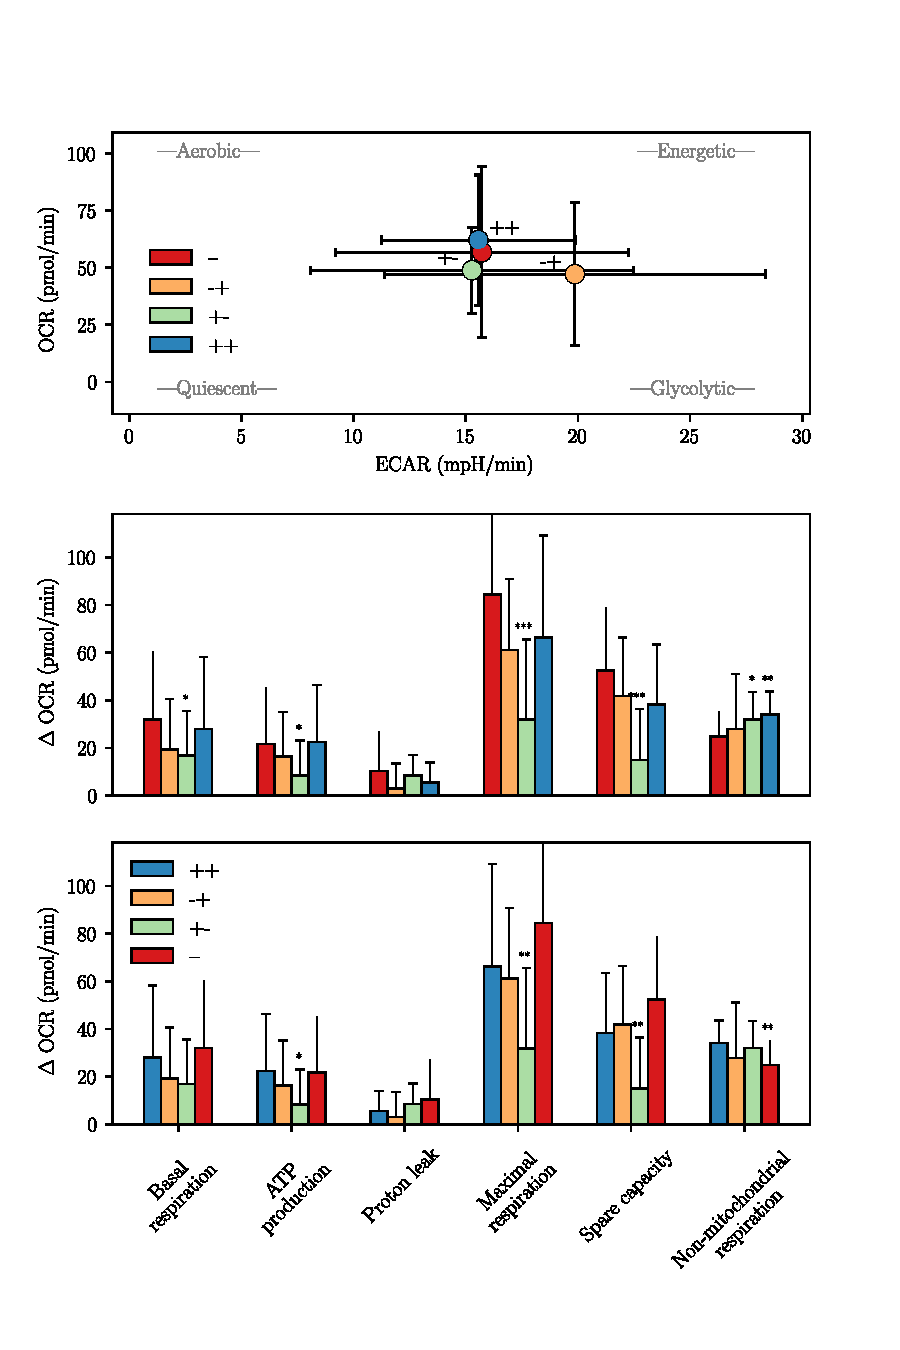
\includegraphics{Abbildung/seaborn_energy_profiles.pdf}

    	\begin{minipage}{\captionwidth}
    		\caption[energy_profile]{\uzlemph{Energy profile} \newline Evaluation of those seahorse tracks.}
    		\label{fig:energy_profile}
    	\end{minipage}
    \end{figure}

    Using a combination of toxins that inhibit the respiratory chain important characteristics of the mitochondrial respiration can extracted as described in the methods section. Even with two repeats we can observe a trend looking at the capacity. Comparing not further differentiated cells with the TGFb stimulated cells, there is a drop. Then it goes up again.

    Finally it is important to note that only two repeats were recorded because it is quite an expensive assay and not being carried out on plastic makes it not that useful for us. For Seahorse Assays this is a super low number of repeats.

\section{Evaluation of oxidative Stress}
\label{sec:oxStress}
As already described in the methods section it was further evaluated if stimulation of the synthetic phenotype with higher concentrations of PDGF-BB would yield ROS generation to an extend that can't be compensated by the ROS defense.

    \subsection{PDGF boost of out cells indcues oxidative stress}
    An experient already done within the group was repeated.

    \begin{figure}[h]
    \capstart
        \centering
    	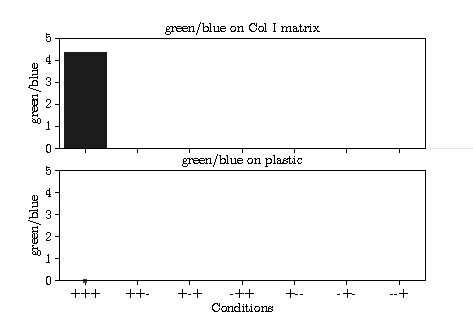
\includegraphics{Abbildung/CellROX_initial_cond.pdf}

    	\begin{minipage}{\captionwidth}
    		\caption[repeat_Lisa]{\uzlemph{Stimulation with PDGF induces oxidative stress.} \newline Repeat of the result already shown by Tobi.}
    		\label{fig:qPCR}
    	\end{minipage}
    \end{figure}

    Indeed the cells that have both stimuli can be stressed as seen in the CellROX Assay.

    \subsection{Characterization of the CellROX Assay}
    To get a better understanding of the Assay a titration was done.

    \begin{figure}[h]
    \capstart
        \centering
    	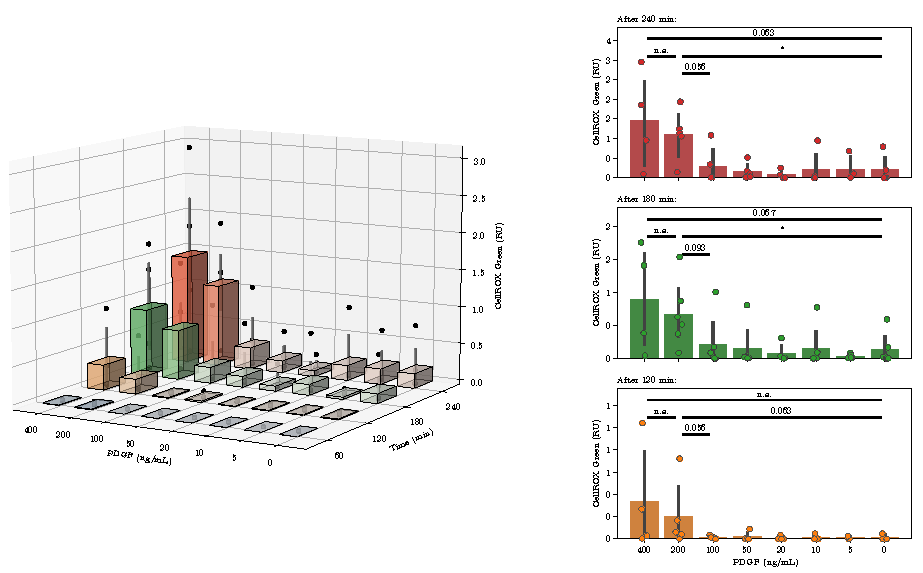
\includegraphics{Abbildung/CellROX_titration_no_norm.pdf}

    	\begin{minipage}{\captionwidth}
    		\caption[cellROX_titration]{\uzlemph{CellROX titration} \newline Titration}
    		\label{fig:qPCR}
    	\end{minipage}
    \end{figure}

    It is clear from the data that we have this trend in figure. We can see the clear influence of time and PDGF concentration. Unfortunatly there is also a plethora of other factors.

    \begin{figure}[h]
    \capstart
        \centering
    	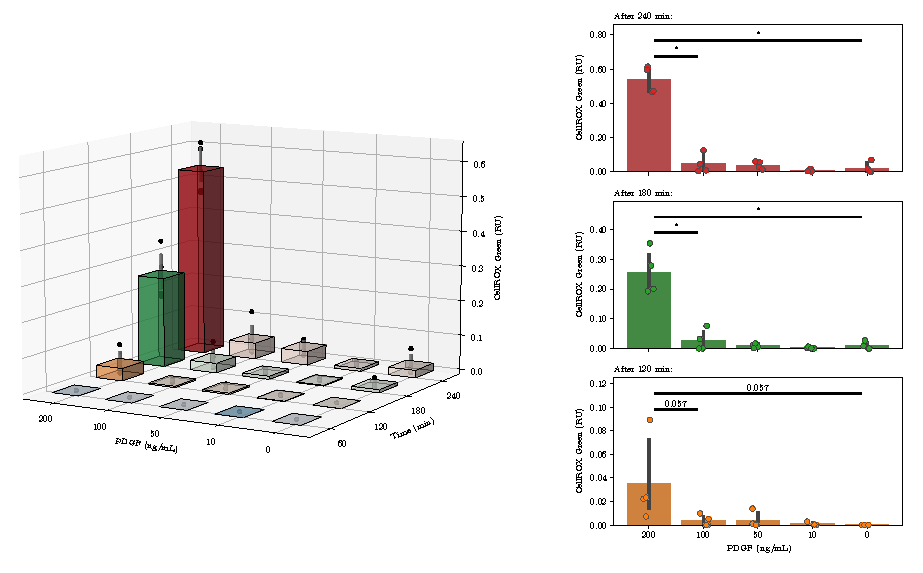
\includegraphics{Abbildung/CellROX_titration_norm.pdf}

    	\begin{minipage}{\captionwidth}
    		\caption[cellROX_titration_norm]{\uzlemph{Stimulation with PDGF induces oxidative stress - normalized.} \newline My attempt at normalization.}
    		\label{fig:qPCR}
    	\end{minipage}
    \end{figure}

    To account for these an attempt at normalization was made. Basically looking at relative signal in comparison to the highest.

    Over all we observe that we have negliable signal for concentrations < 100 ng/mL, drastic increase for 200 ng/mL, finaly very mixed results for 400 ng/mL. An further note that is not reflected in the visualized data, is that signal only seems to develop after cells are taken out of the incubator. It might be that PDGF boost is not the sole trigger but only a part, still it plays a role.

    \subsection{Rescue of ROS production using NAC}
    Finally to verify, trusting the trend overserved in the titration, a rescue experiment was performed. Quenching the signal with NAC.

    \begin{figure}[h]
    \capstart
        \centering
    	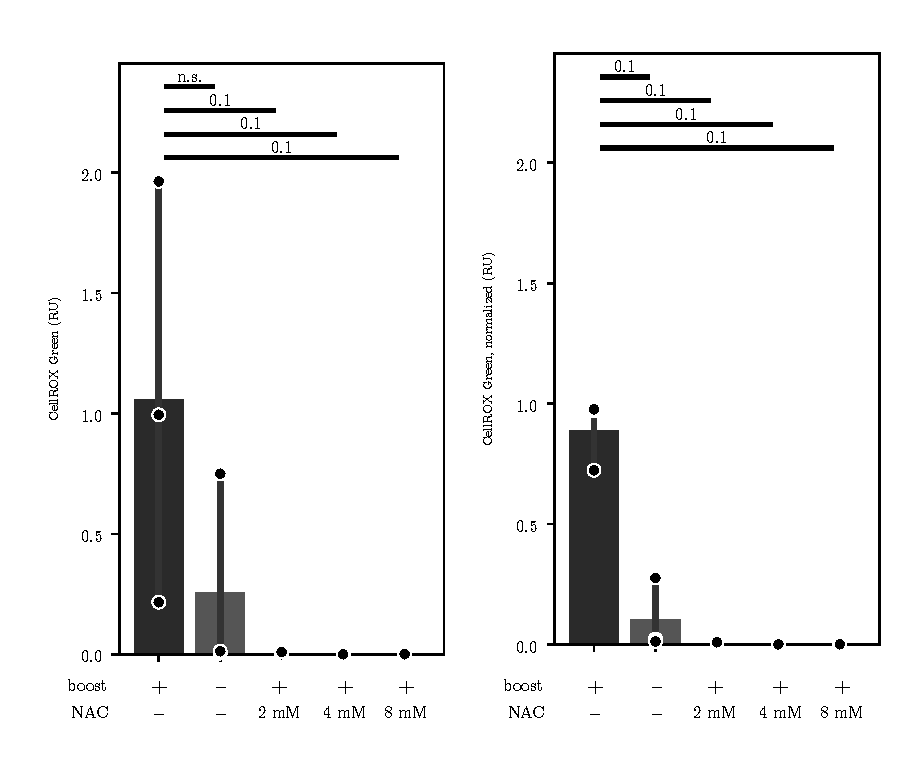
\includegraphics{Abbildung/NAC_quench.pdf}

    	\begin{minipage}{\captionwidth}
    		\caption[NAC quench]{\uzlemph{NAC  quench} \newline The NAC quench. :).}
    		\label{fig:qPCR}
    	\end{minipage}
    \end{figure}

    Confirmation that the signal is indeed due to generation of intracellular ROS.

\section{Database and GWAS Visualizer}
This was quite a long process, tinkering around with different designs to get a working solution. For this use case visualization in the browser using a database as the backend was the final decision. Compare to fetching everything online -> slow and just grabbing everything from files -> extremely stressful to maintain.

    \subsection{Curation of Data}
    Describe what actually happend to the data, probably in the methods section.
    This should be pretty self explanatory. Just have a look at the table and figure. 

    \begin{figure}[h]
    \capstart
        \centering
    	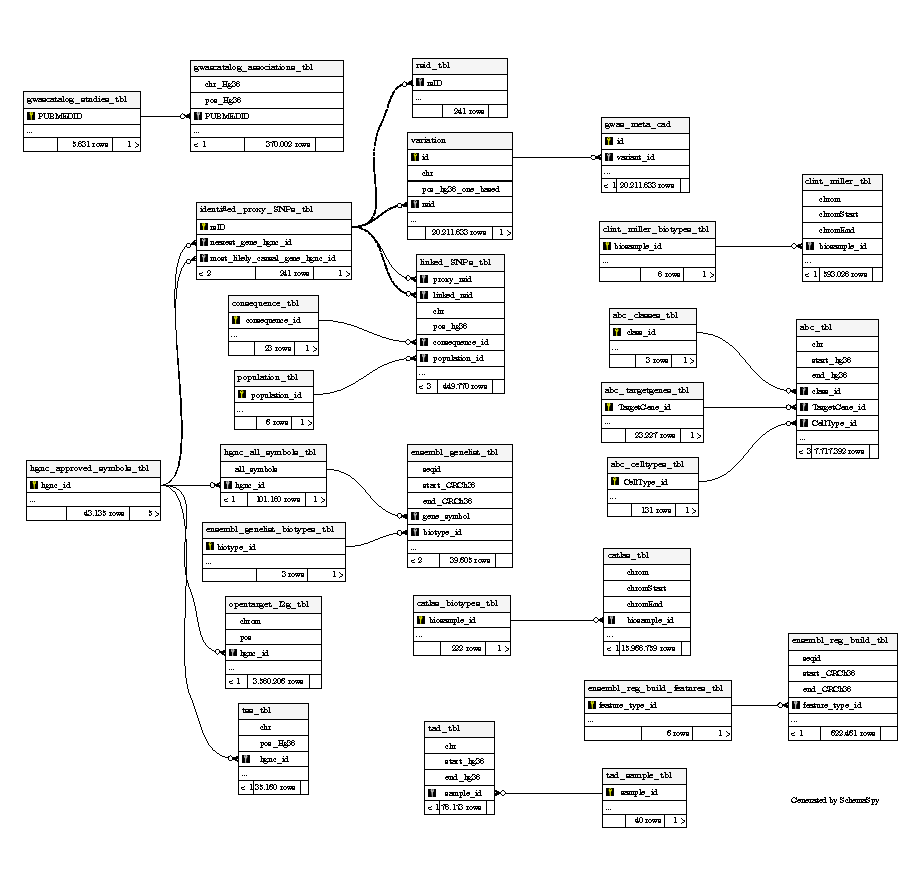
\includegraphics{Abbildung/db-schema.pdf}

    	\begin{minipage}{\captionwidth}
    		\caption[database]{\uzlemph{My super duper database} \newline DATABASE!!}
    		\label{fig:db}
    	\end{minipage}
    \end{figure}

    \subsection{Visualization}
    \label{subsec:result_vis}
    Building on the initially intended use case for the data a visualization tool was build as briefly described in the methods section, for more details please check the source code or just ask.

    Describe what the tool can do. Search function for SNPs, also for genes, providing info for associated SNPs. Visualization of the window SNPs, including linked SNPs annotated with important info such as most severe consequence. Further the data is aligned with important stuff like overlapping genes (integrating l2g scores). Also enesembl regulatory build and TADs. Further a lot of cell specific data in the form of scATAC seq tracks and promotor gene links from the ABC model. These are also shown and for easier navigation grouped into different classes using cellosaurus. To have a better look a individual variants these can be clicked, only highlighting tracks that overlap with the specific selected variant.

    For more information regarding the aligned data please check the corresping paragraph in the intrdocution.

\section{Enrichment analysis}
\label{sec:result_enrichment}
The only data that is not displayed in the plot are cCRE elements which were used for an enrichment analysis, described in methods.

\begin{figure}[h]
\capstart
    \centering
	%% Creator: Matplotlib, PGF backend
%%
%% To include the figure in your LaTeX document, write
%%   \input{<filename>.pgf}
%%
%% Make sure the required packages are loaded in your preamble
%%   \usepackage{pgf}
%%
%% Figures using additional raster images can only be included by \input if
%% they are in the same directory as the main LaTeX file. For loading figures
%% from other directories you can use the `import` package
%%   \usepackage{import}
%%
%% and then include the figures with
%%   \import{<path to file>}{<filename>.pgf}
%%
%% Matplotlib used the following preamble
%%   \usepackage{fontspec}
%%   \setmainfont{DejaVuSans.ttf}[Path=\detokenize{C:/Users/torbe/AppData/Local/Programs/Python/Python39/Lib/site-packages/matplotlib/mpl-data/fonts/ttf/}]
%%   \setsansfont{DejaVuSans.ttf}[Path=\detokenize{C:/Users/torbe/AppData/Local/Programs/Python/Python39/Lib/site-packages/matplotlib/mpl-data/fonts/ttf/}]
%%   \setmonofont{DejaVuSansMono.ttf}[Path=\detokenize{C:/Users/torbe/AppData/Local/Programs/Python/Python39/Lib/site-packages/matplotlib/mpl-data/fonts/ttf/}]
%%
\begingroup%
\makeatletter%
\begin{pgfpicture}%
\pgfpathrectangle{\pgfpointorigin}{\pgfqpoint{6.000000in}{8.000000in}}%
\pgfusepath{use as bounding box, clip}%
\begin{pgfscope}%
\pgfsetbuttcap%
\pgfsetmiterjoin%
\definecolor{currentfill}{rgb}{1.000000,1.000000,1.000000}%
\pgfsetfillcolor{currentfill}%
\pgfsetlinewidth{0.000000pt}%
\definecolor{currentstroke}{rgb}{1.000000,1.000000,1.000000}%
\pgfsetstrokecolor{currentstroke}%
\pgfsetdash{}{0pt}%
\pgfpathmoveto{\pgfqpoint{0.000000in}{0.000000in}}%
\pgfpathlineto{\pgfqpoint{6.000000in}{0.000000in}}%
\pgfpathlineto{\pgfqpoint{6.000000in}{8.000000in}}%
\pgfpathlineto{\pgfqpoint{0.000000in}{8.000000in}}%
\pgfpathclose%
\pgfusepath{fill}%
\end{pgfscope}%
\begin{pgfscope}%
\pgfsetbuttcap%
\pgfsetmiterjoin%
\definecolor{currentfill}{rgb}{1.000000,1.000000,1.000000}%
\pgfsetfillcolor{currentfill}%
\pgfsetlinewidth{0.000000pt}%
\definecolor{currentstroke}{rgb}{0.000000,0.000000,0.000000}%
\pgfsetstrokecolor{currentstroke}%
\pgfsetstrokeopacity{0.000000}%
\pgfsetdash{}{0pt}%
\pgfpathmoveto{\pgfqpoint{0.750000in}{0.880000in}}%
\pgfpathlineto{\pgfqpoint{5.400000in}{0.880000in}}%
\pgfpathlineto{\pgfqpoint{5.400000in}{7.040000in}}%
\pgfpathlineto{\pgfqpoint{0.750000in}{7.040000in}}%
\pgfpathclose%
\pgfusepath{fill}%
\end{pgfscope}%
\begin{pgfscope}%
\pgfpathrectangle{\pgfqpoint{0.750000in}{0.880000in}}{\pgfqpoint{4.650000in}{6.160000in}}%
\pgfusepath{clip}%
\pgfsetbuttcap%
\pgfsetroundjoin%
\definecolor{currentfill}{rgb}{1.000000,0.784314,0.341176}%
\pgfsetfillcolor{currentfill}%
\pgfsetfillopacity{0.250000}%
\pgfsetlinewidth{1.003750pt}%
\definecolor{currentstroke}{rgb}{1.000000,0.784314,0.341176}%
\pgfsetstrokecolor{currentstroke}%
\pgfsetstrokeopacity{0.250000}%
\pgfsetdash{}{0pt}%
\pgfpathmoveto{\pgfqpoint{4.186179in}{6.718333in}}%
\pgfpathcurveto{\pgfqpoint{4.197229in}{6.718333in}}{\pgfqpoint{4.207828in}{6.722724in}}{\pgfqpoint{4.215642in}{6.730537in}}%
\pgfpathcurveto{\pgfqpoint{4.223455in}{6.738351in}}{\pgfqpoint{4.227846in}{6.748950in}}{\pgfqpoint{4.227846in}{6.760000in}}%
\pgfpathcurveto{\pgfqpoint{4.227846in}{6.771050in}}{\pgfqpoint{4.223455in}{6.781649in}}{\pgfqpoint{4.215642in}{6.789463in}}%
\pgfpathcurveto{\pgfqpoint{4.207828in}{6.797276in}}{\pgfqpoint{4.197229in}{6.801667in}}{\pgfqpoint{4.186179in}{6.801667in}}%
\pgfpathcurveto{\pgfqpoint{4.175129in}{6.801667in}}{\pgfqpoint{4.164530in}{6.797276in}}{\pgfqpoint{4.156716in}{6.789463in}}%
\pgfpathcurveto{\pgfqpoint{4.148902in}{6.781649in}}{\pgfqpoint{4.144512in}{6.771050in}}{\pgfqpoint{4.144512in}{6.760000in}}%
\pgfpathcurveto{\pgfqpoint{4.144512in}{6.748950in}}{\pgfqpoint{4.148902in}{6.738351in}}{\pgfqpoint{4.156716in}{6.730537in}}%
\pgfpathcurveto{\pgfqpoint{4.164530in}{6.722724in}}{\pgfqpoint{4.175129in}{6.718333in}}{\pgfqpoint{4.186179in}{6.718333in}}%
\pgfpathclose%
\pgfusepath{stroke,fill}%
\end{pgfscope}%
\begin{pgfscope}%
\pgfpathrectangle{\pgfqpoint{0.750000in}{0.880000in}}{\pgfqpoint{4.650000in}{6.160000in}}%
\pgfusepath{clip}%
\pgfsetbuttcap%
\pgfsetroundjoin%
\definecolor{currentfill}{rgb}{1.000000,0.784314,0.341176}%
\pgfsetfillcolor{currentfill}%
\pgfsetfillopacity{0.250000}%
\pgfsetlinewidth{1.003750pt}%
\definecolor{currentstroke}{rgb}{1.000000,0.784314,0.341176}%
\pgfsetstrokecolor{currentstroke}%
\pgfsetstrokeopacity{0.250000}%
\pgfsetdash{}{0pt}%
\pgfpathmoveto{\pgfqpoint{3.910817in}{6.636565in}}%
\pgfpathcurveto{\pgfqpoint{3.921867in}{6.636565in}}{\pgfqpoint{3.932466in}{6.640955in}}{\pgfqpoint{3.940279in}{6.648769in}}%
\pgfpathcurveto{\pgfqpoint{3.948093in}{6.656582in}}{\pgfqpoint{3.952483in}{6.667181in}}{\pgfqpoint{3.952483in}{6.678231in}}%
\pgfpathcurveto{\pgfqpoint{3.952483in}{6.689282in}}{\pgfqpoint{3.948093in}{6.699881in}}{\pgfqpoint{3.940279in}{6.707694in}}%
\pgfpathcurveto{\pgfqpoint{3.932466in}{6.715508in}}{\pgfqpoint{3.921867in}{6.719898in}}{\pgfqpoint{3.910817in}{6.719898in}}%
\pgfpathcurveto{\pgfqpoint{3.899767in}{6.719898in}}{\pgfqpoint{3.889168in}{6.715508in}}{\pgfqpoint{3.881354in}{6.707694in}}%
\pgfpathcurveto{\pgfqpoint{3.873540in}{6.699881in}}{\pgfqpoint{3.869150in}{6.689282in}}{\pgfqpoint{3.869150in}{6.678231in}}%
\pgfpathcurveto{\pgfqpoint{3.869150in}{6.667181in}}{\pgfqpoint{3.873540in}{6.656582in}}{\pgfqpoint{3.881354in}{6.648769in}}%
\pgfpathcurveto{\pgfqpoint{3.889168in}{6.640955in}}{\pgfqpoint{3.899767in}{6.636565in}}{\pgfqpoint{3.910817in}{6.636565in}}%
\pgfpathclose%
\pgfusepath{stroke,fill}%
\end{pgfscope}%
\begin{pgfscope}%
\pgfpathrectangle{\pgfqpoint{0.750000in}{0.880000in}}{\pgfqpoint{4.650000in}{6.160000in}}%
\pgfusepath{clip}%
\pgfsetbuttcap%
\pgfsetroundjoin%
\definecolor{currentfill}{rgb}{0.945098,0.313725,0.145098}%
\pgfsetfillcolor{currentfill}%
\pgfsetfillopacity{0.250000}%
\pgfsetlinewidth{1.003750pt}%
\definecolor{currentstroke}{rgb}{0.945098,0.313725,0.145098}%
\pgfsetstrokecolor{currentstroke}%
\pgfsetstrokeopacity{0.250000}%
\pgfsetdash{}{0pt}%
\pgfpathmoveto{\pgfqpoint{4.189490in}{6.490691in}}%
\pgfpathcurveto{\pgfqpoint{4.200540in}{6.490691in}}{\pgfqpoint{4.211139in}{6.495082in}}{\pgfqpoint{4.218952in}{6.502895in}}%
\pgfpathcurveto{\pgfqpoint{4.226766in}{6.510709in}}{\pgfqpoint{4.231156in}{6.521308in}}{\pgfqpoint{4.231156in}{6.532358in}}%
\pgfpathcurveto{\pgfqpoint{4.231156in}{6.543408in}}{\pgfqpoint{4.226766in}{6.554007in}}{\pgfqpoint{4.218952in}{6.561821in}}%
\pgfpathcurveto{\pgfqpoint{4.211139in}{6.569634in}}{\pgfqpoint{4.200540in}{6.574025in}}{\pgfqpoint{4.189490in}{6.574025in}}%
\pgfpathcurveto{\pgfqpoint{4.178439in}{6.574025in}}{\pgfqpoint{4.167840in}{6.569634in}}{\pgfqpoint{4.160027in}{6.561821in}}%
\pgfpathcurveto{\pgfqpoint{4.152213in}{6.554007in}}{\pgfqpoint{4.147823in}{6.543408in}}{\pgfqpoint{4.147823in}{6.532358in}}%
\pgfpathcurveto{\pgfqpoint{4.147823in}{6.521308in}}{\pgfqpoint{4.152213in}{6.510709in}}{\pgfqpoint{4.160027in}{6.502895in}}%
\pgfpathcurveto{\pgfqpoint{4.167840in}{6.495082in}}{\pgfqpoint{4.178439in}{6.490691in}}{\pgfqpoint{4.189490in}{6.490691in}}%
\pgfpathclose%
\pgfusepath{stroke,fill}%
\end{pgfscope}%
\begin{pgfscope}%
\pgfpathrectangle{\pgfqpoint{0.750000in}{0.880000in}}{\pgfqpoint{4.650000in}{6.160000in}}%
\pgfusepath{clip}%
\pgfsetbuttcap%
\pgfsetroundjoin%
\definecolor{currentfill}{rgb}{0.945098,0.313725,0.145098}%
\pgfsetfillcolor{currentfill}%
\pgfsetfillopacity{0.250000}%
\pgfsetlinewidth{1.003750pt}%
\definecolor{currentstroke}{rgb}{0.945098,0.313725,0.145098}%
\pgfsetstrokecolor{currentstroke}%
\pgfsetstrokeopacity{0.250000}%
\pgfsetdash{}{0pt}%
\pgfpathmoveto{\pgfqpoint{4.480378in}{6.461939in}}%
\pgfpathcurveto{\pgfqpoint{4.491428in}{6.461939in}}{\pgfqpoint{4.502027in}{6.466329in}}{\pgfqpoint{4.509841in}{6.474143in}}%
\pgfpathcurveto{\pgfqpoint{4.517655in}{6.481957in}}{\pgfqpoint{4.522045in}{6.492556in}}{\pgfqpoint{4.522045in}{6.503606in}}%
\pgfpathcurveto{\pgfqpoint{4.522045in}{6.514656in}}{\pgfqpoint{4.517655in}{6.525255in}}{\pgfqpoint{4.509841in}{6.533069in}}%
\pgfpathcurveto{\pgfqpoint{4.502027in}{6.540882in}}{\pgfqpoint{4.491428in}{6.545272in}}{\pgfqpoint{4.480378in}{6.545272in}}%
\pgfpathcurveto{\pgfqpoint{4.469328in}{6.545272in}}{\pgfqpoint{4.458729in}{6.540882in}}{\pgfqpoint{4.450915in}{6.533069in}}%
\pgfpathcurveto{\pgfqpoint{4.443102in}{6.525255in}}{\pgfqpoint{4.438711in}{6.514656in}}{\pgfqpoint{4.438711in}{6.503606in}}%
\pgfpathcurveto{\pgfqpoint{4.438711in}{6.492556in}}{\pgfqpoint{4.443102in}{6.481957in}}{\pgfqpoint{4.450915in}{6.474143in}}%
\pgfpathcurveto{\pgfqpoint{4.458729in}{6.466329in}}{\pgfqpoint{4.469328in}{6.461939in}}{\pgfqpoint{4.480378in}{6.461939in}}%
\pgfpathclose%
\pgfusepath{stroke,fill}%
\end{pgfscope}%
\begin{pgfscope}%
\pgfpathrectangle{\pgfqpoint{0.750000in}{0.880000in}}{\pgfqpoint{4.650000in}{6.160000in}}%
\pgfusepath{clip}%
\pgfsetbuttcap%
\pgfsetroundjoin%
\definecolor{currentfill}{rgb}{0.031373,0.011765,0.341176}%
\pgfsetfillcolor{currentfill}%
\pgfsetfillopacity{0.250000}%
\pgfsetlinewidth{1.003750pt}%
\definecolor{currentstroke}{rgb}{0.031373,0.011765,0.341176}%
\pgfsetstrokecolor{currentstroke}%
\pgfsetstrokeopacity{0.250000}%
\pgfsetdash{}{0pt}%
\pgfpathmoveto{\pgfqpoint{3.614227in}{6.189110in}}%
\pgfpathcurveto{\pgfqpoint{3.625277in}{6.189110in}}{\pgfqpoint{3.635876in}{6.193500in}}{\pgfqpoint{3.643690in}{6.201314in}}%
\pgfpathcurveto{\pgfqpoint{3.651503in}{6.209127in}}{\pgfqpoint{3.655893in}{6.219727in}}{\pgfqpoint{3.655893in}{6.230777in}}%
\pgfpathcurveto{\pgfqpoint{3.655893in}{6.241827in}}{\pgfqpoint{3.651503in}{6.252426in}}{\pgfqpoint{3.643690in}{6.260239in}}%
\pgfpathcurveto{\pgfqpoint{3.635876in}{6.268053in}}{\pgfqpoint{3.625277in}{6.272443in}}{\pgfqpoint{3.614227in}{6.272443in}}%
\pgfpathcurveto{\pgfqpoint{3.603177in}{6.272443in}}{\pgfqpoint{3.592578in}{6.268053in}}{\pgfqpoint{3.584764in}{6.260239in}}%
\pgfpathcurveto{\pgfqpoint{3.576950in}{6.252426in}}{\pgfqpoint{3.572560in}{6.241827in}}{\pgfqpoint{3.572560in}{6.230777in}}%
\pgfpathcurveto{\pgfqpoint{3.572560in}{6.219727in}}{\pgfqpoint{3.576950in}{6.209127in}}{\pgfqpoint{3.584764in}{6.201314in}}%
\pgfpathcurveto{\pgfqpoint{3.592578in}{6.193500in}}{\pgfqpoint{3.603177in}{6.189110in}}{\pgfqpoint{3.614227in}{6.189110in}}%
\pgfpathclose%
\pgfusepath{stroke,fill}%
\end{pgfscope}%
\begin{pgfscope}%
\pgfpathrectangle{\pgfqpoint{0.750000in}{0.880000in}}{\pgfqpoint{4.650000in}{6.160000in}}%
\pgfusepath{clip}%
\pgfsetbuttcap%
\pgfsetroundjoin%
\definecolor{currentfill}{rgb}{0.329412,0.258824,0.556863}%
\pgfsetfillcolor{currentfill}%
\pgfsetfillopacity{0.250000}%
\pgfsetlinewidth{1.003750pt}%
\definecolor{currentstroke}{rgb}{0.329412,0.258824,0.556863}%
\pgfsetstrokecolor{currentstroke}%
\pgfsetstrokeopacity{0.250000}%
\pgfsetdash{}{0pt}%
\pgfpathmoveto{\pgfqpoint{3.441077in}{5.608960in}}%
\pgfpathcurveto{\pgfqpoint{3.452127in}{5.608960in}}{\pgfqpoint{3.462726in}{5.613350in}}{\pgfqpoint{3.470539in}{5.621164in}}%
\pgfpathcurveto{\pgfqpoint{3.478353in}{5.628978in}}{\pgfqpoint{3.482743in}{5.639577in}}{\pgfqpoint{3.482743in}{5.650627in}}%
\pgfpathcurveto{\pgfqpoint{3.482743in}{5.661677in}}{\pgfqpoint{3.478353in}{5.672276in}}{\pgfqpoint{3.470539in}{5.680090in}}%
\pgfpathcurveto{\pgfqpoint{3.462726in}{5.687903in}}{\pgfqpoint{3.452127in}{5.692294in}}{\pgfqpoint{3.441077in}{5.692294in}}%
\pgfpathcurveto{\pgfqpoint{3.430026in}{5.692294in}}{\pgfqpoint{3.419427in}{5.687903in}}{\pgfqpoint{3.411614in}{5.680090in}}%
\pgfpathcurveto{\pgfqpoint{3.403800in}{5.672276in}}{\pgfqpoint{3.399410in}{5.661677in}}{\pgfqpoint{3.399410in}{5.650627in}}%
\pgfpathcurveto{\pgfqpoint{3.399410in}{5.639577in}}{\pgfqpoint{3.403800in}{5.628978in}}{\pgfqpoint{3.411614in}{5.621164in}}%
\pgfpathcurveto{\pgfqpoint{3.419427in}{5.613350in}}{\pgfqpoint{3.430026in}{5.608960in}}{\pgfqpoint{3.441077in}{5.608960in}}%
\pgfpathclose%
\pgfusepath{stroke,fill}%
\end{pgfscope}%
\begin{pgfscope}%
\pgfpathrectangle{\pgfqpoint{0.750000in}{0.880000in}}{\pgfqpoint{4.650000in}{6.160000in}}%
\pgfusepath{clip}%
\pgfsetbuttcap%
\pgfsetroundjoin%
\definecolor{currentfill}{rgb}{1.000000,0.784314,0.341176}%
\pgfsetfillcolor{currentfill}%
\pgfsetfillopacity{0.250000}%
\pgfsetlinewidth{1.003750pt}%
\definecolor{currentstroke}{rgb}{1.000000,0.784314,0.341176}%
\pgfsetstrokecolor{currentstroke}%
\pgfsetstrokeopacity{0.250000}%
\pgfsetdash{}{0pt}%
\pgfpathmoveto{\pgfqpoint{3.632155in}{5.478485in}}%
\pgfpathcurveto{\pgfqpoint{3.643205in}{5.478485in}}{\pgfqpoint{3.653804in}{5.482876in}}{\pgfqpoint{3.661618in}{5.490689in}}%
\pgfpathcurveto{\pgfqpoint{3.669431in}{5.498503in}}{\pgfqpoint{3.673822in}{5.509102in}}{\pgfqpoint{3.673822in}{5.520152in}}%
\pgfpathcurveto{\pgfqpoint{3.673822in}{5.531202in}}{\pgfqpoint{3.669431in}{5.541801in}}{\pgfqpoint{3.661618in}{5.549615in}}%
\pgfpathcurveto{\pgfqpoint{3.653804in}{5.557428in}}{\pgfqpoint{3.643205in}{5.561819in}}{\pgfqpoint{3.632155in}{5.561819in}}%
\pgfpathcurveto{\pgfqpoint{3.621105in}{5.561819in}}{\pgfqpoint{3.610506in}{5.557428in}}{\pgfqpoint{3.602692in}{5.549615in}}%
\pgfpathcurveto{\pgfqpoint{3.594878in}{5.541801in}}{\pgfqpoint{3.590488in}{5.531202in}}{\pgfqpoint{3.590488in}{5.520152in}}%
\pgfpathcurveto{\pgfqpoint{3.590488in}{5.509102in}}{\pgfqpoint{3.594878in}{5.498503in}}{\pgfqpoint{3.602692in}{5.490689in}}%
\pgfpathcurveto{\pgfqpoint{3.610506in}{5.482876in}}{\pgfqpoint{3.621105in}{5.478485in}}{\pgfqpoint{3.632155in}{5.478485in}}%
\pgfpathclose%
\pgfusepath{stroke,fill}%
\end{pgfscope}%
\begin{pgfscope}%
\pgfpathrectangle{\pgfqpoint{0.750000in}{0.880000in}}{\pgfqpoint{4.650000in}{6.160000in}}%
\pgfusepath{clip}%
\pgfsetbuttcap%
\pgfsetroundjoin%
\definecolor{currentfill}{rgb}{0.945098,0.313725,0.145098}%
\pgfsetfillcolor{currentfill}%
\pgfsetfillopacity{0.250000}%
\pgfsetlinewidth{1.003750pt}%
\definecolor{currentstroke}{rgb}{0.945098,0.313725,0.145098}%
\pgfsetstrokecolor{currentstroke}%
\pgfsetstrokeopacity{0.250000}%
\pgfsetdash{}{0pt}%
\pgfpathmoveto{\pgfqpoint{4.286500in}{5.463244in}}%
\pgfpathcurveto{\pgfqpoint{4.297550in}{5.463244in}}{\pgfqpoint{4.308149in}{5.467634in}}{\pgfqpoint{4.315963in}{5.475448in}}%
\pgfpathcurveto{\pgfqpoint{4.323776in}{5.483261in}}{\pgfqpoint{4.328166in}{5.493860in}}{\pgfqpoint{4.328166in}{5.504911in}}%
\pgfpathcurveto{\pgfqpoint{4.328166in}{5.515961in}}{\pgfqpoint{4.323776in}{5.526560in}}{\pgfqpoint{4.315963in}{5.534373in}}%
\pgfpathcurveto{\pgfqpoint{4.308149in}{5.542187in}}{\pgfqpoint{4.297550in}{5.546577in}}{\pgfqpoint{4.286500in}{5.546577in}}%
\pgfpathcurveto{\pgfqpoint{4.275450in}{5.546577in}}{\pgfqpoint{4.264851in}{5.542187in}}{\pgfqpoint{4.257037in}{5.534373in}}%
\pgfpathcurveto{\pgfqpoint{4.249223in}{5.526560in}}{\pgfqpoint{4.244833in}{5.515961in}}{\pgfqpoint{4.244833in}{5.504911in}}%
\pgfpathcurveto{\pgfqpoint{4.244833in}{5.493860in}}{\pgfqpoint{4.249223in}{5.483261in}}{\pgfqpoint{4.257037in}{5.475448in}}%
\pgfpathcurveto{\pgfqpoint{4.264851in}{5.467634in}}{\pgfqpoint{4.275450in}{5.463244in}}{\pgfqpoint{4.286500in}{5.463244in}}%
\pgfpathclose%
\pgfusepath{stroke,fill}%
\end{pgfscope}%
\begin{pgfscope}%
\pgfpathrectangle{\pgfqpoint{0.750000in}{0.880000in}}{\pgfqpoint{4.650000in}{6.160000in}}%
\pgfusepath{clip}%
\pgfsetbuttcap%
\pgfsetroundjoin%
\definecolor{currentfill}{rgb}{1.000000,0.784314,0.341176}%
\pgfsetfillcolor{currentfill}%
\pgfsetfillopacity{0.250000}%
\pgfsetlinewidth{1.003750pt}%
\definecolor{currentstroke}{rgb}{1.000000,0.784314,0.341176}%
\pgfsetstrokecolor{currentstroke}%
\pgfsetstrokeopacity{0.250000}%
\pgfsetdash{}{0pt}%
\pgfpathmoveto{\pgfqpoint{3.623168in}{5.461047in}}%
\pgfpathcurveto{\pgfqpoint{3.634218in}{5.461047in}}{\pgfqpoint{3.644817in}{5.465437in}}{\pgfqpoint{3.652631in}{5.473251in}}%
\pgfpathcurveto{\pgfqpoint{3.660444in}{5.481065in}}{\pgfqpoint{3.664835in}{5.491664in}}{\pgfqpoint{3.664835in}{5.502714in}}%
\pgfpathcurveto{\pgfqpoint{3.664835in}{5.513764in}}{\pgfqpoint{3.660444in}{5.524363in}}{\pgfqpoint{3.652631in}{5.532177in}}%
\pgfpathcurveto{\pgfqpoint{3.644817in}{5.539990in}}{\pgfqpoint{3.634218in}{5.544381in}}{\pgfqpoint{3.623168in}{5.544381in}}%
\pgfpathcurveto{\pgfqpoint{3.612118in}{5.544381in}}{\pgfqpoint{3.601519in}{5.539990in}}{\pgfqpoint{3.593705in}{5.532177in}}%
\pgfpathcurveto{\pgfqpoint{3.585892in}{5.524363in}}{\pgfqpoint{3.581501in}{5.513764in}}{\pgfqpoint{3.581501in}{5.502714in}}%
\pgfpathcurveto{\pgfqpoint{3.581501in}{5.491664in}}{\pgfqpoint{3.585892in}{5.481065in}}{\pgfqpoint{3.593705in}{5.473251in}}%
\pgfpathcurveto{\pgfqpoint{3.601519in}{5.465437in}}{\pgfqpoint{3.612118in}{5.461047in}}{\pgfqpoint{3.623168in}{5.461047in}}%
\pgfpathclose%
\pgfusepath{stroke,fill}%
\end{pgfscope}%
\begin{pgfscope}%
\pgfpathrectangle{\pgfqpoint{0.750000in}{0.880000in}}{\pgfqpoint{4.650000in}{6.160000in}}%
\pgfusepath{clip}%
\pgfsetbuttcap%
\pgfsetroundjoin%
\definecolor{currentfill}{rgb}{0.945098,0.313725,0.145098}%
\pgfsetfillcolor{currentfill}%
\pgfsetfillopacity{0.250000}%
\pgfsetlinewidth{1.003750pt}%
\definecolor{currentstroke}{rgb}{0.945098,0.313725,0.145098}%
\pgfsetstrokecolor{currentstroke}%
\pgfsetstrokeopacity{0.250000}%
\pgfsetdash{}{0pt}%
\pgfpathmoveto{\pgfqpoint{3.400960in}{5.348788in}}%
\pgfpathcurveto{\pgfqpoint{3.412010in}{5.348788in}}{\pgfqpoint{3.422609in}{5.353178in}}{\pgfqpoint{3.430423in}{5.360992in}}%
\pgfpathcurveto{\pgfqpoint{3.438236in}{5.368805in}}{\pgfqpoint{3.442626in}{5.379404in}}{\pgfqpoint{3.442626in}{5.390454in}}%
\pgfpathcurveto{\pgfqpoint{3.442626in}{5.401505in}}{\pgfqpoint{3.438236in}{5.412104in}}{\pgfqpoint{3.430423in}{5.419917in}}%
\pgfpathcurveto{\pgfqpoint{3.422609in}{5.427731in}}{\pgfqpoint{3.412010in}{5.432121in}}{\pgfqpoint{3.400960in}{5.432121in}}%
\pgfpathcurveto{\pgfqpoint{3.389910in}{5.432121in}}{\pgfqpoint{3.379311in}{5.427731in}}{\pgfqpoint{3.371497in}{5.419917in}}%
\pgfpathcurveto{\pgfqpoint{3.363683in}{5.412104in}}{\pgfqpoint{3.359293in}{5.401505in}}{\pgfqpoint{3.359293in}{5.390454in}}%
\pgfpathcurveto{\pgfqpoint{3.359293in}{5.379404in}}{\pgfqpoint{3.363683in}{5.368805in}}{\pgfqpoint{3.371497in}{5.360992in}}%
\pgfpathcurveto{\pgfqpoint{3.379311in}{5.353178in}}{\pgfqpoint{3.389910in}{5.348788in}}{\pgfqpoint{3.400960in}{5.348788in}}%
\pgfpathclose%
\pgfusepath{stroke,fill}%
\end{pgfscope}%
\begin{pgfscope}%
\pgfpathrectangle{\pgfqpoint{0.750000in}{0.880000in}}{\pgfqpoint{4.650000in}{6.160000in}}%
\pgfusepath{clip}%
\pgfsetbuttcap%
\pgfsetroundjoin%
\definecolor{currentfill}{rgb}{0.000000,0.458824,0.635294}%
\pgfsetfillcolor{currentfill}%
\pgfsetfillopacity{0.250000}%
\pgfsetlinewidth{1.003750pt}%
\definecolor{currentstroke}{rgb}{0.000000,0.458824,0.635294}%
\pgfsetstrokecolor{currentstroke}%
\pgfsetstrokeopacity{0.250000}%
\pgfsetdash{}{0pt}%
\pgfpathmoveto{\pgfqpoint{4.384283in}{5.344486in}}%
\pgfpathcurveto{\pgfqpoint{4.395333in}{5.344486in}}{\pgfqpoint{4.405932in}{5.348876in}}{\pgfqpoint{4.413746in}{5.356690in}}%
\pgfpathcurveto{\pgfqpoint{4.421559in}{5.364503in}}{\pgfqpoint{4.425950in}{5.375102in}}{\pgfqpoint{4.425950in}{5.386153in}}%
\pgfpathcurveto{\pgfqpoint{4.425950in}{5.397203in}}{\pgfqpoint{4.421559in}{5.407802in}}{\pgfqpoint{4.413746in}{5.415615in}}%
\pgfpathcurveto{\pgfqpoint{4.405932in}{5.423429in}}{\pgfqpoint{4.395333in}{5.427819in}}{\pgfqpoint{4.384283in}{5.427819in}}%
\pgfpathcurveto{\pgfqpoint{4.373233in}{5.427819in}}{\pgfqpoint{4.362634in}{5.423429in}}{\pgfqpoint{4.354820in}{5.415615in}}%
\pgfpathcurveto{\pgfqpoint{4.347007in}{5.407802in}}{\pgfqpoint{4.342616in}{5.397203in}}{\pgfqpoint{4.342616in}{5.386153in}}%
\pgfpathcurveto{\pgfqpoint{4.342616in}{5.375102in}}{\pgfqpoint{4.347007in}{5.364503in}}{\pgfqpoint{4.354820in}{5.356690in}}%
\pgfpathcurveto{\pgfqpoint{4.362634in}{5.348876in}}{\pgfqpoint{4.373233in}{5.344486in}}{\pgfqpoint{4.384283in}{5.344486in}}%
\pgfpathclose%
\pgfusepath{stroke,fill}%
\end{pgfscope}%
\begin{pgfscope}%
\pgfpathrectangle{\pgfqpoint{0.750000in}{0.880000in}}{\pgfqpoint{4.650000in}{6.160000in}}%
\pgfusepath{clip}%
\pgfsetbuttcap%
\pgfsetroundjoin%
\definecolor{currentfill}{rgb}{0.000000,0.458824,0.635294}%
\pgfsetfillcolor{currentfill}%
\pgfsetfillopacity{0.250000}%
\pgfsetlinewidth{1.003750pt}%
\definecolor{currentstroke}{rgb}{0.000000,0.458824,0.635294}%
\pgfsetstrokecolor{currentstroke}%
\pgfsetstrokeopacity{0.250000}%
\pgfsetdash{}{0pt}%
\pgfpathmoveto{\pgfqpoint{3.711699in}{5.246454in}}%
\pgfpathcurveto{\pgfqpoint{3.722749in}{5.246454in}}{\pgfqpoint{3.733348in}{5.250844in}}{\pgfqpoint{3.741162in}{5.258658in}}%
\pgfpathcurveto{\pgfqpoint{3.748975in}{5.266471in}}{\pgfqpoint{3.753366in}{5.277070in}}{\pgfqpoint{3.753366in}{5.288120in}}%
\pgfpathcurveto{\pgfqpoint{3.753366in}{5.299171in}}{\pgfqpoint{3.748975in}{5.309770in}}{\pgfqpoint{3.741162in}{5.317583in}}%
\pgfpathcurveto{\pgfqpoint{3.733348in}{5.325397in}}{\pgfqpoint{3.722749in}{5.329787in}}{\pgfqpoint{3.711699in}{5.329787in}}%
\pgfpathcurveto{\pgfqpoint{3.700649in}{5.329787in}}{\pgfqpoint{3.690050in}{5.325397in}}{\pgfqpoint{3.682236in}{5.317583in}}%
\pgfpathcurveto{\pgfqpoint{3.674423in}{5.309770in}}{\pgfqpoint{3.670032in}{5.299171in}}{\pgfqpoint{3.670032in}{5.288120in}}%
\pgfpathcurveto{\pgfqpoint{3.670032in}{5.277070in}}{\pgfqpoint{3.674423in}{5.266471in}}{\pgfqpoint{3.682236in}{5.258658in}}%
\pgfpathcurveto{\pgfqpoint{3.690050in}{5.250844in}}{\pgfqpoint{3.700649in}{5.246454in}}{\pgfqpoint{3.711699in}{5.246454in}}%
\pgfpathclose%
\pgfusepath{stroke,fill}%
\end{pgfscope}%
\begin{pgfscope}%
\pgfpathrectangle{\pgfqpoint{0.750000in}{0.880000in}}{\pgfqpoint{4.650000in}{6.160000in}}%
\pgfusepath{clip}%
\pgfsetbuttcap%
\pgfsetroundjoin%
\definecolor{currentfill}{rgb}{0.501961,0.501961,0.501961}%
\pgfsetfillcolor{currentfill}%
\pgfsetfillopacity{0.250000}%
\pgfsetlinewidth{1.003750pt}%
\definecolor{currentstroke}{rgb}{0.501961,0.501961,0.501961}%
\pgfsetstrokecolor{currentstroke}%
\pgfsetstrokeopacity{0.250000}%
\pgfsetdash{}{0pt}%
\pgfpathmoveto{\pgfqpoint{3.067705in}{5.246164in}}%
\pgfpathcurveto{\pgfqpoint{3.078755in}{5.246164in}}{\pgfqpoint{3.089355in}{5.250554in}}{\pgfqpoint{3.097168in}{5.258368in}}%
\pgfpathcurveto{\pgfqpoint{3.104982in}{5.266182in}}{\pgfqpoint{3.109372in}{5.276781in}}{\pgfqpoint{3.109372in}{5.287831in}}%
\pgfpathcurveto{\pgfqpoint{3.109372in}{5.298881in}}{\pgfqpoint{3.104982in}{5.309480in}}{\pgfqpoint{3.097168in}{5.317294in}}%
\pgfpathcurveto{\pgfqpoint{3.089355in}{5.325107in}}{\pgfqpoint{3.078755in}{5.329497in}}{\pgfqpoint{3.067705in}{5.329497in}}%
\pgfpathcurveto{\pgfqpoint{3.056655in}{5.329497in}}{\pgfqpoint{3.046056in}{5.325107in}}{\pgfqpoint{3.038243in}{5.317294in}}%
\pgfpathcurveto{\pgfqpoint{3.030429in}{5.309480in}}{\pgfqpoint{3.026039in}{5.298881in}}{\pgfqpoint{3.026039in}{5.287831in}}%
\pgfpathcurveto{\pgfqpoint{3.026039in}{5.276781in}}{\pgfqpoint{3.030429in}{5.266182in}}{\pgfqpoint{3.038243in}{5.258368in}}%
\pgfpathcurveto{\pgfqpoint{3.046056in}{5.250554in}}{\pgfqpoint{3.056655in}{5.246164in}}{\pgfqpoint{3.067705in}{5.246164in}}%
\pgfpathclose%
\pgfusepath{stroke,fill}%
\end{pgfscope}%
\begin{pgfscope}%
\pgfpathrectangle{\pgfqpoint{0.750000in}{0.880000in}}{\pgfqpoint{4.650000in}{6.160000in}}%
\pgfusepath{clip}%
\pgfsetbuttcap%
\pgfsetroundjoin%
\definecolor{currentfill}{rgb}{0.945098,0.313725,0.145098}%
\pgfsetfillcolor{currentfill}%
\pgfsetfillopacity{0.250000}%
\pgfsetlinewidth{1.003750pt}%
\definecolor{currentstroke}{rgb}{0.945098,0.313725,0.145098}%
\pgfsetstrokecolor{currentstroke}%
\pgfsetstrokeopacity{0.250000}%
\pgfsetdash{}{0pt}%
\pgfpathmoveto{\pgfqpoint{3.277193in}{5.221994in}}%
\pgfpathcurveto{\pgfqpoint{3.288243in}{5.221994in}}{\pgfqpoint{3.298842in}{5.226384in}}{\pgfqpoint{3.306656in}{5.234197in}}%
\pgfpathcurveto{\pgfqpoint{3.314469in}{5.242011in}}{\pgfqpoint{3.318860in}{5.252610in}}{\pgfqpoint{3.318860in}{5.263660in}}%
\pgfpathcurveto{\pgfqpoint{3.318860in}{5.274710in}}{\pgfqpoint{3.314469in}{5.285309in}}{\pgfqpoint{3.306656in}{5.293123in}}%
\pgfpathcurveto{\pgfqpoint{3.298842in}{5.300937in}}{\pgfqpoint{3.288243in}{5.305327in}}{\pgfqpoint{3.277193in}{5.305327in}}%
\pgfpathcurveto{\pgfqpoint{3.266143in}{5.305327in}}{\pgfqpoint{3.255544in}{5.300937in}}{\pgfqpoint{3.247730in}{5.293123in}}%
\pgfpathcurveto{\pgfqpoint{3.239917in}{5.285309in}}{\pgfqpoint{3.235526in}{5.274710in}}{\pgfqpoint{3.235526in}{5.263660in}}%
\pgfpathcurveto{\pgfqpoint{3.235526in}{5.252610in}}{\pgfqpoint{3.239917in}{5.242011in}}{\pgfqpoint{3.247730in}{5.234197in}}%
\pgfpathcurveto{\pgfqpoint{3.255544in}{5.226384in}}{\pgfqpoint{3.266143in}{5.221994in}}{\pgfqpoint{3.277193in}{5.221994in}}%
\pgfpathclose%
\pgfusepath{stroke,fill}%
\end{pgfscope}%
\begin{pgfscope}%
\pgfpathrectangle{\pgfqpoint{0.750000in}{0.880000in}}{\pgfqpoint{4.650000in}{6.160000in}}%
\pgfusepath{clip}%
\pgfsetbuttcap%
\pgfsetroundjoin%
\definecolor{currentfill}{rgb}{0.945098,0.313725,0.145098}%
\pgfsetfillcolor{currentfill}%
\pgfsetfillopacity{0.250000}%
\pgfsetlinewidth{1.003750pt}%
\definecolor{currentstroke}{rgb}{0.945098,0.313725,0.145098}%
\pgfsetstrokecolor{currentstroke}%
\pgfsetstrokeopacity{0.250000}%
\pgfsetdash{}{0pt}%
\pgfpathmoveto{\pgfqpoint{3.496349in}{5.210880in}}%
\pgfpathcurveto{\pgfqpoint{3.507400in}{5.210880in}}{\pgfqpoint{3.517999in}{5.215271in}}{\pgfqpoint{3.525812in}{5.223084in}}%
\pgfpathcurveto{\pgfqpoint{3.533626in}{5.230898in}}{\pgfqpoint{3.538016in}{5.241497in}}{\pgfqpoint{3.538016in}{5.252547in}}%
\pgfpathcurveto{\pgfqpoint{3.538016in}{5.263597in}}{\pgfqpoint{3.533626in}{5.274196in}}{\pgfqpoint{3.525812in}{5.282010in}}%
\pgfpathcurveto{\pgfqpoint{3.517999in}{5.289823in}}{\pgfqpoint{3.507400in}{5.294214in}}{\pgfqpoint{3.496349in}{5.294214in}}%
\pgfpathcurveto{\pgfqpoint{3.485299in}{5.294214in}}{\pgfqpoint{3.474700in}{5.289823in}}{\pgfqpoint{3.466887in}{5.282010in}}%
\pgfpathcurveto{\pgfqpoint{3.459073in}{5.274196in}}{\pgfqpoint{3.454683in}{5.263597in}}{\pgfqpoint{3.454683in}{5.252547in}}%
\pgfpathcurveto{\pgfqpoint{3.454683in}{5.241497in}}{\pgfqpoint{3.459073in}{5.230898in}}{\pgfqpoint{3.466887in}{5.223084in}}%
\pgfpathcurveto{\pgfqpoint{3.474700in}{5.215271in}}{\pgfqpoint{3.485299in}{5.210880in}}{\pgfqpoint{3.496349in}{5.210880in}}%
\pgfpathclose%
\pgfusepath{stroke,fill}%
\end{pgfscope}%
\begin{pgfscope}%
\pgfpathrectangle{\pgfqpoint{0.750000in}{0.880000in}}{\pgfqpoint{4.650000in}{6.160000in}}%
\pgfusepath{clip}%
\pgfsetbuttcap%
\pgfsetroundjoin%
\definecolor{currentfill}{rgb}{0.945098,0.313725,0.145098}%
\pgfsetfillcolor{currentfill}%
\pgfsetfillopacity{0.250000}%
\pgfsetlinewidth{1.003750pt}%
\definecolor{currentstroke}{rgb}{0.945098,0.313725,0.145098}%
\pgfsetstrokecolor{currentstroke}%
\pgfsetstrokeopacity{0.250000}%
\pgfsetdash{}{0pt}%
\pgfpathmoveto{\pgfqpoint{3.382103in}{5.142215in}}%
\pgfpathcurveto{\pgfqpoint{3.393153in}{5.142215in}}{\pgfqpoint{3.403752in}{5.146605in}}{\pgfqpoint{3.411566in}{5.154419in}}%
\pgfpathcurveto{\pgfqpoint{3.419379in}{5.162232in}}{\pgfqpoint{3.423770in}{5.172831in}}{\pgfqpoint{3.423770in}{5.183881in}}%
\pgfpathcurveto{\pgfqpoint{3.423770in}{5.194932in}}{\pgfqpoint{3.419379in}{5.205531in}}{\pgfqpoint{3.411566in}{5.213344in}}%
\pgfpathcurveto{\pgfqpoint{3.403752in}{5.221158in}}{\pgfqpoint{3.393153in}{5.225548in}}{\pgfqpoint{3.382103in}{5.225548in}}%
\pgfpathcurveto{\pgfqpoint{3.371053in}{5.225548in}}{\pgfqpoint{3.360454in}{5.221158in}}{\pgfqpoint{3.352640in}{5.213344in}}%
\pgfpathcurveto{\pgfqpoint{3.344827in}{5.205531in}}{\pgfqpoint{3.340436in}{5.194932in}}{\pgfqpoint{3.340436in}{5.183881in}}%
\pgfpathcurveto{\pgfqpoint{3.340436in}{5.172831in}}{\pgfqpoint{3.344827in}{5.162232in}}{\pgfqpoint{3.352640in}{5.154419in}}%
\pgfpathcurveto{\pgfqpoint{3.360454in}{5.146605in}}{\pgfqpoint{3.371053in}{5.142215in}}{\pgfqpoint{3.382103in}{5.142215in}}%
\pgfpathclose%
\pgfusepath{stroke,fill}%
\end{pgfscope}%
\begin{pgfscope}%
\pgfpathrectangle{\pgfqpoint{0.750000in}{0.880000in}}{\pgfqpoint{4.650000in}{6.160000in}}%
\pgfusepath{clip}%
\pgfsetbuttcap%
\pgfsetroundjoin%
\definecolor{currentfill}{rgb}{0.384314,0.764706,0.439216}%
\pgfsetfillcolor{currentfill}%
\pgfsetfillopacity{0.250000}%
\pgfsetlinewidth{1.003750pt}%
\definecolor{currentstroke}{rgb}{0.384314,0.764706,0.439216}%
\pgfsetstrokecolor{currentstroke}%
\pgfsetstrokeopacity{0.250000}%
\pgfsetdash{}{0pt}%
\pgfpathmoveto{\pgfqpoint{2.843051in}{5.136719in}}%
\pgfpathcurveto{\pgfqpoint{2.854101in}{5.136719in}}{\pgfqpoint{2.864700in}{5.141109in}}{\pgfqpoint{2.872513in}{5.148923in}}%
\pgfpathcurveto{\pgfqpoint{2.880327in}{5.156736in}}{\pgfqpoint{2.884717in}{5.167335in}}{\pgfqpoint{2.884717in}{5.178385in}}%
\pgfpathcurveto{\pgfqpoint{2.884717in}{5.189435in}}{\pgfqpoint{2.880327in}{5.200034in}}{\pgfqpoint{2.872513in}{5.207848in}}%
\pgfpathcurveto{\pgfqpoint{2.864700in}{5.215662in}}{\pgfqpoint{2.854101in}{5.220052in}}{\pgfqpoint{2.843051in}{5.220052in}}%
\pgfpathcurveto{\pgfqpoint{2.832001in}{5.220052in}}{\pgfqpoint{2.821402in}{5.215662in}}{\pgfqpoint{2.813588in}{5.207848in}}%
\pgfpathcurveto{\pgfqpoint{2.805774in}{5.200034in}}{\pgfqpoint{2.801384in}{5.189435in}}{\pgfqpoint{2.801384in}{5.178385in}}%
\pgfpathcurveto{\pgfqpoint{2.801384in}{5.167335in}}{\pgfqpoint{2.805774in}{5.156736in}}{\pgfqpoint{2.813588in}{5.148923in}}%
\pgfpathcurveto{\pgfqpoint{2.821402in}{5.141109in}}{\pgfqpoint{2.832001in}{5.136719in}}{\pgfqpoint{2.843051in}{5.136719in}}%
\pgfpathclose%
\pgfusepath{stroke,fill}%
\end{pgfscope}%
\begin{pgfscope}%
\pgfpathrectangle{\pgfqpoint{0.750000in}{0.880000in}}{\pgfqpoint{4.650000in}{6.160000in}}%
\pgfusepath{clip}%
\pgfsetbuttcap%
\pgfsetroundjoin%
\definecolor{currentfill}{rgb}{0.384314,0.764706,0.439216}%
\pgfsetfillcolor{currentfill}%
\pgfsetfillopacity{0.250000}%
\pgfsetlinewidth{1.003750pt}%
\definecolor{currentstroke}{rgb}{0.384314,0.764706,0.439216}%
\pgfsetstrokecolor{currentstroke}%
\pgfsetstrokeopacity{0.250000}%
\pgfsetdash{}{0pt}%
\pgfpathmoveto{\pgfqpoint{3.098072in}{5.056690in}}%
\pgfpathcurveto{\pgfqpoint{3.109123in}{5.056690in}}{\pgfqpoint{3.119722in}{5.061080in}}{\pgfqpoint{3.127535in}{5.068894in}}%
\pgfpathcurveto{\pgfqpoint{3.135349in}{5.076708in}}{\pgfqpoint{3.139739in}{5.087307in}}{\pgfqpoint{3.139739in}{5.098357in}}%
\pgfpathcurveto{\pgfqpoint{3.139739in}{5.109407in}}{\pgfqpoint{3.135349in}{5.120006in}}{\pgfqpoint{3.127535in}{5.127820in}}%
\pgfpathcurveto{\pgfqpoint{3.119722in}{5.135633in}}{\pgfqpoint{3.109123in}{5.140023in}}{\pgfqpoint{3.098072in}{5.140023in}}%
\pgfpathcurveto{\pgfqpoint{3.087022in}{5.140023in}}{\pgfqpoint{3.076423in}{5.135633in}}{\pgfqpoint{3.068610in}{5.127820in}}%
\pgfpathcurveto{\pgfqpoint{3.060796in}{5.120006in}}{\pgfqpoint{3.056406in}{5.109407in}}{\pgfqpoint{3.056406in}{5.098357in}}%
\pgfpathcurveto{\pgfqpoint{3.056406in}{5.087307in}}{\pgfqpoint{3.060796in}{5.076708in}}{\pgfqpoint{3.068610in}{5.068894in}}%
\pgfpathcurveto{\pgfqpoint{3.076423in}{5.061080in}}{\pgfqpoint{3.087022in}{5.056690in}}{\pgfqpoint{3.098072in}{5.056690in}}%
\pgfpathclose%
\pgfusepath{stroke,fill}%
\end{pgfscope}%
\begin{pgfscope}%
\pgfpathrectangle{\pgfqpoint{0.750000in}{0.880000in}}{\pgfqpoint{4.650000in}{6.160000in}}%
\pgfusepath{clip}%
\pgfsetbuttcap%
\pgfsetroundjoin%
\definecolor{currentfill}{rgb}{0.384314,0.764706,0.439216}%
\pgfsetfillcolor{currentfill}%
\pgfsetfillopacity{0.250000}%
\pgfsetlinewidth{1.003750pt}%
\definecolor{currentstroke}{rgb}{0.384314,0.764706,0.439216}%
\pgfsetstrokecolor{currentstroke}%
\pgfsetstrokeopacity{0.250000}%
\pgfsetdash{}{0pt}%
\pgfpathmoveto{\pgfqpoint{3.591385in}{5.035752in}}%
\pgfpathcurveto{\pgfqpoint{3.602435in}{5.035752in}}{\pgfqpoint{3.613034in}{5.040143in}}{\pgfqpoint{3.620848in}{5.047956in}}%
\pgfpathcurveto{\pgfqpoint{3.628661in}{5.055770in}}{\pgfqpoint{3.633051in}{5.066369in}}{\pgfqpoint{3.633051in}{5.077419in}}%
\pgfpathcurveto{\pgfqpoint{3.633051in}{5.088469in}}{\pgfqpoint{3.628661in}{5.099068in}}{\pgfqpoint{3.620848in}{5.106882in}}%
\pgfpathcurveto{\pgfqpoint{3.613034in}{5.114696in}}{\pgfqpoint{3.602435in}{5.119086in}}{\pgfqpoint{3.591385in}{5.119086in}}%
\pgfpathcurveto{\pgfqpoint{3.580335in}{5.119086in}}{\pgfqpoint{3.569736in}{5.114696in}}{\pgfqpoint{3.561922in}{5.106882in}}%
\pgfpathcurveto{\pgfqpoint{3.554108in}{5.099068in}}{\pgfqpoint{3.549718in}{5.088469in}}{\pgfqpoint{3.549718in}{5.077419in}}%
\pgfpathcurveto{\pgfqpoint{3.549718in}{5.066369in}}{\pgfqpoint{3.554108in}{5.055770in}}{\pgfqpoint{3.561922in}{5.047956in}}%
\pgfpathcurveto{\pgfqpoint{3.569736in}{5.040143in}}{\pgfqpoint{3.580335in}{5.035752in}}{\pgfqpoint{3.591385in}{5.035752in}}%
\pgfpathclose%
\pgfusepath{stroke,fill}%
\end{pgfscope}%
\begin{pgfscope}%
\pgfpathrectangle{\pgfqpoint{0.750000in}{0.880000in}}{\pgfqpoint{4.650000in}{6.160000in}}%
\pgfusepath{clip}%
\pgfsetbuttcap%
\pgfsetroundjoin%
\definecolor{currentfill}{rgb}{0.384314,0.764706,0.439216}%
\pgfsetfillcolor{currentfill}%
\pgfsetfillopacity{0.250000}%
\pgfsetlinewidth{1.003750pt}%
\definecolor{currentstroke}{rgb}{0.384314,0.764706,0.439216}%
\pgfsetstrokecolor{currentstroke}%
\pgfsetstrokeopacity{0.250000}%
\pgfsetdash{}{0pt}%
\pgfpathmoveto{\pgfqpoint{2.867189in}{4.755265in}}%
\pgfpathcurveto{\pgfqpoint{2.878239in}{4.755265in}}{\pgfqpoint{2.888838in}{4.759655in}}{\pgfqpoint{2.896652in}{4.767469in}}%
\pgfpathcurveto{\pgfqpoint{2.904465in}{4.775283in}}{\pgfqpoint{2.908855in}{4.785882in}}{\pgfqpoint{2.908855in}{4.796932in}}%
\pgfpathcurveto{\pgfqpoint{2.908855in}{4.807982in}}{\pgfqpoint{2.904465in}{4.818581in}}{\pgfqpoint{2.896652in}{4.826395in}}%
\pgfpathcurveto{\pgfqpoint{2.888838in}{4.834208in}}{\pgfqpoint{2.878239in}{4.838599in}}{\pgfqpoint{2.867189in}{4.838599in}}%
\pgfpathcurveto{\pgfqpoint{2.856139in}{4.838599in}}{\pgfqpoint{2.845540in}{4.834208in}}{\pgfqpoint{2.837726in}{4.826395in}}%
\pgfpathcurveto{\pgfqpoint{2.829912in}{4.818581in}}{\pgfqpoint{2.825522in}{4.807982in}}{\pgfqpoint{2.825522in}{4.796932in}}%
\pgfpathcurveto{\pgfqpoint{2.825522in}{4.785882in}}{\pgfqpoint{2.829912in}{4.775283in}}{\pgfqpoint{2.837726in}{4.767469in}}%
\pgfpathcurveto{\pgfqpoint{2.845540in}{4.759655in}}{\pgfqpoint{2.856139in}{4.755265in}}{\pgfqpoint{2.867189in}{4.755265in}}%
\pgfpathclose%
\pgfusepath{stroke,fill}%
\end{pgfscope}%
\begin{pgfscope}%
\pgfpathrectangle{\pgfqpoint{0.750000in}{0.880000in}}{\pgfqpoint{4.650000in}{6.160000in}}%
\pgfusepath{clip}%
\pgfsetbuttcap%
\pgfsetroundjoin%
\definecolor{currentfill}{rgb}{1.000000,0.784314,0.341176}%
\pgfsetfillcolor{currentfill}%
\pgfsetfillopacity{0.250000}%
\pgfsetlinewidth{1.003750pt}%
\definecolor{currentstroke}{rgb}{1.000000,0.784314,0.341176}%
\pgfsetstrokecolor{currentstroke}%
\pgfsetstrokeopacity{0.250000}%
\pgfsetdash{}{0pt}%
\pgfpathmoveto{\pgfqpoint{3.143974in}{4.754443in}}%
\pgfpathcurveto{\pgfqpoint{3.155024in}{4.754443in}}{\pgfqpoint{3.165623in}{4.758833in}}{\pgfqpoint{3.173437in}{4.766647in}}%
\pgfpathcurveto{\pgfqpoint{3.181251in}{4.774460in}}{\pgfqpoint{3.185641in}{4.785059in}}{\pgfqpoint{3.185641in}{4.796109in}}%
\pgfpathcurveto{\pgfqpoint{3.185641in}{4.807160in}}{\pgfqpoint{3.181251in}{4.817759in}}{\pgfqpoint{3.173437in}{4.825572in}}%
\pgfpathcurveto{\pgfqpoint{3.165623in}{4.833386in}}{\pgfqpoint{3.155024in}{4.837776in}}{\pgfqpoint{3.143974in}{4.837776in}}%
\pgfpathcurveto{\pgfqpoint{3.132924in}{4.837776in}}{\pgfqpoint{3.122325in}{4.833386in}}{\pgfqpoint{3.114511in}{4.825572in}}%
\pgfpathcurveto{\pgfqpoint{3.106698in}{4.817759in}}{\pgfqpoint{3.102308in}{4.807160in}}{\pgfqpoint{3.102308in}{4.796109in}}%
\pgfpathcurveto{\pgfqpoint{3.102308in}{4.785059in}}{\pgfqpoint{3.106698in}{4.774460in}}{\pgfqpoint{3.114511in}{4.766647in}}%
\pgfpathcurveto{\pgfqpoint{3.122325in}{4.758833in}}{\pgfqpoint{3.132924in}{4.754443in}}{\pgfqpoint{3.143974in}{4.754443in}}%
\pgfpathclose%
\pgfusepath{stroke,fill}%
\end{pgfscope}%
\begin{pgfscope}%
\pgfpathrectangle{\pgfqpoint{0.750000in}{0.880000in}}{\pgfqpoint{4.650000in}{6.160000in}}%
\pgfusepath{clip}%
\pgfsetbuttcap%
\pgfsetroundjoin%
\definecolor{currentfill}{rgb}{0.384314,0.764706,0.439216}%
\pgfsetfillcolor{currentfill}%
\pgfsetfillopacity{0.250000}%
\pgfsetlinewidth{1.003750pt}%
\definecolor{currentstroke}{rgb}{0.384314,0.764706,0.439216}%
\pgfsetstrokecolor{currentstroke}%
\pgfsetstrokeopacity{0.250000}%
\pgfsetdash{}{0pt}%
\pgfpathmoveto{\pgfqpoint{3.632746in}{4.741240in}}%
\pgfpathcurveto{\pgfqpoint{3.643796in}{4.741240in}}{\pgfqpoint{3.654395in}{4.745630in}}{\pgfqpoint{3.662209in}{4.753443in}}%
\pgfpathcurveto{\pgfqpoint{3.670022in}{4.761257in}}{\pgfqpoint{3.674413in}{4.771856in}}{\pgfqpoint{3.674413in}{4.782906in}}%
\pgfpathcurveto{\pgfqpoint{3.674413in}{4.793956in}}{\pgfqpoint{3.670022in}{4.804555in}}{\pgfqpoint{3.662209in}{4.812369in}}%
\pgfpathcurveto{\pgfqpoint{3.654395in}{4.820183in}}{\pgfqpoint{3.643796in}{4.824573in}}{\pgfqpoint{3.632746in}{4.824573in}}%
\pgfpathcurveto{\pgfqpoint{3.621696in}{4.824573in}}{\pgfqpoint{3.611097in}{4.820183in}}{\pgfqpoint{3.603283in}{4.812369in}}%
\pgfpathcurveto{\pgfqpoint{3.595469in}{4.804555in}}{\pgfqpoint{3.591079in}{4.793956in}}{\pgfqpoint{3.591079in}{4.782906in}}%
\pgfpathcurveto{\pgfqpoint{3.591079in}{4.771856in}}{\pgfqpoint{3.595469in}{4.761257in}}{\pgfqpoint{3.603283in}{4.753443in}}%
\pgfpathcurveto{\pgfqpoint{3.611097in}{4.745630in}}{\pgfqpoint{3.621696in}{4.741240in}}{\pgfqpoint{3.632746in}{4.741240in}}%
\pgfpathclose%
\pgfusepath{stroke,fill}%
\end{pgfscope}%
\begin{pgfscope}%
\pgfpathrectangle{\pgfqpoint{0.750000in}{0.880000in}}{\pgfqpoint{4.650000in}{6.160000in}}%
\pgfusepath{clip}%
\pgfsetbuttcap%
\pgfsetroundjoin%
\definecolor{currentfill}{rgb}{0.501961,0.501961,0.501961}%
\pgfsetfillcolor{currentfill}%
\pgfsetfillopacity{0.250000}%
\pgfsetlinewidth{1.003750pt}%
\definecolor{currentstroke}{rgb}{0.501961,0.501961,0.501961}%
\pgfsetstrokecolor{currentstroke}%
\pgfsetstrokeopacity{0.250000}%
\pgfsetdash{}{0pt}%
\pgfpathmoveto{\pgfqpoint{2.675535in}{4.704827in}}%
\pgfpathcurveto{\pgfqpoint{2.686585in}{4.704827in}}{\pgfqpoint{2.697184in}{4.709217in}}{\pgfqpoint{2.704998in}{4.717031in}}%
\pgfpathcurveto{\pgfqpoint{2.712812in}{4.724845in}}{\pgfqpoint{2.717202in}{4.735444in}}{\pgfqpoint{2.717202in}{4.746494in}}%
\pgfpathcurveto{\pgfqpoint{2.717202in}{4.757544in}}{\pgfqpoint{2.712812in}{4.768143in}}{\pgfqpoint{2.704998in}{4.775957in}}%
\pgfpathcurveto{\pgfqpoint{2.697184in}{4.783770in}}{\pgfqpoint{2.686585in}{4.788160in}}{\pgfqpoint{2.675535in}{4.788160in}}%
\pgfpathcurveto{\pgfqpoint{2.664485in}{4.788160in}}{\pgfqpoint{2.653886in}{4.783770in}}{\pgfqpoint{2.646072in}{4.775957in}}%
\pgfpathcurveto{\pgfqpoint{2.638259in}{4.768143in}}{\pgfqpoint{2.633869in}{4.757544in}}{\pgfqpoint{2.633869in}{4.746494in}}%
\pgfpathcurveto{\pgfqpoint{2.633869in}{4.735444in}}{\pgfqpoint{2.638259in}{4.724845in}}{\pgfqpoint{2.646072in}{4.717031in}}%
\pgfpathcurveto{\pgfqpoint{2.653886in}{4.709217in}}{\pgfqpoint{2.664485in}{4.704827in}}{\pgfqpoint{2.675535in}{4.704827in}}%
\pgfpathclose%
\pgfusepath{stroke,fill}%
\end{pgfscope}%
\begin{pgfscope}%
\pgfpathrectangle{\pgfqpoint{0.750000in}{0.880000in}}{\pgfqpoint{4.650000in}{6.160000in}}%
\pgfusepath{clip}%
\pgfsetbuttcap%
\pgfsetroundjoin%
\definecolor{currentfill}{rgb}{0.501961,0.501961,0.501961}%
\pgfsetfillcolor{currentfill}%
\pgfsetfillopacity{0.250000}%
\pgfsetlinewidth{1.003750pt}%
\definecolor{currentstroke}{rgb}{0.501961,0.501961,0.501961}%
\pgfsetstrokecolor{currentstroke}%
\pgfsetstrokeopacity{0.250000}%
\pgfsetdash{}{0pt}%
\pgfpathmoveto{\pgfqpoint{2.851222in}{4.704004in}}%
\pgfpathcurveto{\pgfqpoint{2.862272in}{4.704004in}}{\pgfqpoint{2.872871in}{4.708394in}}{\pgfqpoint{2.880685in}{4.716208in}}%
\pgfpathcurveto{\pgfqpoint{2.888498in}{4.724021in}}{\pgfqpoint{2.892888in}{4.734620in}}{\pgfqpoint{2.892888in}{4.745670in}}%
\pgfpathcurveto{\pgfqpoint{2.892888in}{4.756720in}}{\pgfqpoint{2.888498in}{4.767319in}}{\pgfqpoint{2.880685in}{4.775133in}}%
\pgfpathcurveto{\pgfqpoint{2.872871in}{4.782947in}}{\pgfqpoint{2.862272in}{4.787337in}}{\pgfqpoint{2.851222in}{4.787337in}}%
\pgfpathcurveto{\pgfqpoint{2.840172in}{4.787337in}}{\pgfqpoint{2.829573in}{4.782947in}}{\pgfqpoint{2.821759in}{4.775133in}}%
\pgfpathcurveto{\pgfqpoint{2.813945in}{4.767319in}}{\pgfqpoint{2.809555in}{4.756720in}}{\pgfqpoint{2.809555in}{4.745670in}}%
\pgfpathcurveto{\pgfqpoint{2.809555in}{4.734620in}}{\pgfqpoint{2.813945in}{4.724021in}}{\pgfqpoint{2.821759in}{4.716208in}}%
\pgfpathcurveto{\pgfqpoint{2.829573in}{4.708394in}}{\pgfqpoint{2.840172in}{4.704004in}}{\pgfqpoint{2.851222in}{4.704004in}}%
\pgfpathclose%
\pgfusepath{stroke,fill}%
\end{pgfscope}%
\begin{pgfscope}%
\pgfpathrectangle{\pgfqpoint{0.750000in}{0.880000in}}{\pgfqpoint{4.650000in}{6.160000in}}%
\pgfusepath{clip}%
\pgfsetbuttcap%
\pgfsetroundjoin%
\definecolor{currentfill}{rgb}{0.329412,0.258824,0.556863}%
\pgfsetfillcolor{currentfill}%
\pgfsetfillopacity{0.250000}%
\pgfsetlinewidth{1.003750pt}%
\definecolor{currentstroke}{rgb}{0.329412,0.258824,0.556863}%
\pgfsetstrokecolor{currentstroke}%
\pgfsetstrokeopacity{0.250000}%
\pgfsetdash{}{0pt}%
\pgfpathmoveto{\pgfqpoint{3.165176in}{4.662073in}}%
\pgfpathcurveto{\pgfqpoint{3.176226in}{4.662073in}}{\pgfqpoint{3.186825in}{4.666464in}}{\pgfqpoint{3.194639in}{4.674277in}}%
\pgfpathcurveto{\pgfqpoint{3.202452in}{4.682091in}}{\pgfqpoint{3.206843in}{4.692690in}}{\pgfqpoint{3.206843in}{4.703740in}}%
\pgfpathcurveto{\pgfqpoint{3.206843in}{4.714790in}}{\pgfqpoint{3.202452in}{4.725389in}}{\pgfqpoint{3.194639in}{4.733203in}}%
\pgfpathcurveto{\pgfqpoint{3.186825in}{4.741016in}}{\pgfqpoint{3.176226in}{4.745407in}}{\pgfqpoint{3.165176in}{4.745407in}}%
\pgfpathcurveto{\pgfqpoint{3.154126in}{4.745407in}}{\pgfqpoint{3.143527in}{4.741016in}}{\pgfqpoint{3.135713in}{4.733203in}}%
\pgfpathcurveto{\pgfqpoint{3.127900in}{4.725389in}}{\pgfqpoint{3.123509in}{4.714790in}}{\pgfqpoint{3.123509in}{4.703740in}}%
\pgfpathcurveto{\pgfqpoint{3.123509in}{4.692690in}}{\pgfqpoint{3.127900in}{4.682091in}}{\pgfqpoint{3.135713in}{4.674277in}}%
\pgfpathcurveto{\pgfqpoint{3.143527in}{4.666464in}}{\pgfqpoint{3.154126in}{4.662073in}}{\pgfqpoint{3.165176in}{4.662073in}}%
\pgfpathclose%
\pgfusepath{stroke,fill}%
\end{pgfscope}%
\begin{pgfscope}%
\pgfpathrectangle{\pgfqpoint{0.750000in}{0.880000in}}{\pgfqpoint{4.650000in}{6.160000in}}%
\pgfusepath{clip}%
\pgfsetbuttcap%
\pgfsetroundjoin%
\definecolor{currentfill}{rgb}{0.384314,0.764706,0.439216}%
\pgfsetfillcolor{currentfill}%
\pgfsetfillopacity{0.250000}%
\pgfsetlinewidth{1.003750pt}%
\definecolor{currentstroke}{rgb}{0.384314,0.764706,0.439216}%
\pgfsetstrokecolor{currentstroke}%
\pgfsetstrokeopacity{0.250000}%
\pgfsetdash{}{0pt}%
\pgfpathmoveto{\pgfqpoint{2.951657in}{4.528327in}}%
\pgfpathcurveto{\pgfqpoint{2.962707in}{4.528327in}}{\pgfqpoint{2.973306in}{4.532718in}}{\pgfqpoint{2.981119in}{4.540531in}}%
\pgfpathcurveto{\pgfqpoint{2.988933in}{4.548345in}}{\pgfqpoint{2.993323in}{4.558944in}}{\pgfqpoint{2.993323in}{4.569994in}}%
\pgfpathcurveto{\pgfqpoint{2.993323in}{4.581044in}}{\pgfqpoint{2.988933in}{4.591643in}}{\pgfqpoint{2.981119in}{4.599457in}}%
\pgfpathcurveto{\pgfqpoint{2.973306in}{4.607270in}}{\pgfqpoint{2.962707in}{4.611661in}}{\pgfqpoint{2.951657in}{4.611661in}}%
\pgfpathcurveto{\pgfqpoint{2.940607in}{4.611661in}}{\pgfqpoint{2.930007in}{4.607270in}}{\pgfqpoint{2.922194in}{4.599457in}}%
\pgfpathcurveto{\pgfqpoint{2.914380in}{4.591643in}}{\pgfqpoint{2.909990in}{4.581044in}}{\pgfqpoint{2.909990in}{4.569994in}}%
\pgfpathcurveto{\pgfqpoint{2.909990in}{4.558944in}}{\pgfqpoint{2.914380in}{4.548345in}}{\pgfqpoint{2.922194in}{4.540531in}}%
\pgfpathcurveto{\pgfqpoint{2.930007in}{4.532718in}}{\pgfqpoint{2.940607in}{4.528327in}}{\pgfqpoint{2.951657in}{4.528327in}}%
\pgfpathclose%
\pgfusepath{stroke,fill}%
\end{pgfscope}%
\begin{pgfscope}%
\pgfpathrectangle{\pgfqpoint{0.750000in}{0.880000in}}{\pgfqpoint{4.650000in}{6.160000in}}%
\pgfusepath{clip}%
\pgfsetbuttcap%
\pgfsetroundjoin%
\definecolor{currentfill}{rgb}{0.509804,0.007843,0.388235}%
\pgfsetfillcolor{currentfill}%
\pgfsetfillopacity{0.250000}%
\pgfsetlinewidth{1.003750pt}%
\definecolor{currentstroke}{rgb}{0.509804,0.007843,0.388235}%
\pgfsetstrokecolor{currentstroke}%
\pgfsetstrokeopacity{0.250000}%
\pgfsetdash{}{0pt}%
\pgfpathmoveto{\pgfqpoint{3.103743in}{4.521458in}}%
\pgfpathcurveto{\pgfqpoint{3.114794in}{4.521458in}}{\pgfqpoint{3.125393in}{4.525848in}}{\pgfqpoint{3.133206in}{4.533661in}}%
\pgfpathcurveto{\pgfqpoint{3.141020in}{4.541475in}}{\pgfqpoint{3.145410in}{4.552074in}}{\pgfqpoint{3.145410in}{4.563124in}}%
\pgfpathcurveto{\pgfqpoint{3.145410in}{4.574174in}}{\pgfqpoint{3.141020in}{4.584773in}}{\pgfqpoint{3.133206in}{4.592587in}}%
\pgfpathcurveto{\pgfqpoint{3.125393in}{4.600401in}}{\pgfqpoint{3.114794in}{4.604791in}}{\pgfqpoint{3.103743in}{4.604791in}}%
\pgfpathcurveto{\pgfqpoint{3.092693in}{4.604791in}}{\pgfqpoint{3.082094in}{4.600401in}}{\pgfqpoint{3.074281in}{4.592587in}}%
\pgfpathcurveto{\pgfqpoint{3.066467in}{4.584773in}}{\pgfqpoint{3.062077in}{4.574174in}}{\pgfqpoint{3.062077in}{4.563124in}}%
\pgfpathcurveto{\pgfqpoint{3.062077in}{4.552074in}}{\pgfqpoint{3.066467in}{4.541475in}}{\pgfqpoint{3.074281in}{4.533661in}}%
\pgfpathcurveto{\pgfqpoint{3.082094in}{4.525848in}}{\pgfqpoint{3.092693in}{4.521458in}}{\pgfqpoint{3.103743in}{4.521458in}}%
\pgfpathclose%
\pgfusepath{stroke,fill}%
\end{pgfscope}%
\begin{pgfscope}%
\pgfpathrectangle{\pgfqpoint{0.750000in}{0.880000in}}{\pgfqpoint{4.650000in}{6.160000in}}%
\pgfusepath{clip}%
\pgfsetbuttcap%
\pgfsetroundjoin%
\definecolor{currentfill}{rgb}{0.501961,0.501961,0.501961}%
\pgfsetfillcolor{currentfill}%
\pgfsetfillopacity{0.250000}%
\pgfsetlinewidth{1.003750pt}%
\definecolor{currentstroke}{rgb}{0.501961,0.501961,0.501961}%
\pgfsetstrokecolor{currentstroke}%
\pgfsetstrokeopacity{0.250000}%
\pgfsetdash{}{0pt}%
\pgfpathmoveto{\pgfqpoint{2.758947in}{4.508383in}}%
\pgfpathcurveto{\pgfqpoint{2.769997in}{4.508383in}}{\pgfqpoint{2.780596in}{4.512774in}}{\pgfqpoint{2.788409in}{4.520587in}}%
\pgfpathcurveto{\pgfqpoint{2.796223in}{4.528401in}}{\pgfqpoint{2.800613in}{4.539000in}}{\pgfqpoint{2.800613in}{4.550050in}}%
\pgfpathcurveto{\pgfqpoint{2.800613in}{4.561100in}}{\pgfqpoint{2.796223in}{4.571699in}}{\pgfqpoint{2.788409in}{4.579513in}}%
\pgfpathcurveto{\pgfqpoint{2.780596in}{4.587326in}}{\pgfqpoint{2.769997in}{4.591717in}}{\pgfqpoint{2.758947in}{4.591717in}}%
\pgfpathcurveto{\pgfqpoint{2.747896in}{4.591717in}}{\pgfqpoint{2.737297in}{4.587326in}}{\pgfqpoint{2.729484in}{4.579513in}}%
\pgfpathcurveto{\pgfqpoint{2.721670in}{4.571699in}}{\pgfqpoint{2.717280in}{4.561100in}}{\pgfqpoint{2.717280in}{4.550050in}}%
\pgfpathcurveto{\pgfqpoint{2.717280in}{4.539000in}}{\pgfqpoint{2.721670in}{4.528401in}}{\pgfqpoint{2.729484in}{4.520587in}}%
\pgfpathcurveto{\pgfqpoint{2.737297in}{4.512774in}}{\pgfqpoint{2.747896in}{4.508383in}}{\pgfqpoint{2.758947in}{4.508383in}}%
\pgfpathclose%
\pgfusepath{stroke,fill}%
\end{pgfscope}%
\begin{pgfscope}%
\pgfpathrectangle{\pgfqpoint{0.750000in}{0.880000in}}{\pgfqpoint{4.650000in}{6.160000in}}%
\pgfusepath{clip}%
\pgfsetbuttcap%
\pgfsetroundjoin%
\definecolor{currentfill}{rgb}{0.945098,0.313725,0.145098}%
\pgfsetfillcolor{currentfill}%
\pgfsetfillopacity{0.250000}%
\pgfsetlinewidth{1.003750pt}%
\definecolor{currentstroke}{rgb}{0.945098,0.313725,0.145098}%
\pgfsetstrokecolor{currentstroke}%
\pgfsetstrokeopacity{0.250000}%
\pgfsetdash{}{0pt}%
\pgfpathmoveto{\pgfqpoint{2.931315in}{4.473075in}}%
\pgfpathcurveto{\pgfqpoint{2.942365in}{4.473075in}}{\pgfqpoint{2.952964in}{4.477466in}}{\pgfqpoint{2.960777in}{4.485279in}}%
\pgfpathcurveto{\pgfqpoint{2.968591in}{4.493093in}}{\pgfqpoint{2.972981in}{4.503692in}}{\pgfqpoint{2.972981in}{4.514742in}}%
\pgfpathcurveto{\pgfqpoint{2.972981in}{4.525792in}}{\pgfqpoint{2.968591in}{4.536391in}}{\pgfqpoint{2.960777in}{4.544205in}}%
\pgfpathcurveto{\pgfqpoint{2.952964in}{4.552018in}}{\pgfqpoint{2.942365in}{4.556409in}}{\pgfqpoint{2.931315in}{4.556409in}}%
\pgfpathcurveto{\pgfqpoint{2.920264in}{4.556409in}}{\pgfqpoint{2.909665in}{4.552018in}}{\pgfqpoint{2.901852in}{4.544205in}}%
\pgfpathcurveto{\pgfqpoint{2.894038in}{4.536391in}}{\pgfqpoint{2.889648in}{4.525792in}}{\pgfqpoint{2.889648in}{4.514742in}}%
\pgfpathcurveto{\pgfqpoint{2.889648in}{4.503692in}}{\pgfqpoint{2.894038in}{4.493093in}}{\pgfqpoint{2.901852in}{4.485279in}}%
\pgfpathcurveto{\pgfqpoint{2.909665in}{4.477466in}}{\pgfqpoint{2.920264in}{4.473075in}}{\pgfqpoint{2.931315in}{4.473075in}}%
\pgfpathclose%
\pgfusepath{stroke,fill}%
\end{pgfscope}%
\begin{pgfscope}%
\pgfpathrectangle{\pgfqpoint{0.750000in}{0.880000in}}{\pgfqpoint{4.650000in}{6.160000in}}%
\pgfusepath{clip}%
\pgfsetbuttcap%
\pgfsetroundjoin%
\definecolor{currentfill}{rgb}{0.031373,0.011765,0.341176}%
\pgfsetfillcolor{currentfill}%
\pgfsetfillopacity{0.250000}%
\pgfsetlinewidth{1.003750pt}%
\definecolor{currentstroke}{rgb}{0.031373,0.011765,0.341176}%
\pgfsetstrokecolor{currentstroke}%
\pgfsetstrokeopacity{0.250000}%
\pgfsetdash{}{0pt}%
\pgfpathmoveto{\pgfqpoint{3.200424in}{4.451253in}}%
\pgfpathcurveto{\pgfqpoint{3.211474in}{4.451253in}}{\pgfqpoint{3.222074in}{4.455643in}}{\pgfqpoint{3.229887in}{4.463457in}}%
\pgfpathcurveto{\pgfqpoint{3.237701in}{4.471271in}}{\pgfqpoint{3.242091in}{4.481870in}}{\pgfqpoint{3.242091in}{4.492920in}}%
\pgfpathcurveto{\pgfqpoint{3.242091in}{4.503970in}}{\pgfqpoint{3.237701in}{4.514569in}}{\pgfqpoint{3.229887in}{4.522383in}}%
\pgfpathcurveto{\pgfqpoint{3.222074in}{4.530196in}}{\pgfqpoint{3.211474in}{4.534587in}}{\pgfqpoint{3.200424in}{4.534587in}}%
\pgfpathcurveto{\pgfqpoint{3.189374in}{4.534587in}}{\pgfqpoint{3.178775in}{4.530196in}}{\pgfqpoint{3.170962in}{4.522383in}}%
\pgfpathcurveto{\pgfqpoint{3.163148in}{4.514569in}}{\pgfqpoint{3.158758in}{4.503970in}}{\pgfqpoint{3.158758in}{4.492920in}}%
\pgfpathcurveto{\pgfqpoint{3.158758in}{4.481870in}}{\pgfqpoint{3.163148in}{4.471271in}}{\pgfqpoint{3.170962in}{4.463457in}}%
\pgfpathcurveto{\pgfqpoint{3.178775in}{4.455643in}}{\pgfqpoint{3.189374in}{4.451253in}}{\pgfqpoint{3.200424in}{4.451253in}}%
\pgfpathclose%
\pgfusepath{stroke,fill}%
\end{pgfscope}%
\begin{pgfscope}%
\pgfpathrectangle{\pgfqpoint{0.750000in}{0.880000in}}{\pgfqpoint{4.650000in}{6.160000in}}%
\pgfusepath{clip}%
\pgfsetbuttcap%
\pgfsetroundjoin%
\definecolor{currentfill}{rgb}{1.000000,0.784314,0.341176}%
\pgfsetfillcolor{currentfill}%
\pgfsetfillopacity{0.250000}%
\pgfsetlinewidth{1.003750pt}%
\definecolor{currentstroke}{rgb}{1.000000,0.784314,0.341176}%
\pgfsetstrokecolor{currentstroke}%
\pgfsetstrokeopacity{0.250000}%
\pgfsetdash{}{0pt}%
\pgfpathmoveto{\pgfqpoint{2.728644in}{4.405280in}}%
\pgfpathcurveto{\pgfqpoint{2.739694in}{4.405280in}}{\pgfqpoint{2.750293in}{4.409670in}}{\pgfqpoint{2.758107in}{4.417484in}}%
\pgfpathcurveto{\pgfqpoint{2.765920in}{4.425297in}}{\pgfqpoint{2.770310in}{4.435896in}}{\pgfqpoint{2.770310in}{4.446946in}}%
\pgfpathcurveto{\pgfqpoint{2.770310in}{4.457996in}}{\pgfqpoint{2.765920in}{4.468596in}}{\pgfqpoint{2.758107in}{4.476409in}}%
\pgfpathcurveto{\pgfqpoint{2.750293in}{4.484223in}}{\pgfqpoint{2.739694in}{4.488613in}}{\pgfqpoint{2.728644in}{4.488613in}}%
\pgfpathcurveto{\pgfqpoint{2.717594in}{4.488613in}}{\pgfqpoint{2.706995in}{4.484223in}}{\pgfqpoint{2.699181in}{4.476409in}}%
\pgfpathcurveto{\pgfqpoint{2.691367in}{4.468596in}}{\pgfqpoint{2.686977in}{4.457996in}}{\pgfqpoint{2.686977in}{4.446946in}}%
\pgfpathcurveto{\pgfqpoint{2.686977in}{4.435896in}}{\pgfqpoint{2.691367in}{4.425297in}}{\pgfqpoint{2.699181in}{4.417484in}}%
\pgfpathcurveto{\pgfqpoint{2.706995in}{4.409670in}}{\pgfqpoint{2.717594in}{4.405280in}}{\pgfqpoint{2.728644in}{4.405280in}}%
\pgfpathclose%
\pgfusepath{stroke,fill}%
\end{pgfscope}%
\begin{pgfscope}%
\pgfpathrectangle{\pgfqpoint{0.750000in}{0.880000in}}{\pgfqpoint{4.650000in}{6.160000in}}%
\pgfusepath{clip}%
\pgfsetbuttcap%
\pgfsetroundjoin%
\definecolor{currentfill}{rgb}{0.384314,0.764706,0.439216}%
\pgfsetfillcolor{currentfill}%
\pgfsetfillopacity{0.250000}%
\pgfsetlinewidth{1.003750pt}%
\definecolor{currentstroke}{rgb}{0.384314,0.764706,0.439216}%
\pgfsetstrokecolor{currentstroke}%
\pgfsetstrokeopacity{0.250000}%
\pgfsetdash{}{0pt}%
\pgfpathmoveto{\pgfqpoint{4.155171in}{4.394071in}}%
\pgfpathcurveto{\pgfqpoint{4.166221in}{4.394071in}}{\pgfqpoint{4.176821in}{4.398461in}}{\pgfqpoint{4.184634in}{4.406275in}}%
\pgfpathcurveto{\pgfqpoint{4.192448in}{4.414088in}}{\pgfqpoint{4.196838in}{4.424687in}}{\pgfqpoint{4.196838in}{4.435737in}}%
\pgfpathcurveto{\pgfqpoint{4.196838in}{4.446787in}}{\pgfqpoint{4.192448in}{4.457387in}}{\pgfqpoint{4.184634in}{4.465200in}}%
\pgfpathcurveto{\pgfqpoint{4.176821in}{4.473014in}}{\pgfqpoint{4.166221in}{4.477404in}}{\pgfqpoint{4.155171in}{4.477404in}}%
\pgfpathcurveto{\pgfqpoint{4.144121in}{4.477404in}}{\pgfqpoint{4.133522in}{4.473014in}}{\pgfqpoint{4.125709in}{4.465200in}}%
\pgfpathcurveto{\pgfqpoint{4.117895in}{4.457387in}}{\pgfqpoint{4.113505in}{4.446787in}}{\pgfqpoint{4.113505in}{4.435737in}}%
\pgfpathcurveto{\pgfqpoint{4.113505in}{4.424687in}}{\pgfqpoint{4.117895in}{4.414088in}}{\pgfqpoint{4.125709in}{4.406275in}}%
\pgfpathcurveto{\pgfqpoint{4.133522in}{4.398461in}}{\pgfqpoint{4.144121in}{4.394071in}}{\pgfqpoint{4.155171in}{4.394071in}}%
\pgfpathclose%
\pgfusepath{stroke,fill}%
\end{pgfscope}%
\begin{pgfscope}%
\pgfpathrectangle{\pgfqpoint{0.750000in}{0.880000in}}{\pgfqpoint{4.650000in}{6.160000in}}%
\pgfusepath{clip}%
\pgfsetbuttcap%
\pgfsetroundjoin%
\definecolor{currentfill}{rgb}{0.501961,0.501961,0.501961}%
\pgfsetfillcolor{currentfill}%
\pgfsetfillopacity{0.250000}%
\pgfsetlinewidth{1.003750pt}%
\definecolor{currentstroke}{rgb}{0.501961,0.501961,0.501961}%
\pgfsetstrokecolor{currentstroke}%
\pgfsetstrokeopacity{0.250000}%
\pgfsetdash{}{0pt}%
\pgfpathmoveto{\pgfqpoint{2.656443in}{4.343377in}}%
\pgfpathcurveto{\pgfqpoint{2.667493in}{4.343377in}}{\pgfqpoint{2.678092in}{4.347767in}}{\pgfqpoint{2.685906in}{4.355581in}}%
\pgfpathcurveto{\pgfqpoint{2.693720in}{4.363394in}}{\pgfqpoint{2.698110in}{4.373993in}}{\pgfqpoint{2.698110in}{4.385044in}}%
\pgfpathcurveto{\pgfqpoint{2.698110in}{4.396094in}}{\pgfqpoint{2.693720in}{4.406693in}}{\pgfqpoint{2.685906in}{4.414506in}}%
\pgfpathcurveto{\pgfqpoint{2.678092in}{4.422320in}}{\pgfqpoint{2.667493in}{4.426710in}}{\pgfqpoint{2.656443in}{4.426710in}}%
\pgfpathcurveto{\pgfqpoint{2.645393in}{4.426710in}}{\pgfqpoint{2.634794in}{4.422320in}}{\pgfqpoint{2.626980in}{4.414506in}}%
\pgfpathcurveto{\pgfqpoint{2.619167in}{4.406693in}}{\pgfqpoint{2.614776in}{4.396094in}}{\pgfqpoint{2.614776in}{4.385044in}}%
\pgfpathcurveto{\pgfqpoint{2.614776in}{4.373993in}}{\pgfqpoint{2.619167in}{4.363394in}}{\pgfqpoint{2.626980in}{4.355581in}}%
\pgfpathcurveto{\pgfqpoint{2.634794in}{4.347767in}}{\pgfqpoint{2.645393in}{4.343377in}}{\pgfqpoint{2.656443in}{4.343377in}}%
\pgfpathclose%
\pgfusepath{stroke,fill}%
\end{pgfscope}%
\begin{pgfscope}%
\pgfpathrectangle{\pgfqpoint{0.750000in}{0.880000in}}{\pgfqpoint{4.650000in}{6.160000in}}%
\pgfusepath{clip}%
\pgfsetbuttcap%
\pgfsetroundjoin%
\definecolor{currentfill}{rgb}{0.509804,0.007843,0.388235}%
\pgfsetfillcolor{currentfill}%
\pgfsetfillopacity{0.250000}%
\pgfsetlinewidth{1.003750pt}%
\definecolor{currentstroke}{rgb}{0.509804,0.007843,0.388235}%
\pgfsetstrokecolor{currentstroke}%
\pgfsetstrokeopacity{0.250000}%
\pgfsetdash{}{0pt}%
\pgfpathmoveto{\pgfqpoint{2.973953in}{4.340572in}}%
\pgfpathcurveto{\pgfqpoint{2.985003in}{4.340572in}}{\pgfqpoint{2.995602in}{4.344962in}}{\pgfqpoint{3.003415in}{4.352776in}}%
\pgfpathcurveto{\pgfqpoint{3.011229in}{4.360589in}}{\pgfqpoint{3.015619in}{4.371188in}}{\pgfqpoint{3.015619in}{4.382238in}}%
\pgfpathcurveto{\pgfqpoint{3.015619in}{4.393289in}}{\pgfqpoint{3.011229in}{4.403888in}}{\pgfqpoint{3.003415in}{4.411701in}}%
\pgfpathcurveto{\pgfqpoint{2.995602in}{4.419515in}}{\pgfqpoint{2.985003in}{4.423905in}}{\pgfqpoint{2.973953in}{4.423905in}}%
\pgfpathcurveto{\pgfqpoint{2.962902in}{4.423905in}}{\pgfqpoint{2.952303in}{4.419515in}}{\pgfqpoint{2.944490in}{4.411701in}}%
\pgfpathcurveto{\pgfqpoint{2.936676in}{4.403888in}}{\pgfqpoint{2.932286in}{4.393289in}}{\pgfqpoint{2.932286in}{4.382238in}}%
\pgfpathcurveto{\pgfqpoint{2.932286in}{4.371188in}}{\pgfqpoint{2.936676in}{4.360589in}}{\pgfqpoint{2.944490in}{4.352776in}}%
\pgfpathcurveto{\pgfqpoint{2.952303in}{4.344962in}}{\pgfqpoint{2.962902in}{4.340572in}}{\pgfqpoint{2.973953in}{4.340572in}}%
\pgfpathclose%
\pgfusepath{stroke,fill}%
\end{pgfscope}%
\begin{pgfscope}%
\pgfpathrectangle{\pgfqpoint{0.750000in}{0.880000in}}{\pgfqpoint{4.650000in}{6.160000in}}%
\pgfusepath{clip}%
\pgfsetbuttcap%
\pgfsetroundjoin%
\definecolor{currentfill}{rgb}{0.501961,0.501961,0.501961}%
\pgfsetfillcolor{currentfill}%
\pgfsetfillopacity{0.250000}%
\pgfsetlinewidth{1.003750pt}%
\definecolor{currentstroke}{rgb}{0.501961,0.501961,0.501961}%
\pgfsetstrokecolor{currentstroke}%
\pgfsetstrokeopacity{0.250000}%
\pgfsetdash{}{0pt}%
\pgfpathmoveto{\pgfqpoint{2.872776in}{4.312673in}}%
\pgfpathcurveto{\pgfqpoint{2.883826in}{4.312673in}}{\pgfqpoint{2.894425in}{4.317063in}}{\pgfqpoint{2.902239in}{4.324877in}}%
\pgfpathcurveto{\pgfqpoint{2.910052in}{4.332690in}}{\pgfqpoint{2.914443in}{4.343290in}}{\pgfqpoint{2.914443in}{4.354340in}}%
\pgfpathcurveto{\pgfqpoint{2.914443in}{4.365390in}}{\pgfqpoint{2.910052in}{4.375989in}}{\pgfqpoint{2.902239in}{4.383802in}}%
\pgfpathcurveto{\pgfqpoint{2.894425in}{4.391616in}}{\pgfqpoint{2.883826in}{4.396006in}}{\pgfqpoint{2.872776in}{4.396006in}}%
\pgfpathcurveto{\pgfqpoint{2.861726in}{4.396006in}}{\pgfqpoint{2.851127in}{4.391616in}}{\pgfqpoint{2.843313in}{4.383802in}}%
\pgfpathcurveto{\pgfqpoint{2.835500in}{4.375989in}}{\pgfqpoint{2.831109in}{4.365390in}}{\pgfqpoint{2.831109in}{4.354340in}}%
\pgfpathcurveto{\pgfqpoint{2.831109in}{4.343290in}}{\pgfqpoint{2.835500in}{4.332690in}}{\pgfqpoint{2.843313in}{4.324877in}}%
\pgfpathcurveto{\pgfqpoint{2.851127in}{4.317063in}}{\pgfqpoint{2.861726in}{4.312673in}}{\pgfqpoint{2.872776in}{4.312673in}}%
\pgfpathclose%
\pgfusepath{stroke,fill}%
\end{pgfscope}%
\begin{pgfscope}%
\pgfpathrectangle{\pgfqpoint{0.750000in}{0.880000in}}{\pgfqpoint{4.650000in}{6.160000in}}%
\pgfusepath{clip}%
\pgfsetbuttcap%
\pgfsetroundjoin%
\definecolor{currentfill}{rgb}{0.384314,0.764706,0.439216}%
\pgfsetfillcolor{currentfill}%
\pgfsetfillopacity{0.250000}%
\pgfsetlinewidth{1.003750pt}%
\definecolor{currentstroke}{rgb}{0.384314,0.764706,0.439216}%
\pgfsetstrokecolor{currentstroke}%
\pgfsetstrokeopacity{0.250000}%
\pgfsetdash{}{0pt}%
\pgfpathmoveto{\pgfqpoint{2.830426in}{4.304744in}}%
\pgfpathcurveto{\pgfqpoint{2.841476in}{4.304744in}}{\pgfqpoint{2.852075in}{4.309134in}}{\pgfqpoint{2.859888in}{4.316948in}}%
\pgfpathcurveto{\pgfqpoint{2.867702in}{4.324761in}}{\pgfqpoint{2.872092in}{4.335360in}}{\pgfqpoint{2.872092in}{4.346410in}}%
\pgfpathcurveto{\pgfqpoint{2.872092in}{4.357461in}}{\pgfqpoint{2.867702in}{4.368060in}}{\pgfqpoint{2.859888in}{4.375873in}}%
\pgfpathcurveto{\pgfqpoint{2.852075in}{4.383687in}}{\pgfqpoint{2.841476in}{4.388077in}}{\pgfqpoint{2.830426in}{4.388077in}}%
\pgfpathcurveto{\pgfqpoint{2.819376in}{4.388077in}}{\pgfqpoint{2.808777in}{4.383687in}}{\pgfqpoint{2.800963in}{4.375873in}}%
\pgfpathcurveto{\pgfqpoint{2.793149in}{4.368060in}}{\pgfqpoint{2.788759in}{4.357461in}}{\pgfqpoint{2.788759in}{4.346410in}}%
\pgfpathcurveto{\pgfqpoint{2.788759in}{4.335360in}}{\pgfqpoint{2.793149in}{4.324761in}}{\pgfqpoint{2.800963in}{4.316948in}}%
\pgfpathcurveto{\pgfqpoint{2.808777in}{4.309134in}}{\pgfqpoint{2.819376in}{4.304744in}}{\pgfqpoint{2.830426in}{4.304744in}}%
\pgfpathclose%
\pgfusepath{stroke,fill}%
\end{pgfscope}%
\begin{pgfscope}%
\pgfpathrectangle{\pgfqpoint{0.750000in}{0.880000in}}{\pgfqpoint{4.650000in}{6.160000in}}%
\pgfusepath{clip}%
\pgfsetbuttcap%
\pgfsetroundjoin%
\definecolor{currentfill}{rgb}{0.031373,0.011765,0.341176}%
\pgfsetfillcolor{currentfill}%
\pgfsetfillopacity{0.250000}%
\pgfsetlinewidth{1.003750pt}%
\definecolor{currentstroke}{rgb}{0.031373,0.011765,0.341176}%
\pgfsetstrokecolor{currentstroke}%
\pgfsetstrokeopacity{0.250000}%
\pgfsetdash{}{0pt}%
\pgfpathmoveto{\pgfqpoint{2.577112in}{4.303943in}}%
\pgfpathcurveto{\pgfqpoint{2.588162in}{4.303943in}}{\pgfqpoint{2.598761in}{4.308333in}}{\pgfqpoint{2.606575in}{4.316147in}}%
\pgfpathcurveto{\pgfqpoint{2.614388in}{4.323960in}}{\pgfqpoint{2.618778in}{4.334559in}}{\pgfqpoint{2.618778in}{4.345609in}}%
\pgfpathcurveto{\pgfqpoint{2.618778in}{4.356659in}}{\pgfqpoint{2.614388in}{4.367258in}}{\pgfqpoint{2.606575in}{4.375072in}}%
\pgfpathcurveto{\pgfqpoint{2.598761in}{4.382886in}}{\pgfqpoint{2.588162in}{4.387276in}}{\pgfqpoint{2.577112in}{4.387276in}}%
\pgfpathcurveto{\pgfqpoint{2.566062in}{4.387276in}}{\pgfqpoint{2.555463in}{4.382886in}}{\pgfqpoint{2.547649in}{4.375072in}}%
\pgfpathcurveto{\pgfqpoint{2.539835in}{4.367258in}}{\pgfqpoint{2.535445in}{4.356659in}}{\pgfqpoint{2.535445in}{4.345609in}}%
\pgfpathcurveto{\pgfqpoint{2.535445in}{4.334559in}}{\pgfqpoint{2.539835in}{4.323960in}}{\pgfqpoint{2.547649in}{4.316147in}}%
\pgfpathcurveto{\pgfqpoint{2.555463in}{4.308333in}}{\pgfqpoint{2.566062in}{4.303943in}}{\pgfqpoint{2.577112in}{4.303943in}}%
\pgfpathclose%
\pgfusepath{stroke,fill}%
\end{pgfscope}%
\begin{pgfscope}%
\pgfpathrectangle{\pgfqpoint{0.750000in}{0.880000in}}{\pgfqpoint{4.650000in}{6.160000in}}%
\pgfusepath{clip}%
\pgfsetbuttcap%
\pgfsetroundjoin%
\definecolor{currentfill}{rgb}{0.501961,0.501961,0.501961}%
\pgfsetfillcolor{currentfill}%
\pgfsetfillopacity{0.250000}%
\pgfsetlinewidth{1.003750pt}%
\definecolor{currentstroke}{rgb}{0.501961,0.501961,0.501961}%
\pgfsetstrokecolor{currentstroke}%
\pgfsetstrokeopacity{0.250000}%
\pgfsetdash{}{0pt}%
\pgfpathmoveto{\pgfqpoint{2.952069in}{4.286102in}}%
\pgfpathcurveto{\pgfqpoint{2.963119in}{4.286102in}}{\pgfqpoint{2.973718in}{4.290492in}}{\pgfqpoint{2.981531in}{4.298306in}}%
\pgfpathcurveto{\pgfqpoint{2.989345in}{4.306120in}}{\pgfqpoint{2.993735in}{4.316719in}}{\pgfqpoint{2.993735in}{4.327769in}}%
\pgfpathcurveto{\pgfqpoint{2.993735in}{4.338819in}}{\pgfqpoint{2.989345in}{4.349418in}}{\pgfqpoint{2.981531in}{4.357232in}}%
\pgfpathcurveto{\pgfqpoint{2.973718in}{4.365045in}}{\pgfqpoint{2.963119in}{4.369436in}}{\pgfqpoint{2.952069in}{4.369436in}}%
\pgfpathcurveto{\pgfqpoint{2.941019in}{4.369436in}}{\pgfqpoint{2.930420in}{4.365045in}}{\pgfqpoint{2.922606in}{4.357232in}}%
\pgfpathcurveto{\pgfqpoint{2.914792in}{4.349418in}}{\pgfqpoint{2.910402in}{4.338819in}}{\pgfqpoint{2.910402in}{4.327769in}}%
\pgfpathcurveto{\pgfqpoint{2.910402in}{4.316719in}}{\pgfqpoint{2.914792in}{4.306120in}}{\pgfqpoint{2.922606in}{4.298306in}}%
\pgfpathcurveto{\pgfqpoint{2.930420in}{4.290492in}}{\pgfqpoint{2.941019in}{4.286102in}}{\pgfqpoint{2.952069in}{4.286102in}}%
\pgfpathclose%
\pgfusepath{stroke,fill}%
\end{pgfscope}%
\begin{pgfscope}%
\pgfpathrectangle{\pgfqpoint{0.750000in}{0.880000in}}{\pgfqpoint{4.650000in}{6.160000in}}%
\pgfusepath{clip}%
\pgfsetbuttcap%
\pgfsetroundjoin%
\definecolor{currentfill}{rgb}{0.509804,0.007843,0.388235}%
\pgfsetfillcolor{currentfill}%
\pgfsetfillopacity{0.250000}%
\pgfsetlinewidth{1.003750pt}%
\definecolor{currentstroke}{rgb}{0.509804,0.007843,0.388235}%
\pgfsetstrokecolor{currentstroke}%
\pgfsetstrokeopacity{0.250000}%
\pgfsetdash{}{0pt}%
\pgfpathmoveto{\pgfqpoint{2.815749in}{4.262208in}}%
\pgfpathcurveto{\pgfqpoint{2.826799in}{4.262208in}}{\pgfqpoint{2.837398in}{4.266599in}}{\pgfqpoint{2.845212in}{4.274412in}}%
\pgfpathcurveto{\pgfqpoint{2.853025in}{4.282226in}}{\pgfqpoint{2.857415in}{4.292825in}}{\pgfqpoint{2.857415in}{4.303875in}}%
\pgfpathcurveto{\pgfqpoint{2.857415in}{4.314925in}}{\pgfqpoint{2.853025in}{4.325524in}}{\pgfqpoint{2.845212in}{4.333338in}}%
\pgfpathcurveto{\pgfqpoint{2.837398in}{4.341151in}}{\pgfqpoint{2.826799in}{4.345542in}}{\pgfqpoint{2.815749in}{4.345542in}}%
\pgfpathcurveto{\pgfqpoint{2.804699in}{4.345542in}}{\pgfqpoint{2.794100in}{4.341151in}}{\pgfqpoint{2.786286in}{4.333338in}}%
\pgfpathcurveto{\pgfqpoint{2.778472in}{4.325524in}}{\pgfqpoint{2.774082in}{4.314925in}}{\pgfqpoint{2.774082in}{4.303875in}}%
\pgfpathcurveto{\pgfqpoint{2.774082in}{4.292825in}}{\pgfqpoint{2.778472in}{4.282226in}}{\pgfqpoint{2.786286in}{4.274412in}}%
\pgfpathcurveto{\pgfqpoint{2.794100in}{4.266599in}}{\pgfqpoint{2.804699in}{4.262208in}}{\pgfqpoint{2.815749in}{4.262208in}}%
\pgfpathclose%
\pgfusepath{stroke,fill}%
\end{pgfscope}%
\begin{pgfscope}%
\pgfpathrectangle{\pgfqpoint{0.750000in}{0.880000in}}{\pgfqpoint{4.650000in}{6.160000in}}%
\pgfusepath{clip}%
\pgfsetbuttcap%
\pgfsetroundjoin%
\definecolor{currentfill}{rgb}{0.501961,0.501961,0.501961}%
\pgfsetfillcolor{currentfill}%
\pgfsetfillopacity{0.250000}%
\pgfsetlinewidth{1.003750pt}%
\definecolor{currentstroke}{rgb}{0.501961,0.501961,0.501961}%
\pgfsetstrokecolor{currentstroke}%
\pgfsetstrokeopacity{0.250000}%
\pgfsetdash{}{0pt}%
\pgfpathmoveto{\pgfqpoint{2.658797in}{4.258422in}}%
\pgfpathcurveto{\pgfqpoint{2.669847in}{4.258422in}}{\pgfqpoint{2.680446in}{4.262812in}}{\pgfqpoint{2.688260in}{4.270626in}}%
\pgfpathcurveto{\pgfqpoint{2.696073in}{4.278440in}}{\pgfqpoint{2.700463in}{4.289039in}}{\pgfqpoint{2.700463in}{4.300089in}}%
\pgfpathcurveto{\pgfqpoint{2.700463in}{4.311139in}}{\pgfqpoint{2.696073in}{4.321738in}}{\pgfqpoint{2.688260in}{4.329552in}}%
\pgfpathcurveto{\pgfqpoint{2.680446in}{4.337365in}}{\pgfqpoint{2.669847in}{4.341755in}}{\pgfqpoint{2.658797in}{4.341755in}}%
\pgfpathcurveto{\pgfqpoint{2.647747in}{4.341755in}}{\pgfqpoint{2.637148in}{4.337365in}}{\pgfqpoint{2.629334in}{4.329552in}}%
\pgfpathcurveto{\pgfqpoint{2.621520in}{4.321738in}}{\pgfqpoint{2.617130in}{4.311139in}}{\pgfqpoint{2.617130in}{4.300089in}}%
\pgfpathcurveto{\pgfqpoint{2.617130in}{4.289039in}}{\pgfqpoint{2.621520in}{4.278440in}}{\pgfqpoint{2.629334in}{4.270626in}}%
\pgfpathcurveto{\pgfqpoint{2.637148in}{4.262812in}}{\pgfqpoint{2.647747in}{4.258422in}}{\pgfqpoint{2.658797in}{4.258422in}}%
\pgfpathclose%
\pgfusepath{stroke,fill}%
\end{pgfscope}%
\begin{pgfscope}%
\pgfpathrectangle{\pgfqpoint{0.750000in}{0.880000in}}{\pgfqpoint{4.650000in}{6.160000in}}%
\pgfusepath{clip}%
\pgfsetbuttcap%
\pgfsetroundjoin%
\definecolor{currentfill}{rgb}{0.501961,0.501961,0.501961}%
\pgfsetfillcolor{currentfill}%
\pgfsetfillopacity{0.250000}%
\pgfsetlinewidth{1.003750pt}%
\definecolor{currentstroke}{rgb}{0.501961,0.501961,0.501961}%
\pgfsetstrokecolor{currentstroke}%
\pgfsetstrokeopacity{0.250000}%
\pgfsetdash{}{0pt}%
\pgfpathmoveto{\pgfqpoint{3.331680in}{4.247261in}}%
\pgfpathcurveto{\pgfqpoint{3.342730in}{4.247261in}}{\pgfqpoint{3.353329in}{4.251651in}}{\pgfqpoint{3.361142in}{4.259465in}}%
\pgfpathcurveto{\pgfqpoint{3.368956in}{4.267279in}}{\pgfqpoint{3.373346in}{4.277878in}}{\pgfqpoint{3.373346in}{4.288928in}}%
\pgfpathcurveto{\pgfqpoint{3.373346in}{4.299978in}}{\pgfqpoint{3.368956in}{4.310577in}}{\pgfqpoint{3.361142in}{4.318391in}}%
\pgfpathcurveto{\pgfqpoint{3.353329in}{4.326204in}}{\pgfqpoint{3.342730in}{4.330595in}}{\pgfqpoint{3.331680in}{4.330595in}}%
\pgfpathcurveto{\pgfqpoint{3.320630in}{4.330595in}}{\pgfqpoint{3.310031in}{4.326204in}}{\pgfqpoint{3.302217in}{4.318391in}}%
\pgfpathcurveto{\pgfqpoint{3.294403in}{4.310577in}}{\pgfqpoint{3.290013in}{4.299978in}}{\pgfqpoint{3.290013in}{4.288928in}}%
\pgfpathcurveto{\pgfqpoint{3.290013in}{4.277878in}}{\pgfqpoint{3.294403in}{4.267279in}}{\pgfqpoint{3.302217in}{4.259465in}}%
\pgfpathcurveto{\pgfqpoint{3.310031in}{4.251651in}}{\pgfqpoint{3.320630in}{4.247261in}}{\pgfqpoint{3.331680in}{4.247261in}}%
\pgfpathclose%
\pgfusepath{stroke,fill}%
\end{pgfscope}%
\begin{pgfscope}%
\pgfpathrectangle{\pgfqpoint{0.750000in}{0.880000in}}{\pgfqpoint{4.650000in}{6.160000in}}%
\pgfusepath{clip}%
\pgfsetbuttcap%
\pgfsetroundjoin%
\definecolor{currentfill}{rgb}{0.384314,0.764706,0.439216}%
\pgfsetfillcolor{currentfill}%
\pgfsetfillopacity{0.250000}%
\pgfsetlinewidth{1.003750pt}%
\definecolor{currentstroke}{rgb}{0.384314,0.764706,0.439216}%
\pgfsetstrokecolor{currentstroke}%
\pgfsetstrokeopacity{0.250000}%
\pgfsetdash{}{0pt}%
\pgfpathmoveto{\pgfqpoint{2.844557in}{4.234617in}}%
\pgfpathcurveto{\pgfqpoint{2.855607in}{4.234617in}}{\pgfqpoint{2.866206in}{4.239007in}}{\pgfqpoint{2.874020in}{4.246820in}}%
\pgfpathcurveto{\pgfqpoint{2.881834in}{4.254634in}}{\pgfqpoint{2.886224in}{4.265233in}}{\pgfqpoint{2.886224in}{4.276283in}}%
\pgfpathcurveto{\pgfqpoint{2.886224in}{4.287333in}}{\pgfqpoint{2.881834in}{4.297932in}}{\pgfqpoint{2.874020in}{4.305746in}}%
\pgfpathcurveto{\pgfqpoint{2.866206in}{4.313560in}}{\pgfqpoint{2.855607in}{4.317950in}}{\pgfqpoint{2.844557in}{4.317950in}}%
\pgfpathcurveto{\pgfqpoint{2.833507in}{4.317950in}}{\pgfqpoint{2.822908in}{4.313560in}}{\pgfqpoint{2.815094in}{4.305746in}}%
\pgfpathcurveto{\pgfqpoint{2.807281in}{4.297932in}}{\pgfqpoint{2.802890in}{4.287333in}}{\pgfqpoint{2.802890in}{4.276283in}}%
\pgfpathcurveto{\pgfqpoint{2.802890in}{4.265233in}}{\pgfqpoint{2.807281in}{4.254634in}}{\pgfqpoint{2.815094in}{4.246820in}}%
\pgfpathcurveto{\pgfqpoint{2.822908in}{4.239007in}}{\pgfqpoint{2.833507in}{4.234617in}}{\pgfqpoint{2.844557in}{4.234617in}}%
\pgfpathclose%
\pgfusepath{stroke,fill}%
\end{pgfscope}%
\begin{pgfscope}%
\pgfpathrectangle{\pgfqpoint{0.750000in}{0.880000in}}{\pgfqpoint{4.650000in}{6.160000in}}%
\pgfusepath{clip}%
\pgfsetbuttcap%
\pgfsetroundjoin%
\definecolor{currentfill}{rgb}{0.501961,0.501961,0.501961}%
\pgfsetfillcolor{currentfill}%
\pgfsetfillopacity{0.250000}%
\pgfsetlinewidth{1.003750pt}%
\definecolor{currentstroke}{rgb}{0.501961,0.501961,0.501961}%
\pgfsetstrokecolor{currentstroke}%
\pgfsetstrokeopacity{0.250000}%
\pgfsetdash{}{0pt}%
\pgfpathmoveto{\pgfqpoint{2.725259in}{4.194165in}}%
\pgfpathcurveto{\pgfqpoint{2.736309in}{4.194165in}}{\pgfqpoint{2.746908in}{4.198555in}}{\pgfqpoint{2.754722in}{4.206369in}}%
\pgfpathcurveto{\pgfqpoint{2.762535in}{4.214183in}}{\pgfqpoint{2.766926in}{4.224782in}}{\pgfqpoint{2.766926in}{4.235832in}}%
\pgfpathcurveto{\pgfqpoint{2.766926in}{4.246882in}}{\pgfqpoint{2.762535in}{4.257481in}}{\pgfqpoint{2.754722in}{4.265295in}}%
\pgfpathcurveto{\pgfqpoint{2.746908in}{4.273108in}}{\pgfqpoint{2.736309in}{4.277498in}}{\pgfqpoint{2.725259in}{4.277498in}}%
\pgfpathcurveto{\pgfqpoint{2.714209in}{4.277498in}}{\pgfqpoint{2.703610in}{4.273108in}}{\pgfqpoint{2.695796in}{4.265295in}}%
\pgfpathcurveto{\pgfqpoint{2.687983in}{4.257481in}}{\pgfqpoint{2.683592in}{4.246882in}}{\pgfqpoint{2.683592in}{4.235832in}}%
\pgfpathcurveto{\pgfqpoint{2.683592in}{4.224782in}}{\pgfqpoint{2.687983in}{4.214183in}}{\pgfqpoint{2.695796in}{4.206369in}}%
\pgfpathcurveto{\pgfqpoint{2.703610in}{4.198555in}}{\pgfqpoint{2.714209in}{4.194165in}}{\pgfqpoint{2.725259in}{4.194165in}}%
\pgfpathclose%
\pgfusepath{stroke,fill}%
\end{pgfscope}%
\begin{pgfscope}%
\pgfpathrectangle{\pgfqpoint{0.750000in}{0.880000in}}{\pgfqpoint{4.650000in}{6.160000in}}%
\pgfusepath{clip}%
\pgfsetbuttcap%
\pgfsetroundjoin%
\definecolor{currentfill}{rgb}{0.384314,0.764706,0.439216}%
\pgfsetfillcolor{currentfill}%
\pgfsetfillopacity{0.250000}%
\pgfsetlinewidth{1.003750pt}%
\definecolor{currentstroke}{rgb}{0.384314,0.764706,0.439216}%
\pgfsetstrokecolor{currentstroke}%
\pgfsetstrokeopacity{0.250000}%
\pgfsetdash{}{0pt}%
\pgfpathmoveto{\pgfqpoint{2.783620in}{4.168645in}}%
\pgfpathcurveto{\pgfqpoint{2.794670in}{4.168645in}}{\pgfqpoint{2.805269in}{4.173035in}}{\pgfqpoint{2.813082in}{4.180849in}}%
\pgfpathcurveto{\pgfqpoint{2.820896in}{4.188662in}}{\pgfqpoint{2.825286in}{4.199261in}}{\pgfqpoint{2.825286in}{4.210311in}}%
\pgfpathcurveto{\pgfqpoint{2.825286in}{4.221361in}}{\pgfqpoint{2.820896in}{4.231960in}}{\pgfqpoint{2.813082in}{4.239774in}}%
\pgfpathcurveto{\pgfqpoint{2.805269in}{4.247588in}}{\pgfqpoint{2.794670in}{4.251978in}}{\pgfqpoint{2.783620in}{4.251978in}}%
\pgfpathcurveto{\pgfqpoint{2.772570in}{4.251978in}}{\pgfqpoint{2.761971in}{4.247588in}}{\pgfqpoint{2.754157in}{4.239774in}}%
\pgfpathcurveto{\pgfqpoint{2.746343in}{4.231960in}}{\pgfqpoint{2.741953in}{4.221361in}}{\pgfqpoint{2.741953in}{4.210311in}}%
\pgfpathcurveto{\pgfqpoint{2.741953in}{4.199261in}}{\pgfqpoint{2.746343in}{4.188662in}}{\pgfqpoint{2.754157in}{4.180849in}}%
\pgfpathcurveto{\pgfqpoint{2.761971in}{4.173035in}}{\pgfqpoint{2.772570in}{4.168645in}}{\pgfqpoint{2.783620in}{4.168645in}}%
\pgfpathclose%
\pgfusepath{stroke,fill}%
\end{pgfscope}%
\begin{pgfscope}%
\pgfpathrectangle{\pgfqpoint{0.750000in}{0.880000in}}{\pgfqpoint{4.650000in}{6.160000in}}%
\pgfusepath{clip}%
\pgfsetbuttcap%
\pgfsetroundjoin%
\definecolor{currentfill}{rgb}{1.000000,0.784314,0.341176}%
\pgfsetfillcolor{currentfill}%
\pgfsetfillopacity{0.250000}%
\pgfsetlinewidth{1.003750pt}%
\definecolor{currentstroke}{rgb}{1.000000,0.784314,0.341176}%
\pgfsetstrokecolor{currentstroke}%
\pgfsetstrokeopacity{0.250000}%
\pgfsetdash{}{0pt}%
\pgfpathmoveto{\pgfqpoint{3.596877in}{4.147236in}}%
\pgfpathcurveto{\pgfqpoint{3.607927in}{4.147236in}}{\pgfqpoint{3.618526in}{4.151626in}}{\pgfqpoint{3.626340in}{4.159439in}}%
\pgfpathcurveto{\pgfqpoint{3.634153in}{4.167253in}}{\pgfqpoint{3.638543in}{4.177852in}}{\pgfqpoint{3.638543in}{4.188902in}}%
\pgfpathcurveto{\pgfqpoint{3.638543in}{4.199952in}}{\pgfqpoint{3.634153in}{4.210551in}}{\pgfqpoint{3.626340in}{4.218365in}}%
\pgfpathcurveto{\pgfqpoint{3.618526in}{4.226179in}}{\pgfqpoint{3.607927in}{4.230569in}}{\pgfqpoint{3.596877in}{4.230569in}}%
\pgfpathcurveto{\pgfqpoint{3.585827in}{4.230569in}}{\pgfqpoint{3.575228in}{4.226179in}}{\pgfqpoint{3.567414in}{4.218365in}}%
\pgfpathcurveto{\pgfqpoint{3.559600in}{4.210551in}}{\pgfqpoint{3.555210in}{4.199952in}}{\pgfqpoint{3.555210in}{4.188902in}}%
\pgfpathcurveto{\pgfqpoint{3.555210in}{4.177852in}}{\pgfqpoint{3.559600in}{4.167253in}}{\pgfqpoint{3.567414in}{4.159439in}}%
\pgfpathcurveto{\pgfqpoint{3.575228in}{4.151626in}}{\pgfqpoint{3.585827in}{4.147236in}}{\pgfqpoint{3.596877in}{4.147236in}}%
\pgfpathclose%
\pgfusepath{stroke,fill}%
\end{pgfscope}%
\begin{pgfscope}%
\pgfpathrectangle{\pgfqpoint{0.750000in}{0.880000in}}{\pgfqpoint{4.650000in}{6.160000in}}%
\pgfusepath{clip}%
\pgfsetbuttcap%
\pgfsetroundjoin%
\definecolor{currentfill}{rgb}{0.329412,0.258824,0.556863}%
\pgfsetfillcolor{currentfill}%
\pgfsetfillopacity{0.250000}%
\pgfsetlinewidth{1.003750pt}%
\definecolor{currentstroke}{rgb}{0.329412,0.258824,0.556863}%
\pgfsetstrokecolor{currentstroke}%
\pgfsetstrokeopacity{0.250000}%
\pgfsetdash{}{0pt}%
\pgfpathmoveto{\pgfqpoint{2.808947in}{4.135447in}}%
\pgfpathcurveto{\pgfqpoint{2.819997in}{4.135447in}}{\pgfqpoint{2.830596in}{4.139837in}}{\pgfqpoint{2.838409in}{4.147651in}}%
\pgfpathcurveto{\pgfqpoint{2.846223in}{4.155464in}}{\pgfqpoint{2.850613in}{4.166063in}}{\pgfqpoint{2.850613in}{4.177113in}}%
\pgfpathcurveto{\pgfqpoint{2.850613in}{4.188163in}}{\pgfqpoint{2.846223in}{4.198762in}}{\pgfqpoint{2.838409in}{4.206576in}}%
\pgfpathcurveto{\pgfqpoint{2.830596in}{4.214390in}}{\pgfqpoint{2.819997in}{4.218780in}}{\pgfqpoint{2.808947in}{4.218780in}}%
\pgfpathcurveto{\pgfqpoint{2.797896in}{4.218780in}}{\pgfqpoint{2.787297in}{4.214390in}}{\pgfqpoint{2.779484in}{4.206576in}}%
\pgfpathcurveto{\pgfqpoint{2.771670in}{4.198762in}}{\pgfqpoint{2.767280in}{4.188163in}}{\pgfqpoint{2.767280in}{4.177113in}}%
\pgfpathcurveto{\pgfqpoint{2.767280in}{4.166063in}}{\pgfqpoint{2.771670in}{4.155464in}}{\pgfqpoint{2.779484in}{4.147651in}}%
\pgfpathcurveto{\pgfqpoint{2.787297in}{4.139837in}}{\pgfqpoint{2.797896in}{4.135447in}}{\pgfqpoint{2.808947in}{4.135447in}}%
\pgfpathclose%
\pgfusepath{stroke,fill}%
\end{pgfscope}%
\begin{pgfscope}%
\pgfpathrectangle{\pgfqpoint{0.750000in}{0.880000in}}{\pgfqpoint{4.650000in}{6.160000in}}%
\pgfusepath{clip}%
\pgfsetbuttcap%
\pgfsetroundjoin%
\definecolor{currentfill}{rgb}{0.501961,0.501961,0.501961}%
\pgfsetfillcolor{currentfill}%
\pgfsetfillopacity{0.250000}%
\pgfsetlinewidth{1.003750pt}%
\definecolor{currentstroke}{rgb}{0.501961,0.501961,0.501961}%
\pgfsetstrokecolor{currentstroke}%
\pgfsetstrokeopacity{0.250000}%
\pgfsetdash{}{0pt}%
\pgfpathmoveto{\pgfqpoint{2.699229in}{4.111103in}}%
\pgfpathcurveto{\pgfqpoint{2.710279in}{4.111103in}}{\pgfqpoint{2.720878in}{4.115494in}}{\pgfqpoint{2.728691in}{4.123307in}}%
\pgfpathcurveto{\pgfqpoint{2.736505in}{4.131121in}}{\pgfqpoint{2.740895in}{4.141720in}}{\pgfqpoint{2.740895in}{4.152770in}}%
\pgfpathcurveto{\pgfqpoint{2.740895in}{4.163820in}}{\pgfqpoint{2.736505in}{4.174419in}}{\pgfqpoint{2.728691in}{4.182233in}}%
\pgfpathcurveto{\pgfqpoint{2.720878in}{4.190046in}}{\pgfqpoint{2.710279in}{4.194437in}}{\pgfqpoint{2.699229in}{4.194437in}}%
\pgfpathcurveto{\pgfqpoint{2.688179in}{4.194437in}}{\pgfqpoint{2.677580in}{4.190046in}}{\pgfqpoint{2.669766in}{4.182233in}}%
\pgfpathcurveto{\pgfqpoint{2.661952in}{4.174419in}}{\pgfqpoint{2.657562in}{4.163820in}}{\pgfqpoint{2.657562in}{4.152770in}}%
\pgfpathcurveto{\pgfqpoint{2.657562in}{4.141720in}}{\pgfqpoint{2.661952in}{4.131121in}}{\pgfqpoint{2.669766in}{4.123307in}}%
\pgfpathcurveto{\pgfqpoint{2.677580in}{4.115494in}}{\pgfqpoint{2.688179in}{4.111103in}}{\pgfqpoint{2.699229in}{4.111103in}}%
\pgfpathclose%
\pgfusepath{stroke,fill}%
\end{pgfscope}%
\begin{pgfscope}%
\pgfpathrectangle{\pgfqpoint{0.750000in}{0.880000in}}{\pgfqpoint{4.650000in}{6.160000in}}%
\pgfusepath{clip}%
\pgfsetbuttcap%
\pgfsetroundjoin%
\definecolor{currentfill}{rgb}{0.329412,0.258824,0.556863}%
\pgfsetfillcolor{currentfill}%
\pgfsetfillopacity{0.250000}%
\pgfsetlinewidth{1.003750pt}%
\definecolor{currentstroke}{rgb}{0.329412,0.258824,0.556863}%
\pgfsetstrokecolor{currentstroke}%
\pgfsetstrokeopacity{0.250000}%
\pgfsetdash{}{0pt}%
\pgfpathmoveto{\pgfqpoint{2.833646in}{4.095198in}}%
\pgfpathcurveto{\pgfqpoint{2.844696in}{4.095198in}}{\pgfqpoint{2.855296in}{4.099588in}}{\pgfqpoint{2.863109in}{4.107402in}}%
\pgfpathcurveto{\pgfqpoint{2.870923in}{4.115216in}}{\pgfqpoint{2.875313in}{4.125815in}}{\pgfqpoint{2.875313in}{4.136865in}}%
\pgfpathcurveto{\pgfqpoint{2.875313in}{4.147915in}}{\pgfqpoint{2.870923in}{4.158514in}}{\pgfqpoint{2.863109in}{4.166328in}}%
\pgfpathcurveto{\pgfqpoint{2.855296in}{4.174141in}}{\pgfqpoint{2.844696in}{4.178532in}}{\pgfqpoint{2.833646in}{4.178532in}}%
\pgfpathcurveto{\pgfqpoint{2.822596in}{4.178532in}}{\pgfqpoint{2.811997in}{4.174141in}}{\pgfqpoint{2.804184in}{4.166328in}}%
\pgfpathcurveto{\pgfqpoint{2.796370in}{4.158514in}}{\pgfqpoint{2.791980in}{4.147915in}}{\pgfqpoint{2.791980in}{4.136865in}}%
\pgfpathcurveto{\pgfqpoint{2.791980in}{4.125815in}}{\pgfqpoint{2.796370in}{4.115216in}}{\pgfqpoint{2.804184in}{4.107402in}}%
\pgfpathcurveto{\pgfqpoint{2.811997in}{4.099588in}}{\pgfqpoint{2.822596in}{4.095198in}}{\pgfqpoint{2.833646in}{4.095198in}}%
\pgfpathclose%
\pgfusepath{stroke,fill}%
\end{pgfscope}%
\begin{pgfscope}%
\pgfpathrectangle{\pgfqpoint{0.750000in}{0.880000in}}{\pgfqpoint{4.650000in}{6.160000in}}%
\pgfusepath{clip}%
\pgfsetbuttcap%
\pgfsetroundjoin%
\definecolor{currentfill}{rgb}{0.501961,0.501961,0.501961}%
\pgfsetfillcolor{currentfill}%
\pgfsetfillopacity{0.250000}%
\pgfsetlinewidth{1.003750pt}%
\definecolor{currentstroke}{rgb}{0.501961,0.501961,0.501961}%
\pgfsetstrokecolor{currentstroke}%
\pgfsetstrokeopacity{0.250000}%
\pgfsetdash{}{0pt}%
\pgfpathmoveto{\pgfqpoint{3.011074in}{4.053492in}}%
\pgfpathcurveto{\pgfqpoint{3.022124in}{4.053492in}}{\pgfqpoint{3.032723in}{4.057882in}}{\pgfqpoint{3.040537in}{4.065696in}}%
\pgfpathcurveto{\pgfqpoint{3.048350in}{4.073510in}}{\pgfqpoint{3.052741in}{4.084109in}}{\pgfqpoint{3.052741in}{4.095159in}}%
\pgfpathcurveto{\pgfqpoint{3.052741in}{4.106209in}}{\pgfqpoint{3.048350in}{4.116808in}}{\pgfqpoint{3.040537in}{4.124621in}}%
\pgfpathcurveto{\pgfqpoint{3.032723in}{4.132435in}}{\pgfqpoint{3.022124in}{4.136825in}}{\pgfqpoint{3.011074in}{4.136825in}}%
\pgfpathcurveto{\pgfqpoint{3.000024in}{4.136825in}}{\pgfqpoint{2.989425in}{4.132435in}}{\pgfqpoint{2.981611in}{4.124621in}}%
\pgfpathcurveto{\pgfqpoint{2.973798in}{4.116808in}}{\pgfqpoint{2.969407in}{4.106209in}}{\pgfqpoint{2.969407in}{4.095159in}}%
\pgfpathcurveto{\pgfqpoint{2.969407in}{4.084109in}}{\pgfqpoint{2.973798in}{4.073510in}}{\pgfqpoint{2.981611in}{4.065696in}}%
\pgfpathcurveto{\pgfqpoint{2.989425in}{4.057882in}}{\pgfqpoint{3.000024in}{4.053492in}}{\pgfqpoint{3.011074in}{4.053492in}}%
\pgfpathclose%
\pgfusepath{stroke,fill}%
\end{pgfscope}%
\begin{pgfscope}%
\pgfpathrectangle{\pgfqpoint{0.750000in}{0.880000in}}{\pgfqpoint{4.650000in}{6.160000in}}%
\pgfusepath{clip}%
\pgfsetbuttcap%
\pgfsetroundjoin%
\definecolor{currentfill}{rgb}{0.384314,0.764706,0.439216}%
\pgfsetfillcolor{currentfill}%
\pgfsetfillopacity{0.250000}%
\pgfsetlinewidth{1.003750pt}%
\definecolor{currentstroke}{rgb}{0.384314,0.764706,0.439216}%
\pgfsetstrokecolor{currentstroke}%
\pgfsetstrokeopacity{0.250000}%
\pgfsetdash{}{0pt}%
\pgfpathmoveto{\pgfqpoint{2.708125in}{4.042690in}}%
\pgfpathcurveto{\pgfqpoint{2.719175in}{4.042690in}}{\pgfqpoint{2.729774in}{4.047081in}}{\pgfqpoint{2.737588in}{4.054894in}}%
\pgfpathcurveto{\pgfqpoint{2.745402in}{4.062708in}}{\pgfqpoint{2.749792in}{4.073307in}}{\pgfqpoint{2.749792in}{4.084357in}}%
\pgfpathcurveto{\pgfqpoint{2.749792in}{4.095407in}}{\pgfqpoint{2.745402in}{4.106006in}}{\pgfqpoint{2.737588in}{4.113820in}}%
\pgfpathcurveto{\pgfqpoint{2.729774in}{4.121633in}}{\pgfqpoint{2.719175in}{4.126024in}}{\pgfqpoint{2.708125in}{4.126024in}}%
\pgfpathcurveto{\pgfqpoint{2.697075in}{4.126024in}}{\pgfqpoint{2.686476in}{4.121633in}}{\pgfqpoint{2.678662in}{4.113820in}}%
\pgfpathcurveto{\pgfqpoint{2.670849in}{4.106006in}}{\pgfqpoint{2.666459in}{4.095407in}}{\pgfqpoint{2.666459in}{4.084357in}}%
\pgfpathcurveto{\pgfqpoint{2.666459in}{4.073307in}}{\pgfqpoint{2.670849in}{4.062708in}}{\pgfqpoint{2.678662in}{4.054894in}}%
\pgfpathcurveto{\pgfqpoint{2.686476in}{4.047081in}}{\pgfqpoint{2.697075in}{4.042690in}}{\pgfqpoint{2.708125in}{4.042690in}}%
\pgfpathclose%
\pgfusepath{stroke,fill}%
\end{pgfscope}%
\begin{pgfscope}%
\pgfpathrectangle{\pgfqpoint{0.750000in}{0.880000in}}{\pgfqpoint{4.650000in}{6.160000in}}%
\pgfusepath{clip}%
\pgfsetbuttcap%
\pgfsetroundjoin%
\definecolor{currentfill}{rgb}{1.000000,0.784314,0.341176}%
\pgfsetfillcolor{currentfill}%
\pgfsetfillopacity{0.250000}%
\pgfsetlinewidth{1.003750pt}%
\definecolor{currentstroke}{rgb}{1.000000,0.784314,0.341176}%
\pgfsetstrokecolor{currentstroke}%
\pgfsetstrokeopacity{0.250000}%
\pgfsetdash{}{0pt}%
\pgfpathmoveto{\pgfqpoint{2.846810in}{4.020362in}}%
\pgfpathcurveto{\pgfqpoint{2.857861in}{4.020362in}}{\pgfqpoint{2.868460in}{4.024752in}}{\pgfqpoint{2.876273in}{4.032566in}}%
\pgfpathcurveto{\pgfqpoint{2.884087in}{4.040380in}}{\pgfqpoint{2.888477in}{4.050979in}}{\pgfqpoint{2.888477in}{4.062029in}}%
\pgfpathcurveto{\pgfqpoint{2.888477in}{4.073079in}}{\pgfqpoint{2.884087in}{4.083678in}}{\pgfqpoint{2.876273in}{4.091492in}}%
\pgfpathcurveto{\pgfqpoint{2.868460in}{4.099305in}}{\pgfqpoint{2.857861in}{4.103695in}}{\pgfqpoint{2.846810in}{4.103695in}}%
\pgfpathcurveto{\pgfqpoint{2.835760in}{4.103695in}}{\pgfqpoint{2.825161in}{4.099305in}}{\pgfqpoint{2.817348in}{4.091492in}}%
\pgfpathcurveto{\pgfqpoint{2.809534in}{4.083678in}}{\pgfqpoint{2.805144in}{4.073079in}}{\pgfqpoint{2.805144in}{4.062029in}}%
\pgfpathcurveto{\pgfqpoint{2.805144in}{4.050979in}}{\pgfqpoint{2.809534in}{4.040380in}}{\pgfqpoint{2.817348in}{4.032566in}}%
\pgfpathcurveto{\pgfqpoint{2.825161in}{4.024752in}}{\pgfqpoint{2.835760in}{4.020362in}}{\pgfqpoint{2.846810in}{4.020362in}}%
\pgfpathclose%
\pgfusepath{stroke,fill}%
\end{pgfscope}%
\begin{pgfscope}%
\pgfpathrectangle{\pgfqpoint{0.750000in}{0.880000in}}{\pgfqpoint{4.650000in}{6.160000in}}%
\pgfusepath{clip}%
\pgfsetbuttcap%
\pgfsetroundjoin%
\definecolor{currentfill}{rgb}{0.501961,0.501961,0.501961}%
\pgfsetfillcolor{currentfill}%
\pgfsetfillopacity{0.250000}%
\pgfsetlinewidth{1.003750pt}%
\definecolor{currentstroke}{rgb}{0.501961,0.501961,0.501961}%
\pgfsetstrokecolor{currentstroke}%
\pgfsetstrokeopacity{0.250000}%
\pgfsetdash{}{0pt}%
\pgfpathmoveto{\pgfqpoint{2.692466in}{3.994417in}}%
\pgfpathcurveto{\pgfqpoint{2.703517in}{3.994417in}}{\pgfqpoint{2.714116in}{3.998808in}}{\pgfqpoint{2.721929in}{4.006621in}}%
\pgfpathcurveto{\pgfqpoint{2.729743in}{4.014435in}}{\pgfqpoint{2.734133in}{4.025034in}}{\pgfqpoint{2.734133in}{4.036084in}}%
\pgfpathcurveto{\pgfqpoint{2.734133in}{4.047134in}}{\pgfqpoint{2.729743in}{4.057733in}}{\pgfqpoint{2.721929in}{4.065547in}}%
\pgfpathcurveto{\pgfqpoint{2.714116in}{4.073360in}}{\pgfqpoint{2.703517in}{4.077751in}}{\pgfqpoint{2.692466in}{4.077751in}}%
\pgfpathcurveto{\pgfqpoint{2.681416in}{4.077751in}}{\pgfqpoint{2.670817in}{4.073360in}}{\pgfqpoint{2.663004in}{4.065547in}}%
\pgfpathcurveto{\pgfqpoint{2.655190in}{4.057733in}}{\pgfqpoint{2.650800in}{4.047134in}}{\pgfqpoint{2.650800in}{4.036084in}}%
\pgfpathcurveto{\pgfqpoint{2.650800in}{4.025034in}}{\pgfqpoint{2.655190in}{4.014435in}}{\pgfqpoint{2.663004in}{4.006621in}}%
\pgfpathcurveto{\pgfqpoint{2.670817in}{3.998808in}}{\pgfqpoint{2.681416in}{3.994417in}}{\pgfqpoint{2.692466in}{3.994417in}}%
\pgfpathclose%
\pgfusepath{stroke,fill}%
\end{pgfscope}%
\begin{pgfscope}%
\pgfpathrectangle{\pgfqpoint{0.750000in}{0.880000in}}{\pgfqpoint{4.650000in}{6.160000in}}%
\pgfusepath{clip}%
\pgfsetbuttcap%
\pgfsetroundjoin%
\definecolor{currentfill}{rgb}{0.501961,0.501961,0.501961}%
\pgfsetfillcolor{currentfill}%
\pgfsetfillopacity{0.250000}%
\pgfsetlinewidth{1.003750pt}%
\definecolor{currentstroke}{rgb}{0.501961,0.501961,0.501961}%
\pgfsetstrokecolor{currentstroke}%
\pgfsetstrokeopacity{0.250000}%
\pgfsetdash{}{0pt}%
\pgfpathmoveto{\pgfqpoint{2.535330in}{3.971435in}}%
\pgfpathcurveto{\pgfqpoint{2.546381in}{3.971435in}}{\pgfqpoint{2.556980in}{3.975826in}}{\pgfqpoint{2.564793in}{3.983639in}}%
\pgfpathcurveto{\pgfqpoint{2.572607in}{3.991453in}}{\pgfqpoint{2.576997in}{4.002052in}}{\pgfqpoint{2.576997in}{4.013102in}}%
\pgfpathcurveto{\pgfqpoint{2.576997in}{4.024152in}}{\pgfqpoint{2.572607in}{4.034751in}}{\pgfqpoint{2.564793in}{4.042565in}}%
\pgfpathcurveto{\pgfqpoint{2.556980in}{4.050378in}}{\pgfqpoint{2.546381in}{4.054769in}}{\pgfqpoint{2.535330in}{4.054769in}}%
\pgfpathcurveto{\pgfqpoint{2.524280in}{4.054769in}}{\pgfqpoint{2.513681in}{4.050378in}}{\pgfqpoint{2.505868in}{4.042565in}}%
\pgfpathcurveto{\pgfqpoint{2.498054in}{4.034751in}}{\pgfqpoint{2.493664in}{4.024152in}}{\pgfqpoint{2.493664in}{4.013102in}}%
\pgfpathcurveto{\pgfqpoint{2.493664in}{4.002052in}}{\pgfqpoint{2.498054in}{3.991453in}}{\pgfqpoint{2.505868in}{3.983639in}}%
\pgfpathcurveto{\pgfqpoint{2.513681in}{3.975826in}}{\pgfqpoint{2.524280in}{3.971435in}}{\pgfqpoint{2.535330in}{3.971435in}}%
\pgfpathclose%
\pgfusepath{stroke,fill}%
\end{pgfscope}%
\begin{pgfscope}%
\pgfpathrectangle{\pgfqpoint{0.750000in}{0.880000in}}{\pgfqpoint{4.650000in}{6.160000in}}%
\pgfusepath{clip}%
\pgfsetbuttcap%
\pgfsetroundjoin%
\definecolor{currentfill}{rgb}{0.384314,0.764706,0.439216}%
\pgfsetfillcolor{currentfill}%
\pgfsetfillopacity{0.250000}%
\pgfsetlinewidth{1.003750pt}%
\definecolor{currentstroke}{rgb}{0.384314,0.764706,0.439216}%
\pgfsetstrokecolor{currentstroke}%
\pgfsetstrokeopacity{0.250000}%
\pgfsetdash{}{0pt}%
\pgfpathmoveto{\pgfqpoint{2.908241in}{3.944807in}}%
\pgfpathcurveto{\pgfqpoint{2.919292in}{3.944807in}}{\pgfqpoint{2.929891in}{3.949198in}}{\pgfqpoint{2.937704in}{3.957011in}}%
\pgfpathcurveto{\pgfqpoint{2.945518in}{3.964825in}}{\pgfqpoint{2.949908in}{3.975424in}}{\pgfqpoint{2.949908in}{3.986474in}}%
\pgfpathcurveto{\pgfqpoint{2.949908in}{3.997524in}}{\pgfqpoint{2.945518in}{4.008123in}}{\pgfqpoint{2.937704in}{4.015937in}}%
\pgfpathcurveto{\pgfqpoint{2.929891in}{4.023751in}}{\pgfqpoint{2.919292in}{4.028141in}}{\pgfqpoint{2.908241in}{4.028141in}}%
\pgfpathcurveto{\pgfqpoint{2.897191in}{4.028141in}}{\pgfqpoint{2.886592in}{4.023751in}}{\pgfqpoint{2.878779in}{4.015937in}}%
\pgfpathcurveto{\pgfqpoint{2.870965in}{4.008123in}}{\pgfqpoint{2.866575in}{3.997524in}}{\pgfqpoint{2.866575in}{3.986474in}}%
\pgfpathcurveto{\pgfqpoint{2.866575in}{3.975424in}}{\pgfqpoint{2.870965in}{3.964825in}}{\pgfqpoint{2.878779in}{3.957011in}}%
\pgfpathcurveto{\pgfqpoint{2.886592in}{3.949198in}}{\pgfqpoint{2.897191in}{3.944807in}}{\pgfqpoint{2.908241in}{3.944807in}}%
\pgfpathclose%
\pgfusepath{stroke,fill}%
\end{pgfscope}%
\begin{pgfscope}%
\pgfpathrectangle{\pgfqpoint{0.750000in}{0.880000in}}{\pgfqpoint{4.650000in}{6.160000in}}%
\pgfusepath{clip}%
\pgfsetbuttcap%
\pgfsetroundjoin%
\definecolor{currentfill}{rgb}{0.501961,0.501961,0.501961}%
\pgfsetfillcolor{currentfill}%
\pgfsetfillopacity{0.250000}%
\pgfsetlinewidth{1.003750pt}%
\definecolor{currentstroke}{rgb}{0.501961,0.501961,0.501961}%
\pgfsetstrokecolor{currentstroke}%
\pgfsetstrokeopacity{0.250000}%
\pgfsetdash{}{0pt}%
\pgfpathmoveto{\pgfqpoint{3.064218in}{3.906405in}}%
\pgfpathcurveto{\pgfqpoint{3.075268in}{3.906405in}}{\pgfqpoint{3.085867in}{3.910795in}}{\pgfqpoint{3.093681in}{3.918609in}}%
\pgfpathcurveto{\pgfqpoint{3.101495in}{3.926422in}}{\pgfqpoint{3.105885in}{3.937021in}}{\pgfqpoint{3.105885in}{3.948072in}}%
\pgfpathcurveto{\pgfqpoint{3.105885in}{3.959122in}}{\pgfqpoint{3.101495in}{3.969721in}}{\pgfqpoint{3.093681in}{3.977534in}}%
\pgfpathcurveto{\pgfqpoint{3.085867in}{3.985348in}}{\pgfqpoint{3.075268in}{3.989738in}}{\pgfqpoint{3.064218in}{3.989738in}}%
\pgfpathcurveto{\pgfqpoint{3.053168in}{3.989738in}}{\pgfqpoint{3.042569in}{3.985348in}}{\pgfqpoint{3.034755in}{3.977534in}}%
\pgfpathcurveto{\pgfqpoint{3.026942in}{3.969721in}}{\pgfqpoint{3.022551in}{3.959122in}}{\pgfqpoint{3.022551in}{3.948072in}}%
\pgfpathcurveto{\pgfqpoint{3.022551in}{3.937021in}}{\pgfqpoint{3.026942in}{3.926422in}}{\pgfqpoint{3.034755in}{3.918609in}}%
\pgfpathcurveto{\pgfqpoint{3.042569in}{3.910795in}}{\pgfqpoint{3.053168in}{3.906405in}}{\pgfqpoint{3.064218in}{3.906405in}}%
\pgfpathclose%
\pgfusepath{stroke,fill}%
\end{pgfscope}%
\begin{pgfscope}%
\pgfpathrectangle{\pgfqpoint{0.750000in}{0.880000in}}{\pgfqpoint{4.650000in}{6.160000in}}%
\pgfusepath{clip}%
\pgfsetbuttcap%
\pgfsetroundjoin%
\definecolor{currentfill}{rgb}{0.501961,0.501961,0.501961}%
\pgfsetfillcolor{currentfill}%
\pgfsetfillopacity{0.250000}%
\pgfsetlinewidth{1.003750pt}%
\definecolor{currentstroke}{rgb}{0.501961,0.501961,0.501961}%
\pgfsetstrokecolor{currentstroke}%
\pgfsetstrokeopacity{0.250000}%
\pgfsetdash{}{0pt}%
\pgfpathmoveto{\pgfqpoint{2.800448in}{3.901387in}}%
\pgfpathcurveto{\pgfqpoint{2.811498in}{3.901387in}}{\pgfqpoint{2.822097in}{3.905777in}}{\pgfqpoint{2.829911in}{3.913591in}}%
\pgfpathcurveto{\pgfqpoint{2.837724in}{3.921405in}}{\pgfqpoint{2.842115in}{3.932004in}}{\pgfqpoint{2.842115in}{3.943054in}}%
\pgfpathcurveto{\pgfqpoint{2.842115in}{3.954104in}}{\pgfqpoint{2.837724in}{3.964703in}}{\pgfqpoint{2.829911in}{3.972517in}}%
\pgfpathcurveto{\pgfqpoint{2.822097in}{3.980330in}}{\pgfqpoint{2.811498in}{3.984721in}}{\pgfqpoint{2.800448in}{3.984721in}}%
\pgfpathcurveto{\pgfqpoint{2.789398in}{3.984721in}}{\pgfqpoint{2.778799in}{3.980330in}}{\pgfqpoint{2.770985in}{3.972517in}}%
\pgfpathcurveto{\pgfqpoint{2.763171in}{3.964703in}}{\pgfqpoint{2.758781in}{3.954104in}}{\pgfqpoint{2.758781in}{3.943054in}}%
\pgfpathcurveto{\pgfqpoint{2.758781in}{3.932004in}}{\pgfqpoint{2.763171in}{3.921405in}}{\pgfqpoint{2.770985in}{3.913591in}}%
\pgfpathcurveto{\pgfqpoint{2.778799in}{3.905777in}}{\pgfqpoint{2.789398in}{3.901387in}}{\pgfqpoint{2.800448in}{3.901387in}}%
\pgfpathclose%
\pgfusepath{stroke,fill}%
\end{pgfscope}%
\begin{pgfscope}%
\pgfpathrectangle{\pgfqpoint{0.750000in}{0.880000in}}{\pgfqpoint{4.650000in}{6.160000in}}%
\pgfusepath{clip}%
\pgfsetbuttcap%
\pgfsetroundjoin%
\definecolor{currentfill}{rgb}{0.384314,0.764706,0.439216}%
\pgfsetfillcolor{currentfill}%
\pgfsetfillopacity{0.250000}%
\pgfsetlinewidth{1.003750pt}%
\definecolor{currentstroke}{rgb}{0.384314,0.764706,0.439216}%
\pgfsetstrokecolor{currentstroke}%
\pgfsetstrokeopacity{0.250000}%
\pgfsetdash{}{0pt}%
\pgfpathmoveto{\pgfqpoint{2.758513in}{3.892992in}}%
\pgfpathcurveto{\pgfqpoint{2.769563in}{3.892992in}}{\pgfqpoint{2.780162in}{3.897382in}}{\pgfqpoint{2.787975in}{3.905195in}}%
\pgfpathcurveto{\pgfqpoint{2.795789in}{3.913009in}}{\pgfqpoint{2.800179in}{3.923608in}}{\pgfqpoint{2.800179in}{3.934658in}}%
\pgfpathcurveto{\pgfqpoint{2.800179in}{3.945708in}}{\pgfqpoint{2.795789in}{3.956307in}}{\pgfqpoint{2.787975in}{3.964121in}}%
\pgfpathcurveto{\pgfqpoint{2.780162in}{3.971935in}}{\pgfqpoint{2.769563in}{3.976325in}}{\pgfqpoint{2.758513in}{3.976325in}}%
\pgfpathcurveto{\pgfqpoint{2.747462in}{3.976325in}}{\pgfqpoint{2.736863in}{3.971935in}}{\pgfqpoint{2.729050in}{3.964121in}}%
\pgfpathcurveto{\pgfqpoint{2.721236in}{3.956307in}}{\pgfqpoint{2.716846in}{3.945708in}}{\pgfqpoint{2.716846in}{3.934658in}}%
\pgfpathcurveto{\pgfqpoint{2.716846in}{3.923608in}}{\pgfqpoint{2.721236in}{3.913009in}}{\pgfqpoint{2.729050in}{3.905195in}}%
\pgfpathcurveto{\pgfqpoint{2.736863in}{3.897382in}}{\pgfqpoint{2.747462in}{3.892992in}}{\pgfqpoint{2.758513in}{3.892992in}}%
\pgfpathclose%
\pgfusepath{stroke,fill}%
\end{pgfscope}%
\begin{pgfscope}%
\pgfpathrectangle{\pgfqpoint{0.750000in}{0.880000in}}{\pgfqpoint{4.650000in}{6.160000in}}%
\pgfusepath{clip}%
\pgfsetbuttcap%
\pgfsetroundjoin%
\definecolor{currentfill}{rgb}{0.501961,0.501961,0.501961}%
\pgfsetfillcolor{currentfill}%
\pgfsetfillopacity{0.250000}%
\pgfsetlinewidth{1.003750pt}%
\definecolor{currentstroke}{rgb}{0.501961,0.501961,0.501961}%
\pgfsetstrokecolor{currentstroke}%
\pgfsetstrokeopacity{0.250000}%
\pgfsetdash{}{0pt}%
\pgfpathmoveto{\pgfqpoint{2.992495in}{3.890346in}}%
\pgfpathcurveto{\pgfqpoint{3.003546in}{3.890346in}}{\pgfqpoint{3.014145in}{3.894736in}}{\pgfqpoint{3.021958in}{3.902550in}}%
\pgfpathcurveto{\pgfqpoint{3.029772in}{3.910363in}}{\pgfqpoint{3.034162in}{3.920962in}}{\pgfqpoint{3.034162in}{3.932012in}}%
\pgfpathcurveto{\pgfqpoint{3.034162in}{3.943063in}}{\pgfqpoint{3.029772in}{3.953662in}}{\pgfqpoint{3.021958in}{3.961475in}}%
\pgfpathcurveto{\pgfqpoint{3.014145in}{3.969289in}}{\pgfqpoint{3.003546in}{3.973679in}}{\pgfqpoint{2.992495in}{3.973679in}}%
\pgfpathcurveto{\pgfqpoint{2.981445in}{3.973679in}}{\pgfqpoint{2.970846in}{3.969289in}}{\pgfqpoint{2.963033in}{3.961475in}}%
\pgfpathcurveto{\pgfqpoint{2.955219in}{3.953662in}}{\pgfqpoint{2.950829in}{3.943063in}}{\pgfqpoint{2.950829in}{3.932012in}}%
\pgfpathcurveto{\pgfqpoint{2.950829in}{3.920962in}}{\pgfqpoint{2.955219in}{3.910363in}}{\pgfqpoint{2.963033in}{3.902550in}}%
\pgfpathcurveto{\pgfqpoint{2.970846in}{3.894736in}}{\pgfqpoint{2.981445in}{3.890346in}}{\pgfqpoint{2.992495in}{3.890346in}}%
\pgfpathclose%
\pgfusepath{stroke,fill}%
\end{pgfscope}%
\begin{pgfscope}%
\pgfpathrectangle{\pgfqpoint{0.750000in}{0.880000in}}{\pgfqpoint{4.650000in}{6.160000in}}%
\pgfusepath{clip}%
\pgfsetbuttcap%
\pgfsetroundjoin%
\definecolor{currentfill}{rgb}{0.501961,0.501961,0.501961}%
\pgfsetfillcolor{currentfill}%
\pgfsetfillopacity{0.250000}%
\pgfsetlinewidth{1.003750pt}%
\definecolor{currentstroke}{rgb}{0.501961,0.501961,0.501961}%
\pgfsetstrokecolor{currentstroke}%
\pgfsetstrokeopacity{0.250000}%
\pgfsetdash{}{0pt}%
\pgfpathmoveto{\pgfqpoint{2.655605in}{3.880256in}}%
\pgfpathcurveto{\pgfqpoint{2.666655in}{3.880256in}}{\pgfqpoint{2.677254in}{3.884646in}}{\pgfqpoint{2.685067in}{3.892460in}}%
\pgfpathcurveto{\pgfqpoint{2.692881in}{3.900273in}}{\pgfqpoint{2.697271in}{3.910872in}}{\pgfqpoint{2.697271in}{3.921922in}}%
\pgfpathcurveto{\pgfqpoint{2.697271in}{3.932972in}}{\pgfqpoint{2.692881in}{3.943571in}}{\pgfqpoint{2.685067in}{3.951385in}}%
\pgfpathcurveto{\pgfqpoint{2.677254in}{3.959199in}}{\pgfqpoint{2.666655in}{3.963589in}}{\pgfqpoint{2.655605in}{3.963589in}}%
\pgfpathcurveto{\pgfqpoint{2.644554in}{3.963589in}}{\pgfqpoint{2.633955in}{3.959199in}}{\pgfqpoint{2.626142in}{3.951385in}}%
\pgfpathcurveto{\pgfqpoint{2.618328in}{3.943571in}}{\pgfqpoint{2.613938in}{3.932972in}}{\pgfqpoint{2.613938in}{3.921922in}}%
\pgfpathcurveto{\pgfqpoint{2.613938in}{3.910872in}}{\pgfqpoint{2.618328in}{3.900273in}}{\pgfqpoint{2.626142in}{3.892460in}}%
\pgfpathcurveto{\pgfqpoint{2.633955in}{3.884646in}}{\pgfqpoint{2.644554in}{3.880256in}}{\pgfqpoint{2.655605in}{3.880256in}}%
\pgfpathclose%
\pgfusepath{stroke,fill}%
\end{pgfscope}%
\begin{pgfscope}%
\pgfpathrectangle{\pgfqpoint{0.750000in}{0.880000in}}{\pgfqpoint{4.650000in}{6.160000in}}%
\pgfusepath{clip}%
\pgfsetbuttcap%
\pgfsetroundjoin%
\definecolor{currentfill}{rgb}{0.384314,0.764706,0.439216}%
\pgfsetfillcolor{currentfill}%
\pgfsetfillopacity{0.250000}%
\pgfsetlinewidth{1.003750pt}%
\definecolor{currentstroke}{rgb}{0.384314,0.764706,0.439216}%
\pgfsetstrokecolor{currentstroke}%
\pgfsetstrokeopacity{0.250000}%
\pgfsetdash{}{0pt}%
\pgfpathmoveto{\pgfqpoint{2.510443in}{3.874789in}}%
\pgfpathcurveto{\pgfqpoint{2.521494in}{3.874789in}}{\pgfqpoint{2.532093in}{3.879179in}}{\pgfqpoint{2.539906in}{3.886993in}}%
\pgfpathcurveto{\pgfqpoint{2.547720in}{3.894806in}}{\pgfqpoint{2.552110in}{3.905405in}}{\pgfqpoint{2.552110in}{3.916456in}}%
\pgfpathcurveto{\pgfqpoint{2.552110in}{3.927506in}}{\pgfqpoint{2.547720in}{3.938105in}}{\pgfqpoint{2.539906in}{3.945918in}}%
\pgfpathcurveto{\pgfqpoint{2.532093in}{3.953732in}}{\pgfqpoint{2.521494in}{3.958122in}}{\pgfqpoint{2.510443in}{3.958122in}}%
\pgfpathcurveto{\pgfqpoint{2.499393in}{3.958122in}}{\pgfqpoint{2.488794in}{3.953732in}}{\pgfqpoint{2.480981in}{3.945918in}}%
\pgfpathcurveto{\pgfqpoint{2.473167in}{3.938105in}}{\pgfqpoint{2.468777in}{3.927506in}}{\pgfqpoint{2.468777in}{3.916456in}}%
\pgfpathcurveto{\pgfqpoint{2.468777in}{3.905405in}}{\pgfqpoint{2.473167in}{3.894806in}}{\pgfqpoint{2.480981in}{3.886993in}}%
\pgfpathcurveto{\pgfqpoint{2.488794in}{3.879179in}}{\pgfqpoint{2.499393in}{3.874789in}}{\pgfqpoint{2.510443in}{3.874789in}}%
\pgfpathclose%
\pgfusepath{stroke,fill}%
\end{pgfscope}%
\begin{pgfscope}%
\pgfpathrectangle{\pgfqpoint{0.750000in}{0.880000in}}{\pgfqpoint{4.650000in}{6.160000in}}%
\pgfusepath{clip}%
\pgfsetbuttcap%
\pgfsetroundjoin%
\definecolor{currentfill}{rgb}{0.501961,0.501961,0.501961}%
\pgfsetfillcolor{currentfill}%
\pgfsetfillopacity{0.250000}%
\pgfsetlinewidth{1.003750pt}%
\definecolor{currentstroke}{rgb}{0.501961,0.501961,0.501961}%
\pgfsetstrokecolor{currentstroke}%
\pgfsetstrokeopacity{0.250000}%
\pgfsetdash{}{0pt}%
\pgfpathmoveto{\pgfqpoint{2.826772in}{3.861915in}}%
\pgfpathcurveto{\pgfqpoint{2.837822in}{3.861915in}}{\pgfqpoint{2.848421in}{3.866305in}}{\pgfqpoint{2.856234in}{3.874119in}}%
\pgfpathcurveto{\pgfqpoint{2.864048in}{3.881933in}}{\pgfqpoint{2.868438in}{3.892532in}}{\pgfqpoint{2.868438in}{3.903582in}}%
\pgfpathcurveto{\pgfqpoint{2.868438in}{3.914632in}}{\pgfqpoint{2.864048in}{3.925231in}}{\pgfqpoint{2.856234in}{3.933045in}}%
\pgfpathcurveto{\pgfqpoint{2.848421in}{3.940858in}}{\pgfqpoint{2.837822in}{3.945248in}}{\pgfqpoint{2.826772in}{3.945248in}}%
\pgfpathcurveto{\pgfqpoint{2.815722in}{3.945248in}}{\pgfqpoint{2.805123in}{3.940858in}}{\pgfqpoint{2.797309in}{3.933045in}}%
\pgfpathcurveto{\pgfqpoint{2.789495in}{3.925231in}}{\pgfqpoint{2.785105in}{3.914632in}}{\pgfqpoint{2.785105in}{3.903582in}}%
\pgfpathcurveto{\pgfqpoint{2.785105in}{3.892532in}}{\pgfqpoint{2.789495in}{3.881933in}}{\pgfqpoint{2.797309in}{3.874119in}}%
\pgfpathcurveto{\pgfqpoint{2.805123in}{3.866305in}}{\pgfqpoint{2.815722in}{3.861915in}}{\pgfqpoint{2.826772in}{3.861915in}}%
\pgfpathclose%
\pgfusepath{stroke,fill}%
\end{pgfscope}%
\begin{pgfscope}%
\pgfpathrectangle{\pgfqpoint{0.750000in}{0.880000in}}{\pgfqpoint{4.650000in}{6.160000in}}%
\pgfusepath{clip}%
\pgfsetbuttcap%
\pgfsetroundjoin%
\definecolor{currentfill}{rgb}{0.501961,0.501961,0.501961}%
\pgfsetfillcolor{currentfill}%
\pgfsetfillopacity{0.250000}%
\pgfsetlinewidth{1.003750pt}%
\definecolor{currentstroke}{rgb}{0.501961,0.501961,0.501961}%
\pgfsetstrokecolor{currentstroke}%
\pgfsetstrokeopacity{0.250000}%
\pgfsetdash{}{0pt}%
\pgfpathmoveto{\pgfqpoint{2.781747in}{3.853074in}}%
\pgfpathcurveto{\pgfqpoint{2.792797in}{3.853074in}}{\pgfqpoint{2.803396in}{3.857465in}}{\pgfqpoint{2.811210in}{3.865278in}}%
\pgfpathcurveto{\pgfqpoint{2.819023in}{3.873092in}}{\pgfqpoint{2.823414in}{3.883691in}}{\pgfqpoint{2.823414in}{3.894741in}}%
\pgfpathcurveto{\pgfqpoint{2.823414in}{3.905791in}}{\pgfqpoint{2.819023in}{3.916390in}}{\pgfqpoint{2.811210in}{3.924204in}}%
\pgfpathcurveto{\pgfqpoint{2.803396in}{3.932017in}}{\pgfqpoint{2.792797in}{3.936408in}}{\pgfqpoint{2.781747in}{3.936408in}}%
\pgfpathcurveto{\pgfqpoint{2.770697in}{3.936408in}}{\pgfqpoint{2.760098in}{3.932017in}}{\pgfqpoint{2.752284in}{3.924204in}}%
\pgfpathcurveto{\pgfqpoint{2.744471in}{3.916390in}}{\pgfqpoint{2.740080in}{3.905791in}}{\pgfqpoint{2.740080in}{3.894741in}}%
\pgfpathcurveto{\pgfqpoint{2.740080in}{3.883691in}}{\pgfqpoint{2.744471in}{3.873092in}}{\pgfqpoint{2.752284in}{3.865278in}}%
\pgfpathcurveto{\pgfqpoint{2.760098in}{3.857465in}}{\pgfqpoint{2.770697in}{3.853074in}}{\pgfqpoint{2.781747in}{3.853074in}}%
\pgfpathclose%
\pgfusepath{stroke,fill}%
\end{pgfscope}%
\begin{pgfscope}%
\pgfpathrectangle{\pgfqpoint{0.750000in}{0.880000in}}{\pgfqpoint{4.650000in}{6.160000in}}%
\pgfusepath{clip}%
\pgfsetbuttcap%
\pgfsetroundjoin%
\definecolor{currentfill}{rgb}{0.384314,0.764706,0.439216}%
\pgfsetfillcolor{currentfill}%
\pgfsetfillopacity{0.250000}%
\pgfsetlinewidth{1.003750pt}%
\definecolor{currentstroke}{rgb}{0.384314,0.764706,0.439216}%
\pgfsetstrokecolor{currentstroke}%
\pgfsetstrokeopacity{0.250000}%
\pgfsetdash{}{0pt}%
\pgfpathmoveto{\pgfqpoint{2.781386in}{3.852140in}}%
\pgfpathcurveto{\pgfqpoint{2.792436in}{3.852140in}}{\pgfqpoint{2.803035in}{3.856530in}}{\pgfqpoint{2.810849in}{3.864344in}}%
\pgfpathcurveto{\pgfqpoint{2.818662in}{3.872158in}}{\pgfqpoint{2.823053in}{3.882757in}}{\pgfqpoint{2.823053in}{3.893807in}}%
\pgfpathcurveto{\pgfqpoint{2.823053in}{3.904857in}}{\pgfqpoint{2.818662in}{3.915456in}}{\pgfqpoint{2.810849in}{3.923270in}}%
\pgfpathcurveto{\pgfqpoint{2.803035in}{3.931083in}}{\pgfqpoint{2.792436in}{3.935473in}}{\pgfqpoint{2.781386in}{3.935473in}}%
\pgfpathcurveto{\pgfqpoint{2.770336in}{3.935473in}}{\pgfqpoint{2.759737in}{3.931083in}}{\pgfqpoint{2.751923in}{3.923270in}}%
\pgfpathcurveto{\pgfqpoint{2.744110in}{3.915456in}}{\pgfqpoint{2.739719in}{3.904857in}}{\pgfqpoint{2.739719in}{3.893807in}}%
\pgfpathcurveto{\pgfqpoint{2.739719in}{3.882757in}}{\pgfqpoint{2.744110in}{3.872158in}}{\pgfqpoint{2.751923in}{3.864344in}}%
\pgfpathcurveto{\pgfqpoint{2.759737in}{3.856530in}}{\pgfqpoint{2.770336in}{3.852140in}}{\pgfqpoint{2.781386in}{3.852140in}}%
\pgfpathclose%
\pgfusepath{stroke,fill}%
\end{pgfscope}%
\begin{pgfscope}%
\pgfpathrectangle{\pgfqpoint{0.750000in}{0.880000in}}{\pgfqpoint{4.650000in}{6.160000in}}%
\pgfusepath{clip}%
\pgfsetbuttcap%
\pgfsetroundjoin%
\definecolor{currentfill}{rgb}{0.501961,0.501961,0.501961}%
\pgfsetfillcolor{currentfill}%
\pgfsetfillopacity{0.250000}%
\pgfsetlinewidth{1.003750pt}%
\definecolor{currentstroke}{rgb}{0.501961,0.501961,0.501961}%
\pgfsetstrokecolor{currentstroke}%
\pgfsetstrokeopacity{0.250000}%
\pgfsetdash{}{0pt}%
\pgfpathmoveto{\pgfqpoint{2.735683in}{3.830949in}}%
\pgfpathcurveto{\pgfqpoint{2.746733in}{3.830949in}}{\pgfqpoint{2.757332in}{3.835339in}}{\pgfqpoint{2.765146in}{3.843153in}}%
\pgfpathcurveto{\pgfqpoint{2.772959in}{3.850966in}}{\pgfqpoint{2.777350in}{3.861565in}}{\pgfqpoint{2.777350in}{3.872615in}}%
\pgfpathcurveto{\pgfqpoint{2.777350in}{3.883666in}}{\pgfqpoint{2.772959in}{3.894265in}}{\pgfqpoint{2.765146in}{3.902078in}}%
\pgfpathcurveto{\pgfqpoint{2.757332in}{3.909892in}}{\pgfqpoint{2.746733in}{3.914282in}}{\pgfqpoint{2.735683in}{3.914282in}}%
\pgfpathcurveto{\pgfqpoint{2.724633in}{3.914282in}}{\pgfqpoint{2.714034in}{3.909892in}}{\pgfqpoint{2.706220in}{3.902078in}}%
\pgfpathcurveto{\pgfqpoint{2.698406in}{3.894265in}}{\pgfqpoint{2.694016in}{3.883666in}}{\pgfqpoint{2.694016in}{3.872615in}}%
\pgfpathcurveto{\pgfqpoint{2.694016in}{3.861565in}}{\pgfqpoint{2.698406in}{3.850966in}}{\pgfqpoint{2.706220in}{3.843153in}}%
\pgfpathcurveto{\pgfqpoint{2.714034in}{3.835339in}}{\pgfqpoint{2.724633in}{3.830949in}}{\pgfqpoint{2.735683in}{3.830949in}}%
\pgfpathclose%
\pgfusepath{stroke,fill}%
\end{pgfscope}%
\begin{pgfscope}%
\pgfpathrectangle{\pgfqpoint{0.750000in}{0.880000in}}{\pgfqpoint{4.650000in}{6.160000in}}%
\pgfusepath{clip}%
\pgfsetbuttcap%
\pgfsetroundjoin%
\definecolor{currentfill}{rgb}{0.501961,0.501961,0.501961}%
\pgfsetfillcolor{currentfill}%
\pgfsetfillopacity{0.250000}%
\pgfsetlinewidth{1.003750pt}%
\definecolor{currentstroke}{rgb}{0.501961,0.501961,0.501961}%
\pgfsetstrokecolor{currentstroke}%
\pgfsetstrokeopacity{0.250000}%
\pgfsetdash{}{0pt}%
\pgfpathmoveto{\pgfqpoint{2.735025in}{3.829156in}}%
\pgfpathcurveto{\pgfqpoint{2.746075in}{3.829156in}}{\pgfqpoint{2.756674in}{3.833546in}}{\pgfqpoint{2.764487in}{3.841360in}}%
\pgfpathcurveto{\pgfqpoint{2.772301in}{3.849173in}}{\pgfqpoint{2.776691in}{3.859772in}}{\pgfqpoint{2.776691in}{3.870822in}}%
\pgfpathcurveto{\pgfqpoint{2.776691in}{3.881873in}}{\pgfqpoint{2.772301in}{3.892472in}}{\pgfqpoint{2.764487in}{3.900285in}}%
\pgfpathcurveto{\pgfqpoint{2.756674in}{3.908099in}}{\pgfqpoint{2.746075in}{3.912489in}}{\pgfqpoint{2.735025in}{3.912489in}}%
\pgfpathcurveto{\pgfqpoint{2.723974in}{3.912489in}}{\pgfqpoint{2.713375in}{3.908099in}}{\pgfqpoint{2.705562in}{3.900285in}}%
\pgfpathcurveto{\pgfqpoint{2.697748in}{3.892472in}}{\pgfqpoint{2.693358in}{3.881873in}}{\pgfqpoint{2.693358in}{3.870822in}}%
\pgfpathcurveto{\pgfqpoint{2.693358in}{3.859772in}}{\pgfqpoint{2.697748in}{3.849173in}}{\pgfqpoint{2.705562in}{3.841360in}}%
\pgfpathcurveto{\pgfqpoint{2.713375in}{3.833546in}}{\pgfqpoint{2.723974in}{3.829156in}}{\pgfqpoint{2.735025in}{3.829156in}}%
\pgfpathclose%
\pgfusepath{stroke,fill}%
\end{pgfscope}%
\begin{pgfscope}%
\pgfpathrectangle{\pgfqpoint{0.750000in}{0.880000in}}{\pgfqpoint{4.650000in}{6.160000in}}%
\pgfusepath{clip}%
\pgfsetbuttcap%
\pgfsetroundjoin%
\definecolor{currentfill}{rgb}{0.384314,0.764706,0.439216}%
\pgfsetfillcolor{currentfill}%
\pgfsetfillopacity{0.250000}%
\pgfsetlinewidth{1.003750pt}%
\definecolor{currentstroke}{rgb}{0.384314,0.764706,0.439216}%
\pgfsetstrokecolor{currentstroke}%
\pgfsetstrokeopacity{0.250000}%
\pgfsetdash{}{0pt}%
\pgfpathmoveto{\pgfqpoint{2.696435in}{3.817436in}}%
\pgfpathcurveto{\pgfqpoint{2.707486in}{3.817436in}}{\pgfqpoint{2.718085in}{3.821826in}}{\pgfqpoint{2.725898in}{3.829640in}}%
\pgfpathcurveto{\pgfqpoint{2.733712in}{3.837454in}}{\pgfqpoint{2.738102in}{3.848053in}}{\pgfqpoint{2.738102in}{3.859103in}}%
\pgfpathcurveto{\pgfqpoint{2.738102in}{3.870153in}}{\pgfqpoint{2.733712in}{3.880752in}}{\pgfqpoint{2.725898in}{3.888566in}}%
\pgfpathcurveto{\pgfqpoint{2.718085in}{3.896379in}}{\pgfqpoint{2.707486in}{3.900770in}}{\pgfqpoint{2.696435in}{3.900770in}}%
\pgfpathcurveto{\pgfqpoint{2.685385in}{3.900770in}}{\pgfqpoint{2.674786in}{3.896379in}}{\pgfqpoint{2.666973in}{3.888566in}}%
\pgfpathcurveto{\pgfqpoint{2.659159in}{3.880752in}}{\pgfqpoint{2.654769in}{3.870153in}}{\pgfqpoint{2.654769in}{3.859103in}}%
\pgfpathcurveto{\pgfqpoint{2.654769in}{3.848053in}}{\pgfqpoint{2.659159in}{3.837454in}}{\pgfqpoint{2.666973in}{3.829640in}}%
\pgfpathcurveto{\pgfqpoint{2.674786in}{3.821826in}}{\pgfqpoint{2.685385in}{3.817436in}}{\pgfqpoint{2.696435in}{3.817436in}}%
\pgfpathclose%
\pgfusepath{stroke,fill}%
\end{pgfscope}%
\begin{pgfscope}%
\pgfpathrectangle{\pgfqpoint{0.750000in}{0.880000in}}{\pgfqpoint{4.650000in}{6.160000in}}%
\pgfusepath{clip}%
\pgfsetbuttcap%
\pgfsetroundjoin%
\definecolor{currentfill}{rgb}{0.501961,0.501961,0.501961}%
\pgfsetfillcolor{currentfill}%
\pgfsetfillopacity{0.250000}%
\pgfsetlinewidth{1.003750pt}%
\definecolor{currentstroke}{rgb}{0.501961,0.501961,0.501961}%
\pgfsetstrokecolor{currentstroke}%
\pgfsetstrokeopacity{0.250000}%
\pgfsetdash{}{0pt}%
\pgfpathmoveto{\pgfqpoint{2.767387in}{3.815853in}}%
\pgfpathcurveto{\pgfqpoint{2.778438in}{3.815853in}}{\pgfqpoint{2.789037in}{3.820244in}}{\pgfqpoint{2.796850in}{3.828057in}}%
\pgfpathcurveto{\pgfqpoint{2.804664in}{3.835871in}}{\pgfqpoint{2.809054in}{3.846470in}}{\pgfqpoint{2.809054in}{3.857520in}}%
\pgfpathcurveto{\pgfqpoint{2.809054in}{3.868570in}}{\pgfqpoint{2.804664in}{3.879169in}}{\pgfqpoint{2.796850in}{3.886983in}}%
\pgfpathcurveto{\pgfqpoint{2.789037in}{3.894797in}}{\pgfqpoint{2.778438in}{3.899187in}}{\pgfqpoint{2.767387in}{3.899187in}}%
\pgfpathcurveto{\pgfqpoint{2.756337in}{3.899187in}}{\pgfqpoint{2.745738in}{3.894797in}}{\pgfqpoint{2.737925in}{3.886983in}}%
\pgfpathcurveto{\pgfqpoint{2.730111in}{3.879169in}}{\pgfqpoint{2.725721in}{3.868570in}}{\pgfqpoint{2.725721in}{3.857520in}}%
\pgfpathcurveto{\pgfqpoint{2.725721in}{3.846470in}}{\pgfqpoint{2.730111in}{3.835871in}}{\pgfqpoint{2.737925in}{3.828057in}}%
\pgfpathcurveto{\pgfqpoint{2.745738in}{3.820244in}}{\pgfqpoint{2.756337in}{3.815853in}}{\pgfqpoint{2.767387in}{3.815853in}}%
\pgfpathclose%
\pgfusepath{stroke,fill}%
\end{pgfscope}%
\begin{pgfscope}%
\pgfpathrectangle{\pgfqpoint{0.750000in}{0.880000in}}{\pgfqpoint{4.650000in}{6.160000in}}%
\pgfusepath{clip}%
\pgfsetbuttcap%
\pgfsetroundjoin%
\definecolor{currentfill}{rgb}{0.384314,0.764706,0.439216}%
\pgfsetfillcolor{currentfill}%
\pgfsetfillopacity{0.250000}%
\pgfsetlinewidth{1.003750pt}%
\definecolor{currentstroke}{rgb}{0.384314,0.764706,0.439216}%
\pgfsetstrokecolor{currentstroke}%
\pgfsetstrokeopacity{0.250000}%
\pgfsetdash{}{0pt}%
\pgfpathmoveto{\pgfqpoint{2.627436in}{3.792545in}}%
\pgfpathcurveto{\pgfqpoint{2.638486in}{3.792545in}}{\pgfqpoint{2.649085in}{3.796935in}}{\pgfqpoint{2.656899in}{3.804749in}}%
\pgfpathcurveto{\pgfqpoint{2.664713in}{3.812562in}}{\pgfqpoint{2.669103in}{3.823161in}}{\pgfqpoint{2.669103in}{3.834212in}}%
\pgfpathcurveto{\pgfqpoint{2.669103in}{3.845262in}}{\pgfqpoint{2.664713in}{3.855861in}}{\pgfqpoint{2.656899in}{3.863674in}}%
\pgfpathcurveto{\pgfqpoint{2.649085in}{3.871488in}}{\pgfqpoint{2.638486in}{3.875878in}}{\pgfqpoint{2.627436in}{3.875878in}}%
\pgfpathcurveto{\pgfqpoint{2.616386in}{3.875878in}}{\pgfqpoint{2.605787in}{3.871488in}}{\pgfqpoint{2.597973in}{3.863674in}}%
\pgfpathcurveto{\pgfqpoint{2.590160in}{3.855861in}}{\pgfqpoint{2.585769in}{3.845262in}}{\pgfqpoint{2.585769in}{3.834212in}}%
\pgfpathcurveto{\pgfqpoint{2.585769in}{3.823161in}}{\pgfqpoint{2.590160in}{3.812562in}}{\pgfqpoint{2.597973in}{3.804749in}}%
\pgfpathcurveto{\pgfqpoint{2.605787in}{3.796935in}}{\pgfqpoint{2.616386in}{3.792545in}}{\pgfqpoint{2.627436in}{3.792545in}}%
\pgfpathclose%
\pgfusepath{stroke,fill}%
\end{pgfscope}%
\begin{pgfscope}%
\pgfpathrectangle{\pgfqpoint{0.750000in}{0.880000in}}{\pgfqpoint{4.650000in}{6.160000in}}%
\pgfusepath{clip}%
\pgfsetbuttcap%
\pgfsetroundjoin%
\definecolor{currentfill}{rgb}{0.384314,0.764706,0.439216}%
\pgfsetfillcolor{currentfill}%
\pgfsetfillopacity{0.250000}%
\pgfsetlinewidth{1.003750pt}%
\definecolor{currentstroke}{rgb}{0.384314,0.764706,0.439216}%
\pgfsetstrokecolor{currentstroke}%
\pgfsetstrokeopacity{0.250000}%
\pgfsetdash{}{0pt}%
\pgfpathmoveto{\pgfqpoint{2.838014in}{3.781650in}}%
\pgfpathcurveto{\pgfqpoint{2.849065in}{3.781650in}}{\pgfqpoint{2.859664in}{3.786041in}}{\pgfqpoint{2.867477in}{3.793854in}}%
\pgfpathcurveto{\pgfqpoint{2.875291in}{3.801668in}}{\pgfqpoint{2.879681in}{3.812267in}}{\pgfqpoint{2.879681in}{3.823317in}}%
\pgfpathcurveto{\pgfqpoint{2.879681in}{3.834367in}}{\pgfqpoint{2.875291in}{3.844966in}}{\pgfqpoint{2.867477in}{3.852780in}}%
\pgfpathcurveto{\pgfqpoint{2.859664in}{3.860593in}}{\pgfqpoint{2.849065in}{3.864984in}}{\pgfqpoint{2.838014in}{3.864984in}}%
\pgfpathcurveto{\pgfqpoint{2.826964in}{3.864984in}}{\pgfqpoint{2.816365in}{3.860593in}}{\pgfqpoint{2.808552in}{3.852780in}}%
\pgfpathcurveto{\pgfqpoint{2.800738in}{3.844966in}}{\pgfqpoint{2.796348in}{3.834367in}}{\pgfqpoint{2.796348in}{3.823317in}}%
\pgfpathcurveto{\pgfqpoint{2.796348in}{3.812267in}}{\pgfqpoint{2.800738in}{3.801668in}}{\pgfqpoint{2.808552in}{3.793854in}}%
\pgfpathcurveto{\pgfqpoint{2.816365in}{3.786041in}}{\pgfqpoint{2.826964in}{3.781650in}}{\pgfqpoint{2.838014in}{3.781650in}}%
\pgfpathclose%
\pgfusepath{stroke,fill}%
\end{pgfscope}%
\begin{pgfscope}%
\pgfpathrectangle{\pgfqpoint{0.750000in}{0.880000in}}{\pgfqpoint{4.650000in}{6.160000in}}%
\pgfusepath{clip}%
\pgfsetbuttcap%
\pgfsetroundjoin%
\definecolor{currentfill}{rgb}{0.501961,0.501961,0.501961}%
\pgfsetfillcolor{currentfill}%
\pgfsetfillopacity{0.250000}%
\pgfsetlinewidth{1.003750pt}%
\definecolor{currentstroke}{rgb}{0.501961,0.501961,0.501961}%
\pgfsetstrokecolor{currentstroke}%
\pgfsetstrokeopacity{0.250000}%
\pgfsetdash{}{0pt}%
\pgfpathmoveto{\pgfqpoint{2.790607in}{3.772789in}}%
\pgfpathcurveto{\pgfqpoint{2.801657in}{3.772789in}}{\pgfqpoint{2.812256in}{3.777179in}}{\pgfqpoint{2.820070in}{3.784993in}}%
\pgfpathcurveto{\pgfqpoint{2.827884in}{3.792806in}}{\pgfqpoint{2.832274in}{3.803405in}}{\pgfqpoint{2.832274in}{3.814455in}}%
\pgfpathcurveto{\pgfqpoint{2.832274in}{3.825506in}}{\pgfqpoint{2.827884in}{3.836105in}}{\pgfqpoint{2.820070in}{3.843918in}}%
\pgfpathcurveto{\pgfqpoint{2.812256in}{3.851732in}}{\pgfqpoint{2.801657in}{3.856122in}}{\pgfqpoint{2.790607in}{3.856122in}}%
\pgfpathcurveto{\pgfqpoint{2.779557in}{3.856122in}}{\pgfqpoint{2.768958in}{3.851732in}}{\pgfqpoint{2.761144in}{3.843918in}}%
\pgfpathcurveto{\pgfqpoint{2.753331in}{3.836105in}}{\pgfqpoint{2.748941in}{3.825506in}}{\pgfqpoint{2.748941in}{3.814455in}}%
\pgfpathcurveto{\pgfqpoint{2.748941in}{3.803405in}}{\pgfqpoint{2.753331in}{3.792806in}}{\pgfqpoint{2.761144in}{3.784993in}}%
\pgfpathcurveto{\pgfqpoint{2.768958in}{3.777179in}}{\pgfqpoint{2.779557in}{3.772789in}}{\pgfqpoint{2.790607in}{3.772789in}}%
\pgfpathclose%
\pgfusepath{stroke,fill}%
\end{pgfscope}%
\begin{pgfscope}%
\pgfpathrectangle{\pgfqpoint{0.750000in}{0.880000in}}{\pgfqpoint{4.650000in}{6.160000in}}%
\pgfusepath{clip}%
\pgfsetbuttcap%
\pgfsetroundjoin%
\definecolor{currentfill}{rgb}{0.501961,0.501961,0.501961}%
\pgfsetfillcolor{currentfill}%
\pgfsetfillopacity{0.250000}%
\pgfsetlinewidth{1.003750pt}%
\definecolor{currentstroke}{rgb}{0.501961,0.501961,0.501961}%
\pgfsetstrokecolor{currentstroke}%
\pgfsetstrokeopacity{0.250000}%
\pgfsetdash{}{0pt}%
\pgfpathmoveto{\pgfqpoint{2.429091in}{3.759804in}}%
\pgfpathcurveto{\pgfqpoint{2.440141in}{3.759804in}}{\pgfqpoint{2.450740in}{3.764194in}}{\pgfqpoint{2.458553in}{3.772008in}}%
\pgfpathcurveto{\pgfqpoint{2.466367in}{3.779822in}}{\pgfqpoint{2.470757in}{3.790421in}}{\pgfqpoint{2.470757in}{3.801471in}}%
\pgfpathcurveto{\pgfqpoint{2.470757in}{3.812521in}}{\pgfqpoint{2.466367in}{3.823120in}}{\pgfqpoint{2.458553in}{3.830934in}}%
\pgfpathcurveto{\pgfqpoint{2.450740in}{3.838747in}}{\pgfqpoint{2.440141in}{3.843137in}}{\pgfqpoint{2.429091in}{3.843137in}}%
\pgfpathcurveto{\pgfqpoint{2.418041in}{3.843137in}}{\pgfqpoint{2.407442in}{3.838747in}}{\pgfqpoint{2.399628in}{3.830934in}}%
\pgfpathcurveto{\pgfqpoint{2.391814in}{3.823120in}}{\pgfqpoint{2.387424in}{3.812521in}}{\pgfqpoint{2.387424in}{3.801471in}}%
\pgfpathcurveto{\pgfqpoint{2.387424in}{3.790421in}}{\pgfqpoint{2.391814in}{3.779822in}}{\pgfqpoint{2.399628in}{3.772008in}}%
\pgfpathcurveto{\pgfqpoint{2.407442in}{3.764194in}}{\pgfqpoint{2.418041in}{3.759804in}}{\pgfqpoint{2.429091in}{3.759804in}}%
\pgfpathclose%
\pgfusepath{stroke,fill}%
\end{pgfscope}%
\begin{pgfscope}%
\pgfpathrectangle{\pgfqpoint{0.750000in}{0.880000in}}{\pgfqpoint{4.650000in}{6.160000in}}%
\pgfusepath{clip}%
\pgfsetbuttcap%
\pgfsetroundjoin%
\definecolor{currentfill}{rgb}{0.329412,0.258824,0.556863}%
\pgfsetfillcolor{currentfill}%
\pgfsetfillopacity{0.250000}%
\pgfsetlinewidth{1.003750pt}%
\definecolor{currentstroke}{rgb}{0.329412,0.258824,0.556863}%
\pgfsetstrokecolor{currentstroke}%
\pgfsetstrokeopacity{0.250000}%
\pgfsetdash{}{0pt}%
\pgfpathmoveto{\pgfqpoint{2.674465in}{3.754554in}}%
\pgfpathcurveto{\pgfqpoint{2.685515in}{3.754554in}}{\pgfqpoint{2.696114in}{3.758944in}}{\pgfqpoint{2.703928in}{3.766757in}}%
\pgfpathcurveto{\pgfqpoint{2.711741in}{3.774571in}}{\pgfqpoint{2.716132in}{3.785170in}}{\pgfqpoint{2.716132in}{3.796220in}}%
\pgfpathcurveto{\pgfqpoint{2.716132in}{3.807270in}}{\pgfqpoint{2.711741in}{3.817869in}}{\pgfqpoint{2.703928in}{3.825683in}}%
\pgfpathcurveto{\pgfqpoint{2.696114in}{3.833497in}}{\pgfqpoint{2.685515in}{3.837887in}}{\pgfqpoint{2.674465in}{3.837887in}}%
\pgfpathcurveto{\pgfqpoint{2.663415in}{3.837887in}}{\pgfqpoint{2.652816in}{3.833497in}}{\pgfqpoint{2.645002in}{3.825683in}}%
\pgfpathcurveto{\pgfqpoint{2.637189in}{3.817869in}}{\pgfqpoint{2.632798in}{3.807270in}}{\pgfqpoint{2.632798in}{3.796220in}}%
\pgfpathcurveto{\pgfqpoint{2.632798in}{3.785170in}}{\pgfqpoint{2.637189in}{3.774571in}}{\pgfqpoint{2.645002in}{3.766757in}}%
\pgfpathcurveto{\pgfqpoint{2.652816in}{3.758944in}}{\pgfqpoint{2.663415in}{3.754554in}}{\pgfqpoint{2.674465in}{3.754554in}}%
\pgfpathclose%
\pgfusepath{stroke,fill}%
\end{pgfscope}%
\begin{pgfscope}%
\pgfpathrectangle{\pgfqpoint{0.750000in}{0.880000in}}{\pgfqpoint{4.650000in}{6.160000in}}%
\pgfusepath{clip}%
\pgfsetbuttcap%
\pgfsetroundjoin%
\definecolor{currentfill}{rgb}{0.384314,0.764706,0.439216}%
\pgfsetfillcolor{currentfill}%
\pgfsetfillopacity{0.250000}%
\pgfsetlinewidth{1.003750pt}%
\definecolor{currentstroke}{rgb}{0.384314,0.764706,0.439216}%
\pgfsetstrokecolor{currentstroke}%
\pgfsetstrokeopacity{0.250000}%
\pgfsetdash{}{0pt}%
\pgfpathmoveto{\pgfqpoint{2.769871in}{3.721388in}}%
\pgfpathcurveto{\pgfqpoint{2.780921in}{3.721388in}}{\pgfqpoint{2.791520in}{3.725778in}}{\pgfqpoint{2.799334in}{3.733592in}}%
\pgfpathcurveto{\pgfqpoint{2.807148in}{3.741405in}}{\pgfqpoint{2.811538in}{3.752005in}}{\pgfqpoint{2.811538in}{3.763055in}}%
\pgfpathcurveto{\pgfqpoint{2.811538in}{3.774105in}}{\pgfqpoint{2.807148in}{3.784704in}}{\pgfqpoint{2.799334in}{3.792517in}}%
\pgfpathcurveto{\pgfqpoint{2.791520in}{3.800331in}}{\pgfqpoint{2.780921in}{3.804721in}}{\pgfqpoint{2.769871in}{3.804721in}}%
\pgfpathcurveto{\pgfqpoint{2.758821in}{3.804721in}}{\pgfqpoint{2.748222in}{3.800331in}}{\pgfqpoint{2.740408in}{3.792517in}}%
\pgfpathcurveto{\pgfqpoint{2.732595in}{3.784704in}}{\pgfqpoint{2.728205in}{3.774105in}}{\pgfqpoint{2.728205in}{3.763055in}}%
\pgfpathcurveto{\pgfqpoint{2.728205in}{3.752005in}}{\pgfqpoint{2.732595in}{3.741405in}}{\pgfqpoint{2.740408in}{3.733592in}}%
\pgfpathcurveto{\pgfqpoint{2.748222in}{3.725778in}}{\pgfqpoint{2.758821in}{3.721388in}}{\pgfqpoint{2.769871in}{3.721388in}}%
\pgfpathclose%
\pgfusepath{stroke,fill}%
\end{pgfscope}%
\begin{pgfscope}%
\pgfpathrectangle{\pgfqpoint{0.750000in}{0.880000in}}{\pgfqpoint{4.650000in}{6.160000in}}%
\pgfusepath{clip}%
\pgfsetbuttcap%
\pgfsetroundjoin%
\definecolor{currentfill}{rgb}{0.384314,0.764706,0.439216}%
\pgfsetfillcolor{currentfill}%
\pgfsetfillopacity{0.250000}%
\pgfsetlinewidth{1.003750pt}%
\definecolor{currentstroke}{rgb}{0.384314,0.764706,0.439216}%
\pgfsetstrokecolor{currentstroke}%
\pgfsetstrokeopacity{0.250000}%
\pgfsetdash{}{0pt}%
\pgfpathmoveto{\pgfqpoint{2.729390in}{3.716855in}}%
\pgfpathcurveto{\pgfqpoint{2.740440in}{3.716855in}}{\pgfqpoint{2.751039in}{3.721246in}}{\pgfqpoint{2.758853in}{3.729059in}}%
\pgfpathcurveto{\pgfqpoint{2.766666in}{3.736873in}}{\pgfqpoint{2.771057in}{3.747472in}}{\pgfqpoint{2.771057in}{3.758522in}}%
\pgfpathcurveto{\pgfqpoint{2.771057in}{3.769572in}}{\pgfqpoint{2.766666in}{3.780171in}}{\pgfqpoint{2.758853in}{3.787985in}}%
\pgfpathcurveto{\pgfqpoint{2.751039in}{3.795798in}}{\pgfqpoint{2.740440in}{3.800189in}}{\pgfqpoint{2.729390in}{3.800189in}}%
\pgfpathcurveto{\pgfqpoint{2.718340in}{3.800189in}}{\pgfqpoint{2.707741in}{3.795798in}}{\pgfqpoint{2.699927in}{3.787985in}}%
\pgfpathcurveto{\pgfqpoint{2.692114in}{3.780171in}}{\pgfqpoint{2.687723in}{3.769572in}}{\pgfqpoint{2.687723in}{3.758522in}}%
\pgfpathcurveto{\pgfqpoint{2.687723in}{3.747472in}}{\pgfqpoint{2.692114in}{3.736873in}}{\pgfqpoint{2.699927in}{3.729059in}}%
\pgfpathcurveto{\pgfqpoint{2.707741in}{3.721246in}}{\pgfqpoint{2.718340in}{3.716855in}}{\pgfqpoint{2.729390in}{3.716855in}}%
\pgfpathclose%
\pgfusepath{stroke,fill}%
\end{pgfscope}%
\begin{pgfscope}%
\pgfpathrectangle{\pgfqpoint{0.750000in}{0.880000in}}{\pgfqpoint{4.650000in}{6.160000in}}%
\pgfusepath{clip}%
\pgfsetbuttcap%
\pgfsetroundjoin%
\definecolor{currentfill}{rgb}{0.000000,0.458824,0.635294}%
\pgfsetfillcolor{currentfill}%
\pgfsetfillopacity{0.250000}%
\pgfsetlinewidth{1.003750pt}%
\definecolor{currentstroke}{rgb}{0.000000,0.458824,0.635294}%
\pgfsetstrokecolor{currentstroke}%
\pgfsetstrokeopacity{0.250000}%
\pgfsetdash{}{0pt}%
\pgfpathmoveto{\pgfqpoint{2.852182in}{3.705929in}}%
\pgfpathcurveto{\pgfqpoint{2.863233in}{3.705929in}}{\pgfqpoint{2.873832in}{3.710319in}}{\pgfqpoint{2.881645in}{3.718133in}}%
\pgfpathcurveto{\pgfqpoint{2.889459in}{3.725947in}}{\pgfqpoint{2.893849in}{3.736546in}}{\pgfqpoint{2.893849in}{3.747596in}}%
\pgfpathcurveto{\pgfqpoint{2.893849in}{3.758646in}}{\pgfqpoint{2.889459in}{3.769245in}}{\pgfqpoint{2.881645in}{3.777059in}}%
\pgfpathcurveto{\pgfqpoint{2.873832in}{3.784872in}}{\pgfqpoint{2.863233in}{3.789262in}}{\pgfqpoint{2.852182in}{3.789262in}}%
\pgfpathcurveto{\pgfqpoint{2.841132in}{3.789262in}}{\pgfqpoint{2.830533in}{3.784872in}}{\pgfqpoint{2.822720in}{3.777059in}}%
\pgfpathcurveto{\pgfqpoint{2.814906in}{3.769245in}}{\pgfqpoint{2.810516in}{3.758646in}}{\pgfqpoint{2.810516in}{3.747596in}}%
\pgfpathcurveto{\pgfqpoint{2.810516in}{3.736546in}}{\pgfqpoint{2.814906in}{3.725947in}}{\pgfqpoint{2.822720in}{3.718133in}}%
\pgfpathcurveto{\pgfqpoint{2.830533in}{3.710319in}}{\pgfqpoint{2.841132in}{3.705929in}}{\pgfqpoint{2.852182in}{3.705929in}}%
\pgfpathclose%
\pgfusepath{stroke,fill}%
\end{pgfscope}%
\begin{pgfscope}%
\pgfpathrectangle{\pgfqpoint{0.750000in}{0.880000in}}{\pgfqpoint{4.650000in}{6.160000in}}%
\pgfusepath{clip}%
\pgfsetbuttcap%
\pgfsetroundjoin%
\definecolor{currentfill}{rgb}{0.501961,0.501961,0.501961}%
\pgfsetfillcolor{currentfill}%
\pgfsetfillopacity{0.250000}%
\pgfsetlinewidth{1.003750pt}%
\definecolor{currentstroke}{rgb}{0.501961,0.501961,0.501961}%
\pgfsetstrokecolor{currentstroke}%
\pgfsetstrokeopacity{0.250000}%
\pgfsetdash{}{0pt}%
\pgfpathmoveto{\pgfqpoint{4.129152in}{3.704210in}}%
\pgfpathcurveto{\pgfqpoint{4.140202in}{3.704210in}}{\pgfqpoint{4.150802in}{3.708600in}}{\pgfqpoint{4.158615in}{3.716414in}}%
\pgfpathcurveto{\pgfqpoint{4.166429in}{3.724227in}}{\pgfqpoint{4.170819in}{3.734826in}}{\pgfqpoint{4.170819in}{3.745876in}}%
\pgfpathcurveto{\pgfqpoint{4.170819in}{3.756926in}}{\pgfqpoint{4.166429in}{3.767525in}}{\pgfqpoint{4.158615in}{3.775339in}}%
\pgfpathcurveto{\pgfqpoint{4.150802in}{3.783153in}}{\pgfqpoint{4.140202in}{3.787543in}}{\pgfqpoint{4.129152in}{3.787543in}}%
\pgfpathcurveto{\pgfqpoint{4.118102in}{3.787543in}}{\pgfqpoint{4.107503in}{3.783153in}}{\pgfqpoint{4.099690in}{3.775339in}}%
\pgfpathcurveto{\pgfqpoint{4.091876in}{3.767525in}}{\pgfqpoint{4.087486in}{3.756926in}}{\pgfqpoint{4.087486in}{3.745876in}}%
\pgfpathcurveto{\pgfqpoint{4.087486in}{3.734826in}}{\pgfqpoint{4.091876in}{3.724227in}}{\pgfqpoint{4.099690in}{3.716414in}}%
\pgfpathcurveto{\pgfqpoint{4.107503in}{3.708600in}}{\pgfqpoint{4.118102in}{3.704210in}}{\pgfqpoint{4.129152in}{3.704210in}}%
\pgfpathclose%
\pgfusepath{stroke,fill}%
\end{pgfscope}%
\begin{pgfscope}%
\pgfpathrectangle{\pgfqpoint{0.750000in}{0.880000in}}{\pgfqpoint{4.650000in}{6.160000in}}%
\pgfusepath{clip}%
\pgfsetbuttcap%
\pgfsetroundjoin%
\definecolor{currentfill}{rgb}{0.384314,0.764706,0.439216}%
\pgfsetfillcolor{currentfill}%
\pgfsetfillopacity{0.250000}%
\pgfsetlinewidth{1.003750pt}%
\definecolor{currentstroke}{rgb}{0.384314,0.764706,0.439216}%
\pgfsetstrokecolor{currentstroke}%
\pgfsetstrokeopacity{0.250000}%
\pgfsetdash{}{0pt}%
\pgfpathmoveto{\pgfqpoint{2.722651in}{3.699222in}}%
\pgfpathcurveto{\pgfqpoint{2.733701in}{3.699222in}}{\pgfqpoint{2.744300in}{3.703613in}}{\pgfqpoint{2.752114in}{3.711426in}}%
\pgfpathcurveto{\pgfqpoint{2.759927in}{3.719240in}}{\pgfqpoint{2.764318in}{3.729839in}}{\pgfqpoint{2.764318in}{3.740889in}}%
\pgfpathcurveto{\pgfqpoint{2.764318in}{3.751939in}}{\pgfqpoint{2.759927in}{3.762538in}}{\pgfqpoint{2.752114in}{3.770352in}}%
\pgfpathcurveto{\pgfqpoint{2.744300in}{3.778166in}}{\pgfqpoint{2.733701in}{3.782556in}}{\pgfqpoint{2.722651in}{3.782556in}}%
\pgfpathcurveto{\pgfqpoint{2.711601in}{3.782556in}}{\pgfqpoint{2.701002in}{3.778166in}}{\pgfqpoint{2.693188in}{3.770352in}}%
\pgfpathcurveto{\pgfqpoint{2.685375in}{3.762538in}}{\pgfqpoint{2.680984in}{3.751939in}}{\pgfqpoint{2.680984in}{3.740889in}}%
\pgfpathcurveto{\pgfqpoint{2.680984in}{3.729839in}}{\pgfqpoint{2.685375in}{3.719240in}}{\pgfqpoint{2.693188in}{3.711426in}}%
\pgfpathcurveto{\pgfqpoint{2.701002in}{3.703613in}}{\pgfqpoint{2.711601in}{3.699222in}}{\pgfqpoint{2.722651in}{3.699222in}}%
\pgfpathclose%
\pgfusepath{stroke,fill}%
\end{pgfscope}%
\begin{pgfscope}%
\pgfpathrectangle{\pgfqpoint{0.750000in}{0.880000in}}{\pgfqpoint{4.650000in}{6.160000in}}%
\pgfusepath{clip}%
\pgfsetbuttcap%
\pgfsetroundjoin%
\definecolor{currentfill}{rgb}{0.384314,0.764706,0.439216}%
\pgfsetfillcolor{currentfill}%
\pgfsetfillopacity{0.250000}%
\pgfsetlinewidth{1.003750pt}%
\definecolor{currentstroke}{rgb}{0.384314,0.764706,0.439216}%
\pgfsetstrokecolor{currentstroke}%
\pgfsetstrokeopacity{0.250000}%
\pgfsetdash{}{0pt}%
\pgfpathmoveto{\pgfqpoint{3.019602in}{3.695489in}}%
\pgfpathcurveto{\pgfqpoint{3.030652in}{3.695489in}}{\pgfqpoint{3.041251in}{3.699879in}}{\pgfqpoint{3.049065in}{3.707693in}}%
\pgfpathcurveto{\pgfqpoint{3.056878in}{3.715507in}}{\pgfqpoint{3.061269in}{3.726106in}}{\pgfqpoint{3.061269in}{3.737156in}}%
\pgfpathcurveto{\pgfqpoint{3.061269in}{3.748206in}}{\pgfqpoint{3.056878in}{3.758805in}}{\pgfqpoint{3.049065in}{3.766619in}}%
\pgfpathcurveto{\pgfqpoint{3.041251in}{3.774432in}}{\pgfqpoint{3.030652in}{3.778822in}}{\pgfqpoint{3.019602in}{3.778822in}}%
\pgfpathcurveto{\pgfqpoint{3.008552in}{3.778822in}}{\pgfqpoint{2.997953in}{3.774432in}}{\pgfqpoint{2.990139in}{3.766619in}}%
\pgfpathcurveto{\pgfqpoint{2.982325in}{3.758805in}}{\pgfqpoint{2.977935in}{3.748206in}}{\pgfqpoint{2.977935in}{3.737156in}}%
\pgfpathcurveto{\pgfqpoint{2.977935in}{3.726106in}}{\pgfqpoint{2.982325in}{3.715507in}}{\pgfqpoint{2.990139in}{3.707693in}}%
\pgfpathcurveto{\pgfqpoint{2.997953in}{3.699879in}}{\pgfqpoint{3.008552in}{3.695489in}}{\pgfqpoint{3.019602in}{3.695489in}}%
\pgfpathclose%
\pgfusepath{stroke,fill}%
\end{pgfscope}%
\begin{pgfscope}%
\pgfpathrectangle{\pgfqpoint{0.750000in}{0.880000in}}{\pgfqpoint{4.650000in}{6.160000in}}%
\pgfusepath{clip}%
\pgfsetbuttcap%
\pgfsetroundjoin%
\definecolor{currentfill}{rgb}{0.384314,0.764706,0.439216}%
\pgfsetfillcolor{currentfill}%
\pgfsetfillopacity{0.250000}%
\pgfsetlinewidth{1.003750pt}%
\definecolor{currentstroke}{rgb}{0.384314,0.764706,0.439216}%
\pgfsetstrokecolor{currentstroke}%
\pgfsetstrokeopacity{0.250000}%
\pgfsetdash{}{0pt}%
\pgfpathmoveto{\pgfqpoint{2.750344in}{3.672789in}}%
\pgfpathcurveto{\pgfqpoint{2.761394in}{3.672789in}}{\pgfqpoint{2.771993in}{3.677179in}}{\pgfqpoint{2.779807in}{3.684993in}}%
\pgfpathcurveto{\pgfqpoint{2.787620in}{3.692807in}}{\pgfqpoint{2.792011in}{3.703406in}}{\pgfqpoint{2.792011in}{3.714456in}}%
\pgfpathcurveto{\pgfqpoint{2.792011in}{3.725506in}}{\pgfqpoint{2.787620in}{3.736105in}}{\pgfqpoint{2.779807in}{3.743919in}}%
\pgfpathcurveto{\pgfqpoint{2.771993in}{3.751732in}}{\pgfqpoint{2.761394in}{3.756123in}}{\pgfqpoint{2.750344in}{3.756123in}}%
\pgfpathcurveto{\pgfqpoint{2.739294in}{3.756123in}}{\pgfqpoint{2.728695in}{3.751732in}}{\pgfqpoint{2.720881in}{3.743919in}}%
\pgfpathcurveto{\pgfqpoint{2.713068in}{3.736105in}}{\pgfqpoint{2.708677in}{3.725506in}}{\pgfqpoint{2.708677in}{3.714456in}}%
\pgfpathcurveto{\pgfqpoint{2.708677in}{3.703406in}}{\pgfqpoint{2.713068in}{3.692807in}}{\pgfqpoint{2.720881in}{3.684993in}}%
\pgfpathcurveto{\pgfqpoint{2.728695in}{3.677179in}}{\pgfqpoint{2.739294in}{3.672789in}}{\pgfqpoint{2.750344in}{3.672789in}}%
\pgfpathclose%
\pgfusepath{stroke,fill}%
\end{pgfscope}%
\begin{pgfscope}%
\pgfpathrectangle{\pgfqpoint{0.750000in}{0.880000in}}{\pgfqpoint{4.650000in}{6.160000in}}%
\pgfusepath{clip}%
\pgfsetbuttcap%
\pgfsetroundjoin%
\definecolor{currentfill}{rgb}{0.031373,0.011765,0.341176}%
\pgfsetfillcolor{currentfill}%
\pgfsetfillopacity{0.250000}%
\pgfsetlinewidth{1.003750pt}%
\definecolor{currentstroke}{rgb}{0.031373,0.011765,0.341176}%
\pgfsetstrokecolor{currentstroke}%
\pgfsetstrokeopacity{0.250000}%
\pgfsetdash{}{0pt}%
\pgfpathmoveto{\pgfqpoint{2.393573in}{3.671638in}}%
\pgfpathcurveto{\pgfqpoint{2.404623in}{3.671638in}}{\pgfqpoint{2.415222in}{3.676028in}}{\pgfqpoint{2.423035in}{3.683841in}}%
\pgfpathcurveto{\pgfqpoint{2.430849in}{3.691655in}}{\pgfqpoint{2.435239in}{3.702254in}}{\pgfqpoint{2.435239in}{3.713304in}}%
\pgfpathcurveto{\pgfqpoint{2.435239in}{3.724354in}}{\pgfqpoint{2.430849in}{3.734953in}}{\pgfqpoint{2.423035in}{3.742767in}}%
\pgfpathcurveto{\pgfqpoint{2.415222in}{3.750581in}}{\pgfqpoint{2.404623in}{3.754971in}}{\pgfqpoint{2.393573in}{3.754971in}}%
\pgfpathcurveto{\pgfqpoint{2.382522in}{3.754971in}}{\pgfqpoint{2.371923in}{3.750581in}}{\pgfqpoint{2.364110in}{3.742767in}}%
\pgfpathcurveto{\pgfqpoint{2.356296in}{3.734953in}}{\pgfqpoint{2.351906in}{3.724354in}}{\pgfqpoint{2.351906in}{3.713304in}}%
\pgfpathcurveto{\pgfqpoint{2.351906in}{3.702254in}}{\pgfqpoint{2.356296in}{3.691655in}}{\pgfqpoint{2.364110in}{3.683841in}}%
\pgfpathcurveto{\pgfqpoint{2.371923in}{3.676028in}}{\pgfqpoint{2.382522in}{3.671638in}}{\pgfqpoint{2.393573in}{3.671638in}}%
\pgfpathclose%
\pgfusepath{stroke,fill}%
\end{pgfscope}%
\begin{pgfscope}%
\pgfpathrectangle{\pgfqpoint{0.750000in}{0.880000in}}{\pgfqpoint{4.650000in}{6.160000in}}%
\pgfusepath{clip}%
\pgfsetbuttcap%
\pgfsetroundjoin%
\definecolor{currentfill}{rgb}{0.945098,0.313725,0.145098}%
\pgfsetfillcolor{currentfill}%
\pgfsetfillopacity{0.250000}%
\pgfsetlinewidth{1.003750pt}%
\definecolor{currentstroke}{rgb}{0.945098,0.313725,0.145098}%
\pgfsetstrokecolor{currentstroke}%
\pgfsetstrokeopacity{0.250000}%
\pgfsetdash{}{0pt}%
\pgfpathmoveto{\pgfqpoint{2.562940in}{3.670279in}}%
\pgfpathcurveto{\pgfqpoint{2.573990in}{3.670279in}}{\pgfqpoint{2.584589in}{3.674669in}}{\pgfqpoint{2.592403in}{3.682483in}}%
\pgfpathcurveto{\pgfqpoint{2.600216in}{3.690296in}}{\pgfqpoint{2.604607in}{3.700895in}}{\pgfqpoint{2.604607in}{3.711945in}}%
\pgfpathcurveto{\pgfqpoint{2.604607in}{3.722996in}}{\pgfqpoint{2.600216in}{3.733595in}}{\pgfqpoint{2.592403in}{3.741408in}}%
\pgfpathcurveto{\pgfqpoint{2.584589in}{3.749222in}}{\pgfqpoint{2.573990in}{3.753612in}}{\pgfqpoint{2.562940in}{3.753612in}}%
\pgfpathcurveto{\pgfqpoint{2.551890in}{3.753612in}}{\pgfqpoint{2.541291in}{3.749222in}}{\pgfqpoint{2.533477in}{3.741408in}}%
\pgfpathcurveto{\pgfqpoint{2.525663in}{3.733595in}}{\pgfqpoint{2.521273in}{3.722996in}}{\pgfqpoint{2.521273in}{3.711945in}}%
\pgfpathcurveto{\pgfqpoint{2.521273in}{3.700895in}}{\pgfqpoint{2.525663in}{3.690296in}}{\pgfqpoint{2.533477in}{3.682483in}}%
\pgfpathcurveto{\pgfqpoint{2.541291in}{3.674669in}}{\pgfqpoint{2.551890in}{3.670279in}}{\pgfqpoint{2.562940in}{3.670279in}}%
\pgfpathclose%
\pgfusepath{stroke,fill}%
\end{pgfscope}%
\begin{pgfscope}%
\pgfpathrectangle{\pgfqpoint{0.750000in}{0.880000in}}{\pgfqpoint{4.650000in}{6.160000in}}%
\pgfusepath{clip}%
\pgfsetbuttcap%
\pgfsetroundjoin%
\definecolor{currentfill}{rgb}{0.384314,0.764706,0.439216}%
\pgfsetfillcolor{currentfill}%
\pgfsetfillopacity{0.250000}%
\pgfsetlinewidth{1.003750pt}%
\definecolor{currentstroke}{rgb}{0.384314,0.764706,0.439216}%
\pgfsetstrokecolor{currentstroke}%
\pgfsetstrokeopacity{0.250000}%
\pgfsetdash{}{0pt}%
\pgfpathmoveto{\pgfqpoint{2.675449in}{3.665980in}}%
\pgfpathcurveto{\pgfqpoint{2.686499in}{3.665980in}}{\pgfqpoint{2.697098in}{3.670370in}}{\pgfqpoint{2.704911in}{3.678184in}}%
\pgfpathcurveto{\pgfqpoint{2.712725in}{3.685998in}}{\pgfqpoint{2.717115in}{3.696597in}}{\pgfqpoint{2.717115in}{3.707647in}}%
\pgfpathcurveto{\pgfqpoint{2.717115in}{3.718697in}}{\pgfqpoint{2.712725in}{3.729296in}}{\pgfqpoint{2.704911in}{3.737109in}}%
\pgfpathcurveto{\pgfqpoint{2.697098in}{3.744923in}}{\pgfqpoint{2.686499in}{3.749313in}}{\pgfqpoint{2.675449in}{3.749313in}}%
\pgfpathcurveto{\pgfqpoint{2.664399in}{3.749313in}}{\pgfqpoint{2.653800in}{3.744923in}}{\pgfqpoint{2.645986in}{3.737109in}}%
\pgfpathcurveto{\pgfqpoint{2.638172in}{3.729296in}}{\pgfqpoint{2.633782in}{3.718697in}}{\pgfqpoint{2.633782in}{3.707647in}}%
\pgfpathcurveto{\pgfqpoint{2.633782in}{3.696597in}}{\pgfqpoint{2.638172in}{3.685998in}}{\pgfqpoint{2.645986in}{3.678184in}}%
\pgfpathcurveto{\pgfqpoint{2.653800in}{3.670370in}}{\pgfqpoint{2.664399in}{3.665980in}}{\pgfqpoint{2.675449in}{3.665980in}}%
\pgfpathclose%
\pgfusepath{stroke,fill}%
\end{pgfscope}%
\begin{pgfscope}%
\pgfpathrectangle{\pgfqpoint{0.750000in}{0.880000in}}{\pgfqpoint{4.650000in}{6.160000in}}%
\pgfusepath{clip}%
\pgfsetbuttcap%
\pgfsetroundjoin%
\definecolor{currentfill}{rgb}{0.384314,0.764706,0.439216}%
\pgfsetfillcolor{currentfill}%
\pgfsetfillopacity{0.250000}%
\pgfsetlinewidth{1.003750pt}%
\definecolor{currentstroke}{rgb}{0.384314,0.764706,0.439216}%
\pgfsetstrokecolor{currentstroke}%
\pgfsetstrokeopacity{0.250000}%
\pgfsetdash{}{0pt}%
\pgfpathmoveto{\pgfqpoint{2.832301in}{3.661575in}}%
\pgfpathcurveto{\pgfqpoint{2.843352in}{3.661575in}}{\pgfqpoint{2.853951in}{3.665965in}}{\pgfqpoint{2.861764in}{3.673779in}}%
\pgfpathcurveto{\pgfqpoint{2.869578in}{3.681593in}}{\pgfqpoint{2.873968in}{3.692192in}}{\pgfqpoint{2.873968in}{3.703242in}}%
\pgfpathcurveto{\pgfqpoint{2.873968in}{3.714292in}}{\pgfqpoint{2.869578in}{3.724891in}}{\pgfqpoint{2.861764in}{3.732705in}}%
\pgfpathcurveto{\pgfqpoint{2.853951in}{3.740518in}}{\pgfqpoint{2.843352in}{3.744909in}}{\pgfqpoint{2.832301in}{3.744909in}}%
\pgfpathcurveto{\pgfqpoint{2.821251in}{3.744909in}}{\pgfqpoint{2.810652in}{3.740518in}}{\pgfqpoint{2.802839in}{3.732705in}}%
\pgfpathcurveto{\pgfqpoint{2.795025in}{3.724891in}}{\pgfqpoint{2.790635in}{3.714292in}}{\pgfqpoint{2.790635in}{3.703242in}}%
\pgfpathcurveto{\pgfqpoint{2.790635in}{3.692192in}}{\pgfqpoint{2.795025in}{3.681593in}}{\pgfqpoint{2.802839in}{3.673779in}}%
\pgfpathcurveto{\pgfqpoint{2.810652in}{3.665965in}}{\pgfqpoint{2.821251in}{3.661575in}}{\pgfqpoint{2.832301in}{3.661575in}}%
\pgfpathclose%
\pgfusepath{stroke,fill}%
\end{pgfscope}%
\begin{pgfscope}%
\pgfpathrectangle{\pgfqpoint{0.750000in}{0.880000in}}{\pgfqpoint{4.650000in}{6.160000in}}%
\pgfusepath{clip}%
\pgfsetbuttcap%
\pgfsetroundjoin%
\definecolor{currentfill}{rgb}{0.501961,0.501961,0.501961}%
\pgfsetfillcolor{currentfill}%
\pgfsetfillopacity{0.250000}%
\pgfsetlinewidth{1.003750pt}%
\definecolor{currentstroke}{rgb}{0.501961,0.501961,0.501961}%
\pgfsetstrokecolor{currentstroke}%
\pgfsetstrokeopacity{0.250000}%
\pgfsetdash{}{0pt}%
\pgfpathmoveto{\pgfqpoint{2.828525in}{3.653129in}}%
\pgfpathcurveto{\pgfqpoint{2.839575in}{3.653129in}}{\pgfqpoint{2.850174in}{3.657520in}}{\pgfqpoint{2.857988in}{3.665333in}}%
\pgfpathcurveto{\pgfqpoint{2.865802in}{3.673147in}}{\pgfqpoint{2.870192in}{3.683746in}}{\pgfqpoint{2.870192in}{3.694796in}}%
\pgfpathcurveto{\pgfqpoint{2.870192in}{3.705846in}}{\pgfqpoint{2.865802in}{3.716445in}}{\pgfqpoint{2.857988in}{3.724259in}}%
\pgfpathcurveto{\pgfqpoint{2.850174in}{3.732072in}}{\pgfqpoint{2.839575in}{3.736463in}}{\pgfqpoint{2.828525in}{3.736463in}}%
\pgfpathcurveto{\pgfqpoint{2.817475in}{3.736463in}}{\pgfqpoint{2.806876in}{3.732072in}}{\pgfqpoint{2.799062in}{3.724259in}}%
\pgfpathcurveto{\pgfqpoint{2.791249in}{3.716445in}}{\pgfqpoint{2.786859in}{3.705846in}}{\pgfqpoint{2.786859in}{3.694796in}}%
\pgfpathcurveto{\pgfqpoint{2.786859in}{3.683746in}}{\pgfqpoint{2.791249in}{3.673147in}}{\pgfqpoint{2.799062in}{3.665333in}}%
\pgfpathcurveto{\pgfqpoint{2.806876in}{3.657520in}}{\pgfqpoint{2.817475in}{3.653129in}}{\pgfqpoint{2.828525in}{3.653129in}}%
\pgfpathclose%
\pgfusepath{stroke,fill}%
\end{pgfscope}%
\begin{pgfscope}%
\pgfpathrectangle{\pgfqpoint{0.750000in}{0.880000in}}{\pgfqpoint{4.650000in}{6.160000in}}%
\pgfusepath{clip}%
\pgfsetbuttcap%
\pgfsetroundjoin%
\definecolor{currentfill}{rgb}{0.501961,0.501961,0.501961}%
\pgfsetfillcolor{currentfill}%
\pgfsetfillopacity{0.250000}%
\pgfsetlinewidth{1.003750pt}%
\definecolor{currentstroke}{rgb}{0.501961,0.501961,0.501961}%
\pgfsetstrokecolor{currentstroke}%
\pgfsetstrokeopacity{0.250000}%
\pgfsetdash{}{0pt}%
\pgfpathmoveto{\pgfqpoint{2.664416in}{3.635571in}}%
\pgfpathcurveto{\pgfqpoint{2.675466in}{3.635571in}}{\pgfqpoint{2.686065in}{3.639962in}}{\pgfqpoint{2.693879in}{3.647775in}}%
\pgfpathcurveto{\pgfqpoint{2.701692in}{3.655589in}}{\pgfqpoint{2.706083in}{3.666188in}}{\pgfqpoint{2.706083in}{3.677238in}}%
\pgfpathcurveto{\pgfqpoint{2.706083in}{3.688288in}}{\pgfqpoint{2.701692in}{3.698887in}}{\pgfqpoint{2.693879in}{3.706701in}}%
\pgfpathcurveto{\pgfqpoint{2.686065in}{3.714514in}}{\pgfqpoint{2.675466in}{3.718905in}}{\pgfqpoint{2.664416in}{3.718905in}}%
\pgfpathcurveto{\pgfqpoint{2.653366in}{3.718905in}}{\pgfqpoint{2.642767in}{3.714514in}}{\pgfqpoint{2.634953in}{3.706701in}}%
\pgfpathcurveto{\pgfqpoint{2.627139in}{3.698887in}}{\pgfqpoint{2.622749in}{3.688288in}}{\pgfqpoint{2.622749in}{3.677238in}}%
\pgfpathcurveto{\pgfqpoint{2.622749in}{3.666188in}}{\pgfqpoint{2.627139in}{3.655589in}}{\pgfqpoint{2.634953in}{3.647775in}}%
\pgfpathcurveto{\pgfqpoint{2.642767in}{3.639962in}}{\pgfqpoint{2.653366in}{3.635571in}}{\pgfqpoint{2.664416in}{3.635571in}}%
\pgfpathclose%
\pgfusepath{stroke,fill}%
\end{pgfscope}%
\begin{pgfscope}%
\pgfpathrectangle{\pgfqpoint{0.750000in}{0.880000in}}{\pgfqpoint{4.650000in}{6.160000in}}%
\pgfusepath{clip}%
\pgfsetbuttcap%
\pgfsetroundjoin%
\definecolor{currentfill}{rgb}{0.509804,0.007843,0.388235}%
\pgfsetfillcolor{currentfill}%
\pgfsetfillopacity{0.250000}%
\pgfsetlinewidth{1.003750pt}%
\definecolor{currentstroke}{rgb}{0.509804,0.007843,0.388235}%
\pgfsetstrokecolor{currentstroke}%
\pgfsetstrokeopacity{0.250000}%
\pgfsetdash{}{0pt}%
\pgfpathmoveto{\pgfqpoint{2.663093in}{3.631922in}}%
\pgfpathcurveto{\pgfqpoint{2.674143in}{3.631922in}}{\pgfqpoint{2.684742in}{3.636312in}}{\pgfqpoint{2.692556in}{3.644126in}}%
\pgfpathcurveto{\pgfqpoint{2.700370in}{3.651939in}}{\pgfqpoint{2.704760in}{3.662538in}}{\pgfqpoint{2.704760in}{3.673589in}}%
\pgfpathcurveto{\pgfqpoint{2.704760in}{3.684639in}}{\pgfqpoint{2.700370in}{3.695238in}}{\pgfqpoint{2.692556in}{3.703051in}}%
\pgfpathcurveto{\pgfqpoint{2.684742in}{3.710865in}}{\pgfqpoint{2.674143in}{3.715255in}}{\pgfqpoint{2.663093in}{3.715255in}}%
\pgfpathcurveto{\pgfqpoint{2.652043in}{3.715255in}}{\pgfqpoint{2.641444in}{3.710865in}}{\pgfqpoint{2.633630in}{3.703051in}}%
\pgfpathcurveto{\pgfqpoint{2.625817in}{3.695238in}}{\pgfqpoint{2.621427in}{3.684639in}}{\pgfqpoint{2.621427in}{3.673589in}}%
\pgfpathcurveto{\pgfqpoint{2.621427in}{3.662538in}}{\pgfqpoint{2.625817in}{3.651939in}}{\pgfqpoint{2.633630in}{3.644126in}}%
\pgfpathcurveto{\pgfqpoint{2.641444in}{3.636312in}}{\pgfqpoint{2.652043in}{3.631922in}}{\pgfqpoint{2.663093in}{3.631922in}}%
\pgfpathclose%
\pgfusepath{stroke,fill}%
\end{pgfscope}%
\begin{pgfscope}%
\pgfpathrectangle{\pgfqpoint{0.750000in}{0.880000in}}{\pgfqpoint{4.650000in}{6.160000in}}%
\pgfusepath{clip}%
\pgfsetbuttcap%
\pgfsetroundjoin%
\definecolor{currentfill}{rgb}{0.509804,0.007843,0.388235}%
\pgfsetfillcolor{currentfill}%
\pgfsetfillopacity{0.250000}%
\pgfsetlinewidth{1.003750pt}%
\definecolor{currentstroke}{rgb}{0.509804,0.007843,0.388235}%
\pgfsetstrokecolor{currentstroke}%
\pgfsetstrokeopacity{0.250000}%
\pgfsetdash{}{0pt}%
\pgfpathmoveto{\pgfqpoint{2.575410in}{3.629555in}}%
\pgfpathcurveto{\pgfqpoint{2.586460in}{3.629555in}}{\pgfqpoint{2.597059in}{3.633946in}}{\pgfqpoint{2.604872in}{3.641759in}}%
\pgfpathcurveto{\pgfqpoint{2.612686in}{3.649573in}}{\pgfqpoint{2.617076in}{3.660172in}}{\pgfqpoint{2.617076in}{3.671222in}}%
\pgfpathcurveto{\pgfqpoint{2.617076in}{3.682272in}}{\pgfqpoint{2.612686in}{3.692871in}}{\pgfqpoint{2.604872in}{3.700685in}}%
\pgfpathcurveto{\pgfqpoint{2.597059in}{3.708498in}}{\pgfqpoint{2.586460in}{3.712889in}}{\pgfqpoint{2.575410in}{3.712889in}}%
\pgfpathcurveto{\pgfqpoint{2.564359in}{3.712889in}}{\pgfqpoint{2.553760in}{3.708498in}}{\pgfqpoint{2.545947in}{3.700685in}}%
\pgfpathcurveto{\pgfqpoint{2.538133in}{3.692871in}}{\pgfqpoint{2.533743in}{3.682272in}}{\pgfqpoint{2.533743in}{3.671222in}}%
\pgfpathcurveto{\pgfqpoint{2.533743in}{3.660172in}}{\pgfqpoint{2.538133in}{3.649573in}}{\pgfqpoint{2.545947in}{3.641759in}}%
\pgfpathcurveto{\pgfqpoint{2.553760in}{3.633946in}}{\pgfqpoint{2.564359in}{3.629555in}}{\pgfqpoint{2.575410in}{3.629555in}}%
\pgfpathclose%
\pgfusepath{stroke,fill}%
\end{pgfscope}%
\begin{pgfscope}%
\pgfpathrectangle{\pgfqpoint{0.750000in}{0.880000in}}{\pgfqpoint{4.650000in}{6.160000in}}%
\pgfusepath{clip}%
\pgfsetbuttcap%
\pgfsetroundjoin%
\definecolor{currentfill}{rgb}{0.501961,0.501961,0.501961}%
\pgfsetfillcolor{currentfill}%
\pgfsetfillopacity{0.250000}%
\pgfsetlinewidth{1.003750pt}%
\definecolor{currentstroke}{rgb}{0.501961,0.501961,0.501961}%
\pgfsetstrokecolor{currentstroke}%
\pgfsetstrokeopacity{0.250000}%
\pgfsetdash{}{0pt}%
\pgfpathmoveto{\pgfqpoint{2.601619in}{3.627855in}}%
\pgfpathcurveto{\pgfqpoint{2.612669in}{3.627855in}}{\pgfqpoint{2.623268in}{3.632245in}}{\pgfqpoint{2.631082in}{3.640058in}}%
\pgfpathcurveto{\pgfqpoint{2.638895in}{3.647872in}}{\pgfqpoint{2.643286in}{3.658471in}}{\pgfqpoint{2.643286in}{3.669521in}}%
\pgfpathcurveto{\pgfqpoint{2.643286in}{3.680571in}}{\pgfqpoint{2.638895in}{3.691170in}}{\pgfqpoint{2.631082in}{3.698984in}}%
\pgfpathcurveto{\pgfqpoint{2.623268in}{3.706798in}}{\pgfqpoint{2.612669in}{3.711188in}}{\pgfqpoint{2.601619in}{3.711188in}}%
\pgfpathcurveto{\pgfqpoint{2.590569in}{3.711188in}}{\pgfqpoint{2.579970in}{3.706798in}}{\pgfqpoint{2.572156in}{3.698984in}}%
\pgfpathcurveto{\pgfqpoint{2.564343in}{3.691170in}}{\pgfqpoint{2.559952in}{3.680571in}}{\pgfqpoint{2.559952in}{3.669521in}}%
\pgfpathcurveto{\pgfqpoint{2.559952in}{3.658471in}}{\pgfqpoint{2.564343in}{3.647872in}}{\pgfqpoint{2.572156in}{3.640058in}}%
\pgfpathcurveto{\pgfqpoint{2.579970in}{3.632245in}}{\pgfqpoint{2.590569in}{3.627855in}}{\pgfqpoint{2.601619in}{3.627855in}}%
\pgfpathclose%
\pgfusepath{stroke,fill}%
\end{pgfscope}%
\begin{pgfscope}%
\pgfpathrectangle{\pgfqpoint{0.750000in}{0.880000in}}{\pgfqpoint{4.650000in}{6.160000in}}%
\pgfusepath{clip}%
\pgfsetbuttcap%
\pgfsetroundjoin%
\definecolor{currentfill}{rgb}{0.501961,0.501961,0.501961}%
\pgfsetfillcolor{currentfill}%
\pgfsetfillopacity{0.250000}%
\pgfsetlinewidth{1.003750pt}%
\definecolor{currentstroke}{rgb}{0.501961,0.501961,0.501961}%
\pgfsetstrokecolor{currentstroke}%
\pgfsetstrokeopacity{0.250000}%
\pgfsetdash{}{0pt}%
\pgfpathmoveto{\pgfqpoint{2.858002in}{3.609915in}}%
\pgfpathcurveto{\pgfqpoint{2.869053in}{3.609915in}}{\pgfqpoint{2.879652in}{3.614305in}}{\pgfqpoint{2.887465in}{3.622119in}}%
\pgfpathcurveto{\pgfqpoint{2.895279in}{3.629932in}}{\pgfqpoint{2.899669in}{3.640531in}}{\pgfqpoint{2.899669in}{3.651581in}}%
\pgfpathcurveto{\pgfqpoint{2.899669in}{3.662632in}}{\pgfqpoint{2.895279in}{3.673231in}}{\pgfqpoint{2.887465in}{3.681044in}}%
\pgfpathcurveto{\pgfqpoint{2.879652in}{3.688858in}}{\pgfqpoint{2.869053in}{3.693248in}}{\pgfqpoint{2.858002in}{3.693248in}}%
\pgfpathcurveto{\pgfqpoint{2.846952in}{3.693248in}}{\pgfqpoint{2.836353in}{3.688858in}}{\pgfqpoint{2.828540in}{3.681044in}}%
\pgfpathcurveto{\pgfqpoint{2.820726in}{3.673231in}}{\pgfqpoint{2.816336in}{3.662632in}}{\pgfqpoint{2.816336in}{3.651581in}}%
\pgfpathcurveto{\pgfqpoint{2.816336in}{3.640531in}}{\pgfqpoint{2.820726in}{3.629932in}}{\pgfqpoint{2.828540in}{3.622119in}}%
\pgfpathcurveto{\pgfqpoint{2.836353in}{3.614305in}}{\pgfqpoint{2.846952in}{3.609915in}}{\pgfqpoint{2.858002in}{3.609915in}}%
\pgfpathclose%
\pgfusepath{stroke,fill}%
\end{pgfscope}%
\begin{pgfscope}%
\pgfpathrectangle{\pgfqpoint{0.750000in}{0.880000in}}{\pgfqpoint{4.650000in}{6.160000in}}%
\pgfusepath{clip}%
\pgfsetbuttcap%
\pgfsetroundjoin%
\definecolor{currentfill}{rgb}{0.000000,0.458824,0.635294}%
\pgfsetfillcolor{currentfill}%
\pgfsetfillopacity{0.250000}%
\pgfsetlinewidth{1.003750pt}%
\definecolor{currentstroke}{rgb}{0.000000,0.458824,0.635294}%
\pgfsetstrokecolor{currentstroke}%
\pgfsetstrokeopacity{0.250000}%
\pgfsetdash{}{0pt}%
\pgfpathmoveto{\pgfqpoint{2.683346in}{3.595940in}}%
\pgfpathcurveto{\pgfqpoint{2.694396in}{3.595940in}}{\pgfqpoint{2.704995in}{3.600330in}}{\pgfqpoint{2.712809in}{3.608144in}}%
\pgfpathcurveto{\pgfqpoint{2.720622in}{3.615958in}}{\pgfqpoint{2.725012in}{3.626557in}}{\pgfqpoint{2.725012in}{3.637607in}}%
\pgfpathcurveto{\pgfqpoint{2.725012in}{3.648657in}}{\pgfqpoint{2.720622in}{3.659256in}}{\pgfqpoint{2.712809in}{3.667070in}}%
\pgfpathcurveto{\pgfqpoint{2.704995in}{3.674883in}}{\pgfqpoint{2.694396in}{3.679273in}}{\pgfqpoint{2.683346in}{3.679273in}}%
\pgfpathcurveto{\pgfqpoint{2.672296in}{3.679273in}}{\pgfqpoint{2.661697in}{3.674883in}}{\pgfqpoint{2.653883in}{3.667070in}}%
\pgfpathcurveto{\pgfqpoint{2.646069in}{3.659256in}}{\pgfqpoint{2.641679in}{3.648657in}}{\pgfqpoint{2.641679in}{3.637607in}}%
\pgfpathcurveto{\pgfqpoint{2.641679in}{3.626557in}}{\pgfqpoint{2.646069in}{3.615958in}}{\pgfqpoint{2.653883in}{3.608144in}}%
\pgfpathcurveto{\pgfqpoint{2.661697in}{3.600330in}}{\pgfqpoint{2.672296in}{3.595940in}}{\pgfqpoint{2.683346in}{3.595940in}}%
\pgfpathclose%
\pgfusepath{stroke,fill}%
\end{pgfscope}%
\begin{pgfscope}%
\pgfpathrectangle{\pgfqpoint{0.750000in}{0.880000in}}{\pgfqpoint{4.650000in}{6.160000in}}%
\pgfusepath{clip}%
\pgfsetbuttcap%
\pgfsetroundjoin%
\definecolor{currentfill}{rgb}{0.000000,0.458824,0.635294}%
\pgfsetfillcolor{currentfill}%
\pgfsetfillopacity{0.250000}%
\pgfsetlinewidth{1.003750pt}%
\definecolor{currentstroke}{rgb}{0.000000,0.458824,0.635294}%
\pgfsetstrokecolor{currentstroke}%
\pgfsetstrokeopacity{0.250000}%
\pgfsetdash{}{0pt}%
\pgfpathmoveto{\pgfqpoint{2.718522in}{3.593198in}}%
\pgfpathcurveto{\pgfqpoint{2.729573in}{3.593198in}}{\pgfqpoint{2.740172in}{3.597588in}}{\pgfqpoint{2.747985in}{3.605402in}}%
\pgfpathcurveto{\pgfqpoint{2.755799in}{3.613215in}}{\pgfqpoint{2.760189in}{3.623814in}}{\pgfqpoint{2.760189in}{3.634864in}}%
\pgfpathcurveto{\pgfqpoint{2.760189in}{3.645915in}}{\pgfqpoint{2.755799in}{3.656514in}}{\pgfqpoint{2.747985in}{3.664327in}}%
\pgfpathcurveto{\pgfqpoint{2.740172in}{3.672141in}}{\pgfqpoint{2.729573in}{3.676531in}}{\pgfqpoint{2.718522in}{3.676531in}}%
\pgfpathcurveto{\pgfqpoint{2.707472in}{3.676531in}}{\pgfqpoint{2.696873in}{3.672141in}}{\pgfqpoint{2.689060in}{3.664327in}}%
\pgfpathcurveto{\pgfqpoint{2.681246in}{3.656514in}}{\pgfqpoint{2.676856in}{3.645915in}}{\pgfqpoint{2.676856in}{3.634864in}}%
\pgfpathcurveto{\pgfqpoint{2.676856in}{3.623814in}}{\pgfqpoint{2.681246in}{3.613215in}}{\pgfqpoint{2.689060in}{3.605402in}}%
\pgfpathcurveto{\pgfqpoint{2.696873in}{3.597588in}}{\pgfqpoint{2.707472in}{3.593198in}}{\pgfqpoint{2.718522in}{3.593198in}}%
\pgfpathclose%
\pgfusepath{stroke,fill}%
\end{pgfscope}%
\begin{pgfscope}%
\pgfpathrectangle{\pgfqpoint{0.750000in}{0.880000in}}{\pgfqpoint{4.650000in}{6.160000in}}%
\pgfusepath{clip}%
\pgfsetbuttcap%
\pgfsetroundjoin%
\definecolor{currentfill}{rgb}{0.501961,0.501961,0.501961}%
\pgfsetfillcolor{currentfill}%
\pgfsetfillopacity{0.250000}%
\pgfsetlinewidth{1.003750pt}%
\definecolor{currentstroke}{rgb}{0.501961,0.501961,0.501961}%
\pgfsetstrokecolor{currentstroke}%
\pgfsetstrokeopacity{0.250000}%
\pgfsetdash{}{0pt}%
\pgfpathmoveto{\pgfqpoint{3.748199in}{3.582108in}}%
\pgfpathcurveto{\pgfqpoint{3.759249in}{3.582108in}}{\pgfqpoint{3.769848in}{3.586498in}}{\pgfqpoint{3.777662in}{3.594312in}}%
\pgfpathcurveto{\pgfqpoint{3.785476in}{3.602125in}}{\pgfqpoint{3.789866in}{3.612724in}}{\pgfqpoint{3.789866in}{3.623774in}}%
\pgfpathcurveto{\pgfqpoint{3.789866in}{3.634825in}}{\pgfqpoint{3.785476in}{3.645424in}}{\pgfqpoint{3.777662in}{3.653237in}}%
\pgfpathcurveto{\pgfqpoint{3.769848in}{3.661051in}}{\pgfqpoint{3.759249in}{3.665441in}}{\pgfqpoint{3.748199in}{3.665441in}}%
\pgfpathcurveto{\pgfqpoint{3.737149in}{3.665441in}}{\pgfqpoint{3.726550in}{3.661051in}}{\pgfqpoint{3.718737in}{3.653237in}}%
\pgfpathcurveto{\pgfqpoint{3.710923in}{3.645424in}}{\pgfqpoint{3.706533in}{3.634825in}}{\pgfqpoint{3.706533in}{3.623774in}}%
\pgfpathcurveto{\pgfqpoint{3.706533in}{3.612724in}}{\pgfqpoint{3.710923in}{3.602125in}}{\pgfqpoint{3.718737in}{3.594312in}}%
\pgfpathcurveto{\pgfqpoint{3.726550in}{3.586498in}}{\pgfqpoint{3.737149in}{3.582108in}}{\pgfqpoint{3.748199in}{3.582108in}}%
\pgfpathclose%
\pgfusepath{stroke,fill}%
\end{pgfscope}%
\begin{pgfscope}%
\pgfpathrectangle{\pgfqpoint{0.750000in}{0.880000in}}{\pgfqpoint{4.650000in}{6.160000in}}%
\pgfusepath{clip}%
\pgfsetbuttcap%
\pgfsetroundjoin%
\definecolor{currentfill}{rgb}{1.000000,0.784314,0.341176}%
\pgfsetfillcolor{currentfill}%
\pgfsetfillopacity{0.250000}%
\pgfsetlinewidth{1.003750pt}%
\definecolor{currentstroke}{rgb}{1.000000,0.784314,0.341176}%
\pgfsetstrokecolor{currentstroke}%
\pgfsetstrokeopacity{0.250000}%
\pgfsetdash{}{0pt}%
\pgfpathmoveto{\pgfqpoint{2.386904in}{3.579020in}}%
\pgfpathcurveto{\pgfqpoint{2.397954in}{3.579020in}}{\pgfqpoint{2.408553in}{3.583410in}}{\pgfqpoint{2.416367in}{3.591224in}}%
\pgfpathcurveto{\pgfqpoint{2.424181in}{3.599038in}}{\pgfqpoint{2.428571in}{3.609637in}}{\pgfqpoint{2.428571in}{3.620687in}}%
\pgfpathcurveto{\pgfqpoint{2.428571in}{3.631737in}}{\pgfqpoint{2.424181in}{3.642336in}}{\pgfqpoint{2.416367in}{3.650150in}}%
\pgfpathcurveto{\pgfqpoint{2.408553in}{3.657963in}}{\pgfqpoint{2.397954in}{3.662353in}}{\pgfqpoint{2.386904in}{3.662353in}}%
\pgfpathcurveto{\pgfqpoint{2.375854in}{3.662353in}}{\pgfqpoint{2.365255in}{3.657963in}}{\pgfqpoint{2.357441in}{3.650150in}}%
\pgfpathcurveto{\pgfqpoint{2.349628in}{3.642336in}}{\pgfqpoint{2.345237in}{3.631737in}}{\pgfqpoint{2.345237in}{3.620687in}}%
\pgfpathcurveto{\pgfqpoint{2.345237in}{3.609637in}}{\pgfqpoint{2.349628in}{3.599038in}}{\pgfqpoint{2.357441in}{3.591224in}}%
\pgfpathcurveto{\pgfqpoint{2.365255in}{3.583410in}}{\pgfqpoint{2.375854in}{3.579020in}}{\pgfqpoint{2.386904in}{3.579020in}}%
\pgfpathclose%
\pgfusepath{stroke,fill}%
\end{pgfscope}%
\begin{pgfscope}%
\pgfpathrectangle{\pgfqpoint{0.750000in}{0.880000in}}{\pgfqpoint{4.650000in}{6.160000in}}%
\pgfusepath{clip}%
\pgfsetbuttcap%
\pgfsetroundjoin%
\definecolor{currentfill}{rgb}{0.000000,0.458824,0.635294}%
\pgfsetfillcolor{currentfill}%
\pgfsetfillopacity{0.250000}%
\pgfsetlinewidth{1.003750pt}%
\definecolor{currentstroke}{rgb}{0.000000,0.458824,0.635294}%
\pgfsetstrokecolor{currentstroke}%
\pgfsetstrokeopacity{0.250000}%
\pgfsetdash{}{0pt}%
\pgfpathmoveto{\pgfqpoint{2.709507in}{3.570560in}}%
\pgfpathcurveto{\pgfqpoint{2.720557in}{3.570560in}}{\pgfqpoint{2.731156in}{3.574951in}}{\pgfqpoint{2.738969in}{3.582764in}}%
\pgfpathcurveto{\pgfqpoint{2.746783in}{3.590578in}}{\pgfqpoint{2.751173in}{3.601177in}}{\pgfqpoint{2.751173in}{3.612227in}}%
\pgfpathcurveto{\pgfqpoint{2.751173in}{3.623277in}}{\pgfqpoint{2.746783in}{3.633876in}}{\pgfqpoint{2.738969in}{3.641690in}}%
\pgfpathcurveto{\pgfqpoint{2.731156in}{3.649504in}}{\pgfqpoint{2.720557in}{3.653894in}}{\pgfqpoint{2.709507in}{3.653894in}}%
\pgfpathcurveto{\pgfqpoint{2.698456in}{3.653894in}}{\pgfqpoint{2.687857in}{3.649504in}}{\pgfqpoint{2.680044in}{3.641690in}}%
\pgfpathcurveto{\pgfqpoint{2.672230in}{3.633876in}}{\pgfqpoint{2.667840in}{3.623277in}}{\pgfqpoint{2.667840in}{3.612227in}}%
\pgfpathcurveto{\pgfqpoint{2.667840in}{3.601177in}}{\pgfqpoint{2.672230in}{3.590578in}}{\pgfqpoint{2.680044in}{3.582764in}}%
\pgfpathcurveto{\pgfqpoint{2.687857in}{3.574951in}}{\pgfqpoint{2.698456in}{3.570560in}}{\pgfqpoint{2.709507in}{3.570560in}}%
\pgfpathclose%
\pgfusepath{stroke,fill}%
\end{pgfscope}%
\begin{pgfscope}%
\pgfpathrectangle{\pgfqpoint{0.750000in}{0.880000in}}{\pgfqpoint{4.650000in}{6.160000in}}%
\pgfusepath{clip}%
\pgfsetbuttcap%
\pgfsetroundjoin%
\definecolor{currentfill}{rgb}{0.501961,0.501961,0.501961}%
\pgfsetfillcolor{currentfill}%
\pgfsetfillopacity{0.250000}%
\pgfsetlinewidth{1.003750pt}%
\definecolor{currentstroke}{rgb}{0.501961,0.501961,0.501961}%
\pgfsetstrokecolor{currentstroke}%
\pgfsetstrokeopacity{0.250000}%
\pgfsetdash{}{0pt}%
\pgfpathmoveto{\pgfqpoint{2.745787in}{3.563682in}}%
\pgfpathcurveto{\pgfqpoint{2.756838in}{3.563682in}}{\pgfqpoint{2.767437in}{3.568072in}}{\pgfqpoint{2.775250in}{3.575886in}}%
\pgfpathcurveto{\pgfqpoint{2.783064in}{3.583699in}}{\pgfqpoint{2.787454in}{3.594298in}}{\pgfqpoint{2.787454in}{3.605349in}}%
\pgfpathcurveto{\pgfqpoint{2.787454in}{3.616399in}}{\pgfqpoint{2.783064in}{3.626998in}}{\pgfqpoint{2.775250in}{3.634811in}}%
\pgfpathcurveto{\pgfqpoint{2.767437in}{3.642625in}}{\pgfqpoint{2.756838in}{3.647015in}}{\pgfqpoint{2.745787in}{3.647015in}}%
\pgfpathcurveto{\pgfqpoint{2.734737in}{3.647015in}}{\pgfqpoint{2.724138in}{3.642625in}}{\pgfqpoint{2.716325in}{3.634811in}}%
\pgfpathcurveto{\pgfqpoint{2.708511in}{3.626998in}}{\pgfqpoint{2.704121in}{3.616399in}}{\pgfqpoint{2.704121in}{3.605349in}}%
\pgfpathcurveto{\pgfqpoint{2.704121in}{3.594298in}}{\pgfqpoint{2.708511in}{3.583699in}}{\pgfqpoint{2.716325in}{3.575886in}}%
\pgfpathcurveto{\pgfqpoint{2.724138in}{3.568072in}}{\pgfqpoint{2.734737in}{3.563682in}}{\pgfqpoint{2.745787in}{3.563682in}}%
\pgfpathclose%
\pgfusepath{stroke,fill}%
\end{pgfscope}%
\begin{pgfscope}%
\pgfpathrectangle{\pgfqpoint{0.750000in}{0.880000in}}{\pgfqpoint{4.650000in}{6.160000in}}%
\pgfusepath{clip}%
\pgfsetbuttcap%
\pgfsetroundjoin%
\definecolor{currentfill}{rgb}{0.384314,0.764706,0.439216}%
\pgfsetfillcolor{currentfill}%
\pgfsetfillopacity{0.250000}%
\pgfsetlinewidth{1.003750pt}%
\definecolor{currentstroke}{rgb}{0.384314,0.764706,0.439216}%
\pgfsetstrokecolor{currentstroke}%
\pgfsetstrokeopacity{0.250000}%
\pgfsetdash{}{0pt}%
\pgfpathmoveto{\pgfqpoint{2.706716in}{3.563546in}}%
\pgfpathcurveto{\pgfqpoint{2.717766in}{3.563546in}}{\pgfqpoint{2.728365in}{3.567936in}}{\pgfqpoint{2.736179in}{3.575750in}}%
\pgfpathcurveto{\pgfqpoint{2.743992in}{3.583563in}}{\pgfqpoint{2.748383in}{3.594162in}}{\pgfqpoint{2.748383in}{3.605213in}}%
\pgfpathcurveto{\pgfqpoint{2.748383in}{3.616263in}}{\pgfqpoint{2.743992in}{3.626862in}}{\pgfqpoint{2.736179in}{3.634675in}}%
\pgfpathcurveto{\pgfqpoint{2.728365in}{3.642489in}}{\pgfqpoint{2.717766in}{3.646879in}}{\pgfqpoint{2.706716in}{3.646879in}}%
\pgfpathcurveto{\pgfqpoint{2.695666in}{3.646879in}}{\pgfqpoint{2.685067in}{3.642489in}}{\pgfqpoint{2.677253in}{3.634675in}}%
\pgfpathcurveto{\pgfqpoint{2.669439in}{3.626862in}}{\pgfqpoint{2.665049in}{3.616263in}}{\pgfqpoint{2.665049in}{3.605213in}}%
\pgfpathcurveto{\pgfqpoint{2.665049in}{3.594162in}}{\pgfqpoint{2.669439in}{3.583563in}}{\pgfqpoint{2.677253in}{3.575750in}}%
\pgfpathcurveto{\pgfqpoint{2.685067in}{3.567936in}}{\pgfqpoint{2.695666in}{3.563546in}}{\pgfqpoint{2.706716in}{3.563546in}}%
\pgfpathclose%
\pgfusepath{stroke,fill}%
\end{pgfscope}%
\begin{pgfscope}%
\pgfpathrectangle{\pgfqpoint{0.750000in}{0.880000in}}{\pgfqpoint{4.650000in}{6.160000in}}%
\pgfusepath{clip}%
\pgfsetbuttcap%
\pgfsetroundjoin%
\definecolor{currentfill}{rgb}{0.501961,0.501961,0.501961}%
\pgfsetfillcolor{currentfill}%
\pgfsetfillopacity{0.250000}%
\pgfsetlinewidth{1.003750pt}%
\definecolor{currentstroke}{rgb}{0.501961,0.501961,0.501961}%
\pgfsetstrokecolor{currentstroke}%
\pgfsetstrokeopacity{0.250000}%
\pgfsetdash{}{0pt}%
\pgfpathmoveto{\pgfqpoint{2.706700in}{3.563506in}}%
\pgfpathcurveto{\pgfqpoint{2.717750in}{3.563506in}}{\pgfqpoint{2.728349in}{3.567897in}}{\pgfqpoint{2.736163in}{3.575710in}}%
\pgfpathcurveto{\pgfqpoint{2.743977in}{3.583524in}}{\pgfqpoint{2.748367in}{3.594123in}}{\pgfqpoint{2.748367in}{3.605173in}}%
\pgfpathcurveto{\pgfqpoint{2.748367in}{3.616223in}}{\pgfqpoint{2.743977in}{3.626822in}}{\pgfqpoint{2.736163in}{3.634636in}}%
\pgfpathcurveto{\pgfqpoint{2.728349in}{3.642449in}}{\pgfqpoint{2.717750in}{3.646840in}}{\pgfqpoint{2.706700in}{3.646840in}}%
\pgfpathcurveto{\pgfqpoint{2.695650in}{3.646840in}}{\pgfqpoint{2.685051in}{3.642449in}}{\pgfqpoint{2.677237in}{3.634636in}}%
\pgfpathcurveto{\pgfqpoint{2.669424in}{3.626822in}}{\pgfqpoint{2.665033in}{3.616223in}}{\pgfqpoint{2.665033in}{3.605173in}}%
\pgfpathcurveto{\pgfqpoint{2.665033in}{3.594123in}}{\pgfqpoint{2.669424in}{3.583524in}}{\pgfqpoint{2.677237in}{3.575710in}}%
\pgfpathcurveto{\pgfqpoint{2.685051in}{3.567897in}}{\pgfqpoint{2.695650in}{3.563506in}}{\pgfqpoint{2.706700in}{3.563506in}}%
\pgfpathclose%
\pgfusepath{stroke,fill}%
\end{pgfscope}%
\begin{pgfscope}%
\pgfpathrectangle{\pgfqpoint{0.750000in}{0.880000in}}{\pgfqpoint{4.650000in}{6.160000in}}%
\pgfusepath{clip}%
\pgfsetbuttcap%
\pgfsetroundjoin%
\definecolor{currentfill}{rgb}{1.000000,0.784314,0.341176}%
\pgfsetfillcolor{currentfill}%
\pgfsetfillopacity{0.250000}%
\pgfsetlinewidth{1.003750pt}%
\definecolor{currentstroke}{rgb}{1.000000,0.784314,0.341176}%
\pgfsetstrokecolor{currentstroke}%
\pgfsetstrokeopacity{0.250000}%
\pgfsetdash{}{0pt}%
\pgfpathmoveto{\pgfqpoint{2.552012in}{3.555876in}}%
\pgfpathcurveto{\pgfqpoint{2.563062in}{3.555876in}}{\pgfqpoint{2.573662in}{3.560266in}}{\pgfqpoint{2.581475in}{3.568080in}}%
\pgfpathcurveto{\pgfqpoint{2.589289in}{3.575894in}}{\pgfqpoint{2.593679in}{3.586493in}}{\pgfqpoint{2.593679in}{3.597543in}}%
\pgfpathcurveto{\pgfqpoint{2.593679in}{3.608593in}}{\pgfqpoint{2.589289in}{3.619192in}}{\pgfqpoint{2.581475in}{3.627006in}}%
\pgfpathcurveto{\pgfqpoint{2.573662in}{3.634819in}}{\pgfqpoint{2.563062in}{3.639210in}}{\pgfqpoint{2.552012in}{3.639210in}}%
\pgfpathcurveto{\pgfqpoint{2.540962in}{3.639210in}}{\pgfqpoint{2.530363in}{3.634819in}}{\pgfqpoint{2.522550in}{3.627006in}}%
\pgfpathcurveto{\pgfqpoint{2.514736in}{3.619192in}}{\pgfqpoint{2.510346in}{3.608593in}}{\pgfqpoint{2.510346in}{3.597543in}}%
\pgfpathcurveto{\pgfqpoint{2.510346in}{3.586493in}}{\pgfqpoint{2.514736in}{3.575894in}}{\pgfqpoint{2.522550in}{3.568080in}}%
\pgfpathcurveto{\pgfqpoint{2.530363in}{3.560266in}}{\pgfqpoint{2.540962in}{3.555876in}}{\pgfqpoint{2.552012in}{3.555876in}}%
\pgfpathclose%
\pgfusepath{stroke,fill}%
\end{pgfscope}%
\begin{pgfscope}%
\pgfpathrectangle{\pgfqpoint{0.750000in}{0.880000in}}{\pgfqpoint{4.650000in}{6.160000in}}%
\pgfusepath{clip}%
\pgfsetbuttcap%
\pgfsetroundjoin%
\definecolor{currentfill}{rgb}{0.501961,0.501961,0.501961}%
\pgfsetfillcolor{currentfill}%
\pgfsetfillopacity{0.250000}%
\pgfsetlinewidth{1.003750pt}%
\definecolor{currentstroke}{rgb}{0.501961,0.501961,0.501961}%
\pgfsetstrokecolor{currentstroke}%
\pgfsetstrokeopacity{0.250000}%
\pgfsetdash{}{0pt}%
\pgfpathmoveto{\pgfqpoint{2.380613in}{3.552057in}}%
\pgfpathcurveto{\pgfqpoint{2.391663in}{3.552057in}}{\pgfqpoint{2.402262in}{3.556447in}}{\pgfqpoint{2.410076in}{3.564260in}}%
\pgfpathcurveto{\pgfqpoint{2.417890in}{3.572074in}}{\pgfqpoint{2.422280in}{3.582673in}}{\pgfqpoint{2.422280in}{3.593723in}}%
\pgfpathcurveto{\pgfqpoint{2.422280in}{3.604773in}}{\pgfqpoint{2.417890in}{3.615372in}}{\pgfqpoint{2.410076in}{3.623186in}}%
\pgfpathcurveto{\pgfqpoint{2.402262in}{3.631000in}}{\pgfqpoint{2.391663in}{3.635390in}}{\pgfqpoint{2.380613in}{3.635390in}}%
\pgfpathcurveto{\pgfqpoint{2.369563in}{3.635390in}}{\pgfqpoint{2.358964in}{3.631000in}}{\pgfqpoint{2.351150in}{3.623186in}}%
\pgfpathcurveto{\pgfqpoint{2.343337in}{3.615372in}}{\pgfqpoint{2.338947in}{3.604773in}}{\pgfqpoint{2.338947in}{3.593723in}}%
\pgfpathcurveto{\pgfqpoint{2.338947in}{3.582673in}}{\pgfqpoint{2.343337in}{3.572074in}}{\pgfqpoint{2.351150in}{3.564260in}}%
\pgfpathcurveto{\pgfqpoint{2.358964in}{3.556447in}}{\pgfqpoint{2.369563in}{3.552057in}}{\pgfqpoint{2.380613in}{3.552057in}}%
\pgfpathclose%
\pgfusepath{stroke,fill}%
\end{pgfscope}%
\begin{pgfscope}%
\pgfpathrectangle{\pgfqpoint{0.750000in}{0.880000in}}{\pgfqpoint{4.650000in}{6.160000in}}%
\pgfusepath{clip}%
\pgfsetbuttcap%
\pgfsetroundjoin%
\definecolor{currentfill}{rgb}{0.509804,0.007843,0.388235}%
\pgfsetfillcolor{currentfill}%
\pgfsetfillopacity{0.250000}%
\pgfsetlinewidth{1.003750pt}%
\definecolor{currentstroke}{rgb}{0.509804,0.007843,0.388235}%
\pgfsetstrokecolor{currentstroke}%
\pgfsetstrokeopacity{0.250000}%
\pgfsetdash{}{0pt}%
\pgfpathmoveto{\pgfqpoint{2.522366in}{3.537407in}}%
\pgfpathcurveto{\pgfqpoint{2.533416in}{3.537407in}}{\pgfqpoint{2.544015in}{3.541797in}}{\pgfqpoint{2.551829in}{3.549611in}}%
\pgfpathcurveto{\pgfqpoint{2.559642in}{3.557425in}}{\pgfqpoint{2.564033in}{3.568024in}}{\pgfqpoint{2.564033in}{3.579074in}}%
\pgfpathcurveto{\pgfqpoint{2.564033in}{3.590124in}}{\pgfqpoint{2.559642in}{3.600723in}}{\pgfqpoint{2.551829in}{3.608536in}}%
\pgfpathcurveto{\pgfqpoint{2.544015in}{3.616350in}}{\pgfqpoint{2.533416in}{3.620740in}}{\pgfqpoint{2.522366in}{3.620740in}}%
\pgfpathcurveto{\pgfqpoint{2.511316in}{3.620740in}}{\pgfqpoint{2.500717in}{3.616350in}}{\pgfqpoint{2.492903in}{3.608536in}}%
\pgfpathcurveto{\pgfqpoint{2.485089in}{3.600723in}}{\pgfqpoint{2.480699in}{3.590124in}}{\pgfqpoint{2.480699in}{3.579074in}}%
\pgfpathcurveto{\pgfqpoint{2.480699in}{3.568024in}}{\pgfqpoint{2.485089in}{3.557425in}}{\pgfqpoint{2.492903in}{3.549611in}}%
\pgfpathcurveto{\pgfqpoint{2.500717in}{3.541797in}}{\pgfqpoint{2.511316in}{3.537407in}}{\pgfqpoint{2.522366in}{3.537407in}}%
\pgfpathclose%
\pgfusepath{stroke,fill}%
\end{pgfscope}%
\begin{pgfscope}%
\pgfpathrectangle{\pgfqpoint{0.750000in}{0.880000in}}{\pgfqpoint{4.650000in}{6.160000in}}%
\pgfusepath{clip}%
\pgfsetbuttcap%
\pgfsetroundjoin%
\definecolor{currentfill}{rgb}{0.501961,0.501961,0.501961}%
\pgfsetfillcolor{currentfill}%
\pgfsetfillopacity{0.250000}%
\pgfsetlinewidth{1.003750pt}%
\definecolor{currentstroke}{rgb}{0.501961,0.501961,0.501961}%
\pgfsetstrokecolor{currentstroke}%
\pgfsetstrokeopacity{0.250000}%
\pgfsetdash{}{0pt}%
\pgfpathmoveto{\pgfqpoint{2.497562in}{3.528628in}}%
\pgfpathcurveto{\pgfqpoint{2.508612in}{3.528628in}}{\pgfqpoint{2.519211in}{3.533018in}}{\pgfqpoint{2.527025in}{3.540832in}}%
\pgfpathcurveto{\pgfqpoint{2.534838in}{3.548645in}}{\pgfqpoint{2.539229in}{3.559244in}}{\pgfqpoint{2.539229in}{3.570294in}}%
\pgfpathcurveto{\pgfqpoint{2.539229in}{3.581345in}}{\pgfqpoint{2.534838in}{3.591944in}}{\pgfqpoint{2.527025in}{3.599757in}}%
\pgfpathcurveto{\pgfqpoint{2.519211in}{3.607571in}}{\pgfqpoint{2.508612in}{3.611961in}}{\pgfqpoint{2.497562in}{3.611961in}}%
\pgfpathcurveto{\pgfqpoint{2.486512in}{3.611961in}}{\pgfqpoint{2.475913in}{3.607571in}}{\pgfqpoint{2.468099in}{3.599757in}}%
\pgfpathcurveto{\pgfqpoint{2.460286in}{3.591944in}}{\pgfqpoint{2.455895in}{3.581345in}}{\pgfqpoint{2.455895in}{3.570294in}}%
\pgfpathcurveto{\pgfqpoint{2.455895in}{3.559244in}}{\pgfqpoint{2.460286in}{3.548645in}}{\pgfqpoint{2.468099in}{3.540832in}}%
\pgfpathcurveto{\pgfqpoint{2.475913in}{3.533018in}}{\pgfqpoint{2.486512in}{3.528628in}}{\pgfqpoint{2.497562in}{3.528628in}}%
\pgfpathclose%
\pgfusepath{stroke,fill}%
\end{pgfscope}%
\begin{pgfscope}%
\pgfpathrectangle{\pgfqpoint{0.750000in}{0.880000in}}{\pgfqpoint{4.650000in}{6.160000in}}%
\pgfusepath{clip}%
\pgfsetbuttcap%
\pgfsetroundjoin%
\definecolor{currentfill}{rgb}{0.501961,0.501961,0.501961}%
\pgfsetfillcolor{currentfill}%
\pgfsetfillopacity{0.250000}%
\pgfsetlinewidth{1.003750pt}%
\definecolor{currentstroke}{rgb}{0.501961,0.501961,0.501961}%
\pgfsetstrokecolor{currentstroke}%
\pgfsetstrokeopacity{0.250000}%
\pgfsetdash{}{0pt}%
\pgfpathmoveto{\pgfqpoint{2.925790in}{3.521437in}}%
\pgfpathcurveto{\pgfqpoint{2.936840in}{3.521437in}}{\pgfqpoint{2.947439in}{3.525827in}}{\pgfqpoint{2.955252in}{3.533641in}}%
\pgfpathcurveto{\pgfqpoint{2.963066in}{3.541455in}}{\pgfqpoint{2.967456in}{3.552054in}}{\pgfqpoint{2.967456in}{3.563104in}}%
\pgfpathcurveto{\pgfqpoint{2.967456in}{3.574154in}}{\pgfqpoint{2.963066in}{3.584753in}}{\pgfqpoint{2.955252in}{3.592567in}}%
\pgfpathcurveto{\pgfqpoint{2.947439in}{3.600380in}}{\pgfqpoint{2.936840in}{3.604770in}}{\pgfqpoint{2.925790in}{3.604770in}}%
\pgfpathcurveto{\pgfqpoint{2.914739in}{3.604770in}}{\pgfqpoint{2.904140in}{3.600380in}}{\pgfqpoint{2.896327in}{3.592567in}}%
\pgfpathcurveto{\pgfqpoint{2.888513in}{3.584753in}}{\pgfqpoint{2.884123in}{3.574154in}}{\pgfqpoint{2.884123in}{3.563104in}}%
\pgfpathcurveto{\pgfqpoint{2.884123in}{3.552054in}}{\pgfqpoint{2.888513in}{3.541455in}}{\pgfqpoint{2.896327in}{3.533641in}}%
\pgfpathcurveto{\pgfqpoint{2.904140in}{3.525827in}}{\pgfqpoint{2.914739in}{3.521437in}}{\pgfqpoint{2.925790in}{3.521437in}}%
\pgfpathclose%
\pgfusepath{stroke,fill}%
\end{pgfscope}%
\begin{pgfscope}%
\pgfpathrectangle{\pgfqpoint{0.750000in}{0.880000in}}{\pgfqpoint{4.650000in}{6.160000in}}%
\pgfusepath{clip}%
\pgfsetbuttcap%
\pgfsetroundjoin%
\definecolor{currentfill}{rgb}{0.501961,0.501961,0.501961}%
\pgfsetfillcolor{currentfill}%
\pgfsetfillopacity{0.250000}%
\pgfsetlinewidth{1.003750pt}%
\definecolor{currentstroke}{rgb}{0.501961,0.501961,0.501961}%
\pgfsetstrokecolor{currentstroke}%
\pgfsetstrokeopacity{0.250000}%
\pgfsetdash{}{0pt}%
\pgfpathmoveto{\pgfqpoint{2.586767in}{3.501268in}}%
\pgfpathcurveto{\pgfqpoint{2.597817in}{3.501268in}}{\pgfqpoint{2.608416in}{3.505658in}}{\pgfqpoint{2.616230in}{3.513472in}}%
\pgfpathcurveto{\pgfqpoint{2.624044in}{3.521286in}}{\pgfqpoint{2.628434in}{3.531885in}}{\pgfqpoint{2.628434in}{3.542935in}}%
\pgfpathcurveto{\pgfqpoint{2.628434in}{3.553985in}}{\pgfqpoint{2.624044in}{3.564584in}}{\pgfqpoint{2.616230in}{3.572398in}}%
\pgfpathcurveto{\pgfqpoint{2.608416in}{3.580211in}}{\pgfqpoint{2.597817in}{3.584602in}}{\pgfqpoint{2.586767in}{3.584602in}}%
\pgfpathcurveto{\pgfqpoint{2.575717in}{3.584602in}}{\pgfqpoint{2.565118in}{3.580211in}}{\pgfqpoint{2.557304in}{3.572398in}}%
\pgfpathcurveto{\pgfqpoint{2.549491in}{3.564584in}}{\pgfqpoint{2.545100in}{3.553985in}}{\pgfqpoint{2.545100in}{3.542935in}}%
\pgfpathcurveto{\pgfqpoint{2.545100in}{3.531885in}}{\pgfqpoint{2.549491in}{3.521286in}}{\pgfqpoint{2.557304in}{3.513472in}}%
\pgfpathcurveto{\pgfqpoint{2.565118in}{3.505658in}}{\pgfqpoint{2.575717in}{3.501268in}}{\pgfqpoint{2.586767in}{3.501268in}}%
\pgfpathclose%
\pgfusepath{stroke,fill}%
\end{pgfscope}%
\begin{pgfscope}%
\pgfpathrectangle{\pgfqpoint{0.750000in}{0.880000in}}{\pgfqpoint{4.650000in}{6.160000in}}%
\pgfusepath{clip}%
\pgfsetbuttcap%
\pgfsetroundjoin%
\definecolor{currentfill}{rgb}{0.501961,0.501961,0.501961}%
\pgfsetfillcolor{currentfill}%
\pgfsetfillopacity{0.250000}%
\pgfsetlinewidth{1.003750pt}%
\definecolor{currentstroke}{rgb}{0.501961,0.501961,0.501961}%
\pgfsetstrokecolor{currentstroke}%
\pgfsetstrokeopacity{0.250000}%
\pgfsetdash{}{0pt}%
\pgfpathmoveto{\pgfqpoint{2.908565in}{3.489070in}}%
\pgfpathcurveto{\pgfqpoint{2.919615in}{3.489070in}}{\pgfqpoint{2.930214in}{3.493460in}}{\pgfqpoint{2.938027in}{3.501274in}}%
\pgfpathcurveto{\pgfqpoint{2.945841in}{3.509087in}}{\pgfqpoint{2.950231in}{3.519686in}}{\pgfqpoint{2.950231in}{3.530737in}}%
\pgfpathcurveto{\pgfqpoint{2.950231in}{3.541787in}}{\pgfqpoint{2.945841in}{3.552386in}}{\pgfqpoint{2.938027in}{3.560199in}}%
\pgfpathcurveto{\pgfqpoint{2.930214in}{3.568013in}}{\pgfqpoint{2.919615in}{3.572403in}}{\pgfqpoint{2.908565in}{3.572403in}}%
\pgfpathcurveto{\pgfqpoint{2.897514in}{3.572403in}}{\pgfqpoint{2.886915in}{3.568013in}}{\pgfqpoint{2.879102in}{3.560199in}}%
\pgfpathcurveto{\pgfqpoint{2.871288in}{3.552386in}}{\pgfqpoint{2.866898in}{3.541787in}}{\pgfqpoint{2.866898in}{3.530737in}}%
\pgfpathcurveto{\pgfqpoint{2.866898in}{3.519686in}}{\pgfqpoint{2.871288in}{3.509087in}}{\pgfqpoint{2.879102in}{3.501274in}}%
\pgfpathcurveto{\pgfqpoint{2.886915in}{3.493460in}}{\pgfqpoint{2.897514in}{3.489070in}}{\pgfqpoint{2.908565in}{3.489070in}}%
\pgfpathclose%
\pgfusepath{stroke,fill}%
\end{pgfscope}%
\begin{pgfscope}%
\pgfpathrectangle{\pgfqpoint{0.750000in}{0.880000in}}{\pgfqpoint{4.650000in}{6.160000in}}%
\pgfusepath{clip}%
\pgfsetbuttcap%
\pgfsetroundjoin%
\definecolor{currentfill}{rgb}{0.509804,0.007843,0.388235}%
\pgfsetfillcolor{currentfill}%
\pgfsetfillopacity{0.250000}%
\pgfsetlinewidth{1.003750pt}%
\definecolor{currentstroke}{rgb}{0.509804,0.007843,0.388235}%
\pgfsetstrokecolor{currentstroke}%
\pgfsetstrokeopacity{0.250000}%
\pgfsetdash{}{0pt}%
\pgfpathmoveto{\pgfqpoint{2.505650in}{3.482494in}}%
\pgfpathcurveto{\pgfqpoint{2.516700in}{3.482494in}}{\pgfqpoint{2.527299in}{3.486884in}}{\pgfqpoint{2.535113in}{3.494698in}}%
\pgfpathcurveto{\pgfqpoint{2.542926in}{3.502511in}}{\pgfqpoint{2.547317in}{3.513110in}}{\pgfqpoint{2.547317in}{3.524160in}}%
\pgfpathcurveto{\pgfqpoint{2.547317in}{3.535211in}}{\pgfqpoint{2.542926in}{3.545810in}}{\pgfqpoint{2.535113in}{3.553623in}}%
\pgfpathcurveto{\pgfqpoint{2.527299in}{3.561437in}}{\pgfqpoint{2.516700in}{3.565827in}}{\pgfqpoint{2.505650in}{3.565827in}}%
\pgfpathcurveto{\pgfqpoint{2.494600in}{3.565827in}}{\pgfqpoint{2.484001in}{3.561437in}}{\pgfqpoint{2.476187in}{3.553623in}}%
\pgfpathcurveto{\pgfqpoint{2.468373in}{3.545810in}}{\pgfqpoint{2.463983in}{3.535211in}}{\pgfqpoint{2.463983in}{3.524160in}}%
\pgfpathcurveto{\pgfqpoint{2.463983in}{3.513110in}}{\pgfqpoint{2.468373in}{3.502511in}}{\pgfqpoint{2.476187in}{3.494698in}}%
\pgfpathcurveto{\pgfqpoint{2.484001in}{3.486884in}}{\pgfqpoint{2.494600in}{3.482494in}}{\pgfqpoint{2.505650in}{3.482494in}}%
\pgfpathclose%
\pgfusepath{stroke,fill}%
\end{pgfscope}%
\begin{pgfscope}%
\pgfpathrectangle{\pgfqpoint{0.750000in}{0.880000in}}{\pgfqpoint{4.650000in}{6.160000in}}%
\pgfusepath{clip}%
\pgfsetbuttcap%
\pgfsetroundjoin%
\definecolor{currentfill}{rgb}{0.384314,0.764706,0.439216}%
\pgfsetfillcolor{currentfill}%
\pgfsetfillopacity{0.250000}%
\pgfsetlinewidth{1.003750pt}%
\definecolor{currentstroke}{rgb}{0.384314,0.764706,0.439216}%
\pgfsetstrokecolor{currentstroke}%
\pgfsetstrokeopacity{0.250000}%
\pgfsetdash{}{0pt}%
\pgfpathmoveto{\pgfqpoint{2.705815in}{3.467968in}}%
\pgfpathcurveto{\pgfqpoint{2.716865in}{3.467968in}}{\pgfqpoint{2.727464in}{3.472358in}}{\pgfqpoint{2.735278in}{3.480172in}}%
\pgfpathcurveto{\pgfqpoint{2.743091in}{3.487985in}}{\pgfqpoint{2.747481in}{3.498584in}}{\pgfqpoint{2.747481in}{3.509635in}}%
\pgfpathcurveto{\pgfqpoint{2.747481in}{3.520685in}}{\pgfqpoint{2.743091in}{3.531284in}}{\pgfqpoint{2.735278in}{3.539097in}}%
\pgfpathcurveto{\pgfqpoint{2.727464in}{3.546911in}}{\pgfqpoint{2.716865in}{3.551301in}}{\pgfqpoint{2.705815in}{3.551301in}}%
\pgfpathcurveto{\pgfqpoint{2.694765in}{3.551301in}}{\pgfqpoint{2.684166in}{3.546911in}}{\pgfqpoint{2.676352in}{3.539097in}}%
\pgfpathcurveto{\pgfqpoint{2.668538in}{3.531284in}}{\pgfqpoint{2.664148in}{3.520685in}}{\pgfqpoint{2.664148in}{3.509635in}}%
\pgfpathcurveto{\pgfqpoint{2.664148in}{3.498584in}}{\pgfqpoint{2.668538in}{3.487985in}}{\pgfqpoint{2.676352in}{3.480172in}}%
\pgfpathcurveto{\pgfqpoint{2.684166in}{3.472358in}}{\pgfqpoint{2.694765in}{3.467968in}}{\pgfqpoint{2.705815in}{3.467968in}}%
\pgfpathclose%
\pgfusepath{stroke,fill}%
\end{pgfscope}%
\begin{pgfscope}%
\pgfpathrectangle{\pgfqpoint{0.750000in}{0.880000in}}{\pgfqpoint{4.650000in}{6.160000in}}%
\pgfusepath{clip}%
\pgfsetbuttcap%
\pgfsetroundjoin%
\definecolor{currentfill}{rgb}{0.501961,0.501961,0.501961}%
\pgfsetfillcolor{currentfill}%
\pgfsetfillopacity{0.250000}%
\pgfsetlinewidth{1.003750pt}%
\definecolor{currentstroke}{rgb}{0.501961,0.501961,0.501961}%
\pgfsetstrokecolor{currentstroke}%
\pgfsetstrokeopacity{0.250000}%
\pgfsetdash{}{0pt}%
\pgfpathmoveto{\pgfqpoint{2.309097in}{3.462172in}}%
\pgfpathcurveto{\pgfqpoint{2.320147in}{3.462172in}}{\pgfqpoint{2.330746in}{3.466562in}}{\pgfqpoint{2.338560in}{3.474376in}}%
\pgfpathcurveto{\pgfqpoint{2.346373in}{3.482189in}}{\pgfqpoint{2.350763in}{3.492788in}}{\pgfqpoint{2.350763in}{3.503838in}}%
\pgfpathcurveto{\pgfqpoint{2.350763in}{3.514888in}}{\pgfqpoint{2.346373in}{3.525487in}}{\pgfqpoint{2.338560in}{3.533301in}}%
\pgfpathcurveto{\pgfqpoint{2.330746in}{3.541115in}}{\pgfqpoint{2.320147in}{3.545505in}}{\pgfqpoint{2.309097in}{3.545505in}}%
\pgfpathcurveto{\pgfqpoint{2.298047in}{3.545505in}}{\pgfqpoint{2.287448in}{3.541115in}}{\pgfqpoint{2.279634in}{3.533301in}}%
\pgfpathcurveto{\pgfqpoint{2.271820in}{3.525487in}}{\pgfqpoint{2.267430in}{3.514888in}}{\pgfqpoint{2.267430in}{3.503838in}}%
\pgfpathcurveto{\pgfqpoint{2.267430in}{3.492788in}}{\pgfqpoint{2.271820in}{3.482189in}}{\pgfqpoint{2.279634in}{3.474376in}}%
\pgfpathcurveto{\pgfqpoint{2.287448in}{3.466562in}}{\pgfqpoint{2.298047in}{3.462172in}}{\pgfqpoint{2.309097in}{3.462172in}}%
\pgfpathclose%
\pgfusepath{stroke,fill}%
\end{pgfscope}%
\begin{pgfscope}%
\pgfpathrectangle{\pgfqpoint{0.750000in}{0.880000in}}{\pgfqpoint{4.650000in}{6.160000in}}%
\pgfusepath{clip}%
\pgfsetbuttcap%
\pgfsetroundjoin%
\definecolor{currentfill}{rgb}{1.000000,0.784314,0.341176}%
\pgfsetfillcolor{currentfill}%
\pgfsetfillopacity{0.250000}%
\pgfsetlinewidth{1.003750pt}%
\definecolor{currentstroke}{rgb}{1.000000,0.784314,0.341176}%
\pgfsetstrokecolor{currentstroke}%
\pgfsetstrokeopacity{0.250000}%
\pgfsetdash{}{0pt}%
\pgfpathmoveto{\pgfqpoint{2.833761in}{3.452562in}}%
\pgfpathcurveto{\pgfqpoint{2.844811in}{3.452562in}}{\pgfqpoint{2.855410in}{3.456952in}}{\pgfqpoint{2.863224in}{3.464766in}}%
\pgfpathcurveto{\pgfqpoint{2.871038in}{3.472579in}}{\pgfqpoint{2.875428in}{3.483178in}}{\pgfqpoint{2.875428in}{3.494229in}}%
\pgfpathcurveto{\pgfqpoint{2.875428in}{3.505279in}}{\pgfqpoint{2.871038in}{3.515878in}}{\pgfqpoint{2.863224in}{3.523691in}}%
\pgfpathcurveto{\pgfqpoint{2.855410in}{3.531505in}}{\pgfqpoint{2.844811in}{3.535895in}}{\pgfqpoint{2.833761in}{3.535895in}}%
\pgfpathcurveto{\pgfqpoint{2.822711in}{3.535895in}}{\pgfqpoint{2.812112in}{3.531505in}}{\pgfqpoint{2.804298in}{3.523691in}}%
\pgfpathcurveto{\pgfqpoint{2.796485in}{3.515878in}}{\pgfqpoint{2.792095in}{3.505279in}}{\pgfqpoint{2.792095in}{3.494229in}}%
\pgfpathcurveto{\pgfqpoint{2.792095in}{3.483178in}}{\pgfqpoint{2.796485in}{3.472579in}}{\pgfqpoint{2.804298in}{3.464766in}}%
\pgfpathcurveto{\pgfqpoint{2.812112in}{3.456952in}}{\pgfqpoint{2.822711in}{3.452562in}}{\pgfqpoint{2.833761in}{3.452562in}}%
\pgfpathclose%
\pgfusepath{stroke,fill}%
\end{pgfscope}%
\begin{pgfscope}%
\pgfpathrectangle{\pgfqpoint{0.750000in}{0.880000in}}{\pgfqpoint{4.650000in}{6.160000in}}%
\pgfusepath{clip}%
\pgfsetbuttcap%
\pgfsetroundjoin%
\definecolor{currentfill}{rgb}{0.501961,0.501961,0.501961}%
\pgfsetfillcolor{currentfill}%
\pgfsetfillopacity{0.250000}%
\pgfsetlinewidth{1.003750pt}%
\definecolor{currentstroke}{rgb}{0.501961,0.501961,0.501961}%
\pgfsetstrokecolor{currentstroke}%
\pgfsetstrokeopacity{0.250000}%
\pgfsetdash{}{0pt}%
\pgfpathmoveto{\pgfqpoint{2.541044in}{3.444363in}}%
\pgfpathcurveto{\pgfqpoint{2.552094in}{3.444363in}}{\pgfqpoint{2.562693in}{3.448753in}}{\pgfqpoint{2.570507in}{3.456567in}}%
\pgfpathcurveto{\pgfqpoint{2.578321in}{3.464381in}}{\pgfqpoint{2.582711in}{3.474980in}}{\pgfqpoint{2.582711in}{3.486030in}}%
\pgfpathcurveto{\pgfqpoint{2.582711in}{3.497080in}}{\pgfqpoint{2.578321in}{3.507679in}}{\pgfqpoint{2.570507in}{3.515493in}}%
\pgfpathcurveto{\pgfqpoint{2.562693in}{3.523306in}}{\pgfqpoint{2.552094in}{3.527696in}}{\pgfqpoint{2.541044in}{3.527696in}}%
\pgfpathcurveto{\pgfqpoint{2.529994in}{3.527696in}}{\pgfqpoint{2.519395in}{3.523306in}}{\pgfqpoint{2.511581in}{3.515493in}}%
\pgfpathcurveto{\pgfqpoint{2.503768in}{3.507679in}}{\pgfqpoint{2.499378in}{3.497080in}}{\pgfqpoint{2.499378in}{3.486030in}}%
\pgfpathcurveto{\pgfqpoint{2.499378in}{3.474980in}}{\pgfqpoint{2.503768in}{3.464381in}}{\pgfqpoint{2.511581in}{3.456567in}}%
\pgfpathcurveto{\pgfqpoint{2.519395in}{3.448753in}}{\pgfqpoint{2.529994in}{3.444363in}}{\pgfqpoint{2.541044in}{3.444363in}}%
\pgfpathclose%
\pgfusepath{stroke,fill}%
\end{pgfscope}%
\begin{pgfscope}%
\pgfpathrectangle{\pgfqpoint{0.750000in}{0.880000in}}{\pgfqpoint{4.650000in}{6.160000in}}%
\pgfusepath{clip}%
\pgfsetbuttcap%
\pgfsetroundjoin%
\definecolor{currentfill}{rgb}{1.000000,0.784314,0.341176}%
\pgfsetfillcolor{currentfill}%
\pgfsetfillopacity{0.250000}%
\pgfsetlinewidth{1.003750pt}%
\definecolor{currentstroke}{rgb}{1.000000,0.784314,0.341176}%
\pgfsetstrokecolor{currentstroke}%
\pgfsetstrokeopacity{0.250000}%
\pgfsetdash{}{0pt}%
\pgfpathmoveto{\pgfqpoint{2.368381in}{3.439271in}}%
\pgfpathcurveto{\pgfqpoint{2.379431in}{3.439271in}}{\pgfqpoint{2.390030in}{3.443662in}}{\pgfqpoint{2.397844in}{3.451475in}}%
\pgfpathcurveto{\pgfqpoint{2.405657in}{3.459289in}}{\pgfqpoint{2.410048in}{3.469888in}}{\pgfqpoint{2.410048in}{3.480938in}}%
\pgfpathcurveto{\pgfqpoint{2.410048in}{3.491988in}}{\pgfqpoint{2.405657in}{3.502587in}}{\pgfqpoint{2.397844in}{3.510401in}}%
\pgfpathcurveto{\pgfqpoint{2.390030in}{3.518215in}}{\pgfqpoint{2.379431in}{3.522605in}}{\pgfqpoint{2.368381in}{3.522605in}}%
\pgfpathcurveto{\pgfqpoint{2.357331in}{3.522605in}}{\pgfqpoint{2.346732in}{3.518215in}}{\pgfqpoint{2.338918in}{3.510401in}}%
\pgfpathcurveto{\pgfqpoint{2.331105in}{3.502587in}}{\pgfqpoint{2.326714in}{3.491988in}}{\pgfqpoint{2.326714in}{3.480938in}}%
\pgfpathcurveto{\pgfqpoint{2.326714in}{3.469888in}}{\pgfqpoint{2.331105in}{3.459289in}}{\pgfqpoint{2.338918in}{3.451475in}}%
\pgfpathcurveto{\pgfqpoint{2.346732in}{3.443662in}}{\pgfqpoint{2.357331in}{3.439271in}}{\pgfqpoint{2.368381in}{3.439271in}}%
\pgfpathclose%
\pgfusepath{stroke,fill}%
\end{pgfscope}%
\begin{pgfscope}%
\pgfpathrectangle{\pgfqpoint{0.750000in}{0.880000in}}{\pgfqpoint{4.650000in}{6.160000in}}%
\pgfusepath{clip}%
\pgfsetbuttcap%
\pgfsetroundjoin%
\definecolor{currentfill}{rgb}{0.384314,0.764706,0.439216}%
\pgfsetfillcolor{currentfill}%
\pgfsetfillopacity{0.250000}%
\pgfsetlinewidth{1.003750pt}%
\definecolor{currentstroke}{rgb}{0.384314,0.764706,0.439216}%
\pgfsetstrokecolor{currentstroke}%
\pgfsetstrokeopacity{0.250000}%
\pgfsetdash{}{0pt}%
\pgfpathmoveto{\pgfqpoint{2.564940in}{3.437714in}}%
\pgfpathcurveto{\pgfqpoint{2.575990in}{3.437714in}}{\pgfqpoint{2.586589in}{3.442104in}}{\pgfqpoint{2.594402in}{3.449917in}}%
\pgfpathcurveto{\pgfqpoint{2.602216in}{3.457731in}}{\pgfqpoint{2.606606in}{3.468330in}}{\pgfqpoint{2.606606in}{3.479380in}}%
\pgfpathcurveto{\pgfqpoint{2.606606in}{3.490430in}}{\pgfqpoint{2.602216in}{3.501029in}}{\pgfqpoint{2.594402in}{3.508843in}}%
\pgfpathcurveto{\pgfqpoint{2.586589in}{3.516657in}}{\pgfqpoint{2.575990in}{3.521047in}}{\pgfqpoint{2.564940in}{3.521047in}}%
\pgfpathcurveto{\pgfqpoint{2.553890in}{3.521047in}}{\pgfqpoint{2.543291in}{3.516657in}}{\pgfqpoint{2.535477in}{3.508843in}}%
\pgfpathcurveto{\pgfqpoint{2.527663in}{3.501029in}}{\pgfqpoint{2.523273in}{3.490430in}}{\pgfqpoint{2.523273in}{3.479380in}}%
\pgfpathcurveto{\pgfqpoint{2.523273in}{3.468330in}}{\pgfqpoint{2.527663in}{3.457731in}}{\pgfqpoint{2.535477in}{3.449917in}}%
\pgfpathcurveto{\pgfqpoint{2.543291in}{3.442104in}}{\pgfqpoint{2.553890in}{3.437714in}}{\pgfqpoint{2.564940in}{3.437714in}}%
\pgfpathclose%
\pgfusepath{stroke,fill}%
\end{pgfscope}%
\begin{pgfscope}%
\pgfpathrectangle{\pgfqpoint{0.750000in}{0.880000in}}{\pgfqpoint{4.650000in}{6.160000in}}%
\pgfusepath{clip}%
\pgfsetbuttcap%
\pgfsetroundjoin%
\definecolor{currentfill}{rgb}{0.945098,0.313725,0.145098}%
\pgfsetfillcolor{currentfill}%
\pgfsetfillopacity{0.250000}%
\pgfsetlinewidth{1.003750pt}%
\definecolor{currentstroke}{rgb}{0.945098,0.313725,0.145098}%
\pgfsetstrokecolor{currentstroke}%
\pgfsetstrokeopacity{0.250000}%
\pgfsetdash{}{0pt}%
\pgfpathmoveto{\pgfqpoint{2.730472in}{3.431512in}}%
\pgfpathcurveto{\pgfqpoint{2.741522in}{3.431512in}}{\pgfqpoint{2.752121in}{3.435902in}}{\pgfqpoint{2.759935in}{3.443716in}}%
\pgfpathcurveto{\pgfqpoint{2.767748in}{3.451529in}}{\pgfqpoint{2.772139in}{3.462128in}}{\pgfqpoint{2.772139in}{3.473178in}}%
\pgfpathcurveto{\pgfqpoint{2.772139in}{3.484229in}}{\pgfqpoint{2.767748in}{3.494828in}}{\pgfqpoint{2.759935in}{3.502641in}}%
\pgfpathcurveto{\pgfqpoint{2.752121in}{3.510455in}}{\pgfqpoint{2.741522in}{3.514845in}}{\pgfqpoint{2.730472in}{3.514845in}}%
\pgfpathcurveto{\pgfqpoint{2.719422in}{3.514845in}}{\pgfqpoint{2.708823in}{3.510455in}}{\pgfqpoint{2.701009in}{3.502641in}}%
\pgfpathcurveto{\pgfqpoint{2.693196in}{3.494828in}}{\pgfqpoint{2.688805in}{3.484229in}}{\pgfqpoint{2.688805in}{3.473178in}}%
\pgfpathcurveto{\pgfqpoint{2.688805in}{3.462128in}}{\pgfqpoint{2.693196in}{3.451529in}}{\pgfqpoint{2.701009in}{3.443716in}}%
\pgfpathcurveto{\pgfqpoint{2.708823in}{3.435902in}}{\pgfqpoint{2.719422in}{3.431512in}}{\pgfqpoint{2.730472in}{3.431512in}}%
\pgfpathclose%
\pgfusepath{stroke,fill}%
\end{pgfscope}%
\begin{pgfscope}%
\pgfpathrectangle{\pgfqpoint{0.750000in}{0.880000in}}{\pgfqpoint{4.650000in}{6.160000in}}%
\pgfusepath{clip}%
\pgfsetbuttcap%
\pgfsetroundjoin%
\definecolor{currentfill}{rgb}{0.384314,0.764706,0.439216}%
\pgfsetfillcolor{currentfill}%
\pgfsetfillopacity{0.250000}%
\pgfsetlinewidth{1.003750pt}%
\definecolor{currentstroke}{rgb}{0.384314,0.764706,0.439216}%
\pgfsetstrokecolor{currentstroke}%
\pgfsetstrokeopacity{0.250000}%
\pgfsetdash{}{0pt}%
\pgfpathmoveto{\pgfqpoint{2.587892in}{3.423152in}}%
\pgfpathcurveto{\pgfqpoint{2.598942in}{3.423152in}}{\pgfqpoint{2.609541in}{3.427542in}}{\pgfqpoint{2.617354in}{3.435356in}}%
\pgfpathcurveto{\pgfqpoint{2.625168in}{3.443169in}}{\pgfqpoint{2.629558in}{3.453768in}}{\pgfqpoint{2.629558in}{3.464819in}}%
\pgfpathcurveto{\pgfqpoint{2.629558in}{3.475869in}}{\pgfqpoint{2.625168in}{3.486468in}}{\pgfqpoint{2.617354in}{3.494281in}}%
\pgfpathcurveto{\pgfqpoint{2.609541in}{3.502095in}}{\pgfqpoint{2.598942in}{3.506485in}}{\pgfqpoint{2.587892in}{3.506485in}}%
\pgfpathcurveto{\pgfqpoint{2.576841in}{3.506485in}}{\pgfqpoint{2.566242in}{3.502095in}}{\pgfqpoint{2.558429in}{3.494281in}}%
\pgfpathcurveto{\pgfqpoint{2.550615in}{3.486468in}}{\pgfqpoint{2.546225in}{3.475869in}}{\pgfqpoint{2.546225in}{3.464819in}}%
\pgfpathcurveto{\pgfqpoint{2.546225in}{3.453768in}}{\pgfqpoint{2.550615in}{3.443169in}}{\pgfqpoint{2.558429in}{3.435356in}}%
\pgfpathcurveto{\pgfqpoint{2.566242in}{3.427542in}}{\pgfqpoint{2.576841in}{3.423152in}}{\pgfqpoint{2.587892in}{3.423152in}}%
\pgfpathclose%
\pgfusepath{stroke,fill}%
\end{pgfscope}%
\begin{pgfscope}%
\pgfpathrectangle{\pgfqpoint{0.750000in}{0.880000in}}{\pgfqpoint{4.650000in}{6.160000in}}%
\pgfusepath{clip}%
\pgfsetbuttcap%
\pgfsetroundjoin%
\definecolor{currentfill}{rgb}{0.031373,0.011765,0.341176}%
\pgfsetfillcolor{currentfill}%
\pgfsetfillopacity{0.250000}%
\pgfsetlinewidth{1.003750pt}%
\definecolor{currentstroke}{rgb}{0.031373,0.011765,0.341176}%
\pgfsetstrokecolor{currentstroke}%
\pgfsetstrokeopacity{0.250000}%
\pgfsetdash{}{0pt}%
\pgfpathmoveto{\pgfqpoint{2.503240in}{3.401639in}}%
\pgfpathcurveto{\pgfqpoint{2.514290in}{3.401639in}}{\pgfqpoint{2.524889in}{3.406029in}}{\pgfqpoint{2.532703in}{3.413843in}}%
\pgfpathcurveto{\pgfqpoint{2.540516in}{3.421656in}}{\pgfqpoint{2.544907in}{3.432255in}}{\pgfqpoint{2.544907in}{3.443306in}}%
\pgfpathcurveto{\pgfqpoint{2.544907in}{3.454356in}}{\pgfqpoint{2.540516in}{3.464955in}}{\pgfqpoint{2.532703in}{3.472768in}}%
\pgfpathcurveto{\pgfqpoint{2.524889in}{3.480582in}}{\pgfqpoint{2.514290in}{3.484972in}}{\pgfqpoint{2.503240in}{3.484972in}}%
\pgfpathcurveto{\pgfqpoint{2.492190in}{3.484972in}}{\pgfqpoint{2.481591in}{3.480582in}}{\pgfqpoint{2.473777in}{3.472768in}}%
\pgfpathcurveto{\pgfqpoint{2.465963in}{3.464955in}}{\pgfqpoint{2.461573in}{3.454356in}}{\pgfqpoint{2.461573in}{3.443306in}}%
\pgfpathcurveto{\pgfqpoint{2.461573in}{3.432255in}}{\pgfqpoint{2.465963in}{3.421656in}}{\pgfqpoint{2.473777in}{3.413843in}}%
\pgfpathcurveto{\pgfqpoint{2.481591in}{3.406029in}}{\pgfqpoint{2.492190in}{3.401639in}}{\pgfqpoint{2.503240in}{3.401639in}}%
\pgfpathclose%
\pgfusepath{stroke,fill}%
\end{pgfscope}%
\begin{pgfscope}%
\pgfpathrectangle{\pgfqpoint{0.750000in}{0.880000in}}{\pgfqpoint{4.650000in}{6.160000in}}%
\pgfusepath{clip}%
\pgfsetbuttcap%
\pgfsetroundjoin%
\definecolor{currentfill}{rgb}{0.501961,0.501961,0.501961}%
\pgfsetfillcolor{currentfill}%
\pgfsetfillopacity{0.250000}%
\pgfsetlinewidth{1.003750pt}%
\definecolor{currentstroke}{rgb}{0.501961,0.501961,0.501961}%
\pgfsetstrokecolor{currentstroke}%
\pgfsetstrokeopacity{0.250000}%
\pgfsetdash{}{0pt}%
\pgfpathmoveto{\pgfqpoint{2.526774in}{3.400934in}}%
\pgfpathcurveto{\pgfqpoint{2.537824in}{3.400934in}}{\pgfqpoint{2.548423in}{3.405325in}}{\pgfqpoint{2.556237in}{3.413138in}}%
\pgfpathcurveto{\pgfqpoint{2.564050in}{3.420952in}}{\pgfqpoint{2.568440in}{3.431551in}}{\pgfqpoint{2.568440in}{3.442601in}}%
\pgfpathcurveto{\pgfqpoint{2.568440in}{3.453651in}}{\pgfqpoint{2.564050in}{3.464250in}}{\pgfqpoint{2.556237in}{3.472064in}}%
\pgfpathcurveto{\pgfqpoint{2.548423in}{3.479877in}}{\pgfqpoint{2.537824in}{3.484268in}}{\pgfqpoint{2.526774in}{3.484268in}}%
\pgfpathcurveto{\pgfqpoint{2.515724in}{3.484268in}}{\pgfqpoint{2.505125in}{3.479877in}}{\pgfqpoint{2.497311in}{3.472064in}}%
\pgfpathcurveto{\pgfqpoint{2.489497in}{3.464250in}}{\pgfqpoint{2.485107in}{3.453651in}}{\pgfqpoint{2.485107in}{3.442601in}}%
\pgfpathcurveto{\pgfqpoint{2.485107in}{3.431551in}}{\pgfqpoint{2.489497in}{3.420952in}}{\pgfqpoint{2.497311in}{3.413138in}}%
\pgfpathcurveto{\pgfqpoint{2.505125in}{3.405325in}}{\pgfqpoint{2.515724in}{3.400934in}}{\pgfqpoint{2.526774in}{3.400934in}}%
\pgfpathclose%
\pgfusepath{stroke,fill}%
\end{pgfscope}%
\begin{pgfscope}%
\pgfpathrectangle{\pgfqpoint{0.750000in}{0.880000in}}{\pgfqpoint{4.650000in}{6.160000in}}%
\pgfusepath{clip}%
\pgfsetbuttcap%
\pgfsetroundjoin%
\definecolor{currentfill}{rgb}{0.501961,0.501961,0.501961}%
\pgfsetfillcolor{currentfill}%
\pgfsetfillopacity{0.250000}%
\pgfsetlinewidth{1.003750pt}%
\definecolor{currentstroke}{rgb}{0.501961,0.501961,0.501961}%
\pgfsetstrokecolor{currentstroke}%
\pgfsetstrokeopacity{0.250000}%
\pgfsetdash{}{0pt}%
\pgfpathmoveto{\pgfqpoint{2.751835in}{3.382680in}}%
\pgfpathcurveto{\pgfqpoint{2.762885in}{3.382680in}}{\pgfqpoint{2.773484in}{3.387070in}}{\pgfqpoint{2.781298in}{3.394884in}}%
\pgfpathcurveto{\pgfqpoint{2.789112in}{3.402697in}}{\pgfqpoint{2.793502in}{3.413296in}}{\pgfqpoint{2.793502in}{3.424347in}}%
\pgfpathcurveto{\pgfqpoint{2.793502in}{3.435397in}}{\pgfqpoint{2.789112in}{3.445996in}}{\pgfqpoint{2.781298in}{3.453809in}}%
\pgfpathcurveto{\pgfqpoint{2.773484in}{3.461623in}}{\pgfqpoint{2.762885in}{3.466013in}}{\pgfqpoint{2.751835in}{3.466013in}}%
\pgfpathcurveto{\pgfqpoint{2.740785in}{3.466013in}}{\pgfqpoint{2.730186in}{3.461623in}}{\pgfqpoint{2.722373in}{3.453809in}}%
\pgfpathcurveto{\pgfqpoint{2.714559in}{3.445996in}}{\pgfqpoint{2.710169in}{3.435397in}}{\pgfqpoint{2.710169in}{3.424347in}}%
\pgfpathcurveto{\pgfqpoint{2.710169in}{3.413296in}}{\pgfqpoint{2.714559in}{3.402697in}}{\pgfqpoint{2.722373in}{3.394884in}}%
\pgfpathcurveto{\pgfqpoint{2.730186in}{3.387070in}}{\pgfqpoint{2.740785in}{3.382680in}}{\pgfqpoint{2.751835in}{3.382680in}}%
\pgfpathclose%
\pgfusepath{stroke,fill}%
\end{pgfscope}%
\begin{pgfscope}%
\pgfpathrectangle{\pgfqpoint{0.750000in}{0.880000in}}{\pgfqpoint{4.650000in}{6.160000in}}%
\pgfusepath{clip}%
\pgfsetbuttcap%
\pgfsetroundjoin%
\definecolor{currentfill}{rgb}{0.501961,0.501961,0.501961}%
\pgfsetfillcolor{currentfill}%
\pgfsetfillopacity{0.250000}%
\pgfsetlinewidth{1.003750pt}%
\definecolor{currentstroke}{rgb}{0.501961,0.501961,0.501961}%
\pgfsetstrokecolor{currentstroke}%
\pgfsetstrokeopacity{0.250000}%
\pgfsetdash{}{0pt}%
\pgfpathmoveto{\pgfqpoint{2.545845in}{3.381969in}}%
\pgfpathcurveto{\pgfqpoint{2.556895in}{3.381969in}}{\pgfqpoint{2.567495in}{3.386359in}}{\pgfqpoint{2.575308in}{3.394173in}}%
\pgfpathcurveto{\pgfqpoint{2.583122in}{3.401986in}}{\pgfqpoint{2.587512in}{3.412585in}}{\pgfqpoint{2.587512in}{3.423635in}}%
\pgfpathcurveto{\pgfqpoint{2.587512in}{3.434685in}}{\pgfqpoint{2.583122in}{3.445284in}}{\pgfqpoint{2.575308in}{3.453098in}}%
\pgfpathcurveto{\pgfqpoint{2.567495in}{3.460912in}}{\pgfqpoint{2.556895in}{3.465302in}}{\pgfqpoint{2.545845in}{3.465302in}}%
\pgfpathcurveto{\pgfqpoint{2.534795in}{3.465302in}}{\pgfqpoint{2.524196in}{3.460912in}}{\pgfqpoint{2.516383in}{3.453098in}}%
\pgfpathcurveto{\pgfqpoint{2.508569in}{3.445284in}}{\pgfqpoint{2.504179in}{3.434685in}}{\pgfqpoint{2.504179in}{3.423635in}}%
\pgfpathcurveto{\pgfqpoint{2.504179in}{3.412585in}}{\pgfqpoint{2.508569in}{3.401986in}}{\pgfqpoint{2.516383in}{3.394173in}}%
\pgfpathcurveto{\pgfqpoint{2.524196in}{3.386359in}}{\pgfqpoint{2.534795in}{3.381969in}}{\pgfqpoint{2.545845in}{3.381969in}}%
\pgfpathclose%
\pgfusepath{stroke,fill}%
\end{pgfscope}%
\begin{pgfscope}%
\pgfpathrectangle{\pgfqpoint{0.750000in}{0.880000in}}{\pgfqpoint{4.650000in}{6.160000in}}%
\pgfusepath{clip}%
\pgfsetbuttcap%
\pgfsetroundjoin%
\definecolor{currentfill}{rgb}{0.501961,0.501961,0.501961}%
\pgfsetfillcolor{currentfill}%
\pgfsetfillopacity{0.250000}%
\pgfsetlinewidth{1.003750pt}%
\definecolor{currentstroke}{rgb}{0.501961,0.501961,0.501961}%
\pgfsetstrokecolor{currentstroke}%
\pgfsetstrokeopacity{0.250000}%
\pgfsetdash{}{0pt}%
\pgfpathmoveto{\pgfqpoint{2.415738in}{3.376136in}}%
\pgfpathcurveto{\pgfqpoint{2.426788in}{3.376136in}}{\pgfqpoint{2.437387in}{3.380526in}}{\pgfqpoint{2.445201in}{3.388340in}}%
\pgfpathcurveto{\pgfqpoint{2.453014in}{3.396154in}}{\pgfqpoint{2.457404in}{3.406753in}}{\pgfqpoint{2.457404in}{3.417803in}}%
\pgfpathcurveto{\pgfqpoint{2.457404in}{3.428853in}}{\pgfqpoint{2.453014in}{3.439452in}}{\pgfqpoint{2.445201in}{3.447266in}}%
\pgfpathcurveto{\pgfqpoint{2.437387in}{3.455079in}}{\pgfqpoint{2.426788in}{3.459469in}}{\pgfqpoint{2.415738in}{3.459469in}}%
\pgfpathcurveto{\pgfqpoint{2.404688in}{3.459469in}}{\pgfqpoint{2.394089in}{3.455079in}}{\pgfqpoint{2.386275in}{3.447266in}}%
\pgfpathcurveto{\pgfqpoint{2.378461in}{3.439452in}}{\pgfqpoint{2.374071in}{3.428853in}}{\pgfqpoint{2.374071in}{3.417803in}}%
\pgfpathcurveto{\pgfqpoint{2.374071in}{3.406753in}}{\pgfqpoint{2.378461in}{3.396154in}}{\pgfqpoint{2.386275in}{3.388340in}}%
\pgfpathcurveto{\pgfqpoint{2.394089in}{3.380526in}}{\pgfqpoint{2.404688in}{3.376136in}}{\pgfqpoint{2.415738in}{3.376136in}}%
\pgfpathclose%
\pgfusepath{stroke,fill}%
\end{pgfscope}%
\begin{pgfscope}%
\pgfpathrectangle{\pgfqpoint{0.750000in}{0.880000in}}{\pgfqpoint{4.650000in}{6.160000in}}%
\pgfusepath{clip}%
\pgfsetbuttcap%
\pgfsetroundjoin%
\definecolor{currentfill}{rgb}{1.000000,0.784314,0.341176}%
\pgfsetfillcolor{currentfill}%
\pgfsetfillopacity{0.250000}%
\pgfsetlinewidth{1.003750pt}%
\definecolor{currentstroke}{rgb}{1.000000,0.784314,0.341176}%
\pgfsetstrokecolor{currentstroke}%
\pgfsetstrokeopacity{0.250000}%
\pgfsetdash{}{0pt}%
\pgfpathmoveto{\pgfqpoint{2.747408in}{3.373095in}}%
\pgfpathcurveto{\pgfqpoint{2.758458in}{3.373095in}}{\pgfqpoint{2.769057in}{3.377486in}}{\pgfqpoint{2.776870in}{3.385299in}}%
\pgfpathcurveto{\pgfqpoint{2.784684in}{3.393113in}}{\pgfqpoint{2.789074in}{3.403712in}}{\pgfqpoint{2.789074in}{3.414762in}}%
\pgfpathcurveto{\pgfqpoint{2.789074in}{3.425812in}}{\pgfqpoint{2.784684in}{3.436411in}}{\pgfqpoint{2.776870in}{3.444225in}}%
\pgfpathcurveto{\pgfqpoint{2.769057in}{3.452038in}}{\pgfqpoint{2.758458in}{3.456429in}}{\pgfqpoint{2.747408in}{3.456429in}}%
\pgfpathcurveto{\pgfqpoint{2.736357in}{3.456429in}}{\pgfqpoint{2.725758in}{3.452038in}}{\pgfqpoint{2.717945in}{3.444225in}}%
\pgfpathcurveto{\pgfqpoint{2.710131in}{3.436411in}}{\pgfqpoint{2.705741in}{3.425812in}}{\pgfqpoint{2.705741in}{3.414762in}}%
\pgfpathcurveto{\pgfqpoint{2.705741in}{3.403712in}}{\pgfqpoint{2.710131in}{3.393113in}}{\pgfqpoint{2.717945in}{3.385299in}}%
\pgfpathcurveto{\pgfqpoint{2.725758in}{3.377486in}}{\pgfqpoint{2.736357in}{3.373095in}}{\pgfqpoint{2.747408in}{3.373095in}}%
\pgfpathclose%
\pgfusepath{stroke,fill}%
\end{pgfscope}%
\begin{pgfscope}%
\pgfpathrectangle{\pgfqpoint{0.750000in}{0.880000in}}{\pgfqpoint{4.650000in}{6.160000in}}%
\pgfusepath{clip}%
\pgfsetbuttcap%
\pgfsetroundjoin%
\definecolor{currentfill}{rgb}{0.509804,0.007843,0.388235}%
\pgfsetfillcolor{currentfill}%
\pgfsetfillopacity{0.250000}%
\pgfsetlinewidth{1.003750pt}%
\definecolor{currentstroke}{rgb}{0.509804,0.007843,0.388235}%
\pgfsetstrokecolor{currentstroke}%
\pgfsetstrokeopacity{0.250000}%
\pgfsetdash{}{0pt}%
\pgfpathmoveto{\pgfqpoint{3.047091in}{3.365112in}}%
\pgfpathcurveto{\pgfqpoint{3.058141in}{3.365112in}}{\pgfqpoint{3.068740in}{3.369503in}}{\pgfqpoint{3.076554in}{3.377316in}}%
\pgfpathcurveto{\pgfqpoint{3.084368in}{3.385130in}}{\pgfqpoint{3.088758in}{3.395729in}}{\pgfqpoint{3.088758in}{3.406779in}}%
\pgfpathcurveto{\pgfqpoint{3.088758in}{3.417829in}}{\pgfqpoint{3.084368in}{3.428428in}}{\pgfqpoint{3.076554in}{3.436242in}}%
\pgfpathcurveto{\pgfqpoint{3.068740in}{3.444056in}}{\pgfqpoint{3.058141in}{3.448446in}}{\pgfqpoint{3.047091in}{3.448446in}}%
\pgfpathcurveto{\pgfqpoint{3.036041in}{3.448446in}}{\pgfqpoint{3.025442in}{3.444056in}}{\pgfqpoint{3.017628in}{3.436242in}}%
\pgfpathcurveto{\pgfqpoint{3.009815in}{3.428428in}}{\pgfqpoint{3.005424in}{3.417829in}}{\pgfqpoint{3.005424in}{3.406779in}}%
\pgfpathcurveto{\pgfqpoint{3.005424in}{3.395729in}}{\pgfqpoint{3.009815in}{3.385130in}}{\pgfqpoint{3.017628in}{3.377316in}}%
\pgfpathcurveto{\pgfqpoint{3.025442in}{3.369503in}}{\pgfqpoint{3.036041in}{3.365112in}}{\pgfqpoint{3.047091in}{3.365112in}}%
\pgfpathclose%
\pgfusepath{stroke,fill}%
\end{pgfscope}%
\begin{pgfscope}%
\pgfpathrectangle{\pgfqpoint{0.750000in}{0.880000in}}{\pgfqpoint{4.650000in}{6.160000in}}%
\pgfusepath{clip}%
\pgfsetbuttcap%
\pgfsetroundjoin%
\definecolor{currentfill}{rgb}{0.501961,0.501961,0.501961}%
\pgfsetfillcolor{currentfill}%
\pgfsetfillopacity{0.250000}%
\pgfsetlinewidth{1.003750pt}%
\definecolor{currentstroke}{rgb}{0.501961,0.501961,0.501961}%
\pgfsetstrokecolor{currentstroke}%
\pgfsetstrokeopacity{0.250000}%
\pgfsetdash{}{0pt}%
\pgfpathmoveto{\pgfqpoint{2.742719in}{3.362936in}}%
\pgfpathcurveto{\pgfqpoint{2.753769in}{3.362936in}}{\pgfqpoint{2.764368in}{3.367327in}}{\pgfqpoint{2.772182in}{3.375140in}}%
\pgfpathcurveto{\pgfqpoint{2.779995in}{3.382954in}}{\pgfqpoint{2.784385in}{3.393553in}}{\pgfqpoint{2.784385in}{3.404603in}}%
\pgfpathcurveto{\pgfqpoint{2.784385in}{3.415653in}}{\pgfqpoint{2.779995in}{3.426252in}}{\pgfqpoint{2.772182in}{3.434066in}}%
\pgfpathcurveto{\pgfqpoint{2.764368in}{3.441880in}}{\pgfqpoint{2.753769in}{3.446270in}}{\pgfqpoint{2.742719in}{3.446270in}}%
\pgfpathcurveto{\pgfqpoint{2.731669in}{3.446270in}}{\pgfqpoint{2.721070in}{3.441880in}}{\pgfqpoint{2.713256in}{3.434066in}}%
\pgfpathcurveto{\pgfqpoint{2.705442in}{3.426252in}}{\pgfqpoint{2.701052in}{3.415653in}}{\pgfqpoint{2.701052in}{3.404603in}}%
\pgfpathcurveto{\pgfqpoint{2.701052in}{3.393553in}}{\pgfqpoint{2.705442in}{3.382954in}}{\pgfqpoint{2.713256in}{3.375140in}}%
\pgfpathcurveto{\pgfqpoint{2.721070in}{3.367327in}}{\pgfqpoint{2.731669in}{3.362936in}}{\pgfqpoint{2.742719in}{3.362936in}}%
\pgfpathclose%
\pgfusepath{stroke,fill}%
\end{pgfscope}%
\begin{pgfscope}%
\pgfpathrectangle{\pgfqpoint{0.750000in}{0.880000in}}{\pgfqpoint{4.650000in}{6.160000in}}%
\pgfusepath{clip}%
\pgfsetbuttcap%
\pgfsetroundjoin%
\definecolor{currentfill}{rgb}{0.501961,0.501961,0.501961}%
\pgfsetfillcolor{currentfill}%
\pgfsetfillopacity{0.250000}%
\pgfsetlinewidth{1.003750pt}%
\definecolor{currentstroke}{rgb}{0.501961,0.501961,0.501961}%
\pgfsetstrokecolor{currentstroke}%
\pgfsetstrokeopacity{0.250000}%
\pgfsetdash{}{0pt}%
\pgfpathmoveto{\pgfqpoint{2.741663in}{3.360649in}}%
\pgfpathcurveto{\pgfqpoint{2.752714in}{3.360649in}}{\pgfqpoint{2.763313in}{3.365039in}}{\pgfqpoint{2.771126in}{3.372853in}}%
\pgfpathcurveto{\pgfqpoint{2.778940in}{3.380666in}}{\pgfqpoint{2.783330in}{3.391265in}}{\pgfqpoint{2.783330in}{3.402315in}}%
\pgfpathcurveto{\pgfqpoint{2.783330in}{3.413365in}}{\pgfqpoint{2.778940in}{3.423964in}}{\pgfqpoint{2.771126in}{3.431778in}}%
\pgfpathcurveto{\pgfqpoint{2.763313in}{3.439592in}}{\pgfqpoint{2.752714in}{3.443982in}}{\pgfqpoint{2.741663in}{3.443982in}}%
\pgfpathcurveto{\pgfqpoint{2.730613in}{3.443982in}}{\pgfqpoint{2.720014in}{3.439592in}}{\pgfqpoint{2.712201in}{3.431778in}}%
\pgfpathcurveto{\pgfqpoint{2.704387in}{3.423964in}}{\pgfqpoint{2.699997in}{3.413365in}}{\pgfqpoint{2.699997in}{3.402315in}}%
\pgfpathcurveto{\pgfqpoint{2.699997in}{3.391265in}}{\pgfqpoint{2.704387in}{3.380666in}}{\pgfqpoint{2.712201in}{3.372853in}}%
\pgfpathcurveto{\pgfqpoint{2.720014in}{3.365039in}}{\pgfqpoint{2.730613in}{3.360649in}}{\pgfqpoint{2.741663in}{3.360649in}}%
\pgfpathclose%
\pgfusepath{stroke,fill}%
\end{pgfscope}%
\begin{pgfscope}%
\pgfpathrectangle{\pgfqpoint{0.750000in}{0.880000in}}{\pgfqpoint{4.650000in}{6.160000in}}%
\pgfusepath{clip}%
\pgfsetbuttcap%
\pgfsetroundjoin%
\definecolor{currentfill}{rgb}{0.509804,0.007843,0.388235}%
\pgfsetfillcolor{currentfill}%
\pgfsetfillopacity{0.250000}%
\pgfsetlinewidth{1.003750pt}%
\definecolor{currentstroke}{rgb}{0.509804,0.007843,0.388235}%
\pgfsetstrokecolor{currentstroke}%
\pgfsetstrokeopacity{0.250000}%
\pgfsetdash{}{0pt}%
\pgfpathmoveto{\pgfqpoint{2.536003in}{3.353183in}}%
\pgfpathcurveto{\pgfqpoint{2.547053in}{3.353183in}}{\pgfqpoint{2.557652in}{3.357574in}}{\pgfqpoint{2.565466in}{3.365387in}}%
\pgfpathcurveto{\pgfqpoint{2.573279in}{3.373201in}}{\pgfqpoint{2.577670in}{3.383800in}}{\pgfqpoint{2.577670in}{3.394850in}}%
\pgfpathcurveto{\pgfqpoint{2.577670in}{3.405900in}}{\pgfqpoint{2.573279in}{3.416499in}}{\pgfqpoint{2.565466in}{3.424313in}}%
\pgfpathcurveto{\pgfqpoint{2.557652in}{3.432127in}}{\pgfqpoint{2.547053in}{3.436517in}}{\pgfqpoint{2.536003in}{3.436517in}}%
\pgfpathcurveto{\pgfqpoint{2.524953in}{3.436517in}}{\pgfqpoint{2.514354in}{3.432127in}}{\pgfqpoint{2.506540in}{3.424313in}}%
\pgfpathcurveto{\pgfqpoint{2.498726in}{3.416499in}}{\pgfqpoint{2.494336in}{3.405900in}}{\pgfqpoint{2.494336in}{3.394850in}}%
\pgfpathcurveto{\pgfqpoint{2.494336in}{3.383800in}}{\pgfqpoint{2.498726in}{3.373201in}}{\pgfqpoint{2.506540in}{3.365387in}}%
\pgfpathcurveto{\pgfqpoint{2.514354in}{3.357574in}}{\pgfqpoint{2.524953in}{3.353183in}}{\pgfqpoint{2.536003in}{3.353183in}}%
\pgfpathclose%
\pgfusepath{stroke,fill}%
\end{pgfscope}%
\begin{pgfscope}%
\pgfpathrectangle{\pgfqpoint{0.750000in}{0.880000in}}{\pgfqpoint{4.650000in}{6.160000in}}%
\pgfusepath{clip}%
\pgfsetbuttcap%
\pgfsetroundjoin%
\definecolor{currentfill}{rgb}{0.501961,0.501961,0.501961}%
\pgfsetfillcolor{currentfill}%
\pgfsetfillopacity{0.250000}%
\pgfsetlinewidth{1.003750pt}%
\definecolor{currentstroke}{rgb}{0.501961,0.501961,0.501961}%
\pgfsetstrokecolor{currentstroke}%
\pgfsetstrokeopacity{0.250000}%
\pgfsetdash{}{0pt}%
\pgfpathmoveto{\pgfqpoint{2.445194in}{3.349735in}}%
\pgfpathcurveto{\pgfqpoint{2.456245in}{3.349735in}}{\pgfqpoint{2.466844in}{3.354126in}}{\pgfqpoint{2.474657in}{3.361939in}}%
\pgfpathcurveto{\pgfqpoint{2.482471in}{3.369753in}}{\pgfqpoint{2.486861in}{3.380352in}}{\pgfqpoint{2.486861in}{3.391402in}}%
\pgfpathcurveto{\pgfqpoint{2.486861in}{3.402452in}}{\pgfqpoint{2.482471in}{3.413051in}}{\pgfqpoint{2.474657in}{3.420865in}}%
\pgfpathcurveto{\pgfqpoint{2.466844in}{3.428678in}}{\pgfqpoint{2.456245in}{3.433069in}}{\pgfqpoint{2.445194in}{3.433069in}}%
\pgfpathcurveto{\pgfqpoint{2.434144in}{3.433069in}}{\pgfqpoint{2.423545in}{3.428678in}}{\pgfqpoint{2.415732in}{3.420865in}}%
\pgfpathcurveto{\pgfqpoint{2.407918in}{3.413051in}}{\pgfqpoint{2.403528in}{3.402452in}}{\pgfqpoint{2.403528in}{3.391402in}}%
\pgfpathcurveto{\pgfqpoint{2.403528in}{3.380352in}}{\pgfqpoint{2.407918in}{3.369753in}}{\pgfqpoint{2.415732in}{3.361939in}}%
\pgfpathcurveto{\pgfqpoint{2.423545in}{3.354126in}}{\pgfqpoint{2.434144in}{3.349735in}}{\pgfqpoint{2.445194in}{3.349735in}}%
\pgfpathclose%
\pgfusepath{stroke,fill}%
\end{pgfscope}%
\begin{pgfscope}%
\pgfpathrectangle{\pgfqpoint{0.750000in}{0.880000in}}{\pgfqpoint{4.650000in}{6.160000in}}%
\pgfusepath{clip}%
\pgfsetbuttcap%
\pgfsetroundjoin%
\definecolor{currentfill}{rgb}{0.384314,0.764706,0.439216}%
\pgfsetfillcolor{currentfill}%
\pgfsetfillopacity{0.250000}%
\pgfsetlinewidth{1.003750pt}%
\definecolor{currentstroke}{rgb}{0.384314,0.764706,0.439216}%
\pgfsetstrokecolor{currentstroke}%
\pgfsetstrokeopacity{0.250000}%
\pgfsetdash{}{0pt}%
\pgfpathmoveto{\pgfqpoint{2.733751in}{3.343480in}}%
\pgfpathcurveto{\pgfqpoint{2.744801in}{3.343480in}}{\pgfqpoint{2.755400in}{3.347870in}}{\pgfqpoint{2.763213in}{3.355684in}}%
\pgfpathcurveto{\pgfqpoint{2.771027in}{3.363497in}}{\pgfqpoint{2.775417in}{3.374096in}}{\pgfqpoint{2.775417in}{3.385147in}}%
\pgfpathcurveto{\pgfqpoint{2.775417in}{3.396197in}}{\pgfqpoint{2.771027in}{3.406796in}}{\pgfqpoint{2.763213in}{3.414609in}}%
\pgfpathcurveto{\pgfqpoint{2.755400in}{3.422423in}}{\pgfqpoint{2.744801in}{3.426813in}}{\pgfqpoint{2.733751in}{3.426813in}}%
\pgfpathcurveto{\pgfqpoint{2.722700in}{3.426813in}}{\pgfqpoint{2.712101in}{3.422423in}}{\pgfqpoint{2.704288in}{3.414609in}}%
\pgfpathcurveto{\pgfqpoint{2.696474in}{3.406796in}}{\pgfqpoint{2.692084in}{3.396197in}}{\pgfqpoint{2.692084in}{3.385147in}}%
\pgfpathcurveto{\pgfqpoint{2.692084in}{3.374096in}}{\pgfqpoint{2.696474in}{3.363497in}}{\pgfqpoint{2.704288in}{3.355684in}}%
\pgfpathcurveto{\pgfqpoint{2.712101in}{3.347870in}}{\pgfqpoint{2.722700in}{3.343480in}}{\pgfqpoint{2.733751in}{3.343480in}}%
\pgfpathclose%
\pgfusepath{stroke,fill}%
\end{pgfscope}%
\begin{pgfscope}%
\pgfpathrectangle{\pgfqpoint{0.750000in}{0.880000in}}{\pgfqpoint{4.650000in}{6.160000in}}%
\pgfusepath{clip}%
\pgfsetbuttcap%
\pgfsetroundjoin%
\definecolor{currentfill}{rgb}{0.501961,0.501961,0.501961}%
\pgfsetfillcolor{currentfill}%
\pgfsetfillopacity{0.250000}%
\pgfsetlinewidth{1.003750pt}%
\definecolor{currentstroke}{rgb}{0.501961,0.501961,0.501961}%
\pgfsetstrokecolor{currentstroke}%
\pgfsetstrokeopacity{0.250000}%
\pgfsetdash{}{0pt}%
\pgfpathmoveto{\pgfqpoint{2.483073in}{3.337642in}}%
\pgfpathcurveto{\pgfqpoint{2.494123in}{3.337642in}}{\pgfqpoint{2.504722in}{3.342033in}}{\pgfqpoint{2.512535in}{3.349846in}}%
\pgfpathcurveto{\pgfqpoint{2.520349in}{3.357660in}}{\pgfqpoint{2.524739in}{3.368259in}}{\pgfqpoint{2.524739in}{3.379309in}}%
\pgfpathcurveto{\pgfqpoint{2.524739in}{3.390359in}}{\pgfqpoint{2.520349in}{3.400958in}}{\pgfqpoint{2.512535in}{3.408772in}}%
\pgfpathcurveto{\pgfqpoint{2.504722in}{3.416586in}}{\pgfqpoint{2.494123in}{3.420976in}}{\pgfqpoint{2.483073in}{3.420976in}}%
\pgfpathcurveto{\pgfqpoint{2.472022in}{3.420976in}}{\pgfqpoint{2.461423in}{3.416586in}}{\pgfqpoint{2.453610in}{3.408772in}}%
\pgfpathcurveto{\pgfqpoint{2.445796in}{3.400958in}}{\pgfqpoint{2.441406in}{3.390359in}}{\pgfqpoint{2.441406in}{3.379309in}}%
\pgfpathcurveto{\pgfqpoint{2.441406in}{3.368259in}}{\pgfqpoint{2.445796in}{3.357660in}}{\pgfqpoint{2.453610in}{3.349846in}}%
\pgfpathcurveto{\pgfqpoint{2.461423in}{3.342033in}}{\pgfqpoint{2.472022in}{3.337642in}}{\pgfqpoint{2.483073in}{3.337642in}}%
\pgfpathclose%
\pgfusepath{stroke,fill}%
\end{pgfscope}%
\begin{pgfscope}%
\pgfpathrectangle{\pgfqpoint{0.750000in}{0.880000in}}{\pgfqpoint{4.650000in}{6.160000in}}%
\pgfusepath{clip}%
\pgfsetbuttcap%
\pgfsetroundjoin%
\definecolor{currentfill}{rgb}{1.000000,0.784314,0.341176}%
\pgfsetfillcolor{currentfill}%
\pgfsetfillopacity{0.250000}%
\pgfsetlinewidth{1.003750pt}%
\definecolor{currentstroke}{rgb}{1.000000,0.784314,0.341176}%
\pgfsetstrokecolor{currentstroke}%
\pgfsetstrokeopacity{0.250000}%
\pgfsetdash{}{0pt}%
\pgfpathmoveto{\pgfqpoint{2.439512in}{3.330287in}}%
\pgfpathcurveto{\pgfqpoint{2.450562in}{3.330287in}}{\pgfqpoint{2.461161in}{3.334677in}}{\pgfqpoint{2.468974in}{3.342490in}}%
\pgfpathcurveto{\pgfqpoint{2.476788in}{3.350304in}}{\pgfqpoint{2.481178in}{3.360903in}}{\pgfqpoint{2.481178in}{3.371953in}}%
\pgfpathcurveto{\pgfqpoint{2.481178in}{3.383003in}}{\pgfqpoint{2.476788in}{3.393602in}}{\pgfqpoint{2.468974in}{3.401416in}}%
\pgfpathcurveto{\pgfqpoint{2.461161in}{3.409230in}}{\pgfqpoint{2.450562in}{3.413620in}}{\pgfqpoint{2.439512in}{3.413620in}}%
\pgfpathcurveto{\pgfqpoint{2.428462in}{3.413620in}}{\pgfqpoint{2.417863in}{3.409230in}}{\pgfqpoint{2.410049in}{3.401416in}}%
\pgfpathcurveto{\pgfqpoint{2.402235in}{3.393602in}}{\pgfqpoint{2.397845in}{3.383003in}}{\pgfqpoint{2.397845in}{3.371953in}}%
\pgfpathcurveto{\pgfqpoint{2.397845in}{3.360903in}}{\pgfqpoint{2.402235in}{3.350304in}}{\pgfqpoint{2.410049in}{3.342490in}}%
\pgfpathcurveto{\pgfqpoint{2.417863in}{3.334677in}}{\pgfqpoint{2.428462in}{3.330287in}}{\pgfqpoint{2.439512in}{3.330287in}}%
\pgfpathclose%
\pgfusepath{stroke,fill}%
\end{pgfscope}%
\begin{pgfscope}%
\pgfpathrectangle{\pgfqpoint{0.750000in}{0.880000in}}{\pgfqpoint{4.650000in}{6.160000in}}%
\pgfusepath{clip}%
\pgfsetbuttcap%
\pgfsetroundjoin%
\definecolor{currentfill}{rgb}{0.329412,0.258824,0.556863}%
\pgfsetfillcolor{currentfill}%
\pgfsetfillopacity{0.250000}%
\pgfsetlinewidth{1.003750pt}%
\definecolor{currentstroke}{rgb}{0.329412,0.258824,0.556863}%
\pgfsetstrokecolor{currentstroke}%
\pgfsetstrokeopacity{0.250000}%
\pgfsetdash{}{0pt}%
\pgfpathmoveto{\pgfqpoint{2.550727in}{3.319130in}}%
\pgfpathcurveto{\pgfqpoint{2.561777in}{3.319130in}}{\pgfqpoint{2.572376in}{3.323521in}}{\pgfqpoint{2.580190in}{3.331334in}}%
\pgfpathcurveto{\pgfqpoint{2.588004in}{3.339148in}}{\pgfqpoint{2.592394in}{3.349747in}}{\pgfqpoint{2.592394in}{3.360797in}}%
\pgfpathcurveto{\pgfqpoint{2.592394in}{3.371847in}}{\pgfqpoint{2.588004in}{3.382446in}}{\pgfqpoint{2.580190in}{3.390260in}}%
\pgfpathcurveto{\pgfqpoint{2.572376in}{3.398073in}}{\pgfqpoint{2.561777in}{3.402464in}}{\pgfqpoint{2.550727in}{3.402464in}}%
\pgfpathcurveto{\pgfqpoint{2.539677in}{3.402464in}}{\pgfqpoint{2.529078in}{3.398073in}}{\pgfqpoint{2.521264in}{3.390260in}}%
\pgfpathcurveto{\pgfqpoint{2.513451in}{3.382446in}}{\pgfqpoint{2.509061in}{3.371847in}}{\pgfqpoint{2.509061in}{3.360797in}}%
\pgfpathcurveto{\pgfqpoint{2.509061in}{3.349747in}}{\pgfqpoint{2.513451in}{3.339148in}}{\pgfqpoint{2.521264in}{3.331334in}}%
\pgfpathcurveto{\pgfqpoint{2.529078in}{3.323521in}}{\pgfqpoint{2.539677in}{3.319130in}}{\pgfqpoint{2.550727in}{3.319130in}}%
\pgfpathclose%
\pgfusepath{stroke,fill}%
\end{pgfscope}%
\begin{pgfscope}%
\pgfpathrectangle{\pgfqpoint{0.750000in}{0.880000in}}{\pgfqpoint{4.650000in}{6.160000in}}%
\pgfusepath{clip}%
\pgfsetbuttcap%
\pgfsetroundjoin%
\definecolor{currentfill}{rgb}{0.384314,0.764706,0.439216}%
\pgfsetfillcolor{currentfill}%
\pgfsetfillopacity{0.250000}%
\pgfsetlinewidth{1.003750pt}%
\definecolor{currentstroke}{rgb}{0.384314,0.764706,0.439216}%
\pgfsetstrokecolor{currentstroke}%
\pgfsetstrokeopacity{0.250000}%
\pgfsetdash{}{0pt}%
\pgfpathmoveto{\pgfqpoint{2.643438in}{3.317207in}}%
\pgfpathcurveto{\pgfqpoint{2.654488in}{3.317207in}}{\pgfqpoint{2.665087in}{3.321597in}}{\pgfqpoint{2.672900in}{3.329411in}}%
\pgfpathcurveto{\pgfqpoint{2.680714in}{3.337225in}}{\pgfqpoint{2.685104in}{3.347824in}}{\pgfqpoint{2.685104in}{3.358874in}}%
\pgfpathcurveto{\pgfqpoint{2.685104in}{3.369924in}}{\pgfqpoint{2.680714in}{3.380523in}}{\pgfqpoint{2.672900in}{3.388337in}}%
\pgfpathcurveto{\pgfqpoint{2.665087in}{3.396150in}}{\pgfqpoint{2.654488in}{3.400540in}}{\pgfqpoint{2.643438in}{3.400540in}}%
\pgfpathcurveto{\pgfqpoint{2.632388in}{3.400540in}}{\pgfqpoint{2.621788in}{3.396150in}}{\pgfqpoint{2.613975in}{3.388337in}}%
\pgfpathcurveto{\pgfqpoint{2.606161in}{3.380523in}}{\pgfqpoint{2.601771in}{3.369924in}}{\pgfqpoint{2.601771in}{3.358874in}}%
\pgfpathcurveto{\pgfqpoint{2.601771in}{3.347824in}}{\pgfqpoint{2.606161in}{3.337225in}}{\pgfqpoint{2.613975in}{3.329411in}}%
\pgfpathcurveto{\pgfqpoint{2.621788in}{3.321597in}}{\pgfqpoint{2.632388in}{3.317207in}}{\pgfqpoint{2.643438in}{3.317207in}}%
\pgfpathclose%
\pgfusepath{stroke,fill}%
\end{pgfscope}%
\begin{pgfscope}%
\pgfpathrectangle{\pgfqpoint{0.750000in}{0.880000in}}{\pgfqpoint{4.650000in}{6.160000in}}%
\pgfusepath{clip}%
\pgfsetbuttcap%
\pgfsetroundjoin%
\definecolor{currentfill}{rgb}{0.509804,0.007843,0.388235}%
\pgfsetfillcolor{currentfill}%
\pgfsetfillopacity{0.250000}%
\pgfsetlinewidth{1.003750pt}%
\definecolor{currentstroke}{rgb}{0.509804,0.007843,0.388235}%
\pgfsetstrokecolor{currentstroke}%
\pgfsetstrokeopacity{0.250000}%
\pgfsetdash{}{0pt}%
\pgfpathmoveto{\pgfqpoint{2.606812in}{3.310172in}}%
\pgfpathcurveto{\pgfqpoint{2.617862in}{3.310172in}}{\pgfqpoint{2.628461in}{3.314562in}}{\pgfqpoint{2.636275in}{3.322376in}}%
\pgfpathcurveto{\pgfqpoint{2.644088in}{3.330189in}}{\pgfqpoint{2.648479in}{3.340788in}}{\pgfqpoint{2.648479in}{3.351838in}}%
\pgfpathcurveto{\pgfqpoint{2.648479in}{3.362889in}}{\pgfqpoint{2.644088in}{3.373488in}}{\pgfqpoint{2.636275in}{3.381301in}}%
\pgfpathcurveto{\pgfqpoint{2.628461in}{3.389115in}}{\pgfqpoint{2.617862in}{3.393505in}}{\pgfqpoint{2.606812in}{3.393505in}}%
\pgfpathcurveto{\pgfqpoint{2.595762in}{3.393505in}}{\pgfqpoint{2.585163in}{3.389115in}}{\pgfqpoint{2.577349in}{3.381301in}}%
\pgfpathcurveto{\pgfqpoint{2.569535in}{3.373488in}}{\pgfqpoint{2.565145in}{3.362889in}}{\pgfqpoint{2.565145in}{3.351838in}}%
\pgfpathcurveto{\pgfqpoint{2.565145in}{3.340788in}}{\pgfqpoint{2.569535in}{3.330189in}}{\pgfqpoint{2.577349in}{3.322376in}}%
\pgfpathcurveto{\pgfqpoint{2.585163in}{3.314562in}}{\pgfqpoint{2.595762in}{3.310172in}}{\pgfqpoint{2.606812in}{3.310172in}}%
\pgfpathclose%
\pgfusepath{stroke,fill}%
\end{pgfscope}%
\begin{pgfscope}%
\pgfpathrectangle{\pgfqpoint{0.750000in}{0.880000in}}{\pgfqpoint{4.650000in}{6.160000in}}%
\pgfusepath{clip}%
\pgfsetbuttcap%
\pgfsetroundjoin%
\definecolor{currentfill}{rgb}{0.000000,0.458824,0.635294}%
\pgfsetfillcolor{currentfill}%
\pgfsetfillopacity{0.250000}%
\pgfsetlinewidth{1.003750pt}%
\definecolor{currentstroke}{rgb}{0.000000,0.458824,0.635294}%
\pgfsetstrokecolor{currentstroke}%
\pgfsetstrokeopacity{0.250000}%
\pgfsetdash{}{0pt}%
\pgfpathmoveto{\pgfqpoint{2.519294in}{3.304244in}}%
\pgfpathcurveto{\pgfqpoint{2.530344in}{3.304244in}}{\pgfqpoint{2.540943in}{3.308634in}}{\pgfqpoint{2.548757in}{3.316448in}}%
\pgfpathcurveto{\pgfqpoint{2.556571in}{3.324261in}}{\pgfqpoint{2.560961in}{3.334860in}}{\pgfqpoint{2.560961in}{3.345910in}}%
\pgfpathcurveto{\pgfqpoint{2.560961in}{3.356960in}}{\pgfqpoint{2.556571in}{3.367560in}}{\pgfqpoint{2.548757in}{3.375373in}}%
\pgfpathcurveto{\pgfqpoint{2.540943in}{3.383187in}}{\pgfqpoint{2.530344in}{3.387577in}}{\pgfqpoint{2.519294in}{3.387577in}}%
\pgfpathcurveto{\pgfqpoint{2.508244in}{3.387577in}}{\pgfqpoint{2.497645in}{3.383187in}}{\pgfqpoint{2.489831in}{3.375373in}}%
\pgfpathcurveto{\pgfqpoint{2.482018in}{3.367560in}}{\pgfqpoint{2.477628in}{3.356960in}}{\pgfqpoint{2.477628in}{3.345910in}}%
\pgfpathcurveto{\pgfqpoint{2.477628in}{3.334860in}}{\pgfqpoint{2.482018in}{3.324261in}}{\pgfqpoint{2.489831in}{3.316448in}}%
\pgfpathcurveto{\pgfqpoint{2.497645in}{3.308634in}}{\pgfqpoint{2.508244in}{3.304244in}}{\pgfqpoint{2.519294in}{3.304244in}}%
\pgfpathclose%
\pgfusepath{stroke,fill}%
\end{pgfscope}%
\begin{pgfscope}%
\pgfpathrectangle{\pgfqpoint{0.750000in}{0.880000in}}{\pgfqpoint{4.650000in}{6.160000in}}%
\pgfusepath{clip}%
\pgfsetbuttcap%
\pgfsetroundjoin%
\definecolor{currentfill}{rgb}{0.501961,0.501961,0.501961}%
\pgfsetfillcolor{currentfill}%
\pgfsetfillopacity{0.250000}%
\pgfsetlinewidth{1.003750pt}%
\definecolor{currentstroke}{rgb}{0.501961,0.501961,0.501961}%
\pgfsetstrokecolor{currentstroke}%
\pgfsetstrokeopacity{0.250000}%
\pgfsetdash{}{0pt}%
\pgfpathmoveto{\pgfqpoint{2.674387in}{3.302836in}}%
\pgfpathcurveto{\pgfqpoint{2.685437in}{3.302836in}}{\pgfqpoint{2.696036in}{3.307226in}}{\pgfqpoint{2.703850in}{3.315040in}}%
\pgfpathcurveto{\pgfqpoint{2.711664in}{3.322853in}}{\pgfqpoint{2.716054in}{3.333452in}}{\pgfqpoint{2.716054in}{3.344502in}}%
\pgfpathcurveto{\pgfqpoint{2.716054in}{3.355553in}}{\pgfqpoint{2.711664in}{3.366152in}}{\pgfqpoint{2.703850in}{3.373965in}}%
\pgfpathcurveto{\pgfqpoint{2.696036in}{3.381779in}}{\pgfqpoint{2.685437in}{3.386169in}}{\pgfqpoint{2.674387in}{3.386169in}}%
\pgfpathcurveto{\pgfqpoint{2.663337in}{3.386169in}}{\pgfqpoint{2.652738in}{3.381779in}}{\pgfqpoint{2.644924in}{3.373965in}}%
\pgfpathcurveto{\pgfqpoint{2.637111in}{3.366152in}}{\pgfqpoint{2.632720in}{3.355553in}}{\pgfqpoint{2.632720in}{3.344502in}}%
\pgfpathcurveto{\pgfqpoint{2.632720in}{3.333452in}}{\pgfqpoint{2.637111in}{3.322853in}}{\pgfqpoint{2.644924in}{3.315040in}}%
\pgfpathcurveto{\pgfqpoint{2.652738in}{3.307226in}}{\pgfqpoint{2.663337in}{3.302836in}}{\pgfqpoint{2.674387in}{3.302836in}}%
\pgfpathclose%
\pgfusepath{stroke,fill}%
\end{pgfscope}%
\begin{pgfscope}%
\pgfpathrectangle{\pgfqpoint{0.750000in}{0.880000in}}{\pgfqpoint{4.650000in}{6.160000in}}%
\pgfusepath{clip}%
\pgfsetbuttcap%
\pgfsetroundjoin%
\definecolor{currentfill}{rgb}{0.501961,0.501961,0.501961}%
\pgfsetfillcolor{currentfill}%
\pgfsetfillopacity{0.250000}%
\pgfsetlinewidth{1.003750pt}%
\definecolor{currentstroke}{rgb}{0.501961,0.501961,0.501961}%
\pgfsetstrokecolor{currentstroke}%
\pgfsetstrokeopacity{0.250000}%
\pgfsetdash{}{0pt}%
\pgfpathmoveto{\pgfqpoint{2.636921in}{3.301364in}}%
\pgfpathcurveto{\pgfqpoint{2.647971in}{3.301364in}}{\pgfqpoint{2.658570in}{3.305754in}}{\pgfqpoint{2.666384in}{3.313567in}}%
\pgfpathcurveto{\pgfqpoint{2.674197in}{3.321381in}}{\pgfqpoint{2.678588in}{3.331980in}}{\pgfqpoint{2.678588in}{3.343030in}}%
\pgfpathcurveto{\pgfqpoint{2.678588in}{3.354080in}}{\pgfqpoint{2.674197in}{3.364679in}}{\pgfqpoint{2.666384in}{3.372493in}}%
\pgfpathcurveto{\pgfqpoint{2.658570in}{3.380307in}}{\pgfqpoint{2.647971in}{3.384697in}}{\pgfqpoint{2.636921in}{3.384697in}}%
\pgfpathcurveto{\pgfqpoint{2.625871in}{3.384697in}}{\pgfqpoint{2.615272in}{3.380307in}}{\pgfqpoint{2.607458in}{3.372493in}}%
\pgfpathcurveto{\pgfqpoint{2.599645in}{3.364679in}}{\pgfqpoint{2.595254in}{3.354080in}}{\pgfqpoint{2.595254in}{3.343030in}}%
\pgfpathcurveto{\pgfqpoint{2.595254in}{3.331980in}}{\pgfqpoint{2.599645in}{3.321381in}}{\pgfqpoint{2.607458in}{3.313567in}}%
\pgfpathcurveto{\pgfqpoint{2.615272in}{3.305754in}}{\pgfqpoint{2.625871in}{3.301364in}}{\pgfqpoint{2.636921in}{3.301364in}}%
\pgfpathclose%
\pgfusepath{stroke,fill}%
\end{pgfscope}%
\begin{pgfscope}%
\pgfpathrectangle{\pgfqpoint{0.750000in}{0.880000in}}{\pgfqpoint{4.650000in}{6.160000in}}%
\pgfusepath{clip}%
\pgfsetbuttcap%
\pgfsetroundjoin%
\definecolor{currentfill}{rgb}{0.501961,0.501961,0.501961}%
\pgfsetfillcolor{currentfill}%
\pgfsetfillopacity{0.250000}%
\pgfsetlinewidth{1.003750pt}%
\definecolor{currentstroke}{rgb}{0.501961,0.501961,0.501961}%
\pgfsetstrokecolor{currentstroke}%
\pgfsetstrokeopacity{0.250000}%
\pgfsetdash{}{0pt}%
\pgfpathmoveto{\pgfqpoint{2.569806in}{3.293736in}}%
\pgfpathcurveto{\pgfqpoint{2.580856in}{3.293736in}}{\pgfqpoint{2.591455in}{3.298127in}}{\pgfqpoint{2.599269in}{3.305940in}}%
\pgfpathcurveto{\pgfqpoint{2.607083in}{3.313754in}}{\pgfqpoint{2.611473in}{3.324353in}}{\pgfqpoint{2.611473in}{3.335403in}}%
\pgfpathcurveto{\pgfqpoint{2.611473in}{3.346453in}}{\pgfqpoint{2.607083in}{3.357052in}}{\pgfqpoint{2.599269in}{3.364866in}}%
\pgfpathcurveto{\pgfqpoint{2.591455in}{3.372679in}}{\pgfqpoint{2.580856in}{3.377070in}}{\pgfqpoint{2.569806in}{3.377070in}}%
\pgfpathcurveto{\pgfqpoint{2.558756in}{3.377070in}}{\pgfqpoint{2.548157in}{3.372679in}}{\pgfqpoint{2.540343in}{3.364866in}}%
\pgfpathcurveto{\pgfqpoint{2.532530in}{3.357052in}}{\pgfqpoint{2.528139in}{3.346453in}}{\pgfqpoint{2.528139in}{3.335403in}}%
\pgfpathcurveto{\pgfqpoint{2.528139in}{3.324353in}}{\pgfqpoint{2.532530in}{3.313754in}}{\pgfqpoint{2.540343in}{3.305940in}}%
\pgfpathcurveto{\pgfqpoint{2.548157in}{3.298127in}}{\pgfqpoint{2.558756in}{3.293736in}}{\pgfqpoint{2.569806in}{3.293736in}}%
\pgfpathclose%
\pgfusepath{stroke,fill}%
\end{pgfscope}%
\begin{pgfscope}%
\pgfpathrectangle{\pgfqpoint{0.750000in}{0.880000in}}{\pgfqpoint{4.650000in}{6.160000in}}%
\pgfusepath{clip}%
\pgfsetbuttcap%
\pgfsetroundjoin%
\definecolor{currentfill}{rgb}{0.509804,0.007843,0.388235}%
\pgfsetfillcolor{currentfill}%
\pgfsetfillopacity{0.250000}%
\pgfsetlinewidth{1.003750pt}%
\definecolor{currentstroke}{rgb}{0.509804,0.007843,0.388235}%
\pgfsetstrokecolor{currentstroke}%
\pgfsetstrokeopacity{0.250000}%
\pgfsetdash{}{0pt}%
\pgfpathmoveto{\pgfqpoint{2.426564in}{3.285957in}}%
\pgfpathcurveto{\pgfqpoint{2.437614in}{3.285957in}}{\pgfqpoint{2.448213in}{3.290347in}}{\pgfqpoint{2.456027in}{3.298160in}}%
\pgfpathcurveto{\pgfqpoint{2.463841in}{3.305974in}}{\pgfqpoint{2.468231in}{3.316573in}}{\pgfqpoint{2.468231in}{3.327623in}}%
\pgfpathcurveto{\pgfqpoint{2.468231in}{3.338673in}}{\pgfqpoint{2.463841in}{3.349272in}}{\pgfqpoint{2.456027in}{3.357086in}}%
\pgfpathcurveto{\pgfqpoint{2.448213in}{3.364900in}}{\pgfqpoint{2.437614in}{3.369290in}}{\pgfqpoint{2.426564in}{3.369290in}}%
\pgfpathcurveto{\pgfqpoint{2.415514in}{3.369290in}}{\pgfqpoint{2.404915in}{3.364900in}}{\pgfqpoint{2.397102in}{3.357086in}}%
\pgfpathcurveto{\pgfqpoint{2.389288in}{3.349272in}}{\pgfqpoint{2.384898in}{3.338673in}}{\pgfqpoint{2.384898in}{3.327623in}}%
\pgfpathcurveto{\pgfqpoint{2.384898in}{3.316573in}}{\pgfqpoint{2.389288in}{3.305974in}}{\pgfqpoint{2.397102in}{3.298160in}}%
\pgfpathcurveto{\pgfqpoint{2.404915in}{3.290347in}}{\pgfqpoint{2.415514in}{3.285957in}}{\pgfqpoint{2.426564in}{3.285957in}}%
\pgfpathclose%
\pgfusepath{stroke,fill}%
\end{pgfscope}%
\begin{pgfscope}%
\pgfpathrectangle{\pgfqpoint{0.750000in}{0.880000in}}{\pgfqpoint{4.650000in}{6.160000in}}%
\pgfusepath{clip}%
\pgfsetbuttcap%
\pgfsetroundjoin%
\definecolor{currentfill}{rgb}{0.509804,0.007843,0.388235}%
\pgfsetfillcolor{currentfill}%
\pgfsetfillopacity{0.250000}%
\pgfsetlinewidth{1.003750pt}%
\definecolor{currentstroke}{rgb}{0.509804,0.007843,0.388235}%
\pgfsetstrokecolor{currentstroke}%
\pgfsetstrokeopacity{0.250000}%
\pgfsetdash{}{0pt}%
\pgfpathmoveto{\pgfqpoint{2.799321in}{3.280890in}}%
\pgfpathcurveto{\pgfqpoint{2.810371in}{3.280890in}}{\pgfqpoint{2.820970in}{3.285280in}}{\pgfqpoint{2.828784in}{3.293094in}}%
\pgfpathcurveto{\pgfqpoint{2.836597in}{3.300908in}}{\pgfqpoint{2.840987in}{3.311507in}}{\pgfqpoint{2.840987in}{3.322557in}}%
\pgfpathcurveto{\pgfqpoint{2.840987in}{3.333607in}}{\pgfqpoint{2.836597in}{3.344206in}}{\pgfqpoint{2.828784in}{3.352020in}}%
\pgfpathcurveto{\pgfqpoint{2.820970in}{3.359833in}}{\pgfqpoint{2.810371in}{3.364223in}}{\pgfqpoint{2.799321in}{3.364223in}}%
\pgfpathcurveto{\pgfqpoint{2.788271in}{3.364223in}}{\pgfqpoint{2.777672in}{3.359833in}}{\pgfqpoint{2.769858in}{3.352020in}}%
\pgfpathcurveto{\pgfqpoint{2.762044in}{3.344206in}}{\pgfqpoint{2.757654in}{3.333607in}}{\pgfqpoint{2.757654in}{3.322557in}}%
\pgfpathcurveto{\pgfqpoint{2.757654in}{3.311507in}}{\pgfqpoint{2.762044in}{3.300908in}}{\pgfqpoint{2.769858in}{3.293094in}}%
\pgfpathcurveto{\pgfqpoint{2.777672in}{3.285280in}}{\pgfqpoint{2.788271in}{3.280890in}}{\pgfqpoint{2.799321in}{3.280890in}}%
\pgfpathclose%
\pgfusepath{stroke,fill}%
\end{pgfscope}%
\begin{pgfscope}%
\pgfpathrectangle{\pgfqpoint{0.750000in}{0.880000in}}{\pgfqpoint{4.650000in}{6.160000in}}%
\pgfusepath{clip}%
\pgfsetbuttcap%
\pgfsetroundjoin%
\definecolor{currentfill}{rgb}{0.509804,0.007843,0.388235}%
\pgfsetfillcolor{currentfill}%
\pgfsetfillopacity{0.250000}%
\pgfsetlinewidth{1.003750pt}%
\definecolor{currentstroke}{rgb}{0.509804,0.007843,0.388235}%
\pgfsetstrokecolor{currentstroke}%
\pgfsetstrokeopacity{0.250000}%
\pgfsetdash{}{0pt}%
\pgfpathmoveto{\pgfqpoint{2.624860in}{3.271995in}}%
\pgfpathcurveto{\pgfqpoint{2.635910in}{3.271995in}}{\pgfqpoint{2.646509in}{3.276386in}}{\pgfqpoint{2.654323in}{3.284199in}}%
\pgfpathcurveto{\pgfqpoint{2.662136in}{3.292013in}}{\pgfqpoint{2.666526in}{3.302612in}}{\pgfqpoint{2.666526in}{3.313662in}}%
\pgfpathcurveto{\pgfqpoint{2.666526in}{3.324712in}}{\pgfqpoint{2.662136in}{3.335311in}}{\pgfqpoint{2.654323in}{3.343125in}}%
\pgfpathcurveto{\pgfqpoint{2.646509in}{3.350939in}}{\pgfqpoint{2.635910in}{3.355329in}}{\pgfqpoint{2.624860in}{3.355329in}}%
\pgfpathcurveto{\pgfqpoint{2.613810in}{3.355329in}}{\pgfqpoint{2.603211in}{3.350939in}}{\pgfqpoint{2.595397in}{3.343125in}}%
\pgfpathcurveto{\pgfqpoint{2.587583in}{3.335311in}}{\pgfqpoint{2.583193in}{3.324712in}}{\pgfqpoint{2.583193in}{3.313662in}}%
\pgfpathcurveto{\pgfqpoint{2.583193in}{3.302612in}}{\pgfqpoint{2.587583in}{3.292013in}}{\pgfqpoint{2.595397in}{3.284199in}}%
\pgfpathcurveto{\pgfqpoint{2.603211in}{3.276386in}}{\pgfqpoint{2.613810in}{3.271995in}}{\pgfqpoint{2.624860in}{3.271995in}}%
\pgfpathclose%
\pgfusepath{stroke,fill}%
\end{pgfscope}%
\begin{pgfscope}%
\pgfpathrectangle{\pgfqpoint{0.750000in}{0.880000in}}{\pgfqpoint{4.650000in}{6.160000in}}%
\pgfusepath{clip}%
\pgfsetbuttcap%
\pgfsetroundjoin%
\definecolor{currentfill}{rgb}{0.509804,0.007843,0.388235}%
\pgfsetfillcolor{currentfill}%
\pgfsetfillopacity{0.250000}%
\pgfsetlinewidth{1.003750pt}%
\definecolor{currentstroke}{rgb}{0.509804,0.007843,0.388235}%
\pgfsetstrokecolor{currentstroke}%
\pgfsetstrokeopacity{0.250000}%
\pgfsetdash{}{0pt}%
\pgfpathmoveto{\pgfqpoint{2.623993in}{3.269883in}}%
\pgfpathcurveto{\pgfqpoint{2.635043in}{3.269883in}}{\pgfqpoint{2.645642in}{3.274273in}}{\pgfqpoint{2.653456in}{3.282087in}}%
\pgfpathcurveto{\pgfqpoint{2.661270in}{3.289901in}}{\pgfqpoint{2.665660in}{3.300500in}}{\pgfqpoint{2.665660in}{3.311550in}}%
\pgfpathcurveto{\pgfqpoint{2.665660in}{3.322600in}}{\pgfqpoint{2.661270in}{3.333199in}}{\pgfqpoint{2.653456in}{3.341013in}}%
\pgfpathcurveto{\pgfqpoint{2.645642in}{3.348826in}}{\pgfqpoint{2.635043in}{3.353216in}}{\pgfqpoint{2.623993in}{3.353216in}}%
\pgfpathcurveto{\pgfqpoint{2.612943in}{3.353216in}}{\pgfqpoint{2.602344in}{3.348826in}}{\pgfqpoint{2.594530in}{3.341013in}}%
\pgfpathcurveto{\pgfqpoint{2.586717in}{3.333199in}}{\pgfqpoint{2.582327in}{3.322600in}}{\pgfqpoint{2.582327in}{3.311550in}}%
\pgfpathcurveto{\pgfqpoint{2.582327in}{3.300500in}}{\pgfqpoint{2.586717in}{3.289901in}}{\pgfqpoint{2.594530in}{3.282087in}}%
\pgfpathcurveto{\pgfqpoint{2.602344in}{3.274273in}}{\pgfqpoint{2.612943in}{3.269883in}}{\pgfqpoint{2.623993in}{3.269883in}}%
\pgfpathclose%
\pgfusepath{stroke,fill}%
\end{pgfscope}%
\begin{pgfscope}%
\pgfpathrectangle{\pgfqpoint{0.750000in}{0.880000in}}{\pgfqpoint{4.650000in}{6.160000in}}%
\pgfusepath{clip}%
\pgfsetbuttcap%
\pgfsetroundjoin%
\definecolor{currentfill}{rgb}{0.384314,0.764706,0.439216}%
\pgfsetfillcolor{currentfill}%
\pgfsetfillopacity{0.250000}%
\pgfsetlinewidth{1.003750pt}%
\definecolor{currentstroke}{rgb}{0.384314,0.764706,0.439216}%
\pgfsetstrokecolor{currentstroke}%
\pgfsetstrokeopacity{0.250000}%
\pgfsetdash{}{0pt}%
\pgfpathmoveto{\pgfqpoint{2.622814in}{3.267009in}}%
\pgfpathcurveto{\pgfqpoint{2.633864in}{3.267009in}}{\pgfqpoint{2.644463in}{3.271399in}}{\pgfqpoint{2.652277in}{3.279213in}}%
\pgfpathcurveto{\pgfqpoint{2.660091in}{3.287027in}}{\pgfqpoint{2.664481in}{3.297626in}}{\pgfqpoint{2.664481in}{3.308676in}}%
\pgfpathcurveto{\pgfqpoint{2.664481in}{3.319726in}}{\pgfqpoint{2.660091in}{3.330325in}}{\pgfqpoint{2.652277in}{3.338139in}}%
\pgfpathcurveto{\pgfqpoint{2.644463in}{3.345952in}}{\pgfqpoint{2.633864in}{3.350342in}}{\pgfqpoint{2.622814in}{3.350342in}}%
\pgfpathcurveto{\pgfqpoint{2.611764in}{3.350342in}}{\pgfqpoint{2.601165in}{3.345952in}}{\pgfqpoint{2.593351in}{3.338139in}}%
\pgfpathcurveto{\pgfqpoint{2.585538in}{3.330325in}}{\pgfqpoint{2.581148in}{3.319726in}}{\pgfqpoint{2.581148in}{3.308676in}}%
\pgfpathcurveto{\pgfqpoint{2.581148in}{3.297626in}}{\pgfqpoint{2.585538in}{3.287027in}}{\pgfqpoint{2.593351in}{3.279213in}}%
\pgfpathcurveto{\pgfqpoint{2.601165in}{3.271399in}}{\pgfqpoint{2.611764in}{3.267009in}}{\pgfqpoint{2.622814in}{3.267009in}}%
\pgfpathclose%
\pgfusepath{stroke,fill}%
\end{pgfscope}%
\begin{pgfscope}%
\pgfpathrectangle{\pgfqpoint{0.750000in}{0.880000in}}{\pgfqpoint{4.650000in}{6.160000in}}%
\pgfusepath{clip}%
\pgfsetbuttcap%
\pgfsetroundjoin%
\definecolor{currentfill}{rgb}{0.509804,0.007843,0.388235}%
\pgfsetfillcolor{currentfill}%
\pgfsetfillopacity{0.250000}%
\pgfsetlinewidth{1.003750pt}%
\definecolor{currentstroke}{rgb}{0.509804,0.007843,0.388235}%
\pgfsetstrokecolor{currentstroke}%
\pgfsetstrokeopacity{0.250000}%
\pgfsetdash{}{0pt}%
\pgfpathmoveto{\pgfqpoint{2.367740in}{3.258550in}}%
\pgfpathcurveto{\pgfqpoint{2.378790in}{3.258550in}}{\pgfqpoint{2.389389in}{3.262940in}}{\pgfqpoint{2.397202in}{3.270754in}}%
\pgfpathcurveto{\pgfqpoint{2.405016in}{3.278567in}}{\pgfqpoint{2.409406in}{3.289166in}}{\pgfqpoint{2.409406in}{3.300216in}}%
\pgfpathcurveto{\pgfqpoint{2.409406in}{3.311266in}}{\pgfqpoint{2.405016in}{3.321865in}}{\pgfqpoint{2.397202in}{3.329679in}}%
\pgfpathcurveto{\pgfqpoint{2.389389in}{3.337493in}}{\pgfqpoint{2.378790in}{3.341883in}}{\pgfqpoint{2.367740in}{3.341883in}}%
\pgfpathcurveto{\pgfqpoint{2.356689in}{3.341883in}}{\pgfqpoint{2.346090in}{3.337493in}}{\pgfqpoint{2.338277in}{3.329679in}}%
\pgfpathcurveto{\pgfqpoint{2.330463in}{3.321865in}}{\pgfqpoint{2.326073in}{3.311266in}}{\pgfqpoint{2.326073in}{3.300216in}}%
\pgfpathcurveto{\pgfqpoint{2.326073in}{3.289166in}}{\pgfqpoint{2.330463in}{3.278567in}}{\pgfqpoint{2.338277in}{3.270754in}}%
\pgfpathcurveto{\pgfqpoint{2.346090in}{3.262940in}}{\pgfqpoint{2.356689in}{3.258550in}}{\pgfqpoint{2.367740in}{3.258550in}}%
\pgfpathclose%
\pgfusepath{stroke,fill}%
\end{pgfscope}%
\begin{pgfscope}%
\pgfpathrectangle{\pgfqpoint{0.750000in}{0.880000in}}{\pgfqpoint{4.650000in}{6.160000in}}%
\pgfusepath{clip}%
\pgfsetbuttcap%
\pgfsetroundjoin%
\definecolor{currentfill}{rgb}{0.501961,0.501961,0.501961}%
\pgfsetfillcolor{currentfill}%
\pgfsetfillopacity{0.250000}%
\pgfsetlinewidth{1.003750pt}%
\definecolor{currentstroke}{rgb}{0.501961,0.501961,0.501961}%
\pgfsetstrokecolor{currentstroke}%
\pgfsetstrokeopacity{0.250000}%
\pgfsetdash{}{0pt}%
\pgfpathmoveto{\pgfqpoint{2.618249in}{3.255874in}}%
\pgfpathcurveto{\pgfqpoint{2.629299in}{3.255874in}}{\pgfqpoint{2.639898in}{3.260264in}}{\pgfqpoint{2.647711in}{3.268078in}}%
\pgfpathcurveto{\pgfqpoint{2.655525in}{3.275891in}}{\pgfqpoint{2.659915in}{3.286490in}}{\pgfqpoint{2.659915in}{3.297541in}}%
\pgfpathcurveto{\pgfqpoint{2.659915in}{3.308591in}}{\pgfqpoint{2.655525in}{3.319190in}}{\pgfqpoint{2.647711in}{3.327003in}}%
\pgfpathcurveto{\pgfqpoint{2.639898in}{3.334817in}}{\pgfqpoint{2.629299in}{3.339207in}}{\pgfqpoint{2.618249in}{3.339207in}}%
\pgfpathcurveto{\pgfqpoint{2.607199in}{3.339207in}}{\pgfqpoint{2.596600in}{3.334817in}}{\pgfqpoint{2.588786in}{3.327003in}}%
\pgfpathcurveto{\pgfqpoint{2.580972in}{3.319190in}}{\pgfqpoint{2.576582in}{3.308591in}}{\pgfqpoint{2.576582in}{3.297541in}}%
\pgfpathcurveto{\pgfqpoint{2.576582in}{3.286490in}}{\pgfqpoint{2.580972in}{3.275891in}}{\pgfqpoint{2.588786in}{3.268078in}}%
\pgfpathcurveto{\pgfqpoint{2.596600in}{3.260264in}}{\pgfqpoint{2.607199in}{3.255874in}}{\pgfqpoint{2.618249in}{3.255874in}}%
\pgfpathclose%
\pgfusepath{stroke,fill}%
\end{pgfscope}%
\begin{pgfscope}%
\pgfpathrectangle{\pgfqpoint{0.750000in}{0.880000in}}{\pgfqpoint{4.650000in}{6.160000in}}%
\pgfusepath{clip}%
\pgfsetbuttcap%
\pgfsetroundjoin%
\definecolor{currentfill}{rgb}{0.509804,0.007843,0.388235}%
\pgfsetfillcolor{currentfill}%
\pgfsetfillopacity{0.250000}%
\pgfsetlinewidth{1.003750pt}%
\definecolor{currentstroke}{rgb}{0.509804,0.007843,0.388235}%
\pgfsetstrokecolor{currentstroke}%
\pgfsetstrokeopacity{0.250000}%
\pgfsetdash{}{0pt}%
\pgfpathmoveto{\pgfqpoint{2.501124in}{3.250926in}}%
\pgfpathcurveto{\pgfqpoint{2.512175in}{3.250926in}}{\pgfqpoint{2.522774in}{3.255317in}}{\pgfqpoint{2.530587in}{3.263130in}}%
\pgfpathcurveto{\pgfqpoint{2.538401in}{3.270944in}}{\pgfqpoint{2.542791in}{3.281543in}}{\pgfqpoint{2.542791in}{3.292593in}}%
\pgfpathcurveto{\pgfqpoint{2.542791in}{3.303643in}}{\pgfqpoint{2.538401in}{3.314242in}}{\pgfqpoint{2.530587in}{3.322056in}}%
\pgfpathcurveto{\pgfqpoint{2.522774in}{3.329869in}}{\pgfqpoint{2.512175in}{3.334260in}}{\pgfqpoint{2.501124in}{3.334260in}}%
\pgfpathcurveto{\pgfqpoint{2.490074in}{3.334260in}}{\pgfqpoint{2.479475in}{3.329869in}}{\pgfqpoint{2.471662in}{3.322056in}}%
\pgfpathcurveto{\pgfqpoint{2.463848in}{3.314242in}}{\pgfqpoint{2.459458in}{3.303643in}}{\pgfqpoint{2.459458in}{3.292593in}}%
\pgfpathcurveto{\pgfqpoint{2.459458in}{3.281543in}}{\pgfqpoint{2.463848in}{3.270944in}}{\pgfqpoint{2.471662in}{3.263130in}}%
\pgfpathcurveto{\pgfqpoint{2.479475in}{3.255317in}}{\pgfqpoint{2.490074in}{3.250926in}}{\pgfqpoint{2.501124in}{3.250926in}}%
\pgfpathclose%
\pgfusepath{stroke,fill}%
\end{pgfscope}%
\begin{pgfscope}%
\pgfpathrectangle{\pgfqpoint{0.750000in}{0.880000in}}{\pgfqpoint{4.650000in}{6.160000in}}%
\pgfusepath{clip}%
\pgfsetbuttcap%
\pgfsetroundjoin%
\definecolor{currentfill}{rgb}{0.329412,0.258824,0.556863}%
\pgfsetfillcolor{currentfill}%
\pgfsetfillopacity{0.250000}%
\pgfsetlinewidth{1.003750pt}%
\definecolor{currentstroke}{rgb}{0.329412,0.258824,0.556863}%
\pgfsetstrokecolor{currentstroke}%
\pgfsetstrokeopacity{0.250000}%
\pgfsetdash{}{0pt}%
\pgfpathmoveto{\pgfqpoint{2.835543in}{3.245131in}}%
\pgfpathcurveto{\pgfqpoint{2.846593in}{3.245131in}}{\pgfqpoint{2.857192in}{3.249521in}}{\pgfqpoint{2.865006in}{3.257335in}}%
\pgfpathcurveto{\pgfqpoint{2.872820in}{3.265149in}}{\pgfqpoint{2.877210in}{3.275748in}}{\pgfqpoint{2.877210in}{3.286798in}}%
\pgfpathcurveto{\pgfqpoint{2.877210in}{3.297848in}}{\pgfqpoint{2.872820in}{3.308447in}}{\pgfqpoint{2.865006in}{3.316261in}}%
\pgfpathcurveto{\pgfqpoint{2.857192in}{3.324074in}}{\pgfqpoint{2.846593in}{3.328464in}}{\pgfqpoint{2.835543in}{3.328464in}}%
\pgfpathcurveto{\pgfqpoint{2.824493in}{3.328464in}}{\pgfqpoint{2.813894in}{3.324074in}}{\pgfqpoint{2.806080in}{3.316261in}}%
\pgfpathcurveto{\pgfqpoint{2.798267in}{3.308447in}}{\pgfqpoint{2.793877in}{3.297848in}}{\pgfqpoint{2.793877in}{3.286798in}}%
\pgfpathcurveto{\pgfqpoint{2.793877in}{3.275748in}}{\pgfqpoint{2.798267in}{3.265149in}}{\pgfqpoint{2.806080in}{3.257335in}}%
\pgfpathcurveto{\pgfqpoint{2.813894in}{3.249521in}}{\pgfqpoint{2.824493in}{3.245131in}}{\pgfqpoint{2.835543in}{3.245131in}}%
\pgfpathclose%
\pgfusepath{stroke,fill}%
\end{pgfscope}%
\begin{pgfscope}%
\pgfpathrectangle{\pgfqpoint{0.750000in}{0.880000in}}{\pgfqpoint{4.650000in}{6.160000in}}%
\pgfusepath{clip}%
\pgfsetbuttcap%
\pgfsetroundjoin%
\definecolor{currentfill}{rgb}{0.000000,0.458824,0.635294}%
\pgfsetfillcolor{currentfill}%
\pgfsetfillopacity{0.250000}%
\pgfsetlinewidth{1.003750pt}%
\definecolor{currentstroke}{rgb}{0.000000,0.458824,0.635294}%
\pgfsetstrokecolor{currentstroke}%
\pgfsetstrokeopacity{0.250000}%
\pgfsetdash{}{0pt}%
\pgfpathmoveto{\pgfqpoint{2.522593in}{3.240061in}}%
\pgfpathcurveto{\pgfqpoint{2.533643in}{3.240061in}}{\pgfqpoint{2.544242in}{3.244451in}}{\pgfqpoint{2.552056in}{3.252265in}}%
\pgfpathcurveto{\pgfqpoint{2.559869in}{3.260079in}}{\pgfqpoint{2.564259in}{3.270678in}}{\pgfqpoint{2.564259in}{3.281728in}}%
\pgfpathcurveto{\pgfqpoint{2.564259in}{3.292778in}}{\pgfqpoint{2.559869in}{3.303377in}}{\pgfqpoint{2.552056in}{3.311190in}}%
\pgfpathcurveto{\pgfqpoint{2.544242in}{3.319004in}}{\pgfqpoint{2.533643in}{3.323394in}}{\pgfqpoint{2.522593in}{3.323394in}}%
\pgfpathcurveto{\pgfqpoint{2.511543in}{3.323394in}}{\pgfqpoint{2.500944in}{3.319004in}}{\pgfqpoint{2.493130in}{3.311190in}}%
\pgfpathcurveto{\pgfqpoint{2.485316in}{3.303377in}}{\pgfqpoint{2.480926in}{3.292778in}}{\pgfqpoint{2.480926in}{3.281728in}}%
\pgfpathcurveto{\pgfqpoint{2.480926in}{3.270678in}}{\pgfqpoint{2.485316in}{3.260079in}}{\pgfqpoint{2.493130in}{3.252265in}}%
\pgfpathcurveto{\pgfqpoint{2.500944in}{3.244451in}}{\pgfqpoint{2.511543in}{3.240061in}}{\pgfqpoint{2.522593in}{3.240061in}}%
\pgfpathclose%
\pgfusepath{stroke,fill}%
\end{pgfscope}%
\begin{pgfscope}%
\pgfpathrectangle{\pgfqpoint{0.750000in}{0.880000in}}{\pgfqpoint{4.650000in}{6.160000in}}%
\pgfusepath{clip}%
\pgfsetbuttcap%
\pgfsetroundjoin%
\definecolor{currentfill}{rgb}{0.384314,0.764706,0.439216}%
\pgfsetfillcolor{currentfill}%
\pgfsetfillopacity{0.250000}%
\pgfsetlinewidth{1.003750pt}%
\definecolor{currentstroke}{rgb}{0.384314,0.764706,0.439216}%
\pgfsetstrokecolor{currentstroke}%
\pgfsetstrokeopacity{0.250000}%
\pgfsetdash{}{0pt}%
\pgfpathmoveto{\pgfqpoint{2.686226in}{3.239818in}}%
\pgfpathcurveto{\pgfqpoint{2.697276in}{3.239818in}}{\pgfqpoint{2.707875in}{3.244208in}}{\pgfqpoint{2.715689in}{3.252021in}}%
\pgfpathcurveto{\pgfqpoint{2.723502in}{3.259835in}}{\pgfqpoint{2.727892in}{3.270434in}}{\pgfqpoint{2.727892in}{3.281484in}}%
\pgfpathcurveto{\pgfqpoint{2.727892in}{3.292534in}}{\pgfqpoint{2.723502in}{3.303133in}}{\pgfqpoint{2.715689in}{3.310947in}}%
\pgfpathcurveto{\pgfqpoint{2.707875in}{3.318761in}}{\pgfqpoint{2.697276in}{3.323151in}}{\pgfqpoint{2.686226in}{3.323151in}}%
\pgfpathcurveto{\pgfqpoint{2.675176in}{3.323151in}}{\pgfqpoint{2.664577in}{3.318761in}}{\pgfqpoint{2.656763in}{3.310947in}}%
\pgfpathcurveto{\pgfqpoint{2.648949in}{3.303133in}}{\pgfqpoint{2.644559in}{3.292534in}}{\pgfqpoint{2.644559in}{3.281484in}}%
\pgfpathcurveto{\pgfqpoint{2.644559in}{3.270434in}}{\pgfqpoint{2.648949in}{3.259835in}}{\pgfqpoint{2.656763in}{3.252021in}}%
\pgfpathcurveto{\pgfqpoint{2.664577in}{3.244208in}}{\pgfqpoint{2.675176in}{3.239818in}}{\pgfqpoint{2.686226in}{3.239818in}}%
\pgfpathclose%
\pgfusepath{stroke,fill}%
\end{pgfscope}%
\begin{pgfscope}%
\pgfpathrectangle{\pgfqpoint{0.750000in}{0.880000in}}{\pgfqpoint{4.650000in}{6.160000in}}%
\pgfusepath{clip}%
\pgfsetbuttcap%
\pgfsetroundjoin%
\definecolor{currentfill}{rgb}{0.329412,0.258824,0.556863}%
\pgfsetfillcolor{currentfill}%
\pgfsetfillopacity{0.250000}%
\pgfsetlinewidth{1.003750pt}%
\definecolor{currentstroke}{rgb}{0.329412,0.258824,0.556863}%
\pgfsetstrokecolor{currentstroke}%
\pgfsetstrokeopacity{0.250000}%
\pgfsetdash{}{0pt}%
\pgfpathmoveto{\pgfqpoint{2.472663in}{3.235689in}}%
\pgfpathcurveto{\pgfqpoint{2.483713in}{3.235689in}}{\pgfqpoint{2.494312in}{3.240080in}}{\pgfqpoint{2.502126in}{3.247893in}}%
\pgfpathcurveto{\pgfqpoint{2.509939in}{3.255707in}}{\pgfqpoint{2.514330in}{3.266306in}}{\pgfqpoint{2.514330in}{3.277356in}}%
\pgfpathcurveto{\pgfqpoint{2.514330in}{3.288406in}}{\pgfqpoint{2.509939in}{3.299005in}}{\pgfqpoint{2.502126in}{3.306819in}}%
\pgfpathcurveto{\pgfqpoint{2.494312in}{3.314632in}}{\pgfqpoint{2.483713in}{3.319023in}}{\pgfqpoint{2.472663in}{3.319023in}}%
\pgfpathcurveto{\pgfqpoint{2.461613in}{3.319023in}}{\pgfqpoint{2.451014in}{3.314632in}}{\pgfqpoint{2.443200in}{3.306819in}}%
\pgfpathcurveto{\pgfqpoint{2.435387in}{3.299005in}}{\pgfqpoint{2.430996in}{3.288406in}}{\pgfqpoint{2.430996in}{3.277356in}}%
\pgfpathcurveto{\pgfqpoint{2.430996in}{3.266306in}}{\pgfqpoint{2.435387in}{3.255707in}}{\pgfqpoint{2.443200in}{3.247893in}}%
\pgfpathcurveto{\pgfqpoint{2.451014in}{3.240080in}}{\pgfqpoint{2.461613in}{3.235689in}}{\pgfqpoint{2.472663in}{3.235689in}}%
\pgfpathclose%
\pgfusepath{stroke,fill}%
\end{pgfscope}%
\begin{pgfscope}%
\pgfpathrectangle{\pgfqpoint{0.750000in}{0.880000in}}{\pgfqpoint{4.650000in}{6.160000in}}%
\pgfusepath{clip}%
\pgfsetbuttcap%
\pgfsetroundjoin%
\definecolor{currentfill}{rgb}{0.031373,0.011765,0.341176}%
\pgfsetfillcolor{currentfill}%
\pgfsetfillopacity{0.250000}%
\pgfsetlinewidth{1.003750pt}%
\definecolor{currentstroke}{rgb}{0.031373,0.011765,0.341176}%
\pgfsetstrokecolor{currentstroke}%
\pgfsetstrokeopacity{0.250000}%
\pgfsetdash{}{0pt}%
\pgfpathmoveto{\pgfqpoint{2.429345in}{3.230873in}}%
\pgfpathcurveto{\pgfqpoint{2.440395in}{3.230873in}}{\pgfqpoint{2.450994in}{3.235263in}}{\pgfqpoint{2.458808in}{3.243077in}}%
\pgfpathcurveto{\pgfqpoint{2.466622in}{3.250890in}}{\pgfqpoint{2.471012in}{3.261489in}}{\pgfqpoint{2.471012in}{3.272540in}}%
\pgfpathcurveto{\pgfqpoint{2.471012in}{3.283590in}}{\pgfqpoint{2.466622in}{3.294189in}}{\pgfqpoint{2.458808in}{3.302002in}}%
\pgfpathcurveto{\pgfqpoint{2.450994in}{3.309816in}}{\pgfqpoint{2.440395in}{3.314206in}}{\pgfqpoint{2.429345in}{3.314206in}}%
\pgfpathcurveto{\pgfqpoint{2.418295in}{3.314206in}}{\pgfqpoint{2.407696in}{3.309816in}}{\pgfqpoint{2.399882in}{3.302002in}}%
\pgfpathcurveto{\pgfqpoint{2.392069in}{3.294189in}}{\pgfqpoint{2.387678in}{3.283590in}}{\pgfqpoint{2.387678in}{3.272540in}}%
\pgfpathcurveto{\pgfqpoint{2.387678in}{3.261489in}}{\pgfqpoint{2.392069in}{3.250890in}}{\pgfqpoint{2.399882in}{3.243077in}}%
\pgfpathcurveto{\pgfqpoint{2.407696in}{3.235263in}}{\pgfqpoint{2.418295in}{3.230873in}}{\pgfqpoint{2.429345in}{3.230873in}}%
\pgfpathclose%
\pgfusepath{stroke,fill}%
\end{pgfscope}%
\begin{pgfscope}%
\pgfpathrectangle{\pgfqpoint{0.750000in}{0.880000in}}{\pgfqpoint{4.650000in}{6.160000in}}%
\pgfusepath{clip}%
\pgfsetbuttcap%
\pgfsetroundjoin%
\definecolor{currentfill}{rgb}{0.501961,0.501961,0.501961}%
\pgfsetfillcolor{currentfill}%
\pgfsetfillopacity{0.250000}%
\pgfsetlinewidth{1.003750pt}%
\definecolor{currentstroke}{rgb}{0.501961,0.501961,0.501961}%
\pgfsetstrokecolor{currentstroke}%
\pgfsetstrokeopacity{0.250000}%
\pgfsetdash{}{0pt}%
\pgfpathmoveto{\pgfqpoint{2.493801in}{3.229409in}}%
\pgfpathcurveto{\pgfqpoint{2.504851in}{3.229409in}}{\pgfqpoint{2.515450in}{3.233799in}}{\pgfqpoint{2.523263in}{3.241613in}}%
\pgfpathcurveto{\pgfqpoint{2.531077in}{3.249426in}}{\pgfqpoint{2.535467in}{3.260025in}}{\pgfqpoint{2.535467in}{3.271076in}}%
\pgfpathcurveto{\pgfqpoint{2.535467in}{3.282126in}}{\pgfqpoint{2.531077in}{3.292725in}}{\pgfqpoint{2.523263in}{3.300538in}}%
\pgfpathcurveto{\pgfqpoint{2.515450in}{3.308352in}}{\pgfqpoint{2.504851in}{3.312742in}}{\pgfqpoint{2.493801in}{3.312742in}}%
\pgfpathcurveto{\pgfqpoint{2.482751in}{3.312742in}}{\pgfqpoint{2.472152in}{3.308352in}}{\pgfqpoint{2.464338in}{3.300538in}}%
\pgfpathcurveto{\pgfqpoint{2.456524in}{3.292725in}}{\pgfqpoint{2.452134in}{3.282126in}}{\pgfqpoint{2.452134in}{3.271076in}}%
\pgfpathcurveto{\pgfqpoint{2.452134in}{3.260025in}}{\pgfqpoint{2.456524in}{3.249426in}}{\pgfqpoint{2.464338in}{3.241613in}}%
\pgfpathcurveto{\pgfqpoint{2.472152in}{3.233799in}}{\pgfqpoint{2.482751in}{3.229409in}}{\pgfqpoint{2.493801in}{3.229409in}}%
\pgfpathclose%
\pgfusepath{stroke,fill}%
\end{pgfscope}%
\begin{pgfscope}%
\pgfpathrectangle{\pgfqpoint{0.750000in}{0.880000in}}{\pgfqpoint{4.650000in}{6.160000in}}%
\pgfusepath{clip}%
\pgfsetbuttcap%
\pgfsetroundjoin%
\definecolor{currentfill}{rgb}{0.501961,0.501961,0.501961}%
\pgfsetfillcolor{currentfill}%
\pgfsetfillopacity{0.250000}%
\pgfsetlinewidth{1.003750pt}%
\definecolor{currentstroke}{rgb}{0.501961,0.501961,0.501961}%
\pgfsetstrokecolor{currentstroke}%
\pgfsetstrokeopacity{0.250000}%
\pgfsetdash{}{0pt}%
\pgfpathmoveto{\pgfqpoint{2.601818in}{3.215734in}}%
\pgfpathcurveto{\pgfqpoint{2.612868in}{3.215734in}}{\pgfqpoint{2.623467in}{3.220124in}}{\pgfqpoint{2.631281in}{3.227938in}}%
\pgfpathcurveto{\pgfqpoint{2.639094in}{3.235751in}}{\pgfqpoint{2.643484in}{3.246351in}}{\pgfqpoint{2.643484in}{3.257401in}}%
\pgfpathcurveto{\pgfqpoint{2.643484in}{3.268451in}}{\pgfqpoint{2.639094in}{3.279050in}}{\pgfqpoint{2.631281in}{3.286863in}}%
\pgfpathcurveto{\pgfqpoint{2.623467in}{3.294677in}}{\pgfqpoint{2.612868in}{3.299067in}}{\pgfqpoint{2.601818in}{3.299067in}}%
\pgfpathcurveto{\pgfqpoint{2.590768in}{3.299067in}}{\pgfqpoint{2.580169in}{3.294677in}}{\pgfqpoint{2.572355in}{3.286863in}}%
\pgfpathcurveto{\pgfqpoint{2.564541in}{3.279050in}}{\pgfqpoint{2.560151in}{3.268451in}}{\pgfqpoint{2.560151in}{3.257401in}}%
\pgfpathcurveto{\pgfqpoint{2.560151in}{3.246351in}}{\pgfqpoint{2.564541in}{3.235751in}}{\pgfqpoint{2.572355in}{3.227938in}}%
\pgfpathcurveto{\pgfqpoint{2.580169in}{3.220124in}}{\pgfqpoint{2.590768in}{3.215734in}}{\pgfqpoint{2.601818in}{3.215734in}}%
\pgfpathclose%
\pgfusepath{stroke,fill}%
\end{pgfscope}%
\begin{pgfscope}%
\pgfpathrectangle{\pgfqpoint{0.750000in}{0.880000in}}{\pgfqpoint{4.650000in}{6.160000in}}%
\pgfusepath{clip}%
\pgfsetbuttcap%
\pgfsetroundjoin%
\definecolor{currentfill}{rgb}{0.384314,0.764706,0.439216}%
\pgfsetfillcolor{currentfill}%
\pgfsetfillopacity{0.250000}%
\pgfsetlinewidth{1.003750pt}%
\definecolor{currentstroke}{rgb}{0.384314,0.764706,0.439216}%
\pgfsetstrokecolor{currentstroke}%
\pgfsetstrokeopacity{0.250000}%
\pgfsetdash{}{0pt}%
\pgfpathmoveto{\pgfqpoint{2.635959in}{3.213923in}}%
\pgfpathcurveto{\pgfqpoint{2.647009in}{3.213923in}}{\pgfqpoint{2.657608in}{3.218313in}}{\pgfqpoint{2.665422in}{3.226127in}}%
\pgfpathcurveto{\pgfqpoint{2.673235in}{3.233940in}}{\pgfqpoint{2.677625in}{3.244540in}}{\pgfqpoint{2.677625in}{3.255590in}}%
\pgfpathcurveto{\pgfqpoint{2.677625in}{3.266640in}}{\pgfqpoint{2.673235in}{3.277239in}}{\pgfqpoint{2.665422in}{3.285052in}}%
\pgfpathcurveto{\pgfqpoint{2.657608in}{3.292866in}}{\pgfqpoint{2.647009in}{3.297256in}}{\pgfqpoint{2.635959in}{3.297256in}}%
\pgfpathcurveto{\pgfqpoint{2.624909in}{3.297256in}}{\pgfqpoint{2.614310in}{3.292866in}}{\pgfqpoint{2.606496in}{3.285052in}}%
\pgfpathcurveto{\pgfqpoint{2.598682in}{3.277239in}}{\pgfqpoint{2.594292in}{3.266640in}}{\pgfqpoint{2.594292in}{3.255590in}}%
\pgfpathcurveto{\pgfqpoint{2.594292in}{3.244540in}}{\pgfqpoint{2.598682in}{3.233940in}}{\pgfqpoint{2.606496in}{3.226127in}}%
\pgfpathcurveto{\pgfqpoint{2.614310in}{3.218313in}}{\pgfqpoint{2.624909in}{3.213923in}}{\pgfqpoint{2.635959in}{3.213923in}}%
\pgfpathclose%
\pgfusepath{stroke,fill}%
\end{pgfscope}%
\begin{pgfscope}%
\pgfpathrectangle{\pgfqpoint{0.750000in}{0.880000in}}{\pgfqpoint{4.650000in}{6.160000in}}%
\pgfusepath{clip}%
\pgfsetbuttcap%
\pgfsetroundjoin%
\definecolor{currentfill}{rgb}{0.501961,0.501961,0.501961}%
\pgfsetfillcolor{currentfill}%
\pgfsetfillopacity{0.250000}%
\pgfsetlinewidth{1.003750pt}%
\definecolor{currentstroke}{rgb}{0.501961,0.501961,0.501961}%
\pgfsetstrokecolor{currentstroke}%
\pgfsetstrokeopacity{0.250000}%
\pgfsetdash{}{0pt}%
\pgfpathmoveto{\pgfqpoint{2.599625in}{3.210371in}}%
\pgfpathcurveto{\pgfqpoint{2.610676in}{3.210371in}}{\pgfqpoint{2.621275in}{3.214761in}}{\pgfqpoint{2.629088in}{3.222575in}}%
\pgfpathcurveto{\pgfqpoint{2.636902in}{3.230388in}}{\pgfqpoint{2.641292in}{3.240987in}}{\pgfqpoint{2.641292in}{3.252037in}}%
\pgfpathcurveto{\pgfqpoint{2.641292in}{3.263088in}}{\pgfqpoint{2.636902in}{3.273687in}}{\pgfqpoint{2.629088in}{3.281500in}}%
\pgfpathcurveto{\pgfqpoint{2.621275in}{3.289314in}}{\pgfqpoint{2.610676in}{3.293704in}}{\pgfqpoint{2.599625in}{3.293704in}}%
\pgfpathcurveto{\pgfqpoint{2.588575in}{3.293704in}}{\pgfqpoint{2.577976in}{3.289314in}}{\pgfqpoint{2.570163in}{3.281500in}}%
\pgfpathcurveto{\pgfqpoint{2.562349in}{3.273687in}}{\pgfqpoint{2.557959in}{3.263088in}}{\pgfqpoint{2.557959in}{3.252037in}}%
\pgfpathcurveto{\pgfqpoint{2.557959in}{3.240987in}}{\pgfqpoint{2.562349in}{3.230388in}}{\pgfqpoint{2.570163in}{3.222575in}}%
\pgfpathcurveto{\pgfqpoint{2.577976in}{3.214761in}}{\pgfqpoint{2.588575in}{3.210371in}}{\pgfqpoint{2.599625in}{3.210371in}}%
\pgfpathclose%
\pgfusepath{stroke,fill}%
\end{pgfscope}%
\begin{pgfscope}%
\pgfpathrectangle{\pgfqpoint{0.750000in}{0.880000in}}{\pgfqpoint{4.650000in}{6.160000in}}%
\pgfusepath{clip}%
\pgfsetbuttcap%
\pgfsetroundjoin%
\definecolor{currentfill}{rgb}{0.501961,0.501961,0.501961}%
\pgfsetfillcolor{currentfill}%
\pgfsetfillopacity{0.250000}%
\pgfsetlinewidth{1.003750pt}%
\definecolor{currentstroke}{rgb}{0.501961,0.501961,0.501961}%
\pgfsetstrokecolor{currentstroke}%
\pgfsetstrokeopacity{0.250000}%
\pgfsetdash{}{0pt}%
\pgfpathmoveto{\pgfqpoint{2.340050in}{3.209190in}}%
\pgfpathcurveto{\pgfqpoint{2.351101in}{3.209190in}}{\pgfqpoint{2.361700in}{3.213580in}}{\pgfqpoint{2.369513in}{3.221393in}}%
\pgfpathcurveto{\pgfqpoint{2.377327in}{3.229207in}}{\pgfqpoint{2.381717in}{3.239806in}}{\pgfqpoint{2.381717in}{3.250856in}}%
\pgfpathcurveto{\pgfqpoint{2.381717in}{3.261906in}}{\pgfqpoint{2.377327in}{3.272505in}}{\pgfqpoint{2.369513in}{3.280319in}}%
\pgfpathcurveto{\pgfqpoint{2.361700in}{3.288133in}}{\pgfqpoint{2.351101in}{3.292523in}}{\pgfqpoint{2.340050in}{3.292523in}}%
\pgfpathcurveto{\pgfqpoint{2.329000in}{3.292523in}}{\pgfqpoint{2.318401in}{3.288133in}}{\pgfqpoint{2.310588in}{3.280319in}}%
\pgfpathcurveto{\pgfqpoint{2.302774in}{3.272505in}}{\pgfqpoint{2.298384in}{3.261906in}}{\pgfqpoint{2.298384in}{3.250856in}}%
\pgfpathcurveto{\pgfqpoint{2.298384in}{3.239806in}}{\pgfqpoint{2.302774in}{3.229207in}}{\pgfqpoint{2.310588in}{3.221393in}}%
\pgfpathcurveto{\pgfqpoint{2.318401in}{3.213580in}}{\pgfqpoint{2.329000in}{3.209190in}}{\pgfqpoint{2.340050in}{3.209190in}}%
\pgfpathclose%
\pgfusepath{stroke,fill}%
\end{pgfscope}%
\begin{pgfscope}%
\pgfpathrectangle{\pgfqpoint{0.750000in}{0.880000in}}{\pgfqpoint{4.650000in}{6.160000in}}%
\pgfusepath{clip}%
\pgfsetbuttcap%
\pgfsetroundjoin%
\definecolor{currentfill}{rgb}{0.501961,0.501961,0.501961}%
\pgfsetfillcolor{currentfill}%
\pgfsetfillopacity{0.250000}%
\pgfsetlinewidth{1.003750pt}%
\definecolor{currentstroke}{rgb}{0.501961,0.501961,0.501961}%
\pgfsetstrokecolor{currentstroke}%
\pgfsetstrokeopacity{0.250000}%
\pgfsetdash{}{0pt}%
\pgfpathmoveto{\pgfqpoint{2.597005in}{3.203958in}}%
\pgfpathcurveto{\pgfqpoint{2.608055in}{3.203958in}}{\pgfqpoint{2.618654in}{3.208349in}}{\pgfqpoint{2.626468in}{3.216162in}}%
\pgfpathcurveto{\pgfqpoint{2.634282in}{3.223976in}}{\pgfqpoint{2.638672in}{3.234575in}}{\pgfqpoint{2.638672in}{3.245625in}}%
\pgfpathcurveto{\pgfqpoint{2.638672in}{3.256675in}}{\pgfqpoint{2.634282in}{3.267274in}}{\pgfqpoint{2.626468in}{3.275088in}}%
\pgfpathcurveto{\pgfqpoint{2.618654in}{3.282902in}}{\pgfqpoint{2.608055in}{3.287292in}}{\pgfqpoint{2.597005in}{3.287292in}}%
\pgfpathcurveto{\pgfqpoint{2.585955in}{3.287292in}}{\pgfqpoint{2.575356in}{3.282902in}}{\pgfqpoint{2.567542in}{3.275088in}}%
\pgfpathcurveto{\pgfqpoint{2.559729in}{3.267274in}}{\pgfqpoint{2.555339in}{3.256675in}}{\pgfqpoint{2.555339in}{3.245625in}}%
\pgfpathcurveto{\pgfqpoint{2.555339in}{3.234575in}}{\pgfqpoint{2.559729in}{3.223976in}}{\pgfqpoint{2.567542in}{3.216162in}}%
\pgfpathcurveto{\pgfqpoint{2.575356in}{3.208349in}}{\pgfqpoint{2.585955in}{3.203958in}}{\pgfqpoint{2.597005in}{3.203958in}}%
\pgfpathclose%
\pgfusepath{stroke,fill}%
\end{pgfscope}%
\begin{pgfscope}%
\pgfpathrectangle{\pgfqpoint{0.750000in}{0.880000in}}{\pgfqpoint{4.650000in}{6.160000in}}%
\pgfusepath{clip}%
\pgfsetbuttcap%
\pgfsetroundjoin%
\definecolor{currentfill}{rgb}{0.501961,0.501961,0.501961}%
\pgfsetfillcolor{currentfill}%
\pgfsetfillopacity{0.250000}%
\pgfsetlinewidth{1.003750pt}%
\definecolor{currentstroke}{rgb}{0.501961,0.501961,0.501961}%
\pgfsetstrokecolor{currentstroke}%
\pgfsetstrokeopacity{0.250000}%
\pgfsetdash{}{0pt}%
\pgfpathmoveto{\pgfqpoint{2.596196in}{3.201978in}}%
\pgfpathcurveto{\pgfqpoint{2.607246in}{3.201978in}}{\pgfqpoint{2.617845in}{3.206368in}}{\pgfqpoint{2.625659in}{3.214182in}}%
\pgfpathcurveto{\pgfqpoint{2.633473in}{3.221996in}}{\pgfqpoint{2.637863in}{3.232595in}}{\pgfqpoint{2.637863in}{3.243645in}}%
\pgfpathcurveto{\pgfqpoint{2.637863in}{3.254695in}}{\pgfqpoint{2.633473in}{3.265294in}}{\pgfqpoint{2.625659in}{3.273108in}}%
\pgfpathcurveto{\pgfqpoint{2.617845in}{3.280921in}}{\pgfqpoint{2.607246in}{3.285312in}}{\pgfqpoint{2.596196in}{3.285312in}}%
\pgfpathcurveto{\pgfqpoint{2.585146in}{3.285312in}}{\pgfqpoint{2.574547in}{3.280921in}}{\pgfqpoint{2.566734in}{3.273108in}}%
\pgfpathcurveto{\pgfqpoint{2.558920in}{3.265294in}}{\pgfqpoint{2.554530in}{3.254695in}}{\pgfqpoint{2.554530in}{3.243645in}}%
\pgfpathcurveto{\pgfqpoint{2.554530in}{3.232595in}}{\pgfqpoint{2.558920in}{3.221996in}}{\pgfqpoint{2.566734in}{3.214182in}}%
\pgfpathcurveto{\pgfqpoint{2.574547in}{3.206368in}}{\pgfqpoint{2.585146in}{3.201978in}}{\pgfqpoint{2.596196in}{3.201978in}}%
\pgfpathclose%
\pgfusepath{stroke,fill}%
\end{pgfscope}%
\begin{pgfscope}%
\pgfpathrectangle{\pgfqpoint{0.750000in}{0.880000in}}{\pgfqpoint{4.650000in}{6.160000in}}%
\pgfusepath{clip}%
\pgfsetbuttcap%
\pgfsetroundjoin%
\definecolor{currentfill}{rgb}{0.384314,0.764706,0.439216}%
\pgfsetfillcolor{currentfill}%
\pgfsetfillopacity{0.250000}%
\pgfsetlinewidth{1.003750pt}%
\definecolor{currentstroke}{rgb}{0.384314,0.764706,0.439216}%
\pgfsetstrokecolor{currentstroke}%
\pgfsetstrokeopacity{0.250000}%
\pgfsetdash{}{0pt}%
\pgfpathmoveto{\pgfqpoint{2.593745in}{3.195977in}}%
\pgfpathcurveto{\pgfqpoint{2.604796in}{3.195977in}}{\pgfqpoint{2.615395in}{3.200367in}}{\pgfqpoint{2.623208in}{3.208181in}}%
\pgfpathcurveto{\pgfqpoint{2.631022in}{3.215995in}}{\pgfqpoint{2.635412in}{3.226594in}}{\pgfqpoint{2.635412in}{3.237644in}}%
\pgfpathcurveto{\pgfqpoint{2.635412in}{3.248694in}}{\pgfqpoint{2.631022in}{3.259293in}}{\pgfqpoint{2.623208in}{3.267107in}}%
\pgfpathcurveto{\pgfqpoint{2.615395in}{3.274920in}}{\pgfqpoint{2.604796in}{3.279311in}}{\pgfqpoint{2.593745in}{3.279311in}}%
\pgfpathcurveto{\pgfqpoint{2.582695in}{3.279311in}}{\pgfqpoint{2.572096in}{3.274920in}}{\pgfqpoint{2.564283in}{3.267107in}}%
\pgfpathcurveto{\pgfqpoint{2.556469in}{3.259293in}}{\pgfqpoint{2.552079in}{3.248694in}}{\pgfqpoint{2.552079in}{3.237644in}}%
\pgfpathcurveto{\pgfqpoint{2.552079in}{3.226594in}}{\pgfqpoint{2.556469in}{3.215995in}}{\pgfqpoint{2.564283in}{3.208181in}}%
\pgfpathcurveto{\pgfqpoint{2.572096in}{3.200367in}}{\pgfqpoint{2.582695in}{3.195977in}}{\pgfqpoint{2.593745in}{3.195977in}}%
\pgfpathclose%
\pgfusepath{stroke,fill}%
\end{pgfscope}%
\begin{pgfscope}%
\pgfpathrectangle{\pgfqpoint{0.750000in}{0.880000in}}{\pgfqpoint{4.650000in}{6.160000in}}%
\pgfusepath{clip}%
\pgfsetbuttcap%
\pgfsetroundjoin%
\definecolor{currentfill}{rgb}{0.501961,0.501961,0.501961}%
\pgfsetfillcolor{currentfill}%
\pgfsetfillopacity{0.250000}%
\pgfsetlinewidth{1.003750pt}%
\definecolor{currentstroke}{rgb}{0.501961,0.501961,0.501961}%
\pgfsetstrokecolor{currentstroke}%
\pgfsetstrokeopacity{0.250000}%
\pgfsetdash{}{0pt}%
\pgfpathmoveto{\pgfqpoint{2.587965in}{3.181814in}}%
\pgfpathcurveto{\pgfqpoint{2.599015in}{3.181814in}}{\pgfqpoint{2.609614in}{3.186205in}}{\pgfqpoint{2.617427in}{3.194018in}}%
\pgfpathcurveto{\pgfqpoint{2.625241in}{3.201832in}}{\pgfqpoint{2.629631in}{3.212431in}}{\pgfqpoint{2.629631in}{3.223481in}}%
\pgfpathcurveto{\pgfqpoint{2.629631in}{3.234531in}}{\pgfqpoint{2.625241in}{3.245130in}}{\pgfqpoint{2.617427in}{3.252944in}}%
\pgfpathcurveto{\pgfqpoint{2.609614in}{3.260758in}}{\pgfqpoint{2.599015in}{3.265148in}}{\pgfqpoint{2.587965in}{3.265148in}}%
\pgfpathcurveto{\pgfqpoint{2.576915in}{3.265148in}}{\pgfqpoint{2.566316in}{3.260758in}}{\pgfqpoint{2.558502in}{3.252944in}}%
\pgfpathcurveto{\pgfqpoint{2.550688in}{3.245130in}}{\pgfqpoint{2.546298in}{3.234531in}}{\pgfqpoint{2.546298in}{3.223481in}}%
\pgfpathcurveto{\pgfqpoint{2.546298in}{3.212431in}}{\pgfqpoint{2.550688in}{3.201832in}}{\pgfqpoint{2.558502in}{3.194018in}}%
\pgfpathcurveto{\pgfqpoint{2.566316in}{3.186205in}}{\pgfqpoint{2.576915in}{3.181814in}}{\pgfqpoint{2.587965in}{3.181814in}}%
\pgfpathclose%
\pgfusepath{stroke,fill}%
\end{pgfscope}%
\begin{pgfscope}%
\pgfpathrectangle{\pgfqpoint{0.750000in}{0.880000in}}{\pgfqpoint{4.650000in}{6.160000in}}%
\pgfusepath{clip}%
\pgfsetbuttcap%
\pgfsetroundjoin%
\definecolor{currentfill}{rgb}{0.384314,0.764706,0.439216}%
\pgfsetfillcolor{currentfill}%
\pgfsetfillopacity{0.250000}%
\pgfsetlinewidth{1.003750pt}%
\definecolor{currentstroke}{rgb}{0.384314,0.764706,0.439216}%
\pgfsetstrokecolor{currentstroke}%
\pgfsetstrokeopacity{0.250000}%
\pgfsetdash{}{0pt}%
\pgfpathmoveto{\pgfqpoint{2.658703in}{3.179368in}}%
\pgfpathcurveto{\pgfqpoint{2.669753in}{3.179368in}}{\pgfqpoint{2.680352in}{3.183759in}}{\pgfqpoint{2.688165in}{3.191572in}}%
\pgfpathcurveto{\pgfqpoint{2.695979in}{3.199386in}}{\pgfqpoint{2.700369in}{3.209985in}}{\pgfqpoint{2.700369in}{3.221035in}}%
\pgfpathcurveto{\pgfqpoint{2.700369in}{3.232085in}}{\pgfqpoint{2.695979in}{3.242684in}}{\pgfqpoint{2.688165in}{3.250498in}}%
\pgfpathcurveto{\pgfqpoint{2.680352in}{3.258312in}}{\pgfqpoint{2.669753in}{3.262702in}}{\pgfqpoint{2.658703in}{3.262702in}}%
\pgfpathcurveto{\pgfqpoint{2.647652in}{3.262702in}}{\pgfqpoint{2.637053in}{3.258312in}}{\pgfqpoint{2.629240in}{3.250498in}}%
\pgfpathcurveto{\pgfqpoint{2.621426in}{3.242684in}}{\pgfqpoint{2.617036in}{3.232085in}}{\pgfqpoint{2.617036in}{3.221035in}}%
\pgfpathcurveto{\pgfqpoint{2.617036in}{3.209985in}}{\pgfqpoint{2.621426in}{3.199386in}}{\pgfqpoint{2.629240in}{3.191572in}}%
\pgfpathcurveto{\pgfqpoint{2.637053in}{3.183759in}}{\pgfqpoint{2.647652in}{3.179368in}}{\pgfqpoint{2.658703in}{3.179368in}}%
\pgfpathclose%
\pgfusepath{stroke,fill}%
\end{pgfscope}%
\begin{pgfscope}%
\pgfpathrectangle{\pgfqpoint{0.750000in}{0.880000in}}{\pgfqpoint{4.650000in}{6.160000in}}%
\pgfusepath{clip}%
\pgfsetbuttcap%
\pgfsetroundjoin%
\definecolor{currentfill}{rgb}{0.501961,0.501961,0.501961}%
\pgfsetfillcolor{currentfill}%
\pgfsetfillopacity{0.250000}%
\pgfsetlinewidth{1.003750pt}%
\definecolor{currentstroke}{rgb}{0.501961,0.501961,0.501961}%
\pgfsetstrokecolor{currentstroke}%
\pgfsetstrokeopacity{0.250000}%
\pgfsetdash{}{0pt}%
\pgfpathmoveto{\pgfqpoint{2.699654in}{3.177807in}}%
\pgfpathcurveto{\pgfqpoint{2.710704in}{3.177807in}}{\pgfqpoint{2.721303in}{3.182197in}}{\pgfqpoint{2.729116in}{3.190011in}}%
\pgfpathcurveto{\pgfqpoint{2.736930in}{3.197824in}}{\pgfqpoint{2.741320in}{3.208423in}}{\pgfqpoint{2.741320in}{3.219473in}}%
\pgfpathcurveto{\pgfqpoint{2.741320in}{3.230524in}}{\pgfqpoint{2.736930in}{3.241123in}}{\pgfqpoint{2.729116in}{3.248936in}}%
\pgfpathcurveto{\pgfqpoint{2.721303in}{3.256750in}}{\pgfqpoint{2.710704in}{3.261140in}}{\pgfqpoint{2.699654in}{3.261140in}}%
\pgfpathcurveto{\pgfqpoint{2.688603in}{3.261140in}}{\pgfqpoint{2.678004in}{3.256750in}}{\pgfqpoint{2.670191in}{3.248936in}}%
\pgfpathcurveto{\pgfqpoint{2.662377in}{3.241123in}}{\pgfqpoint{2.657987in}{3.230524in}}{\pgfqpoint{2.657987in}{3.219473in}}%
\pgfpathcurveto{\pgfqpoint{2.657987in}{3.208423in}}{\pgfqpoint{2.662377in}{3.197824in}}{\pgfqpoint{2.670191in}{3.190011in}}%
\pgfpathcurveto{\pgfqpoint{2.678004in}{3.182197in}}{\pgfqpoint{2.688603in}{3.177807in}}{\pgfqpoint{2.699654in}{3.177807in}}%
\pgfpathclose%
\pgfusepath{stroke,fill}%
\end{pgfscope}%
\begin{pgfscope}%
\pgfpathrectangle{\pgfqpoint{0.750000in}{0.880000in}}{\pgfqpoint{4.650000in}{6.160000in}}%
\pgfusepath{clip}%
\pgfsetbuttcap%
\pgfsetroundjoin%
\definecolor{currentfill}{rgb}{0.501961,0.501961,0.501961}%
\pgfsetfillcolor{currentfill}%
\pgfsetfillopacity{0.250000}%
\pgfsetlinewidth{1.003750pt}%
\definecolor{currentstroke}{rgb}{0.501961,0.501961,0.501961}%
\pgfsetstrokecolor{currentstroke}%
\pgfsetstrokeopacity{0.250000}%
\pgfsetdash{}{0pt}%
\pgfpathmoveto{\pgfqpoint{2.584499in}{3.173317in}}%
\pgfpathcurveto{\pgfqpoint{2.595549in}{3.173317in}}{\pgfqpoint{2.606148in}{3.177708in}}{\pgfqpoint{2.613962in}{3.185521in}}%
\pgfpathcurveto{\pgfqpoint{2.621775in}{3.193335in}}{\pgfqpoint{2.626165in}{3.203934in}}{\pgfqpoint{2.626165in}{3.214984in}}%
\pgfpathcurveto{\pgfqpoint{2.626165in}{3.226034in}}{\pgfqpoint{2.621775in}{3.236633in}}{\pgfqpoint{2.613962in}{3.244447in}}%
\pgfpathcurveto{\pgfqpoint{2.606148in}{3.252260in}}{\pgfqpoint{2.595549in}{3.256651in}}{\pgfqpoint{2.584499in}{3.256651in}}%
\pgfpathcurveto{\pgfqpoint{2.573449in}{3.256651in}}{\pgfqpoint{2.562850in}{3.252260in}}{\pgfqpoint{2.555036in}{3.244447in}}%
\pgfpathcurveto{\pgfqpoint{2.547222in}{3.236633in}}{\pgfqpoint{2.542832in}{3.226034in}}{\pgfqpoint{2.542832in}{3.214984in}}%
\pgfpathcurveto{\pgfqpoint{2.542832in}{3.203934in}}{\pgfqpoint{2.547222in}{3.193335in}}{\pgfqpoint{2.555036in}{3.185521in}}%
\pgfpathcurveto{\pgfqpoint{2.562850in}{3.177708in}}{\pgfqpoint{2.573449in}{3.173317in}}{\pgfqpoint{2.584499in}{3.173317in}}%
\pgfpathclose%
\pgfusepath{stroke,fill}%
\end{pgfscope}%
\begin{pgfscope}%
\pgfpathrectangle{\pgfqpoint{0.750000in}{0.880000in}}{\pgfqpoint{4.650000in}{6.160000in}}%
\pgfusepath{clip}%
\pgfsetbuttcap%
\pgfsetroundjoin%
\definecolor{currentfill}{rgb}{0.501961,0.501961,0.501961}%
\pgfsetfillcolor{currentfill}%
\pgfsetfillopacity{0.250000}%
\pgfsetlinewidth{1.003750pt}%
\definecolor{currentstroke}{rgb}{0.501961,0.501961,0.501961}%
\pgfsetstrokecolor{currentstroke}%
\pgfsetstrokeopacity{0.250000}%
\pgfsetdash{}{0pt}%
\pgfpathmoveto{\pgfqpoint{2.291453in}{3.170702in}}%
\pgfpathcurveto{\pgfqpoint{2.302503in}{3.170702in}}{\pgfqpoint{2.313102in}{3.175092in}}{\pgfqpoint{2.320915in}{3.182906in}}%
\pgfpathcurveto{\pgfqpoint{2.328729in}{3.190719in}}{\pgfqpoint{2.333119in}{3.201318in}}{\pgfqpoint{2.333119in}{3.212368in}}%
\pgfpathcurveto{\pgfqpoint{2.333119in}{3.223418in}}{\pgfqpoint{2.328729in}{3.234018in}}{\pgfqpoint{2.320915in}{3.241831in}}%
\pgfpathcurveto{\pgfqpoint{2.313102in}{3.249645in}}{\pgfqpoint{2.302503in}{3.254035in}}{\pgfqpoint{2.291453in}{3.254035in}}%
\pgfpathcurveto{\pgfqpoint{2.280403in}{3.254035in}}{\pgfqpoint{2.269804in}{3.249645in}}{\pgfqpoint{2.261990in}{3.241831in}}%
\pgfpathcurveto{\pgfqpoint{2.254176in}{3.234018in}}{\pgfqpoint{2.249786in}{3.223418in}}{\pgfqpoint{2.249786in}{3.212368in}}%
\pgfpathcurveto{\pgfqpoint{2.249786in}{3.201318in}}{\pgfqpoint{2.254176in}{3.190719in}}{\pgfqpoint{2.261990in}{3.182906in}}%
\pgfpathcurveto{\pgfqpoint{2.269804in}{3.175092in}}{\pgfqpoint{2.280403in}{3.170702in}}{\pgfqpoint{2.291453in}{3.170702in}}%
\pgfpathclose%
\pgfusepath{stroke,fill}%
\end{pgfscope}%
\begin{pgfscope}%
\pgfpathrectangle{\pgfqpoint{0.750000in}{0.880000in}}{\pgfqpoint{4.650000in}{6.160000in}}%
\pgfusepath{clip}%
\pgfsetbuttcap%
\pgfsetroundjoin%
\definecolor{currentfill}{rgb}{0.000000,0.458824,0.635294}%
\pgfsetfillcolor{currentfill}%
\pgfsetfillopacity{0.250000}%
\pgfsetlinewidth{1.003750pt}%
\definecolor{currentstroke}{rgb}{0.000000,0.458824,0.635294}%
\pgfsetstrokecolor{currentstroke}%
\pgfsetstrokeopacity{0.250000}%
\pgfsetdash{}{0pt}%
\pgfpathmoveto{\pgfqpoint{2.451420in}{3.170615in}}%
\pgfpathcurveto{\pgfqpoint{2.462470in}{3.170615in}}{\pgfqpoint{2.473069in}{3.175006in}}{\pgfqpoint{2.480883in}{3.182819in}}%
\pgfpathcurveto{\pgfqpoint{2.488697in}{3.190633in}}{\pgfqpoint{2.493087in}{3.201232in}}{\pgfqpoint{2.493087in}{3.212282in}}%
\pgfpathcurveto{\pgfqpoint{2.493087in}{3.223332in}}{\pgfqpoint{2.488697in}{3.233931in}}{\pgfqpoint{2.480883in}{3.241745in}}%
\pgfpathcurveto{\pgfqpoint{2.473069in}{3.249559in}}{\pgfqpoint{2.462470in}{3.253949in}}{\pgfqpoint{2.451420in}{3.253949in}}%
\pgfpathcurveto{\pgfqpoint{2.440370in}{3.253949in}}{\pgfqpoint{2.429771in}{3.249559in}}{\pgfqpoint{2.421958in}{3.241745in}}%
\pgfpathcurveto{\pgfqpoint{2.414144in}{3.233931in}}{\pgfqpoint{2.409754in}{3.223332in}}{\pgfqpoint{2.409754in}{3.212282in}}%
\pgfpathcurveto{\pgfqpoint{2.409754in}{3.201232in}}{\pgfqpoint{2.414144in}{3.190633in}}{\pgfqpoint{2.421958in}{3.182819in}}%
\pgfpathcurveto{\pgfqpoint{2.429771in}{3.175006in}}{\pgfqpoint{2.440370in}{3.170615in}}{\pgfqpoint{2.451420in}{3.170615in}}%
\pgfpathclose%
\pgfusepath{stroke,fill}%
\end{pgfscope}%
\begin{pgfscope}%
\pgfpathrectangle{\pgfqpoint{0.750000in}{0.880000in}}{\pgfqpoint{4.650000in}{6.160000in}}%
\pgfusepath{clip}%
\pgfsetbuttcap%
\pgfsetroundjoin%
\definecolor{currentfill}{rgb}{0.501961,0.501961,0.501961}%
\pgfsetfillcolor{currentfill}%
\pgfsetfillopacity{0.250000}%
\pgfsetlinewidth{1.003750pt}%
\definecolor{currentstroke}{rgb}{0.501961,0.501961,0.501961}%
\pgfsetstrokecolor{currentstroke}%
\pgfsetstrokeopacity{0.250000}%
\pgfsetdash{}{0pt}%
\pgfpathmoveto{\pgfqpoint{2.583247in}{3.170248in}}%
\pgfpathcurveto{\pgfqpoint{2.594297in}{3.170248in}}{\pgfqpoint{2.604896in}{3.174638in}}{\pgfqpoint{2.612710in}{3.182452in}}%
\pgfpathcurveto{\pgfqpoint{2.620524in}{3.190265in}}{\pgfqpoint{2.624914in}{3.200865in}}{\pgfqpoint{2.624914in}{3.211915in}}%
\pgfpathcurveto{\pgfqpoint{2.624914in}{3.222965in}}{\pgfqpoint{2.620524in}{3.233564in}}{\pgfqpoint{2.612710in}{3.241377in}}%
\pgfpathcurveto{\pgfqpoint{2.604896in}{3.249191in}}{\pgfqpoint{2.594297in}{3.253581in}}{\pgfqpoint{2.583247in}{3.253581in}}%
\pgfpathcurveto{\pgfqpoint{2.572197in}{3.253581in}}{\pgfqpoint{2.561598in}{3.249191in}}{\pgfqpoint{2.553784in}{3.241377in}}%
\pgfpathcurveto{\pgfqpoint{2.545971in}{3.233564in}}{\pgfqpoint{2.541581in}{3.222965in}}{\pgfqpoint{2.541581in}{3.211915in}}%
\pgfpathcurveto{\pgfqpoint{2.541581in}{3.200865in}}{\pgfqpoint{2.545971in}{3.190265in}}{\pgfqpoint{2.553784in}{3.182452in}}%
\pgfpathcurveto{\pgfqpoint{2.561598in}{3.174638in}}{\pgfqpoint{2.572197in}{3.170248in}}{\pgfqpoint{2.583247in}{3.170248in}}%
\pgfpathclose%
\pgfusepath{stroke,fill}%
\end{pgfscope}%
\begin{pgfscope}%
\pgfpathrectangle{\pgfqpoint{0.750000in}{0.880000in}}{\pgfqpoint{4.650000in}{6.160000in}}%
\pgfusepath{clip}%
\pgfsetbuttcap%
\pgfsetroundjoin%
\definecolor{currentfill}{rgb}{0.501961,0.501961,0.501961}%
\pgfsetfillcolor{currentfill}%
\pgfsetfillopacity{0.250000}%
\pgfsetlinewidth{1.003750pt}%
\definecolor{currentstroke}{rgb}{0.501961,0.501961,0.501961}%
\pgfsetstrokecolor{currentstroke}%
\pgfsetstrokeopacity{0.250000}%
\pgfsetdash{}{0pt}%
\pgfpathmoveto{\pgfqpoint{2.616539in}{3.168773in}}%
\pgfpathcurveto{\pgfqpoint{2.627589in}{3.168773in}}{\pgfqpoint{2.638188in}{3.173163in}}{\pgfqpoint{2.646001in}{3.180977in}}%
\pgfpathcurveto{\pgfqpoint{2.653815in}{3.188790in}}{\pgfqpoint{2.658205in}{3.199389in}}{\pgfqpoint{2.658205in}{3.210439in}}%
\pgfpathcurveto{\pgfqpoint{2.658205in}{3.221489in}}{\pgfqpoint{2.653815in}{3.232088in}}{\pgfqpoint{2.646001in}{3.239902in}}%
\pgfpathcurveto{\pgfqpoint{2.638188in}{3.247716in}}{\pgfqpoint{2.627589in}{3.252106in}}{\pgfqpoint{2.616539in}{3.252106in}}%
\pgfpathcurveto{\pgfqpoint{2.605488in}{3.252106in}}{\pgfqpoint{2.594889in}{3.247716in}}{\pgfqpoint{2.587076in}{3.239902in}}%
\pgfpathcurveto{\pgfqpoint{2.579262in}{3.232088in}}{\pgfqpoint{2.574872in}{3.221489in}}{\pgfqpoint{2.574872in}{3.210439in}}%
\pgfpathcurveto{\pgfqpoint{2.574872in}{3.199389in}}{\pgfqpoint{2.579262in}{3.188790in}}{\pgfqpoint{2.587076in}{3.180977in}}%
\pgfpathcurveto{\pgfqpoint{2.594889in}{3.173163in}}{\pgfqpoint{2.605488in}{3.168773in}}{\pgfqpoint{2.616539in}{3.168773in}}%
\pgfpathclose%
\pgfusepath{stroke,fill}%
\end{pgfscope}%
\begin{pgfscope}%
\pgfpathrectangle{\pgfqpoint{0.750000in}{0.880000in}}{\pgfqpoint{4.650000in}{6.160000in}}%
\pgfusepath{clip}%
\pgfsetbuttcap%
\pgfsetroundjoin%
\definecolor{currentfill}{rgb}{0.501961,0.501961,0.501961}%
\pgfsetfillcolor{currentfill}%
\pgfsetfillopacity{0.250000}%
\pgfsetlinewidth{1.003750pt}%
\definecolor{currentstroke}{rgb}{0.501961,0.501961,0.501961}%
\pgfsetstrokecolor{currentstroke}%
\pgfsetstrokeopacity{0.250000}%
\pgfsetdash{}{0pt}%
\pgfpathmoveto{\pgfqpoint{2.613243in}{3.161096in}}%
\pgfpathcurveto{\pgfqpoint{2.624293in}{3.161096in}}{\pgfqpoint{2.634892in}{3.165486in}}{\pgfqpoint{2.642705in}{3.173300in}}%
\pgfpathcurveto{\pgfqpoint{2.650519in}{3.181113in}}{\pgfqpoint{2.654909in}{3.191712in}}{\pgfqpoint{2.654909in}{3.202763in}}%
\pgfpathcurveto{\pgfqpoint{2.654909in}{3.213813in}}{\pgfqpoint{2.650519in}{3.224412in}}{\pgfqpoint{2.642705in}{3.232225in}}%
\pgfpathcurveto{\pgfqpoint{2.634892in}{3.240039in}}{\pgfqpoint{2.624293in}{3.244429in}}{\pgfqpoint{2.613243in}{3.244429in}}%
\pgfpathcurveto{\pgfqpoint{2.602192in}{3.244429in}}{\pgfqpoint{2.591593in}{3.240039in}}{\pgfqpoint{2.583780in}{3.232225in}}%
\pgfpathcurveto{\pgfqpoint{2.575966in}{3.224412in}}{\pgfqpoint{2.571576in}{3.213813in}}{\pgfqpoint{2.571576in}{3.202763in}}%
\pgfpathcurveto{\pgfqpoint{2.571576in}{3.191712in}}{\pgfqpoint{2.575966in}{3.181113in}}{\pgfqpoint{2.583780in}{3.173300in}}%
\pgfpathcurveto{\pgfqpoint{2.591593in}{3.165486in}}{\pgfqpoint{2.602192in}{3.161096in}}{\pgfqpoint{2.613243in}{3.161096in}}%
\pgfpathclose%
\pgfusepath{stroke,fill}%
\end{pgfscope}%
\begin{pgfscope}%
\pgfpathrectangle{\pgfqpoint{0.750000in}{0.880000in}}{\pgfqpoint{4.650000in}{6.160000in}}%
\pgfusepath{clip}%
\pgfsetbuttcap%
\pgfsetroundjoin%
\definecolor{currentfill}{rgb}{0.501961,0.501961,0.501961}%
\pgfsetfillcolor{currentfill}%
\pgfsetfillopacity{0.250000}%
\pgfsetlinewidth{1.003750pt}%
\definecolor{currentstroke}{rgb}{0.501961,0.501961,0.501961}%
\pgfsetstrokecolor{currentstroke}%
\pgfsetstrokeopacity{0.250000}%
\pgfsetdash{}{0pt}%
\pgfpathmoveto{\pgfqpoint{2.546278in}{3.154723in}}%
\pgfpathcurveto{\pgfqpoint{2.557328in}{3.154723in}}{\pgfqpoint{2.567927in}{3.159113in}}{\pgfqpoint{2.575740in}{3.166927in}}%
\pgfpathcurveto{\pgfqpoint{2.583554in}{3.174740in}}{\pgfqpoint{2.587944in}{3.185339in}}{\pgfqpoint{2.587944in}{3.196389in}}%
\pgfpathcurveto{\pgfqpoint{2.587944in}{3.207440in}}{\pgfqpoint{2.583554in}{3.218039in}}{\pgfqpoint{2.575740in}{3.225852in}}%
\pgfpathcurveto{\pgfqpoint{2.567927in}{3.233666in}}{\pgfqpoint{2.557328in}{3.238056in}}{\pgfqpoint{2.546278in}{3.238056in}}%
\pgfpathcurveto{\pgfqpoint{2.535227in}{3.238056in}}{\pgfqpoint{2.524628in}{3.233666in}}{\pgfqpoint{2.516815in}{3.225852in}}%
\pgfpathcurveto{\pgfqpoint{2.509001in}{3.218039in}}{\pgfqpoint{2.504611in}{3.207440in}}{\pgfqpoint{2.504611in}{3.196389in}}%
\pgfpathcurveto{\pgfqpoint{2.504611in}{3.185339in}}{\pgfqpoint{2.509001in}{3.174740in}}{\pgfqpoint{2.516815in}{3.166927in}}%
\pgfpathcurveto{\pgfqpoint{2.524628in}{3.159113in}}{\pgfqpoint{2.535227in}{3.154723in}}{\pgfqpoint{2.546278in}{3.154723in}}%
\pgfpathclose%
\pgfusepath{stroke,fill}%
\end{pgfscope}%
\begin{pgfscope}%
\pgfpathrectangle{\pgfqpoint{0.750000in}{0.880000in}}{\pgfqpoint{4.650000in}{6.160000in}}%
\pgfusepath{clip}%
\pgfsetbuttcap%
\pgfsetroundjoin%
\definecolor{currentfill}{rgb}{0.501961,0.501961,0.501961}%
\pgfsetfillcolor{currentfill}%
\pgfsetfillopacity{0.250000}%
\pgfsetlinewidth{1.003750pt}%
\definecolor{currentstroke}{rgb}{0.501961,0.501961,0.501961}%
\pgfsetstrokecolor{currentstroke}%
\pgfsetstrokeopacity{0.250000}%
\pgfsetdash{}{0pt}%
\pgfpathmoveto{\pgfqpoint{2.610006in}{3.153553in}}%
\pgfpathcurveto{\pgfqpoint{2.621056in}{3.153553in}}{\pgfqpoint{2.631655in}{3.157944in}}{\pgfqpoint{2.639469in}{3.165757in}}%
\pgfpathcurveto{\pgfqpoint{2.647282in}{3.173571in}}{\pgfqpoint{2.651673in}{3.184170in}}{\pgfqpoint{2.651673in}{3.195220in}}%
\pgfpathcurveto{\pgfqpoint{2.651673in}{3.206270in}}{\pgfqpoint{2.647282in}{3.216869in}}{\pgfqpoint{2.639469in}{3.224683in}}%
\pgfpathcurveto{\pgfqpoint{2.631655in}{3.232496in}}{\pgfqpoint{2.621056in}{3.236887in}}{\pgfqpoint{2.610006in}{3.236887in}}%
\pgfpathcurveto{\pgfqpoint{2.598956in}{3.236887in}}{\pgfqpoint{2.588357in}{3.232496in}}{\pgfqpoint{2.580543in}{3.224683in}}%
\pgfpathcurveto{\pgfqpoint{2.572730in}{3.216869in}}{\pgfqpoint{2.568339in}{3.206270in}}{\pgfqpoint{2.568339in}{3.195220in}}%
\pgfpathcurveto{\pgfqpoint{2.568339in}{3.184170in}}{\pgfqpoint{2.572730in}{3.173571in}}{\pgfqpoint{2.580543in}{3.165757in}}%
\pgfpathcurveto{\pgfqpoint{2.588357in}{3.157944in}}{\pgfqpoint{2.598956in}{3.153553in}}{\pgfqpoint{2.610006in}{3.153553in}}%
\pgfpathclose%
\pgfusepath{stroke,fill}%
\end{pgfscope}%
\begin{pgfscope}%
\pgfpathrectangle{\pgfqpoint{0.750000in}{0.880000in}}{\pgfqpoint{4.650000in}{6.160000in}}%
\pgfusepath{clip}%
\pgfsetbuttcap%
\pgfsetroundjoin%
\definecolor{currentfill}{rgb}{0.509804,0.007843,0.388235}%
\pgfsetfillcolor{currentfill}%
\pgfsetfillopacity{0.250000}%
\pgfsetlinewidth{1.003750pt}%
\definecolor{currentstroke}{rgb}{0.509804,0.007843,0.388235}%
\pgfsetstrokecolor{currentstroke}%
\pgfsetstrokeopacity{0.250000}%
\pgfsetdash{}{0pt}%
\pgfpathmoveto{\pgfqpoint{2.575328in}{3.150814in}}%
\pgfpathcurveto{\pgfqpoint{2.586378in}{3.150814in}}{\pgfqpoint{2.596977in}{3.155204in}}{\pgfqpoint{2.604791in}{3.163018in}}%
\pgfpathcurveto{\pgfqpoint{2.612605in}{3.170831in}}{\pgfqpoint{2.616995in}{3.181430in}}{\pgfqpoint{2.616995in}{3.192481in}}%
\pgfpathcurveto{\pgfqpoint{2.616995in}{3.203531in}}{\pgfqpoint{2.612605in}{3.214130in}}{\pgfqpoint{2.604791in}{3.221943in}}%
\pgfpathcurveto{\pgfqpoint{2.596977in}{3.229757in}}{\pgfqpoint{2.586378in}{3.234147in}}{\pgfqpoint{2.575328in}{3.234147in}}%
\pgfpathcurveto{\pgfqpoint{2.564278in}{3.234147in}}{\pgfqpoint{2.553679in}{3.229757in}}{\pgfqpoint{2.545865in}{3.221943in}}%
\pgfpathcurveto{\pgfqpoint{2.538052in}{3.214130in}}{\pgfqpoint{2.533661in}{3.203531in}}{\pgfqpoint{2.533661in}{3.192481in}}%
\pgfpathcurveto{\pgfqpoint{2.533661in}{3.181430in}}{\pgfqpoint{2.538052in}{3.170831in}}{\pgfqpoint{2.545865in}{3.163018in}}%
\pgfpathcurveto{\pgfqpoint{2.553679in}{3.155204in}}{\pgfqpoint{2.564278in}{3.150814in}}{\pgfqpoint{2.575328in}{3.150814in}}%
\pgfpathclose%
\pgfusepath{stroke,fill}%
\end{pgfscope}%
\begin{pgfscope}%
\pgfpathrectangle{\pgfqpoint{0.750000in}{0.880000in}}{\pgfqpoint{4.650000in}{6.160000in}}%
\pgfusepath{clip}%
\pgfsetbuttcap%
\pgfsetroundjoin%
\definecolor{currentfill}{rgb}{0.501961,0.501961,0.501961}%
\pgfsetfillcolor{currentfill}%
\pgfsetfillopacity{0.250000}%
\pgfsetlinewidth{1.003750pt}%
\definecolor{currentstroke}{rgb}{0.501961,0.501961,0.501961}%
\pgfsetstrokecolor{currentstroke}%
\pgfsetstrokeopacity{0.250000}%
\pgfsetdash{}{0pt}%
\pgfpathmoveto{\pgfqpoint{2.467011in}{3.150584in}}%
\pgfpathcurveto{\pgfqpoint{2.478061in}{3.150584in}}{\pgfqpoint{2.488660in}{3.154974in}}{\pgfqpoint{2.496474in}{3.162788in}}%
\pgfpathcurveto{\pgfqpoint{2.504288in}{3.170601in}}{\pgfqpoint{2.508678in}{3.181200in}}{\pgfqpoint{2.508678in}{3.192250in}}%
\pgfpathcurveto{\pgfqpoint{2.508678in}{3.203301in}}{\pgfqpoint{2.504288in}{3.213900in}}{\pgfqpoint{2.496474in}{3.221713in}}%
\pgfpathcurveto{\pgfqpoint{2.488660in}{3.229527in}}{\pgfqpoint{2.478061in}{3.233917in}}{\pgfqpoint{2.467011in}{3.233917in}}%
\pgfpathcurveto{\pgfqpoint{2.455961in}{3.233917in}}{\pgfqpoint{2.445362in}{3.229527in}}{\pgfqpoint{2.437548in}{3.221713in}}%
\pgfpathcurveto{\pgfqpoint{2.429735in}{3.213900in}}{\pgfqpoint{2.425344in}{3.203301in}}{\pgfqpoint{2.425344in}{3.192250in}}%
\pgfpathcurveto{\pgfqpoint{2.425344in}{3.181200in}}{\pgfqpoint{2.429735in}{3.170601in}}{\pgfqpoint{2.437548in}{3.162788in}}%
\pgfpathcurveto{\pgfqpoint{2.445362in}{3.154974in}}{\pgfqpoint{2.455961in}{3.150584in}}{\pgfqpoint{2.467011in}{3.150584in}}%
\pgfpathclose%
\pgfusepath{stroke,fill}%
\end{pgfscope}%
\begin{pgfscope}%
\pgfpathrectangle{\pgfqpoint{0.750000in}{0.880000in}}{\pgfqpoint{4.650000in}{6.160000in}}%
\pgfusepath{clip}%
\pgfsetbuttcap%
\pgfsetroundjoin%
\definecolor{currentfill}{rgb}{0.501961,0.501961,0.501961}%
\pgfsetfillcolor{currentfill}%
\pgfsetfillopacity{0.250000}%
\pgfsetlinewidth{1.003750pt}%
\definecolor{currentstroke}{rgb}{0.501961,0.501961,0.501961}%
\pgfsetstrokecolor{currentstroke}%
\pgfsetstrokeopacity{0.250000}%
\pgfsetdash{}{0pt}%
\pgfpathmoveto{\pgfqpoint{2.685704in}{3.148810in}}%
\pgfpathcurveto{\pgfqpoint{2.696754in}{3.148810in}}{\pgfqpoint{2.707353in}{3.153200in}}{\pgfqpoint{2.715167in}{3.161014in}}%
\pgfpathcurveto{\pgfqpoint{2.722980in}{3.168827in}}{\pgfqpoint{2.727371in}{3.179426in}}{\pgfqpoint{2.727371in}{3.190476in}}%
\pgfpathcurveto{\pgfqpoint{2.727371in}{3.201527in}}{\pgfqpoint{2.722980in}{3.212126in}}{\pgfqpoint{2.715167in}{3.219939in}}%
\pgfpathcurveto{\pgfqpoint{2.707353in}{3.227753in}}{\pgfqpoint{2.696754in}{3.232143in}}{\pgfqpoint{2.685704in}{3.232143in}}%
\pgfpathcurveto{\pgfqpoint{2.674654in}{3.232143in}}{\pgfqpoint{2.664055in}{3.227753in}}{\pgfqpoint{2.656241in}{3.219939in}}%
\pgfpathcurveto{\pgfqpoint{2.648427in}{3.212126in}}{\pgfqpoint{2.644037in}{3.201527in}}{\pgfqpoint{2.644037in}{3.190476in}}%
\pgfpathcurveto{\pgfqpoint{2.644037in}{3.179426in}}{\pgfqpoint{2.648427in}{3.168827in}}{\pgfqpoint{2.656241in}{3.161014in}}%
\pgfpathcurveto{\pgfqpoint{2.664055in}{3.153200in}}{\pgfqpoint{2.674654in}{3.148810in}}{\pgfqpoint{2.685704in}{3.148810in}}%
\pgfpathclose%
\pgfusepath{stroke,fill}%
\end{pgfscope}%
\begin{pgfscope}%
\pgfpathrectangle{\pgfqpoint{0.750000in}{0.880000in}}{\pgfqpoint{4.650000in}{6.160000in}}%
\pgfusepath{clip}%
\pgfsetbuttcap%
\pgfsetroundjoin%
\definecolor{currentfill}{rgb}{0.501961,0.501961,0.501961}%
\pgfsetfillcolor{currentfill}%
\pgfsetfillopacity{0.250000}%
\pgfsetlinewidth{1.003750pt}%
\definecolor{currentstroke}{rgb}{0.501961,0.501961,0.501961}%
\pgfsetstrokecolor{currentstroke}%
\pgfsetstrokeopacity{0.250000}%
\pgfsetdash{}{0pt}%
\pgfpathmoveto{\pgfqpoint{2.905800in}{3.146644in}}%
\pgfpathcurveto{\pgfqpoint{2.916850in}{3.146644in}}{\pgfqpoint{2.927449in}{3.151034in}}{\pgfqpoint{2.935262in}{3.158848in}}%
\pgfpathcurveto{\pgfqpoint{2.943076in}{3.166662in}}{\pgfqpoint{2.947466in}{3.177261in}}{\pgfqpoint{2.947466in}{3.188311in}}%
\pgfpathcurveto{\pgfqpoint{2.947466in}{3.199361in}}{\pgfqpoint{2.943076in}{3.209960in}}{\pgfqpoint{2.935262in}{3.217773in}}%
\pgfpathcurveto{\pgfqpoint{2.927449in}{3.225587in}}{\pgfqpoint{2.916850in}{3.229977in}}{\pgfqpoint{2.905800in}{3.229977in}}%
\pgfpathcurveto{\pgfqpoint{2.894750in}{3.229977in}}{\pgfqpoint{2.884151in}{3.225587in}}{\pgfqpoint{2.876337in}{3.217773in}}%
\pgfpathcurveto{\pgfqpoint{2.868523in}{3.209960in}}{\pgfqpoint{2.864133in}{3.199361in}}{\pgfqpoint{2.864133in}{3.188311in}}%
\pgfpathcurveto{\pgfqpoint{2.864133in}{3.177261in}}{\pgfqpoint{2.868523in}{3.166662in}}{\pgfqpoint{2.876337in}{3.158848in}}%
\pgfpathcurveto{\pgfqpoint{2.884151in}{3.151034in}}{\pgfqpoint{2.894750in}{3.146644in}}{\pgfqpoint{2.905800in}{3.146644in}}%
\pgfpathclose%
\pgfusepath{stroke,fill}%
\end{pgfscope}%
\begin{pgfscope}%
\pgfpathrectangle{\pgfqpoint{0.750000in}{0.880000in}}{\pgfqpoint{4.650000in}{6.160000in}}%
\pgfusepath{clip}%
\pgfsetbuttcap%
\pgfsetroundjoin%
\definecolor{currentfill}{rgb}{0.384314,0.764706,0.439216}%
\pgfsetfillcolor{currentfill}%
\pgfsetfillopacity{0.250000}%
\pgfsetlinewidth{1.003750pt}%
\definecolor{currentstroke}{rgb}{0.384314,0.764706,0.439216}%
\pgfsetstrokecolor{currentstroke}%
\pgfsetstrokeopacity{0.250000}%
\pgfsetdash{}{0pt}%
\pgfpathmoveto{\pgfqpoint{2.571075in}{3.140369in}}%
\pgfpathcurveto{\pgfqpoint{2.582126in}{3.140369in}}{\pgfqpoint{2.592725in}{3.144759in}}{\pgfqpoint{2.600538in}{3.152573in}}%
\pgfpathcurveto{\pgfqpoint{2.608352in}{3.160386in}}{\pgfqpoint{2.612742in}{3.170985in}}{\pgfqpoint{2.612742in}{3.182035in}}%
\pgfpathcurveto{\pgfqpoint{2.612742in}{3.193085in}}{\pgfqpoint{2.608352in}{3.203685in}}{\pgfqpoint{2.600538in}{3.211498in}}%
\pgfpathcurveto{\pgfqpoint{2.592725in}{3.219312in}}{\pgfqpoint{2.582126in}{3.223702in}}{\pgfqpoint{2.571075in}{3.223702in}}%
\pgfpathcurveto{\pgfqpoint{2.560025in}{3.223702in}}{\pgfqpoint{2.549426in}{3.219312in}}{\pgfqpoint{2.541613in}{3.211498in}}%
\pgfpathcurveto{\pgfqpoint{2.533799in}{3.203685in}}{\pgfqpoint{2.529409in}{3.193085in}}{\pgfqpoint{2.529409in}{3.182035in}}%
\pgfpathcurveto{\pgfqpoint{2.529409in}{3.170985in}}{\pgfqpoint{2.533799in}{3.160386in}}{\pgfqpoint{2.541613in}{3.152573in}}%
\pgfpathcurveto{\pgfqpoint{2.549426in}{3.144759in}}{\pgfqpoint{2.560025in}{3.140369in}}{\pgfqpoint{2.571075in}{3.140369in}}%
\pgfpathclose%
\pgfusepath{stroke,fill}%
\end{pgfscope}%
\begin{pgfscope}%
\pgfpathrectangle{\pgfqpoint{0.750000in}{0.880000in}}{\pgfqpoint{4.650000in}{6.160000in}}%
\pgfusepath{clip}%
\pgfsetbuttcap%
\pgfsetroundjoin%
\definecolor{currentfill}{rgb}{0.509804,0.007843,0.388235}%
\pgfsetfillcolor{currentfill}%
\pgfsetfillopacity{0.250000}%
\pgfsetlinewidth{1.003750pt}%
\definecolor{currentstroke}{rgb}{0.509804,0.007843,0.388235}%
\pgfsetstrokecolor{currentstroke}%
\pgfsetstrokeopacity{0.250000}%
\pgfsetdash{}{0pt}%
\pgfpathmoveto{\pgfqpoint{2.329225in}{3.112719in}}%
\pgfpathcurveto{\pgfqpoint{2.340275in}{3.112719in}}{\pgfqpoint{2.350874in}{3.117109in}}{\pgfqpoint{2.358688in}{3.124923in}}%
\pgfpathcurveto{\pgfqpoint{2.366501in}{3.132737in}}{\pgfqpoint{2.370892in}{3.143336in}}{\pgfqpoint{2.370892in}{3.154386in}}%
\pgfpathcurveto{\pgfqpoint{2.370892in}{3.165436in}}{\pgfqpoint{2.366501in}{3.176035in}}{\pgfqpoint{2.358688in}{3.183849in}}%
\pgfpathcurveto{\pgfqpoint{2.350874in}{3.191662in}}{\pgfqpoint{2.340275in}{3.196052in}}{\pgfqpoint{2.329225in}{3.196052in}}%
\pgfpathcurveto{\pgfqpoint{2.318175in}{3.196052in}}{\pgfqpoint{2.307576in}{3.191662in}}{\pgfqpoint{2.299762in}{3.183849in}}%
\pgfpathcurveto{\pgfqpoint{2.291949in}{3.176035in}}{\pgfqpoint{2.287558in}{3.165436in}}{\pgfqpoint{2.287558in}{3.154386in}}%
\pgfpathcurveto{\pgfqpoint{2.287558in}{3.143336in}}{\pgfqpoint{2.291949in}{3.132737in}}{\pgfqpoint{2.299762in}{3.124923in}}%
\pgfpathcurveto{\pgfqpoint{2.307576in}{3.117109in}}{\pgfqpoint{2.318175in}{3.112719in}}{\pgfqpoint{2.329225in}{3.112719in}}%
\pgfpathclose%
\pgfusepath{stroke,fill}%
\end{pgfscope}%
\begin{pgfscope}%
\pgfpathrectangle{\pgfqpoint{0.750000in}{0.880000in}}{\pgfqpoint{4.650000in}{6.160000in}}%
\pgfusepath{clip}%
\pgfsetbuttcap%
\pgfsetroundjoin%
\definecolor{currentfill}{rgb}{0.501961,0.501961,0.501961}%
\pgfsetfillcolor{currentfill}%
\pgfsetfillopacity{0.250000}%
\pgfsetlinewidth{1.003750pt}%
\definecolor{currentstroke}{rgb}{0.501961,0.501961,0.501961}%
\pgfsetstrokecolor{currentstroke}%
\pgfsetstrokeopacity{0.250000}%
\pgfsetdash{}{0pt}%
\pgfpathmoveto{\pgfqpoint{2.559609in}{3.112175in}}%
\pgfpathcurveto{\pgfqpoint{2.570659in}{3.112175in}}{\pgfqpoint{2.581258in}{3.116566in}}{\pgfqpoint{2.589072in}{3.124379in}}%
\pgfpathcurveto{\pgfqpoint{2.596886in}{3.132193in}}{\pgfqpoint{2.601276in}{3.142792in}}{\pgfqpoint{2.601276in}{3.153842in}}%
\pgfpathcurveto{\pgfqpoint{2.601276in}{3.164892in}}{\pgfqpoint{2.596886in}{3.175491in}}{\pgfqpoint{2.589072in}{3.183305in}}%
\pgfpathcurveto{\pgfqpoint{2.581258in}{3.191119in}}{\pgfqpoint{2.570659in}{3.195509in}}{\pgfqpoint{2.559609in}{3.195509in}}%
\pgfpathcurveto{\pgfqpoint{2.548559in}{3.195509in}}{\pgfqpoint{2.537960in}{3.191119in}}{\pgfqpoint{2.530146in}{3.183305in}}%
\pgfpathcurveto{\pgfqpoint{2.522333in}{3.175491in}}{\pgfqpoint{2.517943in}{3.164892in}}{\pgfqpoint{2.517943in}{3.153842in}}%
\pgfpathcurveto{\pgfqpoint{2.517943in}{3.142792in}}{\pgfqpoint{2.522333in}{3.132193in}}{\pgfqpoint{2.530146in}{3.124379in}}%
\pgfpathcurveto{\pgfqpoint{2.537960in}{3.116566in}}{\pgfqpoint{2.548559in}{3.112175in}}{\pgfqpoint{2.559609in}{3.112175in}}%
\pgfpathclose%
\pgfusepath{stroke,fill}%
\end{pgfscope}%
\begin{pgfscope}%
\pgfpathrectangle{\pgfqpoint{0.750000in}{0.880000in}}{\pgfqpoint{4.650000in}{6.160000in}}%
\pgfusepath{clip}%
\pgfsetbuttcap%
\pgfsetroundjoin%
\definecolor{currentfill}{rgb}{0.384314,0.764706,0.439216}%
\pgfsetfillcolor{currentfill}%
\pgfsetfillopacity{0.250000}%
\pgfsetlinewidth{1.003750pt}%
\definecolor{currentstroke}{rgb}{0.384314,0.764706,0.439216}%
\pgfsetstrokecolor{currentstroke}%
\pgfsetstrokeopacity{0.250000}%
\pgfsetdash{}{0pt}%
\pgfpathmoveto{\pgfqpoint{2.558341in}{3.109054in}}%
\pgfpathcurveto{\pgfqpoint{2.569391in}{3.109054in}}{\pgfqpoint{2.579990in}{3.113444in}}{\pgfqpoint{2.587803in}{3.121258in}}%
\pgfpathcurveto{\pgfqpoint{2.595617in}{3.129071in}}{\pgfqpoint{2.600007in}{3.139670in}}{\pgfqpoint{2.600007in}{3.150720in}}%
\pgfpathcurveto{\pgfqpoint{2.600007in}{3.161770in}}{\pgfqpoint{2.595617in}{3.172369in}}{\pgfqpoint{2.587803in}{3.180183in}}%
\pgfpathcurveto{\pgfqpoint{2.579990in}{3.187997in}}{\pgfqpoint{2.569391in}{3.192387in}}{\pgfqpoint{2.558341in}{3.192387in}}%
\pgfpathcurveto{\pgfqpoint{2.547290in}{3.192387in}}{\pgfqpoint{2.536691in}{3.187997in}}{\pgfqpoint{2.528878in}{3.180183in}}%
\pgfpathcurveto{\pgfqpoint{2.521064in}{3.172369in}}{\pgfqpoint{2.516674in}{3.161770in}}{\pgfqpoint{2.516674in}{3.150720in}}%
\pgfpathcurveto{\pgfqpoint{2.516674in}{3.139670in}}{\pgfqpoint{2.521064in}{3.129071in}}{\pgfqpoint{2.528878in}{3.121258in}}%
\pgfpathcurveto{\pgfqpoint{2.536691in}{3.113444in}}{\pgfqpoint{2.547290in}{3.109054in}}{\pgfqpoint{2.558341in}{3.109054in}}%
\pgfpathclose%
\pgfusepath{stroke,fill}%
\end{pgfscope}%
\begin{pgfscope}%
\pgfpathrectangle{\pgfqpoint{0.750000in}{0.880000in}}{\pgfqpoint{4.650000in}{6.160000in}}%
\pgfusepath{clip}%
\pgfsetbuttcap%
\pgfsetroundjoin%
\definecolor{currentfill}{rgb}{0.501961,0.501961,0.501961}%
\pgfsetfillcolor{currentfill}%
\pgfsetfillopacity{0.250000}%
\pgfsetlinewidth{1.003750pt}%
\definecolor{currentstroke}{rgb}{0.501961,0.501961,0.501961}%
\pgfsetstrokecolor{currentstroke}%
\pgfsetstrokeopacity{0.250000}%
\pgfsetdash{}{0pt}%
\pgfpathmoveto{\pgfqpoint{2.587280in}{3.100490in}}%
\pgfpathcurveto{\pgfqpoint{2.598330in}{3.100490in}}{\pgfqpoint{2.608929in}{3.104880in}}{\pgfqpoint{2.616743in}{3.112694in}}%
\pgfpathcurveto{\pgfqpoint{2.624557in}{3.120507in}}{\pgfqpoint{2.628947in}{3.131106in}}{\pgfqpoint{2.628947in}{3.142156in}}%
\pgfpathcurveto{\pgfqpoint{2.628947in}{3.153207in}}{\pgfqpoint{2.624557in}{3.163806in}}{\pgfqpoint{2.616743in}{3.171619in}}%
\pgfpathcurveto{\pgfqpoint{2.608929in}{3.179433in}}{\pgfqpoint{2.598330in}{3.183823in}}{\pgfqpoint{2.587280in}{3.183823in}}%
\pgfpathcurveto{\pgfqpoint{2.576230in}{3.183823in}}{\pgfqpoint{2.565631in}{3.179433in}}{\pgfqpoint{2.557817in}{3.171619in}}%
\pgfpathcurveto{\pgfqpoint{2.550004in}{3.163806in}}{\pgfqpoint{2.545614in}{3.153207in}}{\pgfqpoint{2.545614in}{3.142156in}}%
\pgfpathcurveto{\pgfqpoint{2.545614in}{3.131106in}}{\pgfqpoint{2.550004in}{3.120507in}}{\pgfqpoint{2.557817in}{3.112694in}}%
\pgfpathcurveto{\pgfqpoint{2.565631in}{3.104880in}}{\pgfqpoint{2.576230in}{3.100490in}}{\pgfqpoint{2.587280in}{3.100490in}}%
\pgfpathclose%
\pgfusepath{stroke,fill}%
\end{pgfscope}%
\begin{pgfscope}%
\pgfpathrectangle{\pgfqpoint{0.750000in}{0.880000in}}{\pgfqpoint{4.650000in}{6.160000in}}%
\pgfusepath{clip}%
\pgfsetbuttcap%
\pgfsetroundjoin%
\definecolor{currentfill}{rgb}{0.501961,0.501961,0.501961}%
\pgfsetfillcolor{currentfill}%
\pgfsetfillopacity{0.250000}%
\pgfsetlinewidth{1.003750pt}%
\definecolor{currentstroke}{rgb}{0.501961,0.501961,0.501961}%
\pgfsetstrokecolor{currentstroke}%
\pgfsetstrokeopacity{0.250000}%
\pgfsetdash{}{0pt}%
\pgfpathmoveto{\pgfqpoint{2.587146in}{3.100175in}}%
\pgfpathcurveto{\pgfqpoint{2.598196in}{3.100175in}}{\pgfqpoint{2.608795in}{3.104565in}}{\pgfqpoint{2.616608in}{3.112379in}}%
\pgfpathcurveto{\pgfqpoint{2.624422in}{3.120192in}}{\pgfqpoint{2.628812in}{3.130791in}}{\pgfqpoint{2.628812in}{3.141842in}}%
\pgfpathcurveto{\pgfqpoint{2.628812in}{3.152892in}}{\pgfqpoint{2.624422in}{3.163491in}}{\pgfqpoint{2.616608in}{3.171304in}}%
\pgfpathcurveto{\pgfqpoint{2.608795in}{3.179118in}}{\pgfqpoint{2.598196in}{3.183508in}}{\pgfqpoint{2.587146in}{3.183508in}}%
\pgfpathcurveto{\pgfqpoint{2.576095in}{3.183508in}}{\pgfqpoint{2.565496in}{3.179118in}}{\pgfqpoint{2.557683in}{3.171304in}}%
\pgfpathcurveto{\pgfqpoint{2.549869in}{3.163491in}}{\pgfqpoint{2.545479in}{3.152892in}}{\pgfqpoint{2.545479in}{3.141842in}}%
\pgfpathcurveto{\pgfqpoint{2.545479in}{3.130791in}}{\pgfqpoint{2.549869in}{3.120192in}}{\pgfqpoint{2.557683in}{3.112379in}}%
\pgfpathcurveto{\pgfqpoint{2.565496in}{3.104565in}}{\pgfqpoint{2.576095in}{3.100175in}}{\pgfqpoint{2.587146in}{3.100175in}}%
\pgfpathclose%
\pgfusepath{stroke,fill}%
\end{pgfscope}%
\begin{pgfscope}%
\pgfpathrectangle{\pgfqpoint{0.750000in}{0.880000in}}{\pgfqpoint{4.650000in}{6.160000in}}%
\pgfusepath{clip}%
\pgfsetbuttcap%
\pgfsetroundjoin%
\definecolor{currentfill}{rgb}{0.501961,0.501961,0.501961}%
\pgfsetfillcolor{currentfill}%
\pgfsetfillopacity{0.250000}%
\pgfsetlinewidth{1.003750pt}%
\definecolor{currentstroke}{rgb}{0.501961,0.501961,0.501961}%
\pgfsetstrokecolor{currentstroke}%
\pgfsetstrokeopacity{0.250000}%
\pgfsetdash{}{0pt}%
\pgfpathmoveto{\pgfqpoint{2.552479in}{3.094622in}}%
\pgfpathcurveto{\pgfqpoint{2.563529in}{3.094622in}}{\pgfqpoint{2.574128in}{3.099013in}}{\pgfqpoint{2.581942in}{3.106826in}}%
\pgfpathcurveto{\pgfqpoint{2.589756in}{3.114640in}}{\pgfqpoint{2.594146in}{3.125239in}}{\pgfqpoint{2.594146in}{3.136289in}}%
\pgfpathcurveto{\pgfqpoint{2.594146in}{3.147339in}}{\pgfqpoint{2.589756in}{3.157938in}}{\pgfqpoint{2.581942in}{3.165752in}}%
\pgfpathcurveto{\pgfqpoint{2.574128in}{3.173566in}}{\pgfqpoint{2.563529in}{3.177956in}}{\pgfqpoint{2.552479in}{3.177956in}}%
\pgfpathcurveto{\pgfqpoint{2.541429in}{3.177956in}}{\pgfqpoint{2.530830in}{3.173566in}}{\pgfqpoint{2.523016in}{3.165752in}}%
\pgfpathcurveto{\pgfqpoint{2.515203in}{3.157938in}}{\pgfqpoint{2.510813in}{3.147339in}}{\pgfqpoint{2.510813in}{3.136289in}}%
\pgfpathcurveto{\pgfqpoint{2.510813in}{3.125239in}}{\pgfqpoint{2.515203in}{3.114640in}}{\pgfqpoint{2.523016in}{3.106826in}}%
\pgfpathcurveto{\pgfqpoint{2.530830in}{3.099013in}}{\pgfqpoint{2.541429in}{3.094622in}}{\pgfqpoint{2.552479in}{3.094622in}}%
\pgfpathclose%
\pgfusepath{stroke,fill}%
\end{pgfscope}%
\begin{pgfscope}%
\pgfpathrectangle{\pgfqpoint{0.750000in}{0.880000in}}{\pgfqpoint{4.650000in}{6.160000in}}%
\pgfusepath{clip}%
\pgfsetbuttcap%
\pgfsetroundjoin%
\definecolor{currentfill}{rgb}{0.000000,0.458824,0.635294}%
\pgfsetfillcolor{currentfill}%
\pgfsetfillopacity{0.250000}%
\pgfsetlinewidth{1.003750pt}%
\definecolor{currentstroke}{rgb}{0.000000,0.458824,0.635294}%
\pgfsetstrokecolor{currentstroke}%
\pgfsetstrokeopacity{0.250000}%
\pgfsetdash{}{0pt}%
\pgfpathmoveto{\pgfqpoint{2.447405in}{3.092794in}}%
\pgfpathcurveto{\pgfqpoint{2.458455in}{3.092794in}}{\pgfqpoint{2.469054in}{3.097184in}}{\pgfqpoint{2.476867in}{3.104998in}}%
\pgfpathcurveto{\pgfqpoint{2.484681in}{3.112811in}}{\pgfqpoint{2.489071in}{3.123410in}}{\pgfqpoint{2.489071in}{3.134460in}}%
\pgfpathcurveto{\pgfqpoint{2.489071in}{3.145511in}}{\pgfqpoint{2.484681in}{3.156110in}}{\pgfqpoint{2.476867in}{3.163923in}}%
\pgfpathcurveto{\pgfqpoint{2.469054in}{3.171737in}}{\pgfqpoint{2.458455in}{3.176127in}}{\pgfqpoint{2.447405in}{3.176127in}}%
\pgfpathcurveto{\pgfqpoint{2.436354in}{3.176127in}}{\pgfqpoint{2.425755in}{3.171737in}}{\pgfqpoint{2.417942in}{3.163923in}}%
\pgfpathcurveto{\pgfqpoint{2.410128in}{3.156110in}}{\pgfqpoint{2.405738in}{3.145511in}}{\pgfqpoint{2.405738in}{3.134460in}}%
\pgfpathcurveto{\pgfqpoint{2.405738in}{3.123410in}}{\pgfqpoint{2.410128in}{3.112811in}}{\pgfqpoint{2.417942in}{3.104998in}}%
\pgfpathcurveto{\pgfqpoint{2.425755in}{3.097184in}}{\pgfqpoint{2.436354in}{3.092794in}}{\pgfqpoint{2.447405in}{3.092794in}}%
\pgfpathclose%
\pgfusepath{stroke,fill}%
\end{pgfscope}%
\begin{pgfscope}%
\pgfpathrectangle{\pgfqpoint{0.750000in}{0.880000in}}{\pgfqpoint{4.650000in}{6.160000in}}%
\pgfusepath{clip}%
\pgfsetbuttcap%
\pgfsetroundjoin%
\definecolor{currentfill}{rgb}{0.501961,0.501961,0.501961}%
\pgfsetfillcolor{currentfill}%
\pgfsetfillopacity{0.250000}%
\pgfsetlinewidth{1.003750pt}%
\definecolor{currentstroke}{rgb}{0.501961,0.501961,0.501961}%
\pgfsetstrokecolor{currentstroke}%
\pgfsetstrokeopacity{0.250000}%
\pgfsetdash{}{0pt}%
\pgfpathmoveto{\pgfqpoint{2.582655in}{3.089669in}}%
\pgfpathcurveto{\pgfqpoint{2.593705in}{3.089669in}}{\pgfqpoint{2.604305in}{3.094059in}}{\pgfqpoint{2.612118in}{3.101873in}}%
\pgfpathcurveto{\pgfqpoint{2.619932in}{3.109686in}}{\pgfqpoint{2.624322in}{3.120285in}}{\pgfqpoint{2.624322in}{3.131336in}}%
\pgfpathcurveto{\pgfqpoint{2.624322in}{3.142386in}}{\pgfqpoint{2.619932in}{3.152985in}}{\pgfqpoint{2.612118in}{3.160798in}}%
\pgfpathcurveto{\pgfqpoint{2.604305in}{3.168612in}}{\pgfqpoint{2.593705in}{3.173002in}}{\pgfqpoint{2.582655in}{3.173002in}}%
\pgfpathcurveto{\pgfqpoint{2.571605in}{3.173002in}}{\pgfqpoint{2.561006in}{3.168612in}}{\pgfqpoint{2.553193in}{3.160798in}}%
\pgfpathcurveto{\pgfqpoint{2.545379in}{3.152985in}}{\pgfqpoint{2.540989in}{3.142386in}}{\pgfqpoint{2.540989in}{3.131336in}}%
\pgfpathcurveto{\pgfqpoint{2.540989in}{3.120285in}}{\pgfqpoint{2.545379in}{3.109686in}}{\pgfqpoint{2.553193in}{3.101873in}}%
\pgfpathcurveto{\pgfqpoint{2.561006in}{3.094059in}}{\pgfqpoint{2.571605in}{3.089669in}}{\pgfqpoint{2.582655in}{3.089669in}}%
\pgfpathclose%
\pgfusepath{stroke,fill}%
\end{pgfscope}%
\begin{pgfscope}%
\pgfpathrectangle{\pgfqpoint{0.750000in}{0.880000in}}{\pgfqpoint{4.650000in}{6.160000in}}%
\pgfusepath{clip}%
\pgfsetbuttcap%
\pgfsetroundjoin%
\definecolor{currentfill}{rgb}{0.945098,0.313725,0.145098}%
\pgfsetfillcolor{currentfill}%
\pgfsetfillopacity{0.250000}%
\pgfsetlinewidth{1.003750pt}%
\definecolor{currentstroke}{rgb}{0.945098,0.313725,0.145098}%
\pgfsetstrokecolor{currentstroke}%
\pgfsetstrokeopacity{0.250000}%
\pgfsetdash{}{0pt}%
\pgfpathmoveto{\pgfqpoint{2.656720in}{3.088325in}}%
\pgfpathcurveto{\pgfqpoint{2.667770in}{3.088325in}}{\pgfqpoint{2.678369in}{3.092715in}}{\pgfqpoint{2.686183in}{3.100529in}}%
\pgfpathcurveto{\pgfqpoint{2.693996in}{3.108343in}}{\pgfqpoint{2.698387in}{3.118942in}}{\pgfqpoint{2.698387in}{3.129992in}}%
\pgfpathcurveto{\pgfqpoint{2.698387in}{3.141042in}}{\pgfqpoint{2.693996in}{3.151641in}}{\pgfqpoint{2.686183in}{3.159455in}}%
\pgfpathcurveto{\pgfqpoint{2.678369in}{3.167268in}}{\pgfqpoint{2.667770in}{3.171658in}}{\pgfqpoint{2.656720in}{3.171658in}}%
\pgfpathcurveto{\pgfqpoint{2.645670in}{3.171658in}}{\pgfqpoint{2.635071in}{3.167268in}}{\pgfqpoint{2.627257in}{3.159455in}}%
\pgfpathcurveto{\pgfqpoint{2.619443in}{3.151641in}}{\pgfqpoint{2.615053in}{3.141042in}}{\pgfqpoint{2.615053in}{3.129992in}}%
\pgfpathcurveto{\pgfqpoint{2.615053in}{3.118942in}}{\pgfqpoint{2.619443in}{3.108343in}}{\pgfqpoint{2.627257in}{3.100529in}}%
\pgfpathcurveto{\pgfqpoint{2.635071in}{3.092715in}}{\pgfqpoint{2.645670in}{3.088325in}}{\pgfqpoint{2.656720in}{3.088325in}}%
\pgfpathclose%
\pgfusepath{stroke,fill}%
\end{pgfscope}%
\begin{pgfscope}%
\pgfpathrectangle{\pgfqpoint{0.750000in}{0.880000in}}{\pgfqpoint{4.650000in}{6.160000in}}%
\pgfusepath{clip}%
\pgfsetbuttcap%
\pgfsetroundjoin%
\definecolor{currentfill}{rgb}{0.501961,0.501961,0.501961}%
\pgfsetfillcolor{currentfill}%
\pgfsetfillopacity{0.250000}%
\pgfsetlinewidth{1.003750pt}%
\definecolor{currentstroke}{rgb}{0.501961,0.501961,0.501961}%
\pgfsetstrokecolor{currentstroke}%
\pgfsetstrokeopacity{0.250000}%
\pgfsetdash{}{0pt}%
\pgfpathmoveto{\pgfqpoint{2.581838in}{3.087755in}}%
\pgfpathcurveto{\pgfqpoint{2.592888in}{3.087755in}}{\pgfqpoint{2.603487in}{3.092145in}}{\pgfqpoint{2.611300in}{3.099959in}}%
\pgfpathcurveto{\pgfqpoint{2.619114in}{3.107772in}}{\pgfqpoint{2.623504in}{3.118371in}}{\pgfqpoint{2.623504in}{3.129421in}}%
\pgfpathcurveto{\pgfqpoint{2.623504in}{3.140471in}}{\pgfqpoint{2.619114in}{3.151071in}}{\pgfqpoint{2.611300in}{3.158884in}}%
\pgfpathcurveto{\pgfqpoint{2.603487in}{3.166698in}}{\pgfqpoint{2.592888in}{3.171088in}}{\pgfqpoint{2.581838in}{3.171088in}}%
\pgfpathcurveto{\pgfqpoint{2.570787in}{3.171088in}}{\pgfqpoint{2.560188in}{3.166698in}}{\pgfqpoint{2.552375in}{3.158884in}}%
\pgfpathcurveto{\pgfqpoint{2.544561in}{3.151071in}}{\pgfqpoint{2.540171in}{3.140471in}}{\pgfqpoint{2.540171in}{3.129421in}}%
\pgfpathcurveto{\pgfqpoint{2.540171in}{3.118371in}}{\pgfqpoint{2.544561in}{3.107772in}}{\pgfqpoint{2.552375in}{3.099959in}}%
\pgfpathcurveto{\pgfqpoint{2.560188in}{3.092145in}}{\pgfqpoint{2.570787in}{3.087755in}}{\pgfqpoint{2.581838in}{3.087755in}}%
\pgfpathclose%
\pgfusepath{stroke,fill}%
\end{pgfscope}%
\begin{pgfscope}%
\pgfpathrectangle{\pgfqpoint{0.750000in}{0.880000in}}{\pgfqpoint{4.650000in}{6.160000in}}%
\pgfusepath{clip}%
\pgfsetbuttcap%
\pgfsetroundjoin%
\definecolor{currentfill}{rgb}{0.501961,0.501961,0.501961}%
\pgfsetfillcolor{currentfill}%
\pgfsetfillopacity{0.250000}%
\pgfsetlinewidth{1.003750pt}%
\definecolor{currentstroke}{rgb}{0.501961,0.501961,0.501961}%
\pgfsetstrokecolor{currentstroke}%
\pgfsetstrokeopacity{0.250000}%
\pgfsetdash{}{0pt}%
\pgfpathmoveto{\pgfqpoint{2.492486in}{3.085206in}}%
\pgfpathcurveto{\pgfqpoint{2.503536in}{3.085206in}}{\pgfqpoint{2.514135in}{3.089596in}}{\pgfqpoint{2.521949in}{3.097410in}}%
\pgfpathcurveto{\pgfqpoint{2.529762in}{3.105224in}}{\pgfqpoint{2.534153in}{3.115823in}}{\pgfqpoint{2.534153in}{3.126873in}}%
\pgfpathcurveto{\pgfqpoint{2.534153in}{3.137923in}}{\pgfqpoint{2.529762in}{3.148522in}}{\pgfqpoint{2.521949in}{3.156336in}}%
\pgfpathcurveto{\pgfqpoint{2.514135in}{3.164149in}}{\pgfqpoint{2.503536in}{3.168539in}}{\pgfqpoint{2.492486in}{3.168539in}}%
\pgfpathcurveto{\pgfqpoint{2.481436in}{3.168539in}}{\pgfqpoint{2.470837in}{3.164149in}}{\pgfqpoint{2.463023in}{3.156336in}}%
\pgfpathcurveto{\pgfqpoint{2.455210in}{3.148522in}}{\pgfqpoint{2.450819in}{3.137923in}}{\pgfqpoint{2.450819in}{3.126873in}}%
\pgfpathcurveto{\pgfqpoint{2.450819in}{3.115823in}}{\pgfqpoint{2.455210in}{3.105224in}}{\pgfqpoint{2.463023in}{3.097410in}}%
\pgfpathcurveto{\pgfqpoint{2.470837in}{3.089596in}}{\pgfqpoint{2.481436in}{3.085206in}}{\pgfqpoint{2.492486in}{3.085206in}}%
\pgfpathclose%
\pgfusepath{stroke,fill}%
\end{pgfscope}%
\begin{pgfscope}%
\pgfpathrectangle{\pgfqpoint{0.750000in}{0.880000in}}{\pgfqpoint{4.650000in}{6.160000in}}%
\pgfusepath{clip}%
\pgfsetbuttcap%
\pgfsetroundjoin%
\definecolor{currentfill}{rgb}{0.945098,0.313725,0.145098}%
\pgfsetfillcolor{currentfill}%
\pgfsetfillopacity{0.250000}%
\pgfsetlinewidth{1.003750pt}%
\definecolor{currentstroke}{rgb}{0.945098,0.313725,0.145098}%
\pgfsetstrokecolor{currentstroke}%
\pgfsetstrokeopacity{0.250000}%
\pgfsetdash{}{0pt}%
\pgfpathmoveto{\pgfqpoint{2.443779in}{3.082101in}}%
\pgfpathcurveto{\pgfqpoint{2.454829in}{3.082101in}}{\pgfqpoint{2.465429in}{3.086491in}}{\pgfqpoint{2.473242in}{3.094305in}}%
\pgfpathcurveto{\pgfqpoint{2.481056in}{3.102118in}}{\pgfqpoint{2.485446in}{3.112717in}}{\pgfqpoint{2.485446in}{3.123767in}}%
\pgfpathcurveto{\pgfqpoint{2.485446in}{3.134818in}}{\pgfqpoint{2.481056in}{3.145417in}}{\pgfqpoint{2.473242in}{3.153230in}}%
\pgfpathcurveto{\pgfqpoint{2.465429in}{3.161044in}}{\pgfqpoint{2.454829in}{3.165434in}}{\pgfqpoint{2.443779in}{3.165434in}}%
\pgfpathcurveto{\pgfqpoint{2.432729in}{3.165434in}}{\pgfqpoint{2.422130in}{3.161044in}}{\pgfqpoint{2.414317in}{3.153230in}}%
\pgfpathcurveto{\pgfqpoint{2.406503in}{3.145417in}}{\pgfqpoint{2.402113in}{3.134818in}}{\pgfqpoint{2.402113in}{3.123767in}}%
\pgfpathcurveto{\pgfqpoint{2.402113in}{3.112717in}}{\pgfqpoint{2.406503in}{3.102118in}}{\pgfqpoint{2.414317in}{3.094305in}}%
\pgfpathcurveto{\pgfqpoint{2.422130in}{3.086491in}}{\pgfqpoint{2.432729in}{3.082101in}}{\pgfqpoint{2.443779in}{3.082101in}}%
\pgfpathclose%
\pgfusepath{stroke,fill}%
\end{pgfscope}%
\begin{pgfscope}%
\pgfpathrectangle{\pgfqpoint{0.750000in}{0.880000in}}{\pgfqpoint{4.650000in}{6.160000in}}%
\pgfusepath{clip}%
\pgfsetbuttcap%
\pgfsetroundjoin%
\definecolor{currentfill}{rgb}{0.501961,0.501961,0.501961}%
\pgfsetfillcolor{currentfill}%
\pgfsetfillopacity{0.250000}%
\pgfsetlinewidth{1.003750pt}%
\definecolor{currentstroke}{rgb}{0.501961,0.501961,0.501961}%
\pgfsetstrokecolor{currentstroke}%
\pgfsetstrokeopacity{0.250000}%
\pgfsetdash{}{0pt}%
\pgfpathmoveto{\pgfqpoint{2.578367in}{3.079630in}}%
\pgfpathcurveto{\pgfqpoint{2.589418in}{3.079630in}}{\pgfqpoint{2.600017in}{3.084020in}}{\pgfqpoint{2.607830in}{3.091834in}}%
\pgfpathcurveto{\pgfqpoint{2.615644in}{3.099647in}}{\pgfqpoint{2.620034in}{3.110246in}}{\pgfqpoint{2.620034in}{3.121296in}}%
\pgfpathcurveto{\pgfqpoint{2.620034in}{3.132347in}}{\pgfqpoint{2.615644in}{3.142946in}}{\pgfqpoint{2.607830in}{3.150759in}}%
\pgfpathcurveto{\pgfqpoint{2.600017in}{3.158573in}}{\pgfqpoint{2.589418in}{3.162963in}}{\pgfqpoint{2.578367in}{3.162963in}}%
\pgfpathcurveto{\pgfqpoint{2.567317in}{3.162963in}}{\pgfqpoint{2.556718in}{3.158573in}}{\pgfqpoint{2.548905in}{3.150759in}}%
\pgfpathcurveto{\pgfqpoint{2.541091in}{3.142946in}}{\pgfqpoint{2.536701in}{3.132347in}}{\pgfqpoint{2.536701in}{3.121296in}}%
\pgfpathcurveto{\pgfqpoint{2.536701in}{3.110246in}}{\pgfqpoint{2.541091in}{3.099647in}}{\pgfqpoint{2.548905in}{3.091834in}}%
\pgfpathcurveto{\pgfqpoint{2.556718in}{3.084020in}}{\pgfqpoint{2.567317in}{3.079630in}}{\pgfqpoint{2.578367in}{3.079630in}}%
\pgfpathclose%
\pgfusepath{stroke,fill}%
\end{pgfscope}%
\begin{pgfscope}%
\pgfpathrectangle{\pgfqpoint{0.750000in}{0.880000in}}{\pgfqpoint{4.650000in}{6.160000in}}%
\pgfusepath{clip}%
\pgfsetbuttcap%
\pgfsetroundjoin%
\definecolor{currentfill}{rgb}{0.509804,0.007843,0.388235}%
\pgfsetfillcolor{currentfill}%
\pgfsetfillopacity{0.250000}%
\pgfsetlinewidth{1.003750pt}%
\definecolor{currentstroke}{rgb}{0.509804,0.007843,0.388235}%
\pgfsetstrokecolor{currentstroke}%
\pgfsetstrokeopacity{0.250000}%
\pgfsetdash{}{0pt}%
\pgfpathmoveto{\pgfqpoint{2.401002in}{3.076323in}}%
\pgfpathcurveto{\pgfqpoint{2.412052in}{3.076323in}}{\pgfqpoint{2.422651in}{3.080713in}}{\pgfqpoint{2.430464in}{3.088527in}}%
\pgfpathcurveto{\pgfqpoint{2.438278in}{3.096340in}}{\pgfqpoint{2.442668in}{3.106939in}}{\pgfqpoint{2.442668in}{3.117989in}}%
\pgfpathcurveto{\pgfqpoint{2.442668in}{3.129040in}}{\pgfqpoint{2.438278in}{3.139639in}}{\pgfqpoint{2.430464in}{3.147452in}}%
\pgfpathcurveto{\pgfqpoint{2.422651in}{3.155266in}}{\pgfqpoint{2.412052in}{3.159656in}}{\pgfqpoint{2.401002in}{3.159656in}}%
\pgfpathcurveto{\pgfqpoint{2.389951in}{3.159656in}}{\pgfqpoint{2.379352in}{3.155266in}}{\pgfqpoint{2.371539in}{3.147452in}}%
\pgfpathcurveto{\pgfqpoint{2.363725in}{3.139639in}}{\pgfqpoint{2.359335in}{3.129040in}}{\pgfqpoint{2.359335in}{3.117989in}}%
\pgfpathcurveto{\pgfqpoint{2.359335in}{3.106939in}}{\pgfqpoint{2.363725in}{3.096340in}}{\pgfqpoint{2.371539in}{3.088527in}}%
\pgfpathcurveto{\pgfqpoint{2.379352in}{3.080713in}}{\pgfqpoint{2.389951in}{3.076323in}}{\pgfqpoint{2.401002in}{3.076323in}}%
\pgfpathclose%
\pgfusepath{stroke,fill}%
\end{pgfscope}%
\begin{pgfscope}%
\pgfpathrectangle{\pgfqpoint{0.750000in}{0.880000in}}{\pgfqpoint{4.650000in}{6.160000in}}%
\pgfusepath{clip}%
\pgfsetbuttcap%
\pgfsetroundjoin%
\definecolor{currentfill}{rgb}{0.501961,0.501961,0.501961}%
\pgfsetfillcolor{currentfill}%
\pgfsetfillopacity{0.250000}%
\pgfsetlinewidth{1.003750pt}%
\definecolor{currentstroke}{rgb}{0.501961,0.501961,0.501961}%
\pgfsetstrokecolor{currentstroke}%
\pgfsetstrokeopacity{0.250000}%
\pgfsetdash{}{0pt}%
\pgfpathmoveto{\pgfqpoint{2.542179in}{3.069237in}}%
\pgfpathcurveto{\pgfqpoint{2.553230in}{3.069237in}}{\pgfqpoint{2.563829in}{3.073628in}}{\pgfqpoint{2.571642in}{3.081441in}}%
\pgfpathcurveto{\pgfqpoint{2.579456in}{3.089255in}}{\pgfqpoint{2.583846in}{3.099854in}}{\pgfqpoint{2.583846in}{3.110904in}}%
\pgfpathcurveto{\pgfqpoint{2.583846in}{3.121954in}}{\pgfqpoint{2.579456in}{3.132553in}}{\pgfqpoint{2.571642in}{3.140367in}}%
\pgfpathcurveto{\pgfqpoint{2.563829in}{3.148181in}}{\pgfqpoint{2.553230in}{3.152571in}}{\pgfqpoint{2.542179in}{3.152571in}}%
\pgfpathcurveto{\pgfqpoint{2.531129in}{3.152571in}}{\pgfqpoint{2.520530in}{3.148181in}}{\pgfqpoint{2.512717in}{3.140367in}}%
\pgfpathcurveto{\pgfqpoint{2.504903in}{3.132553in}}{\pgfqpoint{2.500513in}{3.121954in}}{\pgfqpoint{2.500513in}{3.110904in}}%
\pgfpathcurveto{\pgfqpoint{2.500513in}{3.099854in}}{\pgfqpoint{2.504903in}{3.089255in}}{\pgfqpoint{2.512717in}{3.081441in}}%
\pgfpathcurveto{\pgfqpoint{2.520530in}{3.073628in}}{\pgfqpoint{2.531129in}{3.069237in}}{\pgfqpoint{2.542179in}{3.069237in}}%
\pgfpathclose%
\pgfusepath{stroke,fill}%
\end{pgfscope}%
\begin{pgfscope}%
\pgfpathrectangle{\pgfqpoint{0.750000in}{0.880000in}}{\pgfqpoint{4.650000in}{6.160000in}}%
\pgfusepath{clip}%
\pgfsetbuttcap%
\pgfsetroundjoin%
\definecolor{currentfill}{rgb}{0.329412,0.258824,0.556863}%
\pgfsetfillcolor{currentfill}%
\pgfsetfillopacity{0.250000}%
\pgfsetlinewidth{1.003750pt}%
\definecolor{currentstroke}{rgb}{0.329412,0.258824,0.556863}%
\pgfsetstrokecolor{currentstroke}%
\pgfsetstrokeopacity{0.250000}%
\pgfsetdash{}{0pt}%
\pgfpathmoveto{\pgfqpoint{2.461585in}{3.067820in}}%
\pgfpathcurveto{\pgfqpoint{2.472636in}{3.067820in}}{\pgfqpoint{2.483235in}{3.072211in}}{\pgfqpoint{2.491048in}{3.080024in}}%
\pgfpathcurveto{\pgfqpoint{2.498862in}{3.087838in}}{\pgfqpoint{2.503252in}{3.098437in}}{\pgfqpoint{2.503252in}{3.109487in}}%
\pgfpathcurveto{\pgfqpoint{2.503252in}{3.120537in}}{\pgfqpoint{2.498862in}{3.131136in}}{\pgfqpoint{2.491048in}{3.138950in}}%
\pgfpathcurveto{\pgfqpoint{2.483235in}{3.146763in}}{\pgfqpoint{2.472636in}{3.151154in}}{\pgfqpoint{2.461585in}{3.151154in}}%
\pgfpathcurveto{\pgfqpoint{2.450535in}{3.151154in}}{\pgfqpoint{2.439936in}{3.146763in}}{\pgfqpoint{2.432123in}{3.138950in}}%
\pgfpathcurveto{\pgfqpoint{2.424309in}{3.131136in}}{\pgfqpoint{2.419919in}{3.120537in}}{\pgfqpoint{2.419919in}{3.109487in}}%
\pgfpathcurveto{\pgfqpoint{2.419919in}{3.098437in}}{\pgfqpoint{2.424309in}{3.087838in}}{\pgfqpoint{2.432123in}{3.080024in}}%
\pgfpathcurveto{\pgfqpoint{2.439936in}{3.072211in}}{\pgfqpoint{2.450535in}{3.067820in}}{\pgfqpoint{2.461585in}{3.067820in}}%
\pgfpathclose%
\pgfusepath{stroke,fill}%
\end{pgfscope}%
\begin{pgfscope}%
\pgfpathrectangle{\pgfqpoint{0.750000in}{0.880000in}}{\pgfqpoint{4.650000in}{6.160000in}}%
\pgfusepath{clip}%
\pgfsetbuttcap%
\pgfsetroundjoin%
\definecolor{currentfill}{rgb}{0.501961,0.501961,0.501961}%
\pgfsetfillcolor{currentfill}%
\pgfsetfillopacity{0.250000}%
\pgfsetlinewidth{1.003750pt}%
\definecolor{currentstroke}{rgb}{0.501961,0.501961,0.501961}%
\pgfsetstrokecolor{currentstroke}%
\pgfsetstrokeopacity{0.250000}%
\pgfsetdash{}{0pt}%
\pgfpathmoveto{\pgfqpoint{2.485863in}{3.067263in}}%
\pgfpathcurveto{\pgfqpoint{2.496913in}{3.067263in}}{\pgfqpoint{2.507512in}{3.071653in}}{\pgfqpoint{2.515325in}{3.079467in}}%
\pgfpathcurveto{\pgfqpoint{2.523139in}{3.087281in}}{\pgfqpoint{2.527529in}{3.097880in}}{\pgfqpoint{2.527529in}{3.108930in}}%
\pgfpathcurveto{\pgfqpoint{2.527529in}{3.119980in}}{\pgfqpoint{2.523139in}{3.130579in}}{\pgfqpoint{2.515325in}{3.138393in}}%
\pgfpathcurveto{\pgfqpoint{2.507512in}{3.146206in}}{\pgfqpoint{2.496913in}{3.150596in}}{\pgfqpoint{2.485863in}{3.150596in}}%
\pgfpathcurveto{\pgfqpoint{2.474812in}{3.150596in}}{\pgfqpoint{2.464213in}{3.146206in}}{\pgfqpoint{2.456400in}{3.138393in}}%
\pgfpathcurveto{\pgfqpoint{2.448586in}{3.130579in}}{\pgfqpoint{2.444196in}{3.119980in}}{\pgfqpoint{2.444196in}{3.108930in}}%
\pgfpathcurveto{\pgfqpoint{2.444196in}{3.097880in}}{\pgfqpoint{2.448586in}{3.087281in}}{\pgfqpoint{2.456400in}{3.079467in}}%
\pgfpathcurveto{\pgfqpoint{2.464213in}{3.071653in}}{\pgfqpoint{2.474812in}{3.067263in}}{\pgfqpoint{2.485863in}{3.067263in}}%
\pgfpathclose%
\pgfusepath{stroke,fill}%
\end{pgfscope}%
\begin{pgfscope}%
\pgfpathrectangle{\pgfqpoint{0.750000in}{0.880000in}}{\pgfqpoint{4.650000in}{6.160000in}}%
\pgfusepath{clip}%
\pgfsetbuttcap%
\pgfsetroundjoin%
\definecolor{currentfill}{rgb}{0.384314,0.764706,0.439216}%
\pgfsetfillcolor{currentfill}%
\pgfsetfillopacity{0.250000}%
\pgfsetlinewidth{1.003750pt}%
\definecolor{currentstroke}{rgb}{0.384314,0.764706,0.439216}%
\pgfsetstrokecolor{currentstroke}%
\pgfsetstrokeopacity{0.250000}%
\pgfsetdash{}{0pt}%
\pgfpathmoveto{\pgfqpoint{2.567418in}{3.053966in}}%
\pgfpathcurveto{\pgfqpoint{2.578468in}{3.053966in}}{\pgfqpoint{2.589067in}{3.058356in}}{\pgfqpoint{2.596880in}{3.066170in}}%
\pgfpathcurveto{\pgfqpoint{2.604694in}{3.073983in}}{\pgfqpoint{2.609084in}{3.084582in}}{\pgfqpoint{2.609084in}{3.095633in}}%
\pgfpathcurveto{\pgfqpoint{2.609084in}{3.106683in}}{\pgfqpoint{2.604694in}{3.117282in}}{\pgfqpoint{2.596880in}{3.125095in}}%
\pgfpathcurveto{\pgfqpoint{2.589067in}{3.132909in}}{\pgfqpoint{2.578468in}{3.137299in}}{\pgfqpoint{2.567418in}{3.137299in}}%
\pgfpathcurveto{\pgfqpoint{2.556367in}{3.137299in}}{\pgfqpoint{2.545768in}{3.132909in}}{\pgfqpoint{2.537955in}{3.125095in}}%
\pgfpathcurveto{\pgfqpoint{2.530141in}{3.117282in}}{\pgfqpoint{2.525751in}{3.106683in}}{\pgfqpoint{2.525751in}{3.095633in}}%
\pgfpathcurveto{\pgfqpoint{2.525751in}{3.084582in}}{\pgfqpoint{2.530141in}{3.073983in}}{\pgfqpoint{2.537955in}{3.066170in}}%
\pgfpathcurveto{\pgfqpoint{2.545768in}{3.058356in}}{\pgfqpoint{2.556367in}{3.053966in}}{\pgfqpoint{2.567418in}{3.053966in}}%
\pgfpathclose%
\pgfusepath{stroke,fill}%
\end{pgfscope}%
\begin{pgfscope}%
\pgfpathrectangle{\pgfqpoint{0.750000in}{0.880000in}}{\pgfqpoint{4.650000in}{6.160000in}}%
\pgfusepath{clip}%
\pgfsetbuttcap%
\pgfsetroundjoin%
\definecolor{currentfill}{rgb}{0.031373,0.011765,0.341176}%
\pgfsetfillcolor{currentfill}%
\pgfsetfillopacity{0.250000}%
\pgfsetlinewidth{1.003750pt}%
\definecolor{currentstroke}{rgb}{0.031373,0.011765,0.341176}%
\pgfsetstrokecolor{currentstroke}%
\pgfsetstrokeopacity{0.250000}%
\pgfsetdash{}{0pt}%
\pgfpathmoveto{\pgfqpoint{2.534415in}{3.050079in}}%
\pgfpathcurveto{\pgfqpoint{2.545465in}{3.050079in}}{\pgfqpoint{2.556064in}{3.054469in}}{\pgfqpoint{2.563877in}{3.062283in}}%
\pgfpathcurveto{\pgfqpoint{2.571691in}{3.070096in}}{\pgfqpoint{2.576081in}{3.080695in}}{\pgfqpoint{2.576081in}{3.091745in}}%
\pgfpathcurveto{\pgfqpoint{2.576081in}{3.102796in}}{\pgfqpoint{2.571691in}{3.113395in}}{\pgfqpoint{2.563877in}{3.121208in}}%
\pgfpathcurveto{\pgfqpoint{2.556064in}{3.129022in}}{\pgfqpoint{2.545465in}{3.133412in}}{\pgfqpoint{2.534415in}{3.133412in}}%
\pgfpathcurveto{\pgfqpoint{2.523364in}{3.133412in}}{\pgfqpoint{2.512765in}{3.129022in}}{\pgfqpoint{2.504952in}{3.121208in}}%
\pgfpathcurveto{\pgfqpoint{2.497138in}{3.113395in}}{\pgfqpoint{2.492748in}{3.102796in}}{\pgfqpoint{2.492748in}{3.091745in}}%
\pgfpathcurveto{\pgfqpoint{2.492748in}{3.080695in}}{\pgfqpoint{2.497138in}{3.070096in}}{\pgfqpoint{2.504952in}{3.062283in}}%
\pgfpathcurveto{\pgfqpoint{2.512765in}{3.054469in}}{\pgfqpoint{2.523364in}{3.050079in}}{\pgfqpoint{2.534415in}{3.050079in}}%
\pgfpathclose%
\pgfusepath{stroke,fill}%
\end{pgfscope}%
\begin{pgfscope}%
\pgfpathrectangle{\pgfqpoint{0.750000in}{0.880000in}}{\pgfqpoint{4.650000in}{6.160000in}}%
\pgfusepath{clip}%
\pgfsetbuttcap%
\pgfsetroundjoin%
\definecolor{currentfill}{rgb}{0.501961,0.501961,0.501961}%
\pgfsetfillcolor{currentfill}%
\pgfsetfillopacity{0.250000}%
\pgfsetlinewidth{1.003750pt}%
\definecolor{currentstroke}{rgb}{0.501961,0.501961,0.501961}%
\pgfsetstrokecolor{currentstroke}%
\pgfsetstrokeopacity{0.250000}%
\pgfsetdash{}{0pt}%
\pgfpathmoveto{\pgfqpoint{2.326304in}{3.048239in}}%
\pgfpathcurveto{\pgfqpoint{2.337354in}{3.048239in}}{\pgfqpoint{2.347953in}{3.052630in}}{\pgfqpoint{2.355767in}{3.060443in}}%
\pgfpathcurveto{\pgfqpoint{2.363581in}{3.068257in}}{\pgfqpoint{2.367971in}{3.078856in}}{\pgfqpoint{2.367971in}{3.089906in}}%
\pgfpathcurveto{\pgfqpoint{2.367971in}{3.100956in}}{\pgfqpoint{2.363581in}{3.111555in}}{\pgfqpoint{2.355767in}{3.119369in}}%
\pgfpathcurveto{\pgfqpoint{2.347953in}{3.127182in}}{\pgfqpoint{2.337354in}{3.131573in}}{\pgfqpoint{2.326304in}{3.131573in}}%
\pgfpathcurveto{\pgfqpoint{2.315254in}{3.131573in}}{\pgfqpoint{2.304655in}{3.127182in}}{\pgfqpoint{2.296842in}{3.119369in}}%
\pgfpathcurveto{\pgfqpoint{2.289028in}{3.111555in}}{\pgfqpoint{2.284638in}{3.100956in}}{\pgfqpoint{2.284638in}{3.089906in}}%
\pgfpathcurveto{\pgfqpoint{2.284638in}{3.078856in}}{\pgfqpoint{2.289028in}{3.068257in}}{\pgfqpoint{2.296842in}{3.060443in}}%
\pgfpathcurveto{\pgfqpoint{2.304655in}{3.052630in}}{\pgfqpoint{2.315254in}{3.048239in}}{\pgfqpoint{2.326304in}{3.048239in}}%
\pgfpathclose%
\pgfusepath{stroke,fill}%
\end{pgfscope}%
\begin{pgfscope}%
\pgfpathrectangle{\pgfqpoint{0.750000in}{0.880000in}}{\pgfqpoint{4.650000in}{6.160000in}}%
\pgfusepath{clip}%
\pgfsetbuttcap%
\pgfsetroundjoin%
\definecolor{currentfill}{rgb}{0.501961,0.501961,0.501961}%
\pgfsetfillcolor{currentfill}%
\pgfsetfillopacity{0.250000}%
\pgfsetlinewidth{1.003750pt}%
\definecolor{currentstroke}{rgb}{0.501961,0.501961,0.501961}%
\pgfsetstrokecolor{currentstroke}%
\pgfsetstrokeopacity{0.250000}%
\pgfsetdash{}{0pt}%
\pgfpathmoveto{\pgfqpoint{2.597001in}{3.042821in}}%
\pgfpathcurveto{\pgfqpoint{2.608051in}{3.042821in}}{\pgfqpoint{2.618650in}{3.047212in}}{\pgfqpoint{2.626464in}{3.055025in}}%
\pgfpathcurveto{\pgfqpoint{2.634277in}{3.062839in}}{\pgfqpoint{2.638668in}{3.073438in}}{\pgfqpoint{2.638668in}{3.084488in}}%
\pgfpathcurveto{\pgfqpoint{2.638668in}{3.095538in}}{\pgfqpoint{2.634277in}{3.106137in}}{\pgfqpoint{2.626464in}{3.113951in}}%
\pgfpathcurveto{\pgfqpoint{2.618650in}{3.121764in}}{\pgfqpoint{2.608051in}{3.126155in}}{\pgfqpoint{2.597001in}{3.126155in}}%
\pgfpathcurveto{\pgfqpoint{2.585951in}{3.126155in}}{\pgfqpoint{2.575352in}{3.121764in}}{\pgfqpoint{2.567538in}{3.113951in}}%
\pgfpathcurveto{\pgfqpoint{2.559725in}{3.106137in}}{\pgfqpoint{2.555334in}{3.095538in}}{\pgfqpoint{2.555334in}{3.084488in}}%
\pgfpathcurveto{\pgfqpoint{2.555334in}{3.073438in}}{\pgfqpoint{2.559725in}{3.062839in}}{\pgfqpoint{2.567538in}{3.055025in}}%
\pgfpathcurveto{\pgfqpoint{2.575352in}{3.047212in}}{\pgfqpoint{2.585951in}{3.042821in}}{\pgfqpoint{2.597001in}{3.042821in}}%
\pgfpathclose%
\pgfusepath{stroke,fill}%
\end{pgfscope}%
\begin{pgfscope}%
\pgfpathrectangle{\pgfqpoint{0.750000in}{0.880000in}}{\pgfqpoint{4.650000in}{6.160000in}}%
\pgfusepath{clip}%
\pgfsetbuttcap%
\pgfsetroundjoin%
\definecolor{currentfill}{rgb}{0.501961,0.501961,0.501961}%
\pgfsetfillcolor{currentfill}%
\pgfsetfillopacity{0.250000}%
\pgfsetlinewidth{1.003750pt}%
\definecolor{currentstroke}{rgb}{0.501961,0.501961,0.501961}%
\pgfsetstrokecolor{currentstroke}%
\pgfsetstrokeopacity{0.250000}%
\pgfsetdash{}{0pt}%
\pgfpathmoveto{\pgfqpoint{2.778389in}{3.042221in}}%
\pgfpathcurveto{\pgfqpoint{2.789439in}{3.042221in}}{\pgfqpoint{2.800038in}{3.046611in}}{\pgfqpoint{2.807852in}{3.054425in}}%
\pgfpathcurveto{\pgfqpoint{2.815666in}{3.062238in}}{\pgfqpoint{2.820056in}{3.072837in}}{\pgfqpoint{2.820056in}{3.083888in}}%
\pgfpathcurveto{\pgfqpoint{2.820056in}{3.094938in}}{\pgfqpoint{2.815666in}{3.105537in}}{\pgfqpoint{2.807852in}{3.113350in}}%
\pgfpathcurveto{\pgfqpoint{2.800038in}{3.121164in}}{\pgfqpoint{2.789439in}{3.125554in}}{\pgfqpoint{2.778389in}{3.125554in}}%
\pgfpathcurveto{\pgfqpoint{2.767339in}{3.125554in}}{\pgfqpoint{2.756740in}{3.121164in}}{\pgfqpoint{2.748926in}{3.113350in}}%
\pgfpathcurveto{\pgfqpoint{2.741113in}{3.105537in}}{\pgfqpoint{2.736722in}{3.094938in}}{\pgfqpoint{2.736722in}{3.083888in}}%
\pgfpathcurveto{\pgfqpoint{2.736722in}{3.072837in}}{\pgfqpoint{2.741113in}{3.062238in}}{\pgfqpoint{2.748926in}{3.054425in}}%
\pgfpathcurveto{\pgfqpoint{2.756740in}{3.046611in}}{\pgfqpoint{2.767339in}{3.042221in}}{\pgfqpoint{2.778389in}{3.042221in}}%
\pgfpathclose%
\pgfusepath{stroke,fill}%
\end{pgfscope}%
\begin{pgfscope}%
\pgfpathrectangle{\pgfqpoint{0.750000in}{0.880000in}}{\pgfqpoint{4.650000in}{6.160000in}}%
\pgfusepath{clip}%
\pgfsetbuttcap%
\pgfsetroundjoin%
\definecolor{currentfill}{rgb}{0.501961,0.501961,0.501961}%
\pgfsetfillcolor{currentfill}%
\pgfsetfillopacity{0.250000}%
\pgfsetlinewidth{1.003750pt}%
\definecolor{currentstroke}{rgb}{0.501961,0.501961,0.501961}%
\pgfsetstrokecolor{currentstroke}%
\pgfsetstrokeopacity{0.250000}%
\pgfsetdash{}{0pt}%
\pgfpathmoveto{\pgfqpoint{2.390288in}{3.042150in}}%
\pgfpathcurveto{\pgfqpoint{2.401338in}{3.042150in}}{\pgfqpoint{2.411937in}{3.046540in}}{\pgfqpoint{2.419750in}{3.054354in}}%
\pgfpathcurveto{\pgfqpoint{2.427564in}{3.062168in}}{\pgfqpoint{2.431954in}{3.072767in}}{\pgfqpoint{2.431954in}{3.083817in}}%
\pgfpathcurveto{\pgfqpoint{2.431954in}{3.094867in}}{\pgfqpoint{2.427564in}{3.105466in}}{\pgfqpoint{2.419750in}{3.113280in}}%
\pgfpathcurveto{\pgfqpoint{2.411937in}{3.121093in}}{\pgfqpoint{2.401338in}{3.125484in}}{\pgfqpoint{2.390288in}{3.125484in}}%
\pgfpathcurveto{\pgfqpoint{2.379237in}{3.125484in}}{\pgfqpoint{2.368638in}{3.121093in}}{\pgfqpoint{2.360825in}{3.113280in}}%
\pgfpathcurveto{\pgfqpoint{2.353011in}{3.105466in}}{\pgfqpoint{2.348621in}{3.094867in}}{\pgfqpoint{2.348621in}{3.083817in}}%
\pgfpathcurveto{\pgfqpoint{2.348621in}{3.072767in}}{\pgfqpoint{2.353011in}{3.062168in}}{\pgfqpoint{2.360825in}{3.054354in}}%
\pgfpathcurveto{\pgfqpoint{2.368638in}{3.046540in}}{\pgfqpoint{2.379237in}{3.042150in}}{\pgfqpoint{2.390288in}{3.042150in}}%
\pgfpathclose%
\pgfusepath{stroke,fill}%
\end{pgfscope}%
\begin{pgfscope}%
\pgfpathrectangle{\pgfqpoint{0.750000in}{0.880000in}}{\pgfqpoint{4.650000in}{6.160000in}}%
\pgfusepath{clip}%
\pgfsetbuttcap%
\pgfsetroundjoin%
\definecolor{currentfill}{rgb}{0.000000,0.458824,0.635294}%
\pgfsetfillcolor{currentfill}%
\pgfsetfillopacity{0.250000}%
\pgfsetlinewidth{1.003750pt}%
\definecolor{currentstroke}{rgb}{0.000000,0.458824,0.635294}%
\pgfsetstrokecolor{currentstroke}%
\pgfsetstrokeopacity{0.250000}%
\pgfsetdash{}{0pt}%
\pgfpathmoveto{\pgfqpoint{2.476392in}{3.041589in}}%
\pgfpathcurveto{\pgfqpoint{2.487442in}{3.041589in}}{\pgfqpoint{2.498041in}{3.045979in}}{\pgfqpoint{2.505855in}{3.053793in}}%
\pgfpathcurveto{\pgfqpoint{2.513669in}{3.061607in}}{\pgfqpoint{2.518059in}{3.072206in}}{\pgfqpoint{2.518059in}{3.083256in}}%
\pgfpathcurveto{\pgfqpoint{2.518059in}{3.094306in}}{\pgfqpoint{2.513669in}{3.104905in}}{\pgfqpoint{2.505855in}{3.112719in}}%
\pgfpathcurveto{\pgfqpoint{2.498041in}{3.120532in}}{\pgfqpoint{2.487442in}{3.124923in}}{\pgfqpoint{2.476392in}{3.124923in}}%
\pgfpathcurveto{\pgfqpoint{2.465342in}{3.124923in}}{\pgfqpoint{2.454743in}{3.120532in}}{\pgfqpoint{2.446929in}{3.112719in}}%
\pgfpathcurveto{\pgfqpoint{2.439116in}{3.104905in}}{\pgfqpoint{2.434726in}{3.094306in}}{\pgfqpoint{2.434726in}{3.083256in}}%
\pgfpathcurveto{\pgfqpoint{2.434726in}{3.072206in}}{\pgfqpoint{2.439116in}{3.061607in}}{\pgfqpoint{2.446929in}{3.053793in}}%
\pgfpathcurveto{\pgfqpoint{2.454743in}{3.045979in}}{\pgfqpoint{2.465342in}{3.041589in}}{\pgfqpoint{2.476392in}{3.041589in}}%
\pgfpathclose%
\pgfusepath{stroke,fill}%
\end{pgfscope}%
\begin{pgfscope}%
\pgfpathrectangle{\pgfqpoint{0.750000in}{0.880000in}}{\pgfqpoint{4.650000in}{6.160000in}}%
\pgfusepath{clip}%
\pgfsetbuttcap%
\pgfsetroundjoin%
\definecolor{currentfill}{rgb}{0.501961,0.501961,0.501961}%
\pgfsetfillcolor{currentfill}%
\pgfsetfillopacity{0.250000}%
\pgfsetlinewidth{1.003750pt}%
\definecolor{currentstroke}{rgb}{0.501961,0.501961,0.501961}%
\pgfsetstrokecolor{currentstroke}%
\pgfsetstrokeopacity{0.250000}%
\pgfsetdash{}{0pt}%
\pgfpathmoveto{\pgfqpoint{2.501414in}{3.038744in}}%
\pgfpathcurveto{\pgfqpoint{2.512464in}{3.038744in}}{\pgfqpoint{2.523063in}{3.043134in}}{\pgfqpoint{2.530877in}{3.050948in}}%
\pgfpathcurveto{\pgfqpoint{2.538690in}{3.058761in}}{\pgfqpoint{2.543080in}{3.069360in}}{\pgfqpoint{2.543080in}{3.080411in}}%
\pgfpathcurveto{\pgfqpoint{2.543080in}{3.091461in}}{\pgfqpoint{2.538690in}{3.102060in}}{\pgfqpoint{2.530877in}{3.109873in}}%
\pgfpathcurveto{\pgfqpoint{2.523063in}{3.117687in}}{\pgfqpoint{2.512464in}{3.122077in}}{\pgfqpoint{2.501414in}{3.122077in}}%
\pgfpathcurveto{\pgfqpoint{2.490364in}{3.122077in}}{\pgfqpoint{2.479765in}{3.117687in}}{\pgfqpoint{2.471951in}{3.109873in}}%
\pgfpathcurveto{\pgfqpoint{2.464137in}{3.102060in}}{\pgfqpoint{2.459747in}{3.091461in}}{\pgfqpoint{2.459747in}{3.080411in}}%
\pgfpathcurveto{\pgfqpoint{2.459747in}{3.069360in}}{\pgfqpoint{2.464137in}{3.058761in}}{\pgfqpoint{2.471951in}{3.050948in}}%
\pgfpathcurveto{\pgfqpoint{2.479765in}{3.043134in}}{\pgfqpoint{2.490364in}{3.038744in}}{\pgfqpoint{2.501414in}{3.038744in}}%
\pgfpathclose%
\pgfusepath{stroke,fill}%
\end{pgfscope}%
\begin{pgfscope}%
\pgfpathrectangle{\pgfqpoint{0.750000in}{0.880000in}}{\pgfqpoint{4.650000in}{6.160000in}}%
\pgfusepath{clip}%
\pgfsetbuttcap%
\pgfsetroundjoin%
\definecolor{currentfill}{rgb}{0.501961,0.501961,0.501961}%
\pgfsetfillcolor{currentfill}%
\pgfsetfillopacity{0.250000}%
\pgfsetlinewidth{1.003750pt}%
\definecolor{currentstroke}{rgb}{0.501961,0.501961,0.501961}%
\pgfsetstrokecolor{currentstroke}%
\pgfsetstrokeopacity{0.250000}%
\pgfsetdash{}{0pt}%
\pgfpathmoveto{\pgfqpoint{2.450803in}{3.037290in}}%
\pgfpathcurveto{\pgfqpoint{2.461853in}{3.037290in}}{\pgfqpoint{2.472452in}{3.041680in}}{\pgfqpoint{2.480266in}{3.049494in}}%
\pgfpathcurveto{\pgfqpoint{2.488080in}{3.057307in}}{\pgfqpoint{2.492470in}{3.067906in}}{\pgfqpoint{2.492470in}{3.078956in}}%
\pgfpathcurveto{\pgfqpoint{2.492470in}{3.090006in}}{\pgfqpoint{2.488080in}{3.100605in}}{\pgfqpoint{2.480266in}{3.108419in}}%
\pgfpathcurveto{\pgfqpoint{2.472452in}{3.116233in}}{\pgfqpoint{2.461853in}{3.120623in}}{\pgfqpoint{2.450803in}{3.120623in}}%
\pgfpathcurveto{\pgfqpoint{2.439753in}{3.120623in}}{\pgfqpoint{2.429154in}{3.116233in}}{\pgfqpoint{2.421340in}{3.108419in}}%
\pgfpathcurveto{\pgfqpoint{2.413527in}{3.100605in}}{\pgfqpoint{2.409137in}{3.090006in}}{\pgfqpoint{2.409137in}{3.078956in}}%
\pgfpathcurveto{\pgfqpoint{2.409137in}{3.067906in}}{\pgfqpoint{2.413527in}{3.057307in}}{\pgfqpoint{2.421340in}{3.049494in}}%
\pgfpathcurveto{\pgfqpoint{2.429154in}{3.041680in}}{\pgfqpoint{2.439753in}{3.037290in}}{\pgfqpoint{2.450803in}{3.037290in}}%
\pgfpathclose%
\pgfusepath{stroke,fill}%
\end{pgfscope}%
\begin{pgfscope}%
\pgfpathrectangle{\pgfqpoint{0.750000in}{0.880000in}}{\pgfqpoint{4.650000in}{6.160000in}}%
\pgfusepath{clip}%
\pgfsetbuttcap%
\pgfsetroundjoin%
\definecolor{currentfill}{rgb}{0.501961,0.501961,0.501961}%
\pgfsetfillcolor{currentfill}%
\pgfsetfillopacity{0.250000}%
\pgfsetlinewidth{1.003750pt}%
\definecolor{currentstroke}{rgb}{0.501961,0.501961,0.501961}%
\pgfsetstrokecolor{currentstroke}%
\pgfsetstrokeopacity{0.250000}%
\pgfsetdash{}{0pt}%
\pgfpathmoveto{\pgfqpoint{2.559125in}{3.034504in}}%
\pgfpathcurveto{\pgfqpoint{2.570175in}{3.034504in}}{\pgfqpoint{2.580774in}{3.038895in}}{\pgfqpoint{2.588588in}{3.046708in}}%
\pgfpathcurveto{\pgfqpoint{2.596401in}{3.054522in}}{\pgfqpoint{2.600792in}{3.065121in}}{\pgfqpoint{2.600792in}{3.076171in}}%
\pgfpathcurveto{\pgfqpoint{2.600792in}{3.087221in}}{\pgfqpoint{2.596401in}{3.097820in}}{\pgfqpoint{2.588588in}{3.105634in}}%
\pgfpathcurveto{\pgfqpoint{2.580774in}{3.113447in}}{\pgfqpoint{2.570175in}{3.117838in}}{\pgfqpoint{2.559125in}{3.117838in}}%
\pgfpathcurveto{\pgfqpoint{2.548075in}{3.117838in}}{\pgfqpoint{2.537476in}{3.113447in}}{\pgfqpoint{2.529662in}{3.105634in}}%
\pgfpathcurveto{\pgfqpoint{2.521849in}{3.097820in}}{\pgfqpoint{2.517458in}{3.087221in}}{\pgfqpoint{2.517458in}{3.076171in}}%
\pgfpathcurveto{\pgfqpoint{2.517458in}{3.065121in}}{\pgfqpoint{2.521849in}{3.054522in}}{\pgfqpoint{2.529662in}{3.046708in}}%
\pgfpathcurveto{\pgfqpoint{2.537476in}{3.038895in}}{\pgfqpoint{2.548075in}{3.034504in}}{\pgfqpoint{2.559125in}{3.034504in}}%
\pgfpathclose%
\pgfusepath{stroke,fill}%
\end{pgfscope}%
\begin{pgfscope}%
\pgfpathrectangle{\pgfqpoint{0.750000in}{0.880000in}}{\pgfqpoint{4.650000in}{6.160000in}}%
\pgfusepath{clip}%
\pgfsetbuttcap%
\pgfsetroundjoin%
\definecolor{currentfill}{rgb}{0.945098,0.313725,0.145098}%
\pgfsetfillcolor{currentfill}%
\pgfsetfillopacity{0.250000}%
\pgfsetlinewidth{1.003750pt}%
\definecolor{currentstroke}{rgb}{0.945098,0.313725,0.145098}%
\pgfsetstrokecolor{currentstroke}%
\pgfsetstrokeopacity{0.250000}%
\pgfsetdash{}{0pt}%
\pgfpathmoveto{\pgfqpoint{2.405940in}{3.031044in}}%
\pgfpathcurveto{\pgfqpoint{2.416990in}{3.031044in}}{\pgfqpoint{2.427589in}{3.035434in}}{\pgfqpoint{2.435403in}{3.043248in}}%
\pgfpathcurveto{\pgfqpoint{2.443217in}{3.051062in}}{\pgfqpoint{2.447607in}{3.061661in}}{\pgfqpoint{2.447607in}{3.072711in}}%
\pgfpathcurveto{\pgfqpoint{2.447607in}{3.083761in}}{\pgfqpoint{2.443217in}{3.094360in}}{\pgfqpoint{2.435403in}{3.102173in}}%
\pgfpathcurveto{\pgfqpoint{2.427589in}{3.109987in}}{\pgfqpoint{2.416990in}{3.114377in}}{\pgfqpoint{2.405940in}{3.114377in}}%
\pgfpathcurveto{\pgfqpoint{2.394890in}{3.114377in}}{\pgfqpoint{2.384291in}{3.109987in}}{\pgfqpoint{2.376478in}{3.102173in}}%
\pgfpathcurveto{\pgfqpoint{2.368664in}{3.094360in}}{\pgfqpoint{2.364274in}{3.083761in}}{\pgfqpoint{2.364274in}{3.072711in}}%
\pgfpathcurveto{\pgfqpoint{2.364274in}{3.061661in}}{\pgfqpoint{2.368664in}{3.051062in}}{\pgfqpoint{2.376478in}{3.043248in}}%
\pgfpathcurveto{\pgfqpoint{2.384291in}{3.035434in}}{\pgfqpoint{2.394890in}{3.031044in}}{\pgfqpoint{2.405940in}{3.031044in}}%
\pgfpathclose%
\pgfusepath{stroke,fill}%
\end{pgfscope}%
\begin{pgfscope}%
\pgfpathrectangle{\pgfqpoint{0.750000in}{0.880000in}}{\pgfqpoint{4.650000in}{6.160000in}}%
\pgfusepath{clip}%
\pgfsetbuttcap%
\pgfsetroundjoin%
\definecolor{currentfill}{rgb}{1.000000,0.784314,0.341176}%
\pgfsetfillcolor{currentfill}%
\pgfsetfillopacity{0.250000}%
\pgfsetlinewidth{1.003750pt}%
\definecolor{currentstroke}{rgb}{1.000000,0.784314,0.341176}%
\pgfsetstrokecolor{currentstroke}%
\pgfsetstrokeopacity{0.250000}%
\pgfsetdash{}{0pt}%
\pgfpathmoveto{\pgfqpoint{2.425053in}{3.026833in}}%
\pgfpathcurveto{\pgfqpoint{2.436103in}{3.026833in}}{\pgfqpoint{2.446702in}{3.031224in}}{\pgfqpoint{2.454516in}{3.039037in}}%
\pgfpathcurveto{\pgfqpoint{2.462330in}{3.046851in}}{\pgfqpoint{2.466720in}{3.057450in}}{\pgfqpoint{2.466720in}{3.068500in}}%
\pgfpathcurveto{\pgfqpoint{2.466720in}{3.079550in}}{\pgfqpoint{2.462330in}{3.090149in}}{\pgfqpoint{2.454516in}{3.097963in}}%
\pgfpathcurveto{\pgfqpoint{2.446702in}{3.105777in}}{\pgfqpoint{2.436103in}{3.110167in}}{\pgfqpoint{2.425053in}{3.110167in}}%
\pgfpathcurveto{\pgfqpoint{2.414003in}{3.110167in}}{\pgfqpoint{2.403404in}{3.105777in}}{\pgfqpoint{2.395591in}{3.097963in}}%
\pgfpathcurveto{\pgfqpoint{2.387777in}{3.090149in}}{\pgfqpoint{2.383387in}{3.079550in}}{\pgfqpoint{2.383387in}{3.068500in}}%
\pgfpathcurveto{\pgfqpoint{2.383387in}{3.057450in}}{\pgfqpoint{2.387777in}{3.046851in}}{\pgfqpoint{2.395591in}{3.039037in}}%
\pgfpathcurveto{\pgfqpoint{2.403404in}{3.031224in}}{\pgfqpoint{2.414003in}{3.026833in}}{\pgfqpoint{2.425053in}{3.026833in}}%
\pgfpathclose%
\pgfusepath{stroke,fill}%
\end{pgfscope}%
\begin{pgfscope}%
\pgfpathrectangle{\pgfqpoint{0.750000in}{0.880000in}}{\pgfqpoint{4.650000in}{6.160000in}}%
\pgfusepath{clip}%
\pgfsetbuttcap%
\pgfsetroundjoin%
\definecolor{currentfill}{rgb}{0.501961,0.501961,0.501961}%
\pgfsetfillcolor{currentfill}%
\pgfsetfillopacity{0.250000}%
\pgfsetlinewidth{1.003750pt}%
\definecolor{currentstroke}{rgb}{0.501961,0.501961,0.501961}%
\pgfsetstrokecolor{currentstroke}%
\pgfsetstrokeopacity{0.250000}%
\pgfsetdash{}{0pt}%
\pgfpathmoveto{\pgfqpoint{2.496308in}{3.025509in}}%
\pgfpathcurveto{\pgfqpoint{2.507358in}{3.025509in}}{\pgfqpoint{2.517957in}{3.029899in}}{\pgfqpoint{2.525771in}{3.037713in}}%
\pgfpathcurveto{\pgfqpoint{2.533584in}{3.045526in}}{\pgfqpoint{2.537975in}{3.056125in}}{\pgfqpoint{2.537975in}{3.067175in}}%
\pgfpathcurveto{\pgfqpoint{2.537975in}{3.078226in}}{\pgfqpoint{2.533584in}{3.088825in}}{\pgfqpoint{2.525771in}{3.096638in}}%
\pgfpathcurveto{\pgfqpoint{2.517957in}{3.104452in}}{\pgfqpoint{2.507358in}{3.108842in}}{\pgfqpoint{2.496308in}{3.108842in}}%
\pgfpathcurveto{\pgfqpoint{2.485258in}{3.108842in}}{\pgfqpoint{2.474659in}{3.104452in}}{\pgfqpoint{2.466845in}{3.096638in}}%
\pgfpathcurveto{\pgfqpoint{2.459031in}{3.088825in}}{\pgfqpoint{2.454641in}{3.078226in}}{\pgfqpoint{2.454641in}{3.067175in}}%
\pgfpathcurveto{\pgfqpoint{2.454641in}{3.056125in}}{\pgfqpoint{2.459031in}{3.045526in}}{\pgfqpoint{2.466845in}{3.037713in}}%
\pgfpathcurveto{\pgfqpoint{2.474659in}{3.029899in}}{\pgfqpoint{2.485258in}{3.025509in}}{\pgfqpoint{2.496308in}{3.025509in}}%
\pgfpathclose%
\pgfusepath{stroke,fill}%
\end{pgfscope}%
\begin{pgfscope}%
\pgfpathrectangle{\pgfqpoint{0.750000in}{0.880000in}}{\pgfqpoint{4.650000in}{6.160000in}}%
\pgfusepath{clip}%
\pgfsetbuttcap%
\pgfsetroundjoin%
\definecolor{currentfill}{rgb}{0.384314,0.764706,0.439216}%
\pgfsetfillcolor{currentfill}%
\pgfsetfillopacity{0.250000}%
\pgfsetlinewidth{1.003750pt}%
\definecolor{currentstroke}{rgb}{0.384314,0.764706,0.439216}%
\pgfsetstrokecolor{currentstroke}%
\pgfsetstrokeopacity{0.250000}%
\pgfsetdash{}{0pt}%
\pgfpathmoveto{\pgfqpoint{2.625414in}{3.022650in}}%
\pgfpathcurveto{\pgfqpoint{2.636464in}{3.022650in}}{\pgfqpoint{2.647063in}{3.027040in}}{\pgfqpoint{2.654877in}{3.034854in}}%
\pgfpathcurveto{\pgfqpoint{2.662690in}{3.042667in}}{\pgfqpoint{2.667081in}{3.053266in}}{\pgfqpoint{2.667081in}{3.064316in}}%
\pgfpathcurveto{\pgfqpoint{2.667081in}{3.075367in}}{\pgfqpoint{2.662690in}{3.085966in}}{\pgfqpoint{2.654877in}{3.093779in}}%
\pgfpathcurveto{\pgfqpoint{2.647063in}{3.101593in}}{\pgfqpoint{2.636464in}{3.105983in}}{\pgfqpoint{2.625414in}{3.105983in}}%
\pgfpathcurveto{\pgfqpoint{2.614364in}{3.105983in}}{\pgfqpoint{2.603765in}{3.101593in}}{\pgfqpoint{2.595951in}{3.093779in}}%
\pgfpathcurveto{\pgfqpoint{2.588137in}{3.085966in}}{\pgfqpoint{2.583747in}{3.075367in}}{\pgfqpoint{2.583747in}{3.064316in}}%
\pgfpathcurveto{\pgfqpoint{2.583747in}{3.053266in}}{\pgfqpoint{2.588137in}{3.042667in}}{\pgfqpoint{2.595951in}{3.034854in}}%
\pgfpathcurveto{\pgfqpoint{2.603765in}{3.027040in}}{\pgfqpoint{2.614364in}{3.022650in}}{\pgfqpoint{2.625414in}{3.022650in}}%
\pgfpathclose%
\pgfusepath{stroke,fill}%
\end{pgfscope}%
\begin{pgfscope}%
\pgfpathrectangle{\pgfqpoint{0.750000in}{0.880000in}}{\pgfqpoint{4.650000in}{6.160000in}}%
\pgfusepath{clip}%
\pgfsetbuttcap%
\pgfsetroundjoin%
\definecolor{currentfill}{rgb}{0.501961,0.501961,0.501961}%
\pgfsetfillcolor{currentfill}%
\pgfsetfillopacity{0.250000}%
\pgfsetlinewidth{1.003750pt}%
\definecolor{currentstroke}{rgb}{0.501961,0.501961,0.501961}%
\pgfsetstrokecolor{currentstroke}%
\pgfsetstrokeopacity{0.250000}%
\pgfsetdash{}{0pt}%
\pgfpathmoveto{\pgfqpoint{2.585540in}{3.017310in}}%
\pgfpathcurveto{\pgfqpoint{2.596590in}{3.017310in}}{\pgfqpoint{2.607189in}{3.021700in}}{\pgfqpoint{2.615003in}{3.029514in}}%
\pgfpathcurveto{\pgfqpoint{2.622816in}{3.037328in}}{\pgfqpoint{2.627207in}{3.047927in}}{\pgfqpoint{2.627207in}{3.058977in}}%
\pgfpathcurveto{\pgfqpoint{2.627207in}{3.070027in}}{\pgfqpoint{2.622816in}{3.080626in}}{\pgfqpoint{2.615003in}{3.088440in}}%
\pgfpathcurveto{\pgfqpoint{2.607189in}{3.096253in}}{\pgfqpoint{2.596590in}{3.100643in}}{\pgfqpoint{2.585540in}{3.100643in}}%
\pgfpathcurveto{\pgfqpoint{2.574490in}{3.100643in}}{\pgfqpoint{2.563891in}{3.096253in}}{\pgfqpoint{2.556077in}{3.088440in}}%
\pgfpathcurveto{\pgfqpoint{2.548263in}{3.080626in}}{\pgfqpoint{2.543873in}{3.070027in}}{\pgfqpoint{2.543873in}{3.058977in}}%
\pgfpathcurveto{\pgfqpoint{2.543873in}{3.047927in}}{\pgfqpoint{2.548263in}{3.037328in}}{\pgfqpoint{2.556077in}{3.029514in}}%
\pgfpathcurveto{\pgfqpoint{2.563891in}{3.021700in}}{\pgfqpoint{2.574490in}{3.017310in}}{\pgfqpoint{2.585540in}{3.017310in}}%
\pgfpathclose%
\pgfusepath{stroke,fill}%
\end{pgfscope}%
\begin{pgfscope}%
\pgfpathrectangle{\pgfqpoint{0.750000in}{0.880000in}}{\pgfqpoint{4.650000in}{6.160000in}}%
\pgfusepath{clip}%
\pgfsetbuttcap%
\pgfsetroundjoin%
\definecolor{currentfill}{rgb}{0.501961,0.501961,0.501961}%
\pgfsetfillcolor{currentfill}%
\pgfsetfillopacity{0.250000}%
\pgfsetlinewidth{1.003750pt}%
\definecolor{currentstroke}{rgb}{0.501961,0.501961,0.501961}%
\pgfsetstrokecolor{currentstroke}%
\pgfsetstrokeopacity{0.250000}%
\pgfsetdash{}{0pt}%
\pgfpathmoveto{\pgfqpoint{2.417784in}{3.005366in}}%
\pgfpathcurveto{\pgfqpoint{2.428834in}{3.005366in}}{\pgfqpoint{2.439433in}{3.009757in}}{\pgfqpoint{2.447247in}{3.017570in}}%
\pgfpathcurveto{\pgfqpoint{2.455060in}{3.025384in}}{\pgfqpoint{2.459451in}{3.035983in}}{\pgfqpoint{2.459451in}{3.047033in}}%
\pgfpathcurveto{\pgfqpoint{2.459451in}{3.058083in}}{\pgfqpoint{2.455060in}{3.068682in}}{\pgfqpoint{2.447247in}{3.076496in}}%
\pgfpathcurveto{\pgfqpoint{2.439433in}{3.084309in}}{\pgfqpoint{2.428834in}{3.088700in}}{\pgfqpoint{2.417784in}{3.088700in}}%
\pgfpathcurveto{\pgfqpoint{2.406734in}{3.088700in}}{\pgfqpoint{2.396135in}{3.084309in}}{\pgfqpoint{2.388321in}{3.076496in}}%
\pgfpathcurveto{\pgfqpoint{2.380507in}{3.068682in}}{\pgfqpoint{2.376117in}{3.058083in}}{\pgfqpoint{2.376117in}{3.047033in}}%
\pgfpathcurveto{\pgfqpoint{2.376117in}{3.035983in}}{\pgfqpoint{2.380507in}{3.025384in}}{\pgfqpoint{2.388321in}{3.017570in}}%
\pgfpathcurveto{\pgfqpoint{2.396135in}{3.009757in}}{\pgfqpoint{2.406734in}{3.005366in}}{\pgfqpoint{2.417784in}{3.005366in}}%
\pgfpathclose%
\pgfusepath{stroke,fill}%
\end{pgfscope}%
\begin{pgfscope}%
\pgfpathrectangle{\pgfqpoint{0.750000in}{0.880000in}}{\pgfqpoint{4.650000in}{6.160000in}}%
\pgfusepath{clip}%
\pgfsetbuttcap%
\pgfsetroundjoin%
\definecolor{currentfill}{rgb}{0.509804,0.007843,0.388235}%
\pgfsetfillcolor{currentfill}%
\pgfsetfillopacity{0.250000}%
\pgfsetlinewidth{1.003750pt}%
\definecolor{currentstroke}{rgb}{0.509804,0.007843,0.388235}%
\pgfsetstrokecolor{currentstroke}%
\pgfsetstrokeopacity{0.250000}%
\pgfsetdash{}{0pt}%
\pgfpathmoveto{\pgfqpoint{2.328742in}{3.003816in}}%
\pgfpathcurveto{\pgfqpoint{2.339792in}{3.003816in}}{\pgfqpoint{2.350391in}{3.008206in}}{\pgfqpoint{2.358205in}{3.016020in}}%
\pgfpathcurveto{\pgfqpoint{2.366018in}{3.023833in}}{\pgfqpoint{2.370409in}{3.034432in}}{\pgfqpoint{2.370409in}{3.045483in}}%
\pgfpathcurveto{\pgfqpoint{2.370409in}{3.056533in}}{\pgfqpoint{2.366018in}{3.067132in}}{\pgfqpoint{2.358205in}{3.074945in}}%
\pgfpathcurveto{\pgfqpoint{2.350391in}{3.082759in}}{\pgfqpoint{2.339792in}{3.087149in}}{\pgfqpoint{2.328742in}{3.087149in}}%
\pgfpathcurveto{\pgfqpoint{2.317692in}{3.087149in}}{\pgfqpoint{2.307093in}{3.082759in}}{\pgfqpoint{2.299279in}{3.074945in}}%
\pgfpathcurveto{\pgfqpoint{2.291465in}{3.067132in}}{\pgfqpoint{2.287075in}{3.056533in}}{\pgfqpoint{2.287075in}{3.045483in}}%
\pgfpathcurveto{\pgfqpoint{2.287075in}{3.034432in}}{\pgfqpoint{2.291465in}{3.023833in}}{\pgfqpoint{2.299279in}{3.016020in}}%
\pgfpathcurveto{\pgfqpoint{2.307093in}{3.008206in}}{\pgfqpoint{2.317692in}{3.003816in}}{\pgfqpoint{2.328742in}{3.003816in}}%
\pgfpathclose%
\pgfusepath{stroke,fill}%
\end{pgfscope}%
\begin{pgfscope}%
\pgfpathrectangle{\pgfqpoint{0.750000in}{0.880000in}}{\pgfqpoint{4.650000in}{6.160000in}}%
\pgfusepath{clip}%
\pgfsetbuttcap%
\pgfsetroundjoin%
\definecolor{currentfill}{rgb}{0.501961,0.501961,0.501961}%
\pgfsetfillcolor{currentfill}%
\pgfsetfillopacity{0.250000}%
\pgfsetlinewidth{1.003750pt}%
\definecolor{currentstroke}{rgb}{0.501961,0.501961,0.501961}%
\pgfsetstrokecolor{currentstroke}%
\pgfsetstrokeopacity{0.250000}%
\pgfsetdash{}{0pt}%
\pgfpathmoveto{\pgfqpoint{2.486269in}{2.999468in}}%
\pgfpathcurveto{\pgfqpoint{2.497319in}{2.999468in}}{\pgfqpoint{2.507918in}{3.003858in}}{\pgfqpoint{2.515732in}{3.011672in}}%
\pgfpathcurveto{\pgfqpoint{2.523545in}{3.019485in}}{\pgfqpoint{2.527936in}{3.030084in}}{\pgfqpoint{2.527936in}{3.041135in}}%
\pgfpathcurveto{\pgfqpoint{2.527936in}{3.052185in}}{\pgfqpoint{2.523545in}{3.062784in}}{\pgfqpoint{2.515732in}{3.070597in}}%
\pgfpathcurveto{\pgfqpoint{2.507918in}{3.078411in}}{\pgfqpoint{2.497319in}{3.082801in}}{\pgfqpoint{2.486269in}{3.082801in}}%
\pgfpathcurveto{\pgfqpoint{2.475219in}{3.082801in}}{\pgfqpoint{2.464620in}{3.078411in}}{\pgfqpoint{2.456806in}{3.070597in}}%
\pgfpathcurveto{\pgfqpoint{2.448993in}{3.062784in}}{\pgfqpoint{2.444602in}{3.052185in}}{\pgfqpoint{2.444602in}{3.041135in}}%
\pgfpathcurveto{\pgfqpoint{2.444602in}{3.030084in}}{\pgfqpoint{2.448993in}{3.019485in}}{\pgfqpoint{2.456806in}{3.011672in}}%
\pgfpathcurveto{\pgfqpoint{2.464620in}{3.003858in}}{\pgfqpoint{2.475219in}{2.999468in}}{\pgfqpoint{2.486269in}{2.999468in}}%
\pgfpathclose%
\pgfusepath{stroke,fill}%
\end{pgfscope}%
\begin{pgfscope}%
\pgfpathrectangle{\pgfqpoint{0.750000in}{0.880000in}}{\pgfqpoint{4.650000in}{6.160000in}}%
\pgfusepath{clip}%
\pgfsetbuttcap%
\pgfsetroundjoin%
\definecolor{currentfill}{rgb}{0.509804,0.007843,0.388235}%
\pgfsetfillcolor{currentfill}%
\pgfsetfillopacity{0.250000}%
\pgfsetlinewidth{1.003750pt}%
\definecolor{currentstroke}{rgb}{0.509804,0.007843,0.388235}%
\pgfsetstrokecolor{currentstroke}%
\pgfsetstrokeopacity{0.250000}%
\pgfsetdash{}{0pt}%
\pgfpathmoveto{\pgfqpoint{2.395082in}{2.997691in}}%
\pgfpathcurveto{\pgfqpoint{2.406132in}{2.997691in}}{\pgfqpoint{2.416731in}{3.002081in}}{\pgfqpoint{2.424545in}{3.009895in}}%
\pgfpathcurveto{\pgfqpoint{2.432359in}{3.017709in}}{\pgfqpoint{2.436749in}{3.028308in}}{\pgfqpoint{2.436749in}{3.039358in}}%
\pgfpathcurveto{\pgfqpoint{2.436749in}{3.050408in}}{\pgfqpoint{2.432359in}{3.061007in}}{\pgfqpoint{2.424545in}{3.068821in}}%
\pgfpathcurveto{\pgfqpoint{2.416731in}{3.076634in}}{\pgfqpoint{2.406132in}{3.081025in}}{\pgfqpoint{2.395082in}{3.081025in}}%
\pgfpathcurveto{\pgfqpoint{2.384032in}{3.081025in}}{\pgfqpoint{2.373433in}{3.076634in}}{\pgfqpoint{2.365619in}{3.068821in}}%
\pgfpathcurveto{\pgfqpoint{2.357806in}{3.061007in}}{\pgfqpoint{2.353416in}{3.050408in}}{\pgfqpoint{2.353416in}{3.039358in}}%
\pgfpathcurveto{\pgfqpoint{2.353416in}{3.028308in}}{\pgfqpoint{2.357806in}{3.017709in}}{\pgfqpoint{2.365619in}{3.009895in}}%
\pgfpathcurveto{\pgfqpoint{2.373433in}{3.002081in}}{\pgfqpoint{2.384032in}{2.997691in}}{\pgfqpoint{2.395082in}{2.997691in}}%
\pgfpathclose%
\pgfusepath{stroke,fill}%
\end{pgfscope}%
\begin{pgfscope}%
\pgfpathrectangle{\pgfqpoint{0.750000in}{0.880000in}}{\pgfqpoint{4.650000in}{6.160000in}}%
\pgfusepath{clip}%
\pgfsetbuttcap%
\pgfsetroundjoin%
\definecolor{currentfill}{rgb}{0.501961,0.501961,0.501961}%
\pgfsetfillcolor{currentfill}%
\pgfsetfillopacity{0.250000}%
\pgfsetlinewidth{1.003750pt}%
\definecolor{currentstroke}{rgb}{0.501961,0.501961,0.501961}%
\pgfsetstrokecolor{currentstroke}%
\pgfsetstrokeopacity{0.250000}%
\pgfsetdash{}{0pt}%
\pgfpathmoveto{\pgfqpoint{2.651669in}{2.991940in}}%
\pgfpathcurveto{\pgfqpoint{2.662719in}{2.991940in}}{\pgfqpoint{2.673318in}{2.996330in}}{\pgfqpoint{2.681132in}{3.004144in}}%
\pgfpathcurveto{\pgfqpoint{2.688945in}{3.011958in}}{\pgfqpoint{2.693335in}{3.022557in}}{\pgfqpoint{2.693335in}{3.033607in}}%
\pgfpathcurveto{\pgfqpoint{2.693335in}{3.044657in}}{\pgfqpoint{2.688945in}{3.055256in}}{\pgfqpoint{2.681132in}{3.063070in}}%
\pgfpathcurveto{\pgfqpoint{2.673318in}{3.070883in}}{\pgfqpoint{2.662719in}{3.075273in}}{\pgfqpoint{2.651669in}{3.075273in}}%
\pgfpathcurveto{\pgfqpoint{2.640619in}{3.075273in}}{\pgfqpoint{2.630020in}{3.070883in}}{\pgfqpoint{2.622206in}{3.063070in}}%
\pgfpathcurveto{\pgfqpoint{2.614392in}{3.055256in}}{\pgfqpoint{2.610002in}{3.044657in}}{\pgfqpoint{2.610002in}{3.033607in}}%
\pgfpathcurveto{\pgfqpoint{2.610002in}{3.022557in}}{\pgfqpoint{2.614392in}{3.011958in}}{\pgfqpoint{2.622206in}{3.004144in}}%
\pgfpathcurveto{\pgfqpoint{2.630020in}{2.996330in}}{\pgfqpoint{2.640619in}{2.991940in}}{\pgfqpoint{2.651669in}{2.991940in}}%
\pgfpathclose%
\pgfusepath{stroke,fill}%
\end{pgfscope}%
\begin{pgfscope}%
\pgfpathrectangle{\pgfqpoint{0.750000in}{0.880000in}}{\pgfqpoint{4.650000in}{6.160000in}}%
\pgfusepath{clip}%
\pgfsetbuttcap%
\pgfsetroundjoin%
\definecolor{currentfill}{rgb}{0.501961,0.501961,0.501961}%
\pgfsetfillcolor{currentfill}%
\pgfsetfillopacity{0.250000}%
\pgfsetlinewidth{1.003750pt}%
\definecolor{currentstroke}{rgb}{0.501961,0.501961,0.501961}%
\pgfsetstrokecolor{currentstroke}%
\pgfsetstrokeopacity{0.250000}%
\pgfsetdash{}{0pt}%
\pgfpathmoveto{\pgfqpoint{2.479212in}{2.981149in}}%
\pgfpathcurveto{\pgfqpoint{2.490263in}{2.981149in}}{\pgfqpoint{2.500862in}{2.985539in}}{\pgfqpoint{2.508675in}{2.993353in}}%
\pgfpathcurveto{\pgfqpoint{2.516489in}{3.001166in}}{\pgfqpoint{2.520879in}{3.011765in}}{\pgfqpoint{2.520879in}{3.022815in}}%
\pgfpathcurveto{\pgfqpoint{2.520879in}{3.033865in}}{\pgfqpoint{2.516489in}{3.044464in}}{\pgfqpoint{2.508675in}{3.052278in}}%
\pgfpathcurveto{\pgfqpoint{2.500862in}{3.060092in}}{\pgfqpoint{2.490263in}{3.064482in}}{\pgfqpoint{2.479212in}{3.064482in}}%
\pgfpathcurveto{\pgfqpoint{2.468162in}{3.064482in}}{\pgfqpoint{2.457563in}{3.060092in}}{\pgfqpoint{2.449750in}{3.052278in}}%
\pgfpathcurveto{\pgfqpoint{2.441936in}{3.044464in}}{\pgfqpoint{2.437546in}{3.033865in}}{\pgfqpoint{2.437546in}{3.022815in}}%
\pgfpathcurveto{\pgfqpoint{2.437546in}{3.011765in}}{\pgfqpoint{2.441936in}{3.001166in}}{\pgfqpoint{2.449750in}{2.993353in}}%
\pgfpathcurveto{\pgfqpoint{2.457563in}{2.985539in}}{\pgfqpoint{2.468162in}{2.981149in}}{\pgfqpoint{2.479212in}{2.981149in}}%
\pgfpathclose%
\pgfusepath{stroke,fill}%
\end{pgfscope}%
\begin{pgfscope}%
\pgfpathrectangle{\pgfqpoint{0.750000in}{0.880000in}}{\pgfqpoint{4.650000in}{6.160000in}}%
\pgfusepath{clip}%
\pgfsetbuttcap%
\pgfsetroundjoin%
\definecolor{currentfill}{rgb}{0.501961,0.501961,0.501961}%
\pgfsetfillcolor{currentfill}%
\pgfsetfillopacity{0.250000}%
\pgfsetlinewidth{1.003750pt}%
\definecolor{currentstroke}{rgb}{0.501961,0.501961,0.501961}%
\pgfsetstrokecolor{currentstroke}%
\pgfsetstrokeopacity{0.250000}%
\pgfsetdash{}{0pt}%
\pgfpathmoveto{\pgfqpoint{2.453940in}{2.980644in}}%
\pgfpathcurveto{\pgfqpoint{2.464990in}{2.980644in}}{\pgfqpoint{2.475589in}{2.985034in}}{\pgfqpoint{2.483403in}{2.992848in}}%
\pgfpathcurveto{\pgfqpoint{2.491216in}{3.000661in}}{\pgfqpoint{2.495607in}{3.011260in}}{\pgfqpoint{2.495607in}{3.022310in}}%
\pgfpathcurveto{\pgfqpoint{2.495607in}{3.033361in}}{\pgfqpoint{2.491216in}{3.043960in}}{\pgfqpoint{2.483403in}{3.051773in}}%
\pgfpathcurveto{\pgfqpoint{2.475589in}{3.059587in}}{\pgfqpoint{2.464990in}{3.063977in}}{\pgfqpoint{2.453940in}{3.063977in}}%
\pgfpathcurveto{\pgfqpoint{2.442890in}{3.063977in}}{\pgfqpoint{2.432291in}{3.059587in}}{\pgfqpoint{2.424477in}{3.051773in}}%
\pgfpathcurveto{\pgfqpoint{2.416664in}{3.043960in}}{\pgfqpoint{2.412273in}{3.033361in}}{\pgfqpoint{2.412273in}{3.022310in}}%
\pgfpathcurveto{\pgfqpoint{2.412273in}{3.011260in}}{\pgfqpoint{2.416664in}{3.000661in}}{\pgfqpoint{2.424477in}{2.992848in}}%
\pgfpathcurveto{\pgfqpoint{2.432291in}{2.985034in}}{\pgfqpoint{2.442890in}{2.980644in}}{\pgfqpoint{2.453940in}{2.980644in}}%
\pgfpathclose%
\pgfusepath{stroke,fill}%
\end{pgfscope}%
\begin{pgfscope}%
\pgfpathrectangle{\pgfqpoint{0.750000in}{0.880000in}}{\pgfqpoint{4.650000in}{6.160000in}}%
\pgfusepath{clip}%
\pgfsetbuttcap%
\pgfsetroundjoin%
\definecolor{currentfill}{rgb}{0.501961,0.501961,0.501961}%
\pgfsetfillcolor{currentfill}%
\pgfsetfillopacity{0.250000}%
\pgfsetlinewidth{1.003750pt}%
\definecolor{currentstroke}{rgb}{0.501961,0.501961,0.501961}%
\pgfsetstrokecolor{currentstroke}%
\pgfsetstrokeopacity{0.250000}%
\pgfsetdash{}{0pt}%
\pgfpathmoveto{\pgfqpoint{2.501395in}{2.968414in}}%
\pgfpathcurveto{\pgfqpoint{2.512446in}{2.968414in}}{\pgfqpoint{2.523045in}{2.972805in}}{\pgfqpoint{2.530858in}{2.980618in}}%
\pgfpathcurveto{\pgfqpoint{2.538672in}{2.988432in}}{\pgfqpoint{2.543062in}{2.999031in}}{\pgfqpoint{2.543062in}{3.010081in}}%
\pgfpathcurveto{\pgfqpoint{2.543062in}{3.021131in}}{\pgfqpoint{2.538672in}{3.031730in}}{\pgfqpoint{2.530858in}{3.039544in}}%
\pgfpathcurveto{\pgfqpoint{2.523045in}{3.047357in}}{\pgfqpoint{2.512446in}{3.051748in}}{\pgfqpoint{2.501395in}{3.051748in}}%
\pgfpathcurveto{\pgfqpoint{2.490345in}{3.051748in}}{\pgfqpoint{2.479746in}{3.047357in}}{\pgfqpoint{2.471933in}{3.039544in}}%
\pgfpathcurveto{\pgfqpoint{2.464119in}{3.031730in}}{\pgfqpoint{2.459729in}{3.021131in}}{\pgfqpoint{2.459729in}{3.010081in}}%
\pgfpathcurveto{\pgfqpoint{2.459729in}{2.999031in}}{\pgfqpoint{2.464119in}{2.988432in}}{\pgfqpoint{2.471933in}{2.980618in}}%
\pgfpathcurveto{\pgfqpoint{2.479746in}{2.972805in}}{\pgfqpoint{2.490345in}{2.968414in}}{\pgfqpoint{2.501395in}{2.968414in}}%
\pgfpathclose%
\pgfusepath{stroke,fill}%
\end{pgfscope}%
\begin{pgfscope}%
\pgfpathrectangle{\pgfqpoint{0.750000in}{0.880000in}}{\pgfqpoint{4.650000in}{6.160000in}}%
\pgfusepath{clip}%
\pgfsetbuttcap%
\pgfsetroundjoin%
\definecolor{currentfill}{rgb}{0.509804,0.007843,0.388235}%
\pgfsetfillcolor{currentfill}%
\pgfsetfillopacity{0.250000}%
\pgfsetlinewidth{1.003750pt}%
\definecolor{currentstroke}{rgb}{0.509804,0.007843,0.388235}%
\pgfsetstrokecolor{currentstroke}%
\pgfsetstrokeopacity{0.250000}%
\pgfsetdash{}{0pt}%
\pgfpathmoveto{\pgfqpoint{5.188636in}{2.964561in}}%
\pgfpathcurveto{\pgfqpoint{5.199686in}{2.964561in}}{\pgfqpoint{5.210286in}{2.968951in}}{\pgfqpoint{5.218099in}{2.976765in}}%
\pgfpathcurveto{\pgfqpoint{5.225913in}{2.984578in}}{\pgfqpoint{5.230303in}{2.995177in}}{\pgfqpoint{5.230303in}{3.006227in}}%
\pgfpathcurveto{\pgfqpoint{5.230303in}{3.017277in}}{\pgfqpoint{5.225913in}{3.027876in}}{\pgfqpoint{5.218099in}{3.035690in}}%
\pgfpathcurveto{\pgfqpoint{5.210286in}{3.043504in}}{\pgfqpoint{5.199686in}{3.047894in}}{\pgfqpoint{5.188636in}{3.047894in}}%
\pgfpathcurveto{\pgfqpoint{5.177586in}{3.047894in}}{\pgfqpoint{5.166987in}{3.043504in}}{\pgfqpoint{5.159174in}{3.035690in}}%
\pgfpathcurveto{\pgfqpoint{5.151360in}{3.027876in}}{\pgfqpoint{5.146970in}{3.017277in}}{\pgfqpoint{5.146970in}{3.006227in}}%
\pgfpathcurveto{\pgfqpoint{5.146970in}{2.995177in}}{\pgfqpoint{5.151360in}{2.984578in}}{\pgfqpoint{5.159174in}{2.976765in}}%
\pgfpathcurveto{\pgfqpoint{5.166987in}{2.968951in}}{\pgfqpoint{5.177586in}{2.964561in}}{\pgfqpoint{5.188636in}{2.964561in}}%
\pgfpathclose%
\pgfusepath{stroke,fill}%
\end{pgfscope}%
\begin{pgfscope}%
\pgfpathrectangle{\pgfqpoint{0.750000in}{0.880000in}}{\pgfqpoint{4.650000in}{6.160000in}}%
\pgfusepath{clip}%
\pgfsetbuttcap%
\pgfsetroundjoin%
\definecolor{currentfill}{rgb}{0.384314,0.764706,0.439216}%
\pgfsetfillcolor{currentfill}%
\pgfsetfillopacity{0.250000}%
\pgfsetlinewidth{1.003750pt}%
\definecolor{currentstroke}{rgb}{0.384314,0.764706,0.439216}%
\pgfsetstrokecolor{currentstroke}%
\pgfsetstrokeopacity{0.250000}%
\pgfsetdash{}{0pt}%
\pgfpathmoveto{\pgfqpoint{2.525713in}{2.955876in}}%
\pgfpathcurveto{\pgfqpoint{2.536763in}{2.955876in}}{\pgfqpoint{2.547362in}{2.960266in}}{\pgfqpoint{2.555176in}{2.968080in}}%
\pgfpathcurveto{\pgfqpoint{2.562989in}{2.975893in}}{\pgfqpoint{2.567379in}{2.986492in}}{\pgfqpoint{2.567379in}{2.997542in}}%
\pgfpathcurveto{\pgfqpoint{2.567379in}{3.008592in}}{\pgfqpoint{2.562989in}{3.019191in}}{\pgfqpoint{2.555176in}{3.027005in}}%
\pgfpathcurveto{\pgfqpoint{2.547362in}{3.034819in}}{\pgfqpoint{2.536763in}{3.039209in}}{\pgfqpoint{2.525713in}{3.039209in}}%
\pgfpathcurveto{\pgfqpoint{2.514663in}{3.039209in}}{\pgfqpoint{2.504064in}{3.034819in}}{\pgfqpoint{2.496250in}{3.027005in}}%
\pgfpathcurveto{\pgfqpoint{2.488436in}{3.019191in}}{\pgfqpoint{2.484046in}{3.008592in}}{\pgfqpoint{2.484046in}{2.997542in}}%
\pgfpathcurveto{\pgfqpoint{2.484046in}{2.986492in}}{\pgfqpoint{2.488436in}{2.975893in}}{\pgfqpoint{2.496250in}{2.968080in}}%
\pgfpathcurveto{\pgfqpoint{2.504064in}{2.960266in}}{\pgfqpoint{2.514663in}{2.955876in}}{\pgfqpoint{2.525713in}{2.955876in}}%
\pgfpathclose%
\pgfusepath{stroke,fill}%
\end{pgfscope}%
\begin{pgfscope}%
\pgfpathrectangle{\pgfqpoint{0.750000in}{0.880000in}}{\pgfqpoint{4.650000in}{6.160000in}}%
\pgfusepath{clip}%
\pgfsetbuttcap%
\pgfsetroundjoin%
\definecolor{currentfill}{rgb}{0.501961,0.501961,0.501961}%
\pgfsetfillcolor{currentfill}%
\pgfsetfillopacity{0.250000}%
\pgfsetlinewidth{1.003750pt}%
\definecolor{currentstroke}{rgb}{0.501961,0.501961,0.501961}%
\pgfsetstrokecolor{currentstroke}%
\pgfsetstrokeopacity{0.250000}%
\pgfsetdash{}{0pt}%
\pgfpathmoveto{\pgfqpoint{2.285159in}{2.946369in}}%
\pgfpathcurveto{\pgfqpoint{2.296209in}{2.946369in}}{\pgfqpoint{2.306808in}{2.950759in}}{\pgfqpoint{2.314622in}{2.958573in}}%
\pgfpathcurveto{\pgfqpoint{2.322435in}{2.966386in}}{\pgfqpoint{2.326826in}{2.976985in}}{\pgfqpoint{2.326826in}{2.988035in}}%
\pgfpathcurveto{\pgfqpoint{2.326826in}{2.999086in}}{\pgfqpoint{2.322435in}{3.009685in}}{\pgfqpoint{2.314622in}{3.017498in}}%
\pgfpathcurveto{\pgfqpoint{2.306808in}{3.025312in}}{\pgfqpoint{2.296209in}{3.029702in}}{\pgfqpoint{2.285159in}{3.029702in}}%
\pgfpathcurveto{\pgfqpoint{2.274109in}{3.029702in}}{\pgfqpoint{2.263510in}{3.025312in}}{\pgfqpoint{2.255696in}{3.017498in}}%
\pgfpathcurveto{\pgfqpoint{2.247883in}{3.009685in}}{\pgfqpoint{2.243492in}{2.999086in}}{\pgfqpoint{2.243492in}{2.988035in}}%
\pgfpathcurveto{\pgfqpoint{2.243492in}{2.976985in}}{\pgfqpoint{2.247883in}{2.966386in}}{\pgfqpoint{2.255696in}{2.958573in}}%
\pgfpathcurveto{\pgfqpoint{2.263510in}{2.950759in}}{\pgfqpoint{2.274109in}{2.946369in}}{\pgfqpoint{2.285159in}{2.946369in}}%
\pgfpathclose%
\pgfusepath{stroke,fill}%
\end{pgfscope}%
\begin{pgfscope}%
\pgfpathrectangle{\pgfqpoint{0.750000in}{0.880000in}}{\pgfqpoint{4.650000in}{6.160000in}}%
\pgfusepath{clip}%
\pgfsetbuttcap%
\pgfsetroundjoin%
\definecolor{currentfill}{rgb}{0.501961,0.501961,0.501961}%
\pgfsetfillcolor{currentfill}%
\pgfsetfillopacity{0.250000}%
\pgfsetlinewidth{1.003750pt}%
\definecolor{currentstroke}{rgb}{0.501961,0.501961,0.501961}%
\pgfsetstrokecolor{currentstroke}%
\pgfsetstrokeopacity{0.250000}%
\pgfsetdash{}{0pt}%
\pgfpathmoveto{\pgfqpoint{2.520564in}{2.943730in}}%
\pgfpathcurveto{\pgfqpoint{2.531614in}{2.943730in}}{\pgfqpoint{2.542213in}{2.948120in}}{\pgfqpoint{2.550027in}{2.955934in}}%
\pgfpathcurveto{\pgfqpoint{2.557840in}{2.963747in}}{\pgfqpoint{2.562230in}{2.974346in}}{\pgfqpoint{2.562230in}{2.985396in}}%
\pgfpathcurveto{\pgfqpoint{2.562230in}{2.996447in}}{\pgfqpoint{2.557840in}{3.007046in}}{\pgfqpoint{2.550027in}{3.014859in}}%
\pgfpathcurveto{\pgfqpoint{2.542213in}{3.022673in}}{\pgfqpoint{2.531614in}{3.027063in}}{\pgfqpoint{2.520564in}{3.027063in}}%
\pgfpathcurveto{\pgfqpoint{2.509514in}{3.027063in}}{\pgfqpoint{2.498915in}{3.022673in}}{\pgfqpoint{2.491101in}{3.014859in}}%
\pgfpathcurveto{\pgfqpoint{2.483287in}{3.007046in}}{\pgfqpoint{2.478897in}{2.996447in}}{\pgfqpoint{2.478897in}{2.985396in}}%
\pgfpathcurveto{\pgfqpoint{2.478897in}{2.974346in}}{\pgfqpoint{2.483287in}{2.963747in}}{\pgfqpoint{2.491101in}{2.955934in}}%
\pgfpathcurveto{\pgfqpoint{2.498915in}{2.948120in}}{\pgfqpoint{2.509514in}{2.943730in}}{\pgfqpoint{2.520564in}{2.943730in}}%
\pgfpathclose%
\pgfusepath{stroke,fill}%
\end{pgfscope}%
\begin{pgfscope}%
\pgfpathrectangle{\pgfqpoint{0.750000in}{0.880000in}}{\pgfqpoint{4.650000in}{6.160000in}}%
\pgfusepath{clip}%
\pgfsetbuttcap%
\pgfsetroundjoin%
\definecolor{currentfill}{rgb}{0.509804,0.007843,0.388235}%
\pgfsetfillcolor{currentfill}%
\pgfsetfillopacity{0.250000}%
\pgfsetlinewidth{1.003750pt}%
\definecolor{currentstroke}{rgb}{0.509804,0.007843,0.388235}%
\pgfsetstrokecolor{currentstroke}%
\pgfsetstrokeopacity{0.250000}%
\pgfsetdash{}{0pt}%
\pgfpathmoveto{\pgfqpoint{2.311179in}{2.941671in}}%
\pgfpathcurveto{\pgfqpoint{2.322229in}{2.941671in}}{\pgfqpoint{2.332828in}{2.946061in}}{\pgfqpoint{2.340642in}{2.953875in}}%
\pgfpathcurveto{\pgfqpoint{2.348455in}{2.961689in}}{\pgfqpoint{2.352845in}{2.972288in}}{\pgfqpoint{2.352845in}{2.983338in}}%
\pgfpathcurveto{\pgfqpoint{2.352845in}{2.994388in}}{\pgfqpoint{2.348455in}{3.004987in}}{\pgfqpoint{2.340642in}{3.012801in}}%
\pgfpathcurveto{\pgfqpoint{2.332828in}{3.020614in}}{\pgfqpoint{2.322229in}{3.025004in}}{\pgfqpoint{2.311179in}{3.025004in}}%
\pgfpathcurveto{\pgfqpoint{2.300129in}{3.025004in}}{\pgfqpoint{2.289530in}{3.020614in}}{\pgfqpoint{2.281716in}{3.012801in}}%
\pgfpathcurveto{\pgfqpoint{2.273902in}{3.004987in}}{\pgfqpoint{2.269512in}{2.994388in}}{\pgfqpoint{2.269512in}{2.983338in}}%
\pgfpathcurveto{\pgfqpoint{2.269512in}{2.972288in}}{\pgfqpoint{2.273902in}{2.961689in}}{\pgfqpoint{2.281716in}{2.953875in}}%
\pgfpathcurveto{\pgfqpoint{2.289530in}{2.946061in}}{\pgfqpoint{2.300129in}{2.941671in}}{\pgfqpoint{2.311179in}{2.941671in}}%
\pgfpathclose%
\pgfusepath{stroke,fill}%
\end{pgfscope}%
\begin{pgfscope}%
\pgfpathrectangle{\pgfqpoint{0.750000in}{0.880000in}}{\pgfqpoint{4.650000in}{6.160000in}}%
\pgfusepath{clip}%
\pgfsetbuttcap%
\pgfsetroundjoin%
\definecolor{currentfill}{rgb}{0.501961,0.501961,0.501961}%
\pgfsetfillcolor{currentfill}%
\pgfsetfillopacity{0.250000}%
\pgfsetlinewidth{1.003750pt}%
\definecolor{currentstroke}{rgb}{0.501961,0.501961,0.501961}%
\pgfsetstrokecolor{currentstroke}%
\pgfsetstrokeopacity{0.250000}%
\pgfsetdash{}{0pt}%
\pgfpathmoveto{\pgfqpoint{2.416483in}{2.939981in}}%
\pgfpathcurveto{\pgfqpoint{2.427533in}{2.939981in}}{\pgfqpoint{2.438132in}{2.944372in}}{\pgfqpoint{2.445945in}{2.952185in}}%
\pgfpathcurveto{\pgfqpoint{2.453759in}{2.959999in}}{\pgfqpoint{2.458149in}{2.970598in}}{\pgfqpoint{2.458149in}{2.981648in}}%
\pgfpathcurveto{\pgfqpoint{2.458149in}{2.992698in}}{\pgfqpoint{2.453759in}{3.003297in}}{\pgfqpoint{2.445945in}{3.011111in}}%
\pgfpathcurveto{\pgfqpoint{2.438132in}{3.018924in}}{\pgfqpoint{2.427533in}{3.023315in}}{\pgfqpoint{2.416483in}{3.023315in}}%
\pgfpathcurveto{\pgfqpoint{2.405432in}{3.023315in}}{\pgfqpoint{2.394833in}{3.018924in}}{\pgfqpoint{2.387020in}{3.011111in}}%
\pgfpathcurveto{\pgfqpoint{2.379206in}{3.003297in}}{\pgfqpoint{2.374816in}{2.992698in}}{\pgfqpoint{2.374816in}{2.981648in}}%
\pgfpathcurveto{\pgfqpoint{2.374816in}{2.970598in}}{\pgfqpoint{2.379206in}{2.959999in}}{\pgfqpoint{2.387020in}{2.952185in}}%
\pgfpathcurveto{\pgfqpoint{2.394833in}{2.944372in}}{\pgfqpoint{2.405432in}{2.939981in}}{\pgfqpoint{2.416483in}{2.939981in}}%
\pgfpathclose%
\pgfusepath{stroke,fill}%
\end{pgfscope}%
\begin{pgfscope}%
\pgfpathrectangle{\pgfqpoint{0.750000in}{0.880000in}}{\pgfqpoint{4.650000in}{6.160000in}}%
\pgfusepath{clip}%
\pgfsetbuttcap%
\pgfsetroundjoin%
\definecolor{currentfill}{rgb}{0.384314,0.764706,0.439216}%
\pgfsetfillcolor{currentfill}%
\pgfsetfillopacity{0.250000}%
\pgfsetlinewidth{1.003750pt}%
\definecolor{currentstroke}{rgb}{0.384314,0.764706,0.439216}%
\pgfsetstrokecolor{currentstroke}%
\pgfsetstrokeopacity{0.250000}%
\pgfsetdash{}{0pt}%
\pgfpathmoveto{\pgfqpoint{2.438783in}{2.939447in}}%
\pgfpathcurveto{\pgfqpoint{2.449833in}{2.939447in}}{\pgfqpoint{2.460432in}{2.943837in}}{\pgfqpoint{2.468246in}{2.951651in}}%
\pgfpathcurveto{\pgfqpoint{2.476059in}{2.959464in}}{\pgfqpoint{2.480449in}{2.970063in}}{\pgfqpoint{2.480449in}{2.981113in}}%
\pgfpathcurveto{\pgfqpoint{2.480449in}{2.992164in}}{\pgfqpoint{2.476059in}{3.002763in}}{\pgfqpoint{2.468246in}{3.010576in}}%
\pgfpathcurveto{\pgfqpoint{2.460432in}{3.018390in}}{\pgfqpoint{2.449833in}{3.022780in}}{\pgfqpoint{2.438783in}{3.022780in}}%
\pgfpathcurveto{\pgfqpoint{2.427733in}{3.022780in}}{\pgfqpoint{2.417134in}{3.018390in}}{\pgfqpoint{2.409320in}{3.010576in}}%
\pgfpathcurveto{\pgfqpoint{2.401506in}{3.002763in}}{\pgfqpoint{2.397116in}{2.992164in}}{\pgfqpoint{2.397116in}{2.981113in}}%
\pgfpathcurveto{\pgfqpoint{2.397116in}{2.970063in}}{\pgfqpoint{2.401506in}{2.959464in}}{\pgfqpoint{2.409320in}{2.951651in}}%
\pgfpathcurveto{\pgfqpoint{2.417134in}{2.943837in}}{\pgfqpoint{2.427733in}{2.939447in}}{\pgfqpoint{2.438783in}{2.939447in}}%
\pgfpathclose%
\pgfusepath{stroke,fill}%
\end{pgfscope}%
\begin{pgfscope}%
\pgfpathrectangle{\pgfqpoint{0.750000in}{0.880000in}}{\pgfqpoint{4.650000in}{6.160000in}}%
\pgfusepath{clip}%
\pgfsetbuttcap%
\pgfsetroundjoin%
\definecolor{currentfill}{rgb}{0.501961,0.501961,0.501961}%
\pgfsetfillcolor{currentfill}%
\pgfsetfillopacity{0.250000}%
\pgfsetlinewidth{1.003750pt}%
\definecolor{currentstroke}{rgb}{0.501961,0.501961,0.501961}%
\pgfsetstrokecolor{currentstroke}%
\pgfsetstrokeopacity{0.250000}%
\pgfsetdash{}{0pt}%
\pgfpathmoveto{\pgfqpoint{2.585730in}{2.938913in}}%
\pgfpathcurveto{\pgfqpoint{2.596781in}{2.938913in}}{\pgfqpoint{2.607380in}{2.943304in}}{\pgfqpoint{2.615193in}{2.951117in}}%
\pgfpathcurveto{\pgfqpoint{2.623007in}{2.958931in}}{\pgfqpoint{2.627397in}{2.969530in}}{\pgfqpoint{2.627397in}{2.980580in}}%
\pgfpathcurveto{\pgfqpoint{2.627397in}{2.991630in}}{\pgfqpoint{2.623007in}{3.002229in}}{\pgfqpoint{2.615193in}{3.010043in}}%
\pgfpathcurveto{\pgfqpoint{2.607380in}{3.017857in}}{\pgfqpoint{2.596781in}{3.022247in}}{\pgfqpoint{2.585730in}{3.022247in}}%
\pgfpathcurveto{\pgfqpoint{2.574680in}{3.022247in}}{\pgfqpoint{2.564081in}{3.017857in}}{\pgfqpoint{2.556268in}{3.010043in}}%
\pgfpathcurveto{\pgfqpoint{2.548454in}{3.002229in}}{\pgfqpoint{2.544064in}{2.991630in}}{\pgfqpoint{2.544064in}{2.980580in}}%
\pgfpathcurveto{\pgfqpoint{2.544064in}{2.969530in}}{\pgfqpoint{2.548454in}{2.958931in}}{\pgfqpoint{2.556268in}{2.951117in}}%
\pgfpathcurveto{\pgfqpoint{2.564081in}{2.943304in}}{\pgfqpoint{2.574680in}{2.938913in}}{\pgfqpoint{2.585730in}{2.938913in}}%
\pgfpathclose%
\pgfusepath{stroke,fill}%
\end{pgfscope}%
\begin{pgfscope}%
\pgfpathrectangle{\pgfqpoint{0.750000in}{0.880000in}}{\pgfqpoint{4.650000in}{6.160000in}}%
\pgfusepath{clip}%
\pgfsetbuttcap%
\pgfsetroundjoin%
\definecolor{currentfill}{rgb}{0.501961,0.501961,0.501961}%
\pgfsetfillcolor{currentfill}%
\pgfsetfillopacity{0.250000}%
\pgfsetlinewidth{1.003750pt}%
\definecolor{currentstroke}{rgb}{0.501961,0.501961,0.501961}%
\pgfsetstrokecolor{currentstroke}%
\pgfsetstrokeopacity{0.250000}%
\pgfsetdash{}{0pt}%
\pgfpathmoveto{\pgfqpoint{2.457769in}{2.925415in}}%
\pgfpathcurveto{\pgfqpoint{2.468819in}{2.925415in}}{\pgfqpoint{2.479418in}{2.929805in}}{\pgfqpoint{2.487232in}{2.937619in}}%
\pgfpathcurveto{\pgfqpoint{2.495046in}{2.945432in}}{\pgfqpoint{2.499436in}{2.956031in}}{\pgfqpoint{2.499436in}{2.967081in}}%
\pgfpathcurveto{\pgfqpoint{2.499436in}{2.978132in}}{\pgfqpoint{2.495046in}{2.988731in}}{\pgfqpoint{2.487232in}{2.996544in}}%
\pgfpathcurveto{\pgfqpoint{2.479418in}{3.004358in}}{\pgfqpoint{2.468819in}{3.008748in}}{\pgfqpoint{2.457769in}{3.008748in}}%
\pgfpathcurveto{\pgfqpoint{2.446719in}{3.008748in}}{\pgfqpoint{2.436120in}{3.004358in}}{\pgfqpoint{2.428306in}{2.996544in}}%
\pgfpathcurveto{\pgfqpoint{2.420493in}{2.988731in}}{\pgfqpoint{2.416103in}{2.978132in}}{\pgfqpoint{2.416103in}{2.967081in}}%
\pgfpathcurveto{\pgfqpoint{2.416103in}{2.956031in}}{\pgfqpoint{2.420493in}{2.945432in}}{\pgfqpoint{2.428306in}{2.937619in}}%
\pgfpathcurveto{\pgfqpoint{2.436120in}{2.929805in}}{\pgfqpoint{2.446719in}{2.925415in}}{\pgfqpoint{2.457769in}{2.925415in}}%
\pgfpathclose%
\pgfusepath{stroke,fill}%
\end{pgfscope}%
\begin{pgfscope}%
\pgfpathrectangle{\pgfqpoint{0.750000in}{0.880000in}}{\pgfqpoint{4.650000in}{6.160000in}}%
\pgfusepath{clip}%
\pgfsetbuttcap%
\pgfsetroundjoin%
\definecolor{currentfill}{rgb}{0.501961,0.501961,0.501961}%
\pgfsetfillcolor{currentfill}%
\pgfsetfillopacity{0.250000}%
\pgfsetlinewidth{1.003750pt}%
\definecolor{currentstroke}{rgb}{0.501961,0.501961,0.501961}%
\pgfsetstrokecolor{currentstroke}%
\pgfsetstrokeopacity{0.250000}%
\pgfsetdash{}{0pt}%
\pgfpathmoveto{\pgfqpoint{2.543456in}{2.923275in}}%
\pgfpathcurveto{\pgfqpoint{2.554506in}{2.923275in}}{\pgfqpoint{2.565105in}{2.927665in}}{\pgfqpoint{2.572919in}{2.935479in}}%
\pgfpathcurveto{\pgfqpoint{2.580733in}{2.943293in}}{\pgfqpoint{2.585123in}{2.953892in}}{\pgfqpoint{2.585123in}{2.964942in}}%
\pgfpathcurveto{\pgfqpoint{2.585123in}{2.975992in}}{\pgfqpoint{2.580733in}{2.986591in}}{\pgfqpoint{2.572919in}{2.994405in}}%
\pgfpathcurveto{\pgfqpoint{2.565105in}{3.002218in}}{\pgfqpoint{2.554506in}{3.006608in}}{\pgfqpoint{2.543456in}{3.006608in}}%
\pgfpathcurveto{\pgfqpoint{2.532406in}{3.006608in}}{\pgfqpoint{2.521807in}{3.002218in}}{\pgfqpoint{2.513993in}{2.994405in}}%
\pgfpathcurveto{\pgfqpoint{2.506180in}{2.986591in}}{\pgfqpoint{2.501790in}{2.975992in}}{\pgfqpoint{2.501790in}{2.964942in}}%
\pgfpathcurveto{\pgfqpoint{2.501790in}{2.953892in}}{\pgfqpoint{2.506180in}{2.943293in}}{\pgfqpoint{2.513993in}{2.935479in}}%
\pgfpathcurveto{\pgfqpoint{2.521807in}{2.927665in}}{\pgfqpoint{2.532406in}{2.923275in}}{\pgfqpoint{2.543456in}{2.923275in}}%
\pgfpathclose%
\pgfusepath{stroke,fill}%
\end{pgfscope}%
\begin{pgfscope}%
\pgfpathrectangle{\pgfqpoint{0.750000in}{0.880000in}}{\pgfqpoint{4.650000in}{6.160000in}}%
\pgfusepath{clip}%
\pgfsetbuttcap%
\pgfsetroundjoin%
\definecolor{currentfill}{rgb}{0.329412,0.258824,0.556863}%
\pgfsetfillcolor{currentfill}%
\pgfsetfillopacity{0.250000}%
\pgfsetlinewidth{1.003750pt}%
\definecolor{currentstroke}{rgb}{0.329412,0.258824,0.556863}%
\pgfsetstrokecolor{currentstroke}%
\pgfsetstrokeopacity{0.250000}%
\pgfsetdash{}{0pt}%
\pgfpathmoveto{\pgfqpoint{2.511168in}{2.921549in}}%
\pgfpathcurveto{\pgfqpoint{2.522218in}{2.921549in}}{\pgfqpoint{2.532818in}{2.925939in}}{\pgfqpoint{2.540631in}{2.933753in}}%
\pgfpathcurveto{\pgfqpoint{2.548445in}{2.941566in}}{\pgfqpoint{2.552835in}{2.952165in}}{\pgfqpoint{2.552835in}{2.963215in}}%
\pgfpathcurveto{\pgfqpoint{2.552835in}{2.974265in}}{\pgfqpoint{2.548445in}{2.984864in}}{\pgfqpoint{2.540631in}{2.992678in}}%
\pgfpathcurveto{\pgfqpoint{2.532818in}{3.000492in}}{\pgfqpoint{2.522218in}{3.004882in}}{\pgfqpoint{2.511168in}{3.004882in}}%
\pgfpathcurveto{\pgfqpoint{2.500118in}{3.004882in}}{\pgfqpoint{2.489519in}{3.000492in}}{\pgfqpoint{2.481706in}{2.992678in}}%
\pgfpathcurveto{\pgfqpoint{2.473892in}{2.984864in}}{\pgfqpoint{2.469502in}{2.974265in}}{\pgfqpoint{2.469502in}{2.963215in}}%
\pgfpathcurveto{\pgfqpoint{2.469502in}{2.952165in}}{\pgfqpoint{2.473892in}{2.941566in}}{\pgfqpoint{2.481706in}{2.933753in}}%
\pgfpathcurveto{\pgfqpoint{2.489519in}{2.925939in}}{\pgfqpoint{2.500118in}{2.921549in}}{\pgfqpoint{2.511168in}{2.921549in}}%
\pgfpathclose%
\pgfusepath{stroke,fill}%
\end{pgfscope}%
\begin{pgfscope}%
\pgfpathrectangle{\pgfqpoint{0.750000in}{0.880000in}}{\pgfqpoint{4.650000in}{6.160000in}}%
\pgfusepath{clip}%
\pgfsetbuttcap%
\pgfsetroundjoin%
\definecolor{currentfill}{rgb}{0.509804,0.007843,0.388235}%
\pgfsetfillcolor{currentfill}%
\pgfsetfillopacity{0.250000}%
\pgfsetlinewidth{1.003750pt}%
\definecolor{currentstroke}{rgb}{0.509804,0.007843,0.388235}%
\pgfsetstrokecolor{currentstroke}%
\pgfsetstrokeopacity{0.250000}%
\pgfsetdash{}{0pt}%
\pgfpathmoveto{\pgfqpoint{2.304209in}{2.917034in}}%
\pgfpathcurveto{\pgfqpoint{2.315259in}{2.917034in}}{\pgfqpoint{2.325858in}{2.921424in}}{\pgfqpoint{2.333671in}{2.929238in}}%
\pgfpathcurveto{\pgfqpoint{2.341485in}{2.937052in}}{\pgfqpoint{2.345875in}{2.947651in}}{\pgfqpoint{2.345875in}{2.958701in}}%
\pgfpathcurveto{\pgfqpoint{2.345875in}{2.969751in}}{\pgfqpoint{2.341485in}{2.980350in}}{\pgfqpoint{2.333671in}{2.988164in}}%
\pgfpathcurveto{\pgfqpoint{2.325858in}{2.995977in}}{\pgfqpoint{2.315259in}{3.000368in}}{\pgfqpoint{2.304209in}{3.000368in}}%
\pgfpathcurveto{\pgfqpoint{2.293159in}{3.000368in}}{\pgfqpoint{2.282559in}{2.995977in}}{\pgfqpoint{2.274746in}{2.988164in}}%
\pgfpathcurveto{\pgfqpoint{2.266932in}{2.980350in}}{\pgfqpoint{2.262542in}{2.969751in}}{\pgfqpoint{2.262542in}{2.958701in}}%
\pgfpathcurveto{\pgfqpoint{2.262542in}{2.947651in}}{\pgfqpoint{2.266932in}{2.937052in}}{\pgfqpoint{2.274746in}{2.929238in}}%
\pgfpathcurveto{\pgfqpoint{2.282559in}{2.921424in}}{\pgfqpoint{2.293159in}{2.917034in}}{\pgfqpoint{2.304209in}{2.917034in}}%
\pgfpathclose%
\pgfusepath{stroke,fill}%
\end{pgfscope}%
\begin{pgfscope}%
\pgfpathrectangle{\pgfqpoint{0.750000in}{0.880000in}}{\pgfqpoint{4.650000in}{6.160000in}}%
\pgfusepath{clip}%
\pgfsetbuttcap%
\pgfsetroundjoin%
\definecolor{currentfill}{rgb}{0.501961,0.501961,0.501961}%
\pgfsetfillcolor{currentfill}%
\pgfsetfillopacity{0.250000}%
\pgfsetlinewidth{1.003750pt}%
\definecolor{currentstroke}{rgb}{0.501961,0.501961,0.501961}%
\pgfsetstrokecolor{currentstroke}%
\pgfsetstrokeopacity{0.250000}%
\pgfsetdash{}{0pt}%
\pgfpathmoveto{\pgfqpoint{2.508956in}{2.916322in}}%
\pgfpathcurveto{\pgfqpoint{2.520006in}{2.916322in}}{\pgfqpoint{2.530605in}{2.920712in}}{\pgfqpoint{2.538419in}{2.928526in}}%
\pgfpathcurveto{\pgfqpoint{2.546232in}{2.936339in}}{\pgfqpoint{2.550622in}{2.946938in}}{\pgfqpoint{2.550622in}{2.957988in}}%
\pgfpathcurveto{\pgfqpoint{2.550622in}{2.969038in}}{\pgfqpoint{2.546232in}{2.979637in}}{\pgfqpoint{2.538419in}{2.987451in}}%
\pgfpathcurveto{\pgfqpoint{2.530605in}{2.995265in}}{\pgfqpoint{2.520006in}{2.999655in}}{\pgfqpoint{2.508956in}{2.999655in}}%
\pgfpathcurveto{\pgfqpoint{2.497906in}{2.999655in}}{\pgfqpoint{2.487307in}{2.995265in}}{\pgfqpoint{2.479493in}{2.987451in}}%
\pgfpathcurveto{\pgfqpoint{2.471679in}{2.979637in}}{\pgfqpoint{2.467289in}{2.969038in}}{\pgfqpoint{2.467289in}{2.957988in}}%
\pgfpathcurveto{\pgfqpoint{2.467289in}{2.946938in}}{\pgfqpoint{2.471679in}{2.936339in}}{\pgfqpoint{2.479493in}{2.928526in}}%
\pgfpathcurveto{\pgfqpoint{2.487307in}{2.920712in}}{\pgfqpoint{2.497906in}{2.916322in}}{\pgfqpoint{2.508956in}{2.916322in}}%
\pgfpathclose%
\pgfusepath{stroke,fill}%
\end{pgfscope}%
\begin{pgfscope}%
\pgfpathrectangle{\pgfqpoint{0.750000in}{0.880000in}}{\pgfqpoint{4.650000in}{6.160000in}}%
\pgfusepath{clip}%
\pgfsetbuttcap%
\pgfsetroundjoin%
\definecolor{currentfill}{rgb}{0.501961,0.501961,0.501961}%
\pgfsetfillcolor{currentfill}%
\pgfsetfillopacity{0.250000}%
\pgfsetlinewidth{1.003750pt}%
\definecolor{currentstroke}{rgb}{0.501961,0.501961,0.501961}%
\pgfsetstrokecolor{currentstroke}%
\pgfsetstrokeopacity{0.250000}%
\pgfsetdash{}{0pt}%
\pgfpathmoveto{\pgfqpoint{2.574779in}{2.915715in}}%
\pgfpathcurveto{\pgfqpoint{2.585830in}{2.915715in}}{\pgfqpoint{2.596429in}{2.920106in}}{\pgfqpoint{2.604242in}{2.927919in}}%
\pgfpathcurveto{\pgfqpoint{2.612056in}{2.935733in}}{\pgfqpoint{2.616446in}{2.946332in}}{\pgfqpoint{2.616446in}{2.957382in}}%
\pgfpathcurveto{\pgfqpoint{2.616446in}{2.968432in}}{\pgfqpoint{2.612056in}{2.979031in}}{\pgfqpoint{2.604242in}{2.986845in}}%
\pgfpathcurveto{\pgfqpoint{2.596429in}{2.994659in}}{\pgfqpoint{2.585830in}{2.999049in}}{\pgfqpoint{2.574779in}{2.999049in}}%
\pgfpathcurveto{\pgfqpoint{2.563729in}{2.999049in}}{\pgfqpoint{2.553130in}{2.994659in}}{\pgfqpoint{2.545317in}{2.986845in}}%
\pgfpathcurveto{\pgfqpoint{2.537503in}{2.979031in}}{\pgfqpoint{2.533113in}{2.968432in}}{\pgfqpoint{2.533113in}{2.957382in}}%
\pgfpathcurveto{\pgfqpoint{2.533113in}{2.946332in}}{\pgfqpoint{2.537503in}{2.935733in}}{\pgfqpoint{2.545317in}{2.927919in}}%
\pgfpathcurveto{\pgfqpoint{2.553130in}{2.920106in}}{\pgfqpoint{2.563729in}{2.915715in}}{\pgfqpoint{2.574779in}{2.915715in}}%
\pgfpathclose%
\pgfusepath{stroke,fill}%
\end{pgfscope}%
\begin{pgfscope}%
\pgfpathrectangle{\pgfqpoint{0.750000in}{0.880000in}}{\pgfqpoint{4.650000in}{6.160000in}}%
\pgfusepath{clip}%
\pgfsetbuttcap%
\pgfsetroundjoin%
\definecolor{currentfill}{rgb}{0.501961,0.501961,0.501961}%
\pgfsetfillcolor{currentfill}%
\pgfsetfillopacity{0.250000}%
\pgfsetlinewidth{1.003750pt}%
\definecolor{currentstroke}{rgb}{0.501961,0.501961,0.501961}%
\pgfsetstrokecolor{currentstroke}%
\pgfsetstrokeopacity{0.250000}%
\pgfsetdash{}{0pt}%
\pgfpathmoveto{\pgfqpoint{2.473850in}{2.900075in}}%
\pgfpathcurveto{\pgfqpoint{2.484900in}{2.900075in}}{\pgfqpoint{2.495500in}{2.904465in}}{\pgfqpoint{2.503313in}{2.912279in}}%
\pgfpathcurveto{\pgfqpoint{2.511127in}{2.920092in}}{\pgfqpoint{2.515517in}{2.930691in}}{\pgfqpoint{2.515517in}{2.941742in}}%
\pgfpathcurveto{\pgfqpoint{2.515517in}{2.952792in}}{\pgfqpoint{2.511127in}{2.963391in}}{\pgfqpoint{2.503313in}{2.971204in}}%
\pgfpathcurveto{\pgfqpoint{2.495500in}{2.979018in}}{\pgfqpoint{2.484900in}{2.983408in}}{\pgfqpoint{2.473850in}{2.983408in}}%
\pgfpathcurveto{\pgfqpoint{2.462800in}{2.983408in}}{\pgfqpoint{2.452201in}{2.979018in}}{\pgfqpoint{2.444388in}{2.971204in}}%
\pgfpathcurveto{\pgfqpoint{2.436574in}{2.963391in}}{\pgfqpoint{2.432184in}{2.952792in}}{\pgfqpoint{2.432184in}{2.941742in}}%
\pgfpathcurveto{\pgfqpoint{2.432184in}{2.930691in}}{\pgfqpoint{2.436574in}{2.920092in}}{\pgfqpoint{2.444388in}{2.912279in}}%
\pgfpathcurveto{\pgfqpoint{2.452201in}{2.904465in}}{\pgfqpoint{2.462800in}{2.900075in}}{\pgfqpoint{2.473850in}{2.900075in}}%
\pgfpathclose%
\pgfusepath{stroke,fill}%
\end{pgfscope}%
\begin{pgfscope}%
\pgfpathrectangle{\pgfqpoint{0.750000in}{0.880000in}}{\pgfqpoint{4.650000in}{6.160000in}}%
\pgfusepath{clip}%
\pgfsetbuttcap%
\pgfsetroundjoin%
\definecolor{currentfill}{rgb}{1.000000,0.784314,0.341176}%
\pgfsetfillcolor{currentfill}%
\pgfsetfillopacity{0.250000}%
\pgfsetlinewidth{1.003750pt}%
\definecolor{currentstroke}{rgb}{1.000000,0.784314,0.341176}%
\pgfsetstrokecolor{currentstroke}%
\pgfsetstrokeopacity{0.250000}%
\pgfsetdash{}{0pt}%
\pgfpathmoveto{\pgfqpoint{2.423454in}{2.897747in}}%
\pgfpathcurveto{\pgfqpoint{2.434504in}{2.897747in}}{\pgfqpoint{2.445103in}{2.902137in}}{\pgfqpoint{2.452917in}{2.909951in}}%
\pgfpathcurveto{\pgfqpoint{2.460730in}{2.917764in}}{\pgfqpoint{2.465121in}{2.928364in}}{\pgfqpoint{2.465121in}{2.939414in}}%
\pgfpathcurveto{\pgfqpoint{2.465121in}{2.950464in}}{\pgfqpoint{2.460730in}{2.961063in}}{\pgfqpoint{2.452917in}{2.968876in}}%
\pgfpathcurveto{\pgfqpoint{2.445103in}{2.976690in}}{\pgfqpoint{2.434504in}{2.981080in}}{\pgfqpoint{2.423454in}{2.981080in}}%
\pgfpathcurveto{\pgfqpoint{2.412404in}{2.981080in}}{\pgfqpoint{2.401805in}{2.976690in}}{\pgfqpoint{2.393991in}{2.968876in}}%
\pgfpathcurveto{\pgfqpoint{2.386177in}{2.961063in}}{\pgfqpoint{2.381787in}{2.950464in}}{\pgfqpoint{2.381787in}{2.939414in}}%
\pgfpathcurveto{\pgfqpoint{2.381787in}{2.928364in}}{\pgfqpoint{2.386177in}{2.917764in}}{\pgfqpoint{2.393991in}{2.909951in}}%
\pgfpathcurveto{\pgfqpoint{2.401805in}{2.902137in}}{\pgfqpoint{2.412404in}{2.897747in}}{\pgfqpoint{2.423454in}{2.897747in}}%
\pgfpathclose%
\pgfusepath{stroke,fill}%
\end{pgfscope}%
\begin{pgfscope}%
\pgfpathrectangle{\pgfqpoint{0.750000in}{0.880000in}}{\pgfqpoint{4.650000in}{6.160000in}}%
\pgfusepath{clip}%
\pgfsetbuttcap%
\pgfsetroundjoin%
\definecolor{currentfill}{rgb}{0.509804,0.007843,0.388235}%
\pgfsetfillcolor{currentfill}%
\pgfsetfillopacity{0.250000}%
\pgfsetlinewidth{1.003750pt}%
\definecolor{currentstroke}{rgb}{0.509804,0.007843,0.388235}%
\pgfsetstrokecolor{currentstroke}%
\pgfsetstrokeopacity{0.250000}%
\pgfsetdash{}{0pt}%
\pgfpathmoveto{\pgfqpoint{2.499954in}{2.895043in}}%
\pgfpathcurveto{\pgfqpoint{2.511004in}{2.895043in}}{\pgfqpoint{2.521603in}{2.899433in}}{\pgfqpoint{2.529417in}{2.907247in}}%
\pgfpathcurveto{\pgfqpoint{2.537230in}{2.915060in}}{\pgfqpoint{2.541620in}{2.925659in}}{\pgfqpoint{2.541620in}{2.936709in}}%
\pgfpathcurveto{\pgfqpoint{2.541620in}{2.947760in}}{\pgfqpoint{2.537230in}{2.958359in}}{\pgfqpoint{2.529417in}{2.966172in}}%
\pgfpathcurveto{\pgfqpoint{2.521603in}{2.973986in}}{\pgfqpoint{2.511004in}{2.978376in}}{\pgfqpoint{2.499954in}{2.978376in}}%
\pgfpathcurveto{\pgfqpoint{2.488904in}{2.978376in}}{\pgfqpoint{2.478305in}{2.973986in}}{\pgfqpoint{2.470491in}{2.966172in}}%
\pgfpathcurveto{\pgfqpoint{2.462677in}{2.958359in}}{\pgfqpoint{2.458287in}{2.947760in}}{\pgfqpoint{2.458287in}{2.936709in}}%
\pgfpathcurveto{\pgfqpoint{2.458287in}{2.925659in}}{\pgfqpoint{2.462677in}{2.915060in}}{\pgfqpoint{2.470491in}{2.907247in}}%
\pgfpathcurveto{\pgfqpoint{2.478305in}{2.899433in}}{\pgfqpoint{2.488904in}{2.895043in}}{\pgfqpoint{2.499954in}{2.895043in}}%
\pgfpathclose%
\pgfusepath{stroke,fill}%
\end{pgfscope}%
\begin{pgfscope}%
\pgfpathrectangle{\pgfqpoint{0.750000in}{0.880000in}}{\pgfqpoint{4.650000in}{6.160000in}}%
\pgfusepath{clip}%
\pgfsetbuttcap%
\pgfsetroundjoin%
\definecolor{currentfill}{rgb}{0.329412,0.258824,0.556863}%
\pgfsetfillcolor{currentfill}%
\pgfsetfillopacity{0.250000}%
\pgfsetlinewidth{1.003750pt}%
\definecolor{currentstroke}{rgb}{0.329412,0.258824,0.556863}%
\pgfsetstrokecolor{currentstroke}%
\pgfsetstrokeopacity{0.250000}%
\pgfsetdash{}{0pt}%
\pgfpathmoveto{\pgfqpoint{2.361418in}{2.894270in}}%
\pgfpathcurveto{\pgfqpoint{2.372468in}{2.894270in}}{\pgfqpoint{2.383067in}{2.898661in}}{\pgfqpoint{2.390881in}{2.906474in}}%
\pgfpathcurveto{\pgfqpoint{2.398694in}{2.914288in}}{\pgfqpoint{2.403085in}{2.924887in}}{\pgfqpoint{2.403085in}{2.935937in}}%
\pgfpathcurveto{\pgfqpoint{2.403085in}{2.946987in}}{\pgfqpoint{2.398694in}{2.957586in}}{\pgfqpoint{2.390881in}{2.965400in}}%
\pgfpathcurveto{\pgfqpoint{2.383067in}{2.973213in}}{\pgfqpoint{2.372468in}{2.977604in}}{\pgfqpoint{2.361418in}{2.977604in}}%
\pgfpathcurveto{\pgfqpoint{2.350368in}{2.977604in}}{\pgfqpoint{2.339769in}{2.973213in}}{\pgfqpoint{2.331955in}{2.965400in}}%
\pgfpathcurveto{\pgfqpoint{2.324142in}{2.957586in}}{\pgfqpoint{2.319751in}{2.946987in}}{\pgfqpoint{2.319751in}{2.935937in}}%
\pgfpathcurveto{\pgfqpoint{2.319751in}{2.924887in}}{\pgfqpoint{2.324142in}{2.914288in}}{\pgfqpoint{2.331955in}{2.906474in}}%
\pgfpathcurveto{\pgfqpoint{2.339769in}{2.898661in}}{\pgfqpoint{2.350368in}{2.894270in}}{\pgfqpoint{2.361418in}{2.894270in}}%
\pgfpathclose%
\pgfusepath{stroke,fill}%
\end{pgfscope}%
\begin{pgfscope}%
\pgfpathrectangle{\pgfqpoint{0.750000in}{0.880000in}}{\pgfqpoint{4.650000in}{6.160000in}}%
\pgfusepath{clip}%
\pgfsetbuttcap%
\pgfsetroundjoin%
\definecolor{currentfill}{rgb}{0.000000,0.458824,0.635294}%
\pgfsetfillcolor{currentfill}%
\pgfsetfillopacity{0.250000}%
\pgfsetlinewidth{1.003750pt}%
\definecolor{currentstroke}{rgb}{0.000000,0.458824,0.635294}%
\pgfsetstrokecolor{currentstroke}%
\pgfsetstrokeopacity{0.250000}%
\pgfsetdash{}{0pt}%
\pgfpathmoveto{\pgfqpoint{2.445251in}{2.892836in}}%
\pgfpathcurveto{\pgfqpoint{2.456301in}{2.892836in}}{\pgfqpoint{2.466900in}{2.897227in}}{\pgfqpoint{2.474714in}{2.905040in}}%
\pgfpathcurveto{\pgfqpoint{2.482527in}{2.912854in}}{\pgfqpoint{2.486918in}{2.923453in}}{\pgfqpoint{2.486918in}{2.934503in}}%
\pgfpathcurveto{\pgfqpoint{2.486918in}{2.945553in}}{\pgfqpoint{2.482527in}{2.956152in}}{\pgfqpoint{2.474714in}{2.963966in}}%
\pgfpathcurveto{\pgfqpoint{2.466900in}{2.971780in}}{\pgfqpoint{2.456301in}{2.976170in}}{\pgfqpoint{2.445251in}{2.976170in}}%
\pgfpathcurveto{\pgfqpoint{2.434201in}{2.976170in}}{\pgfqpoint{2.423602in}{2.971780in}}{\pgfqpoint{2.415788in}{2.963966in}}%
\pgfpathcurveto{\pgfqpoint{2.407975in}{2.956152in}}{\pgfqpoint{2.403584in}{2.945553in}}{\pgfqpoint{2.403584in}{2.934503in}}%
\pgfpathcurveto{\pgfqpoint{2.403584in}{2.923453in}}{\pgfqpoint{2.407975in}{2.912854in}}{\pgfqpoint{2.415788in}{2.905040in}}%
\pgfpathcurveto{\pgfqpoint{2.423602in}{2.897227in}}{\pgfqpoint{2.434201in}{2.892836in}}{\pgfqpoint{2.445251in}{2.892836in}}%
\pgfpathclose%
\pgfusepath{stroke,fill}%
\end{pgfscope}%
\begin{pgfscope}%
\pgfpathrectangle{\pgfqpoint{0.750000in}{0.880000in}}{\pgfqpoint{4.650000in}{6.160000in}}%
\pgfusepath{clip}%
\pgfsetbuttcap%
\pgfsetroundjoin%
\definecolor{currentfill}{rgb}{0.509804,0.007843,0.388235}%
\pgfsetfillcolor{currentfill}%
\pgfsetfillopacity{0.250000}%
\pgfsetlinewidth{1.003750pt}%
\definecolor{currentstroke}{rgb}{0.509804,0.007843,0.388235}%
\pgfsetstrokecolor{currentstroke}%
\pgfsetstrokeopacity{0.250000}%
\pgfsetdash{}{0pt}%
\pgfpathmoveto{\pgfqpoint{2.498254in}{2.891023in}}%
\pgfpathcurveto{\pgfqpoint{2.509304in}{2.891023in}}{\pgfqpoint{2.519903in}{2.895413in}}{\pgfqpoint{2.527717in}{2.903227in}}%
\pgfpathcurveto{\pgfqpoint{2.535531in}{2.911040in}}{\pgfqpoint{2.539921in}{2.921639in}}{\pgfqpoint{2.539921in}{2.932690in}}%
\pgfpathcurveto{\pgfqpoint{2.539921in}{2.943740in}}{\pgfqpoint{2.535531in}{2.954339in}}{\pgfqpoint{2.527717in}{2.962152in}}%
\pgfpathcurveto{\pgfqpoint{2.519903in}{2.969966in}}{\pgfqpoint{2.509304in}{2.974356in}}{\pgfqpoint{2.498254in}{2.974356in}}%
\pgfpathcurveto{\pgfqpoint{2.487204in}{2.974356in}}{\pgfqpoint{2.476605in}{2.969966in}}{\pgfqpoint{2.468791in}{2.962152in}}%
\pgfpathcurveto{\pgfqpoint{2.460978in}{2.954339in}}{\pgfqpoint{2.456588in}{2.943740in}}{\pgfqpoint{2.456588in}{2.932690in}}%
\pgfpathcurveto{\pgfqpoint{2.456588in}{2.921639in}}{\pgfqpoint{2.460978in}{2.911040in}}{\pgfqpoint{2.468791in}{2.903227in}}%
\pgfpathcurveto{\pgfqpoint{2.476605in}{2.895413in}}{\pgfqpoint{2.487204in}{2.891023in}}{\pgfqpoint{2.498254in}{2.891023in}}%
\pgfpathclose%
\pgfusepath{stroke,fill}%
\end{pgfscope}%
\begin{pgfscope}%
\pgfpathrectangle{\pgfqpoint{0.750000in}{0.880000in}}{\pgfqpoint{4.650000in}{6.160000in}}%
\pgfusepath{clip}%
\pgfsetbuttcap%
\pgfsetroundjoin%
\definecolor{currentfill}{rgb}{0.384314,0.764706,0.439216}%
\pgfsetfillcolor{currentfill}%
\pgfsetfillopacity{0.250000}%
\pgfsetlinewidth{1.003750pt}%
\definecolor{currentstroke}{rgb}{0.384314,0.764706,0.439216}%
\pgfsetstrokecolor{currentstroke}%
\pgfsetstrokeopacity{0.250000}%
\pgfsetdash{}{0pt}%
\pgfpathmoveto{\pgfqpoint{2.442321in}{2.885208in}}%
\pgfpathcurveto{\pgfqpoint{2.453371in}{2.885208in}}{\pgfqpoint{2.463970in}{2.889598in}}{\pgfqpoint{2.471784in}{2.897412in}}%
\pgfpathcurveto{\pgfqpoint{2.479598in}{2.905225in}}{\pgfqpoint{2.483988in}{2.915825in}}{\pgfqpoint{2.483988in}{2.926875in}}%
\pgfpathcurveto{\pgfqpoint{2.483988in}{2.937925in}}{\pgfqpoint{2.479598in}{2.948524in}}{\pgfqpoint{2.471784in}{2.956337in}}%
\pgfpathcurveto{\pgfqpoint{2.463970in}{2.964151in}}{\pgfqpoint{2.453371in}{2.968541in}}{\pgfqpoint{2.442321in}{2.968541in}}%
\pgfpathcurveto{\pgfqpoint{2.431271in}{2.968541in}}{\pgfqpoint{2.420672in}{2.964151in}}{\pgfqpoint{2.412858in}{2.956337in}}%
\pgfpathcurveto{\pgfqpoint{2.405045in}{2.948524in}}{\pgfqpoint{2.400655in}{2.937925in}}{\pgfqpoint{2.400655in}{2.926875in}}%
\pgfpathcurveto{\pgfqpoint{2.400655in}{2.915825in}}{\pgfqpoint{2.405045in}{2.905225in}}{\pgfqpoint{2.412858in}{2.897412in}}%
\pgfpathcurveto{\pgfqpoint{2.420672in}{2.889598in}}{\pgfqpoint{2.431271in}{2.885208in}}{\pgfqpoint{2.442321in}{2.885208in}}%
\pgfpathclose%
\pgfusepath{stroke,fill}%
\end{pgfscope}%
\begin{pgfscope}%
\pgfpathrectangle{\pgfqpoint{0.750000in}{0.880000in}}{\pgfqpoint{4.650000in}{6.160000in}}%
\pgfusepath{clip}%
\pgfsetbuttcap%
\pgfsetroundjoin%
\definecolor{currentfill}{rgb}{1.000000,0.784314,0.341176}%
\pgfsetfillcolor{currentfill}%
\pgfsetfillopacity{0.250000}%
\pgfsetlinewidth{1.003750pt}%
\definecolor{currentstroke}{rgb}{1.000000,0.784314,0.341176}%
\pgfsetstrokecolor{currentstroke}%
\pgfsetstrokeopacity{0.250000}%
\pgfsetdash{}{0pt}%
\pgfpathmoveto{\pgfqpoint{2.493643in}{2.880113in}}%
\pgfpathcurveto{\pgfqpoint{2.504693in}{2.880113in}}{\pgfqpoint{2.515292in}{2.884503in}}{\pgfqpoint{2.523106in}{2.892316in}}%
\pgfpathcurveto{\pgfqpoint{2.530919in}{2.900130in}}{\pgfqpoint{2.535309in}{2.910729in}}{\pgfqpoint{2.535309in}{2.921779in}}%
\pgfpathcurveto{\pgfqpoint{2.535309in}{2.932829in}}{\pgfqpoint{2.530919in}{2.943428in}}{\pgfqpoint{2.523106in}{2.951242in}}%
\pgfpathcurveto{\pgfqpoint{2.515292in}{2.959056in}}{\pgfqpoint{2.504693in}{2.963446in}}{\pgfqpoint{2.493643in}{2.963446in}}%
\pgfpathcurveto{\pgfqpoint{2.482593in}{2.963446in}}{\pgfqpoint{2.471994in}{2.959056in}}{\pgfqpoint{2.464180in}{2.951242in}}%
\pgfpathcurveto{\pgfqpoint{2.456366in}{2.943428in}}{\pgfqpoint{2.451976in}{2.932829in}}{\pgfqpoint{2.451976in}{2.921779in}}%
\pgfpathcurveto{\pgfqpoint{2.451976in}{2.910729in}}{\pgfqpoint{2.456366in}{2.900130in}}{\pgfqpoint{2.464180in}{2.892316in}}%
\pgfpathcurveto{\pgfqpoint{2.471994in}{2.884503in}}{\pgfqpoint{2.482593in}{2.880113in}}{\pgfqpoint{2.493643in}{2.880113in}}%
\pgfpathclose%
\pgfusepath{stroke,fill}%
\end{pgfscope}%
\begin{pgfscope}%
\pgfpathrectangle{\pgfqpoint{0.750000in}{0.880000in}}{\pgfqpoint{4.650000in}{6.160000in}}%
\pgfusepath{clip}%
\pgfsetbuttcap%
\pgfsetroundjoin%
\definecolor{currentfill}{rgb}{0.000000,0.458824,0.635294}%
\pgfsetfillcolor{currentfill}%
\pgfsetfillopacity{0.250000}%
\pgfsetlinewidth{1.003750pt}%
\definecolor{currentstroke}{rgb}{0.000000,0.458824,0.635294}%
\pgfsetstrokecolor{currentstroke}%
\pgfsetstrokeopacity{0.250000}%
\pgfsetdash{}{0pt}%
\pgfpathmoveto{\pgfqpoint{2.676749in}{2.865261in}}%
\pgfpathcurveto{\pgfqpoint{2.687799in}{2.865261in}}{\pgfqpoint{2.698398in}{2.869651in}}{\pgfqpoint{2.706211in}{2.877465in}}%
\pgfpathcurveto{\pgfqpoint{2.714025in}{2.885279in}}{\pgfqpoint{2.718415in}{2.895878in}}{\pgfqpoint{2.718415in}{2.906928in}}%
\pgfpathcurveto{\pgfqpoint{2.718415in}{2.917978in}}{\pgfqpoint{2.714025in}{2.928577in}}{\pgfqpoint{2.706211in}{2.936391in}}%
\pgfpathcurveto{\pgfqpoint{2.698398in}{2.944204in}}{\pgfqpoint{2.687799in}{2.948594in}}{\pgfqpoint{2.676749in}{2.948594in}}%
\pgfpathcurveto{\pgfqpoint{2.665699in}{2.948594in}}{\pgfqpoint{2.655100in}{2.944204in}}{\pgfqpoint{2.647286in}{2.936391in}}%
\pgfpathcurveto{\pgfqpoint{2.639472in}{2.928577in}}{\pgfqpoint{2.635082in}{2.917978in}}{\pgfqpoint{2.635082in}{2.906928in}}%
\pgfpathcurveto{\pgfqpoint{2.635082in}{2.895878in}}{\pgfqpoint{2.639472in}{2.885279in}}{\pgfqpoint{2.647286in}{2.877465in}}%
\pgfpathcurveto{\pgfqpoint{2.655100in}{2.869651in}}{\pgfqpoint{2.665699in}{2.865261in}}{\pgfqpoint{2.676749in}{2.865261in}}%
\pgfpathclose%
\pgfusepath{stroke,fill}%
\end{pgfscope}%
\begin{pgfscope}%
\pgfpathrectangle{\pgfqpoint{0.750000in}{0.880000in}}{\pgfqpoint{4.650000in}{6.160000in}}%
\pgfusepath{clip}%
\pgfsetbuttcap%
\pgfsetroundjoin%
\definecolor{currentfill}{rgb}{0.501961,0.501961,0.501961}%
\pgfsetfillcolor{currentfill}%
\pgfsetfillopacity{0.250000}%
\pgfsetlinewidth{1.003750pt}%
\definecolor{currentstroke}{rgb}{0.501961,0.501961,0.501961}%
\pgfsetstrokecolor{currentstroke}%
\pgfsetstrokeopacity{0.250000}%
\pgfsetdash{}{0pt}%
\pgfpathmoveto{\pgfqpoint{2.487304in}{2.865108in}}%
\pgfpathcurveto{\pgfqpoint{2.498354in}{2.865108in}}{\pgfqpoint{2.508953in}{2.869498in}}{\pgfqpoint{2.516767in}{2.877312in}}%
\pgfpathcurveto{\pgfqpoint{2.524581in}{2.885125in}}{\pgfqpoint{2.528971in}{2.895724in}}{\pgfqpoint{2.528971in}{2.906774in}}%
\pgfpathcurveto{\pgfqpoint{2.528971in}{2.917825in}}{\pgfqpoint{2.524581in}{2.928424in}}{\pgfqpoint{2.516767in}{2.936237in}}%
\pgfpathcurveto{\pgfqpoint{2.508953in}{2.944051in}}{\pgfqpoint{2.498354in}{2.948441in}}{\pgfqpoint{2.487304in}{2.948441in}}%
\pgfpathcurveto{\pgfqpoint{2.476254in}{2.948441in}}{\pgfqpoint{2.465655in}{2.944051in}}{\pgfqpoint{2.457841in}{2.936237in}}%
\pgfpathcurveto{\pgfqpoint{2.450028in}{2.928424in}}{\pgfqpoint{2.445638in}{2.917825in}}{\pgfqpoint{2.445638in}{2.906774in}}%
\pgfpathcurveto{\pgfqpoint{2.445638in}{2.895724in}}{\pgfqpoint{2.450028in}{2.885125in}}{\pgfqpoint{2.457841in}{2.877312in}}%
\pgfpathcurveto{\pgfqpoint{2.465655in}{2.869498in}}{\pgfqpoint{2.476254in}{2.865108in}}{\pgfqpoint{2.487304in}{2.865108in}}%
\pgfpathclose%
\pgfusepath{stroke,fill}%
\end{pgfscope}%
\begin{pgfscope}%
\pgfpathrectangle{\pgfqpoint{0.750000in}{0.880000in}}{\pgfqpoint{4.650000in}{6.160000in}}%
\pgfusepath{clip}%
\pgfsetbuttcap%
\pgfsetroundjoin%
\definecolor{currentfill}{rgb}{0.384314,0.764706,0.439216}%
\pgfsetfillcolor{currentfill}%
\pgfsetfillopacity{0.250000}%
\pgfsetlinewidth{1.003750pt}%
\definecolor{currentstroke}{rgb}{0.384314,0.764706,0.439216}%
\pgfsetstrokecolor{currentstroke}%
\pgfsetstrokeopacity{0.250000}%
\pgfsetdash{}{0pt}%
\pgfpathmoveto{\pgfqpoint{2.517330in}{2.864633in}}%
\pgfpathcurveto{\pgfqpoint{2.528380in}{2.864633in}}{\pgfqpoint{2.538979in}{2.869023in}}{\pgfqpoint{2.546792in}{2.876836in}}%
\pgfpathcurveto{\pgfqpoint{2.554606in}{2.884650in}}{\pgfqpoint{2.558996in}{2.895249in}}{\pgfqpoint{2.558996in}{2.906299in}}%
\pgfpathcurveto{\pgfqpoint{2.558996in}{2.917349in}}{\pgfqpoint{2.554606in}{2.927948in}}{\pgfqpoint{2.546792in}{2.935762in}}%
\pgfpathcurveto{\pgfqpoint{2.538979in}{2.943576in}}{\pgfqpoint{2.528380in}{2.947966in}}{\pgfqpoint{2.517330in}{2.947966in}}%
\pgfpathcurveto{\pgfqpoint{2.506279in}{2.947966in}}{\pgfqpoint{2.495680in}{2.943576in}}{\pgfqpoint{2.487867in}{2.935762in}}%
\pgfpathcurveto{\pgfqpoint{2.480053in}{2.927948in}}{\pgfqpoint{2.475663in}{2.917349in}}{\pgfqpoint{2.475663in}{2.906299in}}%
\pgfpathcurveto{\pgfqpoint{2.475663in}{2.895249in}}{\pgfqpoint{2.480053in}{2.884650in}}{\pgfqpoint{2.487867in}{2.876836in}}%
\pgfpathcurveto{\pgfqpoint{2.495680in}{2.869023in}}{\pgfqpoint{2.506279in}{2.864633in}}{\pgfqpoint{2.517330in}{2.864633in}}%
\pgfpathclose%
\pgfusepath{stroke,fill}%
\end{pgfscope}%
\begin{pgfscope}%
\pgfpathrectangle{\pgfqpoint{0.750000in}{0.880000in}}{\pgfqpoint{4.650000in}{6.160000in}}%
\pgfusepath{clip}%
\pgfsetbuttcap%
\pgfsetroundjoin%
\definecolor{currentfill}{rgb}{0.000000,0.458824,0.635294}%
\pgfsetfillcolor{currentfill}%
\pgfsetfillopacity{0.250000}%
\pgfsetlinewidth{1.003750pt}%
\definecolor{currentstroke}{rgb}{0.000000,0.458824,0.635294}%
\pgfsetstrokecolor{currentstroke}%
\pgfsetstrokeopacity{0.250000}%
\pgfsetdash{}{0pt}%
\pgfpathmoveto{\pgfqpoint{2.370084in}{2.864415in}}%
\pgfpathcurveto{\pgfqpoint{2.381134in}{2.864415in}}{\pgfqpoint{2.391733in}{2.868805in}}{\pgfqpoint{2.399547in}{2.876619in}}%
\pgfpathcurveto{\pgfqpoint{2.407361in}{2.884432in}}{\pgfqpoint{2.411751in}{2.895032in}}{\pgfqpoint{2.411751in}{2.906082in}}%
\pgfpathcurveto{\pgfqpoint{2.411751in}{2.917132in}}{\pgfqpoint{2.407361in}{2.927731in}}{\pgfqpoint{2.399547in}{2.935544in}}%
\pgfpathcurveto{\pgfqpoint{2.391733in}{2.943358in}}{\pgfqpoint{2.381134in}{2.947748in}}{\pgfqpoint{2.370084in}{2.947748in}}%
\pgfpathcurveto{\pgfqpoint{2.359034in}{2.947748in}}{\pgfqpoint{2.348435in}{2.943358in}}{\pgfqpoint{2.340622in}{2.935544in}}%
\pgfpathcurveto{\pgfqpoint{2.332808in}{2.927731in}}{\pgfqpoint{2.328418in}{2.917132in}}{\pgfqpoint{2.328418in}{2.906082in}}%
\pgfpathcurveto{\pgfqpoint{2.328418in}{2.895032in}}{\pgfqpoint{2.332808in}{2.884432in}}{\pgfqpoint{2.340622in}{2.876619in}}%
\pgfpathcurveto{\pgfqpoint{2.348435in}{2.868805in}}{\pgfqpoint{2.359034in}{2.864415in}}{\pgfqpoint{2.370084in}{2.864415in}}%
\pgfpathclose%
\pgfusepath{stroke,fill}%
\end{pgfscope}%
\begin{pgfscope}%
\pgfpathrectangle{\pgfqpoint{0.750000in}{0.880000in}}{\pgfqpoint{4.650000in}{6.160000in}}%
\pgfusepath{clip}%
\pgfsetbuttcap%
\pgfsetroundjoin%
\definecolor{currentfill}{rgb}{0.000000,0.458824,0.635294}%
\pgfsetfillcolor{currentfill}%
\pgfsetfillopacity{0.250000}%
\pgfsetlinewidth{1.003750pt}%
\definecolor{currentstroke}{rgb}{0.000000,0.458824,0.635294}%
\pgfsetstrokecolor{currentstroke}%
\pgfsetstrokeopacity{0.250000}%
\pgfsetdash{}{0pt}%
\pgfpathmoveto{\pgfqpoint{2.368110in}{2.858579in}}%
\pgfpathcurveto{\pgfqpoint{2.379160in}{2.858579in}}{\pgfqpoint{2.389759in}{2.862969in}}{\pgfqpoint{2.397572in}{2.870782in}}%
\pgfpathcurveto{\pgfqpoint{2.405386in}{2.878596in}}{\pgfqpoint{2.409776in}{2.889195in}}{\pgfqpoint{2.409776in}{2.900245in}}%
\pgfpathcurveto{\pgfqpoint{2.409776in}{2.911295in}}{\pgfqpoint{2.405386in}{2.921894in}}{\pgfqpoint{2.397572in}{2.929708in}}%
\pgfpathcurveto{\pgfqpoint{2.389759in}{2.937522in}}{\pgfqpoint{2.379160in}{2.941912in}}{\pgfqpoint{2.368110in}{2.941912in}}%
\pgfpathcurveto{\pgfqpoint{2.357059in}{2.941912in}}{\pgfqpoint{2.346460in}{2.937522in}}{\pgfqpoint{2.338647in}{2.929708in}}%
\pgfpathcurveto{\pgfqpoint{2.330833in}{2.921894in}}{\pgfqpoint{2.326443in}{2.911295in}}{\pgfqpoint{2.326443in}{2.900245in}}%
\pgfpathcurveto{\pgfqpoint{2.326443in}{2.889195in}}{\pgfqpoint{2.330833in}{2.878596in}}{\pgfqpoint{2.338647in}{2.870782in}}%
\pgfpathcurveto{\pgfqpoint{2.346460in}{2.862969in}}{\pgfqpoint{2.357059in}{2.858579in}}{\pgfqpoint{2.368110in}{2.858579in}}%
\pgfpathclose%
\pgfusepath{stroke,fill}%
\end{pgfscope}%
\begin{pgfscope}%
\pgfpathrectangle{\pgfqpoint{0.750000in}{0.880000in}}{\pgfqpoint{4.650000in}{6.160000in}}%
\pgfusepath{clip}%
\pgfsetbuttcap%
\pgfsetroundjoin%
\definecolor{currentfill}{rgb}{0.501961,0.501961,0.501961}%
\pgfsetfillcolor{currentfill}%
\pgfsetfillopacity{0.250000}%
\pgfsetlinewidth{1.003750pt}%
\definecolor{currentstroke}{rgb}{0.501961,0.501961,0.501961}%
\pgfsetstrokecolor{currentstroke}%
\pgfsetstrokeopacity{0.250000}%
\pgfsetdash{}{0pt}%
\pgfpathmoveto{\pgfqpoint{2.514630in}{2.858562in}}%
\pgfpathcurveto{\pgfqpoint{2.525680in}{2.858562in}}{\pgfqpoint{2.536279in}{2.862952in}}{\pgfqpoint{2.544092in}{2.870765in}}%
\pgfpathcurveto{\pgfqpoint{2.551906in}{2.878579in}}{\pgfqpoint{2.556296in}{2.889178in}}{\pgfqpoint{2.556296in}{2.900228in}}%
\pgfpathcurveto{\pgfqpoint{2.556296in}{2.911278in}}{\pgfqpoint{2.551906in}{2.921877in}}{\pgfqpoint{2.544092in}{2.929691in}}%
\pgfpathcurveto{\pgfqpoint{2.536279in}{2.937505in}}{\pgfqpoint{2.525680in}{2.941895in}}{\pgfqpoint{2.514630in}{2.941895in}}%
\pgfpathcurveto{\pgfqpoint{2.503579in}{2.941895in}}{\pgfqpoint{2.492980in}{2.937505in}}{\pgfqpoint{2.485167in}{2.929691in}}%
\pgfpathcurveto{\pgfqpoint{2.477353in}{2.921877in}}{\pgfqpoint{2.472963in}{2.911278in}}{\pgfqpoint{2.472963in}{2.900228in}}%
\pgfpathcurveto{\pgfqpoint{2.472963in}{2.889178in}}{\pgfqpoint{2.477353in}{2.878579in}}{\pgfqpoint{2.485167in}{2.870765in}}%
\pgfpathcurveto{\pgfqpoint{2.492980in}{2.862952in}}{\pgfqpoint{2.503579in}{2.858562in}}{\pgfqpoint{2.514630in}{2.858562in}}%
\pgfpathclose%
\pgfusepath{stroke,fill}%
\end{pgfscope}%
\begin{pgfscope}%
\pgfpathrectangle{\pgfqpoint{0.750000in}{0.880000in}}{\pgfqpoint{4.650000in}{6.160000in}}%
\pgfusepath{clip}%
\pgfsetbuttcap%
\pgfsetroundjoin%
\definecolor{currentfill}{rgb}{0.501961,0.501961,0.501961}%
\pgfsetfillcolor{currentfill}%
\pgfsetfillopacity{0.250000}%
\pgfsetlinewidth{1.003750pt}%
\definecolor{currentstroke}{rgb}{0.501961,0.501961,0.501961}%
\pgfsetstrokecolor{currentstroke}%
\pgfsetstrokeopacity{0.250000}%
\pgfsetdash{}{0pt}%
\pgfpathmoveto{\pgfqpoint{2.584288in}{2.857469in}}%
\pgfpathcurveto{\pgfqpoint{2.595339in}{2.857469in}}{\pgfqpoint{2.605938in}{2.861859in}}{\pgfqpoint{2.613751in}{2.869673in}}%
\pgfpathcurveto{\pgfqpoint{2.621565in}{2.877487in}}{\pgfqpoint{2.625955in}{2.888086in}}{\pgfqpoint{2.625955in}{2.899136in}}%
\pgfpathcurveto{\pgfqpoint{2.625955in}{2.910186in}}{\pgfqpoint{2.621565in}{2.920785in}}{\pgfqpoint{2.613751in}{2.928598in}}%
\pgfpathcurveto{\pgfqpoint{2.605938in}{2.936412in}}{\pgfqpoint{2.595339in}{2.940802in}}{\pgfqpoint{2.584288in}{2.940802in}}%
\pgfpathcurveto{\pgfqpoint{2.573238in}{2.940802in}}{\pgfqpoint{2.562639in}{2.936412in}}{\pgfqpoint{2.554826in}{2.928598in}}%
\pgfpathcurveto{\pgfqpoint{2.547012in}{2.920785in}}{\pgfqpoint{2.542622in}{2.910186in}}{\pgfqpoint{2.542622in}{2.899136in}}%
\pgfpathcurveto{\pgfqpoint{2.542622in}{2.888086in}}{\pgfqpoint{2.547012in}{2.877487in}}{\pgfqpoint{2.554826in}{2.869673in}}%
\pgfpathcurveto{\pgfqpoint{2.562639in}{2.861859in}}{\pgfqpoint{2.573238in}{2.857469in}}{\pgfqpoint{2.584288in}{2.857469in}}%
\pgfpathclose%
\pgfusepath{stroke,fill}%
\end{pgfscope}%
\begin{pgfscope}%
\pgfpathrectangle{\pgfqpoint{0.750000in}{0.880000in}}{\pgfqpoint{4.650000in}{6.160000in}}%
\pgfusepath{clip}%
\pgfsetbuttcap%
\pgfsetroundjoin%
\definecolor{currentfill}{rgb}{0.509804,0.007843,0.388235}%
\pgfsetfillcolor{currentfill}%
\pgfsetfillopacity{0.250000}%
\pgfsetlinewidth{1.003750pt}%
\definecolor{currentstroke}{rgb}{0.509804,0.007843,0.388235}%
\pgfsetstrokecolor{currentstroke}%
\pgfsetstrokeopacity{0.250000}%
\pgfsetdash{}{0pt}%
\pgfpathmoveto{\pgfqpoint{2.431599in}{2.857278in}}%
\pgfpathcurveto{\pgfqpoint{2.442649in}{2.857278in}}{\pgfqpoint{2.453248in}{2.861668in}}{\pgfqpoint{2.461062in}{2.869481in}}%
\pgfpathcurveto{\pgfqpoint{2.468875in}{2.877295in}}{\pgfqpoint{2.473265in}{2.887894in}}{\pgfqpoint{2.473265in}{2.898944in}}%
\pgfpathcurveto{\pgfqpoint{2.473265in}{2.909994in}}{\pgfqpoint{2.468875in}{2.920593in}}{\pgfqpoint{2.461062in}{2.928407in}}%
\pgfpathcurveto{\pgfqpoint{2.453248in}{2.936221in}}{\pgfqpoint{2.442649in}{2.940611in}}{\pgfqpoint{2.431599in}{2.940611in}}%
\pgfpathcurveto{\pgfqpoint{2.420549in}{2.940611in}}{\pgfqpoint{2.409950in}{2.936221in}}{\pgfqpoint{2.402136in}{2.928407in}}%
\pgfpathcurveto{\pgfqpoint{2.394322in}{2.920593in}}{\pgfqpoint{2.389932in}{2.909994in}}{\pgfqpoint{2.389932in}{2.898944in}}%
\pgfpathcurveto{\pgfqpoint{2.389932in}{2.887894in}}{\pgfqpoint{2.394322in}{2.877295in}}{\pgfqpoint{2.402136in}{2.869481in}}%
\pgfpathcurveto{\pgfqpoint{2.409950in}{2.861668in}}{\pgfqpoint{2.420549in}{2.857278in}}{\pgfqpoint{2.431599in}{2.857278in}}%
\pgfpathclose%
\pgfusepath{stroke,fill}%
\end{pgfscope}%
\begin{pgfscope}%
\pgfpathrectangle{\pgfqpoint{0.750000in}{0.880000in}}{\pgfqpoint{4.650000in}{6.160000in}}%
\pgfusepath{clip}%
\pgfsetbuttcap%
\pgfsetroundjoin%
\definecolor{currentfill}{rgb}{0.501961,0.501961,0.501961}%
\pgfsetfillcolor{currentfill}%
\pgfsetfillopacity{0.250000}%
\pgfsetlinewidth{1.003750pt}%
\definecolor{currentstroke}{rgb}{0.501961,0.501961,0.501961}%
\pgfsetstrokecolor{currentstroke}%
\pgfsetstrokeopacity{0.250000}%
\pgfsetdash{}{0pt}%
\pgfpathmoveto{\pgfqpoint{2.581805in}{2.852486in}}%
\pgfpathcurveto{\pgfqpoint{2.592855in}{2.852486in}}{\pgfqpoint{2.603455in}{2.856876in}}{\pgfqpoint{2.611268in}{2.864689in}}%
\pgfpathcurveto{\pgfqpoint{2.619082in}{2.872503in}}{\pgfqpoint{2.623472in}{2.883102in}}{\pgfqpoint{2.623472in}{2.894152in}}%
\pgfpathcurveto{\pgfqpoint{2.623472in}{2.905202in}}{\pgfqpoint{2.619082in}{2.915801in}}{\pgfqpoint{2.611268in}{2.923615in}}%
\pgfpathcurveto{\pgfqpoint{2.603455in}{2.931429in}}{\pgfqpoint{2.592855in}{2.935819in}}{\pgfqpoint{2.581805in}{2.935819in}}%
\pgfpathcurveto{\pgfqpoint{2.570755in}{2.935819in}}{\pgfqpoint{2.560156in}{2.931429in}}{\pgfqpoint{2.552343in}{2.923615in}}%
\pgfpathcurveto{\pgfqpoint{2.544529in}{2.915801in}}{\pgfqpoint{2.540139in}{2.905202in}}{\pgfqpoint{2.540139in}{2.894152in}}%
\pgfpathcurveto{\pgfqpoint{2.540139in}{2.883102in}}{\pgfqpoint{2.544529in}{2.872503in}}{\pgfqpoint{2.552343in}{2.864689in}}%
\pgfpathcurveto{\pgfqpoint{2.560156in}{2.856876in}}{\pgfqpoint{2.570755in}{2.852486in}}{\pgfqpoint{2.581805in}{2.852486in}}%
\pgfpathclose%
\pgfusepath{stroke,fill}%
\end{pgfscope}%
\begin{pgfscope}%
\pgfpathrectangle{\pgfqpoint{0.750000in}{0.880000in}}{\pgfqpoint{4.650000in}{6.160000in}}%
\pgfusepath{clip}%
\pgfsetbuttcap%
\pgfsetroundjoin%
\definecolor{currentfill}{rgb}{0.501961,0.501961,0.501961}%
\pgfsetfillcolor{currentfill}%
\pgfsetfillopacity{0.250000}%
\pgfsetlinewidth{1.003750pt}%
\definecolor{currentstroke}{rgb}{0.501961,0.501961,0.501961}%
\pgfsetstrokecolor{currentstroke}%
\pgfsetstrokeopacity{0.250000}%
\pgfsetdash{}{0pt}%
\pgfpathmoveto{\pgfqpoint{2.481070in}{2.850341in}}%
\pgfpathcurveto{\pgfqpoint{2.492120in}{2.850341in}}{\pgfqpoint{2.502719in}{2.854732in}}{\pgfqpoint{2.510533in}{2.862545in}}%
\pgfpathcurveto{\pgfqpoint{2.518347in}{2.870359in}}{\pgfqpoint{2.522737in}{2.880958in}}{\pgfqpoint{2.522737in}{2.892008in}}%
\pgfpathcurveto{\pgfqpoint{2.522737in}{2.903058in}}{\pgfqpoint{2.518347in}{2.913657in}}{\pgfqpoint{2.510533in}{2.921471in}}%
\pgfpathcurveto{\pgfqpoint{2.502719in}{2.929284in}}{\pgfqpoint{2.492120in}{2.933675in}}{\pgfqpoint{2.481070in}{2.933675in}}%
\pgfpathcurveto{\pgfqpoint{2.470020in}{2.933675in}}{\pgfqpoint{2.459421in}{2.929284in}}{\pgfqpoint{2.451607in}{2.921471in}}%
\pgfpathcurveto{\pgfqpoint{2.443794in}{2.913657in}}{\pgfqpoint{2.439403in}{2.903058in}}{\pgfqpoint{2.439403in}{2.892008in}}%
\pgfpathcurveto{\pgfqpoint{2.439403in}{2.880958in}}{\pgfqpoint{2.443794in}{2.870359in}}{\pgfqpoint{2.451607in}{2.862545in}}%
\pgfpathcurveto{\pgfqpoint{2.459421in}{2.854732in}}{\pgfqpoint{2.470020in}{2.850341in}}{\pgfqpoint{2.481070in}{2.850341in}}%
\pgfpathclose%
\pgfusepath{stroke,fill}%
\end{pgfscope}%
\begin{pgfscope}%
\pgfpathrectangle{\pgfqpoint{0.750000in}{0.880000in}}{\pgfqpoint{4.650000in}{6.160000in}}%
\pgfusepath{clip}%
\pgfsetbuttcap%
\pgfsetroundjoin%
\definecolor{currentfill}{rgb}{0.501961,0.501961,0.501961}%
\pgfsetfillcolor{currentfill}%
\pgfsetfillopacity{0.250000}%
\pgfsetlinewidth{1.003750pt}%
\definecolor{currentstroke}{rgb}{0.501961,0.501961,0.501961}%
\pgfsetstrokecolor{currentstroke}%
\pgfsetstrokeopacity{0.250000}%
\pgfsetdash{}{0pt}%
\pgfpathmoveto{\pgfqpoint{2.620480in}{2.847744in}}%
\pgfpathcurveto{\pgfqpoint{2.631530in}{2.847744in}}{\pgfqpoint{2.642129in}{2.852134in}}{\pgfqpoint{2.649943in}{2.859947in}}%
\pgfpathcurveto{\pgfqpoint{2.657756in}{2.867761in}}{\pgfqpoint{2.662146in}{2.878360in}}{\pgfqpoint{2.662146in}{2.889410in}}%
\pgfpathcurveto{\pgfqpoint{2.662146in}{2.900460in}}{\pgfqpoint{2.657756in}{2.911059in}}{\pgfqpoint{2.649943in}{2.918873in}}%
\pgfpathcurveto{\pgfqpoint{2.642129in}{2.926687in}}{\pgfqpoint{2.631530in}{2.931077in}}{\pgfqpoint{2.620480in}{2.931077in}}%
\pgfpathcurveto{\pgfqpoint{2.609430in}{2.931077in}}{\pgfqpoint{2.598831in}{2.926687in}}{\pgfqpoint{2.591017in}{2.918873in}}%
\pgfpathcurveto{\pgfqpoint{2.583203in}{2.911059in}}{\pgfqpoint{2.578813in}{2.900460in}}{\pgfqpoint{2.578813in}{2.889410in}}%
\pgfpathcurveto{\pgfqpoint{2.578813in}{2.878360in}}{\pgfqpoint{2.583203in}{2.867761in}}{\pgfqpoint{2.591017in}{2.859947in}}%
\pgfpathcurveto{\pgfqpoint{2.598831in}{2.852134in}}{\pgfqpoint{2.609430in}{2.847744in}}{\pgfqpoint{2.620480in}{2.847744in}}%
\pgfpathclose%
\pgfusepath{stroke,fill}%
\end{pgfscope}%
\begin{pgfscope}%
\pgfpathrectangle{\pgfqpoint{0.750000in}{0.880000in}}{\pgfqpoint{4.650000in}{6.160000in}}%
\pgfusepath{clip}%
\pgfsetbuttcap%
\pgfsetroundjoin%
\definecolor{currentfill}{rgb}{0.329412,0.258824,0.556863}%
\pgfsetfillcolor{currentfill}%
\pgfsetfillopacity{0.250000}%
\pgfsetlinewidth{1.003750pt}%
\definecolor{currentstroke}{rgb}{0.329412,0.258824,0.556863}%
\pgfsetstrokecolor{currentstroke}%
\pgfsetstrokeopacity{0.250000}%
\pgfsetdash{}{0pt}%
\pgfpathmoveto{\pgfqpoint{2.328519in}{2.845212in}}%
\pgfpathcurveto{\pgfqpoint{2.339569in}{2.845212in}}{\pgfqpoint{2.350168in}{2.849602in}}{\pgfqpoint{2.357982in}{2.857416in}}%
\pgfpathcurveto{\pgfqpoint{2.365796in}{2.865229in}}{\pgfqpoint{2.370186in}{2.875829in}}{\pgfqpoint{2.370186in}{2.886879in}}%
\pgfpathcurveto{\pgfqpoint{2.370186in}{2.897929in}}{\pgfqpoint{2.365796in}{2.908528in}}{\pgfqpoint{2.357982in}{2.916341in}}%
\pgfpathcurveto{\pgfqpoint{2.350168in}{2.924155in}}{\pgfqpoint{2.339569in}{2.928545in}}{\pgfqpoint{2.328519in}{2.928545in}}%
\pgfpathcurveto{\pgfqpoint{2.317469in}{2.928545in}}{\pgfqpoint{2.306870in}{2.924155in}}{\pgfqpoint{2.299056in}{2.916341in}}%
\pgfpathcurveto{\pgfqpoint{2.291243in}{2.908528in}}{\pgfqpoint{2.286853in}{2.897929in}}{\pgfqpoint{2.286853in}{2.886879in}}%
\pgfpathcurveto{\pgfqpoint{2.286853in}{2.875829in}}{\pgfqpoint{2.291243in}{2.865229in}}{\pgfqpoint{2.299056in}{2.857416in}}%
\pgfpathcurveto{\pgfqpoint{2.306870in}{2.849602in}}{\pgfqpoint{2.317469in}{2.845212in}}{\pgfqpoint{2.328519in}{2.845212in}}%
\pgfpathclose%
\pgfusepath{stroke,fill}%
\end{pgfscope}%
\begin{pgfscope}%
\pgfpathrectangle{\pgfqpoint{0.750000in}{0.880000in}}{\pgfqpoint{4.650000in}{6.160000in}}%
\pgfusepath{clip}%
\pgfsetbuttcap%
\pgfsetroundjoin%
\definecolor{currentfill}{rgb}{0.501961,0.501961,0.501961}%
\pgfsetfillcolor{currentfill}%
\pgfsetfillopacity{0.250000}%
\pgfsetlinewidth{1.003750pt}%
\definecolor{currentstroke}{rgb}{0.501961,0.501961,0.501961}%
\pgfsetstrokecolor{currentstroke}%
\pgfsetstrokeopacity{0.250000}%
\pgfsetdash{}{0pt}%
\pgfpathmoveto{\pgfqpoint{2.403459in}{2.843312in}}%
\pgfpathcurveto{\pgfqpoint{2.414509in}{2.843312in}}{\pgfqpoint{2.425108in}{2.847702in}}{\pgfqpoint{2.432921in}{2.855516in}}%
\pgfpathcurveto{\pgfqpoint{2.440735in}{2.863329in}}{\pgfqpoint{2.445125in}{2.873928in}}{\pgfqpoint{2.445125in}{2.884978in}}%
\pgfpathcurveto{\pgfqpoint{2.445125in}{2.896028in}}{\pgfqpoint{2.440735in}{2.906627in}}{\pgfqpoint{2.432921in}{2.914441in}}%
\pgfpathcurveto{\pgfqpoint{2.425108in}{2.922255in}}{\pgfqpoint{2.414509in}{2.926645in}}{\pgfqpoint{2.403459in}{2.926645in}}%
\pgfpathcurveto{\pgfqpoint{2.392409in}{2.926645in}}{\pgfqpoint{2.381810in}{2.922255in}}{\pgfqpoint{2.373996in}{2.914441in}}%
\pgfpathcurveto{\pgfqpoint{2.366182in}{2.906627in}}{\pgfqpoint{2.361792in}{2.896028in}}{\pgfqpoint{2.361792in}{2.884978in}}%
\pgfpathcurveto{\pgfqpoint{2.361792in}{2.873928in}}{\pgfqpoint{2.366182in}{2.863329in}}{\pgfqpoint{2.373996in}{2.855516in}}%
\pgfpathcurveto{\pgfqpoint{2.381810in}{2.847702in}}{\pgfqpoint{2.392409in}{2.843312in}}{\pgfqpoint{2.403459in}{2.843312in}}%
\pgfpathclose%
\pgfusepath{stroke,fill}%
\end{pgfscope}%
\begin{pgfscope}%
\pgfpathrectangle{\pgfqpoint{0.750000in}{0.880000in}}{\pgfqpoint{4.650000in}{6.160000in}}%
\pgfusepath{clip}%
\pgfsetbuttcap%
\pgfsetroundjoin%
\definecolor{currentfill}{rgb}{0.501961,0.501961,0.501961}%
\pgfsetfillcolor{currentfill}%
\pgfsetfillopacity{0.250000}%
\pgfsetlinewidth{1.003750pt}%
\definecolor{currentstroke}{rgb}{0.501961,0.501961,0.501961}%
\pgfsetstrokecolor{currentstroke}%
\pgfsetstrokeopacity{0.250000}%
\pgfsetdash{}{0pt}%
\pgfpathmoveto{\pgfqpoint{2.507238in}{2.841933in}}%
\pgfpathcurveto{\pgfqpoint{2.518288in}{2.841933in}}{\pgfqpoint{2.528887in}{2.846323in}}{\pgfqpoint{2.536701in}{2.854137in}}%
\pgfpathcurveto{\pgfqpoint{2.544515in}{2.861950in}}{\pgfqpoint{2.548905in}{2.872549in}}{\pgfqpoint{2.548905in}{2.883600in}}%
\pgfpathcurveto{\pgfqpoint{2.548905in}{2.894650in}}{\pgfqpoint{2.544515in}{2.905249in}}{\pgfqpoint{2.536701in}{2.913062in}}%
\pgfpathcurveto{\pgfqpoint{2.528887in}{2.920876in}}{\pgfqpoint{2.518288in}{2.925266in}}{\pgfqpoint{2.507238in}{2.925266in}}%
\pgfpathcurveto{\pgfqpoint{2.496188in}{2.925266in}}{\pgfqpoint{2.485589in}{2.920876in}}{\pgfqpoint{2.477775in}{2.913062in}}%
\pgfpathcurveto{\pgfqpoint{2.469962in}{2.905249in}}{\pgfqpoint{2.465572in}{2.894650in}}{\pgfqpoint{2.465572in}{2.883600in}}%
\pgfpathcurveto{\pgfqpoint{2.465572in}{2.872549in}}{\pgfqpoint{2.469962in}{2.861950in}}{\pgfqpoint{2.477775in}{2.854137in}}%
\pgfpathcurveto{\pgfqpoint{2.485589in}{2.846323in}}{\pgfqpoint{2.496188in}{2.841933in}}{\pgfqpoint{2.507238in}{2.841933in}}%
\pgfpathclose%
\pgfusepath{stroke,fill}%
\end{pgfscope}%
\begin{pgfscope}%
\pgfpathrectangle{\pgfqpoint{0.750000in}{0.880000in}}{\pgfqpoint{4.650000in}{6.160000in}}%
\pgfusepath{clip}%
\pgfsetbuttcap%
\pgfsetroundjoin%
\definecolor{currentfill}{rgb}{0.509804,0.007843,0.388235}%
\pgfsetfillcolor{currentfill}%
\pgfsetfillopacity{0.250000}%
\pgfsetlinewidth{1.003750pt}%
\definecolor{currentstroke}{rgb}{0.509804,0.007843,0.388235}%
\pgfsetstrokecolor{currentstroke}%
\pgfsetstrokeopacity{0.250000}%
\pgfsetdash{}{0pt}%
\pgfpathmoveto{\pgfqpoint{2.245385in}{2.841049in}}%
\pgfpathcurveto{\pgfqpoint{2.256435in}{2.841049in}}{\pgfqpoint{2.267034in}{2.845440in}}{\pgfqpoint{2.274848in}{2.853253in}}%
\pgfpathcurveto{\pgfqpoint{2.282661in}{2.861067in}}{\pgfqpoint{2.287051in}{2.871666in}}{\pgfqpoint{2.287051in}{2.882716in}}%
\pgfpathcurveto{\pgfqpoint{2.287051in}{2.893766in}}{\pgfqpoint{2.282661in}{2.904365in}}{\pgfqpoint{2.274848in}{2.912179in}}%
\pgfpathcurveto{\pgfqpoint{2.267034in}{2.919993in}}{\pgfqpoint{2.256435in}{2.924383in}}{\pgfqpoint{2.245385in}{2.924383in}}%
\pgfpathcurveto{\pgfqpoint{2.234335in}{2.924383in}}{\pgfqpoint{2.223736in}{2.919993in}}{\pgfqpoint{2.215922in}{2.912179in}}%
\pgfpathcurveto{\pgfqpoint{2.208108in}{2.904365in}}{\pgfqpoint{2.203718in}{2.893766in}}{\pgfqpoint{2.203718in}{2.882716in}}%
\pgfpathcurveto{\pgfqpoint{2.203718in}{2.871666in}}{\pgfqpoint{2.208108in}{2.861067in}}{\pgfqpoint{2.215922in}{2.853253in}}%
\pgfpathcurveto{\pgfqpoint{2.223736in}{2.845440in}}{\pgfqpoint{2.234335in}{2.841049in}}{\pgfqpoint{2.245385in}{2.841049in}}%
\pgfpathclose%
\pgfusepath{stroke,fill}%
\end{pgfscope}%
\begin{pgfscope}%
\pgfpathrectangle{\pgfqpoint{0.750000in}{0.880000in}}{\pgfqpoint{4.650000in}{6.160000in}}%
\pgfusepath{clip}%
\pgfsetbuttcap%
\pgfsetroundjoin%
\definecolor{currentfill}{rgb}{0.501961,0.501961,0.501961}%
\pgfsetfillcolor{currentfill}%
\pgfsetfillopacity{0.250000}%
\pgfsetlinewidth{1.003750pt}%
\definecolor{currentstroke}{rgb}{0.501961,0.501961,0.501961}%
\pgfsetstrokecolor{currentstroke}%
\pgfsetstrokeopacity{0.250000}%
\pgfsetdash{}{0pt}%
\pgfpathmoveto{\pgfqpoint{2.538691in}{2.839011in}}%
\pgfpathcurveto{\pgfqpoint{2.549741in}{2.839011in}}{\pgfqpoint{2.560340in}{2.843401in}}{\pgfqpoint{2.568154in}{2.851215in}}%
\pgfpathcurveto{\pgfqpoint{2.575968in}{2.859028in}}{\pgfqpoint{2.580358in}{2.869627in}}{\pgfqpoint{2.580358in}{2.880678in}}%
\pgfpathcurveto{\pgfqpoint{2.580358in}{2.891728in}}{\pgfqpoint{2.575968in}{2.902327in}}{\pgfqpoint{2.568154in}{2.910140in}}%
\pgfpathcurveto{\pgfqpoint{2.560340in}{2.917954in}}{\pgfqpoint{2.549741in}{2.922344in}}{\pgfqpoint{2.538691in}{2.922344in}}%
\pgfpathcurveto{\pgfqpoint{2.527641in}{2.922344in}}{\pgfqpoint{2.517042in}{2.917954in}}{\pgfqpoint{2.509228in}{2.910140in}}%
\pgfpathcurveto{\pgfqpoint{2.501415in}{2.902327in}}{\pgfqpoint{2.497025in}{2.891728in}}{\pgfqpoint{2.497025in}{2.880678in}}%
\pgfpathcurveto{\pgfqpoint{2.497025in}{2.869627in}}{\pgfqpoint{2.501415in}{2.859028in}}{\pgfqpoint{2.509228in}{2.851215in}}%
\pgfpathcurveto{\pgfqpoint{2.517042in}{2.843401in}}{\pgfqpoint{2.527641in}{2.839011in}}{\pgfqpoint{2.538691in}{2.839011in}}%
\pgfpathclose%
\pgfusepath{stroke,fill}%
\end{pgfscope}%
\begin{pgfscope}%
\pgfpathrectangle{\pgfqpoint{0.750000in}{0.880000in}}{\pgfqpoint{4.650000in}{6.160000in}}%
\pgfusepath{clip}%
\pgfsetbuttcap%
\pgfsetroundjoin%
\definecolor{currentfill}{rgb}{1.000000,0.784314,0.341176}%
\pgfsetfillcolor{currentfill}%
\pgfsetfillopacity{0.250000}%
\pgfsetlinewidth{1.003750pt}%
\definecolor{currentstroke}{rgb}{1.000000,0.784314,0.341176}%
\pgfsetstrokecolor{currentstroke}%
\pgfsetstrokeopacity{0.250000}%
\pgfsetdash{}{0pt}%
\pgfpathmoveto{\pgfqpoint{2.268038in}{2.835572in}}%
\pgfpathcurveto{\pgfqpoint{2.279088in}{2.835572in}}{\pgfqpoint{2.289687in}{2.839963in}}{\pgfqpoint{2.297501in}{2.847776in}}%
\pgfpathcurveto{\pgfqpoint{2.305315in}{2.855590in}}{\pgfqpoint{2.309705in}{2.866189in}}{\pgfqpoint{2.309705in}{2.877239in}}%
\pgfpathcurveto{\pgfqpoint{2.309705in}{2.888289in}}{\pgfqpoint{2.305315in}{2.898888in}}{\pgfqpoint{2.297501in}{2.906702in}}%
\pgfpathcurveto{\pgfqpoint{2.289687in}{2.914515in}}{\pgfqpoint{2.279088in}{2.918906in}}{\pgfqpoint{2.268038in}{2.918906in}}%
\pgfpathcurveto{\pgfqpoint{2.256988in}{2.918906in}}{\pgfqpoint{2.246389in}{2.914515in}}{\pgfqpoint{2.238575in}{2.906702in}}%
\pgfpathcurveto{\pgfqpoint{2.230762in}{2.898888in}}{\pgfqpoint{2.226372in}{2.888289in}}{\pgfqpoint{2.226372in}{2.877239in}}%
\pgfpathcurveto{\pgfqpoint{2.226372in}{2.866189in}}{\pgfqpoint{2.230762in}{2.855590in}}{\pgfqpoint{2.238575in}{2.847776in}}%
\pgfpathcurveto{\pgfqpoint{2.246389in}{2.839963in}}{\pgfqpoint{2.256988in}{2.835572in}}{\pgfqpoint{2.268038in}{2.835572in}}%
\pgfpathclose%
\pgfusepath{stroke,fill}%
\end{pgfscope}%
\begin{pgfscope}%
\pgfpathrectangle{\pgfqpoint{0.750000in}{0.880000in}}{\pgfqpoint{4.650000in}{6.160000in}}%
\pgfusepath{clip}%
\pgfsetbuttcap%
\pgfsetroundjoin%
\definecolor{currentfill}{rgb}{0.501961,0.501961,0.501961}%
\pgfsetfillcolor{currentfill}%
\pgfsetfillopacity{0.250000}%
\pgfsetlinewidth{1.003750pt}%
\definecolor{currentstroke}{rgb}{0.501961,0.501961,0.501961}%
\pgfsetstrokecolor{currentstroke}%
\pgfsetstrokeopacity{0.250000}%
\pgfsetdash{}{0pt}%
\pgfpathmoveto{\pgfqpoint{2.359693in}{2.833706in}}%
\pgfpathcurveto{\pgfqpoint{2.370743in}{2.833706in}}{\pgfqpoint{2.381342in}{2.838096in}}{\pgfqpoint{2.389156in}{2.845910in}}%
\pgfpathcurveto{\pgfqpoint{2.396970in}{2.853724in}}{\pgfqpoint{2.401360in}{2.864323in}}{\pgfqpoint{2.401360in}{2.875373in}}%
\pgfpathcurveto{\pgfqpoint{2.401360in}{2.886423in}}{\pgfqpoint{2.396970in}{2.897022in}}{\pgfqpoint{2.389156in}{2.904835in}}%
\pgfpathcurveto{\pgfqpoint{2.381342in}{2.912649in}}{\pgfqpoint{2.370743in}{2.917039in}}{\pgfqpoint{2.359693in}{2.917039in}}%
\pgfpathcurveto{\pgfqpoint{2.348643in}{2.917039in}}{\pgfqpoint{2.338044in}{2.912649in}}{\pgfqpoint{2.330230in}{2.904835in}}%
\pgfpathcurveto{\pgfqpoint{2.322417in}{2.897022in}}{\pgfqpoint{2.318026in}{2.886423in}}{\pgfqpoint{2.318026in}{2.875373in}}%
\pgfpathcurveto{\pgfqpoint{2.318026in}{2.864323in}}{\pgfqpoint{2.322417in}{2.853724in}}{\pgfqpoint{2.330230in}{2.845910in}}%
\pgfpathcurveto{\pgfqpoint{2.338044in}{2.838096in}}{\pgfqpoint{2.348643in}{2.833706in}}{\pgfqpoint{2.359693in}{2.833706in}}%
\pgfpathclose%
\pgfusepath{stroke,fill}%
\end{pgfscope}%
\begin{pgfscope}%
\pgfpathrectangle{\pgfqpoint{0.750000in}{0.880000in}}{\pgfqpoint{4.650000in}{6.160000in}}%
\pgfusepath{clip}%
\pgfsetbuttcap%
\pgfsetroundjoin%
\definecolor{currentfill}{rgb}{0.501961,0.501961,0.501961}%
\pgfsetfillcolor{currentfill}%
\pgfsetfillopacity{0.250000}%
\pgfsetlinewidth{1.003750pt}%
\definecolor{currentstroke}{rgb}{0.501961,0.501961,0.501961}%
\pgfsetstrokecolor{currentstroke}%
\pgfsetstrokeopacity{0.250000}%
\pgfsetdash{}{0pt}%
\pgfpathmoveto{\pgfqpoint{2.359452in}{2.832993in}}%
\pgfpathcurveto{\pgfqpoint{2.370502in}{2.832993in}}{\pgfqpoint{2.381101in}{2.837383in}}{\pgfqpoint{2.388915in}{2.845197in}}%
\pgfpathcurveto{\pgfqpoint{2.396728in}{2.853011in}}{\pgfqpoint{2.401119in}{2.863610in}}{\pgfqpoint{2.401119in}{2.874660in}}%
\pgfpathcurveto{\pgfqpoint{2.401119in}{2.885710in}}{\pgfqpoint{2.396728in}{2.896309in}}{\pgfqpoint{2.388915in}{2.904122in}}%
\pgfpathcurveto{\pgfqpoint{2.381101in}{2.911936in}}{\pgfqpoint{2.370502in}{2.916326in}}{\pgfqpoint{2.359452in}{2.916326in}}%
\pgfpathcurveto{\pgfqpoint{2.348402in}{2.916326in}}{\pgfqpoint{2.337803in}{2.911936in}}{\pgfqpoint{2.329989in}{2.904122in}}%
\pgfpathcurveto{\pgfqpoint{2.322175in}{2.896309in}}{\pgfqpoint{2.317785in}{2.885710in}}{\pgfqpoint{2.317785in}{2.874660in}}%
\pgfpathcurveto{\pgfqpoint{2.317785in}{2.863610in}}{\pgfqpoint{2.322175in}{2.853011in}}{\pgfqpoint{2.329989in}{2.845197in}}%
\pgfpathcurveto{\pgfqpoint{2.337803in}{2.837383in}}{\pgfqpoint{2.348402in}{2.832993in}}{\pgfqpoint{2.359452in}{2.832993in}}%
\pgfpathclose%
\pgfusepath{stroke,fill}%
\end{pgfscope}%
\begin{pgfscope}%
\pgfpathrectangle{\pgfqpoint{0.750000in}{0.880000in}}{\pgfqpoint{4.650000in}{6.160000in}}%
\pgfusepath{clip}%
\pgfsetbuttcap%
\pgfsetroundjoin%
\definecolor{currentfill}{rgb}{0.501961,0.501961,0.501961}%
\pgfsetfillcolor{currentfill}%
\pgfsetfillopacity{0.250000}%
\pgfsetlinewidth{1.003750pt}%
\definecolor{currentstroke}{rgb}{0.501961,0.501961,0.501961}%
\pgfsetstrokecolor{currentstroke}%
\pgfsetstrokeopacity{0.250000}%
\pgfsetdash{}{0pt}%
\pgfpathmoveto{\pgfqpoint{2.472789in}{2.830714in}}%
\pgfpathcurveto{\pgfqpoint{2.483840in}{2.830714in}}{\pgfqpoint{2.494439in}{2.835104in}}{\pgfqpoint{2.502252in}{2.842918in}}%
\pgfpathcurveto{\pgfqpoint{2.510066in}{2.850731in}}{\pgfqpoint{2.514456in}{2.861330in}}{\pgfqpoint{2.514456in}{2.872380in}}%
\pgfpathcurveto{\pgfqpoint{2.514456in}{2.883431in}}{\pgfqpoint{2.510066in}{2.894030in}}{\pgfqpoint{2.502252in}{2.901843in}}%
\pgfpathcurveto{\pgfqpoint{2.494439in}{2.909657in}}{\pgfqpoint{2.483840in}{2.914047in}}{\pgfqpoint{2.472789in}{2.914047in}}%
\pgfpathcurveto{\pgfqpoint{2.461739in}{2.914047in}}{\pgfqpoint{2.451140in}{2.909657in}}{\pgfqpoint{2.443327in}{2.901843in}}%
\pgfpathcurveto{\pgfqpoint{2.435513in}{2.894030in}}{\pgfqpoint{2.431123in}{2.883431in}}{\pgfqpoint{2.431123in}{2.872380in}}%
\pgfpathcurveto{\pgfqpoint{2.431123in}{2.861330in}}{\pgfqpoint{2.435513in}{2.850731in}}{\pgfqpoint{2.443327in}{2.842918in}}%
\pgfpathcurveto{\pgfqpoint{2.451140in}{2.835104in}}{\pgfqpoint{2.461739in}{2.830714in}}{\pgfqpoint{2.472789in}{2.830714in}}%
\pgfpathclose%
\pgfusepath{stroke,fill}%
\end{pgfscope}%
\begin{pgfscope}%
\pgfpathrectangle{\pgfqpoint{0.750000in}{0.880000in}}{\pgfqpoint{4.650000in}{6.160000in}}%
\pgfusepath{clip}%
\pgfsetbuttcap%
\pgfsetroundjoin%
\definecolor{currentfill}{rgb}{0.384314,0.764706,0.439216}%
\pgfsetfillcolor{currentfill}%
\pgfsetfillopacity{0.250000}%
\pgfsetlinewidth{1.003750pt}%
\definecolor{currentstroke}{rgb}{0.384314,0.764706,0.439216}%
\pgfsetstrokecolor{currentstroke}%
\pgfsetstrokeopacity{0.250000}%
\pgfsetdash{}{0pt}%
\pgfpathmoveto{\pgfqpoint{2.445927in}{2.830631in}}%
\pgfpathcurveto{\pgfqpoint{2.456977in}{2.830631in}}{\pgfqpoint{2.467576in}{2.835021in}}{\pgfqpoint{2.475389in}{2.842835in}}%
\pgfpathcurveto{\pgfqpoint{2.483203in}{2.850648in}}{\pgfqpoint{2.487593in}{2.861247in}}{\pgfqpoint{2.487593in}{2.872298in}}%
\pgfpathcurveto{\pgfqpoint{2.487593in}{2.883348in}}{\pgfqpoint{2.483203in}{2.893947in}}{\pgfqpoint{2.475389in}{2.901760in}}%
\pgfpathcurveto{\pgfqpoint{2.467576in}{2.909574in}}{\pgfqpoint{2.456977in}{2.913964in}}{\pgfqpoint{2.445927in}{2.913964in}}%
\pgfpathcurveto{\pgfqpoint{2.434877in}{2.913964in}}{\pgfqpoint{2.424278in}{2.909574in}}{\pgfqpoint{2.416464in}{2.901760in}}%
\pgfpathcurveto{\pgfqpoint{2.408650in}{2.893947in}}{\pgfqpoint{2.404260in}{2.883348in}}{\pgfqpoint{2.404260in}{2.872298in}}%
\pgfpathcurveto{\pgfqpoint{2.404260in}{2.861247in}}{\pgfqpoint{2.408650in}{2.850648in}}{\pgfqpoint{2.416464in}{2.842835in}}%
\pgfpathcurveto{\pgfqpoint{2.424278in}{2.835021in}}{\pgfqpoint{2.434877in}{2.830631in}}{\pgfqpoint{2.445927in}{2.830631in}}%
\pgfpathclose%
\pgfusepath{stroke,fill}%
\end{pgfscope}%
\begin{pgfscope}%
\pgfpathrectangle{\pgfqpoint{0.750000in}{0.880000in}}{\pgfqpoint{4.650000in}{6.160000in}}%
\pgfusepath{clip}%
\pgfsetbuttcap%
\pgfsetroundjoin%
\definecolor{currentfill}{rgb}{0.509804,0.007843,0.388235}%
\pgfsetfillcolor{currentfill}%
\pgfsetfillopacity{0.250000}%
\pgfsetlinewidth{1.003750pt}%
\definecolor{currentstroke}{rgb}{0.509804,0.007843,0.388235}%
\pgfsetstrokecolor{currentstroke}%
\pgfsetstrokeopacity{0.250000}%
\pgfsetdash{}{0pt}%
\pgfpathmoveto{\pgfqpoint{2.570545in}{2.829864in}}%
\pgfpathcurveto{\pgfqpoint{2.581595in}{2.829864in}}{\pgfqpoint{2.592194in}{2.834254in}}{\pgfqpoint{2.600008in}{2.842068in}}%
\pgfpathcurveto{\pgfqpoint{2.607822in}{2.849881in}}{\pgfqpoint{2.612212in}{2.860480in}}{\pgfqpoint{2.612212in}{2.871531in}}%
\pgfpathcurveto{\pgfqpoint{2.612212in}{2.882581in}}{\pgfqpoint{2.607822in}{2.893180in}}{\pgfqpoint{2.600008in}{2.900993in}}%
\pgfpathcurveto{\pgfqpoint{2.592194in}{2.908807in}}{\pgfqpoint{2.581595in}{2.913197in}}{\pgfqpoint{2.570545in}{2.913197in}}%
\pgfpathcurveto{\pgfqpoint{2.559495in}{2.913197in}}{\pgfqpoint{2.548896in}{2.908807in}}{\pgfqpoint{2.541082in}{2.900993in}}%
\pgfpathcurveto{\pgfqpoint{2.533269in}{2.893180in}}{\pgfqpoint{2.528879in}{2.882581in}}{\pgfqpoint{2.528879in}{2.871531in}}%
\pgfpathcurveto{\pgfqpoint{2.528879in}{2.860480in}}{\pgfqpoint{2.533269in}{2.849881in}}{\pgfqpoint{2.541082in}{2.842068in}}%
\pgfpathcurveto{\pgfqpoint{2.548896in}{2.834254in}}{\pgfqpoint{2.559495in}{2.829864in}}{\pgfqpoint{2.570545in}{2.829864in}}%
\pgfpathclose%
\pgfusepath{stroke,fill}%
\end{pgfscope}%
\begin{pgfscope}%
\pgfpathrectangle{\pgfqpoint{0.750000in}{0.880000in}}{\pgfqpoint{4.650000in}{6.160000in}}%
\pgfusepath{clip}%
\pgfsetbuttcap%
\pgfsetroundjoin%
\definecolor{currentfill}{rgb}{0.501961,0.501961,0.501961}%
\pgfsetfillcolor{currentfill}%
\pgfsetfillopacity{0.250000}%
\pgfsetlinewidth{1.003750pt}%
\definecolor{currentstroke}{rgb}{0.501961,0.501961,0.501961}%
\pgfsetstrokecolor{currentstroke}%
\pgfsetstrokeopacity{0.250000}%
\pgfsetdash{}{0pt}%
\pgfpathmoveto{\pgfqpoint{2.376379in}{2.826130in}}%
\pgfpathcurveto{\pgfqpoint{2.387429in}{2.826130in}}{\pgfqpoint{2.398028in}{2.830520in}}{\pgfqpoint{2.405842in}{2.838334in}}%
\pgfpathcurveto{\pgfqpoint{2.413655in}{2.846147in}}{\pgfqpoint{2.418046in}{2.856746in}}{\pgfqpoint{2.418046in}{2.867796in}}%
\pgfpathcurveto{\pgfqpoint{2.418046in}{2.878847in}}{\pgfqpoint{2.413655in}{2.889446in}}{\pgfqpoint{2.405842in}{2.897259in}}%
\pgfpathcurveto{\pgfqpoint{2.398028in}{2.905073in}}{\pgfqpoint{2.387429in}{2.909463in}}{\pgfqpoint{2.376379in}{2.909463in}}%
\pgfpathcurveto{\pgfqpoint{2.365329in}{2.909463in}}{\pgfqpoint{2.354730in}{2.905073in}}{\pgfqpoint{2.346916in}{2.897259in}}%
\pgfpathcurveto{\pgfqpoint{2.339102in}{2.889446in}}{\pgfqpoint{2.334712in}{2.878847in}}{\pgfqpoint{2.334712in}{2.867796in}}%
\pgfpathcurveto{\pgfqpoint{2.334712in}{2.856746in}}{\pgfqpoint{2.339102in}{2.846147in}}{\pgfqpoint{2.346916in}{2.838334in}}%
\pgfpathcurveto{\pgfqpoint{2.354730in}{2.830520in}}{\pgfqpoint{2.365329in}{2.826130in}}{\pgfqpoint{2.376379in}{2.826130in}}%
\pgfpathclose%
\pgfusepath{stroke,fill}%
\end{pgfscope}%
\begin{pgfscope}%
\pgfpathrectangle{\pgfqpoint{0.750000in}{0.880000in}}{\pgfqpoint{4.650000in}{6.160000in}}%
\pgfusepath{clip}%
\pgfsetbuttcap%
\pgfsetroundjoin%
\definecolor{currentfill}{rgb}{0.501961,0.501961,0.501961}%
\pgfsetfillcolor{currentfill}%
\pgfsetfillopacity{0.250000}%
\pgfsetlinewidth{1.003750pt}%
\definecolor{currentstroke}{rgb}{0.501961,0.501961,0.501961}%
\pgfsetstrokecolor{currentstroke}%
\pgfsetstrokeopacity{0.250000}%
\pgfsetdash{}{0pt}%
\pgfpathmoveto{\pgfqpoint{2.305425in}{2.821271in}}%
\pgfpathcurveto{\pgfqpoint{2.316475in}{2.821271in}}{\pgfqpoint{2.327074in}{2.825661in}}{\pgfqpoint{2.334888in}{2.833475in}}%
\pgfpathcurveto{\pgfqpoint{2.342701in}{2.841288in}}{\pgfqpoint{2.347092in}{2.851887in}}{\pgfqpoint{2.347092in}{2.862937in}}%
\pgfpathcurveto{\pgfqpoint{2.347092in}{2.873988in}}{\pgfqpoint{2.342701in}{2.884587in}}{\pgfqpoint{2.334888in}{2.892400in}}%
\pgfpathcurveto{\pgfqpoint{2.327074in}{2.900214in}}{\pgfqpoint{2.316475in}{2.904604in}}{\pgfqpoint{2.305425in}{2.904604in}}%
\pgfpathcurveto{\pgfqpoint{2.294375in}{2.904604in}}{\pgfqpoint{2.283776in}{2.900214in}}{\pgfqpoint{2.275962in}{2.892400in}}%
\pgfpathcurveto{\pgfqpoint{2.268149in}{2.884587in}}{\pgfqpoint{2.263758in}{2.873988in}}{\pgfqpoint{2.263758in}{2.862937in}}%
\pgfpathcurveto{\pgfqpoint{2.263758in}{2.851887in}}{\pgfqpoint{2.268149in}{2.841288in}}{\pgfqpoint{2.275962in}{2.833475in}}%
\pgfpathcurveto{\pgfqpoint{2.283776in}{2.825661in}}{\pgfqpoint{2.294375in}{2.821271in}}{\pgfqpoint{2.305425in}{2.821271in}}%
\pgfpathclose%
\pgfusepath{stroke,fill}%
\end{pgfscope}%
\begin{pgfscope}%
\pgfpathrectangle{\pgfqpoint{0.750000in}{0.880000in}}{\pgfqpoint{4.650000in}{6.160000in}}%
\pgfusepath{clip}%
\pgfsetbuttcap%
\pgfsetroundjoin%
\definecolor{currentfill}{rgb}{0.501961,0.501961,0.501961}%
\pgfsetfillcolor{currentfill}%
\pgfsetfillopacity{0.250000}%
\pgfsetlinewidth{1.003750pt}%
\definecolor{currentstroke}{rgb}{0.501961,0.501961,0.501961}%
\pgfsetstrokecolor{currentstroke}%
\pgfsetstrokeopacity{0.250000}%
\pgfsetdash{}{0pt}%
\pgfpathmoveto{\pgfqpoint{2.566146in}{2.821016in}}%
\pgfpathcurveto{\pgfqpoint{2.577196in}{2.821016in}}{\pgfqpoint{2.587795in}{2.825406in}}{\pgfqpoint{2.595609in}{2.833220in}}%
\pgfpathcurveto{\pgfqpoint{2.603423in}{2.841033in}}{\pgfqpoint{2.607813in}{2.851632in}}{\pgfqpoint{2.607813in}{2.862682in}}%
\pgfpathcurveto{\pgfqpoint{2.607813in}{2.873733in}}{\pgfqpoint{2.603423in}{2.884332in}}{\pgfqpoint{2.595609in}{2.892145in}}%
\pgfpathcurveto{\pgfqpoint{2.587795in}{2.899959in}}{\pgfqpoint{2.577196in}{2.904349in}}{\pgfqpoint{2.566146in}{2.904349in}}%
\pgfpathcurveto{\pgfqpoint{2.555096in}{2.904349in}}{\pgfqpoint{2.544497in}{2.899959in}}{\pgfqpoint{2.536683in}{2.892145in}}%
\pgfpathcurveto{\pgfqpoint{2.528870in}{2.884332in}}{\pgfqpoint{2.524479in}{2.873733in}}{\pgfqpoint{2.524479in}{2.862682in}}%
\pgfpathcurveto{\pgfqpoint{2.524479in}{2.851632in}}{\pgfqpoint{2.528870in}{2.841033in}}{\pgfqpoint{2.536683in}{2.833220in}}%
\pgfpathcurveto{\pgfqpoint{2.544497in}{2.825406in}}{\pgfqpoint{2.555096in}{2.821016in}}{\pgfqpoint{2.566146in}{2.821016in}}%
\pgfpathclose%
\pgfusepath{stroke,fill}%
\end{pgfscope}%
\begin{pgfscope}%
\pgfpathrectangle{\pgfqpoint{0.750000in}{0.880000in}}{\pgfqpoint{4.650000in}{6.160000in}}%
\pgfusepath{clip}%
\pgfsetbuttcap%
\pgfsetroundjoin%
\definecolor{currentfill}{rgb}{0.945098,0.313725,0.145098}%
\pgfsetfillcolor{currentfill}%
\pgfsetfillopacity{0.250000}%
\pgfsetlinewidth{1.003750pt}%
\definecolor{currentstroke}{rgb}{0.945098,0.313725,0.145098}%
\pgfsetstrokecolor{currentstroke}%
\pgfsetstrokeopacity{0.250000}%
\pgfsetdash{}{0pt}%
\pgfpathmoveto{\pgfqpoint{2.395073in}{2.820473in}}%
\pgfpathcurveto{\pgfqpoint{2.406123in}{2.820473in}}{\pgfqpoint{2.416722in}{2.824863in}}{\pgfqpoint{2.424536in}{2.832677in}}%
\pgfpathcurveto{\pgfqpoint{2.432350in}{2.840490in}}{\pgfqpoint{2.436740in}{2.851089in}}{\pgfqpoint{2.436740in}{2.862139in}}%
\pgfpathcurveto{\pgfqpoint{2.436740in}{2.873189in}}{\pgfqpoint{2.432350in}{2.883788in}}{\pgfqpoint{2.424536in}{2.891602in}}%
\pgfpathcurveto{\pgfqpoint{2.416722in}{2.899416in}}{\pgfqpoint{2.406123in}{2.903806in}}{\pgfqpoint{2.395073in}{2.903806in}}%
\pgfpathcurveto{\pgfqpoint{2.384023in}{2.903806in}}{\pgfqpoint{2.373424in}{2.899416in}}{\pgfqpoint{2.365610in}{2.891602in}}%
\pgfpathcurveto{\pgfqpoint{2.357797in}{2.883788in}}{\pgfqpoint{2.353407in}{2.873189in}}{\pgfqpoint{2.353407in}{2.862139in}}%
\pgfpathcurveto{\pgfqpoint{2.353407in}{2.851089in}}{\pgfqpoint{2.357797in}{2.840490in}}{\pgfqpoint{2.365610in}{2.832677in}}%
\pgfpathcurveto{\pgfqpoint{2.373424in}{2.824863in}}{\pgfqpoint{2.384023in}{2.820473in}}{\pgfqpoint{2.395073in}{2.820473in}}%
\pgfpathclose%
\pgfusepath{stroke,fill}%
\end{pgfscope}%
\begin{pgfscope}%
\pgfpathrectangle{\pgfqpoint{0.750000in}{0.880000in}}{\pgfqpoint{4.650000in}{6.160000in}}%
\pgfusepath{clip}%
\pgfsetbuttcap%
\pgfsetroundjoin%
\definecolor{currentfill}{rgb}{0.501961,0.501961,0.501961}%
\pgfsetfillcolor{currentfill}%
\pgfsetfillopacity{0.250000}%
\pgfsetlinewidth{1.003750pt}%
\definecolor{currentstroke}{rgb}{0.501961,0.501961,0.501961}%
\pgfsetstrokecolor{currentstroke}%
\pgfsetstrokeopacity{0.250000}%
\pgfsetdash{}{0pt}%
\pgfpathmoveto{\pgfqpoint{2.497670in}{2.820385in}}%
\pgfpathcurveto{\pgfqpoint{2.508720in}{2.820385in}}{\pgfqpoint{2.519319in}{2.824776in}}{\pgfqpoint{2.527132in}{2.832589in}}%
\pgfpathcurveto{\pgfqpoint{2.534946in}{2.840403in}}{\pgfqpoint{2.539336in}{2.851002in}}{\pgfqpoint{2.539336in}{2.862052in}}%
\pgfpathcurveto{\pgfqpoint{2.539336in}{2.873102in}}{\pgfqpoint{2.534946in}{2.883701in}}{\pgfqpoint{2.527132in}{2.891515in}}%
\pgfpathcurveto{\pgfqpoint{2.519319in}{2.899328in}}{\pgfqpoint{2.508720in}{2.903719in}}{\pgfqpoint{2.497670in}{2.903719in}}%
\pgfpathcurveto{\pgfqpoint{2.486619in}{2.903719in}}{\pgfqpoint{2.476020in}{2.899328in}}{\pgfqpoint{2.468207in}{2.891515in}}%
\pgfpathcurveto{\pgfqpoint{2.460393in}{2.883701in}}{\pgfqpoint{2.456003in}{2.873102in}}{\pgfqpoint{2.456003in}{2.862052in}}%
\pgfpathcurveto{\pgfqpoint{2.456003in}{2.851002in}}{\pgfqpoint{2.460393in}{2.840403in}}{\pgfqpoint{2.468207in}{2.832589in}}%
\pgfpathcurveto{\pgfqpoint{2.476020in}{2.824776in}}{\pgfqpoint{2.486619in}{2.820385in}}{\pgfqpoint{2.497670in}{2.820385in}}%
\pgfpathclose%
\pgfusepath{stroke,fill}%
\end{pgfscope}%
\begin{pgfscope}%
\pgfpathrectangle{\pgfqpoint{0.750000in}{0.880000in}}{\pgfqpoint{4.650000in}{6.160000in}}%
\pgfusepath{clip}%
\pgfsetbuttcap%
\pgfsetroundjoin%
\definecolor{currentfill}{rgb}{0.501961,0.501961,0.501961}%
\pgfsetfillcolor{currentfill}%
\pgfsetfillopacity{0.250000}%
\pgfsetlinewidth{1.003750pt}%
\definecolor{currentstroke}{rgb}{0.501961,0.501961,0.501961}%
\pgfsetstrokecolor{currentstroke}%
\pgfsetstrokeopacity{0.250000}%
\pgfsetdash{}{0pt}%
\pgfpathmoveto{\pgfqpoint{2.466378in}{2.815508in}}%
\pgfpathcurveto{\pgfqpoint{2.477428in}{2.815508in}}{\pgfqpoint{2.488027in}{2.819898in}}{\pgfqpoint{2.495841in}{2.827712in}}%
\pgfpathcurveto{\pgfqpoint{2.503655in}{2.835525in}}{\pgfqpoint{2.508045in}{2.846124in}}{\pgfqpoint{2.508045in}{2.857174in}}%
\pgfpathcurveto{\pgfqpoint{2.508045in}{2.868224in}}{\pgfqpoint{2.503655in}{2.878824in}}{\pgfqpoint{2.495841in}{2.886637in}}%
\pgfpathcurveto{\pgfqpoint{2.488027in}{2.894451in}}{\pgfqpoint{2.477428in}{2.898841in}}{\pgfqpoint{2.466378in}{2.898841in}}%
\pgfpathcurveto{\pgfqpoint{2.455328in}{2.898841in}}{\pgfqpoint{2.444729in}{2.894451in}}{\pgfqpoint{2.436916in}{2.886637in}}%
\pgfpathcurveto{\pgfqpoint{2.429102in}{2.878824in}}{\pgfqpoint{2.424712in}{2.868224in}}{\pgfqpoint{2.424712in}{2.857174in}}%
\pgfpathcurveto{\pgfqpoint{2.424712in}{2.846124in}}{\pgfqpoint{2.429102in}{2.835525in}}{\pgfqpoint{2.436916in}{2.827712in}}%
\pgfpathcurveto{\pgfqpoint{2.444729in}{2.819898in}}{\pgfqpoint{2.455328in}{2.815508in}}{\pgfqpoint{2.466378in}{2.815508in}}%
\pgfpathclose%
\pgfusepath{stroke,fill}%
\end{pgfscope}%
\begin{pgfscope}%
\pgfpathrectangle{\pgfqpoint{0.750000in}{0.880000in}}{\pgfqpoint{4.650000in}{6.160000in}}%
\pgfusepath{clip}%
\pgfsetbuttcap%
\pgfsetroundjoin%
\definecolor{currentfill}{rgb}{0.000000,0.458824,0.635294}%
\pgfsetfillcolor{currentfill}%
\pgfsetfillopacity{0.250000}%
\pgfsetlinewidth{1.003750pt}%
\definecolor{currentstroke}{rgb}{0.000000,0.458824,0.635294}%
\pgfsetstrokecolor{currentstroke}%
\pgfsetstrokeopacity{0.250000}%
\pgfsetdash{}{0pt}%
\pgfpathmoveto{\pgfqpoint{2.466263in}{2.815234in}}%
\pgfpathcurveto{\pgfqpoint{2.477313in}{2.815234in}}{\pgfqpoint{2.487912in}{2.819624in}}{\pgfqpoint{2.495726in}{2.827438in}}%
\pgfpathcurveto{\pgfqpoint{2.503539in}{2.835251in}}{\pgfqpoint{2.507930in}{2.845851in}}{\pgfqpoint{2.507930in}{2.856901in}}%
\pgfpathcurveto{\pgfqpoint{2.507930in}{2.867951in}}{\pgfqpoint{2.503539in}{2.878550in}}{\pgfqpoint{2.495726in}{2.886363in}}%
\pgfpathcurveto{\pgfqpoint{2.487912in}{2.894177in}}{\pgfqpoint{2.477313in}{2.898567in}}{\pgfqpoint{2.466263in}{2.898567in}}%
\pgfpathcurveto{\pgfqpoint{2.455213in}{2.898567in}}{\pgfqpoint{2.444614in}{2.894177in}}{\pgfqpoint{2.436800in}{2.886363in}}%
\pgfpathcurveto{\pgfqpoint{2.428987in}{2.878550in}}{\pgfqpoint{2.424596in}{2.867951in}}{\pgfqpoint{2.424596in}{2.856901in}}%
\pgfpathcurveto{\pgfqpoint{2.424596in}{2.845851in}}{\pgfqpoint{2.428987in}{2.835251in}}{\pgfqpoint{2.436800in}{2.827438in}}%
\pgfpathcurveto{\pgfqpoint{2.444614in}{2.819624in}}{\pgfqpoint{2.455213in}{2.815234in}}{\pgfqpoint{2.466263in}{2.815234in}}%
\pgfpathclose%
\pgfusepath{stroke,fill}%
\end{pgfscope}%
\begin{pgfscope}%
\pgfpathrectangle{\pgfqpoint{0.750000in}{0.880000in}}{\pgfqpoint{4.650000in}{6.160000in}}%
\pgfusepath{clip}%
\pgfsetbuttcap%
\pgfsetroundjoin%
\definecolor{currentfill}{rgb}{0.501961,0.501961,0.501961}%
\pgfsetfillcolor{currentfill}%
\pgfsetfillopacity{0.250000}%
\pgfsetlinewidth{1.003750pt}%
\definecolor{currentstroke}{rgb}{0.501961,0.501961,0.501961}%
\pgfsetstrokecolor{currentstroke}%
\pgfsetstrokeopacity{0.250000}%
\pgfsetdash{}{0pt}%
\pgfpathmoveto{\pgfqpoint{2.601964in}{2.812779in}}%
\pgfpathcurveto{\pgfqpoint{2.613014in}{2.812779in}}{\pgfqpoint{2.623613in}{2.817169in}}{\pgfqpoint{2.631427in}{2.824983in}}%
\pgfpathcurveto{\pgfqpoint{2.639240in}{2.832797in}}{\pgfqpoint{2.643631in}{2.843396in}}{\pgfqpoint{2.643631in}{2.854446in}}%
\pgfpathcurveto{\pgfqpoint{2.643631in}{2.865496in}}{\pgfqpoint{2.639240in}{2.876095in}}{\pgfqpoint{2.631427in}{2.883908in}}%
\pgfpathcurveto{\pgfqpoint{2.623613in}{2.891722in}}{\pgfqpoint{2.613014in}{2.896112in}}{\pgfqpoint{2.601964in}{2.896112in}}%
\pgfpathcurveto{\pgfqpoint{2.590914in}{2.896112in}}{\pgfqpoint{2.580315in}{2.891722in}}{\pgfqpoint{2.572501in}{2.883908in}}%
\pgfpathcurveto{\pgfqpoint{2.564688in}{2.876095in}}{\pgfqpoint{2.560297in}{2.865496in}}{\pgfqpoint{2.560297in}{2.854446in}}%
\pgfpathcurveto{\pgfqpoint{2.560297in}{2.843396in}}{\pgfqpoint{2.564688in}{2.832797in}}{\pgfqpoint{2.572501in}{2.824983in}}%
\pgfpathcurveto{\pgfqpoint{2.580315in}{2.817169in}}{\pgfqpoint{2.590914in}{2.812779in}}{\pgfqpoint{2.601964in}{2.812779in}}%
\pgfpathclose%
\pgfusepath{stroke,fill}%
\end{pgfscope}%
\begin{pgfscope}%
\pgfpathrectangle{\pgfqpoint{0.750000in}{0.880000in}}{\pgfqpoint{4.650000in}{6.160000in}}%
\pgfusepath{clip}%
\pgfsetbuttcap%
\pgfsetroundjoin%
\definecolor{currentfill}{rgb}{0.329412,0.258824,0.556863}%
\pgfsetfillcolor{currentfill}%
\pgfsetfillopacity{0.250000}%
\pgfsetlinewidth{1.003750pt}%
\definecolor{currentstroke}{rgb}{0.329412,0.258824,0.556863}%
\pgfsetstrokecolor{currentstroke}%
\pgfsetstrokeopacity{0.250000}%
\pgfsetdash{}{0pt}%
\pgfpathmoveto{\pgfqpoint{2.413887in}{2.811107in}}%
\pgfpathcurveto{\pgfqpoint{2.424937in}{2.811107in}}{\pgfqpoint{2.435536in}{2.815498in}}{\pgfqpoint{2.443350in}{2.823311in}}%
\pgfpathcurveto{\pgfqpoint{2.451164in}{2.831125in}}{\pgfqpoint{2.455554in}{2.841724in}}{\pgfqpoint{2.455554in}{2.852774in}}%
\pgfpathcurveto{\pgfqpoint{2.455554in}{2.863824in}}{\pgfqpoint{2.451164in}{2.874423in}}{\pgfqpoint{2.443350in}{2.882237in}}%
\pgfpathcurveto{\pgfqpoint{2.435536in}{2.890051in}}{\pgfqpoint{2.424937in}{2.894441in}}{\pgfqpoint{2.413887in}{2.894441in}}%
\pgfpathcurveto{\pgfqpoint{2.402837in}{2.894441in}}{\pgfqpoint{2.392238in}{2.890051in}}{\pgfqpoint{2.384424in}{2.882237in}}%
\pgfpathcurveto{\pgfqpoint{2.376611in}{2.874423in}}{\pgfqpoint{2.372221in}{2.863824in}}{\pgfqpoint{2.372221in}{2.852774in}}%
\pgfpathcurveto{\pgfqpoint{2.372221in}{2.841724in}}{\pgfqpoint{2.376611in}{2.831125in}}{\pgfqpoint{2.384424in}{2.823311in}}%
\pgfpathcurveto{\pgfqpoint{2.392238in}{2.815498in}}{\pgfqpoint{2.402837in}{2.811107in}}{\pgfqpoint{2.413887in}{2.811107in}}%
\pgfpathclose%
\pgfusepath{stroke,fill}%
\end{pgfscope}%
\begin{pgfscope}%
\pgfpathrectangle{\pgfqpoint{0.750000in}{0.880000in}}{\pgfqpoint{4.650000in}{6.160000in}}%
\pgfusepath{clip}%
\pgfsetbuttcap%
\pgfsetroundjoin%
\definecolor{currentfill}{rgb}{0.501961,0.501961,0.501961}%
\pgfsetfillcolor{currentfill}%
\pgfsetfillopacity{0.250000}%
\pgfsetlinewidth{1.003750pt}%
\definecolor{currentstroke}{rgb}{0.501961,0.501961,0.501961}%
\pgfsetstrokecolor{currentstroke}%
\pgfsetstrokeopacity{0.250000}%
\pgfsetdash{}{0pt}%
\pgfpathmoveto{\pgfqpoint{2.352004in}{2.810987in}}%
\pgfpathcurveto{\pgfqpoint{2.363054in}{2.810987in}}{\pgfqpoint{2.373653in}{2.815377in}}{\pgfqpoint{2.381467in}{2.823191in}}%
\pgfpathcurveto{\pgfqpoint{2.389281in}{2.831004in}}{\pgfqpoint{2.393671in}{2.841603in}}{\pgfqpoint{2.393671in}{2.852654in}}%
\pgfpathcurveto{\pgfqpoint{2.393671in}{2.863704in}}{\pgfqpoint{2.389281in}{2.874303in}}{\pgfqpoint{2.381467in}{2.882116in}}%
\pgfpathcurveto{\pgfqpoint{2.373653in}{2.889930in}}{\pgfqpoint{2.363054in}{2.894320in}}{\pgfqpoint{2.352004in}{2.894320in}}%
\pgfpathcurveto{\pgfqpoint{2.340954in}{2.894320in}}{\pgfqpoint{2.330355in}{2.889930in}}{\pgfqpoint{2.322541in}{2.882116in}}%
\pgfpathcurveto{\pgfqpoint{2.314728in}{2.874303in}}{\pgfqpoint{2.310338in}{2.863704in}}{\pgfqpoint{2.310338in}{2.852654in}}%
\pgfpathcurveto{\pgfqpoint{2.310338in}{2.841603in}}{\pgfqpoint{2.314728in}{2.831004in}}{\pgfqpoint{2.322541in}{2.823191in}}%
\pgfpathcurveto{\pgfqpoint{2.330355in}{2.815377in}}{\pgfqpoint{2.340954in}{2.810987in}}{\pgfqpoint{2.352004in}{2.810987in}}%
\pgfpathclose%
\pgfusepath{stroke,fill}%
\end{pgfscope}%
\begin{pgfscope}%
\pgfpathrectangle{\pgfqpoint{0.750000in}{0.880000in}}{\pgfqpoint{4.650000in}{6.160000in}}%
\pgfusepath{clip}%
\pgfsetbuttcap%
\pgfsetroundjoin%
\definecolor{currentfill}{rgb}{0.501961,0.501961,0.501961}%
\pgfsetfillcolor{currentfill}%
\pgfsetfillopacity{0.250000}%
\pgfsetlinewidth{1.003750pt}%
\definecolor{currentstroke}{rgb}{0.501961,0.501961,0.501961}%
\pgfsetstrokecolor{currentstroke}%
\pgfsetstrokeopacity{0.250000}%
\pgfsetdash{}{0pt}%
\pgfpathmoveto{\pgfqpoint{2.493278in}{2.810489in}}%
\pgfpathcurveto{\pgfqpoint{2.504328in}{2.810489in}}{\pgfqpoint{2.514927in}{2.814879in}}{\pgfqpoint{2.522741in}{2.822693in}}%
\pgfpathcurveto{\pgfqpoint{2.530555in}{2.830506in}}{\pgfqpoint{2.534945in}{2.841105in}}{\pgfqpoint{2.534945in}{2.852156in}}%
\pgfpathcurveto{\pgfqpoint{2.534945in}{2.863206in}}{\pgfqpoint{2.530555in}{2.873805in}}{\pgfqpoint{2.522741in}{2.881618in}}%
\pgfpathcurveto{\pgfqpoint{2.514927in}{2.889432in}}{\pgfqpoint{2.504328in}{2.893822in}}{\pgfqpoint{2.493278in}{2.893822in}}%
\pgfpathcurveto{\pgfqpoint{2.482228in}{2.893822in}}{\pgfqpoint{2.471629in}{2.889432in}}{\pgfqpoint{2.463815in}{2.881618in}}%
\pgfpathcurveto{\pgfqpoint{2.456002in}{2.873805in}}{\pgfqpoint{2.451611in}{2.863206in}}{\pgfqpoint{2.451611in}{2.852156in}}%
\pgfpathcurveto{\pgfqpoint{2.451611in}{2.841105in}}{\pgfqpoint{2.456002in}{2.830506in}}{\pgfqpoint{2.463815in}{2.822693in}}%
\pgfpathcurveto{\pgfqpoint{2.471629in}{2.814879in}}{\pgfqpoint{2.482228in}{2.810489in}}{\pgfqpoint{2.493278in}{2.810489in}}%
\pgfpathclose%
\pgfusepath{stroke,fill}%
\end{pgfscope}%
\begin{pgfscope}%
\pgfpathrectangle{\pgfqpoint{0.750000in}{0.880000in}}{\pgfqpoint{4.650000in}{6.160000in}}%
\pgfusepath{clip}%
\pgfsetbuttcap%
\pgfsetroundjoin%
\definecolor{currentfill}{rgb}{0.501961,0.501961,0.501961}%
\pgfsetfillcolor{currentfill}%
\pgfsetfillopacity{0.250000}%
\pgfsetlinewidth{1.003750pt}%
\definecolor{currentstroke}{rgb}{0.501961,0.501961,0.501961}%
\pgfsetstrokecolor{currentstroke}%
\pgfsetstrokeopacity{0.250000}%
\pgfsetdash{}{0pt}%
\pgfpathmoveto{\pgfqpoint{2.436792in}{2.807883in}}%
\pgfpathcurveto{\pgfqpoint{2.447842in}{2.807883in}}{\pgfqpoint{2.458441in}{2.812273in}}{\pgfqpoint{2.466254in}{2.820086in}}%
\pgfpathcurveto{\pgfqpoint{2.474068in}{2.827900in}}{\pgfqpoint{2.478458in}{2.838499in}}{\pgfqpoint{2.478458in}{2.849549in}}%
\pgfpathcurveto{\pgfqpoint{2.478458in}{2.860599in}}{\pgfqpoint{2.474068in}{2.871198in}}{\pgfqpoint{2.466254in}{2.879012in}}%
\pgfpathcurveto{\pgfqpoint{2.458441in}{2.886826in}}{\pgfqpoint{2.447842in}{2.891216in}}{\pgfqpoint{2.436792in}{2.891216in}}%
\pgfpathcurveto{\pgfqpoint{2.425742in}{2.891216in}}{\pgfqpoint{2.415142in}{2.886826in}}{\pgfqpoint{2.407329in}{2.879012in}}%
\pgfpathcurveto{\pgfqpoint{2.399515in}{2.871198in}}{\pgfqpoint{2.395125in}{2.860599in}}{\pgfqpoint{2.395125in}{2.849549in}}%
\pgfpathcurveto{\pgfqpoint{2.395125in}{2.838499in}}{\pgfqpoint{2.399515in}{2.827900in}}{\pgfqpoint{2.407329in}{2.820086in}}%
\pgfpathcurveto{\pgfqpoint{2.415142in}{2.812273in}}{\pgfqpoint{2.425742in}{2.807883in}}{\pgfqpoint{2.436792in}{2.807883in}}%
\pgfpathclose%
\pgfusepath{stroke,fill}%
\end{pgfscope}%
\begin{pgfscope}%
\pgfpathrectangle{\pgfqpoint{0.750000in}{0.880000in}}{\pgfqpoint{4.650000in}{6.160000in}}%
\pgfusepath{clip}%
\pgfsetbuttcap%
\pgfsetroundjoin%
\definecolor{currentfill}{rgb}{0.501961,0.501961,0.501961}%
\pgfsetfillcolor{currentfill}%
\pgfsetfillopacity{0.250000}%
\pgfsetlinewidth{1.003750pt}%
\definecolor{currentstroke}{rgb}{0.501961,0.501961,0.501961}%
\pgfsetstrokecolor{currentstroke}%
\pgfsetstrokeopacity{0.250000}%
\pgfsetdash{}{0pt}%
\pgfpathmoveto{\pgfqpoint{2.369492in}{2.806575in}}%
\pgfpathcurveto{\pgfqpoint{2.380543in}{2.806575in}}{\pgfqpoint{2.391142in}{2.810965in}}{\pgfqpoint{2.398955in}{2.818778in}}%
\pgfpathcurveto{\pgfqpoint{2.406769in}{2.826592in}}{\pgfqpoint{2.411159in}{2.837191in}}{\pgfqpoint{2.411159in}{2.848241in}}%
\pgfpathcurveto{\pgfqpoint{2.411159in}{2.859291in}}{\pgfqpoint{2.406769in}{2.869890in}}{\pgfqpoint{2.398955in}{2.877704in}}%
\pgfpathcurveto{\pgfqpoint{2.391142in}{2.885518in}}{\pgfqpoint{2.380543in}{2.889908in}}{\pgfqpoint{2.369492in}{2.889908in}}%
\pgfpathcurveto{\pgfqpoint{2.358442in}{2.889908in}}{\pgfqpoint{2.347843in}{2.885518in}}{\pgfqpoint{2.340030in}{2.877704in}}%
\pgfpathcurveto{\pgfqpoint{2.332216in}{2.869890in}}{\pgfqpoint{2.327826in}{2.859291in}}{\pgfqpoint{2.327826in}{2.848241in}}%
\pgfpathcurveto{\pgfqpoint{2.327826in}{2.837191in}}{\pgfqpoint{2.332216in}{2.826592in}}{\pgfqpoint{2.340030in}{2.818778in}}%
\pgfpathcurveto{\pgfqpoint{2.347843in}{2.810965in}}{\pgfqpoint{2.358442in}{2.806575in}}{\pgfqpoint{2.369492in}{2.806575in}}%
\pgfpathclose%
\pgfusepath{stroke,fill}%
\end{pgfscope}%
\begin{pgfscope}%
\pgfpathrectangle{\pgfqpoint{0.750000in}{0.880000in}}{\pgfqpoint{4.650000in}{6.160000in}}%
\pgfusepath{clip}%
\pgfsetbuttcap%
\pgfsetroundjoin%
\definecolor{currentfill}{rgb}{0.501961,0.501961,0.501961}%
\pgfsetfillcolor{currentfill}%
\pgfsetfillopacity{0.250000}%
\pgfsetlinewidth{1.003750pt}%
\definecolor{currentstroke}{rgb}{0.501961,0.501961,0.501961}%
\pgfsetstrokecolor{currentstroke}%
\pgfsetstrokeopacity{0.250000}%
\pgfsetdash{}{0pt}%
\pgfpathmoveto{\pgfqpoint{2.491064in}{2.805497in}}%
\pgfpathcurveto{\pgfqpoint{2.502114in}{2.805497in}}{\pgfqpoint{2.512713in}{2.809888in}}{\pgfqpoint{2.520527in}{2.817701in}}%
\pgfpathcurveto{\pgfqpoint{2.528340in}{2.825515in}}{\pgfqpoint{2.532731in}{2.836114in}}{\pgfqpoint{2.532731in}{2.847164in}}%
\pgfpathcurveto{\pgfqpoint{2.532731in}{2.858214in}}{\pgfqpoint{2.528340in}{2.868813in}}{\pgfqpoint{2.520527in}{2.876627in}}%
\pgfpathcurveto{\pgfqpoint{2.512713in}{2.884441in}}{\pgfqpoint{2.502114in}{2.888831in}}{\pgfqpoint{2.491064in}{2.888831in}}%
\pgfpathcurveto{\pgfqpoint{2.480014in}{2.888831in}}{\pgfqpoint{2.469415in}{2.884441in}}{\pgfqpoint{2.461601in}{2.876627in}}%
\pgfpathcurveto{\pgfqpoint{2.453788in}{2.868813in}}{\pgfqpoint{2.449397in}{2.858214in}}{\pgfqpoint{2.449397in}{2.847164in}}%
\pgfpathcurveto{\pgfqpoint{2.449397in}{2.836114in}}{\pgfqpoint{2.453788in}{2.825515in}}{\pgfqpoint{2.461601in}{2.817701in}}%
\pgfpathcurveto{\pgfqpoint{2.469415in}{2.809888in}}{\pgfqpoint{2.480014in}{2.805497in}}{\pgfqpoint{2.491064in}{2.805497in}}%
\pgfpathclose%
\pgfusepath{stroke,fill}%
\end{pgfscope}%
\begin{pgfscope}%
\pgfpathrectangle{\pgfqpoint{0.750000in}{0.880000in}}{\pgfqpoint{4.650000in}{6.160000in}}%
\pgfusepath{clip}%
\pgfsetbuttcap%
\pgfsetroundjoin%
\definecolor{currentfill}{rgb}{0.501961,0.501961,0.501961}%
\pgfsetfillcolor{currentfill}%
\pgfsetfillopacity{0.250000}%
\pgfsetlinewidth{1.003750pt}%
\definecolor{currentstroke}{rgb}{0.501961,0.501961,0.501961}%
\pgfsetstrokecolor{currentstroke}%
\pgfsetstrokeopacity{0.250000}%
\pgfsetdash{}{0pt}%
\pgfpathmoveto{\pgfqpoint{2.411623in}{2.805203in}}%
\pgfpathcurveto{\pgfqpoint{2.422673in}{2.805203in}}{\pgfqpoint{2.433272in}{2.809593in}}{\pgfqpoint{2.441086in}{2.817407in}}%
\pgfpathcurveto{\pgfqpoint{2.448899in}{2.825220in}}{\pgfqpoint{2.453290in}{2.835819in}}{\pgfqpoint{2.453290in}{2.846869in}}%
\pgfpathcurveto{\pgfqpoint{2.453290in}{2.857920in}}{\pgfqpoint{2.448899in}{2.868519in}}{\pgfqpoint{2.441086in}{2.876332in}}%
\pgfpathcurveto{\pgfqpoint{2.433272in}{2.884146in}}{\pgfqpoint{2.422673in}{2.888536in}}{\pgfqpoint{2.411623in}{2.888536in}}%
\pgfpathcurveto{\pgfqpoint{2.400573in}{2.888536in}}{\pgfqpoint{2.389974in}{2.884146in}}{\pgfqpoint{2.382160in}{2.876332in}}%
\pgfpathcurveto{\pgfqpoint{2.374347in}{2.868519in}}{\pgfqpoint{2.369956in}{2.857920in}}{\pgfqpoint{2.369956in}{2.846869in}}%
\pgfpathcurveto{\pgfqpoint{2.369956in}{2.835819in}}{\pgfqpoint{2.374347in}{2.825220in}}{\pgfqpoint{2.382160in}{2.817407in}}%
\pgfpathcurveto{\pgfqpoint{2.389974in}{2.809593in}}{\pgfqpoint{2.400573in}{2.805203in}}{\pgfqpoint{2.411623in}{2.805203in}}%
\pgfpathclose%
\pgfusepath{stroke,fill}%
\end{pgfscope}%
\begin{pgfscope}%
\pgfpathrectangle{\pgfqpoint{0.750000in}{0.880000in}}{\pgfqpoint{4.650000in}{6.160000in}}%
\pgfusepath{clip}%
\pgfsetbuttcap%
\pgfsetroundjoin%
\definecolor{currentfill}{rgb}{0.384314,0.764706,0.439216}%
\pgfsetfillcolor{currentfill}%
\pgfsetfillopacity{0.250000}%
\pgfsetlinewidth{1.003750pt}%
\definecolor{currentstroke}{rgb}{0.384314,0.764706,0.439216}%
\pgfsetstrokecolor{currentstroke}%
\pgfsetstrokeopacity{0.250000}%
\pgfsetdash{}{0pt}%
\pgfpathmoveto{\pgfqpoint{2.315475in}{2.803687in}}%
\pgfpathcurveto{\pgfqpoint{2.326525in}{2.803687in}}{\pgfqpoint{2.337124in}{2.808077in}}{\pgfqpoint{2.344938in}{2.815891in}}%
\pgfpathcurveto{\pgfqpoint{2.352751in}{2.823705in}}{\pgfqpoint{2.357142in}{2.834304in}}{\pgfqpoint{2.357142in}{2.845354in}}%
\pgfpathcurveto{\pgfqpoint{2.357142in}{2.856404in}}{\pgfqpoint{2.352751in}{2.867003in}}{\pgfqpoint{2.344938in}{2.874817in}}%
\pgfpathcurveto{\pgfqpoint{2.337124in}{2.882630in}}{\pgfqpoint{2.326525in}{2.887021in}}{\pgfqpoint{2.315475in}{2.887021in}}%
\pgfpathcurveto{\pgfqpoint{2.304425in}{2.887021in}}{\pgfqpoint{2.293826in}{2.882630in}}{\pgfqpoint{2.286012in}{2.874817in}}%
\pgfpathcurveto{\pgfqpoint{2.278198in}{2.867003in}}{\pgfqpoint{2.273808in}{2.856404in}}{\pgfqpoint{2.273808in}{2.845354in}}%
\pgfpathcurveto{\pgfqpoint{2.273808in}{2.834304in}}{\pgfqpoint{2.278198in}{2.823705in}}{\pgfqpoint{2.286012in}{2.815891in}}%
\pgfpathcurveto{\pgfqpoint{2.293826in}{2.808077in}}{\pgfqpoint{2.304425in}{2.803687in}}{\pgfqpoint{2.315475in}{2.803687in}}%
\pgfpathclose%
\pgfusepath{stroke,fill}%
\end{pgfscope}%
\begin{pgfscope}%
\pgfpathrectangle{\pgfqpoint{0.750000in}{0.880000in}}{\pgfqpoint{4.650000in}{6.160000in}}%
\pgfusepath{clip}%
\pgfsetbuttcap%
\pgfsetroundjoin%
\definecolor{currentfill}{rgb}{0.501961,0.501961,0.501961}%
\pgfsetfillcolor{currentfill}%
\pgfsetfillopacity{0.250000}%
\pgfsetlinewidth{1.003750pt}%
\definecolor{currentstroke}{rgb}{0.501961,0.501961,0.501961}%
\pgfsetstrokecolor{currentstroke}%
\pgfsetstrokeopacity{0.250000}%
\pgfsetdash{}{0pt}%
\pgfpathmoveto{\pgfqpoint{2.433729in}{2.800252in}}%
\pgfpathcurveto{\pgfqpoint{2.444779in}{2.800252in}}{\pgfqpoint{2.455378in}{2.804642in}}{\pgfqpoint{2.463191in}{2.812456in}}%
\pgfpathcurveto{\pgfqpoint{2.471005in}{2.820269in}}{\pgfqpoint{2.475395in}{2.830869in}}{\pgfqpoint{2.475395in}{2.841919in}}%
\pgfpathcurveto{\pgfqpoint{2.475395in}{2.852969in}}{\pgfqpoint{2.471005in}{2.863568in}}{\pgfqpoint{2.463191in}{2.871381in}}%
\pgfpathcurveto{\pgfqpoint{2.455378in}{2.879195in}}{\pgfqpoint{2.444779in}{2.883585in}}{\pgfqpoint{2.433729in}{2.883585in}}%
\pgfpathcurveto{\pgfqpoint{2.422679in}{2.883585in}}{\pgfqpoint{2.412079in}{2.879195in}}{\pgfqpoint{2.404266in}{2.871381in}}%
\pgfpathcurveto{\pgfqpoint{2.396452in}{2.863568in}}{\pgfqpoint{2.392062in}{2.852969in}}{\pgfqpoint{2.392062in}{2.841919in}}%
\pgfpathcurveto{\pgfqpoint{2.392062in}{2.830869in}}{\pgfqpoint{2.396452in}{2.820269in}}{\pgfqpoint{2.404266in}{2.812456in}}%
\pgfpathcurveto{\pgfqpoint{2.412079in}{2.804642in}}{\pgfqpoint{2.422679in}{2.800252in}}{\pgfqpoint{2.433729in}{2.800252in}}%
\pgfpathclose%
\pgfusepath{stroke,fill}%
\end{pgfscope}%
\begin{pgfscope}%
\pgfpathrectangle{\pgfqpoint{0.750000in}{0.880000in}}{\pgfqpoint{4.650000in}{6.160000in}}%
\pgfusepath{clip}%
\pgfsetbuttcap%
\pgfsetroundjoin%
\definecolor{currentfill}{rgb}{0.501961,0.501961,0.501961}%
\pgfsetfillcolor{currentfill}%
\pgfsetfillopacity{0.250000}%
\pgfsetlinewidth{1.003750pt}%
\definecolor{currentstroke}{rgb}{0.501961,0.501961,0.501961}%
\pgfsetstrokecolor{currentstroke}%
\pgfsetstrokeopacity{0.250000}%
\pgfsetdash{}{0pt}%
\pgfpathmoveto{\pgfqpoint{2.270496in}{2.798146in}}%
\pgfpathcurveto{\pgfqpoint{2.281546in}{2.798146in}}{\pgfqpoint{2.292145in}{2.802536in}}{\pgfqpoint{2.299959in}{2.810350in}}%
\pgfpathcurveto{\pgfqpoint{2.307773in}{2.818164in}}{\pgfqpoint{2.312163in}{2.828763in}}{\pgfqpoint{2.312163in}{2.839813in}}%
\pgfpathcurveto{\pgfqpoint{2.312163in}{2.850863in}}{\pgfqpoint{2.307773in}{2.861462in}}{\pgfqpoint{2.299959in}{2.869276in}}%
\pgfpathcurveto{\pgfqpoint{2.292145in}{2.877089in}}{\pgfqpoint{2.281546in}{2.881479in}}{\pgfqpoint{2.270496in}{2.881479in}}%
\pgfpathcurveto{\pgfqpoint{2.259446in}{2.881479in}}{\pgfqpoint{2.248847in}{2.877089in}}{\pgfqpoint{2.241033in}{2.869276in}}%
\pgfpathcurveto{\pgfqpoint{2.233220in}{2.861462in}}{\pgfqpoint{2.228829in}{2.850863in}}{\pgfqpoint{2.228829in}{2.839813in}}%
\pgfpathcurveto{\pgfqpoint{2.228829in}{2.828763in}}{\pgfqpoint{2.233220in}{2.818164in}}{\pgfqpoint{2.241033in}{2.810350in}}%
\pgfpathcurveto{\pgfqpoint{2.248847in}{2.802536in}}{\pgfqpoint{2.259446in}{2.798146in}}{\pgfqpoint{2.270496in}{2.798146in}}%
\pgfpathclose%
\pgfusepath{stroke,fill}%
\end{pgfscope}%
\begin{pgfscope}%
\pgfpathrectangle{\pgfqpoint{0.750000in}{0.880000in}}{\pgfqpoint{4.650000in}{6.160000in}}%
\pgfusepath{clip}%
\pgfsetbuttcap%
\pgfsetroundjoin%
\definecolor{currentfill}{rgb}{0.945098,0.313725,0.145098}%
\pgfsetfillcolor{currentfill}%
\pgfsetfillopacity{0.250000}%
\pgfsetlinewidth{1.003750pt}%
\definecolor{currentstroke}{rgb}{0.945098,0.313725,0.145098}%
\pgfsetstrokecolor{currentstroke}%
\pgfsetstrokeopacity{0.250000}%
\pgfsetdash{}{0pt}%
\pgfpathmoveto{\pgfqpoint{2.456939in}{2.793104in}}%
\pgfpathcurveto{\pgfqpoint{2.467989in}{2.793104in}}{\pgfqpoint{2.478588in}{2.797494in}}{\pgfqpoint{2.486402in}{2.805308in}}%
\pgfpathcurveto{\pgfqpoint{2.494215in}{2.813122in}}{\pgfqpoint{2.498606in}{2.823721in}}{\pgfqpoint{2.498606in}{2.834771in}}%
\pgfpathcurveto{\pgfqpoint{2.498606in}{2.845821in}}{\pgfqpoint{2.494215in}{2.856420in}}{\pgfqpoint{2.486402in}{2.864234in}}%
\pgfpathcurveto{\pgfqpoint{2.478588in}{2.872047in}}{\pgfqpoint{2.467989in}{2.876437in}}{\pgfqpoint{2.456939in}{2.876437in}}%
\pgfpathcurveto{\pgfqpoint{2.445889in}{2.876437in}}{\pgfqpoint{2.435290in}{2.872047in}}{\pgfqpoint{2.427476in}{2.864234in}}%
\pgfpathcurveto{\pgfqpoint{2.419662in}{2.856420in}}{\pgfqpoint{2.415272in}{2.845821in}}{\pgfqpoint{2.415272in}{2.834771in}}%
\pgfpathcurveto{\pgfqpoint{2.415272in}{2.823721in}}{\pgfqpoint{2.419662in}{2.813122in}}{\pgfqpoint{2.427476in}{2.805308in}}%
\pgfpathcurveto{\pgfqpoint{2.435290in}{2.797494in}}{\pgfqpoint{2.445889in}{2.793104in}}{\pgfqpoint{2.456939in}{2.793104in}}%
\pgfpathclose%
\pgfusepath{stroke,fill}%
\end{pgfscope}%
\begin{pgfscope}%
\pgfpathrectangle{\pgfqpoint{0.750000in}{0.880000in}}{\pgfqpoint{4.650000in}{6.160000in}}%
\pgfusepath{clip}%
\pgfsetbuttcap%
\pgfsetroundjoin%
\definecolor{currentfill}{rgb}{0.501961,0.501961,0.501961}%
\pgfsetfillcolor{currentfill}%
\pgfsetfillopacity{0.250000}%
\pgfsetlinewidth{1.003750pt}%
\definecolor{currentstroke}{rgb}{0.501961,0.501961,0.501961}%
\pgfsetstrokecolor{currentstroke}%
\pgfsetstrokeopacity{0.250000}%
\pgfsetdash{}{0pt}%
\pgfpathmoveto{\pgfqpoint{2.485384in}{2.792688in}}%
\pgfpathcurveto{\pgfqpoint{2.496434in}{2.792688in}}{\pgfqpoint{2.507033in}{2.797078in}}{\pgfqpoint{2.514847in}{2.804891in}}%
\pgfpathcurveto{\pgfqpoint{2.522660in}{2.812705in}}{\pgfqpoint{2.527051in}{2.823304in}}{\pgfqpoint{2.527051in}{2.834354in}}%
\pgfpathcurveto{\pgfqpoint{2.527051in}{2.845404in}}{\pgfqpoint{2.522660in}{2.856003in}}{\pgfqpoint{2.514847in}{2.863817in}}%
\pgfpathcurveto{\pgfqpoint{2.507033in}{2.871631in}}{\pgfqpoint{2.496434in}{2.876021in}}{\pgfqpoint{2.485384in}{2.876021in}}%
\pgfpathcurveto{\pgfqpoint{2.474334in}{2.876021in}}{\pgfqpoint{2.463735in}{2.871631in}}{\pgfqpoint{2.455921in}{2.863817in}}%
\pgfpathcurveto{\pgfqpoint{2.448108in}{2.856003in}}{\pgfqpoint{2.443717in}{2.845404in}}{\pgfqpoint{2.443717in}{2.834354in}}%
\pgfpathcurveto{\pgfqpoint{2.443717in}{2.823304in}}{\pgfqpoint{2.448108in}{2.812705in}}{\pgfqpoint{2.455921in}{2.804891in}}%
\pgfpathcurveto{\pgfqpoint{2.463735in}{2.797078in}}{\pgfqpoint{2.474334in}{2.792688in}}{\pgfqpoint{2.485384in}{2.792688in}}%
\pgfpathclose%
\pgfusepath{stroke,fill}%
\end{pgfscope}%
\begin{pgfscope}%
\pgfpathrectangle{\pgfqpoint{0.750000in}{0.880000in}}{\pgfqpoint{4.650000in}{6.160000in}}%
\pgfusepath{clip}%
\pgfsetbuttcap%
\pgfsetroundjoin%
\definecolor{currentfill}{rgb}{0.501961,0.501961,0.501961}%
\pgfsetfillcolor{currentfill}%
\pgfsetfillopacity{0.250000}%
\pgfsetlinewidth{1.003750pt}%
\definecolor{currentstroke}{rgb}{0.501961,0.501961,0.501961}%
\pgfsetstrokecolor{currentstroke}%
\pgfsetstrokeopacity{0.250000}%
\pgfsetdash{}{0pt}%
\pgfpathmoveto{\pgfqpoint{2.484115in}{2.789825in}}%
\pgfpathcurveto{\pgfqpoint{2.495165in}{2.789825in}}{\pgfqpoint{2.505764in}{2.794216in}}{\pgfqpoint{2.513578in}{2.802029in}}%
\pgfpathcurveto{\pgfqpoint{2.521392in}{2.809843in}}{\pgfqpoint{2.525782in}{2.820442in}}{\pgfqpoint{2.525782in}{2.831492in}}%
\pgfpathcurveto{\pgfqpoint{2.525782in}{2.842542in}}{\pgfqpoint{2.521392in}{2.853141in}}{\pgfqpoint{2.513578in}{2.860955in}}%
\pgfpathcurveto{\pgfqpoint{2.505764in}{2.868768in}}{\pgfqpoint{2.495165in}{2.873159in}}{\pgfqpoint{2.484115in}{2.873159in}}%
\pgfpathcurveto{\pgfqpoint{2.473065in}{2.873159in}}{\pgfqpoint{2.462466in}{2.868768in}}{\pgfqpoint{2.454652in}{2.860955in}}%
\pgfpathcurveto{\pgfqpoint{2.446839in}{2.853141in}}{\pgfqpoint{2.442449in}{2.842542in}}{\pgfqpoint{2.442449in}{2.831492in}}%
\pgfpathcurveto{\pgfqpoint{2.442449in}{2.820442in}}{\pgfqpoint{2.446839in}{2.809843in}}{\pgfqpoint{2.454652in}{2.802029in}}%
\pgfpathcurveto{\pgfqpoint{2.462466in}{2.794216in}}{\pgfqpoint{2.473065in}{2.789825in}}{\pgfqpoint{2.484115in}{2.789825in}}%
\pgfpathclose%
\pgfusepath{stroke,fill}%
\end{pgfscope}%
\begin{pgfscope}%
\pgfpathrectangle{\pgfqpoint{0.750000in}{0.880000in}}{\pgfqpoint{4.650000in}{6.160000in}}%
\pgfusepath{clip}%
\pgfsetbuttcap%
\pgfsetroundjoin%
\definecolor{currentfill}{rgb}{0.945098,0.313725,0.145098}%
\pgfsetfillcolor{currentfill}%
\pgfsetfillopacity{0.250000}%
\pgfsetlinewidth{1.003750pt}%
\definecolor{currentstroke}{rgb}{0.945098,0.313725,0.145098}%
\pgfsetstrokecolor{currentstroke}%
\pgfsetstrokeopacity{0.250000}%
\pgfsetdash{}{0pt}%
\pgfpathmoveto{\pgfqpoint{2.344312in}{2.788263in}}%
\pgfpathcurveto{\pgfqpoint{2.355362in}{2.788263in}}{\pgfqpoint{2.365961in}{2.792653in}}{\pgfqpoint{2.373775in}{2.800467in}}%
\pgfpathcurveto{\pgfqpoint{2.381588in}{2.808280in}}{\pgfqpoint{2.385979in}{2.818879in}}{\pgfqpoint{2.385979in}{2.829929in}}%
\pgfpathcurveto{\pgfqpoint{2.385979in}{2.840979in}}{\pgfqpoint{2.381588in}{2.851578in}}{\pgfqpoint{2.373775in}{2.859392in}}%
\pgfpathcurveto{\pgfqpoint{2.365961in}{2.867206in}}{\pgfqpoint{2.355362in}{2.871596in}}{\pgfqpoint{2.344312in}{2.871596in}}%
\pgfpathcurveto{\pgfqpoint{2.333262in}{2.871596in}}{\pgfqpoint{2.322663in}{2.867206in}}{\pgfqpoint{2.314849in}{2.859392in}}%
\pgfpathcurveto{\pgfqpoint{2.307035in}{2.851578in}}{\pgfqpoint{2.302645in}{2.840979in}}{\pgfqpoint{2.302645in}{2.829929in}}%
\pgfpathcurveto{\pgfqpoint{2.302645in}{2.818879in}}{\pgfqpoint{2.307035in}{2.808280in}}{\pgfqpoint{2.314849in}{2.800467in}}%
\pgfpathcurveto{\pgfqpoint{2.322663in}{2.792653in}}{\pgfqpoint{2.333262in}{2.788263in}}{\pgfqpoint{2.344312in}{2.788263in}}%
\pgfpathclose%
\pgfusepath{stroke,fill}%
\end{pgfscope}%
\begin{pgfscope}%
\pgfpathrectangle{\pgfqpoint{0.750000in}{0.880000in}}{\pgfqpoint{4.650000in}{6.160000in}}%
\pgfusepath{clip}%
\pgfsetbuttcap%
\pgfsetroundjoin%
\definecolor{currentfill}{rgb}{0.501961,0.501961,0.501961}%
\pgfsetfillcolor{currentfill}%
\pgfsetfillopacity{0.250000}%
\pgfsetlinewidth{1.003750pt}%
\definecolor{currentstroke}{rgb}{0.501961,0.501961,0.501961}%
\pgfsetstrokecolor{currentstroke}%
\pgfsetstrokeopacity{0.250000}%
\pgfsetdash{}{0pt}%
\pgfpathmoveto{\pgfqpoint{2.428001in}{2.785979in}}%
\pgfpathcurveto{\pgfqpoint{2.439051in}{2.785979in}}{\pgfqpoint{2.449650in}{2.790369in}}{\pgfqpoint{2.457464in}{2.798183in}}%
\pgfpathcurveto{\pgfqpoint{2.465277in}{2.805997in}}{\pgfqpoint{2.469667in}{2.816596in}}{\pgfqpoint{2.469667in}{2.827646in}}%
\pgfpathcurveto{\pgfqpoint{2.469667in}{2.838696in}}{\pgfqpoint{2.465277in}{2.849295in}}{\pgfqpoint{2.457464in}{2.857109in}}%
\pgfpathcurveto{\pgfqpoint{2.449650in}{2.864922in}}{\pgfqpoint{2.439051in}{2.869312in}}{\pgfqpoint{2.428001in}{2.869312in}}%
\pgfpathcurveto{\pgfqpoint{2.416951in}{2.869312in}}{\pgfqpoint{2.406352in}{2.864922in}}{\pgfqpoint{2.398538in}{2.857109in}}%
\pgfpathcurveto{\pgfqpoint{2.390724in}{2.849295in}}{\pgfqpoint{2.386334in}{2.838696in}}{\pgfqpoint{2.386334in}{2.827646in}}%
\pgfpathcurveto{\pgfqpoint{2.386334in}{2.816596in}}{\pgfqpoint{2.390724in}{2.805997in}}{\pgfqpoint{2.398538in}{2.798183in}}%
\pgfpathcurveto{\pgfqpoint{2.406352in}{2.790369in}}{\pgfqpoint{2.416951in}{2.785979in}}{\pgfqpoint{2.428001in}{2.785979in}}%
\pgfpathclose%
\pgfusepath{stroke,fill}%
\end{pgfscope}%
\begin{pgfscope}%
\pgfpathrectangle{\pgfqpoint{0.750000in}{0.880000in}}{\pgfqpoint{4.650000in}{6.160000in}}%
\pgfusepath{clip}%
\pgfsetbuttcap%
\pgfsetroundjoin%
\definecolor{currentfill}{rgb}{0.501961,0.501961,0.501961}%
\pgfsetfillcolor{currentfill}%
\pgfsetfillopacity{0.250000}%
\pgfsetlinewidth{1.003750pt}%
\definecolor{currentstroke}{rgb}{0.501961,0.501961,0.501961}%
\pgfsetstrokecolor{currentstroke}%
\pgfsetstrokeopacity{0.250000}%
\pgfsetdash{}{0pt}%
\pgfpathmoveto{\pgfqpoint{2.453063in}{2.783900in}}%
\pgfpathcurveto{\pgfqpoint{2.464113in}{2.783900in}}{\pgfqpoint{2.474712in}{2.788290in}}{\pgfqpoint{2.482525in}{2.796103in}}%
\pgfpathcurveto{\pgfqpoint{2.490339in}{2.803917in}}{\pgfqpoint{2.494729in}{2.814516in}}{\pgfqpoint{2.494729in}{2.825566in}}%
\pgfpathcurveto{\pgfqpoint{2.494729in}{2.836616in}}{\pgfqpoint{2.490339in}{2.847215in}}{\pgfqpoint{2.482525in}{2.855029in}}%
\pgfpathcurveto{\pgfqpoint{2.474712in}{2.862843in}}{\pgfqpoint{2.464113in}{2.867233in}}{\pgfqpoint{2.453063in}{2.867233in}}%
\pgfpathcurveto{\pgfqpoint{2.442012in}{2.867233in}}{\pgfqpoint{2.431413in}{2.862843in}}{\pgfqpoint{2.423600in}{2.855029in}}%
\pgfpathcurveto{\pgfqpoint{2.415786in}{2.847215in}}{\pgfqpoint{2.411396in}{2.836616in}}{\pgfqpoint{2.411396in}{2.825566in}}%
\pgfpathcurveto{\pgfqpoint{2.411396in}{2.814516in}}{\pgfqpoint{2.415786in}{2.803917in}}{\pgfqpoint{2.423600in}{2.796103in}}%
\pgfpathcurveto{\pgfqpoint{2.431413in}{2.788290in}}{\pgfqpoint{2.442012in}{2.783900in}}{\pgfqpoint{2.453063in}{2.783900in}}%
\pgfpathclose%
\pgfusepath{stroke,fill}%
\end{pgfscope}%
\begin{pgfscope}%
\pgfpathrectangle{\pgfqpoint{0.750000in}{0.880000in}}{\pgfqpoint{4.650000in}{6.160000in}}%
\pgfusepath{clip}%
\pgfsetbuttcap%
\pgfsetroundjoin%
\definecolor{currentfill}{rgb}{0.509804,0.007843,0.388235}%
\pgfsetfillcolor{currentfill}%
\pgfsetfillopacity{0.250000}%
\pgfsetlinewidth{1.003750pt}%
\definecolor{currentstroke}{rgb}{0.509804,0.007843,0.388235}%
\pgfsetstrokecolor{currentstroke}%
\pgfsetstrokeopacity{0.250000}%
\pgfsetdash{}{0pt}%
\pgfpathmoveto{\pgfqpoint{2.403088in}{2.782939in}}%
\pgfpathcurveto{\pgfqpoint{2.414138in}{2.782939in}}{\pgfqpoint{2.424737in}{2.787329in}}{\pgfqpoint{2.432550in}{2.795142in}}%
\pgfpathcurveto{\pgfqpoint{2.440364in}{2.802956in}}{\pgfqpoint{2.444754in}{2.813555in}}{\pgfqpoint{2.444754in}{2.824605in}}%
\pgfpathcurveto{\pgfqpoint{2.444754in}{2.835655in}}{\pgfqpoint{2.440364in}{2.846254in}}{\pgfqpoint{2.432550in}{2.854068in}}%
\pgfpathcurveto{\pgfqpoint{2.424737in}{2.861882in}}{\pgfqpoint{2.414138in}{2.866272in}}{\pgfqpoint{2.403088in}{2.866272in}}%
\pgfpathcurveto{\pgfqpoint{2.392037in}{2.866272in}}{\pgfqpoint{2.381438in}{2.861882in}}{\pgfqpoint{2.373625in}{2.854068in}}%
\pgfpathcurveto{\pgfqpoint{2.365811in}{2.846254in}}{\pgfqpoint{2.361421in}{2.835655in}}{\pgfqpoint{2.361421in}{2.824605in}}%
\pgfpathcurveto{\pgfqpoint{2.361421in}{2.813555in}}{\pgfqpoint{2.365811in}{2.802956in}}{\pgfqpoint{2.373625in}{2.795142in}}%
\pgfpathcurveto{\pgfqpoint{2.381438in}{2.787329in}}{\pgfqpoint{2.392037in}{2.782939in}}{\pgfqpoint{2.403088in}{2.782939in}}%
\pgfpathclose%
\pgfusepath{stroke,fill}%
\end{pgfscope}%
\begin{pgfscope}%
\pgfpathrectangle{\pgfqpoint{0.750000in}{0.880000in}}{\pgfqpoint{4.650000in}{6.160000in}}%
\pgfusepath{clip}%
\pgfsetbuttcap%
\pgfsetroundjoin%
\definecolor{currentfill}{rgb}{0.509804,0.007843,0.388235}%
\pgfsetfillcolor{currentfill}%
\pgfsetfillopacity{0.250000}%
\pgfsetlinewidth{1.003750pt}%
\definecolor{currentstroke}{rgb}{0.509804,0.007843,0.388235}%
\pgfsetstrokecolor{currentstroke}%
\pgfsetstrokeopacity{0.250000}%
\pgfsetdash{}{0pt}%
\pgfpathmoveto{\pgfqpoint{2.479897in}{2.780306in}}%
\pgfpathcurveto{\pgfqpoint{2.490947in}{2.780306in}}{\pgfqpoint{2.501546in}{2.784696in}}{\pgfqpoint{2.509359in}{2.792509in}}%
\pgfpathcurveto{\pgfqpoint{2.517173in}{2.800323in}}{\pgfqpoint{2.521563in}{2.810922in}}{\pgfqpoint{2.521563in}{2.821972in}}%
\pgfpathcurveto{\pgfqpoint{2.521563in}{2.833022in}}{\pgfqpoint{2.517173in}{2.843621in}}{\pgfqpoint{2.509359in}{2.851435in}}%
\pgfpathcurveto{\pgfqpoint{2.501546in}{2.859249in}}{\pgfqpoint{2.490947in}{2.863639in}}{\pgfqpoint{2.479897in}{2.863639in}}%
\pgfpathcurveto{\pgfqpoint{2.468847in}{2.863639in}}{\pgfqpoint{2.458247in}{2.859249in}}{\pgfqpoint{2.450434in}{2.851435in}}%
\pgfpathcurveto{\pgfqpoint{2.442620in}{2.843621in}}{\pgfqpoint{2.438230in}{2.833022in}}{\pgfqpoint{2.438230in}{2.821972in}}%
\pgfpathcurveto{\pgfqpoint{2.438230in}{2.810922in}}{\pgfqpoint{2.442620in}{2.800323in}}{\pgfqpoint{2.450434in}{2.792509in}}%
\pgfpathcurveto{\pgfqpoint{2.458247in}{2.784696in}}{\pgfqpoint{2.468847in}{2.780306in}}{\pgfqpoint{2.479897in}{2.780306in}}%
\pgfpathclose%
\pgfusepath{stroke,fill}%
\end{pgfscope}%
\begin{pgfscope}%
\pgfpathrectangle{\pgfqpoint{0.750000in}{0.880000in}}{\pgfqpoint{4.650000in}{6.160000in}}%
\pgfusepath{clip}%
\pgfsetbuttcap%
\pgfsetroundjoin%
\definecolor{currentfill}{rgb}{0.329412,0.258824,0.556863}%
\pgfsetfillcolor{currentfill}%
\pgfsetfillopacity{0.250000}%
\pgfsetlinewidth{1.003750pt}%
\definecolor{currentstroke}{rgb}{0.329412,0.258824,0.556863}%
\pgfsetstrokecolor{currentstroke}%
\pgfsetstrokeopacity{0.250000}%
\pgfsetdash{}{0pt}%
\pgfpathmoveto{\pgfqpoint{2.424789in}{2.777974in}}%
\pgfpathcurveto{\pgfqpoint{2.435839in}{2.777974in}}{\pgfqpoint{2.446438in}{2.782364in}}{\pgfqpoint{2.454252in}{2.790178in}}%
\pgfpathcurveto{\pgfqpoint{2.462065in}{2.797991in}}{\pgfqpoint{2.466456in}{2.808590in}}{\pgfqpoint{2.466456in}{2.819641in}}%
\pgfpathcurveto{\pgfqpoint{2.466456in}{2.830691in}}{\pgfqpoint{2.462065in}{2.841290in}}{\pgfqpoint{2.454252in}{2.849103in}}%
\pgfpathcurveto{\pgfqpoint{2.446438in}{2.856917in}}{\pgfqpoint{2.435839in}{2.861307in}}{\pgfqpoint{2.424789in}{2.861307in}}%
\pgfpathcurveto{\pgfqpoint{2.413739in}{2.861307in}}{\pgfqpoint{2.403140in}{2.856917in}}{\pgfqpoint{2.395326in}{2.849103in}}%
\pgfpathcurveto{\pgfqpoint{2.387513in}{2.841290in}}{\pgfqpoint{2.383122in}{2.830691in}}{\pgfqpoint{2.383122in}{2.819641in}}%
\pgfpathcurveto{\pgfqpoint{2.383122in}{2.808590in}}{\pgfqpoint{2.387513in}{2.797991in}}{\pgfqpoint{2.395326in}{2.790178in}}%
\pgfpathcurveto{\pgfqpoint{2.403140in}{2.782364in}}{\pgfqpoint{2.413739in}{2.777974in}}{\pgfqpoint{2.424789in}{2.777974in}}%
\pgfpathclose%
\pgfusepath{stroke,fill}%
\end{pgfscope}%
\begin{pgfscope}%
\pgfpathrectangle{\pgfqpoint{0.750000in}{0.880000in}}{\pgfqpoint{4.650000in}{6.160000in}}%
\pgfusepath{clip}%
\pgfsetbuttcap%
\pgfsetroundjoin%
\definecolor{currentfill}{rgb}{0.501961,0.501961,0.501961}%
\pgfsetfillcolor{currentfill}%
\pgfsetfillopacity{0.250000}%
\pgfsetlinewidth{1.003750pt}%
\definecolor{currentstroke}{rgb}{0.501961,0.501961,0.501961}%
\pgfsetstrokecolor{currentstroke}%
\pgfsetstrokeopacity{0.250000}%
\pgfsetdash{}{0pt}%
\pgfpathmoveto{\pgfqpoint{2.477393in}{2.774654in}}%
\pgfpathcurveto{\pgfqpoint{2.488443in}{2.774654in}}{\pgfqpoint{2.499042in}{2.779044in}}{\pgfqpoint{2.506856in}{2.786858in}}%
\pgfpathcurveto{\pgfqpoint{2.514670in}{2.794672in}}{\pgfqpoint{2.519060in}{2.805271in}}{\pgfqpoint{2.519060in}{2.816321in}}%
\pgfpathcurveto{\pgfqpoint{2.519060in}{2.827371in}}{\pgfqpoint{2.514670in}{2.837970in}}{\pgfqpoint{2.506856in}{2.845784in}}%
\pgfpathcurveto{\pgfqpoint{2.499042in}{2.853597in}}{\pgfqpoint{2.488443in}{2.857988in}}{\pgfqpoint{2.477393in}{2.857988in}}%
\pgfpathcurveto{\pgfqpoint{2.466343in}{2.857988in}}{\pgfqpoint{2.455744in}{2.853597in}}{\pgfqpoint{2.447930in}{2.845784in}}%
\pgfpathcurveto{\pgfqpoint{2.440117in}{2.837970in}}{\pgfqpoint{2.435726in}{2.827371in}}{\pgfqpoint{2.435726in}{2.816321in}}%
\pgfpathcurveto{\pgfqpoint{2.435726in}{2.805271in}}{\pgfqpoint{2.440117in}{2.794672in}}{\pgfqpoint{2.447930in}{2.786858in}}%
\pgfpathcurveto{\pgfqpoint{2.455744in}{2.779044in}}{\pgfqpoint{2.466343in}{2.774654in}}{\pgfqpoint{2.477393in}{2.774654in}}%
\pgfpathclose%
\pgfusepath{stroke,fill}%
\end{pgfscope}%
\begin{pgfscope}%
\pgfpathrectangle{\pgfqpoint{0.750000in}{0.880000in}}{\pgfqpoint{4.650000in}{6.160000in}}%
\pgfusepath{clip}%
\pgfsetbuttcap%
\pgfsetroundjoin%
\definecolor{currentfill}{rgb}{0.945098,0.313725,0.145098}%
\pgfsetfillcolor{currentfill}%
\pgfsetfillopacity{0.250000}%
\pgfsetlinewidth{1.003750pt}%
\definecolor{currentstroke}{rgb}{0.945098,0.313725,0.145098}%
\pgfsetstrokecolor{currentstroke}%
\pgfsetstrokeopacity{0.250000}%
\pgfsetdash{}{0pt}%
\pgfpathmoveto{\pgfqpoint{2.448092in}{2.772093in}}%
\pgfpathcurveto{\pgfqpoint{2.459142in}{2.772093in}}{\pgfqpoint{2.469741in}{2.776483in}}{\pgfqpoint{2.477555in}{2.784297in}}%
\pgfpathcurveto{\pgfqpoint{2.485369in}{2.792110in}}{\pgfqpoint{2.489759in}{2.802709in}}{\pgfqpoint{2.489759in}{2.813759in}}%
\pgfpathcurveto{\pgfqpoint{2.489759in}{2.824810in}}{\pgfqpoint{2.485369in}{2.835409in}}{\pgfqpoint{2.477555in}{2.843222in}}%
\pgfpathcurveto{\pgfqpoint{2.469741in}{2.851036in}}{\pgfqpoint{2.459142in}{2.855426in}}{\pgfqpoint{2.448092in}{2.855426in}}%
\pgfpathcurveto{\pgfqpoint{2.437042in}{2.855426in}}{\pgfqpoint{2.426443in}{2.851036in}}{\pgfqpoint{2.418629in}{2.843222in}}%
\pgfpathcurveto{\pgfqpoint{2.410816in}{2.835409in}}{\pgfqpoint{2.406426in}{2.824810in}}{\pgfqpoint{2.406426in}{2.813759in}}%
\pgfpathcurveto{\pgfqpoint{2.406426in}{2.802709in}}{\pgfqpoint{2.410816in}{2.792110in}}{\pgfqpoint{2.418629in}{2.784297in}}%
\pgfpathcurveto{\pgfqpoint{2.426443in}{2.776483in}}{\pgfqpoint{2.437042in}{2.772093in}}{\pgfqpoint{2.448092in}{2.772093in}}%
\pgfpathclose%
\pgfusepath{stroke,fill}%
\end{pgfscope}%
\begin{pgfscope}%
\pgfpathrectangle{\pgfqpoint{0.750000in}{0.880000in}}{\pgfqpoint{4.650000in}{6.160000in}}%
\pgfusepath{clip}%
\pgfsetbuttcap%
\pgfsetroundjoin%
\definecolor{currentfill}{rgb}{0.501961,0.501961,0.501961}%
\pgfsetfillcolor{currentfill}%
\pgfsetfillopacity{0.250000}%
\pgfsetlinewidth{1.003750pt}%
\definecolor{currentstroke}{rgb}{0.501961,0.501961,0.501961}%
\pgfsetstrokecolor{currentstroke}%
\pgfsetstrokeopacity{0.250000}%
\pgfsetdash{}{0pt}%
\pgfpathmoveto{\pgfqpoint{2.376714in}{2.770457in}}%
\pgfpathcurveto{\pgfqpoint{2.387764in}{2.770457in}}{\pgfqpoint{2.398363in}{2.774847in}}{\pgfqpoint{2.406177in}{2.782661in}}%
\pgfpathcurveto{\pgfqpoint{2.413991in}{2.790475in}}{\pgfqpoint{2.418381in}{2.801074in}}{\pgfqpoint{2.418381in}{2.812124in}}%
\pgfpathcurveto{\pgfqpoint{2.418381in}{2.823174in}}{\pgfqpoint{2.413991in}{2.833773in}}{\pgfqpoint{2.406177in}{2.841587in}}%
\pgfpathcurveto{\pgfqpoint{2.398363in}{2.849400in}}{\pgfqpoint{2.387764in}{2.853790in}}{\pgfqpoint{2.376714in}{2.853790in}}%
\pgfpathcurveto{\pgfqpoint{2.365664in}{2.853790in}}{\pgfqpoint{2.355065in}{2.849400in}}{\pgfqpoint{2.347251in}{2.841587in}}%
\pgfpathcurveto{\pgfqpoint{2.339438in}{2.833773in}}{\pgfqpoint{2.335047in}{2.823174in}}{\pgfqpoint{2.335047in}{2.812124in}}%
\pgfpathcurveto{\pgfqpoint{2.335047in}{2.801074in}}{\pgfqpoint{2.339438in}{2.790475in}}{\pgfqpoint{2.347251in}{2.782661in}}%
\pgfpathcurveto{\pgfqpoint{2.355065in}{2.774847in}}{\pgfqpoint{2.365664in}{2.770457in}}{\pgfqpoint{2.376714in}{2.770457in}}%
\pgfpathclose%
\pgfusepath{stroke,fill}%
\end{pgfscope}%
\begin{pgfscope}%
\pgfpathrectangle{\pgfqpoint{0.750000in}{0.880000in}}{\pgfqpoint{4.650000in}{6.160000in}}%
\pgfusepath{clip}%
\pgfsetbuttcap%
\pgfsetroundjoin%
\definecolor{currentfill}{rgb}{0.501961,0.501961,0.501961}%
\pgfsetfillcolor{currentfill}%
\pgfsetfillopacity{0.250000}%
\pgfsetlinewidth{1.003750pt}%
\definecolor{currentstroke}{rgb}{0.501961,0.501961,0.501961}%
\pgfsetstrokecolor{currentstroke}%
\pgfsetstrokeopacity{0.250000}%
\pgfsetdash{}{0pt}%
\pgfpathmoveto{\pgfqpoint{2.397375in}{2.768034in}}%
\pgfpathcurveto{\pgfqpoint{2.408425in}{2.768034in}}{\pgfqpoint{2.419024in}{2.772424in}}{\pgfqpoint{2.426838in}{2.780237in}}%
\pgfpathcurveto{\pgfqpoint{2.434651in}{2.788051in}}{\pgfqpoint{2.439041in}{2.798650in}}{\pgfqpoint{2.439041in}{2.809700in}}%
\pgfpathcurveto{\pgfqpoint{2.439041in}{2.820750in}}{\pgfqpoint{2.434651in}{2.831349in}}{\pgfqpoint{2.426838in}{2.839163in}}%
\pgfpathcurveto{\pgfqpoint{2.419024in}{2.846977in}}{\pgfqpoint{2.408425in}{2.851367in}}{\pgfqpoint{2.397375in}{2.851367in}}%
\pgfpathcurveto{\pgfqpoint{2.386325in}{2.851367in}}{\pgfqpoint{2.375726in}{2.846977in}}{\pgfqpoint{2.367912in}{2.839163in}}%
\pgfpathcurveto{\pgfqpoint{2.360098in}{2.831349in}}{\pgfqpoint{2.355708in}{2.820750in}}{\pgfqpoint{2.355708in}{2.809700in}}%
\pgfpathcurveto{\pgfqpoint{2.355708in}{2.798650in}}{\pgfqpoint{2.360098in}{2.788051in}}{\pgfqpoint{2.367912in}{2.780237in}}%
\pgfpathcurveto{\pgfqpoint{2.375726in}{2.772424in}}{\pgfqpoint{2.386325in}{2.768034in}}{\pgfqpoint{2.397375in}{2.768034in}}%
\pgfpathclose%
\pgfusepath{stroke,fill}%
\end{pgfscope}%
\begin{pgfscope}%
\pgfpathrectangle{\pgfqpoint{0.750000in}{0.880000in}}{\pgfqpoint{4.650000in}{6.160000in}}%
\pgfusepath{clip}%
\pgfsetbuttcap%
\pgfsetroundjoin%
\definecolor{currentfill}{rgb}{0.501961,0.501961,0.501961}%
\pgfsetfillcolor{currentfill}%
\pgfsetfillopacity{0.250000}%
\pgfsetlinewidth{1.003750pt}%
\definecolor{currentstroke}{rgb}{0.501961,0.501961,0.501961}%
\pgfsetstrokecolor{currentstroke}%
\pgfsetstrokeopacity{0.250000}%
\pgfsetdash{}{0pt}%
\pgfpathmoveto{\pgfqpoint{2.302944in}{2.763838in}}%
\pgfpathcurveto{\pgfqpoint{2.313995in}{2.763838in}}{\pgfqpoint{2.324594in}{2.768228in}}{\pgfqpoint{2.332407in}{2.776042in}}%
\pgfpathcurveto{\pgfqpoint{2.340221in}{2.783855in}}{\pgfqpoint{2.344611in}{2.794454in}}{\pgfqpoint{2.344611in}{2.805504in}}%
\pgfpathcurveto{\pgfqpoint{2.344611in}{2.816554in}}{\pgfqpoint{2.340221in}{2.827153in}}{\pgfqpoint{2.332407in}{2.834967in}}%
\pgfpathcurveto{\pgfqpoint{2.324594in}{2.842781in}}{\pgfqpoint{2.313995in}{2.847171in}}{\pgfqpoint{2.302944in}{2.847171in}}%
\pgfpathcurveto{\pgfqpoint{2.291894in}{2.847171in}}{\pgfqpoint{2.281295in}{2.842781in}}{\pgfqpoint{2.273482in}{2.834967in}}%
\pgfpathcurveto{\pgfqpoint{2.265668in}{2.827153in}}{\pgfqpoint{2.261278in}{2.816554in}}{\pgfqpoint{2.261278in}{2.805504in}}%
\pgfpathcurveto{\pgfqpoint{2.261278in}{2.794454in}}{\pgfqpoint{2.265668in}{2.783855in}}{\pgfqpoint{2.273482in}{2.776042in}}%
\pgfpathcurveto{\pgfqpoint{2.281295in}{2.768228in}}{\pgfqpoint{2.291894in}{2.763838in}}{\pgfqpoint{2.302944in}{2.763838in}}%
\pgfpathclose%
\pgfusepath{stroke,fill}%
\end{pgfscope}%
\begin{pgfscope}%
\pgfpathrectangle{\pgfqpoint{0.750000in}{0.880000in}}{\pgfqpoint{4.650000in}{6.160000in}}%
\pgfusepath{clip}%
\pgfsetbuttcap%
\pgfsetroundjoin%
\definecolor{currentfill}{rgb}{1.000000,0.784314,0.341176}%
\pgfsetfillcolor{currentfill}%
\pgfsetfillopacity{0.250000}%
\pgfsetlinewidth{1.003750pt}%
\definecolor{currentstroke}{rgb}{1.000000,0.784314,0.341176}%
\pgfsetstrokecolor{currentstroke}%
\pgfsetstrokeopacity{0.250000}%
\pgfsetdash{}{0pt}%
\pgfpathmoveto{\pgfqpoint{2.352874in}{2.759390in}}%
\pgfpathcurveto{\pgfqpoint{2.363924in}{2.759390in}}{\pgfqpoint{2.374523in}{2.763780in}}{\pgfqpoint{2.382337in}{2.771594in}}%
\pgfpathcurveto{\pgfqpoint{2.390151in}{2.779408in}}{\pgfqpoint{2.394541in}{2.790007in}}{\pgfqpoint{2.394541in}{2.801057in}}%
\pgfpathcurveto{\pgfqpoint{2.394541in}{2.812107in}}{\pgfqpoint{2.390151in}{2.822706in}}{\pgfqpoint{2.382337in}{2.830520in}}%
\pgfpathcurveto{\pgfqpoint{2.374523in}{2.838333in}}{\pgfqpoint{2.363924in}{2.842724in}}{\pgfqpoint{2.352874in}{2.842724in}}%
\pgfpathcurveto{\pgfqpoint{2.341824in}{2.842724in}}{\pgfqpoint{2.331225in}{2.838333in}}{\pgfqpoint{2.323411in}{2.830520in}}%
\pgfpathcurveto{\pgfqpoint{2.315598in}{2.822706in}}{\pgfqpoint{2.311208in}{2.812107in}}{\pgfqpoint{2.311208in}{2.801057in}}%
\pgfpathcurveto{\pgfqpoint{2.311208in}{2.790007in}}{\pgfqpoint{2.315598in}{2.779408in}}{\pgfqpoint{2.323411in}{2.771594in}}%
\pgfpathcurveto{\pgfqpoint{2.331225in}{2.763780in}}{\pgfqpoint{2.341824in}{2.759390in}}{\pgfqpoint{2.352874in}{2.759390in}}%
\pgfpathclose%
\pgfusepath{stroke,fill}%
\end{pgfscope}%
\begin{pgfscope}%
\pgfpathrectangle{\pgfqpoint{0.750000in}{0.880000in}}{\pgfqpoint{4.650000in}{6.160000in}}%
\pgfusepath{clip}%
\pgfsetbuttcap%
\pgfsetroundjoin%
\definecolor{currentfill}{rgb}{0.509804,0.007843,0.388235}%
\pgfsetfillcolor{currentfill}%
\pgfsetfillopacity{0.250000}%
\pgfsetlinewidth{1.003750pt}%
\definecolor{currentstroke}{rgb}{0.509804,0.007843,0.388235}%
\pgfsetstrokecolor{currentstroke}%
\pgfsetstrokeopacity{0.250000}%
\pgfsetdash{}{0pt}%
\pgfpathmoveto{\pgfqpoint{2.286253in}{2.758132in}}%
\pgfpathcurveto{\pgfqpoint{2.297304in}{2.758132in}}{\pgfqpoint{2.307903in}{2.762522in}}{\pgfqpoint{2.315716in}{2.770336in}}%
\pgfpathcurveto{\pgfqpoint{2.323530in}{2.778150in}}{\pgfqpoint{2.327920in}{2.788749in}}{\pgfqpoint{2.327920in}{2.799799in}}%
\pgfpathcurveto{\pgfqpoint{2.327920in}{2.810849in}}{\pgfqpoint{2.323530in}{2.821448in}}{\pgfqpoint{2.315716in}{2.829262in}}%
\pgfpathcurveto{\pgfqpoint{2.307903in}{2.837075in}}{\pgfqpoint{2.297304in}{2.841466in}}{\pgfqpoint{2.286253in}{2.841466in}}%
\pgfpathcurveto{\pgfqpoint{2.275203in}{2.841466in}}{\pgfqpoint{2.264604in}{2.837075in}}{\pgfqpoint{2.256791in}{2.829262in}}%
\pgfpathcurveto{\pgfqpoint{2.248977in}{2.821448in}}{\pgfqpoint{2.244587in}{2.810849in}}{\pgfqpoint{2.244587in}{2.799799in}}%
\pgfpathcurveto{\pgfqpoint{2.244587in}{2.788749in}}{\pgfqpoint{2.248977in}{2.778150in}}{\pgfqpoint{2.256791in}{2.770336in}}%
\pgfpathcurveto{\pgfqpoint{2.264604in}{2.762522in}}{\pgfqpoint{2.275203in}{2.758132in}}{\pgfqpoint{2.286253in}{2.758132in}}%
\pgfpathclose%
\pgfusepath{stroke,fill}%
\end{pgfscope}%
\begin{pgfscope}%
\pgfpathrectangle{\pgfqpoint{0.750000in}{0.880000in}}{\pgfqpoint{4.650000in}{6.160000in}}%
\pgfusepath{clip}%
\pgfsetbuttcap%
\pgfsetroundjoin%
\definecolor{currentfill}{rgb}{0.329412,0.258824,0.556863}%
\pgfsetfillcolor{currentfill}%
\pgfsetfillopacity{0.250000}%
\pgfsetlinewidth{1.003750pt}%
\definecolor{currentstroke}{rgb}{0.329412,0.258824,0.556863}%
\pgfsetstrokecolor{currentstroke}%
\pgfsetstrokeopacity{0.250000}%
\pgfsetdash{}{0pt}%
\pgfpathmoveto{\pgfqpoint{2.572490in}{2.756905in}}%
\pgfpathcurveto{\pgfqpoint{2.583540in}{2.756905in}}{\pgfqpoint{2.594139in}{2.761295in}}{\pgfqpoint{2.601952in}{2.769109in}}%
\pgfpathcurveto{\pgfqpoint{2.609766in}{2.776923in}}{\pgfqpoint{2.614156in}{2.787522in}}{\pgfqpoint{2.614156in}{2.798572in}}%
\pgfpathcurveto{\pgfqpoint{2.614156in}{2.809622in}}{\pgfqpoint{2.609766in}{2.820221in}}{\pgfqpoint{2.601952in}{2.828035in}}%
\pgfpathcurveto{\pgfqpoint{2.594139in}{2.835848in}}{\pgfqpoint{2.583540in}{2.840238in}}{\pgfqpoint{2.572490in}{2.840238in}}%
\pgfpathcurveto{\pgfqpoint{2.561440in}{2.840238in}}{\pgfqpoint{2.550841in}{2.835848in}}{\pgfqpoint{2.543027in}{2.828035in}}%
\pgfpathcurveto{\pgfqpoint{2.535213in}{2.820221in}}{\pgfqpoint{2.530823in}{2.809622in}}{\pgfqpoint{2.530823in}{2.798572in}}%
\pgfpathcurveto{\pgfqpoint{2.530823in}{2.787522in}}{\pgfqpoint{2.535213in}{2.776923in}}{\pgfqpoint{2.543027in}{2.769109in}}%
\pgfpathcurveto{\pgfqpoint{2.550841in}{2.761295in}}{\pgfqpoint{2.561440in}{2.756905in}}{\pgfqpoint{2.572490in}{2.756905in}}%
\pgfpathclose%
\pgfusepath{stroke,fill}%
\end{pgfscope}%
\begin{pgfscope}%
\pgfpathrectangle{\pgfqpoint{0.750000in}{0.880000in}}{\pgfqpoint{4.650000in}{6.160000in}}%
\pgfusepath{clip}%
\pgfsetbuttcap%
\pgfsetroundjoin%
\definecolor{currentfill}{rgb}{0.501961,0.501961,0.501961}%
\pgfsetfillcolor{currentfill}%
\pgfsetfillopacity{0.250000}%
\pgfsetlinewidth{1.003750pt}%
\definecolor{currentstroke}{rgb}{0.501961,0.501961,0.501961}%
\pgfsetstrokecolor{currentstroke}%
\pgfsetstrokeopacity{0.250000}%
\pgfsetdash{}{0pt}%
\pgfpathmoveto{\pgfqpoint{2.392342in}{2.754900in}}%
\pgfpathcurveto{\pgfqpoint{2.403392in}{2.754900in}}{\pgfqpoint{2.413991in}{2.759290in}}{\pgfqpoint{2.421804in}{2.767104in}}%
\pgfpathcurveto{\pgfqpoint{2.429618in}{2.774918in}}{\pgfqpoint{2.434008in}{2.785517in}}{\pgfqpoint{2.434008in}{2.796567in}}%
\pgfpathcurveto{\pgfqpoint{2.434008in}{2.807617in}}{\pgfqpoint{2.429618in}{2.818216in}}{\pgfqpoint{2.421804in}{2.826030in}}%
\pgfpathcurveto{\pgfqpoint{2.413991in}{2.833843in}}{\pgfqpoint{2.403392in}{2.838233in}}{\pgfqpoint{2.392342in}{2.838233in}}%
\pgfpathcurveto{\pgfqpoint{2.381291in}{2.838233in}}{\pgfqpoint{2.370692in}{2.833843in}}{\pgfqpoint{2.362879in}{2.826030in}}%
\pgfpathcurveto{\pgfqpoint{2.355065in}{2.818216in}}{\pgfqpoint{2.350675in}{2.807617in}}{\pgfqpoint{2.350675in}{2.796567in}}%
\pgfpathcurveto{\pgfqpoint{2.350675in}{2.785517in}}{\pgfqpoint{2.355065in}{2.774918in}}{\pgfqpoint{2.362879in}{2.767104in}}%
\pgfpathcurveto{\pgfqpoint{2.370692in}{2.759290in}}{\pgfqpoint{2.381291in}{2.754900in}}{\pgfqpoint{2.392342in}{2.754900in}}%
\pgfpathclose%
\pgfusepath{stroke,fill}%
\end{pgfscope}%
\begin{pgfscope}%
\pgfpathrectangle{\pgfqpoint{0.750000in}{0.880000in}}{\pgfqpoint{4.650000in}{6.160000in}}%
\pgfusepath{clip}%
\pgfsetbuttcap%
\pgfsetroundjoin%
\definecolor{currentfill}{rgb}{0.501961,0.501961,0.501961}%
\pgfsetfillcolor{currentfill}%
\pgfsetfillopacity{0.250000}%
\pgfsetlinewidth{1.003750pt}%
\definecolor{currentstroke}{rgb}{0.501961,0.501961,0.501961}%
\pgfsetstrokecolor{currentstroke}%
\pgfsetstrokeopacity{0.250000}%
\pgfsetdash{}{0pt}%
\pgfpathmoveto{\pgfqpoint{2.498959in}{2.754145in}}%
\pgfpathcurveto{\pgfqpoint{2.510009in}{2.754145in}}{\pgfqpoint{2.520608in}{2.758535in}}{\pgfqpoint{2.528422in}{2.766349in}}%
\pgfpathcurveto{\pgfqpoint{2.536235in}{2.774162in}}{\pgfqpoint{2.540625in}{2.784761in}}{\pgfqpoint{2.540625in}{2.795811in}}%
\pgfpathcurveto{\pgfqpoint{2.540625in}{2.806862in}}{\pgfqpoint{2.536235in}{2.817461in}}{\pgfqpoint{2.528422in}{2.825274in}}%
\pgfpathcurveto{\pgfqpoint{2.520608in}{2.833088in}}{\pgfqpoint{2.510009in}{2.837478in}}{\pgfqpoint{2.498959in}{2.837478in}}%
\pgfpathcurveto{\pgfqpoint{2.487909in}{2.837478in}}{\pgfqpoint{2.477310in}{2.833088in}}{\pgfqpoint{2.469496in}{2.825274in}}%
\pgfpathcurveto{\pgfqpoint{2.461682in}{2.817461in}}{\pgfqpoint{2.457292in}{2.806862in}}{\pgfqpoint{2.457292in}{2.795811in}}%
\pgfpathcurveto{\pgfqpoint{2.457292in}{2.784761in}}{\pgfqpoint{2.461682in}{2.774162in}}{\pgfqpoint{2.469496in}{2.766349in}}%
\pgfpathcurveto{\pgfqpoint{2.477310in}{2.758535in}}{\pgfqpoint{2.487909in}{2.754145in}}{\pgfqpoint{2.498959in}{2.754145in}}%
\pgfpathclose%
\pgfusepath{stroke,fill}%
\end{pgfscope}%
\begin{pgfscope}%
\pgfpathrectangle{\pgfqpoint{0.750000in}{0.880000in}}{\pgfqpoint{4.650000in}{6.160000in}}%
\pgfusepath{clip}%
\pgfsetbuttcap%
\pgfsetroundjoin%
\definecolor{currentfill}{rgb}{0.501961,0.501961,0.501961}%
\pgfsetfillcolor{currentfill}%
\pgfsetfillopacity{0.250000}%
\pgfsetlinewidth{1.003750pt}%
\definecolor{currentstroke}{rgb}{0.501961,0.501961,0.501961}%
\pgfsetstrokecolor{currentstroke}%
\pgfsetstrokeopacity{0.250000}%
\pgfsetdash{}{0pt}%
\pgfpathmoveto{\pgfqpoint{2.391411in}{2.752472in}}%
\pgfpathcurveto{\pgfqpoint{2.402461in}{2.752472in}}{\pgfqpoint{2.413060in}{2.756862in}}{\pgfqpoint{2.420874in}{2.764676in}}%
\pgfpathcurveto{\pgfqpoint{2.428687in}{2.772489in}}{\pgfqpoint{2.433078in}{2.783088in}}{\pgfqpoint{2.433078in}{2.794138in}}%
\pgfpathcurveto{\pgfqpoint{2.433078in}{2.805189in}}{\pgfqpoint{2.428687in}{2.815788in}}{\pgfqpoint{2.420874in}{2.823601in}}%
\pgfpathcurveto{\pgfqpoint{2.413060in}{2.831415in}}{\pgfqpoint{2.402461in}{2.835805in}}{\pgfqpoint{2.391411in}{2.835805in}}%
\pgfpathcurveto{\pgfqpoint{2.380361in}{2.835805in}}{\pgfqpoint{2.369762in}{2.831415in}}{\pgfqpoint{2.361948in}{2.823601in}}%
\pgfpathcurveto{\pgfqpoint{2.354135in}{2.815788in}}{\pgfqpoint{2.349744in}{2.805189in}}{\pgfqpoint{2.349744in}{2.794138in}}%
\pgfpathcurveto{\pgfqpoint{2.349744in}{2.783088in}}{\pgfqpoint{2.354135in}{2.772489in}}{\pgfqpoint{2.361948in}{2.764676in}}%
\pgfpathcurveto{\pgfqpoint{2.369762in}{2.756862in}}{\pgfqpoint{2.380361in}{2.752472in}}{\pgfqpoint{2.391411in}{2.752472in}}%
\pgfpathclose%
\pgfusepath{stroke,fill}%
\end{pgfscope}%
\begin{pgfscope}%
\pgfpathrectangle{\pgfqpoint{0.750000in}{0.880000in}}{\pgfqpoint{4.650000in}{6.160000in}}%
\pgfusepath{clip}%
\pgfsetbuttcap%
\pgfsetroundjoin%
\definecolor{currentfill}{rgb}{0.031373,0.011765,0.341176}%
\pgfsetfillcolor{currentfill}%
\pgfsetfillopacity{0.250000}%
\pgfsetlinewidth{1.003750pt}%
\definecolor{currentstroke}{rgb}{0.031373,0.011765,0.341176}%
\pgfsetstrokecolor{currentstroke}%
\pgfsetstrokeopacity{0.250000}%
\pgfsetdash{}{0pt}%
\pgfpathmoveto{\pgfqpoint{2.350256in}{2.751957in}}%
\pgfpathcurveto{\pgfqpoint{2.361306in}{2.751957in}}{\pgfqpoint{2.371905in}{2.756347in}}{\pgfqpoint{2.379718in}{2.764161in}}%
\pgfpathcurveto{\pgfqpoint{2.387532in}{2.771974in}}{\pgfqpoint{2.391922in}{2.782573in}}{\pgfqpoint{2.391922in}{2.793623in}}%
\pgfpathcurveto{\pgfqpoint{2.391922in}{2.804673in}}{\pgfqpoint{2.387532in}{2.815272in}}{\pgfqpoint{2.379718in}{2.823086in}}%
\pgfpathcurveto{\pgfqpoint{2.371905in}{2.830900in}}{\pgfqpoint{2.361306in}{2.835290in}}{\pgfqpoint{2.350256in}{2.835290in}}%
\pgfpathcurveto{\pgfqpoint{2.339206in}{2.835290in}}{\pgfqpoint{2.328607in}{2.830900in}}{\pgfqpoint{2.320793in}{2.823086in}}%
\pgfpathcurveto{\pgfqpoint{2.312979in}{2.815272in}}{\pgfqpoint{2.308589in}{2.804673in}}{\pgfqpoint{2.308589in}{2.793623in}}%
\pgfpathcurveto{\pgfqpoint{2.308589in}{2.782573in}}{\pgfqpoint{2.312979in}{2.771974in}}{\pgfqpoint{2.320793in}{2.764161in}}%
\pgfpathcurveto{\pgfqpoint{2.328607in}{2.756347in}}{\pgfqpoint{2.339206in}{2.751957in}}{\pgfqpoint{2.350256in}{2.751957in}}%
\pgfpathclose%
\pgfusepath{stroke,fill}%
\end{pgfscope}%
\begin{pgfscope}%
\pgfpathrectangle{\pgfqpoint{0.750000in}{0.880000in}}{\pgfqpoint{4.650000in}{6.160000in}}%
\pgfusepath{clip}%
\pgfsetbuttcap%
\pgfsetroundjoin%
\definecolor{currentfill}{rgb}{0.000000,0.458824,0.635294}%
\pgfsetfillcolor{currentfill}%
\pgfsetfillopacity{0.250000}%
\pgfsetlinewidth{1.003750pt}%
\definecolor{currentstroke}{rgb}{0.000000,0.458824,0.635294}%
\pgfsetstrokecolor{currentstroke}%
\pgfsetstrokeopacity{0.250000}%
\pgfsetdash{}{0pt}%
\pgfpathmoveto{\pgfqpoint{2.331690in}{2.750991in}}%
\pgfpathcurveto{\pgfqpoint{2.342740in}{2.750991in}}{\pgfqpoint{2.353339in}{2.755381in}}{\pgfqpoint{2.361153in}{2.763195in}}%
\pgfpathcurveto{\pgfqpoint{2.368967in}{2.771008in}}{\pgfqpoint{2.373357in}{2.781607in}}{\pgfqpoint{2.373357in}{2.792657in}}%
\pgfpathcurveto{\pgfqpoint{2.373357in}{2.803708in}}{\pgfqpoint{2.368967in}{2.814307in}}{\pgfqpoint{2.361153in}{2.822120in}}%
\pgfpathcurveto{\pgfqpoint{2.353339in}{2.829934in}}{\pgfqpoint{2.342740in}{2.834324in}}{\pgfqpoint{2.331690in}{2.834324in}}%
\pgfpathcurveto{\pgfqpoint{2.320640in}{2.834324in}}{\pgfqpoint{2.310041in}{2.829934in}}{\pgfqpoint{2.302227in}{2.822120in}}%
\pgfpathcurveto{\pgfqpoint{2.294414in}{2.814307in}}{\pgfqpoint{2.290024in}{2.803708in}}{\pgfqpoint{2.290024in}{2.792657in}}%
\pgfpathcurveto{\pgfqpoint{2.290024in}{2.781607in}}{\pgfqpoint{2.294414in}{2.771008in}}{\pgfqpoint{2.302227in}{2.763195in}}%
\pgfpathcurveto{\pgfqpoint{2.310041in}{2.755381in}}{\pgfqpoint{2.320640in}{2.750991in}}{\pgfqpoint{2.331690in}{2.750991in}}%
\pgfpathclose%
\pgfusepath{stroke,fill}%
\end{pgfscope}%
\begin{pgfscope}%
\pgfpathrectangle{\pgfqpoint{0.750000in}{0.880000in}}{\pgfqpoint{4.650000in}{6.160000in}}%
\pgfusepath{clip}%
\pgfsetbuttcap%
\pgfsetroundjoin%
\definecolor{currentfill}{rgb}{0.501961,0.501961,0.501961}%
\pgfsetfillcolor{currentfill}%
\pgfsetfillopacity{0.250000}%
\pgfsetlinewidth{1.003750pt}%
\definecolor{currentstroke}{rgb}{0.501961,0.501961,0.501961}%
\pgfsetstrokecolor{currentstroke}%
\pgfsetstrokeopacity{0.250000}%
\pgfsetdash{}{0pt}%
\pgfpathmoveto{\pgfqpoint{2.330944in}{2.748787in}}%
\pgfpathcurveto{\pgfqpoint{2.341994in}{2.748787in}}{\pgfqpoint{2.352593in}{2.753178in}}{\pgfqpoint{2.360407in}{2.760991in}}%
\pgfpathcurveto{\pgfqpoint{2.368220in}{2.768805in}}{\pgfqpoint{2.372611in}{2.779404in}}{\pgfqpoint{2.372611in}{2.790454in}}%
\pgfpathcurveto{\pgfqpoint{2.372611in}{2.801504in}}{\pgfqpoint{2.368220in}{2.812103in}}{\pgfqpoint{2.360407in}{2.819917in}}%
\pgfpathcurveto{\pgfqpoint{2.352593in}{2.827730in}}{\pgfqpoint{2.341994in}{2.832121in}}{\pgfqpoint{2.330944in}{2.832121in}}%
\pgfpathcurveto{\pgfqpoint{2.319894in}{2.832121in}}{\pgfqpoint{2.309295in}{2.827730in}}{\pgfqpoint{2.301481in}{2.819917in}}%
\pgfpathcurveto{\pgfqpoint{2.293667in}{2.812103in}}{\pgfqpoint{2.289277in}{2.801504in}}{\pgfqpoint{2.289277in}{2.790454in}}%
\pgfpathcurveto{\pgfqpoint{2.289277in}{2.779404in}}{\pgfqpoint{2.293667in}{2.768805in}}{\pgfqpoint{2.301481in}{2.760991in}}%
\pgfpathcurveto{\pgfqpoint{2.309295in}{2.753178in}}{\pgfqpoint{2.319894in}{2.748787in}}{\pgfqpoint{2.330944in}{2.748787in}}%
\pgfpathclose%
\pgfusepath{stroke,fill}%
\end{pgfscope}%
\begin{pgfscope}%
\pgfpathrectangle{\pgfqpoint{0.750000in}{0.880000in}}{\pgfqpoint{4.650000in}{6.160000in}}%
\pgfusepath{clip}%
\pgfsetbuttcap%
\pgfsetroundjoin%
\definecolor{currentfill}{rgb}{0.329412,0.258824,0.556863}%
\pgfsetfillcolor{currentfill}%
\pgfsetfillopacity{0.250000}%
\pgfsetlinewidth{1.003750pt}%
\definecolor{currentstroke}{rgb}{0.329412,0.258824,0.556863}%
\pgfsetstrokecolor{currentstroke}%
\pgfsetstrokeopacity{0.250000}%
\pgfsetdash{}{0pt}%
\pgfpathmoveto{\pgfqpoint{2.529930in}{2.747963in}}%
\pgfpathcurveto{\pgfqpoint{2.540980in}{2.747963in}}{\pgfqpoint{2.551579in}{2.752354in}}{\pgfqpoint{2.559393in}{2.760167in}}%
\pgfpathcurveto{\pgfqpoint{2.567206in}{2.767981in}}{\pgfqpoint{2.571597in}{2.778580in}}{\pgfqpoint{2.571597in}{2.789630in}}%
\pgfpathcurveto{\pgfqpoint{2.571597in}{2.800680in}}{\pgfqpoint{2.567206in}{2.811279in}}{\pgfqpoint{2.559393in}{2.819093in}}%
\pgfpathcurveto{\pgfqpoint{2.551579in}{2.826907in}}{\pgfqpoint{2.540980in}{2.831297in}}{\pgfqpoint{2.529930in}{2.831297in}}%
\pgfpathcurveto{\pgfqpoint{2.518880in}{2.831297in}}{\pgfqpoint{2.508281in}{2.826907in}}{\pgfqpoint{2.500467in}{2.819093in}}%
\pgfpathcurveto{\pgfqpoint{2.492653in}{2.811279in}}{\pgfqpoint{2.488263in}{2.800680in}}{\pgfqpoint{2.488263in}{2.789630in}}%
\pgfpathcurveto{\pgfqpoint{2.488263in}{2.778580in}}{\pgfqpoint{2.492653in}{2.767981in}}{\pgfqpoint{2.500467in}{2.760167in}}%
\pgfpathcurveto{\pgfqpoint{2.508281in}{2.752354in}}{\pgfqpoint{2.518880in}{2.747963in}}{\pgfqpoint{2.529930in}{2.747963in}}%
\pgfpathclose%
\pgfusepath{stroke,fill}%
\end{pgfscope}%
\begin{pgfscope}%
\pgfpathrectangle{\pgfqpoint{0.750000in}{0.880000in}}{\pgfqpoint{4.650000in}{6.160000in}}%
\pgfusepath{clip}%
\pgfsetbuttcap%
\pgfsetroundjoin%
\definecolor{currentfill}{rgb}{0.501961,0.501961,0.501961}%
\pgfsetfillcolor{currentfill}%
\pgfsetfillopacity{0.250000}%
\pgfsetlinewidth{1.003750pt}%
\definecolor{currentstroke}{rgb}{0.501961,0.501961,0.501961}%
\pgfsetstrokecolor{currentstroke}%
\pgfsetstrokeopacity{0.250000}%
\pgfsetdash{}{0pt}%
\pgfpathmoveto{\pgfqpoint{2.389585in}{2.747707in}}%
\pgfpathcurveto{\pgfqpoint{2.400635in}{2.747707in}}{\pgfqpoint{2.411234in}{2.752097in}}{\pgfqpoint{2.419048in}{2.759911in}}%
\pgfpathcurveto{\pgfqpoint{2.426862in}{2.767724in}}{\pgfqpoint{2.431252in}{2.778323in}}{\pgfqpoint{2.431252in}{2.789374in}}%
\pgfpathcurveto{\pgfqpoint{2.431252in}{2.800424in}}{\pgfqpoint{2.426862in}{2.811023in}}{\pgfqpoint{2.419048in}{2.818836in}}%
\pgfpathcurveto{\pgfqpoint{2.411234in}{2.826650in}}{\pgfqpoint{2.400635in}{2.831040in}}{\pgfqpoint{2.389585in}{2.831040in}}%
\pgfpathcurveto{\pgfqpoint{2.378535in}{2.831040in}}{\pgfqpoint{2.367936in}{2.826650in}}{\pgfqpoint{2.360122in}{2.818836in}}%
\pgfpathcurveto{\pgfqpoint{2.352309in}{2.811023in}}{\pgfqpoint{2.347919in}{2.800424in}}{\pgfqpoint{2.347919in}{2.789374in}}%
\pgfpathcurveto{\pgfqpoint{2.347919in}{2.778323in}}{\pgfqpoint{2.352309in}{2.767724in}}{\pgfqpoint{2.360122in}{2.759911in}}%
\pgfpathcurveto{\pgfqpoint{2.367936in}{2.752097in}}{\pgfqpoint{2.378535in}{2.747707in}}{\pgfqpoint{2.389585in}{2.747707in}}%
\pgfpathclose%
\pgfusepath{stroke,fill}%
\end{pgfscope}%
\begin{pgfscope}%
\pgfpathrectangle{\pgfqpoint{0.750000in}{0.880000in}}{\pgfqpoint{4.650000in}{6.160000in}}%
\pgfusepath{clip}%
\pgfsetbuttcap%
\pgfsetroundjoin%
\definecolor{currentfill}{rgb}{0.945098,0.313725,0.145098}%
\pgfsetfillcolor{currentfill}%
\pgfsetfillopacity{0.250000}%
\pgfsetlinewidth{1.003750pt}%
\definecolor{currentstroke}{rgb}{0.945098,0.313725,0.145098}%
\pgfsetstrokecolor{currentstroke}%
\pgfsetstrokeopacity{0.250000}%
\pgfsetdash{}{0pt}%
\pgfpathmoveto{\pgfqpoint{2.464985in}{2.746625in}}%
\pgfpathcurveto{\pgfqpoint{2.476035in}{2.746625in}}{\pgfqpoint{2.486634in}{2.751015in}}{\pgfqpoint{2.494448in}{2.758829in}}%
\pgfpathcurveto{\pgfqpoint{2.502261in}{2.766642in}}{\pgfqpoint{2.506652in}{2.777241in}}{\pgfqpoint{2.506652in}{2.788292in}}%
\pgfpathcurveto{\pgfqpoint{2.506652in}{2.799342in}}{\pgfqpoint{2.502261in}{2.809941in}}{\pgfqpoint{2.494448in}{2.817754in}}%
\pgfpathcurveto{\pgfqpoint{2.486634in}{2.825568in}}{\pgfqpoint{2.476035in}{2.829958in}}{\pgfqpoint{2.464985in}{2.829958in}}%
\pgfpathcurveto{\pgfqpoint{2.453935in}{2.829958in}}{\pgfqpoint{2.443336in}{2.825568in}}{\pgfqpoint{2.435522in}{2.817754in}}%
\pgfpathcurveto{\pgfqpoint{2.427708in}{2.809941in}}{\pgfqpoint{2.423318in}{2.799342in}}{\pgfqpoint{2.423318in}{2.788292in}}%
\pgfpathcurveto{\pgfqpoint{2.423318in}{2.777241in}}{\pgfqpoint{2.427708in}{2.766642in}}{\pgfqpoint{2.435522in}{2.758829in}}%
\pgfpathcurveto{\pgfqpoint{2.443336in}{2.751015in}}{\pgfqpoint{2.453935in}{2.746625in}}{\pgfqpoint{2.464985in}{2.746625in}}%
\pgfpathclose%
\pgfusepath{stroke,fill}%
\end{pgfscope}%
\begin{pgfscope}%
\pgfpathrectangle{\pgfqpoint{0.750000in}{0.880000in}}{\pgfqpoint{4.650000in}{6.160000in}}%
\pgfusepath{clip}%
\pgfsetbuttcap%
\pgfsetroundjoin%
\definecolor{currentfill}{rgb}{0.501961,0.501961,0.501961}%
\pgfsetfillcolor{currentfill}%
\pgfsetfillopacity{0.250000}%
\pgfsetlinewidth{1.003750pt}%
\definecolor{currentstroke}{rgb}{0.501961,0.501961,0.501961}%
\pgfsetstrokecolor{currentstroke}%
\pgfsetstrokeopacity{0.250000}%
\pgfsetdash{}{0pt}%
\pgfpathmoveto{\pgfqpoint{2.494991in}{2.745648in}}%
\pgfpathcurveto{\pgfqpoint{2.506041in}{2.745648in}}{\pgfqpoint{2.516640in}{2.750038in}}{\pgfqpoint{2.524454in}{2.757852in}}%
\pgfpathcurveto{\pgfqpoint{2.532267in}{2.765666in}}{\pgfqpoint{2.536658in}{2.776265in}}{\pgfqpoint{2.536658in}{2.787315in}}%
\pgfpathcurveto{\pgfqpoint{2.536658in}{2.798365in}}{\pgfqpoint{2.532267in}{2.808964in}}{\pgfqpoint{2.524454in}{2.816777in}}%
\pgfpathcurveto{\pgfqpoint{2.516640in}{2.824591in}}{\pgfqpoint{2.506041in}{2.828981in}}{\pgfqpoint{2.494991in}{2.828981in}}%
\pgfpathcurveto{\pgfqpoint{2.483941in}{2.828981in}}{\pgfqpoint{2.473342in}{2.824591in}}{\pgfqpoint{2.465528in}{2.816777in}}%
\pgfpathcurveto{\pgfqpoint{2.457715in}{2.808964in}}{\pgfqpoint{2.453324in}{2.798365in}}{\pgfqpoint{2.453324in}{2.787315in}}%
\pgfpathcurveto{\pgfqpoint{2.453324in}{2.776265in}}{\pgfqpoint{2.457715in}{2.765666in}}{\pgfqpoint{2.465528in}{2.757852in}}%
\pgfpathcurveto{\pgfqpoint{2.473342in}{2.750038in}}{\pgfqpoint{2.483941in}{2.745648in}}{\pgfqpoint{2.494991in}{2.745648in}}%
\pgfpathclose%
\pgfusepath{stroke,fill}%
\end{pgfscope}%
\begin{pgfscope}%
\pgfpathrectangle{\pgfqpoint{0.750000in}{0.880000in}}{\pgfqpoint{4.650000in}{6.160000in}}%
\pgfusepath{clip}%
\pgfsetbuttcap%
\pgfsetroundjoin%
\definecolor{currentfill}{rgb}{0.501961,0.501961,0.501961}%
\pgfsetfillcolor{currentfill}%
\pgfsetfillopacity{0.250000}%
\pgfsetlinewidth{1.003750pt}%
\definecolor{currentstroke}{rgb}{0.501961,0.501961,0.501961}%
\pgfsetstrokecolor{currentstroke}%
\pgfsetstrokeopacity{0.250000}%
\pgfsetdash{}{0pt}%
\pgfpathmoveto{\pgfqpoint{2.528145in}{2.744354in}}%
\pgfpathcurveto{\pgfqpoint{2.539195in}{2.744354in}}{\pgfqpoint{2.549794in}{2.748744in}}{\pgfqpoint{2.557608in}{2.756558in}}%
\pgfpathcurveto{\pgfqpoint{2.565421in}{2.764371in}}{\pgfqpoint{2.569812in}{2.774970in}}{\pgfqpoint{2.569812in}{2.786020in}}%
\pgfpathcurveto{\pgfqpoint{2.569812in}{2.797071in}}{\pgfqpoint{2.565421in}{2.807670in}}{\pgfqpoint{2.557608in}{2.815483in}}%
\pgfpathcurveto{\pgfqpoint{2.549794in}{2.823297in}}{\pgfqpoint{2.539195in}{2.827687in}}{\pgfqpoint{2.528145in}{2.827687in}}%
\pgfpathcurveto{\pgfqpoint{2.517095in}{2.827687in}}{\pgfqpoint{2.506496in}{2.823297in}}{\pgfqpoint{2.498682in}{2.815483in}}%
\pgfpathcurveto{\pgfqpoint{2.490869in}{2.807670in}}{\pgfqpoint{2.486478in}{2.797071in}}{\pgfqpoint{2.486478in}{2.786020in}}%
\pgfpathcurveto{\pgfqpoint{2.486478in}{2.774970in}}{\pgfqpoint{2.490869in}{2.764371in}}{\pgfqpoint{2.498682in}{2.756558in}}%
\pgfpathcurveto{\pgfqpoint{2.506496in}{2.748744in}}{\pgfqpoint{2.517095in}{2.744354in}}{\pgfqpoint{2.528145in}{2.744354in}}%
\pgfpathclose%
\pgfusepath{stroke,fill}%
\end{pgfscope}%
\begin{pgfscope}%
\pgfpathrectangle{\pgfqpoint{0.750000in}{0.880000in}}{\pgfqpoint{4.650000in}{6.160000in}}%
\pgfusepath{clip}%
\pgfsetbuttcap%
\pgfsetroundjoin%
\definecolor{currentfill}{rgb}{0.000000,0.458824,0.635294}%
\pgfsetfillcolor{currentfill}%
\pgfsetfillopacity{0.250000}%
\pgfsetlinewidth{1.003750pt}%
\definecolor{currentstroke}{rgb}{0.000000,0.458824,0.635294}%
\pgfsetstrokecolor{currentstroke}%
\pgfsetstrokeopacity{0.250000}%
\pgfsetdash{}{0pt}%
\pgfpathmoveto{\pgfqpoint{2.463656in}{2.743621in}}%
\pgfpathcurveto{\pgfqpoint{2.474706in}{2.743621in}}{\pgfqpoint{2.485305in}{2.748011in}}{\pgfqpoint{2.493119in}{2.755825in}}%
\pgfpathcurveto{\pgfqpoint{2.500932in}{2.763639in}}{\pgfqpoint{2.505323in}{2.774238in}}{\pgfqpoint{2.505323in}{2.785288in}}%
\pgfpathcurveto{\pgfqpoint{2.505323in}{2.796338in}}{\pgfqpoint{2.500932in}{2.806937in}}{\pgfqpoint{2.493119in}{2.814751in}}%
\pgfpathcurveto{\pgfqpoint{2.485305in}{2.822564in}}{\pgfqpoint{2.474706in}{2.826954in}}{\pgfqpoint{2.463656in}{2.826954in}}%
\pgfpathcurveto{\pgfqpoint{2.452606in}{2.826954in}}{\pgfqpoint{2.442007in}{2.822564in}}{\pgfqpoint{2.434193in}{2.814751in}}%
\pgfpathcurveto{\pgfqpoint{2.426380in}{2.806937in}}{\pgfqpoint{2.421989in}{2.796338in}}{\pgfqpoint{2.421989in}{2.785288in}}%
\pgfpathcurveto{\pgfqpoint{2.421989in}{2.774238in}}{\pgfqpoint{2.426380in}{2.763639in}}{\pgfqpoint{2.434193in}{2.755825in}}%
\pgfpathcurveto{\pgfqpoint{2.442007in}{2.748011in}}{\pgfqpoint{2.452606in}{2.743621in}}{\pgfqpoint{2.463656in}{2.743621in}}%
\pgfpathclose%
\pgfusepath{stroke,fill}%
\end{pgfscope}%
\begin{pgfscope}%
\pgfpathrectangle{\pgfqpoint{0.750000in}{0.880000in}}{\pgfqpoint{4.650000in}{6.160000in}}%
\pgfusepath{clip}%
\pgfsetbuttcap%
\pgfsetroundjoin%
\definecolor{currentfill}{rgb}{0.501961,0.501961,0.501961}%
\pgfsetfillcolor{currentfill}%
\pgfsetfillopacity{0.250000}%
\pgfsetlinewidth{1.003750pt}%
\definecolor{currentstroke}{rgb}{0.501961,0.501961,0.501961}%
\pgfsetstrokecolor{currentstroke}%
\pgfsetstrokeopacity{0.250000}%
\pgfsetdash{}{0pt}%
\pgfpathmoveto{\pgfqpoint{2.387932in}{2.743393in}}%
\pgfpathcurveto{\pgfqpoint{2.398982in}{2.743393in}}{\pgfqpoint{2.409581in}{2.747783in}}{\pgfqpoint{2.417395in}{2.755597in}}%
\pgfpathcurveto{\pgfqpoint{2.425209in}{2.763411in}}{\pgfqpoint{2.429599in}{2.774010in}}{\pgfqpoint{2.429599in}{2.785060in}}%
\pgfpathcurveto{\pgfqpoint{2.429599in}{2.796110in}}{\pgfqpoint{2.425209in}{2.806709in}}{\pgfqpoint{2.417395in}{2.814523in}}%
\pgfpathcurveto{\pgfqpoint{2.409581in}{2.822336in}}{\pgfqpoint{2.398982in}{2.826727in}}{\pgfqpoint{2.387932in}{2.826727in}}%
\pgfpathcurveto{\pgfqpoint{2.376882in}{2.826727in}}{\pgfqpoint{2.366283in}{2.822336in}}{\pgfqpoint{2.358469in}{2.814523in}}%
\pgfpathcurveto{\pgfqpoint{2.350656in}{2.806709in}}{\pgfqpoint{2.346266in}{2.796110in}}{\pgfqpoint{2.346266in}{2.785060in}}%
\pgfpathcurveto{\pgfqpoint{2.346266in}{2.774010in}}{\pgfqpoint{2.350656in}{2.763411in}}{\pgfqpoint{2.358469in}{2.755597in}}%
\pgfpathcurveto{\pgfqpoint{2.366283in}{2.747783in}}{\pgfqpoint{2.376882in}{2.743393in}}{\pgfqpoint{2.387932in}{2.743393in}}%
\pgfpathclose%
\pgfusepath{stroke,fill}%
\end{pgfscope}%
\begin{pgfscope}%
\pgfpathrectangle{\pgfqpoint{0.750000in}{0.880000in}}{\pgfqpoint{4.650000in}{6.160000in}}%
\pgfusepath{clip}%
\pgfsetbuttcap%
\pgfsetroundjoin%
\definecolor{currentfill}{rgb}{0.000000,0.458824,0.635294}%
\pgfsetfillcolor{currentfill}%
\pgfsetfillopacity{0.250000}%
\pgfsetlinewidth{1.003750pt}%
\definecolor{currentstroke}{rgb}{0.000000,0.458824,0.635294}%
\pgfsetstrokecolor{currentstroke}%
\pgfsetstrokeopacity{0.250000}%
\pgfsetdash{}{0pt}%
\pgfpathmoveto{\pgfqpoint{2.384680in}{2.734904in}}%
\pgfpathcurveto{\pgfqpoint{2.395730in}{2.734904in}}{\pgfqpoint{2.406329in}{2.739295in}}{\pgfqpoint{2.414142in}{2.747108in}}%
\pgfpathcurveto{\pgfqpoint{2.421956in}{2.754922in}}{\pgfqpoint{2.426346in}{2.765521in}}{\pgfqpoint{2.426346in}{2.776571in}}%
\pgfpathcurveto{\pgfqpoint{2.426346in}{2.787621in}}{\pgfqpoint{2.421956in}{2.798220in}}{\pgfqpoint{2.414142in}{2.806034in}}%
\pgfpathcurveto{\pgfqpoint{2.406329in}{2.813848in}}{\pgfqpoint{2.395730in}{2.818238in}}{\pgfqpoint{2.384680in}{2.818238in}}%
\pgfpathcurveto{\pgfqpoint{2.373630in}{2.818238in}}{\pgfqpoint{2.363031in}{2.813848in}}{\pgfqpoint{2.355217in}{2.806034in}}%
\pgfpathcurveto{\pgfqpoint{2.347403in}{2.798220in}}{\pgfqpoint{2.343013in}{2.787621in}}{\pgfqpoint{2.343013in}{2.776571in}}%
\pgfpathcurveto{\pgfqpoint{2.343013in}{2.765521in}}{\pgfqpoint{2.347403in}{2.754922in}}{\pgfqpoint{2.355217in}{2.747108in}}%
\pgfpathcurveto{\pgfqpoint{2.363031in}{2.739295in}}{\pgfqpoint{2.373630in}{2.734904in}}{\pgfqpoint{2.384680in}{2.734904in}}%
\pgfpathclose%
\pgfusepath{stroke,fill}%
\end{pgfscope}%
\begin{pgfscope}%
\pgfpathrectangle{\pgfqpoint{0.750000in}{0.880000in}}{\pgfqpoint{4.650000in}{6.160000in}}%
\pgfusepath{clip}%
\pgfsetbuttcap%
\pgfsetroundjoin%
\definecolor{currentfill}{rgb}{0.501961,0.501961,0.501961}%
\pgfsetfillcolor{currentfill}%
\pgfsetfillopacity{0.250000}%
\pgfsetlinewidth{1.003750pt}%
\definecolor{currentstroke}{rgb}{0.501961,0.501961,0.501961}%
\pgfsetstrokecolor{currentstroke}%
\pgfsetstrokeopacity{0.250000}%
\pgfsetdash{}{0pt}%
\pgfpathmoveto{\pgfqpoint{2.432447in}{2.734901in}}%
\pgfpathcurveto{\pgfqpoint{2.443497in}{2.734901in}}{\pgfqpoint{2.454096in}{2.739291in}}{\pgfqpoint{2.461909in}{2.747105in}}%
\pgfpathcurveto{\pgfqpoint{2.469723in}{2.754918in}}{\pgfqpoint{2.474113in}{2.765517in}}{\pgfqpoint{2.474113in}{2.776567in}}%
\pgfpathcurveto{\pgfqpoint{2.474113in}{2.787618in}}{\pgfqpoint{2.469723in}{2.798217in}}{\pgfqpoint{2.461909in}{2.806030in}}%
\pgfpathcurveto{\pgfqpoint{2.454096in}{2.813844in}}{\pgfqpoint{2.443497in}{2.818234in}}{\pgfqpoint{2.432447in}{2.818234in}}%
\pgfpathcurveto{\pgfqpoint{2.421396in}{2.818234in}}{\pgfqpoint{2.410797in}{2.813844in}}{\pgfqpoint{2.402984in}{2.806030in}}%
\pgfpathcurveto{\pgfqpoint{2.395170in}{2.798217in}}{\pgfqpoint{2.390780in}{2.787618in}}{\pgfqpoint{2.390780in}{2.776567in}}%
\pgfpathcurveto{\pgfqpoint{2.390780in}{2.765517in}}{\pgfqpoint{2.395170in}{2.754918in}}{\pgfqpoint{2.402984in}{2.747105in}}%
\pgfpathcurveto{\pgfqpoint{2.410797in}{2.739291in}}{\pgfqpoint{2.421396in}{2.734901in}}{\pgfqpoint{2.432447in}{2.734901in}}%
\pgfpathclose%
\pgfusepath{stroke,fill}%
\end{pgfscope}%
\begin{pgfscope}%
\pgfpathrectangle{\pgfqpoint{0.750000in}{0.880000in}}{\pgfqpoint{4.650000in}{6.160000in}}%
\pgfusepath{clip}%
\pgfsetbuttcap%
\pgfsetroundjoin%
\definecolor{currentfill}{rgb}{0.509804,0.007843,0.388235}%
\pgfsetfillcolor{currentfill}%
\pgfsetfillopacity{0.250000}%
\pgfsetlinewidth{1.003750pt}%
\definecolor{currentstroke}{rgb}{0.509804,0.007843,0.388235}%
\pgfsetstrokecolor{currentstroke}%
\pgfsetstrokeopacity{0.250000}%
\pgfsetdash{}{0pt}%
\pgfpathmoveto{\pgfqpoint{2.309371in}{2.734564in}}%
\pgfpathcurveto{\pgfqpoint{2.320421in}{2.734564in}}{\pgfqpoint{2.331020in}{2.738954in}}{\pgfqpoint{2.338834in}{2.746768in}}%
\pgfpathcurveto{\pgfqpoint{2.346648in}{2.754582in}}{\pgfqpoint{2.351038in}{2.765181in}}{\pgfqpoint{2.351038in}{2.776231in}}%
\pgfpathcurveto{\pgfqpoint{2.351038in}{2.787281in}}{\pgfqpoint{2.346648in}{2.797880in}}{\pgfqpoint{2.338834in}{2.805694in}}%
\pgfpathcurveto{\pgfqpoint{2.331020in}{2.813507in}}{\pgfqpoint{2.320421in}{2.817898in}}{\pgfqpoint{2.309371in}{2.817898in}}%
\pgfpathcurveto{\pgfqpoint{2.298321in}{2.817898in}}{\pgfqpoint{2.287722in}{2.813507in}}{\pgfqpoint{2.279908in}{2.805694in}}%
\pgfpathcurveto{\pgfqpoint{2.272095in}{2.797880in}}{\pgfqpoint{2.267705in}{2.787281in}}{\pgfqpoint{2.267705in}{2.776231in}}%
\pgfpathcurveto{\pgfqpoint{2.267705in}{2.765181in}}{\pgfqpoint{2.272095in}{2.754582in}}{\pgfqpoint{2.279908in}{2.746768in}}%
\pgfpathcurveto{\pgfqpoint{2.287722in}{2.738954in}}{\pgfqpoint{2.298321in}{2.734564in}}{\pgfqpoint{2.309371in}{2.734564in}}%
\pgfpathclose%
\pgfusepath{stroke,fill}%
\end{pgfscope}%
\begin{pgfscope}%
\pgfpathrectangle{\pgfqpoint{0.750000in}{0.880000in}}{\pgfqpoint{4.650000in}{6.160000in}}%
\pgfusepath{clip}%
\pgfsetbuttcap%
\pgfsetroundjoin%
\definecolor{currentfill}{rgb}{0.509804,0.007843,0.388235}%
\pgfsetfillcolor{currentfill}%
\pgfsetfillopacity{0.250000}%
\pgfsetlinewidth{1.003750pt}%
\definecolor{currentstroke}{rgb}{0.509804,0.007843,0.388235}%
\pgfsetstrokecolor{currentstroke}%
\pgfsetstrokeopacity{0.250000}%
\pgfsetdash{}{0pt}%
\pgfpathmoveto{\pgfqpoint{2.309355in}{2.734515in}}%
\pgfpathcurveto{\pgfqpoint{2.320405in}{2.734515in}}{\pgfqpoint{2.331004in}{2.738905in}}{\pgfqpoint{2.338818in}{2.746719in}}%
\pgfpathcurveto{\pgfqpoint{2.346632in}{2.754533in}}{\pgfqpoint{2.351022in}{2.765132in}}{\pgfqpoint{2.351022in}{2.776182in}}%
\pgfpathcurveto{\pgfqpoint{2.351022in}{2.787232in}}{\pgfqpoint{2.346632in}{2.797831in}}{\pgfqpoint{2.338818in}{2.805645in}}%
\pgfpathcurveto{\pgfqpoint{2.331004in}{2.813458in}}{\pgfqpoint{2.320405in}{2.817849in}}{\pgfqpoint{2.309355in}{2.817849in}}%
\pgfpathcurveto{\pgfqpoint{2.298305in}{2.817849in}}{\pgfqpoint{2.287706in}{2.813458in}}{\pgfqpoint{2.279892in}{2.805645in}}%
\pgfpathcurveto{\pgfqpoint{2.272079in}{2.797831in}}{\pgfqpoint{2.267689in}{2.787232in}}{\pgfqpoint{2.267689in}{2.776182in}}%
\pgfpathcurveto{\pgfqpoint{2.267689in}{2.765132in}}{\pgfqpoint{2.272079in}{2.754533in}}{\pgfqpoint{2.279892in}{2.746719in}}%
\pgfpathcurveto{\pgfqpoint{2.287706in}{2.738905in}}{\pgfqpoint{2.298305in}{2.734515in}}{\pgfqpoint{2.309355in}{2.734515in}}%
\pgfpathclose%
\pgfusepath{stroke,fill}%
\end{pgfscope}%
\begin{pgfscope}%
\pgfpathrectangle{\pgfqpoint{0.750000in}{0.880000in}}{\pgfqpoint{4.650000in}{6.160000in}}%
\pgfusepath{clip}%
\pgfsetbuttcap%
\pgfsetroundjoin%
\definecolor{currentfill}{rgb}{0.509804,0.007843,0.388235}%
\pgfsetfillcolor{currentfill}%
\pgfsetfillopacity{0.250000}%
\pgfsetlinewidth{1.003750pt}%
\definecolor{currentstroke}{rgb}{0.509804,0.007843,0.388235}%
\pgfsetstrokecolor{currentstroke}%
\pgfsetstrokeopacity{0.250000}%
\pgfsetdash{}{0pt}%
\pgfpathmoveto{\pgfqpoint{2.263600in}{2.728658in}}%
\pgfpathcurveto{\pgfqpoint{2.274650in}{2.728658in}}{\pgfqpoint{2.285249in}{2.733048in}}{\pgfqpoint{2.293062in}{2.740861in}}%
\pgfpathcurveto{\pgfqpoint{2.300876in}{2.748675in}}{\pgfqpoint{2.305266in}{2.759274in}}{\pgfqpoint{2.305266in}{2.770324in}}%
\pgfpathcurveto{\pgfqpoint{2.305266in}{2.781374in}}{\pgfqpoint{2.300876in}{2.791973in}}{\pgfqpoint{2.293062in}{2.799787in}}%
\pgfpathcurveto{\pgfqpoint{2.285249in}{2.807601in}}{\pgfqpoint{2.274650in}{2.811991in}}{\pgfqpoint{2.263600in}{2.811991in}}%
\pgfpathcurveto{\pgfqpoint{2.252549in}{2.811991in}}{\pgfqpoint{2.241950in}{2.807601in}}{\pgfqpoint{2.234137in}{2.799787in}}%
\pgfpathcurveto{\pgfqpoint{2.226323in}{2.791973in}}{\pgfqpoint{2.221933in}{2.781374in}}{\pgfqpoint{2.221933in}{2.770324in}}%
\pgfpathcurveto{\pgfqpoint{2.221933in}{2.759274in}}{\pgfqpoint{2.226323in}{2.748675in}}{\pgfqpoint{2.234137in}{2.740861in}}%
\pgfpathcurveto{\pgfqpoint{2.241950in}{2.733048in}}{\pgfqpoint{2.252549in}{2.728658in}}{\pgfqpoint{2.263600in}{2.728658in}}%
\pgfpathclose%
\pgfusepath{stroke,fill}%
\end{pgfscope}%
\begin{pgfscope}%
\pgfpathrectangle{\pgfqpoint{0.750000in}{0.880000in}}{\pgfqpoint{4.650000in}{6.160000in}}%
\pgfusepath{clip}%
\pgfsetbuttcap%
\pgfsetroundjoin%
\definecolor{currentfill}{rgb}{0.501961,0.501961,0.501961}%
\pgfsetfillcolor{currentfill}%
\pgfsetfillopacity{0.250000}%
\pgfsetlinewidth{1.003750pt}%
\definecolor{currentstroke}{rgb}{0.501961,0.501961,0.501961}%
\pgfsetstrokecolor{currentstroke}%
\pgfsetstrokeopacity{0.250000}%
\pgfsetdash{}{0pt}%
\pgfpathmoveto{\pgfqpoint{2.519906in}{2.727681in}}%
\pgfpathcurveto{\pgfqpoint{2.530956in}{2.727681in}}{\pgfqpoint{2.541555in}{2.732072in}}{\pgfqpoint{2.549369in}{2.739885in}}%
\pgfpathcurveto{\pgfqpoint{2.557182in}{2.747699in}}{\pgfqpoint{2.561573in}{2.758298in}}{\pgfqpoint{2.561573in}{2.769348in}}%
\pgfpathcurveto{\pgfqpoint{2.561573in}{2.780398in}}{\pgfqpoint{2.557182in}{2.790997in}}{\pgfqpoint{2.549369in}{2.798811in}}%
\pgfpathcurveto{\pgfqpoint{2.541555in}{2.806625in}}{\pgfqpoint{2.530956in}{2.811015in}}{\pgfqpoint{2.519906in}{2.811015in}}%
\pgfpathcurveto{\pgfqpoint{2.508856in}{2.811015in}}{\pgfqpoint{2.498257in}{2.806625in}}{\pgfqpoint{2.490443in}{2.798811in}}%
\pgfpathcurveto{\pgfqpoint{2.482630in}{2.790997in}}{\pgfqpoint{2.478239in}{2.780398in}}{\pgfqpoint{2.478239in}{2.769348in}}%
\pgfpathcurveto{\pgfqpoint{2.478239in}{2.758298in}}{\pgfqpoint{2.482630in}{2.747699in}}{\pgfqpoint{2.490443in}{2.739885in}}%
\pgfpathcurveto{\pgfqpoint{2.498257in}{2.732072in}}{\pgfqpoint{2.508856in}{2.727681in}}{\pgfqpoint{2.519906in}{2.727681in}}%
\pgfpathclose%
\pgfusepath{stroke,fill}%
\end{pgfscope}%
\begin{pgfscope}%
\pgfpathrectangle{\pgfqpoint{0.750000in}{0.880000in}}{\pgfqpoint{4.650000in}{6.160000in}}%
\pgfusepath{clip}%
\pgfsetbuttcap%
\pgfsetroundjoin%
\definecolor{currentfill}{rgb}{0.501961,0.501961,0.501961}%
\pgfsetfillcolor{currentfill}%
\pgfsetfillopacity{0.250000}%
\pgfsetlinewidth{1.003750pt}%
\definecolor{currentstroke}{rgb}{0.501961,0.501961,0.501961}%
\pgfsetstrokecolor{currentstroke}%
\pgfsetstrokeopacity{0.250000}%
\pgfsetdash{}{0pt}%
\pgfpathmoveto{\pgfqpoint{2.519185in}{2.726221in}}%
\pgfpathcurveto{\pgfqpoint{2.530235in}{2.726221in}}{\pgfqpoint{2.540834in}{2.730611in}}{\pgfqpoint{2.548647in}{2.738425in}}%
\pgfpathcurveto{\pgfqpoint{2.556461in}{2.746238in}}{\pgfqpoint{2.560851in}{2.756837in}}{\pgfqpoint{2.560851in}{2.767887in}}%
\pgfpathcurveto{\pgfqpoint{2.560851in}{2.778938in}}{\pgfqpoint{2.556461in}{2.789537in}}{\pgfqpoint{2.548647in}{2.797350in}}%
\pgfpathcurveto{\pgfqpoint{2.540834in}{2.805164in}}{\pgfqpoint{2.530235in}{2.809554in}}{\pgfqpoint{2.519185in}{2.809554in}}%
\pgfpathcurveto{\pgfqpoint{2.508134in}{2.809554in}}{\pgfqpoint{2.497535in}{2.805164in}}{\pgfqpoint{2.489722in}{2.797350in}}%
\pgfpathcurveto{\pgfqpoint{2.481908in}{2.789537in}}{\pgfqpoint{2.477518in}{2.778938in}}{\pgfqpoint{2.477518in}{2.767887in}}%
\pgfpathcurveto{\pgfqpoint{2.477518in}{2.756837in}}{\pgfqpoint{2.481908in}{2.746238in}}{\pgfqpoint{2.489722in}{2.738425in}}%
\pgfpathcurveto{\pgfqpoint{2.497535in}{2.730611in}}{\pgfqpoint{2.508134in}{2.726221in}}{\pgfqpoint{2.519185in}{2.726221in}}%
\pgfpathclose%
\pgfusepath{stroke,fill}%
\end{pgfscope}%
\begin{pgfscope}%
\pgfpathrectangle{\pgfqpoint{0.750000in}{0.880000in}}{\pgfqpoint{4.650000in}{6.160000in}}%
\pgfusepath{clip}%
\pgfsetbuttcap%
\pgfsetroundjoin%
\definecolor{currentfill}{rgb}{0.501961,0.501961,0.501961}%
\pgfsetfillcolor{currentfill}%
\pgfsetfillopacity{0.250000}%
\pgfsetlinewidth{1.003750pt}%
\definecolor{currentstroke}{rgb}{0.501961,0.501961,0.501961}%
\pgfsetstrokecolor{currentstroke}%
\pgfsetstrokeopacity{0.250000}%
\pgfsetdash{}{0pt}%
\pgfpathmoveto{\pgfqpoint{2.455639in}{2.725492in}}%
\pgfpathcurveto{\pgfqpoint{2.466689in}{2.725492in}}{\pgfqpoint{2.477288in}{2.729883in}}{\pgfqpoint{2.485101in}{2.737696in}}%
\pgfpathcurveto{\pgfqpoint{2.492915in}{2.745510in}}{\pgfqpoint{2.497305in}{2.756109in}}{\pgfqpoint{2.497305in}{2.767159in}}%
\pgfpathcurveto{\pgfqpoint{2.497305in}{2.778209in}}{\pgfqpoint{2.492915in}{2.788808in}}{\pgfqpoint{2.485101in}{2.796622in}}%
\pgfpathcurveto{\pgfqpoint{2.477288in}{2.804435in}}{\pgfqpoint{2.466689in}{2.808826in}}{\pgfqpoint{2.455639in}{2.808826in}}%
\pgfpathcurveto{\pgfqpoint{2.444589in}{2.808826in}}{\pgfqpoint{2.433989in}{2.804435in}}{\pgfqpoint{2.426176in}{2.796622in}}%
\pgfpathcurveto{\pgfqpoint{2.418362in}{2.788808in}}{\pgfqpoint{2.413972in}{2.778209in}}{\pgfqpoint{2.413972in}{2.767159in}}%
\pgfpathcurveto{\pgfqpoint{2.413972in}{2.756109in}}{\pgfqpoint{2.418362in}{2.745510in}}{\pgfqpoint{2.426176in}{2.737696in}}%
\pgfpathcurveto{\pgfqpoint{2.433989in}{2.729883in}}{\pgfqpoint{2.444589in}{2.725492in}}{\pgfqpoint{2.455639in}{2.725492in}}%
\pgfpathclose%
\pgfusepath{stroke,fill}%
\end{pgfscope}%
\begin{pgfscope}%
\pgfpathrectangle{\pgfqpoint{0.750000in}{0.880000in}}{\pgfqpoint{4.650000in}{6.160000in}}%
\pgfusepath{clip}%
\pgfsetbuttcap%
\pgfsetroundjoin%
\definecolor{currentfill}{rgb}{0.501961,0.501961,0.501961}%
\pgfsetfillcolor{currentfill}%
\pgfsetfillopacity{0.250000}%
\pgfsetlinewidth{1.003750pt}%
\definecolor{currentstroke}{rgb}{0.501961,0.501961,0.501961}%
\pgfsetstrokecolor{currentstroke}%
\pgfsetstrokeopacity{0.250000}%
\pgfsetdash{}{0pt}%
\pgfpathmoveto{\pgfqpoint{2.517872in}{2.723562in}}%
\pgfpathcurveto{\pgfqpoint{2.528922in}{2.723562in}}{\pgfqpoint{2.539521in}{2.727953in}}{\pgfqpoint{2.547334in}{2.735766in}}%
\pgfpathcurveto{\pgfqpoint{2.555148in}{2.743580in}}{\pgfqpoint{2.559538in}{2.754179in}}{\pgfqpoint{2.559538in}{2.765229in}}%
\pgfpathcurveto{\pgfqpoint{2.559538in}{2.776279in}}{\pgfqpoint{2.555148in}{2.786878in}}{\pgfqpoint{2.547334in}{2.794692in}}%
\pgfpathcurveto{\pgfqpoint{2.539521in}{2.802505in}}{\pgfqpoint{2.528922in}{2.806896in}}{\pgfqpoint{2.517872in}{2.806896in}}%
\pgfpathcurveto{\pgfqpoint{2.506822in}{2.806896in}}{\pgfqpoint{2.496223in}{2.802505in}}{\pgfqpoint{2.488409in}{2.794692in}}%
\pgfpathcurveto{\pgfqpoint{2.480595in}{2.786878in}}{\pgfqpoint{2.476205in}{2.776279in}}{\pgfqpoint{2.476205in}{2.765229in}}%
\pgfpathcurveto{\pgfqpoint{2.476205in}{2.754179in}}{\pgfqpoint{2.480595in}{2.743580in}}{\pgfqpoint{2.488409in}{2.735766in}}%
\pgfpathcurveto{\pgfqpoint{2.496223in}{2.727953in}}{\pgfqpoint{2.506822in}{2.723562in}}{\pgfqpoint{2.517872in}{2.723562in}}%
\pgfpathclose%
\pgfusepath{stroke,fill}%
\end{pgfscope}%
\begin{pgfscope}%
\pgfpathrectangle{\pgfqpoint{0.750000in}{0.880000in}}{\pgfqpoint{4.650000in}{6.160000in}}%
\pgfusepath{clip}%
\pgfsetbuttcap%
\pgfsetroundjoin%
\definecolor{currentfill}{rgb}{0.031373,0.011765,0.341176}%
\pgfsetfillcolor{currentfill}%
\pgfsetfillopacity{0.250000}%
\pgfsetlinewidth{1.003750pt}%
\definecolor{currentstroke}{rgb}{0.031373,0.011765,0.341176}%
\pgfsetstrokecolor{currentstroke}%
\pgfsetstrokeopacity{0.250000}%
\pgfsetdash{}{0pt}%
\pgfpathmoveto{\pgfqpoint{2.697966in}{2.722268in}}%
\pgfpathcurveto{\pgfqpoint{2.709016in}{2.722268in}}{\pgfqpoint{2.719615in}{2.726658in}}{\pgfqpoint{2.727429in}{2.734471in}}%
\pgfpathcurveto{\pgfqpoint{2.735243in}{2.742285in}}{\pgfqpoint{2.739633in}{2.752884in}}{\pgfqpoint{2.739633in}{2.763934in}}%
\pgfpathcurveto{\pgfqpoint{2.739633in}{2.774984in}}{\pgfqpoint{2.735243in}{2.785583in}}{\pgfqpoint{2.727429in}{2.793397in}}%
\pgfpathcurveto{\pgfqpoint{2.719615in}{2.801211in}}{\pgfqpoint{2.709016in}{2.805601in}}{\pgfqpoint{2.697966in}{2.805601in}}%
\pgfpathcurveto{\pgfqpoint{2.686916in}{2.805601in}}{\pgfqpoint{2.676317in}{2.801211in}}{\pgfqpoint{2.668503in}{2.793397in}}%
\pgfpathcurveto{\pgfqpoint{2.660690in}{2.785583in}}{\pgfqpoint{2.656300in}{2.774984in}}{\pgfqpoint{2.656300in}{2.763934in}}%
\pgfpathcurveto{\pgfqpoint{2.656300in}{2.752884in}}{\pgfqpoint{2.660690in}{2.742285in}}{\pgfqpoint{2.668503in}{2.734471in}}%
\pgfpathcurveto{\pgfqpoint{2.676317in}{2.726658in}}{\pgfqpoint{2.686916in}{2.722268in}}{\pgfqpoint{2.697966in}{2.722268in}}%
\pgfpathclose%
\pgfusepath{stroke,fill}%
\end{pgfscope}%
\begin{pgfscope}%
\pgfpathrectangle{\pgfqpoint{0.750000in}{0.880000in}}{\pgfqpoint{4.650000in}{6.160000in}}%
\pgfusepath{clip}%
\pgfsetbuttcap%
\pgfsetroundjoin%
\definecolor{currentfill}{rgb}{0.329412,0.258824,0.556863}%
\pgfsetfillcolor{currentfill}%
\pgfsetfillopacity{0.250000}%
\pgfsetlinewidth{1.003750pt}%
\definecolor{currentstroke}{rgb}{0.329412,0.258824,0.556863}%
\pgfsetstrokecolor{currentstroke}%
\pgfsetstrokeopacity{0.250000}%
\pgfsetdash{}{0pt}%
\pgfpathmoveto{\pgfqpoint{2.517168in}{2.722138in}}%
\pgfpathcurveto{\pgfqpoint{2.528218in}{2.722138in}}{\pgfqpoint{2.538817in}{2.726528in}}{\pgfqpoint{2.546631in}{2.734341in}}%
\pgfpathcurveto{\pgfqpoint{2.554445in}{2.742155in}}{\pgfqpoint{2.558835in}{2.752754in}}{\pgfqpoint{2.558835in}{2.763804in}}%
\pgfpathcurveto{\pgfqpoint{2.558835in}{2.774854in}}{\pgfqpoint{2.554445in}{2.785453in}}{\pgfqpoint{2.546631in}{2.793267in}}%
\pgfpathcurveto{\pgfqpoint{2.538817in}{2.801081in}}{\pgfqpoint{2.528218in}{2.805471in}}{\pgfqpoint{2.517168in}{2.805471in}}%
\pgfpathcurveto{\pgfqpoint{2.506118in}{2.805471in}}{\pgfqpoint{2.495519in}{2.801081in}}{\pgfqpoint{2.487705in}{2.793267in}}%
\pgfpathcurveto{\pgfqpoint{2.479892in}{2.785453in}}{\pgfqpoint{2.475501in}{2.774854in}}{\pgfqpoint{2.475501in}{2.763804in}}%
\pgfpathcurveto{\pgfqpoint{2.475501in}{2.752754in}}{\pgfqpoint{2.479892in}{2.742155in}}{\pgfqpoint{2.487705in}{2.734341in}}%
\pgfpathcurveto{\pgfqpoint{2.495519in}{2.726528in}}{\pgfqpoint{2.506118in}{2.722138in}}{\pgfqpoint{2.517168in}{2.722138in}}%
\pgfpathclose%
\pgfusepath{stroke,fill}%
\end{pgfscope}%
\begin{pgfscope}%
\pgfpathrectangle{\pgfqpoint{0.750000in}{0.880000in}}{\pgfqpoint{4.650000in}{6.160000in}}%
\pgfusepath{clip}%
\pgfsetbuttcap%
\pgfsetroundjoin%
\definecolor{currentfill}{rgb}{0.501961,0.501961,0.501961}%
\pgfsetfillcolor{currentfill}%
\pgfsetfillopacity{0.250000}%
\pgfsetlinewidth{1.003750pt}%
\definecolor{currentstroke}{rgb}{0.501961,0.501961,0.501961}%
\pgfsetstrokecolor{currentstroke}%
\pgfsetstrokeopacity{0.250000}%
\pgfsetdash{}{0pt}%
\pgfpathmoveto{\pgfqpoint{2.427029in}{2.722013in}}%
\pgfpathcurveto{\pgfqpoint{2.438079in}{2.722013in}}{\pgfqpoint{2.448678in}{2.726403in}}{\pgfqpoint{2.456491in}{2.734217in}}%
\pgfpathcurveto{\pgfqpoint{2.464305in}{2.742030in}}{\pgfqpoint{2.468695in}{2.752629in}}{\pgfqpoint{2.468695in}{2.763680in}}%
\pgfpathcurveto{\pgfqpoint{2.468695in}{2.774730in}}{\pgfqpoint{2.464305in}{2.785329in}}{\pgfqpoint{2.456491in}{2.793142in}}%
\pgfpathcurveto{\pgfqpoint{2.448678in}{2.800956in}}{\pgfqpoint{2.438079in}{2.805346in}}{\pgfqpoint{2.427029in}{2.805346in}}%
\pgfpathcurveto{\pgfqpoint{2.415978in}{2.805346in}}{\pgfqpoint{2.405379in}{2.800956in}}{\pgfqpoint{2.397566in}{2.793142in}}%
\pgfpathcurveto{\pgfqpoint{2.389752in}{2.785329in}}{\pgfqpoint{2.385362in}{2.774730in}}{\pgfqpoint{2.385362in}{2.763680in}}%
\pgfpathcurveto{\pgfqpoint{2.385362in}{2.752629in}}{\pgfqpoint{2.389752in}{2.742030in}}{\pgfqpoint{2.397566in}{2.734217in}}%
\pgfpathcurveto{\pgfqpoint{2.405379in}{2.726403in}}{\pgfqpoint{2.415978in}{2.722013in}}{\pgfqpoint{2.427029in}{2.722013in}}%
\pgfpathclose%
\pgfusepath{stroke,fill}%
\end{pgfscope}%
\begin{pgfscope}%
\pgfpathrectangle{\pgfqpoint{0.750000in}{0.880000in}}{\pgfqpoint{4.650000in}{6.160000in}}%
\pgfusepath{clip}%
\pgfsetbuttcap%
\pgfsetroundjoin%
\definecolor{currentfill}{rgb}{0.329412,0.258824,0.556863}%
\pgfsetfillcolor{currentfill}%
\pgfsetfillopacity{0.250000}%
\pgfsetlinewidth{1.003750pt}%
\definecolor{currentstroke}{rgb}{0.329412,0.258824,0.556863}%
\pgfsetstrokecolor{currentstroke}%
\pgfsetstrokeopacity{0.250000}%
\pgfsetdash{}{0pt}%
\pgfpathmoveto{\pgfqpoint{2.423729in}{2.714162in}}%
\pgfpathcurveto{\pgfqpoint{2.434779in}{2.714162in}}{\pgfqpoint{2.445378in}{2.718553in}}{\pgfqpoint{2.453192in}{2.726366in}}%
\pgfpathcurveto{\pgfqpoint{2.461006in}{2.734180in}}{\pgfqpoint{2.465396in}{2.744779in}}{\pgfqpoint{2.465396in}{2.755829in}}%
\pgfpathcurveto{\pgfqpoint{2.465396in}{2.766879in}}{\pgfqpoint{2.461006in}{2.777478in}}{\pgfqpoint{2.453192in}{2.785292in}}%
\pgfpathcurveto{\pgfqpoint{2.445378in}{2.793106in}}{\pgfqpoint{2.434779in}{2.797496in}}{\pgfqpoint{2.423729in}{2.797496in}}%
\pgfpathcurveto{\pgfqpoint{2.412679in}{2.797496in}}{\pgfqpoint{2.402080in}{2.793106in}}{\pgfqpoint{2.394266in}{2.785292in}}%
\pgfpathcurveto{\pgfqpoint{2.386453in}{2.777478in}}{\pgfqpoint{2.382062in}{2.766879in}}{\pgfqpoint{2.382062in}{2.755829in}}%
\pgfpathcurveto{\pgfqpoint{2.382062in}{2.744779in}}{\pgfqpoint{2.386453in}{2.734180in}}{\pgfqpoint{2.394266in}{2.726366in}}%
\pgfpathcurveto{\pgfqpoint{2.402080in}{2.718553in}}{\pgfqpoint{2.412679in}{2.714162in}}{\pgfqpoint{2.423729in}{2.714162in}}%
\pgfpathclose%
\pgfusepath{stroke,fill}%
\end{pgfscope}%
\begin{pgfscope}%
\pgfpathrectangle{\pgfqpoint{0.750000in}{0.880000in}}{\pgfqpoint{4.650000in}{6.160000in}}%
\pgfusepath{clip}%
\pgfsetbuttcap%
\pgfsetroundjoin%
\definecolor{currentfill}{rgb}{0.509804,0.007843,0.388235}%
\pgfsetfillcolor{currentfill}%
\pgfsetfillopacity{0.250000}%
\pgfsetlinewidth{1.003750pt}%
\definecolor{currentstroke}{rgb}{0.509804,0.007843,0.388235}%
\pgfsetstrokecolor{currentstroke}%
\pgfsetstrokeopacity{0.250000}%
\pgfsetdash{}{0pt}%
\pgfpathmoveto{\pgfqpoint{2.272556in}{2.713108in}}%
\pgfpathcurveto{\pgfqpoint{2.283606in}{2.713108in}}{\pgfqpoint{2.294205in}{2.717499in}}{\pgfqpoint{2.302018in}{2.725312in}}%
\pgfpathcurveto{\pgfqpoint{2.309832in}{2.733126in}}{\pgfqpoint{2.314222in}{2.743725in}}{\pgfqpoint{2.314222in}{2.754775in}}%
\pgfpathcurveto{\pgfqpoint{2.314222in}{2.765825in}}{\pgfqpoint{2.309832in}{2.776424in}}{\pgfqpoint{2.302018in}{2.784238in}}%
\pgfpathcurveto{\pgfqpoint{2.294205in}{2.792052in}}{\pgfqpoint{2.283606in}{2.796442in}}{\pgfqpoint{2.272556in}{2.796442in}}%
\pgfpathcurveto{\pgfqpoint{2.261505in}{2.796442in}}{\pgfqpoint{2.250906in}{2.792052in}}{\pgfqpoint{2.243093in}{2.784238in}}%
\pgfpathcurveto{\pgfqpoint{2.235279in}{2.776424in}}{\pgfqpoint{2.230889in}{2.765825in}}{\pgfqpoint{2.230889in}{2.754775in}}%
\pgfpathcurveto{\pgfqpoint{2.230889in}{2.743725in}}{\pgfqpoint{2.235279in}{2.733126in}}{\pgfqpoint{2.243093in}{2.725312in}}%
\pgfpathcurveto{\pgfqpoint{2.250906in}{2.717499in}}{\pgfqpoint{2.261505in}{2.713108in}}{\pgfqpoint{2.272556in}{2.713108in}}%
\pgfpathclose%
\pgfusepath{stroke,fill}%
\end{pgfscope}%
\begin{pgfscope}%
\pgfpathrectangle{\pgfqpoint{0.750000in}{0.880000in}}{\pgfqpoint{4.650000in}{6.160000in}}%
\pgfusepath{clip}%
\pgfsetbuttcap%
\pgfsetroundjoin%
\definecolor{currentfill}{rgb}{0.501961,0.501961,0.501961}%
\pgfsetfillcolor{currentfill}%
\pgfsetfillopacity{0.250000}%
\pgfsetlinewidth{1.003750pt}%
\definecolor{currentstroke}{rgb}{0.501961,0.501961,0.501961}%
\pgfsetstrokecolor{currentstroke}%
\pgfsetstrokeopacity{0.250000}%
\pgfsetdash{}{0pt}%
\pgfpathmoveto{\pgfqpoint{2.512484in}{2.712647in}}%
\pgfpathcurveto{\pgfqpoint{2.523534in}{2.712647in}}{\pgfqpoint{2.534133in}{2.717037in}}{\pgfqpoint{2.541946in}{2.724851in}}%
\pgfpathcurveto{\pgfqpoint{2.549760in}{2.732664in}}{\pgfqpoint{2.554150in}{2.743263in}}{\pgfqpoint{2.554150in}{2.754314in}}%
\pgfpathcurveto{\pgfqpoint{2.554150in}{2.765364in}}{\pgfqpoint{2.549760in}{2.775963in}}{\pgfqpoint{2.541946in}{2.783776in}}%
\pgfpathcurveto{\pgfqpoint{2.534133in}{2.791590in}}{\pgfqpoint{2.523534in}{2.795980in}}{\pgfqpoint{2.512484in}{2.795980in}}%
\pgfpathcurveto{\pgfqpoint{2.501433in}{2.795980in}}{\pgfqpoint{2.490834in}{2.791590in}}{\pgfqpoint{2.483021in}{2.783776in}}%
\pgfpathcurveto{\pgfqpoint{2.475207in}{2.775963in}}{\pgfqpoint{2.470817in}{2.765364in}}{\pgfqpoint{2.470817in}{2.754314in}}%
\pgfpathcurveto{\pgfqpoint{2.470817in}{2.743263in}}{\pgfqpoint{2.475207in}{2.732664in}}{\pgfqpoint{2.483021in}{2.724851in}}%
\pgfpathcurveto{\pgfqpoint{2.490834in}{2.717037in}}{\pgfqpoint{2.501433in}{2.712647in}}{\pgfqpoint{2.512484in}{2.712647in}}%
\pgfpathclose%
\pgfusepath{stroke,fill}%
\end{pgfscope}%
\begin{pgfscope}%
\pgfpathrectangle{\pgfqpoint{0.750000in}{0.880000in}}{\pgfqpoint{4.650000in}{6.160000in}}%
\pgfusepath{clip}%
\pgfsetbuttcap%
\pgfsetroundjoin%
\definecolor{currentfill}{rgb}{0.501961,0.501961,0.501961}%
\pgfsetfillcolor{currentfill}%
\pgfsetfillopacity{0.250000}%
\pgfsetlinewidth{1.003750pt}%
\definecolor{currentstroke}{rgb}{0.501961,0.501961,0.501961}%
\pgfsetstrokecolor{currentstroke}%
\pgfsetstrokeopacity{0.250000}%
\pgfsetdash{}{0pt}%
\pgfpathmoveto{\pgfqpoint{2.449665in}{2.711977in}}%
\pgfpathcurveto{\pgfqpoint{2.460715in}{2.711977in}}{\pgfqpoint{2.471314in}{2.716368in}}{\pgfqpoint{2.479128in}{2.724181in}}%
\pgfpathcurveto{\pgfqpoint{2.486942in}{2.731995in}}{\pgfqpoint{2.491332in}{2.742594in}}{\pgfqpoint{2.491332in}{2.753644in}}%
\pgfpathcurveto{\pgfqpoint{2.491332in}{2.764694in}}{\pgfqpoint{2.486942in}{2.775293in}}{\pgfqpoint{2.479128in}{2.783107in}}%
\pgfpathcurveto{\pgfqpoint{2.471314in}{2.790921in}}{\pgfqpoint{2.460715in}{2.795311in}}{\pgfqpoint{2.449665in}{2.795311in}}%
\pgfpathcurveto{\pgfqpoint{2.438615in}{2.795311in}}{\pgfqpoint{2.428016in}{2.790921in}}{\pgfqpoint{2.420202in}{2.783107in}}%
\pgfpathcurveto{\pgfqpoint{2.412389in}{2.775293in}}{\pgfqpoint{2.407998in}{2.764694in}}{\pgfqpoint{2.407998in}{2.753644in}}%
\pgfpathcurveto{\pgfqpoint{2.407998in}{2.742594in}}{\pgfqpoint{2.412389in}{2.731995in}}{\pgfqpoint{2.420202in}{2.724181in}}%
\pgfpathcurveto{\pgfqpoint{2.428016in}{2.716368in}}{\pgfqpoint{2.438615in}{2.711977in}}{\pgfqpoint{2.449665in}{2.711977in}}%
\pgfpathclose%
\pgfusepath{stroke,fill}%
\end{pgfscope}%
\begin{pgfscope}%
\pgfpathrectangle{\pgfqpoint{0.750000in}{0.880000in}}{\pgfqpoint{4.650000in}{6.160000in}}%
\pgfusepath{clip}%
\pgfsetbuttcap%
\pgfsetroundjoin%
\definecolor{currentfill}{rgb}{0.501961,0.501961,0.501961}%
\pgfsetfillcolor{currentfill}%
\pgfsetfillopacity{0.250000}%
\pgfsetlinewidth{1.003750pt}%
\definecolor{currentstroke}{rgb}{0.501961,0.501961,0.501961}%
\pgfsetstrokecolor{currentstroke}%
\pgfsetstrokeopacity{0.250000}%
\pgfsetdash{}{0pt}%
\pgfpathmoveto{\pgfqpoint{2.422109in}{2.710307in}}%
\pgfpathcurveto{\pgfqpoint{2.433159in}{2.710307in}}{\pgfqpoint{2.443758in}{2.714698in}}{\pgfqpoint{2.451572in}{2.722511in}}%
\pgfpathcurveto{\pgfqpoint{2.459386in}{2.730325in}}{\pgfqpoint{2.463776in}{2.740924in}}{\pgfqpoint{2.463776in}{2.751974in}}%
\pgfpathcurveto{\pgfqpoint{2.463776in}{2.763024in}}{\pgfqpoint{2.459386in}{2.773623in}}{\pgfqpoint{2.451572in}{2.781437in}}%
\pgfpathcurveto{\pgfqpoint{2.443758in}{2.789251in}}{\pgfqpoint{2.433159in}{2.793641in}}{\pgfqpoint{2.422109in}{2.793641in}}%
\pgfpathcurveto{\pgfqpoint{2.411059in}{2.793641in}}{\pgfqpoint{2.400460in}{2.789251in}}{\pgfqpoint{2.392646in}{2.781437in}}%
\pgfpathcurveto{\pgfqpoint{2.384833in}{2.773623in}}{\pgfqpoint{2.380442in}{2.763024in}}{\pgfqpoint{2.380442in}{2.751974in}}%
\pgfpathcurveto{\pgfqpoint{2.380442in}{2.740924in}}{\pgfqpoint{2.384833in}{2.730325in}}{\pgfqpoint{2.392646in}{2.722511in}}%
\pgfpathcurveto{\pgfqpoint{2.400460in}{2.714698in}}{\pgfqpoint{2.411059in}{2.710307in}}{\pgfqpoint{2.422109in}{2.710307in}}%
\pgfpathclose%
\pgfusepath{stroke,fill}%
\end{pgfscope}%
\begin{pgfscope}%
\pgfpathrectangle{\pgfqpoint{0.750000in}{0.880000in}}{\pgfqpoint{4.650000in}{6.160000in}}%
\pgfusepath{clip}%
\pgfsetbuttcap%
\pgfsetroundjoin%
\definecolor{currentfill}{rgb}{0.501961,0.501961,0.501961}%
\pgfsetfillcolor{currentfill}%
\pgfsetfillopacity{0.250000}%
\pgfsetlinewidth{1.003750pt}%
\definecolor{currentstroke}{rgb}{0.501961,0.501961,0.501961}%
\pgfsetstrokecolor{currentstroke}%
\pgfsetstrokeopacity{0.250000}%
\pgfsetdash{}{0pt}%
\pgfpathmoveto{\pgfqpoint{2.315632in}{2.703605in}}%
\pgfpathcurveto{\pgfqpoint{2.326682in}{2.703605in}}{\pgfqpoint{2.337281in}{2.707996in}}{\pgfqpoint{2.345095in}{2.715809in}}%
\pgfpathcurveto{\pgfqpoint{2.352908in}{2.723623in}}{\pgfqpoint{2.357298in}{2.734222in}}{\pgfqpoint{2.357298in}{2.745272in}}%
\pgfpathcurveto{\pgfqpoint{2.357298in}{2.756322in}}{\pgfqpoint{2.352908in}{2.766921in}}{\pgfqpoint{2.345095in}{2.774735in}}%
\pgfpathcurveto{\pgfqpoint{2.337281in}{2.782548in}}{\pgfqpoint{2.326682in}{2.786939in}}{\pgfqpoint{2.315632in}{2.786939in}}%
\pgfpathcurveto{\pgfqpoint{2.304582in}{2.786939in}}{\pgfqpoint{2.293983in}{2.782548in}}{\pgfqpoint{2.286169in}{2.774735in}}%
\pgfpathcurveto{\pgfqpoint{2.278355in}{2.766921in}}{\pgfqpoint{2.273965in}{2.756322in}}{\pgfqpoint{2.273965in}{2.745272in}}%
\pgfpathcurveto{\pgfqpoint{2.273965in}{2.734222in}}{\pgfqpoint{2.278355in}{2.723623in}}{\pgfqpoint{2.286169in}{2.715809in}}%
\pgfpathcurveto{\pgfqpoint{2.293983in}{2.707996in}}{\pgfqpoint{2.304582in}{2.703605in}}{\pgfqpoint{2.315632in}{2.703605in}}%
\pgfpathclose%
\pgfusepath{stroke,fill}%
\end{pgfscope}%
\begin{pgfscope}%
\pgfpathrectangle{\pgfqpoint{0.750000in}{0.880000in}}{\pgfqpoint{4.650000in}{6.160000in}}%
\pgfusepath{clip}%
\pgfsetbuttcap%
\pgfsetroundjoin%
\definecolor{currentfill}{rgb}{0.509804,0.007843,0.388235}%
\pgfsetfillcolor{currentfill}%
\pgfsetfillopacity{0.250000}%
\pgfsetlinewidth{1.003750pt}%
\definecolor{currentstroke}{rgb}{0.509804,0.007843,0.388235}%
\pgfsetstrokecolor{currentstroke}%
\pgfsetstrokeopacity{0.250000}%
\pgfsetdash{}{0pt}%
\pgfpathmoveto{\pgfqpoint{2.419241in}{2.703481in}}%
\pgfpathcurveto{\pgfqpoint{2.430291in}{2.703481in}}{\pgfqpoint{2.440890in}{2.707871in}}{\pgfqpoint{2.448703in}{2.715685in}}%
\pgfpathcurveto{\pgfqpoint{2.456517in}{2.723498in}}{\pgfqpoint{2.460907in}{2.734097in}}{\pgfqpoint{2.460907in}{2.745147in}}%
\pgfpathcurveto{\pgfqpoint{2.460907in}{2.756197in}}{\pgfqpoint{2.456517in}{2.766796in}}{\pgfqpoint{2.448703in}{2.774610in}}%
\pgfpathcurveto{\pgfqpoint{2.440890in}{2.782424in}}{\pgfqpoint{2.430291in}{2.786814in}}{\pgfqpoint{2.419241in}{2.786814in}}%
\pgfpathcurveto{\pgfqpoint{2.408191in}{2.786814in}}{\pgfqpoint{2.397591in}{2.782424in}}{\pgfqpoint{2.389778in}{2.774610in}}%
\pgfpathcurveto{\pgfqpoint{2.381964in}{2.766796in}}{\pgfqpoint{2.377574in}{2.756197in}}{\pgfqpoint{2.377574in}{2.745147in}}%
\pgfpathcurveto{\pgfqpoint{2.377574in}{2.734097in}}{\pgfqpoint{2.381964in}{2.723498in}}{\pgfqpoint{2.389778in}{2.715685in}}%
\pgfpathcurveto{\pgfqpoint{2.397591in}{2.707871in}}{\pgfqpoint{2.408191in}{2.703481in}}{\pgfqpoint{2.419241in}{2.703481in}}%
\pgfpathclose%
\pgfusepath{stroke,fill}%
\end{pgfscope}%
\begin{pgfscope}%
\pgfpathrectangle{\pgfqpoint{0.750000in}{0.880000in}}{\pgfqpoint{4.650000in}{6.160000in}}%
\pgfusepath{clip}%
\pgfsetbuttcap%
\pgfsetroundjoin%
\definecolor{currentfill}{rgb}{0.501961,0.501961,0.501961}%
\pgfsetfillcolor{currentfill}%
\pgfsetfillopacity{0.250000}%
\pgfsetlinewidth{1.003750pt}%
\definecolor{currentstroke}{rgb}{0.501961,0.501961,0.501961}%
\pgfsetstrokecolor{currentstroke}%
\pgfsetstrokeopacity{0.250000}%
\pgfsetdash{}{0pt}%
\pgfpathmoveto{\pgfqpoint{2.282770in}{2.699782in}}%
\pgfpathcurveto{\pgfqpoint{2.293821in}{2.699782in}}{\pgfqpoint{2.304420in}{2.704172in}}{\pgfqpoint{2.312233in}{2.711986in}}%
\pgfpathcurveto{\pgfqpoint{2.320047in}{2.719800in}}{\pgfqpoint{2.324437in}{2.730399in}}{\pgfqpoint{2.324437in}{2.741449in}}%
\pgfpathcurveto{\pgfqpoint{2.324437in}{2.752499in}}{\pgfqpoint{2.320047in}{2.763098in}}{\pgfqpoint{2.312233in}{2.770912in}}%
\pgfpathcurveto{\pgfqpoint{2.304420in}{2.778725in}}{\pgfqpoint{2.293821in}{2.783115in}}{\pgfqpoint{2.282770in}{2.783115in}}%
\pgfpathcurveto{\pgfqpoint{2.271720in}{2.783115in}}{\pgfqpoint{2.261121in}{2.778725in}}{\pgfqpoint{2.253308in}{2.770912in}}%
\pgfpathcurveto{\pgfqpoint{2.245494in}{2.763098in}}{\pgfqpoint{2.241104in}{2.752499in}}{\pgfqpoint{2.241104in}{2.741449in}}%
\pgfpathcurveto{\pgfqpoint{2.241104in}{2.730399in}}{\pgfqpoint{2.245494in}{2.719800in}}{\pgfqpoint{2.253308in}{2.711986in}}%
\pgfpathcurveto{\pgfqpoint{2.261121in}{2.704172in}}{\pgfqpoint{2.271720in}{2.699782in}}{\pgfqpoint{2.282770in}{2.699782in}}%
\pgfpathclose%
\pgfusepath{stroke,fill}%
\end{pgfscope}%
\begin{pgfscope}%
\pgfpathrectangle{\pgfqpoint{0.750000in}{0.880000in}}{\pgfqpoint{4.650000in}{6.160000in}}%
\pgfusepath{clip}%
\pgfsetbuttcap%
\pgfsetroundjoin%
\definecolor{currentfill}{rgb}{0.945098,0.313725,0.145098}%
\pgfsetfillcolor{currentfill}%
\pgfsetfillopacity{0.250000}%
\pgfsetlinewidth{1.003750pt}%
\definecolor{currentstroke}{rgb}{0.945098,0.313725,0.145098}%
\pgfsetstrokecolor{currentstroke}%
\pgfsetstrokeopacity{0.250000}%
\pgfsetdash{}{0pt}%
\pgfpathmoveto{\pgfqpoint{2.505320in}{2.698125in}}%
\pgfpathcurveto{\pgfqpoint{2.516370in}{2.698125in}}{\pgfqpoint{2.526970in}{2.702515in}}{\pgfqpoint{2.534783in}{2.710329in}}%
\pgfpathcurveto{\pgfqpoint{2.542597in}{2.718142in}}{\pgfqpoint{2.546987in}{2.728741in}}{\pgfqpoint{2.546987in}{2.739791in}}%
\pgfpathcurveto{\pgfqpoint{2.546987in}{2.750841in}}{\pgfqpoint{2.542597in}{2.761440in}}{\pgfqpoint{2.534783in}{2.769254in}}%
\pgfpathcurveto{\pgfqpoint{2.526970in}{2.777068in}}{\pgfqpoint{2.516370in}{2.781458in}}{\pgfqpoint{2.505320in}{2.781458in}}%
\pgfpathcurveto{\pgfqpoint{2.494270in}{2.781458in}}{\pgfqpoint{2.483671in}{2.777068in}}{\pgfqpoint{2.475858in}{2.769254in}}%
\pgfpathcurveto{\pgfqpoint{2.468044in}{2.761440in}}{\pgfqpoint{2.463654in}{2.750841in}}{\pgfqpoint{2.463654in}{2.739791in}}%
\pgfpathcurveto{\pgfqpoint{2.463654in}{2.728741in}}{\pgfqpoint{2.468044in}{2.718142in}}{\pgfqpoint{2.475858in}{2.710329in}}%
\pgfpathcurveto{\pgfqpoint{2.483671in}{2.702515in}}{\pgfqpoint{2.494270in}{2.698125in}}{\pgfqpoint{2.505320in}{2.698125in}}%
\pgfpathclose%
\pgfusepath{stroke,fill}%
\end{pgfscope}%
\begin{pgfscope}%
\pgfpathrectangle{\pgfqpoint{0.750000in}{0.880000in}}{\pgfqpoint{4.650000in}{6.160000in}}%
\pgfusepath{clip}%
\pgfsetbuttcap%
\pgfsetroundjoin%
\definecolor{currentfill}{rgb}{0.501961,0.501961,0.501961}%
\pgfsetfillcolor{currentfill}%
\pgfsetfillopacity{0.250000}%
\pgfsetlinewidth{1.003750pt}%
\definecolor{currentstroke}{rgb}{0.501961,0.501961,0.501961}%
\pgfsetstrokecolor{currentstroke}%
\pgfsetstrokeopacity{0.250000}%
\pgfsetdash{}{0pt}%
\pgfpathmoveto{\pgfqpoint{2.471222in}{2.694676in}}%
\pgfpathcurveto{\pgfqpoint{2.482272in}{2.694676in}}{\pgfqpoint{2.492871in}{2.699066in}}{\pgfqpoint{2.500685in}{2.706880in}}%
\pgfpathcurveto{\pgfqpoint{2.508498in}{2.714693in}}{\pgfqpoint{2.512889in}{2.725292in}}{\pgfqpoint{2.512889in}{2.736343in}}%
\pgfpathcurveto{\pgfqpoint{2.512889in}{2.747393in}}{\pgfqpoint{2.508498in}{2.757992in}}{\pgfqpoint{2.500685in}{2.765805in}}%
\pgfpathcurveto{\pgfqpoint{2.492871in}{2.773619in}}{\pgfqpoint{2.482272in}{2.778009in}}{\pgfqpoint{2.471222in}{2.778009in}}%
\pgfpathcurveto{\pgfqpoint{2.460172in}{2.778009in}}{\pgfqpoint{2.449573in}{2.773619in}}{\pgfqpoint{2.441759in}{2.765805in}}%
\pgfpathcurveto{\pgfqpoint{2.433946in}{2.757992in}}{\pgfqpoint{2.429555in}{2.747393in}}{\pgfqpoint{2.429555in}{2.736343in}}%
\pgfpathcurveto{\pgfqpoint{2.429555in}{2.725292in}}{\pgfqpoint{2.433946in}{2.714693in}}{\pgfqpoint{2.441759in}{2.706880in}}%
\pgfpathcurveto{\pgfqpoint{2.449573in}{2.699066in}}{\pgfqpoint{2.460172in}{2.694676in}}{\pgfqpoint{2.471222in}{2.694676in}}%
\pgfpathclose%
\pgfusepath{stroke,fill}%
\end{pgfscope}%
\begin{pgfscope}%
\pgfpathrectangle{\pgfqpoint{0.750000in}{0.880000in}}{\pgfqpoint{4.650000in}{6.160000in}}%
\pgfusepath{clip}%
\pgfsetbuttcap%
\pgfsetroundjoin%
\definecolor{currentfill}{rgb}{0.501961,0.501961,0.501961}%
\pgfsetfillcolor{currentfill}%
\pgfsetfillopacity{0.250000}%
\pgfsetlinewidth{1.003750pt}%
\definecolor{currentstroke}{rgb}{0.501961,0.501961,0.501961}%
\pgfsetstrokecolor{currentstroke}%
\pgfsetstrokeopacity{0.250000}%
\pgfsetdash{}{0pt}%
\pgfpathmoveto{\pgfqpoint{2.471079in}{2.694370in}}%
\pgfpathcurveto{\pgfqpoint{2.482130in}{2.694370in}}{\pgfqpoint{2.492729in}{2.698760in}}{\pgfqpoint{2.500542in}{2.706574in}}%
\pgfpathcurveto{\pgfqpoint{2.508356in}{2.714387in}}{\pgfqpoint{2.512746in}{2.724986in}}{\pgfqpoint{2.512746in}{2.736036in}}%
\pgfpathcurveto{\pgfqpoint{2.512746in}{2.747087in}}{\pgfqpoint{2.508356in}{2.757686in}}{\pgfqpoint{2.500542in}{2.765499in}}%
\pgfpathcurveto{\pgfqpoint{2.492729in}{2.773313in}}{\pgfqpoint{2.482130in}{2.777703in}}{\pgfqpoint{2.471079in}{2.777703in}}%
\pgfpathcurveto{\pgfqpoint{2.460029in}{2.777703in}}{\pgfqpoint{2.449430in}{2.773313in}}{\pgfqpoint{2.441617in}{2.765499in}}%
\pgfpathcurveto{\pgfqpoint{2.433803in}{2.757686in}}{\pgfqpoint{2.429413in}{2.747087in}}{\pgfqpoint{2.429413in}{2.736036in}}%
\pgfpathcurveto{\pgfqpoint{2.429413in}{2.724986in}}{\pgfqpoint{2.433803in}{2.714387in}}{\pgfqpoint{2.441617in}{2.706574in}}%
\pgfpathcurveto{\pgfqpoint{2.449430in}{2.698760in}}{\pgfqpoint{2.460029in}{2.694370in}}{\pgfqpoint{2.471079in}{2.694370in}}%
\pgfpathclose%
\pgfusepath{stroke,fill}%
\end{pgfscope}%
\begin{pgfscope}%
\pgfpathrectangle{\pgfqpoint{0.750000in}{0.880000in}}{\pgfqpoint{4.650000in}{6.160000in}}%
\pgfusepath{clip}%
\pgfsetbuttcap%
\pgfsetroundjoin%
\definecolor{currentfill}{rgb}{0.509804,0.007843,0.388235}%
\pgfsetfillcolor{currentfill}%
\pgfsetfillopacity{0.250000}%
\pgfsetlinewidth{1.003750pt}%
\definecolor{currentstroke}{rgb}{0.509804,0.007843,0.388235}%
\pgfsetstrokecolor{currentstroke}%
\pgfsetstrokeopacity{0.250000}%
\pgfsetdash{}{0pt}%
\pgfpathmoveto{\pgfqpoint{2.441653in}{2.693840in}}%
\pgfpathcurveto{\pgfqpoint{2.452703in}{2.693840in}}{\pgfqpoint{2.463302in}{2.698230in}}{\pgfqpoint{2.471116in}{2.706044in}}%
\pgfpathcurveto{\pgfqpoint{2.478929in}{2.713858in}}{\pgfqpoint{2.483319in}{2.724457in}}{\pgfqpoint{2.483319in}{2.735507in}}%
\pgfpathcurveto{\pgfqpoint{2.483319in}{2.746557in}}{\pgfqpoint{2.478929in}{2.757156in}}{\pgfqpoint{2.471116in}{2.764970in}}%
\pgfpathcurveto{\pgfqpoint{2.463302in}{2.772783in}}{\pgfqpoint{2.452703in}{2.777173in}}{\pgfqpoint{2.441653in}{2.777173in}}%
\pgfpathcurveto{\pgfqpoint{2.430603in}{2.777173in}}{\pgfqpoint{2.420004in}{2.772783in}}{\pgfqpoint{2.412190in}{2.764970in}}%
\pgfpathcurveto{\pgfqpoint{2.404376in}{2.757156in}}{\pgfqpoint{2.399986in}{2.746557in}}{\pgfqpoint{2.399986in}{2.735507in}}%
\pgfpathcurveto{\pgfqpoint{2.399986in}{2.724457in}}{\pgfqpoint{2.404376in}{2.713858in}}{\pgfqpoint{2.412190in}{2.706044in}}%
\pgfpathcurveto{\pgfqpoint{2.420004in}{2.698230in}}{\pgfqpoint{2.430603in}{2.693840in}}{\pgfqpoint{2.441653in}{2.693840in}}%
\pgfpathclose%
\pgfusepath{stroke,fill}%
\end{pgfscope}%
\begin{pgfscope}%
\pgfpathrectangle{\pgfqpoint{0.750000in}{0.880000in}}{\pgfqpoint{4.650000in}{6.160000in}}%
\pgfusepath{clip}%
\pgfsetbuttcap%
\pgfsetroundjoin%
\definecolor{currentfill}{rgb}{1.000000,0.784314,0.341176}%
\pgfsetfillcolor{currentfill}%
\pgfsetfillopacity{0.250000}%
\pgfsetlinewidth{1.003750pt}%
\definecolor{currentstroke}{rgb}{1.000000,0.784314,0.341176}%
\pgfsetstrokecolor{currentstroke}%
\pgfsetstrokeopacity{0.250000}%
\pgfsetdash{}{0pt}%
\pgfpathmoveto{\pgfqpoint{2.252027in}{2.689387in}}%
\pgfpathcurveto{\pgfqpoint{2.263077in}{2.689387in}}{\pgfqpoint{2.273676in}{2.693777in}}{\pgfqpoint{2.281490in}{2.701591in}}%
\pgfpathcurveto{\pgfqpoint{2.289303in}{2.709405in}}{\pgfqpoint{2.293694in}{2.720004in}}{\pgfqpoint{2.293694in}{2.731054in}}%
\pgfpathcurveto{\pgfqpoint{2.293694in}{2.742104in}}{\pgfqpoint{2.289303in}{2.752703in}}{\pgfqpoint{2.281490in}{2.760516in}}%
\pgfpathcurveto{\pgfqpoint{2.273676in}{2.768330in}}{\pgfqpoint{2.263077in}{2.772720in}}{\pgfqpoint{2.252027in}{2.772720in}}%
\pgfpathcurveto{\pgfqpoint{2.240977in}{2.772720in}}{\pgfqpoint{2.230378in}{2.768330in}}{\pgfqpoint{2.222564in}{2.760516in}}%
\pgfpathcurveto{\pgfqpoint{2.214751in}{2.752703in}}{\pgfqpoint{2.210360in}{2.742104in}}{\pgfqpoint{2.210360in}{2.731054in}}%
\pgfpathcurveto{\pgfqpoint{2.210360in}{2.720004in}}{\pgfqpoint{2.214751in}{2.709405in}}{\pgfqpoint{2.222564in}{2.701591in}}%
\pgfpathcurveto{\pgfqpoint{2.230378in}{2.693777in}}{\pgfqpoint{2.240977in}{2.689387in}}{\pgfqpoint{2.252027in}{2.689387in}}%
\pgfpathclose%
\pgfusepath{stroke,fill}%
\end{pgfscope}%
\begin{pgfscope}%
\pgfpathrectangle{\pgfqpoint{0.750000in}{0.880000in}}{\pgfqpoint{4.650000in}{6.160000in}}%
\pgfusepath{clip}%
\pgfsetbuttcap%
\pgfsetroundjoin%
\definecolor{currentfill}{rgb}{0.501961,0.501961,0.501961}%
\pgfsetfillcolor{currentfill}%
\pgfsetfillopacity{0.250000}%
\pgfsetlinewidth{1.003750pt}%
\definecolor{currentstroke}{rgb}{0.501961,0.501961,0.501961}%
\pgfsetstrokecolor{currentstroke}%
\pgfsetstrokeopacity{0.250000}%
\pgfsetdash{}{0pt}%
\pgfpathmoveto{\pgfqpoint{2.366920in}{2.688548in}}%
\pgfpathcurveto{\pgfqpoint{2.377970in}{2.688548in}}{\pgfqpoint{2.388569in}{2.692939in}}{\pgfqpoint{2.396382in}{2.700752in}}%
\pgfpathcurveto{\pgfqpoint{2.404196in}{2.708566in}}{\pgfqpoint{2.408586in}{2.719165in}}{\pgfqpoint{2.408586in}{2.730215in}}%
\pgfpathcurveto{\pgfqpoint{2.408586in}{2.741265in}}{\pgfqpoint{2.404196in}{2.751864in}}{\pgfqpoint{2.396382in}{2.759678in}}%
\pgfpathcurveto{\pgfqpoint{2.388569in}{2.767492in}}{\pgfqpoint{2.377970in}{2.771882in}}{\pgfqpoint{2.366920in}{2.771882in}}%
\pgfpathcurveto{\pgfqpoint{2.355869in}{2.771882in}}{\pgfqpoint{2.345270in}{2.767492in}}{\pgfqpoint{2.337457in}{2.759678in}}%
\pgfpathcurveto{\pgfqpoint{2.329643in}{2.751864in}}{\pgfqpoint{2.325253in}{2.741265in}}{\pgfqpoint{2.325253in}{2.730215in}}%
\pgfpathcurveto{\pgfqpoint{2.325253in}{2.719165in}}{\pgfqpoint{2.329643in}{2.708566in}}{\pgfqpoint{2.337457in}{2.700752in}}%
\pgfpathcurveto{\pgfqpoint{2.345270in}{2.692939in}}{\pgfqpoint{2.355869in}{2.688548in}}{\pgfqpoint{2.366920in}{2.688548in}}%
\pgfpathclose%
\pgfusepath{stroke,fill}%
\end{pgfscope}%
\begin{pgfscope}%
\pgfpathrectangle{\pgfqpoint{0.750000in}{0.880000in}}{\pgfqpoint{4.650000in}{6.160000in}}%
\pgfusepath{clip}%
\pgfsetbuttcap%
\pgfsetroundjoin%
\definecolor{currentfill}{rgb}{0.501961,0.501961,0.501961}%
\pgfsetfillcolor{currentfill}%
\pgfsetfillopacity{0.250000}%
\pgfsetlinewidth{1.003750pt}%
\definecolor{currentstroke}{rgb}{0.501961,0.501961,0.501961}%
\pgfsetstrokecolor{currentstroke}%
\pgfsetstrokeopacity{0.250000}%
\pgfsetdash{}{0pt}%
\pgfpathmoveto{\pgfqpoint{2.463772in}{2.678676in}}%
\pgfpathcurveto{\pgfqpoint{2.474823in}{2.678676in}}{\pgfqpoint{2.485422in}{2.683066in}}{\pgfqpoint{2.493235in}{2.690880in}}%
\pgfpathcurveto{\pgfqpoint{2.501049in}{2.698694in}}{\pgfqpoint{2.505439in}{2.709293in}}{\pgfqpoint{2.505439in}{2.720343in}}%
\pgfpathcurveto{\pgfqpoint{2.505439in}{2.731393in}}{\pgfqpoint{2.501049in}{2.741992in}}{\pgfqpoint{2.493235in}{2.749806in}}%
\pgfpathcurveto{\pgfqpoint{2.485422in}{2.757619in}}{\pgfqpoint{2.474823in}{2.762009in}}{\pgfqpoint{2.463772in}{2.762009in}}%
\pgfpathcurveto{\pgfqpoint{2.452722in}{2.762009in}}{\pgfqpoint{2.442123in}{2.757619in}}{\pgfqpoint{2.434310in}{2.749806in}}%
\pgfpathcurveto{\pgfqpoint{2.426496in}{2.741992in}}{\pgfqpoint{2.422106in}{2.731393in}}{\pgfqpoint{2.422106in}{2.720343in}}%
\pgfpathcurveto{\pgfqpoint{2.422106in}{2.709293in}}{\pgfqpoint{2.426496in}{2.698694in}}{\pgfqpoint{2.434310in}{2.690880in}}%
\pgfpathcurveto{\pgfqpoint{2.442123in}{2.683066in}}{\pgfqpoint{2.452722in}{2.678676in}}{\pgfqpoint{2.463772in}{2.678676in}}%
\pgfpathclose%
\pgfusepath{stroke,fill}%
\end{pgfscope}%
\begin{pgfscope}%
\pgfpathrectangle{\pgfqpoint{0.750000in}{0.880000in}}{\pgfqpoint{4.650000in}{6.160000in}}%
\pgfusepath{clip}%
\pgfsetbuttcap%
\pgfsetroundjoin%
\definecolor{currentfill}{rgb}{0.501961,0.501961,0.501961}%
\pgfsetfillcolor{currentfill}%
\pgfsetfillopacity{0.250000}%
\pgfsetlinewidth{1.003750pt}%
\definecolor{currentstroke}{rgb}{0.501961,0.501961,0.501961}%
\pgfsetstrokecolor{currentstroke}%
\pgfsetstrokeopacity{0.250000}%
\pgfsetdash{}{0pt}%
\pgfpathmoveto{\pgfqpoint{2.408340in}{2.677530in}}%
\pgfpathcurveto{\pgfqpoint{2.419391in}{2.677530in}}{\pgfqpoint{2.429990in}{2.681921in}}{\pgfqpoint{2.437803in}{2.689734in}}%
\pgfpathcurveto{\pgfqpoint{2.445617in}{2.697548in}}{\pgfqpoint{2.450007in}{2.708147in}}{\pgfqpoint{2.450007in}{2.719197in}}%
\pgfpathcurveto{\pgfqpoint{2.450007in}{2.730247in}}{\pgfqpoint{2.445617in}{2.740846in}}{\pgfqpoint{2.437803in}{2.748660in}}%
\pgfpathcurveto{\pgfqpoint{2.429990in}{2.756473in}}{\pgfqpoint{2.419391in}{2.760864in}}{\pgfqpoint{2.408340in}{2.760864in}}%
\pgfpathcurveto{\pgfqpoint{2.397290in}{2.760864in}}{\pgfqpoint{2.386691in}{2.756473in}}{\pgfqpoint{2.378878in}{2.748660in}}%
\pgfpathcurveto{\pgfqpoint{2.371064in}{2.740846in}}{\pgfqpoint{2.366674in}{2.730247in}}{\pgfqpoint{2.366674in}{2.719197in}}%
\pgfpathcurveto{\pgfqpoint{2.366674in}{2.708147in}}{\pgfqpoint{2.371064in}{2.697548in}}{\pgfqpoint{2.378878in}{2.689734in}}%
\pgfpathcurveto{\pgfqpoint{2.386691in}{2.681921in}}{\pgfqpoint{2.397290in}{2.677530in}}{\pgfqpoint{2.408340in}{2.677530in}}%
\pgfpathclose%
\pgfusepath{stroke,fill}%
\end{pgfscope}%
\begin{pgfscope}%
\pgfpathrectangle{\pgfqpoint{0.750000in}{0.880000in}}{\pgfqpoint{4.650000in}{6.160000in}}%
\pgfusepath{clip}%
\pgfsetbuttcap%
\pgfsetroundjoin%
\definecolor{currentfill}{rgb}{0.945098,0.313725,0.145098}%
\pgfsetfillcolor{currentfill}%
\pgfsetfillopacity{0.250000}%
\pgfsetlinewidth{1.003750pt}%
\definecolor{currentstroke}{rgb}{0.945098,0.313725,0.145098}%
\pgfsetstrokecolor{currentstroke}%
\pgfsetstrokeopacity{0.250000}%
\pgfsetdash{}{0pt}%
\pgfpathmoveto{\pgfqpoint{2.248309in}{2.676788in}}%
\pgfpathcurveto{\pgfqpoint{2.259359in}{2.676788in}}{\pgfqpoint{2.269958in}{2.681178in}}{\pgfqpoint{2.277772in}{2.688991in}}%
\pgfpathcurveto{\pgfqpoint{2.285586in}{2.696805in}}{\pgfqpoint{2.289976in}{2.707404in}}{\pgfqpoint{2.289976in}{2.718454in}}%
\pgfpathcurveto{\pgfqpoint{2.289976in}{2.729504in}}{\pgfqpoint{2.285586in}{2.740103in}}{\pgfqpoint{2.277772in}{2.747917in}}%
\pgfpathcurveto{\pgfqpoint{2.269958in}{2.755731in}}{\pgfqpoint{2.259359in}{2.760121in}}{\pgfqpoint{2.248309in}{2.760121in}}%
\pgfpathcurveto{\pgfqpoint{2.237259in}{2.760121in}}{\pgfqpoint{2.226660in}{2.755731in}}{\pgfqpoint{2.218846in}{2.747917in}}%
\pgfpathcurveto{\pgfqpoint{2.211033in}{2.740103in}}{\pgfqpoint{2.206642in}{2.729504in}}{\pgfqpoint{2.206642in}{2.718454in}}%
\pgfpathcurveto{\pgfqpoint{2.206642in}{2.707404in}}{\pgfqpoint{2.211033in}{2.696805in}}{\pgfqpoint{2.218846in}{2.688991in}}%
\pgfpathcurveto{\pgfqpoint{2.226660in}{2.681178in}}{\pgfqpoint{2.237259in}{2.676788in}}{\pgfqpoint{2.248309in}{2.676788in}}%
\pgfpathclose%
\pgfusepath{stroke,fill}%
\end{pgfscope}%
\begin{pgfscope}%
\pgfpathrectangle{\pgfqpoint{0.750000in}{0.880000in}}{\pgfqpoint{4.650000in}{6.160000in}}%
\pgfusepath{clip}%
\pgfsetbuttcap%
\pgfsetroundjoin%
\definecolor{currentfill}{rgb}{0.509804,0.007843,0.388235}%
\pgfsetfillcolor{currentfill}%
\pgfsetfillopacity{0.250000}%
\pgfsetlinewidth{1.003750pt}%
\definecolor{currentstroke}{rgb}{0.509804,0.007843,0.388235}%
\pgfsetstrokecolor{currentstroke}%
\pgfsetstrokeopacity{0.250000}%
\pgfsetdash{}{0pt}%
\pgfpathmoveto{\pgfqpoint{2.461770in}{2.674374in}}%
\pgfpathcurveto{\pgfqpoint{2.472820in}{2.674374in}}{\pgfqpoint{2.483419in}{2.678764in}}{\pgfqpoint{2.491233in}{2.686578in}}%
\pgfpathcurveto{\pgfqpoint{2.499047in}{2.694391in}}{\pgfqpoint{2.503437in}{2.704990in}}{\pgfqpoint{2.503437in}{2.716041in}}%
\pgfpathcurveto{\pgfqpoint{2.503437in}{2.727091in}}{\pgfqpoint{2.499047in}{2.737690in}}{\pgfqpoint{2.491233in}{2.745503in}}%
\pgfpathcurveto{\pgfqpoint{2.483419in}{2.753317in}}{\pgfqpoint{2.472820in}{2.757707in}}{\pgfqpoint{2.461770in}{2.757707in}}%
\pgfpathcurveto{\pgfqpoint{2.450720in}{2.757707in}}{\pgfqpoint{2.440121in}{2.753317in}}{\pgfqpoint{2.432307in}{2.745503in}}%
\pgfpathcurveto{\pgfqpoint{2.424494in}{2.737690in}}{\pgfqpoint{2.420103in}{2.727091in}}{\pgfqpoint{2.420103in}{2.716041in}}%
\pgfpathcurveto{\pgfqpoint{2.420103in}{2.704990in}}{\pgfqpoint{2.424494in}{2.694391in}}{\pgfqpoint{2.432307in}{2.686578in}}%
\pgfpathcurveto{\pgfqpoint{2.440121in}{2.678764in}}{\pgfqpoint{2.450720in}{2.674374in}}{\pgfqpoint{2.461770in}{2.674374in}}%
\pgfpathclose%
\pgfusepath{stroke,fill}%
\end{pgfscope}%
\begin{pgfscope}%
\pgfpathrectangle{\pgfqpoint{0.750000in}{0.880000in}}{\pgfqpoint{4.650000in}{6.160000in}}%
\pgfusepath{clip}%
\pgfsetbuttcap%
\pgfsetroundjoin%
\definecolor{currentfill}{rgb}{0.509804,0.007843,0.388235}%
\pgfsetfillcolor{currentfill}%
\pgfsetfillopacity{0.250000}%
\pgfsetlinewidth{1.003750pt}%
\definecolor{currentstroke}{rgb}{0.509804,0.007843,0.388235}%
\pgfsetstrokecolor{currentstroke}%
\pgfsetstrokeopacity{0.250000}%
\pgfsetdash{}{0pt}%
\pgfpathmoveto{\pgfqpoint{2.432645in}{2.673437in}}%
\pgfpathcurveto{\pgfqpoint{2.443695in}{2.673437in}}{\pgfqpoint{2.454294in}{2.677827in}}{\pgfqpoint{2.462108in}{2.685641in}}%
\pgfpathcurveto{\pgfqpoint{2.469921in}{2.693454in}}{\pgfqpoint{2.474312in}{2.704053in}}{\pgfqpoint{2.474312in}{2.715103in}}%
\pgfpathcurveto{\pgfqpoint{2.474312in}{2.726154in}}{\pgfqpoint{2.469921in}{2.736753in}}{\pgfqpoint{2.462108in}{2.744566in}}%
\pgfpathcurveto{\pgfqpoint{2.454294in}{2.752380in}}{\pgfqpoint{2.443695in}{2.756770in}}{\pgfqpoint{2.432645in}{2.756770in}}%
\pgfpathcurveto{\pgfqpoint{2.421595in}{2.756770in}}{\pgfqpoint{2.410996in}{2.752380in}}{\pgfqpoint{2.403182in}{2.744566in}}%
\pgfpathcurveto{\pgfqpoint{2.395369in}{2.736753in}}{\pgfqpoint{2.390978in}{2.726154in}}{\pgfqpoint{2.390978in}{2.715103in}}%
\pgfpathcurveto{\pgfqpoint{2.390978in}{2.704053in}}{\pgfqpoint{2.395369in}{2.693454in}}{\pgfqpoint{2.403182in}{2.685641in}}%
\pgfpathcurveto{\pgfqpoint{2.410996in}{2.677827in}}{\pgfqpoint{2.421595in}{2.673437in}}{\pgfqpoint{2.432645in}{2.673437in}}%
\pgfpathclose%
\pgfusepath{stroke,fill}%
\end{pgfscope}%
\begin{pgfscope}%
\pgfpathrectangle{\pgfqpoint{0.750000in}{0.880000in}}{\pgfqpoint{4.650000in}{6.160000in}}%
\pgfusepath{clip}%
\pgfsetbuttcap%
\pgfsetroundjoin%
\definecolor{currentfill}{rgb}{0.509804,0.007843,0.388235}%
\pgfsetfillcolor{currentfill}%
\pgfsetfillopacity{0.250000}%
\pgfsetlinewidth{1.003750pt}%
\definecolor{currentstroke}{rgb}{0.509804,0.007843,0.388235}%
\pgfsetstrokecolor{currentstroke}%
\pgfsetstrokeopacity{0.250000}%
\pgfsetdash{}{0pt}%
\pgfpathmoveto{\pgfqpoint{2.432529in}{2.673175in}}%
\pgfpathcurveto{\pgfqpoint{2.443579in}{2.673175in}}{\pgfqpoint{2.454178in}{2.677565in}}{\pgfqpoint{2.461992in}{2.685378in}}%
\pgfpathcurveto{\pgfqpoint{2.469806in}{2.693192in}}{\pgfqpoint{2.474196in}{2.703791in}}{\pgfqpoint{2.474196in}{2.714841in}}%
\pgfpathcurveto{\pgfqpoint{2.474196in}{2.725891in}}{\pgfqpoint{2.469806in}{2.736490in}}{\pgfqpoint{2.461992in}{2.744304in}}%
\pgfpathcurveto{\pgfqpoint{2.454178in}{2.752118in}}{\pgfqpoint{2.443579in}{2.756508in}}{\pgfqpoint{2.432529in}{2.756508in}}%
\pgfpathcurveto{\pgfqpoint{2.421479in}{2.756508in}}{\pgfqpoint{2.410880in}{2.752118in}}{\pgfqpoint{2.403066in}{2.744304in}}%
\pgfpathcurveto{\pgfqpoint{2.395253in}{2.736490in}}{\pgfqpoint{2.390863in}{2.725891in}}{\pgfqpoint{2.390863in}{2.714841in}}%
\pgfpathcurveto{\pgfqpoint{2.390863in}{2.703791in}}{\pgfqpoint{2.395253in}{2.693192in}}{\pgfqpoint{2.403066in}{2.685378in}}%
\pgfpathcurveto{\pgfqpoint{2.410880in}{2.677565in}}{\pgfqpoint{2.421479in}{2.673175in}}{\pgfqpoint{2.432529in}{2.673175in}}%
\pgfpathclose%
\pgfusepath{stroke,fill}%
\end{pgfscope}%
\begin{pgfscope}%
\pgfpathrectangle{\pgfqpoint{0.750000in}{0.880000in}}{\pgfqpoint{4.650000in}{6.160000in}}%
\pgfusepath{clip}%
\pgfsetbuttcap%
\pgfsetroundjoin%
\definecolor{currentfill}{rgb}{0.501961,0.501961,0.501961}%
\pgfsetfillcolor{currentfill}%
\pgfsetfillopacity{0.250000}%
\pgfsetlinewidth{1.003750pt}%
\definecolor{currentstroke}{rgb}{0.501961,0.501961,0.501961}%
\pgfsetstrokecolor{currentstroke}%
\pgfsetstrokeopacity{0.250000}%
\pgfsetdash{}{0pt}%
\pgfpathmoveto{\pgfqpoint{2.321640in}{2.670768in}}%
\pgfpathcurveto{\pgfqpoint{2.332690in}{2.670768in}}{\pgfqpoint{2.343289in}{2.675159in}}{\pgfqpoint{2.351103in}{2.682972in}}%
\pgfpathcurveto{\pgfqpoint{2.358917in}{2.690786in}}{\pgfqpoint{2.363307in}{2.701385in}}{\pgfqpoint{2.363307in}{2.712435in}}%
\pgfpathcurveto{\pgfqpoint{2.363307in}{2.723485in}}{\pgfqpoint{2.358917in}{2.734084in}}{\pgfqpoint{2.351103in}{2.741898in}}%
\pgfpathcurveto{\pgfqpoint{2.343289in}{2.749711in}}{\pgfqpoint{2.332690in}{2.754102in}}{\pgfqpoint{2.321640in}{2.754102in}}%
\pgfpathcurveto{\pgfqpoint{2.310590in}{2.754102in}}{\pgfqpoint{2.299991in}{2.749711in}}{\pgfqpoint{2.292177in}{2.741898in}}%
\pgfpathcurveto{\pgfqpoint{2.284364in}{2.734084in}}{\pgfqpoint{2.279974in}{2.723485in}}{\pgfqpoint{2.279974in}{2.712435in}}%
\pgfpathcurveto{\pgfqpoint{2.279974in}{2.701385in}}{\pgfqpoint{2.284364in}{2.690786in}}{\pgfqpoint{2.292177in}{2.682972in}}%
\pgfpathcurveto{\pgfqpoint{2.299991in}{2.675159in}}{\pgfqpoint{2.310590in}{2.670768in}}{\pgfqpoint{2.321640in}{2.670768in}}%
\pgfpathclose%
\pgfusepath{stroke,fill}%
\end{pgfscope}%
\begin{pgfscope}%
\pgfpathrectangle{\pgfqpoint{0.750000in}{0.880000in}}{\pgfqpoint{4.650000in}{6.160000in}}%
\pgfusepath{clip}%
\pgfsetbuttcap%
\pgfsetroundjoin%
\definecolor{currentfill}{rgb}{0.501961,0.501961,0.501961}%
\pgfsetfillcolor{currentfill}%
\pgfsetfillopacity{0.250000}%
\pgfsetlinewidth{1.003750pt}%
\definecolor{currentstroke}{rgb}{0.501961,0.501961,0.501961}%
\pgfsetstrokecolor{currentstroke}%
\pgfsetstrokeopacity{0.250000}%
\pgfsetdash{}{0pt}%
\pgfpathmoveto{\pgfqpoint{2.431334in}{2.670467in}}%
\pgfpathcurveto{\pgfqpoint{2.442384in}{2.670467in}}{\pgfqpoint{2.452983in}{2.674857in}}{\pgfqpoint{2.460797in}{2.682670in}}%
\pgfpathcurveto{\pgfqpoint{2.468610in}{2.690484in}}{\pgfqpoint{2.473001in}{2.701083in}}{\pgfqpoint{2.473001in}{2.712133in}}%
\pgfpathcurveto{\pgfqpoint{2.473001in}{2.723183in}}{\pgfqpoint{2.468610in}{2.733782in}}{\pgfqpoint{2.460797in}{2.741596in}}%
\pgfpathcurveto{\pgfqpoint{2.452983in}{2.749410in}}{\pgfqpoint{2.442384in}{2.753800in}}{\pgfqpoint{2.431334in}{2.753800in}}%
\pgfpathcurveto{\pgfqpoint{2.420284in}{2.753800in}}{\pgfqpoint{2.409685in}{2.749410in}}{\pgfqpoint{2.401871in}{2.741596in}}%
\pgfpathcurveto{\pgfqpoint{2.394058in}{2.733782in}}{\pgfqpoint{2.389667in}{2.723183in}}{\pgfqpoint{2.389667in}{2.712133in}}%
\pgfpathcurveto{\pgfqpoint{2.389667in}{2.701083in}}{\pgfqpoint{2.394058in}{2.690484in}}{\pgfqpoint{2.401871in}{2.682670in}}%
\pgfpathcurveto{\pgfqpoint{2.409685in}{2.674857in}}{\pgfqpoint{2.420284in}{2.670467in}}{\pgfqpoint{2.431334in}{2.670467in}}%
\pgfpathclose%
\pgfusepath{stroke,fill}%
\end{pgfscope}%
\begin{pgfscope}%
\pgfpathrectangle{\pgfqpoint{0.750000in}{0.880000in}}{\pgfqpoint{4.650000in}{6.160000in}}%
\pgfusepath{clip}%
\pgfsetbuttcap%
\pgfsetroundjoin%
\definecolor{currentfill}{rgb}{0.501961,0.501961,0.501961}%
\pgfsetfillcolor{currentfill}%
\pgfsetfillopacity{0.250000}%
\pgfsetlinewidth{1.003750pt}%
\definecolor{currentstroke}{rgb}{0.501961,0.501961,0.501961}%
\pgfsetstrokecolor{currentstroke}%
\pgfsetstrokeopacity{0.250000}%
\pgfsetdash{}{0pt}%
\pgfpathmoveto{\pgfqpoint{2.358790in}{2.667328in}}%
\pgfpathcurveto{\pgfqpoint{2.369840in}{2.667328in}}{\pgfqpoint{2.380439in}{2.671719in}}{\pgfqpoint{2.388253in}{2.679532in}}%
\pgfpathcurveto{\pgfqpoint{2.396066in}{2.687346in}}{\pgfqpoint{2.400456in}{2.697945in}}{\pgfqpoint{2.400456in}{2.708995in}}%
\pgfpathcurveto{\pgfqpoint{2.400456in}{2.720045in}}{\pgfqpoint{2.396066in}{2.730644in}}{\pgfqpoint{2.388253in}{2.738458in}}%
\pgfpathcurveto{\pgfqpoint{2.380439in}{2.746271in}}{\pgfqpoint{2.369840in}{2.750662in}}{\pgfqpoint{2.358790in}{2.750662in}}%
\pgfpathcurveto{\pgfqpoint{2.347740in}{2.750662in}}{\pgfqpoint{2.337141in}{2.746271in}}{\pgfqpoint{2.329327in}{2.738458in}}%
\pgfpathcurveto{\pgfqpoint{2.321513in}{2.730644in}}{\pgfqpoint{2.317123in}{2.720045in}}{\pgfqpoint{2.317123in}{2.708995in}}%
\pgfpathcurveto{\pgfqpoint{2.317123in}{2.697945in}}{\pgfqpoint{2.321513in}{2.687346in}}{\pgfqpoint{2.329327in}{2.679532in}}%
\pgfpathcurveto{\pgfqpoint{2.337141in}{2.671719in}}{\pgfqpoint{2.347740in}{2.667328in}}{\pgfqpoint{2.358790in}{2.667328in}}%
\pgfpathclose%
\pgfusepath{stroke,fill}%
\end{pgfscope}%
\begin{pgfscope}%
\pgfpathrectangle{\pgfqpoint{0.750000in}{0.880000in}}{\pgfqpoint{4.650000in}{6.160000in}}%
\pgfusepath{clip}%
\pgfsetbuttcap%
\pgfsetroundjoin%
\definecolor{currentfill}{rgb}{0.329412,0.258824,0.556863}%
\pgfsetfillcolor{currentfill}%
\pgfsetfillopacity{0.250000}%
\pgfsetlinewidth{1.003750pt}%
\definecolor{currentstroke}{rgb}{0.329412,0.258824,0.556863}%
\pgfsetstrokecolor{currentstroke}%
\pgfsetstrokeopacity{0.250000}%
\pgfsetdash{}{0pt}%
\pgfpathmoveto{\pgfqpoint{2.404040in}{2.667289in}}%
\pgfpathcurveto{\pgfqpoint{2.415090in}{2.667289in}}{\pgfqpoint{2.425689in}{2.671679in}}{\pgfqpoint{2.433503in}{2.679493in}}%
\pgfpathcurveto{\pgfqpoint{2.441316in}{2.687306in}}{\pgfqpoint{2.445707in}{2.697905in}}{\pgfqpoint{2.445707in}{2.708955in}}%
\pgfpathcurveto{\pgfqpoint{2.445707in}{2.720006in}}{\pgfqpoint{2.441316in}{2.730605in}}{\pgfqpoint{2.433503in}{2.738418in}}%
\pgfpathcurveto{\pgfqpoint{2.425689in}{2.746232in}}{\pgfqpoint{2.415090in}{2.750622in}}{\pgfqpoint{2.404040in}{2.750622in}}%
\pgfpathcurveto{\pgfqpoint{2.392990in}{2.750622in}}{\pgfqpoint{2.382391in}{2.746232in}}{\pgfqpoint{2.374577in}{2.738418in}}%
\pgfpathcurveto{\pgfqpoint{2.366764in}{2.730605in}}{\pgfqpoint{2.362373in}{2.720006in}}{\pgfqpoint{2.362373in}{2.708955in}}%
\pgfpathcurveto{\pgfqpoint{2.362373in}{2.697905in}}{\pgfqpoint{2.366764in}{2.687306in}}{\pgfqpoint{2.374577in}{2.679493in}}%
\pgfpathcurveto{\pgfqpoint{2.382391in}{2.671679in}}{\pgfqpoint{2.392990in}{2.667289in}}{\pgfqpoint{2.404040in}{2.667289in}}%
\pgfpathclose%
\pgfusepath{stroke,fill}%
\end{pgfscope}%
\begin{pgfscope}%
\pgfpathrectangle{\pgfqpoint{0.750000in}{0.880000in}}{\pgfqpoint{4.650000in}{6.160000in}}%
\pgfusepath{clip}%
\pgfsetbuttcap%
\pgfsetroundjoin%
\definecolor{currentfill}{rgb}{1.000000,0.784314,0.341176}%
\pgfsetfillcolor{currentfill}%
\pgfsetfillopacity{0.250000}%
\pgfsetlinewidth{1.003750pt}%
\definecolor{currentstroke}{rgb}{1.000000,0.784314,0.341176}%
\pgfsetstrokecolor{currentstroke}%
\pgfsetstrokeopacity{0.250000}%
\pgfsetdash{}{0pt}%
\pgfpathmoveto{\pgfqpoint{2.272402in}{2.666920in}}%
\pgfpathcurveto{\pgfqpoint{2.283452in}{2.666920in}}{\pgfqpoint{2.294051in}{2.671311in}}{\pgfqpoint{2.301865in}{2.679124in}}%
\pgfpathcurveto{\pgfqpoint{2.309678in}{2.686938in}}{\pgfqpoint{2.314069in}{2.697537in}}{\pgfqpoint{2.314069in}{2.708587in}}%
\pgfpathcurveto{\pgfqpoint{2.314069in}{2.719637in}}{\pgfqpoint{2.309678in}{2.730236in}}{\pgfqpoint{2.301865in}{2.738050in}}%
\pgfpathcurveto{\pgfqpoint{2.294051in}{2.745863in}}{\pgfqpoint{2.283452in}{2.750254in}}{\pgfqpoint{2.272402in}{2.750254in}}%
\pgfpathcurveto{\pgfqpoint{2.261352in}{2.750254in}}{\pgfqpoint{2.250753in}{2.745863in}}{\pgfqpoint{2.242939in}{2.738050in}}%
\pgfpathcurveto{\pgfqpoint{2.235126in}{2.730236in}}{\pgfqpoint{2.230735in}{2.719637in}}{\pgfqpoint{2.230735in}{2.708587in}}%
\pgfpathcurveto{\pgfqpoint{2.230735in}{2.697537in}}{\pgfqpoint{2.235126in}{2.686938in}}{\pgfqpoint{2.242939in}{2.679124in}}%
\pgfpathcurveto{\pgfqpoint{2.250753in}{2.671311in}}{\pgfqpoint{2.261352in}{2.666920in}}{\pgfqpoint{2.272402in}{2.666920in}}%
\pgfpathclose%
\pgfusepath{stroke,fill}%
\end{pgfscope}%
\begin{pgfscope}%
\pgfpathrectangle{\pgfqpoint{0.750000in}{0.880000in}}{\pgfqpoint{4.650000in}{6.160000in}}%
\pgfusepath{clip}%
\pgfsetbuttcap%
\pgfsetroundjoin%
\definecolor{currentfill}{rgb}{0.501961,0.501961,0.501961}%
\pgfsetfillcolor{currentfill}%
\pgfsetfillopacity{0.250000}%
\pgfsetlinewidth{1.003750pt}%
\definecolor{currentstroke}{rgb}{0.501961,0.501961,0.501961}%
\pgfsetstrokecolor{currentstroke}%
\pgfsetstrokeopacity{0.250000}%
\pgfsetdash{}{0pt}%
\pgfpathmoveto{\pgfqpoint{2.301700in}{2.662539in}}%
\pgfpathcurveto{\pgfqpoint{2.312750in}{2.662539in}}{\pgfqpoint{2.323349in}{2.666930in}}{\pgfqpoint{2.331163in}{2.674743in}}%
\pgfpathcurveto{\pgfqpoint{2.338977in}{2.682557in}}{\pgfqpoint{2.343367in}{2.693156in}}{\pgfqpoint{2.343367in}{2.704206in}}%
\pgfpathcurveto{\pgfqpoint{2.343367in}{2.715256in}}{\pgfqpoint{2.338977in}{2.725855in}}{\pgfqpoint{2.331163in}{2.733669in}}%
\pgfpathcurveto{\pgfqpoint{2.323349in}{2.741482in}}{\pgfqpoint{2.312750in}{2.745873in}}{\pgfqpoint{2.301700in}{2.745873in}}%
\pgfpathcurveto{\pgfqpoint{2.290650in}{2.745873in}}{\pgfqpoint{2.280051in}{2.741482in}}{\pgfqpoint{2.272238in}{2.733669in}}%
\pgfpathcurveto{\pgfqpoint{2.264424in}{2.725855in}}{\pgfqpoint{2.260034in}{2.715256in}}{\pgfqpoint{2.260034in}{2.704206in}}%
\pgfpathcurveto{\pgfqpoint{2.260034in}{2.693156in}}{\pgfqpoint{2.264424in}{2.682557in}}{\pgfqpoint{2.272238in}{2.674743in}}%
\pgfpathcurveto{\pgfqpoint{2.280051in}{2.666930in}}{\pgfqpoint{2.290650in}{2.662539in}}{\pgfqpoint{2.301700in}{2.662539in}}%
\pgfpathclose%
\pgfusepath{stroke,fill}%
\end{pgfscope}%
\begin{pgfscope}%
\pgfpathrectangle{\pgfqpoint{0.750000in}{0.880000in}}{\pgfqpoint{4.650000in}{6.160000in}}%
\pgfusepath{clip}%
\pgfsetbuttcap%
\pgfsetroundjoin%
\definecolor{currentfill}{rgb}{0.509804,0.007843,0.388235}%
\pgfsetfillcolor{currentfill}%
\pgfsetfillopacity{0.250000}%
\pgfsetlinewidth{1.003750pt}%
\definecolor{currentstroke}{rgb}{0.509804,0.007843,0.388235}%
\pgfsetstrokecolor{currentstroke}%
\pgfsetstrokeopacity{0.250000}%
\pgfsetdash{}{0pt}%
\pgfpathmoveto{\pgfqpoint{2.427377in}{2.661499in}}%
\pgfpathcurveto{\pgfqpoint{2.438427in}{2.661499in}}{\pgfqpoint{2.449026in}{2.665889in}}{\pgfqpoint{2.456840in}{2.673703in}}%
\pgfpathcurveto{\pgfqpoint{2.464653in}{2.681516in}}{\pgfqpoint{2.469044in}{2.692115in}}{\pgfqpoint{2.469044in}{2.703166in}}%
\pgfpathcurveto{\pgfqpoint{2.469044in}{2.714216in}}{\pgfqpoint{2.464653in}{2.724815in}}{\pgfqpoint{2.456840in}{2.732628in}}%
\pgfpathcurveto{\pgfqpoint{2.449026in}{2.740442in}}{\pgfqpoint{2.438427in}{2.744832in}}{\pgfqpoint{2.427377in}{2.744832in}}%
\pgfpathcurveto{\pgfqpoint{2.416327in}{2.744832in}}{\pgfqpoint{2.405728in}{2.740442in}}{\pgfqpoint{2.397914in}{2.732628in}}%
\pgfpathcurveto{\pgfqpoint{2.390101in}{2.724815in}}{\pgfqpoint{2.385710in}{2.714216in}}{\pgfqpoint{2.385710in}{2.703166in}}%
\pgfpathcurveto{\pgfqpoint{2.385710in}{2.692115in}}{\pgfqpoint{2.390101in}{2.681516in}}{\pgfqpoint{2.397914in}{2.673703in}}%
\pgfpathcurveto{\pgfqpoint{2.405728in}{2.665889in}}{\pgfqpoint{2.416327in}{2.661499in}}{\pgfqpoint{2.427377in}{2.661499in}}%
\pgfpathclose%
\pgfusepath{stroke,fill}%
\end{pgfscope}%
\begin{pgfscope}%
\pgfpathrectangle{\pgfqpoint{0.750000in}{0.880000in}}{\pgfqpoint{4.650000in}{6.160000in}}%
\pgfusepath{clip}%
\pgfsetbuttcap%
\pgfsetroundjoin%
\definecolor{currentfill}{rgb}{0.945098,0.313725,0.145098}%
\pgfsetfillcolor{currentfill}%
\pgfsetfillopacity{0.250000}%
\pgfsetlinewidth{1.003750pt}%
\definecolor{currentstroke}{rgb}{0.945098,0.313725,0.145098}%
\pgfsetstrokecolor{currentstroke}%
\pgfsetstrokeopacity{0.250000}%
\pgfsetdash{}{0pt}%
\pgfpathmoveto{\pgfqpoint{2.426522in}{2.659561in}}%
\pgfpathcurveto{\pgfqpoint{2.437572in}{2.659561in}}{\pgfqpoint{2.448171in}{2.663951in}}{\pgfqpoint{2.455985in}{2.671764in}}%
\pgfpathcurveto{\pgfqpoint{2.463798in}{2.679578in}}{\pgfqpoint{2.468188in}{2.690177in}}{\pgfqpoint{2.468188in}{2.701227in}}%
\pgfpathcurveto{\pgfqpoint{2.468188in}{2.712277in}}{\pgfqpoint{2.463798in}{2.722876in}}{\pgfqpoint{2.455985in}{2.730690in}}%
\pgfpathcurveto{\pgfqpoint{2.448171in}{2.738504in}}{\pgfqpoint{2.437572in}{2.742894in}}{\pgfqpoint{2.426522in}{2.742894in}}%
\pgfpathcurveto{\pgfqpoint{2.415472in}{2.742894in}}{\pgfqpoint{2.404873in}{2.738504in}}{\pgfqpoint{2.397059in}{2.730690in}}%
\pgfpathcurveto{\pgfqpoint{2.389245in}{2.722876in}}{\pgfqpoint{2.384855in}{2.712277in}}{\pgfqpoint{2.384855in}{2.701227in}}%
\pgfpathcurveto{\pgfqpoint{2.384855in}{2.690177in}}{\pgfqpoint{2.389245in}{2.679578in}}{\pgfqpoint{2.397059in}{2.671764in}}%
\pgfpathcurveto{\pgfqpoint{2.404873in}{2.663951in}}{\pgfqpoint{2.415472in}{2.659561in}}{\pgfqpoint{2.426522in}{2.659561in}}%
\pgfpathclose%
\pgfusepath{stroke,fill}%
\end{pgfscope}%
\begin{pgfscope}%
\pgfpathrectangle{\pgfqpoint{0.750000in}{0.880000in}}{\pgfqpoint{4.650000in}{6.160000in}}%
\pgfusepath{clip}%
\pgfsetbuttcap%
\pgfsetroundjoin%
\definecolor{currentfill}{rgb}{0.501961,0.501961,0.501961}%
\pgfsetfillcolor{currentfill}%
\pgfsetfillopacity{0.250000}%
\pgfsetlinewidth{1.003750pt}%
\definecolor{currentstroke}{rgb}{0.501961,0.501961,0.501961}%
\pgfsetstrokecolor{currentstroke}%
\pgfsetstrokeopacity{0.250000}%
\pgfsetdash{}{0pt}%
\pgfpathmoveto{\pgfqpoint{2.376903in}{2.658500in}}%
\pgfpathcurveto{\pgfqpoint{2.387953in}{2.658500in}}{\pgfqpoint{2.398552in}{2.662890in}}{\pgfqpoint{2.406365in}{2.670704in}}%
\pgfpathcurveto{\pgfqpoint{2.414179in}{2.678517in}}{\pgfqpoint{2.418569in}{2.689116in}}{\pgfqpoint{2.418569in}{2.700167in}}%
\pgfpathcurveto{\pgfqpoint{2.418569in}{2.711217in}}{\pgfqpoint{2.414179in}{2.721816in}}{\pgfqpoint{2.406365in}{2.729629in}}%
\pgfpathcurveto{\pgfqpoint{2.398552in}{2.737443in}}{\pgfqpoint{2.387953in}{2.741833in}}{\pgfqpoint{2.376903in}{2.741833in}}%
\pgfpathcurveto{\pgfqpoint{2.365852in}{2.741833in}}{\pgfqpoint{2.355253in}{2.737443in}}{\pgfqpoint{2.347440in}{2.729629in}}%
\pgfpathcurveto{\pgfqpoint{2.339626in}{2.721816in}}{\pgfqpoint{2.335236in}{2.711217in}}{\pgfqpoint{2.335236in}{2.700167in}}%
\pgfpathcurveto{\pgfqpoint{2.335236in}{2.689116in}}{\pgfqpoint{2.339626in}{2.678517in}}{\pgfqpoint{2.347440in}{2.670704in}}%
\pgfpathcurveto{\pgfqpoint{2.355253in}{2.662890in}}{\pgfqpoint{2.365852in}{2.658500in}}{\pgfqpoint{2.376903in}{2.658500in}}%
\pgfpathclose%
\pgfusepath{stroke,fill}%
\end{pgfscope}%
\begin{pgfscope}%
\pgfpathrectangle{\pgfqpoint{0.750000in}{0.880000in}}{\pgfqpoint{4.650000in}{6.160000in}}%
\pgfusepath{clip}%
\pgfsetbuttcap%
\pgfsetroundjoin%
\definecolor{currentfill}{rgb}{0.501961,0.501961,0.501961}%
\pgfsetfillcolor{currentfill}%
\pgfsetfillopacity{0.250000}%
\pgfsetlinewidth{1.003750pt}%
\definecolor{currentstroke}{rgb}{0.501961,0.501961,0.501961}%
\pgfsetstrokecolor{currentstroke}%
\pgfsetstrokeopacity{0.250000}%
\pgfsetdash{}{0pt}%
\pgfpathmoveto{\pgfqpoint{2.425757in}{2.657827in}}%
\pgfpathcurveto{\pgfqpoint{2.436807in}{2.657827in}}{\pgfqpoint{2.447406in}{2.662217in}}{\pgfqpoint{2.455220in}{2.670030in}}%
\pgfpathcurveto{\pgfqpoint{2.463033in}{2.677844in}}{\pgfqpoint{2.467423in}{2.688443in}}{\pgfqpoint{2.467423in}{2.699493in}}%
\pgfpathcurveto{\pgfqpoint{2.467423in}{2.710543in}}{\pgfqpoint{2.463033in}{2.721142in}}{\pgfqpoint{2.455220in}{2.728956in}}%
\pgfpathcurveto{\pgfqpoint{2.447406in}{2.736770in}}{\pgfqpoint{2.436807in}{2.741160in}}{\pgfqpoint{2.425757in}{2.741160in}}%
\pgfpathcurveto{\pgfqpoint{2.414707in}{2.741160in}}{\pgfqpoint{2.404108in}{2.736770in}}{\pgfqpoint{2.396294in}{2.728956in}}%
\pgfpathcurveto{\pgfqpoint{2.388480in}{2.721142in}}{\pgfqpoint{2.384090in}{2.710543in}}{\pgfqpoint{2.384090in}{2.699493in}}%
\pgfpathcurveto{\pgfqpoint{2.384090in}{2.688443in}}{\pgfqpoint{2.388480in}{2.677844in}}{\pgfqpoint{2.396294in}{2.670030in}}%
\pgfpathcurveto{\pgfqpoint{2.404108in}{2.662217in}}{\pgfqpoint{2.414707in}{2.657827in}}{\pgfqpoint{2.425757in}{2.657827in}}%
\pgfpathclose%
\pgfusepath{stroke,fill}%
\end{pgfscope}%
\begin{pgfscope}%
\pgfpathrectangle{\pgfqpoint{0.750000in}{0.880000in}}{\pgfqpoint{4.650000in}{6.160000in}}%
\pgfusepath{clip}%
\pgfsetbuttcap%
\pgfsetroundjoin%
\definecolor{currentfill}{rgb}{0.945098,0.313725,0.145098}%
\pgfsetfillcolor{currentfill}%
\pgfsetfillopacity{0.250000}%
\pgfsetlinewidth{1.003750pt}%
\definecolor{currentstroke}{rgb}{0.945098,0.313725,0.145098}%
\pgfsetstrokecolor{currentstroke}%
\pgfsetstrokeopacity{0.250000}%
\pgfsetdash{}{0pt}%
\pgfpathmoveto{\pgfqpoint{2.230376in}{2.657474in}}%
\pgfpathcurveto{\pgfqpoint{2.241426in}{2.657474in}}{\pgfqpoint{2.252026in}{2.661864in}}{\pgfqpoint{2.259839in}{2.669678in}}%
\pgfpathcurveto{\pgfqpoint{2.267653in}{2.677492in}}{\pgfqpoint{2.272043in}{2.688091in}}{\pgfqpoint{2.272043in}{2.699141in}}%
\pgfpathcurveto{\pgfqpoint{2.272043in}{2.710191in}}{\pgfqpoint{2.267653in}{2.720790in}}{\pgfqpoint{2.259839in}{2.728604in}}%
\pgfpathcurveto{\pgfqpoint{2.252026in}{2.736417in}}{\pgfqpoint{2.241426in}{2.740807in}}{\pgfqpoint{2.230376in}{2.740807in}}%
\pgfpathcurveto{\pgfqpoint{2.219326in}{2.740807in}}{\pgfqpoint{2.208727in}{2.736417in}}{\pgfqpoint{2.200914in}{2.728604in}}%
\pgfpathcurveto{\pgfqpoint{2.193100in}{2.720790in}}{\pgfqpoint{2.188710in}{2.710191in}}{\pgfqpoint{2.188710in}{2.699141in}}%
\pgfpathcurveto{\pgfqpoint{2.188710in}{2.688091in}}{\pgfqpoint{2.193100in}{2.677492in}}{\pgfqpoint{2.200914in}{2.669678in}}%
\pgfpathcurveto{\pgfqpoint{2.208727in}{2.661864in}}{\pgfqpoint{2.219326in}{2.657474in}}{\pgfqpoint{2.230376in}{2.657474in}}%
\pgfpathclose%
\pgfusepath{stroke,fill}%
\end{pgfscope}%
\begin{pgfscope}%
\pgfpathrectangle{\pgfqpoint{0.750000in}{0.880000in}}{\pgfqpoint{4.650000in}{6.160000in}}%
\pgfusepath{clip}%
\pgfsetbuttcap%
\pgfsetroundjoin%
\definecolor{currentfill}{rgb}{0.501961,0.501961,0.501961}%
\pgfsetfillcolor{currentfill}%
\pgfsetfillopacity{0.250000}%
\pgfsetlinewidth{1.003750pt}%
\definecolor{currentstroke}{rgb}{0.501961,0.501961,0.501961}%
\pgfsetstrokecolor{currentstroke}%
\pgfsetstrokeopacity{0.250000}%
\pgfsetdash{}{0pt}%
\pgfpathmoveto{\pgfqpoint{2.425566in}{2.657393in}}%
\pgfpathcurveto{\pgfqpoint{2.436616in}{2.657393in}}{\pgfqpoint{2.447215in}{2.661784in}}{\pgfqpoint{2.455028in}{2.669597in}}%
\pgfpathcurveto{\pgfqpoint{2.462842in}{2.677411in}}{\pgfqpoint{2.467232in}{2.688010in}}{\pgfqpoint{2.467232in}{2.699060in}}%
\pgfpathcurveto{\pgfqpoint{2.467232in}{2.710110in}}{\pgfqpoint{2.462842in}{2.720709in}}{\pgfqpoint{2.455028in}{2.728523in}}%
\pgfpathcurveto{\pgfqpoint{2.447215in}{2.736336in}}{\pgfqpoint{2.436616in}{2.740727in}}{\pgfqpoint{2.425566in}{2.740727in}}%
\pgfpathcurveto{\pgfqpoint{2.414516in}{2.740727in}}{\pgfqpoint{2.403916in}{2.736336in}}{\pgfqpoint{2.396103in}{2.728523in}}%
\pgfpathcurveto{\pgfqpoint{2.388289in}{2.720709in}}{\pgfqpoint{2.383899in}{2.710110in}}{\pgfqpoint{2.383899in}{2.699060in}}%
\pgfpathcurveto{\pgfqpoint{2.383899in}{2.688010in}}{\pgfqpoint{2.388289in}{2.677411in}}{\pgfqpoint{2.396103in}{2.669597in}}%
\pgfpathcurveto{\pgfqpoint{2.403916in}{2.661784in}}{\pgfqpoint{2.414516in}{2.657393in}}{\pgfqpoint{2.425566in}{2.657393in}}%
\pgfpathclose%
\pgfusepath{stroke,fill}%
\end{pgfscope}%
\begin{pgfscope}%
\pgfpathrectangle{\pgfqpoint{0.750000in}{0.880000in}}{\pgfqpoint{4.650000in}{6.160000in}}%
\pgfusepath{clip}%
\pgfsetbuttcap%
\pgfsetroundjoin%
\definecolor{currentfill}{rgb}{0.501961,0.501961,0.501961}%
\pgfsetfillcolor{currentfill}%
\pgfsetfillopacity{0.250000}%
\pgfsetlinewidth{1.003750pt}%
\definecolor{currentstroke}{rgb}{0.501961,0.501961,0.501961}%
\pgfsetstrokecolor{currentstroke}%
\pgfsetstrokeopacity{0.250000}%
\pgfsetdash{}{0pt}%
\pgfpathmoveto{\pgfqpoint{2.354956in}{2.657321in}}%
\pgfpathcurveto{\pgfqpoint{2.366006in}{2.657321in}}{\pgfqpoint{2.376605in}{2.661712in}}{\pgfqpoint{2.384418in}{2.669525in}}%
\pgfpathcurveto{\pgfqpoint{2.392232in}{2.677339in}}{\pgfqpoint{2.396622in}{2.687938in}}{\pgfqpoint{2.396622in}{2.698988in}}%
\pgfpathcurveto{\pgfqpoint{2.396622in}{2.710038in}}{\pgfqpoint{2.392232in}{2.720637in}}{\pgfqpoint{2.384418in}{2.728451in}}%
\pgfpathcurveto{\pgfqpoint{2.376605in}{2.736264in}}{\pgfqpoint{2.366006in}{2.740655in}}{\pgfqpoint{2.354956in}{2.740655in}}%
\pgfpathcurveto{\pgfqpoint{2.343906in}{2.740655in}}{\pgfqpoint{2.333307in}{2.736264in}}{\pgfqpoint{2.325493in}{2.728451in}}%
\pgfpathcurveto{\pgfqpoint{2.317679in}{2.720637in}}{\pgfqpoint{2.313289in}{2.710038in}}{\pgfqpoint{2.313289in}{2.698988in}}%
\pgfpathcurveto{\pgfqpoint{2.313289in}{2.687938in}}{\pgfqpoint{2.317679in}{2.677339in}}{\pgfqpoint{2.325493in}{2.669525in}}%
\pgfpathcurveto{\pgfqpoint{2.333307in}{2.661712in}}{\pgfqpoint{2.343906in}{2.657321in}}{\pgfqpoint{2.354956in}{2.657321in}}%
\pgfpathclose%
\pgfusepath{stroke,fill}%
\end{pgfscope}%
\begin{pgfscope}%
\pgfpathrectangle{\pgfqpoint{0.750000in}{0.880000in}}{\pgfqpoint{4.650000in}{6.160000in}}%
\pgfusepath{clip}%
\pgfsetbuttcap%
\pgfsetroundjoin%
\definecolor{currentfill}{rgb}{0.501961,0.501961,0.501961}%
\pgfsetfillcolor{currentfill}%
\pgfsetfillopacity{0.250000}%
\pgfsetlinewidth{1.003750pt}%
\definecolor{currentstroke}{rgb}{0.501961,0.501961,0.501961}%
\pgfsetstrokecolor{currentstroke}%
\pgfsetstrokeopacity{0.250000}%
\pgfsetdash{}{0pt}%
\pgfpathmoveto{\pgfqpoint{2.603754in}{2.656059in}}%
\pgfpathcurveto{\pgfqpoint{2.614804in}{2.656059in}}{\pgfqpoint{2.625403in}{2.660449in}}{\pgfqpoint{2.633216in}{2.668263in}}%
\pgfpathcurveto{\pgfqpoint{2.641030in}{2.676077in}}{\pgfqpoint{2.645420in}{2.686676in}}{\pgfqpoint{2.645420in}{2.697726in}}%
\pgfpathcurveto{\pgfqpoint{2.645420in}{2.708776in}}{\pgfqpoint{2.641030in}{2.719375in}}{\pgfqpoint{2.633216in}{2.727189in}}%
\pgfpathcurveto{\pgfqpoint{2.625403in}{2.735002in}}{\pgfqpoint{2.614804in}{2.739392in}}{\pgfqpoint{2.603754in}{2.739392in}}%
\pgfpathcurveto{\pgfqpoint{2.592703in}{2.739392in}}{\pgfqpoint{2.582104in}{2.735002in}}{\pgfqpoint{2.574291in}{2.727189in}}%
\pgfpathcurveto{\pgfqpoint{2.566477in}{2.719375in}}{\pgfqpoint{2.562087in}{2.708776in}}{\pgfqpoint{2.562087in}{2.697726in}}%
\pgfpathcurveto{\pgfqpoint{2.562087in}{2.686676in}}{\pgfqpoint{2.566477in}{2.676077in}}{\pgfqpoint{2.574291in}{2.668263in}}%
\pgfpathcurveto{\pgfqpoint{2.582104in}{2.660449in}}{\pgfqpoint{2.592703in}{2.656059in}}{\pgfqpoint{2.603754in}{2.656059in}}%
\pgfpathclose%
\pgfusepath{stroke,fill}%
\end{pgfscope}%
\begin{pgfscope}%
\pgfpathrectangle{\pgfqpoint{0.750000in}{0.880000in}}{\pgfqpoint{4.650000in}{6.160000in}}%
\pgfusepath{clip}%
\pgfsetbuttcap%
\pgfsetroundjoin%
\definecolor{currentfill}{rgb}{0.501961,0.501961,0.501961}%
\pgfsetfillcolor{currentfill}%
\pgfsetfillopacity{0.250000}%
\pgfsetlinewidth{1.003750pt}%
\definecolor{currentstroke}{rgb}{0.501961,0.501961,0.501961}%
\pgfsetstrokecolor{currentstroke}%
\pgfsetstrokeopacity{0.250000}%
\pgfsetdash{}{0pt}%
\pgfpathmoveto{\pgfqpoint{2.316278in}{2.655567in}}%
\pgfpathcurveto{\pgfqpoint{2.327328in}{2.655567in}}{\pgfqpoint{2.337927in}{2.659958in}}{\pgfqpoint{2.345741in}{2.667771in}}%
\pgfpathcurveto{\pgfqpoint{2.353554in}{2.675585in}}{\pgfqpoint{2.357945in}{2.686184in}}{\pgfqpoint{2.357945in}{2.697234in}}%
\pgfpathcurveto{\pgfqpoint{2.357945in}{2.708284in}}{\pgfqpoint{2.353554in}{2.718883in}}{\pgfqpoint{2.345741in}{2.726697in}}%
\pgfpathcurveto{\pgfqpoint{2.337927in}{2.734510in}}{\pgfqpoint{2.327328in}{2.738901in}}{\pgfqpoint{2.316278in}{2.738901in}}%
\pgfpathcurveto{\pgfqpoint{2.305228in}{2.738901in}}{\pgfqpoint{2.294629in}{2.734510in}}{\pgfqpoint{2.286815in}{2.726697in}}%
\pgfpathcurveto{\pgfqpoint{2.279002in}{2.718883in}}{\pgfqpoint{2.274611in}{2.708284in}}{\pgfqpoint{2.274611in}{2.697234in}}%
\pgfpathcurveto{\pgfqpoint{2.274611in}{2.686184in}}{\pgfqpoint{2.279002in}{2.675585in}}{\pgfqpoint{2.286815in}{2.667771in}}%
\pgfpathcurveto{\pgfqpoint{2.294629in}{2.659958in}}{\pgfqpoint{2.305228in}{2.655567in}}{\pgfqpoint{2.316278in}{2.655567in}}%
\pgfpathclose%
\pgfusepath{stroke,fill}%
\end{pgfscope}%
\begin{pgfscope}%
\pgfpathrectangle{\pgfqpoint{0.750000in}{0.880000in}}{\pgfqpoint{4.650000in}{6.160000in}}%
\pgfusepath{clip}%
\pgfsetbuttcap%
\pgfsetroundjoin%
\definecolor{currentfill}{rgb}{0.501961,0.501961,0.501961}%
\pgfsetfillcolor{currentfill}%
\pgfsetfillopacity{0.250000}%
\pgfsetlinewidth{1.003750pt}%
\definecolor{currentstroke}{rgb}{0.501961,0.501961,0.501961}%
\pgfsetstrokecolor{currentstroke}%
\pgfsetstrokeopacity{0.250000}%
\pgfsetdash{}{0pt}%
\pgfpathmoveto{\pgfqpoint{2.396739in}{2.649897in}}%
\pgfpathcurveto{\pgfqpoint{2.407789in}{2.649897in}}{\pgfqpoint{2.418388in}{2.654287in}}{\pgfqpoint{2.426201in}{2.662100in}}%
\pgfpathcurveto{\pgfqpoint{2.434015in}{2.669914in}}{\pgfqpoint{2.438405in}{2.680513in}}{\pgfqpoint{2.438405in}{2.691563in}}%
\pgfpathcurveto{\pgfqpoint{2.438405in}{2.702613in}}{\pgfqpoint{2.434015in}{2.713212in}}{\pgfqpoint{2.426201in}{2.721026in}}%
\pgfpathcurveto{\pgfqpoint{2.418388in}{2.728840in}}{\pgfqpoint{2.407789in}{2.733230in}}{\pgfqpoint{2.396739in}{2.733230in}}%
\pgfpathcurveto{\pgfqpoint{2.385689in}{2.733230in}}{\pgfqpoint{2.375090in}{2.728840in}}{\pgfqpoint{2.367276in}{2.721026in}}%
\pgfpathcurveto{\pgfqpoint{2.359462in}{2.713212in}}{\pgfqpoint{2.355072in}{2.702613in}}{\pgfqpoint{2.355072in}{2.691563in}}%
\pgfpathcurveto{\pgfqpoint{2.355072in}{2.680513in}}{\pgfqpoint{2.359462in}{2.669914in}}{\pgfqpoint{2.367276in}{2.662100in}}%
\pgfpathcurveto{\pgfqpoint{2.375090in}{2.654287in}}{\pgfqpoint{2.385689in}{2.649897in}}{\pgfqpoint{2.396739in}{2.649897in}}%
\pgfpathclose%
\pgfusepath{stroke,fill}%
\end{pgfscope}%
\begin{pgfscope}%
\pgfpathrectangle{\pgfqpoint{0.750000in}{0.880000in}}{\pgfqpoint{4.650000in}{6.160000in}}%
\pgfusepath{clip}%
\pgfsetbuttcap%
\pgfsetroundjoin%
\definecolor{currentfill}{rgb}{0.501961,0.501961,0.501961}%
\pgfsetfillcolor{currentfill}%
\pgfsetfillopacity{0.250000}%
\pgfsetlinewidth{1.003750pt}%
\definecolor{currentstroke}{rgb}{0.501961,0.501961,0.501961}%
\pgfsetstrokecolor{currentstroke}%
\pgfsetstrokeopacity{0.250000}%
\pgfsetdash{}{0pt}%
\pgfpathmoveto{\pgfqpoint{2.480175in}{2.647053in}}%
\pgfpathcurveto{\pgfqpoint{2.491225in}{2.647053in}}{\pgfqpoint{2.501824in}{2.651443in}}{\pgfqpoint{2.509638in}{2.659257in}}%
\pgfpathcurveto{\pgfqpoint{2.517452in}{2.667070in}}{\pgfqpoint{2.521842in}{2.677669in}}{\pgfqpoint{2.521842in}{2.688719in}}%
\pgfpathcurveto{\pgfqpoint{2.521842in}{2.699770in}}{\pgfqpoint{2.517452in}{2.710369in}}{\pgfqpoint{2.509638in}{2.718182in}}%
\pgfpathcurveto{\pgfqpoint{2.501824in}{2.725996in}}{\pgfqpoint{2.491225in}{2.730386in}}{\pgfqpoint{2.480175in}{2.730386in}}%
\pgfpathcurveto{\pgfqpoint{2.469125in}{2.730386in}}{\pgfqpoint{2.458526in}{2.725996in}}{\pgfqpoint{2.450713in}{2.718182in}}%
\pgfpathcurveto{\pgfqpoint{2.442899in}{2.710369in}}{\pgfqpoint{2.438509in}{2.699770in}}{\pgfqpoint{2.438509in}{2.688719in}}%
\pgfpathcurveto{\pgfqpoint{2.438509in}{2.677669in}}{\pgfqpoint{2.442899in}{2.667070in}}{\pgfqpoint{2.450713in}{2.659257in}}%
\pgfpathcurveto{\pgfqpoint{2.458526in}{2.651443in}}{\pgfqpoint{2.469125in}{2.647053in}}{\pgfqpoint{2.480175in}{2.647053in}}%
\pgfpathclose%
\pgfusepath{stroke,fill}%
\end{pgfscope}%
\begin{pgfscope}%
\pgfpathrectangle{\pgfqpoint{0.750000in}{0.880000in}}{\pgfqpoint{4.650000in}{6.160000in}}%
\pgfusepath{clip}%
\pgfsetbuttcap%
\pgfsetroundjoin%
\definecolor{currentfill}{rgb}{0.501961,0.501961,0.501961}%
\pgfsetfillcolor{currentfill}%
\pgfsetfillopacity{0.250000}%
\pgfsetlinewidth{1.003750pt}%
\definecolor{currentstroke}{rgb}{0.501961,0.501961,0.501961}%
\pgfsetstrokecolor{currentstroke}%
\pgfsetstrokeopacity{0.250000}%
\pgfsetdash{}{0pt}%
\pgfpathmoveto{\pgfqpoint{2.252033in}{2.645821in}}%
\pgfpathcurveto{\pgfqpoint{2.263083in}{2.645821in}}{\pgfqpoint{2.273682in}{2.650212in}}{\pgfqpoint{2.281496in}{2.658025in}}%
\pgfpathcurveto{\pgfqpoint{2.289310in}{2.665839in}}{\pgfqpoint{2.293700in}{2.676438in}}{\pgfqpoint{2.293700in}{2.687488in}}%
\pgfpathcurveto{\pgfqpoint{2.293700in}{2.698538in}}{\pgfqpoint{2.289310in}{2.709137in}}{\pgfqpoint{2.281496in}{2.716951in}}%
\pgfpathcurveto{\pgfqpoint{2.273682in}{2.724764in}}{\pgfqpoint{2.263083in}{2.729155in}}{\pgfqpoint{2.252033in}{2.729155in}}%
\pgfpathcurveto{\pgfqpoint{2.240983in}{2.729155in}}{\pgfqpoint{2.230384in}{2.724764in}}{\pgfqpoint{2.222570in}{2.716951in}}%
\pgfpathcurveto{\pgfqpoint{2.214757in}{2.709137in}}{\pgfqpoint{2.210366in}{2.698538in}}{\pgfqpoint{2.210366in}{2.687488in}}%
\pgfpathcurveto{\pgfqpoint{2.210366in}{2.676438in}}{\pgfqpoint{2.214757in}{2.665839in}}{\pgfqpoint{2.222570in}{2.658025in}}%
\pgfpathcurveto{\pgfqpoint{2.230384in}{2.650212in}}{\pgfqpoint{2.240983in}{2.645821in}}{\pgfqpoint{2.252033in}{2.645821in}}%
\pgfpathclose%
\pgfusepath{stroke,fill}%
\end{pgfscope}%
\begin{pgfscope}%
\pgfpathrectangle{\pgfqpoint{0.750000in}{0.880000in}}{\pgfqpoint{4.650000in}{6.160000in}}%
\pgfusepath{clip}%
\pgfsetbuttcap%
\pgfsetroundjoin%
\definecolor{currentfill}{rgb}{0.501961,0.501961,0.501961}%
\pgfsetfillcolor{currentfill}%
\pgfsetfillopacity{0.250000}%
\pgfsetlinewidth{1.003750pt}%
\definecolor{currentstroke}{rgb}{0.501961,0.501961,0.501961}%
\pgfsetstrokecolor{currentstroke}%
\pgfsetstrokeopacity{0.250000}%
\pgfsetdash{}{0pt}%
\pgfpathmoveto{\pgfqpoint{2.420222in}{2.645278in}}%
\pgfpathcurveto{\pgfqpoint{2.431272in}{2.645278in}}{\pgfqpoint{2.441871in}{2.649668in}}{\pgfqpoint{2.449684in}{2.657482in}}%
\pgfpathcurveto{\pgfqpoint{2.457498in}{2.665296in}}{\pgfqpoint{2.461888in}{2.675895in}}{\pgfqpoint{2.461888in}{2.686945in}}%
\pgfpathcurveto{\pgfqpoint{2.461888in}{2.697995in}}{\pgfqpoint{2.457498in}{2.708594in}}{\pgfqpoint{2.449684in}{2.716407in}}%
\pgfpathcurveto{\pgfqpoint{2.441871in}{2.724221in}}{\pgfqpoint{2.431272in}{2.728611in}}{\pgfqpoint{2.420222in}{2.728611in}}%
\pgfpathcurveto{\pgfqpoint{2.409172in}{2.728611in}}{\pgfqpoint{2.398572in}{2.724221in}}{\pgfqpoint{2.390759in}{2.716407in}}%
\pgfpathcurveto{\pgfqpoint{2.382945in}{2.708594in}}{\pgfqpoint{2.378555in}{2.697995in}}{\pgfqpoint{2.378555in}{2.686945in}}%
\pgfpathcurveto{\pgfqpoint{2.378555in}{2.675895in}}{\pgfqpoint{2.382945in}{2.665296in}}{\pgfqpoint{2.390759in}{2.657482in}}%
\pgfpathcurveto{\pgfqpoint{2.398572in}{2.649668in}}{\pgfqpoint{2.409172in}{2.645278in}}{\pgfqpoint{2.420222in}{2.645278in}}%
\pgfpathclose%
\pgfusepath{stroke,fill}%
\end{pgfscope}%
\begin{pgfscope}%
\pgfpathrectangle{\pgfqpoint{0.750000in}{0.880000in}}{\pgfqpoint{4.650000in}{6.160000in}}%
\pgfusepath{clip}%
\pgfsetbuttcap%
\pgfsetroundjoin%
\definecolor{currentfill}{rgb}{0.329412,0.258824,0.556863}%
\pgfsetfillcolor{currentfill}%
\pgfsetfillopacity{0.250000}%
\pgfsetlinewidth{1.003750pt}%
\definecolor{currentstroke}{rgb}{0.329412,0.258824,0.556863}%
\pgfsetstrokecolor{currentstroke}%
\pgfsetstrokeopacity{0.250000}%
\pgfsetdash{}{0pt}%
\pgfpathmoveto{\pgfqpoint{2.215220in}{2.644464in}}%
\pgfpathcurveto{\pgfqpoint{2.226270in}{2.644464in}}{\pgfqpoint{2.236869in}{2.648854in}}{\pgfqpoint{2.244683in}{2.656667in}}%
\pgfpathcurveto{\pgfqpoint{2.252496in}{2.664481in}}{\pgfqpoint{2.256887in}{2.675080in}}{\pgfqpoint{2.256887in}{2.686130in}}%
\pgfpathcurveto{\pgfqpoint{2.256887in}{2.697180in}}{\pgfqpoint{2.252496in}{2.707779in}}{\pgfqpoint{2.244683in}{2.715593in}}%
\pgfpathcurveto{\pgfqpoint{2.236869in}{2.723407in}}{\pgfqpoint{2.226270in}{2.727797in}}{\pgfqpoint{2.215220in}{2.727797in}}%
\pgfpathcurveto{\pgfqpoint{2.204170in}{2.727797in}}{\pgfqpoint{2.193571in}{2.723407in}}{\pgfqpoint{2.185757in}{2.715593in}}%
\pgfpathcurveto{\pgfqpoint{2.177944in}{2.707779in}}{\pgfqpoint{2.173553in}{2.697180in}}{\pgfqpoint{2.173553in}{2.686130in}}%
\pgfpathcurveto{\pgfqpoint{2.173553in}{2.675080in}}{\pgfqpoint{2.177944in}{2.664481in}}{\pgfqpoint{2.185757in}{2.656667in}}%
\pgfpathcurveto{\pgfqpoint{2.193571in}{2.648854in}}{\pgfqpoint{2.204170in}{2.644464in}}{\pgfqpoint{2.215220in}{2.644464in}}%
\pgfpathclose%
\pgfusepath{stroke,fill}%
\end{pgfscope}%
\begin{pgfscope}%
\pgfpathrectangle{\pgfqpoint{0.750000in}{0.880000in}}{\pgfqpoint{4.650000in}{6.160000in}}%
\pgfusepath{clip}%
\pgfsetbuttcap%
\pgfsetroundjoin%
\definecolor{currentfill}{rgb}{0.501961,0.501961,0.501961}%
\pgfsetfillcolor{currentfill}%
\pgfsetfillopacity{0.250000}%
\pgfsetlinewidth{1.003750pt}%
\definecolor{currentstroke}{rgb}{0.501961,0.501961,0.501961}%
\pgfsetstrokecolor{currentstroke}%
\pgfsetstrokeopacity{0.250000}%
\pgfsetdash{}{0pt}%
\pgfpathmoveto{\pgfqpoint{2.478730in}{2.644112in}}%
\pgfpathcurveto{\pgfqpoint{2.489780in}{2.644112in}}{\pgfqpoint{2.500379in}{2.648503in}}{\pgfqpoint{2.508193in}{2.656316in}}%
\pgfpathcurveto{\pgfqpoint{2.516006in}{2.664130in}}{\pgfqpoint{2.520396in}{2.674729in}}{\pgfqpoint{2.520396in}{2.685779in}}%
\pgfpathcurveto{\pgfqpoint{2.520396in}{2.696829in}}{\pgfqpoint{2.516006in}{2.707428in}}{\pgfqpoint{2.508193in}{2.715242in}}%
\pgfpathcurveto{\pgfqpoint{2.500379in}{2.723055in}}{\pgfqpoint{2.489780in}{2.727446in}}{\pgfqpoint{2.478730in}{2.727446in}}%
\pgfpathcurveto{\pgfqpoint{2.467680in}{2.727446in}}{\pgfqpoint{2.457081in}{2.723055in}}{\pgfqpoint{2.449267in}{2.715242in}}%
\pgfpathcurveto{\pgfqpoint{2.441453in}{2.707428in}}{\pgfqpoint{2.437063in}{2.696829in}}{\pgfqpoint{2.437063in}{2.685779in}}%
\pgfpathcurveto{\pgfqpoint{2.437063in}{2.674729in}}{\pgfqpoint{2.441453in}{2.664130in}}{\pgfqpoint{2.449267in}{2.656316in}}%
\pgfpathcurveto{\pgfqpoint{2.457081in}{2.648503in}}{\pgfqpoint{2.467680in}{2.644112in}}{\pgfqpoint{2.478730in}{2.644112in}}%
\pgfpathclose%
\pgfusepath{stroke,fill}%
\end{pgfscope}%
\begin{pgfscope}%
\pgfpathrectangle{\pgfqpoint{0.750000in}{0.880000in}}{\pgfqpoint{4.650000in}{6.160000in}}%
\pgfusepath{clip}%
\pgfsetbuttcap%
\pgfsetroundjoin%
\definecolor{currentfill}{rgb}{0.501961,0.501961,0.501961}%
\pgfsetfillcolor{currentfill}%
\pgfsetfillopacity{0.250000}%
\pgfsetlinewidth{1.003750pt}%
\definecolor{currentstroke}{rgb}{0.501961,0.501961,0.501961}%
\pgfsetstrokecolor{currentstroke}%
\pgfsetstrokeopacity{0.250000}%
\pgfsetdash{}{0pt}%
\pgfpathmoveto{\pgfqpoint{2.418908in}{2.642298in}}%
\pgfpathcurveto{\pgfqpoint{2.429958in}{2.642298in}}{\pgfqpoint{2.440557in}{2.646688in}}{\pgfqpoint{2.448370in}{2.654502in}}%
\pgfpathcurveto{\pgfqpoint{2.456184in}{2.662316in}}{\pgfqpoint{2.460574in}{2.672915in}}{\pgfqpoint{2.460574in}{2.683965in}}%
\pgfpathcurveto{\pgfqpoint{2.460574in}{2.695015in}}{\pgfqpoint{2.456184in}{2.705614in}}{\pgfqpoint{2.448370in}{2.713428in}}%
\pgfpathcurveto{\pgfqpoint{2.440557in}{2.721241in}}{\pgfqpoint{2.429958in}{2.725632in}}{\pgfqpoint{2.418908in}{2.725632in}}%
\pgfpathcurveto{\pgfqpoint{2.407857in}{2.725632in}}{\pgfqpoint{2.397258in}{2.721241in}}{\pgfqpoint{2.389445in}{2.713428in}}%
\pgfpathcurveto{\pgfqpoint{2.381631in}{2.705614in}}{\pgfqpoint{2.377241in}{2.695015in}}{\pgfqpoint{2.377241in}{2.683965in}}%
\pgfpathcurveto{\pgfqpoint{2.377241in}{2.672915in}}{\pgfqpoint{2.381631in}{2.662316in}}{\pgfqpoint{2.389445in}{2.654502in}}%
\pgfpathcurveto{\pgfqpoint{2.397258in}{2.646688in}}{\pgfqpoint{2.407857in}{2.642298in}}{\pgfqpoint{2.418908in}{2.642298in}}%
\pgfpathclose%
\pgfusepath{stroke,fill}%
\end{pgfscope}%
\begin{pgfscope}%
\pgfpathrectangle{\pgfqpoint{0.750000in}{0.880000in}}{\pgfqpoint{4.650000in}{6.160000in}}%
\pgfusepath{clip}%
\pgfsetbuttcap%
\pgfsetroundjoin%
\definecolor{currentfill}{rgb}{0.501961,0.501961,0.501961}%
\pgfsetfillcolor{currentfill}%
\pgfsetfillopacity{0.250000}%
\pgfsetlinewidth{1.003750pt}%
\definecolor{currentstroke}{rgb}{0.501961,0.501961,0.501961}%
\pgfsetstrokecolor{currentstroke}%
\pgfsetstrokeopacity{0.250000}%
\pgfsetdash{}{0pt}%
\pgfpathmoveto{\pgfqpoint{2.512089in}{2.641645in}}%
\pgfpathcurveto{\pgfqpoint{2.523139in}{2.641645in}}{\pgfqpoint{2.533738in}{2.646035in}}{\pgfqpoint{2.541552in}{2.653849in}}%
\pgfpathcurveto{\pgfqpoint{2.549366in}{2.661662in}}{\pgfqpoint{2.553756in}{2.672261in}}{\pgfqpoint{2.553756in}{2.683311in}}%
\pgfpathcurveto{\pgfqpoint{2.553756in}{2.694362in}}{\pgfqpoint{2.549366in}{2.704961in}}{\pgfqpoint{2.541552in}{2.712774in}}%
\pgfpathcurveto{\pgfqpoint{2.533738in}{2.720588in}}{\pgfqpoint{2.523139in}{2.724978in}}{\pgfqpoint{2.512089in}{2.724978in}}%
\pgfpathcurveto{\pgfqpoint{2.501039in}{2.724978in}}{\pgfqpoint{2.490440in}{2.720588in}}{\pgfqpoint{2.482626in}{2.712774in}}%
\pgfpathcurveto{\pgfqpoint{2.474813in}{2.704961in}}{\pgfqpoint{2.470423in}{2.694362in}}{\pgfqpoint{2.470423in}{2.683311in}}%
\pgfpathcurveto{\pgfqpoint{2.470423in}{2.672261in}}{\pgfqpoint{2.474813in}{2.661662in}}{\pgfqpoint{2.482626in}{2.653849in}}%
\pgfpathcurveto{\pgfqpoint{2.490440in}{2.646035in}}{\pgfqpoint{2.501039in}{2.641645in}}{\pgfqpoint{2.512089in}{2.641645in}}%
\pgfpathclose%
\pgfusepath{stroke,fill}%
\end{pgfscope}%
\begin{pgfscope}%
\pgfpathrectangle{\pgfqpoint{0.750000in}{0.880000in}}{\pgfqpoint{4.650000in}{6.160000in}}%
\pgfusepath{clip}%
\pgfsetbuttcap%
\pgfsetroundjoin%
\definecolor{currentfill}{rgb}{0.509804,0.007843,0.388235}%
\pgfsetfillcolor{currentfill}%
\pgfsetfillopacity{0.250000}%
\pgfsetlinewidth{1.003750pt}%
\definecolor{currentstroke}{rgb}{0.509804,0.007843,0.388235}%
\pgfsetstrokecolor{currentstroke}%
\pgfsetstrokeopacity{0.250000}%
\pgfsetdash{}{0pt}%
\pgfpathmoveto{\pgfqpoint{2.417369in}{2.638809in}}%
\pgfpathcurveto{\pgfqpoint{2.428419in}{2.638809in}}{\pgfqpoint{2.439018in}{2.643199in}}{\pgfqpoint{2.446832in}{2.651013in}}%
\pgfpathcurveto{\pgfqpoint{2.454645in}{2.658827in}}{\pgfqpoint{2.459036in}{2.669426in}}{\pgfqpoint{2.459036in}{2.680476in}}%
\pgfpathcurveto{\pgfqpoint{2.459036in}{2.691526in}}{\pgfqpoint{2.454645in}{2.702125in}}{\pgfqpoint{2.446832in}{2.709939in}}%
\pgfpathcurveto{\pgfqpoint{2.439018in}{2.717752in}}{\pgfqpoint{2.428419in}{2.722143in}}{\pgfqpoint{2.417369in}{2.722143in}}%
\pgfpathcurveto{\pgfqpoint{2.406319in}{2.722143in}}{\pgfqpoint{2.395720in}{2.717752in}}{\pgfqpoint{2.387906in}{2.709939in}}%
\pgfpathcurveto{\pgfqpoint{2.380093in}{2.702125in}}{\pgfqpoint{2.375702in}{2.691526in}}{\pgfqpoint{2.375702in}{2.680476in}}%
\pgfpathcurveto{\pgfqpoint{2.375702in}{2.669426in}}{\pgfqpoint{2.380093in}{2.658827in}}{\pgfqpoint{2.387906in}{2.651013in}}%
\pgfpathcurveto{\pgfqpoint{2.395720in}{2.643199in}}{\pgfqpoint{2.406319in}{2.638809in}}{\pgfqpoint{2.417369in}{2.638809in}}%
\pgfpathclose%
\pgfusepath{stroke,fill}%
\end{pgfscope}%
\begin{pgfscope}%
\pgfpathrectangle{\pgfqpoint{0.750000in}{0.880000in}}{\pgfqpoint{4.650000in}{6.160000in}}%
\pgfusepath{clip}%
\pgfsetbuttcap%
\pgfsetroundjoin%
\definecolor{currentfill}{rgb}{0.000000,0.458824,0.635294}%
\pgfsetfillcolor{currentfill}%
\pgfsetfillopacity{0.250000}%
\pgfsetlinewidth{1.003750pt}%
\definecolor{currentstroke}{rgb}{0.000000,0.458824,0.635294}%
\pgfsetstrokecolor{currentstroke}%
\pgfsetstrokeopacity{0.250000}%
\pgfsetdash{}{0pt}%
\pgfpathmoveto{\pgfqpoint{2.391928in}{2.638434in}}%
\pgfpathcurveto{\pgfqpoint{2.402978in}{2.638434in}}{\pgfqpoint{2.413577in}{2.642824in}}{\pgfqpoint{2.421390in}{2.650638in}}%
\pgfpathcurveto{\pgfqpoint{2.429204in}{2.658451in}}{\pgfqpoint{2.433594in}{2.669050in}}{\pgfqpoint{2.433594in}{2.680100in}}%
\pgfpathcurveto{\pgfqpoint{2.433594in}{2.691150in}}{\pgfqpoint{2.429204in}{2.701749in}}{\pgfqpoint{2.421390in}{2.709563in}}%
\pgfpathcurveto{\pgfqpoint{2.413577in}{2.717377in}}{\pgfqpoint{2.402978in}{2.721767in}}{\pgfqpoint{2.391928in}{2.721767in}}%
\pgfpathcurveto{\pgfqpoint{2.380877in}{2.721767in}}{\pgfqpoint{2.370278in}{2.717377in}}{\pgfqpoint{2.362465in}{2.709563in}}%
\pgfpathcurveto{\pgfqpoint{2.354651in}{2.701749in}}{\pgfqpoint{2.350261in}{2.691150in}}{\pgfqpoint{2.350261in}{2.680100in}}%
\pgfpathcurveto{\pgfqpoint{2.350261in}{2.669050in}}{\pgfqpoint{2.354651in}{2.658451in}}{\pgfqpoint{2.362465in}{2.650638in}}%
\pgfpathcurveto{\pgfqpoint{2.370278in}{2.642824in}}{\pgfqpoint{2.380877in}{2.638434in}}{\pgfqpoint{2.391928in}{2.638434in}}%
\pgfpathclose%
\pgfusepath{stroke,fill}%
\end{pgfscope}%
\begin{pgfscope}%
\pgfpathrectangle{\pgfqpoint{0.750000in}{0.880000in}}{\pgfqpoint{4.650000in}{6.160000in}}%
\pgfusepath{clip}%
\pgfsetbuttcap%
\pgfsetroundjoin%
\definecolor{currentfill}{rgb}{0.509804,0.007843,0.388235}%
\pgfsetfillcolor{currentfill}%
\pgfsetfillopacity{0.250000}%
\pgfsetlinewidth{1.003750pt}%
\definecolor{currentstroke}{rgb}{0.509804,0.007843,0.388235}%
\pgfsetstrokecolor{currentstroke}%
\pgfsetstrokeopacity{0.250000}%
\pgfsetdash{}{0pt}%
\pgfpathmoveto{\pgfqpoint{2.327942in}{2.637616in}}%
\pgfpathcurveto{\pgfqpoint{2.338992in}{2.637616in}}{\pgfqpoint{2.349591in}{2.642006in}}{\pgfqpoint{2.357404in}{2.649819in}}%
\pgfpathcurveto{\pgfqpoint{2.365218in}{2.657633in}}{\pgfqpoint{2.369608in}{2.668232in}}{\pgfqpoint{2.369608in}{2.679282in}}%
\pgfpathcurveto{\pgfqpoint{2.369608in}{2.690332in}}{\pgfqpoint{2.365218in}{2.700931in}}{\pgfqpoint{2.357404in}{2.708745in}}%
\pgfpathcurveto{\pgfqpoint{2.349591in}{2.716559in}}{\pgfqpoint{2.338992in}{2.720949in}}{\pgfqpoint{2.327942in}{2.720949in}}%
\pgfpathcurveto{\pgfqpoint{2.316891in}{2.720949in}}{\pgfqpoint{2.306292in}{2.716559in}}{\pgfqpoint{2.298479in}{2.708745in}}%
\pgfpathcurveto{\pgfqpoint{2.290665in}{2.700931in}}{\pgfqpoint{2.286275in}{2.690332in}}{\pgfqpoint{2.286275in}{2.679282in}}%
\pgfpathcurveto{\pgfqpoint{2.286275in}{2.668232in}}{\pgfqpoint{2.290665in}{2.657633in}}{\pgfqpoint{2.298479in}{2.649819in}}%
\pgfpathcurveto{\pgfqpoint{2.306292in}{2.642006in}}{\pgfqpoint{2.316891in}{2.637616in}}{\pgfqpoint{2.327942in}{2.637616in}}%
\pgfpathclose%
\pgfusepath{stroke,fill}%
\end{pgfscope}%
\begin{pgfscope}%
\pgfpathrectangle{\pgfqpoint{0.750000in}{0.880000in}}{\pgfqpoint{4.650000in}{6.160000in}}%
\pgfusepath{clip}%
\pgfsetbuttcap%
\pgfsetroundjoin%
\definecolor{currentfill}{rgb}{0.501961,0.501961,0.501961}%
\pgfsetfillcolor{currentfill}%
\pgfsetfillopacity{0.250000}%
\pgfsetlinewidth{1.003750pt}%
\definecolor{currentstroke}{rgb}{0.501961,0.501961,0.501961}%
\pgfsetstrokecolor{currentstroke}%
\pgfsetstrokeopacity{0.250000}%
\pgfsetdash{}{0pt}%
\pgfpathmoveto{\pgfqpoint{2.366747in}{2.633144in}}%
\pgfpathcurveto{\pgfqpoint{2.377797in}{2.633144in}}{\pgfqpoint{2.388396in}{2.637535in}}{\pgfqpoint{2.396209in}{2.645348in}}%
\pgfpathcurveto{\pgfqpoint{2.404023in}{2.653162in}}{\pgfqpoint{2.408413in}{2.663761in}}{\pgfqpoint{2.408413in}{2.674811in}}%
\pgfpathcurveto{\pgfqpoint{2.408413in}{2.685861in}}{\pgfqpoint{2.404023in}{2.696460in}}{\pgfqpoint{2.396209in}{2.704274in}}%
\pgfpathcurveto{\pgfqpoint{2.388396in}{2.712088in}}{\pgfqpoint{2.377797in}{2.716478in}}{\pgfqpoint{2.366747in}{2.716478in}}%
\pgfpathcurveto{\pgfqpoint{2.355696in}{2.716478in}}{\pgfqpoint{2.345097in}{2.712088in}}{\pgfqpoint{2.337284in}{2.704274in}}%
\pgfpathcurveto{\pgfqpoint{2.329470in}{2.696460in}}{\pgfqpoint{2.325080in}{2.685861in}}{\pgfqpoint{2.325080in}{2.674811in}}%
\pgfpathcurveto{\pgfqpoint{2.325080in}{2.663761in}}{\pgfqpoint{2.329470in}{2.653162in}}{\pgfqpoint{2.337284in}{2.645348in}}%
\pgfpathcurveto{\pgfqpoint{2.345097in}{2.637535in}}{\pgfqpoint{2.355696in}{2.633144in}}{\pgfqpoint{2.366747in}{2.633144in}}%
\pgfpathclose%
\pgfusepath{stroke,fill}%
\end{pgfscope}%
\begin{pgfscope}%
\pgfpathrectangle{\pgfqpoint{0.750000in}{0.880000in}}{\pgfqpoint{4.650000in}{6.160000in}}%
\pgfusepath{clip}%
\pgfsetbuttcap%
\pgfsetroundjoin%
\definecolor{currentfill}{rgb}{0.384314,0.764706,0.439216}%
\pgfsetfillcolor{currentfill}%
\pgfsetfillopacity{0.250000}%
\pgfsetlinewidth{1.003750pt}%
\definecolor{currentstroke}{rgb}{0.384314,0.764706,0.439216}%
\pgfsetstrokecolor{currentstroke}%
\pgfsetstrokeopacity{0.250000}%
\pgfsetdash{}{0pt}%
\pgfpathmoveto{\pgfqpoint{2.288286in}{2.623046in}}%
\pgfpathcurveto{\pgfqpoint{2.299336in}{2.623046in}}{\pgfqpoint{2.309935in}{2.627436in}}{\pgfqpoint{2.317749in}{2.635249in}}%
\pgfpathcurveto{\pgfqpoint{2.325562in}{2.643063in}}{\pgfqpoint{2.329953in}{2.653662in}}{\pgfqpoint{2.329953in}{2.664712in}}%
\pgfpathcurveto{\pgfqpoint{2.329953in}{2.675762in}}{\pgfqpoint{2.325562in}{2.686361in}}{\pgfqpoint{2.317749in}{2.694175in}}%
\pgfpathcurveto{\pgfqpoint{2.309935in}{2.701989in}}{\pgfqpoint{2.299336in}{2.706379in}}{\pgfqpoint{2.288286in}{2.706379in}}%
\pgfpathcurveto{\pgfqpoint{2.277236in}{2.706379in}}{\pgfqpoint{2.266637in}{2.701989in}}{\pgfqpoint{2.258823in}{2.694175in}}%
\pgfpathcurveto{\pgfqpoint{2.251010in}{2.686361in}}{\pgfqpoint{2.246619in}{2.675762in}}{\pgfqpoint{2.246619in}{2.664712in}}%
\pgfpathcurveto{\pgfqpoint{2.246619in}{2.653662in}}{\pgfqpoint{2.251010in}{2.643063in}}{\pgfqpoint{2.258823in}{2.635249in}}%
\pgfpathcurveto{\pgfqpoint{2.266637in}{2.627436in}}{\pgfqpoint{2.277236in}{2.623046in}}{\pgfqpoint{2.288286in}{2.623046in}}%
\pgfpathclose%
\pgfusepath{stroke,fill}%
\end{pgfscope}%
\begin{pgfscope}%
\pgfpathrectangle{\pgfqpoint{0.750000in}{0.880000in}}{\pgfqpoint{4.650000in}{6.160000in}}%
\pgfusepath{clip}%
\pgfsetbuttcap%
\pgfsetroundjoin%
\definecolor{currentfill}{rgb}{0.501961,0.501961,0.501961}%
\pgfsetfillcolor{currentfill}%
\pgfsetfillopacity{0.250000}%
\pgfsetlinewidth{1.003750pt}%
\definecolor{currentstroke}{rgb}{0.501961,0.501961,0.501961}%
\pgfsetstrokecolor{currentstroke}%
\pgfsetstrokeopacity{0.250000}%
\pgfsetdash{}{0pt}%
\pgfpathmoveto{\pgfqpoint{2.362576in}{2.622733in}}%
\pgfpathcurveto{\pgfqpoint{2.373626in}{2.622733in}}{\pgfqpoint{2.384225in}{2.627123in}}{\pgfqpoint{2.392039in}{2.634937in}}%
\pgfpathcurveto{\pgfqpoint{2.399853in}{2.642750in}}{\pgfqpoint{2.404243in}{2.653349in}}{\pgfqpoint{2.404243in}{2.664400in}}%
\pgfpathcurveto{\pgfqpoint{2.404243in}{2.675450in}}{\pgfqpoint{2.399853in}{2.686049in}}{\pgfqpoint{2.392039in}{2.693862in}}%
\pgfpathcurveto{\pgfqpoint{2.384225in}{2.701676in}}{\pgfqpoint{2.373626in}{2.706066in}}{\pgfqpoint{2.362576in}{2.706066in}}%
\pgfpathcurveto{\pgfqpoint{2.351526in}{2.706066in}}{\pgfqpoint{2.340927in}{2.701676in}}{\pgfqpoint{2.333114in}{2.693862in}}%
\pgfpathcurveto{\pgfqpoint{2.325300in}{2.686049in}}{\pgfqpoint{2.320910in}{2.675450in}}{\pgfqpoint{2.320910in}{2.664400in}}%
\pgfpathcurveto{\pgfqpoint{2.320910in}{2.653349in}}{\pgfqpoint{2.325300in}{2.642750in}}{\pgfqpoint{2.333114in}{2.634937in}}%
\pgfpathcurveto{\pgfqpoint{2.340927in}{2.627123in}}{\pgfqpoint{2.351526in}{2.622733in}}{\pgfqpoint{2.362576in}{2.622733in}}%
\pgfpathclose%
\pgfusepath{stroke,fill}%
\end{pgfscope}%
\begin{pgfscope}%
\pgfpathrectangle{\pgfqpoint{0.750000in}{0.880000in}}{\pgfqpoint{4.650000in}{6.160000in}}%
\pgfusepath{clip}%
\pgfsetbuttcap%
\pgfsetroundjoin%
\definecolor{currentfill}{rgb}{0.501961,0.501961,0.501961}%
\pgfsetfillcolor{currentfill}%
\pgfsetfillopacity{0.250000}%
\pgfsetlinewidth{1.003750pt}%
\definecolor{currentstroke}{rgb}{0.501961,0.501961,0.501961}%
\pgfsetstrokecolor{currentstroke}%
\pgfsetstrokeopacity{0.250000}%
\pgfsetdash{}{0pt}%
\pgfpathmoveto{\pgfqpoint{2.341489in}{2.622178in}}%
\pgfpathcurveto{\pgfqpoint{2.352539in}{2.622178in}}{\pgfqpoint{2.363138in}{2.626568in}}{\pgfqpoint{2.370952in}{2.634382in}}%
\pgfpathcurveto{\pgfqpoint{2.378765in}{2.642195in}}{\pgfqpoint{2.383156in}{2.652795in}}{\pgfqpoint{2.383156in}{2.663845in}}%
\pgfpathcurveto{\pgfqpoint{2.383156in}{2.674895in}}{\pgfqpoint{2.378765in}{2.685494in}}{\pgfqpoint{2.370952in}{2.693307in}}%
\pgfpathcurveto{\pgfqpoint{2.363138in}{2.701121in}}{\pgfqpoint{2.352539in}{2.705511in}}{\pgfqpoint{2.341489in}{2.705511in}}%
\pgfpathcurveto{\pgfqpoint{2.330439in}{2.705511in}}{\pgfqpoint{2.319840in}{2.701121in}}{\pgfqpoint{2.312026in}{2.693307in}}%
\pgfpathcurveto{\pgfqpoint{2.304212in}{2.685494in}}{\pgfqpoint{2.299822in}{2.674895in}}{\pgfqpoint{2.299822in}{2.663845in}}%
\pgfpathcurveto{\pgfqpoint{2.299822in}{2.652795in}}{\pgfqpoint{2.304212in}{2.642195in}}{\pgfqpoint{2.312026in}{2.634382in}}%
\pgfpathcurveto{\pgfqpoint{2.319840in}{2.626568in}}{\pgfqpoint{2.330439in}{2.622178in}}{\pgfqpoint{2.341489in}{2.622178in}}%
\pgfpathclose%
\pgfusepath{stroke,fill}%
\end{pgfscope}%
\begin{pgfscope}%
\pgfpathrectangle{\pgfqpoint{0.750000in}{0.880000in}}{\pgfqpoint{4.650000in}{6.160000in}}%
\pgfusepath{clip}%
\pgfsetbuttcap%
\pgfsetroundjoin%
\definecolor{currentfill}{rgb}{0.501961,0.501961,0.501961}%
\pgfsetfillcolor{currentfill}%
\pgfsetfillopacity{0.250000}%
\pgfsetlinewidth{1.003750pt}%
\definecolor{currentstroke}{rgb}{0.501961,0.501961,0.501961}%
\pgfsetstrokecolor{currentstroke}%
\pgfsetstrokeopacity{0.250000}%
\pgfsetdash{}{0pt}%
\pgfpathmoveto{\pgfqpoint{2.501885in}{2.622080in}}%
\pgfpathcurveto{\pgfqpoint{2.512935in}{2.622080in}}{\pgfqpoint{2.523534in}{2.626471in}}{\pgfqpoint{2.531347in}{2.634284in}}%
\pgfpathcurveto{\pgfqpoint{2.539161in}{2.642098in}}{\pgfqpoint{2.543551in}{2.652697in}}{\pgfqpoint{2.543551in}{2.663747in}}%
\pgfpathcurveto{\pgfqpoint{2.543551in}{2.674797in}}{\pgfqpoint{2.539161in}{2.685396in}}{\pgfqpoint{2.531347in}{2.693210in}}%
\pgfpathcurveto{\pgfqpoint{2.523534in}{2.701023in}}{\pgfqpoint{2.512935in}{2.705414in}}{\pgfqpoint{2.501885in}{2.705414in}}%
\pgfpathcurveto{\pgfqpoint{2.490835in}{2.705414in}}{\pgfqpoint{2.480236in}{2.701023in}}{\pgfqpoint{2.472422in}{2.693210in}}%
\pgfpathcurveto{\pgfqpoint{2.464608in}{2.685396in}}{\pgfqpoint{2.460218in}{2.674797in}}{\pgfqpoint{2.460218in}{2.663747in}}%
\pgfpathcurveto{\pgfqpoint{2.460218in}{2.652697in}}{\pgfqpoint{2.464608in}{2.642098in}}{\pgfqpoint{2.472422in}{2.634284in}}%
\pgfpathcurveto{\pgfqpoint{2.480236in}{2.626471in}}{\pgfqpoint{2.490835in}{2.622080in}}{\pgfqpoint{2.501885in}{2.622080in}}%
\pgfpathclose%
\pgfusepath{stroke,fill}%
\end{pgfscope}%
\begin{pgfscope}%
\pgfpathrectangle{\pgfqpoint{0.750000in}{0.880000in}}{\pgfqpoint{4.650000in}{6.160000in}}%
\pgfusepath{clip}%
\pgfsetbuttcap%
\pgfsetroundjoin%
\definecolor{currentfill}{rgb}{0.501961,0.501961,0.501961}%
\pgfsetfillcolor{currentfill}%
\pgfsetfillopacity{0.250000}%
\pgfsetlinewidth{1.003750pt}%
\definecolor{currentstroke}{rgb}{0.501961,0.501961,0.501961}%
\pgfsetstrokecolor{currentstroke}%
\pgfsetstrokeopacity{0.250000}%
\pgfsetdash{}{0pt}%
\pgfpathmoveto{\pgfqpoint{2.304306in}{2.621650in}}%
\pgfpathcurveto{\pgfqpoint{2.315356in}{2.621650in}}{\pgfqpoint{2.325955in}{2.626040in}}{\pgfqpoint{2.333769in}{2.633853in}}%
\pgfpathcurveto{\pgfqpoint{2.341582in}{2.641667in}}{\pgfqpoint{2.345973in}{2.652266in}}{\pgfqpoint{2.345973in}{2.663316in}}%
\pgfpathcurveto{\pgfqpoint{2.345973in}{2.674366in}}{\pgfqpoint{2.341582in}{2.684965in}}{\pgfqpoint{2.333769in}{2.692779in}}%
\pgfpathcurveto{\pgfqpoint{2.325955in}{2.700593in}}{\pgfqpoint{2.315356in}{2.704983in}}{\pgfqpoint{2.304306in}{2.704983in}}%
\pgfpathcurveto{\pgfqpoint{2.293256in}{2.704983in}}{\pgfqpoint{2.282657in}{2.700593in}}{\pgfqpoint{2.274843in}{2.692779in}}%
\pgfpathcurveto{\pgfqpoint{2.267030in}{2.684965in}}{\pgfqpoint{2.262639in}{2.674366in}}{\pgfqpoint{2.262639in}{2.663316in}}%
\pgfpathcurveto{\pgfqpoint{2.262639in}{2.652266in}}{\pgfqpoint{2.267030in}{2.641667in}}{\pgfqpoint{2.274843in}{2.633853in}}%
\pgfpathcurveto{\pgfqpoint{2.282657in}{2.626040in}}{\pgfqpoint{2.293256in}{2.621650in}}{\pgfqpoint{2.304306in}{2.621650in}}%
\pgfpathclose%
\pgfusepath{stroke,fill}%
\end{pgfscope}%
\begin{pgfscope}%
\pgfpathrectangle{\pgfqpoint{0.750000in}{0.880000in}}{\pgfqpoint{4.650000in}{6.160000in}}%
\pgfusepath{clip}%
\pgfsetbuttcap%
\pgfsetroundjoin%
\definecolor{currentfill}{rgb}{0.384314,0.764706,0.439216}%
\pgfsetfillcolor{currentfill}%
\pgfsetfillopacity{0.250000}%
\pgfsetlinewidth{1.003750pt}%
\definecolor{currentstroke}{rgb}{0.384314,0.764706,0.439216}%
\pgfsetstrokecolor{currentstroke}%
\pgfsetstrokeopacity{0.250000}%
\pgfsetdash{}{0pt}%
\pgfpathmoveto{\pgfqpoint{2.436694in}{2.620432in}}%
\pgfpathcurveto{\pgfqpoint{2.447744in}{2.620432in}}{\pgfqpoint{2.458343in}{2.624822in}}{\pgfqpoint{2.466157in}{2.632636in}}%
\pgfpathcurveto{\pgfqpoint{2.473970in}{2.640450in}}{\pgfqpoint{2.478361in}{2.651049in}}{\pgfqpoint{2.478361in}{2.662099in}}%
\pgfpathcurveto{\pgfqpoint{2.478361in}{2.673149in}}{\pgfqpoint{2.473970in}{2.683748in}}{\pgfqpoint{2.466157in}{2.691562in}}%
\pgfpathcurveto{\pgfqpoint{2.458343in}{2.699375in}}{\pgfqpoint{2.447744in}{2.703766in}}{\pgfqpoint{2.436694in}{2.703766in}}%
\pgfpathcurveto{\pgfqpoint{2.425644in}{2.703766in}}{\pgfqpoint{2.415045in}{2.699375in}}{\pgfqpoint{2.407231in}{2.691562in}}%
\pgfpathcurveto{\pgfqpoint{2.399417in}{2.683748in}}{\pgfqpoint{2.395027in}{2.673149in}}{\pgfqpoint{2.395027in}{2.662099in}}%
\pgfpathcurveto{\pgfqpoint{2.395027in}{2.651049in}}{\pgfqpoint{2.399417in}{2.640450in}}{\pgfqpoint{2.407231in}{2.632636in}}%
\pgfpathcurveto{\pgfqpoint{2.415045in}{2.624822in}}{\pgfqpoint{2.425644in}{2.620432in}}{\pgfqpoint{2.436694in}{2.620432in}}%
\pgfpathclose%
\pgfusepath{stroke,fill}%
\end{pgfscope}%
\begin{pgfscope}%
\pgfpathrectangle{\pgfqpoint{0.750000in}{0.880000in}}{\pgfqpoint{4.650000in}{6.160000in}}%
\pgfusepath{clip}%
\pgfsetbuttcap%
\pgfsetroundjoin%
\definecolor{currentfill}{rgb}{0.501961,0.501961,0.501961}%
\pgfsetfillcolor{currentfill}%
\pgfsetfillopacity{0.250000}%
\pgfsetlinewidth{1.003750pt}%
\definecolor{currentstroke}{rgb}{0.501961,0.501961,0.501961}%
\pgfsetstrokecolor{currentstroke}%
\pgfsetstrokeopacity{0.250000}%
\pgfsetdash{}{0pt}%
\pgfpathmoveto{\pgfqpoint{2.340731in}{2.620202in}}%
\pgfpathcurveto{\pgfqpoint{2.351782in}{2.620202in}}{\pgfqpoint{2.362381in}{2.624592in}}{\pgfqpoint{2.370194in}{2.632406in}}%
\pgfpathcurveto{\pgfqpoint{2.378008in}{2.640219in}}{\pgfqpoint{2.382398in}{2.650818in}}{\pgfqpoint{2.382398in}{2.661868in}}%
\pgfpathcurveto{\pgfqpoint{2.382398in}{2.672918in}}{\pgfqpoint{2.378008in}{2.683517in}}{\pgfqpoint{2.370194in}{2.691331in}}%
\pgfpathcurveto{\pgfqpoint{2.362381in}{2.699145in}}{\pgfqpoint{2.351782in}{2.703535in}}{\pgfqpoint{2.340731in}{2.703535in}}%
\pgfpathcurveto{\pgfqpoint{2.329681in}{2.703535in}}{\pgfqpoint{2.319082in}{2.699145in}}{\pgfqpoint{2.311269in}{2.691331in}}%
\pgfpathcurveto{\pgfqpoint{2.303455in}{2.683517in}}{\pgfqpoint{2.299065in}{2.672918in}}{\pgfqpoint{2.299065in}{2.661868in}}%
\pgfpathcurveto{\pgfqpoint{2.299065in}{2.650818in}}{\pgfqpoint{2.303455in}{2.640219in}}{\pgfqpoint{2.311269in}{2.632406in}}%
\pgfpathcurveto{\pgfqpoint{2.319082in}{2.624592in}}{\pgfqpoint{2.329681in}{2.620202in}}{\pgfqpoint{2.340731in}{2.620202in}}%
\pgfpathclose%
\pgfusepath{stroke,fill}%
\end{pgfscope}%
\begin{pgfscope}%
\pgfpathrectangle{\pgfqpoint{0.750000in}{0.880000in}}{\pgfqpoint{4.650000in}{6.160000in}}%
\pgfusepath{clip}%
\pgfsetbuttcap%
\pgfsetroundjoin%
\definecolor{currentfill}{rgb}{0.384314,0.764706,0.439216}%
\pgfsetfillcolor{currentfill}%
\pgfsetfillopacity{0.250000}%
\pgfsetlinewidth{1.003750pt}%
\definecolor{currentstroke}{rgb}{0.384314,0.764706,0.439216}%
\pgfsetstrokecolor{currentstroke}%
\pgfsetstrokeopacity{0.250000}%
\pgfsetdash{}{0pt}%
\pgfpathmoveto{\pgfqpoint{2.435551in}{2.617971in}}%
\pgfpathcurveto{\pgfqpoint{2.446601in}{2.617971in}}{\pgfqpoint{2.457200in}{2.622362in}}{\pgfqpoint{2.465014in}{2.630175in}}%
\pgfpathcurveto{\pgfqpoint{2.472827in}{2.637989in}}{\pgfqpoint{2.477218in}{2.648588in}}{\pgfqpoint{2.477218in}{2.659638in}}%
\pgfpathcurveto{\pgfqpoint{2.477218in}{2.670688in}}{\pgfqpoint{2.472827in}{2.681287in}}{\pgfqpoint{2.465014in}{2.689101in}}%
\pgfpathcurveto{\pgfqpoint{2.457200in}{2.696915in}}{\pgfqpoint{2.446601in}{2.701305in}}{\pgfqpoint{2.435551in}{2.701305in}}%
\pgfpathcurveto{\pgfqpoint{2.424501in}{2.701305in}}{\pgfqpoint{2.413902in}{2.696915in}}{\pgfqpoint{2.406088in}{2.689101in}}%
\pgfpathcurveto{\pgfqpoint{2.398275in}{2.681287in}}{\pgfqpoint{2.393884in}{2.670688in}}{\pgfqpoint{2.393884in}{2.659638in}}%
\pgfpathcurveto{\pgfqpoint{2.393884in}{2.648588in}}{\pgfqpoint{2.398275in}{2.637989in}}{\pgfqpoint{2.406088in}{2.630175in}}%
\pgfpathcurveto{\pgfqpoint{2.413902in}{2.622362in}}{\pgfqpoint{2.424501in}{2.617971in}}{\pgfqpoint{2.435551in}{2.617971in}}%
\pgfpathclose%
\pgfusepath{stroke,fill}%
\end{pgfscope}%
\begin{pgfscope}%
\pgfpathrectangle{\pgfqpoint{0.750000in}{0.880000in}}{\pgfqpoint{4.650000in}{6.160000in}}%
\pgfusepath{clip}%
\pgfsetbuttcap%
\pgfsetroundjoin%
\definecolor{currentfill}{rgb}{0.501961,0.501961,0.501961}%
\pgfsetfillcolor{currentfill}%
\pgfsetfillopacity{0.250000}%
\pgfsetlinewidth{1.003750pt}%
\definecolor{currentstroke}{rgb}{0.501961,0.501961,0.501961}%
\pgfsetstrokecolor{currentstroke}%
\pgfsetstrokeopacity{0.250000}%
\pgfsetdash{}{0pt}%
\pgfpathmoveto{\pgfqpoint{2.319897in}{2.615725in}}%
\pgfpathcurveto{\pgfqpoint{2.330947in}{2.615725in}}{\pgfqpoint{2.341546in}{2.620115in}}{\pgfqpoint{2.349360in}{2.627929in}}%
\pgfpathcurveto{\pgfqpoint{2.357173in}{2.635743in}}{\pgfqpoint{2.361564in}{2.646342in}}{\pgfqpoint{2.361564in}{2.657392in}}%
\pgfpathcurveto{\pgfqpoint{2.361564in}{2.668442in}}{\pgfqpoint{2.357173in}{2.679041in}}{\pgfqpoint{2.349360in}{2.686855in}}%
\pgfpathcurveto{\pgfqpoint{2.341546in}{2.694668in}}{\pgfqpoint{2.330947in}{2.699058in}}{\pgfqpoint{2.319897in}{2.699058in}}%
\pgfpathcurveto{\pgfqpoint{2.308847in}{2.699058in}}{\pgfqpoint{2.298248in}{2.694668in}}{\pgfqpoint{2.290434in}{2.686855in}}%
\pgfpathcurveto{\pgfqpoint{2.282621in}{2.679041in}}{\pgfqpoint{2.278230in}{2.668442in}}{\pgfqpoint{2.278230in}{2.657392in}}%
\pgfpathcurveto{\pgfqpoint{2.278230in}{2.646342in}}{\pgfqpoint{2.282621in}{2.635743in}}{\pgfqpoint{2.290434in}{2.627929in}}%
\pgfpathcurveto{\pgfqpoint{2.298248in}{2.620115in}}{\pgfqpoint{2.308847in}{2.615725in}}{\pgfqpoint{2.319897in}{2.615725in}}%
\pgfpathclose%
\pgfusepath{stroke,fill}%
\end{pgfscope}%
\begin{pgfscope}%
\pgfpathrectangle{\pgfqpoint{0.750000in}{0.880000in}}{\pgfqpoint{4.650000in}{6.160000in}}%
\pgfusepath{clip}%
\pgfsetbuttcap%
\pgfsetroundjoin%
\definecolor{currentfill}{rgb}{0.501961,0.501961,0.501961}%
\pgfsetfillcolor{currentfill}%
\pgfsetfillopacity{0.250000}%
\pgfsetlinewidth{1.003750pt}%
\definecolor{currentstroke}{rgb}{0.501961,0.501961,0.501961}%
\pgfsetstrokecolor{currentstroke}%
\pgfsetstrokeopacity{0.250000}%
\pgfsetdash{}{0pt}%
\pgfpathmoveto{\pgfqpoint{2.337612in}{2.612063in}}%
\pgfpathcurveto{\pgfqpoint{2.348662in}{2.612063in}}{\pgfqpoint{2.359261in}{2.616453in}}{\pgfqpoint{2.367075in}{2.624267in}}%
\pgfpathcurveto{\pgfqpoint{2.374888in}{2.632080in}}{\pgfqpoint{2.379279in}{2.642679in}}{\pgfqpoint{2.379279in}{2.653730in}}%
\pgfpathcurveto{\pgfqpoint{2.379279in}{2.664780in}}{\pgfqpoint{2.374888in}{2.675379in}}{\pgfqpoint{2.367075in}{2.683192in}}%
\pgfpathcurveto{\pgfqpoint{2.359261in}{2.691006in}}{\pgfqpoint{2.348662in}{2.695396in}}{\pgfqpoint{2.337612in}{2.695396in}}%
\pgfpathcurveto{\pgfqpoint{2.326562in}{2.695396in}}{\pgfqpoint{2.315963in}{2.691006in}}{\pgfqpoint{2.308149in}{2.683192in}}%
\pgfpathcurveto{\pgfqpoint{2.300336in}{2.675379in}}{\pgfqpoint{2.295945in}{2.664780in}}{\pgfqpoint{2.295945in}{2.653730in}}%
\pgfpathcurveto{\pgfqpoint{2.295945in}{2.642679in}}{\pgfqpoint{2.300336in}{2.632080in}}{\pgfqpoint{2.308149in}{2.624267in}}%
\pgfpathcurveto{\pgfqpoint{2.315963in}{2.616453in}}{\pgfqpoint{2.326562in}{2.612063in}}{\pgfqpoint{2.337612in}{2.612063in}}%
\pgfpathclose%
\pgfusepath{stroke,fill}%
\end{pgfscope}%
\begin{pgfscope}%
\pgfpathrectangle{\pgfqpoint{0.750000in}{0.880000in}}{\pgfqpoint{4.650000in}{6.160000in}}%
\pgfusepath{clip}%
\pgfsetbuttcap%
\pgfsetroundjoin%
\definecolor{currentfill}{rgb}{0.501961,0.501961,0.501961}%
\pgfsetfillcolor{currentfill}%
\pgfsetfillopacity{0.250000}%
\pgfsetlinewidth{1.003750pt}%
\definecolor{currentstroke}{rgb}{0.501961,0.501961,0.501961}%
\pgfsetstrokecolor{currentstroke}%
\pgfsetstrokeopacity{0.250000}%
\pgfsetdash{}{0pt}%
\pgfpathmoveto{\pgfqpoint{2.228692in}{2.610461in}}%
\pgfpathcurveto{\pgfqpoint{2.239742in}{2.610461in}}{\pgfqpoint{2.250341in}{2.614851in}}{\pgfqpoint{2.258155in}{2.622665in}}%
\pgfpathcurveto{\pgfqpoint{2.265969in}{2.630478in}}{\pgfqpoint{2.270359in}{2.641077in}}{\pgfqpoint{2.270359in}{2.652127in}}%
\pgfpathcurveto{\pgfqpoint{2.270359in}{2.663178in}}{\pgfqpoint{2.265969in}{2.673777in}}{\pgfqpoint{2.258155in}{2.681590in}}%
\pgfpathcurveto{\pgfqpoint{2.250341in}{2.689404in}}{\pgfqpoint{2.239742in}{2.693794in}}{\pgfqpoint{2.228692in}{2.693794in}}%
\pgfpathcurveto{\pgfqpoint{2.217642in}{2.693794in}}{\pgfqpoint{2.207043in}{2.689404in}}{\pgfqpoint{2.199229in}{2.681590in}}%
\pgfpathcurveto{\pgfqpoint{2.191416in}{2.673777in}}{\pgfqpoint{2.187026in}{2.663178in}}{\pgfqpoint{2.187026in}{2.652127in}}%
\pgfpathcurveto{\pgfqpoint{2.187026in}{2.641077in}}{\pgfqpoint{2.191416in}{2.630478in}}{\pgfqpoint{2.199229in}{2.622665in}}%
\pgfpathcurveto{\pgfqpoint{2.207043in}{2.614851in}}{\pgfqpoint{2.217642in}{2.610461in}}{\pgfqpoint{2.228692in}{2.610461in}}%
\pgfpathclose%
\pgfusepath{stroke,fill}%
\end{pgfscope}%
\begin{pgfscope}%
\pgfpathrectangle{\pgfqpoint{0.750000in}{0.880000in}}{\pgfqpoint{4.650000in}{6.160000in}}%
\pgfusepath{clip}%
\pgfsetbuttcap%
\pgfsetroundjoin%
\definecolor{currentfill}{rgb}{0.329412,0.258824,0.556863}%
\pgfsetfillcolor{currentfill}%
\pgfsetfillopacity{0.250000}%
\pgfsetlinewidth{1.003750pt}%
\definecolor{currentstroke}{rgb}{0.329412,0.258824,0.556863}%
\pgfsetstrokecolor{currentstroke}%
\pgfsetstrokeopacity{0.250000}%
\pgfsetdash{}{0pt}%
\pgfpathmoveto{\pgfqpoint{2.380165in}{2.610402in}}%
\pgfpathcurveto{\pgfqpoint{2.391215in}{2.610402in}}{\pgfqpoint{2.401814in}{2.614792in}}{\pgfqpoint{2.409628in}{2.622606in}}%
\pgfpathcurveto{\pgfqpoint{2.417441in}{2.630420in}}{\pgfqpoint{2.421831in}{2.641019in}}{\pgfqpoint{2.421831in}{2.652069in}}%
\pgfpathcurveto{\pgfqpoint{2.421831in}{2.663119in}}{\pgfqpoint{2.417441in}{2.673718in}}{\pgfqpoint{2.409628in}{2.681532in}}%
\pgfpathcurveto{\pgfqpoint{2.401814in}{2.689345in}}{\pgfqpoint{2.391215in}{2.693735in}}{\pgfqpoint{2.380165in}{2.693735in}}%
\pgfpathcurveto{\pgfqpoint{2.369115in}{2.693735in}}{\pgfqpoint{2.358516in}{2.689345in}}{\pgfqpoint{2.350702in}{2.681532in}}%
\pgfpathcurveto{\pgfqpoint{2.342888in}{2.673718in}}{\pgfqpoint{2.338498in}{2.663119in}}{\pgfqpoint{2.338498in}{2.652069in}}%
\pgfpathcurveto{\pgfqpoint{2.338498in}{2.641019in}}{\pgfqpoint{2.342888in}{2.630420in}}{\pgfqpoint{2.350702in}{2.622606in}}%
\pgfpathcurveto{\pgfqpoint{2.358516in}{2.614792in}}{\pgfqpoint{2.369115in}{2.610402in}}{\pgfqpoint{2.380165in}{2.610402in}}%
\pgfpathclose%
\pgfusepath{stroke,fill}%
\end{pgfscope}%
\begin{pgfscope}%
\pgfpathrectangle{\pgfqpoint{0.750000in}{0.880000in}}{\pgfqpoint{4.650000in}{6.160000in}}%
\pgfusepath{clip}%
\pgfsetbuttcap%
\pgfsetroundjoin%
\definecolor{currentfill}{rgb}{0.945098,0.313725,0.145098}%
\pgfsetfillcolor{currentfill}%
\pgfsetfillopacity{0.250000}%
\pgfsetlinewidth{1.003750pt}%
\definecolor{currentstroke}{rgb}{0.945098,0.313725,0.145098}%
\pgfsetstrokecolor{currentstroke}%
\pgfsetstrokeopacity{0.250000}%
\pgfsetdash{}{0pt}%
\pgfpathmoveto{\pgfqpoint{2.240792in}{2.609066in}}%
\pgfpathcurveto{\pgfqpoint{2.251842in}{2.609066in}}{\pgfqpoint{2.262441in}{2.613456in}}{\pgfqpoint{2.270255in}{2.621270in}}%
\pgfpathcurveto{\pgfqpoint{2.278069in}{2.629083in}}{\pgfqpoint{2.282459in}{2.639682in}}{\pgfqpoint{2.282459in}{2.650732in}}%
\pgfpathcurveto{\pgfqpoint{2.282459in}{2.661782in}}{\pgfqpoint{2.278069in}{2.672381in}}{\pgfqpoint{2.270255in}{2.680195in}}%
\pgfpathcurveto{\pgfqpoint{2.262441in}{2.688009in}}{\pgfqpoint{2.251842in}{2.692399in}}{\pgfqpoint{2.240792in}{2.692399in}}%
\pgfpathcurveto{\pgfqpoint{2.229742in}{2.692399in}}{\pgfqpoint{2.219143in}{2.688009in}}{\pgfqpoint{2.211329in}{2.680195in}}%
\pgfpathcurveto{\pgfqpoint{2.203516in}{2.672381in}}{\pgfqpoint{2.199126in}{2.661782in}}{\pgfqpoint{2.199126in}{2.650732in}}%
\pgfpathcurveto{\pgfqpoint{2.199126in}{2.639682in}}{\pgfqpoint{2.203516in}{2.629083in}}{\pgfqpoint{2.211329in}{2.621270in}}%
\pgfpathcurveto{\pgfqpoint{2.219143in}{2.613456in}}{\pgfqpoint{2.229742in}{2.609066in}}{\pgfqpoint{2.240792in}{2.609066in}}%
\pgfpathclose%
\pgfusepath{stroke,fill}%
\end{pgfscope}%
\begin{pgfscope}%
\pgfpathrectangle{\pgfqpoint{0.750000in}{0.880000in}}{\pgfqpoint{4.650000in}{6.160000in}}%
\pgfusepath{clip}%
\pgfsetbuttcap%
\pgfsetroundjoin%
\definecolor{currentfill}{rgb}{0.945098,0.313725,0.145098}%
\pgfsetfillcolor{currentfill}%
\pgfsetfillopacity{0.250000}%
\pgfsetlinewidth{1.003750pt}%
\definecolor{currentstroke}{rgb}{0.945098,0.313725,0.145098}%
\pgfsetstrokecolor{currentstroke}%
\pgfsetstrokeopacity{0.250000}%
\pgfsetdash{}{0pt}%
\pgfpathmoveto{\pgfqpoint{2.317388in}{2.608900in}}%
\pgfpathcurveto{\pgfqpoint{2.328438in}{2.608900in}}{\pgfqpoint{2.339037in}{2.613291in}}{\pgfqpoint{2.346851in}{2.621104in}}%
\pgfpathcurveto{\pgfqpoint{2.354665in}{2.628918in}}{\pgfqpoint{2.359055in}{2.639517in}}{\pgfqpoint{2.359055in}{2.650567in}}%
\pgfpathcurveto{\pgfqpoint{2.359055in}{2.661617in}}{\pgfqpoint{2.354665in}{2.672216in}}{\pgfqpoint{2.346851in}{2.680030in}}%
\pgfpathcurveto{\pgfqpoint{2.339037in}{2.687843in}}{\pgfqpoint{2.328438in}{2.692234in}}{\pgfqpoint{2.317388in}{2.692234in}}%
\pgfpathcurveto{\pgfqpoint{2.306338in}{2.692234in}}{\pgfqpoint{2.295739in}{2.687843in}}{\pgfqpoint{2.287926in}{2.680030in}}%
\pgfpathcurveto{\pgfqpoint{2.280112in}{2.672216in}}{\pgfqpoint{2.275722in}{2.661617in}}{\pgfqpoint{2.275722in}{2.650567in}}%
\pgfpathcurveto{\pgfqpoint{2.275722in}{2.639517in}}{\pgfqpoint{2.280112in}{2.628918in}}{\pgfqpoint{2.287926in}{2.621104in}}%
\pgfpathcurveto{\pgfqpoint{2.295739in}{2.613291in}}{\pgfqpoint{2.306338in}{2.608900in}}{\pgfqpoint{2.317388in}{2.608900in}}%
\pgfpathclose%
\pgfusepath{stroke,fill}%
\end{pgfscope}%
\begin{pgfscope}%
\pgfpathrectangle{\pgfqpoint{0.750000in}{0.880000in}}{\pgfqpoint{4.650000in}{6.160000in}}%
\pgfusepath{clip}%
\pgfsetbuttcap%
\pgfsetroundjoin%
\definecolor{currentfill}{rgb}{0.501961,0.501961,0.501961}%
\pgfsetfillcolor{currentfill}%
\pgfsetfillopacity{0.250000}%
\pgfsetlinewidth{1.003750pt}%
\definecolor{currentstroke}{rgb}{0.501961,0.501961,0.501961}%
\pgfsetstrokecolor{currentstroke}%
\pgfsetstrokeopacity{0.250000}%
\pgfsetdash{}{0pt}%
\pgfpathmoveto{\pgfqpoint{2.494257in}{2.607441in}}%
\pgfpathcurveto{\pgfqpoint{2.505308in}{2.607441in}}{\pgfqpoint{2.515907in}{2.611832in}}{\pgfqpoint{2.523720in}{2.619645in}}%
\pgfpathcurveto{\pgfqpoint{2.531534in}{2.627459in}}{\pgfqpoint{2.535924in}{2.638058in}}{\pgfqpoint{2.535924in}{2.649108in}}%
\pgfpathcurveto{\pgfqpoint{2.535924in}{2.660158in}}{\pgfqpoint{2.531534in}{2.670757in}}{\pgfqpoint{2.523720in}{2.678571in}}%
\pgfpathcurveto{\pgfqpoint{2.515907in}{2.686384in}}{\pgfqpoint{2.505308in}{2.690775in}}{\pgfqpoint{2.494257in}{2.690775in}}%
\pgfpathcurveto{\pgfqpoint{2.483207in}{2.690775in}}{\pgfqpoint{2.472608in}{2.686384in}}{\pgfqpoint{2.464795in}{2.678571in}}%
\pgfpathcurveto{\pgfqpoint{2.456981in}{2.670757in}}{\pgfqpoint{2.452591in}{2.660158in}}{\pgfqpoint{2.452591in}{2.649108in}}%
\pgfpathcurveto{\pgfqpoint{2.452591in}{2.638058in}}{\pgfqpoint{2.456981in}{2.627459in}}{\pgfqpoint{2.464795in}{2.619645in}}%
\pgfpathcurveto{\pgfqpoint{2.472608in}{2.611832in}}{\pgfqpoint{2.483207in}{2.607441in}}{\pgfqpoint{2.494257in}{2.607441in}}%
\pgfpathclose%
\pgfusepath{stroke,fill}%
\end{pgfscope}%
\begin{pgfscope}%
\pgfpathrectangle{\pgfqpoint{0.750000in}{0.880000in}}{\pgfqpoint{4.650000in}{6.160000in}}%
\pgfusepath{clip}%
\pgfsetbuttcap%
\pgfsetroundjoin%
\definecolor{currentfill}{rgb}{0.501961,0.501961,0.501961}%
\pgfsetfillcolor{currentfill}%
\pgfsetfillopacity{0.250000}%
\pgfsetlinewidth{1.003750pt}%
\definecolor{currentstroke}{rgb}{0.501961,0.501961,0.501961}%
\pgfsetstrokecolor{currentstroke}%
\pgfsetstrokeopacity{0.250000}%
\pgfsetdash{}{0pt}%
\pgfpathmoveto{\pgfqpoint{2.403506in}{2.607360in}}%
\pgfpathcurveto{\pgfqpoint{2.414556in}{2.607360in}}{\pgfqpoint{2.425155in}{2.611750in}}{\pgfqpoint{2.432969in}{2.619564in}}%
\pgfpathcurveto{\pgfqpoint{2.440782in}{2.627378in}}{\pgfqpoint{2.445173in}{2.637977in}}{\pgfqpoint{2.445173in}{2.649027in}}%
\pgfpathcurveto{\pgfqpoint{2.445173in}{2.660077in}}{\pgfqpoint{2.440782in}{2.670676in}}{\pgfqpoint{2.432969in}{2.678489in}}%
\pgfpathcurveto{\pgfqpoint{2.425155in}{2.686303in}}{\pgfqpoint{2.414556in}{2.690693in}}{\pgfqpoint{2.403506in}{2.690693in}}%
\pgfpathcurveto{\pgfqpoint{2.392456in}{2.690693in}}{\pgfqpoint{2.381857in}{2.686303in}}{\pgfqpoint{2.374043in}{2.678489in}}%
\pgfpathcurveto{\pgfqpoint{2.366230in}{2.670676in}}{\pgfqpoint{2.361839in}{2.660077in}}{\pgfqpoint{2.361839in}{2.649027in}}%
\pgfpathcurveto{\pgfqpoint{2.361839in}{2.637977in}}{\pgfqpoint{2.366230in}{2.627378in}}{\pgfqpoint{2.374043in}{2.619564in}}%
\pgfpathcurveto{\pgfqpoint{2.381857in}{2.611750in}}{\pgfqpoint{2.392456in}{2.607360in}}{\pgfqpoint{2.403506in}{2.607360in}}%
\pgfpathclose%
\pgfusepath{stroke,fill}%
\end{pgfscope}%
\begin{pgfscope}%
\pgfpathrectangle{\pgfqpoint{0.750000in}{0.880000in}}{\pgfqpoint{4.650000in}{6.160000in}}%
\pgfusepath{clip}%
\pgfsetbuttcap%
\pgfsetroundjoin%
\definecolor{currentfill}{rgb}{0.945098,0.313725,0.145098}%
\pgfsetfillcolor{currentfill}%
\pgfsetfillopacity{0.250000}%
\pgfsetlinewidth{1.003750pt}%
\definecolor{currentstroke}{rgb}{0.945098,0.313725,0.145098}%
\pgfsetstrokecolor{currentstroke}%
\pgfsetstrokeopacity{0.250000}%
\pgfsetdash{}{0pt}%
\pgfpathmoveto{\pgfqpoint{2.334741in}{2.604572in}}%
\pgfpathcurveto{\pgfqpoint{2.345791in}{2.604572in}}{\pgfqpoint{2.356390in}{2.608962in}}{\pgfqpoint{2.364203in}{2.616776in}}%
\pgfpathcurveto{\pgfqpoint{2.372017in}{2.624589in}}{\pgfqpoint{2.376407in}{2.635188in}}{\pgfqpoint{2.376407in}{2.646239in}}%
\pgfpathcurveto{\pgfqpoint{2.376407in}{2.657289in}}{\pgfqpoint{2.372017in}{2.667888in}}{\pgfqpoint{2.364203in}{2.675701in}}%
\pgfpathcurveto{\pgfqpoint{2.356390in}{2.683515in}}{\pgfqpoint{2.345791in}{2.687905in}}{\pgfqpoint{2.334741in}{2.687905in}}%
\pgfpathcurveto{\pgfqpoint{2.323690in}{2.687905in}}{\pgfqpoint{2.313091in}{2.683515in}}{\pgfqpoint{2.305278in}{2.675701in}}%
\pgfpathcurveto{\pgfqpoint{2.297464in}{2.667888in}}{\pgfqpoint{2.293074in}{2.657289in}}{\pgfqpoint{2.293074in}{2.646239in}}%
\pgfpathcurveto{\pgfqpoint{2.293074in}{2.635188in}}{\pgfqpoint{2.297464in}{2.624589in}}{\pgfqpoint{2.305278in}{2.616776in}}%
\pgfpathcurveto{\pgfqpoint{2.313091in}{2.608962in}}{\pgfqpoint{2.323690in}{2.604572in}}{\pgfqpoint{2.334741in}{2.604572in}}%
\pgfpathclose%
\pgfusepath{stroke,fill}%
\end{pgfscope}%
\begin{pgfscope}%
\pgfpathrectangle{\pgfqpoint{0.750000in}{0.880000in}}{\pgfqpoint{4.650000in}{6.160000in}}%
\pgfusepath{clip}%
\pgfsetbuttcap%
\pgfsetroundjoin%
\definecolor{currentfill}{rgb}{0.501961,0.501961,0.501961}%
\pgfsetfillcolor{currentfill}%
\pgfsetfillopacity{0.250000}%
\pgfsetlinewidth{1.003750pt}%
\definecolor{currentstroke}{rgb}{0.501961,0.501961,0.501961}%
\pgfsetstrokecolor{currentstroke}%
\pgfsetstrokeopacity{0.250000}%
\pgfsetdash{}{0pt}%
\pgfpathmoveto{\pgfqpoint{2.374322in}{2.596475in}}%
\pgfpathcurveto{\pgfqpoint{2.385372in}{2.596475in}}{\pgfqpoint{2.395971in}{2.600866in}}{\pgfqpoint{2.403785in}{2.608679in}}%
\pgfpathcurveto{\pgfqpoint{2.411598in}{2.616493in}}{\pgfqpoint{2.415988in}{2.627092in}}{\pgfqpoint{2.415988in}{2.638142in}}%
\pgfpathcurveto{\pgfqpoint{2.415988in}{2.649192in}}{\pgfqpoint{2.411598in}{2.659791in}}{\pgfqpoint{2.403785in}{2.667605in}}%
\pgfpathcurveto{\pgfqpoint{2.395971in}{2.675418in}}{\pgfqpoint{2.385372in}{2.679809in}}{\pgfqpoint{2.374322in}{2.679809in}}%
\pgfpathcurveto{\pgfqpoint{2.363272in}{2.679809in}}{\pgfqpoint{2.352673in}{2.675418in}}{\pgfqpoint{2.344859in}{2.667605in}}%
\pgfpathcurveto{\pgfqpoint{2.337045in}{2.659791in}}{\pgfqpoint{2.332655in}{2.649192in}}{\pgfqpoint{2.332655in}{2.638142in}}%
\pgfpathcurveto{\pgfqpoint{2.332655in}{2.627092in}}{\pgfqpoint{2.337045in}{2.616493in}}{\pgfqpoint{2.344859in}{2.608679in}}%
\pgfpathcurveto{\pgfqpoint{2.352673in}{2.600866in}}{\pgfqpoint{2.363272in}{2.596475in}}{\pgfqpoint{2.374322in}{2.596475in}}%
\pgfpathclose%
\pgfusepath{stroke,fill}%
\end{pgfscope}%
\begin{pgfscope}%
\pgfpathrectangle{\pgfqpoint{0.750000in}{0.880000in}}{\pgfqpoint{4.650000in}{6.160000in}}%
\pgfusepath{clip}%
\pgfsetbuttcap%
\pgfsetroundjoin%
\definecolor{currentfill}{rgb}{0.000000,0.458824,0.635294}%
\pgfsetfillcolor{currentfill}%
\pgfsetfillopacity{0.250000}%
\pgfsetlinewidth{1.003750pt}%
\definecolor{currentstroke}{rgb}{0.000000,0.458824,0.635294}%
\pgfsetstrokecolor{currentstroke}%
\pgfsetstrokeopacity{0.250000}%
\pgfsetdash{}{0pt}%
\pgfpathmoveto{\pgfqpoint{2.525025in}{2.594921in}}%
\pgfpathcurveto{\pgfqpoint{2.536075in}{2.594921in}}{\pgfqpoint{2.546674in}{2.599311in}}{\pgfqpoint{2.554488in}{2.607125in}}%
\pgfpathcurveto{\pgfqpoint{2.562301in}{2.614938in}}{\pgfqpoint{2.566692in}{2.625537in}}{\pgfqpoint{2.566692in}{2.636587in}}%
\pgfpathcurveto{\pgfqpoint{2.566692in}{2.647637in}}{\pgfqpoint{2.562301in}{2.658236in}}{\pgfqpoint{2.554488in}{2.666050in}}%
\pgfpathcurveto{\pgfqpoint{2.546674in}{2.673864in}}{\pgfqpoint{2.536075in}{2.678254in}}{\pgfqpoint{2.525025in}{2.678254in}}%
\pgfpathcurveto{\pgfqpoint{2.513975in}{2.678254in}}{\pgfqpoint{2.503376in}{2.673864in}}{\pgfqpoint{2.495562in}{2.666050in}}%
\pgfpathcurveto{\pgfqpoint{2.487749in}{2.658236in}}{\pgfqpoint{2.483358in}{2.647637in}}{\pgfqpoint{2.483358in}{2.636587in}}%
\pgfpathcurveto{\pgfqpoint{2.483358in}{2.625537in}}{\pgfqpoint{2.487749in}{2.614938in}}{\pgfqpoint{2.495562in}{2.607125in}}%
\pgfpathcurveto{\pgfqpoint{2.503376in}{2.599311in}}{\pgfqpoint{2.513975in}{2.594921in}}{\pgfqpoint{2.525025in}{2.594921in}}%
\pgfpathclose%
\pgfusepath{stroke,fill}%
\end{pgfscope}%
\begin{pgfscope}%
\pgfpathrectangle{\pgfqpoint{0.750000in}{0.880000in}}{\pgfqpoint{4.650000in}{6.160000in}}%
\pgfusepath{clip}%
\pgfsetbuttcap%
\pgfsetroundjoin%
\definecolor{currentfill}{rgb}{0.501961,0.501961,0.501961}%
\pgfsetfillcolor{currentfill}%
\pgfsetfillopacity{0.250000}%
\pgfsetlinewidth{1.003750pt}%
\definecolor{currentstroke}{rgb}{0.501961,0.501961,0.501961}%
\pgfsetstrokecolor{currentstroke}%
\pgfsetstrokeopacity{0.250000}%
\pgfsetdash{}{0pt}%
\pgfpathmoveto{\pgfqpoint{2.454422in}{2.594607in}}%
\pgfpathcurveto{\pgfqpoint{2.465472in}{2.594607in}}{\pgfqpoint{2.476071in}{2.598997in}}{\pgfqpoint{2.483885in}{2.606811in}}%
\pgfpathcurveto{\pgfqpoint{2.491698in}{2.614624in}}{\pgfqpoint{2.496089in}{2.625224in}}{\pgfqpoint{2.496089in}{2.636274in}}%
\pgfpathcurveto{\pgfqpoint{2.496089in}{2.647324in}}{\pgfqpoint{2.491698in}{2.657923in}}{\pgfqpoint{2.483885in}{2.665736in}}%
\pgfpathcurveto{\pgfqpoint{2.476071in}{2.673550in}}{\pgfqpoint{2.465472in}{2.677940in}}{\pgfqpoint{2.454422in}{2.677940in}}%
\pgfpathcurveto{\pgfqpoint{2.443372in}{2.677940in}}{\pgfqpoint{2.432773in}{2.673550in}}{\pgfqpoint{2.424959in}{2.665736in}}%
\pgfpathcurveto{\pgfqpoint{2.417145in}{2.657923in}}{\pgfqpoint{2.412755in}{2.647324in}}{\pgfqpoint{2.412755in}{2.636274in}}%
\pgfpathcurveto{\pgfqpoint{2.412755in}{2.625224in}}{\pgfqpoint{2.417145in}{2.614624in}}{\pgfqpoint{2.424959in}{2.606811in}}%
\pgfpathcurveto{\pgfqpoint{2.432773in}{2.598997in}}{\pgfqpoint{2.443372in}{2.594607in}}{\pgfqpoint{2.454422in}{2.594607in}}%
\pgfpathclose%
\pgfusepath{stroke,fill}%
\end{pgfscope}%
\begin{pgfscope}%
\pgfpathrectangle{\pgfqpoint{0.750000in}{0.880000in}}{\pgfqpoint{4.650000in}{6.160000in}}%
\pgfusepath{clip}%
\pgfsetbuttcap%
\pgfsetroundjoin%
\definecolor{currentfill}{rgb}{0.501961,0.501961,0.501961}%
\pgfsetfillcolor{currentfill}%
\pgfsetfillopacity{0.250000}%
\pgfsetlinewidth{1.003750pt}%
\definecolor{currentstroke}{rgb}{0.501961,0.501961,0.501961}%
\pgfsetstrokecolor{currentstroke}%
\pgfsetstrokeopacity{0.250000}%
\pgfsetdash{}{0pt}%
\pgfpathmoveto{\pgfqpoint{2.486754in}{2.593028in}}%
\pgfpathcurveto{\pgfqpoint{2.497804in}{2.593028in}}{\pgfqpoint{2.508403in}{2.597418in}}{\pgfqpoint{2.516217in}{2.605231in}}%
\pgfpathcurveto{\pgfqpoint{2.524030in}{2.613045in}}{\pgfqpoint{2.528421in}{2.623644in}}{\pgfqpoint{2.528421in}{2.634694in}}%
\pgfpathcurveto{\pgfqpoint{2.528421in}{2.645744in}}{\pgfqpoint{2.524030in}{2.656343in}}{\pgfqpoint{2.516217in}{2.664157in}}%
\pgfpathcurveto{\pgfqpoint{2.508403in}{2.671971in}}{\pgfqpoint{2.497804in}{2.676361in}}{\pgfqpoint{2.486754in}{2.676361in}}%
\pgfpathcurveto{\pgfqpoint{2.475704in}{2.676361in}}{\pgfqpoint{2.465105in}{2.671971in}}{\pgfqpoint{2.457291in}{2.664157in}}%
\pgfpathcurveto{\pgfqpoint{2.449478in}{2.656343in}}{\pgfqpoint{2.445087in}{2.645744in}}{\pgfqpoint{2.445087in}{2.634694in}}%
\pgfpathcurveto{\pgfqpoint{2.445087in}{2.623644in}}{\pgfqpoint{2.449478in}{2.613045in}}{\pgfqpoint{2.457291in}{2.605231in}}%
\pgfpathcurveto{\pgfqpoint{2.465105in}{2.597418in}}{\pgfqpoint{2.475704in}{2.593028in}}{\pgfqpoint{2.486754in}{2.593028in}}%
\pgfpathclose%
\pgfusepath{stroke,fill}%
\end{pgfscope}%
\begin{pgfscope}%
\pgfpathrectangle{\pgfqpoint{0.750000in}{0.880000in}}{\pgfqpoint{4.650000in}{6.160000in}}%
\pgfusepath{clip}%
\pgfsetbuttcap%
\pgfsetroundjoin%
\definecolor{currentfill}{rgb}{0.501961,0.501961,0.501961}%
\pgfsetfillcolor{currentfill}%
\pgfsetfillopacity{0.250000}%
\pgfsetlinewidth{1.003750pt}%
\definecolor{currentstroke}{rgb}{0.501961,0.501961,0.501961}%
\pgfsetstrokecolor{currentstroke}%
\pgfsetstrokeopacity{0.250000}%
\pgfsetdash{}{0pt}%
\pgfpathmoveto{\pgfqpoint{2.211377in}{2.591272in}}%
\pgfpathcurveto{\pgfqpoint{2.222428in}{2.591272in}}{\pgfqpoint{2.233027in}{2.595663in}}{\pgfqpoint{2.240840in}{2.603476in}}%
\pgfpathcurveto{\pgfqpoint{2.248654in}{2.611290in}}{\pgfqpoint{2.253044in}{2.621889in}}{\pgfqpoint{2.253044in}{2.632939in}}%
\pgfpathcurveto{\pgfqpoint{2.253044in}{2.643989in}}{\pgfqpoint{2.248654in}{2.654588in}}{\pgfqpoint{2.240840in}{2.662402in}}%
\pgfpathcurveto{\pgfqpoint{2.233027in}{2.670215in}}{\pgfqpoint{2.222428in}{2.674606in}}{\pgfqpoint{2.211377in}{2.674606in}}%
\pgfpathcurveto{\pgfqpoint{2.200327in}{2.674606in}}{\pgfqpoint{2.189728in}{2.670215in}}{\pgfqpoint{2.181915in}{2.662402in}}%
\pgfpathcurveto{\pgfqpoint{2.174101in}{2.654588in}}{\pgfqpoint{2.169711in}{2.643989in}}{\pgfqpoint{2.169711in}{2.632939in}}%
\pgfpathcurveto{\pgfqpoint{2.169711in}{2.621889in}}{\pgfqpoint{2.174101in}{2.611290in}}{\pgfqpoint{2.181915in}{2.603476in}}%
\pgfpathcurveto{\pgfqpoint{2.189728in}{2.595663in}}{\pgfqpoint{2.200327in}{2.591272in}}{\pgfqpoint{2.211377in}{2.591272in}}%
\pgfpathclose%
\pgfusepath{stroke,fill}%
\end{pgfscope}%
\begin{pgfscope}%
\pgfpathrectangle{\pgfqpoint{0.750000in}{0.880000in}}{\pgfqpoint{4.650000in}{6.160000in}}%
\pgfusepath{clip}%
\pgfsetbuttcap%
\pgfsetroundjoin%
\definecolor{currentfill}{rgb}{0.501961,0.501961,0.501961}%
\pgfsetfillcolor{currentfill}%
\pgfsetfillopacity{0.250000}%
\pgfsetlinewidth{1.003750pt}%
\definecolor{currentstroke}{rgb}{0.501961,0.501961,0.501961}%
\pgfsetstrokecolor{currentstroke}%
\pgfsetstrokeopacity{0.250000}%
\pgfsetdash{}{0pt}%
\pgfpathmoveto{\pgfqpoint{2.423003in}{2.590938in}}%
\pgfpathcurveto{\pgfqpoint{2.434053in}{2.590938in}}{\pgfqpoint{2.444652in}{2.595329in}}{\pgfqpoint{2.452465in}{2.603142in}}%
\pgfpathcurveto{\pgfqpoint{2.460279in}{2.610956in}}{\pgfqpoint{2.464669in}{2.621555in}}{\pgfqpoint{2.464669in}{2.632605in}}%
\pgfpathcurveto{\pgfqpoint{2.464669in}{2.643655in}}{\pgfqpoint{2.460279in}{2.654254in}}{\pgfqpoint{2.452465in}{2.662068in}}%
\pgfpathcurveto{\pgfqpoint{2.444652in}{2.669882in}}{\pgfqpoint{2.434053in}{2.674272in}}{\pgfqpoint{2.423003in}{2.674272in}}%
\pgfpathcurveto{\pgfqpoint{2.411953in}{2.674272in}}{\pgfqpoint{2.401354in}{2.669882in}}{\pgfqpoint{2.393540in}{2.662068in}}%
\pgfpathcurveto{\pgfqpoint{2.385726in}{2.654254in}}{\pgfqpoint{2.381336in}{2.643655in}}{\pgfqpoint{2.381336in}{2.632605in}}%
\pgfpathcurveto{\pgfqpoint{2.381336in}{2.621555in}}{\pgfqpoint{2.385726in}{2.610956in}}{\pgfqpoint{2.393540in}{2.603142in}}%
\pgfpathcurveto{\pgfqpoint{2.401354in}{2.595329in}}{\pgfqpoint{2.411953in}{2.590938in}}{\pgfqpoint{2.423003in}{2.590938in}}%
\pgfpathclose%
\pgfusepath{stroke,fill}%
\end{pgfscope}%
\begin{pgfscope}%
\pgfpathrectangle{\pgfqpoint{0.750000in}{0.880000in}}{\pgfqpoint{4.650000in}{6.160000in}}%
\pgfusepath{clip}%
\pgfsetbuttcap%
\pgfsetroundjoin%
\definecolor{currentfill}{rgb}{0.501961,0.501961,0.501961}%
\pgfsetfillcolor{currentfill}%
\pgfsetfillopacity{0.250000}%
\pgfsetlinewidth{1.003750pt}%
\definecolor{currentstroke}{rgb}{0.501961,0.501961,0.501961}%
\pgfsetstrokecolor{currentstroke}%
\pgfsetstrokeopacity{0.250000}%
\pgfsetdash{}{0pt}%
\pgfpathmoveto{\pgfqpoint{2.371266in}{2.589192in}}%
\pgfpathcurveto{\pgfqpoint{2.382316in}{2.589192in}}{\pgfqpoint{2.392915in}{2.593583in}}{\pgfqpoint{2.400729in}{2.601396in}}%
\pgfpathcurveto{\pgfqpoint{2.408543in}{2.609210in}}{\pgfqpoint{2.412933in}{2.619809in}}{\pgfqpoint{2.412933in}{2.630859in}}%
\pgfpathcurveto{\pgfqpoint{2.412933in}{2.641909in}}{\pgfqpoint{2.408543in}{2.652508in}}{\pgfqpoint{2.400729in}{2.660322in}}%
\pgfpathcurveto{\pgfqpoint{2.392915in}{2.668135in}}{\pgfqpoint{2.382316in}{2.672526in}}{\pgfqpoint{2.371266in}{2.672526in}}%
\pgfpathcurveto{\pgfqpoint{2.360216in}{2.672526in}}{\pgfqpoint{2.349617in}{2.668135in}}{\pgfqpoint{2.341804in}{2.660322in}}%
\pgfpathcurveto{\pgfqpoint{2.333990in}{2.652508in}}{\pgfqpoint{2.329600in}{2.641909in}}{\pgfqpoint{2.329600in}{2.630859in}}%
\pgfpathcurveto{\pgfqpoint{2.329600in}{2.619809in}}{\pgfqpoint{2.333990in}{2.609210in}}{\pgfqpoint{2.341804in}{2.601396in}}%
\pgfpathcurveto{\pgfqpoint{2.349617in}{2.593583in}}{\pgfqpoint{2.360216in}{2.589192in}}{\pgfqpoint{2.371266in}{2.589192in}}%
\pgfpathclose%
\pgfusepath{stroke,fill}%
\end{pgfscope}%
\begin{pgfscope}%
\pgfpathrectangle{\pgfqpoint{0.750000in}{0.880000in}}{\pgfqpoint{4.650000in}{6.160000in}}%
\pgfusepath{clip}%
\pgfsetbuttcap%
\pgfsetroundjoin%
\definecolor{currentfill}{rgb}{0.501961,0.501961,0.501961}%
\pgfsetfillcolor{currentfill}%
\pgfsetfillopacity{0.250000}%
\pgfsetlinewidth{1.003750pt}%
\definecolor{currentstroke}{rgb}{0.501961,0.501961,0.501961}%
\pgfsetstrokecolor{currentstroke}%
\pgfsetstrokeopacity{0.250000}%
\pgfsetdash{}{0pt}%
\pgfpathmoveto{\pgfqpoint{2.394113in}{2.586040in}}%
\pgfpathcurveto{\pgfqpoint{2.405163in}{2.586040in}}{\pgfqpoint{2.415762in}{2.590430in}}{\pgfqpoint{2.423576in}{2.598244in}}%
\pgfpathcurveto{\pgfqpoint{2.431389in}{2.606058in}}{\pgfqpoint{2.435780in}{2.616657in}}{\pgfqpoint{2.435780in}{2.627707in}}%
\pgfpathcurveto{\pgfqpoint{2.435780in}{2.638757in}}{\pgfqpoint{2.431389in}{2.649356in}}{\pgfqpoint{2.423576in}{2.657170in}}%
\pgfpathcurveto{\pgfqpoint{2.415762in}{2.664983in}}{\pgfqpoint{2.405163in}{2.669373in}}{\pgfqpoint{2.394113in}{2.669373in}}%
\pgfpathcurveto{\pgfqpoint{2.383063in}{2.669373in}}{\pgfqpoint{2.372464in}{2.664983in}}{\pgfqpoint{2.364650in}{2.657170in}}%
\pgfpathcurveto{\pgfqpoint{2.356837in}{2.649356in}}{\pgfqpoint{2.352446in}{2.638757in}}{\pgfqpoint{2.352446in}{2.627707in}}%
\pgfpathcurveto{\pgfqpoint{2.352446in}{2.616657in}}{\pgfqpoint{2.356837in}{2.606058in}}{\pgfqpoint{2.364650in}{2.598244in}}%
\pgfpathcurveto{\pgfqpoint{2.372464in}{2.590430in}}{\pgfqpoint{2.383063in}{2.586040in}}{\pgfqpoint{2.394113in}{2.586040in}}%
\pgfpathclose%
\pgfusepath{stroke,fill}%
\end{pgfscope}%
\begin{pgfscope}%
\pgfpathrectangle{\pgfqpoint{0.750000in}{0.880000in}}{\pgfqpoint{4.650000in}{6.160000in}}%
\pgfusepath{clip}%
\pgfsetbuttcap%
\pgfsetroundjoin%
\definecolor{currentfill}{rgb}{0.501961,0.501961,0.501961}%
\pgfsetfillcolor{currentfill}%
\pgfsetfillopacity{0.250000}%
\pgfsetlinewidth{1.003750pt}%
\definecolor{currentstroke}{rgb}{0.501961,0.501961,0.501961}%
\pgfsetstrokecolor{currentstroke}%
\pgfsetstrokeopacity{0.250000}%
\pgfsetdash{}{0pt}%
\pgfpathmoveto{\pgfqpoint{2.393540in}{2.584739in}}%
\pgfpathcurveto{\pgfqpoint{2.404590in}{2.584739in}}{\pgfqpoint{2.415189in}{2.589129in}}{\pgfqpoint{2.423003in}{2.596943in}}%
\pgfpathcurveto{\pgfqpoint{2.430816in}{2.604757in}}{\pgfqpoint{2.435207in}{2.615356in}}{\pgfqpoint{2.435207in}{2.626406in}}%
\pgfpathcurveto{\pgfqpoint{2.435207in}{2.637456in}}{\pgfqpoint{2.430816in}{2.648055in}}{\pgfqpoint{2.423003in}{2.655868in}}%
\pgfpathcurveto{\pgfqpoint{2.415189in}{2.663682in}}{\pgfqpoint{2.404590in}{2.668072in}}{\pgfqpoint{2.393540in}{2.668072in}}%
\pgfpathcurveto{\pgfqpoint{2.382490in}{2.668072in}}{\pgfqpoint{2.371891in}{2.663682in}}{\pgfqpoint{2.364077in}{2.655868in}}%
\pgfpathcurveto{\pgfqpoint{2.356263in}{2.648055in}}{\pgfqpoint{2.351873in}{2.637456in}}{\pgfqpoint{2.351873in}{2.626406in}}%
\pgfpathcurveto{\pgfqpoint{2.351873in}{2.615356in}}{\pgfqpoint{2.356263in}{2.604757in}}{\pgfqpoint{2.364077in}{2.596943in}}%
\pgfpathcurveto{\pgfqpoint{2.371891in}{2.589129in}}{\pgfqpoint{2.382490in}{2.584739in}}{\pgfqpoint{2.393540in}{2.584739in}}%
\pgfpathclose%
\pgfusepath{stroke,fill}%
\end{pgfscope}%
\begin{pgfscope}%
\pgfpathrectangle{\pgfqpoint{0.750000in}{0.880000in}}{\pgfqpoint{4.650000in}{6.160000in}}%
\pgfusepath{clip}%
\pgfsetbuttcap%
\pgfsetroundjoin%
\definecolor{currentfill}{rgb}{0.501961,0.501961,0.501961}%
\pgfsetfillcolor{currentfill}%
\pgfsetfillopacity{0.250000}%
\pgfsetlinewidth{1.003750pt}%
\definecolor{currentstroke}{rgb}{0.501961,0.501961,0.501961}%
\pgfsetstrokecolor{currentstroke}%
\pgfsetstrokeopacity{0.250000}%
\pgfsetdash{}{0pt}%
\pgfpathmoveto{\pgfqpoint{2.419683in}{2.583783in}}%
\pgfpathcurveto{\pgfqpoint{2.430733in}{2.583783in}}{\pgfqpoint{2.441332in}{2.588173in}}{\pgfqpoint{2.449145in}{2.595986in}}%
\pgfpathcurveto{\pgfqpoint{2.456959in}{2.603800in}}{\pgfqpoint{2.461349in}{2.614399in}}{\pgfqpoint{2.461349in}{2.625449in}}%
\pgfpathcurveto{\pgfqpoint{2.461349in}{2.636499in}}{\pgfqpoint{2.456959in}{2.647098in}}{\pgfqpoint{2.449145in}{2.654912in}}%
\pgfpathcurveto{\pgfqpoint{2.441332in}{2.662726in}}{\pgfqpoint{2.430733in}{2.667116in}}{\pgfqpoint{2.419683in}{2.667116in}}%
\pgfpathcurveto{\pgfqpoint{2.408633in}{2.667116in}}{\pgfqpoint{2.398034in}{2.662726in}}{\pgfqpoint{2.390220in}{2.654912in}}%
\pgfpathcurveto{\pgfqpoint{2.382406in}{2.647098in}}{\pgfqpoint{2.378016in}{2.636499in}}{\pgfqpoint{2.378016in}{2.625449in}}%
\pgfpathcurveto{\pgfqpoint{2.378016in}{2.614399in}}{\pgfqpoint{2.382406in}{2.603800in}}{\pgfqpoint{2.390220in}{2.595986in}}%
\pgfpathcurveto{\pgfqpoint{2.398034in}{2.588173in}}{\pgfqpoint{2.408633in}{2.583783in}}{\pgfqpoint{2.419683in}{2.583783in}}%
\pgfpathclose%
\pgfusepath{stroke,fill}%
\end{pgfscope}%
\begin{pgfscope}%
\pgfpathrectangle{\pgfqpoint{0.750000in}{0.880000in}}{\pgfqpoint{4.650000in}{6.160000in}}%
\pgfusepath{clip}%
\pgfsetbuttcap%
\pgfsetroundjoin%
\definecolor{currentfill}{rgb}{0.501961,0.501961,0.501961}%
\pgfsetfillcolor{currentfill}%
\pgfsetfillopacity{0.250000}%
\pgfsetlinewidth{1.003750pt}%
\definecolor{currentstroke}{rgb}{0.501961,0.501961,0.501961}%
\pgfsetstrokecolor{currentstroke}%
\pgfsetstrokeopacity{0.250000}%
\pgfsetdash{}{0pt}%
\pgfpathmoveto{\pgfqpoint{2.392833in}{2.583135in}}%
\pgfpathcurveto{\pgfqpoint{2.403883in}{2.583135in}}{\pgfqpoint{2.414482in}{2.587525in}}{\pgfqpoint{2.422296in}{2.595339in}}%
\pgfpathcurveto{\pgfqpoint{2.430110in}{2.603152in}}{\pgfqpoint{2.434500in}{2.613751in}}{\pgfqpoint{2.434500in}{2.624802in}}%
\pgfpathcurveto{\pgfqpoint{2.434500in}{2.635852in}}{\pgfqpoint{2.430110in}{2.646451in}}{\pgfqpoint{2.422296in}{2.654264in}}%
\pgfpathcurveto{\pgfqpoint{2.414482in}{2.662078in}}{\pgfqpoint{2.403883in}{2.666468in}}{\pgfqpoint{2.392833in}{2.666468in}}%
\pgfpathcurveto{\pgfqpoint{2.381783in}{2.666468in}}{\pgfqpoint{2.371184in}{2.662078in}}{\pgfqpoint{2.363370in}{2.654264in}}%
\pgfpathcurveto{\pgfqpoint{2.355557in}{2.646451in}}{\pgfqpoint{2.351167in}{2.635852in}}{\pgfqpoint{2.351167in}{2.624802in}}%
\pgfpathcurveto{\pgfqpoint{2.351167in}{2.613751in}}{\pgfqpoint{2.355557in}{2.603152in}}{\pgfqpoint{2.363370in}{2.595339in}}%
\pgfpathcurveto{\pgfqpoint{2.371184in}{2.587525in}}{\pgfqpoint{2.381783in}{2.583135in}}{\pgfqpoint{2.392833in}{2.583135in}}%
\pgfpathclose%
\pgfusepath{stroke,fill}%
\end{pgfscope}%
\begin{pgfscope}%
\pgfpathrectangle{\pgfqpoint{0.750000in}{0.880000in}}{\pgfqpoint{4.650000in}{6.160000in}}%
\pgfusepath{clip}%
\pgfsetbuttcap%
\pgfsetroundjoin%
\definecolor{currentfill}{rgb}{0.501961,0.501961,0.501961}%
\pgfsetfillcolor{currentfill}%
\pgfsetfillopacity{0.250000}%
\pgfsetlinewidth{1.003750pt}%
\definecolor{currentstroke}{rgb}{0.501961,0.501961,0.501961}%
\pgfsetstrokecolor{currentstroke}%
\pgfsetstrokeopacity{0.250000}%
\pgfsetdash{}{0pt}%
\pgfpathmoveto{\pgfqpoint{2.446487in}{2.578422in}}%
\pgfpathcurveto{\pgfqpoint{2.457537in}{2.578422in}}{\pgfqpoint{2.468136in}{2.582812in}}{\pgfqpoint{2.475949in}{2.590626in}}%
\pgfpathcurveto{\pgfqpoint{2.483763in}{2.598440in}}{\pgfqpoint{2.488153in}{2.609039in}}{\pgfqpoint{2.488153in}{2.620089in}}%
\pgfpathcurveto{\pgfqpoint{2.488153in}{2.631139in}}{\pgfqpoint{2.483763in}{2.641738in}}{\pgfqpoint{2.475949in}{2.649551in}}%
\pgfpathcurveto{\pgfqpoint{2.468136in}{2.657365in}}{\pgfqpoint{2.457537in}{2.661755in}}{\pgfqpoint{2.446487in}{2.661755in}}%
\pgfpathcurveto{\pgfqpoint{2.435436in}{2.661755in}}{\pgfqpoint{2.424837in}{2.657365in}}{\pgfqpoint{2.417024in}{2.649551in}}%
\pgfpathcurveto{\pgfqpoint{2.409210in}{2.641738in}}{\pgfqpoint{2.404820in}{2.631139in}}{\pgfqpoint{2.404820in}{2.620089in}}%
\pgfpathcurveto{\pgfqpoint{2.404820in}{2.609039in}}{\pgfqpoint{2.409210in}{2.598440in}}{\pgfqpoint{2.417024in}{2.590626in}}%
\pgfpathcurveto{\pgfqpoint{2.424837in}{2.582812in}}{\pgfqpoint{2.435436in}{2.578422in}}{\pgfqpoint{2.446487in}{2.578422in}}%
\pgfpathclose%
\pgfusepath{stroke,fill}%
\end{pgfscope}%
\begin{pgfscope}%
\pgfpathrectangle{\pgfqpoint{0.750000in}{0.880000in}}{\pgfqpoint{4.650000in}{6.160000in}}%
\pgfusepath{clip}%
\pgfsetbuttcap%
\pgfsetroundjoin%
\definecolor{currentfill}{rgb}{0.501961,0.501961,0.501961}%
\pgfsetfillcolor{currentfill}%
\pgfsetfillopacity{0.250000}%
\pgfsetlinewidth{1.003750pt}%
\definecolor{currentstroke}{rgb}{0.501961,0.501961,0.501961}%
\pgfsetstrokecolor{currentstroke}%
\pgfsetstrokeopacity{0.250000}%
\pgfsetdash{}{0pt}%
\pgfpathmoveto{\pgfqpoint{2.305412in}{2.576334in}}%
\pgfpathcurveto{\pgfqpoint{2.316462in}{2.576334in}}{\pgfqpoint{2.327061in}{2.580724in}}{\pgfqpoint{2.334874in}{2.588538in}}%
\pgfpathcurveto{\pgfqpoint{2.342688in}{2.596352in}}{\pgfqpoint{2.347078in}{2.606951in}}{\pgfqpoint{2.347078in}{2.618001in}}%
\pgfpathcurveto{\pgfqpoint{2.347078in}{2.629051in}}{\pgfqpoint{2.342688in}{2.639650in}}{\pgfqpoint{2.334874in}{2.647464in}}%
\pgfpathcurveto{\pgfqpoint{2.327061in}{2.655277in}}{\pgfqpoint{2.316462in}{2.659667in}}{\pgfqpoint{2.305412in}{2.659667in}}%
\pgfpathcurveto{\pgfqpoint{2.294361in}{2.659667in}}{\pgfqpoint{2.283762in}{2.655277in}}{\pgfqpoint{2.275949in}{2.647464in}}%
\pgfpathcurveto{\pgfqpoint{2.268135in}{2.639650in}}{\pgfqpoint{2.263745in}{2.629051in}}{\pgfqpoint{2.263745in}{2.618001in}}%
\pgfpathcurveto{\pgfqpoint{2.263745in}{2.606951in}}{\pgfqpoint{2.268135in}{2.596352in}}{\pgfqpoint{2.275949in}{2.588538in}}%
\pgfpathcurveto{\pgfqpoint{2.283762in}{2.580724in}}{\pgfqpoint{2.294361in}{2.576334in}}{\pgfqpoint{2.305412in}{2.576334in}}%
\pgfpathclose%
\pgfusepath{stroke,fill}%
\end{pgfscope}%
\begin{pgfscope}%
\pgfpathrectangle{\pgfqpoint{0.750000in}{0.880000in}}{\pgfqpoint{4.650000in}{6.160000in}}%
\pgfusepath{clip}%
\pgfsetbuttcap%
\pgfsetroundjoin%
\definecolor{currentfill}{rgb}{0.945098,0.313725,0.145098}%
\pgfsetfillcolor{currentfill}%
\pgfsetfillopacity{0.250000}%
\pgfsetlinewidth{1.003750pt}%
\definecolor{currentstroke}{rgb}{0.945098,0.313725,0.145098}%
\pgfsetstrokecolor{currentstroke}%
\pgfsetstrokeopacity{0.250000}%
\pgfsetdash{}{0pt}%
\pgfpathmoveto{\pgfqpoint{2.195937in}{2.575285in}}%
\pgfpathcurveto{\pgfqpoint{2.206987in}{2.575285in}}{\pgfqpoint{2.217586in}{2.579675in}}{\pgfqpoint{2.225400in}{2.587489in}}%
\pgfpathcurveto{\pgfqpoint{2.233213in}{2.595303in}}{\pgfqpoint{2.237604in}{2.605902in}}{\pgfqpoint{2.237604in}{2.616952in}}%
\pgfpathcurveto{\pgfqpoint{2.237604in}{2.628002in}}{\pgfqpoint{2.233213in}{2.638601in}}{\pgfqpoint{2.225400in}{2.646415in}}%
\pgfpathcurveto{\pgfqpoint{2.217586in}{2.654228in}}{\pgfqpoint{2.206987in}{2.658618in}}{\pgfqpoint{2.195937in}{2.658618in}}%
\pgfpathcurveto{\pgfqpoint{2.184887in}{2.658618in}}{\pgfqpoint{2.174288in}{2.654228in}}{\pgfqpoint{2.166474in}{2.646415in}}%
\pgfpathcurveto{\pgfqpoint{2.158660in}{2.638601in}}{\pgfqpoint{2.154270in}{2.628002in}}{\pgfqpoint{2.154270in}{2.616952in}}%
\pgfpathcurveto{\pgfqpoint{2.154270in}{2.605902in}}{\pgfqpoint{2.158660in}{2.595303in}}{\pgfqpoint{2.166474in}{2.587489in}}%
\pgfpathcurveto{\pgfqpoint{2.174288in}{2.579675in}}{\pgfqpoint{2.184887in}{2.575285in}}{\pgfqpoint{2.195937in}{2.575285in}}%
\pgfpathclose%
\pgfusepath{stroke,fill}%
\end{pgfscope}%
\begin{pgfscope}%
\pgfpathrectangle{\pgfqpoint{0.750000in}{0.880000in}}{\pgfqpoint{4.650000in}{6.160000in}}%
\pgfusepath{clip}%
\pgfsetbuttcap%
\pgfsetroundjoin%
\definecolor{currentfill}{rgb}{0.509804,0.007843,0.388235}%
\pgfsetfillcolor{currentfill}%
\pgfsetfillopacity{0.250000}%
\pgfsetlinewidth{1.003750pt}%
\definecolor{currentstroke}{rgb}{0.509804,0.007843,0.388235}%
\pgfsetstrokecolor{currentstroke}%
\pgfsetstrokeopacity{0.250000}%
\pgfsetdash{}{0pt}%
\pgfpathmoveto{\pgfqpoint{2.304419in}{2.573637in}}%
\pgfpathcurveto{\pgfqpoint{2.315469in}{2.573637in}}{\pgfqpoint{2.326068in}{2.578028in}}{\pgfqpoint{2.333882in}{2.585841in}}%
\pgfpathcurveto{\pgfqpoint{2.341696in}{2.593655in}}{\pgfqpoint{2.346086in}{2.604254in}}{\pgfqpoint{2.346086in}{2.615304in}}%
\pgfpathcurveto{\pgfqpoint{2.346086in}{2.626354in}}{\pgfqpoint{2.341696in}{2.636953in}}{\pgfqpoint{2.333882in}{2.644767in}}%
\pgfpathcurveto{\pgfqpoint{2.326068in}{2.652580in}}{\pgfqpoint{2.315469in}{2.656971in}}{\pgfqpoint{2.304419in}{2.656971in}}%
\pgfpathcurveto{\pgfqpoint{2.293369in}{2.656971in}}{\pgfqpoint{2.282770in}{2.652580in}}{\pgfqpoint{2.274956in}{2.644767in}}%
\pgfpathcurveto{\pgfqpoint{2.267143in}{2.636953in}}{\pgfqpoint{2.262753in}{2.626354in}}{\pgfqpoint{2.262753in}{2.615304in}}%
\pgfpathcurveto{\pgfqpoint{2.262753in}{2.604254in}}{\pgfqpoint{2.267143in}{2.593655in}}{\pgfqpoint{2.274956in}{2.585841in}}%
\pgfpathcurveto{\pgfqpoint{2.282770in}{2.578028in}}{\pgfqpoint{2.293369in}{2.573637in}}{\pgfqpoint{2.304419in}{2.573637in}}%
\pgfpathclose%
\pgfusepath{stroke,fill}%
\end{pgfscope}%
\begin{pgfscope}%
\pgfpathrectangle{\pgfqpoint{0.750000in}{0.880000in}}{\pgfqpoint{4.650000in}{6.160000in}}%
\pgfusepath{clip}%
\pgfsetbuttcap%
\pgfsetroundjoin%
\definecolor{currentfill}{rgb}{0.501961,0.501961,0.501961}%
\pgfsetfillcolor{currentfill}%
\pgfsetfillopacity{0.250000}%
\pgfsetlinewidth{1.003750pt}%
\definecolor{currentstroke}{rgb}{0.501961,0.501961,0.501961}%
\pgfsetstrokecolor{currentstroke}%
\pgfsetstrokeopacity{0.250000}%
\pgfsetdash{}{0pt}%
\pgfpathmoveto{\pgfqpoint{2.386988in}{2.569863in}}%
\pgfpathcurveto{\pgfqpoint{2.398038in}{2.569863in}}{\pgfqpoint{2.408637in}{2.574254in}}{\pgfqpoint{2.416451in}{2.582067in}}%
\pgfpathcurveto{\pgfqpoint{2.424264in}{2.589881in}}{\pgfqpoint{2.428655in}{2.600480in}}{\pgfqpoint{2.428655in}{2.611530in}}%
\pgfpathcurveto{\pgfqpoint{2.428655in}{2.622580in}}{\pgfqpoint{2.424264in}{2.633179in}}{\pgfqpoint{2.416451in}{2.640993in}}%
\pgfpathcurveto{\pgfqpoint{2.408637in}{2.648807in}}{\pgfqpoint{2.398038in}{2.653197in}}{\pgfqpoint{2.386988in}{2.653197in}}%
\pgfpathcurveto{\pgfqpoint{2.375938in}{2.653197in}}{\pgfqpoint{2.365339in}{2.648807in}}{\pgfqpoint{2.357525in}{2.640993in}}%
\pgfpathcurveto{\pgfqpoint{2.349712in}{2.633179in}}{\pgfqpoint{2.345321in}{2.622580in}}{\pgfqpoint{2.345321in}{2.611530in}}%
\pgfpathcurveto{\pgfqpoint{2.345321in}{2.600480in}}{\pgfqpoint{2.349712in}{2.589881in}}{\pgfqpoint{2.357525in}{2.582067in}}%
\pgfpathcurveto{\pgfqpoint{2.365339in}{2.574254in}}{\pgfqpoint{2.375938in}{2.569863in}}{\pgfqpoint{2.386988in}{2.569863in}}%
\pgfpathclose%
\pgfusepath{stroke,fill}%
\end{pgfscope}%
\begin{pgfscope}%
\pgfpathrectangle{\pgfqpoint{0.750000in}{0.880000in}}{\pgfqpoint{4.650000in}{6.160000in}}%
\pgfusepath{clip}%
\pgfsetbuttcap%
\pgfsetroundjoin%
\definecolor{currentfill}{rgb}{0.501961,0.501961,0.501961}%
\pgfsetfillcolor{currentfill}%
\pgfsetfillopacity{0.250000}%
\pgfsetlinewidth{1.003750pt}%
\definecolor{currentstroke}{rgb}{0.501961,0.501961,0.501961}%
\pgfsetstrokecolor{currentstroke}%
\pgfsetstrokeopacity{0.250000}%
\pgfsetdash{}{0pt}%
\pgfpathmoveto{\pgfqpoint{2.340949in}{2.568742in}}%
\pgfpathcurveto{\pgfqpoint{2.351999in}{2.568742in}}{\pgfqpoint{2.362598in}{2.573132in}}{\pgfqpoint{2.370411in}{2.580946in}}%
\pgfpathcurveto{\pgfqpoint{2.378225in}{2.588760in}}{\pgfqpoint{2.382615in}{2.599359in}}{\pgfqpoint{2.382615in}{2.610409in}}%
\pgfpathcurveto{\pgfqpoint{2.382615in}{2.621459in}}{\pgfqpoint{2.378225in}{2.632058in}}{\pgfqpoint{2.370411in}{2.639872in}}%
\pgfpathcurveto{\pgfqpoint{2.362598in}{2.647685in}}{\pgfqpoint{2.351999in}{2.652075in}}{\pgfqpoint{2.340949in}{2.652075in}}%
\pgfpathcurveto{\pgfqpoint{2.329899in}{2.652075in}}{\pgfqpoint{2.319299in}{2.647685in}}{\pgfqpoint{2.311486in}{2.639872in}}%
\pgfpathcurveto{\pgfqpoint{2.303672in}{2.632058in}}{\pgfqpoint{2.299282in}{2.621459in}}{\pgfqpoint{2.299282in}{2.610409in}}%
\pgfpathcurveto{\pgfqpoint{2.299282in}{2.599359in}}{\pgfqpoint{2.303672in}{2.588760in}}{\pgfqpoint{2.311486in}{2.580946in}}%
\pgfpathcurveto{\pgfqpoint{2.319299in}{2.573132in}}{\pgfqpoint{2.329899in}{2.568742in}}{\pgfqpoint{2.340949in}{2.568742in}}%
\pgfpathclose%
\pgfusepath{stroke,fill}%
\end{pgfscope}%
\begin{pgfscope}%
\pgfpathrectangle{\pgfqpoint{0.750000in}{0.880000in}}{\pgfqpoint{4.650000in}{6.160000in}}%
\pgfusepath{clip}%
\pgfsetbuttcap%
\pgfsetroundjoin%
\definecolor{currentfill}{rgb}{0.501961,0.501961,0.501961}%
\pgfsetfillcolor{currentfill}%
\pgfsetfillopacity{0.250000}%
\pgfsetlinewidth{1.003750pt}%
\definecolor{currentstroke}{rgb}{0.501961,0.501961,0.501961}%
\pgfsetstrokecolor{currentstroke}%
\pgfsetstrokeopacity{0.250000}%
\pgfsetdash{}{0pt}%
\pgfpathmoveto{\pgfqpoint{2.302528in}{2.568498in}}%
\pgfpathcurveto{\pgfqpoint{2.313578in}{2.568498in}}{\pgfqpoint{2.324177in}{2.572889in}}{\pgfqpoint{2.331991in}{2.580702in}}%
\pgfpathcurveto{\pgfqpoint{2.339805in}{2.588516in}}{\pgfqpoint{2.344195in}{2.599115in}}{\pgfqpoint{2.344195in}{2.610165in}}%
\pgfpathcurveto{\pgfqpoint{2.344195in}{2.621215in}}{\pgfqpoint{2.339805in}{2.631814in}}{\pgfqpoint{2.331991in}{2.639628in}}%
\pgfpathcurveto{\pgfqpoint{2.324177in}{2.647441in}}{\pgfqpoint{2.313578in}{2.651832in}}{\pgfqpoint{2.302528in}{2.651832in}}%
\pgfpathcurveto{\pgfqpoint{2.291478in}{2.651832in}}{\pgfqpoint{2.280879in}{2.647441in}}{\pgfqpoint{2.273065in}{2.639628in}}%
\pgfpathcurveto{\pgfqpoint{2.265252in}{2.631814in}}{\pgfqpoint{2.260862in}{2.621215in}}{\pgfqpoint{2.260862in}{2.610165in}}%
\pgfpathcurveto{\pgfqpoint{2.260862in}{2.599115in}}{\pgfqpoint{2.265252in}{2.588516in}}{\pgfqpoint{2.273065in}{2.580702in}}%
\pgfpathcurveto{\pgfqpoint{2.280879in}{2.572889in}}{\pgfqpoint{2.291478in}{2.568498in}}{\pgfqpoint{2.302528in}{2.568498in}}%
\pgfpathclose%
\pgfusepath{stroke,fill}%
\end{pgfscope}%
\begin{pgfscope}%
\pgfpathrectangle{\pgfqpoint{0.750000in}{0.880000in}}{\pgfqpoint{4.650000in}{6.160000in}}%
\pgfusepath{clip}%
\pgfsetbuttcap%
\pgfsetroundjoin%
\definecolor{currentfill}{rgb}{0.501961,0.501961,0.501961}%
\pgfsetfillcolor{currentfill}%
\pgfsetfillopacity{0.250000}%
\pgfsetlinewidth{1.003750pt}%
\definecolor{currentstroke}{rgb}{0.501961,0.501961,0.501961}%
\pgfsetstrokecolor{currentstroke}%
\pgfsetstrokeopacity{0.250000}%
\pgfsetdash{}{0pt}%
\pgfpathmoveto{\pgfqpoint{2.268934in}{2.566173in}}%
\pgfpathcurveto{\pgfqpoint{2.279984in}{2.566173in}}{\pgfqpoint{2.290583in}{2.570564in}}{\pgfqpoint{2.298397in}{2.578377in}}%
\pgfpathcurveto{\pgfqpoint{2.306210in}{2.586191in}}{\pgfqpoint{2.310601in}{2.596790in}}{\pgfqpoint{2.310601in}{2.607840in}}%
\pgfpathcurveto{\pgfqpoint{2.310601in}{2.618890in}}{\pgfqpoint{2.306210in}{2.629489in}}{\pgfqpoint{2.298397in}{2.637303in}}%
\pgfpathcurveto{\pgfqpoint{2.290583in}{2.645116in}}{\pgfqpoint{2.279984in}{2.649507in}}{\pgfqpoint{2.268934in}{2.649507in}}%
\pgfpathcurveto{\pgfqpoint{2.257884in}{2.649507in}}{\pgfqpoint{2.247285in}{2.645116in}}{\pgfqpoint{2.239471in}{2.637303in}}%
\pgfpathcurveto{\pgfqpoint{2.231658in}{2.629489in}}{\pgfqpoint{2.227267in}{2.618890in}}{\pgfqpoint{2.227267in}{2.607840in}}%
\pgfpathcurveto{\pgfqpoint{2.227267in}{2.596790in}}{\pgfqpoint{2.231658in}{2.586191in}}{\pgfqpoint{2.239471in}{2.578377in}}%
\pgfpathcurveto{\pgfqpoint{2.247285in}{2.570564in}}{\pgfqpoint{2.257884in}{2.566173in}}{\pgfqpoint{2.268934in}{2.566173in}}%
\pgfpathclose%
\pgfusepath{stroke,fill}%
\end{pgfscope}%
\begin{pgfscope}%
\pgfpathrectangle{\pgfqpoint{0.750000in}{0.880000in}}{\pgfqpoint{4.650000in}{6.160000in}}%
\pgfusepath{clip}%
\pgfsetbuttcap%
\pgfsetroundjoin%
\definecolor{currentfill}{rgb}{0.501961,0.501961,0.501961}%
\pgfsetfillcolor{currentfill}%
\pgfsetfillopacity{0.250000}%
\pgfsetlinewidth{1.003750pt}%
\definecolor{currentstroke}{rgb}{0.501961,0.501961,0.501961}%
\pgfsetstrokecolor{currentstroke}%
\pgfsetstrokeopacity{0.250000}%
\pgfsetdash{}{0pt}%
\pgfpathmoveto{\pgfqpoint{2.411074in}{2.565220in}}%
\pgfpathcurveto{\pgfqpoint{2.422124in}{2.565220in}}{\pgfqpoint{2.432723in}{2.569610in}}{\pgfqpoint{2.440536in}{2.577424in}}%
\pgfpathcurveto{\pgfqpoint{2.448350in}{2.585237in}}{\pgfqpoint{2.452740in}{2.595836in}}{\pgfqpoint{2.452740in}{2.606886in}}%
\pgfpathcurveto{\pgfqpoint{2.452740in}{2.617937in}}{\pgfqpoint{2.448350in}{2.628536in}}{\pgfqpoint{2.440536in}{2.636349in}}%
\pgfpathcurveto{\pgfqpoint{2.432723in}{2.644163in}}{\pgfqpoint{2.422124in}{2.648553in}}{\pgfqpoint{2.411074in}{2.648553in}}%
\pgfpathcurveto{\pgfqpoint{2.400023in}{2.648553in}}{\pgfqpoint{2.389424in}{2.644163in}}{\pgfqpoint{2.381611in}{2.636349in}}%
\pgfpathcurveto{\pgfqpoint{2.373797in}{2.628536in}}{\pgfqpoint{2.369407in}{2.617937in}}{\pgfqpoint{2.369407in}{2.606886in}}%
\pgfpathcurveto{\pgfqpoint{2.369407in}{2.595836in}}{\pgfqpoint{2.373797in}{2.585237in}}{\pgfqpoint{2.381611in}{2.577424in}}%
\pgfpathcurveto{\pgfqpoint{2.389424in}{2.569610in}}{\pgfqpoint{2.400023in}{2.565220in}}{\pgfqpoint{2.411074in}{2.565220in}}%
\pgfpathclose%
\pgfusepath{stroke,fill}%
\end{pgfscope}%
\begin{pgfscope}%
\pgfpathrectangle{\pgfqpoint{0.750000in}{0.880000in}}{\pgfqpoint{4.650000in}{6.160000in}}%
\pgfusepath{clip}%
\pgfsetbuttcap%
\pgfsetroundjoin%
\definecolor{currentfill}{rgb}{0.509804,0.007843,0.388235}%
\pgfsetfillcolor{currentfill}%
\pgfsetfillopacity{0.250000}%
\pgfsetlinewidth{1.003750pt}%
\definecolor{currentstroke}{rgb}{0.509804,0.007843,0.388235}%
\pgfsetstrokecolor{currentstroke}%
\pgfsetstrokeopacity{0.250000}%
\pgfsetdash{}{0pt}%
\pgfpathmoveto{\pgfqpoint{2.361014in}{2.564753in}}%
\pgfpathcurveto{\pgfqpoint{2.372064in}{2.564753in}}{\pgfqpoint{2.382663in}{2.569143in}}{\pgfqpoint{2.390477in}{2.576956in}}%
\pgfpathcurveto{\pgfqpoint{2.398290in}{2.584770in}}{\pgfqpoint{2.402680in}{2.595369in}}{\pgfqpoint{2.402680in}{2.606419in}}%
\pgfpathcurveto{\pgfqpoint{2.402680in}{2.617469in}}{\pgfqpoint{2.398290in}{2.628068in}}{\pgfqpoint{2.390477in}{2.635882in}}%
\pgfpathcurveto{\pgfqpoint{2.382663in}{2.643696in}}{\pgfqpoint{2.372064in}{2.648086in}}{\pgfqpoint{2.361014in}{2.648086in}}%
\pgfpathcurveto{\pgfqpoint{2.349964in}{2.648086in}}{\pgfqpoint{2.339365in}{2.643696in}}{\pgfqpoint{2.331551in}{2.635882in}}%
\pgfpathcurveto{\pgfqpoint{2.323737in}{2.628068in}}{\pgfqpoint{2.319347in}{2.617469in}}{\pgfqpoint{2.319347in}{2.606419in}}%
\pgfpathcurveto{\pgfqpoint{2.319347in}{2.595369in}}{\pgfqpoint{2.323737in}{2.584770in}}{\pgfqpoint{2.331551in}{2.576956in}}%
\pgfpathcurveto{\pgfqpoint{2.339365in}{2.569143in}}{\pgfqpoint{2.349964in}{2.564753in}}{\pgfqpoint{2.361014in}{2.564753in}}%
\pgfpathclose%
\pgfusepath{stroke,fill}%
\end{pgfscope}%
\begin{pgfscope}%
\pgfpathrectangle{\pgfqpoint{0.750000in}{0.880000in}}{\pgfqpoint{4.650000in}{6.160000in}}%
\pgfusepath{clip}%
\pgfsetbuttcap%
\pgfsetroundjoin%
\definecolor{currentfill}{rgb}{0.501961,0.501961,0.501961}%
\pgfsetfillcolor{currentfill}%
\pgfsetfillopacity{0.250000}%
\pgfsetlinewidth{1.003750pt}%
\definecolor{currentstroke}{rgb}{0.501961,0.501961,0.501961}%
\pgfsetstrokecolor{currentstroke}%
\pgfsetstrokeopacity{0.250000}%
\pgfsetdash{}{0pt}%
\pgfpathmoveto{\pgfqpoint{2.508048in}{2.564278in}}%
\pgfpathcurveto{\pgfqpoint{2.519098in}{2.564278in}}{\pgfqpoint{2.529697in}{2.568668in}}{\pgfqpoint{2.537511in}{2.576482in}}%
\pgfpathcurveto{\pgfqpoint{2.545325in}{2.584296in}}{\pgfqpoint{2.549715in}{2.594895in}}{\pgfqpoint{2.549715in}{2.605945in}}%
\pgfpathcurveto{\pgfqpoint{2.549715in}{2.616995in}}{\pgfqpoint{2.545325in}{2.627594in}}{\pgfqpoint{2.537511in}{2.635408in}}%
\pgfpathcurveto{\pgfqpoint{2.529697in}{2.643221in}}{\pgfqpoint{2.519098in}{2.647611in}}{\pgfqpoint{2.508048in}{2.647611in}}%
\pgfpathcurveto{\pgfqpoint{2.496998in}{2.647611in}}{\pgfqpoint{2.486399in}{2.643221in}}{\pgfqpoint{2.478585in}{2.635408in}}%
\pgfpathcurveto{\pgfqpoint{2.470772in}{2.627594in}}{\pgfqpoint{2.466381in}{2.616995in}}{\pgfqpoint{2.466381in}{2.605945in}}%
\pgfpathcurveto{\pgfqpoint{2.466381in}{2.594895in}}{\pgfqpoint{2.470772in}{2.584296in}}{\pgfqpoint{2.478585in}{2.576482in}}%
\pgfpathcurveto{\pgfqpoint{2.486399in}{2.568668in}}{\pgfqpoint{2.496998in}{2.564278in}}{\pgfqpoint{2.508048in}{2.564278in}}%
\pgfpathclose%
\pgfusepath{stroke,fill}%
\end{pgfscope}%
\begin{pgfscope}%
\pgfpathrectangle{\pgfqpoint{0.750000in}{0.880000in}}{\pgfqpoint{4.650000in}{6.160000in}}%
\pgfusepath{clip}%
\pgfsetbuttcap%
\pgfsetroundjoin%
\definecolor{currentfill}{rgb}{0.501961,0.501961,0.501961}%
\pgfsetfillcolor{currentfill}%
\pgfsetfillopacity{0.250000}%
\pgfsetlinewidth{1.003750pt}%
\definecolor{currentstroke}{rgb}{0.501961,0.501961,0.501961}%
\pgfsetstrokecolor{currentstroke}%
\pgfsetstrokeopacity{0.250000}%
\pgfsetdash{}{0pt}%
\pgfpathmoveto{\pgfqpoint{2.360759in}{2.564145in}}%
\pgfpathcurveto{\pgfqpoint{2.371809in}{2.564145in}}{\pgfqpoint{2.382408in}{2.568535in}}{\pgfqpoint{2.390222in}{2.576349in}}%
\pgfpathcurveto{\pgfqpoint{2.398035in}{2.584162in}}{\pgfqpoint{2.402426in}{2.594761in}}{\pgfqpoint{2.402426in}{2.605811in}}%
\pgfpathcurveto{\pgfqpoint{2.402426in}{2.616862in}}{\pgfqpoint{2.398035in}{2.627461in}}{\pgfqpoint{2.390222in}{2.635274in}}%
\pgfpathcurveto{\pgfqpoint{2.382408in}{2.643088in}}{\pgfqpoint{2.371809in}{2.647478in}}{\pgfqpoint{2.360759in}{2.647478in}}%
\pgfpathcurveto{\pgfqpoint{2.349709in}{2.647478in}}{\pgfqpoint{2.339110in}{2.643088in}}{\pgfqpoint{2.331296in}{2.635274in}}%
\pgfpathcurveto{\pgfqpoint{2.323482in}{2.627461in}}{\pgfqpoint{2.319092in}{2.616862in}}{\pgfqpoint{2.319092in}{2.605811in}}%
\pgfpathcurveto{\pgfqpoint{2.319092in}{2.594761in}}{\pgfqpoint{2.323482in}{2.584162in}}{\pgfqpoint{2.331296in}{2.576349in}}%
\pgfpathcurveto{\pgfqpoint{2.339110in}{2.568535in}}{\pgfqpoint{2.349709in}{2.564145in}}{\pgfqpoint{2.360759in}{2.564145in}}%
\pgfpathclose%
\pgfusepath{stroke,fill}%
\end{pgfscope}%
\begin{pgfscope}%
\pgfpathrectangle{\pgfqpoint{0.750000in}{0.880000in}}{\pgfqpoint{4.650000in}{6.160000in}}%
\pgfusepath{clip}%
\pgfsetbuttcap%
\pgfsetroundjoin%
\definecolor{currentfill}{rgb}{0.501961,0.501961,0.501961}%
\pgfsetfillcolor{currentfill}%
\pgfsetfillopacity{0.250000}%
\pgfsetlinewidth{1.003750pt}%
\definecolor{currentstroke}{rgb}{0.501961,0.501961,0.501961}%
\pgfsetstrokecolor{currentstroke}%
\pgfsetstrokeopacity{0.250000}%
\pgfsetdash{}{0pt}%
\pgfpathmoveto{\pgfqpoint{2.300518in}{2.563037in}}%
\pgfpathcurveto{\pgfqpoint{2.311568in}{2.563037in}}{\pgfqpoint{2.322167in}{2.567427in}}{\pgfqpoint{2.329981in}{2.575241in}}%
\pgfpathcurveto{\pgfqpoint{2.337795in}{2.583054in}}{\pgfqpoint{2.342185in}{2.593653in}}{\pgfqpoint{2.342185in}{2.604703in}}%
\pgfpathcurveto{\pgfqpoint{2.342185in}{2.615754in}}{\pgfqpoint{2.337795in}{2.626353in}}{\pgfqpoint{2.329981in}{2.634166in}}%
\pgfpathcurveto{\pgfqpoint{2.322167in}{2.641980in}}{\pgfqpoint{2.311568in}{2.646370in}}{\pgfqpoint{2.300518in}{2.646370in}}%
\pgfpathcurveto{\pgfqpoint{2.289468in}{2.646370in}}{\pgfqpoint{2.278869in}{2.641980in}}{\pgfqpoint{2.271055in}{2.634166in}}%
\pgfpathcurveto{\pgfqpoint{2.263242in}{2.626353in}}{\pgfqpoint{2.258851in}{2.615754in}}{\pgfqpoint{2.258851in}{2.604703in}}%
\pgfpathcurveto{\pgfqpoint{2.258851in}{2.593653in}}{\pgfqpoint{2.263242in}{2.583054in}}{\pgfqpoint{2.271055in}{2.575241in}}%
\pgfpathcurveto{\pgfqpoint{2.278869in}{2.567427in}}{\pgfqpoint{2.289468in}{2.563037in}}{\pgfqpoint{2.300518in}{2.563037in}}%
\pgfpathclose%
\pgfusepath{stroke,fill}%
\end{pgfscope}%
\begin{pgfscope}%
\pgfpathrectangle{\pgfqpoint{0.750000in}{0.880000in}}{\pgfqpoint{4.650000in}{6.160000in}}%
\pgfusepath{clip}%
\pgfsetbuttcap%
\pgfsetroundjoin%
\definecolor{currentfill}{rgb}{0.501961,0.501961,0.501961}%
\pgfsetfillcolor{currentfill}%
\pgfsetfillopacity{0.250000}%
\pgfsetlinewidth{1.003750pt}%
\definecolor{currentstroke}{rgb}{0.501961,0.501961,0.501961}%
\pgfsetstrokecolor{currentstroke}%
\pgfsetstrokeopacity{0.250000}%
\pgfsetdash{}{0pt}%
\pgfpathmoveto{\pgfqpoint{2.409957in}{2.562812in}}%
\pgfpathcurveto{\pgfqpoint{2.421007in}{2.562812in}}{\pgfqpoint{2.431606in}{2.567202in}}{\pgfqpoint{2.439420in}{2.575016in}}%
\pgfpathcurveto{\pgfqpoint{2.447233in}{2.582829in}}{\pgfqpoint{2.451624in}{2.593428in}}{\pgfqpoint{2.451624in}{2.604478in}}%
\pgfpathcurveto{\pgfqpoint{2.451624in}{2.615528in}}{\pgfqpoint{2.447233in}{2.626127in}}{\pgfqpoint{2.439420in}{2.633941in}}%
\pgfpathcurveto{\pgfqpoint{2.431606in}{2.641755in}}{\pgfqpoint{2.421007in}{2.646145in}}{\pgfqpoint{2.409957in}{2.646145in}}%
\pgfpathcurveto{\pgfqpoint{2.398907in}{2.646145in}}{\pgfqpoint{2.388308in}{2.641755in}}{\pgfqpoint{2.380494in}{2.633941in}}%
\pgfpathcurveto{\pgfqpoint{2.372681in}{2.626127in}}{\pgfqpoint{2.368290in}{2.615528in}}{\pgfqpoint{2.368290in}{2.604478in}}%
\pgfpathcurveto{\pgfqpoint{2.368290in}{2.593428in}}{\pgfqpoint{2.372681in}{2.582829in}}{\pgfqpoint{2.380494in}{2.575016in}}%
\pgfpathcurveto{\pgfqpoint{2.388308in}{2.567202in}}{\pgfqpoint{2.398907in}{2.562812in}}{\pgfqpoint{2.409957in}{2.562812in}}%
\pgfpathclose%
\pgfusepath{stroke,fill}%
\end{pgfscope}%
\begin{pgfscope}%
\pgfpathrectangle{\pgfqpoint{0.750000in}{0.880000in}}{\pgfqpoint{4.650000in}{6.160000in}}%
\pgfusepath{clip}%
\pgfsetbuttcap%
\pgfsetroundjoin%
\definecolor{currentfill}{rgb}{0.509804,0.007843,0.388235}%
\pgfsetfillcolor{currentfill}%
\pgfsetfillopacity{0.250000}%
\pgfsetlinewidth{1.003750pt}%
\definecolor{currentstroke}{rgb}{0.509804,0.007843,0.388235}%
\pgfsetstrokecolor{currentstroke}%
\pgfsetstrokeopacity{0.250000}%
\pgfsetdash{}{0pt}%
\pgfpathmoveto{\pgfqpoint{2.251849in}{2.558885in}}%
\pgfpathcurveto{\pgfqpoint{2.262899in}{2.558885in}}{\pgfqpoint{2.273498in}{2.563275in}}{\pgfqpoint{2.281312in}{2.571089in}}%
\pgfpathcurveto{\pgfqpoint{2.289125in}{2.578903in}}{\pgfqpoint{2.293516in}{2.589502in}}{\pgfqpoint{2.293516in}{2.600552in}}%
\pgfpathcurveto{\pgfqpoint{2.293516in}{2.611602in}}{\pgfqpoint{2.289125in}{2.622201in}}{\pgfqpoint{2.281312in}{2.630015in}}%
\pgfpathcurveto{\pgfqpoint{2.273498in}{2.637828in}}{\pgfqpoint{2.262899in}{2.642219in}}{\pgfqpoint{2.251849in}{2.642219in}}%
\pgfpathcurveto{\pgfqpoint{2.240799in}{2.642219in}}{\pgfqpoint{2.230200in}{2.637828in}}{\pgfqpoint{2.222386in}{2.630015in}}%
\pgfpathcurveto{\pgfqpoint{2.214572in}{2.622201in}}{\pgfqpoint{2.210182in}{2.611602in}}{\pgfqpoint{2.210182in}{2.600552in}}%
\pgfpathcurveto{\pgfqpoint{2.210182in}{2.589502in}}{\pgfqpoint{2.214572in}{2.578903in}}{\pgfqpoint{2.222386in}{2.571089in}}%
\pgfpathcurveto{\pgfqpoint{2.230200in}{2.563275in}}{\pgfqpoint{2.240799in}{2.558885in}}{\pgfqpoint{2.251849in}{2.558885in}}%
\pgfpathclose%
\pgfusepath{stroke,fill}%
\end{pgfscope}%
\begin{pgfscope}%
\pgfpathrectangle{\pgfqpoint{0.750000in}{0.880000in}}{\pgfqpoint{4.650000in}{6.160000in}}%
\pgfusepath{clip}%
\pgfsetbuttcap%
\pgfsetroundjoin%
\definecolor{currentfill}{rgb}{0.501961,0.501961,0.501961}%
\pgfsetfillcolor{currentfill}%
\pgfsetfillopacity{0.250000}%
\pgfsetlinewidth{1.003750pt}%
\definecolor{currentstroke}{rgb}{0.501961,0.501961,0.501961}%
\pgfsetstrokecolor{currentstroke}%
\pgfsetstrokeopacity{0.250000}%
\pgfsetdash{}{0pt}%
\pgfpathmoveto{\pgfqpoint{2.382005in}{2.558549in}}%
\pgfpathcurveto{\pgfqpoint{2.393055in}{2.558549in}}{\pgfqpoint{2.403655in}{2.562939in}}{\pgfqpoint{2.411468in}{2.570753in}}%
\pgfpathcurveto{\pgfqpoint{2.419282in}{2.578566in}}{\pgfqpoint{2.423672in}{2.589165in}}{\pgfqpoint{2.423672in}{2.600215in}}%
\pgfpathcurveto{\pgfqpoint{2.423672in}{2.611266in}}{\pgfqpoint{2.419282in}{2.621865in}}{\pgfqpoint{2.411468in}{2.629678in}}%
\pgfpathcurveto{\pgfqpoint{2.403655in}{2.637492in}}{\pgfqpoint{2.393055in}{2.641882in}}{\pgfqpoint{2.382005in}{2.641882in}}%
\pgfpathcurveto{\pgfqpoint{2.370955in}{2.641882in}}{\pgfqpoint{2.360356in}{2.637492in}}{\pgfqpoint{2.352543in}{2.629678in}}%
\pgfpathcurveto{\pgfqpoint{2.344729in}{2.621865in}}{\pgfqpoint{2.340339in}{2.611266in}}{\pgfqpoint{2.340339in}{2.600215in}}%
\pgfpathcurveto{\pgfqpoint{2.340339in}{2.589165in}}{\pgfqpoint{2.344729in}{2.578566in}}{\pgfqpoint{2.352543in}{2.570753in}}%
\pgfpathcurveto{\pgfqpoint{2.360356in}{2.562939in}}{\pgfqpoint{2.370955in}{2.558549in}}{\pgfqpoint{2.382005in}{2.558549in}}%
\pgfpathclose%
\pgfusepath{stroke,fill}%
\end{pgfscope}%
\begin{pgfscope}%
\pgfpathrectangle{\pgfqpoint{0.750000in}{0.880000in}}{\pgfqpoint{4.650000in}{6.160000in}}%
\pgfusepath{clip}%
\pgfsetbuttcap%
\pgfsetroundjoin%
\definecolor{currentfill}{rgb}{1.000000,0.784314,0.341176}%
\pgfsetfillcolor{currentfill}%
\pgfsetfillopacity{0.250000}%
\pgfsetlinewidth{1.003750pt}%
\definecolor{currentstroke}{rgb}{1.000000,0.784314,0.341176}%
\pgfsetstrokecolor{currentstroke}%
\pgfsetstrokeopacity{0.250000}%
\pgfsetdash{}{0pt}%
\pgfpathmoveto{\pgfqpoint{2.171407in}{2.558064in}}%
\pgfpathcurveto{\pgfqpoint{2.182457in}{2.558064in}}{\pgfqpoint{2.193056in}{2.562454in}}{\pgfqpoint{2.200870in}{2.570268in}}%
\pgfpathcurveto{\pgfqpoint{2.208683in}{2.578082in}}{\pgfqpoint{2.213073in}{2.588681in}}{\pgfqpoint{2.213073in}{2.599731in}}%
\pgfpathcurveto{\pgfqpoint{2.213073in}{2.610781in}}{\pgfqpoint{2.208683in}{2.621380in}}{\pgfqpoint{2.200870in}{2.629194in}}%
\pgfpathcurveto{\pgfqpoint{2.193056in}{2.637007in}}{\pgfqpoint{2.182457in}{2.641397in}}{\pgfqpoint{2.171407in}{2.641397in}}%
\pgfpathcurveto{\pgfqpoint{2.160357in}{2.641397in}}{\pgfqpoint{2.149758in}{2.637007in}}{\pgfqpoint{2.141944in}{2.629194in}}%
\pgfpathcurveto{\pgfqpoint{2.134130in}{2.621380in}}{\pgfqpoint{2.129740in}{2.610781in}}{\pgfqpoint{2.129740in}{2.599731in}}%
\pgfpathcurveto{\pgfqpoint{2.129740in}{2.588681in}}{\pgfqpoint{2.134130in}{2.578082in}}{\pgfqpoint{2.141944in}{2.570268in}}%
\pgfpathcurveto{\pgfqpoint{2.149758in}{2.562454in}}{\pgfqpoint{2.160357in}{2.558064in}}{\pgfqpoint{2.171407in}{2.558064in}}%
\pgfpathclose%
\pgfusepath{stroke,fill}%
\end{pgfscope}%
\begin{pgfscope}%
\pgfpathrectangle{\pgfqpoint{0.750000in}{0.880000in}}{\pgfqpoint{4.650000in}{6.160000in}}%
\pgfusepath{clip}%
\pgfsetbuttcap%
\pgfsetroundjoin%
\definecolor{currentfill}{rgb}{0.501961,0.501961,0.501961}%
\pgfsetfillcolor{currentfill}%
\pgfsetfillopacity{0.250000}%
\pgfsetlinewidth{1.003750pt}%
\definecolor{currentstroke}{rgb}{0.501961,0.501961,0.501961}%
\pgfsetstrokecolor{currentstroke}%
\pgfsetstrokeopacity{0.250000}%
\pgfsetdash{}{0pt}%
\pgfpathmoveto{\pgfqpoint{2.358005in}{2.557579in}}%
\pgfpathcurveto{\pgfqpoint{2.369055in}{2.557579in}}{\pgfqpoint{2.379654in}{2.561969in}}{\pgfqpoint{2.387467in}{2.569783in}}%
\pgfpathcurveto{\pgfqpoint{2.395281in}{2.577597in}}{\pgfqpoint{2.399671in}{2.588196in}}{\pgfqpoint{2.399671in}{2.599246in}}%
\pgfpathcurveto{\pgfqpoint{2.399671in}{2.610296in}}{\pgfqpoint{2.395281in}{2.620895in}}{\pgfqpoint{2.387467in}{2.628709in}}%
\pgfpathcurveto{\pgfqpoint{2.379654in}{2.636522in}}{\pgfqpoint{2.369055in}{2.640912in}}{\pgfqpoint{2.358005in}{2.640912in}}%
\pgfpathcurveto{\pgfqpoint{2.346954in}{2.640912in}}{\pgfqpoint{2.336355in}{2.636522in}}{\pgfqpoint{2.328542in}{2.628709in}}%
\pgfpathcurveto{\pgfqpoint{2.320728in}{2.620895in}}{\pgfqpoint{2.316338in}{2.610296in}}{\pgfqpoint{2.316338in}{2.599246in}}%
\pgfpathcurveto{\pgfqpoint{2.316338in}{2.588196in}}{\pgfqpoint{2.320728in}{2.577597in}}{\pgfqpoint{2.328542in}{2.569783in}}%
\pgfpathcurveto{\pgfqpoint{2.336355in}{2.561969in}}{\pgfqpoint{2.346954in}{2.557579in}}{\pgfqpoint{2.358005in}{2.557579in}}%
\pgfpathclose%
\pgfusepath{stroke,fill}%
\end{pgfscope}%
\begin{pgfscope}%
\pgfpathrectangle{\pgfqpoint{0.750000in}{0.880000in}}{\pgfqpoint{4.650000in}{6.160000in}}%
\pgfusepath{clip}%
\pgfsetbuttcap%
\pgfsetroundjoin%
\definecolor{currentfill}{rgb}{0.501961,0.501961,0.501961}%
\pgfsetfillcolor{currentfill}%
\pgfsetfillopacity{0.250000}%
\pgfsetlinewidth{1.003750pt}%
\definecolor{currentstroke}{rgb}{0.501961,0.501961,0.501961}%
\pgfsetstrokecolor{currentstroke}%
\pgfsetstrokeopacity{0.250000}%
\pgfsetdash{}{0pt}%
\pgfpathmoveto{\pgfqpoint{2.407101in}{2.556652in}}%
\pgfpathcurveto{\pgfqpoint{2.418151in}{2.556652in}}{\pgfqpoint{2.428750in}{2.561042in}}{\pgfqpoint{2.436564in}{2.568856in}}%
\pgfpathcurveto{\pgfqpoint{2.444377in}{2.576669in}}{\pgfqpoint{2.448768in}{2.587268in}}{\pgfqpoint{2.448768in}{2.598318in}}%
\pgfpathcurveto{\pgfqpoint{2.448768in}{2.609368in}}{\pgfqpoint{2.444377in}{2.619967in}}{\pgfqpoint{2.436564in}{2.627781in}}%
\pgfpathcurveto{\pgfqpoint{2.428750in}{2.635595in}}{\pgfqpoint{2.418151in}{2.639985in}}{\pgfqpoint{2.407101in}{2.639985in}}%
\pgfpathcurveto{\pgfqpoint{2.396051in}{2.639985in}}{\pgfqpoint{2.385452in}{2.635595in}}{\pgfqpoint{2.377638in}{2.627781in}}%
\pgfpathcurveto{\pgfqpoint{2.369825in}{2.619967in}}{\pgfqpoint{2.365434in}{2.609368in}}{\pgfqpoint{2.365434in}{2.598318in}}%
\pgfpathcurveto{\pgfqpoint{2.365434in}{2.587268in}}{\pgfqpoint{2.369825in}{2.576669in}}{\pgfqpoint{2.377638in}{2.568856in}}%
\pgfpathcurveto{\pgfqpoint{2.385452in}{2.561042in}}{\pgfqpoint{2.396051in}{2.556652in}}{\pgfqpoint{2.407101in}{2.556652in}}%
\pgfpathclose%
\pgfusepath{stroke,fill}%
\end{pgfscope}%
\begin{pgfscope}%
\pgfpathrectangle{\pgfqpoint{0.750000in}{0.880000in}}{\pgfqpoint{4.650000in}{6.160000in}}%
\pgfusepath{clip}%
\pgfsetbuttcap%
\pgfsetroundjoin%
\definecolor{currentfill}{rgb}{0.501961,0.501961,0.501961}%
\pgfsetfillcolor{currentfill}%
\pgfsetfillopacity{0.250000}%
\pgfsetlinewidth{1.003750pt}%
\definecolor{currentstroke}{rgb}{0.501961,0.501961,0.501961}%
\pgfsetstrokecolor{currentstroke}%
\pgfsetstrokeopacity{0.250000}%
\pgfsetdash{}{0pt}%
\pgfpathmoveto{\pgfqpoint{2.296604in}{2.552405in}}%
\pgfpathcurveto{\pgfqpoint{2.307654in}{2.552405in}}{\pgfqpoint{2.318253in}{2.556795in}}{\pgfqpoint{2.326067in}{2.564609in}}%
\pgfpathcurveto{\pgfqpoint{2.333881in}{2.572423in}}{\pgfqpoint{2.338271in}{2.583022in}}{\pgfqpoint{2.338271in}{2.594072in}}%
\pgfpathcurveto{\pgfqpoint{2.338271in}{2.605122in}}{\pgfqpoint{2.333881in}{2.615721in}}{\pgfqpoint{2.326067in}{2.623535in}}%
\pgfpathcurveto{\pgfqpoint{2.318253in}{2.631348in}}{\pgfqpoint{2.307654in}{2.635738in}}{\pgfqpoint{2.296604in}{2.635738in}}%
\pgfpathcurveto{\pgfqpoint{2.285554in}{2.635738in}}{\pgfqpoint{2.274955in}{2.631348in}}{\pgfqpoint{2.267142in}{2.623535in}}%
\pgfpathcurveto{\pgfqpoint{2.259328in}{2.615721in}}{\pgfqpoint{2.254938in}{2.605122in}}{\pgfqpoint{2.254938in}{2.594072in}}%
\pgfpathcurveto{\pgfqpoint{2.254938in}{2.583022in}}{\pgfqpoint{2.259328in}{2.572423in}}{\pgfqpoint{2.267142in}{2.564609in}}%
\pgfpathcurveto{\pgfqpoint{2.274955in}{2.556795in}}{\pgfqpoint{2.285554in}{2.552405in}}{\pgfqpoint{2.296604in}{2.552405in}}%
\pgfpathclose%
\pgfusepath{stroke,fill}%
\end{pgfscope}%
\begin{pgfscope}%
\pgfpathrectangle{\pgfqpoint{0.750000in}{0.880000in}}{\pgfqpoint{4.650000in}{6.160000in}}%
\pgfusepath{clip}%
\pgfsetbuttcap%
\pgfsetroundjoin%
\definecolor{currentfill}{rgb}{0.509804,0.007843,0.388235}%
\pgfsetfillcolor{currentfill}%
\pgfsetfillopacity{0.250000}%
\pgfsetlinewidth{1.003750pt}%
\definecolor{currentstroke}{rgb}{0.509804,0.007843,0.388235}%
\pgfsetstrokecolor{currentstroke}%
\pgfsetstrokeopacity{0.250000}%
\pgfsetdash{}{0pt}%
\pgfpathmoveto{\pgfqpoint{2.355415in}{2.551406in}}%
\pgfpathcurveto{\pgfqpoint{2.366465in}{2.551406in}}{\pgfqpoint{2.377064in}{2.555797in}}{\pgfqpoint{2.384878in}{2.563610in}}%
\pgfpathcurveto{\pgfqpoint{2.392692in}{2.571424in}}{\pgfqpoint{2.397082in}{2.582023in}}{\pgfqpoint{2.397082in}{2.593073in}}%
\pgfpathcurveto{\pgfqpoint{2.397082in}{2.604123in}}{\pgfqpoint{2.392692in}{2.614722in}}{\pgfqpoint{2.384878in}{2.622536in}}%
\pgfpathcurveto{\pgfqpoint{2.377064in}{2.630349in}}{\pgfqpoint{2.366465in}{2.634740in}}{\pgfqpoint{2.355415in}{2.634740in}}%
\pgfpathcurveto{\pgfqpoint{2.344365in}{2.634740in}}{\pgfqpoint{2.333766in}{2.630349in}}{\pgfqpoint{2.325952in}{2.622536in}}%
\pgfpathcurveto{\pgfqpoint{2.318139in}{2.614722in}}{\pgfqpoint{2.313748in}{2.604123in}}{\pgfqpoint{2.313748in}{2.593073in}}%
\pgfpathcurveto{\pgfqpoint{2.313748in}{2.582023in}}{\pgfqpoint{2.318139in}{2.571424in}}{\pgfqpoint{2.325952in}{2.563610in}}%
\pgfpathcurveto{\pgfqpoint{2.333766in}{2.555797in}}{\pgfqpoint{2.344365in}{2.551406in}}{\pgfqpoint{2.355415in}{2.551406in}}%
\pgfpathclose%
\pgfusepath{stroke,fill}%
\end{pgfscope}%
\begin{pgfscope}%
\pgfpathrectangle{\pgfqpoint{0.750000in}{0.880000in}}{\pgfqpoint{4.650000in}{6.160000in}}%
\pgfusepath{clip}%
\pgfsetbuttcap%
\pgfsetroundjoin%
\definecolor{currentfill}{rgb}{0.501961,0.501961,0.501961}%
\pgfsetfillcolor{currentfill}%
\pgfsetfillopacity{0.250000}%
\pgfsetlinewidth{1.003750pt}%
\definecolor{currentstroke}{rgb}{0.501961,0.501961,0.501961}%
\pgfsetstrokecolor{currentstroke}%
\pgfsetstrokeopacity{0.250000}%
\pgfsetdash{}{0pt}%
\pgfpathmoveto{\pgfqpoint{2.403619in}{2.549139in}}%
\pgfpathcurveto{\pgfqpoint{2.414669in}{2.549139in}}{\pgfqpoint{2.425268in}{2.553529in}}{\pgfqpoint{2.433081in}{2.561343in}}%
\pgfpathcurveto{\pgfqpoint{2.440895in}{2.569156in}}{\pgfqpoint{2.445285in}{2.579755in}}{\pgfqpoint{2.445285in}{2.590806in}}%
\pgfpathcurveto{\pgfqpoint{2.445285in}{2.601856in}}{\pgfqpoint{2.440895in}{2.612455in}}{\pgfqpoint{2.433081in}{2.620268in}}%
\pgfpathcurveto{\pgfqpoint{2.425268in}{2.628082in}}{\pgfqpoint{2.414669in}{2.632472in}}{\pgfqpoint{2.403619in}{2.632472in}}%
\pgfpathcurveto{\pgfqpoint{2.392568in}{2.632472in}}{\pgfqpoint{2.381969in}{2.628082in}}{\pgfqpoint{2.374156in}{2.620268in}}%
\pgfpathcurveto{\pgfqpoint{2.366342in}{2.612455in}}{\pgfqpoint{2.361952in}{2.601856in}}{\pgfqpoint{2.361952in}{2.590806in}}%
\pgfpathcurveto{\pgfqpoint{2.361952in}{2.579755in}}{\pgfqpoint{2.366342in}{2.569156in}}{\pgfqpoint{2.374156in}{2.561343in}}%
\pgfpathcurveto{\pgfqpoint{2.381969in}{2.553529in}}{\pgfqpoint{2.392568in}{2.549139in}}{\pgfqpoint{2.403619in}{2.549139in}}%
\pgfpathclose%
\pgfusepath{stroke,fill}%
\end{pgfscope}%
\begin{pgfscope}%
\pgfpathrectangle{\pgfqpoint{0.750000in}{0.880000in}}{\pgfqpoint{4.650000in}{6.160000in}}%
\pgfusepath{clip}%
\pgfsetbuttcap%
\pgfsetroundjoin%
\definecolor{currentfill}{rgb}{0.501961,0.501961,0.501961}%
\pgfsetfillcolor{currentfill}%
\pgfsetfillopacity{0.250000}%
\pgfsetlinewidth{1.003750pt}%
\definecolor{currentstroke}{rgb}{0.501961,0.501961,0.501961}%
\pgfsetstrokecolor{currentstroke}%
\pgfsetstrokeopacity{0.250000}%
\pgfsetdash{}{0pt}%
\pgfpathmoveto{\pgfqpoint{2.294216in}{2.545919in}}%
\pgfpathcurveto{\pgfqpoint{2.305266in}{2.545919in}}{\pgfqpoint{2.315865in}{2.550309in}}{\pgfqpoint{2.323679in}{2.558123in}}%
\pgfpathcurveto{\pgfqpoint{2.331492in}{2.565936in}}{\pgfqpoint{2.335883in}{2.576536in}}{\pgfqpoint{2.335883in}{2.587586in}}%
\pgfpathcurveto{\pgfqpoint{2.335883in}{2.598636in}}{\pgfqpoint{2.331492in}{2.609235in}}{\pgfqpoint{2.323679in}{2.617048in}}%
\pgfpathcurveto{\pgfqpoint{2.315865in}{2.624862in}}{\pgfqpoint{2.305266in}{2.629252in}}{\pgfqpoint{2.294216in}{2.629252in}}%
\pgfpathcurveto{\pgfqpoint{2.283166in}{2.629252in}}{\pgfqpoint{2.272567in}{2.624862in}}{\pgfqpoint{2.264753in}{2.617048in}}%
\pgfpathcurveto{\pgfqpoint{2.256940in}{2.609235in}}{\pgfqpoint{2.252549in}{2.598636in}}{\pgfqpoint{2.252549in}{2.587586in}}%
\pgfpathcurveto{\pgfqpoint{2.252549in}{2.576536in}}{\pgfqpoint{2.256940in}{2.565936in}}{\pgfqpoint{2.264753in}{2.558123in}}%
\pgfpathcurveto{\pgfqpoint{2.272567in}{2.550309in}}{\pgfqpoint{2.283166in}{2.545919in}}{\pgfqpoint{2.294216in}{2.545919in}}%
\pgfpathclose%
\pgfusepath{stroke,fill}%
\end{pgfscope}%
\begin{pgfscope}%
\pgfpathrectangle{\pgfqpoint{0.750000in}{0.880000in}}{\pgfqpoint{4.650000in}{6.160000in}}%
\pgfusepath{clip}%
\pgfsetbuttcap%
\pgfsetroundjoin%
\definecolor{currentfill}{rgb}{0.501961,0.501961,0.501961}%
\pgfsetfillcolor{currentfill}%
\pgfsetfillopacity{0.250000}%
\pgfsetlinewidth{1.003750pt}%
\definecolor{currentstroke}{rgb}{0.501961,0.501961,0.501961}%
\pgfsetstrokecolor{currentstroke}%
\pgfsetstrokeopacity{0.250000}%
\pgfsetdash{}{0pt}%
\pgfpathmoveto{\pgfqpoint{2.430182in}{2.545135in}}%
\pgfpathcurveto{\pgfqpoint{2.441232in}{2.545135in}}{\pgfqpoint{2.451831in}{2.549525in}}{\pgfqpoint{2.459645in}{2.557339in}}%
\pgfpathcurveto{\pgfqpoint{2.467459in}{2.565152in}}{\pgfqpoint{2.471849in}{2.575751in}}{\pgfqpoint{2.471849in}{2.586801in}}%
\pgfpathcurveto{\pgfqpoint{2.471849in}{2.597851in}}{\pgfqpoint{2.467459in}{2.608451in}}{\pgfqpoint{2.459645in}{2.616264in}}%
\pgfpathcurveto{\pgfqpoint{2.451831in}{2.624078in}}{\pgfqpoint{2.441232in}{2.628468in}}{\pgfqpoint{2.430182in}{2.628468in}}%
\pgfpathcurveto{\pgfqpoint{2.419132in}{2.628468in}}{\pgfqpoint{2.408533in}{2.624078in}}{\pgfqpoint{2.400719in}{2.616264in}}%
\pgfpathcurveto{\pgfqpoint{2.392906in}{2.608451in}}{\pgfqpoint{2.388515in}{2.597851in}}{\pgfqpoint{2.388515in}{2.586801in}}%
\pgfpathcurveto{\pgfqpoint{2.388515in}{2.575751in}}{\pgfqpoint{2.392906in}{2.565152in}}{\pgfqpoint{2.400719in}{2.557339in}}%
\pgfpathcurveto{\pgfqpoint{2.408533in}{2.549525in}}{\pgfqpoint{2.419132in}{2.545135in}}{\pgfqpoint{2.430182in}{2.545135in}}%
\pgfpathclose%
\pgfusepath{stroke,fill}%
\end{pgfscope}%
\begin{pgfscope}%
\pgfpathrectangle{\pgfqpoint{0.750000in}{0.880000in}}{\pgfqpoint{4.650000in}{6.160000in}}%
\pgfusepath{clip}%
\pgfsetbuttcap%
\pgfsetroundjoin%
\definecolor{currentfill}{rgb}{0.501961,0.501961,0.501961}%
\pgfsetfillcolor{currentfill}%
\pgfsetfillopacity{0.250000}%
\pgfsetlinewidth{1.003750pt}%
\definecolor{currentstroke}{rgb}{0.501961,0.501961,0.501961}%
\pgfsetstrokecolor{currentstroke}%
\pgfsetstrokeopacity{0.250000}%
\pgfsetdash{}{0pt}%
\pgfpathmoveto{\pgfqpoint{2.375701in}{2.544231in}}%
\pgfpathcurveto{\pgfqpoint{2.386751in}{2.544231in}}{\pgfqpoint{2.397350in}{2.548621in}}{\pgfqpoint{2.405164in}{2.556435in}}%
\pgfpathcurveto{\pgfqpoint{2.412977in}{2.564248in}}{\pgfqpoint{2.417368in}{2.574847in}}{\pgfqpoint{2.417368in}{2.585897in}}%
\pgfpathcurveto{\pgfqpoint{2.417368in}{2.596947in}}{\pgfqpoint{2.412977in}{2.607547in}}{\pgfqpoint{2.405164in}{2.615360in}}%
\pgfpathcurveto{\pgfqpoint{2.397350in}{2.623174in}}{\pgfqpoint{2.386751in}{2.627564in}}{\pgfqpoint{2.375701in}{2.627564in}}%
\pgfpathcurveto{\pgfqpoint{2.364651in}{2.627564in}}{\pgfqpoint{2.354052in}{2.623174in}}{\pgfqpoint{2.346238in}{2.615360in}}%
\pgfpathcurveto{\pgfqpoint{2.338425in}{2.607547in}}{\pgfqpoint{2.334034in}{2.596947in}}{\pgfqpoint{2.334034in}{2.585897in}}%
\pgfpathcurveto{\pgfqpoint{2.334034in}{2.574847in}}{\pgfqpoint{2.338425in}{2.564248in}}{\pgfqpoint{2.346238in}{2.556435in}}%
\pgfpathcurveto{\pgfqpoint{2.354052in}{2.548621in}}{\pgfqpoint{2.364651in}{2.544231in}}{\pgfqpoint{2.375701in}{2.544231in}}%
\pgfpathclose%
\pgfusepath{stroke,fill}%
\end{pgfscope}%
\begin{pgfscope}%
\pgfpathrectangle{\pgfqpoint{0.750000in}{0.880000in}}{\pgfqpoint{4.650000in}{6.160000in}}%
\pgfusepath{clip}%
\pgfsetbuttcap%
\pgfsetroundjoin%
\definecolor{currentfill}{rgb}{0.501961,0.501961,0.501961}%
\pgfsetfillcolor{currentfill}%
\pgfsetfillopacity{0.250000}%
\pgfsetlinewidth{1.003750pt}%
\definecolor{currentstroke}{rgb}{0.501961,0.501961,0.501961}%
\pgfsetstrokecolor{currentstroke}%
\pgfsetstrokeopacity{0.250000}%
\pgfsetdash{}{0pt}%
\pgfpathmoveto{\pgfqpoint{2.293390in}{2.543675in}}%
\pgfpathcurveto{\pgfqpoint{2.304440in}{2.543675in}}{\pgfqpoint{2.315039in}{2.548065in}}{\pgfqpoint{2.322852in}{2.555879in}}%
\pgfpathcurveto{\pgfqpoint{2.330666in}{2.563692in}}{\pgfqpoint{2.335056in}{2.574291in}}{\pgfqpoint{2.335056in}{2.585342in}}%
\pgfpathcurveto{\pgfqpoint{2.335056in}{2.596392in}}{\pgfqpoint{2.330666in}{2.606991in}}{\pgfqpoint{2.322852in}{2.614804in}}%
\pgfpathcurveto{\pgfqpoint{2.315039in}{2.622618in}}{\pgfqpoint{2.304440in}{2.627008in}}{\pgfqpoint{2.293390in}{2.627008in}}%
\pgfpathcurveto{\pgfqpoint{2.282339in}{2.627008in}}{\pgfqpoint{2.271740in}{2.622618in}}{\pgfqpoint{2.263927in}{2.614804in}}%
\pgfpathcurveto{\pgfqpoint{2.256113in}{2.606991in}}{\pgfqpoint{2.251723in}{2.596392in}}{\pgfqpoint{2.251723in}{2.585342in}}%
\pgfpathcurveto{\pgfqpoint{2.251723in}{2.574291in}}{\pgfqpoint{2.256113in}{2.563692in}}{\pgfqpoint{2.263927in}{2.555879in}}%
\pgfpathcurveto{\pgfqpoint{2.271740in}{2.548065in}}{\pgfqpoint{2.282339in}{2.543675in}}{\pgfqpoint{2.293390in}{2.543675in}}%
\pgfpathclose%
\pgfusepath{stroke,fill}%
\end{pgfscope}%
\begin{pgfscope}%
\pgfpathrectangle{\pgfqpoint{0.750000in}{0.880000in}}{\pgfqpoint{4.650000in}{6.160000in}}%
\pgfusepath{clip}%
\pgfsetbuttcap%
\pgfsetroundjoin%
\definecolor{currentfill}{rgb}{0.501961,0.501961,0.501961}%
\pgfsetfillcolor{currentfill}%
\pgfsetfillopacity{0.250000}%
\pgfsetlinewidth{1.003750pt}%
\definecolor{currentstroke}{rgb}{0.501961,0.501961,0.501961}%
\pgfsetstrokecolor{currentstroke}%
\pgfsetstrokeopacity{0.250000}%
\pgfsetdash{}{0pt}%
\pgfpathmoveto{\pgfqpoint{2.428987in}{2.542692in}}%
\pgfpathcurveto{\pgfqpoint{2.440037in}{2.542692in}}{\pgfqpoint{2.450636in}{2.547082in}}{\pgfqpoint{2.458449in}{2.554896in}}%
\pgfpathcurveto{\pgfqpoint{2.466263in}{2.562710in}}{\pgfqpoint{2.470653in}{2.573309in}}{\pgfqpoint{2.470653in}{2.584359in}}%
\pgfpathcurveto{\pgfqpoint{2.470653in}{2.595409in}}{\pgfqpoint{2.466263in}{2.606008in}}{\pgfqpoint{2.458449in}{2.613822in}}%
\pgfpathcurveto{\pgfqpoint{2.450636in}{2.621635in}}{\pgfqpoint{2.440037in}{2.626025in}}{\pgfqpoint{2.428987in}{2.626025in}}%
\pgfpathcurveto{\pgfqpoint{2.417936in}{2.626025in}}{\pgfqpoint{2.407337in}{2.621635in}}{\pgfqpoint{2.399524in}{2.613822in}}%
\pgfpathcurveto{\pgfqpoint{2.391710in}{2.606008in}}{\pgfqpoint{2.387320in}{2.595409in}}{\pgfqpoint{2.387320in}{2.584359in}}%
\pgfpathcurveto{\pgfqpoint{2.387320in}{2.573309in}}{\pgfqpoint{2.391710in}{2.562710in}}{\pgfqpoint{2.399524in}{2.554896in}}%
\pgfpathcurveto{\pgfqpoint{2.407337in}{2.547082in}}{\pgfqpoint{2.417936in}{2.542692in}}{\pgfqpoint{2.428987in}{2.542692in}}%
\pgfpathclose%
\pgfusepath{stroke,fill}%
\end{pgfscope}%
\begin{pgfscope}%
\pgfpathrectangle{\pgfqpoint{0.750000in}{0.880000in}}{\pgfqpoint{4.650000in}{6.160000in}}%
\pgfusepath{clip}%
\pgfsetbuttcap%
\pgfsetroundjoin%
\definecolor{currentfill}{rgb}{0.501961,0.501961,0.501961}%
\pgfsetfillcolor{currentfill}%
\pgfsetfillopacity{0.250000}%
\pgfsetlinewidth{1.003750pt}%
\definecolor{currentstroke}{rgb}{0.501961,0.501961,0.501961}%
\pgfsetstrokecolor{currentstroke}%
\pgfsetstrokeopacity{0.250000}%
\pgfsetdash{}{0pt}%
\pgfpathmoveto{\pgfqpoint{2.424322in}{2.533161in}}%
\pgfpathcurveto{\pgfqpoint{2.435373in}{2.533161in}}{\pgfqpoint{2.445972in}{2.537552in}}{\pgfqpoint{2.453785in}{2.545365in}}%
\pgfpathcurveto{\pgfqpoint{2.461599in}{2.553179in}}{\pgfqpoint{2.465989in}{2.563778in}}{\pgfqpoint{2.465989in}{2.574828in}}%
\pgfpathcurveto{\pgfqpoint{2.465989in}{2.585878in}}{\pgfqpoint{2.461599in}{2.596477in}}{\pgfqpoint{2.453785in}{2.604291in}}%
\pgfpathcurveto{\pgfqpoint{2.445972in}{2.612105in}}{\pgfqpoint{2.435373in}{2.616495in}}{\pgfqpoint{2.424322in}{2.616495in}}%
\pgfpathcurveto{\pgfqpoint{2.413272in}{2.616495in}}{\pgfqpoint{2.402673in}{2.612105in}}{\pgfqpoint{2.394860in}{2.604291in}}%
\pgfpathcurveto{\pgfqpoint{2.387046in}{2.596477in}}{\pgfqpoint{2.382656in}{2.585878in}}{\pgfqpoint{2.382656in}{2.574828in}}%
\pgfpathcurveto{\pgfqpoint{2.382656in}{2.563778in}}{\pgfqpoint{2.387046in}{2.553179in}}{\pgfqpoint{2.394860in}{2.545365in}}%
\pgfpathcurveto{\pgfqpoint{2.402673in}{2.537552in}}{\pgfqpoint{2.413272in}{2.533161in}}{\pgfqpoint{2.424322in}{2.533161in}}%
\pgfpathclose%
\pgfusepath{stroke,fill}%
\end{pgfscope}%
\begin{pgfscope}%
\pgfpathrectangle{\pgfqpoint{0.750000in}{0.880000in}}{\pgfqpoint{4.650000in}{6.160000in}}%
\pgfusepath{clip}%
\pgfsetbuttcap%
\pgfsetroundjoin%
\definecolor{currentfill}{rgb}{0.509804,0.007843,0.388235}%
\pgfsetfillcolor{currentfill}%
\pgfsetfillopacity{0.250000}%
\pgfsetlinewidth{1.003750pt}%
\definecolor{currentstroke}{rgb}{0.509804,0.007843,0.388235}%
\pgfsetstrokecolor{currentstroke}%
\pgfsetstrokeopacity{0.250000}%
\pgfsetdash{}{0pt}%
\pgfpathmoveto{\pgfqpoint{2.229680in}{2.532077in}}%
\pgfpathcurveto{\pgfqpoint{2.240730in}{2.532077in}}{\pgfqpoint{2.251329in}{2.536468in}}{\pgfqpoint{2.259143in}{2.544281in}}%
\pgfpathcurveto{\pgfqpoint{2.266956in}{2.552095in}}{\pgfqpoint{2.271346in}{2.562694in}}{\pgfqpoint{2.271346in}{2.573744in}}%
\pgfpathcurveto{\pgfqpoint{2.271346in}{2.584794in}}{\pgfqpoint{2.266956in}{2.595393in}}{\pgfqpoint{2.259143in}{2.603207in}}%
\pgfpathcurveto{\pgfqpoint{2.251329in}{2.611020in}}{\pgfqpoint{2.240730in}{2.615411in}}{\pgfqpoint{2.229680in}{2.615411in}}%
\pgfpathcurveto{\pgfqpoint{2.218630in}{2.615411in}}{\pgfqpoint{2.208031in}{2.611020in}}{\pgfqpoint{2.200217in}{2.603207in}}%
\pgfpathcurveto{\pgfqpoint{2.192403in}{2.595393in}}{\pgfqpoint{2.188013in}{2.584794in}}{\pgfqpoint{2.188013in}{2.573744in}}%
\pgfpathcurveto{\pgfqpoint{2.188013in}{2.562694in}}{\pgfqpoint{2.192403in}{2.552095in}}{\pgfqpoint{2.200217in}{2.544281in}}%
\pgfpathcurveto{\pgfqpoint{2.208031in}{2.536468in}}{\pgfqpoint{2.218630in}{2.532077in}}{\pgfqpoint{2.229680in}{2.532077in}}%
\pgfpathclose%
\pgfusepath{stroke,fill}%
\end{pgfscope}%
\begin{pgfscope}%
\pgfpathrectangle{\pgfqpoint{0.750000in}{0.880000in}}{\pgfqpoint{4.650000in}{6.160000in}}%
\pgfusepath{clip}%
\pgfsetbuttcap%
\pgfsetroundjoin%
\definecolor{currentfill}{rgb}{0.000000,0.458824,0.635294}%
\pgfsetfillcolor{currentfill}%
\pgfsetfillopacity{0.250000}%
\pgfsetlinewidth{1.003750pt}%
\definecolor{currentstroke}{rgb}{0.000000,0.458824,0.635294}%
\pgfsetstrokecolor{currentstroke}%
\pgfsetstrokeopacity{0.250000}%
\pgfsetdash{}{0pt}%
\pgfpathmoveto{\pgfqpoint{2.305821in}{2.529182in}}%
\pgfpathcurveto{\pgfqpoint{2.316871in}{2.529182in}}{\pgfqpoint{2.327470in}{2.533572in}}{\pgfqpoint{2.335284in}{2.541386in}}%
\pgfpathcurveto{\pgfqpoint{2.343097in}{2.549199in}}{\pgfqpoint{2.347487in}{2.559798in}}{\pgfqpoint{2.347487in}{2.570849in}}%
\pgfpathcurveto{\pgfqpoint{2.347487in}{2.581899in}}{\pgfqpoint{2.343097in}{2.592498in}}{\pgfqpoint{2.335284in}{2.600311in}}%
\pgfpathcurveto{\pgfqpoint{2.327470in}{2.608125in}}{\pgfqpoint{2.316871in}{2.612515in}}{\pgfqpoint{2.305821in}{2.612515in}}%
\pgfpathcurveto{\pgfqpoint{2.294771in}{2.612515in}}{\pgfqpoint{2.284172in}{2.608125in}}{\pgfqpoint{2.276358in}{2.600311in}}%
\pgfpathcurveto{\pgfqpoint{2.268544in}{2.592498in}}{\pgfqpoint{2.264154in}{2.581899in}}{\pgfqpoint{2.264154in}{2.570849in}}%
\pgfpathcurveto{\pgfqpoint{2.264154in}{2.559798in}}{\pgfqpoint{2.268544in}{2.549199in}}{\pgfqpoint{2.276358in}{2.541386in}}%
\pgfpathcurveto{\pgfqpoint{2.284172in}{2.533572in}}{\pgfqpoint{2.294771in}{2.529182in}}{\pgfqpoint{2.305821in}{2.529182in}}%
\pgfpathclose%
\pgfusepath{stroke,fill}%
\end{pgfscope}%
\begin{pgfscope}%
\pgfpathrectangle{\pgfqpoint{0.750000in}{0.880000in}}{\pgfqpoint{4.650000in}{6.160000in}}%
\pgfusepath{clip}%
\pgfsetbuttcap%
\pgfsetroundjoin%
\definecolor{currentfill}{rgb}{0.501961,0.501961,0.501961}%
\pgfsetfillcolor{currentfill}%
\pgfsetfillopacity{0.250000}%
\pgfsetlinewidth{1.003750pt}%
\definecolor{currentstroke}{rgb}{0.501961,0.501961,0.501961}%
\pgfsetstrokecolor{currentstroke}%
\pgfsetstrokeopacity{0.250000}%
\pgfsetdash{}{0pt}%
\pgfpathmoveto{\pgfqpoint{2.303332in}{2.522699in}}%
\pgfpathcurveto{\pgfqpoint{2.314382in}{2.522699in}}{\pgfqpoint{2.324981in}{2.527089in}}{\pgfqpoint{2.332794in}{2.534903in}}%
\pgfpathcurveto{\pgfqpoint{2.340608in}{2.542716in}}{\pgfqpoint{2.344998in}{2.553315in}}{\pgfqpoint{2.344998in}{2.564365in}}%
\pgfpathcurveto{\pgfqpoint{2.344998in}{2.575415in}}{\pgfqpoint{2.340608in}{2.586015in}}{\pgfqpoint{2.332794in}{2.593828in}}%
\pgfpathcurveto{\pgfqpoint{2.324981in}{2.601642in}}{\pgfqpoint{2.314382in}{2.606032in}}{\pgfqpoint{2.303332in}{2.606032in}}%
\pgfpathcurveto{\pgfqpoint{2.292281in}{2.606032in}}{\pgfqpoint{2.281682in}{2.601642in}}{\pgfqpoint{2.273869in}{2.593828in}}%
\pgfpathcurveto{\pgfqpoint{2.266055in}{2.586015in}}{\pgfqpoint{2.261665in}{2.575415in}}{\pgfqpoint{2.261665in}{2.564365in}}%
\pgfpathcurveto{\pgfqpoint{2.261665in}{2.553315in}}{\pgfqpoint{2.266055in}{2.542716in}}{\pgfqpoint{2.273869in}{2.534903in}}%
\pgfpathcurveto{\pgfqpoint{2.281682in}{2.527089in}}{\pgfqpoint{2.292281in}{2.522699in}}{\pgfqpoint{2.303332in}{2.522699in}}%
\pgfpathclose%
\pgfusepath{stroke,fill}%
\end{pgfscope}%
\begin{pgfscope}%
\pgfpathrectangle{\pgfqpoint{0.750000in}{0.880000in}}{\pgfqpoint{4.650000in}{6.160000in}}%
\pgfusepath{clip}%
\pgfsetbuttcap%
\pgfsetroundjoin%
\definecolor{currentfill}{rgb}{0.501961,0.501961,0.501961}%
\pgfsetfillcolor{currentfill}%
\pgfsetfillopacity{0.250000}%
\pgfsetlinewidth{1.003750pt}%
\definecolor{currentstroke}{rgb}{0.501961,0.501961,0.501961}%
\pgfsetstrokecolor{currentstroke}%
\pgfsetstrokeopacity{0.250000}%
\pgfsetdash{}{0pt}%
\pgfpathmoveto{\pgfqpoint{2.302429in}{2.520350in}}%
\pgfpathcurveto{\pgfqpoint{2.313480in}{2.520350in}}{\pgfqpoint{2.324079in}{2.524740in}}{\pgfqpoint{2.331892in}{2.532554in}}%
\pgfpathcurveto{\pgfqpoint{2.339706in}{2.540367in}}{\pgfqpoint{2.344096in}{2.550966in}}{\pgfqpoint{2.344096in}{2.562016in}}%
\pgfpathcurveto{\pgfqpoint{2.344096in}{2.573066in}}{\pgfqpoint{2.339706in}{2.583665in}}{\pgfqpoint{2.331892in}{2.591479in}}%
\pgfpathcurveto{\pgfqpoint{2.324079in}{2.599293in}}{\pgfqpoint{2.313480in}{2.603683in}}{\pgfqpoint{2.302429in}{2.603683in}}%
\pgfpathcurveto{\pgfqpoint{2.291379in}{2.603683in}}{\pgfqpoint{2.280780in}{2.599293in}}{\pgfqpoint{2.272967in}{2.591479in}}%
\pgfpathcurveto{\pgfqpoint{2.265153in}{2.583665in}}{\pgfqpoint{2.260763in}{2.573066in}}{\pgfqpoint{2.260763in}{2.562016in}}%
\pgfpathcurveto{\pgfqpoint{2.260763in}{2.550966in}}{\pgfqpoint{2.265153in}{2.540367in}}{\pgfqpoint{2.272967in}{2.532554in}}%
\pgfpathcurveto{\pgfqpoint{2.280780in}{2.524740in}}{\pgfqpoint{2.291379in}{2.520350in}}{\pgfqpoint{2.302429in}{2.520350in}}%
\pgfpathclose%
\pgfusepath{stroke,fill}%
\end{pgfscope}%
\begin{pgfscope}%
\pgfpathrectangle{\pgfqpoint{0.750000in}{0.880000in}}{\pgfqpoint{4.650000in}{6.160000in}}%
\pgfusepath{clip}%
\pgfsetbuttcap%
\pgfsetroundjoin%
\definecolor{currentfill}{rgb}{0.329412,0.258824,0.556863}%
\pgfsetfillcolor{currentfill}%
\pgfsetfillopacity{0.250000}%
\pgfsetlinewidth{1.003750pt}%
\definecolor{currentstroke}{rgb}{0.329412,0.258824,0.556863}%
\pgfsetstrokecolor{currentstroke}%
\pgfsetstrokeopacity{0.250000}%
\pgfsetdash{}{0pt}%
\pgfpathmoveto{\pgfqpoint{2.342308in}{2.520164in}}%
\pgfpathcurveto{\pgfqpoint{2.353358in}{2.520164in}}{\pgfqpoint{2.363957in}{2.524554in}}{\pgfqpoint{2.371771in}{2.532368in}}%
\pgfpathcurveto{\pgfqpoint{2.379585in}{2.540181in}}{\pgfqpoint{2.383975in}{2.550780in}}{\pgfqpoint{2.383975in}{2.561831in}}%
\pgfpathcurveto{\pgfqpoint{2.383975in}{2.572881in}}{\pgfqpoint{2.379585in}{2.583480in}}{\pgfqpoint{2.371771in}{2.591293in}}%
\pgfpathcurveto{\pgfqpoint{2.363957in}{2.599107in}}{\pgfqpoint{2.353358in}{2.603497in}}{\pgfqpoint{2.342308in}{2.603497in}}%
\pgfpathcurveto{\pgfqpoint{2.331258in}{2.603497in}}{\pgfqpoint{2.320659in}{2.599107in}}{\pgfqpoint{2.312845in}{2.591293in}}%
\pgfpathcurveto{\pgfqpoint{2.305032in}{2.583480in}}{\pgfqpoint{2.300642in}{2.572881in}}{\pgfqpoint{2.300642in}{2.561831in}}%
\pgfpathcurveto{\pgfqpoint{2.300642in}{2.550780in}}{\pgfqpoint{2.305032in}{2.540181in}}{\pgfqpoint{2.312845in}{2.532368in}}%
\pgfpathcurveto{\pgfqpoint{2.320659in}{2.524554in}}{\pgfqpoint{2.331258in}{2.520164in}}{\pgfqpoint{2.342308in}{2.520164in}}%
\pgfpathclose%
\pgfusepath{stroke,fill}%
\end{pgfscope}%
\begin{pgfscope}%
\pgfpathrectangle{\pgfqpoint{0.750000in}{0.880000in}}{\pgfqpoint{4.650000in}{6.160000in}}%
\pgfusepath{clip}%
\pgfsetbuttcap%
\pgfsetroundjoin%
\definecolor{currentfill}{rgb}{0.000000,0.458824,0.635294}%
\pgfsetfillcolor{currentfill}%
\pgfsetfillopacity{0.250000}%
\pgfsetlinewidth{1.003750pt}%
\definecolor{currentstroke}{rgb}{0.000000,0.458824,0.635294}%
\pgfsetstrokecolor{currentstroke}%
\pgfsetstrokeopacity{0.250000}%
\pgfsetdash{}{0pt}%
\pgfpathmoveto{\pgfqpoint{2.448223in}{2.518830in}}%
\pgfpathcurveto{\pgfqpoint{2.459273in}{2.518830in}}{\pgfqpoint{2.469872in}{2.523220in}}{\pgfqpoint{2.477686in}{2.531034in}}%
\pgfpathcurveto{\pgfqpoint{2.485500in}{2.538848in}}{\pgfqpoint{2.489890in}{2.549447in}}{\pgfqpoint{2.489890in}{2.560497in}}%
\pgfpathcurveto{\pgfqpoint{2.489890in}{2.571547in}}{\pgfqpoint{2.485500in}{2.582146in}}{\pgfqpoint{2.477686in}{2.589960in}}%
\pgfpathcurveto{\pgfqpoint{2.469872in}{2.597773in}}{\pgfqpoint{2.459273in}{2.602163in}}{\pgfqpoint{2.448223in}{2.602163in}}%
\pgfpathcurveto{\pgfqpoint{2.437173in}{2.602163in}}{\pgfqpoint{2.426574in}{2.597773in}}{\pgfqpoint{2.418760in}{2.589960in}}%
\pgfpathcurveto{\pgfqpoint{2.410947in}{2.582146in}}{\pgfqpoint{2.406557in}{2.571547in}}{\pgfqpoint{2.406557in}{2.560497in}}%
\pgfpathcurveto{\pgfqpoint{2.406557in}{2.549447in}}{\pgfqpoint{2.410947in}{2.538848in}}{\pgfqpoint{2.418760in}{2.531034in}}%
\pgfpathcurveto{\pgfqpoint{2.426574in}{2.523220in}}{\pgfqpoint{2.437173in}{2.518830in}}{\pgfqpoint{2.448223in}{2.518830in}}%
\pgfpathclose%
\pgfusepath{stroke,fill}%
\end{pgfscope}%
\begin{pgfscope}%
\pgfpathrectangle{\pgfqpoint{0.750000in}{0.880000in}}{\pgfqpoint{4.650000in}{6.160000in}}%
\pgfusepath{clip}%
\pgfsetbuttcap%
\pgfsetroundjoin%
\definecolor{currentfill}{rgb}{0.501961,0.501961,0.501961}%
\pgfsetfillcolor{currentfill}%
\pgfsetfillopacity{0.250000}%
\pgfsetlinewidth{1.003750pt}%
\definecolor{currentstroke}{rgb}{0.501961,0.501961,0.501961}%
\pgfsetstrokecolor{currentstroke}%
\pgfsetstrokeopacity{0.250000}%
\pgfsetdash{}{0pt}%
\pgfpathmoveto{\pgfqpoint{2.320567in}{2.517888in}}%
\pgfpathcurveto{\pgfqpoint{2.331617in}{2.517888in}}{\pgfqpoint{2.342216in}{2.522278in}}{\pgfqpoint{2.350030in}{2.530092in}}%
\pgfpathcurveto{\pgfqpoint{2.357843in}{2.537905in}}{\pgfqpoint{2.362234in}{2.548504in}}{\pgfqpoint{2.362234in}{2.559555in}}%
\pgfpathcurveto{\pgfqpoint{2.362234in}{2.570605in}}{\pgfqpoint{2.357843in}{2.581204in}}{\pgfqpoint{2.350030in}{2.589017in}}%
\pgfpathcurveto{\pgfqpoint{2.342216in}{2.596831in}}{\pgfqpoint{2.331617in}{2.601221in}}{\pgfqpoint{2.320567in}{2.601221in}}%
\pgfpathcurveto{\pgfqpoint{2.309517in}{2.601221in}}{\pgfqpoint{2.298918in}{2.596831in}}{\pgfqpoint{2.291104in}{2.589017in}}%
\pgfpathcurveto{\pgfqpoint{2.283291in}{2.581204in}}{\pgfqpoint{2.278900in}{2.570605in}}{\pgfqpoint{2.278900in}{2.559555in}}%
\pgfpathcurveto{\pgfqpoint{2.278900in}{2.548504in}}{\pgfqpoint{2.283291in}{2.537905in}}{\pgfqpoint{2.291104in}{2.530092in}}%
\pgfpathcurveto{\pgfqpoint{2.298918in}{2.522278in}}{\pgfqpoint{2.309517in}{2.517888in}}{\pgfqpoint{2.320567in}{2.517888in}}%
\pgfpathclose%
\pgfusepath{stroke,fill}%
\end{pgfscope}%
\begin{pgfscope}%
\pgfpathrectangle{\pgfqpoint{0.750000in}{0.880000in}}{\pgfqpoint{4.650000in}{6.160000in}}%
\pgfusepath{clip}%
\pgfsetbuttcap%
\pgfsetroundjoin%
\definecolor{currentfill}{rgb}{0.945098,0.313725,0.145098}%
\pgfsetfillcolor{currentfill}%
\pgfsetfillopacity{0.250000}%
\pgfsetlinewidth{1.003750pt}%
\definecolor{currentstroke}{rgb}{0.945098,0.313725,0.145098}%
\pgfsetstrokecolor{currentstroke}%
\pgfsetstrokeopacity{0.250000}%
\pgfsetdash{}{0pt}%
\pgfpathmoveto{\pgfqpoint{2.267377in}{2.517262in}}%
\pgfpathcurveto{\pgfqpoint{2.278427in}{2.517262in}}{\pgfqpoint{2.289026in}{2.521652in}}{\pgfqpoint{2.296840in}{2.529466in}}%
\pgfpathcurveto{\pgfqpoint{2.304653in}{2.537280in}}{\pgfqpoint{2.309043in}{2.547879in}}{\pgfqpoint{2.309043in}{2.558929in}}%
\pgfpathcurveto{\pgfqpoint{2.309043in}{2.569979in}}{\pgfqpoint{2.304653in}{2.580578in}}{\pgfqpoint{2.296840in}{2.588392in}}%
\pgfpathcurveto{\pgfqpoint{2.289026in}{2.596205in}}{\pgfqpoint{2.278427in}{2.600596in}}{\pgfqpoint{2.267377in}{2.600596in}}%
\pgfpathcurveto{\pgfqpoint{2.256327in}{2.600596in}}{\pgfqpoint{2.245728in}{2.596205in}}{\pgfqpoint{2.237914in}{2.588392in}}%
\pgfpathcurveto{\pgfqpoint{2.230100in}{2.580578in}}{\pgfqpoint{2.225710in}{2.569979in}}{\pgfqpoint{2.225710in}{2.558929in}}%
\pgfpathcurveto{\pgfqpoint{2.225710in}{2.547879in}}{\pgfqpoint{2.230100in}{2.537280in}}{\pgfqpoint{2.237914in}{2.529466in}}%
\pgfpathcurveto{\pgfqpoint{2.245728in}{2.521652in}}{\pgfqpoint{2.256327in}{2.517262in}}{\pgfqpoint{2.267377in}{2.517262in}}%
\pgfpathclose%
\pgfusepath{stroke,fill}%
\end{pgfscope}%
\begin{pgfscope}%
\pgfpathrectangle{\pgfqpoint{0.750000in}{0.880000in}}{\pgfqpoint{4.650000in}{6.160000in}}%
\pgfusepath{clip}%
\pgfsetbuttcap%
\pgfsetroundjoin%
\definecolor{currentfill}{rgb}{0.501961,0.501961,0.501961}%
\pgfsetfillcolor{currentfill}%
\pgfsetfillopacity{0.250000}%
\pgfsetlinewidth{1.003750pt}%
\definecolor{currentstroke}{rgb}{0.501961,0.501961,0.501961}%
\pgfsetstrokecolor{currentstroke}%
\pgfsetstrokeopacity{0.250000}%
\pgfsetdash{}{0pt}%
\pgfpathmoveto{\pgfqpoint{2.319859in}{2.516121in}}%
\pgfpathcurveto{\pgfqpoint{2.330909in}{2.516121in}}{\pgfqpoint{2.341508in}{2.520512in}}{\pgfqpoint{2.349322in}{2.528325in}}%
\pgfpathcurveto{\pgfqpoint{2.357135in}{2.536139in}}{\pgfqpoint{2.361526in}{2.546738in}}{\pgfqpoint{2.361526in}{2.557788in}}%
\pgfpathcurveto{\pgfqpoint{2.361526in}{2.568838in}}{\pgfqpoint{2.357135in}{2.579437in}}{\pgfqpoint{2.349322in}{2.587251in}}%
\pgfpathcurveto{\pgfqpoint{2.341508in}{2.595065in}}{\pgfqpoint{2.330909in}{2.599455in}}{\pgfqpoint{2.319859in}{2.599455in}}%
\pgfpathcurveto{\pgfqpoint{2.308809in}{2.599455in}}{\pgfqpoint{2.298210in}{2.595065in}}{\pgfqpoint{2.290396in}{2.587251in}}%
\pgfpathcurveto{\pgfqpoint{2.282582in}{2.579437in}}{\pgfqpoint{2.278192in}{2.568838in}}{\pgfqpoint{2.278192in}{2.557788in}}%
\pgfpathcurveto{\pgfqpoint{2.278192in}{2.546738in}}{\pgfqpoint{2.282582in}{2.536139in}}{\pgfqpoint{2.290396in}{2.528325in}}%
\pgfpathcurveto{\pgfqpoint{2.298210in}{2.520512in}}{\pgfqpoint{2.308809in}{2.516121in}}{\pgfqpoint{2.319859in}{2.516121in}}%
\pgfpathclose%
\pgfusepath{stroke,fill}%
\end{pgfscope}%
\begin{pgfscope}%
\pgfpathrectangle{\pgfqpoint{0.750000in}{0.880000in}}{\pgfqpoint{4.650000in}{6.160000in}}%
\pgfusepath{clip}%
\pgfsetbuttcap%
\pgfsetroundjoin%
\definecolor{currentfill}{rgb}{0.501961,0.501961,0.501961}%
\pgfsetfillcolor{currentfill}%
\pgfsetfillopacity{0.250000}%
\pgfsetlinewidth{1.003750pt}%
\definecolor{currentstroke}{rgb}{0.501961,0.501961,0.501961}%
\pgfsetstrokecolor{currentstroke}%
\pgfsetstrokeopacity{0.250000}%
\pgfsetdash{}{0pt}%
\pgfpathmoveto{\pgfqpoint{2.340497in}{2.515848in}}%
\pgfpathcurveto{\pgfqpoint{2.351548in}{2.515848in}}{\pgfqpoint{2.362147in}{2.520238in}}{\pgfqpoint{2.369960in}{2.528052in}}%
\pgfpathcurveto{\pgfqpoint{2.377774in}{2.535866in}}{\pgfqpoint{2.382164in}{2.546465in}}{\pgfqpoint{2.382164in}{2.557515in}}%
\pgfpathcurveto{\pgfqpoint{2.382164in}{2.568565in}}{\pgfqpoint{2.377774in}{2.579164in}}{\pgfqpoint{2.369960in}{2.586977in}}%
\pgfpathcurveto{\pgfqpoint{2.362147in}{2.594791in}}{\pgfqpoint{2.351548in}{2.599181in}}{\pgfqpoint{2.340497in}{2.599181in}}%
\pgfpathcurveto{\pgfqpoint{2.329447in}{2.599181in}}{\pgfqpoint{2.318848in}{2.594791in}}{\pgfqpoint{2.311035in}{2.586977in}}%
\pgfpathcurveto{\pgfqpoint{2.303221in}{2.579164in}}{\pgfqpoint{2.298831in}{2.568565in}}{\pgfqpoint{2.298831in}{2.557515in}}%
\pgfpathcurveto{\pgfqpoint{2.298831in}{2.546465in}}{\pgfqpoint{2.303221in}{2.535866in}}{\pgfqpoint{2.311035in}{2.528052in}}%
\pgfpathcurveto{\pgfqpoint{2.318848in}{2.520238in}}{\pgfqpoint{2.329447in}{2.515848in}}{\pgfqpoint{2.340497in}{2.515848in}}%
\pgfpathclose%
\pgfusepath{stroke,fill}%
\end{pgfscope}%
\begin{pgfscope}%
\pgfpathrectangle{\pgfqpoint{0.750000in}{0.880000in}}{\pgfqpoint{4.650000in}{6.160000in}}%
\pgfusepath{clip}%
\pgfsetbuttcap%
\pgfsetroundjoin%
\definecolor{currentfill}{rgb}{0.509804,0.007843,0.388235}%
\pgfsetfillcolor{currentfill}%
\pgfsetfillopacity{0.250000}%
\pgfsetlinewidth{1.003750pt}%
\definecolor{currentstroke}{rgb}{0.509804,0.007843,0.388235}%
\pgfsetstrokecolor{currentstroke}%
\pgfsetstrokeopacity{0.250000}%
\pgfsetdash{}{0pt}%
\pgfpathmoveto{\pgfqpoint{2.282808in}{2.514957in}}%
\pgfpathcurveto{\pgfqpoint{2.293858in}{2.514957in}}{\pgfqpoint{2.304457in}{2.519347in}}{\pgfqpoint{2.312270in}{2.527161in}}%
\pgfpathcurveto{\pgfqpoint{2.320084in}{2.534974in}}{\pgfqpoint{2.324474in}{2.545574in}}{\pgfqpoint{2.324474in}{2.556624in}}%
\pgfpathcurveto{\pgfqpoint{2.324474in}{2.567674in}}{\pgfqpoint{2.320084in}{2.578273in}}{\pgfqpoint{2.312270in}{2.586086in}}%
\pgfpathcurveto{\pgfqpoint{2.304457in}{2.593900in}}{\pgfqpoint{2.293858in}{2.598290in}}{\pgfqpoint{2.282808in}{2.598290in}}%
\pgfpathcurveto{\pgfqpoint{2.271757in}{2.598290in}}{\pgfqpoint{2.261158in}{2.593900in}}{\pgfqpoint{2.253345in}{2.586086in}}%
\pgfpathcurveto{\pgfqpoint{2.245531in}{2.578273in}}{\pgfqpoint{2.241141in}{2.567674in}}{\pgfqpoint{2.241141in}{2.556624in}}%
\pgfpathcurveto{\pgfqpoint{2.241141in}{2.545574in}}{\pgfqpoint{2.245531in}{2.534974in}}{\pgfqpoint{2.253345in}{2.527161in}}%
\pgfpathcurveto{\pgfqpoint{2.261158in}{2.519347in}}{\pgfqpoint{2.271757in}{2.514957in}}{\pgfqpoint{2.282808in}{2.514957in}}%
\pgfpathclose%
\pgfusepath{stroke,fill}%
\end{pgfscope}%
\begin{pgfscope}%
\pgfpathrectangle{\pgfqpoint{0.750000in}{0.880000in}}{\pgfqpoint{4.650000in}{6.160000in}}%
\pgfusepath{clip}%
\pgfsetbuttcap%
\pgfsetroundjoin%
\definecolor{currentfill}{rgb}{0.509804,0.007843,0.388235}%
\pgfsetfillcolor{currentfill}%
\pgfsetfillopacity{0.250000}%
\pgfsetlinewidth{1.003750pt}%
\definecolor{currentstroke}{rgb}{0.509804,0.007843,0.388235}%
\pgfsetstrokecolor{currentstroke}%
\pgfsetstrokeopacity{0.250000}%
\pgfsetdash{}{0pt}%
\pgfpathmoveto{\pgfqpoint{2.142589in}{2.514166in}}%
\pgfpathcurveto{\pgfqpoint{2.153639in}{2.514166in}}{\pgfqpoint{2.164238in}{2.518557in}}{\pgfqpoint{2.172051in}{2.526370in}}%
\pgfpathcurveto{\pgfqpoint{2.179865in}{2.534184in}}{\pgfqpoint{2.184255in}{2.544783in}}{\pgfqpoint{2.184255in}{2.555833in}}%
\pgfpathcurveto{\pgfqpoint{2.184255in}{2.566883in}}{\pgfqpoint{2.179865in}{2.577482in}}{\pgfqpoint{2.172051in}{2.585296in}}%
\pgfpathcurveto{\pgfqpoint{2.164238in}{2.593109in}}{\pgfqpoint{2.153639in}{2.597500in}}{\pgfqpoint{2.142589in}{2.597500in}}%
\pgfpathcurveto{\pgfqpoint{2.131538in}{2.597500in}}{\pgfqpoint{2.120939in}{2.593109in}}{\pgfqpoint{2.113126in}{2.585296in}}%
\pgfpathcurveto{\pgfqpoint{2.105312in}{2.577482in}}{\pgfqpoint{2.100922in}{2.566883in}}{\pgfqpoint{2.100922in}{2.555833in}}%
\pgfpathcurveto{\pgfqpoint{2.100922in}{2.544783in}}{\pgfqpoint{2.105312in}{2.534184in}}{\pgfqpoint{2.113126in}{2.526370in}}%
\pgfpathcurveto{\pgfqpoint{2.120939in}{2.518557in}}{\pgfqpoint{2.131538in}{2.514166in}}{\pgfqpoint{2.142589in}{2.514166in}}%
\pgfpathclose%
\pgfusepath{stroke,fill}%
\end{pgfscope}%
\begin{pgfscope}%
\pgfpathrectangle{\pgfqpoint{0.750000in}{0.880000in}}{\pgfqpoint{4.650000in}{6.160000in}}%
\pgfusepath{clip}%
\pgfsetbuttcap%
\pgfsetroundjoin%
\definecolor{currentfill}{rgb}{0.501961,0.501961,0.501961}%
\pgfsetfillcolor{currentfill}%
\pgfsetfillopacity{0.250000}%
\pgfsetlinewidth{1.003750pt}%
\definecolor{currentstroke}{rgb}{0.501961,0.501961,0.501961}%
\pgfsetstrokecolor{currentstroke}%
\pgfsetstrokeopacity{0.250000}%
\pgfsetdash{}{0pt}%
\pgfpathmoveto{\pgfqpoint{2.445385in}{2.513353in}}%
\pgfpathcurveto{\pgfqpoint{2.456435in}{2.513353in}}{\pgfqpoint{2.467034in}{2.517744in}}{\pgfqpoint{2.474848in}{2.525557in}}%
\pgfpathcurveto{\pgfqpoint{2.482661in}{2.533371in}}{\pgfqpoint{2.487051in}{2.543970in}}{\pgfqpoint{2.487051in}{2.555020in}}%
\pgfpathcurveto{\pgfqpoint{2.487051in}{2.566070in}}{\pgfqpoint{2.482661in}{2.576669in}}{\pgfqpoint{2.474848in}{2.584483in}}%
\pgfpathcurveto{\pgfqpoint{2.467034in}{2.592296in}}{\pgfqpoint{2.456435in}{2.596687in}}{\pgfqpoint{2.445385in}{2.596687in}}%
\pgfpathcurveto{\pgfqpoint{2.434335in}{2.596687in}}{\pgfqpoint{2.423736in}{2.592296in}}{\pgfqpoint{2.415922in}{2.584483in}}%
\pgfpathcurveto{\pgfqpoint{2.408108in}{2.576669in}}{\pgfqpoint{2.403718in}{2.566070in}}{\pgfqpoint{2.403718in}{2.555020in}}%
\pgfpathcurveto{\pgfqpoint{2.403718in}{2.543970in}}{\pgfqpoint{2.408108in}{2.533371in}}{\pgfqpoint{2.415922in}{2.525557in}}%
\pgfpathcurveto{\pgfqpoint{2.423736in}{2.517744in}}{\pgfqpoint{2.434335in}{2.513353in}}{\pgfqpoint{2.445385in}{2.513353in}}%
\pgfpathclose%
\pgfusepath{stroke,fill}%
\end{pgfscope}%
\begin{pgfscope}%
\pgfpathrectangle{\pgfqpoint{0.750000in}{0.880000in}}{\pgfqpoint{4.650000in}{6.160000in}}%
\pgfusepath{clip}%
\pgfsetbuttcap%
\pgfsetroundjoin%
\definecolor{currentfill}{rgb}{0.501961,0.501961,0.501961}%
\pgfsetfillcolor{currentfill}%
\pgfsetfillopacity{0.250000}%
\pgfsetlinewidth{1.003750pt}%
\definecolor{currentstroke}{rgb}{0.501961,0.501961,0.501961}%
\pgfsetstrokecolor{currentstroke}%
\pgfsetstrokeopacity{0.250000}%
\pgfsetdash{}{0pt}%
\pgfpathmoveto{\pgfqpoint{2.281477in}{2.511349in}}%
\pgfpathcurveto{\pgfqpoint{2.292527in}{2.511349in}}{\pgfqpoint{2.303126in}{2.515739in}}{\pgfqpoint{2.310940in}{2.523553in}}%
\pgfpathcurveto{\pgfqpoint{2.318754in}{2.531366in}}{\pgfqpoint{2.323144in}{2.541965in}}{\pgfqpoint{2.323144in}{2.553015in}}%
\pgfpathcurveto{\pgfqpoint{2.323144in}{2.564066in}}{\pgfqpoint{2.318754in}{2.574665in}}{\pgfqpoint{2.310940in}{2.582478in}}%
\pgfpathcurveto{\pgfqpoint{2.303126in}{2.590292in}}{\pgfqpoint{2.292527in}{2.594682in}}{\pgfqpoint{2.281477in}{2.594682in}}%
\pgfpathcurveto{\pgfqpoint{2.270427in}{2.594682in}}{\pgfqpoint{2.259828in}{2.590292in}}{\pgfqpoint{2.252014in}{2.582478in}}%
\pgfpathcurveto{\pgfqpoint{2.244201in}{2.574665in}}{\pgfqpoint{2.239811in}{2.564066in}}{\pgfqpoint{2.239811in}{2.553015in}}%
\pgfpathcurveto{\pgfqpoint{2.239811in}{2.541965in}}{\pgfqpoint{2.244201in}{2.531366in}}{\pgfqpoint{2.252014in}{2.523553in}}%
\pgfpathcurveto{\pgfqpoint{2.259828in}{2.515739in}}{\pgfqpoint{2.270427in}{2.511349in}}{\pgfqpoint{2.281477in}{2.511349in}}%
\pgfpathclose%
\pgfusepath{stroke,fill}%
\end{pgfscope}%
\begin{pgfscope}%
\pgfpathrectangle{\pgfqpoint{0.750000in}{0.880000in}}{\pgfqpoint{4.650000in}{6.160000in}}%
\pgfusepath{clip}%
\pgfsetbuttcap%
\pgfsetroundjoin%
\definecolor{currentfill}{rgb}{0.384314,0.764706,0.439216}%
\pgfsetfillcolor{currentfill}%
\pgfsetfillopacity{0.250000}%
\pgfsetlinewidth{1.003750pt}%
\definecolor{currentstroke}{rgb}{0.384314,0.764706,0.439216}%
\pgfsetstrokecolor{currentstroke}%
\pgfsetstrokeopacity{0.250000}%
\pgfsetdash{}{0pt}%
\pgfpathmoveto{\pgfqpoint{2.198620in}{2.509365in}}%
\pgfpathcurveto{\pgfqpoint{2.209670in}{2.509365in}}{\pgfqpoint{2.220269in}{2.513756in}}{\pgfqpoint{2.228083in}{2.521569in}}%
\pgfpathcurveto{\pgfqpoint{2.235897in}{2.529383in}}{\pgfqpoint{2.240287in}{2.539982in}}{\pgfqpoint{2.240287in}{2.551032in}}%
\pgfpathcurveto{\pgfqpoint{2.240287in}{2.562082in}}{\pgfqpoint{2.235897in}{2.572681in}}{\pgfqpoint{2.228083in}{2.580495in}}%
\pgfpathcurveto{\pgfqpoint{2.220269in}{2.588308in}}{\pgfqpoint{2.209670in}{2.592699in}}{\pgfqpoint{2.198620in}{2.592699in}}%
\pgfpathcurveto{\pgfqpoint{2.187570in}{2.592699in}}{\pgfqpoint{2.176971in}{2.588308in}}{\pgfqpoint{2.169157in}{2.580495in}}%
\pgfpathcurveto{\pgfqpoint{2.161344in}{2.572681in}}{\pgfqpoint{2.156954in}{2.562082in}}{\pgfqpoint{2.156954in}{2.551032in}}%
\pgfpathcurveto{\pgfqpoint{2.156954in}{2.539982in}}{\pgfqpoint{2.161344in}{2.529383in}}{\pgfqpoint{2.169157in}{2.521569in}}%
\pgfpathcurveto{\pgfqpoint{2.176971in}{2.513756in}}{\pgfqpoint{2.187570in}{2.509365in}}{\pgfqpoint{2.198620in}{2.509365in}}%
\pgfpathclose%
\pgfusepath{stroke,fill}%
\end{pgfscope}%
\begin{pgfscope}%
\pgfpathrectangle{\pgfqpoint{0.750000in}{0.880000in}}{\pgfqpoint{4.650000in}{6.160000in}}%
\pgfusepath{clip}%
\pgfsetbuttcap%
\pgfsetroundjoin%
\definecolor{currentfill}{rgb}{0.501961,0.501961,0.501961}%
\pgfsetfillcolor{currentfill}%
\pgfsetfillopacity{0.250000}%
\pgfsetlinewidth{1.003750pt}%
\definecolor{currentstroke}{rgb}{0.501961,0.501961,0.501961}%
\pgfsetstrokecolor{currentstroke}%
\pgfsetstrokeopacity{0.250000}%
\pgfsetdash{}{0pt}%
\pgfpathmoveto{\pgfqpoint{2.475620in}{2.505565in}}%
\pgfpathcurveto{\pgfqpoint{2.486670in}{2.505565in}}{\pgfqpoint{2.497269in}{2.509955in}}{\pgfqpoint{2.505082in}{2.517769in}}%
\pgfpathcurveto{\pgfqpoint{2.512896in}{2.525582in}}{\pgfqpoint{2.517286in}{2.536181in}}{\pgfqpoint{2.517286in}{2.547231in}}%
\pgfpathcurveto{\pgfqpoint{2.517286in}{2.558281in}}{\pgfqpoint{2.512896in}{2.568880in}}{\pgfqpoint{2.505082in}{2.576694in}}%
\pgfpathcurveto{\pgfqpoint{2.497269in}{2.584508in}}{\pgfqpoint{2.486670in}{2.588898in}}{\pgfqpoint{2.475620in}{2.588898in}}%
\pgfpathcurveto{\pgfqpoint{2.464570in}{2.588898in}}{\pgfqpoint{2.453971in}{2.584508in}}{\pgfqpoint{2.446157in}{2.576694in}}%
\pgfpathcurveto{\pgfqpoint{2.438343in}{2.568880in}}{\pgfqpoint{2.433953in}{2.558281in}}{\pgfqpoint{2.433953in}{2.547231in}}%
\pgfpathcurveto{\pgfqpoint{2.433953in}{2.536181in}}{\pgfqpoint{2.438343in}{2.525582in}}{\pgfqpoint{2.446157in}{2.517769in}}%
\pgfpathcurveto{\pgfqpoint{2.453971in}{2.509955in}}{\pgfqpoint{2.464570in}{2.505565in}}{\pgfqpoint{2.475620in}{2.505565in}}%
\pgfpathclose%
\pgfusepath{stroke,fill}%
\end{pgfscope}%
\begin{pgfscope}%
\pgfpathrectangle{\pgfqpoint{0.750000in}{0.880000in}}{\pgfqpoint{4.650000in}{6.160000in}}%
\pgfusepath{clip}%
\pgfsetbuttcap%
\pgfsetroundjoin%
\definecolor{currentfill}{rgb}{0.384314,0.764706,0.439216}%
\pgfsetfillcolor{currentfill}%
\pgfsetfillopacity{0.250000}%
\pgfsetlinewidth{1.003750pt}%
\definecolor{currentstroke}{rgb}{0.384314,0.764706,0.439216}%
\pgfsetstrokecolor{currentstroke}%
\pgfsetstrokeopacity{0.250000}%
\pgfsetdash{}{0pt}%
\pgfpathmoveto{\pgfqpoint{2.410007in}{2.503892in}}%
\pgfpathcurveto{\pgfqpoint{2.421057in}{2.503892in}}{\pgfqpoint{2.431656in}{2.508282in}}{\pgfqpoint{2.439470in}{2.516095in}}%
\pgfpathcurveto{\pgfqpoint{2.447284in}{2.523909in}}{\pgfqpoint{2.451674in}{2.534508in}}{\pgfqpoint{2.451674in}{2.545558in}}%
\pgfpathcurveto{\pgfqpoint{2.451674in}{2.556608in}}{\pgfqpoint{2.447284in}{2.567207in}}{\pgfqpoint{2.439470in}{2.575021in}}%
\pgfpathcurveto{\pgfqpoint{2.431656in}{2.582835in}}{\pgfqpoint{2.421057in}{2.587225in}}{\pgfqpoint{2.410007in}{2.587225in}}%
\pgfpathcurveto{\pgfqpoint{2.398957in}{2.587225in}}{\pgfqpoint{2.388358in}{2.582835in}}{\pgfqpoint{2.380544in}{2.575021in}}%
\pgfpathcurveto{\pgfqpoint{2.372731in}{2.567207in}}{\pgfqpoint{2.368341in}{2.556608in}}{\pgfqpoint{2.368341in}{2.545558in}}%
\pgfpathcurveto{\pgfqpoint{2.368341in}{2.534508in}}{\pgfqpoint{2.372731in}{2.523909in}}{\pgfqpoint{2.380544in}{2.516095in}}%
\pgfpathcurveto{\pgfqpoint{2.388358in}{2.508282in}}{\pgfqpoint{2.398957in}{2.503892in}}{\pgfqpoint{2.410007in}{2.503892in}}%
\pgfpathclose%
\pgfusepath{stroke,fill}%
\end{pgfscope}%
\begin{pgfscope}%
\pgfpathrectangle{\pgfqpoint{0.750000in}{0.880000in}}{\pgfqpoint{4.650000in}{6.160000in}}%
\pgfusepath{clip}%
\pgfsetbuttcap%
\pgfsetroundjoin%
\definecolor{currentfill}{rgb}{0.501961,0.501961,0.501961}%
\pgfsetfillcolor{currentfill}%
\pgfsetfillopacity{0.250000}%
\pgfsetlinewidth{1.003750pt}%
\definecolor{currentstroke}{rgb}{0.501961,0.501961,0.501961}%
\pgfsetstrokecolor{currentstroke}%
\pgfsetstrokeopacity{0.250000}%
\pgfsetdash{}{0pt}%
\pgfpathmoveto{\pgfqpoint{2.296038in}{2.503711in}}%
\pgfpathcurveto{\pgfqpoint{2.307089in}{2.503711in}}{\pgfqpoint{2.317688in}{2.508101in}}{\pgfqpoint{2.325501in}{2.515915in}}%
\pgfpathcurveto{\pgfqpoint{2.333315in}{2.523729in}}{\pgfqpoint{2.337705in}{2.534328in}}{\pgfqpoint{2.337705in}{2.545378in}}%
\pgfpathcurveto{\pgfqpoint{2.337705in}{2.556428in}}{\pgfqpoint{2.333315in}{2.567027in}}{\pgfqpoint{2.325501in}{2.574841in}}%
\pgfpathcurveto{\pgfqpoint{2.317688in}{2.582654in}}{\pgfqpoint{2.307089in}{2.587044in}}{\pgfqpoint{2.296038in}{2.587044in}}%
\pgfpathcurveto{\pgfqpoint{2.284988in}{2.587044in}}{\pgfqpoint{2.274389in}{2.582654in}}{\pgfqpoint{2.266576in}{2.574841in}}%
\pgfpathcurveto{\pgfqpoint{2.258762in}{2.567027in}}{\pgfqpoint{2.254372in}{2.556428in}}{\pgfqpoint{2.254372in}{2.545378in}}%
\pgfpathcurveto{\pgfqpoint{2.254372in}{2.534328in}}{\pgfqpoint{2.258762in}{2.523729in}}{\pgfqpoint{2.266576in}{2.515915in}}%
\pgfpathcurveto{\pgfqpoint{2.274389in}{2.508101in}}{\pgfqpoint{2.284988in}{2.503711in}}{\pgfqpoint{2.296038in}{2.503711in}}%
\pgfpathclose%
\pgfusepath{stroke,fill}%
\end{pgfscope}%
\begin{pgfscope}%
\pgfpathrectangle{\pgfqpoint{0.750000in}{0.880000in}}{\pgfqpoint{4.650000in}{6.160000in}}%
\pgfusepath{clip}%
\pgfsetbuttcap%
\pgfsetroundjoin%
\definecolor{currentfill}{rgb}{0.501961,0.501961,0.501961}%
\pgfsetfillcolor{currentfill}%
\pgfsetfillopacity{0.250000}%
\pgfsetlinewidth{1.003750pt}%
\definecolor{currentstroke}{rgb}{0.501961,0.501961,0.501961}%
\pgfsetstrokecolor{currentstroke}%
\pgfsetstrokeopacity{0.250000}%
\pgfsetdash{}{0pt}%
\pgfpathmoveto{\pgfqpoint{2.409107in}{2.502050in}}%
\pgfpathcurveto{\pgfqpoint{2.420157in}{2.502050in}}{\pgfqpoint{2.430756in}{2.506441in}}{\pgfqpoint{2.438570in}{2.514254in}}%
\pgfpathcurveto{\pgfqpoint{2.446384in}{2.522068in}}{\pgfqpoint{2.450774in}{2.532667in}}{\pgfqpoint{2.450774in}{2.543717in}}%
\pgfpathcurveto{\pgfqpoint{2.450774in}{2.554767in}}{\pgfqpoint{2.446384in}{2.565366in}}{\pgfqpoint{2.438570in}{2.573180in}}%
\pgfpathcurveto{\pgfqpoint{2.430756in}{2.580993in}}{\pgfqpoint{2.420157in}{2.585384in}}{\pgfqpoint{2.409107in}{2.585384in}}%
\pgfpathcurveto{\pgfqpoint{2.398057in}{2.585384in}}{\pgfqpoint{2.387458in}{2.580993in}}{\pgfqpoint{2.379644in}{2.573180in}}%
\pgfpathcurveto{\pgfqpoint{2.371831in}{2.565366in}}{\pgfqpoint{2.367440in}{2.554767in}}{\pgfqpoint{2.367440in}{2.543717in}}%
\pgfpathcurveto{\pgfqpoint{2.367440in}{2.532667in}}{\pgfqpoint{2.371831in}{2.522068in}}{\pgfqpoint{2.379644in}{2.514254in}}%
\pgfpathcurveto{\pgfqpoint{2.387458in}{2.506441in}}{\pgfqpoint{2.398057in}{2.502050in}}{\pgfqpoint{2.409107in}{2.502050in}}%
\pgfpathclose%
\pgfusepath{stroke,fill}%
\end{pgfscope}%
\begin{pgfscope}%
\pgfpathrectangle{\pgfqpoint{0.750000in}{0.880000in}}{\pgfqpoint{4.650000in}{6.160000in}}%
\pgfusepath{clip}%
\pgfsetbuttcap%
\pgfsetroundjoin%
\definecolor{currentfill}{rgb}{0.509804,0.007843,0.388235}%
\pgfsetfillcolor{currentfill}%
\pgfsetfillopacity{0.250000}%
\pgfsetlinewidth{1.003750pt}%
\definecolor{currentstroke}{rgb}{0.509804,0.007843,0.388235}%
\pgfsetstrokecolor{currentstroke}%
\pgfsetstrokeopacity{0.250000}%
\pgfsetdash{}{0pt}%
\pgfpathmoveto{\pgfqpoint{2.332652in}{2.497151in}}%
\pgfpathcurveto{\pgfqpoint{2.343702in}{2.497151in}}{\pgfqpoint{2.354301in}{2.501541in}}{\pgfqpoint{2.362115in}{2.509355in}}%
\pgfpathcurveto{\pgfqpoint{2.369928in}{2.517169in}}{\pgfqpoint{2.374319in}{2.527768in}}{\pgfqpoint{2.374319in}{2.538818in}}%
\pgfpathcurveto{\pgfqpoint{2.374319in}{2.549868in}}{\pgfqpoint{2.369928in}{2.560467in}}{\pgfqpoint{2.362115in}{2.568281in}}%
\pgfpathcurveto{\pgfqpoint{2.354301in}{2.576094in}}{\pgfqpoint{2.343702in}{2.580484in}}{\pgfqpoint{2.332652in}{2.580484in}}%
\pgfpathcurveto{\pgfqpoint{2.321602in}{2.580484in}}{\pgfqpoint{2.311003in}{2.576094in}}{\pgfqpoint{2.303189in}{2.568281in}}%
\pgfpathcurveto{\pgfqpoint{2.295376in}{2.560467in}}{\pgfqpoint{2.290985in}{2.549868in}}{\pgfqpoint{2.290985in}{2.538818in}}%
\pgfpathcurveto{\pgfqpoint{2.290985in}{2.527768in}}{\pgfqpoint{2.295376in}{2.517169in}}{\pgfqpoint{2.303189in}{2.509355in}}%
\pgfpathcurveto{\pgfqpoint{2.311003in}{2.501541in}}{\pgfqpoint{2.321602in}{2.497151in}}{\pgfqpoint{2.332652in}{2.497151in}}%
\pgfpathclose%
\pgfusepath{stroke,fill}%
\end{pgfscope}%
\begin{pgfscope}%
\pgfpathrectangle{\pgfqpoint{0.750000in}{0.880000in}}{\pgfqpoint{4.650000in}{6.160000in}}%
\pgfusepath{clip}%
\pgfsetbuttcap%
\pgfsetroundjoin%
\definecolor{currentfill}{rgb}{0.945098,0.313725,0.145098}%
\pgfsetfillcolor{currentfill}%
\pgfsetfillopacity{0.250000}%
\pgfsetlinewidth{1.003750pt}%
\definecolor{currentstroke}{rgb}{0.945098,0.313725,0.145098}%
\pgfsetstrokecolor{currentstroke}%
\pgfsetstrokeopacity{0.250000}%
\pgfsetdash{}{0pt}%
\pgfpathmoveto{\pgfqpoint{2.311585in}{2.495490in}}%
\pgfpathcurveto{\pgfqpoint{2.322635in}{2.495490in}}{\pgfqpoint{2.333234in}{2.499880in}}{\pgfqpoint{2.341047in}{2.507694in}}%
\pgfpathcurveto{\pgfqpoint{2.348861in}{2.515507in}}{\pgfqpoint{2.353251in}{2.526106in}}{\pgfqpoint{2.353251in}{2.537157in}}%
\pgfpathcurveto{\pgfqpoint{2.353251in}{2.548207in}}{\pgfqpoint{2.348861in}{2.558806in}}{\pgfqpoint{2.341047in}{2.566619in}}%
\pgfpathcurveto{\pgfqpoint{2.333234in}{2.574433in}}{\pgfqpoint{2.322635in}{2.578823in}}{\pgfqpoint{2.311585in}{2.578823in}}%
\pgfpathcurveto{\pgfqpoint{2.300535in}{2.578823in}}{\pgfqpoint{2.289935in}{2.574433in}}{\pgfqpoint{2.282122in}{2.566619in}}%
\pgfpathcurveto{\pgfqpoint{2.274308in}{2.558806in}}{\pgfqpoint{2.269918in}{2.548207in}}{\pgfqpoint{2.269918in}{2.537157in}}%
\pgfpathcurveto{\pgfqpoint{2.269918in}{2.526106in}}{\pgfqpoint{2.274308in}{2.515507in}}{\pgfqpoint{2.282122in}{2.507694in}}%
\pgfpathcurveto{\pgfqpoint{2.289935in}{2.499880in}}{\pgfqpoint{2.300535in}{2.495490in}}{\pgfqpoint{2.311585in}{2.495490in}}%
\pgfpathclose%
\pgfusepath{stroke,fill}%
\end{pgfscope}%
\begin{pgfscope}%
\pgfpathrectangle{\pgfqpoint{0.750000in}{0.880000in}}{\pgfqpoint{4.650000in}{6.160000in}}%
\pgfusepath{clip}%
\pgfsetbuttcap%
\pgfsetroundjoin%
\definecolor{currentfill}{rgb}{0.000000,0.458824,0.635294}%
\pgfsetfillcolor{currentfill}%
\pgfsetfillopacity{0.250000}%
\pgfsetlinewidth{1.003750pt}%
\definecolor{currentstroke}{rgb}{0.000000,0.458824,0.635294}%
\pgfsetstrokecolor{currentstroke}%
\pgfsetstrokeopacity{0.250000}%
\pgfsetdash{}{0pt}%
\pgfpathmoveto{\pgfqpoint{2.275353in}{2.494744in}}%
\pgfpathcurveto{\pgfqpoint{2.286403in}{2.494744in}}{\pgfqpoint{2.297002in}{2.499135in}}{\pgfqpoint{2.304815in}{2.506948in}}%
\pgfpathcurveto{\pgfqpoint{2.312629in}{2.514762in}}{\pgfqpoint{2.317019in}{2.525361in}}{\pgfqpoint{2.317019in}{2.536411in}}%
\pgfpathcurveto{\pgfqpoint{2.317019in}{2.547461in}}{\pgfqpoint{2.312629in}{2.558060in}}{\pgfqpoint{2.304815in}{2.565874in}}%
\pgfpathcurveto{\pgfqpoint{2.297002in}{2.573687in}}{\pgfqpoint{2.286403in}{2.578078in}}{\pgfqpoint{2.275353in}{2.578078in}}%
\pgfpathcurveto{\pgfqpoint{2.264302in}{2.578078in}}{\pgfqpoint{2.253703in}{2.573687in}}{\pgfqpoint{2.245890in}{2.565874in}}%
\pgfpathcurveto{\pgfqpoint{2.238076in}{2.558060in}}{\pgfqpoint{2.233686in}{2.547461in}}{\pgfqpoint{2.233686in}{2.536411in}}%
\pgfpathcurveto{\pgfqpoint{2.233686in}{2.525361in}}{\pgfqpoint{2.238076in}{2.514762in}}{\pgfqpoint{2.245890in}{2.506948in}}%
\pgfpathcurveto{\pgfqpoint{2.253703in}{2.499135in}}{\pgfqpoint{2.264302in}{2.494744in}}{\pgfqpoint{2.275353in}{2.494744in}}%
\pgfpathclose%
\pgfusepath{stroke,fill}%
\end{pgfscope}%
\begin{pgfscope}%
\pgfpathrectangle{\pgfqpoint{0.750000in}{0.880000in}}{\pgfqpoint{4.650000in}{6.160000in}}%
\pgfusepath{clip}%
\pgfsetbuttcap%
\pgfsetroundjoin%
\definecolor{currentfill}{rgb}{0.501961,0.501961,0.501961}%
\pgfsetfillcolor{currentfill}%
\pgfsetfillopacity{0.250000}%
\pgfsetlinewidth{1.003750pt}%
\definecolor{currentstroke}{rgb}{0.501961,0.501961,0.501961}%
\pgfsetstrokecolor{currentstroke}%
\pgfsetstrokeopacity{0.250000}%
\pgfsetdash{}{0pt}%
\pgfpathmoveto{\pgfqpoint{2.375951in}{2.489412in}}%
\pgfpathcurveto{\pgfqpoint{2.387001in}{2.489412in}}{\pgfqpoint{2.397600in}{2.493803in}}{\pgfqpoint{2.405413in}{2.501616in}}%
\pgfpathcurveto{\pgfqpoint{2.413227in}{2.509430in}}{\pgfqpoint{2.417617in}{2.520029in}}{\pgfqpoint{2.417617in}{2.531079in}}%
\pgfpathcurveto{\pgfqpoint{2.417617in}{2.542129in}}{\pgfqpoint{2.413227in}{2.552728in}}{\pgfqpoint{2.405413in}{2.560542in}}%
\pgfpathcurveto{\pgfqpoint{2.397600in}{2.568355in}}{\pgfqpoint{2.387001in}{2.572746in}}{\pgfqpoint{2.375951in}{2.572746in}}%
\pgfpathcurveto{\pgfqpoint{2.364901in}{2.572746in}}{\pgfqpoint{2.354302in}{2.568355in}}{\pgfqpoint{2.346488in}{2.560542in}}%
\pgfpathcurveto{\pgfqpoint{2.338674in}{2.552728in}}{\pgfqpoint{2.334284in}{2.542129in}}{\pgfqpoint{2.334284in}{2.531079in}}%
\pgfpathcurveto{\pgfqpoint{2.334284in}{2.520029in}}{\pgfqpoint{2.338674in}{2.509430in}}{\pgfqpoint{2.346488in}{2.501616in}}%
\pgfpathcurveto{\pgfqpoint{2.354302in}{2.493803in}}{\pgfqpoint{2.364901in}{2.489412in}}{\pgfqpoint{2.375951in}{2.489412in}}%
\pgfpathclose%
\pgfusepath{stroke,fill}%
\end{pgfscope}%
\begin{pgfscope}%
\pgfpathrectangle{\pgfqpoint{0.750000in}{0.880000in}}{\pgfqpoint{4.650000in}{6.160000in}}%
\pgfusepath{clip}%
\pgfsetbuttcap%
\pgfsetroundjoin%
\definecolor{currentfill}{rgb}{0.501961,0.501961,0.501961}%
\pgfsetfillcolor{currentfill}%
\pgfsetfillopacity{0.250000}%
\pgfsetlinewidth{1.003750pt}%
\definecolor{currentstroke}{rgb}{0.501961,0.501961,0.501961}%
\pgfsetstrokecolor{currentstroke}%
\pgfsetstrokeopacity{0.250000}%
\pgfsetdash{}{0pt}%
\pgfpathmoveto{\pgfqpoint{2.308450in}{2.487677in}}%
\pgfpathcurveto{\pgfqpoint{2.319500in}{2.487677in}}{\pgfqpoint{2.330099in}{2.492067in}}{\pgfqpoint{2.337913in}{2.499880in}}%
\pgfpathcurveto{\pgfqpoint{2.345727in}{2.507694in}}{\pgfqpoint{2.350117in}{2.518293in}}{\pgfqpoint{2.350117in}{2.529343in}}%
\pgfpathcurveto{\pgfqpoint{2.350117in}{2.540393in}}{\pgfqpoint{2.345727in}{2.550992in}}{\pgfqpoint{2.337913in}{2.558806in}}%
\pgfpathcurveto{\pgfqpoint{2.330099in}{2.566620in}}{\pgfqpoint{2.319500in}{2.571010in}}{\pgfqpoint{2.308450in}{2.571010in}}%
\pgfpathcurveto{\pgfqpoint{2.297400in}{2.571010in}}{\pgfqpoint{2.286801in}{2.566620in}}{\pgfqpoint{2.278987in}{2.558806in}}%
\pgfpathcurveto{\pgfqpoint{2.271174in}{2.550992in}}{\pgfqpoint{2.266783in}{2.540393in}}{\pgfqpoint{2.266783in}{2.529343in}}%
\pgfpathcurveto{\pgfqpoint{2.266783in}{2.518293in}}{\pgfqpoint{2.271174in}{2.507694in}}{\pgfqpoint{2.278987in}{2.499880in}}%
\pgfpathcurveto{\pgfqpoint{2.286801in}{2.492067in}}{\pgfqpoint{2.297400in}{2.487677in}}{\pgfqpoint{2.308450in}{2.487677in}}%
\pgfpathclose%
\pgfusepath{stroke,fill}%
\end{pgfscope}%
\begin{pgfscope}%
\pgfpathrectangle{\pgfqpoint{0.750000in}{0.880000in}}{\pgfqpoint{4.650000in}{6.160000in}}%
\pgfusepath{clip}%
\pgfsetbuttcap%
\pgfsetroundjoin%
\definecolor{currentfill}{rgb}{0.501961,0.501961,0.501961}%
\pgfsetfillcolor{currentfill}%
\pgfsetfillopacity{0.250000}%
\pgfsetlinewidth{1.003750pt}%
\definecolor{currentstroke}{rgb}{0.501961,0.501961,0.501961}%
\pgfsetstrokecolor{currentstroke}%
\pgfsetstrokeopacity{0.250000}%
\pgfsetdash{}{0pt}%
\pgfpathmoveto{\pgfqpoint{2.203005in}{2.486154in}}%
\pgfpathcurveto{\pgfqpoint{2.214055in}{2.486154in}}{\pgfqpoint{2.224655in}{2.490545in}}{\pgfqpoint{2.232468in}{2.498358in}}%
\pgfpathcurveto{\pgfqpoint{2.240282in}{2.506172in}}{\pgfqpoint{2.244672in}{2.516771in}}{\pgfqpoint{2.244672in}{2.527821in}}%
\pgfpathcurveto{\pgfqpoint{2.244672in}{2.538871in}}{\pgfqpoint{2.240282in}{2.549470in}}{\pgfqpoint{2.232468in}{2.557284in}}%
\pgfpathcurveto{\pgfqpoint{2.224655in}{2.565097in}}{\pgfqpoint{2.214055in}{2.569488in}}{\pgfqpoint{2.203005in}{2.569488in}}%
\pgfpathcurveto{\pgfqpoint{2.191955in}{2.569488in}}{\pgfqpoint{2.181356in}{2.565097in}}{\pgfqpoint{2.173543in}{2.557284in}}%
\pgfpathcurveto{\pgfqpoint{2.165729in}{2.549470in}}{\pgfqpoint{2.161339in}{2.538871in}}{\pgfqpoint{2.161339in}{2.527821in}}%
\pgfpathcurveto{\pgfqpoint{2.161339in}{2.516771in}}{\pgfqpoint{2.165729in}{2.506172in}}{\pgfqpoint{2.173543in}{2.498358in}}%
\pgfpathcurveto{\pgfqpoint{2.181356in}{2.490545in}}{\pgfqpoint{2.191955in}{2.486154in}}{\pgfqpoint{2.203005in}{2.486154in}}%
\pgfpathclose%
\pgfusepath{stroke,fill}%
\end{pgfscope}%
\begin{pgfscope}%
\pgfpathrectangle{\pgfqpoint{0.750000in}{0.880000in}}{\pgfqpoint{4.650000in}{6.160000in}}%
\pgfusepath{clip}%
\pgfsetbuttcap%
\pgfsetroundjoin%
\definecolor{currentfill}{rgb}{0.509804,0.007843,0.388235}%
\pgfsetfillcolor{currentfill}%
\pgfsetfillopacity{0.250000}%
\pgfsetlinewidth{1.003750pt}%
\definecolor{currentstroke}{rgb}{0.509804,0.007843,0.388235}%
\pgfsetstrokecolor{currentstroke}%
\pgfsetstrokeopacity{0.250000}%
\pgfsetdash{}{0pt}%
\pgfpathmoveto{\pgfqpoint{2.255915in}{2.484959in}}%
\pgfpathcurveto{\pgfqpoint{2.266965in}{2.484959in}}{\pgfqpoint{2.277564in}{2.489349in}}{\pgfqpoint{2.285378in}{2.497163in}}%
\pgfpathcurveto{\pgfqpoint{2.293192in}{2.504976in}}{\pgfqpoint{2.297582in}{2.515575in}}{\pgfqpoint{2.297582in}{2.526625in}}%
\pgfpathcurveto{\pgfqpoint{2.297582in}{2.537676in}}{\pgfqpoint{2.293192in}{2.548275in}}{\pgfqpoint{2.285378in}{2.556088in}}%
\pgfpathcurveto{\pgfqpoint{2.277564in}{2.563902in}}{\pgfqpoint{2.266965in}{2.568292in}}{\pgfqpoint{2.255915in}{2.568292in}}%
\pgfpathcurveto{\pgfqpoint{2.244865in}{2.568292in}}{\pgfqpoint{2.234266in}{2.563902in}}{\pgfqpoint{2.226452in}{2.556088in}}%
\pgfpathcurveto{\pgfqpoint{2.218639in}{2.548275in}}{\pgfqpoint{2.214249in}{2.537676in}}{\pgfqpoint{2.214249in}{2.526625in}}%
\pgfpathcurveto{\pgfqpoint{2.214249in}{2.515575in}}{\pgfqpoint{2.218639in}{2.504976in}}{\pgfqpoint{2.226452in}{2.497163in}}%
\pgfpathcurveto{\pgfqpoint{2.234266in}{2.489349in}}{\pgfqpoint{2.244865in}{2.484959in}}{\pgfqpoint{2.255915in}{2.484959in}}%
\pgfpathclose%
\pgfusepath{stroke,fill}%
\end{pgfscope}%
\begin{pgfscope}%
\pgfpathrectangle{\pgfqpoint{0.750000in}{0.880000in}}{\pgfqpoint{4.650000in}{6.160000in}}%
\pgfusepath{clip}%
\pgfsetbuttcap%
\pgfsetroundjoin%
\definecolor{currentfill}{rgb}{0.501961,0.501961,0.501961}%
\pgfsetfillcolor{currentfill}%
\pgfsetfillopacity{0.250000}%
\pgfsetlinewidth{1.003750pt}%
\definecolor{currentstroke}{rgb}{0.501961,0.501961,0.501961}%
\pgfsetstrokecolor{currentstroke}%
\pgfsetstrokeopacity{0.250000}%
\pgfsetdash{}{0pt}%
\pgfpathmoveto{\pgfqpoint{2.464109in}{2.484671in}}%
\pgfpathcurveto{\pgfqpoint{2.475159in}{2.484671in}}{\pgfqpoint{2.485758in}{2.489061in}}{\pgfqpoint{2.493572in}{2.496875in}}%
\pgfpathcurveto{\pgfqpoint{2.501385in}{2.504688in}}{\pgfqpoint{2.505775in}{2.515287in}}{\pgfqpoint{2.505775in}{2.526338in}}%
\pgfpathcurveto{\pgfqpoint{2.505775in}{2.537388in}}{\pgfqpoint{2.501385in}{2.547987in}}{\pgfqpoint{2.493572in}{2.555800in}}%
\pgfpathcurveto{\pgfqpoint{2.485758in}{2.563614in}}{\pgfqpoint{2.475159in}{2.568004in}}{\pgfqpoint{2.464109in}{2.568004in}}%
\pgfpathcurveto{\pgfqpoint{2.453059in}{2.568004in}}{\pgfqpoint{2.442460in}{2.563614in}}{\pgfqpoint{2.434646in}{2.555800in}}%
\pgfpathcurveto{\pgfqpoint{2.426832in}{2.547987in}}{\pgfqpoint{2.422442in}{2.537388in}}{\pgfqpoint{2.422442in}{2.526338in}}%
\pgfpathcurveto{\pgfqpoint{2.422442in}{2.515287in}}{\pgfqpoint{2.426832in}{2.504688in}}{\pgfqpoint{2.434646in}{2.496875in}}%
\pgfpathcurveto{\pgfqpoint{2.442460in}{2.489061in}}{\pgfqpoint{2.453059in}{2.484671in}}{\pgfqpoint{2.464109in}{2.484671in}}%
\pgfpathclose%
\pgfusepath{stroke,fill}%
\end{pgfscope}%
\begin{pgfscope}%
\pgfpathrectangle{\pgfqpoint{0.750000in}{0.880000in}}{\pgfqpoint{4.650000in}{6.160000in}}%
\pgfusepath{clip}%
\pgfsetbuttcap%
\pgfsetroundjoin%
\definecolor{currentfill}{rgb}{0.945098,0.313725,0.145098}%
\pgfsetfillcolor{currentfill}%
\pgfsetfillopacity{0.250000}%
\pgfsetlinewidth{1.003750pt}%
\definecolor{currentstroke}{rgb}{0.945098,0.313725,0.145098}%
\pgfsetstrokecolor{currentstroke}%
\pgfsetstrokeopacity{0.250000}%
\pgfsetdash{}{0pt}%
\pgfpathmoveto{\pgfqpoint{2.286470in}{2.478817in}}%
\pgfpathcurveto{\pgfqpoint{2.297520in}{2.478817in}}{\pgfqpoint{2.308119in}{2.483208in}}{\pgfqpoint{2.315933in}{2.491021in}}%
\pgfpathcurveto{\pgfqpoint{2.323746in}{2.498835in}}{\pgfqpoint{2.328137in}{2.509434in}}{\pgfqpoint{2.328137in}{2.520484in}}%
\pgfpathcurveto{\pgfqpoint{2.328137in}{2.531534in}}{\pgfqpoint{2.323746in}{2.542133in}}{\pgfqpoint{2.315933in}{2.549947in}}%
\pgfpathcurveto{\pgfqpoint{2.308119in}{2.557760in}}{\pgfqpoint{2.297520in}{2.562151in}}{\pgfqpoint{2.286470in}{2.562151in}}%
\pgfpathcurveto{\pgfqpoint{2.275420in}{2.562151in}}{\pgfqpoint{2.264821in}{2.557760in}}{\pgfqpoint{2.257007in}{2.549947in}}%
\pgfpathcurveto{\pgfqpoint{2.249193in}{2.542133in}}{\pgfqpoint{2.244803in}{2.531534in}}{\pgfqpoint{2.244803in}{2.520484in}}%
\pgfpathcurveto{\pgfqpoint{2.244803in}{2.509434in}}{\pgfqpoint{2.249193in}{2.498835in}}{\pgfqpoint{2.257007in}{2.491021in}}%
\pgfpathcurveto{\pgfqpoint{2.264821in}{2.483208in}}{\pgfqpoint{2.275420in}{2.478817in}}{\pgfqpoint{2.286470in}{2.478817in}}%
\pgfpathclose%
\pgfusepath{stroke,fill}%
\end{pgfscope}%
\begin{pgfscope}%
\pgfpathrectangle{\pgfqpoint{0.750000in}{0.880000in}}{\pgfqpoint{4.650000in}{6.160000in}}%
\pgfusepath{clip}%
\pgfsetbuttcap%
\pgfsetroundjoin%
\definecolor{currentfill}{rgb}{0.509804,0.007843,0.388235}%
\pgfsetfillcolor{currentfill}%
\pgfsetfillopacity{0.250000}%
\pgfsetlinewidth{1.003750pt}%
\definecolor{currentstroke}{rgb}{0.509804,0.007843,0.388235}%
\pgfsetstrokecolor{currentstroke}%
\pgfsetstrokeopacity{0.250000}%
\pgfsetdash{}{0pt}%
\pgfpathmoveto{\pgfqpoint{2.269352in}{2.478489in}}%
\pgfpathcurveto{\pgfqpoint{2.280402in}{2.478489in}}{\pgfqpoint{2.291001in}{2.482879in}}{\pgfqpoint{2.298815in}{2.490692in}}%
\pgfpathcurveto{\pgfqpoint{2.306629in}{2.498506in}}{\pgfqpoint{2.311019in}{2.509105in}}{\pgfqpoint{2.311019in}{2.520155in}}%
\pgfpathcurveto{\pgfqpoint{2.311019in}{2.531205in}}{\pgfqpoint{2.306629in}{2.541804in}}{\pgfqpoint{2.298815in}{2.549618in}}%
\pgfpathcurveto{\pgfqpoint{2.291001in}{2.557432in}}{\pgfqpoint{2.280402in}{2.561822in}}{\pgfqpoint{2.269352in}{2.561822in}}%
\pgfpathcurveto{\pgfqpoint{2.258302in}{2.561822in}}{\pgfqpoint{2.247703in}{2.557432in}}{\pgfqpoint{2.239889in}{2.549618in}}%
\pgfpathcurveto{\pgfqpoint{2.232076in}{2.541804in}}{\pgfqpoint{2.227686in}{2.531205in}}{\pgfqpoint{2.227686in}{2.520155in}}%
\pgfpathcurveto{\pgfqpoint{2.227686in}{2.509105in}}{\pgfqpoint{2.232076in}{2.498506in}}{\pgfqpoint{2.239889in}{2.490692in}}%
\pgfpathcurveto{\pgfqpoint{2.247703in}{2.482879in}}{\pgfqpoint{2.258302in}{2.478489in}}{\pgfqpoint{2.269352in}{2.478489in}}%
\pgfpathclose%
\pgfusepath{stroke,fill}%
\end{pgfscope}%
\begin{pgfscope}%
\pgfpathrectangle{\pgfqpoint{0.750000in}{0.880000in}}{\pgfqpoint{4.650000in}{6.160000in}}%
\pgfusepath{clip}%
\pgfsetbuttcap%
\pgfsetroundjoin%
\definecolor{currentfill}{rgb}{0.501961,0.501961,0.501961}%
\pgfsetfillcolor{currentfill}%
\pgfsetfillopacity{0.250000}%
\pgfsetlinewidth{1.003750pt}%
\definecolor{currentstroke}{rgb}{0.501961,0.501961,0.501961}%
\pgfsetstrokecolor{currentstroke}%
\pgfsetstrokeopacity{0.250000}%
\pgfsetdash{}{0pt}%
\pgfpathmoveto{\pgfqpoint{2.238648in}{2.477482in}}%
\pgfpathcurveto{\pgfqpoint{2.249698in}{2.477482in}}{\pgfqpoint{2.260297in}{2.481872in}}{\pgfqpoint{2.268111in}{2.489686in}}%
\pgfpathcurveto{\pgfqpoint{2.275924in}{2.497499in}}{\pgfqpoint{2.280315in}{2.508098in}}{\pgfqpoint{2.280315in}{2.519148in}}%
\pgfpathcurveto{\pgfqpoint{2.280315in}{2.530199in}}{\pgfqpoint{2.275924in}{2.540798in}}{\pgfqpoint{2.268111in}{2.548611in}}%
\pgfpathcurveto{\pgfqpoint{2.260297in}{2.556425in}}{\pgfqpoint{2.249698in}{2.560815in}}{\pgfqpoint{2.238648in}{2.560815in}}%
\pgfpathcurveto{\pgfqpoint{2.227598in}{2.560815in}}{\pgfqpoint{2.216999in}{2.556425in}}{\pgfqpoint{2.209185in}{2.548611in}}%
\pgfpathcurveto{\pgfqpoint{2.201372in}{2.540798in}}{\pgfqpoint{2.196981in}{2.530199in}}{\pgfqpoint{2.196981in}{2.519148in}}%
\pgfpathcurveto{\pgfqpoint{2.196981in}{2.508098in}}{\pgfqpoint{2.201372in}{2.497499in}}{\pgfqpoint{2.209185in}{2.489686in}}%
\pgfpathcurveto{\pgfqpoint{2.216999in}{2.481872in}}{\pgfqpoint{2.227598in}{2.477482in}}{\pgfqpoint{2.238648in}{2.477482in}}%
\pgfpathclose%
\pgfusepath{stroke,fill}%
\end{pgfscope}%
\begin{pgfscope}%
\pgfpathrectangle{\pgfqpoint{0.750000in}{0.880000in}}{\pgfqpoint{4.650000in}{6.160000in}}%
\pgfusepath{clip}%
\pgfsetbuttcap%
\pgfsetroundjoin%
\definecolor{currentfill}{rgb}{0.329412,0.258824,0.556863}%
\pgfsetfillcolor{currentfill}%
\pgfsetfillopacity{0.250000}%
\pgfsetlinewidth{1.003750pt}%
\definecolor{currentstroke}{rgb}{0.329412,0.258824,0.556863}%
\pgfsetstrokecolor{currentstroke}%
\pgfsetstrokeopacity{0.250000}%
\pgfsetdash{}{0pt}%
\pgfpathmoveto{\pgfqpoint{2.497338in}{2.476543in}}%
\pgfpathcurveto{\pgfqpoint{2.508388in}{2.476543in}}{\pgfqpoint{2.518987in}{2.480933in}}{\pgfqpoint{2.526801in}{2.488747in}}%
\pgfpathcurveto{\pgfqpoint{2.534614in}{2.496561in}}{\pgfqpoint{2.539004in}{2.507160in}}{\pgfqpoint{2.539004in}{2.518210in}}%
\pgfpathcurveto{\pgfqpoint{2.539004in}{2.529260in}}{\pgfqpoint{2.534614in}{2.539859in}}{\pgfqpoint{2.526801in}{2.547673in}}%
\pgfpathcurveto{\pgfqpoint{2.518987in}{2.555486in}}{\pgfqpoint{2.508388in}{2.559877in}}{\pgfqpoint{2.497338in}{2.559877in}}%
\pgfpathcurveto{\pgfqpoint{2.486288in}{2.559877in}}{\pgfqpoint{2.475689in}{2.555486in}}{\pgfqpoint{2.467875in}{2.547673in}}%
\pgfpathcurveto{\pgfqpoint{2.460061in}{2.539859in}}{\pgfqpoint{2.455671in}{2.529260in}}{\pgfqpoint{2.455671in}{2.518210in}}%
\pgfpathcurveto{\pgfqpoint{2.455671in}{2.507160in}}{\pgfqpoint{2.460061in}{2.496561in}}{\pgfqpoint{2.467875in}{2.488747in}}%
\pgfpathcurveto{\pgfqpoint{2.475689in}{2.480933in}}{\pgfqpoint{2.486288in}{2.476543in}}{\pgfqpoint{2.497338in}{2.476543in}}%
\pgfpathclose%
\pgfusepath{stroke,fill}%
\end{pgfscope}%
\begin{pgfscope}%
\pgfpathrectangle{\pgfqpoint{0.750000in}{0.880000in}}{\pgfqpoint{4.650000in}{6.160000in}}%
\pgfusepath{clip}%
\pgfsetbuttcap%
\pgfsetroundjoin%
\definecolor{currentfill}{rgb}{0.501961,0.501961,0.501961}%
\pgfsetfillcolor{currentfill}%
\pgfsetfillopacity{0.250000}%
\pgfsetlinewidth{1.003750pt}%
\definecolor{currentstroke}{rgb}{0.501961,0.501961,0.501961}%
\pgfsetstrokecolor{currentstroke}%
\pgfsetstrokeopacity{0.250000}%
\pgfsetdash{}{0pt}%
\pgfpathmoveto{\pgfqpoint{2.535496in}{2.468728in}}%
\pgfpathcurveto{\pgfqpoint{2.546546in}{2.468728in}}{\pgfqpoint{2.557145in}{2.473118in}}{\pgfqpoint{2.564959in}{2.480932in}}%
\pgfpathcurveto{\pgfqpoint{2.572773in}{2.488745in}}{\pgfqpoint{2.577163in}{2.499344in}}{\pgfqpoint{2.577163in}{2.510394in}}%
\pgfpathcurveto{\pgfqpoint{2.577163in}{2.521445in}}{\pgfqpoint{2.572773in}{2.532044in}}{\pgfqpoint{2.564959in}{2.539857in}}%
\pgfpathcurveto{\pgfqpoint{2.557145in}{2.547671in}}{\pgfqpoint{2.546546in}{2.552061in}}{\pgfqpoint{2.535496in}{2.552061in}}%
\pgfpathcurveto{\pgfqpoint{2.524446in}{2.552061in}}{\pgfqpoint{2.513847in}{2.547671in}}{\pgfqpoint{2.506033in}{2.539857in}}%
\pgfpathcurveto{\pgfqpoint{2.498220in}{2.532044in}}{\pgfqpoint{2.493830in}{2.521445in}}{\pgfqpoint{2.493830in}{2.510394in}}%
\pgfpathcurveto{\pgfqpoint{2.493830in}{2.499344in}}{\pgfqpoint{2.498220in}{2.488745in}}{\pgfqpoint{2.506033in}{2.480932in}}%
\pgfpathcurveto{\pgfqpoint{2.513847in}{2.473118in}}{\pgfqpoint{2.524446in}{2.468728in}}{\pgfqpoint{2.535496in}{2.468728in}}%
\pgfpathclose%
\pgfusepath{stroke,fill}%
\end{pgfscope}%
\begin{pgfscope}%
\pgfpathrectangle{\pgfqpoint{0.750000in}{0.880000in}}{\pgfqpoint{4.650000in}{6.160000in}}%
\pgfusepath{clip}%
\pgfsetbuttcap%
\pgfsetroundjoin%
\definecolor{currentfill}{rgb}{0.384314,0.764706,0.439216}%
\pgfsetfillcolor{currentfill}%
\pgfsetfillopacity{0.250000}%
\pgfsetlinewidth{1.003750pt}%
\definecolor{currentstroke}{rgb}{0.384314,0.764706,0.439216}%
\pgfsetstrokecolor{currentstroke}%
\pgfsetstrokeopacity{0.250000}%
\pgfsetdash{}{0pt}%
\pgfpathmoveto{\pgfqpoint{2.281958in}{2.467086in}}%
\pgfpathcurveto{\pgfqpoint{2.293008in}{2.467086in}}{\pgfqpoint{2.303607in}{2.471476in}}{\pgfqpoint{2.311420in}{2.479290in}}%
\pgfpathcurveto{\pgfqpoint{2.319234in}{2.487103in}}{\pgfqpoint{2.323624in}{2.497702in}}{\pgfqpoint{2.323624in}{2.508753in}}%
\pgfpathcurveto{\pgfqpoint{2.323624in}{2.519803in}}{\pgfqpoint{2.319234in}{2.530402in}}{\pgfqpoint{2.311420in}{2.538215in}}%
\pgfpathcurveto{\pgfqpoint{2.303607in}{2.546029in}}{\pgfqpoint{2.293008in}{2.550419in}}{\pgfqpoint{2.281958in}{2.550419in}}%
\pgfpathcurveto{\pgfqpoint{2.270907in}{2.550419in}}{\pgfqpoint{2.260308in}{2.546029in}}{\pgfqpoint{2.252495in}{2.538215in}}%
\pgfpathcurveto{\pgfqpoint{2.244681in}{2.530402in}}{\pgfqpoint{2.240291in}{2.519803in}}{\pgfqpoint{2.240291in}{2.508753in}}%
\pgfpathcurveto{\pgfqpoint{2.240291in}{2.497702in}}{\pgfqpoint{2.244681in}{2.487103in}}{\pgfqpoint{2.252495in}{2.479290in}}%
\pgfpathcurveto{\pgfqpoint{2.260308in}{2.471476in}}{\pgfqpoint{2.270907in}{2.467086in}}{\pgfqpoint{2.281958in}{2.467086in}}%
\pgfpathclose%
\pgfusepath{stroke,fill}%
\end{pgfscope}%
\begin{pgfscope}%
\pgfpathrectangle{\pgfqpoint{0.750000in}{0.880000in}}{\pgfqpoint{4.650000in}{6.160000in}}%
\pgfusepath{clip}%
\pgfsetbuttcap%
\pgfsetroundjoin%
\definecolor{currentfill}{rgb}{0.329412,0.258824,0.556863}%
\pgfsetfillcolor{currentfill}%
\pgfsetfillopacity{0.250000}%
\pgfsetlinewidth{1.003750pt}%
\definecolor{currentstroke}{rgb}{0.329412,0.258824,0.556863}%
\pgfsetstrokecolor{currentstroke}%
\pgfsetstrokeopacity{0.250000}%
\pgfsetdash{}{0pt}%
\pgfpathmoveto{\pgfqpoint{2.532096in}{2.463346in}}%
\pgfpathcurveto{\pgfqpoint{2.543146in}{2.463346in}}{\pgfqpoint{2.553745in}{2.467737in}}{\pgfqpoint{2.561559in}{2.475550in}}%
\pgfpathcurveto{\pgfqpoint{2.569372in}{2.483364in}}{\pgfqpoint{2.573763in}{2.493963in}}{\pgfqpoint{2.573763in}{2.505013in}}%
\pgfpathcurveto{\pgfqpoint{2.573763in}{2.516063in}}{\pgfqpoint{2.569372in}{2.526662in}}{\pgfqpoint{2.561559in}{2.534476in}}%
\pgfpathcurveto{\pgfqpoint{2.553745in}{2.542289in}}{\pgfqpoint{2.543146in}{2.546680in}}{\pgfqpoint{2.532096in}{2.546680in}}%
\pgfpathcurveto{\pgfqpoint{2.521046in}{2.546680in}}{\pgfqpoint{2.510447in}{2.542289in}}{\pgfqpoint{2.502633in}{2.534476in}}%
\pgfpathcurveto{\pgfqpoint{2.494819in}{2.526662in}}{\pgfqpoint{2.490429in}{2.516063in}}{\pgfqpoint{2.490429in}{2.505013in}}%
\pgfpathcurveto{\pgfqpoint{2.490429in}{2.493963in}}{\pgfqpoint{2.494819in}{2.483364in}}{\pgfqpoint{2.502633in}{2.475550in}}%
\pgfpathcurveto{\pgfqpoint{2.510447in}{2.467737in}}{\pgfqpoint{2.521046in}{2.463346in}}{\pgfqpoint{2.532096in}{2.463346in}}%
\pgfpathclose%
\pgfusepath{stroke,fill}%
\end{pgfscope}%
\begin{pgfscope}%
\pgfpathrectangle{\pgfqpoint{0.750000in}{0.880000in}}{\pgfqpoint{4.650000in}{6.160000in}}%
\pgfusepath{clip}%
\pgfsetbuttcap%
\pgfsetroundjoin%
\definecolor{currentfill}{rgb}{0.945098,0.313725,0.145098}%
\pgfsetfillcolor{currentfill}%
\pgfsetfillopacity{0.250000}%
\pgfsetlinewidth{1.003750pt}%
\definecolor{currentstroke}{rgb}{0.945098,0.313725,0.145098}%
\pgfsetstrokecolor{currentstroke}%
\pgfsetstrokeopacity{0.250000}%
\pgfsetdash{}{0pt}%
\pgfpathmoveto{\pgfqpoint{2.338895in}{2.460622in}}%
\pgfpathcurveto{\pgfqpoint{2.349945in}{2.460622in}}{\pgfqpoint{2.360544in}{2.465012in}}{\pgfqpoint{2.368358in}{2.472826in}}%
\pgfpathcurveto{\pgfqpoint{2.376172in}{2.480640in}}{\pgfqpoint{2.380562in}{2.491239in}}{\pgfqpoint{2.380562in}{2.502289in}}%
\pgfpathcurveto{\pgfqpoint{2.380562in}{2.513339in}}{\pgfqpoint{2.376172in}{2.523938in}}{\pgfqpoint{2.368358in}{2.531752in}}%
\pgfpathcurveto{\pgfqpoint{2.360544in}{2.539565in}}{\pgfqpoint{2.349945in}{2.543956in}}{\pgfqpoint{2.338895in}{2.543956in}}%
\pgfpathcurveto{\pgfqpoint{2.327845in}{2.543956in}}{\pgfqpoint{2.317246in}{2.539565in}}{\pgfqpoint{2.309433in}{2.531752in}}%
\pgfpathcurveto{\pgfqpoint{2.301619in}{2.523938in}}{\pgfqpoint{2.297229in}{2.513339in}}{\pgfqpoint{2.297229in}{2.502289in}}%
\pgfpathcurveto{\pgfqpoint{2.297229in}{2.491239in}}{\pgfqpoint{2.301619in}{2.480640in}}{\pgfqpoint{2.309433in}{2.472826in}}%
\pgfpathcurveto{\pgfqpoint{2.317246in}{2.465012in}}{\pgfqpoint{2.327845in}{2.460622in}}{\pgfqpoint{2.338895in}{2.460622in}}%
\pgfpathclose%
\pgfusepath{stroke,fill}%
\end{pgfscope}%
\begin{pgfscope}%
\pgfpathrectangle{\pgfqpoint{0.750000in}{0.880000in}}{\pgfqpoint{4.650000in}{6.160000in}}%
\pgfusepath{clip}%
\pgfsetbuttcap%
\pgfsetroundjoin%
\definecolor{currentfill}{rgb}{0.501961,0.501961,0.501961}%
\pgfsetfillcolor{currentfill}%
\pgfsetfillopacity{0.250000}%
\pgfsetlinewidth{1.003750pt}%
\definecolor{currentstroke}{rgb}{0.501961,0.501961,0.501961}%
\pgfsetstrokecolor{currentstroke}%
\pgfsetstrokeopacity{0.250000}%
\pgfsetdash{}{0pt}%
\pgfpathmoveto{\pgfqpoint{2.388185in}{2.459226in}}%
\pgfpathcurveto{\pgfqpoint{2.399235in}{2.459226in}}{\pgfqpoint{2.409834in}{2.463617in}}{\pgfqpoint{2.417647in}{2.471430in}}%
\pgfpathcurveto{\pgfqpoint{2.425461in}{2.479244in}}{\pgfqpoint{2.429851in}{2.489843in}}{\pgfqpoint{2.429851in}{2.500893in}}%
\pgfpathcurveto{\pgfqpoint{2.429851in}{2.511943in}}{\pgfqpoint{2.425461in}{2.522542in}}{\pgfqpoint{2.417647in}{2.530356in}}%
\pgfpathcurveto{\pgfqpoint{2.409834in}{2.538169in}}{\pgfqpoint{2.399235in}{2.542560in}}{\pgfqpoint{2.388185in}{2.542560in}}%
\pgfpathcurveto{\pgfqpoint{2.377135in}{2.542560in}}{\pgfqpoint{2.366536in}{2.538169in}}{\pgfqpoint{2.358722in}{2.530356in}}%
\pgfpathcurveto{\pgfqpoint{2.350908in}{2.522542in}}{\pgfqpoint{2.346518in}{2.511943in}}{\pgfqpoint{2.346518in}{2.500893in}}%
\pgfpathcurveto{\pgfqpoint{2.346518in}{2.489843in}}{\pgfqpoint{2.350908in}{2.479244in}}{\pgfqpoint{2.358722in}{2.471430in}}%
\pgfpathcurveto{\pgfqpoint{2.366536in}{2.463617in}}{\pgfqpoint{2.377135in}{2.459226in}}{\pgfqpoint{2.388185in}{2.459226in}}%
\pgfpathclose%
\pgfusepath{stroke,fill}%
\end{pgfscope}%
\begin{pgfscope}%
\pgfpathrectangle{\pgfqpoint{0.750000in}{0.880000in}}{\pgfqpoint{4.650000in}{6.160000in}}%
\pgfusepath{clip}%
\pgfsetbuttcap%
\pgfsetroundjoin%
\definecolor{currentfill}{rgb}{0.501961,0.501961,0.501961}%
\pgfsetfillcolor{currentfill}%
\pgfsetfillopacity{0.250000}%
\pgfsetlinewidth{1.003750pt}%
\definecolor{currentstroke}{rgb}{0.501961,0.501961,0.501961}%
\pgfsetstrokecolor{currentstroke}%
\pgfsetstrokeopacity{0.250000}%
\pgfsetdash{}{0pt}%
\pgfpathmoveto{\pgfqpoint{2.635729in}{2.459176in}}%
\pgfpathcurveto{\pgfqpoint{2.646779in}{2.459176in}}{\pgfqpoint{2.657378in}{2.463567in}}{\pgfqpoint{2.665192in}{2.471380in}}%
\pgfpathcurveto{\pgfqpoint{2.673005in}{2.479194in}}{\pgfqpoint{2.677395in}{2.489793in}}{\pgfqpoint{2.677395in}{2.500843in}}%
\pgfpathcurveto{\pgfqpoint{2.677395in}{2.511893in}}{\pgfqpoint{2.673005in}{2.522492in}}{\pgfqpoint{2.665192in}{2.530306in}}%
\pgfpathcurveto{\pgfqpoint{2.657378in}{2.538119in}}{\pgfqpoint{2.646779in}{2.542510in}}{\pgfqpoint{2.635729in}{2.542510in}}%
\pgfpathcurveto{\pgfqpoint{2.624679in}{2.542510in}}{\pgfqpoint{2.614080in}{2.538119in}}{\pgfqpoint{2.606266in}{2.530306in}}%
\pgfpathcurveto{\pgfqpoint{2.598452in}{2.522492in}}{\pgfqpoint{2.594062in}{2.511893in}}{\pgfqpoint{2.594062in}{2.500843in}}%
\pgfpathcurveto{\pgfqpoint{2.594062in}{2.489793in}}{\pgfqpoint{2.598452in}{2.479194in}}{\pgfqpoint{2.606266in}{2.471380in}}%
\pgfpathcurveto{\pgfqpoint{2.614080in}{2.463567in}}{\pgfqpoint{2.624679in}{2.459176in}}{\pgfqpoint{2.635729in}{2.459176in}}%
\pgfpathclose%
\pgfusepath{stroke,fill}%
\end{pgfscope}%
\begin{pgfscope}%
\pgfpathrectangle{\pgfqpoint{0.750000in}{0.880000in}}{\pgfqpoint{4.650000in}{6.160000in}}%
\pgfusepath{clip}%
\pgfsetbuttcap%
\pgfsetroundjoin%
\definecolor{currentfill}{rgb}{0.501961,0.501961,0.501961}%
\pgfsetfillcolor{currentfill}%
\pgfsetfillopacity{0.250000}%
\pgfsetlinewidth{1.003750pt}%
\definecolor{currentstroke}{rgb}{0.501961,0.501961,0.501961}%
\pgfsetstrokecolor{currentstroke}%
\pgfsetstrokeopacity{0.250000}%
\pgfsetdash{}{0pt}%
\pgfpathmoveto{\pgfqpoint{2.231337in}{2.456141in}}%
\pgfpathcurveto{\pgfqpoint{2.242387in}{2.456141in}}{\pgfqpoint{2.252986in}{2.460531in}}{\pgfqpoint{2.260800in}{2.468345in}}%
\pgfpathcurveto{\pgfqpoint{2.268613in}{2.476158in}}{\pgfqpoint{2.273004in}{2.486757in}}{\pgfqpoint{2.273004in}{2.497808in}}%
\pgfpathcurveto{\pgfqpoint{2.273004in}{2.508858in}}{\pgfqpoint{2.268613in}{2.519457in}}{\pgfqpoint{2.260800in}{2.527270in}}%
\pgfpathcurveto{\pgfqpoint{2.252986in}{2.535084in}}{\pgfqpoint{2.242387in}{2.539474in}}{\pgfqpoint{2.231337in}{2.539474in}}%
\pgfpathcurveto{\pgfqpoint{2.220287in}{2.539474in}}{\pgfqpoint{2.209688in}{2.535084in}}{\pgfqpoint{2.201874in}{2.527270in}}%
\pgfpathcurveto{\pgfqpoint{2.194060in}{2.519457in}}{\pgfqpoint{2.189670in}{2.508858in}}{\pgfqpoint{2.189670in}{2.497808in}}%
\pgfpathcurveto{\pgfqpoint{2.189670in}{2.486757in}}{\pgfqpoint{2.194060in}{2.476158in}}{\pgfqpoint{2.201874in}{2.468345in}}%
\pgfpathcurveto{\pgfqpoint{2.209688in}{2.460531in}}{\pgfqpoint{2.220287in}{2.456141in}}{\pgfqpoint{2.231337in}{2.456141in}}%
\pgfpathclose%
\pgfusepath{stroke,fill}%
\end{pgfscope}%
\begin{pgfscope}%
\pgfpathrectangle{\pgfqpoint{0.750000in}{0.880000in}}{\pgfqpoint{4.650000in}{6.160000in}}%
\pgfusepath{clip}%
\pgfsetbuttcap%
\pgfsetroundjoin%
\definecolor{currentfill}{rgb}{0.501961,0.501961,0.501961}%
\pgfsetfillcolor{currentfill}%
\pgfsetfillopacity{0.250000}%
\pgfsetlinewidth{1.003750pt}%
\definecolor{currentstroke}{rgb}{0.501961,0.501961,0.501961}%
\pgfsetstrokecolor{currentstroke}%
\pgfsetstrokeopacity{0.250000}%
\pgfsetdash{}{0pt}%
\pgfpathmoveto{\pgfqpoint{2.447405in}{2.454307in}}%
\pgfpathcurveto{\pgfqpoint{2.458455in}{2.454307in}}{\pgfqpoint{2.469054in}{2.458697in}}{\pgfqpoint{2.476867in}{2.466510in}}%
\pgfpathcurveto{\pgfqpoint{2.484681in}{2.474324in}}{\pgfqpoint{2.489071in}{2.484923in}}{\pgfqpoint{2.489071in}{2.495973in}}%
\pgfpathcurveto{\pgfqpoint{2.489071in}{2.507023in}}{\pgfqpoint{2.484681in}{2.517622in}}{\pgfqpoint{2.476867in}{2.525436in}}%
\pgfpathcurveto{\pgfqpoint{2.469054in}{2.533250in}}{\pgfqpoint{2.458455in}{2.537640in}}{\pgfqpoint{2.447405in}{2.537640in}}%
\pgfpathcurveto{\pgfqpoint{2.436354in}{2.537640in}}{\pgfqpoint{2.425755in}{2.533250in}}{\pgfqpoint{2.417942in}{2.525436in}}%
\pgfpathcurveto{\pgfqpoint{2.410128in}{2.517622in}}{\pgfqpoint{2.405738in}{2.507023in}}{\pgfqpoint{2.405738in}{2.495973in}}%
\pgfpathcurveto{\pgfqpoint{2.405738in}{2.484923in}}{\pgfqpoint{2.410128in}{2.474324in}}{\pgfqpoint{2.417942in}{2.466510in}}%
\pgfpathcurveto{\pgfqpoint{2.425755in}{2.458697in}}{\pgfqpoint{2.436354in}{2.454307in}}{\pgfqpoint{2.447405in}{2.454307in}}%
\pgfpathclose%
\pgfusepath{stroke,fill}%
\end{pgfscope}%
\begin{pgfscope}%
\pgfpathrectangle{\pgfqpoint{0.750000in}{0.880000in}}{\pgfqpoint{4.650000in}{6.160000in}}%
\pgfusepath{clip}%
\pgfsetbuttcap%
\pgfsetroundjoin%
\definecolor{currentfill}{rgb}{0.509804,0.007843,0.388235}%
\pgfsetfillcolor{currentfill}%
\pgfsetfillopacity{0.250000}%
\pgfsetlinewidth{1.003750pt}%
\definecolor{currentstroke}{rgb}{0.509804,0.007843,0.388235}%
\pgfsetstrokecolor{currentstroke}%
\pgfsetstrokeopacity{0.250000}%
\pgfsetdash{}{0pt}%
\pgfpathmoveto{\pgfqpoint{2.359533in}{2.453950in}}%
\pgfpathcurveto{\pgfqpoint{2.370583in}{2.453950in}}{\pgfqpoint{2.381182in}{2.458341in}}{\pgfqpoint{2.388996in}{2.466154in}}%
\pgfpathcurveto{\pgfqpoint{2.396810in}{2.473968in}}{\pgfqpoint{2.401200in}{2.484567in}}{\pgfqpoint{2.401200in}{2.495617in}}%
\pgfpathcurveto{\pgfqpoint{2.401200in}{2.506667in}}{\pgfqpoint{2.396810in}{2.517266in}}{\pgfqpoint{2.388996in}{2.525080in}}%
\pgfpathcurveto{\pgfqpoint{2.381182in}{2.532893in}}{\pgfqpoint{2.370583in}{2.537284in}}{\pgfqpoint{2.359533in}{2.537284in}}%
\pgfpathcurveto{\pgfqpoint{2.348483in}{2.537284in}}{\pgfqpoint{2.337884in}{2.532893in}}{\pgfqpoint{2.330070in}{2.525080in}}%
\pgfpathcurveto{\pgfqpoint{2.322257in}{2.517266in}}{\pgfqpoint{2.317867in}{2.506667in}}{\pgfqpoint{2.317867in}{2.495617in}}%
\pgfpathcurveto{\pgfqpoint{2.317867in}{2.484567in}}{\pgfqpoint{2.322257in}{2.473968in}}{\pgfqpoint{2.330070in}{2.466154in}}%
\pgfpathcurveto{\pgfqpoint{2.337884in}{2.458341in}}{\pgfqpoint{2.348483in}{2.453950in}}{\pgfqpoint{2.359533in}{2.453950in}}%
\pgfpathclose%
\pgfusepath{stroke,fill}%
\end{pgfscope}%
\begin{pgfscope}%
\pgfpathrectangle{\pgfqpoint{0.750000in}{0.880000in}}{\pgfqpoint{4.650000in}{6.160000in}}%
\pgfusepath{clip}%
\pgfsetbuttcap%
\pgfsetroundjoin%
\definecolor{currentfill}{rgb}{0.329412,0.258824,0.556863}%
\pgfsetfillcolor{currentfill}%
\pgfsetfillopacity{0.250000}%
\pgfsetlinewidth{1.003750pt}%
\definecolor{currentstroke}{rgb}{0.329412,0.258824,0.556863}%
\pgfsetstrokecolor{currentstroke}%
\pgfsetstrokeopacity{0.250000}%
\pgfsetdash{}{0pt}%
\pgfpathmoveto{\pgfqpoint{2.385341in}{2.453402in}}%
\pgfpathcurveto{\pgfqpoint{2.396391in}{2.453402in}}{\pgfqpoint{2.406990in}{2.457792in}}{\pgfqpoint{2.414803in}{2.465606in}}%
\pgfpathcurveto{\pgfqpoint{2.422617in}{2.473420in}}{\pgfqpoint{2.427007in}{2.484019in}}{\pgfqpoint{2.427007in}{2.495069in}}%
\pgfpathcurveto{\pgfqpoint{2.427007in}{2.506119in}}{\pgfqpoint{2.422617in}{2.516718in}}{\pgfqpoint{2.414803in}{2.524532in}}%
\pgfpathcurveto{\pgfqpoint{2.406990in}{2.532345in}}{\pgfqpoint{2.396391in}{2.536735in}}{\pgfqpoint{2.385341in}{2.536735in}}%
\pgfpathcurveto{\pgfqpoint{2.374291in}{2.536735in}}{\pgfqpoint{2.363691in}{2.532345in}}{\pgfqpoint{2.355878in}{2.524532in}}%
\pgfpathcurveto{\pgfqpoint{2.348064in}{2.516718in}}{\pgfqpoint{2.343674in}{2.506119in}}{\pgfqpoint{2.343674in}{2.495069in}}%
\pgfpathcurveto{\pgfqpoint{2.343674in}{2.484019in}}{\pgfqpoint{2.348064in}{2.473420in}}{\pgfqpoint{2.355878in}{2.465606in}}%
\pgfpathcurveto{\pgfqpoint{2.363691in}{2.457792in}}{\pgfqpoint{2.374291in}{2.453402in}}{\pgfqpoint{2.385341in}{2.453402in}}%
\pgfpathclose%
\pgfusepath{stroke,fill}%
\end{pgfscope}%
\begin{pgfscope}%
\pgfpathrectangle{\pgfqpoint{0.750000in}{0.880000in}}{\pgfqpoint{4.650000in}{6.160000in}}%
\pgfusepath{clip}%
\pgfsetbuttcap%
\pgfsetroundjoin%
\definecolor{currentfill}{rgb}{0.501961,0.501961,0.501961}%
\pgfsetfillcolor{currentfill}%
\pgfsetfillopacity{0.250000}%
\pgfsetlinewidth{1.003750pt}%
\definecolor{currentstroke}{rgb}{0.501961,0.501961,0.501961}%
\pgfsetstrokecolor{currentstroke}%
\pgfsetstrokeopacity{0.250000}%
\pgfsetdash{}{0pt}%
\pgfpathmoveto{\pgfqpoint{2.204476in}{2.453075in}}%
\pgfpathcurveto{\pgfqpoint{2.215526in}{2.453075in}}{\pgfqpoint{2.226125in}{2.457465in}}{\pgfqpoint{2.233939in}{2.465278in}}%
\pgfpathcurveto{\pgfqpoint{2.241753in}{2.473092in}}{\pgfqpoint{2.246143in}{2.483691in}}{\pgfqpoint{2.246143in}{2.494741in}}%
\pgfpathcurveto{\pgfqpoint{2.246143in}{2.505791in}}{\pgfqpoint{2.241753in}{2.516390in}}{\pgfqpoint{2.233939in}{2.524204in}}%
\pgfpathcurveto{\pgfqpoint{2.226125in}{2.532018in}}{\pgfqpoint{2.215526in}{2.536408in}}{\pgfqpoint{2.204476in}{2.536408in}}%
\pgfpathcurveto{\pgfqpoint{2.193426in}{2.536408in}}{\pgfqpoint{2.182827in}{2.532018in}}{\pgfqpoint{2.175014in}{2.524204in}}%
\pgfpathcurveto{\pgfqpoint{2.167200in}{2.516390in}}{\pgfqpoint{2.162810in}{2.505791in}}{\pgfqpoint{2.162810in}{2.494741in}}%
\pgfpathcurveto{\pgfqpoint{2.162810in}{2.483691in}}{\pgfqpoint{2.167200in}{2.473092in}}{\pgfqpoint{2.175014in}{2.465278in}}%
\pgfpathcurveto{\pgfqpoint{2.182827in}{2.457465in}}{\pgfqpoint{2.193426in}{2.453075in}}{\pgfqpoint{2.204476in}{2.453075in}}%
\pgfpathclose%
\pgfusepath{stroke,fill}%
\end{pgfscope}%
\begin{pgfscope}%
\pgfpathrectangle{\pgfqpoint{0.750000in}{0.880000in}}{\pgfqpoint{4.650000in}{6.160000in}}%
\pgfusepath{clip}%
\pgfsetbuttcap%
\pgfsetroundjoin%
\definecolor{currentfill}{rgb}{0.501961,0.501961,0.501961}%
\pgfsetfillcolor{currentfill}%
\pgfsetfillopacity{0.250000}%
\pgfsetlinewidth{1.003750pt}%
\definecolor{currentstroke}{rgb}{0.501961,0.501961,0.501961}%
\pgfsetstrokecolor{currentstroke}%
\pgfsetstrokeopacity{0.250000}%
\pgfsetdash{}{0pt}%
\pgfpathmoveto{\pgfqpoint{2.335442in}{2.452779in}}%
\pgfpathcurveto{\pgfqpoint{2.346492in}{2.452779in}}{\pgfqpoint{2.357091in}{2.457169in}}{\pgfqpoint{2.364905in}{2.464983in}}%
\pgfpathcurveto{\pgfqpoint{2.372719in}{2.472796in}}{\pgfqpoint{2.377109in}{2.483395in}}{\pgfqpoint{2.377109in}{2.494445in}}%
\pgfpathcurveto{\pgfqpoint{2.377109in}{2.505495in}}{\pgfqpoint{2.372719in}{2.516095in}}{\pgfqpoint{2.364905in}{2.523908in}}%
\pgfpathcurveto{\pgfqpoint{2.357091in}{2.531722in}}{\pgfqpoint{2.346492in}{2.536112in}}{\pgfqpoint{2.335442in}{2.536112in}}%
\pgfpathcurveto{\pgfqpoint{2.324392in}{2.536112in}}{\pgfqpoint{2.313793in}{2.531722in}}{\pgfqpoint{2.305979in}{2.523908in}}%
\pgfpathcurveto{\pgfqpoint{2.298166in}{2.516095in}}{\pgfqpoint{2.293775in}{2.505495in}}{\pgfqpoint{2.293775in}{2.494445in}}%
\pgfpathcurveto{\pgfqpoint{2.293775in}{2.483395in}}{\pgfqpoint{2.298166in}{2.472796in}}{\pgfqpoint{2.305979in}{2.464983in}}%
\pgfpathcurveto{\pgfqpoint{2.313793in}{2.457169in}}{\pgfqpoint{2.324392in}{2.452779in}}{\pgfqpoint{2.335442in}{2.452779in}}%
\pgfpathclose%
\pgfusepath{stroke,fill}%
\end{pgfscope}%
\begin{pgfscope}%
\pgfpathrectangle{\pgfqpoint{0.750000in}{0.880000in}}{\pgfqpoint{4.650000in}{6.160000in}}%
\pgfusepath{clip}%
\pgfsetbuttcap%
\pgfsetroundjoin%
\definecolor{currentfill}{rgb}{0.501961,0.501961,0.501961}%
\pgfsetfillcolor{currentfill}%
\pgfsetfillopacity{0.250000}%
\pgfsetlinewidth{1.003750pt}%
\definecolor{currentstroke}{rgb}{0.501961,0.501961,0.501961}%
\pgfsetstrokecolor{currentstroke}%
\pgfsetstrokeopacity{0.250000}%
\pgfsetdash{}{0pt}%
\pgfpathmoveto{\pgfqpoint{2.358519in}{2.451759in}}%
\pgfpathcurveto{\pgfqpoint{2.369569in}{2.451759in}}{\pgfqpoint{2.380168in}{2.456150in}}{\pgfqpoint{2.387982in}{2.463963in}}%
\pgfpathcurveto{\pgfqpoint{2.395795in}{2.471777in}}{\pgfqpoint{2.400186in}{2.482376in}}{\pgfqpoint{2.400186in}{2.493426in}}%
\pgfpathcurveto{\pgfqpoint{2.400186in}{2.504476in}}{\pgfqpoint{2.395795in}{2.515075in}}{\pgfqpoint{2.387982in}{2.522889in}}%
\pgfpathcurveto{\pgfqpoint{2.380168in}{2.530702in}}{\pgfqpoint{2.369569in}{2.535093in}}{\pgfqpoint{2.358519in}{2.535093in}}%
\pgfpathcurveto{\pgfqpoint{2.347469in}{2.535093in}}{\pgfqpoint{2.336870in}{2.530702in}}{\pgfqpoint{2.329056in}{2.522889in}}%
\pgfpathcurveto{\pgfqpoint{2.321243in}{2.515075in}}{\pgfqpoint{2.316852in}{2.504476in}}{\pgfqpoint{2.316852in}{2.493426in}}%
\pgfpathcurveto{\pgfqpoint{2.316852in}{2.482376in}}{\pgfqpoint{2.321243in}{2.471777in}}{\pgfqpoint{2.329056in}{2.463963in}}%
\pgfpathcurveto{\pgfqpoint{2.336870in}{2.456150in}}{\pgfqpoint{2.347469in}{2.451759in}}{\pgfqpoint{2.358519in}{2.451759in}}%
\pgfpathclose%
\pgfusepath{stroke,fill}%
\end{pgfscope}%
\begin{pgfscope}%
\pgfpathrectangle{\pgfqpoint{0.750000in}{0.880000in}}{\pgfqpoint{4.650000in}{6.160000in}}%
\pgfusepath{clip}%
\pgfsetbuttcap%
\pgfsetroundjoin%
\definecolor{currentfill}{rgb}{0.501961,0.501961,0.501961}%
\pgfsetfillcolor{currentfill}%
\pgfsetfillopacity{0.250000}%
\pgfsetlinewidth{1.003750pt}%
\definecolor{currentstroke}{rgb}{0.501961,0.501961,0.501961}%
\pgfsetstrokecolor{currentstroke}%
\pgfsetstrokeopacity{0.250000}%
\pgfsetdash{}{0pt}%
\pgfpathmoveto{\pgfqpoint{2.357897in}{2.450415in}}%
\pgfpathcurveto{\pgfqpoint{2.368947in}{2.450415in}}{\pgfqpoint{2.379546in}{2.454805in}}{\pgfqpoint{2.387359in}{2.462618in}}%
\pgfpathcurveto{\pgfqpoint{2.395173in}{2.470432in}}{\pgfqpoint{2.399563in}{2.481031in}}{\pgfqpoint{2.399563in}{2.492081in}}%
\pgfpathcurveto{\pgfqpoint{2.399563in}{2.503131in}}{\pgfqpoint{2.395173in}{2.513730in}}{\pgfqpoint{2.387359in}{2.521544in}}%
\pgfpathcurveto{\pgfqpoint{2.379546in}{2.529358in}}{\pgfqpoint{2.368947in}{2.533748in}}{\pgfqpoint{2.357897in}{2.533748in}}%
\pgfpathcurveto{\pgfqpoint{2.346846in}{2.533748in}}{\pgfqpoint{2.336247in}{2.529358in}}{\pgfqpoint{2.328434in}{2.521544in}}%
\pgfpathcurveto{\pgfqpoint{2.320620in}{2.513730in}}{\pgfqpoint{2.316230in}{2.503131in}}{\pgfqpoint{2.316230in}{2.492081in}}%
\pgfpathcurveto{\pgfqpoint{2.316230in}{2.481031in}}{\pgfqpoint{2.320620in}{2.470432in}}{\pgfqpoint{2.328434in}{2.462618in}}%
\pgfpathcurveto{\pgfqpoint{2.336247in}{2.454805in}}{\pgfqpoint{2.346846in}{2.450415in}}{\pgfqpoint{2.357897in}{2.450415in}}%
\pgfpathclose%
\pgfusepath{stroke,fill}%
\end{pgfscope}%
\begin{pgfscope}%
\pgfpathrectangle{\pgfqpoint{0.750000in}{0.880000in}}{\pgfqpoint{4.650000in}{6.160000in}}%
\pgfusepath{clip}%
\pgfsetbuttcap%
\pgfsetroundjoin%
\definecolor{currentfill}{rgb}{0.509804,0.007843,0.388235}%
\pgfsetfillcolor{currentfill}%
\pgfsetfillopacity{0.250000}%
\pgfsetlinewidth{1.003750pt}%
\definecolor{currentstroke}{rgb}{0.509804,0.007843,0.388235}%
\pgfsetstrokecolor{currentstroke}%
\pgfsetstrokeopacity{0.250000}%
\pgfsetdash{}{0pt}%
\pgfpathmoveto{\pgfqpoint{2.383135in}{2.448885in}}%
\pgfpathcurveto{\pgfqpoint{2.394185in}{2.448885in}}{\pgfqpoint{2.404784in}{2.453275in}}{\pgfqpoint{2.412598in}{2.461088in}}%
\pgfpathcurveto{\pgfqpoint{2.420411in}{2.468902in}}{\pgfqpoint{2.424802in}{2.479501in}}{\pgfqpoint{2.424802in}{2.490551in}}%
\pgfpathcurveto{\pgfqpoint{2.424802in}{2.501601in}}{\pgfqpoint{2.420411in}{2.512200in}}{\pgfqpoint{2.412598in}{2.520014in}}%
\pgfpathcurveto{\pgfqpoint{2.404784in}{2.527828in}}{\pgfqpoint{2.394185in}{2.532218in}}{\pgfqpoint{2.383135in}{2.532218in}}%
\pgfpathcurveto{\pgfqpoint{2.372085in}{2.532218in}}{\pgfqpoint{2.361486in}{2.527828in}}{\pgfqpoint{2.353672in}{2.520014in}}%
\pgfpathcurveto{\pgfqpoint{2.345859in}{2.512200in}}{\pgfqpoint{2.341468in}{2.501601in}}{\pgfqpoint{2.341468in}{2.490551in}}%
\pgfpathcurveto{\pgfqpoint{2.341468in}{2.479501in}}{\pgfqpoint{2.345859in}{2.468902in}}{\pgfqpoint{2.353672in}{2.461088in}}%
\pgfpathcurveto{\pgfqpoint{2.361486in}{2.453275in}}{\pgfqpoint{2.372085in}{2.448885in}}{\pgfqpoint{2.383135in}{2.448885in}}%
\pgfpathclose%
\pgfusepath{stroke,fill}%
\end{pgfscope}%
\begin{pgfscope}%
\pgfpathrectangle{\pgfqpoint{0.750000in}{0.880000in}}{\pgfqpoint{4.650000in}{6.160000in}}%
\pgfusepath{clip}%
\pgfsetbuttcap%
\pgfsetroundjoin%
\definecolor{currentfill}{rgb}{0.501961,0.501961,0.501961}%
\pgfsetfillcolor{currentfill}%
\pgfsetfillopacity{0.250000}%
\pgfsetlinewidth{1.003750pt}%
\definecolor{currentstroke}{rgb}{0.501961,0.501961,0.501961}%
\pgfsetstrokecolor{currentstroke}%
\pgfsetstrokeopacity{0.250000}%
\pgfsetdash{}{0pt}%
\pgfpathmoveto{\pgfqpoint{2.291434in}{2.445289in}}%
\pgfpathcurveto{\pgfqpoint{2.302484in}{2.445289in}}{\pgfqpoint{2.313083in}{2.449679in}}{\pgfqpoint{2.320897in}{2.457493in}}%
\pgfpathcurveto{\pgfqpoint{2.328710in}{2.465306in}}{\pgfqpoint{2.333101in}{2.475905in}}{\pgfqpoint{2.333101in}{2.486956in}}%
\pgfpathcurveto{\pgfqpoint{2.333101in}{2.498006in}}{\pgfqpoint{2.328710in}{2.508605in}}{\pgfqpoint{2.320897in}{2.516418in}}%
\pgfpathcurveto{\pgfqpoint{2.313083in}{2.524232in}}{\pgfqpoint{2.302484in}{2.528622in}}{\pgfqpoint{2.291434in}{2.528622in}}%
\pgfpathcurveto{\pgfqpoint{2.280384in}{2.528622in}}{\pgfqpoint{2.269785in}{2.524232in}}{\pgfqpoint{2.261971in}{2.516418in}}%
\pgfpathcurveto{\pgfqpoint{2.254157in}{2.508605in}}{\pgfqpoint{2.249767in}{2.498006in}}{\pgfqpoint{2.249767in}{2.486956in}}%
\pgfpathcurveto{\pgfqpoint{2.249767in}{2.475905in}}{\pgfqpoint{2.254157in}{2.465306in}}{\pgfqpoint{2.261971in}{2.457493in}}%
\pgfpathcurveto{\pgfqpoint{2.269785in}{2.449679in}}{\pgfqpoint{2.280384in}{2.445289in}}{\pgfqpoint{2.291434in}{2.445289in}}%
\pgfpathclose%
\pgfusepath{stroke,fill}%
\end{pgfscope}%
\begin{pgfscope}%
\pgfpathrectangle{\pgfqpoint{0.750000in}{0.880000in}}{\pgfqpoint{4.650000in}{6.160000in}}%
\pgfusepath{clip}%
\pgfsetbuttcap%
\pgfsetroundjoin%
\definecolor{currentfill}{rgb}{0.000000,0.458824,0.635294}%
\pgfsetfillcolor{currentfill}%
\pgfsetfillopacity{0.250000}%
\pgfsetlinewidth{1.003750pt}%
\definecolor{currentstroke}{rgb}{0.000000,0.458824,0.635294}%
\pgfsetstrokecolor{currentstroke}%
\pgfsetstrokeopacity{0.250000}%
\pgfsetdash{}{0pt}%
\pgfpathmoveto{\pgfqpoint{2.380617in}{2.443727in}}%
\pgfpathcurveto{\pgfqpoint{2.391667in}{2.443727in}}{\pgfqpoint{2.402266in}{2.448117in}}{\pgfqpoint{2.410080in}{2.455931in}}%
\pgfpathcurveto{\pgfqpoint{2.417893in}{2.463744in}}{\pgfqpoint{2.422283in}{2.474343in}}{\pgfqpoint{2.422283in}{2.485393in}}%
\pgfpathcurveto{\pgfqpoint{2.422283in}{2.496444in}}{\pgfqpoint{2.417893in}{2.507043in}}{\pgfqpoint{2.410080in}{2.514856in}}%
\pgfpathcurveto{\pgfqpoint{2.402266in}{2.522670in}}{\pgfqpoint{2.391667in}{2.527060in}}{\pgfqpoint{2.380617in}{2.527060in}}%
\pgfpathcurveto{\pgfqpoint{2.369567in}{2.527060in}}{\pgfqpoint{2.358968in}{2.522670in}}{\pgfqpoint{2.351154in}{2.514856in}}%
\pgfpathcurveto{\pgfqpoint{2.343340in}{2.507043in}}{\pgfqpoint{2.338950in}{2.496444in}}{\pgfqpoint{2.338950in}{2.485393in}}%
\pgfpathcurveto{\pgfqpoint{2.338950in}{2.474343in}}{\pgfqpoint{2.343340in}{2.463744in}}{\pgfqpoint{2.351154in}{2.455931in}}%
\pgfpathcurveto{\pgfqpoint{2.358968in}{2.448117in}}{\pgfqpoint{2.369567in}{2.443727in}}{\pgfqpoint{2.380617in}{2.443727in}}%
\pgfpathclose%
\pgfusepath{stroke,fill}%
\end{pgfscope}%
\begin{pgfscope}%
\pgfpathrectangle{\pgfqpoint{0.750000in}{0.880000in}}{\pgfqpoint{4.650000in}{6.160000in}}%
\pgfusepath{clip}%
\pgfsetbuttcap%
\pgfsetroundjoin%
\definecolor{currentfill}{rgb}{0.501961,0.501961,0.501961}%
\pgfsetfillcolor{currentfill}%
\pgfsetfillopacity{0.250000}%
\pgfsetlinewidth{1.003750pt}%
\definecolor{currentstroke}{rgb}{0.501961,0.501961,0.501961}%
\pgfsetstrokecolor{currentstroke}%
\pgfsetstrokeopacity{0.250000}%
\pgfsetdash{}{0pt}%
\pgfpathmoveto{\pgfqpoint{2.310105in}{2.443447in}}%
\pgfpathcurveto{\pgfqpoint{2.321155in}{2.443447in}}{\pgfqpoint{2.331754in}{2.447837in}}{\pgfqpoint{2.339568in}{2.455651in}}%
\pgfpathcurveto{\pgfqpoint{2.347382in}{2.463464in}}{\pgfqpoint{2.351772in}{2.474063in}}{\pgfqpoint{2.351772in}{2.485113in}}%
\pgfpathcurveto{\pgfqpoint{2.351772in}{2.496163in}}{\pgfqpoint{2.347382in}{2.506762in}}{\pgfqpoint{2.339568in}{2.514576in}}%
\pgfpathcurveto{\pgfqpoint{2.331754in}{2.522390in}}{\pgfqpoint{2.321155in}{2.526780in}}{\pgfqpoint{2.310105in}{2.526780in}}%
\pgfpathcurveto{\pgfqpoint{2.299055in}{2.526780in}}{\pgfqpoint{2.288456in}{2.522390in}}{\pgfqpoint{2.280642in}{2.514576in}}%
\pgfpathcurveto{\pgfqpoint{2.272829in}{2.506762in}}{\pgfqpoint{2.268439in}{2.496163in}}{\pgfqpoint{2.268439in}{2.485113in}}%
\pgfpathcurveto{\pgfqpoint{2.268439in}{2.474063in}}{\pgfqpoint{2.272829in}{2.463464in}}{\pgfqpoint{2.280642in}{2.455651in}}%
\pgfpathcurveto{\pgfqpoint{2.288456in}{2.447837in}}{\pgfqpoint{2.299055in}{2.443447in}}{\pgfqpoint{2.310105in}{2.443447in}}%
\pgfpathclose%
\pgfusepath{stroke,fill}%
\end{pgfscope}%
\begin{pgfscope}%
\pgfpathrectangle{\pgfqpoint{0.750000in}{0.880000in}}{\pgfqpoint{4.650000in}{6.160000in}}%
\pgfusepath{clip}%
\pgfsetbuttcap%
\pgfsetroundjoin%
\definecolor{currentfill}{rgb}{0.501961,0.501961,0.501961}%
\pgfsetfillcolor{currentfill}%
\pgfsetfillopacity{0.250000}%
\pgfsetlinewidth{1.003750pt}%
\definecolor{currentstroke}{rgb}{0.501961,0.501961,0.501961}%
\pgfsetstrokecolor{currentstroke}%
\pgfsetstrokeopacity{0.250000}%
\pgfsetdash{}{0pt}%
\pgfpathmoveto{\pgfqpoint{2.225941in}{2.440411in}}%
\pgfpathcurveto{\pgfqpoint{2.236991in}{2.440411in}}{\pgfqpoint{2.247590in}{2.444801in}}{\pgfqpoint{2.255404in}{2.452615in}}%
\pgfpathcurveto{\pgfqpoint{2.263218in}{2.460428in}}{\pgfqpoint{2.267608in}{2.471027in}}{\pgfqpoint{2.267608in}{2.482077in}}%
\pgfpathcurveto{\pgfqpoint{2.267608in}{2.493128in}}{\pgfqpoint{2.263218in}{2.503727in}}{\pgfqpoint{2.255404in}{2.511540in}}%
\pgfpathcurveto{\pgfqpoint{2.247590in}{2.519354in}}{\pgfqpoint{2.236991in}{2.523744in}}{\pgfqpoint{2.225941in}{2.523744in}}%
\pgfpathcurveto{\pgfqpoint{2.214891in}{2.523744in}}{\pgfqpoint{2.204292in}{2.519354in}}{\pgfqpoint{2.196478in}{2.511540in}}%
\pgfpathcurveto{\pgfqpoint{2.188665in}{2.503727in}}{\pgfqpoint{2.184274in}{2.493128in}}{\pgfqpoint{2.184274in}{2.482077in}}%
\pgfpathcurveto{\pgfqpoint{2.184274in}{2.471027in}}{\pgfqpoint{2.188665in}{2.460428in}}{\pgfqpoint{2.196478in}{2.452615in}}%
\pgfpathcurveto{\pgfqpoint{2.204292in}{2.444801in}}{\pgfqpoint{2.214891in}{2.440411in}}{\pgfqpoint{2.225941in}{2.440411in}}%
\pgfpathclose%
\pgfusepath{stroke,fill}%
\end{pgfscope}%
\begin{pgfscope}%
\pgfpathrectangle{\pgfqpoint{0.750000in}{0.880000in}}{\pgfqpoint{4.650000in}{6.160000in}}%
\pgfusepath{clip}%
\pgfsetbuttcap%
\pgfsetroundjoin%
\definecolor{currentfill}{rgb}{0.501961,0.501961,0.501961}%
\pgfsetfillcolor{currentfill}%
\pgfsetfillopacity{0.250000}%
\pgfsetlinewidth{1.003750pt}%
\definecolor{currentstroke}{rgb}{0.501961,0.501961,0.501961}%
\pgfsetstrokecolor{currentstroke}%
\pgfsetstrokeopacity{0.250000}%
\pgfsetdash{}{0pt}%
\pgfpathmoveto{\pgfqpoint{2.378757in}{2.439918in}}%
\pgfpathcurveto{\pgfqpoint{2.389807in}{2.439918in}}{\pgfqpoint{2.400406in}{2.444308in}}{\pgfqpoint{2.408220in}{2.452122in}}%
\pgfpathcurveto{\pgfqpoint{2.416034in}{2.459935in}}{\pgfqpoint{2.420424in}{2.470534in}}{\pgfqpoint{2.420424in}{2.481584in}}%
\pgfpathcurveto{\pgfqpoint{2.420424in}{2.492634in}}{\pgfqpoint{2.416034in}{2.503233in}}{\pgfqpoint{2.408220in}{2.511047in}}%
\pgfpathcurveto{\pgfqpoint{2.400406in}{2.518861in}}{\pgfqpoint{2.389807in}{2.523251in}}{\pgfqpoint{2.378757in}{2.523251in}}%
\pgfpathcurveto{\pgfqpoint{2.367707in}{2.523251in}}{\pgfqpoint{2.357108in}{2.518861in}}{\pgfqpoint{2.349294in}{2.511047in}}%
\pgfpathcurveto{\pgfqpoint{2.341481in}{2.503233in}}{\pgfqpoint{2.337091in}{2.492634in}}{\pgfqpoint{2.337091in}{2.481584in}}%
\pgfpathcurveto{\pgfqpoint{2.337091in}{2.470534in}}{\pgfqpoint{2.341481in}{2.459935in}}{\pgfqpoint{2.349294in}{2.452122in}}%
\pgfpathcurveto{\pgfqpoint{2.357108in}{2.444308in}}{\pgfqpoint{2.367707in}{2.439918in}}{\pgfqpoint{2.378757in}{2.439918in}}%
\pgfpathclose%
\pgfusepath{stroke,fill}%
\end{pgfscope}%
\begin{pgfscope}%
\pgfpathrectangle{\pgfqpoint{0.750000in}{0.880000in}}{\pgfqpoint{4.650000in}{6.160000in}}%
\pgfusepath{clip}%
\pgfsetbuttcap%
\pgfsetroundjoin%
\definecolor{currentfill}{rgb}{0.501961,0.501961,0.501961}%
\pgfsetfillcolor{currentfill}%
\pgfsetfillopacity{0.250000}%
\pgfsetlinewidth{1.003750pt}%
\definecolor{currentstroke}{rgb}{0.501961,0.501961,0.501961}%
\pgfsetstrokecolor{currentstroke}%
\pgfsetstrokeopacity{0.250000}%
\pgfsetdash{}{0pt}%
\pgfpathmoveto{\pgfqpoint{2.378638in}{2.439673in}}%
\pgfpathcurveto{\pgfqpoint{2.389688in}{2.439673in}}{\pgfqpoint{2.400287in}{2.444063in}}{\pgfqpoint{2.408101in}{2.451877in}}%
\pgfpathcurveto{\pgfqpoint{2.415914in}{2.459691in}}{\pgfqpoint{2.420305in}{2.470290in}}{\pgfqpoint{2.420305in}{2.481340in}}%
\pgfpathcurveto{\pgfqpoint{2.420305in}{2.492390in}}{\pgfqpoint{2.415914in}{2.502989in}}{\pgfqpoint{2.408101in}{2.510803in}}%
\pgfpathcurveto{\pgfqpoint{2.400287in}{2.518616in}}{\pgfqpoint{2.389688in}{2.523006in}}{\pgfqpoint{2.378638in}{2.523006in}}%
\pgfpathcurveto{\pgfqpoint{2.367588in}{2.523006in}}{\pgfqpoint{2.356989in}{2.518616in}}{\pgfqpoint{2.349175in}{2.510803in}}%
\pgfpathcurveto{\pgfqpoint{2.341361in}{2.502989in}}{\pgfqpoint{2.336971in}{2.492390in}}{\pgfqpoint{2.336971in}{2.481340in}}%
\pgfpathcurveto{\pgfqpoint{2.336971in}{2.470290in}}{\pgfqpoint{2.341361in}{2.459691in}}{\pgfqpoint{2.349175in}{2.451877in}}%
\pgfpathcurveto{\pgfqpoint{2.356989in}{2.444063in}}{\pgfqpoint{2.367588in}{2.439673in}}{\pgfqpoint{2.378638in}{2.439673in}}%
\pgfpathclose%
\pgfusepath{stroke,fill}%
\end{pgfscope}%
\begin{pgfscope}%
\pgfpathrectangle{\pgfqpoint{0.750000in}{0.880000in}}{\pgfqpoint{4.650000in}{6.160000in}}%
\pgfusepath{clip}%
\pgfsetbuttcap%
\pgfsetroundjoin%
\definecolor{currentfill}{rgb}{0.501961,0.501961,0.501961}%
\pgfsetfillcolor{currentfill}%
\pgfsetfillopacity{0.250000}%
\pgfsetlinewidth{1.003750pt}%
\definecolor{currentstroke}{rgb}{0.501961,0.501961,0.501961}%
\pgfsetstrokecolor{currentstroke}%
\pgfsetstrokeopacity{0.250000}%
\pgfsetdash{}{0pt}%
\pgfpathmoveto{\pgfqpoint{2.307516in}{2.437282in}}%
\pgfpathcurveto{\pgfqpoint{2.318566in}{2.437282in}}{\pgfqpoint{2.329165in}{2.441673in}}{\pgfqpoint{2.336979in}{2.449486in}}%
\pgfpathcurveto{\pgfqpoint{2.344792in}{2.457300in}}{\pgfqpoint{2.349182in}{2.467899in}}{\pgfqpoint{2.349182in}{2.478949in}}%
\pgfpathcurveto{\pgfqpoint{2.349182in}{2.489999in}}{\pgfqpoint{2.344792in}{2.500598in}}{\pgfqpoint{2.336979in}{2.508412in}}%
\pgfpathcurveto{\pgfqpoint{2.329165in}{2.516225in}}{\pgfqpoint{2.318566in}{2.520616in}}{\pgfqpoint{2.307516in}{2.520616in}}%
\pgfpathcurveto{\pgfqpoint{2.296466in}{2.520616in}}{\pgfqpoint{2.285867in}{2.516225in}}{\pgfqpoint{2.278053in}{2.508412in}}%
\pgfpathcurveto{\pgfqpoint{2.270239in}{2.500598in}}{\pgfqpoint{2.265849in}{2.489999in}}{\pgfqpoint{2.265849in}{2.478949in}}%
\pgfpathcurveto{\pgfqpoint{2.265849in}{2.467899in}}{\pgfqpoint{2.270239in}{2.457300in}}{\pgfqpoint{2.278053in}{2.449486in}}%
\pgfpathcurveto{\pgfqpoint{2.285867in}{2.441673in}}{\pgfqpoint{2.296466in}{2.437282in}}{\pgfqpoint{2.307516in}{2.437282in}}%
\pgfpathclose%
\pgfusepath{stroke,fill}%
\end{pgfscope}%
\begin{pgfscope}%
\pgfpathrectangle{\pgfqpoint{0.750000in}{0.880000in}}{\pgfqpoint{4.650000in}{6.160000in}}%
\pgfusepath{clip}%
\pgfsetbuttcap%
\pgfsetroundjoin%
\definecolor{currentfill}{rgb}{0.509804,0.007843,0.388235}%
\pgfsetfillcolor{currentfill}%
\pgfsetfillopacity{0.250000}%
\pgfsetlinewidth{1.003750pt}%
\definecolor{currentstroke}{rgb}{0.509804,0.007843,0.388235}%
\pgfsetstrokecolor{currentstroke}%
\pgfsetstrokeopacity{0.250000}%
\pgfsetdash{}{0pt}%
\pgfpathmoveto{\pgfqpoint{2.375805in}{2.433870in}}%
\pgfpathcurveto{\pgfqpoint{2.386855in}{2.433870in}}{\pgfqpoint{2.397455in}{2.438261in}}{\pgfqpoint{2.405268in}{2.446074in}}%
\pgfpathcurveto{\pgfqpoint{2.413082in}{2.453888in}}{\pgfqpoint{2.417472in}{2.464487in}}{\pgfqpoint{2.417472in}{2.475537in}}%
\pgfpathcurveto{\pgfqpoint{2.417472in}{2.486587in}}{\pgfqpoint{2.413082in}{2.497186in}}{\pgfqpoint{2.405268in}{2.505000in}}%
\pgfpathcurveto{\pgfqpoint{2.397455in}{2.512813in}}{\pgfqpoint{2.386855in}{2.517204in}}{\pgfqpoint{2.375805in}{2.517204in}}%
\pgfpathcurveto{\pgfqpoint{2.364755in}{2.517204in}}{\pgfqpoint{2.354156in}{2.512813in}}{\pgfqpoint{2.346343in}{2.505000in}}%
\pgfpathcurveto{\pgfqpoint{2.338529in}{2.497186in}}{\pgfqpoint{2.334139in}{2.486587in}}{\pgfqpoint{2.334139in}{2.475537in}}%
\pgfpathcurveto{\pgfqpoint{2.334139in}{2.464487in}}{\pgfqpoint{2.338529in}{2.453888in}}{\pgfqpoint{2.346343in}{2.446074in}}%
\pgfpathcurveto{\pgfqpoint{2.354156in}{2.438261in}}{\pgfqpoint{2.364755in}{2.433870in}}{\pgfqpoint{2.375805in}{2.433870in}}%
\pgfpathclose%
\pgfusepath{stroke,fill}%
\end{pgfscope}%
\begin{pgfscope}%
\pgfpathrectangle{\pgfqpoint{0.750000in}{0.880000in}}{\pgfqpoint{4.650000in}{6.160000in}}%
\pgfusepath{clip}%
\pgfsetbuttcap%
\pgfsetroundjoin%
\definecolor{currentfill}{rgb}{0.501961,0.501961,0.501961}%
\pgfsetfillcolor{currentfill}%
\pgfsetfillopacity{0.250000}%
\pgfsetlinewidth{1.003750pt}%
\definecolor{currentstroke}{rgb}{0.501961,0.501961,0.501961}%
\pgfsetstrokecolor{currentstroke}%
\pgfsetstrokeopacity{0.250000}%
\pgfsetdash{}{0pt}%
\pgfpathmoveto{\pgfqpoint{2.348024in}{2.429086in}}%
\pgfpathcurveto{\pgfqpoint{2.359074in}{2.429086in}}{\pgfqpoint{2.369673in}{2.433477in}}{\pgfqpoint{2.377487in}{2.441290in}}%
\pgfpathcurveto{\pgfqpoint{2.385300in}{2.449104in}}{\pgfqpoint{2.389691in}{2.459703in}}{\pgfqpoint{2.389691in}{2.470753in}}%
\pgfpathcurveto{\pgfqpoint{2.389691in}{2.481803in}}{\pgfqpoint{2.385300in}{2.492402in}}{\pgfqpoint{2.377487in}{2.500216in}}%
\pgfpathcurveto{\pgfqpoint{2.369673in}{2.508029in}}{\pgfqpoint{2.359074in}{2.512420in}}{\pgfqpoint{2.348024in}{2.512420in}}%
\pgfpathcurveto{\pgfqpoint{2.336974in}{2.512420in}}{\pgfqpoint{2.326375in}{2.508029in}}{\pgfqpoint{2.318561in}{2.500216in}}%
\pgfpathcurveto{\pgfqpoint{2.310748in}{2.492402in}}{\pgfqpoint{2.306357in}{2.481803in}}{\pgfqpoint{2.306357in}{2.470753in}}%
\pgfpathcurveto{\pgfqpoint{2.306357in}{2.459703in}}{\pgfqpoint{2.310748in}{2.449104in}}{\pgfqpoint{2.318561in}{2.441290in}}%
\pgfpathcurveto{\pgfqpoint{2.326375in}{2.433477in}}{\pgfqpoint{2.336974in}{2.429086in}}{\pgfqpoint{2.348024in}{2.429086in}}%
\pgfpathclose%
\pgfusepath{stroke,fill}%
\end{pgfscope}%
\begin{pgfscope}%
\pgfpathrectangle{\pgfqpoint{0.750000in}{0.880000in}}{\pgfqpoint{4.650000in}{6.160000in}}%
\pgfusepath{clip}%
\pgfsetbuttcap%
\pgfsetroundjoin%
\definecolor{currentfill}{rgb}{0.501961,0.501961,0.501961}%
\pgfsetfillcolor{currentfill}%
\pgfsetfillopacity{0.250000}%
\pgfsetlinewidth{1.003750pt}%
\definecolor{currentstroke}{rgb}{0.501961,0.501961,0.501961}%
\pgfsetstrokecolor{currentstroke}%
\pgfsetstrokeopacity{0.250000}%
\pgfsetdash{}{0pt}%
\pgfpathmoveto{\pgfqpoint{2.267271in}{2.428942in}}%
\pgfpathcurveto{\pgfqpoint{2.278322in}{2.428942in}}{\pgfqpoint{2.288921in}{2.433332in}}{\pgfqpoint{2.296734in}{2.441146in}}%
\pgfpathcurveto{\pgfqpoint{2.304548in}{2.448959in}}{\pgfqpoint{2.308938in}{2.459558in}}{\pgfqpoint{2.308938in}{2.470608in}}%
\pgfpathcurveto{\pgfqpoint{2.308938in}{2.481659in}}{\pgfqpoint{2.304548in}{2.492258in}}{\pgfqpoint{2.296734in}{2.500071in}}%
\pgfpathcurveto{\pgfqpoint{2.288921in}{2.507885in}}{\pgfqpoint{2.278322in}{2.512275in}}{\pgfqpoint{2.267271in}{2.512275in}}%
\pgfpathcurveto{\pgfqpoint{2.256221in}{2.512275in}}{\pgfqpoint{2.245622in}{2.507885in}}{\pgfqpoint{2.237809in}{2.500071in}}%
\pgfpathcurveto{\pgfqpoint{2.229995in}{2.492258in}}{\pgfqpoint{2.225605in}{2.481659in}}{\pgfqpoint{2.225605in}{2.470608in}}%
\pgfpathcurveto{\pgfqpoint{2.225605in}{2.459558in}}{\pgfqpoint{2.229995in}{2.448959in}}{\pgfqpoint{2.237809in}{2.441146in}}%
\pgfpathcurveto{\pgfqpoint{2.245622in}{2.433332in}}{\pgfqpoint{2.256221in}{2.428942in}}{\pgfqpoint{2.267271in}{2.428942in}}%
\pgfpathclose%
\pgfusepath{stroke,fill}%
\end{pgfscope}%
\begin{pgfscope}%
\pgfpathrectangle{\pgfqpoint{0.750000in}{0.880000in}}{\pgfqpoint{4.650000in}{6.160000in}}%
\pgfusepath{clip}%
\pgfsetbuttcap%
\pgfsetroundjoin%
\definecolor{currentfill}{rgb}{0.329412,0.258824,0.556863}%
\pgfsetfillcolor{currentfill}%
\pgfsetfillopacity{0.250000}%
\pgfsetlinewidth{1.003750pt}%
\definecolor{currentstroke}{rgb}{0.329412,0.258824,0.556863}%
\pgfsetstrokecolor{currentstroke}%
\pgfsetstrokeopacity{0.250000}%
\pgfsetdash{}{0pt}%
\pgfpathmoveto{\pgfqpoint{2.557592in}{2.428676in}}%
\pgfpathcurveto{\pgfqpoint{2.568642in}{2.428676in}}{\pgfqpoint{2.579241in}{2.433066in}}{\pgfqpoint{2.587054in}{2.440880in}}%
\pgfpathcurveto{\pgfqpoint{2.594868in}{2.448693in}}{\pgfqpoint{2.599258in}{2.459292in}}{\pgfqpoint{2.599258in}{2.470343in}}%
\pgfpathcurveto{\pgfqpoint{2.599258in}{2.481393in}}{\pgfqpoint{2.594868in}{2.491992in}}{\pgfqpoint{2.587054in}{2.499805in}}%
\pgfpathcurveto{\pgfqpoint{2.579241in}{2.507619in}}{\pgfqpoint{2.568642in}{2.512009in}}{\pgfqpoint{2.557592in}{2.512009in}}%
\pgfpathcurveto{\pgfqpoint{2.546542in}{2.512009in}}{\pgfqpoint{2.535943in}{2.507619in}}{\pgfqpoint{2.528129in}{2.499805in}}%
\pgfpathcurveto{\pgfqpoint{2.520315in}{2.491992in}}{\pgfqpoint{2.515925in}{2.481393in}}{\pgfqpoint{2.515925in}{2.470343in}}%
\pgfpathcurveto{\pgfqpoint{2.515925in}{2.459292in}}{\pgfqpoint{2.520315in}{2.448693in}}{\pgfqpoint{2.528129in}{2.440880in}}%
\pgfpathcurveto{\pgfqpoint{2.535943in}{2.433066in}}{\pgfqpoint{2.546542in}{2.428676in}}{\pgfqpoint{2.557592in}{2.428676in}}%
\pgfpathclose%
\pgfusepath{stroke,fill}%
\end{pgfscope}%
\begin{pgfscope}%
\pgfpathrectangle{\pgfqpoint{0.750000in}{0.880000in}}{\pgfqpoint{4.650000in}{6.160000in}}%
\pgfusepath{clip}%
\pgfsetbuttcap%
\pgfsetroundjoin%
\definecolor{currentfill}{rgb}{0.945098,0.313725,0.145098}%
\pgfsetfillcolor{currentfill}%
\pgfsetfillopacity{0.250000}%
\pgfsetlinewidth{1.003750pt}%
\definecolor{currentstroke}{rgb}{0.945098,0.313725,0.145098}%
\pgfsetstrokecolor{currentstroke}%
\pgfsetstrokeopacity{0.250000}%
\pgfsetdash{}{0pt}%
\pgfpathmoveto{\pgfqpoint{2.324556in}{2.428056in}}%
\pgfpathcurveto{\pgfqpoint{2.335606in}{2.428056in}}{\pgfqpoint{2.346205in}{2.432446in}}{\pgfqpoint{2.354019in}{2.440260in}}%
\pgfpathcurveto{\pgfqpoint{2.361832in}{2.448073in}}{\pgfqpoint{2.366223in}{2.458672in}}{\pgfqpoint{2.366223in}{2.469722in}}%
\pgfpathcurveto{\pgfqpoint{2.366223in}{2.480773in}}{\pgfqpoint{2.361832in}{2.491372in}}{\pgfqpoint{2.354019in}{2.499185in}}%
\pgfpathcurveto{\pgfqpoint{2.346205in}{2.506999in}}{\pgfqpoint{2.335606in}{2.511389in}}{\pgfqpoint{2.324556in}{2.511389in}}%
\pgfpathcurveto{\pgfqpoint{2.313506in}{2.511389in}}{\pgfqpoint{2.302907in}{2.506999in}}{\pgfqpoint{2.295093in}{2.499185in}}%
\pgfpathcurveto{\pgfqpoint{2.287280in}{2.491372in}}{\pgfqpoint{2.282889in}{2.480773in}}{\pgfqpoint{2.282889in}{2.469722in}}%
\pgfpathcurveto{\pgfqpoint{2.282889in}{2.458672in}}{\pgfqpoint{2.287280in}{2.448073in}}{\pgfqpoint{2.295093in}{2.440260in}}%
\pgfpathcurveto{\pgfqpoint{2.302907in}{2.432446in}}{\pgfqpoint{2.313506in}{2.428056in}}{\pgfqpoint{2.324556in}{2.428056in}}%
\pgfpathclose%
\pgfusepath{stroke,fill}%
\end{pgfscope}%
\begin{pgfscope}%
\pgfpathrectangle{\pgfqpoint{0.750000in}{0.880000in}}{\pgfqpoint{4.650000in}{6.160000in}}%
\pgfusepath{clip}%
\pgfsetbuttcap%
\pgfsetroundjoin%
\definecolor{currentfill}{rgb}{0.329412,0.258824,0.556863}%
\pgfsetfillcolor{currentfill}%
\pgfsetfillopacity{0.250000}%
\pgfsetlinewidth{1.003750pt}%
\definecolor{currentstroke}{rgb}{0.329412,0.258824,0.556863}%
\pgfsetstrokecolor{currentstroke}%
\pgfsetstrokeopacity{0.250000}%
\pgfsetdash{}{0pt}%
\pgfpathmoveto{\pgfqpoint{2.432272in}{2.426757in}}%
\pgfpathcurveto{\pgfqpoint{2.443322in}{2.426757in}}{\pgfqpoint{2.453921in}{2.431148in}}{\pgfqpoint{2.461735in}{2.438961in}}%
\pgfpathcurveto{\pgfqpoint{2.469548in}{2.446775in}}{\pgfqpoint{2.473939in}{2.457374in}}{\pgfqpoint{2.473939in}{2.468424in}}%
\pgfpathcurveto{\pgfqpoint{2.473939in}{2.479474in}}{\pgfqpoint{2.469548in}{2.490073in}}{\pgfqpoint{2.461735in}{2.497887in}}%
\pgfpathcurveto{\pgfqpoint{2.453921in}{2.505701in}}{\pgfqpoint{2.443322in}{2.510091in}}{\pgfqpoint{2.432272in}{2.510091in}}%
\pgfpathcurveto{\pgfqpoint{2.421222in}{2.510091in}}{\pgfqpoint{2.410623in}{2.505701in}}{\pgfqpoint{2.402809in}{2.497887in}}%
\pgfpathcurveto{\pgfqpoint{2.394996in}{2.490073in}}{\pgfqpoint{2.390605in}{2.479474in}}{\pgfqpoint{2.390605in}{2.468424in}}%
\pgfpathcurveto{\pgfqpoint{2.390605in}{2.457374in}}{\pgfqpoint{2.394996in}{2.446775in}}{\pgfqpoint{2.402809in}{2.438961in}}%
\pgfpathcurveto{\pgfqpoint{2.410623in}{2.431148in}}{\pgfqpoint{2.421222in}{2.426757in}}{\pgfqpoint{2.432272in}{2.426757in}}%
\pgfpathclose%
\pgfusepath{stroke,fill}%
\end{pgfscope}%
\begin{pgfscope}%
\pgfpathrectangle{\pgfqpoint{0.750000in}{0.880000in}}{\pgfqpoint{4.650000in}{6.160000in}}%
\pgfusepath{clip}%
\pgfsetbuttcap%
\pgfsetroundjoin%
\definecolor{currentfill}{rgb}{0.384314,0.764706,0.439216}%
\pgfsetfillcolor{currentfill}%
\pgfsetfillopacity{0.250000}%
\pgfsetlinewidth{1.003750pt}%
\definecolor{currentstroke}{rgb}{0.384314,0.764706,0.439216}%
\pgfsetstrokecolor{currentstroke}%
\pgfsetstrokeopacity{0.250000}%
\pgfsetdash{}{0pt}%
\pgfpathmoveto{\pgfqpoint{2.283851in}{2.426418in}}%
\pgfpathcurveto{\pgfqpoint{2.294901in}{2.426418in}}{\pgfqpoint{2.305500in}{2.430808in}}{\pgfqpoint{2.313314in}{2.438622in}}%
\pgfpathcurveto{\pgfqpoint{2.321127in}{2.446435in}}{\pgfqpoint{2.325517in}{2.457034in}}{\pgfqpoint{2.325517in}{2.468084in}}%
\pgfpathcurveto{\pgfqpoint{2.325517in}{2.479135in}}{\pgfqpoint{2.321127in}{2.489734in}}{\pgfqpoint{2.313314in}{2.497547in}}%
\pgfpathcurveto{\pgfqpoint{2.305500in}{2.505361in}}{\pgfqpoint{2.294901in}{2.509751in}}{\pgfqpoint{2.283851in}{2.509751in}}%
\pgfpathcurveto{\pgfqpoint{2.272801in}{2.509751in}}{\pgfqpoint{2.262202in}{2.505361in}}{\pgfqpoint{2.254388in}{2.497547in}}%
\pgfpathcurveto{\pgfqpoint{2.246574in}{2.489734in}}{\pgfqpoint{2.242184in}{2.479135in}}{\pgfqpoint{2.242184in}{2.468084in}}%
\pgfpathcurveto{\pgfqpoint{2.242184in}{2.457034in}}{\pgfqpoint{2.246574in}{2.446435in}}{\pgfqpoint{2.254388in}{2.438622in}}%
\pgfpathcurveto{\pgfqpoint{2.262202in}{2.430808in}}{\pgfqpoint{2.272801in}{2.426418in}}{\pgfqpoint{2.283851in}{2.426418in}}%
\pgfpathclose%
\pgfusepath{stroke,fill}%
\end{pgfscope}%
\begin{pgfscope}%
\pgfpathrectangle{\pgfqpoint{0.750000in}{0.880000in}}{\pgfqpoint{4.650000in}{6.160000in}}%
\pgfusepath{clip}%
\pgfsetbuttcap%
\pgfsetroundjoin%
\definecolor{currentfill}{rgb}{0.945098,0.313725,0.145098}%
\pgfsetfillcolor{currentfill}%
\pgfsetfillopacity{0.250000}%
\pgfsetlinewidth{1.003750pt}%
\definecolor{currentstroke}{rgb}{0.945098,0.313725,0.145098}%
\pgfsetstrokecolor{currentstroke}%
\pgfsetstrokeopacity{0.250000}%
\pgfsetdash{}{0pt}%
\pgfpathmoveto{\pgfqpoint{2.283747in}{2.426159in}}%
\pgfpathcurveto{\pgfqpoint{2.294797in}{2.426159in}}{\pgfqpoint{2.305396in}{2.430550in}}{\pgfqpoint{2.313210in}{2.438363in}}%
\pgfpathcurveto{\pgfqpoint{2.321023in}{2.446177in}}{\pgfqpoint{2.325414in}{2.456776in}}{\pgfqpoint{2.325414in}{2.467826in}}%
\pgfpathcurveto{\pgfqpoint{2.325414in}{2.478876in}}{\pgfqpoint{2.321023in}{2.489475in}}{\pgfqpoint{2.313210in}{2.497289in}}%
\pgfpathcurveto{\pgfqpoint{2.305396in}{2.505102in}}{\pgfqpoint{2.294797in}{2.509493in}}{\pgfqpoint{2.283747in}{2.509493in}}%
\pgfpathcurveto{\pgfqpoint{2.272697in}{2.509493in}}{\pgfqpoint{2.262098in}{2.505102in}}{\pgfqpoint{2.254284in}{2.497289in}}%
\pgfpathcurveto{\pgfqpoint{2.246470in}{2.489475in}}{\pgfqpoint{2.242080in}{2.478876in}}{\pgfqpoint{2.242080in}{2.467826in}}%
\pgfpathcurveto{\pgfqpoint{2.242080in}{2.456776in}}{\pgfqpoint{2.246470in}{2.446177in}}{\pgfqpoint{2.254284in}{2.438363in}}%
\pgfpathcurveto{\pgfqpoint{2.262098in}{2.430550in}}{\pgfqpoint{2.272697in}{2.426159in}}{\pgfqpoint{2.283747in}{2.426159in}}%
\pgfpathclose%
\pgfusepath{stroke,fill}%
\end{pgfscope}%
\begin{pgfscope}%
\pgfpathrectangle{\pgfqpoint{0.750000in}{0.880000in}}{\pgfqpoint{4.650000in}{6.160000in}}%
\pgfusepath{clip}%
\pgfsetbuttcap%
\pgfsetroundjoin%
\definecolor{currentfill}{rgb}{0.501961,0.501961,0.501961}%
\pgfsetfillcolor{currentfill}%
\pgfsetfillopacity{0.250000}%
\pgfsetlinewidth{1.003750pt}%
\definecolor{currentstroke}{rgb}{0.501961,0.501961,0.501961}%
\pgfsetstrokecolor{currentstroke}%
\pgfsetstrokeopacity{0.250000}%
\pgfsetdash{}{0pt}%
\pgfpathmoveto{\pgfqpoint{2.247255in}{2.418736in}}%
\pgfpathcurveto{\pgfqpoint{2.258305in}{2.418736in}}{\pgfqpoint{2.268904in}{2.423127in}}{\pgfqpoint{2.276718in}{2.430940in}}%
\pgfpathcurveto{\pgfqpoint{2.284532in}{2.438754in}}{\pgfqpoint{2.288922in}{2.449353in}}{\pgfqpoint{2.288922in}{2.460403in}}%
\pgfpathcurveto{\pgfqpoint{2.288922in}{2.471453in}}{\pgfqpoint{2.284532in}{2.482052in}}{\pgfqpoint{2.276718in}{2.489866in}}%
\pgfpathcurveto{\pgfqpoint{2.268904in}{2.497679in}}{\pgfqpoint{2.258305in}{2.502070in}}{\pgfqpoint{2.247255in}{2.502070in}}%
\pgfpathcurveto{\pgfqpoint{2.236205in}{2.502070in}}{\pgfqpoint{2.225606in}{2.497679in}}{\pgfqpoint{2.217792in}{2.489866in}}%
\pgfpathcurveto{\pgfqpoint{2.209979in}{2.482052in}}{\pgfqpoint{2.205589in}{2.471453in}}{\pgfqpoint{2.205589in}{2.460403in}}%
\pgfpathcurveto{\pgfqpoint{2.205589in}{2.449353in}}{\pgfqpoint{2.209979in}{2.438754in}}{\pgfqpoint{2.217792in}{2.430940in}}%
\pgfpathcurveto{\pgfqpoint{2.225606in}{2.423127in}}{\pgfqpoint{2.236205in}{2.418736in}}{\pgfqpoint{2.247255in}{2.418736in}}%
\pgfpathclose%
\pgfusepath{stroke,fill}%
\end{pgfscope}%
\begin{pgfscope}%
\pgfpathrectangle{\pgfqpoint{0.750000in}{0.880000in}}{\pgfqpoint{4.650000in}{6.160000in}}%
\pgfusepath{clip}%
\pgfsetbuttcap%
\pgfsetroundjoin%
\definecolor{currentfill}{rgb}{0.509804,0.007843,0.388235}%
\pgfsetfillcolor{currentfill}%
\pgfsetfillopacity{0.250000}%
\pgfsetlinewidth{1.003750pt}%
\definecolor{currentstroke}{rgb}{0.509804,0.007843,0.388235}%
\pgfsetstrokecolor{currentstroke}%
\pgfsetstrokeopacity{0.250000}%
\pgfsetdash{}{0pt}%
\pgfpathmoveto{\pgfqpoint{2.320164in}{2.418084in}}%
\pgfpathcurveto{\pgfqpoint{2.331214in}{2.418084in}}{\pgfqpoint{2.341813in}{2.422474in}}{\pgfqpoint{2.349627in}{2.430288in}}%
\pgfpathcurveto{\pgfqpoint{2.357440in}{2.438101in}}{\pgfqpoint{2.361831in}{2.448700in}}{\pgfqpoint{2.361831in}{2.459751in}}%
\pgfpathcurveto{\pgfqpoint{2.361831in}{2.470801in}}{\pgfqpoint{2.357440in}{2.481400in}}{\pgfqpoint{2.349627in}{2.489213in}}%
\pgfpathcurveto{\pgfqpoint{2.341813in}{2.497027in}}{\pgfqpoint{2.331214in}{2.501417in}}{\pgfqpoint{2.320164in}{2.501417in}}%
\pgfpathcurveto{\pgfqpoint{2.309114in}{2.501417in}}{\pgfqpoint{2.298515in}{2.497027in}}{\pgfqpoint{2.290701in}{2.489213in}}%
\pgfpathcurveto{\pgfqpoint{2.282888in}{2.481400in}}{\pgfqpoint{2.278497in}{2.470801in}}{\pgfqpoint{2.278497in}{2.459751in}}%
\pgfpathcurveto{\pgfqpoint{2.278497in}{2.448700in}}{\pgfqpoint{2.282888in}{2.438101in}}{\pgfqpoint{2.290701in}{2.430288in}}%
\pgfpathcurveto{\pgfqpoint{2.298515in}{2.422474in}}{\pgfqpoint{2.309114in}{2.418084in}}{\pgfqpoint{2.320164in}{2.418084in}}%
\pgfpathclose%
\pgfusepath{stroke,fill}%
\end{pgfscope}%
\begin{pgfscope}%
\pgfpathrectangle{\pgfqpoint{0.750000in}{0.880000in}}{\pgfqpoint{4.650000in}{6.160000in}}%
\pgfusepath{clip}%
\pgfsetbuttcap%
\pgfsetroundjoin%
\definecolor{currentfill}{rgb}{0.509804,0.007843,0.388235}%
\pgfsetfillcolor{currentfill}%
\pgfsetfillopacity{0.250000}%
\pgfsetlinewidth{1.003750pt}%
\definecolor{currentstroke}{rgb}{0.509804,0.007843,0.388235}%
\pgfsetstrokecolor{currentstroke}%
\pgfsetstrokeopacity{0.250000}%
\pgfsetdash{}{0pt}%
\pgfpathmoveto{\pgfqpoint{2.341857in}{2.415764in}}%
\pgfpathcurveto{\pgfqpoint{2.352907in}{2.415764in}}{\pgfqpoint{2.363506in}{2.420154in}}{\pgfqpoint{2.371320in}{2.427968in}}%
\pgfpathcurveto{\pgfqpoint{2.379134in}{2.435781in}}{\pgfqpoint{2.383524in}{2.446380in}}{\pgfqpoint{2.383524in}{2.457430in}}%
\pgfpathcurveto{\pgfqpoint{2.383524in}{2.468481in}}{\pgfqpoint{2.379134in}{2.479080in}}{\pgfqpoint{2.371320in}{2.486893in}}%
\pgfpathcurveto{\pgfqpoint{2.363506in}{2.494707in}}{\pgfqpoint{2.352907in}{2.499097in}}{\pgfqpoint{2.341857in}{2.499097in}}%
\pgfpathcurveto{\pgfqpoint{2.330807in}{2.499097in}}{\pgfqpoint{2.320208in}{2.494707in}}{\pgfqpoint{2.312395in}{2.486893in}}%
\pgfpathcurveto{\pgfqpoint{2.304581in}{2.479080in}}{\pgfqpoint{2.300191in}{2.468481in}}{\pgfqpoint{2.300191in}{2.457430in}}%
\pgfpathcurveto{\pgfqpoint{2.300191in}{2.446380in}}{\pgfqpoint{2.304581in}{2.435781in}}{\pgfqpoint{2.312395in}{2.427968in}}%
\pgfpathcurveto{\pgfqpoint{2.320208in}{2.420154in}}{\pgfqpoint{2.330807in}{2.415764in}}{\pgfqpoint{2.341857in}{2.415764in}}%
\pgfpathclose%
\pgfusepath{stroke,fill}%
\end{pgfscope}%
\begin{pgfscope}%
\pgfpathrectangle{\pgfqpoint{0.750000in}{0.880000in}}{\pgfqpoint{4.650000in}{6.160000in}}%
\pgfusepath{clip}%
\pgfsetbuttcap%
\pgfsetroundjoin%
\definecolor{currentfill}{rgb}{0.501961,0.501961,0.501961}%
\pgfsetfillcolor{currentfill}%
\pgfsetfillopacity{0.250000}%
\pgfsetlinewidth{1.003750pt}%
\definecolor{currentstroke}{rgb}{0.501961,0.501961,0.501961}%
\pgfsetstrokecolor{currentstroke}%
\pgfsetstrokeopacity{0.250000}%
\pgfsetdash{}{0pt}%
\pgfpathmoveto{\pgfqpoint{2.394834in}{2.415613in}}%
\pgfpathcurveto{\pgfqpoint{2.405884in}{2.415613in}}{\pgfqpoint{2.416483in}{2.420003in}}{\pgfqpoint{2.424297in}{2.427817in}}%
\pgfpathcurveto{\pgfqpoint{2.432110in}{2.435631in}}{\pgfqpoint{2.436500in}{2.446230in}}{\pgfqpoint{2.436500in}{2.457280in}}%
\pgfpathcurveto{\pgfqpoint{2.436500in}{2.468330in}}{\pgfqpoint{2.432110in}{2.478929in}}{\pgfqpoint{2.424297in}{2.486743in}}%
\pgfpathcurveto{\pgfqpoint{2.416483in}{2.494556in}}{\pgfqpoint{2.405884in}{2.498947in}}{\pgfqpoint{2.394834in}{2.498947in}}%
\pgfpathcurveto{\pgfqpoint{2.383784in}{2.498947in}}{\pgfqpoint{2.373185in}{2.494556in}}{\pgfqpoint{2.365371in}{2.486743in}}%
\pgfpathcurveto{\pgfqpoint{2.357557in}{2.478929in}}{\pgfqpoint{2.353167in}{2.468330in}}{\pgfqpoint{2.353167in}{2.457280in}}%
\pgfpathcurveto{\pgfqpoint{2.353167in}{2.446230in}}{\pgfqpoint{2.357557in}{2.435631in}}{\pgfqpoint{2.365371in}{2.427817in}}%
\pgfpathcurveto{\pgfqpoint{2.373185in}{2.420003in}}{\pgfqpoint{2.383784in}{2.415613in}}{\pgfqpoint{2.394834in}{2.415613in}}%
\pgfpathclose%
\pgfusepath{stroke,fill}%
\end{pgfscope}%
\begin{pgfscope}%
\pgfpathrectangle{\pgfqpoint{0.750000in}{0.880000in}}{\pgfqpoint{4.650000in}{6.160000in}}%
\pgfusepath{clip}%
\pgfsetbuttcap%
\pgfsetroundjoin%
\definecolor{currentfill}{rgb}{0.501961,0.501961,0.501961}%
\pgfsetfillcolor{currentfill}%
\pgfsetfillopacity{0.250000}%
\pgfsetlinewidth{1.003750pt}%
\definecolor{currentstroke}{rgb}{0.501961,0.501961,0.501961}%
\pgfsetstrokecolor{currentstroke}%
\pgfsetstrokeopacity{0.250000}%
\pgfsetdash{}{0pt}%
\pgfpathmoveto{\pgfqpoint{2.366658in}{2.415127in}}%
\pgfpathcurveto{\pgfqpoint{2.377708in}{2.415127in}}{\pgfqpoint{2.388307in}{2.419517in}}{\pgfqpoint{2.396120in}{2.427331in}}%
\pgfpathcurveto{\pgfqpoint{2.403934in}{2.435145in}}{\pgfqpoint{2.408324in}{2.445744in}}{\pgfqpoint{2.408324in}{2.456794in}}%
\pgfpathcurveto{\pgfqpoint{2.408324in}{2.467844in}}{\pgfqpoint{2.403934in}{2.478443in}}{\pgfqpoint{2.396120in}{2.486257in}}%
\pgfpathcurveto{\pgfqpoint{2.388307in}{2.494070in}}{\pgfqpoint{2.377708in}{2.498460in}}{\pgfqpoint{2.366658in}{2.498460in}}%
\pgfpathcurveto{\pgfqpoint{2.355608in}{2.498460in}}{\pgfqpoint{2.345008in}{2.494070in}}{\pgfqpoint{2.337195in}{2.486257in}}%
\pgfpathcurveto{\pgfqpoint{2.329381in}{2.478443in}}{\pgfqpoint{2.324991in}{2.467844in}}{\pgfqpoint{2.324991in}{2.456794in}}%
\pgfpathcurveto{\pgfqpoint{2.324991in}{2.445744in}}{\pgfqpoint{2.329381in}{2.435145in}}{\pgfqpoint{2.337195in}{2.427331in}}%
\pgfpathcurveto{\pgfqpoint{2.345008in}{2.419517in}}{\pgfqpoint{2.355608in}{2.415127in}}{\pgfqpoint{2.366658in}{2.415127in}}%
\pgfpathclose%
\pgfusepath{stroke,fill}%
\end{pgfscope}%
\begin{pgfscope}%
\pgfpathrectangle{\pgfqpoint{0.750000in}{0.880000in}}{\pgfqpoint{4.650000in}{6.160000in}}%
\pgfusepath{clip}%
\pgfsetbuttcap%
\pgfsetroundjoin%
\definecolor{currentfill}{rgb}{0.501961,0.501961,0.501961}%
\pgfsetfillcolor{currentfill}%
\pgfsetfillopacity{0.250000}%
\pgfsetlinewidth{1.003750pt}%
\definecolor{currentstroke}{rgb}{0.501961,0.501961,0.501961}%
\pgfsetstrokecolor{currentstroke}%
\pgfsetstrokeopacity{0.250000}%
\pgfsetdash{}{0pt}%
\pgfpathmoveto{\pgfqpoint{2.340869in}{2.413628in}}%
\pgfpathcurveto{\pgfqpoint{2.351919in}{2.413628in}}{\pgfqpoint{2.362518in}{2.418018in}}{\pgfqpoint{2.370331in}{2.425832in}}%
\pgfpathcurveto{\pgfqpoint{2.378145in}{2.433645in}}{\pgfqpoint{2.382535in}{2.444244in}}{\pgfqpoint{2.382535in}{2.455294in}}%
\pgfpathcurveto{\pgfqpoint{2.382535in}{2.466345in}}{\pgfqpoint{2.378145in}{2.476944in}}{\pgfqpoint{2.370331in}{2.484757in}}%
\pgfpathcurveto{\pgfqpoint{2.362518in}{2.492571in}}{\pgfqpoint{2.351919in}{2.496961in}}{\pgfqpoint{2.340869in}{2.496961in}}%
\pgfpathcurveto{\pgfqpoint{2.329818in}{2.496961in}}{\pgfqpoint{2.319219in}{2.492571in}}{\pgfqpoint{2.311406in}{2.484757in}}%
\pgfpathcurveto{\pgfqpoint{2.303592in}{2.476944in}}{\pgfqpoint{2.299202in}{2.466345in}}{\pgfqpoint{2.299202in}{2.455294in}}%
\pgfpathcurveto{\pgfqpoint{2.299202in}{2.444244in}}{\pgfqpoint{2.303592in}{2.433645in}}{\pgfqpoint{2.311406in}{2.425832in}}%
\pgfpathcurveto{\pgfqpoint{2.319219in}{2.418018in}}{\pgfqpoint{2.329818in}{2.413628in}}{\pgfqpoint{2.340869in}{2.413628in}}%
\pgfpathclose%
\pgfusepath{stroke,fill}%
\end{pgfscope}%
\begin{pgfscope}%
\pgfpathrectangle{\pgfqpoint{0.750000in}{0.880000in}}{\pgfqpoint{4.650000in}{6.160000in}}%
\pgfusepath{clip}%
\pgfsetbuttcap%
\pgfsetroundjoin%
\definecolor{currentfill}{rgb}{0.509804,0.007843,0.388235}%
\pgfsetfillcolor{currentfill}%
\pgfsetfillopacity{0.250000}%
\pgfsetlinewidth{1.003750pt}%
\definecolor{currentstroke}{rgb}{0.509804,0.007843,0.388235}%
\pgfsetstrokecolor{currentstroke}%
\pgfsetstrokeopacity{0.250000}%
\pgfsetdash{}{0pt}%
\pgfpathmoveto{\pgfqpoint{2.365472in}{2.412698in}}%
\pgfpathcurveto{\pgfqpoint{2.376522in}{2.412698in}}{\pgfqpoint{2.387121in}{2.417088in}}{\pgfqpoint{2.394935in}{2.424901in}}%
\pgfpathcurveto{\pgfqpoint{2.402748in}{2.432715in}}{\pgfqpoint{2.407139in}{2.443314in}}{\pgfqpoint{2.407139in}{2.454364in}}%
\pgfpathcurveto{\pgfqpoint{2.407139in}{2.465414in}}{\pgfqpoint{2.402748in}{2.476013in}}{\pgfqpoint{2.394935in}{2.483827in}}%
\pgfpathcurveto{\pgfqpoint{2.387121in}{2.491641in}}{\pgfqpoint{2.376522in}{2.496031in}}{\pgfqpoint{2.365472in}{2.496031in}}%
\pgfpathcurveto{\pgfqpoint{2.354422in}{2.496031in}}{\pgfqpoint{2.343823in}{2.491641in}}{\pgfqpoint{2.336009in}{2.483827in}}%
\pgfpathcurveto{\pgfqpoint{2.328196in}{2.476013in}}{\pgfqpoint{2.323805in}{2.465414in}}{\pgfqpoint{2.323805in}{2.454364in}}%
\pgfpathcurveto{\pgfqpoint{2.323805in}{2.443314in}}{\pgfqpoint{2.328196in}{2.432715in}}{\pgfqpoint{2.336009in}{2.424901in}}%
\pgfpathcurveto{\pgfqpoint{2.343823in}{2.417088in}}{\pgfqpoint{2.354422in}{2.412698in}}{\pgfqpoint{2.365472in}{2.412698in}}%
\pgfpathclose%
\pgfusepath{stroke,fill}%
\end{pgfscope}%
\begin{pgfscope}%
\pgfpathrectangle{\pgfqpoint{0.750000in}{0.880000in}}{\pgfqpoint{4.650000in}{6.160000in}}%
\pgfusepath{clip}%
\pgfsetbuttcap%
\pgfsetroundjoin%
\definecolor{currentfill}{rgb}{0.329412,0.258824,0.556863}%
\pgfsetfillcolor{currentfill}%
\pgfsetfillopacity{0.250000}%
\pgfsetlinewidth{1.003750pt}%
\definecolor{currentstroke}{rgb}{0.329412,0.258824,0.556863}%
\pgfsetstrokecolor{currentstroke}%
\pgfsetstrokeopacity{0.250000}%
\pgfsetdash{}{0pt}%
\pgfpathmoveto{\pgfqpoint{2.740741in}{2.408616in}}%
\pgfpathcurveto{\pgfqpoint{2.751791in}{2.408616in}}{\pgfqpoint{2.762390in}{2.413006in}}{\pgfqpoint{2.770204in}{2.420820in}}%
\pgfpathcurveto{\pgfqpoint{2.778017in}{2.428633in}}{\pgfqpoint{2.782408in}{2.439232in}}{\pgfqpoint{2.782408in}{2.450282in}}%
\pgfpathcurveto{\pgfqpoint{2.782408in}{2.461333in}}{\pgfqpoint{2.778017in}{2.471932in}}{\pgfqpoint{2.770204in}{2.479745in}}%
\pgfpathcurveto{\pgfqpoint{2.762390in}{2.487559in}}{\pgfqpoint{2.751791in}{2.491949in}}{\pgfqpoint{2.740741in}{2.491949in}}%
\pgfpathcurveto{\pgfqpoint{2.729691in}{2.491949in}}{\pgfqpoint{2.719092in}{2.487559in}}{\pgfqpoint{2.711278in}{2.479745in}}%
\pgfpathcurveto{\pgfqpoint{2.703465in}{2.471932in}}{\pgfqpoint{2.699074in}{2.461333in}}{\pgfqpoint{2.699074in}{2.450282in}}%
\pgfpathcurveto{\pgfqpoint{2.699074in}{2.439232in}}{\pgfqpoint{2.703465in}{2.428633in}}{\pgfqpoint{2.711278in}{2.420820in}}%
\pgfpathcurveto{\pgfqpoint{2.719092in}{2.413006in}}{\pgfqpoint{2.729691in}{2.408616in}}{\pgfqpoint{2.740741in}{2.408616in}}%
\pgfpathclose%
\pgfusepath{stroke,fill}%
\end{pgfscope}%
\begin{pgfscope}%
\pgfpathrectangle{\pgfqpoint{0.750000in}{0.880000in}}{\pgfqpoint{4.650000in}{6.160000in}}%
\pgfusepath{clip}%
\pgfsetbuttcap%
\pgfsetroundjoin%
\definecolor{currentfill}{rgb}{0.501961,0.501961,0.501961}%
\pgfsetfillcolor{currentfill}%
\pgfsetfillopacity{0.250000}%
\pgfsetlinewidth{1.003750pt}%
\definecolor{currentstroke}{rgb}{0.501961,0.501961,0.501961}%
\pgfsetstrokecolor{currentstroke}%
\pgfsetstrokeopacity{0.250000}%
\pgfsetdash{}{0pt}%
\pgfpathmoveto{\pgfqpoint{2.315223in}{2.406867in}}%
\pgfpathcurveto{\pgfqpoint{2.326273in}{2.406867in}}{\pgfqpoint{2.336872in}{2.411257in}}{\pgfqpoint{2.344686in}{2.419070in}}%
\pgfpathcurveto{\pgfqpoint{2.352499in}{2.426884in}}{\pgfqpoint{2.356889in}{2.437483in}}{\pgfqpoint{2.356889in}{2.448533in}}%
\pgfpathcurveto{\pgfqpoint{2.356889in}{2.459583in}}{\pgfqpoint{2.352499in}{2.470182in}}{\pgfqpoint{2.344686in}{2.477996in}}%
\pgfpathcurveto{\pgfqpoint{2.336872in}{2.485810in}}{\pgfqpoint{2.326273in}{2.490200in}}{\pgfqpoint{2.315223in}{2.490200in}}%
\pgfpathcurveto{\pgfqpoint{2.304173in}{2.490200in}}{\pgfqpoint{2.293574in}{2.485810in}}{\pgfqpoint{2.285760in}{2.477996in}}%
\pgfpathcurveto{\pgfqpoint{2.277946in}{2.470182in}}{\pgfqpoint{2.273556in}{2.459583in}}{\pgfqpoint{2.273556in}{2.448533in}}%
\pgfpathcurveto{\pgfqpoint{2.273556in}{2.437483in}}{\pgfqpoint{2.277946in}{2.426884in}}{\pgfqpoint{2.285760in}{2.419070in}}%
\pgfpathcurveto{\pgfqpoint{2.293574in}{2.411257in}}{\pgfqpoint{2.304173in}{2.406867in}}{\pgfqpoint{2.315223in}{2.406867in}}%
\pgfpathclose%
\pgfusepath{stroke,fill}%
\end{pgfscope}%
\begin{pgfscope}%
\pgfpathrectangle{\pgfqpoint{0.750000in}{0.880000in}}{\pgfqpoint{4.650000in}{6.160000in}}%
\pgfusepath{clip}%
\pgfsetbuttcap%
\pgfsetroundjoin%
\definecolor{currentfill}{rgb}{0.501961,0.501961,0.501961}%
\pgfsetfillcolor{currentfill}%
\pgfsetfillopacity{0.250000}%
\pgfsetlinewidth{1.003750pt}%
\definecolor{currentstroke}{rgb}{0.501961,0.501961,0.501961}%
\pgfsetstrokecolor{currentstroke}%
\pgfsetstrokeopacity{0.250000}%
\pgfsetdash{}{0pt}%
\pgfpathmoveto{\pgfqpoint{2.386976in}{2.400392in}}%
\pgfpathcurveto{\pgfqpoint{2.398026in}{2.400392in}}{\pgfqpoint{2.408625in}{2.404783in}}{\pgfqpoint{2.416439in}{2.412596in}}%
\pgfpathcurveto{\pgfqpoint{2.424252in}{2.420410in}}{\pgfqpoint{2.428643in}{2.431009in}}{\pgfqpoint{2.428643in}{2.442059in}}%
\pgfpathcurveto{\pgfqpoint{2.428643in}{2.453109in}}{\pgfqpoint{2.424252in}{2.463708in}}{\pgfqpoint{2.416439in}{2.471522in}}%
\pgfpathcurveto{\pgfqpoint{2.408625in}{2.479335in}}{\pgfqpoint{2.398026in}{2.483726in}}{\pgfqpoint{2.386976in}{2.483726in}}%
\pgfpathcurveto{\pgfqpoint{2.375926in}{2.483726in}}{\pgfqpoint{2.365327in}{2.479335in}}{\pgfqpoint{2.357513in}{2.471522in}}%
\pgfpathcurveto{\pgfqpoint{2.349700in}{2.463708in}}{\pgfqpoint{2.345309in}{2.453109in}}{\pgfqpoint{2.345309in}{2.442059in}}%
\pgfpathcurveto{\pgfqpoint{2.345309in}{2.431009in}}{\pgfqpoint{2.349700in}{2.420410in}}{\pgfqpoint{2.357513in}{2.412596in}}%
\pgfpathcurveto{\pgfqpoint{2.365327in}{2.404783in}}{\pgfqpoint{2.375926in}{2.400392in}}{\pgfqpoint{2.386976in}{2.400392in}}%
\pgfpathclose%
\pgfusepath{stroke,fill}%
\end{pgfscope}%
\begin{pgfscope}%
\pgfpathrectangle{\pgfqpoint{0.750000in}{0.880000in}}{\pgfqpoint{4.650000in}{6.160000in}}%
\pgfusepath{clip}%
\pgfsetbuttcap%
\pgfsetroundjoin%
\definecolor{currentfill}{rgb}{0.509804,0.007843,0.388235}%
\pgfsetfillcolor{currentfill}%
\pgfsetfillopacity{0.250000}%
\pgfsetlinewidth{1.003750pt}%
\definecolor{currentstroke}{rgb}{0.509804,0.007843,0.388235}%
\pgfsetstrokecolor{currentstroke}%
\pgfsetstrokeopacity{0.250000}%
\pgfsetdash{}{0pt}%
\pgfpathmoveto{\pgfqpoint{2.312353in}{2.400354in}}%
\pgfpathcurveto{\pgfqpoint{2.323403in}{2.400354in}}{\pgfqpoint{2.334002in}{2.404744in}}{\pgfqpoint{2.341816in}{2.412557in}}%
\pgfpathcurveto{\pgfqpoint{2.349630in}{2.420371in}}{\pgfqpoint{2.354020in}{2.430970in}}{\pgfqpoint{2.354020in}{2.442020in}}%
\pgfpathcurveto{\pgfqpoint{2.354020in}{2.453070in}}{\pgfqpoint{2.349630in}{2.463669in}}{\pgfqpoint{2.341816in}{2.471483in}}%
\pgfpathcurveto{\pgfqpoint{2.334002in}{2.479297in}}{\pgfqpoint{2.323403in}{2.483687in}}{\pgfqpoint{2.312353in}{2.483687in}}%
\pgfpathcurveto{\pgfqpoint{2.301303in}{2.483687in}}{\pgfqpoint{2.290704in}{2.479297in}}{\pgfqpoint{2.282891in}{2.471483in}}%
\pgfpathcurveto{\pgfqpoint{2.275077in}{2.463669in}}{\pgfqpoint{2.270687in}{2.453070in}}{\pgfqpoint{2.270687in}{2.442020in}}%
\pgfpathcurveto{\pgfqpoint{2.270687in}{2.430970in}}{\pgfqpoint{2.275077in}{2.420371in}}{\pgfqpoint{2.282891in}{2.412557in}}%
\pgfpathcurveto{\pgfqpoint{2.290704in}{2.404744in}}{\pgfqpoint{2.301303in}{2.400354in}}{\pgfqpoint{2.312353in}{2.400354in}}%
\pgfpathclose%
\pgfusepath{stroke,fill}%
\end{pgfscope}%
\begin{pgfscope}%
\pgfpathrectangle{\pgfqpoint{0.750000in}{0.880000in}}{\pgfqpoint{4.650000in}{6.160000in}}%
\pgfusepath{clip}%
\pgfsetbuttcap%
\pgfsetroundjoin%
\definecolor{currentfill}{rgb}{0.000000,0.458824,0.635294}%
\pgfsetfillcolor{currentfill}%
\pgfsetfillopacity{0.250000}%
\pgfsetlinewidth{1.003750pt}%
\definecolor{currentstroke}{rgb}{0.000000,0.458824,0.635294}%
\pgfsetstrokecolor{currentstroke}%
\pgfsetstrokeopacity{0.250000}%
\pgfsetdash{}{0pt}%
\pgfpathmoveto{\pgfqpoint{2.538080in}{2.399976in}}%
\pgfpathcurveto{\pgfqpoint{2.549130in}{2.399976in}}{\pgfqpoint{2.559729in}{2.404366in}}{\pgfqpoint{2.567543in}{2.412180in}}%
\pgfpathcurveto{\pgfqpoint{2.575356in}{2.419994in}}{\pgfqpoint{2.579746in}{2.430593in}}{\pgfqpoint{2.579746in}{2.441643in}}%
\pgfpathcurveto{\pgfqpoint{2.579746in}{2.452693in}}{\pgfqpoint{2.575356in}{2.463292in}}{\pgfqpoint{2.567543in}{2.471105in}}%
\pgfpathcurveto{\pgfqpoint{2.559729in}{2.478919in}}{\pgfqpoint{2.549130in}{2.483309in}}{\pgfqpoint{2.538080in}{2.483309in}}%
\pgfpathcurveto{\pgfqpoint{2.527030in}{2.483309in}}{\pgfqpoint{2.516431in}{2.478919in}}{\pgfqpoint{2.508617in}{2.471105in}}%
\pgfpathcurveto{\pgfqpoint{2.500803in}{2.463292in}}{\pgfqpoint{2.496413in}{2.452693in}}{\pgfqpoint{2.496413in}{2.441643in}}%
\pgfpathcurveto{\pgfqpoint{2.496413in}{2.430593in}}{\pgfqpoint{2.500803in}{2.419994in}}{\pgfqpoint{2.508617in}{2.412180in}}%
\pgfpathcurveto{\pgfqpoint{2.516431in}{2.404366in}}{\pgfqpoint{2.527030in}{2.399976in}}{\pgfqpoint{2.538080in}{2.399976in}}%
\pgfpathclose%
\pgfusepath{stroke,fill}%
\end{pgfscope}%
\begin{pgfscope}%
\pgfpathrectangle{\pgfqpoint{0.750000in}{0.880000in}}{\pgfqpoint{4.650000in}{6.160000in}}%
\pgfusepath{clip}%
\pgfsetbuttcap%
\pgfsetroundjoin%
\definecolor{currentfill}{rgb}{0.501961,0.501961,0.501961}%
\pgfsetfillcolor{currentfill}%
\pgfsetfillopacity{0.250000}%
\pgfsetlinewidth{1.003750pt}%
\definecolor{currentstroke}{rgb}{0.501961,0.501961,0.501961}%
\pgfsetstrokecolor{currentstroke}%
\pgfsetstrokeopacity{0.250000}%
\pgfsetdash{}{0pt}%
\pgfpathmoveto{\pgfqpoint{2.311768in}{2.399025in}}%
\pgfpathcurveto{\pgfqpoint{2.322818in}{2.399025in}}{\pgfqpoint{2.333417in}{2.403415in}}{\pgfqpoint{2.341231in}{2.411229in}}%
\pgfpathcurveto{\pgfqpoint{2.349044in}{2.419042in}}{\pgfqpoint{2.353435in}{2.429641in}}{\pgfqpoint{2.353435in}{2.440692in}}%
\pgfpathcurveto{\pgfqpoint{2.353435in}{2.451742in}}{\pgfqpoint{2.349044in}{2.462341in}}{\pgfqpoint{2.341231in}{2.470154in}}%
\pgfpathcurveto{\pgfqpoint{2.333417in}{2.477968in}}{\pgfqpoint{2.322818in}{2.482358in}}{\pgfqpoint{2.311768in}{2.482358in}}%
\pgfpathcurveto{\pgfqpoint{2.300718in}{2.482358in}}{\pgfqpoint{2.290119in}{2.477968in}}{\pgfqpoint{2.282305in}{2.470154in}}%
\pgfpathcurveto{\pgfqpoint{2.274491in}{2.462341in}}{\pgfqpoint{2.270101in}{2.451742in}}{\pgfqpoint{2.270101in}{2.440692in}}%
\pgfpathcurveto{\pgfqpoint{2.270101in}{2.429641in}}{\pgfqpoint{2.274491in}{2.419042in}}{\pgfqpoint{2.282305in}{2.411229in}}%
\pgfpathcurveto{\pgfqpoint{2.290119in}{2.403415in}}{\pgfqpoint{2.300718in}{2.399025in}}{\pgfqpoint{2.311768in}{2.399025in}}%
\pgfpathclose%
\pgfusepath{stroke,fill}%
\end{pgfscope}%
\begin{pgfscope}%
\pgfpathrectangle{\pgfqpoint{0.750000in}{0.880000in}}{\pgfqpoint{4.650000in}{6.160000in}}%
\pgfusepath{clip}%
\pgfsetbuttcap%
\pgfsetroundjoin%
\definecolor{currentfill}{rgb}{0.501961,0.501961,0.501961}%
\pgfsetfillcolor{currentfill}%
\pgfsetfillopacity{0.250000}%
\pgfsetlinewidth{1.003750pt}%
\definecolor{currentstroke}{rgb}{0.501961,0.501961,0.501961}%
\pgfsetstrokecolor{currentstroke}%
\pgfsetstrokeopacity{0.250000}%
\pgfsetdash{}{0pt}%
\pgfpathmoveto{\pgfqpoint{2.291284in}{2.398665in}}%
\pgfpathcurveto{\pgfqpoint{2.302334in}{2.398665in}}{\pgfqpoint{2.312933in}{2.403055in}}{\pgfqpoint{2.320747in}{2.410869in}}%
\pgfpathcurveto{\pgfqpoint{2.328561in}{2.418683in}}{\pgfqpoint{2.332951in}{2.429282in}}{\pgfqpoint{2.332951in}{2.440332in}}%
\pgfpathcurveto{\pgfqpoint{2.332951in}{2.451382in}}{\pgfqpoint{2.328561in}{2.461981in}}{\pgfqpoint{2.320747in}{2.469795in}}%
\pgfpathcurveto{\pgfqpoint{2.312933in}{2.477608in}}{\pgfqpoint{2.302334in}{2.481999in}}{\pgfqpoint{2.291284in}{2.481999in}}%
\pgfpathcurveto{\pgfqpoint{2.280234in}{2.481999in}}{\pgfqpoint{2.269635in}{2.477608in}}{\pgfqpoint{2.261821in}{2.469795in}}%
\pgfpathcurveto{\pgfqpoint{2.254008in}{2.461981in}}{\pgfqpoint{2.249617in}{2.451382in}}{\pgfqpoint{2.249617in}{2.440332in}}%
\pgfpathcurveto{\pgfqpoint{2.249617in}{2.429282in}}{\pgfqpoint{2.254008in}{2.418683in}}{\pgfqpoint{2.261821in}{2.410869in}}%
\pgfpathcurveto{\pgfqpoint{2.269635in}{2.403055in}}{\pgfqpoint{2.280234in}{2.398665in}}{\pgfqpoint{2.291284in}{2.398665in}}%
\pgfpathclose%
\pgfusepath{stroke,fill}%
\end{pgfscope}%
\begin{pgfscope}%
\pgfpathrectangle{\pgfqpoint{0.750000in}{0.880000in}}{\pgfqpoint{4.650000in}{6.160000in}}%
\pgfusepath{clip}%
\pgfsetbuttcap%
\pgfsetroundjoin%
\definecolor{currentfill}{rgb}{0.501961,0.501961,0.501961}%
\pgfsetfillcolor{currentfill}%
\pgfsetfillopacity{0.250000}%
\pgfsetlinewidth{1.003750pt}%
\definecolor{currentstroke}{rgb}{0.501961,0.501961,0.501961}%
\pgfsetstrokecolor{currentstroke}%
\pgfsetstrokeopacity{0.250000}%
\pgfsetdash{}{0pt}%
\pgfpathmoveto{\pgfqpoint{2.311140in}{2.397599in}}%
\pgfpathcurveto{\pgfqpoint{2.322190in}{2.397599in}}{\pgfqpoint{2.332789in}{2.401989in}}{\pgfqpoint{2.340602in}{2.409803in}}%
\pgfpathcurveto{\pgfqpoint{2.348416in}{2.417617in}}{\pgfqpoint{2.352806in}{2.428216in}}{\pgfqpoint{2.352806in}{2.439266in}}%
\pgfpathcurveto{\pgfqpoint{2.352806in}{2.450316in}}{\pgfqpoint{2.348416in}{2.460915in}}{\pgfqpoint{2.340602in}{2.468729in}}%
\pgfpathcurveto{\pgfqpoint{2.332789in}{2.476542in}}{\pgfqpoint{2.322190in}{2.480932in}}{\pgfqpoint{2.311140in}{2.480932in}}%
\pgfpathcurveto{\pgfqpoint{2.300090in}{2.480932in}}{\pgfqpoint{2.289490in}{2.476542in}}{\pgfqpoint{2.281677in}{2.468729in}}%
\pgfpathcurveto{\pgfqpoint{2.273863in}{2.460915in}}{\pgfqpoint{2.269473in}{2.450316in}}{\pgfqpoint{2.269473in}{2.439266in}}%
\pgfpathcurveto{\pgfqpoint{2.269473in}{2.428216in}}{\pgfqpoint{2.273863in}{2.417617in}}{\pgfqpoint{2.281677in}{2.409803in}}%
\pgfpathcurveto{\pgfqpoint{2.289490in}{2.401989in}}{\pgfqpoint{2.300090in}{2.397599in}}{\pgfqpoint{2.311140in}{2.397599in}}%
\pgfpathclose%
\pgfusepath{stroke,fill}%
\end{pgfscope}%
\begin{pgfscope}%
\pgfpathrectangle{\pgfqpoint{0.750000in}{0.880000in}}{\pgfqpoint{4.650000in}{6.160000in}}%
\pgfusepath{clip}%
\pgfsetbuttcap%
\pgfsetroundjoin%
\definecolor{currentfill}{rgb}{0.329412,0.258824,0.556863}%
\pgfsetfillcolor{currentfill}%
\pgfsetfillopacity{0.250000}%
\pgfsetlinewidth{1.003750pt}%
\definecolor{currentstroke}{rgb}{0.329412,0.258824,0.556863}%
\pgfsetstrokecolor{currentstroke}%
\pgfsetstrokeopacity{0.250000}%
\pgfsetdash{}{0pt}%
\pgfpathmoveto{\pgfqpoint{2.490163in}{2.396767in}}%
\pgfpathcurveto{\pgfqpoint{2.501213in}{2.396767in}}{\pgfqpoint{2.511812in}{2.401157in}}{\pgfqpoint{2.519625in}{2.408971in}}%
\pgfpathcurveto{\pgfqpoint{2.527439in}{2.416784in}}{\pgfqpoint{2.531829in}{2.427383in}}{\pgfqpoint{2.531829in}{2.438434in}}%
\pgfpathcurveto{\pgfqpoint{2.531829in}{2.449484in}}{\pgfqpoint{2.527439in}{2.460083in}}{\pgfqpoint{2.519625in}{2.467896in}}%
\pgfpathcurveto{\pgfqpoint{2.511812in}{2.475710in}}{\pgfqpoint{2.501213in}{2.480100in}}{\pgfqpoint{2.490163in}{2.480100in}}%
\pgfpathcurveto{\pgfqpoint{2.479112in}{2.480100in}}{\pgfqpoint{2.468513in}{2.475710in}}{\pgfqpoint{2.460700in}{2.467896in}}%
\pgfpathcurveto{\pgfqpoint{2.452886in}{2.460083in}}{\pgfqpoint{2.448496in}{2.449484in}}{\pgfqpoint{2.448496in}{2.438434in}}%
\pgfpathcurveto{\pgfqpoint{2.448496in}{2.427383in}}{\pgfqpoint{2.452886in}{2.416784in}}{\pgfqpoint{2.460700in}{2.408971in}}%
\pgfpathcurveto{\pgfqpoint{2.468513in}{2.401157in}}{\pgfqpoint{2.479112in}{2.396767in}}{\pgfqpoint{2.490163in}{2.396767in}}%
\pgfpathclose%
\pgfusepath{stroke,fill}%
\end{pgfscope}%
\begin{pgfscope}%
\pgfpathrectangle{\pgfqpoint{0.750000in}{0.880000in}}{\pgfqpoint{4.650000in}{6.160000in}}%
\pgfusepath{clip}%
\pgfsetbuttcap%
\pgfsetroundjoin%
\definecolor{currentfill}{rgb}{0.501961,0.501961,0.501961}%
\pgfsetfillcolor{currentfill}%
\pgfsetfillopacity{0.250000}%
\pgfsetlinewidth{1.003750pt}%
\definecolor{currentstroke}{rgb}{0.501961,0.501961,0.501961}%
\pgfsetstrokecolor{currentstroke}%
\pgfsetstrokeopacity{0.250000}%
\pgfsetdash{}{0pt}%
\pgfpathmoveto{\pgfqpoint{2.384749in}{2.396077in}}%
\pgfpathcurveto{\pgfqpoint{2.395799in}{2.396077in}}{\pgfqpoint{2.406398in}{2.400467in}}{\pgfqpoint{2.414211in}{2.408281in}}%
\pgfpathcurveto{\pgfqpoint{2.422025in}{2.416094in}}{\pgfqpoint{2.426415in}{2.426693in}}{\pgfqpoint{2.426415in}{2.437744in}}%
\pgfpathcurveto{\pgfqpoint{2.426415in}{2.448794in}}{\pgfqpoint{2.422025in}{2.459393in}}{\pgfqpoint{2.414211in}{2.467206in}}%
\pgfpathcurveto{\pgfqpoint{2.406398in}{2.475020in}}{\pgfqpoint{2.395799in}{2.479410in}}{\pgfqpoint{2.384749in}{2.479410in}}%
\pgfpathcurveto{\pgfqpoint{2.373699in}{2.479410in}}{\pgfqpoint{2.363099in}{2.475020in}}{\pgfqpoint{2.355286in}{2.467206in}}%
\pgfpathcurveto{\pgfqpoint{2.347472in}{2.459393in}}{\pgfqpoint{2.343082in}{2.448794in}}{\pgfqpoint{2.343082in}{2.437744in}}%
\pgfpathcurveto{\pgfqpoint{2.343082in}{2.426693in}}{\pgfqpoint{2.347472in}{2.416094in}}{\pgfqpoint{2.355286in}{2.408281in}}%
\pgfpathcurveto{\pgfqpoint{2.363099in}{2.400467in}}{\pgfqpoint{2.373699in}{2.396077in}}{\pgfqpoint{2.384749in}{2.396077in}}%
\pgfpathclose%
\pgfusepath{stroke,fill}%
\end{pgfscope}%
\begin{pgfscope}%
\pgfpathrectangle{\pgfqpoint{0.750000in}{0.880000in}}{\pgfqpoint{4.650000in}{6.160000in}}%
\pgfusepath{clip}%
\pgfsetbuttcap%
\pgfsetroundjoin%
\definecolor{currentfill}{rgb}{0.501961,0.501961,0.501961}%
\pgfsetfillcolor{currentfill}%
\pgfsetfillopacity{0.250000}%
\pgfsetlinewidth{1.003750pt}%
\definecolor{currentstroke}{rgb}{0.501961,0.501961,0.501961}%
\pgfsetstrokecolor{currentstroke}%
\pgfsetstrokeopacity{0.250000}%
\pgfsetdash{}{0pt}%
\pgfpathmoveto{\pgfqpoint{2.357357in}{2.396067in}}%
\pgfpathcurveto{\pgfqpoint{2.368407in}{2.396067in}}{\pgfqpoint{2.379006in}{2.400457in}}{\pgfqpoint{2.386820in}{2.408271in}}%
\pgfpathcurveto{\pgfqpoint{2.394634in}{2.416085in}}{\pgfqpoint{2.399024in}{2.426684in}}{\pgfqpoint{2.399024in}{2.437734in}}%
\pgfpathcurveto{\pgfqpoint{2.399024in}{2.448784in}}{\pgfqpoint{2.394634in}{2.459383in}}{\pgfqpoint{2.386820in}{2.467196in}}%
\pgfpathcurveto{\pgfqpoint{2.379006in}{2.475010in}}{\pgfqpoint{2.368407in}{2.479400in}}{\pgfqpoint{2.357357in}{2.479400in}}%
\pgfpathcurveto{\pgfqpoint{2.346307in}{2.479400in}}{\pgfqpoint{2.335708in}{2.475010in}}{\pgfqpoint{2.327894in}{2.467196in}}%
\pgfpathcurveto{\pgfqpoint{2.320081in}{2.459383in}}{\pgfqpoint{2.315691in}{2.448784in}}{\pgfqpoint{2.315691in}{2.437734in}}%
\pgfpathcurveto{\pgfqpoint{2.315691in}{2.426684in}}{\pgfqpoint{2.320081in}{2.416085in}}{\pgfqpoint{2.327894in}{2.408271in}}%
\pgfpathcurveto{\pgfqpoint{2.335708in}{2.400457in}}{\pgfqpoint{2.346307in}{2.396067in}}{\pgfqpoint{2.357357in}{2.396067in}}%
\pgfpathclose%
\pgfusepath{stroke,fill}%
\end{pgfscope}%
\begin{pgfscope}%
\pgfpathrectangle{\pgfqpoint{0.750000in}{0.880000in}}{\pgfqpoint{4.650000in}{6.160000in}}%
\pgfusepath{clip}%
\pgfsetbuttcap%
\pgfsetroundjoin%
\definecolor{currentfill}{rgb}{0.329412,0.258824,0.556863}%
\pgfsetfillcolor{currentfill}%
\pgfsetfillopacity{0.250000}%
\pgfsetlinewidth{1.003750pt}%
\definecolor{currentstroke}{rgb}{0.329412,0.258824,0.556863}%
\pgfsetstrokecolor{currentstroke}%
\pgfsetstrokeopacity{0.250000}%
\pgfsetdash{}{0pt}%
\pgfpathmoveto{\pgfqpoint{2.289954in}{2.395503in}}%
\pgfpathcurveto{\pgfqpoint{2.301004in}{2.395503in}}{\pgfqpoint{2.311603in}{2.399893in}}{\pgfqpoint{2.319417in}{2.407707in}}%
\pgfpathcurveto{\pgfqpoint{2.327231in}{2.415520in}}{\pgfqpoint{2.331621in}{2.426119in}}{\pgfqpoint{2.331621in}{2.437170in}}%
\pgfpathcurveto{\pgfqpoint{2.331621in}{2.448220in}}{\pgfqpoint{2.327231in}{2.458819in}}{\pgfqpoint{2.319417in}{2.466632in}}%
\pgfpathcurveto{\pgfqpoint{2.311603in}{2.474446in}}{\pgfqpoint{2.301004in}{2.478836in}}{\pgfqpoint{2.289954in}{2.478836in}}%
\pgfpathcurveto{\pgfqpoint{2.278904in}{2.478836in}}{\pgfqpoint{2.268305in}{2.474446in}}{\pgfqpoint{2.260491in}{2.466632in}}%
\pgfpathcurveto{\pgfqpoint{2.252678in}{2.458819in}}{\pgfqpoint{2.248287in}{2.448220in}}{\pgfqpoint{2.248287in}{2.437170in}}%
\pgfpathcurveto{\pgfqpoint{2.248287in}{2.426119in}}{\pgfqpoint{2.252678in}{2.415520in}}{\pgfqpoint{2.260491in}{2.407707in}}%
\pgfpathcurveto{\pgfqpoint{2.268305in}{2.399893in}}{\pgfqpoint{2.278904in}{2.395503in}}{\pgfqpoint{2.289954in}{2.395503in}}%
\pgfpathclose%
\pgfusepath{stroke,fill}%
\end{pgfscope}%
\begin{pgfscope}%
\pgfpathrectangle{\pgfqpoint{0.750000in}{0.880000in}}{\pgfqpoint{4.650000in}{6.160000in}}%
\pgfusepath{clip}%
\pgfsetbuttcap%
\pgfsetroundjoin%
\definecolor{currentfill}{rgb}{0.945098,0.313725,0.145098}%
\pgfsetfillcolor{currentfill}%
\pgfsetfillopacity{0.250000}%
\pgfsetlinewidth{1.003750pt}%
\definecolor{currentstroke}{rgb}{0.945098,0.313725,0.145098}%
\pgfsetstrokecolor{currentstroke}%
\pgfsetstrokeopacity{0.250000}%
\pgfsetdash{}{0pt}%
\pgfpathmoveto{\pgfqpoint{2.330800in}{2.391878in}}%
\pgfpathcurveto{\pgfqpoint{2.341851in}{2.391878in}}{\pgfqpoint{2.352450in}{2.396269in}}{\pgfqpoint{2.360263in}{2.404082in}}%
\pgfpathcurveto{\pgfqpoint{2.368077in}{2.411896in}}{\pgfqpoint{2.372467in}{2.422495in}}{\pgfqpoint{2.372467in}{2.433545in}}%
\pgfpathcurveto{\pgfqpoint{2.372467in}{2.444595in}}{\pgfqpoint{2.368077in}{2.455194in}}{\pgfqpoint{2.360263in}{2.463008in}}%
\pgfpathcurveto{\pgfqpoint{2.352450in}{2.470822in}}{\pgfqpoint{2.341851in}{2.475212in}}{\pgfqpoint{2.330800in}{2.475212in}}%
\pgfpathcurveto{\pgfqpoint{2.319750in}{2.475212in}}{\pgfqpoint{2.309151in}{2.470822in}}{\pgfqpoint{2.301338in}{2.463008in}}%
\pgfpathcurveto{\pgfqpoint{2.293524in}{2.455194in}}{\pgfqpoint{2.289134in}{2.444595in}}{\pgfqpoint{2.289134in}{2.433545in}}%
\pgfpathcurveto{\pgfqpoint{2.289134in}{2.422495in}}{\pgfqpoint{2.293524in}{2.411896in}}{\pgfqpoint{2.301338in}{2.404082in}}%
\pgfpathcurveto{\pgfqpoint{2.309151in}{2.396269in}}{\pgfqpoint{2.319750in}{2.391878in}}{\pgfqpoint{2.330800in}{2.391878in}}%
\pgfpathclose%
\pgfusepath{stroke,fill}%
\end{pgfscope}%
\begin{pgfscope}%
\pgfpathrectangle{\pgfqpoint{0.750000in}{0.880000in}}{\pgfqpoint{4.650000in}{6.160000in}}%
\pgfusepath{clip}%
\pgfsetbuttcap%
\pgfsetroundjoin%
\definecolor{currentfill}{rgb}{0.501961,0.501961,0.501961}%
\pgfsetfillcolor{currentfill}%
\pgfsetfillopacity{0.250000}%
\pgfsetlinewidth{1.003750pt}%
\definecolor{currentstroke}{rgb}{0.501961,0.501961,0.501961}%
\pgfsetstrokecolor{currentstroke}%
\pgfsetstrokeopacity{0.250000}%
\pgfsetdash{}{0pt}%
\pgfpathmoveto{\pgfqpoint{2.446880in}{2.390514in}}%
\pgfpathcurveto{\pgfqpoint{2.457930in}{2.390514in}}{\pgfqpoint{2.468529in}{2.394904in}}{\pgfqpoint{2.476343in}{2.402717in}}%
\pgfpathcurveto{\pgfqpoint{2.484156in}{2.410531in}}{\pgfqpoint{2.488546in}{2.421130in}}{\pgfqpoint{2.488546in}{2.432180in}}%
\pgfpathcurveto{\pgfqpoint{2.488546in}{2.443230in}}{\pgfqpoint{2.484156in}{2.453829in}}{\pgfqpoint{2.476343in}{2.461643in}}%
\pgfpathcurveto{\pgfqpoint{2.468529in}{2.469457in}}{\pgfqpoint{2.457930in}{2.473847in}}{\pgfqpoint{2.446880in}{2.473847in}}%
\pgfpathcurveto{\pgfqpoint{2.435830in}{2.473847in}}{\pgfqpoint{2.425231in}{2.469457in}}{\pgfqpoint{2.417417in}{2.461643in}}%
\pgfpathcurveto{\pgfqpoint{2.409603in}{2.453829in}}{\pgfqpoint{2.405213in}{2.443230in}}{\pgfqpoint{2.405213in}{2.432180in}}%
\pgfpathcurveto{\pgfqpoint{2.405213in}{2.421130in}}{\pgfqpoint{2.409603in}{2.410531in}}{\pgfqpoint{2.417417in}{2.402717in}}%
\pgfpathcurveto{\pgfqpoint{2.425231in}{2.394904in}}{\pgfqpoint{2.435830in}{2.390514in}}{\pgfqpoint{2.446880in}{2.390514in}}%
\pgfpathclose%
\pgfusepath{stroke,fill}%
\end{pgfscope}%
\begin{pgfscope}%
\pgfpathrectangle{\pgfqpoint{0.750000in}{0.880000in}}{\pgfqpoint{4.650000in}{6.160000in}}%
\pgfusepath{clip}%
\pgfsetbuttcap%
\pgfsetroundjoin%
\definecolor{currentfill}{rgb}{0.501961,0.501961,0.501961}%
\pgfsetfillcolor{currentfill}%
\pgfsetfillopacity{0.250000}%
\pgfsetlinewidth{1.003750pt}%
\definecolor{currentstroke}{rgb}{0.501961,0.501961,0.501961}%
\pgfsetstrokecolor{currentstroke}%
\pgfsetstrokeopacity{0.250000}%
\pgfsetdash{}{0pt}%
\pgfpathmoveto{\pgfqpoint{2.221022in}{2.386991in}}%
\pgfpathcurveto{\pgfqpoint{2.232072in}{2.386991in}}{\pgfqpoint{2.242671in}{2.391381in}}{\pgfqpoint{2.250485in}{2.399195in}}%
\pgfpathcurveto{\pgfqpoint{2.258298in}{2.407009in}}{\pgfqpoint{2.262689in}{2.417608in}}{\pgfqpoint{2.262689in}{2.428658in}}%
\pgfpathcurveto{\pgfqpoint{2.262689in}{2.439708in}}{\pgfqpoint{2.258298in}{2.450307in}}{\pgfqpoint{2.250485in}{2.458121in}}%
\pgfpathcurveto{\pgfqpoint{2.242671in}{2.465934in}}{\pgfqpoint{2.232072in}{2.470325in}}{\pgfqpoint{2.221022in}{2.470325in}}%
\pgfpathcurveto{\pgfqpoint{2.209972in}{2.470325in}}{\pgfqpoint{2.199373in}{2.465934in}}{\pgfqpoint{2.191559in}{2.458121in}}%
\pgfpathcurveto{\pgfqpoint{2.183746in}{2.450307in}}{\pgfqpoint{2.179355in}{2.439708in}}{\pgfqpoint{2.179355in}{2.428658in}}%
\pgfpathcurveto{\pgfqpoint{2.179355in}{2.417608in}}{\pgfqpoint{2.183746in}{2.407009in}}{\pgfqpoint{2.191559in}{2.399195in}}%
\pgfpathcurveto{\pgfqpoint{2.199373in}{2.391381in}}{\pgfqpoint{2.209972in}{2.386991in}}{\pgfqpoint{2.221022in}{2.386991in}}%
\pgfpathclose%
\pgfusepath{stroke,fill}%
\end{pgfscope}%
\begin{pgfscope}%
\pgfpathrectangle{\pgfqpoint{0.750000in}{0.880000in}}{\pgfqpoint{4.650000in}{6.160000in}}%
\pgfusepath{clip}%
\pgfsetbuttcap%
\pgfsetroundjoin%
\definecolor{currentfill}{rgb}{0.501961,0.501961,0.501961}%
\pgfsetfillcolor{currentfill}%
\pgfsetfillopacity{0.250000}%
\pgfsetlinewidth{1.003750pt}%
\definecolor{currentstroke}{rgb}{0.501961,0.501961,0.501961}%
\pgfsetstrokecolor{currentstroke}%
\pgfsetstrokeopacity{0.250000}%
\pgfsetdash{}{0pt}%
\pgfpathmoveto{\pgfqpoint{2.351769in}{2.384614in}}%
\pgfpathcurveto{\pgfqpoint{2.362820in}{2.384614in}}{\pgfqpoint{2.373419in}{2.389004in}}{\pgfqpoint{2.381232in}{2.396818in}}%
\pgfpathcurveto{\pgfqpoint{2.389046in}{2.404632in}}{\pgfqpoint{2.393436in}{2.415231in}}{\pgfqpoint{2.393436in}{2.426281in}}%
\pgfpathcurveto{\pgfqpoint{2.393436in}{2.437331in}}{\pgfqpoint{2.389046in}{2.447930in}}{\pgfqpoint{2.381232in}{2.455744in}}%
\pgfpathcurveto{\pgfqpoint{2.373419in}{2.463557in}}{\pgfqpoint{2.362820in}{2.467948in}}{\pgfqpoint{2.351769in}{2.467948in}}%
\pgfpathcurveto{\pgfqpoint{2.340719in}{2.467948in}}{\pgfqpoint{2.330120in}{2.463557in}}{\pgfqpoint{2.322307in}{2.455744in}}%
\pgfpathcurveto{\pgfqpoint{2.314493in}{2.447930in}}{\pgfqpoint{2.310103in}{2.437331in}}{\pgfqpoint{2.310103in}{2.426281in}}%
\pgfpathcurveto{\pgfqpoint{2.310103in}{2.415231in}}{\pgfqpoint{2.314493in}{2.404632in}}{\pgfqpoint{2.322307in}{2.396818in}}%
\pgfpathcurveto{\pgfqpoint{2.330120in}{2.389004in}}{\pgfqpoint{2.340719in}{2.384614in}}{\pgfqpoint{2.351769in}{2.384614in}}%
\pgfpathclose%
\pgfusepath{stroke,fill}%
\end{pgfscope}%
\begin{pgfscope}%
\pgfpathrectangle{\pgfqpoint{0.750000in}{0.880000in}}{\pgfqpoint{4.650000in}{6.160000in}}%
\pgfusepath{clip}%
\pgfsetbuttcap%
\pgfsetroundjoin%
\definecolor{currentfill}{rgb}{0.509804,0.007843,0.388235}%
\pgfsetfillcolor{currentfill}%
\pgfsetfillopacity{0.250000}%
\pgfsetlinewidth{1.003750pt}%
\definecolor{currentstroke}{rgb}{0.509804,0.007843,0.388235}%
\pgfsetstrokecolor{currentstroke}%
\pgfsetstrokeopacity{0.250000}%
\pgfsetdash{}{0pt}%
\pgfpathmoveto{\pgfqpoint{2.170536in}{2.381534in}}%
\pgfpathcurveto{\pgfqpoint{2.181586in}{2.381534in}}{\pgfqpoint{2.192185in}{2.385924in}}{\pgfqpoint{2.199999in}{2.393738in}}%
\pgfpathcurveto{\pgfqpoint{2.207812in}{2.401551in}}{\pgfqpoint{2.212203in}{2.412150in}}{\pgfqpoint{2.212203in}{2.423201in}}%
\pgfpathcurveto{\pgfqpoint{2.212203in}{2.434251in}}{\pgfqpoint{2.207812in}{2.444850in}}{\pgfqpoint{2.199999in}{2.452663in}}%
\pgfpathcurveto{\pgfqpoint{2.192185in}{2.460477in}}{\pgfqpoint{2.181586in}{2.464867in}}{\pgfqpoint{2.170536in}{2.464867in}}%
\pgfpathcurveto{\pgfqpoint{2.159486in}{2.464867in}}{\pgfqpoint{2.148887in}{2.460477in}}{\pgfqpoint{2.141073in}{2.452663in}}%
\pgfpathcurveto{\pgfqpoint{2.133260in}{2.444850in}}{\pgfqpoint{2.128869in}{2.434251in}}{\pgfqpoint{2.128869in}{2.423201in}}%
\pgfpathcurveto{\pgfqpoint{2.128869in}{2.412150in}}{\pgfqpoint{2.133260in}{2.401551in}}{\pgfqpoint{2.141073in}{2.393738in}}%
\pgfpathcurveto{\pgfqpoint{2.148887in}{2.385924in}}{\pgfqpoint{2.159486in}{2.381534in}}{\pgfqpoint{2.170536in}{2.381534in}}%
\pgfpathclose%
\pgfusepath{stroke,fill}%
\end{pgfscope}%
\begin{pgfscope}%
\pgfpathrectangle{\pgfqpoint{0.750000in}{0.880000in}}{\pgfqpoint{4.650000in}{6.160000in}}%
\pgfusepath{clip}%
\pgfsetbuttcap%
\pgfsetroundjoin%
\definecolor{currentfill}{rgb}{0.501961,0.501961,0.501961}%
\pgfsetfillcolor{currentfill}%
\pgfsetfillopacity{0.250000}%
\pgfsetlinewidth{1.003750pt}%
\definecolor{currentstroke}{rgb}{0.501961,0.501961,0.501961}%
\pgfsetstrokecolor{currentstroke}%
\pgfsetstrokeopacity{0.250000}%
\pgfsetdash{}{0pt}%
\pgfpathmoveto{\pgfqpoint{2.247278in}{2.377128in}}%
\pgfpathcurveto{\pgfqpoint{2.258328in}{2.377128in}}{\pgfqpoint{2.268928in}{2.381518in}}{\pgfqpoint{2.276741in}{2.389332in}}%
\pgfpathcurveto{\pgfqpoint{2.284555in}{2.397145in}}{\pgfqpoint{2.288945in}{2.407744in}}{\pgfqpoint{2.288945in}{2.418794in}}%
\pgfpathcurveto{\pgfqpoint{2.288945in}{2.429844in}}{\pgfqpoint{2.284555in}{2.440443in}}{\pgfqpoint{2.276741in}{2.448257in}}%
\pgfpathcurveto{\pgfqpoint{2.268928in}{2.456071in}}{\pgfqpoint{2.258328in}{2.460461in}}{\pgfqpoint{2.247278in}{2.460461in}}%
\pgfpathcurveto{\pgfqpoint{2.236228in}{2.460461in}}{\pgfqpoint{2.225629in}{2.456071in}}{\pgfqpoint{2.217816in}{2.448257in}}%
\pgfpathcurveto{\pgfqpoint{2.210002in}{2.440443in}}{\pgfqpoint{2.205612in}{2.429844in}}{\pgfqpoint{2.205612in}{2.418794in}}%
\pgfpathcurveto{\pgfqpoint{2.205612in}{2.407744in}}{\pgfqpoint{2.210002in}{2.397145in}}{\pgfqpoint{2.217816in}{2.389332in}}%
\pgfpathcurveto{\pgfqpoint{2.225629in}{2.381518in}}{\pgfqpoint{2.236228in}{2.377128in}}{\pgfqpoint{2.247278in}{2.377128in}}%
\pgfpathclose%
\pgfusepath{stroke,fill}%
\end{pgfscope}%
\begin{pgfscope}%
\pgfpathrectangle{\pgfqpoint{0.750000in}{0.880000in}}{\pgfqpoint{4.650000in}{6.160000in}}%
\pgfusepath{clip}%
\pgfsetbuttcap%
\pgfsetroundjoin%
\definecolor{currentfill}{rgb}{0.501961,0.501961,0.501961}%
\pgfsetfillcolor{currentfill}%
\pgfsetfillopacity{0.250000}%
\pgfsetlinewidth{1.003750pt}%
\definecolor{currentstroke}{rgb}{0.501961,0.501961,0.501961}%
\pgfsetstrokecolor{currentstroke}%
\pgfsetstrokeopacity{0.250000}%
\pgfsetdash{}{0pt}%
\pgfpathmoveto{\pgfqpoint{2.263807in}{2.376607in}}%
\pgfpathcurveto{\pgfqpoint{2.274857in}{2.376607in}}{\pgfqpoint{2.285456in}{2.380997in}}{\pgfqpoint{2.293270in}{2.388810in}}%
\pgfpathcurveto{\pgfqpoint{2.301084in}{2.396624in}}{\pgfqpoint{2.305474in}{2.407223in}}{\pgfqpoint{2.305474in}{2.418273in}}%
\pgfpathcurveto{\pgfqpoint{2.305474in}{2.429323in}}{\pgfqpoint{2.301084in}{2.439922in}}{\pgfqpoint{2.293270in}{2.447736in}}%
\pgfpathcurveto{\pgfqpoint{2.285456in}{2.455550in}}{\pgfqpoint{2.274857in}{2.459940in}}{\pgfqpoint{2.263807in}{2.459940in}}%
\pgfpathcurveto{\pgfqpoint{2.252757in}{2.459940in}}{\pgfqpoint{2.242158in}{2.455550in}}{\pgfqpoint{2.234345in}{2.447736in}}%
\pgfpathcurveto{\pgfqpoint{2.226531in}{2.439922in}}{\pgfqpoint{2.222141in}{2.429323in}}{\pgfqpoint{2.222141in}{2.418273in}}%
\pgfpathcurveto{\pgfqpoint{2.222141in}{2.407223in}}{\pgfqpoint{2.226531in}{2.396624in}}{\pgfqpoint{2.234345in}{2.388810in}}%
\pgfpathcurveto{\pgfqpoint{2.242158in}{2.380997in}}{\pgfqpoint{2.252757in}{2.376607in}}{\pgfqpoint{2.263807in}{2.376607in}}%
\pgfpathclose%
\pgfusepath{stroke,fill}%
\end{pgfscope}%
\begin{pgfscope}%
\pgfpathrectangle{\pgfqpoint{0.750000in}{0.880000in}}{\pgfqpoint{4.650000in}{6.160000in}}%
\pgfusepath{clip}%
\pgfsetbuttcap%
\pgfsetroundjoin%
\definecolor{currentfill}{rgb}{0.509804,0.007843,0.388235}%
\pgfsetfillcolor{currentfill}%
\pgfsetfillopacity{0.250000}%
\pgfsetlinewidth{1.003750pt}%
\definecolor{currentstroke}{rgb}{0.509804,0.007843,0.388235}%
\pgfsetstrokecolor{currentstroke}%
\pgfsetstrokeopacity{0.250000}%
\pgfsetdash{}{0pt}%
\pgfpathmoveto{\pgfqpoint{2.634543in}{2.374031in}}%
\pgfpathcurveto{\pgfqpoint{2.645593in}{2.374031in}}{\pgfqpoint{2.656192in}{2.378421in}}{\pgfqpoint{2.664006in}{2.386235in}}%
\pgfpathcurveto{\pgfqpoint{2.671820in}{2.394049in}}{\pgfqpoint{2.676210in}{2.404648in}}{\pgfqpoint{2.676210in}{2.415698in}}%
\pgfpathcurveto{\pgfqpoint{2.676210in}{2.426748in}}{\pgfqpoint{2.671820in}{2.437347in}}{\pgfqpoint{2.664006in}{2.445161in}}%
\pgfpathcurveto{\pgfqpoint{2.656192in}{2.452974in}}{\pgfqpoint{2.645593in}{2.457364in}}{\pgfqpoint{2.634543in}{2.457364in}}%
\pgfpathcurveto{\pgfqpoint{2.623493in}{2.457364in}}{\pgfqpoint{2.612894in}{2.452974in}}{\pgfqpoint{2.605080in}{2.445161in}}%
\pgfpathcurveto{\pgfqpoint{2.597267in}{2.437347in}}{\pgfqpoint{2.592877in}{2.426748in}}{\pgfqpoint{2.592877in}{2.415698in}}%
\pgfpathcurveto{\pgfqpoint{2.592877in}{2.404648in}}{\pgfqpoint{2.597267in}{2.394049in}}{\pgfqpoint{2.605080in}{2.386235in}}%
\pgfpathcurveto{\pgfqpoint{2.612894in}{2.378421in}}{\pgfqpoint{2.623493in}{2.374031in}}{\pgfqpoint{2.634543in}{2.374031in}}%
\pgfpathclose%
\pgfusepath{stroke,fill}%
\end{pgfscope}%
\begin{pgfscope}%
\pgfpathrectangle{\pgfqpoint{0.750000in}{0.880000in}}{\pgfqpoint{4.650000in}{6.160000in}}%
\pgfusepath{clip}%
\pgfsetbuttcap%
\pgfsetroundjoin%
\definecolor{currentfill}{rgb}{0.501961,0.501961,0.501961}%
\pgfsetfillcolor{currentfill}%
\pgfsetfillopacity{0.250000}%
\pgfsetlinewidth{1.003750pt}%
\definecolor{currentstroke}{rgb}{0.501961,0.501961,0.501961}%
\pgfsetstrokecolor{currentstroke}%
\pgfsetstrokeopacity{0.250000}%
\pgfsetdash{}{0pt}%
\pgfpathmoveto{\pgfqpoint{2.633938in}{2.373284in}}%
\pgfpathcurveto{\pgfqpoint{2.644989in}{2.373284in}}{\pgfqpoint{2.655588in}{2.377675in}}{\pgfqpoint{2.663401in}{2.385488in}}%
\pgfpathcurveto{\pgfqpoint{2.671215in}{2.393302in}}{\pgfqpoint{2.675605in}{2.403901in}}{\pgfqpoint{2.675605in}{2.414951in}}%
\pgfpathcurveto{\pgfqpoint{2.675605in}{2.426001in}}{\pgfqpoint{2.671215in}{2.436600in}}{\pgfqpoint{2.663401in}{2.444414in}}%
\pgfpathcurveto{\pgfqpoint{2.655588in}{2.452227in}}{\pgfqpoint{2.644989in}{2.456618in}}{\pgfqpoint{2.633938in}{2.456618in}}%
\pgfpathcurveto{\pgfqpoint{2.622888in}{2.456618in}}{\pgfqpoint{2.612289in}{2.452227in}}{\pgfqpoint{2.604476in}{2.444414in}}%
\pgfpathcurveto{\pgfqpoint{2.596662in}{2.436600in}}{\pgfqpoint{2.592272in}{2.426001in}}{\pgfqpoint{2.592272in}{2.414951in}}%
\pgfpathcurveto{\pgfqpoint{2.592272in}{2.403901in}}{\pgfqpoint{2.596662in}{2.393302in}}{\pgfqpoint{2.604476in}{2.385488in}}%
\pgfpathcurveto{\pgfqpoint{2.612289in}{2.377675in}}{\pgfqpoint{2.622888in}{2.373284in}}{\pgfqpoint{2.633938in}{2.373284in}}%
\pgfpathclose%
\pgfusepath{stroke,fill}%
\end{pgfscope}%
\begin{pgfscope}%
\pgfpathrectangle{\pgfqpoint{0.750000in}{0.880000in}}{\pgfqpoint{4.650000in}{6.160000in}}%
\pgfusepath{clip}%
\pgfsetbuttcap%
\pgfsetroundjoin%
\definecolor{currentfill}{rgb}{0.501961,0.501961,0.501961}%
\pgfsetfillcolor{currentfill}%
\pgfsetfillopacity{0.250000}%
\pgfsetlinewidth{1.003750pt}%
\definecolor{currentstroke}{rgb}{0.501961,0.501961,0.501961}%
\pgfsetstrokecolor{currentstroke}%
\pgfsetstrokeopacity{0.250000}%
\pgfsetdash{}{0pt}%
\pgfpathmoveto{\pgfqpoint{2.279940in}{2.371705in}}%
\pgfpathcurveto{\pgfqpoint{2.290990in}{2.371705in}}{\pgfqpoint{2.301590in}{2.376095in}}{\pgfqpoint{2.309403in}{2.383909in}}%
\pgfpathcurveto{\pgfqpoint{2.317217in}{2.391722in}}{\pgfqpoint{2.321607in}{2.402321in}}{\pgfqpoint{2.321607in}{2.413372in}}%
\pgfpathcurveto{\pgfqpoint{2.321607in}{2.424422in}}{\pgfqpoint{2.317217in}{2.435021in}}{\pgfqpoint{2.309403in}{2.442834in}}%
\pgfpathcurveto{\pgfqpoint{2.301590in}{2.450648in}}{\pgfqpoint{2.290990in}{2.455038in}}{\pgfqpoint{2.279940in}{2.455038in}}%
\pgfpathcurveto{\pgfqpoint{2.268890in}{2.455038in}}{\pgfqpoint{2.258291in}{2.450648in}}{\pgfqpoint{2.250478in}{2.442834in}}%
\pgfpathcurveto{\pgfqpoint{2.242664in}{2.435021in}}{\pgfqpoint{2.238274in}{2.424422in}}{\pgfqpoint{2.238274in}{2.413372in}}%
\pgfpathcurveto{\pgfqpoint{2.238274in}{2.402321in}}{\pgfqpoint{2.242664in}{2.391722in}}{\pgfqpoint{2.250478in}{2.383909in}}%
\pgfpathcurveto{\pgfqpoint{2.258291in}{2.376095in}}{\pgfqpoint{2.268890in}{2.371705in}}{\pgfqpoint{2.279940in}{2.371705in}}%
\pgfpathclose%
\pgfusepath{stroke,fill}%
\end{pgfscope}%
\begin{pgfscope}%
\pgfpathrectangle{\pgfqpoint{0.750000in}{0.880000in}}{\pgfqpoint{4.650000in}{6.160000in}}%
\pgfusepath{clip}%
\pgfsetbuttcap%
\pgfsetroundjoin%
\definecolor{currentfill}{rgb}{0.509804,0.007843,0.388235}%
\pgfsetfillcolor{currentfill}%
\pgfsetfillopacity{0.250000}%
\pgfsetlinewidth{1.003750pt}%
\definecolor{currentstroke}{rgb}{0.509804,0.007843,0.388235}%
\pgfsetstrokecolor{currentstroke}%
\pgfsetstrokeopacity{0.250000}%
\pgfsetdash{}{0pt}%
\pgfpathmoveto{\pgfqpoint{2.570408in}{2.371019in}}%
\pgfpathcurveto{\pgfqpoint{2.581459in}{2.371019in}}{\pgfqpoint{2.592058in}{2.375409in}}{\pgfqpoint{2.599871in}{2.383223in}}%
\pgfpathcurveto{\pgfqpoint{2.607685in}{2.391036in}}{\pgfqpoint{2.612075in}{2.401635in}}{\pgfqpoint{2.612075in}{2.412686in}}%
\pgfpathcurveto{\pgfqpoint{2.612075in}{2.423736in}}{\pgfqpoint{2.607685in}{2.434335in}}{\pgfqpoint{2.599871in}{2.442148in}}%
\pgfpathcurveto{\pgfqpoint{2.592058in}{2.449962in}}{\pgfqpoint{2.581459in}{2.454352in}}{\pgfqpoint{2.570408in}{2.454352in}}%
\pgfpathcurveto{\pgfqpoint{2.559358in}{2.454352in}}{\pgfqpoint{2.548759in}{2.449962in}}{\pgfqpoint{2.540946in}{2.442148in}}%
\pgfpathcurveto{\pgfqpoint{2.533132in}{2.434335in}}{\pgfqpoint{2.528742in}{2.423736in}}{\pgfqpoint{2.528742in}{2.412686in}}%
\pgfpathcurveto{\pgfqpoint{2.528742in}{2.401635in}}{\pgfqpoint{2.533132in}{2.391036in}}{\pgfqpoint{2.540946in}{2.383223in}}%
\pgfpathcurveto{\pgfqpoint{2.548759in}{2.375409in}}{\pgfqpoint{2.559358in}{2.371019in}}{\pgfqpoint{2.570408in}{2.371019in}}%
\pgfpathclose%
\pgfusepath{stroke,fill}%
\end{pgfscope}%
\begin{pgfscope}%
\pgfpathrectangle{\pgfqpoint{0.750000in}{0.880000in}}{\pgfqpoint{4.650000in}{6.160000in}}%
\pgfusepath{clip}%
\pgfsetbuttcap%
\pgfsetroundjoin%
\definecolor{currentfill}{rgb}{0.501961,0.501961,0.501961}%
\pgfsetfillcolor{currentfill}%
\pgfsetfillopacity{0.250000}%
\pgfsetlinewidth{1.003750pt}%
\definecolor{currentstroke}{rgb}{0.501961,0.501961,0.501961}%
\pgfsetstrokecolor{currentstroke}%
\pgfsetstrokeopacity{0.250000}%
\pgfsetdash{}{0pt}%
\pgfpathmoveto{\pgfqpoint{2.279350in}{2.370303in}}%
\pgfpathcurveto{\pgfqpoint{2.290400in}{2.370303in}}{\pgfqpoint{2.300999in}{2.374693in}}{\pgfqpoint{2.308813in}{2.382507in}}%
\pgfpathcurveto{\pgfqpoint{2.316627in}{2.390321in}}{\pgfqpoint{2.321017in}{2.400920in}}{\pgfqpoint{2.321017in}{2.411970in}}%
\pgfpathcurveto{\pgfqpoint{2.321017in}{2.423020in}}{\pgfqpoint{2.316627in}{2.433619in}}{\pgfqpoint{2.308813in}{2.441433in}}%
\pgfpathcurveto{\pgfqpoint{2.300999in}{2.449246in}}{\pgfqpoint{2.290400in}{2.453636in}}{\pgfqpoint{2.279350in}{2.453636in}}%
\pgfpathcurveto{\pgfqpoint{2.268300in}{2.453636in}}{\pgfqpoint{2.257701in}{2.449246in}}{\pgfqpoint{2.249887in}{2.441433in}}%
\pgfpathcurveto{\pgfqpoint{2.242074in}{2.433619in}}{\pgfqpoint{2.237684in}{2.423020in}}{\pgfqpoint{2.237684in}{2.411970in}}%
\pgfpathcurveto{\pgfqpoint{2.237684in}{2.400920in}}{\pgfqpoint{2.242074in}{2.390321in}}{\pgfqpoint{2.249887in}{2.382507in}}%
\pgfpathcurveto{\pgfqpoint{2.257701in}{2.374693in}}{\pgfqpoint{2.268300in}{2.370303in}}{\pgfqpoint{2.279350in}{2.370303in}}%
\pgfpathclose%
\pgfusepath{stroke,fill}%
\end{pgfscope}%
\begin{pgfscope}%
\pgfpathrectangle{\pgfqpoint{0.750000in}{0.880000in}}{\pgfqpoint{4.650000in}{6.160000in}}%
\pgfusepath{clip}%
\pgfsetbuttcap%
\pgfsetroundjoin%
\definecolor{currentfill}{rgb}{0.501961,0.501961,0.501961}%
\pgfsetfillcolor{currentfill}%
\pgfsetfillopacity{0.250000}%
\pgfsetlinewidth{1.003750pt}%
\definecolor{currentstroke}{rgb}{0.501961,0.501961,0.501961}%
\pgfsetstrokecolor{currentstroke}%
\pgfsetstrokeopacity{0.250000}%
\pgfsetdash{}{0pt}%
\pgfpathmoveto{\pgfqpoint{2.229211in}{2.370098in}}%
\pgfpathcurveto{\pgfqpoint{2.240261in}{2.370098in}}{\pgfqpoint{2.250860in}{2.374489in}}{\pgfqpoint{2.258674in}{2.382302in}}%
\pgfpathcurveto{\pgfqpoint{2.266487in}{2.390116in}}{\pgfqpoint{2.270878in}{2.400715in}}{\pgfqpoint{2.270878in}{2.411765in}}%
\pgfpathcurveto{\pgfqpoint{2.270878in}{2.422815in}}{\pgfqpoint{2.266487in}{2.433414in}}{\pgfqpoint{2.258674in}{2.441228in}}%
\pgfpathcurveto{\pgfqpoint{2.250860in}{2.449041in}}{\pgfqpoint{2.240261in}{2.453432in}}{\pgfqpoint{2.229211in}{2.453432in}}%
\pgfpathcurveto{\pgfqpoint{2.218161in}{2.453432in}}{\pgfqpoint{2.207562in}{2.449041in}}{\pgfqpoint{2.199748in}{2.441228in}}%
\pgfpathcurveto{\pgfqpoint{2.191935in}{2.433414in}}{\pgfqpoint{2.187544in}{2.422815in}}{\pgfqpoint{2.187544in}{2.411765in}}%
\pgfpathcurveto{\pgfqpoint{2.187544in}{2.400715in}}{\pgfqpoint{2.191935in}{2.390116in}}{\pgfqpoint{2.199748in}{2.382302in}}%
\pgfpathcurveto{\pgfqpoint{2.207562in}{2.374489in}}{\pgfqpoint{2.218161in}{2.370098in}}{\pgfqpoint{2.229211in}{2.370098in}}%
\pgfpathclose%
\pgfusepath{stroke,fill}%
\end{pgfscope}%
\begin{pgfscope}%
\pgfpathrectangle{\pgfqpoint{0.750000in}{0.880000in}}{\pgfqpoint{4.650000in}{6.160000in}}%
\pgfusepath{clip}%
\pgfsetbuttcap%
\pgfsetroundjoin%
\definecolor{currentfill}{rgb}{0.000000,0.458824,0.635294}%
\pgfsetfillcolor{currentfill}%
\pgfsetfillopacity{0.250000}%
\pgfsetlinewidth{1.003750pt}%
\definecolor{currentstroke}{rgb}{0.000000,0.458824,0.635294}%
\pgfsetstrokecolor{currentstroke}%
\pgfsetstrokeopacity{0.250000}%
\pgfsetdash{}{0pt}%
\pgfpathmoveto{\pgfqpoint{2.298357in}{2.368597in}}%
\pgfpathcurveto{\pgfqpoint{2.309407in}{2.368597in}}{\pgfqpoint{2.320006in}{2.372988in}}{\pgfqpoint{2.327819in}{2.380801in}}%
\pgfpathcurveto{\pgfqpoint{2.335633in}{2.388615in}}{\pgfqpoint{2.340023in}{2.399214in}}{\pgfqpoint{2.340023in}{2.410264in}}%
\pgfpathcurveto{\pgfqpoint{2.340023in}{2.421314in}}{\pgfqpoint{2.335633in}{2.431913in}}{\pgfqpoint{2.327819in}{2.439727in}}%
\pgfpathcurveto{\pgfqpoint{2.320006in}{2.447540in}}{\pgfqpoint{2.309407in}{2.451931in}}{\pgfqpoint{2.298357in}{2.451931in}}%
\pgfpathcurveto{\pgfqpoint{2.287306in}{2.451931in}}{\pgfqpoint{2.276707in}{2.447540in}}{\pgfqpoint{2.268894in}{2.439727in}}%
\pgfpathcurveto{\pgfqpoint{2.261080in}{2.431913in}}{\pgfqpoint{2.256690in}{2.421314in}}{\pgfqpoint{2.256690in}{2.410264in}}%
\pgfpathcurveto{\pgfqpoint{2.256690in}{2.399214in}}{\pgfqpoint{2.261080in}{2.388615in}}{\pgfqpoint{2.268894in}{2.380801in}}%
\pgfpathcurveto{\pgfqpoint{2.276707in}{2.372988in}}{\pgfqpoint{2.287306in}{2.368597in}}{\pgfqpoint{2.298357in}{2.368597in}}%
\pgfpathclose%
\pgfusepath{stroke,fill}%
\end{pgfscope}%
\begin{pgfscope}%
\pgfpathrectangle{\pgfqpoint{0.750000in}{0.880000in}}{\pgfqpoint{4.650000in}{6.160000in}}%
\pgfusepath{clip}%
\pgfsetbuttcap%
\pgfsetroundjoin%
\definecolor{currentfill}{rgb}{0.501961,0.501961,0.501961}%
\pgfsetfillcolor{currentfill}%
\pgfsetfillopacity{0.250000}%
\pgfsetlinewidth{1.003750pt}%
\definecolor{currentstroke}{rgb}{0.501961,0.501961,0.501961}%
\pgfsetstrokecolor{currentstroke}%
\pgfsetstrokeopacity{0.250000}%
\pgfsetdash{}{0pt}%
\pgfpathmoveto{\pgfqpoint{2.298314in}{2.368501in}}%
\pgfpathcurveto{\pgfqpoint{2.309364in}{2.368501in}}{\pgfqpoint{2.319963in}{2.372891in}}{\pgfqpoint{2.327777in}{2.380705in}}%
\pgfpathcurveto{\pgfqpoint{2.335590in}{2.388519in}}{\pgfqpoint{2.339981in}{2.399118in}}{\pgfqpoint{2.339981in}{2.410168in}}%
\pgfpathcurveto{\pgfqpoint{2.339981in}{2.421218in}}{\pgfqpoint{2.335590in}{2.431817in}}{\pgfqpoint{2.327777in}{2.439630in}}%
\pgfpathcurveto{\pgfqpoint{2.319963in}{2.447444in}}{\pgfqpoint{2.309364in}{2.451834in}}{\pgfqpoint{2.298314in}{2.451834in}}%
\pgfpathcurveto{\pgfqpoint{2.287264in}{2.451834in}}{\pgfqpoint{2.276665in}{2.447444in}}{\pgfqpoint{2.268851in}{2.439630in}}%
\pgfpathcurveto{\pgfqpoint{2.261038in}{2.431817in}}{\pgfqpoint{2.256647in}{2.421218in}}{\pgfqpoint{2.256647in}{2.410168in}}%
\pgfpathcurveto{\pgfqpoint{2.256647in}{2.399118in}}{\pgfqpoint{2.261038in}{2.388519in}}{\pgfqpoint{2.268851in}{2.380705in}}%
\pgfpathcurveto{\pgfqpoint{2.276665in}{2.372891in}}{\pgfqpoint{2.287264in}{2.368501in}}{\pgfqpoint{2.298314in}{2.368501in}}%
\pgfpathclose%
\pgfusepath{stroke,fill}%
\end{pgfscope}%
\begin{pgfscope}%
\pgfpathrectangle{\pgfqpoint{0.750000in}{0.880000in}}{\pgfqpoint{4.650000in}{6.160000in}}%
\pgfusepath{clip}%
\pgfsetbuttcap%
\pgfsetroundjoin%
\definecolor{currentfill}{rgb}{0.000000,0.458824,0.635294}%
\pgfsetfillcolor{currentfill}%
\pgfsetfillopacity{0.250000}%
\pgfsetlinewidth{1.003750pt}%
\definecolor{currentstroke}{rgb}{0.000000,0.458824,0.635294}%
\pgfsetstrokecolor{currentstroke}%
\pgfsetstrokeopacity{0.250000}%
\pgfsetdash{}{0pt}%
\pgfpathmoveto{\pgfqpoint{2.243402in}{2.367100in}}%
\pgfpathcurveto{\pgfqpoint{2.254452in}{2.367100in}}{\pgfqpoint{2.265051in}{2.371490in}}{\pgfqpoint{2.272865in}{2.379304in}}%
\pgfpathcurveto{\pgfqpoint{2.280679in}{2.387117in}}{\pgfqpoint{2.285069in}{2.397716in}}{\pgfqpoint{2.285069in}{2.408766in}}%
\pgfpathcurveto{\pgfqpoint{2.285069in}{2.419816in}}{\pgfqpoint{2.280679in}{2.430416in}}{\pgfqpoint{2.272865in}{2.438229in}}%
\pgfpathcurveto{\pgfqpoint{2.265051in}{2.446043in}}{\pgfqpoint{2.254452in}{2.450433in}}{\pgfqpoint{2.243402in}{2.450433in}}%
\pgfpathcurveto{\pgfqpoint{2.232352in}{2.450433in}}{\pgfqpoint{2.221753in}{2.446043in}}{\pgfqpoint{2.213939in}{2.438229in}}%
\pgfpathcurveto{\pgfqpoint{2.206126in}{2.430416in}}{\pgfqpoint{2.201736in}{2.419816in}}{\pgfqpoint{2.201736in}{2.408766in}}%
\pgfpathcurveto{\pgfqpoint{2.201736in}{2.397716in}}{\pgfqpoint{2.206126in}{2.387117in}}{\pgfqpoint{2.213939in}{2.379304in}}%
\pgfpathcurveto{\pgfqpoint{2.221753in}{2.371490in}}{\pgfqpoint{2.232352in}{2.367100in}}{\pgfqpoint{2.243402in}{2.367100in}}%
\pgfpathclose%
\pgfusepath{stroke,fill}%
\end{pgfscope}%
\begin{pgfscope}%
\pgfpathrectangle{\pgfqpoint{0.750000in}{0.880000in}}{\pgfqpoint{4.650000in}{6.160000in}}%
\pgfusepath{clip}%
\pgfsetbuttcap%
\pgfsetroundjoin%
\definecolor{currentfill}{rgb}{0.501961,0.501961,0.501961}%
\pgfsetfillcolor{currentfill}%
\pgfsetfillopacity{0.250000}%
\pgfsetlinewidth{1.003750pt}%
\definecolor{currentstroke}{rgb}{0.501961,0.501961,0.501961}%
\pgfsetstrokecolor{currentstroke}%
\pgfsetstrokeopacity{0.250000}%
\pgfsetdash{}{0pt}%
\pgfpathmoveto{\pgfqpoint{2.243360in}{2.366990in}}%
\pgfpathcurveto{\pgfqpoint{2.254410in}{2.366990in}}{\pgfqpoint{2.265009in}{2.371380in}}{\pgfqpoint{2.272823in}{2.379194in}}%
\pgfpathcurveto{\pgfqpoint{2.280636in}{2.387007in}}{\pgfqpoint{2.285026in}{2.397606in}}{\pgfqpoint{2.285026in}{2.408657in}}%
\pgfpathcurveto{\pgfqpoint{2.285026in}{2.419707in}}{\pgfqpoint{2.280636in}{2.430306in}}{\pgfqpoint{2.272823in}{2.438119in}}%
\pgfpathcurveto{\pgfqpoint{2.265009in}{2.445933in}}{\pgfqpoint{2.254410in}{2.450323in}}{\pgfqpoint{2.243360in}{2.450323in}}%
\pgfpathcurveto{\pgfqpoint{2.232310in}{2.450323in}}{\pgfqpoint{2.221711in}{2.445933in}}{\pgfqpoint{2.213897in}{2.438119in}}%
\pgfpathcurveto{\pgfqpoint{2.206083in}{2.430306in}}{\pgfqpoint{2.201693in}{2.419707in}}{\pgfqpoint{2.201693in}{2.408657in}}%
\pgfpathcurveto{\pgfqpoint{2.201693in}{2.397606in}}{\pgfqpoint{2.206083in}{2.387007in}}{\pgfqpoint{2.213897in}{2.379194in}}%
\pgfpathcurveto{\pgfqpoint{2.221711in}{2.371380in}}{\pgfqpoint{2.232310in}{2.366990in}}{\pgfqpoint{2.243360in}{2.366990in}}%
\pgfpathclose%
\pgfusepath{stroke,fill}%
\end{pgfscope}%
\begin{pgfscope}%
\pgfpathrectangle{\pgfqpoint{0.750000in}{0.880000in}}{\pgfqpoint{4.650000in}{6.160000in}}%
\pgfusepath{clip}%
\pgfsetbuttcap%
\pgfsetroundjoin%
\definecolor{currentfill}{rgb}{0.501961,0.501961,0.501961}%
\pgfsetfillcolor{currentfill}%
\pgfsetfillopacity{0.250000}%
\pgfsetlinewidth{1.003750pt}%
\definecolor{currentstroke}{rgb}{0.501961,0.501961,0.501961}%
\pgfsetstrokecolor{currentstroke}%
\pgfsetstrokeopacity{0.250000}%
\pgfsetdash{}{0pt}%
\pgfpathmoveto{\pgfqpoint{2.200512in}{2.366533in}}%
\pgfpathcurveto{\pgfqpoint{2.211563in}{2.366533in}}{\pgfqpoint{2.222162in}{2.370923in}}{\pgfqpoint{2.229975in}{2.378737in}}%
\pgfpathcurveto{\pgfqpoint{2.237789in}{2.386551in}}{\pgfqpoint{2.242179in}{2.397150in}}{\pgfqpoint{2.242179in}{2.408200in}}%
\pgfpathcurveto{\pgfqpoint{2.242179in}{2.419250in}}{\pgfqpoint{2.237789in}{2.429849in}}{\pgfqpoint{2.229975in}{2.437663in}}%
\pgfpathcurveto{\pgfqpoint{2.222162in}{2.445476in}}{\pgfqpoint{2.211563in}{2.449866in}}{\pgfqpoint{2.200512in}{2.449866in}}%
\pgfpathcurveto{\pgfqpoint{2.189462in}{2.449866in}}{\pgfqpoint{2.178863in}{2.445476in}}{\pgfqpoint{2.171050in}{2.437663in}}%
\pgfpathcurveto{\pgfqpoint{2.163236in}{2.429849in}}{\pgfqpoint{2.158846in}{2.419250in}}{\pgfqpoint{2.158846in}{2.408200in}}%
\pgfpathcurveto{\pgfqpoint{2.158846in}{2.397150in}}{\pgfqpoint{2.163236in}{2.386551in}}{\pgfqpoint{2.171050in}{2.378737in}}%
\pgfpathcurveto{\pgfqpoint{2.178863in}{2.370923in}}{\pgfqpoint{2.189462in}{2.366533in}}{\pgfqpoint{2.200512in}{2.366533in}}%
\pgfpathclose%
\pgfusepath{stroke,fill}%
\end{pgfscope}%
\begin{pgfscope}%
\pgfpathrectangle{\pgfqpoint{0.750000in}{0.880000in}}{\pgfqpoint{4.650000in}{6.160000in}}%
\pgfusepath{clip}%
\pgfsetbuttcap%
\pgfsetroundjoin%
\definecolor{currentfill}{rgb}{0.329412,0.258824,0.556863}%
\pgfsetfillcolor{currentfill}%
\pgfsetfillopacity{0.250000}%
\pgfsetlinewidth{1.003750pt}%
\definecolor{currentstroke}{rgb}{0.329412,0.258824,0.556863}%
\pgfsetstrokecolor{currentstroke}%
\pgfsetstrokeopacity{0.250000}%
\pgfsetdash{}{0pt}%
\pgfpathmoveto{\pgfqpoint{2.341808in}{2.364196in}}%
\pgfpathcurveto{\pgfqpoint{2.352858in}{2.364196in}}{\pgfqpoint{2.363457in}{2.368587in}}{\pgfqpoint{2.371271in}{2.376400in}}%
\pgfpathcurveto{\pgfqpoint{2.379085in}{2.384214in}}{\pgfqpoint{2.383475in}{2.394813in}}{\pgfqpoint{2.383475in}{2.405863in}}%
\pgfpathcurveto{\pgfqpoint{2.383475in}{2.416913in}}{\pgfqpoint{2.379085in}{2.427512in}}{\pgfqpoint{2.371271in}{2.435326in}}%
\pgfpathcurveto{\pgfqpoint{2.363457in}{2.443140in}}{\pgfqpoint{2.352858in}{2.447530in}}{\pgfqpoint{2.341808in}{2.447530in}}%
\pgfpathcurveto{\pgfqpoint{2.330758in}{2.447530in}}{\pgfqpoint{2.320159in}{2.443140in}}{\pgfqpoint{2.312346in}{2.435326in}}%
\pgfpathcurveto{\pgfqpoint{2.304532in}{2.427512in}}{\pgfqpoint{2.300142in}{2.416913in}}{\pgfqpoint{2.300142in}{2.405863in}}%
\pgfpathcurveto{\pgfqpoint{2.300142in}{2.394813in}}{\pgfqpoint{2.304532in}{2.384214in}}{\pgfqpoint{2.312346in}{2.376400in}}%
\pgfpathcurveto{\pgfqpoint{2.320159in}{2.368587in}}{\pgfqpoint{2.330758in}{2.364196in}}{\pgfqpoint{2.341808in}{2.364196in}}%
\pgfpathclose%
\pgfusepath{stroke,fill}%
\end{pgfscope}%
\begin{pgfscope}%
\pgfpathrectangle{\pgfqpoint{0.750000in}{0.880000in}}{\pgfqpoint{4.650000in}{6.160000in}}%
\pgfusepath{clip}%
\pgfsetbuttcap%
\pgfsetroundjoin%
\definecolor{currentfill}{rgb}{0.501961,0.501961,0.501961}%
\pgfsetfillcolor{currentfill}%
\pgfsetfillopacity{0.250000}%
\pgfsetlinewidth{1.003750pt}%
\definecolor{currentstroke}{rgb}{0.501961,0.501961,0.501961}%
\pgfsetstrokecolor{currentstroke}%
\pgfsetstrokeopacity{0.250000}%
\pgfsetdash{}{0pt}%
\pgfpathmoveto{\pgfqpoint{2.367703in}{2.363038in}}%
\pgfpathcurveto{\pgfqpoint{2.378753in}{2.363038in}}{\pgfqpoint{2.389352in}{2.367429in}}{\pgfqpoint{2.397166in}{2.375242in}}%
\pgfpathcurveto{\pgfqpoint{2.404980in}{2.383056in}}{\pgfqpoint{2.409370in}{2.393655in}}{\pgfqpoint{2.409370in}{2.404705in}}%
\pgfpathcurveto{\pgfqpoint{2.409370in}{2.415755in}}{\pgfqpoint{2.404980in}{2.426354in}}{\pgfqpoint{2.397166in}{2.434168in}}%
\pgfpathcurveto{\pgfqpoint{2.389352in}{2.441981in}}{\pgfqpoint{2.378753in}{2.446372in}}{\pgfqpoint{2.367703in}{2.446372in}}%
\pgfpathcurveto{\pgfqpoint{2.356653in}{2.446372in}}{\pgfqpoint{2.346054in}{2.441981in}}{\pgfqpoint{2.338240in}{2.434168in}}%
\pgfpathcurveto{\pgfqpoint{2.330427in}{2.426354in}}{\pgfqpoint{2.326036in}{2.415755in}}{\pgfqpoint{2.326036in}{2.404705in}}%
\pgfpathcurveto{\pgfqpoint{2.326036in}{2.393655in}}{\pgfqpoint{2.330427in}{2.383056in}}{\pgfqpoint{2.338240in}{2.375242in}}%
\pgfpathcurveto{\pgfqpoint{2.346054in}{2.367429in}}{\pgfqpoint{2.356653in}{2.363038in}}{\pgfqpoint{2.367703in}{2.363038in}}%
\pgfpathclose%
\pgfusepath{stroke,fill}%
\end{pgfscope}%
\begin{pgfscope}%
\pgfpathrectangle{\pgfqpoint{0.750000in}{0.880000in}}{\pgfqpoint{4.650000in}{6.160000in}}%
\pgfusepath{clip}%
\pgfsetbuttcap%
\pgfsetroundjoin%
\definecolor{currentfill}{rgb}{0.501961,0.501961,0.501961}%
\pgfsetfillcolor{currentfill}%
\pgfsetfillopacity{0.250000}%
\pgfsetlinewidth{1.003750pt}%
\definecolor{currentstroke}{rgb}{0.501961,0.501961,0.501961}%
\pgfsetstrokecolor{currentstroke}%
\pgfsetstrokeopacity{0.250000}%
\pgfsetdash{}{0pt}%
\pgfpathmoveto{\pgfqpoint{2.317211in}{2.362530in}}%
\pgfpathcurveto{\pgfqpoint{2.328262in}{2.362530in}}{\pgfqpoint{2.338861in}{2.366921in}}{\pgfqpoint{2.346674in}{2.374734in}}%
\pgfpathcurveto{\pgfqpoint{2.354488in}{2.382548in}}{\pgfqpoint{2.358878in}{2.393147in}}{\pgfqpoint{2.358878in}{2.404197in}}%
\pgfpathcurveto{\pgfqpoint{2.358878in}{2.415247in}}{\pgfqpoint{2.354488in}{2.425846in}}{\pgfqpoint{2.346674in}{2.433660in}}%
\pgfpathcurveto{\pgfqpoint{2.338861in}{2.441474in}}{\pgfqpoint{2.328262in}{2.445864in}}{\pgfqpoint{2.317211in}{2.445864in}}%
\pgfpathcurveto{\pgfqpoint{2.306161in}{2.445864in}}{\pgfqpoint{2.295562in}{2.441474in}}{\pgfqpoint{2.287749in}{2.433660in}}%
\pgfpathcurveto{\pgfqpoint{2.279935in}{2.425846in}}{\pgfqpoint{2.275545in}{2.415247in}}{\pgfqpoint{2.275545in}{2.404197in}}%
\pgfpathcurveto{\pgfqpoint{2.275545in}{2.393147in}}{\pgfqpoint{2.279935in}{2.382548in}}{\pgfqpoint{2.287749in}{2.374734in}}%
\pgfpathcurveto{\pgfqpoint{2.295562in}{2.366921in}}{\pgfqpoint{2.306161in}{2.362530in}}{\pgfqpoint{2.317211in}{2.362530in}}%
\pgfpathclose%
\pgfusepath{stroke,fill}%
\end{pgfscope}%
\begin{pgfscope}%
\pgfpathrectangle{\pgfqpoint{0.750000in}{0.880000in}}{\pgfqpoint{4.650000in}{6.160000in}}%
\pgfusepath{clip}%
\pgfsetbuttcap%
\pgfsetroundjoin%
\definecolor{currentfill}{rgb}{0.501961,0.501961,0.501961}%
\pgfsetfillcolor{currentfill}%
\pgfsetfillopacity{0.250000}%
\pgfsetlinewidth{1.003750pt}%
\definecolor{currentstroke}{rgb}{0.501961,0.501961,0.501961}%
\pgfsetstrokecolor{currentstroke}%
\pgfsetstrokeopacity{0.250000}%
\pgfsetdash{}{0pt}%
\pgfpathmoveto{\pgfqpoint{2.199033in}{2.362250in}}%
\pgfpathcurveto{\pgfqpoint{2.210083in}{2.362250in}}{\pgfqpoint{2.220682in}{2.366640in}}{\pgfqpoint{2.228496in}{2.374453in}}%
\pgfpathcurveto{\pgfqpoint{2.236310in}{2.382267in}}{\pgfqpoint{2.240700in}{2.392866in}}{\pgfqpoint{2.240700in}{2.403916in}}%
\pgfpathcurveto{\pgfqpoint{2.240700in}{2.414966in}}{\pgfqpoint{2.236310in}{2.425565in}}{\pgfqpoint{2.228496in}{2.433379in}}%
\pgfpathcurveto{\pgfqpoint{2.220682in}{2.441193in}}{\pgfqpoint{2.210083in}{2.445583in}}{\pgfqpoint{2.199033in}{2.445583in}}%
\pgfpathcurveto{\pgfqpoint{2.187983in}{2.445583in}}{\pgfqpoint{2.177384in}{2.441193in}}{\pgfqpoint{2.169570in}{2.433379in}}%
\pgfpathcurveto{\pgfqpoint{2.161757in}{2.425565in}}{\pgfqpoint{2.157367in}{2.414966in}}{\pgfqpoint{2.157367in}{2.403916in}}%
\pgfpathcurveto{\pgfqpoint{2.157367in}{2.392866in}}{\pgfqpoint{2.161757in}{2.382267in}}{\pgfqpoint{2.169570in}{2.374453in}}%
\pgfpathcurveto{\pgfqpoint{2.177384in}{2.366640in}}{\pgfqpoint{2.187983in}{2.362250in}}{\pgfqpoint{2.199033in}{2.362250in}}%
\pgfpathclose%
\pgfusepath{stroke,fill}%
\end{pgfscope}%
\begin{pgfscope}%
\pgfpathrectangle{\pgfqpoint{0.750000in}{0.880000in}}{\pgfqpoint{4.650000in}{6.160000in}}%
\pgfusepath{clip}%
\pgfsetbuttcap%
\pgfsetroundjoin%
\definecolor{currentfill}{rgb}{0.945098,0.313725,0.145098}%
\pgfsetfillcolor{currentfill}%
\pgfsetfillopacity{0.250000}%
\pgfsetlinewidth{1.003750pt}%
\definecolor{currentstroke}{rgb}{0.945098,0.313725,0.145098}%
\pgfsetstrokecolor{currentstroke}%
\pgfsetstrokeopacity{0.250000}%
\pgfsetdash{}{0pt}%
\pgfpathmoveto{\pgfqpoint{2.622919in}{2.359658in}}%
\pgfpathcurveto{\pgfqpoint{2.633969in}{2.359658in}}{\pgfqpoint{2.644568in}{2.364049in}}{\pgfqpoint{2.652381in}{2.371862in}}%
\pgfpathcurveto{\pgfqpoint{2.660195in}{2.379676in}}{\pgfqpoint{2.664585in}{2.390275in}}{\pgfqpoint{2.664585in}{2.401325in}}%
\pgfpathcurveto{\pgfqpoint{2.664585in}{2.412375in}}{\pgfqpoint{2.660195in}{2.422974in}}{\pgfqpoint{2.652381in}{2.430788in}}%
\pgfpathcurveto{\pgfqpoint{2.644568in}{2.438601in}}{\pgfqpoint{2.633969in}{2.442992in}}{\pgfqpoint{2.622919in}{2.442992in}}%
\pgfpathcurveto{\pgfqpoint{2.611869in}{2.442992in}}{\pgfqpoint{2.601270in}{2.438601in}}{\pgfqpoint{2.593456in}{2.430788in}}%
\pgfpathcurveto{\pgfqpoint{2.585642in}{2.422974in}}{\pgfqpoint{2.581252in}{2.412375in}}{\pgfqpoint{2.581252in}{2.401325in}}%
\pgfpathcurveto{\pgfqpoint{2.581252in}{2.390275in}}{\pgfqpoint{2.585642in}{2.379676in}}{\pgfqpoint{2.593456in}{2.371862in}}%
\pgfpathcurveto{\pgfqpoint{2.601270in}{2.364049in}}{\pgfqpoint{2.611869in}{2.359658in}}{\pgfqpoint{2.622919in}{2.359658in}}%
\pgfpathclose%
\pgfusepath{stroke,fill}%
\end{pgfscope}%
\begin{pgfscope}%
\pgfpathrectangle{\pgfqpoint{0.750000in}{0.880000in}}{\pgfqpoint{4.650000in}{6.160000in}}%
\pgfusepath{clip}%
\pgfsetbuttcap%
\pgfsetroundjoin%
\definecolor{currentfill}{rgb}{0.501961,0.501961,0.501961}%
\pgfsetfillcolor{currentfill}%
\pgfsetfillopacity{0.250000}%
\pgfsetlinewidth{1.003750pt}%
\definecolor{currentstroke}{rgb}{0.501961,0.501961,0.501961}%
\pgfsetstrokecolor{currentstroke}%
\pgfsetstrokeopacity{0.250000}%
\pgfsetdash{}{0pt}%
\pgfpathmoveto{\pgfqpoint{2.339246in}{2.358945in}}%
\pgfpathcurveto{\pgfqpoint{2.350296in}{2.358945in}}{\pgfqpoint{2.360895in}{2.363335in}}{\pgfqpoint{2.368709in}{2.371149in}}%
\pgfpathcurveto{\pgfqpoint{2.376523in}{2.378962in}}{\pgfqpoint{2.380913in}{2.389561in}}{\pgfqpoint{2.380913in}{2.400611in}}%
\pgfpathcurveto{\pgfqpoint{2.380913in}{2.411662in}}{\pgfqpoint{2.376523in}{2.422261in}}{\pgfqpoint{2.368709in}{2.430074in}}%
\pgfpathcurveto{\pgfqpoint{2.360895in}{2.437888in}}{\pgfqpoint{2.350296in}{2.442278in}}{\pgfqpoint{2.339246in}{2.442278in}}%
\pgfpathcurveto{\pgfqpoint{2.328196in}{2.442278in}}{\pgfqpoint{2.317597in}{2.437888in}}{\pgfqpoint{2.309783in}{2.430074in}}%
\pgfpathcurveto{\pgfqpoint{2.301970in}{2.422261in}}{\pgfqpoint{2.297580in}{2.411662in}}{\pgfqpoint{2.297580in}{2.400611in}}%
\pgfpathcurveto{\pgfqpoint{2.297580in}{2.389561in}}{\pgfqpoint{2.301970in}{2.378962in}}{\pgfqpoint{2.309783in}{2.371149in}}%
\pgfpathcurveto{\pgfqpoint{2.317597in}{2.363335in}}{\pgfqpoint{2.328196in}{2.358945in}}{\pgfqpoint{2.339246in}{2.358945in}}%
\pgfpathclose%
\pgfusepath{stroke,fill}%
\end{pgfscope}%
\begin{pgfscope}%
\pgfpathrectangle{\pgfqpoint{0.750000in}{0.880000in}}{\pgfqpoint{4.650000in}{6.160000in}}%
\pgfusepath{clip}%
\pgfsetbuttcap%
\pgfsetroundjoin%
\definecolor{currentfill}{rgb}{0.501961,0.501961,0.501961}%
\pgfsetfillcolor{currentfill}%
\pgfsetfillopacity{0.250000}%
\pgfsetlinewidth{1.003750pt}%
\definecolor{currentstroke}{rgb}{0.501961,0.501961,0.501961}%
\pgfsetstrokecolor{currentstroke}%
\pgfsetstrokeopacity{0.250000}%
\pgfsetdash{}{0pt}%
\pgfpathmoveto{\pgfqpoint{2.394320in}{2.357519in}}%
\pgfpathcurveto{\pgfqpoint{2.405370in}{2.357519in}}{\pgfqpoint{2.415970in}{2.361909in}}{\pgfqpoint{2.423783in}{2.369723in}}%
\pgfpathcurveto{\pgfqpoint{2.431597in}{2.377536in}}{\pgfqpoint{2.435987in}{2.388135in}}{\pgfqpoint{2.435987in}{2.399186in}}%
\pgfpathcurveto{\pgfqpoint{2.435987in}{2.410236in}}{\pgfqpoint{2.431597in}{2.420835in}}{\pgfqpoint{2.423783in}{2.428648in}}%
\pgfpathcurveto{\pgfqpoint{2.415970in}{2.436462in}}{\pgfqpoint{2.405370in}{2.440852in}}{\pgfqpoint{2.394320in}{2.440852in}}%
\pgfpathcurveto{\pgfqpoint{2.383270in}{2.440852in}}{\pgfqpoint{2.372671in}{2.436462in}}{\pgfqpoint{2.364858in}{2.428648in}}%
\pgfpathcurveto{\pgfqpoint{2.357044in}{2.420835in}}{\pgfqpoint{2.352654in}{2.410236in}}{\pgfqpoint{2.352654in}{2.399186in}}%
\pgfpathcurveto{\pgfqpoint{2.352654in}{2.388135in}}{\pgfqpoint{2.357044in}{2.377536in}}{\pgfqpoint{2.364858in}{2.369723in}}%
\pgfpathcurveto{\pgfqpoint{2.372671in}{2.361909in}}{\pgfqpoint{2.383270in}{2.357519in}}{\pgfqpoint{2.394320in}{2.357519in}}%
\pgfpathclose%
\pgfusepath{stroke,fill}%
\end{pgfscope}%
\begin{pgfscope}%
\pgfpathrectangle{\pgfqpoint{0.750000in}{0.880000in}}{\pgfqpoint{4.650000in}{6.160000in}}%
\pgfusepath{clip}%
\pgfsetbuttcap%
\pgfsetroundjoin%
\definecolor{currentfill}{rgb}{0.501961,0.501961,0.501961}%
\pgfsetfillcolor{currentfill}%
\pgfsetfillopacity{0.250000}%
\pgfsetlinewidth{1.003750pt}%
\definecolor{currentstroke}{rgb}{0.501961,0.501961,0.501961}%
\pgfsetstrokecolor{currentstroke}%
\pgfsetstrokeopacity{0.250000}%
\pgfsetdash{}{0pt}%
\pgfpathmoveto{\pgfqpoint{2.272280in}{2.353516in}}%
\pgfpathcurveto{\pgfqpoint{2.283331in}{2.353516in}}{\pgfqpoint{2.293930in}{2.357906in}}{\pgfqpoint{2.301743in}{2.365720in}}%
\pgfpathcurveto{\pgfqpoint{2.309557in}{2.373533in}}{\pgfqpoint{2.313947in}{2.384132in}}{\pgfqpoint{2.313947in}{2.395182in}}%
\pgfpathcurveto{\pgfqpoint{2.313947in}{2.406232in}}{\pgfqpoint{2.309557in}{2.416831in}}{\pgfqpoint{2.301743in}{2.424645in}}%
\pgfpathcurveto{\pgfqpoint{2.293930in}{2.432459in}}{\pgfqpoint{2.283331in}{2.436849in}}{\pgfqpoint{2.272280in}{2.436849in}}%
\pgfpathcurveto{\pgfqpoint{2.261230in}{2.436849in}}{\pgfqpoint{2.250631in}{2.432459in}}{\pgfqpoint{2.242818in}{2.424645in}}%
\pgfpathcurveto{\pgfqpoint{2.235004in}{2.416831in}}{\pgfqpoint{2.230614in}{2.406232in}}{\pgfqpoint{2.230614in}{2.395182in}}%
\pgfpathcurveto{\pgfqpoint{2.230614in}{2.384132in}}{\pgfqpoint{2.235004in}{2.373533in}}{\pgfqpoint{2.242818in}{2.365720in}}%
\pgfpathcurveto{\pgfqpoint{2.250631in}{2.357906in}}{\pgfqpoint{2.261230in}{2.353516in}}{\pgfqpoint{2.272280in}{2.353516in}}%
\pgfpathclose%
\pgfusepath{stroke,fill}%
\end{pgfscope}%
\begin{pgfscope}%
\pgfpathrectangle{\pgfqpoint{0.750000in}{0.880000in}}{\pgfqpoint{4.650000in}{6.160000in}}%
\pgfusepath{clip}%
\pgfsetbuttcap%
\pgfsetroundjoin%
\definecolor{currentfill}{rgb}{0.501961,0.501961,0.501961}%
\pgfsetfillcolor{currentfill}%
\pgfsetfillopacity{0.250000}%
\pgfsetlinewidth{1.003750pt}%
\definecolor{currentstroke}{rgb}{0.501961,0.501961,0.501961}%
\pgfsetstrokecolor{currentstroke}%
\pgfsetstrokeopacity{0.250000}%
\pgfsetdash{}{0pt}%
\pgfpathmoveto{\pgfqpoint{2.270668in}{2.349688in}}%
\pgfpathcurveto{\pgfqpoint{2.281718in}{2.349688in}}{\pgfqpoint{2.292317in}{2.354079in}}{\pgfqpoint{2.300131in}{2.361892in}}%
\pgfpathcurveto{\pgfqpoint{2.307944in}{2.369706in}}{\pgfqpoint{2.312335in}{2.380305in}}{\pgfqpoint{2.312335in}{2.391355in}}%
\pgfpathcurveto{\pgfqpoint{2.312335in}{2.402405in}}{\pgfqpoint{2.307944in}{2.413004in}}{\pgfqpoint{2.300131in}{2.420818in}}%
\pgfpathcurveto{\pgfqpoint{2.292317in}{2.428631in}}{\pgfqpoint{2.281718in}{2.433022in}}{\pgfqpoint{2.270668in}{2.433022in}}%
\pgfpathcurveto{\pgfqpoint{2.259618in}{2.433022in}}{\pgfqpoint{2.249019in}{2.428631in}}{\pgfqpoint{2.241205in}{2.420818in}}%
\pgfpathcurveto{\pgfqpoint{2.233392in}{2.413004in}}{\pgfqpoint{2.229001in}{2.402405in}}{\pgfqpoint{2.229001in}{2.391355in}}%
\pgfpathcurveto{\pgfqpoint{2.229001in}{2.380305in}}{\pgfqpoint{2.233392in}{2.369706in}}{\pgfqpoint{2.241205in}{2.361892in}}%
\pgfpathcurveto{\pgfqpoint{2.249019in}{2.354079in}}{\pgfqpoint{2.259618in}{2.349688in}}{\pgfqpoint{2.270668in}{2.349688in}}%
\pgfpathclose%
\pgfusepath{stroke,fill}%
\end{pgfscope}%
\begin{pgfscope}%
\pgfpathrectangle{\pgfqpoint{0.750000in}{0.880000in}}{\pgfqpoint{4.650000in}{6.160000in}}%
\pgfusepath{clip}%
\pgfsetbuttcap%
\pgfsetroundjoin%
\definecolor{currentfill}{rgb}{0.501961,0.501961,0.501961}%
\pgfsetfillcolor{currentfill}%
\pgfsetfillopacity{0.250000}%
\pgfsetlinewidth{1.003750pt}%
\definecolor{currentstroke}{rgb}{0.501961,0.501961,0.501961}%
\pgfsetstrokecolor{currentstroke}%
\pgfsetstrokeopacity{0.250000}%
\pgfsetdash{}{0pt}%
\pgfpathmoveto{\pgfqpoint{2.150157in}{2.348363in}}%
\pgfpathcurveto{\pgfqpoint{2.161207in}{2.348363in}}{\pgfqpoint{2.171806in}{2.352753in}}{\pgfqpoint{2.179620in}{2.360567in}}%
\pgfpathcurveto{\pgfqpoint{2.187434in}{2.368381in}}{\pgfqpoint{2.191824in}{2.378980in}}{\pgfqpoint{2.191824in}{2.390030in}}%
\pgfpathcurveto{\pgfqpoint{2.191824in}{2.401080in}}{\pgfqpoint{2.187434in}{2.411679in}}{\pgfqpoint{2.179620in}{2.419493in}}%
\pgfpathcurveto{\pgfqpoint{2.171806in}{2.427306in}}{\pgfqpoint{2.161207in}{2.431697in}}{\pgfqpoint{2.150157in}{2.431697in}}%
\pgfpathcurveto{\pgfqpoint{2.139107in}{2.431697in}}{\pgfqpoint{2.128508in}{2.427306in}}{\pgfqpoint{2.120694in}{2.419493in}}%
\pgfpathcurveto{\pgfqpoint{2.112881in}{2.411679in}}{\pgfqpoint{2.108491in}{2.401080in}}{\pgfqpoint{2.108491in}{2.390030in}}%
\pgfpathcurveto{\pgfqpoint{2.108491in}{2.378980in}}{\pgfqpoint{2.112881in}{2.368381in}}{\pgfqpoint{2.120694in}{2.360567in}}%
\pgfpathcurveto{\pgfqpoint{2.128508in}{2.352753in}}{\pgfqpoint{2.139107in}{2.348363in}}{\pgfqpoint{2.150157in}{2.348363in}}%
\pgfpathclose%
\pgfusepath{stroke,fill}%
\end{pgfscope}%
\begin{pgfscope}%
\pgfpathrectangle{\pgfqpoint{0.750000in}{0.880000in}}{\pgfqpoint{4.650000in}{6.160000in}}%
\pgfusepath{clip}%
\pgfsetbuttcap%
\pgfsetroundjoin%
\definecolor{currentfill}{rgb}{0.509804,0.007843,0.388235}%
\pgfsetfillcolor{currentfill}%
\pgfsetfillopacity{0.250000}%
\pgfsetlinewidth{1.003750pt}%
\definecolor{currentstroke}{rgb}{0.509804,0.007843,0.388235}%
\pgfsetstrokecolor{currentstroke}%
\pgfsetstrokeopacity{0.250000}%
\pgfsetdash{}{0pt}%
\pgfpathmoveto{\pgfqpoint{2.310358in}{2.347734in}}%
\pgfpathcurveto{\pgfqpoint{2.321408in}{2.347734in}}{\pgfqpoint{2.332007in}{2.352124in}}{\pgfqpoint{2.339821in}{2.359938in}}%
\pgfpathcurveto{\pgfqpoint{2.347635in}{2.367752in}}{\pgfqpoint{2.352025in}{2.378351in}}{\pgfqpoint{2.352025in}{2.389401in}}%
\pgfpathcurveto{\pgfqpoint{2.352025in}{2.400451in}}{\pgfqpoint{2.347635in}{2.411050in}}{\pgfqpoint{2.339821in}{2.418864in}}%
\pgfpathcurveto{\pgfqpoint{2.332007in}{2.426677in}}{\pgfqpoint{2.321408in}{2.431067in}}{\pgfqpoint{2.310358in}{2.431067in}}%
\pgfpathcurveto{\pgfqpoint{2.299308in}{2.431067in}}{\pgfqpoint{2.288709in}{2.426677in}}{\pgfqpoint{2.280896in}{2.418864in}}%
\pgfpathcurveto{\pgfqpoint{2.273082in}{2.411050in}}{\pgfqpoint{2.268692in}{2.400451in}}{\pgfqpoint{2.268692in}{2.389401in}}%
\pgfpathcurveto{\pgfqpoint{2.268692in}{2.378351in}}{\pgfqpoint{2.273082in}{2.367752in}}{\pgfqpoint{2.280896in}{2.359938in}}%
\pgfpathcurveto{\pgfqpoint{2.288709in}{2.352124in}}{\pgfqpoint{2.299308in}{2.347734in}}{\pgfqpoint{2.310358in}{2.347734in}}%
\pgfpathclose%
\pgfusepath{stroke,fill}%
\end{pgfscope}%
\begin{pgfscope}%
\pgfpathrectangle{\pgfqpoint{0.750000in}{0.880000in}}{\pgfqpoint{4.650000in}{6.160000in}}%
\pgfusepath{clip}%
\pgfsetbuttcap%
\pgfsetroundjoin%
\definecolor{currentfill}{rgb}{0.501961,0.501961,0.501961}%
\pgfsetfillcolor{currentfill}%
\pgfsetfillopacity{0.250000}%
\pgfsetlinewidth{1.003750pt}%
\definecolor{currentstroke}{rgb}{0.501961,0.501961,0.501961}%
\pgfsetstrokecolor{currentstroke}%
\pgfsetstrokeopacity{0.250000}%
\pgfsetdash{}{0pt}%
\pgfpathmoveto{\pgfqpoint{2.288791in}{2.346910in}}%
\pgfpathcurveto{\pgfqpoint{2.299841in}{2.346910in}}{\pgfqpoint{2.310440in}{2.351300in}}{\pgfqpoint{2.318254in}{2.359114in}}%
\pgfpathcurveto{\pgfqpoint{2.326067in}{2.366927in}}{\pgfqpoint{2.330457in}{2.377526in}}{\pgfqpoint{2.330457in}{2.388577in}}%
\pgfpathcurveto{\pgfqpoint{2.330457in}{2.399627in}}{\pgfqpoint{2.326067in}{2.410226in}}{\pgfqpoint{2.318254in}{2.418039in}}%
\pgfpathcurveto{\pgfqpoint{2.310440in}{2.425853in}}{\pgfqpoint{2.299841in}{2.430243in}}{\pgfqpoint{2.288791in}{2.430243in}}%
\pgfpathcurveto{\pgfqpoint{2.277741in}{2.430243in}}{\pgfqpoint{2.267142in}{2.425853in}}{\pgfqpoint{2.259328in}{2.418039in}}%
\pgfpathcurveto{\pgfqpoint{2.251514in}{2.410226in}}{\pgfqpoint{2.247124in}{2.399627in}}{\pgfqpoint{2.247124in}{2.388577in}}%
\pgfpathcurveto{\pgfqpoint{2.247124in}{2.377526in}}{\pgfqpoint{2.251514in}{2.366927in}}{\pgfqpoint{2.259328in}{2.359114in}}%
\pgfpathcurveto{\pgfqpoint{2.267142in}{2.351300in}}{\pgfqpoint{2.277741in}{2.346910in}}{\pgfqpoint{2.288791in}{2.346910in}}%
\pgfpathclose%
\pgfusepath{stroke,fill}%
\end{pgfscope}%
\begin{pgfscope}%
\pgfpathrectangle{\pgfqpoint{0.750000in}{0.880000in}}{\pgfqpoint{4.650000in}{6.160000in}}%
\pgfusepath{clip}%
\pgfsetbuttcap%
\pgfsetroundjoin%
\definecolor{currentfill}{rgb}{0.501961,0.501961,0.501961}%
\pgfsetfillcolor{currentfill}%
\pgfsetfillopacity{0.250000}%
\pgfsetlinewidth{1.003750pt}%
\definecolor{currentstroke}{rgb}{0.501961,0.501961,0.501961}%
\pgfsetstrokecolor{currentstroke}%
\pgfsetstrokeopacity{0.250000}%
\pgfsetdash{}{0pt}%
\pgfpathmoveto{\pgfqpoint{2.192888in}{2.344472in}}%
\pgfpathcurveto{\pgfqpoint{2.203938in}{2.344472in}}{\pgfqpoint{2.214537in}{2.348863in}}{\pgfqpoint{2.222351in}{2.356676in}}%
\pgfpathcurveto{\pgfqpoint{2.230164in}{2.364490in}}{\pgfqpoint{2.234555in}{2.375089in}}{\pgfqpoint{2.234555in}{2.386139in}}%
\pgfpathcurveto{\pgfqpoint{2.234555in}{2.397189in}}{\pgfqpoint{2.230164in}{2.407788in}}{\pgfqpoint{2.222351in}{2.415602in}}%
\pgfpathcurveto{\pgfqpoint{2.214537in}{2.423415in}}{\pgfqpoint{2.203938in}{2.427806in}}{\pgfqpoint{2.192888in}{2.427806in}}%
\pgfpathcurveto{\pgfqpoint{2.181838in}{2.427806in}}{\pgfqpoint{2.171239in}{2.423415in}}{\pgfqpoint{2.163425in}{2.415602in}}%
\pgfpathcurveto{\pgfqpoint{2.155612in}{2.407788in}}{\pgfqpoint{2.151221in}{2.397189in}}{\pgfqpoint{2.151221in}{2.386139in}}%
\pgfpathcurveto{\pgfqpoint{2.151221in}{2.375089in}}{\pgfqpoint{2.155612in}{2.364490in}}{\pgfqpoint{2.163425in}{2.356676in}}%
\pgfpathcurveto{\pgfqpoint{2.171239in}{2.348863in}}{\pgfqpoint{2.181838in}{2.344472in}}{\pgfqpoint{2.192888in}{2.344472in}}%
\pgfpathclose%
\pgfusepath{stroke,fill}%
\end{pgfscope}%
\begin{pgfscope}%
\pgfpathrectangle{\pgfqpoint{0.750000in}{0.880000in}}{\pgfqpoint{4.650000in}{6.160000in}}%
\pgfusepath{clip}%
\pgfsetbuttcap%
\pgfsetroundjoin%
\definecolor{currentfill}{rgb}{0.501961,0.501961,0.501961}%
\pgfsetfillcolor{currentfill}%
\pgfsetfillopacity{0.250000}%
\pgfsetlinewidth{1.003750pt}%
\definecolor{currentstroke}{rgb}{0.501961,0.501961,0.501961}%
\pgfsetstrokecolor{currentstroke}%
\pgfsetstrokeopacity{0.250000}%
\pgfsetdash{}{0pt}%
\pgfpathmoveto{\pgfqpoint{2.268324in}{2.344127in}}%
\pgfpathcurveto{\pgfqpoint{2.279374in}{2.344127in}}{\pgfqpoint{2.289973in}{2.348517in}}{\pgfqpoint{2.297787in}{2.356331in}}%
\pgfpathcurveto{\pgfqpoint{2.305601in}{2.364144in}}{\pgfqpoint{2.309991in}{2.374743in}}{\pgfqpoint{2.309991in}{2.385793in}}%
\pgfpathcurveto{\pgfqpoint{2.309991in}{2.396843in}}{\pgfqpoint{2.305601in}{2.407443in}}{\pgfqpoint{2.297787in}{2.415256in}}%
\pgfpathcurveto{\pgfqpoint{2.289973in}{2.423070in}}{\pgfqpoint{2.279374in}{2.427460in}}{\pgfqpoint{2.268324in}{2.427460in}}%
\pgfpathcurveto{\pgfqpoint{2.257274in}{2.427460in}}{\pgfqpoint{2.246675in}{2.423070in}}{\pgfqpoint{2.238861in}{2.415256in}}%
\pgfpathcurveto{\pgfqpoint{2.231048in}{2.407443in}}{\pgfqpoint{2.226658in}{2.396843in}}{\pgfqpoint{2.226658in}{2.385793in}}%
\pgfpathcurveto{\pgfqpoint{2.226658in}{2.374743in}}{\pgfqpoint{2.231048in}{2.364144in}}{\pgfqpoint{2.238861in}{2.356331in}}%
\pgfpathcurveto{\pgfqpoint{2.246675in}{2.348517in}}{\pgfqpoint{2.257274in}{2.344127in}}{\pgfqpoint{2.268324in}{2.344127in}}%
\pgfpathclose%
\pgfusepath{stroke,fill}%
\end{pgfscope}%
\begin{pgfscope}%
\pgfpathrectangle{\pgfqpoint{0.750000in}{0.880000in}}{\pgfqpoint{4.650000in}{6.160000in}}%
\pgfusepath{clip}%
\pgfsetbuttcap%
\pgfsetroundjoin%
\definecolor{currentfill}{rgb}{0.501961,0.501961,0.501961}%
\pgfsetfillcolor{currentfill}%
\pgfsetfillopacity{0.250000}%
\pgfsetlinewidth{1.003750pt}%
\definecolor{currentstroke}{rgb}{0.501961,0.501961,0.501961}%
\pgfsetstrokecolor{currentstroke}%
\pgfsetstrokeopacity{0.250000}%
\pgfsetdash{}{0pt}%
\pgfpathmoveto{\pgfqpoint{2.308653in}{2.344053in}}%
\pgfpathcurveto{\pgfqpoint{2.319703in}{2.344053in}}{\pgfqpoint{2.330302in}{2.348443in}}{\pgfqpoint{2.338116in}{2.356257in}}%
\pgfpathcurveto{\pgfqpoint{2.345929in}{2.364070in}}{\pgfqpoint{2.350320in}{2.374669in}}{\pgfqpoint{2.350320in}{2.385720in}}%
\pgfpathcurveto{\pgfqpoint{2.350320in}{2.396770in}}{\pgfqpoint{2.345929in}{2.407369in}}{\pgfqpoint{2.338116in}{2.415182in}}%
\pgfpathcurveto{\pgfqpoint{2.330302in}{2.422996in}}{\pgfqpoint{2.319703in}{2.427386in}}{\pgfqpoint{2.308653in}{2.427386in}}%
\pgfpathcurveto{\pgfqpoint{2.297603in}{2.427386in}}{\pgfqpoint{2.287004in}{2.422996in}}{\pgfqpoint{2.279190in}{2.415182in}}%
\pgfpathcurveto{\pgfqpoint{2.271377in}{2.407369in}}{\pgfqpoint{2.266986in}{2.396770in}}{\pgfqpoint{2.266986in}{2.385720in}}%
\pgfpathcurveto{\pgfqpoint{2.266986in}{2.374669in}}{\pgfqpoint{2.271377in}{2.364070in}}{\pgfqpoint{2.279190in}{2.356257in}}%
\pgfpathcurveto{\pgfqpoint{2.287004in}{2.348443in}}{\pgfqpoint{2.297603in}{2.344053in}}{\pgfqpoint{2.308653in}{2.344053in}}%
\pgfpathclose%
\pgfusepath{stroke,fill}%
\end{pgfscope}%
\begin{pgfscope}%
\pgfpathrectangle{\pgfqpoint{0.750000in}{0.880000in}}{\pgfqpoint{4.650000in}{6.160000in}}%
\pgfusepath{clip}%
\pgfsetbuttcap%
\pgfsetroundjoin%
\definecolor{currentfill}{rgb}{0.501961,0.501961,0.501961}%
\pgfsetfillcolor{currentfill}%
\pgfsetfillopacity{0.250000}%
\pgfsetlinewidth{1.003750pt}%
\definecolor{currentstroke}{rgb}{0.501961,0.501961,0.501961}%
\pgfsetstrokecolor{currentstroke}%
\pgfsetstrokeopacity{0.250000}%
\pgfsetdash{}{0pt}%
\pgfpathmoveto{\pgfqpoint{2.203402in}{2.337782in}}%
\pgfpathcurveto{\pgfqpoint{2.214452in}{2.337782in}}{\pgfqpoint{2.225051in}{2.342173in}}{\pgfqpoint{2.232865in}{2.349986in}}%
\pgfpathcurveto{\pgfqpoint{2.240678in}{2.357800in}}{\pgfqpoint{2.245068in}{2.368399in}}{\pgfqpoint{2.245068in}{2.379449in}}%
\pgfpathcurveto{\pgfqpoint{2.245068in}{2.390499in}}{\pgfqpoint{2.240678in}{2.401098in}}{\pgfqpoint{2.232865in}{2.408912in}}%
\pgfpathcurveto{\pgfqpoint{2.225051in}{2.416725in}}{\pgfqpoint{2.214452in}{2.421116in}}{\pgfqpoint{2.203402in}{2.421116in}}%
\pgfpathcurveto{\pgfqpoint{2.192352in}{2.421116in}}{\pgfqpoint{2.181753in}{2.416725in}}{\pgfqpoint{2.173939in}{2.408912in}}%
\pgfpathcurveto{\pgfqpoint{2.166125in}{2.401098in}}{\pgfqpoint{2.161735in}{2.390499in}}{\pgfqpoint{2.161735in}{2.379449in}}%
\pgfpathcurveto{\pgfqpoint{2.161735in}{2.368399in}}{\pgfqpoint{2.166125in}{2.357800in}}{\pgfqpoint{2.173939in}{2.349986in}}%
\pgfpathcurveto{\pgfqpoint{2.181753in}{2.342173in}}{\pgfqpoint{2.192352in}{2.337782in}}{\pgfqpoint{2.203402in}{2.337782in}}%
\pgfpathclose%
\pgfusepath{stroke,fill}%
\end{pgfscope}%
\begin{pgfscope}%
\pgfpathrectangle{\pgfqpoint{0.750000in}{0.880000in}}{\pgfqpoint{4.650000in}{6.160000in}}%
\pgfusepath{clip}%
\pgfsetbuttcap%
\pgfsetroundjoin%
\definecolor{currentfill}{rgb}{0.945098,0.313725,0.145098}%
\pgfsetfillcolor{currentfill}%
\pgfsetfillopacity{0.250000}%
\pgfsetlinewidth{1.003750pt}%
\definecolor{currentstroke}{rgb}{0.945098,0.313725,0.145098}%
\pgfsetstrokecolor{currentstroke}%
\pgfsetstrokeopacity{0.250000}%
\pgfsetdash{}{0pt}%
\pgfpathmoveto{\pgfqpoint{2.328315in}{2.336539in}}%
\pgfpathcurveto{\pgfqpoint{2.339365in}{2.336539in}}{\pgfqpoint{2.349964in}{2.340929in}}{\pgfqpoint{2.357778in}{2.348742in}}%
\pgfpathcurveto{\pgfqpoint{2.365591in}{2.356556in}}{\pgfqpoint{2.369981in}{2.367155in}}{\pgfqpoint{2.369981in}{2.378205in}}%
\pgfpathcurveto{\pgfqpoint{2.369981in}{2.389255in}}{\pgfqpoint{2.365591in}{2.399854in}}{\pgfqpoint{2.357778in}{2.407668in}}%
\pgfpathcurveto{\pgfqpoint{2.349964in}{2.415482in}}{\pgfqpoint{2.339365in}{2.419872in}}{\pgfqpoint{2.328315in}{2.419872in}}%
\pgfpathcurveto{\pgfqpoint{2.317265in}{2.419872in}}{\pgfqpoint{2.306666in}{2.415482in}}{\pgfqpoint{2.298852in}{2.407668in}}%
\pgfpathcurveto{\pgfqpoint{2.291038in}{2.399854in}}{\pgfqpoint{2.286648in}{2.389255in}}{\pgfqpoint{2.286648in}{2.378205in}}%
\pgfpathcurveto{\pgfqpoint{2.286648in}{2.367155in}}{\pgfqpoint{2.291038in}{2.356556in}}{\pgfqpoint{2.298852in}{2.348742in}}%
\pgfpathcurveto{\pgfqpoint{2.306666in}{2.340929in}}{\pgfqpoint{2.317265in}{2.336539in}}{\pgfqpoint{2.328315in}{2.336539in}}%
\pgfpathclose%
\pgfusepath{stroke,fill}%
\end{pgfscope}%
\begin{pgfscope}%
\pgfpathrectangle{\pgfqpoint{0.750000in}{0.880000in}}{\pgfqpoint{4.650000in}{6.160000in}}%
\pgfusepath{clip}%
\pgfsetbuttcap%
\pgfsetroundjoin%
\definecolor{currentfill}{rgb}{0.501961,0.501961,0.501961}%
\pgfsetfillcolor{currentfill}%
\pgfsetfillopacity{0.250000}%
\pgfsetlinewidth{1.003750pt}%
\definecolor{currentstroke}{rgb}{0.501961,0.501961,0.501961}%
\pgfsetstrokecolor{currentstroke}%
\pgfsetstrokeopacity{0.250000}%
\pgfsetdash{}{0pt}%
\pgfpathmoveto{\pgfqpoint{2.327119in}{2.334088in}}%
\pgfpathcurveto{\pgfqpoint{2.338169in}{2.334088in}}{\pgfqpoint{2.348768in}{2.338478in}}{\pgfqpoint{2.356582in}{2.346292in}}%
\pgfpathcurveto{\pgfqpoint{2.364395in}{2.354105in}}{\pgfqpoint{2.368786in}{2.364704in}}{\pgfqpoint{2.368786in}{2.375755in}}%
\pgfpathcurveto{\pgfqpoint{2.368786in}{2.386805in}}{\pgfqpoint{2.364395in}{2.397404in}}{\pgfqpoint{2.356582in}{2.405217in}}%
\pgfpathcurveto{\pgfqpoint{2.348768in}{2.413031in}}{\pgfqpoint{2.338169in}{2.417421in}}{\pgfqpoint{2.327119in}{2.417421in}}%
\pgfpathcurveto{\pgfqpoint{2.316069in}{2.417421in}}{\pgfqpoint{2.305470in}{2.413031in}}{\pgfqpoint{2.297656in}{2.405217in}}%
\pgfpathcurveto{\pgfqpoint{2.289843in}{2.397404in}}{\pgfqpoint{2.285452in}{2.386805in}}{\pgfqpoint{2.285452in}{2.375755in}}%
\pgfpathcurveto{\pgfqpoint{2.285452in}{2.364704in}}{\pgfqpoint{2.289843in}{2.354105in}}{\pgfqpoint{2.297656in}{2.346292in}}%
\pgfpathcurveto{\pgfqpoint{2.305470in}{2.338478in}}{\pgfqpoint{2.316069in}{2.334088in}}{\pgfqpoint{2.327119in}{2.334088in}}%
\pgfpathclose%
\pgfusepath{stroke,fill}%
\end{pgfscope}%
\begin{pgfscope}%
\pgfpathrectangle{\pgfqpoint{0.750000in}{0.880000in}}{\pgfqpoint{4.650000in}{6.160000in}}%
\pgfusepath{clip}%
\pgfsetbuttcap%
\pgfsetroundjoin%
\definecolor{currentfill}{rgb}{0.509804,0.007843,0.388235}%
\pgfsetfillcolor{currentfill}%
\pgfsetfillopacity{0.250000}%
\pgfsetlinewidth{1.003750pt}%
\definecolor{currentstroke}{rgb}{0.509804,0.007843,0.388235}%
\pgfsetstrokecolor{currentstroke}%
\pgfsetstrokeopacity{0.250000}%
\pgfsetdash{}{0pt}%
\pgfpathmoveto{\pgfqpoint{2.145539in}{2.333173in}}%
\pgfpathcurveto{\pgfqpoint{2.156590in}{2.333173in}}{\pgfqpoint{2.167189in}{2.337563in}}{\pgfqpoint{2.175002in}{2.345376in}}%
\pgfpathcurveto{\pgfqpoint{2.182816in}{2.353190in}}{\pgfqpoint{2.187206in}{2.363789in}}{\pgfqpoint{2.187206in}{2.374839in}}%
\pgfpathcurveto{\pgfqpoint{2.187206in}{2.385889in}}{\pgfqpoint{2.182816in}{2.396488in}}{\pgfqpoint{2.175002in}{2.404302in}}%
\pgfpathcurveto{\pgfqpoint{2.167189in}{2.412116in}}{\pgfqpoint{2.156590in}{2.416506in}}{\pgfqpoint{2.145539in}{2.416506in}}%
\pgfpathcurveto{\pgfqpoint{2.134489in}{2.416506in}}{\pgfqpoint{2.123890in}{2.412116in}}{\pgfqpoint{2.116077in}{2.404302in}}%
\pgfpathcurveto{\pgfqpoint{2.108263in}{2.396488in}}{\pgfqpoint{2.103873in}{2.385889in}}{\pgfqpoint{2.103873in}{2.374839in}}%
\pgfpathcurveto{\pgfqpoint{2.103873in}{2.363789in}}{\pgfqpoint{2.108263in}{2.353190in}}{\pgfqpoint{2.116077in}{2.345376in}}%
\pgfpathcurveto{\pgfqpoint{2.123890in}{2.337563in}}{\pgfqpoint{2.134489in}{2.333173in}}{\pgfqpoint{2.145539in}{2.333173in}}%
\pgfpathclose%
\pgfusepath{stroke,fill}%
\end{pgfscope}%
\begin{pgfscope}%
\pgfpathrectangle{\pgfqpoint{0.750000in}{0.880000in}}{\pgfqpoint{4.650000in}{6.160000in}}%
\pgfusepath{clip}%
\pgfsetbuttcap%
\pgfsetroundjoin%
\definecolor{currentfill}{rgb}{0.501961,0.501961,0.501961}%
\pgfsetfillcolor{currentfill}%
\pgfsetfillopacity{0.250000}%
\pgfsetlinewidth{1.003750pt}%
\definecolor{currentstroke}{rgb}{0.501961,0.501961,0.501961}%
\pgfsetstrokecolor{currentstroke}%
\pgfsetstrokeopacity{0.250000}%
\pgfsetdash{}{0pt}%
\pgfpathmoveto{\pgfqpoint{2.351547in}{2.331708in}}%
\pgfpathcurveto{\pgfqpoint{2.362597in}{2.331708in}}{\pgfqpoint{2.373196in}{2.336098in}}{\pgfqpoint{2.381010in}{2.343912in}}%
\pgfpathcurveto{\pgfqpoint{2.388824in}{2.351726in}}{\pgfqpoint{2.393214in}{2.362325in}}{\pgfqpoint{2.393214in}{2.373375in}}%
\pgfpathcurveto{\pgfqpoint{2.393214in}{2.384425in}}{\pgfqpoint{2.388824in}{2.395024in}}{\pgfqpoint{2.381010in}{2.402838in}}%
\pgfpathcurveto{\pgfqpoint{2.373196in}{2.410651in}}{\pgfqpoint{2.362597in}{2.415041in}}{\pgfqpoint{2.351547in}{2.415041in}}%
\pgfpathcurveto{\pgfqpoint{2.340497in}{2.415041in}}{\pgfqpoint{2.329898in}{2.410651in}}{\pgfqpoint{2.322084in}{2.402838in}}%
\pgfpathcurveto{\pgfqpoint{2.314271in}{2.395024in}}{\pgfqpoint{2.309881in}{2.384425in}}{\pgfqpoint{2.309881in}{2.373375in}}%
\pgfpathcurveto{\pgfqpoint{2.309881in}{2.362325in}}{\pgfqpoint{2.314271in}{2.351726in}}{\pgfqpoint{2.322084in}{2.343912in}}%
\pgfpathcurveto{\pgfqpoint{2.329898in}{2.336098in}}{\pgfqpoint{2.340497in}{2.331708in}}{\pgfqpoint{2.351547in}{2.331708in}}%
\pgfpathclose%
\pgfusepath{stroke,fill}%
\end{pgfscope}%
\begin{pgfscope}%
\pgfpathrectangle{\pgfqpoint{0.750000in}{0.880000in}}{\pgfqpoint{4.650000in}{6.160000in}}%
\pgfusepath{clip}%
\pgfsetbuttcap%
\pgfsetroundjoin%
\definecolor{currentfill}{rgb}{0.501961,0.501961,0.501961}%
\pgfsetfillcolor{currentfill}%
\pgfsetfillopacity{0.250000}%
\pgfsetlinewidth{1.003750pt}%
\definecolor{currentstroke}{rgb}{0.501961,0.501961,0.501961}%
\pgfsetstrokecolor{currentstroke}%
\pgfsetstrokeopacity{0.250000}%
\pgfsetdash{}{0pt}%
\pgfpathmoveto{\pgfqpoint{2.379213in}{2.329911in}}%
\pgfpathcurveto{\pgfqpoint{2.390264in}{2.329911in}}{\pgfqpoint{2.400863in}{2.334301in}}{\pgfqpoint{2.408676in}{2.342115in}}%
\pgfpathcurveto{\pgfqpoint{2.416490in}{2.349928in}}{\pgfqpoint{2.420880in}{2.360527in}}{\pgfqpoint{2.420880in}{2.371578in}}%
\pgfpathcurveto{\pgfqpoint{2.420880in}{2.382628in}}{\pgfqpoint{2.416490in}{2.393227in}}{\pgfqpoint{2.408676in}{2.401040in}}%
\pgfpathcurveto{\pgfqpoint{2.400863in}{2.408854in}}{\pgfqpoint{2.390264in}{2.413244in}}{\pgfqpoint{2.379213in}{2.413244in}}%
\pgfpathcurveto{\pgfqpoint{2.368163in}{2.413244in}}{\pgfqpoint{2.357564in}{2.408854in}}{\pgfqpoint{2.349751in}{2.401040in}}%
\pgfpathcurveto{\pgfqpoint{2.341937in}{2.393227in}}{\pgfqpoint{2.337547in}{2.382628in}}{\pgfqpoint{2.337547in}{2.371578in}}%
\pgfpathcurveto{\pgfqpoint{2.337547in}{2.360527in}}{\pgfqpoint{2.341937in}{2.349928in}}{\pgfqpoint{2.349751in}{2.342115in}}%
\pgfpathcurveto{\pgfqpoint{2.357564in}{2.334301in}}{\pgfqpoint{2.368163in}{2.329911in}}{\pgfqpoint{2.379213in}{2.329911in}}%
\pgfpathclose%
\pgfusepath{stroke,fill}%
\end{pgfscope}%
\begin{pgfscope}%
\pgfpathrectangle{\pgfqpoint{0.750000in}{0.880000in}}{\pgfqpoint{4.650000in}{6.160000in}}%
\pgfusepath{clip}%
\pgfsetbuttcap%
\pgfsetroundjoin%
\definecolor{currentfill}{rgb}{0.509804,0.007843,0.388235}%
\pgfsetfillcolor{currentfill}%
\pgfsetfillopacity{0.250000}%
\pgfsetlinewidth{1.003750pt}%
\definecolor{currentstroke}{rgb}{0.509804,0.007843,0.388235}%
\pgfsetstrokecolor{currentstroke}%
\pgfsetstrokeopacity{0.250000}%
\pgfsetdash{}{0pt}%
\pgfpathmoveto{\pgfqpoint{2.228701in}{2.329125in}}%
\pgfpathcurveto{\pgfqpoint{2.239751in}{2.329125in}}{\pgfqpoint{2.250350in}{2.333515in}}{\pgfqpoint{2.258164in}{2.341329in}}%
\pgfpathcurveto{\pgfqpoint{2.265978in}{2.349142in}}{\pgfqpoint{2.270368in}{2.359741in}}{\pgfqpoint{2.270368in}{2.370792in}}%
\pgfpathcurveto{\pgfqpoint{2.270368in}{2.381842in}}{\pgfqpoint{2.265978in}{2.392441in}}{\pgfqpoint{2.258164in}{2.400254in}}%
\pgfpathcurveto{\pgfqpoint{2.250350in}{2.408068in}}{\pgfqpoint{2.239751in}{2.412458in}}{\pgfqpoint{2.228701in}{2.412458in}}%
\pgfpathcurveto{\pgfqpoint{2.217651in}{2.412458in}}{\pgfqpoint{2.207052in}{2.408068in}}{\pgfqpoint{2.199238in}{2.400254in}}%
\pgfpathcurveto{\pgfqpoint{2.191425in}{2.392441in}}{\pgfqpoint{2.187034in}{2.381842in}}{\pgfqpoint{2.187034in}{2.370792in}}%
\pgfpathcurveto{\pgfqpoint{2.187034in}{2.359741in}}{\pgfqpoint{2.191425in}{2.349142in}}{\pgfqpoint{2.199238in}{2.341329in}}%
\pgfpathcurveto{\pgfqpoint{2.207052in}{2.333515in}}{\pgfqpoint{2.217651in}{2.329125in}}{\pgfqpoint{2.228701in}{2.329125in}}%
\pgfpathclose%
\pgfusepath{stroke,fill}%
\end{pgfscope}%
\begin{pgfscope}%
\pgfpathrectangle{\pgfqpoint{0.750000in}{0.880000in}}{\pgfqpoint{4.650000in}{6.160000in}}%
\pgfusepath{clip}%
\pgfsetbuttcap%
\pgfsetroundjoin%
\definecolor{currentfill}{rgb}{0.501961,0.501961,0.501961}%
\pgfsetfillcolor{currentfill}%
\pgfsetfillopacity{0.250000}%
\pgfsetlinewidth{1.003750pt}%
\definecolor{currentstroke}{rgb}{0.501961,0.501961,0.501961}%
\pgfsetstrokecolor{currentstroke}%
\pgfsetstrokeopacity{0.250000}%
\pgfsetdash{}{0pt}%
\pgfpathmoveto{\pgfqpoint{2.301200in}{2.327969in}}%
\pgfpathcurveto{\pgfqpoint{2.312251in}{2.327969in}}{\pgfqpoint{2.322850in}{2.332359in}}{\pgfqpoint{2.330663in}{2.340173in}}%
\pgfpathcurveto{\pgfqpoint{2.338477in}{2.347986in}}{\pgfqpoint{2.342867in}{2.358585in}}{\pgfqpoint{2.342867in}{2.369635in}}%
\pgfpathcurveto{\pgfqpoint{2.342867in}{2.380685in}}{\pgfqpoint{2.338477in}{2.391284in}}{\pgfqpoint{2.330663in}{2.399098in}}%
\pgfpathcurveto{\pgfqpoint{2.322850in}{2.406912in}}{\pgfqpoint{2.312251in}{2.411302in}}{\pgfqpoint{2.301200in}{2.411302in}}%
\pgfpathcurveto{\pgfqpoint{2.290150in}{2.411302in}}{\pgfqpoint{2.279551in}{2.406912in}}{\pgfqpoint{2.271738in}{2.399098in}}%
\pgfpathcurveto{\pgfqpoint{2.263924in}{2.391284in}}{\pgfqpoint{2.259534in}{2.380685in}}{\pgfqpoint{2.259534in}{2.369635in}}%
\pgfpathcurveto{\pgfqpoint{2.259534in}{2.358585in}}{\pgfqpoint{2.263924in}{2.347986in}}{\pgfqpoint{2.271738in}{2.340173in}}%
\pgfpathcurveto{\pgfqpoint{2.279551in}{2.332359in}}{\pgfqpoint{2.290150in}{2.327969in}}{\pgfqpoint{2.301200in}{2.327969in}}%
\pgfpathclose%
\pgfusepath{stroke,fill}%
\end{pgfscope}%
\begin{pgfscope}%
\pgfpathrectangle{\pgfqpoint{0.750000in}{0.880000in}}{\pgfqpoint{4.650000in}{6.160000in}}%
\pgfusepath{clip}%
\pgfsetbuttcap%
\pgfsetroundjoin%
\definecolor{currentfill}{rgb}{0.501961,0.501961,0.501961}%
\pgfsetfillcolor{currentfill}%
\pgfsetfillopacity{0.250000}%
\pgfsetlinewidth{1.003750pt}%
\definecolor{currentstroke}{rgb}{0.501961,0.501961,0.501961}%
\pgfsetstrokecolor{currentstroke}%
\pgfsetstrokeopacity{0.250000}%
\pgfsetdash{}{0pt}%
\pgfpathmoveto{\pgfqpoint{2.300247in}{2.325911in}}%
\pgfpathcurveto{\pgfqpoint{2.311297in}{2.325911in}}{\pgfqpoint{2.321896in}{2.330301in}}{\pgfqpoint{2.329709in}{2.338114in}}%
\pgfpathcurveto{\pgfqpoint{2.337523in}{2.345928in}}{\pgfqpoint{2.341913in}{2.356527in}}{\pgfqpoint{2.341913in}{2.367577in}}%
\pgfpathcurveto{\pgfqpoint{2.341913in}{2.378627in}}{\pgfqpoint{2.337523in}{2.389226in}}{\pgfqpoint{2.329709in}{2.397040in}}%
\pgfpathcurveto{\pgfqpoint{2.321896in}{2.404854in}}{\pgfqpoint{2.311297in}{2.409244in}}{\pgfqpoint{2.300247in}{2.409244in}}%
\pgfpathcurveto{\pgfqpoint{2.289197in}{2.409244in}}{\pgfqpoint{2.278597in}{2.404854in}}{\pgfqpoint{2.270784in}{2.397040in}}%
\pgfpathcurveto{\pgfqpoint{2.262970in}{2.389226in}}{\pgfqpoint{2.258580in}{2.378627in}}{\pgfqpoint{2.258580in}{2.367577in}}%
\pgfpathcurveto{\pgfqpoint{2.258580in}{2.356527in}}{\pgfqpoint{2.262970in}{2.345928in}}{\pgfqpoint{2.270784in}{2.338114in}}%
\pgfpathcurveto{\pgfqpoint{2.278597in}{2.330301in}}{\pgfqpoint{2.289197in}{2.325911in}}{\pgfqpoint{2.300247in}{2.325911in}}%
\pgfpathclose%
\pgfusepath{stroke,fill}%
\end{pgfscope}%
\begin{pgfscope}%
\pgfpathrectangle{\pgfqpoint{0.750000in}{0.880000in}}{\pgfqpoint{4.650000in}{6.160000in}}%
\pgfusepath{clip}%
\pgfsetbuttcap%
\pgfsetroundjoin%
\definecolor{currentfill}{rgb}{0.501961,0.501961,0.501961}%
\pgfsetfillcolor{currentfill}%
\pgfsetfillopacity{0.250000}%
\pgfsetlinewidth{1.003750pt}%
\definecolor{currentstroke}{rgb}{0.501961,0.501961,0.501961}%
\pgfsetstrokecolor{currentstroke}%
\pgfsetstrokeopacity{0.250000}%
\pgfsetdash{}{0pt}%
\pgfpathmoveto{\pgfqpoint{2.259748in}{2.323787in}}%
\pgfpathcurveto{\pgfqpoint{2.270798in}{2.323787in}}{\pgfqpoint{2.281397in}{2.328178in}}{\pgfqpoint{2.289211in}{2.335991in}}%
\pgfpathcurveto{\pgfqpoint{2.297024in}{2.343805in}}{\pgfqpoint{2.301415in}{2.354404in}}{\pgfqpoint{2.301415in}{2.365454in}}%
\pgfpathcurveto{\pgfqpoint{2.301415in}{2.376504in}}{\pgfqpoint{2.297024in}{2.387103in}}{\pgfqpoint{2.289211in}{2.394917in}}%
\pgfpathcurveto{\pgfqpoint{2.281397in}{2.402731in}}{\pgfqpoint{2.270798in}{2.407121in}}{\pgfqpoint{2.259748in}{2.407121in}}%
\pgfpathcurveto{\pgfqpoint{2.248698in}{2.407121in}}{\pgfqpoint{2.238099in}{2.402731in}}{\pgfqpoint{2.230285in}{2.394917in}}%
\pgfpathcurveto{\pgfqpoint{2.222472in}{2.387103in}}{\pgfqpoint{2.218081in}{2.376504in}}{\pgfqpoint{2.218081in}{2.365454in}}%
\pgfpathcurveto{\pgfqpoint{2.218081in}{2.354404in}}{\pgfqpoint{2.222472in}{2.343805in}}{\pgfqpoint{2.230285in}{2.335991in}}%
\pgfpathcurveto{\pgfqpoint{2.238099in}{2.328178in}}{\pgfqpoint{2.248698in}{2.323787in}}{\pgfqpoint{2.259748in}{2.323787in}}%
\pgfpathclose%
\pgfusepath{stroke,fill}%
\end{pgfscope}%
\begin{pgfscope}%
\pgfpathrectangle{\pgfqpoint{0.750000in}{0.880000in}}{\pgfqpoint{4.650000in}{6.160000in}}%
\pgfusepath{clip}%
\pgfsetbuttcap%
\pgfsetroundjoin%
\definecolor{currentfill}{rgb}{0.329412,0.258824,0.556863}%
\pgfsetfillcolor{currentfill}%
\pgfsetfillopacity{0.250000}%
\pgfsetlinewidth{1.003750pt}%
\definecolor{currentstroke}{rgb}{0.329412,0.258824,0.556863}%
\pgfsetstrokecolor{currentstroke}%
\pgfsetstrokeopacity{0.250000}%
\pgfsetdash{}{0pt}%
\pgfpathmoveto{\pgfqpoint{2.407609in}{2.323248in}}%
\pgfpathcurveto{\pgfqpoint{2.418659in}{2.323248in}}{\pgfqpoint{2.429258in}{2.327638in}}{\pgfqpoint{2.437071in}{2.335452in}}%
\pgfpathcurveto{\pgfqpoint{2.444885in}{2.343266in}}{\pgfqpoint{2.449275in}{2.353865in}}{\pgfqpoint{2.449275in}{2.364915in}}%
\pgfpathcurveto{\pgfqpoint{2.449275in}{2.375965in}}{\pgfqpoint{2.444885in}{2.386564in}}{\pgfqpoint{2.437071in}{2.394378in}}%
\pgfpathcurveto{\pgfqpoint{2.429258in}{2.402191in}}{\pgfqpoint{2.418659in}{2.406581in}}{\pgfqpoint{2.407609in}{2.406581in}}%
\pgfpathcurveto{\pgfqpoint{2.396558in}{2.406581in}}{\pgfqpoint{2.385959in}{2.402191in}}{\pgfqpoint{2.378146in}{2.394378in}}%
\pgfpathcurveto{\pgfqpoint{2.370332in}{2.386564in}}{\pgfqpoint{2.365942in}{2.375965in}}{\pgfqpoint{2.365942in}{2.364915in}}%
\pgfpathcurveto{\pgfqpoint{2.365942in}{2.353865in}}{\pgfqpoint{2.370332in}{2.343266in}}{\pgfqpoint{2.378146in}{2.335452in}}%
\pgfpathcurveto{\pgfqpoint{2.385959in}{2.327638in}}{\pgfqpoint{2.396558in}{2.323248in}}{\pgfqpoint{2.407609in}{2.323248in}}%
\pgfpathclose%
\pgfusepath{stroke,fill}%
\end{pgfscope}%
\begin{pgfscope}%
\pgfpathrectangle{\pgfqpoint{0.750000in}{0.880000in}}{\pgfqpoint{4.650000in}{6.160000in}}%
\pgfusepath{clip}%
\pgfsetbuttcap%
\pgfsetroundjoin%
\definecolor{currentfill}{rgb}{0.945098,0.313725,0.145098}%
\pgfsetfillcolor{currentfill}%
\pgfsetfillopacity{0.250000}%
\pgfsetlinewidth{1.003750pt}%
\definecolor{currentstroke}{rgb}{0.945098,0.313725,0.145098}%
\pgfsetstrokecolor{currentstroke}%
\pgfsetstrokeopacity{0.250000}%
\pgfsetdash{}{0pt}%
\pgfpathmoveto{\pgfqpoint{2.278051in}{2.322579in}}%
\pgfpathcurveto{\pgfqpoint{2.289101in}{2.322579in}}{\pgfqpoint{2.299701in}{2.326970in}}{\pgfqpoint{2.307514in}{2.334783in}}%
\pgfpathcurveto{\pgfqpoint{2.315328in}{2.342597in}}{\pgfqpoint{2.319718in}{2.353196in}}{\pgfqpoint{2.319718in}{2.364246in}}%
\pgfpathcurveto{\pgfqpoint{2.319718in}{2.375296in}}{\pgfqpoint{2.315328in}{2.385895in}}{\pgfqpoint{2.307514in}{2.393709in}}%
\pgfpathcurveto{\pgfqpoint{2.299701in}{2.401523in}}{\pgfqpoint{2.289101in}{2.405913in}}{\pgfqpoint{2.278051in}{2.405913in}}%
\pgfpathcurveto{\pgfqpoint{2.267001in}{2.405913in}}{\pgfqpoint{2.256402in}{2.401523in}}{\pgfqpoint{2.248589in}{2.393709in}}%
\pgfpathcurveto{\pgfqpoint{2.240775in}{2.385895in}}{\pgfqpoint{2.236385in}{2.375296in}}{\pgfqpoint{2.236385in}{2.364246in}}%
\pgfpathcurveto{\pgfqpoint{2.236385in}{2.353196in}}{\pgfqpoint{2.240775in}{2.342597in}}{\pgfqpoint{2.248589in}{2.334783in}}%
\pgfpathcurveto{\pgfqpoint{2.256402in}{2.326970in}}{\pgfqpoint{2.267001in}{2.322579in}}{\pgfqpoint{2.278051in}{2.322579in}}%
\pgfpathclose%
\pgfusepath{stroke,fill}%
\end{pgfscope}%
\begin{pgfscope}%
\pgfpathrectangle{\pgfqpoint{0.750000in}{0.880000in}}{\pgfqpoint{4.650000in}{6.160000in}}%
\pgfusepath{clip}%
\pgfsetbuttcap%
\pgfsetroundjoin%
\definecolor{currentfill}{rgb}{0.501961,0.501961,0.501961}%
\pgfsetfillcolor{currentfill}%
\pgfsetfillopacity{0.250000}%
\pgfsetlinewidth{1.003750pt}%
\definecolor{currentstroke}{rgb}{0.501961,0.501961,0.501961}%
\pgfsetstrokecolor{currentstroke}%
\pgfsetstrokeopacity{0.250000}%
\pgfsetdash{}{0pt}%
\pgfpathmoveto{\pgfqpoint{2.298634in}{2.322431in}}%
\pgfpathcurveto{\pgfqpoint{2.309684in}{2.322431in}}{\pgfqpoint{2.320283in}{2.326821in}}{\pgfqpoint{2.328097in}{2.334635in}}%
\pgfpathcurveto{\pgfqpoint{2.335910in}{2.342448in}}{\pgfqpoint{2.340301in}{2.353047in}}{\pgfqpoint{2.340301in}{2.364097in}}%
\pgfpathcurveto{\pgfqpoint{2.340301in}{2.375148in}}{\pgfqpoint{2.335910in}{2.385747in}}{\pgfqpoint{2.328097in}{2.393560in}}%
\pgfpathcurveto{\pgfqpoint{2.320283in}{2.401374in}}{\pgfqpoint{2.309684in}{2.405764in}}{\pgfqpoint{2.298634in}{2.405764in}}%
\pgfpathcurveto{\pgfqpoint{2.287584in}{2.405764in}}{\pgfqpoint{2.276985in}{2.401374in}}{\pgfqpoint{2.269171in}{2.393560in}}%
\pgfpathcurveto{\pgfqpoint{2.261357in}{2.385747in}}{\pgfqpoint{2.256967in}{2.375148in}}{\pgfqpoint{2.256967in}{2.364097in}}%
\pgfpathcurveto{\pgfqpoint{2.256967in}{2.353047in}}{\pgfqpoint{2.261357in}{2.342448in}}{\pgfqpoint{2.269171in}{2.334635in}}%
\pgfpathcurveto{\pgfqpoint{2.276985in}{2.326821in}}{\pgfqpoint{2.287584in}{2.322431in}}{\pgfqpoint{2.298634in}{2.322431in}}%
\pgfpathclose%
\pgfusepath{stroke,fill}%
\end{pgfscope}%
\begin{pgfscope}%
\pgfpathrectangle{\pgfqpoint{0.750000in}{0.880000in}}{\pgfqpoint{4.650000in}{6.160000in}}%
\pgfusepath{clip}%
\pgfsetbuttcap%
\pgfsetroundjoin%
\definecolor{currentfill}{rgb}{0.509804,0.007843,0.388235}%
\pgfsetfillcolor{currentfill}%
\pgfsetfillopacity{0.250000}%
\pgfsetlinewidth{1.003750pt}%
\definecolor{currentstroke}{rgb}{0.509804,0.007843,0.388235}%
\pgfsetstrokecolor{currentstroke}%
\pgfsetstrokeopacity{0.250000}%
\pgfsetdash{}{0pt}%
\pgfpathmoveto{\pgfqpoint{2.197679in}{2.321843in}}%
\pgfpathcurveto{\pgfqpoint{2.208729in}{2.321843in}}{\pgfqpoint{2.219328in}{2.326234in}}{\pgfqpoint{2.227141in}{2.334047in}}%
\pgfpathcurveto{\pgfqpoint{2.234955in}{2.341861in}}{\pgfqpoint{2.239345in}{2.352460in}}{\pgfqpoint{2.239345in}{2.363510in}}%
\pgfpathcurveto{\pgfqpoint{2.239345in}{2.374560in}}{\pgfqpoint{2.234955in}{2.385159in}}{\pgfqpoint{2.227141in}{2.392973in}}%
\pgfpathcurveto{\pgfqpoint{2.219328in}{2.400786in}}{\pgfqpoint{2.208729in}{2.405177in}}{\pgfqpoint{2.197679in}{2.405177in}}%
\pgfpathcurveto{\pgfqpoint{2.186628in}{2.405177in}}{\pgfqpoint{2.176029in}{2.400786in}}{\pgfqpoint{2.168216in}{2.392973in}}%
\pgfpathcurveto{\pgfqpoint{2.160402in}{2.385159in}}{\pgfqpoint{2.156012in}{2.374560in}}{\pgfqpoint{2.156012in}{2.363510in}}%
\pgfpathcurveto{\pgfqpoint{2.156012in}{2.352460in}}{\pgfqpoint{2.160402in}{2.341861in}}{\pgfqpoint{2.168216in}{2.334047in}}%
\pgfpathcurveto{\pgfqpoint{2.176029in}{2.326234in}}{\pgfqpoint{2.186628in}{2.321843in}}{\pgfqpoint{2.197679in}{2.321843in}}%
\pgfpathclose%
\pgfusepath{stroke,fill}%
\end{pgfscope}%
\begin{pgfscope}%
\pgfpathrectangle{\pgfqpoint{0.750000in}{0.880000in}}{\pgfqpoint{4.650000in}{6.160000in}}%
\pgfusepath{clip}%
\pgfsetbuttcap%
\pgfsetroundjoin%
\definecolor{currentfill}{rgb}{0.501961,0.501961,0.501961}%
\pgfsetfillcolor{currentfill}%
\pgfsetfillopacity{0.250000}%
\pgfsetlinewidth{1.003750pt}%
\definecolor{currentstroke}{rgb}{0.501961,0.501961,0.501961}%
\pgfsetstrokecolor{currentstroke}%
\pgfsetstrokeopacity{0.250000}%
\pgfsetdash{}{0pt}%
\pgfpathmoveto{\pgfqpoint{2.321050in}{2.321649in}}%
\pgfpathcurveto{\pgfqpoint{2.332100in}{2.321649in}}{\pgfqpoint{2.342699in}{2.326039in}}{\pgfqpoint{2.350512in}{2.333853in}}%
\pgfpathcurveto{\pgfqpoint{2.358326in}{2.341667in}}{\pgfqpoint{2.362716in}{2.352266in}}{\pgfqpoint{2.362716in}{2.363316in}}%
\pgfpathcurveto{\pgfqpoint{2.362716in}{2.374366in}}{\pgfqpoint{2.358326in}{2.384965in}}{\pgfqpoint{2.350512in}{2.392779in}}%
\pgfpathcurveto{\pgfqpoint{2.342699in}{2.400592in}}{\pgfqpoint{2.332100in}{2.404983in}}{\pgfqpoint{2.321050in}{2.404983in}}%
\pgfpathcurveto{\pgfqpoint{2.310000in}{2.404983in}}{\pgfqpoint{2.299400in}{2.400592in}}{\pgfqpoint{2.291587in}{2.392779in}}%
\pgfpathcurveto{\pgfqpoint{2.283773in}{2.384965in}}{\pgfqpoint{2.279383in}{2.374366in}}{\pgfqpoint{2.279383in}{2.363316in}}%
\pgfpathcurveto{\pgfqpoint{2.279383in}{2.352266in}}{\pgfqpoint{2.283773in}{2.341667in}}{\pgfqpoint{2.291587in}{2.333853in}}%
\pgfpathcurveto{\pgfqpoint{2.299400in}{2.326039in}}{\pgfqpoint{2.310000in}{2.321649in}}{\pgfqpoint{2.321050in}{2.321649in}}%
\pgfpathclose%
\pgfusepath{stroke,fill}%
\end{pgfscope}%
\begin{pgfscope}%
\pgfpathrectangle{\pgfqpoint{0.750000in}{0.880000in}}{\pgfqpoint{4.650000in}{6.160000in}}%
\pgfusepath{clip}%
\pgfsetbuttcap%
\pgfsetroundjoin%
\definecolor{currentfill}{rgb}{0.501961,0.501961,0.501961}%
\pgfsetfillcolor{currentfill}%
\pgfsetfillopacity{0.250000}%
\pgfsetlinewidth{1.003750pt}%
\definecolor{currentstroke}{rgb}{0.501961,0.501961,0.501961}%
\pgfsetstrokecolor{currentstroke}%
\pgfsetstrokeopacity{0.250000}%
\pgfsetdash{}{0pt}%
\pgfpathmoveto{\pgfqpoint{2.320696in}{2.320924in}}%
\pgfpathcurveto{\pgfqpoint{2.331746in}{2.320924in}}{\pgfqpoint{2.342345in}{2.325314in}}{\pgfqpoint{2.350159in}{2.333128in}}%
\pgfpathcurveto{\pgfqpoint{2.357972in}{2.340941in}}{\pgfqpoint{2.362362in}{2.351540in}}{\pgfqpoint{2.362362in}{2.362591in}}%
\pgfpathcurveto{\pgfqpoint{2.362362in}{2.373641in}}{\pgfqpoint{2.357972in}{2.384240in}}{\pgfqpoint{2.350159in}{2.392053in}}%
\pgfpathcurveto{\pgfqpoint{2.342345in}{2.399867in}}{\pgfqpoint{2.331746in}{2.404257in}}{\pgfqpoint{2.320696in}{2.404257in}}%
\pgfpathcurveto{\pgfqpoint{2.309646in}{2.404257in}}{\pgfqpoint{2.299047in}{2.399867in}}{\pgfqpoint{2.291233in}{2.392053in}}%
\pgfpathcurveto{\pgfqpoint{2.283419in}{2.384240in}}{\pgfqpoint{2.279029in}{2.373641in}}{\pgfqpoint{2.279029in}{2.362591in}}%
\pgfpathcurveto{\pgfqpoint{2.279029in}{2.351540in}}{\pgfqpoint{2.283419in}{2.340941in}}{\pgfqpoint{2.291233in}{2.333128in}}%
\pgfpathcurveto{\pgfqpoint{2.299047in}{2.325314in}}{\pgfqpoint{2.309646in}{2.320924in}}{\pgfqpoint{2.320696in}{2.320924in}}%
\pgfpathclose%
\pgfusepath{stroke,fill}%
\end{pgfscope}%
\begin{pgfscope}%
\pgfpathrectangle{\pgfqpoint{0.750000in}{0.880000in}}{\pgfqpoint{4.650000in}{6.160000in}}%
\pgfusepath{clip}%
\pgfsetbuttcap%
\pgfsetroundjoin%
\definecolor{currentfill}{rgb}{0.501961,0.501961,0.501961}%
\pgfsetfillcolor{currentfill}%
\pgfsetfillopacity{0.250000}%
\pgfsetlinewidth{1.003750pt}%
\definecolor{currentstroke}{rgb}{0.501961,0.501961,0.501961}%
\pgfsetstrokecolor{currentstroke}%
\pgfsetstrokeopacity{0.250000}%
\pgfsetdash{}{0pt}%
\pgfpathmoveto{\pgfqpoint{2.172561in}{2.319758in}}%
\pgfpathcurveto{\pgfqpoint{2.183611in}{2.319758in}}{\pgfqpoint{2.194210in}{2.324149in}}{\pgfqpoint{2.202024in}{2.331962in}}%
\pgfpathcurveto{\pgfqpoint{2.209837in}{2.339776in}}{\pgfqpoint{2.214228in}{2.350375in}}{\pgfqpoint{2.214228in}{2.361425in}}%
\pgfpathcurveto{\pgfqpoint{2.214228in}{2.372475in}}{\pgfqpoint{2.209837in}{2.383074in}}{\pgfqpoint{2.202024in}{2.390888in}}%
\pgfpathcurveto{\pgfqpoint{2.194210in}{2.398701in}}{\pgfqpoint{2.183611in}{2.403092in}}{\pgfqpoint{2.172561in}{2.403092in}}%
\pgfpathcurveto{\pgfqpoint{2.161511in}{2.403092in}}{\pgfqpoint{2.150912in}{2.398701in}}{\pgfqpoint{2.143098in}{2.390888in}}%
\pgfpathcurveto{\pgfqpoint{2.135285in}{2.383074in}}{\pgfqpoint{2.130894in}{2.372475in}}{\pgfqpoint{2.130894in}{2.361425in}}%
\pgfpathcurveto{\pgfqpoint{2.130894in}{2.350375in}}{\pgfqpoint{2.135285in}{2.339776in}}{\pgfqpoint{2.143098in}{2.331962in}}%
\pgfpathcurveto{\pgfqpoint{2.150912in}{2.324149in}}{\pgfqpoint{2.161511in}{2.319758in}}{\pgfqpoint{2.172561in}{2.319758in}}%
\pgfpathclose%
\pgfusepath{stroke,fill}%
\end{pgfscope}%
\begin{pgfscope}%
\pgfpathrectangle{\pgfqpoint{0.750000in}{0.880000in}}{\pgfqpoint{4.650000in}{6.160000in}}%
\pgfusepath{clip}%
\pgfsetbuttcap%
\pgfsetroundjoin%
\definecolor{currentfill}{rgb}{0.000000,0.458824,0.635294}%
\pgfsetfillcolor{currentfill}%
\pgfsetfillopacity{0.250000}%
\pgfsetlinewidth{1.003750pt}%
\definecolor{currentstroke}{rgb}{0.000000,0.458824,0.635294}%
\pgfsetstrokecolor{currentstroke}%
\pgfsetstrokeopacity{0.250000}%
\pgfsetdash{}{0pt}%
\pgfpathmoveto{\pgfqpoint{2.320013in}{2.319525in}}%
\pgfpathcurveto{\pgfqpoint{2.331063in}{2.319525in}}{\pgfqpoint{2.341662in}{2.323915in}}{\pgfqpoint{2.349476in}{2.331728in}}%
\pgfpathcurveto{\pgfqpoint{2.357289in}{2.339542in}}{\pgfqpoint{2.361680in}{2.350141in}}{\pgfqpoint{2.361680in}{2.361191in}}%
\pgfpathcurveto{\pgfqpoint{2.361680in}{2.372241in}}{\pgfqpoint{2.357289in}{2.382840in}}{\pgfqpoint{2.349476in}{2.390654in}}%
\pgfpathcurveto{\pgfqpoint{2.341662in}{2.398468in}}{\pgfqpoint{2.331063in}{2.402858in}}{\pgfqpoint{2.320013in}{2.402858in}}%
\pgfpathcurveto{\pgfqpoint{2.308963in}{2.402858in}}{\pgfqpoint{2.298364in}{2.398468in}}{\pgfqpoint{2.290550in}{2.390654in}}%
\pgfpathcurveto{\pgfqpoint{2.282736in}{2.382840in}}{\pgfqpoint{2.278346in}{2.372241in}}{\pgfqpoint{2.278346in}{2.361191in}}%
\pgfpathcurveto{\pgfqpoint{2.278346in}{2.350141in}}{\pgfqpoint{2.282736in}{2.339542in}}{\pgfqpoint{2.290550in}{2.331728in}}%
\pgfpathcurveto{\pgfqpoint{2.298364in}{2.323915in}}{\pgfqpoint{2.308963in}{2.319525in}}{\pgfqpoint{2.320013in}{2.319525in}}%
\pgfpathclose%
\pgfusepath{stroke,fill}%
\end{pgfscope}%
\begin{pgfscope}%
\pgfpathrectangle{\pgfqpoint{0.750000in}{0.880000in}}{\pgfqpoint{4.650000in}{6.160000in}}%
\pgfusepath{clip}%
\pgfsetbuttcap%
\pgfsetroundjoin%
\definecolor{currentfill}{rgb}{0.501961,0.501961,0.501961}%
\pgfsetfillcolor{currentfill}%
\pgfsetfillopacity{0.250000}%
\pgfsetlinewidth{1.003750pt}%
\definecolor{currentstroke}{rgb}{0.501961,0.501961,0.501961}%
\pgfsetstrokecolor{currentstroke}%
\pgfsetstrokeopacity{0.250000}%
\pgfsetdash{}{0pt}%
\pgfpathmoveto{\pgfqpoint{2.483596in}{2.319380in}}%
\pgfpathcurveto{\pgfqpoint{2.494646in}{2.319380in}}{\pgfqpoint{2.505245in}{2.323770in}}{\pgfqpoint{2.513059in}{2.331584in}}%
\pgfpathcurveto{\pgfqpoint{2.520872in}{2.339398in}}{\pgfqpoint{2.525263in}{2.349997in}}{\pgfqpoint{2.525263in}{2.361047in}}%
\pgfpathcurveto{\pgfqpoint{2.525263in}{2.372097in}}{\pgfqpoint{2.520872in}{2.382696in}}{\pgfqpoint{2.513059in}{2.390510in}}%
\pgfpathcurveto{\pgfqpoint{2.505245in}{2.398323in}}{\pgfqpoint{2.494646in}{2.402713in}}{\pgfqpoint{2.483596in}{2.402713in}}%
\pgfpathcurveto{\pgfqpoint{2.472546in}{2.402713in}}{\pgfqpoint{2.461947in}{2.398323in}}{\pgfqpoint{2.454133in}{2.390510in}}%
\pgfpathcurveto{\pgfqpoint{2.446320in}{2.382696in}}{\pgfqpoint{2.441929in}{2.372097in}}{\pgfqpoint{2.441929in}{2.361047in}}%
\pgfpathcurveto{\pgfqpoint{2.441929in}{2.349997in}}{\pgfqpoint{2.446320in}{2.339398in}}{\pgfqpoint{2.454133in}{2.331584in}}%
\pgfpathcurveto{\pgfqpoint{2.461947in}{2.323770in}}{\pgfqpoint{2.472546in}{2.319380in}}{\pgfqpoint{2.483596in}{2.319380in}}%
\pgfpathclose%
\pgfusepath{stroke,fill}%
\end{pgfscope}%
\begin{pgfscope}%
\pgfpathrectangle{\pgfqpoint{0.750000in}{0.880000in}}{\pgfqpoint{4.650000in}{6.160000in}}%
\pgfusepath{clip}%
\pgfsetbuttcap%
\pgfsetroundjoin%
\definecolor{currentfill}{rgb}{0.501961,0.501961,0.501961}%
\pgfsetfillcolor{currentfill}%
\pgfsetfillopacity{0.250000}%
\pgfsetlinewidth{1.003750pt}%
\definecolor{currentstroke}{rgb}{0.501961,0.501961,0.501961}%
\pgfsetstrokecolor{currentstroke}%
\pgfsetstrokeopacity{0.250000}%
\pgfsetdash{}{0pt}%
\pgfpathmoveto{\pgfqpoint{2.345079in}{2.319161in}}%
\pgfpathcurveto{\pgfqpoint{2.356129in}{2.319161in}}{\pgfqpoint{2.366728in}{2.323551in}}{\pgfqpoint{2.374541in}{2.331365in}}%
\pgfpathcurveto{\pgfqpoint{2.382355in}{2.339179in}}{\pgfqpoint{2.386745in}{2.349778in}}{\pgfqpoint{2.386745in}{2.360828in}}%
\pgfpathcurveto{\pgfqpoint{2.386745in}{2.371878in}}{\pgfqpoint{2.382355in}{2.382477in}}{\pgfqpoint{2.374541in}{2.390291in}}%
\pgfpathcurveto{\pgfqpoint{2.366728in}{2.398104in}}{\pgfqpoint{2.356129in}{2.402494in}}{\pgfqpoint{2.345079in}{2.402494in}}%
\pgfpathcurveto{\pgfqpoint{2.334028in}{2.402494in}}{\pgfqpoint{2.323429in}{2.398104in}}{\pgfqpoint{2.315616in}{2.390291in}}%
\pgfpathcurveto{\pgfqpoint{2.307802in}{2.382477in}}{\pgfqpoint{2.303412in}{2.371878in}}{\pgfqpoint{2.303412in}{2.360828in}}%
\pgfpathcurveto{\pgfqpoint{2.303412in}{2.349778in}}{\pgfqpoint{2.307802in}{2.339179in}}{\pgfqpoint{2.315616in}{2.331365in}}%
\pgfpathcurveto{\pgfqpoint{2.323429in}{2.323551in}}{\pgfqpoint{2.334028in}{2.319161in}}{\pgfqpoint{2.345079in}{2.319161in}}%
\pgfpathclose%
\pgfusepath{stroke,fill}%
\end{pgfscope}%
\begin{pgfscope}%
\pgfpathrectangle{\pgfqpoint{0.750000in}{0.880000in}}{\pgfqpoint{4.650000in}{6.160000in}}%
\pgfusepath{clip}%
\pgfsetbuttcap%
\pgfsetroundjoin%
\definecolor{currentfill}{rgb}{0.509804,0.007843,0.388235}%
\pgfsetfillcolor{currentfill}%
\pgfsetfillopacity{0.250000}%
\pgfsetlinewidth{1.003750pt}%
\definecolor{currentstroke}{rgb}{0.509804,0.007843,0.388235}%
\pgfsetstrokecolor{currentstroke}%
\pgfsetstrokeopacity{0.250000}%
\pgfsetdash{}{0pt}%
\pgfpathmoveto{\pgfqpoint{2.296300in}{2.317396in}}%
\pgfpathcurveto{\pgfqpoint{2.307350in}{2.317396in}}{\pgfqpoint{2.317949in}{2.321786in}}{\pgfqpoint{2.325763in}{2.329600in}}%
\pgfpathcurveto{\pgfqpoint{2.333576in}{2.337413in}}{\pgfqpoint{2.337967in}{2.348012in}}{\pgfqpoint{2.337967in}{2.359062in}}%
\pgfpathcurveto{\pgfqpoint{2.337967in}{2.370112in}}{\pgfqpoint{2.333576in}{2.380712in}}{\pgfqpoint{2.325763in}{2.388525in}}%
\pgfpathcurveto{\pgfqpoint{2.317949in}{2.396339in}}{\pgfqpoint{2.307350in}{2.400729in}}{\pgfqpoint{2.296300in}{2.400729in}}%
\pgfpathcurveto{\pgfqpoint{2.285250in}{2.400729in}}{\pgfqpoint{2.274651in}{2.396339in}}{\pgfqpoint{2.266837in}{2.388525in}}%
\pgfpathcurveto{\pgfqpoint{2.259024in}{2.380712in}}{\pgfqpoint{2.254633in}{2.370112in}}{\pgfqpoint{2.254633in}{2.359062in}}%
\pgfpathcurveto{\pgfqpoint{2.254633in}{2.348012in}}{\pgfqpoint{2.259024in}{2.337413in}}{\pgfqpoint{2.266837in}{2.329600in}}%
\pgfpathcurveto{\pgfqpoint{2.274651in}{2.321786in}}{\pgfqpoint{2.285250in}{2.317396in}}{\pgfqpoint{2.296300in}{2.317396in}}%
\pgfpathclose%
\pgfusepath{stroke,fill}%
\end{pgfscope}%
\begin{pgfscope}%
\pgfpathrectangle{\pgfqpoint{0.750000in}{0.880000in}}{\pgfqpoint{4.650000in}{6.160000in}}%
\pgfusepath{clip}%
\pgfsetbuttcap%
\pgfsetroundjoin%
\definecolor{currentfill}{rgb}{0.501961,0.501961,0.501961}%
\pgfsetfillcolor{currentfill}%
\pgfsetfillopacity{0.250000}%
\pgfsetlinewidth{1.003750pt}%
\definecolor{currentstroke}{rgb}{0.501961,0.501961,0.501961}%
\pgfsetstrokecolor{currentstroke}%
\pgfsetstrokeopacity{0.250000}%
\pgfsetdash{}{0pt}%
\pgfpathmoveto{\pgfqpoint{2.275707in}{2.317270in}}%
\pgfpathcurveto{\pgfqpoint{2.286757in}{2.317270in}}{\pgfqpoint{2.297356in}{2.321661in}}{\pgfqpoint{2.305169in}{2.329474in}}%
\pgfpathcurveto{\pgfqpoint{2.312983in}{2.337288in}}{\pgfqpoint{2.317373in}{2.347887in}}{\pgfqpoint{2.317373in}{2.358937in}}%
\pgfpathcurveto{\pgfqpoint{2.317373in}{2.369987in}}{\pgfqpoint{2.312983in}{2.380586in}}{\pgfqpoint{2.305169in}{2.388400in}}%
\pgfpathcurveto{\pgfqpoint{2.297356in}{2.396213in}}{\pgfqpoint{2.286757in}{2.400604in}}{\pgfqpoint{2.275707in}{2.400604in}}%
\pgfpathcurveto{\pgfqpoint{2.264656in}{2.400604in}}{\pgfqpoint{2.254057in}{2.396213in}}{\pgfqpoint{2.246244in}{2.388400in}}%
\pgfpathcurveto{\pgfqpoint{2.238430in}{2.380586in}}{\pgfqpoint{2.234040in}{2.369987in}}{\pgfqpoint{2.234040in}{2.358937in}}%
\pgfpathcurveto{\pgfqpoint{2.234040in}{2.347887in}}{\pgfqpoint{2.238430in}{2.337288in}}{\pgfqpoint{2.246244in}{2.329474in}}%
\pgfpathcurveto{\pgfqpoint{2.254057in}{2.321661in}}{\pgfqpoint{2.264656in}{2.317270in}}{\pgfqpoint{2.275707in}{2.317270in}}%
\pgfpathclose%
\pgfusepath{stroke,fill}%
\end{pgfscope}%
\begin{pgfscope}%
\pgfpathrectangle{\pgfqpoint{0.750000in}{0.880000in}}{\pgfqpoint{4.650000in}{6.160000in}}%
\pgfusepath{clip}%
\pgfsetbuttcap%
\pgfsetroundjoin%
\definecolor{currentfill}{rgb}{0.501961,0.501961,0.501961}%
\pgfsetfillcolor{currentfill}%
\pgfsetfillopacity{0.250000}%
\pgfsetlinewidth{1.003750pt}%
\definecolor{currentstroke}{rgb}{0.501961,0.501961,0.501961}%
\pgfsetstrokecolor{currentstroke}%
\pgfsetstrokeopacity{0.250000}%
\pgfsetdash{}{0pt}%
\pgfpathmoveto{\pgfqpoint{2.344009in}{2.317086in}}%
\pgfpathcurveto{\pgfqpoint{2.355059in}{2.317086in}}{\pgfqpoint{2.365658in}{2.321476in}}{\pgfqpoint{2.373471in}{2.329289in}}%
\pgfpathcurveto{\pgfqpoint{2.381285in}{2.337103in}}{\pgfqpoint{2.385675in}{2.347702in}}{\pgfqpoint{2.385675in}{2.358752in}}%
\pgfpathcurveto{\pgfqpoint{2.385675in}{2.369802in}}{\pgfqpoint{2.381285in}{2.380401in}}{\pgfqpoint{2.373471in}{2.388215in}}%
\pgfpathcurveto{\pgfqpoint{2.365658in}{2.396029in}}{\pgfqpoint{2.355059in}{2.400419in}}{\pgfqpoint{2.344009in}{2.400419in}}%
\pgfpathcurveto{\pgfqpoint{2.332958in}{2.400419in}}{\pgfqpoint{2.322359in}{2.396029in}}{\pgfqpoint{2.314546in}{2.388215in}}%
\pgfpathcurveto{\pgfqpoint{2.306732in}{2.380401in}}{\pgfqpoint{2.302342in}{2.369802in}}{\pgfqpoint{2.302342in}{2.358752in}}%
\pgfpathcurveto{\pgfqpoint{2.302342in}{2.347702in}}{\pgfqpoint{2.306732in}{2.337103in}}{\pgfqpoint{2.314546in}{2.329289in}}%
\pgfpathcurveto{\pgfqpoint{2.322359in}{2.321476in}}{\pgfqpoint{2.332958in}{2.317086in}}{\pgfqpoint{2.344009in}{2.317086in}}%
\pgfpathclose%
\pgfusepath{stroke,fill}%
\end{pgfscope}%
\begin{pgfscope}%
\pgfpathrectangle{\pgfqpoint{0.750000in}{0.880000in}}{\pgfqpoint{4.650000in}{6.160000in}}%
\pgfusepath{clip}%
\pgfsetbuttcap%
\pgfsetroundjoin%
\definecolor{currentfill}{rgb}{0.945098,0.313725,0.145098}%
\pgfsetfillcolor{currentfill}%
\pgfsetfillopacity{0.250000}%
\pgfsetlinewidth{1.003750pt}%
\definecolor{currentstroke}{rgb}{0.945098,0.313725,0.145098}%
\pgfsetstrokecolor{currentstroke}%
\pgfsetstrokeopacity{0.250000}%
\pgfsetdash{}{0pt}%
\pgfpathmoveto{\pgfqpoint{2.403626in}{2.316413in}}%
\pgfpathcurveto{\pgfqpoint{2.414676in}{2.316413in}}{\pgfqpoint{2.425275in}{2.320804in}}{\pgfqpoint{2.433088in}{2.328617in}}%
\pgfpathcurveto{\pgfqpoint{2.440902in}{2.336431in}}{\pgfqpoint{2.445292in}{2.347030in}}{\pgfqpoint{2.445292in}{2.358080in}}%
\pgfpathcurveto{\pgfqpoint{2.445292in}{2.369130in}}{\pgfqpoint{2.440902in}{2.379729in}}{\pgfqpoint{2.433088in}{2.387543in}}%
\pgfpathcurveto{\pgfqpoint{2.425275in}{2.395357in}}{\pgfqpoint{2.414676in}{2.399747in}}{\pgfqpoint{2.403626in}{2.399747in}}%
\pgfpathcurveto{\pgfqpoint{2.392575in}{2.399747in}}{\pgfqpoint{2.381976in}{2.395357in}}{\pgfqpoint{2.374163in}{2.387543in}}%
\pgfpathcurveto{\pgfqpoint{2.366349in}{2.379729in}}{\pgfqpoint{2.361959in}{2.369130in}}{\pgfqpoint{2.361959in}{2.358080in}}%
\pgfpathcurveto{\pgfqpoint{2.361959in}{2.347030in}}{\pgfqpoint{2.366349in}{2.336431in}}{\pgfqpoint{2.374163in}{2.328617in}}%
\pgfpathcurveto{\pgfqpoint{2.381976in}{2.320804in}}{\pgfqpoint{2.392575in}{2.316413in}}{\pgfqpoint{2.403626in}{2.316413in}}%
\pgfpathclose%
\pgfusepath{stroke,fill}%
\end{pgfscope}%
\begin{pgfscope}%
\pgfpathrectangle{\pgfqpoint{0.750000in}{0.880000in}}{\pgfqpoint{4.650000in}{6.160000in}}%
\pgfusepath{clip}%
\pgfsetbuttcap%
\pgfsetroundjoin%
\definecolor{currentfill}{rgb}{0.501961,0.501961,0.501961}%
\pgfsetfillcolor{currentfill}%
\pgfsetfillopacity{0.250000}%
\pgfsetlinewidth{1.003750pt}%
\definecolor{currentstroke}{rgb}{0.501961,0.501961,0.501961}%
\pgfsetstrokecolor{currentstroke}%
\pgfsetstrokeopacity{0.250000}%
\pgfsetdash{}{0pt}%
\pgfpathmoveto{\pgfqpoint{2.275224in}{2.316178in}}%
\pgfpathcurveto{\pgfqpoint{2.286274in}{2.316178in}}{\pgfqpoint{2.296873in}{2.320569in}}{\pgfqpoint{2.304687in}{2.328382in}}%
\pgfpathcurveto{\pgfqpoint{2.312501in}{2.336196in}}{\pgfqpoint{2.316891in}{2.346795in}}{\pgfqpoint{2.316891in}{2.357845in}}%
\pgfpathcurveto{\pgfqpoint{2.316891in}{2.368895in}}{\pgfqpoint{2.312501in}{2.379494in}}{\pgfqpoint{2.304687in}{2.387308in}}%
\pgfpathcurveto{\pgfqpoint{2.296873in}{2.395122in}}{\pgfqpoint{2.286274in}{2.399512in}}{\pgfqpoint{2.275224in}{2.399512in}}%
\pgfpathcurveto{\pgfqpoint{2.264174in}{2.399512in}}{\pgfqpoint{2.253575in}{2.395122in}}{\pgfqpoint{2.245762in}{2.387308in}}%
\pgfpathcurveto{\pgfqpoint{2.237948in}{2.379494in}}{\pgfqpoint{2.233558in}{2.368895in}}{\pgfqpoint{2.233558in}{2.357845in}}%
\pgfpathcurveto{\pgfqpoint{2.233558in}{2.346795in}}{\pgfqpoint{2.237948in}{2.336196in}}{\pgfqpoint{2.245762in}{2.328382in}}%
\pgfpathcurveto{\pgfqpoint{2.253575in}{2.320569in}}{\pgfqpoint{2.264174in}{2.316178in}}{\pgfqpoint{2.275224in}{2.316178in}}%
\pgfpathclose%
\pgfusepath{stroke,fill}%
\end{pgfscope}%
\begin{pgfscope}%
\pgfpathrectangle{\pgfqpoint{0.750000in}{0.880000in}}{\pgfqpoint{4.650000in}{6.160000in}}%
\pgfusepath{clip}%
\pgfsetbuttcap%
\pgfsetroundjoin%
\definecolor{currentfill}{rgb}{0.501961,0.501961,0.501961}%
\pgfsetfillcolor{currentfill}%
\pgfsetfillopacity{0.250000}%
\pgfsetlinewidth{1.003750pt}%
\definecolor{currentstroke}{rgb}{0.501961,0.501961,0.501961}%
\pgfsetstrokecolor{currentstroke}%
\pgfsetstrokeopacity{0.250000}%
\pgfsetdash{}{0pt}%
\pgfpathmoveto{\pgfqpoint{2.318041in}{2.315484in}}%
\pgfpathcurveto{\pgfqpoint{2.329091in}{2.315484in}}{\pgfqpoint{2.339690in}{2.319874in}}{\pgfqpoint{2.347504in}{2.327688in}}%
\pgfpathcurveto{\pgfqpoint{2.355318in}{2.335502in}}{\pgfqpoint{2.359708in}{2.346101in}}{\pgfqpoint{2.359708in}{2.357151in}}%
\pgfpathcurveto{\pgfqpoint{2.359708in}{2.368201in}}{\pgfqpoint{2.355318in}{2.378800in}}{\pgfqpoint{2.347504in}{2.386614in}}%
\pgfpathcurveto{\pgfqpoint{2.339690in}{2.394427in}}{\pgfqpoint{2.329091in}{2.398818in}}{\pgfqpoint{2.318041in}{2.398818in}}%
\pgfpathcurveto{\pgfqpoint{2.306991in}{2.398818in}}{\pgfqpoint{2.296392in}{2.394427in}}{\pgfqpoint{2.288578in}{2.386614in}}%
\pgfpathcurveto{\pgfqpoint{2.280765in}{2.378800in}}{\pgfqpoint{2.276375in}{2.368201in}}{\pgfqpoint{2.276375in}{2.357151in}}%
\pgfpathcurveto{\pgfqpoint{2.276375in}{2.346101in}}{\pgfqpoint{2.280765in}{2.335502in}}{\pgfqpoint{2.288578in}{2.327688in}}%
\pgfpathcurveto{\pgfqpoint{2.296392in}{2.319874in}}{\pgfqpoint{2.306991in}{2.315484in}}{\pgfqpoint{2.318041in}{2.315484in}}%
\pgfpathclose%
\pgfusepath{stroke,fill}%
\end{pgfscope}%
\begin{pgfscope}%
\pgfpathrectangle{\pgfqpoint{0.750000in}{0.880000in}}{\pgfqpoint{4.650000in}{6.160000in}}%
\pgfusepath{clip}%
\pgfsetbuttcap%
\pgfsetroundjoin%
\definecolor{currentfill}{rgb}{0.501961,0.501961,0.501961}%
\pgfsetfillcolor{currentfill}%
\pgfsetfillopacity{0.250000}%
\pgfsetlinewidth{1.003750pt}%
\definecolor{currentstroke}{rgb}{0.501961,0.501961,0.501961}%
\pgfsetstrokecolor{currentstroke}%
\pgfsetstrokeopacity{0.250000}%
\pgfsetdash{}{0pt}%
\pgfpathmoveto{\pgfqpoint{2.223033in}{2.314510in}}%
\pgfpathcurveto{\pgfqpoint{2.234083in}{2.314510in}}{\pgfqpoint{2.244682in}{2.318901in}}{\pgfqpoint{2.252496in}{2.326714in}}%
\pgfpathcurveto{\pgfqpoint{2.260309in}{2.334528in}}{\pgfqpoint{2.264700in}{2.345127in}}{\pgfqpoint{2.264700in}{2.356177in}}%
\pgfpathcurveto{\pgfqpoint{2.264700in}{2.367227in}}{\pgfqpoint{2.260309in}{2.377826in}}{\pgfqpoint{2.252496in}{2.385640in}}%
\pgfpathcurveto{\pgfqpoint{2.244682in}{2.393453in}}{\pgfqpoint{2.234083in}{2.397844in}}{\pgfqpoint{2.223033in}{2.397844in}}%
\pgfpathcurveto{\pgfqpoint{2.211983in}{2.397844in}}{\pgfqpoint{2.201384in}{2.393453in}}{\pgfqpoint{2.193570in}{2.385640in}}%
\pgfpathcurveto{\pgfqpoint{2.185757in}{2.377826in}}{\pgfqpoint{2.181366in}{2.367227in}}{\pgfqpoint{2.181366in}{2.356177in}}%
\pgfpathcurveto{\pgfqpoint{2.181366in}{2.345127in}}{\pgfqpoint{2.185757in}{2.334528in}}{\pgfqpoint{2.193570in}{2.326714in}}%
\pgfpathcurveto{\pgfqpoint{2.201384in}{2.318901in}}{\pgfqpoint{2.211983in}{2.314510in}}{\pgfqpoint{2.223033in}{2.314510in}}%
\pgfpathclose%
\pgfusepath{stroke,fill}%
\end{pgfscope}%
\begin{pgfscope}%
\pgfpathrectangle{\pgfqpoint{0.750000in}{0.880000in}}{\pgfqpoint{4.650000in}{6.160000in}}%
\pgfusepath{clip}%
\pgfsetbuttcap%
\pgfsetroundjoin%
\definecolor{currentfill}{rgb}{0.329412,0.258824,0.556863}%
\pgfsetfillcolor{currentfill}%
\pgfsetfillopacity{0.250000}%
\pgfsetlinewidth{1.003750pt}%
\definecolor{currentstroke}{rgb}{0.329412,0.258824,0.556863}%
\pgfsetstrokecolor{currentstroke}%
\pgfsetstrokeopacity{0.250000}%
\pgfsetdash{}{0pt}%
\pgfpathmoveto{\pgfqpoint{2.273340in}{2.311912in}}%
\pgfpathcurveto{\pgfqpoint{2.284390in}{2.311912in}}{\pgfqpoint{2.294989in}{2.316302in}}{\pgfqpoint{2.302802in}{2.324116in}}%
\pgfpathcurveto{\pgfqpoint{2.310616in}{2.331929in}}{\pgfqpoint{2.315006in}{2.342528in}}{\pgfqpoint{2.315006in}{2.353578in}}%
\pgfpathcurveto{\pgfqpoint{2.315006in}{2.364629in}}{\pgfqpoint{2.310616in}{2.375228in}}{\pgfqpoint{2.302802in}{2.383041in}}%
\pgfpathcurveto{\pgfqpoint{2.294989in}{2.390855in}}{\pgfqpoint{2.284390in}{2.395245in}}{\pgfqpoint{2.273340in}{2.395245in}}%
\pgfpathcurveto{\pgfqpoint{2.262289in}{2.395245in}}{\pgfqpoint{2.251690in}{2.390855in}}{\pgfqpoint{2.243877in}{2.383041in}}%
\pgfpathcurveto{\pgfqpoint{2.236063in}{2.375228in}}{\pgfqpoint{2.231673in}{2.364629in}}{\pgfqpoint{2.231673in}{2.353578in}}%
\pgfpathcurveto{\pgfqpoint{2.231673in}{2.342528in}}{\pgfqpoint{2.236063in}{2.331929in}}{\pgfqpoint{2.243877in}{2.324116in}}%
\pgfpathcurveto{\pgfqpoint{2.251690in}{2.316302in}}{\pgfqpoint{2.262289in}{2.311912in}}{\pgfqpoint{2.273340in}{2.311912in}}%
\pgfpathclose%
\pgfusepath{stroke,fill}%
\end{pgfscope}%
\begin{pgfscope}%
\pgfpathrectangle{\pgfqpoint{0.750000in}{0.880000in}}{\pgfqpoint{4.650000in}{6.160000in}}%
\pgfusepath{clip}%
\pgfsetbuttcap%
\pgfsetroundjoin%
\definecolor{currentfill}{rgb}{0.509804,0.007843,0.388235}%
\pgfsetfillcolor{currentfill}%
\pgfsetfillopacity{0.250000}%
\pgfsetlinewidth{1.003750pt}%
\definecolor{currentstroke}{rgb}{0.509804,0.007843,0.388235}%
\pgfsetstrokecolor{currentstroke}%
\pgfsetstrokeopacity{0.250000}%
\pgfsetdash{}{0pt}%
\pgfpathmoveto{\pgfqpoint{2.292942in}{2.310152in}}%
\pgfpathcurveto{\pgfqpoint{2.303992in}{2.310152in}}{\pgfqpoint{2.314591in}{2.314543in}}{\pgfqpoint{2.322405in}{2.322356in}}%
\pgfpathcurveto{\pgfqpoint{2.330218in}{2.330170in}}{\pgfqpoint{2.334609in}{2.340769in}}{\pgfqpoint{2.334609in}{2.351819in}}%
\pgfpathcurveto{\pgfqpoint{2.334609in}{2.362869in}}{\pgfqpoint{2.330218in}{2.373468in}}{\pgfqpoint{2.322405in}{2.381282in}}%
\pgfpathcurveto{\pgfqpoint{2.314591in}{2.389095in}}{\pgfqpoint{2.303992in}{2.393486in}}{\pgfqpoint{2.292942in}{2.393486in}}%
\pgfpathcurveto{\pgfqpoint{2.281892in}{2.393486in}}{\pgfqpoint{2.271293in}{2.389095in}}{\pgfqpoint{2.263479in}{2.381282in}}%
\pgfpathcurveto{\pgfqpoint{2.255666in}{2.373468in}}{\pgfqpoint{2.251275in}{2.362869in}}{\pgfqpoint{2.251275in}{2.351819in}}%
\pgfpathcurveto{\pgfqpoint{2.251275in}{2.340769in}}{\pgfqpoint{2.255666in}{2.330170in}}{\pgfqpoint{2.263479in}{2.322356in}}%
\pgfpathcurveto{\pgfqpoint{2.271293in}{2.314543in}}{\pgfqpoint{2.281892in}{2.310152in}}{\pgfqpoint{2.292942in}{2.310152in}}%
\pgfpathclose%
\pgfusepath{stroke,fill}%
\end{pgfscope}%
\begin{pgfscope}%
\pgfpathrectangle{\pgfqpoint{0.750000in}{0.880000in}}{\pgfqpoint{4.650000in}{6.160000in}}%
\pgfusepath{clip}%
\pgfsetbuttcap%
\pgfsetroundjoin%
\definecolor{currentfill}{rgb}{0.329412,0.258824,0.556863}%
\pgfsetfillcolor{currentfill}%
\pgfsetfillopacity{0.250000}%
\pgfsetlinewidth{1.003750pt}%
\definecolor{currentstroke}{rgb}{0.329412,0.258824,0.556863}%
\pgfsetstrokecolor{currentstroke}%
\pgfsetstrokeopacity{0.250000}%
\pgfsetdash{}{0pt}%
\pgfpathmoveto{\pgfqpoint{2.367529in}{2.308543in}}%
\pgfpathcurveto{\pgfqpoint{2.378579in}{2.308543in}}{\pgfqpoint{2.389178in}{2.312933in}}{\pgfqpoint{2.396991in}{2.320747in}}%
\pgfpathcurveto{\pgfqpoint{2.404805in}{2.328561in}}{\pgfqpoint{2.409195in}{2.339160in}}{\pgfqpoint{2.409195in}{2.350210in}}%
\pgfpathcurveto{\pgfqpoint{2.409195in}{2.361260in}}{\pgfqpoint{2.404805in}{2.371859in}}{\pgfqpoint{2.396991in}{2.379673in}}%
\pgfpathcurveto{\pgfqpoint{2.389178in}{2.387486in}}{\pgfqpoint{2.378579in}{2.391876in}}{\pgfqpoint{2.367529in}{2.391876in}}%
\pgfpathcurveto{\pgfqpoint{2.356478in}{2.391876in}}{\pgfqpoint{2.345879in}{2.387486in}}{\pgfqpoint{2.338066in}{2.379673in}}%
\pgfpathcurveto{\pgfqpoint{2.330252in}{2.371859in}}{\pgfqpoint{2.325862in}{2.361260in}}{\pgfqpoint{2.325862in}{2.350210in}}%
\pgfpathcurveto{\pgfqpoint{2.325862in}{2.339160in}}{\pgfqpoint{2.330252in}{2.328561in}}{\pgfqpoint{2.338066in}{2.320747in}}%
\pgfpathcurveto{\pgfqpoint{2.345879in}{2.312933in}}{\pgfqpoint{2.356478in}{2.308543in}}{\pgfqpoint{2.367529in}{2.308543in}}%
\pgfpathclose%
\pgfusepath{stroke,fill}%
\end{pgfscope}%
\begin{pgfscope}%
\pgfpathrectangle{\pgfqpoint{0.750000in}{0.880000in}}{\pgfqpoint{4.650000in}{6.160000in}}%
\pgfusepath{clip}%
\pgfsetbuttcap%
\pgfsetroundjoin%
\definecolor{currentfill}{rgb}{0.509804,0.007843,0.388235}%
\pgfsetfillcolor{currentfill}%
\pgfsetfillopacity{0.250000}%
\pgfsetlinewidth{1.003750pt}%
\definecolor{currentstroke}{rgb}{0.509804,0.007843,0.388235}%
\pgfsetstrokecolor{currentstroke}%
\pgfsetstrokeopacity{0.250000}%
\pgfsetdash{}{0pt}%
\pgfpathmoveto{\pgfqpoint{2.089892in}{2.307836in}}%
\pgfpathcurveto{\pgfqpoint{2.100942in}{2.307836in}}{\pgfqpoint{2.111541in}{2.312226in}}{\pgfqpoint{2.119355in}{2.320040in}}%
\pgfpathcurveto{\pgfqpoint{2.127169in}{2.327854in}}{\pgfqpoint{2.131559in}{2.338453in}}{\pgfqpoint{2.131559in}{2.349503in}}%
\pgfpathcurveto{\pgfqpoint{2.131559in}{2.360553in}}{\pgfqpoint{2.127169in}{2.371152in}}{\pgfqpoint{2.119355in}{2.378965in}}%
\pgfpathcurveto{\pgfqpoint{2.111541in}{2.386779in}}{\pgfqpoint{2.100942in}{2.391169in}}{\pgfqpoint{2.089892in}{2.391169in}}%
\pgfpathcurveto{\pgfqpoint{2.078842in}{2.391169in}}{\pgfqpoint{2.068243in}{2.386779in}}{\pgfqpoint{2.060429in}{2.378965in}}%
\pgfpathcurveto{\pgfqpoint{2.052616in}{2.371152in}}{\pgfqpoint{2.048225in}{2.360553in}}{\pgfqpoint{2.048225in}{2.349503in}}%
\pgfpathcurveto{\pgfqpoint{2.048225in}{2.338453in}}{\pgfqpoint{2.052616in}{2.327854in}}{\pgfqpoint{2.060429in}{2.320040in}}%
\pgfpathcurveto{\pgfqpoint{2.068243in}{2.312226in}}{\pgfqpoint{2.078842in}{2.307836in}}{\pgfqpoint{2.089892in}{2.307836in}}%
\pgfpathclose%
\pgfusepath{stroke,fill}%
\end{pgfscope}%
\begin{pgfscope}%
\pgfpathrectangle{\pgfqpoint{0.750000in}{0.880000in}}{\pgfqpoint{4.650000in}{6.160000in}}%
\pgfusepath{clip}%
\pgfsetbuttcap%
\pgfsetroundjoin%
\definecolor{currentfill}{rgb}{0.501961,0.501961,0.501961}%
\pgfsetfillcolor{currentfill}%
\pgfsetfillopacity{0.250000}%
\pgfsetlinewidth{1.003750pt}%
\definecolor{currentstroke}{rgb}{0.501961,0.501961,0.501961}%
\pgfsetstrokecolor{currentstroke}%
\pgfsetstrokeopacity{0.250000}%
\pgfsetdash{}{0pt}%
\pgfpathmoveto{\pgfqpoint{2.735256in}{2.307500in}}%
\pgfpathcurveto{\pgfqpoint{2.746306in}{2.307500in}}{\pgfqpoint{2.756905in}{2.311890in}}{\pgfqpoint{2.764718in}{2.319704in}}%
\pgfpathcurveto{\pgfqpoint{2.772532in}{2.327517in}}{\pgfqpoint{2.776922in}{2.338116in}}{\pgfqpoint{2.776922in}{2.349166in}}%
\pgfpathcurveto{\pgfqpoint{2.776922in}{2.360216in}}{\pgfqpoint{2.772532in}{2.370816in}}{\pgfqpoint{2.764718in}{2.378629in}}%
\pgfpathcurveto{\pgfqpoint{2.756905in}{2.386443in}}{\pgfqpoint{2.746306in}{2.390833in}}{\pgfqpoint{2.735256in}{2.390833in}}%
\pgfpathcurveto{\pgfqpoint{2.724205in}{2.390833in}}{\pgfqpoint{2.713606in}{2.386443in}}{\pgfqpoint{2.705793in}{2.378629in}}%
\pgfpathcurveto{\pgfqpoint{2.697979in}{2.370816in}}{\pgfqpoint{2.693589in}{2.360216in}}{\pgfqpoint{2.693589in}{2.349166in}}%
\pgfpathcurveto{\pgfqpoint{2.693589in}{2.338116in}}{\pgfqpoint{2.697979in}{2.327517in}}{\pgfqpoint{2.705793in}{2.319704in}}%
\pgfpathcurveto{\pgfqpoint{2.713606in}{2.311890in}}{\pgfqpoint{2.724205in}{2.307500in}}{\pgfqpoint{2.735256in}{2.307500in}}%
\pgfpathclose%
\pgfusepath{stroke,fill}%
\end{pgfscope}%
\begin{pgfscope}%
\pgfpathrectangle{\pgfqpoint{0.750000in}{0.880000in}}{\pgfqpoint{4.650000in}{6.160000in}}%
\pgfusepath{clip}%
\pgfsetbuttcap%
\pgfsetroundjoin%
\definecolor{currentfill}{rgb}{0.501961,0.501961,0.501961}%
\pgfsetfillcolor{currentfill}%
\pgfsetfillopacity{0.250000}%
\pgfsetlinewidth{1.003750pt}%
\definecolor{currentstroke}{rgb}{0.501961,0.501961,0.501961}%
\pgfsetstrokecolor{currentstroke}%
\pgfsetstrokeopacity{0.250000}%
\pgfsetdash{}{0pt}%
\pgfpathmoveto{\pgfqpoint{2.271338in}{2.307381in}}%
\pgfpathcurveto{\pgfqpoint{2.282388in}{2.307381in}}{\pgfqpoint{2.292987in}{2.311771in}}{\pgfqpoint{2.300801in}{2.319585in}}%
\pgfpathcurveto{\pgfqpoint{2.308614in}{2.327399in}}{\pgfqpoint{2.313004in}{2.337998in}}{\pgfqpoint{2.313004in}{2.349048in}}%
\pgfpathcurveto{\pgfqpoint{2.313004in}{2.360098in}}{\pgfqpoint{2.308614in}{2.370697in}}{\pgfqpoint{2.300801in}{2.378511in}}%
\pgfpathcurveto{\pgfqpoint{2.292987in}{2.386324in}}{\pgfqpoint{2.282388in}{2.390714in}}{\pgfqpoint{2.271338in}{2.390714in}}%
\pgfpathcurveto{\pgfqpoint{2.260288in}{2.390714in}}{\pgfqpoint{2.249689in}{2.386324in}}{\pgfqpoint{2.241875in}{2.378511in}}%
\pgfpathcurveto{\pgfqpoint{2.234061in}{2.370697in}}{\pgfqpoint{2.229671in}{2.360098in}}{\pgfqpoint{2.229671in}{2.349048in}}%
\pgfpathcurveto{\pgfqpoint{2.229671in}{2.337998in}}{\pgfqpoint{2.234061in}{2.327399in}}{\pgfqpoint{2.241875in}{2.319585in}}%
\pgfpathcurveto{\pgfqpoint{2.249689in}{2.311771in}}{\pgfqpoint{2.260288in}{2.307381in}}{\pgfqpoint{2.271338in}{2.307381in}}%
\pgfpathclose%
\pgfusepath{stroke,fill}%
\end{pgfscope}%
\begin{pgfscope}%
\pgfpathrectangle{\pgfqpoint{0.750000in}{0.880000in}}{\pgfqpoint{4.650000in}{6.160000in}}%
\pgfusepath{clip}%
\pgfsetbuttcap%
\pgfsetroundjoin%
\definecolor{currentfill}{rgb}{0.509804,0.007843,0.388235}%
\pgfsetfillcolor{currentfill}%
\pgfsetfillopacity{0.250000}%
\pgfsetlinewidth{1.003750pt}%
\definecolor{currentstroke}{rgb}{0.509804,0.007843,0.388235}%
\pgfsetstrokecolor{currentstroke}%
\pgfsetstrokeopacity{0.250000}%
\pgfsetdash{}{0pt}%
\pgfpathmoveto{\pgfqpoint{2.313910in}{2.307018in}}%
\pgfpathcurveto{\pgfqpoint{2.324960in}{2.307018in}}{\pgfqpoint{2.335559in}{2.311409in}}{\pgfqpoint{2.343372in}{2.319222in}}%
\pgfpathcurveto{\pgfqpoint{2.351186in}{2.327036in}}{\pgfqpoint{2.355576in}{2.337635in}}{\pgfqpoint{2.355576in}{2.348685in}}%
\pgfpathcurveto{\pgfqpoint{2.355576in}{2.359735in}}{\pgfqpoint{2.351186in}{2.370334in}}{\pgfqpoint{2.343372in}{2.378148in}}%
\pgfpathcurveto{\pgfqpoint{2.335559in}{2.385962in}}{\pgfqpoint{2.324960in}{2.390352in}}{\pgfqpoint{2.313910in}{2.390352in}}%
\pgfpathcurveto{\pgfqpoint{2.302860in}{2.390352in}}{\pgfqpoint{2.292261in}{2.385962in}}{\pgfqpoint{2.284447in}{2.378148in}}%
\pgfpathcurveto{\pgfqpoint{2.276633in}{2.370334in}}{\pgfqpoint{2.272243in}{2.359735in}}{\pgfqpoint{2.272243in}{2.348685in}}%
\pgfpathcurveto{\pgfqpoint{2.272243in}{2.337635in}}{\pgfqpoint{2.276633in}{2.327036in}}{\pgfqpoint{2.284447in}{2.319222in}}%
\pgfpathcurveto{\pgfqpoint{2.292261in}{2.311409in}}{\pgfqpoint{2.302860in}{2.307018in}}{\pgfqpoint{2.313910in}{2.307018in}}%
\pgfpathclose%
\pgfusepath{stroke,fill}%
\end{pgfscope}%
\begin{pgfscope}%
\pgfpathrectangle{\pgfqpoint{0.750000in}{0.880000in}}{\pgfqpoint{4.650000in}{6.160000in}}%
\pgfusepath{clip}%
\pgfsetbuttcap%
\pgfsetroundjoin%
\definecolor{currentfill}{rgb}{0.501961,0.501961,0.501961}%
\pgfsetfillcolor{currentfill}%
\pgfsetfillopacity{0.250000}%
\pgfsetlinewidth{1.003750pt}%
\definecolor{currentstroke}{rgb}{0.501961,0.501961,0.501961}%
\pgfsetstrokecolor{currentstroke}%
\pgfsetstrokeopacity{0.250000}%
\pgfsetdash{}{0pt}%
\pgfpathmoveto{\pgfqpoint{2.580226in}{2.306590in}}%
\pgfpathcurveto{\pgfqpoint{2.591276in}{2.306590in}}{\pgfqpoint{2.601875in}{2.310980in}}{\pgfqpoint{2.609689in}{2.318794in}}%
\pgfpathcurveto{\pgfqpoint{2.617502in}{2.326608in}}{\pgfqpoint{2.621893in}{2.337207in}}{\pgfqpoint{2.621893in}{2.348257in}}%
\pgfpathcurveto{\pgfqpoint{2.621893in}{2.359307in}}{\pgfqpoint{2.617502in}{2.369906in}}{\pgfqpoint{2.609689in}{2.377720in}}%
\pgfpathcurveto{\pgfqpoint{2.601875in}{2.385533in}}{\pgfqpoint{2.591276in}{2.389924in}}{\pgfqpoint{2.580226in}{2.389924in}}%
\pgfpathcurveto{\pgfqpoint{2.569176in}{2.389924in}}{\pgfqpoint{2.558577in}{2.385533in}}{\pgfqpoint{2.550763in}{2.377720in}}%
\pgfpathcurveto{\pgfqpoint{2.542950in}{2.369906in}}{\pgfqpoint{2.538559in}{2.359307in}}{\pgfqpoint{2.538559in}{2.348257in}}%
\pgfpathcurveto{\pgfqpoint{2.538559in}{2.337207in}}{\pgfqpoint{2.542950in}{2.326608in}}{\pgfqpoint{2.550763in}{2.318794in}}%
\pgfpathcurveto{\pgfqpoint{2.558577in}{2.310980in}}{\pgfqpoint{2.569176in}{2.306590in}}{\pgfqpoint{2.580226in}{2.306590in}}%
\pgfpathclose%
\pgfusepath{stroke,fill}%
\end{pgfscope}%
\begin{pgfscope}%
\pgfpathrectangle{\pgfqpoint{0.750000in}{0.880000in}}{\pgfqpoint{4.650000in}{6.160000in}}%
\pgfusepath{clip}%
\pgfsetbuttcap%
\pgfsetroundjoin%
\definecolor{currentfill}{rgb}{0.501961,0.501961,0.501961}%
\pgfsetfillcolor{currentfill}%
\pgfsetfillopacity{0.250000}%
\pgfsetlinewidth{1.003750pt}%
\definecolor{currentstroke}{rgb}{0.501961,0.501961,0.501961}%
\pgfsetstrokecolor{currentstroke}%
\pgfsetstrokeopacity{0.250000}%
\pgfsetdash{}{0pt}%
\pgfpathmoveto{\pgfqpoint{2.313270in}{2.305707in}}%
\pgfpathcurveto{\pgfqpoint{2.324320in}{2.305707in}}{\pgfqpoint{2.334919in}{2.310098in}}{\pgfqpoint{2.342733in}{2.317911in}}%
\pgfpathcurveto{\pgfqpoint{2.350546in}{2.325725in}}{\pgfqpoint{2.354936in}{2.336324in}}{\pgfqpoint{2.354936in}{2.347374in}}%
\pgfpathcurveto{\pgfqpoint{2.354936in}{2.358424in}}{\pgfqpoint{2.350546in}{2.369023in}}{\pgfqpoint{2.342733in}{2.376837in}}%
\pgfpathcurveto{\pgfqpoint{2.334919in}{2.384650in}}{\pgfqpoint{2.324320in}{2.389041in}}{\pgfqpoint{2.313270in}{2.389041in}}%
\pgfpathcurveto{\pgfqpoint{2.302220in}{2.389041in}}{\pgfqpoint{2.291621in}{2.384650in}}{\pgfqpoint{2.283807in}{2.376837in}}%
\pgfpathcurveto{\pgfqpoint{2.275993in}{2.369023in}}{\pgfqpoint{2.271603in}{2.358424in}}{\pgfqpoint{2.271603in}{2.347374in}}%
\pgfpathcurveto{\pgfqpoint{2.271603in}{2.336324in}}{\pgfqpoint{2.275993in}{2.325725in}}{\pgfqpoint{2.283807in}{2.317911in}}%
\pgfpathcurveto{\pgfqpoint{2.291621in}{2.310098in}}{\pgfqpoint{2.302220in}{2.305707in}}{\pgfqpoint{2.313270in}{2.305707in}}%
\pgfpathclose%
\pgfusepath{stroke,fill}%
\end{pgfscope}%
\begin{pgfscope}%
\pgfpathrectangle{\pgfqpoint{0.750000in}{0.880000in}}{\pgfqpoint{4.650000in}{6.160000in}}%
\pgfusepath{clip}%
\pgfsetbuttcap%
\pgfsetroundjoin%
\definecolor{currentfill}{rgb}{0.509804,0.007843,0.388235}%
\pgfsetfillcolor{currentfill}%
\pgfsetfillopacity{0.250000}%
\pgfsetlinewidth{1.003750pt}%
\definecolor{currentstroke}{rgb}{0.509804,0.007843,0.388235}%
\pgfsetstrokecolor{currentstroke}%
\pgfsetstrokeopacity{0.250000}%
\pgfsetdash{}{0pt}%
\pgfpathmoveto{\pgfqpoint{2.218215in}{2.302100in}}%
\pgfpathcurveto{\pgfqpoint{2.229265in}{2.302100in}}{\pgfqpoint{2.239864in}{2.306490in}}{\pgfqpoint{2.247678in}{2.314304in}}%
\pgfpathcurveto{\pgfqpoint{2.255491in}{2.322118in}}{\pgfqpoint{2.259882in}{2.332717in}}{\pgfqpoint{2.259882in}{2.343767in}}%
\pgfpathcurveto{\pgfqpoint{2.259882in}{2.354817in}}{\pgfqpoint{2.255491in}{2.365416in}}{\pgfqpoint{2.247678in}{2.373230in}}%
\pgfpathcurveto{\pgfqpoint{2.239864in}{2.381043in}}{\pgfqpoint{2.229265in}{2.385433in}}{\pgfqpoint{2.218215in}{2.385433in}}%
\pgfpathcurveto{\pgfqpoint{2.207165in}{2.385433in}}{\pgfqpoint{2.196566in}{2.381043in}}{\pgfqpoint{2.188752in}{2.373230in}}%
\pgfpathcurveto{\pgfqpoint{2.180939in}{2.365416in}}{\pgfqpoint{2.176548in}{2.354817in}}{\pgfqpoint{2.176548in}{2.343767in}}%
\pgfpathcurveto{\pgfqpoint{2.176548in}{2.332717in}}{\pgfqpoint{2.180939in}{2.322118in}}{\pgfqpoint{2.188752in}{2.314304in}}%
\pgfpathcurveto{\pgfqpoint{2.196566in}{2.306490in}}{\pgfqpoint{2.207165in}{2.302100in}}{\pgfqpoint{2.218215in}{2.302100in}}%
\pgfpathclose%
\pgfusepath{stroke,fill}%
\end{pgfscope}%
\begin{pgfscope}%
\pgfpathrectangle{\pgfqpoint{0.750000in}{0.880000in}}{\pgfqpoint{4.650000in}{6.160000in}}%
\pgfusepath{clip}%
\pgfsetbuttcap%
\pgfsetroundjoin%
\definecolor{currentfill}{rgb}{0.501961,0.501961,0.501961}%
\pgfsetfillcolor{currentfill}%
\pgfsetfillopacity{0.250000}%
\pgfsetlinewidth{1.003750pt}%
\definecolor{currentstroke}{rgb}{0.501961,0.501961,0.501961}%
\pgfsetstrokecolor{currentstroke}%
\pgfsetstrokeopacity{0.250000}%
\pgfsetdash{}{0pt}%
\pgfpathmoveto{\pgfqpoint{2.336036in}{2.301620in}}%
\pgfpathcurveto{\pgfqpoint{2.347086in}{2.301620in}}{\pgfqpoint{2.357685in}{2.306010in}}{\pgfqpoint{2.365499in}{2.313824in}}%
\pgfpathcurveto{\pgfqpoint{2.373312in}{2.321637in}}{\pgfqpoint{2.377702in}{2.332236in}}{\pgfqpoint{2.377702in}{2.343287in}}%
\pgfpathcurveto{\pgfqpoint{2.377702in}{2.354337in}}{\pgfqpoint{2.373312in}{2.364936in}}{\pgfqpoint{2.365499in}{2.372749in}}%
\pgfpathcurveto{\pgfqpoint{2.357685in}{2.380563in}}{\pgfqpoint{2.347086in}{2.384953in}}{\pgfqpoint{2.336036in}{2.384953in}}%
\pgfpathcurveto{\pgfqpoint{2.324986in}{2.384953in}}{\pgfqpoint{2.314387in}{2.380563in}}{\pgfqpoint{2.306573in}{2.372749in}}%
\pgfpathcurveto{\pgfqpoint{2.298759in}{2.364936in}}{\pgfqpoint{2.294369in}{2.354337in}}{\pgfqpoint{2.294369in}{2.343287in}}%
\pgfpathcurveto{\pgfqpoint{2.294369in}{2.332236in}}{\pgfqpoint{2.298759in}{2.321637in}}{\pgfqpoint{2.306573in}{2.313824in}}%
\pgfpathcurveto{\pgfqpoint{2.314387in}{2.306010in}}{\pgfqpoint{2.324986in}{2.301620in}}{\pgfqpoint{2.336036in}{2.301620in}}%
\pgfpathclose%
\pgfusepath{stroke,fill}%
\end{pgfscope}%
\begin{pgfscope}%
\pgfpathrectangle{\pgfqpoint{0.750000in}{0.880000in}}{\pgfqpoint{4.650000in}{6.160000in}}%
\pgfusepath{clip}%
\pgfsetbuttcap%
\pgfsetroundjoin%
\definecolor{currentfill}{rgb}{0.501961,0.501961,0.501961}%
\pgfsetfillcolor{currentfill}%
\pgfsetfillopacity{0.250000}%
\pgfsetlinewidth{1.003750pt}%
\definecolor{currentstroke}{rgb}{0.501961,0.501961,0.501961}%
\pgfsetstrokecolor{currentstroke}%
\pgfsetstrokeopacity{0.250000}%
\pgfsetdash{}{0pt}%
\pgfpathmoveto{\pgfqpoint{2.268773in}{2.301578in}}%
\pgfpathcurveto{\pgfqpoint{2.279823in}{2.301578in}}{\pgfqpoint{2.290422in}{2.305968in}}{\pgfqpoint{2.298236in}{2.313781in}}%
\pgfpathcurveto{\pgfqpoint{2.306049in}{2.321595in}}{\pgfqpoint{2.310440in}{2.332194in}}{\pgfqpoint{2.310440in}{2.343244in}}%
\pgfpathcurveto{\pgfqpoint{2.310440in}{2.354294in}}{\pgfqpoint{2.306049in}{2.364893in}}{\pgfqpoint{2.298236in}{2.372707in}}%
\pgfpathcurveto{\pgfqpoint{2.290422in}{2.380521in}}{\pgfqpoint{2.279823in}{2.384911in}}{\pgfqpoint{2.268773in}{2.384911in}}%
\pgfpathcurveto{\pgfqpoint{2.257723in}{2.384911in}}{\pgfqpoint{2.247124in}{2.380521in}}{\pgfqpoint{2.239310in}{2.372707in}}%
\pgfpathcurveto{\pgfqpoint{2.231497in}{2.364893in}}{\pgfqpoint{2.227106in}{2.354294in}}{\pgfqpoint{2.227106in}{2.343244in}}%
\pgfpathcurveto{\pgfqpoint{2.227106in}{2.332194in}}{\pgfqpoint{2.231497in}{2.321595in}}{\pgfqpoint{2.239310in}{2.313781in}}%
\pgfpathcurveto{\pgfqpoint{2.247124in}{2.305968in}}{\pgfqpoint{2.257723in}{2.301578in}}{\pgfqpoint{2.268773in}{2.301578in}}%
\pgfpathclose%
\pgfusepath{stroke,fill}%
\end{pgfscope}%
\begin{pgfscope}%
\pgfpathrectangle{\pgfqpoint{0.750000in}{0.880000in}}{\pgfqpoint{4.650000in}{6.160000in}}%
\pgfusepath{clip}%
\pgfsetbuttcap%
\pgfsetroundjoin%
\definecolor{currentfill}{rgb}{0.000000,0.458824,0.635294}%
\pgfsetfillcolor{currentfill}%
\pgfsetfillopacity{0.250000}%
\pgfsetlinewidth{1.003750pt}%
\definecolor{currentstroke}{rgb}{0.000000,0.458824,0.635294}%
\pgfsetstrokecolor{currentstroke}%
\pgfsetstrokeopacity{0.250000}%
\pgfsetdash{}{0pt}%
\pgfpathmoveto{\pgfqpoint{2.393511in}{2.299049in}}%
\pgfpathcurveto{\pgfqpoint{2.404562in}{2.299049in}}{\pgfqpoint{2.415161in}{2.303440in}}{\pgfqpoint{2.422974in}{2.311253in}}%
\pgfpathcurveto{\pgfqpoint{2.430788in}{2.319067in}}{\pgfqpoint{2.435178in}{2.329666in}}{\pgfqpoint{2.435178in}{2.340716in}}%
\pgfpathcurveto{\pgfqpoint{2.435178in}{2.351766in}}{\pgfqpoint{2.430788in}{2.362365in}}{\pgfqpoint{2.422974in}{2.370179in}}%
\pgfpathcurveto{\pgfqpoint{2.415161in}{2.377993in}}{\pgfqpoint{2.404562in}{2.382383in}}{\pgfqpoint{2.393511in}{2.382383in}}%
\pgfpathcurveto{\pgfqpoint{2.382461in}{2.382383in}}{\pgfqpoint{2.371862in}{2.377993in}}{\pgfqpoint{2.364049in}{2.370179in}}%
\pgfpathcurveto{\pgfqpoint{2.356235in}{2.362365in}}{\pgfqpoint{2.351845in}{2.351766in}}{\pgfqpoint{2.351845in}{2.340716in}}%
\pgfpathcurveto{\pgfqpoint{2.351845in}{2.329666in}}{\pgfqpoint{2.356235in}{2.319067in}}{\pgfqpoint{2.364049in}{2.311253in}}%
\pgfpathcurveto{\pgfqpoint{2.371862in}{2.303440in}}{\pgfqpoint{2.382461in}{2.299049in}}{\pgfqpoint{2.393511in}{2.299049in}}%
\pgfpathclose%
\pgfusepath{stroke,fill}%
\end{pgfscope}%
\begin{pgfscope}%
\pgfpathrectangle{\pgfqpoint{0.750000in}{0.880000in}}{\pgfqpoint{4.650000in}{6.160000in}}%
\pgfusepath{clip}%
\pgfsetbuttcap%
\pgfsetroundjoin%
\definecolor{currentfill}{rgb}{0.509804,0.007843,0.388235}%
\pgfsetfillcolor{currentfill}%
\pgfsetfillopacity{0.250000}%
\pgfsetlinewidth{1.003750pt}%
\definecolor{currentstroke}{rgb}{0.509804,0.007843,0.388235}%
\pgfsetstrokecolor{currentstroke}%
\pgfsetstrokeopacity{0.250000}%
\pgfsetdash{}{0pt}%
\pgfpathmoveto{\pgfqpoint{2.832121in}{2.297335in}}%
\pgfpathcurveto{\pgfqpoint{2.843171in}{2.297335in}}{\pgfqpoint{2.853770in}{2.301725in}}{\pgfqpoint{2.861583in}{2.309539in}}%
\pgfpathcurveto{\pgfqpoint{2.869397in}{2.317352in}}{\pgfqpoint{2.873787in}{2.327951in}}{\pgfqpoint{2.873787in}{2.339001in}}%
\pgfpathcurveto{\pgfqpoint{2.873787in}{2.350051in}}{\pgfqpoint{2.869397in}{2.360650in}}{\pgfqpoint{2.861583in}{2.368464in}}%
\pgfpathcurveto{\pgfqpoint{2.853770in}{2.376278in}}{\pgfqpoint{2.843171in}{2.380668in}}{\pgfqpoint{2.832121in}{2.380668in}}%
\pgfpathcurveto{\pgfqpoint{2.821071in}{2.380668in}}{\pgfqpoint{2.810472in}{2.376278in}}{\pgfqpoint{2.802658in}{2.368464in}}%
\pgfpathcurveto{\pgfqpoint{2.794844in}{2.360650in}}{\pgfqpoint{2.790454in}{2.350051in}}{\pgfqpoint{2.790454in}{2.339001in}}%
\pgfpathcurveto{\pgfqpoint{2.790454in}{2.327951in}}{\pgfqpoint{2.794844in}{2.317352in}}{\pgfqpoint{2.802658in}{2.309539in}}%
\pgfpathcurveto{\pgfqpoint{2.810472in}{2.301725in}}{\pgfqpoint{2.821071in}{2.297335in}}{\pgfqpoint{2.832121in}{2.297335in}}%
\pgfpathclose%
\pgfusepath{stroke,fill}%
\end{pgfscope}%
\begin{pgfscope}%
\pgfpathrectangle{\pgfqpoint{0.750000in}{0.880000in}}{\pgfqpoint{4.650000in}{6.160000in}}%
\pgfusepath{clip}%
\pgfsetbuttcap%
\pgfsetroundjoin%
\definecolor{currentfill}{rgb}{0.384314,0.764706,0.439216}%
\pgfsetfillcolor{currentfill}%
\pgfsetfillopacity{0.250000}%
\pgfsetlinewidth{1.003750pt}%
\definecolor{currentstroke}{rgb}{0.384314,0.764706,0.439216}%
\pgfsetstrokecolor{currentstroke}%
\pgfsetstrokeopacity{0.250000}%
\pgfsetdash{}{0pt}%
\pgfpathmoveto{\pgfqpoint{2.468578in}{2.297055in}}%
\pgfpathcurveto{\pgfqpoint{2.479628in}{2.297055in}}{\pgfqpoint{2.490227in}{2.301445in}}{\pgfqpoint{2.498040in}{2.309259in}}%
\pgfpathcurveto{\pgfqpoint{2.505854in}{2.317072in}}{\pgfqpoint{2.510244in}{2.327672in}}{\pgfqpoint{2.510244in}{2.338722in}}%
\pgfpathcurveto{\pgfqpoint{2.510244in}{2.349772in}}{\pgfqpoint{2.505854in}{2.360371in}}{\pgfqpoint{2.498040in}{2.368184in}}%
\pgfpathcurveto{\pgfqpoint{2.490227in}{2.375998in}}{\pgfqpoint{2.479628in}{2.380388in}}{\pgfqpoint{2.468578in}{2.380388in}}%
\pgfpathcurveto{\pgfqpoint{2.457527in}{2.380388in}}{\pgfqpoint{2.446928in}{2.375998in}}{\pgfqpoint{2.439115in}{2.368184in}}%
\pgfpathcurveto{\pgfqpoint{2.431301in}{2.360371in}}{\pgfqpoint{2.426911in}{2.349772in}}{\pgfqpoint{2.426911in}{2.338722in}}%
\pgfpathcurveto{\pgfqpoint{2.426911in}{2.327672in}}{\pgfqpoint{2.431301in}{2.317072in}}{\pgfqpoint{2.439115in}{2.309259in}}%
\pgfpathcurveto{\pgfqpoint{2.446928in}{2.301445in}}{\pgfqpoint{2.457527in}{2.297055in}}{\pgfqpoint{2.468578in}{2.297055in}}%
\pgfpathclose%
\pgfusepath{stroke,fill}%
\end{pgfscope}%
\begin{pgfscope}%
\pgfpathrectangle{\pgfqpoint{0.750000in}{0.880000in}}{\pgfqpoint{4.650000in}{6.160000in}}%
\pgfusepath{clip}%
\pgfsetbuttcap%
\pgfsetroundjoin%
\definecolor{currentfill}{rgb}{0.501961,0.501961,0.501961}%
\pgfsetfillcolor{currentfill}%
\pgfsetfillopacity{0.250000}%
\pgfsetlinewidth{1.003750pt}%
\definecolor{currentstroke}{rgb}{0.501961,0.501961,0.501961}%
\pgfsetstrokecolor{currentstroke}%
\pgfsetstrokeopacity{0.250000}%
\pgfsetdash{}{0pt}%
\pgfpathmoveto{\pgfqpoint{2.333359in}{2.296428in}}%
\pgfpathcurveto{\pgfqpoint{2.344409in}{2.296428in}}{\pgfqpoint{2.355008in}{2.300818in}}{\pgfqpoint{2.362822in}{2.308631in}}%
\pgfpathcurveto{\pgfqpoint{2.370635in}{2.316445in}}{\pgfqpoint{2.375026in}{2.327044in}}{\pgfqpoint{2.375026in}{2.338094in}}%
\pgfpathcurveto{\pgfqpoint{2.375026in}{2.349144in}}{\pgfqpoint{2.370635in}{2.359743in}}{\pgfqpoint{2.362822in}{2.367557in}}%
\pgfpathcurveto{\pgfqpoint{2.355008in}{2.375371in}}{\pgfqpoint{2.344409in}{2.379761in}}{\pgfqpoint{2.333359in}{2.379761in}}%
\pgfpathcurveto{\pgfqpoint{2.322309in}{2.379761in}}{\pgfqpoint{2.311710in}{2.375371in}}{\pgfqpoint{2.303896in}{2.367557in}}%
\pgfpathcurveto{\pgfqpoint{2.296083in}{2.359743in}}{\pgfqpoint{2.291692in}{2.349144in}}{\pgfqpoint{2.291692in}{2.338094in}}%
\pgfpathcurveto{\pgfqpoint{2.291692in}{2.327044in}}{\pgfqpoint{2.296083in}{2.316445in}}{\pgfqpoint{2.303896in}{2.308631in}}%
\pgfpathcurveto{\pgfqpoint{2.311710in}{2.300818in}}{\pgfqpoint{2.322309in}{2.296428in}}{\pgfqpoint{2.333359in}{2.296428in}}%
\pgfpathclose%
\pgfusepath{stroke,fill}%
\end{pgfscope}%
\begin{pgfscope}%
\pgfpathrectangle{\pgfqpoint{0.750000in}{0.880000in}}{\pgfqpoint{4.650000in}{6.160000in}}%
\pgfusepath{clip}%
\pgfsetbuttcap%
\pgfsetroundjoin%
\definecolor{currentfill}{rgb}{0.509804,0.007843,0.388235}%
\pgfsetfillcolor{currentfill}%
\pgfsetfillopacity{0.250000}%
\pgfsetlinewidth{1.003750pt}%
\definecolor{currentstroke}{rgb}{0.509804,0.007843,0.388235}%
\pgfsetstrokecolor{currentstroke}%
\pgfsetstrokeopacity{0.250000}%
\pgfsetdash{}{0pt}%
\pgfpathmoveto{\pgfqpoint{2.143845in}{2.296402in}}%
\pgfpathcurveto{\pgfqpoint{2.154895in}{2.296402in}}{\pgfqpoint{2.165494in}{2.300793in}}{\pgfqpoint{2.173307in}{2.308606in}}%
\pgfpathcurveto{\pgfqpoint{2.181121in}{2.316420in}}{\pgfqpoint{2.185511in}{2.327019in}}{\pgfqpoint{2.185511in}{2.338069in}}%
\pgfpathcurveto{\pgfqpoint{2.185511in}{2.349119in}}{\pgfqpoint{2.181121in}{2.359718in}}{\pgfqpoint{2.173307in}{2.367532in}}%
\pgfpathcurveto{\pgfqpoint{2.165494in}{2.375345in}}{\pgfqpoint{2.154895in}{2.379736in}}{\pgfqpoint{2.143845in}{2.379736in}}%
\pgfpathcurveto{\pgfqpoint{2.132794in}{2.379736in}}{\pgfqpoint{2.122195in}{2.375345in}}{\pgfqpoint{2.114382in}{2.367532in}}%
\pgfpathcurveto{\pgfqpoint{2.106568in}{2.359718in}}{\pgfqpoint{2.102178in}{2.349119in}}{\pgfqpoint{2.102178in}{2.338069in}}%
\pgfpathcurveto{\pgfqpoint{2.102178in}{2.327019in}}{\pgfqpoint{2.106568in}{2.316420in}}{\pgfqpoint{2.114382in}{2.308606in}}%
\pgfpathcurveto{\pgfqpoint{2.122195in}{2.300793in}}{\pgfqpoint{2.132794in}{2.296402in}}{\pgfqpoint{2.143845in}{2.296402in}}%
\pgfpathclose%
\pgfusepath{stroke,fill}%
\end{pgfscope}%
\begin{pgfscope}%
\pgfpathrectangle{\pgfqpoint{0.750000in}{0.880000in}}{\pgfqpoint{4.650000in}{6.160000in}}%
\pgfusepath{clip}%
\pgfsetbuttcap%
\pgfsetroundjoin%
\definecolor{currentfill}{rgb}{0.501961,0.501961,0.501961}%
\pgfsetfillcolor{currentfill}%
\pgfsetfillopacity{0.250000}%
\pgfsetlinewidth{1.003750pt}%
\definecolor{currentstroke}{rgb}{0.501961,0.501961,0.501961}%
\pgfsetstrokecolor{currentstroke}%
\pgfsetstrokeopacity{0.250000}%
\pgfsetdash{}{0pt}%
\pgfpathmoveto{\pgfqpoint{2.308113in}{2.295142in}}%
\pgfpathcurveto{\pgfqpoint{2.319163in}{2.295142in}}{\pgfqpoint{2.329762in}{2.299532in}}{\pgfqpoint{2.337575in}{2.307345in}}%
\pgfpathcurveto{\pgfqpoint{2.345389in}{2.315159in}}{\pgfqpoint{2.349779in}{2.325758in}}{\pgfqpoint{2.349779in}{2.336808in}}%
\pgfpathcurveto{\pgfqpoint{2.349779in}{2.347858in}}{\pgfqpoint{2.345389in}{2.358457in}}{\pgfqpoint{2.337575in}{2.366271in}}%
\pgfpathcurveto{\pgfqpoint{2.329762in}{2.374085in}}{\pgfqpoint{2.319163in}{2.378475in}}{\pgfqpoint{2.308113in}{2.378475in}}%
\pgfpathcurveto{\pgfqpoint{2.297062in}{2.378475in}}{\pgfqpoint{2.286463in}{2.374085in}}{\pgfqpoint{2.278650in}{2.366271in}}%
\pgfpathcurveto{\pgfqpoint{2.270836in}{2.358457in}}{\pgfqpoint{2.266446in}{2.347858in}}{\pgfqpoint{2.266446in}{2.336808in}}%
\pgfpathcurveto{\pgfqpoint{2.266446in}{2.325758in}}{\pgfqpoint{2.270836in}{2.315159in}}{\pgfqpoint{2.278650in}{2.307345in}}%
\pgfpathcurveto{\pgfqpoint{2.286463in}{2.299532in}}{\pgfqpoint{2.297062in}{2.295142in}}{\pgfqpoint{2.308113in}{2.295142in}}%
\pgfpathclose%
\pgfusepath{stroke,fill}%
\end{pgfscope}%
\begin{pgfscope}%
\pgfpathrectangle{\pgfqpoint{0.750000in}{0.880000in}}{\pgfqpoint{4.650000in}{6.160000in}}%
\pgfusepath{clip}%
\pgfsetbuttcap%
\pgfsetroundjoin%
\definecolor{currentfill}{rgb}{0.501961,0.501961,0.501961}%
\pgfsetfillcolor{currentfill}%
\pgfsetfillopacity{0.250000}%
\pgfsetlinewidth{1.003750pt}%
\definecolor{currentstroke}{rgb}{0.501961,0.501961,0.501961}%
\pgfsetstrokecolor{currentstroke}%
\pgfsetstrokeopacity{0.250000}%
\pgfsetdash{}{0pt}%
\pgfpathmoveto{\pgfqpoint{2.284686in}{2.292351in}}%
\pgfpathcurveto{\pgfqpoint{2.295736in}{2.292351in}}{\pgfqpoint{2.306335in}{2.296741in}}{\pgfqpoint{2.314149in}{2.304554in}}%
\pgfpathcurveto{\pgfqpoint{2.321963in}{2.312368in}}{\pgfqpoint{2.326353in}{2.322967in}}{\pgfqpoint{2.326353in}{2.334017in}}%
\pgfpathcurveto{\pgfqpoint{2.326353in}{2.345067in}}{\pgfqpoint{2.321963in}{2.355666in}}{\pgfqpoint{2.314149in}{2.363480in}}%
\pgfpathcurveto{\pgfqpoint{2.306335in}{2.371294in}}{\pgfqpoint{2.295736in}{2.375684in}}{\pgfqpoint{2.284686in}{2.375684in}}%
\pgfpathcurveto{\pgfqpoint{2.273636in}{2.375684in}}{\pgfqpoint{2.263037in}{2.371294in}}{\pgfqpoint{2.255223in}{2.363480in}}%
\pgfpathcurveto{\pgfqpoint{2.247410in}{2.355666in}}{\pgfqpoint{2.243020in}{2.345067in}}{\pgfqpoint{2.243020in}{2.334017in}}%
\pgfpathcurveto{\pgfqpoint{2.243020in}{2.322967in}}{\pgfqpoint{2.247410in}{2.312368in}}{\pgfqpoint{2.255223in}{2.304554in}}%
\pgfpathcurveto{\pgfqpoint{2.263037in}{2.296741in}}{\pgfqpoint{2.273636in}{2.292351in}}{\pgfqpoint{2.284686in}{2.292351in}}%
\pgfpathclose%
\pgfusepath{stroke,fill}%
\end{pgfscope}%
\begin{pgfscope}%
\pgfpathrectangle{\pgfqpoint{0.750000in}{0.880000in}}{\pgfqpoint{4.650000in}{6.160000in}}%
\pgfusepath{clip}%
\pgfsetbuttcap%
\pgfsetroundjoin%
\definecolor{currentfill}{rgb}{0.509804,0.007843,0.388235}%
\pgfsetfillcolor{currentfill}%
\pgfsetfillopacity{0.250000}%
\pgfsetlinewidth{1.003750pt}%
\definecolor{currentstroke}{rgb}{0.509804,0.007843,0.388235}%
\pgfsetstrokecolor{currentstroke}%
\pgfsetstrokeopacity{0.250000}%
\pgfsetdash{}{0pt}%
\pgfpathmoveto{\pgfqpoint{2.306474in}{2.291785in}}%
\pgfpathcurveto{\pgfqpoint{2.317524in}{2.291785in}}{\pgfqpoint{2.328123in}{2.296175in}}{\pgfqpoint{2.335937in}{2.303989in}}%
\pgfpathcurveto{\pgfqpoint{2.343750in}{2.311802in}}{\pgfqpoint{2.348141in}{2.322401in}}{\pgfqpoint{2.348141in}{2.333451in}}%
\pgfpathcurveto{\pgfqpoint{2.348141in}{2.344502in}}{\pgfqpoint{2.343750in}{2.355101in}}{\pgfqpoint{2.335937in}{2.362914in}}%
\pgfpathcurveto{\pgfqpoint{2.328123in}{2.370728in}}{\pgfqpoint{2.317524in}{2.375118in}}{\pgfqpoint{2.306474in}{2.375118in}}%
\pgfpathcurveto{\pgfqpoint{2.295424in}{2.375118in}}{\pgfqpoint{2.284825in}{2.370728in}}{\pgfqpoint{2.277011in}{2.362914in}}%
\pgfpathcurveto{\pgfqpoint{2.269198in}{2.355101in}}{\pgfqpoint{2.264807in}{2.344502in}}{\pgfqpoint{2.264807in}{2.333451in}}%
\pgfpathcurveto{\pgfqpoint{2.264807in}{2.322401in}}{\pgfqpoint{2.269198in}{2.311802in}}{\pgfqpoint{2.277011in}{2.303989in}}%
\pgfpathcurveto{\pgfqpoint{2.284825in}{2.296175in}}{\pgfqpoint{2.295424in}{2.291785in}}{\pgfqpoint{2.306474in}{2.291785in}}%
\pgfpathclose%
\pgfusepath{stroke,fill}%
\end{pgfscope}%
\begin{pgfscope}%
\pgfpathrectangle{\pgfqpoint{0.750000in}{0.880000in}}{\pgfqpoint{4.650000in}{6.160000in}}%
\pgfusepath{clip}%
\pgfsetbuttcap%
\pgfsetroundjoin%
\definecolor{currentfill}{rgb}{0.000000,0.458824,0.635294}%
\pgfsetfillcolor{currentfill}%
\pgfsetfillopacity{0.250000}%
\pgfsetlinewidth{1.003750pt}%
\definecolor{currentstroke}{rgb}{0.000000,0.458824,0.635294}%
\pgfsetstrokecolor{currentstroke}%
\pgfsetstrokeopacity{0.250000}%
\pgfsetdash{}{0pt}%
\pgfpathmoveto{\pgfqpoint{2.141728in}{2.289690in}}%
\pgfpathcurveto{\pgfqpoint{2.152778in}{2.289690in}}{\pgfqpoint{2.163377in}{2.294081in}}{\pgfqpoint{2.171191in}{2.301894in}}%
\pgfpathcurveto{\pgfqpoint{2.179005in}{2.309708in}}{\pgfqpoint{2.183395in}{2.320307in}}{\pgfqpoint{2.183395in}{2.331357in}}%
\pgfpathcurveto{\pgfqpoint{2.183395in}{2.342407in}}{\pgfqpoint{2.179005in}{2.353006in}}{\pgfqpoint{2.171191in}{2.360820in}}%
\pgfpathcurveto{\pgfqpoint{2.163377in}{2.368633in}}{\pgfqpoint{2.152778in}{2.373024in}}{\pgfqpoint{2.141728in}{2.373024in}}%
\pgfpathcurveto{\pgfqpoint{2.130678in}{2.373024in}}{\pgfqpoint{2.120079in}{2.368633in}}{\pgfqpoint{2.112265in}{2.360820in}}%
\pgfpathcurveto{\pgfqpoint{2.104452in}{2.353006in}}{\pgfqpoint{2.100061in}{2.342407in}}{\pgfqpoint{2.100061in}{2.331357in}}%
\pgfpathcurveto{\pgfqpoint{2.100061in}{2.320307in}}{\pgfqpoint{2.104452in}{2.309708in}}{\pgfqpoint{2.112265in}{2.301894in}}%
\pgfpathcurveto{\pgfqpoint{2.120079in}{2.294081in}}{\pgfqpoint{2.130678in}{2.289690in}}{\pgfqpoint{2.141728in}{2.289690in}}%
\pgfpathclose%
\pgfusepath{stroke,fill}%
\end{pgfscope}%
\begin{pgfscope}%
\pgfpathrectangle{\pgfqpoint{0.750000in}{0.880000in}}{\pgfqpoint{4.650000in}{6.160000in}}%
\pgfusepath{clip}%
\pgfsetbuttcap%
\pgfsetroundjoin%
\definecolor{currentfill}{rgb}{0.501961,0.501961,0.501961}%
\pgfsetfillcolor{currentfill}%
\pgfsetfillopacity{0.250000}%
\pgfsetlinewidth{1.003750pt}%
\definecolor{currentstroke}{rgb}{0.501961,0.501961,0.501961}%
\pgfsetstrokecolor{currentstroke}%
\pgfsetstrokeopacity{0.250000}%
\pgfsetdash{}{0pt}%
\pgfpathmoveto{\pgfqpoint{2.228518in}{2.289221in}}%
\pgfpathcurveto{\pgfqpoint{2.239568in}{2.289221in}}{\pgfqpoint{2.250167in}{2.293612in}}{\pgfqpoint{2.257981in}{2.301425in}}%
\pgfpathcurveto{\pgfqpoint{2.265795in}{2.309239in}}{\pgfqpoint{2.270185in}{2.319838in}}{\pgfqpoint{2.270185in}{2.330888in}}%
\pgfpathcurveto{\pgfqpoint{2.270185in}{2.341938in}}{\pgfqpoint{2.265795in}{2.352537in}}{\pgfqpoint{2.257981in}{2.360351in}}%
\pgfpathcurveto{\pgfqpoint{2.250167in}{2.368165in}}{\pgfqpoint{2.239568in}{2.372555in}}{\pgfqpoint{2.228518in}{2.372555in}}%
\pgfpathcurveto{\pgfqpoint{2.217468in}{2.372555in}}{\pgfqpoint{2.206869in}{2.368165in}}{\pgfqpoint{2.199055in}{2.360351in}}%
\pgfpathcurveto{\pgfqpoint{2.191242in}{2.352537in}}{\pgfqpoint{2.186851in}{2.341938in}}{\pgfqpoint{2.186851in}{2.330888in}}%
\pgfpathcurveto{\pgfqpoint{2.186851in}{2.319838in}}{\pgfqpoint{2.191242in}{2.309239in}}{\pgfqpoint{2.199055in}{2.301425in}}%
\pgfpathcurveto{\pgfqpoint{2.206869in}{2.293612in}}{\pgfqpoint{2.217468in}{2.289221in}}{\pgfqpoint{2.228518in}{2.289221in}}%
\pgfpathclose%
\pgfusepath{stroke,fill}%
\end{pgfscope}%
\begin{pgfscope}%
\pgfpathrectangle{\pgfqpoint{0.750000in}{0.880000in}}{\pgfqpoint{4.650000in}{6.160000in}}%
\pgfusepath{clip}%
\pgfsetbuttcap%
\pgfsetroundjoin%
\definecolor{currentfill}{rgb}{0.501961,0.501961,0.501961}%
\pgfsetfillcolor{currentfill}%
\pgfsetfillopacity{0.250000}%
\pgfsetlinewidth{1.003750pt}%
\definecolor{currentstroke}{rgb}{0.501961,0.501961,0.501961}%
\pgfsetstrokecolor{currentstroke}%
\pgfsetstrokeopacity{0.250000}%
\pgfsetdash{}{0pt}%
\pgfpathmoveto{\pgfqpoint{2.199037in}{2.289154in}}%
\pgfpathcurveto{\pgfqpoint{2.210087in}{2.289154in}}{\pgfqpoint{2.220686in}{2.293544in}}{\pgfqpoint{2.228500in}{2.301358in}}%
\pgfpathcurveto{\pgfqpoint{2.236314in}{2.309171in}}{\pgfqpoint{2.240704in}{2.319771in}}{\pgfqpoint{2.240704in}{2.330821in}}%
\pgfpathcurveto{\pgfqpoint{2.240704in}{2.341871in}}{\pgfqpoint{2.236314in}{2.352470in}}{\pgfqpoint{2.228500in}{2.360283in}}%
\pgfpathcurveto{\pgfqpoint{2.220686in}{2.368097in}}{\pgfqpoint{2.210087in}{2.372487in}}{\pgfqpoint{2.199037in}{2.372487in}}%
\pgfpathcurveto{\pgfqpoint{2.187987in}{2.372487in}}{\pgfqpoint{2.177388in}{2.368097in}}{\pgfqpoint{2.169575in}{2.360283in}}%
\pgfpathcurveto{\pgfqpoint{2.161761in}{2.352470in}}{\pgfqpoint{2.157371in}{2.341871in}}{\pgfqpoint{2.157371in}{2.330821in}}%
\pgfpathcurveto{\pgfqpoint{2.157371in}{2.319771in}}{\pgfqpoint{2.161761in}{2.309171in}}{\pgfqpoint{2.169575in}{2.301358in}}%
\pgfpathcurveto{\pgfqpoint{2.177388in}{2.293544in}}{\pgfqpoint{2.187987in}{2.289154in}}{\pgfqpoint{2.199037in}{2.289154in}}%
\pgfpathclose%
\pgfusepath{stroke,fill}%
\end{pgfscope}%
\begin{pgfscope}%
\pgfpathrectangle{\pgfqpoint{0.750000in}{0.880000in}}{\pgfqpoint{4.650000in}{6.160000in}}%
\pgfusepath{clip}%
\pgfsetbuttcap%
\pgfsetroundjoin%
\definecolor{currentfill}{rgb}{0.501961,0.501961,0.501961}%
\pgfsetfillcolor{currentfill}%
\pgfsetfillopacity{0.250000}%
\pgfsetlinewidth{1.003750pt}%
\definecolor{currentstroke}{rgb}{0.501961,0.501961,0.501961}%
\pgfsetstrokecolor{currentstroke}%
\pgfsetstrokeopacity{0.250000}%
\pgfsetdash{}{0pt}%
\pgfpathmoveto{\pgfqpoint{2.356006in}{2.287463in}}%
\pgfpathcurveto{\pgfqpoint{2.367056in}{2.287463in}}{\pgfqpoint{2.377655in}{2.291853in}}{\pgfqpoint{2.385469in}{2.299666in}}%
\pgfpathcurveto{\pgfqpoint{2.393282in}{2.307480in}}{\pgfqpoint{2.397673in}{2.318079in}}{\pgfqpoint{2.397673in}{2.329129in}}%
\pgfpathcurveto{\pgfqpoint{2.397673in}{2.340179in}}{\pgfqpoint{2.393282in}{2.350778in}}{\pgfqpoint{2.385469in}{2.358592in}}%
\pgfpathcurveto{\pgfqpoint{2.377655in}{2.366406in}}{\pgfqpoint{2.367056in}{2.370796in}}{\pgfqpoint{2.356006in}{2.370796in}}%
\pgfpathcurveto{\pgfqpoint{2.344956in}{2.370796in}}{\pgfqpoint{2.334357in}{2.366406in}}{\pgfqpoint{2.326543in}{2.358592in}}%
\pgfpathcurveto{\pgfqpoint{2.318729in}{2.350778in}}{\pgfqpoint{2.314339in}{2.340179in}}{\pgfqpoint{2.314339in}{2.329129in}}%
\pgfpathcurveto{\pgfqpoint{2.314339in}{2.318079in}}{\pgfqpoint{2.318729in}{2.307480in}}{\pgfqpoint{2.326543in}{2.299666in}}%
\pgfpathcurveto{\pgfqpoint{2.334357in}{2.291853in}}{\pgfqpoint{2.344956in}{2.287463in}}{\pgfqpoint{2.356006in}{2.287463in}}%
\pgfpathclose%
\pgfusepath{stroke,fill}%
\end{pgfscope}%
\begin{pgfscope}%
\pgfpathrectangle{\pgfqpoint{0.750000in}{0.880000in}}{\pgfqpoint{4.650000in}{6.160000in}}%
\pgfusepath{clip}%
\pgfsetbuttcap%
\pgfsetroundjoin%
\definecolor{currentfill}{rgb}{0.329412,0.258824,0.556863}%
\pgfsetfillcolor{currentfill}%
\pgfsetfillopacity{0.250000}%
\pgfsetlinewidth{1.003750pt}%
\definecolor{currentstroke}{rgb}{0.329412,0.258824,0.556863}%
\pgfsetstrokecolor{currentstroke}%
\pgfsetstrokeopacity{0.250000}%
\pgfsetdash{}{0pt}%
\pgfpathmoveto{\pgfqpoint{2.227461in}{2.286611in}}%
\pgfpathcurveto{\pgfqpoint{2.238511in}{2.286611in}}{\pgfqpoint{2.249110in}{2.291001in}}{\pgfqpoint{2.256924in}{2.298815in}}%
\pgfpathcurveto{\pgfqpoint{2.264737in}{2.306628in}}{\pgfqpoint{2.269127in}{2.317227in}}{\pgfqpoint{2.269127in}{2.328277in}}%
\pgfpathcurveto{\pgfqpoint{2.269127in}{2.339327in}}{\pgfqpoint{2.264737in}{2.349926in}}{\pgfqpoint{2.256924in}{2.357740in}}%
\pgfpathcurveto{\pgfqpoint{2.249110in}{2.365554in}}{\pgfqpoint{2.238511in}{2.369944in}}{\pgfqpoint{2.227461in}{2.369944in}}%
\pgfpathcurveto{\pgfqpoint{2.216411in}{2.369944in}}{\pgfqpoint{2.205812in}{2.365554in}}{\pgfqpoint{2.197998in}{2.357740in}}%
\pgfpathcurveto{\pgfqpoint{2.190184in}{2.349926in}}{\pgfqpoint{2.185794in}{2.339327in}}{\pgfqpoint{2.185794in}{2.328277in}}%
\pgfpathcurveto{\pgfqpoint{2.185794in}{2.317227in}}{\pgfqpoint{2.190184in}{2.306628in}}{\pgfqpoint{2.197998in}{2.298815in}}%
\pgfpathcurveto{\pgfqpoint{2.205812in}{2.291001in}}{\pgfqpoint{2.216411in}{2.286611in}}{\pgfqpoint{2.227461in}{2.286611in}}%
\pgfpathclose%
\pgfusepath{stroke,fill}%
\end{pgfscope}%
\begin{pgfscope}%
\pgfpathrectangle{\pgfqpoint{0.750000in}{0.880000in}}{\pgfqpoint{4.650000in}{6.160000in}}%
\pgfusepath{clip}%
\pgfsetbuttcap%
\pgfsetroundjoin%
\definecolor{currentfill}{rgb}{0.501961,0.501961,0.501961}%
\pgfsetfillcolor{currentfill}%
\pgfsetfillopacity{0.250000}%
\pgfsetlinewidth{1.003750pt}%
\definecolor{currentstroke}{rgb}{0.501961,0.501961,0.501961}%
\pgfsetstrokecolor{currentstroke}%
\pgfsetstrokeopacity{0.250000}%
\pgfsetdash{}{0pt}%
\pgfpathmoveto{\pgfqpoint{2.150490in}{2.285754in}}%
\pgfpathcurveto{\pgfqpoint{2.161541in}{2.285754in}}{\pgfqpoint{2.172140in}{2.290144in}}{\pgfqpoint{2.179953in}{2.297958in}}%
\pgfpathcurveto{\pgfqpoint{2.187767in}{2.305771in}}{\pgfqpoint{2.192157in}{2.316370in}}{\pgfqpoint{2.192157in}{2.327420in}}%
\pgfpathcurveto{\pgfqpoint{2.192157in}{2.338471in}}{\pgfqpoint{2.187767in}{2.349070in}}{\pgfqpoint{2.179953in}{2.356883in}}%
\pgfpathcurveto{\pgfqpoint{2.172140in}{2.364697in}}{\pgfqpoint{2.161541in}{2.369087in}}{\pgfqpoint{2.150490in}{2.369087in}}%
\pgfpathcurveto{\pgfqpoint{2.139440in}{2.369087in}}{\pgfqpoint{2.128841in}{2.364697in}}{\pgfqpoint{2.121028in}{2.356883in}}%
\pgfpathcurveto{\pgfqpoint{2.113214in}{2.349070in}}{\pgfqpoint{2.108824in}{2.338471in}}{\pgfqpoint{2.108824in}{2.327420in}}%
\pgfpathcurveto{\pgfqpoint{2.108824in}{2.316370in}}{\pgfqpoint{2.113214in}{2.305771in}}{\pgfqpoint{2.121028in}{2.297958in}}%
\pgfpathcurveto{\pgfqpoint{2.128841in}{2.290144in}}{\pgfqpoint{2.139440in}{2.285754in}}{\pgfqpoint{2.150490in}{2.285754in}}%
\pgfpathclose%
\pgfusepath{stroke,fill}%
\end{pgfscope}%
\begin{pgfscope}%
\pgfpathrectangle{\pgfqpoint{0.750000in}{0.880000in}}{\pgfqpoint{4.650000in}{6.160000in}}%
\pgfusepath{clip}%
\pgfsetbuttcap%
\pgfsetroundjoin%
\definecolor{currentfill}{rgb}{1.000000,0.784314,0.341176}%
\pgfsetfillcolor{currentfill}%
\pgfsetfillopacity{0.250000}%
\pgfsetlinewidth{1.003750pt}%
\definecolor{currentstroke}{rgb}{1.000000,0.784314,0.341176}%
\pgfsetstrokecolor{currentstroke}%
\pgfsetstrokeopacity{0.250000}%
\pgfsetdash{}{0pt}%
\pgfpathmoveto{\pgfqpoint{2.172374in}{2.285357in}}%
\pgfpathcurveto{\pgfqpoint{2.183425in}{2.285357in}}{\pgfqpoint{2.194024in}{2.289747in}}{\pgfqpoint{2.201837in}{2.297560in}}%
\pgfpathcurveto{\pgfqpoint{2.209651in}{2.305374in}}{\pgfqpoint{2.214041in}{2.315973in}}{\pgfqpoint{2.214041in}{2.327023in}}%
\pgfpathcurveto{\pgfqpoint{2.214041in}{2.338073in}}{\pgfqpoint{2.209651in}{2.348672in}}{\pgfqpoint{2.201837in}{2.356486in}}%
\pgfpathcurveto{\pgfqpoint{2.194024in}{2.364300in}}{\pgfqpoint{2.183425in}{2.368690in}}{\pgfqpoint{2.172374in}{2.368690in}}%
\pgfpathcurveto{\pgfqpoint{2.161324in}{2.368690in}}{\pgfqpoint{2.150725in}{2.364300in}}{\pgfqpoint{2.142912in}{2.356486in}}%
\pgfpathcurveto{\pgfqpoint{2.135098in}{2.348672in}}{\pgfqpoint{2.130708in}{2.338073in}}{\pgfqpoint{2.130708in}{2.327023in}}%
\pgfpathcurveto{\pgfqpoint{2.130708in}{2.315973in}}{\pgfqpoint{2.135098in}{2.305374in}}{\pgfqpoint{2.142912in}{2.297560in}}%
\pgfpathcurveto{\pgfqpoint{2.150725in}{2.289747in}}{\pgfqpoint{2.161324in}{2.285357in}}{\pgfqpoint{2.172374in}{2.285357in}}%
\pgfpathclose%
\pgfusepath{stroke,fill}%
\end{pgfscope}%
\begin{pgfscope}%
\pgfpathrectangle{\pgfqpoint{0.750000in}{0.880000in}}{\pgfqpoint{4.650000in}{6.160000in}}%
\pgfusepath{clip}%
\pgfsetbuttcap%
\pgfsetroundjoin%
\definecolor{currentfill}{rgb}{0.501961,0.501961,0.501961}%
\pgfsetfillcolor{currentfill}%
\pgfsetfillopacity{0.250000}%
\pgfsetlinewidth{1.003750pt}%
\definecolor{currentstroke}{rgb}{0.501961,0.501961,0.501961}%
\pgfsetstrokecolor{currentstroke}%
\pgfsetstrokeopacity{0.250000}%
\pgfsetdash{}{0pt}%
\pgfpathmoveto{\pgfqpoint{2.226293in}{2.283727in}}%
\pgfpathcurveto{\pgfqpoint{2.237343in}{2.283727in}}{\pgfqpoint{2.247942in}{2.288118in}}{\pgfqpoint{2.255756in}{2.295931in}}%
\pgfpathcurveto{\pgfqpoint{2.263569in}{2.303745in}}{\pgfqpoint{2.267959in}{2.314344in}}{\pgfqpoint{2.267959in}{2.325394in}}%
\pgfpathcurveto{\pgfqpoint{2.267959in}{2.336444in}}{\pgfqpoint{2.263569in}{2.347043in}}{\pgfqpoint{2.255756in}{2.354857in}}%
\pgfpathcurveto{\pgfqpoint{2.247942in}{2.362670in}}{\pgfqpoint{2.237343in}{2.367061in}}{\pgfqpoint{2.226293in}{2.367061in}}%
\pgfpathcurveto{\pgfqpoint{2.215243in}{2.367061in}}{\pgfqpoint{2.204644in}{2.362670in}}{\pgfqpoint{2.196830in}{2.354857in}}%
\pgfpathcurveto{\pgfqpoint{2.189016in}{2.347043in}}{\pgfqpoint{2.184626in}{2.336444in}}{\pgfqpoint{2.184626in}{2.325394in}}%
\pgfpathcurveto{\pgfqpoint{2.184626in}{2.314344in}}{\pgfqpoint{2.189016in}{2.303745in}}{\pgfqpoint{2.196830in}{2.295931in}}%
\pgfpathcurveto{\pgfqpoint{2.204644in}{2.288118in}}{\pgfqpoint{2.215243in}{2.283727in}}{\pgfqpoint{2.226293in}{2.283727in}}%
\pgfpathclose%
\pgfusepath{stroke,fill}%
\end{pgfscope}%
\begin{pgfscope}%
\pgfpathrectangle{\pgfqpoint{0.750000in}{0.880000in}}{\pgfqpoint{4.650000in}{6.160000in}}%
\pgfusepath{clip}%
\pgfsetbuttcap%
\pgfsetroundjoin%
\definecolor{currentfill}{rgb}{0.501961,0.501961,0.501961}%
\pgfsetfillcolor{currentfill}%
\pgfsetfillopacity{0.250000}%
\pgfsetlinewidth{1.003750pt}%
\definecolor{currentstroke}{rgb}{0.501961,0.501961,0.501961}%
\pgfsetstrokecolor{currentstroke}%
\pgfsetstrokeopacity{0.250000}%
\pgfsetdash{}{0pt}%
\pgfpathmoveto{\pgfqpoint{2.325925in}{2.282006in}}%
\pgfpathcurveto{\pgfqpoint{2.336975in}{2.282006in}}{\pgfqpoint{2.347574in}{2.286396in}}{\pgfqpoint{2.355387in}{2.294210in}}%
\pgfpathcurveto{\pgfqpoint{2.363201in}{2.302024in}}{\pgfqpoint{2.367591in}{2.312623in}}{\pgfqpoint{2.367591in}{2.323673in}}%
\pgfpathcurveto{\pgfqpoint{2.367591in}{2.334723in}}{\pgfqpoint{2.363201in}{2.345322in}}{\pgfqpoint{2.355387in}{2.353136in}}%
\pgfpathcurveto{\pgfqpoint{2.347574in}{2.360949in}}{\pgfqpoint{2.336975in}{2.365340in}}{\pgfqpoint{2.325925in}{2.365340in}}%
\pgfpathcurveto{\pgfqpoint{2.314875in}{2.365340in}}{\pgfqpoint{2.304276in}{2.360949in}}{\pgfqpoint{2.296462in}{2.353136in}}%
\pgfpathcurveto{\pgfqpoint{2.288648in}{2.345322in}}{\pgfqpoint{2.284258in}{2.334723in}}{\pgfqpoint{2.284258in}{2.323673in}}%
\pgfpathcurveto{\pgfqpoint{2.284258in}{2.312623in}}{\pgfqpoint{2.288648in}{2.302024in}}{\pgfqpoint{2.296462in}{2.294210in}}%
\pgfpathcurveto{\pgfqpoint{2.304276in}{2.286396in}}{\pgfqpoint{2.314875in}{2.282006in}}{\pgfqpoint{2.325925in}{2.282006in}}%
\pgfpathclose%
\pgfusepath{stroke,fill}%
\end{pgfscope}%
\begin{pgfscope}%
\pgfpathrectangle{\pgfqpoint{0.750000in}{0.880000in}}{\pgfqpoint{4.650000in}{6.160000in}}%
\pgfusepath{clip}%
\pgfsetbuttcap%
\pgfsetroundjoin%
\definecolor{currentfill}{rgb}{0.501961,0.501961,0.501961}%
\pgfsetfillcolor{currentfill}%
\pgfsetfillopacity{0.250000}%
\pgfsetlinewidth{1.003750pt}%
\definecolor{currentstroke}{rgb}{0.501961,0.501961,0.501961}%
\pgfsetstrokecolor{currentstroke}%
\pgfsetstrokeopacity{0.250000}%
\pgfsetdash{}{0pt}%
\pgfpathmoveto{\pgfqpoint{2.242028in}{2.281832in}}%
\pgfpathcurveto{\pgfqpoint{2.253078in}{2.281832in}}{\pgfqpoint{2.263677in}{2.286222in}}{\pgfqpoint{2.271491in}{2.294036in}}%
\pgfpathcurveto{\pgfqpoint{2.279304in}{2.301849in}}{\pgfqpoint{2.283694in}{2.312448in}}{\pgfqpoint{2.283694in}{2.323498in}}%
\pgfpathcurveto{\pgfqpoint{2.283694in}{2.334549in}}{\pgfqpoint{2.279304in}{2.345148in}}{\pgfqpoint{2.271491in}{2.352961in}}%
\pgfpathcurveto{\pgfqpoint{2.263677in}{2.360775in}}{\pgfqpoint{2.253078in}{2.365165in}}{\pgfqpoint{2.242028in}{2.365165in}}%
\pgfpathcurveto{\pgfqpoint{2.230978in}{2.365165in}}{\pgfqpoint{2.220379in}{2.360775in}}{\pgfqpoint{2.212565in}{2.352961in}}%
\pgfpathcurveto{\pgfqpoint{2.204751in}{2.345148in}}{\pgfqpoint{2.200361in}{2.334549in}}{\pgfqpoint{2.200361in}{2.323498in}}%
\pgfpathcurveto{\pgfqpoint{2.200361in}{2.312448in}}{\pgfqpoint{2.204751in}{2.301849in}}{\pgfqpoint{2.212565in}{2.294036in}}%
\pgfpathcurveto{\pgfqpoint{2.220379in}{2.286222in}}{\pgfqpoint{2.230978in}{2.281832in}}{\pgfqpoint{2.242028in}{2.281832in}}%
\pgfpathclose%
\pgfusepath{stroke,fill}%
\end{pgfscope}%
\begin{pgfscope}%
\pgfpathrectangle{\pgfqpoint{0.750000in}{0.880000in}}{\pgfqpoint{4.650000in}{6.160000in}}%
\pgfusepath{clip}%
\pgfsetbuttcap%
\pgfsetroundjoin%
\definecolor{currentfill}{rgb}{0.509804,0.007843,0.388235}%
\pgfsetfillcolor{currentfill}%
\pgfsetfillopacity{0.250000}%
\pgfsetlinewidth{1.003750pt}%
\definecolor{currentstroke}{rgb}{0.509804,0.007843,0.388235}%
\pgfsetstrokecolor{currentstroke}%
\pgfsetstrokeopacity{0.250000}%
\pgfsetdash{}{0pt}%
\pgfpathmoveto{\pgfqpoint{2.279362in}{2.280876in}}%
\pgfpathcurveto{\pgfqpoint{2.290412in}{2.280876in}}{\pgfqpoint{2.301011in}{2.285266in}}{\pgfqpoint{2.308825in}{2.293080in}}%
\pgfpathcurveto{\pgfqpoint{2.316639in}{2.300893in}}{\pgfqpoint{2.321029in}{2.311492in}}{\pgfqpoint{2.321029in}{2.322542in}}%
\pgfpathcurveto{\pgfqpoint{2.321029in}{2.333593in}}{\pgfqpoint{2.316639in}{2.344192in}}{\pgfqpoint{2.308825in}{2.352005in}}%
\pgfpathcurveto{\pgfqpoint{2.301011in}{2.359819in}}{\pgfqpoint{2.290412in}{2.364209in}}{\pgfqpoint{2.279362in}{2.364209in}}%
\pgfpathcurveto{\pgfqpoint{2.268312in}{2.364209in}}{\pgfqpoint{2.257713in}{2.359819in}}{\pgfqpoint{2.249899in}{2.352005in}}%
\pgfpathcurveto{\pgfqpoint{2.242086in}{2.344192in}}{\pgfqpoint{2.237695in}{2.333593in}}{\pgfqpoint{2.237695in}{2.322542in}}%
\pgfpathcurveto{\pgfqpoint{2.237695in}{2.311492in}}{\pgfqpoint{2.242086in}{2.300893in}}{\pgfqpoint{2.249899in}{2.293080in}}%
\pgfpathcurveto{\pgfqpoint{2.257713in}{2.285266in}}{\pgfqpoint{2.268312in}{2.280876in}}{\pgfqpoint{2.279362in}{2.280876in}}%
\pgfpathclose%
\pgfusepath{stroke,fill}%
\end{pgfscope}%
\begin{pgfscope}%
\pgfpathrectangle{\pgfqpoint{0.750000in}{0.880000in}}{\pgfqpoint{4.650000in}{6.160000in}}%
\pgfusepath{clip}%
\pgfsetbuttcap%
\pgfsetroundjoin%
\definecolor{currentfill}{rgb}{0.501961,0.501961,0.501961}%
\pgfsetfillcolor{currentfill}%
\pgfsetfillopacity{0.250000}%
\pgfsetlinewidth{1.003750pt}%
\definecolor{currentstroke}{rgb}{0.501961,0.501961,0.501961}%
\pgfsetstrokecolor{currentstroke}%
\pgfsetstrokeopacity{0.250000}%
\pgfsetdash{}{0pt}%
\pgfpathmoveto{\pgfqpoint{2.181932in}{2.278115in}}%
\pgfpathcurveto{\pgfqpoint{2.192982in}{2.278115in}}{\pgfqpoint{2.203581in}{2.282505in}}{\pgfqpoint{2.211395in}{2.290319in}}%
\pgfpathcurveto{\pgfqpoint{2.219208in}{2.298133in}}{\pgfqpoint{2.223599in}{2.308732in}}{\pgfqpoint{2.223599in}{2.319782in}}%
\pgfpathcurveto{\pgfqpoint{2.223599in}{2.330832in}}{\pgfqpoint{2.219208in}{2.341431in}}{\pgfqpoint{2.211395in}{2.349245in}}%
\pgfpathcurveto{\pgfqpoint{2.203581in}{2.357058in}}{\pgfqpoint{2.192982in}{2.361448in}}{\pgfqpoint{2.181932in}{2.361448in}}%
\pgfpathcurveto{\pgfqpoint{2.170882in}{2.361448in}}{\pgfqpoint{2.160283in}{2.357058in}}{\pgfqpoint{2.152469in}{2.349245in}}%
\pgfpathcurveto{\pgfqpoint{2.144656in}{2.341431in}}{\pgfqpoint{2.140265in}{2.330832in}}{\pgfqpoint{2.140265in}{2.319782in}}%
\pgfpathcurveto{\pgfqpoint{2.140265in}{2.308732in}}{\pgfqpoint{2.144656in}{2.298133in}}{\pgfqpoint{2.152469in}{2.290319in}}%
\pgfpathcurveto{\pgfqpoint{2.160283in}{2.282505in}}{\pgfqpoint{2.170882in}{2.278115in}}{\pgfqpoint{2.181932in}{2.278115in}}%
\pgfpathclose%
\pgfusepath{stroke,fill}%
\end{pgfscope}%
\begin{pgfscope}%
\pgfpathrectangle{\pgfqpoint{0.750000in}{0.880000in}}{\pgfqpoint{4.650000in}{6.160000in}}%
\pgfusepath{clip}%
\pgfsetbuttcap%
\pgfsetroundjoin%
\definecolor{currentfill}{rgb}{0.501961,0.501961,0.501961}%
\pgfsetfillcolor{currentfill}%
\pgfsetfillopacity{0.250000}%
\pgfsetlinewidth{1.003750pt}%
\definecolor{currentstroke}{rgb}{0.501961,0.501961,0.501961}%
\pgfsetstrokecolor{currentstroke}%
\pgfsetstrokeopacity{0.250000}%
\pgfsetdash{}{0pt}%
\pgfpathmoveto{\pgfqpoint{2.349721in}{2.275961in}}%
\pgfpathcurveto{\pgfqpoint{2.360771in}{2.275961in}}{\pgfqpoint{2.371370in}{2.280351in}}{\pgfqpoint{2.379183in}{2.288165in}}%
\pgfpathcurveto{\pgfqpoint{2.386997in}{2.295978in}}{\pgfqpoint{2.391387in}{2.306577in}}{\pgfqpoint{2.391387in}{2.317627in}}%
\pgfpathcurveto{\pgfqpoint{2.391387in}{2.328678in}}{\pgfqpoint{2.386997in}{2.339277in}}{\pgfqpoint{2.379183in}{2.347090in}}%
\pgfpathcurveto{\pgfqpoint{2.371370in}{2.354904in}}{\pgfqpoint{2.360771in}{2.359294in}}{\pgfqpoint{2.349721in}{2.359294in}}%
\pgfpathcurveto{\pgfqpoint{2.338670in}{2.359294in}}{\pgfqpoint{2.328071in}{2.354904in}}{\pgfqpoint{2.320258in}{2.347090in}}%
\pgfpathcurveto{\pgfqpoint{2.312444in}{2.339277in}}{\pgfqpoint{2.308054in}{2.328678in}}{\pgfqpoint{2.308054in}{2.317627in}}%
\pgfpathcurveto{\pgfqpoint{2.308054in}{2.306577in}}{\pgfqpoint{2.312444in}{2.295978in}}{\pgfqpoint{2.320258in}{2.288165in}}%
\pgfpathcurveto{\pgfqpoint{2.328071in}{2.280351in}}{\pgfqpoint{2.338670in}{2.275961in}}{\pgfqpoint{2.349721in}{2.275961in}}%
\pgfpathclose%
\pgfusepath{stroke,fill}%
\end{pgfscope}%
\begin{pgfscope}%
\pgfpathrectangle{\pgfqpoint{0.750000in}{0.880000in}}{\pgfqpoint{4.650000in}{6.160000in}}%
\pgfusepath{clip}%
\pgfsetbuttcap%
\pgfsetroundjoin%
\definecolor{currentfill}{rgb}{0.501961,0.501961,0.501961}%
\pgfsetfillcolor{currentfill}%
\pgfsetfillopacity{0.250000}%
\pgfsetlinewidth{1.003750pt}%
\definecolor{currentstroke}{rgb}{0.501961,0.501961,0.501961}%
\pgfsetstrokecolor{currentstroke}%
\pgfsetstrokeopacity{0.250000}%
\pgfsetdash{}{0pt}%
\pgfpathmoveto{\pgfqpoint{2.222733in}{2.274943in}}%
\pgfpathcurveto{\pgfqpoint{2.233783in}{2.274943in}}{\pgfqpoint{2.244382in}{2.279333in}}{\pgfqpoint{2.252196in}{2.287147in}}%
\pgfpathcurveto{\pgfqpoint{2.260009in}{2.294961in}}{\pgfqpoint{2.264400in}{2.305560in}}{\pgfqpoint{2.264400in}{2.316610in}}%
\pgfpathcurveto{\pgfqpoint{2.264400in}{2.327660in}}{\pgfqpoint{2.260009in}{2.338259in}}{\pgfqpoint{2.252196in}{2.346073in}}%
\pgfpathcurveto{\pgfqpoint{2.244382in}{2.353886in}}{\pgfqpoint{2.233783in}{2.358276in}}{\pgfqpoint{2.222733in}{2.358276in}}%
\pgfpathcurveto{\pgfqpoint{2.211683in}{2.358276in}}{\pgfqpoint{2.201084in}{2.353886in}}{\pgfqpoint{2.193270in}{2.346073in}}%
\pgfpathcurveto{\pgfqpoint{2.185456in}{2.338259in}}{\pgfqpoint{2.181066in}{2.327660in}}{\pgfqpoint{2.181066in}{2.316610in}}%
\pgfpathcurveto{\pgfqpoint{2.181066in}{2.305560in}}{\pgfqpoint{2.185456in}{2.294961in}}{\pgfqpoint{2.193270in}{2.287147in}}%
\pgfpathcurveto{\pgfqpoint{2.201084in}{2.279333in}}{\pgfqpoint{2.211683in}{2.274943in}}{\pgfqpoint{2.222733in}{2.274943in}}%
\pgfpathclose%
\pgfusepath{stroke,fill}%
\end{pgfscope}%
\begin{pgfscope}%
\pgfpathrectangle{\pgfqpoint{0.750000in}{0.880000in}}{\pgfqpoint{4.650000in}{6.160000in}}%
\pgfusepath{clip}%
\pgfsetbuttcap%
\pgfsetroundjoin%
\definecolor{currentfill}{rgb}{0.501961,0.501961,0.501961}%
\pgfsetfillcolor{currentfill}%
\pgfsetfillopacity{0.250000}%
\pgfsetlinewidth{1.003750pt}%
\definecolor{currentstroke}{rgb}{0.501961,0.501961,0.501961}%
\pgfsetstrokecolor{currentstroke}%
\pgfsetstrokeopacity{0.250000}%
\pgfsetdash{}{0pt}%
\pgfpathmoveto{\pgfqpoint{2.238418in}{2.273298in}}%
\pgfpathcurveto{\pgfqpoint{2.249468in}{2.273298in}}{\pgfqpoint{2.260067in}{2.277688in}}{\pgfqpoint{2.267881in}{2.285501in}}%
\pgfpathcurveto{\pgfqpoint{2.275694in}{2.293315in}}{\pgfqpoint{2.280085in}{2.303914in}}{\pgfqpoint{2.280085in}{2.314964in}}%
\pgfpathcurveto{\pgfqpoint{2.280085in}{2.326014in}}{\pgfqpoint{2.275694in}{2.336613in}}{\pgfqpoint{2.267881in}{2.344427in}}%
\pgfpathcurveto{\pgfqpoint{2.260067in}{2.352241in}}{\pgfqpoint{2.249468in}{2.356631in}}{\pgfqpoint{2.238418in}{2.356631in}}%
\pgfpathcurveto{\pgfqpoint{2.227368in}{2.356631in}}{\pgfqpoint{2.216769in}{2.352241in}}{\pgfqpoint{2.208955in}{2.344427in}}%
\pgfpathcurveto{\pgfqpoint{2.201142in}{2.336613in}}{\pgfqpoint{2.196751in}{2.326014in}}{\pgfqpoint{2.196751in}{2.314964in}}%
\pgfpathcurveto{\pgfqpoint{2.196751in}{2.303914in}}{\pgfqpoint{2.201142in}{2.293315in}}{\pgfqpoint{2.208955in}{2.285501in}}%
\pgfpathcurveto{\pgfqpoint{2.216769in}{2.277688in}}{\pgfqpoint{2.227368in}{2.273298in}}{\pgfqpoint{2.238418in}{2.273298in}}%
\pgfpathclose%
\pgfusepath{stroke,fill}%
\end{pgfscope}%
\begin{pgfscope}%
\pgfpathrectangle{\pgfqpoint{0.750000in}{0.880000in}}{\pgfqpoint{4.650000in}{6.160000in}}%
\pgfusepath{clip}%
\pgfsetbuttcap%
\pgfsetroundjoin%
\definecolor{currentfill}{rgb}{0.501961,0.501961,0.501961}%
\pgfsetfillcolor{currentfill}%
\pgfsetfillopacity{0.250000}%
\pgfsetlinewidth{1.003750pt}%
\definecolor{currentstroke}{rgb}{0.501961,0.501961,0.501961}%
\pgfsetstrokecolor{currentstroke}%
\pgfsetstrokeopacity{0.250000}%
\pgfsetdash{}{0pt}%
\pgfpathmoveto{\pgfqpoint{2.452245in}{2.272729in}}%
\pgfpathcurveto{\pgfqpoint{2.463296in}{2.272729in}}{\pgfqpoint{2.473895in}{2.277119in}}{\pgfqpoint{2.481708in}{2.284933in}}%
\pgfpathcurveto{\pgfqpoint{2.489522in}{2.292746in}}{\pgfqpoint{2.493912in}{2.303345in}}{\pgfqpoint{2.493912in}{2.314395in}}%
\pgfpathcurveto{\pgfqpoint{2.493912in}{2.325445in}}{\pgfqpoint{2.489522in}{2.336044in}}{\pgfqpoint{2.481708in}{2.343858in}}%
\pgfpathcurveto{\pgfqpoint{2.473895in}{2.351672in}}{\pgfqpoint{2.463296in}{2.356062in}}{\pgfqpoint{2.452245in}{2.356062in}}%
\pgfpathcurveto{\pgfqpoint{2.441195in}{2.356062in}}{\pgfqpoint{2.430596in}{2.351672in}}{\pgfqpoint{2.422783in}{2.343858in}}%
\pgfpathcurveto{\pgfqpoint{2.414969in}{2.336044in}}{\pgfqpoint{2.410579in}{2.325445in}}{\pgfqpoint{2.410579in}{2.314395in}}%
\pgfpathcurveto{\pgfqpoint{2.410579in}{2.303345in}}{\pgfqpoint{2.414969in}{2.292746in}}{\pgfqpoint{2.422783in}{2.284933in}}%
\pgfpathcurveto{\pgfqpoint{2.430596in}{2.277119in}}{\pgfqpoint{2.441195in}{2.272729in}}{\pgfqpoint{2.452245in}{2.272729in}}%
\pgfpathclose%
\pgfusepath{stroke,fill}%
\end{pgfscope}%
\begin{pgfscope}%
\pgfpathrectangle{\pgfqpoint{0.750000in}{0.880000in}}{\pgfqpoint{4.650000in}{6.160000in}}%
\pgfusepath{clip}%
\pgfsetbuttcap%
\pgfsetroundjoin%
\definecolor{currentfill}{rgb}{0.501961,0.501961,0.501961}%
\pgfsetfillcolor{currentfill}%
\pgfsetfillopacity{0.250000}%
\pgfsetlinewidth{1.003750pt}%
\definecolor{currentstroke}{rgb}{0.501961,0.501961,0.501961}%
\pgfsetstrokecolor{currentstroke}%
\pgfsetstrokeopacity{0.250000}%
\pgfsetdash{}{0pt}%
\pgfpathmoveto{\pgfqpoint{2.295631in}{2.269579in}}%
\pgfpathcurveto{\pgfqpoint{2.306681in}{2.269579in}}{\pgfqpoint{2.317280in}{2.273969in}}{\pgfqpoint{2.325094in}{2.281783in}}%
\pgfpathcurveto{\pgfqpoint{2.332907in}{2.289596in}}{\pgfqpoint{2.337298in}{2.300195in}}{\pgfqpoint{2.337298in}{2.311245in}}%
\pgfpathcurveto{\pgfqpoint{2.337298in}{2.322295in}}{\pgfqpoint{2.332907in}{2.332894in}}{\pgfqpoint{2.325094in}{2.340708in}}%
\pgfpathcurveto{\pgfqpoint{2.317280in}{2.348522in}}{\pgfqpoint{2.306681in}{2.352912in}}{\pgfqpoint{2.295631in}{2.352912in}}%
\pgfpathcurveto{\pgfqpoint{2.284581in}{2.352912in}}{\pgfqpoint{2.273982in}{2.348522in}}{\pgfqpoint{2.266168in}{2.340708in}}%
\pgfpathcurveto{\pgfqpoint{2.258355in}{2.332894in}}{\pgfqpoint{2.253964in}{2.322295in}}{\pgfqpoint{2.253964in}{2.311245in}}%
\pgfpathcurveto{\pgfqpoint{2.253964in}{2.300195in}}{\pgfqpoint{2.258355in}{2.289596in}}{\pgfqpoint{2.266168in}{2.281783in}}%
\pgfpathcurveto{\pgfqpoint{2.273982in}{2.273969in}}{\pgfqpoint{2.284581in}{2.269579in}}{\pgfqpoint{2.295631in}{2.269579in}}%
\pgfpathclose%
\pgfusepath{stroke,fill}%
\end{pgfscope}%
\begin{pgfscope}%
\pgfpathrectangle{\pgfqpoint{0.750000in}{0.880000in}}{\pgfqpoint{4.650000in}{6.160000in}}%
\pgfusepath{clip}%
\pgfsetbuttcap%
\pgfsetroundjoin%
\definecolor{currentfill}{rgb}{0.501961,0.501961,0.501961}%
\pgfsetfillcolor{currentfill}%
\pgfsetfillopacity{0.250000}%
\pgfsetlinewidth{1.003750pt}%
\definecolor{currentstroke}{rgb}{0.501961,0.501961,0.501961}%
\pgfsetstrokecolor{currentstroke}%
\pgfsetstrokeopacity{0.250000}%
\pgfsetdash{}{0pt}%
\pgfpathmoveto{\pgfqpoint{2.273811in}{2.268917in}}%
\pgfpathcurveto{\pgfqpoint{2.284861in}{2.268917in}}{\pgfqpoint{2.295460in}{2.273308in}}{\pgfqpoint{2.303274in}{2.281121in}}%
\pgfpathcurveto{\pgfqpoint{2.311088in}{2.288935in}}{\pgfqpoint{2.315478in}{2.299534in}}{\pgfqpoint{2.315478in}{2.310584in}}%
\pgfpathcurveto{\pgfqpoint{2.315478in}{2.321634in}}{\pgfqpoint{2.311088in}{2.332233in}}{\pgfqpoint{2.303274in}{2.340047in}}%
\pgfpathcurveto{\pgfqpoint{2.295460in}{2.347860in}}{\pgfqpoint{2.284861in}{2.352251in}}{\pgfqpoint{2.273811in}{2.352251in}}%
\pgfpathcurveto{\pgfqpoint{2.262761in}{2.352251in}}{\pgfqpoint{2.252162in}{2.347860in}}{\pgfqpoint{2.244348in}{2.340047in}}%
\pgfpathcurveto{\pgfqpoint{2.236535in}{2.332233in}}{\pgfqpoint{2.232145in}{2.321634in}}{\pgfqpoint{2.232145in}{2.310584in}}%
\pgfpathcurveto{\pgfqpoint{2.232145in}{2.299534in}}{\pgfqpoint{2.236535in}{2.288935in}}{\pgfqpoint{2.244348in}{2.281121in}}%
\pgfpathcurveto{\pgfqpoint{2.252162in}{2.273308in}}{\pgfqpoint{2.262761in}{2.268917in}}{\pgfqpoint{2.273811in}{2.268917in}}%
\pgfpathclose%
\pgfusepath{stroke,fill}%
\end{pgfscope}%
\begin{pgfscope}%
\pgfpathrectangle{\pgfqpoint{0.750000in}{0.880000in}}{\pgfqpoint{4.650000in}{6.160000in}}%
\pgfusepath{clip}%
\pgfsetbuttcap%
\pgfsetroundjoin%
\definecolor{currentfill}{rgb}{0.501961,0.501961,0.501961}%
\pgfsetfillcolor{currentfill}%
\pgfsetfillopacity{0.250000}%
\pgfsetlinewidth{1.003750pt}%
\definecolor{currentstroke}{rgb}{0.501961,0.501961,0.501961}%
\pgfsetstrokecolor{currentstroke}%
\pgfsetstrokeopacity{0.250000}%
\pgfsetdash{}{0pt}%
\pgfpathmoveto{\pgfqpoint{2.293436in}{2.265086in}}%
\pgfpathcurveto{\pgfqpoint{2.304487in}{2.265086in}}{\pgfqpoint{2.315086in}{2.269476in}}{\pgfqpoint{2.322899in}{2.277290in}}%
\pgfpathcurveto{\pgfqpoint{2.330713in}{2.285103in}}{\pgfqpoint{2.335103in}{2.295702in}}{\pgfqpoint{2.335103in}{2.306752in}}%
\pgfpathcurveto{\pgfqpoint{2.335103in}{2.317802in}}{\pgfqpoint{2.330713in}{2.328402in}}{\pgfqpoint{2.322899in}{2.336215in}}%
\pgfpathcurveto{\pgfqpoint{2.315086in}{2.344029in}}{\pgfqpoint{2.304487in}{2.348419in}}{\pgfqpoint{2.293436in}{2.348419in}}%
\pgfpathcurveto{\pgfqpoint{2.282386in}{2.348419in}}{\pgfqpoint{2.271787in}{2.344029in}}{\pgfqpoint{2.263974in}{2.336215in}}%
\pgfpathcurveto{\pgfqpoint{2.256160in}{2.328402in}}{\pgfqpoint{2.251770in}{2.317802in}}{\pgfqpoint{2.251770in}{2.306752in}}%
\pgfpathcurveto{\pgfqpoint{2.251770in}{2.295702in}}{\pgfqpoint{2.256160in}{2.285103in}}{\pgfqpoint{2.263974in}{2.277290in}}%
\pgfpathcurveto{\pgfqpoint{2.271787in}{2.269476in}}{\pgfqpoint{2.282386in}{2.265086in}}{\pgfqpoint{2.293436in}{2.265086in}}%
\pgfpathclose%
\pgfusepath{stroke,fill}%
\end{pgfscope}%
\begin{pgfscope}%
\pgfpathrectangle{\pgfqpoint{0.750000in}{0.880000in}}{\pgfqpoint{4.650000in}{6.160000in}}%
\pgfusepath{clip}%
\pgfsetbuttcap%
\pgfsetroundjoin%
\definecolor{currentfill}{rgb}{0.501961,0.501961,0.501961}%
\pgfsetfillcolor{currentfill}%
\pgfsetfillopacity{0.250000}%
\pgfsetlinewidth{1.003750pt}%
\definecolor{currentstroke}{rgb}{0.501961,0.501961,0.501961}%
\pgfsetstrokecolor{currentstroke}%
\pgfsetstrokeopacity{0.250000}%
\pgfsetdash{}{0pt}%
\pgfpathmoveto{\pgfqpoint{2.316025in}{2.262805in}}%
\pgfpathcurveto{\pgfqpoint{2.327076in}{2.262805in}}{\pgfqpoint{2.337675in}{2.267195in}}{\pgfqpoint{2.345488in}{2.275009in}}%
\pgfpathcurveto{\pgfqpoint{2.353302in}{2.282823in}}{\pgfqpoint{2.357692in}{2.293422in}}{\pgfqpoint{2.357692in}{2.304472in}}%
\pgfpathcurveto{\pgfqpoint{2.357692in}{2.315522in}}{\pgfqpoint{2.353302in}{2.326121in}}{\pgfqpoint{2.345488in}{2.333935in}}%
\pgfpathcurveto{\pgfqpoint{2.337675in}{2.341748in}}{\pgfqpoint{2.327076in}{2.346138in}}{\pgfqpoint{2.316025in}{2.346138in}}%
\pgfpathcurveto{\pgfqpoint{2.304975in}{2.346138in}}{\pgfqpoint{2.294376in}{2.341748in}}{\pgfqpoint{2.286563in}{2.333935in}}%
\pgfpathcurveto{\pgfqpoint{2.278749in}{2.326121in}}{\pgfqpoint{2.274359in}{2.315522in}}{\pgfqpoint{2.274359in}{2.304472in}}%
\pgfpathcurveto{\pgfqpoint{2.274359in}{2.293422in}}{\pgfqpoint{2.278749in}{2.282823in}}{\pgfqpoint{2.286563in}{2.275009in}}%
\pgfpathcurveto{\pgfqpoint{2.294376in}{2.267195in}}{\pgfqpoint{2.304975in}{2.262805in}}{\pgfqpoint{2.316025in}{2.262805in}}%
\pgfpathclose%
\pgfusepath{stroke,fill}%
\end{pgfscope}%
\begin{pgfscope}%
\pgfpathrectangle{\pgfqpoint{0.750000in}{0.880000in}}{\pgfqpoint{4.650000in}{6.160000in}}%
\pgfusepath{clip}%
\pgfsetbuttcap%
\pgfsetroundjoin%
\definecolor{currentfill}{rgb}{0.501961,0.501961,0.501961}%
\pgfsetfillcolor{currentfill}%
\pgfsetfillopacity{0.250000}%
\pgfsetlinewidth{1.003750pt}%
\definecolor{currentstroke}{rgb}{0.501961,0.501961,0.501961}%
\pgfsetstrokecolor{currentstroke}%
\pgfsetstrokeopacity{0.250000}%
\pgfsetdash{}{0pt}%
\pgfpathmoveto{\pgfqpoint{2.202536in}{2.261803in}}%
\pgfpathcurveto{\pgfqpoint{2.213586in}{2.261803in}}{\pgfqpoint{2.224185in}{2.266193in}}{\pgfqpoint{2.231999in}{2.274007in}}%
\pgfpathcurveto{\pgfqpoint{2.239813in}{2.281820in}}{\pgfqpoint{2.244203in}{2.292419in}}{\pgfqpoint{2.244203in}{2.303470in}}%
\pgfpathcurveto{\pgfqpoint{2.244203in}{2.314520in}}{\pgfqpoint{2.239813in}{2.325119in}}{\pgfqpoint{2.231999in}{2.332932in}}%
\pgfpathcurveto{\pgfqpoint{2.224185in}{2.340746in}}{\pgfqpoint{2.213586in}{2.345136in}}{\pgfqpoint{2.202536in}{2.345136in}}%
\pgfpathcurveto{\pgfqpoint{2.191486in}{2.345136in}}{\pgfqpoint{2.180887in}{2.340746in}}{\pgfqpoint{2.173074in}{2.332932in}}%
\pgfpathcurveto{\pgfqpoint{2.165260in}{2.325119in}}{\pgfqpoint{2.160870in}{2.314520in}}{\pgfqpoint{2.160870in}{2.303470in}}%
\pgfpathcurveto{\pgfqpoint{2.160870in}{2.292419in}}{\pgfqpoint{2.165260in}{2.281820in}}{\pgfqpoint{2.173074in}{2.274007in}}%
\pgfpathcurveto{\pgfqpoint{2.180887in}{2.266193in}}{\pgfqpoint{2.191486in}{2.261803in}}{\pgfqpoint{2.202536in}{2.261803in}}%
\pgfpathclose%
\pgfusepath{stroke,fill}%
\end{pgfscope}%
\begin{pgfscope}%
\pgfpathrectangle{\pgfqpoint{0.750000in}{0.880000in}}{\pgfqpoint{4.650000in}{6.160000in}}%
\pgfusepath{clip}%
\pgfsetbuttcap%
\pgfsetroundjoin%
\definecolor{currentfill}{rgb}{0.501961,0.501961,0.501961}%
\pgfsetfillcolor{currentfill}%
\pgfsetfillopacity{0.250000}%
\pgfsetlinewidth{1.003750pt}%
\definecolor{currentstroke}{rgb}{0.501961,0.501961,0.501961}%
\pgfsetstrokecolor{currentstroke}%
\pgfsetstrokeopacity{0.250000}%
\pgfsetdash{}{0pt}%
\pgfpathmoveto{\pgfqpoint{2.313567in}{2.258036in}}%
\pgfpathcurveto{\pgfqpoint{2.324617in}{2.258036in}}{\pgfqpoint{2.335216in}{2.262427in}}{\pgfqpoint{2.343029in}{2.270240in}}%
\pgfpathcurveto{\pgfqpoint{2.350843in}{2.278054in}}{\pgfqpoint{2.355233in}{2.288653in}}{\pgfqpoint{2.355233in}{2.299703in}}%
\pgfpathcurveto{\pgfqpoint{2.355233in}{2.310753in}}{\pgfqpoint{2.350843in}{2.321352in}}{\pgfqpoint{2.343029in}{2.329166in}}%
\pgfpathcurveto{\pgfqpoint{2.335216in}{2.336979in}}{\pgfqpoint{2.324617in}{2.341370in}}{\pgfqpoint{2.313567in}{2.341370in}}%
\pgfpathcurveto{\pgfqpoint{2.302516in}{2.341370in}}{\pgfqpoint{2.291917in}{2.336979in}}{\pgfqpoint{2.284104in}{2.329166in}}%
\pgfpathcurveto{\pgfqpoint{2.276290in}{2.321352in}}{\pgfqpoint{2.271900in}{2.310753in}}{\pgfqpoint{2.271900in}{2.299703in}}%
\pgfpathcurveto{\pgfqpoint{2.271900in}{2.288653in}}{\pgfqpoint{2.276290in}{2.278054in}}{\pgfqpoint{2.284104in}{2.270240in}}%
\pgfpathcurveto{\pgfqpoint{2.291917in}{2.262427in}}{\pgfqpoint{2.302516in}{2.258036in}}{\pgfqpoint{2.313567in}{2.258036in}}%
\pgfpathclose%
\pgfusepath{stroke,fill}%
\end{pgfscope}%
\begin{pgfscope}%
\pgfpathrectangle{\pgfqpoint{0.750000in}{0.880000in}}{\pgfqpoint{4.650000in}{6.160000in}}%
\pgfusepath{clip}%
\pgfsetbuttcap%
\pgfsetroundjoin%
\definecolor{currentfill}{rgb}{0.501961,0.501961,0.501961}%
\pgfsetfillcolor{currentfill}%
\pgfsetfillopacity{0.250000}%
\pgfsetlinewidth{1.003750pt}%
\definecolor{currentstroke}{rgb}{0.501961,0.501961,0.501961}%
\pgfsetstrokecolor{currentstroke}%
\pgfsetstrokeopacity{0.250000}%
\pgfsetdash{}{0pt}%
\pgfpathmoveto{\pgfqpoint{2.268660in}{2.257824in}}%
\pgfpathcurveto{\pgfqpoint{2.279710in}{2.257824in}}{\pgfqpoint{2.290309in}{2.262214in}}{\pgfqpoint{2.298122in}{2.270028in}}%
\pgfpathcurveto{\pgfqpoint{2.305936in}{2.277842in}}{\pgfqpoint{2.310326in}{2.288441in}}{\pgfqpoint{2.310326in}{2.299491in}}%
\pgfpathcurveto{\pgfqpoint{2.310326in}{2.310541in}}{\pgfqpoint{2.305936in}{2.321140in}}{\pgfqpoint{2.298122in}{2.328954in}}%
\pgfpathcurveto{\pgfqpoint{2.290309in}{2.336767in}}{\pgfqpoint{2.279710in}{2.341158in}}{\pgfqpoint{2.268660in}{2.341158in}}%
\pgfpathcurveto{\pgfqpoint{2.257610in}{2.341158in}}{\pgfqpoint{2.247011in}{2.336767in}}{\pgfqpoint{2.239197in}{2.328954in}}%
\pgfpathcurveto{\pgfqpoint{2.231383in}{2.321140in}}{\pgfqpoint{2.226993in}{2.310541in}}{\pgfqpoint{2.226993in}{2.299491in}}%
\pgfpathcurveto{\pgfqpoint{2.226993in}{2.288441in}}{\pgfqpoint{2.231383in}{2.277842in}}{\pgfqpoint{2.239197in}{2.270028in}}%
\pgfpathcurveto{\pgfqpoint{2.247011in}{2.262214in}}{\pgfqpoint{2.257610in}{2.257824in}}{\pgfqpoint{2.268660in}{2.257824in}}%
\pgfpathclose%
\pgfusepath{stroke,fill}%
\end{pgfscope}%
\begin{pgfscope}%
\pgfpathrectangle{\pgfqpoint{0.750000in}{0.880000in}}{\pgfqpoint{4.650000in}{6.160000in}}%
\pgfusepath{clip}%
\pgfsetbuttcap%
\pgfsetroundjoin%
\definecolor{currentfill}{rgb}{0.501961,0.501961,0.501961}%
\pgfsetfillcolor{currentfill}%
\pgfsetfillopacity{0.250000}%
\pgfsetlinewidth{1.003750pt}%
\definecolor{currentstroke}{rgb}{0.501961,0.501961,0.501961}%
\pgfsetstrokecolor{currentstroke}%
\pgfsetstrokeopacity{0.250000}%
\pgfsetdash{}{0pt}%
\pgfpathmoveto{\pgfqpoint{2.338811in}{2.255993in}}%
\pgfpathcurveto{\pgfqpoint{2.349861in}{2.255993in}}{\pgfqpoint{2.360460in}{2.260383in}}{\pgfqpoint{2.368274in}{2.268197in}}%
\pgfpathcurveto{\pgfqpoint{2.376087in}{2.276010in}}{\pgfqpoint{2.380477in}{2.286609in}}{\pgfqpoint{2.380477in}{2.297659in}}%
\pgfpathcurveto{\pgfqpoint{2.380477in}{2.308710in}}{\pgfqpoint{2.376087in}{2.319309in}}{\pgfqpoint{2.368274in}{2.327122in}}%
\pgfpathcurveto{\pgfqpoint{2.360460in}{2.334936in}}{\pgfqpoint{2.349861in}{2.339326in}}{\pgfqpoint{2.338811in}{2.339326in}}%
\pgfpathcurveto{\pgfqpoint{2.327761in}{2.339326in}}{\pgfqpoint{2.317162in}{2.334936in}}{\pgfqpoint{2.309348in}{2.327122in}}%
\pgfpathcurveto{\pgfqpoint{2.301534in}{2.319309in}}{\pgfqpoint{2.297144in}{2.308710in}}{\pgfqpoint{2.297144in}{2.297659in}}%
\pgfpathcurveto{\pgfqpoint{2.297144in}{2.286609in}}{\pgfqpoint{2.301534in}{2.276010in}}{\pgfqpoint{2.309348in}{2.268197in}}%
\pgfpathcurveto{\pgfqpoint{2.317162in}{2.260383in}}{\pgfqpoint{2.327761in}{2.255993in}}{\pgfqpoint{2.338811in}{2.255993in}}%
\pgfpathclose%
\pgfusepath{stroke,fill}%
\end{pgfscope}%
\begin{pgfscope}%
\pgfpathrectangle{\pgfqpoint{0.750000in}{0.880000in}}{\pgfqpoint{4.650000in}{6.160000in}}%
\pgfusepath{clip}%
\pgfsetbuttcap%
\pgfsetroundjoin%
\definecolor{currentfill}{rgb}{0.509804,0.007843,0.388235}%
\pgfsetfillcolor{currentfill}%
\pgfsetfillopacity{0.250000}%
\pgfsetlinewidth{1.003750pt}%
\definecolor{currentstroke}{rgb}{0.509804,0.007843,0.388235}%
\pgfsetstrokecolor{currentstroke}%
\pgfsetstrokeopacity{0.250000}%
\pgfsetdash{}{0pt}%
\pgfpathmoveto{\pgfqpoint{2.130462in}{2.254068in}}%
\pgfpathcurveto{\pgfqpoint{2.141513in}{2.254068in}}{\pgfqpoint{2.152112in}{2.258459in}}{\pgfqpoint{2.159925in}{2.266272in}}%
\pgfpathcurveto{\pgfqpoint{2.167739in}{2.274086in}}{\pgfqpoint{2.172129in}{2.284685in}}{\pgfqpoint{2.172129in}{2.295735in}}%
\pgfpathcurveto{\pgfqpoint{2.172129in}{2.306785in}}{\pgfqpoint{2.167739in}{2.317384in}}{\pgfqpoint{2.159925in}{2.325198in}}%
\pgfpathcurveto{\pgfqpoint{2.152112in}{2.333011in}}{\pgfqpoint{2.141513in}{2.337402in}}{\pgfqpoint{2.130462in}{2.337402in}}%
\pgfpathcurveto{\pgfqpoint{2.119412in}{2.337402in}}{\pgfqpoint{2.108813in}{2.333011in}}{\pgfqpoint{2.101000in}{2.325198in}}%
\pgfpathcurveto{\pgfqpoint{2.093186in}{2.317384in}}{\pgfqpoint{2.088796in}{2.306785in}}{\pgfqpoint{2.088796in}{2.295735in}}%
\pgfpathcurveto{\pgfqpoint{2.088796in}{2.284685in}}{\pgfqpoint{2.093186in}{2.274086in}}{\pgfqpoint{2.101000in}{2.266272in}}%
\pgfpathcurveto{\pgfqpoint{2.108813in}{2.258459in}}{\pgfqpoint{2.119412in}{2.254068in}}{\pgfqpoint{2.130462in}{2.254068in}}%
\pgfpathclose%
\pgfusepath{stroke,fill}%
\end{pgfscope}%
\begin{pgfscope}%
\pgfpathrectangle{\pgfqpoint{0.750000in}{0.880000in}}{\pgfqpoint{4.650000in}{6.160000in}}%
\pgfusepath{clip}%
\pgfsetbuttcap%
\pgfsetroundjoin%
\definecolor{currentfill}{rgb}{0.501961,0.501961,0.501961}%
\pgfsetfillcolor{currentfill}%
\pgfsetfillopacity{0.250000}%
\pgfsetlinewidth{1.003750pt}%
\definecolor{currentstroke}{rgb}{0.501961,0.501961,0.501961}%
\pgfsetstrokecolor{currentstroke}%
\pgfsetstrokeopacity{0.250000}%
\pgfsetdash{}{0pt}%
\pgfpathmoveto{\pgfqpoint{2.287650in}{2.253242in}}%
\pgfpathcurveto{\pgfqpoint{2.298701in}{2.253242in}}{\pgfqpoint{2.309300in}{2.257633in}}{\pgfqpoint{2.317113in}{2.265446in}}%
\pgfpathcurveto{\pgfqpoint{2.324927in}{2.273260in}}{\pgfqpoint{2.329317in}{2.283859in}}{\pgfqpoint{2.329317in}{2.294909in}}%
\pgfpathcurveto{\pgfqpoint{2.329317in}{2.305959in}}{\pgfqpoint{2.324927in}{2.316558in}}{\pgfqpoint{2.317113in}{2.324372in}}%
\pgfpathcurveto{\pgfqpoint{2.309300in}{2.332185in}}{\pgfqpoint{2.298701in}{2.336576in}}{\pgfqpoint{2.287650in}{2.336576in}}%
\pgfpathcurveto{\pgfqpoint{2.276600in}{2.336576in}}{\pgfqpoint{2.266001in}{2.332185in}}{\pgfqpoint{2.258188in}{2.324372in}}%
\pgfpathcurveto{\pgfqpoint{2.250374in}{2.316558in}}{\pgfqpoint{2.245984in}{2.305959in}}{\pgfqpoint{2.245984in}{2.294909in}}%
\pgfpathcurveto{\pgfqpoint{2.245984in}{2.283859in}}{\pgfqpoint{2.250374in}{2.273260in}}{\pgfqpoint{2.258188in}{2.265446in}}%
\pgfpathcurveto{\pgfqpoint{2.266001in}{2.257633in}}{\pgfqpoint{2.276600in}{2.253242in}}{\pgfqpoint{2.287650in}{2.253242in}}%
\pgfpathclose%
\pgfusepath{stroke,fill}%
\end{pgfscope}%
\begin{pgfscope}%
\pgfpathrectangle{\pgfqpoint{0.750000in}{0.880000in}}{\pgfqpoint{4.650000in}{6.160000in}}%
\pgfusepath{clip}%
\pgfsetbuttcap%
\pgfsetroundjoin%
\definecolor{currentfill}{rgb}{0.501961,0.501961,0.501961}%
\pgfsetfillcolor{currentfill}%
\pgfsetfillopacity{0.250000}%
\pgfsetlinewidth{1.003750pt}%
\definecolor{currentstroke}{rgb}{0.501961,0.501961,0.501961}%
\pgfsetstrokecolor{currentstroke}%
\pgfsetstrokeopacity{0.250000}%
\pgfsetdash{}{0pt}%
\pgfpathmoveto{\pgfqpoint{2.310964in}{2.252989in}}%
\pgfpathcurveto{\pgfqpoint{2.322014in}{2.252989in}}{\pgfqpoint{2.332613in}{2.257379in}}{\pgfqpoint{2.340427in}{2.265193in}}%
\pgfpathcurveto{\pgfqpoint{2.348240in}{2.273006in}}{\pgfqpoint{2.352631in}{2.283605in}}{\pgfqpoint{2.352631in}{2.294655in}}%
\pgfpathcurveto{\pgfqpoint{2.352631in}{2.305705in}}{\pgfqpoint{2.348240in}{2.316305in}}{\pgfqpoint{2.340427in}{2.324118in}}%
\pgfpathcurveto{\pgfqpoint{2.332613in}{2.331932in}}{\pgfqpoint{2.322014in}{2.336322in}}{\pgfqpoint{2.310964in}{2.336322in}}%
\pgfpathcurveto{\pgfqpoint{2.299914in}{2.336322in}}{\pgfqpoint{2.289315in}{2.331932in}}{\pgfqpoint{2.281501in}{2.324118in}}%
\pgfpathcurveto{\pgfqpoint{2.273687in}{2.316305in}}{\pgfqpoint{2.269297in}{2.305705in}}{\pgfqpoint{2.269297in}{2.294655in}}%
\pgfpathcurveto{\pgfqpoint{2.269297in}{2.283605in}}{\pgfqpoint{2.273687in}{2.273006in}}{\pgfqpoint{2.281501in}{2.265193in}}%
\pgfpathcurveto{\pgfqpoint{2.289315in}{2.257379in}}{\pgfqpoint{2.299914in}{2.252989in}}{\pgfqpoint{2.310964in}{2.252989in}}%
\pgfpathclose%
\pgfusepath{stroke,fill}%
\end{pgfscope}%
\begin{pgfscope}%
\pgfpathrectangle{\pgfqpoint{0.750000in}{0.880000in}}{\pgfqpoint{4.650000in}{6.160000in}}%
\pgfusepath{clip}%
\pgfsetbuttcap%
\pgfsetroundjoin%
\definecolor{currentfill}{rgb}{0.509804,0.007843,0.388235}%
\pgfsetfillcolor{currentfill}%
\pgfsetfillopacity{0.250000}%
\pgfsetlinewidth{1.003750pt}%
\definecolor{currentstroke}{rgb}{0.509804,0.007843,0.388235}%
\pgfsetstrokecolor{currentstroke}%
\pgfsetstrokeopacity{0.250000}%
\pgfsetdash{}{0pt}%
\pgfpathmoveto{\pgfqpoint{2.309438in}{2.250029in}}%
\pgfpathcurveto{\pgfqpoint{2.320488in}{2.250029in}}{\pgfqpoint{2.331087in}{2.254419in}}{\pgfqpoint{2.338900in}{2.262233in}}%
\pgfpathcurveto{\pgfqpoint{2.346714in}{2.270046in}}{\pgfqpoint{2.351104in}{2.280645in}}{\pgfqpoint{2.351104in}{2.291695in}}%
\pgfpathcurveto{\pgfqpoint{2.351104in}{2.302746in}}{\pgfqpoint{2.346714in}{2.313345in}}{\pgfqpoint{2.338900in}{2.321158in}}%
\pgfpathcurveto{\pgfqpoint{2.331087in}{2.328972in}}{\pgfqpoint{2.320488in}{2.333362in}}{\pgfqpoint{2.309438in}{2.333362in}}%
\pgfpathcurveto{\pgfqpoint{2.298387in}{2.333362in}}{\pgfqpoint{2.287788in}{2.328972in}}{\pgfqpoint{2.279975in}{2.321158in}}%
\pgfpathcurveto{\pgfqpoint{2.272161in}{2.313345in}}{\pgfqpoint{2.267771in}{2.302746in}}{\pgfqpoint{2.267771in}{2.291695in}}%
\pgfpathcurveto{\pgfqpoint{2.267771in}{2.280645in}}{\pgfqpoint{2.272161in}{2.270046in}}{\pgfqpoint{2.279975in}{2.262233in}}%
\pgfpathcurveto{\pgfqpoint{2.287788in}{2.254419in}}{\pgfqpoint{2.298387in}{2.250029in}}{\pgfqpoint{2.309438in}{2.250029in}}%
\pgfpathclose%
\pgfusepath{stroke,fill}%
\end{pgfscope}%
\begin{pgfscope}%
\pgfpathrectangle{\pgfqpoint{0.750000in}{0.880000in}}{\pgfqpoint{4.650000in}{6.160000in}}%
\pgfusepath{clip}%
\pgfsetbuttcap%
\pgfsetroundjoin%
\definecolor{currentfill}{rgb}{0.501961,0.501961,0.501961}%
\pgfsetfillcolor{currentfill}%
\pgfsetfillopacity{0.250000}%
\pgfsetlinewidth{1.003750pt}%
\definecolor{currentstroke}{rgb}{0.501961,0.501961,0.501961}%
\pgfsetstrokecolor{currentstroke}%
\pgfsetstrokeopacity{0.250000}%
\pgfsetdash{}{0pt}%
\pgfpathmoveto{\pgfqpoint{2.285829in}{2.249516in}}%
\pgfpathcurveto{\pgfqpoint{2.296880in}{2.249516in}}{\pgfqpoint{2.307479in}{2.253906in}}{\pgfqpoint{2.315292in}{2.261720in}}%
\pgfpathcurveto{\pgfqpoint{2.323106in}{2.269533in}}{\pgfqpoint{2.327496in}{2.280132in}}{\pgfqpoint{2.327496in}{2.291182in}}%
\pgfpathcurveto{\pgfqpoint{2.327496in}{2.302233in}}{\pgfqpoint{2.323106in}{2.312832in}}{\pgfqpoint{2.315292in}{2.320645in}}%
\pgfpathcurveto{\pgfqpoint{2.307479in}{2.328459in}}{\pgfqpoint{2.296880in}{2.332849in}}{\pgfqpoint{2.285829in}{2.332849in}}%
\pgfpathcurveto{\pgfqpoint{2.274779in}{2.332849in}}{\pgfqpoint{2.264180in}{2.328459in}}{\pgfqpoint{2.256367in}{2.320645in}}%
\pgfpathcurveto{\pgfqpoint{2.248553in}{2.312832in}}{\pgfqpoint{2.244163in}{2.302233in}}{\pgfqpoint{2.244163in}{2.291182in}}%
\pgfpathcurveto{\pgfqpoint{2.244163in}{2.280132in}}{\pgfqpoint{2.248553in}{2.269533in}}{\pgfqpoint{2.256367in}{2.261720in}}%
\pgfpathcurveto{\pgfqpoint{2.264180in}{2.253906in}}{\pgfqpoint{2.274779in}{2.249516in}}{\pgfqpoint{2.285829in}{2.249516in}}%
\pgfpathclose%
\pgfusepath{stroke,fill}%
\end{pgfscope}%
\begin{pgfscope}%
\pgfpathrectangle{\pgfqpoint{0.750000in}{0.880000in}}{\pgfqpoint{4.650000in}{6.160000in}}%
\pgfusepath{clip}%
\pgfsetbuttcap%
\pgfsetroundjoin%
\definecolor{currentfill}{rgb}{0.501961,0.501961,0.501961}%
\pgfsetfillcolor{currentfill}%
\pgfsetfillopacity{0.250000}%
\pgfsetlinewidth{1.003750pt}%
\definecolor{currentstroke}{rgb}{0.501961,0.501961,0.501961}%
\pgfsetstrokecolor{currentstroke}%
\pgfsetstrokeopacity{0.250000}%
\pgfsetdash{}{0pt}%
\pgfpathmoveto{\pgfqpoint{2.309006in}{2.249191in}}%
\pgfpathcurveto{\pgfqpoint{2.320056in}{2.249191in}}{\pgfqpoint{2.330655in}{2.253582in}}{\pgfqpoint{2.338468in}{2.261395in}}%
\pgfpathcurveto{\pgfqpoint{2.346282in}{2.269209in}}{\pgfqpoint{2.350672in}{2.279808in}}{\pgfqpoint{2.350672in}{2.290858in}}%
\pgfpathcurveto{\pgfqpoint{2.350672in}{2.301908in}}{\pgfqpoint{2.346282in}{2.312507in}}{\pgfqpoint{2.338468in}{2.320321in}}%
\pgfpathcurveto{\pgfqpoint{2.330655in}{2.328134in}}{\pgfqpoint{2.320056in}{2.332525in}}{\pgfqpoint{2.309006in}{2.332525in}}%
\pgfpathcurveto{\pgfqpoint{2.297956in}{2.332525in}}{\pgfqpoint{2.287357in}{2.328134in}}{\pgfqpoint{2.279543in}{2.320321in}}%
\pgfpathcurveto{\pgfqpoint{2.271729in}{2.312507in}}{\pgfqpoint{2.267339in}{2.301908in}}{\pgfqpoint{2.267339in}{2.290858in}}%
\pgfpathcurveto{\pgfqpoint{2.267339in}{2.279808in}}{\pgfqpoint{2.271729in}{2.269209in}}{\pgfqpoint{2.279543in}{2.261395in}}%
\pgfpathcurveto{\pgfqpoint{2.287357in}{2.253582in}}{\pgfqpoint{2.297956in}{2.249191in}}{\pgfqpoint{2.309006in}{2.249191in}}%
\pgfpathclose%
\pgfusepath{stroke,fill}%
\end{pgfscope}%
\begin{pgfscope}%
\pgfpathrectangle{\pgfqpoint{0.750000in}{0.880000in}}{\pgfqpoint{4.650000in}{6.160000in}}%
\pgfusepath{clip}%
\pgfsetbuttcap%
\pgfsetroundjoin%
\definecolor{currentfill}{rgb}{0.501961,0.501961,0.501961}%
\pgfsetfillcolor{currentfill}%
\pgfsetfillopacity{0.250000}%
\pgfsetlinewidth{1.003750pt}%
\definecolor{currentstroke}{rgb}{0.501961,0.501961,0.501961}%
\pgfsetstrokecolor{currentstroke}%
\pgfsetstrokeopacity{0.250000}%
\pgfsetdash{}{0pt}%
\pgfpathmoveto{\pgfqpoint{2.285308in}{2.248450in}}%
\pgfpathcurveto{\pgfqpoint{2.296359in}{2.248450in}}{\pgfqpoint{2.306958in}{2.252840in}}{\pgfqpoint{2.314771in}{2.260654in}}%
\pgfpathcurveto{\pgfqpoint{2.322585in}{2.268467in}}{\pgfqpoint{2.326975in}{2.279066in}}{\pgfqpoint{2.326975in}{2.290116in}}%
\pgfpathcurveto{\pgfqpoint{2.326975in}{2.301166in}}{\pgfqpoint{2.322585in}{2.311765in}}{\pgfqpoint{2.314771in}{2.319579in}}%
\pgfpathcurveto{\pgfqpoint{2.306958in}{2.327393in}}{\pgfqpoint{2.296359in}{2.331783in}}{\pgfqpoint{2.285308in}{2.331783in}}%
\pgfpathcurveto{\pgfqpoint{2.274258in}{2.331783in}}{\pgfqpoint{2.263659in}{2.327393in}}{\pgfqpoint{2.255846in}{2.319579in}}%
\pgfpathcurveto{\pgfqpoint{2.248032in}{2.311765in}}{\pgfqpoint{2.243642in}{2.301166in}}{\pgfqpoint{2.243642in}{2.290116in}}%
\pgfpathcurveto{\pgfqpoint{2.243642in}{2.279066in}}{\pgfqpoint{2.248032in}{2.268467in}}{\pgfqpoint{2.255846in}{2.260654in}}%
\pgfpathcurveto{\pgfqpoint{2.263659in}{2.252840in}}{\pgfqpoint{2.274258in}{2.248450in}}{\pgfqpoint{2.285308in}{2.248450in}}%
\pgfpathclose%
\pgfusepath{stroke,fill}%
\end{pgfscope}%
\begin{pgfscope}%
\pgfpathrectangle{\pgfqpoint{0.750000in}{0.880000in}}{\pgfqpoint{4.650000in}{6.160000in}}%
\pgfusepath{clip}%
\pgfsetbuttcap%
\pgfsetroundjoin%
\definecolor{currentfill}{rgb}{0.501961,0.501961,0.501961}%
\pgfsetfillcolor{currentfill}%
\pgfsetfillopacity{0.250000}%
\pgfsetlinewidth{1.003750pt}%
\definecolor{currentstroke}{rgb}{0.501961,0.501961,0.501961}%
\pgfsetstrokecolor{currentstroke}%
\pgfsetstrokeopacity{0.250000}%
\pgfsetdash{}{0pt}%
\pgfpathmoveto{\pgfqpoint{2.227827in}{2.248288in}}%
\pgfpathcurveto{\pgfqpoint{2.238878in}{2.248288in}}{\pgfqpoint{2.249477in}{2.252678in}}{\pgfqpoint{2.257290in}{2.260492in}}%
\pgfpathcurveto{\pgfqpoint{2.265104in}{2.268306in}}{\pgfqpoint{2.269494in}{2.278905in}}{\pgfqpoint{2.269494in}{2.289955in}}%
\pgfpathcurveto{\pgfqpoint{2.269494in}{2.301005in}}{\pgfqpoint{2.265104in}{2.311604in}}{\pgfqpoint{2.257290in}{2.319418in}}%
\pgfpathcurveto{\pgfqpoint{2.249477in}{2.327231in}}{\pgfqpoint{2.238878in}{2.331622in}}{\pgfqpoint{2.227827in}{2.331622in}}%
\pgfpathcurveto{\pgfqpoint{2.216777in}{2.331622in}}{\pgfqpoint{2.206178in}{2.327231in}}{\pgfqpoint{2.198365in}{2.319418in}}%
\pgfpathcurveto{\pgfqpoint{2.190551in}{2.311604in}}{\pgfqpoint{2.186161in}{2.301005in}}{\pgfqpoint{2.186161in}{2.289955in}}%
\pgfpathcurveto{\pgfqpoint{2.186161in}{2.278905in}}{\pgfqpoint{2.190551in}{2.268306in}}{\pgfqpoint{2.198365in}{2.260492in}}%
\pgfpathcurveto{\pgfqpoint{2.206178in}{2.252678in}}{\pgfqpoint{2.216777in}{2.248288in}}{\pgfqpoint{2.227827in}{2.248288in}}%
\pgfpathclose%
\pgfusepath{stroke,fill}%
\end{pgfscope}%
\begin{pgfscope}%
\pgfpathrectangle{\pgfqpoint{0.750000in}{0.880000in}}{\pgfqpoint{4.650000in}{6.160000in}}%
\pgfusepath{clip}%
\pgfsetbuttcap%
\pgfsetroundjoin%
\definecolor{currentfill}{rgb}{0.501961,0.501961,0.501961}%
\pgfsetfillcolor{currentfill}%
\pgfsetfillopacity{0.250000}%
\pgfsetlinewidth{1.003750pt}%
\definecolor{currentstroke}{rgb}{0.501961,0.501961,0.501961}%
\pgfsetstrokecolor{currentstroke}%
\pgfsetstrokeopacity{0.250000}%
\pgfsetdash{}{0pt}%
\pgfpathmoveto{\pgfqpoint{2.170398in}{2.246213in}}%
\pgfpathcurveto{\pgfqpoint{2.181449in}{2.246213in}}{\pgfqpoint{2.192048in}{2.250603in}}{\pgfqpoint{2.199861in}{2.258417in}}%
\pgfpathcurveto{\pgfqpoint{2.207675in}{2.266230in}}{\pgfqpoint{2.212065in}{2.276830in}}{\pgfqpoint{2.212065in}{2.287880in}}%
\pgfpathcurveto{\pgfqpoint{2.212065in}{2.298930in}}{\pgfqpoint{2.207675in}{2.309529in}}{\pgfqpoint{2.199861in}{2.317342in}}%
\pgfpathcurveto{\pgfqpoint{2.192048in}{2.325156in}}{\pgfqpoint{2.181449in}{2.329546in}}{\pgfqpoint{2.170398in}{2.329546in}}%
\pgfpathcurveto{\pgfqpoint{2.159348in}{2.329546in}}{\pgfqpoint{2.148749in}{2.325156in}}{\pgfqpoint{2.140936in}{2.317342in}}%
\pgfpathcurveto{\pgfqpoint{2.133122in}{2.309529in}}{\pgfqpoint{2.128732in}{2.298930in}}{\pgfqpoint{2.128732in}{2.287880in}}%
\pgfpathcurveto{\pgfqpoint{2.128732in}{2.276830in}}{\pgfqpoint{2.133122in}{2.266230in}}{\pgfqpoint{2.140936in}{2.258417in}}%
\pgfpathcurveto{\pgfqpoint{2.148749in}{2.250603in}}{\pgfqpoint{2.159348in}{2.246213in}}{\pgfqpoint{2.170398in}{2.246213in}}%
\pgfpathclose%
\pgfusepath{stroke,fill}%
\end{pgfscope}%
\begin{pgfscope}%
\pgfpathrectangle{\pgfqpoint{0.750000in}{0.880000in}}{\pgfqpoint{4.650000in}{6.160000in}}%
\pgfusepath{clip}%
\pgfsetbuttcap%
\pgfsetroundjoin%
\definecolor{currentfill}{rgb}{0.501961,0.501961,0.501961}%
\pgfsetfillcolor{currentfill}%
\pgfsetfillopacity{0.250000}%
\pgfsetlinewidth{1.003750pt}%
\definecolor{currentstroke}{rgb}{0.501961,0.501961,0.501961}%
\pgfsetstrokecolor{currentstroke}%
\pgfsetstrokeopacity{0.250000}%
\pgfsetdash{}{0pt}%
\pgfpathmoveto{\pgfqpoint{2.262605in}{2.244793in}}%
\pgfpathcurveto{\pgfqpoint{2.273655in}{2.244793in}}{\pgfqpoint{2.284254in}{2.249183in}}{\pgfqpoint{2.292068in}{2.256997in}}%
\pgfpathcurveto{\pgfqpoint{2.299881in}{2.264811in}}{\pgfqpoint{2.304272in}{2.275410in}}{\pgfqpoint{2.304272in}{2.286460in}}%
\pgfpathcurveto{\pgfqpoint{2.304272in}{2.297510in}}{\pgfqpoint{2.299881in}{2.308109in}}{\pgfqpoint{2.292068in}{2.315923in}}%
\pgfpathcurveto{\pgfqpoint{2.284254in}{2.323736in}}{\pgfqpoint{2.273655in}{2.328126in}}{\pgfqpoint{2.262605in}{2.328126in}}%
\pgfpathcurveto{\pgfqpoint{2.251555in}{2.328126in}}{\pgfqpoint{2.240956in}{2.323736in}}{\pgfqpoint{2.233142in}{2.315923in}}%
\pgfpathcurveto{\pgfqpoint{2.225329in}{2.308109in}}{\pgfqpoint{2.220938in}{2.297510in}}{\pgfqpoint{2.220938in}{2.286460in}}%
\pgfpathcurveto{\pgfqpoint{2.220938in}{2.275410in}}{\pgfqpoint{2.225329in}{2.264811in}}{\pgfqpoint{2.233142in}{2.256997in}}%
\pgfpathcurveto{\pgfqpoint{2.240956in}{2.249183in}}{\pgfqpoint{2.251555in}{2.244793in}}{\pgfqpoint{2.262605in}{2.244793in}}%
\pgfpathclose%
\pgfusepath{stroke,fill}%
\end{pgfscope}%
\begin{pgfscope}%
\pgfpathrectangle{\pgfqpoint{0.750000in}{0.880000in}}{\pgfqpoint{4.650000in}{6.160000in}}%
\pgfusepath{clip}%
\pgfsetbuttcap%
\pgfsetroundjoin%
\definecolor{currentfill}{rgb}{0.501961,0.501961,0.501961}%
\pgfsetfillcolor{currentfill}%
\pgfsetfillopacity{0.250000}%
\pgfsetlinewidth{1.003750pt}%
\definecolor{currentstroke}{rgb}{0.501961,0.501961,0.501961}%
\pgfsetstrokecolor{currentstroke}%
\pgfsetstrokeopacity{0.250000}%
\pgfsetdash{}{0pt}%
\pgfpathmoveto{\pgfqpoint{2.262520in}{2.244611in}}%
\pgfpathcurveto{\pgfqpoint{2.273570in}{2.244611in}}{\pgfqpoint{2.284169in}{2.249001in}}{\pgfqpoint{2.291983in}{2.256815in}}%
\pgfpathcurveto{\pgfqpoint{2.299797in}{2.264628in}}{\pgfqpoint{2.304187in}{2.275227in}}{\pgfqpoint{2.304187in}{2.286278in}}%
\pgfpathcurveto{\pgfqpoint{2.304187in}{2.297328in}}{\pgfqpoint{2.299797in}{2.307927in}}{\pgfqpoint{2.291983in}{2.315740in}}%
\pgfpathcurveto{\pgfqpoint{2.284169in}{2.323554in}}{\pgfqpoint{2.273570in}{2.327944in}}{\pgfqpoint{2.262520in}{2.327944in}}%
\pgfpathcurveto{\pgfqpoint{2.251470in}{2.327944in}}{\pgfqpoint{2.240871in}{2.323554in}}{\pgfqpoint{2.233057in}{2.315740in}}%
\pgfpathcurveto{\pgfqpoint{2.225244in}{2.307927in}}{\pgfqpoint{2.220854in}{2.297328in}}{\pgfqpoint{2.220854in}{2.286278in}}%
\pgfpathcurveto{\pgfqpoint{2.220854in}{2.275227in}}{\pgfqpoint{2.225244in}{2.264628in}}{\pgfqpoint{2.233057in}{2.256815in}}%
\pgfpathcurveto{\pgfqpoint{2.240871in}{2.249001in}}{\pgfqpoint{2.251470in}{2.244611in}}{\pgfqpoint{2.262520in}{2.244611in}}%
\pgfpathclose%
\pgfusepath{stroke,fill}%
\end{pgfscope}%
\begin{pgfscope}%
\pgfpathrectangle{\pgfqpoint{0.750000in}{0.880000in}}{\pgfqpoint{4.650000in}{6.160000in}}%
\pgfusepath{clip}%
\pgfsetbuttcap%
\pgfsetroundjoin%
\definecolor{currentfill}{rgb}{0.501961,0.501961,0.501961}%
\pgfsetfillcolor{currentfill}%
\pgfsetfillopacity{0.250000}%
\pgfsetlinewidth{1.003750pt}%
\definecolor{currentstroke}{rgb}{0.501961,0.501961,0.501961}%
\pgfsetstrokecolor{currentstroke}%
\pgfsetstrokeopacity{0.250000}%
\pgfsetdash{}{0pt}%
\pgfpathmoveto{\pgfqpoint{2.304185in}{2.239845in}}%
\pgfpathcurveto{\pgfqpoint{2.315236in}{2.239845in}}{\pgfqpoint{2.325835in}{2.244235in}}{\pgfqpoint{2.333648in}{2.252048in}}%
\pgfpathcurveto{\pgfqpoint{2.341462in}{2.259862in}}{\pgfqpoint{2.345852in}{2.270461in}}{\pgfqpoint{2.345852in}{2.281511in}}%
\pgfpathcurveto{\pgfqpoint{2.345852in}{2.292561in}}{\pgfqpoint{2.341462in}{2.303160in}}{\pgfqpoint{2.333648in}{2.310974in}}%
\pgfpathcurveto{\pgfqpoint{2.325835in}{2.318788in}}{\pgfqpoint{2.315236in}{2.323178in}}{\pgfqpoint{2.304185in}{2.323178in}}%
\pgfpathcurveto{\pgfqpoint{2.293135in}{2.323178in}}{\pgfqpoint{2.282536in}{2.318788in}}{\pgfqpoint{2.274723in}{2.310974in}}%
\pgfpathcurveto{\pgfqpoint{2.266909in}{2.303160in}}{\pgfqpoint{2.262519in}{2.292561in}}{\pgfqpoint{2.262519in}{2.281511in}}%
\pgfpathcurveto{\pgfqpoint{2.262519in}{2.270461in}}{\pgfqpoint{2.266909in}{2.259862in}}{\pgfqpoint{2.274723in}{2.252048in}}%
\pgfpathcurveto{\pgfqpoint{2.282536in}{2.244235in}}{\pgfqpoint{2.293135in}{2.239845in}}{\pgfqpoint{2.304185in}{2.239845in}}%
\pgfpathclose%
\pgfusepath{stroke,fill}%
\end{pgfscope}%
\begin{pgfscope}%
\pgfpathrectangle{\pgfqpoint{0.750000in}{0.880000in}}{\pgfqpoint{4.650000in}{6.160000in}}%
\pgfusepath{clip}%
\pgfsetbuttcap%
\pgfsetroundjoin%
\definecolor{currentfill}{rgb}{0.501961,0.501961,0.501961}%
\pgfsetfillcolor{currentfill}%
\pgfsetfillopacity{0.250000}%
\pgfsetlinewidth{1.003750pt}%
\definecolor{currentstroke}{rgb}{0.501961,0.501961,0.501961}%
\pgfsetstrokecolor{currentstroke}%
\pgfsetstrokeopacity{0.250000}%
\pgfsetdash{}{0pt}%
\pgfpathmoveto{\pgfqpoint{2.207894in}{2.238392in}}%
\pgfpathcurveto{\pgfqpoint{2.218944in}{2.238392in}}{\pgfqpoint{2.229543in}{2.242782in}}{\pgfqpoint{2.237356in}{2.250596in}}%
\pgfpathcurveto{\pgfqpoint{2.245170in}{2.258409in}}{\pgfqpoint{2.249560in}{2.269008in}}{\pgfqpoint{2.249560in}{2.280059in}}%
\pgfpathcurveto{\pgfqpoint{2.249560in}{2.291109in}}{\pgfqpoint{2.245170in}{2.301708in}}{\pgfqpoint{2.237356in}{2.309521in}}%
\pgfpathcurveto{\pgfqpoint{2.229543in}{2.317335in}}{\pgfqpoint{2.218944in}{2.321725in}}{\pgfqpoint{2.207894in}{2.321725in}}%
\pgfpathcurveto{\pgfqpoint{2.196843in}{2.321725in}}{\pgfqpoint{2.186244in}{2.317335in}}{\pgfqpoint{2.178431in}{2.309521in}}%
\pgfpathcurveto{\pgfqpoint{2.170617in}{2.301708in}}{\pgfqpoint{2.166227in}{2.291109in}}{\pgfqpoint{2.166227in}{2.280059in}}%
\pgfpathcurveto{\pgfqpoint{2.166227in}{2.269008in}}{\pgfqpoint{2.170617in}{2.258409in}}{\pgfqpoint{2.178431in}{2.250596in}}%
\pgfpathcurveto{\pgfqpoint{2.186244in}{2.242782in}}{\pgfqpoint{2.196843in}{2.238392in}}{\pgfqpoint{2.207894in}{2.238392in}}%
\pgfpathclose%
\pgfusepath{stroke,fill}%
\end{pgfscope}%
\begin{pgfscope}%
\pgfpathrectangle{\pgfqpoint{0.750000in}{0.880000in}}{\pgfqpoint{4.650000in}{6.160000in}}%
\pgfusepath{clip}%
\pgfsetbuttcap%
\pgfsetroundjoin%
\definecolor{currentfill}{rgb}{0.501961,0.501961,0.501961}%
\pgfsetfillcolor{currentfill}%
\pgfsetfillopacity{0.250000}%
\pgfsetlinewidth{1.003750pt}%
\definecolor{currentstroke}{rgb}{0.501961,0.501961,0.501961}%
\pgfsetstrokecolor{currentstroke}%
\pgfsetstrokeopacity{0.250000}%
\pgfsetdash{}{0pt}%
\pgfpathmoveto{\pgfqpoint{3.339130in}{2.237785in}}%
\pgfpathcurveto{\pgfqpoint{3.350180in}{2.237785in}}{\pgfqpoint{3.360779in}{2.242175in}}{\pgfqpoint{3.368593in}{2.249989in}}%
\pgfpathcurveto{\pgfqpoint{3.376406in}{2.257802in}}{\pgfqpoint{3.380797in}{2.268401in}}{\pgfqpoint{3.380797in}{2.279452in}}%
\pgfpathcurveto{\pgfqpoint{3.380797in}{2.290502in}}{\pgfqpoint{3.376406in}{2.301101in}}{\pgfqpoint{3.368593in}{2.308914in}}%
\pgfpathcurveto{\pgfqpoint{3.360779in}{2.316728in}}{\pgfqpoint{3.350180in}{2.321118in}}{\pgfqpoint{3.339130in}{2.321118in}}%
\pgfpathcurveto{\pgfqpoint{3.328080in}{2.321118in}}{\pgfqpoint{3.317481in}{2.316728in}}{\pgfqpoint{3.309667in}{2.308914in}}%
\pgfpathcurveto{\pgfqpoint{3.301853in}{2.301101in}}{\pgfqpoint{3.297463in}{2.290502in}}{\pgfqpoint{3.297463in}{2.279452in}}%
\pgfpathcurveto{\pgfqpoint{3.297463in}{2.268401in}}{\pgfqpoint{3.301853in}{2.257802in}}{\pgfqpoint{3.309667in}{2.249989in}}%
\pgfpathcurveto{\pgfqpoint{3.317481in}{2.242175in}}{\pgfqpoint{3.328080in}{2.237785in}}{\pgfqpoint{3.339130in}{2.237785in}}%
\pgfpathclose%
\pgfusepath{stroke,fill}%
\end{pgfscope}%
\begin{pgfscope}%
\pgfpathrectangle{\pgfqpoint{0.750000in}{0.880000in}}{\pgfqpoint{4.650000in}{6.160000in}}%
\pgfusepath{clip}%
\pgfsetbuttcap%
\pgfsetroundjoin%
\definecolor{currentfill}{rgb}{0.000000,0.458824,0.635294}%
\pgfsetfillcolor{currentfill}%
\pgfsetfillopacity{0.250000}%
\pgfsetlinewidth{1.003750pt}%
\definecolor{currentstroke}{rgb}{0.000000,0.458824,0.635294}%
\pgfsetstrokecolor{currentstroke}%
\pgfsetstrokeopacity{0.250000}%
\pgfsetdash{}{0pt}%
\pgfpathmoveto{\pgfqpoint{2.279604in}{2.236779in}}%
\pgfpathcurveto{\pgfqpoint{2.290654in}{2.236779in}}{\pgfqpoint{2.301253in}{2.241170in}}{\pgfqpoint{2.309067in}{2.248983in}}%
\pgfpathcurveto{\pgfqpoint{2.316881in}{2.256797in}}{\pgfqpoint{2.321271in}{2.267396in}}{\pgfqpoint{2.321271in}{2.278446in}}%
\pgfpathcurveto{\pgfqpoint{2.321271in}{2.289496in}}{\pgfqpoint{2.316881in}{2.300095in}}{\pgfqpoint{2.309067in}{2.307909in}}%
\pgfpathcurveto{\pgfqpoint{2.301253in}{2.315722in}}{\pgfqpoint{2.290654in}{2.320113in}}{\pgfqpoint{2.279604in}{2.320113in}}%
\pgfpathcurveto{\pgfqpoint{2.268554in}{2.320113in}}{\pgfqpoint{2.257955in}{2.315722in}}{\pgfqpoint{2.250141in}{2.307909in}}%
\pgfpathcurveto{\pgfqpoint{2.242328in}{2.300095in}}{\pgfqpoint{2.237938in}{2.289496in}}{\pgfqpoint{2.237938in}{2.278446in}}%
\pgfpathcurveto{\pgfqpoint{2.237938in}{2.267396in}}{\pgfqpoint{2.242328in}{2.256797in}}{\pgfqpoint{2.250141in}{2.248983in}}%
\pgfpathcurveto{\pgfqpoint{2.257955in}{2.241170in}}{\pgfqpoint{2.268554in}{2.236779in}}{\pgfqpoint{2.279604in}{2.236779in}}%
\pgfpathclose%
\pgfusepath{stroke,fill}%
\end{pgfscope}%
\begin{pgfscope}%
\pgfpathrectangle{\pgfqpoint{0.750000in}{0.880000in}}{\pgfqpoint{4.650000in}{6.160000in}}%
\pgfusepath{clip}%
\pgfsetbuttcap%
\pgfsetroundjoin%
\definecolor{currentfill}{rgb}{0.509804,0.007843,0.388235}%
\pgfsetfillcolor{currentfill}%
\pgfsetfillopacity{0.250000}%
\pgfsetlinewidth{1.003750pt}%
\definecolor{currentstroke}{rgb}{0.509804,0.007843,0.388235}%
\pgfsetstrokecolor{currentstroke}%
\pgfsetstrokeopacity{0.250000}%
\pgfsetdash{}{0pt}%
\pgfpathmoveto{\pgfqpoint{2.328113in}{2.236410in}}%
\pgfpathcurveto{\pgfqpoint{2.339163in}{2.236410in}}{\pgfqpoint{2.349762in}{2.240800in}}{\pgfqpoint{2.357576in}{2.248613in}}%
\pgfpathcurveto{\pgfqpoint{2.365389in}{2.256427in}}{\pgfqpoint{2.369779in}{2.267026in}}{\pgfqpoint{2.369779in}{2.278076in}}%
\pgfpathcurveto{\pgfqpoint{2.369779in}{2.289126in}}{\pgfqpoint{2.365389in}{2.299725in}}{\pgfqpoint{2.357576in}{2.307539in}}%
\pgfpathcurveto{\pgfqpoint{2.349762in}{2.315353in}}{\pgfqpoint{2.339163in}{2.319743in}}{\pgfqpoint{2.328113in}{2.319743in}}%
\pgfpathcurveto{\pgfqpoint{2.317063in}{2.319743in}}{\pgfqpoint{2.306464in}{2.315353in}}{\pgfqpoint{2.298650in}{2.307539in}}%
\pgfpathcurveto{\pgfqpoint{2.290836in}{2.299725in}}{\pgfqpoint{2.286446in}{2.289126in}}{\pgfqpoint{2.286446in}{2.278076in}}%
\pgfpathcurveto{\pgfqpoint{2.286446in}{2.267026in}}{\pgfqpoint{2.290836in}{2.256427in}}{\pgfqpoint{2.298650in}{2.248613in}}%
\pgfpathcurveto{\pgfqpoint{2.306464in}{2.240800in}}{\pgfqpoint{2.317063in}{2.236410in}}{\pgfqpoint{2.328113in}{2.236410in}}%
\pgfpathclose%
\pgfusepath{stroke,fill}%
\end{pgfscope}%
\begin{pgfscope}%
\pgfpathrectangle{\pgfqpoint{0.750000in}{0.880000in}}{\pgfqpoint{4.650000in}{6.160000in}}%
\pgfusepath{clip}%
\pgfsetbuttcap%
\pgfsetroundjoin%
\definecolor{currentfill}{rgb}{0.501961,0.501961,0.501961}%
\pgfsetfillcolor{currentfill}%
\pgfsetfillopacity{0.250000}%
\pgfsetlinewidth{1.003750pt}%
\definecolor{currentstroke}{rgb}{0.501961,0.501961,0.501961}%
\pgfsetstrokecolor{currentstroke}%
\pgfsetstrokeopacity{0.250000}%
\pgfsetdash{}{0pt}%
\pgfpathmoveto{\pgfqpoint{2.178816in}{2.235238in}}%
\pgfpathcurveto{\pgfqpoint{2.189866in}{2.235238in}}{\pgfqpoint{2.200465in}{2.239628in}}{\pgfqpoint{2.208279in}{2.247442in}}%
\pgfpathcurveto{\pgfqpoint{2.216092in}{2.255255in}}{\pgfqpoint{2.220482in}{2.265854in}}{\pgfqpoint{2.220482in}{2.276905in}}%
\pgfpathcurveto{\pgfqpoint{2.220482in}{2.287955in}}{\pgfqpoint{2.216092in}{2.298554in}}{\pgfqpoint{2.208279in}{2.306367in}}%
\pgfpathcurveto{\pgfqpoint{2.200465in}{2.314181in}}{\pgfqpoint{2.189866in}{2.318571in}}{\pgfqpoint{2.178816in}{2.318571in}}%
\pgfpathcurveto{\pgfqpoint{2.167766in}{2.318571in}}{\pgfqpoint{2.157167in}{2.314181in}}{\pgfqpoint{2.149353in}{2.306367in}}%
\pgfpathcurveto{\pgfqpoint{2.141539in}{2.298554in}}{\pgfqpoint{2.137149in}{2.287955in}}{\pgfqpoint{2.137149in}{2.276905in}}%
\pgfpathcurveto{\pgfqpoint{2.137149in}{2.265854in}}{\pgfqpoint{2.141539in}{2.255255in}}{\pgfqpoint{2.149353in}{2.247442in}}%
\pgfpathcurveto{\pgfqpoint{2.157167in}{2.239628in}}{\pgfqpoint{2.167766in}{2.235238in}}{\pgfqpoint{2.178816in}{2.235238in}}%
\pgfpathclose%
\pgfusepath{stroke,fill}%
\end{pgfscope}%
\begin{pgfscope}%
\pgfpathrectangle{\pgfqpoint{0.750000in}{0.880000in}}{\pgfqpoint{4.650000in}{6.160000in}}%
\pgfusepath{clip}%
\pgfsetbuttcap%
\pgfsetroundjoin%
\definecolor{currentfill}{rgb}{0.329412,0.258824,0.556863}%
\pgfsetfillcolor{currentfill}%
\pgfsetfillopacity{0.250000}%
\pgfsetlinewidth{1.003750pt}%
\definecolor{currentstroke}{rgb}{0.329412,0.258824,0.556863}%
\pgfsetstrokecolor{currentstroke}%
\pgfsetstrokeopacity{0.250000}%
\pgfsetdash{}{0pt}%
\pgfpathmoveto{\pgfqpoint{2.388963in}{2.234701in}}%
\pgfpathcurveto{\pgfqpoint{2.400013in}{2.234701in}}{\pgfqpoint{2.410612in}{2.239092in}}{\pgfqpoint{2.418426in}{2.246905in}}%
\pgfpathcurveto{\pgfqpoint{2.426239in}{2.254719in}}{\pgfqpoint{2.430629in}{2.265318in}}{\pgfqpoint{2.430629in}{2.276368in}}%
\pgfpathcurveto{\pgfqpoint{2.430629in}{2.287418in}}{\pgfqpoint{2.426239in}{2.298017in}}{\pgfqpoint{2.418426in}{2.305831in}}%
\pgfpathcurveto{\pgfqpoint{2.410612in}{2.313644in}}{\pgfqpoint{2.400013in}{2.318035in}}{\pgfqpoint{2.388963in}{2.318035in}}%
\pgfpathcurveto{\pgfqpoint{2.377913in}{2.318035in}}{\pgfqpoint{2.367314in}{2.313644in}}{\pgfqpoint{2.359500in}{2.305831in}}%
\pgfpathcurveto{\pgfqpoint{2.351686in}{2.298017in}}{\pgfqpoint{2.347296in}{2.287418in}}{\pgfqpoint{2.347296in}{2.276368in}}%
\pgfpathcurveto{\pgfqpoint{2.347296in}{2.265318in}}{\pgfqpoint{2.351686in}{2.254719in}}{\pgfqpoint{2.359500in}{2.246905in}}%
\pgfpathcurveto{\pgfqpoint{2.367314in}{2.239092in}}{\pgfqpoint{2.377913in}{2.234701in}}{\pgfqpoint{2.388963in}{2.234701in}}%
\pgfpathclose%
\pgfusepath{stroke,fill}%
\end{pgfscope}%
\begin{pgfscope}%
\pgfpathrectangle{\pgfqpoint{0.750000in}{0.880000in}}{\pgfqpoint{4.650000in}{6.160000in}}%
\pgfusepath{clip}%
\pgfsetbuttcap%
\pgfsetroundjoin%
\definecolor{currentfill}{rgb}{0.501961,0.501961,0.501961}%
\pgfsetfillcolor{currentfill}%
\pgfsetfillopacity{0.250000}%
\pgfsetlinewidth{1.003750pt}%
\definecolor{currentstroke}{rgb}{0.501961,0.501961,0.501961}%
\pgfsetstrokecolor{currentstroke}%
\pgfsetstrokeopacity{0.250000}%
\pgfsetdash{}{0pt}%
\pgfpathmoveto{\pgfqpoint{2.278549in}{2.234622in}}%
\pgfpathcurveto{\pgfqpoint{2.289600in}{2.234622in}}{\pgfqpoint{2.300199in}{2.239012in}}{\pgfqpoint{2.308012in}{2.246826in}}%
\pgfpathcurveto{\pgfqpoint{2.315826in}{2.254639in}}{\pgfqpoint{2.320216in}{2.265238in}}{\pgfqpoint{2.320216in}{2.276288in}}%
\pgfpathcurveto{\pgfqpoint{2.320216in}{2.287339in}}{\pgfqpoint{2.315826in}{2.297938in}}{\pgfqpoint{2.308012in}{2.305751in}}%
\pgfpathcurveto{\pgfqpoint{2.300199in}{2.313565in}}{\pgfqpoint{2.289600in}{2.317955in}}{\pgfqpoint{2.278549in}{2.317955in}}%
\pgfpathcurveto{\pgfqpoint{2.267499in}{2.317955in}}{\pgfqpoint{2.256900in}{2.313565in}}{\pgfqpoint{2.249087in}{2.305751in}}%
\pgfpathcurveto{\pgfqpoint{2.241273in}{2.297938in}}{\pgfqpoint{2.236883in}{2.287339in}}{\pgfqpoint{2.236883in}{2.276288in}}%
\pgfpathcurveto{\pgfqpoint{2.236883in}{2.265238in}}{\pgfqpoint{2.241273in}{2.254639in}}{\pgfqpoint{2.249087in}{2.246826in}}%
\pgfpathcurveto{\pgfqpoint{2.256900in}{2.239012in}}{\pgfqpoint{2.267499in}{2.234622in}}{\pgfqpoint{2.278549in}{2.234622in}}%
\pgfpathclose%
\pgfusepath{stroke,fill}%
\end{pgfscope}%
\begin{pgfscope}%
\pgfpathrectangle{\pgfqpoint{0.750000in}{0.880000in}}{\pgfqpoint{4.650000in}{6.160000in}}%
\pgfusepath{clip}%
\pgfsetbuttcap%
\pgfsetroundjoin%
\definecolor{currentfill}{rgb}{0.945098,0.313725,0.145098}%
\pgfsetfillcolor{currentfill}%
\pgfsetfillopacity{0.250000}%
\pgfsetlinewidth{1.003750pt}%
\definecolor{currentstroke}{rgb}{0.945098,0.313725,0.145098}%
\pgfsetstrokecolor{currentstroke}%
\pgfsetstrokeopacity{0.250000}%
\pgfsetdash{}{0pt}%
\pgfpathmoveto{\pgfqpoint{2.278023in}{2.233544in}}%
\pgfpathcurveto{\pgfqpoint{2.289073in}{2.233544in}}{\pgfqpoint{2.299672in}{2.237935in}}{\pgfqpoint{2.307486in}{2.245748in}}%
\pgfpathcurveto{\pgfqpoint{2.315299in}{2.253562in}}{\pgfqpoint{2.319689in}{2.264161in}}{\pgfqpoint{2.319689in}{2.275211in}}%
\pgfpathcurveto{\pgfqpoint{2.319689in}{2.286261in}}{\pgfqpoint{2.315299in}{2.296860in}}{\pgfqpoint{2.307486in}{2.304674in}}%
\pgfpathcurveto{\pgfqpoint{2.299672in}{2.312488in}}{\pgfqpoint{2.289073in}{2.316878in}}{\pgfqpoint{2.278023in}{2.316878in}}%
\pgfpathcurveto{\pgfqpoint{2.266973in}{2.316878in}}{\pgfqpoint{2.256374in}{2.312488in}}{\pgfqpoint{2.248560in}{2.304674in}}%
\pgfpathcurveto{\pgfqpoint{2.240746in}{2.296860in}}{\pgfqpoint{2.236356in}{2.286261in}}{\pgfqpoint{2.236356in}{2.275211in}}%
\pgfpathcurveto{\pgfqpoint{2.236356in}{2.264161in}}{\pgfqpoint{2.240746in}{2.253562in}}{\pgfqpoint{2.248560in}{2.245748in}}%
\pgfpathcurveto{\pgfqpoint{2.256374in}{2.237935in}}{\pgfqpoint{2.266973in}{2.233544in}}{\pgfqpoint{2.278023in}{2.233544in}}%
\pgfpathclose%
\pgfusepath{stroke,fill}%
\end{pgfscope}%
\begin{pgfscope}%
\pgfpathrectangle{\pgfqpoint{0.750000in}{0.880000in}}{\pgfqpoint{4.650000in}{6.160000in}}%
\pgfusepath{clip}%
\pgfsetbuttcap%
\pgfsetroundjoin%
\definecolor{currentfill}{rgb}{0.501961,0.501961,0.501961}%
\pgfsetfillcolor{currentfill}%
\pgfsetfillopacity{0.250000}%
\pgfsetlinewidth{1.003750pt}%
\definecolor{currentstroke}{rgb}{0.501961,0.501961,0.501961}%
\pgfsetstrokecolor{currentstroke}%
\pgfsetstrokeopacity{0.250000}%
\pgfsetdash{}{0pt}%
\pgfpathmoveto{\pgfqpoint{2.354865in}{2.232607in}}%
\pgfpathcurveto{\pgfqpoint{2.365916in}{2.232607in}}{\pgfqpoint{2.376515in}{2.236997in}}{\pgfqpoint{2.384328in}{2.244811in}}%
\pgfpathcurveto{\pgfqpoint{2.392142in}{2.252624in}}{\pgfqpoint{2.396532in}{2.263223in}}{\pgfqpoint{2.396532in}{2.274274in}}%
\pgfpathcurveto{\pgfqpoint{2.396532in}{2.285324in}}{\pgfqpoint{2.392142in}{2.295923in}}{\pgfqpoint{2.384328in}{2.303736in}}%
\pgfpathcurveto{\pgfqpoint{2.376515in}{2.311550in}}{\pgfqpoint{2.365916in}{2.315940in}}{\pgfqpoint{2.354865in}{2.315940in}}%
\pgfpathcurveto{\pgfqpoint{2.343815in}{2.315940in}}{\pgfqpoint{2.333216in}{2.311550in}}{\pgfqpoint{2.325403in}{2.303736in}}%
\pgfpathcurveto{\pgfqpoint{2.317589in}{2.295923in}}{\pgfqpoint{2.313199in}{2.285324in}}{\pgfqpoint{2.313199in}{2.274274in}}%
\pgfpathcurveto{\pgfqpoint{2.313199in}{2.263223in}}{\pgfqpoint{2.317589in}{2.252624in}}{\pgfqpoint{2.325403in}{2.244811in}}%
\pgfpathcurveto{\pgfqpoint{2.333216in}{2.236997in}}{\pgfqpoint{2.343815in}{2.232607in}}{\pgfqpoint{2.354865in}{2.232607in}}%
\pgfpathclose%
\pgfusepath{stroke,fill}%
\end{pgfscope}%
\begin{pgfscope}%
\pgfpathrectangle{\pgfqpoint{0.750000in}{0.880000in}}{\pgfqpoint{4.650000in}{6.160000in}}%
\pgfusepath{clip}%
\pgfsetbuttcap%
\pgfsetroundjoin%
\definecolor{currentfill}{rgb}{0.509804,0.007843,0.388235}%
\pgfsetfillcolor{currentfill}%
\pgfsetfillopacity{0.250000}%
\pgfsetlinewidth{1.003750pt}%
\definecolor{currentstroke}{rgb}{0.509804,0.007843,0.388235}%
\pgfsetstrokecolor{currentstroke}%
\pgfsetstrokeopacity{0.250000}%
\pgfsetdash{}{0pt}%
\pgfpathmoveto{\pgfqpoint{2.277313in}{2.232094in}}%
\pgfpathcurveto{\pgfqpoint{2.288364in}{2.232094in}}{\pgfqpoint{2.298963in}{2.236484in}}{\pgfqpoint{2.306776in}{2.244298in}}%
\pgfpathcurveto{\pgfqpoint{2.314590in}{2.252111in}}{\pgfqpoint{2.318980in}{2.262710in}}{\pgfqpoint{2.318980in}{2.273760in}}%
\pgfpathcurveto{\pgfqpoint{2.318980in}{2.284811in}}{\pgfqpoint{2.314590in}{2.295410in}}{\pgfqpoint{2.306776in}{2.303223in}}%
\pgfpathcurveto{\pgfqpoint{2.298963in}{2.311037in}}{\pgfqpoint{2.288364in}{2.315427in}}{\pgfqpoint{2.277313in}{2.315427in}}%
\pgfpathcurveto{\pgfqpoint{2.266263in}{2.315427in}}{\pgfqpoint{2.255664in}{2.311037in}}{\pgfqpoint{2.247851in}{2.303223in}}%
\pgfpathcurveto{\pgfqpoint{2.240037in}{2.295410in}}{\pgfqpoint{2.235647in}{2.284811in}}{\pgfqpoint{2.235647in}{2.273760in}}%
\pgfpathcurveto{\pgfqpoint{2.235647in}{2.262710in}}{\pgfqpoint{2.240037in}{2.252111in}}{\pgfqpoint{2.247851in}{2.244298in}}%
\pgfpathcurveto{\pgfqpoint{2.255664in}{2.236484in}}{\pgfqpoint{2.266263in}{2.232094in}}{\pgfqpoint{2.277313in}{2.232094in}}%
\pgfpathclose%
\pgfusepath{stroke,fill}%
\end{pgfscope}%
\begin{pgfscope}%
\pgfpathrectangle{\pgfqpoint{0.750000in}{0.880000in}}{\pgfqpoint{4.650000in}{6.160000in}}%
\pgfusepath{clip}%
\pgfsetbuttcap%
\pgfsetroundjoin%
\definecolor{currentfill}{rgb}{0.501961,0.501961,0.501961}%
\pgfsetfillcolor{currentfill}%
\pgfsetfillopacity{0.250000}%
\pgfsetlinewidth{1.003750pt}%
\definecolor{currentstroke}{rgb}{0.501961,0.501961,0.501961}%
\pgfsetstrokecolor{currentstroke}%
\pgfsetstrokeopacity{0.250000}%
\pgfsetdash{}{0pt}%
\pgfpathmoveto{\pgfqpoint{2.256648in}{2.231980in}}%
\pgfpathcurveto{\pgfqpoint{2.267698in}{2.231980in}}{\pgfqpoint{2.278297in}{2.236371in}}{\pgfqpoint{2.286111in}{2.244184in}}%
\pgfpathcurveto{\pgfqpoint{2.293925in}{2.251998in}}{\pgfqpoint{2.298315in}{2.262597in}}{\pgfqpoint{2.298315in}{2.273647in}}%
\pgfpathcurveto{\pgfqpoint{2.298315in}{2.284697in}}{\pgfqpoint{2.293925in}{2.295296in}}{\pgfqpoint{2.286111in}{2.303110in}}%
\pgfpathcurveto{\pgfqpoint{2.278297in}{2.310923in}}{\pgfqpoint{2.267698in}{2.315314in}}{\pgfqpoint{2.256648in}{2.315314in}}%
\pgfpathcurveto{\pgfqpoint{2.245598in}{2.315314in}}{\pgfqpoint{2.234999in}{2.310923in}}{\pgfqpoint{2.227185in}{2.303110in}}%
\pgfpathcurveto{\pgfqpoint{2.219372in}{2.295296in}}{\pgfqpoint{2.214981in}{2.284697in}}{\pgfqpoint{2.214981in}{2.273647in}}%
\pgfpathcurveto{\pgfqpoint{2.214981in}{2.262597in}}{\pgfqpoint{2.219372in}{2.251998in}}{\pgfqpoint{2.227185in}{2.244184in}}%
\pgfpathcurveto{\pgfqpoint{2.234999in}{2.236371in}}{\pgfqpoint{2.245598in}{2.231980in}}{\pgfqpoint{2.256648in}{2.231980in}}%
\pgfpathclose%
\pgfusepath{stroke,fill}%
\end{pgfscope}%
\begin{pgfscope}%
\pgfpathrectangle{\pgfqpoint{0.750000in}{0.880000in}}{\pgfqpoint{4.650000in}{6.160000in}}%
\pgfusepath{clip}%
\pgfsetbuttcap%
\pgfsetroundjoin%
\definecolor{currentfill}{rgb}{0.501961,0.501961,0.501961}%
\pgfsetfillcolor{currentfill}%
\pgfsetfillopacity{0.250000}%
\pgfsetlinewidth{1.003750pt}%
\definecolor{currentstroke}{rgb}{0.501961,0.501961,0.501961}%
\pgfsetstrokecolor{currentstroke}%
\pgfsetstrokeopacity{0.250000}%
\pgfsetdash{}{0pt}%
\pgfpathmoveto{\pgfqpoint{2.300038in}{2.231804in}}%
\pgfpathcurveto{\pgfqpoint{2.311088in}{2.231804in}}{\pgfqpoint{2.321687in}{2.236194in}}{\pgfqpoint{2.329501in}{2.244008in}}%
\pgfpathcurveto{\pgfqpoint{2.337315in}{2.251821in}}{\pgfqpoint{2.341705in}{2.262420in}}{\pgfqpoint{2.341705in}{2.273471in}}%
\pgfpathcurveto{\pgfqpoint{2.341705in}{2.284521in}}{\pgfqpoint{2.337315in}{2.295120in}}{\pgfqpoint{2.329501in}{2.302933in}}%
\pgfpathcurveto{\pgfqpoint{2.321687in}{2.310747in}}{\pgfqpoint{2.311088in}{2.315137in}}{\pgfqpoint{2.300038in}{2.315137in}}%
\pgfpathcurveto{\pgfqpoint{2.288988in}{2.315137in}}{\pgfqpoint{2.278389in}{2.310747in}}{\pgfqpoint{2.270575in}{2.302933in}}%
\pgfpathcurveto{\pgfqpoint{2.262762in}{2.295120in}}{\pgfqpoint{2.258372in}{2.284521in}}{\pgfqpoint{2.258372in}{2.273471in}}%
\pgfpathcurveto{\pgfqpoint{2.258372in}{2.262420in}}{\pgfqpoint{2.262762in}{2.251821in}}{\pgfqpoint{2.270575in}{2.244008in}}%
\pgfpathcurveto{\pgfqpoint{2.278389in}{2.236194in}}{\pgfqpoint{2.288988in}{2.231804in}}{\pgfqpoint{2.300038in}{2.231804in}}%
\pgfpathclose%
\pgfusepath{stroke,fill}%
\end{pgfscope}%
\begin{pgfscope}%
\pgfpathrectangle{\pgfqpoint{0.750000in}{0.880000in}}{\pgfqpoint{4.650000in}{6.160000in}}%
\pgfusepath{clip}%
\pgfsetbuttcap%
\pgfsetroundjoin%
\definecolor{currentfill}{rgb}{0.501961,0.501961,0.501961}%
\pgfsetfillcolor{currentfill}%
\pgfsetfillopacity{0.250000}%
\pgfsetlinewidth{1.003750pt}%
\definecolor{currentstroke}{rgb}{0.501961,0.501961,0.501961}%
\pgfsetstrokecolor{currentstroke}%
\pgfsetstrokeopacity{0.250000}%
\pgfsetdash{}{0pt}%
\pgfpathmoveto{\pgfqpoint{2.190514in}{2.231003in}}%
\pgfpathcurveto{\pgfqpoint{2.201564in}{2.231003in}}{\pgfqpoint{2.212163in}{2.235393in}}{\pgfqpoint{2.219977in}{2.243207in}}%
\pgfpathcurveto{\pgfqpoint{2.227791in}{2.251020in}}{\pgfqpoint{2.232181in}{2.261619in}}{\pgfqpoint{2.232181in}{2.272669in}}%
\pgfpathcurveto{\pgfqpoint{2.232181in}{2.283720in}}{\pgfqpoint{2.227791in}{2.294319in}}{\pgfqpoint{2.219977in}{2.302132in}}%
\pgfpathcurveto{\pgfqpoint{2.212163in}{2.309946in}}{\pgfqpoint{2.201564in}{2.314336in}}{\pgfqpoint{2.190514in}{2.314336in}}%
\pgfpathcurveto{\pgfqpoint{2.179464in}{2.314336in}}{\pgfqpoint{2.168865in}{2.309946in}}{\pgfqpoint{2.161051in}{2.302132in}}%
\pgfpathcurveto{\pgfqpoint{2.153238in}{2.294319in}}{\pgfqpoint{2.148848in}{2.283720in}}{\pgfqpoint{2.148848in}{2.272669in}}%
\pgfpathcurveto{\pgfqpoint{2.148848in}{2.261619in}}{\pgfqpoint{2.153238in}{2.251020in}}{\pgfqpoint{2.161051in}{2.243207in}}%
\pgfpathcurveto{\pgfqpoint{2.168865in}{2.235393in}}{\pgfqpoint{2.179464in}{2.231003in}}{\pgfqpoint{2.190514in}{2.231003in}}%
\pgfpathclose%
\pgfusepath{stroke,fill}%
\end{pgfscope}%
\begin{pgfscope}%
\pgfpathrectangle{\pgfqpoint{0.750000in}{0.880000in}}{\pgfqpoint{4.650000in}{6.160000in}}%
\pgfusepath{clip}%
\pgfsetbuttcap%
\pgfsetroundjoin%
\definecolor{currentfill}{rgb}{0.501961,0.501961,0.501961}%
\pgfsetfillcolor{currentfill}%
\pgfsetfillopacity{0.250000}%
\pgfsetlinewidth{1.003750pt}%
\definecolor{currentstroke}{rgb}{0.501961,0.501961,0.501961}%
\pgfsetstrokecolor{currentstroke}%
\pgfsetstrokeopacity{0.250000}%
\pgfsetdash{}{0pt}%
\pgfpathmoveto{\pgfqpoint{2.299600in}{2.230954in}}%
\pgfpathcurveto{\pgfqpoint{2.310650in}{2.230954in}}{\pgfqpoint{2.321249in}{2.235344in}}{\pgfqpoint{2.329063in}{2.243158in}}%
\pgfpathcurveto{\pgfqpoint{2.336876in}{2.250972in}}{\pgfqpoint{2.341267in}{2.261571in}}{\pgfqpoint{2.341267in}{2.272621in}}%
\pgfpathcurveto{\pgfqpoint{2.341267in}{2.283671in}}{\pgfqpoint{2.336876in}{2.294270in}}{\pgfqpoint{2.329063in}{2.302083in}}%
\pgfpathcurveto{\pgfqpoint{2.321249in}{2.309897in}}{\pgfqpoint{2.310650in}{2.314287in}}{\pgfqpoint{2.299600in}{2.314287in}}%
\pgfpathcurveto{\pgfqpoint{2.288550in}{2.314287in}}{\pgfqpoint{2.277951in}{2.309897in}}{\pgfqpoint{2.270137in}{2.302083in}}%
\pgfpathcurveto{\pgfqpoint{2.262323in}{2.294270in}}{\pgfqpoint{2.257933in}{2.283671in}}{\pgfqpoint{2.257933in}{2.272621in}}%
\pgfpathcurveto{\pgfqpoint{2.257933in}{2.261571in}}{\pgfqpoint{2.262323in}{2.250972in}}{\pgfqpoint{2.270137in}{2.243158in}}%
\pgfpathcurveto{\pgfqpoint{2.277951in}{2.235344in}}{\pgfqpoint{2.288550in}{2.230954in}}{\pgfqpoint{2.299600in}{2.230954in}}%
\pgfpathclose%
\pgfusepath{stroke,fill}%
\end{pgfscope}%
\begin{pgfscope}%
\pgfpathrectangle{\pgfqpoint{0.750000in}{0.880000in}}{\pgfqpoint{4.650000in}{6.160000in}}%
\pgfusepath{clip}%
\pgfsetbuttcap%
\pgfsetroundjoin%
\definecolor{currentfill}{rgb}{0.501961,0.501961,0.501961}%
\pgfsetfillcolor{currentfill}%
\pgfsetfillopacity{0.250000}%
\pgfsetlinewidth{1.003750pt}%
\definecolor{currentstroke}{rgb}{0.501961,0.501961,0.501961}%
\pgfsetstrokecolor{currentstroke}%
\pgfsetstrokeopacity{0.250000}%
\pgfsetdash{}{0pt}%
\pgfpathmoveto{\pgfqpoint{2.299475in}{2.230711in}}%
\pgfpathcurveto{\pgfqpoint{2.310525in}{2.230711in}}{\pgfqpoint{2.321124in}{2.235102in}}{\pgfqpoint{2.328937in}{2.242915in}}%
\pgfpathcurveto{\pgfqpoint{2.336751in}{2.250729in}}{\pgfqpoint{2.341141in}{2.261328in}}{\pgfqpoint{2.341141in}{2.272378in}}%
\pgfpathcurveto{\pgfqpoint{2.341141in}{2.283428in}}{\pgfqpoint{2.336751in}{2.294027in}}{\pgfqpoint{2.328937in}{2.301841in}}%
\pgfpathcurveto{\pgfqpoint{2.321124in}{2.309654in}}{\pgfqpoint{2.310525in}{2.314045in}}{\pgfqpoint{2.299475in}{2.314045in}}%
\pgfpathcurveto{\pgfqpoint{2.288425in}{2.314045in}}{\pgfqpoint{2.277826in}{2.309654in}}{\pgfqpoint{2.270012in}{2.301841in}}%
\pgfpathcurveto{\pgfqpoint{2.262198in}{2.294027in}}{\pgfqpoint{2.257808in}{2.283428in}}{\pgfqpoint{2.257808in}{2.272378in}}%
\pgfpathcurveto{\pgfqpoint{2.257808in}{2.261328in}}{\pgfqpoint{2.262198in}{2.250729in}}{\pgfqpoint{2.270012in}{2.242915in}}%
\pgfpathcurveto{\pgfqpoint{2.277826in}{2.235102in}}{\pgfqpoint{2.288425in}{2.230711in}}{\pgfqpoint{2.299475in}{2.230711in}}%
\pgfpathclose%
\pgfusepath{stroke,fill}%
\end{pgfscope}%
\begin{pgfscope}%
\pgfpathrectangle{\pgfqpoint{0.750000in}{0.880000in}}{\pgfqpoint{4.650000in}{6.160000in}}%
\pgfusepath{clip}%
\pgfsetbuttcap%
\pgfsetroundjoin%
\definecolor{currentfill}{rgb}{0.509804,0.007843,0.388235}%
\pgfsetfillcolor{currentfill}%
\pgfsetfillopacity{0.250000}%
\pgfsetlinewidth{1.003750pt}%
\definecolor{currentstroke}{rgb}{0.509804,0.007843,0.388235}%
\pgfsetstrokecolor{currentstroke}%
\pgfsetstrokeopacity{0.250000}%
\pgfsetdash{}{0pt}%
\pgfpathmoveto{\pgfqpoint{2.255830in}{2.230221in}}%
\pgfpathcurveto{\pgfqpoint{2.266880in}{2.230221in}}{\pgfqpoint{2.277479in}{2.234612in}}{\pgfqpoint{2.285293in}{2.242425in}}%
\pgfpathcurveto{\pgfqpoint{2.293106in}{2.250239in}}{\pgfqpoint{2.297497in}{2.260838in}}{\pgfqpoint{2.297497in}{2.271888in}}%
\pgfpathcurveto{\pgfqpoint{2.297497in}{2.282938in}}{\pgfqpoint{2.293106in}{2.293537in}}{\pgfqpoint{2.285293in}{2.301351in}}%
\pgfpathcurveto{\pgfqpoint{2.277479in}{2.309164in}}{\pgfqpoint{2.266880in}{2.313555in}}{\pgfqpoint{2.255830in}{2.313555in}}%
\pgfpathcurveto{\pgfqpoint{2.244780in}{2.313555in}}{\pgfqpoint{2.234181in}{2.309164in}}{\pgfqpoint{2.226367in}{2.301351in}}%
\pgfpathcurveto{\pgfqpoint{2.218554in}{2.293537in}}{\pgfqpoint{2.214163in}{2.282938in}}{\pgfqpoint{2.214163in}{2.271888in}}%
\pgfpathcurveto{\pgfqpoint{2.214163in}{2.260838in}}{\pgfqpoint{2.218554in}{2.250239in}}{\pgfqpoint{2.226367in}{2.242425in}}%
\pgfpathcurveto{\pgfqpoint{2.234181in}{2.234612in}}{\pgfqpoint{2.244780in}{2.230221in}}{\pgfqpoint{2.255830in}{2.230221in}}%
\pgfpathclose%
\pgfusepath{stroke,fill}%
\end{pgfscope}%
\begin{pgfscope}%
\pgfpathrectangle{\pgfqpoint{0.750000in}{0.880000in}}{\pgfqpoint{4.650000in}{6.160000in}}%
\pgfusepath{clip}%
\pgfsetbuttcap%
\pgfsetroundjoin%
\definecolor{currentfill}{rgb}{0.501961,0.501961,0.501961}%
\pgfsetfillcolor{currentfill}%
\pgfsetfillopacity{0.250000}%
\pgfsetlinewidth{1.003750pt}%
\definecolor{currentstroke}{rgb}{0.501961,0.501961,0.501961}%
\pgfsetstrokecolor{currentstroke}%
\pgfsetstrokeopacity{0.250000}%
\pgfsetdash{}{0pt}%
\pgfpathmoveto{\pgfqpoint{2.323728in}{2.228383in}}%
\pgfpathcurveto{\pgfqpoint{2.334778in}{2.228383in}}{\pgfqpoint{2.345377in}{2.232774in}}{\pgfqpoint{2.353191in}{2.240587in}}%
\pgfpathcurveto{\pgfqpoint{2.361005in}{2.248401in}}{\pgfqpoint{2.365395in}{2.259000in}}{\pgfqpoint{2.365395in}{2.270050in}}%
\pgfpathcurveto{\pgfqpoint{2.365395in}{2.281100in}}{\pgfqpoint{2.361005in}{2.291699in}}{\pgfqpoint{2.353191in}{2.299513in}}%
\pgfpathcurveto{\pgfqpoint{2.345377in}{2.307326in}}{\pgfqpoint{2.334778in}{2.311717in}}{\pgfqpoint{2.323728in}{2.311717in}}%
\pgfpathcurveto{\pgfqpoint{2.312678in}{2.311717in}}{\pgfqpoint{2.302079in}{2.307326in}}{\pgfqpoint{2.294265in}{2.299513in}}%
\pgfpathcurveto{\pgfqpoint{2.286452in}{2.291699in}}{\pgfqpoint{2.282062in}{2.281100in}}{\pgfqpoint{2.282062in}{2.270050in}}%
\pgfpathcurveto{\pgfqpoint{2.282062in}{2.259000in}}{\pgfqpoint{2.286452in}{2.248401in}}{\pgfqpoint{2.294265in}{2.240587in}}%
\pgfpathcurveto{\pgfqpoint{2.302079in}{2.232774in}}{\pgfqpoint{2.312678in}{2.228383in}}{\pgfqpoint{2.323728in}{2.228383in}}%
\pgfpathclose%
\pgfusepath{stroke,fill}%
\end{pgfscope}%
\begin{pgfscope}%
\pgfpathrectangle{\pgfqpoint{0.750000in}{0.880000in}}{\pgfqpoint{4.650000in}{6.160000in}}%
\pgfusepath{clip}%
\pgfsetbuttcap%
\pgfsetroundjoin%
\definecolor{currentfill}{rgb}{0.501961,0.501961,0.501961}%
\pgfsetfillcolor{currentfill}%
\pgfsetfillopacity{0.250000}%
\pgfsetlinewidth{1.003750pt}%
\definecolor{currentstroke}{rgb}{0.501961,0.501961,0.501961}%
\pgfsetstrokecolor{currentstroke}%
\pgfsetstrokeopacity{0.250000}%
\pgfsetdash{}{0pt}%
\pgfpathmoveto{\pgfqpoint{2.322998in}{2.227046in}}%
\pgfpathcurveto{\pgfqpoint{2.334048in}{2.227046in}}{\pgfqpoint{2.344647in}{2.231437in}}{\pgfqpoint{2.352461in}{2.239250in}}%
\pgfpathcurveto{\pgfqpoint{2.360274in}{2.247064in}}{\pgfqpoint{2.364665in}{2.257663in}}{\pgfqpoint{2.364665in}{2.268713in}}%
\pgfpathcurveto{\pgfqpoint{2.364665in}{2.279763in}}{\pgfqpoint{2.360274in}{2.290362in}}{\pgfqpoint{2.352461in}{2.298176in}}%
\pgfpathcurveto{\pgfqpoint{2.344647in}{2.305989in}}{\pgfqpoint{2.334048in}{2.310380in}}{\pgfqpoint{2.322998in}{2.310380in}}%
\pgfpathcurveto{\pgfqpoint{2.311948in}{2.310380in}}{\pgfqpoint{2.301349in}{2.305989in}}{\pgfqpoint{2.293535in}{2.298176in}}%
\pgfpathcurveto{\pgfqpoint{2.285721in}{2.290362in}}{\pgfqpoint{2.281331in}{2.279763in}}{\pgfqpoint{2.281331in}{2.268713in}}%
\pgfpathcurveto{\pgfqpoint{2.281331in}{2.257663in}}{\pgfqpoint{2.285721in}{2.247064in}}{\pgfqpoint{2.293535in}{2.239250in}}%
\pgfpathcurveto{\pgfqpoint{2.301349in}{2.231437in}}{\pgfqpoint{2.311948in}{2.227046in}}{\pgfqpoint{2.322998in}{2.227046in}}%
\pgfpathclose%
\pgfusepath{stroke,fill}%
\end{pgfscope}%
\begin{pgfscope}%
\pgfpathrectangle{\pgfqpoint{0.750000in}{0.880000in}}{\pgfqpoint{4.650000in}{6.160000in}}%
\pgfusepath{clip}%
\pgfsetbuttcap%
\pgfsetroundjoin%
\definecolor{currentfill}{rgb}{0.501961,0.501961,0.501961}%
\pgfsetfillcolor{currentfill}%
\pgfsetfillopacity{0.250000}%
\pgfsetlinewidth{1.003750pt}%
\definecolor{currentstroke}{rgb}{0.501961,0.501961,0.501961}%
\pgfsetstrokecolor{currentstroke}%
\pgfsetstrokeopacity{0.250000}%
\pgfsetdash{}{0pt}%
\pgfpathmoveto{\pgfqpoint{2.382607in}{2.224473in}}%
\pgfpathcurveto{\pgfqpoint{2.393657in}{2.224473in}}{\pgfqpoint{2.404256in}{2.228863in}}{\pgfqpoint{2.412070in}{2.236677in}}%
\pgfpathcurveto{\pgfqpoint{2.419883in}{2.244490in}}{\pgfqpoint{2.424274in}{2.255089in}}{\pgfqpoint{2.424274in}{2.266139in}}%
\pgfpathcurveto{\pgfqpoint{2.424274in}{2.277190in}}{\pgfqpoint{2.419883in}{2.287789in}}{\pgfqpoint{2.412070in}{2.295602in}}%
\pgfpathcurveto{\pgfqpoint{2.404256in}{2.303416in}}{\pgfqpoint{2.393657in}{2.307806in}}{\pgfqpoint{2.382607in}{2.307806in}}%
\pgfpathcurveto{\pgfqpoint{2.371557in}{2.307806in}}{\pgfqpoint{2.360958in}{2.303416in}}{\pgfqpoint{2.353144in}{2.295602in}}%
\pgfpathcurveto{\pgfqpoint{2.345331in}{2.287789in}}{\pgfqpoint{2.340940in}{2.277190in}}{\pgfqpoint{2.340940in}{2.266139in}}%
\pgfpathcurveto{\pgfqpoint{2.340940in}{2.255089in}}{\pgfqpoint{2.345331in}{2.244490in}}{\pgfqpoint{2.353144in}{2.236677in}}%
\pgfpathcurveto{\pgfqpoint{2.360958in}{2.228863in}}{\pgfqpoint{2.371557in}{2.224473in}}{\pgfqpoint{2.382607in}{2.224473in}}%
\pgfpathclose%
\pgfusepath{stroke,fill}%
\end{pgfscope}%
\begin{pgfscope}%
\pgfpathrectangle{\pgfqpoint{0.750000in}{0.880000in}}{\pgfqpoint{4.650000in}{6.160000in}}%
\pgfusepath{clip}%
\pgfsetbuttcap%
\pgfsetroundjoin%
\definecolor{currentfill}{rgb}{0.501961,0.501961,0.501961}%
\pgfsetfillcolor{currentfill}%
\pgfsetfillopacity{0.250000}%
\pgfsetlinewidth{1.003750pt}%
\definecolor{currentstroke}{rgb}{0.501961,0.501961,0.501961}%
\pgfsetstrokecolor{currentstroke}%
\pgfsetstrokeopacity{0.250000}%
\pgfsetdash{}{0pt}%
\pgfpathmoveto{\pgfqpoint{2.150895in}{2.223876in}}%
\pgfpathcurveto{\pgfqpoint{2.161945in}{2.223876in}}{\pgfqpoint{2.172544in}{2.228266in}}{\pgfqpoint{2.180357in}{2.236080in}}%
\pgfpathcurveto{\pgfqpoint{2.188171in}{2.243893in}}{\pgfqpoint{2.192561in}{2.254492in}}{\pgfqpoint{2.192561in}{2.265542in}}%
\pgfpathcurveto{\pgfqpoint{2.192561in}{2.276593in}}{\pgfqpoint{2.188171in}{2.287192in}}{\pgfqpoint{2.180357in}{2.295005in}}%
\pgfpathcurveto{\pgfqpoint{2.172544in}{2.302819in}}{\pgfqpoint{2.161945in}{2.307209in}}{\pgfqpoint{2.150895in}{2.307209in}}%
\pgfpathcurveto{\pgfqpoint{2.139844in}{2.307209in}}{\pgfqpoint{2.129245in}{2.302819in}}{\pgfqpoint{2.121432in}{2.295005in}}%
\pgfpathcurveto{\pgfqpoint{2.113618in}{2.287192in}}{\pgfqpoint{2.109228in}{2.276593in}}{\pgfqpoint{2.109228in}{2.265542in}}%
\pgfpathcurveto{\pgfqpoint{2.109228in}{2.254492in}}{\pgfqpoint{2.113618in}{2.243893in}}{\pgfqpoint{2.121432in}{2.236080in}}%
\pgfpathcurveto{\pgfqpoint{2.129245in}{2.228266in}}{\pgfqpoint{2.139844in}{2.223876in}}{\pgfqpoint{2.150895in}{2.223876in}}%
\pgfpathclose%
\pgfusepath{stroke,fill}%
\end{pgfscope}%
\begin{pgfscope}%
\pgfpathrectangle{\pgfqpoint{0.750000in}{0.880000in}}{\pgfqpoint{4.650000in}{6.160000in}}%
\pgfusepath{clip}%
\pgfsetbuttcap%
\pgfsetroundjoin%
\definecolor{currentfill}{rgb}{0.501961,0.501961,0.501961}%
\pgfsetfillcolor{currentfill}%
\pgfsetfillopacity{0.250000}%
\pgfsetlinewidth{1.003750pt}%
\definecolor{currentstroke}{rgb}{0.501961,0.501961,0.501961}%
\pgfsetstrokecolor{currentstroke}%
\pgfsetstrokeopacity{0.250000}%
\pgfsetdash{}{0pt}%
\pgfpathmoveto{\pgfqpoint{2.273005in}{2.223285in}}%
\pgfpathcurveto{\pgfqpoint{2.284056in}{2.223285in}}{\pgfqpoint{2.294655in}{2.227675in}}{\pgfqpoint{2.302468in}{2.235488in}}%
\pgfpathcurveto{\pgfqpoint{2.310282in}{2.243302in}}{\pgfqpoint{2.314672in}{2.253901in}}{\pgfqpoint{2.314672in}{2.264951in}}%
\pgfpathcurveto{\pgfqpoint{2.314672in}{2.276001in}}{\pgfqpoint{2.310282in}{2.286600in}}{\pgfqpoint{2.302468in}{2.294414in}}%
\pgfpathcurveto{\pgfqpoint{2.294655in}{2.302228in}}{\pgfqpoint{2.284056in}{2.306618in}}{\pgfqpoint{2.273005in}{2.306618in}}%
\pgfpathcurveto{\pgfqpoint{2.261955in}{2.306618in}}{\pgfqpoint{2.251356in}{2.302228in}}{\pgfqpoint{2.243543in}{2.294414in}}%
\pgfpathcurveto{\pgfqpoint{2.235729in}{2.286600in}}{\pgfqpoint{2.231339in}{2.276001in}}{\pgfqpoint{2.231339in}{2.264951in}}%
\pgfpathcurveto{\pgfqpoint{2.231339in}{2.253901in}}{\pgfqpoint{2.235729in}{2.243302in}}{\pgfqpoint{2.243543in}{2.235488in}}%
\pgfpathcurveto{\pgfqpoint{2.251356in}{2.227675in}}{\pgfqpoint{2.261955in}{2.223285in}}{\pgfqpoint{2.273005in}{2.223285in}}%
\pgfpathclose%
\pgfusepath{stroke,fill}%
\end{pgfscope}%
\begin{pgfscope}%
\pgfpathrectangle{\pgfqpoint{0.750000in}{0.880000in}}{\pgfqpoint{4.650000in}{6.160000in}}%
\pgfusepath{clip}%
\pgfsetbuttcap%
\pgfsetroundjoin%
\definecolor{currentfill}{rgb}{0.384314,0.764706,0.439216}%
\pgfsetfillcolor{currentfill}%
\pgfsetfillopacity{0.250000}%
\pgfsetlinewidth{1.003750pt}%
\definecolor{currentstroke}{rgb}{0.384314,0.764706,0.439216}%
\pgfsetstrokecolor{currentstroke}%
\pgfsetstrokeopacity{0.250000}%
\pgfsetdash{}{0pt}%
\pgfpathmoveto{\pgfqpoint{2.201488in}{2.222650in}}%
\pgfpathcurveto{\pgfqpoint{2.212538in}{2.222650in}}{\pgfqpoint{2.223137in}{2.227040in}}{\pgfqpoint{2.230951in}{2.234854in}}%
\pgfpathcurveto{\pgfqpoint{2.238765in}{2.242667in}}{\pgfqpoint{2.243155in}{2.253267in}}{\pgfqpoint{2.243155in}{2.264317in}}%
\pgfpathcurveto{\pgfqpoint{2.243155in}{2.275367in}}{\pgfqpoint{2.238765in}{2.285966in}}{\pgfqpoint{2.230951in}{2.293779in}}%
\pgfpathcurveto{\pgfqpoint{2.223137in}{2.301593in}}{\pgfqpoint{2.212538in}{2.305983in}}{\pgfqpoint{2.201488in}{2.305983in}}%
\pgfpathcurveto{\pgfqpoint{2.190438in}{2.305983in}}{\pgfqpoint{2.179839in}{2.301593in}}{\pgfqpoint{2.172025in}{2.293779in}}%
\pgfpathcurveto{\pgfqpoint{2.164212in}{2.285966in}}{\pgfqpoint{2.159822in}{2.275367in}}{\pgfqpoint{2.159822in}{2.264317in}}%
\pgfpathcurveto{\pgfqpoint{2.159822in}{2.253267in}}{\pgfqpoint{2.164212in}{2.242667in}}{\pgfqpoint{2.172025in}{2.234854in}}%
\pgfpathcurveto{\pgfqpoint{2.179839in}{2.227040in}}{\pgfqpoint{2.190438in}{2.222650in}}{\pgfqpoint{2.201488in}{2.222650in}}%
\pgfpathclose%
\pgfusepath{stroke,fill}%
\end{pgfscope}%
\begin{pgfscope}%
\pgfpathrectangle{\pgfqpoint{0.750000in}{0.880000in}}{\pgfqpoint{4.650000in}{6.160000in}}%
\pgfusepath{clip}%
\pgfsetbuttcap%
\pgfsetroundjoin%
\definecolor{currentfill}{rgb}{0.501961,0.501961,0.501961}%
\pgfsetfillcolor{currentfill}%
\pgfsetfillopacity{0.250000}%
\pgfsetlinewidth{1.003750pt}%
\definecolor{currentstroke}{rgb}{0.501961,0.501961,0.501961}%
\pgfsetstrokecolor{currentstroke}%
\pgfsetstrokeopacity{0.250000}%
\pgfsetdash{}{0pt}%
\pgfpathmoveto{\pgfqpoint{2.272585in}{2.222426in}}%
\pgfpathcurveto{\pgfqpoint{2.283635in}{2.222426in}}{\pgfqpoint{2.294234in}{2.226816in}}{\pgfqpoint{2.302048in}{2.234629in}}%
\pgfpathcurveto{\pgfqpoint{2.309862in}{2.242443in}}{\pgfqpoint{2.314252in}{2.253042in}}{\pgfqpoint{2.314252in}{2.264092in}}%
\pgfpathcurveto{\pgfqpoint{2.314252in}{2.275142in}}{\pgfqpoint{2.309862in}{2.285741in}}{\pgfqpoint{2.302048in}{2.293555in}}%
\pgfpathcurveto{\pgfqpoint{2.294234in}{2.301369in}}{\pgfqpoint{2.283635in}{2.305759in}}{\pgfqpoint{2.272585in}{2.305759in}}%
\pgfpathcurveto{\pgfqpoint{2.261535in}{2.305759in}}{\pgfqpoint{2.250936in}{2.301369in}}{\pgfqpoint{2.243123in}{2.293555in}}%
\pgfpathcurveto{\pgfqpoint{2.235309in}{2.285741in}}{\pgfqpoint{2.230919in}{2.275142in}}{\pgfqpoint{2.230919in}{2.264092in}}%
\pgfpathcurveto{\pgfqpoint{2.230919in}{2.253042in}}{\pgfqpoint{2.235309in}{2.242443in}}{\pgfqpoint{2.243123in}{2.234629in}}%
\pgfpathcurveto{\pgfqpoint{2.250936in}{2.226816in}}{\pgfqpoint{2.261535in}{2.222426in}}{\pgfqpoint{2.272585in}{2.222426in}}%
\pgfpathclose%
\pgfusepath{stroke,fill}%
\end{pgfscope}%
\begin{pgfscope}%
\pgfpathrectangle{\pgfqpoint{0.750000in}{0.880000in}}{\pgfqpoint{4.650000in}{6.160000in}}%
\pgfusepath{clip}%
\pgfsetbuttcap%
\pgfsetroundjoin%
\definecolor{currentfill}{rgb}{0.501961,0.501961,0.501961}%
\pgfsetfillcolor{currentfill}%
\pgfsetfillopacity{0.250000}%
\pgfsetlinewidth{1.003750pt}%
\definecolor{currentstroke}{rgb}{0.501961,0.501961,0.501961}%
\pgfsetstrokecolor{currentstroke}%
\pgfsetstrokeopacity{0.250000}%
\pgfsetdash{}{0pt}%
\pgfpathmoveto{\pgfqpoint{2.252130in}{2.222268in}}%
\pgfpathcurveto{\pgfqpoint{2.263180in}{2.222268in}}{\pgfqpoint{2.273779in}{2.226658in}}{\pgfqpoint{2.281593in}{2.234472in}}%
\pgfpathcurveto{\pgfqpoint{2.289407in}{2.242286in}}{\pgfqpoint{2.293797in}{2.252885in}}{\pgfqpoint{2.293797in}{2.263935in}}%
\pgfpathcurveto{\pgfqpoint{2.293797in}{2.274985in}}{\pgfqpoint{2.289407in}{2.285584in}}{\pgfqpoint{2.281593in}{2.293397in}}%
\pgfpathcurveto{\pgfqpoint{2.273779in}{2.301211in}}{\pgfqpoint{2.263180in}{2.305601in}}{\pgfqpoint{2.252130in}{2.305601in}}%
\pgfpathcurveto{\pgfqpoint{2.241080in}{2.305601in}}{\pgfqpoint{2.230481in}{2.301211in}}{\pgfqpoint{2.222667in}{2.293397in}}%
\pgfpathcurveto{\pgfqpoint{2.214854in}{2.285584in}}{\pgfqpoint{2.210464in}{2.274985in}}{\pgfqpoint{2.210464in}{2.263935in}}%
\pgfpathcurveto{\pgfqpoint{2.210464in}{2.252885in}}{\pgfqpoint{2.214854in}{2.242286in}}{\pgfqpoint{2.222667in}{2.234472in}}%
\pgfpathcurveto{\pgfqpoint{2.230481in}{2.226658in}}{\pgfqpoint{2.241080in}{2.222268in}}{\pgfqpoint{2.252130in}{2.222268in}}%
\pgfpathclose%
\pgfusepath{stroke,fill}%
\end{pgfscope}%
\begin{pgfscope}%
\pgfpathrectangle{\pgfqpoint{0.750000in}{0.880000in}}{\pgfqpoint{4.650000in}{6.160000in}}%
\pgfusepath{clip}%
\pgfsetbuttcap%
\pgfsetroundjoin%
\definecolor{currentfill}{rgb}{0.501961,0.501961,0.501961}%
\pgfsetfillcolor{currentfill}%
\pgfsetfillopacity{0.250000}%
\pgfsetlinewidth{1.003750pt}%
\definecolor{currentstroke}{rgb}{0.501961,0.501961,0.501961}%
\pgfsetstrokecolor{currentstroke}%
\pgfsetstrokeopacity{0.250000}%
\pgfsetdash{}{0pt}%
\pgfpathmoveto{\pgfqpoint{2.294722in}{2.221499in}}%
\pgfpathcurveto{\pgfqpoint{2.305772in}{2.221499in}}{\pgfqpoint{2.316371in}{2.225889in}}{\pgfqpoint{2.324185in}{2.233703in}}%
\pgfpathcurveto{\pgfqpoint{2.331999in}{2.241517in}}{\pgfqpoint{2.336389in}{2.252116in}}{\pgfqpoint{2.336389in}{2.263166in}}%
\pgfpathcurveto{\pgfqpoint{2.336389in}{2.274216in}}{\pgfqpoint{2.331999in}{2.284815in}}{\pgfqpoint{2.324185in}{2.292628in}}%
\pgfpathcurveto{\pgfqpoint{2.316371in}{2.300442in}}{\pgfqpoint{2.305772in}{2.304832in}}{\pgfqpoint{2.294722in}{2.304832in}}%
\pgfpathcurveto{\pgfqpoint{2.283672in}{2.304832in}}{\pgfqpoint{2.273073in}{2.300442in}}{\pgfqpoint{2.265259in}{2.292628in}}%
\pgfpathcurveto{\pgfqpoint{2.257446in}{2.284815in}}{\pgfqpoint{2.253056in}{2.274216in}}{\pgfqpoint{2.253056in}{2.263166in}}%
\pgfpathcurveto{\pgfqpoint{2.253056in}{2.252116in}}{\pgfqpoint{2.257446in}{2.241517in}}{\pgfqpoint{2.265259in}{2.233703in}}%
\pgfpathcurveto{\pgfqpoint{2.273073in}{2.225889in}}{\pgfqpoint{2.283672in}{2.221499in}}{\pgfqpoint{2.294722in}{2.221499in}}%
\pgfpathclose%
\pgfusepath{stroke,fill}%
\end{pgfscope}%
\begin{pgfscope}%
\pgfpathrectangle{\pgfqpoint{0.750000in}{0.880000in}}{\pgfqpoint{4.650000in}{6.160000in}}%
\pgfusepath{clip}%
\pgfsetbuttcap%
\pgfsetroundjoin%
\definecolor{currentfill}{rgb}{0.501961,0.501961,0.501961}%
\pgfsetfillcolor{currentfill}%
\pgfsetfillopacity{0.250000}%
\pgfsetlinewidth{1.003750pt}%
\definecolor{currentstroke}{rgb}{0.501961,0.501961,0.501961}%
\pgfsetstrokecolor{currentstroke}%
\pgfsetstrokeopacity{0.250000}%
\pgfsetdash{}{0pt}%
\pgfpathmoveto{\pgfqpoint{2.346850in}{2.218811in}}%
\pgfpathcurveto{\pgfqpoint{2.357900in}{2.218811in}}{\pgfqpoint{2.368499in}{2.223202in}}{\pgfqpoint{2.376312in}{2.231015in}}%
\pgfpathcurveto{\pgfqpoint{2.384126in}{2.238829in}}{\pgfqpoint{2.388516in}{2.249428in}}{\pgfqpoint{2.388516in}{2.260478in}}%
\pgfpathcurveto{\pgfqpoint{2.388516in}{2.271528in}}{\pgfqpoint{2.384126in}{2.282127in}}{\pgfqpoint{2.376312in}{2.289941in}}%
\pgfpathcurveto{\pgfqpoint{2.368499in}{2.297755in}}{\pgfqpoint{2.357900in}{2.302145in}}{\pgfqpoint{2.346850in}{2.302145in}}%
\pgfpathcurveto{\pgfqpoint{2.335799in}{2.302145in}}{\pgfqpoint{2.325200in}{2.297755in}}{\pgfqpoint{2.317387in}{2.289941in}}%
\pgfpathcurveto{\pgfqpoint{2.309573in}{2.282127in}}{\pgfqpoint{2.305183in}{2.271528in}}{\pgfqpoint{2.305183in}{2.260478in}}%
\pgfpathcurveto{\pgfqpoint{2.305183in}{2.249428in}}{\pgfqpoint{2.309573in}{2.238829in}}{\pgfqpoint{2.317387in}{2.231015in}}%
\pgfpathcurveto{\pgfqpoint{2.325200in}{2.223202in}}{\pgfqpoint{2.335799in}{2.218811in}}{\pgfqpoint{2.346850in}{2.218811in}}%
\pgfpathclose%
\pgfusepath{stroke,fill}%
\end{pgfscope}%
\begin{pgfscope}%
\pgfpathrectangle{\pgfqpoint{0.750000in}{0.880000in}}{\pgfqpoint{4.650000in}{6.160000in}}%
\pgfusepath{clip}%
\pgfsetbuttcap%
\pgfsetroundjoin%
\definecolor{currentfill}{rgb}{0.501961,0.501961,0.501961}%
\pgfsetfillcolor{currentfill}%
\pgfsetfillopacity{0.250000}%
\pgfsetlinewidth{1.003750pt}%
\definecolor{currentstroke}{rgb}{0.501961,0.501961,0.501961}%
\pgfsetstrokecolor{currentstroke}%
\pgfsetstrokeopacity{0.250000}%
\pgfsetdash{}{0pt}%
\pgfpathmoveto{\pgfqpoint{2.250454in}{2.218667in}}%
\pgfpathcurveto{\pgfqpoint{2.261505in}{2.218667in}}{\pgfqpoint{2.272104in}{2.223057in}}{\pgfqpoint{2.279917in}{2.230871in}}%
\pgfpathcurveto{\pgfqpoint{2.287731in}{2.238684in}}{\pgfqpoint{2.292121in}{2.249284in}}{\pgfqpoint{2.292121in}{2.260334in}}%
\pgfpathcurveto{\pgfqpoint{2.292121in}{2.271384in}}{\pgfqpoint{2.287731in}{2.281983in}}{\pgfqpoint{2.279917in}{2.289796in}}%
\pgfpathcurveto{\pgfqpoint{2.272104in}{2.297610in}}{\pgfqpoint{2.261505in}{2.302000in}}{\pgfqpoint{2.250454in}{2.302000in}}%
\pgfpathcurveto{\pgfqpoint{2.239404in}{2.302000in}}{\pgfqpoint{2.228805in}{2.297610in}}{\pgfqpoint{2.220992in}{2.289796in}}%
\pgfpathcurveto{\pgfqpoint{2.213178in}{2.281983in}}{\pgfqpoint{2.208788in}{2.271384in}}{\pgfqpoint{2.208788in}{2.260334in}}%
\pgfpathcurveto{\pgfqpoint{2.208788in}{2.249284in}}{\pgfqpoint{2.213178in}{2.238684in}}{\pgfqpoint{2.220992in}{2.230871in}}%
\pgfpathcurveto{\pgfqpoint{2.228805in}{2.223057in}}{\pgfqpoint{2.239404in}{2.218667in}}{\pgfqpoint{2.250454in}{2.218667in}}%
\pgfpathclose%
\pgfusepath{stroke,fill}%
\end{pgfscope}%
\begin{pgfscope}%
\pgfpathrectangle{\pgfqpoint{0.750000in}{0.880000in}}{\pgfqpoint{4.650000in}{6.160000in}}%
\pgfusepath{clip}%
\pgfsetbuttcap%
\pgfsetroundjoin%
\definecolor{currentfill}{rgb}{0.945098,0.313725,0.145098}%
\pgfsetfillcolor{currentfill}%
\pgfsetfillopacity{0.250000}%
\pgfsetlinewidth{1.003750pt}%
\definecolor{currentstroke}{rgb}{0.945098,0.313725,0.145098}%
\pgfsetstrokecolor{currentstroke}%
\pgfsetstrokeopacity{0.250000}%
\pgfsetdash{}{0pt}%
\pgfpathmoveto{\pgfqpoint{2.215254in}{2.218656in}}%
\pgfpathcurveto{\pgfqpoint{2.226304in}{2.218656in}}{\pgfqpoint{2.236903in}{2.223046in}}{\pgfqpoint{2.244717in}{2.230859in}}%
\pgfpathcurveto{\pgfqpoint{2.252531in}{2.238673in}}{\pgfqpoint{2.256921in}{2.249272in}}{\pgfqpoint{2.256921in}{2.260322in}}%
\pgfpathcurveto{\pgfqpoint{2.256921in}{2.271372in}}{\pgfqpoint{2.252531in}{2.281971in}}{\pgfqpoint{2.244717in}{2.289785in}}%
\pgfpathcurveto{\pgfqpoint{2.236903in}{2.297599in}}{\pgfqpoint{2.226304in}{2.301989in}}{\pgfqpoint{2.215254in}{2.301989in}}%
\pgfpathcurveto{\pgfqpoint{2.204204in}{2.301989in}}{\pgfqpoint{2.193605in}{2.297599in}}{\pgfqpoint{2.185791in}{2.289785in}}%
\pgfpathcurveto{\pgfqpoint{2.177978in}{2.281971in}}{\pgfqpoint{2.173587in}{2.271372in}}{\pgfqpoint{2.173587in}{2.260322in}}%
\pgfpathcurveto{\pgfqpoint{2.173587in}{2.249272in}}{\pgfqpoint{2.177978in}{2.238673in}}{\pgfqpoint{2.185791in}{2.230859in}}%
\pgfpathcurveto{\pgfqpoint{2.193605in}{2.223046in}}{\pgfqpoint{2.204204in}{2.218656in}}{\pgfqpoint{2.215254in}{2.218656in}}%
\pgfpathclose%
\pgfusepath{stroke,fill}%
\end{pgfscope}%
\begin{pgfscope}%
\pgfpathrectangle{\pgfqpoint{0.750000in}{0.880000in}}{\pgfqpoint{4.650000in}{6.160000in}}%
\pgfusepath{clip}%
\pgfsetbuttcap%
\pgfsetroundjoin%
\definecolor{currentfill}{rgb}{0.509804,0.007843,0.388235}%
\pgfsetfillcolor{currentfill}%
\pgfsetfillopacity{0.250000}%
\pgfsetlinewidth{1.003750pt}%
\definecolor{currentstroke}{rgb}{0.509804,0.007843,0.388235}%
\pgfsetstrokecolor{currentstroke}%
\pgfsetstrokeopacity{0.250000}%
\pgfsetdash{}{0pt}%
\pgfpathmoveto{\pgfqpoint{2.214170in}{2.216103in}}%
\pgfpathcurveto{\pgfqpoint{2.225220in}{2.216103in}}{\pgfqpoint{2.235819in}{2.220493in}}{\pgfqpoint{2.243632in}{2.228306in}}%
\pgfpathcurveto{\pgfqpoint{2.251446in}{2.236120in}}{\pgfqpoint{2.255836in}{2.246719in}}{\pgfqpoint{2.255836in}{2.257769in}}%
\pgfpathcurveto{\pgfqpoint{2.255836in}{2.268819in}}{\pgfqpoint{2.251446in}{2.279418in}}{\pgfqpoint{2.243632in}{2.287232in}}%
\pgfpathcurveto{\pgfqpoint{2.235819in}{2.295046in}}{\pgfqpoint{2.225220in}{2.299436in}}{\pgfqpoint{2.214170in}{2.299436in}}%
\pgfpathcurveto{\pgfqpoint{2.203119in}{2.299436in}}{\pgfqpoint{2.192520in}{2.295046in}}{\pgfqpoint{2.184707in}{2.287232in}}%
\pgfpathcurveto{\pgfqpoint{2.176893in}{2.279418in}}{\pgfqpoint{2.172503in}{2.268819in}}{\pgfqpoint{2.172503in}{2.257769in}}%
\pgfpathcurveto{\pgfqpoint{2.172503in}{2.246719in}}{\pgfqpoint{2.176893in}{2.236120in}}{\pgfqpoint{2.184707in}{2.228306in}}%
\pgfpathcurveto{\pgfqpoint{2.192520in}{2.220493in}}{\pgfqpoint{2.203119in}{2.216103in}}{\pgfqpoint{2.214170in}{2.216103in}}%
\pgfpathclose%
\pgfusepath{stroke,fill}%
\end{pgfscope}%
\begin{pgfscope}%
\pgfpathrectangle{\pgfqpoint{0.750000in}{0.880000in}}{\pgfqpoint{4.650000in}{6.160000in}}%
\pgfusepath{clip}%
\pgfsetbuttcap%
\pgfsetroundjoin%
\definecolor{currentfill}{rgb}{0.501961,0.501961,0.501961}%
\pgfsetfillcolor{currentfill}%
\pgfsetfillopacity{0.250000}%
\pgfsetlinewidth{1.003750pt}%
\definecolor{currentstroke}{rgb}{0.501961,0.501961,0.501961}%
\pgfsetstrokecolor{currentstroke}%
\pgfsetstrokeopacity{0.250000}%
\pgfsetdash{}{0pt}%
\pgfpathmoveto{\pgfqpoint{2.248628in}{2.214742in}}%
\pgfpathcurveto{\pgfqpoint{2.259678in}{2.214742in}}{\pgfqpoint{2.270277in}{2.219132in}}{\pgfqpoint{2.278090in}{2.226946in}}%
\pgfpathcurveto{\pgfqpoint{2.285904in}{2.234759in}}{\pgfqpoint{2.290294in}{2.245358in}}{\pgfqpoint{2.290294in}{2.256409in}}%
\pgfpathcurveto{\pgfqpoint{2.290294in}{2.267459in}}{\pgfqpoint{2.285904in}{2.278058in}}{\pgfqpoint{2.278090in}{2.285871in}}%
\pgfpathcurveto{\pgfqpoint{2.270277in}{2.293685in}}{\pgfqpoint{2.259678in}{2.298075in}}{\pgfqpoint{2.248628in}{2.298075in}}%
\pgfpathcurveto{\pgfqpoint{2.237577in}{2.298075in}}{\pgfqpoint{2.226978in}{2.293685in}}{\pgfqpoint{2.219165in}{2.285871in}}%
\pgfpathcurveto{\pgfqpoint{2.211351in}{2.278058in}}{\pgfqpoint{2.206961in}{2.267459in}}{\pgfqpoint{2.206961in}{2.256409in}}%
\pgfpathcurveto{\pgfqpoint{2.206961in}{2.245358in}}{\pgfqpoint{2.211351in}{2.234759in}}{\pgfqpoint{2.219165in}{2.226946in}}%
\pgfpathcurveto{\pgfqpoint{2.226978in}{2.219132in}}{\pgfqpoint{2.237577in}{2.214742in}}{\pgfqpoint{2.248628in}{2.214742in}}%
\pgfpathclose%
\pgfusepath{stroke,fill}%
\end{pgfscope}%
\begin{pgfscope}%
\pgfpathrectangle{\pgfqpoint{0.750000in}{0.880000in}}{\pgfqpoint{4.650000in}{6.160000in}}%
\pgfusepath{clip}%
\pgfsetbuttcap%
\pgfsetroundjoin%
\definecolor{currentfill}{rgb}{0.501961,0.501961,0.501961}%
\pgfsetfillcolor{currentfill}%
\pgfsetfillopacity{0.250000}%
\pgfsetlinewidth{1.003750pt}%
\definecolor{currentstroke}{rgb}{0.501961,0.501961,0.501961}%
\pgfsetstrokecolor{currentstroke}%
\pgfsetstrokeopacity{0.250000}%
\pgfsetdash{}{0pt}%
\pgfpathmoveto{\pgfqpoint{2.289707in}{2.211780in}}%
\pgfpathcurveto{\pgfqpoint{2.300758in}{2.211780in}}{\pgfqpoint{2.311357in}{2.216170in}}{\pgfqpoint{2.319170in}{2.223984in}}%
\pgfpathcurveto{\pgfqpoint{2.326984in}{2.231797in}}{\pgfqpoint{2.331374in}{2.242396in}}{\pgfqpoint{2.331374in}{2.253447in}}%
\pgfpathcurveto{\pgfqpoint{2.331374in}{2.264497in}}{\pgfqpoint{2.326984in}{2.275096in}}{\pgfqpoint{2.319170in}{2.282909in}}%
\pgfpathcurveto{\pgfqpoint{2.311357in}{2.290723in}}{\pgfqpoint{2.300758in}{2.295113in}}{\pgfqpoint{2.289707in}{2.295113in}}%
\pgfpathcurveto{\pgfqpoint{2.278657in}{2.295113in}}{\pgfqpoint{2.268058in}{2.290723in}}{\pgfqpoint{2.260245in}{2.282909in}}%
\pgfpathcurveto{\pgfqpoint{2.252431in}{2.275096in}}{\pgfqpoint{2.248041in}{2.264497in}}{\pgfqpoint{2.248041in}{2.253447in}}%
\pgfpathcurveto{\pgfqpoint{2.248041in}{2.242396in}}{\pgfqpoint{2.252431in}{2.231797in}}{\pgfqpoint{2.260245in}{2.223984in}}%
\pgfpathcurveto{\pgfqpoint{2.268058in}{2.216170in}}{\pgfqpoint{2.278657in}{2.211780in}}{\pgfqpoint{2.289707in}{2.211780in}}%
\pgfpathclose%
\pgfusepath{stroke,fill}%
\end{pgfscope}%
\begin{pgfscope}%
\pgfpathrectangle{\pgfqpoint{0.750000in}{0.880000in}}{\pgfqpoint{4.650000in}{6.160000in}}%
\pgfusepath{clip}%
\pgfsetbuttcap%
\pgfsetroundjoin%
\definecolor{currentfill}{rgb}{0.501961,0.501961,0.501961}%
\pgfsetfillcolor{currentfill}%
\pgfsetfillopacity{0.250000}%
\pgfsetlinewidth{1.003750pt}%
\definecolor{currentstroke}{rgb}{0.501961,0.501961,0.501961}%
\pgfsetstrokecolor{currentstroke}%
\pgfsetstrokeopacity{0.250000}%
\pgfsetdash{}{0pt}%
\pgfpathmoveto{\pgfqpoint{2.227621in}{2.208700in}}%
\pgfpathcurveto{\pgfqpoint{2.238671in}{2.208700in}}{\pgfqpoint{2.249270in}{2.213090in}}{\pgfqpoint{2.257084in}{2.220903in}}%
\pgfpathcurveto{\pgfqpoint{2.264897in}{2.228717in}}{\pgfqpoint{2.269288in}{2.239316in}}{\pgfqpoint{2.269288in}{2.250366in}}%
\pgfpathcurveto{\pgfqpoint{2.269288in}{2.261416in}}{\pgfqpoint{2.264897in}{2.272015in}}{\pgfqpoint{2.257084in}{2.279829in}}%
\pgfpathcurveto{\pgfqpoint{2.249270in}{2.287643in}}{\pgfqpoint{2.238671in}{2.292033in}}{\pgfqpoint{2.227621in}{2.292033in}}%
\pgfpathcurveto{\pgfqpoint{2.216571in}{2.292033in}}{\pgfqpoint{2.205972in}{2.287643in}}{\pgfqpoint{2.198158in}{2.279829in}}%
\pgfpathcurveto{\pgfqpoint{2.190345in}{2.272015in}}{\pgfqpoint{2.185954in}{2.261416in}}{\pgfqpoint{2.185954in}{2.250366in}}%
\pgfpathcurveto{\pgfqpoint{2.185954in}{2.239316in}}{\pgfqpoint{2.190345in}{2.228717in}}{\pgfqpoint{2.198158in}{2.220903in}}%
\pgfpathcurveto{\pgfqpoint{2.205972in}{2.213090in}}{\pgfqpoint{2.216571in}{2.208700in}}{\pgfqpoint{2.227621in}{2.208700in}}%
\pgfpathclose%
\pgfusepath{stroke,fill}%
\end{pgfscope}%
\begin{pgfscope}%
\pgfpathrectangle{\pgfqpoint{0.750000in}{0.880000in}}{\pgfqpoint{4.650000in}{6.160000in}}%
\pgfusepath{clip}%
\pgfsetbuttcap%
\pgfsetroundjoin%
\definecolor{currentfill}{rgb}{0.945098,0.313725,0.145098}%
\pgfsetfillcolor{currentfill}%
\pgfsetfillopacity{0.250000}%
\pgfsetlinewidth{1.003750pt}%
\definecolor{currentstroke}{rgb}{0.945098,0.313725,0.145098}%
\pgfsetstrokecolor{currentstroke}%
\pgfsetstrokeopacity{0.250000}%
\pgfsetdash{}{0pt}%
\pgfpathmoveto{\pgfqpoint{2.195675in}{2.208383in}}%
\pgfpathcurveto{\pgfqpoint{2.206725in}{2.208383in}}{\pgfqpoint{2.217324in}{2.212773in}}{\pgfqpoint{2.225138in}{2.220587in}}%
\pgfpathcurveto{\pgfqpoint{2.232951in}{2.228400in}}{\pgfqpoint{2.237342in}{2.238999in}}{\pgfqpoint{2.237342in}{2.250049in}}%
\pgfpathcurveto{\pgfqpoint{2.237342in}{2.261100in}}{\pgfqpoint{2.232951in}{2.271699in}}{\pgfqpoint{2.225138in}{2.279512in}}%
\pgfpathcurveto{\pgfqpoint{2.217324in}{2.287326in}}{\pgfqpoint{2.206725in}{2.291716in}}{\pgfqpoint{2.195675in}{2.291716in}}%
\pgfpathcurveto{\pgfqpoint{2.184625in}{2.291716in}}{\pgfqpoint{2.174026in}{2.287326in}}{\pgfqpoint{2.166212in}{2.279512in}}%
\pgfpathcurveto{\pgfqpoint{2.158399in}{2.271699in}}{\pgfqpoint{2.154008in}{2.261100in}}{\pgfqpoint{2.154008in}{2.250049in}}%
\pgfpathcurveto{\pgfqpoint{2.154008in}{2.238999in}}{\pgfqpoint{2.158399in}{2.228400in}}{\pgfqpoint{2.166212in}{2.220587in}}%
\pgfpathcurveto{\pgfqpoint{2.174026in}{2.212773in}}{\pgfqpoint{2.184625in}{2.208383in}}{\pgfqpoint{2.195675in}{2.208383in}}%
\pgfpathclose%
\pgfusepath{stroke,fill}%
\end{pgfscope}%
\begin{pgfscope}%
\pgfpathrectangle{\pgfqpoint{0.750000in}{0.880000in}}{\pgfqpoint{4.650000in}{6.160000in}}%
\pgfusepath{clip}%
\pgfsetbuttcap%
\pgfsetroundjoin%
\definecolor{currentfill}{rgb}{0.501961,0.501961,0.501961}%
\pgfsetfillcolor{currentfill}%
\pgfsetfillopacity{0.250000}%
\pgfsetlinewidth{1.003750pt}%
\definecolor{currentstroke}{rgb}{0.501961,0.501961,0.501961}%
\pgfsetstrokecolor{currentstroke}%
\pgfsetstrokeopacity{0.250000}%
\pgfsetdash{}{0pt}%
\pgfpathmoveto{\pgfqpoint{2.210812in}{2.208203in}}%
\pgfpathcurveto{\pgfqpoint{2.221862in}{2.208203in}}{\pgfqpoint{2.232461in}{2.212593in}}{\pgfqpoint{2.240275in}{2.220407in}}%
\pgfpathcurveto{\pgfqpoint{2.248088in}{2.228220in}}{\pgfqpoint{2.252479in}{2.238820in}}{\pgfqpoint{2.252479in}{2.249870in}}%
\pgfpathcurveto{\pgfqpoint{2.252479in}{2.260920in}}{\pgfqpoint{2.248088in}{2.271519in}}{\pgfqpoint{2.240275in}{2.279332in}}%
\pgfpathcurveto{\pgfqpoint{2.232461in}{2.287146in}}{\pgfqpoint{2.221862in}{2.291536in}}{\pgfqpoint{2.210812in}{2.291536in}}%
\pgfpathcurveto{\pgfqpoint{2.199762in}{2.291536in}}{\pgfqpoint{2.189163in}{2.287146in}}{\pgfqpoint{2.181349in}{2.279332in}}%
\pgfpathcurveto{\pgfqpoint{2.173536in}{2.271519in}}{\pgfqpoint{2.169145in}{2.260920in}}{\pgfqpoint{2.169145in}{2.249870in}}%
\pgfpathcurveto{\pgfqpoint{2.169145in}{2.238820in}}{\pgfqpoint{2.173536in}{2.228220in}}{\pgfqpoint{2.181349in}{2.220407in}}%
\pgfpathcurveto{\pgfqpoint{2.189163in}{2.212593in}}{\pgfqpoint{2.199762in}{2.208203in}}{\pgfqpoint{2.210812in}{2.208203in}}%
\pgfpathclose%
\pgfusepath{stroke,fill}%
\end{pgfscope}%
\begin{pgfscope}%
\pgfpathrectangle{\pgfqpoint{0.750000in}{0.880000in}}{\pgfqpoint{4.650000in}{6.160000in}}%
\pgfusepath{clip}%
\pgfsetbuttcap%
\pgfsetroundjoin%
\definecolor{currentfill}{rgb}{0.501961,0.501961,0.501961}%
\pgfsetfillcolor{currentfill}%
\pgfsetfillopacity{0.250000}%
\pgfsetlinewidth{1.003750pt}%
\definecolor{currentstroke}{rgb}{0.501961,0.501961,0.501961}%
\pgfsetstrokecolor{currentstroke}%
\pgfsetstrokeopacity{0.250000}%
\pgfsetdash{}{0pt}%
\pgfpathmoveto{\pgfqpoint{2.115351in}{2.206579in}}%
\pgfpathcurveto{\pgfqpoint{2.126402in}{2.206579in}}{\pgfqpoint{2.137001in}{2.210969in}}{\pgfqpoint{2.144814in}{2.218783in}}%
\pgfpathcurveto{\pgfqpoint{2.152628in}{2.226597in}}{\pgfqpoint{2.157018in}{2.237196in}}{\pgfqpoint{2.157018in}{2.248246in}}%
\pgfpathcurveto{\pgfqpoint{2.157018in}{2.259296in}}{\pgfqpoint{2.152628in}{2.269895in}}{\pgfqpoint{2.144814in}{2.277709in}}%
\pgfpathcurveto{\pgfqpoint{2.137001in}{2.285522in}}{\pgfqpoint{2.126402in}{2.289912in}}{\pgfqpoint{2.115351in}{2.289912in}}%
\pgfpathcurveto{\pgfqpoint{2.104301in}{2.289912in}}{\pgfqpoint{2.093702in}{2.285522in}}{\pgfqpoint{2.085889in}{2.277709in}}%
\pgfpathcurveto{\pgfqpoint{2.078075in}{2.269895in}}{\pgfqpoint{2.073685in}{2.259296in}}{\pgfqpoint{2.073685in}{2.248246in}}%
\pgfpathcurveto{\pgfqpoint{2.073685in}{2.237196in}}{\pgfqpoint{2.078075in}{2.226597in}}{\pgfqpoint{2.085889in}{2.218783in}}%
\pgfpathcurveto{\pgfqpoint{2.093702in}{2.210969in}}{\pgfqpoint{2.104301in}{2.206579in}}{\pgfqpoint{2.115351in}{2.206579in}}%
\pgfpathclose%
\pgfusepath{stroke,fill}%
\end{pgfscope}%
\begin{pgfscope}%
\pgfpathrectangle{\pgfqpoint{0.750000in}{0.880000in}}{\pgfqpoint{4.650000in}{6.160000in}}%
\pgfusepath{clip}%
\pgfsetbuttcap%
\pgfsetroundjoin%
\definecolor{currentfill}{rgb}{0.501961,0.501961,0.501961}%
\pgfsetfillcolor{currentfill}%
\pgfsetfillopacity{0.250000}%
\pgfsetlinewidth{1.003750pt}%
\definecolor{currentstroke}{rgb}{0.501961,0.501961,0.501961}%
\pgfsetstrokecolor{currentstroke}%
\pgfsetstrokeopacity{0.250000}%
\pgfsetdash{}{0pt}%
\pgfpathmoveto{\pgfqpoint{2.286901in}{2.206341in}}%
\pgfpathcurveto{\pgfqpoint{2.297951in}{2.206341in}}{\pgfqpoint{2.308550in}{2.210732in}}{\pgfqpoint{2.316364in}{2.218545in}}%
\pgfpathcurveto{\pgfqpoint{2.324177in}{2.226359in}}{\pgfqpoint{2.328567in}{2.236958in}}{\pgfqpoint{2.328567in}{2.248008in}}%
\pgfpathcurveto{\pgfqpoint{2.328567in}{2.259058in}}{\pgfqpoint{2.324177in}{2.269657in}}{\pgfqpoint{2.316364in}{2.277471in}}%
\pgfpathcurveto{\pgfqpoint{2.308550in}{2.285285in}}{\pgfqpoint{2.297951in}{2.289675in}}{\pgfqpoint{2.286901in}{2.289675in}}%
\pgfpathcurveto{\pgfqpoint{2.275851in}{2.289675in}}{\pgfqpoint{2.265252in}{2.285285in}}{\pgfqpoint{2.257438in}{2.277471in}}%
\pgfpathcurveto{\pgfqpoint{2.249624in}{2.269657in}}{\pgfqpoint{2.245234in}{2.259058in}}{\pgfqpoint{2.245234in}{2.248008in}}%
\pgfpathcurveto{\pgfqpoint{2.245234in}{2.236958in}}{\pgfqpoint{2.249624in}{2.226359in}}{\pgfqpoint{2.257438in}{2.218545in}}%
\pgfpathcurveto{\pgfqpoint{2.265252in}{2.210732in}}{\pgfqpoint{2.275851in}{2.206341in}}{\pgfqpoint{2.286901in}{2.206341in}}%
\pgfpathclose%
\pgfusepath{stroke,fill}%
\end{pgfscope}%
\begin{pgfscope}%
\pgfpathrectangle{\pgfqpoint{0.750000in}{0.880000in}}{\pgfqpoint{4.650000in}{6.160000in}}%
\pgfusepath{clip}%
\pgfsetbuttcap%
\pgfsetroundjoin%
\definecolor{currentfill}{rgb}{0.000000,0.458824,0.635294}%
\pgfsetfillcolor{currentfill}%
\pgfsetfillopacity{0.250000}%
\pgfsetlinewidth{1.003750pt}%
\definecolor{currentstroke}{rgb}{0.000000,0.458824,0.635294}%
\pgfsetstrokecolor{currentstroke}%
\pgfsetstrokeopacity{0.250000}%
\pgfsetdash{}{0pt}%
\pgfpathmoveto{\pgfqpoint{2.226564in}{2.206322in}}%
\pgfpathcurveto{\pgfqpoint{2.237614in}{2.206322in}}{\pgfqpoint{2.248213in}{2.210712in}}{\pgfqpoint{2.256027in}{2.218526in}}%
\pgfpathcurveto{\pgfqpoint{2.263841in}{2.226339in}}{\pgfqpoint{2.268231in}{2.236938in}}{\pgfqpoint{2.268231in}{2.247988in}}%
\pgfpathcurveto{\pgfqpoint{2.268231in}{2.259038in}}{\pgfqpoint{2.263841in}{2.269638in}}{\pgfqpoint{2.256027in}{2.277451in}}%
\pgfpathcurveto{\pgfqpoint{2.248213in}{2.285265in}}{\pgfqpoint{2.237614in}{2.289655in}}{\pgfqpoint{2.226564in}{2.289655in}}%
\pgfpathcurveto{\pgfqpoint{2.215514in}{2.289655in}}{\pgfqpoint{2.204915in}{2.285265in}}{\pgfqpoint{2.197101in}{2.277451in}}%
\pgfpathcurveto{\pgfqpoint{2.189288in}{2.269638in}}{\pgfqpoint{2.184898in}{2.259038in}}{\pgfqpoint{2.184898in}{2.247988in}}%
\pgfpathcurveto{\pgfqpoint{2.184898in}{2.236938in}}{\pgfqpoint{2.189288in}{2.226339in}}{\pgfqpoint{2.197101in}{2.218526in}}%
\pgfpathcurveto{\pgfqpoint{2.204915in}{2.210712in}}{\pgfqpoint{2.215514in}{2.206322in}}{\pgfqpoint{2.226564in}{2.206322in}}%
\pgfpathclose%
\pgfusepath{stroke,fill}%
\end{pgfscope}%
\begin{pgfscope}%
\pgfpathrectangle{\pgfqpoint{0.750000in}{0.880000in}}{\pgfqpoint{4.650000in}{6.160000in}}%
\pgfusepath{clip}%
\pgfsetbuttcap%
\pgfsetroundjoin%
\definecolor{currentfill}{rgb}{0.501961,0.501961,0.501961}%
\pgfsetfillcolor{currentfill}%
\pgfsetfillopacity{0.250000}%
\pgfsetlinewidth{1.003750pt}%
\definecolor{currentstroke}{rgb}{0.501961,0.501961,0.501961}%
\pgfsetstrokecolor{currentstroke}%
\pgfsetstrokeopacity{0.250000}%
\pgfsetdash{}{0pt}%
\pgfpathmoveto{\pgfqpoint{2.244639in}{2.206175in}}%
\pgfpathcurveto{\pgfqpoint{2.255689in}{2.206175in}}{\pgfqpoint{2.266288in}{2.210566in}}{\pgfqpoint{2.274102in}{2.218379in}}%
\pgfpathcurveto{\pgfqpoint{2.281915in}{2.226193in}}{\pgfqpoint{2.286306in}{2.236792in}}{\pgfqpoint{2.286306in}{2.247842in}}%
\pgfpathcurveto{\pgfqpoint{2.286306in}{2.258892in}}{\pgfqpoint{2.281915in}{2.269491in}}{\pgfqpoint{2.274102in}{2.277305in}}%
\pgfpathcurveto{\pgfqpoint{2.266288in}{2.285118in}}{\pgfqpoint{2.255689in}{2.289509in}}{\pgfqpoint{2.244639in}{2.289509in}}%
\pgfpathcurveto{\pgfqpoint{2.233589in}{2.289509in}}{\pgfqpoint{2.222990in}{2.285118in}}{\pgfqpoint{2.215176in}{2.277305in}}%
\pgfpathcurveto{\pgfqpoint{2.207363in}{2.269491in}}{\pgfqpoint{2.202972in}{2.258892in}}{\pgfqpoint{2.202972in}{2.247842in}}%
\pgfpathcurveto{\pgfqpoint{2.202972in}{2.236792in}}{\pgfqpoint{2.207363in}{2.226193in}}{\pgfqpoint{2.215176in}{2.218379in}}%
\pgfpathcurveto{\pgfqpoint{2.222990in}{2.210566in}}{\pgfqpoint{2.233589in}{2.206175in}}{\pgfqpoint{2.244639in}{2.206175in}}%
\pgfpathclose%
\pgfusepath{stroke,fill}%
\end{pgfscope}%
\begin{pgfscope}%
\pgfpathrectangle{\pgfqpoint{0.750000in}{0.880000in}}{\pgfqpoint{4.650000in}{6.160000in}}%
\pgfusepath{clip}%
\pgfsetbuttcap%
\pgfsetroundjoin%
\definecolor{currentfill}{rgb}{0.501961,0.501961,0.501961}%
\pgfsetfillcolor{currentfill}%
\pgfsetfillopacity{0.250000}%
\pgfsetlinewidth{1.003750pt}%
\definecolor{currentstroke}{rgb}{0.501961,0.501961,0.501961}%
\pgfsetstrokecolor{currentstroke}%
\pgfsetstrokeopacity{0.250000}%
\pgfsetdash{}{0pt}%
\pgfpathmoveto{\pgfqpoint{2.244505in}{2.205888in}}%
\pgfpathcurveto{\pgfqpoint{2.255555in}{2.205888in}}{\pgfqpoint{2.266154in}{2.210278in}}{\pgfqpoint{2.273968in}{2.218092in}}%
\pgfpathcurveto{\pgfqpoint{2.281781in}{2.225905in}}{\pgfqpoint{2.286172in}{2.236504in}}{\pgfqpoint{2.286172in}{2.247555in}}%
\pgfpathcurveto{\pgfqpoint{2.286172in}{2.258605in}}{\pgfqpoint{2.281781in}{2.269204in}}{\pgfqpoint{2.273968in}{2.277017in}}%
\pgfpathcurveto{\pgfqpoint{2.266154in}{2.284831in}}{\pgfqpoint{2.255555in}{2.289221in}}{\pgfqpoint{2.244505in}{2.289221in}}%
\pgfpathcurveto{\pgfqpoint{2.233455in}{2.289221in}}{\pgfqpoint{2.222856in}{2.284831in}}{\pgfqpoint{2.215042in}{2.277017in}}%
\pgfpathcurveto{\pgfqpoint{2.207229in}{2.269204in}}{\pgfqpoint{2.202838in}{2.258605in}}{\pgfqpoint{2.202838in}{2.247555in}}%
\pgfpathcurveto{\pgfqpoint{2.202838in}{2.236504in}}{\pgfqpoint{2.207229in}{2.225905in}}{\pgfqpoint{2.215042in}{2.218092in}}%
\pgfpathcurveto{\pgfqpoint{2.222856in}{2.210278in}}{\pgfqpoint{2.233455in}{2.205888in}}{\pgfqpoint{2.244505in}{2.205888in}}%
\pgfpathclose%
\pgfusepath{stroke,fill}%
\end{pgfscope}%
\begin{pgfscope}%
\pgfpathrectangle{\pgfqpoint{0.750000in}{0.880000in}}{\pgfqpoint{4.650000in}{6.160000in}}%
\pgfusepath{clip}%
\pgfsetbuttcap%
\pgfsetroundjoin%
\definecolor{currentfill}{rgb}{0.509804,0.007843,0.388235}%
\pgfsetfillcolor{currentfill}%
\pgfsetfillopacity{0.250000}%
\pgfsetlinewidth{1.003750pt}%
\definecolor{currentstroke}{rgb}{0.509804,0.007843,0.388235}%
\pgfsetstrokecolor{currentstroke}%
\pgfsetstrokeopacity{0.250000}%
\pgfsetdash{}{0pt}%
\pgfpathmoveto{\pgfqpoint{2.123972in}{2.204785in}}%
\pgfpathcurveto{\pgfqpoint{2.135022in}{2.204785in}}{\pgfqpoint{2.145621in}{2.209176in}}{\pgfqpoint{2.153435in}{2.216989in}}%
\pgfpathcurveto{\pgfqpoint{2.161249in}{2.224803in}}{\pgfqpoint{2.165639in}{2.235402in}}{\pgfqpoint{2.165639in}{2.246452in}}%
\pgfpathcurveto{\pgfqpoint{2.165639in}{2.257502in}}{\pgfqpoint{2.161249in}{2.268101in}}{\pgfqpoint{2.153435in}{2.275915in}}%
\pgfpathcurveto{\pgfqpoint{2.145621in}{2.283729in}}{\pgfqpoint{2.135022in}{2.288119in}}{\pgfqpoint{2.123972in}{2.288119in}}%
\pgfpathcurveto{\pgfqpoint{2.112922in}{2.288119in}}{\pgfqpoint{2.102323in}{2.283729in}}{\pgfqpoint{2.094509in}{2.275915in}}%
\pgfpathcurveto{\pgfqpoint{2.086696in}{2.268101in}}{\pgfqpoint{2.082305in}{2.257502in}}{\pgfqpoint{2.082305in}{2.246452in}}%
\pgfpathcurveto{\pgfqpoint{2.082305in}{2.235402in}}{\pgfqpoint{2.086696in}{2.224803in}}{\pgfqpoint{2.094509in}{2.216989in}}%
\pgfpathcurveto{\pgfqpoint{2.102323in}{2.209176in}}{\pgfqpoint{2.112922in}{2.204785in}}{\pgfqpoint{2.123972in}{2.204785in}}%
\pgfpathclose%
\pgfusepath{stroke,fill}%
\end{pgfscope}%
\begin{pgfscope}%
\pgfpathrectangle{\pgfqpoint{0.750000in}{0.880000in}}{\pgfqpoint{4.650000in}{6.160000in}}%
\pgfusepath{clip}%
\pgfsetbuttcap%
\pgfsetroundjoin%
\definecolor{currentfill}{rgb}{0.501961,0.501961,0.501961}%
\pgfsetfillcolor{currentfill}%
\pgfsetfillopacity{0.250000}%
\pgfsetlinewidth{1.003750pt}%
\definecolor{currentstroke}{rgb}{0.501961,0.501961,0.501961}%
\pgfsetstrokecolor{currentstroke}%
\pgfsetstrokeopacity{0.250000}%
\pgfsetdash{}{0pt}%
\pgfpathmoveto{\pgfqpoint{2.556700in}{2.201563in}}%
\pgfpathcurveto{\pgfqpoint{2.567750in}{2.201563in}}{\pgfqpoint{2.578349in}{2.205953in}}{\pgfqpoint{2.586163in}{2.213767in}}%
\pgfpathcurveto{\pgfqpoint{2.593976in}{2.221580in}}{\pgfqpoint{2.598367in}{2.232180in}}{\pgfqpoint{2.598367in}{2.243230in}}%
\pgfpathcurveto{\pgfqpoint{2.598367in}{2.254280in}}{\pgfqpoint{2.593976in}{2.264879in}}{\pgfqpoint{2.586163in}{2.272692in}}%
\pgfpathcurveto{\pgfqpoint{2.578349in}{2.280506in}}{\pgfqpoint{2.567750in}{2.284896in}}{\pgfqpoint{2.556700in}{2.284896in}}%
\pgfpathcurveto{\pgfqpoint{2.545650in}{2.284896in}}{\pgfqpoint{2.535051in}{2.280506in}}{\pgfqpoint{2.527237in}{2.272692in}}%
\pgfpathcurveto{\pgfqpoint{2.519424in}{2.264879in}}{\pgfqpoint{2.515033in}{2.254280in}}{\pgfqpoint{2.515033in}{2.243230in}}%
\pgfpathcurveto{\pgfqpoint{2.515033in}{2.232180in}}{\pgfqpoint{2.519424in}{2.221580in}}{\pgfqpoint{2.527237in}{2.213767in}}%
\pgfpathcurveto{\pgfqpoint{2.535051in}{2.205953in}}{\pgfqpoint{2.545650in}{2.201563in}}{\pgfqpoint{2.556700in}{2.201563in}}%
\pgfpathclose%
\pgfusepath{stroke,fill}%
\end{pgfscope}%
\begin{pgfscope}%
\pgfpathrectangle{\pgfqpoint{0.750000in}{0.880000in}}{\pgfqpoint{4.650000in}{6.160000in}}%
\pgfusepath{clip}%
\pgfsetbuttcap%
\pgfsetroundjoin%
\definecolor{currentfill}{rgb}{0.945098,0.313725,0.145098}%
\pgfsetfillcolor{currentfill}%
\pgfsetfillopacity{0.250000}%
\pgfsetlinewidth{1.003750pt}%
\definecolor{currentstroke}{rgb}{0.945098,0.313725,0.145098}%
\pgfsetstrokecolor{currentstroke}%
\pgfsetstrokeopacity{0.250000}%
\pgfsetdash{}{0pt}%
\pgfpathmoveto{\pgfqpoint{2.281067in}{2.195040in}}%
\pgfpathcurveto{\pgfqpoint{2.292117in}{2.195040in}}{\pgfqpoint{2.302716in}{2.199431in}}{\pgfqpoint{2.310530in}{2.207244in}}%
\pgfpathcurveto{\pgfqpoint{2.318344in}{2.215058in}}{\pgfqpoint{2.322734in}{2.225657in}}{\pgfqpoint{2.322734in}{2.236707in}}%
\pgfpathcurveto{\pgfqpoint{2.322734in}{2.247757in}}{\pgfqpoint{2.318344in}{2.258356in}}{\pgfqpoint{2.310530in}{2.266170in}}%
\pgfpathcurveto{\pgfqpoint{2.302716in}{2.273983in}}{\pgfqpoint{2.292117in}{2.278374in}}{\pgfqpoint{2.281067in}{2.278374in}}%
\pgfpathcurveto{\pgfqpoint{2.270017in}{2.278374in}}{\pgfqpoint{2.259418in}{2.273983in}}{\pgfqpoint{2.251604in}{2.266170in}}%
\pgfpathcurveto{\pgfqpoint{2.243791in}{2.258356in}}{\pgfqpoint{2.239400in}{2.247757in}}{\pgfqpoint{2.239400in}{2.236707in}}%
\pgfpathcurveto{\pgfqpoint{2.239400in}{2.225657in}}{\pgfqpoint{2.243791in}{2.215058in}}{\pgfqpoint{2.251604in}{2.207244in}}%
\pgfpathcurveto{\pgfqpoint{2.259418in}{2.199431in}}{\pgfqpoint{2.270017in}{2.195040in}}{\pgfqpoint{2.281067in}{2.195040in}}%
\pgfpathclose%
\pgfusepath{stroke,fill}%
\end{pgfscope}%
\begin{pgfscope}%
\pgfpathrectangle{\pgfqpoint{0.750000in}{0.880000in}}{\pgfqpoint{4.650000in}{6.160000in}}%
\pgfusepath{clip}%
\pgfsetbuttcap%
\pgfsetroundjoin%
\definecolor{currentfill}{rgb}{0.501961,0.501961,0.501961}%
\pgfsetfillcolor{currentfill}%
\pgfsetfillopacity{0.250000}%
\pgfsetlinewidth{1.003750pt}%
\definecolor{currentstroke}{rgb}{0.501961,0.501961,0.501961}%
\pgfsetstrokecolor{currentstroke}%
\pgfsetstrokeopacity{0.250000}%
\pgfsetdash{}{0pt}%
\pgfpathmoveto{\pgfqpoint{2.280641in}{2.194215in}}%
\pgfpathcurveto{\pgfqpoint{2.291691in}{2.194215in}}{\pgfqpoint{2.302290in}{2.198605in}}{\pgfqpoint{2.310104in}{2.206419in}}%
\pgfpathcurveto{\pgfqpoint{2.317918in}{2.214233in}}{\pgfqpoint{2.322308in}{2.224832in}}{\pgfqpoint{2.322308in}{2.235882in}}%
\pgfpathcurveto{\pgfqpoint{2.322308in}{2.246932in}}{\pgfqpoint{2.317918in}{2.257531in}}{\pgfqpoint{2.310104in}{2.265345in}}%
\pgfpathcurveto{\pgfqpoint{2.302290in}{2.273158in}}{\pgfqpoint{2.291691in}{2.277548in}}{\pgfqpoint{2.280641in}{2.277548in}}%
\pgfpathcurveto{\pgfqpoint{2.269591in}{2.277548in}}{\pgfqpoint{2.258992in}{2.273158in}}{\pgfqpoint{2.251178in}{2.265345in}}%
\pgfpathcurveto{\pgfqpoint{2.243365in}{2.257531in}}{\pgfqpoint{2.238974in}{2.246932in}}{\pgfqpoint{2.238974in}{2.235882in}}%
\pgfpathcurveto{\pgfqpoint{2.238974in}{2.224832in}}{\pgfqpoint{2.243365in}{2.214233in}}{\pgfqpoint{2.251178in}{2.206419in}}%
\pgfpathcurveto{\pgfqpoint{2.258992in}{2.198605in}}{\pgfqpoint{2.269591in}{2.194215in}}{\pgfqpoint{2.280641in}{2.194215in}}%
\pgfpathclose%
\pgfusepath{stroke,fill}%
\end{pgfscope}%
\begin{pgfscope}%
\pgfpathrectangle{\pgfqpoint{0.750000in}{0.880000in}}{\pgfqpoint{4.650000in}{6.160000in}}%
\pgfusepath{clip}%
\pgfsetbuttcap%
\pgfsetroundjoin%
\definecolor{currentfill}{rgb}{0.945098,0.313725,0.145098}%
\pgfsetfillcolor{currentfill}%
\pgfsetfillopacity{0.250000}%
\pgfsetlinewidth{1.003750pt}%
\definecolor{currentstroke}{rgb}{0.945098,0.313725,0.145098}%
\pgfsetstrokecolor{currentstroke}%
\pgfsetstrokeopacity{0.250000}%
\pgfsetdash{}{0pt}%
\pgfpathmoveto{\pgfqpoint{2.151484in}{2.194155in}}%
\pgfpathcurveto{\pgfqpoint{2.162535in}{2.194155in}}{\pgfqpoint{2.173134in}{2.198545in}}{\pgfqpoint{2.180947in}{2.206359in}}%
\pgfpathcurveto{\pgfqpoint{2.188761in}{2.214172in}}{\pgfqpoint{2.193151in}{2.224771in}}{\pgfqpoint{2.193151in}{2.235822in}}%
\pgfpathcurveto{\pgfqpoint{2.193151in}{2.246872in}}{\pgfqpoint{2.188761in}{2.257471in}}{\pgfqpoint{2.180947in}{2.265284in}}%
\pgfpathcurveto{\pgfqpoint{2.173134in}{2.273098in}}{\pgfqpoint{2.162535in}{2.277488in}}{\pgfqpoint{2.151484in}{2.277488in}}%
\pgfpathcurveto{\pgfqpoint{2.140434in}{2.277488in}}{\pgfqpoint{2.129835in}{2.273098in}}{\pgfqpoint{2.122022in}{2.265284in}}%
\pgfpathcurveto{\pgfqpoint{2.114208in}{2.257471in}}{\pgfqpoint{2.109818in}{2.246872in}}{\pgfqpoint{2.109818in}{2.235822in}}%
\pgfpathcurveto{\pgfqpoint{2.109818in}{2.224771in}}{\pgfqpoint{2.114208in}{2.214172in}}{\pgfqpoint{2.122022in}{2.206359in}}%
\pgfpathcurveto{\pgfqpoint{2.129835in}{2.198545in}}{\pgfqpoint{2.140434in}{2.194155in}}{\pgfqpoint{2.151484in}{2.194155in}}%
\pgfpathclose%
\pgfusepath{stroke,fill}%
\end{pgfscope}%
\begin{pgfscope}%
\pgfpathrectangle{\pgfqpoint{0.750000in}{0.880000in}}{\pgfqpoint{4.650000in}{6.160000in}}%
\pgfusepath{clip}%
\pgfsetbuttcap%
\pgfsetroundjoin%
\definecolor{currentfill}{rgb}{0.501961,0.501961,0.501961}%
\pgfsetfillcolor{currentfill}%
\pgfsetfillopacity{0.250000}%
\pgfsetlinewidth{1.003750pt}%
\definecolor{currentstroke}{rgb}{0.501961,0.501961,0.501961}%
\pgfsetstrokecolor{currentstroke}%
\pgfsetstrokeopacity{0.250000}%
\pgfsetdash{}{0pt}%
\pgfpathmoveto{\pgfqpoint{2.238631in}{2.193279in}}%
\pgfpathcurveto{\pgfqpoint{2.249681in}{2.193279in}}{\pgfqpoint{2.260280in}{2.197670in}}{\pgfqpoint{2.268094in}{2.205483in}}%
\pgfpathcurveto{\pgfqpoint{2.275907in}{2.213297in}}{\pgfqpoint{2.280297in}{2.223896in}}{\pgfqpoint{2.280297in}{2.234946in}}%
\pgfpathcurveto{\pgfqpoint{2.280297in}{2.245996in}}{\pgfqpoint{2.275907in}{2.256595in}}{\pgfqpoint{2.268094in}{2.264409in}}%
\pgfpathcurveto{\pgfqpoint{2.260280in}{2.272222in}}{\pgfqpoint{2.249681in}{2.276613in}}{\pgfqpoint{2.238631in}{2.276613in}}%
\pgfpathcurveto{\pgfqpoint{2.227581in}{2.276613in}}{\pgfqpoint{2.216982in}{2.272222in}}{\pgfqpoint{2.209168in}{2.264409in}}%
\pgfpathcurveto{\pgfqpoint{2.201354in}{2.256595in}}{\pgfqpoint{2.196964in}{2.245996in}}{\pgfqpoint{2.196964in}{2.234946in}}%
\pgfpathcurveto{\pgfqpoint{2.196964in}{2.223896in}}{\pgfqpoint{2.201354in}{2.213297in}}{\pgfqpoint{2.209168in}{2.205483in}}%
\pgfpathcurveto{\pgfqpoint{2.216982in}{2.197670in}}{\pgfqpoint{2.227581in}{2.193279in}}{\pgfqpoint{2.238631in}{2.193279in}}%
\pgfpathclose%
\pgfusepath{stroke,fill}%
\end{pgfscope}%
\begin{pgfscope}%
\pgfpathrectangle{\pgfqpoint{0.750000in}{0.880000in}}{\pgfqpoint{4.650000in}{6.160000in}}%
\pgfusepath{clip}%
\pgfsetbuttcap%
\pgfsetroundjoin%
\definecolor{currentfill}{rgb}{0.031373,0.011765,0.341176}%
\pgfsetfillcolor{currentfill}%
\pgfsetfillopacity{0.250000}%
\pgfsetlinewidth{1.003750pt}%
\definecolor{currentstroke}{rgb}{0.031373,0.011765,0.341176}%
\pgfsetstrokecolor{currentstroke}%
\pgfsetstrokeopacity{0.250000}%
\pgfsetdash{}{0pt}%
\pgfpathmoveto{\pgfqpoint{2.219733in}{2.190961in}}%
\pgfpathcurveto{\pgfqpoint{2.230784in}{2.190961in}}{\pgfqpoint{2.241383in}{2.195351in}}{\pgfqpoint{2.249196in}{2.203165in}}%
\pgfpathcurveto{\pgfqpoint{2.257010in}{2.210978in}}{\pgfqpoint{2.261400in}{2.221577in}}{\pgfqpoint{2.261400in}{2.232628in}}%
\pgfpathcurveto{\pgfqpoint{2.261400in}{2.243678in}}{\pgfqpoint{2.257010in}{2.254277in}}{\pgfqpoint{2.249196in}{2.262090in}}%
\pgfpathcurveto{\pgfqpoint{2.241383in}{2.269904in}}{\pgfqpoint{2.230784in}{2.274294in}}{\pgfqpoint{2.219733in}{2.274294in}}%
\pgfpathcurveto{\pgfqpoint{2.208683in}{2.274294in}}{\pgfqpoint{2.198084in}{2.269904in}}{\pgfqpoint{2.190271in}{2.262090in}}%
\pgfpathcurveto{\pgfqpoint{2.182457in}{2.254277in}}{\pgfqpoint{2.178067in}{2.243678in}}{\pgfqpoint{2.178067in}{2.232628in}}%
\pgfpathcurveto{\pgfqpoint{2.178067in}{2.221577in}}{\pgfqpoint{2.182457in}{2.210978in}}{\pgfqpoint{2.190271in}{2.203165in}}%
\pgfpathcurveto{\pgfqpoint{2.198084in}{2.195351in}}{\pgfqpoint{2.208683in}{2.190961in}}{\pgfqpoint{2.219733in}{2.190961in}}%
\pgfpathclose%
\pgfusepath{stroke,fill}%
\end{pgfscope}%
\begin{pgfscope}%
\pgfpathrectangle{\pgfqpoint{0.750000in}{0.880000in}}{\pgfqpoint{4.650000in}{6.160000in}}%
\pgfusepath{clip}%
\pgfsetbuttcap%
\pgfsetroundjoin%
\definecolor{currentfill}{rgb}{0.501961,0.501961,0.501961}%
\pgfsetfillcolor{currentfill}%
\pgfsetfillopacity{0.250000}%
\pgfsetlinewidth{1.003750pt}%
\definecolor{currentstroke}{rgb}{0.501961,0.501961,0.501961}%
\pgfsetstrokecolor{currentstroke}%
\pgfsetstrokeopacity{0.250000}%
\pgfsetdash{}{0pt}%
\pgfpathmoveto{\pgfqpoint{2.149756in}{2.189416in}}%
\pgfpathcurveto{\pgfqpoint{2.160807in}{2.189416in}}{\pgfqpoint{2.171406in}{2.193806in}}{\pgfqpoint{2.179219in}{2.201620in}}%
\pgfpathcurveto{\pgfqpoint{2.187033in}{2.209434in}}{\pgfqpoint{2.191423in}{2.220033in}}{\pgfqpoint{2.191423in}{2.231083in}}%
\pgfpathcurveto{\pgfqpoint{2.191423in}{2.242133in}}{\pgfqpoint{2.187033in}{2.252732in}}{\pgfqpoint{2.179219in}{2.260546in}}%
\pgfpathcurveto{\pgfqpoint{2.171406in}{2.268359in}}{\pgfqpoint{2.160807in}{2.272749in}}{\pgfqpoint{2.149756in}{2.272749in}}%
\pgfpathcurveto{\pgfqpoint{2.138706in}{2.272749in}}{\pgfqpoint{2.128107in}{2.268359in}}{\pgfqpoint{2.120294in}{2.260546in}}%
\pgfpathcurveto{\pgfqpoint{2.112480in}{2.252732in}}{\pgfqpoint{2.108090in}{2.242133in}}{\pgfqpoint{2.108090in}{2.231083in}}%
\pgfpathcurveto{\pgfqpoint{2.108090in}{2.220033in}}{\pgfqpoint{2.112480in}{2.209434in}}{\pgfqpoint{2.120294in}{2.201620in}}%
\pgfpathcurveto{\pgfqpoint{2.128107in}{2.193806in}}{\pgfqpoint{2.138706in}{2.189416in}}{\pgfqpoint{2.149756in}{2.189416in}}%
\pgfpathclose%
\pgfusepath{stroke,fill}%
\end{pgfscope}%
\begin{pgfscope}%
\pgfpathrectangle{\pgfqpoint{0.750000in}{0.880000in}}{\pgfqpoint{4.650000in}{6.160000in}}%
\pgfusepath{clip}%
\pgfsetbuttcap%
\pgfsetroundjoin%
\definecolor{currentfill}{rgb}{0.501961,0.501961,0.501961}%
\pgfsetfillcolor{currentfill}%
\pgfsetfillopacity{0.250000}%
\pgfsetlinewidth{1.003750pt}%
\definecolor{currentstroke}{rgb}{0.501961,0.501961,0.501961}%
\pgfsetstrokecolor{currentstroke}%
\pgfsetstrokeopacity{0.250000}%
\pgfsetdash{}{0pt}%
\pgfpathmoveto{\pgfqpoint{2.277751in}{2.188619in}}%
\pgfpathcurveto{\pgfqpoint{2.288802in}{2.188619in}}{\pgfqpoint{2.299401in}{2.193009in}}{\pgfqpoint{2.307214in}{2.200823in}}%
\pgfpathcurveto{\pgfqpoint{2.315028in}{2.208636in}}{\pgfqpoint{2.319418in}{2.219235in}}{\pgfqpoint{2.319418in}{2.230285in}}%
\pgfpathcurveto{\pgfqpoint{2.319418in}{2.241335in}}{\pgfqpoint{2.315028in}{2.251934in}}{\pgfqpoint{2.307214in}{2.259748in}}%
\pgfpathcurveto{\pgfqpoint{2.299401in}{2.267562in}}{\pgfqpoint{2.288802in}{2.271952in}}{\pgfqpoint{2.277751in}{2.271952in}}%
\pgfpathcurveto{\pgfqpoint{2.266701in}{2.271952in}}{\pgfqpoint{2.256102in}{2.267562in}}{\pgfqpoint{2.248289in}{2.259748in}}%
\pgfpathcurveto{\pgfqpoint{2.240475in}{2.251934in}}{\pgfqpoint{2.236085in}{2.241335in}}{\pgfqpoint{2.236085in}{2.230285in}}%
\pgfpathcurveto{\pgfqpoint{2.236085in}{2.219235in}}{\pgfqpoint{2.240475in}{2.208636in}}{\pgfqpoint{2.248289in}{2.200823in}}%
\pgfpathcurveto{\pgfqpoint{2.256102in}{2.193009in}}{\pgfqpoint{2.266701in}{2.188619in}}{\pgfqpoint{2.277751in}{2.188619in}}%
\pgfpathclose%
\pgfusepath{stroke,fill}%
\end{pgfscope}%
\begin{pgfscope}%
\pgfpathrectangle{\pgfqpoint{0.750000in}{0.880000in}}{\pgfqpoint{4.650000in}{6.160000in}}%
\pgfusepath{clip}%
\pgfsetbuttcap%
\pgfsetroundjoin%
\definecolor{currentfill}{rgb}{0.501961,0.501961,0.501961}%
\pgfsetfillcolor{currentfill}%
\pgfsetfillopacity{0.250000}%
\pgfsetlinewidth{1.003750pt}%
\definecolor{currentstroke}{rgb}{0.501961,0.501961,0.501961}%
\pgfsetstrokecolor{currentstroke}%
\pgfsetstrokeopacity{0.250000}%
\pgfsetdash{}{0pt}%
\pgfpathmoveto{\pgfqpoint{2.202414in}{2.188467in}}%
\pgfpathcurveto{\pgfqpoint{2.213464in}{2.188467in}}{\pgfqpoint{2.224063in}{2.192857in}}{\pgfqpoint{2.231876in}{2.200671in}}%
\pgfpathcurveto{\pgfqpoint{2.239690in}{2.208484in}}{\pgfqpoint{2.244080in}{2.219083in}}{\pgfqpoint{2.244080in}{2.230134in}}%
\pgfpathcurveto{\pgfqpoint{2.244080in}{2.241184in}}{\pgfqpoint{2.239690in}{2.251783in}}{\pgfqpoint{2.231876in}{2.259596in}}%
\pgfpathcurveto{\pgfqpoint{2.224063in}{2.267410in}}{\pgfqpoint{2.213464in}{2.271800in}}{\pgfqpoint{2.202414in}{2.271800in}}%
\pgfpathcurveto{\pgfqpoint{2.191363in}{2.271800in}}{\pgfqpoint{2.180764in}{2.267410in}}{\pgfqpoint{2.172951in}{2.259596in}}%
\pgfpathcurveto{\pgfqpoint{2.165137in}{2.251783in}}{\pgfqpoint{2.160747in}{2.241184in}}{\pgfqpoint{2.160747in}{2.230134in}}%
\pgfpathcurveto{\pgfqpoint{2.160747in}{2.219083in}}{\pgfqpoint{2.165137in}{2.208484in}}{\pgfqpoint{2.172951in}{2.200671in}}%
\pgfpathcurveto{\pgfqpoint{2.180764in}{2.192857in}}{\pgfqpoint{2.191363in}{2.188467in}}{\pgfqpoint{2.202414in}{2.188467in}}%
\pgfpathclose%
\pgfusepath{stroke,fill}%
\end{pgfscope}%
\begin{pgfscope}%
\pgfpathrectangle{\pgfqpoint{0.750000in}{0.880000in}}{\pgfqpoint{4.650000in}{6.160000in}}%
\pgfusepath{clip}%
\pgfsetbuttcap%
\pgfsetroundjoin%
\definecolor{currentfill}{rgb}{0.501961,0.501961,0.501961}%
\pgfsetfillcolor{currentfill}%
\pgfsetfillopacity{0.250000}%
\pgfsetlinewidth{1.003750pt}%
\definecolor{currentstroke}{rgb}{0.501961,0.501961,0.501961}%
\pgfsetstrokecolor{currentstroke}%
\pgfsetstrokeopacity{0.250000}%
\pgfsetdash{}{0pt}%
\pgfpathmoveto{\pgfqpoint{2.394917in}{2.186987in}}%
\pgfpathcurveto{\pgfqpoint{2.405967in}{2.186987in}}{\pgfqpoint{2.416566in}{2.191378in}}{\pgfqpoint{2.424379in}{2.199191in}}%
\pgfpathcurveto{\pgfqpoint{2.432193in}{2.207005in}}{\pgfqpoint{2.436583in}{2.217604in}}{\pgfqpoint{2.436583in}{2.228654in}}%
\pgfpathcurveto{\pgfqpoint{2.436583in}{2.239704in}}{\pgfqpoint{2.432193in}{2.250303in}}{\pgfqpoint{2.424379in}{2.258117in}}%
\pgfpathcurveto{\pgfqpoint{2.416566in}{2.265930in}}{\pgfqpoint{2.405967in}{2.270321in}}{\pgfqpoint{2.394917in}{2.270321in}}%
\pgfpathcurveto{\pgfqpoint{2.383867in}{2.270321in}}{\pgfqpoint{2.373267in}{2.265930in}}{\pgfqpoint{2.365454in}{2.258117in}}%
\pgfpathcurveto{\pgfqpoint{2.357640in}{2.250303in}}{\pgfqpoint{2.353250in}{2.239704in}}{\pgfqpoint{2.353250in}{2.228654in}}%
\pgfpathcurveto{\pgfqpoint{2.353250in}{2.217604in}}{\pgfqpoint{2.357640in}{2.207005in}}{\pgfqpoint{2.365454in}{2.199191in}}%
\pgfpathcurveto{\pgfqpoint{2.373267in}{2.191378in}}{\pgfqpoint{2.383867in}{2.186987in}}{\pgfqpoint{2.394917in}{2.186987in}}%
\pgfpathclose%
\pgfusepath{stroke,fill}%
\end{pgfscope}%
\begin{pgfscope}%
\pgfpathrectangle{\pgfqpoint{0.750000in}{0.880000in}}{\pgfqpoint{4.650000in}{6.160000in}}%
\pgfusepath{clip}%
\pgfsetbuttcap%
\pgfsetroundjoin%
\definecolor{currentfill}{rgb}{0.501961,0.501961,0.501961}%
\pgfsetfillcolor{currentfill}%
\pgfsetfillopacity{0.250000}%
\pgfsetlinewidth{1.003750pt}%
\definecolor{currentstroke}{rgb}{0.501961,0.501961,0.501961}%
\pgfsetstrokecolor{currentstroke}%
\pgfsetstrokeopacity{0.250000}%
\pgfsetdash{}{0pt}%
\pgfpathmoveto{\pgfqpoint{2.198295in}{2.178803in}}%
\pgfpathcurveto{\pgfqpoint{2.209346in}{2.178803in}}{\pgfqpoint{2.219945in}{2.183193in}}{\pgfqpoint{2.227758in}{2.191006in}}%
\pgfpathcurveto{\pgfqpoint{2.235572in}{2.198820in}}{\pgfqpoint{2.239962in}{2.209419in}}{\pgfqpoint{2.239962in}{2.220469in}}%
\pgfpathcurveto{\pgfqpoint{2.239962in}{2.231519in}}{\pgfqpoint{2.235572in}{2.242118in}}{\pgfqpoint{2.227758in}{2.249932in}}%
\pgfpathcurveto{\pgfqpoint{2.219945in}{2.257746in}}{\pgfqpoint{2.209346in}{2.262136in}}{\pgfqpoint{2.198295in}{2.262136in}}%
\pgfpathcurveto{\pgfqpoint{2.187245in}{2.262136in}}{\pgfqpoint{2.176646in}{2.257746in}}{\pgfqpoint{2.168833in}{2.249932in}}%
\pgfpathcurveto{\pgfqpoint{2.161019in}{2.242118in}}{\pgfqpoint{2.156629in}{2.231519in}}{\pgfqpoint{2.156629in}{2.220469in}}%
\pgfpathcurveto{\pgfqpoint{2.156629in}{2.209419in}}{\pgfqpoint{2.161019in}{2.198820in}}{\pgfqpoint{2.168833in}{2.191006in}}%
\pgfpathcurveto{\pgfqpoint{2.176646in}{2.183193in}}{\pgfqpoint{2.187245in}{2.178803in}}{\pgfqpoint{2.198295in}{2.178803in}}%
\pgfpathclose%
\pgfusepath{stroke,fill}%
\end{pgfscope}%
\begin{pgfscope}%
\pgfpathrectangle{\pgfqpoint{0.750000in}{0.880000in}}{\pgfqpoint{4.650000in}{6.160000in}}%
\pgfusepath{clip}%
\pgfsetbuttcap%
\pgfsetroundjoin%
\definecolor{currentfill}{rgb}{0.501961,0.501961,0.501961}%
\pgfsetfillcolor{currentfill}%
\pgfsetfillopacity{0.250000}%
\pgfsetlinewidth{1.003750pt}%
\definecolor{currentstroke}{rgb}{0.501961,0.501961,0.501961}%
\pgfsetstrokecolor{currentstroke}%
\pgfsetstrokeopacity{0.250000}%
\pgfsetdash{}{0pt}%
\pgfpathmoveto{\pgfqpoint{2.295643in}{2.176978in}}%
\pgfpathcurveto{\pgfqpoint{2.306693in}{2.176978in}}{\pgfqpoint{2.317292in}{2.181369in}}{\pgfqpoint{2.325105in}{2.189182in}}%
\pgfpathcurveto{\pgfqpoint{2.332919in}{2.196996in}}{\pgfqpoint{2.337309in}{2.207595in}}{\pgfqpoint{2.337309in}{2.218645in}}%
\pgfpathcurveto{\pgfqpoint{2.337309in}{2.229695in}}{\pgfqpoint{2.332919in}{2.240294in}}{\pgfqpoint{2.325105in}{2.248108in}}%
\pgfpathcurveto{\pgfqpoint{2.317292in}{2.255921in}}{\pgfqpoint{2.306693in}{2.260312in}}{\pgfqpoint{2.295643in}{2.260312in}}%
\pgfpathcurveto{\pgfqpoint{2.284593in}{2.260312in}}{\pgfqpoint{2.273994in}{2.255921in}}{\pgfqpoint{2.266180in}{2.248108in}}%
\pgfpathcurveto{\pgfqpoint{2.258366in}{2.240294in}}{\pgfqpoint{2.253976in}{2.229695in}}{\pgfqpoint{2.253976in}{2.218645in}}%
\pgfpathcurveto{\pgfqpoint{2.253976in}{2.207595in}}{\pgfqpoint{2.258366in}{2.196996in}}{\pgfqpoint{2.266180in}{2.189182in}}%
\pgfpathcurveto{\pgfqpoint{2.273994in}{2.181369in}}{\pgfqpoint{2.284593in}{2.176978in}}{\pgfqpoint{2.295643in}{2.176978in}}%
\pgfpathclose%
\pgfusepath{stroke,fill}%
\end{pgfscope}%
\begin{pgfscope}%
\pgfpathrectangle{\pgfqpoint{0.750000in}{0.880000in}}{\pgfqpoint{4.650000in}{6.160000in}}%
\pgfusepath{clip}%
\pgfsetbuttcap%
\pgfsetroundjoin%
\definecolor{currentfill}{rgb}{0.000000,0.458824,0.635294}%
\pgfsetfillcolor{currentfill}%
\pgfsetfillopacity{0.250000}%
\pgfsetlinewidth{1.003750pt}%
\definecolor{currentstroke}{rgb}{0.000000,0.458824,0.635294}%
\pgfsetstrokecolor{currentstroke}%
\pgfsetstrokeopacity{0.250000}%
\pgfsetdash{}{0pt}%
\pgfpathmoveto{\pgfqpoint{2.249380in}{2.175031in}}%
\pgfpathcurveto{\pgfqpoint{2.260430in}{2.175031in}}{\pgfqpoint{2.271029in}{2.179421in}}{\pgfqpoint{2.278842in}{2.187235in}}%
\pgfpathcurveto{\pgfqpoint{2.286656in}{2.195048in}}{\pgfqpoint{2.291046in}{2.205647in}}{\pgfqpoint{2.291046in}{2.216697in}}%
\pgfpathcurveto{\pgfqpoint{2.291046in}{2.227748in}}{\pgfqpoint{2.286656in}{2.238347in}}{\pgfqpoint{2.278842in}{2.246160in}}%
\pgfpathcurveto{\pgfqpoint{2.271029in}{2.253974in}}{\pgfqpoint{2.260430in}{2.258364in}}{\pgfqpoint{2.249380in}{2.258364in}}%
\pgfpathcurveto{\pgfqpoint{2.238329in}{2.258364in}}{\pgfqpoint{2.227730in}{2.253974in}}{\pgfqpoint{2.219917in}{2.246160in}}%
\pgfpathcurveto{\pgfqpoint{2.212103in}{2.238347in}}{\pgfqpoint{2.207713in}{2.227748in}}{\pgfqpoint{2.207713in}{2.216697in}}%
\pgfpathcurveto{\pgfqpoint{2.207713in}{2.205647in}}{\pgfqpoint{2.212103in}{2.195048in}}{\pgfqpoint{2.219917in}{2.187235in}}%
\pgfpathcurveto{\pgfqpoint{2.227730in}{2.179421in}}{\pgfqpoint{2.238329in}{2.175031in}}{\pgfqpoint{2.249380in}{2.175031in}}%
\pgfpathclose%
\pgfusepath{stroke,fill}%
\end{pgfscope}%
\begin{pgfscope}%
\pgfpathrectangle{\pgfqpoint{0.750000in}{0.880000in}}{\pgfqpoint{4.650000in}{6.160000in}}%
\pgfusepath{clip}%
\pgfsetbuttcap%
\pgfsetroundjoin%
\definecolor{currentfill}{rgb}{0.501961,0.501961,0.501961}%
\pgfsetfillcolor{currentfill}%
\pgfsetfillopacity{0.250000}%
\pgfsetlinewidth{1.003750pt}%
\definecolor{currentstroke}{rgb}{0.501961,0.501961,0.501961}%
\pgfsetstrokecolor{currentstroke}%
\pgfsetstrokeopacity{0.250000}%
\pgfsetdash{}{0pt}%
\pgfpathmoveto{\pgfqpoint{2.270654in}{2.174878in}}%
\pgfpathcurveto{\pgfqpoint{2.281704in}{2.174878in}}{\pgfqpoint{2.292303in}{2.179268in}}{\pgfqpoint{2.300117in}{2.187082in}}%
\pgfpathcurveto{\pgfqpoint{2.307931in}{2.194895in}}{\pgfqpoint{2.312321in}{2.205494in}}{\pgfqpoint{2.312321in}{2.216544in}}%
\pgfpathcurveto{\pgfqpoint{2.312321in}{2.227595in}}{\pgfqpoint{2.307931in}{2.238194in}}{\pgfqpoint{2.300117in}{2.246007in}}%
\pgfpathcurveto{\pgfqpoint{2.292303in}{2.253821in}}{\pgfqpoint{2.281704in}{2.258211in}}{\pgfqpoint{2.270654in}{2.258211in}}%
\pgfpathcurveto{\pgfqpoint{2.259604in}{2.258211in}}{\pgfqpoint{2.249005in}{2.253821in}}{\pgfqpoint{2.241191in}{2.246007in}}%
\pgfpathcurveto{\pgfqpoint{2.233378in}{2.238194in}}{\pgfqpoint{2.228988in}{2.227595in}}{\pgfqpoint{2.228988in}{2.216544in}}%
\pgfpathcurveto{\pgfqpoint{2.228988in}{2.205494in}}{\pgfqpoint{2.233378in}{2.194895in}}{\pgfqpoint{2.241191in}{2.187082in}}%
\pgfpathcurveto{\pgfqpoint{2.249005in}{2.179268in}}{\pgfqpoint{2.259604in}{2.174878in}}{\pgfqpoint{2.270654in}{2.174878in}}%
\pgfpathclose%
\pgfusepath{stroke,fill}%
\end{pgfscope}%
\begin{pgfscope}%
\pgfpathrectangle{\pgfqpoint{0.750000in}{0.880000in}}{\pgfqpoint{4.650000in}{6.160000in}}%
\pgfusepath{clip}%
\pgfsetbuttcap%
\pgfsetroundjoin%
\definecolor{currentfill}{rgb}{0.501961,0.501961,0.501961}%
\pgfsetfillcolor{currentfill}%
\pgfsetfillopacity{0.250000}%
\pgfsetlinewidth{1.003750pt}%
\definecolor{currentstroke}{rgb}{0.501961,0.501961,0.501961}%
\pgfsetstrokecolor{currentstroke}%
\pgfsetstrokeopacity{0.250000}%
\pgfsetdash{}{0pt}%
\pgfpathmoveto{\pgfqpoint{2.247848in}{2.171906in}}%
\pgfpathcurveto{\pgfqpoint{2.258898in}{2.171906in}}{\pgfqpoint{2.269497in}{2.176297in}}{\pgfqpoint{2.277311in}{2.184110in}}%
\pgfpathcurveto{\pgfqpoint{2.285124in}{2.191924in}}{\pgfqpoint{2.289514in}{2.202523in}}{\pgfqpoint{2.289514in}{2.213573in}}%
\pgfpathcurveto{\pgfqpoint{2.289514in}{2.224623in}}{\pgfqpoint{2.285124in}{2.235222in}}{\pgfqpoint{2.277311in}{2.243036in}}%
\pgfpathcurveto{\pgfqpoint{2.269497in}{2.250849in}}{\pgfqpoint{2.258898in}{2.255240in}}{\pgfqpoint{2.247848in}{2.255240in}}%
\pgfpathcurveto{\pgfqpoint{2.236798in}{2.255240in}}{\pgfqpoint{2.226199in}{2.250849in}}{\pgfqpoint{2.218385in}{2.243036in}}%
\pgfpathcurveto{\pgfqpoint{2.210571in}{2.235222in}}{\pgfqpoint{2.206181in}{2.224623in}}{\pgfqpoint{2.206181in}{2.213573in}}%
\pgfpathcurveto{\pgfqpoint{2.206181in}{2.202523in}}{\pgfqpoint{2.210571in}{2.191924in}}{\pgfqpoint{2.218385in}{2.184110in}}%
\pgfpathcurveto{\pgfqpoint{2.226199in}{2.176297in}}{\pgfqpoint{2.236798in}{2.171906in}}{\pgfqpoint{2.247848in}{2.171906in}}%
\pgfpathclose%
\pgfusepath{stroke,fill}%
\end{pgfscope}%
\begin{pgfscope}%
\pgfpathrectangle{\pgfqpoint{0.750000in}{0.880000in}}{\pgfqpoint{4.650000in}{6.160000in}}%
\pgfusepath{clip}%
\pgfsetbuttcap%
\pgfsetroundjoin%
\definecolor{currentfill}{rgb}{0.501961,0.501961,0.501961}%
\pgfsetfillcolor{currentfill}%
\pgfsetfillopacity{0.250000}%
\pgfsetlinewidth{1.003750pt}%
\definecolor{currentstroke}{rgb}{0.501961,0.501961,0.501961}%
\pgfsetstrokecolor{currentstroke}%
\pgfsetstrokeopacity{0.250000}%
\pgfsetdash{}{0pt}%
\pgfpathmoveto{\pgfqpoint{2.292529in}{2.171281in}}%
\pgfpathcurveto{\pgfqpoint{2.303579in}{2.171281in}}{\pgfqpoint{2.314178in}{2.175672in}}{\pgfqpoint{2.321992in}{2.183485in}}%
\pgfpathcurveto{\pgfqpoint{2.329805in}{2.191299in}}{\pgfqpoint{2.334196in}{2.201898in}}{\pgfqpoint{2.334196in}{2.212948in}}%
\pgfpathcurveto{\pgfqpoint{2.334196in}{2.223998in}}{\pgfqpoint{2.329805in}{2.234597in}}{\pgfqpoint{2.321992in}{2.242411in}}%
\pgfpathcurveto{\pgfqpoint{2.314178in}{2.250225in}}{\pgfqpoint{2.303579in}{2.254615in}}{\pgfqpoint{2.292529in}{2.254615in}}%
\pgfpathcurveto{\pgfqpoint{2.281479in}{2.254615in}}{\pgfqpoint{2.270880in}{2.250225in}}{\pgfqpoint{2.263066in}{2.242411in}}%
\pgfpathcurveto{\pgfqpoint{2.255253in}{2.234597in}}{\pgfqpoint{2.250862in}{2.223998in}}{\pgfqpoint{2.250862in}{2.212948in}}%
\pgfpathcurveto{\pgfqpoint{2.250862in}{2.201898in}}{\pgfqpoint{2.255253in}{2.191299in}}{\pgfqpoint{2.263066in}{2.183485in}}%
\pgfpathcurveto{\pgfqpoint{2.270880in}{2.175672in}}{\pgfqpoint{2.281479in}{2.171281in}}{\pgfqpoint{2.292529in}{2.171281in}}%
\pgfpathclose%
\pgfusepath{stroke,fill}%
\end{pgfscope}%
\begin{pgfscope}%
\pgfpathrectangle{\pgfqpoint{0.750000in}{0.880000in}}{\pgfqpoint{4.650000in}{6.160000in}}%
\pgfusepath{clip}%
\pgfsetbuttcap%
\pgfsetroundjoin%
\definecolor{currentfill}{rgb}{0.501961,0.501961,0.501961}%
\pgfsetfillcolor{currentfill}%
\pgfsetfillopacity{0.250000}%
\pgfsetlinewidth{1.003750pt}%
\definecolor{currentstroke}{rgb}{0.501961,0.501961,0.501961}%
\pgfsetstrokecolor{currentstroke}%
\pgfsetstrokeopacity{0.250000}%
\pgfsetdash{}{0pt}%
\pgfpathmoveto{\pgfqpoint{2.132372in}{2.171255in}}%
\pgfpathcurveto{\pgfqpoint{2.143422in}{2.171255in}}{\pgfqpoint{2.154021in}{2.175646in}}{\pgfqpoint{2.161835in}{2.183459in}}%
\pgfpathcurveto{\pgfqpoint{2.169648in}{2.191273in}}{\pgfqpoint{2.174038in}{2.201872in}}{\pgfqpoint{2.174038in}{2.212922in}}%
\pgfpathcurveto{\pgfqpoint{2.174038in}{2.223972in}}{\pgfqpoint{2.169648in}{2.234571in}}{\pgfqpoint{2.161835in}{2.242385in}}%
\pgfpathcurveto{\pgfqpoint{2.154021in}{2.250199in}}{\pgfqpoint{2.143422in}{2.254589in}}{\pgfqpoint{2.132372in}{2.254589in}}%
\pgfpathcurveto{\pgfqpoint{2.121322in}{2.254589in}}{\pgfqpoint{2.110723in}{2.250199in}}{\pgfqpoint{2.102909in}{2.242385in}}%
\pgfpathcurveto{\pgfqpoint{2.095095in}{2.234571in}}{\pgfqpoint{2.090705in}{2.223972in}}{\pgfqpoint{2.090705in}{2.212922in}}%
\pgfpathcurveto{\pgfqpoint{2.090705in}{2.201872in}}{\pgfqpoint{2.095095in}{2.191273in}}{\pgfqpoint{2.102909in}{2.183459in}}%
\pgfpathcurveto{\pgfqpoint{2.110723in}{2.175646in}}{\pgfqpoint{2.121322in}{2.171255in}}{\pgfqpoint{2.132372in}{2.171255in}}%
\pgfpathclose%
\pgfusepath{stroke,fill}%
\end{pgfscope}%
\begin{pgfscope}%
\pgfpathrectangle{\pgfqpoint{0.750000in}{0.880000in}}{\pgfqpoint{4.650000in}{6.160000in}}%
\pgfusepath{clip}%
\pgfsetbuttcap%
\pgfsetroundjoin%
\definecolor{currentfill}{rgb}{0.329412,0.258824,0.556863}%
\pgfsetfillcolor{currentfill}%
\pgfsetfillopacity{0.250000}%
\pgfsetlinewidth{1.003750pt}%
\definecolor{currentstroke}{rgb}{0.329412,0.258824,0.556863}%
\pgfsetstrokecolor{currentstroke}%
\pgfsetstrokeopacity{0.250000}%
\pgfsetdash{}{0pt}%
\pgfpathmoveto{\pgfqpoint{2.529787in}{2.170634in}}%
\pgfpathcurveto{\pgfqpoint{2.540837in}{2.170634in}}{\pgfqpoint{2.551436in}{2.175024in}}{\pgfqpoint{2.559250in}{2.182838in}}%
\pgfpathcurveto{\pgfqpoint{2.567063in}{2.190651in}}{\pgfqpoint{2.571454in}{2.201250in}}{\pgfqpoint{2.571454in}{2.212301in}}%
\pgfpathcurveto{\pgfqpoint{2.571454in}{2.223351in}}{\pgfqpoint{2.567063in}{2.233950in}}{\pgfqpoint{2.559250in}{2.241763in}}%
\pgfpathcurveto{\pgfqpoint{2.551436in}{2.249577in}}{\pgfqpoint{2.540837in}{2.253967in}}{\pgfqpoint{2.529787in}{2.253967in}}%
\pgfpathcurveto{\pgfqpoint{2.518737in}{2.253967in}}{\pgfqpoint{2.508138in}{2.249577in}}{\pgfqpoint{2.500324in}{2.241763in}}%
\pgfpathcurveto{\pgfqpoint{2.492511in}{2.233950in}}{\pgfqpoint{2.488120in}{2.223351in}}{\pgfqpoint{2.488120in}{2.212301in}}%
\pgfpathcurveto{\pgfqpoint{2.488120in}{2.201250in}}{\pgfqpoint{2.492511in}{2.190651in}}{\pgfqpoint{2.500324in}{2.182838in}}%
\pgfpathcurveto{\pgfqpoint{2.508138in}{2.175024in}}{\pgfqpoint{2.518737in}{2.170634in}}{\pgfqpoint{2.529787in}{2.170634in}}%
\pgfpathclose%
\pgfusepath{stroke,fill}%
\end{pgfscope}%
\begin{pgfscope}%
\pgfpathrectangle{\pgfqpoint{0.750000in}{0.880000in}}{\pgfqpoint{4.650000in}{6.160000in}}%
\pgfusepath{clip}%
\pgfsetbuttcap%
\pgfsetroundjoin%
\definecolor{currentfill}{rgb}{0.501961,0.501961,0.501961}%
\pgfsetfillcolor{currentfill}%
\pgfsetfillopacity{0.250000}%
\pgfsetlinewidth{1.003750pt}%
\definecolor{currentstroke}{rgb}{0.501961,0.501961,0.501961}%
\pgfsetstrokecolor{currentstroke}%
\pgfsetstrokeopacity{0.250000}%
\pgfsetdash{}{0pt}%
\pgfpathmoveto{\pgfqpoint{2.267462in}{2.168700in}}%
\pgfpathcurveto{\pgfqpoint{2.278512in}{2.168700in}}{\pgfqpoint{2.289111in}{2.173090in}}{\pgfqpoint{2.296925in}{2.180904in}}%
\pgfpathcurveto{\pgfqpoint{2.304739in}{2.188717in}}{\pgfqpoint{2.309129in}{2.199316in}}{\pgfqpoint{2.309129in}{2.210366in}}%
\pgfpathcurveto{\pgfqpoint{2.309129in}{2.221417in}}{\pgfqpoint{2.304739in}{2.232016in}}{\pgfqpoint{2.296925in}{2.239829in}}%
\pgfpathcurveto{\pgfqpoint{2.289111in}{2.247643in}}{\pgfqpoint{2.278512in}{2.252033in}}{\pgfqpoint{2.267462in}{2.252033in}}%
\pgfpathcurveto{\pgfqpoint{2.256412in}{2.252033in}}{\pgfqpoint{2.245813in}{2.247643in}}{\pgfqpoint{2.237999in}{2.239829in}}%
\pgfpathcurveto{\pgfqpoint{2.230186in}{2.232016in}}{\pgfqpoint{2.225796in}{2.221417in}}{\pgfqpoint{2.225796in}{2.210366in}}%
\pgfpathcurveto{\pgfqpoint{2.225796in}{2.199316in}}{\pgfqpoint{2.230186in}{2.188717in}}{\pgfqpoint{2.237999in}{2.180904in}}%
\pgfpathcurveto{\pgfqpoint{2.245813in}{2.173090in}}{\pgfqpoint{2.256412in}{2.168700in}}{\pgfqpoint{2.267462in}{2.168700in}}%
\pgfpathclose%
\pgfusepath{stroke,fill}%
\end{pgfscope}%
\begin{pgfscope}%
\pgfpathrectangle{\pgfqpoint{0.750000in}{0.880000in}}{\pgfqpoint{4.650000in}{6.160000in}}%
\pgfusepath{clip}%
\pgfsetbuttcap%
\pgfsetroundjoin%
\definecolor{currentfill}{rgb}{0.501961,0.501961,0.501961}%
\pgfsetfillcolor{currentfill}%
\pgfsetfillopacity{0.250000}%
\pgfsetlinewidth{1.003750pt}%
\definecolor{currentstroke}{rgb}{0.501961,0.501961,0.501961}%
\pgfsetstrokecolor{currentstroke}%
\pgfsetstrokeopacity{0.250000}%
\pgfsetdash{}{0pt}%
\pgfpathmoveto{\pgfqpoint{2.267414in}{2.168607in}}%
\pgfpathcurveto{\pgfqpoint{2.278465in}{2.168607in}}{\pgfqpoint{2.289064in}{2.172998in}}{\pgfqpoint{2.296877in}{2.180811in}}%
\pgfpathcurveto{\pgfqpoint{2.304691in}{2.188625in}}{\pgfqpoint{2.309081in}{2.199224in}}{\pgfqpoint{2.309081in}{2.210274in}}%
\pgfpathcurveto{\pgfqpoint{2.309081in}{2.221324in}}{\pgfqpoint{2.304691in}{2.231923in}}{\pgfqpoint{2.296877in}{2.239737in}}%
\pgfpathcurveto{\pgfqpoint{2.289064in}{2.247550in}}{\pgfqpoint{2.278465in}{2.251941in}}{\pgfqpoint{2.267414in}{2.251941in}}%
\pgfpathcurveto{\pgfqpoint{2.256364in}{2.251941in}}{\pgfqpoint{2.245765in}{2.247550in}}{\pgfqpoint{2.237952in}{2.239737in}}%
\pgfpathcurveto{\pgfqpoint{2.230138in}{2.231923in}}{\pgfqpoint{2.225748in}{2.221324in}}{\pgfqpoint{2.225748in}{2.210274in}}%
\pgfpathcurveto{\pgfqpoint{2.225748in}{2.199224in}}{\pgfqpoint{2.230138in}{2.188625in}}{\pgfqpoint{2.237952in}{2.180811in}}%
\pgfpathcurveto{\pgfqpoint{2.245765in}{2.172998in}}{\pgfqpoint{2.256364in}{2.168607in}}{\pgfqpoint{2.267414in}{2.168607in}}%
\pgfpathclose%
\pgfusepath{stroke,fill}%
\end{pgfscope}%
\begin{pgfscope}%
\pgfpathrectangle{\pgfqpoint{0.750000in}{0.880000in}}{\pgfqpoint{4.650000in}{6.160000in}}%
\pgfusepath{clip}%
\pgfsetbuttcap%
\pgfsetroundjoin%
\definecolor{currentfill}{rgb}{0.501961,0.501961,0.501961}%
\pgfsetfillcolor{currentfill}%
\pgfsetfillopacity{0.250000}%
\pgfsetlinewidth{1.003750pt}%
\definecolor{currentstroke}{rgb}{0.501961,0.501961,0.501961}%
\pgfsetstrokecolor{currentstroke}%
\pgfsetstrokeopacity{0.250000}%
\pgfsetdash{}{0pt}%
\pgfpathmoveto{\pgfqpoint{2.289116in}{2.165037in}}%
\pgfpathcurveto{\pgfqpoint{2.300166in}{2.165037in}}{\pgfqpoint{2.310765in}{2.169427in}}{\pgfqpoint{2.318578in}{2.177240in}}%
\pgfpathcurveto{\pgfqpoint{2.326392in}{2.185054in}}{\pgfqpoint{2.330782in}{2.195653in}}{\pgfqpoint{2.330782in}{2.206703in}}%
\pgfpathcurveto{\pgfqpoint{2.330782in}{2.217753in}}{\pgfqpoint{2.326392in}{2.228352in}}{\pgfqpoint{2.318578in}{2.236166in}}%
\pgfpathcurveto{\pgfqpoint{2.310765in}{2.243980in}}{\pgfqpoint{2.300166in}{2.248370in}}{\pgfqpoint{2.289116in}{2.248370in}}%
\pgfpathcurveto{\pgfqpoint{2.278065in}{2.248370in}}{\pgfqpoint{2.267466in}{2.243980in}}{\pgfqpoint{2.259653in}{2.236166in}}%
\pgfpathcurveto{\pgfqpoint{2.251839in}{2.228352in}}{\pgfqpoint{2.247449in}{2.217753in}}{\pgfqpoint{2.247449in}{2.206703in}}%
\pgfpathcurveto{\pgfqpoint{2.247449in}{2.195653in}}{\pgfqpoint{2.251839in}{2.185054in}}{\pgfqpoint{2.259653in}{2.177240in}}%
\pgfpathcurveto{\pgfqpoint{2.267466in}{2.169427in}}{\pgfqpoint{2.278065in}{2.165037in}}{\pgfqpoint{2.289116in}{2.165037in}}%
\pgfpathclose%
\pgfusepath{stroke,fill}%
\end{pgfscope}%
\begin{pgfscope}%
\pgfpathrectangle{\pgfqpoint{0.750000in}{0.880000in}}{\pgfqpoint{4.650000in}{6.160000in}}%
\pgfusepath{clip}%
\pgfsetbuttcap%
\pgfsetroundjoin%
\definecolor{currentfill}{rgb}{0.000000,0.458824,0.635294}%
\pgfsetfillcolor{currentfill}%
\pgfsetfillopacity{0.250000}%
\pgfsetlinewidth{1.003750pt}%
\definecolor{currentstroke}{rgb}{0.000000,0.458824,0.635294}%
\pgfsetstrokecolor{currentstroke}%
\pgfsetstrokeopacity{0.250000}%
\pgfsetdash{}{0pt}%
\pgfpathmoveto{\pgfqpoint{2.264689in}{2.163334in}}%
\pgfpathcurveto{\pgfqpoint{2.275739in}{2.163334in}}{\pgfqpoint{2.286338in}{2.167724in}}{\pgfqpoint{2.294152in}{2.175538in}}%
\pgfpathcurveto{\pgfqpoint{2.301966in}{2.183352in}}{\pgfqpoint{2.306356in}{2.193951in}}{\pgfqpoint{2.306356in}{2.205001in}}%
\pgfpathcurveto{\pgfqpoint{2.306356in}{2.216051in}}{\pgfqpoint{2.301966in}{2.226650in}}{\pgfqpoint{2.294152in}{2.234464in}}%
\pgfpathcurveto{\pgfqpoint{2.286338in}{2.242277in}}{\pgfqpoint{2.275739in}{2.246668in}}{\pgfqpoint{2.264689in}{2.246668in}}%
\pgfpathcurveto{\pgfqpoint{2.253639in}{2.246668in}}{\pgfqpoint{2.243040in}{2.242277in}}{\pgfqpoint{2.235226in}{2.234464in}}%
\pgfpathcurveto{\pgfqpoint{2.227413in}{2.226650in}}{\pgfqpoint{2.223023in}{2.216051in}}{\pgfqpoint{2.223023in}{2.205001in}}%
\pgfpathcurveto{\pgfqpoint{2.223023in}{2.193951in}}{\pgfqpoint{2.227413in}{2.183352in}}{\pgfqpoint{2.235226in}{2.175538in}}%
\pgfpathcurveto{\pgfqpoint{2.243040in}{2.167724in}}{\pgfqpoint{2.253639in}{2.163334in}}{\pgfqpoint{2.264689in}{2.163334in}}%
\pgfpathclose%
\pgfusepath{stroke,fill}%
\end{pgfscope}%
\begin{pgfscope}%
\pgfpathrectangle{\pgfqpoint{0.750000in}{0.880000in}}{\pgfqpoint{4.650000in}{6.160000in}}%
\pgfusepath{clip}%
\pgfsetbuttcap%
\pgfsetroundjoin%
\definecolor{currentfill}{rgb}{0.509804,0.007843,0.388235}%
\pgfsetfillcolor{currentfill}%
\pgfsetfillopacity{0.250000}%
\pgfsetlinewidth{1.003750pt}%
\definecolor{currentstroke}{rgb}{0.509804,0.007843,0.388235}%
\pgfsetstrokecolor{currentstroke}%
\pgfsetstrokeopacity{0.250000}%
\pgfsetdash{}{0pt}%
\pgfpathmoveto{\pgfqpoint{2.163694in}{2.162649in}}%
\pgfpathcurveto{\pgfqpoint{2.174745in}{2.162649in}}{\pgfqpoint{2.185344in}{2.167039in}}{\pgfqpoint{2.193157in}{2.174853in}}%
\pgfpathcurveto{\pgfqpoint{2.200971in}{2.182666in}}{\pgfqpoint{2.205361in}{2.193265in}}{\pgfqpoint{2.205361in}{2.204316in}}%
\pgfpathcurveto{\pgfqpoint{2.205361in}{2.215366in}}{\pgfqpoint{2.200971in}{2.225965in}}{\pgfqpoint{2.193157in}{2.233778in}}%
\pgfpathcurveto{\pgfqpoint{2.185344in}{2.241592in}}{\pgfqpoint{2.174745in}{2.245982in}}{\pgfqpoint{2.163694in}{2.245982in}}%
\pgfpathcurveto{\pgfqpoint{2.152644in}{2.245982in}}{\pgfqpoint{2.142045in}{2.241592in}}{\pgfqpoint{2.134232in}{2.233778in}}%
\pgfpathcurveto{\pgfqpoint{2.126418in}{2.225965in}}{\pgfqpoint{2.122028in}{2.215366in}}{\pgfqpoint{2.122028in}{2.204316in}}%
\pgfpathcurveto{\pgfqpoint{2.122028in}{2.193265in}}{\pgfqpoint{2.126418in}{2.182666in}}{\pgfqpoint{2.134232in}{2.174853in}}%
\pgfpathcurveto{\pgfqpoint{2.142045in}{2.167039in}}{\pgfqpoint{2.152644in}{2.162649in}}{\pgfqpoint{2.163694in}{2.162649in}}%
\pgfpathclose%
\pgfusepath{stroke,fill}%
\end{pgfscope}%
\begin{pgfscope}%
\pgfpathrectangle{\pgfqpoint{0.750000in}{0.880000in}}{\pgfqpoint{4.650000in}{6.160000in}}%
\pgfusepath{clip}%
\pgfsetbuttcap%
\pgfsetroundjoin%
\definecolor{currentfill}{rgb}{0.501961,0.501961,0.501961}%
\pgfsetfillcolor{currentfill}%
\pgfsetfillopacity{0.250000}%
\pgfsetlinewidth{1.003750pt}%
\definecolor{currentstroke}{rgb}{0.501961,0.501961,0.501961}%
\pgfsetstrokecolor{currentstroke}%
\pgfsetstrokeopacity{0.250000}%
\pgfsetdash{}{0pt}%
\pgfpathmoveto{\pgfqpoint{2.418663in}{2.162512in}}%
\pgfpathcurveto{\pgfqpoint{2.429714in}{2.162512in}}{\pgfqpoint{2.440313in}{2.166902in}}{\pgfqpoint{2.448126in}{2.174716in}}%
\pgfpathcurveto{\pgfqpoint{2.455940in}{2.182529in}}{\pgfqpoint{2.460330in}{2.193128in}}{\pgfqpoint{2.460330in}{2.204178in}}%
\pgfpathcurveto{\pgfqpoint{2.460330in}{2.215229in}}{\pgfqpoint{2.455940in}{2.225828in}}{\pgfqpoint{2.448126in}{2.233641in}}%
\pgfpathcurveto{\pgfqpoint{2.440313in}{2.241455in}}{\pgfqpoint{2.429714in}{2.245845in}}{\pgfqpoint{2.418663in}{2.245845in}}%
\pgfpathcurveto{\pgfqpoint{2.407613in}{2.245845in}}{\pgfqpoint{2.397014in}{2.241455in}}{\pgfqpoint{2.389201in}{2.233641in}}%
\pgfpathcurveto{\pgfqpoint{2.381387in}{2.225828in}}{\pgfqpoint{2.376997in}{2.215229in}}{\pgfqpoint{2.376997in}{2.204178in}}%
\pgfpathcurveto{\pgfqpoint{2.376997in}{2.193128in}}{\pgfqpoint{2.381387in}{2.182529in}}{\pgfqpoint{2.389201in}{2.174716in}}%
\pgfpathcurveto{\pgfqpoint{2.397014in}{2.166902in}}{\pgfqpoint{2.407613in}{2.162512in}}{\pgfqpoint{2.418663in}{2.162512in}}%
\pgfpathclose%
\pgfusepath{stroke,fill}%
\end{pgfscope}%
\begin{pgfscope}%
\pgfpathrectangle{\pgfqpoint{0.750000in}{0.880000in}}{\pgfqpoint{4.650000in}{6.160000in}}%
\pgfusepath{clip}%
\pgfsetbuttcap%
\pgfsetroundjoin%
\definecolor{currentfill}{rgb}{0.501961,0.501961,0.501961}%
\pgfsetfillcolor{currentfill}%
\pgfsetfillopacity{0.250000}%
\pgfsetlinewidth{1.003750pt}%
\definecolor{currentstroke}{rgb}{0.501961,0.501961,0.501961}%
\pgfsetstrokecolor{currentstroke}%
\pgfsetstrokeopacity{0.250000}%
\pgfsetdash{}{0pt}%
\pgfpathmoveto{\pgfqpoint{2.341591in}{2.158373in}}%
\pgfpathcurveto{\pgfqpoint{2.352641in}{2.158373in}}{\pgfqpoint{2.363240in}{2.162763in}}{\pgfqpoint{2.371054in}{2.170577in}}%
\pgfpathcurveto{\pgfqpoint{2.378867in}{2.178391in}}{\pgfqpoint{2.383258in}{2.188990in}}{\pgfqpoint{2.383258in}{2.200040in}}%
\pgfpathcurveto{\pgfqpoint{2.383258in}{2.211090in}}{\pgfqpoint{2.378867in}{2.221689in}}{\pgfqpoint{2.371054in}{2.229503in}}%
\pgfpathcurveto{\pgfqpoint{2.363240in}{2.237316in}}{\pgfqpoint{2.352641in}{2.241707in}}{\pgfqpoint{2.341591in}{2.241707in}}%
\pgfpathcurveto{\pgfqpoint{2.330541in}{2.241707in}}{\pgfqpoint{2.319942in}{2.237316in}}{\pgfqpoint{2.312128in}{2.229503in}}%
\pgfpathcurveto{\pgfqpoint{2.304314in}{2.221689in}}{\pgfqpoint{2.299924in}{2.211090in}}{\pgfqpoint{2.299924in}{2.200040in}}%
\pgfpathcurveto{\pgfqpoint{2.299924in}{2.188990in}}{\pgfqpoint{2.304314in}{2.178391in}}{\pgfqpoint{2.312128in}{2.170577in}}%
\pgfpathcurveto{\pgfqpoint{2.319942in}{2.162763in}}{\pgfqpoint{2.330541in}{2.158373in}}{\pgfqpoint{2.341591in}{2.158373in}}%
\pgfpathclose%
\pgfusepath{stroke,fill}%
\end{pgfscope}%
\begin{pgfscope}%
\pgfpathrectangle{\pgfqpoint{0.750000in}{0.880000in}}{\pgfqpoint{4.650000in}{6.160000in}}%
\pgfusepath{clip}%
\pgfsetbuttcap%
\pgfsetroundjoin%
\definecolor{currentfill}{rgb}{0.501961,0.501961,0.501961}%
\pgfsetfillcolor{currentfill}%
\pgfsetfillopacity{0.250000}%
\pgfsetlinewidth{1.003750pt}%
\definecolor{currentstroke}{rgb}{0.501961,0.501961,0.501961}%
\pgfsetstrokecolor{currentstroke}%
\pgfsetstrokeopacity{0.250000}%
\pgfsetdash{}{0pt}%
\pgfpathmoveto{\pgfqpoint{2.947507in}{2.157692in}}%
\pgfpathcurveto{\pgfqpoint{2.958557in}{2.157692in}}{\pgfqpoint{2.969156in}{2.162082in}}{\pgfqpoint{2.976969in}{2.169896in}}%
\pgfpathcurveto{\pgfqpoint{2.984783in}{2.177709in}}{\pgfqpoint{2.989173in}{2.188308in}}{\pgfqpoint{2.989173in}{2.199358in}}%
\pgfpathcurveto{\pgfqpoint{2.989173in}{2.210409in}}{\pgfqpoint{2.984783in}{2.221008in}}{\pgfqpoint{2.976969in}{2.228821in}}%
\pgfpathcurveto{\pgfqpoint{2.969156in}{2.236635in}}{\pgfqpoint{2.958557in}{2.241025in}}{\pgfqpoint{2.947507in}{2.241025in}}%
\pgfpathcurveto{\pgfqpoint{2.936456in}{2.241025in}}{\pgfqpoint{2.925857in}{2.236635in}}{\pgfqpoint{2.918044in}{2.228821in}}%
\pgfpathcurveto{\pgfqpoint{2.910230in}{2.221008in}}{\pgfqpoint{2.905840in}{2.210409in}}{\pgfqpoint{2.905840in}{2.199358in}}%
\pgfpathcurveto{\pgfqpoint{2.905840in}{2.188308in}}{\pgfqpoint{2.910230in}{2.177709in}}{\pgfqpoint{2.918044in}{2.169896in}}%
\pgfpathcurveto{\pgfqpoint{2.925857in}{2.162082in}}{\pgfqpoint{2.936456in}{2.157692in}}{\pgfqpoint{2.947507in}{2.157692in}}%
\pgfpathclose%
\pgfusepath{stroke,fill}%
\end{pgfscope}%
\begin{pgfscope}%
\pgfpathrectangle{\pgfqpoint{0.750000in}{0.880000in}}{\pgfqpoint{4.650000in}{6.160000in}}%
\pgfusepath{clip}%
\pgfsetbuttcap%
\pgfsetroundjoin%
\definecolor{currentfill}{rgb}{0.501961,0.501961,0.501961}%
\pgfsetfillcolor{currentfill}%
\pgfsetfillopacity{0.250000}%
\pgfsetlinewidth{1.003750pt}%
\definecolor{currentstroke}{rgb}{0.501961,0.501961,0.501961}%
\pgfsetstrokecolor{currentstroke}%
\pgfsetstrokeopacity{0.250000}%
\pgfsetdash{}{0pt}%
\pgfpathmoveto{\pgfqpoint{2.260015in}{2.154293in}}%
\pgfpathcurveto{\pgfqpoint{2.271065in}{2.154293in}}{\pgfqpoint{2.281664in}{2.158683in}}{\pgfqpoint{2.289478in}{2.166497in}}%
\pgfpathcurveto{\pgfqpoint{2.297292in}{2.174310in}}{\pgfqpoint{2.301682in}{2.184909in}}{\pgfqpoint{2.301682in}{2.195959in}}%
\pgfpathcurveto{\pgfqpoint{2.301682in}{2.207009in}}{\pgfqpoint{2.297292in}{2.217608in}}{\pgfqpoint{2.289478in}{2.225422in}}%
\pgfpathcurveto{\pgfqpoint{2.281664in}{2.233236in}}{\pgfqpoint{2.271065in}{2.237626in}}{\pgfqpoint{2.260015in}{2.237626in}}%
\pgfpathcurveto{\pgfqpoint{2.248965in}{2.237626in}}{\pgfqpoint{2.238366in}{2.233236in}}{\pgfqpoint{2.230552in}{2.225422in}}%
\pgfpathcurveto{\pgfqpoint{2.222739in}{2.217608in}}{\pgfqpoint{2.218349in}{2.207009in}}{\pgfqpoint{2.218349in}{2.195959in}}%
\pgfpathcurveto{\pgfqpoint{2.218349in}{2.184909in}}{\pgfqpoint{2.222739in}{2.174310in}}{\pgfqpoint{2.230552in}{2.166497in}}%
\pgfpathcurveto{\pgfqpoint{2.238366in}{2.158683in}}{\pgfqpoint{2.248965in}{2.154293in}}{\pgfqpoint{2.260015in}{2.154293in}}%
\pgfpathclose%
\pgfusepath{stroke,fill}%
\end{pgfscope}%
\begin{pgfscope}%
\pgfpathrectangle{\pgfqpoint{0.750000in}{0.880000in}}{\pgfqpoint{4.650000in}{6.160000in}}%
\pgfusepath{clip}%
\pgfsetbuttcap%
\pgfsetroundjoin%
\definecolor{currentfill}{rgb}{0.501961,0.501961,0.501961}%
\pgfsetfillcolor{currentfill}%
\pgfsetfillopacity{0.250000}%
\pgfsetlinewidth{1.003750pt}%
\definecolor{currentstroke}{rgb}{0.501961,0.501961,0.501961}%
\pgfsetstrokecolor{currentstroke}%
\pgfsetstrokeopacity{0.250000}%
\pgfsetdash{}{0pt}%
\pgfpathmoveto{\pgfqpoint{2.220364in}{2.154139in}}%
\pgfpathcurveto{\pgfqpoint{2.231414in}{2.154139in}}{\pgfqpoint{2.242013in}{2.158529in}}{\pgfqpoint{2.249826in}{2.166342in}}%
\pgfpathcurveto{\pgfqpoint{2.257640in}{2.174156in}}{\pgfqpoint{2.262030in}{2.184755in}}{\pgfqpoint{2.262030in}{2.195805in}}%
\pgfpathcurveto{\pgfqpoint{2.262030in}{2.206855in}}{\pgfqpoint{2.257640in}{2.217454in}}{\pgfqpoint{2.249826in}{2.225268in}}%
\pgfpathcurveto{\pgfqpoint{2.242013in}{2.233082in}}{\pgfqpoint{2.231414in}{2.237472in}}{\pgfqpoint{2.220364in}{2.237472in}}%
\pgfpathcurveto{\pgfqpoint{2.209314in}{2.237472in}}{\pgfqpoint{2.198715in}{2.233082in}}{\pgfqpoint{2.190901in}{2.225268in}}%
\pgfpathcurveto{\pgfqpoint{2.183087in}{2.217454in}}{\pgfqpoint{2.178697in}{2.206855in}}{\pgfqpoint{2.178697in}{2.195805in}}%
\pgfpathcurveto{\pgfqpoint{2.178697in}{2.184755in}}{\pgfqpoint{2.183087in}{2.174156in}}{\pgfqpoint{2.190901in}{2.166342in}}%
\pgfpathcurveto{\pgfqpoint{2.198715in}{2.158529in}}{\pgfqpoint{2.209314in}{2.154139in}}{\pgfqpoint{2.220364in}{2.154139in}}%
\pgfpathclose%
\pgfusepath{stroke,fill}%
\end{pgfscope}%
\begin{pgfscope}%
\pgfpathrectangle{\pgfqpoint{0.750000in}{0.880000in}}{\pgfqpoint{4.650000in}{6.160000in}}%
\pgfusepath{clip}%
\pgfsetbuttcap%
\pgfsetroundjoin%
\definecolor{currentfill}{rgb}{1.000000,0.784314,0.341176}%
\pgfsetfillcolor{currentfill}%
\pgfsetfillopacity{0.250000}%
\pgfsetlinewidth{1.003750pt}%
\definecolor{currentstroke}{rgb}{1.000000,0.784314,0.341176}%
\pgfsetstrokecolor{currentstroke}%
\pgfsetstrokeopacity{0.250000}%
\pgfsetdash{}{0pt}%
\pgfpathmoveto{\pgfqpoint{2.583072in}{2.152742in}}%
\pgfpathcurveto{\pgfqpoint{2.594122in}{2.152742in}}{\pgfqpoint{2.604721in}{2.157132in}}{\pgfqpoint{2.612535in}{2.164946in}}%
\pgfpathcurveto{\pgfqpoint{2.620348in}{2.172760in}}{\pgfqpoint{2.624739in}{2.183359in}}{\pgfqpoint{2.624739in}{2.194409in}}%
\pgfpathcurveto{\pgfqpoint{2.624739in}{2.205459in}}{\pgfqpoint{2.620348in}{2.216058in}}{\pgfqpoint{2.612535in}{2.223872in}}%
\pgfpathcurveto{\pgfqpoint{2.604721in}{2.231685in}}{\pgfqpoint{2.594122in}{2.236075in}}{\pgfqpoint{2.583072in}{2.236075in}}%
\pgfpathcurveto{\pgfqpoint{2.572022in}{2.236075in}}{\pgfqpoint{2.561423in}{2.231685in}}{\pgfqpoint{2.553609in}{2.223872in}}%
\pgfpathcurveto{\pgfqpoint{2.545796in}{2.216058in}}{\pgfqpoint{2.541405in}{2.205459in}}{\pgfqpoint{2.541405in}{2.194409in}}%
\pgfpathcurveto{\pgfqpoint{2.541405in}{2.183359in}}{\pgfqpoint{2.545796in}{2.172760in}}{\pgfqpoint{2.553609in}{2.164946in}}%
\pgfpathcurveto{\pgfqpoint{2.561423in}{2.157132in}}{\pgfqpoint{2.572022in}{2.152742in}}{\pgfqpoint{2.583072in}{2.152742in}}%
\pgfpathclose%
\pgfusepath{stroke,fill}%
\end{pgfscope}%
\begin{pgfscope}%
\pgfpathrectangle{\pgfqpoint{0.750000in}{0.880000in}}{\pgfqpoint{4.650000in}{6.160000in}}%
\pgfusepath{clip}%
\pgfsetbuttcap%
\pgfsetroundjoin%
\definecolor{currentfill}{rgb}{0.329412,0.258824,0.556863}%
\pgfsetfillcolor{currentfill}%
\pgfsetfillopacity{0.250000}%
\pgfsetlinewidth{1.003750pt}%
\definecolor{currentstroke}{rgb}{0.329412,0.258824,0.556863}%
\pgfsetstrokecolor{currentstroke}%
\pgfsetstrokeopacity{0.250000}%
\pgfsetdash{}{0pt}%
\pgfpathmoveto{\pgfqpoint{2.202343in}{2.151940in}}%
\pgfpathcurveto{\pgfqpoint{2.213393in}{2.151940in}}{\pgfqpoint{2.223992in}{2.156330in}}{\pgfqpoint{2.231806in}{2.164144in}}%
\pgfpathcurveto{\pgfqpoint{2.239619in}{2.171957in}}{\pgfqpoint{2.244010in}{2.182557in}}{\pgfqpoint{2.244010in}{2.193607in}}%
\pgfpathcurveto{\pgfqpoint{2.244010in}{2.204657in}}{\pgfqpoint{2.239619in}{2.215256in}}{\pgfqpoint{2.231806in}{2.223069in}}%
\pgfpathcurveto{\pgfqpoint{2.223992in}{2.230883in}}{\pgfqpoint{2.213393in}{2.235273in}}{\pgfqpoint{2.202343in}{2.235273in}}%
\pgfpathcurveto{\pgfqpoint{2.191293in}{2.235273in}}{\pgfqpoint{2.180694in}{2.230883in}}{\pgfqpoint{2.172880in}{2.223069in}}%
\pgfpathcurveto{\pgfqpoint{2.165067in}{2.215256in}}{\pgfqpoint{2.160676in}{2.204657in}}{\pgfqpoint{2.160676in}{2.193607in}}%
\pgfpathcurveto{\pgfqpoint{2.160676in}{2.182557in}}{\pgfqpoint{2.165067in}{2.171957in}}{\pgfqpoint{2.172880in}{2.164144in}}%
\pgfpathcurveto{\pgfqpoint{2.180694in}{2.156330in}}{\pgfqpoint{2.191293in}{2.151940in}}{\pgfqpoint{2.202343in}{2.151940in}}%
\pgfpathclose%
\pgfusepath{stroke,fill}%
\end{pgfscope}%
\begin{pgfscope}%
\pgfpathrectangle{\pgfqpoint{0.750000in}{0.880000in}}{\pgfqpoint{4.650000in}{6.160000in}}%
\pgfusepath{clip}%
\pgfsetbuttcap%
\pgfsetroundjoin%
\definecolor{currentfill}{rgb}{0.501961,0.501961,0.501961}%
\pgfsetfillcolor{currentfill}%
\pgfsetfillopacity{0.250000}%
\pgfsetlinewidth{1.003750pt}%
\definecolor{currentstroke}{rgb}{0.501961,0.501961,0.501961}%
\pgfsetstrokecolor{currentstroke}%
\pgfsetstrokeopacity{0.250000}%
\pgfsetdash{}{0pt}%
\pgfpathmoveto{\pgfqpoint{2.186503in}{2.151178in}}%
\pgfpathcurveto{\pgfqpoint{2.197553in}{2.151178in}}{\pgfqpoint{2.208152in}{2.155568in}}{\pgfqpoint{2.215966in}{2.163381in}}%
\pgfpathcurveto{\pgfqpoint{2.223779in}{2.171195in}}{\pgfqpoint{2.228169in}{2.181794in}}{\pgfqpoint{2.228169in}{2.192844in}}%
\pgfpathcurveto{\pgfqpoint{2.228169in}{2.203894in}}{\pgfqpoint{2.223779in}{2.214493in}}{\pgfqpoint{2.215966in}{2.222307in}}%
\pgfpathcurveto{\pgfqpoint{2.208152in}{2.230121in}}{\pgfqpoint{2.197553in}{2.234511in}}{\pgfqpoint{2.186503in}{2.234511in}}%
\pgfpathcurveto{\pgfqpoint{2.175453in}{2.234511in}}{\pgfqpoint{2.164854in}{2.230121in}}{\pgfqpoint{2.157040in}{2.222307in}}%
\pgfpathcurveto{\pgfqpoint{2.149226in}{2.214493in}}{\pgfqpoint{2.144836in}{2.203894in}}{\pgfqpoint{2.144836in}{2.192844in}}%
\pgfpathcurveto{\pgfqpoint{2.144836in}{2.181794in}}{\pgfqpoint{2.149226in}{2.171195in}}{\pgfqpoint{2.157040in}{2.163381in}}%
\pgfpathcurveto{\pgfqpoint{2.164854in}{2.155568in}}{\pgfqpoint{2.175453in}{2.151178in}}{\pgfqpoint{2.186503in}{2.151178in}}%
\pgfpathclose%
\pgfusepath{stroke,fill}%
\end{pgfscope}%
\begin{pgfscope}%
\pgfpathrectangle{\pgfqpoint{0.750000in}{0.880000in}}{\pgfqpoint{4.650000in}{6.160000in}}%
\pgfusepath{clip}%
\pgfsetbuttcap%
\pgfsetroundjoin%
\definecolor{currentfill}{rgb}{0.000000,0.458824,0.635294}%
\pgfsetfillcolor{currentfill}%
\pgfsetfillopacity{0.250000}%
\pgfsetlinewidth{1.003750pt}%
\definecolor{currentstroke}{rgb}{0.000000,0.458824,0.635294}%
\pgfsetstrokecolor{currentstroke}%
\pgfsetstrokeopacity{0.250000}%
\pgfsetdash{}{0pt}%
\pgfpathmoveto{\pgfqpoint{2.124737in}{2.149685in}}%
\pgfpathcurveto{\pgfqpoint{2.135787in}{2.149685in}}{\pgfqpoint{2.146386in}{2.154075in}}{\pgfqpoint{2.154200in}{2.161889in}}%
\pgfpathcurveto{\pgfqpoint{2.162013in}{2.169702in}}{\pgfqpoint{2.166404in}{2.180301in}}{\pgfqpoint{2.166404in}{2.191351in}}%
\pgfpathcurveto{\pgfqpoint{2.166404in}{2.202401in}}{\pgfqpoint{2.162013in}{2.213001in}}{\pgfqpoint{2.154200in}{2.220814in}}%
\pgfpathcurveto{\pgfqpoint{2.146386in}{2.228628in}}{\pgfqpoint{2.135787in}{2.233018in}}{\pgfqpoint{2.124737in}{2.233018in}}%
\pgfpathcurveto{\pgfqpoint{2.113687in}{2.233018in}}{\pgfqpoint{2.103088in}{2.228628in}}{\pgfqpoint{2.095274in}{2.220814in}}%
\pgfpathcurveto{\pgfqpoint{2.087461in}{2.213001in}}{\pgfqpoint{2.083070in}{2.202401in}}{\pgfqpoint{2.083070in}{2.191351in}}%
\pgfpathcurveto{\pgfqpoint{2.083070in}{2.180301in}}{\pgfqpoint{2.087461in}{2.169702in}}{\pgfqpoint{2.095274in}{2.161889in}}%
\pgfpathcurveto{\pgfqpoint{2.103088in}{2.154075in}}{\pgfqpoint{2.113687in}{2.149685in}}{\pgfqpoint{2.124737in}{2.149685in}}%
\pgfpathclose%
\pgfusepath{stroke,fill}%
\end{pgfscope}%
\begin{pgfscope}%
\pgfpathrectangle{\pgfqpoint{0.750000in}{0.880000in}}{\pgfqpoint{4.650000in}{6.160000in}}%
\pgfusepath{clip}%
\pgfsetbuttcap%
\pgfsetroundjoin%
\definecolor{currentfill}{rgb}{0.945098,0.313725,0.145098}%
\pgfsetfillcolor{currentfill}%
\pgfsetfillopacity{0.250000}%
\pgfsetlinewidth{1.003750pt}%
\definecolor{currentstroke}{rgb}{0.945098,0.313725,0.145098}%
\pgfsetstrokecolor{currentstroke}%
\pgfsetstrokeopacity{0.250000}%
\pgfsetdash{}{0pt}%
\pgfpathmoveto{\pgfqpoint{2.218196in}{2.149501in}}%
\pgfpathcurveto{\pgfqpoint{2.229246in}{2.149501in}}{\pgfqpoint{2.239845in}{2.153891in}}{\pgfqpoint{2.247659in}{2.161705in}}%
\pgfpathcurveto{\pgfqpoint{2.255472in}{2.169519in}}{\pgfqpoint{2.259863in}{2.180118in}}{\pgfqpoint{2.259863in}{2.191168in}}%
\pgfpathcurveto{\pgfqpoint{2.259863in}{2.202218in}}{\pgfqpoint{2.255472in}{2.212817in}}{\pgfqpoint{2.247659in}{2.220631in}}%
\pgfpathcurveto{\pgfqpoint{2.239845in}{2.228444in}}{\pgfqpoint{2.229246in}{2.232835in}}{\pgfqpoint{2.218196in}{2.232835in}}%
\pgfpathcurveto{\pgfqpoint{2.207146in}{2.232835in}}{\pgfqpoint{2.196547in}{2.228444in}}{\pgfqpoint{2.188733in}{2.220631in}}%
\pgfpathcurveto{\pgfqpoint{2.180920in}{2.212817in}}{\pgfqpoint{2.176529in}{2.202218in}}{\pgfqpoint{2.176529in}{2.191168in}}%
\pgfpathcurveto{\pgfqpoint{2.176529in}{2.180118in}}{\pgfqpoint{2.180920in}{2.169519in}}{\pgfqpoint{2.188733in}{2.161705in}}%
\pgfpathcurveto{\pgfqpoint{2.196547in}{2.153891in}}{\pgfqpoint{2.207146in}{2.149501in}}{\pgfqpoint{2.218196in}{2.149501in}}%
\pgfpathclose%
\pgfusepath{stroke,fill}%
\end{pgfscope}%
\begin{pgfscope}%
\pgfpathrectangle{\pgfqpoint{0.750000in}{0.880000in}}{\pgfqpoint{4.650000in}{6.160000in}}%
\pgfusepath{clip}%
\pgfsetbuttcap%
\pgfsetroundjoin%
\definecolor{currentfill}{rgb}{0.501961,0.501961,0.501961}%
\pgfsetfillcolor{currentfill}%
\pgfsetfillopacity{0.250000}%
\pgfsetlinewidth{1.003750pt}%
\definecolor{currentstroke}{rgb}{0.501961,0.501961,0.501961}%
\pgfsetstrokecolor{currentstroke}%
\pgfsetstrokeopacity{0.250000}%
\pgfsetdash{}{0pt}%
\pgfpathmoveto{\pgfqpoint{2.257520in}{2.149468in}}%
\pgfpathcurveto{\pgfqpoint{2.268571in}{2.149468in}}{\pgfqpoint{2.279170in}{2.153858in}}{\pgfqpoint{2.286983in}{2.161672in}}%
\pgfpathcurveto{\pgfqpoint{2.294797in}{2.169486in}}{\pgfqpoint{2.299187in}{2.180085in}}{\pgfqpoint{2.299187in}{2.191135in}}%
\pgfpathcurveto{\pgfqpoint{2.299187in}{2.202185in}}{\pgfqpoint{2.294797in}{2.212784in}}{\pgfqpoint{2.286983in}{2.220598in}}%
\pgfpathcurveto{\pgfqpoint{2.279170in}{2.228411in}}{\pgfqpoint{2.268571in}{2.232801in}}{\pgfqpoint{2.257520in}{2.232801in}}%
\pgfpathcurveto{\pgfqpoint{2.246470in}{2.232801in}}{\pgfqpoint{2.235871in}{2.228411in}}{\pgfqpoint{2.228058in}{2.220598in}}%
\pgfpathcurveto{\pgfqpoint{2.220244in}{2.212784in}}{\pgfqpoint{2.215854in}{2.202185in}}{\pgfqpoint{2.215854in}{2.191135in}}%
\pgfpathcurveto{\pgfqpoint{2.215854in}{2.180085in}}{\pgfqpoint{2.220244in}{2.169486in}}{\pgfqpoint{2.228058in}{2.161672in}}%
\pgfpathcurveto{\pgfqpoint{2.235871in}{2.153858in}}{\pgfqpoint{2.246470in}{2.149468in}}{\pgfqpoint{2.257520in}{2.149468in}}%
\pgfpathclose%
\pgfusepath{stroke,fill}%
\end{pgfscope}%
\begin{pgfscope}%
\pgfpathrectangle{\pgfqpoint{0.750000in}{0.880000in}}{\pgfqpoint{4.650000in}{6.160000in}}%
\pgfusepath{clip}%
\pgfsetbuttcap%
\pgfsetroundjoin%
\definecolor{currentfill}{rgb}{0.501961,0.501961,0.501961}%
\pgfsetfillcolor{currentfill}%
\pgfsetfillopacity{0.250000}%
\pgfsetlinewidth{1.003750pt}%
\definecolor{currentstroke}{rgb}{0.501961,0.501961,0.501961}%
\pgfsetstrokecolor{currentstroke}%
\pgfsetstrokeopacity{0.250000}%
\pgfsetdash{}{0pt}%
\pgfpathmoveto{\pgfqpoint{2.185662in}{2.149212in}}%
\pgfpathcurveto{\pgfqpoint{2.196712in}{2.149212in}}{\pgfqpoint{2.207311in}{2.153602in}}{\pgfqpoint{2.215125in}{2.161416in}}%
\pgfpathcurveto{\pgfqpoint{2.222939in}{2.169229in}}{\pgfqpoint{2.227329in}{2.179828in}}{\pgfqpoint{2.227329in}{2.190878in}}%
\pgfpathcurveto{\pgfqpoint{2.227329in}{2.201929in}}{\pgfqpoint{2.222939in}{2.212528in}}{\pgfqpoint{2.215125in}{2.220341in}}%
\pgfpathcurveto{\pgfqpoint{2.207311in}{2.228155in}}{\pgfqpoint{2.196712in}{2.232545in}}{\pgfqpoint{2.185662in}{2.232545in}}%
\pgfpathcurveto{\pgfqpoint{2.174612in}{2.232545in}}{\pgfqpoint{2.164013in}{2.228155in}}{\pgfqpoint{2.156200in}{2.220341in}}%
\pgfpathcurveto{\pgfqpoint{2.148386in}{2.212528in}}{\pgfqpoint{2.143996in}{2.201929in}}{\pgfqpoint{2.143996in}{2.190878in}}%
\pgfpathcurveto{\pgfqpoint{2.143996in}{2.179828in}}{\pgfqpoint{2.148386in}{2.169229in}}{\pgfqpoint{2.156200in}{2.161416in}}%
\pgfpathcurveto{\pgfqpoint{2.164013in}{2.153602in}}{\pgfqpoint{2.174612in}{2.149212in}}{\pgfqpoint{2.185662in}{2.149212in}}%
\pgfpathclose%
\pgfusepath{stroke,fill}%
\end{pgfscope}%
\begin{pgfscope}%
\pgfpathrectangle{\pgfqpoint{0.750000in}{0.880000in}}{\pgfqpoint{4.650000in}{6.160000in}}%
\pgfusepath{clip}%
\pgfsetbuttcap%
\pgfsetroundjoin%
\definecolor{currentfill}{rgb}{0.501961,0.501961,0.501961}%
\pgfsetfillcolor{currentfill}%
\pgfsetfillopacity{0.250000}%
\pgfsetlinewidth{1.003750pt}%
\definecolor{currentstroke}{rgb}{0.501961,0.501961,0.501961}%
\pgfsetstrokecolor{currentstroke}%
\pgfsetstrokeopacity{0.250000}%
\pgfsetdash{}{0pt}%
\pgfpathmoveto{\pgfqpoint{2.171159in}{2.148444in}}%
\pgfpathcurveto{\pgfqpoint{2.182209in}{2.148444in}}{\pgfqpoint{2.192808in}{2.152835in}}{\pgfqpoint{2.200622in}{2.160648in}}%
\pgfpathcurveto{\pgfqpoint{2.208436in}{2.168462in}}{\pgfqpoint{2.212826in}{2.179061in}}{\pgfqpoint{2.212826in}{2.190111in}}%
\pgfpathcurveto{\pgfqpoint{2.212826in}{2.201161in}}{\pgfqpoint{2.208436in}{2.211760in}}{\pgfqpoint{2.200622in}{2.219574in}}%
\pgfpathcurveto{\pgfqpoint{2.192808in}{2.227387in}}{\pgfqpoint{2.182209in}{2.231778in}}{\pgfqpoint{2.171159in}{2.231778in}}%
\pgfpathcurveto{\pgfqpoint{2.160109in}{2.231778in}}{\pgfqpoint{2.149510in}{2.227387in}}{\pgfqpoint{2.141696in}{2.219574in}}%
\pgfpathcurveto{\pgfqpoint{2.133883in}{2.211760in}}{\pgfqpoint{2.129493in}{2.201161in}}{\pgfqpoint{2.129493in}{2.190111in}}%
\pgfpathcurveto{\pgfqpoint{2.129493in}{2.179061in}}{\pgfqpoint{2.133883in}{2.168462in}}{\pgfqpoint{2.141696in}{2.160648in}}%
\pgfpathcurveto{\pgfqpoint{2.149510in}{2.152835in}}{\pgfqpoint{2.160109in}{2.148444in}}{\pgfqpoint{2.171159in}{2.148444in}}%
\pgfpathclose%
\pgfusepath{stroke,fill}%
\end{pgfscope}%
\begin{pgfscope}%
\pgfpathrectangle{\pgfqpoint{0.750000in}{0.880000in}}{\pgfqpoint{4.650000in}{6.160000in}}%
\pgfusepath{clip}%
\pgfsetbuttcap%
\pgfsetroundjoin%
\definecolor{currentfill}{rgb}{0.501961,0.501961,0.501961}%
\pgfsetfillcolor{currentfill}%
\pgfsetfillopacity{0.250000}%
\pgfsetlinewidth{1.003750pt}%
\definecolor{currentstroke}{rgb}{0.501961,0.501961,0.501961}%
\pgfsetstrokecolor{currentstroke}%
\pgfsetstrokeopacity{0.250000}%
\pgfsetdash{}{0pt}%
\pgfpathmoveto{\pgfqpoint{2.234192in}{2.144076in}}%
\pgfpathcurveto{\pgfqpoint{2.245242in}{2.144076in}}{\pgfqpoint{2.255842in}{2.148466in}}{\pgfqpoint{2.263655in}{2.156280in}}%
\pgfpathcurveto{\pgfqpoint{2.271469in}{2.164094in}}{\pgfqpoint{2.275859in}{2.174693in}}{\pgfqpoint{2.275859in}{2.185743in}}%
\pgfpathcurveto{\pgfqpoint{2.275859in}{2.196793in}}{\pgfqpoint{2.271469in}{2.207392in}}{\pgfqpoint{2.263655in}{2.215206in}}%
\pgfpathcurveto{\pgfqpoint{2.255842in}{2.223019in}}{\pgfqpoint{2.245242in}{2.227409in}}{\pgfqpoint{2.234192in}{2.227409in}}%
\pgfpathcurveto{\pgfqpoint{2.223142in}{2.227409in}}{\pgfqpoint{2.212543in}{2.223019in}}{\pgfqpoint{2.204730in}{2.215206in}}%
\pgfpathcurveto{\pgfqpoint{2.196916in}{2.207392in}}{\pgfqpoint{2.192526in}{2.196793in}}{\pgfqpoint{2.192526in}{2.185743in}}%
\pgfpathcurveto{\pgfqpoint{2.192526in}{2.174693in}}{\pgfqpoint{2.196916in}{2.164094in}}{\pgfqpoint{2.204730in}{2.156280in}}%
\pgfpathcurveto{\pgfqpoint{2.212543in}{2.148466in}}{\pgfqpoint{2.223142in}{2.144076in}}{\pgfqpoint{2.234192in}{2.144076in}}%
\pgfpathclose%
\pgfusepath{stroke,fill}%
\end{pgfscope}%
\begin{pgfscope}%
\pgfpathrectangle{\pgfqpoint{0.750000in}{0.880000in}}{\pgfqpoint{4.650000in}{6.160000in}}%
\pgfusepath{clip}%
\pgfsetbuttcap%
\pgfsetroundjoin%
\definecolor{currentfill}{rgb}{0.501961,0.501961,0.501961}%
\pgfsetfillcolor{currentfill}%
\pgfsetfillopacity{0.250000}%
\pgfsetlinewidth{1.003750pt}%
\definecolor{currentstroke}{rgb}{0.501961,0.501961,0.501961}%
\pgfsetstrokecolor{currentstroke}%
\pgfsetstrokeopacity{0.250000}%
\pgfsetdash{}{0pt}%
\pgfpathmoveto{\pgfqpoint{2.254030in}{2.142719in}}%
\pgfpathcurveto{\pgfqpoint{2.265080in}{2.142719in}}{\pgfqpoint{2.275679in}{2.147110in}}{\pgfqpoint{2.283493in}{2.154923in}}%
\pgfpathcurveto{\pgfqpoint{2.291306in}{2.162737in}}{\pgfqpoint{2.295696in}{2.173336in}}{\pgfqpoint{2.295696in}{2.184386in}}%
\pgfpathcurveto{\pgfqpoint{2.295696in}{2.195436in}}{\pgfqpoint{2.291306in}{2.206035in}}{\pgfqpoint{2.283493in}{2.213849in}}%
\pgfpathcurveto{\pgfqpoint{2.275679in}{2.221663in}}{\pgfqpoint{2.265080in}{2.226053in}}{\pgfqpoint{2.254030in}{2.226053in}}%
\pgfpathcurveto{\pgfqpoint{2.242980in}{2.226053in}}{\pgfqpoint{2.232381in}{2.221663in}}{\pgfqpoint{2.224567in}{2.213849in}}%
\pgfpathcurveto{\pgfqpoint{2.216753in}{2.206035in}}{\pgfqpoint{2.212363in}{2.195436in}}{\pgfqpoint{2.212363in}{2.184386in}}%
\pgfpathcurveto{\pgfqpoint{2.212363in}{2.173336in}}{\pgfqpoint{2.216753in}{2.162737in}}{\pgfqpoint{2.224567in}{2.154923in}}%
\pgfpathcurveto{\pgfqpoint{2.232381in}{2.147110in}}{\pgfqpoint{2.242980in}{2.142719in}}{\pgfqpoint{2.254030in}{2.142719in}}%
\pgfpathclose%
\pgfusepath{stroke,fill}%
\end{pgfscope}%
\begin{pgfscope}%
\pgfpathrectangle{\pgfqpoint{0.750000in}{0.880000in}}{\pgfqpoint{4.650000in}{6.160000in}}%
\pgfusepath{clip}%
\pgfsetbuttcap%
\pgfsetroundjoin%
\definecolor{currentfill}{rgb}{0.501961,0.501961,0.501961}%
\pgfsetfillcolor{currentfill}%
\pgfsetfillopacity{0.250000}%
\pgfsetlinewidth{1.003750pt}%
\definecolor{currentstroke}{rgb}{0.501961,0.501961,0.501961}%
\pgfsetstrokecolor{currentstroke}%
\pgfsetstrokeopacity{0.250000}%
\pgfsetdash{}{0pt}%
\pgfpathmoveto{\pgfqpoint{2.254006in}{2.142674in}}%
\pgfpathcurveto{\pgfqpoint{2.265057in}{2.142674in}}{\pgfqpoint{2.275656in}{2.147065in}}{\pgfqpoint{2.283469in}{2.154878in}}%
\pgfpathcurveto{\pgfqpoint{2.291283in}{2.162692in}}{\pgfqpoint{2.295673in}{2.173291in}}{\pgfqpoint{2.295673in}{2.184341in}}%
\pgfpathcurveto{\pgfqpoint{2.295673in}{2.195391in}}{\pgfqpoint{2.291283in}{2.205990in}}{\pgfqpoint{2.283469in}{2.213804in}}%
\pgfpathcurveto{\pgfqpoint{2.275656in}{2.221617in}}{\pgfqpoint{2.265057in}{2.226008in}}{\pgfqpoint{2.254006in}{2.226008in}}%
\pgfpathcurveto{\pgfqpoint{2.242956in}{2.226008in}}{\pgfqpoint{2.232357in}{2.221617in}}{\pgfqpoint{2.224544in}{2.213804in}}%
\pgfpathcurveto{\pgfqpoint{2.216730in}{2.205990in}}{\pgfqpoint{2.212340in}{2.195391in}}{\pgfqpoint{2.212340in}{2.184341in}}%
\pgfpathcurveto{\pgfqpoint{2.212340in}{2.173291in}}{\pgfqpoint{2.216730in}{2.162692in}}{\pgfqpoint{2.224544in}{2.154878in}}%
\pgfpathcurveto{\pgfqpoint{2.232357in}{2.147065in}}{\pgfqpoint{2.242956in}{2.142674in}}{\pgfqpoint{2.254006in}{2.142674in}}%
\pgfpathclose%
\pgfusepath{stroke,fill}%
\end{pgfscope}%
\begin{pgfscope}%
\pgfpathrectangle{\pgfqpoint{0.750000in}{0.880000in}}{\pgfqpoint{4.650000in}{6.160000in}}%
\pgfusepath{clip}%
\pgfsetbuttcap%
\pgfsetroundjoin%
\definecolor{currentfill}{rgb}{0.501961,0.501961,0.501961}%
\pgfsetfillcolor{currentfill}%
\pgfsetfillopacity{0.250000}%
\pgfsetlinewidth{1.003750pt}%
\definecolor{currentstroke}{rgb}{0.501961,0.501961,0.501961}%
\pgfsetstrokecolor{currentstroke}%
\pgfsetstrokeopacity{0.250000}%
\pgfsetdash{}{0pt}%
\pgfpathmoveto{\pgfqpoint{2.181747in}{2.140060in}}%
\pgfpathcurveto{\pgfqpoint{2.192797in}{2.140060in}}{\pgfqpoint{2.203396in}{2.144450in}}{\pgfqpoint{2.211210in}{2.152264in}}%
\pgfpathcurveto{\pgfqpoint{2.219024in}{2.160077in}}{\pgfqpoint{2.223414in}{2.170676in}}{\pgfqpoint{2.223414in}{2.181726in}}%
\pgfpathcurveto{\pgfqpoint{2.223414in}{2.192777in}}{\pgfqpoint{2.219024in}{2.203376in}}{\pgfqpoint{2.211210in}{2.211189in}}%
\pgfpathcurveto{\pgfqpoint{2.203396in}{2.219003in}}{\pgfqpoint{2.192797in}{2.223393in}}{\pgfqpoint{2.181747in}{2.223393in}}%
\pgfpathcurveto{\pgfqpoint{2.170697in}{2.223393in}}{\pgfqpoint{2.160098in}{2.219003in}}{\pgfqpoint{2.152284in}{2.211189in}}%
\pgfpathcurveto{\pgfqpoint{2.144471in}{2.203376in}}{\pgfqpoint{2.140081in}{2.192777in}}{\pgfqpoint{2.140081in}{2.181726in}}%
\pgfpathcurveto{\pgfqpoint{2.140081in}{2.170676in}}{\pgfqpoint{2.144471in}{2.160077in}}{\pgfqpoint{2.152284in}{2.152264in}}%
\pgfpathcurveto{\pgfqpoint{2.160098in}{2.144450in}}{\pgfqpoint{2.170697in}{2.140060in}}{\pgfqpoint{2.181747in}{2.140060in}}%
\pgfpathclose%
\pgfusepath{stroke,fill}%
\end{pgfscope}%
\begin{pgfscope}%
\pgfpathrectangle{\pgfqpoint{0.750000in}{0.880000in}}{\pgfqpoint{4.650000in}{6.160000in}}%
\pgfusepath{clip}%
\pgfsetbuttcap%
\pgfsetroundjoin%
\definecolor{currentfill}{rgb}{0.501961,0.501961,0.501961}%
\pgfsetfillcolor{currentfill}%
\pgfsetfillopacity{0.250000}%
\pgfsetlinewidth{1.003750pt}%
\definecolor{currentstroke}{rgb}{0.501961,0.501961,0.501961}%
\pgfsetstrokecolor{currentstroke}%
\pgfsetstrokeopacity{0.250000}%
\pgfsetdash{}{0pt}%
\pgfpathmoveto{\pgfqpoint{2.275250in}{2.139679in}}%
\pgfpathcurveto{\pgfqpoint{2.286300in}{2.139679in}}{\pgfqpoint{2.296899in}{2.144070in}}{\pgfqpoint{2.304713in}{2.151883in}}%
\pgfpathcurveto{\pgfqpoint{2.312526in}{2.159697in}}{\pgfqpoint{2.316917in}{2.170296in}}{\pgfqpoint{2.316917in}{2.181346in}}%
\pgfpathcurveto{\pgfqpoint{2.316917in}{2.192396in}}{\pgfqpoint{2.312526in}{2.202995in}}{\pgfqpoint{2.304713in}{2.210809in}}%
\pgfpathcurveto{\pgfqpoint{2.296899in}{2.218623in}}{\pgfqpoint{2.286300in}{2.223013in}}{\pgfqpoint{2.275250in}{2.223013in}}%
\pgfpathcurveto{\pgfqpoint{2.264200in}{2.223013in}}{\pgfqpoint{2.253601in}{2.218623in}}{\pgfqpoint{2.245787in}{2.210809in}}%
\pgfpathcurveto{\pgfqpoint{2.237974in}{2.202995in}}{\pgfqpoint{2.233583in}{2.192396in}}{\pgfqpoint{2.233583in}{2.181346in}}%
\pgfpathcurveto{\pgfqpoint{2.233583in}{2.170296in}}{\pgfqpoint{2.237974in}{2.159697in}}{\pgfqpoint{2.245787in}{2.151883in}}%
\pgfpathcurveto{\pgfqpoint{2.253601in}{2.144070in}}{\pgfqpoint{2.264200in}{2.139679in}}{\pgfqpoint{2.275250in}{2.139679in}}%
\pgfpathclose%
\pgfusepath{stroke,fill}%
\end{pgfscope}%
\begin{pgfscope}%
\pgfpathrectangle{\pgfqpoint{0.750000in}{0.880000in}}{\pgfqpoint{4.650000in}{6.160000in}}%
\pgfusepath{clip}%
\pgfsetbuttcap%
\pgfsetroundjoin%
\definecolor{currentfill}{rgb}{0.501961,0.501961,0.501961}%
\pgfsetfillcolor{currentfill}%
\pgfsetfillopacity{0.250000}%
\pgfsetlinewidth{1.003750pt}%
\definecolor{currentstroke}{rgb}{0.501961,0.501961,0.501961}%
\pgfsetstrokecolor{currentstroke}%
\pgfsetstrokeopacity{0.250000}%
\pgfsetdash{}{0pt}%
\pgfpathmoveto{\pgfqpoint{2.252024in}{2.138842in}}%
\pgfpathcurveto{\pgfqpoint{2.263074in}{2.138842in}}{\pgfqpoint{2.273673in}{2.143232in}}{\pgfqpoint{2.281486in}{2.151046in}}%
\pgfpathcurveto{\pgfqpoint{2.289300in}{2.158859in}}{\pgfqpoint{2.293690in}{2.169458in}}{\pgfqpoint{2.293690in}{2.180508in}}%
\pgfpathcurveto{\pgfqpoint{2.293690in}{2.191559in}}{\pgfqpoint{2.289300in}{2.202158in}}{\pgfqpoint{2.281486in}{2.209971in}}%
\pgfpathcurveto{\pgfqpoint{2.273673in}{2.217785in}}{\pgfqpoint{2.263074in}{2.222175in}}{\pgfqpoint{2.252024in}{2.222175in}}%
\pgfpathcurveto{\pgfqpoint{2.240973in}{2.222175in}}{\pgfqpoint{2.230374in}{2.217785in}}{\pgfqpoint{2.222561in}{2.209971in}}%
\pgfpathcurveto{\pgfqpoint{2.214747in}{2.202158in}}{\pgfqpoint{2.210357in}{2.191559in}}{\pgfqpoint{2.210357in}{2.180508in}}%
\pgfpathcurveto{\pgfqpoint{2.210357in}{2.169458in}}{\pgfqpoint{2.214747in}{2.158859in}}{\pgfqpoint{2.222561in}{2.151046in}}%
\pgfpathcurveto{\pgfqpoint{2.230374in}{2.143232in}}{\pgfqpoint{2.240973in}{2.138842in}}{\pgfqpoint{2.252024in}{2.138842in}}%
\pgfpathclose%
\pgfusepath{stroke,fill}%
\end{pgfscope}%
\begin{pgfscope}%
\pgfpathrectangle{\pgfqpoint{0.750000in}{0.880000in}}{\pgfqpoint{4.650000in}{6.160000in}}%
\pgfusepath{clip}%
\pgfsetbuttcap%
\pgfsetroundjoin%
\definecolor{currentfill}{rgb}{0.329412,0.258824,0.556863}%
\pgfsetfillcolor{currentfill}%
\pgfsetfillopacity{0.250000}%
\pgfsetlinewidth{1.003750pt}%
\definecolor{currentstroke}{rgb}{0.329412,0.258824,0.556863}%
\pgfsetstrokecolor{currentstroke}%
\pgfsetstrokeopacity{0.250000}%
\pgfsetdash{}{0pt}%
\pgfpathmoveto{\pgfqpoint{2.328440in}{2.137156in}}%
\pgfpathcurveto{\pgfqpoint{2.339490in}{2.137156in}}{\pgfqpoint{2.350089in}{2.141546in}}{\pgfqpoint{2.357903in}{2.149360in}}%
\pgfpathcurveto{\pgfqpoint{2.365716in}{2.157173in}}{\pgfqpoint{2.370107in}{2.167772in}}{\pgfqpoint{2.370107in}{2.178822in}}%
\pgfpathcurveto{\pgfqpoint{2.370107in}{2.189873in}}{\pgfqpoint{2.365716in}{2.200472in}}{\pgfqpoint{2.357903in}{2.208285in}}%
\pgfpathcurveto{\pgfqpoint{2.350089in}{2.216099in}}{\pgfqpoint{2.339490in}{2.220489in}}{\pgfqpoint{2.328440in}{2.220489in}}%
\pgfpathcurveto{\pgfqpoint{2.317390in}{2.220489in}}{\pgfqpoint{2.306791in}{2.216099in}}{\pgfqpoint{2.298977in}{2.208285in}}%
\pgfpathcurveto{\pgfqpoint{2.291163in}{2.200472in}}{\pgfqpoint{2.286773in}{2.189873in}}{\pgfqpoint{2.286773in}{2.178822in}}%
\pgfpathcurveto{\pgfqpoint{2.286773in}{2.167772in}}{\pgfqpoint{2.291163in}{2.157173in}}{\pgfqpoint{2.298977in}{2.149360in}}%
\pgfpathcurveto{\pgfqpoint{2.306791in}{2.141546in}}{\pgfqpoint{2.317390in}{2.137156in}}{\pgfqpoint{2.328440in}{2.137156in}}%
\pgfpathclose%
\pgfusepath{stroke,fill}%
\end{pgfscope}%
\begin{pgfscope}%
\pgfpathrectangle{\pgfqpoint{0.750000in}{0.880000in}}{\pgfqpoint{4.650000in}{6.160000in}}%
\pgfusepath{clip}%
\pgfsetbuttcap%
\pgfsetroundjoin%
\definecolor{currentfill}{rgb}{0.000000,0.458824,0.635294}%
\pgfsetfillcolor{currentfill}%
\pgfsetfillopacity{0.250000}%
\pgfsetlinewidth{1.003750pt}%
\definecolor{currentstroke}{rgb}{0.000000,0.458824,0.635294}%
\pgfsetstrokecolor{currentstroke}%
\pgfsetstrokeopacity{0.250000}%
\pgfsetdash{}{0pt}%
\pgfpathmoveto{\pgfqpoint{2.119183in}{2.134040in}}%
\pgfpathcurveto{\pgfqpoint{2.130233in}{2.134040in}}{\pgfqpoint{2.140832in}{2.138430in}}{\pgfqpoint{2.148646in}{2.146244in}}%
\pgfpathcurveto{\pgfqpoint{2.156460in}{2.154057in}}{\pgfqpoint{2.160850in}{2.164656in}}{\pgfqpoint{2.160850in}{2.175706in}}%
\pgfpathcurveto{\pgfqpoint{2.160850in}{2.186756in}}{\pgfqpoint{2.156460in}{2.197355in}}{\pgfqpoint{2.148646in}{2.205169in}}%
\pgfpathcurveto{\pgfqpoint{2.140832in}{2.212983in}}{\pgfqpoint{2.130233in}{2.217373in}}{\pgfqpoint{2.119183in}{2.217373in}}%
\pgfpathcurveto{\pgfqpoint{2.108133in}{2.217373in}}{\pgfqpoint{2.097534in}{2.212983in}}{\pgfqpoint{2.089720in}{2.205169in}}%
\pgfpathcurveto{\pgfqpoint{2.081907in}{2.197355in}}{\pgfqpoint{2.077517in}{2.186756in}}{\pgfqpoint{2.077517in}{2.175706in}}%
\pgfpathcurveto{\pgfqpoint{2.077517in}{2.164656in}}{\pgfqpoint{2.081907in}{2.154057in}}{\pgfqpoint{2.089720in}{2.146244in}}%
\pgfpathcurveto{\pgfqpoint{2.097534in}{2.138430in}}{\pgfqpoint{2.108133in}{2.134040in}}{\pgfqpoint{2.119183in}{2.134040in}}%
\pgfpathclose%
\pgfusepath{stroke,fill}%
\end{pgfscope}%
\begin{pgfscope}%
\pgfpathrectangle{\pgfqpoint{0.750000in}{0.880000in}}{\pgfqpoint{4.650000in}{6.160000in}}%
\pgfusepath{clip}%
\pgfsetbuttcap%
\pgfsetroundjoin%
\definecolor{currentfill}{rgb}{0.501961,0.501961,0.501961}%
\pgfsetfillcolor{currentfill}%
\pgfsetfillopacity{0.250000}%
\pgfsetlinewidth{1.003750pt}%
\definecolor{currentstroke}{rgb}{0.501961,0.501961,0.501961}%
\pgfsetstrokecolor{currentstroke}%
\pgfsetstrokeopacity{0.250000}%
\pgfsetdash{}{0pt}%
\pgfpathmoveto{\pgfqpoint{2.271249in}{2.132365in}}%
\pgfpathcurveto{\pgfqpoint{2.282299in}{2.132365in}}{\pgfqpoint{2.292898in}{2.136755in}}{\pgfqpoint{2.300711in}{2.144569in}}%
\pgfpathcurveto{\pgfqpoint{2.308525in}{2.152383in}}{\pgfqpoint{2.312915in}{2.162982in}}{\pgfqpoint{2.312915in}{2.174032in}}%
\pgfpathcurveto{\pgfqpoint{2.312915in}{2.185082in}}{\pgfqpoint{2.308525in}{2.195681in}}{\pgfqpoint{2.300711in}{2.203495in}}%
\pgfpathcurveto{\pgfqpoint{2.292898in}{2.211308in}}{\pgfqpoint{2.282299in}{2.215698in}}{\pgfqpoint{2.271249in}{2.215698in}}%
\pgfpathcurveto{\pgfqpoint{2.260198in}{2.215698in}}{\pgfqpoint{2.249599in}{2.211308in}}{\pgfqpoint{2.241786in}{2.203495in}}%
\pgfpathcurveto{\pgfqpoint{2.233972in}{2.195681in}}{\pgfqpoint{2.229582in}{2.185082in}}{\pgfqpoint{2.229582in}{2.174032in}}%
\pgfpathcurveto{\pgfqpoint{2.229582in}{2.162982in}}{\pgfqpoint{2.233972in}{2.152383in}}{\pgfqpoint{2.241786in}{2.144569in}}%
\pgfpathcurveto{\pgfqpoint{2.249599in}{2.136755in}}{\pgfqpoint{2.260198in}{2.132365in}}{\pgfqpoint{2.271249in}{2.132365in}}%
\pgfpathclose%
\pgfusepath{stroke,fill}%
\end{pgfscope}%
\begin{pgfscope}%
\pgfpathrectangle{\pgfqpoint{0.750000in}{0.880000in}}{\pgfqpoint{4.650000in}{6.160000in}}%
\pgfusepath{clip}%
\pgfsetbuttcap%
\pgfsetroundjoin%
\definecolor{currentfill}{rgb}{0.501961,0.501961,0.501961}%
\pgfsetfillcolor{currentfill}%
\pgfsetfillopacity{0.250000}%
\pgfsetlinewidth{1.003750pt}%
\definecolor{currentstroke}{rgb}{0.501961,0.501961,0.501961}%
\pgfsetstrokecolor{currentstroke}%
\pgfsetstrokeopacity{0.250000}%
\pgfsetdash{}{0pt}%
\pgfpathmoveto{\pgfqpoint{3.489788in}{2.132191in}}%
\pgfpathcurveto{\pgfqpoint{3.500838in}{2.132191in}}{\pgfqpoint{3.511437in}{2.136582in}}{\pgfqpoint{3.519251in}{2.144395in}}%
\pgfpathcurveto{\pgfqpoint{3.527064in}{2.152209in}}{\pgfqpoint{3.531455in}{2.162808in}}{\pgfqpoint{3.531455in}{2.173858in}}%
\pgfpathcurveto{\pgfqpoint{3.531455in}{2.184908in}}{\pgfqpoint{3.527064in}{2.195507in}}{\pgfqpoint{3.519251in}{2.203321in}}%
\pgfpathcurveto{\pgfqpoint{3.511437in}{2.211134in}}{\pgfqpoint{3.500838in}{2.215525in}}{\pgfqpoint{3.489788in}{2.215525in}}%
\pgfpathcurveto{\pgfqpoint{3.478738in}{2.215525in}}{\pgfqpoint{3.468139in}{2.211134in}}{\pgfqpoint{3.460325in}{2.203321in}}%
\pgfpathcurveto{\pgfqpoint{3.452511in}{2.195507in}}{\pgfqpoint{3.448121in}{2.184908in}}{\pgfqpoint{3.448121in}{2.173858in}}%
\pgfpathcurveto{\pgfqpoint{3.448121in}{2.162808in}}{\pgfqpoint{3.452511in}{2.152209in}}{\pgfqpoint{3.460325in}{2.144395in}}%
\pgfpathcurveto{\pgfqpoint{3.468139in}{2.136582in}}{\pgfqpoint{3.478738in}{2.132191in}}{\pgfqpoint{3.489788in}{2.132191in}}%
\pgfpathclose%
\pgfusepath{stroke,fill}%
\end{pgfscope}%
\begin{pgfscope}%
\pgfpathrectangle{\pgfqpoint{0.750000in}{0.880000in}}{\pgfqpoint{4.650000in}{6.160000in}}%
\pgfusepath{clip}%
\pgfsetbuttcap%
\pgfsetroundjoin%
\definecolor{currentfill}{rgb}{0.501961,0.501961,0.501961}%
\pgfsetfillcolor{currentfill}%
\pgfsetfillopacity{0.250000}%
\pgfsetlinewidth{1.003750pt}%
\definecolor{currentstroke}{rgb}{0.501961,0.501961,0.501961}%
\pgfsetstrokecolor{currentstroke}%
\pgfsetstrokeopacity{0.250000}%
\pgfsetdash{}{0pt}%
\pgfpathmoveto{\pgfqpoint{2.296490in}{2.132101in}}%
\pgfpathcurveto{\pgfqpoint{2.307540in}{2.132101in}}{\pgfqpoint{2.318139in}{2.136491in}}{\pgfqpoint{2.325952in}{2.144304in}}%
\pgfpathcurveto{\pgfqpoint{2.333766in}{2.152118in}}{\pgfqpoint{2.338156in}{2.162717in}}{\pgfqpoint{2.338156in}{2.173767in}}%
\pgfpathcurveto{\pgfqpoint{2.338156in}{2.184817in}}{\pgfqpoint{2.333766in}{2.195416in}}{\pgfqpoint{2.325952in}{2.203230in}}%
\pgfpathcurveto{\pgfqpoint{2.318139in}{2.211044in}}{\pgfqpoint{2.307540in}{2.215434in}}{\pgfqpoint{2.296490in}{2.215434in}}%
\pgfpathcurveto{\pgfqpoint{2.285439in}{2.215434in}}{\pgfqpoint{2.274840in}{2.211044in}}{\pgfqpoint{2.267027in}{2.203230in}}%
\pgfpathcurveto{\pgfqpoint{2.259213in}{2.195416in}}{\pgfqpoint{2.254823in}{2.184817in}}{\pgfqpoint{2.254823in}{2.173767in}}%
\pgfpathcurveto{\pgfqpoint{2.254823in}{2.162717in}}{\pgfqpoint{2.259213in}{2.152118in}}{\pgfqpoint{2.267027in}{2.144304in}}%
\pgfpathcurveto{\pgfqpoint{2.274840in}{2.136491in}}{\pgfqpoint{2.285439in}{2.132101in}}{\pgfqpoint{2.296490in}{2.132101in}}%
\pgfpathclose%
\pgfusepath{stroke,fill}%
\end{pgfscope}%
\begin{pgfscope}%
\pgfpathrectangle{\pgfqpoint{0.750000in}{0.880000in}}{\pgfqpoint{4.650000in}{6.160000in}}%
\pgfusepath{clip}%
\pgfsetbuttcap%
\pgfsetroundjoin%
\definecolor{currentfill}{rgb}{1.000000,0.784314,0.341176}%
\pgfsetfillcolor{currentfill}%
\pgfsetfillopacity{0.250000}%
\pgfsetlinewidth{1.003750pt}%
\definecolor{currentstroke}{rgb}{1.000000,0.784314,0.341176}%
\pgfsetstrokecolor{currentstroke}%
\pgfsetstrokeopacity{0.250000}%
\pgfsetdash{}{0pt}%
\pgfpathmoveto{\pgfqpoint{2.060854in}{2.128284in}}%
\pgfpathcurveto{\pgfqpoint{2.071904in}{2.128284in}}{\pgfqpoint{2.082503in}{2.132674in}}{\pgfqpoint{2.090316in}{2.140487in}}%
\pgfpathcurveto{\pgfqpoint{2.098130in}{2.148301in}}{\pgfqpoint{2.102520in}{2.158900in}}{\pgfqpoint{2.102520in}{2.169950in}}%
\pgfpathcurveto{\pgfqpoint{2.102520in}{2.181000in}}{\pgfqpoint{2.098130in}{2.191599in}}{\pgfqpoint{2.090316in}{2.199413in}}%
\pgfpathcurveto{\pgfqpoint{2.082503in}{2.207227in}}{\pgfqpoint{2.071904in}{2.211617in}}{\pgfqpoint{2.060854in}{2.211617in}}%
\pgfpathcurveto{\pgfqpoint{2.049803in}{2.211617in}}{\pgfqpoint{2.039204in}{2.207227in}}{\pgfqpoint{2.031391in}{2.199413in}}%
\pgfpathcurveto{\pgfqpoint{2.023577in}{2.191599in}}{\pgfqpoint{2.019187in}{2.181000in}}{\pgfqpoint{2.019187in}{2.169950in}}%
\pgfpathcurveto{\pgfqpoint{2.019187in}{2.158900in}}{\pgfqpoint{2.023577in}{2.148301in}}{\pgfqpoint{2.031391in}{2.140487in}}%
\pgfpathcurveto{\pgfqpoint{2.039204in}{2.132674in}}{\pgfqpoint{2.049803in}{2.128284in}}{\pgfqpoint{2.060854in}{2.128284in}}%
\pgfpathclose%
\pgfusepath{stroke,fill}%
\end{pgfscope}%
\begin{pgfscope}%
\pgfpathrectangle{\pgfqpoint{0.750000in}{0.880000in}}{\pgfqpoint{4.650000in}{6.160000in}}%
\pgfusepath{clip}%
\pgfsetbuttcap%
\pgfsetroundjoin%
\definecolor{currentfill}{rgb}{0.501961,0.501961,0.501961}%
\pgfsetfillcolor{currentfill}%
\pgfsetfillopacity{0.250000}%
\pgfsetlinewidth{1.003750pt}%
\definecolor{currentstroke}{rgb}{0.501961,0.501961,0.501961}%
\pgfsetstrokecolor{currentstroke}%
\pgfsetstrokeopacity{0.250000}%
\pgfsetdash{}{0pt}%
\pgfpathmoveto{\pgfqpoint{2.638120in}{2.123706in}}%
\pgfpathcurveto{\pgfqpoint{2.649170in}{2.123706in}}{\pgfqpoint{2.659769in}{2.128096in}}{\pgfqpoint{2.667583in}{2.135910in}}%
\pgfpathcurveto{\pgfqpoint{2.675396in}{2.143724in}}{\pgfqpoint{2.679787in}{2.154323in}}{\pgfqpoint{2.679787in}{2.165373in}}%
\pgfpathcurveto{\pgfqpoint{2.679787in}{2.176423in}}{\pgfqpoint{2.675396in}{2.187022in}}{\pgfqpoint{2.667583in}{2.194835in}}%
\pgfpathcurveto{\pgfqpoint{2.659769in}{2.202649in}}{\pgfqpoint{2.649170in}{2.207039in}}{\pgfqpoint{2.638120in}{2.207039in}}%
\pgfpathcurveto{\pgfqpoint{2.627070in}{2.207039in}}{\pgfqpoint{2.616471in}{2.202649in}}{\pgfqpoint{2.608657in}{2.194835in}}%
\pgfpathcurveto{\pgfqpoint{2.600844in}{2.187022in}}{\pgfqpoint{2.596453in}{2.176423in}}{\pgfqpoint{2.596453in}{2.165373in}}%
\pgfpathcurveto{\pgfqpoint{2.596453in}{2.154323in}}{\pgfqpoint{2.600844in}{2.143724in}}{\pgfqpoint{2.608657in}{2.135910in}}%
\pgfpathcurveto{\pgfqpoint{2.616471in}{2.128096in}}{\pgfqpoint{2.627070in}{2.123706in}}{\pgfqpoint{2.638120in}{2.123706in}}%
\pgfpathclose%
\pgfusepath{stroke,fill}%
\end{pgfscope}%
\begin{pgfscope}%
\pgfpathrectangle{\pgfqpoint{0.750000in}{0.880000in}}{\pgfqpoint{4.650000in}{6.160000in}}%
\pgfusepath{clip}%
\pgfsetbuttcap%
\pgfsetroundjoin%
\definecolor{currentfill}{rgb}{0.329412,0.258824,0.556863}%
\pgfsetfillcolor{currentfill}%
\pgfsetfillopacity{0.250000}%
\pgfsetlinewidth{1.003750pt}%
\definecolor{currentstroke}{rgb}{0.329412,0.258824,0.556863}%
\pgfsetstrokecolor{currentstroke}%
\pgfsetstrokeopacity{0.250000}%
\pgfsetdash{}{0pt}%
\pgfpathmoveto{\pgfqpoint{2.266259in}{2.123246in}}%
\pgfpathcurveto{\pgfqpoint{2.277309in}{2.123246in}}{\pgfqpoint{2.287908in}{2.127637in}}{\pgfqpoint{2.295722in}{2.135450in}}%
\pgfpathcurveto{\pgfqpoint{2.303535in}{2.143264in}}{\pgfqpoint{2.307925in}{2.153863in}}{\pgfqpoint{2.307925in}{2.164913in}}%
\pgfpathcurveto{\pgfqpoint{2.307925in}{2.175963in}}{\pgfqpoint{2.303535in}{2.186562in}}{\pgfqpoint{2.295722in}{2.194376in}}%
\pgfpathcurveto{\pgfqpoint{2.287908in}{2.202190in}}{\pgfqpoint{2.277309in}{2.206580in}}{\pgfqpoint{2.266259in}{2.206580in}}%
\pgfpathcurveto{\pgfqpoint{2.255209in}{2.206580in}}{\pgfqpoint{2.244610in}{2.202190in}}{\pgfqpoint{2.236796in}{2.194376in}}%
\pgfpathcurveto{\pgfqpoint{2.228982in}{2.186562in}}{\pgfqpoint{2.224592in}{2.175963in}}{\pgfqpoint{2.224592in}{2.164913in}}%
\pgfpathcurveto{\pgfqpoint{2.224592in}{2.153863in}}{\pgfqpoint{2.228982in}{2.143264in}}{\pgfqpoint{2.236796in}{2.135450in}}%
\pgfpathcurveto{\pgfqpoint{2.244610in}{2.127637in}}{\pgfqpoint{2.255209in}{2.123246in}}{\pgfqpoint{2.266259in}{2.123246in}}%
\pgfpathclose%
\pgfusepath{stroke,fill}%
\end{pgfscope}%
\begin{pgfscope}%
\pgfpathrectangle{\pgfqpoint{0.750000in}{0.880000in}}{\pgfqpoint{4.650000in}{6.160000in}}%
\pgfusepath{clip}%
\pgfsetbuttcap%
\pgfsetroundjoin%
\definecolor{currentfill}{rgb}{0.000000,0.458824,0.635294}%
\pgfsetfillcolor{currentfill}%
\pgfsetfillopacity{0.250000}%
\pgfsetlinewidth{1.003750pt}%
\definecolor{currentstroke}{rgb}{0.000000,0.458824,0.635294}%
\pgfsetstrokecolor{currentstroke}%
\pgfsetstrokeopacity{0.250000}%
\pgfsetdash{}{0pt}%
\pgfpathmoveto{\pgfqpoint{2.105504in}{2.122272in}}%
\pgfpathcurveto{\pgfqpoint{2.116554in}{2.122272in}}{\pgfqpoint{2.127153in}{2.126662in}}{\pgfqpoint{2.134966in}{2.134476in}}%
\pgfpathcurveto{\pgfqpoint{2.142780in}{2.142289in}}{\pgfqpoint{2.147170in}{2.152888in}}{\pgfqpoint{2.147170in}{2.163938in}}%
\pgfpathcurveto{\pgfqpoint{2.147170in}{2.174988in}}{\pgfqpoint{2.142780in}{2.185588in}}{\pgfqpoint{2.134966in}{2.193401in}}%
\pgfpathcurveto{\pgfqpoint{2.127153in}{2.201215in}}{\pgfqpoint{2.116554in}{2.205605in}}{\pgfqpoint{2.105504in}{2.205605in}}%
\pgfpathcurveto{\pgfqpoint{2.094454in}{2.205605in}}{\pgfqpoint{2.083855in}{2.201215in}}{\pgfqpoint{2.076041in}{2.193401in}}%
\pgfpathcurveto{\pgfqpoint{2.068227in}{2.185588in}}{\pgfqpoint{2.063837in}{2.174988in}}{\pgfqpoint{2.063837in}{2.163938in}}%
\pgfpathcurveto{\pgfqpoint{2.063837in}{2.152888in}}{\pgfqpoint{2.068227in}{2.142289in}}{\pgfqpoint{2.076041in}{2.134476in}}%
\pgfpathcurveto{\pgfqpoint{2.083855in}{2.126662in}}{\pgfqpoint{2.094454in}{2.122272in}}{\pgfqpoint{2.105504in}{2.122272in}}%
\pgfpathclose%
\pgfusepath{stroke,fill}%
\end{pgfscope}%
\begin{pgfscope}%
\pgfpathrectangle{\pgfqpoint{0.750000in}{0.880000in}}{\pgfqpoint{4.650000in}{6.160000in}}%
\pgfusepath{clip}%
\pgfsetbuttcap%
\pgfsetroundjoin%
\definecolor{currentfill}{rgb}{0.501961,0.501961,0.501961}%
\pgfsetfillcolor{currentfill}%
\pgfsetfillopacity{0.250000}%
\pgfsetlinewidth{1.003750pt}%
\definecolor{currentstroke}{rgb}{0.501961,0.501961,0.501961}%
\pgfsetstrokecolor{currentstroke}%
\pgfsetstrokeopacity{0.250000}%
\pgfsetdash{}{0pt}%
\pgfpathmoveto{\pgfqpoint{2.290290in}{2.121427in}}%
\pgfpathcurveto{\pgfqpoint{2.301340in}{2.121427in}}{\pgfqpoint{2.311939in}{2.125817in}}{\pgfqpoint{2.319753in}{2.133631in}}%
\pgfpathcurveto{\pgfqpoint{2.327566in}{2.141445in}}{\pgfqpoint{2.331957in}{2.152044in}}{\pgfqpoint{2.331957in}{2.163094in}}%
\pgfpathcurveto{\pgfqpoint{2.331957in}{2.174144in}}{\pgfqpoint{2.327566in}{2.184743in}}{\pgfqpoint{2.319753in}{2.192557in}}%
\pgfpathcurveto{\pgfqpoint{2.311939in}{2.200370in}}{\pgfqpoint{2.301340in}{2.204761in}}{\pgfqpoint{2.290290in}{2.204761in}}%
\pgfpathcurveto{\pgfqpoint{2.279240in}{2.204761in}}{\pgfqpoint{2.268641in}{2.200370in}}{\pgfqpoint{2.260827in}{2.192557in}}%
\pgfpathcurveto{\pgfqpoint{2.253013in}{2.184743in}}{\pgfqpoint{2.248623in}{2.174144in}}{\pgfqpoint{2.248623in}{2.163094in}}%
\pgfpathcurveto{\pgfqpoint{2.248623in}{2.152044in}}{\pgfqpoint{2.253013in}{2.141445in}}{\pgfqpoint{2.260827in}{2.133631in}}%
\pgfpathcurveto{\pgfqpoint{2.268641in}{2.125817in}}{\pgfqpoint{2.279240in}{2.121427in}}{\pgfqpoint{2.290290in}{2.121427in}}%
\pgfpathclose%
\pgfusepath{stroke,fill}%
\end{pgfscope}%
\begin{pgfscope}%
\pgfpathrectangle{\pgfqpoint{0.750000in}{0.880000in}}{\pgfqpoint{4.650000in}{6.160000in}}%
\pgfusepath{clip}%
\pgfsetbuttcap%
\pgfsetroundjoin%
\definecolor{currentfill}{rgb}{0.501961,0.501961,0.501961}%
\pgfsetfillcolor{currentfill}%
\pgfsetfillopacity{0.250000}%
\pgfsetlinewidth{1.003750pt}%
\definecolor{currentstroke}{rgb}{0.501961,0.501961,0.501961}%
\pgfsetstrokecolor{currentstroke}%
\pgfsetstrokeopacity{0.250000}%
\pgfsetdash{}{0pt}%
\pgfpathmoveto{\pgfqpoint{2.242647in}{2.120729in}}%
\pgfpathcurveto{\pgfqpoint{2.253697in}{2.120729in}}{\pgfqpoint{2.264296in}{2.125120in}}{\pgfqpoint{2.272110in}{2.132933in}}%
\pgfpathcurveto{\pgfqpoint{2.279924in}{2.140747in}}{\pgfqpoint{2.284314in}{2.151346in}}{\pgfqpoint{2.284314in}{2.162396in}}%
\pgfpathcurveto{\pgfqpoint{2.284314in}{2.173446in}}{\pgfqpoint{2.279924in}{2.184045in}}{\pgfqpoint{2.272110in}{2.191859in}}%
\pgfpathcurveto{\pgfqpoint{2.264296in}{2.199672in}}{\pgfqpoint{2.253697in}{2.204063in}}{\pgfqpoint{2.242647in}{2.204063in}}%
\pgfpathcurveto{\pgfqpoint{2.231597in}{2.204063in}}{\pgfqpoint{2.220998in}{2.199672in}}{\pgfqpoint{2.213185in}{2.191859in}}%
\pgfpathcurveto{\pgfqpoint{2.205371in}{2.184045in}}{\pgfqpoint{2.200981in}{2.173446in}}{\pgfqpoint{2.200981in}{2.162396in}}%
\pgfpathcurveto{\pgfqpoint{2.200981in}{2.151346in}}{\pgfqpoint{2.205371in}{2.140747in}}{\pgfqpoint{2.213185in}{2.132933in}}%
\pgfpathcurveto{\pgfqpoint{2.220998in}{2.125120in}}{\pgfqpoint{2.231597in}{2.120729in}}{\pgfqpoint{2.242647in}{2.120729in}}%
\pgfpathclose%
\pgfusepath{stroke,fill}%
\end{pgfscope}%
\begin{pgfscope}%
\pgfpathrectangle{\pgfqpoint{0.750000in}{0.880000in}}{\pgfqpoint{4.650000in}{6.160000in}}%
\pgfusepath{clip}%
\pgfsetbuttcap%
\pgfsetroundjoin%
\definecolor{currentfill}{rgb}{0.501961,0.501961,0.501961}%
\pgfsetfillcolor{currentfill}%
\pgfsetfillopacity{0.250000}%
\pgfsetlinewidth{1.003750pt}%
\definecolor{currentstroke}{rgb}{0.501961,0.501961,0.501961}%
\pgfsetstrokecolor{currentstroke}%
\pgfsetstrokeopacity{0.250000}%
\pgfsetdash{}{0pt}%
\pgfpathmoveto{\pgfqpoint{2.173451in}{2.120697in}}%
\pgfpathcurveto{\pgfqpoint{2.184501in}{2.120697in}}{\pgfqpoint{2.195100in}{2.125087in}}{\pgfqpoint{2.202914in}{2.132901in}}%
\pgfpathcurveto{\pgfqpoint{2.210727in}{2.140715in}}{\pgfqpoint{2.215118in}{2.151314in}}{\pgfqpoint{2.215118in}{2.162364in}}%
\pgfpathcurveto{\pgfqpoint{2.215118in}{2.173414in}}{\pgfqpoint{2.210727in}{2.184013in}}{\pgfqpoint{2.202914in}{2.191827in}}%
\pgfpathcurveto{\pgfqpoint{2.195100in}{2.199640in}}{\pgfqpoint{2.184501in}{2.204030in}}{\pgfqpoint{2.173451in}{2.204030in}}%
\pgfpathcurveto{\pgfqpoint{2.162401in}{2.204030in}}{\pgfqpoint{2.151802in}{2.199640in}}{\pgfqpoint{2.143988in}{2.191827in}}%
\pgfpathcurveto{\pgfqpoint{2.136175in}{2.184013in}}{\pgfqpoint{2.131784in}{2.173414in}}{\pgfqpoint{2.131784in}{2.162364in}}%
\pgfpathcurveto{\pgfqpoint{2.131784in}{2.151314in}}{\pgfqpoint{2.136175in}{2.140715in}}{\pgfqpoint{2.143988in}{2.132901in}}%
\pgfpathcurveto{\pgfqpoint{2.151802in}{2.125087in}}{\pgfqpoint{2.162401in}{2.120697in}}{\pgfqpoint{2.173451in}{2.120697in}}%
\pgfpathclose%
\pgfusepath{stroke,fill}%
\end{pgfscope}%
\begin{pgfscope}%
\pgfpathrectangle{\pgfqpoint{0.750000in}{0.880000in}}{\pgfqpoint{4.650000in}{6.160000in}}%
\pgfusepath{clip}%
\pgfsetbuttcap%
\pgfsetroundjoin%
\definecolor{currentfill}{rgb}{0.501961,0.501961,0.501961}%
\pgfsetfillcolor{currentfill}%
\pgfsetfillopacity{0.250000}%
\pgfsetlinewidth{1.003750pt}%
\definecolor{currentstroke}{rgb}{0.501961,0.501961,0.501961}%
\pgfsetstrokecolor{currentstroke}%
\pgfsetstrokeopacity{0.250000}%
\pgfsetdash{}{0pt}%
\pgfpathmoveto{\pgfqpoint{2.173110in}{2.119903in}}%
\pgfpathcurveto{\pgfqpoint{2.184160in}{2.119903in}}{\pgfqpoint{2.194759in}{2.124293in}}{\pgfqpoint{2.202573in}{2.132106in}}%
\pgfpathcurveto{\pgfqpoint{2.210387in}{2.139920in}}{\pgfqpoint{2.214777in}{2.150519in}}{\pgfqpoint{2.214777in}{2.161569in}}%
\pgfpathcurveto{\pgfqpoint{2.214777in}{2.172619in}}{\pgfqpoint{2.210387in}{2.183218in}}{\pgfqpoint{2.202573in}{2.191032in}}%
\pgfpathcurveto{\pgfqpoint{2.194759in}{2.198846in}}{\pgfqpoint{2.184160in}{2.203236in}}{\pgfqpoint{2.173110in}{2.203236in}}%
\pgfpathcurveto{\pgfqpoint{2.162060in}{2.203236in}}{\pgfqpoint{2.151461in}{2.198846in}}{\pgfqpoint{2.143647in}{2.191032in}}%
\pgfpathcurveto{\pgfqpoint{2.135834in}{2.183218in}}{\pgfqpoint{2.131443in}{2.172619in}}{\pgfqpoint{2.131443in}{2.161569in}}%
\pgfpathcurveto{\pgfqpoint{2.131443in}{2.150519in}}{\pgfqpoint{2.135834in}{2.139920in}}{\pgfqpoint{2.143647in}{2.132106in}}%
\pgfpathcurveto{\pgfqpoint{2.151461in}{2.124293in}}{\pgfqpoint{2.162060in}{2.119903in}}{\pgfqpoint{2.173110in}{2.119903in}}%
\pgfpathclose%
\pgfusepath{stroke,fill}%
\end{pgfscope}%
\begin{pgfscope}%
\pgfpathrectangle{\pgfqpoint{0.750000in}{0.880000in}}{\pgfqpoint{4.650000in}{6.160000in}}%
\pgfusepath{clip}%
\pgfsetbuttcap%
\pgfsetroundjoin%
\definecolor{currentfill}{rgb}{0.501961,0.501961,0.501961}%
\pgfsetfillcolor{currentfill}%
\pgfsetfillopacity{0.250000}%
\pgfsetlinewidth{1.003750pt}%
\definecolor{currentstroke}{rgb}{0.501961,0.501961,0.501961}%
\pgfsetstrokecolor{currentstroke}%
\pgfsetstrokeopacity{0.250000}%
\pgfsetdash{}{0pt}%
\pgfpathmoveto{\pgfqpoint{2.087445in}{2.119860in}}%
\pgfpathcurveto{\pgfqpoint{2.098495in}{2.119860in}}{\pgfqpoint{2.109094in}{2.124251in}}{\pgfqpoint{2.116908in}{2.132064in}}%
\pgfpathcurveto{\pgfqpoint{2.124721in}{2.139878in}}{\pgfqpoint{2.129112in}{2.150477in}}{\pgfqpoint{2.129112in}{2.161527in}}%
\pgfpathcurveto{\pgfqpoint{2.129112in}{2.172577in}}{\pgfqpoint{2.124721in}{2.183176in}}{\pgfqpoint{2.116908in}{2.190990in}}%
\pgfpathcurveto{\pgfqpoint{2.109094in}{2.198803in}}{\pgfqpoint{2.098495in}{2.203194in}}{\pgfqpoint{2.087445in}{2.203194in}}%
\pgfpathcurveto{\pgfqpoint{2.076395in}{2.203194in}}{\pgfqpoint{2.065796in}{2.198803in}}{\pgfqpoint{2.057982in}{2.190990in}}%
\pgfpathcurveto{\pgfqpoint{2.050169in}{2.183176in}}{\pgfqpoint{2.045778in}{2.172577in}}{\pgfqpoint{2.045778in}{2.161527in}}%
\pgfpathcurveto{\pgfqpoint{2.045778in}{2.150477in}}{\pgfqpoint{2.050169in}{2.139878in}}{\pgfqpoint{2.057982in}{2.132064in}}%
\pgfpathcurveto{\pgfqpoint{2.065796in}{2.124251in}}{\pgfqpoint{2.076395in}{2.119860in}}{\pgfqpoint{2.087445in}{2.119860in}}%
\pgfpathclose%
\pgfusepath{stroke,fill}%
\end{pgfscope}%
\begin{pgfscope}%
\pgfpathrectangle{\pgfqpoint{0.750000in}{0.880000in}}{\pgfqpoint{4.650000in}{6.160000in}}%
\pgfusepath{clip}%
\pgfsetbuttcap%
\pgfsetroundjoin%
\definecolor{currentfill}{rgb}{0.501961,0.501961,0.501961}%
\pgfsetfillcolor{currentfill}%
\pgfsetfillopacity{0.250000}%
\pgfsetlinewidth{1.003750pt}%
\definecolor{currentstroke}{rgb}{0.501961,0.501961,0.501961}%
\pgfsetstrokecolor{currentstroke}%
\pgfsetstrokeopacity{0.250000}%
\pgfsetdash{}{0pt}%
\pgfpathmoveto{\pgfqpoint{2.134948in}{2.119433in}}%
\pgfpathcurveto{\pgfqpoint{2.145998in}{2.119433in}}{\pgfqpoint{2.156597in}{2.123824in}}{\pgfqpoint{2.164411in}{2.131637in}}%
\pgfpathcurveto{\pgfqpoint{2.172224in}{2.139451in}}{\pgfqpoint{2.176615in}{2.150050in}}{\pgfqpoint{2.176615in}{2.161100in}}%
\pgfpathcurveto{\pgfqpoint{2.176615in}{2.172150in}}{\pgfqpoint{2.172224in}{2.182749in}}{\pgfqpoint{2.164411in}{2.190563in}}%
\pgfpathcurveto{\pgfqpoint{2.156597in}{2.198376in}}{\pgfqpoint{2.145998in}{2.202767in}}{\pgfqpoint{2.134948in}{2.202767in}}%
\pgfpathcurveto{\pgfqpoint{2.123898in}{2.202767in}}{\pgfqpoint{2.113299in}{2.198376in}}{\pgfqpoint{2.105485in}{2.190563in}}%
\pgfpathcurveto{\pgfqpoint{2.097672in}{2.182749in}}{\pgfqpoint{2.093281in}{2.172150in}}{\pgfqpoint{2.093281in}{2.161100in}}%
\pgfpathcurveto{\pgfqpoint{2.093281in}{2.150050in}}{\pgfqpoint{2.097672in}{2.139451in}}{\pgfqpoint{2.105485in}{2.131637in}}%
\pgfpathcurveto{\pgfqpoint{2.113299in}{2.123824in}}{\pgfqpoint{2.123898in}{2.119433in}}{\pgfqpoint{2.134948in}{2.119433in}}%
\pgfpathclose%
\pgfusepath{stroke,fill}%
\end{pgfscope}%
\begin{pgfscope}%
\pgfpathrectangle{\pgfqpoint{0.750000in}{0.880000in}}{\pgfqpoint{4.650000in}{6.160000in}}%
\pgfusepath{clip}%
\pgfsetbuttcap%
\pgfsetroundjoin%
\definecolor{currentfill}{rgb}{0.501961,0.501961,0.501961}%
\pgfsetfillcolor{currentfill}%
\pgfsetfillopacity{0.250000}%
\pgfsetlinewidth{1.003750pt}%
\definecolor{currentstroke}{rgb}{0.501961,0.501961,0.501961}%
\pgfsetstrokecolor{currentstroke}%
\pgfsetstrokeopacity{0.250000}%
\pgfsetdash{}{0pt}%
\pgfpathmoveto{\pgfqpoint{2.262010in}{2.115485in}}%
\pgfpathcurveto{\pgfqpoint{2.273060in}{2.115485in}}{\pgfqpoint{2.283659in}{2.119875in}}{\pgfqpoint{2.291473in}{2.127689in}}%
\pgfpathcurveto{\pgfqpoint{2.299287in}{2.135502in}}{\pgfqpoint{2.303677in}{2.146101in}}{\pgfqpoint{2.303677in}{2.157151in}}%
\pgfpathcurveto{\pgfqpoint{2.303677in}{2.168201in}}{\pgfqpoint{2.299287in}{2.178801in}}{\pgfqpoint{2.291473in}{2.186614in}}%
\pgfpathcurveto{\pgfqpoint{2.283659in}{2.194428in}}{\pgfqpoint{2.273060in}{2.198818in}}{\pgfqpoint{2.262010in}{2.198818in}}%
\pgfpathcurveto{\pgfqpoint{2.250960in}{2.198818in}}{\pgfqpoint{2.240361in}{2.194428in}}{\pgfqpoint{2.232547in}{2.186614in}}%
\pgfpathcurveto{\pgfqpoint{2.224734in}{2.178801in}}{\pgfqpoint{2.220343in}{2.168201in}}{\pgfqpoint{2.220343in}{2.157151in}}%
\pgfpathcurveto{\pgfqpoint{2.220343in}{2.146101in}}{\pgfqpoint{2.224734in}{2.135502in}}{\pgfqpoint{2.232547in}{2.127689in}}%
\pgfpathcurveto{\pgfqpoint{2.240361in}{2.119875in}}{\pgfqpoint{2.250960in}{2.115485in}}{\pgfqpoint{2.262010in}{2.115485in}}%
\pgfpathclose%
\pgfusepath{stroke,fill}%
\end{pgfscope}%
\begin{pgfscope}%
\pgfpathrectangle{\pgfqpoint{0.750000in}{0.880000in}}{\pgfqpoint{4.650000in}{6.160000in}}%
\pgfusepath{clip}%
\pgfsetbuttcap%
\pgfsetroundjoin%
\definecolor{currentfill}{rgb}{0.501961,0.501961,0.501961}%
\pgfsetfillcolor{currentfill}%
\pgfsetfillopacity{0.250000}%
\pgfsetlinewidth{1.003750pt}%
\definecolor{currentstroke}{rgb}{0.501961,0.501961,0.501961}%
\pgfsetstrokecolor{currentstroke}%
\pgfsetstrokeopacity{0.250000}%
\pgfsetdash{}{0pt}%
\pgfpathmoveto{\pgfqpoint{2.185792in}{2.114932in}}%
\pgfpathcurveto{\pgfqpoint{2.196842in}{2.114932in}}{\pgfqpoint{2.207441in}{2.119322in}}{\pgfqpoint{2.215254in}{2.127136in}}%
\pgfpathcurveto{\pgfqpoint{2.223068in}{2.134949in}}{\pgfqpoint{2.227458in}{2.145548in}}{\pgfqpoint{2.227458in}{2.156599in}}%
\pgfpathcurveto{\pgfqpoint{2.227458in}{2.167649in}}{\pgfqpoint{2.223068in}{2.178248in}}{\pgfqpoint{2.215254in}{2.186061in}}%
\pgfpathcurveto{\pgfqpoint{2.207441in}{2.193875in}}{\pgfqpoint{2.196842in}{2.198265in}}{\pgfqpoint{2.185792in}{2.198265in}}%
\pgfpathcurveto{\pgfqpoint{2.174742in}{2.198265in}}{\pgfqpoint{2.164143in}{2.193875in}}{\pgfqpoint{2.156329in}{2.186061in}}%
\pgfpathcurveto{\pgfqpoint{2.148515in}{2.178248in}}{\pgfqpoint{2.144125in}{2.167649in}}{\pgfqpoint{2.144125in}{2.156599in}}%
\pgfpathcurveto{\pgfqpoint{2.144125in}{2.145548in}}{\pgfqpoint{2.148515in}{2.134949in}}{\pgfqpoint{2.156329in}{2.127136in}}%
\pgfpathcurveto{\pgfqpoint{2.164143in}{2.119322in}}{\pgfqpoint{2.174742in}{2.114932in}}{\pgfqpoint{2.185792in}{2.114932in}}%
\pgfpathclose%
\pgfusepath{stroke,fill}%
\end{pgfscope}%
\begin{pgfscope}%
\pgfpathrectangle{\pgfqpoint{0.750000in}{0.880000in}}{\pgfqpoint{4.650000in}{6.160000in}}%
\pgfusepath{clip}%
\pgfsetbuttcap%
\pgfsetroundjoin%
\definecolor{currentfill}{rgb}{0.509804,0.007843,0.388235}%
\pgfsetfillcolor{currentfill}%
\pgfsetfillopacity{0.250000}%
\pgfsetlinewidth{1.003750pt}%
\definecolor{currentstroke}{rgb}{0.509804,0.007843,0.388235}%
\pgfsetstrokecolor{currentstroke}%
\pgfsetstrokeopacity{0.250000}%
\pgfsetdash{}{0pt}%
\pgfpathmoveto{\pgfqpoint{2.093593in}{2.113281in}}%
\pgfpathcurveto{\pgfqpoint{2.104644in}{2.113281in}}{\pgfqpoint{2.115243in}{2.117671in}}{\pgfqpoint{2.123056in}{2.125485in}}%
\pgfpathcurveto{\pgfqpoint{2.130870in}{2.133299in}}{\pgfqpoint{2.135260in}{2.143898in}}{\pgfqpoint{2.135260in}{2.154948in}}%
\pgfpathcurveto{\pgfqpoint{2.135260in}{2.165998in}}{\pgfqpoint{2.130870in}{2.176597in}}{\pgfqpoint{2.123056in}{2.184411in}}%
\pgfpathcurveto{\pgfqpoint{2.115243in}{2.192224in}}{\pgfqpoint{2.104644in}{2.196615in}}{\pgfqpoint{2.093593in}{2.196615in}}%
\pgfpathcurveto{\pgfqpoint{2.082543in}{2.196615in}}{\pgfqpoint{2.071944in}{2.192224in}}{\pgfqpoint{2.064131in}{2.184411in}}%
\pgfpathcurveto{\pgfqpoint{2.056317in}{2.176597in}}{\pgfqpoint{2.051927in}{2.165998in}}{\pgfqpoint{2.051927in}{2.154948in}}%
\pgfpathcurveto{\pgfqpoint{2.051927in}{2.143898in}}{\pgfqpoint{2.056317in}{2.133299in}}{\pgfqpoint{2.064131in}{2.125485in}}%
\pgfpathcurveto{\pgfqpoint{2.071944in}{2.117671in}}{\pgfqpoint{2.082543in}{2.113281in}}{\pgfqpoint{2.093593in}{2.113281in}}%
\pgfpathclose%
\pgfusepath{stroke,fill}%
\end{pgfscope}%
\begin{pgfscope}%
\pgfpathrectangle{\pgfqpoint{0.750000in}{0.880000in}}{\pgfqpoint{4.650000in}{6.160000in}}%
\pgfusepath{clip}%
\pgfsetbuttcap%
\pgfsetroundjoin%
\definecolor{currentfill}{rgb}{0.501961,0.501961,0.501961}%
\pgfsetfillcolor{currentfill}%
\pgfsetfillopacity{0.250000}%
\pgfsetlinewidth{1.003750pt}%
\definecolor{currentstroke}{rgb}{0.501961,0.501961,0.501961}%
\pgfsetstrokecolor{currentstroke}%
\pgfsetstrokeopacity{0.250000}%
\pgfsetdash{}{0pt}%
\pgfpathmoveto{\pgfqpoint{2.237583in}{2.110954in}}%
\pgfpathcurveto{\pgfqpoint{2.248633in}{2.110954in}}{\pgfqpoint{2.259232in}{2.115344in}}{\pgfqpoint{2.267046in}{2.123158in}}%
\pgfpathcurveto{\pgfqpoint{2.274859in}{2.130971in}}{\pgfqpoint{2.279250in}{2.141570in}}{\pgfqpoint{2.279250in}{2.152620in}}%
\pgfpathcurveto{\pgfqpoint{2.279250in}{2.163670in}}{\pgfqpoint{2.274859in}{2.174270in}}{\pgfqpoint{2.267046in}{2.182083in}}%
\pgfpathcurveto{\pgfqpoint{2.259232in}{2.189897in}}{\pgfqpoint{2.248633in}{2.194287in}}{\pgfqpoint{2.237583in}{2.194287in}}%
\pgfpathcurveto{\pgfqpoint{2.226533in}{2.194287in}}{\pgfqpoint{2.215934in}{2.189897in}}{\pgfqpoint{2.208120in}{2.182083in}}%
\pgfpathcurveto{\pgfqpoint{2.200307in}{2.174270in}}{\pgfqpoint{2.195916in}{2.163670in}}{\pgfqpoint{2.195916in}{2.152620in}}%
\pgfpathcurveto{\pgfqpoint{2.195916in}{2.141570in}}{\pgfqpoint{2.200307in}{2.130971in}}{\pgfqpoint{2.208120in}{2.123158in}}%
\pgfpathcurveto{\pgfqpoint{2.215934in}{2.115344in}}{\pgfqpoint{2.226533in}{2.110954in}}{\pgfqpoint{2.237583in}{2.110954in}}%
\pgfpathclose%
\pgfusepath{stroke,fill}%
\end{pgfscope}%
\begin{pgfscope}%
\pgfpathrectangle{\pgfqpoint{0.750000in}{0.880000in}}{\pgfqpoint{4.650000in}{6.160000in}}%
\pgfusepath{clip}%
\pgfsetbuttcap%
\pgfsetroundjoin%
\definecolor{currentfill}{rgb}{0.509804,0.007843,0.388235}%
\pgfsetfillcolor{currentfill}%
\pgfsetfillopacity{0.250000}%
\pgfsetlinewidth{1.003750pt}%
\definecolor{currentstroke}{rgb}{0.509804,0.007843,0.388235}%
\pgfsetstrokecolor{currentstroke}%
\pgfsetstrokeopacity{0.250000}%
\pgfsetdash{}{0pt}%
\pgfpathmoveto{\pgfqpoint{2.217617in}{2.110362in}}%
\pgfpathcurveto{\pgfqpoint{2.228667in}{2.110362in}}{\pgfqpoint{2.239266in}{2.114752in}}{\pgfqpoint{2.247079in}{2.122566in}}%
\pgfpathcurveto{\pgfqpoint{2.254893in}{2.130380in}}{\pgfqpoint{2.259283in}{2.140979in}}{\pgfqpoint{2.259283in}{2.152029in}}%
\pgfpathcurveto{\pgfqpoint{2.259283in}{2.163079in}}{\pgfqpoint{2.254893in}{2.173678in}}{\pgfqpoint{2.247079in}{2.181492in}}%
\pgfpathcurveto{\pgfqpoint{2.239266in}{2.189305in}}{\pgfqpoint{2.228667in}{2.193696in}}{\pgfqpoint{2.217617in}{2.193696in}}%
\pgfpathcurveto{\pgfqpoint{2.206566in}{2.193696in}}{\pgfqpoint{2.195967in}{2.189305in}}{\pgfqpoint{2.188154in}{2.181492in}}%
\pgfpathcurveto{\pgfqpoint{2.180340in}{2.173678in}}{\pgfqpoint{2.175950in}{2.163079in}}{\pgfqpoint{2.175950in}{2.152029in}}%
\pgfpathcurveto{\pgfqpoint{2.175950in}{2.140979in}}{\pgfqpoint{2.180340in}{2.130380in}}{\pgfqpoint{2.188154in}{2.122566in}}%
\pgfpathcurveto{\pgfqpoint{2.195967in}{2.114752in}}{\pgfqpoint{2.206566in}{2.110362in}}{\pgfqpoint{2.217617in}{2.110362in}}%
\pgfpathclose%
\pgfusepath{stroke,fill}%
\end{pgfscope}%
\begin{pgfscope}%
\pgfpathrectangle{\pgfqpoint{0.750000in}{0.880000in}}{\pgfqpoint{4.650000in}{6.160000in}}%
\pgfusepath{clip}%
\pgfsetbuttcap%
\pgfsetroundjoin%
\definecolor{currentfill}{rgb}{0.000000,0.458824,0.635294}%
\pgfsetfillcolor{currentfill}%
\pgfsetfillopacity{0.250000}%
\pgfsetlinewidth{1.003750pt}%
\definecolor{currentstroke}{rgb}{0.000000,0.458824,0.635294}%
\pgfsetstrokecolor{currentstroke}%
\pgfsetstrokeopacity{0.250000}%
\pgfsetdash{}{0pt}%
\pgfpathmoveto{\pgfqpoint{2.142674in}{2.109477in}}%
\pgfpathcurveto{\pgfqpoint{2.153725in}{2.109477in}}{\pgfqpoint{2.164324in}{2.113867in}}{\pgfqpoint{2.172137in}{2.121680in}}%
\pgfpathcurveto{\pgfqpoint{2.179951in}{2.129494in}}{\pgfqpoint{2.184341in}{2.140093in}}{\pgfqpoint{2.184341in}{2.151143in}}%
\pgfpathcurveto{\pgfqpoint{2.184341in}{2.162193in}}{\pgfqpoint{2.179951in}{2.172792in}}{\pgfqpoint{2.172137in}{2.180606in}}%
\pgfpathcurveto{\pgfqpoint{2.164324in}{2.188420in}}{\pgfqpoint{2.153725in}{2.192810in}}{\pgfqpoint{2.142674in}{2.192810in}}%
\pgfpathcurveto{\pgfqpoint{2.131624in}{2.192810in}}{\pgfqpoint{2.121025in}{2.188420in}}{\pgfqpoint{2.113212in}{2.180606in}}%
\pgfpathcurveto{\pgfqpoint{2.105398in}{2.172792in}}{\pgfqpoint{2.101008in}{2.162193in}}{\pgfqpoint{2.101008in}{2.151143in}}%
\pgfpathcurveto{\pgfqpoint{2.101008in}{2.140093in}}{\pgfqpoint{2.105398in}{2.129494in}}{\pgfqpoint{2.113212in}{2.121680in}}%
\pgfpathcurveto{\pgfqpoint{2.121025in}{2.113867in}}{\pgfqpoint{2.131624in}{2.109477in}}{\pgfqpoint{2.142674in}{2.109477in}}%
\pgfpathclose%
\pgfusepath{stroke,fill}%
\end{pgfscope}%
\begin{pgfscope}%
\pgfpathrectangle{\pgfqpoint{0.750000in}{0.880000in}}{\pgfqpoint{4.650000in}{6.160000in}}%
\pgfusepath{clip}%
\pgfsetbuttcap%
\pgfsetroundjoin%
\definecolor{currentfill}{rgb}{0.501961,0.501961,0.501961}%
\pgfsetfillcolor{currentfill}%
\pgfsetfillopacity{0.250000}%
\pgfsetlinewidth{1.003750pt}%
\definecolor{currentstroke}{rgb}{0.501961,0.501961,0.501961}%
\pgfsetstrokecolor{currentstroke}%
\pgfsetstrokeopacity{0.250000}%
\pgfsetdash{}{0pt}%
\pgfpathmoveto{\pgfqpoint{2.281394in}{2.106116in}}%
\pgfpathcurveto{\pgfqpoint{2.292444in}{2.106116in}}{\pgfqpoint{2.303043in}{2.110506in}}{\pgfqpoint{2.310857in}{2.118320in}}%
\pgfpathcurveto{\pgfqpoint{2.318671in}{2.126133in}}{\pgfqpoint{2.323061in}{2.136732in}}{\pgfqpoint{2.323061in}{2.147783in}}%
\pgfpathcurveto{\pgfqpoint{2.323061in}{2.158833in}}{\pgfqpoint{2.318671in}{2.169432in}}{\pgfqpoint{2.310857in}{2.177245in}}%
\pgfpathcurveto{\pgfqpoint{2.303043in}{2.185059in}}{\pgfqpoint{2.292444in}{2.189449in}}{\pgfqpoint{2.281394in}{2.189449in}}%
\pgfpathcurveto{\pgfqpoint{2.270344in}{2.189449in}}{\pgfqpoint{2.259745in}{2.185059in}}{\pgfqpoint{2.251932in}{2.177245in}}%
\pgfpathcurveto{\pgfqpoint{2.244118in}{2.169432in}}{\pgfqpoint{2.239728in}{2.158833in}}{\pgfqpoint{2.239728in}{2.147783in}}%
\pgfpathcurveto{\pgfqpoint{2.239728in}{2.136732in}}{\pgfqpoint{2.244118in}{2.126133in}}{\pgfqpoint{2.251932in}{2.118320in}}%
\pgfpathcurveto{\pgfqpoint{2.259745in}{2.110506in}}{\pgfqpoint{2.270344in}{2.106116in}}{\pgfqpoint{2.281394in}{2.106116in}}%
\pgfpathclose%
\pgfusepath{stroke,fill}%
\end{pgfscope}%
\begin{pgfscope}%
\pgfpathrectangle{\pgfqpoint{0.750000in}{0.880000in}}{\pgfqpoint{4.650000in}{6.160000in}}%
\pgfusepath{clip}%
\pgfsetbuttcap%
\pgfsetroundjoin%
\definecolor{currentfill}{rgb}{0.501961,0.501961,0.501961}%
\pgfsetfillcolor{currentfill}%
\pgfsetfillopacity{0.250000}%
\pgfsetlinewidth{1.003750pt}%
\definecolor{currentstroke}{rgb}{0.501961,0.501961,0.501961}%
\pgfsetstrokecolor{currentstroke}%
\pgfsetstrokeopacity{0.250000}%
\pgfsetdash{}{0pt}%
\pgfpathmoveto{\pgfqpoint{2.180213in}{2.102491in}}%
\pgfpathcurveto{\pgfqpoint{2.191264in}{2.102491in}}{\pgfqpoint{2.201863in}{2.106881in}}{\pgfqpoint{2.209676in}{2.114695in}}%
\pgfpathcurveto{\pgfqpoint{2.217490in}{2.122508in}}{\pgfqpoint{2.221880in}{2.133107in}}{\pgfqpoint{2.221880in}{2.144157in}}%
\pgfpathcurveto{\pgfqpoint{2.221880in}{2.155207in}}{\pgfqpoint{2.217490in}{2.165806in}}{\pgfqpoint{2.209676in}{2.173620in}}%
\pgfpathcurveto{\pgfqpoint{2.201863in}{2.181434in}}{\pgfqpoint{2.191264in}{2.185824in}}{\pgfqpoint{2.180213in}{2.185824in}}%
\pgfpathcurveto{\pgfqpoint{2.169163in}{2.185824in}}{\pgfqpoint{2.158564in}{2.181434in}}{\pgfqpoint{2.150751in}{2.173620in}}%
\pgfpathcurveto{\pgfqpoint{2.142937in}{2.165806in}}{\pgfqpoint{2.138547in}{2.155207in}}{\pgfqpoint{2.138547in}{2.144157in}}%
\pgfpathcurveto{\pgfqpoint{2.138547in}{2.133107in}}{\pgfqpoint{2.142937in}{2.122508in}}{\pgfqpoint{2.150751in}{2.114695in}}%
\pgfpathcurveto{\pgfqpoint{2.158564in}{2.106881in}}{\pgfqpoint{2.169163in}{2.102491in}}{\pgfqpoint{2.180213in}{2.102491in}}%
\pgfpathclose%
\pgfusepath{stroke,fill}%
\end{pgfscope}%
\begin{pgfscope}%
\pgfpathrectangle{\pgfqpoint{0.750000in}{0.880000in}}{\pgfqpoint{4.650000in}{6.160000in}}%
\pgfusepath{clip}%
\pgfsetbuttcap%
\pgfsetroundjoin%
\definecolor{currentfill}{rgb}{0.384314,0.764706,0.439216}%
\pgfsetfillcolor{currentfill}%
\pgfsetfillopacity{0.250000}%
\pgfsetlinewidth{1.003750pt}%
\definecolor{currentstroke}{rgb}{0.384314,0.764706,0.439216}%
\pgfsetstrokecolor{currentstroke}%
\pgfsetstrokeopacity{0.250000}%
\pgfsetdash{}{0pt}%
\pgfpathmoveto{\pgfqpoint{2.254688in}{2.102113in}}%
\pgfpathcurveto{\pgfqpoint{2.265738in}{2.102113in}}{\pgfqpoint{2.276337in}{2.106503in}}{\pgfqpoint{2.284151in}{2.114317in}}%
\pgfpathcurveto{\pgfqpoint{2.291964in}{2.122131in}}{\pgfqpoint{2.296355in}{2.132730in}}{\pgfqpoint{2.296355in}{2.143780in}}%
\pgfpathcurveto{\pgfqpoint{2.296355in}{2.154830in}}{\pgfqpoint{2.291964in}{2.165429in}}{\pgfqpoint{2.284151in}{2.173243in}}%
\pgfpathcurveto{\pgfqpoint{2.276337in}{2.181056in}}{\pgfqpoint{2.265738in}{2.185447in}}{\pgfqpoint{2.254688in}{2.185447in}}%
\pgfpathcurveto{\pgfqpoint{2.243638in}{2.185447in}}{\pgfqpoint{2.233039in}{2.181056in}}{\pgfqpoint{2.225225in}{2.173243in}}%
\pgfpathcurveto{\pgfqpoint{2.217412in}{2.165429in}}{\pgfqpoint{2.213021in}{2.154830in}}{\pgfqpoint{2.213021in}{2.143780in}}%
\pgfpathcurveto{\pgfqpoint{2.213021in}{2.132730in}}{\pgfqpoint{2.217412in}{2.122131in}}{\pgfqpoint{2.225225in}{2.114317in}}%
\pgfpathcurveto{\pgfqpoint{2.233039in}{2.106503in}}{\pgfqpoint{2.243638in}{2.102113in}}{\pgfqpoint{2.254688in}{2.102113in}}%
\pgfpathclose%
\pgfusepath{stroke,fill}%
\end{pgfscope}%
\begin{pgfscope}%
\pgfpathrectangle{\pgfqpoint{0.750000in}{0.880000in}}{\pgfqpoint{4.650000in}{6.160000in}}%
\pgfusepath{clip}%
\pgfsetbuttcap%
\pgfsetroundjoin%
\definecolor{currentfill}{rgb}{0.501961,0.501961,0.501961}%
\pgfsetfillcolor{currentfill}%
\pgfsetfillopacity{0.250000}%
\pgfsetlinewidth{1.003750pt}%
\definecolor{currentstroke}{rgb}{0.501961,0.501961,0.501961}%
\pgfsetstrokecolor{currentstroke}%
\pgfsetstrokeopacity{0.250000}%
\pgfsetdash{}{0pt}%
\pgfpathmoveto{\pgfqpoint{2.232671in}{2.101479in}}%
\pgfpathcurveto{\pgfqpoint{2.243722in}{2.101479in}}{\pgfqpoint{2.254321in}{2.105869in}}{\pgfqpoint{2.262134in}{2.113683in}}%
\pgfpathcurveto{\pgfqpoint{2.269948in}{2.121496in}}{\pgfqpoint{2.274338in}{2.132095in}}{\pgfqpoint{2.274338in}{2.143145in}}%
\pgfpathcurveto{\pgfqpoint{2.274338in}{2.154195in}}{\pgfqpoint{2.269948in}{2.164794in}}{\pgfqpoint{2.262134in}{2.172608in}}%
\pgfpathcurveto{\pgfqpoint{2.254321in}{2.180422in}}{\pgfqpoint{2.243722in}{2.184812in}}{\pgfqpoint{2.232671in}{2.184812in}}%
\pgfpathcurveto{\pgfqpoint{2.221621in}{2.184812in}}{\pgfqpoint{2.211022in}{2.180422in}}{\pgfqpoint{2.203209in}{2.172608in}}%
\pgfpathcurveto{\pgfqpoint{2.195395in}{2.164794in}}{\pgfqpoint{2.191005in}{2.154195in}}{\pgfqpoint{2.191005in}{2.143145in}}%
\pgfpathcurveto{\pgfqpoint{2.191005in}{2.132095in}}{\pgfqpoint{2.195395in}{2.121496in}}{\pgfqpoint{2.203209in}{2.113683in}}%
\pgfpathcurveto{\pgfqpoint{2.211022in}{2.105869in}}{\pgfqpoint{2.221621in}{2.101479in}}{\pgfqpoint{2.232671in}{2.101479in}}%
\pgfpathclose%
\pgfusepath{stroke,fill}%
\end{pgfscope}%
\begin{pgfscope}%
\pgfpathrectangle{\pgfqpoint{0.750000in}{0.880000in}}{\pgfqpoint{4.650000in}{6.160000in}}%
\pgfusepath{clip}%
\pgfsetbuttcap%
\pgfsetroundjoin%
\definecolor{currentfill}{rgb}{0.501961,0.501961,0.501961}%
\pgfsetfillcolor{currentfill}%
\pgfsetfillopacity{0.250000}%
\pgfsetlinewidth{1.003750pt}%
\definecolor{currentstroke}{rgb}{0.501961,0.501961,0.501961}%
\pgfsetstrokecolor{currentstroke}%
\pgfsetstrokeopacity{0.250000}%
\pgfsetdash{}{0pt}%
\pgfpathmoveto{\pgfqpoint{2.415717in}{2.098401in}}%
\pgfpathcurveto{\pgfqpoint{2.426767in}{2.098401in}}{\pgfqpoint{2.437366in}{2.102791in}}{\pgfqpoint{2.445180in}{2.110605in}}%
\pgfpathcurveto{\pgfqpoint{2.452994in}{2.118418in}}{\pgfqpoint{2.457384in}{2.129017in}}{\pgfqpoint{2.457384in}{2.140067in}}%
\pgfpathcurveto{\pgfqpoint{2.457384in}{2.151118in}}{\pgfqpoint{2.452994in}{2.161717in}}{\pgfqpoint{2.445180in}{2.169530in}}%
\pgfpathcurveto{\pgfqpoint{2.437366in}{2.177344in}}{\pgfqpoint{2.426767in}{2.181734in}}{\pgfqpoint{2.415717in}{2.181734in}}%
\pgfpathcurveto{\pgfqpoint{2.404667in}{2.181734in}}{\pgfqpoint{2.394068in}{2.177344in}}{\pgfqpoint{2.386254in}{2.169530in}}%
\pgfpathcurveto{\pgfqpoint{2.378441in}{2.161717in}}{\pgfqpoint{2.374050in}{2.151118in}}{\pgfqpoint{2.374050in}{2.140067in}}%
\pgfpathcurveto{\pgfqpoint{2.374050in}{2.129017in}}{\pgfqpoint{2.378441in}{2.118418in}}{\pgfqpoint{2.386254in}{2.110605in}}%
\pgfpathcurveto{\pgfqpoint{2.394068in}{2.102791in}}{\pgfqpoint{2.404667in}{2.098401in}}{\pgfqpoint{2.415717in}{2.098401in}}%
\pgfpathclose%
\pgfusepath{stroke,fill}%
\end{pgfscope}%
\begin{pgfscope}%
\pgfpathrectangle{\pgfqpoint{0.750000in}{0.880000in}}{\pgfqpoint{4.650000in}{6.160000in}}%
\pgfusepath{clip}%
\pgfsetbuttcap%
\pgfsetroundjoin%
\definecolor{currentfill}{rgb}{0.509804,0.007843,0.388235}%
\pgfsetfillcolor{currentfill}%
\pgfsetfillopacity{0.250000}%
\pgfsetlinewidth{1.003750pt}%
\definecolor{currentstroke}{rgb}{0.509804,0.007843,0.388235}%
\pgfsetstrokecolor{currentstroke}%
\pgfsetstrokeopacity{0.250000}%
\pgfsetdash{}{0pt}%
\pgfpathmoveto{\pgfqpoint{2.126349in}{2.096954in}}%
\pgfpathcurveto{\pgfqpoint{2.137399in}{2.096954in}}{\pgfqpoint{2.147999in}{2.101344in}}{\pgfqpoint{2.155812in}{2.109158in}}%
\pgfpathcurveto{\pgfqpoint{2.163626in}{2.116971in}}{\pgfqpoint{2.168016in}{2.127570in}}{\pgfqpoint{2.168016in}{2.138621in}}%
\pgfpathcurveto{\pgfqpoint{2.168016in}{2.149671in}}{\pgfqpoint{2.163626in}{2.160270in}}{\pgfqpoint{2.155812in}{2.168083in}}%
\pgfpathcurveto{\pgfqpoint{2.147999in}{2.175897in}}{\pgfqpoint{2.137399in}{2.180287in}}{\pgfqpoint{2.126349in}{2.180287in}}%
\pgfpathcurveto{\pgfqpoint{2.115299in}{2.180287in}}{\pgfqpoint{2.104700in}{2.175897in}}{\pgfqpoint{2.096887in}{2.168083in}}%
\pgfpathcurveto{\pgfqpoint{2.089073in}{2.160270in}}{\pgfqpoint{2.084683in}{2.149671in}}{\pgfqpoint{2.084683in}{2.138621in}}%
\pgfpathcurveto{\pgfqpoint{2.084683in}{2.127570in}}{\pgfqpoint{2.089073in}{2.116971in}}{\pgfqpoint{2.096887in}{2.109158in}}%
\pgfpathcurveto{\pgfqpoint{2.104700in}{2.101344in}}{\pgfqpoint{2.115299in}{2.096954in}}{\pgfqpoint{2.126349in}{2.096954in}}%
\pgfpathclose%
\pgfusepath{stroke,fill}%
\end{pgfscope}%
\begin{pgfscope}%
\pgfpathrectangle{\pgfqpoint{0.750000in}{0.880000in}}{\pgfqpoint{4.650000in}{6.160000in}}%
\pgfusepath{clip}%
\pgfsetbuttcap%
\pgfsetroundjoin%
\definecolor{currentfill}{rgb}{0.501961,0.501961,0.501961}%
\pgfsetfillcolor{currentfill}%
\pgfsetfillopacity{0.250000}%
\pgfsetlinewidth{1.003750pt}%
\definecolor{currentstroke}{rgb}{0.501961,0.501961,0.501961}%
\pgfsetstrokecolor{currentstroke}%
\pgfsetstrokeopacity{0.250000}%
\pgfsetdash{}{0pt}%
\pgfpathmoveto{\pgfqpoint{2.177360in}{2.096133in}}%
\pgfpathcurveto{\pgfqpoint{2.188410in}{2.096133in}}{\pgfqpoint{2.199009in}{2.100523in}}{\pgfqpoint{2.206823in}{2.108337in}}%
\pgfpathcurveto{\pgfqpoint{2.214636in}{2.116150in}}{\pgfqpoint{2.219026in}{2.126749in}}{\pgfqpoint{2.219026in}{2.137800in}}%
\pgfpathcurveto{\pgfqpoint{2.219026in}{2.148850in}}{\pgfqpoint{2.214636in}{2.159449in}}{\pgfqpoint{2.206823in}{2.167262in}}%
\pgfpathcurveto{\pgfqpoint{2.199009in}{2.175076in}}{\pgfqpoint{2.188410in}{2.179466in}}{\pgfqpoint{2.177360in}{2.179466in}}%
\pgfpathcurveto{\pgfqpoint{2.166310in}{2.179466in}}{\pgfqpoint{2.155711in}{2.175076in}}{\pgfqpoint{2.147897in}{2.167262in}}%
\pgfpathcurveto{\pgfqpoint{2.140083in}{2.159449in}}{\pgfqpoint{2.135693in}{2.148850in}}{\pgfqpoint{2.135693in}{2.137800in}}%
\pgfpathcurveto{\pgfqpoint{2.135693in}{2.126749in}}{\pgfqpoint{2.140083in}{2.116150in}}{\pgfqpoint{2.147897in}{2.108337in}}%
\pgfpathcurveto{\pgfqpoint{2.155711in}{2.100523in}}{\pgfqpoint{2.166310in}{2.096133in}}{\pgfqpoint{2.177360in}{2.096133in}}%
\pgfpathclose%
\pgfusepath{stroke,fill}%
\end{pgfscope}%
\begin{pgfscope}%
\pgfpathrectangle{\pgfqpoint{0.750000in}{0.880000in}}{\pgfqpoint{4.650000in}{6.160000in}}%
\pgfusepath{clip}%
\pgfsetbuttcap%
\pgfsetroundjoin%
\definecolor{currentfill}{rgb}{0.501961,0.501961,0.501961}%
\pgfsetfillcolor{currentfill}%
\pgfsetfillopacity{0.250000}%
\pgfsetlinewidth{1.003750pt}%
\definecolor{currentstroke}{rgb}{0.501961,0.501961,0.501961}%
\pgfsetstrokecolor{currentstroke}%
\pgfsetstrokeopacity{0.250000}%
\pgfsetdash{}{0pt}%
\pgfpathmoveto{\pgfqpoint{2.210189in}{2.095284in}}%
\pgfpathcurveto{\pgfqpoint{2.221240in}{2.095284in}}{\pgfqpoint{2.231839in}{2.099674in}}{\pgfqpoint{2.239652in}{2.107487in}}%
\pgfpathcurveto{\pgfqpoint{2.247466in}{2.115301in}}{\pgfqpoint{2.251856in}{2.125900in}}{\pgfqpoint{2.251856in}{2.136950in}}%
\pgfpathcurveto{\pgfqpoint{2.251856in}{2.148000in}}{\pgfqpoint{2.247466in}{2.158599in}}{\pgfqpoint{2.239652in}{2.166413in}}%
\pgfpathcurveto{\pgfqpoint{2.231839in}{2.174227in}}{\pgfqpoint{2.221240in}{2.178617in}}{\pgfqpoint{2.210189in}{2.178617in}}%
\pgfpathcurveto{\pgfqpoint{2.199139in}{2.178617in}}{\pgfqpoint{2.188540in}{2.174227in}}{\pgfqpoint{2.180727in}{2.166413in}}%
\pgfpathcurveto{\pgfqpoint{2.172913in}{2.158599in}}{\pgfqpoint{2.168523in}{2.148000in}}{\pgfqpoint{2.168523in}{2.136950in}}%
\pgfpathcurveto{\pgfqpoint{2.168523in}{2.125900in}}{\pgfqpoint{2.172913in}{2.115301in}}{\pgfqpoint{2.180727in}{2.107487in}}%
\pgfpathcurveto{\pgfqpoint{2.188540in}{2.099674in}}{\pgfqpoint{2.199139in}{2.095284in}}{\pgfqpoint{2.210189in}{2.095284in}}%
\pgfpathclose%
\pgfusepath{stroke,fill}%
\end{pgfscope}%
\begin{pgfscope}%
\pgfpathrectangle{\pgfqpoint{0.750000in}{0.880000in}}{\pgfqpoint{4.650000in}{6.160000in}}%
\pgfusepath{clip}%
\pgfsetbuttcap%
\pgfsetroundjoin%
\definecolor{currentfill}{rgb}{0.000000,0.458824,0.635294}%
\pgfsetfillcolor{currentfill}%
\pgfsetfillopacity{0.250000}%
\pgfsetlinewidth{1.003750pt}%
\definecolor{currentstroke}{rgb}{0.000000,0.458824,0.635294}%
\pgfsetstrokecolor{currentstroke}%
\pgfsetstrokeopacity{0.250000}%
\pgfsetdash{}{0pt}%
\pgfpathmoveto{\pgfqpoint{2.229403in}{2.095177in}}%
\pgfpathcurveto{\pgfqpoint{2.240453in}{2.095177in}}{\pgfqpoint{2.251052in}{2.099567in}}{\pgfqpoint{2.258866in}{2.107380in}}%
\pgfpathcurveto{\pgfqpoint{2.266679in}{2.115194in}}{\pgfqpoint{2.271070in}{2.125793in}}{\pgfqpoint{2.271070in}{2.136843in}}%
\pgfpathcurveto{\pgfqpoint{2.271070in}{2.147893in}}{\pgfqpoint{2.266679in}{2.158492in}}{\pgfqpoint{2.258866in}{2.166306in}}%
\pgfpathcurveto{\pgfqpoint{2.251052in}{2.174120in}}{\pgfqpoint{2.240453in}{2.178510in}}{\pgfqpoint{2.229403in}{2.178510in}}%
\pgfpathcurveto{\pgfqpoint{2.218353in}{2.178510in}}{\pgfqpoint{2.207754in}{2.174120in}}{\pgfqpoint{2.199940in}{2.166306in}}%
\pgfpathcurveto{\pgfqpoint{2.192127in}{2.158492in}}{\pgfqpoint{2.187736in}{2.147893in}}{\pgfqpoint{2.187736in}{2.136843in}}%
\pgfpathcurveto{\pgfqpoint{2.187736in}{2.125793in}}{\pgfqpoint{2.192127in}{2.115194in}}{\pgfqpoint{2.199940in}{2.107380in}}%
\pgfpathcurveto{\pgfqpoint{2.207754in}{2.099567in}}{\pgfqpoint{2.218353in}{2.095177in}}{\pgfqpoint{2.229403in}{2.095177in}}%
\pgfpathclose%
\pgfusepath{stroke,fill}%
\end{pgfscope}%
\begin{pgfscope}%
\pgfpathrectangle{\pgfqpoint{0.750000in}{0.880000in}}{\pgfqpoint{4.650000in}{6.160000in}}%
\pgfusepath{clip}%
\pgfsetbuttcap%
\pgfsetroundjoin%
\definecolor{currentfill}{rgb}{0.501961,0.501961,0.501961}%
\pgfsetfillcolor{currentfill}%
\pgfsetfillopacity{0.250000}%
\pgfsetlinewidth{1.003750pt}%
\definecolor{currentstroke}{rgb}{0.501961,0.501961,0.501961}%
\pgfsetstrokecolor{currentstroke}%
\pgfsetstrokeopacity{0.250000}%
\pgfsetdash{}{0pt}%
\pgfpathmoveto{\pgfqpoint{2.125409in}{2.094501in}}%
\pgfpathcurveto{\pgfqpoint{2.136459in}{2.094501in}}{\pgfqpoint{2.147058in}{2.098891in}}{\pgfqpoint{2.154872in}{2.106705in}}%
\pgfpathcurveto{\pgfqpoint{2.162686in}{2.114518in}}{\pgfqpoint{2.167076in}{2.125117in}}{\pgfqpoint{2.167076in}{2.136168in}}%
\pgfpathcurveto{\pgfqpoint{2.167076in}{2.147218in}}{\pgfqpoint{2.162686in}{2.157817in}}{\pgfqpoint{2.154872in}{2.165630in}}%
\pgfpathcurveto{\pgfqpoint{2.147058in}{2.173444in}}{\pgfqpoint{2.136459in}{2.177834in}}{\pgfqpoint{2.125409in}{2.177834in}}%
\pgfpathcurveto{\pgfqpoint{2.114359in}{2.177834in}}{\pgfqpoint{2.103760in}{2.173444in}}{\pgfqpoint{2.095946in}{2.165630in}}%
\pgfpathcurveto{\pgfqpoint{2.088133in}{2.157817in}}{\pgfqpoint{2.083743in}{2.147218in}}{\pgfqpoint{2.083743in}{2.136168in}}%
\pgfpathcurveto{\pgfqpoint{2.083743in}{2.125117in}}{\pgfqpoint{2.088133in}{2.114518in}}{\pgfqpoint{2.095946in}{2.106705in}}%
\pgfpathcurveto{\pgfqpoint{2.103760in}{2.098891in}}{\pgfqpoint{2.114359in}{2.094501in}}{\pgfqpoint{2.125409in}{2.094501in}}%
\pgfpathclose%
\pgfusepath{stroke,fill}%
\end{pgfscope}%
\begin{pgfscope}%
\pgfpathrectangle{\pgfqpoint{0.750000in}{0.880000in}}{\pgfqpoint{4.650000in}{6.160000in}}%
\pgfusepath{clip}%
\pgfsetbuttcap%
\pgfsetroundjoin%
\definecolor{currentfill}{rgb}{0.501961,0.501961,0.501961}%
\pgfsetfillcolor{currentfill}%
\pgfsetfillopacity{0.250000}%
\pgfsetlinewidth{1.003750pt}%
\definecolor{currentstroke}{rgb}{0.501961,0.501961,0.501961}%
\pgfsetstrokecolor{currentstroke}%
\pgfsetstrokeopacity{0.250000}%
\pgfsetdash{}{0pt}%
\pgfpathmoveto{\pgfqpoint{2.190804in}{2.091058in}}%
\pgfpathcurveto{\pgfqpoint{2.201854in}{2.091058in}}{\pgfqpoint{2.212453in}{2.095449in}}{\pgfqpoint{2.220266in}{2.103262in}}%
\pgfpathcurveto{\pgfqpoint{2.228080in}{2.111076in}}{\pgfqpoint{2.232470in}{2.121675in}}{\pgfqpoint{2.232470in}{2.132725in}}%
\pgfpathcurveto{\pgfqpoint{2.232470in}{2.143775in}}{\pgfqpoint{2.228080in}{2.154374in}}{\pgfqpoint{2.220266in}{2.162188in}}%
\pgfpathcurveto{\pgfqpoint{2.212453in}{2.170002in}}{\pgfqpoint{2.201854in}{2.174392in}}{\pgfqpoint{2.190804in}{2.174392in}}%
\pgfpathcurveto{\pgfqpoint{2.179753in}{2.174392in}}{\pgfqpoint{2.169154in}{2.170002in}}{\pgfqpoint{2.161341in}{2.162188in}}%
\pgfpathcurveto{\pgfqpoint{2.153527in}{2.154374in}}{\pgfqpoint{2.149137in}{2.143775in}}{\pgfqpoint{2.149137in}{2.132725in}}%
\pgfpathcurveto{\pgfqpoint{2.149137in}{2.121675in}}{\pgfqpoint{2.153527in}{2.111076in}}{\pgfqpoint{2.161341in}{2.103262in}}%
\pgfpathcurveto{\pgfqpoint{2.169154in}{2.095449in}}{\pgfqpoint{2.179753in}{2.091058in}}{\pgfqpoint{2.190804in}{2.091058in}}%
\pgfpathclose%
\pgfusepath{stroke,fill}%
\end{pgfscope}%
\begin{pgfscope}%
\pgfpathrectangle{\pgfqpoint{0.750000in}{0.880000in}}{\pgfqpoint{4.650000in}{6.160000in}}%
\pgfusepath{clip}%
\pgfsetbuttcap%
\pgfsetroundjoin%
\definecolor{currentfill}{rgb}{0.501961,0.501961,0.501961}%
\pgfsetfillcolor{currentfill}%
\pgfsetfillopacity{0.250000}%
\pgfsetlinewidth{1.003750pt}%
\definecolor{currentstroke}{rgb}{0.501961,0.501961,0.501961}%
\pgfsetstrokecolor{currentstroke}%
\pgfsetstrokeopacity{0.250000}%
\pgfsetdash{}{0pt}%
\pgfpathmoveto{\pgfqpoint{2.248259in}{2.090380in}}%
\pgfpathcurveto{\pgfqpoint{2.259309in}{2.090380in}}{\pgfqpoint{2.269908in}{2.094770in}}{\pgfqpoint{2.277722in}{2.102584in}}%
\pgfpathcurveto{\pgfqpoint{2.285535in}{2.110397in}}{\pgfqpoint{2.289926in}{2.120996in}}{\pgfqpoint{2.289926in}{2.132046in}}%
\pgfpathcurveto{\pgfqpoint{2.289926in}{2.143096in}}{\pgfqpoint{2.285535in}{2.153695in}}{\pgfqpoint{2.277722in}{2.161509in}}%
\pgfpathcurveto{\pgfqpoint{2.269908in}{2.169323in}}{\pgfqpoint{2.259309in}{2.173713in}}{\pgfqpoint{2.248259in}{2.173713in}}%
\pgfpathcurveto{\pgfqpoint{2.237209in}{2.173713in}}{\pgfqpoint{2.226610in}{2.169323in}}{\pgfqpoint{2.218796in}{2.161509in}}%
\pgfpathcurveto{\pgfqpoint{2.210983in}{2.153695in}}{\pgfqpoint{2.206592in}{2.143096in}}{\pgfqpoint{2.206592in}{2.132046in}}%
\pgfpathcurveto{\pgfqpoint{2.206592in}{2.120996in}}{\pgfqpoint{2.210983in}{2.110397in}}{\pgfqpoint{2.218796in}{2.102584in}}%
\pgfpathcurveto{\pgfqpoint{2.226610in}{2.094770in}}{\pgfqpoint{2.237209in}{2.090380in}}{\pgfqpoint{2.248259in}{2.090380in}}%
\pgfpathclose%
\pgfusepath{stroke,fill}%
\end{pgfscope}%
\begin{pgfscope}%
\pgfpathrectangle{\pgfqpoint{0.750000in}{0.880000in}}{\pgfqpoint{4.650000in}{6.160000in}}%
\pgfusepath{clip}%
\pgfsetbuttcap%
\pgfsetroundjoin%
\definecolor{currentfill}{rgb}{0.501961,0.501961,0.501961}%
\pgfsetfillcolor{currentfill}%
\pgfsetfillopacity{0.250000}%
\pgfsetlinewidth{1.003750pt}%
\definecolor{currentstroke}{rgb}{0.501961,0.501961,0.501961}%
\pgfsetstrokecolor{currentstroke}%
\pgfsetstrokeopacity{0.250000}%
\pgfsetdash{}{0pt}%
\pgfpathmoveto{\pgfqpoint{2.224900in}{2.086498in}}%
\pgfpathcurveto{\pgfqpoint{2.235950in}{2.086498in}}{\pgfqpoint{2.246549in}{2.090889in}}{\pgfqpoint{2.254363in}{2.098702in}}%
\pgfpathcurveto{\pgfqpoint{2.262177in}{2.106516in}}{\pgfqpoint{2.266567in}{2.117115in}}{\pgfqpoint{2.266567in}{2.128165in}}%
\pgfpathcurveto{\pgfqpoint{2.266567in}{2.139215in}}{\pgfqpoint{2.262177in}{2.149814in}}{\pgfqpoint{2.254363in}{2.157628in}}%
\pgfpathcurveto{\pgfqpoint{2.246549in}{2.165441in}}{\pgfqpoint{2.235950in}{2.169832in}}{\pgfqpoint{2.224900in}{2.169832in}}%
\pgfpathcurveto{\pgfqpoint{2.213850in}{2.169832in}}{\pgfqpoint{2.203251in}{2.165441in}}{\pgfqpoint{2.195437in}{2.157628in}}%
\pgfpathcurveto{\pgfqpoint{2.187624in}{2.149814in}}{\pgfqpoint{2.183233in}{2.139215in}}{\pgfqpoint{2.183233in}{2.128165in}}%
\pgfpathcurveto{\pgfqpoint{2.183233in}{2.117115in}}{\pgfqpoint{2.187624in}{2.106516in}}{\pgfqpoint{2.195437in}{2.098702in}}%
\pgfpathcurveto{\pgfqpoint{2.203251in}{2.090889in}}{\pgfqpoint{2.213850in}{2.086498in}}{\pgfqpoint{2.224900in}{2.086498in}}%
\pgfpathclose%
\pgfusepath{stroke,fill}%
\end{pgfscope}%
\begin{pgfscope}%
\pgfpathrectangle{\pgfqpoint{0.750000in}{0.880000in}}{\pgfqpoint{4.650000in}{6.160000in}}%
\pgfusepath{clip}%
\pgfsetbuttcap%
\pgfsetroundjoin%
\definecolor{currentfill}{rgb}{0.000000,0.458824,0.635294}%
\pgfsetfillcolor{currentfill}%
\pgfsetfillopacity{0.250000}%
\pgfsetlinewidth{1.003750pt}%
\definecolor{currentstroke}{rgb}{0.000000,0.458824,0.635294}%
\pgfsetstrokecolor{currentstroke}%
\pgfsetstrokeopacity{0.250000}%
\pgfsetdash{}{0pt}%
\pgfpathmoveto{\pgfqpoint{2.145072in}{2.085134in}}%
\pgfpathcurveto{\pgfqpoint{2.156123in}{2.085134in}}{\pgfqpoint{2.166722in}{2.089524in}}{\pgfqpoint{2.174535in}{2.097337in}}%
\pgfpathcurveto{\pgfqpoint{2.182349in}{2.105151in}}{\pgfqpoint{2.186739in}{2.115750in}}{\pgfqpoint{2.186739in}{2.126800in}}%
\pgfpathcurveto{\pgfqpoint{2.186739in}{2.137850in}}{\pgfqpoint{2.182349in}{2.148449in}}{\pgfqpoint{2.174535in}{2.156263in}}%
\pgfpathcurveto{\pgfqpoint{2.166722in}{2.164077in}}{\pgfqpoint{2.156123in}{2.168467in}}{\pgfqpoint{2.145072in}{2.168467in}}%
\pgfpathcurveto{\pgfqpoint{2.134022in}{2.168467in}}{\pgfqpoint{2.123423in}{2.164077in}}{\pgfqpoint{2.115610in}{2.156263in}}%
\pgfpathcurveto{\pgfqpoint{2.107796in}{2.148449in}}{\pgfqpoint{2.103406in}{2.137850in}}{\pgfqpoint{2.103406in}{2.126800in}}%
\pgfpathcurveto{\pgfqpoint{2.103406in}{2.115750in}}{\pgfqpoint{2.107796in}{2.105151in}}{\pgfqpoint{2.115610in}{2.097337in}}%
\pgfpathcurveto{\pgfqpoint{2.123423in}{2.089524in}}{\pgfqpoint{2.134022in}{2.085134in}}{\pgfqpoint{2.145072in}{2.085134in}}%
\pgfpathclose%
\pgfusepath{stroke,fill}%
\end{pgfscope}%
\begin{pgfscope}%
\pgfpathrectangle{\pgfqpoint{0.750000in}{0.880000in}}{\pgfqpoint{4.650000in}{6.160000in}}%
\pgfusepath{clip}%
\pgfsetbuttcap%
\pgfsetroundjoin%
\definecolor{currentfill}{rgb}{0.000000,0.458824,0.635294}%
\pgfsetfillcolor{currentfill}%
\pgfsetfillopacity{0.250000}%
\pgfsetlinewidth{1.003750pt}%
\definecolor{currentstroke}{rgb}{0.000000,0.458824,0.635294}%
\pgfsetstrokecolor{currentstroke}%
\pgfsetstrokeopacity{0.250000}%
\pgfsetdash{}{0pt}%
\pgfpathmoveto{\pgfqpoint{2.268556in}{2.084028in}}%
\pgfpathcurveto{\pgfqpoint{2.279606in}{2.084028in}}{\pgfqpoint{2.290205in}{2.088418in}}{\pgfqpoint{2.298019in}{2.096232in}}%
\pgfpathcurveto{\pgfqpoint{2.305833in}{2.104045in}}{\pgfqpoint{2.310223in}{2.114644in}}{\pgfqpoint{2.310223in}{2.125694in}}%
\pgfpathcurveto{\pgfqpoint{2.310223in}{2.136744in}}{\pgfqpoint{2.305833in}{2.147344in}}{\pgfqpoint{2.298019in}{2.155157in}}%
\pgfpathcurveto{\pgfqpoint{2.290205in}{2.162971in}}{\pgfqpoint{2.279606in}{2.167361in}}{\pgfqpoint{2.268556in}{2.167361in}}%
\pgfpathcurveto{\pgfqpoint{2.257506in}{2.167361in}}{\pgfqpoint{2.246907in}{2.162971in}}{\pgfqpoint{2.239094in}{2.155157in}}%
\pgfpathcurveto{\pgfqpoint{2.231280in}{2.147344in}}{\pgfqpoint{2.226890in}{2.136744in}}{\pgfqpoint{2.226890in}{2.125694in}}%
\pgfpathcurveto{\pgfqpoint{2.226890in}{2.114644in}}{\pgfqpoint{2.231280in}{2.104045in}}{\pgfqpoint{2.239094in}{2.096232in}}%
\pgfpathcurveto{\pgfqpoint{2.246907in}{2.088418in}}{\pgfqpoint{2.257506in}{2.084028in}}{\pgfqpoint{2.268556in}{2.084028in}}%
\pgfpathclose%
\pgfusepath{stroke,fill}%
\end{pgfscope}%
\begin{pgfscope}%
\pgfpathrectangle{\pgfqpoint{0.750000in}{0.880000in}}{\pgfqpoint{4.650000in}{6.160000in}}%
\pgfusepath{clip}%
\pgfsetbuttcap%
\pgfsetroundjoin%
\definecolor{currentfill}{rgb}{0.501961,0.501961,0.501961}%
\pgfsetfillcolor{currentfill}%
\pgfsetfillopacity{0.250000}%
\pgfsetlinewidth{1.003750pt}%
\definecolor{currentstroke}{rgb}{0.501961,0.501961,0.501961}%
\pgfsetstrokecolor{currentstroke}%
\pgfsetstrokeopacity{0.250000}%
\pgfsetdash{}{0pt}%
\pgfpathmoveto{\pgfqpoint{2.131722in}{2.081931in}}%
\pgfpathcurveto{\pgfqpoint{2.142773in}{2.081931in}}{\pgfqpoint{2.153372in}{2.086322in}}{\pgfqpoint{2.161185in}{2.094135in}}%
\pgfpathcurveto{\pgfqpoint{2.168999in}{2.101949in}}{\pgfqpoint{2.173389in}{2.112548in}}{\pgfqpoint{2.173389in}{2.123598in}}%
\pgfpathcurveto{\pgfqpoint{2.173389in}{2.134648in}}{\pgfqpoint{2.168999in}{2.145247in}}{\pgfqpoint{2.161185in}{2.153061in}}%
\pgfpathcurveto{\pgfqpoint{2.153372in}{2.160875in}}{\pgfqpoint{2.142773in}{2.165265in}}{\pgfqpoint{2.131722in}{2.165265in}}%
\pgfpathcurveto{\pgfqpoint{2.120672in}{2.165265in}}{\pgfqpoint{2.110073in}{2.160875in}}{\pgfqpoint{2.102260in}{2.153061in}}%
\pgfpathcurveto{\pgfqpoint{2.094446in}{2.145247in}}{\pgfqpoint{2.090056in}{2.134648in}}{\pgfqpoint{2.090056in}{2.123598in}}%
\pgfpathcurveto{\pgfqpoint{2.090056in}{2.112548in}}{\pgfqpoint{2.094446in}{2.101949in}}{\pgfqpoint{2.102260in}{2.094135in}}%
\pgfpathcurveto{\pgfqpoint{2.110073in}{2.086322in}}{\pgfqpoint{2.120672in}{2.081931in}}{\pgfqpoint{2.131722in}{2.081931in}}%
\pgfpathclose%
\pgfusepath{stroke,fill}%
\end{pgfscope}%
\begin{pgfscope}%
\pgfpathrectangle{\pgfqpoint{0.750000in}{0.880000in}}{\pgfqpoint{4.650000in}{6.160000in}}%
\pgfusepath{clip}%
\pgfsetbuttcap%
\pgfsetroundjoin%
\definecolor{currentfill}{rgb}{0.501961,0.501961,0.501961}%
\pgfsetfillcolor{currentfill}%
\pgfsetfillopacity{0.250000}%
\pgfsetlinewidth{1.003750pt}%
\definecolor{currentstroke}{rgb}{0.501961,0.501961,0.501961}%
\pgfsetstrokecolor{currentstroke}%
\pgfsetstrokeopacity{0.250000}%
\pgfsetdash{}{0pt}%
\pgfpathmoveto{\pgfqpoint{2.241711in}{2.078436in}}%
\pgfpathcurveto{\pgfqpoint{2.252761in}{2.078436in}}{\pgfqpoint{2.263360in}{2.082826in}}{\pgfqpoint{2.271174in}{2.090640in}}%
\pgfpathcurveto{\pgfqpoint{2.278988in}{2.098453in}}{\pgfqpoint{2.283378in}{2.109052in}}{\pgfqpoint{2.283378in}{2.120102in}}%
\pgfpathcurveto{\pgfqpoint{2.283378in}{2.131152in}}{\pgfqpoint{2.278988in}{2.141751in}}{\pgfqpoint{2.271174in}{2.149565in}}%
\pgfpathcurveto{\pgfqpoint{2.263360in}{2.157379in}}{\pgfqpoint{2.252761in}{2.161769in}}{\pgfqpoint{2.241711in}{2.161769in}}%
\pgfpathcurveto{\pgfqpoint{2.230661in}{2.161769in}}{\pgfqpoint{2.220062in}{2.157379in}}{\pgfqpoint{2.212248in}{2.149565in}}%
\pgfpathcurveto{\pgfqpoint{2.204435in}{2.141751in}}{\pgfqpoint{2.200044in}{2.131152in}}{\pgfqpoint{2.200044in}{2.120102in}}%
\pgfpathcurveto{\pgfqpoint{2.200044in}{2.109052in}}{\pgfqpoint{2.204435in}{2.098453in}}{\pgfqpoint{2.212248in}{2.090640in}}%
\pgfpathcurveto{\pgfqpoint{2.220062in}{2.082826in}}{\pgfqpoint{2.230661in}{2.078436in}}{\pgfqpoint{2.241711in}{2.078436in}}%
\pgfpathclose%
\pgfusepath{stroke,fill}%
\end{pgfscope}%
\begin{pgfscope}%
\pgfpathrectangle{\pgfqpoint{0.750000in}{0.880000in}}{\pgfqpoint{4.650000in}{6.160000in}}%
\pgfusepath{clip}%
\pgfsetbuttcap%
\pgfsetroundjoin%
\definecolor{currentfill}{rgb}{0.509804,0.007843,0.388235}%
\pgfsetfillcolor{currentfill}%
\pgfsetfillopacity{0.250000}%
\pgfsetlinewidth{1.003750pt}%
\definecolor{currentstroke}{rgb}{0.509804,0.007843,0.388235}%
\pgfsetstrokecolor{currentstroke}%
\pgfsetstrokeopacity{0.250000}%
\pgfsetdash{}{0pt}%
\pgfpathmoveto{\pgfqpoint{2.264305in}{2.076717in}}%
\pgfpathcurveto{\pgfqpoint{2.275356in}{2.076717in}}{\pgfqpoint{2.285955in}{2.081107in}}{\pgfqpoint{2.293768in}{2.088921in}}%
\pgfpathcurveto{\pgfqpoint{2.301582in}{2.096734in}}{\pgfqpoint{2.305972in}{2.107333in}}{\pgfqpoint{2.305972in}{2.118383in}}%
\pgfpathcurveto{\pgfqpoint{2.305972in}{2.129434in}}{\pgfqpoint{2.301582in}{2.140033in}}{\pgfqpoint{2.293768in}{2.147846in}}%
\pgfpathcurveto{\pgfqpoint{2.285955in}{2.155660in}}{\pgfqpoint{2.275356in}{2.160050in}}{\pgfqpoint{2.264305in}{2.160050in}}%
\pgfpathcurveto{\pgfqpoint{2.253255in}{2.160050in}}{\pgfqpoint{2.242656in}{2.155660in}}{\pgfqpoint{2.234843in}{2.147846in}}%
\pgfpathcurveto{\pgfqpoint{2.227029in}{2.140033in}}{\pgfqpoint{2.222639in}{2.129434in}}{\pgfqpoint{2.222639in}{2.118383in}}%
\pgfpathcurveto{\pgfqpoint{2.222639in}{2.107333in}}{\pgfqpoint{2.227029in}{2.096734in}}{\pgfqpoint{2.234843in}{2.088921in}}%
\pgfpathcurveto{\pgfqpoint{2.242656in}{2.081107in}}{\pgfqpoint{2.253255in}{2.076717in}}{\pgfqpoint{2.264305in}{2.076717in}}%
\pgfpathclose%
\pgfusepath{stroke,fill}%
\end{pgfscope}%
\begin{pgfscope}%
\pgfpathrectangle{\pgfqpoint{0.750000in}{0.880000in}}{\pgfqpoint{4.650000in}{6.160000in}}%
\pgfusepath{clip}%
\pgfsetbuttcap%
\pgfsetroundjoin%
\definecolor{currentfill}{rgb}{0.501961,0.501961,0.501961}%
\pgfsetfillcolor{currentfill}%
\pgfsetfillopacity{0.250000}%
\pgfsetlinewidth{1.003750pt}%
\definecolor{currentstroke}{rgb}{0.501961,0.501961,0.501961}%
\pgfsetstrokecolor{currentstroke}%
\pgfsetstrokeopacity{0.250000}%
\pgfsetdash{}{0pt}%
\pgfpathmoveto{\pgfqpoint{2.167848in}{2.074976in}}%
\pgfpathcurveto{\pgfqpoint{2.178898in}{2.074976in}}{\pgfqpoint{2.189497in}{2.079366in}}{\pgfqpoint{2.197311in}{2.087180in}}%
\pgfpathcurveto{\pgfqpoint{2.205125in}{2.094993in}}{\pgfqpoint{2.209515in}{2.105592in}}{\pgfqpoint{2.209515in}{2.116642in}}%
\pgfpathcurveto{\pgfqpoint{2.209515in}{2.127693in}}{\pgfqpoint{2.205125in}{2.138292in}}{\pgfqpoint{2.197311in}{2.146105in}}%
\pgfpathcurveto{\pgfqpoint{2.189497in}{2.153919in}}{\pgfqpoint{2.178898in}{2.158309in}}{\pgfqpoint{2.167848in}{2.158309in}}%
\pgfpathcurveto{\pgfqpoint{2.156798in}{2.158309in}}{\pgfqpoint{2.146199in}{2.153919in}}{\pgfqpoint{2.138386in}{2.146105in}}%
\pgfpathcurveto{\pgfqpoint{2.130572in}{2.138292in}}{\pgfqpoint{2.126182in}{2.127693in}}{\pgfqpoint{2.126182in}{2.116642in}}%
\pgfpathcurveto{\pgfqpoint{2.126182in}{2.105592in}}{\pgfqpoint{2.130572in}{2.094993in}}{\pgfqpoint{2.138386in}{2.087180in}}%
\pgfpathcurveto{\pgfqpoint{2.146199in}{2.079366in}}{\pgfqpoint{2.156798in}{2.074976in}}{\pgfqpoint{2.167848in}{2.074976in}}%
\pgfpathclose%
\pgfusepath{stroke,fill}%
\end{pgfscope}%
\begin{pgfscope}%
\pgfpathrectangle{\pgfqpoint{0.750000in}{0.880000in}}{\pgfqpoint{4.650000in}{6.160000in}}%
\pgfusepath{clip}%
\pgfsetbuttcap%
\pgfsetroundjoin%
\definecolor{currentfill}{rgb}{0.501961,0.501961,0.501961}%
\pgfsetfillcolor{currentfill}%
\pgfsetfillopacity{0.250000}%
\pgfsetlinewidth{1.003750pt}%
\definecolor{currentstroke}{rgb}{0.501961,0.501961,0.501961}%
\pgfsetstrokecolor{currentstroke}%
\pgfsetstrokeopacity{0.250000}%
\pgfsetdash{}{0pt}%
\pgfpathmoveto{\pgfqpoint{2.200047in}{2.074724in}}%
\pgfpathcurveto{\pgfqpoint{2.211097in}{2.074724in}}{\pgfqpoint{2.221696in}{2.079114in}}{\pgfqpoint{2.229510in}{2.086927in}}%
\pgfpathcurveto{\pgfqpoint{2.237323in}{2.094741in}}{\pgfqpoint{2.241714in}{2.105340in}}{\pgfqpoint{2.241714in}{2.116390in}}%
\pgfpathcurveto{\pgfqpoint{2.241714in}{2.127440in}}{\pgfqpoint{2.237323in}{2.138039in}}{\pgfqpoint{2.229510in}{2.145853in}}%
\pgfpathcurveto{\pgfqpoint{2.221696in}{2.153667in}}{\pgfqpoint{2.211097in}{2.158057in}}{\pgfqpoint{2.200047in}{2.158057in}}%
\pgfpathcurveto{\pgfqpoint{2.188997in}{2.158057in}}{\pgfqpoint{2.178398in}{2.153667in}}{\pgfqpoint{2.170584in}{2.145853in}}%
\pgfpathcurveto{\pgfqpoint{2.162771in}{2.138039in}}{\pgfqpoint{2.158380in}{2.127440in}}{\pgfqpoint{2.158380in}{2.116390in}}%
\pgfpathcurveto{\pgfqpoint{2.158380in}{2.105340in}}{\pgfqpoint{2.162771in}{2.094741in}}{\pgfqpoint{2.170584in}{2.086927in}}%
\pgfpathcurveto{\pgfqpoint{2.178398in}{2.079114in}}{\pgfqpoint{2.188997in}{2.074724in}}{\pgfqpoint{2.200047in}{2.074724in}}%
\pgfpathclose%
\pgfusepath{stroke,fill}%
\end{pgfscope}%
\begin{pgfscope}%
\pgfpathrectangle{\pgfqpoint{0.750000in}{0.880000in}}{\pgfqpoint{4.650000in}{6.160000in}}%
\pgfusepath{clip}%
\pgfsetbuttcap%
\pgfsetroundjoin%
\definecolor{currentfill}{rgb}{0.501961,0.501961,0.501961}%
\pgfsetfillcolor{currentfill}%
\pgfsetfillopacity{0.250000}%
\pgfsetlinewidth{1.003750pt}%
\definecolor{currentstroke}{rgb}{0.501961,0.501961,0.501961}%
\pgfsetstrokecolor{currentstroke}%
\pgfsetstrokeopacity{0.250000}%
\pgfsetdash{}{0pt}%
\pgfpathmoveto{\pgfqpoint{2.198590in}{2.071773in}}%
\pgfpathcurveto{\pgfqpoint{2.209640in}{2.071773in}}{\pgfqpoint{2.220239in}{2.076163in}}{\pgfqpoint{2.228053in}{2.083977in}}%
\pgfpathcurveto{\pgfqpoint{2.235866in}{2.091790in}}{\pgfqpoint{2.240257in}{2.102389in}}{\pgfqpoint{2.240257in}{2.113440in}}%
\pgfpathcurveto{\pgfqpoint{2.240257in}{2.124490in}}{\pgfqpoint{2.235866in}{2.135089in}}{\pgfqpoint{2.228053in}{2.142902in}}%
\pgfpathcurveto{\pgfqpoint{2.220239in}{2.150716in}}{\pgfqpoint{2.209640in}{2.155106in}}{\pgfqpoint{2.198590in}{2.155106in}}%
\pgfpathcurveto{\pgfqpoint{2.187540in}{2.155106in}}{\pgfqpoint{2.176941in}{2.150716in}}{\pgfqpoint{2.169127in}{2.142902in}}%
\pgfpathcurveto{\pgfqpoint{2.161314in}{2.135089in}}{\pgfqpoint{2.156923in}{2.124490in}}{\pgfqpoint{2.156923in}{2.113440in}}%
\pgfpathcurveto{\pgfqpoint{2.156923in}{2.102389in}}{\pgfqpoint{2.161314in}{2.091790in}}{\pgfqpoint{2.169127in}{2.083977in}}%
\pgfpathcurveto{\pgfqpoint{2.176941in}{2.076163in}}{\pgfqpoint{2.187540in}{2.071773in}}{\pgfqpoint{2.198590in}{2.071773in}}%
\pgfpathclose%
\pgfusepath{stroke,fill}%
\end{pgfscope}%
\begin{pgfscope}%
\pgfpathrectangle{\pgfqpoint{0.750000in}{0.880000in}}{\pgfqpoint{4.650000in}{6.160000in}}%
\pgfusepath{clip}%
\pgfsetbuttcap%
\pgfsetroundjoin%
\definecolor{currentfill}{rgb}{0.501961,0.501961,0.501961}%
\pgfsetfillcolor{currentfill}%
\pgfsetfillopacity{0.250000}%
\pgfsetlinewidth{1.003750pt}%
\definecolor{currentstroke}{rgb}{0.501961,0.501961,0.501961}%
\pgfsetstrokecolor{currentstroke}%
\pgfsetstrokeopacity{0.250000}%
\pgfsetdash{}{0pt}%
\pgfpathmoveto{\pgfqpoint{2.815953in}{2.070929in}}%
\pgfpathcurveto{\pgfqpoint{2.827003in}{2.070929in}}{\pgfqpoint{2.837602in}{2.075320in}}{\pgfqpoint{2.845416in}{2.083133in}}%
\pgfpathcurveto{\pgfqpoint{2.853230in}{2.090947in}}{\pgfqpoint{2.857620in}{2.101546in}}{\pgfqpoint{2.857620in}{2.112596in}}%
\pgfpathcurveto{\pgfqpoint{2.857620in}{2.123646in}}{\pgfqpoint{2.853230in}{2.134245in}}{\pgfqpoint{2.845416in}{2.142059in}}%
\pgfpathcurveto{\pgfqpoint{2.837602in}{2.149872in}}{\pgfqpoint{2.827003in}{2.154263in}}{\pgfqpoint{2.815953in}{2.154263in}}%
\pgfpathcurveto{\pgfqpoint{2.804903in}{2.154263in}}{\pgfqpoint{2.794304in}{2.149872in}}{\pgfqpoint{2.786490in}{2.142059in}}%
\pgfpathcurveto{\pgfqpoint{2.778677in}{2.134245in}}{\pgfqpoint{2.774287in}{2.123646in}}{\pgfqpoint{2.774287in}{2.112596in}}%
\pgfpathcurveto{\pgfqpoint{2.774287in}{2.101546in}}{\pgfqpoint{2.778677in}{2.090947in}}{\pgfqpoint{2.786490in}{2.083133in}}%
\pgfpathcurveto{\pgfqpoint{2.794304in}{2.075320in}}{\pgfqpoint{2.804903in}{2.070929in}}{\pgfqpoint{2.815953in}{2.070929in}}%
\pgfpathclose%
\pgfusepath{stroke,fill}%
\end{pgfscope}%
\begin{pgfscope}%
\pgfpathrectangle{\pgfqpoint{0.750000in}{0.880000in}}{\pgfqpoint{4.650000in}{6.160000in}}%
\pgfusepath{clip}%
\pgfsetbuttcap%
\pgfsetroundjoin%
\definecolor{currentfill}{rgb}{0.384314,0.764706,0.439216}%
\pgfsetfillcolor{currentfill}%
\pgfsetfillopacity{0.250000}%
\pgfsetlinewidth{1.003750pt}%
\definecolor{currentstroke}{rgb}{0.384314,0.764706,0.439216}%
\pgfsetstrokecolor{currentstroke}%
\pgfsetstrokeopacity{0.250000}%
\pgfsetdash{}{0pt}%
\pgfpathmoveto{\pgfqpoint{2.503230in}{2.069539in}}%
\pgfpathcurveto{\pgfqpoint{2.514280in}{2.069539in}}{\pgfqpoint{2.524879in}{2.073929in}}{\pgfqpoint{2.532693in}{2.081743in}}%
\pgfpathcurveto{\pgfqpoint{2.540506in}{2.089556in}}{\pgfqpoint{2.544896in}{2.100155in}}{\pgfqpoint{2.544896in}{2.111206in}}%
\pgfpathcurveto{\pgfqpoint{2.544896in}{2.122256in}}{\pgfqpoint{2.540506in}{2.132855in}}{\pgfqpoint{2.532693in}{2.140668in}}%
\pgfpathcurveto{\pgfqpoint{2.524879in}{2.148482in}}{\pgfqpoint{2.514280in}{2.152872in}}{\pgfqpoint{2.503230in}{2.152872in}}%
\pgfpathcurveto{\pgfqpoint{2.492180in}{2.152872in}}{\pgfqpoint{2.481581in}{2.148482in}}{\pgfqpoint{2.473767in}{2.140668in}}%
\pgfpathcurveto{\pgfqpoint{2.465953in}{2.132855in}}{\pgfqpoint{2.461563in}{2.122256in}}{\pgfqpoint{2.461563in}{2.111206in}}%
\pgfpathcurveto{\pgfqpoint{2.461563in}{2.100155in}}{\pgfqpoint{2.465953in}{2.089556in}}{\pgfqpoint{2.473767in}{2.081743in}}%
\pgfpathcurveto{\pgfqpoint{2.481581in}{2.073929in}}{\pgfqpoint{2.492180in}{2.069539in}}{\pgfqpoint{2.503230in}{2.069539in}}%
\pgfpathclose%
\pgfusepath{stroke,fill}%
\end{pgfscope}%
\begin{pgfscope}%
\pgfpathrectangle{\pgfqpoint{0.750000in}{0.880000in}}{\pgfqpoint{4.650000in}{6.160000in}}%
\pgfusepath{clip}%
\pgfsetbuttcap%
\pgfsetroundjoin%
\definecolor{currentfill}{rgb}{0.945098,0.313725,0.145098}%
\pgfsetfillcolor{currentfill}%
\pgfsetfillopacity{0.250000}%
\pgfsetlinewidth{1.003750pt}%
\definecolor{currentstroke}{rgb}{0.945098,0.313725,0.145098}%
\pgfsetstrokecolor{currentstroke}%
\pgfsetstrokeopacity{0.250000}%
\pgfsetdash{}{0pt}%
\pgfpathmoveto{\pgfqpoint{2.213562in}{2.064671in}}%
\pgfpathcurveto{\pgfqpoint{2.224612in}{2.064671in}}{\pgfqpoint{2.235211in}{2.069062in}}{\pgfqpoint{2.243025in}{2.076875in}}%
\pgfpathcurveto{\pgfqpoint{2.250839in}{2.084689in}}{\pgfqpoint{2.255229in}{2.095288in}}{\pgfqpoint{2.255229in}{2.106338in}}%
\pgfpathcurveto{\pgfqpoint{2.255229in}{2.117388in}}{\pgfqpoint{2.250839in}{2.127987in}}{\pgfqpoint{2.243025in}{2.135801in}}%
\pgfpathcurveto{\pgfqpoint{2.235211in}{2.143614in}}{\pgfqpoint{2.224612in}{2.148005in}}{\pgfqpoint{2.213562in}{2.148005in}}%
\pgfpathcurveto{\pgfqpoint{2.202512in}{2.148005in}}{\pgfqpoint{2.191913in}{2.143614in}}{\pgfqpoint{2.184099in}{2.135801in}}%
\pgfpathcurveto{\pgfqpoint{2.176286in}{2.127987in}}{\pgfqpoint{2.171895in}{2.117388in}}{\pgfqpoint{2.171895in}{2.106338in}}%
\pgfpathcurveto{\pgfqpoint{2.171895in}{2.095288in}}{\pgfqpoint{2.176286in}{2.084689in}}{\pgfqpoint{2.184099in}{2.076875in}}%
\pgfpathcurveto{\pgfqpoint{2.191913in}{2.069062in}}{\pgfqpoint{2.202512in}{2.064671in}}{\pgfqpoint{2.213562in}{2.064671in}}%
\pgfpathclose%
\pgfusepath{stroke,fill}%
\end{pgfscope}%
\begin{pgfscope}%
\pgfpathrectangle{\pgfqpoint{0.750000in}{0.880000in}}{\pgfqpoint{4.650000in}{6.160000in}}%
\pgfusepath{clip}%
\pgfsetbuttcap%
\pgfsetroundjoin%
\definecolor{currentfill}{rgb}{0.501961,0.501961,0.501961}%
\pgfsetfillcolor{currentfill}%
\pgfsetfillopacity{0.250000}%
\pgfsetlinewidth{1.003750pt}%
\definecolor{currentstroke}{rgb}{0.501961,0.501961,0.501961}%
\pgfsetstrokecolor{currentstroke}%
\pgfsetstrokeopacity{0.250000}%
\pgfsetdash{}{0pt}%
\pgfpathmoveto{\pgfqpoint{2.149026in}{2.063957in}}%
\pgfpathcurveto{\pgfqpoint{2.160076in}{2.063957in}}{\pgfqpoint{2.170675in}{2.068348in}}{\pgfqpoint{2.178488in}{2.076161in}}%
\pgfpathcurveto{\pgfqpoint{2.186302in}{2.083975in}}{\pgfqpoint{2.190692in}{2.094574in}}{\pgfqpoint{2.190692in}{2.105624in}}%
\pgfpathcurveto{\pgfqpoint{2.190692in}{2.116674in}}{\pgfqpoint{2.186302in}{2.127273in}}{\pgfqpoint{2.178488in}{2.135087in}}%
\pgfpathcurveto{\pgfqpoint{2.170675in}{2.142900in}}{\pgfqpoint{2.160076in}{2.147291in}}{\pgfqpoint{2.149026in}{2.147291in}}%
\pgfpathcurveto{\pgfqpoint{2.137976in}{2.147291in}}{\pgfqpoint{2.127377in}{2.142900in}}{\pgfqpoint{2.119563in}{2.135087in}}%
\pgfpathcurveto{\pgfqpoint{2.111749in}{2.127273in}}{\pgfqpoint{2.107359in}{2.116674in}}{\pgfqpoint{2.107359in}{2.105624in}}%
\pgfpathcurveto{\pgfqpoint{2.107359in}{2.094574in}}{\pgfqpoint{2.111749in}{2.083975in}}{\pgfqpoint{2.119563in}{2.076161in}}%
\pgfpathcurveto{\pgfqpoint{2.127377in}{2.068348in}}{\pgfqpoint{2.137976in}{2.063957in}}{\pgfqpoint{2.149026in}{2.063957in}}%
\pgfpathclose%
\pgfusepath{stroke,fill}%
\end{pgfscope}%
\begin{pgfscope}%
\pgfpathrectangle{\pgfqpoint{0.750000in}{0.880000in}}{\pgfqpoint{4.650000in}{6.160000in}}%
\pgfusepath{clip}%
\pgfsetbuttcap%
\pgfsetroundjoin%
\definecolor{currentfill}{rgb}{1.000000,0.784314,0.341176}%
\pgfsetfillcolor{currentfill}%
\pgfsetfillopacity{0.250000}%
\pgfsetlinewidth{1.003750pt}%
\definecolor{currentstroke}{rgb}{1.000000,0.784314,0.341176}%
\pgfsetstrokecolor{currentstroke}%
\pgfsetstrokeopacity{0.250000}%
\pgfsetdash{}{0pt}%
\pgfpathmoveto{\pgfqpoint{2.231791in}{2.060356in}}%
\pgfpathcurveto{\pgfqpoint{2.242842in}{2.060356in}}{\pgfqpoint{2.253441in}{2.064746in}}{\pgfqpoint{2.261254in}{2.072560in}}%
\pgfpathcurveto{\pgfqpoint{2.269068in}{2.080373in}}{\pgfqpoint{2.273458in}{2.090972in}}{\pgfqpoint{2.273458in}{2.102023in}}%
\pgfpathcurveto{\pgfqpoint{2.273458in}{2.113073in}}{\pgfqpoint{2.269068in}{2.123672in}}{\pgfqpoint{2.261254in}{2.131485in}}%
\pgfpathcurveto{\pgfqpoint{2.253441in}{2.139299in}}{\pgfqpoint{2.242842in}{2.143689in}}{\pgfqpoint{2.231791in}{2.143689in}}%
\pgfpathcurveto{\pgfqpoint{2.220741in}{2.143689in}}{\pgfqpoint{2.210142in}{2.139299in}}{\pgfqpoint{2.202329in}{2.131485in}}%
\pgfpathcurveto{\pgfqpoint{2.194515in}{2.123672in}}{\pgfqpoint{2.190125in}{2.113073in}}{\pgfqpoint{2.190125in}{2.102023in}}%
\pgfpathcurveto{\pgfqpoint{2.190125in}{2.090972in}}{\pgfqpoint{2.194515in}{2.080373in}}{\pgfqpoint{2.202329in}{2.072560in}}%
\pgfpathcurveto{\pgfqpoint{2.210142in}{2.064746in}}{\pgfqpoint{2.220741in}{2.060356in}}{\pgfqpoint{2.231791in}{2.060356in}}%
\pgfpathclose%
\pgfusepath{stroke,fill}%
\end{pgfscope}%
\begin{pgfscope}%
\pgfpathrectangle{\pgfqpoint{0.750000in}{0.880000in}}{\pgfqpoint{4.650000in}{6.160000in}}%
\pgfusepath{clip}%
\pgfsetbuttcap%
\pgfsetroundjoin%
\definecolor{currentfill}{rgb}{0.329412,0.258824,0.556863}%
\pgfsetfillcolor{currentfill}%
\pgfsetfillopacity{0.250000}%
\pgfsetlinewidth{1.003750pt}%
\definecolor{currentstroke}{rgb}{0.329412,0.258824,0.556863}%
\pgfsetstrokecolor{currentstroke}%
\pgfsetstrokeopacity{0.250000}%
\pgfsetdash{}{0pt}%
\pgfpathmoveto{\pgfqpoint{2.111342in}{2.057920in}}%
\pgfpathcurveto{\pgfqpoint{2.122393in}{2.057920in}}{\pgfqpoint{2.132992in}{2.062310in}}{\pgfqpoint{2.140805in}{2.070124in}}%
\pgfpathcurveto{\pgfqpoint{2.148619in}{2.077938in}}{\pgfqpoint{2.153009in}{2.088537in}}{\pgfqpoint{2.153009in}{2.099587in}}%
\pgfpathcurveto{\pgfqpoint{2.153009in}{2.110637in}}{\pgfqpoint{2.148619in}{2.121236in}}{\pgfqpoint{2.140805in}{2.129050in}}%
\pgfpathcurveto{\pgfqpoint{2.132992in}{2.136863in}}{\pgfqpoint{2.122393in}{2.141254in}}{\pgfqpoint{2.111342in}{2.141254in}}%
\pgfpathcurveto{\pgfqpoint{2.100292in}{2.141254in}}{\pgfqpoint{2.089693in}{2.136863in}}{\pgfqpoint{2.081880in}{2.129050in}}%
\pgfpathcurveto{\pgfqpoint{2.074066in}{2.121236in}}{\pgfqpoint{2.069676in}{2.110637in}}{\pgfqpoint{2.069676in}{2.099587in}}%
\pgfpathcurveto{\pgfqpoint{2.069676in}{2.088537in}}{\pgfqpoint{2.074066in}{2.077938in}}{\pgfqpoint{2.081880in}{2.070124in}}%
\pgfpathcurveto{\pgfqpoint{2.089693in}{2.062310in}}{\pgfqpoint{2.100292in}{2.057920in}}{\pgfqpoint{2.111342in}{2.057920in}}%
\pgfpathclose%
\pgfusepath{stroke,fill}%
\end{pgfscope}%
\begin{pgfscope}%
\pgfpathrectangle{\pgfqpoint{0.750000in}{0.880000in}}{\pgfqpoint{4.650000in}{6.160000in}}%
\pgfusepath{clip}%
\pgfsetbuttcap%
\pgfsetroundjoin%
\definecolor{currentfill}{rgb}{0.501961,0.501961,0.501961}%
\pgfsetfillcolor{currentfill}%
\pgfsetfillopacity{0.250000}%
\pgfsetlinewidth{1.003750pt}%
\definecolor{currentstroke}{rgb}{0.501961,0.501961,0.501961}%
\pgfsetstrokecolor{currentstroke}%
\pgfsetstrokeopacity{0.250000}%
\pgfsetdash{}{0pt}%
\pgfpathmoveto{\pgfqpoint{2.159746in}{2.056997in}}%
\pgfpathcurveto{\pgfqpoint{2.170796in}{2.056997in}}{\pgfqpoint{2.181395in}{2.061387in}}{\pgfqpoint{2.189209in}{2.069201in}}%
\pgfpathcurveto{\pgfqpoint{2.197023in}{2.077014in}}{\pgfqpoint{2.201413in}{2.087613in}}{\pgfqpoint{2.201413in}{2.098664in}}%
\pgfpathcurveto{\pgfqpoint{2.201413in}{2.109714in}}{\pgfqpoint{2.197023in}{2.120313in}}{\pgfqpoint{2.189209in}{2.128126in}}%
\pgfpathcurveto{\pgfqpoint{2.181395in}{2.135940in}}{\pgfqpoint{2.170796in}{2.140330in}}{\pgfqpoint{2.159746in}{2.140330in}}%
\pgfpathcurveto{\pgfqpoint{2.148696in}{2.140330in}}{\pgfqpoint{2.138097in}{2.135940in}}{\pgfqpoint{2.130283in}{2.128126in}}%
\pgfpathcurveto{\pgfqpoint{2.122470in}{2.120313in}}{\pgfqpoint{2.118080in}{2.109714in}}{\pgfqpoint{2.118080in}{2.098664in}}%
\pgfpathcurveto{\pgfqpoint{2.118080in}{2.087613in}}{\pgfqpoint{2.122470in}{2.077014in}}{\pgfqpoint{2.130283in}{2.069201in}}%
\pgfpathcurveto{\pgfqpoint{2.138097in}{2.061387in}}{\pgfqpoint{2.148696in}{2.056997in}}{\pgfqpoint{2.159746in}{2.056997in}}%
\pgfpathclose%
\pgfusepath{stroke,fill}%
\end{pgfscope}%
\begin{pgfscope}%
\pgfpathrectangle{\pgfqpoint{0.750000in}{0.880000in}}{\pgfqpoint{4.650000in}{6.160000in}}%
\pgfusepath{clip}%
\pgfsetbuttcap%
\pgfsetroundjoin%
\definecolor{currentfill}{rgb}{0.509804,0.007843,0.388235}%
\pgfsetfillcolor{currentfill}%
\pgfsetfillopacity{0.250000}%
\pgfsetlinewidth{1.003750pt}%
\definecolor{currentstroke}{rgb}{0.509804,0.007843,0.388235}%
\pgfsetstrokecolor{currentstroke}%
\pgfsetstrokeopacity{0.250000}%
\pgfsetdash{}{0pt}%
\pgfpathmoveto{\pgfqpoint{2.158962in}{2.055258in}}%
\pgfpathcurveto{\pgfqpoint{2.170012in}{2.055258in}}{\pgfqpoint{2.180611in}{2.059648in}}{\pgfqpoint{2.188424in}{2.067462in}}%
\pgfpathcurveto{\pgfqpoint{2.196238in}{2.075276in}}{\pgfqpoint{2.200628in}{2.085875in}}{\pgfqpoint{2.200628in}{2.096925in}}%
\pgfpathcurveto{\pgfqpoint{2.200628in}{2.107975in}}{\pgfqpoint{2.196238in}{2.118574in}}{\pgfqpoint{2.188424in}{2.126387in}}%
\pgfpathcurveto{\pgfqpoint{2.180611in}{2.134201in}}{\pgfqpoint{2.170012in}{2.138591in}}{\pgfqpoint{2.158962in}{2.138591in}}%
\pgfpathcurveto{\pgfqpoint{2.147911in}{2.138591in}}{\pgfqpoint{2.137312in}{2.134201in}}{\pgfqpoint{2.129499in}{2.126387in}}%
\pgfpathcurveto{\pgfqpoint{2.121685in}{2.118574in}}{\pgfqpoint{2.117295in}{2.107975in}}{\pgfqpoint{2.117295in}{2.096925in}}%
\pgfpathcurveto{\pgfqpoint{2.117295in}{2.085875in}}{\pgfqpoint{2.121685in}{2.075276in}}{\pgfqpoint{2.129499in}{2.067462in}}%
\pgfpathcurveto{\pgfqpoint{2.137312in}{2.059648in}}{\pgfqpoint{2.147911in}{2.055258in}}{\pgfqpoint{2.158962in}{2.055258in}}%
\pgfpathclose%
\pgfusepath{stroke,fill}%
\end{pgfscope}%
\begin{pgfscope}%
\pgfpathrectangle{\pgfqpoint{0.750000in}{0.880000in}}{\pgfqpoint{4.650000in}{6.160000in}}%
\pgfusepath{clip}%
\pgfsetbuttcap%
\pgfsetroundjoin%
\definecolor{currentfill}{rgb}{0.501961,0.501961,0.501961}%
\pgfsetfillcolor{currentfill}%
\pgfsetfillopacity{0.250000}%
\pgfsetlinewidth{1.003750pt}%
\definecolor{currentstroke}{rgb}{0.501961,0.501961,0.501961}%
\pgfsetstrokecolor{currentstroke}%
\pgfsetstrokeopacity{0.250000}%
\pgfsetdash{}{0pt}%
\pgfpathmoveto{\pgfqpoint{2.251651in}{2.054964in}}%
\pgfpathcurveto{\pgfqpoint{2.262701in}{2.054964in}}{\pgfqpoint{2.273300in}{2.059354in}}{\pgfqpoint{2.281114in}{2.067168in}}%
\pgfpathcurveto{\pgfqpoint{2.288927in}{2.074982in}}{\pgfqpoint{2.293318in}{2.085581in}}{\pgfqpoint{2.293318in}{2.096631in}}%
\pgfpathcurveto{\pgfqpoint{2.293318in}{2.107681in}}{\pgfqpoint{2.288927in}{2.118280in}}{\pgfqpoint{2.281114in}{2.126094in}}%
\pgfpathcurveto{\pgfqpoint{2.273300in}{2.133907in}}{\pgfqpoint{2.262701in}{2.138298in}}{\pgfqpoint{2.251651in}{2.138298in}}%
\pgfpathcurveto{\pgfqpoint{2.240601in}{2.138298in}}{\pgfqpoint{2.230002in}{2.133907in}}{\pgfqpoint{2.222188in}{2.126094in}}%
\pgfpathcurveto{\pgfqpoint{2.214375in}{2.118280in}}{\pgfqpoint{2.209984in}{2.107681in}}{\pgfqpoint{2.209984in}{2.096631in}}%
\pgfpathcurveto{\pgfqpoint{2.209984in}{2.085581in}}{\pgfqpoint{2.214375in}{2.074982in}}{\pgfqpoint{2.222188in}{2.067168in}}%
\pgfpathcurveto{\pgfqpoint{2.230002in}{2.059354in}}{\pgfqpoint{2.240601in}{2.054964in}}{\pgfqpoint{2.251651in}{2.054964in}}%
\pgfpathclose%
\pgfusepath{stroke,fill}%
\end{pgfscope}%
\begin{pgfscope}%
\pgfpathrectangle{\pgfqpoint{0.750000in}{0.880000in}}{\pgfqpoint{4.650000in}{6.160000in}}%
\pgfusepath{clip}%
\pgfsetbuttcap%
\pgfsetroundjoin%
\definecolor{currentfill}{rgb}{0.501961,0.501961,0.501961}%
\pgfsetfillcolor{currentfill}%
\pgfsetfillopacity{0.250000}%
\pgfsetlinewidth{1.003750pt}%
\definecolor{currentstroke}{rgb}{0.501961,0.501961,0.501961}%
\pgfsetstrokecolor{currentstroke}%
\pgfsetstrokeopacity{0.250000}%
\pgfsetdash{}{0pt}%
\pgfpathmoveto{\pgfqpoint{2.248952in}{2.050328in}}%
\pgfpathcurveto{\pgfqpoint{2.260003in}{2.050328in}}{\pgfqpoint{2.270602in}{2.054718in}}{\pgfqpoint{2.278415in}{2.062532in}}%
\pgfpathcurveto{\pgfqpoint{2.286229in}{2.070345in}}{\pgfqpoint{2.290619in}{2.080944in}}{\pgfqpoint{2.290619in}{2.091995in}}%
\pgfpathcurveto{\pgfqpoint{2.290619in}{2.103045in}}{\pgfqpoint{2.286229in}{2.113644in}}{\pgfqpoint{2.278415in}{2.121457in}}%
\pgfpathcurveto{\pgfqpoint{2.270602in}{2.129271in}}{\pgfqpoint{2.260003in}{2.133661in}}{\pgfqpoint{2.248952in}{2.133661in}}%
\pgfpathcurveto{\pgfqpoint{2.237902in}{2.133661in}}{\pgfqpoint{2.227303in}{2.129271in}}{\pgfqpoint{2.219490in}{2.121457in}}%
\pgfpathcurveto{\pgfqpoint{2.211676in}{2.113644in}}{\pgfqpoint{2.207286in}{2.103045in}}{\pgfqpoint{2.207286in}{2.091995in}}%
\pgfpathcurveto{\pgfqpoint{2.207286in}{2.080944in}}{\pgfqpoint{2.211676in}{2.070345in}}{\pgfqpoint{2.219490in}{2.062532in}}%
\pgfpathcurveto{\pgfqpoint{2.227303in}{2.054718in}}{\pgfqpoint{2.237902in}{2.050328in}}{\pgfqpoint{2.248952in}{2.050328in}}%
\pgfpathclose%
\pgfusepath{stroke,fill}%
\end{pgfscope}%
\begin{pgfscope}%
\pgfpathrectangle{\pgfqpoint{0.750000in}{0.880000in}}{\pgfqpoint{4.650000in}{6.160000in}}%
\pgfusepath{clip}%
\pgfsetbuttcap%
\pgfsetroundjoin%
\definecolor{currentfill}{rgb}{0.501961,0.501961,0.501961}%
\pgfsetfillcolor{currentfill}%
\pgfsetfillopacity{0.250000}%
\pgfsetlinewidth{1.003750pt}%
\definecolor{currentstroke}{rgb}{0.501961,0.501961,0.501961}%
\pgfsetstrokecolor{currentstroke}%
\pgfsetstrokeopacity{0.250000}%
\pgfsetdash{}{0pt}%
\pgfpathmoveto{\pgfqpoint{2.338106in}{2.050259in}}%
\pgfpathcurveto{\pgfqpoint{2.349157in}{2.050259in}}{\pgfqpoint{2.359756in}{2.054650in}}{\pgfqpoint{2.367569in}{2.062463in}}%
\pgfpathcurveto{\pgfqpoint{2.375383in}{2.070277in}}{\pgfqpoint{2.379773in}{2.080876in}}{\pgfqpoint{2.379773in}{2.091926in}}%
\pgfpathcurveto{\pgfqpoint{2.379773in}{2.102976in}}{\pgfqpoint{2.375383in}{2.113575in}}{\pgfqpoint{2.367569in}{2.121389in}}%
\pgfpathcurveto{\pgfqpoint{2.359756in}{2.129203in}}{\pgfqpoint{2.349157in}{2.133593in}}{\pgfqpoint{2.338106in}{2.133593in}}%
\pgfpathcurveto{\pgfqpoint{2.327056in}{2.133593in}}{\pgfqpoint{2.316457in}{2.129203in}}{\pgfqpoint{2.308644in}{2.121389in}}%
\pgfpathcurveto{\pgfqpoint{2.300830in}{2.113575in}}{\pgfqpoint{2.296440in}{2.102976in}}{\pgfqpoint{2.296440in}{2.091926in}}%
\pgfpathcurveto{\pgfqpoint{2.296440in}{2.080876in}}{\pgfqpoint{2.300830in}{2.070277in}}{\pgfqpoint{2.308644in}{2.062463in}}%
\pgfpathcurveto{\pgfqpoint{2.316457in}{2.054650in}}{\pgfqpoint{2.327056in}{2.050259in}}{\pgfqpoint{2.338106in}{2.050259in}}%
\pgfpathclose%
\pgfusepath{stroke,fill}%
\end{pgfscope}%
\begin{pgfscope}%
\pgfpathrectangle{\pgfqpoint{0.750000in}{0.880000in}}{\pgfqpoint{4.650000in}{6.160000in}}%
\pgfusepath{clip}%
\pgfsetbuttcap%
\pgfsetroundjoin%
\definecolor{currentfill}{rgb}{1.000000,0.784314,0.341176}%
\pgfsetfillcolor{currentfill}%
\pgfsetfillopacity{0.250000}%
\pgfsetlinewidth{1.003750pt}%
\definecolor{currentstroke}{rgb}{1.000000,0.784314,0.341176}%
\pgfsetstrokecolor{currentstroke}%
\pgfsetstrokeopacity{0.250000}%
\pgfsetdash{}{0pt}%
\pgfpathmoveto{\pgfqpoint{2.186887in}{2.048104in}}%
\pgfpathcurveto{\pgfqpoint{2.197937in}{2.048104in}}{\pgfqpoint{2.208536in}{2.052495in}}{\pgfqpoint{2.216349in}{2.060308in}}%
\pgfpathcurveto{\pgfqpoint{2.224163in}{2.068122in}}{\pgfqpoint{2.228553in}{2.078721in}}{\pgfqpoint{2.228553in}{2.089771in}}%
\pgfpathcurveto{\pgfqpoint{2.228553in}{2.100821in}}{\pgfqpoint{2.224163in}{2.111420in}}{\pgfqpoint{2.216349in}{2.119234in}}%
\pgfpathcurveto{\pgfqpoint{2.208536in}{2.127047in}}{\pgfqpoint{2.197937in}{2.131438in}}{\pgfqpoint{2.186887in}{2.131438in}}%
\pgfpathcurveto{\pgfqpoint{2.175836in}{2.131438in}}{\pgfqpoint{2.165237in}{2.127047in}}{\pgfqpoint{2.157424in}{2.119234in}}%
\pgfpathcurveto{\pgfqpoint{2.149610in}{2.111420in}}{\pgfqpoint{2.145220in}{2.100821in}}{\pgfqpoint{2.145220in}{2.089771in}}%
\pgfpathcurveto{\pgfqpoint{2.145220in}{2.078721in}}{\pgfqpoint{2.149610in}{2.068122in}}{\pgfqpoint{2.157424in}{2.060308in}}%
\pgfpathcurveto{\pgfqpoint{2.165237in}{2.052495in}}{\pgfqpoint{2.175836in}{2.048104in}}{\pgfqpoint{2.186887in}{2.048104in}}%
\pgfpathclose%
\pgfusepath{stroke,fill}%
\end{pgfscope}%
\begin{pgfscope}%
\pgfpathrectangle{\pgfqpoint{0.750000in}{0.880000in}}{\pgfqpoint{4.650000in}{6.160000in}}%
\pgfusepath{clip}%
\pgfsetbuttcap%
\pgfsetroundjoin%
\definecolor{currentfill}{rgb}{0.501961,0.501961,0.501961}%
\pgfsetfillcolor{currentfill}%
\pgfsetfillopacity{0.250000}%
\pgfsetlinewidth{1.003750pt}%
\definecolor{currentstroke}{rgb}{0.501961,0.501961,0.501961}%
\pgfsetstrokecolor{currentstroke}%
\pgfsetstrokeopacity{0.250000}%
\pgfsetdash{}{0pt}%
\pgfpathmoveto{\pgfqpoint{2.247313in}{2.047511in}}%
\pgfpathcurveto{\pgfqpoint{2.258363in}{2.047511in}}{\pgfqpoint{2.268962in}{2.051901in}}{\pgfqpoint{2.276775in}{2.059715in}}%
\pgfpathcurveto{\pgfqpoint{2.284589in}{2.067528in}}{\pgfqpoint{2.288979in}{2.078127in}}{\pgfqpoint{2.288979in}{2.089178in}}%
\pgfpathcurveto{\pgfqpoint{2.288979in}{2.100228in}}{\pgfqpoint{2.284589in}{2.110827in}}{\pgfqpoint{2.276775in}{2.118640in}}%
\pgfpathcurveto{\pgfqpoint{2.268962in}{2.126454in}}{\pgfqpoint{2.258363in}{2.130844in}}{\pgfqpoint{2.247313in}{2.130844in}}%
\pgfpathcurveto{\pgfqpoint{2.236262in}{2.130844in}}{\pgfqpoint{2.225663in}{2.126454in}}{\pgfqpoint{2.217850in}{2.118640in}}%
\pgfpathcurveto{\pgfqpoint{2.210036in}{2.110827in}}{\pgfqpoint{2.205646in}{2.100228in}}{\pgfqpoint{2.205646in}{2.089178in}}%
\pgfpathcurveto{\pgfqpoint{2.205646in}{2.078127in}}{\pgfqpoint{2.210036in}{2.067528in}}{\pgfqpoint{2.217850in}{2.059715in}}%
\pgfpathcurveto{\pgfqpoint{2.225663in}{2.051901in}}{\pgfqpoint{2.236262in}{2.047511in}}{\pgfqpoint{2.247313in}{2.047511in}}%
\pgfpathclose%
\pgfusepath{stroke,fill}%
\end{pgfscope}%
\begin{pgfscope}%
\pgfpathrectangle{\pgfqpoint{0.750000in}{0.880000in}}{\pgfqpoint{4.650000in}{6.160000in}}%
\pgfusepath{clip}%
\pgfsetbuttcap%
\pgfsetroundjoin%
\definecolor{currentfill}{rgb}{0.501961,0.501961,0.501961}%
\pgfsetfillcolor{currentfill}%
\pgfsetfillopacity{0.250000}%
\pgfsetlinewidth{1.003750pt}%
\definecolor{currentstroke}{rgb}{0.501961,0.501961,0.501961}%
\pgfsetstrokecolor{currentstroke}%
\pgfsetstrokeopacity{0.250000}%
\pgfsetdash{}{0pt}%
\pgfpathmoveto{\pgfqpoint{2.204281in}{2.046831in}}%
\pgfpathcurveto{\pgfqpoint{2.215331in}{2.046831in}}{\pgfqpoint{2.225930in}{2.051222in}}{\pgfqpoint{2.233743in}{2.059035in}}%
\pgfpathcurveto{\pgfqpoint{2.241557in}{2.066849in}}{\pgfqpoint{2.245947in}{2.077448in}}{\pgfqpoint{2.245947in}{2.088498in}}%
\pgfpathcurveto{\pgfqpoint{2.245947in}{2.099548in}}{\pgfqpoint{2.241557in}{2.110147in}}{\pgfqpoint{2.233743in}{2.117961in}}%
\pgfpathcurveto{\pgfqpoint{2.225930in}{2.125774in}}{\pgfqpoint{2.215331in}{2.130165in}}{\pgfqpoint{2.204281in}{2.130165in}}%
\pgfpathcurveto{\pgfqpoint{2.193231in}{2.130165in}}{\pgfqpoint{2.182632in}{2.125774in}}{\pgfqpoint{2.174818in}{2.117961in}}%
\pgfpathcurveto{\pgfqpoint{2.167004in}{2.110147in}}{\pgfqpoint{2.162614in}{2.099548in}}{\pgfqpoint{2.162614in}{2.088498in}}%
\pgfpathcurveto{\pgfqpoint{2.162614in}{2.077448in}}{\pgfqpoint{2.167004in}{2.066849in}}{\pgfqpoint{2.174818in}{2.059035in}}%
\pgfpathcurveto{\pgfqpoint{2.182632in}{2.051222in}}{\pgfqpoint{2.193231in}{2.046831in}}{\pgfqpoint{2.204281in}{2.046831in}}%
\pgfpathclose%
\pgfusepath{stroke,fill}%
\end{pgfscope}%
\begin{pgfscope}%
\pgfpathrectangle{\pgfqpoint{0.750000in}{0.880000in}}{\pgfqpoint{4.650000in}{6.160000in}}%
\pgfusepath{clip}%
\pgfsetbuttcap%
\pgfsetroundjoin%
\definecolor{currentfill}{rgb}{0.000000,0.458824,0.635294}%
\pgfsetfillcolor{currentfill}%
\pgfsetfillopacity{0.250000}%
\pgfsetlinewidth{1.003750pt}%
\definecolor{currentstroke}{rgb}{0.000000,0.458824,0.635294}%
\pgfsetstrokecolor{currentstroke}%
\pgfsetstrokeopacity{0.250000}%
\pgfsetdash{}{0pt}%
\pgfpathmoveto{\pgfqpoint{2.481624in}{2.046806in}}%
\pgfpathcurveto{\pgfqpoint{2.492674in}{2.046806in}}{\pgfqpoint{2.503273in}{2.051197in}}{\pgfqpoint{2.511086in}{2.059010in}}%
\pgfpathcurveto{\pgfqpoint{2.518900in}{2.066824in}}{\pgfqpoint{2.523290in}{2.077423in}}{\pgfqpoint{2.523290in}{2.088473in}}%
\pgfpathcurveto{\pgfqpoint{2.523290in}{2.099523in}}{\pgfqpoint{2.518900in}{2.110122in}}{\pgfqpoint{2.511086in}{2.117936in}}%
\pgfpathcurveto{\pgfqpoint{2.503273in}{2.125750in}}{\pgfqpoint{2.492674in}{2.130140in}}{\pgfqpoint{2.481624in}{2.130140in}}%
\pgfpathcurveto{\pgfqpoint{2.470574in}{2.130140in}}{\pgfqpoint{2.459975in}{2.125750in}}{\pgfqpoint{2.452161in}{2.117936in}}%
\pgfpathcurveto{\pgfqpoint{2.444347in}{2.110122in}}{\pgfqpoint{2.439957in}{2.099523in}}{\pgfqpoint{2.439957in}{2.088473in}}%
\pgfpathcurveto{\pgfqpoint{2.439957in}{2.077423in}}{\pgfqpoint{2.444347in}{2.066824in}}{\pgfqpoint{2.452161in}{2.059010in}}%
\pgfpathcurveto{\pgfqpoint{2.459975in}{2.051197in}}{\pgfqpoint{2.470574in}{2.046806in}}{\pgfqpoint{2.481624in}{2.046806in}}%
\pgfpathclose%
\pgfusepath{stroke,fill}%
\end{pgfscope}%
\begin{pgfscope}%
\pgfpathrectangle{\pgfqpoint{0.750000in}{0.880000in}}{\pgfqpoint{4.650000in}{6.160000in}}%
\pgfusepath{clip}%
\pgfsetbuttcap%
\pgfsetroundjoin%
\definecolor{currentfill}{rgb}{0.501961,0.501961,0.501961}%
\pgfsetfillcolor{currentfill}%
\pgfsetfillopacity{0.250000}%
\pgfsetlinewidth{1.003750pt}%
\definecolor{currentstroke}{rgb}{0.501961,0.501961,0.501961}%
\pgfsetstrokecolor{currentstroke}%
\pgfsetstrokeopacity{0.250000}%
\pgfsetdash{}{0pt}%
\pgfpathmoveto{\pgfqpoint{2.185995in}{2.046303in}}%
\pgfpathcurveto{\pgfqpoint{2.197045in}{2.046303in}}{\pgfqpoint{2.207644in}{2.050693in}}{\pgfqpoint{2.215457in}{2.058507in}}%
\pgfpathcurveto{\pgfqpoint{2.223271in}{2.066320in}}{\pgfqpoint{2.227661in}{2.076919in}}{\pgfqpoint{2.227661in}{2.087970in}}%
\pgfpathcurveto{\pgfqpoint{2.227661in}{2.099020in}}{\pgfqpoint{2.223271in}{2.109619in}}{\pgfqpoint{2.215457in}{2.117432in}}%
\pgfpathcurveto{\pgfqpoint{2.207644in}{2.125246in}}{\pgfqpoint{2.197045in}{2.129636in}}{\pgfqpoint{2.185995in}{2.129636in}}%
\pgfpathcurveto{\pgfqpoint{2.174945in}{2.129636in}}{\pgfqpoint{2.164346in}{2.125246in}}{\pgfqpoint{2.156532in}{2.117432in}}%
\pgfpathcurveto{\pgfqpoint{2.148718in}{2.109619in}}{\pgfqpoint{2.144328in}{2.099020in}}{\pgfqpoint{2.144328in}{2.087970in}}%
\pgfpathcurveto{\pgfqpoint{2.144328in}{2.076919in}}{\pgfqpoint{2.148718in}{2.066320in}}{\pgfqpoint{2.156532in}{2.058507in}}%
\pgfpathcurveto{\pgfqpoint{2.164346in}{2.050693in}}{\pgfqpoint{2.174945in}{2.046303in}}{\pgfqpoint{2.185995in}{2.046303in}}%
\pgfpathclose%
\pgfusepath{stroke,fill}%
\end{pgfscope}%
\begin{pgfscope}%
\pgfpathrectangle{\pgfqpoint{0.750000in}{0.880000in}}{\pgfqpoint{4.650000in}{6.160000in}}%
\pgfusepath{clip}%
\pgfsetbuttcap%
\pgfsetroundjoin%
\definecolor{currentfill}{rgb}{0.501961,0.501961,0.501961}%
\pgfsetfillcolor{currentfill}%
\pgfsetfillopacity{0.250000}%
\pgfsetlinewidth{1.003750pt}%
\definecolor{currentstroke}{rgb}{0.501961,0.501961,0.501961}%
\pgfsetstrokecolor{currentstroke}%
\pgfsetstrokeopacity{0.250000}%
\pgfsetdash{}{0pt}%
\pgfpathmoveto{\pgfqpoint{2.077192in}{2.040794in}}%
\pgfpathcurveto{\pgfqpoint{2.088242in}{2.040794in}}{\pgfqpoint{2.098841in}{2.045184in}}{\pgfqpoint{2.106655in}{2.052998in}}%
\pgfpathcurveto{\pgfqpoint{2.114468in}{2.060812in}}{\pgfqpoint{2.118858in}{2.071411in}}{\pgfqpoint{2.118858in}{2.082461in}}%
\pgfpathcurveto{\pgfqpoint{2.118858in}{2.093511in}}{\pgfqpoint{2.114468in}{2.104110in}}{\pgfqpoint{2.106655in}{2.111924in}}%
\pgfpathcurveto{\pgfqpoint{2.098841in}{2.119737in}}{\pgfqpoint{2.088242in}{2.124128in}}{\pgfqpoint{2.077192in}{2.124128in}}%
\pgfpathcurveto{\pgfqpoint{2.066142in}{2.124128in}}{\pgfqpoint{2.055543in}{2.119737in}}{\pgfqpoint{2.047729in}{2.111924in}}%
\pgfpathcurveto{\pgfqpoint{2.039915in}{2.104110in}}{\pgfqpoint{2.035525in}{2.093511in}}{\pgfqpoint{2.035525in}{2.082461in}}%
\pgfpathcurveto{\pgfqpoint{2.035525in}{2.071411in}}{\pgfqpoint{2.039915in}{2.060812in}}{\pgfqpoint{2.047729in}{2.052998in}}%
\pgfpathcurveto{\pgfqpoint{2.055543in}{2.045184in}}{\pgfqpoint{2.066142in}{2.040794in}}{\pgfqpoint{2.077192in}{2.040794in}}%
\pgfpathclose%
\pgfusepath{stroke,fill}%
\end{pgfscope}%
\begin{pgfscope}%
\pgfpathrectangle{\pgfqpoint{0.750000in}{0.880000in}}{\pgfqpoint{4.650000in}{6.160000in}}%
\pgfusepath{clip}%
\pgfsetbuttcap%
\pgfsetroundjoin%
\definecolor{currentfill}{rgb}{0.000000,0.458824,0.635294}%
\pgfsetfillcolor{currentfill}%
\pgfsetfillopacity{0.250000}%
\pgfsetlinewidth{1.003750pt}%
\definecolor{currentstroke}{rgb}{0.000000,0.458824,0.635294}%
\pgfsetstrokecolor{currentstroke}%
\pgfsetstrokeopacity{0.250000}%
\pgfsetdash{}{0pt}%
\pgfpathmoveto{\pgfqpoint{2.218493in}{2.036149in}}%
\pgfpathcurveto{\pgfqpoint{2.229543in}{2.036149in}}{\pgfqpoint{2.240142in}{2.040540in}}{\pgfqpoint{2.247955in}{2.048353in}}%
\pgfpathcurveto{\pgfqpoint{2.255769in}{2.056167in}}{\pgfqpoint{2.260159in}{2.066766in}}{\pgfqpoint{2.260159in}{2.077816in}}%
\pgfpathcurveto{\pgfqpoint{2.260159in}{2.088866in}}{\pgfqpoint{2.255769in}{2.099465in}}{\pgfqpoint{2.247955in}{2.107279in}}%
\pgfpathcurveto{\pgfqpoint{2.240142in}{2.115092in}}{\pgfqpoint{2.229543in}{2.119483in}}{\pgfqpoint{2.218493in}{2.119483in}}%
\pgfpathcurveto{\pgfqpoint{2.207442in}{2.119483in}}{\pgfqpoint{2.196843in}{2.115092in}}{\pgfqpoint{2.189030in}{2.107279in}}%
\pgfpathcurveto{\pgfqpoint{2.181216in}{2.099465in}}{\pgfqpoint{2.176826in}{2.088866in}}{\pgfqpoint{2.176826in}{2.077816in}}%
\pgfpathcurveto{\pgfqpoint{2.176826in}{2.066766in}}{\pgfqpoint{2.181216in}{2.056167in}}{\pgfqpoint{2.189030in}{2.048353in}}%
\pgfpathcurveto{\pgfqpoint{2.196843in}{2.040540in}}{\pgfqpoint{2.207442in}{2.036149in}}{\pgfqpoint{2.218493in}{2.036149in}}%
\pgfpathclose%
\pgfusepath{stroke,fill}%
\end{pgfscope}%
\begin{pgfscope}%
\pgfpathrectangle{\pgfqpoint{0.750000in}{0.880000in}}{\pgfqpoint{4.650000in}{6.160000in}}%
\pgfusepath{clip}%
\pgfsetbuttcap%
\pgfsetroundjoin%
\definecolor{currentfill}{rgb}{0.501961,0.501961,0.501961}%
\pgfsetfillcolor{currentfill}%
\pgfsetfillopacity{0.250000}%
\pgfsetlinewidth{1.003750pt}%
\definecolor{currentstroke}{rgb}{0.501961,0.501961,0.501961}%
\pgfsetstrokecolor{currentstroke}%
\pgfsetstrokeopacity{0.250000}%
\pgfsetdash{}{0pt}%
\pgfpathmoveto{\pgfqpoint{2.217906in}{2.035082in}}%
\pgfpathcurveto{\pgfqpoint{2.228956in}{2.035082in}}{\pgfqpoint{2.239555in}{2.039473in}}{\pgfqpoint{2.247369in}{2.047286in}}%
\pgfpathcurveto{\pgfqpoint{2.255182in}{2.055100in}}{\pgfqpoint{2.259573in}{2.065699in}}{\pgfqpoint{2.259573in}{2.076749in}}%
\pgfpathcurveto{\pgfqpoint{2.259573in}{2.087799in}}{\pgfqpoint{2.255182in}{2.098398in}}{\pgfqpoint{2.247369in}{2.106212in}}%
\pgfpathcurveto{\pgfqpoint{2.239555in}{2.114025in}}{\pgfqpoint{2.228956in}{2.118416in}}{\pgfqpoint{2.217906in}{2.118416in}}%
\pgfpathcurveto{\pgfqpoint{2.206856in}{2.118416in}}{\pgfqpoint{2.196257in}{2.114025in}}{\pgfqpoint{2.188443in}{2.106212in}}%
\pgfpathcurveto{\pgfqpoint{2.180629in}{2.098398in}}{\pgfqpoint{2.176239in}{2.087799in}}{\pgfqpoint{2.176239in}{2.076749in}}%
\pgfpathcurveto{\pgfqpoint{2.176239in}{2.065699in}}{\pgfqpoint{2.180629in}{2.055100in}}{\pgfqpoint{2.188443in}{2.047286in}}%
\pgfpathcurveto{\pgfqpoint{2.196257in}{2.039473in}}{\pgfqpoint{2.206856in}{2.035082in}}{\pgfqpoint{2.217906in}{2.035082in}}%
\pgfpathclose%
\pgfusepath{stroke,fill}%
\end{pgfscope}%
\begin{pgfscope}%
\pgfpathrectangle{\pgfqpoint{0.750000in}{0.880000in}}{\pgfqpoint{4.650000in}{6.160000in}}%
\pgfusepath{clip}%
\pgfsetbuttcap%
\pgfsetroundjoin%
\definecolor{currentfill}{rgb}{0.501961,0.501961,0.501961}%
\pgfsetfillcolor{currentfill}%
\pgfsetfillopacity{0.250000}%
\pgfsetlinewidth{1.003750pt}%
\definecolor{currentstroke}{rgb}{0.501961,0.501961,0.501961}%
\pgfsetstrokecolor{currentstroke}%
\pgfsetstrokeopacity{0.250000}%
\pgfsetdash{}{0pt}%
\pgfpathmoveto{\pgfqpoint{2.149709in}{2.034784in}}%
\pgfpathcurveto{\pgfqpoint{2.160760in}{2.034784in}}{\pgfqpoint{2.171359in}{2.039175in}}{\pgfqpoint{2.179172in}{2.046988in}}%
\pgfpathcurveto{\pgfqpoint{2.186986in}{2.054802in}}{\pgfqpoint{2.191376in}{2.065401in}}{\pgfqpoint{2.191376in}{2.076451in}}%
\pgfpathcurveto{\pgfqpoint{2.191376in}{2.087501in}}{\pgfqpoint{2.186986in}{2.098100in}}{\pgfqpoint{2.179172in}{2.105914in}}%
\pgfpathcurveto{\pgfqpoint{2.171359in}{2.113727in}}{\pgfqpoint{2.160760in}{2.118118in}}{\pgfqpoint{2.149709in}{2.118118in}}%
\pgfpathcurveto{\pgfqpoint{2.138659in}{2.118118in}}{\pgfqpoint{2.128060in}{2.113727in}}{\pgfqpoint{2.120247in}{2.105914in}}%
\pgfpathcurveto{\pgfqpoint{2.112433in}{2.098100in}}{\pgfqpoint{2.108043in}{2.087501in}}{\pgfqpoint{2.108043in}{2.076451in}}%
\pgfpathcurveto{\pgfqpoint{2.108043in}{2.065401in}}{\pgfqpoint{2.112433in}{2.054802in}}{\pgfqpoint{2.120247in}{2.046988in}}%
\pgfpathcurveto{\pgfqpoint{2.128060in}{2.039175in}}{\pgfqpoint{2.138659in}{2.034784in}}{\pgfqpoint{2.149709in}{2.034784in}}%
\pgfpathclose%
\pgfusepath{stroke,fill}%
\end{pgfscope}%
\begin{pgfscope}%
\pgfpathrectangle{\pgfqpoint{0.750000in}{0.880000in}}{\pgfqpoint{4.650000in}{6.160000in}}%
\pgfusepath{clip}%
\pgfsetbuttcap%
\pgfsetroundjoin%
\definecolor{currentfill}{rgb}{0.329412,0.258824,0.556863}%
\pgfsetfillcolor{currentfill}%
\pgfsetfillopacity{0.250000}%
\pgfsetlinewidth{1.003750pt}%
\definecolor{currentstroke}{rgb}{0.329412,0.258824,0.556863}%
\pgfsetstrokecolor{currentstroke}%
\pgfsetstrokeopacity{0.250000}%
\pgfsetdash{}{0pt}%
\pgfpathmoveto{\pgfqpoint{2.324059in}{2.030619in}}%
\pgfpathcurveto{\pgfqpoint{2.335109in}{2.030619in}}{\pgfqpoint{2.345708in}{2.035009in}}{\pgfqpoint{2.353522in}{2.042823in}}%
\pgfpathcurveto{\pgfqpoint{2.361336in}{2.050636in}}{\pgfqpoint{2.365726in}{2.061235in}}{\pgfqpoint{2.365726in}{2.072286in}}%
\pgfpathcurveto{\pgfqpoint{2.365726in}{2.083336in}}{\pgfqpoint{2.361336in}{2.093935in}}{\pgfqpoint{2.353522in}{2.101748in}}%
\pgfpathcurveto{\pgfqpoint{2.345708in}{2.109562in}}{\pgfqpoint{2.335109in}{2.113952in}}{\pgfqpoint{2.324059in}{2.113952in}}%
\pgfpathcurveto{\pgfqpoint{2.313009in}{2.113952in}}{\pgfqpoint{2.302410in}{2.109562in}}{\pgfqpoint{2.294596in}{2.101748in}}%
\pgfpathcurveto{\pgfqpoint{2.286783in}{2.093935in}}{\pgfqpoint{2.282393in}{2.083336in}}{\pgfqpoint{2.282393in}{2.072286in}}%
\pgfpathcurveto{\pgfqpoint{2.282393in}{2.061235in}}{\pgfqpoint{2.286783in}{2.050636in}}{\pgfqpoint{2.294596in}{2.042823in}}%
\pgfpathcurveto{\pgfqpoint{2.302410in}{2.035009in}}{\pgfqpoint{2.313009in}{2.030619in}}{\pgfqpoint{2.324059in}{2.030619in}}%
\pgfpathclose%
\pgfusepath{stroke,fill}%
\end{pgfscope}%
\begin{pgfscope}%
\pgfpathrectangle{\pgfqpoint{0.750000in}{0.880000in}}{\pgfqpoint{4.650000in}{6.160000in}}%
\pgfusepath{clip}%
\pgfsetbuttcap%
\pgfsetroundjoin%
\definecolor{currentfill}{rgb}{0.501961,0.501961,0.501961}%
\pgfsetfillcolor{currentfill}%
\pgfsetfillopacity{0.250000}%
\pgfsetlinewidth{1.003750pt}%
\definecolor{currentstroke}{rgb}{0.501961,0.501961,0.501961}%
\pgfsetstrokecolor{currentstroke}%
\pgfsetstrokeopacity{0.250000}%
\pgfsetdash{}{0pt}%
\pgfpathmoveto{\pgfqpoint{2.146788in}{2.028332in}}%
\pgfpathcurveto{\pgfqpoint{2.157838in}{2.028332in}}{\pgfqpoint{2.168437in}{2.032722in}}{\pgfqpoint{2.176251in}{2.040536in}}%
\pgfpathcurveto{\pgfqpoint{2.184064in}{2.048349in}}{\pgfqpoint{2.188455in}{2.058948in}}{\pgfqpoint{2.188455in}{2.069998in}}%
\pgfpathcurveto{\pgfqpoint{2.188455in}{2.081048in}}{\pgfqpoint{2.184064in}{2.091647in}}{\pgfqpoint{2.176251in}{2.099461in}}%
\pgfpathcurveto{\pgfqpoint{2.168437in}{2.107275in}}{\pgfqpoint{2.157838in}{2.111665in}}{\pgfqpoint{2.146788in}{2.111665in}}%
\pgfpathcurveto{\pgfqpoint{2.135738in}{2.111665in}}{\pgfqpoint{2.125139in}{2.107275in}}{\pgfqpoint{2.117325in}{2.099461in}}%
\pgfpathcurveto{\pgfqpoint{2.109511in}{2.091647in}}{\pgfqpoint{2.105121in}{2.081048in}}{\pgfqpoint{2.105121in}{2.069998in}}%
\pgfpathcurveto{\pgfqpoint{2.105121in}{2.058948in}}{\pgfqpoint{2.109511in}{2.048349in}}{\pgfqpoint{2.117325in}{2.040536in}}%
\pgfpathcurveto{\pgfqpoint{2.125139in}{2.032722in}}{\pgfqpoint{2.135738in}{2.028332in}}{\pgfqpoint{2.146788in}{2.028332in}}%
\pgfpathclose%
\pgfusepath{stroke,fill}%
\end{pgfscope}%
\begin{pgfscope}%
\pgfpathrectangle{\pgfqpoint{0.750000in}{0.880000in}}{\pgfqpoint{4.650000in}{6.160000in}}%
\pgfusepath{clip}%
\pgfsetbuttcap%
\pgfsetroundjoin%
\definecolor{currentfill}{rgb}{0.501961,0.501961,0.501961}%
\pgfsetfillcolor{currentfill}%
\pgfsetfillopacity{0.250000}%
\pgfsetlinewidth{1.003750pt}%
\definecolor{currentstroke}{rgb}{0.501961,0.501961,0.501961}%
\pgfsetstrokecolor{currentstroke}%
\pgfsetstrokeopacity{0.250000}%
\pgfsetdash{}{0pt}%
\pgfpathmoveto{\pgfqpoint{2.214141in}{2.028237in}}%
\pgfpathcurveto{\pgfqpoint{2.225191in}{2.028237in}}{\pgfqpoint{2.235790in}{2.032627in}}{\pgfqpoint{2.243603in}{2.040441in}}%
\pgfpathcurveto{\pgfqpoint{2.251417in}{2.048254in}}{\pgfqpoint{2.255807in}{2.058853in}}{\pgfqpoint{2.255807in}{2.069904in}}%
\pgfpathcurveto{\pgfqpoint{2.255807in}{2.080954in}}{\pgfqpoint{2.251417in}{2.091553in}}{\pgfqpoint{2.243603in}{2.099366in}}%
\pgfpathcurveto{\pgfqpoint{2.235790in}{2.107180in}}{\pgfqpoint{2.225191in}{2.111570in}}{\pgfqpoint{2.214141in}{2.111570in}}%
\pgfpathcurveto{\pgfqpoint{2.203091in}{2.111570in}}{\pgfqpoint{2.192491in}{2.107180in}}{\pgfqpoint{2.184678in}{2.099366in}}%
\pgfpathcurveto{\pgfqpoint{2.176864in}{2.091553in}}{\pgfqpoint{2.172474in}{2.080954in}}{\pgfqpoint{2.172474in}{2.069904in}}%
\pgfpathcurveto{\pgfqpoint{2.172474in}{2.058853in}}{\pgfqpoint{2.176864in}{2.048254in}}{\pgfqpoint{2.184678in}{2.040441in}}%
\pgfpathcurveto{\pgfqpoint{2.192491in}{2.032627in}}{\pgfqpoint{2.203091in}{2.028237in}}{\pgfqpoint{2.214141in}{2.028237in}}%
\pgfpathclose%
\pgfusepath{stroke,fill}%
\end{pgfscope}%
\begin{pgfscope}%
\pgfpathrectangle{\pgfqpoint{0.750000in}{0.880000in}}{\pgfqpoint{4.650000in}{6.160000in}}%
\pgfusepath{clip}%
\pgfsetbuttcap%
\pgfsetroundjoin%
\definecolor{currentfill}{rgb}{0.945098,0.313725,0.145098}%
\pgfsetfillcolor{currentfill}%
\pgfsetfillopacity{0.250000}%
\pgfsetlinewidth{1.003750pt}%
\definecolor{currentstroke}{rgb}{0.945098,0.313725,0.145098}%
\pgfsetstrokecolor{currentstroke}%
\pgfsetstrokeopacity{0.250000}%
\pgfsetdash{}{0pt}%
\pgfpathmoveto{\pgfqpoint{2.158812in}{2.023247in}}%
\pgfpathcurveto{\pgfqpoint{2.169862in}{2.023247in}}{\pgfqpoint{2.180461in}{2.027637in}}{\pgfqpoint{2.188275in}{2.035451in}}%
\pgfpathcurveto{\pgfqpoint{2.196088in}{2.043264in}}{\pgfqpoint{2.200478in}{2.053864in}}{\pgfqpoint{2.200478in}{2.064914in}}%
\pgfpathcurveto{\pgfqpoint{2.200478in}{2.075964in}}{\pgfqpoint{2.196088in}{2.086563in}}{\pgfqpoint{2.188275in}{2.094376in}}%
\pgfpathcurveto{\pgfqpoint{2.180461in}{2.102190in}}{\pgfqpoint{2.169862in}{2.106580in}}{\pgfqpoint{2.158812in}{2.106580in}}%
\pgfpathcurveto{\pgfqpoint{2.147762in}{2.106580in}}{\pgfqpoint{2.137163in}{2.102190in}}{\pgfqpoint{2.129349in}{2.094376in}}%
\pgfpathcurveto{\pgfqpoint{2.121535in}{2.086563in}}{\pgfqpoint{2.117145in}{2.075964in}}{\pgfqpoint{2.117145in}{2.064914in}}%
\pgfpathcurveto{\pgfqpoint{2.117145in}{2.053864in}}{\pgfqpoint{2.121535in}{2.043264in}}{\pgfqpoint{2.129349in}{2.035451in}}%
\pgfpathcurveto{\pgfqpoint{2.137163in}{2.027637in}}{\pgfqpoint{2.147762in}{2.023247in}}{\pgfqpoint{2.158812in}{2.023247in}}%
\pgfpathclose%
\pgfusepath{stroke,fill}%
\end{pgfscope}%
\begin{pgfscope}%
\pgfpathrectangle{\pgfqpoint{0.750000in}{0.880000in}}{\pgfqpoint{4.650000in}{6.160000in}}%
\pgfusepath{clip}%
\pgfsetbuttcap%
\pgfsetroundjoin%
\definecolor{currentfill}{rgb}{0.501961,0.501961,0.501961}%
\pgfsetfillcolor{currentfill}%
\pgfsetfillopacity{0.250000}%
\pgfsetlinewidth{1.003750pt}%
\definecolor{currentstroke}{rgb}{0.501961,0.501961,0.501961}%
\pgfsetstrokecolor{currentstroke}%
\pgfsetstrokeopacity{0.250000}%
\pgfsetdash{}{0pt}%
\pgfpathmoveto{\pgfqpoint{2.079338in}{2.023075in}}%
\pgfpathcurveto{\pgfqpoint{2.090388in}{2.023075in}}{\pgfqpoint{2.100988in}{2.027465in}}{\pgfqpoint{2.108801in}{2.035279in}}%
\pgfpathcurveto{\pgfqpoint{2.116615in}{2.043092in}}{\pgfqpoint{2.121005in}{2.053692in}}{\pgfqpoint{2.121005in}{2.064742in}}%
\pgfpathcurveto{\pgfqpoint{2.121005in}{2.075792in}}{\pgfqpoint{2.116615in}{2.086391in}}{\pgfqpoint{2.108801in}{2.094204in}}%
\pgfpathcurveto{\pgfqpoint{2.100988in}{2.102018in}}{\pgfqpoint{2.090388in}{2.106408in}}{\pgfqpoint{2.079338in}{2.106408in}}%
\pgfpathcurveto{\pgfqpoint{2.068288in}{2.106408in}}{\pgfqpoint{2.057689in}{2.102018in}}{\pgfqpoint{2.049876in}{2.094204in}}%
\pgfpathcurveto{\pgfqpoint{2.042062in}{2.086391in}}{\pgfqpoint{2.037672in}{2.075792in}}{\pgfqpoint{2.037672in}{2.064742in}}%
\pgfpathcurveto{\pgfqpoint{2.037672in}{2.053692in}}{\pgfqpoint{2.042062in}{2.043092in}}{\pgfqpoint{2.049876in}{2.035279in}}%
\pgfpathcurveto{\pgfqpoint{2.057689in}{2.027465in}}{\pgfqpoint{2.068288in}{2.023075in}}{\pgfqpoint{2.079338in}{2.023075in}}%
\pgfpathclose%
\pgfusepath{stroke,fill}%
\end{pgfscope}%
\begin{pgfscope}%
\pgfpathrectangle{\pgfqpoint{0.750000in}{0.880000in}}{\pgfqpoint{4.650000in}{6.160000in}}%
\pgfusepath{clip}%
\pgfsetbuttcap%
\pgfsetroundjoin%
\definecolor{currentfill}{rgb}{0.329412,0.258824,0.556863}%
\pgfsetfillcolor{currentfill}%
\pgfsetfillopacity{0.250000}%
\pgfsetlinewidth{1.003750pt}%
\definecolor{currentstroke}{rgb}{0.329412,0.258824,0.556863}%
\pgfsetstrokecolor{currentstroke}%
\pgfsetstrokeopacity{0.250000}%
\pgfsetdash{}{0pt}%
\pgfpathmoveto{\pgfqpoint{2.257671in}{2.022959in}}%
\pgfpathcurveto{\pgfqpoint{2.268722in}{2.022959in}}{\pgfqpoint{2.279321in}{2.027349in}}{\pgfqpoint{2.287134in}{2.035163in}}%
\pgfpathcurveto{\pgfqpoint{2.294948in}{2.042977in}}{\pgfqpoint{2.299338in}{2.053576in}}{\pgfqpoint{2.299338in}{2.064626in}}%
\pgfpathcurveto{\pgfqpoint{2.299338in}{2.075676in}}{\pgfqpoint{2.294948in}{2.086275in}}{\pgfqpoint{2.287134in}{2.094089in}}%
\pgfpathcurveto{\pgfqpoint{2.279321in}{2.101902in}}{\pgfqpoint{2.268722in}{2.106293in}}{\pgfqpoint{2.257671in}{2.106293in}}%
\pgfpathcurveto{\pgfqpoint{2.246621in}{2.106293in}}{\pgfqpoint{2.236022in}{2.101902in}}{\pgfqpoint{2.228209in}{2.094089in}}%
\pgfpathcurveto{\pgfqpoint{2.220395in}{2.086275in}}{\pgfqpoint{2.216005in}{2.075676in}}{\pgfqpoint{2.216005in}{2.064626in}}%
\pgfpathcurveto{\pgfqpoint{2.216005in}{2.053576in}}{\pgfqpoint{2.220395in}{2.042977in}}{\pgfqpoint{2.228209in}{2.035163in}}%
\pgfpathcurveto{\pgfqpoint{2.236022in}{2.027349in}}{\pgfqpoint{2.246621in}{2.022959in}}{\pgfqpoint{2.257671in}{2.022959in}}%
\pgfpathclose%
\pgfusepath{stroke,fill}%
\end{pgfscope}%
\begin{pgfscope}%
\pgfpathrectangle{\pgfqpoint{0.750000in}{0.880000in}}{\pgfqpoint{4.650000in}{6.160000in}}%
\pgfusepath{clip}%
\pgfsetbuttcap%
\pgfsetroundjoin%
\definecolor{currentfill}{rgb}{0.329412,0.258824,0.556863}%
\pgfsetfillcolor{currentfill}%
\pgfsetfillopacity{0.250000}%
\pgfsetlinewidth{1.003750pt}%
\definecolor{currentstroke}{rgb}{0.329412,0.258824,0.556863}%
\pgfsetstrokecolor{currentstroke}%
\pgfsetstrokeopacity{0.250000}%
\pgfsetdash{}{0pt}%
\pgfpathmoveto{\pgfqpoint{2.257671in}{2.022959in}}%
\pgfpathcurveto{\pgfqpoint{2.268722in}{2.022959in}}{\pgfqpoint{2.279321in}{2.027349in}}{\pgfqpoint{2.287134in}{2.035163in}}%
\pgfpathcurveto{\pgfqpoint{2.294948in}{2.042977in}}{\pgfqpoint{2.299338in}{2.053576in}}{\pgfqpoint{2.299338in}{2.064626in}}%
\pgfpathcurveto{\pgfqpoint{2.299338in}{2.075676in}}{\pgfqpoint{2.294948in}{2.086275in}}{\pgfqpoint{2.287134in}{2.094089in}}%
\pgfpathcurveto{\pgfqpoint{2.279321in}{2.101902in}}{\pgfqpoint{2.268722in}{2.106293in}}{\pgfqpoint{2.257671in}{2.106293in}}%
\pgfpathcurveto{\pgfqpoint{2.246621in}{2.106293in}}{\pgfqpoint{2.236022in}{2.101902in}}{\pgfqpoint{2.228209in}{2.094089in}}%
\pgfpathcurveto{\pgfqpoint{2.220395in}{2.086275in}}{\pgfqpoint{2.216005in}{2.075676in}}{\pgfqpoint{2.216005in}{2.064626in}}%
\pgfpathcurveto{\pgfqpoint{2.216005in}{2.053576in}}{\pgfqpoint{2.220395in}{2.042977in}}{\pgfqpoint{2.228209in}{2.035163in}}%
\pgfpathcurveto{\pgfqpoint{2.236022in}{2.027349in}}{\pgfqpoint{2.246621in}{2.022959in}}{\pgfqpoint{2.257671in}{2.022959in}}%
\pgfpathclose%
\pgfusepath{stroke,fill}%
\end{pgfscope}%
\begin{pgfscope}%
\pgfpathrectangle{\pgfqpoint{0.750000in}{0.880000in}}{\pgfqpoint{4.650000in}{6.160000in}}%
\pgfusepath{clip}%
\pgfsetbuttcap%
\pgfsetroundjoin%
\definecolor{currentfill}{rgb}{0.509804,0.007843,0.388235}%
\pgfsetfillcolor{currentfill}%
\pgfsetfillopacity{0.250000}%
\pgfsetlinewidth{1.003750pt}%
\definecolor{currentstroke}{rgb}{0.509804,0.007843,0.388235}%
\pgfsetstrokecolor{currentstroke}%
\pgfsetstrokeopacity{0.250000}%
\pgfsetdash{}{0pt}%
\pgfpathmoveto{\pgfqpoint{2.129769in}{2.019541in}}%
\pgfpathcurveto{\pgfqpoint{2.140819in}{2.019541in}}{\pgfqpoint{2.151418in}{2.023931in}}{\pgfqpoint{2.159232in}{2.031745in}}%
\pgfpathcurveto{\pgfqpoint{2.167045in}{2.039558in}}{\pgfqpoint{2.171435in}{2.050158in}}{\pgfqpoint{2.171435in}{2.061208in}}%
\pgfpathcurveto{\pgfqpoint{2.171435in}{2.072258in}}{\pgfqpoint{2.167045in}{2.082857in}}{\pgfqpoint{2.159232in}{2.090670in}}%
\pgfpathcurveto{\pgfqpoint{2.151418in}{2.098484in}}{\pgfqpoint{2.140819in}{2.102874in}}{\pgfqpoint{2.129769in}{2.102874in}}%
\pgfpathcurveto{\pgfqpoint{2.118719in}{2.102874in}}{\pgfqpoint{2.108120in}{2.098484in}}{\pgfqpoint{2.100306in}{2.090670in}}%
\pgfpathcurveto{\pgfqpoint{2.092492in}{2.082857in}}{\pgfqpoint{2.088102in}{2.072258in}}{\pgfqpoint{2.088102in}{2.061208in}}%
\pgfpathcurveto{\pgfqpoint{2.088102in}{2.050158in}}{\pgfqpoint{2.092492in}{2.039558in}}{\pgfqpoint{2.100306in}{2.031745in}}%
\pgfpathcurveto{\pgfqpoint{2.108120in}{2.023931in}}{\pgfqpoint{2.118719in}{2.019541in}}{\pgfqpoint{2.129769in}{2.019541in}}%
\pgfpathclose%
\pgfusepath{stroke,fill}%
\end{pgfscope}%
\begin{pgfscope}%
\pgfpathrectangle{\pgfqpoint{0.750000in}{0.880000in}}{\pgfqpoint{4.650000in}{6.160000in}}%
\pgfusepath{clip}%
\pgfsetbuttcap%
\pgfsetroundjoin%
\definecolor{currentfill}{rgb}{0.501961,0.501961,0.501961}%
\pgfsetfillcolor{currentfill}%
\pgfsetfillopacity{0.250000}%
\pgfsetlinewidth{1.003750pt}%
\definecolor{currentstroke}{rgb}{0.501961,0.501961,0.501961}%
\pgfsetstrokecolor{currentstroke}%
\pgfsetstrokeopacity{0.250000}%
\pgfsetdash{}{0pt}%
\pgfpathmoveto{\pgfqpoint{2.129552in}{2.019044in}}%
\pgfpathcurveto{\pgfqpoint{2.140603in}{2.019044in}}{\pgfqpoint{2.151202in}{2.023434in}}{\pgfqpoint{2.159015in}{2.031248in}}%
\pgfpathcurveto{\pgfqpoint{2.166829in}{2.039061in}}{\pgfqpoint{2.171219in}{2.049660in}}{\pgfqpoint{2.171219in}{2.060711in}}%
\pgfpathcurveto{\pgfqpoint{2.171219in}{2.071761in}}{\pgfqpoint{2.166829in}{2.082360in}}{\pgfqpoint{2.159015in}{2.090173in}}%
\pgfpathcurveto{\pgfqpoint{2.151202in}{2.097987in}}{\pgfqpoint{2.140603in}{2.102377in}}{\pgfqpoint{2.129552in}{2.102377in}}%
\pgfpathcurveto{\pgfqpoint{2.118502in}{2.102377in}}{\pgfqpoint{2.107903in}{2.097987in}}{\pgfqpoint{2.100090in}{2.090173in}}%
\pgfpathcurveto{\pgfqpoint{2.092276in}{2.082360in}}{\pgfqpoint{2.087886in}{2.071761in}}{\pgfqpoint{2.087886in}{2.060711in}}%
\pgfpathcurveto{\pgfqpoint{2.087886in}{2.049660in}}{\pgfqpoint{2.092276in}{2.039061in}}{\pgfqpoint{2.100090in}{2.031248in}}%
\pgfpathcurveto{\pgfqpoint{2.107903in}{2.023434in}}{\pgfqpoint{2.118502in}{2.019044in}}{\pgfqpoint{2.129552in}{2.019044in}}%
\pgfpathclose%
\pgfusepath{stroke,fill}%
\end{pgfscope}%
\begin{pgfscope}%
\pgfpathrectangle{\pgfqpoint{0.750000in}{0.880000in}}{\pgfqpoint{4.650000in}{6.160000in}}%
\pgfusepath{clip}%
\pgfsetbuttcap%
\pgfsetroundjoin%
\definecolor{currentfill}{rgb}{0.501961,0.501961,0.501961}%
\pgfsetfillcolor{currentfill}%
\pgfsetfillopacity{0.250000}%
\pgfsetlinewidth{1.003750pt}%
\definecolor{currentstroke}{rgb}{0.501961,0.501961,0.501961}%
\pgfsetstrokecolor{currentstroke}%
\pgfsetstrokeopacity{0.250000}%
\pgfsetdash{}{0pt}%
\pgfpathmoveto{\pgfqpoint{2.129012in}{2.017802in}}%
\pgfpathcurveto{\pgfqpoint{2.140062in}{2.017802in}}{\pgfqpoint{2.150661in}{2.022192in}}{\pgfqpoint{2.158475in}{2.030006in}}%
\pgfpathcurveto{\pgfqpoint{2.166289in}{2.037819in}}{\pgfqpoint{2.170679in}{2.048419in}}{\pgfqpoint{2.170679in}{2.059469in}}%
\pgfpathcurveto{\pgfqpoint{2.170679in}{2.070519in}}{\pgfqpoint{2.166289in}{2.081118in}}{\pgfqpoint{2.158475in}{2.088931in}}%
\pgfpathcurveto{\pgfqpoint{2.150661in}{2.096745in}}{\pgfqpoint{2.140062in}{2.101135in}}{\pgfqpoint{2.129012in}{2.101135in}}%
\pgfpathcurveto{\pgfqpoint{2.117962in}{2.101135in}}{\pgfqpoint{2.107363in}{2.096745in}}{\pgfqpoint{2.099549in}{2.088931in}}%
\pgfpathcurveto{\pgfqpoint{2.091736in}{2.081118in}}{\pgfqpoint{2.087345in}{2.070519in}}{\pgfqpoint{2.087345in}{2.059469in}}%
\pgfpathcurveto{\pgfqpoint{2.087345in}{2.048419in}}{\pgfqpoint{2.091736in}{2.037819in}}{\pgfqpoint{2.099549in}{2.030006in}}%
\pgfpathcurveto{\pgfqpoint{2.107363in}{2.022192in}}{\pgfqpoint{2.117962in}{2.017802in}}{\pgfqpoint{2.129012in}{2.017802in}}%
\pgfpathclose%
\pgfusepath{stroke,fill}%
\end{pgfscope}%
\begin{pgfscope}%
\pgfpathrectangle{\pgfqpoint{0.750000in}{0.880000in}}{\pgfqpoint{4.650000in}{6.160000in}}%
\pgfusepath{clip}%
\pgfsetbuttcap%
\pgfsetroundjoin%
\definecolor{currentfill}{rgb}{0.000000,0.458824,0.635294}%
\pgfsetfillcolor{currentfill}%
\pgfsetfillopacity{0.250000}%
\pgfsetlinewidth{1.003750pt}%
\definecolor{currentstroke}{rgb}{0.000000,0.458824,0.635294}%
\pgfsetstrokecolor{currentstroke}%
\pgfsetstrokeopacity{0.250000}%
\pgfsetdash{}{0pt}%
\pgfpathmoveto{\pgfqpoint{2.105742in}{2.017084in}}%
\pgfpathcurveto{\pgfqpoint{2.116792in}{2.017084in}}{\pgfqpoint{2.127391in}{2.021474in}}{\pgfqpoint{2.135204in}{2.029288in}}%
\pgfpathcurveto{\pgfqpoint{2.143018in}{2.037101in}}{\pgfqpoint{2.147408in}{2.047700in}}{\pgfqpoint{2.147408in}{2.058750in}}%
\pgfpathcurveto{\pgfqpoint{2.147408in}{2.069800in}}{\pgfqpoint{2.143018in}{2.080399in}}{\pgfqpoint{2.135204in}{2.088213in}}%
\pgfpathcurveto{\pgfqpoint{2.127391in}{2.096027in}}{\pgfqpoint{2.116792in}{2.100417in}}{\pgfqpoint{2.105742in}{2.100417in}}%
\pgfpathcurveto{\pgfqpoint{2.094691in}{2.100417in}}{\pgfqpoint{2.084092in}{2.096027in}}{\pgfqpoint{2.076279in}{2.088213in}}%
\pgfpathcurveto{\pgfqpoint{2.068465in}{2.080399in}}{\pgfqpoint{2.064075in}{2.069800in}}{\pgfqpoint{2.064075in}{2.058750in}}%
\pgfpathcurveto{\pgfqpoint{2.064075in}{2.047700in}}{\pgfqpoint{2.068465in}{2.037101in}}{\pgfqpoint{2.076279in}{2.029288in}}%
\pgfpathcurveto{\pgfqpoint{2.084092in}{2.021474in}}{\pgfqpoint{2.094691in}{2.017084in}}{\pgfqpoint{2.105742in}{2.017084in}}%
\pgfpathclose%
\pgfusepath{stroke,fill}%
\end{pgfscope}%
\begin{pgfscope}%
\pgfpathrectangle{\pgfqpoint{0.750000in}{0.880000in}}{\pgfqpoint{4.650000in}{6.160000in}}%
\pgfusepath{clip}%
\pgfsetbuttcap%
\pgfsetroundjoin%
\definecolor{currentfill}{rgb}{0.509804,0.007843,0.388235}%
\pgfsetfillcolor{currentfill}%
\pgfsetfillopacity{0.250000}%
\pgfsetlinewidth{1.003750pt}%
\definecolor{currentstroke}{rgb}{0.509804,0.007843,0.388235}%
\pgfsetstrokecolor{currentstroke}%
\pgfsetstrokeopacity{0.250000}%
\pgfsetdash{}{0pt}%
\pgfpathmoveto{\pgfqpoint{2.207173in}{2.015579in}}%
\pgfpathcurveto{\pgfqpoint{2.218223in}{2.015579in}}{\pgfqpoint{2.228822in}{2.019969in}}{\pgfqpoint{2.236636in}{2.027783in}}%
\pgfpathcurveto{\pgfqpoint{2.244450in}{2.035596in}}{\pgfqpoint{2.248840in}{2.046195in}}{\pgfqpoint{2.248840in}{2.057245in}}%
\pgfpathcurveto{\pgfqpoint{2.248840in}{2.068296in}}{\pgfqpoint{2.244450in}{2.078895in}}{\pgfqpoint{2.236636in}{2.086708in}}%
\pgfpathcurveto{\pgfqpoint{2.228822in}{2.094522in}}{\pgfqpoint{2.218223in}{2.098912in}}{\pgfqpoint{2.207173in}{2.098912in}}%
\pgfpathcurveto{\pgfqpoint{2.196123in}{2.098912in}}{\pgfqpoint{2.185524in}{2.094522in}}{\pgfqpoint{2.177710in}{2.086708in}}%
\pgfpathcurveto{\pgfqpoint{2.169897in}{2.078895in}}{\pgfqpoint{2.165506in}{2.068296in}}{\pgfqpoint{2.165506in}{2.057245in}}%
\pgfpathcurveto{\pgfqpoint{2.165506in}{2.046195in}}{\pgfqpoint{2.169897in}{2.035596in}}{\pgfqpoint{2.177710in}{2.027783in}}%
\pgfpathcurveto{\pgfqpoint{2.185524in}{2.019969in}}{\pgfqpoint{2.196123in}{2.015579in}}{\pgfqpoint{2.207173in}{2.015579in}}%
\pgfpathclose%
\pgfusepath{stroke,fill}%
\end{pgfscope}%
\begin{pgfscope}%
\pgfpathrectangle{\pgfqpoint{0.750000in}{0.880000in}}{\pgfqpoint{4.650000in}{6.160000in}}%
\pgfusepath{clip}%
\pgfsetbuttcap%
\pgfsetroundjoin%
\definecolor{currentfill}{rgb}{0.384314,0.764706,0.439216}%
\pgfsetfillcolor{currentfill}%
\pgfsetfillopacity{0.250000}%
\pgfsetlinewidth{1.003750pt}%
\definecolor{currentstroke}{rgb}{0.384314,0.764706,0.439216}%
\pgfsetstrokecolor{currentstroke}%
\pgfsetstrokeopacity{0.250000}%
\pgfsetdash{}{0pt}%
\pgfpathmoveto{\pgfqpoint{2.451411in}{2.014874in}}%
\pgfpathcurveto{\pgfqpoint{2.462461in}{2.014874in}}{\pgfqpoint{2.473060in}{2.019265in}}{\pgfqpoint{2.480873in}{2.027078in}}%
\pgfpathcurveto{\pgfqpoint{2.488687in}{2.034892in}}{\pgfqpoint{2.493077in}{2.045491in}}{\pgfqpoint{2.493077in}{2.056541in}}%
\pgfpathcurveto{\pgfqpoint{2.493077in}{2.067591in}}{\pgfqpoint{2.488687in}{2.078190in}}{\pgfqpoint{2.480873in}{2.086004in}}%
\pgfpathcurveto{\pgfqpoint{2.473060in}{2.093817in}}{\pgfqpoint{2.462461in}{2.098208in}}{\pgfqpoint{2.451411in}{2.098208in}}%
\pgfpathcurveto{\pgfqpoint{2.440360in}{2.098208in}}{\pgfqpoint{2.429761in}{2.093817in}}{\pgfqpoint{2.421948in}{2.086004in}}%
\pgfpathcurveto{\pgfqpoint{2.414134in}{2.078190in}}{\pgfqpoint{2.409744in}{2.067591in}}{\pgfqpoint{2.409744in}{2.056541in}}%
\pgfpathcurveto{\pgfqpoint{2.409744in}{2.045491in}}{\pgfqpoint{2.414134in}{2.034892in}}{\pgfqpoint{2.421948in}{2.027078in}}%
\pgfpathcurveto{\pgfqpoint{2.429761in}{2.019265in}}{\pgfqpoint{2.440360in}{2.014874in}}{\pgfqpoint{2.451411in}{2.014874in}}%
\pgfpathclose%
\pgfusepath{stroke,fill}%
\end{pgfscope}%
\begin{pgfscope}%
\pgfpathrectangle{\pgfqpoint{0.750000in}{0.880000in}}{\pgfqpoint{4.650000in}{6.160000in}}%
\pgfusepath{clip}%
\pgfsetbuttcap%
\pgfsetroundjoin%
\definecolor{currentfill}{rgb}{0.501961,0.501961,0.501961}%
\pgfsetfillcolor{currentfill}%
\pgfsetfillopacity{0.250000}%
\pgfsetlinewidth{1.003750pt}%
\definecolor{currentstroke}{rgb}{0.501961,0.501961,0.501961}%
\pgfsetstrokecolor{currentstroke}%
\pgfsetstrokeopacity{0.250000}%
\pgfsetdash{}{0pt}%
\pgfpathmoveto{\pgfqpoint{2.154139in}{2.013390in}}%
\pgfpathcurveto{\pgfqpoint{2.165189in}{2.013390in}}{\pgfqpoint{2.175788in}{2.017780in}}{\pgfqpoint{2.183602in}{2.025594in}}%
\pgfpathcurveto{\pgfqpoint{2.191415in}{2.033408in}}{\pgfqpoint{2.195806in}{2.044007in}}{\pgfqpoint{2.195806in}{2.055057in}}%
\pgfpathcurveto{\pgfqpoint{2.195806in}{2.066107in}}{\pgfqpoint{2.191415in}{2.076706in}}{\pgfqpoint{2.183602in}{2.084520in}}%
\pgfpathcurveto{\pgfqpoint{2.175788in}{2.092333in}}{\pgfqpoint{2.165189in}{2.096723in}}{\pgfqpoint{2.154139in}{2.096723in}}%
\pgfpathcurveto{\pgfqpoint{2.143089in}{2.096723in}}{\pgfqpoint{2.132490in}{2.092333in}}{\pgfqpoint{2.124676in}{2.084520in}}%
\pgfpathcurveto{\pgfqpoint{2.116863in}{2.076706in}}{\pgfqpoint{2.112472in}{2.066107in}}{\pgfqpoint{2.112472in}{2.055057in}}%
\pgfpathcurveto{\pgfqpoint{2.112472in}{2.044007in}}{\pgfqpoint{2.116863in}{2.033408in}}{\pgfqpoint{2.124676in}{2.025594in}}%
\pgfpathcurveto{\pgfqpoint{2.132490in}{2.017780in}}{\pgfqpoint{2.143089in}{2.013390in}}{\pgfqpoint{2.154139in}{2.013390in}}%
\pgfpathclose%
\pgfusepath{stroke,fill}%
\end{pgfscope}%
\begin{pgfscope}%
\pgfpathrectangle{\pgfqpoint{0.750000in}{0.880000in}}{\pgfqpoint{4.650000in}{6.160000in}}%
\pgfusepath{clip}%
\pgfsetbuttcap%
\pgfsetroundjoin%
\definecolor{currentfill}{rgb}{0.501961,0.501961,0.501961}%
\pgfsetfillcolor{currentfill}%
\pgfsetfillopacity{0.250000}%
\pgfsetlinewidth{1.003750pt}%
\definecolor{currentstroke}{rgb}{0.501961,0.501961,0.501961}%
\pgfsetstrokecolor{currentstroke}%
\pgfsetstrokeopacity{0.250000}%
\pgfsetdash{}{0pt}%
\pgfpathmoveto{\pgfqpoint{2.139443in}{2.012137in}}%
\pgfpathcurveto{\pgfqpoint{2.150494in}{2.012137in}}{\pgfqpoint{2.161093in}{2.016527in}}{\pgfqpoint{2.168906in}{2.024341in}}%
\pgfpathcurveto{\pgfqpoint{2.176720in}{2.032155in}}{\pgfqpoint{2.181110in}{2.042754in}}{\pgfqpoint{2.181110in}{2.053804in}}%
\pgfpathcurveto{\pgfqpoint{2.181110in}{2.064854in}}{\pgfqpoint{2.176720in}{2.075453in}}{\pgfqpoint{2.168906in}{2.083267in}}%
\pgfpathcurveto{\pgfqpoint{2.161093in}{2.091080in}}{\pgfqpoint{2.150494in}{2.095470in}}{\pgfqpoint{2.139443in}{2.095470in}}%
\pgfpathcurveto{\pgfqpoint{2.128393in}{2.095470in}}{\pgfqpoint{2.117794in}{2.091080in}}{\pgfqpoint{2.109981in}{2.083267in}}%
\pgfpathcurveto{\pgfqpoint{2.102167in}{2.075453in}}{\pgfqpoint{2.097777in}{2.064854in}}{\pgfqpoint{2.097777in}{2.053804in}}%
\pgfpathcurveto{\pgfqpoint{2.097777in}{2.042754in}}{\pgfqpoint{2.102167in}{2.032155in}}{\pgfqpoint{2.109981in}{2.024341in}}%
\pgfpathcurveto{\pgfqpoint{2.117794in}{2.016527in}}{\pgfqpoint{2.128393in}{2.012137in}}{\pgfqpoint{2.139443in}{2.012137in}}%
\pgfpathclose%
\pgfusepath{stroke,fill}%
\end{pgfscope}%
\begin{pgfscope}%
\pgfpathrectangle{\pgfqpoint{0.750000in}{0.880000in}}{\pgfqpoint{4.650000in}{6.160000in}}%
\pgfusepath{clip}%
\pgfsetbuttcap%
\pgfsetroundjoin%
\definecolor{currentfill}{rgb}{0.501961,0.501961,0.501961}%
\pgfsetfillcolor{currentfill}%
\pgfsetfillopacity{0.250000}%
\pgfsetlinewidth{1.003750pt}%
\definecolor{currentstroke}{rgb}{0.501961,0.501961,0.501961}%
\pgfsetstrokecolor{currentstroke}%
\pgfsetstrokeopacity{0.250000}%
\pgfsetdash{}{0pt}%
\pgfpathmoveto{\pgfqpoint{2.139072in}{2.011320in}}%
\pgfpathcurveto{\pgfqpoint{2.150123in}{2.011320in}}{\pgfqpoint{2.160722in}{2.015710in}}{\pgfqpoint{2.168535in}{2.023524in}}%
\pgfpathcurveto{\pgfqpoint{2.176349in}{2.031338in}}{\pgfqpoint{2.180739in}{2.041937in}}{\pgfqpoint{2.180739in}{2.052987in}}%
\pgfpathcurveto{\pgfqpoint{2.180739in}{2.064037in}}{\pgfqpoint{2.176349in}{2.074636in}}{\pgfqpoint{2.168535in}{2.082449in}}%
\pgfpathcurveto{\pgfqpoint{2.160722in}{2.090263in}}{\pgfqpoint{2.150123in}{2.094653in}}{\pgfqpoint{2.139072in}{2.094653in}}%
\pgfpathcurveto{\pgfqpoint{2.128022in}{2.094653in}}{\pgfqpoint{2.117423in}{2.090263in}}{\pgfqpoint{2.109610in}{2.082449in}}%
\pgfpathcurveto{\pgfqpoint{2.101796in}{2.074636in}}{\pgfqpoint{2.097406in}{2.064037in}}{\pgfqpoint{2.097406in}{2.052987in}}%
\pgfpathcurveto{\pgfqpoint{2.097406in}{2.041937in}}{\pgfqpoint{2.101796in}{2.031338in}}{\pgfqpoint{2.109610in}{2.023524in}}%
\pgfpathcurveto{\pgfqpoint{2.117423in}{2.015710in}}{\pgfqpoint{2.128022in}{2.011320in}}{\pgfqpoint{2.139072in}{2.011320in}}%
\pgfpathclose%
\pgfusepath{stroke,fill}%
\end{pgfscope}%
\begin{pgfscope}%
\pgfpathrectangle{\pgfqpoint{0.750000in}{0.880000in}}{\pgfqpoint{4.650000in}{6.160000in}}%
\pgfusepath{clip}%
\pgfsetbuttcap%
\pgfsetroundjoin%
\definecolor{currentfill}{rgb}{0.329412,0.258824,0.556863}%
\pgfsetfillcolor{currentfill}%
\pgfsetfillopacity{0.250000}%
\pgfsetlinewidth{1.003750pt}%
\definecolor{currentstroke}{rgb}{0.329412,0.258824,0.556863}%
\pgfsetstrokecolor{currentstroke}%
\pgfsetstrokeopacity{0.250000}%
\pgfsetdash{}{0pt}%
\pgfpathmoveto{\pgfqpoint{2.168542in}{2.011124in}}%
\pgfpathcurveto{\pgfqpoint{2.179592in}{2.011124in}}{\pgfqpoint{2.190191in}{2.015514in}}{\pgfqpoint{2.198004in}{2.023328in}}%
\pgfpathcurveto{\pgfqpoint{2.205818in}{2.031141in}}{\pgfqpoint{2.210208in}{2.041740in}}{\pgfqpoint{2.210208in}{2.052791in}}%
\pgfpathcurveto{\pgfqpoint{2.210208in}{2.063841in}}{\pgfqpoint{2.205818in}{2.074440in}}{\pgfqpoint{2.198004in}{2.082253in}}%
\pgfpathcurveto{\pgfqpoint{2.190191in}{2.090067in}}{\pgfqpoint{2.179592in}{2.094457in}}{\pgfqpoint{2.168542in}{2.094457in}}%
\pgfpathcurveto{\pgfqpoint{2.157492in}{2.094457in}}{\pgfqpoint{2.146892in}{2.090067in}}{\pgfqpoint{2.139079in}{2.082253in}}%
\pgfpathcurveto{\pgfqpoint{2.131265in}{2.074440in}}{\pgfqpoint{2.126875in}{2.063841in}}{\pgfqpoint{2.126875in}{2.052791in}}%
\pgfpathcurveto{\pgfqpoint{2.126875in}{2.041740in}}{\pgfqpoint{2.131265in}{2.031141in}}{\pgfqpoint{2.139079in}{2.023328in}}%
\pgfpathcurveto{\pgfqpoint{2.146892in}{2.015514in}}{\pgfqpoint{2.157492in}{2.011124in}}{\pgfqpoint{2.168542in}{2.011124in}}%
\pgfpathclose%
\pgfusepath{stroke,fill}%
\end{pgfscope}%
\begin{pgfscope}%
\pgfpathrectangle{\pgfqpoint{0.750000in}{0.880000in}}{\pgfqpoint{4.650000in}{6.160000in}}%
\pgfusepath{clip}%
\pgfsetbuttcap%
\pgfsetroundjoin%
\definecolor{currentfill}{rgb}{0.501961,0.501961,0.501961}%
\pgfsetfillcolor{currentfill}%
\pgfsetfillopacity{0.250000}%
\pgfsetlinewidth{1.003750pt}%
\definecolor{currentstroke}{rgb}{0.501961,0.501961,0.501961}%
\pgfsetstrokecolor{currentstroke}%
\pgfsetstrokeopacity{0.250000}%
\pgfsetdash{}{0pt}%
\pgfpathmoveto{\pgfqpoint{2.152539in}{2.010019in}}%
\pgfpathcurveto{\pgfqpoint{2.163589in}{2.010019in}}{\pgfqpoint{2.174189in}{2.014409in}}{\pgfqpoint{2.182002in}{2.022222in}}%
\pgfpathcurveto{\pgfqpoint{2.189816in}{2.030036in}}{\pgfqpoint{2.194206in}{2.040635in}}{\pgfqpoint{2.194206in}{2.051685in}}%
\pgfpathcurveto{\pgfqpoint{2.194206in}{2.062735in}}{\pgfqpoint{2.189816in}{2.073334in}}{\pgfqpoint{2.182002in}{2.081148in}}%
\pgfpathcurveto{\pgfqpoint{2.174189in}{2.088962in}}{\pgfqpoint{2.163589in}{2.093352in}}{\pgfqpoint{2.152539in}{2.093352in}}%
\pgfpathcurveto{\pgfqpoint{2.141489in}{2.093352in}}{\pgfqpoint{2.130890in}{2.088962in}}{\pgfqpoint{2.123077in}{2.081148in}}%
\pgfpathcurveto{\pgfqpoint{2.115263in}{2.073334in}}{\pgfqpoint{2.110873in}{2.062735in}}{\pgfqpoint{2.110873in}{2.051685in}}%
\pgfpathcurveto{\pgfqpoint{2.110873in}{2.040635in}}{\pgfqpoint{2.115263in}{2.030036in}}{\pgfqpoint{2.123077in}{2.022222in}}%
\pgfpathcurveto{\pgfqpoint{2.130890in}{2.014409in}}{\pgfqpoint{2.141489in}{2.010019in}}{\pgfqpoint{2.152539in}{2.010019in}}%
\pgfpathclose%
\pgfusepath{stroke,fill}%
\end{pgfscope}%
\begin{pgfscope}%
\pgfpathrectangle{\pgfqpoint{0.750000in}{0.880000in}}{\pgfqpoint{4.650000in}{6.160000in}}%
\pgfusepath{clip}%
\pgfsetbuttcap%
\pgfsetroundjoin%
\definecolor{currentfill}{rgb}{0.501961,0.501961,0.501961}%
\pgfsetfillcolor{currentfill}%
\pgfsetfillopacity{0.250000}%
\pgfsetlinewidth{1.003750pt}%
\definecolor{currentstroke}{rgb}{0.501961,0.501961,0.501961}%
\pgfsetstrokecolor{currentstroke}%
\pgfsetstrokeopacity{0.250000}%
\pgfsetdash{}{0pt}%
\pgfpathmoveto{\pgfqpoint{2.203781in}{2.009422in}}%
\pgfpathcurveto{\pgfqpoint{2.214832in}{2.009422in}}{\pgfqpoint{2.225431in}{2.013812in}}{\pgfqpoint{2.233244in}{2.021626in}}%
\pgfpathcurveto{\pgfqpoint{2.241058in}{2.029439in}}{\pgfqpoint{2.245448in}{2.040038in}}{\pgfqpoint{2.245448in}{2.051088in}}%
\pgfpathcurveto{\pgfqpoint{2.245448in}{2.062138in}}{\pgfqpoint{2.241058in}{2.072737in}}{\pgfqpoint{2.233244in}{2.080551in}}%
\pgfpathcurveto{\pgfqpoint{2.225431in}{2.088365in}}{\pgfqpoint{2.214832in}{2.092755in}}{\pgfqpoint{2.203781in}{2.092755in}}%
\pgfpathcurveto{\pgfqpoint{2.192731in}{2.092755in}}{\pgfqpoint{2.182132in}{2.088365in}}{\pgfqpoint{2.174319in}{2.080551in}}%
\pgfpathcurveto{\pgfqpoint{2.166505in}{2.072737in}}{\pgfqpoint{2.162115in}{2.062138in}}{\pgfqpoint{2.162115in}{2.051088in}}%
\pgfpathcurveto{\pgfqpoint{2.162115in}{2.040038in}}{\pgfqpoint{2.166505in}{2.029439in}}{\pgfqpoint{2.174319in}{2.021626in}}%
\pgfpathcurveto{\pgfqpoint{2.182132in}{2.013812in}}{\pgfqpoint{2.192731in}{2.009422in}}{\pgfqpoint{2.203781in}{2.009422in}}%
\pgfpathclose%
\pgfusepath{stroke,fill}%
\end{pgfscope}%
\begin{pgfscope}%
\pgfpathrectangle{\pgfqpoint{0.750000in}{0.880000in}}{\pgfqpoint{4.650000in}{6.160000in}}%
\pgfusepath{clip}%
\pgfsetbuttcap%
\pgfsetroundjoin%
\definecolor{currentfill}{rgb}{0.509804,0.007843,0.388235}%
\pgfsetfillcolor{currentfill}%
\pgfsetfillopacity{0.250000}%
\pgfsetlinewidth{1.003750pt}%
\definecolor{currentstroke}{rgb}{0.509804,0.007843,0.388235}%
\pgfsetstrokecolor{currentstroke}%
\pgfsetstrokeopacity{0.250000}%
\pgfsetdash{}{0pt}%
\pgfpathmoveto{\pgfqpoint{2.445977in}{2.009115in}}%
\pgfpathcurveto{\pgfqpoint{2.457027in}{2.009115in}}{\pgfqpoint{2.467626in}{2.013505in}}{\pgfqpoint{2.475440in}{2.021318in}}%
\pgfpathcurveto{\pgfqpoint{2.483253in}{2.029132in}}{\pgfqpoint{2.487644in}{2.039731in}}{\pgfqpoint{2.487644in}{2.050781in}}%
\pgfpathcurveto{\pgfqpoint{2.487644in}{2.061831in}}{\pgfqpoint{2.483253in}{2.072430in}}{\pgfqpoint{2.475440in}{2.080244in}}%
\pgfpathcurveto{\pgfqpoint{2.467626in}{2.088058in}}{\pgfqpoint{2.457027in}{2.092448in}}{\pgfqpoint{2.445977in}{2.092448in}}%
\pgfpathcurveto{\pgfqpoint{2.434927in}{2.092448in}}{\pgfqpoint{2.424328in}{2.088058in}}{\pgfqpoint{2.416514in}{2.080244in}}%
\pgfpathcurveto{\pgfqpoint{2.408701in}{2.072430in}}{\pgfqpoint{2.404310in}{2.061831in}}{\pgfqpoint{2.404310in}{2.050781in}}%
\pgfpathcurveto{\pgfqpoint{2.404310in}{2.039731in}}{\pgfqpoint{2.408701in}{2.029132in}}{\pgfqpoint{2.416514in}{2.021318in}}%
\pgfpathcurveto{\pgfqpoint{2.424328in}{2.013505in}}{\pgfqpoint{2.434927in}{2.009115in}}{\pgfqpoint{2.445977in}{2.009115in}}%
\pgfpathclose%
\pgfusepath{stroke,fill}%
\end{pgfscope}%
\begin{pgfscope}%
\pgfpathrectangle{\pgfqpoint{0.750000in}{0.880000in}}{\pgfqpoint{4.650000in}{6.160000in}}%
\pgfusepath{clip}%
\pgfsetbuttcap%
\pgfsetroundjoin%
\definecolor{currentfill}{rgb}{0.501961,0.501961,0.501961}%
\pgfsetfillcolor{currentfill}%
\pgfsetfillopacity{0.250000}%
\pgfsetlinewidth{1.003750pt}%
\definecolor{currentstroke}{rgb}{0.501961,0.501961,0.501961}%
\pgfsetstrokecolor{currentstroke}%
\pgfsetstrokeopacity{0.250000}%
\pgfsetdash{}{0pt}%
\pgfpathmoveto{\pgfqpoint{2.184010in}{2.007968in}}%
\pgfpathcurveto{\pgfqpoint{2.195060in}{2.007968in}}{\pgfqpoint{2.205659in}{2.012358in}}{\pgfqpoint{2.213473in}{2.020172in}}%
\pgfpathcurveto{\pgfqpoint{2.221286in}{2.027986in}}{\pgfqpoint{2.225677in}{2.038585in}}{\pgfqpoint{2.225677in}{2.049635in}}%
\pgfpathcurveto{\pgfqpoint{2.225677in}{2.060685in}}{\pgfqpoint{2.221286in}{2.071284in}}{\pgfqpoint{2.213473in}{2.079097in}}%
\pgfpathcurveto{\pgfqpoint{2.205659in}{2.086911in}}{\pgfqpoint{2.195060in}{2.091301in}}{\pgfqpoint{2.184010in}{2.091301in}}%
\pgfpathcurveto{\pgfqpoint{2.172960in}{2.091301in}}{\pgfqpoint{2.162361in}{2.086911in}}{\pgfqpoint{2.154547in}{2.079097in}}%
\pgfpathcurveto{\pgfqpoint{2.146733in}{2.071284in}}{\pgfqpoint{2.142343in}{2.060685in}}{\pgfqpoint{2.142343in}{2.049635in}}%
\pgfpathcurveto{\pgfqpoint{2.142343in}{2.038585in}}{\pgfqpoint{2.146733in}{2.027986in}}{\pgfqpoint{2.154547in}{2.020172in}}%
\pgfpathcurveto{\pgfqpoint{2.162361in}{2.012358in}}{\pgfqpoint{2.172960in}{2.007968in}}{\pgfqpoint{2.184010in}{2.007968in}}%
\pgfpathclose%
\pgfusepath{stroke,fill}%
\end{pgfscope}%
\begin{pgfscope}%
\pgfpathrectangle{\pgfqpoint{0.750000in}{0.880000in}}{\pgfqpoint{4.650000in}{6.160000in}}%
\pgfusepath{clip}%
\pgfsetbuttcap%
\pgfsetroundjoin%
\definecolor{currentfill}{rgb}{0.501961,0.501961,0.501961}%
\pgfsetfillcolor{currentfill}%
\pgfsetfillopacity{0.250000}%
\pgfsetlinewidth{1.003750pt}%
\definecolor{currentstroke}{rgb}{0.501961,0.501961,0.501961}%
\pgfsetstrokecolor{currentstroke}%
\pgfsetstrokeopacity{0.250000}%
\pgfsetdash{}{0pt}%
\pgfpathmoveto{\pgfqpoint{2.065333in}{2.007079in}}%
\pgfpathcurveto{\pgfqpoint{2.076383in}{2.007079in}}{\pgfqpoint{2.086982in}{2.011469in}}{\pgfqpoint{2.094796in}{2.019283in}}%
\pgfpathcurveto{\pgfqpoint{2.102609in}{2.027097in}}{\pgfqpoint{2.107000in}{2.037696in}}{\pgfqpoint{2.107000in}{2.048746in}}%
\pgfpathcurveto{\pgfqpoint{2.107000in}{2.059796in}}{\pgfqpoint{2.102609in}{2.070395in}}{\pgfqpoint{2.094796in}{2.078208in}}%
\pgfpathcurveto{\pgfqpoint{2.086982in}{2.086022in}}{\pgfqpoint{2.076383in}{2.090412in}}{\pgfqpoint{2.065333in}{2.090412in}}%
\pgfpathcurveto{\pgfqpoint{2.054283in}{2.090412in}}{\pgfqpoint{2.043684in}{2.086022in}}{\pgfqpoint{2.035870in}{2.078208in}}%
\pgfpathcurveto{\pgfqpoint{2.028057in}{2.070395in}}{\pgfqpoint{2.023666in}{2.059796in}}{\pgfqpoint{2.023666in}{2.048746in}}%
\pgfpathcurveto{\pgfqpoint{2.023666in}{2.037696in}}{\pgfqpoint{2.028057in}{2.027097in}}{\pgfqpoint{2.035870in}{2.019283in}}%
\pgfpathcurveto{\pgfqpoint{2.043684in}{2.011469in}}{\pgfqpoint{2.054283in}{2.007079in}}{\pgfqpoint{2.065333in}{2.007079in}}%
\pgfpathclose%
\pgfusepath{stroke,fill}%
\end{pgfscope}%
\begin{pgfscope}%
\pgfpathrectangle{\pgfqpoint{0.750000in}{0.880000in}}{\pgfqpoint{4.650000in}{6.160000in}}%
\pgfusepath{clip}%
\pgfsetbuttcap%
\pgfsetroundjoin%
\definecolor{currentfill}{rgb}{0.501961,0.501961,0.501961}%
\pgfsetfillcolor{currentfill}%
\pgfsetfillopacity{0.250000}%
\pgfsetlinewidth{1.003750pt}%
\definecolor{currentstroke}{rgb}{0.501961,0.501961,0.501961}%
\pgfsetstrokecolor{currentstroke}%
\pgfsetstrokeopacity{0.250000}%
\pgfsetdash{}{0pt}%
\pgfpathmoveto{\pgfqpoint{2.150608in}{2.005949in}}%
\pgfpathcurveto{\pgfqpoint{2.161658in}{2.005949in}}{\pgfqpoint{2.172257in}{2.010340in}}{\pgfqpoint{2.180070in}{2.018153in}}%
\pgfpathcurveto{\pgfqpoint{2.187884in}{2.025967in}}{\pgfqpoint{2.192274in}{2.036566in}}{\pgfqpoint{2.192274in}{2.047616in}}%
\pgfpathcurveto{\pgfqpoint{2.192274in}{2.058666in}}{\pgfqpoint{2.187884in}{2.069265in}}{\pgfqpoint{2.180070in}{2.077079in}}%
\pgfpathcurveto{\pgfqpoint{2.172257in}{2.084892in}}{\pgfqpoint{2.161658in}{2.089283in}}{\pgfqpoint{2.150608in}{2.089283in}}%
\pgfpathcurveto{\pgfqpoint{2.139557in}{2.089283in}}{\pgfqpoint{2.128958in}{2.084892in}}{\pgfqpoint{2.121145in}{2.077079in}}%
\pgfpathcurveto{\pgfqpoint{2.113331in}{2.069265in}}{\pgfqpoint{2.108941in}{2.058666in}}{\pgfqpoint{2.108941in}{2.047616in}}%
\pgfpathcurveto{\pgfqpoint{2.108941in}{2.036566in}}{\pgfqpoint{2.113331in}{2.025967in}}{\pgfqpoint{2.121145in}{2.018153in}}%
\pgfpathcurveto{\pgfqpoint{2.128958in}{2.010340in}}{\pgfqpoint{2.139557in}{2.005949in}}{\pgfqpoint{2.150608in}{2.005949in}}%
\pgfpathclose%
\pgfusepath{stroke,fill}%
\end{pgfscope}%
\begin{pgfscope}%
\pgfpathrectangle{\pgfqpoint{0.750000in}{0.880000in}}{\pgfqpoint{4.650000in}{6.160000in}}%
\pgfusepath{clip}%
\pgfsetbuttcap%
\pgfsetroundjoin%
\definecolor{currentfill}{rgb}{0.501961,0.501961,0.501961}%
\pgfsetfillcolor{currentfill}%
\pgfsetfillopacity{0.250000}%
\pgfsetlinewidth{1.003750pt}%
\definecolor{currentstroke}{rgb}{0.501961,0.501961,0.501961}%
\pgfsetstrokecolor{currentstroke}%
\pgfsetstrokeopacity{0.250000}%
\pgfsetdash{}{0pt}%
\pgfpathmoveto{\pgfqpoint{2.182757in}{2.005571in}}%
\pgfpathcurveto{\pgfqpoint{2.193807in}{2.005571in}}{\pgfqpoint{2.204406in}{2.009961in}}{\pgfqpoint{2.212220in}{2.017775in}}%
\pgfpathcurveto{\pgfqpoint{2.220033in}{2.025589in}}{\pgfqpoint{2.224424in}{2.036188in}}{\pgfqpoint{2.224424in}{2.047238in}}%
\pgfpathcurveto{\pgfqpoint{2.224424in}{2.058288in}}{\pgfqpoint{2.220033in}{2.068887in}}{\pgfqpoint{2.212220in}{2.076701in}}%
\pgfpathcurveto{\pgfqpoint{2.204406in}{2.084514in}}{\pgfqpoint{2.193807in}{2.088904in}}{\pgfqpoint{2.182757in}{2.088904in}}%
\pgfpathcurveto{\pgfqpoint{2.171707in}{2.088904in}}{\pgfqpoint{2.161108in}{2.084514in}}{\pgfqpoint{2.153294in}{2.076701in}}%
\pgfpathcurveto{\pgfqpoint{2.145481in}{2.068887in}}{\pgfqpoint{2.141090in}{2.058288in}}{\pgfqpoint{2.141090in}{2.047238in}}%
\pgfpathcurveto{\pgfqpoint{2.141090in}{2.036188in}}{\pgfqpoint{2.145481in}{2.025589in}}{\pgfqpoint{2.153294in}{2.017775in}}%
\pgfpathcurveto{\pgfqpoint{2.161108in}{2.009961in}}{\pgfqpoint{2.171707in}{2.005571in}}{\pgfqpoint{2.182757in}{2.005571in}}%
\pgfpathclose%
\pgfusepath{stroke,fill}%
\end{pgfscope}%
\begin{pgfscope}%
\pgfpathrectangle{\pgfqpoint{0.750000in}{0.880000in}}{\pgfqpoint{4.650000in}{6.160000in}}%
\pgfusepath{clip}%
\pgfsetbuttcap%
\pgfsetroundjoin%
\definecolor{currentfill}{rgb}{0.501961,0.501961,0.501961}%
\pgfsetfillcolor{currentfill}%
\pgfsetfillopacity{0.250000}%
\pgfsetlinewidth{1.003750pt}%
\definecolor{currentstroke}{rgb}{0.501961,0.501961,0.501961}%
\pgfsetstrokecolor{currentstroke}%
\pgfsetstrokeopacity{0.250000}%
\pgfsetdash{}{0pt}%
\pgfpathmoveto{\pgfqpoint{2.091014in}{2.005486in}}%
\pgfpathcurveto{\pgfqpoint{2.102064in}{2.005486in}}{\pgfqpoint{2.112663in}{2.009877in}}{\pgfqpoint{2.120477in}{2.017690in}}%
\pgfpathcurveto{\pgfqpoint{2.128290in}{2.025504in}}{\pgfqpoint{2.132680in}{2.036103in}}{\pgfqpoint{2.132680in}{2.047153in}}%
\pgfpathcurveto{\pgfqpoint{2.132680in}{2.058203in}}{\pgfqpoint{2.128290in}{2.068802in}}{\pgfqpoint{2.120477in}{2.076616in}}%
\pgfpathcurveto{\pgfqpoint{2.112663in}{2.084430in}}{\pgfqpoint{2.102064in}{2.088820in}}{\pgfqpoint{2.091014in}{2.088820in}}%
\pgfpathcurveto{\pgfqpoint{2.079964in}{2.088820in}}{\pgfqpoint{2.069365in}{2.084430in}}{\pgfqpoint{2.061551in}{2.076616in}}%
\pgfpathcurveto{\pgfqpoint{2.053737in}{2.068802in}}{\pgfqpoint{2.049347in}{2.058203in}}{\pgfqpoint{2.049347in}{2.047153in}}%
\pgfpathcurveto{\pgfqpoint{2.049347in}{2.036103in}}{\pgfqpoint{2.053737in}{2.025504in}}{\pgfqpoint{2.061551in}{2.017690in}}%
\pgfpathcurveto{\pgfqpoint{2.069365in}{2.009877in}}{\pgfqpoint{2.079964in}{2.005486in}}{\pgfqpoint{2.091014in}{2.005486in}}%
\pgfpathclose%
\pgfusepath{stroke,fill}%
\end{pgfscope}%
\begin{pgfscope}%
\pgfpathrectangle{\pgfqpoint{0.750000in}{0.880000in}}{\pgfqpoint{4.650000in}{6.160000in}}%
\pgfusepath{clip}%
\pgfsetbuttcap%
\pgfsetroundjoin%
\definecolor{currentfill}{rgb}{0.501961,0.501961,0.501961}%
\pgfsetfillcolor{currentfill}%
\pgfsetfillopacity{0.250000}%
\pgfsetlinewidth{1.003750pt}%
\definecolor{currentstroke}{rgb}{0.501961,0.501961,0.501961}%
\pgfsetstrokecolor{currentstroke}%
\pgfsetstrokeopacity{0.250000}%
\pgfsetdash{}{0pt}%
\pgfpathmoveto{\pgfqpoint{2.071994in}{2.002893in}}%
\pgfpathcurveto{\pgfqpoint{2.083044in}{2.002893in}}{\pgfqpoint{2.093643in}{2.007283in}}{\pgfqpoint{2.101457in}{2.015096in}}%
\pgfpathcurveto{\pgfqpoint{2.109270in}{2.022910in}}{\pgfqpoint{2.113661in}{2.033509in}}{\pgfqpoint{2.113661in}{2.044559in}}%
\pgfpathcurveto{\pgfqpoint{2.113661in}{2.055609in}}{\pgfqpoint{2.109270in}{2.066208in}}{\pgfqpoint{2.101457in}{2.074022in}}%
\pgfpathcurveto{\pgfqpoint{2.093643in}{2.081836in}}{\pgfqpoint{2.083044in}{2.086226in}}{\pgfqpoint{2.071994in}{2.086226in}}%
\pgfpathcurveto{\pgfqpoint{2.060944in}{2.086226in}}{\pgfqpoint{2.050345in}{2.081836in}}{\pgfqpoint{2.042531in}{2.074022in}}%
\pgfpathcurveto{\pgfqpoint{2.034717in}{2.066208in}}{\pgfqpoint{2.030327in}{2.055609in}}{\pgfqpoint{2.030327in}{2.044559in}}%
\pgfpathcurveto{\pgfqpoint{2.030327in}{2.033509in}}{\pgfqpoint{2.034717in}{2.022910in}}{\pgfqpoint{2.042531in}{2.015096in}}%
\pgfpathcurveto{\pgfqpoint{2.050345in}{2.007283in}}{\pgfqpoint{2.060944in}{2.002893in}}{\pgfqpoint{2.071994in}{2.002893in}}%
\pgfpathclose%
\pgfusepath{stroke,fill}%
\end{pgfscope}%
\begin{pgfscope}%
\pgfpathrectangle{\pgfqpoint{0.750000in}{0.880000in}}{\pgfqpoint{4.650000in}{6.160000in}}%
\pgfusepath{clip}%
\pgfsetbuttcap%
\pgfsetroundjoin%
\definecolor{currentfill}{rgb}{0.501961,0.501961,0.501961}%
\pgfsetfillcolor{currentfill}%
\pgfsetfillopacity{0.250000}%
\pgfsetlinewidth{1.003750pt}%
\definecolor{currentstroke}{rgb}{0.501961,0.501961,0.501961}%
\pgfsetstrokecolor{currentstroke}%
\pgfsetstrokeopacity{0.250000}%
\pgfsetdash{}{0pt}%
\pgfpathmoveto{\pgfqpoint{2.199656in}{2.001937in}}%
\pgfpathcurveto{\pgfqpoint{2.210706in}{2.001937in}}{\pgfqpoint{2.221305in}{2.006327in}}{\pgfqpoint{2.229119in}{2.014141in}}%
\pgfpathcurveto{\pgfqpoint{2.236932in}{2.021954in}}{\pgfqpoint{2.241323in}{2.032553in}}{\pgfqpoint{2.241323in}{2.043603in}}%
\pgfpathcurveto{\pgfqpoint{2.241323in}{2.054654in}}{\pgfqpoint{2.236932in}{2.065253in}}{\pgfqpoint{2.229119in}{2.073066in}}%
\pgfpathcurveto{\pgfqpoint{2.221305in}{2.080880in}}{\pgfqpoint{2.210706in}{2.085270in}}{\pgfqpoint{2.199656in}{2.085270in}}%
\pgfpathcurveto{\pgfqpoint{2.188606in}{2.085270in}}{\pgfqpoint{2.178007in}{2.080880in}}{\pgfqpoint{2.170193in}{2.073066in}}%
\pgfpathcurveto{\pgfqpoint{2.162379in}{2.065253in}}{\pgfqpoint{2.157989in}{2.054654in}}{\pgfqpoint{2.157989in}{2.043603in}}%
\pgfpathcurveto{\pgfqpoint{2.157989in}{2.032553in}}{\pgfqpoint{2.162379in}{2.021954in}}{\pgfqpoint{2.170193in}{2.014141in}}%
\pgfpathcurveto{\pgfqpoint{2.178007in}{2.006327in}}{\pgfqpoint{2.188606in}{2.001937in}}{\pgfqpoint{2.199656in}{2.001937in}}%
\pgfpathclose%
\pgfusepath{stroke,fill}%
\end{pgfscope}%
\begin{pgfscope}%
\pgfpathrectangle{\pgfqpoint{0.750000in}{0.880000in}}{\pgfqpoint{4.650000in}{6.160000in}}%
\pgfusepath{clip}%
\pgfsetbuttcap%
\pgfsetroundjoin%
\definecolor{currentfill}{rgb}{0.509804,0.007843,0.388235}%
\pgfsetfillcolor{currentfill}%
\pgfsetfillopacity{0.250000}%
\pgfsetlinewidth{1.003750pt}%
\definecolor{currentstroke}{rgb}{0.509804,0.007843,0.388235}%
\pgfsetstrokecolor{currentstroke}%
\pgfsetstrokeopacity{0.250000}%
\pgfsetdash{}{0pt}%
\pgfpathmoveto{\pgfqpoint{2.098459in}{1.999044in}}%
\pgfpathcurveto{\pgfqpoint{2.109509in}{1.999044in}}{\pgfqpoint{2.120108in}{2.003435in}}{\pgfqpoint{2.127922in}{2.011248in}}%
\pgfpathcurveto{\pgfqpoint{2.135736in}{2.019062in}}{\pgfqpoint{2.140126in}{2.029661in}}{\pgfqpoint{2.140126in}{2.040711in}}%
\pgfpathcurveto{\pgfqpoint{2.140126in}{2.051761in}}{\pgfqpoint{2.135736in}{2.062360in}}{\pgfqpoint{2.127922in}{2.070174in}}%
\pgfpathcurveto{\pgfqpoint{2.120108in}{2.077987in}}{\pgfqpoint{2.109509in}{2.082378in}}{\pgfqpoint{2.098459in}{2.082378in}}%
\pgfpathcurveto{\pgfqpoint{2.087409in}{2.082378in}}{\pgfqpoint{2.076810in}{2.077987in}}{\pgfqpoint{2.068996in}{2.070174in}}%
\pgfpathcurveto{\pgfqpoint{2.061183in}{2.062360in}}{\pgfqpoint{2.056793in}{2.051761in}}{\pgfqpoint{2.056793in}{2.040711in}}%
\pgfpathcurveto{\pgfqpoint{2.056793in}{2.029661in}}{\pgfqpoint{2.061183in}{2.019062in}}{\pgfqpoint{2.068996in}{2.011248in}}%
\pgfpathcurveto{\pgfqpoint{2.076810in}{2.003435in}}{\pgfqpoint{2.087409in}{1.999044in}}{\pgfqpoint{2.098459in}{1.999044in}}%
\pgfpathclose%
\pgfusepath{stroke,fill}%
\end{pgfscope}%
\begin{pgfscope}%
\pgfpathrectangle{\pgfqpoint{0.750000in}{0.880000in}}{\pgfqpoint{4.650000in}{6.160000in}}%
\pgfusepath{clip}%
\pgfsetbuttcap%
\pgfsetroundjoin%
\definecolor{currentfill}{rgb}{0.501961,0.501961,0.501961}%
\pgfsetfillcolor{currentfill}%
\pgfsetfillopacity{0.250000}%
\pgfsetlinewidth{1.003750pt}%
\definecolor{currentstroke}{rgb}{0.501961,0.501961,0.501961}%
\pgfsetstrokecolor{currentstroke}%
\pgfsetstrokeopacity{0.250000}%
\pgfsetdash{}{0pt}%
\pgfpathmoveto{\pgfqpoint{2.198041in}{1.999008in}}%
\pgfpathcurveto{\pgfqpoint{2.209091in}{1.999008in}}{\pgfqpoint{2.219690in}{2.003398in}}{\pgfqpoint{2.227503in}{2.011211in}}%
\pgfpathcurveto{\pgfqpoint{2.235317in}{2.019025in}}{\pgfqpoint{2.239707in}{2.029624in}}{\pgfqpoint{2.239707in}{2.040674in}}%
\pgfpathcurveto{\pgfqpoint{2.239707in}{2.051724in}}{\pgfqpoint{2.235317in}{2.062323in}}{\pgfqpoint{2.227503in}{2.070137in}}%
\pgfpathcurveto{\pgfqpoint{2.219690in}{2.077951in}}{\pgfqpoint{2.209091in}{2.082341in}}{\pgfqpoint{2.198041in}{2.082341in}}%
\pgfpathcurveto{\pgfqpoint{2.186990in}{2.082341in}}{\pgfqpoint{2.176391in}{2.077951in}}{\pgfqpoint{2.168578in}{2.070137in}}%
\pgfpathcurveto{\pgfqpoint{2.160764in}{2.062323in}}{\pgfqpoint{2.156374in}{2.051724in}}{\pgfqpoint{2.156374in}{2.040674in}}%
\pgfpathcurveto{\pgfqpoint{2.156374in}{2.029624in}}{\pgfqpoint{2.160764in}{2.019025in}}{\pgfqpoint{2.168578in}{2.011211in}}%
\pgfpathcurveto{\pgfqpoint{2.176391in}{2.003398in}}{\pgfqpoint{2.186990in}{1.999008in}}{\pgfqpoint{2.198041in}{1.999008in}}%
\pgfpathclose%
\pgfusepath{stroke,fill}%
\end{pgfscope}%
\begin{pgfscope}%
\pgfpathrectangle{\pgfqpoint{0.750000in}{0.880000in}}{\pgfqpoint{4.650000in}{6.160000in}}%
\pgfusepath{clip}%
\pgfsetbuttcap%
\pgfsetroundjoin%
\definecolor{currentfill}{rgb}{0.000000,0.458824,0.635294}%
\pgfsetfillcolor{currentfill}%
\pgfsetfillopacity{0.250000}%
\pgfsetlinewidth{1.003750pt}%
\definecolor{currentstroke}{rgb}{0.000000,0.458824,0.635294}%
\pgfsetstrokecolor{currentstroke}%
\pgfsetstrokeopacity{0.250000}%
\pgfsetdash{}{0pt}%
\pgfpathmoveto{\pgfqpoint{2.098426in}{1.998962in}}%
\pgfpathcurveto{\pgfqpoint{2.109476in}{1.998962in}}{\pgfqpoint{2.120075in}{2.003352in}}{\pgfqpoint{2.127889in}{2.011166in}}%
\pgfpathcurveto{\pgfqpoint{2.135702in}{2.018979in}}{\pgfqpoint{2.140093in}{2.029578in}}{\pgfqpoint{2.140093in}{2.040628in}}%
\pgfpathcurveto{\pgfqpoint{2.140093in}{2.051679in}}{\pgfqpoint{2.135702in}{2.062278in}}{\pgfqpoint{2.127889in}{2.070091in}}%
\pgfpathcurveto{\pgfqpoint{2.120075in}{2.077905in}}{\pgfqpoint{2.109476in}{2.082295in}}{\pgfqpoint{2.098426in}{2.082295in}}%
\pgfpathcurveto{\pgfqpoint{2.087376in}{2.082295in}}{\pgfqpoint{2.076777in}{2.077905in}}{\pgfqpoint{2.068963in}{2.070091in}}%
\pgfpathcurveto{\pgfqpoint{2.061149in}{2.062278in}}{\pgfqpoint{2.056759in}{2.051679in}}{\pgfqpoint{2.056759in}{2.040628in}}%
\pgfpathcurveto{\pgfqpoint{2.056759in}{2.029578in}}{\pgfqpoint{2.061149in}{2.018979in}}{\pgfqpoint{2.068963in}{2.011166in}}%
\pgfpathcurveto{\pgfqpoint{2.076777in}{2.003352in}}{\pgfqpoint{2.087376in}{1.998962in}}{\pgfqpoint{2.098426in}{1.998962in}}%
\pgfpathclose%
\pgfusepath{stroke,fill}%
\end{pgfscope}%
\begin{pgfscope}%
\pgfpathrectangle{\pgfqpoint{0.750000in}{0.880000in}}{\pgfqpoint{4.650000in}{6.160000in}}%
\pgfusepath{clip}%
\pgfsetbuttcap%
\pgfsetroundjoin%
\definecolor{currentfill}{rgb}{0.000000,0.458824,0.635294}%
\pgfsetfillcolor{currentfill}%
\pgfsetfillopacity{0.250000}%
\pgfsetlinewidth{1.003750pt}%
\definecolor{currentstroke}{rgb}{0.000000,0.458824,0.635294}%
\pgfsetstrokecolor{currentstroke}%
\pgfsetstrokeopacity{0.250000}%
\pgfsetdash{}{0pt}%
\pgfpathmoveto{\pgfqpoint{2.087442in}{1.996331in}}%
\pgfpathcurveto{\pgfqpoint{2.098492in}{1.996331in}}{\pgfqpoint{2.109091in}{2.000721in}}{\pgfqpoint{2.116905in}{2.008534in}}%
\pgfpathcurveto{\pgfqpoint{2.124718in}{2.016348in}}{\pgfqpoint{2.129109in}{2.026947in}}{\pgfqpoint{2.129109in}{2.037997in}}%
\pgfpathcurveto{\pgfqpoint{2.129109in}{2.049047in}}{\pgfqpoint{2.124718in}{2.059646in}}{\pgfqpoint{2.116905in}{2.067460in}}%
\pgfpathcurveto{\pgfqpoint{2.109091in}{2.075274in}}{\pgfqpoint{2.098492in}{2.079664in}}{\pgfqpoint{2.087442in}{2.079664in}}%
\pgfpathcurveto{\pgfqpoint{2.076392in}{2.079664in}}{\pgfqpoint{2.065793in}{2.075274in}}{\pgfqpoint{2.057979in}{2.067460in}}%
\pgfpathcurveto{\pgfqpoint{2.050166in}{2.059646in}}{\pgfqpoint{2.045775in}{2.049047in}}{\pgfqpoint{2.045775in}{2.037997in}}%
\pgfpathcurveto{\pgfqpoint{2.045775in}{2.026947in}}{\pgfqpoint{2.050166in}{2.016348in}}{\pgfqpoint{2.057979in}{2.008534in}}%
\pgfpathcurveto{\pgfqpoint{2.065793in}{2.000721in}}{\pgfqpoint{2.076392in}{1.996331in}}{\pgfqpoint{2.087442in}{1.996331in}}%
\pgfpathclose%
\pgfusepath{stroke,fill}%
\end{pgfscope}%
\begin{pgfscope}%
\pgfpathrectangle{\pgfqpoint{0.750000in}{0.880000in}}{\pgfqpoint{4.650000in}{6.160000in}}%
\pgfusepath{clip}%
\pgfsetbuttcap%
\pgfsetroundjoin%
\definecolor{currentfill}{rgb}{0.509804,0.007843,0.388235}%
\pgfsetfillcolor{currentfill}%
\pgfsetfillopacity{0.250000}%
\pgfsetlinewidth{1.003750pt}%
\definecolor{currentstroke}{rgb}{0.509804,0.007843,0.388235}%
\pgfsetstrokecolor{currentstroke}%
\pgfsetstrokeopacity{0.250000}%
\pgfsetdash{}{0pt}%
\pgfpathmoveto{\pgfqpoint{2.160266in}{1.994495in}}%
\pgfpathcurveto{\pgfqpoint{2.171316in}{1.994495in}}{\pgfqpoint{2.181915in}{1.998885in}}{\pgfqpoint{2.189729in}{2.006699in}}%
\pgfpathcurveto{\pgfqpoint{2.197542in}{2.014512in}}{\pgfqpoint{2.201933in}{2.025111in}}{\pgfqpoint{2.201933in}{2.036161in}}%
\pgfpathcurveto{\pgfqpoint{2.201933in}{2.047212in}}{\pgfqpoint{2.197542in}{2.057811in}}{\pgfqpoint{2.189729in}{2.065624in}}%
\pgfpathcurveto{\pgfqpoint{2.181915in}{2.073438in}}{\pgfqpoint{2.171316in}{2.077828in}}{\pgfqpoint{2.160266in}{2.077828in}}%
\pgfpathcurveto{\pgfqpoint{2.149216in}{2.077828in}}{\pgfqpoint{2.138617in}{2.073438in}}{\pgfqpoint{2.130803in}{2.065624in}}%
\pgfpathcurveto{\pgfqpoint{2.122990in}{2.057811in}}{\pgfqpoint{2.118599in}{2.047212in}}{\pgfqpoint{2.118599in}{2.036161in}}%
\pgfpathcurveto{\pgfqpoint{2.118599in}{2.025111in}}{\pgfqpoint{2.122990in}{2.014512in}}{\pgfqpoint{2.130803in}{2.006699in}}%
\pgfpathcurveto{\pgfqpoint{2.138617in}{1.998885in}}{\pgfqpoint{2.149216in}{1.994495in}}{\pgfqpoint{2.160266in}{1.994495in}}%
\pgfpathclose%
\pgfusepath{stroke,fill}%
\end{pgfscope}%
\begin{pgfscope}%
\pgfpathrectangle{\pgfqpoint{0.750000in}{0.880000in}}{\pgfqpoint{4.650000in}{6.160000in}}%
\pgfusepath{clip}%
\pgfsetbuttcap%
\pgfsetroundjoin%
\definecolor{currentfill}{rgb}{1.000000,0.784314,0.341176}%
\pgfsetfillcolor{currentfill}%
\pgfsetfillopacity{0.250000}%
\pgfsetlinewidth{1.003750pt}%
\definecolor{currentstroke}{rgb}{1.000000,0.784314,0.341176}%
\pgfsetstrokecolor{currentstroke}%
\pgfsetstrokeopacity{0.250000}%
\pgfsetdash{}{0pt}%
\pgfpathmoveto{\pgfqpoint{2.000999in}{1.993915in}}%
\pgfpathcurveto{\pgfqpoint{2.012049in}{1.993915in}}{\pgfqpoint{2.022648in}{1.998305in}}{\pgfqpoint{2.030462in}{2.006119in}}%
\pgfpathcurveto{\pgfqpoint{2.038275in}{2.013932in}}{\pgfqpoint{2.042665in}{2.024531in}}{\pgfqpoint{2.042665in}{2.035582in}}%
\pgfpathcurveto{\pgfqpoint{2.042665in}{2.046632in}}{\pgfqpoint{2.038275in}{2.057231in}}{\pgfqpoint{2.030462in}{2.065044in}}%
\pgfpathcurveto{\pgfqpoint{2.022648in}{2.072858in}}{\pgfqpoint{2.012049in}{2.077248in}}{\pgfqpoint{2.000999in}{2.077248in}}%
\pgfpathcurveto{\pgfqpoint{1.989949in}{2.077248in}}{\pgfqpoint{1.979350in}{2.072858in}}{\pgfqpoint{1.971536in}{2.065044in}}%
\pgfpathcurveto{\pgfqpoint{1.963722in}{2.057231in}}{\pgfqpoint{1.959332in}{2.046632in}}{\pgfqpoint{1.959332in}{2.035582in}}%
\pgfpathcurveto{\pgfqpoint{1.959332in}{2.024531in}}{\pgfqpoint{1.963722in}{2.013932in}}{\pgfqpoint{1.971536in}{2.006119in}}%
\pgfpathcurveto{\pgfqpoint{1.979350in}{1.998305in}}{\pgfqpoint{1.989949in}{1.993915in}}{\pgfqpoint{2.000999in}{1.993915in}}%
\pgfpathclose%
\pgfusepath{stroke,fill}%
\end{pgfscope}%
\begin{pgfscope}%
\pgfpathrectangle{\pgfqpoint{0.750000in}{0.880000in}}{\pgfqpoint{4.650000in}{6.160000in}}%
\pgfusepath{clip}%
\pgfsetbuttcap%
\pgfsetroundjoin%
\definecolor{currentfill}{rgb}{0.501961,0.501961,0.501961}%
\pgfsetfillcolor{currentfill}%
\pgfsetfillopacity{0.250000}%
\pgfsetlinewidth{1.003750pt}%
\definecolor{currentstroke}{rgb}{0.501961,0.501961,0.501961}%
\pgfsetstrokecolor{currentstroke}%
\pgfsetstrokeopacity{0.250000}%
\pgfsetdash{}{0pt}%
\pgfpathmoveto{\pgfqpoint{2.176253in}{1.993136in}}%
\pgfpathcurveto{\pgfqpoint{2.187303in}{1.993136in}}{\pgfqpoint{2.197902in}{1.997527in}}{\pgfqpoint{2.205715in}{2.005340in}}%
\pgfpathcurveto{\pgfqpoint{2.213529in}{2.013154in}}{\pgfqpoint{2.217919in}{2.023753in}}{\pgfqpoint{2.217919in}{2.034803in}}%
\pgfpathcurveto{\pgfqpoint{2.217919in}{2.045853in}}{\pgfqpoint{2.213529in}{2.056452in}}{\pgfqpoint{2.205715in}{2.064266in}}%
\pgfpathcurveto{\pgfqpoint{2.197902in}{2.072080in}}{\pgfqpoint{2.187303in}{2.076470in}}{\pgfqpoint{2.176253in}{2.076470in}}%
\pgfpathcurveto{\pgfqpoint{2.165202in}{2.076470in}}{\pgfqpoint{2.154603in}{2.072080in}}{\pgfqpoint{2.146790in}{2.064266in}}%
\pgfpathcurveto{\pgfqpoint{2.138976in}{2.056452in}}{\pgfqpoint{2.134586in}{2.045853in}}{\pgfqpoint{2.134586in}{2.034803in}}%
\pgfpathcurveto{\pgfqpoint{2.134586in}{2.023753in}}{\pgfqpoint{2.138976in}{2.013154in}}{\pgfqpoint{2.146790in}{2.005340in}}%
\pgfpathcurveto{\pgfqpoint{2.154603in}{1.997527in}}{\pgfqpoint{2.165202in}{1.993136in}}{\pgfqpoint{2.176253in}{1.993136in}}%
\pgfpathclose%
\pgfusepath{stroke,fill}%
\end{pgfscope}%
\begin{pgfscope}%
\pgfpathrectangle{\pgfqpoint{0.750000in}{0.880000in}}{\pgfqpoint{4.650000in}{6.160000in}}%
\pgfusepath{clip}%
\pgfsetbuttcap%
\pgfsetroundjoin%
\definecolor{currentfill}{rgb}{0.501961,0.501961,0.501961}%
\pgfsetfillcolor{currentfill}%
\pgfsetfillopacity{0.250000}%
\pgfsetlinewidth{1.003750pt}%
\definecolor{currentstroke}{rgb}{0.501961,0.501961,0.501961}%
\pgfsetstrokecolor{currentstroke}%
\pgfsetstrokeopacity{0.250000}%
\pgfsetdash{}{0pt}%
\pgfpathmoveto{\pgfqpoint{2.159545in}{1.993048in}}%
\pgfpathcurveto{\pgfqpoint{2.170595in}{1.993048in}}{\pgfqpoint{2.181194in}{1.997438in}}{\pgfqpoint{2.189008in}{2.005252in}}%
\pgfpathcurveto{\pgfqpoint{2.196822in}{2.013066in}}{\pgfqpoint{2.201212in}{2.023665in}}{\pgfqpoint{2.201212in}{2.034715in}}%
\pgfpathcurveto{\pgfqpoint{2.201212in}{2.045765in}}{\pgfqpoint{2.196822in}{2.056364in}}{\pgfqpoint{2.189008in}{2.064177in}}%
\pgfpathcurveto{\pgfqpoint{2.181194in}{2.071991in}}{\pgfqpoint{2.170595in}{2.076381in}}{\pgfqpoint{2.159545in}{2.076381in}}%
\pgfpathcurveto{\pgfqpoint{2.148495in}{2.076381in}}{\pgfqpoint{2.137896in}{2.071991in}}{\pgfqpoint{2.130082in}{2.064177in}}%
\pgfpathcurveto{\pgfqpoint{2.122269in}{2.056364in}}{\pgfqpoint{2.117879in}{2.045765in}}{\pgfqpoint{2.117879in}{2.034715in}}%
\pgfpathcurveto{\pgfqpoint{2.117879in}{2.023665in}}{\pgfqpoint{2.122269in}{2.013066in}}{\pgfqpoint{2.130082in}{2.005252in}}%
\pgfpathcurveto{\pgfqpoint{2.137896in}{1.997438in}}{\pgfqpoint{2.148495in}{1.993048in}}{\pgfqpoint{2.159545in}{1.993048in}}%
\pgfpathclose%
\pgfusepath{stroke,fill}%
\end{pgfscope}%
\begin{pgfscope}%
\pgfpathrectangle{\pgfqpoint{0.750000in}{0.880000in}}{\pgfqpoint{4.650000in}{6.160000in}}%
\pgfusepath{clip}%
\pgfsetbuttcap%
\pgfsetroundjoin%
\definecolor{currentfill}{rgb}{0.501961,0.501961,0.501961}%
\pgfsetfillcolor{currentfill}%
\pgfsetfillopacity{0.250000}%
\pgfsetlinewidth{1.003750pt}%
\definecolor{currentstroke}{rgb}{0.501961,0.501961,0.501961}%
\pgfsetstrokecolor{currentstroke}%
\pgfsetstrokeopacity{0.250000}%
\pgfsetdash{}{0pt}%
\pgfpathmoveto{\pgfqpoint{2.215557in}{1.993043in}}%
\pgfpathcurveto{\pgfqpoint{2.226607in}{1.993043in}}{\pgfqpoint{2.237206in}{1.997434in}}{\pgfqpoint{2.245020in}{2.005247in}}%
\pgfpathcurveto{\pgfqpoint{2.252833in}{2.013061in}}{\pgfqpoint{2.257223in}{2.023660in}}{\pgfqpoint{2.257223in}{2.034710in}}%
\pgfpathcurveto{\pgfqpoint{2.257223in}{2.045760in}}{\pgfqpoint{2.252833in}{2.056359in}}{\pgfqpoint{2.245020in}{2.064173in}}%
\pgfpathcurveto{\pgfqpoint{2.237206in}{2.071987in}}{\pgfqpoint{2.226607in}{2.076377in}}{\pgfqpoint{2.215557in}{2.076377in}}%
\pgfpathcurveto{\pgfqpoint{2.204507in}{2.076377in}}{\pgfqpoint{2.193908in}{2.071987in}}{\pgfqpoint{2.186094in}{2.064173in}}%
\pgfpathcurveto{\pgfqpoint{2.178280in}{2.056359in}}{\pgfqpoint{2.173890in}{2.045760in}}{\pgfqpoint{2.173890in}{2.034710in}}%
\pgfpathcurveto{\pgfqpoint{2.173890in}{2.023660in}}{\pgfqpoint{2.178280in}{2.013061in}}{\pgfqpoint{2.186094in}{2.005247in}}%
\pgfpathcurveto{\pgfqpoint{2.193908in}{1.997434in}}{\pgfqpoint{2.204507in}{1.993043in}}{\pgfqpoint{2.215557in}{1.993043in}}%
\pgfpathclose%
\pgfusepath{stroke,fill}%
\end{pgfscope}%
\begin{pgfscope}%
\pgfpathrectangle{\pgfqpoint{0.750000in}{0.880000in}}{\pgfqpoint{4.650000in}{6.160000in}}%
\pgfusepath{clip}%
\pgfsetbuttcap%
\pgfsetroundjoin%
\definecolor{currentfill}{rgb}{0.501961,0.501961,0.501961}%
\pgfsetfillcolor{currentfill}%
\pgfsetfillopacity{0.250000}%
\pgfsetlinewidth{1.003750pt}%
\definecolor{currentstroke}{rgb}{0.501961,0.501961,0.501961}%
\pgfsetstrokecolor{currentstroke}%
\pgfsetstrokeopacity{0.250000}%
\pgfsetdash{}{0pt}%
\pgfpathmoveto{\pgfqpoint{2.095354in}{1.991372in}}%
\pgfpathcurveto{\pgfqpoint{2.106404in}{1.991372in}}{\pgfqpoint{2.117003in}{1.995763in}}{\pgfqpoint{2.124817in}{2.003576in}}%
\pgfpathcurveto{\pgfqpoint{2.132631in}{2.011390in}}{\pgfqpoint{2.137021in}{2.021989in}}{\pgfqpoint{2.137021in}{2.033039in}}%
\pgfpathcurveto{\pgfqpoint{2.137021in}{2.044089in}}{\pgfqpoint{2.132631in}{2.054688in}}{\pgfqpoint{2.124817in}{2.062502in}}%
\pgfpathcurveto{\pgfqpoint{2.117003in}{2.070316in}}{\pgfqpoint{2.106404in}{2.074706in}}{\pgfqpoint{2.095354in}{2.074706in}}%
\pgfpathcurveto{\pgfqpoint{2.084304in}{2.074706in}}{\pgfqpoint{2.073705in}{2.070316in}}{\pgfqpoint{2.065891in}{2.062502in}}%
\pgfpathcurveto{\pgfqpoint{2.058078in}{2.054688in}}{\pgfqpoint{2.053688in}{2.044089in}}{\pgfqpoint{2.053688in}{2.033039in}}%
\pgfpathcurveto{\pgfqpoint{2.053688in}{2.021989in}}{\pgfqpoint{2.058078in}{2.011390in}}{\pgfqpoint{2.065891in}{2.003576in}}%
\pgfpathcurveto{\pgfqpoint{2.073705in}{1.995763in}}{\pgfqpoint{2.084304in}{1.991372in}}{\pgfqpoint{2.095354in}{1.991372in}}%
\pgfpathclose%
\pgfusepath{stroke,fill}%
\end{pgfscope}%
\begin{pgfscope}%
\pgfpathrectangle{\pgfqpoint{0.750000in}{0.880000in}}{\pgfqpoint{4.650000in}{6.160000in}}%
\pgfusepath{clip}%
\pgfsetbuttcap%
\pgfsetroundjoin%
\definecolor{currentfill}{rgb}{0.501961,0.501961,0.501961}%
\pgfsetfillcolor{currentfill}%
\pgfsetfillopacity{0.250000}%
\pgfsetlinewidth{1.003750pt}%
\definecolor{currentstroke}{rgb}{0.501961,0.501961,0.501961}%
\pgfsetstrokecolor{currentstroke}%
\pgfsetstrokeopacity{0.250000}%
\pgfsetdash{}{0pt}%
\pgfpathmoveto{\pgfqpoint{2.128414in}{1.987893in}}%
\pgfpathcurveto{\pgfqpoint{2.139464in}{1.987893in}}{\pgfqpoint{2.150063in}{1.992283in}}{\pgfqpoint{2.157876in}{2.000097in}}%
\pgfpathcurveto{\pgfqpoint{2.165690in}{2.007910in}}{\pgfqpoint{2.170080in}{2.018509in}}{\pgfqpoint{2.170080in}{2.029560in}}%
\pgfpathcurveto{\pgfqpoint{2.170080in}{2.040610in}}{\pgfqpoint{2.165690in}{2.051209in}}{\pgfqpoint{2.157876in}{2.059022in}}%
\pgfpathcurveto{\pgfqpoint{2.150063in}{2.066836in}}{\pgfqpoint{2.139464in}{2.071226in}}{\pgfqpoint{2.128414in}{2.071226in}}%
\pgfpathcurveto{\pgfqpoint{2.117364in}{2.071226in}}{\pgfqpoint{2.106764in}{2.066836in}}{\pgfqpoint{2.098951in}{2.059022in}}%
\pgfpathcurveto{\pgfqpoint{2.091137in}{2.051209in}}{\pgfqpoint{2.086747in}{2.040610in}}{\pgfqpoint{2.086747in}{2.029560in}}%
\pgfpathcurveto{\pgfqpoint{2.086747in}{2.018509in}}{\pgfqpoint{2.091137in}{2.007910in}}{\pgfqpoint{2.098951in}{2.000097in}}%
\pgfpathcurveto{\pgfqpoint{2.106764in}{1.992283in}}{\pgfqpoint{2.117364in}{1.987893in}}{\pgfqpoint{2.128414in}{1.987893in}}%
\pgfpathclose%
\pgfusepath{stroke,fill}%
\end{pgfscope}%
\begin{pgfscope}%
\pgfpathrectangle{\pgfqpoint{0.750000in}{0.880000in}}{\pgfqpoint{4.650000in}{6.160000in}}%
\pgfusepath{clip}%
\pgfsetbuttcap%
\pgfsetroundjoin%
\definecolor{currentfill}{rgb}{0.501961,0.501961,0.501961}%
\pgfsetfillcolor{currentfill}%
\pgfsetfillopacity{0.250000}%
\pgfsetlinewidth{1.003750pt}%
\definecolor{currentstroke}{rgb}{0.501961,0.501961,0.501961}%
\pgfsetstrokecolor{currentstroke}%
\pgfsetstrokeopacity{0.250000}%
\pgfsetdash{}{0pt}%
\pgfpathmoveto{\pgfqpoint{2.173134in}{1.987181in}}%
\pgfpathcurveto{\pgfqpoint{2.184184in}{1.987181in}}{\pgfqpoint{2.194783in}{1.991571in}}{\pgfqpoint{2.202597in}{1.999385in}}%
\pgfpathcurveto{\pgfqpoint{2.210410in}{2.007198in}}{\pgfqpoint{2.214801in}{2.017797in}}{\pgfqpoint{2.214801in}{2.028848in}}%
\pgfpathcurveto{\pgfqpoint{2.214801in}{2.039898in}}{\pgfqpoint{2.210410in}{2.050497in}}{\pgfqpoint{2.202597in}{2.058310in}}%
\pgfpathcurveto{\pgfqpoint{2.194783in}{2.066124in}}{\pgfqpoint{2.184184in}{2.070514in}}{\pgfqpoint{2.173134in}{2.070514in}}%
\pgfpathcurveto{\pgfqpoint{2.162084in}{2.070514in}}{\pgfqpoint{2.151485in}{2.066124in}}{\pgfqpoint{2.143671in}{2.058310in}}%
\pgfpathcurveto{\pgfqpoint{2.135858in}{2.050497in}}{\pgfqpoint{2.131467in}{2.039898in}}{\pgfqpoint{2.131467in}{2.028848in}}%
\pgfpathcurveto{\pgfqpoint{2.131467in}{2.017797in}}{\pgfqpoint{2.135858in}{2.007198in}}{\pgfqpoint{2.143671in}{1.999385in}}%
\pgfpathcurveto{\pgfqpoint{2.151485in}{1.991571in}}{\pgfqpoint{2.162084in}{1.987181in}}{\pgfqpoint{2.173134in}{1.987181in}}%
\pgfpathclose%
\pgfusepath{stroke,fill}%
\end{pgfscope}%
\begin{pgfscope}%
\pgfpathrectangle{\pgfqpoint{0.750000in}{0.880000in}}{\pgfqpoint{4.650000in}{6.160000in}}%
\pgfusepath{clip}%
\pgfsetbuttcap%
\pgfsetroundjoin%
\definecolor{currentfill}{rgb}{0.501961,0.501961,0.501961}%
\pgfsetfillcolor{currentfill}%
\pgfsetfillopacity{0.250000}%
\pgfsetlinewidth{1.003750pt}%
\definecolor{currentstroke}{rgb}{0.501961,0.501961,0.501961}%
\pgfsetstrokecolor{currentstroke}%
\pgfsetstrokeopacity{0.250000}%
\pgfsetdash{}{0pt}%
\pgfpathmoveto{\pgfqpoint{2.234319in}{1.985335in}}%
\pgfpathcurveto{\pgfqpoint{2.245369in}{1.985335in}}{\pgfqpoint{2.255968in}{1.989726in}}{\pgfqpoint{2.263782in}{1.997539in}}%
\pgfpathcurveto{\pgfqpoint{2.271596in}{2.005353in}}{\pgfqpoint{2.275986in}{2.015952in}}{\pgfqpoint{2.275986in}{2.027002in}}%
\pgfpathcurveto{\pgfqpoint{2.275986in}{2.038052in}}{\pgfqpoint{2.271596in}{2.048651in}}{\pgfqpoint{2.263782in}{2.056465in}}%
\pgfpathcurveto{\pgfqpoint{2.255968in}{2.064279in}}{\pgfqpoint{2.245369in}{2.068669in}}{\pgfqpoint{2.234319in}{2.068669in}}%
\pgfpathcurveto{\pgfqpoint{2.223269in}{2.068669in}}{\pgfqpoint{2.212670in}{2.064279in}}{\pgfqpoint{2.204856in}{2.056465in}}%
\pgfpathcurveto{\pgfqpoint{2.197043in}{2.048651in}}{\pgfqpoint{2.192653in}{2.038052in}}{\pgfqpoint{2.192653in}{2.027002in}}%
\pgfpathcurveto{\pgfqpoint{2.192653in}{2.015952in}}{\pgfqpoint{2.197043in}{2.005353in}}{\pgfqpoint{2.204856in}{1.997539in}}%
\pgfpathcurveto{\pgfqpoint{2.212670in}{1.989726in}}{\pgfqpoint{2.223269in}{1.985335in}}{\pgfqpoint{2.234319in}{1.985335in}}%
\pgfpathclose%
\pgfusepath{stroke,fill}%
\end{pgfscope}%
\begin{pgfscope}%
\pgfpathrectangle{\pgfqpoint{0.750000in}{0.880000in}}{\pgfqpoint{4.650000in}{6.160000in}}%
\pgfusepath{clip}%
\pgfsetbuttcap%
\pgfsetroundjoin%
\definecolor{currentfill}{rgb}{0.501961,0.501961,0.501961}%
\pgfsetfillcolor{currentfill}%
\pgfsetfillopacity{0.250000}%
\pgfsetlinewidth{1.003750pt}%
\definecolor{currentstroke}{rgb}{0.501961,0.501961,0.501961}%
\pgfsetstrokecolor{currentstroke}%
\pgfsetstrokeopacity{0.250000}%
\pgfsetdash{}{0pt}%
\pgfpathmoveto{\pgfqpoint{2.210975in}{1.985200in}}%
\pgfpathcurveto{\pgfqpoint{2.222025in}{1.985200in}}{\pgfqpoint{2.232624in}{1.989590in}}{\pgfqpoint{2.240437in}{1.997403in}}%
\pgfpathcurveto{\pgfqpoint{2.248251in}{2.005217in}}{\pgfqpoint{2.252641in}{2.015816in}}{\pgfqpoint{2.252641in}{2.026866in}}%
\pgfpathcurveto{\pgfqpoint{2.252641in}{2.037916in}}{\pgfqpoint{2.248251in}{2.048515in}}{\pgfqpoint{2.240437in}{2.056329in}}%
\pgfpathcurveto{\pgfqpoint{2.232624in}{2.064143in}}{\pgfqpoint{2.222025in}{2.068533in}}{\pgfqpoint{2.210975in}{2.068533in}}%
\pgfpathcurveto{\pgfqpoint{2.199924in}{2.068533in}}{\pgfqpoint{2.189325in}{2.064143in}}{\pgfqpoint{2.181512in}{2.056329in}}%
\pgfpathcurveto{\pgfqpoint{2.173698in}{2.048515in}}{\pgfqpoint{2.169308in}{2.037916in}}{\pgfqpoint{2.169308in}{2.026866in}}%
\pgfpathcurveto{\pgfqpoint{2.169308in}{2.015816in}}{\pgfqpoint{2.173698in}{2.005217in}}{\pgfqpoint{2.181512in}{1.997403in}}%
\pgfpathcurveto{\pgfqpoint{2.189325in}{1.989590in}}{\pgfqpoint{2.199924in}{1.985200in}}{\pgfqpoint{2.210975in}{1.985200in}}%
\pgfpathclose%
\pgfusepath{stroke,fill}%
\end{pgfscope}%
\begin{pgfscope}%
\pgfpathrectangle{\pgfqpoint{0.750000in}{0.880000in}}{\pgfqpoint{4.650000in}{6.160000in}}%
\pgfusepath{clip}%
\pgfsetbuttcap%
\pgfsetroundjoin%
\definecolor{currentfill}{rgb}{0.501961,0.501961,0.501961}%
\pgfsetfillcolor{currentfill}%
\pgfsetfillopacity{0.250000}%
\pgfsetlinewidth{1.003750pt}%
\definecolor{currentstroke}{rgb}{0.501961,0.501961,0.501961}%
\pgfsetstrokecolor{currentstroke}%
\pgfsetstrokeopacity{0.250000}%
\pgfsetdash{}{0pt}%
\pgfpathmoveto{\pgfqpoint{2.190397in}{1.985157in}}%
\pgfpathcurveto{\pgfqpoint{2.201447in}{1.985157in}}{\pgfqpoint{2.212046in}{1.989547in}}{\pgfqpoint{2.219860in}{1.997361in}}%
\pgfpathcurveto{\pgfqpoint{2.227674in}{2.005175in}}{\pgfqpoint{2.232064in}{2.015774in}}{\pgfqpoint{2.232064in}{2.026824in}}%
\pgfpathcurveto{\pgfqpoint{2.232064in}{2.037874in}}{\pgfqpoint{2.227674in}{2.048473in}}{\pgfqpoint{2.219860in}{2.056287in}}%
\pgfpathcurveto{\pgfqpoint{2.212046in}{2.064100in}}{\pgfqpoint{2.201447in}{2.068491in}}{\pgfqpoint{2.190397in}{2.068491in}}%
\pgfpathcurveto{\pgfqpoint{2.179347in}{2.068491in}}{\pgfqpoint{2.168748in}{2.064100in}}{\pgfqpoint{2.160934in}{2.056287in}}%
\pgfpathcurveto{\pgfqpoint{2.153121in}{2.048473in}}{\pgfqpoint{2.148731in}{2.037874in}}{\pgfqpoint{2.148731in}{2.026824in}}%
\pgfpathcurveto{\pgfqpoint{2.148731in}{2.015774in}}{\pgfqpoint{2.153121in}{2.005175in}}{\pgfqpoint{2.160934in}{1.997361in}}%
\pgfpathcurveto{\pgfqpoint{2.168748in}{1.989547in}}{\pgfqpoint{2.179347in}{1.985157in}}{\pgfqpoint{2.190397in}{1.985157in}}%
\pgfpathclose%
\pgfusepath{stroke,fill}%
\end{pgfscope}%
\begin{pgfscope}%
\pgfpathrectangle{\pgfqpoint{0.750000in}{0.880000in}}{\pgfqpoint{4.650000in}{6.160000in}}%
\pgfusepath{clip}%
\pgfsetbuttcap%
\pgfsetroundjoin%
\definecolor{currentfill}{rgb}{0.000000,0.458824,0.635294}%
\pgfsetfillcolor{currentfill}%
\pgfsetfillopacity{0.250000}%
\pgfsetlinewidth{1.003750pt}%
\definecolor{currentstroke}{rgb}{0.000000,0.458824,0.635294}%
\pgfsetstrokecolor{currentstroke}%
\pgfsetstrokeopacity{0.250000}%
\pgfsetdash{}{0pt}%
\pgfpathmoveto{\pgfqpoint{2.139469in}{1.982532in}}%
\pgfpathcurveto{\pgfqpoint{2.150519in}{1.982532in}}{\pgfqpoint{2.161118in}{1.986923in}}{\pgfqpoint{2.168931in}{1.994736in}}%
\pgfpathcurveto{\pgfqpoint{2.176745in}{2.002550in}}{\pgfqpoint{2.181135in}{2.013149in}}{\pgfqpoint{2.181135in}{2.024199in}}%
\pgfpathcurveto{\pgfqpoint{2.181135in}{2.035249in}}{\pgfqpoint{2.176745in}{2.045848in}}{\pgfqpoint{2.168931in}{2.053662in}}%
\pgfpathcurveto{\pgfqpoint{2.161118in}{2.061475in}}{\pgfqpoint{2.150519in}{2.065866in}}{\pgfqpoint{2.139469in}{2.065866in}}%
\pgfpathcurveto{\pgfqpoint{2.128418in}{2.065866in}}{\pgfqpoint{2.117819in}{2.061475in}}{\pgfqpoint{2.110006in}{2.053662in}}%
\pgfpathcurveto{\pgfqpoint{2.102192in}{2.045848in}}{\pgfqpoint{2.097802in}{2.035249in}}{\pgfqpoint{2.097802in}{2.024199in}}%
\pgfpathcurveto{\pgfqpoint{2.097802in}{2.013149in}}{\pgfqpoint{2.102192in}{2.002550in}}{\pgfqpoint{2.110006in}{1.994736in}}%
\pgfpathcurveto{\pgfqpoint{2.117819in}{1.986923in}}{\pgfqpoint{2.128418in}{1.982532in}}{\pgfqpoint{2.139469in}{1.982532in}}%
\pgfpathclose%
\pgfusepath{stroke,fill}%
\end{pgfscope}%
\begin{pgfscope}%
\pgfpathrectangle{\pgfqpoint{0.750000in}{0.880000in}}{\pgfqpoint{4.650000in}{6.160000in}}%
\pgfusepath{clip}%
\pgfsetbuttcap%
\pgfsetroundjoin%
\definecolor{currentfill}{rgb}{0.501961,0.501961,0.501961}%
\pgfsetfillcolor{currentfill}%
\pgfsetfillopacity{0.250000}%
\pgfsetlinewidth{1.003750pt}%
\definecolor{currentstroke}{rgb}{0.501961,0.501961,0.501961}%
\pgfsetstrokecolor{currentstroke}%
\pgfsetstrokeopacity{0.250000}%
\pgfsetdash{}{0pt}%
\pgfpathmoveto{\pgfqpoint{2.208419in}{1.980826in}}%
\pgfpathcurveto{\pgfqpoint{2.219469in}{1.980826in}}{\pgfqpoint{2.230068in}{1.985217in}}{\pgfqpoint{2.237881in}{1.993030in}}%
\pgfpathcurveto{\pgfqpoint{2.245695in}{2.000844in}}{\pgfqpoint{2.250085in}{2.011443in}}{\pgfqpoint{2.250085in}{2.022493in}}%
\pgfpathcurveto{\pgfqpoint{2.250085in}{2.033543in}}{\pgfqpoint{2.245695in}{2.044142in}}{\pgfqpoint{2.237881in}{2.051956in}}%
\pgfpathcurveto{\pgfqpoint{2.230068in}{2.059769in}}{\pgfqpoint{2.219469in}{2.064160in}}{\pgfqpoint{2.208419in}{2.064160in}}%
\pgfpathcurveto{\pgfqpoint{2.197369in}{2.064160in}}{\pgfqpoint{2.186770in}{2.059769in}}{\pgfqpoint{2.178956in}{2.051956in}}%
\pgfpathcurveto{\pgfqpoint{2.171142in}{2.044142in}}{\pgfqpoint{2.166752in}{2.033543in}}{\pgfqpoint{2.166752in}{2.022493in}}%
\pgfpathcurveto{\pgfqpoint{2.166752in}{2.011443in}}{\pgfqpoint{2.171142in}{2.000844in}}{\pgfqpoint{2.178956in}{1.993030in}}%
\pgfpathcurveto{\pgfqpoint{2.186770in}{1.985217in}}{\pgfqpoint{2.197369in}{1.980826in}}{\pgfqpoint{2.208419in}{1.980826in}}%
\pgfpathclose%
\pgfusepath{stroke,fill}%
\end{pgfscope}%
\begin{pgfscope}%
\pgfpathrectangle{\pgfqpoint{0.750000in}{0.880000in}}{\pgfqpoint{4.650000in}{6.160000in}}%
\pgfusepath{clip}%
\pgfsetbuttcap%
\pgfsetroundjoin%
\definecolor{currentfill}{rgb}{0.501961,0.501961,0.501961}%
\pgfsetfillcolor{currentfill}%
\pgfsetfillopacity{0.250000}%
\pgfsetlinewidth{1.003750pt}%
\definecolor{currentstroke}{rgb}{0.501961,0.501961,0.501961}%
\pgfsetstrokecolor{currentstroke}%
\pgfsetstrokeopacity{0.250000}%
\pgfsetdash{}{0pt}%
\pgfpathmoveto{\pgfqpoint{2.484632in}{1.980749in}}%
\pgfpathcurveto{\pgfqpoint{2.495682in}{1.980749in}}{\pgfqpoint{2.506281in}{1.985140in}}{\pgfqpoint{2.514095in}{1.992953in}}%
\pgfpathcurveto{\pgfqpoint{2.521908in}{2.000767in}}{\pgfqpoint{2.526299in}{2.011366in}}{\pgfqpoint{2.526299in}{2.022416in}}%
\pgfpathcurveto{\pgfqpoint{2.526299in}{2.033466in}}{\pgfqpoint{2.521908in}{2.044065in}}{\pgfqpoint{2.514095in}{2.051879in}}%
\pgfpathcurveto{\pgfqpoint{2.506281in}{2.059692in}}{\pgfqpoint{2.495682in}{2.064083in}}{\pgfqpoint{2.484632in}{2.064083in}}%
\pgfpathcurveto{\pgfqpoint{2.473582in}{2.064083in}}{\pgfqpoint{2.462983in}{2.059692in}}{\pgfqpoint{2.455169in}{2.051879in}}%
\pgfpathcurveto{\pgfqpoint{2.447356in}{2.044065in}}{\pgfqpoint{2.442965in}{2.033466in}}{\pgfqpoint{2.442965in}{2.022416in}}%
\pgfpathcurveto{\pgfqpoint{2.442965in}{2.011366in}}{\pgfqpoint{2.447356in}{2.000767in}}{\pgfqpoint{2.455169in}{1.992953in}}%
\pgfpathcurveto{\pgfqpoint{2.462983in}{1.985140in}}{\pgfqpoint{2.473582in}{1.980749in}}{\pgfqpoint{2.484632in}{1.980749in}}%
\pgfpathclose%
\pgfusepath{stroke,fill}%
\end{pgfscope}%
\begin{pgfscope}%
\pgfpathrectangle{\pgfqpoint{0.750000in}{0.880000in}}{\pgfqpoint{4.650000in}{6.160000in}}%
\pgfusepath{clip}%
\pgfsetbuttcap%
\pgfsetroundjoin%
\definecolor{currentfill}{rgb}{0.329412,0.258824,0.556863}%
\pgfsetfillcolor{currentfill}%
\pgfsetfillopacity{0.250000}%
\pgfsetlinewidth{1.003750pt}%
\definecolor{currentstroke}{rgb}{0.329412,0.258824,0.556863}%
\pgfsetstrokecolor{currentstroke}%
\pgfsetstrokeopacity{0.250000}%
\pgfsetdash{}{0pt}%
\pgfpathmoveto{\pgfqpoint{2.169337in}{1.979936in}}%
\pgfpathcurveto{\pgfqpoint{2.180388in}{1.979936in}}{\pgfqpoint{2.190987in}{1.984326in}}{\pgfqpoint{2.198800in}{1.992140in}}%
\pgfpathcurveto{\pgfqpoint{2.206614in}{1.999953in}}{\pgfqpoint{2.211004in}{2.010552in}}{\pgfqpoint{2.211004in}{2.021603in}}%
\pgfpathcurveto{\pgfqpoint{2.211004in}{2.032653in}}{\pgfqpoint{2.206614in}{2.043252in}}{\pgfqpoint{2.198800in}{2.051065in}}%
\pgfpathcurveto{\pgfqpoint{2.190987in}{2.058879in}}{\pgfqpoint{2.180388in}{2.063269in}}{\pgfqpoint{2.169337in}{2.063269in}}%
\pgfpathcurveto{\pgfqpoint{2.158287in}{2.063269in}}{\pgfqpoint{2.147688in}{2.058879in}}{\pgfqpoint{2.139875in}{2.051065in}}%
\pgfpathcurveto{\pgfqpoint{2.132061in}{2.043252in}}{\pgfqpoint{2.127671in}{2.032653in}}{\pgfqpoint{2.127671in}{2.021603in}}%
\pgfpathcurveto{\pgfqpoint{2.127671in}{2.010552in}}{\pgfqpoint{2.132061in}{1.999953in}}{\pgfqpoint{2.139875in}{1.992140in}}%
\pgfpathcurveto{\pgfqpoint{2.147688in}{1.984326in}}{\pgfqpoint{2.158287in}{1.979936in}}{\pgfqpoint{2.169337in}{1.979936in}}%
\pgfpathclose%
\pgfusepath{stroke,fill}%
\end{pgfscope}%
\begin{pgfscope}%
\pgfpathrectangle{\pgfqpoint{0.750000in}{0.880000in}}{\pgfqpoint{4.650000in}{6.160000in}}%
\pgfusepath{clip}%
\pgfsetbuttcap%
\pgfsetroundjoin%
\definecolor{currentfill}{rgb}{0.501961,0.501961,0.501961}%
\pgfsetfillcolor{currentfill}%
\pgfsetfillopacity{0.250000}%
\pgfsetlinewidth{1.003750pt}%
\definecolor{currentstroke}{rgb}{0.501961,0.501961,0.501961}%
\pgfsetstrokecolor{currentstroke}%
\pgfsetstrokeopacity{0.250000}%
\pgfsetdash{}{0pt}%
\pgfpathmoveto{\pgfqpoint{2.123810in}{1.977803in}}%
\pgfpathcurveto{\pgfqpoint{2.134860in}{1.977803in}}{\pgfqpoint{2.145460in}{1.982193in}}{\pgfqpoint{2.153273in}{1.990007in}}%
\pgfpathcurveto{\pgfqpoint{2.161087in}{1.997821in}}{\pgfqpoint{2.165477in}{2.008420in}}{\pgfqpoint{2.165477in}{2.019470in}}%
\pgfpathcurveto{\pgfqpoint{2.165477in}{2.030520in}}{\pgfqpoint{2.161087in}{2.041119in}}{\pgfqpoint{2.153273in}{2.048933in}}%
\pgfpathcurveto{\pgfqpoint{2.145460in}{2.056746in}}{\pgfqpoint{2.134860in}{2.061136in}}{\pgfqpoint{2.123810in}{2.061136in}}%
\pgfpathcurveto{\pgfqpoint{2.112760in}{2.061136in}}{\pgfqpoint{2.102161in}{2.056746in}}{\pgfqpoint{2.094348in}{2.048933in}}%
\pgfpathcurveto{\pgfqpoint{2.086534in}{2.041119in}}{\pgfqpoint{2.082144in}{2.030520in}}{\pgfqpoint{2.082144in}{2.019470in}}%
\pgfpathcurveto{\pgfqpoint{2.082144in}{2.008420in}}{\pgfqpoint{2.086534in}{1.997821in}}{\pgfqpoint{2.094348in}{1.990007in}}%
\pgfpathcurveto{\pgfqpoint{2.102161in}{1.982193in}}{\pgfqpoint{2.112760in}{1.977803in}}{\pgfqpoint{2.123810in}{1.977803in}}%
\pgfpathclose%
\pgfusepath{stroke,fill}%
\end{pgfscope}%
\begin{pgfscope}%
\pgfpathrectangle{\pgfqpoint{0.750000in}{0.880000in}}{\pgfqpoint{4.650000in}{6.160000in}}%
\pgfusepath{clip}%
\pgfsetbuttcap%
\pgfsetroundjoin%
\definecolor{currentfill}{rgb}{0.501961,0.501961,0.501961}%
\pgfsetfillcolor{currentfill}%
\pgfsetfillopacity{0.250000}%
\pgfsetlinewidth{1.003750pt}%
\definecolor{currentstroke}{rgb}{0.501961,0.501961,0.501961}%
\pgfsetstrokecolor{currentstroke}%
\pgfsetstrokeopacity{0.250000}%
\pgfsetdash{}{0pt}%
\pgfpathmoveto{\pgfqpoint{2.151252in}{1.976423in}}%
\pgfpathcurveto{\pgfqpoint{2.162302in}{1.976423in}}{\pgfqpoint{2.172901in}{1.980813in}}{\pgfqpoint{2.180715in}{1.988627in}}%
\pgfpathcurveto{\pgfqpoint{2.188528in}{1.996440in}}{\pgfqpoint{2.192918in}{2.007039in}}{\pgfqpoint{2.192918in}{2.018090in}}%
\pgfpathcurveto{\pgfqpoint{2.192918in}{2.029140in}}{\pgfqpoint{2.188528in}{2.039739in}}{\pgfqpoint{2.180715in}{2.047552in}}%
\pgfpathcurveto{\pgfqpoint{2.172901in}{2.055366in}}{\pgfqpoint{2.162302in}{2.059756in}}{\pgfqpoint{2.151252in}{2.059756in}}%
\pgfpathcurveto{\pgfqpoint{2.140202in}{2.059756in}}{\pgfqpoint{2.129603in}{2.055366in}}{\pgfqpoint{2.121789in}{2.047552in}}%
\pgfpathcurveto{\pgfqpoint{2.113975in}{2.039739in}}{\pgfqpoint{2.109585in}{2.029140in}}{\pgfqpoint{2.109585in}{2.018090in}}%
\pgfpathcurveto{\pgfqpoint{2.109585in}{2.007039in}}{\pgfqpoint{2.113975in}{1.996440in}}{\pgfqpoint{2.121789in}{1.988627in}}%
\pgfpathcurveto{\pgfqpoint{2.129603in}{1.980813in}}{\pgfqpoint{2.140202in}{1.976423in}}{\pgfqpoint{2.151252in}{1.976423in}}%
\pgfpathclose%
\pgfusepath{stroke,fill}%
\end{pgfscope}%
\begin{pgfscope}%
\pgfpathrectangle{\pgfqpoint{0.750000in}{0.880000in}}{\pgfqpoint{4.650000in}{6.160000in}}%
\pgfusepath{clip}%
\pgfsetbuttcap%
\pgfsetroundjoin%
\definecolor{currentfill}{rgb}{0.501961,0.501961,0.501961}%
\pgfsetfillcolor{currentfill}%
\pgfsetfillopacity{0.250000}%
\pgfsetlinewidth{1.003750pt}%
\definecolor{currentstroke}{rgb}{0.501961,0.501961,0.501961}%
\pgfsetstrokecolor{currentstroke}%
\pgfsetstrokeopacity{0.250000}%
\pgfsetdash{}{0pt}%
\pgfpathmoveto{\pgfqpoint{2.079573in}{1.976222in}}%
\pgfpathcurveto{\pgfqpoint{2.090623in}{1.976222in}}{\pgfqpoint{2.101222in}{1.980612in}}{\pgfqpoint{2.109035in}{1.988426in}}%
\pgfpathcurveto{\pgfqpoint{2.116849in}{1.996239in}}{\pgfqpoint{2.121239in}{2.006838in}}{\pgfqpoint{2.121239in}{2.017888in}}%
\pgfpathcurveto{\pgfqpoint{2.121239in}{2.028939in}}{\pgfqpoint{2.116849in}{2.039538in}}{\pgfqpoint{2.109035in}{2.047351in}}%
\pgfpathcurveto{\pgfqpoint{2.101222in}{2.055165in}}{\pgfqpoint{2.090623in}{2.059555in}}{\pgfqpoint{2.079573in}{2.059555in}}%
\pgfpathcurveto{\pgfqpoint{2.068523in}{2.059555in}}{\pgfqpoint{2.057923in}{2.055165in}}{\pgfqpoint{2.050110in}{2.047351in}}%
\pgfpathcurveto{\pgfqpoint{2.042296in}{2.039538in}}{\pgfqpoint{2.037906in}{2.028939in}}{\pgfqpoint{2.037906in}{2.017888in}}%
\pgfpathcurveto{\pgfqpoint{2.037906in}{2.006838in}}{\pgfqpoint{2.042296in}{1.996239in}}{\pgfqpoint{2.050110in}{1.988426in}}%
\pgfpathcurveto{\pgfqpoint{2.057923in}{1.980612in}}{\pgfqpoint{2.068523in}{1.976222in}}{\pgfqpoint{2.079573in}{1.976222in}}%
\pgfpathclose%
\pgfusepath{stroke,fill}%
\end{pgfscope}%
\begin{pgfscope}%
\pgfpathrectangle{\pgfqpoint{0.750000in}{0.880000in}}{\pgfqpoint{4.650000in}{6.160000in}}%
\pgfusepath{clip}%
\pgfsetbuttcap%
\pgfsetroundjoin%
\definecolor{currentfill}{rgb}{0.945098,0.313725,0.145098}%
\pgfsetfillcolor{currentfill}%
\pgfsetfillopacity{0.250000}%
\pgfsetlinewidth{1.003750pt}%
\definecolor{currentstroke}{rgb}{0.945098,0.313725,0.145098}%
\pgfsetstrokecolor{currentstroke}%
\pgfsetstrokeopacity{0.250000}%
\pgfsetdash{}{0pt}%
\pgfpathmoveto{\pgfqpoint{2.205579in}{1.975969in}}%
\pgfpathcurveto{\pgfqpoint{2.216629in}{1.975969in}}{\pgfqpoint{2.227228in}{1.980359in}}{\pgfqpoint{2.235042in}{1.988173in}}%
\pgfpathcurveto{\pgfqpoint{2.242855in}{1.995986in}}{\pgfqpoint{2.247245in}{2.006585in}}{\pgfqpoint{2.247245in}{2.017636in}}%
\pgfpathcurveto{\pgfqpoint{2.247245in}{2.028686in}}{\pgfqpoint{2.242855in}{2.039285in}}{\pgfqpoint{2.235042in}{2.047098in}}%
\pgfpathcurveto{\pgfqpoint{2.227228in}{2.054912in}}{\pgfqpoint{2.216629in}{2.059302in}}{\pgfqpoint{2.205579in}{2.059302in}}%
\pgfpathcurveto{\pgfqpoint{2.194529in}{2.059302in}}{\pgfqpoint{2.183930in}{2.054912in}}{\pgfqpoint{2.176116in}{2.047098in}}%
\pgfpathcurveto{\pgfqpoint{2.168302in}{2.039285in}}{\pgfqpoint{2.163912in}{2.028686in}}{\pgfqpoint{2.163912in}{2.017636in}}%
\pgfpathcurveto{\pgfqpoint{2.163912in}{2.006585in}}{\pgfqpoint{2.168302in}{1.995986in}}{\pgfqpoint{2.176116in}{1.988173in}}%
\pgfpathcurveto{\pgfqpoint{2.183930in}{1.980359in}}{\pgfqpoint{2.194529in}{1.975969in}}{\pgfqpoint{2.205579in}{1.975969in}}%
\pgfpathclose%
\pgfusepath{stroke,fill}%
\end{pgfscope}%
\begin{pgfscope}%
\pgfpathrectangle{\pgfqpoint{0.750000in}{0.880000in}}{\pgfqpoint{4.650000in}{6.160000in}}%
\pgfusepath{clip}%
\pgfsetbuttcap%
\pgfsetroundjoin%
\definecolor{currentfill}{rgb}{0.509804,0.007843,0.388235}%
\pgfsetfillcolor{currentfill}%
\pgfsetfillopacity{0.250000}%
\pgfsetlinewidth{1.003750pt}%
\definecolor{currentstroke}{rgb}{0.509804,0.007843,0.388235}%
\pgfsetstrokecolor{currentstroke}%
\pgfsetstrokeopacity{0.250000}%
\pgfsetdash{}{0pt}%
\pgfpathmoveto{\pgfqpoint{2.135911in}{1.975071in}}%
\pgfpathcurveto{\pgfqpoint{2.146961in}{1.975071in}}{\pgfqpoint{2.157560in}{1.979461in}}{\pgfqpoint{2.165374in}{1.987275in}}%
\pgfpathcurveto{\pgfqpoint{2.173188in}{1.995089in}}{\pgfqpoint{2.177578in}{2.005688in}}{\pgfqpoint{2.177578in}{2.016738in}}%
\pgfpathcurveto{\pgfqpoint{2.177578in}{2.027788in}}{\pgfqpoint{2.173188in}{2.038387in}}{\pgfqpoint{2.165374in}{2.046201in}}%
\pgfpathcurveto{\pgfqpoint{2.157560in}{2.054014in}}{\pgfqpoint{2.146961in}{2.058404in}}{\pgfqpoint{2.135911in}{2.058404in}}%
\pgfpathcurveto{\pgfqpoint{2.124861in}{2.058404in}}{\pgfqpoint{2.114262in}{2.054014in}}{\pgfqpoint{2.106448in}{2.046201in}}%
\pgfpathcurveto{\pgfqpoint{2.098635in}{2.038387in}}{\pgfqpoint{2.094244in}{2.027788in}}{\pgfqpoint{2.094244in}{2.016738in}}%
\pgfpathcurveto{\pgfqpoint{2.094244in}{2.005688in}}{\pgfqpoint{2.098635in}{1.995089in}}{\pgfqpoint{2.106448in}{1.987275in}}%
\pgfpathcurveto{\pgfqpoint{2.114262in}{1.979461in}}{\pgfqpoint{2.124861in}{1.975071in}}{\pgfqpoint{2.135911in}{1.975071in}}%
\pgfpathclose%
\pgfusepath{stroke,fill}%
\end{pgfscope}%
\begin{pgfscope}%
\pgfpathrectangle{\pgfqpoint{0.750000in}{0.880000in}}{\pgfqpoint{4.650000in}{6.160000in}}%
\pgfusepath{clip}%
\pgfsetbuttcap%
\pgfsetroundjoin%
\definecolor{currentfill}{rgb}{0.501961,0.501961,0.501961}%
\pgfsetfillcolor{currentfill}%
\pgfsetfillopacity{0.250000}%
\pgfsetlinewidth{1.003750pt}%
\definecolor{currentstroke}{rgb}{0.501961,0.501961,0.501961}%
\pgfsetstrokecolor{currentstroke}%
\pgfsetstrokeopacity{0.250000}%
\pgfsetdash{}{0pt}%
\pgfpathmoveto{\pgfqpoint{2.184579in}{1.974627in}}%
\pgfpathcurveto{\pgfqpoint{2.195629in}{1.974627in}}{\pgfqpoint{2.206228in}{1.979017in}}{\pgfqpoint{2.214042in}{1.986831in}}%
\pgfpathcurveto{\pgfqpoint{2.221855in}{1.994644in}}{\pgfqpoint{2.226246in}{2.005243in}}{\pgfqpoint{2.226246in}{2.016294in}}%
\pgfpathcurveto{\pgfqpoint{2.226246in}{2.027344in}}{\pgfqpoint{2.221855in}{2.037943in}}{\pgfqpoint{2.214042in}{2.045756in}}%
\pgfpathcurveto{\pgfqpoint{2.206228in}{2.053570in}}{\pgfqpoint{2.195629in}{2.057960in}}{\pgfqpoint{2.184579in}{2.057960in}}%
\pgfpathcurveto{\pgfqpoint{2.173529in}{2.057960in}}{\pgfqpoint{2.162930in}{2.053570in}}{\pgfqpoint{2.155116in}{2.045756in}}%
\pgfpathcurveto{\pgfqpoint{2.147303in}{2.037943in}}{\pgfqpoint{2.142912in}{2.027344in}}{\pgfqpoint{2.142912in}{2.016294in}}%
\pgfpathcurveto{\pgfqpoint{2.142912in}{2.005243in}}{\pgfqpoint{2.147303in}{1.994644in}}{\pgfqpoint{2.155116in}{1.986831in}}%
\pgfpathcurveto{\pgfqpoint{2.162930in}{1.979017in}}{\pgfqpoint{2.173529in}{1.974627in}}{\pgfqpoint{2.184579in}{1.974627in}}%
\pgfpathclose%
\pgfusepath{stroke,fill}%
\end{pgfscope}%
\begin{pgfscope}%
\pgfpathrectangle{\pgfqpoint{0.750000in}{0.880000in}}{\pgfqpoint{4.650000in}{6.160000in}}%
\pgfusepath{clip}%
\pgfsetbuttcap%
\pgfsetroundjoin%
\definecolor{currentfill}{rgb}{0.000000,0.458824,0.635294}%
\pgfsetfillcolor{currentfill}%
\pgfsetfillopacity{0.250000}%
\pgfsetlinewidth{1.003750pt}%
\definecolor{currentstroke}{rgb}{0.000000,0.458824,0.635294}%
\pgfsetstrokecolor{currentstroke}%
\pgfsetstrokeopacity{0.250000}%
\pgfsetdash{}{0pt}%
\pgfpathmoveto{\pgfqpoint{2.184168in}{1.973883in}}%
\pgfpathcurveto{\pgfqpoint{2.195218in}{1.973883in}}{\pgfqpoint{2.205817in}{1.978274in}}{\pgfqpoint{2.213631in}{1.986087in}}%
\pgfpathcurveto{\pgfqpoint{2.221444in}{1.993901in}}{\pgfqpoint{2.225835in}{2.004500in}}{\pgfqpoint{2.225835in}{2.015550in}}%
\pgfpathcurveto{\pgfqpoint{2.225835in}{2.026600in}}{\pgfqpoint{2.221444in}{2.037199in}}{\pgfqpoint{2.213631in}{2.045013in}}%
\pgfpathcurveto{\pgfqpoint{2.205817in}{2.052826in}}{\pgfqpoint{2.195218in}{2.057217in}}{\pgfqpoint{2.184168in}{2.057217in}}%
\pgfpathcurveto{\pgfqpoint{2.173118in}{2.057217in}}{\pgfqpoint{2.162519in}{2.052826in}}{\pgfqpoint{2.154705in}{2.045013in}}%
\pgfpathcurveto{\pgfqpoint{2.146892in}{2.037199in}}{\pgfqpoint{2.142501in}{2.026600in}}{\pgfqpoint{2.142501in}{2.015550in}}%
\pgfpathcurveto{\pgfqpoint{2.142501in}{2.004500in}}{\pgfqpoint{2.146892in}{1.993901in}}{\pgfqpoint{2.154705in}{1.986087in}}%
\pgfpathcurveto{\pgfqpoint{2.162519in}{1.978274in}}{\pgfqpoint{2.173118in}{1.973883in}}{\pgfqpoint{2.184168in}{1.973883in}}%
\pgfpathclose%
\pgfusepath{stroke,fill}%
\end{pgfscope}%
\begin{pgfscope}%
\pgfpathrectangle{\pgfqpoint{0.750000in}{0.880000in}}{\pgfqpoint{4.650000in}{6.160000in}}%
\pgfusepath{clip}%
\pgfsetbuttcap%
\pgfsetroundjoin%
\definecolor{currentfill}{rgb}{0.501961,0.501961,0.501961}%
\pgfsetfillcolor{currentfill}%
\pgfsetfillopacity{0.250000}%
\pgfsetlinewidth{1.003750pt}%
\definecolor{currentstroke}{rgb}{0.501961,0.501961,0.501961}%
\pgfsetstrokecolor{currentstroke}%
\pgfsetstrokeopacity{0.250000}%
\pgfsetdash{}{0pt}%
\pgfpathmoveto{\pgfqpoint{2.148612in}{1.971139in}}%
\pgfpathcurveto{\pgfqpoint{2.159662in}{1.971139in}}{\pgfqpoint{2.170261in}{1.975530in}}{\pgfqpoint{2.178075in}{1.983343in}}%
\pgfpathcurveto{\pgfqpoint{2.185888in}{1.991157in}}{\pgfqpoint{2.190279in}{2.001756in}}{\pgfqpoint{2.190279in}{2.012806in}}%
\pgfpathcurveto{\pgfqpoint{2.190279in}{2.023856in}}{\pgfqpoint{2.185888in}{2.034455in}}{\pgfqpoint{2.178075in}{2.042269in}}%
\pgfpathcurveto{\pgfqpoint{2.170261in}{2.050082in}}{\pgfqpoint{2.159662in}{2.054473in}}{\pgfqpoint{2.148612in}{2.054473in}}%
\pgfpathcurveto{\pgfqpoint{2.137562in}{2.054473in}}{\pgfqpoint{2.126963in}{2.050082in}}{\pgfqpoint{2.119149in}{2.042269in}}%
\pgfpathcurveto{\pgfqpoint{2.111336in}{2.034455in}}{\pgfqpoint{2.106945in}{2.023856in}}{\pgfqpoint{2.106945in}{2.012806in}}%
\pgfpathcurveto{\pgfqpoint{2.106945in}{2.001756in}}{\pgfqpoint{2.111336in}{1.991157in}}{\pgfqpoint{2.119149in}{1.983343in}}%
\pgfpathcurveto{\pgfqpoint{2.126963in}{1.975530in}}{\pgfqpoint{2.137562in}{1.971139in}}{\pgfqpoint{2.148612in}{1.971139in}}%
\pgfpathclose%
\pgfusepath{stroke,fill}%
\end{pgfscope}%
\begin{pgfscope}%
\pgfpathrectangle{\pgfqpoint{0.750000in}{0.880000in}}{\pgfqpoint{4.650000in}{6.160000in}}%
\pgfusepath{clip}%
\pgfsetbuttcap%
\pgfsetroundjoin%
\definecolor{currentfill}{rgb}{0.501961,0.501961,0.501961}%
\pgfsetfillcolor{currentfill}%
\pgfsetfillopacity{0.250000}%
\pgfsetlinewidth{1.003750pt}%
\definecolor{currentstroke}{rgb}{0.501961,0.501961,0.501961}%
\pgfsetstrokecolor{currentstroke}%
\pgfsetstrokeopacity{0.250000}%
\pgfsetdash{}{0pt}%
\pgfpathmoveto{\pgfqpoint{2.225291in}{1.970807in}}%
\pgfpathcurveto{\pgfqpoint{2.236341in}{1.970807in}}{\pgfqpoint{2.246940in}{1.975197in}}{\pgfqpoint{2.254754in}{1.983011in}}%
\pgfpathcurveto{\pgfqpoint{2.262567in}{1.990824in}}{\pgfqpoint{2.266958in}{2.001423in}}{\pgfqpoint{2.266958in}{2.012473in}}%
\pgfpathcurveto{\pgfqpoint{2.266958in}{2.023524in}}{\pgfqpoint{2.262567in}{2.034123in}}{\pgfqpoint{2.254754in}{2.041936in}}%
\pgfpathcurveto{\pgfqpoint{2.246940in}{2.049750in}}{\pgfqpoint{2.236341in}{2.054140in}}{\pgfqpoint{2.225291in}{2.054140in}}%
\pgfpathcurveto{\pgfqpoint{2.214241in}{2.054140in}}{\pgfqpoint{2.203642in}{2.049750in}}{\pgfqpoint{2.195828in}{2.041936in}}%
\pgfpathcurveto{\pgfqpoint{2.188014in}{2.034123in}}{\pgfqpoint{2.183624in}{2.023524in}}{\pgfqpoint{2.183624in}{2.012473in}}%
\pgfpathcurveto{\pgfqpoint{2.183624in}{2.001423in}}{\pgfqpoint{2.188014in}{1.990824in}}{\pgfqpoint{2.195828in}{1.983011in}}%
\pgfpathcurveto{\pgfqpoint{2.203642in}{1.975197in}}{\pgfqpoint{2.214241in}{1.970807in}}{\pgfqpoint{2.225291in}{1.970807in}}%
\pgfpathclose%
\pgfusepath{stroke,fill}%
\end{pgfscope}%
\begin{pgfscope}%
\pgfpathrectangle{\pgfqpoint{0.750000in}{0.880000in}}{\pgfqpoint{4.650000in}{6.160000in}}%
\pgfusepath{clip}%
\pgfsetbuttcap%
\pgfsetroundjoin%
\definecolor{currentfill}{rgb}{0.509804,0.007843,0.388235}%
\pgfsetfillcolor{currentfill}%
\pgfsetfillopacity{0.250000}%
\pgfsetlinewidth{1.003750pt}%
\definecolor{currentstroke}{rgb}{0.509804,0.007843,0.388235}%
\pgfsetstrokecolor{currentstroke}%
\pgfsetstrokeopacity{0.250000}%
\pgfsetdash{}{0pt}%
\pgfpathmoveto{\pgfqpoint{2.315120in}{1.968915in}}%
\pgfpathcurveto{\pgfqpoint{2.326170in}{1.968915in}}{\pgfqpoint{2.336769in}{1.973305in}}{\pgfqpoint{2.344583in}{1.981119in}}%
\pgfpathcurveto{\pgfqpoint{2.352396in}{1.988933in}}{\pgfqpoint{2.356786in}{1.999532in}}{\pgfqpoint{2.356786in}{2.010582in}}%
\pgfpathcurveto{\pgfqpoint{2.356786in}{2.021632in}}{\pgfqpoint{2.352396in}{2.032231in}}{\pgfqpoint{2.344583in}{2.040045in}}%
\pgfpathcurveto{\pgfqpoint{2.336769in}{2.047858in}}{\pgfqpoint{2.326170in}{2.052248in}}{\pgfqpoint{2.315120in}{2.052248in}}%
\pgfpathcurveto{\pgfqpoint{2.304070in}{2.052248in}}{\pgfqpoint{2.293471in}{2.047858in}}{\pgfqpoint{2.285657in}{2.040045in}}%
\pgfpathcurveto{\pgfqpoint{2.277843in}{2.032231in}}{\pgfqpoint{2.273453in}{2.021632in}}{\pgfqpoint{2.273453in}{2.010582in}}%
\pgfpathcurveto{\pgfqpoint{2.273453in}{1.999532in}}{\pgfqpoint{2.277843in}{1.988933in}}{\pgfqpoint{2.285657in}{1.981119in}}%
\pgfpathcurveto{\pgfqpoint{2.293471in}{1.973305in}}{\pgfqpoint{2.304070in}{1.968915in}}{\pgfqpoint{2.315120in}{1.968915in}}%
\pgfpathclose%
\pgfusepath{stroke,fill}%
\end{pgfscope}%
\begin{pgfscope}%
\pgfpathrectangle{\pgfqpoint{0.750000in}{0.880000in}}{\pgfqpoint{4.650000in}{6.160000in}}%
\pgfusepath{clip}%
\pgfsetbuttcap%
\pgfsetroundjoin%
\definecolor{currentfill}{rgb}{0.501961,0.501961,0.501961}%
\pgfsetfillcolor{currentfill}%
\pgfsetfillopacity{0.250000}%
\pgfsetlinewidth{1.003750pt}%
\definecolor{currentstroke}{rgb}{0.501961,0.501961,0.501961}%
\pgfsetstrokecolor{currentstroke}%
\pgfsetstrokeopacity{0.250000}%
\pgfsetdash{}{0pt}%
\pgfpathmoveto{\pgfqpoint{2.119419in}{1.968193in}}%
\pgfpathcurveto{\pgfqpoint{2.130469in}{1.968193in}}{\pgfqpoint{2.141068in}{1.972584in}}{\pgfqpoint{2.148881in}{1.980397in}}%
\pgfpathcurveto{\pgfqpoint{2.156695in}{1.988211in}}{\pgfqpoint{2.161085in}{1.998810in}}{\pgfqpoint{2.161085in}{2.009860in}}%
\pgfpathcurveto{\pgfqpoint{2.161085in}{2.020910in}}{\pgfqpoint{2.156695in}{2.031509in}}{\pgfqpoint{2.148881in}{2.039323in}}%
\pgfpathcurveto{\pgfqpoint{2.141068in}{2.047136in}}{\pgfqpoint{2.130469in}{2.051527in}}{\pgfqpoint{2.119419in}{2.051527in}}%
\pgfpathcurveto{\pgfqpoint{2.108368in}{2.051527in}}{\pgfqpoint{2.097769in}{2.047136in}}{\pgfqpoint{2.089956in}{2.039323in}}%
\pgfpathcurveto{\pgfqpoint{2.082142in}{2.031509in}}{\pgfqpoint{2.077752in}{2.020910in}}{\pgfqpoint{2.077752in}{2.009860in}}%
\pgfpathcurveto{\pgfqpoint{2.077752in}{1.998810in}}{\pgfqpoint{2.082142in}{1.988211in}}{\pgfqpoint{2.089956in}{1.980397in}}%
\pgfpathcurveto{\pgfqpoint{2.097769in}{1.972584in}}{\pgfqpoint{2.108368in}{1.968193in}}{\pgfqpoint{2.119419in}{1.968193in}}%
\pgfpathclose%
\pgfusepath{stroke,fill}%
\end{pgfscope}%
\begin{pgfscope}%
\pgfpathrectangle{\pgfqpoint{0.750000in}{0.880000in}}{\pgfqpoint{4.650000in}{6.160000in}}%
\pgfusepath{clip}%
\pgfsetbuttcap%
\pgfsetroundjoin%
\definecolor{currentfill}{rgb}{1.000000,0.784314,0.341176}%
\pgfsetfillcolor{currentfill}%
\pgfsetfillopacity{0.250000}%
\pgfsetlinewidth{1.003750pt}%
\definecolor{currentstroke}{rgb}{1.000000,0.784314,0.341176}%
\pgfsetstrokecolor{currentstroke}%
\pgfsetstrokeopacity{0.250000}%
\pgfsetdash{}{0pt}%
\pgfpathmoveto{\pgfqpoint{2.119371in}{1.968089in}}%
\pgfpathcurveto{\pgfqpoint{2.130421in}{1.968089in}}{\pgfqpoint{2.141020in}{1.972479in}}{\pgfqpoint{2.148833in}{1.980293in}}%
\pgfpathcurveto{\pgfqpoint{2.156647in}{1.988106in}}{\pgfqpoint{2.161037in}{1.998705in}}{\pgfqpoint{2.161037in}{2.009755in}}%
\pgfpathcurveto{\pgfqpoint{2.161037in}{2.020806in}}{\pgfqpoint{2.156647in}{2.031405in}}{\pgfqpoint{2.148833in}{2.039218in}}%
\pgfpathcurveto{\pgfqpoint{2.141020in}{2.047032in}}{\pgfqpoint{2.130421in}{2.051422in}}{\pgfqpoint{2.119371in}{2.051422in}}%
\pgfpathcurveto{\pgfqpoint{2.108321in}{2.051422in}}{\pgfqpoint{2.097722in}{2.047032in}}{\pgfqpoint{2.089908in}{2.039218in}}%
\pgfpathcurveto{\pgfqpoint{2.082094in}{2.031405in}}{\pgfqpoint{2.077704in}{2.020806in}}{\pgfqpoint{2.077704in}{2.009755in}}%
\pgfpathcurveto{\pgfqpoint{2.077704in}{1.998705in}}{\pgfqpoint{2.082094in}{1.988106in}}{\pgfqpoint{2.089908in}{1.980293in}}%
\pgfpathcurveto{\pgfqpoint{2.097722in}{1.972479in}}{\pgfqpoint{2.108321in}{1.968089in}}{\pgfqpoint{2.119371in}{1.968089in}}%
\pgfpathclose%
\pgfusepath{stroke,fill}%
\end{pgfscope}%
\begin{pgfscope}%
\pgfpathrectangle{\pgfqpoint{0.750000in}{0.880000in}}{\pgfqpoint{4.650000in}{6.160000in}}%
\pgfusepath{clip}%
\pgfsetbuttcap%
\pgfsetroundjoin%
\definecolor{currentfill}{rgb}{0.501961,0.501961,0.501961}%
\pgfsetfillcolor{currentfill}%
\pgfsetfillopacity{0.250000}%
\pgfsetlinewidth{1.003750pt}%
\definecolor{currentstroke}{rgb}{0.501961,0.501961,0.501961}%
\pgfsetstrokecolor{currentstroke}%
\pgfsetstrokeopacity{0.250000}%
\pgfsetdash{}{0pt}%
\pgfpathmoveto{\pgfqpoint{2.180591in}{1.967415in}}%
\pgfpathcurveto{\pgfqpoint{2.191641in}{1.967415in}}{\pgfqpoint{2.202240in}{1.971806in}}{\pgfqpoint{2.210054in}{1.979619in}}%
\pgfpathcurveto{\pgfqpoint{2.217867in}{1.987433in}}{\pgfqpoint{2.222258in}{1.998032in}}{\pgfqpoint{2.222258in}{2.009082in}}%
\pgfpathcurveto{\pgfqpoint{2.222258in}{2.020132in}}{\pgfqpoint{2.217867in}{2.030731in}}{\pgfqpoint{2.210054in}{2.038545in}}%
\pgfpathcurveto{\pgfqpoint{2.202240in}{2.046358in}}{\pgfqpoint{2.191641in}{2.050749in}}{\pgfqpoint{2.180591in}{2.050749in}}%
\pgfpathcurveto{\pgfqpoint{2.169541in}{2.050749in}}{\pgfqpoint{2.158942in}{2.046358in}}{\pgfqpoint{2.151128in}{2.038545in}}%
\pgfpathcurveto{\pgfqpoint{2.143315in}{2.030731in}}{\pgfqpoint{2.138924in}{2.020132in}}{\pgfqpoint{2.138924in}{2.009082in}}%
\pgfpathcurveto{\pgfqpoint{2.138924in}{1.998032in}}{\pgfqpoint{2.143315in}{1.987433in}}{\pgfqpoint{2.151128in}{1.979619in}}%
\pgfpathcurveto{\pgfqpoint{2.158942in}{1.971806in}}{\pgfqpoint{2.169541in}{1.967415in}}{\pgfqpoint{2.180591in}{1.967415in}}%
\pgfpathclose%
\pgfusepath{stroke,fill}%
\end{pgfscope}%
\begin{pgfscope}%
\pgfpathrectangle{\pgfqpoint{0.750000in}{0.880000in}}{\pgfqpoint{4.650000in}{6.160000in}}%
\pgfusepath{clip}%
\pgfsetbuttcap%
\pgfsetroundjoin%
\definecolor{currentfill}{rgb}{0.501961,0.501961,0.501961}%
\pgfsetfillcolor{currentfill}%
\pgfsetfillopacity{0.250000}%
\pgfsetlinewidth{1.003750pt}%
\definecolor{currentstroke}{rgb}{0.501961,0.501961,0.501961}%
\pgfsetstrokecolor{currentstroke}%
\pgfsetstrokeopacity{0.250000}%
\pgfsetdash{}{0pt}%
\pgfpathmoveto{\pgfqpoint{2.058613in}{1.966366in}}%
\pgfpathcurveto{\pgfqpoint{2.069663in}{1.966366in}}{\pgfqpoint{2.080262in}{1.970757in}}{\pgfqpoint{2.088076in}{1.978570in}}%
\pgfpathcurveto{\pgfqpoint{2.095890in}{1.986384in}}{\pgfqpoint{2.100280in}{1.996983in}}{\pgfqpoint{2.100280in}{2.008033in}}%
\pgfpathcurveto{\pgfqpoint{2.100280in}{2.019083in}}{\pgfqpoint{2.095890in}{2.029682in}}{\pgfqpoint{2.088076in}{2.037496in}}%
\pgfpathcurveto{\pgfqpoint{2.080262in}{2.045309in}}{\pgfqpoint{2.069663in}{2.049700in}}{\pgfqpoint{2.058613in}{2.049700in}}%
\pgfpathcurveto{\pgfqpoint{2.047563in}{2.049700in}}{\pgfqpoint{2.036964in}{2.045309in}}{\pgfqpoint{2.029151in}{2.037496in}}%
\pgfpathcurveto{\pgfqpoint{2.021337in}{2.029682in}}{\pgfqpoint{2.016947in}{2.019083in}}{\pgfqpoint{2.016947in}{2.008033in}}%
\pgfpathcurveto{\pgfqpoint{2.016947in}{1.996983in}}{\pgfqpoint{2.021337in}{1.986384in}}{\pgfqpoint{2.029151in}{1.978570in}}%
\pgfpathcurveto{\pgfqpoint{2.036964in}{1.970757in}}{\pgfqpoint{2.047563in}{1.966366in}}{\pgfqpoint{2.058613in}{1.966366in}}%
\pgfpathclose%
\pgfusepath{stroke,fill}%
\end{pgfscope}%
\begin{pgfscope}%
\pgfpathrectangle{\pgfqpoint{0.750000in}{0.880000in}}{\pgfqpoint{4.650000in}{6.160000in}}%
\pgfusepath{clip}%
\pgfsetbuttcap%
\pgfsetroundjoin%
\definecolor{currentfill}{rgb}{0.501961,0.501961,0.501961}%
\pgfsetfillcolor{currentfill}%
\pgfsetfillopacity{0.250000}%
\pgfsetlinewidth{1.003750pt}%
\definecolor{currentstroke}{rgb}{0.501961,0.501961,0.501961}%
\pgfsetstrokecolor{currentstroke}%
\pgfsetstrokeopacity{0.250000}%
\pgfsetdash{}{0pt}%
\pgfpathmoveto{\pgfqpoint{2.159151in}{1.960530in}}%
\pgfpathcurveto{\pgfqpoint{2.170201in}{1.960530in}}{\pgfqpoint{2.180800in}{1.964920in}}{\pgfqpoint{2.188614in}{1.972734in}}%
\pgfpathcurveto{\pgfqpoint{2.196427in}{1.980547in}}{\pgfqpoint{2.200818in}{1.991146in}}{\pgfqpoint{2.200818in}{2.002196in}}%
\pgfpathcurveto{\pgfqpoint{2.200818in}{2.013247in}}{\pgfqpoint{2.196427in}{2.023846in}}{\pgfqpoint{2.188614in}{2.031659in}}%
\pgfpathcurveto{\pgfqpoint{2.180800in}{2.039473in}}{\pgfqpoint{2.170201in}{2.043863in}}{\pgfqpoint{2.159151in}{2.043863in}}%
\pgfpathcurveto{\pgfqpoint{2.148101in}{2.043863in}}{\pgfqpoint{2.137502in}{2.039473in}}{\pgfqpoint{2.129688in}{2.031659in}}%
\pgfpathcurveto{\pgfqpoint{2.121875in}{2.023846in}}{\pgfqpoint{2.117484in}{2.013247in}}{\pgfqpoint{2.117484in}{2.002196in}}%
\pgfpathcurveto{\pgfqpoint{2.117484in}{1.991146in}}{\pgfqpoint{2.121875in}{1.980547in}}{\pgfqpoint{2.129688in}{1.972734in}}%
\pgfpathcurveto{\pgfqpoint{2.137502in}{1.964920in}}{\pgfqpoint{2.148101in}{1.960530in}}{\pgfqpoint{2.159151in}{1.960530in}}%
\pgfpathclose%
\pgfusepath{stroke,fill}%
\end{pgfscope}%
\begin{pgfscope}%
\pgfpathrectangle{\pgfqpoint{0.750000in}{0.880000in}}{\pgfqpoint{4.650000in}{6.160000in}}%
\pgfusepath{clip}%
\pgfsetbuttcap%
\pgfsetroundjoin%
\definecolor{currentfill}{rgb}{0.501961,0.501961,0.501961}%
\pgfsetfillcolor{currentfill}%
\pgfsetfillopacity{0.250000}%
\pgfsetlinewidth{1.003750pt}%
\definecolor{currentstroke}{rgb}{0.501961,0.501961,0.501961}%
\pgfsetstrokecolor{currentstroke}%
\pgfsetstrokeopacity{0.250000}%
\pgfsetdash{}{0pt}%
\pgfpathmoveto{\pgfqpoint{2.460811in}{1.958160in}}%
\pgfpathcurveto{\pgfqpoint{2.471862in}{1.958160in}}{\pgfqpoint{2.482461in}{1.962551in}}{\pgfqpoint{2.490274in}{1.970364in}}%
\pgfpathcurveto{\pgfqpoint{2.498088in}{1.978178in}}{\pgfqpoint{2.502478in}{1.988777in}}{\pgfqpoint{2.502478in}{1.999827in}}%
\pgfpathcurveto{\pgfqpoint{2.502478in}{2.010877in}}{\pgfqpoint{2.498088in}{2.021476in}}{\pgfqpoint{2.490274in}{2.029290in}}%
\pgfpathcurveto{\pgfqpoint{2.482461in}{2.037103in}}{\pgfqpoint{2.471862in}{2.041494in}}{\pgfqpoint{2.460811in}{2.041494in}}%
\pgfpathcurveto{\pgfqpoint{2.449761in}{2.041494in}}{\pgfqpoint{2.439162in}{2.037103in}}{\pgfqpoint{2.431349in}{2.029290in}}%
\pgfpathcurveto{\pgfqpoint{2.423535in}{2.021476in}}{\pgfqpoint{2.419145in}{2.010877in}}{\pgfqpoint{2.419145in}{1.999827in}}%
\pgfpathcurveto{\pgfqpoint{2.419145in}{1.988777in}}{\pgfqpoint{2.423535in}{1.978178in}}{\pgfqpoint{2.431349in}{1.970364in}}%
\pgfpathcurveto{\pgfqpoint{2.439162in}{1.962551in}}{\pgfqpoint{2.449761in}{1.958160in}}{\pgfqpoint{2.460811in}{1.958160in}}%
\pgfpathclose%
\pgfusepath{stroke,fill}%
\end{pgfscope}%
\begin{pgfscope}%
\pgfpathrectangle{\pgfqpoint{0.750000in}{0.880000in}}{\pgfqpoint{4.650000in}{6.160000in}}%
\pgfusepath{clip}%
\pgfsetbuttcap%
\pgfsetroundjoin%
\definecolor{currentfill}{rgb}{0.501961,0.501961,0.501961}%
\pgfsetfillcolor{currentfill}%
\pgfsetfillopacity{0.250000}%
\pgfsetlinewidth{1.003750pt}%
\definecolor{currentstroke}{rgb}{0.501961,0.501961,0.501961}%
\pgfsetstrokecolor{currentstroke}%
\pgfsetstrokeopacity{0.250000}%
\pgfsetdash{}{0pt}%
\pgfpathmoveto{\pgfqpoint{2.140570in}{1.955067in}}%
\pgfpathcurveto{\pgfqpoint{2.151620in}{1.955067in}}{\pgfqpoint{2.162219in}{1.959458in}}{\pgfqpoint{2.170033in}{1.967271in}}%
\pgfpathcurveto{\pgfqpoint{2.177846in}{1.975085in}}{\pgfqpoint{2.182236in}{1.985684in}}{\pgfqpoint{2.182236in}{1.996734in}}%
\pgfpathcurveto{\pgfqpoint{2.182236in}{2.007784in}}{\pgfqpoint{2.177846in}{2.018383in}}{\pgfqpoint{2.170033in}{2.026197in}}%
\pgfpathcurveto{\pgfqpoint{2.162219in}{2.034010in}}{\pgfqpoint{2.151620in}{2.038401in}}{\pgfqpoint{2.140570in}{2.038401in}}%
\pgfpathcurveto{\pgfqpoint{2.129520in}{2.038401in}}{\pgfqpoint{2.118921in}{2.034010in}}{\pgfqpoint{2.111107in}{2.026197in}}%
\pgfpathcurveto{\pgfqpoint{2.103293in}{2.018383in}}{\pgfqpoint{2.098903in}{2.007784in}}{\pgfqpoint{2.098903in}{1.996734in}}%
\pgfpathcurveto{\pgfqpoint{2.098903in}{1.985684in}}{\pgfqpoint{2.103293in}{1.975085in}}{\pgfqpoint{2.111107in}{1.967271in}}%
\pgfpathcurveto{\pgfqpoint{2.118921in}{1.959458in}}{\pgfqpoint{2.129520in}{1.955067in}}{\pgfqpoint{2.140570in}{1.955067in}}%
\pgfpathclose%
\pgfusepath{stroke,fill}%
\end{pgfscope}%
\begin{pgfscope}%
\pgfpathrectangle{\pgfqpoint{0.750000in}{0.880000in}}{\pgfqpoint{4.650000in}{6.160000in}}%
\pgfusepath{clip}%
\pgfsetbuttcap%
\pgfsetroundjoin%
\definecolor{currentfill}{rgb}{0.501961,0.501961,0.501961}%
\pgfsetfillcolor{currentfill}%
\pgfsetfillopacity{0.250000}%
\pgfsetlinewidth{1.003750pt}%
\definecolor{currentstroke}{rgb}{0.501961,0.501961,0.501961}%
\pgfsetstrokecolor{currentstroke}%
\pgfsetstrokeopacity{0.250000}%
\pgfsetdash{}{0pt}%
\pgfpathmoveto{\pgfqpoint{2.113188in}{1.954589in}}%
\pgfpathcurveto{\pgfqpoint{2.124238in}{1.954589in}}{\pgfqpoint{2.134837in}{1.958979in}}{\pgfqpoint{2.142651in}{1.966793in}}%
\pgfpathcurveto{\pgfqpoint{2.150465in}{1.974607in}}{\pgfqpoint{2.154855in}{1.985206in}}{\pgfqpoint{2.154855in}{1.996256in}}%
\pgfpathcurveto{\pgfqpoint{2.154855in}{2.007306in}}{\pgfqpoint{2.150465in}{2.017905in}}{\pgfqpoint{2.142651in}{2.025719in}}%
\pgfpathcurveto{\pgfqpoint{2.134837in}{2.033532in}}{\pgfqpoint{2.124238in}{2.037922in}}{\pgfqpoint{2.113188in}{2.037922in}}%
\pgfpathcurveto{\pgfqpoint{2.102138in}{2.037922in}}{\pgfqpoint{2.091539in}{2.033532in}}{\pgfqpoint{2.083725in}{2.025719in}}%
\pgfpathcurveto{\pgfqpoint{2.075912in}{2.017905in}}{\pgfqpoint{2.071522in}{2.007306in}}{\pgfqpoint{2.071522in}{1.996256in}}%
\pgfpathcurveto{\pgfqpoint{2.071522in}{1.985206in}}{\pgfqpoint{2.075912in}{1.974607in}}{\pgfqpoint{2.083725in}{1.966793in}}%
\pgfpathcurveto{\pgfqpoint{2.091539in}{1.958979in}}{\pgfqpoint{2.102138in}{1.954589in}}{\pgfqpoint{2.113188in}{1.954589in}}%
\pgfpathclose%
\pgfusepath{stroke,fill}%
\end{pgfscope}%
\begin{pgfscope}%
\pgfpathrectangle{\pgfqpoint{0.750000in}{0.880000in}}{\pgfqpoint{4.650000in}{6.160000in}}%
\pgfusepath{clip}%
\pgfsetbuttcap%
\pgfsetroundjoin%
\definecolor{currentfill}{rgb}{0.501961,0.501961,0.501961}%
\pgfsetfillcolor{currentfill}%
\pgfsetfillopacity{0.250000}%
\pgfsetlinewidth{1.003750pt}%
\definecolor{currentstroke}{rgb}{0.501961,0.501961,0.501961}%
\pgfsetstrokecolor{currentstroke}%
\pgfsetstrokeopacity{0.250000}%
\pgfsetdash{}{0pt}%
\pgfpathmoveto{\pgfqpoint{2.239260in}{1.952727in}}%
\pgfpathcurveto{\pgfqpoint{2.250310in}{1.952727in}}{\pgfqpoint{2.260909in}{1.957117in}}{\pgfqpoint{2.268723in}{1.964931in}}%
\pgfpathcurveto{\pgfqpoint{2.276536in}{1.972745in}}{\pgfqpoint{2.280927in}{1.983344in}}{\pgfqpoint{2.280927in}{1.994394in}}%
\pgfpathcurveto{\pgfqpoint{2.280927in}{2.005444in}}{\pgfqpoint{2.276536in}{2.016043in}}{\pgfqpoint{2.268723in}{2.023857in}}%
\pgfpathcurveto{\pgfqpoint{2.260909in}{2.031670in}}{\pgfqpoint{2.250310in}{2.036061in}}{\pgfqpoint{2.239260in}{2.036061in}}%
\pgfpathcurveto{\pgfqpoint{2.228210in}{2.036061in}}{\pgfqpoint{2.217611in}{2.031670in}}{\pgfqpoint{2.209797in}{2.023857in}}%
\pgfpathcurveto{\pgfqpoint{2.201983in}{2.016043in}}{\pgfqpoint{2.197593in}{2.005444in}}{\pgfqpoint{2.197593in}{1.994394in}}%
\pgfpathcurveto{\pgfqpoint{2.197593in}{1.983344in}}{\pgfqpoint{2.201983in}{1.972745in}}{\pgfqpoint{2.209797in}{1.964931in}}%
\pgfpathcurveto{\pgfqpoint{2.217611in}{1.957117in}}{\pgfqpoint{2.228210in}{1.952727in}}{\pgfqpoint{2.239260in}{1.952727in}}%
\pgfpathclose%
\pgfusepath{stroke,fill}%
\end{pgfscope}%
\begin{pgfscope}%
\pgfpathrectangle{\pgfqpoint{0.750000in}{0.880000in}}{\pgfqpoint{4.650000in}{6.160000in}}%
\pgfusepath{clip}%
\pgfsetbuttcap%
\pgfsetroundjoin%
\definecolor{currentfill}{rgb}{0.501961,0.501961,0.501961}%
\pgfsetfillcolor{currentfill}%
\pgfsetfillopacity{0.250000}%
\pgfsetlinewidth{1.003750pt}%
\definecolor{currentstroke}{rgb}{0.501961,0.501961,0.501961}%
\pgfsetstrokecolor{currentstroke}%
\pgfsetstrokeopacity{0.250000}%
\pgfsetdash{}{0pt}%
\pgfpathmoveto{\pgfqpoint{2.138599in}{1.951135in}}%
\pgfpathcurveto{\pgfqpoint{2.149649in}{1.951135in}}{\pgfqpoint{2.160248in}{1.955525in}}{\pgfqpoint{2.168062in}{1.963339in}}%
\pgfpathcurveto{\pgfqpoint{2.175876in}{1.971153in}}{\pgfqpoint{2.180266in}{1.981752in}}{\pgfqpoint{2.180266in}{1.992802in}}%
\pgfpathcurveto{\pgfqpoint{2.180266in}{2.003852in}}{\pgfqpoint{2.175876in}{2.014451in}}{\pgfqpoint{2.168062in}{2.022264in}}%
\pgfpathcurveto{\pgfqpoint{2.160248in}{2.030078in}}{\pgfqpoint{2.149649in}{2.034468in}}{\pgfqpoint{2.138599in}{2.034468in}}%
\pgfpathcurveto{\pgfqpoint{2.127549in}{2.034468in}}{\pgfqpoint{2.116950in}{2.030078in}}{\pgfqpoint{2.109136in}{2.022264in}}%
\pgfpathcurveto{\pgfqpoint{2.101323in}{2.014451in}}{\pgfqpoint{2.096932in}{2.003852in}}{\pgfqpoint{2.096932in}{1.992802in}}%
\pgfpathcurveto{\pgfqpoint{2.096932in}{1.981752in}}{\pgfqpoint{2.101323in}{1.971153in}}{\pgfqpoint{2.109136in}{1.963339in}}%
\pgfpathcurveto{\pgfqpoint{2.116950in}{1.955525in}}{\pgfqpoint{2.127549in}{1.951135in}}{\pgfqpoint{2.138599in}{1.951135in}}%
\pgfpathclose%
\pgfusepath{stroke,fill}%
\end{pgfscope}%
\begin{pgfscope}%
\pgfpathrectangle{\pgfqpoint{0.750000in}{0.880000in}}{\pgfqpoint{4.650000in}{6.160000in}}%
\pgfusepath{clip}%
\pgfsetbuttcap%
\pgfsetroundjoin%
\definecolor{currentfill}{rgb}{0.501961,0.501961,0.501961}%
\pgfsetfillcolor{currentfill}%
\pgfsetfillopacity{0.250000}%
\pgfsetlinewidth{1.003750pt}%
\definecolor{currentstroke}{rgb}{0.501961,0.501961,0.501961}%
\pgfsetstrokecolor{currentstroke}%
\pgfsetstrokeopacity{0.250000}%
\pgfsetdash{}{0pt}%
\pgfpathmoveto{\pgfqpoint{2.019204in}{1.950588in}}%
\pgfpathcurveto{\pgfqpoint{2.030255in}{1.950588in}}{\pgfqpoint{2.040854in}{1.954979in}}{\pgfqpoint{2.048667in}{1.962792in}}%
\pgfpathcurveto{\pgfqpoint{2.056481in}{1.970606in}}{\pgfqpoint{2.060871in}{1.981205in}}{\pgfqpoint{2.060871in}{1.992255in}}%
\pgfpathcurveto{\pgfqpoint{2.060871in}{2.003305in}}{\pgfqpoint{2.056481in}{2.013904in}}{\pgfqpoint{2.048667in}{2.021718in}}%
\pgfpathcurveto{\pgfqpoint{2.040854in}{2.029532in}}{\pgfqpoint{2.030255in}{2.033922in}}{\pgfqpoint{2.019204in}{2.033922in}}%
\pgfpathcurveto{\pgfqpoint{2.008154in}{2.033922in}}{\pgfqpoint{1.997555in}{2.029532in}}{\pgfqpoint{1.989742in}{2.021718in}}%
\pgfpathcurveto{\pgfqpoint{1.981928in}{2.013904in}}{\pgfqpoint{1.977538in}{2.003305in}}{\pgfqpoint{1.977538in}{1.992255in}}%
\pgfpathcurveto{\pgfqpoint{1.977538in}{1.981205in}}{\pgfqpoint{1.981928in}{1.970606in}}{\pgfqpoint{1.989742in}{1.962792in}}%
\pgfpathcurveto{\pgfqpoint{1.997555in}{1.954979in}}{\pgfqpoint{2.008154in}{1.950588in}}{\pgfqpoint{2.019204in}{1.950588in}}%
\pgfpathclose%
\pgfusepath{stroke,fill}%
\end{pgfscope}%
\begin{pgfscope}%
\pgfpathrectangle{\pgfqpoint{0.750000in}{0.880000in}}{\pgfqpoint{4.650000in}{6.160000in}}%
\pgfusepath{clip}%
\pgfsetbuttcap%
\pgfsetroundjoin%
\definecolor{currentfill}{rgb}{0.501961,0.501961,0.501961}%
\pgfsetfillcolor{currentfill}%
\pgfsetfillopacity{0.250000}%
\pgfsetlinewidth{1.003750pt}%
\definecolor{currentstroke}{rgb}{0.501961,0.501961,0.501961}%
\pgfsetstrokecolor{currentstroke}%
\pgfsetstrokeopacity{0.250000}%
\pgfsetdash{}{0pt}%
\pgfpathmoveto{\pgfqpoint{2.025125in}{1.950455in}}%
\pgfpathcurveto{\pgfqpoint{2.036175in}{1.950455in}}{\pgfqpoint{2.046774in}{1.954845in}}{\pgfqpoint{2.054588in}{1.962659in}}%
\pgfpathcurveto{\pgfqpoint{2.062402in}{1.970473in}}{\pgfqpoint{2.066792in}{1.981072in}}{\pgfqpoint{2.066792in}{1.992122in}}%
\pgfpathcurveto{\pgfqpoint{2.066792in}{2.003172in}}{\pgfqpoint{2.062402in}{2.013771in}}{\pgfqpoint{2.054588in}{2.021585in}}%
\pgfpathcurveto{\pgfqpoint{2.046774in}{2.029398in}}{\pgfqpoint{2.036175in}{2.033788in}}{\pgfqpoint{2.025125in}{2.033788in}}%
\pgfpathcurveto{\pgfqpoint{2.014075in}{2.033788in}}{\pgfqpoint{2.003476in}{2.029398in}}{\pgfqpoint{1.995662in}{2.021585in}}%
\pgfpathcurveto{\pgfqpoint{1.987849in}{2.013771in}}{\pgfqpoint{1.983458in}{2.003172in}}{\pgfqpoint{1.983458in}{1.992122in}}%
\pgfpathcurveto{\pgfqpoint{1.983458in}{1.981072in}}{\pgfqpoint{1.987849in}{1.970473in}}{\pgfqpoint{1.995662in}{1.962659in}}%
\pgfpathcurveto{\pgfqpoint{2.003476in}{1.954845in}}{\pgfqpoint{2.014075in}{1.950455in}}{\pgfqpoint{2.025125in}{1.950455in}}%
\pgfpathclose%
\pgfusepath{stroke,fill}%
\end{pgfscope}%
\begin{pgfscope}%
\pgfpathrectangle{\pgfqpoint{0.750000in}{0.880000in}}{\pgfqpoint{4.650000in}{6.160000in}}%
\pgfusepath{clip}%
\pgfsetbuttcap%
\pgfsetroundjoin%
\definecolor{currentfill}{rgb}{0.501961,0.501961,0.501961}%
\pgfsetfillcolor{currentfill}%
\pgfsetfillopacity{0.250000}%
\pgfsetlinewidth{1.003750pt}%
\definecolor{currentstroke}{rgb}{0.501961,0.501961,0.501961}%
\pgfsetstrokecolor{currentstroke}%
\pgfsetstrokeopacity{0.250000}%
\pgfsetdash{}{0pt}%
\pgfpathmoveto{\pgfqpoint{2.138096in}{1.950132in}}%
\pgfpathcurveto{\pgfqpoint{2.149146in}{1.950132in}}{\pgfqpoint{2.159745in}{1.954522in}}{\pgfqpoint{2.167559in}{1.962335in}}%
\pgfpathcurveto{\pgfqpoint{2.175372in}{1.970149in}}{\pgfqpoint{2.179763in}{1.980748in}}{\pgfqpoint{2.179763in}{1.991798in}}%
\pgfpathcurveto{\pgfqpoint{2.179763in}{2.002848in}}{\pgfqpoint{2.175372in}{2.013447in}}{\pgfqpoint{2.167559in}{2.021261in}}%
\pgfpathcurveto{\pgfqpoint{2.159745in}{2.029075in}}{\pgfqpoint{2.149146in}{2.033465in}}{\pgfqpoint{2.138096in}{2.033465in}}%
\pgfpathcurveto{\pgfqpoint{2.127046in}{2.033465in}}{\pgfqpoint{2.116447in}{2.029075in}}{\pgfqpoint{2.108633in}{2.021261in}}%
\pgfpathcurveto{\pgfqpoint{2.100820in}{2.013447in}}{\pgfqpoint{2.096429in}{2.002848in}}{\pgfqpoint{2.096429in}{1.991798in}}%
\pgfpathcurveto{\pgfqpoint{2.096429in}{1.980748in}}{\pgfqpoint{2.100820in}{1.970149in}}{\pgfqpoint{2.108633in}{1.962335in}}%
\pgfpathcurveto{\pgfqpoint{2.116447in}{1.954522in}}{\pgfqpoint{2.127046in}{1.950132in}}{\pgfqpoint{2.138096in}{1.950132in}}%
\pgfpathclose%
\pgfusepath{stroke,fill}%
\end{pgfscope}%
\begin{pgfscope}%
\pgfpathrectangle{\pgfqpoint{0.750000in}{0.880000in}}{\pgfqpoint{4.650000in}{6.160000in}}%
\pgfusepath{clip}%
\pgfsetbuttcap%
\pgfsetroundjoin%
\definecolor{currentfill}{rgb}{0.509804,0.007843,0.388235}%
\pgfsetfillcolor{currentfill}%
\pgfsetfillopacity{0.250000}%
\pgfsetlinewidth{1.003750pt}%
\definecolor{currentstroke}{rgb}{0.509804,0.007843,0.388235}%
\pgfsetstrokecolor{currentstroke}%
\pgfsetstrokeopacity{0.250000}%
\pgfsetdash{}{0pt}%
\pgfpathmoveto{\pgfqpoint{2.109095in}{1.945671in}}%
\pgfpathcurveto{\pgfqpoint{2.120145in}{1.945671in}}{\pgfqpoint{2.130744in}{1.950061in}}{\pgfqpoint{2.138558in}{1.957874in}}%
\pgfpathcurveto{\pgfqpoint{2.146372in}{1.965688in}}{\pgfqpoint{2.150762in}{1.976287in}}{\pgfqpoint{2.150762in}{1.987337in}}%
\pgfpathcurveto{\pgfqpoint{2.150762in}{1.998387in}}{\pgfqpoint{2.146372in}{2.008986in}}{\pgfqpoint{2.138558in}{2.016800in}}%
\pgfpathcurveto{\pgfqpoint{2.130744in}{2.024614in}}{\pgfqpoint{2.120145in}{2.029004in}}{\pgfqpoint{2.109095in}{2.029004in}}%
\pgfpathcurveto{\pgfqpoint{2.098045in}{2.029004in}}{\pgfqpoint{2.087446in}{2.024614in}}{\pgfqpoint{2.079633in}{2.016800in}}%
\pgfpathcurveto{\pgfqpoint{2.071819in}{2.008986in}}{\pgfqpoint{2.067429in}{1.998387in}}{\pgfqpoint{2.067429in}{1.987337in}}%
\pgfpathcurveto{\pgfqpoint{2.067429in}{1.976287in}}{\pgfqpoint{2.071819in}{1.965688in}}{\pgfqpoint{2.079633in}{1.957874in}}%
\pgfpathcurveto{\pgfqpoint{2.087446in}{1.950061in}}{\pgfqpoint{2.098045in}{1.945671in}}{\pgfqpoint{2.109095in}{1.945671in}}%
\pgfpathclose%
\pgfusepath{stroke,fill}%
\end{pgfscope}%
\begin{pgfscope}%
\pgfpathrectangle{\pgfqpoint{0.750000in}{0.880000in}}{\pgfqpoint{4.650000in}{6.160000in}}%
\pgfusepath{clip}%
\pgfsetbuttcap%
\pgfsetroundjoin%
\definecolor{currentfill}{rgb}{0.501961,0.501961,0.501961}%
\pgfsetfillcolor{currentfill}%
\pgfsetfillopacity{0.250000}%
\pgfsetlinewidth{1.003750pt}%
\definecolor{currentstroke}{rgb}{0.501961,0.501961,0.501961}%
\pgfsetstrokecolor{currentstroke}%
\pgfsetstrokeopacity{0.250000}%
\pgfsetdash{}{0pt}%
\pgfpathmoveto{\pgfqpoint{2.149342in}{1.941889in}}%
\pgfpathcurveto{\pgfqpoint{2.160392in}{1.941889in}}{\pgfqpoint{2.170991in}{1.946280in}}{\pgfqpoint{2.178805in}{1.954093in}}%
\pgfpathcurveto{\pgfqpoint{2.186619in}{1.961907in}}{\pgfqpoint{2.191009in}{1.972506in}}{\pgfqpoint{2.191009in}{1.983556in}}%
\pgfpathcurveto{\pgfqpoint{2.191009in}{1.994606in}}{\pgfqpoint{2.186619in}{2.005205in}}{\pgfqpoint{2.178805in}{2.013019in}}%
\pgfpathcurveto{\pgfqpoint{2.170991in}{2.020832in}}{\pgfqpoint{2.160392in}{2.025223in}}{\pgfqpoint{2.149342in}{2.025223in}}%
\pgfpathcurveto{\pgfqpoint{2.138292in}{2.025223in}}{\pgfqpoint{2.127693in}{2.020832in}}{\pgfqpoint{2.119880in}{2.013019in}}%
\pgfpathcurveto{\pgfqpoint{2.112066in}{2.005205in}}{\pgfqpoint{2.107676in}{1.994606in}}{\pgfqpoint{2.107676in}{1.983556in}}%
\pgfpathcurveto{\pgfqpoint{2.107676in}{1.972506in}}{\pgfqpoint{2.112066in}{1.961907in}}{\pgfqpoint{2.119880in}{1.954093in}}%
\pgfpathcurveto{\pgfqpoint{2.127693in}{1.946280in}}{\pgfqpoint{2.138292in}{1.941889in}}{\pgfqpoint{2.149342in}{1.941889in}}%
\pgfpathclose%
\pgfusepath{stroke,fill}%
\end{pgfscope}%
\begin{pgfscope}%
\pgfpathrectangle{\pgfqpoint{0.750000in}{0.880000in}}{\pgfqpoint{4.650000in}{6.160000in}}%
\pgfusepath{clip}%
\pgfsetbuttcap%
\pgfsetroundjoin%
\definecolor{currentfill}{rgb}{0.501961,0.501961,0.501961}%
\pgfsetfillcolor{currentfill}%
\pgfsetfillopacity{0.250000}%
\pgfsetlinewidth{1.003750pt}%
\definecolor{currentstroke}{rgb}{0.501961,0.501961,0.501961}%
\pgfsetstrokecolor{currentstroke}%
\pgfsetstrokeopacity{0.250000}%
\pgfsetdash{}{0pt}%
\pgfpathmoveto{\pgfqpoint{2.206836in}{1.941147in}}%
\pgfpathcurveto{\pgfqpoint{2.217886in}{1.941147in}}{\pgfqpoint{2.228485in}{1.945538in}}{\pgfqpoint{2.236298in}{1.953351in}}%
\pgfpathcurveto{\pgfqpoint{2.244112in}{1.961165in}}{\pgfqpoint{2.248502in}{1.971764in}}{\pgfqpoint{2.248502in}{1.982814in}}%
\pgfpathcurveto{\pgfqpoint{2.248502in}{1.993864in}}{\pgfqpoint{2.244112in}{2.004463in}}{\pgfqpoint{2.236298in}{2.012277in}}%
\pgfpathcurveto{\pgfqpoint{2.228485in}{2.020091in}}{\pgfqpoint{2.217886in}{2.024481in}}{\pgfqpoint{2.206836in}{2.024481in}}%
\pgfpathcurveto{\pgfqpoint{2.195785in}{2.024481in}}{\pgfqpoint{2.185186in}{2.020091in}}{\pgfqpoint{2.177373in}{2.012277in}}%
\pgfpathcurveto{\pgfqpoint{2.169559in}{2.004463in}}{\pgfqpoint{2.165169in}{1.993864in}}{\pgfqpoint{2.165169in}{1.982814in}}%
\pgfpathcurveto{\pgfqpoint{2.165169in}{1.971764in}}{\pgfqpoint{2.169559in}{1.961165in}}{\pgfqpoint{2.177373in}{1.953351in}}%
\pgfpathcurveto{\pgfqpoint{2.185186in}{1.945538in}}{\pgfqpoint{2.195785in}{1.941147in}}{\pgfqpoint{2.206836in}{1.941147in}}%
\pgfpathclose%
\pgfusepath{stroke,fill}%
\end{pgfscope}%
\begin{pgfscope}%
\pgfpathrectangle{\pgfqpoint{0.750000in}{0.880000in}}{\pgfqpoint{4.650000in}{6.160000in}}%
\pgfusepath{clip}%
\pgfsetbuttcap%
\pgfsetroundjoin%
\definecolor{currentfill}{rgb}{0.329412,0.258824,0.556863}%
\pgfsetfillcolor{currentfill}%
\pgfsetfillopacity{0.250000}%
\pgfsetlinewidth{1.003750pt}%
\definecolor{currentstroke}{rgb}{0.329412,0.258824,0.556863}%
\pgfsetstrokecolor{currentstroke}%
\pgfsetstrokeopacity{0.250000}%
\pgfsetdash{}{0pt}%
\pgfpathmoveto{\pgfqpoint{2.519381in}{1.939449in}}%
\pgfpathcurveto{\pgfqpoint{2.530432in}{1.939449in}}{\pgfqpoint{2.541031in}{1.943839in}}{\pgfqpoint{2.548844in}{1.951653in}}%
\pgfpathcurveto{\pgfqpoint{2.556658in}{1.959466in}}{\pgfqpoint{2.561048in}{1.970065in}}{\pgfqpoint{2.561048in}{1.981115in}}%
\pgfpathcurveto{\pgfqpoint{2.561048in}{1.992165in}}{\pgfqpoint{2.556658in}{2.002765in}}{\pgfqpoint{2.548844in}{2.010578in}}%
\pgfpathcurveto{\pgfqpoint{2.541031in}{2.018392in}}{\pgfqpoint{2.530432in}{2.022782in}}{\pgfqpoint{2.519381in}{2.022782in}}%
\pgfpathcurveto{\pgfqpoint{2.508331in}{2.022782in}}{\pgfqpoint{2.497732in}{2.018392in}}{\pgfqpoint{2.489919in}{2.010578in}}%
\pgfpathcurveto{\pgfqpoint{2.482105in}{2.002765in}}{\pgfqpoint{2.477715in}{1.992165in}}{\pgfqpoint{2.477715in}{1.981115in}}%
\pgfpathcurveto{\pgfqpoint{2.477715in}{1.970065in}}{\pgfqpoint{2.482105in}{1.959466in}}{\pgfqpoint{2.489919in}{1.951653in}}%
\pgfpathcurveto{\pgfqpoint{2.497732in}{1.943839in}}{\pgfqpoint{2.508331in}{1.939449in}}{\pgfqpoint{2.519381in}{1.939449in}}%
\pgfpathclose%
\pgfusepath{stroke,fill}%
\end{pgfscope}%
\begin{pgfscope}%
\pgfpathrectangle{\pgfqpoint{0.750000in}{0.880000in}}{\pgfqpoint{4.650000in}{6.160000in}}%
\pgfusepath{clip}%
\pgfsetbuttcap%
\pgfsetroundjoin%
\definecolor{currentfill}{rgb}{0.329412,0.258824,0.556863}%
\pgfsetfillcolor{currentfill}%
\pgfsetfillopacity{0.250000}%
\pgfsetlinewidth{1.003750pt}%
\definecolor{currentstroke}{rgb}{0.329412,0.258824,0.556863}%
\pgfsetstrokecolor{currentstroke}%
\pgfsetstrokeopacity{0.250000}%
\pgfsetdash{}{0pt}%
\pgfpathmoveto{\pgfqpoint{2.118709in}{1.939122in}}%
\pgfpathcurveto{\pgfqpoint{2.129759in}{1.939122in}}{\pgfqpoint{2.140358in}{1.943512in}}{\pgfqpoint{2.148172in}{1.951326in}}%
\pgfpathcurveto{\pgfqpoint{2.155986in}{1.959139in}}{\pgfqpoint{2.160376in}{1.969738in}}{\pgfqpoint{2.160376in}{1.980788in}}%
\pgfpathcurveto{\pgfqpoint{2.160376in}{1.991839in}}{\pgfqpoint{2.155986in}{2.002438in}}{\pgfqpoint{2.148172in}{2.010251in}}%
\pgfpathcurveto{\pgfqpoint{2.140358in}{2.018065in}}{\pgfqpoint{2.129759in}{2.022455in}}{\pgfqpoint{2.118709in}{2.022455in}}%
\pgfpathcurveto{\pgfqpoint{2.107659in}{2.022455in}}{\pgfqpoint{2.097060in}{2.018065in}}{\pgfqpoint{2.089246in}{2.010251in}}%
\pgfpathcurveto{\pgfqpoint{2.081433in}{2.002438in}}{\pgfqpoint{2.077043in}{1.991839in}}{\pgfqpoint{2.077043in}{1.980788in}}%
\pgfpathcurveto{\pgfqpoint{2.077043in}{1.969738in}}{\pgfqpoint{2.081433in}{1.959139in}}{\pgfqpoint{2.089246in}{1.951326in}}%
\pgfpathcurveto{\pgfqpoint{2.097060in}{1.943512in}}{\pgfqpoint{2.107659in}{1.939122in}}{\pgfqpoint{2.118709in}{1.939122in}}%
\pgfpathclose%
\pgfusepath{stroke,fill}%
\end{pgfscope}%
\begin{pgfscope}%
\pgfpathrectangle{\pgfqpoint{0.750000in}{0.880000in}}{\pgfqpoint{4.650000in}{6.160000in}}%
\pgfusepath{clip}%
\pgfsetbuttcap%
\pgfsetroundjoin%
\definecolor{currentfill}{rgb}{0.000000,0.458824,0.635294}%
\pgfsetfillcolor{currentfill}%
\pgfsetfillopacity{0.250000}%
\pgfsetlinewidth{1.003750pt}%
\definecolor{currentstroke}{rgb}{0.000000,0.458824,0.635294}%
\pgfsetstrokecolor{currentstroke}%
\pgfsetstrokeopacity{0.250000}%
\pgfsetdash{}{0pt}%
\pgfpathmoveto{\pgfqpoint{2.132102in}{1.938187in}}%
\pgfpathcurveto{\pgfqpoint{2.143152in}{1.938187in}}{\pgfqpoint{2.153751in}{1.942577in}}{\pgfqpoint{2.161564in}{1.950391in}}%
\pgfpathcurveto{\pgfqpoint{2.169378in}{1.958205in}}{\pgfqpoint{2.173768in}{1.968804in}}{\pgfqpoint{2.173768in}{1.979854in}}%
\pgfpathcurveto{\pgfqpoint{2.173768in}{1.990904in}}{\pgfqpoint{2.169378in}{2.001503in}}{\pgfqpoint{2.161564in}{2.009316in}}%
\pgfpathcurveto{\pgfqpoint{2.153751in}{2.017130in}}{\pgfqpoint{2.143152in}{2.021520in}}{\pgfqpoint{2.132102in}{2.021520in}}%
\pgfpathcurveto{\pgfqpoint{2.121051in}{2.021520in}}{\pgfqpoint{2.110452in}{2.017130in}}{\pgfqpoint{2.102639in}{2.009316in}}%
\pgfpathcurveto{\pgfqpoint{2.094825in}{2.001503in}}{\pgfqpoint{2.090435in}{1.990904in}}{\pgfqpoint{2.090435in}{1.979854in}}%
\pgfpathcurveto{\pgfqpoint{2.090435in}{1.968804in}}{\pgfqpoint{2.094825in}{1.958205in}}{\pgfqpoint{2.102639in}{1.950391in}}%
\pgfpathcurveto{\pgfqpoint{2.110452in}{1.942577in}}{\pgfqpoint{2.121051in}{1.938187in}}{\pgfqpoint{2.132102in}{1.938187in}}%
\pgfpathclose%
\pgfusepath{stroke,fill}%
\end{pgfscope}%
\begin{pgfscope}%
\pgfpathrectangle{\pgfqpoint{0.750000in}{0.880000in}}{\pgfqpoint{4.650000in}{6.160000in}}%
\pgfusepath{clip}%
\pgfsetbuttcap%
\pgfsetroundjoin%
\definecolor{currentfill}{rgb}{0.329412,0.258824,0.556863}%
\pgfsetfillcolor{currentfill}%
\pgfsetfillopacity{0.250000}%
\pgfsetlinewidth{1.003750pt}%
\definecolor{currentstroke}{rgb}{0.329412,0.258824,0.556863}%
\pgfsetstrokecolor{currentstroke}%
\pgfsetstrokeopacity{0.250000}%
\pgfsetdash{}{0pt}%
\pgfpathmoveto{\pgfqpoint{2.083429in}{1.938027in}}%
\pgfpathcurveto{\pgfqpoint{2.094480in}{1.938027in}}{\pgfqpoint{2.105079in}{1.942417in}}{\pgfqpoint{2.112892in}{1.950231in}}%
\pgfpathcurveto{\pgfqpoint{2.120706in}{1.958044in}}{\pgfqpoint{2.125096in}{1.968643in}}{\pgfqpoint{2.125096in}{1.979693in}}%
\pgfpathcurveto{\pgfqpoint{2.125096in}{1.990744in}}{\pgfqpoint{2.120706in}{2.001343in}}{\pgfqpoint{2.112892in}{2.009156in}}%
\pgfpathcurveto{\pgfqpoint{2.105079in}{2.016970in}}{\pgfqpoint{2.094480in}{2.021360in}}{\pgfqpoint{2.083429in}{2.021360in}}%
\pgfpathcurveto{\pgfqpoint{2.072379in}{2.021360in}}{\pgfqpoint{2.061780in}{2.016970in}}{\pgfqpoint{2.053967in}{2.009156in}}%
\pgfpathcurveto{\pgfqpoint{2.046153in}{2.001343in}}{\pgfqpoint{2.041763in}{1.990744in}}{\pgfqpoint{2.041763in}{1.979693in}}%
\pgfpathcurveto{\pgfqpoint{2.041763in}{1.968643in}}{\pgfqpoint{2.046153in}{1.958044in}}{\pgfqpoint{2.053967in}{1.950231in}}%
\pgfpathcurveto{\pgfqpoint{2.061780in}{1.942417in}}{\pgfqpoint{2.072379in}{1.938027in}}{\pgfqpoint{2.083429in}{1.938027in}}%
\pgfpathclose%
\pgfusepath{stroke,fill}%
\end{pgfscope}%
\begin{pgfscope}%
\pgfpathrectangle{\pgfqpoint{0.750000in}{0.880000in}}{\pgfqpoint{4.650000in}{6.160000in}}%
\pgfusepath{clip}%
\pgfsetbuttcap%
\pgfsetroundjoin%
\definecolor{currentfill}{rgb}{0.501961,0.501961,0.501961}%
\pgfsetfillcolor{currentfill}%
\pgfsetfillopacity{0.250000}%
\pgfsetlinewidth{1.003750pt}%
\definecolor{currentstroke}{rgb}{0.501961,0.501961,0.501961}%
\pgfsetstrokecolor{currentstroke}%
\pgfsetstrokeopacity{0.250000}%
\pgfsetdash{}{0pt}%
\pgfpathmoveto{\pgfqpoint{2.055968in}{1.937797in}}%
\pgfpathcurveto{\pgfqpoint{2.067018in}{1.937797in}}{\pgfqpoint{2.077617in}{1.942187in}}{\pgfqpoint{2.085431in}{1.950001in}}%
\pgfpathcurveto{\pgfqpoint{2.093245in}{1.957814in}}{\pgfqpoint{2.097635in}{1.968413in}}{\pgfqpoint{2.097635in}{1.979464in}}%
\pgfpathcurveto{\pgfqpoint{2.097635in}{1.990514in}}{\pgfqpoint{2.093245in}{2.001113in}}{\pgfqpoint{2.085431in}{2.008926in}}%
\pgfpathcurveto{\pgfqpoint{2.077617in}{2.016740in}}{\pgfqpoint{2.067018in}{2.021130in}}{\pgfqpoint{2.055968in}{2.021130in}}%
\pgfpathcurveto{\pgfqpoint{2.044918in}{2.021130in}}{\pgfqpoint{2.034319in}{2.016740in}}{\pgfqpoint{2.026506in}{2.008926in}}%
\pgfpathcurveto{\pgfqpoint{2.018692in}{2.001113in}}{\pgfqpoint{2.014302in}{1.990514in}}{\pgfqpoint{2.014302in}{1.979464in}}%
\pgfpathcurveto{\pgfqpoint{2.014302in}{1.968413in}}{\pgfqpoint{2.018692in}{1.957814in}}{\pgfqpoint{2.026506in}{1.950001in}}%
\pgfpathcurveto{\pgfqpoint{2.034319in}{1.942187in}}{\pgfqpoint{2.044918in}{1.937797in}}{\pgfqpoint{2.055968in}{1.937797in}}%
\pgfpathclose%
\pgfusepath{stroke,fill}%
\end{pgfscope}%
\begin{pgfscope}%
\pgfpathrectangle{\pgfqpoint{0.750000in}{0.880000in}}{\pgfqpoint{4.650000in}{6.160000in}}%
\pgfusepath{clip}%
\pgfsetbuttcap%
\pgfsetroundjoin%
\definecolor{currentfill}{rgb}{0.501961,0.501961,0.501961}%
\pgfsetfillcolor{currentfill}%
\pgfsetfillopacity{0.250000}%
\pgfsetlinewidth{1.003750pt}%
\definecolor{currentstroke}{rgb}{0.501961,0.501961,0.501961}%
\pgfsetstrokecolor{currentstroke}%
\pgfsetstrokeopacity{0.250000}%
\pgfsetdash{}{0pt}%
\pgfpathmoveto{\pgfqpoint{2.163809in}{1.937133in}}%
\pgfpathcurveto{\pgfqpoint{2.174859in}{1.937133in}}{\pgfqpoint{2.185459in}{1.941523in}}{\pgfqpoint{2.193272in}{1.949337in}}%
\pgfpathcurveto{\pgfqpoint{2.201086in}{1.957151in}}{\pgfqpoint{2.205476in}{1.967750in}}{\pgfqpoint{2.205476in}{1.978800in}}%
\pgfpathcurveto{\pgfqpoint{2.205476in}{1.989850in}}{\pgfqpoint{2.201086in}{2.000449in}}{\pgfqpoint{2.193272in}{2.008263in}}%
\pgfpathcurveto{\pgfqpoint{2.185459in}{2.016076in}}{\pgfqpoint{2.174859in}{2.020466in}}{\pgfqpoint{2.163809in}{2.020466in}}%
\pgfpathcurveto{\pgfqpoint{2.152759in}{2.020466in}}{\pgfqpoint{2.142160in}{2.016076in}}{\pgfqpoint{2.134347in}{2.008263in}}%
\pgfpathcurveto{\pgfqpoint{2.126533in}{2.000449in}}{\pgfqpoint{2.122143in}{1.989850in}}{\pgfqpoint{2.122143in}{1.978800in}}%
\pgfpathcurveto{\pgfqpoint{2.122143in}{1.967750in}}{\pgfqpoint{2.126533in}{1.957151in}}{\pgfqpoint{2.134347in}{1.949337in}}%
\pgfpathcurveto{\pgfqpoint{2.142160in}{1.941523in}}{\pgfqpoint{2.152759in}{1.937133in}}{\pgfqpoint{2.163809in}{1.937133in}}%
\pgfpathclose%
\pgfusepath{stroke,fill}%
\end{pgfscope}%
\begin{pgfscope}%
\pgfpathrectangle{\pgfqpoint{0.750000in}{0.880000in}}{\pgfqpoint{4.650000in}{6.160000in}}%
\pgfusepath{clip}%
\pgfsetbuttcap%
\pgfsetroundjoin%
\definecolor{currentfill}{rgb}{0.501961,0.501961,0.501961}%
\pgfsetfillcolor{currentfill}%
\pgfsetfillopacity{0.250000}%
\pgfsetlinewidth{1.003750pt}%
\definecolor{currentstroke}{rgb}{0.501961,0.501961,0.501961}%
\pgfsetstrokecolor{currentstroke}%
\pgfsetstrokeopacity{0.250000}%
\pgfsetdash{}{0pt}%
\pgfpathmoveto{\pgfqpoint{2.063900in}{1.936449in}}%
\pgfpathcurveto{\pgfqpoint{2.074951in}{1.936449in}}{\pgfqpoint{2.085550in}{1.940839in}}{\pgfqpoint{2.093363in}{1.948653in}}%
\pgfpathcurveto{\pgfqpoint{2.101177in}{1.956467in}}{\pgfqpoint{2.105567in}{1.967066in}}{\pgfqpoint{2.105567in}{1.978116in}}%
\pgfpathcurveto{\pgfqpoint{2.105567in}{1.989166in}}{\pgfqpoint{2.101177in}{1.999765in}}{\pgfqpoint{2.093363in}{2.007578in}}%
\pgfpathcurveto{\pgfqpoint{2.085550in}{2.015392in}}{\pgfqpoint{2.074951in}{2.019782in}}{\pgfqpoint{2.063900in}{2.019782in}}%
\pgfpathcurveto{\pgfqpoint{2.052850in}{2.019782in}}{\pgfqpoint{2.042251in}{2.015392in}}{\pgfqpoint{2.034438in}{2.007578in}}%
\pgfpathcurveto{\pgfqpoint{2.026624in}{1.999765in}}{\pgfqpoint{2.022234in}{1.989166in}}{\pgfqpoint{2.022234in}{1.978116in}}%
\pgfpathcurveto{\pgfqpoint{2.022234in}{1.967066in}}{\pgfqpoint{2.026624in}{1.956467in}}{\pgfqpoint{2.034438in}{1.948653in}}%
\pgfpathcurveto{\pgfqpoint{2.042251in}{1.940839in}}{\pgfqpoint{2.052850in}{1.936449in}}{\pgfqpoint{2.063900in}{1.936449in}}%
\pgfpathclose%
\pgfusepath{stroke,fill}%
\end{pgfscope}%
\begin{pgfscope}%
\pgfpathrectangle{\pgfqpoint{0.750000in}{0.880000in}}{\pgfqpoint{4.650000in}{6.160000in}}%
\pgfusepath{clip}%
\pgfsetbuttcap%
\pgfsetroundjoin%
\definecolor{currentfill}{rgb}{0.000000,0.458824,0.635294}%
\pgfsetfillcolor{currentfill}%
\pgfsetfillopacity{0.250000}%
\pgfsetlinewidth{1.003750pt}%
\definecolor{currentstroke}{rgb}{0.000000,0.458824,0.635294}%
\pgfsetstrokecolor{currentstroke}%
\pgfsetstrokeopacity{0.250000}%
\pgfsetdash{}{0pt}%
\pgfpathmoveto{\pgfqpoint{2.129672in}{1.933353in}}%
\pgfpathcurveto{\pgfqpoint{2.140722in}{1.933353in}}{\pgfqpoint{2.151321in}{1.937743in}}{\pgfqpoint{2.159135in}{1.945557in}}%
\pgfpathcurveto{\pgfqpoint{2.166949in}{1.953370in}}{\pgfqpoint{2.171339in}{1.963969in}}{\pgfqpoint{2.171339in}{1.975019in}}%
\pgfpathcurveto{\pgfqpoint{2.171339in}{1.986070in}}{\pgfqpoint{2.166949in}{1.996669in}}{\pgfqpoint{2.159135in}{2.004482in}}%
\pgfpathcurveto{\pgfqpoint{2.151321in}{2.012296in}}{\pgfqpoint{2.140722in}{2.016686in}}{\pgfqpoint{2.129672in}{2.016686in}}%
\pgfpathcurveto{\pgfqpoint{2.118622in}{2.016686in}}{\pgfqpoint{2.108023in}{2.012296in}}{\pgfqpoint{2.100209in}{2.004482in}}%
\pgfpathcurveto{\pgfqpoint{2.092396in}{1.996669in}}{\pgfqpoint{2.088006in}{1.986070in}}{\pgfqpoint{2.088006in}{1.975019in}}%
\pgfpathcurveto{\pgfqpoint{2.088006in}{1.963969in}}{\pgfqpoint{2.092396in}{1.953370in}}{\pgfqpoint{2.100209in}{1.945557in}}%
\pgfpathcurveto{\pgfqpoint{2.108023in}{1.937743in}}{\pgfqpoint{2.118622in}{1.933353in}}{\pgfqpoint{2.129672in}{1.933353in}}%
\pgfpathclose%
\pgfusepath{stroke,fill}%
\end{pgfscope}%
\begin{pgfscope}%
\pgfpathrectangle{\pgfqpoint{0.750000in}{0.880000in}}{\pgfqpoint{4.650000in}{6.160000in}}%
\pgfusepath{clip}%
\pgfsetbuttcap%
\pgfsetroundjoin%
\definecolor{currentfill}{rgb}{0.501961,0.501961,0.501961}%
\pgfsetfillcolor{currentfill}%
\pgfsetfillopacity{0.250000}%
\pgfsetlinewidth{1.003750pt}%
\definecolor{currentstroke}{rgb}{0.501961,0.501961,0.501961}%
\pgfsetstrokecolor{currentstroke}%
\pgfsetstrokeopacity{0.250000}%
\pgfsetdash{}{0pt}%
\pgfpathmoveto{\pgfqpoint{2.144694in}{1.933072in}}%
\pgfpathcurveto{\pgfqpoint{2.155744in}{1.933072in}}{\pgfqpoint{2.166343in}{1.937463in}}{\pgfqpoint{2.174156in}{1.945276in}}%
\pgfpathcurveto{\pgfqpoint{2.181970in}{1.953090in}}{\pgfqpoint{2.186360in}{1.963689in}}{\pgfqpoint{2.186360in}{1.974739in}}%
\pgfpathcurveto{\pgfqpoint{2.186360in}{1.985789in}}{\pgfqpoint{2.181970in}{1.996388in}}{\pgfqpoint{2.174156in}{2.004202in}}%
\pgfpathcurveto{\pgfqpoint{2.166343in}{2.012015in}}{\pgfqpoint{2.155744in}{2.016406in}}{\pgfqpoint{2.144694in}{2.016406in}}%
\pgfpathcurveto{\pgfqpoint{2.133644in}{2.016406in}}{\pgfqpoint{2.123044in}{2.012015in}}{\pgfqpoint{2.115231in}{2.004202in}}%
\pgfpathcurveto{\pgfqpoint{2.107417in}{1.996388in}}{\pgfqpoint{2.103027in}{1.985789in}}{\pgfqpoint{2.103027in}{1.974739in}}%
\pgfpathcurveto{\pgfqpoint{2.103027in}{1.963689in}}{\pgfqpoint{2.107417in}{1.953090in}}{\pgfqpoint{2.115231in}{1.945276in}}%
\pgfpathcurveto{\pgfqpoint{2.123044in}{1.937463in}}{\pgfqpoint{2.133644in}{1.933072in}}{\pgfqpoint{2.144694in}{1.933072in}}%
\pgfpathclose%
\pgfusepath{stroke,fill}%
\end{pgfscope}%
\begin{pgfscope}%
\pgfpathrectangle{\pgfqpoint{0.750000in}{0.880000in}}{\pgfqpoint{4.650000in}{6.160000in}}%
\pgfusepath{clip}%
\pgfsetbuttcap%
\pgfsetroundjoin%
\definecolor{currentfill}{rgb}{0.501961,0.501961,0.501961}%
\pgfsetfillcolor{currentfill}%
\pgfsetfillopacity{0.250000}%
\pgfsetlinewidth{1.003750pt}%
\definecolor{currentstroke}{rgb}{0.501961,0.501961,0.501961}%
\pgfsetstrokecolor{currentstroke}%
\pgfsetstrokeopacity{0.250000}%
\pgfsetdash{}{0pt}%
\pgfpathmoveto{\pgfqpoint{2.101938in}{1.930113in}}%
\pgfpathcurveto{\pgfqpoint{2.112989in}{1.930113in}}{\pgfqpoint{2.123588in}{1.934503in}}{\pgfqpoint{2.131401in}{1.942317in}}%
\pgfpathcurveto{\pgfqpoint{2.139215in}{1.950130in}}{\pgfqpoint{2.143605in}{1.960729in}}{\pgfqpoint{2.143605in}{1.971779in}}%
\pgfpathcurveto{\pgfqpoint{2.143605in}{1.982830in}}{\pgfqpoint{2.139215in}{1.993429in}}{\pgfqpoint{2.131401in}{2.001242in}}%
\pgfpathcurveto{\pgfqpoint{2.123588in}{2.009056in}}{\pgfqpoint{2.112989in}{2.013446in}}{\pgfqpoint{2.101938in}{2.013446in}}%
\pgfpathcurveto{\pgfqpoint{2.090888in}{2.013446in}}{\pgfqpoint{2.080289in}{2.009056in}}{\pgfqpoint{2.072476in}{2.001242in}}%
\pgfpathcurveto{\pgfqpoint{2.064662in}{1.993429in}}{\pgfqpoint{2.060272in}{1.982830in}}{\pgfqpoint{2.060272in}{1.971779in}}%
\pgfpathcurveto{\pgfqpoint{2.060272in}{1.960729in}}{\pgfqpoint{2.064662in}{1.950130in}}{\pgfqpoint{2.072476in}{1.942317in}}%
\pgfpathcurveto{\pgfqpoint{2.080289in}{1.934503in}}{\pgfqpoint{2.090888in}{1.930113in}}{\pgfqpoint{2.101938in}{1.930113in}}%
\pgfpathclose%
\pgfusepath{stroke,fill}%
\end{pgfscope}%
\begin{pgfscope}%
\pgfpathrectangle{\pgfqpoint{0.750000in}{0.880000in}}{\pgfqpoint{4.650000in}{6.160000in}}%
\pgfusepath{clip}%
\pgfsetbuttcap%
\pgfsetroundjoin%
\definecolor{currentfill}{rgb}{0.501961,0.501961,0.501961}%
\pgfsetfillcolor{currentfill}%
\pgfsetfillopacity{0.250000}%
\pgfsetlinewidth{1.003750pt}%
\definecolor{currentstroke}{rgb}{0.501961,0.501961,0.501961}%
\pgfsetstrokecolor{currentstroke}%
\pgfsetstrokeopacity{0.250000}%
\pgfsetdash{}{0pt}%
\pgfpathmoveto{\pgfqpoint{2.157463in}{1.925711in}}%
\pgfpathcurveto{\pgfqpoint{2.168514in}{1.925711in}}{\pgfqpoint{2.179113in}{1.930101in}}{\pgfqpoint{2.186926in}{1.937915in}}%
\pgfpathcurveto{\pgfqpoint{2.194740in}{1.945728in}}{\pgfqpoint{2.199130in}{1.956327in}}{\pgfqpoint{2.199130in}{1.967377in}}%
\pgfpathcurveto{\pgfqpoint{2.199130in}{1.978428in}}{\pgfqpoint{2.194740in}{1.989027in}}{\pgfqpoint{2.186926in}{1.996840in}}%
\pgfpathcurveto{\pgfqpoint{2.179113in}{2.004654in}}{\pgfqpoint{2.168514in}{2.009044in}}{\pgfqpoint{2.157463in}{2.009044in}}%
\pgfpathcurveto{\pgfqpoint{2.146413in}{2.009044in}}{\pgfqpoint{2.135814in}{2.004654in}}{\pgfqpoint{2.128001in}{1.996840in}}%
\pgfpathcurveto{\pgfqpoint{2.120187in}{1.989027in}}{\pgfqpoint{2.115797in}{1.978428in}}{\pgfqpoint{2.115797in}{1.967377in}}%
\pgfpathcurveto{\pgfqpoint{2.115797in}{1.956327in}}{\pgfqpoint{2.120187in}{1.945728in}}{\pgfqpoint{2.128001in}{1.937915in}}%
\pgfpathcurveto{\pgfqpoint{2.135814in}{1.930101in}}{\pgfqpoint{2.146413in}{1.925711in}}{\pgfqpoint{2.157463in}{1.925711in}}%
\pgfpathclose%
\pgfusepath{stroke,fill}%
\end{pgfscope}%
\begin{pgfscope}%
\pgfpathrectangle{\pgfqpoint{0.750000in}{0.880000in}}{\pgfqpoint{4.650000in}{6.160000in}}%
\pgfusepath{clip}%
\pgfsetbuttcap%
\pgfsetroundjoin%
\definecolor{currentfill}{rgb}{0.501961,0.501961,0.501961}%
\pgfsetfillcolor{currentfill}%
\pgfsetfillopacity{0.250000}%
\pgfsetlinewidth{1.003750pt}%
\definecolor{currentstroke}{rgb}{0.501961,0.501961,0.501961}%
\pgfsetstrokecolor{currentstroke}%
\pgfsetstrokeopacity{0.250000}%
\pgfsetdash{}{0pt}%
\pgfpathmoveto{\pgfqpoint{2.157198in}{1.925233in}}%
\pgfpathcurveto{\pgfqpoint{2.168248in}{1.925233in}}{\pgfqpoint{2.178847in}{1.929623in}}{\pgfqpoint{2.186661in}{1.937437in}}%
\pgfpathcurveto{\pgfqpoint{2.194474in}{1.945251in}}{\pgfqpoint{2.198864in}{1.955850in}}{\pgfqpoint{2.198864in}{1.966900in}}%
\pgfpathcurveto{\pgfqpoint{2.198864in}{1.977950in}}{\pgfqpoint{2.194474in}{1.988549in}}{\pgfqpoint{2.186661in}{1.996362in}}%
\pgfpathcurveto{\pgfqpoint{2.178847in}{2.004176in}}{\pgfqpoint{2.168248in}{2.008566in}}{\pgfqpoint{2.157198in}{2.008566in}}%
\pgfpathcurveto{\pgfqpoint{2.146148in}{2.008566in}}{\pgfqpoint{2.135549in}{2.004176in}}{\pgfqpoint{2.127735in}{1.996362in}}%
\pgfpathcurveto{\pgfqpoint{2.119921in}{1.988549in}}{\pgfqpoint{2.115531in}{1.977950in}}{\pgfqpoint{2.115531in}{1.966900in}}%
\pgfpathcurveto{\pgfqpoint{2.115531in}{1.955850in}}{\pgfqpoint{2.119921in}{1.945251in}}{\pgfqpoint{2.127735in}{1.937437in}}%
\pgfpathcurveto{\pgfqpoint{2.135549in}{1.929623in}}{\pgfqpoint{2.146148in}{1.925233in}}{\pgfqpoint{2.157198in}{1.925233in}}%
\pgfpathclose%
\pgfusepath{stroke,fill}%
\end{pgfscope}%
\begin{pgfscope}%
\pgfpathrectangle{\pgfqpoint{0.750000in}{0.880000in}}{\pgfqpoint{4.650000in}{6.160000in}}%
\pgfusepath{clip}%
\pgfsetbuttcap%
\pgfsetroundjoin%
\definecolor{currentfill}{rgb}{0.501961,0.501961,0.501961}%
\pgfsetfillcolor{currentfill}%
\pgfsetfillopacity{0.250000}%
\pgfsetlinewidth{1.003750pt}%
\definecolor{currentstroke}{rgb}{0.501961,0.501961,0.501961}%
\pgfsetstrokecolor{currentstroke}%
\pgfsetstrokeopacity{0.250000}%
\pgfsetdash{}{0pt}%
\pgfpathmoveto{\pgfqpoint{2.156327in}{1.923668in}}%
\pgfpathcurveto{\pgfqpoint{2.167377in}{1.923668in}}{\pgfqpoint{2.177977in}{1.928058in}}{\pgfqpoint{2.185790in}{1.935872in}}%
\pgfpathcurveto{\pgfqpoint{2.193604in}{1.943685in}}{\pgfqpoint{2.197994in}{1.954284in}}{\pgfqpoint{2.197994in}{1.965334in}}%
\pgfpathcurveto{\pgfqpoint{2.197994in}{1.976385in}}{\pgfqpoint{2.193604in}{1.986984in}}{\pgfqpoint{2.185790in}{1.994797in}}%
\pgfpathcurveto{\pgfqpoint{2.177977in}{2.002611in}}{\pgfqpoint{2.167377in}{2.007001in}}{\pgfqpoint{2.156327in}{2.007001in}}%
\pgfpathcurveto{\pgfqpoint{2.145277in}{2.007001in}}{\pgfqpoint{2.134678in}{2.002611in}}{\pgfqpoint{2.126865in}{1.994797in}}%
\pgfpathcurveto{\pgfqpoint{2.119051in}{1.986984in}}{\pgfqpoint{2.114661in}{1.976385in}}{\pgfqpoint{2.114661in}{1.965334in}}%
\pgfpathcurveto{\pgfqpoint{2.114661in}{1.954284in}}{\pgfqpoint{2.119051in}{1.943685in}}{\pgfqpoint{2.126865in}{1.935872in}}%
\pgfpathcurveto{\pgfqpoint{2.134678in}{1.928058in}}{\pgfqpoint{2.145277in}{1.923668in}}{\pgfqpoint{2.156327in}{1.923668in}}%
\pgfpathclose%
\pgfusepath{stroke,fill}%
\end{pgfscope}%
\begin{pgfscope}%
\pgfpathrectangle{\pgfqpoint{0.750000in}{0.880000in}}{\pgfqpoint{4.650000in}{6.160000in}}%
\pgfusepath{clip}%
\pgfsetbuttcap%
\pgfsetroundjoin%
\definecolor{currentfill}{rgb}{0.501961,0.501961,0.501961}%
\pgfsetfillcolor{currentfill}%
\pgfsetfillopacity{0.250000}%
\pgfsetlinewidth{1.003750pt}%
\definecolor{currentstroke}{rgb}{0.501961,0.501961,0.501961}%
\pgfsetstrokecolor{currentstroke}%
\pgfsetstrokeopacity{0.250000}%
\pgfsetdash{}{0pt}%
\pgfpathmoveto{\pgfqpoint{2.138917in}{1.922132in}}%
\pgfpathcurveto{\pgfqpoint{2.149967in}{1.922132in}}{\pgfqpoint{2.160566in}{1.926522in}}{\pgfqpoint{2.168380in}{1.934335in}}%
\pgfpathcurveto{\pgfqpoint{2.176193in}{1.942149in}}{\pgfqpoint{2.180583in}{1.952748in}}{\pgfqpoint{2.180583in}{1.963798in}}%
\pgfpathcurveto{\pgfqpoint{2.180583in}{1.974848in}}{\pgfqpoint{2.176193in}{1.985447in}}{\pgfqpoint{2.168380in}{1.993261in}}%
\pgfpathcurveto{\pgfqpoint{2.160566in}{2.001075in}}{\pgfqpoint{2.149967in}{2.005465in}}{\pgfqpoint{2.138917in}{2.005465in}}%
\pgfpathcurveto{\pgfqpoint{2.127867in}{2.005465in}}{\pgfqpoint{2.117268in}{2.001075in}}{\pgfqpoint{2.109454in}{1.993261in}}%
\pgfpathcurveto{\pgfqpoint{2.101640in}{1.985447in}}{\pgfqpoint{2.097250in}{1.974848in}}{\pgfqpoint{2.097250in}{1.963798in}}%
\pgfpathcurveto{\pgfqpoint{2.097250in}{1.952748in}}{\pgfqpoint{2.101640in}{1.942149in}}{\pgfqpoint{2.109454in}{1.934335in}}%
\pgfpathcurveto{\pgfqpoint{2.117268in}{1.926522in}}{\pgfqpoint{2.127867in}{1.922132in}}{\pgfqpoint{2.138917in}{1.922132in}}%
\pgfpathclose%
\pgfusepath{stroke,fill}%
\end{pgfscope}%
\begin{pgfscope}%
\pgfpathrectangle{\pgfqpoint{0.750000in}{0.880000in}}{\pgfqpoint{4.650000in}{6.160000in}}%
\pgfusepath{clip}%
\pgfsetbuttcap%
\pgfsetroundjoin%
\definecolor{currentfill}{rgb}{0.509804,0.007843,0.388235}%
\pgfsetfillcolor{currentfill}%
\pgfsetfillopacity{0.250000}%
\pgfsetlinewidth{1.003750pt}%
\definecolor{currentstroke}{rgb}{0.509804,0.007843,0.388235}%
\pgfsetstrokecolor{currentstroke}%
\pgfsetstrokeopacity{0.250000}%
\pgfsetdash{}{0pt}%
\pgfpathmoveto{\pgfqpoint{2.138742in}{1.921801in}}%
\pgfpathcurveto{\pgfqpoint{2.149792in}{1.921801in}}{\pgfqpoint{2.160391in}{1.926192in}}{\pgfqpoint{2.168205in}{1.934005in}}%
\pgfpathcurveto{\pgfqpoint{2.176019in}{1.941819in}}{\pgfqpoint{2.180409in}{1.952418in}}{\pgfqpoint{2.180409in}{1.963468in}}%
\pgfpathcurveto{\pgfqpoint{2.180409in}{1.974518in}}{\pgfqpoint{2.176019in}{1.985117in}}{\pgfqpoint{2.168205in}{1.992931in}}%
\pgfpathcurveto{\pgfqpoint{2.160391in}{2.000744in}}{\pgfqpoint{2.149792in}{2.005135in}}{\pgfqpoint{2.138742in}{2.005135in}}%
\pgfpathcurveto{\pgfqpoint{2.127692in}{2.005135in}}{\pgfqpoint{2.117093in}{2.000744in}}{\pgfqpoint{2.109280in}{1.992931in}}%
\pgfpathcurveto{\pgfqpoint{2.101466in}{1.985117in}}{\pgfqpoint{2.097076in}{1.974518in}}{\pgfqpoint{2.097076in}{1.963468in}}%
\pgfpathcurveto{\pgfqpoint{2.097076in}{1.952418in}}{\pgfqpoint{2.101466in}{1.941819in}}{\pgfqpoint{2.109280in}{1.934005in}}%
\pgfpathcurveto{\pgfqpoint{2.117093in}{1.926192in}}{\pgfqpoint{2.127692in}{1.921801in}}{\pgfqpoint{2.138742in}{1.921801in}}%
\pgfpathclose%
\pgfusepath{stroke,fill}%
\end{pgfscope}%
\begin{pgfscope}%
\pgfpathrectangle{\pgfqpoint{0.750000in}{0.880000in}}{\pgfqpoint{4.650000in}{6.160000in}}%
\pgfusepath{clip}%
\pgfsetbuttcap%
\pgfsetroundjoin%
\definecolor{currentfill}{rgb}{0.501961,0.501961,0.501961}%
\pgfsetfillcolor{currentfill}%
\pgfsetfillopacity{0.250000}%
\pgfsetlinewidth{1.003750pt}%
\definecolor{currentstroke}{rgb}{0.501961,0.501961,0.501961}%
\pgfsetstrokecolor{currentstroke}%
\pgfsetstrokeopacity{0.250000}%
\pgfsetdash{}{0pt}%
\pgfpathmoveto{\pgfqpoint{2.194656in}{1.921609in}}%
\pgfpathcurveto{\pgfqpoint{2.205707in}{1.921609in}}{\pgfqpoint{2.216306in}{1.925999in}}{\pgfqpoint{2.224119in}{1.933813in}}%
\pgfpathcurveto{\pgfqpoint{2.231933in}{1.941626in}}{\pgfqpoint{2.236323in}{1.952225in}}{\pgfqpoint{2.236323in}{1.963276in}}%
\pgfpathcurveto{\pgfqpoint{2.236323in}{1.974326in}}{\pgfqpoint{2.231933in}{1.984925in}}{\pgfqpoint{2.224119in}{1.992738in}}%
\pgfpathcurveto{\pgfqpoint{2.216306in}{2.000552in}}{\pgfqpoint{2.205707in}{2.004942in}}{\pgfqpoint{2.194656in}{2.004942in}}%
\pgfpathcurveto{\pgfqpoint{2.183606in}{2.004942in}}{\pgfqpoint{2.173007in}{2.000552in}}{\pgfqpoint{2.165194in}{1.992738in}}%
\pgfpathcurveto{\pgfqpoint{2.157380in}{1.984925in}}{\pgfqpoint{2.152990in}{1.974326in}}{\pgfqpoint{2.152990in}{1.963276in}}%
\pgfpathcurveto{\pgfqpoint{2.152990in}{1.952225in}}{\pgfqpoint{2.157380in}{1.941626in}}{\pgfqpoint{2.165194in}{1.933813in}}%
\pgfpathcurveto{\pgfqpoint{2.173007in}{1.925999in}}{\pgfqpoint{2.183606in}{1.921609in}}{\pgfqpoint{2.194656in}{1.921609in}}%
\pgfpathclose%
\pgfusepath{stroke,fill}%
\end{pgfscope}%
\begin{pgfscope}%
\pgfpathrectangle{\pgfqpoint{0.750000in}{0.880000in}}{\pgfqpoint{4.650000in}{6.160000in}}%
\pgfusepath{clip}%
\pgfsetbuttcap%
\pgfsetroundjoin%
\definecolor{currentfill}{rgb}{0.501961,0.501961,0.501961}%
\pgfsetfillcolor{currentfill}%
\pgfsetfillopacity{0.250000}%
\pgfsetlinewidth{1.003750pt}%
\definecolor{currentstroke}{rgb}{0.501961,0.501961,0.501961}%
\pgfsetstrokecolor{currentstroke}%
\pgfsetstrokeopacity{0.250000}%
\pgfsetdash{}{0pt}%
\pgfpathmoveto{\pgfqpoint{2.154961in}{1.921211in}}%
\pgfpathcurveto{\pgfqpoint{2.166011in}{1.921211in}}{\pgfqpoint{2.176610in}{1.925601in}}{\pgfqpoint{2.184423in}{1.933415in}}%
\pgfpathcurveto{\pgfqpoint{2.192237in}{1.941228in}}{\pgfqpoint{2.196627in}{1.951827in}}{\pgfqpoint{2.196627in}{1.962877in}}%
\pgfpathcurveto{\pgfqpoint{2.196627in}{1.973927in}}{\pgfqpoint{2.192237in}{1.984526in}}{\pgfqpoint{2.184423in}{1.992340in}}%
\pgfpathcurveto{\pgfqpoint{2.176610in}{2.000154in}}{\pgfqpoint{2.166011in}{2.004544in}}{\pgfqpoint{2.154961in}{2.004544in}}%
\pgfpathcurveto{\pgfqpoint{2.143911in}{2.004544in}}{\pgfqpoint{2.133311in}{2.000154in}}{\pgfqpoint{2.125498in}{1.992340in}}%
\pgfpathcurveto{\pgfqpoint{2.117684in}{1.984526in}}{\pgfqpoint{2.113294in}{1.973927in}}{\pgfqpoint{2.113294in}{1.962877in}}%
\pgfpathcurveto{\pgfqpoint{2.113294in}{1.951827in}}{\pgfqpoint{2.117684in}{1.941228in}}{\pgfqpoint{2.125498in}{1.933415in}}%
\pgfpathcurveto{\pgfqpoint{2.133311in}{1.925601in}}{\pgfqpoint{2.143911in}{1.921211in}}{\pgfqpoint{2.154961in}{1.921211in}}%
\pgfpathclose%
\pgfusepath{stroke,fill}%
\end{pgfscope}%
\begin{pgfscope}%
\pgfpathrectangle{\pgfqpoint{0.750000in}{0.880000in}}{\pgfqpoint{4.650000in}{6.160000in}}%
\pgfusepath{clip}%
\pgfsetbuttcap%
\pgfsetroundjoin%
\definecolor{currentfill}{rgb}{0.501961,0.501961,0.501961}%
\pgfsetfillcolor{currentfill}%
\pgfsetfillopacity{0.250000}%
\pgfsetlinewidth{1.003750pt}%
\definecolor{currentstroke}{rgb}{0.501961,0.501961,0.501961}%
\pgfsetstrokecolor{currentstroke}%
\pgfsetstrokeopacity{0.250000}%
\pgfsetdash{}{0pt}%
\pgfpathmoveto{\pgfqpoint{2.076078in}{1.920768in}}%
\pgfpathcurveto{\pgfqpoint{2.087128in}{1.920768in}}{\pgfqpoint{2.097727in}{1.925158in}}{\pgfqpoint{2.105541in}{1.932972in}}%
\pgfpathcurveto{\pgfqpoint{2.113354in}{1.940785in}}{\pgfqpoint{2.117744in}{1.951384in}}{\pgfqpoint{2.117744in}{1.962434in}}%
\pgfpathcurveto{\pgfqpoint{2.117744in}{1.973484in}}{\pgfqpoint{2.113354in}{1.984084in}}{\pgfqpoint{2.105541in}{1.991897in}}%
\pgfpathcurveto{\pgfqpoint{2.097727in}{1.999711in}}{\pgfqpoint{2.087128in}{2.004101in}}{\pgfqpoint{2.076078in}{2.004101in}}%
\pgfpathcurveto{\pgfqpoint{2.065028in}{2.004101in}}{\pgfqpoint{2.054429in}{1.999711in}}{\pgfqpoint{2.046615in}{1.991897in}}%
\pgfpathcurveto{\pgfqpoint{2.038801in}{1.984084in}}{\pgfqpoint{2.034411in}{1.973484in}}{\pgfqpoint{2.034411in}{1.962434in}}%
\pgfpathcurveto{\pgfqpoint{2.034411in}{1.951384in}}{\pgfqpoint{2.038801in}{1.940785in}}{\pgfqpoint{2.046615in}{1.932972in}}%
\pgfpathcurveto{\pgfqpoint{2.054429in}{1.925158in}}{\pgfqpoint{2.065028in}{1.920768in}}{\pgfqpoint{2.076078in}{1.920768in}}%
\pgfpathclose%
\pgfusepath{stroke,fill}%
\end{pgfscope}%
\begin{pgfscope}%
\pgfpathrectangle{\pgfqpoint{0.750000in}{0.880000in}}{\pgfqpoint{4.650000in}{6.160000in}}%
\pgfusepath{clip}%
\pgfsetbuttcap%
\pgfsetroundjoin%
\definecolor{currentfill}{rgb}{0.501961,0.501961,0.501961}%
\pgfsetfillcolor{currentfill}%
\pgfsetfillopacity{0.250000}%
\pgfsetlinewidth{1.003750pt}%
\definecolor{currentstroke}{rgb}{0.501961,0.501961,0.501961}%
\pgfsetstrokecolor{currentstroke}%
\pgfsetstrokeopacity{0.250000}%
\pgfsetdash{}{0pt}%
\pgfpathmoveto{\pgfqpoint{2.216588in}{1.918639in}}%
\pgfpathcurveto{\pgfqpoint{2.227638in}{1.918639in}}{\pgfqpoint{2.238237in}{1.923030in}}{\pgfqpoint{2.246051in}{1.930843in}}%
\pgfpathcurveto{\pgfqpoint{2.253865in}{1.938657in}}{\pgfqpoint{2.258255in}{1.949256in}}{\pgfqpoint{2.258255in}{1.960306in}}%
\pgfpathcurveto{\pgfqpoint{2.258255in}{1.971356in}}{\pgfqpoint{2.253865in}{1.981955in}}{\pgfqpoint{2.246051in}{1.989769in}}%
\pgfpathcurveto{\pgfqpoint{2.238237in}{1.997583in}}{\pgfqpoint{2.227638in}{2.001973in}}{\pgfqpoint{2.216588in}{2.001973in}}%
\pgfpathcurveto{\pgfqpoint{2.205538in}{2.001973in}}{\pgfqpoint{2.194939in}{1.997583in}}{\pgfqpoint{2.187125in}{1.989769in}}%
\pgfpathcurveto{\pgfqpoint{2.179312in}{1.981955in}}{\pgfqpoint{2.174922in}{1.971356in}}{\pgfqpoint{2.174922in}{1.960306in}}%
\pgfpathcurveto{\pgfqpoint{2.174922in}{1.949256in}}{\pgfqpoint{2.179312in}{1.938657in}}{\pgfqpoint{2.187125in}{1.930843in}}%
\pgfpathcurveto{\pgfqpoint{2.194939in}{1.923030in}}{\pgfqpoint{2.205538in}{1.918639in}}{\pgfqpoint{2.216588in}{1.918639in}}%
\pgfpathclose%
\pgfusepath{stroke,fill}%
\end{pgfscope}%
\begin{pgfscope}%
\pgfpathrectangle{\pgfqpoint{0.750000in}{0.880000in}}{\pgfqpoint{4.650000in}{6.160000in}}%
\pgfusepath{clip}%
\pgfsetbuttcap%
\pgfsetroundjoin%
\definecolor{currentfill}{rgb}{0.501961,0.501961,0.501961}%
\pgfsetfillcolor{currentfill}%
\pgfsetfillopacity{0.250000}%
\pgfsetlinewidth{1.003750pt}%
\definecolor{currentstroke}{rgb}{0.501961,0.501961,0.501961}%
\pgfsetstrokecolor{currentstroke}%
\pgfsetstrokeopacity{0.250000}%
\pgfsetdash{}{0pt}%
\pgfpathmoveto{\pgfqpoint{2.242580in}{1.916567in}}%
\pgfpathcurveto{\pgfqpoint{2.253630in}{1.916567in}}{\pgfqpoint{2.264230in}{1.920957in}}{\pgfqpoint{2.272043in}{1.928771in}}%
\pgfpathcurveto{\pgfqpoint{2.279857in}{1.936585in}}{\pgfqpoint{2.284247in}{1.947184in}}{\pgfqpoint{2.284247in}{1.958234in}}%
\pgfpathcurveto{\pgfqpoint{2.284247in}{1.969284in}}{\pgfqpoint{2.279857in}{1.979883in}}{\pgfqpoint{2.272043in}{1.987697in}}%
\pgfpathcurveto{\pgfqpoint{2.264230in}{1.995510in}}{\pgfqpoint{2.253630in}{1.999900in}}{\pgfqpoint{2.242580in}{1.999900in}}%
\pgfpathcurveto{\pgfqpoint{2.231530in}{1.999900in}}{\pgfqpoint{2.220931in}{1.995510in}}{\pgfqpoint{2.213118in}{1.987697in}}%
\pgfpathcurveto{\pgfqpoint{2.205304in}{1.979883in}}{\pgfqpoint{2.200914in}{1.969284in}}{\pgfqpoint{2.200914in}{1.958234in}}%
\pgfpathcurveto{\pgfqpoint{2.200914in}{1.947184in}}{\pgfqpoint{2.205304in}{1.936585in}}{\pgfqpoint{2.213118in}{1.928771in}}%
\pgfpathcurveto{\pgfqpoint{2.220931in}{1.920957in}}{\pgfqpoint{2.231530in}{1.916567in}}{\pgfqpoint{2.242580in}{1.916567in}}%
\pgfpathclose%
\pgfusepath{stroke,fill}%
\end{pgfscope}%
\begin{pgfscope}%
\pgfpathrectangle{\pgfqpoint{0.750000in}{0.880000in}}{\pgfqpoint{4.650000in}{6.160000in}}%
\pgfusepath{clip}%
\pgfsetbuttcap%
\pgfsetroundjoin%
\definecolor{currentfill}{rgb}{0.000000,0.458824,0.635294}%
\pgfsetfillcolor{currentfill}%
\pgfsetfillopacity{0.250000}%
\pgfsetlinewidth{1.003750pt}%
\definecolor{currentstroke}{rgb}{0.000000,0.458824,0.635294}%
\pgfsetstrokecolor{currentstroke}%
\pgfsetstrokeopacity{0.250000}%
\pgfsetdash{}{0pt}%
\pgfpathmoveto{\pgfqpoint{2.084281in}{1.915979in}}%
\pgfpathcurveto{\pgfqpoint{2.095331in}{1.915979in}}{\pgfqpoint{2.105930in}{1.920369in}}{\pgfqpoint{2.113743in}{1.928183in}}%
\pgfpathcurveto{\pgfqpoint{2.121557in}{1.935996in}}{\pgfqpoint{2.125947in}{1.946595in}}{\pgfqpoint{2.125947in}{1.957646in}}%
\pgfpathcurveto{\pgfqpoint{2.125947in}{1.968696in}}{\pgfqpoint{2.121557in}{1.979295in}}{\pgfqpoint{2.113743in}{1.987108in}}%
\pgfpathcurveto{\pgfqpoint{2.105930in}{1.994922in}}{\pgfqpoint{2.095331in}{1.999312in}}{\pgfqpoint{2.084281in}{1.999312in}}%
\pgfpathcurveto{\pgfqpoint{2.073231in}{1.999312in}}{\pgfqpoint{2.062631in}{1.994922in}}{\pgfqpoint{2.054818in}{1.987108in}}%
\pgfpathcurveto{\pgfqpoint{2.047004in}{1.979295in}}{\pgfqpoint{2.042614in}{1.968696in}}{\pgfqpoint{2.042614in}{1.957646in}}%
\pgfpathcurveto{\pgfqpoint{2.042614in}{1.946595in}}{\pgfqpoint{2.047004in}{1.935996in}}{\pgfqpoint{2.054818in}{1.928183in}}%
\pgfpathcurveto{\pgfqpoint{2.062631in}{1.920369in}}{\pgfqpoint{2.073231in}{1.915979in}}{\pgfqpoint{2.084281in}{1.915979in}}%
\pgfpathclose%
\pgfusepath{stroke,fill}%
\end{pgfscope}%
\begin{pgfscope}%
\pgfpathrectangle{\pgfqpoint{0.750000in}{0.880000in}}{\pgfqpoint{4.650000in}{6.160000in}}%
\pgfusepath{clip}%
\pgfsetbuttcap%
\pgfsetroundjoin%
\definecolor{currentfill}{rgb}{0.501961,0.501961,0.501961}%
\pgfsetfillcolor{currentfill}%
\pgfsetfillopacity{0.250000}%
\pgfsetlinewidth{1.003750pt}%
\definecolor{currentstroke}{rgb}{0.501961,0.501961,0.501961}%
\pgfsetstrokecolor{currentstroke}%
\pgfsetstrokeopacity{0.250000}%
\pgfsetdash{}{0pt}%
\pgfpathmoveto{\pgfqpoint{2.170382in}{1.915943in}}%
\pgfpathcurveto{\pgfqpoint{2.181432in}{1.915943in}}{\pgfqpoint{2.192031in}{1.920333in}}{\pgfqpoint{2.199845in}{1.928147in}}%
\pgfpathcurveto{\pgfqpoint{2.207659in}{1.935961in}}{\pgfqpoint{2.212049in}{1.946560in}}{\pgfqpoint{2.212049in}{1.957610in}}%
\pgfpathcurveto{\pgfqpoint{2.212049in}{1.968660in}}{\pgfqpoint{2.207659in}{1.979259in}}{\pgfqpoint{2.199845in}{1.987072in}}%
\pgfpathcurveto{\pgfqpoint{2.192031in}{1.994886in}}{\pgfqpoint{2.181432in}{1.999276in}}{\pgfqpoint{2.170382in}{1.999276in}}%
\pgfpathcurveto{\pgfqpoint{2.159332in}{1.999276in}}{\pgfqpoint{2.148733in}{1.994886in}}{\pgfqpoint{2.140919in}{1.987072in}}%
\pgfpathcurveto{\pgfqpoint{2.133106in}{1.979259in}}{\pgfqpoint{2.128716in}{1.968660in}}{\pgfqpoint{2.128716in}{1.957610in}}%
\pgfpathcurveto{\pgfqpoint{2.128716in}{1.946560in}}{\pgfqpoint{2.133106in}{1.935961in}}{\pgfqpoint{2.140919in}{1.928147in}}%
\pgfpathcurveto{\pgfqpoint{2.148733in}{1.920333in}}{\pgfqpoint{2.159332in}{1.915943in}}{\pgfqpoint{2.170382in}{1.915943in}}%
\pgfpathclose%
\pgfusepath{stroke,fill}%
\end{pgfscope}%
\begin{pgfscope}%
\pgfpathrectangle{\pgfqpoint{0.750000in}{0.880000in}}{\pgfqpoint{4.650000in}{6.160000in}}%
\pgfusepath{clip}%
\pgfsetbuttcap%
\pgfsetroundjoin%
\definecolor{currentfill}{rgb}{0.000000,0.458824,0.635294}%
\pgfsetfillcolor{currentfill}%
\pgfsetfillopacity{0.250000}%
\pgfsetlinewidth{1.003750pt}%
\definecolor{currentstroke}{rgb}{0.000000,0.458824,0.635294}%
\pgfsetstrokecolor{currentstroke}%
\pgfsetstrokeopacity{0.250000}%
\pgfsetdash{}{0pt}%
\pgfpathmoveto{\pgfqpoint{2.120534in}{1.915203in}}%
\pgfpathcurveto{\pgfqpoint{2.131584in}{1.915203in}}{\pgfqpoint{2.142183in}{1.919594in}}{\pgfqpoint{2.149996in}{1.927407in}}%
\pgfpathcurveto{\pgfqpoint{2.157810in}{1.935221in}}{\pgfqpoint{2.162200in}{1.945820in}}{\pgfqpoint{2.162200in}{1.956870in}}%
\pgfpathcurveto{\pgfqpoint{2.162200in}{1.967920in}}{\pgfqpoint{2.157810in}{1.978519in}}{\pgfqpoint{2.149996in}{1.986333in}}%
\pgfpathcurveto{\pgfqpoint{2.142183in}{1.994146in}}{\pgfqpoint{2.131584in}{1.998537in}}{\pgfqpoint{2.120534in}{1.998537in}}%
\pgfpathcurveto{\pgfqpoint{2.109483in}{1.998537in}}{\pgfqpoint{2.098884in}{1.994146in}}{\pgfqpoint{2.091071in}{1.986333in}}%
\pgfpathcurveto{\pgfqpoint{2.083257in}{1.978519in}}{\pgfqpoint{2.078867in}{1.967920in}}{\pgfqpoint{2.078867in}{1.956870in}}%
\pgfpathcurveto{\pgfqpoint{2.078867in}{1.945820in}}{\pgfqpoint{2.083257in}{1.935221in}}{\pgfqpoint{2.091071in}{1.927407in}}%
\pgfpathcurveto{\pgfqpoint{2.098884in}{1.919594in}}{\pgfqpoint{2.109483in}{1.915203in}}{\pgfqpoint{2.120534in}{1.915203in}}%
\pgfpathclose%
\pgfusepath{stroke,fill}%
\end{pgfscope}%
\begin{pgfscope}%
\pgfpathrectangle{\pgfqpoint{0.750000in}{0.880000in}}{\pgfqpoint{4.650000in}{6.160000in}}%
\pgfusepath{clip}%
\pgfsetbuttcap%
\pgfsetroundjoin%
\definecolor{currentfill}{rgb}{0.329412,0.258824,0.556863}%
\pgfsetfillcolor{currentfill}%
\pgfsetfillopacity{0.250000}%
\pgfsetlinewidth{1.003750pt}%
\definecolor{currentstroke}{rgb}{0.329412,0.258824,0.556863}%
\pgfsetstrokecolor{currentstroke}%
\pgfsetstrokeopacity{0.250000}%
\pgfsetdash{}{0pt}%
\pgfpathmoveto{\pgfqpoint{2.149777in}{1.911898in}}%
\pgfpathcurveto{\pgfqpoint{2.160827in}{1.911898in}}{\pgfqpoint{2.171426in}{1.916288in}}{\pgfqpoint{2.179239in}{1.924102in}}%
\pgfpathcurveto{\pgfqpoint{2.187053in}{1.931916in}}{\pgfqpoint{2.191443in}{1.942515in}}{\pgfqpoint{2.191443in}{1.953565in}}%
\pgfpathcurveto{\pgfqpoint{2.191443in}{1.964615in}}{\pgfqpoint{2.187053in}{1.975214in}}{\pgfqpoint{2.179239in}{1.983027in}}%
\pgfpathcurveto{\pgfqpoint{2.171426in}{1.990841in}}{\pgfqpoint{2.160827in}{1.995231in}}{\pgfqpoint{2.149777in}{1.995231in}}%
\pgfpathcurveto{\pgfqpoint{2.138726in}{1.995231in}}{\pgfqpoint{2.128127in}{1.990841in}}{\pgfqpoint{2.120314in}{1.983027in}}%
\pgfpathcurveto{\pgfqpoint{2.112500in}{1.975214in}}{\pgfqpoint{2.108110in}{1.964615in}}{\pgfqpoint{2.108110in}{1.953565in}}%
\pgfpathcurveto{\pgfqpoint{2.108110in}{1.942515in}}{\pgfqpoint{2.112500in}{1.931916in}}{\pgfqpoint{2.120314in}{1.924102in}}%
\pgfpathcurveto{\pgfqpoint{2.128127in}{1.916288in}}{\pgfqpoint{2.138726in}{1.911898in}}{\pgfqpoint{2.149777in}{1.911898in}}%
\pgfpathclose%
\pgfusepath{stroke,fill}%
\end{pgfscope}%
\begin{pgfscope}%
\pgfpathrectangle{\pgfqpoint{0.750000in}{0.880000in}}{\pgfqpoint{4.650000in}{6.160000in}}%
\pgfusepath{clip}%
\pgfsetbuttcap%
\pgfsetroundjoin%
\definecolor{currentfill}{rgb}{0.329412,0.258824,0.556863}%
\pgfsetfillcolor{currentfill}%
\pgfsetfillopacity{0.250000}%
\pgfsetlinewidth{1.003750pt}%
\definecolor{currentstroke}{rgb}{0.329412,0.258824,0.556863}%
\pgfsetstrokecolor{currentstroke}%
\pgfsetstrokeopacity{0.250000}%
\pgfsetdash{}{0pt}%
\pgfpathmoveto{\pgfqpoint{2.188451in}{1.911666in}}%
\pgfpathcurveto{\pgfqpoint{2.199501in}{1.911666in}}{\pgfqpoint{2.210100in}{1.916056in}}{\pgfqpoint{2.217914in}{1.923870in}}%
\pgfpathcurveto{\pgfqpoint{2.225728in}{1.931684in}}{\pgfqpoint{2.230118in}{1.942283in}}{\pgfqpoint{2.230118in}{1.953333in}}%
\pgfpathcurveto{\pgfqpoint{2.230118in}{1.964383in}}{\pgfqpoint{2.225728in}{1.974982in}}{\pgfqpoint{2.217914in}{1.982796in}}%
\pgfpathcurveto{\pgfqpoint{2.210100in}{1.990609in}}{\pgfqpoint{2.199501in}{1.995000in}}{\pgfqpoint{2.188451in}{1.995000in}}%
\pgfpathcurveto{\pgfqpoint{2.177401in}{1.995000in}}{\pgfqpoint{2.166802in}{1.990609in}}{\pgfqpoint{2.158988in}{1.982796in}}%
\pgfpathcurveto{\pgfqpoint{2.151175in}{1.974982in}}{\pgfqpoint{2.146784in}{1.964383in}}{\pgfqpoint{2.146784in}{1.953333in}}%
\pgfpathcurveto{\pgfqpoint{2.146784in}{1.942283in}}{\pgfqpoint{2.151175in}{1.931684in}}{\pgfqpoint{2.158988in}{1.923870in}}%
\pgfpathcurveto{\pgfqpoint{2.166802in}{1.916056in}}{\pgfqpoint{2.177401in}{1.911666in}}{\pgfqpoint{2.188451in}{1.911666in}}%
\pgfpathclose%
\pgfusepath{stroke,fill}%
\end{pgfscope}%
\begin{pgfscope}%
\pgfpathrectangle{\pgfqpoint{0.750000in}{0.880000in}}{\pgfqpoint{4.650000in}{6.160000in}}%
\pgfusepath{clip}%
\pgfsetbuttcap%
\pgfsetroundjoin%
\definecolor{currentfill}{rgb}{0.509804,0.007843,0.388235}%
\pgfsetfillcolor{currentfill}%
\pgfsetfillopacity{0.250000}%
\pgfsetlinewidth{1.003750pt}%
\definecolor{currentstroke}{rgb}{0.509804,0.007843,0.388235}%
\pgfsetstrokecolor{currentstroke}%
\pgfsetstrokeopacity{0.250000}%
\pgfsetdash{}{0pt}%
\pgfpathmoveto{\pgfqpoint{2.354097in}{1.911013in}}%
\pgfpathcurveto{\pgfqpoint{2.365147in}{1.911013in}}{\pgfqpoint{2.375746in}{1.915404in}}{\pgfqpoint{2.383559in}{1.923217in}}%
\pgfpathcurveto{\pgfqpoint{2.391373in}{1.931031in}}{\pgfqpoint{2.395763in}{1.941630in}}{\pgfqpoint{2.395763in}{1.952680in}}%
\pgfpathcurveto{\pgfqpoint{2.395763in}{1.963730in}}{\pgfqpoint{2.391373in}{1.974329in}}{\pgfqpoint{2.383559in}{1.982143in}}%
\pgfpathcurveto{\pgfqpoint{2.375746in}{1.989956in}}{\pgfqpoint{2.365147in}{1.994347in}}{\pgfqpoint{2.354097in}{1.994347in}}%
\pgfpathcurveto{\pgfqpoint{2.343046in}{1.994347in}}{\pgfqpoint{2.332447in}{1.989956in}}{\pgfqpoint{2.324634in}{1.982143in}}%
\pgfpathcurveto{\pgfqpoint{2.316820in}{1.974329in}}{\pgfqpoint{2.312430in}{1.963730in}}{\pgfqpoint{2.312430in}{1.952680in}}%
\pgfpathcurveto{\pgfqpoint{2.312430in}{1.941630in}}{\pgfqpoint{2.316820in}{1.931031in}}{\pgfqpoint{2.324634in}{1.923217in}}%
\pgfpathcurveto{\pgfqpoint{2.332447in}{1.915404in}}{\pgfqpoint{2.343046in}{1.911013in}}{\pgfqpoint{2.354097in}{1.911013in}}%
\pgfpathclose%
\pgfusepath{stroke,fill}%
\end{pgfscope}%
\begin{pgfscope}%
\pgfpathrectangle{\pgfqpoint{0.750000in}{0.880000in}}{\pgfqpoint{4.650000in}{6.160000in}}%
\pgfusepath{clip}%
\pgfsetbuttcap%
\pgfsetroundjoin%
\definecolor{currentfill}{rgb}{0.501961,0.501961,0.501961}%
\pgfsetfillcolor{currentfill}%
\pgfsetfillopacity{0.250000}%
\pgfsetlinewidth{1.003750pt}%
\definecolor{currentstroke}{rgb}{0.501961,0.501961,0.501961}%
\pgfsetstrokecolor{currentstroke}%
\pgfsetstrokeopacity{0.250000}%
\pgfsetdash{}{0pt}%
\pgfpathmoveto{\pgfqpoint{2.167183in}{1.910505in}}%
\pgfpathcurveto{\pgfqpoint{2.178233in}{1.910505in}}{\pgfqpoint{2.188832in}{1.914895in}}{\pgfqpoint{2.196645in}{1.922709in}}%
\pgfpathcurveto{\pgfqpoint{2.204459in}{1.930522in}}{\pgfqpoint{2.208849in}{1.941121in}}{\pgfqpoint{2.208849in}{1.952171in}}%
\pgfpathcurveto{\pgfqpoint{2.208849in}{1.963221in}}{\pgfqpoint{2.204459in}{1.973821in}}{\pgfqpoint{2.196645in}{1.981634in}}%
\pgfpathcurveto{\pgfqpoint{2.188832in}{1.989448in}}{\pgfqpoint{2.178233in}{1.993838in}}{\pgfqpoint{2.167183in}{1.993838in}}%
\pgfpathcurveto{\pgfqpoint{2.156132in}{1.993838in}}{\pgfqpoint{2.145533in}{1.989448in}}{\pgfqpoint{2.137720in}{1.981634in}}%
\pgfpathcurveto{\pgfqpoint{2.129906in}{1.973821in}}{\pgfqpoint{2.125516in}{1.963221in}}{\pgfqpoint{2.125516in}{1.952171in}}%
\pgfpathcurveto{\pgfqpoint{2.125516in}{1.941121in}}{\pgfqpoint{2.129906in}{1.930522in}}{\pgfqpoint{2.137720in}{1.922709in}}%
\pgfpathcurveto{\pgfqpoint{2.145533in}{1.914895in}}{\pgfqpoint{2.156132in}{1.910505in}}{\pgfqpoint{2.167183in}{1.910505in}}%
\pgfpathclose%
\pgfusepath{stroke,fill}%
\end{pgfscope}%
\begin{pgfscope}%
\pgfpathrectangle{\pgfqpoint{0.750000in}{0.880000in}}{\pgfqpoint{4.650000in}{6.160000in}}%
\pgfusepath{clip}%
\pgfsetbuttcap%
\pgfsetroundjoin%
\definecolor{currentfill}{rgb}{0.501961,0.501961,0.501961}%
\pgfsetfillcolor{currentfill}%
\pgfsetfillopacity{0.250000}%
\pgfsetlinewidth{1.003750pt}%
\definecolor{currentstroke}{rgb}{0.501961,0.501961,0.501961}%
\pgfsetstrokecolor{currentstroke}%
\pgfsetstrokeopacity{0.250000}%
\pgfsetdash{}{0pt}%
\pgfpathmoveto{\pgfqpoint{2.081753in}{1.910288in}}%
\pgfpathcurveto{\pgfqpoint{2.092803in}{1.910288in}}{\pgfqpoint{2.103402in}{1.914679in}}{\pgfqpoint{2.111216in}{1.922492in}}%
\pgfpathcurveto{\pgfqpoint{2.119029in}{1.930306in}}{\pgfqpoint{2.123420in}{1.940905in}}{\pgfqpoint{2.123420in}{1.951955in}}%
\pgfpathcurveto{\pgfqpoint{2.123420in}{1.963005in}}{\pgfqpoint{2.119029in}{1.973604in}}{\pgfqpoint{2.111216in}{1.981418in}}%
\pgfpathcurveto{\pgfqpoint{2.103402in}{1.989231in}}{\pgfqpoint{2.092803in}{1.993622in}}{\pgfqpoint{2.081753in}{1.993622in}}%
\pgfpathcurveto{\pgfqpoint{2.070703in}{1.993622in}}{\pgfqpoint{2.060104in}{1.989231in}}{\pgfqpoint{2.052290in}{1.981418in}}%
\pgfpathcurveto{\pgfqpoint{2.044477in}{1.973604in}}{\pgfqpoint{2.040086in}{1.963005in}}{\pgfqpoint{2.040086in}{1.951955in}}%
\pgfpathcurveto{\pgfqpoint{2.040086in}{1.940905in}}{\pgfqpoint{2.044477in}{1.930306in}}{\pgfqpoint{2.052290in}{1.922492in}}%
\pgfpathcurveto{\pgfqpoint{2.060104in}{1.914679in}}{\pgfqpoint{2.070703in}{1.910288in}}{\pgfqpoint{2.081753in}{1.910288in}}%
\pgfpathclose%
\pgfusepath{stroke,fill}%
\end{pgfscope}%
\begin{pgfscope}%
\pgfpathrectangle{\pgfqpoint{0.750000in}{0.880000in}}{\pgfqpoint{4.650000in}{6.160000in}}%
\pgfusepath{clip}%
\pgfsetbuttcap%
\pgfsetroundjoin%
\definecolor{currentfill}{rgb}{0.000000,0.458824,0.635294}%
\pgfsetfillcolor{currentfill}%
\pgfsetfillopacity{0.250000}%
\pgfsetlinewidth{1.003750pt}%
\definecolor{currentstroke}{rgb}{0.000000,0.458824,0.635294}%
\pgfsetstrokecolor{currentstroke}%
\pgfsetstrokeopacity{0.250000}%
\pgfsetdash{}{0pt}%
\pgfpathmoveto{\pgfqpoint{2.081206in}{1.909058in}}%
\pgfpathcurveto{\pgfqpoint{2.092256in}{1.909058in}}{\pgfqpoint{2.102855in}{1.913449in}}{\pgfqpoint{2.110669in}{1.921262in}}%
\pgfpathcurveto{\pgfqpoint{2.118483in}{1.929076in}}{\pgfqpoint{2.122873in}{1.939675in}}{\pgfqpoint{2.122873in}{1.950725in}}%
\pgfpathcurveto{\pgfqpoint{2.122873in}{1.961775in}}{\pgfqpoint{2.118483in}{1.972374in}}{\pgfqpoint{2.110669in}{1.980188in}}%
\pgfpathcurveto{\pgfqpoint{2.102855in}{1.988002in}}{\pgfqpoint{2.092256in}{1.992392in}}{\pgfqpoint{2.081206in}{1.992392in}}%
\pgfpathcurveto{\pgfqpoint{2.070156in}{1.992392in}}{\pgfqpoint{2.059557in}{1.988002in}}{\pgfqpoint{2.051743in}{1.980188in}}%
\pgfpathcurveto{\pgfqpoint{2.043930in}{1.972374in}}{\pgfqpoint{2.039540in}{1.961775in}}{\pgfqpoint{2.039540in}{1.950725in}}%
\pgfpathcurveto{\pgfqpoint{2.039540in}{1.939675in}}{\pgfqpoint{2.043930in}{1.929076in}}{\pgfqpoint{2.051743in}{1.921262in}}%
\pgfpathcurveto{\pgfqpoint{2.059557in}{1.913449in}}{\pgfqpoint{2.070156in}{1.909058in}}{\pgfqpoint{2.081206in}{1.909058in}}%
\pgfpathclose%
\pgfusepath{stroke,fill}%
\end{pgfscope}%
\begin{pgfscope}%
\pgfpathrectangle{\pgfqpoint{0.750000in}{0.880000in}}{\pgfqpoint{4.650000in}{6.160000in}}%
\pgfusepath{clip}%
\pgfsetbuttcap%
\pgfsetroundjoin%
\definecolor{currentfill}{rgb}{0.501961,0.501961,0.501961}%
\pgfsetfillcolor{currentfill}%
\pgfsetfillopacity{0.250000}%
\pgfsetlinewidth{1.003750pt}%
\definecolor{currentstroke}{rgb}{0.501961,0.501961,0.501961}%
\pgfsetstrokecolor{currentstroke}%
\pgfsetstrokeopacity{0.250000}%
\pgfsetdash{}{0pt}%
\pgfpathmoveto{\pgfqpoint{2.165308in}{1.907320in}}%
\pgfpathcurveto{\pgfqpoint{2.176358in}{1.907320in}}{\pgfqpoint{2.186957in}{1.911710in}}{\pgfqpoint{2.194770in}{1.919523in}}%
\pgfpathcurveto{\pgfqpoint{2.202584in}{1.927337in}}{\pgfqpoint{2.206974in}{1.937936in}}{\pgfqpoint{2.206974in}{1.948986in}}%
\pgfpathcurveto{\pgfqpoint{2.206974in}{1.960036in}}{\pgfqpoint{2.202584in}{1.970635in}}{\pgfqpoint{2.194770in}{1.978449in}}%
\pgfpathcurveto{\pgfqpoint{2.186957in}{1.986263in}}{\pgfqpoint{2.176358in}{1.990653in}}{\pgfqpoint{2.165308in}{1.990653in}}%
\pgfpathcurveto{\pgfqpoint{2.154258in}{1.990653in}}{\pgfqpoint{2.143659in}{1.986263in}}{\pgfqpoint{2.135845in}{1.978449in}}%
\pgfpathcurveto{\pgfqpoint{2.128031in}{1.970635in}}{\pgfqpoint{2.123641in}{1.960036in}}{\pgfqpoint{2.123641in}{1.948986in}}%
\pgfpathcurveto{\pgfqpoint{2.123641in}{1.937936in}}{\pgfqpoint{2.128031in}{1.927337in}}{\pgfqpoint{2.135845in}{1.919523in}}%
\pgfpathcurveto{\pgfqpoint{2.143659in}{1.911710in}}{\pgfqpoint{2.154258in}{1.907320in}}{\pgfqpoint{2.165308in}{1.907320in}}%
\pgfpathclose%
\pgfusepath{stroke,fill}%
\end{pgfscope}%
\begin{pgfscope}%
\pgfpathrectangle{\pgfqpoint{0.750000in}{0.880000in}}{\pgfqpoint{4.650000in}{6.160000in}}%
\pgfusepath{clip}%
\pgfsetbuttcap%
\pgfsetroundjoin%
\definecolor{currentfill}{rgb}{0.501961,0.501961,0.501961}%
\pgfsetfillcolor{currentfill}%
\pgfsetfillopacity{0.250000}%
\pgfsetlinewidth{1.003750pt}%
\definecolor{currentstroke}{rgb}{0.501961,0.501961,0.501961}%
\pgfsetstrokecolor{currentstroke}%
\pgfsetstrokeopacity{0.250000}%
\pgfsetdash{}{0pt}%
\pgfpathmoveto{\pgfqpoint{2.059655in}{1.904091in}}%
\pgfpathcurveto{\pgfqpoint{2.070705in}{1.904091in}}{\pgfqpoint{2.081304in}{1.908481in}}{\pgfqpoint{2.089118in}{1.916294in}}%
\pgfpathcurveto{\pgfqpoint{2.096932in}{1.924108in}}{\pgfqpoint{2.101322in}{1.934707in}}{\pgfqpoint{2.101322in}{1.945757in}}%
\pgfpathcurveto{\pgfqpoint{2.101322in}{1.956807in}}{\pgfqpoint{2.096932in}{1.967406in}}{\pgfqpoint{2.089118in}{1.975220in}}%
\pgfpathcurveto{\pgfqpoint{2.081304in}{1.983034in}}{\pgfqpoint{2.070705in}{1.987424in}}{\pgfqpoint{2.059655in}{1.987424in}}%
\pgfpathcurveto{\pgfqpoint{2.048605in}{1.987424in}}{\pgfqpoint{2.038006in}{1.983034in}}{\pgfqpoint{2.030192in}{1.975220in}}%
\pgfpathcurveto{\pgfqpoint{2.022379in}{1.967406in}}{\pgfqpoint{2.017988in}{1.956807in}}{\pgfqpoint{2.017988in}{1.945757in}}%
\pgfpathcurveto{\pgfqpoint{2.017988in}{1.934707in}}{\pgfqpoint{2.022379in}{1.924108in}}{\pgfqpoint{2.030192in}{1.916294in}}%
\pgfpathcurveto{\pgfqpoint{2.038006in}{1.908481in}}{\pgfqpoint{2.048605in}{1.904091in}}{\pgfqpoint{2.059655in}{1.904091in}}%
\pgfpathclose%
\pgfusepath{stroke,fill}%
\end{pgfscope}%
\begin{pgfscope}%
\pgfpathrectangle{\pgfqpoint{0.750000in}{0.880000in}}{\pgfqpoint{4.650000in}{6.160000in}}%
\pgfusepath{clip}%
\pgfsetbuttcap%
\pgfsetroundjoin%
\definecolor{currentfill}{rgb}{0.501961,0.501961,0.501961}%
\pgfsetfillcolor{currentfill}%
\pgfsetfillopacity{0.250000}%
\pgfsetlinewidth{1.003750pt}%
\definecolor{currentstroke}{rgb}{0.501961,0.501961,0.501961}%
\pgfsetstrokecolor{currentstroke}%
\pgfsetstrokeopacity{0.250000}%
\pgfsetdash{}{0pt}%
\pgfpathmoveto{\pgfqpoint{2.101004in}{1.902363in}}%
\pgfpathcurveto{\pgfqpoint{2.112054in}{1.902363in}}{\pgfqpoint{2.122653in}{1.906753in}}{\pgfqpoint{2.130467in}{1.914567in}}%
\pgfpathcurveto{\pgfqpoint{2.138280in}{1.922381in}}{\pgfqpoint{2.142671in}{1.932980in}}{\pgfqpoint{2.142671in}{1.944030in}}%
\pgfpathcurveto{\pgfqpoint{2.142671in}{1.955080in}}{\pgfqpoint{2.138280in}{1.965679in}}{\pgfqpoint{2.130467in}{1.973493in}}%
\pgfpathcurveto{\pgfqpoint{2.122653in}{1.981306in}}{\pgfqpoint{2.112054in}{1.985696in}}{\pgfqpoint{2.101004in}{1.985696in}}%
\pgfpathcurveto{\pgfqpoint{2.089954in}{1.985696in}}{\pgfqpoint{2.079355in}{1.981306in}}{\pgfqpoint{2.071541in}{1.973493in}}%
\pgfpathcurveto{\pgfqpoint{2.063727in}{1.965679in}}{\pgfqpoint{2.059337in}{1.955080in}}{\pgfqpoint{2.059337in}{1.944030in}}%
\pgfpathcurveto{\pgfqpoint{2.059337in}{1.932980in}}{\pgfqpoint{2.063727in}{1.922381in}}{\pgfqpoint{2.071541in}{1.914567in}}%
\pgfpathcurveto{\pgfqpoint{2.079355in}{1.906753in}}{\pgfqpoint{2.089954in}{1.902363in}}{\pgfqpoint{2.101004in}{1.902363in}}%
\pgfpathclose%
\pgfusepath{stroke,fill}%
\end{pgfscope}%
\begin{pgfscope}%
\pgfpathrectangle{\pgfqpoint{0.750000in}{0.880000in}}{\pgfqpoint{4.650000in}{6.160000in}}%
\pgfusepath{clip}%
\pgfsetbuttcap%
\pgfsetroundjoin%
\definecolor{currentfill}{rgb}{0.501961,0.501961,0.501961}%
\pgfsetfillcolor{currentfill}%
\pgfsetfillopacity{0.250000}%
\pgfsetlinewidth{1.003750pt}%
\definecolor{currentstroke}{rgb}{0.501961,0.501961,0.501961}%
\pgfsetstrokecolor{currentstroke}%
\pgfsetstrokeopacity{0.250000}%
\pgfsetdash{}{0pt}%
\pgfpathmoveto{\pgfqpoint{2.143837in}{1.901243in}}%
\pgfpathcurveto{\pgfqpoint{2.154887in}{1.901243in}}{\pgfqpoint{2.165486in}{1.905634in}}{\pgfqpoint{2.173300in}{1.913447in}}%
\pgfpathcurveto{\pgfqpoint{2.181113in}{1.921261in}}{\pgfqpoint{2.185504in}{1.931860in}}{\pgfqpoint{2.185504in}{1.942910in}}%
\pgfpathcurveto{\pgfqpoint{2.185504in}{1.953960in}}{\pgfqpoint{2.181113in}{1.964559in}}{\pgfqpoint{2.173300in}{1.972373in}}%
\pgfpathcurveto{\pgfqpoint{2.165486in}{1.980186in}}{\pgfqpoint{2.154887in}{1.984577in}}{\pgfqpoint{2.143837in}{1.984577in}}%
\pgfpathcurveto{\pgfqpoint{2.132787in}{1.984577in}}{\pgfqpoint{2.122188in}{1.980186in}}{\pgfqpoint{2.114374in}{1.972373in}}%
\pgfpathcurveto{\pgfqpoint{2.106561in}{1.964559in}}{\pgfqpoint{2.102170in}{1.953960in}}{\pgfqpoint{2.102170in}{1.942910in}}%
\pgfpathcurveto{\pgfqpoint{2.102170in}{1.931860in}}{\pgfqpoint{2.106561in}{1.921261in}}{\pgfqpoint{2.114374in}{1.913447in}}%
\pgfpathcurveto{\pgfqpoint{2.122188in}{1.905634in}}{\pgfqpoint{2.132787in}{1.901243in}}{\pgfqpoint{2.143837in}{1.901243in}}%
\pgfpathclose%
\pgfusepath{stroke,fill}%
\end{pgfscope}%
\begin{pgfscope}%
\pgfpathrectangle{\pgfqpoint{0.750000in}{0.880000in}}{\pgfqpoint{4.650000in}{6.160000in}}%
\pgfusepath{clip}%
\pgfsetbuttcap%
\pgfsetroundjoin%
\definecolor{currentfill}{rgb}{0.329412,0.258824,0.556863}%
\pgfsetfillcolor{currentfill}%
\pgfsetfillopacity{0.250000}%
\pgfsetlinewidth{1.003750pt}%
\definecolor{currentstroke}{rgb}{0.329412,0.258824,0.556863}%
\pgfsetstrokecolor{currentstroke}%
\pgfsetstrokeopacity{0.250000}%
\pgfsetdash{}{0pt}%
\pgfpathmoveto{\pgfqpoint{2.160743in}{1.899570in}}%
\pgfpathcurveto{\pgfqpoint{2.171793in}{1.899570in}}{\pgfqpoint{2.182392in}{1.903960in}}{\pgfqpoint{2.190205in}{1.911773in}}%
\pgfpathcurveto{\pgfqpoint{2.198019in}{1.919587in}}{\pgfqpoint{2.202409in}{1.930186in}}{\pgfqpoint{2.202409in}{1.941236in}}%
\pgfpathcurveto{\pgfqpoint{2.202409in}{1.952286in}}{\pgfqpoint{2.198019in}{1.962885in}}{\pgfqpoint{2.190205in}{1.970699in}}%
\pgfpathcurveto{\pgfqpoint{2.182392in}{1.978513in}}{\pgfqpoint{2.171793in}{1.982903in}}{\pgfqpoint{2.160743in}{1.982903in}}%
\pgfpathcurveto{\pgfqpoint{2.149693in}{1.982903in}}{\pgfqpoint{2.139093in}{1.978513in}}{\pgfqpoint{2.131280in}{1.970699in}}%
\pgfpathcurveto{\pgfqpoint{2.123466in}{1.962885in}}{\pgfqpoint{2.119076in}{1.952286in}}{\pgfqpoint{2.119076in}{1.941236in}}%
\pgfpathcurveto{\pgfqpoint{2.119076in}{1.930186in}}{\pgfqpoint{2.123466in}{1.919587in}}{\pgfqpoint{2.131280in}{1.911773in}}%
\pgfpathcurveto{\pgfqpoint{2.139093in}{1.903960in}}{\pgfqpoint{2.149693in}{1.899570in}}{\pgfqpoint{2.160743in}{1.899570in}}%
\pgfpathclose%
\pgfusepath{stroke,fill}%
\end{pgfscope}%
\begin{pgfscope}%
\pgfpathrectangle{\pgfqpoint{0.750000in}{0.880000in}}{\pgfqpoint{4.650000in}{6.160000in}}%
\pgfusepath{clip}%
\pgfsetbuttcap%
\pgfsetroundjoin%
\definecolor{currentfill}{rgb}{0.945098,0.313725,0.145098}%
\pgfsetfillcolor{currentfill}%
\pgfsetfillopacity{0.250000}%
\pgfsetlinewidth{1.003750pt}%
\definecolor{currentstroke}{rgb}{0.945098,0.313725,0.145098}%
\pgfsetstrokecolor{currentstroke}%
\pgfsetstrokeopacity{0.250000}%
\pgfsetdash{}{0pt}%
\pgfpathmoveto{\pgfqpoint{2.112411in}{1.899121in}}%
\pgfpathcurveto{\pgfqpoint{2.123461in}{1.899121in}}{\pgfqpoint{2.134060in}{1.903511in}}{\pgfqpoint{2.141874in}{1.911325in}}%
\pgfpathcurveto{\pgfqpoint{2.149687in}{1.919139in}}{\pgfqpoint{2.154078in}{1.929738in}}{\pgfqpoint{2.154078in}{1.940788in}}%
\pgfpathcurveto{\pgfqpoint{2.154078in}{1.951838in}}{\pgfqpoint{2.149687in}{1.962437in}}{\pgfqpoint{2.141874in}{1.970250in}}%
\pgfpathcurveto{\pgfqpoint{2.134060in}{1.978064in}}{\pgfqpoint{2.123461in}{1.982454in}}{\pgfqpoint{2.112411in}{1.982454in}}%
\pgfpathcurveto{\pgfqpoint{2.101361in}{1.982454in}}{\pgfqpoint{2.090762in}{1.978064in}}{\pgfqpoint{2.082948in}{1.970250in}}%
\pgfpathcurveto{\pgfqpoint{2.075134in}{1.962437in}}{\pgfqpoint{2.070744in}{1.951838in}}{\pgfqpoint{2.070744in}{1.940788in}}%
\pgfpathcurveto{\pgfqpoint{2.070744in}{1.929738in}}{\pgfqpoint{2.075134in}{1.919139in}}{\pgfqpoint{2.082948in}{1.911325in}}%
\pgfpathcurveto{\pgfqpoint{2.090762in}{1.903511in}}{\pgfqpoint{2.101361in}{1.899121in}}{\pgfqpoint{2.112411in}{1.899121in}}%
\pgfpathclose%
\pgfusepath{stroke,fill}%
\end{pgfscope}%
\begin{pgfscope}%
\pgfpathrectangle{\pgfqpoint{0.750000in}{0.880000in}}{\pgfqpoint{4.650000in}{6.160000in}}%
\pgfusepath{clip}%
\pgfsetbuttcap%
\pgfsetroundjoin%
\definecolor{currentfill}{rgb}{0.501961,0.501961,0.501961}%
\pgfsetfillcolor{currentfill}%
\pgfsetfillopacity{0.250000}%
\pgfsetlinewidth{1.003750pt}%
\definecolor{currentstroke}{rgb}{0.501961,0.501961,0.501961}%
\pgfsetstrokecolor{currentstroke}%
\pgfsetstrokeopacity{0.250000}%
\pgfsetdash{}{0pt}%
\pgfpathmoveto{\pgfqpoint{2.065051in}{1.895015in}}%
\pgfpathcurveto{\pgfqpoint{2.076102in}{1.895015in}}{\pgfqpoint{2.086701in}{1.899405in}}{\pgfqpoint{2.094514in}{1.907219in}}%
\pgfpathcurveto{\pgfqpoint{2.102328in}{1.915032in}}{\pgfqpoint{2.106718in}{1.925631in}}{\pgfqpoint{2.106718in}{1.936681in}}%
\pgfpathcurveto{\pgfqpoint{2.106718in}{1.947732in}}{\pgfqpoint{2.102328in}{1.958331in}}{\pgfqpoint{2.094514in}{1.966144in}}%
\pgfpathcurveto{\pgfqpoint{2.086701in}{1.973958in}}{\pgfqpoint{2.076102in}{1.978348in}}{\pgfqpoint{2.065051in}{1.978348in}}%
\pgfpathcurveto{\pgfqpoint{2.054001in}{1.978348in}}{\pgfqpoint{2.043402in}{1.973958in}}{\pgfqpoint{2.035589in}{1.966144in}}%
\pgfpathcurveto{\pgfqpoint{2.027775in}{1.958331in}}{\pgfqpoint{2.023385in}{1.947732in}}{\pgfqpoint{2.023385in}{1.936681in}}%
\pgfpathcurveto{\pgfqpoint{2.023385in}{1.925631in}}{\pgfqpoint{2.027775in}{1.915032in}}{\pgfqpoint{2.035589in}{1.907219in}}%
\pgfpathcurveto{\pgfqpoint{2.043402in}{1.899405in}}{\pgfqpoint{2.054001in}{1.895015in}}{\pgfqpoint{2.065051in}{1.895015in}}%
\pgfpathclose%
\pgfusepath{stroke,fill}%
\end{pgfscope}%
\begin{pgfscope}%
\pgfpathrectangle{\pgfqpoint{0.750000in}{0.880000in}}{\pgfqpoint{4.650000in}{6.160000in}}%
\pgfusepath{clip}%
\pgfsetbuttcap%
\pgfsetroundjoin%
\definecolor{currentfill}{rgb}{0.501961,0.501961,0.501961}%
\pgfsetfillcolor{currentfill}%
\pgfsetfillopacity{0.250000}%
\pgfsetlinewidth{1.003750pt}%
\definecolor{currentstroke}{rgb}{0.501961,0.501961,0.501961}%
\pgfsetstrokecolor{currentstroke}%
\pgfsetstrokeopacity{0.250000}%
\pgfsetdash{}{0pt}%
\pgfpathmoveto{\pgfqpoint{2.055346in}{1.893681in}}%
\pgfpathcurveto{\pgfqpoint{2.066396in}{1.893681in}}{\pgfqpoint{2.076995in}{1.898071in}}{\pgfqpoint{2.084809in}{1.905884in}}%
\pgfpathcurveto{\pgfqpoint{2.092623in}{1.913698in}}{\pgfqpoint{2.097013in}{1.924297in}}{\pgfqpoint{2.097013in}{1.935347in}}%
\pgfpathcurveto{\pgfqpoint{2.097013in}{1.946397in}}{\pgfqpoint{2.092623in}{1.956996in}}{\pgfqpoint{2.084809in}{1.964810in}}%
\pgfpathcurveto{\pgfqpoint{2.076995in}{1.972624in}}{\pgfqpoint{2.066396in}{1.977014in}}{\pgfqpoint{2.055346in}{1.977014in}}%
\pgfpathcurveto{\pgfqpoint{2.044296in}{1.977014in}}{\pgfqpoint{2.033697in}{1.972624in}}{\pgfqpoint{2.025884in}{1.964810in}}%
\pgfpathcurveto{\pgfqpoint{2.018070in}{1.956996in}}{\pgfqpoint{2.013680in}{1.946397in}}{\pgfqpoint{2.013680in}{1.935347in}}%
\pgfpathcurveto{\pgfqpoint{2.013680in}{1.924297in}}{\pgfqpoint{2.018070in}{1.913698in}}{\pgfqpoint{2.025884in}{1.905884in}}%
\pgfpathcurveto{\pgfqpoint{2.033697in}{1.898071in}}{\pgfqpoint{2.044296in}{1.893681in}}{\pgfqpoint{2.055346in}{1.893681in}}%
\pgfpathclose%
\pgfusepath{stroke,fill}%
\end{pgfscope}%
\begin{pgfscope}%
\pgfpathrectangle{\pgfqpoint{0.750000in}{0.880000in}}{\pgfqpoint{4.650000in}{6.160000in}}%
\pgfusepath{clip}%
\pgfsetbuttcap%
\pgfsetroundjoin%
\definecolor{currentfill}{rgb}{0.509804,0.007843,0.388235}%
\pgfsetfillcolor{currentfill}%
\pgfsetfillopacity{0.250000}%
\pgfsetlinewidth{1.003750pt}%
\definecolor{currentstroke}{rgb}{0.509804,0.007843,0.388235}%
\pgfsetstrokecolor{currentstroke}%
\pgfsetstrokeopacity{0.250000}%
\pgfsetdash{}{0pt}%
\pgfpathmoveto{\pgfqpoint{2.389123in}{1.889602in}}%
\pgfpathcurveto{\pgfqpoint{2.400173in}{1.889602in}}{\pgfqpoint{2.410772in}{1.893993in}}{\pgfqpoint{2.418586in}{1.901806in}}%
\pgfpathcurveto{\pgfqpoint{2.426399in}{1.909620in}}{\pgfqpoint{2.430790in}{1.920219in}}{\pgfqpoint{2.430790in}{1.931269in}}%
\pgfpathcurveto{\pgfqpoint{2.430790in}{1.942319in}}{\pgfqpoint{2.426399in}{1.952918in}}{\pgfqpoint{2.418586in}{1.960732in}}%
\pgfpathcurveto{\pgfqpoint{2.410772in}{1.968546in}}{\pgfqpoint{2.400173in}{1.972936in}}{\pgfqpoint{2.389123in}{1.972936in}}%
\pgfpathcurveto{\pgfqpoint{2.378073in}{1.972936in}}{\pgfqpoint{2.367474in}{1.968546in}}{\pgfqpoint{2.359660in}{1.960732in}}%
\pgfpathcurveto{\pgfqpoint{2.351846in}{1.952918in}}{\pgfqpoint{2.347456in}{1.942319in}}{\pgfqpoint{2.347456in}{1.931269in}}%
\pgfpathcurveto{\pgfqpoint{2.347456in}{1.920219in}}{\pgfqpoint{2.351846in}{1.909620in}}{\pgfqpoint{2.359660in}{1.901806in}}%
\pgfpathcurveto{\pgfqpoint{2.367474in}{1.893993in}}{\pgfqpoint{2.378073in}{1.889602in}}{\pgfqpoint{2.389123in}{1.889602in}}%
\pgfpathclose%
\pgfusepath{stroke,fill}%
\end{pgfscope}%
\begin{pgfscope}%
\pgfpathrectangle{\pgfqpoint{0.750000in}{0.880000in}}{\pgfqpoint{4.650000in}{6.160000in}}%
\pgfusepath{clip}%
\pgfsetbuttcap%
\pgfsetroundjoin%
\definecolor{currentfill}{rgb}{0.501961,0.501961,0.501961}%
\pgfsetfillcolor{currentfill}%
\pgfsetfillopacity{0.250000}%
\pgfsetlinewidth{1.003750pt}%
\definecolor{currentstroke}{rgb}{0.501961,0.501961,0.501961}%
\pgfsetstrokecolor{currentstroke}%
\pgfsetstrokeopacity{0.250000}%
\pgfsetdash{}{0pt}%
\pgfpathmoveto{\pgfqpoint{2.174474in}{1.889305in}}%
\pgfpathcurveto{\pgfqpoint{2.185525in}{1.889305in}}{\pgfqpoint{2.196124in}{1.893696in}}{\pgfqpoint{2.203937in}{1.901509in}}%
\pgfpathcurveto{\pgfqpoint{2.211751in}{1.909323in}}{\pgfqpoint{2.216141in}{1.919922in}}{\pgfqpoint{2.216141in}{1.930972in}}%
\pgfpathcurveto{\pgfqpoint{2.216141in}{1.942022in}}{\pgfqpoint{2.211751in}{1.952621in}}{\pgfqpoint{2.203937in}{1.960435in}}%
\pgfpathcurveto{\pgfqpoint{2.196124in}{1.968249in}}{\pgfqpoint{2.185525in}{1.972639in}}{\pgfqpoint{2.174474in}{1.972639in}}%
\pgfpathcurveto{\pgfqpoint{2.163424in}{1.972639in}}{\pgfqpoint{2.152825in}{1.968249in}}{\pgfqpoint{2.145012in}{1.960435in}}%
\pgfpathcurveto{\pgfqpoint{2.137198in}{1.952621in}}{\pgfqpoint{2.132808in}{1.942022in}}{\pgfqpoint{2.132808in}{1.930972in}}%
\pgfpathcurveto{\pgfqpoint{2.132808in}{1.919922in}}{\pgfqpoint{2.137198in}{1.909323in}}{\pgfqpoint{2.145012in}{1.901509in}}%
\pgfpathcurveto{\pgfqpoint{2.152825in}{1.893696in}}{\pgfqpoint{2.163424in}{1.889305in}}{\pgfqpoint{2.174474in}{1.889305in}}%
\pgfpathclose%
\pgfusepath{stroke,fill}%
\end{pgfscope}%
\begin{pgfscope}%
\pgfpathrectangle{\pgfqpoint{0.750000in}{0.880000in}}{\pgfqpoint{4.650000in}{6.160000in}}%
\pgfusepath{clip}%
\pgfsetbuttcap%
\pgfsetroundjoin%
\definecolor{currentfill}{rgb}{0.501961,0.501961,0.501961}%
\pgfsetfillcolor{currentfill}%
\pgfsetfillopacity{0.250000}%
\pgfsetlinewidth{1.003750pt}%
\definecolor{currentstroke}{rgb}{0.501961,0.501961,0.501961}%
\pgfsetstrokecolor{currentstroke}%
\pgfsetstrokeopacity{0.250000}%
\pgfsetdash{}{0pt}%
\pgfpathmoveto{\pgfqpoint{2.106631in}{1.887707in}}%
\pgfpathcurveto{\pgfqpoint{2.117681in}{1.887707in}}{\pgfqpoint{2.128280in}{1.892098in}}{\pgfqpoint{2.136094in}{1.899911in}}%
\pgfpathcurveto{\pgfqpoint{2.143908in}{1.907725in}}{\pgfqpoint{2.148298in}{1.918324in}}{\pgfqpoint{2.148298in}{1.929374in}}%
\pgfpathcurveto{\pgfqpoint{2.148298in}{1.940424in}}{\pgfqpoint{2.143908in}{1.951023in}}{\pgfqpoint{2.136094in}{1.958837in}}%
\pgfpathcurveto{\pgfqpoint{2.128280in}{1.966651in}}{\pgfqpoint{2.117681in}{1.971041in}}{\pgfqpoint{2.106631in}{1.971041in}}%
\pgfpathcurveto{\pgfqpoint{2.095581in}{1.971041in}}{\pgfqpoint{2.084982in}{1.966651in}}{\pgfqpoint{2.077169in}{1.958837in}}%
\pgfpathcurveto{\pgfqpoint{2.069355in}{1.951023in}}{\pgfqpoint{2.064965in}{1.940424in}}{\pgfqpoint{2.064965in}{1.929374in}}%
\pgfpathcurveto{\pgfqpoint{2.064965in}{1.918324in}}{\pgfqpoint{2.069355in}{1.907725in}}{\pgfqpoint{2.077169in}{1.899911in}}%
\pgfpathcurveto{\pgfqpoint{2.084982in}{1.892098in}}{\pgfqpoint{2.095581in}{1.887707in}}{\pgfqpoint{2.106631in}{1.887707in}}%
\pgfpathclose%
\pgfusepath{stroke,fill}%
\end{pgfscope}%
\begin{pgfscope}%
\pgfpathrectangle{\pgfqpoint{0.750000in}{0.880000in}}{\pgfqpoint{4.650000in}{6.160000in}}%
\pgfusepath{clip}%
\pgfsetbuttcap%
\pgfsetroundjoin%
\definecolor{currentfill}{rgb}{0.501961,0.501961,0.501961}%
\pgfsetfillcolor{currentfill}%
\pgfsetfillopacity{0.250000}%
\pgfsetlinewidth{1.003750pt}%
\definecolor{currentstroke}{rgb}{0.501961,0.501961,0.501961}%
\pgfsetstrokecolor{currentstroke}%
\pgfsetstrokeopacity{0.250000}%
\pgfsetdash{}{0pt}%
\pgfpathmoveto{\pgfqpoint{2.082247in}{1.887565in}}%
\pgfpathcurveto{\pgfqpoint{2.093297in}{1.887565in}}{\pgfqpoint{2.103896in}{1.891955in}}{\pgfqpoint{2.111709in}{1.899769in}}%
\pgfpathcurveto{\pgfqpoint{2.119523in}{1.907582in}}{\pgfqpoint{2.123913in}{1.918181in}}{\pgfqpoint{2.123913in}{1.929231in}}%
\pgfpathcurveto{\pgfqpoint{2.123913in}{1.940282in}}{\pgfqpoint{2.119523in}{1.950881in}}{\pgfqpoint{2.111709in}{1.958694in}}%
\pgfpathcurveto{\pgfqpoint{2.103896in}{1.966508in}}{\pgfqpoint{2.093297in}{1.970898in}}{\pgfqpoint{2.082247in}{1.970898in}}%
\pgfpathcurveto{\pgfqpoint{2.071196in}{1.970898in}}{\pgfqpoint{2.060597in}{1.966508in}}{\pgfqpoint{2.052784in}{1.958694in}}%
\pgfpathcurveto{\pgfqpoint{2.044970in}{1.950881in}}{\pgfqpoint{2.040580in}{1.940282in}}{\pgfqpoint{2.040580in}{1.929231in}}%
\pgfpathcurveto{\pgfqpoint{2.040580in}{1.918181in}}{\pgfqpoint{2.044970in}{1.907582in}}{\pgfqpoint{2.052784in}{1.899769in}}%
\pgfpathcurveto{\pgfqpoint{2.060597in}{1.891955in}}{\pgfqpoint{2.071196in}{1.887565in}}{\pgfqpoint{2.082247in}{1.887565in}}%
\pgfpathclose%
\pgfusepath{stroke,fill}%
\end{pgfscope}%
\begin{pgfscope}%
\pgfpathrectangle{\pgfqpoint{0.750000in}{0.880000in}}{\pgfqpoint{4.650000in}{6.160000in}}%
\pgfusepath{clip}%
\pgfsetbuttcap%
\pgfsetroundjoin%
\definecolor{currentfill}{rgb}{0.501961,0.501961,0.501961}%
\pgfsetfillcolor{currentfill}%
\pgfsetfillopacity{0.250000}%
\pgfsetlinewidth{1.003750pt}%
\definecolor{currentstroke}{rgb}{0.501961,0.501961,0.501961}%
\pgfsetstrokecolor{currentstroke}%
\pgfsetstrokeopacity{0.250000}%
\pgfsetdash{}{0pt}%
\pgfpathmoveto{\pgfqpoint{2.136016in}{1.887240in}}%
\pgfpathcurveto{\pgfqpoint{2.147066in}{1.887240in}}{\pgfqpoint{2.157665in}{1.891630in}}{\pgfqpoint{2.165479in}{1.899444in}}%
\pgfpathcurveto{\pgfqpoint{2.173293in}{1.907257in}}{\pgfqpoint{2.177683in}{1.917856in}}{\pgfqpoint{2.177683in}{1.928906in}}%
\pgfpathcurveto{\pgfqpoint{2.177683in}{1.939957in}}{\pgfqpoint{2.173293in}{1.950556in}}{\pgfqpoint{2.165479in}{1.958369in}}%
\pgfpathcurveto{\pgfqpoint{2.157665in}{1.966183in}}{\pgfqpoint{2.147066in}{1.970573in}}{\pgfqpoint{2.136016in}{1.970573in}}%
\pgfpathcurveto{\pgfqpoint{2.124966in}{1.970573in}}{\pgfqpoint{2.114367in}{1.966183in}}{\pgfqpoint{2.106554in}{1.958369in}}%
\pgfpathcurveto{\pgfqpoint{2.098740in}{1.950556in}}{\pgfqpoint{2.094350in}{1.939957in}}{\pgfqpoint{2.094350in}{1.928906in}}%
\pgfpathcurveto{\pgfqpoint{2.094350in}{1.917856in}}{\pgfqpoint{2.098740in}{1.907257in}}{\pgfqpoint{2.106554in}{1.899444in}}%
\pgfpathcurveto{\pgfqpoint{2.114367in}{1.891630in}}{\pgfqpoint{2.124966in}{1.887240in}}{\pgfqpoint{2.136016in}{1.887240in}}%
\pgfpathclose%
\pgfusepath{stroke,fill}%
\end{pgfscope}%
\begin{pgfscope}%
\pgfpathrectangle{\pgfqpoint{0.750000in}{0.880000in}}{\pgfqpoint{4.650000in}{6.160000in}}%
\pgfusepath{clip}%
\pgfsetbuttcap%
\pgfsetroundjoin%
\definecolor{currentfill}{rgb}{0.501961,0.501961,0.501961}%
\pgfsetfillcolor{currentfill}%
\pgfsetfillopacity{0.250000}%
\pgfsetlinewidth{1.003750pt}%
\definecolor{currentstroke}{rgb}{0.501961,0.501961,0.501961}%
\pgfsetstrokecolor{currentstroke}%
\pgfsetstrokeopacity{0.250000}%
\pgfsetdash{}{0pt}%
\pgfpathmoveto{\pgfqpoint{2.081091in}{1.885079in}}%
\pgfpathcurveto{\pgfqpoint{2.092141in}{1.885079in}}{\pgfqpoint{2.102740in}{1.889470in}}{\pgfqpoint{2.110553in}{1.897283in}}%
\pgfpathcurveto{\pgfqpoint{2.118367in}{1.905097in}}{\pgfqpoint{2.122757in}{1.915696in}}{\pgfqpoint{2.122757in}{1.926746in}}%
\pgfpathcurveto{\pgfqpoint{2.122757in}{1.937796in}}{\pgfqpoint{2.118367in}{1.948395in}}{\pgfqpoint{2.110553in}{1.956209in}}%
\pgfpathcurveto{\pgfqpoint{2.102740in}{1.964022in}}{\pgfqpoint{2.092141in}{1.968413in}}{\pgfqpoint{2.081091in}{1.968413in}}%
\pgfpathcurveto{\pgfqpoint{2.070040in}{1.968413in}}{\pgfqpoint{2.059441in}{1.964022in}}{\pgfqpoint{2.051628in}{1.956209in}}%
\pgfpathcurveto{\pgfqpoint{2.043814in}{1.948395in}}{\pgfqpoint{2.039424in}{1.937796in}}{\pgfqpoint{2.039424in}{1.926746in}}%
\pgfpathcurveto{\pgfqpoint{2.039424in}{1.915696in}}{\pgfqpoint{2.043814in}{1.905097in}}{\pgfqpoint{2.051628in}{1.897283in}}%
\pgfpathcurveto{\pgfqpoint{2.059441in}{1.889470in}}{\pgfqpoint{2.070040in}{1.885079in}}{\pgfqpoint{2.081091in}{1.885079in}}%
\pgfpathclose%
\pgfusepath{stroke,fill}%
\end{pgfscope}%
\begin{pgfscope}%
\pgfpathrectangle{\pgfqpoint{0.750000in}{0.880000in}}{\pgfqpoint{4.650000in}{6.160000in}}%
\pgfusepath{clip}%
\pgfsetbuttcap%
\pgfsetroundjoin%
\definecolor{currentfill}{rgb}{0.501961,0.501961,0.501961}%
\pgfsetfillcolor{currentfill}%
\pgfsetfillopacity{0.250000}%
\pgfsetlinewidth{1.003750pt}%
\definecolor{currentstroke}{rgb}{0.501961,0.501961,0.501961}%
\pgfsetstrokecolor{currentstroke}%
\pgfsetstrokeopacity{0.250000}%
\pgfsetdash{}{0pt}%
\pgfpathmoveto{\pgfqpoint{2.028214in}{1.884665in}}%
\pgfpathcurveto{\pgfqpoint{2.039264in}{1.884665in}}{\pgfqpoint{2.049863in}{1.889055in}}{\pgfqpoint{2.057677in}{1.896869in}}%
\pgfpathcurveto{\pgfqpoint{2.065491in}{1.904682in}}{\pgfqpoint{2.069881in}{1.915281in}}{\pgfqpoint{2.069881in}{1.926331in}}%
\pgfpathcurveto{\pgfqpoint{2.069881in}{1.937382in}}{\pgfqpoint{2.065491in}{1.947981in}}{\pgfqpoint{2.057677in}{1.955794in}}%
\pgfpathcurveto{\pgfqpoint{2.049863in}{1.963608in}}{\pgfqpoint{2.039264in}{1.967998in}}{\pgfqpoint{2.028214in}{1.967998in}}%
\pgfpathcurveto{\pgfqpoint{2.017164in}{1.967998in}}{\pgfqpoint{2.006565in}{1.963608in}}{\pgfqpoint{1.998751in}{1.955794in}}%
\pgfpathcurveto{\pgfqpoint{1.990938in}{1.947981in}}{\pgfqpoint{1.986548in}{1.937382in}}{\pgfqpoint{1.986548in}{1.926331in}}%
\pgfpathcurveto{\pgfqpoint{1.986548in}{1.915281in}}{\pgfqpoint{1.990938in}{1.904682in}}{\pgfqpoint{1.998751in}{1.896869in}}%
\pgfpathcurveto{\pgfqpoint{2.006565in}{1.889055in}}{\pgfqpoint{2.017164in}{1.884665in}}{\pgfqpoint{2.028214in}{1.884665in}}%
\pgfpathclose%
\pgfusepath{stroke,fill}%
\end{pgfscope}%
\begin{pgfscope}%
\pgfpathrectangle{\pgfqpoint{0.750000in}{0.880000in}}{\pgfqpoint{4.650000in}{6.160000in}}%
\pgfusepath{clip}%
\pgfsetbuttcap%
\pgfsetroundjoin%
\definecolor{currentfill}{rgb}{0.501961,0.501961,0.501961}%
\pgfsetfillcolor{currentfill}%
\pgfsetfillopacity{0.250000}%
\pgfsetlinewidth{1.003750pt}%
\definecolor{currentstroke}{rgb}{0.501961,0.501961,0.501961}%
\pgfsetstrokecolor{currentstroke}%
\pgfsetstrokeopacity{0.250000}%
\pgfsetdash{}{0pt}%
\pgfpathmoveto{\pgfqpoint{2.134215in}{1.884019in}}%
\pgfpathcurveto{\pgfqpoint{2.145265in}{1.884019in}}{\pgfqpoint{2.155864in}{1.888409in}}{\pgfqpoint{2.163678in}{1.896223in}}%
\pgfpathcurveto{\pgfqpoint{2.171492in}{1.904036in}}{\pgfqpoint{2.175882in}{1.914636in}}{\pgfqpoint{2.175882in}{1.925686in}}%
\pgfpathcurveto{\pgfqpoint{2.175882in}{1.936736in}}{\pgfqpoint{2.171492in}{1.947335in}}{\pgfqpoint{2.163678in}{1.955148in}}%
\pgfpathcurveto{\pgfqpoint{2.155864in}{1.962962in}}{\pgfqpoint{2.145265in}{1.967352in}}{\pgfqpoint{2.134215in}{1.967352in}}%
\pgfpathcurveto{\pgfqpoint{2.123165in}{1.967352in}}{\pgfqpoint{2.112566in}{1.962962in}}{\pgfqpoint{2.104752in}{1.955148in}}%
\pgfpathcurveto{\pgfqpoint{2.096939in}{1.947335in}}{\pgfqpoint{2.092549in}{1.936736in}}{\pgfqpoint{2.092549in}{1.925686in}}%
\pgfpathcurveto{\pgfqpoint{2.092549in}{1.914636in}}{\pgfqpoint{2.096939in}{1.904036in}}{\pgfqpoint{2.104752in}{1.896223in}}%
\pgfpathcurveto{\pgfqpoint{2.112566in}{1.888409in}}{\pgfqpoint{2.123165in}{1.884019in}}{\pgfqpoint{2.134215in}{1.884019in}}%
\pgfpathclose%
\pgfusepath{stroke,fill}%
\end{pgfscope}%
\begin{pgfscope}%
\pgfpathrectangle{\pgfqpoint{0.750000in}{0.880000in}}{\pgfqpoint{4.650000in}{6.160000in}}%
\pgfusepath{clip}%
\pgfsetbuttcap%
\pgfsetroundjoin%
\definecolor{currentfill}{rgb}{0.501961,0.501961,0.501961}%
\pgfsetfillcolor{currentfill}%
\pgfsetfillopacity{0.250000}%
\pgfsetlinewidth{1.003750pt}%
\definecolor{currentstroke}{rgb}{0.501961,0.501961,0.501961}%
\pgfsetstrokecolor{currentstroke}%
\pgfsetstrokeopacity{0.250000}%
\pgfsetdash{}{0pt}%
\pgfpathmoveto{\pgfqpoint{2.092009in}{1.883792in}}%
\pgfpathcurveto{\pgfqpoint{2.103059in}{1.883792in}}{\pgfqpoint{2.113658in}{1.888182in}}{\pgfqpoint{2.121472in}{1.895996in}}%
\pgfpathcurveto{\pgfqpoint{2.129285in}{1.903809in}}{\pgfqpoint{2.133675in}{1.914408in}}{\pgfqpoint{2.133675in}{1.925458in}}%
\pgfpathcurveto{\pgfqpoint{2.133675in}{1.936509in}}{\pgfqpoint{2.129285in}{1.947108in}}{\pgfqpoint{2.121472in}{1.954921in}}%
\pgfpathcurveto{\pgfqpoint{2.113658in}{1.962735in}}{\pgfqpoint{2.103059in}{1.967125in}}{\pgfqpoint{2.092009in}{1.967125in}}%
\pgfpathcurveto{\pgfqpoint{2.080959in}{1.967125in}}{\pgfqpoint{2.070360in}{1.962735in}}{\pgfqpoint{2.062546in}{1.954921in}}%
\pgfpathcurveto{\pgfqpoint{2.054732in}{1.947108in}}{\pgfqpoint{2.050342in}{1.936509in}}{\pgfqpoint{2.050342in}{1.925458in}}%
\pgfpathcurveto{\pgfqpoint{2.050342in}{1.914408in}}{\pgfqpoint{2.054732in}{1.903809in}}{\pgfqpoint{2.062546in}{1.895996in}}%
\pgfpathcurveto{\pgfqpoint{2.070360in}{1.888182in}}{\pgfqpoint{2.080959in}{1.883792in}}{\pgfqpoint{2.092009in}{1.883792in}}%
\pgfpathclose%
\pgfusepath{stroke,fill}%
\end{pgfscope}%
\begin{pgfscope}%
\pgfpathrectangle{\pgfqpoint{0.750000in}{0.880000in}}{\pgfqpoint{4.650000in}{6.160000in}}%
\pgfusepath{clip}%
\pgfsetbuttcap%
\pgfsetroundjoin%
\definecolor{currentfill}{rgb}{0.000000,0.458824,0.635294}%
\pgfsetfillcolor{currentfill}%
\pgfsetfillopacity{0.250000}%
\pgfsetlinewidth{1.003750pt}%
\definecolor{currentstroke}{rgb}{0.000000,0.458824,0.635294}%
\pgfsetstrokecolor{currentstroke}%
\pgfsetstrokeopacity{0.250000}%
\pgfsetdash{}{0pt}%
\pgfpathmoveto{\pgfqpoint{2.050685in}{1.882451in}}%
\pgfpathcurveto{\pgfqpoint{2.061735in}{1.882451in}}{\pgfqpoint{2.072334in}{1.886841in}}{\pgfqpoint{2.080148in}{1.894655in}}%
\pgfpathcurveto{\pgfqpoint{2.087961in}{1.902469in}}{\pgfqpoint{2.092351in}{1.913068in}}{\pgfqpoint{2.092351in}{1.924118in}}%
\pgfpathcurveto{\pgfqpoint{2.092351in}{1.935168in}}{\pgfqpoint{2.087961in}{1.945767in}}{\pgfqpoint{2.080148in}{1.953581in}}%
\pgfpathcurveto{\pgfqpoint{2.072334in}{1.961394in}}{\pgfqpoint{2.061735in}{1.965785in}}{\pgfqpoint{2.050685in}{1.965785in}}%
\pgfpathcurveto{\pgfqpoint{2.039635in}{1.965785in}}{\pgfqpoint{2.029036in}{1.961394in}}{\pgfqpoint{2.021222in}{1.953581in}}%
\pgfpathcurveto{\pgfqpoint{2.013408in}{1.945767in}}{\pgfqpoint{2.009018in}{1.935168in}}{\pgfqpoint{2.009018in}{1.924118in}}%
\pgfpathcurveto{\pgfqpoint{2.009018in}{1.913068in}}{\pgfqpoint{2.013408in}{1.902469in}}{\pgfqpoint{2.021222in}{1.894655in}}%
\pgfpathcurveto{\pgfqpoint{2.029036in}{1.886841in}}{\pgfqpoint{2.039635in}{1.882451in}}{\pgfqpoint{2.050685in}{1.882451in}}%
\pgfpathclose%
\pgfusepath{stroke,fill}%
\end{pgfscope}%
\begin{pgfscope}%
\pgfpathrectangle{\pgfqpoint{0.750000in}{0.880000in}}{\pgfqpoint{4.650000in}{6.160000in}}%
\pgfusepath{clip}%
\pgfsetbuttcap%
\pgfsetroundjoin%
\definecolor{currentfill}{rgb}{1.000000,0.784314,0.341176}%
\pgfsetfillcolor{currentfill}%
\pgfsetfillopacity{0.250000}%
\pgfsetlinewidth{1.003750pt}%
\definecolor{currentstroke}{rgb}{1.000000,0.784314,0.341176}%
\pgfsetstrokecolor{currentstroke}%
\pgfsetstrokeopacity{0.250000}%
\pgfsetdash{}{0pt}%
\pgfpathmoveto{\pgfqpoint{2.079446in}{1.881547in}}%
\pgfpathcurveto{\pgfqpoint{2.090496in}{1.881547in}}{\pgfqpoint{2.101095in}{1.885937in}}{\pgfqpoint{2.108909in}{1.893751in}}%
\pgfpathcurveto{\pgfqpoint{2.116723in}{1.901565in}}{\pgfqpoint{2.121113in}{1.912164in}}{\pgfqpoint{2.121113in}{1.923214in}}%
\pgfpathcurveto{\pgfqpoint{2.121113in}{1.934264in}}{\pgfqpoint{2.116723in}{1.944863in}}{\pgfqpoint{2.108909in}{1.952677in}}%
\pgfpathcurveto{\pgfqpoint{2.101095in}{1.960490in}}{\pgfqpoint{2.090496in}{1.964880in}}{\pgfqpoint{2.079446in}{1.964880in}}%
\pgfpathcurveto{\pgfqpoint{2.068396in}{1.964880in}}{\pgfqpoint{2.057797in}{1.960490in}}{\pgfqpoint{2.049984in}{1.952677in}}%
\pgfpathcurveto{\pgfqpoint{2.042170in}{1.944863in}}{\pgfqpoint{2.037780in}{1.934264in}}{\pgfqpoint{2.037780in}{1.923214in}}%
\pgfpathcurveto{\pgfqpoint{2.037780in}{1.912164in}}{\pgfqpoint{2.042170in}{1.901565in}}{\pgfqpoint{2.049984in}{1.893751in}}%
\pgfpathcurveto{\pgfqpoint{2.057797in}{1.885937in}}{\pgfqpoint{2.068396in}{1.881547in}}{\pgfqpoint{2.079446in}{1.881547in}}%
\pgfpathclose%
\pgfusepath{stroke,fill}%
\end{pgfscope}%
\begin{pgfscope}%
\pgfpathrectangle{\pgfqpoint{0.750000in}{0.880000in}}{\pgfqpoint{4.650000in}{6.160000in}}%
\pgfusepath{clip}%
\pgfsetbuttcap%
\pgfsetroundjoin%
\definecolor{currentfill}{rgb}{0.000000,0.458824,0.635294}%
\pgfsetfillcolor{currentfill}%
\pgfsetfillopacity{0.250000}%
\pgfsetlinewidth{1.003750pt}%
\definecolor{currentstroke}{rgb}{0.000000,0.458824,0.635294}%
\pgfsetstrokecolor{currentstroke}%
\pgfsetstrokeopacity{0.250000}%
\pgfsetdash{}{0pt}%
\pgfpathmoveto{\pgfqpoint{2.090468in}{1.880617in}}%
\pgfpathcurveto{\pgfqpoint{2.101518in}{1.880617in}}{\pgfqpoint{2.112117in}{1.885008in}}{\pgfqpoint{2.119930in}{1.892821in}}%
\pgfpathcurveto{\pgfqpoint{2.127744in}{1.900635in}}{\pgfqpoint{2.132134in}{1.911234in}}{\pgfqpoint{2.132134in}{1.922284in}}%
\pgfpathcurveto{\pgfqpoint{2.132134in}{1.933334in}}{\pgfqpoint{2.127744in}{1.943933in}}{\pgfqpoint{2.119930in}{1.951747in}}%
\pgfpathcurveto{\pgfqpoint{2.112117in}{1.959560in}}{\pgfqpoint{2.101518in}{1.963951in}}{\pgfqpoint{2.090468in}{1.963951in}}%
\pgfpathcurveto{\pgfqpoint{2.079417in}{1.963951in}}{\pgfqpoint{2.068818in}{1.959560in}}{\pgfqpoint{2.061005in}{1.951747in}}%
\pgfpathcurveto{\pgfqpoint{2.053191in}{1.943933in}}{\pgfqpoint{2.048801in}{1.933334in}}{\pgfqpoint{2.048801in}{1.922284in}}%
\pgfpathcurveto{\pgfqpoint{2.048801in}{1.911234in}}{\pgfqpoint{2.053191in}{1.900635in}}{\pgfqpoint{2.061005in}{1.892821in}}%
\pgfpathcurveto{\pgfqpoint{2.068818in}{1.885008in}}{\pgfqpoint{2.079417in}{1.880617in}}{\pgfqpoint{2.090468in}{1.880617in}}%
\pgfpathclose%
\pgfusepath{stroke,fill}%
\end{pgfscope}%
\begin{pgfscope}%
\pgfpathrectangle{\pgfqpoint{0.750000in}{0.880000in}}{\pgfqpoint{4.650000in}{6.160000in}}%
\pgfusepath{clip}%
\pgfsetbuttcap%
\pgfsetroundjoin%
\definecolor{currentfill}{rgb}{0.000000,0.458824,0.635294}%
\pgfsetfillcolor{currentfill}%
\pgfsetfillopacity{0.250000}%
\pgfsetlinewidth{1.003750pt}%
\definecolor{currentstroke}{rgb}{0.000000,0.458824,0.635294}%
\pgfsetstrokecolor{currentstroke}%
\pgfsetstrokeopacity{0.250000}%
\pgfsetdash{}{0pt}%
\pgfpathmoveto{\pgfqpoint{2.149385in}{1.880321in}}%
\pgfpathcurveto{\pgfqpoint{2.160435in}{1.880321in}}{\pgfqpoint{2.171034in}{1.884711in}}{\pgfqpoint{2.178848in}{1.892525in}}%
\pgfpathcurveto{\pgfqpoint{2.186661in}{1.900339in}}{\pgfqpoint{2.191052in}{1.910938in}}{\pgfqpoint{2.191052in}{1.921988in}}%
\pgfpathcurveto{\pgfqpoint{2.191052in}{1.933038in}}{\pgfqpoint{2.186661in}{1.943637in}}{\pgfqpoint{2.178848in}{1.951451in}}%
\pgfpathcurveto{\pgfqpoint{2.171034in}{1.959264in}}{\pgfqpoint{2.160435in}{1.963655in}}{\pgfqpoint{2.149385in}{1.963655in}}%
\pgfpathcurveto{\pgfqpoint{2.138335in}{1.963655in}}{\pgfqpoint{2.127736in}{1.959264in}}{\pgfqpoint{2.119922in}{1.951451in}}%
\pgfpathcurveto{\pgfqpoint{2.112109in}{1.943637in}}{\pgfqpoint{2.107718in}{1.933038in}}{\pgfqpoint{2.107718in}{1.921988in}}%
\pgfpathcurveto{\pgfqpoint{2.107718in}{1.910938in}}{\pgfqpoint{2.112109in}{1.900339in}}{\pgfqpoint{2.119922in}{1.892525in}}%
\pgfpathcurveto{\pgfqpoint{2.127736in}{1.884711in}}{\pgfqpoint{2.138335in}{1.880321in}}{\pgfqpoint{2.149385in}{1.880321in}}%
\pgfpathclose%
\pgfusepath{stroke,fill}%
\end{pgfscope}%
\begin{pgfscope}%
\pgfpathrectangle{\pgfqpoint{0.750000in}{0.880000in}}{\pgfqpoint{4.650000in}{6.160000in}}%
\pgfusepath{clip}%
\pgfsetbuttcap%
\pgfsetroundjoin%
\definecolor{currentfill}{rgb}{0.501961,0.501961,0.501961}%
\pgfsetfillcolor{currentfill}%
\pgfsetfillopacity{0.250000}%
\pgfsetlinewidth{1.003750pt}%
\definecolor{currentstroke}{rgb}{0.501961,0.501961,0.501961}%
\pgfsetstrokecolor{currentstroke}%
\pgfsetstrokeopacity{0.250000}%
\pgfsetdash{}{0pt}%
\pgfpathmoveto{\pgfqpoint{2.148904in}{1.879508in}}%
\pgfpathcurveto{\pgfqpoint{2.159955in}{1.879508in}}{\pgfqpoint{2.170554in}{1.883898in}}{\pgfqpoint{2.178367in}{1.891712in}}%
\pgfpathcurveto{\pgfqpoint{2.186181in}{1.899525in}}{\pgfqpoint{2.190571in}{1.910124in}}{\pgfqpoint{2.190571in}{1.921174in}}%
\pgfpathcurveto{\pgfqpoint{2.190571in}{1.932224in}}{\pgfqpoint{2.186181in}{1.942823in}}{\pgfqpoint{2.178367in}{1.950637in}}%
\pgfpathcurveto{\pgfqpoint{2.170554in}{1.958451in}}{\pgfqpoint{2.159955in}{1.962841in}}{\pgfqpoint{2.148904in}{1.962841in}}%
\pgfpathcurveto{\pgfqpoint{2.137854in}{1.962841in}}{\pgfqpoint{2.127255in}{1.958451in}}{\pgfqpoint{2.119442in}{1.950637in}}%
\pgfpathcurveto{\pgfqpoint{2.111628in}{1.942823in}}{\pgfqpoint{2.107238in}{1.932224in}}{\pgfqpoint{2.107238in}{1.921174in}}%
\pgfpathcurveto{\pgfqpoint{2.107238in}{1.910124in}}{\pgfqpoint{2.111628in}{1.899525in}}{\pgfqpoint{2.119442in}{1.891712in}}%
\pgfpathcurveto{\pgfqpoint{2.127255in}{1.883898in}}{\pgfqpoint{2.137854in}{1.879508in}}{\pgfqpoint{2.148904in}{1.879508in}}%
\pgfpathclose%
\pgfusepath{stroke,fill}%
\end{pgfscope}%
\begin{pgfscope}%
\pgfpathrectangle{\pgfqpoint{0.750000in}{0.880000in}}{\pgfqpoint{4.650000in}{6.160000in}}%
\pgfusepath{clip}%
\pgfsetbuttcap%
\pgfsetroundjoin%
\definecolor{currentfill}{rgb}{0.501961,0.501961,0.501961}%
\pgfsetfillcolor{currentfill}%
\pgfsetfillopacity{0.250000}%
\pgfsetlinewidth{1.003750pt}%
\definecolor{currentstroke}{rgb}{0.501961,0.501961,0.501961}%
\pgfsetstrokecolor{currentstroke}%
\pgfsetstrokeopacity{0.250000}%
\pgfsetdash{}{0pt}%
\pgfpathmoveto{\pgfqpoint{2.168074in}{1.879083in}}%
\pgfpathcurveto{\pgfqpoint{2.179125in}{1.879083in}}{\pgfqpoint{2.189724in}{1.883474in}}{\pgfqpoint{2.197537in}{1.891287in}}%
\pgfpathcurveto{\pgfqpoint{2.205351in}{1.899101in}}{\pgfqpoint{2.209741in}{1.909700in}}{\pgfqpoint{2.209741in}{1.920750in}}%
\pgfpathcurveto{\pgfqpoint{2.209741in}{1.931800in}}{\pgfqpoint{2.205351in}{1.942399in}}{\pgfqpoint{2.197537in}{1.950213in}}%
\pgfpathcurveto{\pgfqpoint{2.189724in}{1.958027in}}{\pgfqpoint{2.179125in}{1.962417in}}{\pgfqpoint{2.168074in}{1.962417in}}%
\pgfpathcurveto{\pgfqpoint{2.157024in}{1.962417in}}{\pgfqpoint{2.146425in}{1.958027in}}{\pgfqpoint{2.138612in}{1.950213in}}%
\pgfpathcurveto{\pgfqpoint{2.130798in}{1.942399in}}{\pgfqpoint{2.126408in}{1.931800in}}{\pgfqpoint{2.126408in}{1.920750in}}%
\pgfpathcurveto{\pgfqpoint{2.126408in}{1.909700in}}{\pgfqpoint{2.130798in}{1.899101in}}{\pgfqpoint{2.138612in}{1.891287in}}%
\pgfpathcurveto{\pgfqpoint{2.146425in}{1.883474in}}{\pgfqpoint{2.157024in}{1.879083in}}{\pgfqpoint{2.168074in}{1.879083in}}%
\pgfpathclose%
\pgfusepath{stroke,fill}%
\end{pgfscope}%
\begin{pgfscope}%
\pgfpathrectangle{\pgfqpoint{0.750000in}{0.880000in}}{\pgfqpoint{4.650000in}{6.160000in}}%
\pgfusepath{clip}%
\pgfsetbuttcap%
\pgfsetroundjoin%
\definecolor{currentfill}{rgb}{0.000000,0.458824,0.635294}%
\pgfsetfillcolor{currentfill}%
\pgfsetfillopacity{0.250000}%
\pgfsetlinewidth{1.003750pt}%
\definecolor{currentstroke}{rgb}{0.000000,0.458824,0.635294}%
\pgfsetstrokecolor{currentstroke}%
\pgfsetstrokeopacity{0.250000}%
\pgfsetdash{}{0pt}%
\pgfpathmoveto{\pgfqpoint{2.065910in}{1.874797in}}%
\pgfpathcurveto{\pgfqpoint{2.076960in}{1.874797in}}{\pgfqpoint{2.087560in}{1.879187in}}{\pgfqpoint{2.095373in}{1.887001in}}%
\pgfpathcurveto{\pgfqpoint{2.103187in}{1.894815in}}{\pgfqpoint{2.107577in}{1.905414in}}{\pgfqpoint{2.107577in}{1.916464in}}%
\pgfpathcurveto{\pgfqpoint{2.107577in}{1.927514in}}{\pgfqpoint{2.103187in}{1.938113in}}{\pgfqpoint{2.095373in}{1.945926in}}%
\pgfpathcurveto{\pgfqpoint{2.087560in}{1.953740in}}{\pgfqpoint{2.076960in}{1.958130in}}{\pgfqpoint{2.065910in}{1.958130in}}%
\pgfpathcurveto{\pgfqpoint{2.054860in}{1.958130in}}{\pgfqpoint{2.044261in}{1.953740in}}{\pgfqpoint{2.036448in}{1.945926in}}%
\pgfpathcurveto{\pgfqpoint{2.028634in}{1.938113in}}{\pgfqpoint{2.024244in}{1.927514in}}{\pgfqpoint{2.024244in}{1.916464in}}%
\pgfpathcurveto{\pgfqpoint{2.024244in}{1.905414in}}{\pgfqpoint{2.028634in}{1.894815in}}{\pgfqpoint{2.036448in}{1.887001in}}%
\pgfpathcurveto{\pgfqpoint{2.044261in}{1.879187in}}{\pgfqpoint{2.054860in}{1.874797in}}{\pgfqpoint{2.065910in}{1.874797in}}%
\pgfpathclose%
\pgfusepath{stroke,fill}%
\end{pgfscope}%
\begin{pgfscope}%
\pgfpathrectangle{\pgfqpoint{0.750000in}{0.880000in}}{\pgfqpoint{4.650000in}{6.160000in}}%
\pgfusepath{clip}%
\pgfsetbuttcap%
\pgfsetroundjoin%
\definecolor{currentfill}{rgb}{0.501961,0.501961,0.501961}%
\pgfsetfillcolor{currentfill}%
\pgfsetfillopacity{0.250000}%
\pgfsetlinewidth{1.003750pt}%
\definecolor{currentstroke}{rgb}{0.501961,0.501961,0.501961}%
\pgfsetstrokecolor{currentstroke}%
\pgfsetstrokeopacity{0.250000}%
\pgfsetdash{}{0pt}%
\pgfpathmoveto{\pgfqpoint{2.113553in}{1.874325in}}%
\pgfpathcurveto{\pgfqpoint{2.124603in}{1.874325in}}{\pgfqpoint{2.135202in}{1.878715in}}{\pgfqpoint{2.143016in}{1.886529in}}%
\pgfpathcurveto{\pgfqpoint{2.150829in}{1.894342in}}{\pgfqpoint{2.155220in}{1.904941in}}{\pgfqpoint{2.155220in}{1.915991in}}%
\pgfpathcurveto{\pgfqpoint{2.155220in}{1.927042in}}{\pgfqpoint{2.150829in}{1.937641in}}{\pgfqpoint{2.143016in}{1.945454in}}%
\pgfpathcurveto{\pgfqpoint{2.135202in}{1.953268in}}{\pgfqpoint{2.124603in}{1.957658in}}{\pgfqpoint{2.113553in}{1.957658in}}%
\pgfpathcurveto{\pgfqpoint{2.102503in}{1.957658in}}{\pgfqpoint{2.091904in}{1.953268in}}{\pgfqpoint{2.084090in}{1.945454in}}%
\pgfpathcurveto{\pgfqpoint{2.076276in}{1.937641in}}{\pgfqpoint{2.071886in}{1.927042in}}{\pgfqpoint{2.071886in}{1.915991in}}%
\pgfpathcurveto{\pgfqpoint{2.071886in}{1.904941in}}{\pgfqpoint{2.076276in}{1.894342in}}{\pgfqpoint{2.084090in}{1.886529in}}%
\pgfpathcurveto{\pgfqpoint{2.091904in}{1.878715in}}{\pgfqpoint{2.102503in}{1.874325in}}{\pgfqpoint{2.113553in}{1.874325in}}%
\pgfpathclose%
\pgfusepath{stroke,fill}%
\end{pgfscope}%
\begin{pgfscope}%
\pgfpathrectangle{\pgfqpoint{0.750000in}{0.880000in}}{\pgfqpoint{4.650000in}{6.160000in}}%
\pgfusepath{clip}%
\pgfsetbuttcap%
\pgfsetroundjoin%
\definecolor{currentfill}{rgb}{0.501961,0.501961,0.501961}%
\pgfsetfillcolor{currentfill}%
\pgfsetfillopacity{0.250000}%
\pgfsetlinewidth{1.003750pt}%
\definecolor{currentstroke}{rgb}{0.501961,0.501961,0.501961}%
\pgfsetstrokecolor{currentstroke}%
\pgfsetstrokeopacity{0.250000}%
\pgfsetdash{}{0pt}%
\pgfpathmoveto{\pgfqpoint{2.065248in}{1.873320in}}%
\pgfpathcurveto{\pgfqpoint{2.076298in}{1.873320in}}{\pgfqpoint{2.086897in}{1.877710in}}{\pgfqpoint{2.094711in}{1.885524in}}%
\pgfpathcurveto{\pgfqpoint{2.102524in}{1.893337in}}{\pgfqpoint{2.106915in}{1.903936in}}{\pgfqpoint{2.106915in}{1.914986in}}%
\pgfpathcurveto{\pgfqpoint{2.106915in}{1.926037in}}{\pgfqpoint{2.102524in}{1.936636in}}{\pgfqpoint{2.094711in}{1.944449in}}%
\pgfpathcurveto{\pgfqpoint{2.086897in}{1.952263in}}{\pgfqpoint{2.076298in}{1.956653in}}{\pgfqpoint{2.065248in}{1.956653in}}%
\pgfpathcurveto{\pgfqpoint{2.054198in}{1.956653in}}{\pgfqpoint{2.043599in}{1.952263in}}{\pgfqpoint{2.035785in}{1.944449in}}%
\pgfpathcurveto{\pgfqpoint{2.027972in}{1.936636in}}{\pgfqpoint{2.023581in}{1.926037in}}{\pgfqpoint{2.023581in}{1.914986in}}%
\pgfpathcurveto{\pgfqpoint{2.023581in}{1.903936in}}{\pgfqpoint{2.027972in}{1.893337in}}{\pgfqpoint{2.035785in}{1.885524in}}%
\pgfpathcurveto{\pgfqpoint{2.043599in}{1.877710in}}{\pgfqpoint{2.054198in}{1.873320in}}{\pgfqpoint{2.065248in}{1.873320in}}%
\pgfpathclose%
\pgfusepath{stroke,fill}%
\end{pgfscope}%
\begin{pgfscope}%
\pgfpathrectangle{\pgfqpoint{0.750000in}{0.880000in}}{\pgfqpoint{4.650000in}{6.160000in}}%
\pgfusepath{clip}%
\pgfsetbuttcap%
\pgfsetroundjoin%
\definecolor{currentfill}{rgb}{0.501961,0.501961,0.501961}%
\pgfsetfillcolor{currentfill}%
\pgfsetfillopacity{0.250000}%
\pgfsetlinewidth{1.003750pt}%
\definecolor{currentstroke}{rgb}{0.501961,0.501961,0.501961}%
\pgfsetstrokecolor{currentstroke}%
\pgfsetstrokeopacity{0.250000}%
\pgfsetdash{}{0pt}%
\pgfpathmoveto{\pgfqpoint{2.371151in}{1.872291in}}%
\pgfpathcurveto{\pgfqpoint{2.382201in}{1.872291in}}{\pgfqpoint{2.392800in}{1.876682in}}{\pgfqpoint{2.400614in}{1.884495in}}%
\pgfpathcurveto{\pgfqpoint{2.408427in}{1.892309in}}{\pgfqpoint{2.412818in}{1.902908in}}{\pgfqpoint{2.412818in}{1.913958in}}%
\pgfpathcurveto{\pgfqpoint{2.412818in}{1.925008in}}{\pgfqpoint{2.408427in}{1.935607in}}{\pgfqpoint{2.400614in}{1.943421in}}%
\pgfpathcurveto{\pgfqpoint{2.392800in}{1.951234in}}{\pgfqpoint{2.382201in}{1.955625in}}{\pgfqpoint{2.371151in}{1.955625in}}%
\pgfpathcurveto{\pgfqpoint{2.360101in}{1.955625in}}{\pgfqpoint{2.349502in}{1.951234in}}{\pgfqpoint{2.341688in}{1.943421in}}%
\pgfpathcurveto{\pgfqpoint{2.333875in}{1.935607in}}{\pgfqpoint{2.329484in}{1.925008in}}{\pgfqpoint{2.329484in}{1.913958in}}%
\pgfpathcurveto{\pgfqpoint{2.329484in}{1.902908in}}{\pgfqpoint{2.333875in}{1.892309in}}{\pgfqpoint{2.341688in}{1.884495in}}%
\pgfpathcurveto{\pgfqpoint{2.349502in}{1.876682in}}{\pgfqpoint{2.360101in}{1.872291in}}{\pgfqpoint{2.371151in}{1.872291in}}%
\pgfpathclose%
\pgfusepath{stroke,fill}%
\end{pgfscope}%
\begin{pgfscope}%
\pgfpathrectangle{\pgfqpoint{0.750000in}{0.880000in}}{\pgfqpoint{4.650000in}{6.160000in}}%
\pgfusepath{clip}%
\pgfsetbuttcap%
\pgfsetroundjoin%
\definecolor{currentfill}{rgb}{0.000000,0.458824,0.635294}%
\pgfsetfillcolor{currentfill}%
\pgfsetfillopacity{0.250000}%
\pgfsetlinewidth{1.003750pt}%
\definecolor{currentstroke}{rgb}{0.000000,0.458824,0.635294}%
\pgfsetstrokecolor{currentstroke}%
\pgfsetstrokeopacity{0.250000}%
\pgfsetdash{}{0pt}%
\pgfpathmoveto{\pgfqpoint{2.209850in}{1.870801in}}%
\pgfpathcurveto{\pgfqpoint{2.220900in}{1.870801in}}{\pgfqpoint{2.231499in}{1.875191in}}{\pgfqpoint{2.239312in}{1.883005in}}%
\pgfpathcurveto{\pgfqpoint{2.247126in}{1.890819in}}{\pgfqpoint{2.251516in}{1.901418in}}{\pgfqpoint{2.251516in}{1.912468in}}%
\pgfpathcurveto{\pgfqpoint{2.251516in}{1.923518in}}{\pgfqpoint{2.247126in}{1.934117in}}{\pgfqpoint{2.239312in}{1.941931in}}%
\pgfpathcurveto{\pgfqpoint{2.231499in}{1.949744in}}{\pgfqpoint{2.220900in}{1.954135in}}{\pgfqpoint{2.209850in}{1.954135in}}%
\pgfpathcurveto{\pgfqpoint{2.198800in}{1.954135in}}{\pgfqpoint{2.188201in}{1.949744in}}{\pgfqpoint{2.180387in}{1.941931in}}%
\pgfpathcurveto{\pgfqpoint{2.172573in}{1.934117in}}{\pgfqpoint{2.168183in}{1.923518in}}{\pgfqpoint{2.168183in}{1.912468in}}%
\pgfpathcurveto{\pgfqpoint{2.168183in}{1.901418in}}{\pgfqpoint{2.172573in}{1.890819in}}{\pgfqpoint{2.180387in}{1.883005in}}%
\pgfpathcurveto{\pgfqpoint{2.188201in}{1.875191in}}{\pgfqpoint{2.198800in}{1.870801in}}{\pgfqpoint{2.209850in}{1.870801in}}%
\pgfpathclose%
\pgfusepath{stroke,fill}%
\end{pgfscope}%
\begin{pgfscope}%
\pgfpathrectangle{\pgfqpoint{0.750000in}{0.880000in}}{\pgfqpoint{4.650000in}{6.160000in}}%
\pgfusepath{clip}%
\pgfsetbuttcap%
\pgfsetroundjoin%
\definecolor{currentfill}{rgb}{0.329412,0.258824,0.556863}%
\pgfsetfillcolor{currentfill}%
\pgfsetfillopacity{0.250000}%
\pgfsetlinewidth{1.003750pt}%
\definecolor{currentstroke}{rgb}{0.329412,0.258824,0.556863}%
\pgfsetstrokecolor{currentstroke}%
\pgfsetstrokeopacity{0.250000}%
\pgfsetdash{}{0pt}%
\pgfpathmoveto{\pgfqpoint{2.036121in}{1.866940in}}%
\pgfpathcurveto{\pgfqpoint{2.047171in}{1.866940in}}{\pgfqpoint{2.057770in}{1.871330in}}{\pgfqpoint{2.065584in}{1.879144in}}%
\pgfpathcurveto{\pgfqpoint{2.073398in}{1.886958in}}{\pgfqpoint{2.077788in}{1.897557in}}{\pgfqpoint{2.077788in}{1.908607in}}%
\pgfpathcurveto{\pgfqpoint{2.077788in}{1.919657in}}{\pgfqpoint{2.073398in}{1.930256in}}{\pgfqpoint{2.065584in}{1.938070in}}%
\pgfpathcurveto{\pgfqpoint{2.057770in}{1.945883in}}{\pgfqpoint{2.047171in}{1.950274in}}{\pgfqpoint{2.036121in}{1.950274in}}%
\pgfpathcurveto{\pgfqpoint{2.025071in}{1.950274in}}{\pgfqpoint{2.014472in}{1.945883in}}{\pgfqpoint{2.006658in}{1.938070in}}%
\pgfpathcurveto{\pgfqpoint{1.998845in}{1.930256in}}{\pgfqpoint{1.994455in}{1.919657in}}{\pgfqpoint{1.994455in}{1.908607in}}%
\pgfpathcurveto{\pgfqpoint{1.994455in}{1.897557in}}{\pgfqpoint{1.998845in}{1.886958in}}{\pgfqpoint{2.006658in}{1.879144in}}%
\pgfpathcurveto{\pgfqpoint{2.014472in}{1.871330in}}{\pgfqpoint{2.025071in}{1.866940in}}{\pgfqpoint{2.036121in}{1.866940in}}%
\pgfpathclose%
\pgfusepath{stroke,fill}%
\end{pgfscope}%
\begin{pgfscope}%
\pgfpathrectangle{\pgfqpoint{0.750000in}{0.880000in}}{\pgfqpoint{4.650000in}{6.160000in}}%
\pgfusepath{clip}%
\pgfsetbuttcap%
\pgfsetroundjoin%
\definecolor{currentfill}{rgb}{1.000000,0.784314,0.341176}%
\pgfsetfillcolor{currentfill}%
\pgfsetfillopacity{0.250000}%
\pgfsetlinewidth{1.003750pt}%
\definecolor{currentstroke}{rgb}{1.000000,0.784314,0.341176}%
\pgfsetstrokecolor{currentstroke}%
\pgfsetstrokeopacity{0.250000}%
\pgfsetdash{}{0pt}%
\pgfpathmoveto{\pgfqpoint{2.109198in}{1.866158in}}%
\pgfpathcurveto{\pgfqpoint{2.120248in}{1.866158in}}{\pgfqpoint{2.130847in}{1.870548in}}{\pgfqpoint{2.138661in}{1.878361in}}%
\pgfpathcurveto{\pgfqpoint{2.146474in}{1.886175in}}{\pgfqpoint{2.150865in}{1.896774in}}{\pgfqpoint{2.150865in}{1.907824in}}%
\pgfpathcurveto{\pgfqpoint{2.150865in}{1.918874in}}{\pgfqpoint{2.146474in}{1.929473in}}{\pgfqpoint{2.138661in}{1.937287in}}%
\pgfpathcurveto{\pgfqpoint{2.130847in}{1.945101in}}{\pgfqpoint{2.120248in}{1.949491in}}{\pgfqpoint{2.109198in}{1.949491in}}%
\pgfpathcurveto{\pgfqpoint{2.098148in}{1.949491in}}{\pgfqpoint{2.087549in}{1.945101in}}{\pgfqpoint{2.079735in}{1.937287in}}%
\pgfpathcurveto{\pgfqpoint{2.071922in}{1.929473in}}{\pgfqpoint{2.067531in}{1.918874in}}{\pgfqpoint{2.067531in}{1.907824in}}%
\pgfpathcurveto{\pgfqpoint{2.067531in}{1.896774in}}{\pgfqpoint{2.071922in}{1.886175in}}{\pgfqpoint{2.079735in}{1.878361in}}%
\pgfpathcurveto{\pgfqpoint{2.087549in}{1.870548in}}{\pgfqpoint{2.098148in}{1.866158in}}{\pgfqpoint{2.109198in}{1.866158in}}%
\pgfpathclose%
\pgfusepath{stroke,fill}%
\end{pgfscope}%
\begin{pgfscope}%
\pgfpathrectangle{\pgfqpoint{0.750000in}{0.880000in}}{\pgfqpoint{4.650000in}{6.160000in}}%
\pgfusepath{clip}%
\pgfsetbuttcap%
\pgfsetroundjoin%
\definecolor{currentfill}{rgb}{0.501961,0.501961,0.501961}%
\pgfsetfillcolor{currentfill}%
\pgfsetfillopacity{0.250000}%
\pgfsetlinewidth{1.003750pt}%
\definecolor{currentstroke}{rgb}{0.501961,0.501961,0.501961}%
\pgfsetstrokecolor{currentstroke}%
\pgfsetstrokeopacity{0.250000}%
\pgfsetdash{}{0pt}%
\pgfpathmoveto{\pgfqpoint{2.109014in}{1.865812in}}%
\pgfpathcurveto{\pgfqpoint{2.120064in}{1.865812in}}{\pgfqpoint{2.130663in}{1.870203in}}{\pgfqpoint{2.138477in}{1.878016in}}%
\pgfpathcurveto{\pgfqpoint{2.146290in}{1.885830in}}{\pgfqpoint{2.150680in}{1.896429in}}{\pgfqpoint{2.150680in}{1.907479in}}%
\pgfpathcurveto{\pgfqpoint{2.150680in}{1.918529in}}{\pgfqpoint{2.146290in}{1.929128in}}{\pgfqpoint{2.138477in}{1.936942in}}%
\pgfpathcurveto{\pgfqpoint{2.130663in}{1.944755in}}{\pgfqpoint{2.120064in}{1.949146in}}{\pgfqpoint{2.109014in}{1.949146in}}%
\pgfpathcurveto{\pgfqpoint{2.097964in}{1.949146in}}{\pgfqpoint{2.087365in}{1.944755in}}{\pgfqpoint{2.079551in}{1.936942in}}%
\pgfpathcurveto{\pgfqpoint{2.071737in}{1.929128in}}{\pgfqpoint{2.067347in}{1.918529in}}{\pgfqpoint{2.067347in}{1.907479in}}%
\pgfpathcurveto{\pgfqpoint{2.067347in}{1.896429in}}{\pgfqpoint{2.071737in}{1.885830in}}{\pgfqpoint{2.079551in}{1.878016in}}%
\pgfpathcurveto{\pgfqpoint{2.087365in}{1.870203in}}{\pgfqpoint{2.097964in}{1.865812in}}{\pgfqpoint{2.109014in}{1.865812in}}%
\pgfpathclose%
\pgfusepath{stroke,fill}%
\end{pgfscope}%
\begin{pgfscope}%
\pgfpathrectangle{\pgfqpoint{0.750000in}{0.880000in}}{\pgfqpoint{4.650000in}{6.160000in}}%
\pgfusepath{clip}%
\pgfsetbuttcap%
\pgfsetroundjoin%
\definecolor{currentfill}{rgb}{0.501961,0.501961,0.501961}%
\pgfsetfillcolor{currentfill}%
\pgfsetfillopacity{0.250000}%
\pgfsetlinewidth{1.003750pt}%
\definecolor{currentstroke}{rgb}{0.501961,0.501961,0.501961}%
\pgfsetstrokecolor{currentstroke}%
\pgfsetstrokeopacity{0.250000}%
\pgfsetdash{}{0pt}%
\pgfpathmoveto{\pgfqpoint{2.123353in}{1.864631in}}%
\pgfpathcurveto{\pgfqpoint{2.134403in}{1.864631in}}{\pgfqpoint{2.145002in}{1.869021in}}{\pgfqpoint{2.152816in}{1.876835in}}%
\pgfpathcurveto{\pgfqpoint{2.160629in}{1.884648in}}{\pgfqpoint{2.165019in}{1.895247in}}{\pgfqpoint{2.165019in}{1.906298in}}%
\pgfpathcurveto{\pgfqpoint{2.165019in}{1.917348in}}{\pgfqpoint{2.160629in}{1.927947in}}{\pgfqpoint{2.152816in}{1.935760in}}%
\pgfpathcurveto{\pgfqpoint{2.145002in}{1.943574in}}{\pgfqpoint{2.134403in}{1.947964in}}{\pgfqpoint{2.123353in}{1.947964in}}%
\pgfpathcurveto{\pgfqpoint{2.112303in}{1.947964in}}{\pgfqpoint{2.101704in}{1.943574in}}{\pgfqpoint{2.093890in}{1.935760in}}%
\pgfpathcurveto{\pgfqpoint{2.086076in}{1.927947in}}{\pgfqpoint{2.081686in}{1.917348in}}{\pgfqpoint{2.081686in}{1.906298in}}%
\pgfpathcurveto{\pgfqpoint{2.081686in}{1.895247in}}{\pgfqpoint{2.086076in}{1.884648in}}{\pgfqpoint{2.093890in}{1.876835in}}%
\pgfpathcurveto{\pgfqpoint{2.101704in}{1.869021in}}{\pgfqpoint{2.112303in}{1.864631in}}{\pgfqpoint{2.123353in}{1.864631in}}%
\pgfpathclose%
\pgfusepath{stroke,fill}%
\end{pgfscope}%
\begin{pgfscope}%
\pgfpathrectangle{\pgfqpoint{0.750000in}{0.880000in}}{\pgfqpoint{4.650000in}{6.160000in}}%
\pgfusepath{clip}%
\pgfsetbuttcap%
\pgfsetroundjoin%
\definecolor{currentfill}{rgb}{0.501961,0.501961,0.501961}%
\pgfsetfillcolor{currentfill}%
\pgfsetfillopacity{0.250000}%
\pgfsetlinewidth{1.003750pt}%
\definecolor{currentstroke}{rgb}{0.501961,0.501961,0.501961}%
\pgfsetstrokecolor{currentstroke}%
\pgfsetstrokeopacity{0.250000}%
\pgfsetdash{}{0pt}%
\pgfpathmoveto{\pgfqpoint{2.107313in}{1.862626in}}%
\pgfpathcurveto{\pgfqpoint{2.118363in}{1.862626in}}{\pgfqpoint{2.128962in}{1.867016in}}{\pgfqpoint{2.136776in}{1.874830in}}%
\pgfpathcurveto{\pgfqpoint{2.144589in}{1.882644in}}{\pgfqpoint{2.148980in}{1.893243in}}{\pgfqpoint{2.148980in}{1.904293in}}%
\pgfpathcurveto{\pgfqpoint{2.148980in}{1.915343in}}{\pgfqpoint{2.144589in}{1.925942in}}{\pgfqpoint{2.136776in}{1.933756in}}%
\pgfpathcurveto{\pgfqpoint{2.128962in}{1.941569in}}{\pgfqpoint{2.118363in}{1.945959in}}{\pgfqpoint{2.107313in}{1.945959in}}%
\pgfpathcurveto{\pgfqpoint{2.096263in}{1.945959in}}{\pgfqpoint{2.085664in}{1.941569in}}{\pgfqpoint{2.077850in}{1.933756in}}%
\pgfpathcurveto{\pgfqpoint{2.070036in}{1.925942in}}{\pgfqpoint{2.065646in}{1.915343in}}{\pgfqpoint{2.065646in}{1.904293in}}%
\pgfpathcurveto{\pgfqpoint{2.065646in}{1.893243in}}{\pgfqpoint{2.070036in}{1.882644in}}{\pgfqpoint{2.077850in}{1.874830in}}%
\pgfpathcurveto{\pgfqpoint{2.085664in}{1.867016in}}{\pgfqpoint{2.096263in}{1.862626in}}{\pgfqpoint{2.107313in}{1.862626in}}%
\pgfpathclose%
\pgfusepath{stroke,fill}%
\end{pgfscope}%
\begin{pgfscope}%
\pgfpathrectangle{\pgfqpoint{0.750000in}{0.880000in}}{\pgfqpoint{4.650000in}{6.160000in}}%
\pgfusepath{clip}%
\pgfsetbuttcap%
\pgfsetroundjoin%
\definecolor{currentfill}{rgb}{0.509804,0.007843,0.388235}%
\pgfsetfillcolor{currentfill}%
\pgfsetfillopacity{0.250000}%
\pgfsetlinewidth{1.003750pt}%
\definecolor{currentstroke}{rgb}{0.509804,0.007843,0.388235}%
\pgfsetstrokecolor{currentstroke}%
\pgfsetstrokeopacity{0.250000}%
\pgfsetdash{}{0pt}%
\pgfpathmoveto{\pgfqpoint{2.307454in}{1.860789in}}%
\pgfpathcurveto{\pgfqpoint{2.318504in}{1.860789in}}{\pgfqpoint{2.329103in}{1.865179in}}{\pgfqpoint{2.336917in}{1.872993in}}%
\pgfpathcurveto{\pgfqpoint{2.344731in}{1.880807in}}{\pgfqpoint{2.349121in}{1.891406in}}{\pgfqpoint{2.349121in}{1.902456in}}%
\pgfpathcurveto{\pgfqpoint{2.349121in}{1.913506in}}{\pgfqpoint{2.344731in}{1.924105in}}{\pgfqpoint{2.336917in}{1.931919in}}%
\pgfpathcurveto{\pgfqpoint{2.329103in}{1.939732in}}{\pgfqpoint{2.318504in}{1.944122in}}{\pgfqpoint{2.307454in}{1.944122in}}%
\pgfpathcurveto{\pgfqpoint{2.296404in}{1.944122in}}{\pgfqpoint{2.285805in}{1.939732in}}{\pgfqpoint{2.277991in}{1.931919in}}%
\pgfpathcurveto{\pgfqpoint{2.270178in}{1.924105in}}{\pgfqpoint{2.265788in}{1.913506in}}{\pgfqpoint{2.265788in}{1.902456in}}%
\pgfpathcurveto{\pgfqpoint{2.265788in}{1.891406in}}{\pgfqpoint{2.270178in}{1.880807in}}{\pgfqpoint{2.277991in}{1.872993in}}%
\pgfpathcurveto{\pgfqpoint{2.285805in}{1.865179in}}{\pgfqpoint{2.296404in}{1.860789in}}{\pgfqpoint{2.307454in}{1.860789in}}%
\pgfpathclose%
\pgfusepath{stroke,fill}%
\end{pgfscope}%
\begin{pgfscope}%
\pgfpathrectangle{\pgfqpoint{0.750000in}{0.880000in}}{\pgfqpoint{4.650000in}{6.160000in}}%
\pgfusepath{clip}%
\pgfsetbuttcap%
\pgfsetroundjoin%
\definecolor{currentfill}{rgb}{0.501961,0.501961,0.501961}%
\pgfsetfillcolor{currentfill}%
\pgfsetfillopacity{0.250000}%
\pgfsetlinewidth{1.003750pt}%
\definecolor{currentstroke}{rgb}{0.501961,0.501961,0.501961}%
\pgfsetstrokecolor{currentstroke}%
\pgfsetstrokeopacity{0.250000}%
\pgfsetdash{}{0pt}%
\pgfpathmoveto{\pgfqpoint{2.137736in}{1.860632in}}%
\pgfpathcurveto{\pgfqpoint{2.148786in}{1.860632in}}{\pgfqpoint{2.159385in}{1.865022in}}{\pgfqpoint{2.167199in}{1.872836in}}%
\pgfpathcurveto{\pgfqpoint{2.175012in}{1.880650in}}{\pgfqpoint{2.179403in}{1.891249in}}{\pgfqpoint{2.179403in}{1.902299in}}%
\pgfpathcurveto{\pgfqpoint{2.179403in}{1.913349in}}{\pgfqpoint{2.175012in}{1.923948in}}{\pgfqpoint{2.167199in}{1.931761in}}%
\pgfpathcurveto{\pgfqpoint{2.159385in}{1.939575in}}{\pgfqpoint{2.148786in}{1.943965in}}{\pgfqpoint{2.137736in}{1.943965in}}%
\pgfpathcurveto{\pgfqpoint{2.126686in}{1.943965in}}{\pgfqpoint{2.116087in}{1.939575in}}{\pgfqpoint{2.108273in}{1.931761in}}%
\pgfpathcurveto{\pgfqpoint{2.100460in}{1.923948in}}{\pgfqpoint{2.096069in}{1.913349in}}{\pgfqpoint{2.096069in}{1.902299in}}%
\pgfpathcurveto{\pgfqpoint{2.096069in}{1.891249in}}{\pgfqpoint{2.100460in}{1.880650in}}{\pgfqpoint{2.108273in}{1.872836in}}%
\pgfpathcurveto{\pgfqpoint{2.116087in}{1.865022in}}{\pgfqpoint{2.126686in}{1.860632in}}{\pgfqpoint{2.137736in}{1.860632in}}%
\pgfpathclose%
\pgfusepath{stroke,fill}%
\end{pgfscope}%
\begin{pgfscope}%
\pgfpathrectangle{\pgfqpoint{0.750000in}{0.880000in}}{\pgfqpoint{4.650000in}{6.160000in}}%
\pgfusepath{clip}%
\pgfsetbuttcap%
\pgfsetroundjoin%
\definecolor{currentfill}{rgb}{0.384314,0.764706,0.439216}%
\pgfsetfillcolor{currentfill}%
\pgfsetfillopacity{0.250000}%
\pgfsetlinewidth{1.003750pt}%
\definecolor{currentstroke}{rgb}{0.384314,0.764706,0.439216}%
\pgfsetstrokecolor{currentstroke}%
\pgfsetstrokeopacity{0.250000}%
\pgfsetdash{}{0pt}%
\pgfpathmoveto{\pgfqpoint{2.137714in}{1.860595in}}%
\pgfpathcurveto{\pgfqpoint{2.148764in}{1.860595in}}{\pgfqpoint{2.159363in}{1.864985in}}{\pgfqpoint{2.167177in}{1.872799in}}%
\pgfpathcurveto{\pgfqpoint{2.174990in}{1.880613in}}{\pgfqpoint{2.179381in}{1.891212in}}{\pgfqpoint{2.179381in}{1.902262in}}%
\pgfpathcurveto{\pgfqpoint{2.179381in}{1.913312in}}{\pgfqpoint{2.174990in}{1.923911in}}{\pgfqpoint{2.167177in}{1.931724in}}%
\pgfpathcurveto{\pgfqpoint{2.159363in}{1.939538in}}{\pgfqpoint{2.148764in}{1.943928in}}{\pgfqpoint{2.137714in}{1.943928in}}%
\pgfpathcurveto{\pgfqpoint{2.126664in}{1.943928in}}{\pgfqpoint{2.116065in}{1.939538in}}{\pgfqpoint{2.108251in}{1.931724in}}%
\pgfpathcurveto{\pgfqpoint{2.100438in}{1.923911in}}{\pgfqpoint{2.096047in}{1.913312in}}{\pgfqpoint{2.096047in}{1.902262in}}%
\pgfpathcurveto{\pgfqpoint{2.096047in}{1.891212in}}{\pgfqpoint{2.100438in}{1.880613in}}{\pgfqpoint{2.108251in}{1.872799in}}%
\pgfpathcurveto{\pgfqpoint{2.116065in}{1.864985in}}{\pgfqpoint{2.126664in}{1.860595in}}{\pgfqpoint{2.137714in}{1.860595in}}%
\pgfpathclose%
\pgfusepath{stroke,fill}%
\end{pgfscope}%
\begin{pgfscope}%
\pgfpathrectangle{\pgfqpoint{0.750000in}{0.880000in}}{\pgfqpoint{4.650000in}{6.160000in}}%
\pgfusepath{clip}%
\pgfsetbuttcap%
\pgfsetroundjoin%
\definecolor{currentfill}{rgb}{0.501961,0.501961,0.501961}%
\pgfsetfillcolor{currentfill}%
\pgfsetfillopacity{0.250000}%
\pgfsetlinewidth{1.003750pt}%
\definecolor{currentstroke}{rgb}{0.501961,0.501961,0.501961}%
\pgfsetstrokecolor{currentstroke}%
\pgfsetstrokeopacity{0.250000}%
\pgfsetdash{}{0pt}%
\pgfpathmoveto{\pgfqpoint{2.119733in}{1.858185in}}%
\pgfpathcurveto{\pgfqpoint{2.130784in}{1.858185in}}{\pgfqpoint{2.141383in}{1.862575in}}{\pgfqpoint{2.149196in}{1.870389in}}%
\pgfpathcurveto{\pgfqpoint{2.157010in}{1.878202in}}{\pgfqpoint{2.161400in}{1.888801in}}{\pgfqpoint{2.161400in}{1.899852in}}%
\pgfpathcurveto{\pgfqpoint{2.161400in}{1.910902in}}{\pgfqpoint{2.157010in}{1.921501in}}{\pgfqpoint{2.149196in}{1.929314in}}%
\pgfpathcurveto{\pgfqpoint{2.141383in}{1.937128in}}{\pgfqpoint{2.130784in}{1.941518in}}{\pgfqpoint{2.119733in}{1.941518in}}%
\pgfpathcurveto{\pgfqpoint{2.108683in}{1.941518in}}{\pgfqpoint{2.098084in}{1.937128in}}{\pgfqpoint{2.090271in}{1.929314in}}%
\pgfpathcurveto{\pgfqpoint{2.082457in}{1.921501in}}{\pgfqpoint{2.078067in}{1.910902in}}{\pgfqpoint{2.078067in}{1.899852in}}%
\pgfpathcurveto{\pgfqpoint{2.078067in}{1.888801in}}{\pgfqpoint{2.082457in}{1.878202in}}{\pgfqpoint{2.090271in}{1.870389in}}%
\pgfpathcurveto{\pgfqpoint{2.098084in}{1.862575in}}{\pgfqpoint{2.108683in}{1.858185in}}{\pgfqpoint{2.119733in}{1.858185in}}%
\pgfpathclose%
\pgfusepath{stroke,fill}%
\end{pgfscope}%
\begin{pgfscope}%
\pgfpathrectangle{\pgfqpoint{0.750000in}{0.880000in}}{\pgfqpoint{4.650000in}{6.160000in}}%
\pgfusepath{clip}%
\pgfsetbuttcap%
\pgfsetroundjoin%
\definecolor{currentfill}{rgb}{0.501961,0.501961,0.501961}%
\pgfsetfillcolor{currentfill}%
\pgfsetfillopacity{0.250000}%
\pgfsetlinewidth{1.003750pt}%
\definecolor{currentstroke}{rgb}{0.501961,0.501961,0.501961}%
\pgfsetstrokecolor{currentstroke}%
\pgfsetstrokeopacity{0.250000}%
\pgfsetdash{}{0pt}%
\pgfpathmoveto{\pgfqpoint{2.079264in}{1.857608in}}%
\pgfpathcurveto{\pgfqpoint{2.090314in}{1.857608in}}{\pgfqpoint{2.100913in}{1.861998in}}{\pgfqpoint{2.108727in}{1.869812in}}%
\pgfpathcurveto{\pgfqpoint{2.116540in}{1.877626in}}{\pgfqpoint{2.120930in}{1.888225in}}{\pgfqpoint{2.120930in}{1.899275in}}%
\pgfpathcurveto{\pgfqpoint{2.120930in}{1.910325in}}{\pgfqpoint{2.116540in}{1.920924in}}{\pgfqpoint{2.108727in}{1.928738in}}%
\pgfpathcurveto{\pgfqpoint{2.100913in}{1.936551in}}{\pgfqpoint{2.090314in}{1.940941in}}{\pgfqpoint{2.079264in}{1.940941in}}%
\pgfpathcurveto{\pgfqpoint{2.068214in}{1.940941in}}{\pgfqpoint{2.057615in}{1.936551in}}{\pgfqpoint{2.049801in}{1.928738in}}%
\pgfpathcurveto{\pgfqpoint{2.041987in}{1.920924in}}{\pgfqpoint{2.037597in}{1.910325in}}{\pgfqpoint{2.037597in}{1.899275in}}%
\pgfpathcurveto{\pgfqpoint{2.037597in}{1.888225in}}{\pgfqpoint{2.041987in}{1.877626in}}{\pgfqpoint{2.049801in}{1.869812in}}%
\pgfpathcurveto{\pgfqpoint{2.057615in}{1.861998in}}{\pgfqpoint{2.068214in}{1.857608in}}{\pgfqpoint{2.079264in}{1.857608in}}%
\pgfpathclose%
\pgfusepath{stroke,fill}%
\end{pgfscope}%
\begin{pgfscope}%
\pgfpathrectangle{\pgfqpoint{0.750000in}{0.880000in}}{\pgfqpoint{4.650000in}{6.160000in}}%
\pgfusepath{clip}%
\pgfsetbuttcap%
\pgfsetroundjoin%
\definecolor{currentfill}{rgb}{0.509804,0.007843,0.388235}%
\pgfsetfillcolor{currentfill}%
\pgfsetfillopacity{0.250000}%
\pgfsetlinewidth{1.003750pt}%
\definecolor{currentstroke}{rgb}{0.509804,0.007843,0.388235}%
\pgfsetstrokecolor{currentstroke}%
\pgfsetstrokeopacity{0.250000}%
\pgfsetdash{}{0pt}%
\pgfpathmoveto{\pgfqpoint{2.090544in}{1.856077in}}%
\pgfpathcurveto{\pgfqpoint{2.101594in}{1.856077in}}{\pgfqpoint{2.112193in}{1.860467in}}{\pgfqpoint{2.120007in}{1.868281in}}%
\pgfpathcurveto{\pgfqpoint{2.127821in}{1.876095in}}{\pgfqpoint{2.132211in}{1.886694in}}{\pgfqpoint{2.132211in}{1.897744in}}%
\pgfpathcurveto{\pgfqpoint{2.132211in}{1.908794in}}{\pgfqpoint{2.127821in}{1.919393in}}{\pgfqpoint{2.120007in}{1.927207in}}%
\pgfpathcurveto{\pgfqpoint{2.112193in}{1.935020in}}{\pgfqpoint{2.101594in}{1.939410in}}{\pgfqpoint{2.090544in}{1.939410in}}%
\pgfpathcurveto{\pgfqpoint{2.079494in}{1.939410in}}{\pgfqpoint{2.068895in}{1.935020in}}{\pgfqpoint{2.061081in}{1.927207in}}%
\pgfpathcurveto{\pgfqpoint{2.053268in}{1.919393in}}{\pgfqpoint{2.048878in}{1.908794in}}{\pgfqpoint{2.048878in}{1.897744in}}%
\pgfpathcurveto{\pgfqpoint{2.048878in}{1.886694in}}{\pgfqpoint{2.053268in}{1.876095in}}{\pgfqpoint{2.061081in}{1.868281in}}%
\pgfpathcurveto{\pgfqpoint{2.068895in}{1.860467in}}{\pgfqpoint{2.079494in}{1.856077in}}{\pgfqpoint{2.090544in}{1.856077in}}%
\pgfpathclose%
\pgfusepath{stroke,fill}%
\end{pgfscope}%
\begin{pgfscope}%
\pgfpathrectangle{\pgfqpoint{0.750000in}{0.880000in}}{\pgfqpoint{4.650000in}{6.160000in}}%
\pgfusepath{clip}%
\pgfsetbuttcap%
\pgfsetroundjoin%
\definecolor{currentfill}{rgb}{0.329412,0.258824,0.556863}%
\pgfsetfillcolor{currentfill}%
\pgfsetfillopacity{0.250000}%
\pgfsetlinewidth{1.003750pt}%
\definecolor{currentstroke}{rgb}{0.329412,0.258824,0.556863}%
\pgfsetstrokecolor{currentstroke}%
\pgfsetstrokeopacity{0.250000}%
\pgfsetdash{}{0pt}%
\pgfpathmoveto{\pgfqpoint{2.009035in}{1.850990in}}%
\pgfpathcurveto{\pgfqpoint{2.020085in}{1.850990in}}{\pgfqpoint{2.030684in}{1.855380in}}{\pgfqpoint{2.038498in}{1.863194in}}%
\pgfpathcurveto{\pgfqpoint{2.046311in}{1.871007in}}{\pgfqpoint{2.050701in}{1.881606in}}{\pgfqpoint{2.050701in}{1.892656in}}%
\pgfpathcurveto{\pgfqpoint{2.050701in}{1.903707in}}{\pgfqpoint{2.046311in}{1.914306in}}{\pgfqpoint{2.038498in}{1.922119in}}%
\pgfpathcurveto{\pgfqpoint{2.030684in}{1.929933in}}{\pgfqpoint{2.020085in}{1.934323in}}{\pgfqpoint{2.009035in}{1.934323in}}%
\pgfpathcurveto{\pgfqpoint{1.997985in}{1.934323in}}{\pgfqpoint{1.987386in}{1.929933in}}{\pgfqpoint{1.979572in}{1.922119in}}%
\pgfpathcurveto{\pgfqpoint{1.971758in}{1.914306in}}{\pgfqpoint{1.967368in}{1.903707in}}{\pgfqpoint{1.967368in}{1.892656in}}%
\pgfpathcurveto{\pgfqpoint{1.967368in}{1.881606in}}{\pgfqpoint{1.971758in}{1.871007in}}{\pgfqpoint{1.979572in}{1.863194in}}%
\pgfpathcurveto{\pgfqpoint{1.987386in}{1.855380in}}{\pgfqpoint{1.997985in}{1.850990in}}{\pgfqpoint{2.009035in}{1.850990in}}%
\pgfpathclose%
\pgfusepath{stroke,fill}%
\end{pgfscope}%
\begin{pgfscope}%
\pgfpathrectangle{\pgfqpoint{0.750000in}{0.880000in}}{\pgfqpoint{4.650000in}{6.160000in}}%
\pgfusepath{clip}%
\pgfsetbuttcap%
\pgfsetroundjoin%
\definecolor{currentfill}{rgb}{0.501961,0.501961,0.501961}%
\pgfsetfillcolor{currentfill}%
\pgfsetfillopacity{0.250000}%
\pgfsetlinewidth{1.003750pt}%
\definecolor{currentstroke}{rgb}{0.501961,0.501961,0.501961}%
\pgfsetstrokecolor{currentstroke}%
\pgfsetstrokeopacity{0.250000}%
\pgfsetdash{}{0pt}%
\pgfpathmoveto{\pgfqpoint{2.115483in}{1.850625in}}%
\pgfpathcurveto{\pgfqpoint{2.126533in}{1.850625in}}{\pgfqpoint{2.137132in}{1.855015in}}{\pgfqpoint{2.144946in}{1.862829in}}%
\pgfpathcurveto{\pgfqpoint{2.152759in}{1.870642in}}{\pgfqpoint{2.157150in}{1.881241in}}{\pgfqpoint{2.157150in}{1.892291in}}%
\pgfpathcurveto{\pgfqpoint{2.157150in}{1.903342in}}{\pgfqpoint{2.152759in}{1.913941in}}{\pgfqpoint{2.144946in}{1.921754in}}%
\pgfpathcurveto{\pgfqpoint{2.137132in}{1.929568in}}{\pgfqpoint{2.126533in}{1.933958in}}{\pgfqpoint{2.115483in}{1.933958in}}%
\pgfpathcurveto{\pgfqpoint{2.104433in}{1.933958in}}{\pgfqpoint{2.093834in}{1.929568in}}{\pgfqpoint{2.086020in}{1.921754in}}%
\pgfpathcurveto{\pgfqpoint{2.078207in}{1.913941in}}{\pgfqpoint{2.073816in}{1.903342in}}{\pgfqpoint{2.073816in}{1.892291in}}%
\pgfpathcurveto{\pgfqpoint{2.073816in}{1.881241in}}{\pgfqpoint{2.078207in}{1.870642in}}{\pgfqpoint{2.086020in}{1.862829in}}%
\pgfpathcurveto{\pgfqpoint{2.093834in}{1.855015in}}{\pgfqpoint{2.104433in}{1.850625in}}{\pgfqpoint{2.115483in}{1.850625in}}%
\pgfpathclose%
\pgfusepath{stroke,fill}%
\end{pgfscope}%
\begin{pgfscope}%
\pgfpathrectangle{\pgfqpoint{0.750000in}{0.880000in}}{\pgfqpoint{4.650000in}{6.160000in}}%
\pgfusepath{clip}%
\pgfsetbuttcap%
\pgfsetroundjoin%
\definecolor{currentfill}{rgb}{0.509804,0.007843,0.388235}%
\pgfsetfillcolor{currentfill}%
\pgfsetfillopacity{0.250000}%
\pgfsetlinewidth{1.003750pt}%
\definecolor{currentstroke}{rgb}{0.509804,0.007843,0.388235}%
\pgfsetstrokecolor{currentstroke}%
\pgfsetstrokeopacity{0.250000}%
\pgfsetdash{}{0pt}%
\pgfpathmoveto{\pgfqpoint{2.295572in}{1.847960in}}%
\pgfpathcurveto{\pgfqpoint{2.306622in}{1.847960in}}{\pgfqpoint{2.317221in}{1.852350in}}{\pgfqpoint{2.325035in}{1.860164in}}%
\pgfpathcurveto{\pgfqpoint{2.332849in}{1.867978in}}{\pgfqpoint{2.337239in}{1.878577in}}{\pgfqpoint{2.337239in}{1.889627in}}%
\pgfpathcurveto{\pgfqpoint{2.337239in}{1.900677in}}{\pgfqpoint{2.332849in}{1.911276in}}{\pgfqpoint{2.325035in}{1.919090in}}%
\pgfpathcurveto{\pgfqpoint{2.317221in}{1.926903in}}{\pgfqpoint{2.306622in}{1.931294in}}{\pgfqpoint{2.295572in}{1.931294in}}%
\pgfpathcurveto{\pgfqpoint{2.284522in}{1.931294in}}{\pgfqpoint{2.273923in}{1.926903in}}{\pgfqpoint{2.266109in}{1.919090in}}%
\pgfpathcurveto{\pgfqpoint{2.258296in}{1.911276in}}{\pgfqpoint{2.253905in}{1.900677in}}{\pgfqpoint{2.253905in}{1.889627in}}%
\pgfpathcurveto{\pgfqpoint{2.253905in}{1.878577in}}{\pgfqpoint{2.258296in}{1.867978in}}{\pgfqpoint{2.266109in}{1.860164in}}%
\pgfpathcurveto{\pgfqpoint{2.273923in}{1.852350in}}{\pgfqpoint{2.284522in}{1.847960in}}{\pgfqpoint{2.295572in}{1.847960in}}%
\pgfpathclose%
\pgfusepath{stroke,fill}%
\end{pgfscope}%
\begin{pgfscope}%
\pgfpathrectangle{\pgfqpoint{0.750000in}{0.880000in}}{\pgfqpoint{4.650000in}{6.160000in}}%
\pgfusepath{clip}%
\pgfsetbuttcap%
\pgfsetroundjoin%
\definecolor{currentfill}{rgb}{0.501961,0.501961,0.501961}%
\pgfsetfillcolor{currentfill}%
\pgfsetfillopacity{0.250000}%
\pgfsetlinewidth{1.003750pt}%
\definecolor{currentstroke}{rgb}{0.501961,0.501961,0.501961}%
\pgfsetstrokecolor{currentstroke}%
\pgfsetstrokeopacity{0.250000}%
\pgfsetdash{}{0pt}%
\pgfpathmoveto{\pgfqpoint{2.112808in}{1.845872in}}%
\pgfpathcurveto{\pgfqpoint{2.123858in}{1.845872in}}{\pgfqpoint{2.134457in}{1.850262in}}{\pgfqpoint{2.142271in}{1.858076in}}%
\pgfpathcurveto{\pgfqpoint{2.150084in}{1.865889in}}{\pgfqpoint{2.154475in}{1.876488in}}{\pgfqpoint{2.154475in}{1.887539in}}%
\pgfpathcurveto{\pgfqpoint{2.154475in}{1.898589in}}{\pgfqpoint{2.150084in}{1.909188in}}{\pgfqpoint{2.142271in}{1.917001in}}%
\pgfpathcurveto{\pgfqpoint{2.134457in}{1.924815in}}{\pgfqpoint{2.123858in}{1.929205in}}{\pgfqpoint{2.112808in}{1.929205in}}%
\pgfpathcurveto{\pgfqpoint{2.101758in}{1.929205in}}{\pgfqpoint{2.091159in}{1.924815in}}{\pgfqpoint{2.083345in}{1.917001in}}%
\pgfpathcurveto{\pgfqpoint{2.075532in}{1.909188in}}{\pgfqpoint{2.071141in}{1.898589in}}{\pgfqpoint{2.071141in}{1.887539in}}%
\pgfpathcurveto{\pgfqpoint{2.071141in}{1.876488in}}{\pgfqpoint{2.075532in}{1.865889in}}{\pgfqpoint{2.083345in}{1.858076in}}%
\pgfpathcurveto{\pgfqpoint{2.091159in}{1.850262in}}{\pgfqpoint{2.101758in}{1.845872in}}{\pgfqpoint{2.112808in}{1.845872in}}%
\pgfpathclose%
\pgfusepath{stroke,fill}%
\end{pgfscope}%
\begin{pgfscope}%
\pgfpathrectangle{\pgfqpoint{0.750000in}{0.880000in}}{\pgfqpoint{4.650000in}{6.160000in}}%
\pgfusepath{clip}%
\pgfsetbuttcap%
\pgfsetroundjoin%
\definecolor{currentfill}{rgb}{0.501961,0.501961,0.501961}%
\pgfsetfillcolor{currentfill}%
\pgfsetfillopacity{0.250000}%
\pgfsetlinewidth{1.003750pt}%
\definecolor{currentstroke}{rgb}{0.501961,0.501961,0.501961}%
\pgfsetstrokecolor{currentstroke}%
\pgfsetstrokeopacity{0.250000}%
\pgfsetdash{}{0pt}%
\pgfpathmoveto{\pgfqpoint{2.098069in}{1.845347in}}%
\pgfpathcurveto{\pgfqpoint{2.109120in}{1.845347in}}{\pgfqpoint{2.119719in}{1.849737in}}{\pgfqpoint{2.127532in}{1.857550in}}%
\pgfpathcurveto{\pgfqpoint{2.135346in}{1.865364in}}{\pgfqpoint{2.139736in}{1.875963in}}{\pgfqpoint{2.139736in}{1.887013in}}%
\pgfpathcurveto{\pgfqpoint{2.139736in}{1.898063in}}{\pgfqpoint{2.135346in}{1.908662in}}{\pgfqpoint{2.127532in}{1.916476in}}%
\pgfpathcurveto{\pgfqpoint{2.119719in}{1.924290in}}{\pgfqpoint{2.109120in}{1.928680in}}{\pgfqpoint{2.098069in}{1.928680in}}%
\pgfpathcurveto{\pgfqpoint{2.087019in}{1.928680in}}{\pgfqpoint{2.076420in}{1.924290in}}{\pgfqpoint{2.068607in}{1.916476in}}%
\pgfpathcurveto{\pgfqpoint{2.060793in}{1.908662in}}{\pgfqpoint{2.056403in}{1.898063in}}{\pgfqpoint{2.056403in}{1.887013in}}%
\pgfpathcurveto{\pgfqpoint{2.056403in}{1.875963in}}{\pgfqpoint{2.060793in}{1.865364in}}{\pgfqpoint{2.068607in}{1.857550in}}%
\pgfpathcurveto{\pgfqpoint{2.076420in}{1.849737in}}{\pgfqpoint{2.087019in}{1.845347in}}{\pgfqpoint{2.098069in}{1.845347in}}%
\pgfpathclose%
\pgfusepath{stroke,fill}%
\end{pgfscope}%
\begin{pgfscope}%
\pgfpathrectangle{\pgfqpoint{0.750000in}{0.880000in}}{\pgfqpoint{4.650000in}{6.160000in}}%
\pgfusepath{clip}%
\pgfsetbuttcap%
\pgfsetroundjoin%
\definecolor{currentfill}{rgb}{0.501961,0.501961,0.501961}%
\pgfsetfillcolor{currentfill}%
\pgfsetfillopacity{0.250000}%
\pgfsetlinewidth{1.003750pt}%
\definecolor{currentstroke}{rgb}{0.501961,0.501961,0.501961}%
\pgfsetstrokecolor{currentstroke}%
\pgfsetstrokeopacity{0.250000}%
\pgfsetdash{}{0pt}%
\pgfpathmoveto{\pgfqpoint{2.062012in}{1.844280in}}%
\pgfpathcurveto{\pgfqpoint{2.073062in}{1.844280in}}{\pgfqpoint{2.083661in}{1.848670in}}{\pgfqpoint{2.091475in}{1.856484in}}%
\pgfpathcurveto{\pgfqpoint{2.099289in}{1.864297in}}{\pgfqpoint{2.103679in}{1.874896in}}{\pgfqpoint{2.103679in}{1.885946in}}%
\pgfpathcurveto{\pgfqpoint{2.103679in}{1.896997in}}{\pgfqpoint{2.099289in}{1.907596in}}{\pgfqpoint{2.091475in}{1.915409in}}%
\pgfpathcurveto{\pgfqpoint{2.083661in}{1.923223in}}{\pgfqpoint{2.073062in}{1.927613in}}{\pgfqpoint{2.062012in}{1.927613in}}%
\pgfpathcurveto{\pgfqpoint{2.050962in}{1.927613in}}{\pgfqpoint{2.040363in}{1.923223in}}{\pgfqpoint{2.032550in}{1.915409in}}%
\pgfpathcurveto{\pgfqpoint{2.024736in}{1.907596in}}{\pgfqpoint{2.020346in}{1.896997in}}{\pgfqpoint{2.020346in}{1.885946in}}%
\pgfpathcurveto{\pgfqpoint{2.020346in}{1.874896in}}{\pgfqpoint{2.024736in}{1.864297in}}{\pgfqpoint{2.032550in}{1.856484in}}%
\pgfpathcurveto{\pgfqpoint{2.040363in}{1.848670in}}{\pgfqpoint{2.050962in}{1.844280in}}{\pgfqpoint{2.062012in}{1.844280in}}%
\pgfpathclose%
\pgfusepath{stroke,fill}%
\end{pgfscope}%
\begin{pgfscope}%
\pgfpathrectangle{\pgfqpoint{0.750000in}{0.880000in}}{\pgfqpoint{4.650000in}{6.160000in}}%
\pgfusepath{clip}%
\pgfsetbuttcap%
\pgfsetroundjoin%
\definecolor{currentfill}{rgb}{0.501961,0.501961,0.501961}%
\pgfsetfillcolor{currentfill}%
\pgfsetfillopacity{0.250000}%
\pgfsetlinewidth{1.003750pt}%
\definecolor{currentstroke}{rgb}{0.501961,0.501961,0.501961}%
\pgfsetstrokecolor{currentstroke}%
\pgfsetstrokeopacity{0.250000}%
\pgfsetdash{}{0pt}%
\pgfpathmoveto{\pgfqpoint{2.042073in}{1.841902in}}%
\pgfpathcurveto{\pgfqpoint{2.053123in}{1.841902in}}{\pgfqpoint{2.063723in}{1.846292in}}{\pgfqpoint{2.071536in}{1.854106in}}%
\pgfpathcurveto{\pgfqpoint{2.079350in}{1.861919in}}{\pgfqpoint{2.083740in}{1.872518in}}{\pgfqpoint{2.083740in}{1.883568in}}%
\pgfpathcurveto{\pgfqpoint{2.083740in}{1.894619in}}{\pgfqpoint{2.079350in}{1.905218in}}{\pgfqpoint{2.071536in}{1.913031in}}%
\pgfpathcurveto{\pgfqpoint{2.063723in}{1.920845in}}{\pgfqpoint{2.053123in}{1.925235in}}{\pgfqpoint{2.042073in}{1.925235in}}%
\pgfpathcurveto{\pgfqpoint{2.031023in}{1.925235in}}{\pgfqpoint{2.020424in}{1.920845in}}{\pgfqpoint{2.012611in}{1.913031in}}%
\pgfpathcurveto{\pgfqpoint{2.004797in}{1.905218in}}{\pgfqpoint{2.000407in}{1.894619in}}{\pgfqpoint{2.000407in}{1.883568in}}%
\pgfpathcurveto{\pgfqpoint{2.000407in}{1.872518in}}{\pgfqpoint{2.004797in}{1.861919in}}{\pgfqpoint{2.012611in}{1.854106in}}%
\pgfpathcurveto{\pgfqpoint{2.020424in}{1.846292in}}{\pgfqpoint{2.031023in}{1.841902in}}{\pgfqpoint{2.042073in}{1.841902in}}%
\pgfpathclose%
\pgfusepath{stroke,fill}%
\end{pgfscope}%
\begin{pgfscope}%
\pgfpathrectangle{\pgfqpoint{0.750000in}{0.880000in}}{\pgfqpoint{4.650000in}{6.160000in}}%
\pgfusepath{clip}%
\pgfsetbuttcap%
\pgfsetroundjoin%
\definecolor{currentfill}{rgb}{0.501961,0.501961,0.501961}%
\pgfsetfillcolor{currentfill}%
\pgfsetfillopacity{0.250000}%
\pgfsetlinewidth{1.003750pt}%
\definecolor{currentstroke}{rgb}{0.501961,0.501961,0.501961}%
\pgfsetstrokecolor{currentstroke}%
\pgfsetstrokeopacity{0.250000}%
\pgfsetdash{}{0pt}%
\pgfpathmoveto{\pgfqpoint{2.488907in}{1.841655in}}%
\pgfpathcurveto{\pgfqpoint{2.499957in}{1.841655in}}{\pgfqpoint{2.510556in}{1.846046in}}{\pgfqpoint{2.518370in}{1.853859in}}%
\pgfpathcurveto{\pgfqpoint{2.526183in}{1.861673in}}{\pgfqpoint{2.530574in}{1.872272in}}{\pgfqpoint{2.530574in}{1.883322in}}%
\pgfpathcurveto{\pgfqpoint{2.530574in}{1.894372in}}{\pgfqpoint{2.526183in}{1.904971in}}{\pgfqpoint{2.518370in}{1.912785in}}%
\pgfpathcurveto{\pgfqpoint{2.510556in}{1.920598in}}{\pgfqpoint{2.499957in}{1.924989in}}{\pgfqpoint{2.488907in}{1.924989in}}%
\pgfpathcurveto{\pgfqpoint{2.477857in}{1.924989in}}{\pgfqpoint{2.467258in}{1.920598in}}{\pgfqpoint{2.459444in}{1.912785in}}%
\pgfpathcurveto{\pgfqpoint{2.451631in}{1.904971in}}{\pgfqpoint{2.447240in}{1.894372in}}{\pgfqpoint{2.447240in}{1.883322in}}%
\pgfpathcurveto{\pgfqpoint{2.447240in}{1.872272in}}{\pgfqpoint{2.451631in}{1.861673in}}{\pgfqpoint{2.459444in}{1.853859in}}%
\pgfpathcurveto{\pgfqpoint{2.467258in}{1.846046in}}{\pgfqpoint{2.477857in}{1.841655in}}{\pgfqpoint{2.488907in}{1.841655in}}%
\pgfpathclose%
\pgfusepath{stroke,fill}%
\end{pgfscope}%
\begin{pgfscope}%
\pgfpathrectangle{\pgfqpoint{0.750000in}{0.880000in}}{\pgfqpoint{4.650000in}{6.160000in}}%
\pgfusepath{clip}%
\pgfsetbuttcap%
\pgfsetroundjoin%
\definecolor{currentfill}{rgb}{0.000000,0.458824,0.635294}%
\pgfsetfillcolor{currentfill}%
\pgfsetfillopacity{0.250000}%
\pgfsetlinewidth{1.003750pt}%
\definecolor{currentstroke}{rgb}{0.000000,0.458824,0.635294}%
\pgfsetstrokecolor{currentstroke}%
\pgfsetstrokeopacity{0.250000}%
\pgfsetdash{}{0pt}%
\pgfpathmoveto{\pgfqpoint{2.110145in}{1.841145in}}%
\pgfpathcurveto{\pgfqpoint{2.121195in}{1.841145in}}{\pgfqpoint{2.131794in}{1.845536in}}{\pgfqpoint{2.139608in}{1.853349in}}%
\pgfpathcurveto{\pgfqpoint{2.147422in}{1.861163in}}{\pgfqpoint{2.151812in}{1.871762in}}{\pgfqpoint{2.151812in}{1.882812in}}%
\pgfpathcurveto{\pgfqpoint{2.151812in}{1.893862in}}{\pgfqpoint{2.147422in}{1.904461in}}{\pgfqpoint{2.139608in}{1.912275in}}%
\pgfpathcurveto{\pgfqpoint{2.131794in}{1.920088in}}{\pgfqpoint{2.121195in}{1.924479in}}{\pgfqpoint{2.110145in}{1.924479in}}%
\pgfpathcurveto{\pgfqpoint{2.099095in}{1.924479in}}{\pgfqpoint{2.088496in}{1.920088in}}{\pgfqpoint{2.080682in}{1.912275in}}%
\pgfpathcurveto{\pgfqpoint{2.072869in}{1.904461in}}{\pgfqpoint{2.068479in}{1.893862in}}{\pgfqpoint{2.068479in}{1.882812in}}%
\pgfpathcurveto{\pgfqpoint{2.068479in}{1.871762in}}{\pgfqpoint{2.072869in}{1.861163in}}{\pgfqpoint{2.080682in}{1.853349in}}%
\pgfpathcurveto{\pgfqpoint{2.088496in}{1.845536in}}{\pgfqpoint{2.099095in}{1.841145in}}{\pgfqpoint{2.110145in}{1.841145in}}%
\pgfpathclose%
\pgfusepath{stroke,fill}%
\end{pgfscope}%
\begin{pgfscope}%
\pgfpathrectangle{\pgfqpoint{0.750000in}{0.880000in}}{\pgfqpoint{4.650000in}{6.160000in}}%
\pgfusepath{clip}%
\pgfsetbuttcap%
\pgfsetroundjoin%
\definecolor{currentfill}{rgb}{0.501961,0.501961,0.501961}%
\pgfsetfillcolor{currentfill}%
\pgfsetfillopacity{0.250000}%
\pgfsetlinewidth{1.003750pt}%
\definecolor{currentstroke}{rgb}{0.501961,0.501961,0.501961}%
\pgfsetstrokecolor{currentstroke}%
\pgfsetstrokeopacity{0.250000}%
\pgfsetdash{}{0pt}%
\pgfpathmoveto{\pgfqpoint{2.249005in}{1.840783in}}%
\pgfpathcurveto{\pgfqpoint{2.260055in}{1.840783in}}{\pgfqpoint{2.270654in}{1.845173in}}{\pgfqpoint{2.278468in}{1.852987in}}%
\pgfpathcurveto{\pgfqpoint{2.286281in}{1.860800in}}{\pgfqpoint{2.290672in}{1.871399in}}{\pgfqpoint{2.290672in}{1.882449in}}%
\pgfpathcurveto{\pgfqpoint{2.290672in}{1.893500in}}{\pgfqpoint{2.286281in}{1.904099in}}{\pgfqpoint{2.278468in}{1.911912in}}%
\pgfpathcurveto{\pgfqpoint{2.270654in}{1.919726in}}{\pgfqpoint{2.260055in}{1.924116in}}{\pgfqpoint{2.249005in}{1.924116in}}%
\pgfpathcurveto{\pgfqpoint{2.237955in}{1.924116in}}{\pgfqpoint{2.227356in}{1.919726in}}{\pgfqpoint{2.219542in}{1.911912in}}%
\pgfpathcurveto{\pgfqpoint{2.211729in}{1.904099in}}{\pgfqpoint{2.207338in}{1.893500in}}{\pgfqpoint{2.207338in}{1.882449in}}%
\pgfpathcurveto{\pgfqpoint{2.207338in}{1.871399in}}{\pgfqpoint{2.211729in}{1.860800in}}{\pgfqpoint{2.219542in}{1.852987in}}%
\pgfpathcurveto{\pgfqpoint{2.227356in}{1.845173in}}{\pgfqpoint{2.237955in}{1.840783in}}{\pgfqpoint{2.249005in}{1.840783in}}%
\pgfpathclose%
\pgfusepath{stroke,fill}%
\end{pgfscope}%
\begin{pgfscope}%
\pgfpathrectangle{\pgfqpoint{0.750000in}{0.880000in}}{\pgfqpoint{4.650000in}{6.160000in}}%
\pgfusepath{clip}%
\pgfsetbuttcap%
\pgfsetroundjoin%
\definecolor{currentfill}{rgb}{0.000000,0.458824,0.635294}%
\pgfsetfillcolor{currentfill}%
\pgfsetfillopacity{0.250000}%
\pgfsetlinewidth{1.003750pt}%
\definecolor{currentstroke}{rgb}{0.000000,0.458824,0.635294}%
\pgfsetstrokecolor{currentstroke}%
\pgfsetstrokeopacity{0.250000}%
\pgfsetdash{}{0pt}%
\pgfpathmoveto{\pgfqpoint{2.187829in}{1.840072in}}%
\pgfpathcurveto{\pgfqpoint{2.198879in}{1.840072in}}{\pgfqpoint{2.209479in}{1.844462in}}{\pgfqpoint{2.217292in}{1.852275in}}%
\pgfpathcurveto{\pgfqpoint{2.225106in}{1.860089in}}{\pgfqpoint{2.229496in}{1.870688in}}{\pgfqpoint{2.229496in}{1.881738in}}%
\pgfpathcurveto{\pgfqpoint{2.229496in}{1.892788in}}{\pgfqpoint{2.225106in}{1.903387in}}{\pgfqpoint{2.217292in}{1.911201in}}%
\pgfpathcurveto{\pgfqpoint{2.209479in}{1.919015in}}{\pgfqpoint{2.198879in}{1.923405in}}{\pgfqpoint{2.187829in}{1.923405in}}%
\pgfpathcurveto{\pgfqpoint{2.176779in}{1.923405in}}{\pgfqpoint{2.166180in}{1.919015in}}{\pgfqpoint{2.158367in}{1.911201in}}%
\pgfpathcurveto{\pgfqpoint{2.150553in}{1.903387in}}{\pgfqpoint{2.146163in}{1.892788in}}{\pgfqpoint{2.146163in}{1.881738in}}%
\pgfpathcurveto{\pgfqpoint{2.146163in}{1.870688in}}{\pgfqpoint{2.150553in}{1.860089in}}{\pgfqpoint{2.158367in}{1.852275in}}%
\pgfpathcurveto{\pgfqpoint{2.166180in}{1.844462in}}{\pgfqpoint{2.176779in}{1.840072in}}{\pgfqpoint{2.187829in}{1.840072in}}%
\pgfpathclose%
\pgfusepath{stroke,fill}%
\end{pgfscope}%
\begin{pgfscope}%
\pgfpathrectangle{\pgfqpoint{0.750000in}{0.880000in}}{\pgfqpoint{4.650000in}{6.160000in}}%
\pgfusepath{clip}%
\pgfsetbuttcap%
\pgfsetroundjoin%
\definecolor{currentfill}{rgb}{0.000000,0.458824,0.635294}%
\pgfsetfillcolor{currentfill}%
\pgfsetfillopacity{0.250000}%
\pgfsetlinewidth{1.003750pt}%
\definecolor{currentstroke}{rgb}{0.000000,0.458824,0.635294}%
\pgfsetstrokecolor{currentstroke}%
\pgfsetstrokeopacity{0.250000}%
\pgfsetdash{}{0pt}%
\pgfpathmoveto{\pgfqpoint{2.124091in}{1.837646in}}%
\pgfpathcurveto{\pgfqpoint{2.135142in}{1.837646in}}{\pgfqpoint{2.145741in}{1.842036in}}{\pgfqpoint{2.153554in}{1.849850in}}%
\pgfpathcurveto{\pgfqpoint{2.161368in}{1.857663in}}{\pgfqpoint{2.165758in}{1.868262in}}{\pgfqpoint{2.165758in}{1.879313in}}%
\pgfpathcurveto{\pgfqpoint{2.165758in}{1.890363in}}{\pgfqpoint{2.161368in}{1.900962in}}{\pgfqpoint{2.153554in}{1.908775in}}%
\pgfpathcurveto{\pgfqpoint{2.145741in}{1.916589in}}{\pgfqpoint{2.135142in}{1.920979in}}{\pgfqpoint{2.124091in}{1.920979in}}%
\pgfpathcurveto{\pgfqpoint{2.113041in}{1.920979in}}{\pgfqpoint{2.102442in}{1.916589in}}{\pgfqpoint{2.094629in}{1.908775in}}%
\pgfpathcurveto{\pgfqpoint{2.086815in}{1.900962in}}{\pgfqpoint{2.082425in}{1.890363in}}{\pgfqpoint{2.082425in}{1.879313in}}%
\pgfpathcurveto{\pgfqpoint{2.082425in}{1.868262in}}{\pgfqpoint{2.086815in}{1.857663in}}{\pgfqpoint{2.094629in}{1.849850in}}%
\pgfpathcurveto{\pgfqpoint{2.102442in}{1.842036in}}{\pgfqpoint{2.113041in}{1.837646in}}{\pgfqpoint{2.124091in}{1.837646in}}%
\pgfpathclose%
\pgfusepath{stroke,fill}%
\end{pgfscope}%
\begin{pgfscope}%
\pgfpathrectangle{\pgfqpoint{0.750000in}{0.880000in}}{\pgfqpoint{4.650000in}{6.160000in}}%
\pgfusepath{clip}%
\pgfsetbuttcap%
\pgfsetroundjoin%
\definecolor{currentfill}{rgb}{0.329412,0.258824,0.556863}%
\pgfsetfillcolor{currentfill}%
\pgfsetfillopacity{0.250000}%
\pgfsetlinewidth{1.003750pt}%
\definecolor{currentstroke}{rgb}{0.329412,0.258824,0.556863}%
\pgfsetstrokecolor{currentstroke}%
\pgfsetstrokeopacity{0.250000}%
\pgfsetdash{}{0pt}%
\pgfpathmoveto{\pgfqpoint{2.160394in}{1.834491in}}%
\pgfpathcurveto{\pgfqpoint{2.171444in}{1.834491in}}{\pgfqpoint{2.182043in}{1.838881in}}{\pgfqpoint{2.189857in}{1.846695in}}%
\pgfpathcurveto{\pgfqpoint{2.197670in}{1.854508in}}{\pgfqpoint{2.202060in}{1.865107in}}{\pgfqpoint{2.202060in}{1.876157in}}%
\pgfpathcurveto{\pgfqpoint{2.202060in}{1.887207in}}{\pgfqpoint{2.197670in}{1.897806in}}{\pgfqpoint{2.189857in}{1.905620in}}%
\pgfpathcurveto{\pgfqpoint{2.182043in}{1.913434in}}{\pgfqpoint{2.171444in}{1.917824in}}{\pgfqpoint{2.160394in}{1.917824in}}%
\pgfpathcurveto{\pgfqpoint{2.149344in}{1.917824in}}{\pgfqpoint{2.138745in}{1.913434in}}{\pgfqpoint{2.130931in}{1.905620in}}%
\pgfpathcurveto{\pgfqpoint{2.123117in}{1.897806in}}{\pgfqpoint{2.118727in}{1.887207in}}{\pgfqpoint{2.118727in}{1.876157in}}%
\pgfpathcurveto{\pgfqpoint{2.118727in}{1.865107in}}{\pgfqpoint{2.123117in}{1.854508in}}{\pgfqpoint{2.130931in}{1.846695in}}%
\pgfpathcurveto{\pgfqpoint{2.138745in}{1.838881in}}{\pgfqpoint{2.149344in}{1.834491in}}{\pgfqpoint{2.160394in}{1.834491in}}%
\pgfpathclose%
\pgfusepath{stroke,fill}%
\end{pgfscope}%
\begin{pgfscope}%
\pgfpathrectangle{\pgfqpoint{0.750000in}{0.880000in}}{\pgfqpoint{4.650000in}{6.160000in}}%
\pgfusepath{clip}%
\pgfsetbuttcap%
\pgfsetroundjoin%
\definecolor{currentfill}{rgb}{0.501961,0.501961,0.501961}%
\pgfsetfillcolor{currentfill}%
\pgfsetfillopacity{0.250000}%
\pgfsetlinewidth{1.003750pt}%
\definecolor{currentstroke}{rgb}{0.501961,0.501961,0.501961}%
\pgfsetstrokecolor{currentstroke}%
\pgfsetstrokeopacity{0.250000}%
\pgfsetdash{}{0pt}%
\pgfpathmoveto{\pgfqpoint{2.056903in}{1.833427in}}%
\pgfpathcurveto{\pgfqpoint{2.067953in}{1.833427in}}{\pgfqpoint{2.078552in}{1.837817in}}{\pgfqpoint{2.086366in}{1.845631in}}%
\pgfpathcurveto{\pgfqpoint{2.094180in}{1.853444in}}{\pgfqpoint{2.098570in}{1.864043in}}{\pgfqpoint{2.098570in}{1.875093in}}%
\pgfpathcurveto{\pgfqpoint{2.098570in}{1.886143in}}{\pgfqpoint{2.094180in}{1.896742in}}{\pgfqpoint{2.086366in}{1.904556in}}%
\pgfpathcurveto{\pgfqpoint{2.078552in}{1.912370in}}{\pgfqpoint{2.067953in}{1.916760in}}{\pgfqpoint{2.056903in}{1.916760in}}%
\pgfpathcurveto{\pgfqpoint{2.045853in}{1.916760in}}{\pgfqpoint{2.035254in}{1.912370in}}{\pgfqpoint{2.027441in}{1.904556in}}%
\pgfpathcurveto{\pgfqpoint{2.019627in}{1.896742in}}{\pgfqpoint{2.015237in}{1.886143in}}{\pgfqpoint{2.015237in}{1.875093in}}%
\pgfpathcurveto{\pgfqpoint{2.015237in}{1.864043in}}{\pgfqpoint{2.019627in}{1.853444in}}{\pgfqpoint{2.027441in}{1.845631in}}%
\pgfpathcurveto{\pgfqpoint{2.035254in}{1.837817in}}{\pgfqpoint{2.045853in}{1.833427in}}{\pgfqpoint{2.056903in}{1.833427in}}%
\pgfpathclose%
\pgfusepath{stroke,fill}%
\end{pgfscope}%
\begin{pgfscope}%
\pgfpathrectangle{\pgfqpoint{0.750000in}{0.880000in}}{\pgfqpoint{4.650000in}{6.160000in}}%
\pgfusepath{clip}%
\pgfsetbuttcap%
\pgfsetroundjoin%
\definecolor{currentfill}{rgb}{0.501961,0.501961,0.501961}%
\pgfsetfillcolor{currentfill}%
\pgfsetfillopacity{0.250000}%
\pgfsetlinewidth{1.003750pt}%
\definecolor{currentstroke}{rgb}{0.501961,0.501961,0.501961}%
\pgfsetstrokecolor{currentstroke}%
\pgfsetstrokeopacity{0.250000}%
\pgfsetdash{}{0pt}%
\pgfpathmoveto{\pgfqpoint{2.078781in}{1.833086in}}%
\pgfpathcurveto{\pgfqpoint{2.089831in}{1.833086in}}{\pgfqpoint{2.100430in}{1.837476in}}{\pgfqpoint{2.108243in}{1.845290in}}%
\pgfpathcurveto{\pgfqpoint{2.116057in}{1.853104in}}{\pgfqpoint{2.120447in}{1.863703in}}{\pgfqpoint{2.120447in}{1.874753in}}%
\pgfpathcurveto{\pgfqpoint{2.120447in}{1.885803in}}{\pgfqpoint{2.116057in}{1.896402in}}{\pgfqpoint{2.108243in}{1.904216in}}%
\pgfpathcurveto{\pgfqpoint{2.100430in}{1.912029in}}{\pgfqpoint{2.089831in}{1.916420in}}{\pgfqpoint{2.078781in}{1.916420in}}%
\pgfpathcurveto{\pgfqpoint{2.067730in}{1.916420in}}{\pgfqpoint{2.057131in}{1.912029in}}{\pgfqpoint{2.049318in}{1.904216in}}%
\pgfpathcurveto{\pgfqpoint{2.041504in}{1.896402in}}{\pgfqpoint{2.037114in}{1.885803in}}{\pgfqpoint{2.037114in}{1.874753in}}%
\pgfpathcurveto{\pgfqpoint{2.037114in}{1.863703in}}{\pgfqpoint{2.041504in}{1.853104in}}{\pgfqpoint{2.049318in}{1.845290in}}%
\pgfpathcurveto{\pgfqpoint{2.057131in}{1.837476in}}{\pgfqpoint{2.067730in}{1.833086in}}{\pgfqpoint{2.078781in}{1.833086in}}%
\pgfpathclose%
\pgfusepath{stroke,fill}%
\end{pgfscope}%
\begin{pgfscope}%
\pgfpathrectangle{\pgfqpoint{0.750000in}{0.880000in}}{\pgfqpoint{4.650000in}{6.160000in}}%
\pgfusepath{clip}%
\pgfsetbuttcap%
\pgfsetroundjoin%
\definecolor{currentfill}{rgb}{0.000000,0.458824,0.635294}%
\pgfsetfillcolor{currentfill}%
\pgfsetfillopacity{0.250000}%
\pgfsetlinewidth{1.003750pt}%
\definecolor{currentstroke}{rgb}{0.000000,0.458824,0.635294}%
\pgfsetstrokecolor{currentstroke}%
\pgfsetstrokeopacity{0.250000}%
\pgfsetdash{}{0pt}%
\pgfpathmoveto{\pgfqpoint{2.022159in}{1.832534in}}%
\pgfpathcurveto{\pgfqpoint{2.033209in}{1.832534in}}{\pgfqpoint{2.043808in}{1.836924in}}{\pgfqpoint{2.051622in}{1.844737in}}%
\pgfpathcurveto{\pgfqpoint{2.059435in}{1.852551in}}{\pgfqpoint{2.063826in}{1.863150in}}{\pgfqpoint{2.063826in}{1.874200in}}%
\pgfpathcurveto{\pgfqpoint{2.063826in}{1.885250in}}{\pgfqpoint{2.059435in}{1.895849in}}{\pgfqpoint{2.051622in}{1.903663in}}%
\pgfpathcurveto{\pgfqpoint{2.043808in}{1.911477in}}{\pgfqpoint{2.033209in}{1.915867in}}{\pgfqpoint{2.022159in}{1.915867in}}%
\pgfpathcurveto{\pgfqpoint{2.011109in}{1.915867in}}{\pgfqpoint{2.000510in}{1.911477in}}{\pgfqpoint{1.992696in}{1.903663in}}%
\pgfpathcurveto{\pgfqpoint{1.984883in}{1.895849in}}{\pgfqpoint{1.980492in}{1.885250in}}{\pgfqpoint{1.980492in}{1.874200in}}%
\pgfpathcurveto{\pgfqpoint{1.980492in}{1.863150in}}{\pgfqpoint{1.984883in}{1.852551in}}{\pgfqpoint{1.992696in}{1.844737in}}%
\pgfpathcurveto{\pgfqpoint{2.000510in}{1.836924in}}{\pgfqpoint{2.011109in}{1.832534in}}{\pgfqpoint{2.022159in}{1.832534in}}%
\pgfpathclose%
\pgfusepath{stroke,fill}%
\end{pgfscope}%
\begin{pgfscope}%
\pgfpathrectangle{\pgfqpoint{0.750000in}{0.880000in}}{\pgfqpoint{4.650000in}{6.160000in}}%
\pgfusepath{clip}%
\pgfsetbuttcap%
\pgfsetroundjoin%
\definecolor{currentfill}{rgb}{0.509804,0.007843,0.388235}%
\pgfsetfillcolor{currentfill}%
\pgfsetfillopacity{0.250000}%
\pgfsetlinewidth{1.003750pt}%
\definecolor{currentstroke}{rgb}{0.509804,0.007843,0.388235}%
\pgfsetstrokecolor{currentstroke}%
\pgfsetstrokeopacity{0.250000}%
\pgfsetdash{}{0pt}%
\pgfpathmoveto{\pgfqpoint{2.089650in}{1.829662in}}%
\pgfpathcurveto{\pgfqpoint{2.100700in}{1.829662in}}{\pgfqpoint{2.111299in}{1.834052in}}{\pgfqpoint{2.119113in}{1.841866in}}%
\pgfpathcurveto{\pgfqpoint{2.126926in}{1.849679in}}{\pgfqpoint{2.131317in}{1.860278in}}{\pgfqpoint{2.131317in}{1.871328in}}%
\pgfpathcurveto{\pgfqpoint{2.131317in}{1.882379in}}{\pgfqpoint{2.126926in}{1.892978in}}{\pgfqpoint{2.119113in}{1.900791in}}%
\pgfpathcurveto{\pgfqpoint{2.111299in}{1.908605in}}{\pgfqpoint{2.100700in}{1.912995in}}{\pgfqpoint{2.089650in}{1.912995in}}%
\pgfpathcurveto{\pgfqpoint{2.078600in}{1.912995in}}{\pgfqpoint{2.068001in}{1.908605in}}{\pgfqpoint{2.060187in}{1.900791in}}%
\pgfpathcurveto{\pgfqpoint{2.052374in}{1.892978in}}{\pgfqpoint{2.047983in}{1.882379in}}{\pgfqpoint{2.047983in}{1.871328in}}%
\pgfpathcurveto{\pgfqpoint{2.047983in}{1.860278in}}{\pgfqpoint{2.052374in}{1.849679in}}{\pgfqpoint{2.060187in}{1.841866in}}%
\pgfpathcurveto{\pgfqpoint{2.068001in}{1.834052in}}{\pgfqpoint{2.078600in}{1.829662in}}{\pgfqpoint{2.089650in}{1.829662in}}%
\pgfpathclose%
\pgfusepath{stroke,fill}%
\end{pgfscope}%
\begin{pgfscope}%
\pgfpathrectangle{\pgfqpoint{0.750000in}{0.880000in}}{\pgfqpoint{4.650000in}{6.160000in}}%
\pgfusepath{clip}%
\pgfsetbuttcap%
\pgfsetroundjoin%
\definecolor{currentfill}{rgb}{0.501961,0.501961,0.501961}%
\pgfsetfillcolor{currentfill}%
\pgfsetfillopacity{0.250000}%
\pgfsetlinewidth{1.003750pt}%
\definecolor{currentstroke}{rgb}{0.501961,0.501961,0.501961}%
\pgfsetstrokecolor{currentstroke}%
\pgfsetstrokeopacity{0.250000}%
\pgfsetdash{}{0pt}%
\pgfpathmoveto{\pgfqpoint{2.118824in}{1.828795in}}%
\pgfpathcurveto{\pgfqpoint{2.129874in}{1.828795in}}{\pgfqpoint{2.140473in}{1.833186in}}{\pgfqpoint{2.148287in}{1.840999in}}%
\pgfpathcurveto{\pgfqpoint{2.156100in}{1.848813in}}{\pgfqpoint{2.160490in}{1.859412in}}{\pgfqpoint{2.160490in}{1.870462in}}%
\pgfpathcurveto{\pgfqpoint{2.160490in}{1.881512in}}{\pgfqpoint{2.156100in}{1.892111in}}{\pgfqpoint{2.148287in}{1.899925in}}%
\pgfpathcurveto{\pgfqpoint{2.140473in}{1.907738in}}{\pgfqpoint{2.129874in}{1.912129in}}{\pgfqpoint{2.118824in}{1.912129in}}%
\pgfpathcurveto{\pgfqpoint{2.107774in}{1.912129in}}{\pgfqpoint{2.097175in}{1.907738in}}{\pgfqpoint{2.089361in}{1.899925in}}%
\pgfpathcurveto{\pgfqpoint{2.081547in}{1.892111in}}{\pgfqpoint{2.077157in}{1.881512in}}{\pgfqpoint{2.077157in}{1.870462in}}%
\pgfpathcurveto{\pgfqpoint{2.077157in}{1.859412in}}{\pgfqpoint{2.081547in}{1.848813in}}{\pgfqpoint{2.089361in}{1.840999in}}%
\pgfpathcurveto{\pgfqpoint{2.097175in}{1.833186in}}{\pgfqpoint{2.107774in}{1.828795in}}{\pgfqpoint{2.118824in}{1.828795in}}%
\pgfpathclose%
\pgfusepath{stroke,fill}%
\end{pgfscope}%
\begin{pgfscope}%
\pgfpathrectangle{\pgfqpoint{0.750000in}{0.880000in}}{\pgfqpoint{4.650000in}{6.160000in}}%
\pgfusepath{clip}%
\pgfsetbuttcap%
\pgfsetroundjoin%
\definecolor{currentfill}{rgb}{0.501961,0.501961,0.501961}%
\pgfsetfillcolor{currentfill}%
\pgfsetfillopacity{0.250000}%
\pgfsetlinewidth{1.003750pt}%
\definecolor{currentstroke}{rgb}{0.501961,0.501961,0.501961}%
\pgfsetstrokecolor{currentstroke}%
\pgfsetstrokeopacity{0.250000}%
\pgfsetdash{}{0pt}%
\pgfpathmoveto{\pgfqpoint{2.089054in}{1.828554in}}%
\pgfpathcurveto{\pgfqpoint{2.100104in}{1.828554in}}{\pgfqpoint{2.110703in}{1.832944in}}{\pgfqpoint{2.118517in}{1.840757in}}%
\pgfpathcurveto{\pgfqpoint{2.126330in}{1.848571in}}{\pgfqpoint{2.130721in}{1.859170in}}{\pgfqpoint{2.130721in}{1.870220in}}%
\pgfpathcurveto{\pgfqpoint{2.130721in}{1.881270in}}{\pgfqpoint{2.126330in}{1.891869in}}{\pgfqpoint{2.118517in}{1.899683in}}%
\pgfpathcurveto{\pgfqpoint{2.110703in}{1.907497in}}{\pgfqpoint{2.100104in}{1.911887in}}{\pgfqpoint{2.089054in}{1.911887in}}%
\pgfpathcurveto{\pgfqpoint{2.078004in}{1.911887in}}{\pgfqpoint{2.067405in}{1.907497in}}{\pgfqpoint{2.059591in}{1.899683in}}%
\pgfpathcurveto{\pgfqpoint{2.051778in}{1.891869in}}{\pgfqpoint{2.047387in}{1.881270in}}{\pgfqpoint{2.047387in}{1.870220in}}%
\pgfpathcurveto{\pgfqpoint{2.047387in}{1.859170in}}{\pgfqpoint{2.051778in}{1.848571in}}{\pgfqpoint{2.059591in}{1.840757in}}%
\pgfpathcurveto{\pgfqpoint{2.067405in}{1.832944in}}{\pgfqpoint{2.078004in}{1.828554in}}{\pgfqpoint{2.089054in}{1.828554in}}%
\pgfpathclose%
\pgfusepath{stroke,fill}%
\end{pgfscope}%
\begin{pgfscope}%
\pgfpathrectangle{\pgfqpoint{0.750000in}{0.880000in}}{\pgfqpoint{4.650000in}{6.160000in}}%
\pgfusepath{clip}%
\pgfsetbuttcap%
\pgfsetroundjoin%
\definecolor{currentfill}{rgb}{0.501961,0.501961,0.501961}%
\pgfsetfillcolor{currentfill}%
\pgfsetfillopacity{0.250000}%
\pgfsetlinewidth{1.003750pt}%
\definecolor{currentstroke}{rgb}{0.501961,0.501961,0.501961}%
\pgfsetstrokecolor{currentstroke}%
\pgfsetstrokeopacity{0.250000}%
\pgfsetdash{}{0pt}%
\pgfpathmoveto{\pgfqpoint{2.135503in}{1.827258in}}%
\pgfpathcurveto{\pgfqpoint{2.146553in}{1.827258in}}{\pgfqpoint{2.157152in}{1.831649in}}{\pgfqpoint{2.164965in}{1.839462in}}%
\pgfpathcurveto{\pgfqpoint{2.172779in}{1.847276in}}{\pgfqpoint{2.177169in}{1.857875in}}{\pgfqpoint{2.177169in}{1.868925in}}%
\pgfpathcurveto{\pgfqpoint{2.177169in}{1.879975in}}{\pgfqpoint{2.172779in}{1.890574in}}{\pgfqpoint{2.164965in}{1.898388in}}%
\pgfpathcurveto{\pgfqpoint{2.157152in}{1.906201in}}{\pgfqpoint{2.146553in}{1.910592in}}{\pgfqpoint{2.135503in}{1.910592in}}%
\pgfpathcurveto{\pgfqpoint{2.124452in}{1.910592in}}{\pgfqpoint{2.113853in}{1.906201in}}{\pgfqpoint{2.106040in}{1.898388in}}%
\pgfpathcurveto{\pgfqpoint{2.098226in}{1.890574in}}{\pgfqpoint{2.093836in}{1.879975in}}{\pgfqpoint{2.093836in}{1.868925in}}%
\pgfpathcurveto{\pgfqpoint{2.093836in}{1.857875in}}{\pgfqpoint{2.098226in}{1.847276in}}{\pgfqpoint{2.106040in}{1.839462in}}%
\pgfpathcurveto{\pgfqpoint{2.113853in}{1.831649in}}{\pgfqpoint{2.124452in}{1.827258in}}{\pgfqpoint{2.135503in}{1.827258in}}%
\pgfpathclose%
\pgfusepath{stroke,fill}%
\end{pgfscope}%
\begin{pgfscope}%
\pgfpathrectangle{\pgfqpoint{0.750000in}{0.880000in}}{\pgfqpoint{4.650000in}{6.160000in}}%
\pgfusepath{clip}%
\pgfsetbuttcap%
\pgfsetroundjoin%
\definecolor{currentfill}{rgb}{0.501961,0.501961,0.501961}%
\pgfsetfillcolor{currentfill}%
\pgfsetfillopacity{0.250000}%
\pgfsetlinewidth{1.003750pt}%
\definecolor{currentstroke}{rgb}{0.501961,0.501961,0.501961}%
\pgfsetstrokecolor{currentstroke}%
\pgfsetstrokeopacity{0.250000}%
\pgfsetdash{}{0pt}%
\pgfpathmoveto{\pgfqpoint{2.116662in}{1.825168in}}%
\pgfpathcurveto{\pgfqpoint{2.127712in}{1.825168in}}{\pgfqpoint{2.138312in}{1.829558in}}{\pgfqpoint{2.146125in}{1.837372in}}%
\pgfpathcurveto{\pgfqpoint{2.153939in}{1.845185in}}{\pgfqpoint{2.158329in}{1.855784in}}{\pgfqpoint{2.158329in}{1.866834in}}%
\pgfpathcurveto{\pgfqpoint{2.158329in}{1.877885in}}{\pgfqpoint{2.153939in}{1.888484in}}{\pgfqpoint{2.146125in}{1.896297in}}%
\pgfpathcurveto{\pgfqpoint{2.138312in}{1.904111in}}{\pgfqpoint{2.127712in}{1.908501in}}{\pgfqpoint{2.116662in}{1.908501in}}%
\pgfpathcurveto{\pgfqpoint{2.105612in}{1.908501in}}{\pgfqpoint{2.095013in}{1.904111in}}{\pgfqpoint{2.087200in}{1.896297in}}%
\pgfpathcurveto{\pgfqpoint{2.079386in}{1.888484in}}{\pgfqpoint{2.074996in}{1.877885in}}{\pgfqpoint{2.074996in}{1.866834in}}%
\pgfpathcurveto{\pgfqpoint{2.074996in}{1.855784in}}{\pgfqpoint{2.079386in}{1.845185in}}{\pgfqpoint{2.087200in}{1.837372in}}%
\pgfpathcurveto{\pgfqpoint{2.095013in}{1.829558in}}{\pgfqpoint{2.105612in}{1.825168in}}{\pgfqpoint{2.116662in}{1.825168in}}%
\pgfpathclose%
\pgfusepath{stroke,fill}%
\end{pgfscope}%
\begin{pgfscope}%
\pgfpathrectangle{\pgfqpoint{0.750000in}{0.880000in}}{\pgfqpoint{4.650000in}{6.160000in}}%
\pgfusepath{clip}%
\pgfsetbuttcap%
\pgfsetroundjoin%
\definecolor{currentfill}{rgb}{0.329412,0.258824,0.556863}%
\pgfsetfillcolor{currentfill}%
\pgfsetfillopacity{0.250000}%
\pgfsetlinewidth{1.003750pt}%
\definecolor{currentstroke}{rgb}{0.329412,0.258824,0.556863}%
\pgfsetstrokecolor{currentstroke}%
\pgfsetstrokeopacity{0.250000}%
\pgfsetdash{}{0pt}%
\pgfpathmoveto{\pgfqpoint{2.177064in}{1.825073in}}%
\pgfpathcurveto{\pgfqpoint{2.188114in}{1.825073in}}{\pgfqpoint{2.198713in}{1.829464in}}{\pgfqpoint{2.206527in}{1.837277in}}%
\pgfpathcurveto{\pgfqpoint{2.214340in}{1.845091in}}{\pgfqpoint{2.218731in}{1.855690in}}{\pgfqpoint{2.218731in}{1.866740in}}%
\pgfpathcurveto{\pgfqpoint{2.218731in}{1.877790in}}{\pgfqpoint{2.214340in}{1.888389in}}{\pgfqpoint{2.206527in}{1.896203in}}%
\pgfpathcurveto{\pgfqpoint{2.198713in}{1.904016in}}{\pgfqpoint{2.188114in}{1.908407in}}{\pgfqpoint{2.177064in}{1.908407in}}%
\pgfpathcurveto{\pgfqpoint{2.166014in}{1.908407in}}{\pgfqpoint{2.155415in}{1.904016in}}{\pgfqpoint{2.147601in}{1.896203in}}%
\pgfpathcurveto{\pgfqpoint{2.139788in}{1.888389in}}{\pgfqpoint{2.135397in}{1.877790in}}{\pgfqpoint{2.135397in}{1.866740in}}%
\pgfpathcurveto{\pgfqpoint{2.135397in}{1.855690in}}{\pgfqpoint{2.139788in}{1.845091in}}{\pgfqpoint{2.147601in}{1.837277in}}%
\pgfpathcurveto{\pgfqpoint{2.155415in}{1.829464in}}{\pgfqpoint{2.166014in}{1.825073in}}{\pgfqpoint{2.177064in}{1.825073in}}%
\pgfpathclose%
\pgfusepath{stroke,fill}%
\end{pgfscope}%
\begin{pgfscope}%
\pgfpathrectangle{\pgfqpoint{0.750000in}{0.880000in}}{\pgfqpoint{4.650000in}{6.160000in}}%
\pgfusepath{clip}%
\pgfsetbuttcap%
\pgfsetroundjoin%
\definecolor{currentfill}{rgb}{0.501961,0.501961,0.501961}%
\pgfsetfillcolor{currentfill}%
\pgfsetfillopacity{0.250000}%
\pgfsetlinewidth{1.003750pt}%
\definecolor{currentstroke}{rgb}{0.501961,0.501961,0.501961}%
\pgfsetstrokecolor{currentstroke}%
\pgfsetstrokeopacity{0.250000}%
\pgfsetdash{}{0pt}%
\pgfpathmoveto{\pgfqpoint{2.042116in}{1.822104in}}%
\pgfpathcurveto{\pgfqpoint{2.053166in}{1.822104in}}{\pgfqpoint{2.063765in}{1.826494in}}{\pgfqpoint{2.071578in}{1.834308in}}%
\pgfpathcurveto{\pgfqpoint{2.079392in}{1.842122in}}{\pgfqpoint{2.083782in}{1.852721in}}{\pgfqpoint{2.083782in}{1.863771in}}%
\pgfpathcurveto{\pgfqpoint{2.083782in}{1.874821in}}{\pgfqpoint{2.079392in}{1.885420in}}{\pgfqpoint{2.071578in}{1.893233in}}%
\pgfpathcurveto{\pgfqpoint{2.063765in}{1.901047in}}{\pgfqpoint{2.053166in}{1.905437in}}{\pgfqpoint{2.042116in}{1.905437in}}%
\pgfpathcurveto{\pgfqpoint{2.031066in}{1.905437in}}{\pgfqpoint{2.020467in}{1.901047in}}{\pgfqpoint{2.012653in}{1.893233in}}%
\pgfpathcurveto{\pgfqpoint{2.004839in}{1.885420in}}{\pgfqpoint{2.000449in}{1.874821in}}{\pgfqpoint{2.000449in}{1.863771in}}%
\pgfpathcurveto{\pgfqpoint{2.000449in}{1.852721in}}{\pgfqpoint{2.004839in}{1.842122in}}{\pgfqpoint{2.012653in}{1.834308in}}%
\pgfpathcurveto{\pgfqpoint{2.020467in}{1.826494in}}{\pgfqpoint{2.031066in}{1.822104in}}{\pgfqpoint{2.042116in}{1.822104in}}%
\pgfpathclose%
\pgfusepath{stroke,fill}%
\end{pgfscope}%
\begin{pgfscope}%
\pgfpathrectangle{\pgfqpoint{0.750000in}{0.880000in}}{\pgfqpoint{4.650000in}{6.160000in}}%
\pgfusepath{clip}%
\pgfsetbuttcap%
\pgfsetroundjoin%
\definecolor{currentfill}{rgb}{0.501961,0.501961,0.501961}%
\pgfsetfillcolor{currentfill}%
\pgfsetfillopacity{0.250000}%
\pgfsetlinewidth{1.003750pt}%
\definecolor{currentstroke}{rgb}{0.501961,0.501961,0.501961}%
\pgfsetstrokecolor{currentstroke}%
\pgfsetstrokeopacity{0.250000}%
\pgfsetdash{}{0pt}%
\pgfpathmoveto{\pgfqpoint{2.114509in}{1.821556in}}%
\pgfpathcurveto{\pgfqpoint{2.125559in}{1.821556in}}{\pgfqpoint{2.136158in}{1.825946in}}{\pgfqpoint{2.143972in}{1.833760in}}%
\pgfpathcurveto{\pgfqpoint{2.151785in}{1.841574in}}{\pgfqpoint{2.156176in}{1.852173in}}{\pgfqpoint{2.156176in}{1.863223in}}%
\pgfpathcurveto{\pgfqpoint{2.156176in}{1.874273in}}{\pgfqpoint{2.151785in}{1.884872in}}{\pgfqpoint{2.143972in}{1.892686in}}%
\pgfpathcurveto{\pgfqpoint{2.136158in}{1.900499in}}{\pgfqpoint{2.125559in}{1.904889in}}{\pgfqpoint{2.114509in}{1.904889in}}%
\pgfpathcurveto{\pgfqpoint{2.103459in}{1.904889in}}{\pgfqpoint{2.092860in}{1.900499in}}{\pgfqpoint{2.085046in}{1.892686in}}%
\pgfpathcurveto{\pgfqpoint{2.077233in}{1.884872in}}{\pgfqpoint{2.072842in}{1.874273in}}{\pgfqpoint{2.072842in}{1.863223in}}%
\pgfpathcurveto{\pgfqpoint{2.072842in}{1.852173in}}{\pgfqpoint{2.077233in}{1.841574in}}{\pgfqpoint{2.085046in}{1.833760in}}%
\pgfpathcurveto{\pgfqpoint{2.092860in}{1.825946in}}{\pgfqpoint{2.103459in}{1.821556in}}{\pgfqpoint{2.114509in}{1.821556in}}%
\pgfpathclose%
\pgfusepath{stroke,fill}%
\end{pgfscope}%
\begin{pgfscope}%
\pgfpathrectangle{\pgfqpoint{0.750000in}{0.880000in}}{\pgfqpoint{4.650000in}{6.160000in}}%
\pgfusepath{clip}%
\pgfsetbuttcap%
\pgfsetroundjoin%
\definecolor{currentfill}{rgb}{0.384314,0.764706,0.439216}%
\pgfsetfillcolor{currentfill}%
\pgfsetfillopacity{0.250000}%
\pgfsetlinewidth{1.003750pt}%
\definecolor{currentstroke}{rgb}{0.384314,0.764706,0.439216}%
\pgfsetstrokecolor{currentstroke}%
\pgfsetstrokeopacity{0.250000}%
\pgfsetdash{}{0pt}%
\pgfpathmoveto{\pgfqpoint{2.032958in}{1.821056in}}%
\pgfpathcurveto{\pgfqpoint{2.044008in}{1.821056in}}{\pgfqpoint{2.054607in}{1.825447in}}{\pgfqpoint{2.062421in}{1.833260in}}%
\pgfpathcurveto{\pgfqpoint{2.070234in}{1.841074in}}{\pgfqpoint{2.074625in}{1.851673in}}{\pgfqpoint{2.074625in}{1.862723in}}%
\pgfpathcurveto{\pgfqpoint{2.074625in}{1.873773in}}{\pgfqpoint{2.070234in}{1.884372in}}{\pgfqpoint{2.062421in}{1.892186in}}%
\pgfpathcurveto{\pgfqpoint{2.054607in}{1.899999in}}{\pgfqpoint{2.044008in}{1.904390in}}{\pgfqpoint{2.032958in}{1.904390in}}%
\pgfpathcurveto{\pgfqpoint{2.021908in}{1.904390in}}{\pgfqpoint{2.011309in}{1.899999in}}{\pgfqpoint{2.003495in}{1.892186in}}%
\pgfpathcurveto{\pgfqpoint{1.995682in}{1.884372in}}{\pgfqpoint{1.991291in}{1.873773in}}{\pgfqpoint{1.991291in}{1.862723in}}%
\pgfpathcurveto{\pgfqpoint{1.991291in}{1.851673in}}{\pgfqpoint{1.995682in}{1.841074in}}{\pgfqpoint{2.003495in}{1.833260in}}%
\pgfpathcurveto{\pgfqpoint{2.011309in}{1.825447in}}{\pgfqpoint{2.021908in}{1.821056in}}{\pgfqpoint{2.032958in}{1.821056in}}%
\pgfpathclose%
\pgfusepath{stroke,fill}%
\end{pgfscope}%
\begin{pgfscope}%
\pgfpathrectangle{\pgfqpoint{0.750000in}{0.880000in}}{\pgfqpoint{4.650000in}{6.160000in}}%
\pgfusepath{clip}%
\pgfsetbuttcap%
\pgfsetroundjoin%
\definecolor{currentfill}{rgb}{0.501961,0.501961,0.501961}%
\pgfsetfillcolor{currentfill}%
\pgfsetfillopacity{0.250000}%
\pgfsetlinewidth{1.003750pt}%
\definecolor{currentstroke}{rgb}{0.501961,0.501961,0.501961}%
\pgfsetstrokecolor{currentstroke}%
\pgfsetstrokeopacity{0.250000}%
\pgfsetdash{}{0pt}%
\pgfpathmoveto{\pgfqpoint{2.113856in}{1.820462in}}%
\pgfpathcurveto{\pgfqpoint{2.124906in}{1.820462in}}{\pgfqpoint{2.135505in}{1.824852in}}{\pgfqpoint{2.143319in}{1.832665in}}%
\pgfpathcurveto{\pgfqpoint{2.151133in}{1.840479in}}{\pgfqpoint{2.155523in}{1.851078in}}{\pgfqpoint{2.155523in}{1.862128in}}%
\pgfpathcurveto{\pgfqpoint{2.155523in}{1.873178in}}{\pgfqpoint{2.151133in}{1.883777in}}{\pgfqpoint{2.143319in}{1.891591in}}%
\pgfpathcurveto{\pgfqpoint{2.135505in}{1.899405in}}{\pgfqpoint{2.124906in}{1.903795in}}{\pgfqpoint{2.113856in}{1.903795in}}%
\pgfpathcurveto{\pgfqpoint{2.102806in}{1.903795in}}{\pgfqpoint{2.092207in}{1.899405in}}{\pgfqpoint{2.084393in}{1.891591in}}%
\pgfpathcurveto{\pgfqpoint{2.076580in}{1.883777in}}{\pgfqpoint{2.072189in}{1.873178in}}{\pgfqpoint{2.072189in}{1.862128in}}%
\pgfpathcurveto{\pgfqpoint{2.072189in}{1.851078in}}{\pgfqpoint{2.076580in}{1.840479in}}{\pgfqpoint{2.084393in}{1.832665in}}%
\pgfpathcurveto{\pgfqpoint{2.092207in}{1.824852in}}{\pgfqpoint{2.102806in}{1.820462in}}{\pgfqpoint{2.113856in}{1.820462in}}%
\pgfpathclose%
\pgfusepath{stroke,fill}%
\end{pgfscope}%
\begin{pgfscope}%
\pgfpathrectangle{\pgfqpoint{0.750000in}{0.880000in}}{\pgfqpoint{4.650000in}{6.160000in}}%
\pgfusepath{clip}%
\pgfsetbuttcap%
\pgfsetroundjoin%
\definecolor{currentfill}{rgb}{0.501961,0.501961,0.501961}%
\pgfsetfillcolor{currentfill}%
\pgfsetfillopacity{0.250000}%
\pgfsetlinewidth{1.003750pt}%
\definecolor{currentstroke}{rgb}{0.501961,0.501961,0.501961}%
\pgfsetstrokecolor{currentstroke}%
\pgfsetstrokeopacity{0.250000}%
\pgfsetdash{}{0pt}%
\pgfpathmoveto{\pgfqpoint{2.098309in}{1.820188in}}%
\pgfpathcurveto{\pgfqpoint{2.109359in}{1.820188in}}{\pgfqpoint{2.119958in}{1.824578in}}{\pgfqpoint{2.127772in}{1.832391in}}%
\pgfpathcurveto{\pgfqpoint{2.135585in}{1.840205in}}{\pgfqpoint{2.139976in}{1.850804in}}{\pgfqpoint{2.139976in}{1.861854in}}%
\pgfpathcurveto{\pgfqpoint{2.139976in}{1.872904in}}{\pgfqpoint{2.135585in}{1.883503in}}{\pgfqpoint{2.127772in}{1.891317in}}%
\pgfpathcurveto{\pgfqpoint{2.119958in}{1.899131in}}{\pgfqpoint{2.109359in}{1.903521in}}{\pgfqpoint{2.098309in}{1.903521in}}%
\pgfpathcurveto{\pgfqpoint{2.087259in}{1.903521in}}{\pgfqpoint{2.076660in}{1.899131in}}{\pgfqpoint{2.068846in}{1.891317in}}%
\pgfpathcurveto{\pgfqpoint{2.061033in}{1.883503in}}{\pgfqpoint{2.056642in}{1.872904in}}{\pgfqpoint{2.056642in}{1.861854in}}%
\pgfpathcurveto{\pgfqpoint{2.056642in}{1.850804in}}{\pgfqpoint{2.061033in}{1.840205in}}{\pgfqpoint{2.068846in}{1.832391in}}%
\pgfpathcurveto{\pgfqpoint{2.076660in}{1.824578in}}{\pgfqpoint{2.087259in}{1.820188in}}{\pgfqpoint{2.098309in}{1.820188in}}%
\pgfpathclose%
\pgfusepath{stroke,fill}%
\end{pgfscope}%
\begin{pgfscope}%
\pgfpathrectangle{\pgfqpoint{0.750000in}{0.880000in}}{\pgfqpoint{4.650000in}{6.160000in}}%
\pgfusepath{clip}%
\pgfsetbuttcap%
\pgfsetroundjoin%
\definecolor{currentfill}{rgb}{0.384314,0.764706,0.439216}%
\pgfsetfillcolor{currentfill}%
\pgfsetfillopacity{0.250000}%
\pgfsetlinewidth{1.003750pt}%
\definecolor{currentstroke}{rgb}{0.384314,0.764706,0.439216}%
\pgfsetstrokecolor{currentstroke}%
\pgfsetstrokeopacity{0.250000}%
\pgfsetdash{}{0pt}%
\pgfpathmoveto{\pgfqpoint{2.269098in}{1.819338in}}%
\pgfpathcurveto{\pgfqpoint{2.280148in}{1.819338in}}{\pgfqpoint{2.290747in}{1.823728in}}{\pgfqpoint{2.298561in}{1.831542in}}%
\pgfpathcurveto{\pgfqpoint{2.306375in}{1.839355in}}{\pgfqpoint{2.310765in}{1.849954in}}{\pgfqpoint{2.310765in}{1.861004in}}%
\pgfpathcurveto{\pgfqpoint{2.310765in}{1.872054in}}{\pgfqpoint{2.306375in}{1.882653in}}{\pgfqpoint{2.298561in}{1.890467in}}%
\pgfpathcurveto{\pgfqpoint{2.290747in}{1.898281in}}{\pgfqpoint{2.280148in}{1.902671in}}{\pgfqpoint{2.269098in}{1.902671in}}%
\pgfpathcurveto{\pgfqpoint{2.258048in}{1.902671in}}{\pgfqpoint{2.247449in}{1.898281in}}{\pgfqpoint{2.239635in}{1.890467in}}%
\pgfpathcurveto{\pgfqpoint{2.231822in}{1.882653in}}{\pgfqpoint{2.227431in}{1.872054in}}{\pgfqpoint{2.227431in}{1.861004in}}%
\pgfpathcurveto{\pgfqpoint{2.227431in}{1.849954in}}{\pgfqpoint{2.231822in}{1.839355in}}{\pgfqpoint{2.239635in}{1.831542in}}%
\pgfpathcurveto{\pgfqpoint{2.247449in}{1.823728in}}{\pgfqpoint{2.258048in}{1.819338in}}{\pgfqpoint{2.269098in}{1.819338in}}%
\pgfpathclose%
\pgfusepath{stroke,fill}%
\end{pgfscope}%
\begin{pgfscope}%
\pgfpathrectangle{\pgfqpoint{0.750000in}{0.880000in}}{\pgfqpoint{4.650000in}{6.160000in}}%
\pgfusepath{clip}%
\pgfsetbuttcap%
\pgfsetroundjoin%
\definecolor{currentfill}{rgb}{0.501961,0.501961,0.501961}%
\pgfsetfillcolor{currentfill}%
\pgfsetfillopacity{0.250000}%
\pgfsetlinewidth{1.003750pt}%
\definecolor{currentstroke}{rgb}{0.501961,0.501961,0.501961}%
\pgfsetstrokecolor{currentstroke}%
\pgfsetstrokeopacity{0.250000}%
\pgfsetdash{}{0pt}%
\pgfpathmoveto{\pgfqpoint{2.128869in}{1.816751in}}%
\pgfpathcurveto{\pgfqpoint{2.139919in}{1.816751in}}{\pgfqpoint{2.150519in}{1.821141in}}{\pgfqpoint{2.158332in}{1.828954in}}%
\pgfpathcurveto{\pgfqpoint{2.166146in}{1.836768in}}{\pgfqpoint{2.170536in}{1.847367in}}{\pgfqpoint{2.170536in}{1.858417in}}%
\pgfpathcurveto{\pgfqpoint{2.170536in}{1.869467in}}{\pgfqpoint{2.166146in}{1.880066in}}{\pgfqpoint{2.158332in}{1.887880in}}%
\pgfpathcurveto{\pgfqpoint{2.150519in}{1.895694in}}{\pgfqpoint{2.139919in}{1.900084in}}{\pgfqpoint{2.128869in}{1.900084in}}%
\pgfpathcurveto{\pgfqpoint{2.117819in}{1.900084in}}{\pgfqpoint{2.107220in}{1.895694in}}{\pgfqpoint{2.099407in}{1.887880in}}%
\pgfpathcurveto{\pgfqpoint{2.091593in}{1.880066in}}{\pgfqpoint{2.087203in}{1.869467in}}{\pgfqpoint{2.087203in}{1.858417in}}%
\pgfpathcurveto{\pgfqpoint{2.087203in}{1.847367in}}{\pgfqpoint{2.091593in}{1.836768in}}{\pgfqpoint{2.099407in}{1.828954in}}%
\pgfpathcurveto{\pgfqpoint{2.107220in}{1.821141in}}{\pgfqpoint{2.117819in}{1.816751in}}{\pgfqpoint{2.128869in}{1.816751in}}%
\pgfpathclose%
\pgfusepath{stroke,fill}%
\end{pgfscope}%
\begin{pgfscope}%
\pgfpathrectangle{\pgfqpoint{0.750000in}{0.880000in}}{\pgfqpoint{4.650000in}{6.160000in}}%
\pgfusepath{clip}%
\pgfsetbuttcap%
\pgfsetroundjoin%
\definecolor{currentfill}{rgb}{0.501961,0.501961,0.501961}%
\pgfsetfillcolor{currentfill}%
\pgfsetfillopacity{0.250000}%
\pgfsetlinewidth{1.003750pt}%
\definecolor{currentstroke}{rgb}{0.501961,0.501961,0.501961}%
\pgfsetstrokecolor{currentstroke}%
\pgfsetstrokeopacity{0.250000}%
\pgfsetdash{}{0pt}%
\pgfpathmoveto{\pgfqpoint{2.096143in}{1.816362in}}%
\pgfpathcurveto{\pgfqpoint{2.107193in}{1.816362in}}{\pgfqpoint{2.117792in}{1.820752in}}{\pgfqpoint{2.125606in}{1.828566in}}%
\pgfpathcurveto{\pgfqpoint{2.133419in}{1.836380in}}{\pgfqpoint{2.137810in}{1.846979in}}{\pgfqpoint{2.137810in}{1.858029in}}%
\pgfpathcurveto{\pgfqpoint{2.137810in}{1.869079in}}{\pgfqpoint{2.133419in}{1.879678in}}{\pgfqpoint{2.125606in}{1.887492in}}%
\pgfpathcurveto{\pgfqpoint{2.117792in}{1.895305in}}{\pgfqpoint{2.107193in}{1.899696in}}{\pgfqpoint{2.096143in}{1.899696in}}%
\pgfpathcurveto{\pgfqpoint{2.085093in}{1.899696in}}{\pgfqpoint{2.074494in}{1.895305in}}{\pgfqpoint{2.066680in}{1.887492in}}%
\pgfpathcurveto{\pgfqpoint{2.058867in}{1.879678in}}{\pgfqpoint{2.054476in}{1.869079in}}{\pgfqpoint{2.054476in}{1.858029in}}%
\pgfpathcurveto{\pgfqpoint{2.054476in}{1.846979in}}{\pgfqpoint{2.058867in}{1.836380in}}{\pgfqpoint{2.066680in}{1.828566in}}%
\pgfpathcurveto{\pgfqpoint{2.074494in}{1.820752in}}{\pgfqpoint{2.085093in}{1.816362in}}{\pgfqpoint{2.096143in}{1.816362in}}%
\pgfpathclose%
\pgfusepath{stroke,fill}%
\end{pgfscope}%
\begin{pgfscope}%
\pgfpathrectangle{\pgfqpoint{0.750000in}{0.880000in}}{\pgfqpoint{4.650000in}{6.160000in}}%
\pgfusepath{clip}%
\pgfsetbuttcap%
\pgfsetroundjoin%
\definecolor{currentfill}{rgb}{0.000000,0.458824,0.635294}%
\pgfsetfillcolor{currentfill}%
\pgfsetfillopacity{0.250000}%
\pgfsetlinewidth{1.003750pt}%
\definecolor{currentstroke}{rgb}{0.000000,0.458824,0.635294}%
\pgfsetstrokecolor{currentstroke}%
\pgfsetstrokeopacity{0.250000}%
\pgfsetdash{}{0pt}%
\pgfpathmoveto{\pgfqpoint{2.048004in}{1.814599in}}%
\pgfpathcurveto{\pgfqpoint{2.059054in}{1.814599in}}{\pgfqpoint{2.069653in}{1.818990in}}{\pgfqpoint{2.077467in}{1.826803in}}%
\pgfpathcurveto{\pgfqpoint{2.085280in}{1.834617in}}{\pgfqpoint{2.089670in}{1.845216in}}{\pgfqpoint{2.089670in}{1.856266in}}%
\pgfpathcurveto{\pgfqpoint{2.089670in}{1.867316in}}{\pgfqpoint{2.085280in}{1.877915in}}{\pgfqpoint{2.077467in}{1.885729in}}%
\pgfpathcurveto{\pgfqpoint{2.069653in}{1.893542in}}{\pgfqpoint{2.059054in}{1.897933in}}{\pgfqpoint{2.048004in}{1.897933in}}%
\pgfpathcurveto{\pgfqpoint{2.036954in}{1.897933in}}{\pgfqpoint{2.026355in}{1.893542in}}{\pgfqpoint{2.018541in}{1.885729in}}%
\pgfpathcurveto{\pgfqpoint{2.010727in}{1.877915in}}{\pgfqpoint{2.006337in}{1.867316in}}{\pgfqpoint{2.006337in}{1.856266in}}%
\pgfpathcurveto{\pgfqpoint{2.006337in}{1.845216in}}{\pgfqpoint{2.010727in}{1.834617in}}{\pgfqpoint{2.018541in}{1.826803in}}%
\pgfpathcurveto{\pgfqpoint{2.026355in}{1.818990in}}{\pgfqpoint{2.036954in}{1.814599in}}{\pgfqpoint{2.048004in}{1.814599in}}%
\pgfpathclose%
\pgfusepath{stroke,fill}%
\end{pgfscope}%
\begin{pgfscope}%
\pgfpathrectangle{\pgfqpoint{0.750000in}{0.880000in}}{\pgfqpoint{4.650000in}{6.160000in}}%
\pgfusepath{clip}%
\pgfsetbuttcap%
\pgfsetroundjoin%
\definecolor{currentfill}{rgb}{0.501961,0.501961,0.501961}%
\pgfsetfillcolor{currentfill}%
\pgfsetfillopacity{0.250000}%
\pgfsetlinewidth{1.003750pt}%
\definecolor{currentstroke}{rgb}{0.501961,0.501961,0.501961}%
\pgfsetstrokecolor{currentstroke}%
\pgfsetstrokeopacity{0.250000}%
\pgfsetdash{}{0pt}%
\pgfpathmoveto{\pgfqpoint{2.094834in}{1.814052in}}%
\pgfpathcurveto{\pgfqpoint{2.105884in}{1.814052in}}{\pgfqpoint{2.116483in}{1.818442in}}{\pgfqpoint{2.124297in}{1.826256in}}%
\pgfpathcurveto{\pgfqpoint{2.132110in}{1.834069in}}{\pgfqpoint{2.136501in}{1.844668in}}{\pgfqpoint{2.136501in}{1.855719in}}%
\pgfpathcurveto{\pgfqpoint{2.136501in}{1.866769in}}{\pgfqpoint{2.132110in}{1.877368in}}{\pgfqpoint{2.124297in}{1.885181in}}%
\pgfpathcurveto{\pgfqpoint{2.116483in}{1.892995in}}{\pgfqpoint{2.105884in}{1.897385in}}{\pgfqpoint{2.094834in}{1.897385in}}%
\pgfpathcurveto{\pgfqpoint{2.083784in}{1.897385in}}{\pgfqpoint{2.073185in}{1.892995in}}{\pgfqpoint{2.065371in}{1.885181in}}%
\pgfpathcurveto{\pgfqpoint{2.057558in}{1.877368in}}{\pgfqpoint{2.053167in}{1.866769in}}{\pgfqpoint{2.053167in}{1.855719in}}%
\pgfpathcurveto{\pgfqpoint{2.053167in}{1.844668in}}{\pgfqpoint{2.057558in}{1.834069in}}{\pgfqpoint{2.065371in}{1.826256in}}%
\pgfpathcurveto{\pgfqpoint{2.073185in}{1.818442in}}{\pgfqpoint{2.083784in}{1.814052in}}{\pgfqpoint{2.094834in}{1.814052in}}%
\pgfpathclose%
\pgfusepath{stroke,fill}%
\end{pgfscope}%
\begin{pgfscope}%
\pgfpathrectangle{\pgfqpoint{0.750000in}{0.880000in}}{\pgfqpoint{4.650000in}{6.160000in}}%
\pgfusepath{clip}%
\pgfsetbuttcap%
\pgfsetroundjoin%
\definecolor{currentfill}{rgb}{0.501961,0.501961,0.501961}%
\pgfsetfillcolor{currentfill}%
\pgfsetfillopacity{0.250000}%
\pgfsetlinewidth{1.003750pt}%
\definecolor{currentstroke}{rgb}{0.501961,0.501961,0.501961}%
\pgfsetstrokecolor{currentstroke}%
\pgfsetstrokeopacity{0.250000}%
\pgfsetdash{}{0pt}%
\pgfpathmoveto{\pgfqpoint{2.126398in}{1.812841in}}%
\pgfpathcurveto{\pgfqpoint{2.137448in}{1.812841in}}{\pgfqpoint{2.148047in}{1.817231in}}{\pgfqpoint{2.155861in}{1.825044in}}%
\pgfpathcurveto{\pgfqpoint{2.163675in}{1.832858in}}{\pgfqpoint{2.168065in}{1.843457in}}{\pgfqpoint{2.168065in}{1.854507in}}%
\pgfpathcurveto{\pgfqpoint{2.168065in}{1.865557in}}{\pgfqpoint{2.163675in}{1.876156in}}{\pgfqpoint{2.155861in}{1.883970in}}%
\pgfpathcurveto{\pgfqpoint{2.148047in}{1.891784in}}{\pgfqpoint{2.137448in}{1.896174in}}{\pgfqpoint{2.126398in}{1.896174in}}%
\pgfpathcurveto{\pgfqpoint{2.115348in}{1.896174in}}{\pgfqpoint{2.104749in}{1.891784in}}{\pgfqpoint{2.096936in}{1.883970in}}%
\pgfpathcurveto{\pgfqpoint{2.089122in}{1.876156in}}{\pgfqpoint{2.084732in}{1.865557in}}{\pgfqpoint{2.084732in}{1.854507in}}%
\pgfpathcurveto{\pgfqpoint{2.084732in}{1.843457in}}{\pgfqpoint{2.089122in}{1.832858in}}{\pgfqpoint{2.096936in}{1.825044in}}%
\pgfpathcurveto{\pgfqpoint{2.104749in}{1.817231in}}{\pgfqpoint{2.115348in}{1.812841in}}{\pgfqpoint{2.126398in}{1.812841in}}%
\pgfpathclose%
\pgfusepath{stroke,fill}%
\end{pgfscope}%
\begin{pgfscope}%
\pgfpathrectangle{\pgfqpoint{0.750000in}{0.880000in}}{\pgfqpoint{4.650000in}{6.160000in}}%
\pgfusepath{clip}%
\pgfsetbuttcap%
\pgfsetroundjoin%
\definecolor{currentfill}{rgb}{0.501961,0.501961,0.501961}%
\pgfsetfillcolor{currentfill}%
\pgfsetfillopacity{0.250000}%
\pgfsetlinewidth{1.003750pt}%
\definecolor{currentstroke}{rgb}{0.501961,0.501961,0.501961}%
\pgfsetstrokecolor{currentstroke}%
\pgfsetstrokeopacity{0.250000}%
\pgfsetdash{}{0pt}%
\pgfpathmoveto{\pgfqpoint{2.109286in}{1.812806in}}%
\pgfpathcurveto{\pgfqpoint{2.120336in}{1.812806in}}{\pgfqpoint{2.130935in}{1.817196in}}{\pgfqpoint{2.138749in}{1.825010in}}%
\pgfpathcurveto{\pgfqpoint{2.146562in}{1.832823in}}{\pgfqpoint{2.150953in}{1.843422in}}{\pgfqpoint{2.150953in}{1.854472in}}%
\pgfpathcurveto{\pgfqpoint{2.150953in}{1.865523in}}{\pgfqpoint{2.146562in}{1.876122in}}{\pgfqpoint{2.138749in}{1.883935in}}%
\pgfpathcurveto{\pgfqpoint{2.130935in}{1.891749in}}{\pgfqpoint{2.120336in}{1.896139in}}{\pgfqpoint{2.109286in}{1.896139in}}%
\pgfpathcurveto{\pgfqpoint{2.098236in}{1.896139in}}{\pgfqpoint{2.087637in}{1.891749in}}{\pgfqpoint{2.079823in}{1.883935in}}%
\pgfpathcurveto{\pgfqpoint{2.072009in}{1.876122in}}{\pgfqpoint{2.067619in}{1.865523in}}{\pgfqpoint{2.067619in}{1.854472in}}%
\pgfpathcurveto{\pgfqpoint{2.067619in}{1.843422in}}{\pgfqpoint{2.072009in}{1.832823in}}{\pgfqpoint{2.079823in}{1.825010in}}%
\pgfpathcurveto{\pgfqpoint{2.087637in}{1.817196in}}{\pgfqpoint{2.098236in}{1.812806in}}{\pgfqpoint{2.109286in}{1.812806in}}%
\pgfpathclose%
\pgfusepath{stroke,fill}%
\end{pgfscope}%
\begin{pgfscope}%
\pgfpathrectangle{\pgfqpoint{0.750000in}{0.880000in}}{\pgfqpoint{4.650000in}{6.160000in}}%
\pgfusepath{clip}%
\pgfsetbuttcap%
\pgfsetroundjoin%
\definecolor{currentfill}{rgb}{0.501961,0.501961,0.501961}%
\pgfsetfillcolor{currentfill}%
\pgfsetfillopacity{0.250000}%
\pgfsetlinewidth{1.003750pt}%
\definecolor{currentstroke}{rgb}{0.501961,0.501961,0.501961}%
\pgfsetstrokecolor{currentstroke}%
\pgfsetstrokeopacity{0.250000}%
\pgfsetdash{}{0pt}%
\pgfpathmoveto{\pgfqpoint{2.145800in}{1.812753in}}%
\pgfpathcurveto{\pgfqpoint{2.156850in}{1.812753in}}{\pgfqpoint{2.167449in}{1.817143in}}{\pgfqpoint{2.175263in}{1.824957in}}%
\pgfpathcurveto{\pgfqpoint{2.183077in}{1.832770in}}{\pgfqpoint{2.187467in}{1.843369in}}{\pgfqpoint{2.187467in}{1.854420in}}%
\pgfpathcurveto{\pgfqpoint{2.187467in}{1.865470in}}{\pgfqpoint{2.183077in}{1.876069in}}{\pgfqpoint{2.175263in}{1.883882in}}%
\pgfpathcurveto{\pgfqpoint{2.167449in}{1.891696in}}{\pgfqpoint{2.156850in}{1.896086in}}{\pgfqpoint{2.145800in}{1.896086in}}%
\pgfpathcurveto{\pgfqpoint{2.134750in}{1.896086in}}{\pgfqpoint{2.124151in}{1.891696in}}{\pgfqpoint{2.116337in}{1.883882in}}%
\pgfpathcurveto{\pgfqpoint{2.108524in}{1.876069in}}{\pgfqpoint{2.104133in}{1.865470in}}{\pgfqpoint{2.104133in}{1.854420in}}%
\pgfpathcurveto{\pgfqpoint{2.104133in}{1.843369in}}{\pgfqpoint{2.108524in}{1.832770in}}{\pgfqpoint{2.116337in}{1.824957in}}%
\pgfpathcurveto{\pgfqpoint{2.124151in}{1.817143in}}{\pgfqpoint{2.134750in}{1.812753in}}{\pgfqpoint{2.145800in}{1.812753in}}%
\pgfpathclose%
\pgfusepath{stroke,fill}%
\end{pgfscope}%
\begin{pgfscope}%
\pgfpathrectangle{\pgfqpoint{0.750000in}{0.880000in}}{\pgfqpoint{4.650000in}{6.160000in}}%
\pgfusepath{clip}%
\pgfsetbuttcap%
\pgfsetroundjoin%
\definecolor{currentfill}{rgb}{0.501961,0.501961,0.501961}%
\pgfsetfillcolor{currentfill}%
\pgfsetfillopacity{0.250000}%
\pgfsetlinewidth{1.003750pt}%
\definecolor{currentstroke}{rgb}{0.501961,0.501961,0.501961}%
\pgfsetstrokecolor{currentstroke}%
\pgfsetstrokeopacity{0.250000}%
\pgfsetdash{}{0pt}%
\pgfpathmoveto{\pgfqpoint{2.080434in}{1.812557in}}%
\pgfpathcurveto{\pgfqpoint{2.091484in}{1.812557in}}{\pgfqpoint{2.102084in}{1.816947in}}{\pgfqpoint{2.109897in}{1.824761in}}%
\pgfpathcurveto{\pgfqpoint{2.117711in}{1.832574in}}{\pgfqpoint{2.122101in}{1.843173in}}{\pgfqpoint{2.122101in}{1.854224in}}%
\pgfpathcurveto{\pgfqpoint{2.122101in}{1.865274in}}{\pgfqpoint{2.117711in}{1.875873in}}{\pgfqpoint{2.109897in}{1.883686in}}%
\pgfpathcurveto{\pgfqpoint{2.102084in}{1.891500in}}{\pgfqpoint{2.091484in}{1.895890in}}{\pgfqpoint{2.080434in}{1.895890in}}%
\pgfpathcurveto{\pgfqpoint{2.069384in}{1.895890in}}{\pgfqpoint{2.058785in}{1.891500in}}{\pgfqpoint{2.050972in}{1.883686in}}%
\pgfpathcurveto{\pgfqpoint{2.043158in}{1.875873in}}{\pgfqpoint{2.038768in}{1.865274in}}{\pgfqpoint{2.038768in}{1.854224in}}%
\pgfpathcurveto{\pgfqpoint{2.038768in}{1.843173in}}{\pgfqpoint{2.043158in}{1.832574in}}{\pgfqpoint{2.050972in}{1.824761in}}%
\pgfpathcurveto{\pgfqpoint{2.058785in}{1.816947in}}{\pgfqpoint{2.069384in}{1.812557in}}{\pgfqpoint{2.080434in}{1.812557in}}%
\pgfpathclose%
\pgfusepath{stroke,fill}%
\end{pgfscope}%
\begin{pgfscope}%
\pgfpathrectangle{\pgfqpoint{0.750000in}{0.880000in}}{\pgfqpoint{4.650000in}{6.160000in}}%
\pgfusepath{clip}%
\pgfsetbuttcap%
\pgfsetroundjoin%
\definecolor{currentfill}{rgb}{0.501961,0.501961,0.501961}%
\pgfsetfillcolor{currentfill}%
\pgfsetfillopacity{0.250000}%
\pgfsetlinewidth{1.003750pt}%
\definecolor{currentstroke}{rgb}{0.501961,0.501961,0.501961}%
\pgfsetstrokecolor{currentstroke}%
\pgfsetstrokeopacity{0.250000}%
\pgfsetdash{}{0pt}%
\pgfpathmoveto{\pgfqpoint{2.447755in}{1.811476in}}%
\pgfpathcurveto{\pgfqpoint{2.458805in}{1.811476in}}{\pgfqpoint{2.469404in}{1.815866in}}{\pgfqpoint{2.477217in}{1.823680in}}%
\pgfpathcurveto{\pgfqpoint{2.485031in}{1.831493in}}{\pgfqpoint{2.489421in}{1.842092in}}{\pgfqpoint{2.489421in}{1.853143in}}%
\pgfpathcurveto{\pgfqpoint{2.489421in}{1.864193in}}{\pgfqpoint{2.485031in}{1.874792in}}{\pgfqpoint{2.477217in}{1.882605in}}%
\pgfpathcurveto{\pgfqpoint{2.469404in}{1.890419in}}{\pgfqpoint{2.458805in}{1.894809in}}{\pgfqpoint{2.447755in}{1.894809in}}%
\pgfpathcurveto{\pgfqpoint{2.436704in}{1.894809in}}{\pgfqpoint{2.426105in}{1.890419in}}{\pgfqpoint{2.418292in}{1.882605in}}%
\pgfpathcurveto{\pgfqpoint{2.410478in}{1.874792in}}{\pgfqpoint{2.406088in}{1.864193in}}{\pgfqpoint{2.406088in}{1.853143in}}%
\pgfpathcurveto{\pgfqpoint{2.406088in}{1.842092in}}{\pgfqpoint{2.410478in}{1.831493in}}{\pgfqpoint{2.418292in}{1.823680in}}%
\pgfpathcurveto{\pgfqpoint{2.426105in}{1.815866in}}{\pgfqpoint{2.436704in}{1.811476in}}{\pgfqpoint{2.447755in}{1.811476in}}%
\pgfpathclose%
\pgfusepath{stroke,fill}%
\end{pgfscope}%
\begin{pgfscope}%
\pgfpathrectangle{\pgfqpoint{0.750000in}{0.880000in}}{\pgfqpoint{4.650000in}{6.160000in}}%
\pgfusepath{clip}%
\pgfsetbuttcap%
\pgfsetroundjoin%
\definecolor{currentfill}{rgb}{0.501961,0.501961,0.501961}%
\pgfsetfillcolor{currentfill}%
\pgfsetfillopacity{0.250000}%
\pgfsetlinewidth{1.003750pt}%
\definecolor{currentstroke}{rgb}{0.501961,0.501961,0.501961}%
\pgfsetstrokecolor{currentstroke}%
\pgfsetstrokeopacity{0.250000}%
\pgfsetdash{}{0pt}%
\pgfpathmoveto{\pgfqpoint{2.107045in}{1.809057in}}%
\pgfpathcurveto{\pgfqpoint{2.118096in}{1.809057in}}{\pgfqpoint{2.128695in}{1.813447in}}{\pgfqpoint{2.136508in}{1.821261in}}%
\pgfpathcurveto{\pgfqpoint{2.144322in}{1.829074in}}{\pgfqpoint{2.148712in}{1.839673in}}{\pgfqpoint{2.148712in}{1.850724in}}%
\pgfpathcurveto{\pgfqpoint{2.148712in}{1.861774in}}{\pgfqpoint{2.144322in}{1.872373in}}{\pgfqpoint{2.136508in}{1.880186in}}%
\pgfpathcurveto{\pgfqpoint{2.128695in}{1.888000in}}{\pgfqpoint{2.118096in}{1.892390in}}{\pgfqpoint{2.107045in}{1.892390in}}%
\pgfpathcurveto{\pgfqpoint{2.095995in}{1.892390in}}{\pgfqpoint{2.085396in}{1.888000in}}{\pgfqpoint{2.077583in}{1.880186in}}%
\pgfpathcurveto{\pgfqpoint{2.069769in}{1.872373in}}{\pgfqpoint{2.065379in}{1.861774in}}{\pgfqpoint{2.065379in}{1.850724in}}%
\pgfpathcurveto{\pgfqpoint{2.065379in}{1.839673in}}{\pgfqpoint{2.069769in}{1.829074in}}{\pgfqpoint{2.077583in}{1.821261in}}%
\pgfpathcurveto{\pgfqpoint{2.085396in}{1.813447in}}{\pgfqpoint{2.095995in}{1.809057in}}{\pgfqpoint{2.107045in}{1.809057in}}%
\pgfpathclose%
\pgfusepath{stroke,fill}%
\end{pgfscope}%
\begin{pgfscope}%
\pgfpathrectangle{\pgfqpoint{0.750000in}{0.880000in}}{\pgfqpoint{4.650000in}{6.160000in}}%
\pgfusepath{clip}%
\pgfsetbuttcap%
\pgfsetroundjoin%
\definecolor{currentfill}{rgb}{0.501961,0.501961,0.501961}%
\pgfsetfillcolor{currentfill}%
\pgfsetfillopacity{0.250000}%
\pgfsetlinewidth{1.003750pt}%
\definecolor{currentstroke}{rgb}{0.501961,0.501961,0.501961}%
\pgfsetstrokecolor{currentstroke}%
\pgfsetstrokeopacity{0.250000}%
\pgfsetdash{}{0pt}%
\pgfpathmoveto{\pgfqpoint{2.305259in}{1.808461in}}%
\pgfpathcurveto{\pgfqpoint{2.316310in}{1.808461in}}{\pgfqpoint{2.326909in}{1.812851in}}{\pgfqpoint{2.334722in}{1.820665in}}%
\pgfpathcurveto{\pgfqpoint{2.342536in}{1.828479in}}{\pgfqpoint{2.346926in}{1.839078in}}{\pgfqpoint{2.346926in}{1.850128in}}%
\pgfpathcurveto{\pgfqpoint{2.346926in}{1.861178in}}{\pgfqpoint{2.342536in}{1.871777in}}{\pgfqpoint{2.334722in}{1.879591in}}%
\pgfpathcurveto{\pgfqpoint{2.326909in}{1.887404in}}{\pgfqpoint{2.316310in}{1.891794in}}{\pgfqpoint{2.305259in}{1.891794in}}%
\pgfpathcurveto{\pgfqpoint{2.294209in}{1.891794in}}{\pgfqpoint{2.283610in}{1.887404in}}{\pgfqpoint{2.275797in}{1.879591in}}%
\pgfpathcurveto{\pgfqpoint{2.267983in}{1.871777in}}{\pgfqpoint{2.263593in}{1.861178in}}{\pgfqpoint{2.263593in}{1.850128in}}%
\pgfpathcurveto{\pgfqpoint{2.263593in}{1.839078in}}{\pgfqpoint{2.267983in}{1.828479in}}{\pgfqpoint{2.275797in}{1.820665in}}%
\pgfpathcurveto{\pgfqpoint{2.283610in}{1.812851in}}{\pgfqpoint{2.294209in}{1.808461in}}{\pgfqpoint{2.305259in}{1.808461in}}%
\pgfpathclose%
\pgfusepath{stroke,fill}%
\end{pgfscope}%
\begin{pgfscope}%
\pgfpathrectangle{\pgfqpoint{0.750000in}{0.880000in}}{\pgfqpoint{4.650000in}{6.160000in}}%
\pgfusepath{clip}%
\pgfsetbuttcap%
\pgfsetroundjoin%
\definecolor{currentfill}{rgb}{0.329412,0.258824,0.556863}%
\pgfsetfillcolor{currentfill}%
\pgfsetfillopacity{0.250000}%
\pgfsetlinewidth{1.003750pt}%
\definecolor{currentstroke}{rgb}{0.329412,0.258824,0.556863}%
\pgfsetstrokecolor{currentstroke}%
\pgfsetstrokeopacity{0.250000}%
\pgfsetdash{}{0pt}%
\pgfpathmoveto{\pgfqpoint{2.162858in}{1.805312in}}%
\pgfpathcurveto{\pgfqpoint{2.173908in}{1.805312in}}{\pgfqpoint{2.184507in}{1.809702in}}{\pgfqpoint{2.192321in}{1.817516in}}%
\pgfpathcurveto{\pgfqpoint{2.200134in}{1.825330in}}{\pgfqpoint{2.204524in}{1.835929in}}{\pgfqpoint{2.204524in}{1.846979in}}%
\pgfpathcurveto{\pgfqpoint{2.204524in}{1.858029in}}{\pgfqpoint{2.200134in}{1.868628in}}{\pgfqpoint{2.192321in}{1.876442in}}%
\pgfpathcurveto{\pgfqpoint{2.184507in}{1.884255in}}{\pgfqpoint{2.173908in}{1.888645in}}{\pgfqpoint{2.162858in}{1.888645in}}%
\pgfpathcurveto{\pgfqpoint{2.151808in}{1.888645in}}{\pgfqpoint{2.141209in}{1.884255in}}{\pgfqpoint{2.133395in}{1.876442in}}%
\pgfpathcurveto{\pgfqpoint{2.125581in}{1.868628in}}{\pgfqpoint{2.121191in}{1.858029in}}{\pgfqpoint{2.121191in}{1.846979in}}%
\pgfpathcurveto{\pgfqpoint{2.121191in}{1.835929in}}{\pgfqpoint{2.125581in}{1.825330in}}{\pgfqpoint{2.133395in}{1.817516in}}%
\pgfpathcurveto{\pgfqpoint{2.141209in}{1.809702in}}{\pgfqpoint{2.151808in}{1.805312in}}{\pgfqpoint{2.162858in}{1.805312in}}%
\pgfpathclose%
\pgfusepath{stroke,fill}%
\end{pgfscope}%
\begin{pgfscope}%
\pgfpathrectangle{\pgfqpoint{0.750000in}{0.880000in}}{\pgfqpoint{4.650000in}{6.160000in}}%
\pgfusepath{clip}%
\pgfsetbuttcap%
\pgfsetroundjoin%
\definecolor{currentfill}{rgb}{0.501961,0.501961,0.501961}%
\pgfsetfillcolor{currentfill}%
\pgfsetfillopacity{0.250000}%
\pgfsetlinewidth{1.003750pt}%
\definecolor{currentstroke}{rgb}{0.501961,0.501961,0.501961}%
\pgfsetstrokecolor{currentstroke}%
\pgfsetstrokeopacity{0.250000}%
\pgfsetdash{}{0pt}%
\pgfpathmoveto{\pgfqpoint{2.053131in}{1.804444in}}%
\pgfpathcurveto{\pgfqpoint{2.064181in}{1.804444in}}{\pgfqpoint{2.074780in}{1.808834in}}{\pgfqpoint{2.082594in}{1.816648in}}%
\pgfpathcurveto{\pgfqpoint{2.090407in}{1.824461in}}{\pgfqpoint{2.094798in}{1.835060in}}{\pgfqpoint{2.094798in}{1.846110in}}%
\pgfpathcurveto{\pgfqpoint{2.094798in}{1.857160in}}{\pgfqpoint{2.090407in}{1.867759in}}{\pgfqpoint{2.082594in}{1.875573in}}%
\pgfpathcurveto{\pgfqpoint{2.074780in}{1.883387in}}{\pgfqpoint{2.064181in}{1.887777in}}{\pgfqpoint{2.053131in}{1.887777in}}%
\pgfpathcurveto{\pgfqpoint{2.042081in}{1.887777in}}{\pgfqpoint{2.031482in}{1.883387in}}{\pgfqpoint{2.023668in}{1.875573in}}%
\pgfpathcurveto{\pgfqpoint{2.015855in}{1.867759in}}{\pgfqpoint{2.011464in}{1.857160in}}{\pgfqpoint{2.011464in}{1.846110in}}%
\pgfpathcurveto{\pgfqpoint{2.011464in}{1.835060in}}{\pgfqpoint{2.015855in}{1.824461in}}{\pgfqpoint{2.023668in}{1.816648in}}%
\pgfpathcurveto{\pgfqpoint{2.031482in}{1.808834in}}{\pgfqpoint{2.042081in}{1.804444in}}{\pgfqpoint{2.053131in}{1.804444in}}%
\pgfpathclose%
\pgfusepath{stroke,fill}%
\end{pgfscope}%
\begin{pgfscope}%
\pgfpathrectangle{\pgfqpoint{0.750000in}{0.880000in}}{\pgfqpoint{4.650000in}{6.160000in}}%
\pgfusepath{clip}%
\pgfsetbuttcap%
\pgfsetroundjoin%
\definecolor{currentfill}{rgb}{0.509804,0.007843,0.388235}%
\pgfsetfillcolor{currentfill}%
\pgfsetfillopacity{0.250000}%
\pgfsetlinewidth{1.003750pt}%
\definecolor{currentstroke}{rgb}{0.509804,0.007843,0.388235}%
\pgfsetstrokecolor{currentstroke}%
\pgfsetstrokeopacity{0.250000}%
\pgfsetdash{}{0pt}%
\pgfpathmoveto{\pgfqpoint{2.075475in}{1.803380in}}%
\pgfpathcurveto{\pgfqpoint{2.086525in}{1.803380in}}{\pgfqpoint{2.097124in}{1.807770in}}{\pgfqpoint{2.104938in}{1.815584in}}%
\pgfpathcurveto{\pgfqpoint{2.112751in}{1.823398in}}{\pgfqpoint{2.117141in}{1.833997in}}{\pgfqpoint{2.117141in}{1.845047in}}%
\pgfpathcurveto{\pgfqpoint{2.117141in}{1.856097in}}{\pgfqpoint{2.112751in}{1.866696in}}{\pgfqpoint{2.104938in}{1.874509in}}%
\pgfpathcurveto{\pgfqpoint{2.097124in}{1.882323in}}{\pgfqpoint{2.086525in}{1.886713in}}{\pgfqpoint{2.075475in}{1.886713in}}%
\pgfpathcurveto{\pgfqpoint{2.064425in}{1.886713in}}{\pgfqpoint{2.053826in}{1.882323in}}{\pgfqpoint{2.046012in}{1.874509in}}%
\pgfpathcurveto{\pgfqpoint{2.038198in}{1.866696in}}{\pgfqpoint{2.033808in}{1.856097in}}{\pgfqpoint{2.033808in}{1.845047in}}%
\pgfpathcurveto{\pgfqpoint{2.033808in}{1.833997in}}{\pgfqpoint{2.038198in}{1.823398in}}{\pgfqpoint{2.046012in}{1.815584in}}%
\pgfpathcurveto{\pgfqpoint{2.053826in}{1.807770in}}{\pgfqpoint{2.064425in}{1.803380in}}{\pgfqpoint{2.075475in}{1.803380in}}%
\pgfpathclose%
\pgfusepath{stroke,fill}%
\end{pgfscope}%
\begin{pgfscope}%
\pgfpathrectangle{\pgfqpoint{0.750000in}{0.880000in}}{\pgfqpoint{4.650000in}{6.160000in}}%
\pgfusepath{clip}%
\pgfsetbuttcap%
\pgfsetroundjoin%
\definecolor{currentfill}{rgb}{0.501961,0.501961,0.501961}%
\pgfsetfillcolor{currentfill}%
\pgfsetfillopacity{0.250000}%
\pgfsetlinewidth{1.003750pt}%
\definecolor{currentstroke}{rgb}{0.501961,0.501961,0.501961}%
\pgfsetstrokecolor{currentstroke}%
\pgfsetstrokeopacity{0.250000}%
\pgfsetdash{}{0pt}%
\pgfpathmoveto{\pgfqpoint{2.356450in}{1.801573in}}%
\pgfpathcurveto{\pgfqpoint{2.367500in}{1.801573in}}{\pgfqpoint{2.378099in}{1.805963in}}{\pgfqpoint{2.385913in}{1.813777in}}%
\pgfpathcurveto{\pgfqpoint{2.393726in}{1.821590in}}{\pgfqpoint{2.398116in}{1.832189in}}{\pgfqpoint{2.398116in}{1.843239in}}%
\pgfpathcurveto{\pgfqpoint{2.398116in}{1.854290in}}{\pgfqpoint{2.393726in}{1.864889in}}{\pgfqpoint{2.385913in}{1.872702in}}%
\pgfpathcurveto{\pgfqpoint{2.378099in}{1.880516in}}{\pgfqpoint{2.367500in}{1.884906in}}{\pgfqpoint{2.356450in}{1.884906in}}%
\pgfpathcurveto{\pgfqpoint{2.345400in}{1.884906in}}{\pgfqpoint{2.334801in}{1.880516in}}{\pgfqpoint{2.326987in}{1.872702in}}%
\pgfpathcurveto{\pgfqpoint{2.319173in}{1.864889in}}{\pgfqpoint{2.314783in}{1.854290in}}{\pgfqpoint{2.314783in}{1.843239in}}%
\pgfpathcurveto{\pgfqpoint{2.314783in}{1.832189in}}{\pgfqpoint{2.319173in}{1.821590in}}{\pgfqpoint{2.326987in}{1.813777in}}%
\pgfpathcurveto{\pgfqpoint{2.334801in}{1.805963in}}{\pgfqpoint{2.345400in}{1.801573in}}{\pgfqpoint{2.356450in}{1.801573in}}%
\pgfpathclose%
\pgfusepath{stroke,fill}%
\end{pgfscope}%
\begin{pgfscope}%
\pgfpathrectangle{\pgfqpoint{0.750000in}{0.880000in}}{\pgfqpoint{4.650000in}{6.160000in}}%
\pgfusepath{clip}%
\pgfsetbuttcap%
\pgfsetroundjoin%
\definecolor{currentfill}{rgb}{0.501961,0.501961,0.501961}%
\pgfsetfillcolor{currentfill}%
\pgfsetfillopacity{0.250000}%
\pgfsetlinewidth{1.003750pt}%
\definecolor{currentstroke}{rgb}{0.501961,0.501961,0.501961}%
\pgfsetstrokecolor{currentstroke}%
\pgfsetstrokeopacity{0.250000}%
\pgfsetdash{}{0pt}%
\pgfpathmoveto{\pgfqpoint{2.102281in}{1.801094in}}%
\pgfpathcurveto{\pgfqpoint{2.113331in}{1.801094in}}{\pgfqpoint{2.123930in}{1.805484in}}{\pgfqpoint{2.131744in}{1.813298in}}%
\pgfpathcurveto{\pgfqpoint{2.139558in}{1.821112in}}{\pgfqpoint{2.143948in}{1.831711in}}{\pgfqpoint{2.143948in}{1.842761in}}%
\pgfpathcurveto{\pgfqpoint{2.143948in}{1.853811in}}{\pgfqpoint{2.139558in}{1.864410in}}{\pgfqpoint{2.131744in}{1.872224in}}%
\pgfpathcurveto{\pgfqpoint{2.123930in}{1.880037in}}{\pgfqpoint{2.113331in}{1.884428in}}{\pgfqpoint{2.102281in}{1.884428in}}%
\pgfpathcurveto{\pgfqpoint{2.091231in}{1.884428in}}{\pgfqpoint{2.080632in}{1.880037in}}{\pgfqpoint{2.072819in}{1.872224in}}%
\pgfpathcurveto{\pgfqpoint{2.065005in}{1.864410in}}{\pgfqpoint{2.060615in}{1.853811in}}{\pgfqpoint{2.060615in}{1.842761in}}%
\pgfpathcurveto{\pgfqpoint{2.060615in}{1.831711in}}{\pgfqpoint{2.065005in}{1.821112in}}{\pgfqpoint{2.072819in}{1.813298in}}%
\pgfpathcurveto{\pgfqpoint{2.080632in}{1.805484in}}{\pgfqpoint{2.091231in}{1.801094in}}{\pgfqpoint{2.102281in}{1.801094in}}%
\pgfpathclose%
\pgfusepath{stroke,fill}%
\end{pgfscope}%
\begin{pgfscope}%
\pgfpathrectangle{\pgfqpoint{0.750000in}{0.880000in}}{\pgfqpoint{4.650000in}{6.160000in}}%
\pgfusepath{clip}%
\pgfsetbuttcap%
\pgfsetroundjoin%
\definecolor{currentfill}{rgb}{0.000000,0.458824,0.635294}%
\pgfsetfillcolor{currentfill}%
\pgfsetfillopacity{0.250000}%
\pgfsetlinewidth{1.003750pt}%
\definecolor{currentstroke}{rgb}{0.000000,0.458824,0.635294}%
\pgfsetstrokecolor{currentstroke}%
\pgfsetstrokeopacity{0.250000}%
\pgfsetdash{}{0pt}%
\pgfpathmoveto{\pgfqpoint{2.087128in}{1.800475in}}%
\pgfpathcurveto{\pgfqpoint{2.098178in}{1.800475in}}{\pgfqpoint{2.108777in}{1.804865in}}{\pgfqpoint{2.116591in}{1.812679in}}%
\pgfpathcurveto{\pgfqpoint{2.124405in}{1.820492in}}{\pgfqpoint{2.128795in}{1.831091in}}{\pgfqpoint{2.128795in}{1.842141in}}%
\pgfpathcurveto{\pgfqpoint{2.128795in}{1.853191in}}{\pgfqpoint{2.124405in}{1.863790in}}{\pgfqpoint{2.116591in}{1.871604in}}%
\pgfpathcurveto{\pgfqpoint{2.108777in}{1.879418in}}{\pgfqpoint{2.098178in}{1.883808in}}{\pgfqpoint{2.087128in}{1.883808in}}%
\pgfpathcurveto{\pgfqpoint{2.076078in}{1.883808in}}{\pgfqpoint{2.065479in}{1.879418in}}{\pgfqpoint{2.057665in}{1.871604in}}%
\pgfpathcurveto{\pgfqpoint{2.049852in}{1.863790in}}{\pgfqpoint{2.045461in}{1.853191in}}{\pgfqpoint{2.045461in}{1.842141in}}%
\pgfpathcurveto{\pgfqpoint{2.045461in}{1.831091in}}{\pgfqpoint{2.049852in}{1.820492in}}{\pgfqpoint{2.057665in}{1.812679in}}%
\pgfpathcurveto{\pgfqpoint{2.065479in}{1.804865in}}{\pgfqpoint{2.076078in}{1.800475in}}{\pgfqpoint{2.087128in}{1.800475in}}%
\pgfpathclose%
\pgfusepath{stroke,fill}%
\end{pgfscope}%
\begin{pgfscope}%
\pgfpathrectangle{\pgfqpoint{0.750000in}{0.880000in}}{\pgfqpoint{4.650000in}{6.160000in}}%
\pgfusepath{clip}%
\pgfsetbuttcap%
\pgfsetroundjoin%
\definecolor{currentfill}{rgb}{0.501961,0.501961,0.501961}%
\pgfsetfillcolor{currentfill}%
\pgfsetfillopacity{0.250000}%
\pgfsetlinewidth{1.003750pt}%
\definecolor{currentstroke}{rgb}{0.501961,0.501961,0.501961}%
\pgfsetstrokecolor{currentstroke}%
\pgfsetstrokeopacity{0.250000}%
\pgfsetdash{}{0pt}%
\pgfpathmoveto{\pgfqpoint{2.022399in}{1.797082in}}%
\pgfpathcurveto{\pgfqpoint{2.033449in}{1.797082in}}{\pgfqpoint{2.044048in}{1.801472in}}{\pgfqpoint{2.051862in}{1.809286in}}%
\pgfpathcurveto{\pgfqpoint{2.059676in}{1.817100in}}{\pgfqpoint{2.064066in}{1.827699in}}{\pgfqpoint{2.064066in}{1.838749in}}%
\pgfpathcurveto{\pgfqpoint{2.064066in}{1.849799in}}{\pgfqpoint{2.059676in}{1.860398in}}{\pgfqpoint{2.051862in}{1.868211in}}%
\pgfpathcurveto{\pgfqpoint{2.044048in}{1.876025in}}{\pgfqpoint{2.033449in}{1.880415in}}{\pgfqpoint{2.022399in}{1.880415in}}%
\pgfpathcurveto{\pgfqpoint{2.011349in}{1.880415in}}{\pgfqpoint{2.000750in}{1.876025in}}{\pgfqpoint{1.992936in}{1.868211in}}%
\pgfpathcurveto{\pgfqpoint{1.985123in}{1.860398in}}{\pgfqpoint{1.980733in}{1.849799in}}{\pgfqpoint{1.980733in}{1.838749in}}%
\pgfpathcurveto{\pgfqpoint{1.980733in}{1.827699in}}{\pgfqpoint{1.985123in}{1.817100in}}{\pgfqpoint{1.992936in}{1.809286in}}%
\pgfpathcurveto{\pgfqpoint{2.000750in}{1.801472in}}{\pgfqpoint{2.011349in}{1.797082in}}{\pgfqpoint{2.022399in}{1.797082in}}%
\pgfpathclose%
\pgfusepath{stroke,fill}%
\end{pgfscope}%
\begin{pgfscope}%
\pgfpathrectangle{\pgfqpoint{0.750000in}{0.880000in}}{\pgfqpoint{4.650000in}{6.160000in}}%
\pgfusepath{clip}%
\pgfsetbuttcap%
\pgfsetroundjoin%
\definecolor{currentfill}{rgb}{0.501961,0.501961,0.501961}%
\pgfsetfillcolor{currentfill}%
\pgfsetfillopacity{0.250000}%
\pgfsetlinewidth{1.003750pt}%
\definecolor{currentstroke}{rgb}{0.501961,0.501961,0.501961}%
\pgfsetstrokecolor{currentstroke}%
\pgfsetstrokeopacity{0.250000}%
\pgfsetdash{}{0pt}%
\pgfpathmoveto{\pgfqpoint{2.049112in}{1.796336in}}%
\pgfpathcurveto{\pgfqpoint{2.060162in}{1.796336in}}{\pgfqpoint{2.070761in}{1.800726in}}{\pgfqpoint{2.078575in}{1.808539in}}%
\pgfpathcurveto{\pgfqpoint{2.086389in}{1.816353in}}{\pgfqpoint{2.090779in}{1.826952in}}{\pgfqpoint{2.090779in}{1.838002in}}%
\pgfpathcurveto{\pgfqpoint{2.090779in}{1.849052in}}{\pgfqpoint{2.086389in}{1.859651in}}{\pgfqpoint{2.078575in}{1.867465in}}%
\pgfpathcurveto{\pgfqpoint{2.070761in}{1.875279in}}{\pgfqpoint{2.060162in}{1.879669in}}{\pgfqpoint{2.049112in}{1.879669in}}%
\pgfpathcurveto{\pgfqpoint{2.038062in}{1.879669in}}{\pgfqpoint{2.027463in}{1.875279in}}{\pgfqpoint{2.019649in}{1.867465in}}%
\pgfpathcurveto{\pgfqpoint{2.011836in}{1.859651in}}{\pgfqpoint{2.007445in}{1.849052in}}{\pgfqpoint{2.007445in}{1.838002in}}%
\pgfpathcurveto{\pgfqpoint{2.007445in}{1.826952in}}{\pgfqpoint{2.011836in}{1.816353in}}{\pgfqpoint{2.019649in}{1.808539in}}%
\pgfpathcurveto{\pgfqpoint{2.027463in}{1.800726in}}{\pgfqpoint{2.038062in}{1.796336in}}{\pgfqpoint{2.049112in}{1.796336in}}%
\pgfpathclose%
\pgfusepath{stroke,fill}%
\end{pgfscope}%
\begin{pgfscope}%
\pgfpathrectangle{\pgfqpoint{0.750000in}{0.880000in}}{\pgfqpoint{4.650000in}{6.160000in}}%
\pgfusepath{clip}%
\pgfsetbuttcap%
\pgfsetroundjoin%
\definecolor{currentfill}{rgb}{0.501961,0.501961,0.501961}%
\pgfsetfillcolor{currentfill}%
\pgfsetfillopacity{0.250000}%
\pgfsetlinewidth{1.003750pt}%
\definecolor{currentstroke}{rgb}{0.501961,0.501961,0.501961}%
\pgfsetstrokecolor{currentstroke}%
\pgfsetstrokeopacity{0.250000}%
\pgfsetdash{}{0pt}%
\pgfpathmoveto{\pgfqpoint{2.099196in}{1.795943in}}%
\pgfpathcurveto{\pgfqpoint{2.110246in}{1.795943in}}{\pgfqpoint{2.120845in}{1.800334in}}{\pgfqpoint{2.128658in}{1.808147in}}%
\pgfpathcurveto{\pgfqpoint{2.136472in}{1.815961in}}{\pgfqpoint{2.140862in}{1.826560in}}{\pgfqpoint{2.140862in}{1.837610in}}%
\pgfpathcurveto{\pgfqpoint{2.140862in}{1.848660in}}{\pgfqpoint{2.136472in}{1.859259in}}{\pgfqpoint{2.128658in}{1.867073in}}%
\pgfpathcurveto{\pgfqpoint{2.120845in}{1.874887in}}{\pgfqpoint{2.110246in}{1.879277in}}{\pgfqpoint{2.099196in}{1.879277in}}%
\pgfpathcurveto{\pgfqpoint{2.088145in}{1.879277in}}{\pgfqpoint{2.077546in}{1.874887in}}{\pgfqpoint{2.069733in}{1.867073in}}%
\pgfpathcurveto{\pgfqpoint{2.061919in}{1.859259in}}{\pgfqpoint{2.057529in}{1.848660in}}{\pgfqpoint{2.057529in}{1.837610in}}%
\pgfpathcurveto{\pgfqpoint{2.057529in}{1.826560in}}{\pgfqpoint{2.061919in}{1.815961in}}{\pgfqpoint{2.069733in}{1.808147in}}%
\pgfpathcurveto{\pgfqpoint{2.077546in}{1.800334in}}{\pgfqpoint{2.088145in}{1.795943in}}{\pgfqpoint{2.099196in}{1.795943in}}%
\pgfpathclose%
\pgfusepath{stroke,fill}%
\end{pgfscope}%
\begin{pgfscope}%
\pgfpathrectangle{\pgfqpoint{0.750000in}{0.880000in}}{\pgfqpoint{4.650000in}{6.160000in}}%
\pgfusepath{clip}%
\pgfsetbuttcap%
\pgfsetroundjoin%
\definecolor{currentfill}{rgb}{0.501961,0.501961,0.501961}%
\pgfsetfillcolor{currentfill}%
\pgfsetfillopacity{0.250000}%
\pgfsetlinewidth{1.003750pt}%
\definecolor{currentstroke}{rgb}{0.501961,0.501961,0.501961}%
\pgfsetstrokecolor{currentstroke}%
\pgfsetstrokeopacity{0.250000}%
\pgfsetdash{}{0pt}%
\pgfpathmoveto{\pgfqpoint{2.021591in}{1.795255in}}%
\pgfpathcurveto{\pgfqpoint{2.032641in}{1.795255in}}{\pgfqpoint{2.043240in}{1.799645in}}{\pgfqpoint{2.051054in}{1.807459in}}%
\pgfpathcurveto{\pgfqpoint{2.058867in}{1.815272in}}{\pgfqpoint{2.063258in}{1.825871in}}{\pgfqpoint{2.063258in}{1.836921in}}%
\pgfpathcurveto{\pgfqpoint{2.063258in}{1.847971in}}{\pgfqpoint{2.058867in}{1.858571in}}{\pgfqpoint{2.051054in}{1.866384in}}%
\pgfpathcurveto{\pgfqpoint{2.043240in}{1.874198in}}{\pgfqpoint{2.032641in}{1.878588in}}{\pgfqpoint{2.021591in}{1.878588in}}%
\pgfpathcurveto{\pgfqpoint{2.010541in}{1.878588in}}{\pgfqpoint{1.999942in}{1.874198in}}{\pgfqpoint{1.992128in}{1.866384in}}%
\pgfpathcurveto{\pgfqpoint{1.984315in}{1.858571in}}{\pgfqpoint{1.979924in}{1.847971in}}{\pgfqpoint{1.979924in}{1.836921in}}%
\pgfpathcurveto{\pgfqpoint{1.979924in}{1.825871in}}{\pgfqpoint{1.984315in}{1.815272in}}{\pgfqpoint{1.992128in}{1.807459in}}%
\pgfpathcurveto{\pgfqpoint{1.999942in}{1.799645in}}{\pgfqpoint{2.010541in}{1.795255in}}{\pgfqpoint{2.021591in}{1.795255in}}%
\pgfpathclose%
\pgfusepath{stroke,fill}%
\end{pgfscope}%
\begin{pgfscope}%
\pgfpathrectangle{\pgfqpoint{0.750000in}{0.880000in}}{\pgfqpoint{4.650000in}{6.160000in}}%
\pgfusepath{clip}%
\pgfsetbuttcap%
\pgfsetroundjoin%
\definecolor{currentfill}{rgb}{0.501961,0.501961,0.501961}%
\pgfsetfillcolor{currentfill}%
\pgfsetfillopacity{0.250000}%
\pgfsetlinewidth{1.003750pt}%
\definecolor{currentstroke}{rgb}{0.501961,0.501961,0.501961}%
\pgfsetstrokecolor{currentstroke}%
\pgfsetstrokeopacity{0.250000}%
\pgfsetdash{}{0pt}%
\pgfpathmoveto{\pgfqpoint{2.083600in}{1.794271in}}%
\pgfpathcurveto{\pgfqpoint{2.094650in}{1.794271in}}{\pgfqpoint{2.105249in}{1.798662in}}{\pgfqpoint{2.113062in}{1.806475in}}%
\pgfpathcurveto{\pgfqpoint{2.120876in}{1.814289in}}{\pgfqpoint{2.125266in}{1.824888in}}{\pgfqpoint{2.125266in}{1.835938in}}%
\pgfpathcurveto{\pgfqpoint{2.125266in}{1.846988in}}{\pgfqpoint{2.120876in}{1.857587in}}{\pgfqpoint{2.113062in}{1.865401in}}%
\pgfpathcurveto{\pgfqpoint{2.105249in}{1.873214in}}{\pgfqpoint{2.094650in}{1.877605in}}{\pgfqpoint{2.083600in}{1.877605in}}%
\pgfpathcurveto{\pgfqpoint{2.072549in}{1.877605in}}{\pgfqpoint{2.061950in}{1.873214in}}{\pgfqpoint{2.054137in}{1.865401in}}%
\pgfpathcurveto{\pgfqpoint{2.046323in}{1.857587in}}{\pgfqpoint{2.041933in}{1.846988in}}{\pgfqpoint{2.041933in}{1.835938in}}%
\pgfpathcurveto{\pgfqpoint{2.041933in}{1.824888in}}{\pgfqpoint{2.046323in}{1.814289in}}{\pgfqpoint{2.054137in}{1.806475in}}%
\pgfpathcurveto{\pgfqpoint{2.061950in}{1.798662in}}{\pgfqpoint{2.072549in}{1.794271in}}{\pgfqpoint{2.083600in}{1.794271in}}%
\pgfpathclose%
\pgfusepath{stroke,fill}%
\end{pgfscope}%
\begin{pgfscope}%
\pgfpathrectangle{\pgfqpoint{0.750000in}{0.880000in}}{\pgfqpoint{4.650000in}{6.160000in}}%
\pgfusepath{clip}%
\pgfsetbuttcap%
\pgfsetroundjoin%
\definecolor{currentfill}{rgb}{0.509804,0.007843,0.388235}%
\pgfsetfillcolor{currentfill}%
\pgfsetfillopacity{0.250000}%
\pgfsetlinewidth{1.003750pt}%
\definecolor{currentstroke}{rgb}{0.509804,0.007843,0.388235}%
\pgfsetstrokecolor{currentstroke}%
\pgfsetstrokeopacity{0.250000}%
\pgfsetdash{}{0pt}%
\pgfpathmoveto{\pgfqpoint{2.083291in}{1.793729in}}%
\pgfpathcurveto{\pgfqpoint{2.094341in}{1.793729in}}{\pgfqpoint{2.104940in}{1.798120in}}{\pgfqpoint{2.112754in}{1.805933in}}%
\pgfpathcurveto{\pgfqpoint{2.120567in}{1.813747in}}{\pgfqpoint{2.124958in}{1.824346in}}{\pgfqpoint{2.124958in}{1.835396in}}%
\pgfpathcurveto{\pgfqpoint{2.124958in}{1.846446in}}{\pgfqpoint{2.120567in}{1.857045in}}{\pgfqpoint{2.112754in}{1.864859in}}%
\pgfpathcurveto{\pgfqpoint{2.104940in}{1.872672in}}{\pgfqpoint{2.094341in}{1.877063in}}{\pgfqpoint{2.083291in}{1.877063in}}%
\pgfpathcurveto{\pgfqpoint{2.072241in}{1.877063in}}{\pgfqpoint{2.061642in}{1.872672in}}{\pgfqpoint{2.053828in}{1.864859in}}%
\pgfpathcurveto{\pgfqpoint{2.046014in}{1.857045in}}{\pgfqpoint{2.041624in}{1.846446in}}{\pgfqpoint{2.041624in}{1.835396in}}%
\pgfpathcurveto{\pgfqpoint{2.041624in}{1.824346in}}{\pgfqpoint{2.046014in}{1.813747in}}{\pgfqpoint{2.053828in}{1.805933in}}%
\pgfpathcurveto{\pgfqpoint{2.061642in}{1.798120in}}{\pgfqpoint{2.072241in}{1.793729in}}{\pgfqpoint{2.083291in}{1.793729in}}%
\pgfpathclose%
\pgfusepath{stroke,fill}%
\end{pgfscope}%
\begin{pgfscope}%
\pgfpathrectangle{\pgfqpoint{0.750000in}{0.880000in}}{\pgfqpoint{4.650000in}{6.160000in}}%
\pgfusepath{clip}%
\pgfsetbuttcap%
\pgfsetroundjoin%
\definecolor{currentfill}{rgb}{0.501961,0.501961,0.501961}%
\pgfsetfillcolor{currentfill}%
\pgfsetfillopacity{0.250000}%
\pgfsetlinewidth{1.003750pt}%
\definecolor{currentstroke}{rgb}{0.501961,0.501961,0.501961}%
\pgfsetstrokecolor{currentstroke}%
\pgfsetstrokeopacity{0.250000}%
\pgfsetdash{}{0pt}%
\pgfpathmoveto{\pgfqpoint{2.208745in}{1.792933in}}%
\pgfpathcurveto{\pgfqpoint{2.219795in}{1.792933in}}{\pgfqpoint{2.230394in}{1.797323in}}{\pgfqpoint{2.238208in}{1.805137in}}%
\pgfpathcurveto{\pgfqpoint{2.246022in}{1.812951in}}{\pgfqpoint{2.250412in}{1.823550in}}{\pgfqpoint{2.250412in}{1.834600in}}%
\pgfpathcurveto{\pgfqpoint{2.250412in}{1.845650in}}{\pgfqpoint{2.246022in}{1.856249in}}{\pgfqpoint{2.238208in}{1.864063in}}%
\pgfpathcurveto{\pgfqpoint{2.230394in}{1.871876in}}{\pgfqpoint{2.219795in}{1.876266in}}{\pgfqpoint{2.208745in}{1.876266in}}%
\pgfpathcurveto{\pgfqpoint{2.197695in}{1.876266in}}{\pgfqpoint{2.187096in}{1.871876in}}{\pgfqpoint{2.179283in}{1.864063in}}%
\pgfpathcurveto{\pgfqpoint{2.171469in}{1.856249in}}{\pgfqpoint{2.167079in}{1.845650in}}{\pgfqpoint{2.167079in}{1.834600in}}%
\pgfpathcurveto{\pgfqpoint{2.167079in}{1.823550in}}{\pgfqpoint{2.171469in}{1.812951in}}{\pgfqpoint{2.179283in}{1.805137in}}%
\pgfpathcurveto{\pgfqpoint{2.187096in}{1.797323in}}{\pgfqpoint{2.197695in}{1.792933in}}{\pgfqpoint{2.208745in}{1.792933in}}%
\pgfpathclose%
\pgfusepath{stroke,fill}%
\end{pgfscope}%
\begin{pgfscope}%
\pgfpathrectangle{\pgfqpoint{0.750000in}{0.880000in}}{\pgfqpoint{4.650000in}{6.160000in}}%
\pgfusepath{clip}%
\pgfsetbuttcap%
\pgfsetroundjoin%
\definecolor{currentfill}{rgb}{0.329412,0.258824,0.556863}%
\pgfsetfillcolor{currentfill}%
\pgfsetfillopacity{0.250000}%
\pgfsetlinewidth{1.003750pt}%
\definecolor{currentstroke}{rgb}{0.329412,0.258824,0.556863}%
\pgfsetstrokecolor{currentstroke}%
\pgfsetstrokeopacity{0.250000}%
\pgfsetdash{}{0pt}%
\pgfpathmoveto{\pgfqpoint{2.081592in}{1.790746in}}%
\pgfpathcurveto{\pgfqpoint{2.092642in}{1.790746in}}{\pgfqpoint{2.103241in}{1.795136in}}{\pgfqpoint{2.111055in}{1.802950in}}%
\pgfpathcurveto{\pgfqpoint{2.118868in}{1.810763in}}{\pgfqpoint{2.123258in}{1.821362in}}{\pgfqpoint{2.123258in}{1.832412in}}%
\pgfpathcurveto{\pgfqpoint{2.123258in}{1.843463in}}{\pgfqpoint{2.118868in}{1.854062in}}{\pgfqpoint{2.111055in}{1.861875in}}%
\pgfpathcurveto{\pgfqpoint{2.103241in}{1.869689in}}{\pgfqpoint{2.092642in}{1.874079in}}{\pgfqpoint{2.081592in}{1.874079in}}%
\pgfpathcurveto{\pgfqpoint{2.070542in}{1.874079in}}{\pgfqpoint{2.059943in}{1.869689in}}{\pgfqpoint{2.052129in}{1.861875in}}%
\pgfpathcurveto{\pgfqpoint{2.044315in}{1.854062in}}{\pgfqpoint{2.039925in}{1.843463in}}{\pgfqpoint{2.039925in}{1.832412in}}%
\pgfpathcurveto{\pgfqpoint{2.039925in}{1.821362in}}{\pgfqpoint{2.044315in}{1.810763in}}{\pgfqpoint{2.052129in}{1.802950in}}%
\pgfpathcurveto{\pgfqpoint{2.059943in}{1.795136in}}{\pgfqpoint{2.070542in}{1.790746in}}{\pgfqpoint{2.081592in}{1.790746in}}%
\pgfpathclose%
\pgfusepath{stroke,fill}%
\end{pgfscope}%
\begin{pgfscope}%
\pgfpathrectangle{\pgfqpoint{0.750000in}{0.880000in}}{\pgfqpoint{4.650000in}{6.160000in}}%
\pgfusepath{clip}%
\pgfsetbuttcap%
\pgfsetroundjoin%
\definecolor{currentfill}{rgb}{0.501961,0.501961,0.501961}%
\pgfsetfillcolor{currentfill}%
\pgfsetfillopacity{0.250000}%
\pgfsetlinewidth{1.003750pt}%
\definecolor{currentstroke}{rgb}{0.501961,0.501961,0.501961}%
\pgfsetstrokecolor{currentstroke}%
\pgfsetstrokeopacity{0.250000}%
\pgfsetdash{}{0pt}%
\pgfpathmoveto{\pgfqpoint{2.046071in}{1.790214in}}%
\pgfpathcurveto{\pgfqpoint{2.057121in}{1.790214in}}{\pgfqpoint{2.067721in}{1.794604in}}{\pgfqpoint{2.075534in}{1.802417in}}%
\pgfpathcurveto{\pgfqpoint{2.083348in}{1.810231in}}{\pgfqpoint{2.087738in}{1.820830in}}{\pgfqpoint{2.087738in}{1.831880in}}%
\pgfpathcurveto{\pgfqpoint{2.087738in}{1.842930in}}{\pgfqpoint{2.083348in}{1.853529in}}{\pgfqpoint{2.075534in}{1.861343in}}%
\pgfpathcurveto{\pgfqpoint{2.067721in}{1.869157in}}{\pgfqpoint{2.057121in}{1.873547in}}{\pgfqpoint{2.046071in}{1.873547in}}%
\pgfpathcurveto{\pgfqpoint{2.035021in}{1.873547in}}{\pgfqpoint{2.024422in}{1.869157in}}{\pgfqpoint{2.016609in}{1.861343in}}%
\pgfpathcurveto{\pgfqpoint{2.008795in}{1.853529in}}{\pgfqpoint{2.004405in}{1.842930in}}{\pgfqpoint{2.004405in}{1.831880in}}%
\pgfpathcurveto{\pgfqpoint{2.004405in}{1.820830in}}{\pgfqpoint{2.008795in}{1.810231in}}{\pgfqpoint{2.016609in}{1.802417in}}%
\pgfpathcurveto{\pgfqpoint{2.024422in}{1.794604in}}{\pgfqpoint{2.035021in}{1.790214in}}{\pgfqpoint{2.046071in}{1.790214in}}%
\pgfpathclose%
\pgfusepath{stroke,fill}%
\end{pgfscope}%
\begin{pgfscope}%
\pgfpathrectangle{\pgfqpoint{0.750000in}{0.880000in}}{\pgfqpoint{4.650000in}{6.160000in}}%
\pgfusepath{clip}%
\pgfsetbuttcap%
\pgfsetroundjoin%
\definecolor{currentfill}{rgb}{0.501961,0.501961,0.501961}%
\pgfsetfillcolor{currentfill}%
\pgfsetfillopacity{0.250000}%
\pgfsetlinewidth{1.003750pt}%
\definecolor{currentstroke}{rgb}{0.501961,0.501961,0.501961}%
\pgfsetstrokecolor{currentstroke}%
\pgfsetstrokeopacity{0.250000}%
\pgfsetdash{}{0pt}%
\pgfpathmoveto{\pgfqpoint{2.111856in}{1.789883in}}%
\pgfpathcurveto{\pgfqpoint{2.122906in}{1.789883in}}{\pgfqpoint{2.133505in}{1.794273in}}{\pgfqpoint{2.141319in}{1.802087in}}%
\pgfpathcurveto{\pgfqpoint{2.149133in}{1.809901in}}{\pgfqpoint{2.153523in}{1.820500in}}{\pgfqpoint{2.153523in}{1.831550in}}%
\pgfpathcurveto{\pgfqpoint{2.153523in}{1.842600in}}{\pgfqpoint{2.149133in}{1.853199in}}{\pgfqpoint{2.141319in}{1.861012in}}%
\pgfpathcurveto{\pgfqpoint{2.133505in}{1.868826in}}{\pgfqpoint{2.122906in}{1.873216in}}{\pgfqpoint{2.111856in}{1.873216in}}%
\pgfpathcurveto{\pgfqpoint{2.100806in}{1.873216in}}{\pgfqpoint{2.090207in}{1.868826in}}{\pgfqpoint{2.082394in}{1.861012in}}%
\pgfpathcurveto{\pgfqpoint{2.074580in}{1.853199in}}{\pgfqpoint{2.070190in}{1.842600in}}{\pgfqpoint{2.070190in}{1.831550in}}%
\pgfpathcurveto{\pgfqpoint{2.070190in}{1.820500in}}{\pgfqpoint{2.074580in}{1.809901in}}{\pgfqpoint{2.082394in}{1.802087in}}%
\pgfpathcurveto{\pgfqpoint{2.090207in}{1.794273in}}{\pgfqpoint{2.100806in}{1.789883in}}{\pgfqpoint{2.111856in}{1.789883in}}%
\pgfpathclose%
\pgfusepath{stroke,fill}%
\end{pgfscope}%
\begin{pgfscope}%
\pgfpathrectangle{\pgfqpoint{0.750000in}{0.880000in}}{\pgfqpoint{4.650000in}{6.160000in}}%
\pgfusepath{clip}%
\pgfsetbuttcap%
\pgfsetroundjoin%
\definecolor{currentfill}{rgb}{0.329412,0.258824,0.556863}%
\pgfsetfillcolor{currentfill}%
\pgfsetfillopacity{0.250000}%
\pgfsetlinewidth{1.003750pt}%
\definecolor{currentstroke}{rgb}{0.329412,0.258824,0.556863}%
\pgfsetstrokecolor{currentstroke}%
\pgfsetstrokeopacity{0.250000}%
\pgfsetdash{}{0pt}%
\pgfpathmoveto{\pgfqpoint{2.094771in}{1.788568in}}%
\pgfpathcurveto{\pgfqpoint{2.105821in}{1.788568in}}{\pgfqpoint{2.116420in}{1.792958in}}{\pgfqpoint{2.124234in}{1.800772in}}%
\pgfpathcurveto{\pgfqpoint{2.132048in}{1.808585in}}{\pgfqpoint{2.136438in}{1.819184in}}{\pgfqpoint{2.136438in}{1.830235in}}%
\pgfpathcurveto{\pgfqpoint{2.136438in}{1.841285in}}{\pgfqpoint{2.132048in}{1.851884in}}{\pgfqpoint{2.124234in}{1.859697in}}%
\pgfpathcurveto{\pgfqpoint{2.116420in}{1.867511in}}{\pgfqpoint{2.105821in}{1.871901in}}{\pgfqpoint{2.094771in}{1.871901in}}%
\pgfpathcurveto{\pgfqpoint{2.083721in}{1.871901in}}{\pgfqpoint{2.073122in}{1.867511in}}{\pgfqpoint{2.065308in}{1.859697in}}%
\pgfpathcurveto{\pgfqpoint{2.057495in}{1.851884in}}{\pgfqpoint{2.053104in}{1.841285in}}{\pgfqpoint{2.053104in}{1.830235in}}%
\pgfpathcurveto{\pgfqpoint{2.053104in}{1.819184in}}{\pgfqpoint{2.057495in}{1.808585in}}{\pgfqpoint{2.065308in}{1.800772in}}%
\pgfpathcurveto{\pgfqpoint{2.073122in}{1.792958in}}{\pgfqpoint{2.083721in}{1.788568in}}{\pgfqpoint{2.094771in}{1.788568in}}%
\pgfpathclose%
\pgfusepath{stroke,fill}%
\end{pgfscope}%
\begin{pgfscope}%
\pgfpathrectangle{\pgfqpoint{0.750000in}{0.880000in}}{\pgfqpoint{4.650000in}{6.160000in}}%
\pgfusepath{clip}%
\pgfsetbuttcap%
\pgfsetroundjoin%
\definecolor{currentfill}{rgb}{0.501961,0.501961,0.501961}%
\pgfsetfillcolor{currentfill}%
\pgfsetfillopacity{0.250000}%
\pgfsetlinewidth{1.003750pt}%
\definecolor{currentstroke}{rgb}{0.501961,0.501961,0.501961}%
\pgfsetstrokecolor{currentstroke}%
\pgfsetstrokeopacity{0.250000}%
\pgfsetdash{}{0pt}%
\pgfpathmoveto{\pgfqpoint{2.150042in}{1.787520in}}%
\pgfpathcurveto{\pgfqpoint{2.161093in}{1.787520in}}{\pgfqpoint{2.171692in}{1.791910in}}{\pgfqpoint{2.179505in}{1.799724in}}%
\pgfpathcurveto{\pgfqpoint{2.187319in}{1.807538in}}{\pgfqpoint{2.191709in}{1.818137in}}{\pgfqpoint{2.191709in}{1.829187in}}%
\pgfpathcurveto{\pgfqpoint{2.191709in}{1.840237in}}{\pgfqpoint{2.187319in}{1.850836in}}{\pgfqpoint{2.179505in}{1.858649in}}%
\pgfpathcurveto{\pgfqpoint{2.171692in}{1.866463in}}{\pgfqpoint{2.161093in}{1.870853in}}{\pgfqpoint{2.150042in}{1.870853in}}%
\pgfpathcurveto{\pgfqpoint{2.138992in}{1.870853in}}{\pgfqpoint{2.128393in}{1.866463in}}{\pgfqpoint{2.120580in}{1.858649in}}%
\pgfpathcurveto{\pgfqpoint{2.112766in}{1.850836in}}{\pgfqpoint{2.108376in}{1.840237in}}{\pgfqpoint{2.108376in}{1.829187in}}%
\pgfpathcurveto{\pgfqpoint{2.108376in}{1.818137in}}{\pgfqpoint{2.112766in}{1.807538in}}{\pgfqpoint{2.120580in}{1.799724in}}%
\pgfpathcurveto{\pgfqpoint{2.128393in}{1.791910in}}{\pgfqpoint{2.138992in}{1.787520in}}{\pgfqpoint{2.150042in}{1.787520in}}%
\pgfpathclose%
\pgfusepath{stroke,fill}%
\end{pgfscope}%
\begin{pgfscope}%
\pgfpathrectangle{\pgfqpoint{0.750000in}{0.880000in}}{\pgfqpoint{4.650000in}{6.160000in}}%
\pgfusepath{clip}%
\pgfsetbuttcap%
\pgfsetroundjoin%
\definecolor{currentfill}{rgb}{0.501961,0.501961,0.501961}%
\pgfsetfillcolor{currentfill}%
\pgfsetfillopacity{0.250000}%
\pgfsetlinewidth{1.003750pt}%
\definecolor{currentstroke}{rgb}{0.501961,0.501961,0.501961}%
\pgfsetstrokecolor{currentstroke}%
\pgfsetstrokeopacity{0.250000}%
\pgfsetdash{}{0pt}%
\pgfpathmoveto{\pgfqpoint{2.044557in}{1.787169in}}%
\pgfpathcurveto{\pgfqpoint{2.055607in}{1.787169in}}{\pgfqpoint{2.066207in}{1.791560in}}{\pgfqpoint{2.074020in}{1.799373in}}%
\pgfpathcurveto{\pgfqpoint{2.081834in}{1.807187in}}{\pgfqpoint{2.086224in}{1.817786in}}{\pgfqpoint{2.086224in}{1.828836in}}%
\pgfpathcurveto{\pgfqpoint{2.086224in}{1.839886in}}{\pgfqpoint{2.081834in}{1.850485in}}{\pgfqpoint{2.074020in}{1.858299in}}%
\pgfpathcurveto{\pgfqpoint{2.066207in}{1.866113in}}{\pgfqpoint{2.055607in}{1.870503in}}{\pgfqpoint{2.044557in}{1.870503in}}%
\pgfpathcurveto{\pgfqpoint{2.033507in}{1.870503in}}{\pgfqpoint{2.022908in}{1.866113in}}{\pgfqpoint{2.015095in}{1.858299in}}%
\pgfpathcurveto{\pgfqpoint{2.007281in}{1.850485in}}{\pgfqpoint{2.002891in}{1.839886in}}{\pgfqpoint{2.002891in}{1.828836in}}%
\pgfpathcurveto{\pgfqpoint{2.002891in}{1.817786in}}{\pgfqpoint{2.007281in}{1.807187in}}{\pgfqpoint{2.015095in}{1.799373in}}%
\pgfpathcurveto{\pgfqpoint{2.022908in}{1.791560in}}{\pgfqpoint{2.033507in}{1.787169in}}{\pgfqpoint{2.044557in}{1.787169in}}%
\pgfpathclose%
\pgfusepath{stroke,fill}%
\end{pgfscope}%
\begin{pgfscope}%
\pgfpathrectangle{\pgfqpoint{0.750000in}{0.880000in}}{\pgfqpoint{4.650000in}{6.160000in}}%
\pgfusepath{clip}%
\pgfsetbuttcap%
\pgfsetroundjoin%
\definecolor{currentfill}{rgb}{0.329412,0.258824,0.556863}%
\pgfsetfillcolor{currentfill}%
\pgfsetfillopacity{0.250000}%
\pgfsetlinewidth{1.003750pt}%
\definecolor{currentstroke}{rgb}{0.329412,0.258824,0.556863}%
\pgfsetstrokecolor{currentstroke}%
\pgfsetstrokeopacity{0.250000}%
\pgfsetdash{}{0pt}%
\pgfpathmoveto{\pgfqpoint{2.054694in}{1.786416in}}%
\pgfpathcurveto{\pgfqpoint{2.065744in}{1.786416in}}{\pgfqpoint{2.076343in}{1.790806in}}{\pgfqpoint{2.084156in}{1.798620in}}%
\pgfpathcurveto{\pgfqpoint{2.091970in}{1.806434in}}{\pgfqpoint{2.096360in}{1.817033in}}{\pgfqpoint{2.096360in}{1.828083in}}%
\pgfpathcurveto{\pgfqpoint{2.096360in}{1.839133in}}{\pgfqpoint{2.091970in}{1.849732in}}{\pgfqpoint{2.084156in}{1.857546in}}%
\pgfpathcurveto{\pgfqpoint{2.076343in}{1.865359in}}{\pgfqpoint{2.065744in}{1.869749in}}{\pgfqpoint{2.054694in}{1.869749in}}%
\pgfpathcurveto{\pgfqpoint{2.043643in}{1.869749in}}{\pgfqpoint{2.033044in}{1.865359in}}{\pgfqpoint{2.025231in}{1.857546in}}%
\pgfpathcurveto{\pgfqpoint{2.017417in}{1.849732in}}{\pgfqpoint{2.013027in}{1.839133in}}{\pgfqpoint{2.013027in}{1.828083in}}%
\pgfpathcurveto{\pgfqpoint{2.013027in}{1.817033in}}{\pgfqpoint{2.017417in}{1.806434in}}{\pgfqpoint{2.025231in}{1.798620in}}%
\pgfpathcurveto{\pgfqpoint{2.033044in}{1.790806in}}{\pgfqpoint{2.043643in}{1.786416in}}{\pgfqpoint{2.054694in}{1.786416in}}%
\pgfpathclose%
\pgfusepath{stroke,fill}%
\end{pgfscope}%
\begin{pgfscope}%
\pgfpathrectangle{\pgfqpoint{0.750000in}{0.880000in}}{\pgfqpoint{4.650000in}{6.160000in}}%
\pgfusepath{clip}%
\pgfsetbuttcap%
\pgfsetroundjoin%
\definecolor{currentfill}{rgb}{0.501961,0.501961,0.501961}%
\pgfsetfillcolor{currentfill}%
\pgfsetfillopacity{0.250000}%
\pgfsetlinewidth{1.003750pt}%
\definecolor{currentstroke}{rgb}{0.501961,0.501961,0.501961}%
\pgfsetstrokecolor{currentstroke}%
\pgfsetstrokeopacity{0.250000}%
\pgfsetdash{}{0pt}%
\pgfpathmoveto{\pgfqpoint{2.093145in}{1.785860in}}%
\pgfpathcurveto{\pgfqpoint{2.104195in}{1.785860in}}{\pgfqpoint{2.114794in}{1.790250in}}{\pgfqpoint{2.122608in}{1.798064in}}%
\pgfpathcurveto{\pgfqpoint{2.130421in}{1.805877in}}{\pgfqpoint{2.134812in}{1.816476in}}{\pgfqpoint{2.134812in}{1.827527in}}%
\pgfpathcurveto{\pgfqpoint{2.134812in}{1.838577in}}{\pgfqpoint{2.130421in}{1.849176in}}{\pgfqpoint{2.122608in}{1.856989in}}%
\pgfpathcurveto{\pgfqpoint{2.114794in}{1.864803in}}{\pgfqpoint{2.104195in}{1.869193in}}{\pgfqpoint{2.093145in}{1.869193in}}%
\pgfpathcurveto{\pgfqpoint{2.082095in}{1.869193in}}{\pgfqpoint{2.071496in}{1.864803in}}{\pgfqpoint{2.063682in}{1.856989in}}%
\pgfpathcurveto{\pgfqpoint{2.055868in}{1.849176in}}{\pgfqpoint{2.051478in}{1.838577in}}{\pgfqpoint{2.051478in}{1.827527in}}%
\pgfpathcurveto{\pgfqpoint{2.051478in}{1.816476in}}{\pgfqpoint{2.055868in}{1.805877in}}{\pgfqpoint{2.063682in}{1.798064in}}%
\pgfpathcurveto{\pgfqpoint{2.071496in}{1.790250in}}{\pgfqpoint{2.082095in}{1.785860in}}{\pgfqpoint{2.093145in}{1.785860in}}%
\pgfpathclose%
\pgfusepath{stroke,fill}%
\end{pgfscope}%
\begin{pgfscope}%
\pgfpathrectangle{\pgfqpoint{0.750000in}{0.880000in}}{\pgfqpoint{4.650000in}{6.160000in}}%
\pgfusepath{clip}%
\pgfsetbuttcap%
\pgfsetroundjoin%
\definecolor{currentfill}{rgb}{0.501961,0.501961,0.501961}%
\pgfsetfillcolor{currentfill}%
\pgfsetfillopacity{0.250000}%
\pgfsetlinewidth{1.003750pt}%
\definecolor{currentstroke}{rgb}{0.501961,0.501961,0.501961}%
\pgfsetstrokecolor{currentstroke}%
\pgfsetstrokeopacity{0.250000}%
\pgfsetdash{}{0pt}%
\pgfpathmoveto{\pgfqpoint{2.092182in}{1.784256in}}%
\pgfpathcurveto{\pgfqpoint{2.103232in}{1.784256in}}{\pgfqpoint{2.113831in}{1.788647in}}{\pgfqpoint{2.121644in}{1.796460in}}%
\pgfpathcurveto{\pgfqpoint{2.129458in}{1.804274in}}{\pgfqpoint{2.133848in}{1.814873in}}{\pgfqpoint{2.133848in}{1.825923in}}%
\pgfpathcurveto{\pgfqpoint{2.133848in}{1.836973in}}{\pgfqpoint{2.129458in}{1.847572in}}{\pgfqpoint{2.121644in}{1.855386in}}%
\pgfpathcurveto{\pgfqpoint{2.113831in}{1.863199in}}{\pgfqpoint{2.103232in}{1.867590in}}{\pgfqpoint{2.092182in}{1.867590in}}%
\pgfpathcurveto{\pgfqpoint{2.081131in}{1.867590in}}{\pgfqpoint{2.070532in}{1.863199in}}{\pgfqpoint{2.062719in}{1.855386in}}%
\pgfpathcurveto{\pgfqpoint{2.054905in}{1.847572in}}{\pgfqpoint{2.050515in}{1.836973in}}{\pgfqpoint{2.050515in}{1.825923in}}%
\pgfpathcurveto{\pgfqpoint{2.050515in}{1.814873in}}{\pgfqpoint{2.054905in}{1.804274in}}{\pgfqpoint{2.062719in}{1.796460in}}%
\pgfpathcurveto{\pgfqpoint{2.070532in}{1.788647in}}{\pgfqpoint{2.081131in}{1.784256in}}{\pgfqpoint{2.092182in}{1.784256in}}%
\pgfpathclose%
\pgfusepath{stroke,fill}%
\end{pgfscope}%
\begin{pgfscope}%
\pgfpathrectangle{\pgfqpoint{0.750000in}{0.880000in}}{\pgfqpoint{4.650000in}{6.160000in}}%
\pgfusepath{clip}%
\pgfsetbuttcap%
\pgfsetroundjoin%
\definecolor{currentfill}{rgb}{0.501961,0.501961,0.501961}%
\pgfsetfillcolor{currentfill}%
\pgfsetfillopacity{0.250000}%
\pgfsetlinewidth{1.003750pt}%
\definecolor{currentstroke}{rgb}{0.501961,0.501961,0.501961}%
\pgfsetstrokecolor{currentstroke}%
\pgfsetstrokeopacity{0.250000}%
\pgfsetdash{}{0pt}%
\pgfpathmoveto{\pgfqpoint{2.123242in}{1.779278in}}%
\pgfpathcurveto{\pgfqpoint{2.134292in}{1.779278in}}{\pgfqpoint{2.144891in}{1.783668in}}{\pgfqpoint{2.152705in}{1.791482in}}%
\pgfpathcurveto{\pgfqpoint{2.160518in}{1.799295in}}{\pgfqpoint{2.164908in}{1.809894in}}{\pgfqpoint{2.164908in}{1.820945in}}%
\pgfpathcurveto{\pgfqpoint{2.164908in}{1.831995in}}{\pgfqpoint{2.160518in}{1.842594in}}{\pgfqpoint{2.152705in}{1.850407in}}%
\pgfpathcurveto{\pgfqpoint{2.144891in}{1.858221in}}{\pgfqpoint{2.134292in}{1.862611in}}{\pgfqpoint{2.123242in}{1.862611in}}%
\pgfpathcurveto{\pgfqpoint{2.112192in}{1.862611in}}{\pgfqpoint{2.101593in}{1.858221in}}{\pgfqpoint{2.093779in}{1.850407in}}%
\pgfpathcurveto{\pgfqpoint{2.085965in}{1.842594in}}{\pgfqpoint{2.081575in}{1.831995in}}{\pgfqpoint{2.081575in}{1.820945in}}%
\pgfpathcurveto{\pgfqpoint{2.081575in}{1.809894in}}{\pgfqpoint{2.085965in}{1.799295in}}{\pgfqpoint{2.093779in}{1.791482in}}%
\pgfpathcurveto{\pgfqpoint{2.101593in}{1.783668in}}{\pgfqpoint{2.112192in}{1.779278in}}{\pgfqpoint{2.123242in}{1.779278in}}%
\pgfpathclose%
\pgfusepath{stroke,fill}%
\end{pgfscope}%
\begin{pgfscope}%
\pgfpathrectangle{\pgfqpoint{0.750000in}{0.880000in}}{\pgfqpoint{4.650000in}{6.160000in}}%
\pgfusepath{clip}%
\pgfsetbuttcap%
\pgfsetroundjoin%
\definecolor{currentfill}{rgb}{0.501961,0.501961,0.501961}%
\pgfsetfillcolor{currentfill}%
\pgfsetfillopacity{0.250000}%
\pgfsetlinewidth{1.003750pt}%
\definecolor{currentstroke}{rgb}{0.501961,0.501961,0.501961}%
\pgfsetstrokecolor{currentstroke}%
\pgfsetstrokeopacity{0.250000}%
\pgfsetdash{}{0pt}%
\pgfpathmoveto{\pgfqpoint{2.123094in}{1.779059in}}%
\pgfpathcurveto{\pgfqpoint{2.134144in}{1.779059in}}{\pgfqpoint{2.144743in}{1.783449in}}{\pgfqpoint{2.152556in}{1.791263in}}%
\pgfpathcurveto{\pgfqpoint{2.160370in}{1.799076in}}{\pgfqpoint{2.164760in}{1.809675in}}{\pgfqpoint{2.164760in}{1.820725in}}%
\pgfpathcurveto{\pgfqpoint{2.164760in}{1.831776in}}{\pgfqpoint{2.160370in}{1.842375in}}{\pgfqpoint{2.152556in}{1.850188in}}%
\pgfpathcurveto{\pgfqpoint{2.144743in}{1.858002in}}{\pgfqpoint{2.134144in}{1.862392in}}{\pgfqpoint{2.123094in}{1.862392in}}%
\pgfpathcurveto{\pgfqpoint{2.112044in}{1.862392in}}{\pgfqpoint{2.101444in}{1.858002in}}{\pgfqpoint{2.093631in}{1.850188in}}%
\pgfpathcurveto{\pgfqpoint{2.085817in}{1.842375in}}{\pgfqpoint{2.081427in}{1.831776in}}{\pgfqpoint{2.081427in}{1.820725in}}%
\pgfpathcurveto{\pgfqpoint{2.081427in}{1.809675in}}{\pgfqpoint{2.085817in}{1.799076in}}{\pgfqpoint{2.093631in}{1.791263in}}%
\pgfpathcurveto{\pgfqpoint{2.101444in}{1.783449in}}{\pgfqpoint{2.112044in}{1.779059in}}{\pgfqpoint{2.123094in}{1.779059in}}%
\pgfpathclose%
\pgfusepath{stroke,fill}%
\end{pgfscope}%
\begin{pgfscope}%
\pgfpathrectangle{\pgfqpoint{0.750000in}{0.880000in}}{\pgfqpoint{4.650000in}{6.160000in}}%
\pgfusepath{clip}%
\pgfsetbuttcap%
\pgfsetroundjoin%
\definecolor{currentfill}{rgb}{0.501961,0.501961,0.501961}%
\pgfsetfillcolor{currentfill}%
\pgfsetfillopacity{0.250000}%
\pgfsetlinewidth{1.003750pt}%
\definecolor{currentstroke}{rgb}{0.501961,0.501961,0.501961}%
\pgfsetstrokecolor{currentstroke}%
\pgfsetstrokeopacity{0.250000}%
\pgfsetdash{}{0pt}%
\pgfpathmoveto{\pgfqpoint{2.166096in}{1.776286in}}%
\pgfpathcurveto{\pgfqpoint{2.177147in}{1.776286in}}{\pgfqpoint{2.187746in}{1.780676in}}{\pgfqpoint{2.195559in}{1.788490in}}%
\pgfpathcurveto{\pgfqpoint{2.203373in}{1.796303in}}{\pgfqpoint{2.207763in}{1.806902in}}{\pgfqpoint{2.207763in}{1.817952in}}%
\pgfpathcurveto{\pgfqpoint{2.207763in}{1.829002in}}{\pgfqpoint{2.203373in}{1.839601in}}{\pgfqpoint{2.195559in}{1.847415in}}%
\pgfpathcurveto{\pgfqpoint{2.187746in}{1.855229in}}{\pgfqpoint{2.177147in}{1.859619in}}{\pgfqpoint{2.166096in}{1.859619in}}%
\pgfpathcurveto{\pgfqpoint{2.155046in}{1.859619in}}{\pgfqpoint{2.144447in}{1.855229in}}{\pgfqpoint{2.136634in}{1.847415in}}%
\pgfpathcurveto{\pgfqpoint{2.128820in}{1.839601in}}{\pgfqpoint{2.124430in}{1.829002in}}{\pgfqpoint{2.124430in}{1.817952in}}%
\pgfpathcurveto{\pgfqpoint{2.124430in}{1.806902in}}{\pgfqpoint{2.128820in}{1.796303in}}{\pgfqpoint{2.136634in}{1.788490in}}%
\pgfpathcurveto{\pgfqpoint{2.144447in}{1.780676in}}{\pgfqpoint{2.155046in}{1.776286in}}{\pgfqpoint{2.166096in}{1.776286in}}%
\pgfpathclose%
\pgfusepath{stroke,fill}%
\end{pgfscope}%
\begin{pgfscope}%
\pgfpathrectangle{\pgfqpoint{0.750000in}{0.880000in}}{\pgfqpoint{4.650000in}{6.160000in}}%
\pgfusepath{clip}%
\pgfsetbuttcap%
\pgfsetroundjoin%
\definecolor{currentfill}{rgb}{0.509804,0.007843,0.388235}%
\pgfsetfillcolor{currentfill}%
\pgfsetfillopacity{0.250000}%
\pgfsetlinewidth{1.003750pt}%
\definecolor{currentstroke}{rgb}{0.509804,0.007843,0.388235}%
\pgfsetstrokecolor{currentstroke}%
\pgfsetstrokeopacity{0.250000}%
\pgfsetdash{}{0pt}%
\pgfpathmoveto{\pgfqpoint{2.060721in}{1.776207in}}%
\pgfpathcurveto{\pgfqpoint{2.071771in}{1.776207in}}{\pgfqpoint{2.082370in}{1.780597in}}{\pgfqpoint{2.090184in}{1.788410in}}%
\pgfpathcurveto{\pgfqpoint{2.097997in}{1.796224in}}{\pgfqpoint{2.102388in}{1.806823in}}{\pgfqpoint{2.102388in}{1.817873in}}%
\pgfpathcurveto{\pgfqpoint{2.102388in}{1.828923in}}{\pgfqpoint{2.097997in}{1.839522in}}{\pgfqpoint{2.090184in}{1.847336in}}%
\pgfpathcurveto{\pgfqpoint{2.082370in}{1.855150in}}{\pgfqpoint{2.071771in}{1.859540in}}{\pgfqpoint{2.060721in}{1.859540in}}%
\pgfpathcurveto{\pgfqpoint{2.049671in}{1.859540in}}{\pgfqpoint{2.039072in}{1.855150in}}{\pgfqpoint{2.031258in}{1.847336in}}%
\pgfpathcurveto{\pgfqpoint{2.023445in}{1.839522in}}{\pgfqpoint{2.019054in}{1.828923in}}{\pgfqpoint{2.019054in}{1.817873in}}%
\pgfpathcurveto{\pgfqpoint{2.019054in}{1.806823in}}{\pgfqpoint{2.023445in}{1.796224in}}{\pgfqpoint{2.031258in}{1.788410in}}%
\pgfpathcurveto{\pgfqpoint{2.039072in}{1.780597in}}{\pgfqpoint{2.049671in}{1.776207in}}{\pgfqpoint{2.060721in}{1.776207in}}%
\pgfpathclose%
\pgfusepath{stroke,fill}%
\end{pgfscope}%
\begin{pgfscope}%
\pgfpathrectangle{\pgfqpoint{0.750000in}{0.880000in}}{\pgfqpoint{4.650000in}{6.160000in}}%
\pgfusepath{clip}%
\pgfsetbuttcap%
\pgfsetroundjoin%
\definecolor{currentfill}{rgb}{0.945098,0.313725,0.145098}%
\pgfsetfillcolor{currentfill}%
\pgfsetfillopacity{0.250000}%
\pgfsetlinewidth{1.003750pt}%
\definecolor{currentstroke}{rgb}{0.945098,0.313725,0.145098}%
\pgfsetstrokecolor{currentstroke}%
\pgfsetstrokeopacity{0.250000}%
\pgfsetdash{}{0pt}%
\pgfpathmoveto{\pgfqpoint{2.020396in}{1.774726in}}%
\pgfpathcurveto{\pgfqpoint{2.031446in}{1.774726in}}{\pgfqpoint{2.042045in}{1.779116in}}{\pgfqpoint{2.049859in}{1.786930in}}%
\pgfpathcurveto{\pgfqpoint{2.057673in}{1.794743in}}{\pgfqpoint{2.062063in}{1.805342in}}{\pgfqpoint{2.062063in}{1.816393in}}%
\pgfpathcurveto{\pgfqpoint{2.062063in}{1.827443in}}{\pgfqpoint{2.057673in}{1.838042in}}{\pgfqpoint{2.049859in}{1.845855in}}%
\pgfpathcurveto{\pgfqpoint{2.042045in}{1.853669in}}{\pgfqpoint{2.031446in}{1.858059in}}{\pgfqpoint{2.020396in}{1.858059in}}%
\pgfpathcurveto{\pgfqpoint{2.009346in}{1.858059in}}{\pgfqpoint{1.998747in}{1.853669in}}{\pgfqpoint{1.990933in}{1.845855in}}%
\pgfpathcurveto{\pgfqpoint{1.983120in}{1.838042in}}{\pgfqpoint{1.978730in}{1.827443in}}{\pgfqpoint{1.978730in}{1.816393in}}%
\pgfpathcurveto{\pgfqpoint{1.978730in}{1.805342in}}{\pgfqpoint{1.983120in}{1.794743in}}{\pgfqpoint{1.990933in}{1.786930in}}%
\pgfpathcurveto{\pgfqpoint{1.998747in}{1.779116in}}{\pgfqpoint{2.009346in}{1.774726in}}{\pgfqpoint{2.020396in}{1.774726in}}%
\pgfpathclose%
\pgfusepath{stroke,fill}%
\end{pgfscope}%
\begin{pgfscope}%
\pgfpathrectangle{\pgfqpoint{0.750000in}{0.880000in}}{\pgfqpoint{4.650000in}{6.160000in}}%
\pgfusepath{clip}%
\pgfsetbuttcap%
\pgfsetroundjoin%
\definecolor{currentfill}{rgb}{0.329412,0.258824,0.556863}%
\pgfsetfillcolor{currentfill}%
\pgfsetfillopacity{0.250000}%
\pgfsetlinewidth{1.003750pt}%
\definecolor{currentstroke}{rgb}{0.329412,0.258824,0.556863}%
\pgfsetstrokecolor{currentstroke}%
\pgfsetstrokeopacity{0.250000}%
\pgfsetdash{}{0pt}%
\pgfpathmoveto{\pgfqpoint{2.101831in}{1.774112in}}%
\pgfpathcurveto{\pgfqpoint{2.112882in}{1.774112in}}{\pgfqpoint{2.123481in}{1.778503in}}{\pgfqpoint{2.131294in}{1.786316in}}%
\pgfpathcurveto{\pgfqpoint{2.139108in}{1.794130in}}{\pgfqpoint{2.143498in}{1.804729in}}{\pgfqpoint{2.143498in}{1.815779in}}%
\pgfpathcurveto{\pgfqpoint{2.143498in}{1.826829in}}{\pgfqpoint{2.139108in}{1.837428in}}{\pgfqpoint{2.131294in}{1.845242in}}%
\pgfpathcurveto{\pgfqpoint{2.123481in}{1.853056in}}{\pgfqpoint{2.112882in}{1.857446in}}{\pgfqpoint{2.101831in}{1.857446in}}%
\pgfpathcurveto{\pgfqpoint{2.090781in}{1.857446in}}{\pgfqpoint{2.080182in}{1.853056in}}{\pgfqpoint{2.072369in}{1.845242in}}%
\pgfpathcurveto{\pgfqpoint{2.064555in}{1.837428in}}{\pgfqpoint{2.060165in}{1.826829in}}{\pgfqpoint{2.060165in}{1.815779in}}%
\pgfpathcurveto{\pgfqpoint{2.060165in}{1.804729in}}{\pgfqpoint{2.064555in}{1.794130in}}{\pgfqpoint{2.072369in}{1.786316in}}%
\pgfpathcurveto{\pgfqpoint{2.080182in}{1.778503in}}{\pgfqpoint{2.090781in}{1.774112in}}{\pgfqpoint{2.101831in}{1.774112in}}%
\pgfpathclose%
\pgfusepath{stroke,fill}%
\end{pgfscope}%
\begin{pgfscope}%
\pgfpathrectangle{\pgfqpoint{0.750000in}{0.880000in}}{\pgfqpoint{4.650000in}{6.160000in}}%
\pgfusepath{clip}%
\pgfsetbuttcap%
\pgfsetroundjoin%
\definecolor{currentfill}{rgb}{0.501961,0.501961,0.501961}%
\pgfsetfillcolor{currentfill}%
\pgfsetfillopacity{0.250000}%
\pgfsetlinewidth{1.003750pt}%
\definecolor{currentstroke}{rgb}{0.501961,0.501961,0.501961}%
\pgfsetstrokecolor{currentstroke}%
\pgfsetstrokeopacity{0.250000}%
\pgfsetdash{}{0pt}%
\pgfpathmoveto{\pgfqpoint{2.019401in}{1.772572in}}%
\pgfpathcurveto{\pgfqpoint{2.030451in}{1.772572in}}{\pgfqpoint{2.041050in}{1.776962in}}{\pgfqpoint{2.048863in}{1.784776in}}%
\pgfpathcurveto{\pgfqpoint{2.056677in}{1.792589in}}{\pgfqpoint{2.061067in}{1.803189in}}{\pgfqpoint{2.061067in}{1.814239in}}%
\pgfpathcurveto{\pgfqpoint{2.061067in}{1.825289in}}{\pgfqpoint{2.056677in}{1.835888in}}{\pgfqpoint{2.048863in}{1.843701in}}%
\pgfpathcurveto{\pgfqpoint{2.041050in}{1.851515in}}{\pgfqpoint{2.030451in}{1.855905in}}{\pgfqpoint{2.019401in}{1.855905in}}%
\pgfpathcurveto{\pgfqpoint{2.008351in}{1.855905in}}{\pgfqpoint{1.997751in}{1.851515in}}{\pgfqpoint{1.989938in}{1.843701in}}%
\pgfpathcurveto{\pgfqpoint{1.982124in}{1.835888in}}{\pgfqpoint{1.977734in}{1.825289in}}{\pgfqpoint{1.977734in}{1.814239in}}%
\pgfpathcurveto{\pgfqpoint{1.977734in}{1.803189in}}{\pgfqpoint{1.982124in}{1.792589in}}{\pgfqpoint{1.989938in}{1.784776in}}%
\pgfpathcurveto{\pgfqpoint{1.997751in}{1.776962in}}{\pgfqpoint{2.008351in}{1.772572in}}{\pgfqpoint{2.019401in}{1.772572in}}%
\pgfpathclose%
\pgfusepath{stroke,fill}%
\end{pgfscope}%
\begin{pgfscope}%
\pgfpathrectangle{\pgfqpoint{0.750000in}{0.880000in}}{\pgfqpoint{4.650000in}{6.160000in}}%
\pgfusepath{clip}%
\pgfsetbuttcap%
\pgfsetroundjoin%
\definecolor{currentfill}{rgb}{0.501961,0.501961,0.501961}%
\pgfsetfillcolor{currentfill}%
\pgfsetfillopacity{0.250000}%
\pgfsetlinewidth{1.003750pt}%
\definecolor{currentstroke}{rgb}{0.501961,0.501961,0.501961}%
\pgfsetstrokecolor{currentstroke}%
\pgfsetstrokeopacity{0.250000}%
\pgfsetdash{}{0pt}%
\pgfpathmoveto{\pgfqpoint{1.960402in}{1.772501in}}%
\pgfpathcurveto{\pgfqpoint{1.971452in}{1.772501in}}{\pgfqpoint{1.982051in}{1.776891in}}{\pgfqpoint{1.989865in}{1.784705in}}%
\pgfpathcurveto{\pgfqpoint{1.997678in}{1.792518in}}{\pgfqpoint{2.002068in}{1.803118in}}{\pgfqpoint{2.002068in}{1.814168in}}%
\pgfpathcurveto{\pgfqpoint{2.002068in}{1.825218in}}{\pgfqpoint{1.997678in}{1.835817in}}{\pgfqpoint{1.989865in}{1.843630in}}%
\pgfpathcurveto{\pgfqpoint{1.982051in}{1.851444in}}{\pgfqpoint{1.971452in}{1.855834in}}{\pgfqpoint{1.960402in}{1.855834in}}%
\pgfpathcurveto{\pgfqpoint{1.949352in}{1.855834in}}{\pgfqpoint{1.938753in}{1.851444in}}{\pgfqpoint{1.930939in}{1.843630in}}%
\pgfpathcurveto{\pgfqpoint{1.923125in}{1.835817in}}{\pgfqpoint{1.918735in}{1.825218in}}{\pgfqpoint{1.918735in}{1.814168in}}%
\pgfpathcurveto{\pgfqpoint{1.918735in}{1.803118in}}{\pgfqpoint{1.923125in}{1.792518in}}{\pgfqpoint{1.930939in}{1.784705in}}%
\pgfpathcurveto{\pgfqpoint{1.938753in}{1.776891in}}{\pgfqpoint{1.949352in}{1.772501in}}{\pgfqpoint{1.960402in}{1.772501in}}%
\pgfpathclose%
\pgfusepath{stroke,fill}%
\end{pgfscope}%
\begin{pgfscope}%
\pgfpathrectangle{\pgfqpoint{0.750000in}{0.880000in}}{\pgfqpoint{4.650000in}{6.160000in}}%
\pgfusepath{clip}%
\pgfsetbuttcap%
\pgfsetroundjoin%
\definecolor{currentfill}{rgb}{0.501961,0.501961,0.501961}%
\pgfsetfillcolor{currentfill}%
\pgfsetfillopacity{0.250000}%
\pgfsetlinewidth{1.003750pt}%
\definecolor{currentstroke}{rgb}{0.501961,0.501961,0.501961}%
\pgfsetstrokecolor{currentstroke}%
\pgfsetstrokeopacity{0.250000}%
\pgfsetdash{}{0pt}%
\pgfpathmoveto{\pgfqpoint{2.100618in}{1.772207in}}%
\pgfpathcurveto{\pgfqpoint{2.111668in}{1.772207in}}{\pgfqpoint{2.122267in}{1.776597in}}{\pgfqpoint{2.130081in}{1.784411in}}%
\pgfpathcurveto{\pgfqpoint{2.137894in}{1.792225in}}{\pgfqpoint{2.142285in}{1.802824in}}{\pgfqpoint{2.142285in}{1.813874in}}%
\pgfpathcurveto{\pgfqpoint{2.142285in}{1.824924in}}{\pgfqpoint{2.137894in}{1.835523in}}{\pgfqpoint{2.130081in}{1.843337in}}%
\pgfpathcurveto{\pgfqpoint{2.122267in}{1.851150in}}{\pgfqpoint{2.111668in}{1.855540in}}{\pgfqpoint{2.100618in}{1.855540in}}%
\pgfpathcurveto{\pgfqpoint{2.089568in}{1.855540in}}{\pgfqpoint{2.078969in}{1.851150in}}{\pgfqpoint{2.071155in}{1.843337in}}%
\pgfpathcurveto{\pgfqpoint{2.063342in}{1.835523in}}{\pgfqpoint{2.058951in}{1.824924in}}{\pgfqpoint{2.058951in}{1.813874in}}%
\pgfpathcurveto{\pgfqpoint{2.058951in}{1.802824in}}{\pgfqpoint{2.063342in}{1.792225in}}{\pgfqpoint{2.071155in}{1.784411in}}%
\pgfpathcurveto{\pgfqpoint{2.078969in}{1.776597in}}{\pgfqpoint{2.089568in}{1.772207in}}{\pgfqpoint{2.100618in}{1.772207in}}%
\pgfpathclose%
\pgfusepath{stroke,fill}%
\end{pgfscope}%
\begin{pgfscope}%
\pgfpathrectangle{\pgfqpoint{0.750000in}{0.880000in}}{\pgfqpoint{4.650000in}{6.160000in}}%
\pgfusepath{clip}%
\pgfsetbuttcap%
\pgfsetroundjoin%
\definecolor{currentfill}{rgb}{0.329412,0.258824,0.556863}%
\pgfsetfillcolor{currentfill}%
\pgfsetfillopacity{0.250000}%
\pgfsetlinewidth{1.003750pt}%
\definecolor{currentstroke}{rgb}{0.329412,0.258824,0.556863}%
\pgfsetstrokecolor{currentstroke}%
\pgfsetstrokeopacity{0.250000}%
\pgfsetdash{}{0pt}%
\pgfpathmoveto{\pgfqpoint{2.057931in}{1.771091in}}%
\pgfpathcurveto{\pgfqpoint{2.068981in}{1.771091in}}{\pgfqpoint{2.079580in}{1.775481in}}{\pgfqpoint{2.087394in}{1.783294in}}%
\pgfpathcurveto{\pgfqpoint{2.095208in}{1.791108in}}{\pgfqpoint{2.099598in}{1.801707in}}{\pgfqpoint{2.099598in}{1.812757in}}%
\pgfpathcurveto{\pgfqpoint{2.099598in}{1.823807in}}{\pgfqpoint{2.095208in}{1.834406in}}{\pgfqpoint{2.087394in}{1.842220in}}%
\pgfpathcurveto{\pgfqpoint{2.079580in}{1.850034in}}{\pgfqpoint{2.068981in}{1.854424in}}{\pgfqpoint{2.057931in}{1.854424in}}%
\pgfpathcurveto{\pgfqpoint{2.046881in}{1.854424in}}{\pgfqpoint{2.036282in}{1.850034in}}{\pgfqpoint{2.028469in}{1.842220in}}%
\pgfpathcurveto{\pgfqpoint{2.020655in}{1.834406in}}{\pgfqpoint{2.016265in}{1.823807in}}{\pgfqpoint{2.016265in}{1.812757in}}%
\pgfpathcurveto{\pgfqpoint{2.016265in}{1.801707in}}{\pgfqpoint{2.020655in}{1.791108in}}{\pgfqpoint{2.028469in}{1.783294in}}%
\pgfpathcurveto{\pgfqpoint{2.036282in}{1.775481in}}{\pgfqpoint{2.046881in}{1.771091in}}{\pgfqpoint{2.057931in}{1.771091in}}%
\pgfpathclose%
\pgfusepath{stroke,fill}%
\end{pgfscope}%
\begin{pgfscope}%
\pgfpathrectangle{\pgfqpoint{0.750000in}{0.880000in}}{\pgfqpoint{4.650000in}{6.160000in}}%
\pgfusepath{clip}%
\pgfsetbuttcap%
\pgfsetroundjoin%
\definecolor{currentfill}{rgb}{0.501961,0.501961,0.501961}%
\pgfsetfillcolor{currentfill}%
\pgfsetfillopacity{0.250000}%
\pgfsetlinewidth{1.003750pt}%
\definecolor{currentstroke}{rgb}{0.501961,0.501961,0.501961}%
\pgfsetstrokecolor{currentstroke}%
\pgfsetstrokeopacity{0.250000}%
\pgfsetdash{}{0pt}%
\pgfpathmoveto{\pgfqpoint{2.069421in}{1.769438in}}%
\pgfpathcurveto{\pgfqpoint{2.080471in}{1.769438in}}{\pgfqpoint{2.091070in}{1.773828in}}{\pgfqpoint{2.098884in}{1.781642in}}%
\pgfpathcurveto{\pgfqpoint{2.106697in}{1.789456in}}{\pgfqpoint{2.111088in}{1.800055in}}{\pgfqpoint{2.111088in}{1.811105in}}%
\pgfpathcurveto{\pgfqpoint{2.111088in}{1.822155in}}{\pgfqpoint{2.106697in}{1.832754in}}{\pgfqpoint{2.098884in}{1.840567in}}%
\pgfpathcurveto{\pgfqpoint{2.091070in}{1.848381in}}{\pgfqpoint{2.080471in}{1.852771in}}{\pgfqpoint{2.069421in}{1.852771in}}%
\pgfpathcurveto{\pgfqpoint{2.058371in}{1.852771in}}{\pgfqpoint{2.047772in}{1.848381in}}{\pgfqpoint{2.039958in}{1.840567in}}%
\pgfpathcurveto{\pgfqpoint{2.032145in}{1.832754in}}{\pgfqpoint{2.027754in}{1.822155in}}{\pgfqpoint{2.027754in}{1.811105in}}%
\pgfpathcurveto{\pgfqpoint{2.027754in}{1.800055in}}{\pgfqpoint{2.032145in}{1.789456in}}{\pgfqpoint{2.039958in}{1.781642in}}%
\pgfpathcurveto{\pgfqpoint{2.047772in}{1.773828in}}{\pgfqpoint{2.058371in}{1.769438in}}{\pgfqpoint{2.069421in}{1.769438in}}%
\pgfpathclose%
\pgfusepath{stroke,fill}%
\end{pgfscope}%
\begin{pgfscope}%
\pgfpathrectangle{\pgfqpoint{0.750000in}{0.880000in}}{\pgfqpoint{4.650000in}{6.160000in}}%
\pgfusepath{clip}%
\pgfsetbuttcap%
\pgfsetroundjoin%
\definecolor{currentfill}{rgb}{0.945098,0.313725,0.145098}%
\pgfsetfillcolor{currentfill}%
\pgfsetfillopacity{0.250000}%
\pgfsetlinewidth{1.003750pt}%
\definecolor{currentstroke}{rgb}{0.945098,0.313725,0.145098}%
\pgfsetstrokecolor{currentstroke}%
\pgfsetstrokeopacity{0.250000}%
\pgfsetdash{}{0pt}%
\pgfpathmoveto{\pgfqpoint{2.067764in}{1.766545in}}%
\pgfpathcurveto{\pgfqpoint{2.078814in}{1.766545in}}{\pgfqpoint{2.089413in}{1.770936in}}{\pgfqpoint{2.097226in}{1.778749in}}%
\pgfpathcurveto{\pgfqpoint{2.105040in}{1.786563in}}{\pgfqpoint{2.109430in}{1.797162in}}{\pgfqpoint{2.109430in}{1.808212in}}%
\pgfpathcurveto{\pgfqpoint{2.109430in}{1.819262in}}{\pgfqpoint{2.105040in}{1.829861in}}{\pgfqpoint{2.097226in}{1.837675in}}%
\pgfpathcurveto{\pgfqpoint{2.089413in}{1.845488in}}{\pgfqpoint{2.078814in}{1.849879in}}{\pgfqpoint{2.067764in}{1.849879in}}%
\pgfpathcurveto{\pgfqpoint{2.056713in}{1.849879in}}{\pgfqpoint{2.046114in}{1.845488in}}{\pgfqpoint{2.038301in}{1.837675in}}%
\pgfpathcurveto{\pgfqpoint{2.030487in}{1.829861in}}{\pgfqpoint{2.026097in}{1.819262in}}{\pgfqpoint{2.026097in}{1.808212in}}%
\pgfpathcurveto{\pgfqpoint{2.026097in}{1.797162in}}{\pgfqpoint{2.030487in}{1.786563in}}{\pgfqpoint{2.038301in}{1.778749in}}%
\pgfpathcurveto{\pgfqpoint{2.046114in}{1.770936in}}{\pgfqpoint{2.056713in}{1.766545in}}{\pgfqpoint{2.067764in}{1.766545in}}%
\pgfpathclose%
\pgfusepath{stroke,fill}%
\end{pgfscope}%
\begin{pgfscope}%
\pgfpathrectangle{\pgfqpoint{0.750000in}{0.880000in}}{\pgfqpoint{4.650000in}{6.160000in}}%
\pgfusepath{clip}%
\pgfsetbuttcap%
\pgfsetroundjoin%
\definecolor{currentfill}{rgb}{0.945098,0.313725,0.145098}%
\pgfsetfillcolor{currentfill}%
\pgfsetfillopacity{0.250000}%
\pgfsetlinewidth{1.003750pt}%
\definecolor{currentstroke}{rgb}{0.945098,0.313725,0.145098}%
\pgfsetstrokecolor{currentstroke}%
\pgfsetstrokeopacity{0.250000}%
\pgfsetdash{}{0pt}%
\pgfpathmoveto{\pgfqpoint{2.096698in}{1.766056in}}%
\pgfpathcurveto{\pgfqpoint{2.107748in}{1.766056in}}{\pgfqpoint{2.118347in}{1.770446in}}{\pgfqpoint{2.126161in}{1.778260in}}%
\pgfpathcurveto{\pgfqpoint{2.133974in}{1.786074in}}{\pgfqpoint{2.138365in}{1.796673in}}{\pgfqpoint{2.138365in}{1.807723in}}%
\pgfpathcurveto{\pgfqpoint{2.138365in}{1.818773in}}{\pgfqpoint{2.133974in}{1.829372in}}{\pgfqpoint{2.126161in}{1.837186in}}%
\pgfpathcurveto{\pgfqpoint{2.118347in}{1.844999in}}{\pgfqpoint{2.107748in}{1.849389in}}{\pgfqpoint{2.096698in}{1.849389in}}%
\pgfpathcurveto{\pgfqpoint{2.085648in}{1.849389in}}{\pgfqpoint{2.075049in}{1.844999in}}{\pgfqpoint{2.067235in}{1.837186in}}%
\pgfpathcurveto{\pgfqpoint{2.059422in}{1.829372in}}{\pgfqpoint{2.055031in}{1.818773in}}{\pgfqpoint{2.055031in}{1.807723in}}%
\pgfpathcurveto{\pgfqpoint{2.055031in}{1.796673in}}{\pgfqpoint{2.059422in}{1.786074in}}{\pgfqpoint{2.067235in}{1.778260in}}%
\pgfpathcurveto{\pgfqpoint{2.075049in}{1.770446in}}{\pgfqpoint{2.085648in}{1.766056in}}{\pgfqpoint{2.096698in}{1.766056in}}%
\pgfpathclose%
\pgfusepath{stroke,fill}%
\end{pgfscope}%
\begin{pgfscope}%
\pgfpathrectangle{\pgfqpoint{0.750000in}{0.880000in}}{\pgfqpoint{4.650000in}{6.160000in}}%
\pgfusepath{clip}%
\pgfsetbuttcap%
\pgfsetroundjoin%
\definecolor{currentfill}{rgb}{0.501961,0.501961,0.501961}%
\pgfsetfillcolor{currentfill}%
\pgfsetfillopacity{0.250000}%
\pgfsetlinewidth{1.003750pt}%
\definecolor{currentstroke}{rgb}{0.501961,0.501961,0.501961}%
\pgfsetstrokecolor{currentstroke}%
\pgfsetstrokeopacity{0.250000}%
\pgfsetdash{}{0pt}%
\pgfpathmoveto{\pgfqpoint{2.067227in}{1.765610in}}%
\pgfpathcurveto{\pgfqpoint{2.078277in}{1.765610in}}{\pgfqpoint{2.088876in}{1.770000in}}{\pgfqpoint{2.096690in}{1.777814in}}%
\pgfpathcurveto{\pgfqpoint{2.104504in}{1.785627in}}{\pgfqpoint{2.108894in}{1.796226in}}{\pgfqpoint{2.108894in}{1.807276in}}%
\pgfpathcurveto{\pgfqpoint{2.108894in}{1.818327in}}{\pgfqpoint{2.104504in}{1.828926in}}{\pgfqpoint{2.096690in}{1.836739in}}%
\pgfpathcurveto{\pgfqpoint{2.088876in}{1.844553in}}{\pgfqpoint{2.078277in}{1.848943in}}{\pgfqpoint{2.067227in}{1.848943in}}%
\pgfpathcurveto{\pgfqpoint{2.056177in}{1.848943in}}{\pgfqpoint{2.045578in}{1.844553in}}{\pgfqpoint{2.037765in}{1.836739in}}%
\pgfpathcurveto{\pgfqpoint{2.029951in}{1.828926in}}{\pgfqpoint{2.025561in}{1.818327in}}{\pgfqpoint{2.025561in}{1.807276in}}%
\pgfpathcurveto{\pgfqpoint{2.025561in}{1.796226in}}{\pgfqpoint{2.029951in}{1.785627in}}{\pgfqpoint{2.037765in}{1.777814in}}%
\pgfpathcurveto{\pgfqpoint{2.045578in}{1.770000in}}{\pgfqpoint{2.056177in}{1.765610in}}{\pgfqpoint{2.067227in}{1.765610in}}%
\pgfpathclose%
\pgfusepath{stroke,fill}%
\end{pgfscope}%
\begin{pgfscope}%
\pgfpathrectangle{\pgfqpoint{0.750000in}{0.880000in}}{\pgfqpoint{4.650000in}{6.160000in}}%
\pgfusepath{clip}%
\pgfsetbuttcap%
\pgfsetroundjoin%
\definecolor{currentfill}{rgb}{0.501961,0.501961,0.501961}%
\pgfsetfillcolor{currentfill}%
\pgfsetfillopacity{0.250000}%
\pgfsetlinewidth{1.003750pt}%
\definecolor{currentstroke}{rgb}{0.501961,0.501961,0.501961}%
\pgfsetstrokecolor{currentstroke}%
\pgfsetstrokeopacity{0.250000}%
\pgfsetdash{}{0pt}%
\pgfpathmoveto{\pgfqpoint{2.313439in}{1.764513in}}%
\pgfpathcurveto{\pgfqpoint{2.324489in}{1.764513in}}{\pgfqpoint{2.335088in}{1.768903in}}{\pgfqpoint{2.342902in}{1.776717in}}%
\pgfpathcurveto{\pgfqpoint{2.350715in}{1.784530in}}{\pgfqpoint{2.355105in}{1.795129in}}{\pgfqpoint{2.355105in}{1.806179in}}%
\pgfpathcurveto{\pgfqpoint{2.355105in}{1.817229in}}{\pgfqpoint{2.350715in}{1.827828in}}{\pgfqpoint{2.342902in}{1.835642in}}%
\pgfpathcurveto{\pgfqpoint{2.335088in}{1.843456in}}{\pgfqpoint{2.324489in}{1.847846in}}{\pgfqpoint{2.313439in}{1.847846in}}%
\pgfpathcurveto{\pgfqpoint{2.302389in}{1.847846in}}{\pgfqpoint{2.291790in}{1.843456in}}{\pgfqpoint{2.283976in}{1.835642in}}%
\pgfpathcurveto{\pgfqpoint{2.276162in}{1.827828in}}{\pgfqpoint{2.271772in}{1.817229in}}{\pgfqpoint{2.271772in}{1.806179in}}%
\pgfpathcurveto{\pgfqpoint{2.271772in}{1.795129in}}{\pgfqpoint{2.276162in}{1.784530in}}{\pgfqpoint{2.283976in}{1.776717in}}%
\pgfpathcurveto{\pgfqpoint{2.291790in}{1.768903in}}{\pgfqpoint{2.302389in}{1.764513in}}{\pgfqpoint{2.313439in}{1.764513in}}%
\pgfpathclose%
\pgfusepath{stroke,fill}%
\end{pgfscope}%
\begin{pgfscope}%
\pgfpathrectangle{\pgfqpoint{0.750000in}{0.880000in}}{\pgfqpoint{4.650000in}{6.160000in}}%
\pgfusepath{clip}%
\pgfsetbuttcap%
\pgfsetroundjoin%
\definecolor{currentfill}{rgb}{0.501961,0.501961,0.501961}%
\pgfsetfillcolor{currentfill}%
\pgfsetfillopacity{0.250000}%
\pgfsetlinewidth{1.003750pt}%
\definecolor{currentstroke}{rgb}{0.501961,0.501961,0.501961}%
\pgfsetstrokecolor{currentstroke}%
\pgfsetstrokeopacity{0.250000}%
\pgfsetdash{}{0pt}%
\pgfpathmoveto{\pgfqpoint{2.066356in}{1.764090in}}%
\pgfpathcurveto{\pgfqpoint{2.077406in}{1.764090in}}{\pgfqpoint{2.088005in}{1.768480in}}{\pgfqpoint{2.095819in}{1.776294in}}%
\pgfpathcurveto{\pgfqpoint{2.103632in}{1.784108in}}{\pgfqpoint{2.108023in}{1.794707in}}{\pgfqpoint{2.108023in}{1.805757in}}%
\pgfpathcurveto{\pgfqpoint{2.108023in}{1.816807in}}{\pgfqpoint{2.103632in}{1.827406in}}{\pgfqpoint{2.095819in}{1.835220in}}%
\pgfpathcurveto{\pgfqpoint{2.088005in}{1.843033in}}{\pgfqpoint{2.077406in}{1.847423in}}{\pgfqpoint{2.066356in}{1.847423in}}%
\pgfpathcurveto{\pgfqpoint{2.055306in}{1.847423in}}{\pgfqpoint{2.044707in}{1.843033in}}{\pgfqpoint{2.036893in}{1.835220in}}%
\pgfpathcurveto{\pgfqpoint{2.029080in}{1.827406in}}{\pgfqpoint{2.024689in}{1.816807in}}{\pgfqpoint{2.024689in}{1.805757in}}%
\pgfpathcurveto{\pgfqpoint{2.024689in}{1.794707in}}{\pgfqpoint{2.029080in}{1.784108in}}{\pgfqpoint{2.036893in}{1.776294in}}%
\pgfpathcurveto{\pgfqpoint{2.044707in}{1.768480in}}{\pgfqpoint{2.055306in}{1.764090in}}{\pgfqpoint{2.066356in}{1.764090in}}%
\pgfpathclose%
\pgfusepath{stroke,fill}%
\end{pgfscope}%
\begin{pgfscope}%
\pgfpathrectangle{\pgfqpoint{0.750000in}{0.880000in}}{\pgfqpoint{4.650000in}{6.160000in}}%
\pgfusepath{clip}%
\pgfsetbuttcap%
\pgfsetroundjoin%
\definecolor{currentfill}{rgb}{0.501961,0.501961,0.501961}%
\pgfsetfillcolor{currentfill}%
\pgfsetfillopacity{0.250000}%
\pgfsetlinewidth{1.003750pt}%
\definecolor{currentstroke}{rgb}{0.501961,0.501961,0.501961}%
\pgfsetstrokecolor{currentstroke}%
\pgfsetstrokeopacity{0.250000}%
\pgfsetdash{}{0pt}%
\pgfpathmoveto{\pgfqpoint{2.092859in}{1.760040in}}%
\pgfpathcurveto{\pgfqpoint{2.103909in}{1.760040in}}{\pgfqpoint{2.114508in}{1.764430in}}{\pgfqpoint{2.122322in}{1.772244in}}%
\pgfpathcurveto{\pgfqpoint{2.130136in}{1.780058in}}{\pgfqpoint{2.134526in}{1.790657in}}{\pgfqpoint{2.134526in}{1.801707in}}%
\pgfpathcurveto{\pgfqpoint{2.134526in}{1.812757in}}{\pgfqpoint{2.130136in}{1.823356in}}{\pgfqpoint{2.122322in}{1.831170in}}%
\pgfpathcurveto{\pgfqpoint{2.114508in}{1.838983in}}{\pgfqpoint{2.103909in}{1.843373in}}{\pgfqpoint{2.092859in}{1.843373in}}%
\pgfpathcurveto{\pgfqpoint{2.081809in}{1.843373in}}{\pgfqpoint{2.071210in}{1.838983in}}{\pgfqpoint{2.063397in}{1.831170in}}%
\pgfpathcurveto{\pgfqpoint{2.055583in}{1.823356in}}{\pgfqpoint{2.051193in}{1.812757in}}{\pgfqpoint{2.051193in}{1.801707in}}%
\pgfpathcurveto{\pgfqpoint{2.051193in}{1.790657in}}{\pgfqpoint{2.055583in}{1.780058in}}{\pgfqpoint{2.063397in}{1.772244in}}%
\pgfpathcurveto{\pgfqpoint{2.071210in}{1.764430in}}{\pgfqpoint{2.081809in}{1.760040in}}{\pgfqpoint{2.092859in}{1.760040in}}%
\pgfpathclose%
\pgfusepath{stroke,fill}%
\end{pgfscope}%
\begin{pgfscope}%
\pgfpathrectangle{\pgfqpoint{0.750000in}{0.880000in}}{\pgfqpoint{4.650000in}{6.160000in}}%
\pgfusepath{clip}%
\pgfsetbuttcap%
\pgfsetroundjoin%
\definecolor{currentfill}{rgb}{0.501961,0.501961,0.501961}%
\pgfsetfillcolor{currentfill}%
\pgfsetfillopacity{0.250000}%
\pgfsetlinewidth{1.003750pt}%
\definecolor{currentstroke}{rgb}{0.501961,0.501961,0.501961}%
\pgfsetstrokecolor{currentstroke}%
\pgfsetstrokeopacity{0.250000}%
\pgfsetdash{}{0pt}%
\pgfpathmoveto{\pgfqpoint{2.126222in}{1.754553in}}%
\pgfpathcurveto{\pgfqpoint{2.137272in}{1.754553in}}{\pgfqpoint{2.147871in}{1.758943in}}{\pgfqpoint{2.155684in}{1.766757in}}%
\pgfpathcurveto{\pgfqpoint{2.163498in}{1.774571in}}{\pgfqpoint{2.167888in}{1.785170in}}{\pgfqpoint{2.167888in}{1.796220in}}%
\pgfpathcurveto{\pgfqpoint{2.167888in}{1.807270in}}{\pgfqpoint{2.163498in}{1.817869in}}{\pgfqpoint{2.155684in}{1.825683in}}%
\pgfpathcurveto{\pgfqpoint{2.147871in}{1.833496in}}{\pgfqpoint{2.137272in}{1.837887in}}{\pgfqpoint{2.126222in}{1.837887in}}%
\pgfpathcurveto{\pgfqpoint{2.115172in}{1.837887in}}{\pgfqpoint{2.104572in}{1.833496in}}{\pgfqpoint{2.096759in}{1.825683in}}%
\pgfpathcurveto{\pgfqpoint{2.088945in}{1.817869in}}{\pgfqpoint{2.084555in}{1.807270in}}{\pgfqpoint{2.084555in}{1.796220in}}%
\pgfpathcurveto{\pgfqpoint{2.084555in}{1.785170in}}{\pgfqpoint{2.088945in}{1.774571in}}{\pgfqpoint{2.096759in}{1.766757in}}%
\pgfpathcurveto{\pgfqpoint{2.104572in}{1.758943in}}{\pgfqpoint{2.115172in}{1.754553in}}{\pgfqpoint{2.126222in}{1.754553in}}%
\pgfpathclose%
\pgfusepath{stroke,fill}%
\end{pgfscope}%
\begin{pgfscope}%
\pgfpathrectangle{\pgfqpoint{0.750000in}{0.880000in}}{\pgfqpoint{4.650000in}{6.160000in}}%
\pgfusepath{clip}%
\pgfsetbuttcap%
\pgfsetroundjoin%
\definecolor{currentfill}{rgb}{0.000000,0.458824,0.635294}%
\pgfsetfillcolor{currentfill}%
\pgfsetfillopacity{0.250000}%
\pgfsetlinewidth{1.003750pt}%
\definecolor{currentstroke}{rgb}{0.000000,0.458824,0.635294}%
\pgfsetstrokecolor{currentstroke}%
\pgfsetstrokeopacity{0.250000}%
\pgfsetdash{}{0pt}%
\pgfpathmoveto{\pgfqpoint{2.059855in}{1.752772in}}%
\pgfpathcurveto{\pgfqpoint{2.070905in}{1.752772in}}{\pgfqpoint{2.081504in}{1.757163in}}{\pgfqpoint{2.089318in}{1.764976in}}%
\pgfpathcurveto{\pgfqpoint{2.097131in}{1.772790in}}{\pgfqpoint{2.101522in}{1.783389in}}{\pgfqpoint{2.101522in}{1.794439in}}%
\pgfpathcurveto{\pgfqpoint{2.101522in}{1.805489in}}{\pgfqpoint{2.097131in}{1.816088in}}{\pgfqpoint{2.089318in}{1.823902in}}%
\pgfpathcurveto{\pgfqpoint{2.081504in}{1.831715in}}{\pgfqpoint{2.070905in}{1.836106in}}{\pgfqpoint{2.059855in}{1.836106in}}%
\pgfpathcurveto{\pgfqpoint{2.048805in}{1.836106in}}{\pgfqpoint{2.038206in}{1.831715in}}{\pgfqpoint{2.030392in}{1.823902in}}%
\pgfpathcurveto{\pgfqpoint{2.022579in}{1.816088in}}{\pgfqpoint{2.018188in}{1.805489in}}{\pgfqpoint{2.018188in}{1.794439in}}%
\pgfpathcurveto{\pgfqpoint{2.018188in}{1.783389in}}{\pgfqpoint{2.022579in}{1.772790in}}{\pgfqpoint{2.030392in}{1.764976in}}%
\pgfpathcurveto{\pgfqpoint{2.038206in}{1.757163in}}{\pgfqpoint{2.048805in}{1.752772in}}{\pgfqpoint{2.059855in}{1.752772in}}%
\pgfpathclose%
\pgfusepath{stroke,fill}%
\end{pgfscope}%
\begin{pgfscope}%
\pgfpathrectangle{\pgfqpoint{0.750000in}{0.880000in}}{\pgfqpoint{4.650000in}{6.160000in}}%
\pgfusepath{clip}%
\pgfsetbuttcap%
\pgfsetroundjoin%
\definecolor{currentfill}{rgb}{0.000000,0.458824,0.635294}%
\pgfsetfillcolor{currentfill}%
\pgfsetfillopacity{0.250000}%
\pgfsetlinewidth{1.003750pt}%
\definecolor{currentstroke}{rgb}{0.000000,0.458824,0.635294}%
\pgfsetstrokecolor{currentstroke}%
\pgfsetstrokeopacity{0.250000}%
\pgfsetdash{}{0pt}%
\pgfpathmoveto{\pgfqpoint{2.026834in}{1.751751in}}%
\pgfpathcurveto{\pgfqpoint{2.037884in}{1.751751in}}{\pgfqpoint{2.048483in}{1.756141in}}{\pgfqpoint{2.056297in}{1.763954in}}%
\pgfpathcurveto{\pgfqpoint{2.064110in}{1.771768in}}{\pgfqpoint{2.068501in}{1.782367in}}{\pgfqpoint{2.068501in}{1.793417in}}%
\pgfpathcurveto{\pgfqpoint{2.068501in}{1.804467in}}{\pgfqpoint{2.064110in}{1.815066in}}{\pgfqpoint{2.056297in}{1.822880in}}%
\pgfpathcurveto{\pgfqpoint{2.048483in}{1.830694in}}{\pgfqpoint{2.037884in}{1.835084in}}{\pgfqpoint{2.026834in}{1.835084in}}%
\pgfpathcurveto{\pgfqpoint{2.015784in}{1.835084in}}{\pgfqpoint{2.005185in}{1.830694in}}{\pgfqpoint{1.997371in}{1.822880in}}%
\pgfpathcurveto{\pgfqpoint{1.989558in}{1.815066in}}{\pgfqpoint{1.985167in}{1.804467in}}{\pgfqpoint{1.985167in}{1.793417in}}%
\pgfpathcurveto{\pgfqpoint{1.985167in}{1.782367in}}{\pgfqpoint{1.989558in}{1.771768in}}{\pgfqpoint{1.997371in}{1.763954in}}%
\pgfpathcurveto{\pgfqpoint{2.005185in}{1.756141in}}{\pgfqpoint{2.015784in}{1.751751in}}{\pgfqpoint{2.026834in}{1.751751in}}%
\pgfpathclose%
\pgfusepath{stroke,fill}%
\end{pgfscope}%
\begin{pgfscope}%
\pgfpathrectangle{\pgfqpoint{0.750000in}{0.880000in}}{\pgfqpoint{4.650000in}{6.160000in}}%
\pgfusepath{clip}%
\pgfsetbuttcap%
\pgfsetroundjoin%
\definecolor{currentfill}{rgb}{0.000000,0.458824,0.635294}%
\pgfsetfillcolor{currentfill}%
\pgfsetfillopacity{0.250000}%
\pgfsetlinewidth{1.003750pt}%
\definecolor{currentstroke}{rgb}{0.000000,0.458824,0.635294}%
\pgfsetstrokecolor{currentstroke}%
\pgfsetstrokeopacity{0.250000}%
\pgfsetdash{}{0pt}%
\pgfpathmoveto{\pgfqpoint{2.047341in}{1.751737in}}%
\pgfpathcurveto{\pgfqpoint{2.058391in}{1.751737in}}{\pgfqpoint{2.068991in}{1.756128in}}{\pgfqpoint{2.076804in}{1.763941in}}%
\pgfpathcurveto{\pgfqpoint{2.084618in}{1.771755in}}{\pgfqpoint{2.089008in}{1.782354in}}{\pgfqpoint{2.089008in}{1.793404in}}%
\pgfpathcurveto{\pgfqpoint{2.089008in}{1.804454in}}{\pgfqpoint{2.084618in}{1.815053in}}{\pgfqpoint{2.076804in}{1.822867in}}%
\pgfpathcurveto{\pgfqpoint{2.068991in}{1.830680in}}{\pgfqpoint{2.058391in}{1.835071in}}{\pgfqpoint{2.047341in}{1.835071in}}%
\pgfpathcurveto{\pgfqpoint{2.036291in}{1.835071in}}{\pgfqpoint{2.025692in}{1.830680in}}{\pgfqpoint{2.017879in}{1.822867in}}%
\pgfpathcurveto{\pgfqpoint{2.010065in}{1.815053in}}{\pgfqpoint{2.005675in}{1.804454in}}{\pgfqpoint{2.005675in}{1.793404in}}%
\pgfpathcurveto{\pgfqpoint{2.005675in}{1.782354in}}{\pgfqpoint{2.010065in}{1.771755in}}{\pgfqpoint{2.017879in}{1.763941in}}%
\pgfpathcurveto{\pgfqpoint{2.025692in}{1.756128in}}{\pgfqpoint{2.036291in}{1.751737in}}{\pgfqpoint{2.047341in}{1.751737in}}%
\pgfpathclose%
\pgfusepath{stroke,fill}%
\end{pgfscope}%
\begin{pgfscope}%
\pgfpathrectangle{\pgfqpoint{0.750000in}{0.880000in}}{\pgfqpoint{4.650000in}{6.160000in}}%
\pgfusepath{clip}%
\pgfsetbuttcap%
\pgfsetroundjoin%
\definecolor{currentfill}{rgb}{0.501961,0.501961,0.501961}%
\pgfsetfillcolor{currentfill}%
\pgfsetfillopacity{0.250000}%
\pgfsetlinewidth{1.003750pt}%
\definecolor{currentstroke}{rgb}{0.501961,0.501961,0.501961}%
\pgfsetstrokecolor{currentstroke}%
\pgfsetstrokeopacity{0.250000}%
\pgfsetdash{}{0pt}%
\pgfpathmoveto{\pgfqpoint{1.994661in}{1.750500in}}%
\pgfpathcurveto{\pgfqpoint{2.005711in}{1.750500in}}{\pgfqpoint{2.016311in}{1.754890in}}{\pgfqpoint{2.024124in}{1.762704in}}%
\pgfpathcurveto{\pgfqpoint{2.031938in}{1.770517in}}{\pgfqpoint{2.036328in}{1.781116in}}{\pgfqpoint{2.036328in}{1.792167in}}%
\pgfpathcurveto{\pgfqpoint{2.036328in}{1.803217in}}{\pgfqpoint{2.031938in}{1.813816in}}{\pgfqpoint{2.024124in}{1.821629in}}%
\pgfpathcurveto{\pgfqpoint{2.016311in}{1.829443in}}{\pgfqpoint{2.005711in}{1.833833in}}{\pgfqpoint{1.994661in}{1.833833in}}%
\pgfpathcurveto{\pgfqpoint{1.983611in}{1.833833in}}{\pgfqpoint{1.973012in}{1.829443in}}{\pgfqpoint{1.965199in}{1.821629in}}%
\pgfpathcurveto{\pgfqpoint{1.957385in}{1.813816in}}{\pgfqpoint{1.952995in}{1.803217in}}{\pgfqpoint{1.952995in}{1.792167in}}%
\pgfpathcurveto{\pgfqpoint{1.952995in}{1.781116in}}{\pgfqpoint{1.957385in}{1.770517in}}{\pgfqpoint{1.965199in}{1.762704in}}%
\pgfpathcurveto{\pgfqpoint{1.973012in}{1.754890in}}{\pgfqpoint{1.983611in}{1.750500in}}{\pgfqpoint{1.994661in}{1.750500in}}%
\pgfpathclose%
\pgfusepath{stroke,fill}%
\end{pgfscope}%
\begin{pgfscope}%
\pgfpathrectangle{\pgfqpoint{0.750000in}{0.880000in}}{\pgfqpoint{4.650000in}{6.160000in}}%
\pgfusepath{clip}%
\pgfsetbuttcap%
\pgfsetroundjoin%
\definecolor{currentfill}{rgb}{0.501961,0.501961,0.501961}%
\pgfsetfillcolor{currentfill}%
\pgfsetfillopacity{0.250000}%
\pgfsetlinewidth{1.003750pt}%
\definecolor{currentstroke}{rgb}{0.501961,0.501961,0.501961}%
\pgfsetstrokecolor{currentstroke}%
\pgfsetstrokeopacity{0.250000}%
\pgfsetdash{}{0pt}%
\pgfpathmoveto{\pgfqpoint{2.085688in}{1.748823in}}%
\pgfpathcurveto{\pgfqpoint{2.096738in}{1.748823in}}{\pgfqpoint{2.107337in}{1.753213in}}{\pgfqpoint{2.115151in}{1.761027in}}%
\pgfpathcurveto{\pgfqpoint{2.122965in}{1.768840in}}{\pgfqpoint{2.127355in}{1.779439in}}{\pgfqpoint{2.127355in}{1.790490in}}%
\pgfpathcurveto{\pgfqpoint{2.127355in}{1.801540in}}{\pgfqpoint{2.122965in}{1.812139in}}{\pgfqpoint{2.115151in}{1.819952in}}%
\pgfpathcurveto{\pgfqpoint{2.107337in}{1.827766in}}{\pgfqpoint{2.096738in}{1.832156in}}{\pgfqpoint{2.085688in}{1.832156in}}%
\pgfpathcurveto{\pgfqpoint{2.074638in}{1.832156in}}{\pgfqpoint{2.064039in}{1.827766in}}{\pgfqpoint{2.056225in}{1.819952in}}%
\pgfpathcurveto{\pgfqpoint{2.048412in}{1.812139in}}{\pgfqpoint{2.044022in}{1.801540in}}{\pgfqpoint{2.044022in}{1.790490in}}%
\pgfpathcurveto{\pgfqpoint{2.044022in}{1.779439in}}{\pgfqpoint{2.048412in}{1.768840in}}{\pgfqpoint{2.056225in}{1.761027in}}%
\pgfpathcurveto{\pgfqpoint{2.064039in}{1.753213in}}{\pgfqpoint{2.074638in}{1.748823in}}{\pgfqpoint{2.085688in}{1.748823in}}%
\pgfpathclose%
\pgfusepath{stroke,fill}%
\end{pgfscope}%
\begin{pgfscope}%
\pgfpathrectangle{\pgfqpoint{0.750000in}{0.880000in}}{\pgfqpoint{4.650000in}{6.160000in}}%
\pgfusepath{clip}%
\pgfsetbuttcap%
\pgfsetroundjoin%
\definecolor{currentfill}{rgb}{0.945098,0.313725,0.145098}%
\pgfsetfillcolor{currentfill}%
\pgfsetfillopacity{0.250000}%
\pgfsetlinewidth{1.003750pt}%
\definecolor{currentstroke}{rgb}{0.945098,0.313725,0.145098}%
\pgfsetstrokecolor{currentstroke}%
\pgfsetstrokeopacity{0.250000}%
\pgfsetdash{}{0pt}%
\pgfpathmoveto{\pgfqpoint{2.102109in}{1.748083in}}%
\pgfpathcurveto{\pgfqpoint{2.113159in}{1.748083in}}{\pgfqpoint{2.123758in}{1.752473in}}{\pgfqpoint{2.131572in}{1.760287in}}%
\pgfpathcurveto{\pgfqpoint{2.139386in}{1.768101in}}{\pgfqpoint{2.143776in}{1.778700in}}{\pgfqpoint{2.143776in}{1.789750in}}%
\pgfpathcurveto{\pgfqpoint{2.143776in}{1.800800in}}{\pgfqpoint{2.139386in}{1.811399in}}{\pgfqpoint{2.131572in}{1.819213in}}%
\pgfpathcurveto{\pgfqpoint{2.123758in}{1.827026in}}{\pgfqpoint{2.113159in}{1.831417in}}{\pgfqpoint{2.102109in}{1.831417in}}%
\pgfpathcurveto{\pgfqpoint{2.091059in}{1.831417in}}{\pgfqpoint{2.080460in}{1.827026in}}{\pgfqpoint{2.072646in}{1.819213in}}%
\pgfpathcurveto{\pgfqpoint{2.064833in}{1.811399in}}{\pgfqpoint{2.060443in}{1.800800in}}{\pgfqpoint{2.060443in}{1.789750in}}%
\pgfpathcurveto{\pgfqpoint{2.060443in}{1.778700in}}{\pgfqpoint{2.064833in}{1.768101in}}{\pgfqpoint{2.072646in}{1.760287in}}%
\pgfpathcurveto{\pgfqpoint{2.080460in}{1.752473in}}{\pgfqpoint{2.091059in}{1.748083in}}{\pgfqpoint{2.102109in}{1.748083in}}%
\pgfpathclose%
\pgfusepath{stroke,fill}%
\end{pgfscope}%
\begin{pgfscope}%
\pgfpathrectangle{\pgfqpoint{0.750000in}{0.880000in}}{\pgfqpoint{4.650000in}{6.160000in}}%
\pgfusepath{clip}%
\pgfsetbuttcap%
\pgfsetroundjoin%
\definecolor{currentfill}{rgb}{0.000000,0.458824,0.635294}%
\pgfsetfillcolor{currentfill}%
\pgfsetfillopacity{0.250000}%
\pgfsetlinewidth{1.003750pt}%
\definecolor{currentstroke}{rgb}{0.000000,0.458824,0.635294}%
\pgfsetstrokecolor{currentstroke}%
\pgfsetstrokeopacity{0.250000}%
\pgfsetdash{}{0pt}%
\pgfpathmoveto{\pgfqpoint{2.083728in}{1.745761in}}%
\pgfpathcurveto{\pgfqpoint{2.094778in}{1.745761in}}{\pgfqpoint{2.105377in}{1.750151in}}{\pgfqpoint{2.113191in}{1.757965in}}%
\pgfpathcurveto{\pgfqpoint{2.121004in}{1.765779in}}{\pgfqpoint{2.125395in}{1.776378in}}{\pgfqpoint{2.125395in}{1.787428in}}%
\pgfpathcurveto{\pgfqpoint{2.125395in}{1.798478in}}{\pgfqpoint{2.121004in}{1.809077in}}{\pgfqpoint{2.113191in}{1.816891in}}%
\pgfpathcurveto{\pgfqpoint{2.105377in}{1.824704in}}{\pgfqpoint{2.094778in}{1.829094in}}{\pgfqpoint{2.083728in}{1.829094in}}%
\pgfpathcurveto{\pgfqpoint{2.072678in}{1.829094in}}{\pgfqpoint{2.062079in}{1.824704in}}{\pgfqpoint{2.054265in}{1.816891in}}%
\pgfpathcurveto{\pgfqpoint{2.046451in}{1.809077in}}{\pgfqpoint{2.042061in}{1.798478in}}{\pgfqpoint{2.042061in}{1.787428in}}%
\pgfpathcurveto{\pgfqpoint{2.042061in}{1.776378in}}{\pgfqpoint{2.046451in}{1.765779in}}{\pgfqpoint{2.054265in}{1.757965in}}%
\pgfpathcurveto{\pgfqpoint{2.062079in}{1.750151in}}{\pgfqpoint{2.072678in}{1.745761in}}{\pgfqpoint{2.083728in}{1.745761in}}%
\pgfpathclose%
\pgfusepath{stroke,fill}%
\end{pgfscope}%
\begin{pgfscope}%
\pgfpathrectangle{\pgfqpoint{0.750000in}{0.880000in}}{\pgfqpoint{4.650000in}{6.160000in}}%
\pgfusepath{clip}%
\pgfsetbuttcap%
\pgfsetroundjoin%
\definecolor{currentfill}{rgb}{0.501961,0.501961,0.501961}%
\pgfsetfillcolor{currentfill}%
\pgfsetfillopacity{0.250000}%
\pgfsetlinewidth{1.003750pt}%
\definecolor{currentstroke}{rgb}{0.501961,0.501961,0.501961}%
\pgfsetstrokecolor{currentstroke}%
\pgfsetstrokeopacity{0.250000}%
\pgfsetdash{}{0pt}%
\pgfpathmoveto{\pgfqpoint{2.194159in}{1.738158in}}%
\pgfpathcurveto{\pgfqpoint{2.205209in}{1.738158in}}{\pgfqpoint{2.215808in}{1.742548in}}{\pgfqpoint{2.223622in}{1.750362in}}%
\pgfpathcurveto{\pgfqpoint{2.231435in}{1.758176in}}{\pgfqpoint{2.235825in}{1.768775in}}{\pgfqpoint{2.235825in}{1.779825in}}%
\pgfpathcurveto{\pgfqpoint{2.235825in}{1.790875in}}{\pgfqpoint{2.231435in}{1.801474in}}{\pgfqpoint{2.223622in}{1.809287in}}%
\pgfpathcurveto{\pgfqpoint{2.215808in}{1.817101in}}{\pgfqpoint{2.205209in}{1.821491in}}{\pgfqpoint{2.194159in}{1.821491in}}%
\pgfpathcurveto{\pgfqpoint{2.183109in}{1.821491in}}{\pgfqpoint{2.172510in}{1.817101in}}{\pgfqpoint{2.164696in}{1.809287in}}%
\pgfpathcurveto{\pgfqpoint{2.156882in}{1.801474in}}{\pgfqpoint{2.152492in}{1.790875in}}{\pgfqpoint{2.152492in}{1.779825in}}%
\pgfpathcurveto{\pgfqpoint{2.152492in}{1.768775in}}{\pgfqpoint{2.156882in}{1.758176in}}{\pgfqpoint{2.164696in}{1.750362in}}%
\pgfpathcurveto{\pgfqpoint{2.172510in}{1.742548in}}{\pgfqpoint{2.183109in}{1.738158in}}{\pgfqpoint{2.194159in}{1.738158in}}%
\pgfpathclose%
\pgfusepath{stroke,fill}%
\end{pgfscope}%
\begin{pgfscope}%
\pgfpathrectangle{\pgfqpoint{0.750000in}{0.880000in}}{\pgfqpoint{4.650000in}{6.160000in}}%
\pgfusepath{clip}%
\pgfsetbuttcap%
\pgfsetroundjoin%
\definecolor{currentfill}{rgb}{0.000000,0.458824,0.635294}%
\pgfsetfillcolor{currentfill}%
\pgfsetfillopacity{0.250000}%
\pgfsetlinewidth{1.003750pt}%
\definecolor{currentstroke}{rgb}{0.000000,0.458824,0.635294}%
\pgfsetstrokecolor{currentstroke}%
\pgfsetstrokeopacity{0.250000}%
\pgfsetdash{}{0pt}%
\pgfpathmoveto{\pgfqpoint{2.093900in}{1.736015in}}%
\pgfpathcurveto{\pgfqpoint{2.104950in}{1.736015in}}{\pgfqpoint{2.115550in}{1.740405in}}{\pgfqpoint{2.123363in}{1.748219in}}%
\pgfpathcurveto{\pgfqpoint{2.131177in}{1.756032in}}{\pgfqpoint{2.135567in}{1.766631in}}{\pgfqpoint{2.135567in}{1.777682in}}%
\pgfpathcurveto{\pgfqpoint{2.135567in}{1.788732in}}{\pgfqpoint{2.131177in}{1.799331in}}{\pgfqpoint{2.123363in}{1.807144in}}%
\pgfpathcurveto{\pgfqpoint{2.115550in}{1.814958in}}{\pgfqpoint{2.104950in}{1.819348in}}{\pgfqpoint{2.093900in}{1.819348in}}%
\pgfpathcurveto{\pgfqpoint{2.082850in}{1.819348in}}{\pgfqpoint{2.072251in}{1.814958in}}{\pgfqpoint{2.064438in}{1.807144in}}%
\pgfpathcurveto{\pgfqpoint{2.056624in}{1.799331in}}{\pgfqpoint{2.052234in}{1.788732in}}{\pgfqpoint{2.052234in}{1.777682in}}%
\pgfpathcurveto{\pgfqpoint{2.052234in}{1.766631in}}{\pgfqpoint{2.056624in}{1.756032in}}{\pgfqpoint{2.064438in}{1.748219in}}%
\pgfpathcurveto{\pgfqpoint{2.072251in}{1.740405in}}{\pgfqpoint{2.082850in}{1.736015in}}{\pgfqpoint{2.093900in}{1.736015in}}%
\pgfpathclose%
\pgfusepath{stroke,fill}%
\end{pgfscope}%
\begin{pgfscope}%
\pgfpathrectangle{\pgfqpoint{0.750000in}{0.880000in}}{\pgfqpoint{4.650000in}{6.160000in}}%
\pgfusepath{clip}%
\pgfsetbuttcap%
\pgfsetroundjoin%
\definecolor{currentfill}{rgb}{0.501961,0.501961,0.501961}%
\pgfsetfillcolor{currentfill}%
\pgfsetfillopacity{0.250000}%
\pgfsetlinewidth{1.003750pt}%
\definecolor{currentstroke}{rgb}{0.501961,0.501961,0.501961}%
\pgfsetstrokecolor{currentstroke}%
\pgfsetstrokeopacity{0.250000}%
\pgfsetdash{}{0pt}%
\pgfpathmoveto{\pgfqpoint{2.092612in}{1.734123in}}%
\pgfpathcurveto{\pgfqpoint{2.103662in}{1.734123in}}{\pgfqpoint{2.114261in}{1.738514in}}{\pgfqpoint{2.122075in}{1.746327in}}%
\pgfpathcurveto{\pgfqpoint{2.129888in}{1.754141in}}{\pgfqpoint{2.134279in}{1.764740in}}{\pgfqpoint{2.134279in}{1.775790in}}%
\pgfpathcurveto{\pgfqpoint{2.134279in}{1.786840in}}{\pgfqpoint{2.129888in}{1.797439in}}{\pgfqpoint{2.122075in}{1.805253in}}%
\pgfpathcurveto{\pgfqpoint{2.114261in}{1.813066in}}{\pgfqpoint{2.103662in}{1.817457in}}{\pgfqpoint{2.092612in}{1.817457in}}%
\pgfpathcurveto{\pgfqpoint{2.081562in}{1.817457in}}{\pgfqpoint{2.070963in}{1.813066in}}{\pgfqpoint{2.063149in}{1.805253in}}%
\pgfpathcurveto{\pgfqpoint{2.055336in}{1.797439in}}{\pgfqpoint{2.050945in}{1.786840in}}{\pgfqpoint{2.050945in}{1.775790in}}%
\pgfpathcurveto{\pgfqpoint{2.050945in}{1.764740in}}{\pgfqpoint{2.055336in}{1.754141in}}{\pgfqpoint{2.063149in}{1.746327in}}%
\pgfpathcurveto{\pgfqpoint{2.070963in}{1.738514in}}{\pgfqpoint{2.081562in}{1.734123in}}{\pgfqpoint{2.092612in}{1.734123in}}%
\pgfpathclose%
\pgfusepath{stroke,fill}%
\end{pgfscope}%
\begin{pgfscope}%
\pgfpathrectangle{\pgfqpoint{0.750000in}{0.880000in}}{\pgfqpoint{4.650000in}{6.160000in}}%
\pgfusepath{clip}%
\pgfsetbuttcap%
\pgfsetroundjoin%
\definecolor{currentfill}{rgb}{0.501961,0.501961,0.501961}%
\pgfsetfillcolor{currentfill}%
\pgfsetfillopacity{0.250000}%
\pgfsetlinewidth{1.003750pt}%
\definecolor{currentstroke}{rgb}{0.501961,0.501961,0.501961}%
\pgfsetstrokecolor{currentstroke}%
\pgfsetstrokeopacity{0.250000}%
\pgfsetdash{}{0pt}%
\pgfpathmoveto{\pgfqpoint{2.075849in}{1.733478in}}%
\pgfpathcurveto{\pgfqpoint{2.086899in}{1.733478in}}{\pgfqpoint{2.097498in}{1.737868in}}{\pgfqpoint{2.105311in}{1.745682in}}%
\pgfpathcurveto{\pgfqpoint{2.113125in}{1.753495in}}{\pgfqpoint{2.117515in}{1.764094in}}{\pgfqpoint{2.117515in}{1.775144in}}%
\pgfpathcurveto{\pgfqpoint{2.117515in}{1.786194in}}{\pgfqpoint{2.113125in}{1.796793in}}{\pgfqpoint{2.105311in}{1.804607in}}%
\pgfpathcurveto{\pgfqpoint{2.097498in}{1.812421in}}{\pgfqpoint{2.086899in}{1.816811in}}{\pgfqpoint{2.075849in}{1.816811in}}%
\pgfpathcurveto{\pgfqpoint{2.064798in}{1.816811in}}{\pgfqpoint{2.054199in}{1.812421in}}{\pgfqpoint{2.046386in}{1.804607in}}%
\pgfpathcurveto{\pgfqpoint{2.038572in}{1.796793in}}{\pgfqpoint{2.034182in}{1.786194in}}{\pgfqpoint{2.034182in}{1.775144in}}%
\pgfpathcurveto{\pgfqpoint{2.034182in}{1.764094in}}{\pgfqpoint{2.038572in}{1.753495in}}{\pgfqpoint{2.046386in}{1.745682in}}%
\pgfpathcurveto{\pgfqpoint{2.054199in}{1.737868in}}{\pgfqpoint{2.064798in}{1.733478in}}{\pgfqpoint{2.075849in}{1.733478in}}%
\pgfpathclose%
\pgfusepath{stroke,fill}%
\end{pgfscope}%
\begin{pgfscope}%
\pgfpathrectangle{\pgfqpoint{0.750000in}{0.880000in}}{\pgfqpoint{4.650000in}{6.160000in}}%
\pgfusepath{clip}%
\pgfsetbuttcap%
\pgfsetroundjoin%
\definecolor{currentfill}{rgb}{0.501961,0.501961,0.501961}%
\pgfsetfillcolor{currentfill}%
\pgfsetfillopacity{0.250000}%
\pgfsetlinewidth{1.003750pt}%
\definecolor{currentstroke}{rgb}{0.501961,0.501961,0.501961}%
\pgfsetstrokecolor{currentstroke}%
\pgfsetstrokeopacity{0.250000}%
\pgfsetdash{}{0pt}%
\pgfpathmoveto{\pgfqpoint{2.048667in}{1.733378in}}%
\pgfpathcurveto{\pgfqpoint{2.059717in}{1.733378in}}{\pgfqpoint{2.070316in}{1.737769in}}{\pgfqpoint{2.078130in}{1.745582in}}%
\pgfpathcurveto{\pgfqpoint{2.085944in}{1.753396in}}{\pgfqpoint{2.090334in}{1.763995in}}{\pgfqpoint{2.090334in}{1.775045in}}%
\pgfpathcurveto{\pgfqpoint{2.090334in}{1.786095in}}{\pgfqpoint{2.085944in}{1.796694in}}{\pgfqpoint{2.078130in}{1.804508in}}%
\pgfpathcurveto{\pgfqpoint{2.070316in}{1.812321in}}{\pgfqpoint{2.059717in}{1.816712in}}{\pgfqpoint{2.048667in}{1.816712in}}%
\pgfpathcurveto{\pgfqpoint{2.037617in}{1.816712in}}{\pgfqpoint{2.027018in}{1.812321in}}{\pgfqpoint{2.019205in}{1.804508in}}%
\pgfpathcurveto{\pgfqpoint{2.011391in}{1.796694in}}{\pgfqpoint{2.007001in}{1.786095in}}{\pgfqpoint{2.007001in}{1.775045in}}%
\pgfpathcurveto{\pgfqpoint{2.007001in}{1.763995in}}{\pgfqpoint{2.011391in}{1.753396in}}{\pgfqpoint{2.019205in}{1.745582in}}%
\pgfpathcurveto{\pgfqpoint{2.027018in}{1.737769in}}{\pgfqpoint{2.037617in}{1.733378in}}{\pgfqpoint{2.048667in}{1.733378in}}%
\pgfpathclose%
\pgfusepath{stroke,fill}%
\end{pgfscope}%
\begin{pgfscope}%
\pgfpathrectangle{\pgfqpoint{0.750000in}{0.880000in}}{\pgfqpoint{4.650000in}{6.160000in}}%
\pgfusepath{clip}%
\pgfsetbuttcap%
\pgfsetroundjoin%
\definecolor{currentfill}{rgb}{0.501961,0.501961,0.501961}%
\pgfsetfillcolor{currentfill}%
\pgfsetfillopacity{0.250000}%
\pgfsetlinewidth{1.003750pt}%
\definecolor{currentstroke}{rgb}{0.501961,0.501961,0.501961}%
\pgfsetstrokecolor{currentstroke}%
\pgfsetstrokeopacity{0.250000}%
\pgfsetdash{}{0pt}%
\pgfpathmoveto{\pgfqpoint{2.026430in}{1.732441in}}%
\pgfpathcurveto{\pgfqpoint{2.037480in}{1.732441in}}{\pgfqpoint{2.048079in}{1.736832in}}{\pgfqpoint{2.055893in}{1.744645in}}%
\pgfpathcurveto{\pgfqpoint{2.063706in}{1.752459in}}{\pgfqpoint{2.068096in}{1.763058in}}{\pgfqpoint{2.068096in}{1.774108in}}%
\pgfpathcurveto{\pgfqpoint{2.068096in}{1.785158in}}{\pgfqpoint{2.063706in}{1.795757in}}{\pgfqpoint{2.055893in}{1.803571in}}%
\pgfpathcurveto{\pgfqpoint{2.048079in}{1.811384in}}{\pgfqpoint{2.037480in}{1.815775in}}{\pgfqpoint{2.026430in}{1.815775in}}%
\pgfpathcurveto{\pgfqpoint{2.015380in}{1.815775in}}{\pgfqpoint{2.004781in}{1.811384in}}{\pgfqpoint{1.996967in}{1.803571in}}%
\pgfpathcurveto{\pgfqpoint{1.989153in}{1.795757in}}{\pgfqpoint{1.984763in}{1.785158in}}{\pgfqpoint{1.984763in}{1.774108in}}%
\pgfpathcurveto{\pgfqpoint{1.984763in}{1.763058in}}{\pgfqpoint{1.989153in}{1.752459in}}{\pgfqpoint{1.996967in}{1.744645in}}%
\pgfpathcurveto{\pgfqpoint{2.004781in}{1.736832in}}{\pgfqpoint{2.015380in}{1.732441in}}{\pgfqpoint{2.026430in}{1.732441in}}%
\pgfpathclose%
\pgfusepath{stroke,fill}%
\end{pgfscope}%
\begin{pgfscope}%
\pgfpathrectangle{\pgfqpoint{0.750000in}{0.880000in}}{\pgfqpoint{4.650000in}{6.160000in}}%
\pgfusepath{clip}%
\pgfsetbuttcap%
\pgfsetroundjoin%
\definecolor{currentfill}{rgb}{0.501961,0.501961,0.501961}%
\pgfsetfillcolor{currentfill}%
\pgfsetfillopacity{0.250000}%
\pgfsetlinewidth{1.003750pt}%
\definecolor{currentstroke}{rgb}{0.501961,0.501961,0.501961}%
\pgfsetstrokecolor{currentstroke}%
\pgfsetstrokeopacity{0.250000}%
\pgfsetdash{}{0pt}%
\pgfpathmoveto{\pgfqpoint{1.992831in}{1.731017in}}%
\pgfpathcurveto{\pgfqpoint{2.003882in}{1.731017in}}{\pgfqpoint{2.014481in}{1.735407in}}{\pgfqpoint{2.022294in}{1.743220in}}%
\pgfpathcurveto{\pgfqpoint{2.030108in}{1.751034in}}{\pgfqpoint{2.034498in}{1.761633in}}{\pgfqpoint{2.034498in}{1.772683in}}%
\pgfpathcurveto{\pgfqpoint{2.034498in}{1.783733in}}{\pgfqpoint{2.030108in}{1.794332in}}{\pgfqpoint{2.022294in}{1.802146in}}%
\pgfpathcurveto{\pgfqpoint{2.014481in}{1.809960in}}{\pgfqpoint{2.003882in}{1.814350in}}{\pgfqpoint{1.992831in}{1.814350in}}%
\pgfpathcurveto{\pgfqpoint{1.981781in}{1.814350in}}{\pgfqpoint{1.971182in}{1.809960in}}{\pgfqpoint{1.963369in}{1.802146in}}%
\pgfpathcurveto{\pgfqpoint{1.955555in}{1.794332in}}{\pgfqpoint{1.951165in}{1.783733in}}{\pgfqpoint{1.951165in}{1.772683in}}%
\pgfpathcurveto{\pgfqpoint{1.951165in}{1.761633in}}{\pgfqpoint{1.955555in}{1.751034in}}{\pgfqpoint{1.963369in}{1.743220in}}%
\pgfpathcurveto{\pgfqpoint{1.971182in}{1.735407in}}{\pgfqpoint{1.981781in}{1.731017in}}{\pgfqpoint{1.992831in}{1.731017in}}%
\pgfpathclose%
\pgfusepath{stroke,fill}%
\end{pgfscope}%
\begin{pgfscope}%
\pgfpathrectangle{\pgfqpoint{0.750000in}{0.880000in}}{\pgfqpoint{4.650000in}{6.160000in}}%
\pgfusepath{clip}%
\pgfsetbuttcap%
\pgfsetroundjoin%
\definecolor{currentfill}{rgb}{0.501961,0.501961,0.501961}%
\pgfsetfillcolor{currentfill}%
\pgfsetfillopacity{0.250000}%
\pgfsetlinewidth{1.003750pt}%
\definecolor{currentstroke}{rgb}{0.501961,0.501961,0.501961}%
\pgfsetstrokecolor{currentstroke}%
\pgfsetstrokeopacity{0.250000}%
\pgfsetdash{}{0pt}%
\pgfpathmoveto{\pgfqpoint{2.016135in}{1.730571in}}%
\pgfpathcurveto{\pgfqpoint{2.027185in}{1.730571in}}{\pgfqpoint{2.037784in}{1.734961in}}{\pgfqpoint{2.045597in}{1.742775in}}%
\pgfpathcurveto{\pgfqpoint{2.053411in}{1.750588in}}{\pgfqpoint{2.057801in}{1.761187in}}{\pgfqpoint{2.057801in}{1.772237in}}%
\pgfpathcurveto{\pgfqpoint{2.057801in}{1.783288in}}{\pgfqpoint{2.053411in}{1.793887in}}{\pgfqpoint{2.045597in}{1.801700in}}%
\pgfpathcurveto{\pgfqpoint{2.037784in}{1.809514in}}{\pgfqpoint{2.027185in}{1.813904in}}{\pgfqpoint{2.016135in}{1.813904in}}%
\pgfpathcurveto{\pgfqpoint{2.005084in}{1.813904in}}{\pgfqpoint{1.994485in}{1.809514in}}{\pgfqpoint{1.986672in}{1.801700in}}%
\pgfpathcurveto{\pgfqpoint{1.978858in}{1.793887in}}{\pgfqpoint{1.974468in}{1.783288in}}{\pgfqpoint{1.974468in}{1.772237in}}%
\pgfpathcurveto{\pgfqpoint{1.974468in}{1.761187in}}{\pgfqpoint{1.978858in}{1.750588in}}{\pgfqpoint{1.986672in}{1.742775in}}%
\pgfpathcurveto{\pgfqpoint{1.994485in}{1.734961in}}{\pgfqpoint{2.005084in}{1.730571in}}{\pgfqpoint{2.016135in}{1.730571in}}%
\pgfpathclose%
\pgfusepath{stroke,fill}%
\end{pgfscope}%
\begin{pgfscope}%
\pgfpathrectangle{\pgfqpoint{0.750000in}{0.880000in}}{\pgfqpoint{4.650000in}{6.160000in}}%
\pgfusepath{clip}%
\pgfsetbuttcap%
\pgfsetroundjoin%
\definecolor{currentfill}{rgb}{0.501961,0.501961,0.501961}%
\pgfsetfillcolor{currentfill}%
\pgfsetfillopacity{0.250000}%
\pgfsetlinewidth{1.003750pt}%
\definecolor{currentstroke}{rgb}{0.501961,0.501961,0.501961}%
\pgfsetstrokecolor{currentstroke}%
\pgfsetstrokeopacity{0.250000}%
\pgfsetdash{}{0pt}%
\pgfpathmoveto{\pgfqpoint{2.073943in}{1.730513in}}%
\pgfpathcurveto{\pgfqpoint{2.084993in}{1.730513in}}{\pgfqpoint{2.095593in}{1.734903in}}{\pgfqpoint{2.103406in}{1.742717in}}%
\pgfpathcurveto{\pgfqpoint{2.111220in}{1.750530in}}{\pgfqpoint{2.115610in}{1.761129in}}{\pgfqpoint{2.115610in}{1.772179in}}%
\pgfpathcurveto{\pgfqpoint{2.115610in}{1.783230in}}{\pgfqpoint{2.111220in}{1.793829in}}{\pgfqpoint{2.103406in}{1.801642in}}%
\pgfpathcurveto{\pgfqpoint{2.095593in}{1.809456in}}{\pgfqpoint{2.084993in}{1.813846in}}{\pgfqpoint{2.073943in}{1.813846in}}%
\pgfpathcurveto{\pgfqpoint{2.062893in}{1.813846in}}{\pgfqpoint{2.052294in}{1.809456in}}{\pgfqpoint{2.044481in}{1.801642in}}%
\pgfpathcurveto{\pgfqpoint{2.036667in}{1.793829in}}{\pgfqpoint{2.032277in}{1.783230in}}{\pgfqpoint{2.032277in}{1.772179in}}%
\pgfpathcurveto{\pgfqpoint{2.032277in}{1.761129in}}{\pgfqpoint{2.036667in}{1.750530in}}{\pgfqpoint{2.044481in}{1.742717in}}%
\pgfpathcurveto{\pgfqpoint{2.052294in}{1.734903in}}{\pgfqpoint{2.062893in}{1.730513in}}{\pgfqpoint{2.073943in}{1.730513in}}%
\pgfpathclose%
\pgfusepath{stroke,fill}%
\end{pgfscope}%
\begin{pgfscope}%
\pgfpathrectangle{\pgfqpoint{0.750000in}{0.880000in}}{\pgfqpoint{4.650000in}{6.160000in}}%
\pgfusepath{clip}%
\pgfsetbuttcap%
\pgfsetroundjoin%
\definecolor{currentfill}{rgb}{0.501961,0.501961,0.501961}%
\pgfsetfillcolor{currentfill}%
\pgfsetfillopacity{0.250000}%
\pgfsetlinewidth{1.003750pt}%
\definecolor{currentstroke}{rgb}{0.501961,0.501961,0.501961}%
\pgfsetstrokecolor{currentstroke}%
\pgfsetstrokeopacity{0.250000}%
\pgfsetdash{}{0pt}%
\pgfpathmoveto{\pgfqpoint{2.069433in}{1.723502in}}%
\pgfpathcurveto{\pgfqpoint{2.080483in}{1.723502in}}{\pgfqpoint{2.091082in}{1.727892in}}{\pgfqpoint{2.098895in}{1.735706in}}%
\pgfpathcurveto{\pgfqpoint{2.106709in}{1.743520in}}{\pgfqpoint{2.111099in}{1.754119in}}{\pgfqpoint{2.111099in}{1.765169in}}%
\pgfpathcurveto{\pgfqpoint{2.111099in}{1.776219in}}{\pgfqpoint{2.106709in}{1.786818in}}{\pgfqpoint{2.098895in}{1.794632in}}%
\pgfpathcurveto{\pgfqpoint{2.091082in}{1.802445in}}{\pgfqpoint{2.080483in}{1.806836in}}{\pgfqpoint{2.069433in}{1.806836in}}%
\pgfpathcurveto{\pgfqpoint{2.058383in}{1.806836in}}{\pgfqpoint{2.047783in}{1.802445in}}{\pgfqpoint{2.039970in}{1.794632in}}%
\pgfpathcurveto{\pgfqpoint{2.032156in}{1.786818in}}{\pgfqpoint{2.027766in}{1.776219in}}{\pgfqpoint{2.027766in}{1.765169in}}%
\pgfpathcurveto{\pgfqpoint{2.027766in}{1.754119in}}{\pgfqpoint{2.032156in}{1.743520in}}{\pgfqpoint{2.039970in}{1.735706in}}%
\pgfpathcurveto{\pgfqpoint{2.047783in}{1.727892in}}{\pgfqpoint{2.058383in}{1.723502in}}{\pgfqpoint{2.069433in}{1.723502in}}%
\pgfpathclose%
\pgfusepath{stroke,fill}%
\end{pgfscope}%
\begin{pgfscope}%
\pgfpathrectangle{\pgfqpoint{0.750000in}{0.880000in}}{\pgfqpoint{4.650000in}{6.160000in}}%
\pgfusepath{clip}%
\pgfsetbuttcap%
\pgfsetroundjoin%
\definecolor{currentfill}{rgb}{0.501961,0.501961,0.501961}%
\pgfsetfillcolor{currentfill}%
\pgfsetfillopacity{0.250000}%
\pgfsetlinewidth{1.003750pt}%
\definecolor{currentstroke}{rgb}{0.501961,0.501961,0.501961}%
\pgfsetstrokecolor{currentstroke}%
\pgfsetstrokeopacity{0.250000}%
\pgfsetdash{}{0pt}%
\pgfpathmoveto{\pgfqpoint{2.031562in}{1.723111in}}%
\pgfpathcurveto{\pgfqpoint{2.042612in}{1.723111in}}{\pgfqpoint{2.053211in}{1.727501in}}{\pgfqpoint{2.061025in}{1.735315in}}%
\pgfpathcurveto{\pgfqpoint{2.068839in}{1.743128in}}{\pgfqpoint{2.073229in}{1.753727in}}{\pgfqpoint{2.073229in}{1.764777in}}%
\pgfpathcurveto{\pgfqpoint{2.073229in}{1.775827in}}{\pgfqpoint{2.068839in}{1.786426in}}{\pgfqpoint{2.061025in}{1.794240in}}%
\pgfpathcurveto{\pgfqpoint{2.053211in}{1.802054in}}{\pgfqpoint{2.042612in}{1.806444in}}{\pgfqpoint{2.031562in}{1.806444in}}%
\pgfpathcurveto{\pgfqpoint{2.020512in}{1.806444in}}{\pgfqpoint{2.009913in}{1.802054in}}{\pgfqpoint{2.002099in}{1.794240in}}%
\pgfpathcurveto{\pgfqpoint{1.994286in}{1.786426in}}{\pgfqpoint{1.989895in}{1.775827in}}{\pgfqpoint{1.989895in}{1.764777in}}%
\pgfpathcurveto{\pgfqpoint{1.989895in}{1.753727in}}{\pgfqpoint{1.994286in}{1.743128in}}{\pgfqpoint{2.002099in}{1.735315in}}%
\pgfpathcurveto{\pgfqpoint{2.009913in}{1.727501in}}{\pgfqpoint{2.020512in}{1.723111in}}{\pgfqpoint{2.031562in}{1.723111in}}%
\pgfpathclose%
\pgfusepath{stroke,fill}%
\end{pgfscope}%
\begin{pgfscope}%
\pgfpathrectangle{\pgfqpoint{0.750000in}{0.880000in}}{\pgfqpoint{4.650000in}{6.160000in}}%
\pgfusepath{clip}%
\pgfsetbuttcap%
\pgfsetroundjoin%
\definecolor{currentfill}{rgb}{0.000000,0.458824,0.635294}%
\pgfsetfillcolor{currentfill}%
\pgfsetfillopacity{0.250000}%
\pgfsetlinewidth{1.003750pt}%
\definecolor{currentstroke}{rgb}{0.000000,0.458824,0.635294}%
\pgfsetstrokecolor{currentstroke}%
\pgfsetstrokeopacity{0.250000}%
\pgfsetdash{}{0pt}%
\pgfpathmoveto{\pgfqpoint{1.981679in}{1.720821in}}%
\pgfpathcurveto{\pgfqpoint{1.992729in}{1.720821in}}{\pgfqpoint{2.003328in}{1.725212in}}{\pgfqpoint{2.011142in}{1.733025in}}%
\pgfpathcurveto{\pgfqpoint{2.018955in}{1.740839in}}{\pgfqpoint{2.023346in}{1.751438in}}{\pgfqpoint{2.023346in}{1.762488in}}%
\pgfpathcurveto{\pgfqpoint{2.023346in}{1.773538in}}{\pgfqpoint{2.018955in}{1.784137in}}{\pgfqpoint{2.011142in}{1.791951in}}%
\pgfpathcurveto{\pgfqpoint{2.003328in}{1.799764in}}{\pgfqpoint{1.992729in}{1.804155in}}{\pgfqpoint{1.981679in}{1.804155in}}%
\pgfpathcurveto{\pgfqpoint{1.970629in}{1.804155in}}{\pgfqpoint{1.960030in}{1.799764in}}{\pgfqpoint{1.952216in}{1.791951in}}%
\pgfpathcurveto{\pgfqpoint{1.944403in}{1.784137in}}{\pgfqpoint{1.940012in}{1.773538in}}{\pgfqpoint{1.940012in}{1.762488in}}%
\pgfpathcurveto{\pgfqpoint{1.940012in}{1.751438in}}{\pgfqpoint{1.944403in}{1.740839in}}{\pgfqpoint{1.952216in}{1.733025in}}%
\pgfpathcurveto{\pgfqpoint{1.960030in}{1.725212in}}{\pgfqpoint{1.970629in}{1.720821in}}{\pgfqpoint{1.981679in}{1.720821in}}%
\pgfpathclose%
\pgfusepath{stroke,fill}%
\end{pgfscope}%
\begin{pgfscope}%
\pgfpathrectangle{\pgfqpoint{0.750000in}{0.880000in}}{\pgfqpoint{4.650000in}{6.160000in}}%
\pgfusepath{clip}%
\pgfsetbuttcap%
\pgfsetroundjoin%
\definecolor{currentfill}{rgb}{0.501961,0.501961,0.501961}%
\pgfsetfillcolor{currentfill}%
\pgfsetfillopacity{0.250000}%
\pgfsetlinewidth{1.003750pt}%
\definecolor{currentstroke}{rgb}{0.501961,0.501961,0.501961}%
\pgfsetstrokecolor{currentstroke}%
\pgfsetstrokeopacity{0.250000}%
\pgfsetdash{}{0pt}%
\pgfpathmoveto{\pgfqpoint{2.002464in}{1.719990in}}%
\pgfpathcurveto{\pgfqpoint{2.013514in}{1.719990in}}{\pgfqpoint{2.024113in}{1.724380in}}{\pgfqpoint{2.031927in}{1.732194in}}%
\pgfpathcurveto{\pgfqpoint{2.039740in}{1.740008in}}{\pgfqpoint{2.044131in}{1.750607in}}{\pgfqpoint{2.044131in}{1.761657in}}%
\pgfpathcurveto{\pgfqpoint{2.044131in}{1.772707in}}{\pgfqpoint{2.039740in}{1.783306in}}{\pgfqpoint{2.031927in}{1.791120in}}%
\pgfpathcurveto{\pgfqpoint{2.024113in}{1.798933in}}{\pgfqpoint{2.013514in}{1.803323in}}{\pgfqpoint{2.002464in}{1.803323in}}%
\pgfpathcurveto{\pgfqpoint{1.991414in}{1.803323in}}{\pgfqpoint{1.980815in}{1.798933in}}{\pgfqpoint{1.973001in}{1.791120in}}%
\pgfpathcurveto{\pgfqpoint{1.965187in}{1.783306in}}{\pgfqpoint{1.960797in}{1.772707in}}{\pgfqpoint{1.960797in}{1.761657in}}%
\pgfpathcurveto{\pgfqpoint{1.960797in}{1.750607in}}{\pgfqpoint{1.965187in}{1.740008in}}{\pgfqpoint{1.973001in}{1.732194in}}%
\pgfpathcurveto{\pgfqpoint{1.980815in}{1.724380in}}{\pgfqpoint{1.991414in}{1.719990in}}{\pgfqpoint{2.002464in}{1.719990in}}%
\pgfpathclose%
\pgfusepath{stroke,fill}%
\end{pgfscope}%
\begin{pgfscope}%
\pgfpathrectangle{\pgfqpoint{0.750000in}{0.880000in}}{\pgfqpoint{4.650000in}{6.160000in}}%
\pgfusepath{clip}%
\pgfsetbuttcap%
\pgfsetroundjoin%
\definecolor{currentfill}{rgb}{0.000000,0.458824,0.635294}%
\pgfsetfillcolor{currentfill}%
\pgfsetfillopacity{0.250000}%
\pgfsetlinewidth{1.003750pt}%
\definecolor{currentstroke}{rgb}{0.000000,0.458824,0.635294}%
\pgfsetstrokecolor{currentstroke}%
\pgfsetstrokeopacity{0.250000}%
\pgfsetdash{}{0pt}%
\pgfpathmoveto{\pgfqpoint{2.121329in}{1.718811in}}%
\pgfpathcurveto{\pgfqpoint{2.132379in}{1.718811in}}{\pgfqpoint{2.142978in}{1.723201in}}{\pgfqpoint{2.150791in}{1.731015in}}%
\pgfpathcurveto{\pgfqpoint{2.158605in}{1.738828in}}{\pgfqpoint{2.162995in}{1.749427in}}{\pgfqpoint{2.162995in}{1.760478in}}%
\pgfpathcurveto{\pgfqpoint{2.162995in}{1.771528in}}{\pgfqpoint{2.158605in}{1.782127in}}{\pgfqpoint{2.150791in}{1.789940in}}%
\pgfpathcurveto{\pgfqpoint{2.142978in}{1.797754in}}{\pgfqpoint{2.132379in}{1.802144in}}{\pgfqpoint{2.121329in}{1.802144in}}%
\pgfpathcurveto{\pgfqpoint{2.110278in}{1.802144in}}{\pgfqpoint{2.099679in}{1.797754in}}{\pgfqpoint{2.091866in}{1.789940in}}%
\pgfpathcurveto{\pgfqpoint{2.084052in}{1.782127in}}{\pgfqpoint{2.079662in}{1.771528in}}{\pgfqpoint{2.079662in}{1.760478in}}%
\pgfpathcurveto{\pgfqpoint{2.079662in}{1.749427in}}{\pgfqpoint{2.084052in}{1.738828in}}{\pgfqpoint{2.091866in}{1.731015in}}%
\pgfpathcurveto{\pgfqpoint{2.099679in}{1.723201in}}{\pgfqpoint{2.110278in}{1.718811in}}{\pgfqpoint{2.121329in}{1.718811in}}%
\pgfpathclose%
\pgfusepath{stroke,fill}%
\end{pgfscope}%
\begin{pgfscope}%
\pgfpathrectangle{\pgfqpoint{0.750000in}{0.880000in}}{\pgfqpoint{4.650000in}{6.160000in}}%
\pgfusepath{clip}%
\pgfsetbuttcap%
\pgfsetroundjoin%
\definecolor{currentfill}{rgb}{0.501961,0.501961,0.501961}%
\pgfsetfillcolor{currentfill}%
\pgfsetfillopacity{0.250000}%
\pgfsetlinewidth{1.003750pt}%
\definecolor{currentstroke}{rgb}{0.501961,0.501961,0.501961}%
\pgfsetstrokecolor{currentstroke}%
\pgfsetstrokeopacity{0.250000}%
\pgfsetdash{}{0pt}%
\pgfpathmoveto{\pgfqpoint{1.986956in}{1.718093in}}%
\pgfpathcurveto{\pgfqpoint{1.998007in}{1.718093in}}{\pgfqpoint{2.008606in}{1.722483in}}{\pgfqpoint{2.016419in}{1.730297in}}%
\pgfpathcurveto{\pgfqpoint{2.024233in}{1.738110in}}{\pgfqpoint{2.028623in}{1.748709in}}{\pgfqpoint{2.028623in}{1.759759in}}%
\pgfpathcurveto{\pgfqpoint{2.028623in}{1.770810in}}{\pgfqpoint{2.024233in}{1.781409in}}{\pgfqpoint{2.016419in}{1.789222in}}%
\pgfpathcurveto{\pgfqpoint{2.008606in}{1.797036in}}{\pgfqpoint{1.998007in}{1.801426in}}{\pgfqpoint{1.986956in}{1.801426in}}%
\pgfpathcurveto{\pgfqpoint{1.975906in}{1.801426in}}{\pgfqpoint{1.965307in}{1.797036in}}{\pgfqpoint{1.957494in}{1.789222in}}%
\pgfpathcurveto{\pgfqpoint{1.949680in}{1.781409in}}{\pgfqpoint{1.945290in}{1.770810in}}{\pgfqpoint{1.945290in}{1.759759in}}%
\pgfpathcurveto{\pgfqpoint{1.945290in}{1.748709in}}{\pgfqpoint{1.949680in}{1.738110in}}{\pgfqpoint{1.957494in}{1.730297in}}%
\pgfpathcurveto{\pgfqpoint{1.965307in}{1.722483in}}{\pgfqpoint{1.975906in}{1.718093in}}{\pgfqpoint{1.986956in}{1.718093in}}%
\pgfpathclose%
\pgfusepath{stroke,fill}%
\end{pgfscope}%
\begin{pgfscope}%
\pgfpathrectangle{\pgfqpoint{0.750000in}{0.880000in}}{\pgfqpoint{4.650000in}{6.160000in}}%
\pgfusepath{clip}%
\pgfsetbuttcap%
\pgfsetroundjoin%
\definecolor{currentfill}{rgb}{0.329412,0.258824,0.556863}%
\pgfsetfillcolor{currentfill}%
\pgfsetfillopacity{0.250000}%
\pgfsetlinewidth{1.003750pt}%
\definecolor{currentstroke}{rgb}{0.329412,0.258824,0.556863}%
\pgfsetstrokecolor{currentstroke}%
\pgfsetstrokeopacity{0.250000}%
\pgfsetdash{}{0pt}%
\pgfpathmoveto{\pgfqpoint{2.039343in}{1.717299in}}%
\pgfpathcurveto{\pgfqpoint{2.050393in}{1.717299in}}{\pgfqpoint{2.060992in}{1.721689in}}{\pgfqpoint{2.068806in}{1.729503in}}%
\pgfpathcurveto{\pgfqpoint{2.076619in}{1.737316in}}{\pgfqpoint{2.081009in}{1.747915in}}{\pgfqpoint{2.081009in}{1.758966in}}%
\pgfpathcurveto{\pgfqpoint{2.081009in}{1.770016in}}{\pgfqpoint{2.076619in}{1.780615in}}{\pgfqpoint{2.068806in}{1.788428in}}%
\pgfpathcurveto{\pgfqpoint{2.060992in}{1.796242in}}{\pgfqpoint{2.050393in}{1.800632in}}{\pgfqpoint{2.039343in}{1.800632in}}%
\pgfpathcurveto{\pgfqpoint{2.028293in}{1.800632in}}{\pgfqpoint{2.017694in}{1.796242in}}{\pgfqpoint{2.009880in}{1.788428in}}%
\pgfpathcurveto{\pgfqpoint{2.002066in}{1.780615in}}{\pgfqpoint{1.997676in}{1.770016in}}{\pgfqpoint{1.997676in}{1.758966in}}%
\pgfpathcurveto{\pgfqpoint{1.997676in}{1.747915in}}{\pgfqpoint{2.002066in}{1.737316in}}{\pgfqpoint{2.009880in}{1.729503in}}%
\pgfpathcurveto{\pgfqpoint{2.017694in}{1.721689in}}{\pgfqpoint{2.028293in}{1.717299in}}{\pgfqpoint{2.039343in}{1.717299in}}%
\pgfpathclose%
\pgfusepath{stroke,fill}%
\end{pgfscope}%
\begin{pgfscope}%
\pgfpathrectangle{\pgfqpoint{0.750000in}{0.880000in}}{\pgfqpoint{4.650000in}{6.160000in}}%
\pgfusepath{clip}%
\pgfsetbuttcap%
\pgfsetroundjoin%
\definecolor{currentfill}{rgb}{0.501961,0.501961,0.501961}%
\pgfsetfillcolor{currentfill}%
\pgfsetfillopacity{0.250000}%
\pgfsetlinewidth{1.003750pt}%
\definecolor{currentstroke}{rgb}{0.501961,0.501961,0.501961}%
\pgfsetstrokecolor{currentstroke}%
\pgfsetstrokeopacity{0.250000}%
\pgfsetdash{}{0pt}%
\pgfpathmoveto{\pgfqpoint{2.408454in}{1.716612in}}%
\pgfpathcurveto{\pgfqpoint{2.419504in}{1.716612in}}{\pgfqpoint{2.430103in}{1.721002in}}{\pgfqpoint{2.437917in}{1.728815in}}%
\pgfpathcurveto{\pgfqpoint{2.445731in}{1.736629in}}{\pgfqpoint{2.450121in}{1.747228in}}{\pgfqpoint{2.450121in}{1.758278in}}%
\pgfpathcurveto{\pgfqpoint{2.450121in}{1.769328in}}{\pgfqpoint{2.445731in}{1.779927in}}{\pgfqpoint{2.437917in}{1.787741in}}%
\pgfpathcurveto{\pgfqpoint{2.430103in}{1.795555in}}{\pgfqpoint{2.419504in}{1.799945in}}{\pgfqpoint{2.408454in}{1.799945in}}%
\pgfpathcurveto{\pgfqpoint{2.397404in}{1.799945in}}{\pgfqpoint{2.386805in}{1.795555in}}{\pgfqpoint{2.378991in}{1.787741in}}%
\pgfpathcurveto{\pgfqpoint{2.371178in}{1.779927in}}{\pgfqpoint{2.366788in}{1.769328in}}{\pgfqpoint{2.366788in}{1.758278in}}%
\pgfpathcurveto{\pgfqpoint{2.366788in}{1.747228in}}{\pgfqpoint{2.371178in}{1.736629in}}{\pgfqpoint{2.378991in}{1.728815in}}%
\pgfpathcurveto{\pgfqpoint{2.386805in}{1.721002in}}{\pgfqpoint{2.397404in}{1.716612in}}{\pgfqpoint{2.408454in}{1.716612in}}%
\pgfpathclose%
\pgfusepath{stroke,fill}%
\end{pgfscope}%
\begin{pgfscope}%
\pgfpathrectangle{\pgfqpoint{0.750000in}{0.880000in}}{\pgfqpoint{4.650000in}{6.160000in}}%
\pgfusepath{clip}%
\pgfsetbuttcap%
\pgfsetroundjoin%
\definecolor{currentfill}{rgb}{0.501961,0.501961,0.501961}%
\pgfsetfillcolor{currentfill}%
\pgfsetfillopacity{0.250000}%
\pgfsetlinewidth{1.003750pt}%
\definecolor{currentstroke}{rgb}{0.501961,0.501961,0.501961}%
\pgfsetstrokecolor{currentstroke}%
\pgfsetstrokeopacity{0.250000}%
\pgfsetdash{}{0pt}%
\pgfpathmoveto{\pgfqpoint{1.993095in}{1.716279in}}%
\pgfpathcurveto{\pgfqpoint{2.004145in}{1.716279in}}{\pgfqpoint{2.014744in}{1.720669in}}{\pgfqpoint{2.022558in}{1.728483in}}%
\pgfpathcurveto{\pgfqpoint{2.030371in}{1.736296in}}{\pgfqpoint{2.034761in}{1.746895in}}{\pgfqpoint{2.034761in}{1.757945in}}%
\pgfpathcurveto{\pgfqpoint{2.034761in}{1.768996in}}{\pgfqpoint{2.030371in}{1.779595in}}{\pgfqpoint{2.022558in}{1.787408in}}%
\pgfpathcurveto{\pgfqpoint{2.014744in}{1.795222in}}{\pgfqpoint{2.004145in}{1.799612in}}{\pgfqpoint{1.993095in}{1.799612in}}%
\pgfpathcurveto{\pgfqpoint{1.982045in}{1.799612in}}{\pgfqpoint{1.971446in}{1.795222in}}{\pgfqpoint{1.963632in}{1.787408in}}%
\pgfpathcurveto{\pgfqpoint{1.955818in}{1.779595in}}{\pgfqpoint{1.951428in}{1.768996in}}{\pgfqpoint{1.951428in}{1.757945in}}%
\pgfpathcurveto{\pgfqpoint{1.951428in}{1.746895in}}{\pgfqpoint{1.955818in}{1.736296in}}{\pgfqpoint{1.963632in}{1.728483in}}%
\pgfpathcurveto{\pgfqpoint{1.971446in}{1.720669in}}{\pgfqpoint{1.982045in}{1.716279in}}{\pgfqpoint{1.993095in}{1.716279in}}%
\pgfpathclose%
\pgfusepath{stroke,fill}%
\end{pgfscope}%
\begin{pgfscope}%
\pgfpathrectangle{\pgfqpoint{0.750000in}{0.880000in}}{\pgfqpoint{4.650000in}{6.160000in}}%
\pgfusepath{clip}%
\pgfsetbuttcap%
\pgfsetroundjoin%
\definecolor{currentfill}{rgb}{0.501961,0.501961,0.501961}%
\pgfsetfillcolor{currentfill}%
\pgfsetfillopacity{0.250000}%
\pgfsetlinewidth{1.003750pt}%
\definecolor{currentstroke}{rgb}{0.501961,0.501961,0.501961}%
\pgfsetstrokecolor{currentstroke}%
\pgfsetstrokeopacity{0.250000}%
\pgfsetdash{}{0pt}%
\pgfpathmoveto{\pgfqpoint{2.037430in}{1.714010in}}%
\pgfpathcurveto{\pgfqpoint{2.048480in}{1.714010in}}{\pgfqpoint{2.059079in}{1.718401in}}{\pgfqpoint{2.066893in}{1.726214in}}%
\pgfpathcurveto{\pgfqpoint{2.074706in}{1.734028in}}{\pgfqpoint{2.079097in}{1.744627in}}{\pgfqpoint{2.079097in}{1.755677in}}%
\pgfpathcurveto{\pgfqpoint{2.079097in}{1.766727in}}{\pgfqpoint{2.074706in}{1.777326in}}{\pgfqpoint{2.066893in}{1.785140in}}%
\pgfpathcurveto{\pgfqpoint{2.059079in}{1.792953in}}{\pgfqpoint{2.048480in}{1.797344in}}{\pgfqpoint{2.037430in}{1.797344in}}%
\pgfpathcurveto{\pgfqpoint{2.026380in}{1.797344in}}{\pgfqpoint{2.015781in}{1.792953in}}{\pgfqpoint{2.007967in}{1.785140in}}%
\pgfpathcurveto{\pgfqpoint{2.000153in}{1.777326in}}{\pgfqpoint{1.995763in}{1.766727in}}{\pgfqpoint{1.995763in}{1.755677in}}%
\pgfpathcurveto{\pgfqpoint{1.995763in}{1.744627in}}{\pgfqpoint{2.000153in}{1.734028in}}{\pgfqpoint{2.007967in}{1.726214in}}%
\pgfpathcurveto{\pgfqpoint{2.015781in}{1.718401in}}{\pgfqpoint{2.026380in}{1.714010in}}{\pgfqpoint{2.037430in}{1.714010in}}%
\pgfpathclose%
\pgfusepath{stroke,fill}%
\end{pgfscope}%
\begin{pgfscope}%
\pgfpathrectangle{\pgfqpoint{0.750000in}{0.880000in}}{\pgfqpoint{4.650000in}{6.160000in}}%
\pgfusepath{clip}%
\pgfsetbuttcap%
\pgfsetroundjoin%
\definecolor{currentfill}{rgb}{0.501961,0.501961,0.501961}%
\pgfsetfillcolor{currentfill}%
\pgfsetfillopacity{0.250000}%
\pgfsetlinewidth{1.003750pt}%
\definecolor{currentstroke}{rgb}{0.501961,0.501961,0.501961}%
\pgfsetstrokecolor{currentstroke}%
\pgfsetstrokeopacity{0.250000}%
\pgfsetdash{}{0pt}%
\pgfpathmoveto{\pgfqpoint{2.141774in}{1.713520in}}%
\pgfpathcurveto{\pgfqpoint{2.152824in}{1.713520in}}{\pgfqpoint{2.163423in}{1.717911in}}{\pgfqpoint{2.171237in}{1.725724in}}%
\pgfpathcurveto{\pgfqpoint{2.179050in}{1.733538in}}{\pgfqpoint{2.183440in}{1.744137in}}{\pgfqpoint{2.183440in}{1.755187in}}%
\pgfpathcurveto{\pgfqpoint{2.183440in}{1.766237in}}{\pgfqpoint{2.179050in}{1.776836in}}{\pgfqpoint{2.171237in}{1.784650in}}%
\pgfpathcurveto{\pgfqpoint{2.163423in}{1.792463in}}{\pgfqpoint{2.152824in}{1.796854in}}{\pgfqpoint{2.141774in}{1.796854in}}%
\pgfpathcurveto{\pgfqpoint{2.130724in}{1.796854in}}{\pgfqpoint{2.120125in}{1.792463in}}{\pgfqpoint{2.112311in}{1.784650in}}%
\pgfpathcurveto{\pgfqpoint{2.104497in}{1.776836in}}{\pgfqpoint{2.100107in}{1.766237in}}{\pgfqpoint{2.100107in}{1.755187in}}%
\pgfpathcurveto{\pgfqpoint{2.100107in}{1.744137in}}{\pgfqpoint{2.104497in}{1.733538in}}{\pgfqpoint{2.112311in}{1.725724in}}%
\pgfpathcurveto{\pgfqpoint{2.120125in}{1.717911in}}{\pgfqpoint{2.130724in}{1.713520in}}{\pgfqpoint{2.141774in}{1.713520in}}%
\pgfpathclose%
\pgfusepath{stroke,fill}%
\end{pgfscope}%
\begin{pgfscope}%
\pgfpathrectangle{\pgfqpoint{0.750000in}{0.880000in}}{\pgfqpoint{4.650000in}{6.160000in}}%
\pgfusepath{clip}%
\pgfsetbuttcap%
\pgfsetroundjoin%
\definecolor{currentfill}{rgb}{0.501961,0.501961,0.501961}%
\pgfsetfillcolor{currentfill}%
\pgfsetfillopacity{0.250000}%
\pgfsetlinewidth{1.003750pt}%
\definecolor{currentstroke}{rgb}{0.501961,0.501961,0.501961}%
\pgfsetstrokecolor{currentstroke}%
\pgfsetstrokeopacity{0.250000}%
\pgfsetdash{}{0pt}%
\pgfpathmoveto{\pgfqpoint{2.015760in}{1.712314in}}%
\pgfpathcurveto{\pgfqpoint{2.026810in}{1.712314in}}{\pgfqpoint{2.037409in}{1.716704in}}{\pgfqpoint{2.045223in}{1.724517in}}%
\pgfpathcurveto{\pgfqpoint{2.053036in}{1.732331in}}{\pgfqpoint{2.057426in}{1.742930in}}{\pgfqpoint{2.057426in}{1.753980in}}%
\pgfpathcurveto{\pgfqpoint{2.057426in}{1.765030in}}{\pgfqpoint{2.053036in}{1.775629in}}{\pgfqpoint{2.045223in}{1.783443in}}%
\pgfpathcurveto{\pgfqpoint{2.037409in}{1.791257in}}{\pgfqpoint{2.026810in}{1.795647in}}{\pgfqpoint{2.015760in}{1.795647in}}%
\pgfpathcurveto{\pgfqpoint{2.004710in}{1.795647in}}{\pgfqpoint{1.994111in}{1.791257in}}{\pgfqpoint{1.986297in}{1.783443in}}%
\pgfpathcurveto{\pgfqpoint{1.978483in}{1.775629in}}{\pgfqpoint{1.974093in}{1.765030in}}{\pgfqpoint{1.974093in}{1.753980in}}%
\pgfpathcurveto{\pgfqpoint{1.974093in}{1.742930in}}{\pgfqpoint{1.978483in}{1.732331in}}{\pgfqpoint{1.986297in}{1.724517in}}%
\pgfpathcurveto{\pgfqpoint{1.994111in}{1.716704in}}{\pgfqpoint{2.004710in}{1.712314in}}{\pgfqpoint{2.015760in}{1.712314in}}%
\pgfpathclose%
\pgfusepath{stroke,fill}%
\end{pgfscope}%
\begin{pgfscope}%
\pgfpathrectangle{\pgfqpoint{0.750000in}{0.880000in}}{\pgfqpoint{4.650000in}{6.160000in}}%
\pgfusepath{clip}%
\pgfsetbuttcap%
\pgfsetroundjoin%
\definecolor{currentfill}{rgb}{0.000000,0.458824,0.635294}%
\pgfsetfillcolor{currentfill}%
\pgfsetfillopacity{0.250000}%
\pgfsetlinewidth{1.003750pt}%
\definecolor{currentstroke}{rgb}{0.000000,0.458824,0.635294}%
\pgfsetstrokecolor{currentstroke}%
\pgfsetstrokeopacity{0.250000}%
\pgfsetdash{}{0pt}%
\pgfpathmoveto{\pgfqpoint{2.033129in}{1.706630in}}%
\pgfpathcurveto{\pgfqpoint{2.044179in}{1.706630in}}{\pgfqpoint{2.054779in}{1.711020in}}{\pgfqpoint{2.062592in}{1.718833in}}%
\pgfpathcurveto{\pgfqpoint{2.070406in}{1.726647in}}{\pgfqpoint{2.074796in}{1.737246in}}{\pgfqpoint{2.074796in}{1.748296in}}%
\pgfpathcurveto{\pgfqpoint{2.074796in}{1.759346in}}{\pgfqpoint{2.070406in}{1.769945in}}{\pgfqpoint{2.062592in}{1.777759in}}%
\pgfpathcurveto{\pgfqpoint{2.054779in}{1.785573in}}{\pgfqpoint{2.044179in}{1.789963in}}{\pgfqpoint{2.033129in}{1.789963in}}%
\pgfpathcurveto{\pgfqpoint{2.022079in}{1.789963in}}{\pgfqpoint{2.011480in}{1.785573in}}{\pgfqpoint{2.003667in}{1.777759in}}%
\pgfpathcurveto{\pgfqpoint{1.995853in}{1.769945in}}{\pgfqpoint{1.991463in}{1.759346in}}{\pgfqpoint{1.991463in}{1.748296in}}%
\pgfpathcurveto{\pgfqpoint{1.991463in}{1.737246in}}{\pgfqpoint{1.995853in}{1.726647in}}{\pgfqpoint{2.003667in}{1.718833in}}%
\pgfpathcurveto{\pgfqpoint{2.011480in}{1.711020in}}{\pgfqpoint{2.022079in}{1.706630in}}{\pgfqpoint{2.033129in}{1.706630in}}%
\pgfpathclose%
\pgfusepath{stroke,fill}%
\end{pgfscope}%
\begin{pgfscope}%
\pgfpathrectangle{\pgfqpoint{0.750000in}{0.880000in}}{\pgfqpoint{4.650000in}{6.160000in}}%
\pgfusepath{clip}%
\pgfsetbuttcap%
\pgfsetroundjoin%
\definecolor{currentfill}{rgb}{0.501961,0.501961,0.501961}%
\pgfsetfillcolor{currentfill}%
\pgfsetfillopacity{0.250000}%
\pgfsetlinewidth{1.003750pt}%
\definecolor{currentstroke}{rgb}{0.501961,0.501961,0.501961}%
\pgfsetstrokecolor{currentstroke}%
\pgfsetstrokeopacity{0.250000}%
\pgfsetdash{}{0pt}%
\pgfpathmoveto{\pgfqpoint{2.091349in}{1.706596in}}%
\pgfpathcurveto{\pgfqpoint{2.102399in}{1.706596in}}{\pgfqpoint{2.112998in}{1.710986in}}{\pgfqpoint{2.120812in}{1.718799in}}%
\pgfpathcurveto{\pgfqpoint{2.128625in}{1.726613in}}{\pgfqpoint{2.133015in}{1.737212in}}{\pgfqpoint{2.133015in}{1.748262in}}%
\pgfpathcurveto{\pgfqpoint{2.133015in}{1.759312in}}{\pgfqpoint{2.128625in}{1.769911in}}{\pgfqpoint{2.120812in}{1.777725in}}%
\pgfpathcurveto{\pgfqpoint{2.112998in}{1.785539in}}{\pgfqpoint{2.102399in}{1.789929in}}{\pgfqpoint{2.091349in}{1.789929in}}%
\pgfpathcurveto{\pgfqpoint{2.080299in}{1.789929in}}{\pgfqpoint{2.069700in}{1.785539in}}{\pgfqpoint{2.061886in}{1.777725in}}%
\pgfpathcurveto{\pgfqpoint{2.054072in}{1.769911in}}{\pgfqpoint{2.049682in}{1.759312in}}{\pgfqpoint{2.049682in}{1.748262in}}%
\pgfpathcurveto{\pgfqpoint{2.049682in}{1.737212in}}{\pgfqpoint{2.054072in}{1.726613in}}{\pgfqpoint{2.061886in}{1.718799in}}%
\pgfpathcurveto{\pgfqpoint{2.069700in}{1.710986in}}{\pgfqpoint{2.080299in}{1.706596in}}{\pgfqpoint{2.091349in}{1.706596in}}%
\pgfpathclose%
\pgfusepath{stroke,fill}%
\end{pgfscope}%
\begin{pgfscope}%
\pgfpathrectangle{\pgfqpoint{0.750000in}{0.880000in}}{\pgfqpoint{4.650000in}{6.160000in}}%
\pgfusepath{clip}%
\pgfsetbuttcap%
\pgfsetroundjoin%
\definecolor{currentfill}{rgb}{0.501961,0.501961,0.501961}%
\pgfsetfillcolor{currentfill}%
\pgfsetfillopacity{0.250000}%
\pgfsetlinewidth{1.003750pt}%
\definecolor{currentstroke}{rgb}{0.501961,0.501961,0.501961}%
\pgfsetstrokecolor{currentstroke}%
\pgfsetstrokeopacity{0.250000}%
\pgfsetdash{}{0pt}%
\pgfpathmoveto{\pgfqpoint{2.057187in}{1.704533in}}%
\pgfpathcurveto{\pgfqpoint{2.068237in}{1.704533in}}{\pgfqpoint{2.078836in}{1.708924in}}{\pgfqpoint{2.086649in}{1.716737in}}%
\pgfpathcurveto{\pgfqpoint{2.094463in}{1.724551in}}{\pgfqpoint{2.098853in}{1.735150in}}{\pgfqpoint{2.098853in}{1.746200in}}%
\pgfpathcurveto{\pgfqpoint{2.098853in}{1.757250in}}{\pgfqpoint{2.094463in}{1.767849in}}{\pgfqpoint{2.086649in}{1.775663in}}%
\pgfpathcurveto{\pgfqpoint{2.078836in}{1.783476in}}{\pgfqpoint{2.068237in}{1.787867in}}{\pgfqpoint{2.057187in}{1.787867in}}%
\pgfpathcurveto{\pgfqpoint{2.046136in}{1.787867in}}{\pgfqpoint{2.035537in}{1.783476in}}{\pgfqpoint{2.027724in}{1.775663in}}%
\pgfpathcurveto{\pgfqpoint{2.019910in}{1.767849in}}{\pgfqpoint{2.015520in}{1.757250in}}{\pgfqpoint{2.015520in}{1.746200in}}%
\pgfpathcurveto{\pgfqpoint{2.015520in}{1.735150in}}{\pgfqpoint{2.019910in}{1.724551in}}{\pgfqpoint{2.027724in}{1.716737in}}%
\pgfpathcurveto{\pgfqpoint{2.035537in}{1.708924in}}{\pgfqpoint{2.046136in}{1.704533in}}{\pgfqpoint{2.057187in}{1.704533in}}%
\pgfpathclose%
\pgfusepath{stroke,fill}%
\end{pgfscope}%
\begin{pgfscope}%
\pgfpathrectangle{\pgfqpoint{0.750000in}{0.880000in}}{\pgfqpoint{4.650000in}{6.160000in}}%
\pgfusepath{clip}%
\pgfsetbuttcap%
\pgfsetroundjoin%
\definecolor{currentfill}{rgb}{0.329412,0.258824,0.556863}%
\pgfsetfillcolor{currentfill}%
\pgfsetfillopacity{0.250000}%
\pgfsetlinewidth{1.003750pt}%
\definecolor{currentstroke}{rgb}{0.329412,0.258824,0.556863}%
\pgfsetstrokecolor{currentstroke}%
\pgfsetstrokeopacity{0.250000}%
\pgfsetdash{}{0pt}%
\pgfpathmoveto{\pgfqpoint{1.993707in}{1.702170in}}%
\pgfpathcurveto{\pgfqpoint{2.004758in}{1.702170in}}{\pgfqpoint{2.015357in}{1.706560in}}{\pgfqpoint{2.023170in}{1.714374in}}%
\pgfpathcurveto{\pgfqpoint{2.030984in}{1.722188in}}{\pgfqpoint{2.035374in}{1.732787in}}{\pgfqpoint{2.035374in}{1.743837in}}%
\pgfpathcurveto{\pgfqpoint{2.035374in}{1.754887in}}{\pgfqpoint{2.030984in}{1.765486in}}{\pgfqpoint{2.023170in}{1.773300in}}%
\pgfpathcurveto{\pgfqpoint{2.015357in}{1.781113in}}{\pgfqpoint{2.004758in}{1.785503in}}{\pgfqpoint{1.993707in}{1.785503in}}%
\pgfpathcurveto{\pgfqpoint{1.982657in}{1.785503in}}{\pgfqpoint{1.972058in}{1.781113in}}{\pgfqpoint{1.964245in}{1.773300in}}%
\pgfpathcurveto{\pgfqpoint{1.956431in}{1.765486in}}{\pgfqpoint{1.952041in}{1.754887in}}{\pgfqpoint{1.952041in}{1.743837in}}%
\pgfpathcurveto{\pgfqpoint{1.952041in}{1.732787in}}{\pgfqpoint{1.956431in}{1.722188in}}{\pgfqpoint{1.964245in}{1.714374in}}%
\pgfpathcurveto{\pgfqpoint{1.972058in}{1.706560in}}{\pgfqpoint{1.982657in}{1.702170in}}{\pgfqpoint{1.993707in}{1.702170in}}%
\pgfpathclose%
\pgfusepath{stroke,fill}%
\end{pgfscope}%
\begin{pgfscope}%
\pgfpathrectangle{\pgfqpoint{0.750000in}{0.880000in}}{\pgfqpoint{4.650000in}{6.160000in}}%
\pgfusepath{clip}%
\pgfsetbuttcap%
\pgfsetroundjoin%
\definecolor{currentfill}{rgb}{0.509804,0.007843,0.388235}%
\pgfsetfillcolor{currentfill}%
\pgfsetfillopacity{0.250000}%
\pgfsetlinewidth{1.003750pt}%
\definecolor{currentstroke}{rgb}{0.509804,0.007843,0.388235}%
\pgfsetstrokecolor{currentstroke}%
\pgfsetstrokeopacity{0.250000}%
\pgfsetdash{}{0pt}%
\pgfpathmoveto{\pgfqpoint{2.039828in}{1.698061in}}%
\pgfpathcurveto{\pgfqpoint{2.050878in}{1.698061in}}{\pgfqpoint{2.061477in}{1.702451in}}{\pgfqpoint{2.069291in}{1.710264in}}%
\pgfpathcurveto{\pgfqpoint{2.077104in}{1.718078in}}{\pgfqpoint{2.081495in}{1.728677in}}{\pgfqpoint{2.081495in}{1.739727in}}%
\pgfpathcurveto{\pgfqpoint{2.081495in}{1.750777in}}{\pgfqpoint{2.077104in}{1.761376in}}{\pgfqpoint{2.069291in}{1.769190in}}%
\pgfpathcurveto{\pgfqpoint{2.061477in}{1.777004in}}{\pgfqpoint{2.050878in}{1.781394in}}{\pgfqpoint{2.039828in}{1.781394in}}%
\pgfpathcurveto{\pgfqpoint{2.028778in}{1.781394in}}{\pgfqpoint{2.018179in}{1.777004in}}{\pgfqpoint{2.010365in}{1.769190in}}%
\pgfpathcurveto{\pgfqpoint{2.002552in}{1.761376in}}{\pgfqpoint{1.998161in}{1.750777in}}{\pgfqpoint{1.998161in}{1.739727in}}%
\pgfpathcurveto{\pgfqpoint{1.998161in}{1.728677in}}{\pgfqpoint{2.002552in}{1.718078in}}{\pgfqpoint{2.010365in}{1.710264in}}%
\pgfpathcurveto{\pgfqpoint{2.018179in}{1.702451in}}{\pgfqpoint{2.028778in}{1.698061in}}{\pgfqpoint{2.039828in}{1.698061in}}%
\pgfpathclose%
\pgfusepath{stroke,fill}%
\end{pgfscope}%
\begin{pgfscope}%
\pgfpathrectangle{\pgfqpoint{0.750000in}{0.880000in}}{\pgfqpoint{4.650000in}{6.160000in}}%
\pgfusepath{clip}%
\pgfsetbuttcap%
\pgfsetroundjoin%
\definecolor{currentfill}{rgb}{0.384314,0.764706,0.439216}%
\pgfsetfillcolor{currentfill}%
\pgfsetfillopacity{0.250000}%
\pgfsetlinewidth{1.003750pt}%
\definecolor{currentstroke}{rgb}{0.384314,0.764706,0.439216}%
\pgfsetstrokecolor{currentstroke}%
\pgfsetstrokeopacity{0.250000}%
\pgfsetdash{}{0pt}%
\pgfpathmoveto{\pgfqpoint{2.007089in}{1.696066in}}%
\pgfpathcurveto{\pgfqpoint{2.018139in}{1.696066in}}{\pgfqpoint{2.028738in}{1.700457in}}{\pgfqpoint{2.036552in}{1.708270in}}%
\pgfpathcurveto{\pgfqpoint{2.044365in}{1.716084in}}{\pgfqpoint{2.048756in}{1.726683in}}{\pgfqpoint{2.048756in}{1.737733in}}%
\pgfpathcurveto{\pgfqpoint{2.048756in}{1.748783in}}{\pgfqpoint{2.044365in}{1.759382in}}{\pgfqpoint{2.036552in}{1.767196in}}%
\pgfpathcurveto{\pgfqpoint{2.028738in}{1.775009in}}{\pgfqpoint{2.018139in}{1.779400in}}{\pgfqpoint{2.007089in}{1.779400in}}%
\pgfpathcurveto{\pgfqpoint{1.996039in}{1.779400in}}{\pgfqpoint{1.985440in}{1.775009in}}{\pgfqpoint{1.977626in}{1.767196in}}%
\pgfpathcurveto{\pgfqpoint{1.969813in}{1.759382in}}{\pgfqpoint{1.965422in}{1.748783in}}{\pgfqpoint{1.965422in}{1.737733in}}%
\pgfpathcurveto{\pgfqpoint{1.965422in}{1.726683in}}{\pgfqpoint{1.969813in}{1.716084in}}{\pgfqpoint{1.977626in}{1.708270in}}%
\pgfpathcurveto{\pgfqpoint{1.985440in}{1.700457in}}{\pgfqpoint{1.996039in}{1.696066in}}{\pgfqpoint{2.007089in}{1.696066in}}%
\pgfpathclose%
\pgfusepath{stroke,fill}%
\end{pgfscope}%
\begin{pgfscope}%
\pgfpathrectangle{\pgfqpoint{0.750000in}{0.880000in}}{\pgfqpoint{4.650000in}{6.160000in}}%
\pgfusepath{clip}%
\pgfsetbuttcap%
\pgfsetroundjoin%
\definecolor{currentfill}{rgb}{0.000000,0.458824,0.635294}%
\pgfsetfillcolor{currentfill}%
\pgfsetfillopacity{0.250000}%
\pgfsetlinewidth{1.003750pt}%
\definecolor{currentstroke}{rgb}{0.000000,0.458824,0.635294}%
\pgfsetstrokecolor{currentstroke}%
\pgfsetstrokeopacity{0.250000}%
\pgfsetdash{}{0pt}%
\pgfpathmoveto{\pgfqpoint{2.083213in}{1.695470in}}%
\pgfpathcurveto{\pgfqpoint{2.094263in}{1.695470in}}{\pgfqpoint{2.104862in}{1.699860in}}{\pgfqpoint{2.112676in}{1.707674in}}%
\pgfpathcurveto{\pgfqpoint{2.120489in}{1.715487in}}{\pgfqpoint{2.124880in}{1.726086in}}{\pgfqpoint{2.124880in}{1.737136in}}%
\pgfpathcurveto{\pgfqpoint{2.124880in}{1.748186in}}{\pgfqpoint{2.120489in}{1.758786in}}{\pgfqpoint{2.112676in}{1.766599in}}%
\pgfpathcurveto{\pgfqpoint{2.104862in}{1.774413in}}{\pgfqpoint{2.094263in}{1.778803in}}{\pgfqpoint{2.083213in}{1.778803in}}%
\pgfpathcurveto{\pgfqpoint{2.072163in}{1.778803in}}{\pgfqpoint{2.061564in}{1.774413in}}{\pgfqpoint{2.053750in}{1.766599in}}%
\pgfpathcurveto{\pgfqpoint{2.045937in}{1.758786in}}{\pgfqpoint{2.041546in}{1.748186in}}{\pgfqpoint{2.041546in}{1.737136in}}%
\pgfpathcurveto{\pgfqpoint{2.041546in}{1.726086in}}{\pgfqpoint{2.045937in}{1.715487in}}{\pgfqpoint{2.053750in}{1.707674in}}%
\pgfpathcurveto{\pgfqpoint{2.061564in}{1.699860in}}{\pgfqpoint{2.072163in}{1.695470in}}{\pgfqpoint{2.083213in}{1.695470in}}%
\pgfpathclose%
\pgfusepath{stroke,fill}%
\end{pgfscope}%
\begin{pgfscope}%
\pgfpathrectangle{\pgfqpoint{0.750000in}{0.880000in}}{\pgfqpoint{4.650000in}{6.160000in}}%
\pgfusepath{clip}%
\pgfsetbuttcap%
\pgfsetroundjoin%
\definecolor{currentfill}{rgb}{0.329412,0.258824,0.556863}%
\pgfsetfillcolor{currentfill}%
\pgfsetfillopacity{0.250000}%
\pgfsetlinewidth{1.003750pt}%
\definecolor{currentstroke}{rgb}{0.329412,0.258824,0.556863}%
\pgfsetstrokecolor{currentstroke}%
\pgfsetstrokeopacity{0.250000}%
\pgfsetdash{}{0pt}%
\pgfpathmoveto{\pgfqpoint{2.006620in}{1.695190in}}%
\pgfpathcurveto{\pgfqpoint{2.017670in}{1.695190in}}{\pgfqpoint{2.028269in}{1.699581in}}{\pgfqpoint{2.036083in}{1.707394in}}%
\pgfpathcurveto{\pgfqpoint{2.043896in}{1.715208in}}{\pgfqpoint{2.048286in}{1.725807in}}{\pgfqpoint{2.048286in}{1.736857in}}%
\pgfpathcurveto{\pgfqpoint{2.048286in}{1.747907in}}{\pgfqpoint{2.043896in}{1.758506in}}{\pgfqpoint{2.036083in}{1.766320in}}%
\pgfpathcurveto{\pgfqpoint{2.028269in}{1.774133in}}{\pgfqpoint{2.017670in}{1.778524in}}{\pgfqpoint{2.006620in}{1.778524in}}%
\pgfpathcurveto{\pgfqpoint{1.995570in}{1.778524in}}{\pgfqpoint{1.984971in}{1.774133in}}{\pgfqpoint{1.977157in}{1.766320in}}%
\pgfpathcurveto{\pgfqpoint{1.969343in}{1.758506in}}{\pgfqpoint{1.964953in}{1.747907in}}{\pgfqpoint{1.964953in}{1.736857in}}%
\pgfpathcurveto{\pgfqpoint{1.964953in}{1.725807in}}{\pgfqpoint{1.969343in}{1.715208in}}{\pgfqpoint{1.977157in}{1.707394in}}%
\pgfpathcurveto{\pgfqpoint{1.984971in}{1.699581in}}{\pgfqpoint{1.995570in}{1.695190in}}{\pgfqpoint{2.006620in}{1.695190in}}%
\pgfpathclose%
\pgfusepath{stroke,fill}%
\end{pgfscope}%
\begin{pgfscope}%
\pgfpathrectangle{\pgfqpoint{0.750000in}{0.880000in}}{\pgfqpoint{4.650000in}{6.160000in}}%
\pgfusepath{clip}%
\pgfsetbuttcap%
\pgfsetroundjoin%
\definecolor{currentfill}{rgb}{0.501961,0.501961,0.501961}%
\pgfsetfillcolor{currentfill}%
\pgfsetfillopacity{0.250000}%
\pgfsetlinewidth{1.003750pt}%
\definecolor{currentstroke}{rgb}{0.501961,0.501961,0.501961}%
\pgfsetstrokecolor{currentstroke}%
\pgfsetstrokeopacity{0.250000}%
\pgfsetdash{}{0pt}%
\pgfpathmoveto{\pgfqpoint{2.154288in}{1.694989in}}%
\pgfpathcurveto{\pgfqpoint{2.165339in}{1.694989in}}{\pgfqpoint{2.175938in}{1.699379in}}{\pgfqpoint{2.183751in}{1.707193in}}%
\pgfpathcurveto{\pgfqpoint{2.191565in}{1.715007in}}{\pgfqpoint{2.195955in}{1.725606in}}{\pgfqpoint{2.195955in}{1.736656in}}%
\pgfpathcurveto{\pgfqpoint{2.195955in}{1.747706in}}{\pgfqpoint{2.191565in}{1.758305in}}{\pgfqpoint{2.183751in}{1.766119in}}%
\pgfpathcurveto{\pgfqpoint{2.175938in}{1.773932in}}{\pgfqpoint{2.165339in}{1.778323in}}{\pgfqpoint{2.154288in}{1.778323in}}%
\pgfpathcurveto{\pgfqpoint{2.143238in}{1.778323in}}{\pgfqpoint{2.132639in}{1.773932in}}{\pgfqpoint{2.124826in}{1.766119in}}%
\pgfpathcurveto{\pgfqpoint{2.117012in}{1.758305in}}{\pgfqpoint{2.112622in}{1.747706in}}{\pgfqpoint{2.112622in}{1.736656in}}%
\pgfpathcurveto{\pgfqpoint{2.112622in}{1.725606in}}{\pgfqpoint{2.117012in}{1.715007in}}{\pgfqpoint{2.124826in}{1.707193in}}%
\pgfpathcurveto{\pgfqpoint{2.132639in}{1.699379in}}{\pgfqpoint{2.143238in}{1.694989in}}{\pgfqpoint{2.154288in}{1.694989in}}%
\pgfpathclose%
\pgfusepath{stroke,fill}%
\end{pgfscope}%
\begin{pgfscope}%
\pgfpathrectangle{\pgfqpoint{0.750000in}{0.880000in}}{\pgfqpoint{4.650000in}{6.160000in}}%
\pgfusepath{clip}%
\pgfsetbuttcap%
\pgfsetroundjoin%
\definecolor{currentfill}{rgb}{0.501961,0.501961,0.501961}%
\pgfsetfillcolor{currentfill}%
\pgfsetfillopacity{0.250000}%
\pgfsetlinewidth{1.003750pt}%
\definecolor{currentstroke}{rgb}{0.501961,0.501961,0.501961}%
\pgfsetstrokecolor{currentstroke}%
\pgfsetstrokeopacity{0.250000}%
\pgfsetdash{}{0pt}%
\pgfpathmoveto{\pgfqpoint{2.050590in}{1.694356in}}%
\pgfpathcurveto{\pgfqpoint{2.061640in}{1.694356in}}{\pgfqpoint{2.072239in}{1.698746in}}{\pgfqpoint{2.080053in}{1.706560in}}%
\pgfpathcurveto{\pgfqpoint{2.087867in}{1.714374in}}{\pgfqpoint{2.092257in}{1.724973in}}{\pgfqpoint{2.092257in}{1.736023in}}%
\pgfpathcurveto{\pgfqpoint{2.092257in}{1.747073in}}{\pgfqpoint{2.087867in}{1.757672in}}{\pgfqpoint{2.080053in}{1.765486in}}%
\pgfpathcurveto{\pgfqpoint{2.072239in}{1.773299in}}{\pgfqpoint{2.061640in}{1.777690in}}{\pgfqpoint{2.050590in}{1.777690in}}%
\pgfpathcurveto{\pgfqpoint{2.039540in}{1.777690in}}{\pgfqpoint{2.028941in}{1.773299in}}{\pgfqpoint{2.021127in}{1.765486in}}%
\pgfpathcurveto{\pgfqpoint{2.013314in}{1.757672in}}{\pgfqpoint{2.008923in}{1.747073in}}{\pgfqpoint{2.008923in}{1.736023in}}%
\pgfpathcurveto{\pgfqpoint{2.008923in}{1.724973in}}{\pgfqpoint{2.013314in}{1.714374in}}{\pgfqpoint{2.021127in}{1.706560in}}%
\pgfpathcurveto{\pgfqpoint{2.028941in}{1.698746in}}{\pgfqpoint{2.039540in}{1.694356in}}{\pgfqpoint{2.050590in}{1.694356in}}%
\pgfpathclose%
\pgfusepath{stroke,fill}%
\end{pgfscope}%
\begin{pgfscope}%
\pgfpathrectangle{\pgfqpoint{0.750000in}{0.880000in}}{\pgfqpoint{4.650000in}{6.160000in}}%
\pgfusepath{clip}%
\pgfsetbuttcap%
\pgfsetroundjoin%
\definecolor{currentfill}{rgb}{0.501961,0.501961,0.501961}%
\pgfsetfillcolor{currentfill}%
\pgfsetfillopacity{0.250000}%
\pgfsetlinewidth{1.003750pt}%
\definecolor{currentstroke}{rgb}{0.501961,0.501961,0.501961}%
\pgfsetstrokecolor{currentstroke}%
\pgfsetstrokeopacity{0.250000}%
\pgfsetdash{}{0pt}%
\pgfpathmoveto{\pgfqpoint{2.037520in}{1.694308in}}%
\pgfpathcurveto{\pgfqpoint{2.048570in}{1.694308in}}{\pgfqpoint{2.059169in}{1.698698in}}{\pgfqpoint{2.066983in}{1.706512in}}%
\pgfpathcurveto{\pgfqpoint{2.074796in}{1.714326in}}{\pgfqpoint{2.079187in}{1.724925in}}{\pgfqpoint{2.079187in}{1.735975in}}%
\pgfpathcurveto{\pgfqpoint{2.079187in}{1.747025in}}{\pgfqpoint{2.074796in}{1.757624in}}{\pgfqpoint{2.066983in}{1.765438in}}%
\pgfpathcurveto{\pgfqpoint{2.059169in}{1.773251in}}{\pgfqpoint{2.048570in}{1.777642in}}{\pgfqpoint{2.037520in}{1.777642in}}%
\pgfpathcurveto{\pgfqpoint{2.026470in}{1.777642in}}{\pgfqpoint{2.015871in}{1.773251in}}{\pgfqpoint{2.008057in}{1.765438in}}%
\pgfpathcurveto{\pgfqpoint{2.000243in}{1.757624in}}{\pgfqpoint{1.995853in}{1.747025in}}{\pgfqpoint{1.995853in}{1.735975in}}%
\pgfpathcurveto{\pgfqpoint{1.995853in}{1.724925in}}{\pgfqpoint{2.000243in}{1.714326in}}{\pgfqpoint{2.008057in}{1.706512in}}%
\pgfpathcurveto{\pgfqpoint{2.015871in}{1.698698in}}{\pgfqpoint{2.026470in}{1.694308in}}{\pgfqpoint{2.037520in}{1.694308in}}%
\pgfpathclose%
\pgfusepath{stroke,fill}%
\end{pgfscope}%
\begin{pgfscope}%
\pgfpathrectangle{\pgfqpoint{0.750000in}{0.880000in}}{\pgfqpoint{4.650000in}{6.160000in}}%
\pgfusepath{clip}%
\pgfsetbuttcap%
\pgfsetroundjoin%
\definecolor{currentfill}{rgb}{0.329412,0.258824,0.556863}%
\pgfsetfillcolor{currentfill}%
\pgfsetfillopacity{0.250000}%
\pgfsetlinewidth{1.003750pt}%
\definecolor{currentstroke}{rgb}{0.329412,0.258824,0.556863}%
\pgfsetstrokecolor{currentstroke}%
\pgfsetstrokeopacity{0.250000}%
\pgfsetdash{}{0pt}%
\pgfpathmoveto{\pgfqpoint{2.081036in}{1.692497in}}%
\pgfpathcurveto{\pgfqpoint{2.092086in}{1.692497in}}{\pgfqpoint{2.102685in}{1.696887in}}{\pgfqpoint{2.110499in}{1.704701in}}%
\pgfpathcurveto{\pgfqpoint{2.118312in}{1.712514in}}{\pgfqpoint{2.122703in}{1.723113in}}{\pgfqpoint{2.122703in}{1.734164in}}%
\pgfpathcurveto{\pgfqpoint{2.122703in}{1.745214in}}{\pgfqpoint{2.118312in}{1.755813in}}{\pgfqpoint{2.110499in}{1.763626in}}%
\pgfpathcurveto{\pgfqpoint{2.102685in}{1.771440in}}{\pgfqpoint{2.092086in}{1.775830in}}{\pgfqpoint{2.081036in}{1.775830in}}%
\pgfpathcurveto{\pgfqpoint{2.069986in}{1.775830in}}{\pgfqpoint{2.059387in}{1.771440in}}{\pgfqpoint{2.051573in}{1.763626in}}%
\pgfpathcurveto{\pgfqpoint{2.043759in}{1.755813in}}{\pgfqpoint{2.039369in}{1.745214in}}{\pgfqpoint{2.039369in}{1.734164in}}%
\pgfpathcurveto{\pgfqpoint{2.039369in}{1.723113in}}{\pgfqpoint{2.043759in}{1.712514in}}{\pgfqpoint{2.051573in}{1.704701in}}%
\pgfpathcurveto{\pgfqpoint{2.059387in}{1.696887in}}{\pgfqpoint{2.069986in}{1.692497in}}{\pgfqpoint{2.081036in}{1.692497in}}%
\pgfpathclose%
\pgfusepath{stroke,fill}%
\end{pgfscope}%
\begin{pgfscope}%
\pgfpathrectangle{\pgfqpoint{0.750000in}{0.880000in}}{\pgfqpoint{4.650000in}{6.160000in}}%
\pgfusepath{clip}%
\pgfsetbuttcap%
\pgfsetroundjoin%
\definecolor{currentfill}{rgb}{0.501961,0.501961,0.501961}%
\pgfsetfillcolor{currentfill}%
\pgfsetfillopacity{0.250000}%
\pgfsetlinewidth{1.003750pt}%
\definecolor{currentstroke}{rgb}{0.501961,0.501961,0.501961}%
\pgfsetstrokecolor{currentstroke}%
\pgfsetstrokeopacity{0.250000}%
\pgfsetdash{}{0pt}%
\pgfpathmoveto{\pgfqpoint{1.996560in}{1.692251in}}%
\pgfpathcurveto{\pgfqpoint{2.007610in}{1.692251in}}{\pgfqpoint{2.018209in}{1.696641in}}{\pgfqpoint{2.026022in}{1.704454in}}%
\pgfpathcurveto{\pgfqpoint{2.033836in}{1.712268in}}{\pgfqpoint{2.038226in}{1.722867in}}{\pgfqpoint{2.038226in}{1.733917in}}%
\pgfpathcurveto{\pgfqpoint{2.038226in}{1.744967in}}{\pgfqpoint{2.033836in}{1.755566in}}{\pgfqpoint{2.026022in}{1.763380in}}%
\pgfpathcurveto{\pgfqpoint{2.018209in}{1.771194in}}{\pgfqpoint{2.007610in}{1.775584in}}{\pgfqpoint{1.996560in}{1.775584in}}%
\pgfpathcurveto{\pgfqpoint{1.985509in}{1.775584in}}{\pgfqpoint{1.974910in}{1.771194in}}{\pgfqpoint{1.967097in}{1.763380in}}%
\pgfpathcurveto{\pgfqpoint{1.959283in}{1.755566in}}{\pgfqpoint{1.954893in}{1.744967in}}{\pgfqpoint{1.954893in}{1.733917in}}%
\pgfpathcurveto{\pgfqpoint{1.954893in}{1.722867in}}{\pgfqpoint{1.959283in}{1.712268in}}{\pgfqpoint{1.967097in}{1.704454in}}%
\pgfpathcurveto{\pgfqpoint{1.974910in}{1.696641in}}{\pgfqpoint{1.985509in}{1.692251in}}{\pgfqpoint{1.996560in}{1.692251in}}%
\pgfpathclose%
\pgfusepath{stroke,fill}%
\end{pgfscope}%
\begin{pgfscope}%
\pgfpathrectangle{\pgfqpoint{0.750000in}{0.880000in}}{\pgfqpoint{4.650000in}{6.160000in}}%
\pgfusepath{clip}%
\pgfsetbuttcap%
\pgfsetroundjoin%
\definecolor{currentfill}{rgb}{0.329412,0.258824,0.556863}%
\pgfsetfillcolor{currentfill}%
\pgfsetfillopacity{0.250000}%
\pgfsetlinewidth{1.003750pt}%
\definecolor{currentstroke}{rgb}{0.329412,0.258824,0.556863}%
\pgfsetstrokecolor{currentstroke}%
\pgfsetstrokeopacity{0.250000}%
\pgfsetdash{}{0pt}%
\pgfpathmoveto{\pgfqpoint{2.013403in}{1.690504in}}%
\pgfpathcurveto{\pgfqpoint{2.024453in}{1.690504in}}{\pgfqpoint{2.035052in}{1.694894in}}{\pgfqpoint{2.042866in}{1.702708in}}%
\pgfpathcurveto{\pgfqpoint{2.050679in}{1.710521in}}{\pgfqpoint{2.055070in}{1.721120in}}{\pgfqpoint{2.055070in}{1.732171in}}%
\pgfpathcurveto{\pgfqpoint{2.055070in}{1.743221in}}{\pgfqpoint{2.050679in}{1.753820in}}{\pgfqpoint{2.042866in}{1.761633in}}%
\pgfpathcurveto{\pgfqpoint{2.035052in}{1.769447in}}{\pgfqpoint{2.024453in}{1.773837in}}{\pgfqpoint{2.013403in}{1.773837in}}%
\pgfpathcurveto{\pgfqpoint{2.002353in}{1.773837in}}{\pgfqpoint{1.991754in}{1.769447in}}{\pgfqpoint{1.983940in}{1.761633in}}%
\pgfpathcurveto{\pgfqpoint{1.976127in}{1.753820in}}{\pgfqpoint{1.971736in}{1.743221in}}{\pgfqpoint{1.971736in}{1.732171in}}%
\pgfpathcurveto{\pgfqpoint{1.971736in}{1.721120in}}{\pgfqpoint{1.976127in}{1.710521in}}{\pgfqpoint{1.983940in}{1.702708in}}%
\pgfpathcurveto{\pgfqpoint{1.991754in}{1.694894in}}{\pgfqpoint{2.002353in}{1.690504in}}{\pgfqpoint{2.013403in}{1.690504in}}%
\pgfpathclose%
\pgfusepath{stroke,fill}%
\end{pgfscope}%
\begin{pgfscope}%
\pgfpathrectangle{\pgfqpoint{0.750000in}{0.880000in}}{\pgfqpoint{4.650000in}{6.160000in}}%
\pgfusepath{clip}%
\pgfsetbuttcap%
\pgfsetroundjoin%
\definecolor{currentfill}{rgb}{0.000000,0.458824,0.635294}%
\pgfsetfillcolor{currentfill}%
\pgfsetfillopacity{0.250000}%
\pgfsetlinewidth{1.003750pt}%
\definecolor{currentstroke}{rgb}{0.000000,0.458824,0.635294}%
\pgfsetstrokecolor{currentstroke}%
\pgfsetstrokeopacity{0.250000}%
\pgfsetdash{}{0pt}%
\pgfpathmoveto{\pgfqpoint{2.012514in}{1.688917in}}%
\pgfpathcurveto{\pgfqpoint{2.023564in}{1.688917in}}{\pgfqpoint{2.034163in}{1.693308in}}{\pgfqpoint{2.041977in}{1.701121in}}%
\pgfpathcurveto{\pgfqpoint{2.049790in}{1.708935in}}{\pgfqpoint{2.054181in}{1.719534in}}{\pgfqpoint{2.054181in}{1.730584in}}%
\pgfpathcurveto{\pgfqpoint{2.054181in}{1.741634in}}{\pgfqpoint{2.049790in}{1.752233in}}{\pgfqpoint{2.041977in}{1.760047in}}%
\pgfpathcurveto{\pgfqpoint{2.034163in}{1.767860in}}{\pgfqpoint{2.023564in}{1.772251in}}{\pgfqpoint{2.012514in}{1.772251in}}%
\pgfpathcurveto{\pgfqpoint{2.001464in}{1.772251in}}{\pgfqpoint{1.990865in}{1.767860in}}{\pgfqpoint{1.983051in}{1.760047in}}%
\pgfpathcurveto{\pgfqpoint{1.975238in}{1.752233in}}{\pgfqpoint{1.970847in}{1.741634in}}{\pgfqpoint{1.970847in}{1.730584in}}%
\pgfpathcurveto{\pgfqpoint{1.970847in}{1.719534in}}{\pgfqpoint{1.975238in}{1.708935in}}{\pgfqpoint{1.983051in}{1.701121in}}%
\pgfpathcurveto{\pgfqpoint{1.990865in}{1.693308in}}{\pgfqpoint{2.001464in}{1.688917in}}{\pgfqpoint{2.012514in}{1.688917in}}%
\pgfpathclose%
\pgfusepath{stroke,fill}%
\end{pgfscope}%
\begin{pgfscope}%
\pgfpathrectangle{\pgfqpoint{0.750000in}{0.880000in}}{\pgfqpoint{4.650000in}{6.160000in}}%
\pgfusepath{clip}%
\pgfsetbuttcap%
\pgfsetroundjoin%
\definecolor{currentfill}{rgb}{0.509804,0.007843,0.388235}%
\pgfsetfillcolor{currentfill}%
\pgfsetfillopacity{0.250000}%
\pgfsetlinewidth{1.003750pt}%
\definecolor{currentstroke}{rgb}{0.509804,0.007843,0.388235}%
\pgfsetstrokecolor{currentstroke}%
\pgfsetstrokeopacity{0.250000}%
\pgfsetdash{}{0pt}%
\pgfpathmoveto{\pgfqpoint{2.225915in}{1.688471in}}%
\pgfpathcurveto{\pgfqpoint{2.236965in}{1.688471in}}{\pgfqpoint{2.247564in}{1.692861in}}{\pgfqpoint{2.255378in}{1.700675in}}%
\pgfpathcurveto{\pgfqpoint{2.263191in}{1.708488in}}{\pgfqpoint{2.267582in}{1.719087in}}{\pgfqpoint{2.267582in}{1.730137in}}%
\pgfpathcurveto{\pgfqpoint{2.267582in}{1.741188in}}{\pgfqpoint{2.263191in}{1.751787in}}{\pgfqpoint{2.255378in}{1.759600in}}%
\pgfpathcurveto{\pgfqpoint{2.247564in}{1.767414in}}{\pgfqpoint{2.236965in}{1.771804in}}{\pgfqpoint{2.225915in}{1.771804in}}%
\pgfpathcurveto{\pgfqpoint{2.214865in}{1.771804in}}{\pgfqpoint{2.204266in}{1.767414in}}{\pgfqpoint{2.196452in}{1.759600in}}%
\pgfpathcurveto{\pgfqpoint{2.188639in}{1.751787in}}{\pgfqpoint{2.184248in}{1.741188in}}{\pgfqpoint{2.184248in}{1.730137in}}%
\pgfpathcurveto{\pgfqpoint{2.184248in}{1.719087in}}{\pgfqpoint{2.188639in}{1.708488in}}{\pgfqpoint{2.196452in}{1.700675in}}%
\pgfpathcurveto{\pgfqpoint{2.204266in}{1.692861in}}{\pgfqpoint{2.214865in}{1.688471in}}{\pgfqpoint{2.225915in}{1.688471in}}%
\pgfpathclose%
\pgfusepath{stroke,fill}%
\end{pgfscope}%
\begin{pgfscope}%
\pgfpathrectangle{\pgfqpoint{0.750000in}{0.880000in}}{\pgfqpoint{4.650000in}{6.160000in}}%
\pgfusepath{clip}%
\pgfsetbuttcap%
\pgfsetroundjoin%
\definecolor{currentfill}{rgb}{0.501961,0.501961,0.501961}%
\pgfsetfillcolor{currentfill}%
\pgfsetfillopacity{0.250000}%
\pgfsetlinewidth{1.003750pt}%
\definecolor{currentstroke}{rgb}{0.501961,0.501961,0.501961}%
\pgfsetstrokecolor{currentstroke}%
\pgfsetstrokeopacity{0.250000}%
\pgfsetdash{}{0pt}%
\pgfpathmoveto{\pgfqpoint{1.985564in}{1.685718in}}%
\pgfpathcurveto{\pgfqpoint{1.996615in}{1.685718in}}{\pgfqpoint{2.007214in}{1.690108in}}{\pgfqpoint{2.015027in}{1.697922in}}%
\pgfpathcurveto{\pgfqpoint{2.022841in}{1.705735in}}{\pgfqpoint{2.027231in}{1.716334in}}{\pgfqpoint{2.027231in}{1.727384in}}%
\pgfpathcurveto{\pgfqpoint{2.027231in}{1.738435in}}{\pgfqpoint{2.022841in}{1.749034in}}{\pgfqpoint{2.015027in}{1.756847in}}%
\pgfpathcurveto{\pgfqpoint{2.007214in}{1.764661in}}{\pgfqpoint{1.996615in}{1.769051in}}{\pgfqpoint{1.985564in}{1.769051in}}%
\pgfpathcurveto{\pgfqpoint{1.974514in}{1.769051in}}{\pgfqpoint{1.963915in}{1.764661in}}{\pgfqpoint{1.956102in}{1.756847in}}%
\pgfpathcurveto{\pgfqpoint{1.948288in}{1.749034in}}{\pgfqpoint{1.943898in}{1.738435in}}{\pgfqpoint{1.943898in}{1.727384in}}%
\pgfpathcurveto{\pgfqpoint{1.943898in}{1.716334in}}{\pgfqpoint{1.948288in}{1.705735in}}{\pgfqpoint{1.956102in}{1.697922in}}%
\pgfpathcurveto{\pgfqpoint{1.963915in}{1.690108in}}{\pgfqpoint{1.974514in}{1.685718in}}{\pgfqpoint{1.985564in}{1.685718in}}%
\pgfpathclose%
\pgfusepath{stroke,fill}%
\end{pgfscope}%
\begin{pgfscope}%
\pgfpathrectangle{\pgfqpoint{0.750000in}{0.880000in}}{\pgfqpoint{4.650000in}{6.160000in}}%
\pgfusepath{clip}%
\pgfsetbuttcap%
\pgfsetroundjoin%
\definecolor{currentfill}{rgb}{0.000000,0.458824,0.635294}%
\pgfsetfillcolor{currentfill}%
\pgfsetfillopacity{0.250000}%
\pgfsetlinewidth{1.003750pt}%
\definecolor{currentstroke}{rgb}{0.000000,0.458824,0.635294}%
\pgfsetstrokecolor{currentstroke}%
\pgfsetstrokeopacity{0.250000}%
\pgfsetdash{}{0pt}%
\pgfpathmoveto{\pgfqpoint{2.116271in}{1.683422in}}%
\pgfpathcurveto{\pgfqpoint{2.127321in}{1.683422in}}{\pgfqpoint{2.137920in}{1.687813in}}{\pgfqpoint{2.145734in}{1.695626in}}%
\pgfpathcurveto{\pgfqpoint{2.153548in}{1.703440in}}{\pgfqpoint{2.157938in}{1.714039in}}{\pgfqpoint{2.157938in}{1.725089in}}%
\pgfpathcurveto{\pgfqpoint{2.157938in}{1.736139in}}{\pgfqpoint{2.153548in}{1.746738in}}{\pgfqpoint{2.145734in}{1.754552in}}%
\pgfpathcurveto{\pgfqpoint{2.137920in}{1.762366in}}{\pgfqpoint{2.127321in}{1.766756in}}{\pgfqpoint{2.116271in}{1.766756in}}%
\pgfpathcurveto{\pgfqpoint{2.105221in}{1.766756in}}{\pgfqpoint{2.094622in}{1.762366in}}{\pgfqpoint{2.086808in}{1.754552in}}%
\pgfpathcurveto{\pgfqpoint{2.078995in}{1.746738in}}{\pgfqpoint{2.074605in}{1.736139in}}{\pgfqpoint{2.074605in}{1.725089in}}%
\pgfpathcurveto{\pgfqpoint{2.074605in}{1.714039in}}{\pgfqpoint{2.078995in}{1.703440in}}{\pgfqpoint{2.086808in}{1.695626in}}%
\pgfpathcurveto{\pgfqpoint{2.094622in}{1.687813in}}{\pgfqpoint{2.105221in}{1.683422in}}{\pgfqpoint{2.116271in}{1.683422in}}%
\pgfpathclose%
\pgfusepath{stroke,fill}%
\end{pgfscope}%
\begin{pgfscope}%
\pgfpathrectangle{\pgfqpoint{0.750000in}{0.880000in}}{\pgfqpoint{4.650000in}{6.160000in}}%
\pgfusepath{clip}%
\pgfsetbuttcap%
\pgfsetroundjoin%
\definecolor{currentfill}{rgb}{0.501961,0.501961,0.501961}%
\pgfsetfillcolor{currentfill}%
\pgfsetfillopacity{0.250000}%
\pgfsetlinewidth{1.003750pt}%
\definecolor{currentstroke}{rgb}{0.501961,0.501961,0.501961}%
\pgfsetstrokecolor{currentstroke}%
\pgfsetstrokeopacity{0.250000}%
\pgfsetdash{}{0pt}%
\pgfpathmoveto{\pgfqpoint{1.984114in}{1.682800in}}%
\pgfpathcurveto{\pgfqpoint{1.995164in}{1.682800in}}{\pgfqpoint{2.005763in}{1.687190in}}{\pgfqpoint{2.013577in}{1.695004in}}%
\pgfpathcurveto{\pgfqpoint{2.021391in}{1.702817in}}{\pgfqpoint{2.025781in}{1.713416in}}{\pgfqpoint{2.025781in}{1.724467in}}%
\pgfpathcurveto{\pgfqpoint{2.025781in}{1.735517in}}{\pgfqpoint{2.021391in}{1.746116in}}{\pgfqpoint{2.013577in}{1.753929in}}%
\pgfpathcurveto{\pgfqpoint{2.005763in}{1.761743in}}{\pgfqpoint{1.995164in}{1.766133in}}{\pgfqpoint{1.984114in}{1.766133in}}%
\pgfpathcurveto{\pgfqpoint{1.973064in}{1.766133in}}{\pgfqpoint{1.962465in}{1.761743in}}{\pgfqpoint{1.954651in}{1.753929in}}%
\pgfpathcurveto{\pgfqpoint{1.946838in}{1.746116in}}{\pgfqpoint{1.942447in}{1.735517in}}{\pgfqpoint{1.942447in}{1.724467in}}%
\pgfpathcurveto{\pgfqpoint{1.942447in}{1.713416in}}{\pgfqpoint{1.946838in}{1.702817in}}{\pgfqpoint{1.954651in}{1.695004in}}%
\pgfpathcurveto{\pgfqpoint{1.962465in}{1.687190in}}{\pgfqpoint{1.973064in}{1.682800in}}{\pgfqpoint{1.984114in}{1.682800in}}%
\pgfpathclose%
\pgfusepath{stroke,fill}%
\end{pgfscope}%
\begin{pgfscope}%
\pgfpathrectangle{\pgfqpoint{0.750000in}{0.880000in}}{\pgfqpoint{4.650000in}{6.160000in}}%
\pgfusepath{clip}%
\pgfsetbuttcap%
\pgfsetroundjoin%
\definecolor{currentfill}{rgb}{0.501961,0.501961,0.501961}%
\pgfsetfillcolor{currentfill}%
\pgfsetfillopacity{0.250000}%
\pgfsetlinewidth{1.003750pt}%
\definecolor{currentstroke}{rgb}{0.501961,0.501961,0.501961}%
\pgfsetstrokecolor{currentstroke}%
\pgfsetstrokeopacity{0.250000}%
\pgfsetdash{}{0pt}%
\pgfpathmoveto{\pgfqpoint{2.029885in}{1.681929in}}%
\pgfpathcurveto{\pgfqpoint{2.040935in}{1.681929in}}{\pgfqpoint{2.051534in}{1.686319in}}{\pgfqpoint{2.059348in}{1.694132in}}%
\pgfpathcurveto{\pgfqpoint{2.067161in}{1.701946in}}{\pgfqpoint{2.071552in}{1.712545in}}{\pgfqpoint{2.071552in}{1.723595in}}%
\pgfpathcurveto{\pgfqpoint{2.071552in}{1.734645in}}{\pgfqpoint{2.067161in}{1.745244in}}{\pgfqpoint{2.059348in}{1.753058in}}%
\pgfpathcurveto{\pgfqpoint{2.051534in}{1.760872in}}{\pgfqpoint{2.040935in}{1.765262in}}{\pgfqpoint{2.029885in}{1.765262in}}%
\pgfpathcurveto{\pgfqpoint{2.018835in}{1.765262in}}{\pgfqpoint{2.008236in}{1.760872in}}{\pgfqpoint{2.000422in}{1.753058in}}%
\pgfpathcurveto{\pgfqpoint{1.992608in}{1.745244in}}{\pgfqpoint{1.988218in}{1.734645in}}{\pgfqpoint{1.988218in}{1.723595in}}%
\pgfpathcurveto{\pgfqpoint{1.988218in}{1.712545in}}{\pgfqpoint{1.992608in}{1.701946in}}{\pgfqpoint{2.000422in}{1.694132in}}%
\pgfpathcurveto{\pgfqpoint{2.008236in}{1.686319in}}{\pgfqpoint{2.018835in}{1.681929in}}{\pgfqpoint{2.029885in}{1.681929in}}%
\pgfpathclose%
\pgfusepath{stroke,fill}%
\end{pgfscope}%
\begin{pgfscope}%
\pgfpathrectangle{\pgfqpoint{0.750000in}{0.880000in}}{\pgfqpoint{4.650000in}{6.160000in}}%
\pgfusepath{clip}%
\pgfsetbuttcap%
\pgfsetroundjoin%
\definecolor{currentfill}{rgb}{1.000000,0.784314,0.341176}%
\pgfsetfillcolor{currentfill}%
\pgfsetfillopacity{0.250000}%
\pgfsetlinewidth{1.003750pt}%
\definecolor{currentstroke}{rgb}{1.000000,0.784314,0.341176}%
\pgfsetstrokecolor{currentstroke}%
\pgfsetstrokeopacity{0.250000}%
\pgfsetdash{}{0pt}%
\pgfpathmoveto{\pgfqpoint{2.038193in}{1.675313in}}%
\pgfpathcurveto{\pgfqpoint{2.049244in}{1.675313in}}{\pgfqpoint{2.059843in}{1.679703in}}{\pgfqpoint{2.067656in}{1.687517in}}%
\pgfpathcurveto{\pgfqpoint{2.075470in}{1.695330in}}{\pgfqpoint{2.079860in}{1.705929in}}{\pgfqpoint{2.079860in}{1.716979in}}%
\pgfpathcurveto{\pgfqpoint{2.079860in}{1.728030in}}{\pgfqpoint{2.075470in}{1.738629in}}{\pgfqpoint{2.067656in}{1.746442in}}%
\pgfpathcurveto{\pgfqpoint{2.059843in}{1.754256in}}{\pgfqpoint{2.049244in}{1.758646in}}{\pgfqpoint{2.038193in}{1.758646in}}%
\pgfpathcurveto{\pgfqpoint{2.027143in}{1.758646in}}{\pgfqpoint{2.016544in}{1.754256in}}{\pgfqpoint{2.008731in}{1.746442in}}%
\pgfpathcurveto{\pgfqpoint{2.000917in}{1.738629in}}{\pgfqpoint{1.996527in}{1.728030in}}{\pgfqpoint{1.996527in}{1.716979in}}%
\pgfpathcurveto{\pgfqpoint{1.996527in}{1.705929in}}{\pgfqpoint{2.000917in}{1.695330in}}{\pgfqpoint{2.008731in}{1.687517in}}%
\pgfpathcurveto{\pgfqpoint{2.016544in}{1.679703in}}{\pgfqpoint{2.027143in}{1.675313in}}{\pgfqpoint{2.038193in}{1.675313in}}%
\pgfpathclose%
\pgfusepath{stroke,fill}%
\end{pgfscope}%
\begin{pgfscope}%
\pgfpathrectangle{\pgfqpoint{0.750000in}{0.880000in}}{\pgfqpoint{4.650000in}{6.160000in}}%
\pgfusepath{clip}%
\pgfsetbuttcap%
\pgfsetroundjoin%
\definecolor{currentfill}{rgb}{0.501961,0.501961,0.501961}%
\pgfsetfillcolor{currentfill}%
\pgfsetfillopacity{0.250000}%
\pgfsetlinewidth{1.003750pt}%
\definecolor{currentstroke}{rgb}{0.501961,0.501961,0.501961}%
\pgfsetstrokecolor{currentstroke}%
\pgfsetstrokeopacity{0.250000}%
\pgfsetdash{}{0pt}%
\pgfpathmoveto{\pgfqpoint{2.014631in}{1.675094in}}%
\pgfpathcurveto{\pgfqpoint{2.025682in}{1.675094in}}{\pgfqpoint{2.036281in}{1.679484in}}{\pgfqpoint{2.044094in}{1.687298in}}%
\pgfpathcurveto{\pgfqpoint{2.051908in}{1.695111in}}{\pgfqpoint{2.056298in}{1.705710in}}{\pgfqpoint{2.056298in}{1.716761in}}%
\pgfpathcurveto{\pgfqpoint{2.056298in}{1.727811in}}{\pgfqpoint{2.051908in}{1.738410in}}{\pgfqpoint{2.044094in}{1.746223in}}%
\pgfpathcurveto{\pgfqpoint{2.036281in}{1.754037in}}{\pgfqpoint{2.025682in}{1.758427in}}{\pgfqpoint{2.014631in}{1.758427in}}%
\pgfpathcurveto{\pgfqpoint{2.003581in}{1.758427in}}{\pgfqpoint{1.992982in}{1.754037in}}{\pgfqpoint{1.985169in}{1.746223in}}%
\pgfpathcurveto{\pgfqpoint{1.977355in}{1.738410in}}{\pgfqpoint{1.972965in}{1.727811in}}{\pgfqpoint{1.972965in}{1.716761in}}%
\pgfpathcurveto{\pgfqpoint{1.972965in}{1.705710in}}{\pgfqpoint{1.977355in}{1.695111in}}{\pgfqpoint{1.985169in}{1.687298in}}%
\pgfpathcurveto{\pgfqpoint{1.992982in}{1.679484in}}{\pgfqpoint{2.003581in}{1.675094in}}{\pgfqpoint{2.014631in}{1.675094in}}%
\pgfpathclose%
\pgfusepath{stroke,fill}%
\end{pgfscope}%
\begin{pgfscope}%
\pgfpathrectangle{\pgfqpoint{0.750000in}{0.880000in}}{\pgfqpoint{4.650000in}{6.160000in}}%
\pgfusepath{clip}%
\pgfsetbuttcap%
\pgfsetroundjoin%
\definecolor{currentfill}{rgb}{0.000000,0.458824,0.635294}%
\pgfsetfillcolor{currentfill}%
\pgfsetfillopacity{0.250000}%
\pgfsetlinewidth{1.003750pt}%
\definecolor{currentstroke}{rgb}{0.000000,0.458824,0.635294}%
\pgfsetstrokecolor{currentstroke}%
\pgfsetstrokeopacity{0.250000}%
\pgfsetdash{}{0pt}%
\pgfpathmoveto{\pgfqpoint{2.012969in}{1.672278in}}%
\pgfpathcurveto{\pgfqpoint{2.024020in}{1.672278in}}{\pgfqpoint{2.034619in}{1.676668in}}{\pgfqpoint{2.042432in}{1.684482in}}%
\pgfpathcurveto{\pgfqpoint{2.050246in}{1.692296in}}{\pgfqpoint{2.054636in}{1.702895in}}{\pgfqpoint{2.054636in}{1.713945in}}%
\pgfpathcurveto{\pgfqpoint{2.054636in}{1.724995in}}{\pgfqpoint{2.050246in}{1.735594in}}{\pgfqpoint{2.042432in}{1.743407in}}%
\pgfpathcurveto{\pgfqpoint{2.034619in}{1.751221in}}{\pgfqpoint{2.024020in}{1.755611in}}{\pgfqpoint{2.012969in}{1.755611in}}%
\pgfpathcurveto{\pgfqpoint{2.001919in}{1.755611in}}{\pgfqpoint{1.991320in}{1.751221in}}{\pgfqpoint{1.983507in}{1.743407in}}%
\pgfpathcurveto{\pgfqpoint{1.975693in}{1.735594in}}{\pgfqpoint{1.971303in}{1.724995in}}{\pgfqpoint{1.971303in}{1.713945in}}%
\pgfpathcurveto{\pgfqpoint{1.971303in}{1.702895in}}{\pgfqpoint{1.975693in}{1.692296in}}{\pgfqpoint{1.983507in}{1.684482in}}%
\pgfpathcurveto{\pgfqpoint{1.991320in}{1.676668in}}{\pgfqpoint{2.001919in}{1.672278in}}{\pgfqpoint{2.012969in}{1.672278in}}%
\pgfpathclose%
\pgfusepath{stroke,fill}%
\end{pgfscope}%
\begin{pgfscope}%
\pgfpathrectangle{\pgfqpoint{0.750000in}{0.880000in}}{\pgfqpoint{4.650000in}{6.160000in}}%
\pgfusepath{clip}%
\pgfsetbuttcap%
\pgfsetroundjoin%
\definecolor{currentfill}{rgb}{0.501961,0.501961,0.501961}%
\pgfsetfillcolor{currentfill}%
\pgfsetfillopacity{0.250000}%
\pgfsetlinewidth{1.003750pt}%
\definecolor{currentstroke}{rgb}{0.501961,0.501961,0.501961}%
\pgfsetstrokecolor{currentstroke}%
\pgfsetstrokeopacity{0.250000}%
\pgfsetdash{}{0pt}%
\pgfpathmoveto{\pgfqpoint{1.959559in}{1.671158in}}%
\pgfpathcurveto{\pgfqpoint{1.970609in}{1.671158in}}{\pgfqpoint{1.981208in}{1.675548in}}{\pgfqpoint{1.989022in}{1.683361in}}%
\pgfpathcurveto{\pgfqpoint{1.996836in}{1.691175in}}{\pgfqpoint{2.001226in}{1.701774in}}{\pgfqpoint{2.001226in}{1.712824in}}%
\pgfpathcurveto{\pgfqpoint{2.001226in}{1.723874in}}{\pgfqpoint{1.996836in}{1.734473in}}{\pgfqpoint{1.989022in}{1.742287in}}%
\pgfpathcurveto{\pgfqpoint{1.981208in}{1.750101in}}{\pgfqpoint{1.970609in}{1.754491in}}{\pgfqpoint{1.959559in}{1.754491in}}%
\pgfpathcurveto{\pgfqpoint{1.948509in}{1.754491in}}{\pgfqpoint{1.937910in}{1.750101in}}{\pgfqpoint{1.930096in}{1.742287in}}%
\pgfpathcurveto{\pgfqpoint{1.922283in}{1.734473in}}{\pgfqpoint{1.917892in}{1.723874in}}{\pgfqpoint{1.917892in}{1.712824in}}%
\pgfpathcurveto{\pgfqpoint{1.917892in}{1.701774in}}{\pgfqpoint{1.922283in}{1.691175in}}{\pgfqpoint{1.930096in}{1.683361in}}%
\pgfpathcurveto{\pgfqpoint{1.937910in}{1.675548in}}{\pgfqpoint{1.948509in}{1.671158in}}{\pgfqpoint{1.959559in}{1.671158in}}%
\pgfpathclose%
\pgfusepath{stroke,fill}%
\end{pgfscope}%
\begin{pgfscope}%
\pgfpathrectangle{\pgfqpoint{0.750000in}{0.880000in}}{\pgfqpoint{4.650000in}{6.160000in}}%
\pgfusepath{clip}%
\pgfsetbuttcap%
\pgfsetroundjoin%
\definecolor{currentfill}{rgb}{0.501961,0.501961,0.501961}%
\pgfsetfillcolor{currentfill}%
\pgfsetfillopacity{0.250000}%
\pgfsetlinewidth{1.003750pt}%
\definecolor{currentstroke}{rgb}{0.501961,0.501961,0.501961}%
\pgfsetstrokecolor{currentstroke}%
\pgfsetstrokeopacity{0.250000}%
\pgfsetdash{}{0pt}%
\pgfpathmoveto{\pgfqpoint{2.047942in}{1.669058in}}%
\pgfpathcurveto{\pgfqpoint{2.058992in}{1.669058in}}{\pgfqpoint{2.069591in}{1.673449in}}{\pgfqpoint{2.077405in}{1.681262in}}%
\pgfpathcurveto{\pgfqpoint{2.085219in}{1.689076in}}{\pgfqpoint{2.089609in}{1.699675in}}{\pgfqpoint{2.089609in}{1.710725in}}%
\pgfpathcurveto{\pgfqpoint{2.089609in}{1.721775in}}{\pgfqpoint{2.085219in}{1.732374in}}{\pgfqpoint{2.077405in}{1.740188in}}%
\pgfpathcurveto{\pgfqpoint{2.069591in}{1.748001in}}{\pgfqpoint{2.058992in}{1.752392in}}{\pgfqpoint{2.047942in}{1.752392in}}%
\pgfpathcurveto{\pgfqpoint{2.036892in}{1.752392in}}{\pgfqpoint{2.026293in}{1.748001in}}{\pgfqpoint{2.018480in}{1.740188in}}%
\pgfpathcurveto{\pgfqpoint{2.010666in}{1.732374in}}{\pgfqpoint{2.006276in}{1.721775in}}{\pgfqpoint{2.006276in}{1.710725in}}%
\pgfpathcurveto{\pgfqpoint{2.006276in}{1.699675in}}{\pgfqpoint{2.010666in}{1.689076in}}{\pgfqpoint{2.018480in}{1.681262in}}%
\pgfpathcurveto{\pgfqpoint{2.026293in}{1.673449in}}{\pgfqpoint{2.036892in}{1.669058in}}{\pgfqpoint{2.047942in}{1.669058in}}%
\pgfpathclose%
\pgfusepath{stroke,fill}%
\end{pgfscope}%
\begin{pgfscope}%
\pgfpathrectangle{\pgfqpoint{0.750000in}{0.880000in}}{\pgfqpoint{4.650000in}{6.160000in}}%
\pgfusepath{clip}%
\pgfsetbuttcap%
\pgfsetroundjoin%
\definecolor{currentfill}{rgb}{0.501961,0.501961,0.501961}%
\pgfsetfillcolor{currentfill}%
\pgfsetfillopacity{0.250000}%
\pgfsetlinewidth{1.003750pt}%
\definecolor{currentstroke}{rgb}{0.501961,0.501961,0.501961}%
\pgfsetstrokecolor{currentstroke}%
\pgfsetstrokeopacity{0.250000}%
\pgfsetdash{}{0pt}%
\pgfpathmoveto{\pgfqpoint{1.953084in}{1.668628in}}%
\pgfpathcurveto{\pgfqpoint{1.964134in}{1.668628in}}{\pgfqpoint{1.974733in}{1.673019in}}{\pgfqpoint{1.982547in}{1.680832in}}%
\pgfpathcurveto{\pgfqpoint{1.990361in}{1.688646in}}{\pgfqpoint{1.994751in}{1.699245in}}{\pgfqpoint{1.994751in}{1.710295in}}%
\pgfpathcurveto{\pgfqpoint{1.994751in}{1.721345in}}{\pgfqpoint{1.990361in}{1.731944in}}{\pgfqpoint{1.982547in}{1.739758in}}%
\pgfpathcurveto{\pgfqpoint{1.974733in}{1.747572in}}{\pgfqpoint{1.964134in}{1.751962in}}{\pgfqpoint{1.953084in}{1.751962in}}%
\pgfpathcurveto{\pgfqpoint{1.942034in}{1.751962in}}{\pgfqpoint{1.931435in}{1.747572in}}{\pgfqpoint{1.923621in}{1.739758in}}%
\pgfpathcurveto{\pgfqpoint{1.915808in}{1.731944in}}{\pgfqpoint{1.911418in}{1.721345in}}{\pgfqpoint{1.911418in}{1.710295in}}%
\pgfpathcurveto{\pgfqpoint{1.911418in}{1.699245in}}{\pgfqpoint{1.915808in}{1.688646in}}{\pgfqpoint{1.923621in}{1.680832in}}%
\pgfpathcurveto{\pgfqpoint{1.931435in}{1.673019in}}{\pgfqpoint{1.942034in}{1.668628in}}{\pgfqpoint{1.953084in}{1.668628in}}%
\pgfpathclose%
\pgfusepath{stroke,fill}%
\end{pgfscope}%
\begin{pgfscope}%
\pgfpathrectangle{\pgfqpoint{0.750000in}{0.880000in}}{\pgfqpoint{4.650000in}{6.160000in}}%
\pgfusepath{clip}%
\pgfsetbuttcap%
\pgfsetroundjoin%
\definecolor{currentfill}{rgb}{0.501961,0.501961,0.501961}%
\pgfsetfillcolor{currentfill}%
\pgfsetfillopacity{0.250000}%
\pgfsetlinewidth{1.003750pt}%
\definecolor{currentstroke}{rgb}{0.501961,0.501961,0.501961}%
\pgfsetstrokecolor{currentstroke}%
\pgfsetstrokeopacity{0.250000}%
\pgfsetdash{}{0pt}%
\pgfpathmoveto{\pgfqpoint{1.976556in}{1.667656in}}%
\pgfpathcurveto{\pgfqpoint{1.987606in}{1.667656in}}{\pgfqpoint{1.998205in}{1.672047in}}{\pgfqpoint{2.006019in}{1.679860in}}%
\pgfpathcurveto{\pgfqpoint{2.013832in}{1.687674in}}{\pgfqpoint{2.018222in}{1.698273in}}{\pgfqpoint{2.018222in}{1.709323in}}%
\pgfpathcurveto{\pgfqpoint{2.018222in}{1.720373in}}{\pgfqpoint{2.013832in}{1.730972in}}{\pgfqpoint{2.006019in}{1.738786in}}%
\pgfpathcurveto{\pgfqpoint{1.998205in}{1.746599in}}{\pgfqpoint{1.987606in}{1.750990in}}{\pgfqpoint{1.976556in}{1.750990in}}%
\pgfpathcurveto{\pgfqpoint{1.965506in}{1.750990in}}{\pgfqpoint{1.954907in}{1.746599in}}{\pgfqpoint{1.947093in}{1.738786in}}%
\pgfpathcurveto{\pgfqpoint{1.939279in}{1.730972in}}{\pgfqpoint{1.934889in}{1.720373in}}{\pgfqpoint{1.934889in}{1.709323in}}%
\pgfpathcurveto{\pgfqpoint{1.934889in}{1.698273in}}{\pgfqpoint{1.939279in}{1.687674in}}{\pgfqpoint{1.947093in}{1.679860in}}%
\pgfpathcurveto{\pgfqpoint{1.954907in}{1.672047in}}{\pgfqpoint{1.965506in}{1.667656in}}{\pgfqpoint{1.976556in}{1.667656in}}%
\pgfpathclose%
\pgfusepath{stroke,fill}%
\end{pgfscope}%
\begin{pgfscope}%
\pgfpathrectangle{\pgfqpoint{0.750000in}{0.880000in}}{\pgfqpoint{4.650000in}{6.160000in}}%
\pgfusepath{clip}%
\pgfsetbuttcap%
\pgfsetroundjoin%
\definecolor{currentfill}{rgb}{0.501961,0.501961,0.501961}%
\pgfsetfillcolor{currentfill}%
\pgfsetfillopacity{0.250000}%
\pgfsetlinewidth{1.003750pt}%
\definecolor{currentstroke}{rgb}{0.501961,0.501961,0.501961}%
\pgfsetstrokecolor{currentstroke}%
\pgfsetstrokeopacity{0.250000}%
\pgfsetdash{}{0pt}%
\pgfpathmoveto{\pgfqpoint{2.000404in}{1.667404in}}%
\pgfpathcurveto{\pgfqpoint{2.011454in}{1.667404in}}{\pgfqpoint{2.022053in}{1.671794in}}{\pgfqpoint{2.029867in}{1.679608in}}%
\pgfpathcurveto{\pgfqpoint{2.037680in}{1.687421in}}{\pgfqpoint{2.042070in}{1.698020in}}{\pgfqpoint{2.042070in}{1.709071in}}%
\pgfpathcurveto{\pgfqpoint{2.042070in}{1.720121in}}{\pgfqpoint{2.037680in}{1.730720in}}{\pgfqpoint{2.029867in}{1.738533in}}%
\pgfpathcurveto{\pgfqpoint{2.022053in}{1.746347in}}{\pgfqpoint{2.011454in}{1.750737in}}{\pgfqpoint{2.000404in}{1.750737in}}%
\pgfpathcurveto{\pgfqpoint{1.989354in}{1.750737in}}{\pgfqpoint{1.978755in}{1.746347in}}{\pgfqpoint{1.970941in}{1.738533in}}%
\pgfpathcurveto{\pgfqpoint{1.963127in}{1.730720in}}{\pgfqpoint{1.958737in}{1.720121in}}{\pgfqpoint{1.958737in}{1.709071in}}%
\pgfpathcurveto{\pgfqpoint{1.958737in}{1.698020in}}{\pgfqpoint{1.963127in}{1.687421in}}{\pgfqpoint{1.970941in}{1.679608in}}%
\pgfpathcurveto{\pgfqpoint{1.978755in}{1.671794in}}{\pgfqpoint{1.989354in}{1.667404in}}{\pgfqpoint{2.000404in}{1.667404in}}%
\pgfpathclose%
\pgfusepath{stroke,fill}%
\end{pgfscope}%
\begin{pgfscope}%
\pgfpathrectangle{\pgfqpoint{0.750000in}{0.880000in}}{\pgfqpoint{4.650000in}{6.160000in}}%
\pgfusepath{clip}%
\pgfsetbuttcap%
\pgfsetroundjoin%
\definecolor{currentfill}{rgb}{0.501961,0.501961,0.501961}%
\pgfsetfillcolor{currentfill}%
\pgfsetfillopacity{0.250000}%
\pgfsetlinewidth{1.003750pt}%
\definecolor{currentstroke}{rgb}{0.501961,0.501961,0.501961}%
\pgfsetstrokecolor{currentstroke}%
\pgfsetstrokeopacity{0.250000}%
\pgfsetdash{}{0pt}%
\pgfpathmoveto{\pgfqpoint{2.030832in}{1.664058in}}%
\pgfpathcurveto{\pgfqpoint{2.041882in}{1.664058in}}{\pgfqpoint{2.052481in}{1.668448in}}{\pgfqpoint{2.060294in}{1.676261in}}%
\pgfpathcurveto{\pgfqpoint{2.068108in}{1.684075in}}{\pgfqpoint{2.072498in}{1.694674in}}{\pgfqpoint{2.072498in}{1.705724in}}%
\pgfpathcurveto{\pgfqpoint{2.072498in}{1.716774in}}{\pgfqpoint{2.068108in}{1.727373in}}{\pgfqpoint{2.060294in}{1.735187in}}%
\pgfpathcurveto{\pgfqpoint{2.052481in}{1.743001in}}{\pgfqpoint{2.041882in}{1.747391in}}{\pgfqpoint{2.030832in}{1.747391in}}%
\pgfpathcurveto{\pgfqpoint{2.019782in}{1.747391in}}{\pgfqpoint{2.009183in}{1.743001in}}{\pgfqpoint{2.001369in}{1.735187in}}%
\pgfpathcurveto{\pgfqpoint{1.993555in}{1.727373in}}{\pgfqpoint{1.989165in}{1.716774in}}{\pgfqpoint{1.989165in}{1.705724in}}%
\pgfpathcurveto{\pgfqpoint{1.989165in}{1.694674in}}{\pgfqpoint{1.993555in}{1.684075in}}{\pgfqpoint{2.001369in}{1.676261in}}%
\pgfpathcurveto{\pgfqpoint{2.009183in}{1.668448in}}{\pgfqpoint{2.019782in}{1.664058in}}{\pgfqpoint{2.030832in}{1.664058in}}%
\pgfpathclose%
\pgfusepath{stroke,fill}%
\end{pgfscope}%
\begin{pgfscope}%
\pgfpathrectangle{\pgfqpoint{0.750000in}{0.880000in}}{\pgfqpoint{4.650000in}{6.160000in}}%
\pgfusepath{clip}%
\pgfsetbuttcap%
\pgfsetroundjoin%
\definecolor{currentfill}{rgb}{0.329412,0.258824,0.556863}%
\pgfsetfillcolor{currentfill}%
\pgfsetfillopacity{0.250000}%
\pgfsetlinewidth{1.003750pt}%
\definecolor{currentstroke}{rgb}{0.329412,0.258824,0.556863}%
\pgfsetstrokecolor{currentstroke}%
\pgfsetstrokeopacity{0.250000}%
\pgfsetdash{}{0pt}%
\pgfpathmoveto{\pgfqpoint{2.098970in}{1.663073in}}%
\pgfpathcurveto{\pgfqpoint{2.110020in}{1.663073in}}{\pgfqpoint{2.120619in}{1.667463in}}{\pgfqpoint{2.128433in}{1.675277in}}%
\pgfpathcurveto{\pgfqpoint{2.136246in}{1.683091in}}{\pgfqpoint{2.140637in}{1.693690in}}{\pgfqpoint{2.140637in}{1.704740in}}%
\pgfpathcurveto{\pgfqpoint{2.140637in}{1.715790in}}{\pgfqpoint{2.136246in}{1.726389in}}{\pgfqpoint{2.128433in}{1.734203in}}%
\pgfpathcurveto{\pgfqpoint{2.120619in}{1.742016in}}{\pgfqpoint{2.110020in}{1.746406in}}{\pgfqpoint{2.098970in}{1.746406in}}%
\pgfpathcurveto{\pgfqpoint{2.087920in}{1.746406in}}{\pgfqpoint{2.077321in}{1.742016in}}{\pgfqpoint{2.069507in}{1.734203in}}%
\pgfpathcurveto{\pgfqpoint{2.061694in}{1.726389in}}{\pgfqpoint{2.057303in}{1.715790in}}{\pgfqpoint{2.057303in}{1.704740in}}%
\pgfpathcurveto{\pgfqpoint{2.057303in}{1.693690in}}{\pgfqpoint{2.061694in}{1.683091in}}{\pgfqpoint{2.069507in}{1.675277in}}%
\pgfpathcurveto{\pgfqpoint{2.077321in}{1.667463in}}{\pgfqpoint{2.087920in}{1.663073in}}{\pgfqpoint{2.098970in}{1.663073in}}%
\pgfpathclose%
\pgfusepath{stroke,fill}%
\end{pgfscope}%
\begin{pgfscope}%
\pgfpathrectangle{\pgfqpoint{0.750000in}{0.880000in}}{\pgfqpoint{4.650000in}{6.160000in}}%
\pgfusepath{clip}%
\pgfsetbuttcap%
\pgfsetroundjoin%
\definecolor{currentfill}{rgb}{0.501961,0.501961,0.501961}%
\pgfsetfillcolor{currentfill}%
\pgfsetfillopacity{0.250000}%
\pgfsetlinewidth{1.003750pt}%
\definecolor{currentstroke}{rgb}{0.501961,0.501961,0.501961}%
\pgfsetstrokecolor{currentstroke}%
\pgfsetstrokeopacity{0.250000}%
\pgfsetdash{}{0pt}%
\pgfpathmoveto{\pgfqpoint{2.018146in}{1.662997in}}%
\pgfpathcurveto{\pgfqpoint{2.029197in}{1.662997in}}{\pgfqpoint{2.039796in}{1.667387in}}{\pgfqpoint{2.047609in}{1.675201in}}%
\pgfpathcurveto{\pgfqpoint{2.055423in}{1.683015in}}{\pgfqpoint{2.059813in}{1.693614in}}{\pgfqpoint{2.059813in}{1.704664in}}%
\pgfpathcurveto{\pgfqpoint{2.059813in}{1.715714in}}{\pgfqpoint{2.055423in}{1.726313in}}{\pgfqpoint{2.047609in}{1.734126in}}%
\pgfpathcurveto{\pgfqpoint{2.039796in}{1.741940in}}{\pgfqpoint{2.029197in}{1.746330in}}{\pgfqpoint{2.018146in}{1.746330in}}%
\pgfpathcurveto{\pgfqpoint{2.007096in}{1.746330in}}{\pgfqpoint{1.996497in}{1.741940in}}{\pgfqpoint{1.988684in}{1.734126in}}%
\pgfpathcurveto{\pgfqpoint{1.980870in}{1.726313in}}{\pgfqpoint{1.976480in}{1.715714in}}{\pgfqpoint{1.976480in}{1.704664in}}%
\pgfpathcurveto{\pgfqpoint{1.976480in}{1.693614in}}{\pgfqpoint{1.980870in}{1.683015in}}{\pgfqpoint{1.988684in}{1.675201in}}%
\pgfpathcurveto{\pgfqpoint{1.996497in}{1.667387in}}{\pgfqpoint{2.007096in}{1.662997in}}{\pgfqpoint{2.018146in}{1.662997in}}%
\pgfpathclose%
\pgfusepath{stroke,fill}%
\end{pgfscope}%
\begin{pgfscope}%
\pgfpathrectangle{\pgfqpoint{0.750000in}{0.880000in}}{\pgfqpoint{4.650000in}{6.160000in}}%
\pgfusepath{clip}%
\pgfsetbuttcap%
\pgfsetroundjoin%
\definecolor{currentfill}{rgb}{0.501961,0.501961,0.501961}%
\pgfsetfillcolor{currentfill}%
\pgfsetfillopacity{0.250000}%
\pgfsetlinewidth{1.003750pt}%
\definecolor{currentstroke}{rgb}{0.501961,0.501961,0.501961}%
\pgfsetstrokecolor{currentstroke}%
\pgfsetstrokeopacity{0.250000}%
\pgfsetdash{}{0pt}%
\pgfpathmoveto{\pgfqpoint{1.997333in}{1.661979in}}%
\pgfpathcurveto{\pgfqpoint{2.008384in}{1.661979in}}{\pgfqpoint{2.018983in}{1.666369in}}{\pgfqpoint{2.026796in}{1.674183in}}%
\pgfpathcurveto{\pgfqpoint{2.034610in}{1.681997in}}{\pgfqpoint{2.039000in}{1.692596in}}{\pgfqpoint{2.039000in}{1.703646in}}%
\pgfpathcurveto{\pgfqpoint{2.039000in}{1.714696in}}{\pgfqpoint{2.034610in}{1.725295in}}{\pgfqpoint{2.026796in}{1.733109in}}%
\pgfpathcurveto{\pgfqpoint{2.018983in}{1.740922in}}{\pgfqpoint{2.008384in}{1.745312in}}{\pgfqpoint{1.997333in}{1.745312in}}%
\pgfpathcurveto{\pgfqpoint{1.986283in}{1.745312in}}{\pgfqpoint{1.975684in}{1.740922in}}{\pgfqpoint{1.967871in}{1.733109in}}%
\pgfpathcurveto{\pgfqpoint{1.960057in}{1.725295in}}{\pgfqpoint{1.955667in}{1.714696in}}{\pgfqpoint{1.955667in}{1.703646in}}%
\pgfpathcurveto{\pgfqpoint{1.955667in}{1.692596in}}{\pgfqpoint{1.960057in}{1.681997in}}{\pgfqpoint{1.967871in}{1.674183in}}%
\pgfpathcurveto{\pgfqpoint{1.975684in}{1.666369in}}{\pgfqpoint{1.986283in}{1.661979in}}{\pgfqpoint{1.997333in}{1.661979in}}%
\pgfpathclose%
\pgfusepath{stroke,fill}%
\end{pgfscope}%
\begin{pgfscope}%
\pgfpathrectangle{\pgfqpoint{0.750000in}{0.880000in}}{\pgfqpoint{4.650000in}{6.160000in}}%
\pgfusepath{clip}%
\pgfsetbuttcap%
\pgfsetroundjoin%
\definecolor{currentfill}{rgb}{0.501961,0.501961,0.501961}%
\pgfsetfillcolor{currentfill}%
\pgfsetfillopacity{0.250000}%
\pgfsetlinewidth{1.003750pt}%
\definecolor{currentstroke}{rgb}{0.501961,0.501961,0.501961}%
\pgfsetstrokecolor{currentstroke}%
\pgfsetstrokeopacity{0.250000}%
\pgfsetdash{}{0pt}%
\pgfpathmoveto{\pgfqpoint{1.996898in}{1.661212in}}%
\pgfpathcurveto{\pgfqpoint{2.007949in}{1.661212in}}{\pgfqpoint{2.018548in}{1.665602in}}{\pgfqpoint{2.026361in}{1.673415in}}%
\pgfpathcurveto{\pgfqpoint{2.034175in}{1.681229in}}{\pgfqpoint{2.038565in}{1.691828in}}{\pgfqpoint{2.038565in}{1.702878in}}%
\pgfpathcurveto{\pgfqpoint{2.038565in}{1.713928in}}{\pgfqpoint{2.034175in}{1.724527in}}{\pgfqpoint{2.026361in}{1.732341in}}%
\pgfpathcurveto{\pgfqpoint{2.018548in}{1.740155in}}{\pgfqpoint{2.007949in}{1.744545in}}{\pgfqpoint{1.996898in}{1.744545in}}%
\pgfpathcurveto{\pgfqpoint{1.985848in}{1.744545in}}{\pgfqpoint{1.975249in}{1.740155in}}{\pgfqpoint{1.967436in}{1.732341in}}%
\pgfpathcurveto{\pgfqpoint{1.959622in}{1.724527in}}{\pgfqpoint{1.955232in}{1.713928in}}{\pgfqpoint{1.955232in}{1.702878in}}%
\pgfpathcurveto{\pgfqpoint{1.955232in}{1.691828in}}{\pgfqpoint{1.959622in}{1.681229in}}{\pgfqpoint{1.967436in}{1.673415in}}%
\pgfpathcurveto{\pgfqpoint{1.975249in}{1.665602in}}{\pgfqpoint{1.985848in}{1.661212in}}{\pgfqpoint{1.996898in}{1.661212in}}%
\pgfpathclose%
\pgfusepath{stroke,fill}%
\end{pgfscope}%
\begin{pgfscope}%
\pgfpathrectangle{\pgfqpoint{0.750000in}{0.880000in}}{\pgfqpoint{4.650000in}{6.160000in}}%
\pgfusepath{clip}%
\pgfsetbuttcap%
\pgfsetroundjoin%
\definecolor{currentfill}{rgb}{0.329412,0.258824,0.556863}%
\pgfsetfillcolor{currentfill}%
\pgfsetfillopacity{0.250000}%
\pgfsetlinewidth{1.003750pt}%
\definecolor{currentstroke}{rgb}{0.329412,0.258824,0.556863}%
\pgfsetstrokecolor{currentstroke}%
\pgfsetstrokeopacity{0.250000}%
\pgfsetdash{}{0pt}%
\pgfpathmoveto{\pgfqpoint{2.041942in}{1.660404in}}%
\pgfpathcurveto{\pgfqpoint{2.052992in}{1.660404in}}{\pgfqpoint{2.063591in}{1.664794in}}{\pgfqpoint{2.071405in}{1.672608in}}%
\pgfpathcurveto{\pgfqpoint{2.079218in}{1.680421in}}{\pgfqpoint{2.083608in}{1.691020in}}{\pgfqpoint{2.083608in}{1.702070in}}%
\pgfpathcurveto{\pgfqpoint{2.083608in}{1.713120in}}{\pgfqpoint{2.079218in}{1.723719in}}{\pgfqpoint{2.071405in}{1.731533in}}%
\pgfpathcurveto{\pgfqpoint{2.063591in}{1.739347in}}{\pgfqpoint{2.052992in}{1.743737in}}{\pgfqpoint{2.041942in}{1.743737in}}%
\pgfpathcurveto{\pgfqpoint{2.030892in}{1.743737in}}{\pgfqpoint{2.020293in}{1.739347in}}{\pgfqpoint{2.012479in}{1.731533in}}%
\pgfpathcurveto{\pgfqpoint{2.004665in}{1.723719in}}{\pgfqpoint{2.000275in}{1.713120in}}{\pgfqpoint{2.000275in}{1.702070in}}%
\pgfpathcurveto{\pgfqpoint{2.000275in}{1.691020in}}{\pgfqpoint{2.004665in}{1.680421in}}{\pgfqpoint{2.012479in}{1.672608in}}%
\pgfpathcurveto{\pgfqpoint{2.020293in}{1.664794in}}{\pgfqpoint{2.030892in}{1.660404in}}{\pgfqpoint{2.041942in}{1.660404in}}%
\pgfpathclose%
\pgfusepath{stroke,fill}%
\end{pgfscope}%
\begin{pgfscope}%
\pgfpathrectangle{\pgfqpoint{0.750000in}{0.880000in}}{\pgfqpoint{4.650000in}{6.160000in}}%
\pgfusepath{clip}%
\pgfsetbuttcap%
\pgfsetroundjoin%
\definecolor{currentfill}{rgb}{0.000000,0.458824,0.635294}%
\pgfsetfillcolor{currentfill}%
\pgfsetfillopacity{0.250000}%
\pgfsetlinewidth{1.003750pt}%
\definecolor{currentstroke}{rgb}{0.000000,0.458824,0.635294}%
\pgfsetstrokecolor{currentstroke}%
\pgfsetstrokeopacity{0.250000}%
\pgfsetdash{}{0pt}%
\pgfpathmoveto{\pgfqpoint{2.003655in}{1.656554in}}%
\pgfpathcurveto{\pgfqpoint{2.014705in}{1.656554in}}{\pgfqpoint{2.025304in}{1.660944in}}{\pgfqpoint{2.033118in}{1.668757in}}%
\pgfpathcurveto{\pgfqpoint{2.040932in}{1.676571in}}{\pgfqpoint{2.045322in}{1.687170in}}{\pgfqpoint{2.045322in}{1.698220in}}%
\pgfpathcurveto{\pgfqpoint{2.045322in}{1.709270in}}{\pgfqpoint{2.040932in}{1.719869in}}{\pgfqpoint{2.033118in}{1.727683in}}%
\pgfpathcurveto{\pgfqpoint{2.025304in}{1.735497in}}{\pgfqpoint{2.014705in}{1.739887in}}{\pgfqpoint{2.003655in}{1.739887in}}%
\pgfpathcurveto{\pgfqpoint{1.992605in}{1.739887in}}{\pgfqpoint{1.982006in}{1.735497in}}{\pgfqpoint{1.974192in}{1.727683in}}%
\pgfpathcurveto{\pgfqpoint{1.966379in}{1.719869in}}{\pgfqpoint{1.961989in}{1.709270in}}{\pgfqpoint{1.961989in}{1.698220in}}%
\pgfpathcurveto{\pgfqpoint{1.961989in}{1.687170in}}{\pgfqpoint{1.966379in}{1.676571in}}{\pgfqpoint{1.974192in}{1.668757in}}%
\pgfpathcurveto{\pgfqpoint{1.982006in}{1.660944in}}{\pgfqpoint{1.992605in}{1.656554in}}{\pgfqpoint{2.003655in}{1.656554in}}%
\pgfpathclose%
\pgfusepath{stroke,fill}%
\end{pgfscope}%
\begin{pgfscope}%
\pgfpathrectangle{\pgfqpoint{0.750000in}{0.880000in}}{\pgfqpoint{4.650000in}{6.160000in}}%
\pgfusepath{clip}%
\pgfsetbuttcap%
\pgfsetroundjoin%
\definecolor{currentfill}{rgb}{0.501961,0.501961,0.501961}%
\pgfsetfillcolor{currentfill}%
\pgfsetfillopacity{0.250000}%
\pgfsetlinewidth{1.003750pt}%
\definecolor{currentstroke}{rgb}{0.501961,0.501961,0.501961}%
\pgfsetstrokecolor{currentstroke}%
\pgfsetstrokeopacity{0.250000}%
\pgfsetdash{}{0pt}%
\pgfpathmoveto{\pgfqpoint{2.022489in}{1.651353in}}%
\pgfpathcurveto{\pgfqpoint{2.033539in}{1.651353in}}{\pgfqpoint{2.044138in}{1.655743in}}{\pgfqpoint{2.051951in}{1.663557in}}%
\pgfpathcurveto{\pgfqpoint{2.059765in}{1.671371in}}{\pgfqpoint{2.064155in}{1.681970in}}{\pgfqpoint{2.064155in}{1.693020in}}%
\pgfpathcurveto{\pgfqpoint{2.064155in}{1.704070in}}{\pgfqpoint{2.059765in}{1.714669in}}{\pgfqpoint{2.051951in}{1.722483in}}%
\pgfpathcurveto{\pgfqpoint{2.044138in}{1.730296in}}{\pgfqpoint{2.033539in}{1.734686in}}{\pgfqpoint{2.022489in}{1.734686in}}%
\pgfpathcurveto{\pgfqpoint{2.011439in}{1.734686in}}{\pgfqpoint{2.000840in}{1.730296in}}{\pgfqpoint{1.993026in}{1.722483in}}%
\pgfpathcurveto{\pgfqpoint{1.985212in}{1.714669in}}{\pgfqpoint{1.980822in}{1.704070in}}{\pgfqpoint{1.980822in}{1.693020in}}%
\pgfpathcurveto{\pgfqpoint{1.980822in}{1.681970in}}{\pgfqpoint{1.985212in}{1.671371in}}{\pgfqpoint{1.993026in}{1.663557in}}%
\pgfpathcurveto{\pgfqpoint{2.000840in}{1.655743in}}{\pgfqpoint{2.011439in}{1.651353in}}{\pgfqpoint{2.022489in}{1.651353in}}%
\pgfpathclose%
\pgfusepath{stroke,fill}%
\end{pgfscope}%
\begin{pgfscope}%
\pgfpathrectangle{\pgfqpoint{0.750000in}{0.880000in}}{\pgfqpoint{4.650000in}{6.160000in}}%
\pgfusepath{clip}%
\pgfsetbuttcap%
\pgfsetroundjoin%
\definecolor{currentfill}{rgb}{0.501961,0.501961,0.501961}%
\pgfsetfillcolor{currentfill}%
\pgfsetfillopacity{0.250000}%
\pgfsetlinewidth{1.003750pt}%
\definecolor{currentstroke}{rgb}{0.501961,0.501961,0.501961}%
\pgfsetstrokecolor{currentstroke}%
\pgfsetstrokeopacity{0.250000}%
\pgfsetdash{}{0pt}%
\pgfpathmoveto{\pgfqpoint{2.022345in}{1.651135in}}%
\pgfpathcurveto{\pgfqpoint{2.033395in}{1.651135in}}{\pgfqpoint{2.043994in}{1.655526in}}{\pgfqpoint{2.051808in}{1.663339in}}%
\pgfpathcurveto{\pgfqpoint{2.059622in}{1.671153in}}{\pgfqpoint{2.064012in}{1.681752in}}{\pgfqpoint{2.064012in}{1.692802in}}%
\pgfpathcurveto{\pgfqpoint{2.064012in}{1.703852in}}{\pgfqpoint{2.059622in}{1.714451in}}{\pgfqpoint{2.051808in}{1.722265in}}%
\pgfpathcurveto{\pgfqpoint{2.043994in}{1.730078in}}{\pgfqpoint{2.033395in}{1.734469in}}{\pgfqpoint{2.022345in}{1.734469in}}%
\pgfpathcurveto{\pgfqpoint{2.011295in}{1.734469in}}{\pgfqpoint{2.000696in}{1.730078in}}{\pgfqpoint{1.992883in}{1.722265in}}%
\pgfpathcurveto{\pgfqpoint{1.985069in}{1.714451in}}{\pgfqpoint{1.980679in}{1.703852in}}{\pgfqpoint{1.980679in}{1.692802in}}%
\pgfpathcurveto{\pgfqpoint{1.980679in}{1.681752in}}{\pgfqpoint{1.985069in}{1.671153in}}{\pgfqpoint{1.992883in}{1.663339in}}%
\pgfpathcurveto{\pgfqpoint{2.000696in}{1.655526in}}{\pgfqpoint{2.011295in}{1.651135in}}{\pgfqpoint{2.022345in}{1.651135in}}%
\pgfpathclose%
\pgfusepath{stroke,fill}%
\end{pgfscope}%
\begin{pgfscope}%
\pgfpathrectangle{\pgfqpoint{0.750000in}{0.880000in}}{\pgfqpoint{4.650000in}{6.160000in}}%
\pgfusepath{clip}%
\pgfsetbuttcap%
\pgfsetroundjoin%
\definecolor{currentfill}{rgb}{0.501961,0.501961,0.501961}%
\pgfsetfillcolor{currentfill}%
\pgfsetfillopacity{0.250000}%
\pgfsetlinewidth{1.003750pt}%
\definecolor{currentstroke}{rgb}{0.501961,0.501961,0.501961}%
\pgfsetstrokecolor{currentstroke}%
\pgfsetstrokeopacity{0.250000}%
\pgfsetdash{}{0pt}%
\pgfpathmoveto{\pgfqpoint{2.181183in}{1.649384in}}%
\pgfpathcurveto{\pgfqpoint{2.192233in}{1.649384in}}{\pgfqpoint{2.202832in}{1.653774in}}{\pgfqpoint{2.210646in}{1.661588in}}%
\pgfpathcurveto{\pgfqpoint{2.218459in}{1.669402in}}{\pgfqpoint{2.222849in}{1.680001in}}{\pgfqpoint{2.222849in}{1.691051in}}%
\pgfpathcurveto{\pgfqpoint{2.222849in}{1.702101in}}{\pgfqpoint{2.218459in}{1.712700in}}{\pgfqpoint{2.210646in}{1.720514in}}%
\pgfpathcurveto{\pgfqpoint{2.202832in}{1.728327in}}{\pgfqpoint{2.192233in}{1.732718in}}{\pgfqpoint{2.181183in}{1.732718in}}%
\pgfpathcurveto{\pgfqpoint{2.170133in}{1.732718in}}{\pgfqpoint{2.159534in}{1.728327in}}{\pgfqpoint{2.151720in}{1.720514in}}%
\pgfpathcurveto{\pgfqpoint{2.143906in}{1.712700in}}{\pgfqpoint{2.139516in}{1.702101in}}{\pgfqpoint{2.139516in}{1.691051in}}%
\pgfpathcurveto{\pgfqpoint{2.139516in}{1.680001in}}{\pgfqpoint{2.143906in}{1.669402in}}{\pgfqpoint{2.151720in}{1.661588in}}%
\pgfpathcurveto{\pgfqpoint{2.159534in}{1.653774in}}{\pgfqpoint{2.170133in}{1.649384in}}{\pgfqpoint{2.181183in}{1.649384in}}%
\pgfpathclose%
\pgfusepath{stroke,fill}%
\end{pgfscope}%
\begin{pgfscope}%
\pgfpathrectangle{\pgfqpoint{0.750000in}{0.880000in}}{\pgfqpoint{4.650000in}{6.160000in}}%
\pgfusepath{clip}%
\pgfsetbuttcap%
\pgfsetroundjoin%
\definecolor{currentfill}{rgb}{0.501961,0.501961,0.501961}%
\pgfsetfillcolor{currentfill}%
\pgfsetfillopacity{0.250000}%
\pgfsetlinewidth{1.003750pt}%
\definecolor{currentstroke}{rgb}{0.501961,0.501961,0.501961}%
\pgfsetstrokecolor{currentstroke}%
\pgfsetstrokeopacity{0.250000}%
\pgfsetdash{}{0pt}%
\pgfpathmoveto{\pgfqpoint{1.966874in}{1.648417in}}%
\pgfpathcurveto{\pgfqpoint{1.977925in}{1.648417in}}{\pgfqpoint{1.988524in}{1.652808in}}{\pgfqpoint{1.996337in}{1.660621in}}%
\pgfpathcurveto{\pgfqpoint{2.004151in}{1.668435in}}{\pgfqpoint{2.008541in}{1.679034in}}{\pgfqpoint{2.008541in}{1.690084in}}%
\pgfpathcurveto{\pgfqpoint{2.008541in}{1.701134in}}{\pgfqpoint{2.004151in}{1.711733in}}{\pgfqpoint{1.996337in}{1.719547in}}%
\pgfpathcurveto{\pgfqpoint{1.988524in}{1.727361in}}{\pgfqpoint{1.977925in}{1.731751in}}{\pgfqpoint{1.966874in}{1.731751in}}%
\pgfpathcurveto{\pgfqpoint{1.955824in}{1.731751in}}{\pgfqpoint{1.945225in}{1.727361in}}{\pgfqpoint{1.937412in}{1.719547in}}%
\pgfpathcurveto{\pgfqpoint{1.929598in}{1.711733in}}{\pgfqpoint{1.925208in}{1.701134in}}{\pgfqpoint{1.925208in}{1.690084in}}%
\pgfpathcurveto{\pgfqpoint{1.925208in}{1.679034in}}{\pgfqpoint{1.929598in}{1.668435in}}{\pgfqpoint{1.937412in}{1.660621in}}%
\pgfpathcurveto{\pgfqpoint{1.945225in}{1.652808in}}{\pgfqpoint{1.955824in}{1.648417in}}{\pgfqpoint{1.966874in}{1.648417in}}%
\pgfpathclose%
\pgfusepath{stroke,fill}%
\end{pgfscope}%
\begin{pgfscope}%
\pgfpathrectangle{\pgfqpoint{0.750000in}{0.880000in}}{\pgfqpoint{4.650000in}{6.160000in}}%
\pgfusepath{clip}%
\pgfsetbuttcap%
\pgfsetroundjoin%
\definecolor{currentfill}{rgb}{0.501961,0.501961,0.501961}%
\pgfsetfillcolor{currentfill}%
\pgfsetfillopacity{0.250000}%
\pgfsetlinewidth{1.003750pt}%
\definecolor{currentstroke}{rgb}{0.501961,0.501961,0.501961}%
\pgfsetstrokecolor{currentstroke}%
\pgfsetstrokeopacity{0.250000}%
\pgfsetdash{}{0pt}%
\pgfpathmoveto{\pgfqpoint{1.959783in}{1.646886in}}%
\pgfpathcurveto{\pgfqpoint{1.970833in}{1.646886in}}{\pgfqpoint{1.981432in}{1.651276in}}{\pgfqpoint{1.989246in}{1.659089in}}%
\pgfpathcurveto{\pgfqpoint{1.997059in}{1.666903in}}{\pgfqpoint{2.001449in}{1.677502in}}{\pgfqpoint{2.001449in}{1.688552in}}%
\pgfpathcurveto{\pgfqpoint{2.001449in}{1.699602in}}{\pgfqpoint{1.997059in}{1.710201in}}{\pgfqpoint{1.989246in}{1.718015in}}%
\pgfpathcurveto{\pgfqpoint{1.981432in}{1.725829in}}{\pgfqpoint{1.970833in}{1.730219in}}{\pgfqpoint{1.959783in}{1.730219in}}%
\pgfpathcurveto{\pgfqpoint{1.948733in}{1.730219in}}{\pgfqpoint{1.938134in}{1.725829in}}{\pgfqpoint{1.930320in}{1.718015in}}%
\pgfpathcurveto{\pgfqpoint{1.922506in}{1.710201in}}{\pgfqpoint{1.918116in}{1.699602in}}{\pgfqpoint{1.918116in}{1.688552in}}%
\pgfpathcurveto{\pgfqpoint{1.918116in}{1.677502in}}{\pgfqpoint{1.922506in}{1.666903in}}{\pgfqpoint{1.930320in}{1.659089in}}%
\pgfpathcurveto{\pgfqpoint{1.938134in}{1.651276in}}{\pgfqpoint{1.948733in}{1.646886in}}{\pgfqpoint{1.959783in}{1.646886in}}%
\pgfpathclose%
\pgfusepath{stroke,fill}%
\end{pgfscope}%
\begin{pgfscope}%
\pgfpathrectangle{\pgfqpoint{0.750000in}{0.880000in}}{\pgfqpoint{4.650000in}{6.160000in}}%
\pgfusepath{clip}%
\pgfsetbuttcap%
\pgfsetroundjoin%
\definecolor{currentfill}{rgb}{0.501961,0.501961,0.501961}%
\pgfsetfillcolor{currentfill}%
\pgfsetfillopacity{0.250000}%
\pgfsetlinewidth{1.003750pt}%
\definecolor{currentstroke}{rgb}{0.501961,0.501961,0.501961}%
\pgfsetstrokecolor{currentstroke}%
\pgfsetstrokeopacity{0.250000}%
\pgfsetdash{}{0pt}%
\pgfpathmoveto{\pgfqpoint{1.988702in}{1.646796in}}%
\pgfpathcurveto{\pgfqpoint{1.999752in}{1.646796in}}{\pgfqpoint{2.010351in}{1.651186in}}{\pgfqpoint{2.018165in}{1.659000in}}%
\pgfpathcurveto{\pgfqpoint{2.025979in}{1.666814in}}{\pgfqpoint{2.030369in}{1.677413in}}{\pgfqpoint{2.030369in}{1.688463in}}%
\pgfpathcurveto{\pgfqpoint{2.030369in}{1.699513in}}{\pgfqpoint{2.025979in}{1.710112in}}{\pgfqpoint{2.018165in}{1.717925in}}%
\pgfpathcurveto{\pgfqpoint{2.010351in}{1.725739in}}{\pgfqpoint{1.999752in}{1.730129in}}{\pgfqpoint{1.988702in}{1.730129in}}%
\pgfpathcurveto{\pgfqpoint{1.977652in}{1.730129in}}{\pgfqpoint{1.967053in}{1.725739in}}{\pgfqpoint{1.959239in}{1.717925in}}%
\pgfpathcurveto{\pgfqpoint{1.951426in}{1.710112in}}{\pgfqpoint{1.947036in}{1.699513in}}{\pgfqpoint{1.947036in}{1.688463in}}%
\pgfpathcurveto{\pgfqpoint{1.947036in}{1.677413in}}{\pgfqpoint{1.951426in}{1.666814in}}{\pgfqpoint{1.959239in}{1.659000in}}%
\pgfpathcurveto{\pgfqpoint{1.967053in}{1.651186in}}{\pgfqpoint{1.977652in}{1.646796in}}{\pgfqpoint{1.988702in}{1.646796in}}%
\pgfpathclose%
\pgfusepath{stroke,fill}%
\end{pgfscope}%
\begin{pgfscope}%
\pgfpathrectangle{\pgfqpoint{0.750000in}{0.880000in}}{\pgfqpoint{4.650000in}{6.160000in}}%
\pgfusepath{clip}%
\pgfsetbuttcap%
\pgfsetroundjoin%
\definecolor{currentfill}{rgb}{0.509804,0.007843,0.388235}%
\pgfsetfillcolor{currentfill}%
\pgfsetfillopacity{0.250000}%
\pgfsetlinewidth{1.003750pt}%
\definecolor{currentstroke}{rgb}{0.509804,0.007843,0.388235}%
\pgfsetstrokecolor{currentstroke}%
\pgfsetstrokeopacity{0.250000}%
\pgfsetdash{}{0pt}%
\pgfpathmoveto{\pgfqpoint{1.988179in}{1.645878in}}%
\pgfpathcurveto{\pgfqpoint{1.999229in}{1.645878in}}{\pgfqpoint{2.009828in}{1.650268in}}{\pgfqpoint{2.017641in}{1.658082in}}%
\pgfpathcurveto{\pgfqpoint{2.025455in}{1.665896in}}{\pgfqpoint{2.029845in}{1.676495in}}{\pgfqpoint{2.029845in}{1.687545in}}%
\pgfpathcurveto{\pgfqpoint{2.029845in}{1.698595in}}{\pgfqpoint{2.025455in}{1.709194in}}{\pgfqpoint{2.017641in}{1.717008in}}%
\pgfpathcurveto{\pgfqpoint{2.009828in}{1.724821in}}{\pgfqpoint{1.999229in}{1.729211in}}{\pgfqpoint{1.988179in}{1.729211in}}%
\pgfpathcurveto{\pgfqpoint{1.977128in}{1.729211in}}{\pgfqpoint{1.966529in}{1.724821in}}{\pgfqpoint{1.958716in}{1.717008in}}%
\pgfpathcurveto{\pgfqpoint{1.950902in}{1.709194in}}{\pgfqpoint{1.946512in}{1.698595in}}{\pgfqpoint{1.946512in}{1.687545in}}%
\pgfpathcurveto{\pgfqpoint{1.946512in}{1.676495in}}{\pgfqpoint{1.950902in}{1.665896in}}{\pgfqpoint{1.958716in}{1.658082in}}%
\pgfpathcurveto{\pgfqpoint{1.966529in}{1.650268in}}{\pgfqpoint{1.977128in}{1.645878in}}{\pgfqpoint{1.988179in}{1.645878in}}%
\pgfpathclose%
\pgfusepath{stroke,fill}%
\end{pgfscope}%
\begin{pgfscope}%
\pgfpathrectangle{\pgfqpoint{0.750000in}{0.880000in}}{\pgfqpoint{4.650000in}{6.160000in}}%
\pgfusepath{clip}%
\pgfsetbuttcap%
\pgfsetroundjoin%
\definecolor{currentfill}{rgb}{0.000000,0.458824,0.635294}%
\pgfsetfillcolor{currentfill}%
\pgfsetfillopacity{0.250000}%
\pgfsetlinewidth{1.003750pt}%
\definecolor{currentstroke}{rgb}{0.000000,0.458824,0.635294}%
\pgfsetstrokecolor{currentstroke}%
\pgfsetstrokeopacity{0.250000}%
\pgfsetdash{}{0pt}%
\pgfpathmoveto{\pgfqpoint{1.970659in}{1.642487in}}%
\pgfpathcurveto{\pgfqpoint{1.981709in}{1.642487in}}{\pgfqpoint{1.992308in}{1.646877in}}{\pgfqpoint{2.000122in}{1.654691in}}%
\pgfpathcurveto{\pgfqpoint{2.007935in}{1.662504in}}{\pgfqpoint{2.012326in}{1.673103in}}{\pgfqpoint{2.012326in}{1.684154in}}%
\pgfpathcurveto{\pgfqpoint{2.012326in}{1.695204in}}{\pgfqpoint{2.007935in}{1.705803in}}{\pgfqpoint{2.000122in}{1.713616in}}%
\pgfpathcurveto{\pgfqpoint{1.992308in}{1.721430in}}{\pgfqpoint{1.981709in}{1.725820in}}{\pgfqpoint{1.970659in}{1.725820in}}%
\pgfpathcurveto{\pgfqpoint{1.959609in}{1.725820in}}{\pgfqpoint{1.949010in}{1.721430in}}{\pgfqpoint{1.941196in}{1.713616in}}%
\pgfpathcurveto{\pgfqpoint{1.933383in}{1.705803in}}{\pgfqpoint{1.928992in}{1.695204in}}{\pgfqpoint{1.928992in}{1.684154in}}%
\pgfpathcurveto{\pgfqpoint{1.928992in}{1.673103in}}{\pgfqpoint{1.933383in}{1.662504in}}{\pgfqpoint{1.941196in}{1.654691in}}%
\pgfpathcurveto{\pgfqpoint{1.949010in}{1.646877in}}{\pgfqpoint{1.959609in}{1.642487in}}{\pgfqpoint{1.970659in}{1.642487in}}%
\pgfpathclose%
\pgfusepath{stroke,fill}%
\end{pgfscope}%
\begin{pgfscope}%
\pgfpathrectangle{\pgfqpoint{0.750000in}{0.880000in}}{\pgfqpoint{4.650000in}{6.160000in}}%
\pgfusepath{clip}%
\pgfsetbuttcap%
\pgfsetroundjoin%
\definecolor{currentfill}{rgb}{0.384314,0.764706,0.439216}%
\pgfsetfillcolor{currentfill}%
\pgfsetfillopacity{0.250000}%
\pgfsetlinewidth{1.003750pt}%
\definecolor{currentstroke}{rgb}{0.384314,0.764706,0.439216}%
\pgfsetstrokecolor{currentstroke}%
\pgfsetstrokeopacity{0.250000}%
\pgfsetdash{}{0pt}%
\pgfpathmoveto{\pgfqpoint{2.221694in}{1.641285in}}%
\pgfpathcurveto{\pgfqpoint{2.232744in}{1.641285in}}{\pgfqpoint{2.243343in}{1.645676in}}{\pgfqpoint{2.251157in}{1.653489in}}%
\pgfpathcurveto{\pgfqpoint{2.258970in}{1.661303in}}{\pgfqpoint{2.263360in}{1.671902in}}{\pgfqpoint{2.263360in}{1.682952in}}%
\pgfpathcurveto{\pgfqpoint{2.263360in}{1.694002in}}{\pgfqpoint{2.258970in}{1.704601in}}{\pgfqpoint{2.251157in}{1.712415in}}%
\pgfpathcurveto{\pgfqpoint{2.243343in}{1.720228in}}{\pgfqpoint{2.232744in}{1.724619in}}{\pgfqpoint{2.221694in}{1.724619in}}%
\pgfpathcurveto{\pgfqpoint{2.210644in}{1.724619in}}{\pgfqpoint{2.200045in}{1.720228in}}{\pgfqpoint{2.192231in}{1.712415in}}%
\pgfpathcurveto{\pgfqpoint{2.184417in}{1.704601in}}{\pgfqpoint{2.180027in}{1.694002in}}{\pgfqpoint{2.180027in}{1.682952in}}%
\pgfpathcurveto{\pgfqpoint{2.180027in}{1.671902in}}{\pgfqpoint{2.184417in}{1.661303in}}{\pgfqpoint{2.192231in}{1.653489in}}%
\pgfpathcurveto{\pgfqpoint{2.200045in}{1.645676in}}{\pgfqpoint{2.210644in}{1.641285in}}{\pgfqpoint{2.221694in}{1.641285in}}%
\pgfpathclose%
\pgfusepath{stroke,fill}%
\end{pgfscope}%
\begin{pgfscope}%
\pgfpathrectangle{\pgfqpoint{0.750000in}{0.880000in}}{\pgfqpoint{4.650000in}{6.160000in}}%
\pgfusepath{clip}%
\pgfsetbuttcap%
\pgfsetroundjoin%
\definecolor{currentfill}{rgb}{0.000000,0.458824,0.635294}%
\pgfsetfillcolor{currentfill}%
\pgfsetfillopacity{0.250000}%
\pgfsetlinewidth{1.003750pt}%
\definecolor{currentstroke}{rgb}{0.000000,0.458824,0.635294}%
\pgfsetstrokecolor{currentstroke}%
\pgfsetstrokeopacity{0.250000}%
\pgfsetdash{}{0pt}%
\pgfpathmoveto{\pgfqpoint{1.985121in}{1.640527in}}%
\pgfpathcurveto{\pgfqpoint{1.996171in}{1.640527in}}{\pgfqpoint{2.006771in}{1.644917in}}{\pgfqpoint{2.014584in}{1.652730in}}%
\pgfpathcurveto{\pgfqpoint{2.022398in}{1.660544in}}{\pgfqpoint{2.026788in}{1.671143in}}{\pgfqpoint{2.026788in}{1.682193in}}%
\pgfpathcurveto{\pgfqpoint{2.026788in}{1.693243in}}{\pgfqpoint{2.022398in}{1.703842in}}{\pgfqpoint{2.014584in}{1.711656in}}%
\pgfpathcurveto{\pgfqpoint{2.006771in}{1.719470in}}{\pgfqpoint{1.996171in}{1.723860in}}{\pgfqpoint{1.985121in}{1.723860in}}%
\pgfpathcurveto{\pgfqpoint{1.974071in}{1.723860in}}{\pgfqpoint{1.963472in}{1.719470in}}{\pgfqpoint{1.955659in}{1.711656in}}%
\pgfpathcurveto{\pgfqpoint{1.947845in}{1.703842in}}{\pgfqpoint{1.943455in}{1.693243in}}{\pgfqpoint{1.943455in}{1.682193in}}%
\pgfpathcurveto{\pgfqpoint{1.943455in}{1.671143in}}{\pgfqpoint{1.947845in}{1.660544in}}{\pgfqpoint{1.955659in}{1.652730in}}%
\pgfpathcurveto{\pgfqpoint{1.963472in}{1.644917in}}{\pgfqpoint{1.974071in}{1.640527in}}{\pgfqpoint{1.985121in}{1.640527in}}%
\pgfpathclose%
\pgfusepath{stroke,fill}%
\end{pgfscope}%
\begin{pgfscope}%
\pgfpathrectangle{\pgfqpoint{0.750000in}{0.880000in}}{\pgfqpoint{4.650000in}{6.160000in}}%
\pgfusepath{clip}%
\pgfsetbuttcap%
\pgfsetroundjoin%
\definecolor{currentfill}{rgb}{0.000000,0.458824,0.635294}%
\pgfsetfillcolor{currentfill}%
\pgfsetfillopacity{0.250000}%
\pgfsetlinewidth{1.003750pt}%
\definecolor{currentstroke}{rgb}{0.000000,0.458824,0.635294}%
\pgfsetstrokecolor{currentstroke}%
\pgfsetstrokeopacity{0.250000}%
\pgfsetdash{}{0pt}%
\pgfpathmoveto{\pgfqpoint{2.003633in}{1.639772in}}%
\pgfpathcurveto{\pgfqpoint{2.014683in}{1.639772in}}{\pgfqpoint{2.025282in}{1.644162in}}{\pgfqpoint{2.033096in}{1.651975in}}%
\pgfpathcurveto{\pgfqpoint{2.040910in}{1.659789in}}{\pgfqpoint{2.045300in}{1.670388in}}{\pgfqpoint{2.045300in}{1.681438in}}%
\pgfpathcurveto{\pgfqpoint{2.045300in}{1.692488in}}{\pgfqpoint{2.040910in}{1.703087in}}{\pgfqpoint{2.033096in}{1.710901in}}%
\pgfpathcurveto{\pgfqpoint{2.025282in}{1.718715in}}{\pgfqpoint{2.014683in}{1.723105in}}{\pgfqpoint{2.003633in}{1.723105in}}%
\pgfpathcurveto{\pgfqpoint{1.992583in}{1.723105in}}{\pgfqpoint{1.981984in}{1.718715in}}{\pgfqpoint{1.974170in}{1.710901in}}%
\pgfpathcurveto{\pgfqpoint{1.966357in}{1.703087in}}{\pgfqpoint{1.961966in}{1.692488in}}{\pgfqpoint{1.961966in}{1.681438in}}%
\pgfpathcurveto{\pgfqpoint{1.961966in}{1.670388in}}{\pgfqpoint{1.966357in}{1.659789in}}{\pgfqpoint{1.974170in}{1.651975in}}%
\pgfpathcurveto{\pgfqpoint{1.981984in}{1.644162in}}{\pgfqpoint{1.992583in}{1.639772in}}{\pgfqpoint{2.003633in}{1.639772in}}%
\pgfpathclose%
\pgfusepath{stroke,fill}%
\end{pgfscope}%
\begin{pgfscope}%
\pgfpathrectangle{\pgfqpoint{0.750000in}{0.880000in}}{\pgfqpoint{4.650000in}{6.160000in}}%
\pgfusepath{clip}%
\pgfsetbuttcap%
\pgfsetroundjoin%
\definecolor{currentfill}{rgb}{0.329412,0.258824,0.556863}%
\pgfsetfillcolor{currentfill}%
\pgfsetfillopacity{0.250000}%
\pgfsetlinewidth{1.003750pt}%
\definecolor{currentstroke}{rgb}{0.329412,0.258824,0.556863}%
\pgfsetstrokecolor{currentstroke}%
\pgfsetstrokeopacity{0.250000}%
\pgfsetdash{}{0pt}%
\pgfpathmoveto{\pgfqpoint{1.967743in}{1.636956in}}%
\pgfpathcurveto{\pgfqpoint{1.978793in}{1.636956in}}{\pgfqpoint{1.989392in}{1.641347in}}{\pgfqpoint{1.997205in}{1.649160in}}%
\pgfpathcurveto{\pgfqpoint{2.005019in}{1.656974in}}{\pgfqpoint{2.009409in}{1.667573in}}{\pgfqpoint{2.009409in}{1.678623in}}%
\pgfpathcurveto{\pgfqpoint{2.009409in}{1.689673in}}{\pgfqpoint{2.005019in}{1.700272in}}{\pgfqpoint{1.997205in}{1.708086in}}%
\pgfpathcurveto{\pgfqpoint{1.989392in}{1.715899in}}{\pgfqpoint{1.978793in}{1.720290in}}{\pgfqpoint{1.967743in}{1.720290in}}%
\pgfpathcurveto{\pgfqpoint{1.956692in}{1.720290in}}{\pgfqpoint{1.946093in}{1.715899in}}{\pgfqpoint{1.938280in}{1.708086in}}%
\pgfpathcurveto{\pgfqpoint{1.930466in}{1.700272in}}{\pgfqpoint{1.926076in}{1.689673in}}{\pgfqpoint{1.926076in}{1.678623in}}%
\pgfpathcurveto{\pgfqpoint{1.926076in}{1.667573in}}{\pgfqpoint{1.930466in}{1.656974in}}{\pgfqpoint{1.938280in}{1.649160in}}%
\pgfpathcurveto{\pgfqpoint{1.946093in}{1.641347in}}{\pgfqpoint{1.956692in}{1.636956in}}{\pgfqpoint{1.967743in}{1.636956in}}%
\pgfpathclose%
\pgfusepath{stroke,fill}%
\end{pgfscope}%
\begin{pgfscope}%
\pgfpathrectangle{\pgfqpoint{0.750000in}{0.880000in}}{\pgfqpoint{4.650000in}{6.160000in}}%
\pgfusepath{clip}%
\pgfsetbuttcap%
\pgfsetroundjoin%
\definecolor{currentfill}{rgb}{0.501961,0.501961,0.501961}%
\pgfsetfillcolor{currentfill}%
\pgfsetfillopacity{0.250000}%
\pgfsetlinewidth{1.003750pt}%
\definecolor{currentstroke}{rgb}{0.501961,0.501961,0.501961}%
\pgfsetstrokecolor{currentstroke}%
\pgfsetstrokeopacity{0.250000}%
\pgfsetdash{}{0pt}%
\pgfpathmoveto{\pgfqpoint{2.025573in}{1.636912in}}%
\pgfpathcurveto{\pgfqpoint{2.036623in}{1.636912in}}{\pgfqpoint{2.047222in}{1.641302in}}{\pgfqpoint{2.055035in}{1.649116in}}%
\pgfpathcurveto{\pgfqpoint{2.062849in}{1.656929in}}{\pgfqpoint{2.067239in}{1.667528in}}{\pgfqpoint{2.067239in}{1.678579in}}%
\pgfpathcurveto{\pgfqpoint{2.067239in}{1.689629in}}{\pgfqpoint{2.062849in}{1.700228in}}{\pgfqpoint{2.055035in}{1.708041in}}%
\pgfpathcurveto{\pgfqpoint{2.047222in}{1.715855in}}{\pgfqpoint{2.036623in}{1.720245in}}{\pgfqpoint{2.025573in}{1.720245in}}%
\pgfpathcurveto{\pgfqpoint{2.014522in}{1.720245in}}{\pgfqpoint{2.003923in}{1.715855in}}{\pgfqpoint{1.996110in}{1.708041in}}%
\pgfpathcurveto{\pgfqpoint{1.988296in}{1.700228in}}{\pgfqpoint{1.983906in}{1.689629in}}{\pgfqpoint{1.983906in}{1.678579in}}%
\pgfpathcurveto{\pgfqpoint{1.983906in}{1.667528in}}{\pgfqpoint{1.988296in}{1.656929in}}{\pgfqpoint{1.996110in}{1.649116in}}%
\pgfpathcurveto{\pgfqpoint{2.003923in}{1.641302in}}{\pgfqpoint{2.014522in}{1.636912in}}{\pgfqpoint{2.025573in}{1.636912in}}%
\pgfpathclose%
\pgfusepath{stroke,fill}%
\end{pgfscope}%
\begin{pgfscope}%
\pgfpathrectangle{\pgfqpoint{0.750000in}{0.880000in}}{\pgfqpoint{4.650000in}{6.160000in}}%
\pgfusepath{clip}%
\pgfsetbuttcap%
\pgfsetroundjoin%
\definecolor{currentfill}{rgb}{0.329412,0.258824,0.556863}%
\pgfsetfillcolor{currentfill}%
\pgfsetfillopacity{0.250000}%
\pgfsetlinewidth{1.003750pt}%
\definecolor{currentstroke}{rgb}{0.329412,0.258824,0.556863}%
\pgfsetstrokecolor{currentstroke}%
\pgfsetstrokeopacity{0.250000}%
\pgfsetdash{}{0pt}%
\pgfpathmoveto{\pgfqpoint{1.966085in}{1.633821in}}%
\pgfpathcurveto{\pgfqpoint{1.977136in}{1.633821in}}{\pgfqpoint{1.987735in}{1.638211in}}{\pgfqpoint{1.995548in}{1.646024in}}%
\pgfpathcurveto{\pgfqpoint{2.003362in}{1.653838in}}{\pgfqpoint{2.007752in}{1.664437in}}{\pgfqpoint{2.007752in}{1.675487in}}%
\pgfpathcurveto{\pgfqpoint{2.007752in}{1.686537in}}{\pgfqpoint{2.003362in}{1.697136in}}{\pgfqpoint{1.995548in}{1.704950in}}%
\pgfpathcurveto{\pgfqpoint{1.987735in}{1.712764in}}{\pgfqpoint{1.977136in}{1.717154in}}{\pgfqpoint{1.966085in}{1.717154in}}%
\pgfpathcurveto{\pgfqpoint{1.955035in}{1.717154in}}{\pgfqpoint{1.944436in}{1.712764in}}{\pgfqpoint{1.936623in}{1.704950in}}%
\pgfpathcurveto{\pgfqpoint{1.928809in}{1.697136in}}{\pgfqpoint{1.924419in}{1.686537in}}{\pgfqpoint{1.924419in}{1.675487in}}%
\pgfpathcurveto{\pgfqpoint{1.924419in}{1.664437in}}{\pgfqpoint{1.928809in}{1.653838in}}{\pgfqpoint{1.936623in}{1.646024in}}%
\pgfpathcurveto{\pgfqpoint{1.944436in}{1.638211in}}{\pgfqpoint{1.955035in}{1.633821in}}{\pgfqpoint{1.966085in}{1.633821in}}%
\pgfpathclose%
\pgfusepath{stroke,fill}%
\end{pgfscope}%
\begin{pgfscope}%
\pgfpathrectangle{\pgfqpoint{0.750000in}{0.880000in}}{\pgfqpoint{4.650000in}{6.160000in}}%
\pgfusepath{clip}%
\pgfsetbuttcap%
\pgfsetroundjoin%
\definecolor{currentfill}{rgb}{0.501961,0.501961,0.501961}%
\pgfsetfillcolor{currentfill}%
\pgfsetfillopacity{0.250000}%
\pgfsetlinewidth{1.003750pt}%
\definecolor{currentstroke}{rgb}{0.501961,0.501961,0.501961}%
\pgfsetstrokecolor{currentstroke}%
\pgfsetstrokeopacity{0.250000}%
\pgfsetdash{}{0pt}%
\pgfpathmoveto{\pgfqpoint{2.279051in}{1.633416in}}%
\pgfpathcurveto{\pgfqpoint{2.290102in}{1.633416in}}{\pgfqpoint{2.300701in}{1.637806in}}{\pgfqpoint{2.308514in}{1.645620in}}%
\pgfpathcurveto{\pgfqpoint{2.316328in}{1.653433in}}{\pgfqpoint{2.320718in}{1.664032in}}{\pgfqpoint{2.320718in}{1.675083in}}%
\pgfpathcurveto{\pgfqpoint{2.320718in}{1.686133in}}{\pgfqpoint{2.316328in}{1.696732in}}{\pgfqpoint{2.308514in}{1.704545in}}%
\pgfpathcurveto{\pgfqpoint{2.300701in}{1.712359in}}{\pgfqpoint{2.290102in}{1.716749in}}{\pgfqpoint{2.279051in}{1.716749in}}%
\pgfpathcurveto{\pgfqpoint{2.268001in}{1.716749in}}{\pgfqpoint{2.257402in}{1.712359in}}{\pgfqpoint{2.249589in}{1.704545in}}%
\pgfpathcurveto{\pgfqpoint{2.241775in}{1.696732in}}{\pgfqpoint{2.237385in}{1.686133in}}{\pgfqpoint{2.237385in}{1.675083in}}%
\pgfpathcurveto{\pgfqpoint{2.237385in}{1.664032in}}{\pgfqpoint{2.241775in}{1.653433in}}{\pgfqpoint{2.249589in}{1.645620in}}%
\pgfpathcurveto{\pgfqpoint{2.257402in}{1.637806in}}{\pgfqpoint{2.268001in}{1.633416in}}{\pgfqpoint{2.279051in}{1.633416in}}%
\pgfpathclose%
\pgfusepath{stroke,fill}%
\end{pgfscope}%
\begin{pgfscope}%
\pgfpathrectangle{\pgfqpoint{0.750000in}{0.880000in}}{\pgfqpoint{4.650000in}{6.160000in}}%
\pgfusepath{clip}%
\pgfsetbuttcap%
\pgfsetroundjoin%
\definecolor{currentfill}{rgb}{0.501961,0.501961,0.501961}%
\pgfsetfillcolor{currentfill}%
\pgfsetfillopacity{0.250000}%
\pgfsetlinewidth{1.003750pt}%
\definecolor{currentstroke}{rgb}{0.501961,0.501961,0.501961}%
\pgfsetstrokecolor{currentstroke}%
\pgfsetstrokeopacity{0.250000}%
\pgfsetdash{}{0pt}%
\pgfpathmoveto{\pgfqpoint{1.951319in}{1.629631in}}%
\pgfpathcurveto{\pgfqpoint{1.962369in}{1.629631in}}{\pgfqpoint{1.972969in}{1.634021in}}{\pgfqpoint{1.980782in}{1.641835in}}%
\pgfpathcurveto{\pgfqpoint{1.988596in}{1.649649in}}{\pgfqpoint{1.992986in}{1.660248in}}{\pgfqpoint{1.992986in}{1.671298in}}%
\pgfpathcurveto{\pgfqpoint{1.992986in}{1.682348in}}{\pgfqpoint{1.988596in}{1.692947in}}{\pgfqpoint{1.980782in}{1.700761in}}%
\pgfpathcurveto{\pgfqpoint{1.972969in}{1.708574in}}{\pgfqpoint{1.962369in}{1.712964in}}{\pgfqpoint{1.951319in}{1.712964in}}%
\pgfpathcurveto{\pgfqpoint{1.940269in}{1.712964in}}{\pgfqpoint{1.929670in}{1.708574in}}{\pgfqpoint{1.921857in}{1.700761in}}%
\pgfpathcurveto{\pgfqpoint{1.914043in}{1.692947in}}{\pgfqpoint{1.909653in}{1.682348in}}{\pgfqpoint{1.909653in}{1.671298in}}%
\pgfpathcurveto{\pgfqpoint{1.909653in}{1.660248in}}{\pgfqpoint{1.914043in}{1.649649in}}{\pgfqpoint{1.921857in}{1.641835in}}%
\pgfpathcurveto{\pgfqpoint{1.929670in}{1.634021in}}{\pgfqpoint{1.940269in}{1.629631in}}{\pgfqpoint{1.951319in}{1.629631in}}%
\pgfpathclose%
\pgfusepath{stroke,fill}%
\end{pgfscope}%
\begin{pgfscope}%
\pgfpathrectangle{\pgfqpoint{0.750000in}{0.880000in}}{\pgfqpoint{4.650000in}{6.160000in}}%
\pgfusepath{clip}%
\pgfsetbuttcap%
\pgfsetroundjoin%
\definecolor{currentfill}{rgb}{0.501961,0.501961,0.501961}%
\pgfsetfillcolor{currentfill}%
\pgfsetfillopacity{0.250000}%
\pgfsetlinewidth{1.003750pt}%
\definecolor{currentstroke}{rgb}{0.501961,0.501961,0.501961}%
\pgfsetstrokecolor{currentstroke}%
\pgfsetstrokeopacity{0.250000}%
\pgfsetdash{}{0pt}%
\pgfpathmoveto{\pgfqpoint{1.997132in}{1.629438in}}%
\pgfpathcurveto{\pgfqpoint{2.008182in}{1.629438in}}{\pgfqpoint{2.018782in}{1.633828in}}{\pgfqpoint{2.026595in}{1.641641in}}%
\pgfpathcurveto{\pgfqpoint{2.034409in}{1.649455in}}{\pgfqpoint{2.038799in}{1.660054in}}{\pgfqpoint{2.038799in}{1.671104in}}%
\pgfpathcurveto{\pgfqpoint{2.038799in}{1.682154in}}{\pgfqpoint{2.034409in}{1.692753in}}{\pgfqpoint{2.026595in}{1.700567in}}%
\pgfpathcurveto{\pgfqpoint{2.018782in}{1.708381in}}{\pgfqpoint{2.008182in}{1.712771in}}{\pgfqpoint{1.997132in}{1.712771in}}%
\pgfpathcurveto{\pgfqpoint{1.986082in}{1.712771in}}{\pgfqpoint{1.975483in}{1.708381in}}{\pgfqpoint{1.967670in}{1.700567in}}%
\pgfpathcurveto{\pgfqpoint{1.959856in}{1.692753in}}{\pgfqpoint{1.955466in}{1.682154in}}{\pgfqpoint{1.955466in}{1.671104in}}%
\pgfpathcurveto{\pgfqpoint{1.955466in}{1.660054in}}{\pgfqpoint{1.959856in}{1.649455in}}{\pgfqpoint{1.967670in}{1.641641in}}%
\pgfpathcurveto{\pgfqpoint{1.975483in}{1.633828in}}{\pgfqpoint{1.986082in}{1.629438in}}{\pgfqpoint{1.997132in}{1.629438in}}%
\pgfpathclose%
\pgfusepath{stroke,fill}%
\end{pgfscope}%
\begin{pgfscope}%
\pgfpathrectangle{\pgfqpoint{0.750000in}{0.880000in}}{\pgfqpoint{4.650000in}{6.160000in}}%
\pgfusepath{clip}%
\pgfsetbuttcap%
\pgfsetroundjoin%
\definecolor{currentfill}{rgb}{0.000000,0.458824,0.635294}%
\pgfsetfillcolor{currentfill}%
\pgfsetfillopacity{0.250000}%
\pgfsetlinewidth{1.003750pt}%
\definecolor{currentstroke}{rgb}{0.000000,0.458824,0.635294}%
\pgfsetstrokecolor{currentstroke}%
\pgfsetstrokeopacity{0.250000}%
\pgfsetdash{}{0pt}%
\pgfpathmoveto{\pgfqpoint{1.970595in}{1.628869in}}%
\pgfpathcurveto{\pgfqpoint{1.981645in}{1.628869in}}{\pgfqpoint{1.992244in}{1.633260in}}{\pgfqpoint{2.000058in}{1.641073in}}%
\pgfpathcurveto{\pgfqpoint{2.007872in}{1.648887in}}{\pgfqpoint{2.012262in}{1.659486in}}{\pgfqpoint{2.012262in}{1.670536in}}%
\pgfpathcurveto{\pgfqpoint{2.012262in}{1.681586in}}{\pgfqpoint{2.007872in}{1.692185in}}{\pgfqpoint{2.000058in}{1.699999in}}%
\pgfpathcurveto{\pgfqpoint{1.992244in}{1.707812in}}{\pgfqpoint{1.981645in}{1.712203in}}{\pgfqpoint{1.970595in}{1.712203in}}%
\pgfpathcurveto{\pgfqpoint{1.959545in}{1.712203in}}{\pgfqpoint{1.948946in}{1.707812in}}{\pgfqpoint{1.941132in}{1.699999in}}%
\pgfpathcurveto{\pgfqpoint{1.933319in}{1.692185in}}{\pgfqpoint{1.928929in}{1.681586in}}{\pgfqpoint{1.928929in}{1.670536in}}%
\pgfpathcurveto{\pgfqpoint{1.928929in}{1.659486in}}{\pgfqpoint{1.933319in}{1.648887in}}{\pgfqpoint{1.941132in}{1.641073in}}%
\pgfpathcurveto{\pgfqpoint{1.948946in}{1.633260in}}{\pgfqpoint{1.959545in}{1.628869in}}{\pgfqpoint{1.970595in}{1.628869in}}%
\pgfpathclose%
\pgfusepath{stroke,fill}%
\end{pgfscope}%
\begin{pgfscope}%
\pgfpathrectangle{\pgfqpoint{0.750000in}{0.880000in}}{\pgfqpoint{4.650000in}{6.160000in}}%
\pgfusepath{clip}%
\pgfsetbuttcap%
\pgfsetroundjoin%
\definecolor{currentfill}{rgb}{0.509804,0.007843,0.388235}%
\pgfsetfillcolor{currentfill}%
\pgfsetfillopacity{0.250000}%
\pgfsetlinewidth{1.003750pt}%
\definecolor{currentstroke}{rgb}{0.509804,0.007843,0.388235}%
\pgfsetstrokecolor{currentstroke}%
\pgfsetstrokeopacity{0.250000}%
\pgfsetdash{}{0pt}%
\pgfpathmoveto{\pgfqpoint{1.996580in}{1.628562in}}%
\pgfpathcurveto{\pgfqpoint{2.007630in}{1.628562in}}{\pgfqpoint{2.018229in}{1.632952in}}{\pgfqpoint{2.026043in}{1.640766in}}%
\pgfpathcurveto{\pgfqpoint{2.033857in}{1.648579in}}{\pgfqpoint{2.038247in}{1.659178in}}{\pgfqpoint{2.038247in}{1.670228in}}%
\pgfpathcurveto{\pgfqpoint{2.038247in}{1.681279in}}{\pgfqpoint{2.033857in}{1.691878in}}{\pgfqpoint{2.026043in}{1.699691in}}%
\pgfpathcurveto{\pgfqpoint{2.018229in}{1.707505in}}{\pgfqpoint{2.007630in}{1.711895in}}{\pgfqpoint{1.996580in}{1.711895in}}%
\pgfpathcurveto{\pgfqpoint{1.985530in}{1.711895in}}{\pgfqpoint{1.974931in}{1.707505in}}{\pgfqpoint{1.967117in}{1.699691in}}%
\pgfpathcurveto{\pgfqpoint{1.959304in}{1.691878in}}{\pgfqpoint{1.954913in}{1.681279in}}{\pgfqpoint{1.954913in}{1.670228in}}%
\pgfpathcurveto{\pgfqpoint{1.954913in}{1.659178in}}{\pgfqpoint{1.959304in}{1.648579in}}{\pgfqpoint{1.967117in}{1.640766in}}%
\pgfpathcurveto{\pgfqpoint{1.974931in}{1.632952in}}{\pgfqpoint{1.985530in}{1.628562in}}{\pgfqpoint{1.996580in}{1.628562in}}%
\pgfpathclose%
\pgfusepath{stroke,fill}%
\end{pgfscope}%
\begin{pgfscope}%
\pgfpathrectangle{\pgfqpoint{0.750000in}{0.880000in}}{\pgfqpoint{4.650000in}{6.160000in}}%
\pgfusepath{clip}%
\pgfsetbuttcap%
\pgfsetroundjoin%
\definecolor{currentfill}{rgb}{0.501961,0.501961,0.501961}%
\pgfsetfillcolor{currentfill}%
\pgfsetfillopacity{0.250000}%
\pgfsetlinewidth{1.003750pt}%
\definecolor{currentstroke}{rgb}{0.501961,0.501961,0.501961}%
\pgfsetstrokecolor{currentstroke}%
\pgfsetstrokeopacity{0.250000}%
\pgfsetdash{}{0pt}%
\pgfpathmoveto{\pgfqpoint{2.018762in}{1.627192in}}%
\pgfpathcurveto{\pgfqpoint{2.029812in}{1.627192in}}{\pgfqpoint{2.040411in}{1.631583in}}{\pgfqpoint{2.048225in}{1.639396in}}%
\pgfpathcurveto{\pgfqpoint{2.056039in}{1.647210in}}{\pgfqpoint{2.060429in}{1.657809in}}{\pgfqpoint{2.060429in}{1.668859in}}%
\pgfpathcurveto{\pgfqpoint{2.060429in}{1.679909in}}{\pgfqpoint{2.056039in}{1.690508in}}{\pgfqpoint{2.048225in}{1.698322in}}%
\pgfpathcurveto{\pgfqpoint{2.040411in}{1.706135in}}{\pgfqpoint{2.029812in}{1.710526in}}{\pgfqpoint{2.018762in}{1.710526in}}%
\pgfpathcurveto{\pgfqpoint{2.007712in}{1.710526in}}{\pgfqpoint{1.997113in}{1.706135in}}{\pgfqpoint{1.989299in}{1.698322in}}%
\pgfpathcurveto{\pgfqpoint{1.981486in}{1.690508in}}{\pgfqpoint{1.977095in}{1.679909in}}{\pgfqpoint{1.977095in}{1.668859in}}%
\pgfpathcurveto{\pgfqpoint{1.977095in}{1.657809in}}{\pgfqpoint{1.981486in}{1.647210in}}{\pgfqpoint{1.989299in}{1.639396in}}%
\pgfpathcurveto{\pgfqpoint{1.997113in}{1.631583in}}{\pgfqpoint{2.007712in}{1.627192in}}{\pgfqpoint{2.018762in}{1.627192in}}%
\pgfpathclose%
\pgfusepath{stroke,fill}%
\end{pgfscope}%
\begin{pgfscope}%
\pgfpathrectangle{\pgfqpoint{0.750000in}{0.880000in}}{\pgfqpoint{4.650000in}{6.160000in}}%
\pgfusepath{clip}%
\pgfsetbuttcap%
\pgfsetroundjoin%
\definecolor{currentfill}{rgb}{0.509804,0.007843,0.388235}%
\pgfsetfillcolor{currentfill}%
\pgfsetfillopacity{0.250000}%
\pgfsetlinewidth{1.003750pt}%
\definecolor{currentstroke}{rgb}{0.509804,0.007843,0.388235}%
\pgfsetstrokecolor{currentstroke}%
\pgfsetstrokeopacity{0.250000}%
\pgfsetdash{}{0pt}%
\pgfpathmoveto{\pgfqpoint{1.976504in}{1.625514in}}%
\pgfpathcurveto{\pgfqpoint{1.987554in}{1.625514in}}{\pgfqpoint{1.998153in}{1.629904in}}{\pgfqpoint{2.005967in}{1.637718in}}%
\pgfpathcurveto{\pgfqpoint{2.013781in}{1.645531in}}{\pgfqpoint{2.018171in}{1.656130in}}{\pgfqpoint{2.018171in}{1.667180in}}%
\pgfpathcurveto{\pgfqpoint{2.018171in}{1.678231in}}{\pgfqpoint{2.013781in}{1.688830in}}{\pgfqpoint{2.005967in}{1.696643in}}%
\pgfpathcurveto{\pgfqpoint{1.998153in}{1.704457in}}{\pgfqpoint{1.987554in}{1.708847in}}{\pgfqpoint{1.976504in}{1.708847in}}%
\pgfpathcurveto{\pgfqpoint{1.965454in}{1.708847in}}{\pgfqpoint{1.954855in}{1.704457in}}{\pgfqpoint{1.947042in}{1.696643in}}%
\pgfpathcurveto{\pgfqpoint{1.939228in}{1.688830in}}{\pgfqpoint{1.934838in}{1.678231in}}{\pgfqpoint{1.934838in}{1.667180in}}%
\pgfpathcurveto{\pgfqpoint{1.934838in}{1.656130in}}{\pgfqpoint{1.939228in}{1.645531in}}{\pgfqpoint{1.947042in}{1.637718in}}%
\pgfpathcurveto{\pgfqpoint{1.954855in}{1.629904in}}{\pgfqpoint{1.965454in}{1.625514in}}{\pgfqpoint{1.976504in}{1.625514in}}%
\pgfpathclose%
\pgfusepath{stroke,fill}%
\end{pgfscope}%
\begin{pgfscope}%
\pgfpathrectangle{\pgfqpoint{0.750000in}{0.880000in}}{\pgfqpoint{4.650000in}{6.160000in}}%
\pgfusepath{clip}%
\pgfsetbuttcap%
\pgfsetroundjoin%
\definecolor{currentfill}{rgb}{0.000000,0.458824,0.635294}%
\pgfsetfillcolor{currentfill}%
\pgfsetfillopacity{0.250000}%
\pgfsetlinewidth{1.003750pt}%
\definecolor{currentstroke}{rgb}{0.000000,0.458824,0.635294}%
\pgfsetstrokecolor{currentstroke}%
\pgfsetstrokeopacity{0.250000}%
\pgfsetdash{}{0pt}%
\pgfpathmoveto{\pgfqpoint{1.994140in}{1.624696in}}%
\pgfpathcurveto{\pgfqpoint{2.005191in}{1.624696in}}{\pgfqpoint{2.015790in}{1.629087in}}{\pgfqpoint{2.023603in}{1.636900in}}%
\pgfpathcurveto{\pgfqpoint{2.031417in}{1.644714in}}{\pgfqpoint{2.035807in}{1.655313in}}{\pgfqpoint{2.035807in}{1.666363in}}%
\pgfpathcurveto{\pgfqpoint{2.035807in}{1.677413in}}{\pgfqpoint{2.031417in}{1.688012in}}{\pgfqpoint{2.023603in}{1.695826in}}%
\pgfpathcurveto{\pgfqpoint{2.015790in}{1.703639in}}{\pgfqpoint{2.005191in}{1.708030in}}{\pgfqpoint{1.994140in}{1.708030in}}%
\pgfpathcurveto{\pgfqpoint{1.983090in}{1.708030in}}{\pgfqpoint{1.972491in}{1.703639in}}{\pgfqpoint{1.964678in}{1.695826in}}%
\pgfpathcurveto{\pgfqpoint{1.956864in}{1.688012in}}{\pgfqpoint{1.952474in}{1.677413in}}{\pgfqpoint{1.952474in}{1.666363in}}%
\pgfpathcurveto{\pgfqpoint{1.952474in}{1.655313in}}{\pgfqpoint{1.956864in}{1.644714in}}{\pgfqpoint{1.964678in}{1.636900in}}%
\pgfpathcurveto{\pgfqpoint{1.972491in}{1.629087in}}{\pgfqpoint{1.983090in}{1.624696in}}{\pgfqpoint{1.994140in}{1.624696in}}%
\pgfpathclose%
\pgfusepath{stroke,fill}%
\end{pgfscope}%
\begin{pgfscope}%
\pgfpathrectangle{\pgfqpoint{0.750000in}{0.880000in}}{\pgfqpoint{4.650000in}{6.160000in}}%
\pgfusepath{clip}%
\pgfsetbuttcap%
\pgfsetroundjoin%
\definecolor{currentfill}{rgb}{0.501961,0.501961,0.501961}%
\pgfsetfillcolor{currentfill}%
\pgfsetfillopacity{0.250000}%
\pgfsetlinewidth{1.003750pt}%
\definecolor{currentstroke}{rgb}{0.501961,0.501961,0.501961}%
\pgfsetstrokecolor{currentstroke}%
\pgfsetstrokeopacity{0.250000}%
\pgfsetdash{}{0pt}%
\pgfpathmoveto{\pgfqpoint{1.974951in}{1.622818in}}%
\pgfpathcurveto{\pgfqpoint{1.986001in}{1.622818in}}{\pgfqpoint{1.996600in}{1.627208in}}{\pgfqpoint{2.004413in}{1.635022in}}%
\pgfpathcurveto{\pgfqpoint{2.012227in}{1.642836in}}{\pgfqpoint{2.016617in}{1.653435in}}{\pgfqpoint{2.016617in}{1.664485in}}%
\pgfpathcurveto{\pgfqpoint{2.016617in}{1.675535in}}{\pgfqpoint{2.012227in}{1.686134in}}{\pgfqpoint{2.004413in}{1.693948in}}%
\pgfpathcurveto{\pgfqpoint{1.996600in}{1.701761in}}{\pgfqpoint{1.986001in}{1.706151in}}{\pgfqpoint{1.974951in}{1.706151in}}%
\pgfpathcurveto{\pgfqpoint{1.963900in}{1.706151in}}{\pgfqpoint{1.953301in}{1.701761in}}{\pgfqpoint{1.945488in}{1.693948in}}%
\pgfpathcurveto{\pgfqpoint{1.937674in}{1.686134in}}{\pgfqpoint{1.933284in}{1.675535in}}{\pgfqpoint{1.933284in}{1.664485in}}%
\pgfpathcurveto{\pgfqpoint{1.933284in}{1.653435in}}{\pgfqpoint{1.937674in}{1.642836in}}{\pgfqpoint{1.945488in}{1.635022in}}%
\pgfpathcurveto{\pgfqpoint{1.953301in}{1.627208in}}{\pgfqpoint{1.963900in}{1.622818in}}{\pgfqpoint{1.974951in}{1.622818in}}%
\pgfpathclose%
\pgfusepath{stroke,fill}%
\end{pgfscope}%
\begin{pgfscope}%
\pgfpathrectangle{\pgfqpoint{0.750000in}{0.880000in}}{\pgfqpoint{4.650000in}{6.160000in}}%
\pgfusepath{clip}%
\pgfsetbuttcap%
\pgfsetroundjoin%
\definecolor{currentfill}{rgb}{0.501961,0.501961,0.501961}%
\pgfsetfillcolor{currentfill}%
\pgfsetfillopacity{0.250000}%
\pgfsetlinewidth{1.003750pt}%
\definecolor{currentstroke}{rgb}{0.501961,0.501961,0.501961}%
\pgfsetstrokecolor{currentstroke}%
\pgfsetstrokeopacity{0.250000}%
\pgfsetdash{}{0pt}%
\pgfpathmoveto{\pgfqpoint{1.990855in}{1.619501in}}%
\pgfpathcurveto{\pgfqpoint{2.001905in}{1.619501in}}{\pgfqpoint{2.012504in}{1.623891in}}{\pgfqpoint{2.020318in}{1.631705in}}%
\pgfpathcurveto{\pgfqpoint{2.028131in}{1.639519in}}{\pgfqpoint{2.032522in}{1.650118in}}{\pgfqpoint{2.032522in}{1.661168in}}%
\pgfpathcurveto{\pgfqpoint{2.032522in}{1.672218in}}{\pgfqpoint{2.028131in}{1.682817in}}{\pgfqpoint{2.020318in}{1.690630in}}%
\pgfpathcurveto{\pgfqpoint{2.012504in}{1.698444in}}{\pgfqpoint{2.001905in}{1.702834in}}{\pgfqpoint{1.990855in}{1.702834in}}%
\pgfpathcurveto{\pgfqpoint{1.979805in}{1.702834in}}{\pgfqpoint{1.969206in}{1.698444in}}{\pgfqpoint{1.961392in}{1.690630in}}%
\pgfpathcurveto{\pgfqpoint{1.953579in}{1.682817in}}{\pgfqpoint{1.949188in}{1.672218in}}{\pgfqpoint{1.949188in}{1.661168in}}%
\pgfpathcurveto{\pgfqpoint{1.949188in}{1.650118in}}{\pgfqpoint{1.953579in}{1.639519in}}{\pgfqpoint{1.961392in}{1.631705in}}%
\pgfpathcurveto{\pgfqpoint{1.969206in}{1.623891in}}{\pgfqpoint{1.979805in}{1.619501in}}{\pgfqpoint{1.990855in}{1.619501in}}%
\pgfpathclose%
\pgfusepath{stroke,fill}%
\end{pgfscope}%
\begin{pgfscope}%
\pgfpathrectangle{\pgfqpoint{0.750000in}{0.880000in}}{\pgfqpoint{4.650000in}{6.160000in}}%
\pgfusepath{clip}%
\pgfsetbuttcap%
\pgfsetroundjoin%
\definecolor{currentfill}{rgb}{0.501961,0.501961,0.501961}%
\pgfsetfillcolor{currentfill}%
\pgfsetfillopacity{0.250000}%
\pgfsetlinewidth{1.003750pt}%
\definecolor{currentstroke}{rgb}{0.501961,0.501961,0.501961}%
\pgfsetstrokecolor{currentstroke}%
\pgfsetstrokeopacity{0.250000}%
\pgfsetdash{}{0pt}%
\pgfpathmoveto{\pgfqpoint{1.979479in}{1.616216in}}%
\pgfpathcurveto{\pgfqpoint{1.990530in}{1.616216in}}{\pgfqpoint{2.001129in}{1.620606in}}{\pgfqpoint{2.008942in}{1.628420in}}%
\pgfpathcurveto{\pgfqpoint{2.016756in}{1.636233in}}{\pgfqpoint{2.021146in}{1.646832in}}{\pgfqpoint{2.021146in}{1.657882in}}%
\pgfpathcurveto{\pgfqpoint{2.021146in}{1.668933in}}{\pgfqpoint{2.016756in}{1.679532in}}{\pgfqpoint{2.008942in}{1.687345in}}%
\pgfpathcurveto{\pgfqpoint{2.001129in}{1.695159in}}{\pgfqpoint{1.990530in}{1.699549in}}{\pgfqpoint{1.979479in}{1.699549in}}%
\pgfpathcurveto{\pgfqpoint{1.968429in}{1.699549in}}{\pgfqpoint{1.957830in}{1.695159in}}{\pgfqpoint{1.950017in}{1.687345in}}%
\pgfpathcurveto{\pgfqpoint{1.942203in}{1.679532in}}{\pgfqpoint{1.937813in}{1.668933in}}{\pgfqpoint{1.937813in}{1.657882in}}%
\pgfpathcurveto{\pgfqpoint{1.937813in}{1.646832in}}{\pgfqpoint{1.942203in}{1.636233in}}{\pgfqpoint{1.950017in}{1.628420in}}%
\pgfpathcurveto{\pgfqpoint{1.957830in}{1.620606in}}{\pgfqpoint{1.968429in}{1.616216in}}{\pgfqpoint{1.979479in}{1.616216in}}%
\pgfpathclose%
\pgfusepath{stroke,fill}%
\end{pgfscope}%
\begin{pgfscope}%
\pgfpathrectangle{\pgfqpoint{0.750000in}{0.880000in}}{\pgfqpoint{4.650000in}{6.160000in}}%
\pgfusepath{clip}%
\pgfsetbuttcap%
\pgfsetroundjoin%
\definecolor{currentfill}{rgb}{0.501961,0.501961,0.501961}%
\pgfsetfillcolor{currentfill}%
\pgfsetfillopacity{0.250000}%
\pgfsetlinewidth{1.003750pt}%
\definecolor{currentstroke}{rgb}{0.501961,0.501961,0.501961}%
\pgfsetstrokecolor{currentstroke}%
\pgfsetstrokeopacity{0.250000}%
\pgfsetdash{}{0pt}%
\pgfpathmoveto{\pgfqpoint{2.010980in}{1.616127in}}%
\pgfpathcurveto{\pgfqpoint{2.022030in}{1.616127in}}{\pgfqpoint{2.032629in}{1.620517in}}{\pgfqpoint{2.040442in}{1.628331in}}%
\pgfpathcurveto{\pgfqpoint{2.048256in}{1.636144in}}{\pgfqpoint{2.052646in}{1.646743in}}{\pgfqpoint{2.052646in}{1.657793in}}%
\pgfpathcurveto{\pgfqpoint{2.052646in}{1.668844in}}{\pgfqpoint{2.048256in}{1.679443in}}{\pgfqpoint{2.040442in}{1.687256in}}%
\pgfpathcurveto{\pgfqpoint{2.032629in}{1.695070in}}{\pgfqpoint{2.022030in}{1.699460in}}{\pgfqpoint{2.010980in}{1.699460in}}%
\pgfpathcurveto{\pgfqpoint{1.999929in}{1.699460in}}{\pgfqpoint{1.989330in}{1.695070in}}{\pgfqpoint{1.981517in}{1.687256in}}%
\pgfpathcurveto{\pgfqpoint{1.973703in}{1.679443in}}{\pgfqpoint{1.969313in}{1.668844in}}{\pgfqpoint{1.969313in}{1.657793in}}%
\pgfpathcurveto{\pgfqpoint{1.969313in}{1.646743in}}{\pgfqpoint{1.973703in}{1.636144in}}{\pgfqpoint{1.981517in}{1.628331in}}%
\pgfpathcurveto{\pgfqpoint{1.989330in}{1.620517in}}{\pgfqpoint{1.999929in}{1.616127in}}{\pgfqpoint{2.010980in}{1.616127in}}%
\pgfpathclose%
\pgfusepath{stroke,fill}%
\end{pgfscope}%
\begin{pgfscope}%
\pgfpathrectangle{\pgfqpoint{0.750000in}{0.880000in}}{\pgfqpoint{4.650000in}{6.160000in}}%
\pgfusepath{clip}%
\pgfsetbuttcap%
\pgfsetroundjoin%
\definecolor{currentfill}{rgb}{0.501961,0.501961,0.501961}%
\pgfsetfillcolor{currentfill}%
\pgfsetfillopacity{0.250000}%
\pgfsetlinewidth{1.003750pt}%
\definecolor{currentstroke}{rgb}{0.501961,0.501961,0.501961}%
\pgfsetstrokecolor{currentstroke}%
\pgfsetstrokeopacity{0.250000}%
\pgfsetdash{}{0pt}%
\pgfpathmoveto{\pgfqpoint{2.010970in}{1.616112in}}%
\pgfpathcurveto{\pgfqpoint{2.022020in}{1.616112in}}{\pgfqpoint{2.032619in}{1.620503in}}{\pgfqpoint{2.040432in}{1.628316in}}%
\pgfpathcurveto{\pgfqpoint{2.048246in}{1.636130in}}{\pgfqpoint{2.052636in}{1.646729in}}{\pgfqpoint{2.052636in}{1.657779in}}%
\pgfpathcurveto{\pgfqpoint{2.052636in}{1.668829in}}{\pgfqpoint{2.048246in}{1.679428in}}{\pgfqpoint{2.040432in}{1.687242in}}%
\pgfpathcurveto{\pgfqpoint{2.032619in}{1.695056in}}{\pgfqpoint{2.022020in}{1.699446in}}{\pgfqpoint{2.010970in}{1.699446in}}%
\pgfpathcurveto{\pgfqpoint{1.999919in}{1.699446in}}{\pgfqpoint{1.989320in}{1.695056in}}{\pgfqpoint{1.981507in}{1.687242in}}%
\pgfpathcurveto{\pgfqpoint{1.973693in}{1.679428in}}{\pgfqpoint{1.969303in}{1.668829in}}{\pgfqpoint{1.969303in}{1.657779in}}%
\pgfpathcurveto{\pgfqpoint{1.969303in}{1.646729in}}{\pgfqpoint{1.973693in}{1.636130in}}{\pgfqpoint{1.981507in}{1.628316in}}%
\pgfpathcurveto{\pgfqpoint{1.989320in}{1.620503in}}{\pgfqpoint{1.999919in}{1.616112in}}{\pgfqpoint{2.010970in}{1.616112in}}%
\pgfpathclose%
\pgfusepath{stroke,fill}%
\end{pgfscope}%
\begin{pgfscope}%
\pgfpathrectangle{\pgfqpoint{0.750000in}{0.880000in}}{\pgfqpoint{4.650000in}{6.160000in}}%
\pgfusepath{clip}%
\pgfsetbuttcap%
\pgfsetroundjoin%
\definecolor{currentfill}{rgb}{0.501961,0.501961,0.501961}%
\pgfsetfillcolor{currentfill}%
\pgfsetfillopacity{0.250000}%
\pgfsetlinewidth{1.003750pt}%
\definecolor{currentstroke}{rgb}{0.501961,0.501961,0.501961}%
\pgfsetstrokecolor{currentstroke}%
\pgfsetstrokeopacity{0.250000}%
\pgfsetdash{}{0pt}%
\pgfpathmoveto{\pgfqpoint{1.950363in}{1.616039in}}%
\pgfpathcurveto{\pgfqpoint{1.961413in}{1.616039in}}{\pgfqpoint{1.972012in}{1.620430in}}{\pgfqpoint{1.979826in}{1.628243in}}%
\pgfpathcurveto{\pgfqpoint{1.987640in}{1.636057in}}{\pgfqpoint{1.992030in}{1.646656in}}{\pgfqpoint{1.992030in}{1.657706in}}%
\pgfpathcurveto{\pgfqpoint{1.992030in}{1.668756in}}{\pgfqpoint{1.987640in}{1.679355in}}{\pgfqpoint{1.979826in}{1.687169in}}%
\pgfpathcurveto{\pgfqpoint{1.972012in}{1.694982in}}{\pgfqpoint{1.961413in}{1.699373in}}{\pgfqpoint{1.950363in}{1.699373in}}%
\pgfpathcurveto{\pgfqpoint{1.939313in}{1.699373in}}{\pgfqpoint{1.928714in}{1.694982in}}{\pgfqpoint{1.920900in}{1.687169in}}%
\pgfpathcurveto{\pgfqpoint{1.913087in}{1.679355in}}{\pgfqpoint{1.908697in}{1.668756in}}{\pgfqpoint{1.908697in}{1.657706in}}%
\pgfpathcurveto{\pgfqpoint{1.908697in}{1.646656in}}{\pgfqpoint{1.913087in}{1.636057in}}{\pgfqpoint{1.920900in}{1.628243in}}%
\pgfpathcurveto{\pgfqpoint{1.928714in}{1.620430in}}{\pgfqpoint{1.939313in}{1.616039in}}{\pgfqpoint{1.950363in}{1.616039in}}%
\pgfpathclose%
\pgfusepath{stroke,fill}%
\end{pgfscope}%
\begin{pgfscope}%
\pgfpathrectangle{\pgfqpoint{0.750000in}{0.880000in}}{\pgfqpoint{4.650000in}{6.160000in}}%
\pgfusepath{clip}%
\pgfsetbuttcap%
\pgfsetroundjoin%
\definecolor{currentfill}{rgb}{0.501961,0.501961,0.501961}%
\pgfsetfillcolor{currentfill}%
\pgfsetfillopacity{0.250000}%
\pgfsetlinewidth{1.003750pt}%
\definecolor{currentstroke}{rgb}{0.501961,0.501961,0.501961}%
\pgfsetstrokecolor{currentstroke}%
\pgfsetstrokeopacity{0.250000}%
\pgfsetdash{}{0pt}%
\pgfpathmoveto{\pgfqpoint{1.987791in}{1.614666in}}%
\pgfpathcurveto{\pgfqpoint{1.998841in}{1.614666in}}{\pgfqpoint{2.009440in}{1.619056in}}{\pgfqpoint{2.017253in}{1.626870in}}%
\pgfpathcurveto{\pgfqpoint{2.025067in}{1.634684in}}{\pgfqpoint{2.029457in}{1.645283in}}{\pgfqpoint{2.029457in}{1.656333in}}%
\pgfpathcurveto{\pgfqpoint{2.029457in}{1.667383in}}{\pgfqpoint{2.025067in}{1.677982in}}{\pgfqpoint{2.017253in}{1.685796in}}%
\pgfpathcurveto{\pgfqpoint{2.009440in}{1.693609in}}{\pgfqpoint{1.998841in}{1.697999in}}{\pgfqpoint{1.987791in}{1.697999in}}%
\pgfpathcurveto{\pgfqpoint{1.976740in}{1.697999in}}{\pgfqpoint{1.966141in}{1.693609in}}{\pgfqpoint{1.958328in}{1.685796in}}%
\pgfpathcurveto{\pgfqpoint{1.950514in}{1.677982in}}{\pgfqpoint{1.946124in}{1.667383in}}{\pgfqpoint{1.946124in}{1.656333in}}%
\pgfpathcurveto{\pgfqpoint{1.946124in}{1.645283in}}{\pgfqpoint{1.950514in}{1.634684in}}{\pgfqpoint{1.958328in}{1.626870in}}%
\pgfpathcurveto{\pgfqpoint{1.966141in}{1.619056in}}{\pgfqpoint{1.976740in}{1.614666in}}{\pgfqpoint{1.987791in}{1.614666in}}%
\pgfpathclose%
\pgfusepath{stroke,fill}%
\end{pgfscope}%
\begin{pgfscope}%
\pgfpathrectangle{\pgfqpoint{0.750000in}{0.880000in}}{\pgfqpoint{4.650000in}{6.160000in}}%
\pgfusepath{clip}%
\pgfsetbuttcap%
\pgfsetroundjoin%
\definecolor{currentfill}{rgb}{0.501961,0.501961,0.501961}%
\pgfsetfillcolor{currentfill}%
\pgfsetfillopacity{0.250000}%
\pgfsetlinewidth{1.003750pt}%
\definecolor{currentstroke}{rgb}{0.501961,0.501961,0.501961}%
\pgfsetstrokecolor{currentstroke}%
\pgfsetstrokeopacity{0.250000}%
\pgfsetdash{}{0pt}%
\pgfpathmoveto{\pgfqpoint{1.987182in}{1.613706in}}%
\pgfpathcurveto{\pgfqpoint{1.998232in}{1.613706in}}{\pgfqpoint{2.008831in}{1.618097in}}{\pgfqpoint{2.016644in}{1.625910in}}%
\pgfpathcurveto{\pgfqpoint{2.024458in}{1.633724in}}{\pgfqpoint{2.028848in}{1.644323in}}{\pgfqpoint{2.028848in}{1.655373in}}%
\pgfpathcurveto{\pgfqpoint{2.028848in}{1.666423in}}{\pgfqpoint{2.024458in}{1.677022in}}{\pgfqpoint{2.016644in}{1.684836in}}%
\pgfpathcurveto{\pgfqpoint{2.008831in}{1.692650in}}{\pgfqpoint{1.998232in}{1.697040in}}{\pgfqpoint{1.987182in}{1.697040in}}%
\pgfpathcurveto{\pgfqpoint{1.976131in}{1.697040in}}{\pgfqpoint{1.965532in}{1.692650in}}{\pgfqpoint{1.957719in}{1.684836in}}%
\pgfpathcurveto{\pgfqpoint{1.949905in}{1.677022in}}{\pgfqpoint{1.945515in}{1.666423in}}{\pgfqpoint{1.945515in}{1.655373in}}%
\pgfpathcurveto{\pgfqpoint{1.945515in}{1.644323in}}{\pgfqpoint{1.949905in}{1.633724in}}{\pgfqpoint{1.957719in}{1.625910in}}%
\pgfpathcurveto{\pgfqpoint{1.965532in}{1.618097in}}{\pgfqpoint{1.976131in}{1.613706in}}{\pgfqpoint{1.987182in}{1.613706in}}%
\pgfpathclose%
\pgfusepath{stroke,fill}%
\end{pgfscope}%
\begin{pgfscope}%
\pgfpathrectangle{\pgfqpoint{0.750000in}{0.880000in}}{\pgfqpoint{4.650000in}{6.160000in}}%
\pgfusepath{clip}%
\pgfsetbuttcap%
\pgfsetroundjoin%
\definecolor{currentfill}{rgb}{0.031373,0.011765,0.341176}%
\pgfsetfillcolor{currentfill}%
\pgfsetfillopacity{0.250000}%
\pgfsetlinewidth{1.003750pt}%
\definecolor{currentstroke}{rgb}{0.031373,0.011765,0.341176}%
\pgfsetstrokecolor{currentstroke}%
\pgfsetstrokeopacity{0.250000}%
\pgfsetdash{}{0pt}%
\pgfpathmoveto{\pgfqpoint{2.020768in}{1.611097in}}%
\pgfpathcurveto{\pgfqpoint{2.031818in}{1.611097in}}{\pgfqpoint{2.042417in}{1.615488in}}{\pgfqpoint{2.050230in}{1.623301in}}%
\pgfpathcurveto{\pgfqpoint{2.058044in}{1.631115in}}{\pgfqpoint{2.062434in}{1.641714in}}{\pgfqpoint{2.062434in}{1.652764in}}%
\pgfpathcurveto{\pgfqpoint{2.062434in}{1.663814in}}{\pgfqpoint{2.058044in}{1.674413in}}{\pgfqpoint{2.050230in}{1.682227in}}%
\pgfpathcurveto{\pgfqpoint{2.042417in}{1.690040in}}{\pgfqpoint{2.031818in}{1.694431in}}{\pgfqpoint{2.020768in}{1.694431in}}%
\pgfpathcurveto{\pgfqpoint{2.009718in}{1.694431in}}{\pgfqpoint{1.999119in}{1.690040in}}{\pgfqpoint{1.991305in}{1.682227in}}%
\pgfpathcurveto{\pgfqpoint{1.983491in}{1.674413in}}{\pgfqpoint{1.979101in}{1.663814in}}{\pgfqpoint{1.979101in}{1.652764in}}%
\pgfpathcurveto{\pgfqpoint{1.979101in}{1.641714in}}{\pgfqpoint{1.983491in}{1.631115in}}{\pgfqpoint{1.991305in}{1.623301in}}%
\pgfpathcurveto{\pgfqpoint{1.999119in}{1.615488in}}{\pgfqpoint{2.009718in}{1.611097in}}{\pgfqpoint{2.020768in}{1.611097in}}%
\pgfpathclose%
\pgfusepath{stroke,fill}%
\end{pgfscope}%
\begin{pgfscope}%
\pgfpathrectangle{\pgfqpoint{0.750000in}{0.880000in}}{\pgfqpoint{4.650000in}{6.160000in}}%
\pgfusepath{clip}%
\pgfsetbuttcap%
\pgfsetroundjoin%
\definecolor{currentfill}{rgb}{0.000000,0.458824,0.635294}%
\pgfsetfillcolor{currentfill}%
\pgfsetfillopacity{0.250000}%
\pgfsetlinewidth{1.003750pt}%
\definecolor{currentstroke}{rgb}{0.000000,0.458824,0.635294}%
\pgfsetstrokecolor{currentstroke}%
\pgfsetstrokeopacity{0.250000}%
\pgfsetdash{}{0pt}%
\pgfpathmoveto{\pgfqpoint{1.985168in}{1.610536in}}%
\pgfpathcurveto{\pgfqpoint{1.996218in}{1.610536in}}{\pgfqpoint{2.006817in}{1.614926in}}{\pgfqpoint{2.014631in}{1.622740in}}%
\pgfpathcurveto{\pgfqpoint{2.022444in}{1.630554in}}{\pgfqpoint{2.026834in}{1.641153in}}{\pgfqpoint{2.026834in}{1.652203in}}%
\pgfpathcurveto{\pgfqpoint{2.026834in}{1.663253in}}{\pgfqpoint{2.022444in}{1.673852in}}{\pgfqpoint{2.014631in}{1.681666in}}%
\pgfpathcurveto{\pgfqpoint{2.006817in}{1.689479in}}{\pgfqpoint{1.996218in}{1.693870in}}{\pgfqpoint{1.985168in}{1.693870in}}%
\pgfpathcurveto{\pgfqpoint{1.974118in}{1.693870in}}{\pgfqpoint{1.963519in}{1.689479in}}{\pgfqpoint{1.955705in}{1.681666in}}%
\pgfpathcurveto{\pgfqpoint{1.947891in}{1.673852in}}{\pgfqpoint{1.943501in}{1.663253in}}{\pgfqpoint{1.943501in}{1.652203in}}%
\pgfpathcurveto{\pgfqpoint{1.943501in}{1.641153in}}{\pgfqpoint{1.947891in}{1.630554in}}{\pgfqpoint{1.955705in}{1.622740in}}%
\pgfpathcurveto{\pgfqpoint{1.963519in}{1.614926in}}{\pgfqpoint{1.974118in}{1.610536in}}{\pgfqpoint{1.985168in}{1.610536in}}%
\pgfpathclose%
\pgfusepath{stroke,fill}%
\end{pgfscope}%
\begin{pgfscope}%
\pgfpathrectangle{\pgfqpoint{0.750000in}{0.880000in}}{\pgfqpoint{4.650000in}{6.160000in}}%
\pgfusepath{clip}%
\pgfsetbuttcap%
\pgfsetroundjoin%
\definecolor{currentfill}{rgb}{0.000000,0.458824,0.635294}%
\pgfsetfillcolor{currentfill}%
\pgfsetfillopacity{0.250000}%
\pgfsetlinewidth{1.003750pt}%
\definecolor{currentstroke}{rgb}{0.000000,0.458824,0.635294}%
\pgfsetstrokecolor{currentstroke}%
\pgfsetstrokeopacity{0.250000}%
\pgfsetdash{}{0pt}%
\pgfpathmoveto{\pgfqpoint{1.991621in}{1.604865in}}%
\pgfpathcurveto{\pgfqpoint{2.002671in}{1.604865in}}{\pgfqpoint{2.013270in}{1.609255in}}{\pgfqpoint{2.021084in}{1.617069in}}%
\pgfpathcurveto{\pgfqpoint{2.028897in}{1.624882in}}{\pgfqpoint{2.033288in}{1.635481in}}{\pgfqpoint{2.033288in}{1.646531in}}%
\pgfpathcurveto{\pgfqpoint{2.033288in}{1.657582in}}{\pgfqpoint{2.028897in}{1.668181in}}{\pgfqpoint{2.021084in}{1.675994in}}%
\pgfpathcurveto{\pgfqpoint{2.013270in}{1.683808in}}{\pgfqpoint{2.002671in}{1.688198in}}{\pgfqpoint{1.991621in}{1.688198in}}%
\pgfpathcurveto{\pgfqpoint{1.980571in}{1.688198in}}{\pgfqpoint{1.969972in}{1.683808in}}{\pgfqpoint{1.962158in}{1.675994in}}%
\pgfpathcurveto{\pgfqpoint{1.954344in}{1.668181in}}{\pgfqpoint{1.949954in}{1.657582in}}{\pgfqpoint{1.949954in}{1.646531in}}%
\pgfpathcurveto{\pgfqpoint{1.949954in}{1.635481in}}{\pgfqpoint{1.954344in}{1.624882in}}{\pgfqpoint{1.962158in}{1.617069in}}%
\pgfpathcurveto{\pgfqpoint{1.969972in}{1.609255in}}{\pgfqpoint{1.980571in}{1.604865in}}{\pgfqpoint{1.991621in}{1.604865in}}%
\pgfpathclose%
\pgfusepath{stroke,fill}%
\end{pgfscope}%
\begin{pgfscope}%
\pgfpathrectangle{\pgfqpoint{0.750000in}{0.880000in}}{\pgfqpoint{4.650000in}{6.160000in}}%
\pgfusepath{clip}%
\pgfsetbuttcap%
\pgfsetroundjoin%
\definecolor{currentfill}{rgb}{0.501961,0.501961,0.501961}%
\pgfsetfillcolor{currentfill}%
\pgfsetfillopacity{0.250000}%
\pgfsetlinewidth{1.003750pt}%
\definecolor{currentstroke}{rgb}{0.501961,0.501961,0.501961}%
\pgfsetstrokecolor{currentstroke}%
\pgfsetstrokeopacity{0.250000}%
\pgfsetdash{}{0pt}%
\pgfpathmoveto{\pgfqpoint{1.972346in}{1.604454in}}%
\pgfpathcurveto{\pgfqpoint{1.983396in}{1.604454in}}{\pgfqpoint{1.993995in}{1.608845in}}{\pgfqpoint{2.001809in}{1.616658in}}%
\pgfpathcurveto{\pgfqpoint{2.009622in}{1.624472in}}{\pgfqpoint{2.014013in}{1.635071in}}{\pgfqpoint{2.014013in}{1.646121in}}%
\pgfpathcurveto{\pgfqpoint{2.014013in}{1.657171in}}{\pgfqpoint{2.009622in}{1.667770in}}{\pgfqpoint{2.001809in}{1.675584in}}%
\pgfpathcurveto{\pgfqpoint{1.993995in}{1.683397in}}{\pgfqpoint{1.983396in}{1.687788in}}{\pgfqpoint{1.972346in}{1.687788in}}%
\pgfpathcurveto{\pgfqpoint{1.961296in}{1.687788in}}{\pgfqpoint{1.950697in}{1.683397in}}{\pgfqpoint{1.942883in}{1.675584in}}%
\pgfpathcurveto{\pgfqpoint{1.935070in}{1.667770in}}{\pgfqpoint{1.930679in}{1.657171in}}{\pgfqpoint{1.930679in}{1.646121in}}%
\pgfpathcurveto{\pgfqpoint{1.930679in}{1.635071in}}{\pgfqpoint{1.935070in}{1.624472in}}{\pgfqpoint{1.942883in}{1.616658in}}%
\pgfpathcurveto{\pgfqpoint{1.950697in}{1.608845in}}{\pgfqpoint{1.961296in}{1.604454in}}{\pgfqpoint{1.972346in}{1.604454in}}%
\pgfpathclose%
\pgfusepath{stroke,fill}%
\end{pgfscope}%
\begin{pgfscope}%
\pgfpathrectangle{\pgfqpoint{0.750000in}{0.880000in}}{\pgfqpoint{4.650000in}{6.160000in}}%
\pgfusepath{clip}%
\pgfsetbuttcap%
\pgfsetroundjoin%
\definecolor{currentfill}{rgb}{0.501961,0.501961,0.501961}%
\pgfsetfillcolor{currentfill}%
\pgfsetfillopacity{0.250000}%
\pgfsetlinewidth{1.003750pt}%
\definecolor{currentstroke}{rgb}{0.501961,0.501961,0.501961}%
\pgfsetstrokecolor{currentstroke}%
\pgfsetstrokeopacity{0.250000}%
\pgfsetdash{}{0pt}%
\pgfpathmoveto{\pgfqpoint{1.949626in}{1.602955in}}%
\pgfpathcurveto{\pgfqpoint{1.960676in}{1.602955in}}{\pgfqpoint{1.971275in}{1.607345in}}{\pgfqpoint{1.979089in}{1.615159in}}%
\pgfpathcurveto{\pgfqpoint{1.986903in}{1.622973in}}{\pgfqpoint{1.991293in}{1.633572in}}{\pgfqpoint{1.991293in}{1.644622in}}%
\pgfpathcurveto{\pgfqpoint{1.991293in}{1.655672in}}{\pgfqpoint{1.986903in}{1.666271in}}{\pgfqpoint{1.979089in}{1.674085in}}%
\pgfpathcurveto{\pgfqpoint{1.971275in}{1.681898in}}{\pgfqpoint{1.960676in}{1.686288in}}{\pgfqpoint{1.949626in}{1.686288in}}%
\pgfpathcurveto{\pgfqpoint{1.938576in}{1.686288in}}{\pgfqpoint{1.927977in}{1.681898in}}{\pgfqpoint{1.920163in}{1.674085in}}%
\pgfpathcurveto{\pgfqpoint{1.912350in}{1.666271in}}{\pgfqpoint{1.907960in}{1.655672in}}{\pgfqpoint{1.907960in}{1.644622in}}%
\pgfpathcurveto{\pgfqpoint{1.907960in}{1.633572in}}{\pgfqpoint{1.912350in}{1.622973in}}{\pgfqpoint{1.920163in}{1.615159in}}%
\pgfpathcurveto{\pgfqpoint{1.927977in}{1.607345in}}{\pgfqpoint{1.938576in}{1.602955in}}{\pgfqpoint{1.949626in}{1.602955in}}%
\pgfpathclose%
\pgfusepath{stroke,fill}%
\end{pgfscope}%
\begin{pgfscope}%
\pgfpathrectangle{\pgfqpoint{0.750000in}{0.880000in}}{\pgfqpoint{4.650000in}{6.160000in}}%
\pgfusepath{clip}%
\pgfsetbuttcap%
\pgfsetroundjoin%
\definecolor{currentfill}{rgb}{0.329412,0.258824,0.556863}%
\pgfsetfillcolor{currentfill}%
\pgfsetfillopacity{0.250000}%
\pgfsetlinewidth{1.003750pt}%
\definecolor{currentstroke}{rgb}{0.329412,0.258824,0.556863}%
\pgfsetstrokecolor{currentstroke}%
\pgfsetstrokeopacity{0.250000}%
\pgfsetdash{}{0pt}%
\pgfpathmoveto{\pgfqpoint{2.014502in}{1.602750in}}%
\pgfpathcurveto{\pgfqpoint{2.025552in}{1.602750in}}{\pgfqpoint{2.036151in}{1.607141in}}{\pgfqpoint{2.043965in}{1.614954in}}%
\pgfpathcurveto{\pgfqpoint{2.051779in}{1.622768in}}{\pgfqpoint{2.056169in}{1.633367in}}{\pgfqpoint{2.056169in}{1.644417in}}%
\pgfpathcurveto{\pgfqpoint{2.056169in}{1.655467in}}{\pgfqpoint{2.051779in}{1.666066in}}{\pgfqpoint{2.043965in}{1.673880in}}%
\pgfpathcurveto{\pgfqpoint{2.036151in}{1.681693in}}{\pgfqpoint{2.025552in}{1.686084in}}{\pgfqpoint{2.014502in}{1.686084in}}%
\pgfpathcurveto{\pgfqpoint{2.003452in}{1.686084in}}{\pgfqpoint{1.992853in}{1.681693in}}{\pgfqpoint{1.985040in}{1.673880in}}%
\pgfpathcurveto{\pgfqpoint{1.977226in}{1.666066in}}{\pgfqpoint{1.972836in}{1.655467in}}{\pgfqpoint{1.972836in}{1.644417in}}%
\pgfpathcurveto{\pgfqpoint{1.972836in}{1.633367in}}{\pgfqpoint{1.977226in}{1.622768in}}{\pgfqpoint{1.985040in}{1.614954in}}%
\pgfpathcurveto{\pgfqpoint{1.992853in}{1.607141in}}{\pgfqpoint{2.003452in}{1.602750in}}{\pgfqpoint{2.014502in}{1.602750in}}%
\pgfpathclose%
\pgfusepath{stroke,fill}%
\end{pgfscope}%
\begin{pgfscope}%
\pgfpathrectangle{\pgfqpoint{0.750000in}{0.880000in}}{\pgfqpoint{4.650000in}{6.160000in}}%
\pgfusepath{clip}%
\pgfsetbuttcap%
\pgfsetroundjoin%
\definecolor{currentfill}{rgb}{0.501961,0.501961,0.501961}%
\pgfsetfillcolor{currentfill}%
\pgfsetfillopacity{0.250000}%
\pgfsetlinewidth{1.003750pt}%
\definecolor{currentstroke}{rgb}{0.501961,0.501961,0.501961}%
\pgfsetstrokecolor{currentstroke}%
\pgfsetstrokeopacity{0.250000}%
\pgfsetdash{}{0pt}%
\pgfpathmoveto{\pgfqpoint{1.923395in}{1.602054in}}%
\pgfpathcurveto{\pgfqpoint{1.934445in}{1.602054in}}{\pgfqpoint{1.945044in}{1.606444in}}{\pgfqpoint{1.952857in}{1.614258in}}%
\pgfpathcurveto{\pgfqpoint{1.960671in}{1.622072in}}{\pgfqpoint{1.965061in}{1.632671in}}{\pgfqpoint{1.965061in}{1.643721in}}%
\pgfpathcurveto{\pgfqpoint{1.965061in}{1.654771in}}{\pgfqpoint{1.960671in}{1.665370in}}{\pgfqpoint{1.952857in}{1.673183in}}%
\pgfpathcurveto{\pgfqpoint{1.945044in}{1.680997in}}{\pgfqpoint{1.934445in}{1.685387in}}{\pgfqpoint{1.923395in}{1.685387in}}%
\pgfpathcurveto{\pgfqpoint{1.912345in}{1.685387in}}{\pgfqpoint{1.901746in}{1.680997in}}{\pgfqpoint{1.893932in}{1.673183in}}%
\pgfpathcurveto{\pgfqpoint{1.886118in}{1.665370in}}{\pgfqpoint{1.881728in}{1.654771in}}{\pgfqpoint{1.881728in}{1.643721in}}%
\pgfpathcurveto{\pgfqpoint{1.881728in}{1.632671in}}{\pgfqpoint{1.886118in}{1.622072in}}{\pgfqpoint{1.893932in}{1.614258in}}%
\pgfpathcurveto{\pgfqpoint{1.901746in}{1.606444in}}{\pgfqpoint{1.912345in}{1.602054in}}{\pgfqpoint{1.923395in}{1.602054in}}%
\pgfpathclose%
\pgfusepath{stroke,fill}%
\end{pgfscope}%
\begin{pgfscope}%
\pgfpathrectangle{\pgfqpoint{0.750000in}{0.880000in}}{\pgfqpoint{4.650000in}{6.160000in}}%
\pgfusepath{clip}%
\pgfsetbuttcap%
\pgfsetroundjoin%
\definecolor{currentfill}{rgb}{0.501961,0.501961,0.501961}%
\pgfsetfillcolor{currentfill}%
\pgfsetfillopacity{0.250000}%
\pgfsetlinewidth{1.003750pt}%
\definecolor{currentstroke}{rgb}{0.501961,0.501961,0.501961}%
\pgfsetstrokecolor{currentstroke}%
\pgfsetstrokeopacity{0.250000}%
\pgfsetdash{}{0pt}%
\pgfpathmoveto{\pgfqpoint{2.469242in}{1.598311in}}%
\pgfpathcurveto{\pgfqpoint{2.480293in}{1.598311in}}{\pgfqpoint{2.490892in}{1.602701in}}{\pgfqpoint{2.498705in}{1.610515in}}%
\pgfpathcurveto{\pgfqpoint{2.506519in}{1.618328in}}{\pgfqpoint{2.510909in}{1.628927in}}{\pgfqpoint{2.510909in}{1.639977in}}%
\pgfpathcurveto{\pgfqpoint{2.510909in}{1.651028in}}{\pgfqpoint{2.506519in}{1.661627in}}{\pgfqpoint{2.498705in}{1.669440in}}%
\pgfpathcurveto{\pgfqpoint{2.490892in}{1.677254in}}{\pgfqpoint{2.480293in}{1.681644in}}{\pgfqpoint{2.469242in}{1.681644in}}%
\pgfpathcurveto{\pgfqpoint{2.458192in}{1.681644in}}{\pgfqpoint{2.447593in}{1.677254in}}{\pgfqpoint{2.439780in}{1.669440in}}%
\pgfpathcurveto{\pgfqpoint{2.431966in}{1.661627in}}{\pgfqpoint{2.427576in}{1.651028in}}{\pgfqpoint{2.427576in}{1.639977in}}%
\pgfpathcurveto{\pgfqpoint{2.427576in}{1.628927in}}{\pgfqpoint{2.431966in}{1.618328in}}{\pgfqpoint{2.439780in}{1.610515in}}%
\pgfpathcurveto{\pgfqpoint{2.447593in}{1.602701in}}{\pgfqpoint{2.458192in}{1.598311in}}{\pgfqpoint{2.469242in}{1.598311in}}%
\pgfpathclose%
\pgfusepath{stroke,fill}%
\end{pgfscope}%
\begin{pgfscope}%
\pgfpathrectangle{\pgfqpoint{0.750000in}{0.880000in}}{\pgfqpoint{4.650000in}{6.160000in}}%
\pgfusepath{clip}%
\pgfsetbuttcap%
\pgfsetroundjoin%
\definecolor{currentfill}{rgb}{0.501961,0.501961,0.501961}%
\pgfsetfillcolor{currentfill}%
\pgfsetfillopacity{0.250000}%
\pgfsetlinewidth{1.003750pt}%
\definecolor{currentstroke}{rgb}{0.501961,0.501961,0.501961}%
\pgfsetstrokecolor{currentstroke}%
\pgfsetstrokeopacity{0.250000}%
\pgfsetdash{}{0pt}%
\pgfpathmoveto{\pgfqpoint{1.960388in}{1.597730in}}%
\pgfpathcurveto{\pgfqpoint{1.971439in}{1.597730in}}{\pgfqpoint{1.982038in}{1.602121in}}{\pgfqpoint{1.989851in}{1.609934in}}%
\pgfpathcurveto{\pgfqpoint{1.997665in}{1.617748in}}{\pgfqpoint{2.002055in}{1.628347in}}{\pgfqpoint{2.002055in}{1.639397in}}%
\pgfpathcurveto{\pgfqpoint{2.002055in}{1.650447in}}{\pgfqpoint{1.997665in}{1.661046in}}{\pgfqpoint{1.989851in}{1.668860in}}%
\pgfpathcurveto{\pgfqpoint{1.982038in}{1.676673in}}{\pgfqpoint{1.971439in}{1.681064in}}{\pgfqpoint{1.960388in}{1.681064in}}%
\pgfpathcurveto{\pgfqpoint{1.949338in}{1.681064in}}{\pgfqpoint{1.938739in}{1.676673in}}{\pgfqpoint{1.930926in}{1.668860in}}%
\pgfpathcurveto{\pgfqpoint{1.923112in}{1.661046in}}{\pgfqpoint{1.918722in}{1.650447in}}{\pgfqpoint{1.918722in}{1.639397in}}%
\pgfpathcurveto{\pgfqpoint{1.918722in}{1.628347in}}{\pgfqpoint{1.923112in}{1.617748in}}{\pgfqpoint{1.930926in}{1.609934in}}%
\pgfpathcurveto{\pgfqpoint{1.938739in}{1.602121in}}{\pgfqpoint{1.949338in}{1.597730in}}{\pgfqpoint{1.960388in}{1.597730in}}%
\pgfpathclose%
\pgfusepath{stroke,fill}%
\end{pgfscope}%
\begin{pgfscope}%
\pgfpathrectangle{\pgfqpoint{0.750000in}{0.880000in}}{\pgfqpoint{4.650000in}{6.160000in}}%
\pgfusepath{clip}%
\pgfsetbuttcap%
\pgfsetroundjoin%
\definecolor{currentfill}{rgb}{0.501961,0.501961,0.501961}%
\pgfsetfillcolor{currentfill}%
\pgfsetfillopacity{0.250000}%
\pgfsetlinewidth{1.003750pt}%
\definecolor{currentstroke}{rgb}{0.501961,0.501961,0.501961}%
\pgfsetstrokecolor{currentstroke}%
\pgfsetstrokeopacity{0.250000}%
\pgfsetdash{}{0pt}%
\pgfpathmoveto{\pgfqpoint{2.009343in}{1.595896in}}%
\pgfpathcurveto{\pgfqpoint{2.020393in}{1.595896in}}{\pgfqpoint{2.030992in}{1.600286in}}{\pgfqpoint{2.038806in}{1.608100in}}%
\pgfpathcurveto{\pgfqpoint{2.046619in}{1.615913in}}{\pgfqpoint{2.051010in}{1.626512in}}{\pgfqpoint{2.051010in}{1.637562in}}%
\pgfpathcurveto{\pgfqpoint{2.051010in}{1.648613in}}{\pgfqpoint{2.046619in}{1.659212in}}{\pgfqpoint{2.038806in}{1.667025in}}%
\pgfpathcurveto{\pgfqpoint{2.030992in}{1.674839in}}{\pgfqpoint{2.020393in}{1.679229in}}{\pgfqpoint{2.009343in}{1.679229in}}%
\pgfpathcurveto{\pgfqpoint{1.998293in}{1.679229in}}{\pgfqpoint{1.987694in}{1.674839in}}{\pgfqpoint{1.979880in}{1.667025in}}%
\pgfpathcurveto{\pgfqpoint{1.972067in}{1.659212in}}{\pgfqpoint{1.967676in}{1.648613in}}{\pgfqpoint{1.967676in}{1.637562in}}%
\pgfpathcurveto{\pgfqpoint{1.967676in}{1.626512in}}{\pgfqpoint{1.972067in}{1.615913in}}{\pgfqpoint{1.979880in}{1.608100in}}%
\pgfpathcurveto{\pgfqpoint{1.987694in}{1.600286in}}{\pgfqpoint{1.998293in}{1.595896in}}{\pgfqpoint{2.009343in}{1.595896in}}%
\pgfpathclose%
\pgfusepath{stroke,fill}%
\end{pgfscope}%
\begin{pgfscope}%
\pgfpathrectangle{\pgfqpoint{0.750000in}{0.880000in}}{\pgfqpoint{4.650000in}{6.160000in}}%
\pgfusepath{clip}%
\pgfsetbuttcap%
\pgfsetroundjoin%
\definecolor{currentfill}{rgb}{0.501961,0.501961,0.501961}%
\pgfsetfillcolor{currentfill}%
\pgfsetfillopacity{0.250000}%
\pgfsetlinewidth{1.003750pt}%
\definecolor{currentstroke}{rgb}{0.501961,0.501961,0.501961}%
\pgfsetstrokecolor{currentstroke}%
\pgfsetstrokeopacity{0.250000}%
\pgfsetdash{}{0pt}%
\pgfpathmoveto{\pgfqpoint{1.959225in}{1.595739in}}%
\pgfpathcurveto{\pgfqpoint{1.970275in}{1.595739in}}{\pgfqpoint{1.980874in}{1.600130in}}{\pgfqpoint{1.988687in}{1.607943in}}%
\pgfpathcurveto{\pgfqpoint{1.996501in}{1.615757in}}{\pgfqpoint{2.000891in}{1.626356in}}{\pgfqpoint{2.000891in}{1.637406in}}%
\pgfpathcurveto{\pgfqpoint{2.000891in}{1.648456in}}{\pgfqpoint{1.996501in}{1.659055in}}{\pgfqpoint{1.988687in}{1.666869in}}%
\pgfpathcurveto{\pgfqpoint{1.980874in}{1.674682in}}{\pgfqpoint{1.970275in}{1.679073in}}{\pgfqpoint{1.959225in}{1.679073in}}%
\pgfpathcurveto{\pgfqpoint{1.948174in}{1.679073in}}{\pgfqpoint{1.937575in}{1.674682in}}{\pgfqpoint{1.929762in}{1.666869in}}%
\pgfpathcurveto{\pgfqpoint{1.921948in}{1.659055in}}{\pgfqpoint{1.917558in}{1.648456in}}{\pgfqpoint{1.917558in}{1.637406in}}%
\pgfpathcurveto{\pgfqpoint{1.917558in}{1.626356in}}{\pgfqpoint{1.921948in}{1.615757in}}{\pgfqpoint{1.929762in}{1.607943in}}%
\pgfpathcurveto{\pgfqpoint{1.937575in}{1.600130in}}{\pgfqpoint{1.948174in}{1.595739in}}{\pgfqpoint{1.959225in}{1.595739in}}%
\pgfpathclose%
\pgfusepath{stroke,fill}%
\end{pgfscope}%
\begin{pgfscope}%
\pgfpathrectangle{\pgfqpoint{0.750000in}{0.880000in}}{\pgfqpoint{4.650000in}{6.160000in}}%
\pgfusepath{clip}%
\pgfsetbuttcap%
\pgfsetroundjoin%
\definecolor{currentfill}{rgb}{0.329412,0.258824,0.556863}%
\pgfsetfillcolor{currentfill}%
\pgfsetfillopacity{0.250000}%
\pgfsetlinewidth{1.003750pt}%
\definecolor{currentstroke}{rgb}{0.329412,0.258824,0.556863}%
\pgfsetstrokecolor{currentstroke}%
\pgfsetstrokeopacity{0.250000}%
\pgfsetdash{}{0pt}%
\pgfpathmoveto{\pgfqpoint{1.939737in}{1.595508in}}%
\pgfpathcurveto{\pgfqpoint{1.950787in}{1.595508in}}{\pgfqpoint{1.961386in}{1.599898in}}{\pgfqpoint{1.969200in}{1.607712in}}%
\pgfpathcurveto{\pgfqpoint{1.977014in}{1.615526in}}{\pgfqpoint{1.981404in}{1.626125in}}{\pgfqpoint{1.981404in}{1.637175in}}%
\pgfpathcurveto{\pgfqpoint{1.981404in}{1.648225in}}{\pgfqpoint{1.977014in}{1.658824in}}{\pgfqpoint{1.969200in}{1.666638in}}%
\pgfpathcurveto{\pgfqpoint{1.961386in}{1.674451in}}{\pgfqpoint{1.950787in}{1.678841in}}{\pgfqpoint{1.939737in}{1.678841in}}%
\pgfpathcurveto{\pgfqpoint{1.928687in}{1.678841in}}{\pgfqpoint{1.918088in}{1.674451in}}{\pgfqpoint{1.910274in}{1.666638in}}%
\pgfpathcurveto{\pgfqpoint{1.902461in}{1.658824in}}{\pgfqpoint{1.898071in}{1.648225in}}{\pgfqpoint{1.898071in}{1.637175in}}%
\pgfpathcurveto{\pgfqpoint{1.898071in}{1.626125in}}{\pgfqpoint{1.902461in}{1.615526in}}{\pgfqpoint{1.910274in}{1.607712in}}%
\pgfpathcurveto{\pgfqpoint{1.918088in}{1.599898in}}{\pgfqpoint{1.928687in}{1.595508in}}{\pgfqpoint{1.939737in}{1.595508in}}%
\pgfpathclose%
\pgfusepath{stroke,fill}%
\end{pgfscope}%
\begin{pgfscope}%
\pgfpathrectangle{\pgfqpoint{0.750000in}{0.880000in}}{\pgfqpoint{4.650000in}{6.160000in}}%
\pgfusepath{clip}%
\pgfsetbuttcap%
\pgfsetroundjoin%
\definecolor{currentfill}{rgb}{0.501961,0.501961,0.501961}%
\pgfsetfillcolor{currentfill}%
\pgfsetfillopacity{0.250000}%
\pgfsetlinewidth{1.003750pt}%
\definecolor{currentstroke}{rgb}{0.501961,0.501961,0.501961}%
\pgfsetstrokecolor{currentstroke}%
\pgfsetstrokeopacity{0.250000}%
\pgfsetdash{}{0pt}%
\pgfpathmoveto{\pgfqpoint{1.959051in}{1.595442in}}%
\pgfpathcurveto{\pgfqpoint{1.970101in}{1.595442in}}{\pgfqpoint{1.980700in}{1.599832in}}{\pgfqpoint{1.988513in}{1.607646in}}%
\pgfpathcurveto{\pgfqpoint{1.996327in}{1.615459in}}{\pgfqpoint{2.000717in}{1.626058in}}{\pgfqpoint{2.000717in}{1.637109in}}%
\pgfpathcurveto{\pgfqpoint{2.000717in}{1.648159in}}{\pgfqpoint{1.996327in}{1.658758in}}{\pgfqpoint{1.988513in}{1.666571in}}%
\pgfpathcurveto{\pgfqpoint{1.980700in}{1.674385in}}{\pgfqpoint{1.970101in}{1.678775in}}{\pgfqpoint{1.959051in}{1.678775in}}%
\pgfpathcurveto{\pgfqpoint{1.948000in}{1.678775in}}{\pgfqpoint{1.937401in}{1.674385in}}{\pgfqpoint{1.929588in}{1.666571in}}%
\pgfpathcurveto{\pgfqpoint{1.921774in}{1.658758in}}{\pgfqpoint{1.917384in}{1.648159in}}{\pgfqpoint{1.917384in}{1.637109in}}%
\pgfpathcurveto{\pgfqpoint{1.917384in}{1.626058in}}{\pgfqpoint{1.921774in}{1.615459in}}{\pgfqpoint{1.929588in}{1.607646in}}%
\pgfpathcurveto{\pgfqpoint{1.937401in}{1.599832in}}{\pgfqpoint{1.948000in}{1.595442in}}{\pgfqpoint{1.959051in}{1.595442in}}%
\pgfpathclose%
\pgfusepath{stroke,fill}%
\end{pgfscope}%
\begin{pgfscope}%
\pgfpathrectangle{\pgfqpoint{0.750000in}{0.880000in}}{\pgfqpoint{4.650000in}{6.160000in}}%
\pgfusepath{clip}%
\pgfsetbuttcap%
\pgfsetroundjoin%
\definecolor{currentfill}{rgb}{0.000000,0.458824,0.635294}%
\pgfsetfillcolor{currentfill}%
\pgfsetfillopacity{0.250000}%
\pgfsetlinewidth{1.003750pt}%
\definecolor{currentstroke}{rgb}{0.000000,0.458824,0.635294}%
\pgfsetstrokecolor{currentstroke}%
\pgfsetstrokeopacity{0.250000}%
\pgfsetdash{}{0pt}%
\pgfpathmoveto{\pgfqpoint{1.945271in}{1.594877in}}%
\pgfpathcurveto{\pgfqpoint{1.956321in}{1.594877in}}{\pgfqpoint{1.966920in}{1.599267in}}{\pgfqpoint{1.974734in}{1.607081in}}%
\pgfpathcurveto{\pgfqpoint{1.982548in}{1.614894in}}{\pgfqpoint{1.986938in}{1.625493in}}{\pgfqpoint{1.986938in}{1.636543in}}%
\pgfpathcurveto{\pgfqpoint{1.986938in}{1.647593in}}{\pgfqpoint{1.982548in}{1.658192in}}{\pgfqpoint{1.974734in}{1.666006in}}%
\pgfpathcurveto{\pgfqpoint{1.966920in}{1.673820in}}{\pgfqpoint{1.956321in}{1.678210in}}{\pgfqpoint{1.945271in}{1.678210in}}%
\pgfpathcurveto{\pgfqpoint{1.934221in}{1.678210in}}{\pgfqpoint{1.923622in}{1.673820in}}{\pgfqpoint{1.915808in}{1.666006in}}%
\pgfpathcurveto{\pgfqpoint{1.907995in}{1.658192in}}{\pgfqpoint{1.903605in}{1.647593in}}{\pgfqpoint{1.903605in}{1.636543in}}%
\pgfpathcurveto{\pgfqpoint{1.903605in}{1.625493in}}{\pgfqpoint{1.907995in}{1.614894in}}{\pgfqpoint{1.915808in}{1.607081in}}%
\pgfpathcurveto{\pgfqpoint{1.923622in}{1.599267in}}{\pgfqpoint{1.934221in}{1.594877in}}{\pgfqpoint{1.945271in}{1.594877in}}%
\pgfpathclose%
\pgfusepath{stroke,fill}%
\end{pgfscope}%
\begin{pgfscope}%
\pgfpathrectangle{\pgfqpoint{0.750000in}{0.880000in}}{\pgfqpoint{4.650000in}{6.160000in}}%
\pgfusepath{clip}%
\pgfsetbuttcap%
\pgfsetroundjoin%
\definecolor{currentfill}{rgb}{0.501961,0.501961,0.501961}%
\pgfsetfillcolor{currentfill}%
\pgfsetfillopacity{0.250000}%
\pgfsetlinewidth{1.003750pt}%
\definecolor{currentstroke}{rgb}{0.501961,0.501961,0.501961}%
\pgfsetstrokecolor{currentstroke}%
\pgfsetstrokeopacity{0.250000}%
\pgfsetdash{}{0pt}%
\pgfpathmoveto{\pgfqpoint{1.927169in}{1.591043in}}%
\pgfpathcurveto{\pgfqpoint{1.938219in}{1.591043in}}{\pgfqpoint{1.948818in}{1.595433in}}{\pgfqpoint{1.956632in}{1.603247in}}%
\pgfpathcurveto{\pgfqpoint{1.964445in}{1.611060in}}{\pgfqpoint{1.968836in}{1.621659in}}{\pgfqpoint{1.968836in}{1.632710in}}%
\pgfpathcurveto{\pgfqpoint{1.968836in}{1.643760in}}{\pgfqpoint{1.964445in}{1.654359in}}{\pgfqpoint{1.956632in}{1.662172in}}%
\pgfpathcurveto{\pgfqpoint{1.948818in}{1.669986in}}{\pgfqpoint{1.938219in}{1.674376in}}{\pgfqpoint{1.927169in}{1.674376in}}%
\pgfpathcurveto{\pgfqpoint{1.916119in}{1.674376in}}{\pgfqpoint{1.905520in}{1.669986in}}{\pgfqpoint{1.897706in}{1.662172in}}%
\pgfpathcurveto{\pgfqpoint{1.889892in}{1.654359in}}{\pgfqpoint{1.885502in}{1.643760in}}{\pgfqpoint{1.885502in}{1.632710in}}%
\pgfpathcurveto{\pgfqpoint{1.885502in}{1.621659in}}{\pgfqpoint{1.889892in}{1.611060in}}{\pgfqpoint{1.897706in}{1.603247in}}%
\pgfpathcurveto{\pgfqpoint{1.905520in}{1.595433in}}{\pgfqpoint{1.916119in}{1.591043in}}{\pgfqpoint{1.927169in}{1.591043in}}%
\pgfpathclose%
\pgfusepath{stroke,fill}%
\end{pgfscope}%
\begin{pgfscope}%
\pgfpathrectangle{\pgfqpoint{0.750000in}{0.880000in}}{\pgfqpoint{4.650000in}{6.160000in}}%
\pgfusepath{clip}%
\pgfsetbuttcap%
\pgfsetroundjoin%
\definecolor{currentfill}{rgb}{0.509804,0.007843,0.388235}%
\pgfsetfillcolor{currentfill}%
\pgfsetfillopacity{0.250000}%
\pgfsetlinewidth{1.003750pt}%
\definecolor{currentstroke}{rgb}{0.509804,0.007843,0.388235}%
\pgfsetstrokecolor{currentstroke}%
\pgfsetstrokeopacity{0.250000}%
\pgfsetdash{}{0pt}%
\pgfpathmoveto{\pgfqpoint{2.154834in}{1.589896in}}%
\pgfpathcurveto{\pgfqpoint{2.165884in}{1.589896in}}{\pgfqpoint{2.176483in}{1.594287in}}{\pgfqpoint{2.184296in}{1.602100in}}%
\pgfpathcurveto{\pgfqpoint{2.192110in}{1.609914in}}{\pgfqpoint{2.196500in}{1.620513in}}{\pgfqpoint{2.196500in}{1.631563in}}%
\pgfpathcurveto{\pgfqpoint{2.196500in}{1.642613in}}{\pgfqpoint{2.192110in}{1.653212in}}{\pgfqpoint{2.184296in}{1.661026in}}%
\pgfpathcurveto{\pgfqpoint{2.176483in}{1.668839in}}{\pgfqpoint{2.165884in}{1.673230in}}{\pgfqpoint{2.154834in}{1.673230in}}%
\pgfpathcurveto{\pgfqpoint{2.143784in}{1.673230in}}{\pgfqpoint{2.133184in}{1.668839in}}{\pgfqpoint{2.125371in}{1.661026in}}%
\pgfpathcurveto{\pgfqpoint{2.117557in}{1.653212in}}{\pgfqpoint{2.113167in}{1.642613in}}{\pgfqpoint{2.113167in}{1.631563in}}%
\pgfpathcurveto{\pgfqpoint{2.113167in}{1.620513in}}{\pgfqpoint{2.117557in}{1.609914in}}{\pgfqpoint{2.125371in}{1.602100in}}%
\pgfpathcurveto{\pgfqpoint{2.133184in}{1.594287in}}{\pgfqpoint{2.143784in}{1.589896in}}{\pgfqpoint{2.154834in}{1.589896in}}%
\pgfpathclose%
\pgfusepath{stroke,fill}%
\end{pgfscope}%
\begin{pgfscope}%
\pgfpathrectangle{\pgfqpoint{0.750000in}{0.880000in}}{\pgfqpoint{4.650000in}{6.160000in}}%
\pgfusepath{clip}%
\pgfsetbuttcap%
\pgfsetroundjoin%
\definecolor{currentfill}{rgb}{0.501961,0.501961,0.501961}%
\pgfsetfillcolor{currentfill}%
\pgfsetfillopacity{0.250000}%
\pgfsetlinewidth{1.003750pt}%
\definecolor{currentstroke}{rgb}{0.501961,0.501961,0.501961}%
\pgfsetstrokecolor{currentstroke}%
\pgfsetstrokeopacity{0.250000}%
\pgfsetdash{}{0pt}%
\pgfpathmoveto{\pgfqpoint{2.054954in}{1.588189in}}%
\pgfpathcurveto{\pgfqpoint{2.066004in}{1.588189in}}{\pgfqpoint{2.076603in}{1.592580in}}{\pgfqpoint{2.084417in}{1.600393in}}%
\pgfpathcurveto{\pgfqpoint{2.092231in}{1.608207in}}{\pgfqpoint{2.096621in}{1.618806in}}{\pgfqpoint{2.096621in}{1.629856in}}%
\pgfpathcurveto{\pgfqpoint{2.096621in}{1.640906in}}{\pgfqpoint{2.092231in}{1.651505in}}{\pgfqpoint{2.084417in}{1.659319in}}%
\pgfpathcurveto{\pgfqpoint{2.076603in}{1.667132in}}{\pgfqpoint{2.066004in}{1.671523in}}{\pgfqpoint{2.054954in}{1.671523in}}%
\pgfpathcurveto{\pgfqpoint{2.043904in}{1.671523in}}{\pgfqpoint{2.033305in}{1.667132in}}{\pgfqpoint{2.025491in}{1.659319in}}%
\pgfpathcurveto{\pgfqpoint{2.017678in}{1.651505in}}{\pgfqpoint{2.013287in}{1.640906in}}{\pgfqpoint{2.013287in}{1.629856in}}%
\pgfpathcurveto{\pgfqpoint{2.013287in}{1.618806in}}{\pgfqpoint{2.017678in}{1.608207in}}{\pgfqpoint{2.025491in}{1.600393in}}%
\pgfpathcurveto{\pgfqpoint{2.033305in}{1.592580in}}{\pgfqpoint{2.043904in}{1.588189in}}{\pgfqpoint{2.054954in}{1.588189in}}%
\pgfpathclose%
\pgfusepath{stroke,fill}%
\end{pgfscope}%
\begin{pgfscope}%
\pgfpathrectangle{\pgfqpoint{0.750000in}{0.880000in}}{\pgfqpoint{4.650000in}{6.160000in}}%
\pgfusepath{clip}%
\pgfsetbuttcap%
\pgfsetroundjoin%
\definecolor{currentfill}{rgb}{0.501961,0.501961,0.501961}%
\pgfsetfillcolor{currentfill}%
\pgfsetfillopacity{0.250000}%
\pgfsetlinewidth{1.003750pt}%
\definecolor{currentstroke}{rgb}{0.501961,0.501961,0.501961}%
\pgfsetstrokecolor{currentstroke}%
\pgfsetstrokeopacity{0.250000}%
\pgfsetdash{}{0pt}%
\pgfpathmoveto{\pgfqpoint{1.908903in}{1.586933in}}%
\pgfpathcurveto{\pgfqpoint{1.919953in}{1.586933in}}{\pgfqpoint{1.930552in}{1.591324in}}{\pgfqpoint{1.938365in}{1.599137in}}%
\pgfpathcurveto{\pgfqpoint{1.946179in}{1.606951in}}{\pgfqpoint{1.950569in}{1.617550in}}{\pgfqpoint{1.950569in}{1.628600in}}%
\pgfpathcurveto{\pgfqpoint{1.950569in}{1.639650in}}{\pgfqpoint{1.946179in}{1.650249in}}{\pgfqpoint{1.938365in}{1.658063in}}%
\pgfpathcurveto{\pgfqpoint{1.930552in}{1.665876in}}{\pgfqpoint{1.919953in}{1.670267in}}{\pgfqpoint{1.908903in}{1.670267in}}%
\pgfpathcurveto{\pgfqpoint{1.897852in}{1.670267in}}{\pgfqpoint{1.887253in}{1.665876in}}{\pgfqpoint{1.879440in}{1.658063in}}%
\pgfpathcurveto{\pgfqpoint{1.871626in}{1.650249in}}{\pgfqpoint{1.867236in}{1.639650in}}{\pgfqpoint{1.867236in}{1.628600in}}%
\pgfpathcurveto{\pgfqpoint{1.867236in}{1.617550in}}{\pgfqpoint{1.871626in}{1.606951in}}{\pgfqpoint{1.879440in}{1.599137in}}%
\pgfpathcurveto{\pgfqpoint{1.887253in}{1.591324in}}{\pgfqpoint{1.897852in}{1.586933in}}{\pgfqpoint{1.908903in}{1.586933in}}%
\pgfpathclose%
\pgfusepath{stroke,fill}%
\end{pgfscope}%
\begin{pgfscope}%
\pgfpathrectangle{\pgfqpoint{0.750000in}{0.880000in}}{\pgfqpoint{4.650000in}{6.160000in}}%
\pgfusepath{clip}%
\pgfsetbuttcap%
\pgfsetroundjoin%
\definecolor{currentfill}{rgb}{0.501961,0.501961,0.501961}%
\pgfsetfillcolor{currentfill}%
\pgfsetfillopacity{0.250000}%
\pgfsetlinewidth{1.003750pt}%
\definecolor{currentstroke}{rgb}{0.501961,0.501961,0.501961}%
\pgfsetstrokecolor{currentstroke}%
\pgfsetstrokeopacity{0.250000}%
\pgfsetdash{}{0pt}%
\pgfpathmoveto{\pgfqpoint{2.002556in}{1.586906in}}%
\pgfpathcurveto{\pgfqpoint{2.013606in}{1.586906in}}{\pgfqpoint{2.024205in}{1.591296in}}{\pgfqpoint{2.032019in}{1.599110in}}%
\pgfpathcurveto{\pgfqpoint{2.039833in}{1.606923in}}{\pgfqpoint{2.044223in}{1.617522in}}{\pgfqpoint{2.044223in}{1.628573in}}%
\pgfpathcurveto{\pgfqpoint{2.044223in}{1.639623in}}{\pgfqpoint{2.039833in}{1.650222in}}{\pgfqpoint{2.032019in}{1.658035in}}%
\pgfpathcurveto{\pgfqpoint{2.024205in}{1.665849in}}{\pgfqpoint{2.013606in}{1.670239in}}{\pgfqpoint{2.002556in}{1.670239in}}%
\pgfpathcurveto{\pgfqpoint{1.991506in}{1.670239in}}{\pgfqpoint{1.980907in}{1.665849in}}{\pgfqpoint{1.973093in}{1.658035in}}%
\pgfpathcurveto{\pgfqpoint{1.965280in}{1.650222in}}{\pgfqpoint{1.960890in}{1.639623in}}{\pgfqpoint{1.960890in}{1.628573in}}%
\pgfpathcurveto{\pgfqpoint{1.960890in}{1.617522in}}{\pgfqpoint{1.965280in}{1.606923in}}{\pgfqpoint{1.973093in}{1.599110in}}%
\pgfpathcurveto{\pgfqpoint{1.980907in}{1.591296in}}{\pgfqpoint{1.991506in}{1.586906in}}{\pgfqpoint{2.002556in}{1.586906in}}%
\pgfpathclose%
\pgfusepath{stroke,fill}%
\end{pgfscope}%
\begin{pgfscope}%
\pgfpathrectangle{\pgfqpoint{0.750000in}{0.880000in}}{\pgfqpoint{4.650000in}{6.160000in}}%
\pgfusepath{clip}%
\pgfsetbuttcap%
\pgfsetroundjoin%
\definecolor{currentfill}{rgb}{0.501961,0.501961,0.501961}%
\pgfsetfillcolor{currentfill}%
\pgfsetfillopacity{0.250000}%
\pgfsetlinewidth{1.003750pt}%
\definecolor{currentstroke}{rgb}{0.501961,0.501961,0.501961}%
\pgfsetstrokecolor{currentstroke}%
\pgfsetstrokeopacity{0.250000}%
\pgfsetdash{}{0pt}%
\pgfpathmoveto{\pgfqpoint{1.912464in}{1.586704in}}%
\pgfpathcurveto{\pgfqpoint{1.923514in}{1.586704in}}{\pgfqpoint{1.934113in}{1.591094in}}{\pgfqpoint{1.941926in}{1.598908in}}%
\pgfpathcurveto{\pgfqpoint{1.949740in}{1.606722in}}{\pgfqpoint{1.954130in}{1.617321in}}{\pgfqpoint{1.954130in}{1.628371in}}%
\pgfpathcurveto{\pgfqpoint{1.954130in}{1.639421in}}{\pgfqpoint{1.949740in}{1.650020in}}{\pgfqpoint{1.941926in}{1.657833in}}%
\pgfpathcurveto{\pgfqpoint{1.934113in}{1.665647in}}{\pgfqpoint{1.923514in}{1.670037in}}{\pgfqpoint{1.912464in}{1.670037in}}%
\pgfpathcurveto{\pgfqpoint{1.901414in}{1.670037in}}{\pgfqpoint{1.890815in}{1.665647in}}{\pgfqpoint{1.883001in}{1.657833in}}%
\pgfpathcurveto{\pgfqpoint{1.875187in}{1.650020in}}{\pgfqpoint{1.870797in}{1.639421in}}{\pgfqpoint{1.870797in}{1.628371in}}%
\pgfpathcurveto{\pgfqpoint{1.870797in}{1.617321in}}{\pgfqpoint{1.875187in}{1.606722in}}{\pgfqpoint{1.883001in}{1.598908in}}%
\pgfpathcurveto{\pgfqpoint{1.890815in}{1.591094in}}{\pgfqpoint{1.901414in}{1.586704in}}{\pgfqpoint{1.912464in}{1.586704in}}%
\pgfpathclose%
\pgfusepath{stroke,fill}%
\end{pgfscope}%
\begin{pgfscope}%
\pgfpathrectangle{\pgfqpoint{0.750000in}{0.880000in}}{\pgfqpoint{4.650000in}{6.160000in}}%
\pgfusepath{clip}%
\pgfsetbuttcap%
\pgfsetroundjoin%
\definecolor{currentfill}{rgb}{0.501961,0.501961,0.501961}%
\pgfsetfillcolor{currentfill}%
\pgfsetfillopacity{0.250000}%
\pgfsetlinewidth{1.003750pt}%
\definecolor{currentstroke}{rgb}{0.501961,0.501961,0.501961}%
\pgfsetstrokecolor{currentstroke}%
\pgfsetstrokeopacity{0.250000}%
\pgfsetdash{}{0pt}%
\pgfpathmoveto{\pgfqpoint{2.204121in}{1.584272in}}%
\pgfpathcurveto{\pgfqpoint{2.215171in}{1.584272in}}{\pgfqpoint{2.225770in}{1.588662in}}{\pgfqpoint{2.233584in}{1.596476in}}%
\pgfpathcurveto{\pgfqpoint{2.241397in}{1.604290in}}{\pgfqpoint{2.245788in}{1.614889in}}{\pgfqpoint{2.245788in}{1.625939in}}%
\pgfpathcurveto{\pgfqpoint{2.245788in}{1.636989in}}{\pgfqpoint{2.241397in}{1.647588in}}{\pgfqpoint{2.233584in}{1.655401in}}%
\pgfpathcurveto{\pgfqpoint{2.225770in}{1.663215in}}{\pgfqpoint{2.215171in}{1.667605in}}{\pgfqpoint{2.204121in}{1.667605in}}%
\pgfpathcurveto{\pgfqpoint{2.193071in}{1.667605in}}{\pgfqpoint{2.182472in}{1.663215in}}{\pgfqpoint{2.174658in}{1.655401in}}%
\pgfpathcurveto{\pgfqpoint{2.166844in}{1.647588in}}{\pgfqpoint{2.162454in}{1.636989in}}{\pgfqpoint{2.162454in}{1.625939in}}%
\pgfpathcurveto{\pgfqpoint{2.162454in}{1.614889in}}{\pgfqpoint{2.166844in}{1.604290in}}{\pgfqpoint{2.174658in}{1.596476in}}%
\pgfpathcurveto{\pgfqpoint{2.182472in}{1.588662in}}{\pgfqpoint{2.193071in}{1.584272in}}{\pgfqpoint{2.204121in}{1.584272in}}%
\pgfpathclose%
\pgfusepath{stroke,fill}%
\end{pgfscope}%
\begin{pgfscope}%
\pgfpathrectangle{\pgfqpoint{0.750000in}{0.880000in}}{\pgfqpoint{4.650000in}{6.160000in}}%
\pgfusepath{clip}%
\pgfsetbuttcap%
\pgfsetroundjoin%
\definecolor{currentfill}{rgb}{0.329412,0.258824,0.556863}%
\pgfsetfillcolor{currentfill}%
\pgfsetfillopacity{0.250000}%
\pgfsetlinewidth{1.003750pt}%
\definecolor{currentstroke}{rgb}{0.329412,0.258824,0.556863}%
\pgfsetstrokecolor{currentstroke}%
\pgfsetstrokeopacity{0.250000}%
\pgfsetdash{}{0pt}%
\pgfpathmoveto{\pgfqpoint{1.958198in}{1.581332in}}%
\pgfpathcurveto{\pgfqpoint{1.969248in}{1.581332in}}{\pgfqpoint{1.979847in}{1.585722in}}{\pgfqpoint{1.987660in}{1.593536in}}%
\pgfpathcurveto{\pgfqpoint{1.995474in}{1.601350in}}{\pgfqpoint{1.999864in}{1.611949in}}{\pgfqpoint{1.999864in}{1.622999in}}%
\pgfpathcurveto{\pgfqpoint{1.999864in}{1.634049in}}{\pgfqpoint{1.995474in}{1.644648in}}{\pgfqpoint{1.987660in}{1.652462in}}%
\pgfpathcurveto{\pgfqpoint{1.979847in}{1.660275in}}{\pgfqpoint{1.969248in}{1.664665in}}{\pgfqpoint{1.958198in}{1.664665in}}%
\pgfpathcurveto{\pgfqpoint{1.947147in}{1.664665in}}{\pgfqpoint{1.936548in}{1.660275in}}{\pgfqpoint{1.928735in}{1.652462in}}%
\pgfpathcurveto{\pgfqpoint{1.920921in}{1.644648in}}{\pgfqpoint{1.916531in}{1.634049in}}{\pgfqpoint{1.916531in}{1.622999in}}%
\pgfpathcurveto{\pgfqpoint{1.916531in}{1.611949in}}{\pgfqpoint{1.920921in}{1.601350in}}{\pgfqpoint{1.928735in}{1.593536in}}%
\pgfpathcurveto{\pgfqpoint{1.936548in}{1.585722in}}{\pgfqpoint{1.947147in}{1.581332in}}{\pgfqpoint{1.958198in}{1.581332in}}%
\pgfpathclose%
\pgfusepath{stroke,fill}%
\end{pgfscope}%
\begin{pgfscope}%
\pgfpathrectangle{\pgfqpoint{0.750000in}{0.880000in}}{\pgfqpoint{4.650000in}{6.160000in}}%
\pgfusepath{clip}%
\pgfsetbuttcap%
\pgfsetroundjoin%
\definecolor{currentfill}{rgb}{0.501961,0.501961,0.501961}%
\pgfsetfillcolor{currentfill}%
\pgfsetfillopacity{0.250000}%
\pgfsetlinewidth{1.003750pt}%
\definecolor{currentstroke}{rgb}{0.501961,0.501961,0.501961}%
\pgfsetstrokecolor{currentstroke}%
\pgfsetstrokeopacity{0.250000}%
\pgfsetdash{}{0pt}%
\pgfpathmoveto{\pgfqpoint{1.949901in}{1.579868in}}%
\pgfpathcurveto{\pgfqpoint{1.960951in}{1.579868in}}{\pgfqpoint{1.971550in}{1.584258in}}{\pgfqpoint{1.979364in}{1.592072in}}%
\pgfpathcurveto{\pgfqpoint{1.987177in}{1.599886in}}{\pgfqpoint{1.991568in}{1.610485in}}{\pgfqpoint{1.991568in}{1.621535in}}%
\pgfpathcurveto{\pgfqpoint{1.991568in}{1.632585in}}{\pgfqpoint{1.987177in}{1.643184in}}{\pgfqpoint{1.979364in}{1.650998in}}%
\pgfpathcurveto{\pgfqpoint{1.971550in}{1.658811in}}{\pgfqpoint{1.960951in}{1.663201in}}{\pgfqpoint{1.949901in}{1.663201in}}%
\pgfpathcurveto{\pgfqpoint{1.938851in}{1.663201in}}{\pgfqpoint{1.928252in}{1.658811in}}{\pgfqpoint{1.920438in}{1.650998in}}%
\pgfpathcurveto{\pgfqpoint{1.912624in}{1.643184in}}{\pgfqpoint{1.908234in}{1.632585in}}{\pgfqpoint{1.908234in}{1.621535in}}%
\pgfpathcurveto{\pgfqpoint{1.908234in}{1.610485in}}{\pgfqpoint{1.912624in}{1.599886in}}{\pgfqpoint{1.920438in}{1.592072in}}%
\pgfpathcurveto{\pgfqpoint{1.928252in}{1.584258in}}{\pgfqpoint{1.938851in}{1.579868in}}{\pgfqpoint{1.949901in}{1.579868in}}%
\pgfpathclose%
\pgfusepath{stroke,fill}%
\end{pgfscope}%
\begin{pgfscope}%
\pgfpathrectangle{\pgfqpoint{0.750000in}{0.880000in}}{\pgfqpoint{4.650000in}{6.160000in}}%
\pgfusepath{clip}%
\pgfsetbuttcap%
\pgfsetroundjoin%
\definecolor{currentfill}{rgb}{0.501961,0.501961,0.501961}%
\pgfsetfillcolor{currentfill}%
\pgfsetfillopacity{0.250000}%
\pgfsetlinewidth{1.003750pt}%
\definecolor{currentstroke}{rgb}{0.501961,0.501961,0.501961}%
\pgfsetstrokecolor{currentstroke}%
\pgfsetstrokeopacity{0.250000}%
\pgfsetdash{}{0pt}%
\pgfpathmoveto{\pgfqpoint{1.948067in}{1.576762in}}%
\pgfpathcurveto{\pgfqpoint{1.959117in}{1.576762in}}{\pgfqpoint{1.969716in}{1.581153in}}{\pgfqpoint{1.977529in}{1.588966in}}%
\pgfpathcurveto{\pgfqpoint{1.985343in}{1.596780in}}{\pgfqpoint{1.989733in}{1.607379in}}{\pgfqpoint{1.989733in}{1.618429in}}%
\pgfpathcurveto{\pgfqpoint{1.989733in}{1.629479in}}{\pgfqpoint{1.985343in}{1.640078in}}{\pgfqpoint{1.977529in}{1.647892in}}%
\pgfpathcurveto{\pgfqpoint{1.969716in}{1.655705in}}{\pgfqpoint{1.959117in}{1.660096in}}{\pgfqpoint{1.948067in}{1.660096in}}%
\pgfpathcurveto{\pgfqpoint{1.937016in}{1.660096in}}{\pgfqpoint{1.926417in}{1.655705in}}{\pgfqpoint{1.918604in}{1.647892in}}%
\pgfpathcurveto{\pgfqpoint{1.910790in}{1.640078in}}{\pgfqpoint{1.906400in}{1.629479in}}{\pgfqpoint{1.906400in}{1.618429in}}%
\pgfpathcurveto{\pgfqpoint{1.906400in}{1.607379in}}{\pgfqpoint{1.910790in}{1.596780in}}{\pgfqpoint{1.918604in}{1.588966in}}%
\pgfpathcurveto{\pgfqpoint{1.926417in}{1.581153in}}{\pgfqpoint{1.937016in}{1.576762in}}{\pgfqpoint{1.948067in}{1.576762in}}%
\pgfpathclose%
\pgfusepath{stroke,fill}%
\end{pgfscope}%
\begin{pgfscope}%
\pgfpathrectangle{\pgfqpoint{0.750000in}{0.880000in}}{\pgfqpoint{4.650000in}{6.160000in}}%
\pgfusepath{clip}%
\pgfsetbuttcap%
\pgfsetroundjoin%
\definecolor{currentfill}{rgb}{0.501961,0.501961,0.501961}%
\pgfsetfillcolor{currentfill}%
\pgfsetfillopacity{0.250000}%
\pgfsetlinewidth{1.003750pt}%
\definecolor{currentstroke}{rgb}{0.501961,0.501961,0.501961}%
\pgfsetstrokecolor{currentstroke}%
\pgfsetstrokeopacity{0.250000}%
\pgfsetdash{}{0pt}%
\pgfpathmoveto{\pgfqpoint{1.940326in}{1.574782in}}%
\pgfpathcurveto{\pgfqpoint{1.951376in}{1.574782in}}{\pgfqpoint{1.961975in}{1.579173in}}{\pgfqpoint{1.969789in}{1.586986in}}%
\pgfpathcurveto{\pgfqpoint{1.977602in}{1.594800in}}{\pgfqpoint{1.981993in}{1.605399in}}{\pgfqpoint{1.981993in}{1.616449in}}%
\pgfpathcurveto{\pgfqpoint{1.981993in}{1.627499in}}{\pgfqpoint{1.977602in}{1.638098in}}{\pgfqpoint{1.969789in}{1.645912in}}%
\pgfpathcurveto{\pgfqpoint{1.961975in}{1.653725in}}{\pgfqpoint{1.951376in}{1.658116in}}{\pgfqpoint{1.940326in}{1.658116in}}%
\pgfpathcurveto{\pgfqpoint{1.929276in}{1.658116in}}{\pgfqpoint{1.918677in}{1.653725in}}{\pgfqpoint{1.910863in}{1.645912in}}%
\pgfpathcurveto{\pgfqpoint{1.903050in}{1.638098in}}{\pgfqpoint{1.898659in}{1.627499in}}{\pgfqpoint{1.898659in}{1.616449in}}%
\pgfpathcurveto{\pgfqpoint{1.898659in}{1.605399in}}{\pgfqpoint{1.903050in}{1.594800in}}{\pgfqpoint{1.910863in}{1.586986in}}%
\pgfpathcurveto{\pgfqpoint{1.918677in}{1.579173in}}{\pgfqpoint{1.929276in}{1.574782in}}{\pgfqpoint{1.940326in}{1.574782in}}%
\pgfpathclose%
\pgfusepath{stroke,fill}%
\end{pgfscope}%
\begin{pgfscope}%
\pgfpathrectangle{\pgfqpoint{0.750000in}{0.880000in}}{\pgfqpoint{4.650000in}{6.160000in}}%
\pgfusepath{clip}%
\pgfsetbuttcap%
\pgfsetroundjoin%
\definecolor{currentfill}{rgb}{0.501961,0.501961,0.501961}%
\pgfsetfillcolor{currentfill}%
\pgfsetfillopacity{0.250000}%
\pgfsetlinewidth{1.003750pt}%
\definecolor{currentstroke}{rgb}{0.501961,0.501961,0.501961}%
\pgfsetstrokecolor{currentstroke}%
\pgfsetstrokeopacity{0.250000}%
\pgfsetdash{}{0pt}%
\pgfpathmoveto{\pgfqpoint{1.980934in}{1.573859in}}%
\pgfpathcurveto{\pgfqpoint{1.991984in}{1.573859in}}{\pgfqpoint{2.002583in}{1.578249in}}{\pgfqpoint{2.010397in}{1.586062in}}%
\pgfpathcurveto{\pgfqpoint{2.018210in}{1.593876in}}{\pgfqpoint{2.022600in}{1.604475in}}{\pgfqpoint{2.022600in}{1.615525in}}%
\pgfpathcurveto{\pgfqpoint{2.022600in}{1.626575in}}{\pgfqpoint{2.018210in}{1.637174in}}{\pgfqpoint{2.010397in}{1.644988in}}%
\pgfpathcurveto{\pgfqpoint{2.002583in}{1.652802in}}{\pgfqpoint{1.991984in}{1.657192in}}{\pgfqpoint{1.980934in}{1.657192in}}%
\pgfpathcurveto{\pgfqpoint{1.969884in}{1.657192in}}{\pgfqpoint{1.959285in}{1.652802in}}{\pgfqpoint{1.951471in}{1.644988in}}%
\pgfpathcurveto{\pgfqpoint{1.943657in}{1.637174in}}{\pgfqpoint{1.939267in}{1.626575in}}{\pgfqpoint{1.939267in}{1.615525in}}%
\pgfpathcurveto{\pgfqpoint{1.939267in}{1.604475in}}{\pgfqpoint{1.943657in}{1.593876in}}{\pgfqpoint{1.951471in}{1.586062in}}%
\pgfpathcurveto{\pgfqpoint{1.959285in}{1.578249in}}{\pgfqpoint{1.969884in}{1.573859in}}{\pgfqpoint{1.980934in}{1.573859in}}%
\pgfpathclose%
\pgfusepath{stroke,fill}%
\end{pgfscope}%
\begin{pgfscope}%
\pgfpathrectangle{\pgfqpoint{0.750000in}{0.880000in}}{\pgfqpoint{4.650000in}{6.160000in}}%
\pgfusepath{clip}%
\pgfsetbuttcap%
\pgfsetroundjoin%
\definecolor{currentfill}{rgb}{0.501961,0.501961,0.501961}%
\pgfsetfillcolor{currentfill}%
\pgfsetfillopacity{0.250000}%
\pgfsetlinewidth{1.003750pt}%
\definecolor{currentstroke}{rgb}{0.501961,0.501961,0.501961}%
\pgfsetstrokecolor{currentstroke}%
\pgfsetstrokeopacity{0.250000}%
\pgfsetdash{}{0pt}%
\pgfpathmoveto{\pgfqpoint{2.094775in}{1.573783in}}%
\pgfpathcurveto{\pgfqpoint{2.105826in}{1.573783in}}{\pgfqpoint{2.116425in}{1.578173in}}{\pgfqpoint{2.124238in}{1.585987in}}%
\pgfpathcurveto{\pgfqpoint{2.132052in}{1.593800in}}{\pgfqpoint{2.136442in}{1.604399in}}{\pgfqpoint{2.136442in}{1.615449in}}%
\pgfpathcurveto{\pgfqpoint{2.136442in}{1.626500in}}{\pgfqpoint{2.132052in}{1.637099in}}{\pgfqpoint{2.124238in}{1.644912in}}%
\pgfpathcurveto{\pgfqpoint{2.116425in}{1.652726in}}{\pgfqpoint{2.105826in}{1.657116in}}{\pgfqpoint{2.094775in}{1.657116in}}%
\pgfpathcurveto{\pgfqpoint{2.083725in}{1.657116in}}{\pgfqpoint{2.073126in}{1.652726in}}{\pgfqpoint{2.065313in}{1.644912in}}%
\pgfpathcurveto{\pgfqpoint{2.057499in}{1.637099in}}{\pgfqpoint{2.053109in}{1.626500in}}{\pgfqpoint{2.053109in}{1.615449in}}%
\pgfpathcurveto{\pgfqpoint{2.053109in}{1.604399in}}{\pgfqpoint{2.057499in}{1.593800in}}{\pgfqpoint{2.065313in}{1.585987in}}%
\pgfpathcurveto{\pgfqpoint{2.073126in}{1.578173in}}{\pgfqpoint{2.083725in}{1.573783in}}{\pgfqpoint{2.094775in}{1.573783in}}%
\pgfpathclose%
\pgfusepath{stroke,fill}%
\end{pgfscope}%
\begin{pgfscope}%
\pgfpathrectangle{\pgfqpoint{0.750000in}{0.880000in}}{\pgfqpoint{4.650000in}{6.160000in}}%
\pgfusepath{clip}%
\pgfsetbuttcap%
\pgfsetroundjoin%
\definecolor{currentfill}{rgb}{0.329412,0.258824,0.556863}%
\pgfsetfillcolor{currentfill}%
\pgfsetfillopacity{0.250000}%
\pgfsetlinewidth{1.003750pt}%
\definecolor{currentstroke}{rgb}{0.329412,0.258824,0.556863}%
\pgfsetstrokecolor{currentstroke}%
\pgfsetstrokeopacity{0.250000}%
\pgfsetdash{}{0pt}%
\pgfpathmoveto{\pgfqpoint{1.939599in}{1.573504in}}%
\pgfpathcurveto{\pgfqpoint{1.950649in}{1.573504in}}{\pgfqpoint{1.961248in}{1.577894in}}{\pgfqpoint{1.969062in}{1.585707in}}%
\pgfpathcurveto{\pgfqpoint{1.976875in}{1.593521in}}{\pgfqpoint{1.981265in}{1.604120in}}{\pgfqpoint{1.981265in}{1.615170in}}%
\pgfpathcurveto{\pgfqpoint{1.981265in}{1.626220in}}{\pgfqpoint{1.976875in}{1.636819in}}{\pgfqpoint{1.969062in}{1.644633in}}%
\pgfpathcurveto{\pgfqpoint{1.961248in}{1.652447in}}{\pgfqpoint{1.950649in}{1.656837in}}{\pgfqpoint{1.939599in}{1.656837in}}%
\pgfpathcurveto{\pgfqpoint{1.928549in}{1.656837in}}{\pgfqpoint{1.917950in}{1.652447in}}{\pgfqpoint{1.910136in}{1.644633in}}%
\pgfpathcurveto{\pgfqpoint{1.902322in}{1.636819in}}{\pgfqpoint{1.897932in}{1.626220in}}{\pgfqpoint{1.897932in}{1.615170in}}%
\pgfpathcurveto{\pgfqpoint{1.897932in}{1.604120in}}{\pgfqpoint{1.902322in}{1.593521in}}{\pgfqpoint{1.910136in}{1.585707in}}%
\pgfpathcurveto{\pgfqpoint{1.917950in}{1.577894in}}{\pgfqpoint{1.928549in}{1.573504in}}{\pgfqpoint{1.939599in}{1.573504in}}%
\pgfpathclose%
\pgfusepath{stroke,fill}%
\end{pgfscope}%
\begin{pgfscope}%
\pgfpathrectangle{\pgfqpoint{0.750000in}{0.880000in}}{\pgfqpoint{4.650000in}{6.160000in}}%
\pgfusepath{clip}%
\pgfsetbuttcap%
\pgfsetroundjoin%
\definecolor{currentfill}{rgb}{0.329412,0.258824,0.556863}%
\pgfsetfillcolor{currentfill}%
\pgfsetfillopacity{0.250000}%
\pgfsetlinewidth{1.003750pt}%
\definecolor{currentstroke}{rgb}{0.329412,0.258824,0.556863}%
\pgfsetstrokecolor{currentstroke}%
\pgfsetstrokeopacity{0.250000}%
\pgfsetdash{}{0pt}%
\pgfpathmoveto{\pgfqpoint{1.990427in}{1.570919in}}%
\pgfpathcurveto{\pgfqpoint{2.001477in}{1.570919in}}{\pgfqpoint{2.012076in}{1.575309in}}{\pgfqpoint{2.019890in}{1.583123in}}%
\pgfpathcurveto{\pgfqpoint{2.027703in}{1.590937in}}{\pgfqpoint{2.032093in}{1.601536in}}{\pgfqpoint{2.032093in}{1.612586in}}%
\pgfpathcurveto{\pgfqpoint{2.032093in}{1.623636in}}{\pgfqpoint{2.027703in}{1.634235in}}{\pgfqpoint{2.019890in}{1.642049in}}%
\pgfpathcurveto{\pgfqpoint{2.012076in}{1.649862in}}{\pgfqpoint{2.001477in}{1.654252in}}{\pgfqpoint{1.990427in}{1.654252in}}%
\pgfpathcurveto{\pgfqpoint{1.979377in}{1.654252in}}{\pgfqpoint{1.968778in}{1.649862in}}{\pgfqpoint{1.960964in}{1.642049in}}%
\pgfpathcurveto{\pgfqpoint{1.953150in}{1.634235in}}{\pgfqpoint{1.948760in}{1.623636in}}{\pgfqpoint{1.948760in}{1.612586in}}%
\pgfpathcurveto{\pgfqpoint{1.948760in}{1.601536in}}{\pgfqpoint{1.953150in}{1.590937in}}{\pgfqpoint{1.960964in}{1.583123in}}%
\pgfpathcurveto{\pgfqpoint{1.968778in}{1.575309in}}{\pgfqpoint{1.979377in}{1.570919in}}{\pgfqpoint{1.990427in}{1.570919in}}%
\pgfpathclose%
\pgfusepath{stroke,fill}%
\end{pgfscope}%
\begin{pgfscope}%
\pgfpathrectangle{\pgfqpoint{0.750000in}{0.880000in}}{\pgfqpoint{4.650000in}{6.160000in}}%
\pgfusepath{clip}%
\pgfsetbuttcap%
\pgfsetroundjoin%
\definecolor{currentfill}{rgb}{0.329412,0.258824,0.556863}%
\pgfsetfillcolor{currentfill}%
\pgfsetfillopacity{0.250000}%
\pgfsetlinewidth{1.003750pt}%
\definecolor{currentstroke}{rgb}{0.329412,0.258824,0.556863}%
\pgfsetstrokecolor{currentstroke}%
\pgfsetstrokeopacity{0.250000}%
\pgfsetdash{}{0pt}%
\pgfpathmoveto{\pgfqpoint{1.944594in}{1.570898in}}%
\pgfpathcurveto{\pgfqpoint{1.955644in}{1.570898in}}{\pgfqpoint{1.966243in}{1.575289in}}{\pgfqpoint{1.974057in}{1.583102in}}%
\pgfpathcurveto{\pgfqpoint{1.981870in}{1.590916in}}{\pgfqpoint{1.986261in}{1.601515in}}{\pgfqpoint{1.986261in}{1.612565in}}%
\pgfpathcurveto{\pgfqpoint{1.986261in}{1.623615in}}{\pgfqpoint{1.981870in}{1.634214in}}{\pgfqpoint{1.974057in}{1.642028in}}%
\pgfpathcurveto{\pgfqpoint{1.966243in}{1.649841in}}{\pgfqpoint{1.955644in}{1.654232in}}{\pgfqpoint{1.944594in}{1.654232in}}%
\pgfpathcurveto{\pgfqpoint{1.933544in}{1.654232in}}{\pgfqpoint{1.922945in}{1.649841in}}{\pgfqpoint{1.915131in}{1.642028in}}%
\pgfpathcurveto{\pgfqpoint{1.907317in}{1.634214in}}{\pgfqpoint{1.902927in}{1.623615in}}{\pgfqpoint{1.902927in}{1.612565in}}%
\pgfpathcurveto{\pgfqpoint{1.902927in}{1.601515in}}{\pgfqpoint{1.907317in}{1.590916in}}{\pgfqpoint{1.915131in}{1.583102in}}%
\pgfpathcurveto{\pgfqpoint{1.922945in}{1.575289in}}{\pgfqpoint{1.933544in}{1.570898in}}{\pgfqpoint{1.944594in}{1.570898in}}%
\pgfpathclose%
\pgfusepath{stroke,fill}%
\end{pgfscope}%
\begin{pgfscope}%
\pgfpathrectangle{\pgfqpoint{0.750000in}{0.880000in}}{\pgfqpoint{4.650000in}{6.160000in}}%
\pgfusepath{clip}%
\pgfsetbuttcap%
\pgfsetroundjoin%
\definecolor{currentfill}{rgb}{0.501961,0.501961,0.501961}%
\pgfsetfillcolor{currentfill}%
\pgfsetfillopacity{0.250000}%
\pgfsetlinewidth{1.003750pt}%
\definecolor{currentstroke}{rgb}{0.501961,0.501961,0.501961}%
\pgfsetstrokecolor{currentstroke}%
\pgfsetstrokeopacity{0.250000}%
\pgfsetdash{}{0pt}%
\pgfpathmoveto{\pgfqpoint{1.968498in}{1.570639in}}%
\pgfpathcurveto{\pgfqpoint{1.979549in}{1.570639in}}{\pgfqpoint{1.990148in}{1.575029in}}{\pgfqpoint{1.997961in}{1.582843in}}%
\pgfpathcurveto{\pgfqpoint{2.005775in}{1.590657in}}{\pgfqpoint{2.010165in}{1.601256in}}{\pgfqpoint{2.010165in}{1.612306in}}%
\pgfpathcurveto{\pgfqpoint{2.010165in}{1.623356in}}{\pgfqpoint{2.005775in}{1.633955in}}{\pgfqpoint{1.997961in}{1.641769in}}%
\pgfpathcurveto{\pgfqpoint{1.990148in}{1.649582in}}{\pgfqpoint{1.979549in}{1.653972in}}{\pgfqpoint{1.968498in}{1.653972in}}%
\pgfpathcurveto{\pgfqpoint{1.957448in}{1.653972in}}{\pgfqpoint{1.946849in}{1.649582in}}{\pgfqpoint{1.939036in}{1.641769in}}%
\pgfpathcurveto{\pgfqpoint{1.931222in}{1.633955in}}{\pgfqpoint{1.926832in}{1.623356in}}{\pgfqpoint{1.926832in}{1.612306in}}%
\pgfpathcurveto{\pgfqpoint{1.926832in}{1.601256in}}{\pgfqpoint{1.931222in}{1.590657in}}{\pgfqpoint{1.939036in}{1.582843in}}%
\pgfpathcurveto{\pgfqpoint{1.946849in}{1.575029in}}{\pgfqpoint{1.957448in}{1.570639in}}{\pgfqpoint{1.968498in}{1.570639in}}%
\pgfpathclose%
\pgfusepath{stroke,fill}%
\end{pgfscope}%
\begin{pgfscope}%
\pgfpathrectangle{\pgfqpoint{0.750000in}{0.880000in}}{\pgfqpoint{4.650000in}{6.160000in}}%
\pgfusepath{clip}%
\pgfsetbuttcap%
\pgfsetroundjoin%
\definecolor{currentfill}{rgb}{0.501961,0.501961,0.501961}%
\pgfsetfillcolor{currentfill}%
\pgfsetfillopacity{0.250000}%
\pgfsetlinewidth{1.003750pt}%
\definecolor{currentstroke}{rgb}{0.501961,0.501961,0.501961}%
\pgfsetstrokecolor{currentstroke}%
\pgfsetstrokeopacity{0.250000}%
\pgfsetdash{}{0pt}%
\pgfpathmoveto{\pgfqpoint{1.959256in}{1.570171in}}%
\pgfpathcurveto{\pgfqpoint{1.970306in}{1.570171in}}{\pgfqpoint{1.980905in}{1.574561in}}{\pgfqpoint{1.988719in}{1.582375in}}%
\pgfpathcurveto{\pgfqpoint{1.996533in}{1.590188in}}{\pgfqpoint{2.000923in}{1.600787in}}{\pgfqpoint{2.000923in}{1.611838in}}%
\pgfpathcurveto{\pgfqpoint{2.000923in}{1.622888in}}{\pgfqpoint{1.996533in}{1.633487in}}{\pgfqpoint{1.988719in}{1.641300in}}%
\pgfpathcurveto{\pgfqpoint{1.980905in}{1.649114in}}{\pgfqpoint{1.970306in}{1.653504in}}{\pgfqpoint{1.959256in}{1.653504in}}%
\pgfpathcurveto{\pgfqpoint{1.948206in}{1.653504in}}{\pgfqpoint{1.937607in}{1.649114in}}{\pgfqpoint{1.929793in}{1.641300in}}%
\pgfpathcurveto{\pgfqpoint{1.921980in}{1.633487in}}{\pgfqpoint{1.917589in}{1.622888in}}{\pgfqpoint{1.917589in}{1.611838in}}%
\pgfpathcurveto{\pgfqpoint{1.917589in}{1.600787in}}{\pgfqpoint{1.921980in}{1.590188in}}{\pgfqpoint{1.929793in}{1.582375in}}%
\pgfpathcurveto{\pgfqpoint{1.937607in}{1.574561in}}{\pgfqpoint{1.948206in}{1.570171in}}{\pgfqpoint{1.959256in}{1.570171in}}%
\pgfpathclose%
\pgfusepath{stroke,fill}%
\end{pgfscope}%
\begin{pgfscope}%
\pgfpathrectangle{\pgfqpoint{0.750000in}{0.880000in}}{\pgfqpoint{4.650000in}{6.160000in}}%
\pgfusepath{clip}%
\pgfsetbuttcap%
\pgfsetroundjoin%
\definecolor{currentfill}{rgb}{0.329412,0.258824,0.556863}%
\pgfsetfillcolor{currentfill}%
\pgfsetfillopacity{0.250000}%
\pgfsetlinewidth{1.003750pt}%
\definecolor{currentstroke}{rgb}{0.329412,0.258824,0.556863}%
\pgfsetstrokecolor{currentstroke}%
\pgfsetstrokeopacity{0.250000}%
\pgfsetdash{}{0pt}%
\pgfpathmoveto{\pgfqpoint{1.977996in}{1.569767in}}%
\pgfpathcurveto{\pgfqpoint{1.989046in}{1.569767in}}{\pgfqpoint{1.999645in}{1.574158in}}{\pgfqpoint{2.007459in}{1.581971in}}%
\pgfpathcurveto{\pgfqpoint{2.015273in}{1.589785in}}{\pgfqpoint{2.019663in}{1.600384in}}{\pgfqpoint{2.019663in}{1.611434in}}%
\pgfpathcurveto{\pgfqpoint{2.019663in}{1.622484in}}{\pgfqpoint{2.015273in}{1.633083in}}{\pgfqpoint{2.007459in}{1.640897in}}%
\pgfpathcurveto{\pgfqpoint{1.999645in}{1.648711in}}{\pgfqpoint{1.989046in}{1.653101in}}{\pgfqpoint{1.977996in}{1.653101in}}%
\pgfpathcurveto{\pgfqpoint{1.966946in}{1.653101in}}{\pgfqpoint{1.956347in}{1.648711in}}{\pgfqpoint{1.948533in}{1.640897in}}%
\pgfpathcurveto{\pgfqpoint{1.940720in}{1.633083in}}{\pgfqpoint{1.936330in}{1.622484in}}{\pgfqpoint{1.936330in}{1.611434in}}%
\pgfpathcurveto{\pgfqpoint{1.936330in}{1.600384in}}{\pgfqpoint{1.940720in}{1.589785in}}{\pgfqpoint{1.948533in}{1.581971in}}%
\pgfpathcurveto{\pgfqpoint{1.956347in}{1.574158in}}{\pgfqpoint{1.966946in}{1.569767in}}{\pgfqpoint{1.977996in}{1.569767in}}%
\pgfpathclose%
\pgfusepath{stroke,fill}%
\end{pgfscope}%
\begin{pgfscope}%
\pgfpathrectangle{\pgfqpoint{0.750000in}{0.880000in}}{\pgfqpoint{4.650000in}{6.160000in}}%
\pgfusepath{clip}%
\pgfsetbuttcap%
\pgfsetroundjoin%
\definecolor{currentfill}{rgb}{0.501961,0.501961,0.501961}%
\pgfsetfillcolor{currentfill}%
\pgfsetfillopacity{0.250000}%
\pgfsetlinewidth{1.003750pt}%
\definecolor{currentstroke}{rgb}{0.501961,0.501961,0.501961}%
\pgfsetstrokecolor{currentstroke}%
\pgfsetstrokeopacity{0.250000}%
\pgfsetdash{}{0pt}%
\pgfpathmoveto{\pgfqpoint{1.967466in}{1.569124in}}%
\pgfpathcurveto{\pgfqpoint{1.978516in}{1.569124in}}{\pgfqpoint{1.989115in}{1.573515in}}{\pgfqpoint{1.996929in}{1.581328in}}%
\pgfpathcurveto{\pgfqpoint{2.004743in}{1.589142in}}{\pgfqpoint{2.009133in}{1.599741in}}{\pgfqpoint{2.009133in}{1.610791in}}%
\pgfpathcurveto{\pgfqpoint{2.009133in}{1.621841in}}{\pgfqpoint{2.004743in}{1.632440in}}{\pgfqpoint{1.996929in}{1.640254in}}%
\pgfpathcurveto{\pgfqpoint{1.989115in}{1.648067in}}{\pgfqpoint{1.978516in}{1.652458in}}{\pgfqpoint{1.967466in}{1.652458in}}%
\pgfpathcurveto{\pgfqpoint{1.956416in}{1.652458in}}{\pgfqpoint{1.945817in}{1.648067in}}{\pgfqpoint{1.938003in}{1.640254in}}%
\pgfpathcurveto{\pgfqpoint{1.930190in}{1.632440in}}{\pgfqpoint{1.925800in}{1.621841in}}{\pgfqpoint{1.925800in}{1.610791in}}%
\pgfpathcurveto{\pgfqpoint{1.925800in}{1.599741in}}{\pgfqpoint{1.930190in}{1.589142in}}{\pgfqpoint{1.938003in}{1.581328in}}%
\pgfpathcurveto{\pgfqpoint{1.945817in}{1.573515in}}{\pgfqpoint{1.956416in}{1.569124in}}{\pgfqpoint{1.967466in}{1.569124in}}%
\pgfpathclose%
\pgfusepath{stroke,fill}%
\end{pgfscope}%
\begin{pgfscope}%
\pgfpathrectangle{\pgfqpoint{0.750000in}{0.880000in}}{\pgfqpoint{4.650000in}{6.160000in}}%
\pgfusepath{clip}%
\pgfsetbuttcap%
\pgfsetroundjoin%
\definecolor{currentfill}{rgb}{0.501961,0.501961,0.501961}%
\pgfsetfillcolor{currentfill}%
\pgfsetfillopacity{0.250000}%
\pgfsetlinewidth{1.003750pt}%
\definecolor{currentstroke}{rgb}{0.501961,0.501961,0.501961}%
\pgfsetstrokecolor{currentstroke}%
\pgfsetstrokeopacity{0.250000}%
\pgfsetdash{}{0pt}%
\pgfpathmoveto{\pgfqpoint{1.965554in}{1.566321in}}%
\pgfpathcurveto{\pgfqpoint{1.976604in}{1.566321in}}{\pgfqpoint{1.987203in}{1.570711in}}{\pgfqpoint{1.995016in}{1.578525in}}%
\pgfpathcurveto{\pgfqpoint{2.002830in}{1.586338in}}{\pgfqpoint{2.007220in}{1.596937in}}{\pgfqpoint{2.007220in}{1.607987in}}%
\pgfpathcurveto{\pgfqpoint{2.007220in}{1.619038in}}{\pgfqpoint{2.002830in}{1.629637in}}{\pgfqpoint{1.995016in}{1.637450in}}%
\pgfpathcurveto{\pgfqpoint{1.987203in}{1.645264in}}{\pgfqpoint{1.976604in}{1.649654in}}{\pgfqpoint{1.965554in}{1.649654in}}%
\pgfpathcurveto{\pgfqpoint{1.954503in}{1.649654in}}{\pgfqpoint{1.943904in}{1.645264in}}{\pgfqpoint{1.936091in}{1.637450in}}%
\pgfpathcurveto{\pgfqpoint{1.928277in}{1.629637in}}{\pgfqpoint{1.923887in}{1.619038in}}{\pgfqpoint{1.923887in}{1.607987in}}%
\pgfpathcurveto{\pgfqpoint{1.923887in}{1.596937in}}{\pgfqpoint{1.928277in}{1.586338in}}{\pgfqpoint{1.936091in}{1.578525in}}%
\pgfpathcurveto{\pgfqpoint{1.943904in}{1.570711in}}{\pgfqpoint{1.954503in}{1.566321in}}{\pgfqpoint{1.965554in}{1.566321in}}%
\pgfpathclose%
\pgfusepath{stroke,fill}%
\end{pgfscope}%
\begin{pgfscope}%
\pgfpathrectangle{\pgfqpoint{0.750000in}{0.880000in}}{\pgfqpoint{4.650000in}{6.160000in}}%
\pgfusepath{clip}%
\pgfsetbuttcap%
\pgfsetroundjoin%
\definecolor{currentfill}{rgb}{0.501961,0.501961,0.501961}%
\pgfsetfillcolor{currentfill}%
\pgfsetfillopacity{0.250000}%
\pgfsetlinewidth{1.003750pt}%
\definecolor{currentstroke}{rgb}{0.501961,0.501961,0.501961}%
\pgfsetstrokecolor{currentstroke}%
\pgfsetstrokeopacity{0.250000}%
\pgfsetdash{}{0pt}%
\pgfpathmoveto{\pgfqpoint{1.955108in}{1.563786in}}%
\pgfpathcurveto{\pgfqpoint{1.966158in}{1.563786in}}{\pgfqpoint{1.976757in}{1.568176in}}{\pgfqpoint{1.984570in}{1.575990in}}%
\pgfpathcurveto{\pgfqpoint{1.992384in}{1.583803in}}{\pgfqpoint{1.996774in}{1.594402in}}{\pgfqpoint{1.996774in}{1.605453in}}%
\pgfpathcurveto{\pgfqpoint{1.996774in}{1.616503in}}{\pgfqpoint{1.992384in}{1.627102in}}{\pgfqpoint{1.984570in}{1.634915in}}%
\pgfpathcurveto{\pgfqpoint{1.976757in}{1.642729in}}{\pgfqpoint{1.966158in}{1.647119in}}{\pgfqpoint{1.955108in}{1.647119in}}%
\pgfpathcurveto{\pgfqpoint{1.944057in}{1.647119in}}{\pgfqpoint{1.933458in}{1.642729in}}{\pgfqpoint{1.925645in}{1.634915in}}%
\pgfpathcurveto{\pgfqpoint{1.917831in}{1.627102in}}{\pgfqpoint{1.913441in}{1.616503in}}{\pgfqpoint{1.913441in}{1.605453in}}%
\pgfpathcurveto{\pgfqpoint{1.913441in}{1.594402in}}{\pgfqpoint{1.917831in}{1.583803in}}{\pgfqpoint{1.925645in}{1.575990in}}%
\pgfpathcurveto{\pgfqpoint{1.933458in}{1.568176in}}{\pgfqpoint{1.944057in}{1.563786in}}{\pgfqpoint{1.955108in}{1.563786in}}%
\pgfpathclose%
\pgfusepath{stroke,fill}%
\end{pgfscope}%
\begin{pgfscope}%
\pgfpathrectangle{\pgfqpoint{0.750000in}{0.880000in}}{\pgfqpoint{4.650000in}{6.160000in}}%
\pgfusepath{clip}%
\pgfsetbuttcap%
\pgfsetroundjoin%
\definecolor{currentfill}{rgb}{0.501961,0.501961,0.501961}%
\pgfsetfillcolor{currentfill}%
\pgfsetfillopacity{0.250000}%
\pgfsetlinewidth{1.003750pt}%
\definecolor{currentstroke}{rgb}{0.501961,0.501961,0.501961}%
\pgfsetstrokecolor{currentstroke}%
\pgfsetstrokeopacity{0.250000}%
\pgfsetdash{}{0pt}%
\pgfpathmoveto{\pgfqpoint{2.054317in}{1.563442in}}%
\pgfpathcurveto{\pgfqpoint{2.065367in}{1.563442in}}{\pgfqpoint{2.075966in}{1.567833in}}{\pgfqpoint{2.083780in}{1.575646in}}%
\pgfpathcurveto{\pgfqpoint{2.091593in}{1.583460in}}{\pgfqpoint{2.095984in}{1.594059in}}{\pgfqpoint{2.095984in}{1.605109in}}%
\pgfpathcurveto{\pgfqpoint{2.095984in}{1.616159in}}{\pgfqpoint{2.091593in}{1.626758in}}{\pgfqpoint{2.083780in}{1.634572in}}%
\pgfpathcurveto{\pgfqpoint{2.075966in}{1.642385in}}{\pgfqpoint{2.065367in}{1.646776in}}{\pgfqpoint{2.054317in}{1.646776in}}%
\pgfpathcurveto{\pgfqpoint{2.043267in}{1.646776in}}{\pgfqpoint{2.032668in}{1.642385in}}{\pgfqpoint{2.024854in}{1.634572in}}%
\pgfpathcurveto{\pgfqpoint{2.017040in}{1.626758in}}{\pgfqpoint{2.012650in}{1.616159in}}{\pgfqpoint{2.012650in}{1.605109in}}%
\pgfpathcurveto{\pgfqpoint{2.012650in}{1.594059in}}{\pgfqpoint{2.017040in}{1.583460in}}{\pgfqpoint{2.024854in}{1.575646in}}%
\pgfpathcurveto{\pgfqpoint{2.032668in}{1.567833in}}{\pgfqpoint{2.043267in}{1.563442in}}{\pgfqpoint{2.054317in}{1.563442in}}%
\pgfpathclose%
\pgfusepath{stroke,fill}%
\end{pgfscope}%
\begin{pgfscope}%
\pgfpathrectangle{\pgfqpoint{0.750000in}{0.880000in}}{\pgfqpoint{4.650000in}{6.160000in}}%
\pgfusepath{clip}%
\pgfsetbuttcap%
\pgfsetroundjoin%
\definecolor{currentfill}{rgb}{0.501961,0.501961,0.501961}%
\pgfsetfillcolor{currentfill}%
\pgfsetfillopacity{0.250000}%
\pgfsetlinewidth{1.003750pt}%
\definecolor{currentstroke}{rgb}{0.501961,0.501961,0.501961}%
\pgfsetstrokecolor{currentstroke}%
\pgfsetstrokeopacity{0.250000}%
\pgfsetdash{}{0pt}%
\pgfpathmoveto{\pgfqpoint{1.917786in}{1.562951in}}%
\pgfpathcurveto{\pgfqpoint{1.928836in}{1.562951in}}{\pgfqpoint{1.939435in}{1.567341in}}{\pgfqpoint{1.947248in}{1.575155in}}%
\pgfpathcurveto{\pgfqpoint{1.955062in}{1.582968in}}{\pgfqpoint{1.959452in}{1.593567in}}{\pgfqpoint{1.959452in}{1.604618in}}%
\pgfpathcurveto{\pgfqpoint{1.959452in}{1.615668in}}{\pgfqpoint{1.955062in}{1.626267in}}{\pgfqpoint{1.947248in}{1.634080in}}%
\pgfpathcurveto{\pgfqpoint{1.939435in}{1.641894in}}{\pgfqpoint{1.928836in}{1.646284in}}{\pgfqpoint{1.917786in}{1.646284in}}%
\pgfpathcurveto{\pgfqpoint{1.906736in}{1.646284in}}{\pgfqpoint{1.896137in}{1.641894in}}{\pgfqpoint{1.888323in}{1.634080in}}%
\pgfpathcurveto{\pgfqpoint{1.880509in}{1.626267in}}{\pgfqpoint{1.876119in}{1.615668in}}{\pgfqpoint{1.876119in}{1.604618in}}%
\pgfpathcurveto{\pgfqpoint{1.876119in}{1.593567in}}{\pgfqpoint{1.880509in}{1.582968in}}{\pgfqpoint{1.888323in}{1.575155in}}%
\pgfpathcurveto{\pgfqpoint{1.896137in}{1.567341in}}{\pgfqpoint{1.906736in}{1.562951in}}{\pgfqpoint{1.917786in}{1.562951in}}%
\pgfpathclose%
\pgfusepath{stroke,fill}%
\end{pgfscope}%
\begin{pgfscope}%
\pgfpathrectangle{\pgfqpoint{0.750000in}{0.880000in}}{\pgfqpoint{4.650000in}{6.160000in}}%
\pgfusepath{clip}%
\pgfsetbuttcap%
\pgfsetroundjoin%
\definecolor{currentfill}{rgb}{0.509804,0.007843,0.388235}%
\pgfsetfillcolor{currentfill}%
\pgfsetfillopacity{0.250000}%
\pgfsetlinewidth{1.003750pt}%
\definecolor{currentstroke}{rgb}{0.509804,0.007843,0.388235}%
\pgfsetstrokecolor{currentstroke}%
\pgfsetstrokeopacity{0.250000}%
\pgfsetdash{}{0pt}%
\pgfpathmoveto{\pgfqpoint{1.961224in}{1.559989in}}%
\pgfpathcurveto{\pgfqpoint{1.972274in}{1.559989in}}{\pgfqpoint{1.982873in}{1.564379in}}{\pgfqpoint{1.990686in}{1.572193in}}%
\pgfpathcurveto{\pgfqpoint{1.998500in}{1.580006in}}{\pgfqpoint{2.002890in}{1.590605in}}{\pgfqpoint{2.002890in}{1.601656in}}%
\pgfpathcurveto{\pgfqpoint{2.002890in}{1.612706in}}{\pgfqpoint{1.998500in}{1.623305in}}{\pgfqpoint{1.990686in}{1.631118in}}%
\pgfpathcurveto{\pgfqpoint{1.982873in}{1.638932in}}{\pgfqpoint{1.972274in}{1.643322in}}{\pgfqpoint{1.961224in}{1.643322in}}%
\pgfpathcurveto{\pgfqpoint{1.950173in}{1.643322in}}{\pgfqpoint{1.939574in}{1.638932in}}{\pgfqpoint{1.931761in}{1.631118in}}%
\pgfpathcurveto{\pgfqpoint{1.923947in}{1.623305in}}{\pgfqpoint{1.919557in}{1.612706in}}{\pgfqpoint{1.919557in}{1.601656in}}%
\pgfpathcurveto{\pgfqpoint{1.919557in}{1.590605in}}{\pgfqpoint{1.923947in}{1.580006in}}{\pgfqpoint{1.931761in}{1.572193in}}%
\pgfpathcurveto{\pgfqpoint{1.939574in}{1.564379in}}{\pgfqpoint{1.950173in}{1.559989in}}{\pgfqpoint{1.961224in}{1.559989in}}%
\pgfpathclose%
\pgfusepath{stroke,fill}%
\end{pgfscope}%
\begin{pgfscope}%
\pgfpathrectangle{\pgfqpoint{0.750000in}{0.880000in}}{\pgfqpoint{4.650000in}{6.160000in}}%
\pgfusepath{clip}%
\pgfsetbuttcap%
\pgfsetroundjoin%
\definecolor{currentfill}{rgb}{0.000000,0.458824,0.635294}%
\pgfsetfillcolor{currentfill}%
\pgfsetfillopacity{0.250000}%
\pgfsetlinewidth{1.003750pt}%
\definecolor{currentstroke}{rgb}{0.000000,0.458824,0.635294}%
\pgfsetstrokecolor{currentstroke}%
\pgfsetstrokeopacity{0.250000}%
\pgfsetdash{}{0pt}%
\pgfpathmoveto{\pgfqpoint{1.993902in}{1.558647in}}%
\pgfpathcurveto{\pgfqpoint{2.004952in}{1.558647in}}{\pgfqpoint{2.015551in}{1.563037in}}{\pgfqpoint{2.023364in}{1.570851in}}%
\pgfpathcurveto{\pgfqpoint{2.031178in}{1.578665in}}{\pgfqpoint{2.035568in}{1.589264in}}{\pgfqpoint{2.035568in}{1.600314in}}%
\pgfpathcurveto{\pgfqpoint{2.035568in}{1.611364in}}{\pgfqpoint{2.031178in}{1.621963in}}{\pgfqpoint{2.023364in}{1.629776in}}%
\pgfpathcurveto{\pgfqpoint{2.015551in}{1.637590in}}{\pgfqpoint{2.004952in}{1.641980in}}{\pgfqpoint{1.993902in}{1.641980in}}%
\pgfpathcurveto{\pgfqpoint{1.982851in}{1.641980in}}{\pgfqpoint{1.972252in}{1.637590in}}{\pgfqpoint{1.964439in}{1.629776in}}%
\pgfpathcurveto{\pgfqpoint{1.956625in}{1.621963in}}{\pgfqpoint{1.952235in}{1.611364in}}{\pgfqpoint{1.952235in}{1.600314in}}%
\pgfpathcurveto{\pgfqpoint{1.952235in}{1.589264in}}{\pgfqpoint{1.956625in}{1.578665in}}{\pgfqpoint{1.964439in}{1.570851in}}%
\pgfpathcurveto{\pgfqpoint{1.972252in}{1.563037in}}{\pgfqpoint{1.982851in}{1.558647in}}{\pgfqpoint{1.993902in}{1.558647in}}%
\pgfpathclose%
\pgfusepath{stroke,fill}%
\end{pgfscope}%
\begin{pgfscope}%
\pgfpathrectangle{\pgfqpoint{0.750000in}{0.880000in}}{\pgfqpoint{4.650000in}{6.160000in}}%
\pgfusepath{clip}%
\pgfsetbuttcap%
\pgfsetroundjoin%
\definecolor{currentfill}{rgb}{0.501961,0.501961,0.501961}%
\pgfsetfillcolor{currentfill}%
\pgfsetfillopacity{0.250000}%
\pgfsetlinewidth{1.003750pt}%
\definecolor{currentstroke}{rgb}{0.501961,0.501961,0.501961}%
\pgfsetstrokecolor{currentstroke}%
\pgfsetstrokeopacity{0.250000}%
\pgfsetdash{}{0pt}%
\pgfpathmoveto{\pgfqpoint{1.969656in}{1.558196in}}%
\pgfpathcurveto{\pgfqpoint{1.980706in}{1.558196in}}{\pgfqpoint{1.991305in}{1.562586in}}{\pgfqpoint{1.999118in}{1.570399in}}%
\pgfpathcurveto{\pgfqpoint{2.006932in}{1.578213in}}{\pgfqpoint{2.011322in}{1.588812in}}{\pgfqpoint{2.011322in}{1.599862in}}%
\pgfpathcurveto{\pgfqpoint{2.011322in}{1.610912in}}{\pgfqpoint{2.006932in}{1.621511in}}{\pgfqpoint{1.999118in}{1.629325in}}%
\pgfpathcurveto{\pgfqpoint{1.991305in}{1.637139in}}{\pgfqpoint{1.980706in}{1.641529in}}{\pgfqpoint{1.969656in}{1.641529in}}%
\pgfpathcurveto{\pgfqpoint{1.958605in}{1.641529in}}{\pgfqpoint{1.948006in}{1.637139in}}{\pgfqpoint{1.940193in}{1.629325in}}%
\pgfpathcurveto{\pgfqpoint{1.932379in}{1.621511in}}{\pgfqpoint{1.927989in}{1.610912in}}{\pgfqpoint{1.927989in}{1.599862in}}%
\pgfpathcurveto{\pgfqpoint{1.927989in}{1.588812in}}{\pgfqpoint{1.932379in}{1.578213in}}{\pgfqpoint{1.940193in}{1.570399in}}%
\pgfpathcurveto{\pgfqpoint{1.948006in}{1.562586in}}{\pgfqpoint{1.958605in}{1.558196in}}{\pgfqpoint{1.969656in}{1.558196in}}%
\pgfpathclose%
\pgfusepath{stroke,fill}%
\end{pgfscope}%
\begin{pgfscope}%
\pgfpathrectangle{\pgfqpoint{0.750000in}{0.880000in}}{\pgfqpoint{4.650000in}{6.160000in}}%
\pgfusepath{clip}%
\pgfsetbuttcap%
\pgfsetroundjoin%
\definecolor{currentfill}{rgb}{0.501961,0.501961,0.501961}%
\pgfsetfillcolor{currentfill}%
\pgfsetfillopacity{0.250000}%
\pgfsetlinewidth{1.003750pt}%
\definecolor{currentstroke}{rgb}{0.501961,0.501961,0.501961}%
\pgfsetstrokecolor{currentstroke}%
\pgfsetstrokeopacity{0.250000}%
\pgfsetdash{}{0pt}%
\pgfpathmoveto{\pgfqpoint{1.951420in}{1.558130in}}%
\pgfpathcurveto{\pgfqpoint{1.962470in}{1.558130in}}{\pgfqpoint{1.973069in}{1.562520in}}{\pgfqpoint{1.980883in}{1.570334in}}%
\pgfpathcurveto{\pgfqpoint{1.988697in}{1.578147in}}{\pgfqpoint{1.993087in}{1.588746in}}{\pgfqpoint{1.993087in}{1.599797in}}%
\pgfpathcurveto{\pgfqpoint{1.993087in}{1.610847in}}{\pgfqpoint{1.988697in}{1.621446in}}{\pgfqpoint{1.980883in}{1.629259in}}%
\pgfpathcurveto{\pgfqpoint{1.973069in}{1.637073in}}{\pgfqpoint{1.962470in}{1.641463in}}{\pgfqpoint{1.951420in}{1.641463in}}%
\pgfpathcurveto{\pgfqpoint{1.940370in}{1.641463in}}{\pgfqpoint{1.929771in}{1.637073in}}{\pgfqpoint{1.921958in}{1.629259in}}%
\pgfpathcurveto{\pgfqpoint{1.914144in}{1.621446in}}{\pgfqpoint{1.909754in}{1.610847in}}{\pgfqpoint{1.909754in}{1.599797in}}%
\pgfpathcurveto{\pgfqpoint{1.909754in}{1.588746in}}{\pgfqpoint{1.914144in}{1.578147in}}{\pgfqpoint{1.921958in}{1.570334in}}%
\pgfpathcurveto{\pgfqpoint{1.929771in}{1.562520in}}{\pgfqpoint{1.940370in}{1.558130in}}{\pgfqpoint{1.951420in}{1.558130in}}%
\pgfpathclose%
\pgfusepath{stroke,fill}%
\end{pgfscope}%
\begin{pgfscope}%
\pgfpathrectangle{\pgfqpoint{0.750000in}{0.880000in}}{\pgfqpoint{4.650000in}{6.160000in}}%
\pgfusepath{clip}%
\pgfsetbuttcap%
\pgfsetroundjoin%
\definecolor{currentfill}{rgb}{0.329412,0.258824,0.556863}%
\pgfsetfillcolor{currentfill}%
\pgfsetfillopacity{0.250000}%
\pgfsetlinewidth{1.003750pt}%
\definecolor{currentstroke}{rgb}{0.329412,0.258824,0.556863}%
\pgfsetstrokecolor{currentstroke}%
\pgfsetstrokeopacity{0.250000}%
\pgfsetdash{}{0pt}%
\pgfpathmoveto{\pgfqpoint{1.959022in}{1.556777in}}%
\pgfpathcurveto{\pgfqpoint{1.970072in}{1.556777in}}{\pgfqpoint{1.980671in}{1.561168in}}{\pgfqpoint{1.988485in}{1.568981in}}%
\pgfpathcurveto{\pgfqpoint{1.996298in}{1.576795in}}{\pgfqpoint{2.000688in}{1.587394in}}{\pgfqpoint{2.000688in}{1.598444in}}%
\pgfpathcurveto{\pgfqpoint{2.000688in}{1.609494in}}{\pgfqpoint{1.996298in}{1.620093in}}{\pgfqpoint{1.988485in}{1.627907in}}%
\pgfpathcurveto{\pgfqpoint{1.980671in}{1.635720in}}{\pgfqpoint{1.970072in}{1.640111in}}{\pgfqpoint{1.959022in}{1.640111in}}%
\pgfpathcurveto{\pgfqpoint{1.947972in}{1.640111in}}{\pgfqpoint{1.937373in}{1.635720in}}{\pgfqpoint{1.929559in}{1.627907in}}%
\pgfpathcurveto{\pgfqpoint{1.921745in}{1.620093in}}{\pgfqpoint{1.917355in}{1.609494in}}{\pgfqpoint{1.917355in}{1.598444in}}%
\pgfpathcurveto{\pgfqpoint{1.917355in}{1.587394in}}{\pgfqpoint{1.921745in}{1.576795in}}{\pgfqpoint{1.929559in}{1.568981in}}%
\pgfpathcurveto{\pgfqpoint{1.937373in}{1.561168in}}{\pgfqpoint{1.947972in}{1.556777in}}{\pgfqpoint{1.959022in}{1.556777in}}%
\pgfpathclose%
\pgfusepath{stroke,fill}%
\end{pgfscope}%
\begin{pgfscope}%
\pgfpathrectangle{\pgfqpoint{0.750000in}{0.880000in}}{\pgfqpoint{4.650000in}{6.160000in}}%
\pgfusepath{clip}%
\pgfsetbuttcap%
\pgfsetroundjoin%
\definecolor{currentfill}{rgb}{0.501961,0.501961,0.501961}%
\pgfsetfillcolor{currentfill}%
\pgfsetfillopacity{0.250000}%
\pgfsetlinewidth{1.003750pt}%
\definecolor{currentstroke}{rgb}{0.501961,0.501961,0.501961}%
\pgfsetstrokecolor{currentstroke}%
\pgfsetstrokeopacity{0.250000}%
\pgfsetdash{}{0pt}%
\pgfpathmoveto{\pgfqpoint{1.968059in}{1.555989in}}%
\pgfpathcurveto{\pgfqpoint{1.979110in}{1.555989in}}{\pgfqpoint{1.989709in}{1.560379in}}{\pgfqpoint{1.997522in}{1.568192in}}%
\pgfpathcurveto{\pgfqpoint{2.005336in}{1.576006in}}{\pgfqpoint{2.009726in}{1.586605in}}{\pgfqpoint{2.009726in}{1.597655in}}%
\pgfpathcurveto{\pgfqpoint{2.009726in}{1.608705in}}{\pgfqpoint{2.005336in}{1.619304in}}{\pgfqpoint{1.997522in}{1.627118in}}%
\pgfpathcurveto{\pgfqpoint{1.989709in}{1.634932in}}{\pgfqpoint{1.979110in}{1.639322in}}{\pgfqpoint{1.968059in}{1.639322in}}%
\pgfpathcurveto{\pgfqpoint{1.957009in}{1.639322in}}{\pgfqpoint{1.946410in}{1.634932in}}{\pgfqpoint{1.938597in}{1.627118in}}%
\pgfpathcurveto{\pgfqpoint{1.930783in}{1.619304in}}{\pgfqpoint{1.926393in}{1.608705in}}{\pgfqpoint{1.926393in}{1.597655in}}%
\pgfpathcurveto{\pgfqpoint{1.926393in}{1.586605in}}{\pgfqpoint{1.930783in}{1.576006in}}{\pgfqpoint{1.938597in}{1.568192in}}%
\pgfpathcurveto{\pgfqpoint{1.946410in}{1.560379in}}{\pgfqpoint{1.957009in}{1.555989in}}{\pgfqpoint{1.968059in}{1.555989in}}%
\pgfpathclose%
\pgfusepath{stroke,fill}%
\end{pgfscope}%
\begin{pgfscope}%
\pgfpathrectangle{\pgfqpoint{0.750000in}{0.880000in}}{\pgfqpoint{4.650000in}{6.160000in}}%
\pgfusepath{clip}%
\pgfsetbuttcap%
\pgfsetroundjoin%
\definecolor{currentfill}{rgb}{0.329412,0.258824,0.556863}%
\pgfsetfillcolor{currentfill}%
\pgfsetfillopacity{0.250000}%
\pgfsetlinewidth{1.003750pt}%
\definecolor{currentstroke}{rgb}{0.329412,0.258824,0.556863}%
\pgfsetstrokecolor{currentstroke}%
\pgfsetstrokeopacity{0.250000}%
\pgfsetdash{}{0pt}%
\pgfpathmoveto{\pgfqpoint{1.917023in}{1.552490in}}%
\pgfpathcurveto{\pgfqpoint{1.928074in}{1.552490in}}{\pgfqpoint{1.938673in}{1.556880in}}{\pgfqpoint{1.946486in}{1.564694in}}%
\pgfpathcurveto{\pgfqpoint{1.954300in}{1.572507in}}{\pgfqpoint{1.958690in}{1.583106in}}{\pgfqpoint{1.958690in}{1.594156in}}%
\pgfpathcurveto{\pgfqpoint{1.958690in}{1.605207in}}{\pgfqpoint{1.954300in}{1.615806in}}{\pgfqpoint{1.946486in}{1.623619in}}%
\pgfpathcurveto{\pgfqpoint{1.938673in}{1.631433in}}{\pgfqpoint{1.928074in}{1.635823in}}{\pgfqpoint{1.917023in}{1.635823in}}%
\pgfpathcurveto{\pgfqpoint{1.905973in}{1.635823in}}{\pgfqpoint{1.895374in}{1.631433in}}{\pgfqpoint{1.887561in}{1.623619in}}%
\pgfpathcurveto{\pgfqpoint{1.879747in}{1.615806in}}{\pgfqpoint{1.875357in}{1.605207in}}{\pgfqpoint{1.875357in}{1.594156in}}%
\pgfpathcurveto{\pgfqpoint{1.875357in}{1.583106in}}{\pgfqpoint{1.879747in}{1.572507in}}{\pgfqpoint{1.887561in}{1.564694in}}%
\pgfpathcurveto{\pgfqpoint{1.895374in}{1.556880in}}{\pgfqpoint{1.905973in}{1.552490in}}{\pgfqpoint{1.917023in}{1.552490in}}%
\pgfpathclose%
\pgfusepath{stroke,fill}%
\end{pgfscope}%
\begin{pgfscope}%
\pgfpathrectangle{\pgfqpoint{0.750000in}{0.880000in}}{\pgfqpoint{4.650000in}{6.160000in}}%
\pgfusepath{clip}%
\pgfsetbuttcap%
\pgfsetroundjoin%
\definecolor{currentfill}{rgb}{0.000000,0.458824,0.635294}%
\pgfsetfillcolor{currentfill}%
\pgfsetfillopacity{0.250000}%
\pgfsetlinewidth{1.003750pt}%
\definecolor{currentstroke}{rgb}{0.000000,0.458824,0.635294}%
\pgfsetstrokecolor{currentstroke}%
\pgfsetstrokeopacity{0.250000}%
\pgfsetdash{}{0pt}%
\pgfpathmoveto{\pgfqpoint{1.926194in}{1.550113in}}%
\pgfpathcurveto{\pgfqpoint{1.937244in}{1.550113in}}{\pgfqpoint{1.947843in}{1.554503in}}{\pgfqpoint{1.955657in}{1.562317in}}%
\pgfpathcurveto{\pgfqpoint{1.963470in}{1.570130in}}{\pgfqpoint{1.967861in}{1.580729in}}{\pgfqpoint{1.967861in}{1.591780in}}%
\pgfpathcurveto{\pgfqpoint{1.967861in}{1.602830in}}{\pgfqpoint{1.963470in}{1.613429in}}{\pgfqpoint{1.955657in}{1.621242in}}%
\pgfpathcurveto{\pgfqpoint{1.947843in}{1.629056in}}{\pgfqpoint{1.937244in}{1.633446in}}{\pgfqpoint{1.926194in}{1.633446in}}%
\pgfpathcurveto{\pgfqpoint{1.915144in}{1.633446in}}{\pgfqpoint{1.904545in}{1.629056in}}{\pgfqpoint{1.896731in}{1.621242in}}%
\pgfpathcurveto{\pgfqpoint{1.888918in}{1.613429in}}{\pgfqpoint{1.884527in}{1.602830in}}{\pgfqpoint{1.884527in}{1.591780in}}%
\pgfpathcurveto{\pgfqpoint{1.884527in}{1.580729in}}{\pgfqpoint{1.888918in}{1.570130in}}{\pgfqpoint{1.896731in}{1.562317in}}%
\pgfpathcurveto{\pgfqpoint{1.904545in}{1.554503in}}{\pgfqpoint{1.915144in}{1.550113in}}{\pgfqpoint{1.926194in}{1.550113in}}%
\pgfpathclose%
\pgfusepath{stroke,fill}%
\end{pgfscope}%
\begin{pgfscope}%
\pgfpathrectangle{\pgfqpoint{0.750000in}{0.880000in}}{\pgfqpoint{4.650000in}{6.160000in}}%
\pgfusepath{clip}%
\pgfsetbuttcap%
\pgfsetroundjoin%
\definecolor{currentfill}{rgb}{0.501961,0.501961,0.501961}%
\pgfsetfillcolor{currentfill}%
\pgfsetfillopacity{0.250000}%
\pgfsetlinewidth{1.003750pt}%
\definecolor{currentstroke}{rgb}{0.501961,0.501961,0.501961}%
\pgfsetstrokecolor{currentstroke}%
\pgfsetstrokeopacity{0.250000}%
\pgfsetdash{}{0pt}%
\pgfpathmoveto{\pgfqpoint{1.946090in}{1.549986in}}%
\pgfpathcurveto{\pgfqpoint{1.957140in}{1.549986in}}{\pgfqpoint{1.967739in}{1.554377in}}{\pgfqpoint{1.975553in}{1.562190in}}%
\pgfpathcurveto{\pgfqpoint{1.983367in}{1.570004in}}{\pgfqpoint{1.987757in}{1.580603in}}{\pgfqpoint{1.987757in}{1.591653in}}%
\pgfpathcurveto{\pgfqpoint{1.987757in}{1.602703in}}{\pgfqpoint{1.983367in}{1.613302in}}{\pgfqpoint{1.975553in}{1.621116in}}%
\pgfpathcurveto{\pgfqpoint{1.967739in}{1.628929in}}{\pgfqpoint{1.957140in}{1.633320in}}{\pgfqpoint{1.946090in}{1.633320in}}%
\pgfpathcurveto{\pgfqpoint{1.935040in}{1.633320in}}{\pgfqpoint{1.924441in}{1.628929in}}{\pgfqpoint{1.916627in}{1.621116in}}%
\pgfpathcurveto{\pgfqpoint{1.908814in}{1.613302in}}{\pgfqpoint{1.904424in}{1.602703in}}{\pgfqpoint{1.904424in}{1.591653in}}%
\pgfpathcurveto{\pgfqpoint{1.904424in}{1.580603in}}{\pgfqpoint{1.908814in}{1.570004in}}{\pgfqpoint{1.916627in}{1.562190in}}%
\pgfpathcurveto{\pgfqpoint{1.924441in}{1.554377in}}{\pgfqpoint{1.935040in}{1.549986in}}{\pgfqpoint{1.946090in}{1.549986in}}%
\pgfpathclose%
\pgfusepath{stroke,fill}%
\end{pgfscope}%
\begin{pgfscope}%
\pgfpathrectangle{\pgfqpoint{0.750000in}{0.880000in}}{\pgfqpoint{4.650000in}{6.160000in}}%
\pgfusepath{clip}%
\pgfsetbuttcap%
\pgfsetroundjoin%
\definecolor{currentfill}{rgb}{0.000000,0.458824,0.635294}%
\pgfsetfillcolor{currentfill}%
\pgfsetfillopacity{0.250000}%
\pgfsetlinewidth{1.003750pt}%
\definecolor{currentstroke}{rgb}{0.000000,0.458824,0.635294}%
\pgfsetstrokecolor{currentstroke}%
\pgfsetstrokeopacity{0.250000}%
\pgfsetdash{}{0pt}%
\pgfpathmoveto{\pgfqpoint{1.971272in}{1.545896in}}%
\pgfpathcurveto{\pgfqpoint{1.982322in}{1.545896in}}{\pgfqpoint{1.992921in}{1.550287in}}{\pgfqpoint{2.000734in}{1.558100in}}%
\pgfpathcurveto{\pgfqpoint{2.008548in}{1.565914in}}{\pgfqpoint{2.012938in}{1.576513in}}{\pgfqpoint{2.012938in}{1.587563in}}%
\pgfpathcurveto{\pgfqpoint{2.012938in}{1.598613in}}{\pgfqpoint{2.008548in}{1.609212in}}{\pgfqpoint{2.000734in}{1.617026in}}%
\pgfpathcurveto{\pgfqpoint{1.992921in}{1.624840in}}{\pgfqpoint{1.982322in}{1.629230in}}{\pgfqpoint{1.971272in}{1.629230in}}%
\pgfpathcurveto{\pgfqpoint{1.960221in}{1.629230in}}{\pgfqpoint{1.949622in}{1.624840in}}{\pgfqpoint{1.941809in}{1.617026in}}%
\pgfpathcurveto{\pgfqpoint{1.933995in}{1.609212in}}{\pgfqpoint{1.929605in}{1.598613in}}{\pgfqpoint{1.929605in}{1.587563in}}%
\pgfpathcurveto{\pgfqpoint{1.929605in}{1.576513in}}{\pgfqpoint{1.933995in}{1.565914in}}{\pgfqpoint{1.941809in}{1.558100in}}%
\pgfpathcurveto{\pgfqpoint{1.949622in}{1.550287in}}{\pgfqpoint{1.960221in}{1.545896in}}{\pgfqpoint{1.971272in}{1.545896in}}%
\pgfpathclose%
\pgfusepath{stroke,fill}%
\end{pgfscope}%
\begin{pgfscope}%
\pgfpathrectangle{\pgfqpoint{0.750000in}{0.880000in}}{\pgfqpoint{4.650000in}{6.160000in}}%
\pgfusepath{clip}%
\pgfsetbuttcap%
\pgfsetroundjoin%
\definecolor{currentfill}{rgb}{0.501961,0.501961,0.501961}%
\pgfsetfillcolor{currentfill}%
\pgfsetfillopacity{0.250000}%
\pgfsetlinewidth{1.003750pt}%
\definecolor{currentstroke}{rgb}{0.501961,0.501961,0.501961}%
\pgfsetstrokecolor{currentstroke}%
\pgfsetstrokeopacity{0.250000}%
\pgfsetdash{}{0pt}%
\pgfpathmoveto{\pgfqpoint{1.935985in}{1.545622in}}%
\pgfpathcurveto{\pgfqpoint{1.947035in}{1.545622in}}{\pgfqpoint{1.957634in}{1.550012in}}{\pgfqpoint{1.965447in}{1.557826in}}%
\pgfpathcurveto{\pgfqpoint{1.973261in}{1.565639in}}{\pgfqpoint{1.977651in}{1.576238in}}{\pgfqpoint{1.977651in}{1.587288in}}%
\pgfpathcurveto{\pgfqpoint{1.977651in}{1.598338in}}{\pgfqpoint{1.973261in}{1.608938in}}{\pgfqpoint{1.965447in}{1.616751in}}%
\pgfpathcurveto{\pgfqpoint{1.957634in}{1.624565in}}{\pgfqpoint{1.947035in}{1.628955in}}{\pgfqpoint{1.935985in}{1.628955in}}%
\pgfpathcurveto{\pgfqpoint{1.924934in}{1.628955in}}{\pgfqpoint{1.914335in}{1.624565in}}{\pgfqpoint{1.906522in}{1.616751in}}%
\pgfpathcurveto{\pgfqpoint{1.898708in}{1.608938in}}{\pgfqpoint{1.894318in}{1.598338in}}{\pgfqpoint{1.894318in}{1.587288in}}%
\pgfpathcurveto{\pgfqpoint{1.894318in}{1.576238in}}{\pgfqpoint{1.898708in}{1.565639in}}{\pgfqpoint{1.906522in}{1.557826in}}%
\pgfpathcurveto{\pgfqpoint{1.914335in}{1.550012in}}{\pgfqpoint{1.924934in}{1.545622in}}{\pgfqpoint{1.935985in}{1.545622in}}%
\pgfpathclose%
\pgfusepath{stroke,fill}%
\end{pgfscope}%
\begin{pgfscope}%
\pgfpathrectangle{\pgfqpoint{0.750000in}{0.880000in}}{\pgfqpoint{4.650000in}{6.160000in}}%
\pgfusepath{clip}%
\pgfsetbuttcap%
\pgfsetroundjoin%
\definecolor{currentfill}{rgb}{0.000000,0.458824,0.635294}%
\pgfsetfillcolor{currentfill}%
\pgfsetfillopacity{0.250000}%
\pgfsetlinewidth{1.003750pt}%
\definecolor{currentstroke}{rgb}{0.000000,0.458824,0.635294}%
\pgfsetstrokecolor{currentstroke}%
\pgfsetstrokeopacity{0.250000}%
\pgfsetdash{}{0pt}%
\pgfpathmoveto{\pgfqpoint{1.957326in}{1.541212in}}%
\pgfpathcurveto{\pgfqpoint{1.968376in}{1.541212in}}{\pgfqpoint{1.978975in}{1.545602in}}{\pgfqpoint{1.986788in}{1.553416in}}%
\pgfpathcurveto{\pgfqpoint{1.994602in}{1.561229in}}{\pgfqpoint{1.998992in}{1.571828in}}{\pgfqpoint{1.998992in}{1.582878in}}%
\pgfpathcurveto{\pgfqpoint{1.998992in}{1.593928in}}{\pgfqpoint{1.994602in}{1.604527in}}{\pgfqpoint{1.986788in}{1.612341in}}%
\pgfpathcurveto{\pgfqpoint{1.978975in}{1.620155in}}{\pgfqpoint{1.968376in}{1.624545in}}{\pgfqpoint{1.957326in}{1.624545in}}%
\pgfpathcurveto{\pgfqpoint{1.946276in}{1.624545in}}{\pgfqpoint{1.935676in}{1.620155in}}{\pgfqpoint{1.927863in}{1.612341in}}%
\pgfpathcurveto{\pgfqpoint{1.920049in}{1.604527in}}{\pgfqpoint{1.915659in}{1.593928in}}{\pgfqpoint{1.915659in}{1.582878in}}%
\pgfpathcurveto{\pgfqpoint{1.915659in}{1.571828in}}{\pgfqpoint{1.920049in}{1.561229in}}{\pgfqpoint{1.927863in}{1.553416in}}%
\pgfpathcurveto{\pgfqpoint{1.935676in}{1.545602in}}{\pgfqpoint{1.946276in}{1.541212in}}{\pgfqpoint{1.957326in}{1.541212in}}%
\pgfpathclose%
\pgfusepath{stroke,fill}%
\end{pgfscope}%
\begin{pgfscope}%
\pgfpathrectangle{\pgfqpoint{0.750000in}{0.880000in}}{\pgfqpoint{4.650000in}{6.160000in}}%
\pgfusepath{clip}%
\pgfsetbuttcap%
\pgfsetroundjoin%
\definecolor{currentfill}{rgb}{0.501961,0.501961,0.501961}%
\pgfsetfillcolor{currentfill}%
\pgfsetfillopacity{0.250000}%
\pgfsetlinewidth{1.003750pt}%
\definecolor{currentstroke}{rgb}{0.501961,0.501961,0.501961}%
\pgfsetstrokecolor{currentstroke}%
\pgfsetstrokeopacity{0.250000}%
\pgfsetdash{}{0pt}%
\pgfpathmoveto{\pgfqpoint{2.207600in}{1.539861in}}%
\pgfpathcurveto{\pgfqpoint{2.218650in}{1.539861in}}{\pgfqpoint{2.229249in}{1.544251in}}{\pgfqpoint{2.237063in}{1.552065in}}%
\pgfpathcurveto{\pgfqpoint{2.244876in}{1.559879in}}{\pgfqpoint{2.249266in}{1.570478in}}{\pgfqpoint{2.249266in}{1.581528in}}%
\pgfpathcurveto{\pgfqpoint{2.249266in}{1.592578in}}{\pgfqpoint{2.244876in}{1.603177in}}{\pgfqpoint{2.237063in}{1.610991in}}%
\pgfpathcurveto{\pgfqpoint{2.229249in}{1.618804in}}{\pgfqpoint{2.218650in}{1.623194in}}{\pgfqpoint{2.207600in}{1.623194in}}%
\pgfpathcurveto{\pgfqpoint{2.196550in}{1.623194in}}{\pgfqpoint{2.185951in}{1.618804in}}{\pgfqpoint{2.178137in}{1.610991in}}%
\pgfpathcurveto{\pgfqpoint{2.170323in}{1.603177in}}{\pgfqpoint{2.165933in}{1.592578in}}{\pgfqpoint{2.165933in}{1.581528in}}%
\pgfpathcurveto{\pgfqpoint{2.165933in}{1.570478in}}{\pgfqpoint{2.170323in}{1.559879in}}{\pgfqpoint{2.178137in}{1.552065in}}%
\pgfpathcurveto{\pgfqpoint{2.185951in}{1.544251in}}{\pgfqpoint{2.196550in}{1.539861in}}{\pgfqpoint{2.207600in}{1.539861in}}%
\pgfpathclose%
\pgfusepath{stroke,fill}%
\end{pgfscope}%
\begin{pgfscope}%
\pgfpathrectangle{\pgfqpoint{0.750000in}{0.880000in}}{\pgfqpoint{4.650000in}{6.160000in}}%
\pgfusepath{clip}%
\pgfsetbuttcap%
\pgfsetroundjoin%
\definecolor{currentfill}{rgb}{0.000000,0.458824,0.635294}%
\pgfsetfillcolor{currentfill}%
\pgfsetfillopacity{0.250000}%
\pgfsetlinewidth{1.003750pt}%
\definecolor{currentstroke}{rgb}{0.000000,0.458824,0.635294}%
\pgfsetstrokecolor{currentstroke}%
\pgfsetstrokeopacity{0.250000}%
\pgfsetdash{}{0pt}%
\pgfpathmoveto{\pgfqpoint{1.966476in}{1.539678in}}%
\pgfpathcurveto{\pgfqpoint{1.977526in}{1.539678in}}{\pgfqpoint{1.988125in}{1.544068in}}{\pgfqpoint{1.995939in}{1.551882in}}%
\pgfpathcurveto{\pgfqpoint{2.003752in}{1.559696in}}{\pgfqpoint{2.008143in}{1.570295in}}{\pgfqpoint{2.008143in}{1.581345in}}%
\pgfpathcurveto{\pgfqpoint{2.008143in}{1.592395in}}{\pgfqpoint{2.003752in}{1.602994in}}{\pgfqpoint{1.995939in}{1.610807in}}%
\pgfpathcurveto{\pgfqpoint{1.988125in}{1.618621in}}{\pgfqpoint{1.977526in}{1.623011in}}{\pgfqpoint{1.966476in}{1.623011in}}%
\pgfpathcurveto{\pgfqpoint{1.955426in}{1.623011in}}{\pgfqpoint{1.944827in}{1.618621in}}{\pgfqpoint{1.937013in}{1.610807in}}%
\pgfpathcurveto{\pgfqpoint{1.929200in}{1.602994in}}{\pgfqpoint{1.924809in}{1.592395in}}{\pgfqpoint{1.924809in}{1.581345in}}%
\pgfpathcurveto{\pgfqpoint{1.924809in}{1.570295in}}{\pgfqpoint{1.929200in}{1.559696in}}{\pgfqpoint{1.937013in}{1.551882in}}%
\pgfpathcurveto{\pgfqpoint{1.944827in}{1.544068in}}{\pgfqpoint{1.955426in}{1.539678in}}{\pgfqpoint{1.966476in}{1.539678in}}%
\pgfpathclose%
\pgfusepath{stroke,fill}%
\end{pgfscope}%
\begin{pgfscope}%
\pgfpathrectangle{\pgfqpoint{0.750000in}{0.880000in}}{\pgfqpoint{4.650000in}{6.160000in}}%
\pgfusepath{clip}%
\pgfsetbuttcap%
\pgfsetroundjoin%
\definecolor{currentfill}{rgb}{0.329412,0.258824,0.556863}%
\pgfsetfillcolor{currentfill}%
\pgfsetfillopacity{0.250000}%
\pgfsetlinewidth{1.003750pt}%
\definecolor{currentstroke}{rgb}{0.329412,0.258824,0.556863}%
\pgfsetstrokecolor{currentstroke}%
\pgfsetstrokeopacity{0.250000}%
\pgfsetdash{}{0pt}%
\pgfpathmoveto{\pgfqpoint{1.925682in}{1.539333in}}%
\pgfpathcurveto{\pgfqpoint{1.936732in}{1.539333in}}{\pgfqpoint{1.947331in}{1.543723in}}{\pgfqpoint{1.955145in}{1.551537in}}%
\pgfpathcurveto{\pgfqpoint{1.962959in}{1.559350in}}{\pgfqpoint{1.967349in}{1.569950in}}{\pgfqpoint{1.967349in}{1.581000in}}%
\pgfpathcurveto{\pgfqpoint{1.967349in}{1.592050in}}{\pgfqpoint{1.962959in}{1.602649in}}{\pgfqpoint{1.955145in}{1.610462in}}%
\pgfpathcurveto{\pgfqpoint{1.947331in}{1.618276in}}{\pgfqpoint{1.936732in}{1.622666in}}{\pgfqpoint{1.925682in}{1.622666in}}%
\pgfpathcurveto{\pgfqpoint{1.914632in}{1.622666in}}{\pgfqpoint{1.904033in}{1.618276in}}{\pgfqpoint{1.896219in}{1.610462in}}%
\pgfpathcurveto{\pgfqpoint{1.888406in}{1.602649in}}{\pgfqpoint{1.884016in}{1.592050in}}{\pgfqpoint{1.884016in}{1.581000in}}%
\pgfpathcurveto{\pgfqpoint{1.884016in}{1.569950in}}{\pgfqpoint{1.888406in}{1.559350in}}{\pgfqpoint{1.896219in}{1.551537in}}%
\pgfpathcurveto{\pgfqpoint{1.904033in}{1.543723in}}{\pgfqpoint{1.914632in}{1.539333in}}{\pgfqpoint{1.925682in}{1.539333in}}%
\pgfpathclose%
\pgfusepath{stroke,fill}%
\end{pgfscope}%
\begin{pgfscope}%
\pgfpathrectangle{\pgfqpoint{0.750000in}{0.880000in}}{\pgfqpoint{4.650000in}{6.160000in}}%
\pgfusepath{clip}%
\pgfsetbuttcap%
\pgfsetroundjoin%
\definecolor{currentfill}{rgb}{0.501961,0.501961,0.501961}%
\pgfsetfillcolor{currentfill}%
\pgfsetfillopacity{0.250000}%
\pgfsetlinewidth{1.003750pt}%
\definecolor{currentstroke}{rgb}{0.501961,0.501961,0.501961}%
\pgfsetstrokecolor{currentstroke}%
\pgfsetstrokeopacity{0.250000}%
\pgfsetdash{}{0pt}%
\pgfpathmoveto{\pgfqpoint{1.921610in}{1.532622in}}%
\pgfpathcurveto{\pgfqpoint{1.932660in}{1.532622in}}{\pgfqpoint{1.943259in}{1.537012in}}{\pgfqpoint{1.951073in}{1.544825in}}%
\pgfpathcurveto{\pgfqpoint{1.958887in}{1.552639in}}{\pgfqpoint{1.963277in}{1.563238in}}{\pgfqpoint{1.963277in}{1.574288in}}%
\pgfpathcurveto{\pgfqpoint{1.963277in}{1.585338in}}{\pgfqpoint{1.958887in}{1.595937in}}{\pgfqpoint{1.951073in}{1.603751in}}%
\pgfpathcurveto{\pgfqpoint{1.943259in}{1.611565in}}{\pgfqpoint{1.932660in}{1.615955in}}{\pgfqpoint{1.921610in}{1.615955in}}%
\pgfpathcurveto{\pgfqpoint{1.910560in}{1.615955in}}{\pgfqpoint{1.899961in}{1.611565in}}{\pgfqpoint{1.892148in}{1.603751in}}%
\pgfpathcurveto{\pgfqpoint{1.884334in}{1.595937in}}{\pgfqpoint{1.879944in}{1.585338in}}{\pgfqpoint{1.879944in}{1.574288in}}%
\pgfpathcurveto{\pgfqpoint{1.879944in}{1.563238in}}{\pgfqpoint{1.884334in}{1.552639in}}{\pgfqpoint{1.892148in}{1.544825in}}%
\pgfpathcurveto{\pgfqpoint{1.899961in}{1.537012in}}{\pgfqpoint{1.910560in}{1.532622in}}{\pgfqpoint{1.921610in}{1.532622in}}%
\pgfpathclose%
\pgfusepath{stroke,fill}%
\end{pgfscope}%
\begin{pgfscope}%
\pgfpathrectangle{\pgfqpoint{0.750000in}{0.880000in}}{\pgfqpoint{4.650000in}{6.160000in}}%
\pgfusepath{clip}%
\pgfsetbuttcap%
\pgfsetroundjoin%
\definecolor{currentfill}{rgb}{0.000000,0.458824,0.635294}%
\pgfsetfillcolor{currentfill}%
\pgfsetfillopacity{0.250000}%
\pgfsetlinewidth{1.003750pt}%
\definecolor{currentstroke}{rgb}{0.000000,0.458824,0.635294}%
\pgfsetstrokecolor{currentstroke}%
\pgfsetstrokeopacity{0.250000}%
\pgfsetdash{}{0pt}%
\pgfpathmoveto{\pgfqpoint{1.959886in}{1.531164in}}%
\pgfpathcurveto{\pgfqpoint{1.970936in}{1.531164in}}{\pgfqpoint{1.981535in}{1.535554in}}{\pgfqpoint{1.989349in}{1.543368in}}%
\pgfpathcurveto{\pgfqpoint{1.997162in}{1.551182in}}{\pgfqpoint{2.001552in}{1.561781in}}{\pgfqpoint{2.001552in}{1.572831in}}%
\pgfpathcurveto{\pgfqpoint{2.001552in}{1.583881in}}{\pgfqpoint{1.997162in}{1.594480in}}{\pgfqpoint{1.989349in}{1.602294in}}%
\pgfpathcurveto{\pgfqpoint{1.981535in}{1.610107in}}{\pgfqpoint{1.970936in}{1.614497in}}{\pgfqpoint{1.959886in}{1.614497in}}%
\pgfpathcurveto{\pgfqpoint{1.948836in}{1.614497in}}{\pgfqpoint{1.938237in}{1.610107in}}{\pgfqpoint{1.930423in}{1.602294in}}%
\pgfpathcurveto{\pgfqpoint{1.922609in}{1.594480in}}{\pgfqpoint{1.918219in}{1.583881in}}{\pgfqpoint{1.918219in}{1.572831in}}%
\pgfpathcurveto{\pgfqpoint{1.918219in}{1.561781in}}{\pgfqpoint{1.922609in}{1.551182in}}{\pgfqpoint{1.930423in}{1.543368in}}%
\pgfpathcurveto{\pgfqpoint{1.938237in}{1.535554in}}{\pgfqpoint{1.948836in}{1.531164in}}{\pgfqpoint{1.959886in}{1.531164in}}%
\pgfpathclose%
\pgfusepath{stroke,fill}%
\end{pgfscope}%
\begin{pgfscope}%
\pgfpathrectangle{\pgfqpoint{0.750000in}{0.880000in}}{\pgfqpoint{4.650000in}{6.160000in}}%
\pgfusepath{clip}%
\pgfsetbuttcap%
\pgfsetroundjoin%
\definecolor{currentfill}{rgb}{0.501961,0.501961,0.501961}%
\pgfsetfillcolor{currentfill}%
\pgfsetfillopacity{0.250000}%
\pgfsetlinewidth{1.003750pt}%
\definecolor{currentstroke}{rgb}{0.501961,0.501961,0.501961}%
\pgfsetstrokecolor{currentstroke}%
\pgfsetstrokeopacity{0.250000}%
\pgfsetdash{}{0pt}%
\pgfpathmoveto{\pgfqpoint{1.893367in}{1.530528in}}%
\pgfpathcurveto{\pgfqpoint{1.904417in}{1.530528in}}{\pgfqpoint{1.915016in}{1.534918in}}{\pgfqpoint{1.922830in}{1.542732in}}%
\pgfpathcurveto{\pgfqpoint{1.930643in}{1.550545in}}{\pgfqpoint{1.935034in}{1.561145in}}{\pgfqpoint{1.935034in}{1.572195in}}%
\pgfpathcurveto{\pgfqpoint{1.935034in}{1.583245in}}{\pgfqpoint{1.930643in}{1.593844in}}{\pgfqpoint{1.922830in}{1.601657in}}%
\pgfpathcurveto{\pgfqpoint{1.915016in}{1.609471in}}{\pgfqpoint{1.904417in}{1.613861in}}{\pgfqpoint{1.893367in}{1.613861in}}%
\pgfpathcurveto{\pgfqpoint{1.882317in}{1.613861in}}{\pgfqpoint{1.871718in}{1.609471in}}{\pgfqpoint{1.863904in}{1.601657in}}%
\pgfpathcurveto{\pgfqpoint{1.856091in}{1.593844in}}{\pgfqpoint{1.851700in}{1.583245in}}{\pgfqpoint{1.851700in}{1.572195in}}%
\pgfpathcurveto{\pgfqpoint{1.851700in}{1.561145in}}{\pgfqpoint{1.856091in}{1.550545in}}{\pgfqpoint{1.863904in}{1.542732in}}%
\pgfpathcurveto{\pgfqpoint{1.871718in}{1.534918in}}{\pgfqpoint{1.882317in}{1.530528in}}{\pgfqpoint{1.893367in}{1.530528in}}%
\pgfpathclose%
\pgfusepath{stroke,fill}%
\end{pgfscope}%
\begin{pgfscope}%
\pgfpathrectangle{\pgfqpoint{0.750000in}{0.880000in}}{\pgfqpoint{4.650000in}{6.160000in}}%
\pgfusepath{clip}%
\pgfsetbuttcap%
\pgfsetroundjoin%
\definecolor{currentfill}{rgb}{0.501961,0.501961,0.501961}%
\pgfsetfillcolor{currentfill}%
\pgfsetfillopacity{0.250000}%
\pgfsetlinewidth{1.003750pt}%
\definecolor{currentstroke}{rgb}{0.501961,0.501961,0.501961}%
\pgfsetstrokecolor{currentstroke}%
\pgfsetstrokeopacity{0.250000}%
\pgfsetdash{}{0pt}%
\pgfpathmoveto{\pgfqpoint{1.958200in}{1.528992in}}%
\pgfpathcurveto{\pgfqpoint{1.969250in}{1.528992in}}{\pgfqpoint{1.979849in}{1.533383in}}{\pgfqpoint{1.987663in}{1.541196in}}%
\pgfpathcurveto{\pgfqpoint{1.995476in}{1.549010in}}{\pgfqpoint{1.999867in}{1.559609in}}{\pgfqpoint{1.999867in}{1.570659in}}%
\pgfpathcurveto{\pgfqpoint{1.999867in}{1.581709in}}{\pgfqpoint{1.995476in}{1.592308in}}{\pgfqpoint{1.987663in}{1.600122in}}%
\pgfpathcurveto{\pgfqpoint{1.979849in}{1.607935in}}{\pgfqpoint{1.969250in}{1.612326in}}{\pgfqpoint{1.958200in}{1.612326in}}%
\pgfpathcurveto{\pgfqpoint{1.947150in}{1.612326in}}{\pgfqpoint{1.936551in}{1.607935in}}{\pgfqpoint{1.928737in}{1.600122in}}%
\pgfpathcurveto{\pgfqpoint{1.920924in}{1.592308in}}{\pgfqpoint{1.916533in}{1.581709in}}{\pgfqpoint{1.916533in}{1.570659in}}%
\pgfpathcurveto{\pgfqpoint{1.916533in}{1.559609in}}{\pgfqpoint{1.920924in}{1.549010in}}{\pgfqpoint{1.928737in}{1.541196in}}%
\pgfpathcurveto{\pgfqpoint{1.936551in}{1.533383in}}{\pgfqpoint{1.947150in}{1.528992in}}{\pgfqpoint{1.958200in}{1.528992in}}%
\pgfpathclose%
\pgfusepath{stroke,fill}%
\end{pgfscope}%
\begin{pgfscope}%
\pgfpathrectangle{\pgfqpoint{0.750000in}{0.880000in}}{\pgfqpoint{4.650000in}{6.160000in}}%
\pgfusepath{clip}%
\pgfsetbuttcap%
\pgfsetroundjoin%
\definecolor{currentfill}{rgb}{0.329412,0.258824,0.556863}%
\pgfsetfillcolor{currentfill}%
\pgfsetfillopacity{0.250000}%
\pgfsetlinewidth{1.003750pt}%
\definecolor{currentstroke}{rgb}{0.329412,0.258824,0.556863}%
\pgfsetstrokecolor{currentstroke}%
\pgfsetstrokeopacity{0.250000}%
\pgfsetdash{}{0pt}%
\pgfpathmoveto{\pgfqpoint{1.938231in}{1.526735in}}%
\pgfpathcurveto{\pgfqpoint{1.949281in}{1.526735in}}{\pgfqpoint{1.959880in}{1.531125in}}{\pgfqpoint{1.967693in}{1.538939in}}%
\pgfpathcurveto{\pgfqpoint{1.975507in}{1.546752in}}{\pgfqpoint{1.979897in}{1.557351in}}{\pgfqpoint{1.979897in}{1.568401in}}%
\pgfpathcurveto{\pgfqpoint{1.979897in}{1.579452in}}{\pgfqpoint{1.975507in}{1.590051in}}{\pgfqpoint{1.967693in}{1.597864in}}%
\pgfpathcurveto{\pgfqpoint{1.959880in}{1.605678in}}{\pgfqpoint{1.949281in}{1.610068in}}{\pgfqpoint{1.938231in}{1.610068in}}%
\pgfpathcurveto{\pgfqpoint{1.927180in}{1.610068in}}{\pgfqpoint{1.916581in}{1.605678in}}{\pgfqpoint{1.908768in}{1.597864in}}%
\pgfpathcurveto{\pgfqpoint{1.900954in}{1.590051in}}{\pgfqpoint{1.896564in}{1.579452in}}{\pgfqpoint{1.896564in}{1.568401in}}%
\pgfpathcurveto{\pgfqpoint{1.896564in}{1.557351in}}{\pgfqpoint{1.900954in}{1.546752in}}{\pgfqpoint{1.908768in}{1.538939in}}%
\pgfpathcurveto{\pgfqpoint{1.916581in}{1.531125in}}{\pgfqpoint{1.927180in}{1.526735in}}{\pgfqpoint{1.938231in}{1.526735in}}%
\pgfpathclose%
\pgfusepath{stroke,fill}%
\end{pgfscope}%
\begin{pgfscope}%
\pgfpathrectangle{\pgfqpoint{0.750000in}{0.880000in}}{\pgfqpoint{4.650000in}{6.160000in}}%
\pgfusepath{clip}%
\pgfsetbuttcap%
\pgfsetroundjoin%
\definecolor{currentfill}{rgb}{0.501961,0.501961,0.501961}%
\pgfsetfillcolor{currentfill}%
\pgfsetfillopacity{0.250000}%
\pgfsetlinewidth{1.003750pt}%
\definecolor{currentstroke}{rgb}{0.501961,0.501961,0.501961}%
\pgfsetstrokecolor{currentstroke}%
\pgfsetstrokeopacity{0.250000}%
\pgfsetdash{}{0pt}%
\pgfpathmoveto{\pgfqpoint{1.915258in}{1.522214in}}%
\pgfpathcurveto{\pgfqpoint{1.926308in}{1.522214in}}{\pgfqpoint{1.936907in}{1.526605in}}{\pgfqpoint{1.944721in}{1.534418in}}%
\pgfpathcurveto{\pgfqpoint{1.952534in}{1.542232in}}{\pgfqpoint{1.956924in}{1.552831in}}{\pgfqpoint{1.956924in}{1.563881in}}%
\pgfpathcurveto{\pgfqpoint{1.956924in}{1.574931in}}{\pgfqpoint{1.952534in}{1.585530in}}{\pgfqpoint{1.944721in}{1.593344in}}%
\pgfpathcurveto{\pgfqpoint{1.936907in}{1.601157in}}{\pgfqpoint{1.926308in}{1.605548in}}{\pgfqpoint{1.915258in}{1.605548in}}%
\pgfpathcurveto{\pgfqpoint{1.904208in}{1.605548in}}{\pgfqpoint{1.893609in}{1.601157in}}{\pgfqpoint{1.885795in}{1.593344in}}%
\pgfpathcurveto{\pgfqpoint{1.877981in}{1.585530in}}{\pgfqpoint{1.873591in}{1.574931in}}{\pgfqpoint{1.873591in}{1.563881in}}%
\pgfpathcurveto{\pgfqpoint{1.873591in}{1.552831in}}{\pgfqpoint{1.877981in}{1.542232in}}{\pgfqpoint{1.885795in}{1.534418in}}%
\pgfpathcurveto{\pgfqpoint{1.893609in}{1.526605in}}{\pgfqpoint{1.904208in}{1.522214in}}{\pgfqpoint{1.915258in}{1.522214in}}%
\pgfpathclose%
\pgfusepath{stroke,fill}%
\end{pgfscope}%
\begin{pgfscope}%
\pgfpathrectangle{\pgfqpoint{0.750000in}{0.880000in}}{\pgfqpoint{4.650000in}{6.160000in}}%
\pgfusepath{clip}%
\pgfsetbuttcap%
\pgfsetroundjoin%
\definecolor{currentfill}{rgb}{0.501961,0.501961,0.501961}%
\pgfsetfillcolor{currentfill}%
\pgfsetfillopacity{0.250000}%
\pgfsetlinewidth{1.003750pt}%
\definecolor{currentstroke}{rgb}{0.501961,0.501961,0.501961}%
\pgfsetstrokecolor{currentstroke}%
\pgfsetstrokeopacity{0.250000}%
\pgfsetdash{}{0pt}%
\pgfpathmoveto{\pgfqpoint{1.988528in}{1.518067in}}%
\pgfpathcurveto{\pgfqpoint{1.999579in}{1.518067in}}{\pgfqpoint{2.010178in}{1.522457in}}{\pgfqpoint{2.017991in}{1.530271in}}%
\pgfpathcurveto{\pgfqpoint{2.025805in}{1.538084in}}{\pgfqpoint{2.030195in}{1.548683in}}{\pgfqpoint{2.030195in}{1.559734in}}%
\pgfpathcurveto{\pgfqpoint{2.030195in}{1.570784in}}{\pgfqpoint{2.025805in}{1.581383in}}{\pgfqpoint{2.017991in}{1.589196in}}%
\pgfpathcurveto{\pgfqpoint{2.010178in}{1.597010in}}{\pgfqpoint{1.999579in}{1.601400in}}{\pgfqpoint{1.988528in}{1.601400in}}%
\pgfpathcurveto{\pgfqpoint{1.977478in}{1.601400in}}{\pgfqpoint{1.966879in}{1.597010in}}{\pgfqpoint{1.959066in}{1.589196in}}%
\pgfpathcurveto{\pgfqpoint{1.951252in}{1.581383in}}{\pgfqpoint{1.946862in}{1.570784in}}{\pgfqpoint{1.946862in}{1.559734in}}%
\pgfpathcurveto{\pgfqpoint{1.946862in}{1.548683in}}{\pgfqpoint{1.951252in}{1.538084in}}{\pgfqpoint{1.959066in}{1.530271in}}%
\pgfpathcurveto{\pgfqpoint{1.966879in}{1.522457in}}{\pgfqpoint{1.977478in}{1.518067in}}{\pgfqpoint{1.988528in}{1.518067in}}%
\pgfpathclose%
\pgfusepath{stroke,fill}%
\end{pgfscope}%
\begin{pgfscope}%
\pgfpathrectangle{\pgfqpoint{0.750000in}{0.880000in}}{\pgfqpoint{4.650000in}{6.160000in}}%
\pgfusepath{clip}%
\pgfsetbuttcap%
\pgfsetroundjoin%
\definecolor{currentfill}{rgb}{0.501961,0.501961,0.501961}%
\pgfsetfillcolor{currentfill}%
\pgfsetfillopacity{0.250000}%
\pgfsetlinewidth{1.003750pt}%
\definecolor{currentstroke}{rgb}{0.501961,0.501961,0.501961}%
\pgfsetstrokecolor{currentstroke}%
\pgfsetstrokeopacity{0.250000}%
\pgfsetdash{}{0pt}%
\pgfpathmoveto{\pgfqpoint{1.922813in}{1.514895in}}%
\pgfpathcurveto{\pgfqpoint{1.933863in}{1.514895in}}{\pgfqpoint{1.944462in}{1.519285in}}{\pgfqpoint{1.952276in}{1.527099in}}%
\pgfpathcurveto{\pgfqpoint{1.960089in}{1.534913in}}{\pgfqpoint{1.964480in}{1.545512in}}{\pgfqpoint{1.964480in}{1.556562in}}%
\pgfpathcurveto{\pgfqpoint{1.964480in}{1.567612in}}{\pgfqpoint{1.960089in}{1.578211in}}{\pgfqpoint{1.952276in}{1.586024in}}%
\pgfpathcurveto{\pgfqpoint{1.944462in}{1.593838in}}{\pgfqpoint{1.933863in}{1.598228in}}{\pgfqpoint{1.922813in}{1.598228in}}%
\pgfpathcurveto{\pgfqpoint{1.911763in}{1.598228in}}{\pgfqpoint{1.901164in}{1.593838in}}{\pgfqpoint{1.893350in}{1.586024in}}%
\pgfpathcurveto{\pgfqpoint{1.885537in}{1.578211in}}{\pgfqpoint{1.881146in}{1.567612in}}{\pgfqpoint{1.881146in}{1.556562in}}%
\pgfpathcurveto{\pgfqpoint{1.881146in}{1.545512in}}{\pgfqpoint{1.885537in}{1.534913in}}{\pgfqpoint{1.893350in}{1.527099in}}%
\pgfpathcurveto{\pgfqpoint{1.901164in}{1.519285in}}{\pgfqpoint{1.911763in}{1.514895in}}{\pgfqpoint{1.922813in}{1.514895in}}%
\pgfpathclose%
\pgfusepath{stroke,fill}%
\end{pgfscope}%
\begin{pgfscope}%
\pgfpathrectangle{\pgfqpoint{0.750000in}{0.880000in}}{\pgfqpoint{4.650000in}{6.160000in}}%
\pgfusepath{clip}%
\pgfsetbuttcap%
\pgfsetroundjoin%
\definecolor{currentfill}{rgb}{0.329412,0.258824,0.556863}%
\pgfsetfillcolor{currentfill}%
\pgfsetfillopacity{0.250000}%
\pgfsetlinewidth{1.003750pt}%
\definecolor{currentstroke}{rgb}{0.329412,0.258824,0.556863}%
\pgfsetstrokecolor{currentstroke}%
\pgfsetstrokeopacity{0.250000}%
\pgfsetdash{}{0pt}%
\pgfpathmoveto{\pgfqpoint{1.945664in}{1.512922in}}%
\pgfpathcurveto{\pgfqpoint{1.956714in}{1.512922in}}{\pgfqpoint{1.967313in}{1.517313in}}{\pgfqpoint{1.975127in}{1.525126in}}%
\pgfpathcurveto{\pgfqpoint{1.982940in}{1.532940in}}{\pgfqpoint{1.987331in}{1.543539in}}{\pgfqpoint{1.987331in}{1.554589in}}%
\pgfpathcurveto{\pgfqpoint{1.987331in}{1.565639in}}{\pgfqpoint{1.982940in}{1.576238in}}{\pgfqpoint{1.975127in}{1.584052in}}%
\pgfpathcurveto{\pgfqpoint{1.967313in}{1.591865in}}{\pgfqpoint{1.956714in}{1.596256in}}{\pgfqpoint{1.945664in}{1.596256in}}%
\pgfpathcurveto{\pgfqpoint{1.934614in}{1.596256in}}{\pgfqpoint{1.924015in}{1.591865in}}{\pgfqpoint{1.916201in}{1.584052in}}%
\pgfpathcurveto{\pgfqpoint{1.908388in}{1.576238in}}{\pgfqpoint{1.903997in}{1.565639in}}{\pgfqpoint{1.903997in}{1.554589in}}%
\pgfpathcurveto{\pgfqpoint{1.903997in}{1.543539in}}{\pgfqpoint{1.908388in}{1.532940in}}{\pgfqpoint{1.916201in}{1.525126in}}%
\pgfpathcurveto{\pgfqpoint{1.924015in}{1.517313in}}{\pgfqpoint{1.934614in}{1.512922in}}{\pgfqpoint{1.945664in}{1.512922in}}%
\pgfpathclose%
\pgfusepath{stroke,fill}%
\end{pgfscope}%
\begin{pgfscope}%
\pgfpathrectangle{\pgfqpoint{0.750000in}{0.880000in}}{\pgfqpoint{4.650000in}{6.160000in}}%
\pgfusepath{clip}%
\pgfsetbuttcap%
\pgfsetroundjoin%
\definecolor{currentfill}{rgb}{0.501961,0.501961,0.501961}%
\pgfsetfillcolor{currentfill}%
\pgfsetfillopacity{0.250000}%
\pgfsetlinewidth{1.003750pt}%
\definecolor{currentstroke}{rgb}{0.501961,0.501961,0.501961}%
\pgfsetstrokecolor{currentstroke}%
\pgfsetstrokeopacity{0.250000}%
\pgfsetdash{}{0pt}%
\pgfpathmoveto{\pgfqpoint{1.904428in}{1.512920in}}%
\pgfpathcurveto{\pgfqpoint{1.915478in}{1.512920in}}{\pgfqpoint{1.926077in}{1.517310in}}{\pgfqpoint{1.933890in}{1.525124in}}%
\pgfpathcurveto{\pgfqpoint{1.941704in}{1.532937in}}{\pgfqpoint{1.946094in}{1.543536in}}{\pgfqpoint{1.946094in}{1.554586in}}%
\pgfpathcurveto{\pgfqpoint{1.946094in}{1.565637in}}{\pgfqpoint{1.941704in}{1.576236in}}{\pgfqpoint{1.933890in}{1.584049in}}%
\pgfpathcurveto{\pgfqpoint{1.926077in}{1.591863in}}{\pgfqpoint{1.915478in}{1.596253in}}{\pgfqpoint{1.904428in}{1.596253in}}%
\pgfpathcurveto{\pgfqpoint{1.893377in}{1.596253in}}{\pgfqpoint{1.882778in}{1.591863in}}{\pgfqpoint{1.874965in}{1.584049in}}%
\pgfpathcurveto{\pgfqpoint{1.867151in}{1.576236in}}{\pgfqpoint{1.862761in}{1.565637in}}{\pgfqpoint{1.862761in}{1.554586in}}%
\pgfpathcurveto{\pgfqpoint{1.862761in}{1.543536in}}{\pgfqpoint{1.867151in}{1.532937in}}{\pgfqpoint{1.874965in}{1.525124in}}%
\pgfpathcurveto{\pgfqpoint{1.882778in}{1.517310in}}{\pgfqpoint{1.893377in}{1.512920in}}{\pgfqpoint{1.904428in}{1.512920in}}%
\pgfpathclose%
\pgfusepath{stroke,fill}%
\end{pgfscope}%
\begin{pgfscope}%
\pgfpathrectangle{\pgfqpoint{0.750000in}{0.880000in}}{\pgfqpoint{4.650000in}{6.160000in}}%
\pgfusepath{clip}%
\pgfsetbuttcap%
\pgfsetroundjoin%
\definecolor{currentfill}{rgb}{0.501961,0.501961,0.501961}%
\pgfsetfillcolor{currentfill}%
\pgfsetfillopacity{0.250000}%
\pgfsetlinewidth{1.003750pt}%
\definecolor{currentstroke}{rgb}{0.501961,0.501961,0.501961}%
\pgfsetstrokecolor{currentstroke}%
\pgfsetstrokeopacity{0.250000}%
\pgfsetdash{}{0pt}%
\pgfpathmoveto{\pgfqpoint{1.918148in}{1.507960in}}%
\pgfpathcurveto{\pgfqpoint{1.929198in}{1.507960in}}{\pgfqpoint{1.939797in}{1.512351in}}{\pgfqpoint{1.947611in}{1.520164in}}%
\pgfpathcurveto{\pgfqpoint{1.955425in}{1.527978in}}{\pgfqpoint{1.959815in}{1.538577in}}{\pgfqpoint{1.959815in}{1.549627in}}%
\pgfpathcurveto{\pgfqpoint{1.959815in}{1.560677in}}{\pgfqpoint{1.955425in}{1.571276in}}{\pgfqpoint{1.947611in}{1.579090in}}%
\pgfpathcurveto{\pgfqpoint{1.939797in}{1.586903in}}{\pgfqpoint{1.929198in}{1.591294in}}{\pgfqpoint{1.918148in}{1.591294in}}%
\pgfpathcurveto{\pgfqpoint{1.907098in}{1.591294in}}{\pgfqpoint{1.896499in}{1.586903in}}{\pgfqpoint{1.888685in}{1.579090in}}%
\pgfpathcurveto{\pgfqpoint{1.880872in}{1.571276in}}{\pgfqpoint{1.876482in}{1.560677in}}{\pgfqpoint{1.876482in}{1.549627in}}%
\pgfpathcurveto{\pgfqpoint{1.876482in}{1.538577in}}{\pgfqpoint{1.880872in}{1.527978in}}{\pgfqpoint{1.888685in}{1.520164in}}%
\pgfpathcurveto{\pgfqpoint{1.896499in}{1.512351in}}{\pgfqpoint{1.907098in}{1.507960in}}{\pgfqpoint{1.918148in}{1.507960in}}%
\pgfpathclose%
\pgfusepath{stroke,fill}%
\end{pgfscope}%
\begin{pgfscope}%
\pgfpathrectangle{\pgfqpoint{0.750000in}{0.880000in}}{\pgfqpoint{4.650000in}{6.160000in}}%
\pgfusepath{clip}%
\pgfsetbuttcap%
\pgfsetroundjoin%
\definecolor{currentfill}{rgb}{0.501961,0.501961,0.501961}%
\pgfsetfillcolor{currentfill}%
\pgfsetfillopacity{0.250000}%
\pgfsetlinewidth{1.003750pt}%
\definecolor{currentstroke}{rgb}{0.501961,0.501961,0.501961}%
\pgfsetstrokecolor{currentstroke}%
\pgfsetstrokeopacity{0.250000}%
\pgfsetdash{}{0pt}%
\pgfpathmoveto{\pgfqpoint{1.924871in}{1.507718in}}%
\pgfpathcurveto{\pgfqpoint{1.935921in}{1.507718in}}{\pgfqpoint{1.946520in}{1.512109in}}{\pgfqpoint{1.954334in}{1.519922in}}%
\pgfpathcurveto{\pgfqpoint{1.962147in}{1.527736in}}{\pgfqpoint{1.966537in}{1.538335in}}{\pgfqpoint{1.966537in}{1.549385in}}%
\pgfpathcurveto{\pgfqpoint{1.966537in}{1.560435in}}{\pgfqpoint{1.962147in}{1.571034in}}{\pgfqpoint{1.954334in}{1.578848in}}%
\pgfpathcurveto{\pgfqpoint{1.946520in}{1.586661in}}{\pgfqpoint{1.935921in}{1.591052in}}{\pgfqpoint{1.924871in}{1.591052in}}%
\pgfpathcurveto{\pgfqpoint{1.913821in}{1.591052in}}{\pgfqpoint{1.903222in}{1.586661in}}{\pgfqpoint{1.895408in}{1.578848in}}%
\pgfpathcurveto{\pgfqpoint{1.887594in}{1.571034in}}{\pgfqpoint{1.883204in}{1.560435in}}{\pgfqpoint{1.883204in}{1.549385in}}%
\pgfpathcurveto{\pgfqpoint{1.883204in}{1.538335in}}{\pgfqpoint{1.887594in}{1.527736in}}{\pgfqpoint{1.895408in}{1.519922in}}%
\pgfpathcurveto{\pgfqpoint{1.903222in}{1.512109in}}{\pgfqpoint{1.913821in}{1.507718in}}{\pgfqpoint{1.924871in}{1.507718in}}%
\pgfpathclose%
\pgfusepath{stroke,fill}%
\end{pgfscope}%
\begin{pgfscope}%
\pgfpathrectangle{\pgfqpoint{0.750000in}{0.880000in}}{\pgfqpoint{4.650000in}{6.160000in}}%
\pgfusepath{clip}%
\pgfsetbuttcap%
\pgfsetroundjoin%
\definecolor{currentfill}{rgb}{0.329412,0.258824,0.556863}%
\pgfsetfillcolor{currentfill}%
\pgfsetfillopacity{0.250000}%
\pgfsetlinewidth{1.003750pt}%
\definecolor{currentstroke}{rgb}{0.329412,0.258824,0.556863}%
\pgfsetstrokecolor{currentstroke}%
\pgfsetstrokeopacity{0.250000}%
\pgfsetdash{}{0pt}%
\pgfpathmoveto{\pgfqpoint{1.939419in}{1.504971in}}%
\pgfpathcurveto{\pgfqpoint{1.950469in}{1.504971in}}{\pgfqpoint{1.961068in}{1.509362in}}{\pgfqpoint{1.968882in}{1.517175in}}%
\pgfpathcurveto{\pgfqpoint{1.976695in}{1.524989in}}{\pgfqpoint{1.981085in}{1.535588in}}{\pgfqpoint{1.981085in}{1.546638in}}%
\pgfpathcurveto{\pgfqpoint{1.981085in}{1.557688in}}{\pgfqpoint{1.976695in}{1.568287in}}{\pgfqpoint{1.968882in}{1.576101in}}%
\pgfpathcurveto{\pgfqpoint{1.961068in}{1.583914in}}{\pgfqpoint{1.950469in}{1.588305in}}{\pgfqpoint{1.939419in}{1.588305in}}%
\pgfpathcurveto{\pgfqpoint{1.928369in}{1.588305in}}{\pgfqpoint{1.917770in}{1.583914in}}{\pgfqpoint{1.909956in}{1.576101in}}%
\pgfpathcurveto{\pgfqpoint{1.902142in}{1.568287in}}{\pgfqpoint{1.897752in}{1.557688in}}{\pgfqpoint{1.897752in}{1.546638in}}%
\pgfpathcurveto{\pgfqpoint{1.897752in}{1.535588in}}{\pgfqpoint{1.902142in}{1.524989in}}{\pgfqpoint{1.909956in}{1.517175in}}%
\pgfpathcurveto{\pgfqpoint{1.917770in}{1.509362in}}{\pgfqpoint{1.928369in}{1.504971in}}{\pgfqpoint{1.939419in}{1.504971in}}%
\pgfpathclose%
\pgfusepath{stroke,fill}%
\end{pgfscope}%
\begin{pgfscope}%
\pgfpathrectangle{\pgfqpoint{0.750000in}{0.880000in}}{\pgfqpoint{4.650000in}{6.160000in}}%
\pgfusepath{clip}%
\pgfsetbuttcap%
\pgfsetroundjoin%
\definecolor{currentfill}{rgb}{0.501961,0.501961,0.501961}%
\pgfsetfillcolor{currentfill}%
\pgfsetfillopacity{0.250000}%
\pgfsetlinewidth{1.003750pt}%
\definecolor{currentstroke}{rgb}{0.501961,0.501961,0.501961}%
\pgfsetstrokecolor{currentstroke}%
\pgfsetstrokeopacity{0.250000}%
\pgfsetdash{}{0pt}%
\pgfpathmoveto{\pgfqpoint{1.915818in}{1.504510in}}%
\pgfpathcurveto{\pgfqpoint{1.926868in}{1.504510in}}{\pgfqpoint{1.937468in}{1.508900in}}{\pgfqpoint{1.945281in}{1.516713in}}%
\pgfpathcurveto{\pgfqpoint{1.953095in}{1.524527in}}{\pgfqpoint{1.957485in}{1.535126in}}{\pgfqpoint{1.957485in}{1.546176in}}%
\pgfpathcurveto{\pgfqpoint{1.957485in}{1.557226in}}{\pgfqpoint{1.953095in}{1.567825in}}{\pgfqpoint{1.945281in}{1.575639in}}%
\pgfpathcurveto{\pgfqpoint{1.937468in}{1.583453in}}{\pgfqpoint{1.926868in}{1.587843in}}{\pgfqpoint{1.915818in}{1.587843in}}%
\pgfpathcurveto{\pgfqpoint{1.904768in}{1.587843in}}{\pgfqpoint{1.894169in}{1.583453in}}{\pgfqpoint{1.886356in}{1.575639in}}%
\pgfpathcurveto{\pgfqpoint{1.878542in}{1.567825in}}{\pgfqpoint{1.874152in}{1.557226in}}{\pgfqpoint{1.874152in}{1.546176in}}%
\pgfpathcurveto{\pgfqpoint{1.874152in}{1.535126in}}{\pgfqpoint{1.878542in}{1.524527in}}{\pgfqpoint{1.886356in}{1.516713in}}%
\pgfpathcurveto{\pgfqpoint{1.894169in}{1.508900in}}{\pgfqpoint{1.904768in}{1.504510in}}{\pgfqpoint{1.915818in}{1.504510in}}%
\pgfpathclose%
\pgfusepath{stroke,fill}%
\end{pgfscope}%
\begin{pgfscope}%
\pgfpathrectangle{\pgfqpoint{0.750000in}{0.880000in}}{\pgfqpoint{4.650000in}{6.160000in}}%
\pgfusepath{clip}%
\pgfsetbuttcap%
\pgfsetroundjoin%
\definecolor{currentfill}{rgb}{0.329412,0.258824,0.556863}%
\pgfsetfillcolor{currentfill}%
\pgfsetfillopacity{0.250000}%
\pgfsetlinewidth{1.003750pt}%
\definecolor{currentstroke}{rgb}{0.329412,0.258824,0.556863}%
\pgfsetstrokecolor{currentstroke}%
\pgfsetstrokeopacity{0.250000}%
\pgfsetdash{}{0pt}%
\pgfpathmoveto{\pgfqpoint{2.014783in}{1.504186in}}%
\pgfpathcurveto{\pgfqpoint{2.025833in}{1.504186in}}{\pgfqpoint{2.036432in}{1.508576in}}{\pgfqpoint{2.044246in}{1.516390in}}%
\pgfpathcurveto{\pgfqpoint{2.052060in}{1.524203in}}{\pgfqpoint{2.056450in}{1.534802in}}{\pgfqpoint{2.056450in}{1.545852in}}%
\pgfpathcurveto{\pgfqpoint{2.056450in}{1.556903in}}{\pgfqpoint{2.052060in}{1.567502in}}{\pgfqpoint{2.044246in}{1.575315in}}%
\pgfpathcurveto{\pgfqpoint{2.036432in}{1.583129in}}{\pgfqpoint{2.025833in}{1.587519in}}{\pgfqpoint{2.014783in}{1.587519in}}%
\pgfpathcurveto{\pgfqpoint{2.003733in}{1.587519in}}{\pgfqpoint{1.993134in}{1.583129in}}{\pgfqpoint{1.985320in}{1.575315in}}%
\pgfpathcurveto{\pgfqpoint{1.977507in}{1.567502in}}{\pgfqpoint{1.973117in}{1.556903in}}{\pgfqpoint{1.973117in}{1.545852in}}%
\pgfpathcurveto{\pgfqpoint{1.973117in}{1.534802in}}{\pgfqpoint{1.977507in}{1.524203in}}{\pgfqpoint{1.985320in}{1.516390in}}%
\pgfpathcurveto{\pgfqpoint{1.993134in}{1.508576in}}{\pgfqpoint{2.003733in}{1.504186in}}{\pgfqpoint{2.014783in}{1.504186in}}%
\pgfpathclose%
\pgfusepath{stroke,fill}%
\end{pgfscope}%
\begin{pgfscope}%
\pgfpathrectangle{\pgfqpoint{0.750000in}{0.880000in}}{\pgfqpoint{4.650000in}{6.160000in}}%
\pgfusepath{clip}%
\pgfsetbuttcap%
\pgfsetroundjoin%
\definecolor{currentfill}{rgb}{0.000000,0.458824,0.635294}%
\pgfsetfillcolor{currentfill}%
\pgfsetfillopacity{0.250000}%
\pgfsetlinewidth{1.003750pt}%
\definecolor{currentstroke}{rgb}{0.000000,0.458824,0.635294}%
\pgfsetstrokecolor{currentstroke}%
\pgfsetstrokeopacity{0.250000}%
\pgfsetdash{}{0pt}%
\pgfpathmoveto{\pgfqpoint{1.938586in}{1.503914in}}%
\pgfpathcurveto{\pgfqpoint{1.949636in}{1.503914in}}{\pgfqpoint{1.960235in}{1.508304in}}{\pgfqpoint{1.968049in}{1.516118in}}%
\pgfpathcurveto{\pgfqpoint{1.975862in}{1.523931in}}{\pgfqpoint{1.980252in}{1.534530in}}{\pgfqpoint{1.980252in}{1.545580in}}%
\pgfpathcurveto{\pgfqpoint{1.980252in}{1.556630in}}{\pgfqpoint{1.975862in}{1.567229in}}{\pgfqpoint{1.968049in}{1.575043in}}%
\pgfpathcurveto{\pgfqpoint{1.960235in}{1.582857in}}{\pgfqpoint{1.949636in}{1.587247in}}{\pgfqpoint{1.938586in}{1.587247in}}%
\pgfpathcurveto{\pgfqpoint{1.927536in}{1.587247in}}{\pgfqpoint{1.916937in}{1.582857in}}{\pgfqpoint{1.909123in}{1.575043in}}%
\pgfpathcurveto{\pgfqpoint{1.901309in}{1.567229in}}{\pgfqpoint{1.896919in}{1.556630in}}{\pgfqpoint{1.896919in}{1.545580in}}%
\pgfpathcurveto{\pgfqpoint{1.896919in}{1.534530in}}{\pgfqpoint{1.901309in}{1.523931in}}{\pgfqpoint{1.909123in}{1.516118in}}%
\pgfpathcurveto{\pgfqpoint{1.916937in}{1.508304in}}{\pgfqpoint{1.927536in}{1.503914in}}{\pgfqpoint{1.938586in}{1.503914in}}%
\pgfpathclose%
\pgfusepath{stroke,fill}%
\end{pgfscope}%
\begin{pgfscope}%
\pgfpathrectangle{\pgfqpoint{0.750000in}{0.880000in}}{\pgfqpoint{4.650000in}{6.160000in}}%
\pgfusepath{clip}%
\pgfsetbuttcap%
\pgfsetroundjoin%
\definecolor{currentfill}{rgb}{0.501961,0.501961,0.501961}%
\pgfsetfillcolor{currentfill}%
\pgfsetfillopacity{0.250000}%
\pgfsetlinewidth{1.003750pt}%
\definecolor{currentstroke}{rgb}{0.501961,0.501961,0.501961}%
\pgfsetstrokecolor{currentstroke}%
\pgfsetstrokeopacity{0.250000}%
\pgfsetdash{}{0pt}%
\pgfpathmoveto{\pgfqpoint{1.992076in}{1.503587in}}%
\pgfpathcurveto{\pgfqpoint{2.003126in}{1.503587in}}{\pgfqpoint{2.013725in}{1.507977in}}{\pgfqpoint{2.021539in}{1.515790in}}%
\pgfpathcurveto{\pgfqpoint{2.029353in}{1.523604in}}{\pgfqpoint{2.033743in}{1.534203in}}{\pgfqpoint{2.033743in}{1.545253in}}%
\pgfpathcurveto{\pgfqpoint{2.033743in}{1.556303in}}{\pgfqpoint{2.029353in}{1.566902in}}{\pgfqpoint{2.021539in}{1.574716in}}%
\pgfpathcurveto{\pgfqpoint{2.013725in}{1.582530in}}{\pgfqpoint{2.003126in}{1.586920in}}{\pgfqpoint{1.992076in}{1.586920in}}%
\pgfpathcurveto{\pgfqpoint{1.981026in}{1.586920in}}{\pgfqpoint{1.970427in}{1.582530in}}{\pgfqpoint{1.962613in}{1.574716in}}%
\pgfpathcurveto{\pgfqpoint{1.954800in}{1.566902in}}{\pgfqpoint{1.950409in}{1.556303in}}{\pgfqpoint{1.950409in}{1.545253in}}%
\pgfpathcurveto{\pgfqpoint{1.950409in}{1.534203in}}{\pgfqpoint{1.954800in}{1.523604in}}{\pgfqpoint{1.962613in}{1.515790in}}%
\pgfpathcurveto{\pgfqpoint{1.970427in}{1.507977in}}{\pgfqpoint{1.981026in}{1.503587in}}{\pgfqpoint{1.992076in}{1.503587in}}%
\pgfpathclose%
\pgfusepath{stroke,fill}%
\end{pgfscope}%
\begin{pgfscope}%
\pgfpathrectangle{\pgfqpoint{0.750000in}{0.880000in}}{\pgfqpoint{4.650000in}{6.160000in}}%
\pgfusepath{clip}%
\pgfsetbuttcap%
\pgfsetroundjoin%
\definecolor{currentfill}{rgb}{0.329412,0.258824,0.556863}%
\pgfsetfillcolor{currentfill}%
\pgfsetfillopacity{0.250000}%
\pgfsetlinewidth{1.003750pt}%
\definecolor{currentstroke}{rgb}{0.329412,0.258824,0.556863}%
\pgfsetstrokecolor{currentstroke}%
\pgfsetstrokeopacity{0.250000}%
\pgfsetdash{}{0pt}%
\pgfpathmoveto{\pgfqpoint{1.903322in}{1.502876in}}%
\pgfpathcurveto{\pgfqpoint{1.914373in}{1.502876in}}{\pgfqpoint{1.924972in}{1.507266in}}{\pgfqpoint{1.932785in}{1.515079in}}%
\pgfpathcurveto{\pgfqpoint{1.940599in}{1.522893in}}{\pgfqpoint{1.944989in}{1.533492in}}{\pgfqpoint{1.944989in}{1.544542in}}%
\pgfpathcurveto{\pgfqpoint{1.944989in}{1.555592in}}{\pgfqpoint{1.940599in}{1.566191in}}{\pgfqpoint{1.932785in}{1.574005in}}%
\pgfpathcurveto{\pgfqpoint{1.924972in}{1.581819in}}{\pgfqpoint{1.914373in}{1.586209in}}{\pgfqpoint{1.903322in}{1.586209in}}%
\pgfpathcurveto{\pgfqpoint{1.892272in}{1.586209in}}{\pgfqpoint{1.881673in}{1.581819in}}{\pgfqpoint{1.873860in}{1.574005in}}%
\pgfpathcurveto{\pgfqpoint{1.866046in}{1.566191in}}{\pgfqpoint{1.861656in}{1.555592in}}{\pgfqpoint{1.861656in}{1.544542in}}%
\pgfpathcurveto{\pgfqpoint{1.861656in}{1.533492in}}{\pgfqpoint{1.866046in}{1.522893in}}{\pgfqpoint{1.873860in}{1.515079in}}%
\pgfpathcurveto{\pgfqpoint{1.881673in}{1.507266in}}{\pgfqpoint{1.892272in}{1.502876in}}{\pgfqpoint{1.903322in}{1.502876in}}%
\pgfpathclose%
\pgfusepath{stroke,fill}%
\end{pgfscope}%
\begin{pgfscope}%
\pgfpathrectangle{\pgfqpoint{0.750000in}{0.880000in}}{\pgfqpoint{4.650000in}{6.160000in}}%
\pgfusepath{clip}%
\pgfsetbuttcap%
\pgfsetroundjoin%
\definecolor{currentfill}{rgb}{0.501961,0.501961,0.501961}%
\pgfsetfillcolor{currentfill}%
\pgfsetfillopacity{0.250000}%
\pgfsetlinewidth{1.003750pt}%
\definecolor{currentstroke}{rgb}{0.501961,0.501961,0.501961}%
\pgfsetstrokecolor{currentstroke}%
\pgfsetstrokeopacity{0.250000}%
\pgfsetdash{}{0pt}%
\pgfpathmoveto{\pgfqpoint{1.913543in}{1.501148in}}%
\pgfpathcurveto{\pgfqpoint{1.924593in}{1.501148in}}{\pgfqpoint{1.935192in}{1.505538in}}{\pgfqpoint{1.943006in}{1.513352in}}%
\pgfpathcurveto{\pgfqpoint{1.950819in}{1.521165in}}{\pgfqpoint{1.955210in}{1.531764in}}{\pgfqpoint{1.955210in}{1.542814in}}%
\pgfpathcurveto{\pgfqpoint{1.955210in}{1.553864in}}{\pgfqpoint{1.950819in}{1.564464in}}{\pgfqpoint{1.943006in}{1.572277in}}%
\pgfpathcurveto{\pgfqpoint{1.935192in}{1.580091in}}{\pgfqpoint{1.924593in}{1.584481in}}{\pgfqpoint{1.913543in}{1.584481in}}%
\pgfpathcurveto{\pgfqpoint{1.902493in}{1.584481in}}{\pgfqpoint{1.891894in}{1.580091in}}{\pgfqpoint{1.884080in}{1.572277in}}%
\pgfpathcurveto{\pgfqpoint{1.876266in}{1.564464in}}{\pgfqpoint{1.871876in}{1.553864in}}{\pgfqpoint{1.871876in}{1.542814in}}%
\pgfpathcurveto{\pgfqpoint{1.871876in}{1.531764in}}{\pgfqpoint{1.876266in}{1.521165in}}{\pgfqpoint{1.884080in}{1.513352in}}%
\pgfpathcurveto{\pgfqpoint{1.891894in}{1.505538in}}{\pgfqpoint{1.902493in}{1.501148in}}{\pgfqpoint{1.913543in}{1.501148in}}%
\pgfpathclose%
\pgfusepath{stroke,fill}%
\end{pgfscope}%
\begin{pgfscope}%
\pgfpathrectangle{\pgfqpoint{0.750000in}{0.880000in}}{\pgfqpoint{4.650000in}{6.160000in}}%
\pgfusepath{clip}%
\pgfsetbuttcap%
\pgfsetroundjoin%
\definecolor{currentfill}{rgb}{0.501961,0.501961,0.501961}%
\pgfsetfillcolor{currentfill}%
\pgfsetfillopacity{0.250000}%
\pgfsetlinewidth{1.003750pt}%
\definecolor{currentstroke}{rgb}{0.501961,0.501961,0.501961}%
\pgfsetstrokecolor{currentstroke}%
\pgfsetstrokeopacity{0.250000}%
\pgfsetdash{}{0pt}%
\pgfpathmoveto{\pgfqpoint{1.913349in}{1.500862in}}%
\pgfpathcurveto{\pgfqpoint{1.924399in}{1.500862in}}{\pgfqpoint{1.934998in}{1.505252in}}{\pgfqpoint{1.942812in}{1.513065in}}%
\pgfpathcurveto{\pgfqpoint{1.950625in}{1.520879in}}{\pgfqpoint{1.955016in}{1.531478in}}{\pgfqpoint{1.955016in}{1.542528in}}%
\pgfpathcurveto{\pgfqpoint{1.955016in}{1.553578in}}{\pgfqpoint{1.950625in}{1.564177in}}{\pgfqpoint{1.942812in}{1.571991in}}%
\pgfpathcurveto{\pgfqpoint{1.934998in}{1.579805in}}{\pgfqpoint{1.924399in}{1.584195in}}{\pgfqpoint{1.913349in}{1.584195in}}%
\pgfpathcurveto{\pgfqpoint{1.902299in}{1.584195in}}{\pgfqpoint{1.891700in}{1.579805in}}{\pgfqpoint{1.883886in}{1.571991in}}%
\pgfpathcurveto{\pgfqpoint{1.876073in}{1.564177in}}{\pgfqpoint{1.871682in}{1.553578in}}{\pgfqpoint{1.871682in}{1.542528in}}%
\pgfpathcurveto{\pgfqpoint{1.871682in}{1.531478in}}{\pgfqpoint{1.876073in}{1.520879in}}{\pgfqpoint{1.883886in}{1.513065in}}%
\pgfpathcurveto{\pgfqpoint{1.891700in}{1.505252in}}{\pgfqpoint{1.902299in}{1.500862in}}{\pgfqpoint{1.913349in}{1.500862in}}%
\pgfpathclose%
\pgfusepath{stroke,fill}%
\end{pgfscope}%
\begin{pgfscope}%
\pgfpathrectangle{\pgfqpoint{0.750000in}{0.880000in}}{\pgfqpoint{4.650000in}{6.160000in}}%
\pgfusepath{clip}%
\pgfsetbuttcap%
\pgfsetroundjoin%
\definecolor{currentfill}{rgb}{0.031373,0.011765,0.341176}%
\pgfsetfillcolor{currentfill}%
\pgfsetfillopacity{0.250000}%
\pgfsetlinewidth{1.003750pt}%
\definecolor{currentstroke}{rgb}{0.031373,0.011765,0.341176}%
\pgfsetstrokecolor{currentstroke}%
\pgfsetstrokeopacity{0.250000}%
\pgfsetdash{}{0pt}%
\pgfpathmoveto{\pgfqpoint{1.925443in}{1.498040in}}%
\pgfpathcurveto{\pgfqpoint{1.936493in}{1.498040in}}{\pgfqpoint{1.947092in}{1.502430in}}{\pgfqpoint{1.954906in}{1.510244in}}%
\pgfpathcurveto{\pgfqpoint{1.962719in}{1.518058in}}{\pgfqpoint{1.967109in}{1.528657in}}{\pgfqpoint{1.967109in}{1.539707in}}%
\pgfpathcurveto{\pgfqpoint{1.967109in}{1.550757in}}{\pgfqpoint{1.962719in}{1.561356in}}{\pgfqpoint{1.954906in}{1.569170in}}%
\pgfpathcurveto{\pgfqpoint{1.947092in}{1.576983in}}{\pgfqpoint{1.936493in}{1.581374in}}{\pgfqpoint{1.925443in}{1.581374in}}%
\pgfpathcurveto{\pgfqpoint{1.914393in}{1.581374in}}{\pgfqpoint{1.903794in}{1.576983in}}{\pgfqpoint{1.895980in}{1.569170in}}%
\pgfpathcurveto{\pgfqpoint{1.888166in}{1.561356in}}{\pgfqpoint{1.883776in}{1.550757in}}{\pgfqpoint{1.883776in}{1.539707in}}%
\pgfpathcurveto{\pgfqpoint{1.883776in}{1.528657in}}{\pgfqpoint{1.888166in}{1.518058in}}{\pgfqpoint{1.895980in}{1.510244in}}%
\pgfpathcurveto{\pgfqpoint{1.903794in}{1.502430in}}{\pgfqpoint{1.914393in}{1.498040in}}{\pgfqpoint{1.925443in}{1.498040in}}%
\pgfpathclose%
\pgfusepath{stroke,fill}%
\end{pgfscope}%
\begin{pgfscope}%
\pgfpathrectangle{\pgfqpoint{0.750000in}{0.880000in}}{\pgfqpoint{4.650000in}{6.160000in}}%
\pgfusepath{clip}%
\pgfsetbuttcap%
\pgfsetroundjoin%
\definecolor{currentfill}{rgb}{0.509804,0.007843,0.388235}%
\pgfsetfillcolor{currentfill}%
\pgfsetfillopacity{0.250000}%
\pgfsetlinewidth{1.003750pt}%
\definecolor{currentstroke}{rgb}{0.509804,0.007843,0.388235}%
\pgfsetstrokecolor{currentstroke}%
\pgfsetstrokeopacity{0.250000}%
\pgfsetdash{}{0pt}%
\pgfpathmoveto{\pgfqpoint{2.428489in}{1.496371in}}%
\pgfpathcurveto{\pgfqpoint{2.439539in}{1.496371in}}{\pgfqpoint{2.450138in}{1.500761in}}{\pgfqpoint{2.457952in}{1.508575in}}%
\pgfpathcurveto{\pgfqpoint{2.465765in}{1.516389in}}{\pgfqpoint{2.470156in}{1.526988in}}{\pgfqpoint{2.470156in}{1.538038in}}%
\pgfpathcurveto{\pgfqpoint{2.470156in}{1.549088in}}{\pgfqpoint{2.465765in}{1.559687in}}{\pgfqpoint{2.457952in}{1.567501in}}%
\pgfpathcurveto{\pgfqpoint{2.450138in}{1.575314in}}{\pgfqpoint{2.439539in}{1.579705in}}{\pgfqpoint{2.428489in}{1.579705in}}%
\pgfpathcurveto{\pgfqpoint{2.417439in}{1.579705in}}{\pgfqpoint{2.406840in}{1.575314in}}{\pgfqpoint{2.399026in}{1.567501in}}%
\pgfpathcurveto{\pgfqpoint{2.391213in}{1.559687in}}{\pgfqpoint{2.386822in}{1.549088in}}{\pgfqpoint{2.386822in}{1.538038in}}%
\pgfpathcurveto{\pgfqpoint{2.386822in}{1.526988in}}{\pgfqpoint{2.391213in}{1.516389in}}{\pgfqpoint{2.399026in}{1.508575in}}%
\pgfpathcurveto{\pgfqpoint{2.406840in}{1.500761in}}{\pgfqpoint{2.417439in}{1.496371in}}{\pgfqpoint{2.428489in}{1.496371in}}%
\pgfpathclose%
\pgfusepath{stroke,fill}%
\end{pgfscope}%
\begin{pgfscope}%
\pgfpathrectangle{\pgfqpoint{0.750000in}{0.880000in}}{\pgfqpoint{4.650000in}{6.160000in}}%
\pgfusepath{clip}%
\pgfsetbuttcap%
\pgfsetroundjoin%
\definecolor{currentfill}{rgb}{0.501961,0.501961,0.501961}%
\pgfsetfillcolor{currentfill}%
\pgfsetfillopacity{0.250000}%
\pgfsetlinewidth{1.003750pt}%
\definecolor{currentstroke}{rgb}{0.501961,0.501961,0.501961}%
\pgfsetstrokecolor{currentstroke}%
\pgfsetstrokeopacity{0.250000}%
\pgfsetdash{}{0pt}%
\pgfpathmoveto{\pgfqpoint{1.902023in}{1.492589in}}%
\pgfpathcurveto{\pgfqpoint{1.913073in}{1.492589in}}{\pgfqpoint{1.923672in}{1.496979in}}{\pgfqpoint{1.931486in}{1.504793in}}%
\pgfpathcurveto{\pgfqpoint{1.939299in}{1.512606in}}{\pgfqpoint{1.943690in}{1.523205in}}{\pgfqpoint{1.943690in}{1.534256in}}%
\pgfpathcurveto{\pgfqpoint{1.943690in}{1.545306in}}{\pgfqpoint{1.939299in}{1.555905in}}{\pgfqpoint{1.931486in}{1.563718in}}%
\pgfpathcurveto{\pgfqpoint{1.923672in}{1.571532in}}{\pgfqpoint{1.913073in}{1.575922in}}{\pgfqpoint{1.902023in}{1.575922in}}%
\pgfpathcurveto{\pgfqpoint{1.890973in}{1.575922in}}{\pgfqpoint{1.880374in}{1.571532in}}{\pgfqpoint{1.872560in}{1.563718in}}%
\pgfpathcurveto{\pgfqpoint{1.864747in}{1.555905in}}{\pgfqpoint{1.860356in}{1.545306in}}{\pgfqpoint{1.860356in}{1.534256in}}%
\pgfpathcurveto{\pgfqpoint{1.860356in}{1.523205in}}{\pgfqpoint{1.864747in}{1.512606in}}{\pgfqpoint{1.872560in}{1.504793in}}%
\pgfpathcurveto{\pgfqpoint{1.880374in}{1.496979in}}{\pgfqpoint{1.890973in}{1.492589in}}{\pgfqpoint{1.902023in}{1.492589in}}%
\pgfpathclose%
\pgfusepath{stroke,fill}%
\end{pgfscope}%
\begin{pgfscope}%
\pgfpathrectangle{\pgfqpoint{0.750000in}{0.880000in}}{\pgfqpoint{4.650000in}{6.160000in}}%
\pgfusepath{clip}%
\pgfsetbuttcap%
\pgfsetroundjoin%
\definecolor{currentfill}{rgb}{0.329412,0.258824,0.556863}%
\pgfsetfillcolor{currentfill}%
\pgfsetfillopacity{0.250000}%
\pgfsetlinewidth{1.003750pt}%
\definecolor{currentstroke}{rgb}{0.329412,0.258824,0.556863}%
\pgfsetstrokecolor{currentstroke}%
\pgfsetstrokeopacity{0.250000}%
\pgfsetdash{}{0pt}%
\pgfpathmoveto{\pgfqpoint{1.912102in}{1.489770in}}%
\pgfpathcurveto{\pgfqpoint{1.923152in}{1.489770in}}{\pgfqpoint{1.933751in}{1.494160in}}{\pgfqpoint{1.941564in}{1.501974in}}%
\pgfpathcurveto{\pgfqpoint{1.949378in}{1.509788in}}{\pgfqpoint{1.953768in}{1.520387in}}{\pgfqpoint{1.953768in}{1.531437in}}%
\pgfpathcurveto{\pgfqpoint{1.953768in}{1.542487in}}{\pgfqpoint{1.949378in}{1.553086in}}{\pgfqpoint{1.941564in}{1.560900in}}%
\pgfpathcurveto{\pgfqpoint{1.933751in}{1.568713in}}{\pgfqpoint{1.923152in}{1.573103in}}{\pgfqpoint{1.912102in}{1.573103in}}%
\pgfpathcurveto{\pgfqpoint{1.901052in}{1.573103in}}{\pgfqpoint{1.890453in}{1.568713in}}{\pgfqpoint{1.882639in}{1.560900in}}%
\pgfpathcurveto{\pgfqpoint{1.874825in}{1.553086in}}{\pgfqpoint{1.870435in}{1.542487in}}{\pgfqpoint{1.870435in}{1.531437in}}%
\pgfpathcurveto{\pgfqpoint{1.870435in}{1.520387in}}{\pgfqpoint{1.874825in}{1.509788in}}{\pgfqpoint{1.882639in}{1.501974in}}%
\pgfpathcurveto{\pgfqpoint{1.890453in}{1.494160in}}{\pgfqpoint{1.901052in}{1.489770in}}{\pgfqpoint{1.912102in}{1.489770in}}%
\pgfpathclose%
\pgfusepath{stroke,fill}%
\end{pgfscope}%
\begin{pgfscope}%
\pgfpathrectangle{\pgfqpoint{0.750000in}{0.880000in}}{\pgfqpoint{4.650000in}{6.160000in}}%
\pgfusepath{clip}%
\pgfsetbuttcap%
\pgfsetroundjoin%
\definecolor{currentfill}{rgb}{0.501961,0.501961,0.501961}%
\pgfsetfillcolor{currentfill}%
\pgfsetfillopacity{0.250000}%
\pgfsetlinewidth{1.003750pt}%
\definecolor{currentstroke}{rgb}{0.501961,0.501961,0.501961}%
\pgfsetstrokecolor{currentstroke}%
\pgfsetstrokeopacity{0.250000}%
\pgfsetdash{}{0pt}%
\pgfpathmoveto{\pgfqpoint{1.878941in}{1.489510in}}%
\pgfpathcurveto{\pgfqpoint{1.889991in}{1.489510in}}{\pgfqpoint{1.900590in}{1.493900in}}{\pgfqpoint{1.908404in}{1.501714in}}%
\pgfpathcurveto{\pgfqpoint{1.916217in}{1.509528in}}{\pgfqpoint{1.920607in}{1.520127in}}{\pgfqpoint{1.920607in}{1.531177in}}%
\pgfpathcurveto{\pgfqpoint{1.920607in}{1.542227in}}{\pgfqpoint{1.916217in}{1.552826in}}{\pgfqpoint{1.908404in}{1.560640in}}%
\pgfpathcurveto{\pgfqpoint{1.900590in}{1.568453in}}{\pgfqpoint{1.889991in}{1.572843in}}{\pgfqpoint{1.878941in}{1.572843in}}%
\pgfpathcurveto{\pgfqpoint{1.867891in}{1.572843in}}{\pgfqpoint{1.857292in}{1.568453in}}{\pgfqpoint{1.849478in}{1.560640in}}%
\pgfpathcurveto{\pgfqpoint{1.841664in}{1.552826in}}{\pgfqpoint{1.837274in}{1.542227in}}{\pgfqpoint{1.837274in}{1.531177in}}%
\pgfpathcurveto{\pgfqpoint{1.837274in}{1.520127in}}{\pgfqpoint{1.841664in}{1.509528in}}{\pgfqpoint{1.849478in}{1.501714in}}%
\pgfpathcurveto{\pgfqpoint{1.857292in}{1.493900in}}{\pgfqpoint{1.867891in}{1.489510in}}{\pgfqpoint{1.878941in}{1.489510in}}%
\pgfpathclose%
\pgfusepath{stroke,fill}%
\end{pgfscope}%
\begin{pgfscope}%
\pgfpathrectangle{\pgfqpoint{0.750000in}{0.880000in}}{\pgfqpoint{4.650000in}{6.160000in}}%
\pgfusepath{clip}%
\pgfsetbuttcap%
\pgfsetroundjoin%
\definecolor{currentfill}{rgb}{0.501961,0.501961,0.501961}%
\pgfsetfillcolor{currentfill}%
\pgfsetfillopacity{0.250000}%
\pgfsetlinewidth{1.003750pt}%
\definecolor{currentstroke}{rgb}{0.501961,0.501961,0.501961}%
\pgfsetstrokecolor{currentstroke}%
\pgfsetstrokeopacity{0.250000}%
\pgfsetdash{}{0pt}%
\pgfpathmoveto{\pgfqpoint{1.885911in}{1.488936in}}%
\pgfpathcurveto{\pgfqpoint{1.896961in}{1.488936in}}{\pgfqpoint{1.907560in}{1.493326in}}{\pgfqpoint{1.915374in}{1.501140in}}%
\pgfpathcurveto{\pgfqpoint{1.923187in}{1.508953in}}{\pgfqpoint{1.927578in}{1.519552in}}{\pgfqpoint{1.927578in}{1.530602in}}%
\pgfpathcurveto{\pgfqpoint{1.927578in}{1.541652in}}{\pgfqpoint{1.923187in}{1.552251in}}{\pgfqpoint{1.915374in}{1.560065in}}%
\pgfpathcurveto{\pgfqpoint{1.907560in}{1.567879in}}{\pgfqpoint{1.896961in}{1.572269in}}{\pgfqpoint{1.885911in}{1.572269in}}%
\pgfpathcurveto{\pgfqpoint{1.874861in}{1.572269in}}{\pgfqpoint{1.864262in}{1.567879in}}{\pgfqpoint{1.856448in}{1.560065in}}%
\pgfpathcurveto{\pgfqpoint{1.848634in}{1.552251in}}{\pgfqpoint{1.844244in}{1.541652in}}{\pgfqpoint{1.844244in}{1.530602in}}%
\pgfpathcurveto{\pgfqpoint{1.844244in}{1.519552in}}{\pgfqpoint{1.848634in}{1.508953in}}{\pgfqpoint{1.856448in}{1.501140in}}%
\pgfpathcurveto{\pgfqpoint{1.864262in}{1.493326in}}{\pgfqpoint{1.874861in}{1.488936in}}{\pgfqpoint{1.885911in}{1.488936in}}%
\pgfpathclose%
\pgfusepath{stroke,fill}%
\end{pgfscope}%
\begin{pgfscope}%
\pgfpathrectangle{\pgfqpoint{0.750000in}{0.880000in}}{\pgfqpoint{4.650000in}{6.160000in}}%
\pgfusepath{clip}%
\pgfsetbuttcap%
\pgfsetroundjoin%
\definecolor{currentfill}{rgb}{0.501961,0.501961,0.501961}%
\pgfsetfillcolor{currentfill}%
\pgfsetfillopacity{0.250000}%
\pgfsetlinewidth{1.003750pt}%
\definecolor{currentstroke}{rgb}{0.501961,0.501961,0.501961}%
\pgfsetstrokecolor{currentstroke}%
\pgfsetstrokeopacity{0.250000}%
\pgfsetdash{}{0pt}%
\pgfpathmoveto{\pgfqpoint{1.863706in}{1.487085in}}%
\pgfpathcurveto{\pgfqpoint{1.874756in}{1.487085in}}{\pgfqpoint{1.885355in}{1.491476in}}{\pgfqpoint{1.893169in}{1.499289in}}%
\pgfpathcurveto{\pgfqpoint{1.900983in}{1.507103in}}{\pgfqpoint{1.905373in}{1.517702in}}{\pgfqpoint{1.905373in}{1.528752in}}%
\pgfpathcurveto{\pgfqpoint{1.905373in}{1.539802in}}{\pgfqpoint{1.900983in}{1.550401in}}{\pgfqpoint{1.893169in}{1.558215in}}%
\pgfpathcurveto{\pgfqpoint{1.885355in}{1.566028in}}{\pgfqpoint{1.874756in}{1.570419in}}{\pgfqpoint{1.863706in}{1.570419in}}%
\pgfpathcurveto{\pgfqpoint{1.852656in}{1.570419in}}{\pgfqpoint{1.842057in}{1.566028in}}{\pgfqpoint{1.834244in}{1.558215in}}%
\pgfpathcurveto{\pgfqpoint{1.826430in}{1.550401in}}{\pgfqpoint{1.822040in}{1.539802in}}{\pgfqpoint{1.822040in}{1.528752in}}%
\pgfpathcurveto{\pgfqpoint{1.822040in}{1.517702in}}{\pgfqpoint{1.826430in}{1.507103in}}{\pgfqpoint{1.834244in}{1.499289in}}%
\pgfpathcurveto{\pgfqpoint{1.842057in}{1.491476in}}{\pgfqpoint{1.852656in}{1.487085in}}{\pgfqpoint{1.863706in}{1.487085in}}%
\pgfpathclose%
\pgfusepath{stroke,fill}%
\end{pgfscope}%
\begin{pgfscope}%
\pgfpathrectangle{\pgfqpoint{0.750000in}{0.880000in}}{\pgfqpoint{4.650000in}{6.160000in}}%
\pgfusepath{clip}%
\pgfsetbuttcap%
\pgfsetroundjoin%
\definecolor{currentfill}{rgb}{0.501961,0.501961,0.501961}%
\pgfsetfillcolor{currentfill}%
\pgfsetfillopacity{0.250000}%
\pgfsetlinewidth{1.003750pt}%
\definecolor{currentstroke}{rgb}{0.501961,0.501961,0.501961}%
\pgfsetstrokecolor{currentstroke}%
\pgfsetstrokeopacity{0.250000}%
\pgfsetdash{}{0pt}%
\pgfpathmoveto{\pgfqpoint{1.892511in}{1.478111in}}%
\pgfpathcurveto{\pgfqpoint{1.903561in}{1.478111in}}{\pgfqpoint{1.914160in}{1.482501in}}{\pgfqpoint{1.921974in}{1.490314in}}%
\pgfpathcurveto{\pgfqpoint{1.929787in}{1.498128in}}{\pgfqpoint{1.934178in}{1.508727in}}{\pgfqpoint{1.934178in}{1.519777in}}%
\pgfpathcurveto{\pgfqpoint{1.934178in}{1.530827in}}{\pgfqpoint{1.929787in}{1.541426in}}{\pgfqpoint{1.921974in}{1.549240in}}%
\pgfpathcurveto{\pgfqpoint{1.914160in}{1.557054in}}{\pgfqpoint{1.903561in}{1.561444in}}{\pgfqpoint{1.892511in}{1.561444in}}%
\pgfpathcurveto{\pgfqpoint{1.881461in}{1.561444in}}{\pgfqpoint{1.870862in}{1.557054in}}{\pgfqpoint{1.863048in}{1.549240in}}%
\pgfpathcurveto{\pgfqpoint{1.855235in}{1.541426in}}{\pgfqpoint{1.850844in}{1.530827in}}{\pgfqpoint{1.850844in}{1.519777in}}%
\pgfpathcurveto{\pgfqpoint{1.850844in}{1.508727in}}{\pgfqpoint{1.855235in}{1.498128in}}{\pgfqpoint{1.863048in}{1.490314in}}%
\pgfpathcurveto{\pgfqpoint{1.870862in}{1.482501in}}{\pgfqpoint{1.881461in}{1.478111in}}{\pgfqpoint{1.892511in}{1.478111in}}%
\pgfpathclose%
\pgfusepath{stroke,fill}%
\end{pgfscope}%
\begin{pgfscope}%
\pgfpathrectangle{\pgfqpoint{0.750000in}{0.880000in}}{\pgfqpoint{4.650000in}{6.160000in}}%
\pgfusepath{clip}%
\pgfsetbuttcap%
\pgfsetroundjoin%
\definecolor{currentfill}{rgb}{0.000000,0.458824,0.635294}%
\pgfsetfillcolor{currentfill}%
\pgfsetfillopacity{0.250000}%
\pgfsetlinewidth{1.003750pt}%
\definecolor{currentstroke}{rgb}{0.000000,0.458824,0.635294}%
\pgfsetstrokecolor{currentstroke}%
\pgfsetstrokeopacity{0.250000}%
\pgfsetdash{}{0pt}%
\pgfpathmoveto{\pgfqpoint{1.903321in}{1.477564in}}%
\pgfpathcurveto{\pgfqpoint{1.914371in}{1.477564in}}{\pgfqpoint{1.924970in}{1.481954in}}{\pgfqpoint{1.932783in}{1.489768in}}%
\pgfpathcurveto{\pgfqpoint{1.940597in}{1.497581in}}{\pgfqpoint{1.944987in}{1.508180in}}{\pgfqpoint{1.944987in}{1.519230in}}%
\pgfpathcurveto{\pgfqpoint{1.944987in}{1.530281in}}{\pgfqpoint{1.940597in}{1.540880in}}{\pgfqpoint{1.932783in}{1.548693in}}%
\pgfpathcurveto{\pgfqpoint{1.924970in}{1.556507in}}{\pgfqpoint{1.914371in}{1.560897in}}{\pgfqpoint{1.903321in}{1.560897in}}%
\pgfpathcurveto{\pgfqpoint{1.892271in}{1.560897in}}{\pgfqpoint{1.881671in}{1.556507in}}{\pgfqpoint{1.873858in}{1.548693in}}%
\pgfpathcurveto{\pgfqpoint{1.866044in}{1.540880in}}{\pgfqpoint{1.861654in}{1.530281in}}{\pgfqpoint{1.861654in}{1.519230in}}%
\pgfpathcurveto{\pgfqpoint{1.861654in}{1.508180in}}{\pgfqpoint{1.866044in}{1.497581in}}{\pgfqpoint{1.873858in}{1.489768in}}%
\pgfpathcurveto{\pgfqpoint{1.881671in}{1.481954in}}{\pgfqpoint{1.892271in}{1.477564in}}{\pgfqpoint{1.903321in}{1.477564in}}%
\pgfpathclose%
\pgfusepath{stroke,fill}%
\end{pgfscope}%
\begin{pgfscope}%
\pgfpathrectangle{\pgfqpoint{0.750000in}{0.880000in}}{\pgfqpoint{4.650000in}{6.160000in}}%
\pgfusepath{clip}%
\pgfsetbuttcap%
\pgfsetroundjoin%
\definecolor{currentfill}{rgb}{0.501961,0.501961,0.501961}%
\pgfsetfillcolor{currentfill}%
\pgfsetfillopacity{0.250000}%
\pgfsetlinewidth{1.003750pt}%
\definecolor{currentstroke}{rgb}{0.501961,0.501961,0.501961}%
\pgfsetstrokecolor{currentstroke}%
\pgfsetstrokeopacity{0.250000}%
\pgfsetdash{}{0pt}%
\pgfpathmoveto{\pgfqpoint{1.983486in}{1.477218in}}%
\pgfpathcurveto{\pgfqpoint{1.994536in}{1.477218in}}{\pgfqpoint{2.005135in}{1.481608in}}{\pgfqpoint{2.012949in}{1.489422in}}%
\pgfpathcurveto{\pgfqpoint{2.020762in}{1.497235in}}{\pgfqpoint{2.025152in}{1.507834in}}{\pgfqpoint{2.025152in}{1.518885in}}%
\pgfpathcurveto{\pgfqpoint{2.025152in}{1.529935in}}{\pgfqpoint{2.020762in}{1.540534in}}{\pgfqpoint{2.012949in}{1.548347in}}%
\pgfpathcurveto{\pgfqpoint{2.005135in}{1.556161in}}{\pgfqpoint{1.994536in}{1.560551in}}{\pgfqpoint{1.983486in}{1.560551in}}%
\pgfpathcurveto{\pgfqpoint{1.972436in}{1.560551in}}{\pgfqpoint{1.961837in}{1.556161in}}{\pgfqpoint{1.954023in}{1.548347in}}%
\pgfpathcurveto{\pgfqpoint{1.946209in}{1.540534in}}{\pgfqpoint{1.941819in}{1.529935in}}{\pgfqpoint{1.941819in}{1.518885in}}%
\pgfpathcurveto{\pgfqpoint{1.941819in}{1.507834in}}{\pgfqpoint{1.946209in}{1.497235in}}{\pgfqpoint{1.954023in}{1.489422in}}%
\pgfpathcurveto{\pgfqpoint{1.961837in}{1.481608in}}{\pgfqpoint{1.972436in}{1.477218in}}{\pgfqpoint{1.983486in}{1.477218in}}%
\pgfpathclose%
\pgfusepath{stroke,fill}%
\end{pgfscope}%
\begin{pgfscope}%
\pgfpathrectangle{\pgfqpoint{0.750000in}{0.880000in}}{\pgfqpoint{4.650000in}{6.160000in}}%
\pgfusepath{clip}%
\pgfsetbuttcap%
\pgfsetroundjoin%
\definecolor{currentfill}{rgb}{0.501961,0.501961,0.501961}%
\pgfsetfillcolor{currentfill}%
\pgfsetfillopacity{0.250000}%
\pgfsetlinewidth{1.003750pt}%
\definecolor{currentstroke}{rgb}{0.501961,0.501961,0.501961}%
\pgfsetstrokecolor{currentstroke}%
\pgfsetstrokeopacity{0.250000}%
\pgfsetdash{}{0pt}%
\pgfpathmoveto{\pgfqpoint{1.982210in}{1.476123in}}%
\pgfpathcurveto{\pgfqpoint{1.993260in}{1.476123in}}{\pgfqpoint{2.003859in}{1.480514in}}{\pgfqpoint{2.011673in}{1.488327in}}%
\pgfpathcurveto{\pgfqpoint{2.019487in}{1.496141in}}{\pgfqpoint{2.023877in}{1.506740in}}{\pgfqpoint{2.023877in}{1.517790in}}%
\pgfpathcurveto{\pgfqpoint{2.023877in}{1.528840in}}{\pgfqpoint{2.019487in}{1.539439in}}{\pgfqpoint{2.011673in}{1.547253in}}%
\pgfpathcurveto{\pgfqpoint{2.003859in}{1.555066in}}{\pgfqpoint{1.993260in}{1.559457in}}{\pgfqpoint{1.982210in}{1.559457in}}%
\pgfpathcurveto{\pgfqpoint{1.971160in}{1.559457in}}{\pgfqpoint{1.960561in}{1.555066in}}{\pgfqpoint{1.952747in}{1.547253in}}%
\pgfpathcurveto{\pgfqpoint{1.944934in}{1.539439in}}{\pgfqpoint{1.940544in}{1.528840in}}{\pgfqpoint{1.940544in}{1.517790in}}%
\pgfpathcurveto{\pgfqpoint{1.940544in}{1.506740in}}{\pgfqpoint{1.944934in}{1.496141in}}{\pgfqpoint{1.952747in}{1.488327in}}%
\pgfpathcurveto{\pgfqpoint{1.960561in}{1.480514in}}{\pgfqpoint{1.971160in}{1.476123in}}{\pgfqpoint{1.982210in}{1.476123in}}%
\pgfpathclose%
\pgfusepath{stroke,fill}%
\end{pgfscope}%
\begin{pgfscope}%
\pgfpathrectangle{\pgfqpoint{0.750000in}{0.880000in}}{\pgfqpoint{4.650000in}{6.160000in}}%
\pgfusepath{clip}%
\pgfsetbuttcap%
\pgfsetroundjoin%
\definecolor{currentfill}{rgb}{0.501961,0.501961,0.501961}%
\pgfsetfillcolor{currentfill}%
\pgfsetfillopacity{0.250000}%
\pgfsetlinewidth{1.003750pt}%
\definecolor{currentstroke}{rgb}{0.501961,0.501961,0.501961}%
\pgfsetstrokecolor{currentstroke}%
\pgfsetstrokeopacity{0.250000}%
\pgfsetdash{}{0pt}%
\pgfpathmoveto{\pgfqpoint{1.934943in}{1.475385in}}%
\pgfpathcurveto{\pgfqpoint{1.945993in}{1.475385in}}{\pgfqpoint{1.956592in}{1.479775in}}{\pgfqpoint{1.964406in}{1.487589in}}%
\pgfpathcurveto{\pgfqpoint{1.972219in}{1.495402in}}{\pgfqpoint{1.976610in}{1.506001in}}{\pgfqpoint{1.976610in}{1.517052in}}%
\pgfpathcurveto{\pgfqpoint{1.976610in}{1.528102in}}{\pgfqpoint{1.972219in}{1.538701in}}{\pgfqpoint{1.964406in}{1.546514in}}%
\pgfpathcurveto{\pgfqpoint{1.956592in}{1.554328in}}{\pgfqpoint{1.945993in}{1.558718in}}{\pgfqpoint{1.934943in}{1.558718in}}%
\pgfpathcurveto{\pgfqpoint{1.923893in}{1.558718in}}{\pgfqpoint{1.913294in}{1.554328in}}{\pgfqpoint{1.905480in}{1.546514in}}%
\pgfpathcurveto{\pgfqpoint{1.897666in}{1.538701in}}{\pgfqpoint{1.893276in}{1.528102in}}{\pgfqpoint{1.893276in}{1.517052in}}%
\pgfpathcurveto{\pgfqpoint{1.893276in}{1.506001in}}{\pgfqpoint{1.897666in}{1.495402in}}{\pgfqpoint{1.905480in}{1.487589in}}%
\pgfpathcurveto{\pgfqpoint{1.913294in}{1.479775in}}{\pgfqpoint{1.923893in}{1.475385in}}{\pgfqpoint{1.934943in}{1.475385in}}%
\pgfpathclose%
\pgfusepath{stroke,fill}%
\end{pgfscope}%
\begin{pgfscope}%
\pgfpathrectangle{\pgfqpoint{0.750000in}{0.880000in}}{\pgfqpoint{4.650000in}{6.160000in}}%
\pgfusepath{clip}%
\pgfsetbuttcap%
\pgfsetroundjoin%
\definecolor{currentfill}{rgb}{0.501961,0.501961,0.501961}%
\pgfsetfillcolor{currentfill}%
\pgfsetfillopacity{0.250000}%
\pgfsetlinewidth{1.003750pt}%
\definecolor{currentstroke}{rgb}{0.501961,0.501961,0.501961}%
\pgfsetstrokecolor{currentstroke}%
\pgfsetstrokeopacity{0.250000}%
\pgfsetdash{}{0pt}%
\pgfpathmoveto{\pgfqpoint{1.947105in}{1.475226in}}%
\pgfpathcurveto{\pgfqpoint{1.958156in}{1.475226in}}{\pgfqpoint{1.968755in}{1.479616in}}{\pgfqpoint{1.976568in}{1.487430in}}%
\pgfpathcurveto{\pgfqpoint{1.984382in}{1.495244in}}{\pgfqpoint{1.988772in}{1.505843in}}{\pgfqpoint{1.988772in}{1.516893in}}%
\pgfpathcurveto{\pgfqpoint{1.988772in}{1.527943in}}{\pgfqpoint{1.984382in}{1.538542in}}{\pgfqpoint{1.976568in}{1.546356in}}%
\pgfpathcurveto{\pgfqpoint{1.968755in}{1.554169in}}{\pgfqpoint{1.958156in}{1.558560in}}{\pgfqpoint{1.947105in}{1.558560in}}%
\pgfpathcurveto{\pgfqpoint{1.936055in}{1.558560in}}{\pgfqpoint{1.925456in}{1.554169in}}{\pgfqpoint{1.917643in}{1.546356in}}%
\pgfpathcurveto{\pgfqpoint{1.909829in}{1.538542in}}{\pgfqpoint{1.905439in}{1.527943in}}{\pgfqpoint{1.905439in}{1.516893in}}%
\pgfpathcurveto{\pgfqpoint{1.905439in}{1.505843in}}{\pgfqpoint{1.909829in}{1.495244in}}{\pgfqpoint{1.917643in}{1.487430in}}%
\pgfpathcurveto{\pgfqpoint{1.925456in}{1.479616in}}{\pgfqpoint{1.936055in}{1.475226in}}{\pgfqpoint{1.947105in}{1.475226in}}%
\pgfpathclose%
\pgfusepath{stroke,fill}%
\end{pgfscope}%
\begin{pgfscope}%
\pgfpathrectangle{\pgfqpoint{0.750000in}{0.880000in}}{\pgfqpoint{4.650000in}{6.160000in}}%
\pgfusepath{clip}%
\pgfsetbuttcap%
\pgfsetroundjoin%
\definecolor{currentfill}{rgb}{0.501961,0.501961,0.501961}%
\pgfsetfillcolor{currentfill}%
\pgfsetfillopacity{0.250000}%
\pgfsetlinewidth{1.003750pt}%
\definecolor{currentstroke}{rgb}{0.501961,0.501961,0.501961}%
\pgfsetstrokecolor{currentstroke}%
\pgfsetstrokeopacity{0.250000}%
\pgfsetdash{}{0pt}%
\pgfpathmoveto{\pgfqpoint{2.090489in}{1.474829in}}%
\pgfpathcurveto{\pgfqpoint{2.101540in}{1.474829in}}{\pgfqpoint{2.112139in}{1.479219in}}{\pgfqpoint{2.119952in}{1.487033in}}%
\pgfpathcurveto{\pgfqpoint{2.127766in}{1.494846in}}{\pgfqpoint{2.132156in}{1.505445in}}{\pgfqpoint{2.132156in}{1.516495in}}%
\pgfpathcurveto{\pgfqpoint{2.132156in}{1.527546in}}{\pgfqpoint{2.127766in}{1.538145in}}{\pgfqpoint{2.119952in}{1.545958in}}%
\pgfpathcurveto{\pgfqpoint{2.112139in}{1.553772in}}{\pgfqpoint{2.101540in}{1.558162in}}{\pgfqpoint{2.090489in}{1.558162in}}%
\pgfpathcurveto{\pgfqpoint{2.079439in}{1.558162in}}{\pgfqpoint{2.068840in}{1.553772in}}{\pgfqpoint{2.061027in}{1.545958in}}%
\pgfpathcurveto{\pgfqpoint{2.053213in}{1.538145in}}{\pgfqpoint{2.048823in}{1.527546in}}{\pgfqpoint{2.048823in}{1.516495in}}%
\pgfpathcurveto{\pgfqpoint{2.048823in}{1.505445in}}{\pgfqpoint{2.053213in}{1.494846in}}{\pgfqpoint{2.061027in}{1.487033in}}%
\pgfpathcurveto{\pgfqpoint{2.068840in}{1.479219in}}{\pgfqpoint{2.079439in}{1.474829in}}{\pgfqpoint{2.090489in}{1.474829in}}%
\pgfpathclose%
\pgfusepath{stroke,fill}%
\end{pgfscope}%
\begin{pgfscope}%
\pgfpathrectangle{\pgfqpoint{0.750000in}{0.880000in}}{\pgfqpoint{4.650000in}{6.160000in}}%
\pgfusepath{clip}%
\pgfsetbuttcap%
\pgfsetroundjoin%
\definecolor{currentfill}{rgb}{0.000000,0.458824,0.635294}%
\pgfsetfillcolor{currentfill}%
\pgfsetfillopacity{0.250000}%
\pgfsetlinewidth{1.003750pt}%
\definecolor{currentstroke}{rgb}{0.000000,0.458824,0.635294}%
\pgfsetstrokecolor{currentstroke}%
\pgfsetstrokeopacity{0.250000}%
\pgfsetdash{}{0pt}%
\pgfpathmoveto{\pgfqpoint{1.907874in}{1.474760in}}%
\pgfpathcurveto{\pgfqpoint{1.918924in}{1.474760in}}{\pgfqpoint{1.929523in}{1.479151in}}{\pgfqpoint{1.937336in}{1.486964in}}%
\pgfpathcurveto{\pgfqpoint{1.945150in}{1.494778in}}{\pgfqpoint{1.949540in}{1.505377in}}{\pgfqpoint{1.949540in}{1.516427in}}%
\pgfpathcurveto{\pgfqpoint{1.949540in}{1.527477in}}{\pgfqpoint{1.945150in}{1.538076in}}{\pgfqpoint{1.937336in}{1.545890in}}%
\pgfpathcurveto{\pgfqpoint{1.929523in}{1.553704in}}{\pgfqpoint{1.918924in}{1.558094in}}{\pgfqpoint{1.907874in}{1.558094in}}%
\pgfpathcurveto{\pgfqpoint{1.896823in}{1.558094in}}{\pgfqpoint{1.886224in}{1.553704in}}{\pgfqpoint{1.878411in}{1.545890in}}%
\pgfpathcurveto{\pgfqpoint{1.870597in}{1.538076in}}{\pgfqpoint{1.866207in}{1.527477in}}{\pgfqpoint{1.866207in}{1.516427in}}%
\pgfpathcurveto{\pgfqpoint{1.866207in}{1.505377in}}{\pgfqpoint{1.870597in}{1.494778in}}{\pgfqpoint{1.878411in}{1.486964in}}%
\pgfpathcurveto{\pgfqpoint{1.886224in}{1.479151in}}{\pgfqpoint{1.896823in}{1.474760in}}{\pgfqpoint{1.907874in}{1.474760in}}%
\pgfpathclose%
\pgfusepath{stroke,fill}%
\end{pgfscope}%
\begin{pgfscope}%
\pgfpathrectangle{\pgfqpoint{0.750000in}{0.880000in}}{\pgfqpoint{4.650000in}{6.160000in}}%
\pgfusepath{clip}%
\pgfsetbuttcap%
\pgfsetroundjoin%
\definecolor{currentfill}{rgb}{0.501961,0.501961,0.501961}%
\pgfsetfillcolor{currentfill}%
\pgfsetfillopacity{0.250000}%
\pgfsetlinewidth{1.003750pt}%
\definecolor{currentstroke}{rgb}{0.501961,0.501961,0.501961}%
\pgfsetstrokecolor{currentstroke}%
\pgfsetstrokeopacity{0.250000}%
\pgfsetdash{}{0pt}%
\pgfpathmoveto{\pgfqpoint{1.854833in}{1.472894in}}%
\pgfpathcurveto{\pgfqpoint{1.865883in}{1.472894in}}{\pgfqpoint{1.876482in}{1.477285in}}{\pgfqpoint{1.884295in}{1.485098in}}%
\pgfpathcurveto{\pgfqpoint{1.892109in}{1.492912in}}{\pgfqpoint{1.896499in}{1.503511in}}{\pgfqpoint{1.896499in}{1.514561in}}%
\pgfpathcurveto{\pgfqpoint{1.896499in}{1.525611in}}{\pgfqpoint{1.892109in}{1.536210in}}{\pgfqpoint{1.884295in}{1.544024in}}%
\pgfpathcurveto{\pgfqpoint{1.876482in}{1.551837in}}{\pgfqpoint{1.865883in}{1.556228in}}{\pgfqpoint{1.854833in}{1.556228in}}%
\pgfpathcurveto{\pgfqpoint{1.843783in}{1.556228in}}{\pgfqpoint{1.833184in}{1.551837in}}{\pgfqpoint{1.825370in}{1.544024in}}%
\pgfpathcurveto{\pgfqpoint{1.817556in}{1.536210in}}{\pgfqpoint{1.813166in}{1.525611in}}{\pgfqpoint{1.813166in}{1.514561in}}%
\pgfpathcurveto{\pgfqpoint{1.813166in}{1.503511in}}{\pgfqpoint{1.817556in}{1.492912in}}{\pgfqpoint{1.825370in}{1.485098in}}%
\pgfpathcurveto{\pgfqpoint{1.833184in}{1.477285in}}{\pgfqpoint{1.843783in}{1.472894in}}{\pgfqpoint{1.854833in}{1.472894in}}%
\pgfpathclose%
\pgfusepath{stroke,fill}%
\end{pgfscope}%
\begin{pgfscope}%
\pgfpathrectangle{\pgfqpoint{0.750000in}{0.880000in}}{\pgfqpoint{4.650000in}{6.160000in}}%
\pgfusepath{clip}%
\pgfsetbuttcap%
\pgfsetroundjoin%
\definecolor{currentfill}{rgb}{0.000000,0.458824,0.635294}%
\pgfsetfillcolor{currentfill}%
\pgfsetfillopacity{0.250000}%
\pgfsetlinewidth{1.003750pt}%
\definecolor{currentstroke}{rgb}{0.000000,0.458824,0.635294}%
\pgfsetstrokecolor{currentstroke}%
\pgfsetstrokeopacity{0.250000}%
\pgfsetdash{}{0pt}%
\pgfpathmoveto{\pgfqpoint{1.895470in}{1.466749in}}%
\pgfpathcurveto{\pgfqpoint{1.906520in}{1.466749in}}{\pgfqpoint{1.917119in}{1.471140in}}{\pgfqpoint{1.924933in}{1.478953in}}%
\pgfpathcurveto{\pgfqpoint{1.932746in}{1.486767in}}{\pgfqpoint{1.937137in}{1.497366in}}{\pgfqpoint{1.937137in}{1.508416in}}%
\pgfpathcurveto{\pgfqpoint{1.937137in}{1.519466in}}{\pgfqpoint{1.932746in}{1.530065in}}{\pgfqpoint{1.924933in}{1.537879in}}%
\pgfpathcurveto{\pgfqpoint{1.917119in}{1.545692in}}{\pgfqpoint{1.906520in}{1.550083in}}{\pgfqpoint{1.895470in}{1.550083in}}%
\pgfpathcurveto{\pgfqpoint{1.884420in}{1.550083in}}{\pgfqpoint{1.873821in}{1.545692in}}{\pgfqpoint{1.866007in}{1.537879in}}%
\pgfpathcurveto{\pgfqpoint{1.858194in}{1.530065in}}{\pgfqpoint{1.853803in}{1.519466in}}{\pgfqpoint{1.853803in}{1.508416in}}%
\pgfpathcurveto{\pgfqpoint{1.853803in}{1.497366in}}{\pgfqpoint{1.858194in}{1.486767in}}{\pgfqpoint{1.866007in}{1.478953in}}%
\pgfpathcurveto{\pgfqpoint{1.873821in}{1.471140in}}{\pgfqpoint{1.884420in}{1.466749in}}{\pgfqpoint{1.895470in}{1.466749in}}%
\pgfpathclose%
\pgfusepath{stroke,fill}%
\end{pgfscope}%
\begin{pgfscope}%
\pgfpathrectangle{\pgfqpoint{0.750000in}{0.880000in}}{\pgfqpoint{4.650000in}{6.160000in}}%
\pgfusepath{clip}%
\pgfsetbuttcap%
\pgfsetroundjoin%
\definecolor{currentfill}{rgb}{0.329412,0.258824,0.556863}%
\pgfsetfillcolor{currentfill}%
\pgfsetfillopacity{0.250000}%
\pgfsetlinewidth{1.003750pt}%
\definecolor{currentstroke}{rgb}{0.329412,0.258824,0.556863}%
\pgfsetstrokecolor{currentstroke}%
\pgfsetstrokeopacity{0.250000}%
\pgfsetdash{}{0pt}%
\pgfpathmoveto{\pgfqpoint{1.952160in}{1.465800in}}%
\pgfpathcurveto{\pgfqpoint{1.963210in}{1.465800in}}{\pgfqpoint{1.973809in}{1.470190in}}{\pgfqpoint{1.981622in}{1.478004in}}%
\pgfpathcurveto{\pgfqpoint{1.989436in}{1.485818in}}{\pgfqpoint{1.993826in}{1.496417in}}{\pgfqpoint{1.993826in}{1.507467in}}%
\pgfpathcurveto{\pgfqpoint{1.993826in}{1.518517in}}{\pgfqpoint{1.989436in}{1.529116in}}{\pgfqpoint{1.981622in}{1.536930in}}%
\pgfpathcurveto{\pgfqpoint{1.973809in}{1.544743in}}{\pgfqpoint{1.963210in}{1.549133in}}{\pgfqpoint{1.952160in}{1.549133in}}%
\pgfpathcurveto{\pgfqpoint{1.941110in}{1.549133in}}{\pgfqpoint{1.930510in}{1.544743in}}{\pgfqpoint{1.922697in}{1.536930in}}%
\pgfpathcurveto{\pgfqpoint{1.914883in}{1.529116in}}{\pgfqpoint{1.910493in}{1.518517in}}{\pgfqpoint{1.910493in}{1.507467in}}%
\pgfpathcurveto{\pgfqpoint{1.910493in}{1.496417in}}{\pgfqpoint{1.914883in}{1.485818in}}{\pgfqpoint{1.922697in}{1.478004in}}%
\pgfpathcurveto{\pgfqpoint{1.930510in}{1.470190in}}{\pgfqpoint{1.941110in}{1.465800in}}{\pgfqpoint{1.952160in}{1.465800in}}%
\pgfpathclose%
\pgfusepath{stroke,fill}%
\end{pgfscope}%
\begin{pgfscope}%
\pgfpathrectangle{\pgfqpoint{0.750000in}{0.880000in}}{\pgfqpoint{4.650000in}{6.160000in}}%
\pgfusepath{clip}%
\pgfsetbuttcap%
\pgfsetroundjoin%
\definecolor{currentfill}{rgb}{0.501961,0.501961,0.501961}%
\pgfsetfillcolor{currentfill}%
\pgfsetfillopacity{0.250000}%
\pgfsetlinewidth{1.003750pt}%
\definecolor{currentstroke}{rgb}{0.501961,0.501961,0.501961}%
\pgfsetstrokecolor{currentstroke}%
\pgfsetstrokeopacity{0.250000}%
\pgfsetdash{}{0pt}%
\pgfpathmoveto{\pgfqpoint{1.906054in}{1.463169in}}%
\pgfpathcurveto{\pgfqpoint{1.917104in}{1.463169in}}{\pgfqpoint{1.927703in}{1.467559in}}{\pgfqpoint{1.935517in}{1.475373in}}%
\pgfpathcurveto{\pgfqpoint{1.943330in}{1.483186in}}{\pgfqpoint{1.947721in}{1.493785in}}{\pgfqpoint{1.947721in}{1.504835in}}%
\pgfpathcurveto{\pgfqpoint{1.947721in}{1.515886in}}{\pgfqpoint{1.943330in}{1.526485in}}{\pgfqpoint{1.935517in}{1.534298in}}%
\pgfpathcurveto{\pgfqpoint{1.927703in}{1.542112in}}{\pgfqpoint{1.917104in}{1.546502in}}{\pgfqpoint{1.906054in}{1.546502in}}%
\pgfpathcurveto{\pgfqpoint{1.895004in}{1.546502in}}{\pgfqpoint{1.884405in}{1.542112in}}{\pgfqpoint{1.876591in}{1.534298in}}%
\pgfpathcurveto{\pgfqpoint{1.868778in}{1.526485in}}{\pgfqpoint{1.864387in}{1.515886in}}{\pgfqpoint{1.864387in}{1.504835in}}%
\pgfpathcurveto{\pgfqpoint{1.864387in}{1.493785in}}{\pgfqpoint{1.868778in}{1.483186in}}{\pgfqpoint{1.876591in}{1.475373in}}%
\pgfpathcurveto{\pgfqpoint{1.884405in}{1.467559in}}{\pgfqpoint{1.895004in}{1.463169in}}{\pgfqpoint{1.906054in}{1.463169in}}%
\pgfpathclose%
\pgfusepath{stroke,fill}%
\end{pgfscope}%
\begin{pgfscope}%
\pgfpathrectangle{\pgfqpoint{0.750000in}{0.880000in}}{\pgfqpoint{4.650000in}{6.160000in}}%
\pgfusepath{clip}%
\pgfsetbuttcap%
\pgfsetroundjoin%
\definecolor{currentfill}{rgb}{0.501961,0.501961,0.501961}%
\pgfsetfillcolor{currentfill}%
\pgfsetfillopacity{0.250000}%
\pgfsetlinewidth{1.003750pt}%
\definecolor{currentstroke}{rgb}{0.501961,0.501961,0.501961}%
\pgfsetstrokecolor{currentstroke}%
\pgfsetstrokeopacity{0.250000}%
\pgfsetdash{}{0pt}%
\pgfpathmoveto{\pgfqpoint{1.912573in}{1.461260in}}%
\pgfpathcurveto{\pgfqpoint{1.923623in}{1.461260in}}{\pgfqpoint{1.934222in}{1.465650in}}{\pgfqpoint{1.942036in}{1.473464in}}%
\pgfpathcurveto{\pgfqpoint{1.949849in}{1.481277in}}{\pgfqpoint{1.954239in}{1.491876in}}{\pgfqpoint{1.954239in}{1.502926in}}%
\pgfpathcurveto{\pgfqpoint{1.954239in}{1.513976in}}{\pgfqpoint{1.949849in}{1.524575in}}{\pgfqpoint{1.942036in}{1.532389in}}%
\pgfpathcurveto{\pgfqpoint{1.934222in}{1.540203in}}{\pgfqpoint{1.923623in}{1.544593in}}{\pgfqpoint{1.912573in}{1.544593in}}%
\pgfpathcurveto{\pgfqpoint{1.901523in}{1.544593in}}{\pgfqpoint{1.890924in}{1.540203in}}{\pgfqpoint{1.883110in}{1.532389in}}%
\pgfpathcurveto{\pgfqpoint{1.875296in}{1.524575in}}{\pgfqpoint{1.870906in}{1.513976in}}{\pgfqpoint{1.870906in}{1.502926in}}%
\pgfpathcurveto{\pgfqpoint{1.870906in}{1.491876in}}{\pgfqpoint{1.875296in}{1.481277in}}{\pgfqpoint{1.883110in}{1.473464in}}%
\pgfpathcurveto{\pgfqpoint{1.890924in}{1.465650in}}{\pgfqpoint{1.901523in}{1.461260in}}{\pgfqpoint{1.912573in}{1.461260in}}%
\pgfpathclose%
\pgfusepath{stroke,fill}%
\end{pgfscope}%
\begin{pgfscope}%
\pgfpathrectangle{\pgfqpoint{0.750000in}{0.880000in}}{\pgfqpoint{4.650000in}{6.160000in}}%
\pgfusepath{clip}%
\pgfsetbuttcap%
\pgfsetroundjoin%
\definecolor{currentfill}{rgb}{0.501961,0.501961,0.501961}%
\pgfsetfillcolor{currentfill}%
\pgfsetfillopacity{0.250000}%
\pgfsetlinewidth{1.003750pt}%
\definecolor{currentstroke}{rgb}{0.501961,0.501961,0.501961}%
\pgfsetstrokecolor{currentstroke}%
\pgfsetstrokeopacity{0.250000}%
\pgfsetdash{}{0pt}%
\pgfpathmoveto{\pgfqpoint{1.860117in}{1.460466in}}%
\pgfpathcurveto{\pgfqpoint{1.871167in}{1.460466in}}{\pgfqpoint{1.881766in}{1.464856in}}{\pgfqpoint{1.889580in}{1.472670in}}%
\pgfpathcurveto{\pgfqpoint{1.897393in}{1.480483in}}{\pgfqpoint{1.901783in}{1.491082in}}{\pgfqpoint{1.901783in}{1.502132in}}%
\pgfpathcurveto{\pgfqpoint{1.901783in}{1.513182in}}{\pgfqpoint{1.897393in}{1.523781in}}{\pgfqpoint{1.889580in}{1.531595in}}%
\pgfpathcurveto{\pgfqpoint{1.881766in}{1.539409in}}{\pgfqpoint{1.871167in}{1.543799in}}{\pgfqpoint{1.860117in}{1.543799in}}%
\pgfpathcurveto{\pgfqpoint{1.849067in}{1.543799in}}{\pgfqpoint{1.838468in}{1.539409in}}{\pgfqpoint{1.830654in}{1.531595in}}%
\pgfpathcurveto{\pgfqpoint{1.822840in}{1.523781in}}{\pgfqpoint{1.818450in}{1.513182in}}{\pgfqpoint{1.818450in}{1.502132in}}%
\pgfpathcurveto{\pgfqpoint{1.818450in}{1.491082in}}{\pgfqpoint{1.822840in}{1.480483in}}{\pgfqpoint{1.830654in}{1.472670in}}%
\pgfpathcurveto{\pgfqpoint{1.838468in}{1.464856in}}{\pgfqpoint{1.849067in}{1.460466in}}{\pgfqpoint{1.860117in}{1.460466in}}%
\pgfpathclose%
\pgfusepath{stroke,fill}%
\end{pgfscope}%
\begin{pgfscope}%
\pgfpathrectangle{\pgfqpoint{0.750000in}{0.880000in}}{\pgfqpoint{4.650000in}{6.160000in}}%
\pgfusepath{clip}%
\pgfsetbuttcap%
\pgfsetroundjoin%
\definecolor{currentfill}{rgb}{0.000000,0.458824,0.635294}%
\pgfsetfillcolor{currentfill}%
\pgfsetfillopacity{0.250000}%
\pgfsetlinewidth{1.003750pt}%
\definecolor{currentstroke}{rgb}{0.000000,0.458824,0.635294}%
\pgfsetstrokecolor{currentstroke}%
\pgfsetstrokeopacity{0.250000}%
\pgfsetdash{}{0pt}%
\pgfpathmoveto{\pgfqpoint{1.902927in}{1.459313in}}%
\pgfpathcurveto{\pgfqpoint{1.913977in}{1.459313in}}{\pgfqpoint{1.924576in}{1.463703in}}{\pgfqpoint{1.932389in}{1.471517in}}%
\pgfpathcurveto{\pgfqpoint{1.940203in}{1.479331in}}{\pgfqpoint{1.944593in}{1.489930in}}{\pgfqpoint{1.944593in}{1.500980in}}%
\pgfpathcurveto{\pgfqpoint{1.944593in}{1.512030in}}{\pgfqpoint{1.940203in}{1.522629in}}{\pgfqpoint{1.932389in}{1.530443in}}%
\pgfpathcurveto{\pgfqpoint{1.924576in}{1.538256in}}{\pgfqpoint{1.913977in}{1.542646in}}{\pgfqpoint{1.902927in}{1.542646in}}%
\pgfpathcurveto{\pgfqpoint{1.891876in}{1.542646in}}{\pgfqpoint{1.881277in}{1.538256in}}{\pgfqpoint{1.873464in}{1.530443in}}%
\pgfpathcurveto{\pgfqpoint{1.865650in}{1.522629in}}{\pgfqpoint{1.861260in}{1.512030in}}{\pgfqpoint{1.861260in}{1.500980in}}%
\pgfpathcurveto{\pgfqpoint{1.861260in}{1.489930in}}{\pgfqpoint{1.865650in}{1.479331in}}{\pgfqpoint{1.873464in}{1.471517in}}%
\pgfpathcurveto{\pgfqpoint{1.881277in}{1.463703in}}{\pgfqpoint{1.891876in}{1.459313in}}{\pgfqpoint{1.902927in}{1.459313in}}%
\pgfpathclose%
\pgfusepath{stroke,fill}%
\end{pgfscope}%
\begin{pgfscope}%
\pgfpathrectangle{\pgfqpoint{0.750000in}{0.880000in}}{\pgfqpoint{4.650000in}{6.160000in}}%
\pgfusepath{clip}%
\pgfsetbuttcap%
\pgfsetroundjoin%
\definecolor{currentfill}{rgb}{0.501961,0.501961,0.501961}%
\pgfsetfillcolor{currentfill}%
\pgfsetfillopacity{0.250000}%
\pgfsetlinewidth{1.003750pt}%
\definecolor{currentstroke}{rgb}{0.501961,0.501961,0.501961}%
\pgfsetstrokecolor{currentstroke}%
\pgfsetstrokeopacity{0.250000}%
\pgfsetdash{}{0pt}%
\pgfpathmoveto{\pgfqpoint{1.901962in}{1.458126in}}%
\pgfpathcurveto{\pgfqpoint{1.913012in}{1.458126in}}{\pgfqpoint{1.923611in}{1.462516in}}{\pgfqpoint{1.931425in}{1.470330in}}%
\pgfpathcurveto{\pgfqpoint{1.939238in}{1.478143in}}{\pgfqpoint{1.943628in}{1.488742in}}{\pgfqpoint{1.943628in}{1.499792in}}%
\pgfpathcurveto{\pgfqpoint{1.943628in}{1.510843in}}{\pgfqpoint{1.939238in}{1.521442in}}{\pgfqpoint{1.931425in}{1.529255in}}%
\pgfpathcurveto{\pgfqpoint{1.923611in}{1.537069in}}{\pgfqpoint{1.913012in}{1.541459in}}{\pgfqpoint{1.901962in}{1.541459in}}%
\pgfpathcurveto{\pgfqpoint{1.890912in}{1.541459in}}{\pgfqpoint{1.880313in}{1.537069in}}{\pgfqpoint{1.872499in}{1.529255in}}%
\pgfpathcurveto{\pgfqpoint{1.864685in}{1.521442in}}{\pgfqpoint{1.860295in}{1.510843in}}{\pgfqpoint{1.860295in}{1.499792in}}%
\pgfpathcurveto{\pgfqpoint{1.860295in}{1.488742in}}{\pgfqpoint{1.864685in}{1.478143in}}{\pgfqpoint{1.872499in}{1.470330in}}%
\pgfpathcurveto{\pgfqpoint{1.880313in}{1.462516in}}{\pgfqpoint{1.890912in}{1.458126in}}{\pgfqpoint{1.901962in}{1.458126in}}%
\pgfpathclose%
\pgfusepath{stroke,fill}%
\end{pgfscope}%
\begin{pgfscope}%
\pgfpathrectangle{\pgfqpoint{0.750000in}{0.880000in}}{\pgfqpoint{4.650000in}{6.160000in}}%
\pgfusepath{clip}%
\pgfsetbuttcap%
\pgfsetroundjoin%
\definecolor{currentfill}{rgb}{0.501961,0.501961,0.501961}%
\pgfsetfillcolor{currentfill}%
\pgfsetfillopacity{0.250000}%
\pgfsetlinewidth{1.003750pt}%
\definecolor{currentstroke}{rgb}{0.501961,0.501961,0.501961}%
\pgfsetstrokecolor{currentstroke}%
\pgfsetstrokeopacity{0.250000}%
\pgfsetdash{}{0pt}%
\pgfpathmoveto{\pgfqpoint{1.900772in}{1.456663in}}%
\pgfpathcurveto{\pgfqpoint{1.911822in}{1.456663in}}{\pgfqpoint{1.922421in}{1.461053in}}{\pgfqpoint{1.930234in}{1.468867in}}%
\pgfpathcurveto{\pgfqpoint{1.938048in}{1.476680in}}{\pgfqpoint{1.942438in}{1.487279in}}{\pgfqpoint{1.942438in}{1.498329in}}%
\pgfpathcurveto{\pgfqpoint{1.942438in}{1.509380in}}{\pgfqpoint{1.938048in}{1.519979in}}{\pgfqpoint{1.930234in}{1.527792in}}%
\pgfpathcurveto{\pgfqpoint{1.922421in}{1.535606in}}{\pgfqpoint{1.911822in}{1.539996in}}{\pgfqpoint{1.900772in}{1.539996in}}%
\pgfpathcurveto{\pgfqpoint{1.889721in}{1.539996in}}{\pgfqpoint{1.879122in}{1.535606in}}{\pgfqpoint{1.871309in}{1.527792in}}%
\pgfpathcurveto{\pgfqpoint{1.863495in}{1.519979in}}{\pgfqpoint{1.859105in}{1.509380in}}{\pgfqpoint{1.859105in}{1.498329in}}%
\pgfpathcurveto{\pgfqpoint{1.859105in}{1.487279in}}{\pgfqpoint{1.863495in}{1.476680in}}{\pgfqpoint{1.871309in}{1.468867in}}%
\pgfpathcurveto{\pgfqpoint{1.879122in}{1.461053in}}{\pgfqpoint{1.889721in}{1.456663in}}{\pgfqpoint{1.900772in}{1.456663in}}%
\pgfpathclose%
\pgfusepath{stroke,fill}%
\end{pgfscope}%
\begin{pgfscope}%
\pgfpathrectangle{\pgfqpoint{0.750000in}{0.880000in}}{\pgfqpoint{4.650000in}{6.160000in}}%
\pgfusepath{clip}%
\pgfsetbuttcap%
\pgfsetroundjoin%
\definecolor{currentfill}{rgb}{0.945098,0.313725,0.145098}%
\pgfsetfillcolor{currentfill}%
\pgfsetfillopacity{0.250000}%
\pgfsetlinewidth{1.003750pt}%
\definecolor{currentstroke}{rgb}{0.945098,0.313725,0.145098}%
\pgfsetstrokecolor{currentstroke}%
\pgfsetstrokeopacity{0.250000}%
\pgfsetdash{}{0pt}%
\pgfpathmoveto{\pgfqpoint{1.900737in}{1.456620in}}%
\pgfpathcurveto{\pgfqpoint{1.911787in}{1.456620in}}{\pgfqpoint{1.922386in}{1.461010in}}{\pgfqpoint{1.930199in}{1.468824in}}%
\pgfpathcurveto{\pgfqpoint{1.938013in}{1.476637in}}{\pgfqpoint{1.942403in}{1.487236in}}{\pgfqpoint{1.942403in}{1.498287in}}%
\pgfpathcurveto{\pgfqpoint{1.942403in}{1.509337in}}{\pgfqpoint{1.938013in}{1.519936in}}{\pgfqpoint{1.930199in}{1.527749in}}%
\pgfpathcurveto{\pgfqpoint{1.922386in}{1.535563in}}{\pgfqpoint{1.911787in}{1.539953in}}{\pgfqpoint{1.900737in}{1.539953in}}%
\pgfpathcurveto{\pgfqpoint{1.889686in}{1.539953in}}{\pgfqpoint{1.879087in}{1.535563in}}{\pgfqpoint{1.871274in}{1.527749in}}%
\pgfpathcurveto{\pgfqpoint{1.863460in}{1.519936in}}{\pgfqpoint{1.859070in}{1.509337in}}{\pgfqpoint{1.859070in}{1.498287in}}%
\pgfpathcurveto{\pgfqpoint{1.859070in}{1.487236in}}{\pgfqpoint{1.863460in}{1.476637in}}{\pgfqpoint{1.871274in}{1.468824in}}%
\pgfpathcurveto{\pgfqpoint{1.879087in}{1.461010in}}{\pgfqpoint{1.889686in}{1.456620in}}{\pgfqpoint{1.900737in}{1.456620in}}%
\pgfpathclose%
\pgfusepath{stroke,fill}%
\end{pgfscope}%
\begin{pgfscope}%
\pgfpathrectangle{\pgfqpoint{0.750000in}{0.880000in}}{\pgfqpoint{4.650000in}{6.160000in}}%
\pgfusepath{clip}%
\pgfsetbuttcap%
\pgfsetroundjoin%
\definecolor{currentfill}{rgb}{0.501961,0.501961,0.501961}%
\pgfsetfillcolor{currentfill}%
\pgfsetfillopacity{0.250000}%
\pgfsetlinewidth{1.003750pt}%
\definecolor{currentstroke}{rgb}{0.501961,0.501961,0.501961}%
\pgfsetstrokecolor{currentstroke}%
\pgfsetstrokeopacity{0.250000}%
\pgfsetdash{}{0pt}%
\pgfpathmoveto{\pgfqpoint{1.858193in}{1.452192in}}%
\pgfpathcurveto{\pgfqpoint{1.869243in}{1.452192in}}{\pgfqpoint{1.879842in}{1.456582in}}{\pgfqpoint{1.887655in}{1.464396in}}%
\pgfpathcurveto{\pgfqpoint{1.895469in}{1.472209in}}{\pgfqpoint{1.899859in}{1.482808in}}{\pgfqpoint{1.899859in}{1.493858in}}%
\pgfpathcurveto{\pgfqpoint{1.899859in}{1.504908in}}{\pgfqpoint{1.895469in}{1.515507in}}{\pgfqpoint{1.887655in}{1.523321in}}%
\pgfpathcurveto{\pgfqpoint{1.879842in}{1.531135in}}{\pgfqpoint{1.869243in}{1.535525in}}{\pgfqpoint{1.858193in}{1.535525in}}%
\pgfpathcurveto{\pgfqpoint{1.847142in}{1.535525in}}{\pgfqpoint{1.836543in}{1.531135in}}{\pgfqpoint{1.828730in}{1.523321in}}%
\pgfpathcurveto{\pgfqpoint{1.820916in}{1.515507in}}{\pgfqpoint{1.816526in}{1.504908in}}{\pgfqpoint{1.816526in}{1.493858in}}%
\pgfpathcurveto{\pgfqpoint{1.816526in}{1.482808in}}{\pgfqpoint{1.820916in}{1.472209in}}{\pgfqpoint{1.828730in}{1.464396in}}%
\pgfpathcurveto{\pgfqpoint{1.836543in}{1.456582in}}{\pgfqpoint{1.847142in}{1.452192in}}{\pgfqpoint{1.858193in}{1.452192in}}%
\pgfpathclose%
\pgfusepath{stroke,fill}%
\end{pgfscope}%
\begin{pgfscope}%
\pgfpathrectangle{\pgfqpoint{0.750000in}{0.880000in}}{\pgfqpoint{4.650000in}{6.160000in}}%
\pgfusepath{clip}%
\pgfsetbuttcap%
\pgfsetroundjoin%
\definecolor{currentfill}{rgb}{0.501961,0.501961,0.501961}%
\pgfsetfillcolor{currentfill}%
\pgfsetfillopacity{0.250000}%
\pgfsetlinewidth{1.003750pt}%
\definecolor{currentstroke}{rgb}{0.501961,0.501961,0.501961}%
\pgfsetstrokecolor{currentstroke}%
\pgfsetstrokeopacity{0.250000}%
\pgfsetdash{}{0pt}%
\pgfpathmoveto{\pgfqpoint{1.934920in}{1.449673in}}%
\pgfpathcurveto{\pgfqpoint{1.945970in}{1.449673in}}{\pgfqpoint{1.956569in}{1.454063in}}{\pgfqpoint{1.964383in}{1.461877in}}%
\pgfpathcurveto{\pgfqpoint{1.972197in}{1.469690in}}{\pgfqpoint{1.976587in}{1.480289in}}{\pgfqpoint{1.976587in}{1.491339in}}%
\pgfpathcurveto{\pgfqpoint{1.976587in}{1.502389in}}{\pgfqpoint{1.972197in}{1.512989in}}{\pgfqpoint{1.964383in}{1.520802in}}%
\pgfpathcurveto{\pgfqpoint{1.956569in}{1.528616in}}{\pgfqpoint{1.945970in}{1.533006in}}{\pgfqpoint{1.934920in}{1.533006in}}%
\pgfpathcurveto{\pgfqpoint{1.923870in}{1.533006in}}{\pgfqpoint{1.913271in}{1.528616in}}{\pgfqpoint{1.905458in}{1.520802in}}%
\pgfpathcurveto{\pgfqpoint{1.897644in}{1.512989in}}{\pgfqpoint{1.893254in}{1.502389in}}{\pgfqpoint{1.893254in}{1.491339in}}%
\pgfpathcurveto{\pgfqpoint{1.893254in}{1.480289in}}{\pgfqpoint{1.897644in}{1.469690in}}{\pgfqpoint{1.905458in}{1.461877in}}%
\pgfpathcurveto{\pgfqpoint{1.913271in}{1.454063in}}{\pgfqpoint{1.923870in}{1.449673in}}{\pgfqpoint{1.934920in}{1.449673in}}%
\pgfpathclose%
\pgfusepath{stroke,fill}%
\end{pgfscope}%
\begin{pgfscope}%
\pgfpathrectangle{\pgfqpoint{0.750000in}{0.880000in}}{\pgfqpoint{4.650000in}{6.160000in}}%
\pgfusepath{clip}%
\pgfsetbuttcap%
\pgfsetroundjoin%
\definecolor{currentfill}{rgb}{0.501961,0.501961,0.501961}%
\pgfsetfillcolor{currentfill}%
\pgfsetfillopacity{0.250000}%
\pgfsetlinewidth{1.003750pt}%
\definecolor{currentstroke}{rgb}{0.501961,0.501961,0.501961}%
\pgfsetstrokecolor{currentstroke}%
\pgfsetstrokeopacity{0.250000}%
\pgfsetdash{}{0pt}%
\pgfpathmoveto{\pgfqpoint{1.851562in}{1.449183in}}%
\pgfpathcurveto{\pgfqpoint{1.862612in}{1.449183in}}{\pgfqpoint{1.873211in}{1.453574in}}{\pgfqpoint{1.881025in}{1.461387in}}%
\pgfpathcurveto{\pgfqpoint{1.888839in}{1.469201in}}{\pgfqpoint{1.893229in}{1.479800in}}{\pgfqpoint{1.893229in}{1.490850in}}%
\pgfpathcurveto{\pgfqpoint{1.893229in}{1.501900in}}{\pgfqpoint{1.888839in}{1.512499in}}{\pgfqpoint{1.881025in}{1.520313in}}%
\pgfpathcurveto{\pgfqpoint{1.873211in}{1.528126in}}{\pgfqpoint{1.862612in}{1.532517in}}{\pgfqpoint{1.851562in}{1.532517in}}%
\pgfpathcurveto{\pgfqpoint{1.840512in}{1.532517in}}{\pgfqpoint{1.829913in}{1.528126in}}{\pgfqpoint{1.822099in}{1.520313in}}%
\pgfpathcurveto{\pgfqpoint{1.814286in}{1.512499in}}{\pgfqpoint{1.809896in}{1.501900in}}{\pgfqpoint{1.809896in}{1.490850in}}%
\pgfpathcurveto{\pgfqpoint{1.809896in}{1.479800in}}{\pgfqpoint{1.814286in}{1.469201in}}{\pgfqpoint{1.822099in}{1.461387in}}%
\pgfpathcurveto{\pgfqpoint{1.829913in}{1.453574in}}{\pgfqpoint{1.840512in}{1.449183in}}{\pgfqpoint{1.851562in}{1.449183in}}%
\pgfpathclose%
\pgfusepath{stroke,fill}%
\end{pgfscope}%
\begin{pgfscope}%
\pgfpathrectangle{\pgfqpoint{0.750000in}{0.880000in}}{\pgfqpoint{4.650000in}{6.160000in}}%
\pgfusepath{clip}%
\pgfsetbuttcap%
\pgfsetroundjoin%
\definecolor{currentfill}{rgb}{0.501961,0.501961,0.501961}%
\pgfsetfillcolor{currentfill}%
\pgfsetfillopacity{0.250000}%
\pgfsetlinewidth{1.003750pt}%
\definecolor{currentstroke}{rgb}{0.501961,0.501961,0.501961}%
\pgfsetstrokecolor{currentstroke}%
\pgfsetstrokeopacity{0.250000}%
\pgfsetdash{}{0pt}%
\pgfpathmoveto{\pgfqpoint{1.860120in}{1.445672in}}%
\pgfpathcurveto{\pgfqpoint{1.871170in}{1.445672in}}{\pgfqpoint{1.881769in}{1.450063in}}{\pgfqpoint{1.889582in}{1.457876in}}%
\pgfpathcurveto{\pgfqpoint{1.897396in}{1.465690in}}{\pgfqpoint{1.901786in}{1.476289in}}{\pgfqpoint{1.901786in}{1.487339in}}%
\pgfpathcurveto{\pgfqpoint{1.901786in}{1.498389in}}{\pgfqpoint{1.897396in}{1.508988in}}{\pgfqpoint{1.889582in}{1.516802in}}%
\pgfpathcurveto{\pgfqpoint{1.881769in}{1.524615in}}{\pgfqpoint{1.871170in}{1.529006in}}{\pgfqpoint{1.860120in}{1.529006in}}%
\pgfpathcurveto{\pgfqpoint{1.849069in}{1.529006in}}{\pgfqpoint{1.838470in}{1.524615in}}{\pgfqpoint{1.830657in}{1.516802in}}%
\pgfpathcurveto{\pgfqpoint{1.822843in}{1.508988in}}{\pgfqpoint{1.818453in}{1.498389in}}{\pgfqpoint{1.818453in}{1.487339in}}%
\pgfpathcurveto{\pgfqpoint{1.818453in}{1.476289in}}{\pgfqpoint{1.822843in}{1.465690in}}{\pgfqpoint{1.830657in}{1.457876in}}%
\pgfpathcurveto{\pgfqpoint{1.838470in}{1.450063in}}{\pgfqpoint{1.849069in}{1.445672in}}{\pgfqpoint{1.860120in}{1.445672in}}%
\pgfpathclose%
\pgfusepath{stroke,fill}%
\end{pgfscope}%
\begin{pgfscope}%
\pgfpathrectangle{\pgfqpoint{0.750000in}{0.880000in}}{\pgfqpoint{4.650000in}{6.160000in}}%
\pgfusepath{clip}%
\pgfsetbuttcap%
\pgfsetroundjoin%
\definecolor{currentfill}{rgb}{0.501961,0.501961,0.501961}%
\pgfsetfillcolor{currentfill}%
\pgfsetfillopacity{0.250000}%
\pgfsetlinewidth{1.003750pt}%
\definecolor{currentstroke}{rgb}{0.501961,0.501961,0.501961}%
\pgfsetstrokecolor{currentstroke}%
\pgfsetstrokeopacity{0.250000}%
\pgfsetdash{}{0pt}%
\pgfpathmoveto{\pgfqpoint{1.897222in}{1.443516in}}%
\pgfpathcurveto{\pgfqpoint{1.908272in}{1.443516in}}{\pgfqpoint{1.918871in}{1.447906in}}{\pgfqpoint{1.926685in}{1.455720in}}%
\pgfpathcurveto{\pgfqpoint{1.934499in}{1.463533in}}{\pgfqpoint{1.938889in}{1.474132in}}{\pgfqpoint{1.938889in}{1.485182in}}%
\pgfpathcurveto{\pgfqpoint{1.938889in}{1.496233in}}{\pgfqpoint{1.934499in}{1.506832in}}{\pgfqpoint{1.926685in}{1.514645in}}%
\pgfpathcurveto{\pgfqpoint{1.918871in}{1.522459in}}{\pgfqpoint{1.908272in}{1.526849in}}{\pgfqpoint{1.897222in}{1.526849in}}%
\pgfpathcurveto{\pgfqpoint{1.886172in}{1.526849in}}{\pgfqpoint{1.875573in}{1.522459in}}{\pgfqpoint{1.867759in}{1.514645in}}%
\pgfpathcurveto{\pgfqpoint{1.859946in}{1.506832in}}{\pgfqpoint{1.855555in}{1.496233in}}{\pgfqpoint{1.855555in}{1.485182in}}%
\pgfpathcurveto{\pgfqpoint{1.855555in}{1.474132in}}{\pgfqpoint{1.859946in}{1.463533in}}{\pgfqpoint{1.867759in}{1.455720in}}%
\pgfpathcurveto{\pgfqpoint{1.875573in}{1.447906in}}{\pgfqpoint{1.886172in}{1.443516in}}{\pgfqpoint{1.897222in}{1.443516in}}%
\pgfpathclose%
\pgfusepath{stroke,fill}%
\end{pgfscope}%
\begin{pgfscope}%
\pgfpathrectangle{\pgfqpoint{0.750000in}{0.880000in}}{\pgfqpoint{4.650000in}{6.160000in}}%
\pgfusepath{clip}%
\pgfsetbuttcap%
\pgfsetroundjoin%
\definecolor{currentfill}{rgb}{0.501961,0.501961,0.501961}%
\pgfsetfillcolor{currentfill}%
\pgfsetfillopacity{0.250000}%
\pgfsetlinewidth{1.003750pt}%
\definecolor{currentstroke}{rgb}{0.501961,0.501961,0.501961}%
\pgfsetstrokecolor{currentstroke}%
\pgfsetstrokeopacity{0.250000}%
\pgfsetdash{}{0pt}%
\pgfpathmoveto{\pgfqpoint{1.883675in}{1.443365in}}%
\pgfpathcurveto{\pgfqpoint{1.894725in}{1.443365in}}{\pgfqpoint{1.905324in}{1.447755in}}{\pgfqpoint{1.913138in}{1.455569in}}%
\pgfpathcurveto{\pgfqpoint{1.920951in}{1.463383in}}{\pgfqpoint{1.925342in}{1.473982in}}{\pgfqpoint{1.925342in}{1.485032in}}%
\pgfpathcurveto{\pgfqpoint{1.925342in}{1.496082in}}{\pgfqpoint{1.920951in}{1.506681in}}{\pgfqpoint{1.913138in}{1.514495in}}%
\pgfpathcurveto{\pgfqpoint{1.905324in}{1.522308in}}{\pgfqpoint{1.894725in}{1.526698in}}{\pgfqpoint{1.883675in}{1.526698in}}%
\pgfpathcurveto{\pgfqpoint{1.872625in}{1.526698in}}{\pgfqpoint{1.862026in}{1.522308in}}{\pgfqpoint{1.854212in}{1.514495in}}%
\pgfpathcurveto{\pgfqpoint{1.846399in}{1.506681in}}{\pgfqpoint{1.842008in}{1.496082in}}{\pgfqpoint{1.842008in}{1.485032in}}%
\pgfpathcurveto{\pgfqpoint{1.842008in}{1.473982in}}{\pgfqpoint{1.846399in}{1.463383in}}{\pgfqpoint{1.854212in}{1.455569in}}%
\pgfpathcurveto{\pgfqpoint{1.862026in}{1.447755in}}{\pgfqpoint{1.872625in}{1.443365in}}{\pgfqpoint{1.883675in}{1.443365in}}%
\pgfpathclose%
\pgfusepath{stroke,fill}%
\end{pgfscope}%
\begin{pgfscope}%
\pgfpathrectangle{\pgfqpoint{0.750000in}{0.880000in}}{\pgfqpoint{4.650000in}{6.160000in}}%
\pgfusepath{clip}%
\pgfsetbuttcap%
\pgfsetroundjoin%
\definecolor{currentfill}{rgb}{0.329412,0.258824,0.556863}%
\pgfsetfillcolor{currentfill}%
\pgfsetfillopacity{0.250000}%
\pgfsetlinewidth{1.003750pt}%
\definecolor{currentstroke}{rgb}{0.329412,0.258824,0.556863}%
\pgfsetstrokecolor{currentstroke}%
\pgfsetstrokeopacity{0.250000}%
\pgfsetdash{}{0pt}%
\pgfpathmoveto{\pgfqpoint{1.881526in}{1.440617in}}%
\pgfpathcurveto{\pgfqpoint{1.892576in}{1.440617in}}{\pgfqpoint{1.903175in}{1.445007in}}{\pgfqpoint{1.910989in}{1.452821in}}%
\pgfpathcurveto{\pgfqpoint{1.918802in}{1.460634in}}{\pgfqpoint{1.923193in}{1.471233in}}{\pgfqpoint{1.923193in}{1.482283in}}%
\pgfpathcurveto{\pgfqpoint{1.923193in}{1.493334in}}{\pgfqpoint{1.918802in}{1.503933in}}{\pgfqpoint{1.910989in}{1.511746in}}%
\pgfpathcurveto{\pgfqpoint{1.903175in}{1.519560in}}{\pgfqpoint{1.892576in}{1.523950in}}{\pgfqpoint{1.881526in}{1.523950in}}%
\pgfpathcurveto{\pgfqpoint{1.870476in}{1.523950in}}{\pgfqpoint{1.859877in}{1.519560in}}{\pgfqpoint{1.852063in}{1.511746in}}%
\pgfpathcurveto{\pgfqpoint{1.844249in}{1.503933in}}{\pgfqpoint{1.839859in}{1.493334in}}{\pgfqpoint{1.839859in}{1.482283in}}%
\pgfpathcurveto{\pgfqpoint{1.839859in}{1.471233in}}{\pgfqpoint{1.844249in}{1.460634in}}{\pgfqpoint{1.852063in}{1.452821in}}%
\pgfpathcurveto{\pgfqpoint{1.859877in}{1.445007in}}{\pgfqpoint{1.870476in}{1.440617in}}{\pgfqpoint{1.881526in}{1.440617in}}%
\pgfpathclose%
\pgfusepath{stroke,fill}%
\end{pgfscope}%
\begin{pgfscope}%
\pgfpathrectangle{\pgfqpoint{0.750000in}{0.880000in}}{\pgfqpoint{4.650000in}{6.160000in}}%
\pgfusepath{clip}%
\pgfsetbuttcap%
\pgfsetroundjoin%
\definecolor{currentfill}{rgb}{0.329412,0.258824,0.556863}%
\pgfsetfillcolor{currentfill}%
\pgfsetfillopacity{0.250000}%
\pgfsetlinewidth{1.003750pt}%
\definecolor{currentstroke}{rgb}{0.329412,0.258824,0.556863}%
\pgfsetstrokecolor{currentstroke}%
\pgfsetstrokeopacity{0.250000}%
\pgfsetdash{}{0pt}%
\pgfpathmoveto{\pgfqpoint{1.880961in}{1.439896in}}%
\pgfpathcurveto{\pgfqpoint{1.892011in}{1.439896in}}{\pgfqpoint{1.902610in}{1.444286in}}{\pgfqpoint{1.910424in}{1.452100in}}%
\pgfpathcurveto{\pgfqpoint{1.918238in}{1.459913in}}{\pgfqpoint{1.922628in}{1.470512in}}{\pgfqpoint{1.922628in}{1.481562in}}%
\pgfpathcurveto{\pgfqpoint{1.922628in}{1.492613in}}{\pgfqpoint{1.918238in}{1.503212in}}{\pgfqpoint{1.910424in}{1.511025in}}%
\pgfpathcurveto{\pgfqpoint{1.902610in}{1.518839in}}{\pgfqpoint{1.892011in}{1.523229in}}{\pgfqpoint{1.880961in}{1.523229in}}%
\pgfpathcurveto{\pgfqpoint{1.869911in}{1.523229in}}{\pgfqpoint{1.859312in}{1.518839in}}{\pgfqpoint{1.851498in}{1.511025in}}%
\pgfpathcurveto{\pgfqpoint{1.843685in}{1.503212in}}{\pgfqpoint{1.839294in}{1.492613in}}{\pgfqpoint{1.839294in}{1.481562in}}%
\pgfpathcurveto{\pgfqpoint{1.839294in}{1.470512in}}{\pgfqpoint{1.843685in}{1.459913in}}{\pgfqpoint{1.851498in}{1.452100in}}%
\pgfpathcurveto{\pgfqpoint{1.859312in}{1.444286in}}{\pgfqpoint{1.869911in}{1.439896in}}{\pgfqpoint{1.880961in}{1.439896in}}%
\pgfpathclose%
\pgfusepath{stroke,fill}%
\end{pgfscope}%
\begin{pgfscope}%
\pgfpathrectangle{\pgfqpoint{0.750000in}{0.880000in}}{\pgfqpoint{4.650000in}{6.160000in}}%
\pgfusepath{clip}%
\pgfsetbuttcap%
\pgfsetroundjoin%
\definecolor{currentfill}{rgb}{0.000000,0.458824,0.635294}%
\pgfsetfillcolor{currentfill}%
\pgfsetfillopacity{0.250000}%
\pgfsetlinewidth{1.003750pt}%
\definecolor{currentstroke}{rgb}{0.000000,0.458824,0.635294}%
\pgfsetstrokecolor{currentstroke}%
\pgfsetstrokeopacity{0.250000}%
\pgfsetdash{}{0pt}%
\pgfpathmoveto{\pgfqpoint{1.880807in}{1.439698in}}%
\pgfpathcurveto{\pgfqpoint{1.891857in}{1.439698in}}{\pgfqpoint{1.902456in}{1.444089in}}{\pgfqpoint{1.910269in}{1.451902in}}%
\pgfpathcurveto{\pgfqpoint{1.918083in}{1.459716in}}{\pgfqpoint{1.922473in}{1.470315in}}{\pgfqpoint{1.922473in}{1.481365in}}%
\pgfpathcurveto{\pgfqpoint{1.922473in}{1.492415in}}{\pgfqpoint{1.918083in}{1.503014in}}{\pgfqpoint{1.910269in}{1.510828in}}%
\pgfpathcurveto{\pgfqpoint{1.902456in}{1.518642in}}{\pgfqpoint{1.891857in}{1.523032in}}{\pgfqpoint{1.880807in}{1.523032in}}%
\pgfpathcurveto{\pgfqpoint{1.869756in}{1.523032in}}{\pgfqpoint{1.859157in}{1.518642in}}{\pgfqpoint{1.851344in}{1.510828in}}%
\pgfpathcurveto{\pgfqpoint{1.843530in}{1.503014in}}{\pgfqpoint{1.839140in}{1.492415in}}{\pgfqpoint{1.839140in}{1.481365in}}%
\pgfpathcurveto{\pgfqpoint{1.839140in}{1.470315in}}{\pgfqpoint{1.843530in}{1.459716in}}{\pgfqpoint{1.851344in}{1.451902in}}%
\pgfpathcurveto{\pgfqpoint{1.859157in}{1.444089in}}{\pgfqpoint{1.869756in}{1.439698in}}{\pgfqpoint{1.880807in}{1.439698in}}%
\pgfpathclose%
\pgfusepath{stroke,fill}%
\end{pgfscope}%
\begin{pgfscope}%
\pgfpathrectangle{\pgfqpoint{0.750000in}{0.880000in}}{\pgfqpoint{4.650000in}{6.160000in}}%
\pgfusepath{clip}%
\pgfsetbuttcap%
\pgfsetroundjoin%
\definecolor{currentfill}{rgb}{0.000000,0.458824,0.635294}%
\pgfsetfillcolor{currentfill}%
\pgfsetfillopacity{0.250000}%
\pgfsetlinewidth{1.003750pt}%
\definecolor{currentstroke}{rgb}{0.000000,0.458824,0.635294}%
\pgfsetstrokecolor{currentstroke}%
\pgfsetstrokeopacity{0.250000}%
\pgfsetdash{}{0pt}%
\pgfpathmoveto{\pgfqpoint{1.853595in}{1.439606in}}%
\pgfpathcurveto{\pgfqpoint{1.864645in}{1.439606in}}{\pgfqpoint{1.875244in}{1.443996in}}{\pgfqpoint{1.883058in}{1.451810in}}%
\pgfpathcurveto{\pgfqpoint{1.890871in}{1.459623in}}{\pgfqpoint{1.895262in}{1.470222in}}{\pgfqpoint{1.895262in}{1.481272in}}%
\pgfpathcurveto{\pgfqpoint{1.895262in}{1.492322in}}{\pgfqpoint{1.890871in}{1.502922in}}{\pgfqpoint{1.883058in}{1.510735in}}%
\pgfpathcurveto{\pgfqpoint{1.875244in}{1.518549in}}{\pgfqpoint{1.864645in}{1.522939in}}{\pgfqpoint{1.853595in}{1.522939in}}%
\pgfpathcurveto{\pgfqpoint{1.842545in}{1.522939in}}{\pgfqpoint{1.831946in}{1.518549in}}{\pgfqpoint{1.824132in}{1.510735in}}%
\pgfpathcurveto{\pgfqpoint{1.816318in}{1.502922in}}{\pgfqpoint{1.811928in}{1.492322in}}{\pgfqpoint{1.811928in}{1.481272in}}%
\pgfpathcurveto{\pgfqpoint{1.811928in}{1.470222in}}{\pgfqpoint{1.816318in}{1.459623in}}{\pgfqpoint{1.824132in}{1.451810in}}%
\pgfpathcurveto{\pgfqpoint{1.831946in}{1.443996in}}{\pgfqpoint{1.842545in}{1.439606in}}{\pgfqpoint{1.853595in}{1.439606in}}%
\pgfpathclose%
\pgfusepath{stroke,fill}%
\end{pgfscope}%
\begin{pgfscope}%
\pgfpathrectangle{\pgfqpoint{0.750000in}{0.880000in}}{\pgfqpoint{4.650000in}{6.160000in}}%
\pgfusepath{clip}%
\pgfsetbuttcap%
\pgfsetroundjoin%
\definecolor{currentfill}{rgb}{0.945098,0.313725,0.145098}%
\pgfsetfillcolor{currentfill}%
\pgfsetfillopacity{0.250000}%
\pgfsetlinewidth{1.003750pt}%
\definecolor{currentstroke}{rgb}{0.945098,0.313725,0.145098}%
\pgfsetstrokecolor{currentstroke}%
\pgfsetstrokeopacity{0.250000}%
\pgfsetdash{}{0pt}%
\pgfpathmoveto{\pgfqpoint{1.869639in}{1.438024in}}%
\pgfpathcurveto{\pgfqpoint{1.880689in}{1.438024in}}{\pgfqpoint{1.891289in}{1.442415in}}{\pgfqpoint{1.899102in}{1.450228in}}%
\pgfpathcurveto{\pgfqpoint{1.906916in}{1.458042in}}{\pgfqpoint{1.911306in}{1.468641in}}{\pgfqpoint{1.911306in}{1.479691in}}%
\pgfpathcurveto{\pgfqpoint{1.911306in}{1.490741in}}{\pgfqpoint{1.906916in}{1.501340in}}{\pgfqpoint{1.899102in}{1.509154in}}%
\pgfpathcurveto{\pgfqpoint{1.891289in}{1.516967in}}{\pgfqpoint{1.880689in}{1.521358in}}{\pgfqpoint{1.869639in}{1.521358in}}%
\pgfpathcurveto{\pgfqpoint{1.858589in}{1.521358in}}{\pgfqpoint{1.847990in}{1.516967in}}{\pgfqpoint{1.840177in}{1.509154in}}%
\pgfpathcurveto{\pgfqpoint{1.832363in}{1.501340in}}{\pgfqpoint{1.827973in}{1.490741in}}{\pgfqpoint{1.827973in}{1.479691in}}%
\pgfpathcurveto{\pgfqpoint{1.827973in}{1.468641in}}{\pgfqpoint{1.832363in}{1.458042in}}{\pgfqpoint{1.840177in}{1.450228in}}%
\pgfpathcurveto{\pgfqpoint{1.847990in}{1.442415in}}{\pgfqpoint{1.858589in}{1.438024in}}{\pgfqpoint{1.869639in}{1.438024in}}%
\pgfpathclose%
\pgfusepath{stroke,fill}%
\end{pgfscope}%
\begin{pgfscope}%
\pgfpathrectangle{\pgfqpoint{0.750000in}{0.880000in}}{\pgfqpoint{4.650000in}{6.160000in}}%
\pgfusepath{clip}%
\pgfsetbuttcap%
\pgfsetroundjoin%
\definecolor{currentfill}{rgb}{0.509804,0.007843,0.388235}%
\pgfsetfillcolor{currentfill}%
\pgfsetfillopacity{0.250000}%
\pgfsetlinewidth{1.003750pt}%
\definecolor{currentstroke}{rgb}{0.509804,0.007843,0.388235}%
\pgfsetstrokecolor{currentstroke}%
\pgfsetstrokeopacity{0.250000}%
\pgfsetdash{}{0pt}%
\pgfpathmoveto{\pgfqpoint{1.978083in}{1.433710in}}%
\pgfpathcurveto{\pgfqpoint{1.989133in}{1.433710in}}{\pgfqpoint{1.999732in}{1.438101in}}{\pgfqpoint{2.007546in}{1.445914in}}%
\pgfpathcurveto{\pgfqpoint{2.015360in}{1.453728in}}{\pgfqpoint{2.019750in}{1.464327in}}{\pgfqpoint{2.019750in}{1.475377in}}%
\pgfpathcurveto{\pgfqpoint{2.019750in}{1.486427in}}{\pgfqpoint{2.015360in}{1.497026in}}{\pgfqpoint{2.007546in}{1.504840in}}%
\pgfpathcurveto{\pgfqpoint{1.999732in}{1.512653in}}{\pgfqpoint{1.989133in}{1.517044in}}{\pgfqpoint{1.978083in}{1.517044in}}%
\pgfpathcurveto{\pgfqpoint{1.967033in}{1.517044in}}{\pgfqpoint{1.956434in}{1.512653in}}{\pgfqpoint{1.948620in}{1.504840in}}%
\pgfpathcurveto{\pgfqpoint{1.940807in}{1.497026in}}{\pgfqpoint{1.936416in}{1.486427in}}{\pgfqpoint{1.936416in}{1.475377in}}%
\pgfpathcurveto{\pgfqpoint{1.936416in}{1.464327in}}{\pgfqpoint{1.940807in}{1.453728in}}{\pgfqpoint{1.948620in}{1.445914in}}%
\pgfpathcurveto{\pgfqpoint{1.956434in}{1.438101in}}{\pgfqpoint{1.967033in}{1.433710in}}{\pgfqpoint{1.978083in}{1.433710in}}%
\pgfpathclose%
\pgfusepath{stroke,fill}%
\end{pgfscope}%
\begin{pgfscope}%
\pgfpathrectangle{\pgfqpoint{0.750000in}{0.880000in}}{\pgfqpoint{4.650000in}{6.160000in}}%
\pgfusepath{clip}%
\pgfsetbuttcap%
\pgfsetroundjoin%
\definecolor{currentfill}{rgb}{0.501961,0.501961,0.501961}%
\pgfsetfillcolor{currentfill}%
\pgfsetfillopacity{0.250000}%
\pgfsetlinewidth{1.003750pt}%
\definecolor{currentstroke}{rgb}{0.501961,0.501961,0.501961}%
\pgfsetstrokecolor{currentstroke}%
\pgfsetstrokeopacity{0.250000}%
\pgfsetdash{}{0pt}%
\pgfpathmoveto{\pgfqpoint{1.887261in}{1.432131in}}%
\pgfpathcurveto{\pgfqpoint{1.898311in}{1.432131in}}{\pgfqpoint{1.908910in}{1.436521in}}{\pgfqpoint{1.916724in}{1.444335in}}%
\pgfpathcurveto{\pgfqpoint{1.924537in}{1.452148in}}{\pgfqpoint{1.928927in}{1.462747in}}{\pgfqpoint{1.928927in}{1.473798in}}%
\pgfpathcurveto{\pgfqpoint{1.928927in}{1.484848in}}{\pgfqpoint{1.924537in}{1.495447in}}{\pgfqpoint{1.916724in}{1.503260in}}%
\pgfpathcurveto{\pgfqpoint{1.908910in}{1.511074in}}{\pgfqpoint{1.898311in}{1.515464in}}{\pgfqpoint{1.887261in}{1.515464in}}%
\pgfpathcurveto{\pgfqpoint{1.876211in}{1.515464in}}{\pgfqpoint{1.865612in}{1.511074in}}{\pgfqpoint{1.857798in}{1.503260in}}%
\pgfpathcurveto{\pgfqpoint{1.849984in}{1.495447in}}{\pgfqpoint{1.845594in}{1.484848in}}{\pgfqpoint{1.845594in}{1.473798in}}%
\pgfpathcurveto{\pgfqpoint{1.845594in}{1.462747in}}{\pgfqpoint{1.849984in}{1.452148in}}{\pgfqpoint{1.857798in}{1.444335in}}%
\pgfpathcurveto{\pgfqpoint{1.865612in}{1.436521in}}{\pgfqpoint{1.876211in}{1.432131in}}{\pgfqpoint{1.887261in}{1.432131in}}%
\pgfpathclose%
\pgfusepath{stroke,fill}%
\end{pgfscope}%
\begin{pgfscope}%
\pgfpathrectangle{\pgfqpoint{0.750000in}{0.880000in}}{\pgfqpoint{4.650000in}{6.160000in}}%
\pgfusepath{clip}%
\pgfsetbuttcap%
\pgfsetroundjoin%
\definecolor{currentfill}{rgb}{0.000000,0.458824,0.635294}%
\pgfsetfillcolor{currentfill}%
\pgfsetfillopacity{0.250000}%
\pgfsetlinewidth{1.003750pt}%
\definecolor{currentstroke}{rgb}{0.000000,0.458824,0.635294}%
\pgfsetstrokecolor{currentstroke}%
\pgfsetstrokeopacity{0.250000}%
\pgfsetdash{}{0pt}%
\pgfpathmoveto{\pgfqpoint{1.859236in}{1.428912in}}%
\pgfpathcurveto{\pgfqpoint{1.870286in}{1.428912in}}{\pgfqpoint{1.880885in}{1.433302in}}{\pgfqpoint{1.888699in}{1.441116in}}%
\pgfpathcurveto{\pgfqpoint{1.896513in}{1.448929in}}{\pgfqpoint{1.900903in}{1.459528in}}{\pgfqpoint{1.900903in}{1.470578in}}%
\pgfpathcurveto{\pgfqpoint{1.900903in}{1.481629in}}{\pgfqpoint{1.896513in}{1.492228in}}{\pgfqpoint{1.888699in}{1.500041in}}%
\pgfpathcurveto{\pgfqpoint{1.880885in}{1.507855in}}{\pgfqpoint{1.870286in}{1.512245in}}{\pgfqpoint{1.859236in}{1.512245in}}%
\pgfpathcurveto{\pgfqpoint{1.848186in}{1.512245in}}{\pgfqpoint{1.837587in}{1.507855in}}{\pgfqpoint{1.829773in}{1.500041in}}%
\pgfpathcurveto{\pgfqpoint{1.821960in}{1.492228in}}{\pgfqpoint{1.817570in}{1.481629in}}{\pgfqpoint{1.817570in}{1.470578in}}%
\pgfpathcurveto{\pgfqpoint{1.817570in}{1.459528in}}{\pgfqpoint{1.821960in}{1.448929in}}{\pgfqpoint{1.829773in}{1.441116in}}%
\pgfpathcurveto{\pgfqpoint{1.837587in}{1.433302in}}{\pgfqpoint{1.848186in}{1.428912in}}{\pgfqpoint{1.859236in}{1.428912in}}%
\pgfpathclose%
\pgfusepath{stroke,fill}%
\end{pgfscope}%
\begin{pgfscope}%
\pgfpathrectangle{\pgfqpoint{0.750000in}{0.880000in}}{\pgfqpoint{4.650000in}{6.160000in}}%
\pgfusepath{clip}%
\pgfsetbuttcap%
\pgfsetroundjoin%
\definecolor{currentfill}{rgb}{0.501961,0.501961,0.501961}%
\pgfsetfillcolor{currentfill}%
\pgfsetfillopacity{0.250000}%
\pgfsetlinewidth{1.003750pt}%
\definecolor{currentstroke}{rgb}{0.501961,0.501961,0.501961}%
\pgfsetstrokecolor{currentstroke}%
\pgfsetstrokeopacity{0.250000}%
\pgfsetdash{}{0pt}%
\pgfpathmoveto{\pgfqpoint{1.869818in}{1.425767in}}%
\pgfpathcurveto{\pgfqpoint{1.880868in}{1.425767in}}{\pgfqpoint{1.891467in}{1.430157in}}{\pgfqpoint{1.899281in}{1.437971in}}%
\pgfpathcurveto{\pgfqpoint{1.907094in}{1.445785in}}{\pgfqpoint{1.911485in}{1.456384in}}{\pgfqpoint{1.911485in}{1.467434in}}%
\pgfpathcurveto{\pgfqpoint{1.911485in}{1.478484in}}{\pgfqpoint{1.907094in}{1.489083in}}{\pgfqpoint{1.899281in}{1.496896in}}%
\pgfpathcurveto{\pgfqpoint{1.891467in}{1.504710in}}{\pgfqpoint{1.880868in}{1.509100in}}{\pgfqpoint{1.869818in}{1.509100in}}%
\pgfpathcurveto{\pgfqpoint{1.858768in}{1.509100in}}{\pgfqpoint{1.848169in}{1.504710in}}{\pgfqpoint{1.840355in}{1.496896in}}%
\pgfpathcurveto{\pgfqpoint{1.832541in}{1.489083in}}{\pgfqpoint{1.828151in}{1.478484in}}{\pgfqpoint{1.828151in}{1.467434in}}%
\pgfpathcurveto{\pgfqpoint{1.828151in}{1.456384in}}{\pgfqpoint{1.832541in}{1.445785in}}{\pgfqpoint{1.840355in}{1.437971in}}%
\pgfpathcurveto{\pgfqpoint{1.848169in}{1.430157in}}{\pgfqpoint{1.858768in}{1.425767in}}{\pgfqpoint{1.869818in}{1.425767in}}%
\pgfpathclose%
\pgfusepath{stroke,fill}%
\end{pgfscope}%
\begin{pgfscope}%
\pgfpathrectangle{\pgfqpoint{0.750000in}{0.880000in}}{\pgfqpoint{4.650000in}{6.160000in}}%
\pgfusepath{clip}%
\pgfsetbuttcap%
\pgfsetroundjoin%
\definecolor{currentfill}{rgb}{0.501961,0.501961,0.501961}%
\pgfsetfillcolor{currentfill}%
\pgfsetfillopacity{0.250000}%
\pgfsetlinewidth{1.003750pt}%
\definecolor{currentstroke}{rgb}{0.501961,0.501961,0.501961}%
\pgfsetstrokecolor{currentstroke}%
\pgfsetstrokeopacity{0.250000}%
\pgfsetdash{}{0pt}%
\pgfpathmoveto{\pgfqpoint{1.852640in}{1.424218in}}%
\pgfpathcurveto{\pgfqpoint{1.863690in}{1.424218in}}{\pgfqpoint{1.874289in}{1.428609in}}{\pgfqpoint{1.882103in}{1.436422in}}%
\pgfpathcurveto{\pgfqpoint{1.889916in}{1.444236in}}{\pgfqpoint{1.894307in}{1.454835in}}{\pgfqpoint{1.894307in}{1.465885in}}%
\pgfpathcurveto{\pgfqpoint{1.894307in}{1.476935in}}{\pgfqpoint{1.889916in}{1.487534in}}{\pgfqpoint{1.882103in}{1.495348in}}%
\pgfpathcurveto{\pgfqpoint{1.874289in}{1.503161in}}{\pgfqpoint{1.863690in}{1.507552in}}{\pgfqpoint{1.852640in}{1.507552in}}%
\pgfpathcurveto{\pgfqpoint{1.841590in}{1.507552in}}{\pgfqpoint{1.830991in}{1.503161in}}{\pgfqpoint{1.823177in}{1.495348in}}%
\pgfpathcurveto{\pgfqpoint{1.815364in}{1.487534in}}{\pgfqpoint{1.810973in}{1.476935in}}{\pgfqpoint{1.810973in}{1.465885in}}%
\pgfpathcurveto{\pgfqpoint{1.810973in}{1.454835in}}{\pgfqpoint{1.815364in}{1.444236in}}{\pgfqpoint{1.823177in}{1.436422in}}%
\pgfpathcurveto{\pgfqpoint{1.830991in}{1.428609in}}{\pgfqpoint{1.841590in}{1.424218in}}{\pgfqpoint{1.852640in}{1.424218in}}%
\pgfpathclose%
\pgfusepath{stroke,fill}%
\end{pgfscope}%
\begin{pgfscope}%
\pgfpathrectangle{\pgfqpoint{0.750000in}{0.880000in}}{\pgfqpoint{4.650000in}{6.160000in}}%
\pgfusepath{clip}%
\pgfsetbuttcap%
\pgfsetroundjoin%
\definecolor{currentfill}{rgb}{0.501961,0.501961,0.501961}%
\pgfsetfillcolor{currentfill}%
\pgfsetfillopacity{0.250000}%
\pgfsetlinewidth{1.003750pt}%
\definecolor{currentstroke}{rgb}{0.501961,0.501961,0.501961}%
\pgfsetstrokecolor{currentstroke}%
\pgfsetstrokeopacity{0.250000}%
\pgfsetdash{}{0pt}%
\pgfpathmoveto{\pgfqpoint{1.850828in}{1.421519in}}%
\pgfpathcurveto{\pgfqpoint{1.861878in}{1.421519in}}{\pgfqpoint{1.872477in}{1.425910in}}{\pgfqpoint{1.880290in}{1.433723in}}%
\pgfpathcurveto{\pgfqpoint{1.888104in}{1.441537in}}{\pgfqpoint{1.892494in}{1.452136in}}{\pgfqpoint{1.892494in}{1.463186in}}%
\pgfpathcurveto{\pgfqpoint{1.892494in}{1.474236in}}{\pgfqpoint{1.888104in}{1.484835in}}{\pgfqpoint{1.880290in}{1.492649in}}%
\pgfpathcurveto{\pgfqpoint{1.872477in}{1.500462in}}{\pgfqpoint{1.861878in}{1.504853in}}{\pgfqpoint{1.850828in}{1.504853in}}%
\pgfpathcurveto{\pgfqpoint{1.839778in}{1.504853in}}{\pgfqpoint{1.829179in}{1.500462in}}{\pgfqpoint{1.821365in}{1.492649in}}%
\pgfpathcurveto{\pgfqpoint{1.813551in}{1.484835in}}{\pgfqpoint{1.809161in}{1.474236in}}{\pgfqpoint{1.809161in}{1.463186in}}%
\pgfpathcurveto{\pgfqpoint{1.809161in}{1.452136in}}{\pgfqpoint{1.813551in}{1.441537in}}{\pgfqpoint{1.821365in}{1.433723in}}%
\pgfpathcurveto{\pgfqpoint{1.829179in}{1.425910in}}{\pgfqpoint{1.839778in}{1.421519in}}{\pgfqpoint{1.850828in}{1.421519in}}%
\pgfpathclose%
\pgfusepath{stroke,fill}%
\end{pgfscope}%
\begin{pgfscope}%
\pgfpathrectangle{\pgfqpoint{0.750000in}{0.880000in}}{\pgfqpoint{4.650000in}{6.160000in}}%
\pgfusepath{clip}%
\pgfsetbuttcap%
\pgfsetroundjoin%
\definecolor{currentfill}{rgb}{0.329412,0.258824,0.556863}%
\pgfsetfillcolor{currentfill}%
\pgfsetfillopacity{0.250000}%
\pgfsetlinewidth{1.003750pt}%
\definecolor{currentstroke}{rgb}{0.329412,0.258824,0.556863}%
\pgfsetstrokecolor{currentstroke}%
\pgfsetstrokeopacity{0.250000}%
\pgfsetdash{}{0pt}%
\pgfpathmoveto{\pgfqpoint{1.868171in}{1.417275in}}%
\pgfpathcurveto{\pgfqpoint{1.879221in}{1.417275in}}{\pgfqpoint{1.889820in}{1.421666in}}{\pgfqpoint{1.897634in}{1.429479in}}%
\pgfpathcurveto{\pgfqpoint{1.905447in}{1.437293in}}{\pgfqpoint{1.909838in}{1.447892in}}{\pgfqpoint{1.909838in}{1.458942in}}%
\pgfpathcurveto{\pgfqpoint{1.909838in}{1.469992in}}{\pgfqpoint{1.905447in}{1.480591in}}{\pgfqpoint{1.897634in}{1.488405in}}%
\pgfpathcurveto{\pgfqpoint{1.889820in}{1.496218in}}{\pgfqpoint{1.879221in}{1.500609in}}{\pgfqpoint{1.868171in}{1.500609in}}%
\pgfpathcurveto{\pgfqpoint{1.857121in}{1.500609in}}{\pgfqpoint{1.846522in}{1.496218in}}{\pgfqpoint{1.838708in}{1.488405in}}%
\pgfpathcurveto{\pgfqpoint{1.830895in}{1.480591in}}{\pgfqpoint{1.826504in}{1.469992in}}{\pgfqpoint{1.826504in}{1.458942in}}%
\pgfpathcurveto{\pgfqpoint{1.826504in}{1.447892in}}{\pgfqpoint{1.830895in}{1.437293in}}{\pgfqpoint{1.838708in}{1.429479in}}%
\pgfpathcurveto{\pgfqpoint{1.846522in}{1.421666in}}{\pgfqpoint{1.857121in}{1.417275in}}{\pgfqpoint{1.868171in}{1.417275in}}%
\pgfpathclose%
\pgfusepath{stroke,fill}%
\end{pgfscope}%
\begin{pgfscope}%
\pgfpathrectangle{\pgfqpoint{0.750000in}{0.880000in}}{\pgfqpoint{4.650000in}{6.160000in}}%
\pgfusepath{clip}%
\pgfsetbuttcap%
\pgfsetroundjoin%
\definecolor{currentfill}{rgb}{0.501961,0.501961,0.501961}%
\pgfsetfillcolor{currentfill}%
\pgfsetfillopacity{0.250000}%
\pgfsetlinewidth{1.003750pt}%
\definecolor{currentstroke}{rgb}{0.501961,0.501961,0.501961}%
\pgfsetstrokecolor{currentstroke}%
\pgfsetstrokeopacity{0.250000}%
\pgfsetdash{}{0pt}%
\pgfpathmoveto{\pgfqpoint{1.878867in}{1.414897in}}%
\pgfpathcurveto{\pgfqpoint{1.889917in}{1.414897in}}{\pgfqpoint{1.900516in}{1.419288in}}{\pgfqpoint{1.908330in}{1.427101in}}%
\pgfpathcurveto{\pgfqpoint{1.916143in}{1.434915in}}{\pgfqpoint{1.920534in}{1.445514in}}{\pgfqpoint{1.920534in}{1.456564in}}%
\pgfpathcurveto{\pgfqpoint{1.920534in}{1.467614in}}{\pgfqpoint{1.916143in}{1.478213in}}{\pgfqpoint{1.908330in}{1.486027in}}%
\pgfpathcurveto{\pgfqpoint{1.900516in}{1.493840in}}{\pgfqpoint{1.889917in}{1.498231in}}{\pgfqpoint{1.878867in}{1.498231in}}%
\pgfpathcurveto{\pgfqpoint{1.867817in}{1.498231in}}{\pgfqpoint{1.857218in}{1.493840in}}{\pgfqpoint{1.849404in}{1.486027in}}%
\pgfpathcurveto{\pgfqpoint{1.841590in}{1.478213in}}{\pgfqpoint{1.837200in}{1.467614in}}{\pgfqpoint{1.837200in}{1.456564in}}%
\pgfpathcurveto{\pgfqpoint{1.837200in}{1.445514in}}{\pgfqpoint{1.841590in}{1.434915in}}{\pgfqpoint{1.849404in}{1.427101in}}%
\pgfpathcurveto{\pgfqpoint{1.857218in}{1.419288in}}{\pgfqpoint{1.867817in}{1.414897in}}{\pgfqpoint{1.878867in}{1.414897in}}%
\pgfpathclose%
\pgfusepath{stroke,fill}%
\end{pgfscope}%
\begin{pgfscope}%
\pgfpathrectangle{\pgfqpoint{0.750000in}{0.880000in}}{\pgfqpoint{4.650000in}{6.160000in}}%
\pgfusepath{clip}%
\pgfsetbuttcap%
\pgfsetroundjoin%
\definecolor{currentfill}{rgb}{0.501961,0.501961,0.501961}%
\pgfsetfillcolor{currentfill}%
\pgfsetfillopacity{0.250000}%
\pgfsetlinewidth{1.003750pt}%
\definecolor{currentstroke}{rgb}{0.501961,0.501961,0.501961}%
\pgfsetstrokecolor{currentstroke}%
\pgfsetstrokeopacity{0.250000}%
\pgfsetdash{}{0pt}%
\pgfpathmoveto{\pgfqpoint{1.859859in}{1.407459in}}%
\pgfpathcurveto{\pgfqpoint{1.870910in}{1.407459in}}{\pgfqpoint{1.881509in}{1.411850in}}{\pgfqpoint{1.889322in}{1.419663in}}%
\pgfpathcurveto{\pgfqpoint{1.897136in}{1.427477in}}{\pgfqpoint{1.901526in}{1.438076in}}{\pgfqpoint{1.901526in}{1.449126in}}%
\pgfpathcurveto{\pgfqpoint{1.901526in}{1.460176in}}{\pgfqpoint{1.897136in}{1.470775in}}{\pgfqpoint{1.889322in}{1.478589in}}%
\pgfpathcurveto{\pgfqpoint{1.881509in}{1.486402in}}{\pgfqpoint{1.870910in}{1.490793in}}{\pgfqpoint{1.859859in}{1.490793in}}%
\pgfpathcurveto{\pgfqpoint{1.848809in}{1.490793in}}{\pgfqpoint{1.838210in}{1.486402in}}{\pgfqpoint{1.830397in}{1.478589in}}%
\pgfpathcurveto{\pgfqpoint{1.822583in}{1.470775in}}{\pgfqpoint{1.818193in}{1.460176in}}{\pgfqpoint{1.818193in}{1.449126in}}%
\pgfpathcurveto{\pgfqpoint{1.818193in}{1.438076in}}{\pgfqpoint{1.822583in}{1.427477in}}{\pgfqpoint{1.830397in}{1.419663in}}%
\pgfpathcurveto{\pgfqpoint{1.838210in}{1.411850in}}{\pgfqpoint{1.848809in}{1.407459in}}{\pgfqpoint{1.859859in}{1.407459in}}%
\pgfpathclose%
\pgfusepath{stroke,fill}%
\end{pgfscope}%
\begin{pgfscope}%
\pgfpathrectangle{\pgfqpoint{0.750000in}{0.880000in}}{\pgfqpoint{4.650000in}{6.160000in}}%
\pgfusepath{clip}%
\pgfsetbuttcap%
\pgfsetroundjoin%
\definecolor{currentfill}{rgb}{0.501961,0.501961,0.501961}%
\pgfsetfillcolor{currentfill}%
\pgfsetfillopacity{0.250000}%
\pgfsetlinewidth{1.003750pt}%
\definecolor{currentstroke}{rgb}{0.501961,0.501961,0.501961}%
\pgfsetstrokecolor{currentstroke}%
\pgfsetstrokeopacity{0.250000}%
\pgfsetdash{}{0pt}%
\pgfpathmoveto{\pgfqpoint{1.853706in}{1.405683in}}%
\pgfpathcurveto{\pgfqpoint{1.864756in}{1.405683in}}{\pgfqpoint{1.875355in}{1.410074in}}{\pgfqpoint{1.883169in}{1.417887in}}%
\pgfpathcurveto{\pgfqpoint{1.890982in}{1.425701in}}{\pgfqpoint{1.895373in}{1.436300in}}{\pgfqpoint{1.895373in}{1.447350in}}%
\pgfpathcurveto{\pgfqpoint{1.895373in}{1.458400in}}{\pgfqpoint{1.890982in}{1.468999in}}{\pgfqpoint{1.883169in}{1.476813in}}%
\pgfpathcurveto{\pgfqpoint{1.875355in}{1.484627in}}{\pgfqpoint{1.864756in}{1.489017in}}{\pgfqpoint{1.853706in}{1.489017in}}%
\pgfpathcurveto{\pgfqpoint{1.842656in}{1.489017in}}{\pgfqpoint{1.832057in}{1.484627in}}{\pgfqpoint{1.824243in}{1.476813in}}%
\pgfpathcurveto{\pgfqpoint{1.816429in}{1.468999in}}{\pgfqpoint{1.812039in}{1.458400in}}{\pgfqpoint{1.812039in}{1.447350in}}%
\pgfpathcurveto{\pgfqpoint{1.812039in}{1.436300in}}{\pgfqpoint{1.816429in}{1.425701in}}{\pgfqpoint{1.824243in}{1.417887in}}%
\pgfpathcurveto{\pgfqpoint{1.832057in}{1.410074in}}{\pgfqpoint{1.842656in}{1.405683in}}{\pgfqpoint{1.853706in}{1.405683in}}%
\pgfpathclose%
\pgfusepath{stroke,fill}%
\end{pgfscope}%
\begin{pgfscope}%
\pgfpathrectangle{\pgfqpoint{0.750000in}{0.880000in}}{\pgfqpoint{4.650000in}{6.160000in}}%
\pgfusepath{clip}%
\pgfsetbuttcap%
\pgfsetroundjoin%
\definecolor{currentfill}{rgb}{0.329412,0.258824,0.556863}%
\pgfsetfillcolor{currentfill}%
\pgfsetfillopacity{0.250000}%
\pgfsetlinewidth{1.003750pt}%
\definecolor{currentstroke}{rgb}{0.329412,0.258824,0.556863}%
\pgfsetstrokecolor{currentstroke}%
\pgfsetstrokeopacity{0.250000}%
\pgfsetdash{}{0pt}%
\pgfpathmoveto{\pgfqpoint{1.834968in}{1.405363in}}%
\pgfpathcurveto{\pgfqpoint{1.846019in}{1.405363in}}{\pgfqpoint{1.856618in}{1.409753in}}{\pgfqpoint{1.864431in}{1.417567in}}%
\pgfpathcurveto{\pgfqpoint{1.872245in}{1.425380in}}{\pgfqpoint{1.876635in}{1.435979in}}{\pgfqpoint{1.876635in}{1.447029in}}%
\pgfpathcurveto{\pgfqpoint{1.876635in}{1.458079in}}{\pgfqpoint{1.872245in}{1.468679in}}{\pgfqpoint{1.864431in}{1.476492in}}%
\pgfpathcurveto{\pgfqpoint{1.856618in}{1.484306in}}{\pgfqpoint{1.846019in}{1.488696in}}{\pgfqpoint{1.834968in}{1.488696in}}%
\pgfpathcurveto{\pgfqpoint{1.823918in}{1.488696in}}{\pgfqpoint{1.813319in}{1.484306in}}{\pgfqpoint{1.805506in}{1.476492in}}%
\pgfpathcurveto{\pgfqpoint{1.797692in}{1.468679in}}{\pgfqpoint{1.793302in}{1.458079in}}{\pgfqpoint{1.793302in}{1.447029in}}%
\pgfpathcurveto{\pgfqpoint{1.793302in}{1.435979in}}{\pgfqpoint{1.797692in}{1.425380in}}{\pgfqpoint{1.805506in}{1.417567in}}%
\pgfpathcurveto{\pgfqpoint{1.813319in}{1.409753in}}{\pgfqpoint{1.823918in}{1.405363in}}{\pgfqpoint{1.834968in}{1.405363in}}%
\pgfpathclose%
\pgfusepath{stroke,fill}%
\end{pgfscope}%
\begin{pgfscope}%
\pgfpathrectangle{\pgfqpoint{0.750000in}{0.880000in}}{\pgfqpoint{4.650000in}{6.160000in}}%
\pgfusepath{clip}%
\pgfsetbuttcap%
\pgfsetroundjoin%
\definecolor{currentfill}{rgb}{0.509804,0.007843,0.388235}%
\pgfsetfillcolor{currentfill}%
\pgfsetfillopacity{0.250000}%
\pgfsetlinewidth{1.003750pt}%
\definecolor{currentstroke}{rgb}{0.509804,0.007843,0.388235}%
\pgfsetstrokecolor{currentstroke}%
\pgfsetstrokeopacity{0.250000}%
\pgfsetdash{}{0pt}%
\pgfpathmoveto{\pgfqpoint{1.964489in}{1.403802in}}%
\pgfpathcurveto{\pgfqpoint{1.975539in}{1.403802in}}{\pgfqpoint{1.986138in}{1.408192in}}{\pgfqpoint{1.993952in}{1.416006in}}%
\pgfpathcurveto{\pgfqpoint{2.001765in}{1.423819in}}{\pgfqpoint{2.006156in}{1.434418in}}{\pgfqpoint{2.006156in}{1.445468in}}%
\pgfpathcurveto{\pgfqpoint{2.006156in}{1.456518in}}{\pgfqpoint{2.001765in}{1.467117in}}{\pgfqpoint{1.993952in}{1.474931in}}%
\pgfpathcurveto{\pgfqpoint{1.986138in}{1.482745in}}{\pgfqpoint{1.975539in}{1.487135in}}{\pgfqpoint{1.964489in}{1.487135in}}%
\pgfpathcurveto{\pgfqpoint{1.953439in}{1.487135in}}{\pgfqpoint{1.942840in}{1.482745in}}{\pgfqpoint{1.935026in}{1.474931in}}%
\pgfpathcurveto{\pgfqpoint{1.927212in}{1.467117in}}{\pgfqpoint{1.922822in}{1.456518in}}{\pgfqpoint{1.922822in}{1.445468in}}%
\pgfpathcurveto{\pgfqpoint{1.922822in}{1.434418in}}{\pgfqpoint{1.927212in}{1.423819in}}{\pgfqpoint{1.935026in}{1.416006in}}%
\pgfpathcurveto{\pgfqpoint{1.942840in}{1.408192in}}{\pgfqpoint{1.953439in}{1.403802in}}{\pgfqpoint{1.964489in}{1.403802in}}%
\pgfpathclose%
\pgfusepath{stroke,fill}%
\end{pgfscope}%
\begin{pgfscope}%
\pgfpathrectangle{\pgfqpoint{0.750000in}{0.880000in}}{\pgfqpoint{4.650000in}{6.160000in}}%
\pgfusepath{clip}%
\pgfsetbuttcap%
\pgfsetroundjoin%
\definecolor{currentfill}{rgb}{0.501961,0.501961,0.501961}%
\pgfsetfillcolor{currentfill}%
\pgfsetfillopacity{0.250000}%
\pgfsetlinewidth{1.003750pt}%
\definecolor{currentstroke}{rgb}{0.501961,0.501961,0.501961}%
\pgfsetstrokecolor{currentstroke}%
\pgfsetstrokeopacity{0.250000}%
\pgfsetdash{}{0pt}%
\pgfpathmoveto{\pgfqpoint{1.854408in}{1.401074in}}%
\pgfpathcurveto{\pgfqpoint{1.865458in}{1.401074in}}{\pgfqpoint{1.876057in}{1.405465in}}{\pgfqpoint{1.883870in}{1.413278in}}%
\pgfpathcurveto{\pgfqpoint{1.891684in}{1.421092in}}{\pgfqpoint{1.896074in}{1.431691in}}{\pgfqpoint{1.896074in}{1.442741in}}%
\pgfpathcurveto{\pgfqpoint{1.896074in}{1.453791in}}{\pgfqpoint{1.891684in}{1.464390in}}{\pgfqpoint{1.883870in}{1.472204in}}%
\pgfpathcurveto{\pgfqpoint{1.876057in}{1.480018in}}{\pgfqpoint{1.865458in}{1.484408in}}{\pgfqpoint{1.854408in}{1.484408in}}%
\pgfpathcurveto{\pgfqpoint{1.843358in}{1.484408in}}{\pgfqpoint{1.832759in}{1.480018in}}{\pgfqpoint{1.824945in}{1.472204in}}%
\pgfpathcurveto{\pgfqpoint{1.817131in}{1.464390in}}{\pgfqpoint{1.812741in}{1.453791in}}{\pgfqpoint{1.812741in}{1.442741in}}%
\pgfpathcurveto{\pgfqpoint{1.812741in}{1.431691in}}{\pgfqpoint{1.817131in}{1.421092in}}{\pgfqpoint{1.824945in}{1.413278in}}%
\pgfpathcurveto{\pgfqpoint{1.832759in}{1.405465in}}{\pgfqpoint{1.843358in}{1.401074in}}{\pgfqpoint{1.854408in}{1.401074in}}%
\pgfpathclose%
\pgfusepath{stroke,fill}%
\end{pgfscope}%
\begin{pgfscope}%
\pgfpathrectangle{\pgfqpoint{0.750000in}{0.880000in}}{\pgfqpoint{4.650000in}{6.160000in}}%
\pgfusepath{clip}%
\pgfsetbuttcap%
\pgfsetroundjoin%
\definecolor{currentfill}{rgb}{0.501961,0.501961,0.501961}%
\pgfsetfillcolor{currentfill}%
\pgfsetfillopacity{0.250000}%
\pgfsetlinewidth{1.003750pt}%
\definecolor{currentstroke}{rgb}{0.501961,0.501961,0.501961}%
\pgfsetstrokecolor{currentstroke}%
\pgfsetstrokeopacity{0.250000}%
\pgfsetdash{}{0pt}%
\pgfpathmoveto{\pgfqpoint{1.999655in}{1.395824in}}%
\pgfpathcurveto{\pgfqpoint{2.010705in}{1.395824in}}{\pgfqpoint{2.021304in}{1.400214in}}{\pgfqpoint{2.029117in}{1.408027in}}%
\pgfpathcurveto{\pgfqpoint{2.036931in}{1.415841in}}{\pgfqpoint{2.041321in}{1.426440in}}{\pgfqpoint{2.041321in}{1.437490in}}%
\pgfpathcurveto{\pgfqpoint{2.041321in}{1.448540in}}{\pgfqpoint{2.036931in}{1.459139in}}{\pgfqpoint{2.029117in}{1.466953in}}%
\pgfpathcurveto{\pgfqpoint{2.021304in}{1.474767in}}{\pgfqpoint{2.010705in}{1.479157in}}{\pgfqpoint{1.999655in}{1.479157in}}%
\pgfpathcurveto{\pgfqpoint{1.988604in}{1.479157in}}{\pgfqpoint{1.978005in}{1.474767in}}{\pgfqpoint{1.970192in}{1.466953in}}%
\pgfpathcurveto{\pgfqpoint{1.962378in}{1.459139in}}{\pgfqpoint{1.957988in}{1.448540in}}{\pgfqpoint{1.957988in}{1.437490in}}%
\pgfpathcurveto{\pgfqpoint{1.957988in}{1.426440in}}{\pgfqpoint{1.962378in}{1.415841in}}{\pgfqpoint{1.970192in}{1.408027in}}%
\pgfpathcurveto{\pgfqpoint{1.978005in}{1.400214in}}{\pgfqpoint{1.988604in}{1.395824in}}{\pgfqpoint{1.999655in}{1.395824in}}%
\pgfpathclose%
\pgfusepath{stroke,fill}%
\end{pgfscope}%
\begin{pgfscope}%
\pgfpathrectangle{\pgfqpoint{0.750000in}{0.880000in}}{\pgfqpoint{4.650000in}{6.160000in}}%
\pgfusepath{clip}%
\pgfsetbuttcap%
\pgfsetroundjoin%
\definecolor{currentfill}{rgb}{0.501961,0.501961,0.501961}%
\pgfsetfillcolor{currentfill}%
\pgfsetfillopacity{0.250000}%
\pgfsetlinewidth{1.003750pt}%
\definecolor{currentstroke}{rgb}{0.501961,0.501961,0.501961}%
\pgfsetstrokecolor{currentstroke}%
\pgfsetstrokeopacity{0.250000}%
\pgfsetdash{}{0pt}%
\pgfpathmoveto{\pgfqpoint{1.880621in}{1.390554in}}%
\pgfpathcurveto{\pgfqpoint{1.891671in}{1.390554in}}{\pgfqpoint{1.902270in}{1.394944in}}{\pgfqpoint{1.910084in}{1.402758in}}%
\pgfpathcurveto{\pgfqpoint{1.917898in}{1.410572in}}{\pgfqpoint{1.922288in}{1.421171in}}{\pgfqpoint{1.922288in}{1.432221in}}%
\pgfpathcurveto{\pgfqpoint{1.922288in}{1.443271in}}{\pgfqpoint{1.917898in}{1.453870in}}{\pgfqpoint{1.910084in}{1.461683in}}%
\pgfpathcurveto{\pgfqpoint{1.902270in}{1.469497in}}{\pgfqpoint{1.891671in}{1.473887in}}{\pgfqpoint{1.880621in}{1.473887in}}%
\pgfpathcurveto{\pgfqpoint{1.869571in}{1.473887in}}{\pgfqpoint{1.858972in}{1.469497in}}{\pgfqpoint{1.851158in}{1.461683in}}%
\pgfpathcurveto{\pgfqpoint{1.843345in}{1.453870in}}{\pgfqpoint{1.838954in}{1.443271in}}{\pgfqpoint{1.838954in}{1.432221in}}%
\pgfpathcurveto{\pgfqpoint{1.838954in}{1.421171in}}{\pgfqpoint{1.843345in}{1.410572in}}{\pgfqpoint{1.851158in}{1.402758in}}%
\pgfpathcurveto{\pgfqpoint{1.858972in}{1.394944in}}{\pgfqpoint{1.869571in}{1.390554in}}{\pgfqpoint{1.880621in}{1.390554in}}%
\pgfpathclose%
\pgfusepath{stroke,fill}%
\end{pgfscope}%
\begin{pgfscope}%
\pgfpathrectangle{\pgfqpoint{0.750000in}{0.880000in}}{\pgfqpoint{4.650000in}{6.160000in}}%
\pgfusepath{clip}%
\pgfsetbuttcap%
\pgfsetroundjoin%
\definecolor{currentfill}{rgb}{0.329412,0.258824,0.556863}%
\pgfsetfillcolor{currentfill}%
\pgfsetfillopacity{0.250000}%
\pgfsetlinewidth{1.003750pt}%
\definecolor{currentstroke}{rgb}{0.329412,0.258824,0.556863}%
\pgfsetstrokecolor{currentstroke}%
\pgfsetstrokeopacity{0.250000}%
\pgfsetdash{}{0pt}%
\pgfpathmoveto{\pgfqpoint{1.835166in}{1.387165in}}%
\pgfpathcurveto{\pgfqpoint{1.846216in}{1.387165in}}{\pgfqpoint{1.856815in}{1.391556in}}{\pgfqpoint{1.864628in}{1.399369in}}%
\pgfpathcurveto{\pgfqpoint{1.872442in}{1.407183in}}{\pgfqpoint{1.876832in}{1.417782in}}{\pgfqpoint{1.876832in}{1.428832in}}%
\pgfpathcurveto{\pgfqpoint{1.876832in}{1.439882in}}{\pgfqpoint{1.872442in}{1.450481in}}{\pgfqpoint{1.864628in}{1.458295in}}%
\pgfpathcurveto{\pgfqpoint{1.856815in}{1.466109in}}{\pgfqpoint{1.846216in}{1.470499in}}{\pgfqpoint{1.835166in}{1.470499in}}%
\pgfpathcurveto{\pgfqpoint{1.824115in}{1.470499in}}{\pgfqpoint{1.813516in}{1.466109in}}{\pgfqpoint{1.805703in}{1.458295in}}%
\pgfpathcurveto{\pgfqpoint{1.797889in}{1.450481in}}{\pgfqpoint{1.793499in}{1.439882in}}{\pgfqpoint{1.793499in}{1.428832in}}%
\pgfpathcurveto{\pgfqpoint{1.793499in}{1.417782in}}{\pgfqpoint{1.797889in}{1.407183in}}{\pgfqpoint{1.805703in}{1.399369in}}%
\pgfpathcurveto{\pgfqpoint{1.813516in}{1.391556in}}{\pgfqpoint{1.824115in}{1.387165in}}{\pgfqpoint{1.835166in}{1.387165in}}%
\pgfpathclose%
\pgfusepath{stroke,fill}%
\end{pgfscope}%
\begin{pgfscope}%
\pgfpathrectangle{\pgfqpoint{0.750000in}{0.880000in}}{\pgfqpoint{4.650000in}{6.160000in}}%
\pgfusepath{clip}%
\pgfsetbuttcap%
\pgfsetroundjoin%
\definecolor{currentfill}{rgb}{0.501961,0.501961,0.501961}%
\pgfsetfillcolor{currentfill}%
\pgfsetfillopacity{0.250000}%
\pgfsetlinewidth{1.003750pt}%
\definecolor{currentstroke}{rgb}{0.501961,0.501961,0.501961}%
\pgfsetstrokecolor{currentstroke}%
\pgfsetstrokeopacity{0.250000}%
\pgfsetdash{}{0pt}%
\pgfpathmoveto{\pgfqpoint{1.852841in}{1.381620in}}%
\pgfpathcurveto{\pgfqpoint{1.863891in}{1.381620in}}{\pgfqpoint{1.874490in}{1.386011in}}{\pgfqpoint{1.882304in}{1.393824in}}%
\pgfpathcurveto{\pgfqpoint{1.890118in}{1.401638in}}{\pgfqpoint{1.894508in}{1.412237in}}{\pgfqpoint{1.894508in}{1.423287in}}%
\pgfpathcurveto{\pgfqpoint{1.894508in}{1.434337in}}{\pgfqpoint{1.890118in}{1.444936in}}{\pgfqpoint{1.882304in}{1.452750in}}%
\pgfpathcurveto{\pgfqpoint{1.874490in}{1.460563in}}{\pgfqpoint{1.863891in}{1.464954in}}{\pgfqpoint{1.852841in}{1.464954in}}%
\pgfpathcurveto{\pgfqpoint{1.841791in}{1.464954in}}{\pgfqpoint{1.831192in}{1.460563in}}{\pgfqpoint{1.823378in}{1.452750in}}%
\pgfpathcurveto{\pgfqpoint{1.815565in}{1.444936in}}{\pgfqpoint{1.811175in}{1.434337in}}{\pgfqpoint{1.811175in}{1.423287in}}%
\pgfpathcurveto{\pgfqpoint{1.811175in}{1.412237in}}{\pgfqpoint{1.815565in}{1.401638in}}{\pgfqpoint{1.823378in}{1.393824in}}%
\pgfpathcurveto{\pgfqpoint{1.831192in}{1.386011in}}{\pgfqpoint{1.841791in}{1.381620in}}{\pgfqpoint{1.852841in}{1.381620in}}%
\pgfpathclose%
\pgfusepath{stroke,fill}%
\end{pgfscope}%
\begin{pgfscope}%
\pgfpathrectangle{\pgfqpoint{0.750000in}{0.880000in}}{\pgfqpoint{4.650000in}{6.160000in}}%
\pgfusepath{clip}%
\pgfsetbuttcap%
\pgfsetroundjoin%
\definecolor{currentfill}{rgb}{0.501961,0.501961,0.501961}%
\pgfsetfillcolor{currentfill}%
\pgfsetfillopacity{0.250000}%
\pgfsetlinewidth{1.003750pt}%
\definecolor{currentstroke}{rgb}{0.501961,0.501961,0.501961}%
\pgfsetstrokecolor{currentstroke}%
\pgfsetstrokeopacity{0.250000}%
\pgfsetdash{}{0pt}%
\pgfpathmoveto{\pgfqpoint{1.821480in}{1.379037in}}%
\pgfpathcurveto{\pgfqpoint{1.832530in}{1.379037in}}{\pgfqpoint{1.843129in}{1.383427in}}{\pgfqpoint{1.850943in}{1.391241in}}%
\pgfpathcurveto{\pgfqpoint{1.858757in}{1.399054in}}{\pgfqpoint{1.863147in}{1.409653in}}{\pgfqpoint{1.863147in}{1.420703in}}%
\pgfpathcurveto{\pgfqpoint{1.863147in}{1.431753in}}{\pgfqpoint{1.858757in}{1.442353in}}{\pgfqpoint{1.850943in}{1.450166in}}%
\pgfpathcurveto{\pgfqpoint{1.843129in}{1.457980in}}{\pgfqpoint{1.832530in}{1.462370in}}{\pgfqpoint{1.821480in}{1.462370in}}%
\pgfpathcurveto{\pgfqpoint{1.810430in}{1.462370in}}{\pgfqpoint{1.799831in}{1.457980in}}{\pgfqpoint{1.792017in}{1.450166in}}%
\pgfpathcurveto{\pgfqpoint{1.784204in}{1.442353in}}{\pgfqpoint{1.779814in}{1.431753in}}{\pgfqpoint{1.779814in}{1.420703in}}%
\pgfpathcurveto{\pgfqpoint{1.779814in}{1.409653in}}{\pgfqpoint{1.784204in}{1.399054in}}{\pgfqpoint{1.792017in}{1.391241in}}%
\pgfpathcurveto{\pgfqpoint{1.799831in}{1.383427in}}{\pgfqpoint{1.810430in}{1.379037in}}{\pgfqpoint{1.821480in}{1.379037in}}%
\pgfpathclose%
\pgfusepath{stroke,fill}%
\end{pgfscope}%
\begin{pgfscope}%
\pgfpathrectangle{\pgfqpoint{0.750000in}{0.880000in}}{\pgfqpoint{4.650000in}{6.160000in}}%
\pgfusepath{clip}%
\pgfsetbuttcap%
\pgfsetroundjoin%
\definecolor{currentfill}{rgb}{0.000000,0.458824,0.635294}%
\pgfsetfillcolor{currentfill}%
\pgfsetfillopacity{0.250000}%
\pgfsetlinewidth{1.003750pt}%
\definecolor{currentstroke}{rgb}{0.000000,0.458824,0.635294}%
\pgfsetstrokecolor{currentstroke}%
\pgfsetstrokeopacity{0.250000}%
\pgfsetdash{}{0pt}%
\pgfpathmoveto{\pgfqpoint{1.828888in}{1.367767in}}%
\pgfpathcurveto{\pgfqpoint{1.839938in}{1.367767in}}{\pgfqpoint{1.850537in}{1.372158in}}{\pgfqpoint{1.858351in}{1.379971in}}%
\pgfpathcurveto{\pgfqpoint{1.866165in}{1.387785in}}{\pgfqpoint{1.870555in}{1.398384in}}{\pgfqpoint{1.870555in}{1.409434in}}%
\pgfpathcurveto{\pgfqpoint{1.870555in}{1.420484in}}{\pgfqpoint{1.866165in}{1.431083in}}{\pgfqpoint{1.858351in}{1.438897in}}%
\pgfpathcurveto{\pgfqpoint{1.850537in}{1.446711in}}{\pgfqpoint{1.839938in}{1.451101in}}{\pgfqpoint{1.828888in}{1.451101in}}%
\pgfpathcurveto{\pgfqpoint{1.817838in}{1.451101in}}{\pgfqpoint{1.807239in}{1.446711in}}{\pgfqpoint{1.799425in}{1.438897in}}%
\pgfpathcurveto{\pgfqpoint{1.791612in}{1.431083in}}{\pgfqpoint{1.787222in}{1.420484in}}{\pgfqpoint{1.787222in}{1.409434in}}%
\pgfpathcurveto{\pgfqpoint{1.787222in}{1.398384in}}{\pgfqpoint{1.791612in}{1.387785in}}{\pgfqpoint{1.799425in}{1.379971in}}%
\pgfpathcurveto{\pgfqpoint{1.807239in}{1.372158in}}{\pgfqpoint{1.817838in}{1.367767in}}{\pgfqpoint{1.828888in}{1.367767in}}%
\pgfpathclose%
\pgfusepath{stroke,fill}%
\end{pgfscope}%
\begin{pgfscope}%
\pgfpathrectangle{\pgfqpoint{0.750000in}{0.880000in}}{\pgfqpoint{4.650000in}{6.160000in}}%
\pgfusepath{clip}%
\pgfsetbuttcap%
\pgfsetroundjoin%
\definecolor{currentfill}{rgb}{0.501961,0.501961,0.501961}%
\pgfsetfillcolor{currentfill}%
\pgfsetfillopacity{0.250000}%
\pgfsetlinewidth{1.003750pt}%
\definecolor{currentstroke}{rgb}{0.501961,0.501961,0.501961}%
\pgfsetstrokecolor{currentstroke}%
\pgfsetstrokeopacity{0.250000}%
\pgfsetdash{}{0pt}%
\pgfpathmoveto{\pgfqpoint{1.861879in}{1.366678in}}%
\pgfpathcurveto{\pgfqpoint{1.872929in}{1.366678in}}{\pgfqpoint{1.883528in}{1.371068in}}{\pgfqpoint{1.891342in}{1.378882in}}%
\pgfpathcurveto{\pgfqpoint{1.899155in}{1.386695in}}{\pgfqpoint{1.903545in}{1.397294in}}{\pgfqpoint{1.903545in}{1.408345in}}%
\pgfpathcurveto{\pgfqpoint{1.903545in}{1.419395in}}{\pgfqpoint{1.899155in}{1.429994in}}{\pgfqpoint{1.891342in}{1.437807in}}%
\pgfpathcurveto{\pgfqpoint{1.883528in}{1.445621in}}{\pgfqpoint{1.872929in}{1.450011in}}{\pgfqpoint{1.861879in}{1.450011in}}%
\pgfpathcurveto{\pgfqpoint{1.850829in}{1.450011in}}{\pgfqpoint{1.840230in}{1.445621in}}{\pgfqpoint{1.832416in}{1.437807in}}%
\pgfpathcurveto{\pgfqpoint{1.824602in}{1.429994in}}{\pgfqpoint{1.820212in}{1.419395in}}{\pgfqpoint{1.820212in}{1.408345in}}%
\pgfpathcurveto{\pgfqpoint{1.820212in}{1.397294in}}{\pgfqpoint{1.824602in}{1.386695in}}{\pgfqpoint{1.832416in}{1.378882in}}%
\pgfpathcurveto{\pgfqpoint{1.840230in}{1.371068in}}{\pgfqpoint{1.850829in}{1.366678in}}{\pgfqpoint{1.861879in}{1.366678in}}%
\pgfpathclose%
\pgfusepath{stroke,fill}%
\end{pgfscope}%
\begin{pgfscope}%
\pgfpathrectangle{\pgfqpoint{0.750000in}{0.880000in}}{\pgfqpoint{4.650000in}{6.160000in}}%
\pgfusepath{clip}%
\pgfsetbuttcap%
\pgfsetroundjoin%
\definecolor{currentfill}{rgb}{0.501961,0.501961,0.501961}%
\pgfsetfillcolor{currentfill}%
\pgfsetfillopacity{0.250000}%
\pgfsetlinewidth{1.003750pt}%
\definecolor{currentstroke}{rgb}{0.501961,0.501961,0.501961}%
\pgfsetstrokecolor{currentstroke}%
\pgfsetstrokeopacity{0.250000}%
\pgfsetdash{}{0pt}%
\pgfpathmoveto{\pgfqpoint{1.818164in}{1.365991in}}%
\pgfpathcurveto{\pgfqpoint{1.829214in}{1.365991in}}{\pgfqpoint{1.839813in}{1.370381in}}{\pgfqpoint{1.847627in}{1.378194in}}%
\pgfpathcurveto{\pgfqpoint{1.855440in}{1.386008in}}{\pgfqpoint{1.859831in}{1.396607in}}{\pgfqpoint{1.859831in}{1.407657in}}%
\pgfpathcurveto{\pgfqpoint{1.859831in}{1.418707in}}{\pgfqpoint{1.855440in}{1.429306in}}{\pgfqpoint{1.847627in}{1.437120in}}%
\pgfpathcurveto{\pgfqpoint{1.839813in}{1.444934in}}{\pgfqpoint{1.829214in}{1.449324in}}{\pgfqpoint{1.818164in}{1.449324in}}%
\pgfpathcurveto{\pgfqpoint{1.807114in}{1.449324in}}{\pgfqpoint{1.796515in}{1.444934in}}{\pgfqpoint{1.788701in}{1.437120in}}%
\pgfpathcurveto{\pgfqpoint{1.780888in}{1.429306in}}{\pgfqpoint{1.776497in}{1.418707in}}{\pgfqpoint{1.776497in}{1.407657in}}%
\pgfpathcurveto{\pgfqpoint{1.776497in}{1.396607in}}{\pgfqpoint{1.780888in}{1.386008in}}{\pgfqpoint{1.788701in}{1.378194in}}%
\pgfpathcurveto{\pgfqpoint{1.796515in}{1.370381in}}{\pgfqpoint{1.807114in}{1.365991in}}{\pgfqpoint{1.818164in}{1.365991in}}%
\pgfpathclose%
\pgfusepath{stroke,fill}%
\end{pgfscope}%
\begin{pgfscope}%
\pgfpathrectangle{\pgfqpoint{0.750000in}{0.880000in}}{\pgfqpoint{4.650000in}{6.160000in}}%
\pgfusepath{clip}%
\pgfsetbuttcap%
\pgfsetroundjoin%
\definecolor{currentfill}{rgb}{0.031373,0.011765,0.341176}%
\pgfsetfillcolor{currentfill}%
\pgfsetfillopacity{0.250000}%
\pgfsetlinewidth{1.003750pt}%
\definecolor{currentstroke}{rgb}{0.031373,0.011765,0.341176}%
\pgfsetstrokecolor{currentstroke}%
\pgfsetstrokeopacity{0.250000}%
\pgfsetdash{}{0pt}%
\pgfpathmoveto{\pgfqpoint{1.870962in}{1.363007in}}%
\pgfpathcurveto{\pgfqpoint{1.882012in}{1.363007in}}{\pgfqpoint{1.892611in}{1.367398in}}{\pgfqpoint{1.900424in}{1.375211in}}%
\pgfpathcurveto{\pgfqpoint{1.908238in}{1.383025in}}{\pgfqpoint{1.912628in}{1.393624in}}{\pgfqpoint{1.912628in}{1.404674in}}%
\pgfpathcurveto{\pgfqpoint{1.912628in}{1.415724in}}{\pgfqpoint{1.908238in}{1.426323in}}{\pgfqpoint{1.900424in}{1.434137in}}%
\pgfpathcurveto{\pgfqpoint{1.892611in}{1.441950in}}{\pgfqpoint{1.882012in}{1.446341in}}{\pgfqpoint{1.870962in}{1.446341in}}%
\pgfpathcurveto{\pgfqpoint{1.859912in}{1.446341in}}{\pgfqpoint{1.849312in}{1.441950in}}{\pgfqpoint{1.841499in}{1.434137in}}%
\pgfpathcurveto{\pgfqpoint{1.833685in}{1.426323in}}{\pgfqpoint{1.829295in}{1.415724in}}{\pgfqpoint{1.829295in}{1.404674in}}%
\pgfpathcurveto{\pgfqpoint{1.829295in}{1.393624in}}{\pgfqpoint{1.833685in}{1.383025in}}{\pgfqpoint{1.841499in}{1.375211in}}%
\pgfpathcurveto{\pgfqpoint{1.849312in}{1.367398in}}{\pgfqpoint{1.859912in}{1.363007in}}{\pgfqpoint{1.870962in}{1.363007in}}%
\pgfpathclose%
\pgfusepath{stroke,fill}%
\end{pgfscope}%
\begin{pgfscope}%
\pgfpathrectangle{\pgfqpoint{0.750000in}{0.880000in}}{\pgfqpoint{4.650000in}{6.160000in}}%
\pgfusepath{clip}%
\pgfsetbuttcap%
\pgfsetroundjoin%
\definecolor{currentfill}{rgb}{0.501961,0.501961,0.501961}%
\pgfsetfillcolor{currentfill}%
\pgfsetfillopacity{0.250000}%
\pgfsetlinewidth{1.003750pt}%
\definecolor{currentstroke}{rgb}{0.501961,0.501961,0.501961}%
\pgfsetstrokecolor{currentstroke}%
\pgfsetstrokeopacity{0.250000}%
\pgfsetdash{}{0pt}%
\pgfpathmoveto{\pgfqpoint{1.830794in}{1.360763in}}%
\pgfpathcurveto{\pgfqpoint{1.841844in}{1.360763in}}{\pgfqpoint{1.852443in}{1.365153in}}{\pgfqpoint{1.860257in}{1.372967in}}%
\pgfpathcurveto{\pgfqpoint{1.868071in}{1.380780in}}{\pgfqpoint{1.872461in}{1.391379in}}{\pgfqpoint{1.872461in}{1.402429in}}%
\pgfpathcurveto{\pgfqpoint{1.872461in}{1.413480in}}{\pgfqpoint{1.868071in}{1.424079in}}{\pgfqpoint{1.860257in}{1.431892in}}%
\pgfpathcurveto{\pgfqpoint{1.852443in}{1.439706in}}{\pgfqpoint{1.841844in}{1.444096in}}{\pgfqpoint{1.830794in}{1.444096in}}%
\pgfpathcurveto{\pgfqpoint{1.819744in}{1.444096in}}{\pgfqpoint{1.809145in}{1.439706in}}{\pgfqpoint{1.801332in}{1.431892in}}%
\pgfpathcurveto{\pgfqpoint{1.793518in}{1.424079in}}{\pgfqpoint{1.789128in}{1.413480in}}{\pgfqpoint{1.789128in}{1.402429in}}%
\pgfpathcurveto{\pgfqpoint{1.789128in}{1.391379in}}{\pgfqpoint{1.793518in}{1.380780in}}{\pgfqpoint{1.801332in}{1.372967in}}%
\pgfpathcurveto{\pgfqpoint{1.809145in}{1.365153in}}{\pgfqpoint{1.819744in}{1.360763in}}{\pgfqpoint{1.830794in}{1.360763in}}%
\pgfpathclose%
\pgfusepath{stroke,fill}%
\end{pgfscope}%
\begin{pgfscope}%
\pgfpathrectangle{\pgfqpoint{0.750000in}{0.880000in}}{\pgfqpoint{4.650000in}{6.160000in}}%
\pgfusepath{clip}%
\pgfsetbuttcap%
\pgfsetroundjoin%
\definecolor{currentfill}{rgb}{0.329412,0.258824,0.556863}%
\pgfsetfillcolor{currentfill}%
\pgfsetfillopacity{0.250000}%
\pgfsetlinewidth{1.003750pt}%
\definecolor{currentstroke}{rgb}{0.329412,0.258824,0.556863}%
\pgfsetstrokecolor{currentstroke}%
\pgfsetstrokeopacity{0.250000}%
\pgfsetdash{}{0pt}%
\pgfpathmoveto{\pgfqpoint{1.823132in}{1.357784in}}%
\pgfpathcurveto{\pgfqpoint{1.834182in}{1.357784in}}{\pgfqpoint{1.844781in}{1.362174in}}{\pgfqpoint{1.852595in}{1.369987in}}%
\pgfpathcurveto{\pgfqpoint{1.860409in}{1.377801in}}{\pgfqpoint{1.864799in}{1.388400in}}{\pgfqpoint{1.864799in}{1.399450in}}%
\pgfpathcurveto{\pgfqpoint{1.864799in}{1.410500in}}{\pgfqpoint{1.860409in}{1.421099in}}{\pgfqpoint{1.852595in}{1.428913in}}%
\pgfpathcurveto{\pgfqpoint{1.844781in}{1.436727in}}{\pgfqpoint{1.834182in}{1.441117in}}{\pgfqpoint{1.823132in}{1.441117in}}%
\pgfpathcurveto{\pgfqpoint{1.812082in}{1.441117in}}{\pgfqpoint{1.801483in}{1.436727in}}{\pgfqpoint{1.793669in}{1.428913in}}%
\pgfpathcurveto{\pgfqpoint{1.785856in}{1.421099in}}{\pgfqpoint{1.781466in}{1.410500in}}{\pgfqpoint{1.781466in}{1.399450in}}%
\pgfpathcurveto{\pgfqpoint{1.781466in}{1.388400in}}{\pgfqpoint{1.785856in}{1.377801in}}{\pgfqpoint{1.793669in}{1.369987in}}%
\pgfpathcurveto{\pgfqpoint{1.801483in}{1.362174in}}{\pgfqpoint{1.812082in}{1.357784in}}{\pgfqpoint{1.823132in}{1.357784in}}%
\pgfpathclose%
\pgfusepath{stroke,fill}%
\end{pgfscope}%
\begin{pgfscope}%
\pgfpathrectangle{\pgfqpoint{0.750000in}{0.880000in}}{\pgfqpoint{4.650000in}{6.160000in}}%
\pgfusepath{clip}%
\pgfsetbuttcap%
\pgfsetroundjoin%
\definecolor{currentfill}{rgb}{0.501961,0.501961,0.501961}%
\pgfsetfillcolor{currentfill}%
\pgfsetfillopacity{0.250000}%
\pgfsetlinewidth{1.003750pt}%
\definecolor{currentstroke}{rgb}{0.501961,0.501961,0.501961}%
\pgfsetstrokecolor{currentstroke}%
\pgfsetstrokeopacity{0.250000}%
\pgfsetdash{}{0pt}%
\pgfpathmoveto{\pgfqpoint{1.847044in}{1.347505in}}%
\pgfpathcurveto{\pgfqpoint{1.858094in}{1.347505in}}{\pgfqpoint{1.868693in}{1.351895in}}{\pgfqpoint{1.876507in}{1.359709in}}%
\pgfpathcurveto{\pgfqpoint{1.884320in}{1.367523in}}{\pgfqpoint{1.888711in}{1.378122in}}{\pgfqpoint{1.888711in}{1.389172in}}%
\pgfpathcurveto{\pgfqpoint{1.888711in}{1.400222in}}{\pgfqpoint{1.884320in}{1.410821in}}{\pgfqpoint{1.876507in}{1.418635in}}%
\pgfpathcurveto{\pgfqpoint{1.868693in}{1.426448in}}{\pgfqpoint{1.858094in}{1.430839in}}{\pgfqpoint{1.847044in}{1.430839in}}%
\pgfpathcurveto{\pgfqpoint{1.835994in}{1.430839in}}{\pgfqpoint{1.825395in}{1.426448in}}{\pgfqpoint{1.817581in}{1.418635in}}%
\pgfpathcurveto{\pgfqpoint{1.809768in}{1.410821in}}{\pgfqpoint{1.805377in}{1.400222in}}{\pgfqpoint{1.805377in}{1.389172in}}%
\pgfpathcurveto{\pgfqpoint{1.805377in}{1.378122in}}{\pgfqpoint{1.809768in}{1.367523in}}{\pgfqpoint{1.817581in}{1.359709in}}%
\pgfpathcurveto{\pgfqpoint{1.825395in}{1.351895in}}{\pgfqpoint{1.835994in}{1.347505in}}{\pgfqpoint{1.847044in}{1.347505in}}%
\pgfpathclose%
\pgfusepath{stroke,fill}%
\end{pgfscope}%
\begin{pgfscope}%
\pgfpathrectangle{\pgfqpoint{0.750000in}{0.880000in}}{\pgfqpoint{4.650000in}{6.160000in}}%
\pgfusepath{clip}%
\pgfsetbuttcap%
\pgfsetroundjoin%
\definecolor{currentfill}{rgb}{0.501961,0.501961,0.501961}%
\pgfsetfillcolor{currentfill}%
\pgfsetfillopacity{0.250000}%
\pgfsetlinewidth{1.003750pt}%
\definecolor{currentstroke}{rgb}{0.501961,0.501961,0.501961}%
\pgfsetstrokecolor{currentstroke}%
\pgfsetstrokeopacity{0.250000}%
\pgfsetdash{}{0pt}%
\pgfpathmoveto{\pgfqpoint{1.797212in}{1.344186in}}%
\pgfpathcurveto{\pgfqpoint{1.808262in}{1.344186in}}{\pgfqpoint{1.818861in}{1.348577in}}{\pgfqpoint{1.826675in}{1.356390in}}%
\pgfpathcurveto{\pgfqpoint{1.834488in}{1.364204in}}{\pgfqpoint{1.838879in}{1.374803in}}{\pgfqpoint{1.838879in}{1.385853in}}%
\pgfpathcurveto{\pgfqpoint{1.838879in}{1.396903in}}{\pgfqpoint{1.834488in}{1.407502in}}{\pgfqpoint{1.826675in}{1.415316in}}%
\pgfpathcurveto{\pgfqpoint{1.818861in}{1.423129in}}{\pgfqpoint{1.808262in}{1.427520in}}{\pgfqpoint{1.797212in}{1.427520in}}%
\pgfpathcurveto{\pgfqpoint{1.786162in}{1.427520in}}{\pgfqpoint{1.775563in}{1.423129in}}{\pgfqpoint{1.767749in}{1.415316in}}%
\pgfpathcurveto{\pgfqpoint{1.759936in}{1.407502in}}{\pgfqpoint{1.755545in}{1.396903in}}{\pgfqpoint{1.755545in}{1.385853in}}%
\pgfpathcurveto{\pgfqpoint{1.755545in}{1.374803in}}{\pgfqpoint{1.759936in}{1.364204in}}{\pgfqpoint{1.767749in}{1.356390in}}%
\pgfpathcurveto{\pgfqpoint{1.775563in}{1.348577in}}{\pgfqpoint{1.786162in}{1.344186in}}{\pgfqpoint{1.797212in}{1.344186in}}%
\pgfpathclose%
\pgfusepath{stroke,fill}%
\end{pgfscope}%
\begin{pgfscope}%
\pgfpathrectangle{\pgfqpoint{0.750000in}{0.880000in}}{\pgfqpoint{4.650000in}{6.160000in}}%
\pgfusepath{clip}%
\pgfsetbuttcap%
\pgfsetroundjoin%
\definecolor{currentfill}{rgb}{0.329412,0.258824,0.556863}%
\pgfsetfillcolor{currentfill}%
\pgfsetfillopacity{0.250000}%
\pgfsetlinewidth{1.003750pt}%
\definecolor{currentstroke}{rgb}{0.329412,0.258824,0.556863}%
\pgfsetstrokecolor{currentstroke}%
\pgfsetstrokeopacity{0.250000}%
\pgfsetdash{}{0pt}%
\pgfpathmoveto{\pgfqpoint{1.803089in}{1.340800in}}%
\pgfpathcurveto{\pgfqpoint{1.814139in}{1.340800in}}{\pgfqpoint{1.824738in}{1.345190in}}{\pgfqpoint{1.832552in}{1.353004in}}%
\pgfpathcurveto{\pgfqpoint{1.840365in}{1.360818in}}{\pgfqpoint{1.844756in}{1.371417in}}{\pgfqpoint{1.844756in}{1.382467in}}%
\pgfpathcurveto{\pgfqpoint{1.844756in}{1.393517in}}{\pgfqpoint{1.840365in}{1.404116in}}{\pgfqpoint{1.832552in}{1.411930in}}%
\pgfpathcurveto{\pgfqpoint{1.824738in}{1.419743in}}{\pgfqpoint{1.814139in}{1.424133in}}{\pgfqpoint{1.803089in}{1.424133in}}%
\pgfpathcurveto{\pgfqpoint{1.792039in}{1.424133in}}{\pgfqpoint{1.781440in}{1.419743in}}{\pgfqpoint{1.773626in}{1.411930in}}%
\pgfpathcurveto{\pgfqpoint{1.765813in}{1.404116in}}{\pgfqpoint{1.761422in}{1.393517in}}{\pgfqpoint{1.761422in}{1.382467in}}%
\pgfpathcurveto{\pgfqpoint{1.761422in}{1.371417in}}{\pgfqpoint{1.765813in}{1.360818in}}{\pgfqpoint{1.773626in}{1.353004in}}%
\pgfpathcurveto{\pgfqpoint{1.781440in}{1.345190in}}{\pgfqpoint{1.792039in}{1.340800in}}{\pgfqpoint{1.803089in}{1.340800in}}%
\pgfpathclose%
\pgfusepath{stroke,fill}%
\end{pgfscope}%
\begin{pgfscope}%
\pgfpathrectangle{\pgfqpoint{0.750000in}{0.880000in}}{\pgfqpoint{4.650000in}{6.160000in}}%
\pgfusepath{clip}%
\pgfsetbuttcap%
\pgfsetroundjoin%
\definecolor{currentfill}{rgb}{0.384314,0.764706,0.439216}%
\pgfsetfillcolor{currentfill}%
\pgfsetfillopacity{0.250000}%
\pgfsetlinewidth{1.003750pt}%
\definecolor{currentstroke}{rgb}{0.384314,0.764706,0.439216}%
\pgfsetstrokecolor{currentstroke}%
\pgfsetstrokeopacity{0.250000}%
\pgfsetdash{}{0pt}%
\pgfpathmoveto{\pgfqpoint{1.808578in}{1.340242in}}%
\pgfpathcurveto{\pgfqpoint{1.819628in}{1.340242in}}{\pgfqpoint{1.830227in}{1.344632in}}{\pgfqpoint{1.838040in}{1.352446in}}%
\pgfpathcurveto{\pgfqpoint{1.845854in}{1.360260in}}{\pgfqpoint{1.850244in}{1.370859in}}{\pgfqpoint{1.850244in}{1.381909in}}%
\pgfpathcurveto{\pgfqpoint{1.850244in}{1.392959in}}{\pgfqpoint{1.845854in}{1.403558in}}{\pgfqpoint{1.838040in}{1.411372in}}%
\pgfpathcurveto{\pgfqpoint{1.830227in}{1.419185in}}{\pgfqpoint{1.819628in}{1.423575in}}{\pgfqpoint{1.808578in}{1.423575in}}%
\pgfpathcurveto{\pgfqpoint{1.797527in}{1.423575in}}{\pgfqpoint{1.786928in}{1.419185in}}{\pgfqpoint{1.779115in}{1.411372in}}%
\pgfpathcurveto{\pgfqpoint{1.771301in}{1.403558in}}{\pgfqpoint{1.766911in}{1.392959in}}{\pgfqpoint{1.766911in}{1.381909in}}%
\pgfpathcurveto{\pgfqpoint{1.766911in}{1.370859in}}{\pgfqpoint{1.771301in}{1.360260in}}{\pgfqpoint{1.779115in}{1.352446in}}%
\pgfpathcurveto{\pgfqpoint{1.786928in}{1.344632in}}{\pgfqpoint{1.797527in}{1.340242in}}{\pgfqpoint{1.808578in}{1.340242in}}%
\pgfpathclose%
\pgfusepath{stroke,fill}%
\end{pgfscope}%
\begin{pgfscope}%
\pgfpathrectangle{\pgfqpoint{0.750000in}{0.880000in}}{\pgfqpoint{4.650000in}{6.160000in}}%
\pgfusepath{clip}%
\pgfsetbuttcap%
\pgfsetroundjoin%
\definecolor{currentfill}{rgb}{0.501961,0.501961,0.501961}%
\pgfsetfillcolor{currentfill}%
\pgfsetfillopacity{0.250000}%
\pgfsetlinewidth{1.003750pt}%
\definecolor{currentstroke}{rgb}{0.501961,0.501961,0.501961}%
\pgfsetstrokecolor{currentstroke}%
\pgfsetstrokeopacity{0.250000}%
\pgfsetdash{}{0pt}%
\pgfpathmoveto{\pgfqpoint{1.876986in}{1.339391in}}%
\pgfpathcurveto{\pgfqpoint{1.888037in}{1.339391in}}{\pgfqpoint{1.898636in}{1.343782in}}{\pgfqpoint{1.906449in}{1.351595in}}%
\pgfpathcurveto{\pgfqpoint{1.914263in}{1.359409in}}{\pgfqpoint{1.918653in}{1.370008in}}{\pgfqpoint{1.918653in}{1.381058in}}%
\pgfpathcurveto{\pgfqpoint{1.918653in}{1.392108in}}{\pgfqpoint{1.914263in}{1.402707in}}{\pgfqpoint{1.906449in}{1.410521in}}%
\pgfpathcurveto{\pgfqpoint{1.898636in}{1.418334in}}{\pgfqpoint{1.888037in}{1.422725in}}{\pgfqpoint{1.876986in}{1.422725in}}%
\pgfpathcurveto{\pgfqpoint{1.865936in}{1.422725in}}{\pgfqpoint{1.855337in}{1.418334in}}{\pgfqpoint{1.847524in}{1.410521in}}%
\pgfpathcurveto{\pgfqpoint{1.839710in}{1.402707in}}{\pgfqpoint{1.835320in}{1.392108in}}{\pgfqpoint{1.835320in}{1.381058in}}%
\pgfpathcurveto{\pgfqpoint{1.835320in}{1.370008in}}{\pgfqpoint{1.839710in}{1.359409in}}{\pgfqpoint{1.847524in}{1.351595in}}%
\pgfpathcurveto{\pgfqpoint{1.855337in}{1.343782in}}{\pgfqpoint{1.865936in}{1.339391in}}{\pgfqpoint{1.876986in}{1.339391in}}%
\pgfpathclose%
\pgfusepath{stroke,fill}%
\end{pgfscope}%
\begin{pgfscope}%
\pgfpathrectangle{\pgfqpoint{0.750000in}{0.880000in}}{\pgfqpoint{4.650000in}{6.160000in}}%
\pgfusepath{clip}%
\pgfsetbuttcap%
\pgfsetroundjoin%
\definecolor{currentfill}{rgb}{0.501961,0.501961,0.501961}%
\pgfsetfillcolor{currentfill}%
\pgfsetfillopacity{0.250000}%
\pgfsetlinewidth{1.003750pt}%
\definecolor{currentstroke}{rgb}{0.501961,0.501961,0.501961}%
\pgfsetstrokecolor{currentstroke}%
\pgfsetstrokeopacity{0.250000}%
\pgfsetdash{}{0pt}%
\pgfpathmoveto{\pgfqpoint{1.847021in}{1.337707in}}%
\pgfpathcurveto{\pgfqpoint{1.858071in}{1.337707in}}{\pgfqpoint{1.868670in}{1.342097in}}{\pgfqpoint{1.876483in}{1.349911in}}%
\pgfpathcurveto{\pgfqpoint{1.884297in}{1.357725in}}{\pgfqpoint{1.888687in}{1.368324in}}{\pgfqpoint{1.888687in}{1.379374in}}%
\pgfpathcurveto{\pgfqpoint{1.888687in}{1.390424in}}{\pgfqpoint{1.884297in}{1.401023in}}{\pgfqpoint{1.876483in}{1.408836in}}%
\pgfpathcurveto{\pgfqpoint{1.868670in}{1.416650in}}{\pgfqpoint{1.858071in}{1.421040in}}{\pgfqpoint{1.847021in}{1.421040in}}%
\pgfpathcurveto{\pgfqpoint{1.835971in}{1.421040in}}{\pgfqpoint{1.825372in}{1.416650in}}{\pgfqpoint{1.817558in}{1.408836in}}%
\pgfpathcurveto{\pgfqpoint{1.809744in}{1.401023in}}{\pgfqpoint{1.805354in}{1.390424in}}{\pgfqpoint{1.805354in}{1.379374in}}%
\pgfpathcurveto{\pgfqpoint{1.805354in}{1.368324in}}{\pgfqpoint{1.809744in}{1.357725in}}{\pgfqpoint{1.817558in}{1.349911in}}%
\pgfpathcurveto{\pgfqpoint{1.825372in}{1.342097in}}{\pgfqpoint{1.835971in}{1.337707in}}{\pgfqpoint{1.847021in}{1.337707in}}%
\pgfpathclose%
\pgfusepath{stroke,fill}%
\end{pgfscope}%
\begin{pgfscope}%
\pgfpathrectangle{\pgfqpoint{0.750000in}{0.880000in}}{\pgfqpoint{4.650000in}{6.160000in}}%
\pgfusepath{clip}%
\pgfsetbuttcap%
\pgfsetroundjoin%
\definecolor{currentfill}{rgb}{0.501961,0.501961,0.501961}%
\pgfsetfillcolor{currentfill}%
\pgfsetfillopacity{0.250000}%
\pgfsetlinewidth{1.003750pt}%
\definecolor{currentstroke}{rgb}{0.501961,0.501961,0.501961}%
\pgfsetstrokecolor{currentstroke}%
\pgfsetstrokeopacity{0.250000}%
\pgfsetdash{}{0pt}%
\pgfpathmoveto{\pgfqpoint{1.793502in}{1.332967in}}%
\pgfpathcurveto{\pgfqpoint{1.804553in}{1.332967in}}{\pgfqpoint{1.815152in}{1.337357in}}{\pgfqpoint{1.822965in}{1.345171in}}%
\pgfpathcurveto{\pgfqpoint{1.830779in}{1.352984in}}{\pgfqpoint{1.835169in}{1.363583in}}{\pgfqpoint{1.835169in}{1.374634in}}%
\pgfpathcurveto{\pgfqpoint{1.835169in}{1.385684in}}{\pgfqpoint{1.830779in}{1.396283in}}{\pgfqpoint{1.822965in}{1.404096in}}%
\pgfpathcurveto{\pgfqpoint{1.815152in}{1.411910in}}{\pgfqpoint{1.804553in}{1.416300in}}{\pgfqpoint{1.793502in}{1.416300in}}%
\pgfpathcurveto{\pgfqpoint{1.782452in}{1.416300in}}{\pgfqpoint{1.771853in}{1.411910in}}{\pgfqpoint{1.764040in}{1.404096in}}%
\pgfpathcurveto{\pgfqpoint{1.756226in}{1.396283in}}{\pgfqpoint{1.751836in}{1.385684in}}{\pgfqpoint{1.751836in}{1.374634in}}%
\pgfpathcurveto{\pgfqpoint{1.751836in}{1.363583in}}{\pgfqpoint{1.756226in}{1.352984in}}{\pgfqpoint{1.764040in}{1.345171in}}%
\pgfpathcurveto{\pgfqpoint{1.771853in}{1.337357in}}{\pgfqpoint{1.782452in}{1.332967in}}{\pgfqpoint{1.793502in}{1.332967in}}%
\pgfpathclose%
\pgfusepath{stroke,fill}%
\end{pgfscope}%
\begin{pgfscope}%
\pgfpathrectangle{\pgfqpoint{0.750000in}{0.880000in}}{\pgfqpoint{4.650000in}{6.160000in}}%
\pgfusepath{clip}%
\pgfsetbuttcap%
\pgfsetroundjoin%
\definecolor{currentfill}{rgb}{0.329412,0.258824,0.556863}%
\pgfsetfillcolor{currentfill}%
\pgfsetfillopacity{0.250000}%
\pgfsetlinewidth{1.003750pt}%
\definecolor{currentstroke}{rgb}{0.329412,0.258824,0.556863}%
\pgfsetstrokecolor{currentstroke}%
\pgfsetstrokeopacity{0.250000}%
\pgfsetdash{}{0pt}%
\pgfpathmoveto{\pgfqpoint{1.798991in}{1.331555in}}%
\pgfpathcurveto{\pgfqpoint{1.810041in}{1.331555in}}{\pgfqpoint{1.820640in}{1.335945in}}{\pgfqpoint{1.828453in}{1.343759in}}%
\pgfpathcurveto{\pgfqpoint{1.836267in}{1.351572in}}{\pgfqpoint{1.840657in}{1.362171in}}{\pgfqpoint{1.840657in}{1.373222in}}%
\pgfpathcurveto{\pgfqpoint{1.840657in}{1.384272in}}{\pgfqpoint{1.836267in}{1.394871in}}{\pgfqpoint{1.828453in}{1.402684in}}%
\pgfpathcurveto{\pgfqpoint{1.820640in}{1.410498in}}{\pgfqpoint{1.810041in}{1.414888in}}{\pgfqpoint{1.798991in}{1.414888in}}%
\pgfpathcurveto{\pgfqpoint{1.787941in}{1.414888in}}{\pgfqpoint{1.777342in}{1.410498in}}{\pgfqpoint{1.769528in}{1.402684in}}%
\pgfpathcurveto{\pgfqpoint{1.761714in}{1.394871in}}{\pgfqpoint{1.757324in}{1.384272in}}{\pgfqpoint{1.757324in}{1.373222in}}%
\pgfpathcurveto{\pgfqpoint{1.757324in}{1.362171in}}{\pgfqpoint{1.761714in}{1.351572in}}{\pgfqpoint{1.769528in}{1.343759in}}%
\pgfpathcurveto{\pgfqpoint{1.777342in}{1.335945in}}{\pgfqpoint{1.787941in}{1.331555in}}{\pgfqpoint{1.798991in}{1.331555in}}%
\pgfpathclose%
\pgfusepath{stroke,fill}%
\end{pgfscope}%
\begin{pgfscope}%
\pgfpathrectangle{\pgfqpoint{0.750000in}{0.880000in}}{\pgfqpoint{4.650000in}{6.160000in}}%
\pgfusepath{clip}%
\pgfsetbuttcap%
\pgfsetroundjoin%
\definecolor{currentfill}{rgb}{0.329412,0.258824,0.556863}%
\pgfsetfillcolor{currentfill}%
\pgfsetfillopacity{0.250000}%
\pgfsetlinewidth{1.003750pt}%
\definecolor{currentstroke}{rgb}{0.329412,0.258824,0.556863}%
\pgfsetstrokecolor{currentstroke}%
\pgfsetstrokeopacity{0.250000}%
\pgfsetdash{}{0pt}%
\pgfpathmoveto{\pgfqpoint{1.793358in}{1.330899in}}%
\pgfpathcurveto{\pgfqpoint{1.804409in}{1.330899in}}{\pgfqpoint{1.815008in}{1.335289in}}{\pgfqpoint{1.822821in}{1.343102in}}%
\pgfpathcurveto{\pgfqpoint{1.830635in}{1.350916in}}{\pgfqpoint{1.835025in}{1.361515in}}{\pgfqpoint{1.835025in}{1.372565in}}%
\pgfpathcurveto{\pgfqpoint{1.835025in}{1.383615in}}{\pgfqpoint{1.830635in}{1.394214in}}{\pgfqpoint{1.822821in}{1.402028in}}%
\pgfpathcurveto{\pgfqpoint{1.815008in}{1.409842in}}{\pgfqpoint{1.804409in}{1.414232in}}{\pgfqpoint{1.793358in}{1.414232in}}%
\pgfpathcurveto{\pgfqpoint{1.782308in}{1.414232in}}{\pgfqpoint{1.771709in}{1.409842in}}{\pgfqpoint{1.763896in}{1.402028in}}%
\pgfpathcurveto{\pgfqpoint{1.756082in}{1.394214in}}{\pgfqpoint{1.751692in}{1.383615in}}{\pgfqpoint{1.751692in}{1.372565in}}%
\pgfpathcurveto{\pgfqpoint{1.751692in}{1.361515in}}{\pgfqpoint{1.756082in}{1.350916in}}{\pgfqpoint{1.763896in}{1.343102in}}%
\pgfpathcurveto{\pgfqpoint{1.771709in}{1.335289in}}{\pgfqpoint{1.782308in}{1.330899in}}{\pgfqpoint{1.793358in}{1.330899in}}%
\pgfpathclose%
\pgfusepath{stroke,fill}%
\end{pgfscope}%
\begin{pgfscope}%
\pgfpathrectangle{\pgfqpoint{0.750000in}{0.880000in}}{\pgfqpoint{4.650000in}{6.160000in}}%
\pgfusepath{clip}%
\pgfsetbuttcap%
\pgfsetroundjoin%
\definecolor{currentfill}{rgb}{0.000000,0.458824,0.635294}%
\pgfsetfillcolor{currentfill}%
\pgfsetfillopacity{0.250000}%
\pgfsetlinewidth{1.003750pt}%
\definecolor{currentstroke}{rgb}{0.000000,0.458824,0.635294}%
\pgfsetstrokecolor{currentstroke}%
\pgfsetstrokeopacity{0.250000}%
\pgfsetdash{}{0pt}%
\pgfpathmoveto{\pgfqpoint{1.790089in}{1.325701in}}%
\pgfpathcurveto{\pgfqpoint{1.801139in}{1.325701in}}{\pgfqpoint{1.811738in}{1.330092in}}{\pgfqpoint{1.819552in}{1.337905in}}%
\pgfpathcurveto{\pgfqpoint{1.827365in}{1.345719in}}{\pgfqpoint{1.831755in}{1.356318in}}{\pgfqpoint{1.831755in}{1.367368in}}%
\pgfpathcurveto{\pgfqpoint{1.831755in}{1.378418in}}{\pgfqpoint{1.827365in}{1.389017in}}{\pgfqpoint{1.819552in}{1.396831in}}%
\pgfpathcurveto{\pgfqpoint{1.811738in}{1.404644in}}{\pgfqpoint{1.801139in}{1.409035in}}{\pgfqpoint{1.790089in}{1.409035in}}%
\pgfpathcurveto{\pgfqpoint{1.779039in}{1.409035in}}{\pgfqpoint{1.768440in}{1.404644in}}{\pgfqpoint{1.760626in}{1.396831in}}%
\pgfpathcurveto{\pgfqpoint{1.752812in}{1.389017in}}{\pgfqpoint{1.748422in}{1.378418in}}{\pgfqpoint{1.748422in}{1.367368in}}%
\pgfpathcurveto{\pgfqpoint{1.748422in}{1.356318in}}{\pgfqpoint{1.752812in}{1.345719in}}{\pgfqpoint{1.760626in}{1.337905in}}%
\pgfpathcurveto{\pgfqpoint{1.768440in}{1.330092in}}{\pgfqpoint{1.779039in}{1.325701in}}{\pgfqpoint{1.790089in}{1.325701in}}%
\pgfpathclose%
\pgfusepath{stroke,fill}%
\end{pgfscope}%
\begin{pgfscope}%
\pgfpathrectangle{\pgfqpoint{0.750000in}{0.880000in}}{\pgfqpoint{4.650000in}{6.160000in}}%
\pgfusepath{clip}%
\pgfsetbuttcap%
\pgfsetroundjoin%
\definecolor{currentfill}{rgb}{0.945098,0.313725,0.145098}%
\pgfsetfillcolor{currentfill}%
\pgfsetfillopacity{0.250000}%
\pgfsetlinewidth{1.003750pt}%
\definecolor{currentstroke}{rgb}{0.945098,0.313725,0.145098}%
\pgfsetstrokecolor{currentstroke}%
\pgfsetstrokeopacity{0.250000}%
\pgfsetdash{}{0pt}%
\pgfpathmoveto{\pgfqpoint{1.791753in}{1.325067in}}%
\pgfpathcurveto{\pgfqpoint{1.802803in}{1.325067in}}{\pgfqpoint{1.813402in}{1.329458in}}{\pgfqpoint{1.821216in}{1.337271in}}%
\pgfpathcurveto{\pgfqpoint{1.829029in}{1.345085in}}{\pgfqpoint{1.833419in}{1.355684in}}{\pgfqpoint{1.833419in}{1.366734in}}%
\pgfpathcurveto{\pgfqpoint{1.833419in}{1.377784in}}{\pgfqpoint{1.829029in}{1.388383in}}{\pgfqpoint{1.821216in}{1.396197in}}%
\pgfpathcurveto{\pgfqpoint{1.813402in}{1.404010in}}{\pgfqpoint{1.802803in}{1.408401in}}{\pgfqpoint{1.791753in}{1.408401in}}%
\pgfpathcurveto{\pgfqpoint{1.780703in}{1.408401in}}{\pgfqpoint{1.770104in}{1.404010in}}{\pgfqpoint{1.762290in}{1.396197in}}%
\pgfpathcurveto{\pgfqpoint{1.754476in}{1.388383in}}{\pgfqpoint{1.750086in}{1.377784in}}{\pgfqpoint{1.750086in}{1.366734in}}%
\pgfpathcurveto{\pgfqpoint{1.750086in}{1.355684in}}{\pgfqpoint{1.754476in}{1.345085in}}{\pgfqpoint{1.762290in}{1.337271in}}%
\pgfpathcurveto{\pgfqpoint{1.770104in}{1.329458in}}{\pgfqpoint{1.780703in}{1.325067in}}{\pgfqpoint{1.791753in}{1.325067in}}%
\pgfpathclose%
\pgfusepath{stroke,fill}%
\end{pgfscope}%
\begin{pgfscope}%
\pgfpathrectangle{\pgfqpoint{0.750000in}{0.880000in}}{\pgfqpoint{4.650000in}{6.160000in}}%
\pgfusepath{clip}%
\pgfsetbuttcap%
\pgfsetroundjoin%
\definecolor{currentfill}{rgb}{0.501961,0.501961,0.501961}%
\pgfsetfillcolor{currentfill}%
\pgfsetfillopacity{0.250000}%
\pgfsetlinewidth{1.003750pt}%
\definecolor{currentstroke}{rgb}{0.501961,0.501961,0.501961}%
\pgfsetstrokecolor{currentstroke}%
\pgfsetstrokeopacity{0.250000}%
\pgfsetdash{}{0pt}%
\pgfpathmoveto{\pgfqpoint{1.775015in}{1.316438in}}%
\pgfpathcurveto{\pgfqpoint{1.786065in}{1.316438in}}{\pgfqpoint{1.796664in}{1.320828in}}{\pgfqpoint{1.804477in}{1.328642in}}%
\pgfpathcurveto{\pgfqpoint{1.812291in}{1.336455in}}{\pgfqpoint{1.816681in}{1.347054in}}{\pgfqpoint{1.816681in}{1.358105in}}%
\pgfpathcurveto{\pgfqpoint{1.816681in}{1.369155in}}{\pgfqpoint{1.812291in}{1.379754in}}{\pgfqpoint{1.804477in}{1.387567in}}%
\pgfpathcurveto{\pgfqpoint{1.796664in}{1.395381in}}{\pgfqpoint{1.786065in}{1.399771in}}{\pgfqpoint{1.775015in}{1.399771in}}%
\pgfpathcurveto{\pgfqpoint{1.763964in}{1.399771in}}{\pgfqpoint{1.753365in}{1.395381in}}{\pgfqpoint{1.745552in}{1.387567in}}%
\pgfpathcurveto{\pgfqpoint{1.737738in}{1.379754in}}{\pgfqpoint{1.733348in}{1.369155in}}{\pgfqpoint{1.733348in}{1.358105in}}%
\pgfpathcurveto{\pgfqpoint{1.733348in}{1.347054in}}{\pgfqpoint{1.737738in}{1.336455in}}{\pgfqpoint{1.745552in}{1.328642in}}%
\pgfpathcurveto{\pgfqpoint{1.753365in}{1.320828in}}{\pgfqpoint{1.763964in}{1.316438in}}{\pgfqpoint{1.775015in}{1.316438in}}%
\pgfpathclose%
\pgfusepath{stroke,fill}%
\end{pgfscope}%
\begin{pgfscope}%
\pgfpathrectangle{\pgfqpoint{0.750000in}{0.880000in}}{\pgfqpoint{4.650000in}{6.160000in}}%
\pgfusepath{clip}%
\pgfsetbuttcap%
\pgfsetroundjoin%
\definecolor{currentfill}{rgb}{0.501961,0.501961,0.501961}%
\pgfsetfillcolor{currentfill}%
\pgfsetfillopacity{0.250000}%
\pgfsetlinewidth{1.003750pt}%
\definecolor{currentstroke}{rgb}{0.501961,0.501961,0.501961}%
\pgfsetstrokecolor{currentstroke}%
\pgfsetstrokeopacity{0.250000}%
\pgfsetdash{}{0pt}%
\pgfpathmoveto{\pgfqpoint{1.774098in}{1.316274in}}%
\pgfpathcurveto{\pgfqpoint{1.785148in}{1.316274in}}{\pgfqpoint{1.795747in}{1.320664in}}{\pgfqpoint{1.803560in}{1.328478in}}%
\pgfpathcurveto{\pgfqpoint{1.811374in}{1.336291in}}{\pgfqpoint{1.815764in}{1.346890in}}{\pgfqpoint{1.815764in}{1.357940in}}%
\pgfpathcurveto{\pgfqpoint{1.815764in}{1.368991in}}{\pgfqpoint{1.811374in}{1.379590in}}{\pgfqpoint{1.803560in}{1.387403in}}%
\pgfpathcurveto{\pgfqpoint{1.795747in}{1.395217in}}{\pgfqpoint{1.785148in}{1.399607in}}{\pgfqpoint{1.774098in}{1.399607in}}%
\pgfpathcurveto{\pgfqpoint{1.763047in}{1.399607in}}{\pgfqpoint{1.752448in}{1.395217in}}{\pgfqpoint{1.744635in}{1.387403in}}%
\pgfpathcurveto{\pgfqpoint{1.736821in}{1.379590in}}{\pgfqpoint{1.732431in}{1.368991in}}{\pgfqpoint{1.732431in}{1.357940in}}%
\pgfpathcurveto{\pgfqpoint{1.732431in}{1.346890in}}{\pgfqpoint{1.736821in}{1.336291in}}{\pgfqpoint{1.744635in}{1.328478in}}%
\pgfpathcurveto{\pgfqpoint{1.752448in}{1.320664in}}{\pgfqpoint{1.763047in}{1.316274in}}{\pgfqpoint{1.774098in}{1.316274in}}%
\pgfpathclose%
\pgfusepath{stroke,fill}%
\end{pgfscope}%
\begin{pgfscope}%
\pgfpathrectangle{\pgfqpoint{0.750000in}{0.880000in}}{\pgfqpoint{4.650000in}{6.160000in}}%
\pgfusepath{clip}%
\pgfsetbuttcap%
\pgfsetroundjoin%
\definecolor{currentfill}{rgb}{0.501961,0.501961,0.501961}%
\pgfsetfillcolor{currentfill}%
\pgfsetfillopacity{0.250000}%
\pgfsetlinewidth{1.003750pt}%
\definecolor{currentstroke}{rgb}{0.501961,0.501961,0.501961}%
\pgfsetstrokecolor{currentstroke}%
\pgfsetstrokeopacity{0.250000}%
\pgfsetdash{}{0pt}%
\pgfpathmoveto{\pgfqpoint{1.778245in}{1.314576in}}%
\pgfpathcurveto{\pgfqpoint{1.789296in}{1.314576in}}{\pgfqpoint{1.799895in}{1.318966in}}{\pgfqpoint{1.807708in}{1.326780in}}%
\pgfpathcurveto{\pgfqpoint{1.815522in}{1.334594in}}{\pgfqpoint{1.819912in}{1.345193in}}{\pgfqpoint{1.819912in}{1.356243in}}%
\pgfpathcurveto{\pgfqpoint{1.819912in}{1.367293in}}{\pgfqpoint{1.815522in}{1.377892in}}{\pgfqpoint{1.807708in}{1.385705in}}%
\pgfpathcurveto{\pgfqpoint{1.799895in}{1.393519in}}{\pgfqpoint{1.789296in}{1.397909in}}{\pgfqpoint{1.778245in}{1.397909in}}%
\pgfpathcurveto{\pgfqpoint{1.767195in}{1.397909in}}{\pgfqpoint{1.756596in}{1.393519in}}{\pgfqpoint{1.748783in}{1.385705in}}%
\pgfpathcurveto{\pgfqpoint{1.740969in}{1.377892in}}{\pgfqpoint{1.736579in}{1.367293in}}{\pgfqpoint{1.736579in}{1.356243in}}%
\pgfpathcurveto{\pgfqpoint{1.736579in}{1.345193in}}{\pgfqpoint{1.740969in}{1.334594in}}{\pgfqpoint{1.748783in}{1.326780in}}%
\pgfpathcurveto{\pgfqpoint{1.756596in}{1.318966in}}{\pgfqpoint{1.767195in}{1.314576in}}{\pgfqpoint{1.778245in}{1.314576in}}%
\pgfpathclose%
\pgfusepath{stroke,fill}%
\end{pgfscope}%
\begin{pgfscope}%
\pgfpathrectangle{\pgfqpoint{0.750000in}{0.880000in}}{\pgfqpoint{4.650000in}{6.160000in}}%
\pgfusepath{clip}%
\pgfsetbuttcap%
\pgfsetroundjoin%
\definecolor{currentfill}{rgb}{0.329412,0.258824,0.556863}%
\pgfsetfillcolor{currentfill}%
\pgfsetfillopacity{0.250000}%
\pgfsetlinewidth{1.003750pt}%
\definecolor{currentstroke}{rgb}{0.329412,0.258824,0.556863}%
\pgfsetstrokecolor{currentstroke}%
\pgfsetstrokeopacity{0.250000}%
\pgfsetdash{}{0pt}%
\pgfpathmoveto{\pgfqpoint{1.790277in}{1.311391in}}%
\pgfpathcurveto{\pgfqpoint{1.801327in}{1.311391in}}{\pgfqpoint{1.811926in}{1.315782in}}{\pgfqpoint{1.819739in}{1.323595in}}%
\pgfpathcurveto{\pgfqpoint{1.827553in}{1.331409in}}{\pgfqpoint{1.831943in}{1.342008in}}{\pgfqpoint{1.831943in}{1.353058in}}%
\pgfpathcurveto{\pgfqpoint{1.831943in}{1.364108in}}{\pgfqpoint{1.827553in}{1.374707in}}{\pgfqpoint{1.819739in}{1.382521in}}%
\pgfpathcurveto{\pgfqpoint{1.811926in}{1.390334in}}{\pgfqpoint{1.801327in}{1.394725in}}{\pgfqpoint{1.790277in}{1.394725in}}%
\pgfpathcurveto{\pgfqpoint{1.779226in}{1.394725in}}{\pgfqpoint{1.768627in}{1.390334in}}{\pgfqpoint{1.760814in}{1.382521in}}%
\pgfpathcurveto{\pgfqpoint{1.753000in}{1.374707in}}{\pgfqpoint{1.748610in}{1.364108in}}{\pgfqpoint{1.748610in}{1.353058in}}%
\pgfpathcurveto{\pgfqpoint{1.748610in}{1.342008in}}{\pgfqpoint{1.753000in}{1.331409in}}{\pgfqpoint{1.760814in}{1.323595in}}%
\pgfpathcurveto{\pgfqpoint{1.768627in}{1.315782in}}{\pgfqpoint{1.779226in}{1.311391in}}{\pgfqpoint{1.790277in}{1.311391in}}%
\pgfpathclose%
\pgfusepath{stroke,fill}%
\end{pgfscope}%
\begin{pgfscope}%
\pgfpathrectangle{\pgfqpoint{0.750000in}{0.880000in}}{\pgfqpoint{4.650000in}{6.160000in}}%
\pgfusepath{clip}%
\pgfsetbuttcap%
\pgfsetroundjoin%
\definecolor{currentfill}{rgb}{0.501961,0.501961,0.501961}%
\pgfsetfillcolor{currentfill}%
\pgfsetfillopacity{0.250000}%
\pgfsetlinewidth{1.003750pt}%
\definecolor{currentstroke}{rgb}{0.501961,0.501961,0.501961}%
\pgfsetstrokecolor{currentstroke}%
\pgfsetstrokeopacity{0.250000}%
\pgfsetdash{}{0pt}%
\pgfpathmoveto{\pgfqpoint{1.763296in}{1.302419in}}%
\pgfpathcurveto{\pgfqpoint{1.774347in}{1.302419in}}{\pgfqpoint{1.784946in}{1.306809in}}{\pgfqpoint{1.792759in}{1.314623in}}%
\pgfpathcurveto{\pgfqpoint{1.800573in}{1.322436in}}{\pgfqpoint{1.804963in}{1.333035in}}{\pgfqpoint{1.804963in}{1.344085in}}%
\pgfpathcurveto{\pgfqpoint{1.804963in}{1.355135in}}{\pgfqpoint{1.800573in}{1.365735in}}{\pgfqpoint{1.792759in}{1.373548in}}%
\pgfpathcurveto{\pgfqpoint{1.784946in}{1.381362in}}{\pgfqpoint{1.774347in}{1.385752in}}{\pgfqpoint{1.763296in}{1.385752in}}%
\pgfpathcurveto{\pgfqpoint{1.752246in}{1.385752in}}{\pgfqpoint{1.741647in}{1.381362in}}{\pgfqpoint{1.733834in}{1.373548in}}%
\pgfpathcurveto{\pgfqpoint{1.726020in}{1.365735in}}{\pgfqpoint{1.721630in}{1.355135in}}{\pgfqpoint{1.721630in}{1.344085in}}%
\pgfpathcurveto{\pgfqpoint{1.721630in}{1.333035in}}{\pgfqpoint{1.726020in}{1.322436in}}{\pgfqpoint{1.733834in}{1.314623in}}%
\pgfpathcurveto{\pgfqpoint{1.741647in}{1.306809in}}{\pgfqpoint{1.752246in}{1.302419in}}{\pgfqpoint{1.763296in}{1.302419in}}%
\pgfpathclose%
\pgfusepath{stroke,fill}%
\end{pgfscope}%
\begin{pgfscope}%
\pgfpathrectangle{\pgfqpoint{0.750000in}{0.880000in}}{\pgfqpoint{4.650000in}{6.160000in}}%
\pgfusepath{clip}%
\pgfsetbuttcap%
\pgfsetroundjoin%
\definecolor{currentfill}{rgb}{0.501961,0.501961,0.501961}%
\pgfsetfillcolor{currentfill}%
\pgfsetfillopacity{0.250000}%
\pgfsetlinewidth{1.003750pt}%
\definecolor{currentstroke}{rgb}{0.501961,0.501961,0.501961}%
\pgfsetstrokecolor{currentstroke}%
\pgfsetstrokeopacity{0.250000}%
\pgfsetdash{}{0pt}%
\pgfpathmoveto{\pgfqpoint{1.754060in}{1.292190in}}%
\pgfpathcurveto{\pgfqpoint{1.765110in}{1.292190in}}{\pgfqpoint{1.775709in}{1.296580in}}{\pgfqpoint{1.783523in}{1.304394in}}%
\pgfpathcurveto{\pgfqpoint{1.791337in}{1.312207in}}{\pgfqpoint{1.795727in}{1.322806in}}{\pgfqpoint{1.795727in}{1.333857in}}%
\pgfpathcurveto{\pgfqpoint{1.795727in}{1.344907in}}{\pgfqpoint{1.791337in}{1.355506in}}{\pgfqpoint{1.783523in}{1.363319in}}%
\pgfpathcurveto{\pgfqpoint{1.775709in}{1.371133in}}{\pgfqpoint{1.765110in}{1.375523in}}{\pgfqpoint{1.754060in}{1.375523in}}%
\pgfpathcurveto{\pgfqpoint{1.743010in}{1.375523in}}{\pgfqpoint{1.732411in}{1.371133in}}{\pgfqpoint{1.724597in}{1.363319in}}%
\pgfpathcurveto{\pgfqpoint{1.716784in}{1.355506in}}{\pgfqpoint{1.712393in}{1.344907in}}{\pgfqpoint{1.712393in}{1.333857in}}%
\pgfpathcurveto{\pgfqpoint{1.712393in}{1.322806in}}{\pgfqpoint{1.716784in}{1.312207in}}{\pgfqpoint{1.724597in}{1.304394in}}%
\pgfpathcurveto{\pgfqpoint{1.732411in}{1.296580in}}{\pgfqpoint{1.743010in}{1.292190in}}{\pgfqpoint{1.754060in}{1.292190in}}%
\pgfpathclose%
\pgfusepath{stroke,fill}%
\end{pgfscope}%
\begin{pgfscope}%
\pgfpathrectangle{\pgfqpoint{0.750000in}{0.880000in}}{\pgfqpoint{4.650000in}{6.160000in}}%
\pgfusepath{clip}%
\pgfsetbuttcap%
\pgfsetroundjoin%
\definecolor{currentfill}{rgb}{0.501961,0.501961,0.501961}%
\pgfsetfillcolor{currentfill}%
\pgfsetfillopacity{0.250000}%
\pgfsetlinewidth{1.003750pt}%
\definecolor{currentstroke}{rgb}{0.501961,0.501961,0.501961}%
\pgfsetstrokecolor{currentstroke}%
\pgfsetstrokeopacity{0.250000}%
\pgfsetdash{}{0pt}%
\pgfpathmoveto{\pgfqpoint{1.751580in}{1.288798in}}%
\pgfpathcurveto{\pgfqpoint{1.762630in}{1.288798in}}{\pgfqpoint{1.773229in}{1.293188in}}{\pgfqpoint{1.781043in}{1.301002in}}%
\pgfpathcurveto{\pgfqpoint{1.788857in}{1.308815in}}{\pgfqpoint{1.793247in}{1.319414in}}{\pgfqpoint{1.793247in}{1.330465in}}%
\pgfpathcurveto{\pgfqpoint{1.793247in}{1.341515in}}{\pgfqpoint{1.788857in}{1.352114in}}{\pgfqpoint{1.781043in}{1.359927in}}%
\pgfpathcurveto{\pgfqpoint{1.773229in}{1.367741in}}{\pgfqpoint{1.762630in}{1.372131in}}{\pgfqpoint{1.751580in}{1.372131in}}%
\pgfpathcurveto{\pgfqpoint{1.740530in}{1.372131in}}{\pgfqpoint{1.729931in}{1.367741in}}{\pgfqpoint{1.722118in}{1.359927in}}%
\pgfpathcurveto{\pgfqpoint{1.714304in}{1.352114in}}{\pgfqpoint{1.709914in}{1.341515in}}{\pgfqpoint{1.709914in}{1.330465in}}%
\pgfpathcurveto{\pgfqpoint{1.709914in}{1.319414in}}{\pgfqpoint{1.714304in}{1.308815in}}{\pgfqpoint{1.722118in}{1.301002in}}%
\pgfpathcurveto{\pgfqpoint{1.729931in}{1.293188in}}{\pgfqpoint{1.740530in}{1.288798in}}{\pgfqpoint{1.751580in}{1.288798in}}%
\pgfpathclose%
\pgfusepath{stroke,fill}%
\end{pgfscope}%
\begin{pgfscope}%
\pgfpathrectangle{\pgfqpoint{0.750000in}{0.880000in}}{\pgfqpoint{4.650000in}{6.160000in}}%
\pgfusepath{clip}%
\pgfsetbuttcap%
\pgfsetroundjoin%
\definecolor{currentfill}{rgb}{0.501961,0.501961,0.501961}%
\pgfsetfillcolor{currentfill}%
\pgfsetfillopacity{0.250000}%
\pgfsetlinewidth{1.003750pt}%
\definecolor{currentstroke}{rgb}{0.501961,0.501961,0.501961}%
\pgfsetstrokecolor{currentstroke}%
\pgfsetstrokeopacity{0.250000}%
\pgfsetdash{}{0pt}%
\pgfpathmoveto{\pgfqpoint{1.749356in}{1.283006in}}%
\pgfpathcurveto{\pgfqpoint{1.760406in}{1.283006in}}{\pgfqpoint{1.771005in}{1.287396in}}{\pgfqpoint{1.778818in}{1.295210in}}%
\pgfpathcurveto{\pgfqpoint{1.786632in}{1.303024in}}{\pgfqpoint{1.791022in}{1.313623in}}{\pgfqpoint{1.791022in}{1.324673in}}%
\pgfpathcurveto{\pgfqpoint{1.791022in}{1.335723in}}{\pgfqpoint{1.786632in}{1.346322in}}{\pgfqpoint{1.778818in}{1.354136in}}%
\pgfpathcurveto{\pgfqpoint{1.771005in}{1.361949in}}{\pgfqpoint{1.760406in}{1.366339in}}{\pgfqpoint{1.749356in}{1.366339in}}%
\pgfpathcurveto{\pgfqpoint{1.738306in}{1.366339in}}{\pgfqpoint{1.727706in}{1.361949in}}{\pgfqpoint{1.719893in}{1.354136in}}%
\pgfpathcurveto{\pgfqpoint{1.712079in}{1.346322in}}{\pgfqpoint{1.707689in}{1.335723in}}{\pgfqpoint{1.707689in}{1.324673in}}%
\pgfpathcurveto{\pgfqpoint{1.707689in}{1.313623in}}{\pgfqpoint{1.712079in}{1.303024in}}{\pgfqpoint{1.719893in}{1.295210in}}%
\pgfpathcurveto{\pgfqpoint{1.727706in}{1.287396in}}{\pgfqpoint{1.738306in}{1.283006in}}{\pgfqpoint{1.749356in}{1.283006in}}%
\pgfpathclose%
\pgfusepath{stroke,fill}%
\end{pgfscope}%
\begin{pgfscope}%
\pgfpathrectangle{\pgfqpoint{0.750000in}{0.880000in}}{\pgfqpoint{4.650000in}{6.160000in}}%
\pgfusepath{clip}%
\pgfsetbuttcap%
\pgfsetroundjoin%
\definecolor{currentfill}{rgb}{0.329412,0.258824,0.556863}%
\pgfsetfillcolor{currentfill}%
\pgfsetfillopacity{0.250000}%
\pgfsetlinewidth{1.003750pt}%
\definecolor{currentstroke}{rgb}{0.329412,0.258824,0.556863}%
\pgfsetstrokecolor{currentstroke}%
\pgfsetstrokeopacity{0.250000}%
\pgfsetdash{}{0pt}%
\pgfpathmoveto{\pgfqpoint{1.742110in}{1.281498in}}%
\pgfpathcurveto{\pgfqpoint{1.753160in}{1.281498in}}{\pgfqpoint{1.763759in}{1.285888in}}{\pgfqpoint{1.771573in}{1.293702in}}%
\pgfpathcurveto{\pgfqpoint{1.779387in}{1.301515in}}{\pgfqpoint{1.783777in}{1.312114in}}{\pgfqpoint{1.783777in}{1.323164in}}%
\pgfpathcurveto{\pgfqpoint{1.783777in}{1.334214in}}{\pgfqpoint{1.779387in}{1.344813in}}{\pgfqpoint{1.771573in}{1.352627in}}%
\pgfpathcurveto{\pgfqpoint{1.763759in}{1.360441in}}{\pgfqpoint{1.753160in}{1.364831in}}{\pgfqpoint{1.742110in}{1.364831in}}%
\pgfpathcurveto{\pgfqpoint{1.731060in}{1.364831in}}{\pgfqpoint{1.720461in}{1.360441in}}{\pgfqpoint{1.712647in}{1.352627in}}%
\pgfpathcurveto{\pgfqpoint{1.704834in}{1.344813in}}{\pgfqpoint{1.700444in}{1.334214in}}{\pgfqpoint{1.700444in}{1.323164in}}%
\pgfpathcurveto{\pgfqpoint{1.700444in}{1.312114in}}{\pgfqpoint{1.704834in}{1.301515in}}{\pgfqpoint{1.712647in}{1.293702in}}%
\pgfpathcurveto{\pgfqpoint{1.720461in}{1.285888in}}{\pgfqpoint{1.731060in}{1.281498in}}{\pgfqpoint{1.742110in}{1.281498in}}%
\pgfpathclose%
\pgfusepath{stroke,fill}%
\end{pgfscope}%
\begin{pgfscope}%
\pgfpathrectangle{\pgfqpoint{0.750000in}{0.880000in}}{\pgfqpoint{4.650000in}{6.160000in}}%
\pgfusepath{clip}%
\pgfsetbuttcap%
\pgfsetroundjoin%
\definecolor{currentfill}{rgb}{0.501961,0.501961,0.501961}%
\pgfsetfillcolor{currentfill}%
\pgfsetfillopacity{0.250000}%
\pgfsetlinewidth{1.003750pt}%
\definecolor{currentstroke}{rgb}{0.501961,0.501961,0.501961}%
\pgfsetstrokecolor{currentstroke}%
\pgfsetstrokeopacity{0.250000}%
\pgfsetdash{}{0pt}%
\pgfpathmoveto{\pgfqpoint{1.736392in}{1.274804in}}%
\pgfpathcurveto{\pgfqpoint{1.747442in}{1.274804in}}{\pgfqpoint{1.758041in}{1.279194in}}{\pgfqpoint{1.765855in}{1.287008in}}%
\pgfpathcurveto{\pgfqpoint{1.773668in}{1.294822in}}{\pgfqpoint{1.778058in}{1.305421in}}{\pgfqpoint{1.778058in}{1.316471in}}%
\pgfpathcurveto{\pgfqpoint{1.778058in}{1.327521in}}{\pgfqpoint{1.773668in}{1.338120in}}{\pgfqpoint{1.765855in}{1.345934in}}%
\pgfpathcurveto{\pgfqpoint{1.758041in}{1.353747in}}{\pgfqpoint{1.747442in}{1.358138in}}{\pgfqpoint{1.736392in}{1.358138in}}%
\pgfpathcurveto{\pgfqpoint{1.725342in}{1.358138in}}{\pgfqpoint{1.714743in}{1.353747in}}{\pgfqpoint{1.706929in}{1.345934in}}%
\pgfpathcurveto{\pgfqpoint{1.699115in}{1.338120in}}{\pgfqpoint{1.694725in}{1.327521in}}{\pgfqpoint{1.694725in}{1.316471in}}%
\pgfpathcurveto{\pgfqpoint{1.694725in}{1.305421in}}{\pgfqpoint{1.699115in}{1.294822in}}{\pgfqpoint{1.706929in}{1.287008in}}%
\pgfpathcurveto{\pgfqpoint{1.714743in}{1.279194in}}{\pgfqpoint{1.725342in}{1.274804in}}{\pgfqpoint{1.736392in}{1.274804in}}%
\pgfpathclose%
\pgfusepath{stroke,fill}%
\end{pgfscope}%
\begin{pgfscope}%
\pgfpathrectangle{\pgfqpoint{0.750000in}{0.880000in}}{\pgfqpoint{4.650000in}{6.160000in}}%
\pgfusepath{clip}%
\pgfsetbuttcap%
\pgfsetroundjoin%
\definecolor{currentfill}{rgb}{0.501961,0.501961,0.501961}%
\pgfsetfillcolor{currentfill}%
\pgfsetfillopacity{0.250000}%
\pgfsetlinewidth{1.003750pt}%
\definecolor{currentstroke}{rgb}{0.501961,0.501961,0.501961}%
\pgfsetstrokecolor{currentstroke}%
\pgfsetstrokeopacity{0.250000}%
\pgfsetdash{}{0pt}%
\pgfpathmoveto{\pgfqpoint{1.741460in}{1.274256in}}%
\pgfpathcurveto{\pgfqpoint{1.752510in}{1.274256in}}{\pgfqpoint{1.763109in}{1.278646in}}{\pgfqpoint{1.770923in}{1.286460in}}%
\pgfpathcurveto{\pgfqpoint{1.778736in}{1.294274in}}{\pgfqpoint{1.783127in}{1.304873in}}{\pgfqpoint{1.783127in}{1.315923in}}%
\pgfpathcurveto{\pgfqpoint{1.783127in}{1.326973in}}{\pgfqpoint{1.778736in}{1.337572in}}{\pgfqpoint{1.770923in}{1.345386in}}%
\pgfpathcurveto{\pgfqpoint{1.763109in}{1.353199in}}{\pgfqpoint{1.752510in}{1.357590in}}{\pgfqpoint{1.741460in}{1.357590in}}%
\pgfpathcurveto{\pgfqpoint{1.730410in}{1.357590in}}{\pgfqpoint{1.719811in}{1.353199in}}{\pgfqpoint{1.711997in}{1.345386in}}%
\pgfpathcurveto{\pgfqpoint{1.704184in}{1.337572in}}{\pgfqpoint{1.699793in}{1.326973in}}{\pgfqpoint{1.699793in}{1.315923in}}%
\pgfpathcurveto{\pgfqpoint{1.699793in}{1.304873in}}{\pgfqpoint{1.704184in}{1.294274in}}{\pgfqpoint{1.711997in}{1.286460in}}%
\pgfpathcurveto{\pgfqpoint{1.719811in}{1.278646in}}{\pgfqpoint{1.730410in}{1.274256in}}{\pgfqpoint{1.741460in}{1.274256in}}%
\pgfpathclose%
\pgfusepath{stroke,fill}%
\end{pgfscope}%
\begin{pgfscope}%
\pgfpathrectangle{\pgfqpoint{0.750000in}{0.880000in}}{\pgfqpoint{4.650000in}{6.160000in}}%
\pgfusepath{clip}%
\pgfsetbuttcap%
\pgfsetroundjoin%
\definecolor{currentfill}{rgb}{0.000000,0.458824,0.635294}%
\pgfsetfillcolor{currentfill}%
\pgfsetfillopacity{0.250000}%
\pgfsetlinewidth{1.003750pt}%
\definecolor{currentstroke}{rgb}{0.000000,0.458824,0.635294}%
\pgfsetstrokecolor{currentstroke}%
\pgfsetstrokeopacity{0.250000}%
\pgfsetdash{}{0pt}%
\pgfpathmoveto{\pgfqpoint{1.737989in}{1.270917in}}%
\pgfpathcurveto{\pgfqpoint{1.749040in}{1.270917in}}{\pgfqpoint{1.759639in}{1.275307in}}{\pgfqpoint{1.767452in}{1.283121in}}%
\pgfpathcurveto{\pgfqpoint{1.775266in}{1.290934in}}{\pgfqpoint{1.779656in}{1.301533in}}{\pgfqpoint{1.779656in}{1.312584in}}%
\pgfpathcurveto{\pgfqpoint{1.779656in}{1.323634in}}{\pgfqpoint{1.775266in}{1.334233in}}{\pgfqpoint{1.767452in}{1.342046in}}%
\pgfpathcurveto{\pgfqpoint{1.759639in}{1.349860in}}{\pgfqpoint{1.749040in}{1.354250in}}{\pgfqpoint{1.737989in}{1.354250in}}%
\pgfpathcurveto{\pgfqpoint{1.726939in}{1.354250in}}{\pgfqpoint{1.716340in}{1.349860in}}{\pgfqpoint{1.708527in}{1.342046in}}%
\pgfpathcurveto{\pgfqpoint{1.700713in}{1.334233in}}{\pgfqpoint{1.696323in}{1.323634in}}{\pgfqpoint{1.696323in}{1.312584in}}%
\pgfpathcurveto{\pgfqpoint{1.696323in}{1.301533in}}{\pgfqpoint{1.700713in}{1.290934in}}{\pgfqpoint{1.708527in}{1.283121in}}%
\pgfpathcurveto{\pgfqpoint{1.716340in}{1.275307in}}{\pgfqpoint{1.726939in}{1.270917in}}{\pgfqpoint{1.737989in}{1.270917in}}%
\pgfpathclose%
\pgfusepath{stroke,fill}%
\end{pgfscope}%
\begin{pgfscope}%
\pgfpathrectangle{\pgfqpoint{0.750000in}{0.880000in}}{\pgfqpoint{4.650000in}{6.160000in}}%
\pgfusepath{clip}%
\pgfsetbuttcap%
\pgfsetroundjoin%
\definecolor{currentfill}{rgb}{0.501961,0.501961,0.501961}%
\pgfsetfillcolor{currentfill}%
\pgfsetfillopacity{0.250000}%
\pgfsetlinewidth{1.003750pt}%
\definecolor{currentstroke}{rgb}{0.501961,0.501961,0.501961}%
\pgfsetstrokecolor{currentstroke}%
\pgfsetstrokeopacity{0.250000}%
\pgfsetdash{}{0pt}%
\pgfpathmoveto{\pgfqpoint{1.805376in}{1.270460in}}%
\pgfpathcurveto{\pgfqpoint{1.816427in}{1.270460in}}{\pgfqpoint{1.827026in}{1.274851in}}{\pgfqpoint{1.834839in}{1.282664in}}%
\pgfpathcurveto{\pgfqpoint{1.842653in}{1.290478in}}{\pgfqpoint{1.847043in}{1.301077in}}{\pgfqpoint{1.847043in}{1.312127in}}%
\pgfpathcurveto{\pgfqpoint{1.847043in}{1.323177in}}{\pgfqpoint{1.842653in}{1.333776in}}{\pgfqpoint{1.834839in}{1.341590in}}%
\pgfpathcurveto{\pgfqpoint{1.827026in}{1.349403in}}{\pgfqpoint{1.816427in}{1.353794in}}{\pgfqpoint{1.805376in}{1.353794in}}%
\pgfpathcurveto{\pgfqpoint{1.794326in}{1.353794in}}{\pgfqpoint{1.783727in}{1.349403in}}{\pgfqpoint{1.775914in}{1.341590in}}%
\pgfpathcurveto{\pgfqpoint{1.768100in}{1.333776in}}{\pgfqpoint{1.763710in}{1.323177in}}{\pgfqpoint{1.763710in}{1.312127in}}%
\pgfpathcurveto{\pgfqpoint{1.763710in}{1.301077in}}{\pgfqpoint{1.768100in}{1.290478in}}{\pgfqpoint{1.775914in}{1.282664in}}%
\pgfpathcurveto{\pgfqpoint{1.783727in}{1.274851in}}{\pgfqpoint{1.794326in}{1.270460in}}{\pgfqpoint{1.805376in}{1.270460in}}%
\pgfpathclose%
\pgfusepath{stroke,fill}%
\end{pgfscope}%
\begin{pgfscope}%
\pgfpathrectangle{\pgfqpoint{0.750000in}{0.880000in}}{\pgfqpoint{4.650000in}{6.160000in}}%
\pgfusepath{clip}%
\pgfsetbuttcap%
\pgfsetroundjoin%
\definecolor{currentfill}{rgb}{0.329412,0.258824,0.556863}%
\pgfsetfillcolor{currentfill}%
\pgfsetfillopacity{0.250000}%
\pgfsetlinewidth{1.003750pt}%
\definecolor{currentstroke}{rgb}{0.329412,0.258824,0.556863}%
\pgfsetstrokecolor{currentstroke}%
\pgfsetstrokeopacity{0.250000}%
\pgfsetdash{}{0pt}%
\pgfpathmoveto{\pgfqpoint{1.725700in}{1.267940in}}%
\pgfpathcurveto{\pgfqpoint{1.736750in}{1.267940in}}{\pgfqpoint{1.747349in}{1.272330in}}{\pgfqpoint{1.755162in}{1.280144in}}%
\pgfpathcurveto{\pgfqpoint{1.762976in}{1.287958in}}{\pgfqpoint{1.767366in}{1.298557in}}{\pgfqpoint{1.767366in}{1.309607in}}%
\pgfpathcurveto{\pgfqpoint{1.767366in}{1.320657in}}{\pgfqpoint{1.762976in}{1.331256in}}{\pgfqpoint{1.755162in}{1.339069in}}%
\pgfpathcurveto{\pgfqpoint{1.747349in}{1.346883in}}{\pgfqpoint{1.736750in}{1.351273in}}{\pgfqpoint{1.725700in}{1.351273in}}%
\pgfpathcurveto{\pgfqpoint{1.714650in}{1.351273in}}{\pgfqpoint{1.704050in}{1.346883in}}{\pgfqpoint{1.696237in}{1.339069in}}%
\pgfpathcurveto{\pgfqpoint{1.688423in}{1.331256in}}{\pgfqpoint{1.684033in}{1.320657in}}{\pgfqpoint{1.684033in}{1.309607in}}%
\pgfpathcurveto{\pgfqpoint{1.684033in}{1.298557in}}{\pgfqpoint{1.688423in}{1.287958in}}{\pgfqpoint{1.696237in}{1.280144in}}%
\pgfpathcurveto{\pgfqpoint{1.704050in}{1.272330in}}{\pgfqpoint{1.714650in}{1.267940in}}{\pgfqpoint{1.725700in}{1.267940in}}%
\pgfpathclose%
\pgfusepath{stroke,fill}%
\end{pgfscope}%
\begin{pgfscope}%
\pgfpathrectangle{\pgfqpoint{0.750000in}{0.880000in}}{\pgfqpoint{4.650000in}{6.160000in}}%
\pgfusepath{clip}%
\pgfsetbuttcap%
\pgfsetroundjoin%
\definecolor{currentfill}{rgb}{0.501961,0.501961,0.501961}%
\pgfsetfillcolor{currentfill}%
\pgfsetfillopacity{0.250000}%
\pgfsetlinewidth{1.003750pt}%
\definecolor{currentstroke}{rgb}{0.501961,0.501961,0.501961}%
\pgfsetstrokecolor{currentstroke}%
\pgfsetstrokeopacity{0.250000}%
\pgfsetdash{}{0pt}%
\pgfpathmoveto{\pgfqpoint{1.707944in}{1.262247in}}%
\pgfpathcurveto{\pgfqpoint{1.718994in}{1.262247in}}{\pgfqpoint{1.729593in}{1.266638in}}{\pgfqpoint{1.737407in}{1.274451in}}%
\pgfpathcurveto{\pgfqpoint{1.745221in}{1.282265in}}{\pgfqpoint{1.749611in}{1.292864in}}{\pgfqpoint{1.749611in}{1.303914in}}%
\pgfpathcurveto{\pgfqpoint{1.749611in}{1.314964in}}{\pgfqpoint{1.745221in}{1.325563in}}{\pgfqpoint{1.737407in}{1.333377in}}%
\pgfpathcurveto{\pgfqpoint{1.729593in}{1.341190in}}{\pgfqpoint{1.718994in}{1.345581in}}{\pgfqpoint{1.707944in}{1.345581in}}%
\pgfpathcurveto{\pgfqpoint{1.696894in}{1.345581in}}{\pgfqpoint{1.686295in}{1.341190in}}{\pgfqpoint{1.678481in}{1.333377in}}%
\pgfpathcurveto{\pgfqpoint{1.670668in}{1.325563in}}{\pgfqpoint{1.666278in}{1.314964in}}{\pgfqpoint{1.666278in}{1.303914in}}%
\pgfpathcurveto{\pgfqpoint{1.666278in}{1.292864in}}{\pgfqpoint{1.670668in}{1.282265in}}{\pgfqpoint{1.678481in}{1.274451in}}%
\pgfpathcurveto{\pgfqpoint{1.686295in}{1.266638in}}{\pgfqpoint{1.696894in}{1.262247in}}{\pgfqpoint{1.707944in}{1.262247in}}%
\pgfpathclose%
\pgfusepath{stroke,fill}%
\end{pgfscope}%
\begin{pgfscope}%
\pgfpathrectangle{\pgfqpoint{0.750000in}{0.880000in}}{\pgfqpoint{4.650000in}{6.160000in}}%
\pgfusepath{clip}%
\pgfsetbuttcap%
\pgfsetroundjoin%
\definecolor{currentfill}{rgb}{0.501961,0.501961,0.501961}%
\pgfsetfillcolor{currentfill}%
\pgfsetfillopacity{0.250000}%
\pgfsetlinewidth{1.003750pt}%
\definecolor{currentstroke}{rgb}{0.501961,0.501961,0.501961}%
\pgfsetstrokecolor{currentstroke}%
\pgfsetstrokeopacity{0.250000}%
\pgfsetdash{}{0pt}%
\pgfpathmoveto{\pgfqpoint{1.740579in}{1.255706in}}%
\pgfpathcurveto{\pgfqpoint{1.751629in}{1.255706in}}{\pgfqpoint{1.762228in}{1.260097in}}{\pgfqpoint{1.770041in}{1.267910in}}%
\pgfpathcurveto{\pgfqpoint{1.777855in}{1.275724in}}{\pgfqpoint{1.782245in}{1.286323in}}{\pgfqpoint{1.782245in}{1.297373in}}%
\pgfpathcurveto{\pgfqpoint{1.782245in}{1.308423in}}{\pgfqpoint{1.777855in}{1.319022in}}{\pgfqpoint{1.770041in}{1.326836in}}%
\pgfpathcurveto{\pgfqpoint{1.762228in}{1.334650in}}{\pgfqpoint{1.751629in}{1.339040in}}{\pgfqpoint{1.740579in}{1.339040in}}%
\pgfpathcurveto{\pgfqpoint{1.729529in}{1.339040in}}{\pgfqpoint{1.718929in}{1.334650in}}{\pgfqpoint{1.711116in}{1.326836in}}%
\pgfpathcurveto{\pgfqpoint{1.703302in}{1.319022in}}{\pgfqpoint{1.698912in}{1.308423in}}{\pgfqpoint{1.698912in}{1.297373in}}%
\pgfpathcurveto{\pgfqpoint{1.698912in}{1.286323in}}{\pgfqpoint{1.703302in}{1.275724in}}{\pgfqpoint{1.711116in}{1.267910in}}%
\pgfpathcurveto{\pgfqpoint{1.718929in}{1.260097in}}{\pgfqpoint{1.729529in}{1.255706in}}{\pgfqpoint{1.740579in}{1.255706in}}%
\pgfpathclose%
\pgfusepath{stroke,fill}%
\end{pgfscope}%
\begin{pgfscope}%
\pgfpathrectangle{\pgfqpoint{0.750000in}{0.880000in}}{\pgfqpoint{4.650000in}{6.160000in}}%
\pgfusepath{clip}%
\pgfsetbuttcap%
\pgfsetroundjoin%
\definecolor{currentfill}{rgb}{0.329412,0.258824,0.556863}%
\pgfsetfillcolor{currentfill}%
\pgfsetfillopacity{0.250000}%
\pgfsetlinewidth{1.003750pt}%
\definecolor{currentstroke}{rgb}{0.329412,0.258824,0.556863}%
\pgfsetstrokecolor{currentstroke}%
\pgfsetstrokeopacity{0.250000}%
\pgfsetdash{}{0pt}%
\pgfpathmoveto{\pgfqpoint{1.706280in}{1.250065in}}%
\pgfpathcurveto{\pgfqpoint{1.717330in}{1.250065in}}{\pgfqpoint{1.727929in}{1.254455in}}{\pgfqpoint{1.735743in}{1.262269in}}%
\pgfpathcurveto{\pgfqpoint{1.743556in}{1.270082in}}{\pgfqpoint{1.747946in}{1.280681in}}{\pgfqpoint{1.747946in}{1.291732in}}%
\pgfpathcurveto{\pgfqpoint{1.747946in}{1.302782in}}{\pgfqpoint{1.743556in}{1.313381in}}{\pgfqpoint{1.735743in}{1.321194in}}%
\pgfpathcurveto{\pgfqpoint{1.727929in}{1.329008in}}{\pgfqpoint{1.717330in}{1.333398in}}{\pgfqpoint{1.706280in}{1.333398in}}%
\pgfpathcurveto{\pgfqpoint{1.695230in}{1.333398in}}{\pgfqpoint{1.684631in}{1.329008in}}{\pgfqpoint{1.676817in}{1.321194in}}%
\pgfpathcurveto{\pgfqpoint{1.669003in}{1.313381in}}{\pgfqpoint{1.664613in}{1.302782in}}{\pgfqpoint{1.664613in}{1.291732in}}%
\pgfpathcurveto{\pgfqpoint{1.664613in}{1.280681in}}{\pgfqpoint{1.669003in}{1.270082in}}{\pgfqpoint{1.676817in}{1.262269in}}%
\pgfpathcurveto{\pgfqpoint{1.684631in}{1.254455in}}{\pgfqpoint{1.695230in}{1.250065in}}{\pgfqpoint{1.706280in}{1.250065in}}%
\pgfpathclose%
\pgfusepath{stroke,fill}%
\end{pgfscope}%
\begin{pgfscope}%
\pgfpathrectangle{\pgfqpoint{0.750000in}{0.880000in}}{\pgfqpoint{4.650000in}{6.160000in}}%
\pgfusepath{clip}%
\pgfsetbuttcap%
\pgfsetroundjoin%
\definecolor{currentfill}{rgb}{0.329412,0.258824,0.556863}%
\pgfsetfillcolor{currentfill}%
\pgfsetfillopacity{0.250000}%
\pgfsetlinewidth{1.003750pt}%
\definecolor{currentstroke}{rgb}{0.329412,0.258824,0.556863}%
\pgfsetstrokecolor{currentstroke}%
\pgfsetstrokeopacity{0.250000}%
\pgfsetdash{}{0pt}%
\pgfpathmoveto{\pgfqpoint{1.703696in}{1.249888in}}%
\pgfpathcurveto{\pgfqpoint{1.714746in}{1.249888in}}{\pgfqpoint{1.725345in}{1.254279in}}{\pgfqpoint{1.733159in}{1.262092in}}%
\pgfpathcurveto{\pgfqpoint{1.740972in}{1.269906in}}{\pgfqpoint{1.745362in}{1.280505in}}{\pgfqpoint{1.745362in}{1.291555in}}%
\pgfpathcurveto{\pgfqpoint{1.745362in}{1.302605in}}{\pgfqpoint{1.740972in}{1.313204in}}{\pgfqpoint{1.733159in}{1.321018in}}%
\pgfpathcurveto{\pgfqpoint{1.725345in}{1.328831in}}{\pgfqpoint{1.714746in}{1.333222in}}{\pgfqpoint{1.703696in}{1.333222in}}%
\pgfpathcurveto{\pgfqpoint{1.692646in}{1.333222in}}{\pgfqpoint{1.682047in}{1.328831in}}{\pgfqpoint{1.674233in}{1.321018in}}%
\pgfpathcurveto{\pgfqpoint{1.666419in}{1.313204in}}{\pgfqpoint{1.662029in}{1.302605in}}{\pgfqpoint{1.662029in}{1.291555in}}%
\pgfpathcurveto{\pgfqpoint{1.662029in}{1.280505in}}{\pgfqpoint{1.666419in}{1.269906in}}{\pgfqpoint{1.674233in}{1.262092in}}%
\pgfpathcurveto{\pgfqpoint{1.682047in}{1.254279in}}{\pgfqpoint{1.692646in}{1.249888in}}{\pgfqpoint{1.703696in}{1.249888in}}%
\pgfpathclose%
\pgfusepath{stroke,fill}%
\end{pgfscope}%
\begin{pgfscope}%
\pgfpathrectangle{\pgfqpoint{0.750000in}{0.880000in}}{\pgfqpoint{4.650000in}{6.160000in}}%
\pgfusepath{clip}%
\pgfsetbuttcap%
\pgfsetroundjoin%
\definecolor{currentfill}{rgb}{0.000000,0.458824,0.635294}%
\pgfsetfillcolor{currentfill}%
\pgfsetfillopacity{0.250000}%
\pgfsetlinewidth{1.003750pt}%
\definecolor{currentstroke}{rgb}{0.000000,0.458824,0.635294}%
\pgfsetstrokecolor{currentstroke}%
\pgfsetstrokeopacity{0.250000}%
\pgfsetdash{}{0pt}%
\pgfpathmoveto{\pgfqpoint{1.694734in}{1.247389in}}%
\pgfpathcurveto{\pgfqpoint{1.705785in}{1.247389in}}{\pgfqpoint{1.716384in}{1.251779in}}{\pgfqpoint{1.724197in}{1.259593in}}%
\pgfpathcurveto{\pgfqpoint{1.732011in}{1.267406in}}{\pgfqpoint{1.736401in}{1.278005in}}{\pgfqpoint{1.736401in}{1.289055in}}%
\pgfpathcurveto{\pgfqpoint{1.736401in}{1.300106in}}{\pgfqpoint{1.732011in}{1.310705in}}{\pgfqpoint{1.724197in}{1.318518in}}%
\pgfpathcurveto{\pgfqpoint{1.716384in}{1.326332in}}{\pgfqpoint{1.705785in}{1.330722in}}{\pgfqpoint{1.694734in}{1.330722in}}%
\pgfpathcurveto{\pgfqpoint{1.683684in}{1.330722in}}{\pgfqpoint{1.673085in}{1.326332in}}{\pgfqpoint{1.665272in}{1.318518in}}%
\pgfpathcurveto{\pgfqpoint{1.657458in}{1.310705in}}{\pgfqpoint{1.653068in}{1.300106in}}{\pgfqpoint{1.653068in}{1.289055in}}%
\pgfpathcurveto{\pgfqpoint{1.653068in}{1.278005in}}{\pgfqpoint{1.657458in}{1.267406in}}{\pgfqpoint{1.665272in}{1.259593in}}%
\pgfpathcurveto{\pgfqpoint{1.673085in}{1.251779in}}{\pgfqpoint{1.683684in}{1.247389in}}{\pgfqpoint{1.694734in}{1.247389in}}%
\pgfpathclose%
\pgfusepath{stroke,fill}%
\end{pgfscope}%
\begin{pgfscope}%
\pgfpathrectangle{\pgfqpoint{0.750000in}{0.880000in}}{\pgfqpoint{4.650000in}{6.160000in}}%
\pgfusepath{clip}%
\pgfsetbuttcap%
\pgfsetroundjoin%
\definecolor{currentfill}{rgb}{0.501961,0.501961,0.501961}%
\pgfsetfillcolor{currentfill}%
\pgfsetfillopacity{0.250000}%
\pgfsetlinewidth{1.003750pt}%
\definecolor{currentstroke}{rgb}{0.501961,0.501961,0.501961}%
\pgfsetstrokecolor{currentstroke}%
\pgfsetstrokeopacity{0.250000}%
\pgfsetdash{}{0pt}%
\pgfpathmoveto{\pgfqpoint{1.679585in}{1.241377in}}%
\pgfpathcurveto{\pgfqpoint{1.690635in}{1.241377in}}{\pgfqpoint{1.701234in}{1.245767in}}{\pgfqpoint{1.709048in}{1.253581in}}%
\pgfpathcurveto{\pgfqpoint{1.716861in}{1.261394in}}{\pgfqpoint{1.721252in}{1.271993in}}{\pgfqpoint{1.721252in}{1.283044in}}%
\pgfpathcurveto{\pgfqpoint{1.721252in}{1.294094in}}{\pgfqpoint{1.716861in}{1.304693in}}{\pgfqpoint{1.709048in}{1.312506in}}%
\pgfpathcurveto{\pgfqpoint{1.701234in}{1.320320in}}{\pgfqpoint{1.690635in}{1.324710in}}{\pgfqpoint{1.679585in}{1.324710in}}%
\pgfpathcurveto{\pgfqpoint{1.668535in}{1.324710in}}{\pgfqpoint{1.657936in}{1.320320in}}{\pgfqpoint{1.650122in}{1.312506in}}%
\pgfpathcurveto{\pgfqpoint{1.642309in}{1.304693in}}{\pgfqpoint{1.637918in}{1.294094in}}{\pgfqpoint{1.637918in}{1.283044in}}%
\pgfpathcurveto{\pgfqpoint{1.637918in}{1.271993in}}{\pgfqpoint{1.642309in}{1.261394in}}{\pgfqpoint{1.650122in}{1.253581in}}%
\pgfpathcurveto{\pgfqpoint{1.657936in}{1.245767in}}{\pgfqpoint{1.668535in}{1.241377in}}{\pgfqpoint{1.679585in}{1.241377in}}%
\pgfpathclose%
\pgfusepath{stroke,fill}%
\end{pgfscope}%
\begin{pgfscope}%
\pgfpathrectangle{\pgfqpoint{0.750000in}{0.880000in}}{\pgfqpoint{4.650000in}{6.160000in}}%
\pgfusepath{clip}%
\pgfsetbuttcap%
\pgfsetroundjoin%
\definecolor{currentfill}{rgb}{0.501961,0.501961,0.501961}%
\pgfsetfillcolor{currentfill}%
\pgfsetfillopacity{0.250000}%
\pgfsetlinewidth{1.003750pt}%
\definecolor{currentstroke}{rgb}{0.501961,0.501961,0.501961}%
\pgfsetstrokecolor{currentstroke}%
\pgfsetstrokeopacity{0.250000}%
\pgfsetdash{}{0pt}%
\pgfpathmoveto{\pgfqpoint{1.657634in}{1.239709in}}%
\pgfpathcurveto{\pgfqpoint{1.668684in}{1.239709in}}{\pgfqpoint{1.679283in}{1.244099in}}{\pgfqpoint{1.687097in}{1.251913in}}%
\pgfpathcurveto{\pgfqpoint{1.694910in}{1.259727in}}{\pgfqpoint{1.699301in}{1.270326in}}{\pgfqpoint{1.699301in}{1.281376in}}%
\pgfpathcurveto{\pgfqpoint{1.699301in}{1.292426in}}{\pgfqpoint{1.694910in}{1.303025in}}{\pgfqpoint{1.687097in}{1.310839in}}%
\pgfpathcurveto{\pgfqpoint{1.679283in}{1.318652in}}{\pgfqpoint{1.668684in}{1.323042in}}{\pgfqpoint{1.657634in}{1.323042in}}%
\pgfpathcurveto{\pgfqpoint{1.646584in}{1.323042in}}{\pgfqpoint{1.635985in}{1.318652in}}{\pgfqpoint{1.628171in}{1.310839in}}%
\pgfpathcurveto{\pgfqpoint{1.620358in}{1.303025in}}{\pgfqpoint{1.615967in}{1.292426in}}{\pgfqpoint{1.615967in}{1.281376in}}%
\pgfpathcurveto{\pgfqpoint{1.615967in}{1.270326in}}{\pgfqpoint{1.620358in}{1.259727in}}{\pgfqpoint{1.628171in}{1.251913in}}%
\pgfpathcurveto{\pgfqpoint{1.635985in}{1.244099in}}{\pgfqpoint{1.646584in}{1.239709in}}{\pgfqpoint{1.657634in}{1.239709in}}%
\pgfpathclose%
\pgfusepath{stroke,fill}%
\end{pgfscope}%
\begin{pgfscope}%
\pgfpathrectangle{\pgfqpoint{0.750000in}{0.880000in}}{\pgfqpoint{4.650000in}{6.160000in}}%
\pgfusepath{clip}%
\pgfsetbuttcap%
\pgfsetroundjoin%
\definecolor{currentfill}{rgb}{0.501961,0.501961,0.501961}%
\pgfsetfillcolor{currentfill}%
\pgfsetfillopacity{0.250000}%
\pgfsetlinewidth{1.003750pt}%
\definecolor{currentstroke}{rgb}{0.501961,0.501961,0.501961}%
\pgfsetstrokecolor{currentstroke}%
\pgfsetstrokeopacity{0.250000}%
\pgfsetdash{}{0pt}%
\pgfpathmoveto{\pgfqpoint{1.688106in}{1.235226in}}%
\pgfpathcurveto{\pgfqpoint{1.699157in}{1.235226in}}{\pgfqpoint{1.709756in}{1.239617in}}{\pgfqpoint{1.717569in}{1.247430in}}%
\pgfpathcurveto{\pgfqpoint{1.725383in}{1.255244in}}{\pgfqpoint{1.729773in}{1.265843in}}{\pgfqpoint{1.729773in}{1.276893in}}%
\pgfpathcurveto{\pgfqpoint{1.729773in}{1.287943in}}{\pgfqpoint{1.725383in}{1.298542in}}{\pgfqpoint{1.717569in}{1.306356in}}%
\pgfpathcurveto{\pgfqpoint{1.709756in}{1.314169in}}{\pgfqpoint{1.699157in}{1.318560in}}{\pgfqpoint{1.688106in}{1.318560in}}%
\pgfpathcurveto{\pgfqpoint{1.677056in}{1.318560in}}{\pgfqpoint{1.666457in}{1.314169in}}{\pgfqpoint{1.658644in}{1.306356in}}%
\pgfpathcurveto{\pgfqpoint{1.650830in}{1.298542in}}{\pgfqpoint{1.646440in}{1.287943in}}{\pgfqpoint{1.646440in}{1.276893in}}%
\pgfpathcurveto{\pgfqpoint{1.646440in}{1.265843in}}{\pgfqpoint{1.650830in}{1.255244in}}{\pgfqpoint{1.658644in}{1.247430in}}%
\pgfpathcurveto{\pgfqpoint{1.666457in}{1.239617in}}{\pgfqpoint{1.677056in}{1.235226in}}{\pgfqpoint{1.688106in}{1.235226in}}%
\pgfpathclose%
\pgfusepath{stroke,fill}%
\end{pgfscope}%
\begin{pgfscope}%
\pgfpathrectangle{\pgfqpoint{0.750000in}{0.880000in}}{\pgfqpoint{4.650000in}{6.160000in}}%
\pgfusepath{clip}%
\pgfsetbuttcap%
\pgfsetroundjoin%
\definecolor{currentfill}{rgb}{0.329412,0.258824,0.556863}%
\pgfsetfillcolor{currentfill}%
\pgfsetfillopacity{0.250000}%
\pgfsetlinewidth{1.003750pt}%
\definecolor{currentstroke}{rgb}{0.329412,0.258824,0.556863}%
\pgfsetstrokecolor{currentstroke}%
\pgfsetstrokeopacity{0.250000}%
\pgfsetdash{}{0pt}%
\pgfpathmoveto{\pgfqpoint{1.700071in}{1.234792in}}%
\pgfpathcurveto{\pgfqpoint{1.711121in}{1.234792in}}{\pgfqpoint{1.721720in}{1.239182in}}{\pgfqpoint{1.729533in}{1.246996in}}%
\pgfpathcurveto{\pgfqpoint{1.737347in}{1.254809in}}{\pgfqpoint{1.741737in}{1.265408in}}{\pgfqpoint{1.741737in}{1.276459in}}%
\pgfpathcurveto{\pgfqpoint{1.741737in}{1.287509in}}{\pgfqpoint{1.737347in}{1.298108in}}{\pgfqpoint{1.729533in}{1.305921in}}%
\pgfpathcurveto{\pgfqpoint{1.721720in}{1.313735in}}{\pgfqpoint{1.711121in}{1.318125in}}{\pgfqpoint{1.700071in}{1.318125in}}%
\pgfpathcurveto{\pgfqpoint{1.689020in}{1.318125in}}{\pgfqpoint{1.678421in}{1.313735in}}{\pgfqpoint{1.670608in}{1.305921in}}%
\pgfpathcurveto{\pgfqpoint{1.662794in}{1.298108in}}{\pgfqpoint{1.658404in}{1.287509in}}{\pgfqpoint{1.658404in}{1.276459in}}%
\pgfpathcurveto{\pgfqpoint{1.658404in}{1.265408in}}{\pgfqpoint{1.662794in}{1.254809in}}{\pgfqpoint{1.670608in}{1.246996in}}%
\pgfpathcurveto{\pgfqpoint{1.678421in}{1.239182in}}{\pgfqpoint{1.689020in}{1.234792in}}{\pgfqpoint{1.700071in}{1.234792in}}%
\pgfpathclose%
\pgfusepath{stroke,fill}%
\end{pgfscope}%
\begin{pgfscope}%
\pgfpathrectangle{\pgfqpoint{0.750000in}{0.880000in}}{\pgfqpoint{4.650000in}{6.160000in}}%
\pgfusepath{clip}%
\pgfsetbuttcap%
\pgfsetroundjoin%
\definecolor{currentfill}{rgb}{0.000000,0.458824,0.635294}%
\pgfsetfillcolor{currentfill}%
\pgfsetfillopacity{0.250000}%
\pgfsetlinewidth{1.003750pt}%
\definecolor{currentstroke}{rgb}{0.000000,0.458824,0.635294}%
\pgfsetstrokecolor{currentstroke}%
\pgfsetstrokeopacity{0.250000}%
\pgfsetdash{}{0pt}%
\pgfpathmoveto{\pgfqpoint{1.677934in}{1.224605in}}%
\pgfpathcurveto{\pgfqpoint{1.688984in}{1.224605in}}{\pgfqpoint{1.699583in}{1.228995in}}{\pgfqpoint{1.707396in}{1.236808in}}%
\pgfpathcurveto{\pgfqpoint{1.715210in}{1.244622in}}{\pgfqpoint{1.719600in}{1.255221in}}{\pgfqpoint{1.719600in}{1.266271in}}%
\pgfpathcurveto{\pgfqpoint{1.719600in}{1.277321in}}{\pgfqpoint{1.715210in}{1.287920in}}{\pgfqpoint{1.707396in}{1.295734in}}%
\pgfpathcurveto{\pgfqpoint{1.699583in}{1.303548in}}{\pgfqpoint{1.688984in}{1.307938in}}{\pgfqpoint{1.677934in}{1.307938in}}%
\pgfpathcurveto{\pgfqpoint{1.666883in}{1.307938in}}{\pgfqpoint{1.656284in}{1.303548in}}{\pgfqpoint{1.648471in}{1.295734in}}%
\pgfpathcurveto{\pgfqpoint{1.640657in}{1.287920in}}{\pgfqpoint{1.636267in}{1.277321in}}{\pgfqpoint{1.636267in}{1.266271in}}%
\pgfpathcurveto{\pgfqpoint{1.636267in}{1.255221in}}{\pgfqpoint{1.640657in}{1.244622in}}{\pgfqpoint{1.648471in}{1.236808in}}%
\pgfpathcurveto{\pgfqpoint{1.656284in}{1.228995in}}{\pgfqpoint{1.666883in}{1.224605in}}{\pgfqpoint{1.677934in}{1.224605in}}%
\pgfpathclose%
\pgfusepath{stroke,fill}%
\end{pgfscope}%
\begin{pgfscope}%
\pgfpathrectangle{\pgfqpoint{0.750000in}{0.880000in}}{\pgfqpoint{4.650000in}{6.160000in}}%
\pgfusepath{clip}%
\pgfsetbuttcap%
\pgfsetroundjoin%
\definecolor{currentfill}{rgb}{0.501961,0.501961,0.501961}%
\pgfsetfillcolor{currentfill}%
\pgfsetfillopacity{0.250000}%
\pgfsetlinewidth{1.003750pt}%
\definecolor{currentstroke}{rgb}{0.501961,0.501961,0.501961}%
\pgfsetstrokecolor{currentstroke}%
\pgfsetstrokeopacity{0.250000}%
\pgfsetdash{}{0pt}%
\pgfpathmoveto{\pgfqpoint{1.682368in}{1.223219in}}%
\pgfpathcurveto{\pgfqpoint{1.693418in}{1.223219in}}{\pgfqpoint{1.704017in}{1.227609in}}{\pgfqpoint{1.711831in}{1.235422in}}%
\pgfpathcurveto{\pgfqpoint{1.719644in}{1.243236in}}{\pgfqpoint{1.724034in}{1.253835in}}{\pgfqpoint{1.724034in}{1.264885in}}%
\pgfpathcurveto{\pgfqpoint{1.724034in}{1.275935in}}{\pgfqpoint{1.719644in}{1.286534in}}{\pgfqpoint{1.711831in}{1.294348in}}%
\pgfpathcurveto{\pgfqpoint{1.704017in}{1.302162in}}{\pgfqpoint{1.693418in}{1.306552in}}{\pgfqpoint{1.682368in}{1.306552in}}%
\pgfpathcurveto{\pgfqpoint{1.671318in}{1.306552in}}{\pgfqpoint{1.660719in}{1.302162in}}{\pgfqpoint{1.652905in}{1.294348in}}%
\pgfpathcurveto{\pgfqpoint{1.645091in}{1.286534in}}{\pgfqpoint{1.640701in}{1.275935in}}{\pgfqpoint{1.640701in}{1.264885in}}%
\pgfpathcurveto{\pgfqpoint{1.640701in}{1.253835in}}{\pgfqpoint{1.645091in}{1.243236in}}{\pgfqpoint{1.652905in}{1.235422in}}%
\pgfpathcurveto{\pgfqpoint{1.660719in}{1.227609in}}{\pgfqpoint{1.671318in}{1.223219in}}{\pgfqpoint{1.682368in}{1.223219in}}%
\pgfpathclose%
\pgfusepath{stroke,fill}%
\end{pgfscope}%
\begin{pgfscope}%
\pgfpathrectangle{\pgfqpoint{0.750000in}{0.880000in}}{\pgfqpoint{4.650000in}{6.160000in}}%
\pgfusepath{clip}%
\pgfsetbuttcap%
\pgfsetroundjoin%
\definecolor{currentfill}{rgb}{0.000000,0.458824,0.635294}%
\pgfsetfillcolor{currentfill}%
\pgfsetfillopacity{0.250000}%
\pgfsetlinewidth{1.003750pt}%
\definecolor{currentstroke}{rgb}{0.000000,0.458824,0.635294}%
\pgfsetstrokecolor{currentstroke}%
\pgfsetstrokeopacity{0.250000}%
\pgfsetdash{}{0pt}%
\pgfpathmoveto{\pgfqpoint{1.642121in}{1.216198in}}%
\pgfpathcurveto{\pgfqpoint{1.653171in}{1.216198in}}{\pgfqpoint{1.663770in}{1.220589in}}{\pgfqpoint{1.671584in}{1.228402in}}%
\pgfpathcurveto{\pgfqpoint{1.679397in}{1.236216in}}{\pgfqpoint{1.683787in}{1.246815in}}{\pgfqpoint{1.683787in}{1.257865in}}%
\pgfpathcurveto{\pgfqpoint{1.683787in}{1.268915in}}{\pgfqpoint{1.679397in}{1.279514in}}{\pgfqpoint{1.671584in}{1.287328in}}%
\pgfpathcurveto{\pgfqpoint{1.663770in}{1.295141in}}{\pgfqpoint{1.653171in}{1.299532in}}{\pgfqpoint{1.642121in}{1.299532in}}%
\pgfpathcurveto{\pgfqpoint{1.631071in}{1.299532in}}{\pgfqpoint{1.620472in}{1.295141in}}{\pgfqpoint{1.612658in}{1.287328in}}%
\pgfpathcurveto{\pgfqpoint{1.604844in}{1.279514in}}{\pgfqpoint{1.600454in}{1.268915in}}{\pgfqpoint{1.600454in}{1.257865in}}%
\pgfpathcurveto{\pgfqpoint{1.600454in}{1.246815in}}{\pgfqpoint{1.604844in}{1.236216in}}{\pgfqpoint{1.612658in}{1.228402in}}%
\pgfpathcurveto{\pgfqpoint{1.620472in}{1.220589in}}{\pgfqpoint{1.631071in}{1.216198in}}{\pgfqpoint{1.642121in}{1.216198in}}%
\pgfpathclose%
\pgfusepath{stroke,fill}%
\end{pgfscope}%
\begin{pgfscope}%
\pgfpathrectangle{\pgfqpoint{0.750000in}{0.880000in}}{\pgfqpoint{4.650000in}{6.160000in}}%
\pgfusepath{clip}%
\pgfsetbuttcap%
\pgfsetroundjoin%
\definecolor{currentfill}{rgb}{0.501961,0.501961,0.501961}%
\pgfsetfillcolor{currentfill}%
\pgfsetfillopacity{0.250000}%
\pgfsetlinewidth{1.003750pt}%
\definecolor{currentstroke}{rgb}{0.501961,0.501961,0.501961}%
\pgfsetstrokecolor{currentstroke}%
\pgfsetstrokeopacity{0.250000}%
\pgfsetdash{}{0pt}%
\pgfpathmoveto{\pgfqpoint{1.650096in}{1.210157in}}%
\pgfpathcurveto{\pgfqpoint{1.661146in}{1.210157in}}{\pgfqpoint{1.671745in}{1.214547in}}{\pgfqpoint{1.679558in}{1.222360in}}%
\pgfpathcurveto{\pgfqpoint{1.687372in}{1.230174in}}{\pgfqpoint{1.691762in}{1.240773in}}{\pgfqpoint{1.691762in}{1.251823in}}%
\pgfpathcurveto{\pgfqpoint{1.691762in}{1.262873in}}{\pgfqpoint{1.687372in}{1.273472in}}{\pgfqpoint{1.679558in}{1.281286in}}%
\pgfpathcurveto{\pgfqpoint{1.671745in}{1.289100in}}{\pgfqpoint{1.661146in}{1.293490in}}{\pgfqpoint{1.650096in}{1.293490in}}%
\pgfpathcurveto{\pgfqpoint{1.639046in}{1.293490in}}{\pgfqpoint{1.628446in}{1.289100in}}{\pgfqpoint{1.620633in}{1.281286in}}%
\pgfpathcurveto{\pgfqpoint{1.612819in}{1.273472in}}{\pgfqpoint{1.608429in}{1.262873in}}{\pgfqpoint{1.608429in}{1.251823in}}%
\pgfpathcurveto{\pgfqpoint{1.608429in}{1.240773in}}{\pgfqpoint{1.612819in}{1.230174in}}{\pgfqpoint{1.620633in}{1.222360in}}%
\pgfpathcurveto{\pgfqpoint{1.628446in}{1.214547in}}{\pgfqpoint{1.639046in}{1.210157in}}{\pgfqpoint{1.650096in}{1.210157in}}%
\pgfpathclose%
\pgfusepath{stroke,fill}%
\end{pgfscope}%
\begin{pgfscope}%
\pgfpathrectangle{\pgfqpoint{0.750000in}{0.880000in}}{\pgfqpoint{4.650000in}{6.160000in}}%
\pgfusepath{clip}%
\pgfsetbuttcap%
\pgfsetroundjoin%
\definecolor{currentfill}{rgb}{0.501961,0.501961,0.501961}%
\pgfsetfillcolor{currentfill}%
\pgfsetfillopacity{0.250000}%
\pgfsetlinewidth{1.003750pt}%
\definecolor{currentstroke}{rgb}{0.501961,0.501961,0.501961}%
\pgfsetstrokecolor{currentstroke}%
\pgfsetstrokeopacity{0.250000}%
\pgfsetdash{}{0pt}%
\pgfpathmoveto{\pgfqpoint{1.629464in}{1.208743in}}%
\pgfpathcurveto{\pgfqpoint{1.640514in}{1.208743in}}{\pgfqpoint{1.651113in}{1.213133in}}{\pgfqpoint{1.658927in}{1.220947in}}%
\pgfpathcurveto{\pgfqpoint{1.666741in}{1.228760in}}{\pgfqpoint{1.671131in}{1.239359in}}{\pgfqpoint{1.671131in}{1.250409in}}%
\pgfpathcurveto{\pgfqpoint{1.671131in}{1.261460in}}{\pgfqpoint{1.666741in}{1.272059in}}{\pgfqpoint{1.658927in}{1.279872in}}%
\pgfpathcurveto{\pgfqpoint{1.651113in}{1.287686in}}{\pgfqpoint{1.640514in}{1.292076in}}{\pgfqpoint{1.629464in}{1.292076in}}%
\pgfpathcurveto{\pgfqpoint{1.618414in}{1.292076in}}{\pgfqpoint{1.607815in}{1.287686in}}{\pgfqpoint{1.600001in}{1.279872in}}%
\pgfpathcurveto{\pgfqpoint{1.592188in}{1.272059in}}{\pgfqpoint{1.587798in}{1.261460in}}{\pgfqpoint{1.587798in}{1.250409in}}%
\pgfpathcurveto{\pgfqpoint{1.587798in}{1.239359in}}{\pgfqpoint{1.592188in}{1.228760in}}{\pgfqpoint{1.600001in}{1.220947in}}%
\pgfpathcurveto{\pgfqpoint{1.607815in}{1.213133in}}{\pgfqpoint{1.618414in}{1.208743in}}{\pgfqpoint{1.629464in}{1.208743in}}%
\pgfpathclose%
\pgfusepath{stroke,fill}%
\end{pgfscope}%
\begin{pgfscope}%
\pgfpathrectangle{\pgfqpoint{0.750000in}{0.880000in}}{\pgfqpoint{4.650000in}{6.160000in}}%
\pgfusepath{clip}%
\pgfsetbuttcap%
\pgfsetroundjoin%
\definecolor{currentfill}{rgb}{0.501961,0.501961,0.501961}%
\pgfsetfillcolor{currentfill}%
\pgfsetfillopacity{0.250000}%
\pgfsetlinewidth{1.003750pt}%
\definecolor{currentstroke}{rgb}{0.501961,0.501961,0.501961}%
\pgfsetstrokecolor{currentstroke}%
\pgfsetstrokeopacity{0.250000}%
\pgfsetdash{}{0pt}%
\pgfpathmoveto{\pgfqpoint{1.646803in}{1.195275in}}%
\pgfpathcurveto{\pgfqpoint{1.657853in}{1.195275in}}{\pgfqpoint{1.668452in}{1.199665in}}{\pgfqpoint{1.676266in}{1.207479in}}%
\pgfpathcurveto{\pgfqpoint{1.684079in}{1.215292in}}{\pgfqpoint{1.688470in}{1.225891in}}{\pgfqpoint{1.688470in}{1.236942in}}%
\pgfpathcurveto{\pgfqpoint{1.688470in}{1.247992in}}{\pgfqpoint{1.684079in}{1.258591in}}{\pgfqpoint{1.676266in}{1.266404in}}%
\pgfpathcurveto{\pgfqpoint{1.668452in}{1.274218in}}{\pgfqpoint{1.657853in}{1.278608in}}{\pgfqpoint{1.646803in}{1.278608in}}%
\pgfpathcurveto{\pgfqpoint{1.635753in}{1.278608in}}{\pgfqpoint{1.625154in}{1.274218in}}{\pgfqpoint{1.617340in}{1.266404in}}%
\pgfpathcurveto{\pgfqpoint{1.609527in}{1.258591in}}{\pgfqpoint{1.605136in}{1.247992in}}{\pgfqpoint{1.605136in}{1.236942in}}%
\pgfpathcurveto{\pgfqpoint{1.605136in}{1.225891in}}{\pgfqpoint{1.609527in}{1.215292in}}{\pgfqpoint{1.617340in}{1.207479in}}%
\pgfpathcurveto{\pgfqpoint{1.625154in}{1.199665in}}{\pgfqpoint{1.635753in}{1.195275in}}{\pgfqpoint{1.646803in}{1.195275in}}%
\pgfpathclose%
\pgfusepath{stroke,fill}%
\end{pgfscope}%
\begin{pgfscope}%
\pgfpathrectangle{\pgfqpoint{0.750000in}{0.880000in}}{\pgfqpoint{4.650000in}{6.160000in}}%
\pgfusepath{clip}%
\pgfsetbuttcap%
\pgfsetroundjoin%
\definecolor{currentfill}{rgb}{0.509804,0.007843,0.388235}%
\pgfsetfillcolor{currentfill}%
\pgfsetfillopacity{0.250000}%
\pgfsetlinewidth{1.003750pt}%
\definecolor{currentstroke}{rgb}{0.509804,0.007843,0.388235}%
\pgfsetstrokecolor{currentstroke}%
\pgfsetstrokeopacity{0.250000}%
\pgfsetdash{}{0pt}%
\pgfpathmoveto{\pgfqpoint{1.483548in}{1.192926in}}%
\pgfpathcurveto{\pgfqpoint{1.494599in}{1.192926in}}{\pgfqpoint{1.505198in}{1.197316in}}{\pgfqpoint{1.513011in}{1.205130in}}%
\pgfpathcurveto{\pgfqpoint{1.520825in}{1.212943in}}{\pgfqpoint{1.525215in}{1.223542in}}{\pgfqpoint{1.525215in}{1.234593in}}%
\pgfpathcurveto{\pgfqpoint{1.525215in}{1.245643in}}{\pgfqpoint{1.520825in}{1.256242in}}{\pgfqpoint{1.513011in}{1.264055in}}%
\pgfpathcurveto{\pgfqpoint{1.505198in}{1.271869in}}{\pgfqpoint{1.494599in}{1.276259in}}{\pgfqpoint{1.483548in}{1.276259in}}%
\pgfpathcurveto{\pgfqpoint{1.472498in}{1.276259in}}{\pgfqpoint{1.461899in}{1.271869in}}{\pgfqpoint{1.454086in}{1.264055in}}%
\pgfpathcurveto{\pgfqpoint{1.446272in}{1.256242in}}{\pgfqpoint{1.441882in}{1.245643in}}{\pgfqpoint{1.441882in}{1.234593in}}%
\pgfpathcurveto{\pgfqpoint{1.441882in}{1.223542in}}{\pgfqpoint{1.446272in}{1.212943in}}{\pgfqpoint{1.454086in}{1.205130in}}%
\pgfpathcurveto{\pgfqpoint{1.461899in}{1.197316in}}{\pgfqpoint{1.472498in}{1.192926in}}{\pgfqpoint{1.483548in}{1.192926in}}%
\pgfpathclose%
\pgfusepath{stroke,fill}%
\end{pgfscope}%
\begin{pgfscope}%
\pgfpathrectangle{\pgfqpoint{0.750000in}{0.880000in}}{\pgfqpoint{4.650000in}{6.160000in}}%
\pgfusepath{clip}%
\pgfsetbuttcap%
\pgfsetroundjoin%
\definecolor{currentfill}{rgb}{0.501961,0.501961,0.501961}%
\pgfsetfillcolor{currentfill}%
\pgfsetfillopacity{0.250000}%
\pgfsetlinewidth{1.003750pt}%
\definecolor{currentstroke}{rgb}{0.501961,0.501961,0.501961}%
\pgfsetstrokecolor{currentstroke}%
\pgfsetstrokeopacity{0.250000}%
\pgfsetdash{}{0pt}%
\pgfpathmoveto{\pgfqpoint{1.596170in}{1.185576in}}%
\pgfpathcurveto{\pgfqpoint{1.607220in}{1.185576in}}{\pgfqpoint{1.617819in}{1.189967in}}{\pgfqpoint{1.625633in}{1.197780in}}%
\pgfpathcurveto{\pgfqpoint{1.633447in}{1.205594in}}{\pgfqpoint{1.637837in}{1.216193in}}{\pgfqpoint{1.637837in}{1.227243in}}%
\pgfpathcurveto{\pgfqpoint{1.637837in}{1.238293in}}{\pgfqpoint{1.633447in}{1.248892in}}{\pgfqpoint{1.625633in}{1.256706in}}%
\pgfpathcurveto{\pgfqpoint{1.617819in}{1.264519in}}{\pgfqpoint{1.607220in}{1.268910in}}{\pgfqpoint{1.596170in}{1.268910in}}%
\pgfpathcurveto{\pgfqpoint{1.585120in}{1.268910in}}{\pgfqpoint{1.574521in}{1.264519in}}{\pgfqpoint{1.566707in}{1.256706in}}%
\pgfpathcurveto{\pgfqpoint{1.558894in}{1.248892in}}{\pgfqpoint{1.554503in}{1.238293in}}{\pgfqpoint{1.554503in}{1.227243in}}%
\pgfpathcurveto{\pgfqpoint{1.554503in}{1.216193in}}{\pgfqpoint{1.558894in}{1.205594in}}{\pgfqpoint{1.566707in}{1.197780in}}%
\pgfpathcurveto{\pgfqpoint{1.574521in}{1.189967in}}{\pgfqpoint{1.585120in}{1.185576in}}{\pgfqpoint{1.596170in}{1.185576in}}%
\pgfpathclose%
\pgfusepath{stroke,fill}%
\end{pgfscope}%
\begin{pgfscope}%
\pgfpathrectangle{\pgfqpoint{0.750000in}{0.880000in}}{\pgfqpoint{4.650000in}{6.160000in}}%
\pgfusepath{clip}%
\pgfsetbuttcap%
\pgfsetroundjoin%
\definecolor{currentfill}{rgb}{0.501961,0.501961,0.501961}%
\pgfsetfillcolor{currentfill}%
\pgfsetfillopacity{0.250000}%
\pgfsetlinewidth{1.003750pt}%
\definecolor{currentstroke}{rgb}{0.501961,0.501961,0.501961}%
\pgfsetstrokecolor{currentstroke}%
\pgfsetstrokeopacity{0.250000}%
\pgfsetdash{}{0pt}%
\pgfpathmoveto{\pgfqpoint{1.528056in}{1.178104in}}%
\pgfpathcurveto{\pgfqpoint{1.539106in}{1.178104in}}{\pgfqpoint{1.549705in}{1.182494in}}{\pgfqpoint{1.557519in}{1.190308in}}%
\pgfpathcurveto{\pgfqpoint{1.565332in}{1.198121in}}{\pgfqpoint{1.569723in}{1.208720in}}{\pgfqpoint{1.569723in}{1.219770in}}%
\pgfpathcurveto{\pgfqpoint{1.569723in}{1.230821in}}{\pgfqpoint{1.565332in}{1.241420in}}{\pgfqpoint{1.557519in}{1.249233in}}%
\pgfpathcurveto{\pgfqpoint{1.549705in}{1.257047in}}{\pgfqpoint{1.539106in}{1.261437in}}{\pgfqpoint{1.528056in}{1.261437in}}%
\pgfpathcurveto{\pgfqpoint{1.517006in}{1.261437in}}{\pgfqpoint{1.506407in}{1.257047in}}{\pgfqpoint{1.498593in}{1.249233in}}%
\pgfpathcurveto{\pgfqpoint{1.490780in}{1.241420in}}{\pgfqpoint{1.486389in}{1.230821in}}{\pgfqpoint{1.486389in}{1.219770in}}%
\pgfpathcurveto{\pgfqpoint{1.486389in}{1.208720in}}{\pgfqpoint{1.490780in}{1.198121in}}{\pgfqpoint{1.498593in}{1.190308in}}%
\pgfpathcurveto{\pgfqpoint{1.506407in}{1.182494in}}{\pgfqpoint{1.517006in}{1.178104in}}{\pgfqpoint{1.528056in}{1.178104in}}%
\pgfpathclose%
\pgfusepath{stroke,fill}%
\end{pgfscope}%
\begin{pgfscope}%
\pgfpathrectangle{\pgfqpoint{0.750000in}{0.880000in}}{\pgfqpoint{4.650000in}{6.160000in}}%
\pgfusepath{clip}%
\pgfsetbuttcap%
\pgfsetroundjoin%
\definecolor{currentfill}{rgb}{0.501961,0.501961,0.501961}%
\pgfsetfillcolor{currentfill}%
\pgfsetfillopacity{0.250000}%
\pgfsetlinewidth{1.003750pt}%
\definecolor{currentstroke}{rgb}{0.501961,0.501961,0.501961}%
\pgfsetstrokecolor{currentstroke}%
\pgfsetstrokeopacity{0.250000}%
\pgfsetdash{}{0pt}%
\pgfpathmoveto{\pgfqpoint{1.501343in}{1.176781in}}%
\pgfpathcurveto{\pgfqpoint{1.512393in}{1.176781in}}{\pgfqpoint{1.522992in}{1.181172in}}{\pgfqpoint{1.530806in}{1.188985in}}%
\pgfpathcurveto{\pgfqpoint{1.538620in}{1.196799in}}{\pgfqpoint{1.543010in}{1.207398in}}{\pgfqpoint{1.543010in}{1.218448in}}%
\pgfpathcurveto{\pgfqpoint{1.543010in}{1.229498in}}{\pgfqpoint{1.538620in}{1.240097in}}{\pgfqpoint{1.530806in}{1.247911in}}%
\pgfpathcurveto{\pgfqpoint{1.522992in}{1.255724in}}{\pgfqpoint{1.512393in}{1.260115in}}{\pgfqpoint{1.501343in}{1.260115in}}%
\pgfpathcurveto{\pgfqpoint{1.490293in}{1.260115in}}{\pgfqpoint{1.479694in}{1.255724in}}{\pgfqpoint{1.471881in}{1.247911in}}%
\pgfpathcurveto{\pgfqpoint{1.464067in}{1.240097in}}{\pgfqpoint{1.459677in}{1.229498in}}{\pgfqpoint{1.459677in}{1.218448in}}%
\pgfpathcurveto{\pgfqpoint{1.459677in}{1.207398in}}{\pgfqpoint{1.464067in}{1.196799in}}{\pgfqpoint{1.471881in}{1.188985in}}%
\pgfpathcurveto{\pgfqpoint{1.479694in}{1.181172in}}{\pgfqpoint{1.490293in}{1.176781in}}{\pgfqpoint{1.501343in}{1.176781in}}%
\pgfpathclose%
\pgfusepath{stroke,fill}%
\end{pgfscope}%
\begin{pgfscope}%
\pgfpathrectangle{\pgfqpoint{0.750000in}{0.880000in}}{\pgfqpoint{4.650000in}{6.160000in}}%
\pgfusepath{clip}%
\pgfsetbuttcap%
\pgfsetroundjoin%
\definecolor{currentfill}{rgb}{0.501961,0.501961,0.501961}%
\pgfsetfillcolor{currentfill}%
\pgfsetfillopacity{0.250000}%
\pgfsetlinewidth{1.003750pt}%
\definecolor{currentstroke}{rgb}{0.501961,0.501961,0.501961}%
\pgfsetstrokecolor{currentstroke}%
\pgfsetstrokeopacity{0.250000}%
\pgfsetdash{}{0pt}%
\pgfpathmoveto{\pgfqpoint{1.568457in}{1.176529in}}%
\pgfpathcurveto{\pgfqpoint{1.579507in}{1.176529in}}{\pgfqpoint{1.590106in}{1.180919in}}{\pgfqpoint{1.597920in}{1.188733in}}%
\pgfpathcurveto{\pgfqpoint{1.605733in}{1.196547in}}{\pgfqpoint{1.610123in}{1.207146in}}{\pgfqpoint{1.610123in}{1.218196in}}%
\pgfpathcurveto{\pgfqpoint{1.610123in}{1.229246in}}{\pgfqpoint{1.605733in}{1.239845in}}{\pgfqpoint{1.597920in}{1.247658in}}%
\pgfpathcurveto{\pgfqpoint{1.590106in}{1.255472in}}{\pgfqpoint{1.579507in}{1.259862in}}{\pgfqpoint{1.568457in}{1.259862in}}%
\pgfpathcurveto{\pgfqpoint{1.557407in}{1.259862in}}{\pgfqpoint{1.546808in}{1.255472in}}{\pgfqpoint{1.538994in}{1.247658in}}%
\pgfpathcurveto{\pgfqpoint{1.531180in}{1.239845in}}{\pgfqpoint{1.526790in}{1.229246in}}{\pgfqpoint{1.526790in}{1.218196in}}%
\pgfpathcurveto{\pgfqpoint{1.526790in}{1.207146in}}{\pgfqpoint{1.531180in}{1.196547in}}{\pgfqpoint{1.538994in}{1.188733in}}%
\pgfpathcurveto{\pgfqpoint{1.546808in}{1.180919in}}{\pgfqpoint{1.557407in}{1.176529in}}{\pgfqpoint{1.568457in}{1.176529in}}%
\pgfpathclose%
\pgfusepath{stroke,fill}%
\end{pgfscope}%
\begin{pgfscope}%
\pgfpathrectangle{\pgfqpoint{0.750000in}{0.880000in}}{\pgfqpoint{4.650000in}{6.160000in}}%
\pgfusepath{clip}%
\pgfsetbuttcap%
\pgfsetroundjoin%
\definecolor{currentfill}{rgb}{0.501961,0.501961,0.501961}%
\pgfsetfillcolor{currentfill}%
\pgfsetfillopacity{0.250000}%
\pgfsetlinewidth{1.003750pt}%
\definecolor{currentstroke}{rgb}{0.501961,0.501961,0.501961}%
\pgfsetstrokecolor{currentstroke}%
\pgfsetstrokeopacity{0.250000}%
\pgfsetdash{}{0pt}%
\pgfpathmoveto{\pgfqpoint{1.496172in}{1.174947in}}%
\pgfpathcurveto{\pgfqpoint{1.507222in}{1.174947in}}{\pgfqpoint{1.517821in}{1.179337in}}{\pgfqpoint{1.525635in}{1.187151in}}%
\pgfpathcurveto{\pgfqpoint{1.533449in}{1.194964in}}{\pgfqpoint{1.537839in}{1.205563in}}{\pgfqpoint{1.537839in}{1.216613in}}%
\pgfpathcurveto{\pgfqpoint{1.537839in}{1.227664in}}{\pgfqpoint{1.533449in}{1.238263in}}{\pgfqpoint{1.525635in}{1.246076in}}%
\pgfpathcurveto{\pgfqpoint{1.517821in}{1.253890in}}{\pgfqpoint{1.507222in}{1.258280in}}{\pgfqpoint{1.496172in}{1.258280in}}%
\pgfpathcurveto{\pgfqpoint{1.485122in}{1.258280in}}{\pgfqpoint{1.474523in}{1.253890in}}{\pgfqpoint{1.466709in}{1.246076in}}%
\pgfpathcurveto{\pgfqpoint{1.458896in}{1.238263in}}{\pgfqpoint{1.454505in}{1.227664in}}{\pgfqpoint{1.454505in}{1.216613in}}%
\pgfpathcurveto{\pgfqpoint{1.454505in}{1.205563in}}{\pgfqpoint{1.458896in}{1.194964in}}{\pgfqpoint{1.466709in}{1.187151in}}%
\pgfpathcurveto{\pgfqpoint{1.474523in}{1.179337in}}{\pgfqpoint{1.485122in}{1.174947in}}{\pgfqpoint{1.496172in}{1.174947in}}%
\pgfpathclose%
\pgfusepath{stroke,fill}%
\end{pgfscope}%
\begin{pgfscope}%
\pgfpathrectangle{\pgfqpoint{0.750000in}{0.880000in}}{\pgfqpoint{4.650000in}{6.160000in}}%
\pgfusepath{clip}%
\pgfsetbuttcap%
\pgfsetroundjoin%
\definecolor{currentfill}{rgb}{0.501961,0.501961,0.501961}%
\pgfsetfillcolor{currentfill}%
\pgfsetfillopacity{0.250000}%
\pgfsetlinewidth{1.003750pt}%
\definecolor{currentstroke}{rgb}{0.501961,0.501961,0.501961}%
\pgfsetstrokecolor{currentstroke}%
\pgfsetstrokeopacity{0.250000}%
\pgfsetdash{}{0pt}%
\pgfpathmoveto{\pgfqpoint{1.391988in}{1.169890in}}%
\pgfpathcurveto{\pgfqpoint{1.403038in}{1.169890in}}{\pgfqpoint{1.413637in}{1.174280in}}{\pgfqpoint{1.421450in}{1.182094in}}%
\pgfpathcurveto{\pgfqpoint{1.429264in}{1.189907in}}{\pgfqpoint{1.433654in}{1.200507in}}{\pgfqpoint{1.433654in}{1.211557in}}%
\pgfpathcurveto{\pgfqpoint{1.433654in}{1.222607in}}{\pgfqpoint{1.429264in}{1.233206in}}{\pgfqpoint{1.421450in}{1.241019in}}%
\pgfpathcurveto{\pgfqpoint{1.413637in}{1.248833in}}{\pgfqpoint{1.403038in}{1.253223in}}{\pgfqpoint{1.391988in}{1.253223in}}%
\pgfpathcurveto{\pgfqpoint{1.380938in}{1.253223in}}{\pgfqpoint{1.370339in}{1.248833in}}{\pgfqpoint{1.362525in}{1.241019in}}%
\pgfpathcurveto{\pgfqpoint{1.354711in}{1.233206in}}{\pgfqpoint{1.350321in}{1.222607in}}{\pgfqpoint{1.350321in}{1.211557in}}%
\pgfpathcurveto{\pgfqpoint{1.350321in}{1.200507in}}{\pgfqpoint{1.354711in}{1.189907in}}{\pgfqpoint{1.362525in}{1.182094in}}%
\pgfpathcurveto{\pgfqpoint{1.370339in}{1.174280in}}{\pgfqpoint{1.380938in}{1.169890in}}{\pgfqpoint{1.391988in}{1.169890in}}%
\pgfpathclose%
\pgfusepath{stroke,fill}%
\end{pgfscope}%
\begin{pgfscope}%
\pgfpathrectangle{\pgfqpoint{0.750000in}{0.880000in}}{\pgfqpoint{4.650000in}{6.160000in}}%
\pgfusepath{clip}%
\pgfsetbuttcap%
\pgfsetroundjoin%
\definecolor{currentfill}{rgb}{0.501961,0.501961,0.501961}%
\pgfsetfillcolor{currentfill}%
\pgfsetfillopacity{0.250000}%
\pgfsetlinewidth{1.003750pt}%
\definecolor{currentstroke}{rgb}{0.501961,0.501961,0.501961}%
\pgfsetstrokecolor{currentstroke}%
\pgfsetstrokeopacity{0.250000}%
\pgfsetdash{}{0pt}%
\pgfpathmoveto{\pgfqpoint{1.397818in}{1.155805in}}%
\pgfpathcurveto{\pgfqpoint{1.408868in}{1.155805in}}{\pgfqpoint{1.419467in}{1.160195in}}{\pgfqpoint{1.427281in}{1.168009in}}%
\pgfpathcurveto{\pgfqpoint{1.435094in}{1.175823in}}{\pgfqpoint{1.439484in}{1.186422in}}{\pgfqpoint{1.439484in}{1.197472in}}%
\pgfpathcurveto{\pgfqpoint{1.439484in}{1.208522in}}{\pgfqpoint{1.435094in}{1.219121in}}{\pgfqpoint{1.427281in}{1.226935in}}%
\pgfpathcurveto{\pgfqpoint{1.419467in}{1.234748in}}{\pgfqpoint{1.408868in}{1.239138in}}{\pgfqpoint{1.397818in}{1.239138in}}%
\pgfpathcurveto{\pgfqpoint{1.386768in}{1.239138in}}{\pgfqpoint{1.376169in}{1.234748in}}{\pgfqpoint{1.368355in}{1.226935in}}%
\pgfpathcurveto{\pgfqpoint{1.360541in}{1.219121in}}{\pgfqpoint{1.356151in}{1.208522in}}{\pgfqpoint{1.356151in}{1.197472in}}%
\pgfpathcurveto{\pgfqpoint{1.356151in}{1.186422in}}{\pgfqpoint{1.360541in}{1.175823in}}{\pgfqpoint{1.368355in}{1.168009in}}%
\pgfpathcurveto{\pgfqpoint{1.376169in}{1.160195in}}{\pgfqpoint{1.386768in}{1.155805in}}{\pgfqpoint{1.397818in}{1.155805in}}%
\pgfpathclose%
\pgfusepath{stroke,fill}%
\end{pgfscope}%
\begin{pgfscope}%
\pgfpathrectangle{\pgfqpoint{0.750000in}{0.880000in}}{\pgfqpoint{4.650000in}{6.160000in}}%
\pgfusepath{clip}%
\pgfsetbuttcap%
\pgfsetroundjoin%
\definecolor{currentfill}{rgb}{0.501961,0.501961,0.501961}%
\pgfsetfillcolor{currentfill}%
\pgfsetfillopacity{0.250000}%
\pgfsetlinewidth{1.003750pt}%
\definecolor{currentstroke}{rgb}{0.501961,0.501961,0.501961}%
\pgfsetstrokecolor{currentstroke}%
\pgfsetstrokeopacity{0.250000}%
\pgfsetdash{}{0pt}%
\pgfpathmoveto{\pgfqpoint{1.330058in}{1.154885in}}%
\pgfpathcurveto{\pgfqpoint{1.341108in}{1.154885in}}{\pgfqpoint{1.351707in}{1.159276in}}{\pgfqpoint{1.359520in}{1.167089in}}%
\pgfpathcurveto{\pgfqpoint{1.367334in}{1.174903in}}{\pgfqpoint{1.371724in}{1.185502in}}{\pgfqpoint{1.371724in}{1.196552in}}%
\pgfpathcurveto{\pgfqpoint{1.371724in}{1.207602in}}{\pgfqpoint{1.367334in}{1.218201in}}{\pgfqpoint{1.359520in}{1.226015in}}%
\pgfpathcurveto{\pgfqpoint{1.351707in}{1.233828in}}{\pgfqpoint{1.341108in}{1.238219in}}{\pgfqpoint{1.330058in}{1.238219in}}%
\pgfpathcurveto{\pgfqpoint{1.319007in}{1.238219in}}{\pgfqpoint{1.308408in}{1.233828in}}{\pgfqpoint{1.300595in}{1.226015in}}%
\pgfpathcurveto{\pgfqpoint{1.292781in}{1.218201in}}{\pgfqpoint{1.288391in}{1.207602in}}{\pgfqpoint{1.288391in}{1.196552in}}%
\pgfpathcurveto{\pgfqpoint{1.288391in}{1.185502in}}{\pgfqpoint{1.292781in}{1.174903in}}{\pgfqpoint{1.300595in}{1.167089in}}%
\pgfpathcurveto{\pgfqpoint{1.308408in}{1.159276in}}{\pgfqpoint{1.319007in}{1.154885in}}{\pgfqpoint{1.330058in}{1.154885in}}%
\pgfpathclose%
\pgfusepath{stroke,fill}%
\end{pgfscope}%
\begin{pgfscope}%
\pgfpathrectangle{\pgfqpoint{0.750000in}{0.880000in}}{\pgfqpoint{4.650000in}{6.160000in}}%
\pgfusepath{clip}%
\pgfsetbuttcap%
\pgfsetroundjoin%
\definecolor{currentfill}{rgb}{0.501961,0.501961,0.501961}%
\pgfsetfillcolor{currentfill}%
\pgfsetfillopacity{0.250000}%
\pgfsetlinewidth{1.003750pt}%
\definecolor{currentstroke}{rgb}{0.501961,0.501961,0.501961}%
\pgfsetstrokecolor{currentstroke}%
\pgfsetstrokeopacity{0.250000}%
\pgfsetdash{}{0pt}%
\pgfpathmoveto{\pgfqpoint{1.278381in}{1.123377in}}%
\pgfpathcurveto{\pgfqpoint{1.289431in}{1.123377in}}{\pgfqpoint{1.300030in}{1.127768in}}{\pgfqpoint{1.307844in}{1.135581in}}%
\pgfpathcurveto{\pgfqpoint{1.315658in}{1.143395in}}{\pgfqpoint{1.320048in}{1.153994in}}{\pgfqpoint{1.320048in}{1.165044in}}%
\pgfpathcurveto{\pgfqpoint{1.320048in}{1.176094in}}{\pgfqpoint{1.315658in}{1.186693in}}{\pgfqpoint{1.307844in}{1.194507in}}%
\pgfpathcurveto{\pgfqpoint{1.300030in}{1.202320in}}{\pgfqpoint{1.289431in}{1.206711in}}{\pgfqpoint{1.278381in}{1.206711in}}%
\pgfpathcurveto{\pgfqpoint{1.267331in}{1.206711in}}{\pgfqpoint{1.256732in}{1.202320in}}{\pgfqpoint{1.248918in}{1.194507in}}%
\pgfpathcurveto{\pgfqpoint{1.241105in}{1.186693in}}{\pgfqpoint{1.236715in}{1.176094in}}{\pgfqpoint{1.236715in}{1.165044in}}%
\pgfpathcurveto{\pgfqpoint{1.236715in}{1.153994in}}{\pgfqpoint{1.241105in}{1.143395in}}{\pgfqpoint{1.248918in}{1.135581in}}%
\pgfpathcurveto{\pgfqpoint{1.256732in}{1.127768in}}{\pgfqpoint{1.267331in}{1.123377in}}{\pgfqpoint{1.278381in}{1.123377in}}%
\pgfpathclose%
\pgfusepath{stroke,fill}%
\end{pgfscope}%
\begin{pgfscope}%
\pgfpathrectangle{\pgfqpoint{0.750000in}{0.880000in}}{\pgfqpoint{4.650000in}{6.160000in}}%
\pgfusepath{clip}%
\pgfsetbuttcap%
\pgfsetroundjoin%
\definecolor{currentfill}{rgb}{0.501961,0.501961,0.501961}%
\pgfsetfillcolor{currentfill}%
\pgfsetfillopacity{0.250000}%
\pgfsetlinewidth{1.003750pt}%
\definecolor{currentstroke}{rgb}{0.501961,0.501961,0.501961}%
\pgfsetstrokecolor{currentstroke}%
\pgfsetstrokeopacity{0.250000}%
\pgfsetdash{}{0pt}%
\pgfpathmoveto{\pgfqpoint{0.961364in}{1.118333in}}%
\pgfpathcurveto{\pgfqpoint{0.972414in}{1.118333in}}{\pgfqpoint{0.983013in}{1.122724in}}{\pgfqpoint{0.990826in}{1.130537in}}%
\pgfpathcurveto{\pgfqpoint{0.998640in}{1.138351in}}{\pgfqpoint{1.003030in}{1.148950in}}{\pgfqpoint{1.003030in}{1.160000in}}%
\pgfpathcurveto{\pgfqpoint{1.003030in}{1.171050in}}{\pgfqpoint{0.998640in}{1.181649in}}{\pgfqpoint{0.990826in}{1.189463in}}%
\pgfpathcurveto{\pgfqpoint{0.983013in}{1.197276in}}{\pgfqpoint{0.972414in}{1.201667in}}{\pgfqpoint{0.961364in}{1.201667in}}%
\pgfpathcurveto{\pgfqpoint{0.950314in}{1.201667in}}{\pgfqpoint{0.939714in}{1.197276in}}{\pgfqpoint{0.931901in}{1.189463in}}%
\pgfpathcurveto{\pgfqpoint{0.924087in}{1.181649in}}{\pgfqpoint{0.919697in}{1.171050in}}{\pgfqpoint{0.919697in}{1.160000in}}%
\pgfpathcurveto{\pgfqpoint{0.919697in}{1.148950in}}{\pgfqpoint{0.924087in}{1.138351in}}{\pgfqpoint{0.931901in}{1.130537in}}%
\pgfpathcurveto{\pgfqpoint{0.939714in}{1.122724in}}{\pgfqpoint{0.950314in}{1.118333in}}{\pgfqpoint{0.961364in}{1.118333in}}%
\pgfpathclose%
\pgfusepath{stroke,fill}%
\end{pgfscope}%
\begin{pgfscope}%
\pgfpathrectangle{\pgfqpoint{0.750000in}{0.880000in}}{\pgfqpoint{4.650000in}{6.160000in}}%
\pgfusepath{clip}%
\pgfsetbuttcap%
\pgfsetroundjoin%
\definecolor{currentfill}{rgb}{0.501961,0.501961,0.501961}%
\pgfsetfillcolor{currentfill}%
\pgfsetfillopacity{0.250000}%
\pgfsetlinewidth{1.003750pt}%
\definecolor{currentstroke}{rgb}{0.501961,0.501961,0.501961}%
\pgfsetstrokecolor{currentstroke}%
\pgfsetstrokeopacity{0.250000}%
\pgfsetdash{}{0pt}%
\pgfpathmoveto{\pgfqpoint{0.961364in}{1.118333in}}%
\pgfpathcurveto{\pgfqpoint{0.972414in}{1.118333in}}{\pgfqpoint{0.983013in}{1.122724in}}{\pgfqpoint{0.990826in}{1.130537in}}%
\pgfpathcurveto{\pgfqpoint{0.998640in}{1.138351in}}{\pgfqpoint{1.003030in}{1.148950in}}{\pgfqpoint{1.003030in}{1.160000in}}%
\pgfpathcurveto{\pgfqpoint{1.003030in}{1.171050in}}{\pgfqpoint{0.998640in}{1.181649in}}{\pgfqpoint{0.990826in}{1.189463in}}%
\pgfpathcurveto{\pgfqpoint{0.983013in}{1.197276in}}{\pgfqpoint{0.972414in}{1.201667in}}{\pgfqpoint{0.961364in}{1.201667in}}%
\pgfpathcurveto{\pgfqpoint{0.950314in}{1.201667in}}{\pgfqpoint{0.939714in}{1.197276in}}{\pgfqpoint{0.931901in}{1.189463in}}%
\pgfpathcurveto{\pgfqpoint{0.924087in}{1.181649in}}{\pgfqpoint{0.919697in}{1.171050in}}{\pgfqpoint{0.919697in}{1.160000in}}%
\pgfpathcurveto{\pgfqpoint{0.919697in}{1.148950in}}{\pgfqpoint{0.924087in}{1.138351in}}{\pgfqpoint{0.931901in}{1.130537in}}%
\pgfpathcurveto{\pgfqpoint{0.939714in}{1.122724in}}{\pgfqpoint{0.950314in}{1.118333in}}{\pgfqpoint{0.961364in}{1.118333in}}%
\pgfpathclose%
\pgfusepath{stroke,fill}%
\end{pgfscope}%
\begin{pgfscope}%
\pgfpathrectangle{\pgfqpoint{0.750000in}{0.880000in}}{\pgfqpoint{4.650000in}{6.160000in}}%
\pgfusepath{clip}%
\pgfsetbuttcap%
\pgfsetroundjoin%
\definecolor{currentfill}{rgb}{0.501961,0.501961,0.501961}%
\pgfsetfillcolor{currentfill}%
\pgfsetfillopacity{0.250000}%
\pgfsetlinewidth{1.003750pt}%
\definecolor{currentstroke}{rgb}{0.501961,0.501961,0.501961}%
\pgfsetstrokecolor{currentstroke}%
\pgfsetstrokeopacity{0.250000}%
\pgfsetdash{}{0pt}%
\pgfpathmoveto{\pgfqpoint{0.961364in}{1.118333in}}%
\pgfpathcurveto{\pgfqpoint{0.972414in}{1.118333in}}{\pgfqpoint{0.983013in}{1.122724in}}{\pgfqpoint{0.990826in}{1.130537in}}%
\pgfpathcurveto{\pgfqpoint{0.998640in}{1.138351in}}{\pgfqpoint{1.003030in}{1.148950in}}{\pgfqpoint{1.003030in}{1.160000in}}%
\pgfpathcurveto{\pgfqpoint{1.003030in}{1.171050in}}{\pgfqpoint{0.998640in}{1.181649in}}{\pgfqpoint{0.990826in}{1.189463in}}%
\pgfpathcurveto{\pgfqpoint{0.983013in}{1.197276in}}{\pgfqpoint{0.972414in}{1.201667in}}{\pgfqpoint{0.961364in}{1.201667in}}%
\pgfpathcurveto{\pgfqpoint{0.950314in}{1.201667in}}{\pgfqpoint{0.939714in}{1.197276in}}{\pgfqpoint{0.931901in}{1.189463in}}%
\pgfpathcurveto{\pgfqpoint{0.924087in}{1.181649in}}{\pgfqpoint{0.919697in}{1.171050in}}{\pgfqpoint{0.919697in}{1.160000in}}%
\pgfpathcurveto{\pgfqpoint{0.919697in}{1.148950in}}{\pgfqpoint{0.924087in}{1.138351in}}{\pgfqpoint{0.931901in}{1.130537in}}%
\pgfpathcurveto{\pgfqpoint{0.939714in}{1.122724in}}{\pgfqpoint{0.950314in}{1.118333in}}{\pgfqpoint{0.961364in}{1.118333in}}%
\pgfpathclose%
\pgfusepath{stroke,fill}%
\end{pgfscope}%
\begin{pgfscope}%
\pgfpathrectangle{\pgfqpoint{0.750000in}{0.880000in}}{\pgfqpoint{4.650000in}{6.160000in}}%
\pgfusepath{clip}%
\pgfsetbuttcap%
\pgfsetroundjoin%
\definecolor{currentfill}{rgb}{0.329412,0.258824,0.556863}%
\pgfsetfillcolor{currentfill}%
\pgfsetfillopacity{0.250000}%
\pgfsetlinewidth{1.003750pt}%
\definecolor{currentstroke}{rgb}{0.329412,0.258824,0.556863}%
\pgfsetstrokecolor{currentstroke}%
\pgfsetstrokeopacity{0.250000}%
\pgfsetdash{}{0pt}%
\pgfpathmoveto{\pgfqpoint{0.961364in}{1.118333in}}%
\pgfpathcurveto{\pgfqpoint{0.972414in}{1.118333in}}{\pgfqpoint{0.983013in}{1.122724in}}{\pgfqpoint{0.990826in}{1.130537in}}%
\pgfpathcurveto{\pgfqpoint{0.998640in}{1.138351in}}{\pgfqpoint{1.003030in}{1.148950in}}{\pgfqpoint{1.003030in}{1.160000in}}%
\pgfpathcurveto{\pgfqpoint{1.003030in}{1.171050in}}{\pgfqpoint{0.998640in}{1.181649in}}{\pgfqpoint{0.990826in}{1.189463in}}%
\pgfpathcurveto{\pgfqpoint{0.983013in}{1.197276in}}{\pgfqpoint{0.972414in}{1.201667in}}{\pgfqpoint{0.961364in}{1.201667in}}%
\pgfpathcurveto{\pgfqpoint{0.950314in}{1.201667in}}{\pgfqpoint{0.939714in}{1.197276in}}{\pgfqpoint{0.931901in}{1.189463in}}%
\pgfpathcurveto{\pgfqpoint{0.924087in}{1.181649in}}{\pgfqpoint{0.919697in}{1.171050in}}{\pgfqpoint{0.919697in}{1.160000in}}%
\pgfpathcurveto{\pgfqpoint{0.919697in}{1.148950in}}{\pgfqpoint{0.924087in}{1.138351in}}{\pgfqpoint{0.931901in}{1.130537in}}%
\pgfpathcurveto{\pgfqpoint{0.939714in}{1.122724in}}{\pgfqpoint{0.950314in}{1.118333in}}{\pgfqpoint{0.961364in}{1.118333in}}%
\pgfpathclose%
\pgfusepath{stroke,fill}%
\end{pgfscope}%
\begin{pgfscope}%
\pgfpathrectangle{\pgfqpoint{0.750000in}{0.880000in}}{\pgfqpoint{4.650000in}{6.160000in}}%
\pgfusepath{clip}%
\pgfsetbuttcap%
\pgfsetroundjoin%
\definecolor{currentfill}{rgb}{0.000000,0.458824,0.635294}%
\pgfsetfillcolor{currentfill}%
\pgfsetlinewidth{1.003750pt}%
\definecolor{currentstroke}{rgb}{0.000000,0.458824,0.635294}%
\pgfsetstrokecolor{currentstroke}%
\pgfsetdash{}{0pt}%
\pgfpathmoveto{\pgfqpoint{4.384283in}{5.344486in}}%
\pgfpathcurveto{\pgfqpoint{4.395333in}{5.344486in}}{\pgfqpoint{4.405932in}{5.348876in}}{\pgfqpoint{4.413746in}{5.356690in}}%
\pgfpathcurveto{\pgfqpoint{4.421559in}{5.364503in}}{\pgfqpoint{4.425950in}{5.375102in}}{\pgfqpoint{4.425950in}{5.386153in}}%
\pgfpathcurveto{\pgfqpoint{4.425950in}{5.397203in}}{\pgfqpoint{4.421559in}{5.407802in}}{\pgfqpoint{4.413746in}{5.415615in}}%
\pgfpathcurveto{\pgfqpoint{4.405932in}{5.423429in}}{\pgfqpoint{4.395333in}{5.427819in}}{\pgfqpoint{4.384283in}{5.427819in}}%
\pgfpathcurveto{\pgfqpoint{4.373233in}{5.427819in}}{\pgfqpoint{4.362634in}{5.423429in}}{\pgfqpoint{4.354820in}{5.415615in}}%
\pgfpathcurveto{\pgfqpoint{4.347007in}{5.407802in}}{\pgfqpoint{4.342616in}{5.397203in}}{\pgfqpoint{4.342616in}{5.386153in}}%
\pgfpathcurveto{\pgfqpoint{4.342616in}{5.375102in}}{\pgfqpoint{4.347007in}{5.364503in}}{\pgfqpoint{4.354820in}{5.356690in}}%
\pgfpathcurveto{\pgfqpoint{4.362634in}{5.348876in}}{\pgfqpoint{4.373233in}{5.344486in}}{\pgfqpoint{4.384283in}{5.344486in}}%
\pgfpathclose%
\pgfusepath{stroke,fill}%
\end{pgfscope}%
\begin{pgfscope}%
\pgfpathrectangle{\pgfqpoint{0.750000in}{0.880000in}}{\pgfqpoint{4.650000in}{6.160000in}}%
\pgfusepath{clip}%
\pgfsetbuttcap%
\pgfsetroundjoin%
\definecolor{currentfill}{rgb}{0.000000,0.458824,0.635294}%
\pgfsetfillcolor{currentfill}%
\pgfsetlinewidth{1.003750pt}%
\definecolor{currentstroke}{rgb}{0.000000,0.458824,0.635294}%
\pgfsetstrokecolor{currentstroke}%
\pgfsetdash{}{0pt}%
\pgfpathmoveto{\pgfqpoint{3.711699in}{5.246454in}}%
\pgfpathcurveto{\pgfqpoint{3.722749in}{5.246454in}}{\pgfqpoint{3.733348in}{5.250844in}}{\pgfqpoint{3.741162in}{5.258658in}}%
\pgfpathcurveto{\pgfqpoint{3.748975in}{5.266471in}}{\pgfqpoint{3.753366in}{5.277070in}}{\pgfqpoint{3.753366in}{5.288120in}}%
\pgfpathcurveto{\pgfqpoint{3.753366in}{5.299171in}}{\pgfqpoint{3.748975in}{5.309770in}}{\pgfqpoint{3.741162in}{5.317583in}}%
\pgfpathcurveto{\pgfqpoint{3.733348in}{5.325397in}}{\pgfqpoint{3.722749in}{5.329787in}}{\pgfqpoint{3.711699in}{5.329787in}}%
\pgfpathcurveto{\pgfqpoint{3.700649in}{5.329787in}}{\pgfqpoint{3.690050in}{5.325397in}}{\pgfqpoint{3.682236in}{5.317583in}}%
\pgfpathcurveto{\pgfqpoint{3.674423in}{5.309770in}}{\pgfqpoint{3.670032in}{5.299171in}}{\pgfqpoint{3.670032in}{5.288120in}}%
\pgfpathcurveto{\pgfqpoint{3.670032in}{5.277070in}}{\pgfqpoint{3.674423in}{5.266471in}}{\pgfqpoint{3.682236in}{5.258658in}}%
\pgfpathcurveto{\pgfqpoint{3.690050in}{5.250844in}}{\pgfqpoint{3.700649in}{5.246454in}}{\pgfqpoint{3.711699in}{5.246454in}}%
\pgfpathclose%
\pgfusepath{stroke,fill}%
\end{pgfscope}%
\begin{pgfscope}%
\pgfpathrectangle{\pgfqpoint{0.750000in}{0.880000in}}{\pgfqpoint{4.650000in}{6.160000in}}%
\pgfusepath{clip}%
\pgfsetbuttcap%
\pgfsetroundjoin%
\definecolor{currentfill}{rgb}{0.031373,0.011765,0.341176}%
\pgfsetfillcolor{currentfill}%
\pgfsetlinewidth{1.003750pt}%
\definecolor{currentstroke}{rgb}{0.031373,0.011765,0.341176}%
\pgfsetstrokecolor{currentstroke}%
\pgfsetdash{}{0pt}%
\pgfpathmoveto{\pgfqpoint{3.614227in}{6.189110in}}%
\pgfpathcurveto{\pgfqpoint{3.625277in}{6.189110in}}{\pgfqpoint{3.635876in}{6.193500in}}{\pgfqpoint{3.643690in}{6.201314in}}%
\pgfpathcurveto{\pgfqpoint{3.651503in}{6.209127in}}{\pgfqpoint{3.655893in}{6.219727in}}{\pgfqpoint{3.655893in}{6.230777in}}%
\pgfpathcurveto{\pgfqpoint{3.655893in}{6.241827in}}{\pgfqpoint{3.651503in}{6.252426in}}{\pgfqpoint{3.643690in}{6.260239in}}%
\pgfpathcurveto{\pgfqpoint{3.635876in}{6.268053in}}{\pgfqpoint{3.625277in}{6.272443in}}{\pgfqpoint{3.614227in}{6.272443in}}%
\pgfpathcurveto{\pgfqpoint{3.603177in}{6.272443in}}{\pgfqpoint{3.592578in}{6.268053in}}{\pgfqpoint{3.584764in}{6.260239in}}%
\pgfpathcurveto{\pgfqpoint{3.576950in}{6.252426in}}{\pgfqpoint{3.572560in}{6.241827in}}{\pgfqpoint{3.572560in}{6.230777in}}%
\pgfpathcurveto{\pgfqpoint{3.572560in}{6.219727in}}{\pgfqpoint{3.576950in}{6.209127in}}{\pgfqpoint{3.584764in}{6.201314in}}%
\pgfpathcurveto{\pgfqpoint{3.592578in}{6.193500in}}{\pgfqpoint{3.603177in}{6.189110in}}{\pgfqpoint{3.614227in}{6.189110in}}%
\pgfpathclose%
\pgfusepath{stroke,fill}%
\end{pgfscope}%
\begin{pgfscope}%
\pgfpathrectangle{\pgfqpoint{0.750000in}{0.880000in}}{\pgfqpoint{4.650000in}{6.160000in}}%
\pgfusepath{clip}%
\pgfsetbuttcap%
\pgfsetroundjoin%
\definecolor{currentfill}{rgb}{0.031373,0.011765,0.341176}%
\pgfsetfillcolor{currentfill}%
\pgfsetlinewidth{1.003750pt}%
\definecolor{currentstroke}{rgb}{0.031373,0.011765,0.341176}%
\pgfsetstrokecolor{currentstroke}%
\pgfsetdash{}{0pt}%
\pgfpathmoveto{\pgfqpoint{3.200424in}{4.451253in}}%
\pgfpathcurveto{\pgfqpoint{3.211474in}{4.451253in}}{\pgfqpoint{3.222074in}{4.455643in}}{\pgfqpoint{3.229887in}{4.463457in}}%
\pgfpathcurveto{\pgfqpoint{3.237701in}{4.471271in}}{\pgfqpoint{3.242091in}{4.481870in}}{\pgfqpoint{3.242091in}{4.492920in}}%
\pgfpathcurveto{\pgfqpoint{3.242091in}{4.503970in}}{\pgfqpoint{3.237701in}{4.514569in}}{\pgfqpoint{3.229887in}{4.522383in}}%
\pgfpathcurveto{\pgfqpoint{3.222074in}{4.530196in}}{\pgfqpoint{3.211474in}{4.534587in}}{\pgfqpoint{3.200424in}{4.534587in}}%
\pgfpathcurveto{\pgfqpoint{3.189374in}{4.534587in}}{\pgfqpoint{3.178775in}{4.530196in}}{\pgfqpoint{3.170962in}{4.522383in}}%
\pgfpathcurveto{\pgfqpoint{3.163148in}{4.514569in}}{\pgfqpoint{3.158758in}{4.503970in}}{\pgfqpoint{3.158758in}{4.492920in}}%
\pgfpathcurveto{\pgfqpoint{3.158758in}{4.481870in}}{\pgfqpoint{3.163148in}{4.471271in}}{\pgfqpoint{3.170962in}{4.463457in}}%
\pgfpathcurveto{\pgfqpoint{3.178775in}{4.455643in}}{\pgfqpoint{3.189374in}{4.451253in}}{\pgfqpoint{3.200424in}{4.451253in}}%
\pgfpathclose%
\pgfusepath{stroke,fill}%
\end{pgfscope}%
\begin{pgfscope}%
\pgfpathrectangle{\pgfqpoint{0.750000in}{0.880000in}}{\pgfqpoint{4.650000in}{6.160000in}}%
\pgfusepath{clip}%
\pgfsetbuttcap%
\pgfsetroundjoin%
\definecolor{currentfill}{rgb}{0.329412,0.258824,0.556863}%
\pgfsetfillcolor{currentfill}%
\pgfsetlinewidth{1.003750pt}%
\definecolor{currentstroke}{rgb}{0.329412,0.258824,0.556863}%
\pgfsetstrokecolor{currentstroke}%
\pgfsetdash{}{0pt}%
\pgfpathmoveto{\pgfqpoint{3.441077in}{5.608960in}}%
\pgfpathcurveto{\pgfqpoint{3.452127in}{5.608960in}}{\pgfqpoint{3.462726in}{5.613350in}}{\pgfqpoint{3.470539in}{5.621164in}}%
\pgfpathcurveto{\pgfqpoint{3.478353in}{5.628978in}}{\pgfqpoint{3.482743in}{5.639577in}}{\pgfqpoint{3.482743in}{5.650627in}}%
\pgfpathcurveto{\pgfqpoint{3.482743in}{5.661677in}}{\pgfqpoint{3.478353in}{5.672276in}}{\pgfqpoint{3.470539in}{5.680090in}}%
\pgfpathcurveto{\pgfqpoint{3.462726in}{5.687903in}}{\pgfqpoint{3.452127in}{5.692294in}}{\pgfqpoint{3.441077in}{5.692294in}}%
\pgfpathcurveto{\pgfqpoint{3.430026in}{5.692294in}}{\pgfqpoint{3.419427in}{5.687903in}}{\pgfqpoint{3.411614in}{5.680090in}}%
\pgfpathcurveto{\pgfqpoint{3.403800in}{5.672276in}}{\pgfqpoint{3.399410in}{5.661677in}}{\pgfqpoint{3.399410in}{5.650627in}}%
\pgfpathcurveto{\pgfqpoint{3.399410in}{5.639577in}}{\pgfqpoint{3.403800in}{5.628978in}}{\pgfqpoint{3.411614in}{5.621164in}}%
\pgfpathcurveto{\pgfqpoint{3.419427in}{5.613350in}}{\pgfqpoint{3.430026in}{5.608960in}}{\pgfqpoint{3.441077in}{5.608960in}}%
\pgfpathclose%
\pgfusepath{stroke,fill}%
\end{pgfscope}%
\begin{pgfscope}%
\pgfpathrectangle{\pgfqpoint{0.750000in}{0.880000in}}{\pgfqpoint{4.650000in}{6.160000in}}%
\pgfusepath{clip}%
\pgfsetbuttcap%
\pgfsetroundjoin%
\definecolor{currentfill}{rgb}{0.329412,0.258824,0.556863}%
\pgfsetfillcolor{currentfill}%
\pgfsetlinewidth{1.003750pt}%
\definecolor{currentstroke}{rgb}{0.329412,0.258824,0.556863}%
\pgfsetstrokecolor{currentstroke}%
\pgfsetdash{}{0pt}%
\pgfpathmoveto{\pgfqpoint{3.165176in}{4.662073in}}%
\pgfpathcurveto{\pgfqpoint{3.176226in}{4.662073in}}{\pgfqpoint{3.186825in}{4.666464in}}{\pgfqpoint{3.194639in}{4.674277in}}%
\pgfpathcurveto{\pgfqpoint{3.202452in}{4.682091in}}{\pgfqpoint{3.206843in}{4.692690in}}{\pgfqpoint{3.206843in}{4.703740in}}%
\pgfpathcurveto{\pgfqpoint{3.206843in}{4.714790in}}{\pgfqpoint{3.202452in}{4.725389in}}{\pgfqpoint{3.194639in}{4.733203in}}%
\pgfpathcurveto{\pgfqpoint{3.186825in}{4.741016in}}{\pgfqpoint{3.176226in}{4.745407in}}{\pgfqpoint{3.165176in}{4.745407in}}%
\pgfpathcurveto{\pgfqpoint{3.154126in}{4.745407in}}{\pgfqpoint{3.143527in}{4.741016in}}{\pgfqpoint{3.135713in}{4.733203in}}%
\pgfpathcurveto{\pgfqpoint{3.127900in}{4.725389in}}{\pgfqpoint{3.123509in}{4.714790in}}{\pgfqpoint{3.123509in}{4.703740in}}%
\pgfpathcurveto{\pgfqpoint{3.123509in}{4.692690in}}{\pgfqpoint{3.127900in}{4.682091in}}{\pgfqpoint{3.135713in}{4.674277in}}%
\pgfpathcurveto{\pgfqpoint{3.143527in}{4.666464in}}{\pgfqpoint{3.154126in}{4.662073in}}{\pgfqpoint{3.165176in}{4.662073in}}%
\pgfpathclose%
\pgfusepath{stroke,fill}%
\end{pgfscope}%
\begin{pgfscope}%
\pgfpathrectangle{\pgfqpoint{0.750000in}{0.880000in}}{\pgfqpoint{4.650000in}{6.160000in}}%
\pgfusepath{clip}%
\pgfsetbuttcap%
\pgfsetroundjoin%
\definecolor{currentfill}{rgb}{0.384314,0.764706,0.439216}%
\pgfsetfillcolor{currentfill}%
\pgfsetlinewidth{1.003750pt}%
\definecolor{currentstroke}{rgb}{0.384314,0.764706,0.439216}%
\pgfsetstrokecolor{currentstroke}%
\pgfsetdash{}{0pt}%
\pgfpathmoveto{\pgfqpoint{2.843051in}{5.136719in}}%
\pgfpathcurveto{\pgfqpoint{2.854101in}{5.136719in}}{\pgfqpoint{2.864700in}{5.141109in}}{\pgfqpoint{2.872513in}{5.148923in}}%
\pgfpathcurveto{\pgfqpoint{2.880327in}{5.156736in}}{\pgfqpoint{2.884717in}{5.167335in}}{\pgfqpoint{2.884717in}{5.178385in}}%
\pgfpathcurveto{\pgfqpoint{2.884717in}{5.189435in}}{\pgfqpoint{2.880327in}{5.200034in}}{\pgfqpoint{2.872513in}{5.207848in}}%
\pgfpathcurveto{\pgfqpoint{2.864700in}{5.215662in}}{\pgfqpoint{2.854101in}{5.220052in}}{\pgfqpoint{2.843051in}{5.220052in}}%
\pgfpathcurveto{\pgfqpoint{2.832001in}{5.220052in}}{\pgfqpoint{2.821402in}{5.215662in}}{\pgfqpoint{2.813588in}{5.207848in}}%
\pgfpathcurveto{\pgfqpoint{2.805774in}{5.200034in}}{\pgfqpoint{2.801384in}{5.189435in}}{\pgfqpoint{2.801384in}{5.178385in}}%
\pgfpathcurveto{\pgfqpoint{2.801384in}{5.167335in}}{\pgfqpoint{2.805774in}{5.156736in}}{\pgfqpoint{2.813588in}{5.148923in}}%
\pgfpathcurveto{\pgfqpoint{2.821402in}{5.141109in}}{\pgfqpoint{2.832001in}{5.136719in}}{\pgfqpoint{2.843051in}{5.136719in}}%
\pgfpathclose%
\pgfusepath{stroke,fill}%
\end{pgfscope}%
\begin{pgfscope}%
\pgfpathrectangle{\pgfqpoint{0.750000in}{0.880000in}}{\pgfqpoint{4.650000in}{6.160000in}}%
\pgfusepath{clip}%
\pgfsetbuttcap%
\pgfsetroundjoin%
\definecolor{currentfill}{rgb}{0.384314,0.764706,0.439216}%
\pgfsetfillcolor{currentfill}%
\pgfsetlinewidth{1.003750pt}%
\definecolor{currentstroke}{rgb}{0.384314,0.764706,0.439216}%
\pgfsetstrokecolor{currentstroke}%
\pgfsetdash{}{0pt}%
\pgfpathmoveto{\pgfqpoint{3.098072in}{5.056690in}}%
\pgfpathcurveto{\pgfqpoint{3.109123in}{5.056690in}}{\pgfqpoint{3.119722in}{5.061080in}}{\pgfqpoint{3.127535in}{5.068894in}}%
\pgfpathcurveto{\pgfqpoint{3.135349in}{5.076708in}}{\pgfqpoint{3.139739in}{5.087307in}}{\pgfqpoint{3.139739in}{5.098357in}}%
\pgfpathcurveto{\pgfqpoint{3.139739in}{5.109407in}}{\pgfqpoint{3.135349in}{5.120006in}}{\pgfqpoint{3.127535in}{5.127820in}}%
\pgfpathcurveto{\pgfqpoint{3.119722in}{5.135633in}}{\pgfqpoint{3.109123in}{5.140023in}}{\pgfqpoint{3.098072in}{5.140023in}}%
\pgfpathcurveto{\pgfqpoint{3.087022in}{5.140023in}}{\pgfqpoint{3.076423in}{5.135633in}}{\pgfqpoint{3.068610in}{5.127820in}}%
\pgfpathcurveto{\pgfqpoint{3.060796in}{5.120006in}}{\pgfqpoint{3.056406in}{5.109407in}}{\pgfqpoint{3.056406in}{5.098357in}}%
\pgfpathcurveto{\pgfqpoint{3.056406in}{5.087307in}}{\pgfqpoint{3.060796in}{5.076708in}}{\pgfqpoint{3.068610in}{5.068894in}}%
\pgfpathcurveto{\pgfqpoint{3.076423in}{5.061080in}}{\pgfqpoint{3.087022in}{5.056690in}}{\pgfqpoint{3.098072in}{5.056690in}}%
\pgfpathclose%
\pgfusepath{stroke,fill}%
\end{pgfscope}%
\begin{pgfscope}%
\pgfpathrectangle{\pgfqpoint{0.750000in}{0.880000in}}{\pgfqpoint{4.650000in}{6.160000in}}%
\pgfusepath{clip}%
\pgfsetbuttcap%
\pgfsetroundjoin%
\definecolor{currentfill}{rgb}{0.384314,0.764706,0.439216}%
\pgfsetfillcolor{currentfill}%
\pgfsetlinewidth{1.003750pt}%
\definecolor{currentstroke}{rgb}{0.384314,0.764706,0.439216}%
\pgfsetstrokecolor{currentstroke}%
\pgfsetdash{}{0pt}%
\pgfpathmoveto{\pgfqpoint{3.591385in}{5.035752in}}%
\pgfpathcurveto{\pgfqpoint{3.602435in}{5.035752in}}{\pgfqpoint{3.613034in}{5.040143in}}{\pgfqpoint{3.620848in}{5.047956in}}%
\pgfpathcurveto{\pgfqpoint{3.628661in}{5.055770in}}{\pgfqpoint{3.633051in}{5.066369in}}{\pgfqpoint{3.633051in}{5.077419in}}%
\pgfpathcurveto{\pgfqpoint{3.633051in}{5.088469in}}{\pgfqpoint{3.628661in}{5.099068in}}{\pgfqpoint{3.620848in}{5.106882in}}%
\pgfpathcurveto{\pgfqpoint{3.613034in}{5.114696in}}{\pgfqpoint{3.602435in}{5.119086in}}{\pgfqpoint{3.591385in}{5.119086in}}%
\pgfpathcurveto{\pgfqpoint{3.580335in}{5.119086in}}{\pgfqpoint{3.569736in}{5.114696in}}{\pgfqpoint{3.561922in}{5.106882in}}%
\pgfpathcurveto{\pgfqpoint{3.554108in}{5.099068in}}{\pgfqpoint{3.549718in}{5.088469in}}{\pgfqpoint{3.549718in}{5.077419in}}%
\pgfpathcurveto{\pgfqpoint{3.549718in}{5.066369in}}{\pgfqpoint{3.554108in}{5.055770in}}{\pgfqpoint{3.561922in}{5.047956in}}%
\pgfpathcurveto{\pgfqpoint{3.569736in}{5.040143in}}{\pgfqpoint{3.580335in}{5.035752in}}{\pgfqpoint{3.591385in}{5.035752in}}%
\pgfpathclose%
\pgfusepath{stroke,fill}%
\end{pgfscope}%
\begin{pgfscope}%
\pgfpathrectangle{\pgfqpoint{0.750000in}{0.880000in}}{\pgfqpoint{4.650000in}{6.160000in}}%
\pgfusepath{clip}%
\pgfsetbuttcap%
\pgfsetroundjoin%
\definecolor{currentfill}{rgb}{0.384314,0.764706,0.439216}%
\pgfsetfillcolor{currentfill}%
\pgfsetlinewidth{1.003750pt}%
\definecolor{currentstroke}{rgb}{0.384314,0.764706,0.439216}%
\pgfsetstrokecolor{currentstroke}%
\pgfsetdash{}{0pt}%
\pgfpathmoveto{\pgfqpoint{2.867189in}{4.755265in}}%
\pgfpathcurveto{\pgfqpoint{2.878239in}{4.755265in}}{\pgfqpoint{2.888838in}{4.759655in}}{\pgfqpoint{2.896652in}{4.767469in}}%
\pgfpathcurveto{\pgfqpoint{2.904465in}{4.775283in}}{\pgfqpoint{2.908855in}{4.785882in}}{\pgfqpoint{2.908855in}{4.796932in}}%
\pgfpathcurveto{\pgfqpoint{2.908855in}{4.807982in}}{\pgfqpoint{2.904465in}{4.818581in}}{\pgfqpoint{2.896652in}{4.826395in}}%
\pgfpathcurveto{\pgfqpoint{2.888838in}{4.834208in}}{\pgfqpoint{2.878239in}{4.838599in}}{\pgfqpoint{2.867189in}{4.838599in}}%
\pgfpathcurveto{\pgfqpoint{2.856139in}{4.838599in}}{\pgfqpoint{2.845540in}{4.834208in}}{\pgfqpoint{2.837726in}{4.826395in}}%
\pgfpathcurveto{\pgfqpoint{2.829912in}{4.818581in}}{\pgfqpoint{2.825522in}{4.807982in}}{\pgfqpoint{2.825522in}{4.796932in}}%
\pgfpathcurveto{\pgfqpoint{2.825522in}{4.785882in}}{\pgfqpoint{2.829912in}{4.775283in}}{\pgfqpoint{2.837726in}{4.767469in}}%
\pgfpathcurveto{\pgfqpoint{2.845540in}{4.759655in}}{\pgfqpoint{2.856139in}{4.755265in}}{\pgfqpoint{2.867189in}{4.755265in}}%
\pgfpathclose%
\pgfusepath{stroke,fill}%
\end{pgfscope}%
\begin{pgfscope}%
\pgfpathrectangle{\pgfqpoint{0.750000in}{0.880000in}}{\pgfqpoint{4.650000in}{6.160000in}}%
\pgfusepath{clip}%
\pgfsetbuttcap%
\pgfsetroundjoin%
\definecolor{currentfill}{rgb}{0.384314,0.764706,0.439216}%
\pgfsetfillcolor{currentfill}%
\pgfsetlinewidth{1.003750pt}%
\definecolor{currentstroke}{rgb}{0.384314,0.764706,0.439216}%
\pgfsetstrokecolor{currentstroke}%
\pgfsetdash{}{0pt}%
\pgfpathmoveto{\pgfqpoint{3.632746in}{4.741240in}}%
\pgfpathcurveto{\pgfqpoint{3.643796in}{4.741240in}}{\pgfqpoint{3.654395in}{4.745630in}}{\pgfqpoint{3.662209in}{4.753443in}}%
\pgfpathcurveto{\pgfqpoint{3.670022in}{4.761257in}}{\pgfqpoint{3.674413in}{4.771856in}}{\pgfqpoint{3.674413in}{4.782906in}}%
\pgfpathcurveto{\pgfqpoint{3.674413in}{4.793956in}}{\pgfqpoint{3.670022in}{4.804555in}}{\pgfqpoint{3.662209in}{4.812369in}}%
\pgfpathcurveto{\pgfqpoint{3.654395in}{4.820183in}}{\pgfqpoint{3.643796in}{4.824573in}}{\pgfqpoint{3.632746in}{4.824573in}}%
\pgfpathcurveto{\pgfqpoint{3.621696in}{4.824573in}}{\pgfqpoint{3.611097in}{4.820183in}}{\pgfqpoint{3.603283in}{4.812369in}}%
\pgfpathcurveto{\pgfqpoint{3.595469in}{4.804555in}}{\pgfqpoint{3.591079in}{4.793956in}}{\pgfqpoint{3.591079in}{4.782906in}}%
\pgfpathcurveto{\pgfqpoint{3.591079in}{4.771856in}}{\pgfqpoint{3.595469in}{4.761257in}}{\pgfqpoint{3.603283in}{4.753443in}}%
\pgfpathcurveto{\pgfqpoint{3.611097in}{4.745630in}}{\pgfqpoint{3.621696in}{4.741240in}}{\pgfqpoint{3.632746in}{4.741240in}}%
\pgfpathclose%
\pgfusepath{stroke,fill}%
\end{pgfscope}%
\begin{pgfscope}%
\pgfpathrectangle{\pgfqpoint{0.750000in}{0.880000in}}{\pgfqpoint{4.650000in}{6.160000in}}%
\pgfusepath{clip}%
\pgfsetbuttcap%
\pgfsetroundjoin%
\definecolor{currentfill}{rgb}{0.384314,0.764706,0.439216}%
\pgfsetfillcolor{currentfill}%
\pgfsetlinewidth{1.003750pt}%
\definecolor{currentstroke}{rgb}{0.384314,0.764706,0.439216}%
\pgfsetstrokecolor{currentstroke}%
\pgfsetdash{}{0pt}%
\pgfpathmoveto{\pgfqpoint{2.951657in}{4.528327in}}%
\pgfpathcurveto{\pgfqpoint{2.962707in}{4.528327in}}{\pgfqpoint{2.973306in}{4.532718in}}{\pgfqpoint{2.981119in}{4.540531in}}%
\pgfpathcurveto{\pgfqpoint{2.988933in}{4.548345in}}{\pgfqpoint{2.993323in}{4.558944in}}{\pgfqpoint{2.993323in}{4.569994in}}%
\pgfpathcurveto{\pgfqpoint{2.993323in}{4.581044in}}{\pgfqpoint{2.988933in}{4.591643in}}{\pgfqpoint{2.981119in}{4.599457in}}%
\pgfpathcurveto{\pgfqpoint{2.973306in}{4.607270in}}{\pgfqpoint{2.962707in}{4.611661in}}{\pgfqpoint{2.951657in}{4.611661in}}%
\pgfpathcurveto{\pgfqpoint{2.940607in}{4.611661in}}{\pgfqpoint{2.930007in}{4.607270in}}{\pgfqpoint{2.922194in}{4.599457in}}%
\pgfpathcurveto{\pgfqpoint{2.914380in}{4.591643in}}{\pgfqpoint{2.909990in}{4.581044in}}{\pgfqpoint{2.909990in}{4.569994in}}%
\pgfpathcurveto{\pgfqpoint{2.909990in}{4.558944in}}{\pgfqpoint{2.914380in}{4.548345in}}{\pgfqpoint{2.922194in}{4.540531in}}%
\pgfpathcurveto{\pgfqpoint{2.930007in}{4.532718in}}{\pgfqpoint{2.940607in}{4.528327in}}{\pgfqpoint{2.951657in}{4.528327in}}%
\pgfpathclose%
\pgfusepath{stroke,fill}%
\end{pgfscope}%
\begin{pgfscope}%
\pgfpathrectangle{\pgfqpoint{0.750000in}{0.880000in}}{\pgfqpoint{4.650000in}{6.160000in}}%
\pgfusepath{clip}%
\pgfsetbuttcap%
\pgfsetroundjoin%
\definecolor{currentfill}{rgb}{0.384314,0.764706,0.439216}%
\pgfsetfillcolor{currentfill}%
\pgfsetlinewidth{1.003750pt}%
\definecolor{currentstroke}{rgb}{0.384314,0.764706,0.439216}%
\pgfsetstrokecolor{currentstroke}%
\pgfsetdash{}{0pt}%
\pgfpathmoveto{\pgfqpoint{4.155171in}{4.394071in}}%
\pgfpathcurveto{\pgfqpoint{4.166221in}{4.394071in}}{\pgfqpoint{4.176821in}{4.398461in}}{\pgfqpoint{4.184634in}{4.406275in}}%
\pgfpathcurveto{\pgfqpoint{4.192448in}{4.414088in}}{\pgfqpoint{4.196838in}{4.424687in}}{\pgfqpoint{4.196838in}{4.435737in}}%
\pgfpathcurveto{\pgfqpoint{4.196838in}{4.446787in}}{\pgfqpoint{4.192448in}{4.457387in}}{\pgfqpoint{4.184634in}{4.465200in}}%
\pgfpathcurveto{\pgfqpoint{4.176821in}{4.473014in}}{\pgfqpoint{4.166221in}{4.477404in}}{\pgfqpoint{4.155171in}{4.477404in}}%
\pgfpathcurveto{\pgfqpoint{4.144121in}{4.477404in}}{\pgfqpoint{4.133522in}{4.473014in}}{\pgfqpoint{4.125709in}{4.465200in}}%
\pgfpathcurveto{\pgfqpoint{4.117895in}{4.457387in}}{\pgfqpoint{4.113505in}{4.446787in}}{\pgfqpoint{4.113505in}{4.435737in}}%
\pgfpathcurveto{\pgfqpoint{4.113505in}{4.424687in}}{\pgfqpoint{4.117895in}{4.414088in}}{\pgfqpoint{4.125709in}{4.406275in}}%
\pgfpathcurveto{\pgfqpoint{4.133522in}{4.398461in}}{\pgfqpoint{4.144121in}{4.394071in}}{\pgfqpoint{4.155171in}{4.394071in}}%
\pgfpathclose%
\pgfusepath{stroke,fill}%
\end{pgfscope}%
\begin{pgfscope}%
\pgfpathrectangle{\pgfqpoint{0.750000in}{0.880000in}}{\pgfqpoint{4.650000in}{6.160000in}}%
\pgfusepath{clip}%
\pgfsetbuttcap%
\pgfsetroundjoin%
\definecolor{currentfill}{rgb}{0.509804,0.007843,0.388235}%
\pgfsetfillcolor{currentfill}%
\pgfsetlinewidth{1.003750pt}%
\definecolor{currentstroke}{rgb}{0.509804,0.007843,0.388235}%
\pgfsetstrokecolor{currentstroke}%
\pgfsetdash{}{0pt}%
\pgfpathmoveto{\pgfqpoint{3.103743in}{4.521458in}}%
\pgfpathcurveto{\pgfqpoint{3.114794in}{4.521458in}}{\pgfqpoint{3.125393in}{4.525848in}}{\pgfqpoint{3.133206in}{4.533661in}}%
\pgfpathcurveto{\pgfqpoint{3.141020in}{4.541475in}}{\pgfqpoint{3.145410in}{4.552074in}}{\pgfqpoint{3.145410in}{4.563124in}}%
\pgfpathcurveto{\pgfqpoint{3.145410in}{4.574174in}}{\pgfqpoint{3.141020in}{4.584773in}}{\pgfqpoint{3.133206in}{4.592587in}}%
\pgfpathcurveto{\pgfqpoint{3.125393in}{4.600401in}}{\pgfqpoint{3.114794in}{4.604791in}}{\pgfqpoint{3.103743in}{4.604791in}}%
\pgfpathcurveto{\pgfqpoint{3.092693in}{4.604791in}}{\pgfqpoint{3.082094in}{4.600401in}}{\pgfqpoint{3.074281in}{4.592587in}}%
\pgfpathcurveto{\pgfqpoint{3.066467in}{4.584773in}}{\pgfqpoint{3.062077in}{4.574174in}}{\pgfqpoint{3.062077in}{4.563124in}}%
\pgfpathcurveto{\pgfqpoint{3.062077in}{4.552074in}}{\pgfqpoint{3.066467in}{4.541475in}}{\pgfqpoint{3.074281in}{4.533661in}}%
\pgfpathcurveto{\pgfqpoint{3.082094in}{4.525848in}}{\pgfqpoint{3.092693in}{4.521458in}}{\pgfqpoint{3.103743in}{4.521458in}}%
\pgfpathclose%
\pgfusepath{stroke,fill}%
\end{pgfscope}%
\begin{pgfscope}%
\pgfpathrectangle{\pgfqpoint{0.750000in}{0.880000in}}{\pgfqpoint{4.650000in}{6.160000in}}%
\pgfusepath{clip}%
\pgfsetbuttcap%
\pgfsetroundjoin%
\definecolor{currentfill}{rgb}{0.509804,0.007843,0.388235}%
\pgfsetfillcolor{currentfill}%
\pgfsetlinewidth{1.003750pt}%
\definecolor{currentstroke}{rgb}{0.509804,0.007843,0.388235}%
\pgfsetstrokecolor{currentstroke}%
\pgfsetdash{}{0pt}%
\pgfpathmoveto{\pgfqpoint{2.973953in}{4.340572in}}%
\pgfpathcurveto{\pgfqpoint{2.985003in}{4.340572in}}{\pgfqpoint{2.995602in}{4.344962in}}{\pgfqpoint{3.003415in}{4.352776in}}%
\pgfpathcurveto{\pgfqpoint{3.011229in}{4.360589in}}{\pgfqpoint{3.015619in}{4.371188in}}{\pgfqpoint{3.015619in}{4.382238in}}%
\pgfpathcurveto{\pgfqpoint{3.015619in}{4.393289in}}{\pgfqpoint{3.011229in}{4.403888in}}{\pgfqpoint{3.003415in}{4.411701in}}%
\pgfpathcurveto{\pgfqpoint{2.995602in}{4.419515in}}{\pgfqpoint{2.985003in}{4.423905in}}{\pgfqpoint{2.973953in}{4.423905in}}%
\pgfpathcurveto{\pgfqpoint{2.962902in}{4.423905in}}{\pgfqpoint{2.952303in}{4.419515in}}{\pgfqpoint{2.944490in}{4.411701in}}%
\pgfpathcurveto{\pgfqpoint{2.936676in}{4.403888in}}{\pgfqpoint{2.932286in}{4.393289in}}{\pgfqpoint{2.932286in}{4.382238in}}%
\pgfpathcurveto{\pgfqpoint{2.932286in}{4.371188in}}{\pgfqpoint{2.936676in}{4.360589in}}{\pgfqpoint{2.944490in}{4.352776in}}%
\pgfpathcurveto{\pgfqpoint{2.952303in}{4.344962in}}{\pgfqpoint{2.962902in}{4.340572in}}{\pgfqpoint{2.973953in}{4.340572in}}%
\pgfpathclose%
\pgfusepath{stroke,fill}%
\end{pgfscope}%
\begin{pgfscope}%
\pgfpathrectangle{\pgfqpoint{0.750000in}{0.880000in}}{\pgfqpoint{4.650000in}{6.160000in}}%
\pgfusepath{clip}%
\pgfsetbuttcap%
\pgfsetroundjoin%
\definecolor{currentfill}{rgb}{0.945098,0.313725,0.145098}%
\pgfsetfillcolor{currentfill}%
\pgfsetlinewidth{1.003750pt}%
\definecolor{currentstroke}{rgb}{0.945098,0.313725,0.145098}%
\pgfsetstrokecolor{currentstroke}%
\pgfsetdash{}{0pt}%
\pgfpathmoveto{\pgfqpoint{4.189490in}{6.490691in}}%
\pgfpathcurveto{\pgfqpoint{4.200540in}{6.490691in}}{\pgfqpoint{4.211139in}{6.495082in}}{\pgfqpoint{4.218952in}{6.502895in}}%
\pgfpathcurveto{\pgfqpoint{4.226766in}{6.510709in}}{\pgfqpoint{4.231156in}{6.521308in}}{\pgfqpoint{4.231156in}{6.532358in}}%
\pgfpathcurveto{\pgfqpoint{4.231156in}{6.543408in}}{\pgfqpoint{4.226766in}{6.554007in}}{\pgfqpoint{4.218952in}{6.561821in}}%
\pgfpathcurveto{\pgfqpoint{4.211139in}{6.569634in}}{\pgfqpoint{4.200540in}{6.574025in}}{\pgfqpoint{4.189490in}{6.574025in}}%
\pgfpathcurveto{\pgfqpoint{4.178439in}{6.574025in}}{\pgfqpoint{4.167840in}{6.569634in}}{\pgfqpoint{4.160027in}{6.561821in}}%
\pgfpathcurveto{\pgfqpoint{4.152213in}{6.554007in}}{\pgfqpoint{4.147823in}{6.543408in}}{\pgfqpoint{4.147823in}{6.532358in}}%
\pgfpathcurveto{\pgfqpoint{4.147823in}{6.521308in}}{\pgfqpoint{4.152213in}{6.510709in}}{\pgfqpoint{4.160027in}{6.502895in}}%
\pgfpathcurveto{\pgfqpoint{4.167840in}{6.495082in}}{\pgfqpoint{4.178439in}{6.490691in}}{\pgfqpoint{4.189490in}{6.490691in}}%
\pgfpathclose%
\pgfusepath{stroke,fill}%
\end{pgfscope}%
\begin{pgfscope}%
\pgfpathrectangle{\pgfqpoint{0.750000in}{0.880000in}}{\pgfqpoint{4.650000in}{6.160000in}}%
\pgfusepath{clip}%
\pgfsetbuttcap%
\pgfsetroundjoin%
\definecolor{currentfill}{rgb}{0.945098,0.313725,0.145098}%
\pgfsetfillcolor{currentfill}%
\pgfsetlinewidth{1.003750pt}%
\definecolor{currentstroke}{rgb}{0.945098,0.313725,0.145098}%
\pgfsetstrokecolor{currentstroke}%
\pgfsetdash{}{0pt}%
\pgfpathmoveto{\pgfqpoint{4.480378in}{6.461939in}}%
\pgfpathcurveto{\pgfqpoint{4.491428in}{6.461939in}}{\pgfqpoint{4.502027in}{6.466329in}}{\pgfqpoint{4.509841in}{6.474143in}}%
\pgfpathcurveto{\pgfqpoint{4.517655in}{6.481957in}}{\pgfqpoint{4.522045in}{6.492556in}}{\pgfqpoint{4.522045in}{6.503606in}}%
\pgfpathcurveto{\pgfqpoint{4.522045in}{6.514656in}}{\pgfqpoint{4.517655in}{6.525255in}}{\pgfqpoint{4.509841in}{6.533069in}}%
\pgfpathcurveto{\pgfqpoint{4.502027in}{6.540882in}}{\pgfqpoint{4.491428in}{6.545272in}}{\pgfqpoint{4.480378in}{6.545272in}}%
\pgfpathcurveto{\pgfqpoint{4.469328in}{6.545272in}}{\pgfqpoint{4.458729in}{6.540882in}}{\pgfqpoint{4.450915in}{6.533069in}}%
\pgfpathcurveto{\pgfqpoint{4.443102in}{6.525255in}}{\pgfqpoint{4.438711in}{6.514656in}}{\pgfqpoint{4.438711in}{6.503606in}}%
\pgfpathcurveto{\pgfqpoint{4.438711in}{6.492556in}}{\pgfqpoint{4.443102in}{6.481957in}}{\pgfqpoint{4.450915in}{6.474143in}}%
\pgfpathcurveto{\pgfqpoint{4.458729in}{6.466329in}}{\pgfqpoint{4.469328in}{6.461939in}}{\pgfqpoint{4.480378in}{6.461939in}}%
\pgfpathclose%
\pgfusepath{stroke,fill}%
\end{pgfscope}%
\begin{pgfscope}%
\pgfpathrectangle{\pgfqpoint{0.750000in}{0.880000in}}{\pgfqpoint{4.650000in}{6.160000in}}%
\pgfusepath{clip}%
\pgfsetbuttcap%
\pgfsetroundjoin%
\definecolor{currentfill}{rgb}{0.945098,0.313725,0.145098}%
\pgfsetfillcolor{currentfill}%
\pgfsetlinewidth{1.003750pt}%
\definecolor{currentstroke}{rgb}{0.945098,0.313725,0.145098}%
\pgfsetstrokecolor{currentstroke}%
\pgfsetdash{}{0pt}%
\pgfpathmoveto{\pgfqpoint{4.286500in}{5.463244in}}%
\pgfpathcurveto{\pgfqpoint{4.297550in}{5.463244in}}{\pgfqpoint{4.308149in}{5.467634in}}{\pgfqpoint{4.315963in}{5.475448in}}%
\pgfpathcurveto{\pgfqpoint{4.323776in}{5.483261in}}{\pgfqpoint{4.328166in}{5.493860in}}{\pgfqpoint{4.328166in}{5.504911in}}%
\pgfpathcurveto{\pgfqpoint{4.328166in}{5.515961in}}{\pgfqpoint{4.323776in}{5.526560in}}{\pgfqpoint{4.315963in}{5.534373in}}%
\pgfpathcurveto{\pgfqpoint{4.308149in}{5.542187in}}{\pgfqpoint{4.297550in}{5.546577in}}{\pgfqpoint{4.286500in}{5.546577in}}%
\pgfpathcurveto{\pgfqpoint{4.275450in}{5.546577in}}{\pgfqpoint{4.264851in}{5.542187in}}{\pgfqpoint{4.257037in}{5.534373in}}%
\pgfpathcurveto{\pgfqpoint{4.249223in}{5.526560in}}{\pgfqpoint{4.244833in}{5.515961in}}{\pgfqpoint{4.244833in}{5.504911in}}%
\pgfpathcurveto{\pgfqpoint{4.244833in}{5.493860in}}{\pgfqpoint{4.249223in}{5.483261in}}{\pgfqpoint{4.257037in}{5.475448in}}%
\pgfpathcurveto{\pgfqpoint{4.264851in}{5.467634in}}{\pgfqpoint{4.275450in}{5.463244in}}{\pgfqpoint{4.286500in}{5.463244in}}%
\pgfpathclose%
\pgfusepath{stroke,fill}%
\end{pgfscope}%
\begin{pgfscope}%
\pgfpathrectangle{\pgfqpoint{0.750000in}{0.880000in}}{\pgfqpoint{4.650000in}{6.160000in}}%
\pgfusepath{clip}%
\pgfsetbuttcap%
\pgfsetroundjoin%
\definecolor{currentfill}{rgb}{0.945098,0.313725,0.145098}%
\pgfsetfillcolor{currentfill}%
\pgfsetlinewidth{1.003750pt}%
\definecolor{currentstroke}{rgb}{0.945098,0.313725,0.145098}%
\pgfsetstrokecolor{currentstroke}%
\pgfsetdash{}{0pt}%
\pgfpathmoveto{\pgfqpoint{3.400960in}{5.348788in}}%
\pgfpathcurveto{\pgfqpoint{3.412010in}{5.348788in}}{\pgfqpoint{3.422609in}{5.353178in}}{\pgfqpoint{3.430423in}{5.360992in}}%
\pgfpathcurveto{\pgfqpoint{3.438236in}{5.368805in}}{\pgfqpoint{3.442626in}{5.379404in}}{\pgfqpoint{3.442626in}{5.390454in}}%
\pgfpathcurveto{\pgfqpoint{3.442626in}{5.401505in}}{\pgfqpoint{3.438236in}{5.412104in}}{\pgfqpoint{3.430423in}{5.419917in}}%
\pgfpathcurveto{\pgfqpoint{3.422609in}{5.427731in}}{\pgfqpoint{3.412010in}{5.432121in}}{\pgfqpoint{3.400960in}{5.432121in}}%
\pgfpathcurveto{\pgfqpoint{3.389910in}{5.432121in}}{\pgfqpoint{3.379311in}{5.427731in}}{\pgfqpoint{3.371497in}{5.419917in}}%
\pgfpathcurveto{\pgfqpoint{3.363683in}{5.412104in}}{\pgfqpoint{3.359293in}{5.401505in}}{\pgfqpoint{3.359293in}{5.390454in}}%
\pgfpathcurveto{\pgfqpoint{3.359293in}{5.379404in}}{\pgfqpoint{3.363683in}{5.368805in}}{\pgfqpoint{3.371497in}{5.360992in}}%
\pgfpathcurveto{\pgfqpoint{3.379311in}{5.353178in}}{\pgfqpoint{3.389910in}{5.348788in}}{\pgfqpoint{3.400960in}{5.348788in}}%
\pgfpathclose%
\pgfusepath{stroke,fill}%
\end{pgfscope}%
\begin{pgfscope}%
\pgfpathrectangle{\pgfqpoint{0.750000in}{0.880000in}}{\pgfqpoint{4.650000in}{6.160000in}}%
\pgfusepath{clip}%
\pgfsetbuttcap%
\pgfsetroundjoin%
\definecolor{currentfill}{rgb}{0.945098,0.313725,0.145098}%
\pgfsetfillcolor{currentfill}%
\pgfsetlinewidth{1.003750pt}%
\definecolor{currentstroke}{rgb}{0.945098,0.313725,0.145098}%
\pgfsetstrokecolor{currentstroke}%
\pgfsetdash{}{0pt}%
\pgfpathmoveto{\pgfqpoint{3.277193in}{5.221994in}}%
\pgfpathcurveto{\pgfqpoint{3.288243in}{5.221994in}}{\pgfqpoint{3.298842in}{5.226384in}}{\pgfqpoint{3.306656in}{5.234197in}}%
\pgfpathcurveto{\pgfqpoint{3.314469in}{5.242011in}}{\pgfqpoint{3.318860in}{5.252610in}}{\pgfqpoint{3.318860in}{5.263660in}}%
\pgfpathcurveto{\pgfqpoint{3.318860in}{5.274710in}}{\pgfqpoint{3.314469in}{5.285309in}}{\pgfqpoint{3.306656in}{5.293123in}}%
\pgfpathcurveto{\pgfqpoint{3.298842in}{5.300937in}}{\pgfqpoint{3.288243in}{5.305327in}}{\pgfqpoint{3.277193in}{5.305327in}}%
\pgfpathcurveto{\pgfqpoint{3.266143in}{5.305327in}}{\pgfqpoint{3.255544in}{5.300937in}}{\pgfqpoint{3.247730in}{5.293123in}}%
\pgfpathcurveto{\pgfqpoint{3.239917in}{5.285309in}}{\pgfqpoint{3.235526in}{5.274710in}}{\pgfqpoint{3.235526in}{5.263660in}}%
\pgfpathcurveto{\pgfqpoint{3.235526in}{5.252610in}}{\pgfqpoint{3.239917in}{5.242011in}}{\pgfqpoint{3.247730in}{5.234197in}}%
\pgfpathcurveto{\pgfqpoint{3.255544in}{5.226384in}}{\pgfqpoint{3.266143in}{5.221994in}}{\pgfqpoint{3.277193in}{5.221994in}}%
\pgfpathclose%
\pgfusepath{stroke,fill}%
\end{pgfscope}%
\begin{pgfscope}%
\pgfpathrectangle{\pgfqpoint{0.750000in}{0.880000in}}{\pgfqpoint{4.650000in}{6.160000in}}%
\pgfusepath{clip}%
\pgfsetbuttcap%
\pgfsetroundjoin%
\definecolor{currentfill}{rgb}{0.945098,0.313725,0.145098}%
\pgfsetfillcolor{currentfill}%
\pgfsetlinewidth{1.003750pt}%
\definecolor{currentstroke}{rgb}{0.945098,0.313725,0.145098}%
\pgfsetstrokecolor{currentstroke}%
\pgfsetdash{}{0pt}%
\pgfpathmoveto{\pgfqpoint{3.496349in}{5.210880in}}%
\pgfpathcurveto{\pgfqpoint{3.507400in}{5.210880in}}{\pgfqpoint{3.517999in}{5.215271in}}{\pgfqpoint{3.525812in}{5.223084in}}%
\pgfpathcurveto{\pgfqpoint{3.533626in}{5.230898in}}{\pgfqpoint{3.538016in}{5.241497in}}{\pgfqpoint{3.538016in}{5.252547in}}%
\pgfpathcurveto{\pgfqpoint{3.538016in}{5.263597in}}{\pgfqpoint{3.533626in}{5.274196in}}{\pgfqpoint{3.525812in}{5.282010in}}%
\pgfpathcurveto{\pgfqpoint{3.517999in}{5.289823in}}{\pgfqpoint{3.507400in}{5.294214in}}{\pgfqpoint{3.496349in}{5.294214in}}%
\pgfpathcurveto{\pgfqpoint{3.485299in}{5.294214in}}{\pgfqpoint{3.474700in}{5.289823in}}{\pgfqpoint{3.466887in}{5.282010in}}%
\pgfpathcurveto{\pgfqpoint{3.459073in}{5.274196in}}{\pgfqpoint{3.454683in}{5.263597in}}{\pgfqpoint{3.454683in}{5.252547in}}%
\pgfpathcurveto{\pgfqpoint{3.454683in}{5.241497in}}{\pgfqpoint{3.459073in}{5.230898in}}{\pgfqpoint{3.466887in}{5.223084in}}%
\pgfpathcurveto{\pgfqpoint{3.474700in}{5.215271in}}{\pgfqpoint{3.485299in}{5.210880in}}{\pgfqpoint{3.496349in}{5.210880in}}%
\pgfpathclose%
\pgfusepath{stroke,fill}%
\end{pgfscope}%
\begin{pgfscope}%
\pgfpathrectangle{\pgfqpoint{0.750000in}{0.880000in}}{\pgfqpoint{4.650000in}{6.160000in}}%
\pgfusepath{clip}%
\pgfsetbuttcap%
\pgfsetroundjoin%
\definecolor{currentfill}{rgb}{0.945098,0.313725,0.145098}%
\pgfsetfillcolor{currentfill}%
\pgfsetlinewidth{1.003750pt}%
\definecolor{currentstroke}{rgb}{0.945098,0.313725,0.145098}%
\pgfsetstrokecolor{currentstroke}%
\pgfsetdash{}{0pt}%
\pgfpathmoveto{\pgfqpoint{3.382103in}{5.142215in}}%
\pgfpathcurveto{\pgfqpoint{3.393153in}{5.142215in}}{\pgfqpoint{3.403752in}{5.146605in}}{\pgfqpoint{3.411566in}{5.154419in}}%
\pgfpathcurveto{\pgfqpoint{3.419379in}{5.162232in}}{\pgfqpoint{3.423770in}{5.172831in}}{\pgfqpoint{3.423770in}{5.183881in}}%
\pgfpathcurveto{\pgfqpoint{3.423770in}{5.194932in}}{\pgfqpoint{3.419379in}{5.205531in}}{\pgfqpoint{3.411566in}{5.213344in}}%
\pgfpathcurveto{\pgfqpoint{3.403752in}{5.221158in}}{\pgfqpoint{3.393153in}{5.225548in}}{\pgfqpoint{3.382103in}{5.225548in}}%
\pgfpathcurveto{\pgfqpoint{3.371053in}{5.225548in}}{\pgfqpoint{3.360454in}{5.221158in}}{\pgfqpoint{3.352640in}{5.213344in}}%
\pgfpathcurveto{\pgfqpoint{3.344827in}{5.205531in}}{\pgfqpoint{3.340436in}{5.194932in}}{\pgfqpoint{3.340436in}{5.183881in}}%
\pgfpathcurveto{\pgfqpoint{3.340436in}{5.172831in}}{\pgfqpoint{3.344827in}{5.162232in}}{\pgfqpoint{3.352640in}{5.154419in}}%
\pgfpathcurveto{\pgfqpoint{3.360454in}{5.146605in}}{\pgfqpoint{3.371053in}{5.142215in}}{\pgfqpoint{3.382103in}{5.142215in}}%
\pgfpathclose%
\pgfusepath{stroke,fill}%
\end{pgfscope}%
\begin{pgfscope}%
\pgfpathrectangle{\pgfqpoint{0.750000in}{0.880000in}}{\pgfqpoint{4.650000in}{6.160000in}}%
\pgfusepath{clip}%
\pgfsetbuttcap%
\pgfsetroundjoin%
\definecolor{currentfill}{rgb}{0.945098,0.313725,0.145098}%
\pgfsetfillcolor{currentfill}%
\pgfsetlinewidth{1.003750pt}%
\definecolor{currentstroke}{rgb}{0.945098,0.313725,0.145098}%
\pgfsetstrokecolor{currentstroke}%
\pgfsetdash{}{0pt}%
\pgfpathmoveto{\pgfqpoint{2.931315in}{4.473075in}}%
\pgfpathcurveto{\pgfqpoint{2.942365in}{4.473075in}}{\pgfqpoint{2.952964in}{4.477466in}}{\pgfqpoint{2.960777in}{4.485279in}}%
\pgfpathcurveto{\pgfqpoint{2.968591in}{4.493093in}}{\pgfqpoint{2.972981in}{4.503692in}}{\pgfqpoint{2.972981in}{4.514742in}}%
\pgfpathcurveto{\pgfqpoint{2.972981in}{4.525792in}}{\pgfqpoint{2.968591in}{4.536391in}}{\pgfqpoint{2.960777in}{4.544205in}}%
\pgfpathcurveto{\pgfqpoint{2.952964in}{4.552018in}}{\pgfqpoint{2.942365in}{4.556409in}}{\pgfqpoint{2.931315in}{4.556409in}}%
\pgfpathcurveto{\pgfqpoint{2.920264in}{4.556409in}}{\pgfqpoint{2.909665in}{4.552018in}}{\pgfqpoint{2.901852in}{4.544205in}}%
\pgfpathcurveto{\pgfqpoint{2.894038in}{4.536391in}}{\pgfqpoint{2.889648in}{4.525792in}}{\pgfqpoint{2.889648in}{4.514742in}}%
\pgfpathcurveto{\pgfqpoint{2.889648in}{4.503692in}}{\pgfqpoint{2.894038in}{4.493093in}}{\pgfqpoint{2.901852in}{4.485279in}}%
\pgfpathcurveto{\pgfqpoint{2.909665in}{4.477466in}}{\pgfqpoint{2.920264in}{4.473075in}}{\pgfqpoint{2.931315in}{4.473075in}}%
\pgfpathclose%
\pgfusepath{stroke,fill}%
\end{pgfscope}%
\begin{pgfscope}%
\pgfpathrectangle{\pgfqpoint{0.750000in}{0.880000in}}{\pgfqpoint{4.650000in}{6.160000in}}%
\pgfusepath{clip}%
\pgfsetbuttcap%
\pgfsetroundjoin%
\definecolor{currentfill}{rgb}{1.000000,0.784314,0.341176}%
\pgfsetfillcolor{currentfill}%
\pgfsetlinewidth{1.003750pt}%
\definecolor{currentstroke}{rgb}{1.000000,0.784314,0.341176}%
\pgfsetstrokecolor{currentstroke}%
\pgfsetdash{}{0pt}%
\pgfpathmoveto{\pgfqpoint{4.186179in}{6.718333in}}%
\pgfpathcurveto{\pgfqpoint{4.197229in}{6.718333in}}{\pgfqpoint{4.207828in}{6.722724in}}{\pgfqpoint{4.215642in}{6.730537in}}%
\pgfpathcurveto{\pgfqpoint{4.223455in}{6.738351in}}{\pgfqpoint{4.227846in}{6.748950in}}{\pgfqpoint{4.227846in}{6.760000in}}%
\pgfpathcurveto{\pgfqpoint{4.227846in}{6.771050in}}{\pgfqpoint{4.223455in}{6.781649in}}{\pgfqpoint{4.215642in}{6.789463in}}%
\pgfpathcurveto{\pgfqpoint{4.207828in}{6.797276in}}{\pgfqpoint{4.197229in}{6.801667in}}{\pgfqpoint{4.186179in}{6.801667in}}%
\pgfpathcurveto{\pgfqpoint{4.175129in}{6.801667in}}{\pgfqpoint{4.164530in}{6.797276in}}{\pgfqpoint{4.156716in}{6.789463in}}%
\pgfpathcurveto{\pgfqpoint{4.148902in}{6.781649in}}{\pgfqpoint{4.144512in}{6.771050in}}{\pgfqpoint{4.144512in}{6.760000in}}%
\pgfpathcurveto{\pgfqpoint{4.144512in}{6.748950in}}{\pgfqpoint{4.148902in}{6.738351in}}{\pgfqpoint{4.156716in}{6.730537in}}%
\pgfpathcurveto{\pgfqpoint{4.164530in}{6.722724in}}{\pgfqpoint{4.175129in}{6.718333in}}{\pgfqpoint{4.186179in}{6.718333in}}%
\pgfpathclose%
\pgfusepath{stroke,fill}%
\end{pgfscope}%
\begin{pgfscope}%
\pgfpathrectangle{\pgfqpoint{0.750000in}{0.880000in}}{\pgfqpoint{4.650000in}{6.160000in}}%
\pgfusepath{clip}%
\pgfsetbuttcap%
\pgfsetroundjoin%
\definecolor{currentfill}{rgb}{1.000000,0.784314,0.341176}%
\pgfsetfillcolor{currentfill}%
\pgfsetlinewidth{1.003750pt}%
\definecolor{currentstroke}{rgb}{1.000000,0.784314,0.341176}%
\pgfsetstrokecolor{currentstroke}%
\pgfsetdash{}{0pt}%
\pgfpathmoveto{\pgfqpoint{3.910817in}{6.636565in}}%
\pgfpathcurveto{\pgfqpoint{3.921867in}{6.636565in}}{\pgfqpoint{3.932466in}{6.640955in}}{\pgfqpoint{3.940279in}{6.648769in}}%
\pgfpathcurveto{\pgfqpoint{3.948093in}{6.656582in}}{\pgfqpoint{3.952483in}{6.667181in}}{\pgfqpoint{3.952483in}{6.678231in}}%
\pgfpathcurveto{\pgfqpoint{3.952483in}{6.689282in}}{\pgfqpoint{3.948093in}{6.699881in}}{\pgfqpoint{3.940279in}{6.707694in}}%
\pgfpathcurveto{\pgfqpoint{3.932466in}{6.715508in}}{\pgfqpoint{3.921867in}{6.719898in}}{\pgfqpoint{3.910817in}{6.719898in}}%
\pgfpathcurveto{\pgfqpoint{3.899767in}{6.719898in}}{\pgfqpoint{3.889168in}{6.715508in}}{\pgfqpoint{3.881354in}{6.707694in}}%
\pgfpathcurveto{\pgfqpoint{3.873540in}{6.699881in}}{\pgfqpoint{3.869150in}{6.689282in}}{\pgfqpoint{3.869150in}{6.678231in}}%
\pgfpathcurveto{\pgfqpoint{3.869150in}{6.667181in}}{\pgfqpoint{3.873540in}{6.656582in}}{\pgfqpoint{3.881354in}{6.648769in}}%
\pgfpathcurveto{\pgfqpoint{3.889168in}{6.640955in}}{\pgfqpoint{3.899767in}{6.636565in}}{\pgfqpoint{3.910817in}{6.636565in}}%
\pgfpathclose%
\pgfusepath{stroke,fill}%
\end{pgfscope}%
\begin{pgfscope}%
\pgfpathrectangle{\pgfqpoint{0.750000in}{0.880000in}}{\pgfqpoint{4.650000in}{6.160000in}}%
\pgfusepath{clip}%
\pgfsetbuttcap%
\pgfsetroundjoin%
\definecolor{currentfill}{rgb}{1.000000,0.784314,0.341176}%
\pgfsetfillcolor{currentfill}%
\pgfsetlinewidth{1.003750pt}%
\definecolor{currentstroke}{rgb}{1.000000,0.784314,0.341176}%
\pgfsetstrokecolor{currentstroke}%
\pgfsetdash{}{0pt}%
\pgfpathmoveto{\pgfqpoint{3.632155in}{5.478485in}}%
\pgfpathcurveto{\pgfqpoint{3.643205in}{5.478485in}}{\pgfqpoint{3.653804in}{5.482876in}}{\pgfqpoint{3.661618in}{5.490689in}}%
\pgfpathcurveto{\pgfqpoint{3.669431in}{5.498503in}}{\pgfqpoint{3.673822in}{5.509102in}}{\pgfqpoint{3.673822in}{5.520152in}}%
\pgfpathcurveto{\pgfqpoint{3.673822in}{5.531202in}}{\pgfqpoint{3.669431in}{5.541801in}}{\pgfqpoint{3.661618in}{5.549615in}}%
\pgfpathcurveto{\pgfqpoint{3.653804in}{5.557428in}}{\pgfqpoint{3.643205in}{5.561819in}}{\pgfqpoint{3.632155in}{5.561819in}}%
\pgfpathcurveto{\pgfqpoint{3.621105in}{5.561819in}}{\pgfqpoint{3.610506in}{5.557428in}}{\pgfqpoint{3.602692in}{5.549615in}}%
\pgfpathcurveto{\pgfqpoint{3.594878in}{5.541801in}}{\pgfqpoint{3.590488in}{5.531202in}}{\pgfqpoint{3.590488in}{5.520152in}}%
\pgfpathcurveto{\pgfqpoint{3.590488in}{5.509102in}}{\pgfqpoint{3.594878in}{5.498503in}}{\pgfqpoint{3.602692in}{5.490689in}}%
\pgfpathcurveto{\pgfqpoint{3.610506in}{5.482876in}}{\pgfqpoint{3.621105in}{5.478485in}}{\pgfqpoint{3.632155in}{5.478485in}}%
\pgfpathclose%
\pgfusepath{stroke,fill}%
\end{pgfscope}%
\begin{pgfscope}%
\pgfpathrectangle{\pgfqpoint{0.750000in}{0.880000in}}{\pgfqpoint{4.650000in}{6.160000in}}%
\pgfusepath{clip}%
\pgfsetbuttcap%
\pgfsetroundjoin%
\definecolor{currentfill}{rgb}{1.000000,0.784314,0.341176}%
\pgfsetfillcolor{currentfill}%
\pgfsetlinewidth{1.003750pt}%
\definecolor{currentstroke}{rgb}{1.000000,0.784314,0.341176}%
\pgfsetstrokecolor{currentstroke}%
\pgfsetdash{}{0pt}%
\pgfpathmoveto{\pgfqpoint{3.623168in}{5.461047in}}%
\pgfpathcurveto{\pgfqpoint{3.634218in}{5.461047in}}{\pgfqpoint{3.644817in}{5.465437in}}{\pgfqpoint{3.652631in}{5.473251in}}%
\pgfpathcurveto{\pgfqpoint{3.660444in}{5.481065in}}{\pgfqpoint{3.664835in}{5.491664in}}{\pgfqpoint{3.664835in}{5.502714in}}%
\pgfpathcurveto{\pgfqpoint{3.664835in}{5.513764in}}{\pgfqpoint{3.660444in}{5.524363in}}{\pgfqpoint{3.652631in}{5.532177in}}%
\pgfpathcurveto{\pgfqpoint{3.644817in}{5.539990in}}{\pgfqpoint{3.634218in}{5.544381in}}{\pgfqpoint{3.623168in}{5.544381in}}%
\pgfpathcurveto{\pgfqpoint{3.612118in}{5.544381in}}{\pgfqpoint{3.601519in}{5.539990in}}{\pgfqpoint{3.593705in}{5.532177in}}%
\pgfpathcurveto{\pgfqpoint{3.585892in}{5.524363in}}{\pgfqpoint{3.581501in}{5.513764in}}{\pgfqpoint{3.581501in}{5.502714in}}%
\pgfpathcurveto{\pgfqpoint{3.581501in}{5.491664in}}{\pgfqpoint{3.585892in}{5.481065in}}{\pgfqpoint{3.593705in}{5.473251in}}%
\pgfpathcurveto{\pgfqpoint{3.601519in}{5.465437in}}{\pgfqpoint{3.612118in}{5.461047in}}{\pgfqpoint{3.623168in}{5.461047in}}%
\pgfpathclose%
\pgfusepath{stroke,fill}%
\end{pgfscope}%
\begin{pgfscope}%
\pgfpathrectangle{\pgfqpoint{0.750000in}{0.880000in}}{\pgfqpoint{4.650000in}{6.160000in}}%
\pgfusepath{clip}%
\pgfsetbuttcap%
\pgfsetroundjoin%
\definecolor{currentfill}{rgb}{1.000000,0.784314,0.341176}%
\pgfsetfillcolor{currentfill}%
\pgfsetlinewidth{1.003750pt}%
\definecolor{currentstroke}{rgb}{1.000000,0.784314,0.341176}%
\pgfsetstrokecolor{currentstroke}%
\pgfsetdash{}{0pt}%
\pgfpathmoveto{\pgfqpoint{3.143974in}{4.754443in}}%
\pgfpathcurveto{\pgfqpoint{3.155024in}{4.754443in}}{\pgfqpoint{3.165623in}{4.758833in}}{\pgfqpoint{3.173437in}{4.766647in}}%
\pgfpathcurveto{\pgfqpoint{3.181251in}{4.774460in}}{\pgfqpoint{3.185641in}{4.785059in}}{\pgfqpoint{3.185641in}{4.796109in}}%
\pgfpathcurveto{\pgfqpoint{3.185641in}{4.807160in}}{\pgfqpoint{3.181251in}{4.817759in}}{\pgfqpoint{3.173437in}{4.825572in}}%
\pgfpathcurveto{\pgfqpoint{3.165623in}{4.833386in}}{\pgfqpoint{3.155024in}{4.837776in}}{\pgfqpoint{3.143974in}{4.837776in}}%
\pgfpathcurveto{\pgfqpoint{3.132924in}{4.837776in}}{\pgfqpoint{3.122325in}{4.833386in}}{\pgfqpoint{3.114511in}{4.825572in}}%
\pgfpathcurveto{\pgfqpoint{3.106698in}{4.817759in}}{\pgfqpoint{3.102308in}{4.807160in}}{\pgfqpoint{3.102308in}{4.796109in}}%
\pgfpathcurveto{\pgfqpoint{3.102308in}{4.785059in}}{\pgfqpoint{3.106698in}{4.774460in}}{\pgfqpoint{3.114511in}{4.766647in}}%
\pgfpathcurveto{\pgfqpoint{3.122325in}{4.758833in}}{\pgfqpoint{3.132924in}{4.754443in}}{\pgfqpoint{3.143974in}{4.754443in}}%
\pgfpathclose%
\pgfusepath{stroke,fill}%
\end{pgfscope}%
\begin{pgfscope}%
\pgfpathrectangle{\pgfqpoint{0.750000in}{0.880000in}}{\pgfqpoint{4.650000in}{6.160000in}}%
\pgfusepath{clip}%
\pgfsetbuttcap%
\pgfsetroundjoin%
\definecolor{currentfill}{rgb}{1.000000,0.784314,0.341176}%
\pgfsetfillcolor{currentfill}%
\pgfsetlinewidth{1.003750pt}%
\definecolor{currentstroke}{rgb}{1.000000,0.784314,0.341176}%
\pgfsetstrokecolor{currentstroke}%
\pgfsetdash{}{0pt}%
\pgfpathmoveto{\pgfqpoint{2.728644in}{4.405280in}}%
\pgfpathcurveto{\pgfqpoint{2.739694in}{4.405280in}}{\pgfqpoint{2.750293in}{4.409670in}}{\pgfqpoint{2.758107in}{4.417484in}}%
\pgfpathcurveto{\pgfqpoint{2.765920in}{4.425297in}}{\pgfqpoint{2.770310in}{4.435896in}}{\pgfqpoint{2.770310in}{4.446946in}}%
\pgfpathcurveto{\pgfqpoint{2.770310in}{4.457996in}}{\pgfqpoint{2.765920in}{4.468596in}}{\pgfqpoint{2.758107in}{4.476409in}}%
\pgfpathcurveto{\pgfqpoint{2.750293in}{4.484223in}}{\pgfqpoint{2.739694in}{4.488613in}}{\pgfqpoint{2.728644in}{4.488613in}}%
\pgfpathcurveto{\pgfqpoint{2.717594in}{4.488613in}}{\pgfqpoint{2.706995in}{4.484223in}}{\pgfqpoint{2.699181in}{4.476409in}}%
\pgfpathcurveto{\pgfqpoint{2.691367in}{4.468596in}}{\pgfqpoint{2.686977in}{4.457996in}}{\pgfqpoint{2.686977in}{4.446946in}}%
\pgfpathcurveto{\pgfqpoint{2.686977in}{4.435896in}}{\pgfqpoint{2.691367in}{4.425297in}}{\pgfqpoint{2.699181in}{4.417484in}}%
\pgfpathcurveto{\pgfqpoint{2.706995in}{4.409670in}}{\pgfqpoint{2.717594in}{4.405280in}}{\pgfqpoint{2.728644in}{4.405280in}}%
\pgfpathclose%
\pgfusepath{stroke,fill}%
\end{pgfscope}%
\begin{pgfscope}%
\pgfpathrectangle{\pgfqpoint{0.750000in}{0.880000in}}{\pgfqpoint{4.650000in}{6.160000in}}%
\pgfusepath{clip}%
\pgfsetbuttcap%
\pgfsetroundjoin%
\definecolor{currentfill}{rgb}{0.501961,0.501961,0.501961}%
\pgfsetfillcolor{currentfill}%
\pgfsetlinewidth{1.003750pt}%
\definecolor{currentstroke}{rgb}{0.501961,0.501961,0.501961}%
\pgfsetstrokecolor{currentstroke}%
\pgfsetdash{}{0pt}%
\pgfpathmoveto{\pgfqpoint{3.067705in}{5.246164in}}%
\pgfpathcurveto{\pgfqpoint{3.078755in}{5.246164in}}{\pgfqpoint{3.089355in}{5.250554in}}{\pgfqpoint{3.097168in}{5.258368in}}%
\pgfpathcurveto{\pgfqpoint{3.104982in}{5.266182in}}{\pgfqpoint{3.109372in}{5.276781in}}{\pgfqpoint{3.109372in}{5.287831in}}%
\pgfpathcurveto{\pgfqpoint{3.109372in}{5.298881in}}{\pgfqpoint{3.104982in}{5.309480in}}{\pgfqpoint{3.097168in}{5.317294in}}%
\pgfpathcurveto{\pgfqpoint{3.089355in}{5.325107in}}{\pgfqpoint{3.078755in}{5.329497in}}{\pgfqpoint{3.067705in}{5.329497in}}%
\pgfpathcurveto{\pgfqpoint{3.056655in}{5.329497in}}{\pgfqpoint{3.046056in}{5.325107in}}{\pgfqpoint{3.038243in}{5.317294in}}%
\pgfpathcurveto{\pgfqpoint{3.030429in}{5.309480in}}{\pgfqpoint{3.026039in}{5.298881in}}{\pgfqpoint{3.026039in}{5.287831in}}%
\pgfpathcurveto{\pgfqpoint{3.026039in}{5.276781in}}{\pgfqpoint{3.030429in}{5.266182in}}{\pgfqpoint{3.038243in}{5.258368in}}%
\pgfpathcurveto{\pgfqpoint{3.046056in}{5.250554in}}{\pgfqpoint{3.056655in}{5.246164in}}{\pgfqpoint{3.067705in}{5.246164in}}%
\pgfpathclose%
\pgfusepath{stroke,fill}%
\end{pgfscope}%
\begin{pgfscope}%
\pgfpathrectangle{\pgfqpoint{0.750000in}{0.880000in}}{\pgfqpoint{4.650000in}{6.160000in}}%
\pgfusepath{clip}%
\pgfsetbuttcap%
\pgfsetroundjoin%
\definecolor{currentfill}{rgb}{0.501961,0.501961,0.501961}%
\pgfsetfillcolor{currentfill}%
\pgfsetlinewidth{1.003750pt}%
\definecolor{currentstroke}{rgb}{0.501961,0.501961,0.501961}%
\pgfsetstrokecolor{currentstroke}%
\pgfsetdash{}{0pt}%
\pgfpathmoveto{\pgfqpoint{2.675535in}{4.704827in}}%
\pgfpathcurveto{\pgfqpoint{2.686585in}{4.704827in}}{\pgfqpoint{2.697184in}{4.709217in}}{\pgfqpoint{2.704998in}{4.717031in}}%
\pgfpathcurveto{\pgfqpoint{2.712812in}{4.724845in}}{\pgfqpoint{2.717202in}{4.735444in}}{\pgfqpoint{2.717202in}{4.746494in}}%
\pgfpathcurveto{\pgfqpoint{2.717202in}{4.757544in}}{\pgfqpoint{2.712812in}{4.768143in}}{\pgfqpoint{2.704998in}{4.775957in}}%
\pgfpathcurveto{\pgfqpoint{2.697184in}{4.783770in}}{\pgfqpoint{2.686585in}{4.788160in}}{\pgfqpoint{2.675535in}{4.788160in}}%
\pgfpathcurveto{\pgfqpoint{2.664485in}{4.788160in}}{\pgfqpoint{2.653886in}{4.783770in}}{\pgfqpoint{2.646072in}{4.775957in}}%
\pgfpathcurveto{\pgfqpoint{2.638259in}{4.768143in}}{\pgfqpoint{2.633869in}{4.757544in}}{\pgfqpoint{2.633869in}{4.746494in}}%
\pgfpathcurveto{\pgfqpoint{2.633869in}{4.735444in}}{\pgfqpoint{2.638259in}{4.724845in}}{\pgfqpoint{2.646072in}{4.717031in}}%
\pgfpathcurveto{\pgfqpoint{2.653886in}{4.709217in}}{\pgfqpoint{2.664485in}{4.704827in}}{\pgfqpoint{2.675535in}{4.704827in}}%
\pgfpathclose%
\pgfusepath{stroke,fill}%
\end{pgfscope}%
\begin{pgfscope}%
\pgfpathrectangle{\pgfqpoint{0.750000in}{0.880000in}}{\pgfqpoint{4.650000in}{6.160000in}}%
\pgfusepath{clip}%
\pgfsetbuttcap%
\pgfsetroundjoin%
\definecolor{currentfill}{rgb}{0.501961,0.501961,0.501961}%
\pgfsetfillcolor{currentfill}%
\pgfsetlinewidth{1.003750pt}%
\definecolor{currentstroke}{rgb}{0.501961,0.501961,0.501961}%
\pgfsetstrokecolor{currentstroke}%
\pgfsetdash{}{0pt}%
\pgfpathmoveto{\pgfqpoint{2.851222in}{4.704004in}}%
\pgfpathcurveto{\pgfqpoint{2.862272in}{4.704004in}}{\pgfqpoint{2.872871in}{4.708394in}}{\pgfqpoint{2.880685in}{4.716208in}}%
\pgfpathcurveto{\pgfqpoint{2.888498in}{4.724021in}}{\pgfqpoint{2.892888in}{4.734620in}}{\pgfqpoint{2.892888in}{4.745670in}}%
\pgfpathcurveto{\pgfqpoint{2.892888in}{4.756720in}}{\pgfqpoint{2.888498in}{4.767319in}}{\pgfqpoint{2.880685in}{4.775133in}}%
\pgfpathcurveto{\pgfqpoint{2.872871in}{4.782947in}}{\pgfqpoint{2.862272in}{4.787337in}}{\pgfqpoint{2.851222in}{4.787337in}}%
\pgfpathcurveto{\pgfqpoint{2.840172in}{4.787337in}}{\pgfqpoint{2.829573in}{4.782947in}}{\pgfqpoint{2.821759in}{4.775133in}}%
\pgfpathcurveto{\pgfqpoint{2.813945in}{4.767319in}}{\pgfqpoint{2.809555in}{4.756720in}}{\pgfqpoint{2.809555in}{4.745670in}}%
\pgfpathcurveto{\pgfqpoint{2.809555in}{4.734620in}}{\pgfqpoint{2.813945in}{4.724021in}}{\pgfqpoint{2.821759in}{4.716208in}}%
\pgfpathcurveto{\pgfqpoint{2.829573in}{4.708394in}}{\pgfqpoint{2.840172in}{4.704004in}}{\pgfqpoint{2.851222in}{4.704004in}}%
\pgfpathclose%
\pgfusepath{stroke,fill}%
\end{pgfscope}%
\begin{pgfscope}%
\pgfpathrectangle{\pgfqpoint{0.750000in}{0.880000in}}{\pgfqpoint{4.650000in}{6.160000in}}%
\pgfusepath{clip}%
\pgfsetbuttcap%
\pgfsetroundjoin%
\definecolor{currentfill}{rgb}{0.501961,0.501961,0.501961}%
\pgfsetfillcolor{currentfill}%
\pgfsetlinewidth{1.003750pt}%
\definecolor{currentstroke}{rgb}{0.501961,0.501961,0.501961}%
\pgfsetstrokecolor{currentstroke}%
\pgfsetdash{}{0pt}%
\pgfpathmoveto{\pgfqpoint{2.758947in}{4.508383in}}%
\pgfpathcurveto{\pgfqpoint{2.769997in}{4.508383in}}{\pgfqpoint{2.780596in}{4.512774in}}{\pgfqpoint{2.788409in}{4.520587in}}%
\pgfpathcurveto{\pgfqpoint{2.796223in}{4.528401in}}{\pgfqpoint{2.800613in}{4.539000in}}{\pgfqpoint{2.800613in}{4.550050in}}%
\pgfpathcurveto{\pgfqpoint{2.800613in}{4.561100in}}{\pgfqpoint{2.796223in}{4.571699in}}{\pgfqpoint{2.788409in}{4.579513in}}%
\pgfpathcurveto{\pgfqpoint{2.780596in}{4.587326in}}{\pgfqpoint{2.769997in}{4.591717in}}{\pgfqpoint{2.758947in}{4.591717in}}%
\pgfpathcurveto{\pgfqpoint{2.747896in}{4.591717in}}{\pgfqpoint{2.737297in}{4.587326in}}{\pgfqpoint{2.729484in}{4.579513in}}%
\pgfpathcurveto{\pgfqpoint{2.721670in}{4.571699in}}{\pgfqpoint{2.717280in}{4.561100in}}{\pgfqpoint{2.717280in}{4.550050in}}%
\pgfpathcurveto{\pgfqpoint{2.717280in}{4.539000in}}{\pgfqpoint{2.721670in}{4.528401in}}{\pgfqpoint{2.729484in}{4.520587in}}%
\pgfpathcurveto{\pgfqpoint{2.737297in}{4.512774in}}{\pgfqpoint{2.747896in}{4.508383in}}{\pgfqpoint{2.758947in}{4.508383in}}%
\pgfpathclose%
\pgfusepath{stroke,fill}%
\end{pgfscope}%
\begin{pgfscope}%
\pgfpathrectangle{\pgfqpoint{0.750000in}{0.880000in}}{\pgfqpoint{4.650000in}{6.160000in}}%
\pgfusepath{clip}%
\pgfsetbuttcap%
\pgfsetroundjoin%
\definecolor{currentfill}{rgb}{0.501961,0.501961,0.501961}%
\pgfsetfillcolor{currentfill}%
\pgfsetlinewidth{1.003750pt}%
\definecolor{currentstroke}{rgb}{0.501961,0.501961,0.501961}%
\pgfsetstrokecolor{currentstroke}%
\pgfsetdash{}{0pt}%
\pgfpathmoveto{\pgfqpoint{2.656443in}{4.343377in}}%
\pgfpathcurveto{\pgfqpoint{2.667493in}{4.343377in}}{\pgfqpoint{2.678092in}{4.347767in}}{\pgfqpoint{2.685906in}{4.355581in}}%
\pgfpathcurveto{\pgfqpoint{2.693720in}{4.363394in}}{\pgfqpoint{2.698110in}{4.373993in}}{\pgfqpoint{2.698110in}{4.385044in}}%
\pgfpathcurveto{\pgfqpoint{2.698110in}{4.396094in}}{\pgfqpoint{2.693720in}{4.406693in}}{\pgfqpoint{2.685906in}{4.414506in}}%
\pgfpathcurveto{\pgfqpoint{2.678092in}{4.422320in}}{\pgfqpoint{2.667493in}{4.426710in}}{\pgfqpoint{2.656443in}{4.426710in}}%
\pgfpathcurveto{\pgfqpoint{2.645393in}{4.426710in}}{\pgfqpoint{2.634794in}{4.422320in}}{\pgfqpoint{2.626980in}{4.414506in}}%
\pgfpathcurveto{\pgfqpoint{2.619167in}{4.406693in}}{\pgfqpoint{2.614776in}{4.396094in}}{\pgfqpoint{2.614776in}{4.385044in}}%
\pgfpathcurveto{\pgfqpoint{2.614776in}{4.373993in}}{\pgfqpoint{2.619167in}{4.363394in}}{\pgfqpoint{2.626980in}{4.355581in}}%
\pgfpathcurveto{\pgfqpoint{2.634794in}{4.347767in}}{\pgfqpoint{2.645393in}{4.343377in}}{\pgfqpoint{2.656443in}{4.343377in}}%
\pgfpathclose%
\pgfusepath{stroke,fill}%
\end{pgfscope}%
\begin{pgfscope}%
\pgfsetbuttcap%
\pgfsetroundjoin%
\definecolor{currentfill}{rgb}{0.000000,0.000000,0.000000}%
\pgfsetfillcolor{currentfill}%
\pgfsetlinewidth{0.803000pt}%
\definecolor{currentstroke}{rgb}{0.000000,0.000000,0.000000}%
\pgfsetstrokecolor{currentstroke}%
\pgfsetdash{}{0pt}%
\pgfsys@defobject{currentmarker}{\pgfqpoint{0.000000in}{-0.048611in}}{\pgfqpoint{0.000000in}{0.000000in}}{%
\pgfpathmoveto{\pgfqpoint{0.000000in}{0.000000in}}%
\pgfpathlineto{\pgfqpoint{0.000000in}{-0.048611in}}%
\pgfusepath{stroke,fill}%
}%
\begin{pgfscope}%
\pgfsys@transformshift{0.961364in}{0.880000in}%
\pgfsys@useobject{currentmarker}{}%
\end{pgfscope}%
\end{pgfscope}%
\begin{pgfscope}%
\definecolor{textcolor}{rgb}{0.000000,0.000000,0.000000}%
\pgfsetstrokecolor{textcolor}%
\pgfsetfillcolor{textcolor}%
\pgftext[x=0.961364in,y=0.782778in,,top]{\color{textcolor}\rmfamily\fontsize{10.000000}{12.000000}\selectfont \(\displaystyle {0}\)}%
\end{pgfscope}%
\begin{pgfscope}%
\pgfsetbuttcap%
\pgfsetroundjoin%
\definecolor{currentfill}{rgb}{0.000000,0.000000,0.000000}%
\pgfsetfillcolor{currentfill}%
\pgfsetlinewidth{0.803000pt}%
\definecolor{currentstroke}{rgb}{0.000000,0.000000,0.000000}%
\pgfsetstrokecolor{currentstroke}%
\pgfsetdash{}{0pt}%
\pgfsys@defobject{currentmarker}{\pgfqpoint{0.000000in}{-0.048611in}}{\pgfqpoint{0.000000in}{0.000000in}}{%
\pgfpathmoveto{\pgfqpoint{0.000000in}{0.000000in}}%
\pgfpathlineto{\pgfqpoint{0.000000in}{-0.048611in}}%
\pgfusepath{stroke,fill}%
}%
\begin{pgfscope}%
\pgfsys@transformshift{1.773681in}{0.880000in}%
\pgfsys@useobject{currentmarker}{}%
\end{pgfscope}%
\end{pgfscope}%
\begin{pgfscope}%
\definecolor{textcolor}{rgb}{0.000000,0.000000,0.000000}%
\pgfsetstrokecolor{textcolor}%
\pgfsetfillcolor{textcolor}%
\pgftext[x=1.773681in,y=0.782778in,,top]{\color{textcolor}\rmfamily\fontsize{10.000000}{12.000000}\selectfont \(\displaystyle {1}\)}%
\end{pgfscope}%
\begin{pgfscope}%
\pgfsetbuttcap%
\pgfsetroundjoin%
\definecolor{currentfill}{rgb}{0.000000,0.000000,0.000000}%
\pgfsetfillcolor{currentfill}%
\pgfsetlinewidth{0.803000pt}%
\definecolor{currentstroke}{rgb}{0.000000,0.000000,0.000000}%
\pgfsetstrokecolor{currentstroke}%
\pgfsetdash{}{0pt}%
\pgfsys@defobject{currentmarker}{\pgfqpoint{0.000000in}{-0.048611in}}{\pgfqpoint{0.000000in}{0.000000in}}{%
\pgfpathmoveto{\pgfqpoint{0.000000in}{0.000000in}}%
\pgfpathlineto{\pgfqpoint{0.000000in}{-0.048611in}}%
\pgfusepath{stroke,fill}%
}%
\begin{pgfscope}%
\pgfsys@transformshift{2.585999in}{0.880000in}%
\pgfsys@useobject{currentmarker}{}%
\end{pgfscope}%
\end{pgfscope}%
\begin{pgfscope}%
\definecolor{textcolor}{rgb}{0.000000,0.000000,0.000000}%
\pgfsetstrokecolor{textcolor}%
\pgfsetfillcolor{textcolor}%
\pgftext[x=2.585999in,y=0.782778in,,top]{\color{textcolor}\rmfamily\fontsize{10.000000}{12.000000}\selectfont \(\displaystyle {2}\)}%
\end{pgfscope}%
\begin{pgfscope}%
\pgfsetbuttcap%
\pgfsetroundjoin%
\definecolor{currentfill}{rgb}{0.000000,0.000000,0.000000}%
\pgfsetfillcolor{currentfill}%
\pgfsetlinewidth{0.803000pt}%
\definecolor{currentstroke}{rgb}{0.000000,0.000000,0.000000}%
\pgfsetstrokecolor{currentstroke}%
\pgfsetdash{}{0pt}%
\pgfsys@defobject{currentmarker}{\pgfqpoint{0.000000in}{-0.048611in}}{\pgfqpoint{0.000000in}{0.000000in}}{%
\pgfpathmoveto{\pgfqpoint{0.000000in}{0.000000in}}%
\pgfpathlineto{\pgfqpoint{0.000000in}{-0.048611in}}%
\pgfusepath{stroke,fill}%
}%
\begin{pgfscope}%
\pgfsys@transformshift{3.398317in}{0.880000in}%
\pgfsys@useobject{currentmarker}{}%
\end{pgfscope}%
\end{pgfscope}%
\begin{pgfscope}%
\definecolor{textcolor}{rgb}{0.000000,0.000000,0.000000}%
\pgfsetstrokecolor{textcolor}%
\pgfsetfillcolor{textcolor}%
\pgftext[x=3.398317in,y=0.782778in,,top]{\color{textcolor}\rmfamily\fontsize{10.000000}{12.000000}\selectfont \(\displaystyle {3}\)}%
\end{pgfscope}%
\begin{pgfscope}%
\pgfsetbuttcap%
\pgfsetroundjoin%
\definecolor{currentfill}{rgb}{0.000000,0.000000,0.000000}%
\pgfsetfillcolor{currentfill}%
\pgfsetlinewidth{0.803000pt}%
\definecolor{currentstroke}{rgb}{0.000000,0.000000,0.000000}%
\pgfsetstrokecolor{currentstroke}%
\pgfsetdash{}{0pt}%
\pgfsys@defobject{currentmarker}{\pgfqpoint{0.000000in}{-0.048611in}}{\pgfqpoint{0.000000in}{0.000000in}}{%
\pgfpathmoveto{\pgfqpoint{0.000000in}{0.000000in}}%
\pgfpathlineto{\pgfqpoint{0.000000in}{-0.048611in}}%
\pgfusepath{stroke,fill}%
}%
\begin{pgfscope}%
\pgfsys@transformshift{4.210635in}{0.880000in}%
\pgfsys@useobject{currentmarker}{}%
\end{pgfscope}%
\end{pgfscope}%
\begin{pgfscope}%
\definecolor{textcolor}{rgb}{0.000000,0.000000,0.000000}%
\pgfsetstrokecolor{textcolor}%
\pgfsetfillcolor{textcolor}%
\pgftext[x=4.210635in,y=0.782778in,,top]{\color{textcolor}\rmfamily\fontsize{10.000000}{12.000000}\selectfont \(\displaystyle {4}\)}%
\end{pgfscope}%
\begin{pgfscope}%
\pgfsetbuttcap%
\pgfsetroundjoin%
\definecolor{currentfill}{rgb}{0.000000,0.000000,0.000000}%
\pgfsetfillcolor{currentfill}%
\pgfsetlinewidth{0.803000pt}%
\definecolor{currentstroke}{rgb}{0.000000,0.000000,0.000000}%
\pgfsetstrokecolor{currentstroke}%
\pgfsetdash{}{0pt}%
\pgfsys@defobject{currentmarker}{\pgfqpoint{0.000000in}{-0.048611in}}{\pgfqpoint{0.000000in}{0.000000in}}{%
\pgfpathmoveto{\pgfqpoint{0.000000in}{0.000000in}}%
\pgfpathlineto{\pgfqpoint{0.000000in}{-0.048611in}}%
\pgfusepath{stroke,fill}%
}%
\begin{pgfscope}%
\pgfsys@transformshift{5.022953in}{0.880000in}%
\pgfsys@useobject{currentmarker}{}%
\end{pgfscope}%
\end{pgfscope}%
\begin{pgfscope}%
\definecolor{textcolor}{rgb}{0.000000,0.000000,0.000000}%
\pgfsetstrokecolor{textcolor}%
\pgfsetfillcolor{textcolor}%
\pgftext[x=5.022953in,y=0.782778in,,top]{\color{textcolor}\rmfamily\fontsize{10.000000}{12.000000}\selectfont \(\displaystyle {5}\)}%
\end{pgfscope}%
\begin{pgfscope}%
\definecolor{textcolor}{rgb}{0.000000,0.000000,0.000000}%
\pgfsetstrokecolor{textcolor}%
\pgfsetfillcolor{textcolor}%
\pgftext[x=3.075000in,y=0.592809in,,top]{\color{textcolor}\rmfamily\fontsize{12.000000}{14.400000}\selectfont enrichment factor}%
\end{pgfscope}%
\begin{pgfscope}%
\pgfsetbuttcap%
\pgfsetroundjoin%
\definecolor{currentfill}{rgb}{0.000000,0.000000,0.000000}%
\pgfsetfillcolor{currentfill}%
\pgfsetlinewidth{0.803000pt}%
\definecolor{currentstroke}{rgb}{0.000000,0.000000,0.000000}%
\pgfsetstrokecolor{currentstroke}%
\pgfsetdash{}{0pt}%
\pgfsys@defobject{currentmarker}{\pgfqpoint{-0.048611in}{0.000000in}}{\pgfqpoint{-0.000000in}{0.000000in}}{%
\pgfpathmoveto{\pgfqpoint{-0.000000in}{0.000000in}}%
\pgfpathlineto{\pgfqpoint{-0.048611in}{0.000000in}}%
\pgfusepath{stroke,fill}%
}%
\begin{pgfscope}%
\pgfsys@transformshift{0.750000in}{6.346968in}%
\pgfsys@useobject{currentmarker}{}%
\end{pgfscope}%
\end{pgfscope}%
\begin{pgfscope}%
\definecolor{textcolor}{rgb}{0.000000,0.000000,0.000000}%
\pgfsetstrokecolor{textcolor}%
\pgfsetfillcolor{textcolor}%
\pgftext[x=0.364775in, y=6.294207in, left, base]{\color{textcolor}\rmfamily\fontsize{10.000000}{12.000000}\selectfont \(\displaystyle {10^{-4}}\)}%
\end{pgfscope}%
\begin{pgfscope}%
\pgfsetbuttcap%
\pgfsetroundjoin%
\definecolor{currentfill}{rgb}{0.000000,0.000000,0.000000}%
\pgfsetfillcolor{currentfill}%
\pgfsetlinewidth{0.803000pt}%
\definecolor{currentstroke}{rgb}{0.000000,0.000000,0.000000}%
\pgfsetstrokecolor{currentstroke}%
\pgfsetdash{}{0pt}%
\pgfsys@defobject{currentmarker}{\pgfqpoint{-0.048611in}{0.000000in}}{\pgfqpoint{-0.000000in}{0.000000in}}{%
\pgfpathmoveto{\pgfqpoint{-0.000000in}{0.000000in}}%
\pgfpathlineto{\pgfqpoint{-0.048611in}{0.000000in}}%
\pgfusepath{stroke,fill}%
}%
\begin{pgfscope}%
\pgfsys@transformshift{0.750000in}{5.616341in}%
\pgfsys@useobject{currentmarker}{}%
\end{pgfscope}%
\end{pgfscope}%
\begin{pgfscope}%
\definecolor{textcolor}{rgb}{0.000000,0.000000,0.000000}%
\pgfsetstrokecolor{textcolor}%
\pgfsetfillcolor{textcolor}%
\pgftext[x=0.364775in, y=5.563579in, left, base]{\color{textcolor}\rmfamily\fontsize{10.000000}{12.000000}\selectfont \(\displaystyle {10^{-3}}\)}%
\end{pgfscope}%
\begin{pgfscope}%
\pgfsetbuttcap%
\pgfsetroundjoin%
\definecolor{currentfill}{rgb}{0.000000,0.000000,0.000000}%
\pgfsetfillcolor{currentfill}%
\pgfsetlinewidth{0.803000pt}%
\definecolor{currentstroke}{rgb}{0.000000,0.000000,0.000000}%
\pgfsetstrokecolor{currentstroke}%
\pgfsetdash{}{0pt}%
\pgfsys@defobject{currentmarker}{\pgfqpoint{-0.048611in}{0.000000in}}{\pgfqpoint{-0.000000in}{0.000000in}}{%
\pgfpathmoveto{\pgfqpoint{-0.000000in}{0.000000in}}%
\pgfpathlineto{\pgfqpoint{-0.048611in}{0.000000in}}%
\pgfusepath{stroke,fill}%
}%
\begin{pgfscope}%
\pgfsys@transformshift{0.750000in}{4.885714in}%
\pgfsys@useobject{currentmarker}{}%
\end{pgfscope}%
\end{pgfscope}%
\begin{pgfscope}%
\definecolor{textcolor}{rgb}{0.000000,0.000000,0.000000}%
\pgfsetstrokecolor{textcolor}%
\pgfsetfillcolor{textcolor}%
\pgftext[x=0.364775in, y=4.832952in, left, base]{\color{textcolor}\rmfamily\fontsize{10.000000}{12.000000}\selectfont \(\displaystyle {10^{-2}}\)}%
\end{pgfscope}%
\begin{pgfscope}%
\pgfsetbuttcap%
\pgfsetroundjoin%
\definecolor{currentfill}{rgb}{0.000000,0.000000,0.000000}%
\pgfsetfillcolor{currentfill}%
\pgfsetlinewidth{0.803000pt}%
\definecolor{currentstroke}{rgb}{0.000000,0.000000,0.000000}%
\pgfsetstrokecolor{currentstroke}%
\pgfsetdash{}{0pt}%
\pgfsys@defobject{currentmarker}{\pgfqpoint{-0.048611in}{0.000000in}}{\pgfqpoint{-0.000000in}{0.000000in}}{%
\pgfpathmoveto{\pgfqpoint{-0.000000in}{0.000000in}}%
\pgfpathlineto{\pgfqpoint{-0.048611in}{0.000000in}}%
\pgfusepath{stroke,fill}%
}%
\begin{pgfscope}%
\pgfsys@transformshift{0.750000in}{4.155086in}%
\pgfsys@useobject{currentmarker}{}%
\end{pgfscope}%
\end{pgfscope}%
\begin{pgfscope}%
\definecolor{textcolor}{rgb}{0.000000,0.000000,0.000000}%
\pgfsetstrokecolor{textcolor}%
\pgfsetfillcolor{textcolor}%
\pgftext[x=0.364775in, y=4.102325in, left, base]{\color{textcolor}\rmfamily\fontsize{10.000000}{12.000000}\selectfont \(\displaystyle {10^{-1}}\)}%
\end{pgfscope}%
\begin{pgfscope}%
\pgfsetbuttcap%
\pgfsetroundjoin%
\definecolor{currentfill}{rgb}{0.000000,0.000000,0.000000}%
\pgfsetfillcolor{currentfill}%
\pgfsetlinewidth{0.803000pt}%
\definecolor{currentstroke}{rgb}{0.000000,0.000000,0.000000}%
\pgfsetstrokecolor{currentstroke}%
\pgfsetdash{}{0pt}%
\pgfsys@defobject{currentmarker}{\pgfqpoint{-0.048611in}{0.000000in}}{\pgfqpoint{-0.000000in}{0.000000in}}{%
\pgfpathmoveto{\pgfqpoint{-0.000000in}{0.000000in}}%
\pgfpathlineto{\pgfqpoint{-0.048611in}{0.000000in}}%
\pgfusepath{stroke,fill}%
}%
\begin{pgfscope}%
\pgfsys@transformshift{0.750000in}{3.424459in}%
\pgfsys@useobject{currentmarker}{}%
\end{pgfscope}%
\end{pgfscope}%
\begin{pgfscope}%
\definecolor{textcolor}{rgb}{0.000000,0.000000,0.000000}%
\pgfsetstrokecolor{textcolor}%
\pgfsetfillcolor{textcolor}%
\pgftext[x=0.451581in, y=3.371697in, left, base]{\color{textcolor}\rmfamily\fontsize{10.000000}{12.000000}\selectfont \(\displaystyle {10^{0}}\)}%
\end{pgfscope}%
\begin{pgfscope}%
\pgfsetbuttcap%
\pgfsetroundjoin%
\definecolor{currentfill}{rgb}{0.000000,0.000000,0.000000}%
\pgfsetfillcolor{currentfill}%
\pgfsetlinewidth{0.803000pt}%
\definecolor{currentstroke}{rgb}{0.000000,0.000000,0.000000}%
\pgfsetstrokecolor{currentstroke}%
\pgfsetdash{}{0pt}%
\pgfsys@defobject{currentmarker}{\pgfqpoint{-0.048611in}{0.000000in}}{\pgfqpoint{-0.000000in}{0.000000in}}{%
\pgfpathmoveto{\pgfqpoint{-0.000000in}{0.000000in}}%
\pgfpathlineto{\pgfqpoint{-0.048611in}{0.000000in}}%
\pgfusepath{stroke,fill}%
}%
\begin{pgfscope}%
\pgfsys@transformshift{0.750000in}{2.693832in}%
\pgfsys@useobject{currentmarker}{}%
\end{pgfscope}%
\end{pgfscope}%
\begin{pgfscope}%
\definecolor{textcolor}{rgb}{0.000000,0.000000,0.000000}%
\pgfsetstrokecolor{textcolor}%
\pgfsetfillcolor{textcolor}%
\pgftext[x=0.451581in, y=2.641070in, left, base]{\color{textcolor}\rmfamily\fontsize{10.000000}{12.000000}\selectfont \(\displaystyle {10^{1}}\)}%
\end{pgfscope}%
\begin{pgfscope}%
\pgfsetbuttcap%
\pgfsetroundjoin%
\definecolor{currentfill}{rgb}{0.000000,0.000000,0.000000}%
\pgfsetfillcolor{currentfill}%
\pgfsetlinewidth{0.803000pt}%
\definecolor{currentstroke}{rgb}{0.000000,0.000000,0.000000}%
\pgfsetstrokecolor{currentstroke}%
\pgfsetdash{}{0pt}%
\pgfsys@defobject{currentmarker}{\pgfqpoint{-0.048611in}{0.000000in}}{\pgfqpoint{-0.000000in}{0.000000in}}{%
\pgfpathmoveto{\pgfqpoint{-0.000000in}{0.000000in}}%
\pgfpathlineto{\pgfqpoint{-0.048611in}{0.000000in}}%
\pgfusepath{stroke,fill}%
}%
\begin{pgfscope}%
\pgfsys@transformshift{0.750000in}{1.963204in}%
\pgfsys@useobject{currentmarker}{}%
\end{pgfscope}%
\end{pgfscope}%
\begin{pgfscope}%
\definecolor{textcolor}{rgb}{0.000000,0.000000,0.000000}%
\pgfsetstrokecolor{textcolor}%
\pgfsetfillcolor{textcolor}%
\pgftext[x=0.451581in, y=1.910443in, left, base]{\color{textcolor}\rmfamily\fontsize{10.000000}{12.000000}\selectfont \(\displaystyle {10^{2}}\)}%
\end{pgfscope}%
\begin{pgfscope}%
\pgfsetbuttcap%
\pgfsetroundjoin%
\definecolor{currentfill}{rgb}{0.000000,0.000000,0.000000}%
\pgfsetfillcolor{currentfill}%
\pgfsetlinewidth{0.803000pt}%
\definecolor{currentstroke}{rgb}{0.000000,0.000000,0.000000}%
\pgfsetstrokecolor{currentstroke}%
\pgfsetdash{}{0pt}%
\pgfsys@defobject{currentmarker}{\pgfqpoint{-0.048611in}{0.000000in}}{\pgfqpoint{-0.000000in}{0.000000in}}{%
\pgfpathmoveto{\pgfqpoint{-0.000000in}{0.000000in}}%
\pgfpathlineto{\pgfqpoint{-0.048611in}{0.000000in}}%
\pgfusepath{stroke,fill}%
}%
\begin{pgfscope}%
\pgfsys@transformshift{0.750000in}{1.232577in}%
\pgfsys@useobject{currentmarker}{}%
\end{pgfscope}%
\end{pgfscope}%
\begin{pgfscope}%
\definecolor{textcolor}{rgb}{0.000000,0.000000,0.000000}%
\pgfsetstrokecolor{textcolor}%
\pgfsetfillcolor{textcolor}%
\pgftext[x=0.451581in, y=1.179816in, left, base]{\color{textcolor}\rmfamily\fontsize{10.000000}{12.000000}\selectfont \(\displaystyle {10^{3}}\)}%
\end{pgfscope}%
\begin{pgfscope}%
\pgfsetbuttcap%
\pgfsetroundjoin%
\definecolor{currentfill}{rgb}{0.000000,0.000000,0.000000}%
\pgfsetfillcolor{currentfill}%
\pgfsetlinewidth{0.602250pt}%
\definecolor{currentstroke}{rgb}{0.000000,0.000000,0.000000}%
\pgfsetstrokecolor{currentstroke}%
\pgfsetdash{}{0pt}%
\pgfsys@defobject{currentmarker}{\pgfqpoint{-0.027778in}{0.000000in}}{\pgfqpoint{-0.000000in}{0.000000in}}{%
\pgfpathmoveto{\pgfqpoint{-0.000000in}{0.000000in}}%
\pgfpathlineto{\pgfqpoint{-0.027778in}{0.000000in}}%
\pgfusepath{stroke,fill}%
}%
\begin{pgfscope}%
\pgfsys@transformshift{0.750000in}{6.857655in}%
\pgfsys@useobject{currentmarker}{}%
\end{pgfscope}%
\end{pgfscope}%
\begin{pgfscope}%
\pgfsetbuttcap%
\pgfsetroundjoin%
\definecolor{currentfill}{rgb}{0.000000,0.000000,0.000000}%
\pgfsetfillcolor{currentfill}%
\pgfsetlinewidth{0.602250pt}%
\definecolor{currentstroke}{rgb}{0.000000,0.000000,0.000000}%
\pgfsetstrokecolor{currentstroke}%
\pgfsetdash{}{0pt}%
\pgfsys@defobject{currentmarker}{\pgfqpoint{-0.027778in}{0.000000in}}{\pgfqpoint{-0.000000in}{0.000000in}}{%
\pgfpathmoveto{\pgfqpoint{-0.000000in}{0.000000in}}%
\pgfpathlineto{\pgfqpoint{-0.027778in}{0.000000in}}%
\pgfusepath{stroke,fill}%
}%
\begin{pgfscope}%
\pgfsys@transformshift{0.750000in}{6.728998in}%
\pgfsys@useobject{currentmarker}{}%
\end{pgfscope}%
\end{pgfscope}%
\begin{pgfscope}%
\pgfsetbuttcap%
\pgfsetroundjoin%
\definecolor{currentfill}{rgb}{0.000000,0.000000,0.000000}%
\pgfsetfillcolor{currentfill}%
\pgfsetlinewidth{0.602250pt}%
\definecolor{currentstroke}{rgb}{0.000000,0.000000,0.000000}%
\pgfsetstrokecolor{currentstroke}%
\pgfsetdash{}{0pt}%
\pgfsys@defobject{currentmarker}{\pgfqpoint{-0.027778in}{0.000000in}}{\pgfqpoint{-0.000000in}{0.000000in}}{%
\pgfpathmoveto{\pgfqpoint{-0.000000in}{0.000000in}}%
\pgfpathlineto{\pgfqpoint{-0.027778in}{0.000000in}}%
\pgfusepath{stroke,fill}%
}%
\begin{pgfscope}%
\pgfsys@transformshift{0.750000in}{6.637714in}%
\pgfsys@useobject{currentmarker}{}%
\end{pgfscope}%
\end{pgfscope}%
\begin{pgfscope}%
\pgfsetbuttcap%
\pgfsetroundjoin%
\definecolor{currentfill}{rgb}{0.000000,0.000000,0.000000}%
\pgfsetfillcolor{currentfill}%
\pgfsetlinewidth{0.602250pt}%
\definecolor{currentstroke}{rgb}{0.000000,0.000000,0.000000}%
\pgfsetstrokecolor{currentstroke}%
\pgfsetdash{}{0pt}%
\pgfsys@defobject{currentmarker}{\pgfqpoint{-0.027778in}{0.000000in}}{\pgfqpoint{-0.000000in}{0.000000in}}{%
\pgfpathmoveto{\pgfqpoint{-0.000000in}{0.000000in}}%
\pgfpathlineto{\pgfqpoint{-0.027778in}{0.000000in}}%
\pgfusepath{stroke,fill}%
}%
\begin{pgfscope}%
\pgfsys@transformshift{0.750000in}{6.566909in}%
\pgfsys@useobject{currentmarker}{}%
\end{pgfscope}%
\end{pgfscope}%
\begin{pgfscope}%
\pgfsetbuttcap%
\pgfsetroundjoin%
\definecolor{currentfill}{rgb}{0.000000,0.000000,0.000000}%
\pgfsetfillcolor{currentfill}%
\pgfsetlinewidth{0.602250pt}%
\definecolor{currentstroke}{rgb}{0.000000,0.000000,0.000000}%
\pgfsetstrokecolor{currentstroke}%
\pgfsetdash{}{0pt}%
\pgfsys@defobject{currentmarker}{\pgfqpoint{-0.027778in}{0.000000in}}{\pgfqpoint{-0.000000in}{0.000000in}}{%
\pgfpathmoveto{\pgfqpoint{-0.000000in}{0.000000in}}%
\pgfpathlineto{\pgfqpoint{-0.027778in}{0.000000in}}%
\pgfusepath{stroke,fill}%
}%
\begin{pgfscope}%
\pgfsys@transformshift{0.750000in}{6.509057in}%
\pgfsys@useobject{currentmarker}{}%
\end{pgfscope}%
\end{pgfscope}%
\begin{pgfscope}%
\pgfsetbuttcap%
\pgfsetroundjoin%
\definecolor{currentfill}{rgb}{0.000000,0.000000,0.000000}%
\pgfsetfillcolor{currentfill}%
\pgfsetlinewidth{0.602250pt}%
\definecolor{currentstroke}{rgb}{0.000000,0.000000,0.000000}%
\pgfsetstrokecolor{currentstroke}%
\pgfsetdash{}{0pt}%
\pgfsys@defobject{currentmarker}{\pgfqpoint{-0.027778in}{0.000000in}}{\pgfqpoint{-0.000000in}{0.000000in}}{%
\pgfpathmoveto{\pgfqpoint{-0.000000in}{0.000000in}}%
\pgfpathlineto{\pgfqpoint{-0.027778in}{0.000000in}}%
\pgfusepath{stroke,fill}%
}%
\begin{pgfscope}%
\pgfsys@transformshift{0.750000in}{6.460144in}%
\pgfsys@useobject{currentmarker}{}%
\end{pgfscope}%
\end{pgfscope}%
\begin{pgfscope}%
\pgfsetbuttcap%
\pgfsetroundjoin%
\definecolor{currentfill}{rgb}{0.000000,0.000000,0.000000}%
\pgfsetfillcolor{currentfill}%
\pgfsetlinewidth{0.602250pt}%
\definecolor{currentstroke}{rgb}{0.000000,0.000000,0.000000}%
\pgfsetstrokecolor{currentstroke}%
\pgfsetdash{}{0pt}%
\pgfsys@defobject{currentmarker}{\pgfqpoint{-0.027778in}{0.000000in}}{\pgfqpoint{-0.000000in}{0.000000in}}{%
\pgfpathmoveto{\pgfqpoint{-0.000000in}{0.000000in}}%
\pgfpathlineto{\pgfqpoint{-0.027778in}{0.000000in}}%
\pgfusepath{stroke,fill}%
}%
\begin{pgfscope}%
\pgfsys@transformshift{0.750000in}{6.417773in}%
\pgfsys@useobject{currentmarker}{}%
\end{pgfscope}%
\end{pgfscope}%
\begin{pgfscope}%
\pgfsetbuttcap%
\pgfsetroundjoin%
\definecolor{currentfill}{rgb}{0.000000,0.000000,0.000000}%
\pgfsetfillcolor{currentfill}%
\pgfsetlinewidth{0.602250pt}%
\definecolor{currentstroke}{rgb}{0.000000,0.000000,0.000000}%
\pgfsetstrokecolor{currentstroke}%
\pgfsetdash{}{0pt}%
\pgfsys@defobject{currentmarker}{\pgfqpoint{-0.027778in}{0.000000in}}{\pgfqpoint{-0.000000in}{0.000000in}}{%
\pgfpathmoveto{\pgfqpoint{-0.000000in}{0.000000in}}%
\pgfpathlineto{\pgfqpoint{-0.027778in}{0.000000in}}%
\pgfusepath{stroke,fill}%
}%
\begin{pgfscope}%
\pgfsys@transformshift{0.750000in}{6.380400in}%
\pgfsys@useobject{currentmarker}{}%
\end{pgfscope}%
\end{pgfscope}%
\begin{pgfscope}%
\pgfsetbuttcap%
\pgfsetroundjoin%
\definecolor{currentfill}{rgb}{0.000000,0.000000,0.000000}%
\pgfsetfillcolor{currentfill}%
\pgfsetlinewidth{0.602250pt}%
\definecolor{currentstroke}{rgb}{0.000000,0.000000,0.000000}%
\pgfsetstrokecolor{currentstroke}%
\pgfsetdash{}{0pt}%
\pgfsys@defobject{currentmarker}{\pgfqpoint{-0.027778in}{0.000000in}}{\pgfqpoint{-0.000000in}{0.000000in}}{%
\pgfpathmoveto{\pgfqpoint{-0.000000in}{0.000000in}}%
\pgfpathlineto{\pgfqpoint{-0.027778in}{0.000000in}}%
\pgfusepath{stroke,fill}%
}%
\begin{pgfscope}%
\pgfsys@transformshift{0.750000in}{6.127027in}%
\pgfsys@useobject{currentmarker}{}%
\end{pgfscope}%
\end{pgfscope}%
\begin{pgfscope}%
\pgfsetbuttcap%
\pgfsetroundjoin%
\definecolor{currentfill}{rgb}{0.000000,0.000000,0.000000}%
\pgfsetfillcolor{currentfill}%
\pgfsetlinewidth{0.602250pt}%
\definecolor{currentstroke}{rgb}{0.000000,0.000000,0.000000}%
\pgfsetstrokecolor{currentstroke}%
\pgfsetdash{}{0pt}%
\pgfsys@defobject{currentmarker}{\pgfqpoint{-0.027778in}{0.000000in}}{\pgfqpoint{-0.000000in}{0.000000in}}{%
\pgfpathmoveto{\pgfqpoint{-0.000000in}{0.000000in}}%
\pgfpathlineto{\pgfqpoint{-0.027778in}{0.000000in}}%
\pgfusepath{stroke,fill}%
}%
\begin{pgfscope}%
\pgfsys@transformshift{0.750000in}{5.998370in}%
\pgfsys@useobject{currentmarker}{}%
\end{pgfscope}%
\end{pgfscope}%
\begin{pgfscope}%
\pgfsetbuttcap%
\pgfsetroundjoin%
\definecolor{currentfill}{rgb}{0.000000,0.000000,0.000000}%
\pgfsetfillcolor{currentfill}%
\pgfsetlinewidth{0.602250pt}%
\definecolor{currentstroke}{rgb}{0.000000,0.000000,0.000000}%
\pgfsetstrokecolor{currentstroke}%
\pgfsetdash{}{0pt}%
\pgfsys@defobject{currentmarker}{\pgfqpoint{-0.027778in}{0.000000in}}{\pgfqpoint{-0.000000in}{0.000000in}}{%
\pgfpathmoveto{\pgfqpoint{-0.000000in}{0.000000in}}%
\pgfpathlineto{\pgfqpoint{-0.027778in}{0.000000in}}%
\pgfusepath{stroke,fill}%
}%
\begin{pgfscope}%
\pgfsys@transformshift{0.750000in}{5.907087in}%
\pgfsys@useobject{currentmarker}{}%
\end{pgfscope}%
\end{pgfscope}%
\begin{pgfscope}%
\pgfsetbuttcap%
\pgfsetroundjoin%
\definecolor{currentfill}{rgb}{0.000000,0.000000,0.000000}%
\pgfsetfillcolor{currentfill}%
\pgfsetlinewidth{0.602250pt}%
\definecolor{currentstroke}{rgb}{0.000000,0.000000,0.000000}%
\pgfsetstrokecolor{currentstroke}%
\pgfsetdash{}{0pt}%
\pgfsys@defobject{currentmarker}{\pgfqpoint{-0.027778in}{0.000000in}}{\pgfqpoint{-0.000000in}{0.000000in}}{%
\pgfpathmoveto{\pgfqpoint{-0.000000in}{0.000000in}}%
\pgfpathlineto{\pgfqpoint{-0.027778in}{0.000000in}}%
\pgfusepath{stroke,fill}%
}%
\begin{pgfscope}%
\pgfsys@transformshift{0.750000in}{5.836282in}%
\pgfsys@useobject{currentmarker}{}%
\end{pgfscope}%
\end{pgfscope}%
\begin{pgfscope}%
\pgfsetbuttcap%
\pgfsetroundjoin%
\definecolor{currentfill}{rgb}{0.000000,0.000000,0.000000}%
\pgfsetfillcolor{currentfill}%
\pgfsetlinewidth{0.602250pt}%
\definecolor{currentstroke}{rgb}{0.000000,0.000000,0.000000}%
\pgfsetstrokecolor{currentstroke}%
\pgfsetdash{}{0pt}%
\pgfsys@defobject{currentmarker}{\pgfqpoint{-0.027778in}{0.000000in}}{\pgfqpoint{-0.000000in}{0.000000in}}{%
\pgfpathmoveto{\pgfqpoint{-0.000000in}{0.000000in}}%
\pgfpathlineto{\pgfqpoint{-0.027778in}{0.000000in}}%
\pgfusepath{stroke,fill}%
}%
\begin{pgfscope}%
\pgfsys@transformshift{0.750000in}{5.778430in}%
\pgfsys@useobject{currentmarker}{}%
\end{pgfscope}%
\end{pgfscope}%
\begin{pgfscope}%
\pgfsetbuttcap%
\pgfsetroundjoin%
\definecolor{currentfill}{rgb}{0.000000,0.000000,0.000000}%
\pgfsetfillcolor{currentfill}%
\pgfsetlinewidth{0.602250pt}%
\definecolor{currentstroke}{rgb}{0.000000,0.000000,0.000000}%
\pgfsetstrokecolor{currentstroke}%
\pgfsetdash{}{0pt}%
\pgfsys@defobject{currentmarker}{\pgfqpoint{-0.027778in}{0.000000in}}{\pgfqpoint{-0.000000in}{0.000000in}}{%
\pgfpathmoveto{\pgfqpoint{-0.000000in}{0.000000in}}%
\pgfpathlineto{\pgfqpoint{-0.027778in}{0.000000in}}%
\pgfusepath{stroke,fill}%
}%
\begin{pgfscope}%
\pgfsys@transformshift{0.750000in}{5.729516in}%
\pgfsys@useobject{currentmarker}{}%
\end{pgfscope}%
\end{pgfscope}%
\begin{pgfscope}%
\pgfsetbuttcap%
\pgfsetroundjoin%
\definecolor{currentfill}{rgb}{0.000000,0.000000,0.000000}%
\pgfsetfillcolor{currentfill}%
\pgfsetlinewidth{0.602250pt}%
\definecolor{currentstroke}{rgb}{0.000000,0.000000,0.000000}%
\pgfsetstrokecolor{currentstroke}%
\pgfsetdash{}{0pt}%
\pgfsys@defobject{currentmarker}{\pgfqpoint{-0.027778in}{0.000000in}}{\pgfqpoint{-0.000000in}{0.000000in}}{%
\pgfpathmoveto{\pgfqpoint{-0.000000in}{0.000000in}}%
\pgfpathlineto{\pgfqpoint{-0.027778in}{0.000000in}}%
\pgfusepath{stroke,fill}%
}%
\begin{pgfscope}%
\pgfsys@transformshift{0.750000in}{5.687146in}%
\pgfsys@useobject{currentmarker}{}%
\end{pgfscope}%
\end{pgfscope}%
\begin{pgfscope}%
\pgfsetbuttcap%
\pgfsetroundjoin%
\definecolor{currentfill}{rgb}{0.000000,0.000000,0.000000}%
\pgfsetfillcolor{currentfill}%
\pgfsetlinewidth{0.602250pt}%
\definecolor{currentstroke}{rgb}{0.000000,0.000000,0.000000}%
\pgfsetstrokecolor{currentstroke}%
\pgfsetdash{}{0pt}%
\pgfsys@defobject{currentmarker}{\pgfqpoint{-0.027778in}{0.000000in}}{\pgfqpoint{-0.000000in}{0.000000in}}{%
\pgfpathmoveto{\pgfqpoint{-0.000000in}{0.000000in}}%
\pgfpathlineto{\pgfqpoint{-0.027778in}{0.000000in}}%
\pgfusepath{stroke,fill}%
}%
\begin{pgfscope}%
\pgfsys@transformshift{0.750000in}{5.649772in}%
\pgfsys@useobject{currentmarker}{}%
\end{pgfscope}%
\end{pgfscope}%
\begin{pgfscope}%
\pgfsetbuttcap%
\pgfsetroundjoin%
\definecolor{currentfill}{rgb}{0.000000,0.000000,0.000000}%
\pgfsetfillcolor{currentfill}%
\pgfsetlinewidth{0.602250pt}%
\definecolor{currentstroke}{rgb}{0.000000,0.000000,0.000000}%
\pgfsetstrokecolor{currentstroke}%
\pgfsetdash{}{0pt}%
\pgfsys@defobject{currentmarker}{\pgfqpoint{-0.027778in}{0.000000in}}{\pgfqpoint{-0.000000in}{0.000000in}}{%
\pgfpathmoveto{\pgfqpoint{-0.000000in}{0.000000in}}%
\pgfpathlineto{\pgfqpoint{-0.027778in}{0.000000in}}%
\pgfusepath{stroke,fill}%
}%
\begin{pgfscope}%
\pgfsys@transformshift{0.750000in}{5.396400in}%
\pgfsys@useobject{currentmarker}{}%
\end{pgfscope}%
\end{pgfscope}%
\begin{pgfscope}%
\pgfsetbuttcap%
\pgfsetroundjoin%
\definecolor{currentfill}{rgb}{0.000000,0.000000,0.000000}%
\pgfsetfillcolor{currentfill}%
\pgfsetlinewidth{0.602250pt}%
\definecolor{currentstroke}{rgb}{0.000000,0.000000,0.000000}%
\pgfsetstrokecolor{currentstroke}%
\pgfsetdash{}{0pt}%
\pgfsys@defobject{currentmarker}{\pgfqpoint{-0.027778in}{0.000000in}}{\pgfqpoint{-0.000000in}{0.000000in}}{%
\pgfpathmoveto{\pgfqpoint{-0.000000in}{0.000000in}}%
\pgfpathlineto{\pgfqpoint{-0.027778in}{0.000000in}}%
\pgfusepath{stroke,fill}%
}%
\begin{pgfscope}%
\pgfsys@transformshift{0.750000in}{5.267743in}%
\pgfsys@useobject{currentmarker}{}%
\end{pgfscope}%
\end{pgfscope}%
\begin{pgfscope}%
\pgfsetbuttcap%
\pgfsetroundjoin%
\definecolor{currentfill}{rgb}{0.000000,0.000000,0.000000}%
\pgfsetfillcolor{currentfill}%
\pgfsetlinewidth{0.602250pt}%
\definecolor{currentstroke}{rgb}{0.000000,0.000000,0.000000}%
\pgfsetstrokecolor{currentstroke}%
\pgfsetdash{}{0pt}%
\pgfsys@defobject{currentmarker}{\pgfqpoint{-0.027778in}{0.000000in}}{\pgfqpoint{-0.000000in}{0.000000in}}{%
\pgfpathmoveto{\pgfqpoint{-0.000000in}{0.000000in}}%
\pgfpathlineto{\pgfqpoint{-0.027778in}{0.000000in}}%
\pgfusepath{stroke,fill}%
}%
\begin{pgfscope}%
\pgfsys@transformshift{0.750000in}{5.176459in}%
\pgfsys@useobject{currentmarker}{}%
\end{pgfscope}%
\end{pgfscope}%
\begin{pgfscope}%
\pgfsetbuttcap%
\pgfsetroundjoin%
\definecolor{currentfill}{rgb}{0.000000,0.000000,0.000000}%
\pgfsetfillcolor{currentfill}%
\pgfsetlinewidth{0.602250pt}%
\definecolor{currentstroke}{rgb}{0.000000,0.000000,0.000000}%
\pgfsetstrokecolor{currentstroke}%
\pgfsetdash{}{0pt}%
\pgfsys@defobject{currentmarker}{\pgfqpoint{-0.027778in}{0.000000in}}{\pgfqpoint{-0.000000in}{0.000000in}}{%
\pgfpathmoveto{\pgfqpoint{-0.000000in}{0.000000in}}%
\pgfpathlineto{\pgfqpoint{-0.027778in}{0.000000in}}%
\pgfusepath{stroke,fill}%
}%
\begin{pgfscope}%
\pgfsys@transformshift{0.750000in}{5.105654in}%
\pgfsys@useobject{currentmarker}{}%
\end{pgfscope}%
\end{pgfscope}%
\begin{pgfscope}%
\pgfsetbuttcap%
\pgfsetroundjoin%
\definecolor{currentfill}{rgb}{0.000000,0.000000,0.000000}%
\pgfsetfillcolor{currentfill}%
\pgfsetlinewidth{0.602250pt}%
\definecolor{currentstroke}{rgb}{0.000000,0.000000,0.000000}%
\pgfsetstrokecolor{currentstroke}%
\pgfsetdash{}{0pt}%
\pgfsys@defobject{currentmarker}{\pgfqpoint{-0.027778in}{0.000000in}}{\pgfqpoint{-0.000000in}{0.000000in}}{%
\pgfpathmoveto{\pgfqpoint{-0.000000in}{0.000000in}}%
\pgfpathlineto{\pgfqpoint{-0.027778in}{0.000000in}}%
\pgfusepath{stroke,fill}%
}%
\begin{pgfscope}%
\pgfsys@transformshift{0.750000in}{5.047802in}%
\pgfsys@useobject{currentmarker}{}%
\end{pgfscope}%
\end{pgfscope}%
\begin{pgfscope}%
\pgfsetbuttcap%
\pgfsetroundjoin%
\definecolor{currentfill}{rgb}{0.000000,0.000000,0.000000}%
\pgfsetfillcolor{currentfill}%
\pgfsetlinewidth{0.602250pt}%
\definecolor{currentstroke}{rgb}{0.000000,0.000000,0.000000}%
\pgfsetstrokecolor{currentstroke}%
\pgfsetdash{}{0pt}%
\pgfsys@defobject{currentmarker}{\pgfqpoint{-0.027778in}{0.000000in}}{\pgfqpoint{-0.000000in}{0.000000in}}{%
\pgfpathmoveto{\pgfqpoint{-0.000000in}{0.000000in}}%
\pgfpathlineto{\pgfqpoint{-0.027778in}{0.000000in}}%
\pgfusepath{stroke,fill}%
}%
\begin{pgfscope}%
\pgfsys@transformshift{0.750000in}{4.998889in}%
\pgfsys@useobject{currentmarker}{}%
\end{pgfscope}%
\end{pgfscope}%
\begin{pgfscope}%
\pgfsetbuttcap%
\pgfsetroundjoin%
\definecolor{currentfill}{rgb}{0.000000,0.000000,0.000000}%
\pgfsetfillcolor{currentfill}%
\pgfsetlinewidth{0.602250pt}%
\definecolor{currentstroke}{rgb}{0.000000,0.000000,0.000000}%
\pgfsetstrokecolor{currentstroke}%
\pgfsetdash{}{0pt}%
\pgfsys@defobject{currentmarker}{\pgfqpoint{-0.027778in}{0.000000in}}{\pgfqpoint{-0.000000in}{0.000000in}}{%
\pgfpathmoveto{\pgfqpoint{-0.000000in}{0.000000in}}%
\pgfpathlineto{\pgfqpoint{-0.027778in}{0.000000in}}%
\pgfusepath{stroke,fill}%
}%
\begin{pgfscope}%
\pgfsys@transformshift{0.750000in}{4.956519in}%
\pgfsys@useobject{currentmarker}{}%
\end{pgfscope}%
\end{pgfscope}%
\begin{pgfscope}%
\pgfsetbuttcap%
\pgfsetroundjoin%
\definecolor{currentfill}{rgb}{0.000000,0.000000,0.000000}%
\pgfsetfillcolor{currentfill}%
\pgfsetlinewidth{0.602250pt}%
\definecolor{currentstroke}{rgb}{0.000000,0.000000,0.000000}%
\pgfsetstrokecolor{currentstroke}%
\pgfsetdash{}{0pt}%
\pgfsys@defobject{currentmarker}{\pgfqpoint{-0.027778in}{0.000000in}}{\pgfqpoint{-0.000000in}{0.000000in}}{%
\pgfpathmoveto{\pgfqpoint{-0.000000in}{0.000000in}}%
\pgfpathlineto{\pgfqpoint{-0.027778in}{0.000000in}}%
\pgfusepath{stroke,fill}%
}%
\begin{pgfscope}%
\pgfsys@transformshift{0.750000in}{4.919145in}%
\pgfsys@useobject{currentmarker}{}%
\end{pgfscope}%
\end{pgfscope}%
\begin{pgfscope}%
\pgfsetbuttcap%
\pgfsetroundjoin%
\definecolor{currentfill}{rgb}{0.000000,0.000000,0.000000}%
\pgfsetfillcolor{currentfill}%
\pgfsetlinewidth{0.602250pt}%
\definecolor{currentstroke}{rgb}{0.000000,0.000000,0.000000}%
\pgfsetstrokecolor{currentstroke}%
\pgfsetdash{}{0pt}%
\pgfsys@defobject{currentmarker}{\pgfqpoint{-0.027778in}{0.000000in}}{\pgfqpoint{-0.000000in}{0.000000in}}{%
\pgfpathmoveto{\pgfqpoint{-0.000000in}{0.000000in}}%
\pgfpathlineto{\pgfqpoint{-0.027778in}{0.000000in}}%
\pgfusepath{stroke,fill}%
}%
\begin{pgfscope}%
\pgfsys@transformshift{0.750000in}{4.665773in}%
\pgfsys@useobject{currentmarker}{}%
\end{pgfscope}%
\end{pgfscope}%
\begin{pgfscope}%
\pgfsetbuttcap%
\pgfsetroundjoin%
\definecolor{currentfill}{rgb}{0.000000,0.000000,0.000000}%
\pgfsetfillcolor{currentfill}%
\pgfsetlinewidth{0.602250pt}%
\definecolor{currentstroke}{rgb}{0.000000,0.000000,0.000000}%
\pgfsetstrokecolor{currentstroke}%
\pgfsetdash{}{0pt}%
\pgfsys@defobject{currentmarker}{\pgfqpoint{-0.027778in}{0.000000in}}{\pgfqpoint{-0.000000in}{0.000000in}}{%
\pgfpathmoveto{\pgfqpoint{-0.000000in}{0.000000in}}%
\pgfpathlineto{\pgfqpoint{-0.027778in}{0.000000in}}%
\pgfusepath{stroke,fill}%
}%
\begin{pgfscope}%
\pgfsys@transformshift{0.750000in}{4.537116in}%
\pgfsys@useobject{currentmarker}{}%
\end{pgfscope}%
\end{pgfscope}%
\begin{pgfscope}%
\pgfsetbuttcap%
\pgfsetroundjoin%
\definecolor{currentfill}{rgb}{0.000000,0.000000,0.000000}%
\pgfsetfillcolor{currentfill}%
\pgfsetlinewidth{0.602250pt}%
\definecolor{currentstroke}{rgb}{0.000000,0.000000,0.000000}%
\pgfsetstrokecolor{currentstroke}%
\pgfsetdash{}{0pt}%
\pgfsys@defobject{currentmarker}{\pgfqpoint{-0.027778in}{0.000000in}}{\pgfqpoint{-0.000000in}{0.000000in}}{%
\pgfpathmoveto{\pgfqpoint{-0.000000in}{0.000000in}}%
\pgfpathlineto{\pgfqpoint{-0.027778in}{0.000000in}}%
\pgfusepath{stroke,fill}%
}%
\begin{pgfscope}%
\pgfsys@transformshift{0.750000in}{4.445832in}%
\pgfsys@useobject{currentmarker}{}%
\end{pgfscope}%
\end{pgfscope}%
\begin{pgfscope}%
\pgfsetbuttcap%
\pgfsetroundjoin%
\definecolor{currentfill}{rgb}{0.000000,0.000000,0.000000}%
\pgfsetfillcolor{currentfill}%
\pgfsetlinewidth{0.602250pt}%
\definecolor{currentstroke}{rgb}{0.000000,0.000000,0.000000}%
\pgfsetstrokecolor{currentstroke}%
\pgfsetdash{}{0pt}%
\pgfsys@defobject{currentmarker}{\pgfqpoint{-0.027778in}{0.000000in}}{\pgfqpoint{-0.000000in}{0.000000in}}{%
\pgfpathmoveto{\pgfqpoint{-0.000000in}{0.000000in}}%
\pgfpathlineto{\pgfqpoint{-0.027778in}{0.000000in}}%
\pgfusepath{stroke,fill}%
}%
\begin{pgfscope}%
\pgfsys@transformshift{0.750000in}{4.375027in}%
\pgfsys@useobject{currentmarker}{}%
\end{pgfscope}%
\end{pgfscope}%
\begin{pgfscope}%
\pgfsetbuttcap%
\pgfsetroundjoin%
\definecolor{currentfill}{rgb}{0.000000,0.000000,0.000000}%
\pgfsetfillcolor{currentfill}%
\pgfsetlinewidth{0.602250pt}%
\definecolor{currentstroke}{rgb}{0.000000,0.000000,0.000000}%
\pgfsetstrokecolor{currentstroke}%
\pgfsetdash{}{0pt}%
\pgfsys@defobject{currentmarker}{\pgfqpoint{-0.027778in}{0.000000in}}{\pgfqpoint{-0.000000in}{0.000000in}}{%
\pgfpathmoveto{\pgfqpoint{-0.000000in}{0.000000in}}%
\pgfpathlineto{\pgfqpoint{-0.027778in}{0.000000in}}%
\pgfusepath{stroke,fill}%
}%
\begin{pgfscope}%
\pgfsys@transformshift{0.750000in}{4.317175in}%
\pgfsys@useobject{currentmarker}{}%
\end{pgfscope}%
\end{pgfscope}%
\begin{pgfscope}%
\pgfsetbuttcap%
\pgfsetroundjoin%
\definecolor{currentfill}{rgb}{0.000000,0.000000,0.000000}%
\pgfsetfillcolor{currentfill}%
\pgfsetlinewidth{0.602250pt}%
\definecolor{currentstroke}{rgb}{0.000000,0.000000,0.000000}%
\pgfsetstrokecolor{currentstroke}%
\pgfsetdash{}{0pt}%
\pgfsys@defobject{currentmarker}{\pgfqpoint{-0.027778in}{0.000000in}}{\pgfqpoint{-0.000000in}{0.000000in}}{%
\pgfpathmoveto{\pgfqpoint{-0.000000in}{0.000000in}}%
\pgfpathlineto{\pgfqpoint{-0.027778in}{0.000000in}}%
\pgfusepath{stroke,fill}%
}%
\begin{pgfscope}%
\pgfsys@transformshift{0.750000in}{4.268262in}%
\pgfsys@useobject{currentmarker}{}%
\end{pgfscope}%
\end{pgfscope}%
\begin{pgfscope}%
\pgfsetbuttcap%
\pgfsetroundjoin%
\definecolor{currentfill}{rgb}{0.000000,0.000000,0.000000}%
\pgfsetfillcolor{currentfill}%
\pgfsetlinewidth{0.602250pt}%
\definecolor{currentstroke}{rgb}{0.000000,0.000000,0.000000}%
\pgfsetstrokecolor{currentstroke}%
\pgfsetdash{}{0pt}%
\pgfsys@defobject{currentmarker}{\pgfqpoint{-0.027778in}{0.000000in}}{\pgfqpoint{-0.000000in}{0.000000in}}{%
\pgfpathmoveto{\pgfqpoint{-0.000000in}{0.000000in}}%
\pgfpathlineto{\pgfqpoint{-0.027778in}{0.000000in}}%
\pgfusepath{stroke,fill}%
}%
\begin{pgfscope}%
\pgfsys@transformshift{0.750000in}{4.225891in}%
\pgfsys@useobject{currentmarker}{}%
\end{pgfscope}%
\end{pgfscope}%
\begin{pgfscope}%
\pgfsetbuttcap%
\pgfsetroundjoin%
\definecolor{currentfill}{rgb}{0.000000,0.000000,0.000000}%
\pgfsetfillcolor{currentfill}%
\pgfsetlinewidth{0.602250pt}%
\definecolor{currentstroke}{rgb}{0.000000,0.000000,0.000000}%
\pgfsetstrokecolor{currentstroke}%
\pgfsetdash{}{0pt}%
\pgfsys@defobject{currentmarker}{\pgfqpoint{-0.027778in}{0.000000in}}{\pgfqpoint{-0.000000in}{0.000000in}}{%
\pgfpathmoveto{\pgfqpoint{-0.000000in}{0.000000in}}%
\pgfpathlineto{\pgfqpoint{-0.027778in}{0.000000in}}%
\pgfusepath{stroke,fill}%
}%
\begin{pgfscope}%
\pgfsys@transformshift{0.750000in}{4.188518in}%
\pgfsys@useobject{currentmarker}{}%
\end{pgfscope}%
\end{pgfscope}%
\begin{pgfscope}%
\pgfsetbuttcap%
\pgfsetroundjoin%
\definecolor{currentfill}{rgb}{0.000000,0.000000,0.000000}%
\pgfsetfillcolor{currentfill}%
\pgfsetlinewidth{0.602250pt}%
\definecolor{currentstroke}{rgb}{0.000000,0.000000,0.000000}%
\pgfsetstrokecolor{currentstroke}%
\pgfsetdash{}{0pt}%
\pgfsys@defobject{currentmarker}{\pgfqpoint{-0.027778in}{0.000000in}}{\pgfqpoint{-0.000000in}{0.000000in}}{%
\pgfpathmoveto{\pgfqpoint{-0.000000in}{0.000000in}}%
\pgfpathlineto{\pgfqpoint{-0.027778in}{0.000000in}}%
\pgfusepath{stroke,fill}%
}%
\begin{pgfscope}%
\pgfsys@transformshift{0.750000in}{3.935145in}%
\pgfsys@useobject{currentmarker}{}%
\end{pgfscope}%
\end{pgfscope}%
\begin{pgfscope}%
\pgfsetbuttcap%
\pgfsetroundjoin%
\definecolor{currentfill}{rgb}{0.000000,0.000000,0.000000}%
\pgfsetfillcolor{currentfill}%
\pgfsetlinewidth{0.602250pt}%
\definecolor{currentstroke}{rgb}{0.000000,0.000000,0.000000}%
\pgfsetstrokecolor{currentstroke}%
\pgfsetdash{}{0pt}%
\pgfsys@defobject{currentmarker}{\pgfqpoint{-0.027778in}{0.000000in}}{\pgfqpoint{-0.000000in}{0.000000in}}{%
\pgfpathmoveto{\pgfqpoint{-0.000000in}{0.000000in}}%
\pgfpathlineto{\pgfqpoint{-0.027778in}{0.000000in}}%
\pgfusepath{stroke,fill}%
}%
\begin{pgfscope}%
\pgfsys@transformshift{0.750000in}{3.806488in}%
\pgfsys@useobject{currentmarker}{}%
\end{pgfscope}%
\end{pgfscope}%
\begin{pgfscope}%
\pgfsetbuttcap%
\pgfsetroundjoin%
\definecolor{currentfill}{rgb}{0.000000,0.000000,0.000000}%
\pgfsetfillcolor{currentfill}%
\pgfsetlinewidth{0.602250pt}%
\definecolor{currentstroke}{rgb}{0.000000,0.000000,0.000000}%
\pgfsetstrokecolor{currentstroke}%
\pgfsetdash{}{0pt}%
\pgfsys@defobject{currentmarker}{\pgfqpoint{-0.027778in}{0.000000in}}{\pgfqpoint{-0.000000in}{0.000000in}}{%
\pgfpathmoveto{\pgfqpoint{-0.000000in}{0.000000in}}%
\pgfpathlineto{\pgfqpoint{-0.027778in}{0.000000in}}%
\pgfusepath{stroke,fill}%
}%
\begin{pgfscope}%
\pgfsys@transformshift{0.750000in}{3.715205in}%
\pgfsys@useobject{currentmarker}{}%
\end{pgfscope}%
\end{pgfscope}%
\begin{pgfscope}%
\pgfsetbuttcap%
\pgfsetroundjoin%
\definecolor{currentfill}{rgb}{0.000000,0.000000,0.000000}%
\pgfsetfillcolor{currentfill}%
\pgfsetlinewidth{0.602250pt}%
\definecolor{currentstroke}{rgb}{0.000000,0.000000,0.000000}%
\pgfsetstrokecolor{currentstroke}%
\pgfsetdash{}{0pt}%
\pgfsys@defobject{currentmarker}{\pgfqpoint{-0.027778in}{0.000000in}}{\pgfqpoint{-0.000000in}{0.000000in}}{%
\pgfpathmoveto{\pgfqpoint{-0.000000in}{0.000000in}}%
\pgfpathlineto{\pgfqpoint{-0.027778in}{0.000000in}}%
\pgfusepath{stroke,fill}%
}%
\begin{pgfscope}%
\pgfsys@transformshift{0.750000in}{3.644400in}%
\pgfsys@useobject{currentmarker}{}%
\end{pgfscope}%
\end{pgfscope}%
\begin{pgfscope}%
\pgfsetbuttcap%
\pgfsetroundjoin%
\definecolor{currentfill}{rgb}{0.000000,0.000000,0.000000}%
\pgfsetfillcolor{currentfill}%
\pgfsetlinewidth{0.602250pt}%
\definecolor{currentstroke}{rgb}{0.000000,0.000000,0.000000}%
\pgfsetstrokecolor{currentstroke}%
\pgfsetdash{}{0pt}%
\pgfsys@defobject{currentmarker}{\pgfqpoint{-0.027778in}{0.000000in}}{\pgfqpoint{-0.000000in}{0.000000in}}{%
\pgfpathmoveto{\pgfqpoint{-0.000000in}{0.000000in}}%
\pgfpathlineto{\pgfqpoint{-0.027778in}{0.000000in}}%
\pgfusepath{stroke,fill}%
}%
\begin{pgfscope}%
\pgfsys@transformshift{0.750000in}{3.586548in}%
\pgfsys@useobject{currentmarker}{}%
\end{pgfscope}%
\end{pgfscope}%
\begin{pgfscope}%
\pgfsetbuttcap%
\pgfsetroundjoin%
\definecolor{currentfill}{rgb}{0.000000,0.000000,0.000000}%
\pgfsetfillcolor{currentfill}%
\pgfsetlinewidth{0.602250pt}%
\definecolor{currentstroke}{rgb}{0.000000,0.000000,0.000000}%
\pgfsetstrokecolor{currentstroke}%
\pgfsetdash{}{0pt}%
\pgfsys@defobject{currentmarker}{\pgfqpoint{-0.027778in}{0.000000in}}{\pgfqpoint{-0.000000in}{0.000000in}}{%
\pgfpathmoveto{\pgfqpoint{-0.000000in}{0.000000in}}%
\pgfpathlineto{\pgfqpoint{-0.027778in}{0.000000in}}%
\pgfusepath{stroke,fill}%
}%
\begin{pgfscope}%
\pgfsys@transformshift{0.750000in}{3.537635in}%
\pgfsys@useobject{currentmarker}{}%
\end{pgfscope}%
\end{pgfscope}%
\begin{pgfscope}%
\pgfsetbuttcap%
\pgfsetroundjoin%
\definecolor{currentfill}{rgb}{0.000000,0.000000,0.000000}%
\pgfsetfillcolor{currentfill}%
\pgfsetlinewidth{0.602250pt}%
\definecolor{currentstroke}{rgb}{0.000000,0.000000,0.000000}%
\pgfsetstrokecolor{currentstroke}%
\pgfsetdash{}{0pt}%
\pgfsys@defobject{currentmarker}{\pgfqpoint{-0.027778in}{0.000000in}}{\pgfqpoint{-0.000000in}{0.000000in}}{%
\pgfpathmoveto{\pgfqpoint{-0.000000in}{0.000000in}}%
\pgfpathlineto{\pgfqpoint{-0.027778in}{0.000000in}}%
\pgfusepath{stroke,fill}%
}%
\begin{pgfscope}%
\pgfsys@transformshift{0.750000in}{3.495264in}%
\pgfsys@useobject{currentmarker}{}%
\end{pgfscope}%
\end{pgfscope}%
\begin{pgfscope}%
\pgfsetbuttcap%
\pgfsetroundjoin%
\definecolor{currentfill}{rgb}{0.000000,0.000000,0.000000}%
\pgfsetfillcolor{currentfill}%
\pgfsetlinewidth{0.602250pt}%
\definecolor{currentstroke}{rgb}{0.000000,0.000000,0.000000}%
\pgfsetstrokecolor{currentstroke}%
\pgfsetdash{}{0pt}%
\pgfsys@defobject{currentmarker}{\pgfqpoint{-0.027778in}{0.000000in}}{\pgfqpoint{-0.000000in}{0.000000in}}{%
\pgfpathmoveto{\pgfqpoint{-0.000000in}{0.000000in}}%
\pgfpathlineto{\pgfqpoint{-0.027778in}{0.000000in}}%
\pgfusepath{stroke,fill}%
}%
\begin{pgfscope}%
\pgfsys@transformshift{0.750000in}{3.457891in}%
\pgfsys@useobject{currentmarker}{}%
\end{pgfscope}%
\end{pgfscope}%
\begin{pgfscope}%
\pgfsetbuttcap%
\pgfsetroundjoin%
\definecolor{currentfill}{rgb}{0.000000,0.000000,0.000000}%
\pgfsetfillcolor{currentfill}%
\pgfsetlinewidth{0.602250pt}%
\definecolor{currentstroke}{rgb}{0.000000,0.000000,0.000000}%
\pgfsetstrokecolor{currentstroke}%
\pgfsetdash{}{0pt}%
\pgfsys@defobject{currentmarker}{\pgfqpoint{-0.027778in}{0.000000in}}{\pgfqpoint{-0.000000in}{0.000000in}}{%
\pgfpathmoveto{\pgfqpoint{-0.000000in}{0.000000in}}%
\pgfpathlineto{\pgfqpoint{-0.027778in}{0.000000in}}%
\pgfusepath{stroke,fill}%
}%
\begin{pgfscope}%
\pgfsys@transformshift{0.750000in}{3.204518in}%
\pgfsys@useobject{currentmarker}{}%
\end{pgfscope}%
\end{pgfscope}%
\begin{pgfscope}%
\pgfsetbuttcap%
\pgfsetroundjoin%
\definecolor{currentfill}{rgb}{0.000000,0.000000,0.000000}%
\pgfsetfillcolor{currentfill}%
\pgfsetlinewidth{0.602250pt}%
\definecolor{currentstroke}{rgb}{0.000000,0.000000,0.000000}%
\pgfsetstrokecolor{currentstroke}%
\pgfsetdash{}{0pt}%
\pgfsys@defobject{currentmarker}{\pgfqpoint{-0.027778in}{0.000000in}}{\pgfqpoint{-0.000000in}{0.000000in}}{%
\pgfpathmoveto{\pgfqpoint{-0.000000in}{0.000000in}}%
\pgfpathlineto{\pgfqpoint{-0.027778in}{0.000000in}}%
\pgfusepath{stroke,fill}%
}%
\begin{pgfscope}%
\pgfsys@transformshift{0.750000in}{3.075861in}%
\pgfsys@useobject{currentmarker}{}%
\end{pgfscope}%
\end{pgfscope}%
\begin{pgfscope}%
\pgfsetbuttcap%
\pgfsetroundjoin%
\definecolor{currentfill}{rgb}{0.000000,0.000000,0.000000}%
\pgfsetfillcolor{currentfill}%
\pgfsetlinewidth{0.602250pt}%
\definecolor{currentstroke}{rgb}{0.000000,0.000000,0.000000}%
\pgfsetstrokecolor{currentstroke}%
\pgfsetdash{}{0pt}%
\pgfsys@defobject{currentmarker}{\pgfqpoint{-0.027778in}{0.000000in}}{\pgfqpoint{-0.000000in}{0.000000in}}{%
\pgfpathmoveto{\pgfqpoint{-0.000000in}{0.000000in}}%
\pgfpathlineto{\pgfqpoint{-0.027778in}{0.000000in}}%
\pgfusepath{stroke,fill}%
}%
\begin{pgfscope}%
\pgfsys@transformshift{0.750000in}{2.984577in}%
\pgfsys@useobject{currentmarker}{}%
\end{pgfscope}%
\end{pgfscope}%
\begin{pgfscope}%
\pgfsetbuttcap%
\pgfsetroundjoin%
\definecolor{currentfill}{rgb}{0.000000,0.000000,0.000000}%
\pgfsetfillcolor{currentfill}%
\pgfsetlinewidth{0.602250pt}%
\definecolor{currentstroke}{rgb}{0.000000,0.000000,0.000000}%
\pgfsetstrokecolor{currentstroke}%
\pgfsetdash{}{0pt}%
\pgfsys@defobject{currentmarker}{\pgfqpoint{-0.027778in}{0.000000in}}{\pgfqpoint{-0.000000in}{0.000000in}}{%
\pgfpathmoveto{\pgfqpoint{-0.000000in}{0.000000in}}%
\pgfpathlineto{\pgfqpoint{-0.027778in}{0.000000in}}%
\pgfusepath{stroke,fill}%
}%
\begin{pgfscope}%
\pgfsys@transformshift{0.750000in}{2.913772in}%
\pgfsys@useobject{currentmarker}{}%
\end{pgfscope}%
\end{pgfscope}%
\begin{pgfscope}%
\pgfsetbuttcap%
\pgfsetroundjoin%
\definecolor{currentfill}{rgb}{0.000000,0.000000,0.000000}%
\pgfsetfillcolor{currentfill}%
\pgfsetlinewidth{0.602250pt}%
\definecolor{currentstroke}{rgb}{0.000000,0.000000,0.000000}%
\pgfsetstrokecolor{currentstroke}%
\pgfsetdash{}{0pt}%
\pgfsys@defobject{currentmarker}{\pgfqpoint{-0.027778in}{0.000000in}}{\pgfqpoint{-0.000000in}{0.000000in}}{%
\pgfpathmoveto{\pgfqpoint{-0.000000in}{0.000000in}}%
\pgfpathlineto{\pgfqpoint{-0.027778in}{0.000000in}}%
\pgfusepath{stroke,fill}%
}%
\begin{pgfscope}%
\pgfsys@transformshift{0.750000in}{2.855920in}%
\pgfsys@useobject{currentmarker}{}%
\end{pgfscope}%
\end{pgfscope}%
\begin{pgfscope}%
\pgfsetbuttcap%
\pgfsetroundjoin%
\definecolor{currentfill}{rgb}{0.000000,0.000000,0.000000}%
\pgfsetfillcolor{currentfill}%
\pgfsetlinewidth{0.602250pt}%
\definecolor{currentstroke}{rgb}{0.000000,0.000000,0.000000}%
\pgfsetstrokecolor{currentstroke}%
\pgfsetdash{}{0pt}%
\pgfsys@defobject{currentmarker}{\pgfqpoint{-0.027778in}{0.000000in}}{\pgfqpoint{-0.000000in}{0.000000in}}{%
\pgfpathmoveto{\pgfqpoint{-0.000000in}{0.000000in}}%
\pgfpathlineto{\pgfqpoint{-0.027778in}{0.000000in}}%
\pgfusepath{stroke,fill}%
}%
\begin{pgfscope}%
\pgfsys@transformshift{0.750000in}{2.807007in}%
\pgfsys@useobject{currentmarker}{}%
\end{pgfscope}%
\end{pgfscope}%
\begin{pgfscope}%
\pgfsetbuttcap%
\pgfsetroundjoin%
\definecolor{currentfill}{rgb}{0.000000,0.000000,0.000000}%
\pgfsetfillcolor{currentfill}%
\pgfsetlinewidth{0.602250pt}%
\definecolor{currentstroke}{rgb}{0.000000,0.000000,0.000000}%
\pgfsetstrokecolor{currentstroke}%
\pgfsetdash{}{0pt}%
\pgfsys@defobject{currentmarker}{\pgfqpoint{-0.027778in}{0.000000in}}{\pgfqpoint{-0.000000in}{0.000000in}}{%
\pgfpathmoveto{\pgfqpoint{-0.000000in}{0.000000in}}%
\pgfpathlineto{\pgfqpoint{-0.027778in}{0.000000in}}%
\pgfusepath{stroke,fill}%
}%
\begin{pgfscope}%
\pgfsys@transformshift{0.750000in}{2.764637in}%
\pgfsys@useobject{currentmarker}{}%
\end{pgfscope}%
\end{pgfscope}%
\begin{pgfscope}%
\pgfsetbuttcap%
\pgfsetroundjoin%
\definecolor{currentfill}{rgb}{0.000000,0.000000,0.000000}%
\pgfsetfillcolor{currentfill}%
\pgfsetlinewidth{0.602250pt}%
\definecolor{currentstroke}{rgb}{0.000000,0.000000,0.000000}%
\pgfsetstrokecolor{currentstroke}%
\pgfsetdash{}{0pt}%
\pgfsys@defobject{currentmarker}{\pgfqpoint{-0.027778in}{0.000000in}}{\pgfqpoint{-0.000000in}{0.000000in}}{%
\pgfpathmoveto{\pgfqpoint{-0.000000in}{0.000000in}}%
\pgfpathlineto{\pgfqpoint{-0.027778in}{0.000000in}}%
\pgfusepath{stroke,fill}%
}%
\begin{pgfscope}%
\pgfsys@transformshift{0.750000in}{2.727263in}%
\pgfsys@useobject{currentmarker}{}%
\end{pgfscope}%
\end{pgfscope}%
\begin{pgfscope}%
\pgfsetbuttcap%
\pgfsetroundjoin%
\definecolor{currentfill}{rgb}{0.000000,0.000000,0.000000}%
\pgfsetfillcolor{currentfill}%
\pgfsetlinewidth{0.602250pt}%
\definecolor{currentstroke}{rgb}{0.000000,0.000000,0.000000}%
\pgfsetstrokecolor{currentstroke}%
\pgfsetdash{}{0pt}%
\pgfsys@defobject{currentmarker}{\pgfqpoint{-0.027778in}{0.000000in}}{\pgfqpoint{-0.000000in}{0.000000in}}{%
\pgfpathmoveto{\pgfqpoint{-0.000000in}{0.000000in}}%
\pgfpathlineto{\pgfqpoint{-0.027778in}{0.000000in}}%
\pgfusepath{stroke,fill}%
}%
\begin{pgfscope}%
\pgfsys@transformshift{0.750000in}{2.473891in}%
\pgfsys@useobject{currentmarker}{}%
\end{pgfscope}%
\end{pgfscope}%
\begin{pgfscope}%
\pgfsetbuttcap%
\pgfsetroundjoin%
\definecolor{currentfill}{rgb}{0.000000,0.000000,0.000000}%
\pgfsetfillcolor{currentfill}%
\pgfsetlinewidth{0.602250pt}%
\definecolor{currentstroke}{rgb}{0.000000,0.000000,0.000000}%
\pgfsetstrokecolor{currentstroke}%
\pgfsetdash{}{0pt}%
\pgfsys@defobject{currentmarker}{\pgfqpoint{-0.027778in}{0.000000in}}{\pgfqpoint{-0.000000in}{0.000000in}}{%
\pgfpathmoveto{\pgfqpoint{-0.000000in}{0.000000in}}%
\pgfpathlineto{\pgfqpoint{-0.027778in}{0.000000in}}%
\pgfusepath{stroke,fill}%
}%
\begin{pgfscope}%
\pgfsys@transformshift{0.750000in}{2.345234in}%
\pgfsys@useobject{currentmarker}{}%
\end{pgfscope}%
\end{pgfscope}%
\begin{pgfscope}%
\pgfsetbuttcap%
\pgfsetroundjoin%
\definecolor{currentfill}{rgb}{0.000000,0.000000,0.000000}%
\pgfsetfillcolor{currentfill}%
\pgfsetlinewidth{0.602250pt}%
\definecolor{currentstroke}{rgb}{0.000000,0.000000,0.000000}%
\pgfsetstrokecolor{currentstroke}%
\pgfsetdash{}{0pt}%
\pgfsys@defobject{currentmarker}{\pgfqpoint{-0.027778in}{0.000000in}}{\pgfqpoint{-0.000000in}{0.000000in}}{%
\pgfpathmoveto{\pgfqpoint{-0.000000in}{0.000000in}}%
\pgfpathlineto{\pgfqpoint{-0.027778in}{0.000000in}}%
\pgfusepath{stroke,fill}%
}%
\begin{pgfscope}%
\pgfsys@transformshift{0.750000in}{2.253950in}%
\pgfsys@useobject{currentmarker}{}%
\end{pgfscope}%
\end{pgfscope}%
\begin{pgfscope}%
\pgfsetbuttcap%
\pgfsetroundjoin%
\definecolor{currentfill}{rgb}{0.000000,0.000000,0.000000}%
\pgfsetfillcolor{currentfill}%
\pgfsetlinewidth{0.602250pt}%
\definecolor{currentstroke}{rgb}{0.000000,0.000000,0.000000}%
\pgfsetstrokecolor{currentstroke}%
\pgfsetdash{}{0pt}%
\pgfsys@defobject{currentmarker}{\pgfqpoint{-0.027778in}{0.000000in}}{\pgfqpoint{-0.000000in}{0.000000in}}{%
\pgfpathmoveto{\pgfqpoint{-0.000000in}{0.000000in}}%
\pgfpathlineto{\pgfqpoint{-0.027778in}{0.000000in}}%
\pgfusepath{stroke,fill}%
}%
\begin{pgfscope}%
\pgfsys@transformshift{0.750000in}{2.183145in}%
\pgfsys@useobject{currentmarker}{}%
\end{pgfscope}%
\end{pgfscope}%
\begin{pgfscope}%
\pgfsetbuttcap%
\pgfsetroundjoin%
\definecolor{currentfill}{rgb}{0.000000,0.000000,0.000000}%
\pgfsetfillcolor{currentfill}%
\pgfsetlinewidth{0.602250pt}%
\definecolor{currentstroke}{rgb}{0.000000,0.000000,0.000000}%
\pgfsetstrokecolor{currentstroke}%
\pgfsetdash{}{0pt}%
\pgfsys@defobject{currentmarker}{\pgfqpoint{-0.027778in}{0.000000in}}{\pgfqpoint{-0.000000in}{0.000000in}}{%
\pgfpathmoveto{\pgfqpoint{-0.000000in}{0.000000in}}%
\pgfpathlineto{\pgfqpoint{-0.027778in}{0.000000in}}%
\pgfusepath{stroke,fill}%
}%
\begin{pgfscope}%
\pgfsys@transformshift{0.750000in}{2.125293in}%
\pgfsys@useobject{currentmarker}{}%
\end{pgfscope}%
\end{pgfscope}%
\begin{pgfscope}%
\pgfsetbuttcap%
\pgfsetroundjoin%
\definecolor{currentfill}{rgb}{0.000000,0.000000,0.000000}%
\pgfsetfillcolor{currentfill}%
\pgfsetlinewidth{0.602250pt}%
\definecolor{currentstroke}{rgb}{0.000000,0.000000,0.000000}%
\pgfsetstrokecolor{currentstroke}%
\pgfsetdash{}{0pt}%
\pgfsys@defobject{currentmarker}{\pgfqpoint{-0.027778in}{0.000000in}}{\pgfqpoint{-0.000000in}{0.000000in}}{%
\pgfpathmoveto{\pgfqpoint{-0.000000in}{0.000000in}}%
\pgfpathlineto{\pgfqpoint{-0.027778in}{0.000000in}}%
\pgfusepath{stroke,fill}%
}%
\begin{pgfscope}%
\pgfsys@transformshift{0.750000in}{2.076380in}%
\pgfsys@useobject{currentmarker}{}%
\end{pgfscope}%
\end{pgfscope}%
\begin{pgfscope}%
\pgfsetbuttcap%
\pgfsetroundjoin%
\definecolor{currentfill}{rgb}{0.000000,0.000000,0.000000}%
\pgfsetfillcolor{currentfill}%
\pgfsetlinewidth{0.602250pt}%
\definecolor{currentstroke}{rgb}{0.000000,0.000000,0.000000}%
\pgfsetstrokecolor{currentstroke}%
\pgfsetdash{}{0pt}%
\pgfsys@defobject{currentmarker}{\pgfqpoint{-0.027778in}{0.000000in}}{\pgfqpoint{-0.000000in}{0.000000in}}{%
\pgfpathmoveto{\pgfqpoint{-0.000000in}{0.000000in}}%
\pgfpathlineto{\pgfqpoint{-0.027778in}{0.000000in}}%
\pgfusepath{stroke,fill}%
}%
\begin{pgfscope}%
\pgfsys@transformshift{0.750000in}{2.034009in}%
\pgfsys@useobject{currentmarker}{}%
\end{pgfscope}%
\end{pgfscope}%
\begin{pgfscope}%
\pgfsetbuttcap%
\pgfsetroundjoin%
\definecolor{currentfill}{rgb}{0.000000,0.000000,0.000000}%
\pgfsetfillcolor{currentfill}%
\pgfsetlinewidth{0.602250pt}%
\definecolor{currentstroke}{rgb}{0.000000,0.000000,0.000000}%
\pgfsetstrokecolor{currentstroke}%
\pgfsetdash{}{0pt}%
\pgfsys@defobject{currentmarker}{\pgfqpoint{-0.027778in}{0.000000in}}{\pgfqpoint{-0.000000in}{0.000000in}}{%
\pgfpathmoveto{\pgfqpoint{-0.000000in}{0.000000in}}%
\pgfpathlineto{\pgfqpoint{-0.027778in}{0.000000in}}%
\pgfusepath{stroke,fill}%
}%
\begin{pgfscope}%
\pgfsys@transformshift{0.750000in}{1.996636in}%
\pgfsys@useobject{currentmarker}{}%
\end{pgfscope}%
\end{pgfscope}%
\begin{pgfscope}%
\pgfsetbuttcap%
\pgfsetroundjoin%
\definecolor{currentfill}{rgb}{0.000000,0.000000,0.000000}%
\pgfsetfillcolor{currentfill}%
\pgfsetlinewidth{0.602250pt}%
\definecolor{currentstroke}{rgb}{0.000000,0.000000,0.000000}%
\pgfsetstrokecolor{currentstroke}%
\pgfsetdash{}{0pt}%
\pgfsys@defobject{currentmarker}{\pgfqpoint{-0.027778in}{0.000000in}}{\pgfqpoint{-0.000000in}{0.000000in}}{%
\pgfpathmoveto{\pgfqpoint{-0.000000in}{0.000000in}}%
\pgfpathlineto{\pgfqpoint{-0.027778in}{0.000000in}}%
\pgfusepath{stroke,fill}%
}%
\begin{pgfscope}%
\pgfsys@transformshift{0.750000in}{1.743264in}%
\pgfsys@useobject{currentmarker}{}%
\end{pgfscope}%
\end{pgfscope}%
\begin{pgfscope}%
\pgfsetbuttcap%
\pgfsetroundjoin%
\definecolor{currentfill}{rgb}{0.000000,0.000000,0.000000}%
\pgfsetfillcolor{currentfill}%
\pgfsetlinewidth{0.602250pt}%
\definecolor{currentstroke}{rgb}{0.000000,0.000000,0.000000}%
\pgfsetstrokecolor{currentstroke}%
\pgfsetdash{}{0pt}%
\pgfsys@defobject{currentmarker}{\pgfqpoint{-0.027778in}{0.000000in}}{\pgfqpoint{-0.000000in}{0.000000in}}{%
\pgfpathmoveto{\pgfqpoint{-0.000000in}{0.000000in}}%
\pgfpathlineto{\pgfqpoint{-0.027778in}{0.000000in}}%
\pgfusepath{stroke,fill}%
}%
\begin{pgfscope}%
\pgfsys@transformshift{0.750000in}{1.614607in}%
\pgfsys@useobject{currentmarker}{}%
\end{pgfscope}%
\end{pgfscope}%
\begin{pgfscope}%
\pgfsetbuttcap%
\pgfsetroundjoin%
\definecolor{currentfill}{rgb}{0.000000,0.000000,0.000000}%
\pgfsetfillcolor{currentfill}%
\pgfsetlinewidth{0.602250pt}%
\definecolor{currentstroke}{rgb}{0.000000,0.000000,0.000000}%
\pgfsetstrokecolor{currentstroke}%
\pgfsetdash{}{0pt}%
\pgfsys@defobject{currentmarker}{\pgfqpoint{-0.027778in}{0.000000in}}{\pgfqpoint{-0.000000in}{0.000000in}}{%
\pgfpathmoveto{\pgfqpoint{-0.000000in}{0.000000in}}%
\pgfpathlineto{\pgfqpoint{-0.027778in}{0.000000in}}%
\pgfusepath{stroke,fill}%
}%
\begin{pgfscope}%
\pgfsys@transformshift{0.750000in}{1.523323in}%
\pgfsys@useobject{currentmarker}{}%
\end{pgfscope}%
\end{pgfscope}%
\begin{pgfscope}%
\pgfsetbuttcap%
\pgfsetroundjoin%
\definecolor{currentfill}{rgb}{0.000000,0.000000,0.000000}%
\pgfsetfillcolor{currentfill}%
\pgfsetlinewidth{0.602250pt}%
\definecolor{currentstroke}{rgb}{0.000000,0.000000,0.000000}%
\pgfsetstrokecolor{currentstroke}%
\pgfsetdash{}{0pt}%
\pgfsys@defobject{currentmarker}{\pgfqpoint{-0.027778in}{0.000000in}}{\pgfqpoint{-0.000000in}{0.000000in}}{%
\pgfpathmoveto{\pgfqpoint{-0.000000in}{0.000000in}}%
\pgfpathlineto{\pgfqpoint{-0.027778in}{0.000000in}}%
\pgfusepath{stroke,fill}%
}%
\begin{pgfscope}%
\pgfsys@transformshift{0.750000in}{1.452518in}%
\pgfsys@useobject{currentmarker}{}%
\end{pgfscope}%
\end{pgfscope}%
\begin{pgfscope}%
\pgfsetbuttcap%
\pgfsetroundjoin%
\definecolor{currentfill}{rgb}{0.000000,0.000000,0.000000}%
\pgfsetfillcolor{currentfill}%
\pgfsetlinewidth{0.602250pt}%
\definecolor{currentstroke}{rgb}{0.000000,0.000000,0.000000}%
\pgfsetstrokecolor{currentstroke}%
\pgfsetdash{}{0pt}%
\pgfsys@defobject{currentmarker}{\pgfqpoint{-0.027778in}{0.000000in}}{\pgfqpoint{-0.000000in}{0.000000in}}{%
\pgfpathmoveto{\pgfqpoint{-0.000000in}{0.000000in}}%
\pgfpathlineto{\pgfqpoint{-0.027778in}{0.000000in}}%
\pgfusepath{stroke,fill}%
}%
\begin{pgfscope}%
\pgfsys@transformshift{0.750000in}{1.394666in}%
\pgfsys@useobject{currentmarker}{}%
\end{pgfscope}%
\end{pgfscope}%
\begin{pgfscope}%
\pgfsetbuttcap%
\pgfsetroundjoin%
\definecolor{currentfill}{rgb}{0.000000,0.000000,0.000000}%
\pgfsetfillcolor{currentfill}%
\pgfsetlinewidth{0.602250pt}%
\definecolor{currentstroke}{rgb}{0.000000,0.000000,0.000000}%
\pgfsetstrokecolor{currentstroke}%
\pgfsetdash{}{0pt}%
\pgfsys@defobject{currentmarker}{\pgfqpoint{-0.027778in}{0.000000in}}{\pgfqpoint{-0.000000in}{0.000000in}}{%
\pgfpathmoveto{\pgfqpoint{-0.000000in}{0.000000in}}%
\pgfpathlineto{\pgfqpoint{-0.027778in}{0.000000in}}%
\pgfusepath{stroke,fill}%
}%
\begin{pgfscope}%
\pgfsys@transformshift{0.750000in}{1.345753in}%
\pgfsys@useobject{currentmarker}{}%
\end{pgfscope}%
\end{pgfscope}%
\begin{pgfscope}%
\pgfsetbuttcap%
\pgfsetroundjoin%
\definecolor{currentfill}{rgb}{0.000000,0.000000,0.000000}%
\pgfsetfillcolor{currentfill}%
\pgfsetlinewidth{0.602250pt}%
\definecolor{currentstroke}{rgb}{0.000000,0.000000,0.000000}%
\pgfsetstrokecolor{currentstroke}%
\pgfsetdash{}{0pt}%
\pgfsys@defobject{currentmarker}{\pgfqpoint{-0.027778in}{0.000000in}}{\pgfqpoint{-0.000000in}{0.000000in}}{%
\pgfpathmoveto{\pgfqpoint{-0.000000in}{0.000000in}}%
\pgfpathlineto{\pgfqpoint{-0.027778in}{0.000000in}}%
\pgfusepath{stroke,fill}%
}%
\begin{pgfscope}%
\pgfsys@transformshift{0.750000in}{1.303382in}%
\pgfsys@useobject{currentmarker}{}%
\end{pgfscope}%
\end{pgfscope}%
\begin{pgfscope}%
\pgfsetbuttcap%
\pgfsetroundjoin%
\definecolor{currentfill}{rgb}{0.000000,0.000000,0.000000}%
\pgfsetfillcolor{currentfill}%
\pgfsetlinewidth{0.602250pt}%
\definecolor{currentstroke}{rgb}{0.000000,0.000000,0.000000}%
\pgfsetstrokecolor{currentstroke}%
\pgfsetdash{}{0pt}%
\pgfsys@defobject{currentmarker}{\pgfqpoint{-0.027778in}{0.000000in}}{\pgfqpoint{-0.000000in}{0.000000in}}{%
\pgfpathmoveto{\pgfqpoint{-0.000000in}{0.000000in}}%
\pgfpathlineto{\pgfqpoint{-0.027778in}{0.000000in}}%
\pgfusepath{stroke,fill}%
}%
\begin{pgfscope}%
\pgfsys@transformshift{0.750000in}{1.266009in}%
\pgfsys@useobject{currentmarker}{}%
\end{pgfscope}%
\end{pgfscope}%
\begin{pgfscope}%
\pgfsetbuttcap%
\pgfsetroundjoin%
\definecolor{currentfill}{rgb}{0.000000,0.000000,0.000000}%
\pgfsetfillcolor{currentfill}%
\pgfsetlinewidth{0.602250pt}%
\definecolor{currentstroke}{rgb}{0.000000,0.000000,0.000000}%
\pgfsetstrokecolor{currentstroke}%
\pgfsetdash{}{0pt}%
\pgfsys@defobject{currentmarker}{\pgfqpoint{-0.027778in}{0.000000in}}{\pgfqpoint{-0.000000in}{0.000000in}}{%
\pgfpathmoveto{\pgfqpoint{-0.000000in}{0.000000in}}%
\pgfpathlineto{\pgfqpoint{-0.027778in}{0.000000in}}%
\pgfusepath{stroke,fill}%
}%
\begin{pgfscope}%
\pgfsys@transformshift{0.750000in}{1.012636in}%
\pgfsys@useobject{currentmarker}{}%
\end{pgfscope}%
\end{pgfscope}%
\begin{pgfscope}%
\pgfsetbuttcap%
\pgfsetroundjoin%
\definecolor{currentfill}{rgb}{0.000000,0.000000,0.000000}%
\pgfsetfillcolor{currentfill}%
\pgfsetlinewidth{0.602250pt}%
\definecolor{currentstroke}{rgb}{0.000000,0.000000,0.000000}%
\pgfsetstrokecolor{currentstroke}%
\pgfsetdash{}{0pt}%
\pgfsys@defobject{currentmarker}{\pgfqpoint{-0.027778in}{0.000000in}}{\pgfqpoint{-0.000000in}{0.000000in}}{%
\pgfpathmoveto{\pgfqpoint{-0.000000in}{0.000000in}}%
\pgfpathlineto{\pgfqpoint{-0.027778in}{0.000000in}}%
\pgfusepath{stroke,fill}%
}%
\begin{pgfscope}%
\pgfsys@transformshift{0.750000in}{0.883979in}%
\pgfsys@useobject{currentmarker}{}%
\end{pgfscope}%
\end{pgfscope}%
\begin{pgfscope}%
\definecolor{textcolor}{rgb}{0.000000,0.000000,0.000000}%
\pgfsetstrokecolor{textcolor}%
\pgfsetfillcolor{textcolor}%
\pgftext[x=0.309220in,y=3.960000in,,bottom,rotate=90.000000]{\color{textcolor}\rmfamily\fontsize{12.000000}{14.400000}\selectfont \(\displaystyle p_{adj.}\)}%
\end{pgfscope}%
\begin{pgfscope}%
\pgfpathrectangle{\pgfqpoint{0.750000in}{0.880000in}}{\pgfqpoint{4.650000in}{6.160000in}}%
\pgfusepath{clip}%
\pgfsetbuttcap%
\pgfsetroundjoin%
\pgfsetlinewidth{1.505625pt}%
\definecolor{currentstroke}{rgb}{0.752941,0.752941,0.752941}%
\pgfsetstrokecolor{currentstroke}%
\pgfsetdash{{1.500000pt}{2.475000pt}}{0.000000pt}%
\pgfpathmoveto{\pgfqpoint{0.961364in}{4.375027in}}%
\pgfpathlineto{\pgfqpoint{5.188636in}{4.375027in}}%
\pgfusepath{stroke}%
\end{pgfscope}%
\begin{pgfscope}%
\pgfpathrectangle{\pgfqpoint{0.750000in}{0.880000in}}{\pgfqpoint{4.650000in}{6.160000in}}%
\pgfusepath{clip}%
\pgfsetbuttcap%
\pgfsetroundjoin%
\pgfsetlinewidth{1.505625pt}%
\definecolor{currentstroke}{rgb}{0.752941,0.752941,0.752941}%
\pgfsetstrokecolor{currentstroke}%
\pgfsetdash{{1.500000pt}{2.475000pt}}{0.000000pt}%
\pgfpathmoveto{\pgfqpoint{2.585999in}{6.760000in}}%
\pgfpathlineto{\pgfqpoint{2.585999in}{1.160000in}}%
\pgfusepath{stroke}%
\end{pgfscope}%
\begin{pgfscope}%
\pgfsetrectcap%
\pgfsetmiterjoin%
\pgfsetlinewidth{1.003750pt}%
\definecolor{currentstroke}{rgb}{0.498039,0.498039,0.498039}%
\pgfsetstrokecolor{currentstroke}%
\pgfsetdash{}{0pt}%
\pgfpathmoveto{\pgfqpoint{0.750000in}{0.880000in}}%
\pgfpathlineto{\pgfqpoint{0.750000in}{7.040000in}}%
\pgfusepath{stroke}%
\end{pgfscope}%
\begin{pgfscope}%
\pgfsetrectcap%
\pgfsetmiterjoin%
\pgfsetlinewidth{0.000000pt}%
\definecolor{currentstroke}{rgb}{0.000000,0.000000,0.000000}%
\pgfsetstrokecolor{currentstroke}%
\pgfsetstrokeopacity{0.000000}%
\pgfsetdash{}{0pt}%
\pgfpathmoveto{\pgfqpoint{5.400000in}{0.880000in}}%
\pgfpathlineto{\pgfqpoint{5.400000in}{7.040000in}}%
\pgfusepath{}%
\end{pgfscope}%
\begin{pgfscope}%
\pgfsetrectcap%
\pgfsetmiterjoin%
\pgfsetlinewidth{1.003750pt}%
\definecolor{currentstroke}{rgb}{0.498039,0.498039,0.498039}%
\pgfsetstrokecolor{currentstroke}%
\pgfsetdash{}{0pt}%
\pgfpathmoveto{\pgfqpoint{0.750000in}{0.880000in}}%
\pgfpathlineto{\pgfqpoint{5.400000in}{0.880000in}}%
\pgfusepath{stroke}%
\end{pgfscope}%
\begin{pgfscope}%
\pgfsetrectcap%
\pgfsetmiterjoin%
\pgfsetlinewidth{0.000000pt}%
\definecolor{currentstroke}{rgb}{0.000000,0.000000,0.000000}%
\pgfsetstrokecolor{currentstroke}%
\pgfsetstrokeopacity{0.000000}%
\pgfsetdash{}{0pt}%
\pgfpathmoveto{\pgfqpoint{0.750000in}{7.040000in}}%
\pgfpathlineto{\pgfqpoint{5.400000in}{7.040000in}}%
\pgfusepath{}%
\end{pgfscope}%
\begin{pgfscope}%
\definecolor{textcolor}{rgb}{0.000000,0.000000,0.000000}%
\pgfsetstrokecolor{textcolor}%
\pgfsetfillcolor{textcolor}%
\pgftext[x=4.755959in,y=6.888762in,left,bottom]{\color{textcolor}\rmfamily\fontsize{8.000000}{9.600000}\selectfont tibial artery}%
\end{pgfscope}%
\begin{pgfscope}%
\definecolor{textcolor}{rgb}{0.000000,0.000000,0.000000}%
\pgfsetstrokecolor{textcolor}%
\pgfsetfillcolor{textcolor}%
\pgftext[x=3.776862in,y=6.727430in,right,bottom]{\color{textcolor}\rmfamily\fontsize{8.000000}{9.600000}\selectfont aorta}%
\end{pgfscope}%
\begin{pgfscope}%
\definecolor{textcolor}{rgb}{0.000000,0.000000,0.000000}%
\pgfsetstrokecolor{textcolor}%
\pgfsetfillcolor{textcolor}%
\pgftext[x=3.720115in,y=6.593571in,right,bottom]{\color{textcolor}\rmfamily\fontsize{8.000000}{9.600000}\selectfont right atrium auricular region}%
\end{pgfscope}%
\begin{pgfscope}%
\definecolor{textcolor}{rgb}{0.000000,0.000000,0.000000}%
\pgfsetstrokecolor{textcolor}%
\pgfsetfillcolor{textcolor}%
\pgftext[x=2.673222in,y=6.487233in,right,top]{\color{textcolor}\rmfamily\fontsize{8.000000}{9.600000}\selectfont Right ventricle myocardium inferior}%
\end{pgfscope}%
\begin{pgfscope}%
\definecolor{textcolor}{rgb}{0.000000,0.000000,0.000000}%
\pgfsetstrokecolor{textcolor}%
\pgfsetfillcolor{textcolor}%
\pgftext[x=4.446989in,y=6.375368in,left,bottom]{\color{textcolor}\rmfamily\fontsize{8.000000}{9.600000}\selectfont right lobe of liver}%
\end{pgfscope}%
\begin{pgfscope}%
\definecolor{textcolor}{rgb}{0.000000,0.000000,0.000000}%
\pgfsetstrokecolor{textcolor}%
\pgfsetfillcolor{textcolor}%
\pgftext[x=2.418245in,y=6.137875in,left,bottom]{\color{textcolor}\rmfamily\fontsize{8.000000}{9.600000}\selectfont CD14-positive monocyte}%
\end{pgfscope}%
\begin{pgfscope}%
\definecolor{textcolor}{rgb}{0.000000,0.000000,0.000000}%
\pgfsetstrokecolor{textcolor}%
\pgfsetfillcolor{textcolor}%
\pgftext[x=3.589149in,y=5.727858in,,bottom]{\color{textcolor}\rmfamily\fontsize{8.000000}{9.600000}\selectfont ascending aorta}%
\end{pgfscope}%
\begin{pgfscope}%
\definecolor{textcolor}{rgb}{0.000000,0.000000,0.000000}%
\pgfsetstrokecolor{textcolor}%
\pgfsetfillcolor{textcolor}%
\pgftext[x=4.605458in,y=5.960856in,left,bottom]{\color{textcolor}\rmfamily\fontsize{8.000000}{9.600000}\selectfont cardiac septum}%
\end{pgfscope}%
\begin{pgfscope}%
\definecolor{textcolor}{rgb}{0.000000,0.000000,0.000000}%
\pgfsetstrokecolor{textcolor}%
\pgfsetfillcolor{textcolor}%
\pgftext[x=1.967184in,y=5.900282in,,top]{\color{textcolor}\rmfamily\fontsize{8.000000}{9.600000}\selectfont ascending aorta}%
\end{pgfscope}%
\begin{pgfscope}%
\definecolor{textcolor}{rgb}{0.000000,0.000000,0.000000}%
\pgfsetstrokecolor{textcolor}%
\pgfsetfillcolor{textcolor}%
\pgftext[x=2.568013in,y=5.548889in,right,top]{\color{textcolor}\rmfamily\fontsize{8.000000}{9.600000}\selectfont left ventricle myocardium superior}%
\end{pgfscope}%
\begin{pgfscope}%
\definecolor{textcolor}{rgb}{0.000000,0.000000,0.000000}%
\pgfsetstrokecolor{textcolor}%
\pgfsetfillcolor{textcolor}%
\pgftext[x=4.398714in,y=5.442588in,left,bottom]{\color{textcolor}\rmfamily\fontsize{8.000000}{9.600000}\selectfont posterior vena cava}%
\end{pgfscope}%
\begin{pgfscope}%
\definecolor{textcolor}{rgb}{0.000000,0.000000,0.000000}%
\pgfsetstrokecolor{textcolor}%
\pgfsetfillcolor{textcolor}%
\pgftext[x=4.701568in,y=5.238558in,left,bottom]{\color{textcolor}\rmfamily\fontsize{8.000000}{9.600000}\selectfont sciatic nerve}%
\end{pgfscope}%
\begin{pgfscope}%
\definecolor{textcolor}{rgb}{0.000000,0.000000,0.000000}%
\pgfsetstrokecolor{textcolor}%
\pgfsetfillcolor{textcolor}%
\pgftext[x=1.330931in,y=5.261015in,left,top]{\color{textcolor}\rmfamily\fontsize{8.000000}{9.600000}\selectfont Right ventricle myocardium superior}%
\end{pgfscope}%
\begin{pgfscope}%
\definecolor{textcolor}{rgb}{0.000000,0.000000,0.000000}%
\pgfsetstrokecolor{textcolor}%
\pgfsetfillcolor{textcolor}%
\pgftext[x=4.190211in,y=5.069442in,left,top]{\color{textcolor}\rmfamily\fontsize{8.000000}{9.600000}\selectfont lower lobe of right lung}%
\end{pgfscope}%
\begin{pgfscope}%
\definecolor{textcolor}{rgb}{0.000000,0.000000,0.000000}%
\pgfsetstrokecolor{textcolor}%
\pgfsetfillcolor{textcolor}%
\pgftext[x=3.413926in,y=4.796399in,left,bottom]{\color{textcolor}\rmfamily\fontsize{8.000000}{9.600000}\selectfont upper lobe of right lung}%
\end{pgfscope}%
\begin{pgfscope}%
\definecolor{textcolor}{rgb}{0.000000,0.000000,0.000000}%
\pgfsetstrokecolor{textcolor}%
\pgfsetfillcolor{textcolor}%
\pgftext[x=4.205268in,y=4.484936in,left,bottom]{\color{textcolor}\rmfamily\fontsize{8.000000}{9.600000}\selectfont lower lobe of left lung}%
\end{pgfscope}%
\begin{pgfscope}%
\pgfsetroundcap%
\pgfsetroundjoin%
\pgfsetlinewidth{1.003750pt}%
\definecolor{currentstroke}{rgb}{0.501961,0.501961,0.501961}%
\pgfsetstrokecolor{currentstroke}%
\pgfsetdash{}{0pt}%
\pgfpathmoveto{\pgfqpoint{4.808546in}{6.883367in}}%
\pgfpathquadraticcurveto{\pgfqpoint{4.510981in}{6.824383in}}{\pgfqpoint{4.228647in}{6.768418in}}%
\pgfusepath{stroke}%
\end{pgfscope}%
\begin{pgfscope}%
\pgfsetroundcap%
\pgfsetroundjoin%
\pgfsetlinewidth{1.003750pt}%
\definecolor{currentstroke}{rgb}{0.501961,0.501961,0.501961}%
\pgfsetstrokecolor{currentstroke}%
\pgfsetdash{}{0pt}%
\pgfpathmoveto{\pgfqpoint{4.288543in}{6.751973in}}%
\pgfpathlineto{\pgfqpoint{4.228647in}{6.768418in}}%
\pgfpathlineto{\pgfqpoint{4.277741in}{6.806468in}}%
\pgfusepath{stroke}%
\end{pgfscope}%
\begin{pgfscope}%
\pgfsetroundcap%
\pgfsetroundjoin%
\pgfsetlinewidth{1.003750pt}%
\definecolor{currentstroke}{rgb}{0.501961,0.501961,0.501961}%
\pgfsetstrokecolor{currentstroke}%
\pgfsetdash{}{0pt}%
\pgfpathmoveto{\pgfqpoint{3.797609in}{6.718198in}}%
\pgfpathquadraticcurveto{\pgfqpoint{3.841126in}{6.702835in}}{\pgfqpoint{3.870000in}{6.692641in}}%
\pgfusepath{stroke}%
\end{pgfscope}%
\begin{pgfscope}%
\pgfsetroundcap%
\pgfsetroundjoin%
\pgfsetlinewidth{1.003750pt}%
\definecolor{currentstroke}{rgb}{0.501961,0.501961,0.501961}%
\pgfsetstrokecolor{currentstroke}%
\pgfsetdash{}{0pt}%
\pgfpathmoveto{\pgfqpoint{3.826861in}{6.737329in}}%
\pgfpathlineto{\pgfqpoint{3.870000in}{6.692641in}}%
\pgfpathlineto{\pgfqpoint{3.808366in}{6.684942in}}%
\pgfusepath{stroke}%
\end{pgfscope}%
\begin{pgfscope}%
\pgfsetroundcap%
\pgfsetroundjoin%
\pgfsetlinewidth{1.003750pt}%
\definecolor{currentstroke}{rgb}{0.501961,0.501961,0.501961}%
\pgfsetstrokecolor{currentstroke}%
\pgfsetdash{}{0pt}%
\pgfpathmoveto{\pgfqpoint{3.522624in}{6.591134in}}%
\pgfpathquadraticcurveto{\pgfqpoint{3.842238in}{6.562964in}}{\pgfqpoint{4.146385in}{6.536157in}}%
\pgfusepath{stroke}%
\end{pgfscope}%
\begin{pgfscope}%
\pgfsetroundcap%
\pgfsetroundjoin%
\pgfsetlinewidth{1.003750pt}%
\definecolor{currentstroke}{rgb}{0.501961,0.501961,0.501961}%
\pgfsetstrokecolor{currentstroke}%
\pgfsetdash{}{0pt}%
\pgfpathmoveto{\pgfqpoint{4.093482in}{6.568705in}}%
\pgfpathlineto{\pgfqpoint{4.146385in}{6.536157in}}%
\pgfpathlineto{\pgfqpoint{4.088605in}{6.513364in}}%
\pgfusepath{stroke}%
\end{pgfscope}%
\begin{pgfscope}%
\pgfsetroundcap%
\pgfsetroundjoin%
\pgfsetlinewidth{1.003750pt}%
\definecolor{currentstroke}{rgb}{0.501961,0.501961,0.501961}%
\pgfsetstrokecolor{currentstroke}%
\pgfsetdash{}{0pt}%
\pgfpathmoveto{\pgfqpoint{2.700984in}{6.458355in}}%
\pgfpathquadraticcurveto{\pgfqpoint{3.576793in}{6.480627in}}{\pgfqpoint{4.437079in}{6.502505in}}%
\pgfusepath{stroke}%
\end{pgfscope}%
\begin{pgfscope}%
\pgfsetroundcap%
\pgfsetroundjoin%
\pgfsetlinewidth{1.003750pt}%
\definecolor{currentstroke}{rgb}{0.501961,0.501961,0.501961}%
\pgfsetstrokecolor{currentstroke}%
\pgfsetdash{}{0pt}%
\pgfpathmoveto{\pgfqpoint{4.380835in}{6.528861in}}%
\pgfpathlineto{\pgfqpoint{4.437079in}{6.502505in}}%
\pgfpathlineto{\pgfqpoint{4.382248in}{6.473324in}}%
\pgfusepath{stroke}%
\end{pgfscope}%
\begin{pgfscope}%
\pgfsetroundcap%
\pgfsetroundjoin%
\pgfsetlinewidth{1.003750pt}%
\definecolor{currentstroke}{rgb}{0.501961,0.501961,0.501961}%
\pgfsetstrokecolor{currentstroke}%
\pgfsetdash{}{0pt}%
\pgfpathmoveto{\pgfqpoint{4.559958in}{6.371282in}}%
\pgfpathquadraticcurveto{\pgfqpoint{4.100845in}{6.303072in}}{\pgfqpoint{3.657091in}{6.237145in}}%
\pgfusepath{stroke}%
\end{pgfscope}%
\begin{pgfscope}%
\pgfsetroundcap%
\pgfsetroundjoin%
\pgfsetlinewidth{1.003750pt}%
\definecolor{currentstroke}{rgb}{0.501961,0.501961,0.501961}%
\pgfsetstrokecolor{currentstroke}%
\pgfsetdash{}{0pt}%
\pgfpathmoveto{\pgfqpoint{3.716126in}{6.217833in}}%
\pgfpathlineto{\pgfqpoint{3.657091in}{6.237145in}}%
\pgfpathlineto{\pgfqpoint{3.707962in}{6.272785in}}%
\pgfusepath{stroke}%
\end{pgfscope}%
\begin{pgfscope}%
\pgfsetroundcap%
\pgfsetroundjoin%
\pgfsetlinewidth{1.003750pt}%
\definecolor{currentstroke}{rgb}{0.501961,0.501961,0.501961}%
\pgfsetstrokecolor{currentstroke}%
\pgfsetdash{}{0pt}%
\pgfpathmoveto{\pgfqpoint{3.099711in}{6.115464in}}%
\pgfpathquadraticcurveto{\pgfqpoint{3.262174in}{5.894238in}}{\pgfqpoint{3.415446in}{5.685528in}}%
\pgfusepath{stroke}%
\end{pgfscope}%
\begin{pgfscope}%
\pgfsetroundcap%
\pgfsetroundjoin%
\pgfsetlinewidth{1.003750pt}%
\definecolor{currentstroke}{rgb}{0.501961,0.501961,0.501961}%
\pgfsetstrokecolor{currentstroke}%
\pgfsetdash{}{0pt}%
\pgfpathmoveto{\pgfqpoint{3.404951in}{5.746748in}}%
\pgfpathlineto{\pgfqpoint{3.415446in}{5.685528in}}%
\pgfpathlineto{\pgfqpoint{3.360173in}{5.713864in}}%
\pgfusepath{stroke}%
\end{pgfscope}%
\begin{pgfscope}%
\pgfsetroundcap%
\pgfsetroundjoin%
\pgfsetlinewidth{1.003750pt}%
\definecolor{currentstroke}{rgb}{0.501961,0.501961,0.501961}%
\pgfsetstrokecolor{currentstroke}%
\pgfsetdash{}{0pt}%
\pgfpathmoveto{\pgfqpoint{3.601518in}{5.700460in}}%
\pgfpathquadraticcurveto{\pgfqpoint{3.614506in}{5.624018in}}{\pgfqpoint{3.624894in}{5.562886in}}%
\pgfusepath{stroke}%
\end{pgfscope}%
\begin{pgfscope}%
\pgfsetroundcap%
\pgfsetroundjoin%
\pgfsetlinewidth{1.003750pt}%
\definecolor{currentstroke}{rgb}{0.501961,0.501961,0.501961}%
\pgfsetstrokecolor{currentstroke}%
\pgfsetdash{}{0pt}%
\pgfpathmoveto{\pgfqpoint{3.642973in}{5.622309in}}%
\pgfpathlineto{\pgfqpoint{3.624894in}{5.562886in}}%
\pgfpathlineto{\pgfqpoint{3.588202in}{5.613003in}}%
\pgfusepath{stroke}%
\end{pgfscope}%
\begin{pgfscope}%
\pgfsetroundcap%
\pgfsetroundjoin%
\pgfsetlinewidth{1.003750pt}%
\definecolor{currentstroke}{rgb}{0.501961,0.501961,0.501961}%
\pgfsetstrokecolor{currentstroke}%
\pgfsetdash{}{0pt}%
\pgfpathmoveto{\pgfqpoint{4.907823in}{5.944803in}}%
\pgfpathquadraticcurveto{\pgfqpoint{4.608481in}{5.732871in}}{\pgfqpoint{4.321813in}{5.529912in}}%
\pgfusepath{stroke}%
\end{pgfscope}%
\begin{pgfscope}%
\pgfsetroundcap%
\pgfsetroundjoin%
\pgfsetlinewidth{1.003750pt}%
\definecolor{currentstroke}{rgb}{0.501961,0.501961,0.501961}%
\pgfsetstrokecolor{currentstroke}%
\pgfsetdash{}{0pt}%
\pgfpathmoveto{\pgfqpoint{4.383206in}{5.539343in}}%
\pgfpathlineto{\pgfqpoint{4.321813in}{5.529912in}}%
\pgfpathlineto{\pgfqpoint{4.351104in}{5.584685in}}%
\pgfusepath{stroke}%
\end{pgfscope}%
\begin{pgfscope}%
\pgfsetroundcap%
\pgfsetroundjoin%
\pgfsetlinewidth{1.003750pt}%
\definecolor{currentstroke}{rgb}{0.501961,0.501961,0.501961}%
\pgfsetstrokecolor{currentstroke}%
\pgfsetdash{}{0pt}%
\pgfpathmoveto{\pgfqpoint{2.256424in}{5.787101in}}%
\pgfpathquadraticcurveto{\pgfqpoint{2.926178in}{5.647741in}}{\pgfqpoint{3.580729in}{5.511544in}}%
\pgfusepath{stroke}%
\end{pgfscope}%
\begin{pgfscope}%
\pgfsetroundcap%
\pgfsetroundjoin%
\pgfsetlinewidth{1.003750pt}%
\definecolor{currentstroke}{rgb}{0.501961,0.501961,0.501961}%
\pgfsetstrokecolor{currentstroke}%
\pgfsetdash{}{0pt}%
\pgfpathmoveto{\pgfqpoint{3.531997in}{5.550057in}}%
\pgfpathlineto{\pgfqpoint{3.580729in}{5.511544in}}%
\pgfpathlineto{\pgfqpoint{3.520680in}{5.495667in}}%
\pgfusepath{stroke}%
\end{pgfscope}%
\begin{pgfscope}%
\pgfsetroundcap%
\pgfsetroundjoin%
\pgfsetlinewidth{1.003750pt}%
\definecolor{currentstroke}{rgb}{0.501961,0.501961,0.501961}%
\pgfsetstrokecolor{currentstroke}%
\pgfsetdash{}{0pt}%
\pgfpathmoveto{\pgfqpoint{2.595735in}{5.439895in}}%
\pgfpathquadraticcurveto{\pgfqpoint{2.984463in}{5.416027in}}{\pgfqpoint{3.357693in}{5.393111in}}%
\pgfusepath{stroke}%
\end{pgfscope}%
\begin{pgfscope}%
\pgfsetroundcap%
\pgfsetroundjoin%
\pgfsetlinewidth{1.003750pt}%
\definecolor{currentstroke}{rgb}{0.501961,0.501961,0.501961}%
\pgfsetstrokecolor{currentstroke}%
\pgfsetdash{}{0pt}%
\pgfpathmoveto{\pgfqpoint{3.303944in}{5.424241in}}%
\pgfpathlineto{\pgfqpoint{3.357693in}{5.393111in}}%
\pgfpathlineto{\pgfqpoint{3.300539in}{5.368790in}}%
\pgfusepath{stroke}%
\end{pgfscope}%
\begin{pgfscope}%
\pgfsetroundcap%
\pgfsetroundjoin%
\pgfsetlinewidth{1.003750pt}%
\definecolor{currentstroke}{rgb}{0.501961,0.501961,0.501961}%
\pgfsetstrokecolor{currentstroke}%
\pgfsetdash{}{0pt}%
\pgfpathmoveto{\pgfqpoint{4.639585in}{5.437148in}}%
\pgfpathquadraticcurveto{\pgfqpoint{4.525569in}{5.414374in}}{\pgfqpoint{4.426780in}{5.394641in}}%
\pgfusepath{stroke}%
\end{pgfscope}%
\begin{pgfscope}%
\pgfsetroundcap%
\pgfsetroundjoin%
\pgfsetlinewidth{1.003750pt}%
\definecolor{currentstroke}{rgb}{0.501961,0.501961,0.501961}%
\pgfsetstrokecolor{currentstroke}%
\pgfsetdash{}{0pt}%
\pgfpathmoveto{\pgfqpoint{4.486700in}{5.378283in}}%
\pgfpathlineto{\pgfqpoint{4.426780in}{5.394641in}}%
\pgfpathlineto{\pgfqpoint{4.475818in}{5.432763in}}%
\pgfusepath{stroke}%
\end{pgfscope}%
\begin{pgfscope}%
\pgfsetroundcap%
\pgfsetroundjoin%
\pgfsetlinewidth{1.003750pt}%
\definecolor{currentstroke}{rgb}{0.501961,0.501961,0.501961}%
\pgfsetstrokecolor{currentstroke}%
\pgfsetdash{}{0pt}%
\pgfpathmoveto{\pgfqpoint{4.673836in}{5.285056in}}%
\pgfpathquadraticcurveto{\pgfqpoint{4.206671in}{5.286544in}}{\pgfqpoint{3.755033in}{5.287982in}}%
\pgfusepath{stroke}%
\end{pgfscope}%
\begin{pgfscope}%
\pgfsetroundcap%
\pgfsetroundjoin%
\pgfsetlinewidth{1.003750pt}%
\definecolor{currentstroke}{rgb}{0.501961,0.501961,0.501961}%
\pgfsetstrokecolor{currentstroke}%
\pgfsetdash{}{0pt}%
\pgfpathmoveto{\pgfqpoint{3.810500in}{5.260028in}}%
\pgfpathlineto{\pgfqpoint{3.755033in}{5.287982in}}%
\pgfpathlineto{\pgfqpoint{3.810677in}{5.315583in}}%
\pgfusepath{stroke}%
\end{pgfscope}%
\begin{pgfscope}%
\pgfsetroundcap%
\pgfsetroundjoin%
\pgfsetlinewidth{1.003750pt}%
\definecolor{currentstroke}{rgb}{0.501961,0.501961,0.501961}%
\pgfsetstrokecolor{currentstroke}%
\pgfsetdash{}{0pt}%
\pgfpathmoveto{\pgfqpoint{3.394543in}{5.248836in}}%
\pgfpathquadraticcurveto{\pgfqpoint{3.431552in}{5.250185in}}{\pgfqpoint{3.453043in}{5.250968in}}%
\pgfusepath{stroke}%
\end{pgfscope}%
\begin{pgfscope}%
\pgfsetroundcap%
\pgfsetroundjoin%
\pgfsetlinewidth{1.003750pt}%
\definecolor{currentstroke}{rgb}{0.501961,0.501961,0.501961}%
\pgfsetstrokecolor{currentstroke}%
\pgfsetdash{}{0pt}%
\pgfpathmoveto{\pgfqpoint{3.396513in}{5.276704in}}%
\pgfpathlineto{\pgfqpoint{3.453043in}{5.250968in}}%
\pgfpathlineto{\pgfqpoint{3.398537in}{5.221185in}}%
\pgfusepath{stroke}%
\end{pgfscope}%
\begin{pgfscope}%
\pgfsetroundcap%
\pgfsetroundjoin%
\pgfsetlinewidth{1.003750pt}%
\definecolor{currentstroke}{rgb}{0.501961,0.501961,0.501961}%
\pgfsetstrokecolor{currentstroke}%
\pgfsetdash{}{0pt}%
\pgfpathmoveto{\pgfqpoint{4.162461in}{5.048364in}}%
\pgfpathquadraticcurveto{\pgfqpoint{3.890778in}{5.062187in}}{\pgfqpoint{3.634603in}{5.075220in}}%
\pgfusepath{stroke}%
\end{pgfscope}%
\begin{pgfscope}%
\pgfsetroundcap%
\pgfsetroundjoin%
\pgfsetlinewidth{1.003750pt}%
\definecolor{currentstroke}{rgb}{0.501961,0.501961,0.501961}%
\pgfsetstrokecolor{currentstroke}%
\pgfsetdash{}{0pt}%
\pgfpathmoveto{\pgfqpoint{3.688676in}{5.044655in}}%
\pgfpathlineto{\pgfqpoint{3.634603in}{5.075220in}}%
\pgfpathlineto{\pgfqpoint{3.691499in}{5.100139in}}%
\pgfusepath{stroke}%
\end{pgfscope}%
\begin{pgfscope}%
\pgfsetroundcap%
\pgfsetroundjoin%
\pgfsetlinewidth{1.003750pt}%
\definecolor{currentstroke}{rgb}{0.501961,0.501961,0.501961}%
\pgfsetstrokecolor{currentstroke}%
\pgfsetdash{}{0pt}%
\pgfpathmoveto{\pgfqpoint{3.695886in}{4.792308in}}%
\pgfpathquadraticcurveto{\pgfqpoint{3.678051in}{4.789653in}}{\pgfqpoint{3.675575in}{4.789284in}}%
\pgfusepath{stroke}%
\end{pgfscope}%
\begin{pgfscope}%
\pgfsetroundcap%
\pgfsetroundjoin%
\pgfsetlinewidth{1.003750pt}%
\definecolor{currentstroke}{rgb}{0.501961,0.501961,0.501961}%
\pgfsetstrokecolor{currentstroke}%
\pgfsetdash{}{0pt}%
\pgfpathmoveto{\pgfqpoint{3.734616in}{4.769991in}}%
\pgfpathlineto{\pgfqpoint{3.675575in}{4.789284in}}%
\pgfpathlineto{\pgfqpoint{3.726433in}{4.824941in}}%
\pgfusepath{stroke}%
\end{pgfscope}%
\begin{pgfscope}%
\pgfsetroundcap%
\pgfsetroundjoin%
\pgfsetlinewidth{1.003750pt}%
\definecolor{currentstroke}{rgb}{0.501961,0.501961,0.501961}%
\pgfsetstrokecolor{currentstroke}%
\pgfsetdash{}{0pt}%
\pgfpathmoveto{\pgfqpoint{4.445179in}{4.480678in}}%
\pgfpathquadraticcurveto{\pgfqpoint{4.313893in}{4.460333in}}{\pgfqpoint{4.197953in}{4.442367in}}%
\pgfusepath{stroke}%
\end{pgfscope}%
\begin{pgfscope}%
\pgfsetroundcap%
\pgfsetroundjoin%
\pgfsetlinewidth{1.003750pt}%
\definecolor{currentstroke}{rgb}{0.501961,0.501961,0.501961}%
\pgfsetstrokecolor{currentstroke}%
\pgfsetdash{}{0pt}%
\pgfpathmoveto{\pgfqpoint{4.257107in}{4.423424in}}%
\pgfpathlineto{\pgfqpoint{4.197953in}{4.442367in}}%
\pgfpathlineto{\pgfqpoint{4.248599in}{4.478324in}}%
\pgfusepath{stroke}%
\end{pgfscope}%
\begin{pgfscope}%
\pgfsetbuttcap%
\pgfsetroundjoin%
\definecolor{currentfill}{rgb}{0.000000,0.458824,0.635294}%
\pgfsetfillcolor{currentfill}%
\pgfsetlinewidth{1.003750pt}%
\definecolor{currentstroke}{rgb}{0.000000,0.458824,0.635294}%
\pgfsetstrokecolor{currentstroke}%
\pgfsetdash{}{0pt}%
\pgfpathmoveto{\pgfqpoint{2.984296in}{1.640253in}}%
\pgfpathcurveto{\pgfqpoint{2.995347in}{1.640253in}}{\pgfqpoint{3.005946in}{1.644643in}}{\pgfqpoint{3.013759in}{1.652457in}}%
\pgfpathcurveto{\pgfqpoint{3.021573in}{1.660271in}}{\pgfqpoint{3.025963in}{1.670870in}}{\pgfqpoint{3.025963in}{1.681920in}}%
\pgfpathcurveto{\pgfqpoint{3.025963in}{1.692970in}}{\pgfqpoint{3.021573in}{1.703569in}}{\pgfqpoint{3.013759in}{1.711383in}}%
\pgfpathcurveto{\pgfqpoint{3.005946in}{1.719196in}}{\pgfqpoint{2.995347in}{1.723586in}}{\pgfqpoint{2.984296in}{1.723586in}}%
\pgfpathcurveto{\pgfqpoint{2.973246in}{1.723586in}}{\pgfqpoint{2.962647in}{1.719196in}}{\pgfqpoint{2.954834in}{1.711383in}}%
\pgfpathcurveto{\pgfqpoint{2.947020in}{1.703569in}}{\pgfqpoint{2.942630in}{1.692970in}}{\pgfqpoint{2.942630in}{1.681920in}}%
\pgfpathcurveto{\pgfqpoint{2.942630in}{1.670870in}}{\pgfqpoint{2.947020in}{1.660271in}}{\pgfqpoint{2.954834in}{1.652457in}}%
\pgfpathcurveto{\pgfqpoint{2.962647in}{1.644643in}}{\pgfqpoint{2.973246in}{1.640253in}}{\pgfqpoint{2.984296in}{1.640253in}}%
\pgfpathclose%
\pgfusepath{stroke,fill}%
\end{pgfscope}%
\begin{pgfscope}%
\definecolor{textcolor}{rgb}{0.000000,0.000000,0.000000}%
\pgfsetstrokecolor{textcolor}%
\pgfsetfillcolor{textcolor}%
\pgftext[x=3.234296in,y=1.645461in,left,base]{\color{textcolor}\rmfamily\fontsize{10.000000}{12.000000}\selectfont brain}%
\end{pgfscope}%
\begin{pgfscope}%
\pgfsetbuttcap%
\pgfsetroundjoin%
\definecolor{currentfill}{rgb}{0.031373,0.011765,0.341176}%
\pgfsetfillcolor{currentfill}%
\pgfsetlinewidth{1.003750pt}%
\definecolor{currentstroke}{rgb}{0.031373,0.011765,0.341176}%
\pgfsetstrokecolor{currentstroke}%
\pgfsetdash{}{0pt}%
\pgfpathmoveto{\pgfqpoint{2.984296in}{1.436396in}}%
\pgfpathcurveto{\pgfqpoint{2.995347in}{1.436396in}}{\pgfqpoint{3.005946in}{1.440786in}}{\pgfqpoint{3.013759in}{1.448600in}}%
\pgfpathcurveto{\pgfqpoint{3.021573in}{1.456413in}}{\pgfqpoint{3.025963in}{1.467012in}}{\pgfqpoint{3.025963in}{1.478063in}}%
\pgfpathcurveto{\pgfqpoint{3.025963in}{1.489113in}}{\pgfqpoint{3.021573in}{1.499712in}}{\pgfqpoint{3.013759in}{1.507525in}}%
\pgfpathcurveto{\pgfqpoint{3.005946in}{1.515339in}}{\pgfqpoint{2.995347in}{1.519729in}}{\pgfqpoint{2.984296in}{1.519729in}}%
\pgfpathcurveto{\pgfqpoint{2.973246in}{1.519729in}}{\pgfqpoint{2.962647in}{1.515339in}}{\pgfqpoint{2.954834in}{1.507525in}}%
\pgfpathcurveto{\pgfqpoint{2.947020in}{1.499712in}}{\pgfqpoint{2.942630in}{1.489113in}}{\pgfqpoint{2.942630in}{1.478063in}}%
\pgfpathcurveto{\pgfqpoint{2.942630in}{1.467012in}}{\pgfqpoint{2.947020in}{1.456413in}}{\pgfqpoint{2.954834in}{1.448600in}}%
\pgfpathcurveto{\pgfqpoint{2.962647in}{1.440786in}}{\pgfqpoint{2.973246in}{1.436396in}}{\pgfqpoint{2.984296in}{1.436396in}}%
\pgfpathclose%
\pgfusepath{stroke,fill}%
\end{pgfscope}%
\begin{pgfscope}%
\definecolor{textcolor}{rgb}{0.000000,0.000000,0.000000}%
\pgfsetstrokecolor{textcolor}%
\pgfsetfillcolor{textcolor}%
\pgftext[x=3.234296in,y=1.441604in,left,base]{\color{textcolor}\rmfamily\fontsize{10.000000}{12.000000}\selectfont liver}%
\end{pgfscope}%
\begin{pgfscope}%
\pgfsetbuttcap%
\pgfsetroundjoin%
\definecolor{currentfill}{rgb}{0.329412,0.258824,0.556863}%
\pgfsetfillcolor{currentfill}%
\pgfsetlinewidth{1.003750pt}%
\definecolor{currentstroke}{rgb}{0.329412,0.258824,0.556863}%
\pgfsetstrokecolor{currentstroke}%
\pgfsetdash{}{0pt}%
\pgfpathmoveto{\pgfqpoint{2.984296in}{1.232539in}}%
\pgfpathcurveto{\pgfqpoint{2.995347in}{1.232539in}}{\pgfqpoint{3.005946in}{1.236929in}}{\pgfqpoint{3.013759in}{1.244742in}}%
\pgfpathcurveto{\pgfqpoint{3.021573in}{1.252556in}}{\pgfqpoint{3.025963in}{1.263155in}}{\pgfqpoint{3.025963in}{1.274205in}}%
\pgfpathcurveto{\pgfqpoint{3.025963in}{1.285255in}}{\pgfqpoint{3.021573in}{1.295854in}}{\pgfqpoint{3.013759in}{1.303668in}}%
\pgfpathcurveto{\pgfqpoint{3.005946in}{1.311482in}}{\pgfqpoint{2.995347in}{1.315872in}}{\pgfqpoint{2.984296in}{1.315872in}}%
\pgfpathcurveto{\pgfqpoint{2.973246in}{1.315872in}}{\pgfqpoint{2.962647in}{1.311482in}}{\pgfqpoint{2.954834in}{1.303668in}}%
\pgfpathcurveto{\pgfqpoint{2.947020in}{1.295854in}}{\pgfqpoint{2.942630in}{1.285255in}}{\pgfqpoint{2.942630in}{1.274205in}}%
\pgfpathcurveto{\pgfqpoint{2.942630in}{1.263155in}}{\pgfqpoint{2.947020in}{1.252556in}}{\pgfqpoint{2.954834in}{1.244742in}}%
\pgfpathcurveto{\pgfqpoint{2.962647in}{1.236929in}}{\pgfqpoint{2.973246in}{1.232539in}}{\pgfqpoint{2.984296in}{1.232539in}}%
\pgfpathclose%
\pgfusepath{stroke,fill}%
\end{pgfscope}%
\begin{pgfscope}%
\definecolor{textcolor}{rgb}{0.000000,0.000000,0.000000}%
\pgfsetstrokecolor{textcolor}%
\pgfsetfillcolor{textcolor}%
\pgftext[x=3.234296in,y=1.237747in,left,base]{\color{textcolor}\rmfamily\fontsize{10.000000}{12.000000}\selectfont immune cell}%
\end{pgfscope}%
\begin{pgfscope}%
\pgfsetbuttcap%
\pgfsetroundjoin%
\definecolor{currentfill}{rgb}{0.384314,0.764706,0.439216}%
\pgfsetfillcolor{currentfill}%
\pgfsetlinewidth{1.003750pt}%
\definecolor{currentstroke}{rgb}{0.384314,0.764706,0.439216}%
\pgfsetstrokecolor{currentstroke}%
\pgfsetdash{}{0pt}%
\pgfpathmoveto{\pgfqpoint{2.984296in}{1.028681in}}%
\pgfpathcurveto{\pgfqpoint{2.995347in}{1.028681in}}{\pgfqpoint{3.005946in}{1.033072in}}{\pgfqpoint{3.013759in}{1.040885in}}%
\pgfpathcurveto{\pgfqpoint{3.021573in}{1.048699in}}{\pgfqpoint{3.025963in}{1.059298in}}{\pgfqpoint{3.025963in}{1.070348in}}%
\pgfpathcurveto{\pgfqpoint{3.025963in}{1.081398in}}{\pgfqpoint{3.021573in}{1.091997in}}{\pgfqpoint{3.013759in}{1.099811in}}%
\pgfpathcurveto{\pgfqpoint{3.005946in}{1.107624in}}{\pgfqpoint{2.995347in}{1.112015in}}{\pgfqpoint{2.984296in}{1.112015in}}%
\pgfpathcurveto{\pgfqpoint{2.973246in}{1.112015in}}{\pgfqpoint{2.962647in}{1.107624in}}{\pgfqpoint{2.954834in}{1.099811in}}%
\pgfpathcurveto{\pgfqpoint{2.947020in}{1.091997in}}{\pgfqpoint{2.942630in}{1.081398in}}{\pgfqpoint{2.942630in}{1.070348in}}%
\pgfpathcurveto{\pgfqpoint{2.942630in}{1.059298in}}{\pgfqpoint{2.947020in}{1.048699in}}{\pgfqpoint{2.954834in}{1.040885in}}%
\pgfpathcurveto{\pgfqpoint{2.962647in}{1.033072in}}{\pgfqpoint{2.973246in}{1.028681in}}{\pgfqpoint{2.984296in}{1.028681in}}%
\pgfpathclose%
\pgfusepath{stroke,fill}%
\end{pgfscope}%
\begin{pgfscope}%
\definecolor{textcolor}{rgb}{0.000000,0.000000,0.000000}%
\pgfsetstrokecolor{textcolor}%
\pgfsetfillcolor{textcolor}%
\pgftext[x=3.234296in,y=1.033890in,left,base]{\color{textcolor}\rmfamily\fontsize{10.000000}{12.000000}\selectfont lung}%
\end{pgfscope}%
\begin{pgfscope}%
\pgfsetbuttcap%
\pgfsetroundjoin%
\definecolor{currentfill}{rgb}{0.509804,0.007843,0.388235}%
\pgfsetfillcolor{currentfill}%
\pgfsetlinewidth{1.003750pt}%
\definecolor{currentstroke}{rgb}{0.509804,0.007843,0.388235}%
\pgfsetstrokecolor{currentstroke}%
\pgfsetdash{}{0pt}%
\pgfpathmoveto{\pgfqpoint{4.504777in}{1.640253in}}%
\pgfpathcurveto{\pgfqpoint{4.515827in}{1.640253in}}{\pgfqpoint{4.526426in}{1.644643in}}{\pgfqpoint{4.534240in}{1.652457in}}%
\pgfpathcurveto{\pgfqpoint{4.542053in}{1.660271in}}{\pgfqpoint{4.546444in}{1.670870in}}{\pgfqpoint{4.546444in}{1.681920in}}%
\pgfpathcurveto{\pgfqpoint{4.546444in}{1.692970in}}{\pgfqpoint{4.542053in}{1.703569in}}{\pgfqpoint{4.534240in}{1.711383in}}%
\pgfpathcurveto{\pgfqpoint{4.526426in}{1.719196in}}{\pgfqpoint{4.515827in}{1.723586in}}{\pgfqpoint{4.504777in}{1.723586in}}%
\pgfpathcurveto{\pgfqpoint{4.493727in}{1.723586in}}{\pgfqpoint{4.483128in}{1.719196in}}{\pgfqpoint{4.475314in}{1.711383in}}%
\pgfpathcurveto{\pgfqpoint{4.467501in}{1.703569in}}{\pgfqpoint{4.463110in}{1.692970in}}{\pgfqpoint{4.463110in}{1.681920in}}%
\pgfpathcurveto{\pgfqpoint{4.463110in}{1.670870in}}{\pgfqpoint{4.467501in}{1.660271in}}{\pgfqpoint{4.475314in}{1.652457in}}%
\pgfpathcurveto{\pgfqpoint{4.483128in}{1.644643in}}{\pgfqpoint{4.493727in}{1.640253in}}{\pgfqpoint{4.504777in}{1.640253in}}%
\pgfpathclose%
\pgfusepath{stroke,fill}%
\end{pgfscope}%
\begin{pgfscope}%
\definecolor{textcolor}{rgb}{0.000000,0.000000,0.000000}%
\pgfsetstrokecolor{textcolor}%
\pgfsetfillcolor{textcolor}%
\pgftext[x=4.754777in,y=1.645461in,left,base]{\color{textcolor}\rmfamily\fontsize{10.000000}{12.000000}\selectfont GI tract}%
\end{pgfscope}%
\begin{pgfscope}%
\pgfsetbuttcap%
\pgfsetroundjoin%
\definecolor{currentfill}{rgb}{0.945098,0.313725,0.145098}%
\pgfsetfillcolor{currentfill}%
\pgfsetlinewidth{1.003750pt}%
\definecolor{currentstroke}{rgb}{0.945098,0.313725,0.145098}%
\pgfsetstrokecolor{currentstroke}%
\pgfsetdash{}{0pt}%
\pgfpathmoveto{\pgfqpoint{4.504777in}{1.436396in}}%
\pgfpathcurveto{\pgfqpoint{4.515827in}{1.436396in}}{\pgfqpoint{4.526426in}{1.440786in}}{\pgfqpoint{4.534240in}{1.448600in}}%
\pgfpathcurveto{\pgfqpoint{4.542053in}{1.456413in}}{\pgfqpoint{4.546444in}{1.467012in}}{\pgfqpoint{4.546444in}{1.478063in}}%
\pgfpathcurveto{\pgfqpoint{4.546444in}{1.489113in}}{\pgfqpoint{4.542053in}{1.499712in}}{\pgfqpoint{4.534240in}{1.507525in}}%
\pgfpathcurveto{\pgfqpoint{4.526426in}{1.515339in}}{\pgfqpoint{4.515827in}{1.519729in}}{\pgfqpoint{4.504777in}{1.519729in}}%
\pgfpathcurveto{\pgfqpoint{4.493727in}{1.519729in}}{\pgfqpoint{4.483128in}{1.515339in}}{\pgfqpoint{4.475314in}{1.507525in}}%
\pgfpathcurveto{\pgfqpoint{4.467501in}{1.499712in}}{\pgfqpoint{4.463110in}{1.489113in}}{\pgfqpoint{4.463110in}{1.478063in}}%
\pgfpathcurveto{\pgfqpoint{4.463110in}{1.467012in}}{\pgfqpoint{4.467501in}{1.456413in}}{\pgfqpoint{4.475314in}{1.448600in}}%
\pgfpathcurveto{\pgfqpoint{4.483128in}{1.440786in}}{\pgfqpoint{4.493727in}{1.436396in}}{\pgfqpoint{4.504777in}{1.436396in}}%
\pgfpathclose%
\pgfusepath{stroke,fill}%
\end{pgfscope}%
\begin{pgfscope}%
\definecolor{textcolor}{rgb}{0.000000,0.000000,0.000000}%
\pgfsetstrokecolor{textcolor}%
\pgfsetfillcolor{textcolor}%
\pgftext[x=4.754777in,y=1.441604in,left,base]{\color{textcolor}\rmfamily\fontsize{10.000000}{12.000000}\selectfont heart}%
\end{pgfscope}%
\begin{pgfscope}%
\pgfsetbuttcap%
\pgfsetroundjoin%
\definecolor{currentfill}{rgb}{1.000000,0.784314,0.341176}%
\pgfsetfillcolor{currentfill}%
\pgfsetlinewidth{1.003750pt}%
\definecolor{currentstroke}{rgb}{1.000000,0.784314,0.341176}%
\pgfsetstrokecolor{currentstroke}%
\pgfsetdash{}{0pt}%
\pgfpathmoveto{\pgfqpoint{4.504777in}{1.232539in}}%
\pgfpathcurveto{\pgfqpoint{4.515827in}{1.232539in}}{\pgfqpoint{4.526426in}{1.236929in}}{\pgfqpoint{4.534240in}{1.244742in}}%
\pgfpathcurveto{\pgfqpoint{4.542053in}{1.252556in}}{\pgfqpoint{4.546444in}{1.263155in}}{\pgfqpoint{4.546444in}{1.274205in}}%
\pgfpathcurveto{\pgfqpoint{4.546444in}{1.285255in}}{\pgfqpoint{4.542053in}{1.295854in}}{\pgfqpoint{4.534240in}{1.303668in}}%
\pgfpathcurveto{\pgfqpoint{4.526426in}{1.311482in}}{\pgfqpoint{4.515827in}{1.315872in}}{\pgfqpoint{4.504777in}{1.315872in}}%
\pgfpathcurveto{\pgfqpoint{4.493727in}{1.315872in}}{\pgfqpoint{4.483128in}{1.311482in}}{\pgfqpoint{4.475314in}{1.303668in}}%
\pgfpathcurveto{\pgfqpoint{4.467501in}{1.295854in}}{\pgfqpoint{4.463110in}{1.285255in}}{\pgfqpoint{4.463110in}{1.274205in}}%
\pgfpathcurveto{\pgfqpoint{4.463110in}{1.263155in}}{\pgfqpoint{4.467501in}{1.252556in}}{\pgfqpoint{4.475314in}{1.244742in}}%
\pgfpathcurveto{\pgfqpoint{4.483128in}{1.236929in}}{\pgfqpoint{4.493727in}{1.232539in}}{\pgfqpoint{4.504777in}{1.232539in}}%
\pgfpathclose%
\pgfusepath{stroke,fill}%
\end{pgfscope}%
\begin{pgfscope}%
\definecolor{textcolor}{rgb}{0.000000,0.000000,0.000000}%
\pgfsetstrokecolor{textcolor}%
\pgfsetfillcolor{textcolor}%
\pgftext[x=4.754777in,y=1.237747in,left,base]{\color{textcolor}\rmfamily\fontsize{10.000000}{12.000000}\selectfont artery}%
\end{pgfscope}%
\begin{pgfscope}%
\pgfsetbuttcap%
\pgfsetroundjoin%
\definecolor{currentfill}{rgb}{0.501961,0.501961,0.501961}%
\pgfsetfillcolor{currentfill}%
\pgfsetlinewidth{1.003750pt}%
\definecolor{currentstroke}{rgb}{0.501961,0.501961,0.501961}%
\pgfsetstrokecolor{currentstroke}%
\pgfsetdash{}{0pt}%
\pgfpathmoveto{\pgfqpoint{4.504777in}{1.028681in}}%
\pgfpathcurveto{\pgfqpoint{4.515827in}{1.028681in}}{\pgfqpoint{4.526426in}{1.033072in}}{\pgfqpoint{4.534240in}{1.040885in}}%
\pgfpathcurveto{\pgfqpoint{4.542053in}{1.048699in}}{\pgfqpoint{4.546444in}{1.059298in}}{\pgfqpoint{4.546444in}{1.070348in}}%
\pgfpathcurveto{\pgfqpoint{4.546444in}{1.081398in}}{\pgfqpoint{4.542053in}{1.091997in}}{\pgfqpoint{4.534240in}{1.099811in}}%
\pgfpathcurveto{\pgfqpoint{4.526426in}{1.107624in}}{\pgfqpoint{4.515827in}{1.112015in}}{\pgfqpoint{4.504777in}{1.112015in}}%
\pgfpathcurveto{\pgfqpoint{4.493727in}{1.112015in}}{\pgfqpoint{4.483128in}{1.107624in}}{\pgfqpoint{4.475314in}{1.099811in}}%
\pgfpathcurveto{\pgfqpoint{4.467501in}{1.091997in}}{\pgfqpoint{4.463110in}{1.081398in}}{\pgfqpoint{4.463110in}{1.070348in}}%
\pgfpathcurveto{\pgfqpoint{4.463110in}{1.059298in}}{\pgfqpoint{4.467501in}{1.048699in}}{\pgfqpoint{4.475314in}{1.040885in}}%
\pgfpathcurveto{\pgfqpoint{4.483128in}{1.033072in}}{\pgfqpoint{4.493727in}{1.028681in}}{\pgfqpoint{4.504777in}{1.028681in}}%
\pgfpathclose%
\pgfusepath{stroke,fill}%
\end{pgfscope}%
\begin{pgfscope}%
\definecolor{textcolor}{rgb}{0.000000,0.000000,0.000000}%
\pgfsetstrokecolor{textcolor}%
\pgfsetfillcolor{textcolor}%
\pgftext[x=4.754777in,y=1.033890in,left,base]{\color{textcolor}\rmfamily\fontsize{10.000000}{12.000000}\selectfont other}%
\end{pgfscope}%
\end{pgfpicture}%
\makeatother%
\endgroup%


	\begin{minipage}{\captionwidth}
		\caption[enrichemtn]{\uzlemph{Enrichment Analysis} \newline This stuff actually seems to be working!!}
		\label{fig:qPCR}
	\end{minipage}
\end{figure}

It was nice to oberserve, that significant overrepesentation of elements with SNPs from the analysis is obersved in tissue of the heart and atrial system.


%%%%%%%%%%%%%%%%%
%               %
%   Diskussion  %
%               %
%%%%%%%%%%%%%%%%%

\chapter{Discussion}
Here I'll discuss my results should I ever finish the rest of my thesis.



SOME THING FOR ROS:


    Recently, it was reported that STAT also has a cellular
    nongenomic function. STAT interacts with GRIM-19, a
    subunit of mitochondria respiratory complex I, which determines whether STAT3 is imported into mitochondria (12,13).
    Furthermore, there is direct evidence that STAT is present in
    the mitochondria of cultured cells and primary tissues. STAT
    mitochondrial importation selectively stabilizes and increases
    mitochondria respiratory complexes, allowing them to orchestrate responses to stimuli (14,15). As mitochondria respiratory
    complex I and III are thought to be the main source for ROS
    generation (16,17), it has been suggested that STAT1 facilitates
    ROS production and apoptosis \cite{leeRoleSTAT1IRF12007}. \cite{wangSTATROSCycleExtends2018}

    Based on our results, STAT1, which is primarily induced by IFN-γ, is a potent effector responsible for ROS production and loss of ΔΨm in LPS/D-GalNinduced fulminant liver injury, evidenced by the finding that ROS production and loss of ΔΨm were almost completely abrogated in STAT1(−/−) and IFN-γ(−/−) mice (Figure 2). -> INF induced ROS production and apoptosis.


SMC PHENOTYPES:


Contractile vs. synthetic VSMCs: loss of contracile marker snad synthetic, migratory pehnotype. Historically, this phenotypic switch was viewed as the hallmark of vascular repair. VSMCs retain their noncontractile status during atherosclerosis due to the continuous exposure to phenotypic switching-inducing stimuli

Foam cells: he majority of foam cells in atherosclerotic plaques appear derived from VSMCs. lipid loaded-VSMCs in culture secrete a variety of pro-inflammatory mediators48 and undergo apoptosis from free cholesterol overload,49 likely compromising plaque stability.

Macrophage-like: up-regulate ‘macrophage markers’, such as LGALS3, CD68,51 and pro-inflammatory cytokines. difficult to predict their impact on atherosclerotic plaque growth and stability. their pro-inflammatory profile, macrophage-like VSMCs are likely detrimental for plaque stability

Adipocyte-like: These studies emphasize again the high level of plasticity of VSMCs, but the role and abundance of adipocyte-like VSMCs in atherogenesis is unclear, illustrated by a postulated neutral-to-negative position on the ‘plaque-stability scale’.

Osteochondrogenic: Vascular calcification is a tightly regulated process, primarily driven by VSMCs developing an osteochondrogenic phenotype. In particular, micro-calcified deposits (<50 mm) are associated with increased inflammation and mostly observed in the fibrous cap of human lesions, and thus considered detrimental for plaque stability. In contrast, macrocalcifications (>200 mm) often accumulate in the deep intima or necrotic core in organized structures and may promote plaque stability.

Myofibroblast-like: loss of Tcf21 inhibits phenotypic modulation and attenuates fibromyocyte number in the fibrous cap, suggesting an athero-protective role (Figure 3).

EC-like: Direct evidence of endothelial-like VSMCs in human atherosclerosis is currently lacking.

MSC-like: The highly plastic nature of mesenchymal-like VSMCs offers the opportunity to therapeutically push these cells into a plaque-stabilising phenotype (Figure 3). The VSMCs undergo a ‘reprogramming process’ controlled by Kru ̈ppel-like factor 4 (KLF4) and can transdifferentiate into different cell types, including macrophage-like, EC-like, chondrocyte-like, and adipocyte-like under defined in vitro conditions.




Synthetic VSMCs play a major role in forming and maintaining the fibrous cap by secreting ECM, yet their overall role in plaque stability could be detrimental. Synthetic VSMCs secrete a wide variety of proinflammatory molecules and matrix-degrading enzymes that can cause cell death of neighbouring cells.42,114 Pro-inflammatory cytokines, such as IL1b, IL6, and MCP1 promote atherogenesis by stimulating monocyte recruitment and cell death119 and synthetic VSMCs express a range of adhesion molecules and receptors (e.g. Toll-like-receptors) that promote monocyte recruitment and regulate intracellular inflammatory signalling, respectively. Moreover, synthetic VSMCs secrete extracellular vesicles (EVs) that can drive vascular calcification (see Section 5.2.4).59 Hence, synthetic VSMCs are beneficial for fibrous cap formation, but depending on the local environment and the disease stage, may promote inflammation, calcification, cell senescence, and plaque instability.



The contractile phenotype is positively controlled by the growth factor TGFb.
PDGF-BB suppresses contractile gene expression via different mechanisms.
\cite{grootaertVascularSmoothMuscle2021}

Vascular smooth muscle cells (VSMCs) play a key role in atherogenesis and have historically been considered beneficial for plaque stability.

Thinning of the fibrous cap in advanced plaques increases the risk of rupture, which triggers thrombus formation and subsequent clinical complications including heart attack and stroke (Libby et al., 2011; Tabas et al., 2015).

The model is rapdily evolving and adjusted: it isnt even clear if cells migrate and proliferate or if they proliferate and migrate then.

The synthetic VSMC phenotype is characterised by loss of contractile marker expression and up‐regulation of selective gene sets, including pro‐inflammatory cytokines and MMPs, leading to increased cell migration, proliferation, and secretion of pro‐inflammatory cytokines.

Therefore, it has been proposed that VSMC‐derived cells can both improve plaque stability and exacerbate plaque rupture

To develop efficient therapeutic strategies to limit cardiovascular risk, additional knowledge about how specific VSMC‐derived cell types function in mature plaque is therefore needed. Additionally, mechanistic insight into the regulation of VSMC plasticity is required to enable specific interventions.
\cite{harmanRoleSmoothMuscle2019}

Up until recently, vSMCs were classified as either contractile or dedifferentiated (ie, synthetic).

The central dedifferentiated vSMC type that we classified is the mesenchymal-like phenotype.

The 3 main cellular layers forming the vessel wall are the adventitia, media, and the intima, surrounding the lumen. In the media, the middle layer, vascular smooth muscle cells (vSMCs) are the major cellular component. These vSMCs contribute to the integrity of the vessels and are able to adequately respond to stimuli of vasoconstriction and vasodilation

For decades, vSMC activation and dedifferentiation has been regarded as the adoption of a single synthetic, proliferative phenotype. However, as revealed by recent scRNA-seq analyses, the diversity of vSMC phenotypes is far more sophisticated.

The combination of scRNA-seq and lineage tracing is extremely useful as it allows in-depth vSMC phenotypic characterization.

Contractile vSMCs are regarded as differentiated and quiescent cells under physiological conditions, expressing a panel of typical contractile proteins that is crucial to maintain vascular tension. Contractile vSMCs exhibit an elongated, spindleshaped morphology and express a well-characterized set of contractile markers including smooth muscle actin (ACTA2), smooth muscle myosin heavy chain (MYH11), smooth muscle protein 22-alpha (SM22α/TAGLN), smoothelin (SMTN), and calponin (CNN1). Expression of these proteins is controlled by the transcription factors MYOCD (myocardin) and SRF (serum response factor), both of which are involved in the regulation of differentiation to contractile vSMCs.

In addition, external stimuli, such as TGF-β and heparin, play a pivotal role in promoting and maintaining the vSMCs contractile phenotype.

Once pathological processes in the vessel wall are initiated, vSMCs respond by changing their phenotype and function. A plethora of pathological cues induce these changes: factors from the circulation, compounds and proteins produced by activated endothelial cells, fibroblasts, perivascular adipocytes or inflammatory cells, (lack of) mechanical stress, damaged ECM protein fragments, or ECM-derived growth factors.

KLF4 is regulated by various signaling complexes at transcriptional and posttranslational levels.57,58 After exposure to PDGF-BB (platelet-derived growth factor BB), a stimulus of vSMC proliferation and phenotype switching, elevated levels of KLF4 were identified.

Induction of KLF4 in vSMCs results in a phenotypic switch from contractile to mesenchymal-like and initiates the expression of mesenchymal markers such as stem cell antigen-1 (SCA1)/LY6A, CD34, and CD44.40,41 During this transition, while gaining expression of mesenchymal markers, the contractile vSMCs lose expression of their contractile markers.
\cite{yapSixShadesVascular2021}

To prevent or reverse the phenotypic transition to mesenchymal-like vSMCs, the expression of KLF4 can be suppressed by TGF-β or miR-143/145 to maintain the contractile vSMC phenotype.

Alternatively, mesenchymal-like vSMC may undergo further changes into other vSMC phenotypes.31

In addition, we argued that the data point in the direction of the mesenchymal-like cells giving rise to the other vSMC phenotypes; however, further experimental validation is needed to fully support this hypothesis.
\cite{yapSixShadesVascular2021}

This includes the activation of SMC marker genes by TGFβ1 and contractile agonists such as angiotensin II as well as repression by PDGF BB

inflammatory cytokines such as IL-1β can induce rapid downregulation of expression of multiple SMC differentiation marker genes
\cite{alexanderEpigeneticControlSmooth2012a}

Using single-cell and bulk RNA-sequencing analyses of the brachiocephalic artery region and in vitro models, we provide evidence that SMC-to-MF transitions are induced by PDGF and transforming growth factor-β and dependent on aerobic glycolysis, while EndoMT is induced by interleukin-1β and transforming growth factor-β. Together, we provide evidence that the ACTA2+ fibrous cap originates from a tapestry of cell types, which transition to an MF-like state through distinct signalling pathways that are either dependent on or associated with extensive metabolic reprogramming.

xacerbated lesion development, suggesting that dysregulated EndoMT was detrimental for atherogenesis

SMC PDGFRβ signalling plays a critical role in SMC investment within the lesion and the fibrous cap. no significant differences in any of the indices of stability examined, including collagen content of the lesion and fibrous cap.

Indeed, sustained PDGFRβ signalling is essential for retention of ACTA2+ SMCs and collagen content within the fibrous cap, suggesting a critical protective role of PDGFRβ signalling in fibrous cap development and maintenance. Therefore, contrary to dogma, we propose that augmenting46 rather than reducing PDGFRβ signalling in SMCs during late-stage atherosclerosis would be a beneficial therapeutic strategy for maintaining lesion stability.

We have further shown that a PDGF/TGF-β-induced shift in bioenergetic pathway directly affects ECM synthesis in cultured SMCs that have phenotypically modulated to a MF-like state.



Indeed, sustained PDGFRβ signalling is essential for retention of ACTA2+ SMCs and collagen content within the fibrous cap, suggesting a critical protective role of PDGFRβ signalling in fibrous cap development and maintenance. Therefore, contrary to dogma, we propose that augmenting46 rather than reducing PDGFRβ signalling in SMCs during late-stage atherosclerosis would be a beneficial therapeutic strategy for maintaining lesion stability.

SMC PDGFRβ signalling plays a critical role in SMC investment within the lesion and the fibrous cap. no significant differences in any of the indices of stability examined, including collagen content of the lesion and fibrous cap.

Taken together, these data suggest that, in the absence of SMC investment, mesenchymal transitions of non-SMC-derived cells are capable of only temporarily maintaining indices of lesion stability.
\cite{newmanMultipleCellTypes2021}

PDGF::


    KLF4 is regulated by various signaling complexes at transcriptional and posttranslational levels.57,58 After exposure to PDGF-BB (platelet-derived growth factor BB), a stimulus of vSMC proliferation and phenotype switching, elevated levels of KLF4 were identified.

    Induction of KLF4 in vSMCs results in a phenotypic switch from contractile to mesenchymal-like and initiates the expression of mesenchymal markers such as stem cell antigen-1 (SCA1)/LY6A, CD34, and CD44.40,41 During this transition, while gaining expression of mesenchymal markers, the contractile vSMCs lose expression of their contractile markers.
    \cite{yapSixShadesVascular2021}


    -   Through the PDGFRb receptor, PDGFBB stimulates ELK1 phosphorylation, which competes with MYOCD for the same docking site on SRF, suppressing contractile gene expression. \cite{grootaertVascularSmoothMuscle2021}

    In addition to its increasingly well described role in tumorgenesis, PDGFR\beta signaling has also been implicated in the promotion of atherosclerosis \cite{andraeRolePlateletderivedGrowth2008, hePDGFRvSignallingRegulates2015}.

    cardiovascular disease: In general, two types of cells appear to respond in a pathological fashion to PDGFs—SMCs and fibroblasts—promoting vessel wall pathologies and fibrotic tissue scarring, respectively. Another general remark is that PDGFR- appears to be the dominant PDGFR involved in vascular pathology

    PDGF signaling in vascular disorders: PDGF signaling, especially signaling of PDGF-BB via PDGFR\beta has been implicated in the development of Artheriosklerose for a long time. But the molecular mechanism has escaped research until today. \cite{chenPlateletderivedGrowthFactors2013}
    \cite{andraeRolePlateletderivedGrowth2008} <- Review 2

    A number of adhesion molecules, cytokines and growth factors are implicated in the atherosclerotic lesion formation. These factors interact with each other and form an intricate network to affect tissue repair, cell proliferation and lipid metabolism. Among these factors that contribute to the development of atherosclerosis, an elevated PDGF expression has been detected in nearly all cell types of the atherosclerotic arterial wall and in the infiltrating inflammatory cells. All PDGFs, especially PDGF-A and PDGF-B, are detectable in atherosclerotic lesions. The PDGFR expression is also increased in the atherosclerotic vessel wall.
    \cite{huTargetingPlateletderivedGrowth2015}

    Shown in mouse model that PDGF signanling promotes artherosclerosis: PDGFRb pathway activation has a profound effect on vascular disease and support the conclusion that inflammation in the outer arterial layers is a driving process for atherosclerosis.

    By deletion of a STAT1-floxed allele in VSMCs, we show that PDGF-driven chemokine signalling and inflammation are STAT1 dependent. Finally, in the context of PDGF-driven atherosclerosis, deletion of STAT1 from VSMCs reduces plaque formation, demonstrating that inflammation of the arterial media and adventitia are important mechanisms by which PDGF signalling promotes atherosclerosis.
    \cite{hePDGFRvSignallingRegulates2015}


    Indeed, sustained PDGFRβ signalling is essential for retention of ACTA2+ SMCs and collagen content within the fibrous cap, suggesting a critical protective role of PDGFRβ signalling in fibrous cap development and maintenance. Therefore, contrary to dogma, we propose that augmenting46 rather than reducing PDGFRβ signalling in SMCs during late-stage atherosclerosis would be a beneficial therapeutic strategy for maintaining lesion stability.

    SMC PDGFRβ signalling plays a critical role in SMC investment within the lesion and the fibrous cap. no significant differences in any of the indices of stability examined, including collagen content of the lesion and fibrous cap.

    Taken together, these data suggest that, in the absence of SMC investment, mesenchymal transitions of non-SMC-derived cells are capable of only temporarily maintaining indices of lesion stability.
    \cite{newmanMultipleCellTypes2021}


%%%%%%%%%%%%%%%%%
%               %
%    Ausblick   %
%               %
%%%%%%%%%%%%%%%%%

\chapter{Conclusion \& Outlook}
We are closer to doing postGWAS analyses, we really hope that the database makes everything smoother.
And we have a system where we can functionally access these identified SNPs.
We are close to a point were we can combine both part of the project.


integration of ensembl database
% https://www.ensembl.org/info/data/mysql.html



%%%%%%%%%%%%%%%%%
%               %
%  Abk. Verz.   %
%               %
%%%%%%%%%%%%%%%%%

\chapter*{Abkürzungsverzeichnis}
\begin{acronym}
\acro{a}[A]{adenin}
\acro{af488}[AF488]{Alexa Fluor\textsuperscript{\textregistered}~488}
\acro{bp}[bp]{basepairs}
\acro{c}[C]{cytosin}
\acro{dna}[DNA]{deoxyribonucleic acid}
\acro{dsdna}[dsDNA]{doublestranded DNA}
\acro{ecoli}[\textit{E. coli}]{\textit{Eschericha coli}}
\acro{edta}[EDTA]{Ethylenediaminetetraacetic acid}
\acro{g}[G]{guanine}
\acro{hcl}[HCl]{hydrogen chloride}
\acro{pcr}[PCR]{polymerase chain reaction}
\acro{qpcr}[qPCR]{quantative PCR}
\acro{t}[T]{thymin}
\acro{haosmc}[HAoSMC]{human arortic smooth muscle cell}
\acro{if}[IF]{immunoflourescence}


\acro{tgf}[TGF\beta]{Transforming Growth Factor beta}
\acro{smgs}[SMGS]{Smooth Muscle Cell Growth Supplement}
\acro{il1}[IL-1β]{Interleukin 1 beta}
\acro{pdgf}[PDGF-BB]{platelet-derived growth factor-BB}
\acro{tgf}[TGF\beta]{Transforming Growth Factor beta}
\acro{de}[DE]{Deutschland}
\acro{mmp9}[MMP9]{Matrix metallopeptidase 9}
\acro{cnn1}[CNN1]{Calponin 1}
\acro{gapdh}[GAPDH]{Glyceraldehyde-3-phosphate dehydrogenase}
\acro{col1}[col I]{collagen type I}
\acro{ocr}[OCR]{oxygen consumption rate}
\acro{ecar}[ECAR]{extracellular acidification rate}
\acro{fccp}[FCCP]{Carbonyl cyanide-p-trifluoromethoxyphenylhydrazone}
\acro{cad}[CAD]{coronay artery disease}
\acro{pbs}[PBS]{phosphate buffered solution}
\acro{fbs}[FBS]{fetal bovine serum}
\acro{Cq}[Cq]{quantification cycle}
\acro{rna}[RNA]{ribonucleic acid}
\acro{RT}[RT]{reverse transcription}
\acro{DTT}[DTT]{reverse transcription}
\acro{dNTP}[dNTP]{deoxyribose nucleoside triphosphate}
\acro{ros}[ROS]{reactive oxygen species}
\acro{nac}[NAC]{N-acetylcystein}
\acro{ld}[LD]{linage disequilibrium}
\acro{gwas}[GWAS]{genome wide association study}
\acro{l2g}[L2G]{link to gene}
\acro{h2o2}[H\textsubscript{2}O\textsubscript{2}]{hydrogen peroxide}
\acro{o2-}[O\textsubscript{2}\textsuperscript{·−}]{superoxide anion radical}
\acro{o2}[O\textsubscript{2}]{elemental oxygen}
\acro{mi}[MI]{myocardial infarction}
\acro{vsmc}[VSMC]{vascular smooth muscle cell}
\acro{klf4}[KLF4]{Kruppel-like factor 4}
\acro{tf}[TF]{transcription factor}
\acro{pdgfr}[PDGFR]{Platelet-derived growth factor receptor}
\acro{map}[MAP]{mitogen activated protein}
\acro{stat}[STAT]{signal transducers and activators of transcription}
\acro{PI3K}[PI3K]{phosphatidylinositol 3'-kinase}
\acro{ros}[ROS]{reactive oxygen species}
\acro{eqtl}[eQTL]{expression quantitative trait loci}
\acro{crispr}[CRISPR]{Clustered Regularly Interspaced Short Palindromic Repeats}
\acro{ctcf}[CTCF]{CCCTC binding factor}
\acro{encode}[ENCODE]{}
\acro{cCRE}[cCRE]{candidate cis-regulatroy element}
\acro{abc}[ABC]{activity by contect}
\acro{atac}[ATAC-seq]{sequencing}
\acro{tad}[TAD]{topologically associated domain}


\end{acronym}

\acused{dna}
\acused{ecoli}


%%%%%%%%%%%%%%%%%
%               %
% Bibliographie %
%               %
%%%%%%%%%%%%%%%%%

\printbibliography

\end{document}
